\batchmode
\documentclass[a4paper]{book}
\usepackage{a4wide}
\usepackage{makeidx}
\usepackage{graphicx}
\usepackage{multicol}
\usepackage{float}
\usepackage{listings}
\usepackage{color}
\usepackage{textcomp}
\usepackage{alltt}
\usepackage{times}
\usepackage{ifpdf}
\ifpdf
\usepackage[pdftex,
            pagebackref=true,
            colorlinks=true,
            linkcolor=blue,
            unicode
           ]{hyperref}
\else
\usepackage[ps2pdf,
            pagebackref=true,
            colorlinks=true,
            linkcolor=blue,
            unicode
           ]{hyperref}
\usepackage{pspicture}
\fi
\usepackage[utf8]{inputenc}
\usepackage{doxygen}
\lstset{language=C++,inputencoding=utf8,basicstyle=\footnotesize,breaklines=true,breakatwhitespace=true,tabsize=4,numbers=left }
\makeindex
\setcounter{tocdepth}{3}
\renewcommand{\footrulewidth}{0.4pt}
\begin{document}
\hypersetup{pageanchor=false}
\begin{titlepage}
\vspace*{7cm}
\begin{center}
{\Large Max5 API \\[1ex]\large 5.1.1 }\\
\vspace*{1cm}
{\large Generated by Doxygen 1.6.1}\\
\vspace*{0.5cm}
{\small Tue Feb 2 16:59:46 2010}\\
\end{center}
\end{titlepage}
\clearemptydoublepage
\pagenumbering{roman}
\tableofcontents
\clearemptydoublepage
\pagenumbering{arabic}
\hypersetup{pageanchor=true}
\chapter{Objects in C: A Roadmap}
\label{index}\hypertarget{index}{}Max has an extensive API for developing new objects in C. Before you start learning about it, however, we would like to save you time and make sure you learn the minimum about the API for what you need to do. Therefore, we've made a brief list of application areas for object development along with the sections of this document with which you'll probably want to become familiar.\hypertarget{main_chapter_roadmap_max_objects}{}\section{Max Objects}\label{main_chapter_roadmap_max_objects}
For {\bfseries logic and arithmetic objects}, such as new mathematical functions or more complex conditional operations than what is offered in Max, it should be sufficient to read the \hyperlink{chapter_anatomy}{Anatomy of a Max Object} section.

For objects that use \hyperlink{chapter_datastructures}{Data Structures}, you'll want to read, in addition, the \hyperlink{chapter_atoms}{Atoms and Messages} section to learn about Max's basic mechanisms for representing and communicating data.

If you are interested in writing interfaces to {\bfseries operating system services}, you may need to learn about Max's \hyperlink{chapter_threading}{Threading} model and \hyperlink{chapter_scheduler}{The Scheduler}.

For objects that deal with time and timing you'll want to learn about \hyperlink{chapter_scheduler}{The Scheduler}. If you're interested in tempo-\/based scheduling, you'll want to read the section on \hyperlink{chapter_itm}{ITM} and look at the delay2 example.

To create new user interface gadgets, you'll want to read all of the above, plus the section on Attributes and the \hyperlink{chapter_ui_anatomy}{Anatomy of a UI Object}. The section on \hyperlink{chapter_jgraphics}{JGraphics} will also be helpful.

To create {\bfseries objects with editing windows}, things are much more complicated than they used to be. You'll need to learn everything about UI objects, plus understand the scripto example object project.

For patcher scripting and interrogation objects, the section on \hyperlink{chapter_scripting}{Scripting the Patcher}, plus a few of the examples will be very helpful. It is also helpful to have a clear conceptual understanding of the patcher, which might be aided by reading the patcher scripting sections of the js object documentation.\hypertarget{main_chapter_roadmap_msp_objects}{}\section{MSP Objects}\label{main_chapter_roadmap_msp_objects}
To create audio {\bfseries filters} and {\bfseries signal generators}, read the \hyperlink{chapter_anatomy}{Anatomy of a Max Object}, then read the \hyperlink{chapter_msp_anatomy}{Anatomy of a MSP Object} section. MSP objects make use of \hyperlink{chapter_inout_chapter_inout_proxies}{Creating and Using Proxies} when receiving multiple audio inputs, so familiarity with that concept could be helpful.

For audio objects that output events (messages), you'll need to use the services of \hyperlink{chapter_scheduler}{The Scheduler}, so we suggest reading about that.

For UI objects for analyzing and controlling audio, you'll need to learn about regular MSP objects as well as Max UI objects.\hypertarget{main_chapter_roadmap_jit_objects}{}\section{Jitter Objects}\label{main_chapter_roadmap_jit_objects}
The \hyperlink{chapter_jit_objectmodel}{Jitter Object Model} outlines some important basic information about Jitter's flexible object model. \hyperlink{chapter_jit_maxwrappers}{Jitter Max Wrappers} describes how to write Max wrapper objects that contain Jitter objects for use in the Max patcher world. \hyperlink{chapter_jit_mopqs}{Matrix Operator QuickStart} and \hyperlink{chapter_jit_mopdetails}{Matrix Operator Details} describe how to create a particular type of Jitter object called matrix operators, or MOPs. \hyperlink{chapter_jit_ob3dqs}{OB3D QuickStart} and \hyperlink{chapter_jit_ob3ddetails}{OB3D Details} describe how to create OB3D Jitter objects for use in rendering OpenGL scenes. \hyperlink{chapter_jit_sched}{Scheduler and Low Priority Queue Issues} covers important threading and timing issues when building Jitter objects. \hyperlink{chapter_jit_notification}{Jitter Object Registration and Notification} explains how Jitter objects can be registered by name and notify clients as they change or important events occur. \hyperlink{chapter_jit_usingobjs}{Using Jitter Objects in C} provides some examples of how to instantiate and take advantage of Jitter objects from C, just as one would from Java, Javascript, or the patcher. Finally, The \hyperlink{chapter_jit_jxf}{JXF File Specification} and \hyperlink{chapter_jit_networking}{Jitter Networking Specification} contain information relating to the data formats involved in the JXF file format and Jitter networking protocols, respectively. 
\chapter{Development System Information}
\label{chapter_platform}
\hypertarget{chapter_platform}{}
\hypertarget{chapter_platform_chapter_platform_building}{}\section{Building}\label{chapter_platform_chapter_platform_building}
This SDK documentation is accompanied by a series of projects for compiling some example Max external objects. The details of how to build these projects are documented below in separate sections for the \hyperlink{chapter_platform_chapter_platform_mac}{Mac} and \hyperlink{chapter_platform_chapter_platform_win}{Windows}.

When you build the example projects, the resulting Max external will be located in a folder called \char`\"{}sdk-\/build\char`\"{} two folder-\/levels up from the project. If you leave the arrangement of folders intact, sdk-\/build will be found in the MaxSDK folder.

We recommende that you add the sdk-\/build folder to your Max search path using the File Preferences window. This permits you to put the MaxSDK folder wherever you like and load the objects in Max after building them without copying them to your Cycling '74 folder.\hypertarget{chapter_platform_chapter_platform_mac}{}\section{Mac}\label{chapter_platform_chapter_platform_mac}
Max external objects for the Mac are Mach-\/O bundles (folders that appear to be files) whose filenames must end with the .mxo extension. The example projects are in Xcode 3.x format. To download Xcode, you need to open a free Apple Developer account. For more information, visit \href{http://developer.apple.com/}{\tt http://developer.apple.com/}\hypertarget{chapter_platform_chapter_platform_mac_xcodeproj}{}\subsection{XCode Project Setup}\label{chapter_platform_chapter_platform_mac_xcodeproj}
The example projects are set up to have Development and Deployment build configurations. The Development configuration does not optimize and builds only for the target platform you are using (i.e., PPC on a PPC machine, Intel on an Intel machine). The Deployment configuration creates a universal binary and performs optimization.

The files required for this projects are included in the project folders with the except of the following two files:
\begin{DoxyItemize}
\item Info.plist
\item maxmspsdk.xcconfig
\end{DoxyItemize}

These two files are located one folder-\/level up from the project folder, and are required for the Xcode project to build the Max external.\hypertarget{chapter_platform_chapter_platform_mac_linking}{}\subsection{Linking and Frameworks}\label{chapter_platform_chapter_platform_mac_linking}
External objects use dynamic linking to access the API functions provided by the Max application. When an objects is loaded, calls to functions inside the application are resolved by the operating system to the correct memory address. Each external object Xcode project must reference MaxAPI.framework in order to link with the application. Frameworks are libraries that define the functions in the Max API. Due to the fact that \char`\"{}Max\char`\"{} could exist as an application, a standalone you create, or a library inside another application, the MaxAPI.framework does not actually contain the code to implement the functions of the Max API for external objects. It serves instead to isolate external objects from the specific library or application implementation that contains the real code.

Audio objects will link against MaxAudioAPI.framework and Jitter objects link against JitterAPI.framework. Unlike MaxAPI.framework, these frameworks are real libraries. The most recent version of all frameworks will be found inside the application you are using (they are found inside the application bundle in Contents/Frameworks). In addition, there are versions inside the c74support folder provided with the SDK. These will be used only to link your objects; they are never actually executed.

Xcode uses something called the Frameworks Search Path to locate frameworks when linking. The example SDK projects use a frameworks search path with a c74support folder two levels up from your the folder containing your Xcode project. If you rearrange the SDK folders, projects may not find the frameworks and will fail to link properly. Furthermore, even though we specify the frameworks search path, Xcode seems to look in /Library/Frameworks first. If you have installed a version of the Max SDK for version 4.6 or ealier, you may have older versions of MaxAPI.framework and MaxAudioAPI.framework in /Library/Frameworks. When you try to link objects that contain references to functions only defined in the newest MaxAPI.framework, the link may fail because the projects are using the old frameworks. To fix this, you'll need to remove the Max frameworks from /Library/Frameworks. If you want to develop objects for both the Max 4.6 and Max 5 SDKs on the same machine, you'll need to modify your 4.6 projects to specify a Frameworks Search Path, and relocate the 4.6 frameworks to the specified location.\hypertarget{chapter_platform_chapter_platform_win}{}\section{Windows}\label{chapter_platform_chapter_platform_win}
Max external objects for Windows are Dynamic Link Libraries (DLLs) whose filenames must end with the .mxe extension. These DLLs will export a single function called \char`\"{}main\char`\"{} which is called by max when the external object is first loaded. Generally these DLLs will import functions of the Max API from the import library \char`\"{}MaxAPI.lib\char`\"{} which is located in the c74support$\backslash$max-\/includes$\backslash$ folder. External objects that use audio functionality will import functions from the import library \char`\"{}MaxAudio.lib\char`\"{} which is located in c74support$\backslash$msp-\/includes$\backslash$.

The example projects are in Visual C++ 2008 format. A free version of Visual C++ can be obtained from Microsoft at \href{http://www.microsoft.com/express/.}{\tt http://www.microsoft.com/express/.} The projects are set up to have both a Debug and a Release configuration. The Release configuration is optimized whereas the Debug one is not. Note that for debugging purposes you can exercise your object in the Max Runtime since the copy protection for the Max Application will interfere when run under the debugger.

Another thing to note is that Max has a private build of the Microsoft C Runtime Library. By linking with this version of the C runtime library you won't have to worry about deployment issues due to dependencies your external may have on Microsoft's C Runtime. When you include \char`\"{}ext.h\char`\"{} from the max API it will include ext\_\-prefix.h which for the release build will automatically cause your project to use the max C runtime library. If you prefer to use the Microsoft C Runtime you can do that by defining the C preprocessor macro MAXAPI\_\-USE\_\-MSCRT before including ext.h.\hypertarget{chapter_platform_chapter_platform_win_cygwin}{}\subsection{Compiling with Cygwin}\label{chapter_platform_chapter_platform_win_cygwin}
It is also possible to compile Max external objects on Windows using Cygwin. The following steps show how to build the simplemax project from the MaxMSP SDK using Cygwin's gcc (Gnu Compiler Collection). This provides access to a high quality, free C compiler using the Cygwin Unix tools for Windows.\hypertarget{chapter_platform_chapter_platform_win_cygwin_requirements}{}\subsubsection{Requirements}\label{chapter_platform_chapter_platform_win_cygwin_requirements}
Install the following Cygwin packages. Feel free to add on any other Cygwin packages that strike your fancy. The Cygwin installer and more information can be found at \href{http://www.cygwin.com/}{\tt http://www.cygwin.com/}


\begin{DoxyItemize}
\item Base (ALL)
\item Devel
\begin{DoxyItemize}
\item binutils
\item gcc \char`\"{}GCC Compiler\char`\"{}
\item gcc-\/mingw \char`\"{}Mingw32 support headers and libraries for GCC\char`\"{}
\item gcc-\/mingw-\/core \char`\"{}Mingw32 support headers and libraries for GCC\char`\"{}
\item mingw-\/runtime
\end{DoxyItemize}
\end{DoxyItemize}\hypertarget{chapter_platform_chapter_platform_win_cygwin_steps}{}\subsubsection{Build Steps}\label{chapter_platform_chapter_platform_win_cygwin_steps}
STEP 0: cd to the directory containing the minimum SDK example project

STEP 1: 
\begin{DoxyCode}
        gcc -c -mno-cygwin -DWIN_VERSION -DWIN_EXT_VERSION -I../../c74support/max
      -includes simplemax.c
\end{DoxyCode}


Description of gcc arguments:

\char`\"{}-\/c\char`\"{} means compile.

\char`\"{}-\/mnocygwin\char`\"{} means use the Microsoft standard C libraries, instead of Cygwin standard C libraries. This step is important if you wish to distribute your extern to people that might not have Cygwin installed.

\char`\"{}-\/DWIN\_\-VERSION\char`\"{} and \char`\"{}-\/DWIN\_\-EXT\_\-VERSION\char`\"{} define these preprocessor definitions on the command line to guarantee that the header files and source code know it is being compiled for a Windows machine, instead of Macintosh.

\char`\"{}-\/I../../c74support/max-\/includes\char`\"{} specifies an additional directory where the necessary headers files will be found.

\char`\"{}simplemax.c\char`\"{} is the compiler input.

STEP 2: 
\begin{DoxyCode}
        gcc -shared -mno-cygwin -o simplemax.mxe simplemax.o simplemax.def -L../.
      ./c74support/max-includes -lMaxAPI
\end{DoxyCode}


Description of gcc arguments:

\char`\"{}-\/shared\char`\"{} means link files to make a DLL.

\char`\"{}-\/mnocygwin\char`\"{} means use the Microsoft standard C libraries, instead of Cygwin standard C libraries. This step is important if you wish to distribute your extern to people that might not have Cygwin installed.

\char`\"{}-\/o simplemax.mxe\char`\"{} specifies the name of the output file.

\char`\"{}simplemax.o\char`\"{} and \char`\"{}simplemax.def\char`\"{} are the linker input. The .def file is necessary to ensure that the function main will be exported.

\char`\"{}-\/L../../c74support/max-\/includes\char`\"{} specifies an additional directory where library files will be found.

\char`\"{}-\/lMaxAPI\char`\"{} means link to the MaxAPI.lib linker library for MaxAPI.dll.

STEP 3: copy your file to a directory in your search path. For example: 
\begin{DoxyCode}
        cp minimum.mxe c:\Program Files\Common Files\Cycling '74\myexterns\
\end{DoxyCode}
\hypertarget{chapter_platform_chapter_platform_win_cygwin_notes}{}\subsubsection{Additional Notes}\label{chapter_platform_chapter_platform_win_cygwin_notes}
You can ignore the warning that main() does not return int. This message is harmless, and only relevant to applications, not shared libraries.\hypertarget{chapter_platform_chapter_platform_settings}{}\section{Important Project Settings}\label{chapter_platform_chapter_platform_settings}
The easiest way to create a new external is to choose one of the existing SDK examples, duplicate it, and then change only the settings that need to be changes (such as the name of the project). This will help to guarantee that important project settings are correct. Project settings of particular importance are noted below.\hypertarget{chapter_platform_chapter_platform_settings_mac}{}\subsection{Mac}\label{chapter_platform_chapter_platform_settings_mac}
Particularly important for Max externals on the Mac are that the Info.plist is correct set up and that the \char`\"{}Force Package Info Generation\char`\"{} is set to true. Without these your object may fail to load on some machines.\hypertarget{chapter_platform_chapter_platform_settings_win}{}\subsection{Windows}\label{chapter_platform_chapter_platform_settings_win}
In the preprocessor definitions for the Visual Studio project it is important to define WIN\_\-VERSION and EXT\_\-WIN\_\-VERSION to ensure that the headers are set up properly.\hypertarget{chapter_platform_chapter_platform_specificity}{}\section{Platform-\/specificity}\label{chapter_platform_chapter_platform_specificity}
If you are writing a cross-\/platform object and you need to do something that is specific to one platform, the Max API headers provide some predefined symbols you can use.


\begin{DoxyCode}
    #ifdef MAC_VERSION
    // do something specific to the Mac
    #endif
    #ifdef WIN_VERSION
    // do something specific to Windows
    #endif
\end{DoxyCode}


Another reason for conditional compilation is to handle endianness on the Mac platform. If you are still supporting PowerPC, you may have situations where the ordering of bytes within a 16-\/ or 32-\/bit \hyperlink{unionword}{word} is important. ext\_\-byteorder.h provides cross-\/platform tools for manipulating memory in an endian-\/independent way. 
\chapter{Anatomy of a Max Object}
\label{chapter_anatomy}
\hypertarget{chapter_anatomy}{}
Max objects are written in the C language, and the Max API is C-\/based.

You could use C++ but we don't support it at the API level. Writing a Max object in C, you have five basic tasks:

1) including the right header files (usually ext.h and ext\_\-obex.h)

2) declaring a C structure for your object

3) writing an initialization routine called main that defines the class

4) writing a new instance routine that creates a new instance of the class, when someone makes one or types its name into an object box

5) writing methods (or message handlers) that implement the behavior of the object

Let's look at each of these in more detail. It's useful to open the \href{simplemax_8c-source.html}{\tt simplemax example project} as we will be citing examples from it.\hypertarget{chapter_anatomy_chapter_anatomy_includes}{}\section{Include Files}\label{chapter_anatomy_chapter_anatomy_includes}
Most of the basic Max API is included in the files ext.h and ext\_\-obex.h. These are essentially required for any object. Beyond this there are specific include files for more specialized objects.

The header files are cross-\/platform.


\begin{DoxyItemize}
\item jpatcher\_\-api.h is required for any Max UI objects
\item z\_\-dsp.h is required for MSP audio objects
\end{DoxyItemize}


\begin{DoxyCode}
    #include "ext.h" // should always be first, followed by ext_obex.h and any ot
      her files.
\end{DoxyCode}
\hypertarget{chapter_anatomy_chapter_anatomy_object_decl}{}\section{The Object Declaration}\label{chapter_anatomy_chapter_anatomy_object_decl}
Basic Max objects are declared as C structures. The first element of the structure is a \hyperlink{structt__object}{t\_\-object}, followed by whatever you want. The example below has one long structure member.


\begin{DoxyCode}
    typedef struct _simp
    {
        t_object s_obj;     // t_object header
        long s_value;       // something else
    } t_simp;
\end{DoxyCode}


Your structure declaration will be used in the prototypes to functions you declare, so you'll need to place above these prototypes.\hypertarget{chapter_anatomy_chapter_anatomy_object_init}{}\section{Initialization Routine}\label{chapter_anatomy_chapter_anatomy_object_init}
The initialization routine, which must be called main, is called when Max loads your object for the first time. In the initialization routine, you define one or more classes. Defining a class consists of the following:

1) telling Max about the size of your object's structure and how to create and destroy an instance 2) defining methods that implement the object's behavior 3) in some cases, defining attributes that describe the object's data 4) registering the class in a name space

Here is the simp class example initialization routine:


\begin{DoxyCode}
    static t_class *s_simp_class; // global pointer to our class definition that 
      is setup in main()

    int main()
    {
        t_class *c;

        c = class_new("simp", (method)simp_new, (method)NULL, sizeof(t_simp), 0L,
       0);    
        class_addmethod(c, (method)simp_int, "int", A_LONG, 0);
        class_addmethod(c, (method)simp_bang, "bang", 0);

        class_register(CLASS_BOX, c);

        s_simp_class = c;
    
        return 0;
    }
\end{DoxyCode}


\hyperlink{group__class_ga238696d466081965c2b72b3880358404}{class\_\-new()} creates a class with the new instance routine (see below), a free function (in this case there isn't one, so we pass NULL), the size of the structure, a no-\/longer used argument, and then a description of the arguments you type when creating an instance (in this case, there are no arguments, so we pass 0).

\hyperlink{group__class_ga1fabf54e0cec8d4e5f732fa347b3f874}{class\_\-addmethod()} binds a C function to a text symbol. The two methods defined here are int and bang.

\hyperlink{group__class_ga0709af4aad9570f0cb91711a5c6d34d1}{class\_\-register()} adds this class to the \hyperlink{group__class_gaf640c99a1fceb8158c2d1e77381b0320}{CLASS\_\-BOX} name space, meaning that it will be searched when a user tries to type it into a box.

Finally, we assign the class we've created to a global variable so we can use it when creating new instances.

More complex classes will declare more methods. In many cases, you'll declare methods to implement certain API features. This is particularly true for UI objects.\hypertarget{chapter_anatomy_chapter_anatomy_object_new}{}\section{New Instance Routine}\label{chapter_anatomy_chapter_anatomy_object_new}
The standard new instance routine allocates the memory to create an instance of your class and then initializes this instance. It then returns a pointer to the newly created object.

Here is the simp new instance routine


\begin{DoxyCode}
    void *simp_new()
    {
        t_simp *x = (t_simp *)object_alloc(s_simp_class);

        x->s_value = 0;

        return x;
    }
\end{DoxyCode}


The first line uses the global variable s\_\-simp\_\-class we defined in the initialization routine to create a new instance of the class. Essentially, the instance is a block of memory of the size defined by the class, along with a pointer to the class that permits us to dispatch messages correctly.

The next line initializes our data. More complex objects will do a lot more here, such as creating inlets and outlets. By default, the object being created will appear with one inlet and no outlets.

Finally, in the last line, we return a pointer to the newly created instance.\hypertarget{chapter_anatomy_chapter_anatomy_object_mess_handlers}{}\section{Message Handlers}\label{chapter_anatomy_chapter_anatomy_object_mess_handlers}
We are now ready to define some actual behavior for our object by writing C functions that will be called when our object is sent messages. For this simple example, we will write only two functions. simp\_\-int will be called when our object receives numbers. It will store the received number in the s\_\-value field. simp\_\-bang will be called when our object receives a bang. It will print the value in the Max window. So, yes, this object is pretty useless!

The C functions you write will be declared according to the arguments the message requires. All functions are passed a pointer to your object as the first argument. For a function handling the int message, a single second argument that is a long is passed. For a function handling the bang message, no additional arguments are passed.

Here is the int method:


\begin{DoxyCode}
    void simp_int(t_simp *x, long n)
    {
        x->s_value = n;
    }
\end{DoxyCode}


This simply copies the value of the argument to the internal storage within the instance.

Here is the bang method:


\begin{DoxyCode}
    void simp_bang(t_simp *x)
    {
        post("value is %ld",x->s_value);
    }
\end{DoxyCode}


The \hyperlink{group__console_ga3714108f42b44384b4d58009eafc1806}{post()} function is similar to printf(), but puts the text in the Max window. \hyperlink{group__console_ga3714108f42b44384b4d58009eafc1806}{post()} is very helpful for debugging, particularly when you cannot stop user interaction or real-\/time computation to look at something in a debugger.

You can also add a float message, which is invoked when a floating-\/point number is sent to your object. Add the following to your initialization routine:


\begin{DoxyCode}
        class_addmethod(c, (method)simp_float, "float", A_FLOAT, 0);
\end{DoxyCode}


Then write the method that receives the floating-\/point value as follows:


\begin{DoxyCode}
    void simp_float(t_simp *x, double f)
    {
        post("got a float and it is %.2f", f);
    }
\end{DoxyCode}
 
\chapter{Inlets and Outlets}
\label{chapter_inout}
\hypertarget{chapter_inout}{}
You are familiar with inlets and outlets when connecting two objects together in a patcher.

To receive data in your object or send data to other objects, you need to create the C versions of inlets and outlets. In this section, we'll explain what inlets and outlets are, how to create them, and how to use them. We'll also discuss a more advanced type of inlet called a proxy that permits a message to be received in any of your object's inlets. Proxies are used by audio objects to permit inlets to handle both signals and normal Max messages.

By default, every object shows one inlet. Additional inlets appear to the right of the default inlet, with the rightmost inlet being created last.

Inlets are essentially message translators. For example, if you create an int inlet, your object will receive the \char`\"{}in1\char`\"{} message instead of the \char`\"{}int\char`\"{} message when a number arrives at this newly created inlet. You can use the different message name to define special behavior for numbers arriving at each inlet. For example, a basic arithmetic object in Max such as + stores the number to be added when it arrives in the right inlet, but performs the computation and outputs the result when a number arrives in the left inlet.

Outlets define connections between objects and are used to send messages from your object to the objects to which it is connected. What is not obvious about an outlet, however, is that when you send a number out an outlet, the outlet-\/sending function does not return until all computation \char`\"{}below\char`\"{} the outlet has completed. This stack-\/based execution model is best illustrated by observing a patch with the Max debugger window. To understand this stack-\/based model it may be helpful to use the breakpoint and debugging features in Max and follow the stack display as you step through the execution of a patch. Outlets, like inlets, appear in the order you create them from right-\/to-\/left. In other words, the first inlet or outlet you create will be the visually farthest to the right.\hypertarget{chapter_inout_chapter_inout_inlets}{}\section{Creating and Using Inlets}\label{chapter_inout_chapter_inout_inlets}
Proper use of an inlet involves two steps: first, add a method that will respond to the message sent via the inlet in your initialization routine, and second, create the inlet in your new instance routine. (Creating inlets at any other time is not supported.)

There are three types of inlets: int, float, and custom. We'll only describe int and float inlets here because proxies are generally a better way to create an inlet that can respond to any message. For int inlets, you'll bind a function to a message \char`\"{}in1\char`\"{}, \char`\"{}in2\char`\"{}, \char`\"{}in3\char`\"{} etc. depending on the inlet number you assign. Here's how to create a single inlet using \char`\"{}in1\char`\"{}...

In your initialization routine: 
\begin{DoxyCode}
        class_addmethod(c, (method)myobject_in1, "in1", A_LONG, 0);
\end{DoxyCode}


In your new instance routine, after calling \hyperlink{group__obj_gacb89ef27c34b45e9037d877375804284}{object\_\-alloc()} to create your instance: 
\begin{DoxyCode}
        intin(x, 1);
\end{DoxyCode}


The method that will be called when an int is received in the right inlet: 
\begin{DoxyCode}
    void myobject_in1(t_myobject *x, long n)
    {
        // do something with n
    }
\end{DoxyCode}


Creating a single inlet in this way gives your object two inlets (remember that it always has one by default). If you want to create multiple inlets, you'll need to create them in order from right to left, as shown below: 
\begin{DoxyCode}
        intin(x, 2);        // creates an inlet (the right inlet) that will send 
      your object the "in2" message
        intin(x, 1);        // creates an inlet (the middle inlet) that will send
       your object the "in1" message
\end{DoxyCode}


Inlets that send float messages to your object are created with \hyperlink{group__inout_ga01125a22c75ef028199febbe21346f0e}{floatin()} and translate the float message into \char`\"{}ft1\char`\"{},\char`\"{}ft2\char`\"{},\char`\"{}ft3\char`\"{} etc. Example:

In initialization routine: 
\begin{DoxyCode}
        class_addmethod(c, (method)myobject_ft1, "ft1", A_FLOAT, 0);
\end{DoxyCode}


In new instance routine: 
\begin{DoxyCode}
        floatin(x, 1);
\end{DoxyCode}


Method: 
\begin{DoxyCode}
    void myobject_ft1(t_myobject *x, double f)
    {
        post("float %.2f received in right inlet,f);
    }
\end{DoxyCode}


Note that you can mix int and float inlets, but each inlet must have a unique number. Example: 
\begin{DoxyCode}
        intin(x, 2);
        floatin(x, 1);
\end{DoxyCode}
\hypertarget{chapter_inout_chapter_inout_outlets}{}\section{Creating and Using Outlets}\label{chapter_inout_chapter_inout_outlets}
You create outlets in your new instance routine. Outlet creators return a pointer that you should store for later use when you want to send a message. As with inlets, outlets are created from right to left.

Here's a simple example. First we'll add two void pointers to our data structure to store the outlets for each instance. 
\begin{DoxyCode}
    typedef struct _myobject
    {
        t_object m_ob;
        void *m_outlet1;
        void *m_outlet2;
    } t_myobject;
\end{DoxyCode}


Then we'll create the outlets in our new instance routine. 
\begin{DoxyCode}
        x = (t_myobject *)object_alloc(s_myobject_class);
        x->m_outlet2 = bangout((t_object *)x);
        x->m_outlet1 = intout((t_object *)x);
        return x;
\end{DoxyCode}


These outlets are type-\/specific, meaning that we will always send the same type of message through them. If you want to create outlets that can send any message, use \hyperlink{group__inout_ga451b3a1ec203ac8648a5399e209f070a}{outlet\_\-new()}. Type-\/specific outlets execute faster, because they make a direct connection to the method handler that will be called at the time you send a message. When we want to send messages out these outlets, say, in our bang method, we do the following:


\begin{DoxyCode}
    void myobject_bang(t_myobject *x)
    {
        outlet_bang(x->m_outlet2);
        outlet_int(x->m_outlet1, 74);
    }
\end{DoxyCode}


The bang method above sends the bang message out the m\_\-outlet2 outlet first, then sends the number 74 out the m\_\-outlet1. This is consistent with the general design in Max to send values out outlets from right to left. However, there is nothing enforcing this design, and you could reverse the statements if you felt like it.

A more general message-\/sending routine, \hyperlink{group__inout_ga12798ee897e01dac21ee547c4091d8a8}{outlet\_\-anything()}, will be shown in the \hyperlink{chapter_atoms}{Atoms and Messages} section.\hypertarget{chapter_inout_chapter_inout_proxies}{}\section{Creating and Using Proxies}\label{chapter_inout_chapter_inout_proxies}
A proxy is a small object that controls an inlet, but does not translate the message it receives. Instead it sets a location inside your object's data structure to a value you associate with the inlet. If the message comes \char`\"{}directly\char`\"{} to your object via the left inlet, the value will be 0. However, in order to be thread-\/safe, you should not read the value of this \char`\"{}inlet number\char`\"{} directly. Instead, you'll use the \hyperlink{group__inout_gae81f89a78389587dc23d641e38b42481}{proxy\_\-getinlet()} routine to determine the inlet that has received the message.

The advantage of proxies over regular inlets is that your object can respond to any message in all of its inlets, not just the left inlet. As a Max user, you may already appreciate the proxy feature without knowing it. For example, the pack object can combine ints, floats, lists, or symbols arriving in any of its inlets. It uses proxies to make this happen. MSP audio objects that accept signals in more than one inlet use proxies as well. In fact, the proxy capability is built into the way you create audio objects, as will be discussed in the \hyperlink{chapter_msp_anatomy}{Anatomy of a MSP Object} section.

If your object's non-\/left inlets will only respond to ints or floats, implementing proxies is usually overkill.\hypertarget{chapter_inout_chapter_inout_example}{}\section{Example}\label{chapter_inout_chapter_inout_example}
First, add a place in your object to store the proxy value. You shouldn't access this directly, but the proxy needs it. Second, you'll need to store the proxy, because you need to free it when your object goes away. If you create many proxies, you'll need to store pointers to all of them, but all proxies share the same long integer value field.


\begin{DoxyCode}
    typedef struct _myobject
    {
        t_object m_obj;
        long m_in;          // space for the inlet number used by all the proxies
      
        void *m_proxy;
    } t_myobject;
\end{DoxyCode}


In your new instance routine, create the proxy, passing your object, a non-\/zero code value associated with the proxy, and a pointer to your object's inlet number location.


\begin{DoxyCode}
        x->m_proxy = proxy_new((t_object *)x, 1, &x->m_in);
\end{DoxyCode}


If you want to create regular inlets for your object, you can do so. Proxies and regular inlets can be mixed, although such a design might confuse a user of your object.

Finally, here is a method that takes a different action depending on the value of x-\/$>$m\_\-in that we check using \hyperlink{group__inout_gae81f89a78389587dc23d641e38b42481}{proxy\_\-getinlet()}.


\begin{DoxyCode}
     void myobject_bang(t_myobject *x)
    {
        switch (proxy_getinlet((t_object *)x)) {
            case 0:
                post("bang received in left inlet");
                break;
            case 1:
                post("bang received in right inlet");
                break;
        }
    }
\end{DoxyCode}
 
\chapter{Atoms and Messages}
\label{chapter_atoms}
\hypertarget{chapter_atoms}{}
When a Max object receives a message, it uses its class to look up the message selector (\char`\"{}int\char`\"{}, \char`\"{}bang\char`\"{}, \char`\"{}set\char`\"{} etc.

) and invoke the associated C function (method). This association is what you are creating when you use \hyperlink{group__class_ga1fabf54e0cec8d4e5f732fa347b3f874}{class\_\-addmethod()} in the initialization routine. If the lookup fails, you'll see an \char`\"{}object doesn't understand message\char`\"{} error in the Max window.

Message selectors are not character strings, but a special data structure called a symbol (\hyperlink{structt__symbol}{t\_\-symbol}). A symbol holds a string and a value, but what is more important is that every symbol in Max is unique. This permits you to compare two symbols for equivalence by comparing pointers, rather than having to compare each character in two strings.

The \char`\"{}data\char`\"{} or argument part of a message, if it exists, is transmitted in the form of an array of atoms (\hyperlink{structt__atom}{t\_\-atom}). The atom is a structure that can hold integers, floats, symbols, or even pointers to other objects, identified by a tag. You'll use symbols and atoms both in sending messages and receiving them.

To illustrate the use of symbols and atoms, here is how you would send a message out an outlet. Let's say we want to send the message \char`\"{}green 43 crazy 8.34.\char`\"{} This message consists of a selector \char`\"{}green\char`\"{} plus an array of three atoms.

First, we'll need to create a generic outlet with outlet\_\-new in our new instance routine. 
\begin{DoxyCode}
        x->m_outlet = outlet_new((t_object *)x, NULL);
\end{DoxyCode}


The second argument being NULL indicates that the outlet can be used to send any message. If the second argument had been a character string such as \char`\"{}int\char`\"{} or \char`\"{}set\char`\"{} only that specific message could be sent out the outlet. You'd be correct if you wondered whether \hyperlink{group__inout_ga9b8d897c728eeafa5638d4fc16ff704e}{intout()} is actually just outlet\_\-new(x, \char`\"{}int\char`\"{}).

Now that we have our generic outlet, we'll call \hyperlink{group__inout_ga12798ee897e01dac21ee547c4091d8a8}{outlet\_\-anything()} on it in a method. The first step, however, is to assemble our message, with a selector \char`\"{}green\char`\"{} plus an array of atoms. Assigning ints and floats to an atom is relatively simple, but to assign a symbol, we need to transform a character string into a symbol using \hyperlink{group__symbol_ga8268797d125a15bae1010af70b559e05}{gensym()}. The \hyperlink{group__symbol_ga8268797d125a15bae1010af70b559e05}{gensym()} function returns a pointer to a symbol that is guaranteed to be unique for the string you supply. This means the string is compared with other symbols to ensure its uniqueness. If it already exists, \hyperlink{group__symbol_ga8268797d125a15bae1010af70b559e05}{gensym()} will supply a pointer to the symbol. Otherwise it will create a new one and store it in a table so it can be found the next time someone asks for it.


\begin{DoxyCode}
    void myobject_bang(t_object *x)
    {
        t_atom argv[3];

        atom_setlong(argv, 43);
        atom_setsym(argv + 1, gensym("crazy"));
        atom_setfloat(argv + 2, 8.34);

        outlet_anything(x->m_outlet, gensym("green"), 3, argv);
    }
\end{DoxyCode}


In the call to \hyperlink{group__inout_ga12798ee897e01dac21ee547c4091d8a8}{outlet\_\-anything()} above, gensym(\char`\"{}green\char`\"{}) represents the message selector. The \hyperlink{group__inout_ga12798ee897e01dac21ee547c4091d8a8}{outlet\_\-anything()} function will try to find a message \char`\"{}green\char`\"{} in each of the objects connected to the inlet. If \hyperlink{group__inout_ga12798ee897e01dac21ee547c4091d8a8}{outlet\_\-anything()} finds such a message, it will execute it, passing it the array of atoms it received.

If it cannot find a match for the symbol green, it does one more thing, which allows objects to handle messages generically. Your object can define a special method bound to the symbol \char`\"{}anything\char`\"{} that will be invoked if no other match is found for a selector. We'll discuss the anything method in a moment, but first, we need to return to \hyperlink{group__class_ga1fabf54e0cec8d4e5f732fa347b3f874}{class\_\-addmethod()} and explain the final arguments it accepts.

To access atoms, you can use the functions \hyperlink{group__atom_ga98af493b18dfac0f8d441e16e520d5f6}{atom\_\-setlong()}, \hyperlink{group__atom_ga62c0a631f50db54ec654a9e40b992fe2}{atom\_\-getlong()} etc. or you can access the \hyperlink{structt__atom}{t\_\-atom} structure directly. We recommend using the accessor functions, as they lead to both cleaner code and will permit your source to work without modifications when changes to the \hyperlink{structt__atom}{t\_\-atom} structure occur over time.\hypertarget{chapter_atoms_chapter_atoms_types}{}\section{Argument Type Specifiers}\label{chapter_atoms_chapter_atoms_types}
In the simp example, you saw the int method defined as follows: 
\begin{DoxyCode}
        class_addmethod(c, (method)simp_int, A_LONG, 0);
\end{DoxyCode}


The \hyperlink{group__atom_gga8aa6700e9f00b132eb376db6e39ade47a002f28879581a6f66ea492b994b96f1e}{A\_\-LONG}, 0 arguments to \hyperlink{group__class_ga1fabf54e0cec8d4e5f732fa347b3f874}{class\_\-addmethod()} specify the type of arguments expected by the C function you have written. \hyperlink{group__atom_gga8aa6700e9f00b132eb376db6e39ade47a002f28879581a6f66ea492b994b96f1e}{A\_\-LONG} means that the C function accepts a long integer argument. The 0 terminates the argument specifier list, so for the int message, there is a single long integer argument.

The other options are \hyperlink{group__atom_gga8aa6700e9f00b132eb376db6e39ade47a0b3aa0ab8104573dfc9cb70b5b08031f}{A\_\-FLOAT} for doubles, \hyperlink{group__atom_gga8aa6700e9f00b132eb376db6e39ade47a2d661c2a5d949566e2f1944c99bceeea}{A\_\-SYM} for symbols, and \hyperlink{group__atom_gga8aa6700e9f00b132eb376db6e39ade47a81c1a8550f038db16a619167a70a79b6}{A\_\-GIMME}, which passes the raw list of atoms that were originally used to send the Max message in the first place. These argument type specifiers define what are known as \char`\"{}typed\char`\"{} methods in Max. Typed methods are those where Max checks the type of each atom in a message to ensure it is consistent with what the receiving object has said it expects for a given selector.

If the atoms cannot be coerced into the format of the argument type specifier, a bad arguments error is printed in the Max window.

There is a limit to the number of specifiers you can use, and in general, multiple \hyperlink{group__atom_gga8aa6700e9f00b132eb376db6e39ade47a0b3aa0ab8104573dfc9cb70b5b08031f}{A\_\-FLOAT} specifiers should be avoided due to the historically unpredictable nature of compiler implementations when passing floating-\/point values on the stack. Use \hyperlink{group__atom_gga8aa6700e9f00b132eb376db6e39ade47a81c1a8550f038db16a619167a70a79b6}{A\_\-GIMME} for more than four arguments or with multiple floating-\/point arguments.

You can also specify that missing arguments to a message be filled in with default values before your C function receives them. \hyperlink{group__atom_gga8aa6700e9f00b132eb376db6e39ade47a7bd979db3dcf86909e24a1d1452e2205}{A\_\-DEFLONG} will put a 0 in place of a missing long argument, \hyperlink{group__atom_gga8aa6700e9f00b132eb376db6e39ade47a42b644240dcbb90fe67282a4d0688776}{A\_\-DEFFLOAT} will put 0.0 in place of a missing float argument, and \hyperlink{group__atom_gga8aa6700e9f00b132eb376db6e39ade47aa010616276cb89bcd04bcba611e18d51}{A\_\-DEFSYM} will put the empty symbol (equal to gensym(\char`\"{}\char`\"{})) in place of a missing symbol argument.\hypertarget{chapter_atoms_chapter_atoms_gimme_funcs}{}\section{Writing A\_\-GIMME Functions}\label{chapter_atoms_chapter_atoms_gimme_funcs}
A method that uses \hyperlink{group__atom_gga8aa6700e9f00b132eb376db6e39ade47a81c1a8550f038db16a619167a70a79b6}{A\_\-GIMME} is declared as follows: 
\begin{DoxyCode}
    void myobject_message(t_myobject *x, t_symbol *s, long argc, t_atom *argv);
\end{DoxyCode}


The symbol argument s is the message selector. Ordinarily this might seem redundant, but it is useful for the \char`\"{}anything\char`\"{} method as we'll discuss below.

argc is the number of atoms in the argv array. It could be 0 if the message was sent without arguments. argv is the array of atoms holding the arguments.

For typed messages, the atoms will be of type \hyperlink{group__atom_gga8aa6700e9f00b132eb376db6e39ade47a2d661c2a5d949566e2f1944c99bceeea}{A\_\-SYM}, \hyperlink{group__atom_gga8aa6700e9f00b132eb376db6e39ade47a0b3aa0ab8104573dfc9cb70b5b08031f}{A\_\-FLOAT}, or \hyperlink{group__atom_gga8aa6700e9f00b132eb376db6e39ade47a002f28879581a6f66ea492b994b96f1e}{A\_\-LONG}. Here is an example of a method that merely prints all of the arguments.


\begin{DoxyCode}
    void myobject_printargs(t_myobject *x, t_symbol *s, long argc, t_atom *argv)
    {
        long i;
        t_atom *ap;

        post("message selector is %s",s->s_name);
        post("there are %ld arguments",argc);
        for (i = 0, ap = argv; i < argc; i++, ap++) {       // increment ap each 
      time to get to the next atom
            switch (atom_gettype(ap)) {
                case A_LONG:
                    post("%ld: %ld",i+1,atom_getlong(ap));
                    break;
                case A_FLOAT:
                    post("%ld: %.2f",i+1,atom_getfloat(ap));
                    break;
                case A_SYM:
                    post("%ld: %s",i+1, atom_getsym(ap)->s_name);
                    break;
                default:
                    post("%ld: unknown atom type (%ld)", i+1, atom_gettype(ap));
                    break;
            }
        }
    }
\end{DoxyCode}


You can interpret the arguments in whatever manner you wish. You cannot, however, modify the arguments as they may be about to be passed to another object. 
\chapter{The Scheduler}
\label{chapter_scheduler}
\hypertarget{chapter_scheduler}{}
The Max scheduler permits operations to be delayed until a later time.

It keeps track of time in double-\/precision, but the resolution of the scheduler depends on the user's environment preferences. The scheduler also works in conjunction with a low-\/priority queue, which permits time-\/consuming operations that might be initiated inside the scheduler to be executed in a way that does not disrupt timing accuracy.

Most objects interface with the scheduler via a clock (\hyperlink{group__clocks_ga09c0580122113b4db2517ff8e7c8b0f2}{t\_\-clock}) object. A clock is associated with a task function that will execute when the scheduler's current time reaches the clock's time. There is also a function called \hyperlink{group__threading_ga1eb8ec7623f0806dd079d7be708c19a8}{schedule()} that can be used for one-\/off delayed execution of a function. It creates a clock to do its job however, so if your object is going to be using the scheduler repeatedly, it is more efficient to store references to the clocks it creates so the clocks can be reused.

The scheduler is periodically polled to see if it needs to execute clock tasks. There are numerous preferences Max users can set to determine when and how often this polling occurs. Briefly:


\begin{DoxyItemize}
\item The Overdrive setting determines whether scheduler polling occurs in a high-\/prority timer thread or the main thread
\item The Interval setting determines the number of milliseconds elapse between polling the scheduler
\item The Throttle setting determines how many tasks can be executed in any particular scheduler poll
\end{DoxyItemize}

Similar Throttle and Interval settings exist for the low-\/priority queue as well.

For more information refer to the \hyperlink{group__sched}{Timing} documentation. While the details might be a little overwhelming on first glance, the important point is that the exact time your scheduled task will execute is subject to variability. Max permits this level of user control over the scheduler to balance all computational needs for a specific application.\hypertarget{chapter_scheduler_chapter_scheduler_clocks}{}\section{Creating and Using Clocks}\label{chapter_scheduler_chapter_scheduler_clocks}
There are five steps to using a clock in an external object.

1. Add a member to your object's data structure to hold a pointer to the clock object 
\begin{DoxyCode}
    typedef struct _myobject
    {
        t_object m_obj;
    
        void *m_clock;
    } t_object;
\end{DoxyCode}


2. Write a task function that will do something when the clock is executed. The function has only a single argument, a pointer to your object. The example below gets the current scheduler time and prints it.


\begin{DoxyCode}
    void myobject_task(t_myobject *x)
    {
        double time;

        sched_getftime(&time);
        post("instance %lx is executing at time %.2f", x, time);
    }
\end{DoxyCode}


3. In your new instance routine, create the clock (passing a pointer to your object and the task function) and store the result in your object's data structure. 
\begin{DoxyCode}
        x->m_clock = clock_new((t_object *)x, (method)myobject_task);
\end{DoxyCode}


4. Schedule your clock. Use \hyperlink{group__clocks_ga61719f0e0379fffbe79ae2bd5699b66f}{clock\_\-fdelay()} to schedule the clock in terms of a delay from the current time. Below we schedule the clock to execute 100 milliseconds from now. 
\begin{DoxyCode}
        clock_fdelay(x->m_clock, 100.);
\end{DoxyCode}


If you want to cancel the execution of a clock for some reason, you can use \hyperlink{group__clocks_ga64f5f8a027b39c1c14464744a9cc08ce}{clock\_\-unset()}. 
\begin{DoxyCode}
        clock_unset(x->m_clock);
\end{DoxyCode}


5. In your object's free routine, free the clock 
\begin{DoxyCode}
        object_free(x->m_clock);
\end{DoxyCode}


Note that if you call \hyperlink{group__clocks_ga9ac56d198904627333de740743086920}{clock\_\-delay()} on a clock that is already set, its execution time will be changed. It won't execute twice.\hypertarget{chapter_scheduler_chapter_scheduler_qelems}{}\section{Creating and Using Qelems}\label{chapter_scheduler_chapter_scheduler_qelems}
A qelem (\char`\"{}queue element\char`\"{}) is used to ensure that an operation occurs in the low-\/priority thread. The task function associated with a \hyperlink{group__qelems_ga4d219449d88d2b9648a992152b278090}{t\_\-qelem} is executed when the low-\/priority queue is serviced, always in the main (user interface) thread. Any qelem that is \char`\"{}set\char`\"{} belongs to the low-\/priority queue and will be executed as soon as it serviced.

There are two principal things you want to avoid in the high priority thread: first, time-\/consuming or unpredictable operations such as file access, and second, anything that will block execution for any length of time -\/-\/ for example, showing a dialog box (including a file dialog).

The procedure for using a qelem is analogous to that for using a clock.

1. Add a member to your object's data structure to hold a pointer to the qelem 
\begin{DoxyCode}
    typedef struct _myobject
    {
        t_object m_obj;
    
        void *m_qelem
    } t_myobject;
\end{DoxyCode}


2. Write a task function that will do something when the qelem is executed. The function has only a single argument, a pointer to your object. 
\begin{DoxyCode}
    void myobject_qtask(t_myobject *x)
    {
        post("I am being executed a low priority!"
    }
\end{DoxyCode}


3. In your new instance routine, create the qelem (passing a pointer to your object and the task function) and store the result in your object's data structure. 
\begin{DoxyCode}
        x->m_qelem = qelem_new((t_object *)x, (method)myobject_qtask);
\end{DoxyCode}


4. Set the qelem by using \hyperlink{group__qelems_ga3e292aad133af89a87e167e88cc4a1b5}{qelem\_\-set()}. You could, for example, call \hyperlink{group__qelems_ga3e292aad133af89a87e167e88cc4a1b5}{qelem\_\-set()} in a clock task function or in direct response to a message such as bang or int. 
\begin{DoxyCode}
        qelem_set(x->m_qelem);
\end{DoxyCode}


If you want to cancel the execution of a qelem for some reason, you can use \hyperlink{group__qelems_ga021eca2eff6e47ff97ca112fb2eaf866}{qelem\_\-unset()}. 
\begin{DoxyCode}
        qelem_unset(x->m_qelem);
\end{DoxyCode}


5. In your object's free routine, call \hyperlink{group__qelems_ga7cfcb3134eb0baf335847906a14a08d0}{qelem\_\-free()}. Do not call \hyperlink{group__obj_ga3759846cb356195532c41e35b87522ee}{object\_\-free()} or \hyperlink{group__class__old_gadf30646e52376a37b93cc20efac65636}{freeobject()} -\/-\/ unlike the clock, the qelem is not an object. 
\begin{DoxyCode}
        qelem_free(x->m_qelem);
\end{DoxyCode}


Note that if you call \hyperlink{group__qelems_ga3e292aad133af89a87e167e88cc4a1b5}{qelem\_\-set()} on a qelem that is already set, it won't execute twice. This is a feature, not a bug, as it permits you to execute a low-\/priority task only as fast as the low-\/priority queue operates, not at the high-\/priority rate that the task might be triggered. An example would be that a number box will redraw more slowly than a counter that changes its value. This is not something you need to worry about, even if you are writing UI objects, as Max handles it internally (using a qelem).\hypertarget{chapter_scheduler_chapter_scheduler_defer}{}\section{Defer}\label{chapter_scheduler_chapter_scheduler_defer}
The defer function and its variants use a qelem to ensure that a function executes at low-\/priority. There are three variants: \hyperlink{group__threading_gaa24a0c9896f1ad241e45590065c3f643}{defer()}, \hyperlink{group__threading_ga486daa40ddb16f70b663615695d18315}{defer\_\-low()}, and defer\_\-medium(). The difference between using \hyperlink{group__threading_gaa24a0c9896f1ad241e45590065c3f643}{defer()} and a qelem is that \hyperlink{group__threading_gaa24a0c9896f1ad241e45590065c3f643}{defer()} is a one-\/shot deal -\/-\/ it creates a qelem, sets it, and then gets rid of it when the task function has executed. The effect of this is that if you have some rapid high-\/priority event that needs to trigger something to happen at low-\/priority, \hyperlink{group__threading_gaa24a0c9896f1ad241e45590065c3f643}{defer()} will ensure that this low-\/priority task happens every time the high-\/priority event occurs (in a 1:1 ratio), whereas using a qelem will only run the task at a rate that corresponds to the service interval of the low-\/priority queue. If you repeatedly \hyperlink{group__threading_gaa24a0c9896f1ad241e45590065c3f643}{defer()} something too rapidly, the low-\/priority queue will become backlogged and the responsiveness of the UI will suffer.

A typical use of \hyperlink{group__threading_gaa24a0c9896f1ad241e45590065c3f643}{defer()} is if your object implements a read message to ask the user for a file. Opening the dialog in the timer thread and waiting for user input will likely crash, but even if it didn't, the scheduler would effectively stop.

To use \hyperlink{group__threading_gaa24a0c9896f1ad241e45590065c3f643}{defer()}, you write a deferred task function that will execute at low priority. The function will be passed a pointer to your object, plus a symbol and atom list modeled on the prototype for an anything method. You need not pass any arguments to the deferred task if you don't need them, however.


\begin{DoxyCode}
    void myobject_deferredtask(t_myobject *x, t_symbol *s, long argc, t_atom *arg
      v)
    {
        post("I am deferred");
    }
\end{DoxyCode}


To call the task, use \hyperlink{group__threading_gaa24a0c9896f1ad241e45590065c3f643}{defer()} as shown below. The first example passes no arguments. The second passes a couple of long atoms. 
\begin{DoxyCode}
        defer((t_object *)x, (method)myobject_deferredtask, NULL, 0, NULL);

        t_atom av[2];

        atom_setlong(av, 1);
        atom_setlong(av+ 2, 74);

        defer((t_object *)x, (method)myobject_deferredtask, NULL, 2, av);
\end{DoxyCode}


Defer copies any atoms you pass to newly allocated memory, which it frees when the deferred task has executed.\hypertarget{chapter_scheduler_chapter_scheduler_defer_variants}{}\subsection{Defer Variants}\label{chapter_scheduler_chapter_scheduler_defer_variants}
defer has two variants, \hyperlink{group__threading_ga486daa40ddb16f70b663615695d18315}{defer\_\-low()} and defer\_\-medium(). Here is a comparison:

\hyperlink{group__threading_gaa24a0c9896f1ad241e45590065c3f643}{defer()}

If executing at high priority, \hyperlink{group__threading_gaa24a0c9896f1ad241e45590065c3f643}{defer()} puts the deferred task at the front of the low-\/priority queue. If not executing at highpriority, \hyperlink{group__threading_gaa24a0c9896f1ad241e45590065c3f643}{defer()} calls the deferred task immediately.

\hyperlink{group__threading_ga486daa40ddb16f70b663615695d18315}{defer\_\-low()}

At all priority levels, \hyperlink{group__threading_ga486daa40ddb16f70b663615695d18315}{defer\_\-low()} puts the deferred task at the back of the low-\/priority queue.

defer\_\-medium()

If executing at high priority, defer\_\-medium() puts the deferred task at the back of the low-\/priority queue. If not executing at high priority, defer\_\-medium() calls the deferred task immediately.\hypertarget{chapter_scheduler_chapter_scheduler_sechedule}{}\section{Schedule}\label{chapter_scheduler_chapter_scheduler_sechedule}
The \hyperlink{group__threading_ga1eb8ec7623f0806dd079d7be708c19a8}{schedule()} function is to clocks as \hyperlink{group__threading_gaa24a0c9896f1ad241e45590065c3f643}{defer()} is to qelems. Schedule creates a clock for a task function you specify and calls \hyperlink{group__clocks_ga61719f0e0379fffbe79ae2bd5699b66f}{clock\_\-fdelay()} on it to make the task execute at a desired time. As with \hyperlink{group__threading_gaa24a0c9896f1ad241e45590065c3f643}{defer()}, \hyperlink{group__threading_ga1eb8ec7623f0806dd079d7be708c19a8}{schedule()} can copy arguments to be delivered to the task when it executes.

A \hyperlink{group__threading_ga1eb8ec7623f0806dd079d7be708c19a8}{schedule()} variant, schedule\_\-defer(), executes the task function at low priority after a specified delay. 
\chapter{Memory Allocation}
\label{chapter_memory}
\hypertarget{chapter_memory}{}
The Max API offers cross-\/platform calls memory management.

There are two types of calls, those for pointers and those for handles. Handles are pointers to pointers, and were used in the early Mac OS to permit memory to be relocated without changing a reference, and many Mac OS API calls used handle. There are a few legacy Max API calls that use handles as well, but in general, unless the OS or Max requires the use of a handle, you're probably better off using the simpler pointer.

Longtime Max object programmers may have used memory calls \hyperlink{group__memory_gaa513b95a076519ec168b62d85881f643}{getbytes()} and \hyperlink{group__memory_gaa1dc485c42515917ca377dbaf15b7dcd}{freebytes()} in the past, but all memory calls now use same underlying OS mechanisms, so while \hyperlink{group__memory_gaa513b95a076519ec168b62d85881f643}{getbytes()} and \hyperlink{group__memory_gaa1dc485c42515917ca377dbaf15b7dcd}{freebytes()} are still supported, they are restricted to 32K of memory or less due to the arguments they use, and we recommend the use of \hyperlink{group__memory_ga276676be214edff9fe5c9d0681f39ae6}{sysmem\_\-newptr()} and \hyperlink{group__memory_ga200c82639e547869db1f3887d17102d3}{sysmem\_\-freeptr()} instead.

Here are some examples of allocating and freeing pointers and handles.


\begin{DoxyCode}
        char *ptr;
        char **hand;

        ptr = sysmem_newptr(2000);
        post("I have a pointer %lx and it is %ld bytes in size",ptr, 
      sysmem_ptrsize(ptr));
        ptr = sysmem_resizeptrclear(ptr, 3000);
        post("Now I have a pointer %lx and it is %ld bytes in size",ptr, 
      sysmem_ptrsize(ptr));
        sysmem_freeptr(ptr);

        hand = sysmem_newhandle(2000);
        post("I have a handle %lx and it is %ld bytes in size",hand, 
      sysmem_handlesize(hand));
        sysmem_resizehandle(hand, 3000);
        post("Now the handle %lx is %ld bytes in size",hand, sysmem_ptrsize(hand)
      );
        sysmem_freehandle(hand);
\end{DoxyCode}
 
\chapter{Anatomy of a MSP Object}
\label{chapter_msp_anatomy}
\hypertarget{chapter_msp_anatomy}{}
An MSP object that handles audio signals is a regular Max object with a few extras.

Refer to the \href{simplemsp~_8c-source.html}{\tt simplemsp$\sim$} example project source as we detail these additions. simplemsp$\sim$ is simply an object that adds a number to a signal, identical in function to the regular MSP +$\sim$ object if you were to give it an argument of 1.

Here is an enumeration of the basic tasks:

1) additional header files

After including ext.h and ext\_\-obex.h, include z\_\-dsp.h 
\begin{DoxyCode}
    #include "z_dsp.h"
\end{DoxyCode}


2) C structure declaration

The C structure declaration must begin with a \hyperlink{structt__pxobject}{t\_\-pxobject}, not a \hyperlink{structt__object}{t\_\-object}: 
\begin{DoxyCode}
    typedef struct _mydspobject
    {
        t_pxobject m_obj;
        // rest of the structure's fields
    } t_mydspobject;
\end{DoxyCode}


3) initialization routine

When creating the class with \hyperlink{group__class_ga238696d466081965c2b72b3880358404}{class\_\-new()}, you must have a free function. If you have nothing special to do, use \hyperlink{group__msp_ga9a981adf6eea7e55d11c1a0b02592a6e}{dsp\_\-free()}, which is defined for this purpose. If you write your own free function, the first thing it should do is call \hyperlink{group__msp_ga9a981adf6eea7e55d11c1a0b02592a6e}{dsp\_\-free()}. This is essential to avoid crashes when freeing your object when audio processing is turned on. 
\begin{DoxyCode}
        c = class_new("mydspobject", (method)mydspobject_new, (method)dsp_free, s
      izeof(t_mydspobject), NULL, 0);
\end{DoxyCode}


After creating your class with \hyperlink{group__class_ga238696d466081965c2b72b3880358404}{class\_\-new()}, you must call \hyperlink{group__msp_ga7427ae73a2ad71a1b4ef1bee2fd432fc}{class\_\-dspinit()}, which will add some standard method handlers for internal messages used by all signal objects. 
\begin{DoxyCode}
        class_dspinit(c);
\end{DoxyCode}


Your signal object needs a method that is bound to the symbol \char`\"{}dsp\char`\"{} -\/-\/ we'll detail what this method does below, but the following line needs to be added while initializing the class: 
\begin{DoxyCode}
        class_addmethod(c, (method)mydspobject_dsp, "dsp", A_CANT, 0);
\end{DoxyCode}


4) new instance routine

The new instance routine must call \hyperlink{group__msp_gad15f054306792846a00a5f4e9e5426be}{dsp\_\-setup()}, passing a pointer to the newly allocated object pointer plus a number of signal inlets the object will have. If the object has no signal inlets, you may pass 0. The \href{simplemsp~_8c-source.html}{\tt simplemsp$\sim$} object (as an example) has a single signal inlet: 
\begin{DoxyCode}
        dsp_setup((t_pxobject *)x, 1);
\end{DoxyCode}


\hyperlink{group__msp_gad15f054306792846a00a5f4e9e5426be}{dsp\_\-setup()} will make the signal inlets (as proxies) so you need not make them yourself.

If your object will have audio signal outputs, they need to be created in the new instance routine with \hyperlink{group__inout_ga451b3a1ec203ac8648a5399e209f070a}{outlet\_\-new()}. However, you will never access them directly, so you don't need to store pointers to them as you do with regular outlets. Here is an example of creating two signal outlets: 
\begin{DoxyCode}
        outlet_new((t_object *)x, "signal");
        outlet_new((t_object *)x, "signal");
\end{DoxyCode}


5) The dsp method and perform routine

The dsp method specifies the signal processing function your object defines along with its arguments. Your object's dsp method will be called when the MSP signal compiler is building a sequence of operations (known as the DSP Chain) that will be performed on each set of audio samples. The operation sequence consists of a pointers to functions (called perform routines) followed by arguments to those functions.

The dsp method is declared as follows: 
\begin{DoxyCode}
    void mydspobject_dsp(t_mydspobject *x, t_signal **sp, short *count);
\end{DoxyCode}


To add an entry to the DSP chain, your dsp method uses \hyperlink{group__msp_gae9a75fa230b1db6d8316405d4a6065cc}{dsp\_\-add()}. The dsp method is passed an array of signals (\hyperlink{structt__signal}{t\_\-signal} pointers), which contain pointers to the actual sample memory your object's perform routine will be using for input and output. The array of signals starts with the inputs (from left to right), followed by the outputs. For example, if your object has two inputs (because your new instance routine called \hyperlink{group__msp_gad15f054306792846a00a5f4e9e5426be}{dsp\_\-setup(x, 2)}) and three outputs (because your new instance created three signal outlets), the signal array sp would contain five items as follows: 
\begin{DoxyCode}
    sp[0] // left input
    sp[1] // right input
    sp[2] // left output
    sp[3] // middle output
    sp[4] // right output
\end{DoxyCode}


The \hyperlink{structt__signal}{t\_\-signal} data structure (defined in z\_\-dsp.h), contains two important elements: the s\_\-n field, which is the size of the signal vector, and s\_\-vec, which is a pointer to an array of 32-\/bit floats containing the signal data. All t\_\-signals your object will receive have the same size. This size is not necessarily the same as the global MSP signal vector size, because your object might be inside a patcher within a poly$\sim$ object that defines its own size. Therefore it is important to use the s\_\-n field of a signal passed to your object's dsp method.

You can use a variety of strategies to pass arguments to your perform routine via \hyperlink{group__msp_gae9a75fa230b1db6d8316405d4a6065cc}{dsp\_\-add()}. For simple unit generators that don't store any internal state between computing vectors, it is sufficient to pass the inputs, outputs, and vector size. For objects that need to store internal state between computing vectors such as filters or ramp generators, you will pass a pointer to your object, whose data structure should contain space to store this state. The plus1$\sim$ object does not need to store internal state. It passes the input, output, and vector size to its perform routine. The plus1$\sim$ dsp method is shown below:


\begin{DoxyCode}
    void plus1_dsp(t_plus1 *x, t_signal **sp, short *count)
    {
        dsp_add(plus1_perform, 3, sp[0]->s_vec, sp[1]->s_vec, sp[0]->s_n);
    }
\end{DoxyCode}


The first argument to \hyperlink{group__msp_gae9a75fa230b1db6d8316405d4a6065cc}{dsp\_\-add()} is your perform routine, followed by the number of additional arguments you wish to copy to the DSP chain, and then the arguments.

The perform routine is not a \char`\"{}method\char`\"{} in the traditional sense. It will be called within the callback of an audio driver, which, unless the user is employing the Non-\/Real Time audio driver, will typically be in a high-\/priority thread. Thread protection inside the perform routine is minimal. You can use a clock, but you cannot use qelems or outlets. The design of the perform routine is somewhat unlike other Max methods. It receives a pointer to a piece of the DSP chain and it is expected to return the location of the next perform routine on the chain. The next location is determined by the number of arguments you specified for your perform routine with your call to \hyperlink{group__msp_gae9a75fa230b1db6d8316405d4a6065cc}{dsp\_\-add()}. For example, if you will pass three arguments, you need to return w + 4.

Here is the plus1 perform routine:


\begin{DoxyCode}
    t_int *plus1_perform(t_int *w)
    {
        t_float *in, *out;
        int n;

        in = (t_float *)w[1];       // get input signal vector
        out = (t_float *)w[2];      // get output signal vector
        n = (int)w[3];          // vector size

    
        while (n--)         // perform calculation on all samples
            *out++ = *in++ + 1.;
    
        return w + 4;           // must return next DSP chain location
    }
\end{DoxyCode}


6) Free function

The free function for the class must either be \hyperlink{group__msp_ga9a981adf6eea7e55d11c1a0b02592a6e}{dsp\_\-free()} or it must be written to call \hyperlink{group__msp_ga9a981adf6eea7e55d11c1a0b02592a6e}{dsp\_\-free()} as shown in the example below:


\begin{DoxyCode}
    void mydspobject_free(t_mydspobject *x)
    {
        dsp_free((t_pxobject *)x);

        // can do other stuff here
    }
\end{DoxyCode}
 
\chapter{Advanced Signal Object Topics}
\label{chapter_msp_advanced}
\hypertarget{chapter_msp_advanced}{}
Here are some techniques for implementing additional features found in most signal objects.\hypertarget{chapter_msp_advanced_chapter_msp_advanced_internal_state}{}\section{Saving Internal State}\label{chapter_msp_advanced_chapter_msp_advanced_internal_state}
To implement unit generators such as filters and ramp generators, you need to save internal state between calls to your object's perform routine. Here is a very simple low-\/pass filter (it just averages successive samples) that saves the value of the last sample in a vector to be averaged with the first sample of the next vector. First we add a field to our data structure to hold the value:


\begin{DoxyCode}
    typedef struct _myfilter
    {
        t_pxobject f_obj;
        t_float f_sample;
    } t_myfilter;
\end{DoxyCode}


Then, in our dsp method (which has one input and one output), we pass a pointer to the object as one of the DSP chain arguments. The dsp method also initializes the value of the internal state, to avoid any noise when the audio starts.


\begin{DoxyCode}
    void myfilter_dsp(t_myfilter *x, t_signal **sp, short *count)
    {
        dsp_add(myfilter_perform, 4, x, sp[0]->s_vec, sp[1]->s_vec, sp[0]->s_n);
    
        x->f_sample = 0;
    }
\end{DoxyCode}


Here is the perform routine, which obtains the internal state before entering the processing loop, then stores the most recent value after the loop is finished.


\begin{DoxyCode}
    t_int *myfilter_perform(t_int *w)
    {
        t_myfilter *x = (t_myfilter *)w[1];
        t_float *in = (t_float *)w[2];
        t_float *out = (t_float *)w[3];
        int n = (int)w[4];
        t_float samp = x->f_sample; // read from internal state
        t_float val;

        while (n--) {
            val = *in++;
            *out++ = (val + samp) * 0.5;
            samp = val;
        }
        x->f_sample = samp;     // save to internal state

        return w + 5;
    }
\end{DoxyCode}
\hypertarget{chapter_msp_advanced_chapter_msp_advanced_muting}{}\section{Observing Patcher Muting}\label{chapter_msp_advanced_chapter_msp_advanced_muting}
The enable message to the thispatcher object, as well as the MSP mute object$\sim$ can be used to disable a subpatcher. If your object is at all computationally expensive in its perform routine, it should check to see whether it has been disabled. To do this, you'll need to pass a pointer to your object as one of the DSP chain arguments when calling \hyperlink{group__msp_gae9a75fa230b1db6d8316405d4a6065cc}{dsp\_\-add()}. Here is a simple modification of our filter object's perform routine that checks to see if the object has been disabled.


\begin{DoxyCode}
    t_int *myfilter_perform(t_int *w)
    {
        t_myfilter *x = (t_myfilter *)w[1];
        t_float *in = (t_float *)w[2];
        t_float *out = (t_float *)w[3];
        int n = (int)w[4];
        t_float samp = x->f_sample; // read from internal state
        t_float val;

        if (x->f_obj.z_disabled)    // check for object being disabled
            return w + 5;
 
        while (n--) {
            val = *in++;
            *out++ = (val + samp) * 0.5;
            samp = val;
        }
        x->f_sample = samp;     // save to internal state

        return w + 5;
    }
\end{DoxyCode}
\hypertarget{chapter_msp_advanced_chapter_msp_advanced_connections}{}\section{Using Connection Information}\label{chapter_msp_advanced_chapter_msp_advanced_connections}
The third argument to the dsp method is an array of numbers that enumerate the number of objects connected to each of your objects inputs and outputs. More advanced dsp methods can use this information for optimization purposes. For example, if you find that your object has no inputs or outputs, you could avoid calling \hyperlink{group__msp_gae9a75fa230b1db6d8316405d4a6065cc}{dsp\_\-add()} altogether. The MSP signal operator objects (such as +$\sim$ and $\ast$$\sim$) to implement a basic polymorphism: they look at the connections count to determine whether the perform routine should use scalar or signal inputs. For example, if the right input has no connected signals, the user can add a scalar value sent to the right inlet.

To implement this behavior, you have a few different options. The first option is to write two different perform methods, one which handles the two-\/signal case, and one which handles the scalar case. The dsp method looks at the count array and passes a different function to \hyperlink{group__msp_gae9a75fa230b1db6d8316405d4a6065cc}{dsp\_\-add()}. The example below assumes that the second element in the signal and count arrays (sp\mbox{[}1\mbox{]}) is the right input:


\begin{DoxyCode}
        if (count[1])   // signal connected
            dsp_add(mydspobject_twosigperform, 5, x, sp[0]->s_vec, sp[1]->s_vec, 
      sp[2]->s_vec, sp[0]->s_n);
        else
            dsp_add(mydspobject_scalarperform, 4, x, sp[0]->s_vec, sp[2]->s_vec, 
      sp[0]->s_n);
\end{DoxyCode}


The second option is to pass the value of the count array for a particular signal to the perform method, which can make the decision whether to use the signal value or a scalar value that has been stored inside the object. In this case, many objects use a single sample value from the signal as a substitute for the scalar. Using the first sample (i.e., the value at index 0) is a technique that works for any vector size, since vector sizes could be as small as a single sample. Here is an example of this technique for an object that has two inputs and one output. The connection count for the right input signal is passed as the second argument on the DSP chain, and the right input signal vector is passed even if it not connected:


\begin{DoxyCode}
        dsp_add(mydspobject_perform, 6, x, count[1], sp[0]->s_vec, sp[1]->s_vec, 
      sp[2]->s_vec, sp[0]->s_n);
\end{DoxyCode}


Here is a perform routine that uses the connection count information as passed in format shown above:


\begin{DoxyCode}
    t_int mydspobject_perform(t_int *w)
    {
        t_mydspobject *x = (t_mydspobject *)w[1];
        int connected = (int)w[2];
        t_float *in = (t_float *)w[3];
        t_float *in2 = (t_float *)w[4];
        t_float *out = (t_float *)w[5];
        int n = (int)w[6];

        double in2value;

        // get scalar sample or use signal depending on whether signal is connect
      ed

        in2value = connected? *in2 : x->m_scalarvalue;

        // do calculation here

        return w + 7;
    }
\end{DoxyCode}
 
\chapter{Sending Messages, Calling Methods}
\label{chapter_msgattached}
\hypertarget{chapter_msgattached}{}
Max objects, such as the one you write, are C data structures in which methods are dynamically bound to functions.

Your object's methods are called by Max, but your object can also call methods itself. When you call a method, it is essential to know whether the method you are calling is {\bfseries typed} or not.

Calling a typed method requires passing arguments as an array of atoms. Calling an untyped method requires that you know the exact arguments of the C function implementing the method. In both cases, you supply a symbol that names the method.

In the typed method case, Max will take the array of atoms and pass the arguments to the object according to the method's argument type specifier list. For example, if the method is declared to have an argument type specifier list of \hyperlink{group__atom_gga8aa6700e9f00b132eb376db6e39ade47a002f28879581a6f66ea492b994b96f1e}{A\_\-LONG}, 0, the first atom in the array you pass will be converted to an int and passed to the function on the stack. If there are no arguments supplied, invoking a typed method that has \hyperlink{group__atom_gga8aa6700e9f00b132eb376db6e39ade47a002f28879581a6f66ea492b994b96f1e}{A\_\-LONG}, 0 as an argument type specifier will fail. To make typed method calls, use \hyperlink{group__obj_ga443dee482af22e0fe83e68955d367226}{object\_\-method\_\-typed()} or \hyperlink{group__class__old_ga78c60eb0068bce55eaa635e206cba52e}{typedmess()}.

In the untyped method case, Max merely does a lookup of the symbol in the object, and, if a matching function is found, calls the function with the arguments you pass.

Certain methods you write for your object, such as the assist method for describing your object and the DSP method in audio objects, are declared as untyped using the \hyperlink{group__atom_gga8aa6700e9f00b132eb376db6e39ade47af48193ec36e53b1507d81c49873c8d7a}{A\_\-CANT} argument type specifier. This means that Max will not typecheck the arguments you pass to these methods, but, most importantly, a user cannot hook up a message box to your object and send it a message to invoke an untyped method. (Try this for yourself -\/-\/ send the assist message to a standard Max object.)

When you use an outlet, you're effectively making a typed method call on any objects connected to the outlet.\hypertarget{chapter_msgattached_chapter_msgattached_attrs}{}\section{Attributes}\label{chapter_msgattached_chapter_msgattached_attrs}
Attributes are descriptions of data in your object. The standardization of these descriptions permits Max to provide a rich interface to object data, including the pattr system, inspectors, the quick reference menu, @ arguments, etc.

It is essential that you have some understanding of attributes if you are going to write a UI object. But non-\/UI objects can make use of attributes as well. The discussion below is not specific to UI objects. It does however, use the recently introduced system of macros in ext\_\-obex\_\-util.h (included in ext\_\-obex.h) for defining attributes, as well as describing them using attributes of attributes (attr attrs). You can read more detailed descriptions of the underlying attribute definition mechanisms on a per-\/function basis in the \hyperlink{group__attr}{Attributes} reference.\hypertarget{chapter_msgattached_chapter_msgattached_attr_basics}{}\subsection{Attribute Basics}\label{chapter_msgattached_chapter_msgattached_attr_basics}
While attributes can be defined for a specific instance of an object, it's much more common to define an attribute for a class. In such a case, each instance of the class will have the attribute description, but the value will be instance specific. The discussion here focuses only on class attributes.

When an attribute is declared and is made user-\/settable, a user can send a message to your object consisting of the attribute name and arguments that represent the new value of the attribute. For example, if you declare an attribute called trackcount, the message trackcount 20 will set it to 20. You don't need to do anything special to obtain this behavior. In addition, user-\/settable attributes will appear when the user opens the inspector on your object.

If you define your attribute as an offset attribute, you describe its location (and size) within your object's C data structure. Max can then read and write the data directly. You can also define custom getter and setter routines if the attribute's value is more complex than simply a stored number. As a theoretical example, you could have an object with an attribute representing the Earth's population. If this value was not able to be stored inside your object, your custom getter routine could initiate a global census before returning the result. A custom setter for the earth's population might do something nasty if the value was set to zero. If you are not a misanthrope, you can take advantage of the ability to set such an attribute to be read-\/only.\hypertarget{chapter_msgattached_chapter_msgattached_attr_def}{}\subsection{Defining Attributes}\label{chapter_msgattached_chapter_msgattached_attr_def}
Attributes are defined when you are defining methods in your initialization routine. You can define your attributes before your methods if you like, but by convention, they are typically defined after the methods. For each definition, you'll specify the name, size, and offset of the corresponding member in your object's data structure that will hold the data. For example, let's say we have an object defined as follows:


\begin{DoxyCode}
    typedef struct _myobject {
        t_object m_ob;
        long m_targetaddress;
        t_symbol *m_shipname;
        char m_compatmode;
    } t_myobject;
\end{DoxyCode}


We want to create attributes for m\_\-targetaddress, m\_\-shipname, and m\_\-compatmode. For each data type (and a few others), there are macros in ext\_\-obex\_\-util.h that will save a fair amount of typing. So, for example, we can define an attribute for m\_\-targetaddress that uses CLASS\_\-ATTR\_\-LONG. Here are attribute definitions for all of the members of our data structure above.


\begin{DoxyCode}
    CLASS_ATTR_LONG(c, "targetaddress", 0, t_myobject, m_targetaddress);
    CLASS_ATTR_SYM(c, "shipname", 0, t_myobject, m_shipname);
    CLASS_ATTR_CHAR(c, "compatibilitymode", 0, t_myobject, m_compatmode);
\end{DoxyCode}
\hypertarget{chapter_msgattached_chapter_msgattached_attr_custom}{}\subsection{Attributes With Custom Getters and Setters}\label{chapter_msgattached_chapter_msgattached_attr_custom}
In some cases, it is not enough to have Max read and write data in your object directly. In some cases (as in the world population example above) you may have data you need to calculate before it can be returned as a value. In other cases, you may need to do something to update other object state when an attribute value changes. To handle these challenges, you can define custom attribute getter and setter routines. The getter will be called when the value of your attribute is accessed. The setter will be called when someone changes the value of your attribute.

As an example, suppose we have an object that holds onto an array of numbers, and we want to create an attribute for the size of the array. Since we'll want to resize the array when the attribute value changes, we will define a custom setter for our attribute. The default getter is adequate if we store the array size in our object, but since we want to illustrate how to write an attribute getter, we'll write the code so that the array size is computed from the size of the memory pointer we allocate. First, here is our object's data structure:


\begin{DoxyCode}
    typedef struct _myobject {
        t_object m_ob;
        long *m_data;
    } t_myobject;
\end{DoxyCode}


We also have prototypes for our custom attribute setter and getter:


\begin{DoxyCode}
    t_max_err myobject_size_get(t_myobject *x, t_object *attr, long *argc, 
      t_atom **argv);
    t_max_err myobject_size_set(t_myobject *x, t_object *attr, long argc, t_atom 
      *argv);
\end{DoxyCode}


Here is how we define our attribute using \hyperlink{group__attr_ga51b1e8466f45d86683437a77be600fb8}{CLASS\_\-ATTR\_\-ACCESSORS} macro to define the custom setter and getter. Because we aren't really using an \char`\"{}offset\char`\"{} due to the custom setter and getter, we can pass any data structure member as a dummy. (Only the default attribute getter and setter will use this offset, and they are out of the picture.)


\begin{DoxyCode}
    CLASS_ATTR_LONG(c, "size", 0, t_myobject, m_ob);
    CLASS_ATTR_ACCESSORS(c, "size", myobject_size_get, myobject_size_set);
\end{DoxyCode}


Now, here is an implementation of the custom setter for the array size. For the setter, we use the handy Max API function sysmem\_\-resizeptr so we can effectively \char`\"{}resize\char`\"{} our array and copy the data into it in one step. The setter uses atoms, so we have to obtain the value from the first item in the argv array.


\begin{DoxyCode}
    t_max_err myobject_size_set(t_myobject *x, t_object *attr, long argc, t_atom 
      *argv)
    {
        long size = atom_getlong(argv);
 
        if (size < 0)       // bad size, don't change anything
            return 0;
 
        if (x->m_data)
            x->m_data = (long *)sysmem_resizeptr((char *)x->m_data, size * sizeof
      (long));
        else    // first time alloc
            x->m_data = (long *)sysmem_newptr(size * sizeof(long));
        return 0;
    }
\end{DoxyCode}


The getter also uses atoms for access, but we are returning a pointer to an array of atoms. The caller of the getter has the option to pre-\/allocate the memory (passing in the length in argc and the pointer to the memory in argv) or pass in 0 for argc and set the contents of argv to NULL and have the getter allocate the memory. The easiest way to handle this case is to call the utility function atom\_\-alloc, which will figure out what was passed in and allocate memory for a returned atom if necessary.


\begin{DoxyCode}
    t_max_err myobject_size_get(t_myobject *x, t_object *attr, long *argc, 
      t_atom **argv)
    {
        char alloc;
        long size = 0;
 
        atom_alloc(argc, argv, &alloc);     // allocate return atom
 
        if (x->m_data)
            size = sysmem_ptrsize((char *)x->m_data) / sizeof(long);    // calcul
      ate array size based on ptr size
 
        atom_setlong(*argv, size);
        return 0;
    }
\end{DoxyCode}
\hypertarget{chapter_msgattached_chapter_msgattached_receiving}{}\section{Receiving Notifications}\label{chapter_msgattached_chapter_msgattached_receiving}
As an alternative to writing a custom setter, you can take advantage of the fact that objects receive a \char`\"{}notify\char`\"{} message whenever one of their attributes is changed. The prototype for a notify method is as follows:


\begin{DoxyCode}
    t_max_err myobject_notify(t_myobject *x, t_symbol *s, t_symbol *msg, void *se
      nder, void *data);
\end{DoxyCode}


Add the following to your class initialization so your notification method will be called:


\begin{DoxyCode}
    class_addmethod(c, (method)myobject_notify, "notify", A_CANT, 0);
\end{DoxyCode}


The notify method can handle a variety of notifications (more documentation on this is coming soon!), but the one we're interested in is \char`\"{}attr\_\-modified\char`\"{} -\/-\/ the notification type is passed to the notify method in the msg argument. Here is an example of a notify method that prints out the name of the attribute that has been modified. You could take any action instead. To obtain the name, we interpret the data argument to the notify method as an attribute object. As an attribute is a regular Max object, we can use object\_\-method to send it a message. In the case we are sending the message getname to the attribute object to obtain its name.


\begin{DoxyCode}
    t_max_err myobject_notify(t_myobject *x, t_symbol *s, t_symbol *msg, void *se
      nder, void *data)
    {
        t_symbol *attrname;
 
        if (msg == gensym("attr_modified")) {       // check notification type
            attrname = (t_symbol *)object_method((t_object *)data, gensym("getnam
      e"));       // ask attribute object for name
            object_post((t_object *)x, "changed attr name is %s",attrname->
      s_name);
        }
        return 0;
    }
\end{DoxyCode}
 
\chapter{Anatomy of a UI Object}
\label{chapter_ui_anatomy}
\hypertarget{chapter_ui_anatomy}{}
Max user interface objects are more complex than normal non-\/user-\/interface objects.

If you have nothing in particular to display, or do not need to create a unique interface for user interaction or editing, it would be better to avoid writing one. However, if you want the details, we have them for you!

In order to create a user interface object, you'll need to be familiar with \hyperlink{group__attr}{Attributes}, as they are used extensively. If you examine a toggle object in the inspector in Max, you will see a few attributes that have been defined as belonging to the toggle class, namely:


\begin{DoxyItemize}
\item Background Color
\item Check Color
\item Border Color
\end{DoxyItemize}

We'll show how attributes are defined and described so that the inspector can edit them properly.

In addition to attributes, user interface objects draw in a box and respond to user events such as mouse clicks and keyboard events. We'll show how to implement drawing an object's paint method as well user interaction in the mousedown, mousedrag, and mouseup methods.

This chapter only covers basic drawing of lines and filled rectangles. But you can take advantage of a complete graphics API called jgraphics, intended to be used in a user interface object's paint method. We discuss \hyperlink{chapter_jgraphics}{JGraphics} in more detail in a separate chapter. You may also find the header file descriptions of the set of \hyperlink{group__jgraphics}{JGraphics} functions helpful.

The SDK examples contain two user interface projects -\/-\/ the one we'll discuss in this chapter is called \href{uisimp_8c-source.html}{\tt uisimp} and is a version of the toggle object with a more complicated check box and user interaction. The second project is called \href{pictmeter~_8c-source.html}{\tt pictmeter$\sim$}, a more advanced object that uses audio as well as image files.

The uisimp object differs from the toggle object in a couple of ways:


\begin{DoxyItemize}
\item it tracks the mouse even when it isn't down and \char`\"{}looks excited\char`\"{} when the mouse passes over it
\item it tracks the mouse while the user is holding the mouse down to show a sort of \char`\"{}depressed\char`\"{} appearance when turning the toggle on
\item the new toggle state value is sent out when the mouse is released rather than when the mouse is down. In addition, the uisimp object tracks the mouse and does not change the state if the mouse is released outside of the object's box
\item it doesn't have rounded corners
\item it has a solid square for a \char`\"{}checked state\char`\"{} instead of an X
\end{DoxyItemize}

Otherwise, it acts largely as the toggle does.

The first thing we suggest you do is build the uisimp object and test it out. Once the object is properly building, type \char`\"{}uisimp\char`\"{} into an object box and you can try it out.\hypertarget{chapter_ui_anatomy_chapter_ui_anatomy_headers}{}\section{Required Headers}\label{chapter_ui_anatomy_chapter_ui_anatomy_headers}
UI objects require that you include two header files, jpatcher\_\-api.h and jgraphics.h:


\begin{DoxyCode}
    #include "jpatcher_api.h"
    #include "jgraphics.h"
\end{DoxyCode}


The header file jpatcher\_\-api.h includes data structures and accessor functions required by UI objects. The header file jgraphics.h includes data structures and functions for drawing.\hypertarget{chapter_ui_anatomy_chapter_ui_anatomy_struct}{}\section{UI Object Data Structure}\label{chapter_ui_anatomy_chapter_ui_anatomy_struct}
The first part of a UI object is a \hyperlink{structt__jbox}{t\_\-jbox}, not a \hyperlink{structt__object}{t\_\-object}. You should generally avoid direct access to fields of a \hyperlink{structt__jbox}{t\_\-jbox}, particularly when changing values, and use the accessor functions defined in jpatcher\_\-api.h. For example, if you change the rectangle of a box without using the accessor function \hyperlink{group__jbox_gad342cd402e9dade9bb13b813a13f038c}{jbox\_\-set\_\-rect()}, the patcher will not be notified properly and the screen will not update.

Following the \hyperlink{structt__jbox}{t\_\-jbox}, you can add other fields for storing the internal state of your object. In particular, if you are going to be drawing something using color, you will want to create attributes that reference fields holding colors in your object. We'll show you how to do this below. Here is the declaration of the t\_\-uisimp data structure.


\begin{DoxyCode}
    typedef struct _uisimp 
    {
        t_jbox u_box;                       // header for UI objects
        void *u_out;                        // outlet pointer
        long u_state;                       // state (1 or 0)
        char u_mouseover;                   // is mouse over the object
        char u_mousedowninside;             // is mouse down within the object
        char u_trackmouse;                  // if non-zero, track mouse when butt
      on not down
        t_jrgba u_outline;                  // outline color
        t_jrgba u_check;                    // check (square) color
        t_jrgba u_background;               // background color
        t_jrgba u_hilite;                   // highlight color (when mouse is ove
      r and when clicking to check box)
    } t_uisimp;
\end{DoxyCode}


The \hyperlink{structt__jrgba}{t\_\-jrgba} structure defines a color with four doubles for red, green, blue, and alpha. Each component ranges from 0-\/1. When red, green, and blue are all 0, the color is black; when red, green, and blue are 1, the color is white. By defining color attributes using \hyperlink{structt__jrgba}{t\_\-jrgba} structures, you will permit the user to use the standard color picker from the inspector to configure colors for your object.

The structure members u\_\-mouseover and u\_\-mousedowninside are used to signal the code that paints the toggle from the code that handles mouse interaction. We'll discuss this more in the \char`\"{}interaction strategy\char`\"{} section below.\hypertarget{chapter_ui_anatomy_chapter_ui_anatomy_init}{}\section{Initialization Routine for UI Objects}\label{chapter_ui_anatomy_chapter_ui_anatomy_init}
Once you've declared your object's struct, you'll write your initialization (main) routine to set up the class, declaring methods and attributes used by UI objects.

The first addition to the class initialization of a normal Max object you need to make is a call to jbox\_\-initclass(). This adds standard methods and attributes common to all UI objects. Here's how you should to it:


\begin{DoxyCode}
    c = class_new("uisimp", (method)uisimp_new, (method)uisimp_free, sizeof(t_uis
      imp), 0L, A_GIMME, 0);

    c->c_flags |= CLASS_FLAG_NEWDICTIONARY;
    jbox_initclass(c, JBOX_FIXWIDTH | JBOX_COLOR);
\end{DoxyCode}


The line c-\/$>$c\_\-flags $|$= \hyperlink{group__class_gga124a08e1744d9e999211abaa9df9f556aab2bebd8a64110247fa11db1c13ca5eb}{CLASS\_\-FLAG\_\-NEWDICTIONARY} is required, but the flags passed to jbox\_\-initclass -\/-\/ \hyperlink{group__jbox_gafb46881fa4dbaf5073e1ee6929d7fa9d}{JBOX\_\-FIXWIDTH} and \hyperlink{group__jbox_ga14cb28210886cfe0df0c34f71338faf8}{JBOX\_\-COLOR} -\/-\/ are optional. \hyperlink{group__jbox_gafb46881fa4dbaf5073e1ee6929d7fa9d}{JBOX\_\-FIXWIDTH} means that when your object is selected in a patcher, the Fix Width menu item will be enabled to resize your object to its class's default dimensions. We'll specify the default dimensions in a moment. \hyperlink{group__jbox_ga14cb28210886cfe0df0c34f71338faf8}{JBOX\_\-COLOR} means that your object will be given a color attribute so that it can be edited with the color picked shown by the Color... menu item. This is a way to edit a \char`\"{}basic\char`\"{} color of your object without opening the inspector. If neither of these behaviors apply to your object, feel free to pass 0 for the flags argument to jbox\_\-initclass().\hypertarget{chapter_ui_anatomy_chapter_ui_anatomy_methods}{}\section{UI Object Methods}\label{chapter_ui_anatomy_chapter_ui_anatomy_methods}
Next we need to bind a few standard methods. The only required method for UI objects is paint, which draws the your object's content when its box is visible and needs to be redrawn.


\begin{DoxyCode}
    class_addmethod(c, (method)uisimp_paint,        "paint",    A_CANT, 0);
\end{DoxyCode}


We'll discuss the paint method in detail below. It makes use of the \hyperlink{group__jgraphics}{JGraphics} API, which is described in more detail in its own chapter.

Our uisimp toggle will respond to mouse gestures, so we will define a set of mouse handling methods.


\begin{DoxyCode}
    class_addmethod(c, (method)uisimp_mousedown,    "mousedown",    A_CANT, 0);
    class_addmethod(c, (method)uisimp_mousedrag,    "mousedrag",    A_CANT, 0);
    class_addmethod(c, (method)uisimp_mouseup,      "mouseup",      A_CANT, 0);
    class_addmethod(c, (method)uisimp_mouseenter,   "mouseenter",   A_CANT, 0);
    class_addmethod(c, (method)uisimp_mouseleave,   "mouseleave",   A_CANT, 0);
    class_addmethod(c, (method)uisimp_mousemove,    "mousemove",    A_CANT, 0);
    class_addmethod(c, (method)uisimp_mousewheel,   "mousewheel",   A_CANT, 0);
\end{DoxyCode}


mousedown is sent to your object when the user clicks on your object -\/-\/ in other words, when the mouse is moved over the object and the primary mouse button is depressed. mousedrag is sent after an initial mousedown when the mouse moves and the button is still held down from the click. mouseup is sent when the mouse button is released after a mousedown is sent. mouseenter is sent when the mouse button is not down and the mouse moves into your object's box. mousemove is sent -\/-\/ after a mouseenter -\/-\/ when the mouse button is not down but the mouse position changes inside your object's box. mouseleave is sent when the mouse button is not down and the mouse position moves from being over your object's box to being outside of it. mousewheel is sent when information about the scrollwheel on the mouse (or scrolling from another source such as a trackpad) is transmitted while the cursor is hovering over your object.

You are not obligated to respond to any of these messages. You could, for example, only respond to mousedown and ignore the other messages.

It might be helpful to summarize mouse messages in the following \char`\"{}rules\char`\"{} (although normally it's not necessary to think about them explicitly):


\begin{DoxyItemize}
\item mousedown will always be followed by mouseup, but not necessarily by mousedrag if the button press is rapid and there is no movement while the mouse button is pressed.
\item mouseenter will always be followed by mouseleave, but
\item mouseenter will always precede mousemove
\item mouseleave will be sent only after a mouseenter is sent
\item You cannot count on any particular relationship between the mousedown / mousedrag / mouseup sequence and the mouseenter / mousemove / mouseleave sequence.
\end{DoxyItemize}

We'll look at the actual implementation of mouse handling methods below.\hypertarget{chapter_ui_anatomy_chapter_ui_anatomy_attributes}{}\section{Defining Attributes}\label{chapter_ui_anatomy_chapter_ui_anatomy_attributes}
After the declaration of standard methods, your object will define its own attributes. By using what we call \char`\"{}attribute attributes\char`\"{} you can further describe attributes so that they can be appropriately displayed and edited in the inspector as well as saved in a patcher (or not). You can also set default values for attributes that are automatically copied to your object when it is instantiated, and mark an attribute so that your object is redrawn when its value changes.

As a convenience, we've defined a series of macros in ext\_\-obex\_\-util.h (which is included when your object includes ext\_\-obex.h) that reduce the amount of typing needed to define attributes and attribute attributes.

Most UI object attributes are offset attributes; that is, they reference a location in your object's data structure by offset and size. As an example, uisimp has a char offset attribute called trackmouse that specifies whether the object will change the object's appearance when the mouse moves over it. Here's how this is defined:


\begin{DoxyCode}
    CLASS_ATTR_CHAR(c, "trackmouse", 0, t_uisimp, u_trackmouse);
    CLASS_ATTR_STYLE_LABEL(c, "trackmouse", 0, "onoff", "Track Mouse");
    CLASS_ATTR_SAVE(c, "trackmouse", 0);
\end{DoxyCode}


The first line, \hyperlink{group__attr_ga155d0006cea5a22fe0832a9fa52b2814}{CLASS\_\-ATTR\_\-CHAR}, defines a char-\/sized offset attribute. If you look at the declaration of t\_\-uisimp, you can see that the u\_\-trackmouse field is declared to be a char. The \hyperlink{group__attr_ga155d0006cea5a22fe0832a9fa52b2814}{CLASS\_\-ATTR\_\-CHAR} macro take five arguments.


\begin{DoxyItemize}
\item The first argument is the class for which the attribute is being declared.
\item The second argument is the name of the attribute. You can use send a message to your object with this name and a value and set the attribute.
\item The third argument is a collection of attribute flags. For the attributes (and attribute attributes) we'll be defining in the uisimp object, the flags will be 0, but you can use them to make attributes read-\/only with \hyperlink{group__attr_ggaf296cfc6741bb19207f6ed8062809115a82e9ec2c8a764eaa9f1fed1bcf611318}{ATTR\_\-SET\_\-OPAQUE\_\-USER}.
\item The fourth argument is the name of your object's structure containing the field you want to use for the attribute
\item The fifth argument is the field name you want to use for the attribute
\end{DoxyItemize}

The fourth and fifth arguments are used to calculate the offset of the beginning of the field from the beginning of the structure. This allows the attribute to read and write the memory occupied by the field directly.

The second line, \hyperlink{group__attr_ga1a55732bfe15aff297a7a025ce578d6e}{CLASS\_\-ATTR\_\-STYLE\_\-LABEL}, defines some attribute attributes for the trackmouse attribute. THis macro takes five arguments as well:


\begin{DoxyItemize}
\item The first argument is the class for which the attribute attributes are being declared.
\item The second argument is the name of the attribute, which should have already been defined by a \hyperlink{group__attr_ga155d0006cea5a22fe0832a9fa52b2814}{CLASS\_\-ATTR\_\-CHAR} or similar attribute declaration
\item The third argument is usually 0 -\/-\/ it is an attribute flags argument for the attribute attributes
\item The fourth argument is the style of the attribute. \char`\"{}onoff\char`\"{} is used here for a setting in your object that will be a toggle. By using the onoff style the trackmouse attribute will appear with a checkbox in the inspector window. Effectively, this macro defines an attribute called \char`\"{}style\char`\"{} that is attached to the \char`\"{}trackmouse\char`\"{} attribute and set its value to the symbol \char`\"{}onoff\char`\"{} in one step.
\item The fifth argument is a string used as a descriptive label for the attribute that appears in the inspector and other places in the Max user interface. If you don't supply a label, the attribute name will be shown. The string is used as the value of a newly created \char`\"{}label\char`\"{} attribute attribute.
\end{DoxyItemize}

The category attribute attribute is used to organize your object's attributes in the inspector window. For the trackmouse attribute, we use the \char`\"{}Behavior\char`\"{} category, and for the color attributes discussed below, we use \char`\"{}Color\char`\"{} -\/-\/ look at the inspector category tabs for a few UI objects that come with Max for suggested standard category names. You're free to create your own.

To define a category for a single attribute, you can use the \hyperlink{group__attr_ga1bae4d6ba42e2a7cc9e1bc648ccfb421}{CLASS\_\-ATTR\_\-CATEGORY} macro:


\begin{DoxyCode}
    CLASS_ATTR_CATEGORY(c, "trackmouse", 0, "Behavior");
\end{DoxyCode}


To define a category for a series of attributes, you can use \hyperlink{group__attr_ga51ce88a6d20e819ad703514e583e5562}{CLASS\_\-STICKY\_\-ATTR}, which applies the current value of a specified attribute attribute to any attributes subsequently defined, until a \hyperlink{group__attr_gadf3ca4c22b0273a96f5644788489970b}{CLASS\_\-STICKY\_\-ATTR\_\-CLEAR} is set for an attribute attribute name. \hyperlink{group__attr_ga51ce88a6d20e819ad703514e583e5562}{CLASS\_\-STICKY\_\-ATTR} is used in uisimp to apply the \char`\"{}Color\char`\"{} category to a set of three color attributes.


\begin{DoxyCode}
    CLASS_STICKY_ATTR(c, "category", 0, "Color");
\end{DoxyCode}


Color attributes are defined using \hyperlink{group__attr_ga24f3c54d0847a6e117a3a48beb44efac}{CLASS\_\-ATTR\_\-RGBA}. The uisimp object defines four color attributes. Here is the first, called bgcolor:


\begin{DoxyCode}
    CLASS_ATTR_RGBA(c, "bgcolor", 0, t_uisimp, u_background); 
    CLASS_ATTR_DEFAULTNAME_SAVE_PAINT(c, "bgcolor", 0, "1. 1. 1. 1."); 
    CLASS_ATTR_STYLE_LABEL(c,"bgcolor",0,"rgba","Background Color");
\end{DoxyCode}


The difference between \hyperlink{group__attr_ga24f3c54d0847a6e117a3a48beb44efac}{CLASS\_\-ATTR\_\-RGBA} and \hyperlink{group__attr_ga155d0006cea5a22fe0832a9fa52b2814}{CLASS\_\-ATTR\_\-CHAR} for defining an attribute is that \hyperlink{group__attr_ga24f3c54d0847a6e117a3a48beb44efac}{CLASS\_\-ATTR\_\-RGBA} expects the name of a structure member declared of type \hyperlink{structt__jrgba}{t\_\-jrgba} rather than type char. When set, the attribute will assign values to the four doubles that make up the components of the color.

The next line uses the \hyperlink{group__attr_gaa341fe624851ca5eda03361822bb5e33}{CLASS\_\-ATTR\_\-DEFAULTNAME\_\-SAVE\_\-PAINT} macro. This sets three things about the bgcolor attribute. First it says that the color attribute bgcolor can be assigned a default value via the object defaults window. So, if you don't like the standard white defined by the object, you can assign you own color for the background color of all newly created uisimp objects. The four values 1 1 1 1 supplied as the last argument to \hyperlink{group__attr_gaa341fe624851ca5eda03361822bb5e33}{CLASS\_\-ATTR\_\-DEFAULTNAME\_\-SAVE\_\-PAINT} specify the \char`\"{}standard\char`\"{} default value that will be used for the bgcolor attribute in the absence of any overrides from the user.

The SAVE aspect of this macro specifies that this attribute's values should be saved with the object in a patcher. A patcher file saves an object's class, location and connections, but it can also save the object's appearance or any other attribute value you specify, by using the \char`\"{}save\char`\"{} attribute attribute.

The PAINT aspect of this macro provides the ability to have your object redrawn whenever this attribute (bgcolor) changes. However, to implement auto-\/repainting on attribute changes, you'll need to add the following code when initializing your class:


\begin{DoxyCode}
    class_addmethod(c, (method)jbox_notify, "notify", A_CANT, 0);
\end{DoxyCode}


The function \hyperlink{group__jbox_ga9aa791abf47ea1cb276c5a867665a52a}{jbox\_\-notify()} will determine whether an attribute that has caused a change notification to be sent has its paint attribute attribute set, and if so, will call \hyperlink{group__jbox_ga92b553f8adc9994553590bbbcfd7e49d}{jbox\_\-redraw()}. If you write your own notify method because you want to respond to changes in attributes or other environment changes, you $\ast$must$\ast$ call \hyperlink{group__jbox_ga9aa791abf47ea1cb276c5a867665a52a}{jbox\_\-notify()} inside of it.\hypertarget{chapter_ui_anatomy_chapter_ui_anatomy_attributes_color}{}\subsection{Standard Color Attribute}\label{chapter_ui_anatomy_chapter_ui_anatomy_attributes_color}
At the beginning of our initialization routine, we passed \hyperlink{group__jbox_ga14cb28210886cfe0df0c34f71338faf8}{JBOX\_\-COLOR} as a flag to jbox\_\-initclass(). This adds an attribute to our object called color, which uses storage provided in the \hyperlink{structt__jbox}{t\_\-jbox} to keep track of a color for us. The color attribute is a standard name for the \char`\"{}most basic\char`\"{} color your object uses, and if you define it, the Color menu item in the Object menu will be enabled when your object is selected, permitting the user to change the color without opening the inspector.

If you use \hyperlink{group__jbox_ga14cb28210886cfe0df0c34f71338faf8}{JBOX\_\-COLOR}, you don't need to define the color attribute using \hyperlink{group__attr_ga24f3c54d0847a6e117a3a48beb44efac}{CLASS\_\-ATTR\_\-RGBA} -\/-\/ jbox\_\-initclass() will do it for you. However, the color attribute comes unadorned, so you are free to enhance it with attribute attributes. Here's what uisimp does:


\begin{DoxyCode}
    CLASS_ATTR_DEFAULTNAME_SAVE_PAINT(c, "color", 0, "0. 0. 0. 1."); 
    CLASS_ATTR_STYLE_LABEL(c,"color",0,"rgba","Check Color");
\end{DoxyCode}
\hypertarget{chapter_ui_anatomy_chapter_ui_anatomy_attributes_size}{}\subsection{Setting a Default Size}\label{chapter_ui_anatomy_chapter_ui_anatomy_attributes_size}
Another attribute defined for your object by jbox\_\-initclass() is called patching\_\-rect. It holds the dimensions of your object's box. If you want to set a standard size for new instances of your object, you can give the patching\_\-rect a set of default values. Use 0 0 for the first two values (x and y position) and use the next two values to define the width and height. We want a small square to be the default size for uisimp, so we use \hyperlink{group__attr_ga91196b43f49d6769e6fe2df99f5c7c77}{CLASS\_\-ATTR\_\-DEFAULT} to assign a default value to the patching\_\-rect attribute as follows:


\begin{DoxyCode}
    CLASS_ATTR_DEFAULT(c,"patching_rect",0, "0. 0. 20. 20.");
\end{DoxyCode}
\hypertarget{chapter_ui_anatomy_chapter_ui_anatomy_new}{}\section{New Instance Routine}\label{chapter_ui_anatomy_chapter_ui_anatomy_new}
The UI object new instance routine is more complicated than that of a normal Max object. Each UI object is passed a \hyperlink{structt__dictionary}{t\_\-dictionary} (a hierarchically structured collection of data accessed by symbolic names) containing the information needed to instantiate an instance. For UI objects, data elements in the dictionary correspond to attribute values. For example, if your object saved an attribute called \char`\"{}bgcolor\char`\"{} you will be able to access the saved value in your new instance routine from the dictionary using the same name bgcolor.

If the instance is being created from the object palette or by the typing the name of your object into an object box, the dictionary will be filled in with default values. If the object is being created by reading a patcher file, the dictionary will be filled in with the saved attributes stored in the file. In most cases, you don't need to work with the dictionary directly, unless you've added proprietary non-\/attribute information to your object's dictionary that you want to look for and extract. However, you do need to pass the dictionary to some standard routines, and initialize everything in the right order.

Let's take a look at the pattern you should follow for your object's new instance routine.

First, the new instance routine is declared as follows:


\begin{DoxyCode}
    void *uisimp_new(t_symbol *s, long argc, t_atom *argv);
\end{DoxyCode}


We will get the dictionary that defines the object out of the arguments passed in argc, argv. (The symbol argument s is the name of the object.) If obtaining the dictionary fails, we should return NULL to indicate we didn't make an instance.


\begin{DoxyCode}
    void *uisimp_new(t_symbol *s, long argc, t_atom *argv);
    {
        t_uisimp *x = NULL;
        t_dictionary *d = NULL;
        long boxflags;

        if (!(d = object_dictionaryarg(argc,argv)))
            return NULL;
\end{DoxyCode}


Next, we allocate a new instance of the object's class:


\begin{DoxyCode}
    x = (t_uisimp *)object_alloc(s_uisimp_class);
\end{DoxyCode}


Then we need to initialize the options for our box. Our object uses the options that are not commented out.


\begin{DoxyCode}
    boxflags = 0 
            | JBOX_DRAWFIRSTIN 
            | JBOX_NODRAWBOX
            | JBOX_DRAWINLAST
            | JBOX_TRANSPARENT  
    //      | JBOX_NOGROW
            | JBOX_GROWY
    //      | JBOX_GROWBOTH
    //      | JBOX_HILITE
    //      | JBOX_BACKGROUND
            | JBOX_DRAWBACKGROUND
    //      | JBOX_NOFLOATINSPECTOR
    //      | JBOX_MOUSEDRAGDELTA
    //      | JBOX_TEXTFIELD
            ;
\end{DoxyCode}


Here is some more detail about each of the box flags.

We pass the flags along with a pointer to our newly created instance and the argc, argv arguments to \hyperlink{group__jbox_gaaa460d02ca3d22c54368ade59d8e330b}{jbox\_\-new()}. The name is a little misleading. \hyperlink{group__jbox_gaaa460d02ca3d22c54368ade59d8e330b}{jbox\_\-new()} does not instantiate your box. As we explained above, your UI object has a \hyperlink{structt__jbox}{t\_\-jbox} at the beginning. \hyperlink{group__jbox_gaaa460d02ca3d22c54368ade59d8e330b}{jbox\_\-new()} just initializes the \hyperlink{structt__jbox}{t\_\-jbox} for you. \hyperlink{group__jbox_gaaa460d02ca3d22c54368ade59d8e330b}{jbox\_\-new()} doesn't know about the other stuff in your object's data structure that comes after the \hyperlink{structt__jbox}{t\_\-jbox}. You'll have to initialize the extra items yourself.


\begin{DoxyCode}
    jbox_new((t_jbox *)x, boxflags, argc, argv);
\end{DoxyCode}


Once \hyperlink{group__jbox_gaaa460d02ca3d22c54368ade59d8e330b}{jbox\_\-new()} has been called, you then assign the b\_\-firstin pointer of your \hyperlink{structt__jbox}{t\_\-jbox} header to point to your object. Essentially this assigns the object that will receive messages from objects connected to your leftmost inlet (as well as other inlets via inlets or proxies you create). This step is easily forgotten and will cause most things not to work until you remember it. \hyperlink{group__jbox_gaaa460d02ca3d22c54368ade59d8e330b}{jbox\_\-new()} will obtain the attributes common to all boxes such as the patching\_\-rect, and assign them to your object for you.


\begin{DoxyCode}
    x->u_box.b_firstin = (void *)x;
\end{DoxyCode}


Next, you are free to initialize any members of your object's data structure, as well as declare inlets. These steps are the same for UI objects as for non-\/UI objects.


\begin{DoxyCode}
    x->u_mousedowninside = x->u_mouseover = x->u_state = 0;
    x->u_out = intout((t_object *)x);
\end{DoxyCode}


Once your object is in a safe initialized state, call \hyperlink{group__attr_ga3109d643addc97cb6a07785a9170e2e3}{attr\_\-dictionary\_\-process()} if you've defined any attributes. This will find the attributes in the dictionary your object received, then set them to the values stored in the dictionary. There is no way to guarantee the order in which the attributes will be set. If this a problem, you can obtain the attribute values \char`\"{}by hand\char`\"{} and assign them to your object.

Note that you do not need to call \hyperlink{group__attr_ga3109d643addc97cb6a07785a9170e2e3}{attr\_\-dictionary\_\-process()} if you have not defined any attributes. \hyperlink{group__jbox_gaaa460d02ca3d22c54368ade59d8e330b}{jbox\_\-new()} will take care of setting all attributes common to all UI objects.


\begin{DoxyCode}
        attr_dictionary_process(x,d);
\end{DoxyCode}


As the last thing to do before returning your newly created UI object, and more specifically after you've initialized everything to finalize the appearance of your object, call \hyperlink{group__jbox_gabea75e4d5243003070cb2de04b81d3d1}{jbox\_\-ready()}. \hyperlink{group__jbox_gabea75e4d5243003070cb2de04b81d3d1}{jbox\_\-ready()} will paint your object, calculate the positions of the inlets and outlets, and perform other initialization tasks to ensure that your box is a proper member of the visible patcher.

If your object does not appear when you instantiate it, you should check whether you do not have a \hyperlink{group__jbox_gabea75e4d5243003070cb2de04b81d3d1}{jbox\_\-ready()} call.


\begin{DoxyCode}
        jbox_ready((t_jbox *)x);
\end{DoxyCode}


Finally, as with any instance creation routine, the newly created object will be returned.


\begin{DoxyCode}
    return x;
\end{DoxyCode}
\hypertarget{chapter_ui_anatomy_chapter_ui_anatomy_updating}{}\section{Dynamic Updating}\label{chapter_ui_anatomy_chapter_ui_anatomy_updating}
Drawing anything to the screen must be limited to your paint method (this was not the case with the previous UI object API in Max). If you want to redraw something, you need to call \hyperlink{group__jbox_ga92b553f8adc9994553590bbbcfd7e49d}{jbox\_\-redraw()} to cause the screen to be redrawn. This is necessary because your object is part of a compositing user interface that must be managed by the patcher as a whole to avoid screen artifacts. The \hyperlink{group__jbox_ga92b553f8adc9994553590bbbcfd7e49d}{jbox\_\-redraw()} routine calculates the area of the screen that needs to be redrawn, then informs the Mac or Windows \char`\"{}window manager\char`\"{} to mark this area as invalid. At some later point in time, the OS will invoke the patcher's paint routine, which will dispatch to all of the boxes inside the invalid area according to the current Z-\/order of all the boxes. Boxes that are in the background are drawn first, so that any transparent or semi-\/transparent boxes can be drawn on top of them. In addition, unless you specify otherwise, the last drawn image of a box is cached in a buffer, so that your paint method will only be called when you explicitly invalidate your object's content with \hyperlink{group__jbox_ga92b553f8adc9994553590bbbcfd7e49d}{jbox\_\-redraw()}. In other words, you can't count on \char`\"{}global patcher drawing\char`\"{} to invoke your paint method.

The basic strategy you'll want to use in thinking about redrawing is that you will set internal state in other methods, then call \hyperlink{group__jbox_ga92b553f8adc9994553590bbbcfd7e49d}{jbox\_\-redraw()}. The paint method will read the internal state and adjust its drawing appropriately. You'll see this strategy used in the uisimp object as it tracks the mouse.\hypertarget{chapter_ui_anatomy_chapter_ui_anatomy_paint}{}\section{The Paint Method}\label{chapter_ui_anatomy_chapter_ui_anatomy_paint}
Your object's paint method uses the jgraphics API to draw. The header file, jgraphics.h, provides a description of each of the routines in the API. Here we will only discuss general principles and features of drawing with uisimp's relatively simple paint method. There is also a jgraphics example UI object that contains a number of functions showing how various drawing tasks can be performed.

Drawing in Max is resolution-\/independent. The \char`\"{}size\char`\"{} of your object's rectangle is always the pixel size when the patcher is scaled to 100\% regardless of the zoom level, and any magnification or size reduction to the actual screen is automatically handled by matrix transforms. Another thing that is handled automatically for you is drawing to multiple views. If a patcher is invisible (i.e., a subpatcher that has not been double-\/clicked), it does not have any views. But if it is visible, a patcher can have many patcherviews. If your UI object box is in a patcher with multiple views open, your paint method will be called once for each view, and will be passed different a patcherview object each time. For most objects, this will pose few problems, but for objects to work properly when there are anywhere from zero to ten views open, they cannot change their internal state in the paint method, they can only read it. As an example, if your object had a boolean \char`\"{}painted\char`\"{} field in its structure that would be set when the paint method had finished, it would not work properly in the cases where the box was invisible or where it was shown in multiple patcher views, because it would either be set zero or more than once.

The first step for any paint method is to obtain the \hyperlink{group__jgraphics_ga4bf27bd7e21a59a427481b909d4656e7}{t\_\-jgraphics} object from the patcherview object passed to the paint method. The patcherview is an opaque \hyperlink{structt__object}{t\_\-object} that you will use to access information about your box's rectangle and its graphics context. A patcherview is not the same thing as a patcher; as mentioned above, there could be more than one patcherview for a patcher if it has multiple views open.


\begin{DoxyCode}
    void uisimp_paint(t_uisimp *x, t_object *patcherview)
    {
        t_rect rect;

        t_jgraphics *g = (t_jgraphics*) patcherview_get_jgraphics(patcherview);     /
      / obtain graphics context
\end{DoxyCode}


After obtaining the \hyperlink{group__jgraphics_ga4bf27bd7e21a59a427481b909d4656e7}{t\_\-jgraphics} object, the next thing that you'll need to do is determine the rectangle of your box. A view of a patcher may be in either patching or presentation mode. Since each mode can have its own rectangle, it is necessary to use the patcherview to obtain the rectangle for your object.


\begin{DoxyCode}
    jbox_get_rect_for_view((t_object *)x, patcherview, &rect);
\end{DoxyCode}


The \hyperlink{structt__rect}{t\_\-rect} structure specifies a rectangle using the x and y coordinates of the top left corner, along with the width and height. However, the coordinates of the \hyperlink{group__jgraphics_ga4bf27bd7e21a59a427481b909d4656e7}{t\_\-jgraphics} you'll be using to draw into always begin at 0 for the top left corner, so you'll only care about the width and height, at least for drawing.

The first thing we'll draw is just an outline of our box using the value of the outline color attribute. First we'll set the color we want to use, then make a rectangular path, then finally we'll stroke the path we've made.

With calls such as \hyperlink{group__jgraphics_ga01f63358f24616678d69721d7d505e74}{jgraphics\_\-rectangle()}, the rectangular shape is added to the existing path. The initial path is empty, and after calling jgraphics\_\-stroke() or jgraphics\_\-fill(), the path is again cleared. (If you want to retain the path, you can use the jgraphics\_\-stroke\_\-preserve() and jgraphics\_\-fill\_\-preserve variants().)


\begin{DoxyCode}
    jgraphics_set_source_jrgba(g, &x->u_outline);
    jgraphics_set_line_width(g, 1.);
    jgraphics_rectangle(g, 0., 0., rect.width, rect.height);
    jgraphics_stroke(g);
\end{DoxyCode}


You do not need to destroy the path before your paint method is finished. This will be done for you, but the fact that the path does not survive after the paint method is finished means you can't make a path and then store it without copying it first. Such a strategy is not recommended in any case, since your object's rectangle might change unpredictably from one paint method invocation to the next, which will likely cause your path to be the wrong shape or size.

The next feature of the paint method is to draw an inner outline if the mouse is moved over the box. Detecting the mouse's presence over the box happens in the mouseenter / mouseleave methods described below -\/-\/ but essentially, we know that the mouse is over our object if the u\_\-mouseover has been set by these mouse tracking methods.

To draw a rectangle that is inset by one pixel from the box rectangle, we use the rectangle starting at 1, 1 with a width of the box width -\/ 2 and a height of the box height -\/ 2.


\begin{DoxyCode}
    // paint "inner highlight" to indicate mouseover
    if (x->u_mouseover && !x->u_mousedowninside) {
        jgraphics_set_source_jrgba(g, &x->u_hilite);
        jgraphics_set_line_width(g, 1.);
        jgraphics_rectangle(g, 1., 1., rect.width - 2, rect.height - 2);
        jgraphics_stroke(g);
    }
\end{DoxyCode}


Some similar code provides the ability to show the highlight color when the user is about to check (turn on) the toggle:


\begin{DoxyCode}
    if (x->u_mousedowninside && !x->u_state) {      // paint hilite color
        jgraphics_set_source_jrgba(g, &x->u_hilite);
        jgraphics_rectangle(g, 1., 1., rect.width - 2, rect.height - 2);
        jgraphics_fill(g);
    }
\end{DoxyCode}


Finally, we paint a square in the middle of the object if the toggle state is non-\/zero to indicate that the box has been checked. Here we are filling a path instead of stroking it. Note also that we use the call \hyperlink{group__jbox_ga03c4056e731c28342a8ee17e5b86558f}{jbox\_\-get\_\-color()} to get the \char`\"{}standard\char`\"{} color of our object that is stored inside the \hyperlink{structt__jbox}{t\_\-jbox}. As we've specified by using the \hyperlink{group__jbox_ga14cb28210886cfe0df0c34f71338faf8}{JBOX\_\-COLOR} flag for jbox\_\-initclass() in our initialization routine, the color obtained by \hyperlink{group__jbox_ga03c4056e731c28342a8ee17e5b86558f}{jbox\_\-get\_\-color()} for the \char`\"{}check\char`\"{} (really just a square of solid color) is the one the user can change with the Color... item in the Object menu.


\begin{DoxyCode}
    if (x->u_state) {
        t_jrgba col;

        jbox_get_color((t_object *)x, &col);
        jgraphics_set_source_jrgba(g, &col);
        if (x->u_mousedowninside)       // make rect bigger if mouse is down and 
      we are unchecking
            jgraphics_rectangle(g, 3., 3., rect.width - 6, rect.height - 6);
        else
            jgraphics_rectangle(g, 4., 4., rect.width - 8, rect.height - 8);
        jgraphics_fill(g);
    }
\end{DoxyCode}


Clearly, a quick perusal of the jgraphics.h header file will demonstrate that there is much more to drawing than we've discussed here. But the main purpose of the uisimp paint method is to show how to implement \char`\"{}dynamic\char`\"{} graphics that follow the mouse. Now we'll see the mouse tracking side of the story.\hypertarget{chapter_ui_anatomy_chapter_ui_anatomy_mouse}{}\section{Handling Mouse Gestures}\label{chapter_ui_anatomy_chapter_ui_anatomy_mouse}
When the mouse is clicked, dragged, released, or moved inside its box, your object will receive messages. In the uisimp example we've defined methods for most of the mouse gesture messages available, and we've implemented them to change internal state in the object, then call \hyperlink{group__jbox_ga92b553f8adc9994553590bbbcfd7e49d}{jbox\_\-redraw()} to repaint the object to reflect the new state. This strategy produces a \char`\"{}dynamic\char`\"{} appearance of a gadget users associate with a typical graphical interface -\/-\/ in this case a toggle checkbox.

All mouse gesture methods are declared in the same way:


\begin{DoxyCode}
    void myobect_mouse(t_myobject *x, t_object *patcherview, t_pt pt, long modifi
      ers);
\end{DoxyCode}


Let's first look at the most commonly implemented mouse gesture handler, the mousedown method that responds to an initial click on the object. As you can see, it is very simple; it merely sets u\_\-mousedowninside to true, then calls \hyperlink{group__jbox_ga92b553f8adc9994553590bbbcfd7e49d}{jbox\_\-redraw()}, causing the box to be repainted. We've defined this toggle not to change the actual state until the mouse is released (unlike the standard Max toggle object), but we do want to give the user some feedback on the initial mouse down that something is going to happen. If you look back at the paint method, you can see that u\_\-mousedowninside is used to change the way the object is painted to give it a \char`\"{}pending state change\char`\"{} appearance that will be finalized when the mouse is released inside the box.


\begin{DoxyCode}
    void uisimp_mousedown(t_uisimp *x, t_object *patcherview, t_pt pt, long modif
      iers)
    {
        x->u_mousedowninside = true;    // wouldn't get a click unless it was ins
      ide the box
        jbox_redraw((t_jbox *)x);
    }
\end{DoxyCode}


If we test the mouse position to ensure that it is inside the box when it is released, we provide the opportunity for the user to cancel the act of toggling the state of the object by moving the cursor outside of the box before releasing the button. To provide feedback to the user that this is going to happen, we've implemented a mousedrag method that performs this test and redraws the object if the \char`\"{}mouse inside\char`\"{} condition has changed from its previous state. The mousedrag message will be sent to your object as long as the mouse button is still down after an initial click and the cursor has moved, even if the cursor moves outside of the boundaries of your object's box.

Note that, as with the paint method, we use the patcherview to get the current box rectangle. We can then test the point we are given (using jgraphics\_\-ptinrect()) to see if it is inside or outside the box.


\begin{DoxyCode}
    void uisimp_mousedrag(t_uisimp *x, t_object *patcherview, t_pt pt, long modif
      iers)
    {
        t_rect rect;

        jbox_get_rect_for_view((t_object *)x, patcherview, &rect);

        // test to see if mouse is still inside the object, redraw if changed

        if (jgraphics_ptinrect(pt, rect)) {
            if (!x->u_mousedowninside) {
                x->u_mousedowninside = true;
                jbox_redraw((t_jbox *)x);
            }
        } else {
            if (x->u_mousedowninside) {
                x->u_mousedowninside = false;
                jbox_redraw((t_jbox *)x);
            }
        }
    }
\end{DoxyCode}


Our mouseup method uses the last value of u\_\-mousedowninside as the determining factor for whether to toggle the object's internal state. If u\_\-mousedowninside is false, no state change happens. But if it is true, the state changes and the new state value is sent out the object's outlet (inside uisimp\_\-bang()).


\begin{DoxyCode}
    if (x->u_mousedowninside) {
        x->u_state = !x->u_state;
        uisimp_bang(x);
        x->u_mousedowninside = false;
        jbox_redraw((t_jbox *)x);
    }
\end{DoxyCode}


Finally, we've implemented mouseenter, mousemove, and mouseleave methods to provide another level of \char`\"{}mouse over\char`\"{} style highlighting for the object. Rather than changing u\_\-mousedowninside, a u\_\-mouseover field is set when the mouseenter message is received, and cleared when the mouseleave method is received. And again, after this variable is manipulated, we repaint the box with \hyperlink{group__jbox_ga92b553f8adc9994553590bbbcfd7e49d}{jbox\_\-redraw()}.


\begin{DoxyCode}
    void uisimp_mouseenter(t_uisimp *x, t_object *patcherview, t_pt pt, long modi
      fiers)
    {
        x->u_mouseover = true;
        jbox_redraw((t_jbox *)x);
    }

    void uisimp_mouseleave(t_uisimp *x, t_object *patcherview, t_pt pt, long modi
      fiers)
    {
        x->u_mouseover = false;
        jbox_redraw((t_jbox *)x);
    }
\end{DoxyCode}
\hypertarget{chapter_ui_anatomy_chapter_ui_anatomy_freeing}{}\section{Freeing a UI Object}\label{chapter_ui_anatomy_chapter_ui_anatomy_freeing}
If your object has created any clocks or otherwise allocated memory that should be freed when the object goes away, you should handle this in the free routine. But, most importantly, you must call the function \hyperlink{group__jbox_ga769cbf2dd8ebf22ac21e9df271c61704}{jbox\_\-free()}. If your UI object doesn't need to do anything special in its free routine, you can pass \hyperlink{group__jbox_ga769cbf2dd8ebf22ac21e9df271c61704}{jbox\_\-free()} as the free routine argument to \hyperlink{group__class_ga238696d466081965c2b72b3880358404}{class\_\-new()} in your initialization routine. We chose not to do this, since having an actual function permits easy modification should some memory need to be freed at some point in the future evolution of the object.


\begin{DoxyCode}
    void uisimp_free(t_uisimp *x)
    {
        jbox_free((t_jbox *)x);
    }
\end{DoxyCode}
 
\chapter{File Handling}
\label{chapter_files}
\hypertarget{chapter_files}{}
Max contains a cross-\/platform set of routines for handling files.

These routines permit you to search for files, show file open and save dialogs, as well as open, read, write, and close them. The file API is based around a \char`\"{}path identifier\char`\"{} -\/-\/ a number that describes the location of a file. When searching or reading a file, path identifiers can be either a folders or collectives. Path identifiers that are negative (or zero) describe actual folders in the computer's file system, while path identifiers that are positive refer to collectives.

A basic thing you might want to do make your object accept the read message in a manner similar to existing Max objects. If the \hyperlink{unionword}{word} read is followed by no arguments, a file dialog appears for the user to choose a file. If read is followed by an argument, your object will search for the file. If a file is found (or chosen), your object will open it and read data from it.

First, make your object accept the read message. The simplest way to make the filename argument optional is to use the \hyperlink{group__atom_gga8aa6700e9f00b132eb376db6e39ade47aa010616276cb89bcd04bcba611e18d51}{A\_\-DEFSYM} argument type specifier. When the symbol argument is not present, Max passes your method the empty symbol.


\begin{DoxyCode}
        class_addmethod(c, (method)myobject_read, "read", A_DEFSYM, 0);
\end{DoxyCode}


The next requirement for any method that reads files is that it must defer execution to the low-\/priority thread, as shown in the following implementation, where the filename argument is passed as the symbol argument to defer.


\begin{DoxyCode}
    void myobject_read(t_myobject *x, t_symbol *s)
    {
        defer(x, (method)myobject_doread, s, 0, NULL);
    }
\end{DoxyCode}


The myobject\_\-doread() function compares the filename argument with the empty symbol -\/-\/ if the argument was not supplied, the \hyperlink{group__files_ga0d8fd0b13e2e623298a45e846af3fe1a}{open\_\-dialog()} is used, otherwise, we call \hyperlink{group__files_gaa2899b66e1457da0ee333f9407230ccd}{locatefile\_\-extended()} to search for the file. This object looks for text files, so we use a four-\/character code 'TEXT' as our file type to either open or locate. File type codes define a set of acceptable extensions. The file max-\/fileformats.txt permits contains standard definitions, and you can add your own by creating a similar text file and placing it in the init folder inside the Cycling '74 folder.


\begin{DoxyCode}
    void myobject_doread(t_myobject *x, t_symbol *s)
    {
        long filetype = 'TEXT', outtype;
        short numtypes = 1;
        char filename[512];
        short path;

        if (s == gensym("")) {      // if no argument supplied, ask for file
            if (open_dialog(filename, &path, &outtype, &filetype, 1))       // no
      n-zero: user cancelled
                return;
        } else {
            strcpy(filename, s->s_name);    // must copy symbol before calling lo
      catefile_extended
            if (locatefile_extended(filename, &path, &outtype, &filetype, 1)) { /
      / non-zero: not found
                object_error(x, "%s: not found", s->s_name);
                return;
            }
        }
        // we have a file
        myobject_openfile(x, filename, path);
    }
\end{DoxyCode}


To open and read files, you can use the cross-\/platform sysfile API. Files can be opened using a filename plus path identifier. If successfully opened, the file can be accessed using a \hyperlink{group__files_gafcb776aa74d514754e83b30995b5a5d1}{t\_\-filehandle}. Note that \char`\"{}files\char`\"{} inside collective files are treated identically to regular files, with the exception that they are read-\/only.\hypertarget{chapter_files_chapter_files_reading_text_files}{}\section{Reading Text Files}\label{chapter_files_chapter_files_reading_text_files}
First, we'll implement reading the text file whose name and path identifier are passed to myobject\_\-openfile() using a high-\/level routine \hyperlink{group__files_gabb35e28302ee972648e61f9a5a61b96a}{sysfile\_\-readtextfile()} specifically for reading text files that handles text encoding conversion for you. If you are reading text files, using this routine is strongly recommended since converting text encodings is unpleasant to say the least.


\begin{DoxyCode}
    void myobject_openfile(t_myobject *x, char *filename, short path)
    {
        t_filehandle fh;
        char **texthandle;

        if (path_opensysfile(filename, path, &fh, READ_PERM)) {
            object_error(x, "error opening %s", filename);
            return
        }
        // allocate some empty memory to receive text
        texthandle = sysmem_newhandle(0);
        sysfile_readtextfile(fh, texthandle, 0, 0);     // see flags explanation 
      below
        post("the file has %ld characters",sysmem_gethandlesize(texthandle));
        sysfile_close(fh);
        sysmem_freehandle(texthandle);
    }
\end{DoxyCode}


In most situations, you will pass 0 for the final two arguments to \hyperlink{group__files_gabb35e28302ee972648e61f9a5a61b96a}{sysfile\_\-readtextfile()}. The third argument specifies a maximum length to read, but if the value is 0, the entire file is read in, regardless of its size. The final argument is a set of flags specifying options for reading in the text. The options concern the conversion of line breaks, text encoding, and the ability to add a null character to the end of the data returned.

Line breaks are converted on the basis of any line break flags. When reading text files, Max converts line breaks to \char`\"{}native\char`\"{} format, which is 
\begin{DoxyCode}
 \r\n 
\end{DoxyCode}
 on Windows and 
\begin{DoxyCode}
 \n 
\end{DoxyCode}
 on the Mac; this is the behavior you get if you either pass no line break flags or use \hyperlink{group__files_gga77d70855c1424d078789b0abe6bc94cda37e835ecc979f299ceb51fd54a7846ff}{TEXT\_\-LB\_\-NATIVE}. Other options include \hyperlink{group__files_gga77d70855c1424d078789b0abe6bc94cda6b36993d91f168f154e0163f11f8cd18}{TEXT\_\-LB\_\-MAC}, \hyperlink{group__files_gga77d70855c1424d078789b0abe6bc94cda7832bdacfe3511733462b2550882c852}{TEXT\_\-LB\_\-UNIX}, or \hyperlink{group__files_gga77d70855c1424d078789b0abe6bc94cda1d0804396bf70029f4ad5be27da0fe59}{TEXT\_\-LB\_\-PC}.

By default, text files are converted from their source encoding to UTF-\/8. If you do not want this conversion to occur, you can use the \hyperlink{group__files_gga77d70855c1424d078789b0abe6bc94cdae170ce3b6665f929791e1cfcc00d9eee}{TEXT\_\-ENCODING\_\-USE\_\-FILE} flag. This puts the burden on determining the encoding on you, which is probably not what you want. For example, the source text file might use UTF-\/16 encoding, which requires very different parsing than an 8-\/bit encoding.

Finally, you can have the memory returned from \hyperlink{group__files_gabb35e28302ee972648e61f9a5a61b96a}{sysfile\_\-readtextfile()} terminated with a NULL character if you use the \hyperlink{group__files_gga77d70855c1424d078789b0abe6bc94cda134f84529c248946c91917a1e341a0db}{TEXT\_\-NULL\_\-TERMINATE} flag.\hypertarget{chapter_files_chapter_files_reading_data_files}{}\section{Reading Data Files}\label{chapter_files_chapter_files_reading_data_files}
To read data files where you do not want to do text encoding conversion or worry about line breaks, you can use the same technique shown above for text files, but write the myobject\_\-openfile function using \hyperlink{group__files_gae1ca61adcbe2234246d15bc7d22c4794}{sysfile\_\-read()} instead of \hyperlink{group__files_gabb35e28302ee972648e61f9a5a61b96a}{sysfile\_\-readtextfile()}. This example shows how to read an entire file into a single block of memory.


\begin{DoxyCode}
    void myobject_openfile(t_myobject *x, char *filename, short path)
    {
        t_filehandle fh;
        char *buffer;
        long size;

        if (path_opensysfile(filename, path, &fh, READ_PERM)) {
            object_error(x, "error opening %s", filename);
            return
        }
        // allocate memory block that is the size of the file
        sysfile_geteof(fh, &size);
        buffer = sysmem_newptr(size);

        // read in the file
        sysfile_read(fh, &size, buffer);

        sysfile_close(fh);

        // do something with data in buffer here

        sysmem_freeptr(buffer);     // must free allocated memory
    }
\end{DoxyCode}
\hypertarget{chapter_files_chapter_files_writing_files}{}\section{Writing Files}\label{chapter_files_chapter_files_writing_files}
Some Max objects respond to the write message to save data into a file. If there is no argument present after the \hyperlink{unionword}{word} write, a save file dialog is shown and the user specifies a file name and location. If an argument is present, it can either specify a complete path name or a filename. In the filename case, the file is written to the current \char`\"{}default\char`\"{} directory, which is the location where a patcher was last opened. In the full pathname case, the file is written to the location specified by the pathname.

Here's how to implement this behavior. We'll show how to handle the message arguments, then provide text and data file writing examples.

Message and argument handling is very similar to the way we implemented the read message above, including the use of deferred execution.


\begin{DoxyCode}
    class_addmethod(c, (method)myobject_write, "write", A_DEFSYM, 0);

    void myobject_write(t_myobject *x, t_symbol *s)
    {
        defer(x, (method)myobject_dowrite, s, 0, NULL);
    }
\end{DoxyCode}


The myobject\_\-dowrite() function compares the filename argument with the empty symbol -\/-\/ if the argument was not supplied, \hyperlink{group__files_gad43815aaa436e518a5cc68d2a340e4de}{saveasdialog\_\-extended()} is used to obtain the user's choice for filename and location. Our first example looks for text files, so we use a four-\/character code 'TEXT' as our file type for saving. File type codes define a set of acceptable extensions. The file max-\/fileformats.txt permits contains standard definitions, and you can add your own by creating a similar text file and placing it in the init folder inside the Cycling '74 folder.


\begin{DoxyCode}
    void myobject_dowrite(t_myobject *x, t_symbol *s)
    {
        long filetype = 'TEXT', outtype;
        short numtypes = 1;
        char filename[512];
        short path;

        if (s == gensym("")) {      // if no argument supplied, ask for file
            if (saveasdialog_extended(filename, &path, &outtype, &filetype, 1))     /
      / non-zero: user cancelled
                return;
        } else {
            strcpy(filename, s->s_name);
            path = path_getdefault();
        }
        myobject_writefile(x, filename, path);
    }
\end{DoxyCode}


Here is the text file variant of myobject\_\-writefile() using the high-\/level \hyperlink{group__files_gae07b391866ede8506eb046cf0dd0f17c}{sysfile\_\-writetextfile()} routine. We just write a sentence as our \char`\"{}text file\char`\"{} but your object will presumably have some text data stored internally that it will write. The buffer passed to \hyperlink{group__files_gae07b391866ede8506eb046cf0dd0f17c}{sysfile\_\-writetextfile()} must be NULL-\/terminated, and will be assumed to be UTF-\/8 encoded.

Note that \hyperlink{group__files_ga044310e9440119f12c57e9b985a9e1a3}{path\_\-createsysfile()} can accept a full path in the filename argument, in which case, the path argument is ignored. This means your object's write message can either accept a filename or full pathname and you needn't do anything special to accept both.


\begin{DoxyCode}
    void myobject_writefile(t_myobject *x, char *filename, short path)
    {
        char *buf = "write me into a file";
        long err;
        t_filehandle fh;

        err = path_createsysfile(filename, path, 'TEXT', &fh); 
        if (err)
            return;
        err = sysfile_writetextfile(fh, &buf, TEXT_LB_NATIVE);
        sysfile_close(fh);
    }
\end{DoxyCode}


Here is a data file variant of myobject\_\-writefile(). It writes a small buffer of ten numbers to a file.


\begin{DoxyCode}
    void myobject_writefile(t_myobject *x, char *filename, short path)
    {
        char *buf[10];
        long count, i;
        long err;
        t_filehandle fh;

        // create some data

        for (i = 0; i < 10; i++)
            buf[i] = i + 1;

        count = 10;

        err = path_createsysfile(filename, path, 'TEXT', &fh); 
        if (err)
            return;
        err = sysfile_write(fh, &count, buf);
        sysfile_close(fh);
    }
\end{DoxyCode}
 
\chapter{Scripting the Patcher}
\label{chapter_scripting}
\hypertarget{chapter_scripting}{}
Your object can use scripting capabilities of the patcher to learn things about its context, such as the patcher's name, hierarchy, or the peer objects to your object in its patcher.

You can also modify a patcher, although any actions your object takes are not undoable and may not work in the runtime version.\hypertarget{chapter_scripting_chapter_scripting_knowing}{}\section{Knowing the Patcher}\label{chapter_scripting_chapter_scripting_knowing}
To obtain the patcher object containing your object, you can use the obex hash table. The obex (for \char`\"{}object extensions\char`\"{}) is, more generally, a way to store and recall data in your object. In this case, however, we are just using it in a read-\/only fashion.

Note that unlike the technique discussed in previous versions of the SDK, using the obex to find the patcher works at any time, not just in the new instance routine.


\begin{DoxyCode}
    void myobject_getmypatcher(t_myobject *x)
    {
        t_object *mypatcher;

        obex_object_lookup(x, gensym("#P"), &mypatcher);
        post("my patcher is at address %lx",mypatcher);
    }
\end{DoxyCode}


The patcher is an opaque Max object. To access data in a patcher, you'll use attributes and methods.\hypertarget{chapter_scripting_chapter_scripting_knowing_name}{}\subsection{Patcher Name and File Path}\label{chapter_scripting_chapter_scripting_knowing_name}
To obtain the name of the patcher and its file path (if any), obtain attribute values as shown below. 
\begin{DoxyCode}
        t_symbol *name = object_attr_getsym(patcher, gensym("name"));
        t_symbol *path = object_attr_getsym(patcher, gensym("filepath"));
\end{DoxyCode}


These attributes may return NULL or empty symbols.\hypertarget{chapter_scripting_chapter_scripting_knowing_heirarchy}{}\subsection{Patcher Hierarchy}\label{chapter_scripting_chapter_scripting_knowing_heirarchy}
To determine the patcher hierarchy above the patcher containing your object, you can use jpatcher\_\-getparentpatcher(). A patcher whose parent is NULL is a top-\/level patcher. Here is a loop that prints the name of each parent patcher as you ascend the hierarchy.


\begin{DoxyCode}
        t_object *parent, *patcher;
        t_symbol *name;

        object_obex_lookup(x, gensym("#P"), &patcher);
        parent = patcher;
        do {
            parent = jpatcher_getparentpatcher(parent);
            if (parent) {
                name = object_attr_getsym(parent, gensym("name"));
                if (name)
                    post("%s",name->s_name)
            }
        } while (parent != NULL);
\end{DoxyCode}
\hypertarget{chapter_scripting_chapter_scripting_knowing_objects}{}\subsection{Getting Objects in a Patcher}\label{chapter_scripting_chapter_scripting_knowing_objects}
To obtain the first object in a patcher, you can use \hyperlink{group__jpatcher_gafd77f63d504807973a4ce400c304b174}{jpatcher\_\-get\_\-firstobject()}. Subsequent objects are available with \hyperlink{group__jbox_ga89177ab12d45649c7209e65c97a3b128}{jbox\_\-get\_\-nextobject()}.

If you haven't read the \hyperlink{chapter_ui_anatomy}{Anatomy of a UI Object}, we'll mention that the patcher does not keep a list of non-\/UI objects directly. Instead it keeps a list of UI objects called boxes, and the box that holds non-\/UI objects is called a newobj. The \char`\"{}objects\char`\"{} you obtain with calls such as \hyperlink{group__jpatcher_gafd77f63d504807973a4ce400c304b174}{jpatcher\_\-get\_\-firstobject()} are boxes. The \hyperlink{group__jbox_ga5063d165cfca9dc76162ff5757ea4852}{jbox\_\-get\_\-object()} routine can be used to get the pointer to the actual object, whether the box is a UI object or a newobj containing a non-\/UI object. In the case of UI objects such as dials and sliders, the pointer returned by \hyperlink{group__jbox_ga5063d165cfca9dc76162ff5757ea4852}{jbox\_\-get\_\-object()} will be the same as the box. But for non-\/UI objects, it will be different.

Here is a function that prints the class of every object (in a box) in a patcher containing an object. 
\begin{DoxyCode}
    void myobject_printpeers(t_myobject *x)
    {
        t_object *patcher, *box, *obj;

        object_obex_lookup(x, gensym("#P"), &patcher);

        for (box = jpatcher_get_firstobject(patcher); box; jbox_get_nextobject(bo
      x)) {
            obj = jbox_get_object(box);
            if (obj)
                post("%s",object_classname(obj)->s_name);
            else
                post("box with NULL object");
        }
    }
\end{DoxyCode}
\hypertarget{chapter_scripting_chapter_scripting_knowing_iteration}{}\subsection{Iteration Using Callbacks}\label{chapter_scripting_chapter_scripting_knowing_iteration}
As an alternative to the technique shown above, you can write a callback function for use with the patcher's iteration service. The advantage of using iteration is that you can descend into the patcher hierarchy without needing to know the details of the various objects that may contain subpatchers (patcher, poly$\sim$, bpatcher, etc.). If you want to iterate only at one level of a patcher hierarchy, you can do that too.

Your iteration function is defined as follows. It will be called on every box in a patcher (and, if you specify, the patcher's subpatchers). 
\begin{DoxyCode}
     long myobject_iterarator(t_myobject *x, t_object *b);
\end{DoxyCode}


The function returns 0 if iteration should continue, or 1 if it should stop. This permits you to use an iterator as a way to search for a specific object.

Here is an example of using an iterator function:


\begin{DoxyCode}
        t_object *patcher;
        long result = 0;

        patcher = object_obex_lookup(x, gensym("#P"), &patcher);

        object_method(patcher, gensym("iterate"), myobject_iterator, (void *)x, 
      PI_WANTBOX | PI_DEEP, &result);
\end{DoxyCode}


The \hyperlink{group__patcher_ggabc6126af1d45847bc59afa0aa3216b04a128de369dd62c2625aff042d820456eb}{PI\_\-WANTBOX} flag tells the patcher iterator that it should pass your iterator function the box, rather than the object contained in the box. The \hyperlink{group__patcher_ggabc6126af1d45847bc59afa0aa3216b04a615ccc19640c4714e619315b94765e48}{PI\_\-DEEP} flag means that the iteration will descend, depth first, into subpatchers. The result parameter returns the last value returned by the iterator. For example, if the iterator terminates early by returning a non-\/zero value, it will contain that value. If the iterator function does not terminate early, result will be 0.

Assuming the iterator function receives boxes, here is an example iterator that prints out the class and scripting name (if any) of all of the objects in a patcher. Note that the scripting name is an attribute of the box, while the class we would like to know is of the object associated with the box.


\begin{DoxyCode}
    long myobject_iterator(t_myobject *x, t_object *b)
    {
        t_symbol *name = object_attr_getsym(b, gensym("varname"));
        t_symbol *cls = object_classname(jbox_get_object(b));

        if (name)
            post("%s (%s)",cls->s_name, name->s_name);
        else
            post("%s", cls->s_name);
        return 0;
    }
\end{DoxyCode}
\hypertarget{chapter_scripting_chapter_scripting_objects}{}\section{Creating Objects}\label{chapter_scripting_chapter_scripting_objects}
Much of the Max user interface is implemented using patcher scripting. For example, the inspectors are patchers in which an inspector object has been created. The file browser window has four or five separate scripted objects in it. Even the debug window is a dynamically scripted patcher. We point this out just to inform you that creating objects in a patcher actually works (if you get all the details right). The xxx example object shows how to use patcher scripting to create an \char`\"{}editing window\char`\"{} similar to the ones you see when double-\/clicking on a table or buffer$\sim$ object.

Creating objects in a patcher generally requires the use of a \hyperlink{group__dictionary}{Dictionary} (see discussion of UI objects above), but there is a convenience function \hyperlink{group__obj_gad81c665a20c3c707decaf3403468ff47}{newobject\_\-sprintf()} that can be used to avoid some of the complexity.

To create an object, your task is to set some attributes. In the absence of any specific values, an object's attributes will be set to some default, but you'll probably care, at the very least, about specifying the object's location. Here is an example that creates a toggle and metro object using a combination of attribute parse syntax and sprintf. If you're interested in creating objects with \hyperlink{group__obj_gad81c665a20c3c707decaf3403468ff47}{newobject\_\-sprintf()}, it may help to examine a Max document to see some of the attribute name -\/ value pairs used to specify objects.


\begin{DoxyCode}
        t_object *patcher, *toggle, *metro;

        patcher = object_obex_lookup(x, gensym("#P"), &patcher);

        toggle = newobject_sprintf(patcher, "@maxclass toggle @patching_position 
      %.2f %.2f",
            x->togxpos, x-> togxpos);

        metro = newobject_sprintf(patcher, "@maxclass newobj @text metro 400 @pat
      ching_position %.2f %.2f",
            x->metxpos, x->metypos);
\end{DoxyCode}


Note that to create a non-\/UI object, you use set the maxclass attribute to newobj and the text attribute to the contents of the object box. Attributes can be specified in any order. Using the patching\_\-position attribute permits you to specify only the top-\/left corner and use the object's default size. For text objects, the default size is based on the default font for the patcher.

Finally, note that \hyperlink{group__obj_gad81c665a20c3c707decaf3403468ff47}{newobject\_\-sprintf()} returns a pointer to the newly created box, not the newly created object inside the box. To get the object inside the box, use \hyperlink{group__jbox_ga5063d165cfca9dc76162ff5757ea4852}{jbox\_\-get\_\-object()}.\hypertarget{chapter_scripting_chapter_scripting_objects_connecting}{}\subsection{Connecting Objects}\label{chapter_scripting_chapter_scripting_objects_connecting}
If you'd like to script the connections between two objects, you can do so via a message to the patcher. Assuming you have the patcher, toggle, and metro objects above, you'll create an array of atoms to send the message using \hyperlink{group__obj_ga443dee482af22e0fe83e68955d367226}{object\_\-method\_\-typed()}.


\begin{DoxyCode}
        t_atom msg[4], rv;

        atom_setobj(msg, toggle);       // source
        atom_setlong(msg + 1, 0);       // outlet number (0 is leftmost)
        atom_setobj(msg + 2, metro);    // destination
        atom_setlong(msg + 3, 0);       // inlet number (0 is leftmost)

        object_method_typed(patcher, gensym("connect"), 4, msg, &rv);
\end{DoxyCode}


If you want to have a hidden connection, pass an optional fifth argument that is any negative number.\hypertarget{chapter_scripting_chapter_scripting_objects_deleting}{}\section{Deleting Objects}\label{chapter_scripting_chapter_scripting_objects_deleting}
To delete an object in a patcher you call \hyperlink{group__obj_ga3759846cb356195532c41e35b87522ee}{object\_\-free()} on the box. As of Max 5.0.6 this will properly redraw the patcher and remove any connected patch cords.\hypertarget{chapter_scripting_chapter_scripting_attrs}{}\section{Obtaining and Changing Patcher and Object Attributes}\label{chapter_scripting_chapter_scripting_attrs}
You can use object attribute functions to modify the appearance and behavior of objects in a patcher or the patcher itself. Note that only a few of these attributes can be modified by the user. The C level access to attributes is much more extensive.

Attributes whose type is object can be accessed via object\_\-attr\_\-getobj() / object\_\-attr\_\-setobj(). Attributes whose type is char can be accessed with object\_\-attr\_\-getchar() / object\_\-attr\_\-setchar(). Attributes whose type is long can be accessed with \hyperlink{group__attr_ga1179c4e91fb8263447ff4dfa471df953}{object\_\-attr\_\-getlong()} / \hyperlink{group__attr_ga986dd931f91666f178bdf3aace48f53b}{object\_\-attr\_\-setlong()}. Attributes whose type is symbol can be accessed via \hyperlink{group__attr_ga001b1ff245bf22db3fadabd61324d1e7}{object\_\-attr\_\-getsym()} / \hyperlink{group__attr_ga642c3b5686b08880194f74c0d5149bcf}{object\_\-attr\_\-setsym()}. For attributes that are arrays, such as colors and rectangles, use object\_\-attr\_\-getvalueof() / \hyperlink{group__attr_ga95163d72f6b7500e5986af0f23743e4f}{object\_\-attr\_\-setvalueof()}.\hypertarget{chapter_scripting_chapter_scripting_attrs_patcher}{}\subsection{Patcher Attributes}\label{chapter_scripting_chapter_scripting_attrs_patcher}
\begin{TabularC}{4}
\hline
Name &Type &Settable &Description \\\cline{1-4}
box &object &No &The box containing the patcher (NULL for top-\/level patcher)  \\\cline{1-4}
locked &char &Yes (not in runtime) &Locked state of the patcher  \\\cline{1-4}
presentation &char &Yes &Presentation mode of the patcher  \\\cline{1-4}
openinpresentation &char &Yes &Will patcher open in presentation mode?  \\\cline{1-4}
count &long &No &Number of objects in a patcher  \\\cline{1-4}
fgcount &long &No &Number of objects in the patcher's foreground layer  \\\cline{1-4}
bgcount &long &No &Number of objects in the patcher's background layer  \\\cline{1-4}
numvews &long &No &Number of currently open views of the patcher  \\\cline{1-4}
numwindowviews &long &No &Number of currently open window-\/based views of the patcher  \\\cline{1-4}
firstobject &object &No &First box in the patcher  \\\cline{1-4}
lastobject &object &No &Last box in the patcher  \\\cline{1-4}
firstline &object &No &First patch cord in the patcher  \\\cline{1-4}
firstview &object &No &First view object in the patcher  \\\cline{1-4}
title &symbol &Yes &Window title  \\\cline{1-4}
fulltitle &symbol &No &Complete title including \char`\"{}unlocked\char`\"{} etc.  \\\cline{1-4}
name &symbol &No &Name (could be different from title)  \\\cline{1-4}
filename &symbol &No &Filename  \\\cline{1-4}
filepath &symbol &No &File path (platform-\/independent file path syntax)  \\\cline{1-4}
fileversion &long &No &File version  \\\cline{1-4}
noedit &char &No &Whether patcher can be unlocked  \\\cline{1-4}
collective &object &No &Collective object, if patcher is inside a collective  \\\cline{1-4}
cansave &char &No &Whether patcher can be saved  \\\cline{1-4}
dirty &char &Yes (not in runtime) &Whether patcher is modified  \\\cline{1-4}
bglocked &char &Yes &Whether background is locked  \\\cline{1-4}
rect &double\mbox{[}4\mbox{]} &Yes &Patcher's rect (left, top, width, height)  \\\cline{1-4}
defrect &double\mbox{[}4\mbox{]} &Yes &Patcher's default rect (used when opening the first view)  \\\cline{1-4}
openrect &double\mbox{[}4\mbox{]} &Yes &Fixed initial window location  \\\cline{1-4}
parentpatcher &object &No &Immediate parent patcher (NULL for toplevel patchers)  \\\cline{1-4}
toppatcher &object &No &Topmost parent patcher (NULL for toplevel patchers)  \\\cline{1-4}
parentclass &object &No &Class object of parent (patcher, poly$\sim$, bpatcher etc.)  \\\cline{1-4}
bgcolor &double\mbox{[}4\mbox{]} &Yes &Locked background color (RGBA)  \\\cline{1-4}
editing\_\-bgcolor &double\mbox{[}4\mbox{]} &Yes &Unlocked background color (RGBA)  \\\cline{1-4}
edit\_\-framecolor &double\mbox{[}4\mbox{]} &Yes &Text editing frame color  \\\cline{1-4}
locked\_\-iocolor &double\mbox{[}4\mbox{]} &Yes &Locked inlet/outlet color  \\\cline{1-4}
unlocked\_\-iocolor &double\mbox{[}4\mbox{]} &Yes &Unlocked inlet/outlet color  \\\cline{1-4}
boguscolor &double\mbox{[}4\mbox{]} &Yes &Color of uninitialized (bogus) objects  \\\cline{1-4}
gridsize &double\mbox{[}2\mbox{]} &Yes &Editing grid size  \\\cline{1-4}
gridonopen &char &Yes &Show grid on open  \\\cline{1-4}
gridsnapopen &char &Yes &Snap to grid on open  \\\cline{1-4}
imprint &char &Yes &Save default-\/valued object attributes  \\\cline{1-4}
defaultfocusbox &symbol &Yes &Default focus box (varname)  \\\cline{1-4}
enablehscroll &char &Yes &Show horizontal scrollbar  \\\cline{1-4}
enablevscroll &char &Yes &Show vertical scrollbar  \\\cline{1-4}
boxanimatetime &long &Yes &Box animation time  \\\cline{1-4}
default\_\-fontname &symbol &Yes &Default font name  \\\cline{1-4}
default\_\-fontface &long &Yes &Default \char`\"{}fake\char`\"{} font face (0 plain, 1, bold, 2 italic, 3 bold italic)  \\\cline{1-4}
default\_\-fontsize &long &Yes &Default font size in points  \\\cline{1-4}
toolbarvisible &char &Yes &Show toolbar on open  \\\cline{1-4}
toolbarheight &long &Yes &Height of toolbar (can use 0 for invisible)  \\\cline{1-4}
toolbarid &symbol &Yes &Name (in maxinterface.json) of toolbar, none = empty symbol  \\\cline{1-4}
\end{TabularC}
\hypertarget{chapter_scripting_chapter_scripting_attrs_box}{}\subsection{Box Attributes}\label{chapter_scripting_chapter_scripting_attrs_box}
\begin{TabularC}{4}
\hline
Name &Type &Settable &Description \\\cline{1-4}
rect &double\mbox{[}4\mbox{]} &Settable only &Changes both patching\_\-rect and presentation\_\-rect  \\\cline{1-4}
presentation\_\-rect &double\mbox{[}4\mbox{]} &Yes &Presentation mode rect  \\\cline{1-4}
patching\_\-rect &double\mbox{[}4\mbox{]} &Yes &Patching mode rect  \\\cline{1-4}
position &double\mbox{[}2\mbox{]} &Settable only &Changes both patching\_\-position and presentation\_\-position  \\\cline{1-4}
size &double\mbox{[}2\mbox{]} &Settable only &Changes both patching\_\-size and presentation\_\-size  \\\cline{1-4}
patching\_\-position &double\mbox{[}2\mbox{]} &Yes &Patching mode position (top, left corner)  \\\cline{1-4}
presentation\_\-position&d\mbox{[}2\mbox{]} &Yes &Presentation mode position  \\\cline{1-4}
patching\_\-size &double\mbox{[}2\mbox{]} &Yes &Patching mode size (width, height)  \\\cline{1-4}
presentation\_\-size &double\mbox{[}2\mbox{]} &Yes &Presentation mode size  \\\cline{1-4}
maxclass &symbol &No &Name of Max class (newobj for non-\/UI objects)  \\\cline{1-4}
object &object &No &Associated object (equivalent to jbox\_\-get\_\-object)  \\\cline{1-4}
patcher &object &No &Containing patcher  \\\cline{1-4}
hidden &char &Yes &Is box hidden on lock?  \\\cline{1-4}
fontname &symbol &Yes &Font name (if box has font attributes or a text field)  \\\cline{1-4}
fontface &long &Yes &\char`\"{}Fake\char`\"{} font face (if box has font attribute or a text field)  \\\cline{1-4}
fontsize &long &Yes &Font size (if box has font attributes or a text field)  \\\cline{1-4}
textcolor &double\mbox{[}4\mbox{]} &Yes &Text color (if box has font attributes or a text field)  \\\cline{1-4}
hint &symbol &Yes &Associated hint  \\\cline{1-4}
color &double\mbox{[}4\mbox{]} &Yes &Standard color attribute (may not be present in all objects)  \\\cline{1-4}
nextobject &object &No &Next object in the patcher's list  \\\cline{1-4}
prevobject &object &No &Previous object in the patcher's list  \\\cline{1-4}
varname &symbol &Yes &Scripting name  \\\cline{1-4}
id &symbol &No &Immutable object ID (stored in files)  \\\cline{1-4}
canhilite &char &No &Does this object accept focus?  \\\cline{1-4}
background &char &Yes &Include in background  \\\cline{1-4}
ignoreclick &char &Yes &Ignores clicks  \\\cline{1-4}
maxfilename &symbol &No &Filename if class is external  \\\cline{1-4}
description &symbol &No &Description used by assistance  \\\cline{1-4}
drawfirstin &char &No &Is leftmost inlet drawn?  \\\cline{1-4}
growy &char &No &Can object grow with fixed aspect ratio?  \\\cline{1-4}
growboth &char &No &Can object grow independently in width and height?  \\\cline{1-4}
nogrow &char &No &Is object fixed size?  \\\cline{1-4}
mousedragdelta &char &No &Does object use hidden-\/mouse drag tracking (number box)  \\\cline{1-4}
textfield &object &No &Textfield object associated with this box if any  \\\cline{1-4}
editactive &char &No &Is object the currently focused box in an unlocked patcher?  \\\cline{1-4}
prototypename &symbol &No &Name of the prototype file used to create this object  \\\cline{1-4}
presentation &char &Yes &Is object included in the presentation?  \\\cline{1-4}
annotation &symbol &Yes &Text shown in clue window when mouse is over the object  \\\cline{1-4}
numinlets &long &No &Number of inlets visible  \\\cline{1-4}
numoutlets &long &No &Number of outlets visible  \\\cline{1-4}
outlettype &symbol\mbox{[}\mbox{]} &No &Array of symbols with outlet types (\char`\"{}signal\char`\"{} etc.)  \\\cline{1-4}
\end{TabularC}


To access an attribute of a non-\/UI object, use \hyperlink{group__jbox_ga5063d165cfca9dc76162ff5757ea4852}{jbox\_\-get\_\-object()} on the box to obtain the non-\/UI object first. 
\chapter{Enhancements to Objects}
\label{chapter_enhancements}
\hypertarget{chapter_enhancements}{}
\hypertarget{chapter_enhancements_chapter_enhancements_presets}{}\section{Preset Support}\label{chapter_enhancements_chapter_enhancements_presets}
Presets are a simple state-\/saving mechanism. Your object receives a preset message when state is being saved. You respond by creating a message that will be sent back to your object when the preset is recalled.

For more powerful and general state-\/saving, use the pattr system described below.

To support saving a single integer in a preset, you can use the \hyperlink{group__presets_gaf1da6073fef8e3f896602cf7f9738a23}{preset\_\-int()} convenience function. The \hyperlink{group__presets_gaf1da6073fef8e3f896602cf7f9738a23}{preset\_\-int()} function records an int message with the value you pass it in the preset, to be sent back to your object at a later time.


\begin{DoxyCode}
    class_addmethod(c, (method)myobject_preset, "preset", 0);

    void myobject_preset(t_myobject *x)
    {
        preset_int(x, x->m_currentvalue);
    }
\end{DoxyCode}


More generally, you can use \hyperlink{group__presets_ga5f6d86fdc24e371604b764e7581a4fcb}{preset\_\-store()}. Here is an example of storing two values (m\_\-xvalue and m\_\-yvalue) in a list. 
\begin{DoxyCode}
        preset_store("ossll", x, ob_sym(x), gensym("list"), x->m_xvalue, x->m_yva
      lue);
\end{DoxyCode}
\hypertarget{chapter_enhancements_chapter_enhancements_assistance}{}\section{Assistance}\label{chapter_enhancements_chapter_enhancements_assistance}
To show descriptions of your object's inlets and outlets while editing a patcher, your object can respond to the assist message with a function that copies the text to a string.


\begin{DoxyCode}
    class_addmethod(c, (method)myobject_assist, "assist", A_CANT, 0);
\end{DoxyCode}


The function below has two inlets and one outlet. The io argument will be 1 for inlets, 2 for outlets. The index argument will be 0 for the leftmost inlet or outlet. You can copy a maximum of 512 characters to the output string s. You can use \hyperlink{group__misc_ga0022303fac866c8f5757aa56b67ce29d}{strncpy\_\-zero()} to copy the string, or if you want to format the assistance string based on a current value in the object, you could use \hyperlink{group__misc_gab82e9c5bbc8b7fe70d16b1f6383f1cc4}{snprintf\_\-zero()}.


\begin{DoxyCode}
    void myobject_assist(t_myobject *x, void *b, long io, long index, char *s)
    {
        switch (io) {
            case 1: 
                switch (index) {
                    case 0:
                        strncpy_zero(s, "This is a description of the leftmost in
      let", 512);
                        break;
                    case 1: 
                        strncpy_zero(s, "This is a description of the rightmost i
      nlet", 512);
                        break;
                }
                break;
            case 2:
                strncpy_zero(s, "This is a description of the outlet", 512);
                break;
        }
    }
\end{DoxyCode}
\hypertarget{chapter_enhancements_chapter_enhancements_hotness}{}\section{Hot and Cold Inlets}\label{chapter_enhancements_chapter_enhancements_hotness}
Objects such as operators (+, -\/, etc.) and the int object have inlets that merely store values rather than performing an operation and producing output. These inlets are labeled with a blue color to indicate they are \char`\"{}cold\char`\"{} rather than action-\/producing \char`\"{}hot\char`\"{} inlets. To implement this labeling, your object can respond to the inletinfo message.


\begin{DoxyCode}
        class_addmethod(c, (method)myobject_inletinfo, "inletinfo", A_CANT, 0);
\end{DoxyCode}


If all of your object's non-\/left inlets are \char`\"{}cold\char`\"{} you can use the function stdinletinfo() instead of writing your own, as shown below: 
\begin{DoxyCode}
        class_addmethod(c, (method)stdinletinfo, "inletinfo", A_CANT, 0);
\end{DoxyCode}


To write your own function, just look at the index argument (which is 0 for the left inlet). This example turns the third inlet cold. You don't need to do anything for \char`\"{}hot\char`\"{} inlets.


\begin{DoxyCode}
    void myobject_inletinfo(t_myobject *x, void *b, long index, char *t)
    {
        if (index == 2)
            *t = 1;
    }
\end{DoxyCode}
\hypertarget{chapter_enhancements_chapter_enhancements_ed}{}\section{Showing a Text Editor}\label{chapter_enhancements_chapter_enhancements_ed}
Objects such as coll and text display a text editor window when you double-\/click. Users can edit the contents of the objects and save the updated data (or not). Here's how to do the same thing in your object.

First, if you want to support double-\/clicking on a non-\/UI object, you can respond to the dblclick message.


\begin{DoxyCode}
    class_addmethod(c, (method)myobject_dblclick, "dblclick", A_CANT, 0);

    void myobject_dblclick(t_myobject *x)
    {
        // open editor here
    }
\end{DoxyCode}


You'll need to add a \hyperlink{structt__object}{t\_\-object} pointer to your object's data structure to hold the editor.


\begin{DoxyCode}
    typedef struct _myobject
    {
        t_object m_obj;
        t_object *m_editor;
    } t_myobject;
\end{DoxyCode}


Initialize the m\_\-editor field to NULL in your new instance routine. Then implement the dblclick method as follows: 
\begin{DoxyCode}
        if (!x->m_editor)
            x->m_editor = object_new(CLASS_NOBOX, gensym("jed"), (t_object *)x, 0
      );
        else
            object_attr_setchar(x->m_editor, gensym("visible"), 1);
\end{DoxyCode}


The code above does the following: If the editor does not exist, we create one by making a \char`\"{}jed\char`\"{} object and passing our object as an argument. This permits the editor to tell our object when the window is closed.

If the editor does exist, we set its visible attribute to 1, which brings the text editor window to the front.

To set the text of the edit window, we can send our jed object the settext message with a zero-\/terminated buffer of text. We also provide a symbol specifying how the text is encoded. For best results, the text should be encoded as UTF-\/8. Here is an example where we set a string to contain \char`\"{}Some text to edit\char`\"{} then pass it to the editor.


\begin{DoxyCode}
            char text[512];

            strcpy(text,"Some text to edit");
            object_method(x->m_editor, gensym("settext"), text, gensym("utf-8"));
       
\end{DoxyCode}


The title attribute sets the window title of the text editor. 
\begin{DoxyCode}
            object_attr_setsym(x->m_editor, gensym("title"), gensym("crazytext"))
      ;
\end{DoxyCode}


When the user closes the text window, your object (or the object you passed as an argument when creating the editor) will be sent the edclose message. 
\begin{DoxyCode}
            class_addmethod(c, (method)myobject_edclose, "edclose", A_CANT, 0);
\end{DoxyCode}


The edclose method is responsible for doing something with the text. It should also zero the reference to the editor stored in the object, because it will be freed. A pointer to the text pointer is passed, along with its size. The encoding of the text is always UTF-\/8.


\begin{DoxyCode}
    void myobject_edclose(t_myobject *x, char **ht, long size)
    {
        // do something with the text
        x->m_editor = NULL;
    }
\end{DoxyCode}


If your object will be showing the contents of a text file, you are still responsible for setting the initial text, but you can assign a file so that the editor will save the text data when the user chooses Save from the File menu. To assign a file, use the filename message, assuming you have a filename and path ID.


\begin{DoxyCode}
        object_method(x->m_editor, gensym("filename"), x->m_myfilename, x->m_mypa
      th);
\end{DoxyCode}


The filename message will set the title of the text editor window, but you can use the title attribute to override the simple filename. For example, you might want the name of your object to precede the filename: 
\begin{DoxyCode}
        char titlename[512];

        sprintf(titlename, "myobject: %s", x->m_myfilename);
        object_attr_setsym(x->m_editor, gensym("title"), gensym(titlename));
\end{DoxyCode}


Each time the user chooses Save, your object will receive an edsave message. If you return zero from your edsave method, the editor will proceed with saving the text in a file. If you return non-\/zero, the editor assumes you have taken care of saving the text. The general idea is that when the user wants to save the text, it is either updated inside your object, updated in a file, or both. As an example, the js object uses its edsave message to trigger a recompile of the Javascript code. But it also returns 0 from its edsave method so that the text editor will update the script file. Except for the return value, the prototype of the edsave method is identical to the edclose method.


\begin{DoxyCode}
    class_addmethod(c, (method)myobject_edsave, "edsave", A_CANT, 0);

    long myobject_edsave(t_myobject *x, char **ht, long size)
    {
        // do something with the text
        return 0;       // tell editor it can save the text
    }
\end{DoxyCode}
\hypertarget{chapter_enhancements_chapter_enhancements_tables}{}\section{Accessing Data in table Objects}\label{chapter_enhancements_chapter_enhancements_tables}
Table objects can be given names as arguments. If a table object has a name, you can access the data using \hyperlink{group__tables_ga2c08d1383a235eb8c106c0f3afea6d21}{table\_\-get()}. Supply a symbol, as well as a place to assign a pointer to the data and the length. The following example accesses a table called foo, and, if found, posts all its values.


\begin{DoxyCode}
    long **data = NULL;
    long i, size;

        if (!table_get(gensym("foo"), &data, &size)) {
            for (i = 0;  i < size; i++) {
                post("%ld: %ld",i,(*data)[i]);
            }
        }
\end{DoxyCode}


You can also write data into the table. If you would like the table editor to redraw after doing so, use \hyperlink{group__tables_gaa72449d4792a6108489ef63c5f5ba7a3}{table\_\-dirty()}. Here's an example where we set all values in the table to zero, then notify the table to redraw.


\begin{DoxyCode}
    long **data = NULL;
    long i, size;

        if (!table_get(gensym("foo"), &data, &size)) {
            for (i = 0;  i < size; i++) {
                (*data)[i]  = 0;
            }
            table_dirty(gensym("foo"));
        }
\end{DoxyCode}


buffer$\sim$ support 
\chapter{Data Structures}
\label{chapter_datastructures}
\hypertarget{chapter_datastructures}{}
\hypertarget{chapter_datastructures_chapter_datastructures_linkedlists}{}\section{Linked Lists}\label{chapter_datastructures_chapter_datastructures_linkedlists}
The Max \hyperlink{structt__linklist}{t\_\-linklist} data structure is useful for maintaining ordered lists of items where you want to be able to insert and delete items efficiently. Random access of individual items, however, gets appreciably slower as the list grows in size. The \hyperlink{structt__linklist}{t\_\-linklist} is thread-\/safe by default, but thread safety can be turned off for performance benefits in single-\/threaded applications. However, ensure that your use of the linked list is truly single-\/threaded (based on an understanding of Max's \hyperlink{chapter_threading}{Threading} model) before turning off the thread safety features.

By default, the \hyperlink{structt__linklist}{t\_\-linklist} holds pointers to Max objects. However, you can treat what the linklist holds as data rather than objects to be freed by using the \hyperlink{group__linklist_gacb89cb9e0a3b6c8e631dd00734643cdb}{linklist\_\-flags()} function.

Here is a simple example of the use of \hyperlink{structt__linklist}{t\_\-linklist}. The code below stores five symbols, sorts them, searches for a specific item, deletes an item, prints all items, and then frees the entire structure. Since symbols in Max are never freed, \hyperlink{group__linklist_gacb89cb9e0a3b6c8e631dd00734643cdb}{linklist\_\-flags()} is used to specify that data, rather than object pointers, are being stored.


\begin{DoxyCode}
    void mylistfun()
    {
    t_linklist *list;

    list = (t_linklist *)linklist_new();

    linklist_flags(list, OBJ_FLAG_DATA);

    // add some data
    linklist_append(list, gensym("one"));
    linklist_append(list, gensym("two"));
    linklist_append(list, gensym("three"));
    linklist_append(list, gensym("four"));
    linklist_append(list, gensym("five"));

    // sort

    linklist_sort(list, (t_cmpfn)mysortfun);

    // search

    index = linklist_findfirst(list, &found, mysearchfun, gensym("four"));  // fi
      nd the "four" symbol

    if (index != -1)    // found
        linklist_chuckindex(list, index);

    // iterate

    linklist_funall(list, myprintfun, NULL);

    // delete

    linklist_chuck(list);

    }
\end{DoxyCode}


The sorting function compares two items in the list and returns non-\/zero if the first one should go before the second one.


\begin{DoxyCode}
    long mysortfun(void *a, void *b)
    {
        t_symbol *sa = (t_symbol *)a;
        t_symbol *sb = (t_symbol *)b;

        return strcmp(sa->s_name, sb->s_name) > 0;
    }
\end{DoxyCode}


The search function is passed the final argument to \hyperlink{group__linklist_gab7f3c26cb704c460892818b89a1ab004}{linklist\_\-findfirst()} and, in this case, just returns the symbol that matches, which is just testing for pointer equivalence since all Max symbols are unique. You could do more sophisticated searching if you store more complex data in a linklist.


\begin{DoxyCode}
    long mysearchfun(t_symbol *elem, t_symbol *match)
    {
        return elem == match;
    }
\end{DoxyCode}


The iteration function takes some action on all items in the list. The third argument to \hyperlink{group__linklist_ga6f4496ef6dc1d6d121acf25d7cd5f946}{linklist\_\-funall()} is passed as the second argument to your iteration function. In this example, we don't do anything with it.


\begin{DoxyCode}
    void myprintfun(t_symbol *item, void *dummy)
    {
        post("%s",item->s_name);
    }
\end{DoxyCode}


There are many more functions for operating on linked lists you can read about by exploring the \hyperlink{group__linklist}{Linked List} function reference.\hypertarget{chapter_datastructures_chapter_datastructures_hashtabs}{}\section{Hash Tables}\label{chapter_datastructures_chapter_datastructures_hashtabs}
A hash table is a data structure that associates some data with a unique key. If you know the key, you can get back the data much more quickly than with a linked list, particularly as the number of items stored grows larger. The Max hash table \hyperlink{structt__hashtab}{t\_\-hashtab} is optimized to work with symbol pointers as keys, but you can use any pointer or number, as long as it is unique.

To create a \hyperlink{structt__hashtab}{t\_\-hashtab}, you use \hyperlink{group__hashtab_ga70be9bbfb9bd9383824df0832477267f}{hashtab\_\-new()}. To add items, use \hyperlink{group__hashtab_gaa26ebe9ba21e84dd0dbb8d5aed12e5a1}{hashtab\_\-store()}. To find items that have been added, use \hyperlink{group__hashtab_gadb206ea811204926bdbf1aa00ca679dc}{hashtab\_\-lookup()}.

By contrast with linked lists and arrays, hash tables do not have a strong sense of ordering. You can iterate through all items using \hyperlink{group__hashtab_ga37e7b5c20c9fc69e9435f788f35335dc}{hashtab\_\-funall()}, but the exact order is not under your control as items are added and removed. There is also no way to \char`\"{}sort\char`\"{} a hash table.

Example:

The following example creates a hashtab, shows how to add some data (in this case, just a number), look it up, and delete the hashtab. 
\begin{DoxyCode}
    t_hashtab *tab = (t_hashtab *)hashtab_new(0);
    long result, value;

    hashtab_store(tab, gensym("a great number"), (t_object *)74);

    result = hashtab_lookup(tab, gensym("a great number"), (t_object **)value);

    if (!result)
        post("found the value and it is %ld",value);
    else
        post("did not find the value");

    hashtab_chuck(tab);
\end{DoxyCode}


Note that the Max \hyperlink{structt__dictionary}{t\_\-dictionary} used for managing patcher data is implemented as a \hyperlink{structt__hashtab}{t\_\-hashtab}. 
\chapter{Threading}
\label{chapter_threading}
\hypertarget{chapter_threading}{}
The Max systhread API has two main purposes.

First, it can be used to implement thread protection which works in conjunction with Max's existing threading model and is cross-\/platform. Thread protection prevents data corruption in the case of simultaneously executing threads in the same application. We'll discuss the Max threading model and show you a simple example of thread protection below, but you can often avoid the need to use thread protection by using one of the thread-\/safe \hyperlink{group__datastore}{Data Storage} Max provides.

The second use of the systhread API is a cross-\/platform way to create and manage threads. This is an advanced feature that very few programmers will ever need. For information on creating and managing threads look at the systhread API header file.\hypertarget{chapter_threading_chapter_threading_op}{}\section{Max Threading Operation}\label{chapter_threading_chapter_threading_op}
Please note that this description of how Max operates is subject to change and may not apply to future versions. For more information about the Max scheduler and low-\/priority queue, see the \hyperlink{chapter_scheduler}{The Scheduler} section.

Max (without audio) has two threads. The main or event thread handles user interaction, asks the system to redraw the screen, processes events in the low-\/priority queue. When not in Overdrive mode, the main thread handles the execution of events in the Max scheduler as well. When Overdrive is enabled, the scheduler is moved to a high-\/priority timer thread that, within performance limits imposed by the operating system, attempts to run at the precise scheduler interval set by user preference. This is usually 1 or 2 milliseconds.

The basic idea is to put actions that require precise timing and are relatively computationally cheap in the high-\/priority thread and computationally expensive events that do not require precise timing in the main thread. On multi-\/core machines, the high-\/priority thread may (or may not) be executing on a different core.

On both Mac and Windows, either the main thread or the timer thread can interrupt the other thread, even though the system priority level of the timer thread is generally much higher. This might seem less than optimal, but it is just how operating systems work. For example, if the OS comes to believe the Max timer thread is taking too much time, the OS may \char`\"{}punish\char`\"{} the thread by interrupting it with other threads, even if those threads have a lower system priority.

Because either thread can be interrupted by the other, it is necessary to use thread protection to preserve the integrity of certain types of data structures and logical operations. A good example is a linked list, which can be corrupted if a thread in the process of modifying the list is interrupted by another thread that tries to modify the list. The Max \hyperlink{structt__linklist}{t\_\-linklist} data structure is designed to be thread-\/safe, so if you need such a data structure, we suggest you use \hyperlink{structt__linklist}{t\_\-linklist}. In addition, Max provides thread protection between the timer thread and the main thread for many of its common operations, such as sending messages and using outlets.

When we add audio into the mix (so to speak), the threading picture gets more complicated. The audio perform routine is run inside a thread that is controlled by the audio hardware driver. In order to eliminate excessive thread blocking and potential race conditions, the thread protection offered inside the audio perform routine is far less comprehensive, and as discussed in the MSP section of the API documentation, the only supported operation for perform routines to communicate to Max is to use a clock. This will trigger a function to run inside the Max scheduler.

The Max scheduler can be run in many different threading conditions. As explained above it can be run either in the main thread or the timer thread. When Scheduler in Audio Interrupt (SIAI) is enabled, the scheduler runs with an interval equal to every signal vector of audio inside the audio thread. However, if the Non-\/Real-\/Time audio driver is used, the audio thread is run inside the main thread, and if SIAI is enabled, the scheduler will also run inside the main thread. If not, it will run either in the main thread or the timer thread depending on the Overdrive setting. (Using the Non-\/Real-\/Time audio driver without SIAI will generally lead to unpredictable results and is not recommended.)\hypertarget{chapter_threading_chapter_threading_protection}{}\section{Thread Protection}\label{chapter_threading_chapter_threading_protection}
The easiest method for thread protection is to use critical sections. A critical section represents a region of code that cannot be interrupted by another thread. We speak of entering and exiting a critical section, and use \hyperlink{group__critical_ga246445cffc822f756ac6fb34a055022d}{critical\_\-enter()} and \hyperlink{group__critical_ga269f46fef96f91143fc1616a4105984c}{critical\_\-exit()} to do so.

Max provides a default global critical section for your use. This same critical section is used to protect the timer thread from the main thread (and vice versa) for many common Max data structures such as outlets. If you call \hyperlink{group__critical_ga246445cffc822f756ac6fb34a055022d}{critical\_\-enter()} and \hyperlink{group__critical_ga269f46fef96f91143fc1616a4105984c}{critical\_\-exit()} with argument of 0, you are using this global critical section. Typically it is more efficient to use fewer critical sections, so for many uses, the global critical section is sufficient. Note that the critical section is recursive, so you if you exit the critical section from within some code that is already protected, you won't be causing any trouble.\hypertarget{chapter_threading_chapter_threading_protection_arrival}{}\subsection{When Messages Arrive}\label{chapter_threading_chapter_threading_protection_arrival}
It's possible that a message sent to your object could interrupt the same message sent to your object (\char`\"{}myobject\char`\"{}). For example, consider the patch shown below. On the left is a bang button connected to the left inlet. On the right is a metro connected to the same inlet.

When a user clicks on the bang button, the message is sent to your object in the main thread. When Overdrive is enabled, the metro will send a bang message to your object in the timer thread. Either could interrupt the other. If your object performs operations on a data structure that cannot be interrupted, you should use thread protection.\hypertarget{chapter_threading_chapter_threading_protection_example}{}\subsection{Critical Section Example}\label{chapter_threading_chapter_threading_protection_example}
Here is an example that uses the global critical section to provide thread protection for an array data structure. Assume we have an operation array\_\-read() that reads data from an array, and array\_\-insert() that inserts data into the same array. We wish to ensure that reading doesn't interrupt writing and vice versa.


\begin{DoxyCode}
    long array_read(t_myobject *x, long index)
    {
        critical_enter(0);
        result = x->m_data[index];
        critical_exit(0);
        return result;
    }
\end{DoxyCode}


Note that all paths of your code must exit the critical region once it is entered, or the other threads in Max will never execute. 
\begin{DoxyCode}
    long array_insert(t_myobject *x, long index, long value)
    {
        critical_enter(0);
        // move existing data
        sysmem_copyptr(x->m_data + index, x->m_data + index + 1, (x->m_size - x->
      m_index) * sizeof(long));
        // write new data
        x->m_data[index] = value;
        critical_exit(0);
    }
\end{DoxyCode}
 
\chapter{Drag'n'Drop}
\label{chapter_dragndrop}
\hypertarget{chapter_dragndrop}{}
The Max file browser permits you to drag files to a patcher window or onto objects to perform file operations.

Your object can specify the file types accepted as well as a message that will be sent when the user releases the mouse button with the file on top of the object. UI and non-\/UI objects use the same interface to drag'n'drop.

Example UI object: \href{pictmeter~_8c-source.html}{\tt pictmeter$\sim$}. Example non-\/UI: TBD.

Messages to support: 
\begin{DoxyCode}
    acceptsdrag_locked (A_CANT)
\end{DoxyCode}


Sent to an object during a drag when the mouse is over the object in an unlocked patcher. 
\begin{DoxyCode}
    acceptsdrag_unlocked (A_CANT)
\end{DoxyCode}


Sent to an object during a drag when the mouse is over the object in a locked patcher.\hypertarget{chapter_dragndrop_chapter_dragndrop_discussion}{}\section{Discussion}\label{chapter_dragndrop_chapter_dragndrop_discussion}
Why two different scenarios? acceptsdrag\_\-unlocked() can be thought of as an \char`\"{}editing\char`\"{} operation. For example, objects such as pictslider accept new image files for changing their appearance when the patcher is unlocked, but not when the patcher is locked. By contrast, sfplay$\sim$ can accept audio files for playback in either locked or unlocked patchers, since that is something you can do with a message (rather than an editing operation that changes the patcher).

Message handler definitions: 
\begin{DoxyCode}
    long myobject_acceptsdrag_unlocked(t_myobject *x, t_object *drag, t_object *v
      iew);
    long myobject_acceptsdrag_locked(t_myobject *x, t_object *drag, t_object *vie
      w);
\end{DoxyCode}


The handlers return true if the file(s) contained in the drag can be used in some way by the object. To test the filetypes, use jdrag\_\-matchdragrole() passing in the drag object and a symbol for the file type. Here is list of pre-\/defined file types:


\begin{DoxyItemize}
\item audiofile
\item imagefile
\item moviefile
\item patcher
\item helpfile
\item textfile
\end{DoxyItemize}

or to accept all files, use file

If jdrag\_\-matchdragrole() returns true, you then describe the messages your object receives when the drag completes using jdrag\_\-object\_\-add(). You can add as many messages as you wish. If you are only adding a single message, use jdrag\_\-object\_\-add(). For more control over the process, and for adding more than one message, jdrag\_\-add() can be used. If you add more than one message, the user can use the option key to specify the desired action. By default, the first one you add is used. If there are two actions, the option key will cause the second one to be picked. If there are more than two, a pop-\/up menu appears with descriptions of the actions (as passed to jdrag\_\-add()), and the selected action is used.

Example:

This code shows how to respond to an audiofile being dropped on your object by having the read message sent. 
\begin{DoxyCode}
        if (jdrag_matchdragrole(drag, gensym("audiofile"), 0)) {
            jdrag_object_add(drag, (t_object *)x, gensym("read"));
            return true;
        }
        return false;
\end{DoxyCode}


Your acceptsdrag handler can test for multiple types of files and add different messages. 
\chapter{ITM}
\label{chapter_itm}
\hypertarget{chapter_itm}{}
ITM is the tempo-\/based timing system introduced with Max 5.

It allows users to express time in tempo-\/relative units as well as milliseconds, samples, and an ISO 8601 hour-\/minute-\/second format. In addition, ITM supports one or more transports, which can be synchronized to external sources. An ITM-\/aware object can schedule events to occur when the transport reaches a specific time, or find out the current transport state.

The ITM API is provided on two different levels. The time object (\hyperlink{group__time_gab568d2ffd4d84ca17c0b90cf2f7c6a40}{t\_\-timeobject}) interface provides a higher-\/level way to parse time format information and schedule events. In addition, you can use lower-\/level routines to access ITM objects (\hyperlink{group__time_gac656fa1f920c69cf77e6631bcec53077}{t\_\-itm}) directly. An ITM object is responsible for maintaining the current time and scheduling events. There can be multiple ITM objects in Max, each running independently of the others.\hypertarget{chapter_itm_chapter_itm_temp}{}\section{Scheduling Temporary Events}\label{chapter_itm_chapter_itm_temp}
There are two kinds of events in ITM. Temporary events are analogous to Max clock objects in that they are scheduled and fire at a dynamically assigned time. Once they have executed, they are removed from the scheduler. Permanent events always fire when the transport reaches a specific time, and are not removed from the scheduler. The ITM-\/aware metro is an example of an object that uses temporary events, while the timepoint object uses permanent events. We'll show how to work both types using an example included in the SDK called delay2. The existing Max delay object provides this capability, but this example shows most of the things you can do with the time object interface. To see the complete object, look at the \href{delay2_8c-source.html}{\tt delay2 example}. We'll introduce a simpler version of the object, then proceed to add the quantization and the additional outlet that generates a delayed bang based on low-\/level ITM calls.

The ITM time object API is based on a Max object you create that packages up common ways you will be using ITM, including attribute support, quantization, and, if you want it, the ability to switch between traditional millisecond-\/based timing and tempo-\/based timing using an interface that is consistent with the existing Max objects such as metro and delay. (If you haven't familiarized yourself with attributes, you may want to read through the discussion about them in \hyperlink{group__attr}{Attributes} before reading further.)

To use the time object, you'll first need to provide some space in your object to hold a pointer to the object(s) you'll be creating.


\begin{DoxyCode}
    typedef struct _delay2simple
    {
        t_object m_ob;
        t_object *m_timeobj;
        void *m_outlet;
    } _delay2simple;
\end{DoxyCode}


Next, in your main routine, you'll create attributes associated with the time object using the \hyperlink{group__time_ga95e5b2330715823c8a609ccd500aa361}{class\_\-time\_\-addattr()} function. 
\begin{DoxyCode}
        class_time_addattr(c, "delaytime", "Delay Time", TIME_FLAGS_TICKSONLY | 
      TIME_FLAGS_USECLOCK | TIME_FLAGS_TRANSPORT);
\end{DoxyCode}


The second argument, \char`\"{}delaytime\char`\"{}, is a string that names the attribute. Users of your object will be able to change the delay value by sending a delaytime message. \char`\"{}Delay Time\char`\"{} is the label users see for the attribute in the inspector. The flags argument permits you to customize the type of time object you'd like. \hyperlink{group__time_gga99fb83031ce9923c84392b4e92f956b5af93981eb3922895394877d099323a2e8}{TIME\_\-FLAGS\_\-TICKSONLY} means that the object can only be specified in tempo-\/relative units. You would not use this flag if you want the object to use the regular Max scheduler if the user specifies an absolute time (such as milliseconds). \hyperlink{group__time_gga99fb83031ce9923c84392b4e92f956b5a91f2cee835f5cf871a657101b6ff7b4e}{TIME\_\-FLAGS\_\-USECLOCK} means that it is a time object that will actually schedule events. If you do not use this flag, you can use the time object to hold and convert time values, which you use to schedule events manually. \hyperlink{group__time_gga99fb83031ce9923c84392b4e92f956b5a7ddd9e0fa3dc6a7b346fc3dcee5c5c81}{TIME\_\-FLAGS\_\-TRANSPORT} means that an additional attribute for specifying the transport name is added to your object automatically (it's called \char`\"{}transport\char`\"{} and has the label \char`\"{}Transport Name\char`\"{}). The combination of flags above is appropriate for an object that will be scheduling events on a temporary basis that are only synchronized with the transport and specified in tempo-\/relative units.

The next step is to create a time object in your new instance routine using time\_\-new. The time\_\-new function is something like clock\_\-new -\/-\/ you pass it a task function that will be executed when the scheduler reaches a certain time (in this case, delay2simple\_\-tick, which will send out a bang). The first argument to time\_\-new is a pointer to your object, the second is the name of the attribute created via class\_\-time\_\-addattr, the third is your task function, and the fourth are flags to control the behavior of the time object, as explained above for class\_\-time\_\-addattr.

Finally, we use time\_\-setvalue to set the initial delay value to 0. 
\begin{DoxyCode}
    void *delay2simple_new()
    {
        t_delay2simple *x;
        t_atom a;
 
        x = (t_delay2simple *)object_alloc(s_delay2simple_class);
        x->m_timeobj = (t_object *)time_new((t_object *)x, gensym("delaytime"), (
      method)delay2simple_tick, TIME_FLAGS_TICKSONLY | TIME_FLAGS_USECLOCK);
        x->m_outlet = bangout((t_object *)x);
        atom_setfloat(&a, 0.);
        time_setvalue(x->d_timeobj, NULL, 1, &a);
        return x;
    }
\end{DoxyCode}


To make a delayed bang, we need a delay2simple\_\-bang function that causes our time object to put its task function into the ITM scheduler. This is accomplished using time\_\-schedule. Note that unlike the roughly equivalent clock\_\-fdelay, where the delay time is an argument, the time value must already be stored inside the time object using time\_\-setvalue. The second argument to time\_\-schedule is another time object that can be used to control quantization of an event. Since we aren't using quantization in this simple version of delay2, we pass NULL. 
\begin{DoxyCode}
    void delay2simple_bang(t_delay2 *x)
    {
        time_schedule(x->d_timeobj, NULL);
    }
\end{DoxyCode}


Next, our simple task routine, delay2simple\_\-tick. After the specified number of ticks in the time object has elapsed after the call to time\_\-schedule, the task routine will be executed. 
\begin{DoxyCode}
    void delay2_tick(t_delay2 *x)
    {
        outlet_bang(x->d_outlet);
    }
\end{DoxyCode}


Now let's add the two more advanced features found in delay2: quantization and a second (unquantized) bang output using low-\/level ITM routines. Here is the delay2 data structure. The new elements are a proxy (for receiving a delay time), a time object for quantization (d\_\-quantize), a clock to be used for low-\/level ITM scheduling, and an outlet for the use of the low-\/level clock's task.


\begin{DoxyCode}
    typedef struct delay2
    {
        t_object d_obj;
        void *d_outlet;
        void *d_proxy;
        long d_inletnum;
        t_object *d_timeobj;
        t_object *d_outlet2;
        t_object *d_quantize;
        void *d_clock;
 } t_delay2;
\end{DoxyCode}


In the initialization routine, we'll define a quantization time attribute to work in conjunction with the d\_\-quantize time object we'll be creating. This attribute does not have its own clock to worry about. It just holds a time value, which we specify will only be in ticks (quantizing in milliseconds doesn't make sense in the ITM context). If you build delay2 and open the inspector, you will see time attributes for both Delay Time and Quantization. 
\begin{DoxyCode}
    class_time_addattr(c, "quantize", "Quantization", TIME_FLAGS_TICKSONLY);
\end{DoxyCode}


Here is part of the revised delay2 new instance routine. It now creates two time objects, plus a regular clock object.


\begin{DoxyCode}
    x->d_inletnum = 0;
    x->d_proxy = proxy_new(x, 1, &x->d_inletnum);
    x->d_outlet2 = bangout(x);
    x->d_outlet = bangout(x);

    x->d_timeobj = (t_object*) time_new((t_object *)x, gensym("delaytime"), (
      method)delay2_tick, TIME_FLAGS_TICKSONLY | TIME_FLAGS_USECLOCK);
    x->d_quantize = (t_object*) time_new((t_object *)x, gensym("quantize"), NULL,
       TIME_FLAGS_TICKSONLY);
    x->d_clock = clock_new((t_object *)x, (method)delay2_clocktick);
\end{DoxyCode}


To use the quantization time object, we can pass it as the second argument to time\_\-schedule. If the value of the quantization is 0, there is no effect. Otherwise, time\_\-schedule will move the event time so it lies on a quantization boundary. For example, if the quantization value is 4n (480 ticks), the delay time is 8n (240 ticks) and current time is 650 ticks, the delay time will be adjusted so that the bang comes out of the delay2 object at 980 ticks instead of 890 ticks.

In addition to using quantization with time\_\-schedule, delay2\_\-bang shows how to calculate a millisecond equivalent for an ITM time value using itm\_\-tickstoms. This delay value is not quantized, although you read the time value from the d\_\-quantize object and calculate your own quantized delay if wanted. The \char`\"{}calculated\char`\"{} delay is sent out the right outlet, since the clock we created uses delay2\_\-clocktick.


\begin{DoxyCode}
    void delay2_bang(t_delay2 *x)
    {
        double ms, tix;
 
        time_schedule(x->d_timeobj, x->d_quantize);
 
        tix = time_getticks(x->d_timeobj);
        tix += (tix / 2);
        ms = itm_tickstoms(time_getitm(x->d_timeobj), tix);
        clock_fdelay(x->d_clock, ms);
    }
 
    void delay2_clocktick(t_delay2 *x)
    {
        outlet_bang(x->d_outlet2);
    }
\end{DoxyCode}
\hypertarget{chapter_itm_chapter_itm_permanent}{}\section{Permanent Events}\label{chapter_itm_chapter_itm_permanent}
A permanent event in ITM is one that has been scheduled to occur when the transport reaches a specific time. You can schedule a permanent event in terms of ticks or bars/beats/units. An event based in ticks will occur when the transport reaches the specified tick value, and it will not be affected by changes in time signature. An event specified for a time in bars/beats/units will be affected by the time signature. As an example, consider an event scheduled for bar 2, beat 1, unit 0. If the time signature of the ITM object on which the event has been scheduled is 3/4, the event will occur at 480 times 3 or 1440 ticks. But if the time signature is 4/4, the event will occur at 1920 ticks. If, as an alternative, you had scheduled the event to occur at 1920 ticks, setting the time signature to 3/4 would not have affected when it occurred.

You don't \char`\"{}schedule\char`\"{} a permanent event. Once it is created, it is always in an ITM object's list of permanent events. To specify when the event should occur, use time\_\-setvalue.

The high-\/level time object interface handles permanent events. Let's say we want to have a time value called \char`\"{}targettime.\char`\"{} First, we declare an attribute using class\_\-time\_\-addattr. The flags used are \hyperlink{group__time_gga99fb83031ce9923c84392b4e92f956b5af93981eb3922895394877d099323a2e8}{TIME\_\-FLAGS\_\-TICKSONLY} (required because you can't specify a permanent event in milliseconds), \hyperlink{group__time_gga99fb83031ce9923c84392b4e92f956b5ac80606ccbb9a16c14cf81874e4de2408}{TIME\_\-FLAGS\_\-LOCATION} (which interprets the bar/beat/unit times where 1 1 0 is zero ticks), \hyperlink{group__time_gga99fb83031ce9923c84392b4e92f956b5af2db490f1904d9f1e834f9ea062ad67e}{TIME\_\-FLAGS\_\-PERMANENT} (for a permanent event), and \hyperlink{group__time_gga99fb83031ce9923c84392b4e92f956b5a7ddd9e0fa3dc6a7b346fc3dcee5c5c81}{TIME\_\-FLAGS\_\-TRANSPORT} (which adds a transport attribute permitting a user to choose a transport object as a destination for the event) and \hyperlink{group__time_gga99fb83031ce9923c84392b4e92f956b5a4d4396aa4c56efec83245821ea888235}{TIME\_\-FLAGS\_\-POSITIVE} (constrains the event to happen only for positive tick and bar/beat/unit values).


\begin{DoxyCode}
    class_time_addattr(c, "targettime", "Target Time", TIME_FLAGS_TICKSONLY | 
      TIME_FLAGS_LOCATION | TIME_FLAGS_PERMANENT | TIME_FLAGS_TRANSPORT | 
      TIME_FLAGS_POSITIVE);
\end{DoxyCode}


The \hyperlink{group__time_gga99fb83031ce9923c84392b4e92f956b5a7ddd9e0fa3dc6a7b346fc3dcee5c5c81}{TIME\_\-FLAGS\_\-TRANSPORT} flag is particularly nice. Without any intervention on your part, it creates a transport attribute for your object, and takes care of scheduling the permanent event on the transport the user specifies, with a default value of the global ITM object. If you want to cause your event to be rescheduled dynamically when the user changes the transport, your object can respond to the reschedule message as follows.


\begin{DoxyCode}
    class_addmethod(c, (method)myobject_reschedule, "reschedule",   A_CANT, 0);         /
      / for dynamic transport reassignment
\end{DoxyCode}


All you need to do in your reschedule method is just act as if the user has changed the time value, and use the current time value to call time\_\-setvalue.

In your new instance routine, creating a permanent event with time\_\-new uses the same flags as were passed to class\_\-time\_\-addattr:


\begin{DoxyCode}
    x->t_time = (t_object*) time_new((t_object *)x, gensym("targettime"), (
      method)myobject_tick, TIME_FLAGS_TICKSONLY | TIME_FLAGS_USECLOCK | 
      TIME_FLAGS_PERMANENT | TIME_FLAGS_LOCATION | TIME_FLAGS_POSITIVE);
\end{DoxyCode}


The task called by the permanent time object is identical to a clock task or an ITM temporary event task.\hypertarget{chapter_itm_chapter_itm_clean}{}\section{Cleaning Up}\label{chapter_itm_chapter_itm_clean}
With all time objects, both permanent and temporary, it's necessary to free the objects in your object's free method. Failure to do so will lead to crashes if your object is freed but its events remain in the ITM scheduler. For example, here is the delay2 free routine:


\begin{DoxyCode}
    void delay2_free(t_delay2 *x)
    {
        freeobject(x->d_timeobj);
        freeobject(x->d_quantize);
        freeobject((t_object *) x->d_proxy);
        freeobject((t_object *)x->d_clock);
    }
\end{DoxyCode}
 
\chapter{JGraphics}
\label{chapter_jgraphics}
\hypertarget{chapter_jgraphics}{}
Coming soon! For now, refer to the jgraphics.h header file. 
\chapter{Jitter Object Model}
\label{chapter_jit_objectmodel}
\hypertarget{chapter_jit_objectmodel}{}
\hypertarget{chapter_jit_objectmodel_chapter_jit_objectmodel_basics}{}\section{Jitter Object Model Basics}\label{chapter_jit_objectmodel_chapter_jit_objectmodel_basics}
Jitter objects use an object model which is somewhat different than the one traditionally used for developing Max external objects. The first big difference between Jitter objects and traditional Max external objects is that Jitter objects don't have any notion of the patcher themselves. This allows for the flexible instantiation and use of Jitter objects from C, Java, JavaScript, as well as in the Max patcher. The use of these Jitter objects is exposed to the patcher with a Max \char`\"{}wrapper\char`\"{} object, which will be discussed in the following chapter.

In this chapter we'll restrict our discussion to the fundamentals of defining the Jitter object which can be used in any of these languages. While Jitter's primary focus is matrix processing and real-\/time graphics, these tasks are unrelated to the object model, and will be covered in later chapters on developing Matrix Operator (MOP) and OB3D objects. Like Max objects, Jitter objects are typically written in C. While C++ can be used to develop Jitter objects, none of the object oriented language features will be used to define your object as far as Jitter is concerned. Similar to C++ or Java objects, Jitter objects are defined by a class with methods and member variables -\/ we will refer to the member variables as \char`\"{}attributes\char`\"{}. Unlike C++ or Java, there are no language facilities that manage class definition, class inheritance, or making use of class instances. In Jitter this must all be managed with sets of standard C function calls that will define your class, exercise methods, and get and set object attributes.

Max and Jitter implement their object models by maintaining a registry of ordinary C functions and struct members that map to methods and attributes associated with names. When some other code wishes to make use of these methods or attributes, it asks the Jitter object to look up the method or attribute in its registry based on a name. This is called dynamic binding, and is similar to Smalltalk or Objective C's object model. C++ and Java typically make use of static binding — i.e. methods and member variables are resolved at compile time rather than being dynamically looked up at run time.\hypertarget{chapter_jit_objectmodel_chapter_jit_objectmodel_classdef}{}\section{Defining a Jitter Class}\label{chapter_jit_objectmodel_chapter_jit_objectmodel_classdef}
A Jitter class is typically defined in a C function named something like your\_\-object\_\-name\_\-init(). Class definition begins with a call to \hyperlink{group__classmod_ga6c1c213a5c883bf32d0f22678ce2f02b}{jit\_\-class\_\-new()}, which creates a new class associated with a specified name, constructor, destructor, and size in bytes of the object as stored in a C structure. This is followed by calls to \hyperlink{group__classmod_gab3b84bc08f9f3ee0b29010f653c5ea77}{jit\_\-class\_\-addmethod()} and \hyperlink{group__classmod_ga37e39db544b4d73596da1557e6c7563a}{jit\_\-class\_\-addattr()}, which register methods and attributes with their corresponding names in the class. The class is finally registered with a call to \hyperlink{group__classmod_ga1cf03eba09d7b3b53a8cde269c47765d}{jit\_\-class\_\-register()}. A minimal example class definition is shown below:


\begin{DoxyCode}
typedef struct _jit_foo
{
   t_jit_object    ob;
   float          myval;
} t_jit_foo;

static t_jit_class *_jit_foo_class=NULL;

t_jit_err jit_foo_init(void) 
{
   long attrflags=0;
   t_jit_object *attr;
   
   // create new class named "jit_foo" with constructor + destructor
   _jit_foo_class = jit_class_new("jit_foo",(method)jit_foo_new,   
      (method)jit_foo_free, sizeof(t_jit_foo), 0L);

   // add method to class
   jit_class_addmethod(jit_foo_scream, "scream", A_DEFLONG, 0L);

   // define attribute   
   attr = jit_object_new(      // instantiate an object
      _jit_sym_jit_attr_offset,   // of class jit_attr_offset
      "myval",         // with name "myval"
      _jit_sym_float32,       // type float32
      attrflags,         // default flags
      (method)0L,         // default getter accessor
      (method)0L,         // default setter accessor
      calcoffset(t_jit_foo,myval)); // byte offset to struct member
   
   // add attribute object to class
   jit_class_addattr(_jit_foo_class, attr);
   
   // register class
   jit_class_register(_jit_foo_class);

   return JIT_ERR_NONE;
} 

// constructor
t_jit_foo *jit_foo_new(void)
{
   t_jit_foo *x;
   
   // allocate object
   if (x=jit_object_alloc(_jit_foo_class))
   {
      // if successful, perform any initialization
      x->myval = 0;
   }
   return x;
}

// destructor
void jit_foo_free(t_jit_foo *x)
{
   // would free any necessary resources here
}

// scream method
void jit_foo_scream(t_jit_foo *x, long i)
{   
   post("MY VALUE IS %f! AND MY ARGUMENT IS %d", x->myval, i);
}
\end{DoxyCode}


The above example has a constructor, jit\_\-foo\_\-new(); a destructor, jit\_\-foo\_\-free(); one 32 bit floating point attribute, myval, a member of the object struct accessed with default accessor methods; and a method jit\_\-foo\_\-scream(), which posts the current value of myval to the Max window.\hypertarget{chapter_jit_objectmodel_chapter_jit_objectmodel_struct}{}\section{Object Struct}\label{chapter_jit_objectmodel_chapter_jit_objectmodel_struct}
Each instance of an object occupies some region of organized memory. The C structure that defines this organization of memory is typically referred to as the \char`\"{}object struct\char`\"{}. It is important that the object struct always begin with an entry of type \hyperlink{group__jitter_ga0eb2cd9c8e3b9803ba31069575a1ffb9}{t\_\-jit\_\-object}. It is within the \hyperlink{group__jitter_ga0eb2cd9c8e3b9803ba31069575a1ffb9}{t\_\-jit\_\-object} where special information about the class is kept. The C structure can contain additional information, either exposed as attributes or not, but it is important that the size of the object struct does not exceed 16384 bytes. This means that it is not safe to define a large array as a struct entry if it will cause the size of the object struct to be larger than this limit. If additional memory is required, the object struct should contain a pointer to memory allocated from within the constructor, and freed within the destructor.

The class registration in the above code makes use of the object struct both to record in the class how large each object instance should be—i.e. sizeof(t\_\-jit\_\-foo) ; and at what byte offset in the object struct an attribute is located—i.e. \hyperlink{group__misc_gaad95899dfbc7b5b8fe11921643ef46f0}{calcoffset(t\_\-jit\_\-foo, myval)} . When methods of an object are called, the instance of the object struct is passed as the first argument to the C functions which define the object methods. This instance may be thought of as similar to the \char`\"{}this\char`\"{} keyword used in C++ and Java -\/ actually the C++ and Java underlying implementation works quite similarly to what has been implemented here in pure C. Object struct entries may be thought of as similar to object member variables, but methods must be called via functions rather than simply dereferencing instances of the class as you might do in C++ or Java. The list of object methods and other class information is referenced by your object's \hyperlink{group__jitter_ga0eb2cd9c8e3b9803ba31069575a1ffb9}{t\_\-jit\_\-object} entry.\hypertarget{chapter_jit_objectmodel_chapter_jit_objectmodel_ctordtor}{}\section{Constructor/Destructor}\label{chapter_jit_objectmodel_chapter_jit_objectmodel_ctordtor}
The two most important methods that are required for all objects are the constructor and the destructor. These are typically named your\_\-object\_\-name\_\-new(), and your\_\-object\_\-name\_\-free(), respectively. It is the constructor's responsibility to allocate and initialize the object struct and any additional resources the object instance requires. The object struct is allocated via jit\_\-object\_\-alloc(), which also initializes the \hyperlink{group__jitter_ga0eb2cd9c8e3b9803ba31069575a1ffb9}{t\_\-jit\_\-object} struct entry to point at your relevant class information. The class information resides in your global class variable, e.g. \_\-jit\_\-foo\_\-class, which you pass as an argument to jit\_\-object\_\-alloc(). This allocation does not, however initialize the other struct entries, such as \char`\"{}myval\char`\"{}, which you must explicitly initialize if your allocation is successful. Note that because the constructor allocates the object instance, no object instance is passed as the first argument to the function which defines the constructor, unlike other object methods.

The constructor also has the option of having a typed argument signature with the same types as defined in the Writing Max Externals documentation—i.e. \hyperlink{group__atom_gga8aa6700e9f00b132eb376db6e39ade47a002f28879581a6f66ea492b994b96f1e}{A\_\-LONG}, \hyperlink{group__atom_gga8aa6700e9f00b132eb376db6e39ade47a0b3aa0ab8104573dfc9cb70b5b08031f}{A\_\-FLOAT}, \hyperlink{group__atom_gga8aa6700e9f00b132eb376db6e39ade47a2d661c2a5d949566e2f1944c99bceeea}{A\_\-SYM}, \hyperlink{group__atom_gga8aa6700e9f00b132eb376db6e39ade47a81c1a8550f038db16a619167a70a79b6}{A\_\-GIMME}, etc. Typically, Jitter object constructors either have no arguments or use the \hyperlink{group__atom_gga8aa6700e9f00b132eb376db6e39ade47a81c1a8550f038db16a619167a70a79b6}{A\_\-GIMME} typed argument signature.

In earlier versions of Jitter, the constructors were often specified as private and \char`\"{}untyped\char`\"{} using the \hyperlink{group__atom_gga8aa6700e9f00b132eb376db6e39ade47af48193ec36e53b1507d81c49873c8d7a}{A\_\-CANT} type signature. While this obsolete style of an untyped constructor will work for the exposure of a Jitter class to the patcher and C, it is now discouraged, as there must be a valid type signature for exposure of a class to Javascript or Java, though that signature may be the empty list.

It is the destructor's responsibility to free any resources allocated, with the exception of the object struct itself. The object struct is freed for you after your destructor exits.\hypertarget{chapter_jit_objectmodel_chapter_jit_objectmodel_methods}{}\section{Methods}\label{chapter_jit_objectmodel_chapter_jit_objectmodel_methods}
You can define additional methods using the \hyperlink{group__classmod_gab3b84bc08f9f3ee0b29010f653c5ea77}{jit\_\-class\_\-addmethod()} function. This example defines the scream method associated with the function jit\_\-foo\_\-scream(), with no additional arguments aside from the standard first argument of a pointer to the object struct. Just like methods for ordinary Max objects, these methods could have a typed argument signature with the same types as defined in the Writing Max Externals documentation — i.e. \hyperlink{group__atom_gga8aa6700e9f00b132eb376db6e39ade47a002f28879581a6f66ea492b994b96f1e}{A\_\-LONG}, \hyperlink{group__atom_gga8aa6700e9f00b132eb376db6e39ade47a0b3aa0ab8104573dfc9cb70b5b08031f}{A\_\-FLOAT}, \hyperlink{group__atom_gga8aa6700e9f00b132eb376db6e39ade47a2d661c2a5d949566e2f1944c99bceeea}{A\_\-SYM}, \hyperlink{group__atom_gga8aa6700e9f00b132eb376db6e39ade47a81c1a8550f038db16a619167a70a79b6}{A\_\-GIMME}. Typically in Jitter objects, public methods are specified either without arguments, or use \hyperlink{group__atom_gga8aa6700e9f00b132eb376db6e39ade47a81c1a8550f038db16a619167a70a79b6}{A\_\-GIMME}, or the low priority variants, \hyperlink{group__atom_gga8aa6700e9f00b132eb376db6e39ade47a4556bc5fe0d4f8cc55eda5aeeee55cf2}{A\_\-DEFER\_\-LOW}, or \hyperlink{group__atom_gga8aa6700e9f00b132eb376db6e39ade47a8c844b0a1b551341a6a5e3b95d2f1152}{A\_\-USURP\_\-LOW}, which will be discussed in following chapters. Private methods, just like their Max equivalent should be defined as untyped, using the \hyperlink{group__atom_gga8aa6700e9f00b132eb376db6e39ade47af48193ec36e53b1507d81c49873c8d7a}{A\_\-CANT} type signature. Object methods can be called from C either by calling the C function directly, or by using \hyperlink{group__objectmod_ga9e1b9b8ed4fce611de26a74c6e1452c8}{jit\_\-object\_\-method()} or \hyperlink{group__objectmod_ga9c9b8591a887cddd19b313c8e995fbea}{jit\_\-object\_\-method\_\-typed()}. For example, the following calls that relate to the above jit\_\-foo example are equivalent:


\begin{DoxyCode}
// call scream method directly
jit_foo_scream(x, 74); 

// dynamically resolve and call scream method 
jit_object_method(x, gensym("scream"), 74); 

// dynamically resolve and call scream method with typed atom arguments 
t_atom a[1];
jit_atom_setlong(a, 74);
jit_object_method_typed(x, gensym("scream"), 1, a, NULL);
\end{DoxyCode}


What the \hyperlink{group__objectmod_ga9e1b9b8ed4fce611de26a74c6e1452c8}{jit\_\-object\_\-method()} and \hyperlink{group__objectmod_ga9c9b8591a887cddd19b313c8e995fbea}{jit\_\-object\_\-method\_\-typed()} functions do is look up the provided method symbol in the object's class information, and then calls the corresponding C function associated with the provided symbol. The difference between \hyperlink{group__objectmod_ga9e1b9b8ed4fce611de26a74c6e1452c8}{jit\_\-object\_\-method()} and \hyperlink{group__objectmod_ga9c9b8591a887cddd19b313c8e995fbea}{jit\_\-object\_\-method\_\-typed()} is that \hyperlink{group__objectmod_ga9e1b9b8ed4fce611de26a74c6e1452c8}{jit\_\-object\_\-method()} will not require that the method is typed and public, and blindly pass all of the arguments following the method symbol on to the corresponding method. For this reason, it is required that you know the signature of the method you are calling, and pass the correct arguments. This is not type checked at compile time, so you must be extremely attentive to the arguments you pass via \hyperlink{group__objectmod_ga9e1b9b8ed4fce611de26a74c6e1452c8}{jit\_\-object\_\-method()}. It is also possible for you to define methods which have a typed return value with the \hyperlink{group__atom_gga8aa6700e9f00b132eb376db6e39ade47ad150bf3de9c8dc2ddfa0ca0ca2382360}{A\_\-GIMMEBACK} type signature. When calling such methods, the final argument to \hyperlink{group__objectmod_ga9c9b8591a887cddd19b313c8e995fbea}{jit\_\-object\_\-method\_\-typed()}, should point to a \hyperlink{structt__atom}{t\_\-atom} to be filled in by the callee. This and the subject of \char`\"{}typed wrappers\char`\"{} for exposing otherwise private methods to language bindings that require typed methods (e.g. Java/!JavaScript) will be covered in a later chapter.\hypertarget{chapter_jit_objectmodel_chapter_jit_objectmodel_attrs}{}\section{Attributes}\label{chapter_jit_objectmodel_chapter_jit_objectmodel_attrs}
You can add attributes to the class with \hyperlink{group__classmod_ga37e39db544b4d73596da1557e6c7563a}{jit\_\-class\_\-addattr()}. Attributes themselves are Jitter objects which share a common interface for getting and setting values. While any class which conforms to the attribute interface could be used to define attributes of a given class, there are a few common classes which are currently used: jit\_\-attr\_\-offset(), which specifies a scalar attribute of a specific type (char, long, float32, float64, symbol, or atom) at some byte offset in the object struct; jit\_\-attr\_\-offset\_\-array() which specifies an array (vector) attribute of a specific type (char, long, float32, float64, symbol, or atom) at some byte offset in the object struct; and jit\_\-attribute, which is a more generic attribute object that can be instantiated on a per object basis. We will not document the usage of jit\_\-attribute at this time. The constructor for the class jit\_\-attr\_\-offset() has the following prototype:


\begin{DoxyCode}
t_jit_object *jit_attr_offset_new(char *name, t_symbol *type, long flags,
   method mget, method mset, long offset);
\end{DoxyCode}


When this constructor is called via \hyperlink{group__objectmod_gabde2eb49750992ec4125af862b402342}{jit\_\-object\_\-new()}, additionally the class name, \_\-jit\_\-sym\_\-jit\_\-attr\_\-offset (a global variable equivalent to gensym(\char`\"{}jit\_\-attr\_\-offset\char`\"{}) ) must be passed as the first parameter, followed by the above arguments, which are passed on to the constructor. The name argument specifies the attribute name as a null terminated C string. The type argument specifies the attribute type, which may be one of the following symbols: \_\-jit\_\-sym\_\-char, \_\-jit\_\-sym\_\-long, \_\-jit\_\-sym\_\-float32, \_\-jit\_\-sym\_\-float64, \_\-jit\_\-sym\_\-symbol, \_\-jit\_\-sym\_\-atom, \_\-jit\_\-sym\_\-object, or \_\-jit\_\-sym\_\-pointer. The latter two are only useful for private attributes as these types are not exposed to, or converted from Max message atom values.

The flags argument specifies the attribute flags, which may be a bitwise combination of the following constants:


\begin{DoxyCode}
#define JIT_ATTR_GET_OPAQUE           0x00000001 // cannot query
#define JIT_ATTR_SET_OPAQUE           0x00000002 // cannot set
#define JIT_ATTR_GET_OPAQUE_USER      0x00000100 // user cannot query
#define JIT_ATTR_SET_OPAQUE_USER      0x00000200 // user cannot set
#define JIT_ATTR_GET_DEFER            0x00010000 // (deprecated)
#define JIT_ATTR_GET_USURP            0x00020000 // (deprecated)
#define JIT_ATTR_GET_DEFER_LOW        0x00040000 // query in low priority
#define JIT_ATTR_GET_USURP_LOW        0x00080000 // query in low, usurping 
#define JIT_ATTR_SET_DEFER            0x01000000 // (deprecated)
#define JIT_ATTR_SET_USURP            0x02000000 // (deprecated)
#define JIT_ATTR_SET_DEFER_LOW        0x04000000 // set at low priority
#define JIT_ATTR_SET_USURP_LOW        0x08000000 // set at low, usurping
\end{DoxyCode}


Typically attributes in Jitter are defined with flags \hyperlink{group__jitter_ga810447020b75b5173d4c6776cd2653d8}{JIT\_\-ATTR\_\-GET\_\-DEFER\_\-LOW}, and \hyperlink{group__jitter_ga2ffda4034665d46f65461d67b1004715}{JIT\_\-ATTR\_\-SET\_\-USURP\_\-LOW}. This means that multiple queries from the patcher will generate a response for each query, and that multiple attempts to set the value at high priority will collapse into a single call with the last received value. For more information on defer and usurp, see the chapter on Jitter scheduling issues.

The mget argument specifies the attribute \char`\"{}getter\char`\"{} accessor method, used to query the attribute value. If this argument is zero (NULL), then the default getter accessor will be used. If you need to define a custom accessor, it should have a prototype and form comparable to the following custom getter:


\begin{DoxyCode}
t_jit_err jit_foo_myval_get(t_jit_foo *x, void *attr, long *ac, t_atom **av) 
{
   if ((*ac)&&(*av)) {
      //memory passed in, use it
   } else {
      //otherwise allocate memory
      *ac = 1;
      if (!(*av = jit_getbytes(sizeof(t_atom)*(*ac)))) {
         *ac = 0;
         return JIT_ERR_OUT_OF_MEM;
      }
   }
   jit_atom_setfloat(*av,x->myval);
   
   return JIT_ERR_NONE;
}
\end{DoxyCode}


Note that getters require memory to be allocated, if there is not memory passed into the getter. Also the attr argument is the class' attribute object and can be queried using \hyperlink{group__objectmod_ga9e1b9b8ed4fce611de26a74c6e1452c8}{jit\_\-object\_\-method()} for things like the attribute flags, names, filters, etc.. The mset argument specifies the attribute \char`\"{}setter\char`\"{} accessor method, used to set the attribute value. If this argument is zero (NULL), then the default setter accessor will be used. If we need to define a custom accessor, it should have a prototype and form comparable to the following custom setter:


\begin{DoxyCode}
t_jit_err jit_foo_myval_set(t_jit_foo *x, void *attr, long ac, t_atom *av) 
{
   if (ac&&av) {
      x->myval = jit_atom_getfloat(av);
   } else {
      // no args, set to zero
      x->myval = 0;
   }
   return JIT_ERR_NONE;
}
\end{DoxyCode}


The offset argument specifies the attribute's byte offset in the object struct, used by default getters and setters to automatically query and set the attribute's value. If you have both custom accessors, this value is ignored. This can be a useful strategy to employ if you wish to have an object attribute that does not correspond to any actual entry in your object struct. For example, this is how we implement the time attribute of jit.qt.movie — i.e. it uses a custom getter and setter which make QuickTime API calls to query and set the current movie time, rather than manipulating the object struct itself, where no information about movie time is actually stored. In such an instance, you should set this offset to zero.

After creating the attribute, it must be added to the Jitter class using the \hyperlink{group__classmod_ga37e39db544b4d73596da1557e6c7563a}{jit\_\-class\_\-addattr()} function:


\begin{DoxyCode}
t_jit_err jit_class_addattr(void *c, t_jit_object *attr);
\end{DoxyCode}


To put it all together: to define a jit\_\-attribute\_\-offset() with the custom getter and setter functions defined above, you'd make the following call:


\begin{DoxyCode}
long attrflags = JIT_ATTR_GET_DEFER_LOW | JIT_ATTR_SET_USURP_LOW;
t_jit_object *attr = jit_object_new(_jit_sym_jit_attr_offset, "myval", _jit_sym_f
      loat32, attrflags, 
   (method)jit_foo_myval_get, (method)jit_foo_myval_set, NULL);
jit_class_addattr(_jit_foo_class, attr);
\end{DoxyCode}


And to define a completely standard jit\_\-attribute\_\-offset(), using the default getter and setter methods:


\begin{DoxyCode}
long attrflags = JIT_ATTR_GET_DEFER_LOW | JIT_ATTR_SET_USURP_LOW;
t_jit_object *attr = jit_object_new(_jit_sym_jit_attr_offset, "myval", _jit_sym_f
      loat32, attrflags, 
   (method)NULL, (method)NULL, calcoffset(t_jit_foo, myval));
jit_class_addattr(_jit_foo_class, attr);
\end{DoxyCode}
\hypertarget{chapter_jit_objectmodel_chapter_jit_objectmodel_arrayattrs}{}\section{Array Attributes}\label{chapter_jit_objectmodel_chapter_jit_objectmodel_arrayattrs}
Attributes can, in addition to referencing single values, also refer to arrays of data. The class jit\_\-attribute\_\-offset\_\-array is used in this instance. The constructor for the class jit\_\-attr\_\-offset\_\-array() has the following prototype:


\begin{DoxyCode}
t_jit_object *jit_attr_offset_array_new(char *name, t_symbol *type, long size, 
   long flags, method mget, method mset, long offsetcount, long offset);
\end{DoxyCode}


When this constructor is called via \hyperlink{group__objectmod_gabde2eb49750992ec4125af862b402342}{jit\_\-object\_\-new()}, additionally the class name, \_\-jit\_\-sym\_\-jit\_\-attr\_\-offset\_\-array() (a global variable equivalent to gensym(\char`\"{}jit\_\-attr\_\-offset\_\-array\char`\"{}) ) must be passed as the first parameter, followed by the above arguments, which are passed on to the constructor.

The name, type, flags, mget, mset and offset arguments are identical to those specified above.

The size argument specifies the maximum length of the array (the allocated size of the array in the Jitter object struct). The offsetcount specifies the byte offset in the object struct, where the actual length of the array can be queried/set. This value should be specified as a long. This value is used by default getters and setters when querying and setting the attribute's value. As with the jit\_\-attr\_\-offset object, if you have both custom accessors, this value is ignored.

The following sample listing demonstrates the creation of a simple instance of the jit\_\-attr\_\-offset\_\-array() class for an object defined as:


\begin{DoxyCode}
typedef struct _jit_foo
{
   t_jit_object     ob;
   long             myarray[10]; // max of 10 entries in this array
   long             myarraycount; // actual number being used
} t_jit_foo;

long attrflags = JIT_ATTR_GET_DEFER_LOW | JIT_ATTR_SET_USURP_LOW;
t_jit_object *attr = jit_object_new(_jit_sym_jit_attr_offset_array, "myarray", 
   _jit_sym_long, 10, attrflags, (method)0L, (method)0L, 
   calcoffset(t_jit_foo, myarraycount), calcoffset(t_jit_foo, myarray));
jit_class_addattr(_jit_foo_class, attr);
\end{DoxyCode}
\hypertarget{chapter_jit_objectmodel_chapter_jit_objectmodel_attrnotifications}{}\section{Attribute Notification}\label{chapter_jit_objectmodel_chapter_jit_objectmodel_attrnotifications}
Although the subject of object registration and notification will be covered in greater depth in a forthcoming chapter, it bears noting that attributes of all types (e.g. jit\_\-attr\_\-offset, jit\_\-attr\_\-offset\_\-array and jit\_\-attribute) will, if registered, automatically send notifications to all attached client objects, each time the attribute's value is set. 
\chapter{Jitter Max Wrappers}
\label{chapter_jit_maxwrappers}
\hypertarget{chapter_jit_maxwrappers}{}
\hypertarget{chapter_jit_maxwrappers_chapter_jit_maxwrappers_classes}{}\section{Max Wrapper Classes}\label{chapter_jit_maxwrappers_chapter_jit_maxwrappers_classes}
In order to expose the Jitter object to the Max patcher, a Max \char`\"{}wrapper\char`\"{} class must be defined. For simple classes, this is largely facilitated by a handful of utility functions that take a Jitter class and create the appropriate wrapper class with default functionality. However, there are occasions which warrant additional intervention to achieve special behavior, such as the use of additional inlets and outlets, integrating with MSP, converting matrix information to and from Max lists, etc. The first Max wrapper class we'll demonstrate won't have any extra complication beyond simply containing a basic Jitter class.

In general it is preferable to design the Jitter class so that it knows nothing about the Max patcher, and that any logic necessary to communicate with the patcher is maintained in the Max wrapper class. In situations where this might seem difficult, this can typically be accomplished by making special methods in the Jitter class that are only meant to be called by the Max wrapper, or by using Jitter's object notification mechanism, which we'll discuss in a future chapter. Below is the minimal Max wrapper class for the minimal Jitter class shown in the last chapter.


\begin{DoxyCode}
typedef struct _max_jit_foo
{
   t_object       ob;
   void         *obex;
} t_max_jit_foo;

void *class_max_jit_foo;

void main()
{   
   void *p,*q;
   
   // initialize the Jitter class
   jit_foo_init(); 
   
   // create the Max class as documented in Writing Max Externals
   setup(&class_max_jit_foo, 
      (method) max_jit_foo_new, 
      (method) max_jit_foo_free, 
      (short)sizeof(t_max_jit_foo), 
      0L, A_GIMME, 0);

   // specify a byte offset to keep additional information
   p = max_jit_classex_setup(calcoffset(t_max_jit_foo, obex));
   
   // look up the Jitter class in the class registry
   q = jit_class_findbyname(gensym("jit_foo"));    
   
   // wrap the Jitter class with the standard methods for Jitter objects
   max_jit_classex_standard_wrap(p, q, 0);    

   // add an inlet/outlet assistance method
   addmess((method)max_jit_foo_assist, "assist", A_CANT,0);
}

void max_jit_foo_assist(t_max_jit_foo *x, void *b, long m, long a, char *s)
{
   // no inlet/outlet assistance
}

void max_jit_foo_free(t_max_jit_foo *x)
{
   // lookup the internal Jitter object instance and free
   jit_object_free(max_jit_obex_jitob_get(x));
   
   // free resources associated with the obex entry
   max_jit_obex_free(x);
}

void *max_jit_foo_new(t_symbol *s, long argc, t_atom *argv)
{
   t_max_jit_foo *x;
   long attrstart;
   void *o;

   // create the wrapper object instance based on the
   // max wrapper class, and the jitter class 
   if (x = (t_max_jit_foo *)max_jit_obex_new(class_max_jit_foo, 
         gensym("jit_foo"))) 
   {
      // add a general purpose outlet (rightmost)
      max_jit_obex_dumpout_set(x, outlet_new(x,0L));
      
      // get normal args if necessary
      attrstart = max_jit_attr_args_offset(argc,argv);
      
      // instantiate Jitter object
      if (o = jit_object_new(gensym("jit_foo"))) 
      {
         // set internal jitter object instance 
         max_jit_obex_jitob_set(x,o);
         
         // process attribute arguments
         max_jit_attr_args(x,argc,argv);
      } 
      else 
      {   
         // couldn't instantiate, clean up and report an error
         freeobject((void *)x);
         x = NULL;
         error("jit.foo: out of memory");
      }
   }

   return (x);
}
\end{DoxyCode}
\hypertarget{chapter_jit_maxwrappers_chapter_jit_maxwrappers_struct}{}\section{Object Struct}\label{chapter_jit_maxwrappers_chapter_jit_maxwrappers_struct}
The first thing you must do is define your Max class object struct. As is typical, for standard Max objects the first entry of the object struct must be of type \hyperlink{structt__object}{t\_\-object}; for UI objects, it must be of type \hyperlink{structt__jbox}{t\_\-jbox}; for MSP objects, it must be of type \hyperlink{structt__pxobject}{t\_\-pxobject}; and for MSP UI objects, it must be of type \hyperlink{structt__pxjbox}{t\_\-pxjbox}. For more information on these different Max/MSP object types, please consult the Max/MSP developer documentation. Jitter objects can be wrapped within any of these object types.

You also need to define a pointer to point to extra information and resources needed to effectively wrap your Jitter class. This is typically referred to as the \char`\"{}obex\char`\"{} data, and it is where Jitter stores things like attribute information, the general purpose \char`\"{}dumpout\char`\"{}, the internal Jitter object instance, Matrix Operator resources for inlets/outlets, and other auxiliary object information that is not required in a simple Max object. As of Max 4.5 there is also the facility for making use of such additional object information for ordinary Max objects. At the time of this writing, such information is provided in the Pattr developer documentation, as it is relevant to the definition of object attributes, which may be stored and operated upon by the patcher attribute suite of objects.\hypertarget{chapter_jit_maxwrappers_chapter_jit_maxwrappers_classdef}{}\section{Defining Your Max Class}\label{chapter_jit_maxwrappers_chapter_jit_maxwrappers_classdef}
In your Max class registration, which takes place in your external's main function, you should begin by calling your Jitter class's registration function, typically named something like your\_\-object\_\-name\_\-init(). Then you should proceed to define the Max class's constructor, destructor, object struct size, and typed arguments as is typically accomplished for Max objects via the setup function. In order for your wrapper class to be able to find the obex data, you need to specify a byte offset where this pointer is located within each object instance and allocate the resource in which this is stored in your Max class. This is accomplished with the \hyperlink{group__maxwrapmod_ga773b6e6430d9de2e295419c7f038979e}{max\_\-jit\_\-classex\_\-setup()} function. You should then look up the Jitter class via \hyperlink{group__classmod_ga63eb9d25f881cd6fba11e24f9ac9b02f}{jit\_\-class\_\-findbyname()}, and wrap it via the \hyperlink{group__maxwrapmod_ga9b8377bdccc2497e02582c72204b5250}{max\_\-jit\_\-classex\_\-standard\_\-wrap()} function. The \hyperlink{group__maxwrapmod_ga9b8377bdccc2497e02582c72204b5250}{max\_\-jit\_\-classex\_\-standard\_\-wrap()} function will add all typed methods defined in the Jitter class, as well getter and setter methods for attributes that are not opaque (i.e. private), and all the methods that are common to Jitter objects like getattributes, getstate, summary, importattrs, exportattrs, etc.

Now that you have wrapped the Jitter class, you can add any additional methods that you wish, such as your inlet/outlet assistance method, or something specific to the Max object. Like Jitter objects, you can also add methods which have defer or usurp wrappers, and these should be added via the \hyperlink{group__maxwrapmod_gac057d2e8d94686363fa9ae8ea0b41fee}{max\_\-addmethod\_\-defer\_\-low()} or \hyperlink{group__maxwrapmod_ga2c596151798123076dcd1d4f7d76e203}{max\_\-addmethod\_\-usurp\_\-low()} functions, rather than simply using the traditional \hyperlink{group__class__old_ga0d9bfa416fdd861d1b2fd2d17701cbb3}{addmess()} function. C\hypertarget{chapter_jit_maxwrappers_chapter_jit_maxwrappers_ctor}{}\section{Constructor}\label{chapter_jit_maxwrappers_chapter_jit_maxwrappers_ctor}
Inside the Max object constructor, there are a few things which are different than building an ordinary Max external. If your object is to respond to attribute arguments, the constructor must be defined to take variable number of typed atom arguments, accomplished with the \hyperlink{group__atom_gga8aa6700e9f00b132eb376db6e39ade47a81c1a8550f038db16a619167a70a79b6}{A\_\-GIMME} signature. You allocate your Max object with the \hyperlink{group__maxwrapmod_gacf7fc6f3f87db8515f61b12efbcc9073}{max\_\-jit\_\-obex\_\-new()} function, instead of the traditional newobject function. You need to pass your Jitter class name to the \hyperlink{group__maxwrapmod_gacf7fc6f3f87db8515f61b12efbcc9073}{max\_\-jit\_\-obex\_\-new()} function, which also allocates and initializes your obex data. If successful, you should proceed to add your general purpose \char`\"{}dumpout\char`\"{} outlet, used for returning attribute queries and other methods that provide information like $\ast$jit.qt.movie$\ast$'s framedump method's frame number or read method success code, with the max\_\-jit\_\-object\_\-dumpout\_\-set() function. If your object is a Matrix Operator that calls \hyperlink{group__maxmopmod_gac3eaca207281516b72e81f0dc5f4bf94}{max\_\-jit\_\-mop\_\-setup\_\-simple()} you will not need to explicitly call max\_\-jit\_\-object\_\-dumpout\_\-set(), as \hyperlink{group__maxmopmod_gac3eaca207281516b72e81f0dc5f4bf94}{max\_\-jit\_\-mop\_\-setup\_\-simple()} calls max\_\-jit\_\-object\_\-dumpout\_\-set() internally.

You then allocate your Jitter object with \hyperlink{group__objectmod_gabde2eb49750992ec4125af862b402342}{jit\_\-object\_\-new()}, and store it in your obex data via \hyperlink{group__maxwrapmod_gaa1b174cf92680ca46bfb189a812d2a65}{max\_\-jit\_\-obex\_\-jitob\_\-set()}. Note that this Jitter object instance can always be found with the function \hyperlink{group__maxwrapmod_ga063ab88bfc92c1a666f3ad6251834e20}{max\_\-jit\_\-obex\_\-jitob\_\-get()}. If you wish, prior to allocating your Jitter object, you can look at your non-\/attribute arguments first — those arguments up to the location returned by \hyperlink{group__maxwrapmod_ga1a28ddf72d9bdcb2096df36384b63de6}{max\_\-jit\_\-attr\_\-args\_\-offset()} — and make use of them in your Jitter object constructor. It is typical to process attribute arguments after you've allocated both the Max and Jitter object instances, with \hyperlink{group__maxwrapmod_gac1ffd4864421154c8e6364b5df9a09ff}{max\_\-jit\_\-attr\_\-args()}, which is passed the Max object instance. If you wanted to use the attribute arguments somehow in your Jitter object constructor, you would need to parse the attribute arguments yourself. If you are not able to allocate your Jitter object (as is the case if you have run out of memory or if Jitter is present but not authorized), it is important that you clean up your Max wrapper object, and return NULL.\hypertarget{chapter_jit_maxwrappers_chapter_jit_maxwrappers_dtor}{}\section{Destructor}\label{chapter_jit_maxwrappers_chapter_jit_maxwrappers_dtor}
In your Max object destructor, you additionally need to free your internal Jitter object with \hyperlink{group__objectmod_ga64970b62e5afe7a2cbd57efd6e9e9f74}{jit\_\-object\_\-free()}, and free any additional obex data with \hyperlink{group__maxwrapmod_gabcf9c466a6baa22994a66e30b54e7dd6}{max\_\-jit\_\-obex\_\-free()}. Matrix operators will typically require that \hyperlink{group__maxmopmod_ga441ff70d705e1eccff8297437c85e46c}{max\_\-jit\_\-mop\_\-free()} is called, to free the resources allocated for matrix inputs and outputs. If your object has attached to a registered object for notification via \hyperlink{group__objectmod_ga213166e8beeb29aca36c57cd07c722f1}{jit\_\-object\_\-attach()}, you should detach from that object in your destructor using \hyperlink{group__objectmod_gaa286218b643371fe28cbe261facd5b21}{jit\_\-object\_\-detach()} to prevent invalid memory accesses as the registered object might attempt to notify the memory of a now freed object. Object registration and notification is discussed in further detail in following chapters.\hypertarget{chapter_jit_maxwrappers_chapter_jit_maxwrappers_dumpout}{}\section{Dumpout}\label{chapter_jit_maxwrappers_chapter_jit_maxwrappers_dumpout}
The general purpose outlet, also known as \char`\"{}dumpout\char`\"{}, is automatically used by the Max wrapper object when calling attribute getters and several of the standard methods like summary, or getattributes. It is also available for use in any other Max method you want, most easily accessed with the \hyperlink{group__maxwrapmod_ga161cd54f4612d26057e4140b56e14729}{max\_\-jit\_\-obex\_\-dumpout()} function that operates similar to \hyperlink{group__inout_ga12798ee897e01dac21ee547c4091d8a8}{outlet\_\-anything()}, but uses the max object pointer rather than the outlet pointer as the first argument. The outlet pointer which has been set in your constructor can be queried with the \hyperlink{group__maxwrapmod_gae0f179c644d50a572a7c159db83490a5}{max\_\-jit\_\-obex\_\-dumpout\_\-get()} function, and used in the standard outlet calls. However, it is recommended for routing purposes that any output through the dumpout outlet is a message beginning with a symbol, rather than simply a bang, int, or float. Therefore, \hyperlink{group__inout_ga12798ee897e01dac21ee547c4091d8a8}{outlet\_\-anything()} makes the most sense to use.\hypertarget{chapter_jit_maxwrappers_chapter_jit_maxwrappers_inout}{}\section{Additional inlets/outlets}\label{chapter_jit_maxwrappers_chapter_jit_maxwrappers_inout}
To add additional inlets and outlets to your Max external, a few things should be noted. First, if your object is a Matrix Operator, matrix inlets and outlets will be added either through either the high level \hyperlink{group__maxmopmod_gac3eaca207281516b72e81f0dc5f4bf94}{max\_\-jit\_\-mop\_\-setup\_\-simple()}, or lower level \hyperlink{group__maxmopmod_gaec99be7b60c1cec6a8391097d5008bc6}{max\_\-jit\_\-mop\_\-inputs()} or \hyperlink{group__maxmopmod_ga07f044bc4c7fe4380f31e150844948df}{max\_\-jit\_\-mop\_\-outputs()} calls. These Matrix Operator functions will be covered in the chapter on Matrix Operators. Secondly, if your object is an MSP object, all signal inlets and outlets must be leftmost, and all non-\/signal inlets and outlets must be to the right of any single inlets or outlets—i.e. they cannot be intermixed. Lastly, additional inlets should use proxies (covered in detail in the Max/MSP developer documentation) so that your object knows which inlet a message has been received. This is accomplished with the \hyperlink{group__maxwrapmod_ga010c3e4a11d73d6553b7513719a19b7f}{max\_\-jit\_\-obex\_\-proxy\_\-new()} function. The inlet number is zero based, and you do not need to create a proxy for the leftmost inlet. Inside any methods which need to know which inlet the triggering message has been received, you can use the \hyperlink{group__maxwrapmod_ga2c0d72889d3a89cbabe1001d55c86c3e}{max\_\-jit\_\-obex\_\-inletnumber\_\-get()} function.\hypertarget{chapter_jit_maxwrappers_chapter_jit_maxwrappers_attrs}{}\section{Max Wrapper Attributes}\label{chapter_jit_maxwrappers_chapter_jit_maxwrappers_attrs}
Sometimes you will need additional attributes which are specific to the Max wrapper class, but are not part of the internal Jitter class. Attributes objects for the Max wrapper class are defined in the same way as those for the Jitter class, documented in the previous chapter. However, these attributes are not added to the Max class with the \hyperlink{group__classmod_ga37e39db544b4d73596da1557e6c7563a}{jit\_\-class\_\-addattr()} function, but instead with the \hyperlink{group__maxwrapmod_ga888aa461197db2e7ef2fb0ae34479c3e}{max\_\-jit\_\-classex\_\-addattr()} function, which takes the classex pointer returned from \hyperlink{group__maxwrapmod_ga773b6e6430d9de2e295419c7f038979e}{max\_\-jit\_\-classex\_\-setup()}. Attribute flags, and custom getter and setter methods should be defined exactly as they would for the Jitter class. 
\chapter{Matrix Operator QuickStart}
\label{chapter_jit_mopqs}
\hypertarget{chapter_jit_mopqs}{}
The purpose of this chapter is to give a quick and high level overview of how to develop a simple Matrix Operator (MOP), which can process the matrix type most commonly used for video streams—i.e.

4 plane char data. For this task, we will use the jit.scalebias SDK example. More details such as how to make a Matrix Operator which deals with multiple types, plane count, dimensionality, inputs, outputs, etc. will appear in the following chapter. This chapter assumes familiarity with Jitter's multi-\/dimensional matrix representation and Matrix Operators used from the Max patcher, as discussed in the Jitter Tutorial, and as well as the preceding chapters on the Jitter object model and Max wrapper classes.\hypertarget{chapter_jit_mopqs_chapter_jit_mopqs_classes}{}\section{Defining the MOP Jitter Class}\label{chapter_jit_mopqs_chapter_jit_mopqs_classes}
In the Jitter class definition, we introduce a few new concepts for Matrix Operators. In addition to the standard method and attribute definitions discussed in the Jitter object model chapter, you will want to define things like how many inputs and outputs the operator has, and what type, plane count, and dimension restrictions the operator has. These are accomplished by creating an instance of the jit\_\-mop class, setting some state for the jit\_\-mop object and adding this object as an adornment to your Jitter class. The following code segment references the jit.scalebias SDK example.


\begin{DoxyCode}
   // create a new instance of jit_mop with 1 input, and 1 output 
   mop = jit_object_new(_jit_sym_jit_mop,1,1);
   
   // enforce a single type for all inputs and outputs
   jit_mop_single_type(mop,_jit_sym_char);   

   // enforce a single plane count for all inputs and outputs
   jit_mop_single_planecount(mop,4);   

   // add the jit_mop object as an adornment to the class
   jit_class_addadornment(_jit_scalebias_class,mop);
\end{DoxyCode}


You create your jit\_\-mop instance in a similar fashion to creating your attribute instances, using \hyperlink{group__objectmod_gabde2eb49750992ec4125af862b402342}{jit\_\-object\_\-new()}. The jit\_\-mop constructor has two integer arguments for inputs and outputs, respectively. By default, each MOP input and output is unrestricted in plane count, type, and dimension, and also are linked to the plane count, type, and dimensions of the first (i.e. leftmost) input. This default behavior can be overridden, and this simple 4 plane, char type, jit.scalebias example enforces the corresponding type and plane count restrictions via the \hyperlink{group__mopmod_ga8923e590eaf3cdb7d92c7f982ddc169f}{jit\_\-mop\_\-single\_\-type()} and \hyperlink{group__mopmod_gada02eaa2a5dc001cdb120a83cb093e25}{jit\_\-mop\_\-single\_\-planecount()} utility functions. For more information on the jit\_\-mop class, please see the following chapter on MOP details and the Jitter API reference.

Once you have created your jit\_\-mop instance, and configured it according to the needs of your object, you add it as an adornment to your Jitter class with the jit\_\-class\_\-add\_\-adornment() function. Adornments are one way for Jitter objects to have additional information, and in some instances behavior, tacked onto an existing class. Adornments will be discussed in detail in a later chapter.

You also want to define your matrix calculation method, where most of the work of a Matrix Operator occurs, with the \hyperlink{group__classmod_gab3b84bc08f9f3ee0b29010f653c5ea77}{jit\_\-class\_\-addmethod()} function as a private, untyped method bound to the symbol matrix\_\-calc.


\begin{DoxyCode}
   jit_class_addmethod(_jit_scalebias_class, 
      (method)jit_scalebias_matrix_calc,
      "matrix_calc", A_CANT, 0L);
\end{DoxyCode}
\hypertarget{chapter_jit_mopqs_chapter_jit_mopqs_ctordtor}{}\section{The Jitter Class Constructor/Destructor}\label{chapter_jit_mopqs_chapter_jit_mopqs_ctordtor}
You don't need to add anything special to your Matrix Operator's constructor or destructor, aside from the standard initialization and cleanup any Jitter object would need to do. Any internal matrices for input and outputs are maintained, and only required, by the Max wrapper's asynchronous interface. The Jitter MOP contains no matrices for inputs and outputs, but rather expects that the matrix calculation method is called with all inputs and outputs synchronously. When used from languages like C, Java, and JavaScript, it is up to the programmer to maintain and provide any matrices which are being passed into the matrix calculation method.\hypertarget{chapter_jit_mopqs_chapter_jit_mopqs_calc}{}\section{The Matrix Calculation Method}\label{chapter_jit_mopqs_chapter_jit_mopqs_calc}
The most important method for Matrix Operators, and the one in which the most work typically occurs is in the matrix calculation, or \char`\"{}matrix\_\-calc\char`\"{} method, which should be defined as a private, untyped method with the \hyperlink{group__atom_gga8aa6700e9f00b132eb376db6e39ade47af48193ec36e53b1507d81c49873c8d7a}{A\_\-CANT} type signature, and bound to the symbol \char`\"{}matrix\_\-calc\char`\"{}. In this method your object receives a list of input matrices and output matrices to use in its calculation. You need to lock access to these matrices, inquire about important attributes, and ensure that any requirements with respect to type, plane count, or dimensionality for the inputs are met before actually processing the data, unlocking access to the matrices and returning. It should be defined as in the following example.


\begin{DoxyCode}
t_jit_err jit_scalebias_matrix_calc(t_jit_scalebias *x, 
   void *inputs, void *outputs)
{
   t_jit_err err=JIT_ERR_NONE;
   long in_savelock,out_savelock;
   t_jit_matrix_info in_minfo,out_minfo;
   char *in_bp,*out_bp;
   long i,dimcount,planecount,dim[JIT_MATRIX_MAX_DIMCOUNT];
   void *in_matrix,*out_matrix;
   
   // get the zeroth index input and output from 
   // the corresponding input and output lists
   in_matrix    = jit_object_method(inputs,_jit_sym_getindex,0);
   out_matrix    = jit_object_method(outputs,_jit_sym_getindex,0);

   // if the object and both input and output matrices
   // are valid, then process, else return an error
   if (x&&in_matrix&&out_matrix) 
   {
      // lock input and output matrices   
      in_savelock = 
         (long) jit_object_method(in_matrix,_jit_sym_lock,1);
      out_savelock = 
         (long) jit_object_method(out_matrix,_jit_sym_lock,1);

      // fill out matrix info structs for input and output
      jit_object_method(in_matrix,_jit_sym_getinfo,&in_minfo);
      jit_object_method(out_matrix,_jit_sym_getinfo,&out_minfo);
      
      // get matrix data pointers
      jit_object_method(in_matrix,_jit_sym_getdata,&in_bp);
      jit_object_method(out_matrix,_jit_sym_getdata,&out_bp);
      
      // if data pointers are invalid, set error, and cleanup
      if (!in_bp) { err=JIT_ERR_INVALID_INPUT; goto out;}
      if (!out_bp) { err=JIT_ERR_INVALID_OUTPUT; goto out;}
      
      // enforce compatible types
      if ((in_minfo.type!=_jit_sym_char) ||
         (in_minfo.type!=out_minfo.type)) 
      { 
         err=JIT_ERR_MISMATCH_TYPE; 
         goto out;
      }      

      // enforce compatible planecount
      if ((in_minfo.planecount!=4) || 
         (out_minfo.planecount!=4)) 
      { 
         err=JIT_ERR_MISMATCH_PLANE; 
         goto out;
      }      

      // get dimensions/planecount 
      dimcount   = out_minfo.dimcount;
      planecount = out_minfo.planecount;         
      for (i=0;i<dimcount;i++) 
      {
         // if input and output are not matched in
         // size, use the intersection of the two
         dim[i] = MIN(in_minfo.dim[i],out_minfo.dim[i]);
      }      
            
      // calculate, using the parallel utility function to
      // call the calculate_ndim function in multiple
      // threads if there are multiple processors available
      jit_parallel_ndim_simplecalc2(
         (method)jit_scalebias_calculate_ndim,
         x, dimcount, dim, planecount, 
         &in_minfo, in_bp, &out_minfo, out_bp,
         0, 0);
   } else {
      return JIT_ERR_INVALID_PTR;
   }
   
out:
   // restore matrix lock state to previous value
   jit_object_method(out_matrix,_jit_sym_lock,out_savelock);
   jit_object_method(in_matrix,_jit_sym_lock,in_savelock);
   return err;
}
\end{DoxyCode}
\hypertarget{chapter_jit_mopqs_chapter_jit_mopqs_ndim}{}\section{Processing N-\/Dimensional Matrices}\label{chapter_jit_mopqs_chapter_jit_mopqs_ndim}
Since Jitter supports the processing of N-\/dimensional matrices where N can be any number from 1 to 32, most Matrix Operators are designed with a recursive function that will process the data in some lower dimensional slice, most often 2 dimensional. The recursive function that does this is typically named myobject\_\-calculate\_\-ndim(), and is called by your matrix\_\-calc method either directly or via one of the parallel processing utility functions, which are discussed in a future chapter.

It is out of the scope of this documentation to provide a detailed tutorial on fixed point or pointer arithmetic, both of which are used in this example. The code increments a pointer through the matrix data, scaling each planar element of each matrix cell by some factor and adding some bias amount. This is done with fixed point arithmetic (assuming an 8bit fractional component), since a conversion from integer to floating point data and back is an expensive operation. The jit.scalebias object also has two modes, one which sums the planes together, and one which processes each plane independently. You can improve performance by case handling on a per row, rather than per cell basis, and reduce your code somewhat by case handling on a per row, rather than per matrix basis. While a slight performance increase could be made by handling on a per matrix basis, per row is usually a decent point at which to make such an optimization trade off.


\begin{DoxyCode}
// recursive function to handle higher dimension matrices,
// by processing 2D sections at a time 
void jit_scalebias_calculate_ndim(t_jit_scalebias *x, 
   long dimcount, long *dim, long planecount, 
   t_jit_matrix_info *in_minfo, char *bip, 
   t_jit_matrix_info *out_minfo, char *bop)
{
   long i,j,width,height;
   uchar *ip,*op;
   long ascale,rscale,gscale,bscale;
   long abias,rbias,gbias,bbias,sumbias;
   long tmp;
      
   if (dimcount<1) return; //safety
   
   switch(dimcount) 
   {
   case 1:   
      // if only 1D, interpret as 2D, falling through to 2D case 
      dim[1]=1;
   case 2:
      // convert floating point scale factors to a fixed point int
      ascale = x->ascale*256.;   
      rscale = x->rscale*256.;   
      gscale = x->gscale*256.;   
      bscale = x->bscale*256.;   

      // convert floating point bias values to a fixed point int
      abias  = x->abias*256.;   
      rbias  = x->rbias*256.;   
      gbias  = x->gbias*256.;   
      bbias  = x->bbias*256.;   

      // for efficiency in sum mode (1), make a single bias value
      sumbias = (x->abias+x->rbias+x->gbias+x->bbias)*256.;
            
      width  = dim[0];
      height = dim[1];
      
      // for each row
      for (i=0;i<height;i++)
      {
         // increment data pointers according to byte stride 
         ip = bip + i*in_minfo->dimstride[1];
         op = bop + i*out_minfo->dimstride[1];
         
         switch (x->mode) {
         case 1:   
            // sum together, clamping to the range 0-255 
            // and set all output planes
            for (j=0;j<width;j++) {
               tmp  = (long)(*ip++)*ascale;
               tmp += (long)(*ip++)*rscale;
               tmp += (long)(*ip++)*gscale;
               tmp += (long)(*ip++)*bscale;
               tmp  = (tmp>>8L) + sumbias;
               tmp  = (tmp>255)?255:((tmp<0)?0:tmp);
               *op++ = tmp;
               *op++ = tmp;
               *op++ = tmp;
               *op++ = tmp;               
            }
            break;            
         default:   
            // apply to each plane individually 
            // clamping to the range 0-255
            for (j=0;j<width;j++) {
               tmp = (((long)(*ip++)*ascale)>>8L)+abias;
               *op++ = (tmp>255)?255:((tmp<0)?0:tmp);
               tmp = (((long)(*ip++)*rscale)>>8L)+rbias;
               *op++ = (tmp>255)?255:((tmp<0)?0:tmp);
               tmp = (((long)(*ip++)*gscale)>>8L)+gbias;
               *op++ = (tmp>255)?255:((tmp<0)?0:tmp);
               tmp = (((long)(*ip++)*bscale)>>8L)+bbias;
               *op++ = (tmp>255)?255:((tmp<0)?0:tmp);
            }
            break;
         }
      }
      break;
   default:
      // if processing higher dimension than 2D,
      // for each lower dimensioned slice, set 
      // base pointer and recursively call this function
      // with decremented dimcount and new base pointers 
      for   (i=0;i<dim[dimcount-1];i++) 
      {
         ip = bip + i*in_minfo->dimstride[dimcount-1];
         op = bop + i*out_minfo->dimstride[dimcount-1];
         jit_scalebias_calculate_ndim(x,dimcount1,
            dim,planecount,in_minfo,ip,out_minfo,op);
      }
   }
}
\end{DoxyCode}


Rather than using multidimensional arrays, Jitter matrix data is packed in a single dimensional array, with defined byte strides for each dimension for greatest flexibility. This permits matrices to reference subregions of larger matrices, as well as support data that is not tightly packed. Therefore, rather than using multidimensional array syntax, this code uses pointer arithmetic to access each plane of each cell of the matrix, adding the corresponding byte strides to the base pointer for each dimension across which it is iterating. These byte strides are stored in the dimstride entry of the \hyperlink{structt__jit__matrix__info}{t\_\-jit\_\-matrix\_\-info} struct. Note that Jitter requires that planes within a cell, and cells across the first dimension (dim\mbox{[}0\mbox{]}) are tightly packed. The above code assumes that this is the case, using a simple pointer increment for each plane and cell, rather than looking up byte strides for dim\mbox{[}0\mbox{]}.\hypertarget{chapter_jit_mopqs_chapter_jit_mopqs_wrapperdef}{}\section{Defining the MOP Max Wrapper Class}\label{chapter_jit_mopqs_chapter_jit_mopqs_wrapperdef}
In order to use the MOP class in a Max patcher you need to make a Max wrapper class. In addition to the standard methods used to wrap any Jitter class, MOPs need to add special methods and information to the Max class. One of the things that needs to happen is that the Max wrapper class needs to allocate and maintain instances of jit.matrix for each matrix input and output other than the leftmost input, to accommodate Max's asynchronous event model. In order to perform this maintenance, the Max wrapper class must have special methods and attributes for setting the type, plane count, dimensions, adaptability, and named references for the internal matrices. All of these messages are exclusive to the Max wrapper implementation, and are not used by the C, Java, or JavaScript usage of Matrix Operators. There are also common methods and attributes for the matrix output mode, and the jit\_\-matrix and bang messages, all of which are specific to the MOP's Max wrapper. These special attributes and methods are added by the \hyperlink{group__maxmopmod_ga7e08584771f58ce1fe0b190d27b5759b}{max\_\-jit\_\-classex\_\-mop\_\-wrap()} function, which should be called inside your Max external's main function, after calling \hyperlink{group__maxwrapmod_ga773b6e6430d9de2e295419c7f038979e}{max\_\-jit\_\-classex\_\-setup()} and \hyperlink{group__classmod_ga63eb9d25f881cd6fba11e24f9ac9b02f}{jit\_\-class\_\-findbyname()}, and before calling \hyperlink{group__maxwrapmod_ga9b8377bdccc2497e02582c72204b5250}{max\_\-jit\_\-classex\_\-standard\_\-wrap()}. Several default methods and attributes can be overridden using the various flags that can be combined for the flags argument to \hyperlink{group__maxmopmod_ga7e08584771f58ce1fe0b190d27b5759b}{max\_\-jit\_\-classex\_\-mop\_\-wrap()}. These flags, which for most simple MOPs won't be necessary, are listed below.


\begin{DoxyCode}
#define MAX_JIT_MOP_FLAGS_OWN_ALL           0xFFFFFFFF
#define MAX_JIT_MOP_FLAGS_OWN_JIT_MATRIX    0x00000001
#define MAX_JIT_MOP_FLAGS_OWN_BANG          0x00000002
#define MAX_JIT_MOP_FLAGS_OWN_OUTPUTMATRIX  0x00000004
#define MAX_JIT_MOP_FLAGS_OWN_NAME          0x00000008
#define MAX_JIT_MOP_FLAGS_OWN_TYPE          0x00000010
#define MAX_JIT_MOP_FLAGS_OWN_DIM           0x00000020
#define MAX_JIT_MOP_FLAGS_OWN_PLANECOUNT    0x00000040
#define MAX_JIT_MOP_FLAGS_OWN_CLEAR         0x00000080
#define MAX_JIT_MOP_FLAGS_OWN_NOTIFY        0x00000100
#define MAX_JIT_MOP_FLAGS_OWN_ADAPT         0x00000200
#define MAX_JIT_MOP_FLAGS_OWN_OUTPUTMODE    0x00000400
\end{DoxyCode}
\hypertarget{chapter_jit_mopqs_chapter_jit_mopqs_maxctordtor}{}\section{The Max Class Constructor/Destructor}\label{chapter_jit_mopqs_chapter_jit_mopqs_maxctordtor}
Inside your Max class' constructor you need to allocate the matrices necessary for the MOP inputs and outputs, the corresponding matrix inlets and outlets, process matrix arguments and other MOP setup. The \hyperlink{group__maxmopmod_gac3eaca207281516b72e81f0dc5f4bf94}{max\_\-jit\_\-mop\_\-setup\_\-simple()} function takes care of these functions and some of the other necessary tasks of wrapping your Jitter instance. As such, the use of this function simplifies your Jitter class wrapping even further for the simple case where no special behavior, incompatible with \hyperlink{group__maxmopmod_gac3eaca207281516b72e81f0dc5f4bf94}{max\_\-jit\_\-mop\_\-setup\_\-simple()} is required. Here is the constructor for the Max class of the jit.scalebias object.


\begin{DoxyCode}
void *max_jit_scalebias_new(t_symbol *s, long argc, t_atom *argv)
{
   t_max_jit_scalebias *x;
   void *o;

   if (x = (t_max_jit_scalebias *)
      max_jit_obex_new(
      max_jit_scalebias_class,
      gensym("jit_scalebias"))) 
   {
      // instantiate Jitter object
      if (o=jit_object_new(gensym("jit_scalebias"))) 
      {
         // handle standard MOP max wrapper setup tasks
         max_jit_mop_setup_simple(x,o,argc,argv);         

         // process attribute arguments
         max_jit_attr_args(x,argc,argv);
      } 
      else 
      {
         error("jit.scalebias: could not allocate object");
         freeobject(x);
      }
   }
   return (x);
}
\end{DoxyCode}


Below is the listing of the \hyperlink{group__maxmopmod_gac3eaca207281516b72e81f0dc5f4bf94}{max\_\-jit\_\-mop\_\-setup\_\-simple()} function, demonstrating the smaller pieces, it manages for you. If your object has special requirements, you can use whatever subset of the following function as necessary.


\begin{DoxyCode}
t_jit_err max_jit_mop_setup_simple(void *x, void *o, long argc, t_atom *argv)
{
   max_jit_obex_jitob_set(x,o);
   max_jit_obex_dumpout_set(x,outlet_new(x,NULL));
   max_jit_mop_setup(x);
   max_jit_mop_inputs(x);
   max_jit_mop_outputs(x);
   max_jit_mop_matrix_args(x,argc,argv);

   return JIT_ERR_NONE;
}
\end{DoxyCode}


In your Max class' destructor, you need to free the resources allocated for your MOP. This is accomplished with the \hyperlink{group__maxmopmod_ga441ff70d705e1eccff8297437c85e46c}{max\_\-jit\_\-mop\_\-free()} function, which should be called before you free your internal Jitter instance, and your Max class' obex data. As an example, the jit.scalebias destructor is listed below.


\begin{DoxyCode}
void max_jit_scalebias_free(t_max_jit_scalebias *x)
{
   // free MOP max wrapper resources
   max_jit_mop_free(x);

   // lookup internal Jitter object instance and free
   jit_object_free(max_jit_obex_jitob_get(x));

   
   // free resources associated with obex entry
   max_jit_obex_free(x);
}
\end{DoxyCode}
 
\chapter{Matrix Operator Details}
\label{chapter_jit_mopdetails}
\hypertarget{chapter_jit_mopdetails}{}
The purpose of this chapter is to fill in the details of what a Matrix Operator is and how it works.

Matrix data in Jitter is typically considered raw data without respect to what the data represents. This permits simple fundamental operations to be applied to different sorts of data without needing to know any special information. For this reason most MOPs are general purpose. The jit.scalebias example from the preceding chapter could be considered video specific in its terminology, and type and plane count restrictions, but fundamentally it is just calculating a product and sum on each plane of an incoming matrix. In this chapter, we'll cover the details of how to configure MOP inputs and outputs, any attribute restrictions or linking for those inputs and outputs, what you must do in your matrix\_\-calc method and how you expose your MOP to the Max environment, overriding default behavior if necessary.\hypertarget{chapter_jit_mopdetails_chapter_jit_mopdetails_classes}{}\section{Defining the MOP Jitter Class}\label{chapter_jit_mopdetails_chapter_jit_mopdetails_classes}
As discussed in the Matrix Operator Quick Start, for MOPs you must create an instance of jit\_\-mop with the \hyperlink{group__objectmod_gabde2eb49750992ec4125af862b402342}{jit\_\-object\_\-new()} function and add it to your Jitter class as an adornment with the \hyperlink{group__classmod_ga408738c800435bf50d092ce52b223327}{jit\_\-class\_\-addadornment()} function. The jit\_\-mop object holds information such as how many inputs and outputs the object has, what types, plane count, and dimension counts are supported, and how inputs should respond to incoming matrices. This information is only relevant to wrappers of the Jitter object which actually maintain additional matrices for inputs and outputs, as is the case with the MOP Max wrapper class. When used from C, Java, or JavaScript, it is the the programmer's responsibility to pass in matrices that conform to any restrictions imposed by the MOP. An example of instantiating and adding the jit\_\-mop object is below.


\begin{DoxyCode}
   // create a new instance of jit_mop with 1 input, and 1 output 
   mop = jit_object_new(_jit_sym_jit_mop,1,1);
   
   // add jit_mop object as an adornment to the class
   jit_class_addadornment(_jit_your_class,mop);
\end{DoxyCode}
\hypertarget{chapter_jit_mopdetails_chapter_jit_mopdetails_io}{}\section{The jit\_\-mop\_\-io Object}\label{chapter_jit_mopdetails_chapter_jit_mopdetails_io}
Each instance of jit\_\-mop contains some number of inputs and outputs, specified by the input and output arguments to the constructor. For each of these inputs and outputs there is an instance of jit\_\-mop\_\-io which records information specific to that input or output, such as type, plane count, and dimension restrictions. You can access the input or output objects by calling the getinput or getoutput methods with an integer index argument as below:


\begin{DoxyCode}
   input = jit_object_method(mop,_jit_sym_getinput,1);
   output = jit_object_method(mop,_jit_sym_getoutput,1);
\end{DoxyCode}


Once you have obtained references to these inputs or outputs, you may query or set the jit\_\-mop\_\-io attributes. The attributes typically configured are: types, which is a list of symbols of permitted types, the first of which being the default; mindim and maxdim, which are the minimum and maximum permitted sizes for each dimension; mindimcount and maxdimcount, which are the minimum and maximum permitted number of dimensions permitted; minplanecount and maxplanecount, which are the minimum and maximum number of planes permitted; typelink, which is the flag that determines if the I/O should change its type to whatever the leftmost incoming matrix is; dimlink, which is the flag that determines if the I/O should change its dimensions to whatever the leftmost incoming matrix is; and planelink, which is the flag that determines if the I/O should change its plane count to whatever the leftmost incoming matrix is.\hypertarget{chapter_jit_mopdetails_chapter_jit_mopdetails_restrictingattrs}{}\section{Restricting Input/Output Attributes}\label{chapter_jit_mopdetails_chapter_jit_mopdetails_restrictingattrs}
By default, all types, dimensions and plane count are permitted, and all linking is enabled. If you wish your MOP to have some specific restrictions, or difference in linking behaviors for any input or output in particular, you can set the corresponding attributes. For example, to set the plane count to always be four planes, you would set both the minplanecount and maxplanecount attributes to 4, as below:


\begin{DoxyCode}
   output = jit_object_method(mop,_jit_sym_getoutput,1);
   jit_attr_setlong(output,_jit_sym_minplanecount,4);
   jit_attr_setlong(output,_jit_sym_maxplanecount,4);
\end{DoxyCode}


The jit.scalebias example could have set the planecount using the minplanecount and maxplanecount attributes rather than calling the utility function \hyperlink{group__mopmod_gada02eaa2a5dc001cdb120a83cb093e25}{jit\_\-mop\_\-single\_\-planecount()}, which internally sets these attributes. A similar thing could be done to restrict type and dimensions. As for linking, if you wish to develop an object where the right hand input does not adapt to the size of the leftmost input, as is the case with jit.convolve, you would turn off the dimlink attribute, as below:


\begin{DoxyCode}
   input2 = jit_object_method(mop,_jit_sym_getinput,2);
   jit_attr_setlong(input2,_jit_sym_dimlink,0);
\end{DoxyCode}


Similar could be done to remove type and planecount linking, and the utility functions \hyperlink{group__mopmod_ga3f223fa6414f856e2484dbab7508945f}{jit\_\-mop\_\-input\_\-nolink()} and \hyperlink{group__mopmod_ga6878129233c6c88c43b8512db44a43ff}{jit\_\-mop\_\-output\_\-nolink()} set all of these link attributes to false (zero).\hypertarget{chapter_jit_mopdetails_chapter_jit_mopdetails_ioproc}{}\section{The ioproc Function}\label{chapter_jit_mopdetails_chapter_jit_mopdetails_ioproc}
For right hand matrix inputs, incoming data is typically copied by the MOP Max wrapper class. When an incoming matrix is received by the MOP Max wrapper class, a function called the ioproc is called, and the default ioproc copies the data, using the current input attributes (which might be linked to the lefthand input). The default ioproc can be overridden by calling the ioproc method followed by a function with the signature as listed below in the \hyperlink{group__mopmod_ga9d6c3b36f1e4a7ef30d674eda4196a5c}{jit\_\-mop\_\-ioproc\_\-copy\_\-adapt()} function. The \hyperlink{group__mopmod_ga9d6c3b36f1e4a7ef30d674eda4196a5c}{jit\_\-mop\_\-ioproc\_\-copy\_\-adapt()} function will always adapt to that inlet's incoming matrix attributes, as long as they don't conflict with any restrictions. The SDK project for jit.concat demonstrates the use of the \hyperlink{group__mopmod_ga9d6c3b36f1e4a7ef30d674eda4196a5c}{jit\_\-mop\_\-ioproc\_\-copy\_\-adapt()} function.


\begin{DoxyCode}
t_jit_err jit_mop_ioproc_copy_adapt(void *mop, void *mop_io, void *matrix)
{
   void *m; // destination matrix
   t_jit_matrix_info info;
   
   // look up destination matrix from mop_io
   if (matrix&&(m=jit_object_method(mop_io,_jit_sym_getmatrix))) 
   {
      // retrieve incoming matrix info
      jit_object_method(matrix,_jit_sym_getinfo,&info);

      //restrict matrix info based on mop_io attribtues
      jit_object_method(mop_io,_jit_sym_restrict_type,&info);
      jit_object_method(mop_io,_jit_sym_restrict_dim,&info);
      jit_object_method(mop_io,_jit_sym_restrict_planecount,&info);

      // set destination matrix info
      jit_object_method(m,_jit_sym_setinfo,&info);

      // copy the data with the frommatrix method
      jit_object_method(m,_jit_sym_frommatrix,matrix,NULL);
   }

   return JIT_ERR_NONE;
}
\end{DoxyCode}
\hypertarget{chapter_jit_mopdetails_chapter_jit_mopdetails_vario}{}\section{Variable Inputs/Outputs}\label{chapter_jit_mopdetails_chapter_jit_mopdetails_vario}
You can specify variable input/output MOPs with a negative argument for input and/or outputs when constructing your jit\_\-mop object. When the using variable inputs and/or outputs, there is not a jit\_\-mop\_\-io for each input and/or output within your class definition, and therefore the template type, dim, planecount, and linking attributes are not settable. If anything but the default behavior is required, you must accomplished it in another way — for example, either by overriding the jit\_\-matrix method of the MOP Max wrapper class, or defining an mproc method to be called from within the standard jit\_\-matrix method of the MOP Max wrapper class. The jit.pack, jit.unpack, jit.scissors, and jit.glue objects are a few SDK examples of MOPs with variable inputs and outputs. More information on overriding the jit\_\-matrix, mproc, and other default methods of the MOP Max wrapper class is covered later in this chapter.\hypertarget{chapter_jit_mopdetails_chapter_jit_mopdetails_adorn}{}\section{Adding jit\_\-mop as a Class Adornment}\label{chapter_jit_mopdetails_chapter_jit_mopdetails_adorn}
Once you have configured all of the inputs and outputs of your jit\_\-mop object, you must add your jit\_\-mop object to your Jitter class with the \hyperlink{group__classmod_ga408738c800435bf50d092ce52b223327}{jit\_\-class\_\-addadornment()} function. Adorments can be queried from the Jitter class at any time by calling \hyperlink{group__classmod_ga1b040b25876a0905f60683413ce34ae6}{jit\_\-class\_\-adornment\_\-get()} with the Jitter class pointer and the class name of the adornment object, as demonstrated below.


\begin{DoxyCode}
   // add jit_mop object as an adornment to the class
   jit_class_addadornment(_jit_your_class,mop);

   // look up jit_mop adornment 
   mop = jit_class_adornment_get(_jit_your_class,_jit_sym_jit_mop);
\end{DoxyCode}
\hypertarget{chapter_jit_mopdetails_chapter_jit_mopdetails_calc}{}\section{The Matrix Calculation Method}\label{chapter_jit_mopdetails_chapter_jit_mopdetails_calc}
The entry point of the MOP Jitter class is the matrix\_\-calc method, which is passed a list of matrices for the input, and a list of matrices for the output. It is not the responsibility of the matrix\_\-calc method to perform any copying and adaptation behavior, but rather simply ensure that the matrices are valid, compatible, and if so, process. Certain objects may modify the dim, type, or planecount of the output matrices — e.g. the SDK project, jit.thin. However, it is the calling party's responsibility to perform any copying and conformance to MOP I/O restrictions as defined by the jit\_\-mop\_\-io objects—i.e. either the Max wrapper class, or the C, Java, or Javascript code which calls the matrix\_\-calc method.\hypertarget{chapter_jit_mopdetails_chapter_jit_mopdetails_access}{}\section{Accessing the Input and Output Lists}\label{chapter_jit_mopdetails_chapter_jit_mopdetails_access}
The input and output lists passed as arguments to your matrix\_\-calc method are Jitter objects, and pointers to the individual inputs and outputs are acquired by calling the getindex method with an integer argument specifying the zero based list index. The return values should be tested to make sure they are not null. For example:


\begin{DoxyCode}
   // get the zeroth index input and output from 
   // the corresponding input and output lists
   in_matrix    = jit_object_method(inputs,_jit_sym_getindex,0);
   out_matrix   = jit_object_method(outputs,_jit_sym_getindex,0);
   
   // if the object and both input and output matrices
   // are valid, then process, else return an error
   if (x&&in_matrix&&out_matrix) 
   {
      // ... process data ...

   } else {
      return JIT_ERR_INVALID_PTR;
   }
\end{DoxyCode}


Technically, you can also pass in an instance of jit\_\-matrix in place of a list for the input or output arguments, since jit\_\-matrix has a getindex method which returns the jit\_\-matrix instance. This is an example of dynamic binding at work. Another example of dynamic binding inside the matrix\_\-calc method is that the list elements might be instances of jit\_\-mop\_\-io, rather than instances of jit\_\-matrix. However, since Jitter uses dynamic binding and the jit\_\-mop\_\-io object is a \char`\"{}decorator\char`\"{} class for jit\_\-matrix, all corresponding methods are passed on to the jit\_\-matrix referenced by the jit\_\-mop\_\-io. In fact, any Jitter objects which respond to the standard interface for jit\_\-matrix could be passed as inputs or outputs. If this seems confusing, you need not think about the underlying implementation further, but instead can assume that what is being passed in is simply an instance of jit\_\-matrix. After all it should behave like one, even if it is not.\hypertarget{chapter_jit_mopdetails_chapter_jit_mopdetails_locking}{}\section{Locking and Unlocking Matrices}\label{chapter_jit_mopdetails_chapter_jit_mopdetails_locking}
Prior to working with a matrix, it is necessary to \char`\"{}lock\char`\"{} it so that the data and attributes will not be changed across the duration of the operation. This is accomplished by calling the jit\_\-matrix instance's lock method with an integer argument of 1 (true) to lock the matrix. You should store the current lock state to restore when you're done processing. The lock operation should be the first thing to do after ensuring that the matrix objects are not NULL. For example


\begin{DoxyCode}
   // lock input and output matrices   
   in_savelock = (long) jit_object_method(in_matrix,_jit_sym_lock,1);
   out_savelock = (long) jit_object_method(out_matrix,_jit_sym_lock,1);

   // ... process data ...

out:
   // restore matrix lock state to previous value
   jit_object_method(out_matrix,_jit_sym_lock,out_savelock);
   jit_object_method(in_matrix,_jit_sym_lock,in_savelock);
\end{DoxyCode}
\hypertarget{chapter_jit_mopdetails_chapter_jit_mopdetails_info}{}\section{Retrieving Matrix Information}\label{chapter_jit_mopdetails_chapter_jit_mopdetails_info}
Once you have locked the matrices, you are ready to find out some information about them. This is accomplished by calling the getinfo method with a pointer to an instance of the \hyperlink{structt__jit__matrix__info}{t\_\-jit\_\-matrix\_\-info} struct. The \hyperlink{structt__jit__matrix__info}{t\_\-jit\_\-matrix\_\-info} struct contains several common attributes of the matrix and data organization of the matrix data, and is a useful way to obtain this information in one call, rather than querying each attribute individually. This information is typically tested to verify compatibility with any assumptions the matrix\_\-calc method needs to make (since this method might be called from C, Java, or Javascript, you cannot assume that the MOP Max wrapper will have enforced these assumptions). It is also used to perform the appropriate pointer arithmetic based on type, plane count, dimensions, and the byte stride of those dimensions, since higher dimensions may not be tightly packed. The \hyperlink{structt__jit__matrix__info}{t\_\-jit\_\-matrix\_\-info} struct is listed below:


\begin{DoxyCode}
typedef struct _jit_matrix_info
{
   long      size;         // in bytes (0xFFFFFFFF=UNKNOWN)
   t_symbol   *type;         // primitive type
   long      flags;         // matrix flags: my data?, handle?
   long      dimcount;      // # of dimensions
   long      dim[JIT_MATRIX_MAX_DIMCOUNT]; // dimension sizes      
   long      dimstride[JIT_MATRIX_MAX_DIMCOUNT]; // in bytes
   long      planecount;      // # of planes
} t_jit_matrix_info;
\end{DoxyCode}


And here is an example of calling the getinfo method to fill out the \hyperlink{structt__jit__matrix__info}{t\_\-jit\_\-matrix\_\-info} struct: 
\begin{DoxyCode}
   // fill out matrix info structs for input and output      
   jit_object_method(in_matrix,_jit_sym_getinfo,&in_minfo);
   jit_object_method(out_matrix,_jit_sym_getinfo,&out_minfo);
\end{DoxyCode}
\hypertarget{chapter_jit_mopdetails_chapter_jit_mopdetails_data}{}\section{Retrieving the Data Pointer}\label{chapter_jit_mopdetails_chapter_jit_mopdetails_data}
The \hyperlink{structt__jit__matrix__info}{t\_\-jit\_\-matrix\_\-info} struct is the meta data, but the actual matrix data can be accessed by acquiring the data pointer. You accomplish this by calling the matrix's getdata method, passing in a pointer to a pointer. This pointer can be any type, but it is typically a char (or byte) pointer since you may need to perform bytewise pointer arithmetic depending on the type and dimstride of your matrix. It is essential to verify that this pointer is valid before attempting to operate on the data, as demonstrated below.


\begin{DoxyCode}
   // get matrix data pointers
   jit_object_method(in_matrix,_jit_sym_getdata,&in_bp);
   jit_object_method(out_matrix,_jit_sym_getdata,&out_bp);
   
   // if data pointers are invalid, set error, and cleanup
   if (!in_bp) { err=JIT_ERR_INVALID_INPUT; goto out;}
   if (!out_bp) { err=JIT_ERR_INVALID_OUTPUT; goto out;}
\end{DoxyCode}
\hypertarget{chapter_jit_mopdetails_chapter_jit_mopdetails_dataproc}{}\section{Processing the Data}\label{chapter_jit_mopdetails_chapter_jit_mopdetails_dataproc}
While it is possible to incorporate the data processing code inside the matrix\_\-calc method, it is typical to rely on other routines to accomplish the N dimensional processing through recursion, potentially dispatching to multiple processors. The N-\/dimensional recursive processing function (typically named myobject\_\-calculate\_\-ndim) is discussed in the next section. You should pass in to the calculate\_\-ndim function your object pointer, the overall dimension count, dimension sizes, planecount to consider in your calculation, together with the necessary matrix info structs and data pointers for each input and output. You can call this method directly as is the case in the following code:


\begin{DoxyCode}
   // call calculate_ndim function directly in current thread
   jit_scalebias_calculate_ndim(x, dimcount, dim, planecount, 
      &in_minfo, in_bp, &out_minfo, out_bp);
\end{DoxyCode}


Or you can call this method with the parallel processing utility functions provided with Jitter 1.5 to automatically dispatch the processing of large matrices across multiple processors when available. This figure illustrates the dispatching and calculating of the parallel processing utility:



The parallel processing is accomplished by breaking up the matrix into smaller matrices that each reference subregions of the original inputs and outputs. No new objects are created, but rather just additional \hyperlink{structt__jit__matrix__info}{t\_\-jit\_\-matrix\_\-info} structs and offset data pointers. Jitter 1.5 maintains a pool of worker threads for this purpose, so there is no thread creation overhead, but rather only some small thread synchronization overhead. Jitter 1.5 only dispatches across multiple threads when the data count is large enough to justify this thread synchronization overhead.

An important thing worth noting is that if your object performs some kind of spatial operation (e.g. convolution, rotation, scaling, etc.), you will either need to account for the matrix segmentation used by the parallel utilities or avoid using parallel processing and call directly in the current thread. Since the jit.scalebias example only processes one pixel at a time (i.e. a pointwise operation), it is inherently parallelizable, so it takes advantage of multiple processors as below:


\begin{DoxyCode}
   // calculate, using the parallel utility function to
   // call the calculate_ndim function in multiple
   // threads if there are multiple processors available
   jit_parallel_ndim_simplecalc2(
      (method)jit_scalebias_calculate_ndim,
      x, dimcount, dim, planecount, 
      &in_minfo, in_bp, &out_minfo, out_bp,
      0, 0 );
\end{DoxyCode}


Important Note: If you aren't sure if your object is a pointwise operator, or don't fully understand how to make your algorithm parallelizable, you shouldn't use the parallel utility functions in your object. You should simply call the function directly.\hypertarget{chapter_jit_mopdetails_chapter_jit_mopdetails_ndim}{}\section{Processing N-\/Dimensional Matrices}\label{chapter_jit_mopdetails_chapter_jit_mopdetails_ndim}
In the Matrix Operator Quick Start chapter, we discussed how to define a recursive function to process N-\/dimensional data in 2D slices, using the jit.scalebias object as an example. This example was restricted to processing four plane char data, but many Jitter objects work with any type of data and any plane count. In order to support all types and plane counts, there needs to be some case handling to know how to step through the data, and what type data to interpret as so that you can perform the appropriate operations. There are a number of ways to approach this logic, and decisions to make with respect to optimization. All this case handling can be a bit cumbersome, so when initially developing objects, it probably makes sense for you to focus on a single type and plane count, and only after you've adequately defined your operation, attempt to make your code robust to process any type of data and consider optimization of certain cases. The use of C macros, or C++ templates might be useful things to explore for better code re-\/use. As for code optimization, typically a decent atomic element to try and optimize is the \char`\"{}innermost\char`\"{} loop, avoiding branch conditions where possible.

This function is at the heart of the logic you will add in your own custom object. Since there is no \char`\"{}right way\char`\"{} to process this data, we won't cover any more code listings for the recursive N-\/dimensional processing function. However, the SDK projects that are good examples include: jit.clip, which performs a planar independent, pointwise operation (limiting numbers to some specified range); jit.rgb2luma, which performs a planar dependent, pointwise operation (converting RGB color to luminance); and jit.transpose, which performs a planar independent, spatial operation (rows become columns). For more ideas about N-\/dimensional matrix processing, we would recommend reading one of the several books available on 2D signal processing and/or image processing. Most of these concepts are easily generalized to higher dimensions.\hypertarget{chapter_jit_mopdetails_chapter_jit_mopdetails_mopwrapdef}{}\section{Defining the MOP Max Wrapper Class}\label{chapter_jit_mopdetails_chapter_jit_mopdetails_mopwrapdef}
MOP Max wrapper classes typically have a large amount of default behavior, as setup through the max\_\-jit\_\-classex\_\-mop\_\-wrap function, based on the jit\_\-mop Jitter class adornment, and user specified flags. You can either override all of the default behavior or just specific features. If you wish to override all of the default behavior, you can use the flag \hyperlink{group__jitter_ga60cbfeaf26417a8d6561fb9acce523d5}{MAX\_\-JIT\_\-MOP\_\-FLAGS\_\-OWN\_\-ALL}, when calling the \hyperlink{group__maxmopmod_ga7e08584771f58ce1fe0b190d27b5759b}{max\_\-jit\_\-classex\_\-mop\_\-wrap()} function. If you need to make use of the jit\_\-mop adornment(), the jit\_\-mop can be looked up by calling the \hyperlink{group__classmod_ga1b040b25876a0905f60683413ce34ae6}{jit\_\-class\_\-adornment\_\-get()} method on the Jitter class. The jit\_\-mop\_\-io inputs and outputs can be queried and their attributes inspected, similar to how they were set in the MOP Jitter class definition, described earlier in this chapter. Here is an example of how to look up the jit\_\-mop adornment of the jit.scalebias object:


\begin{DoxyCode}
   // look up jitter class by name
   jclass = jit_class_findbyname(gensym("jit_scalebias"));
   // look up jit_mop adornment 
   mop = jit_class_adornment_get(jclass,_jit_sym_jit_mop);
\end{DoxyCode}
\hypertarget{chapter_jit_mopdetails_chapter_jit_mopdetails_override}{}\section{Overriding the jit\_\-matrix Method}\label{chapter_jit_mopdetails_chapter_jit_mopdetails_override}
By default, a jit\_\-matrix method is added which automatically manages matrix copying and calculation based on the incoming data. Most typical MOPs simply use the default jit\_\-matrix method. However there are instances where it is necessary to override the default MOP method to get special behavior, such as recording which matrix input data is being input to as is the case for the jit.op SDK example, or to do something other than standard copying and adaptation as is the case for the jit.pack or jit.str.op SDK examples, or to prevent any jit\_\-matrix method at all, as is the case for the jit.noise SDK example. To prevent the default jit\_\-matrix method from being defined, you can use the flag \hyperlink{group__jitter_ga76b29cb7bf7f194cef194fb65df28ddd}{MAX\_\-JIT\_\-MOP\_\-FLAGS\_\-OWN\_\-JIT\_\-MATRIX}, when calling the \hyperlink{group__maxmopmod_ga7e08584771f58ce1fe0b190d27b5759b}{max\_\-jit\_\-classex\_\-mop\_\-wrap()} function. To define your own jit\_\-matrix method, you can add an \hyperlink{group__atom_gga8aa6700e9f00b132eb376db6e39ade47a81c1a8550f038db16a619167a70a79b6}{A\_\-GIMME} method bound to the symbol jit\_\-matrix, in your main function. Here's an example from jit.op:


\begin{DoxyCode}
   // add custom jit_matrix method in main()
   addmess((method)max_jit_op_jit_matrix, "jit_matrix", A_GIMME, 0);

   void max_jit_op_jit_matrix(t_max_jit_op *x, t_symbol *s, short argc,
               t_atom *argv)
   {
      if (max_jit_obex_inletnumber_get(x)) 
      {
         // if matrix is received in right input, 
         // record to override float or int input
         x->last = OP_LAST_MATRIX;
      }
      
      // now pass on to the default jit_matrix method 
      max_jit_mop_jit_matrix(x,s,argc,argv);
   }
\end{DoxyCode}


The jit.pack and jit.str.op examples are a bit more involved and also better illustrate the kinds of tasks the default jit\_\-matrix method performs.\hypertarget{chapter_jit_mopdetails_chapter_jit_mopdetails_overridebang}{}\section{Overriding the bang and outputmatrix Methods}\label{chapter_jit_mopdetails_chapter_jit_mopdetails_overridebang}
A MOP Max wrapper class typically has a bang and outputmatrix method. These two methods are typically equivalent, and by default, both send out the most recently calcuated matrix output. Certain objects that don't have a matrix output, like the jit.3m SDK example, typcially override these messages with their own bang and sometimes outputmatrix method. These methods can be overridden by using the \hyperlink{group__jitter_gae93fd085f28675389848233a82521942}{MAX\_\-JIT\_\-MOP\_\-FLAGS\_\-OWN\_\-BANG} and \hyperlink{group__jitter_ga7c51c91474bdbc40437dbd946df19cc5}{MAX\_\-JIT\_\-MOP\_\-FLAGS\_\-OWN\_\-OUTPUTMATRIX} flags when calling the \hyperlink{group__maxmopmod_ga7e08584771f58ce1fe0b190d27b5759b}{max\_\-jit\_\-classex\_\-mop\_\-wrap()} function. These flags are typically both passed in together.\hypertarget{chapter_jit_mopdetails_chapter_jit_mopdetails_overridemore}{}\section{Overriding the name, type, dim, and planecount Attributes}\label{chapter_jit_mopdetails_chapter_jit_mopdetails_overridemore}
For each input and output, other than the leftmost input, there is, by default, an attribute added to query and set that input or output's matrix attributes, including name, type, dim, and planecount. While overriding the default attribute behavior is conceivably necessary to perform very specialized behavior, it is not used by any of the SDK examples. To prevent the addition of the default attributes for name, type, dim, and planecount, you can use the \hyperlink{group__jitter_ga2da79e2f2413304655b66637eeff0326}{MAX\_\-JIT\_\-MOP\_\-FLAGS\_\-OWN\_\-NAME}, \hyperlink{group__jitter_gaf85d3bada9b15b7c5371e4cbeeffcaeb}{MAX\_\-JIT\_\-MOP\_\-FLAGS\_\-OWN\_\-TYPE}, \hyperlink{group__jitter_gaf138ee8c3a7120b8914c2e815ed013bd}{MAX\_\-JIT\_\-MOP\_\-FLAGS\_\-OWN\_\-DIM}, and \hyperlink{group__jitter_ga77553b6728bd9d5d6d18fe6e4d65a128}{MAX\_\-JIT\_\-MOP\_\-FLAGS\_\-OWN\_\-PLANECOUNT} flags when calling the \hyperlink{group__maxmopmod_ga7e08584771f58ce1fe0b190d27b5759b}{max\_\-jit\_\-classex\_\-mop\_\-wrap()} function. To define your own attributes, you would follow the same means of defining any attributes for a Max wrapper class with the appropriate attribute name you wish to override.\hypertarget{chapter_jit_mopdetails_chapter_jit_mopdetails_overrideclear}{}\section{Overriding the clear and notify Methods}\label{chapter_jit_mopdetails_chapter_jit_mopdetails_overrideclear}
By default, a clear and a notify method are added. The default clear method clears each of the input and output matrices. The default notify method, \hyperlink{group__maxmopmod_ga5032d682c77bcb7e2dcdf0e77d863d3c}{max\_\-jit\_\-mop\_\-notify()}, is called whenever any of the matrices maintained by the MOP are changed. If it is necessary to respond to additional notifications, it is important to call the max\_\-jit\_\-mop\_\-notify function so that the MOP can perform any necessary maintenance with respect to input and output matrices, as demonstrated by the jit.notify SDK example. These methods can be overridden using the \hyperlink{group__jitter_gaadd7ebf9b850b06496bdeb9414d181e4}{MAX\_\-JIT\_\-MOP\_\-FLAGS\_\-OWN\_\-CLEAR} and \hyperlink{group__jitter_ga669c2f28bba1dfb4181ebae8f19488bc}{MAX\_\-JIT\_\-MOP\_\-FLAGS\_\-OWN\_\-NOTIFY} flags, respectively, when calling the \hyperlink{group__maxmopmod_ga7e08584771f58ce1fe0b190d27b5759b}{max\_\-jit\_\-classex\_\-mop\_\-wrap()} function. Object registration and notification is covered in detail in a future chapter, but the jit.notify notify method is provided as an example.


\begin{DoxyCode}
// s is the servername, msg is the message, ob is the server object pointer, 
// and data is extra data the server might provide for a given message
void max_jit_notify_notify(
   t_max_jit_notify *x, t_symbol *s, t_symbol *msg, void *ob, void *data)
{
   if (msg==gensym("splat")) {
      post("notify: server=%s message=%s",s->s_name,msg->s_name);
      if (!data) {
         error("splat message NULL pointer");
         return;
      }
      // here's where we output using the rightmost outlet
      // we just happen to know that "data" points to a t_atom[3]
      max_jit_obex_dumpout(x,msg,3,(t_atom *)data); 
   } else {
      // pass on to the default Max MOP notification method 
      max_jit_mop_notify(x,s,msg);
   }
}
\end{DoxyCode}
\hypertarget{chapter_jit_mopdetails_chapter_jit_mopdetails_overrideadapt}{}\section{Overriding the adapt and outputmode Attributes}\label{chapter_jit_mopdetails_chapter_jit_mopdetails_overrideadapt}
By default, adapt and outputmode attributes are added to the MOP Max Wrapper. These attributes determine whether or not to adapt to incoming matrix attributes, and whether or not the output should calculate a new output matrix, output the last calculated matrix (freeze), pass on the input matrix (bypass). To prevent the addition of the default attributes for adapt and outputmode, you can use the \hyperlink{group__jitter_ga1c01c9fbad6e41293920117964654f61}{MAX\_\-JIT\_\-MOP\_\-FLAGS\_\-OWN\_\-ADAPT}, and \hyperlink{group__jitter_gadad1691bc68342a60441cb884a89129d}{MAX\_\-JIT\_\-MOP\_\-FLAGS\_\-OWN\_\-OUTPUTMODE} flags when calling the \hyperlink{group__maxmopmod_ga7e08584771f58ce1fe0b190d27b5759b}{max\_\-jit\_\-classex\_\-mop\_\-wrap()} function. To define your own attributes, you would follow the same means of defining any attributes for a Max wrapper class with the appropriate attribute name you wish to override.\hypertarget{chapter_jit_mopdetails_chapter_jit_mopdetails_mproc}{}\section{Defining an mproc Method}\label{chapter_jit_mopdetails_chapter_jit_mopdetails_mproc}
For many types of operations, it's not required to fully override the default jit\_\-matrix method and any adaptation. If your object simply needs to override the way in which the Jitter class' matrix\_\-calc method and outlet functions are called, you can do so by defining an mproc method, which will be called instead of the default behavior. The jit.3m SDK project is an example where after it calls the Jitter class' matrix\_\-calc method, it queries the Jitter class' attributes and outputs max messages rather than the default jit\_\-matrix message output.


\begin{DoxyCode}
void max_jit_3m_mproc(t_max_jit_3m *x, void *mop)
{
   t_jit_err err;
   
   // call internal Jitter object's matrix_calc method
   if (err=(t_jit_err) jit_object_method(
      max_jit_obex_jitob_get(x),
      _jit_sym_matrix_calc,
      jit_object_method(mop,_jit_sym_getinputlist),
      jit_object_method(mop,_jit_sym_getoutputlist))) 
   {
      // report error if present
      jit_error_code(x,err); 
   } else {
      // query Jitter class and makes outlet calls
      max_jit_3m_bang(x);
   }
}
\end{DoxyCode}
\hypertarget{chapter_jit_mopdetails_chapter_jit_mopdetails_maxclassctor}{}\section{The Max Class Constructor/Destructor}\label{chapter_jit_mopdetails_chapter_jit_mopdetails_maxclassctor}
As we discussed in the Matrix Operator Quick Start, inside your Max class' constructor you need to allocate the matrices necessary for the MOP inputs and outputs, the corresponding matrix inlets and outlets, process matrix arguments and other MOP setup. And in your destructor, you need to free oup MOP resources. Typically you would accomplish this all with the standard \hyperlink{group__maxmopmod_gac3eaca207281516b72e81f0dc5f4bf94}{max\_\-jit\_\-mop\_\-setup\_\-simple()} and \hyperlink{group__maxmopmod_ga441ff70d705e1eccff8297437c85e46c}{max\_\-jit\_\-mop\_\-free()} functions, however there are some instances where you may need to introduce custom behavior.\hypertarget{chapter_jit_mopdetails_chapter_jit_mopdetails_maxclassctor_vario}{}\subsection{Variable Inputs/Outputs}\label{chapter_jit_mopdetails_chapter_jit_mopdetails_maxclassctor_vario}
The \hyperlink{group__maxmopmod_gac3eaca207281516b72e81f0dc5f4bf94}{max\_\-jit\_\-mop\_\-setup\_\-simple()} function calls \hyperlink{group__maxmopmod_gaec99be7b60c1cec6a8391097d5008bc6}{max\_\-jit\_\-mop\_\-inputs()} and \hyperlink{group__maxmopmod_ga07f044bc4c7fe4380f31e150844948df}{max\_\-jit\_\-mop\_\-outputs()} to define any necessary proxy inlets, outlets, and internal matrices. The listing for these functions are provided below to illustrate the default behavior, and a few SDK projects we recommend investigating further are jit.scissors, jit.glue, jit.pack, and jit.unpack.


\begin{DoxyCode}
t_jit_err max_jit_mop_inputs(void *x)
{
   void *mop,*p,*m;
   long i,incount;
   t_jit_matrix_info info;
   t_symbol *name;
   
   // look up object's MOP adornment
   if (x&&(mop=max_jit_obex_adornment_get(x,_jit_sym_jit_mop))) 
   {
      incount  = jit_attr_getlong(mop,_jit_sym_inputcount);
      
      // add proxy inlet and internal matrix for
      // all inputs except leftmost inlet 
      for (i=2;i<=incount;i++) {
         max_jit_obex_proxy_new(x,(incount+1)-i); // right to left
         if (p=jit_object_method(mop,_jit_sym_getinput,i)) {
            jit_matrix_info_default(&info);
            max_jit_mop_restrict_info(x,p,&info);
            name = jit_symbol_unique();
            m = jit_object_new(_jit_sym_jit_matrix,&info);
            m = jit_object_register(m,name);
            jit_attr_setsym(p,_jit_sym_matrixname,name);
            jit_object_method(p,_jit_sym_matrix,m);
            jit_object_attach(name, x);
         }
      }   
      return JIT_ERR_NONE;
   } 
   return JIT_ERR_INVALID_PTR;
}

t_jit_err max_jit_mop_outputs(void *x)
{
   void *mop,*p,*m;
   long i,outcount;
   t_jit_matrix_info info;
   t_symbol *name;

   if (x&&(mop=max_jit_obex_adornment_get(x,_jit_sym_jit_mop))) 
   {
      outcount = jit_attr_getlong(mop,_jit_sym_outputcount);

      // add outlet and internal matrix for all outputs
      for (i=1;i<=outcount;i++) {
         max_jit_mop_matrixout_new(x,(outcount)-i);// right to left
         if (p=jit_object_method(mop,_jit_sym_getoutput,i)) {
            jit_matrix_info_default(&info);
            max_jit_mop_restrict_info(x,p,&info);
            name = jit_symbol_unique();
            m = jit_object_new(_jit_sym_jit_matrix,&info);
            m = jit_object_register(m,name);
            jit_attr_setsym(p,_jit_sym_matrixname,name);
            jit_object_method(p,_jit_sym_matrix,m);
            jit_object_attach(name, x);
         }
      }

      return JIT_ERR_NONE;
   } 
   return JIT_ERR_INVALID_PTR;
}
\end{DoxyCode}
\hypertarget{chapter_jit_mopdetails_chapter_jit_mopdetails_maxclassctor_matargs}{}\subsection{Matrix Arguments}\label{chapter_jit_mopdetails_chapter_jit_mopdetails_maxclassctor_matargs}
The \hyperlink{group__maxmopmod_gac3eaca207281516b72e81f0dc5f4bf94}{max\_\-jit\_\-mop\_\-setup\_\-simple()} function calls \hyperlink{group__maxmopmod_ga75f7f306602775484eaa1b3f9d3998f3}{max\_\-jit\_\-mop\_\-matrix\_\-args()} to read any matrix arguments, and if present send them to any linked inputs/outputs and disable the adapt attribute. The listing is provided below to illustrate the default behavior.


\begin{DoxyCode}
t_jit_err max_jit_mop_matrix_args(void *x, long argc, t_atom *argv)
{
   void *mop,*p,*m;
   long incount,outcount,attrstart,i,j;
   t_jit_matrix_info info,info2;
      
   if (!(mop=max_jit_obex_adornment_get(x,_jit_sym_jit_mop)))
      return JIT_ERR_GENERIC;

   incount  = jit_attr_getlong(mop,_jit_sym_inputcount);
   outcount = jit_attr_getlong(mop,_jit_sym_outputcount);
   
   jit_matrix_info_default(&info);
   
   attrstart = max_jit_attr_args_offset(argc,argv);
   if (attrstart&&argv) {
      jit_atom_arg_getlong(&info.planecount, 0, attrstart, argv);
      jit_atom_arg_getsym(&info.type, 1, attrstart, argv);
      i=2; j=0;
      while (i<attrstart) { //dimensions
         jit_atom_arg_getlong(&(info.dim[j]), i, attrstart, argv);
         i++; j++;
      }
      if (j) info.dimcount=j;
      
      jit_attr_setlong(mop,_jit_sym_adapt,0); //adapt off
   }
   
   jit_attr_setlong(mop,_jit_sym_outputmode,1); 
      
   for (i=2;i<=incount;i++) {
      if ((p=jit_object_method(mop,_jit_sym_getinput,i)) &&
         (m=jit_object_method(p,_jit_sym_getmatrix)))
      {
         jit_object_method(m,_jit_sym_getinfo,&info2);
         if (jit_attr_getlong(p,_jit_sym_typelink)) {
            info2.type = info.type;
         }
         if (jit_attr_getlong(p,_jit_sym_planelink)) {
            info2.planecount = info.planecount;
         }
         if (jit_attr_getlong(p,_jit_sym_dimlink)) {
            info2.dimcount = info.dimcount;
            for (j=0;j<info2.dimcount;j++) {
               info2.dim[j] = info.dim[j];
            }
         }
         max_jit_mop_restrict_info(x,p,&info2);
         jit_object_method(m,_jit_sym_setinfo,&info2);
      }
   }

   for (i=1;i<=outcount;i++) {
      if ((p=jit_object_method(mop,_jit_sym_getoutput,i)) &&
         (m=jit_object_method(p,_jit_sym_getmatrix)))
      {
         jit_object_method(m,_jit_sym_getinfo,&info2);
         if (jit_attr_getlong(p,_jit_sym_typelink)) {
            info2.type = info.type;
         }
         if (jit_attr_getlong(p,_jit_sym_planelink)) {
            info2.planecount = info.planecount;
         }
         if (jit_attr_getlong(p,_jit_sym_dimlink)) {
            info2.dimcount = info.dimcount;
            for (j=0;j<info2.dimcount;j++) {
               info2.dim[j] = info.dim[j];
            }
         }
         max_jit_mop_restrict_info(x,p,&info2);
         jit_object_method(m,_jit_sym_setinfo,&info2);
      }
   }
      
   return JIT_ERR_NONE;
}
\end{DoxyCode}
 
\chapter{OB3D QuickStart}
\label{chapter_jit_ob3dqs}
\hypertarget{chapter_jit_ob3dqs}{}
The purpose of this chapter is to give a quick and high level overview of how to develop a simple Jitter OpenGL object which draws geometry within a named rendering context -\/ we refer to such an object as an OB3D.

For this task, we will use the jit.gl.simple SDK example. More details such as how to make an OpenGL object which deals with resources such as display lists and textures, wishes to support matrix input/output, or needs greater access to OpenGL state will appear in the following chapter. This chapter assumes familiarity with Jitter's OpenGL object suite used from the Max patcher, as discussed in the Jitter Tutorial, and the preceding chapters on the Jitter object model and Max wrapper classes.\hypertarget{chapter_jit_ob3dqs_chapter_jit_ob3dqs_classdef}{}\section{Defining the OB3D Jitter Class}\label{chapter_jit_ob3dqs_chapter_jit_ob3dqs_classdef}
Jitter OB3Ds typically are defined to have all or most of the common OB3D attributes and methods discussed in the Group-\/OB3D section of the Jitter HTML object reference. These include attributes and methods to set the rendering destination name, object name, color, lighting, texturing, modelview transform, depth buffering, polygon mode, and several other common tasks. These common attributes and methods are added by the call to the \hyperlink{group__ob3dmod_gaee60152a1d507a630e14f0e4f71e86f2}{jit\_\-ob3d\_\-setup()} function in your Jitter class definition, after calling jit\_\-class\_\-new, but typically prior to defining other methods and attributes. For an OB3D, Jitter needs to store additional information in your object. This information is stored in an opaque pointer in your object struct, typically named ob3d. The byte offset to your OB3D data pointer is passed into \hyperlink{group__ob3dmod_gaee60152a1d507a630e14f0e4f71e86f2}{jit\_\-ob3d\_\-setup()}. You can override any default attributes and methods added by \hyperlink{group__ob3dmod_gaee60152a1d507a630e14f0e4f71e86f2}{jit\_\-ob3d\_\-setup()} with the following flags:


\begin{DoxyCode}
#define JIT_OB3D_NO_ROTATION_SCALE      1 << 0
#define JIT_OB3D_NO_POLY_VARS         1 << 1
#define JIT_OB3D_NO_BLEND              1 << 2
#define JIT_OB3D_NO_TEXTURE         1 << 3
#define JIT_OB3D_NO_MATRIXOUTPUT      1 << 4
#define JIT_OB3D_AUTO_ONLY         1 << 5
#define JIT_OB3D_DOES_UI         1 << 6
#define JIT_OB3D_NO_DEPTH         1 << 7
#define JIT_OB3D_NO_ANTIALIAS         1 << 8
#define JIT_OB3D_NO_FOG            1 << 9
#define JIT_OB3D_NO_LIGHTING_MATERIAL      1 << 10
#define JIT_OB3D_HAS_LIGHTS         1 << 11
#define JIT_OB3D_HAS_CAMERA         1 << 12
#define JIT_OB3D_IS_RENDERER         1 << 13
#define JIT_OB3D_NO_COLOR         1 << 14
\end{DoxyCode}


Aside from the attributes and methods added to your class by \hyperlink{group__ob3dmod_gaee60152a1d507a630e14f0e4f71e86f2}{jit\_\-ob3d\_\-setup()}, you need to define a private, untyped method bound to the symbol ob3d\_\-draw. This method is where your object does all its drawing. It is called by the standard OB3D draw and drawraw methods. The OB3D draw method sets up all of the OpenGL state associated with the common OB3D attributes before calling your private ob3d\_\-draw method. The drawraw method simply sets the context before calling your private ob3d\_\-draw method. Because OB3Ds support being named for use within jit.gl.sketch$\ast$'s drawobject command, you must also add a private, untyped \char`\"{}register\char`\"{} method associated with the \hyperlink{group__objectmod_gabcf088a00f36b6af8ce5896b81e4d0ef}{jit\_\-object\_\-register()} function. Let's examine the $\ast$jit.gl.simple SDK project as an example:


\begin{DoxyCode}
t_jit_err jit_gl_simple_init(void) 
{
   long ob3d_flags = JIT_OB3D_NO_MATRIXOUTPUT; // no matrix output
   void *ob3d;
   
   _jit_gl_simple_class = jit_class_new("jit_gl_simple", 
      (method)jit_gl_simple_new, (method)jit_gl_simple_free,
      sizeof(t_jit_gl_simple),0L);
   
   // set up object extension for 3d object, customized with flags
   ob3d = jit_ob3d_setup(_jit_gl_simple_class, 
            calcoffset(t_jit_gl_simple, ob3d), 
            ob3d_flags);
   
   // define the OB3D draw method.  called in automatic mode by 
   // jit.gl.render or otherwise through ob3d when banged. this 
   // method is A_CANT because our draw setup needs to happen 
   // in the ob3d beforehand to initialize OpenGL state 
   jit_class_addmethod(_jit_gl_simple_class, 
      (method)jit_gl_simple_draw, "ob3d_draw", A_CANT, 0L);
   
   // define the dest_closing and dest_changed methods. 
   // these methods are called by jit.gl.render when the 
   // destination context closes or changes: for example, when 
   // the user moves the window from one monitor to another. Any 
   // resources your object keeps in the OpenGL machine 
   // (e.g. textures, display lists, vertex shaders, etc.) 
   // will need to be freed when closing, and rebuilt when it has 
   // changed. In this object, these functions do nothing, and 
   // could be omitted.
   jit_class_addmethod(_jit_gl_simple_class, 
      (method)jit_gl_simple_dest_closing, "dest_closing", A_CANT, 0L);
   jit_class_addmethod(_jit_gl_simple_class, 
      (method)jit_gl_simple_dest_changed, "dest_changed", A_CANT, 0L);
   
   // must register for ob3d use
   jit_class_addmethod(_jit_gl_simple_class, 
      (method)jit_object_register, "register", A_CANT, 0L);

   jit_class_register(_jit_gl_simple_class);

   return JIT_ERR_NONE;
}
\end{DoxyCode}
\hypertarget{chapter_jit_ob3dqs_chapter_jit_ob3dqs_ctordtor}{}\section{The Jitter Class Constructor/Destructor}\label{chapter_jit_ob3dqs_chapter_jit_ob3dqs_ctordtor}
In your OB3D Jitter Class constructor, you need to pass in your rendering destination name as the first argument. You should call the \hyperlink{group__ob3dmod_gac27d63b4d66faf27fda165792dafa223}{jit\_\-ob3d\_\-new()} function with your destination name argument to initialize the OB3D data pointer, associating it with your rendering destination. In your destructor, you need to free your OB3D data pointer with \hyperlink{group__ob3dmod_ga5c1537df19c2d7e12ef809d3de3943d9}{jit\_\-ob3d\_\-free()}. The jit.gl.simple constructor and destructors are below as an example.


\begin{DoxyCode}
t_jit_gl_simple *jit_gl_simple_new(t_symbol *dest_name)
{
   t_jit_gl_simple *x;

   // make jit object
   if (x = (t_jit_gl_simple *)jit_object_alloc(_jit_gl_simple_class)) 
   {
      // create and attach ob3d
      jit_ob3d_new(x, dest_name);
   } 
   else 
   {
      x = NULL;
   }   
   return x;
}


void jit_gl_simple_free(t_jit_gl_simple *x)
{
   // free ob3d data 
   jit_ob3d_free(x);
}
\end{DoxyCode}
\hypertarget{chapter_jit_ob3dqs_chapter_jit_ob3dqs_draw}{}\section{The OB3D draw Method}\label{chapter_jit_ob3dqs_chapter_jit_ob3dqs_draw}
Your OB3D draw method, bound to the ob3d\_\-draw symbol, is where all of your drawing code takes place. It is called automatically when your associated jit.gl.render object receives a bang, if your automatic and enabled attributes are turned on, as they are by default. It is also called if your Max wrapper object receives a bang, or the draw or drawraw messages. With the exception of the drawraw message, all of the standard OB3D object state is setup prior to calling your ob3d\_\-draw method, so you needn't setup things like the modelview transform, color, lighting properties, texture information, if your object doesn't have special needs. The following example from jit.gl.simple, just draws a simple quadrilateral.


\begin{DoxyCode}
t_jit_err jit_gl_simple_draw(t_jit_gl_simple *x)
{
   t_jit_err result = JIT_ERR_NONE;
   
   // draw our OpenGL geometry. 
   glBegin(GL_QUADS);
   glVertex3f(-1,-1,0);
   glVertex3f(-1,1,0);
   glVertex3f(1,1,0);
   glVertex3f(1,-1,0);
   glEnd();
   
   return result;
}
\end{DoxyCode}


Since this example is meant only to show a minimal object which draws geometry with standard OpenGL calls, there is no texture information or vertex normals specified. However, all standard OpenGL calls should work within the ob3d\_\-draw method. This example also doesn't show matrix output, as accomplished by \hyperlink{group__ob3dmod_gacb2a2ba1b2bb33377aa10b45bb3a0531}{jit\_\-ob3d\_\-draw\_\-chunk()}, which will be discussed in the following chapter on OB3D details.\hypertarget{chapter_jit_ob3dqs_chapter_jit_ob3dqs_maxwrap}{}\section{Defining the OB3D Max Wrapper Class}\label{chapter_jit_ob3dqs_chapter_jit_ob3dqs_maxwrap}
For OB3Ds, the Max wrapper class has less extra work than for MOPs. In your Max wrapper class definition, you need only add a call to the \hyperlink{group__ob3dmod_ga6bb6d0a3847efb08150eb752257f8be9}{max\_\-ob3d\_\-setup()} function to add your standard drawing methods, and the \hyperlink{group__ob3dmod_ga8fa7e82f9a1f64c2e5d10b2dbf340536}{max\_\-jit\_\-ob3d\_\-assist()} function as your assist method, unless you wish to define your own custom assist method. Everything else is similar to the standard technique of wrapping a Jitter Class demonstrated in the Max Wrapper Class chapter.


\begin{DoxyCode}
void main(void)
{   
   void *classex, *jitclass;
   
   // initialize Jitter class
   jit_gl_simple_init();   
   
   // create Max class
   setup((t_messlist **)&max_jit_gl_simple_class, 
      (method)max_jit_gl_simple_new, (method)max_jit_gl_simple_free, 
      (short)sizeof(t_max_jit_gl_simple), 0L, A_GIMME, 0);

   // specify a byte offset to keep additional information about our object
   classex = max_jit_classex_setup(calcoffset(t_max_jit_gl_simple, obex));

   // look up Jitter class in the class registry
   jitclass = jit_class_findbyname(gensym("jit_gl_simple"));   
   
   // wrap Jitter class with the standard methods for Jitter objects
   max_jit_classex_standard_wrap(classex, jitclass, 0);    
                
      // use standard ob3d assist method
   addmess((method)max_jit_ob3d_assist, "assist", A_CANT,0);  

   // add methods for 3d drawing
   max_ob3d_setup();
}
\end{DoxyCode}
\hypertarget{chapter_jit_ob3dqs_chapter_jit_ob3dqs_wrapctor}{}\section{The Max Class Constructor/Destructor}\label{chapter_jit_ob3dqs_chapter_jit_ob3dqs_wrapctor}
Your Max class' constructor should be similar to the standard Max wrapper constructor, but the differences worth noting are that you should pass your first normal argument, which is the rendering destination, on to your Jitter OB3D constructor, and create a second outlet for matrix output, attached to your object's OB3D data. For your destructor, there is nothing additional you need to do for OB3D. The jit.gl.simple Max class' constructor and destructor are provided as examples.


\begin{DoxyCode}
void *max_jit_gl_simple_new(t_symbol *s, long argc, t_atom *argv)
{
   t_max_jit_gl_simple *x;
   void *jit_ob;
   long attrstart;
   t_symbol *dest_name_sym = _jit_sym_nothing;

   if (x = (t_max_jit_gl_simple *) max_jit_obex_new(
      max_jit_gl_simple_class, gensym("jit_gl_simple"))) 
   {
      // get first normal arg, the destination name
      attrstart = max_jit_attr_args_offset(argc,argv);
      if (attrstart&&argv) 
      {
         jit_atom_arg_getsym(&dest_name_sym, 0, attrstart, argv);
      }

      // instantiate Jitter object with dest_name arg
      if (jit_ob = jit_object_new(
         gensym("jit_gl_simple"), dest_name_sym)) 
      {
         // set internal jitter object instance
         max_jit_obex_jitob_set(x, jit_ob);
         
         // add a general purpose outlet (rightmost)
         max_jit_obex_dumpout_set(x, outlet_new(x,NULL));
         
         // process attribute arguments 
         max_jit_attr_args(x, argc, argv);      
         
         // attach the jit object's ob3d to a new outlet    
         // this outlet is used in matrixoutput mode
         max_jit_ob3d_attach(x, jit_ob, outlet_new(x, "jit_matrix"));
      } 
      else 
      {
         error("jit.gl.simple: could not allocate object");
         freeobject((t_object *)x);
         x = NULL;
      }
   }
   return (x);
}

void max_jit_gl_simple_free(t_max_jit_gl_simple *x)
{
   // lookup our internal Jitter object instance and free
   jit_object_free(max_jit_obex_jitob_get(x));
   
   // free resources associated with our obex entry
   max_jit_obex_free(x);
}
\end{DoxyCode}
 
\chapter{OB3D Details}
\label{chapter_jit_ob3ddetails}
\hypertarget{chapter_jit_ob3ddetails}{}
The purpose of this chapter is to fill in additional details of Jitter OpenGL, which we refer to as OB3Ds.

We will show how to disable and/or override default OB3D attributes and methods, how to support matrix input and output, and manage resources such as textures, display lists, and shaders. This chapter assumes familiarity with the OpenGL API and the OB3D Quick Start chapter. It is out of the scope of our documentation to cover the OpenGL API, so for information on the OpenGL API we recommend consulting the OpenGL Red Book and the many online tutorials.\hypertarget{chapter_jit_ob3ddetails_chapter_jit_ob3ddetails_classdef}{}\section{Defining the OB3D Jitter Class}\label{chapter_jit_ob3ddetails_chapter_jit_ob3ddetails_classdef}
As covered in the OB3D Quick Start, Jitter OB3Ds have a large number of default attributes and methods, and require some specific methods to be defined. This section seeks to clarify these common attributes and methods and how to achieve custom behavior where necessary.\hypertarget{chapter_jit_ob3ddetails_chapter_jit_ob3ddetails_draw}{}\section{Declaring a Draw Method}\label{chapter_jit_ob3ddetails_chapter_jit_ob3ddetails_draw}
All Jitter OB3Ds must define a method bound to the symbol ob3d\_\-draw. This method takes no arguments in addition to the object struct, and should be defined with the private \hyperlink{group__atom_gga8aa6700e9f00b132eb376db6e39ade47af48193ec36e53b1507d81c49873c8d7a}{A\_\-CANT} type signature. The private ob3d\_\-draw method will be called by the standard draw, and drawraw methods that are added to every OB3D. The draw method will set up OpenGL state associated with the default OB3D attributes before calling ob3d\_\-draw, while the drawraw method will not.\hypertarget{chapter_jit_ob3ddetails_chapter_jit_ob3ddetails_geom}{}\section{Declaring Destination and Geometry Related Methods}\label{chapter_jit_ob3ddetails_chapter_jit_ob3ddetails_geom}
It is possible for attributes of a Jitter OB3D or your render destination to change, requiring resources to be freed or rebuilt. There are three methods used to communicate to an OB3D which such events happen so that the OB3D can manage resources accordingly. They are: dest\_\-closing, which informs an OB3D that the destination is being freed, and any context dependent resources such as textures, display lists, and shaders should be freed; dest\_\-changed, which informs an OB3D that the destination has been rebuilt, and new resources can be allocated; and rebuild\_\-geometry, which informs an OB3D of a change in texture units or some other attribute which affects \hyperlink{group__ob3dmod_ga6b42cd2b3e58ff2c13d38b4bde52668d}{jit\_\-gl\_\-drawinfo\_\-setup()} and other \hyperlink{structt__jit__gl__drawinfo}{t\_\-jit\_\-gl\_\-drawinfo} related functions, such as jit\_\-gl\_\-texcoord, requiring geometry that uses such functions to be rebuilt. These methods take no arguments in addition to the object struct. The dest\_\-closing and dest\_\-changed methods should be defined with the private \hyperlink{group__atom_gga8aa6700e9f00b132eb376db6e39ade47af48193ec36e53b1507d81c49873c8d7a}{A\_\-CANT} type signature, and the rebuild\_\-geometry method is typically defined as typed, but without arguments, so that users have the ability to explicitly call, if deemed necessary. The jit.gl.gridshape SDK project is a good example of these methods as it needs to free and allocate a display list as the render destination changes, and also makes use of jit\_\-gl\_\-texcoord to support multi-\/texturing, requiring geometry to be rebuilt as the number of texture units or other attributes change.\hypertarget{chapter_jit_ob3ddetails_chapter_jit_ob3ddetails_reg}{}\section{Declaring a Register Method}\label{chapter_jit_ob3ddetails_chapter_jit_ob3ddetails_reg}
Since all Jitter OB3D objects are named to support reference by name in jit.gl.sketch, and other objects, it is necessary to add the default registration method, \hyperlink{group__objectmod_gabcf088a00f36b6af8ce5896b81e4d0ef}{jit\_\-object\_\-register()}. Object registration and notification are covered in detail in a future chapter.\hypertarget{chapter_jit_ob3ddetails_chapter_jit_ob3ddetails_rot}{}\section{Overriding Rotation and Scale Related Attributes}\label{chapter_jit_ob3ddetails_chapter_jit_ob3ddetails_rot}
By default, each Jitter OB3D has rotate, rotatexyz, scale, and viewalign attributes added to the class by \hyperlink{group__ob3dmod_gaee60152a1d507a630e14f0e4f71e86f2}{jit\_\-ob3d\_\-setup()}, and these attributes are used in the ob3d\_\-draw\_\-preamble() function to set up OpenGL state prior to calling your object's draw method. These attributes can be disabled by using the \hyperlink{group__jitter_gafc39daa7e259fa20f8fe918cb4892dc4}{JIT\_\-OB3D\_\-NO\_\-ROTATION\_\-SCALE} flag. You can override these attributes by defining your own attributes of the same name, however, you will need to manage any necessary OpenGL state inside of your own draw method with the appropriate calls to glMatrixMode, glTranslate, glRotate, and glScale.\hypertarget{chapter_jit_ob3ddetails_chapter_jit_ob3ddetails_color}{}\section{Overriding Color Related Attributes}\label{chapter_jit_ob3ddetails_chapter_jit_ob3ddetails_color}
By default, each Jitter OB3D has color, aux\_\-color, and smooth\_\-shading attributes added to the class by \hyperlink{group__ob3dmod_gaee60152a1d507a630e14f0e4f71e86f2}{jit\_\-ob3d\_\-setup()}, and these attributes are used in the ob3d\_\-draw\_\-preamble function prior to calling your object's draw method. These attributes can be disabled by using the \hyperlink{group__jitter_ga6d6e4c119dbea5119a0f452a2486e590}{JIT\_\-OB3D\_\-NO\_\-COLOR} flag. You can override these attributes by defining your own attributes of the same name, however, you will need to manage any necessary OpenGL state inside of your own draw method with the appropriate calls to glColor and glShadeModel.\hypertarget{chapter_jit_ob3ddetails_chapter_jit_ob3ddetails_texture}{}\section{Overriding Texture Related Attributes}\label{chapter_jit_ob3ddetails_chapter_jit_ob3ddetails_texture}
By default, each Jitter OB3D has texture, capture, tex\_\-map, tex\_\-plane\_\-s, and tex\_\-plane\_\-t attributes added to the class by \hyperlink{group__ob3dmod_gaee60152a1d507a630e14f0e4f71e86f2}{jit\_\-ob3d\_\-setup()}, and these attributes are used in the ob3d\_\-draw\_\-preamble() function prior to calling your object's draw method. These attributes can be disabled by using the \hyperlink{group__jitter_gaf7d77e7694341904bdbd7440ae71d42e}{JIT\_\-OB3D\_\-NO\_\-TEXTURE} flag. You can override these attributes by defining your own attributes of the same name, however, you will need to manage any necessary OpenGL state inside of your own draw method with the appropriate calls to glEnable, glTexGen, jit\_\-gl\_\-bindtexture, jit\_\-gl\_\-unbindtexture, jit\_\-gl\_\-begincapture, and jit\_\-gl\_\-endcapture.\hypertarget{chapter_jit_ob3ddetails_chapter_jit_ob3ddetails_lighting}{}\section{Overriding Lighting and Material Related Attributes}\label{chapter_jit_ob3ddetails_chapter_jit_ob3ddetails_lighting}
By default, each Jitter OB3D has lighting\_\-enable, auto\_\-material, shininess, mat\_\-ambient, mat\_\-diffuse, mat\_\-specular, and mat\_\-emission attributes added to the class by \hyperlink{group__ob3dmod_gaee60152a1d507a630e14f0e4f71e86f2}{jit\_\-ob3d\_\-setup()}, and these attributes are used in the ob3d\_\-draw\_\-preamble function prior to calling your object's draw method. These attributes can be disabled by using the \hyperlink{group__jitter_gaf7b319953ace69f17633be98233fd324}{JIT\_\-OB3D\_\-NO\_\-LIGHTING\_\-MATERIAL} flag. You can override these attributes by defining your own attributes of the same name, however, you will need to manage any necessary OpenGL state inside of your own draw method with the appropriate calls to glEnable, glLight, glLightModel, and glMaterial.\hypertarget{chapter_jit_ob3ddetails_chapter_jit_ob3ddetails_fog}{}\section{Overriding Fog Related Attributes}\label{chapter_jit_ob3ddetails_chapter_jit_ob3ddetails_fog}
By default, each Jitter OB3D has fog and fog\_\-params attributes added to the class by \hyperlink{group__ob3dmod_gaee60152a1d507a630e14f0e4f71e86f2}{jit\_\-ob3d\_\-setup()}, and these attributes are used in the ob3d\_\-draw\_\-preamble function prior to calling your object's draw method. These attributes can be disabled by using the \hyperlink{group__jitter_gaf9c39790969f477fb42c3fe674eb5ca7}{JIT\_\-OB3D\_\-NO\_\-FOG} flag. You can override these attributes by defining your own attributes of the same name, however, you will need to manage any necessary OpenGL state inside of your own draw method with the appropriate calls to glEnable, glHint, and glFog.\hypertarget{chapter_jit_ob3ddetails_chapter_jit_ob3ddetails_poly}{}\section{Overriding Polygon Variable Related Attributes}\label{chapter_jit_ob3ddetails_chapter_jit_ob3ddetails_poly}
By default, each Jitter OB3D has poly\_\-mode, cull\_\-face, point\_\-size, and line\_\-width attributes added to the class by \hyperlink{group__ob3dmod_gaee60152a1d507a630e14f0e4f71e86f2}{jit\_\-ob3d\_\-setup()}, and these attributes are used in the ob3d\_\-draw\_\-preamble function prior to calling your object's draw method. These attributes can be disabled by using the \hyperlink{group__jitter_ga2eee6fc87f33ea672c921cddf960d5e1}{JIT\_\-OB3D\_\-NO\_\-POLY\_\-VARS} flag. You can override these attributes by defining your own attributes of the same name, however, you will need to manage any necessary OpenGL state inside of your own draw method with the appropriate calls to glPolygonMode, glEnable, glCullFace, glPointSize, and glLineWidth.\hypertarget{chapter_jit_ob3ddetails_chapter_jit_ob3ddetails_blend}{}\section{Overriding Blending Related Attributes}\label{chapter_jit_ob3ddetails_chapter_jit_ob3ddetails_blend}
By default, each Jitter OB3D has blend\_\-mode and blend\_\-enable attributes added to the class by \hyperlink{group__ob3dmod_gaee60152a1d507a630e14f0e4f71e86f2}{jit\_\-ob3d\_\-setup()}, and these attributes are used in the ob3d\_\-draw\_\-preamble function prior to calling your object's draw method. These attributes can be disabled by using the \hyperlink{group__jitter_gab4407b5b96c0744f03bec69e204b56bb}{JIT\_\-OB3D\_\-NO\_\-BLEND} flag. You can override these attributes by defining your own attributes of the same name, however, you will need to manage any necessary OpenGL state inside of your own draw method with the appropriate calls to glEnable and glBlendFunc.\hypertarget{chapter_jit_ob3ddetails_chapter_jit_ob3ddetails_aa}{}\section{Overriding Depth Buffer and Antialiasing Related Attributes}\label{chapter_jit_ob3ddetails_chapter_jit_ob3ddetails_aa}
By default, each Jitter OB3D has depth\_\-enable and antialias attributes added to the class by \hyperlink{group__ob3dmod_gaee60152a1d507a630e14f0e4f71e86f2}{jit\_\-ob3d\_\-setup()}, and these attributes are used in your ob3d\_\-draw\_\-preamble function prior to calling your object's draw method. These attributes can be disabled by using the \hyperlink{group__jitter_gad4a2b2f395618bafbd7faca61106b9f7}{JIT\_\-OB3D\_\-NO\_\-DEPTH} and \hyperlink{group__jitter_ga2ef1435359d9dca4722fb71db4b0d423}{JIT\_\-OB3D\_\-NO\_\-ANTIALIAS} flags, respectively. You can override these attributes by defining your own attributes of the same name, however, you will need to manage any necessary OpenGL state inside of your own draw method with the appropriate calls to glEnable and glHint.\hypertarget{chapter_jit_ob3ddetails_chapter_jit_ob3ddetails_matout}{}\section{Overriding Matrixoutput and Automatic Attributes}\label{chapter_jit_ob3ddetails_chapter_jit_ob3ddetails_matout}
By default, each Jitter OB3D has matrixoutput and automatic attributes added to the class by \hyperlink{group__ob3dmod_gaee60152a1d507a630e14f0e4f71e86f2}{jit\_\-ob3d\_\-setup()}, and these attributes are used in the ob3d\_\-draw\_\-preamble function prior to calling your object's draw method. These attributes can be disabled by using the \hyperlink{group__jitter_ga015276252d0ad61f9f35ad1ea227d089}{JIT\_\-OB3D\_\-NO\_\-MATRIXOUTPUT} and \hyperlink{group__jitter_ga63a89334c5c06f92792333d191b71b06}{JIT\_\-OB3D\_\-AUTO\_\-ONLY} flags, respectively. You can override these attributes by defining your own attributes of the same name.\hypertarget{chapter_jit_ob3ddetails_chapter_jit_ob3ddetails_ui}{}\section{Declaring a User Interface Object}\label{chapter_jit_ob3ddetails_chapter_jit_ob3ddetails_ui}
It is possible to declare a user interface OB3D, such as jit.gl.handle. To do so, you must use the \hyperlink{group__jitter_gaafef09ee7a36fc16e46529783df7cd72}{JIT\_\-OB3D\_\-DOES\_\-UI} flag to \hyperlink{group__ob3dmod_gaee60152a1d507a630e14f0e4f71e86f2}{jit\_\-ob3d\_\-setup()}, and define a method bound to the symbol ob3d\_\-ui, with the private \hyperlink{group__atom_gga8aa6700e9f00b132eb376db6e39ade47af48193ec36e53b1507d81c49873c8d7a}{A\_\-CANT} type signature and prototype similar to the following example from jit.gl.handle:


\begin{DoxyCode}
t_jit_err jit_gl_handle_ui(t_jit_gl_handle *x, 
   t_line_3d *p_line, t_wind_mouse_info *p_mouse);
\end{DoxyCode}
\hypertarget{chapter_jit_ob3ddetails_chapter_jit_ob3ddetails_jitclassctor}{}\section{The Jitter Class Constructor and Destructor}\label{chapter_jit_ob3ddetails_chapter_jit_ob3ddetails_jitclassctor}
Inside your Jitter class constructor, you must call \hyperlink{group__ob3dmod_gac27d63b4d66faf27fda165792dafa223}{jit\_\-ob3d\_\-new()} with a pointer to your newly allocated object, and your render destination name. The \hyperlink{group__ob3dmod_gac27d63b4d66faf27fda165792dafa223}{jit\_\-ob3d\_\-new()} function allocates an opaque structure that stores the standard OB3D attributes and some additional OB3D state, initializing them to default values, and then setting the pointer at the byte offset specified when calling the \hyperlink{group__ob3dmod_gaee60152a1d507a630e14f0e4f71e86f2}{jit\_\-ob3d\_\-setup()} function in your class definition. If your object supports matrix output or simply uses the \hyperlink{structt__jit__glchunk}{t\_\-jit\_\-glchunk} structure when drawing, you should typically allocate your initial \hyperlink{structt__jit__glchunk}{t\_\-jit\_\-glchunk} in your constructor using the \hyperlink{group__ob3dmod_gae1cfab3f91302b90cdcd8e8723295f91}{jit\_\-glchunk\_\-new()} or \hyperlink{group__ob3dmod_ga5c8a73551161b7ba602c0bea2ea9e479}{jit\_\-glchunk\_\-grid\_\-new()} functions. Use of the \hyperlink{structt__jit__glchunk}{t\_\-jit\_\-glchunk} structure and matrix output is described later in this chapter. Similarly, your OB3D Jitter class destructor must call \hyperlink{group__ob3dmod_ga5c1537df19c2d7e12ef809d3de3943d9}{jit\_\-ob3d\_\-free()} to free the opaque structure used for common OB3D state, free any allocated instances of \hyperlink{structt__jit__glchunk}{t\_\-jit\_\-glchunk} with jit\_\-glchunk\_\-free(), and free any other resources allocated such as display lists or textures.\hypertarget{chapter_jit_ob3ddetails_chapter_jit_ob3ddetails_ob3ddraw}{}\section{The OB3D Draw Method}\label{chapter_jit_ob3ddetails_chapter_jit_ob3ddetails_ob3ddraw}
The ob3d\_\-draw method is where all the drawing in your object should take place. It is also where you should typically allocate context dependent resources or query the context state, since you know that your context is valid and has been set. For the most part, the drawing you will perform in your ob3d\_\-draw method will be pure and simple OpenGL, though there are a few caveats which we will cover.\hypertarget{chapter_jit_ob3ddetails_chapter_jit_ob3ddetails_glstruct}{}\section{The t\_\-jit\_\-glchunk Structure and Matrix Output}\label{chapter_jit_ob3ddetails_chapter_jit_ob3ddetails_glstruct}
Since Jitter is a general purpose matrix processing framework, it makes sense that you would have the ability to pass geometry information through a Jitter network as matrices if your geometry is well suited to a matrix representation. The cells of your matrix can hold vertex information such as position, texture coordinates, normal vectors, color, and edge flags, and are documented in the \char`\"{}Geometry Under The Hood\char`\"{} Jitter Tutorial. You also have the option of specifying a connections matrix to reference the connectivity of the vertices if it is not implicit in the matrix representation, and a drawing primitive to use when drawing the vertices.

All this information, and whether or not the geometry matrix should be rendered immediately or sent through the Jitter network is managed with the \hyperlink{structt__jit__glchunk}{t\_\-jit\_\-glchunk}. An SDK example which demonstrates the use of \hyperlink{structt__jit__glchunk}{t\_\-jit\_\-glchunk} is jit.gl.gridshape. The \hyperlink{structt__jit__glchunk}{t\_\-jit\_\-glchunk} structure along with the vertex matrix it contains is allocated by the \hyperlink{group__ob3dmod_gae1cfab3f91302b90cdcd8e8723295f91}{jit\_\-glchunk\_\-new()} or \hyperlink{group__ob3dmod_ga5c8a73551161b7ba602c0bea2ea9e479}{jit\_\-glchunk\_\-grid\_\-new()} functions, freed with the \hyperlink{group__ob3dmod_gae4fabfa866a64f68987de90e065e604e}{jit\_\-glchunk\_\-delete()} function, and drawn with the \hyperlink{group__ob3dmod_gacb2a2ba1b2bb33377aa10b45bb3a0531}{jit\_\-ob3d\_\-draw\_\-chunk()} function. For reference, the \hyperlink{structt__jit__glchunk}{t\_\-jit\_\-glchunk} structure and relevant chunk flags are provided below:


\begin{DoxyCode}
// jit_glchunk is a public structure to store one 
// gl-command's-worth of data, in a format which 
// can be passed easily to glDrawRangeElements.  

typedef struct _jit_glchunk
{
   t_symbol   *prim;         // GL_TRI_STRIP, GL_TRIANGLES, etc. 
   t_jit_object *m_vertex;      // jit_matrix of xyzst... data. 
   t_symbol    *m_vertex_name;   // vertex matrix name
   t_jit_object *m_index;      // optional 1d connection matrix
   t_symbol    *m_index_name;   // connection matrix name
   unsigned long m_flags;      // special flags
   void      *next_chunk;      // singly linked list, typically NULL
} t_jit_glchunk;

// flags for chunk creation
#define JIT_GL_CHUNK_IGNORE_TEXTURES      1 << 0
#define JIT_GL_CHUNK_IGNORE_NORMALS      1 << 1
#define JIT_GL_CHUNK_IGNORE_COLORS      1 << 2
#define JIT_GL_CHUNK_IGNORE_EDGES      1 << 3
\end{DoxyCode}
\hypertarget{chapter_jit_ob3ddetails_chapter_jit_ob3ddetails_caveats}{}\section{OB3D OpenGL Caveats}\label{chapter_jit_ob3ddetails_chapter_jit_ob3ddetails_caveats}
While you can use any standard Open GL calls inside of your ob3d\_\-draw method. There are a few things worth noting to follow Jitter conventions. The first of which is the binding of texture coordinates. Since Jitter OB3Ds support multi-\/texturing by default, it is not necessarily satisfactory to submit only one texture coordinate with glTexCoord. Jitter provides some utility routines to set the texture coordinates for as many texture units which are bound, jit\_\-gl\_\-texcoord(1/2/3)(f/fv). Determining how many texture units have been bound by the default OB3D attributes requires some overhead, so rather than perform this overhead with every jit\_\-gl\_\-texcoord call, the jit\_\-gl\_\-texcoord functions take a \hyperlink{structt__jit__gl__drawinfo}{t\_\-jit\_\-gl\_\-drawinfo} struct as an argument. This struct can be setup once before rendering many vertices with the jit\_\-gl\_\-drawinfo\_\-setup function. Example use of jit\_\-gl\_\-texcoord and jit\_\-gl\_\-drawinfo\_\-setup is in the jit.gl.videoplane SDK project. Another Jitter specific mechanism is the means to bind textures using named instances of jit.gl.texture. It is possible to create and bind your own textures in an OB3D, but you must then perform all maintenance instead of relying on jit.gl.texture to handle this work for you. To bind and unbind an instance of jit.gl.texture, you should call the jit\_\-gl\_\-bindtexture and jit\_\-gl\_\-unbindtexture functions, which take a \hyperlink{structt__jit__gl__drawinfo}{t\_\-jit\_\-gl\_\-drawinfo} argument, a symbol with the name of the jit.gl.texture instance, and an integer for which texture unit to bind. Unlike binding ordinary textures in OpenGL, it is important to unbind instances of jit.gl.texture, or else problems may arise.\hypertarget{chapter_jit_ob3ddetails_chapter_jit_ob3ddetails_attrinfo}{}\section{Getting Information About the OB3D Attributes}\label{chapter_jit_ob3ddetails_chapter_jit_ob3ddetails_attrinfo}
Though the default OB3D attributes are typically relevant to the code which is automatically handled for your object prior to calling the ob3d\_\-draw method, it is sometimes necessary to access these values. Since the default OB3D attributes are stored in an opaque ob3d struct member, they are not accessible by your object with a simple struct pointer dereference. Instead, you need to use the jit\_\-attr\_\-get$\ast$ functions to access these attributes. You should pass in your object struct as the first argument to these functions rather than your ob3d struct member. For example:


\begin{DoxyCode}
   float pos[3];
   jit_attr_getfloat_array(x,gensym("position"),3,pos);
\end{DoxyCode}


Note that if you are acquiring this value often, it is preferable to generate the symbol in advance rather than generate the symbol for every call.\hypertarget{chapter_jit_ob3ddetails_chapter_jit_ob3ddetails_context}{}\section{Getting Information About the Context}\label{chapter_jit_ob3ddetails_chapter_jit_ob3ddetails_context}
From within the ob3d\_\-draw, dest\_\-closing, and dest\_\-changed methods, the rendering context has always been set, and you can get a handle to the native context using either the aglGetCurrentContext or wglGetCurrentContext functions. One can also in these methods use standard OpenGL glGet$\ast$ functions to determine the context's OpenGL state, such as the viewport, transformation matrix. It is not recommended to try and acquire the native context from other methods, or query the OpenGL state as it may not be valid.\hypertarget{chapter_jit_ob3ddetails_chapter_jit_ob3ddetails_play}{}\section{Playing Well with Others}\label{chapter_jit_ob3ddetails_chapter_jit_ob3ddetails_play}
It is important to recognize that OpenGL state is persistent, and that there may be objects which rely on OpenGL state that are drawn after your object draws itself. If your object makes any changes to OpenGL state that might affect objects that follow, you should restore the OpenGL state to whatever it was before your routine was called. For example, if your object changes the texture transformation matrix, you should push and pop the texture transformation matrix with glMatrixMode, glPushMatrix, and glPopMatrix, to prevent any problems with other objects.\hypertarget{chapter_jit_ob3ddetails_chapter_jit_ob3ddetails_wrapdef}{}\section{Defining the OB3D Max Wrapper Class}\label{chapter_jit_ob3ddetails_chapter_jit_ob3ddetails_wrapdef}
As mentioned in the OB3D Quick Start, in your Max wrapper class definition, you need only add a call to the \hyperlink{group__ob3dmod_ga6bb6d0a3847efb08150eb752257f8be9}{max\_\-ob3d\_\-setup()} function to add your standard drawing methods, and the \hyperlink{group__ob3dmod_ga8fa7e82f9a1f64c2e5d10b2dbf340536}{max\_\-jit\_\-ob3d\_\-assist()} function as your assist method, unless you wish to define your own custom assist method. Everything else is similar to the standard technique of wrapping a Jitter Class demonstrated in the Max Wrapper Class chapter. Please consult the OB3D Quick Start chapter and the jit.gl.simple SDK project for all necessary information related to the OB3D Max wrapper class.\hypertarget{chapter_jit_ob3ddetails_chapter_jit_ob3ddetails_matin}{}\section{Matrix Input}\label{chapter_jit_ob3ddetails_chapter_jit_ob3ddetails_matin}
Sometimes it is desirable for an OB3D also support incoming matrices as is the case with jit.gl.videoplane or jit.gl.mesh. It is not recommended to mix and match OB3Ds with MOPs. Conflicts arise with respect to arguments, standard inlets and outlets. Instead, if you wish to support matrix input in your OB3D, you should simply add to your Jitter class a method bound to the symbol jit\_\-matrix, and handle the incoming matrix data according to your needs -\/ for example as texture data in the case of jit.gl.videoplane, or geometry data in the case of jit.gl.mesh. The jit.gl.videoplane SDK project provides an example of an OB3D which also supports matrix input. When it is necessary to have multiple input matrices, this is typically managed by either declaring alternately named methods for each input, or exposing an attribute that specifies which input the jit\_\-matrix method assumes it is being called with. Note that this requires additional logic within the Max wrapper class to map to inlets, as it is not handled automatically. 
\chapter{Scheduler and Low Priority Queue Issues}
\label{chapter_jit_sched}
\hypertarget{chapter_jit_sched}{}
In Max, there are a few threads of execution.

The details of these threads are highlighted in the Max documentation and the article, \char`\"{}Event Priority in Max (Scheduler vs. Queue)\char`\"{}. In this chapter, we won't cover all these details and restrict our discussion to the scheduler (which when overdrive is on runs in a separate and high priority thread) and the low priority queue (which always runs in the main application thread). As far as Jitter is concerned, we won't consider the real time audio thread or the case of scheduler in audio interrupt, where the scheduler runs in this real time audio thread.

By default, Jitter performs all drawing and matrix processing in the main application thread, with events serviced from the low priority queue. The reason for this low priority processing is to prevent high timing events such as note triggering or audio DSP from suffering timing problems due to visual processing. Jitter also exploits the low priority queue as a mechanism for graceful temporal downsampling of the visual stream in the instance that the processing requested is too demanding to be calculated in real-\/time. This results in dropped frames in the output when the demands cant be met. With audio, it's not sufficient to just drop frames of samples, since there will be an audible click, but with images, the last image will persist if a new one isn't generated at some fixed sampling rate.\hypertarget{chapter_jit_sched_chapter_jit_sched_usurp}{}\section{Defer and Usurp}\label{chapter_jit_sched_chapter_jit_sched_usurp}
The mechanisms which enforce execution of Jitter drawing and matrix processing from within the low priority queue we will call \char`\"{}defer\char`\"{} and \char`\"{}usurp\char`\"{}. The defer mechanism will take any high priority events and create a corresponding low priority event at the end of the low priority queue. The defer mechanism ensures that the events will not be executed from the high priority scheduler thread, but does not prevent scheduler backlog with the temporal downsampling mentioned above. To accomplish this, the usurp mechanism mush be used. The usurp mechanism will use no more than one low priority queue element for the task requested (either a method call or attribute setter). The way usurp works is that if there is no pending event for the method or attribute call, a new event is placed at the end of the low priority queue. If there is already an event pending, the usurp mechanism will not place a new event on the end of the low priority queue, but rather \char`\"{}usurp\char`\"{} the arguments for the event waiting to being passed to the method or attribute call. This way, if a high priority metronome is rapidly sending values to set an attribute, while the initial low priority event is waiting to be processed, the value to be set is constantly being updated (\char`\"{}usurped\char`\"{}) and only the value at the time of servicing the event will be used.

It is important to note that the defer and usurp mechanisms only work as called from within the Max patcher. For any methods which are called from a text based programming language, such as C, Java, or JavaScript, the defer and usurp mechanisms are bypassed. This may be something you need to pay attention to and handle yourself if you are making such calls from a text based programming language and need the defer or usurp behavior.\hypertarget{chapter_jit_sched_chapter_jit_sched_using}{}\section{Using Defer and Usurp in Jitter Object Methods}\label{chapter_jit_sched_chapter_jit_sched_using}
When defining a method in Jitter, there is the possibility to define a type signature for the method just as one would do in MaxMSP. Typical type signatures include typical atom elements such as \hyperlink{group__atom_gga8aa6700e9f00b132eb376db6e39ade47a002f28879581a6f66ea492b994b96f1e}{A\_\-LONG}, \hyperlink{group__atom_gga8aa6700e9f00b132eb376db6e39ade47a0b3aa0ab8104573dfc9cb70b5b08031f}{A\_\-FLOAT}, and \hyperlink{group__atom_gga8aa6700e9f00b132eb376db6e39ade47a2d661c2a5d949566e2f1944c99bceeea}{A\_\-SYM}; or the corresponding default value versions \hyperlink{group__atom_gga8aa6700e9f00b132eb376db6e39ade47a7bd979db3dcf86909e24a1d1452e2205}{A\_\-DEFLONG}, \hyperlink{group__atom_gga8aa6700e9f00b132eb376db6e39ade47a42b644240dcbb90fe67282a4d0688776}{A\_\-DEFFLOAT}, \hyperlink{group__atom_gga8aa6700e9f00b132eb376db6e39ade47aa010616276cb89bcd04bcba611e18d51}{A\_\-DEFSYM}; or the variable argument version \hyperlink{group__atom_gga8aa6700e9f00b132eb376db6e39ade47a81c1a8550f038db16a619167a70a79b6}{A\_\-GIMME} which provides a list of atoms and the number of atoms provided; or the private and untyped status of \hyperlink{group__atom_gga8aa6700e9f00b132eb376db6e39ade47af48193ec36e53b1507d81c49873c8d7a}{A\_\-CANT} used for methods which are not exposed to the patcher and require additional C function prototype information in order to call. While these type signatures can be used within Jitter objects, most methods exposed to the patcher interface make use of either the defer or usurp mechanism as defined by two new type signatures \hyperlink{group__atom_gga8aa6700e9f00b132eb376db6e39ade47a4556bc5fe0d4f8cc55eda5aeeee55cf2}{A\_\-DEFER\_\-LOW} or \hyperlink{group__atom_gga8aa6700e9f00b132eb376db6e39ade47a8c844b0a1b551341a6a5e3b95d2f1152}{A\_\-USURP\_\-LOW}. Methods defined with the \hyperlink{group__atom_gga8aa6700e9f00b132eb376db6e39ade47a4556bc5fe0d4f8cc55eda5aeeee55cf2}{A\_\-DEFER\_\-LOW}, or \hyperlink{group__atom_gga8aa6700e9f00b132eb376db6e39ade47a8c844b0a1b551341a6a5e3b95d2f1152}{A\_\-USURP\_\-LOW} type signatures should conform to the same variable argument prototype as \hyperlink{group__atom_gga8aa6700e9f00b132eb376db6e39ade47a81c1a8550f038db16a619167a70a79b6}{A\_\-GIMME} methods, but behind the scenes, Jitter will make use of the defer and usurp mechanism to enforce the appropriate behavior.

An example of two methods from jit.gl.videoplane which use these mechanisms is below:


\begin{DoxyCode}
// add a usurping jit_matrix method
jit_class_addmethod(_jit_gl_videoplane_class, (method)jit_gl_videoplane_jit_matri
      x,   "jit_matrix", A_USURP_LOW, 0);   

// add a deferred sendtexture method
jit_class_addmethod(_jit_gl_videoplane_class, (method)jit_gl_videoplane_sendtextu
      re,   "sendtexture",  A_DEFER_LOW, 0);   

The implementation of these methods is below:

void jit_gl_videoplane_jit_matrix(t_jit_gl_videoplane *x, t_symbol *s, int argc, 
      t_atom *argv)
{
   t_symbol *name;
   void *m;
   t_jit_matrix_info info;
   long dim[2];
   
   if ((name=jit_atom_getsym(argv)) != _jit_sym_nothing) {
      m = jit_object_findregistered(name);
      if (!m) {
         error("jit.gl.videoplane: couldn't get matrix object!");
         return;
      }
   }
   
   if (x->texture) {            
      jit_object_method(m, _jit_sym_getinfo, &info);
      jit_attr_getlong_array(x->texture,_jit_sym_dim,2,dim);
      jit_object_method(x->texture,s,s,argc,argv);
      jit_attr_setsym(x,ps_texture,x->texturename);
   }
}   

void jit_gl_videoplane_sendtexture(t_jit_gl_videoplane *x, t_symbol *s, int argc,
       t_atom *argv)
{
   if (x->texture) {
      s = jit_atom_getsym(argv);
      argc--;
      if (argc)
         argv++;
      else
         argv = NULL;   
      object_method_typed(x->texture,s,argc,argv,NULL);
   }
}   
\end{DoxyCode}


From inspecting the header files, you may note that there are also \hyperlink{group__atom_gga8aa6700e9f00b132eb376db6e39ade47abcb435e6fecfdcd79276dc8db1988db3}{A\_\-DEFER} and \hyperlink{group__atom_gga8aa6700e9f00b132eb376db6e39ade47af563cdbe6db453f24552bbe7fe6762d8}{A\_\-USURP} type signatures, but these should be considered obsolete, as they make use of the problematic deferral strategy of placing the event at the front of the low priority queue and have the potential of reversing message sequencing.\hypertarget{chapter_jit_sched_chapter_jit_sched_attrs}{}\section{Using Defer and Usurp in Jitter Object Attributes}\label{chapter_jit_sched_chapter_jit_sched_attrs}
Unlike methods, attributes do not make use of type signatures for their getter and setter accessor methods. Instead they should always be prototyped similar to \hyperlink{group__atom_gga8aa6700e9f00b132eb376db6e39ade47a81c1a8550f038db16a619167a70a79b6}{A\_\-GIMME}, but with an attribute object being passed in place of the traditional method symbol pointer of the \hyperlink{group__atom_gga8aa6700e9f00b132eb376db6e39ade47a81c1a8550f038db16a619167a70a79b6}{A\_\-GIMME} signature. So the way you can specify to use the defer and usurp mechanisms for attribute accessors are through the attribute flags argument to the attribute constructor. For the getter accessor method, you can use \hyperlink{group__jitter_ga810447020b75b5173d4c6776cd2653d8}{JIT\_\-ATTR\_\-GET\_\-DEFER\_\-LOW} or \hyperlink{group__jitter_ga07253544f23d315b75f37accf1270a4b}{JIT\_\-ATTR\_\-GET\_\-USURP\_\-LOW} flags. For the setter accessor method, you can use \hyperlink{group__jitter_gaf76b6ca84610d13c1276c51afc2b10ba}{JIT\_\-ATTR\_\-SET\_\-DEFER\_\-LOW} or \hyperlink{group__jitter_ga2ffda4034665d46f65461d67b1004715}{JIT\_\-ATTR\_\-SET\_\-USURP\_\-LOW} flags.

An example attribute definition from jit.gl.videoplane is below:


\begin{DoxyCode}
attrflags = JIT_ATTR_GET_DEFER_LOW | JIT_ATTR_SET_USURP_LOW;
attr = jit_object_new(_jit_sym_jit_attr_offset,"displaylist",_jit_sym_char,attrfl
      ags,
   (method)0L,(method)jit_gl_videoplane_displaylist,calcoffset(t_jit_gl_videoplan
      e, displaylist));   
jit_class_addattr(_jit_gl_videoplane_class,attr);
\end{DoxyCode}


You may have noticed that like previous code example, all Jitter object attributes which are not private have been defined with getter accessors which use the defer mechanism (\hyperlink{group__jitter_ga810447020b75b5173d4c6776cd2653d8}{JIT\_\-ATTR\_\-GET\_\-DEFER\_\-LOW}) and setter accessors which use the usurp mechanism (\hyperlink{group__jitter_ga2ffda4034665d46f65461d67b1004715}{JIT\_\-ATTR\_\-SET\_\-USURP\_\-LOW}). This is the recommended style of exposing Jitter object attributes to the patcher, since there are many cases where at high priority an attribute is set repeatedly and we want both the latest high priority value when the next calculation is made at low priority and no low priority queue backlog from generating more events at high priority than can be processed at low priority. The defer mechanism is used for getter accessor methods so that every attribute query results in a corresponding output message out the dump outlet. Otherwise certain patcher logic could easily become confused. If a different behavior is required by the Max programmer, they can make use of the jit.qball object to force either the defer or usurp mechanisms to be used for their message stream.\hypertarget{chapter_jit_sched_chapter_jit_sched_wrapper}{}\section{Using Defer and Usurp in the Max Wrapper Object}\label{chapter_jit_sched_chapter_jit_sched_wrapper}
Most of the above is also true when declaring methods and attributes in the Max wrapper object, however the function calls which are used are slightly different. You must use the special max object function calls \hyperlink{group__maxwrapmod_gac057d2e8d94686363fa9ae8ea0b41fee}{max\_\-addmethod\_\-defer\_\-low()} and \hyperlink{group__maxwrapmod_ga2c596151798123076dcd1d4f7d76e203}{max\_\-addmethod\_\-usurp\_\-low()} for methods, and \hyperlink{group__maxwrapmod_ga888aa461197db2e7ef2fb0ae34479c3e}{max\_\-jit\_\-classex\_\-addattr()} for attributes. Below are examples from jit.matrixset. Note that there is no type signature provided for either \hyperlink{group__maxwrapmod_gac057d2e8d94686363fa9ae8ea0b41fee}{max\_\-addmethod\_\-defer\_\-low()} or \hyperlink{group__maxwrapmod_ga2c596151798123076dcd1d4f7d76e203}{max\_\-addmethod\_\-usurp\_\-low()}.


\begin{DoxyCode}
// add a deferred "exportmovie" method
max_addmethod_defer_low((method)max_jit_matrixset_export_movie, "exportmovie");
    
// add a usurped outputmatrix method
max_addmethod_usurp_low((method)max_jit_matrixset_outputmatrix,    "outputmatrix"
      );

// add index attribute
attrflags = JIT_ATTR_GET_DEFER_LOW | JIT_ATTR_SET_USURP_LOW ;    
attr = jit_object_new(_jit_sym_jit_attr_offset,"index",_jit_sym_long,attrflags,
      (method)0L,(method)0L,calcoffset(t_max_jit_matrixset,index));
max_jit_classex_addattr(p,attr);
\end{DoxyCode}
\hypertarget{chapter_jit_sched_chapter_jit_sched_justsayno}{}\section{When Not to Use the Usurp Mechanism}\label{chapter_jit_sched_chapter_jit_sched_justsayno}
The bang method for Jitter MOP objects uses the usurp mechanism to drop frames when the number of bang messages cannot be handled in real time. However, jit.gl.render's bang method does not behave this way, and instead uses the defer mechanism. At first this might seem counterintuitive, however, because rendering in OpenGL with jit.gl.render uses a group of messages to perform erasing, any non automatic drawing of objects, and then a drawing of automatic clients and a swap to the screen with the bang method, it is not an atomic action (i.e. requires a sequence of different events rather than a single event). Since the usurp mechanism is method or attribute specific with regard to the events which are being usurped, it only works for atomic actions. For this reason, it is important for users to perform some drop framing behavior before triggering the message sequence, typically accomplished with qmetro or jit.qball. If your object has some operation which requires a sequence of events in a similar fashion as jit.gl.render, then it would be best to use the defer mechanism rather than the usurp mechanism for relevant methods.\hypertarget{chapter_jit_sched_chapter_jit_sched_override}{}\section{Overriding Defer and Usurp}\label{chapter_jit_sched_chapter_jit_sched_override}
There are instances where the user does not wish to be limited to processing Jitter matrices at low priority, such as when Jitter matrices are used for tasks other than realtime image processing-\/-\/for example, parameter interpolation or matrices containing audio data. For these tasks, the jit.qfaker object is provided for advanced users which are aware of the potential problems involved in bypassing these low priority mechanisms. As mentioned above, when programming in a text based language, these mechanisms aren't used and all method and attribute accessor calls are synchronous. Therefore there typically isn't a need to consider overriding this behavior from a text based language. However, for certain externals which wish to simulate the jit.qfaker behavior, we expose the max\_\-jit\_\-queuestate() function to override Jitter's detection of queue state for the defer and usurp mechanisms. It is also possible to query what jitter believes the queue state to be with the max\_\-jit\_\-getqueuestate() function. This is the function employed by the defer and usurp mechanisms. The source code for these functions is below for reference.


\begin{DoxyCode}
long max_jit_queuestate(long state) 
{
   long rv=_max_jit_queuestate;
   
   _max_jit_queuestate = (state!=0);
   
   return rv;
}

long max_jit_getqueuestate(void)
{
   // always return true if faking
   if (_max_jit_queuestate) return 1;
   
   return !sched_isinpoll();         
}
\end{DoxyCode}
 
\chapter{Jitter Object Registration and Notification}
\label{chapter_jit_notification}
\hypertarget{chapter_jit_notification}{}
In Jitter, matrices are passed around as named references between Max objects.

This named reference is created since Jitter registers these matrices with the corresponding name using the \hyperlink{group__objectmod_gabcf088a00f36b6af8ce5896b81e4d0ef}{jit\_\-object\_\-register()} function. Object registration is useful for a few reasons. First, registered matrices can be resolved by name using the \hyperlink{group__objectmod_ga328c0beb469f32437b756852fe8583bf}{jit\_\-object\_\-findregistered()} function. Secondly, registered objects can sent event notification to clients who have attached to them using \hyperlink{group__objectmod_ga213166e8beeb29aca36c57cd07c722f1}{jit\_\-object\_\-attach()}. Lastly, under certain circumstances, the object registration process can be used to have multiple external references to a single instance of an object as is the case with jit.matrix.\hypertarget{chapter_jit_notification_chapter_jit_notification_reg}{}\section{Registering Named Objects}\label{chapter_jit_notification_chapter_jit_notification_reg}
To register an object, one can use the \hyperlink{group__objectmod_gabcf088a00f36b6af8ce5896b81e4d0ef}{jit\_\-object\_\-register()} function, which is equivalent to the Max \hyperlink{group__obj_gaaa97beba179d6aebd3f3ede1b5c781fa}{object\_\-register()} function in the namespace associated with gensym(\char`\"{}jitter\char`\"{}). For more information about \hyperlink{group__obj_gaaa97beba179d6aebd3f3ede1b5c781fa}{object\_\-register()}, please consult the Pattr SDK, which covers this and other aspects of Max's new \char`\"{}obex\char`\"{} object model. Traditionally in Jitter, we bind \hyperlink{group__objectmod_gabcf088a00f36b6af8ce5896b81e4d0ef}{jit\_\-object\_\-register()} to the \char`\"{}register\char`\"{} method for an object and use \hyperlink{group__objectmod_ga9e1b9b8ed4fce611de26a74c6e1452c8}{jit\_\-object\_\-method()} to call this method. For example, from the jit.notify SDK example:


\begin{DoxyCode}
// allocate the Jitter object
if (o=jit_object_new(gensym("jit_notify"))) {
   ...
   // generate a unique name
   x->servername = jit_symbol_unique(); 

   // register the object with the given name
   jit_object_method(o,_jit_sym_register,x->servername); 
   ...
}      
\end{DoxyCode}


If not using a specific name, it is good to use the jit\_\-symbol\_\-unique() function as above to generate a unique name which is slated for re-\/use once a registered object is freed. This prevents excess memory usage by the symbol table as associated with these unique names.

If you wish the object to have multiple references to a single instance with some name, as is common with the jit.matrix object, it is essential to use the return value of \hyperlink{group__objectmod_gabcf088a00f36b6af8ce5896b81e4d0ef}{jit\_\-object\_\-register()} in any instance where the object pointer is saved after registration. This is because if the registered object with the same class already exists, the object attempting to be registered will be freed, and the already registered object of the same class will be returned, its reference count having been incremented. This is not typically an issue outside of registering jit.matrix objects, although you may have a need for this type of implementation in other situations. Most other situations in which object registration is used within Jitter only expects and/or permits a single instance to be registered. In the above example, we know that this is safe to do, as we are using jit\_\-symbol\_\-unique() to generate a unique name.

It is also possible to unregister named objects, with the \hyperlink{group__objectmod_ga21f77a08c1a98aaf68e4b2913487be0f}{jit\_\-object\_\-unregister()} function, but typically this is handled for you when your object is freed, or if your object is registered again with a different name. This is not often used in the Jitter code base except within these contexts.\hypertarget{chapter_jit_notification_chapter_jit_notification_lookup}{}\section{Looking Up an Object by Name}\label{chapter_jit_notification_chapter_jit_notification_lookup}
Registered objects can be found by name using the \hyperlink{group__objectmod_ga328c0beb469f32437b756852fe8583bf}{jit\_\-object\_\-findregistered()} function. For example named matrices are resolved using this function. Most Matrix Operator objects have this done for them by the default MOP code, but for example any MOP which has its own jit\_\-matrix method, such as the jit.pack SDK example will make use of \hyperlink{group__objectmod_ga328c0beb469f32437b756852fe8583bf}{jit\_\-object\_\-findregistered()} inside its jit\_\-matrix method:


\begin{DoxyCode}
// get our matrix name from the atom arguments provided
matrixname = jit_atom_getsym(argv);

// look up based on name
matrix = jit_object_findregistered(matrixname);

// make sure that it is a valid pointer and has a "class_jit_matrix" method which
       returns 1
if (matrix&&jit_object_method(matrix, _jit_sym_class_jit_matrix)) {
   ...
}    
\end{DoxyCode}
\hypertarget{chapter_jit_notification_chapter_jit_notification_attach}{}\section{Attaching to Named Objects}\label{chapter_jit_notification_chapter_jit_notification_attach}
Once an object has been registered, it can be considered a server to which clients attach to be notified of various events. To attach to a named object, use the the \hyperlink{group__objectmod_ga213166e8beeb29aca36c57cd07c722f1}{jit\_\-object\_\-attach()} function. Similarly to detach from a named object, use the \hyperlink{group__objectmod_gaa286218b643371fe28cbe261facd5b21}{jit\_\-object\_\-detach()} function. It is typical to detach from a server in your object's destructor, or any time your object is switching which server it is attached to. For your client object to receive any notification from the server object, it is important for your object to have defined a \char`\"{}notify\char`\"{} method which will receive the notification from all objects it is attached to.

Below is the jit.notify SDK example's max wrapper object's notify method, which receives some atom values from its internal Jitter object instance. Since this object is a Matrix Operator, it is important in the following example that jit.notify calls the \hyperlink{group__maxmopmod_ga7e08584771f58ce1fe0b190d27b5759b}{max\_\-jit\_\-classex\_\-mop\_\-wrap()} function with the \hyperlink{group__jitter_ga669c2f28bba1dfb4181ebae8f19488bc}{MAX\_\-JIT\_\-MOP\_\-FLAGS\_\-OWN\_\-NOTIFY} flag to override the default MOP notify method, and that we pass on all other messages to the standard \hyperlink{group__maxmopmod_ga5032d682c77bcb7e2dcdf0e77d863d3c}{max\_\-jit\_\-mop\_\-notify()} method so that the default MOP code is informed of any changes to the input and output matrices.


\begin{DoxyCode}
// s is the servername, msg is the message, ob is the server object pointer, 
// and data is extra data the server might provide for a given message
void max_jit_notify_notify(t_max_jit_notify *x, t_symbol *s, t_symbol *msg, void 
      *ob, void *data)
{
   if (msg==gensym("splat")) {
      post("notify: server=%s message=%s",s->s_name,msg->s_name);
      if (!data) {
         error("splat message NULL pointer");
         return;
      }
      // here's where we output using the rightmost outlet
      // we just happen to know that "data" points to a t_atom[3]
      // alternately you could use max_jit_obex_dumpout_get just to get 
      // the outlet pointer
      max_jit_obex_dumpout(x,msg,3,(t_atom *)data); 
   } else {
      // since we are a MOP, we are also attached to all the matrices for each in
      put/output
      // so we need to deal with this by calling the default mop notify method 
      // (this is how mops handle their matrices getting new names/freed/modified
      )
      max_jit_mop_notify(x,s,msg);
   }
}
\end{DoxyCode}
\hypertarget{chapter_jit_notification_chapter_jit_notification_notify}{}\section{Notifying Clients}\label{chapter_jit_notification_chapter_jit_notification_notify}
If you are making an object which is to be registered, and wish to send custom notification to clients in addition to the default notification that attributes send to all clients when the attribute is modified, and the default object free notification, then you will want to use the \hyperlink{group__objectmod_ga4bbd50b2d1e34de44d36e1a66a477b9f}{jit\_\-object\_\-notify()} function. This function lets you determine a message name to use for notification and optionally specify additional, but untyped data to all clients. If you choose to send additional data to clients, it is necessary for all client code to know how to unpack this information. Below is the example from the jit.notify SDK example which uses the notification mechanism to send some data to its max wrapper object:


\begin{DoxyCode}
    t_atom foo[3];
 
    jit_atom_setlong(&foo[0],1);
    jit_atom_setlong(&foo[1],2);
    jit_atom_setlong(&foo[2],3);
    jit_object_notify(x,gensym("splat"), foo);
\end{DoxyCode}
 
\chapter{Using Jitter Objects in C}
\label{chapter_jit_usingobjs}
\hypertarget{chapter_jit_usingobjs}{}
When developing for Jitter in C, the functionality of pre-\/existing Jitter objects can be used.

In this chapter, we'll briefly examine instantation and incorporation of the features of the jit.qt.movie and jit.qt.record objects from your C code.\hypertarget{chapter_jit_usingobjs_chapter_jit_usingobjs_ex1}{}\section{Example 1: the t\_\-jit\_\-qt\_\-movie object}\label{chapter_jit_usingobjs_chapter_jit_usingobjs_ex1}
Using an object like t\_\-jit\_\-qt\_\-movie from your own code is fairly straightforward. Since it's a standard Jitter object, we can use \hyperlink{group__objectmod_gabde2eb49750992ec4125af862b402342}{jit\_\-object\_\-new()} and \hyperlink{group__objectmod_ga64970b62e5afe7a2cbd57efd6e9e9f74}{jit\_\-object\_\-free()} for instantiation and freeing, \hyperlink{group__objectmod_ga9e1b9b8ed4fce611de26a74c6e1452c8}{jit\_\-object\_\-method()} for sending messages, and jit\_\-attr\_\-get... and jit\_\-attr\_\-set... for getting and setting attributes.

For instance, in the following code snippet, we'll create a t\_\-jit\_\-qt\_\-movie object, read a pre-\/specified movie from disk, and decompress its first frame into a matrix, set to the native size of the movie.


\begin{DoxyCode}
void jit_foo_read_first_movie_frame(
   t_jit_foo *x, t_symbol *s, long ac, t_atom *av)
{
   void *qtmovie;
   
   // create the t_jit_qt_movie object, sized to 1x1
   qtmovie = jit_object_new(gensym("jit_qt_movie"), 1, 1);
   if (qtmovie) {
      t_atom rv; // will contain rvarr, with any return values 
                 // from our "read" call
      t_object *rvarr; // the t_atomarray with the actual 
                       // return values

      // turn off autostart
      jit_attr_setlong(qtmovie, gensym("autostart"), 0); 
      // read the movie, just pass in the args to our function
      object_method_typed(qtmovie, gensym("read"), ac, av, &rv);
      
      // check the return value & verify that the movie loaded
      if (rvarr = jit_atom_getobj(&rv)) {
         long rvac = 0;
         t_atom *rvav = NULL;
         
         object_getvalueof(rvarr, &rvac, &rvav);
         if (rvac && rvav) {
            // just as in Max, we get a list: "filename success";
            // success of 1 means the read was successful
            if (rvac > 1 && jit_atom_getlong(rvav + 1)) {               
               long dim[2];
               void *matrix;
               t_jit_matrix_info info;

               // get our movie's native dims
               jit_attr_getlong_array(qtmovie, gensym("movie_dim"),
                  2, dim);
               // set the t_jit_qt_movie's dim to match
               jit_object_method(qtmovie,_jit_sym_dim,dim[0],dim[1]);
               // set our matrix up to match
               jit_matrix_info_default(&info);
               info.type = _jit_sym_char;
               info.planecount = 4;
               info.dimcount = 2;
               info.dim[0] = dim[0];
               info.dim[1] = dim[1];
               matrix = jit_object_new(_jit_sym_jit_matrix, &info);
               if (matrix) {
                  // call the t_jit_qt_movie's matrix_calc method 
                  // with our matrix as an argument
                  err = (t_jit_err)jit_object_method(qtmovie,
                     _jit_sym_matrix_calc, NULL, matrix);
                  if (err != JIT_ERR_NONE) {
                     error("something went wrong");
                  }
                  // do something with the matrix
                  
                  // free the matrix
                  jit_object_free(matrix);
               }
            }
            freebytes(rvav, sizeof(t_atom) * rvac);
         }
         freeobject(rvarr);
      }
      jit_object_free(qtmovie);
   }
}
\end{DoxyCode}


Naturally, we could also set the t\_\-jit\_\-qt\_\-movie object's time attribute, or call its or frame method, to recall an arbitrary point in time. In fact, nearly every documented method and attribute of the jit.qt.movie object, as it functions in the Max interface, is available from C. The exceptions are those functions implemented in the Max wrapper object, such as framedump. 
\chapter{JXF File Specification}
\label{chapter_jit_jxf}
\hypertarget{chapter_jit_jxf}{}
The Jitter File Format (JXF) stores matrix data in a binary (not human-\/readable) form.

When using Jitter you can create JXF files by sending the write message to a jit.matrix object. Conversely you can read JXF files from disk using the read message. This section will cover first the API functions that one can use from C to read and write JXF files. Then it will break down the file format at the bit level.\hypertarget{chapter_jit_jxf_chapter_jit_jxf_api}{}\section{The Binary JXF API}\label{chapter_jit_jxf_chapter_jit_jxf_api}
Most Jitter users do not need or want to know about the internal binary format of a JXF-\/file. Even users who want to read and write JXF-\/files from C do not need to know the internal details if they use the functions of the Jitter API for the binary interface. Not only is the API more convenient, but using the functions provided by Cycling '74 may protect your code from having to be altered in the future in the event of a specification change.

There are two primary functions one should use to read data from a JXF file. \hyperlink{group__binmod_gae7d8bcde80fd16666ab01a841f0f23b2}{jit\_\-bin\_\-read\_\-header()} reads the version number and the size of the file from the header, and has the following signature:


\begin{DoxyCode}
t_jit_err jit_bin_read_header(t_filehandle fh, ulong *version, long *filesize)
\end{DoxyCode}


\hyperlink{group__binmod_gae1bd457360f302d87be427c0bcf76b9d}{jit\_\-bin\_\-read\_\-matrix()} imports matrix data from a file to a matrix, resizing the matrix if necessary, and has the following signature:


\begin{DoxyCode}
t_jit_err jit_bin_read_matrix(t_filehandle fh, void *matrix)
\end{DoxyCode}


Here’s a chunk of code that shows how to read a matrix from disk:


\begin{DoxyCode}
if (!(err=path_opensysfile(filename, path, &fh, READ_PERM))) {
   //all is well
} else {
   error("jit.matrix: can't open file %s",name->s_name);
   goto out;
}
if (jit_bin_read_header(fh,&version,&filesize)) {
   error("jit.matrix: improper file format %s",name->s_name);
   sysfile_close(fh);
   goto out;
}
if (jit_bin_read_matrix(fh,matrix)) {
   error("jit.matrix: improper file format %s",name->s_name);
   sysfile_close(fh);
   goto out;
}
sysfile_close(fh);
\end{DoxyCode}


Similarly there are two functions one should use when writing data to a JXF file. \hyperlink{group__binmod_ga01de67893378a46116aef0fbb36b5b33}{jit\_\-bin\_\-write\_\-header()} writes a header to a file, and has the following signature:


\begin{DoxyCode}
t_jit_err jit_bin_write_header(t_filehandle fh, long filesize)
\end{DoxyCode}


\hyperlink{group__binmod_ga8102ed7929a540a5584505049870887a}{jit\_\-bin\_\-write\_\-matrix()} writes a matrix to a file, and has the following signature:


\begin{DoxyCode}
t_jit_err jit_bin_write_matrix(t_filehandle fh, void *matrix)
\end{DoxyCode}


Here’s a section of code that shows how you might write a file with one matrix. Note that the initial filesize argument to \hyperlink{group__binmod_ga01de67893378a46116aef0fbb36b5b33}{jit\_\-bin\_\-write\_\-header()} is bogus, but that the header is written again at the end of the operation when the filesize can be determined from the file position after writing the matrix.


\begin{DoxyCode}
if (err=path_createsysfile(filename, path, type, &fh)) {
   error("jit.matrix: could not create file %s",name->s_name);
   goto out;
}
if (jit_bin_write_header(fh,0)) {
   error("jit.matrix: could not write header %s", matrixName->s_name);
   sysfile_close(fh);
   goto out;
}
if (jit_bin_write_matrix(fh,pointerToMatrix)) {
   error("jit.matrix: could not write matrix %s", matrixName->s_name);
   sysfile_close(fh);
   goto out;
}
sysfile_getpos(fh, &position);
sysfile_seteof(fh, position);
if (jit_bin_write_header(fh,position)) {
   error("jit.matrix: could not write header %s",
matrixName->s_name);
   sysfile_close(fh);
   goto out;
}
sysfile_close(fh);
\end{DoxyCode}
\hypertarget{chapter_jit_jxf_chapter_jit_jxf_spec}{}\section{Specification of the JXF Format}\label{chapter_jit_jxf_chapter_jit_jxf_spec}
The internal format of JXF-\/files is based on the Interchange File Format (IFF) (\href{http://en.wikipedia.org/wiki/Interchange_File_Format}{\tt http://en.wikipedia.org/wiki/Interchange\_\-File\_\-Format}). An IFF file is built up from chunks. All data in IFF files is big-\/endian. Several convenience macros defined in jit.byteorder.h are available to help convert numbers to the proper format before and after they're written to and read from a JXF file: BE\_\-I32() can be called on 32-\/bit integers, BE\_\-F32() on 32-\/bit floats, and BE\_\-F64() on 64-\/bit doubles.

Each chunk in an IFF file begins with a four character Type ID. This is followed by a 32-\/bit unsigned integer specifying the size of the chunk content in bytes. In a JXF file, the 32-\/bit integer part of the first chunk tells us the size of the file, and all the subsequent chunks, which begin immediately after the first chunk, contain matrices. In the future chunks may also be used to store other kinds of data.

Here is a tabular overview of an example minimal JXF file.

Container Chunk

\begin{TabularC}{2}
\hline
groupID &JIT\_\-BIN\_\-CHUNK\_\-CONTAINER ('FORM')  \\\cline{1-2}
File size &32-\/bit int  \\\cline{1-2}
IFF Type &JIT\_\-BIN\_\-FORMAT ('JIT!')  \\\cline{1-2}
Format Chunk \\\cline{1-1}
\\\cline{1-1}
chunkID &JIT\_\-BIN\_\-CHUNK\_\-FORMAT\_\-VERSION ('FVER')  \\\cline{1-2}
Chunk size &12 bytes  \\\cline{1-2}
Version &JIT\_\-BIN\_\-VERSION\_\-1 (0x3C93DC80)  \\\cline{1-2}
Matrix Chunk &\\\cline{1-2}
chunk ID &JIT\_\-BIN\_\-CHUNK\_\-MATRIX ('MTRX')  \\\cline{1-2}
chunk size &32-\/bit int  \\\cline{1-2}
offset &32-\/bit int  \\\cline{1-2}
type &4-\/char  \\\cline{1-2}
planecount &32-\/bit int  \\\cline{1-2}
dimcount &32-\/bit int  \\\cline{1-2}
dim &Array of 32-\/bit ints that contain the dimensions  \\\cline{1-2}
data &\\\cline{1-2}
\end{TabularC}


The data offset of the matrix chunk represents the offset, in bytes, from the beginning of the chunk to the beginning of the data portion of the chunk. The type is one of CHAR, LONG, FL32 and FL64. The dim array contains dimcount elements, each of which is a 32-\/bit int. The data portion consists of the cells of the matrix written out one at a time in row-\/major order. Planar data is multiplexed in each cell. For example, a 3-\/plane 2 by 2 matrix would be written out in the following order:

\begin{TabularC}{3}
\hline
Plane &Dim 0 &Dim 1  \\\cline{1-3}
0 &0 &0  \\\cline{1-3}
1 &0 &0  \\\cline{1-3}
2 &0 &0  \\\cline{1-3}
0 &1 &0  \\\cline{1-3}
1 &1 &0  \\\cline{1-3}
2 &1 &0  \\\cline{1-3}
0 &0 &1  \\\cline{1-3}
1 &0 &1  \\\cline{1-3}
2 &0 &1  \\\cline{1-3}
0 &1 &1  \\\cline{1-3}
1 &1 &1  \\\cline{1-3}
2 &1 &1  \\\cline{1-3}
\end{TabularC}


The various chunks discussed above can be represented by the C structs listed below:


\begin{DoxyCode}
typedef struct _jit_bin_chunk_container
{
   ulong   ckid;       //'FORM'
   long   cksize;      //filesize
   ulong   formtype;   //'JIT!'
} t_jit_bin_chunk_container;

typedef struct _jit_bin_chunk_format_version
{
   ulong   ckid;       //'FVER'
   long   cksize;      //12
   ulong   vers;      //timestamp
} t_jit_bin_chunk_format_version;

typedef struct _jit_bin_chunk_matrix
{
   ulong   ckid;       //'MTRX'
   long   cksize;      //varies(should be equal to 
               //24+(4*dimcount)+(typesize*planecount*totalpoints))
   long    offset;      //data offset(should be equal to 24+(4*dimcount))
   ulong   type;      //'CHAR','LONG','FL32','FL64'
   long   planecount;
   long   dimcount;
   long   dim[1];
} t_jit_bin_chunk_matrix;
\end{DoxyCode}
 
\chapter{Jitter Networking Specification}
\label{chapter_jit_networking}
\hypertarget{chapter_jit_networking}{}
This appendix describes the format of the data sent by a jit.net.send object.

The object attempts to form a TCP connection with a host at the IP and port specified by the object's attributes. Any program wishing to receive data will therefore have to set itself up as a host and listen for incoming TCP connections.

Once a connection is formed, data can be sent. Data is sent as a stream of chunks. The first thing received will be a chunk header. It consists of a 32-\/bit chunk ID and a 32-\/bit int representing the size of the next chunk to come. The chunk ID can be one of the following 4-\/char symbols, depending on what kind of packet it is:


\begin{DoxyCode}
#define JIT_MATRIX_PACKET_ID  'JMTX'
#define JIT_MATRIX_LATENCY_PACKET_ID  'JMLP'
#define JIT_MESSAGE_PACKET_ID  'JMMP'
\end{DoxyCode}


This chunk header could be represented in C by the following struct: 
\begin{DoxyCode}
typedef struct _jit_net_packet_header
{
   long id;
   long size; //size of packet to come
} t_jit_net_packet_header;
\end{DoxyCode}


If the chunk is a matrix packet, the next data received will be a header of 288 bytes with the following contents:

\begin{TabularC}{2}
\hline
id &'JMTX'  \\\cline{1-2}
Size &288 (32-\/bit int, size of this header)  \\\cline{1-2}
Planecount &32-\/bit int  \\\cline{1-2}
Type &32-\/bit int, 0 for char, 1 for long, 2 for float32, 3 for float64  \\\cline{1-2}
Dimcount &32-\/bit int  \\\cline{1-2}
Dim &Array of 32 32-\/bit ints  \\\cline{1-2}
Dimstride &Array of 32 32-\/bit ints  \\\cline{1-2}
Datasize &32-\/bit int, size of the data buffer to come  \\\cline{1-2}
Time &64-\/bit double precision float  \\\cline{1-2}
\end{TabularC}


This chunk could be represented with the following C struct:


\begin{DoxyCode}
typedef struct _jit_net_packet_matrix 
{
   long   id;
   long   size;
   long   planecount;
   long   type;         //0=char,1=long,2=float32,3=float64
   long   dimcount;
   long   dim[JIT_MATRIX_MAX_DIMCOUNT];
   long   dimstride[JIT_MATRIX_MAX_DIMCOUNT];
   long   datasize;
   double   time;

} t_jit_net_packet_matrix;
\end{DoxyCode}


Following this header the next data received will be the matrix data, the size of which was passed in the above header. When using the data, please note the dimstrides transmitted in the header.

The time field in the above header will be set to the time of transmission from the sending computer. jit.net.send expects the server to respond by sending back timing data of its own – it uses this data to estimate the transmission latency. The exact data in the latency chunk that jit.net.send expects to receive is the following:

\begin{TabularC}{2}
\hline
id &'JMLP'  \\\cline{1-2}
client\_\-time\_\-original &64-\/bit double, the time value received in the matrix header packet  \\\cline{1-2}
server\_\-time\_\-before\_\-data &64-\/bit double, the time on the server when the packet header is received  \\\cline{1-2}
server\_\-time\_\-after\_\-data &64-\/bit double, the time on the server after the packet has been processed and is in use  \\\cline{1-2}
\\\cline{1-1}
\end{TabularC}


This chunk can be represnted by the following C struct:


\begin{DoxyCode}
typedef struct _jit_net_packet_latency
{
   long id;
   double client_time_original;
   double server_time_before_data; 
   double server_time_after_data;
} t_jit_net_packet_latency;
\end{DoxyCode}


The difference between the server time before and server time after processing the data represents the time it takes the server to mobilize the data after it has been received. jit.net.send will send and expects to receive time in milliseconds. When this timing information is received by the transmitting computer, it notes its current time, calculates the round trip time and then estimates the latency as half the round trip time plus half of the server processing time. This estimate is accurate if the time of flight from A to B is the same as the time of flight from B to A, but network topology can be very complicated, and often the route from A to B is not the reverse of the route from B to A. In simple situations, such as a direct connection between two computers or a small LAN, the estimate should be reasonably accurate.

Finally, the last type of packet that can be sent is the message packet. The size of the message packet is sent in the initial header packet. Standard \hyperlink{group__atom_gga8aa6700e9f00b132eb376db6e39ade47a81c1a8550f038db16a619167a70a79b6}{A\_\-GIMME} messages (\hyperlink{structt__symbol}{t\_\-symbol} $\ast$s, long ac, \hyperlink{structt__atom}{t\_\-atom} $\ast$av) are serialized starting with a 32-\/bit integer that contains the size of the serialized message in bytes. Following that another 32-\/bit integer gives the argument count for the atoms. Following that comes the message atoms themselves, starting with the leading symbol if it exists. Each atom is represented in memory first with a char that indicates what type of atom it is: 's' for symbol, 'l' for long, and 'f' for float. For long and float atoms, the next 4 bytes contain the value of the atom; for symbol atoms a null terminated character string follows. Below is a C function that will deserialize a message passed in as a data pointer.


\begin{DoxyCode}
void gimme_deserialize(char *data, t_symbol **s, long *ac, t_atom **av)
{
   char *curr = data;
   float *currf;
   long *currl,i;
   long datasize = BE_I32(*((long *)curr));
   curr += sizeof(long);   
   *ac = BE_I32(*(long *)(curr));
   curr += sizeof(long);
   *av = (t_atom *)sysmem_newptr(sizeof(t_atom)*(*ac));

   if (*curr == ATOM_SERIALIZATION_SYMBOL_CODE)
   {
      curr++;
      *s = gensym(curr);
      while (*(++curr) != '\0') ;
      curr++;
   }
   else
      *s = 0L;
   for (i=0;i<*ac;i++)
      switch (*curr++)
      {
         case ATOM_SERIALIZATION_SYMBOL_CODE:
            (*av)[i].a_type = A_SYM;
            (*av)[i].a_w.w_sym = gensym(curr);
            while (*(++curr) != '\0') ;
            curr++;
            break;
         case ATOM_SERIALIZATION_FLOAT_CODE:
            (*av)[i].a_type = A_FLOAT;
            (*av)[i].a_w.w_float = BE_F32(*((float *)curr));
            curr += sizeof(float);
            break;
         case ATOM_SERIALIZATION_LONG_CODE:
            (*av)[i].a_type = A_LONG;
            (*av)[i].a_w.w_long = BE_I32(*((long *)curr));
            curr += sizeof(long);
            break;
      }
}
\end{DoxyCode}
 
\chapter{Appendix: Messages sent to Objects}
\label{chapter_appendix_a}
\hypertarget{chapter_appendix_a}{}
When writing objects for Max, you typically think of creating methods which are called when a message is sent to your object through the object's inlet.

However, your object may receive messages directly from Max rather than using the inlet.

One common example is the \char`\"{}assist\char`\"{} message, which is sent to your object when a user's mouse cursor hovers over one of your object's inlets or outlets. If your object binds a method to the \char`\"{}assist\char`\"{} message then you will be able to customize the message that is shown.

This appendix serves as a quick reference for messages that are commonly sent to objects by Max, should they be implemented by the given object. Where possible, the prototypes given are actual prototypes from example objects in the SDK rather than abstractions to assist in finding the context for these calls.\hypertarget{chapter_appendix_a_appendix_a_all}{}\section{Messages for All Objects}\label{chapter_appendix_a_appendix_a_all}
\begin{TabularC}{3}
\hline
acceptsdrag\_\-locked &long pictmeter\_\-acceptsdrag\_\-unlocked(t\_\-pictmeter $\ast$x, t\_\-object $\ast$drag, t\_\-object $\ast$view);&\\\cline{1-3}
acceptsdrag\_\-unlocked &long pictmeter\_\-acceptsdrag\_\-unlocked(t\_\-pictmeter $\ast$x, t\_\-object $\ast$drag, t\_\-object $\ast$view);&\\\cline{1-3}
assist &void pictmeter\_\-assist(t\_\-pictmeter $\ast$x, void $\ast$b, long m, long a, char $\ast$s);&\\\cline{1-3}
dumpout &&bind this message to \hyperlink{group__obj_ga95edf6b869d6c5be94a59e49dddb0935}{object\_\-obex\_\-dumpout()} rather than defining your own method. \\\cline{1-3}
inletinfo &void my\_\-obj(t\_\-object $\ast$x, void $\ast$b, long a, char $\ast$t) &you may bind to stdinletinfo() or define your own inletinfo method. \par
\par
 The 'b' parameter can be ignored, the 'a' parameter is the inlet number, and 1 or 0 should set the value of '$\ast$t' upon return. \\\cline{1-3}
notify &t\_\-max\_\-err dbviewer\_\-notify(t\_\-dbviewer $\ast$x, t\_\-symbol $\ast$s, t\_\-symbol $\ast$msg, void $\ast$sender, void $\ast$data);&\\\cline{1-3}
quickref &&obsolete, this is provided automatically now \\\cline{1-3}
\end{TabularC}
\hypertarget{chapter_appendix_a_appendix_a_nonui}{}\section{Messages for Non-\/UI Objects}\label{chapter_appendix_a_appendix_a_nonui}
\begin{TabularC}{3}
\hline
dblclick &void scripto\_\-dblclick(t\_\-scripto $\ast$x);&\\\cline{1-3}
\end{TabularC}
\hypertarget{chapter_appendix_a_appendix_a_ui}{}\section{Messages for User Interface Objects}\label{chapter_appendix_a_appendix_a_ui}
\begin{TabularC}{3}
\hline
getdrawparams &void uisimp\_\-getdrawparams(t\_\-uisimp $\ast$x, t\_\-object $\ast$patcherview, t\_\-jboxdrawparams $\ast$params);&\\\cline{1-3}
mousedown &void scripto\_\-ui\_\-mousedown(t\_\-scripto\_\-ui $\ast$x, t\_\-object $\ast$patcherview, t\_\-pt pt, long modifiers);&\\\cline{1-3}
mouseup &void uisimp\_\-mouseup(t\_\-uisimp $\ast$x, t\_\-object $\ast$patcherview, t\_\-pt pt, long modifiers);&\\\cline{1-3}
mousedrag &void scripto\_\-ui\_\-mousedrag(t\_\-scripto\_\-ui $\ast$x, t\_\-object $\ast$patcherview, t\_\-pt pt, long modifiers);&\\\cline{1-3}
mouseenter &void uisimp\_\-mouseenter(t\_\-uisimp $\ast$x, t\_\-object $\ast$patcherview, t\_\-pt pt, long modifiers);&\\\cline{1-3}
mouseleave &void uisimp\_\-mouseleave(t\_\-uisimp $\ast$x, t\_\-object $\ast$patcherview, t\_\-pt pt, long modifiers);&\\\cline{1-3}
mousemove &void uisimp\_\-mousemove(t\_\-uisimp $\ast$x, t\_\-object $\ast$patcherview, t\_\-pt pt, long modifiers);&\\\cline{1-3}
paint &void pictmeter\_\-paint(t\_\-pictmeter $\ast$x, t\_\-object $\ast$patcherview);&\\\cline{1-3}
\end{TabularC}
\hypertarget{chapter_appendix_a_appendix_a_audio}{}\section{Message for Audio Objects}\label{chapter_appendix_a_appendix_a_audio}
\begin{TabularC}{3}
\hline
dsp &void plus\_\-dsp(t\_\-plus $\ast$x, t\_\-signal $\ast$$\ast$sp, short $\ast$count);&\\\cline{1-3}
\end{TabularC}
\hypertarget{chapter_appendix_a_appendix_a_textedit}{}\section{Messages for Objects Containing Text Fields}\label{chapter_appendix_a_appendix_a_textedit}
\begin{TabularC}{3}
\hline
key &long uitextfield\_\-key(t\_\-uitextfield $\ast$x, t\_\-object $\ast$patcherview, long keycode, long modifiers, long textcharacter);&\\\cline{1-3}
keyfilter &long uitextfield\_\-keyfilter(t\_\-uitextfield $\ast$x, t\_\-object $\ast$patcherview, long $\ast$keycode, long $\ast$modifiers, long $\ast$textcharacter);&\\\cline{1-3}
enter &void uitextfield\_\-enter(t\_\-uitextfield $\ast$x);&\\\cline{1-3}
select &void uitextfield\_\-select(t\_\-uitextfield $\ast$x);&\\\cline{1-3}
\end{TabularC}
\hypertarget{chapter_appendix_a_appendix_a_ed}{}\section{Messages for Objects with Text Editor Windows}\label{chapter_appendix_a_appendix_a_ed}
\begin{TabularC}{3}
\hline
edclose &void simpletext\_\-edclose(t\_\-simpletext $\ast$x, char $\ast$$\ast$text, long size);&\\\cline{1-3}
\end{TabularC}
\hypertarget{chapter_appendix_a_appendix_a_dataview}{}\section{Messages for Dataview Client Objects}\label{chapter_appendix_a_appendix_a_dataview}
\begin{TabularC}{3}
\hline
getcelltext &void dbviewer\_\-getcelltext(t\_\-dbviewer $\ast$x, t\_\-symbol $\ast$colname, long index, char $\ast$text, long maxlen);&\\\cline{1-3}
newpatcherview &void dbviewer\_\-newpatcherview(t\_\-dbviewer $\ast$x, t\_\-object $\ast$patcherview);&\\\cline{1-3}
freepatcherview &void dbviewer\_\-freepatcherview(t\_\-dbviewer $\ast$x, t\_\-object $\ast$patcherview);&\\\cline{1-3}
\end{TabularC}

\chapter{Appendix: Providing Icons for UI Objects}
\label{chapter_appendix_b}
\hypertarget{chapter_appendix_b}{}
If you are writing user interface objects for Max, it is recommended that you provide an icon for your object.

Providing an icon will allow users to create an instance of your class from the object palette, and improve the user's experience in other interactions with Max including the Object Defaults inspector.\hypertarget{chapter_appendix_b_appendix_b_svg}{}\section{Object SVG Icon}\label{chapter_appendix_b_appendix_b_svg}
To see the icons provided by Cycling '74 for objects included in Max, look in the {\bfseries Cycling '74/object-\/palettes} folder installed by Max. You fill find a variety of SVG (scalable vector graphics) files for the objects. The files are named with the same name of the class (as it is defined in your {\ttfamily main()} function) with which they are associated. You will need to place your svg in this folder for it to be found by Max.

{\itshape  SVG files can be edited in a variety of software applications such as InkScape or Adobe Illustrator. You can also export SVG files from OmniGraffle on the Mac, which is how the Max's object icons were created. \/}\hypertarget{chapter_appendix_b_appendix_b_icon}{}\section{Object Palette Definition}\label{chapter_appendix_b_appendix_b_icon}
Adding the svg file will make the icon available to Max for use in some ways. To make your icon appear in the new object palette, however, you must create a palette containing your SVG file. If you look in the {\bfseries Cycling '74/object-\/palettes} folder (where you placed your SVG file), you should notice some files with names like \char`\"{}palette1.json\char`\"{}, \char`\"{}palette2.json\char`\"{}, and \char`\"{}palette3.json\char`\"{}. For your object, you should create a new palette file.

For the following example we will assume you have created an object called 'littleuifoo'. For this object we will create a palette called 'littleuifoo-\/palette.json'. The contents of this file will look like this: 
\begin{DoxyPre}
\{
	"patcher" : 	\{
		"rect" : [ 0.000000, 0.000000, 1000.000000, 1000.000000 ],
		"bgcolor" : [ 1.000000, 1.000000, 1.000000, 1.000000 ],
		"bglocked" : 0,
		"defrect" : [ 10.000000, 59.000000, 1176.000000, 668.000000 ],
		"boxes" : [ 			\{
				"box" : 				\{
					"maxclass" : "fpic",
					"boxalpha" : 1.000000,
					"presentation" : 0,
					"destrect" : [ 0.000000, 0.000000, 0.000000, 0.000000 ],
					"patching\_rect" : [ 241.000000, 244.000000, 100.000000, 50.000000 ],
					"autofit" : 0,
					"id" : "obj-1",
					"ignoreclick" : 0,
					"hidden" : 0,
					"fontname" : "Courier",
					"pic" : "littleuifoo.svg",
					"xoffset" : 0.000000,
					"yoffset" : 0.000000,
					"background" : 0,
					"presentation\_rect" : [ 0.000000, 0.000000, 0.000000, 0.000000 ],
					"fontsize" : 12.000000,
					"instance\_attributes" : 					\{
						"palette\_category" : [ "Images", "Interface" ],
						"palette\_action" : "littleuifoo"
					\}\end{DoxyPre}



\begin{DoxyPre}				\}\end{DoxyPre}



\begin{DoxyPre}			\}
 		],
		"lines" : [  ]
	\}
\}	
\end{DoxyPre}


Most of this palette file will be the same for any given object. The astute reader might notice that this is a JSON representation of a \hyperlink{structt__dictionary}{t\_\-dictionary} representing a patcher that includes an {\bfseries fpic} object. We care about three lines in this dictionary: 
\begin{DoxyEnumerate}
\item The 'pic' attribute of the fpic object determines what image will be displayed in the new-\/object palette. 
\item The 'palette\_\-category' instance attribute will determine what categories/tabs your icon will appear under in the new-\/object palette. 
\item The 'palette\_\-action' instance attribute will determine what object class is instantiated by when user chooses your icon. 
\end{DoxyEnumerate}
\chapter{Appendix: Additional Resources}
\label{chapter_appendix_c}
\hypertarget{chapter_appendix_c}{}
While it is out of the scope of this document to cover many topics related to Jitter development, we suggest the following resources to better inform your development.

The C Programming Language: 
\begin{DoxyItemize}
\item \char`\"{}The C Programming Language\char`\"{}, Kernighan and Ritchie (Prentice Hall, 1988). ISBN: 0131103709 
\item \char`\"{}A Book on C\char`\"{}, Kelly and Pohl (Addison Wesley, 1997). ISBN: 0201183994  
\item \href{http://en.wikipedia.org/wiki/C_programming_language}{\tt Wikipedia's C programming language resources} 
\end{DoxyItemize}Object Oriented Programming: 
\begin{DoxyItemize}
\item \href{http://en.wikipedia.org/wiki/Object-oriented_programming}{\tt Wikipedia's Object Oriented Programming resources} 
\item \href{http://java.sun.com/docs/books/tutorial/java/concepts/index.html}{\tt Sun's Object Oriented Programming Concepts Tutorial} 
\item \href{http://www.accu.org/acornsig/public/articles/oop_c.html}{\tt Object Oriented Programming in C} 
\end{DoxyItemize}

Digital Image Processing: 
\begin{DoxyItemize}
\item \char`\"{}Handbook of Image and Video Processing\char`\"{}, A. Bovik et al. (Academic Press, 2000). ISBN: 0121197921  
\item \char`\"{}Digital Image Processing\char`\"{}, W. K. Pratt (John Wiley and Sons, 2001). ISBN: 0471857661  
\item \char`\"{}Principles of Digital Image Synthesis\char`\"{}, A. S. Glassner (Morgan Kaufmann, 1995). ISBN: 1558602763  
\item \href{http://en.wikipedia.org/wiki/Digital_image_processing}{\tt Wikipedia's digital image processing resources } 
\end{DoxyItemize}

Open GL: 
\begin{DoxyItemize}
\item \href{http://www.opengl.org/}{\tt The official OpenGL web portal} 
\end{DoxyItemize}

Apple and QuickTime: 
\begin{DoxyItemize}
\item \href{http://developer.apple.com/}{\tt Apple's developer resources} 
\end{DoxyItemize}

Microsoft: 
\begin{DoxyItemize}
\item \href{http://msdn.microsoft.com/}{\tt Micrcosoft's developer resources} 
\end{DoxyItemize}
\chapter{Module Documentation}
\hypertarget{group__attr}{
\section{Attributes}
\label{group__attr}\index{Attributes@{Attributes}}
}


An attribute of an object is a setting or property that tells the object how to do its job.  
\subsection*{Data Structures}
\begin{DoxyCompactItemize}
\item 
struct \hyperlink{structt__attr}{t\_\-attr}
\begin{DoxyCompactList}\small\item\em Common attr struct. \item\end{DoxyCompactList}\end{DoxyCompactItemize}
\subsection*{Defines}
\begin{DoxyCompactItemize}
\item 
\#define \hyperlink{group__attr_ga155d0006cea5a22fe0832a9fa52b2814}{CLASS\_\-ATTR\_\-CHAR}(c, attrname, flags, structname, structmember)~class\_\-addattr((c),attr\_\-offset\_\-new(attrname,USESYM(char),(flags),(\hyperlink{group__datatypes_gac26ba0a173b50597f5738132e059b42d}{method})0L,(method)0L,calcoffset(structname,structmember)))
\begin{DoxyCompactList}\small\item\em Create a char attribute and add it to a Max class. \item\end{DoxyCompactList}\item 
\#define \hyperlink{group__attr_ga43c26d1f717ae67c1634b4ed4df5645c}{CLASS\_\-ATTR\_\-LONG}(c, attrname, flags, structname, structmember)~class\_\-addattr((c),attr\_\-offset\_\-new(attrname,USESYM(long),(flags),(\hyperlink{group__datatypes_gac26ba0a173b50597f5738132e059b42d}{method})0L,(method)0L,calcoffset(structname,structmember)))
\begin{DoxyCompactList}\small\item\em Create a long integer attribute and add it to a Max class. \item\end{DoxyCompactList}\item 
\#define \hyperlink{group__attr_ga037bd219fe11f1f2e73d1257ca508047}{CLASS\_\-ATTR\_\-FLOAT}(c, attrname, flags, structname, structmember)~class\_\-addattr((c),attr\_\-offset\_\-new(attrname,USESYM(float32),(flags),(\hyperlink{group__datatypes_gac26ba0a173b50597f5738132e059b42d}{method})0L,(method)0L,calcoffset(structname,structmember)))
\begin{DoxyCompactList}\small\item\em Create a 32-\/bit float attribute and add it to a Max class. \item\end{DoxyCompactList}\item 
\#define \hyperlink{group__attr_ga99c033bd774138a770c3b638ef475d1f}{CLASS\_\-ATTR\_\-DOUBLE}(c, attrname, flags, structname, structmember)~class\_\-addattr((c),attr\_\-offset\_\-new(attrname,USESYM(float64),(flags),(\hyperlink{group__datatypes_gac26ba0a173b50597f5738132e059b42d}{method})0L,(method)0L,calcoffset(structname,structmember)))
\begin{DoxyCompactList}\small\item\em Create a 64-\/bit float attribute and add it to a Max class. \item\end{DoxyCompactList}\item 
\#define \hyperlink{group__attr_gaef468ae67347721c1fd8bc7b54c89845}{CLASS\_\-ATTR\_\-SYM}(c, attrname, flags, structname, structmember)~class\_\-addattr((c),attr\_\-offset\_\-new(attrname,USESYM(symbol),(flags),(\hyperlink{group__datatypes_gac26ba0a173b50597f5738132e059b42d}{method})0L,(method)0L,calcoffset(structname,structmember)))
\begin{DoxyCompactList}\small\item\em Create a \hyperlink{structt__symbol}{t\_\-symbol}$\ast$ attribute and add it to a Max class. \item\end{DoxyCompactList}\item 
\#define \hyperlink{group__attr_gabc5c0dc2b547fed7406250b08aaf3904}{CLASS\_\-ATTR\_\-ATOM}(c, attrname, flags, structname, structmember)~class\_\-addattr((c),attr\_\-offset\_\-new(attrname,USESYM(atom),(flags),(\hyperlink{group__datatypes_gac26ba0a173b50597f5738132e059b42d}{method})0L,(method)0L,calcoffset(structname,structmember)))
\begin{DoxyCompactList}\small\item\em Create a \hyperlink{structt__atom}{t\_\-atom} attribute and add it to a Max class. \item\end{DoxyCompactList}\item 
\#define \hyperlink{group__attr_gae5165b6a5bba9ad1b351263705f6059d}{CLASS\_\-ATTR\_\-OBJ}(c, attrname, flags, structname, structmember)~class\_\-addattr((c),attr\_\-offset\_\-new(attrname,USESYM(object),(flags),(\hyperlink{group__datatypes_gac26ba0a173b50597f5738132e059b42d}{method})0L,(method)0L,calcoffset(structname,structmember)))
\begin{DoxyCompactList}\small\item\em Create a \hyperlink{structt__object}{t\_\-object}$\ast$ attribute and add it to a Max class. \item\end{DoxyCompactList}\item 
\#define \hyperlink{group__attr_ga993e3c3fa7470fcc90b0603e56a3010c}{CLASS\_\-ATTR\_\-CHAR\_\-ARRAY}(c, attrname, flags, structname, structmember, size)~class\_\-addattr((c),attr\_\-offset\_\-array\_\-new(attrname,USESYM(char),(size),(flags),(\hyperlink{group__datatypes_gac26ba0a173b50597f5738132e059b42d}{method})0L,(method)0L,0/$\ast$fix$\ast$/,calcoffset(structname,structmember)))
\begin{DoxyCompactList}\small\item\em Create an array-\/of-\/chars attribute of fixed length, and add it to a Max class. \item\end{DoxyCompactList}\item 
\#define \hyperlink{group__attr_ga94e513437526908f50ab3262c4518139}{CLASS\_\-ATTR\_\-LONG\_\-ARRAY}(c, attrname, flags, structname, structmember, size)~class\_\-addattr((c),attr\_\-offset\_\-array\_\-new(attrname,USESYM(long),(size),(flags),(\hyperlink{group__datatypes_gac26ba0a173b50597f5738132e059b42d}{method})0L,(method)0L,0/$\ast$fix$\ast$/,calcoffset(structname,structmember)))
\begin{DoxyCompactList}\small\item\em Create an array-\/of-\/long-\/integers attribute of fixed length, and add it to a Max class. \item\end{DoxyCompactList}\item 
\#define \hyperlink{group__attr_ga9cae895f2db30944f0e420ed2a32c825}{CLASS\_\-ATTR\_\-FLOAT\_\-ARRAY}(c, attrname, flags, structname, structmember, size)~class\_\-addattr((c),attr\_\-offset\_\-array\_\-new(attrname,USESYM(float32),(size),(flags),(\hyperlink{group__datatypes_gac26ba0a173b50597f5738132e059b42d}{method})0L,(method)0L,0/$\ast$fix$\ast$/,calcoffset(structname,structmember)))
\begin{DoxyCompactList}\small\item\em Create an array-\/of-\/32bit-\/floats attribute of fixed length, and add it to a Max class. \item\end{DoxyCompactList}\item 
\#define \hyperlink{group__attr_ga4ea6da1996edbfab4d607a61a2cdd3ec}{CLASS\_\-ATTR\_\-DOUBLE\_\-ARRAY}(c, attrname, flags, structname, structmember, size)~class\_\-addattr((c),attr\_\-offset\_\-array\_\-new(attrname,USESYM(float64),(size),(flags),(\hyperlink{group__datatypes_gac26ba0a173b50597f5738132e059b42d}{method})0L,(method)0L,0/$\ast$fix$\ast$/,calcoffset(structname,structmember)))
\begin{DoxyCompactList}\small\item\em Create an array-\/of-\/64bit-\/floats attribute of fixed length, and add it to a Max class. \item\end{DoxyCompactList}\item 
\#define \hyperlink{group__attr_ga793a0a04f57f52eb60ad3d84c5d46b61}{CLASS\_\-ATTR\_\-SYM\_\-ARRAY}(c, attrname, flags, structname, structmember, size)~class\_\-addattr((c),attr\_\-offset\_\-array\_\-new(attrname,USESYM(symbol),(size),(flags),(\hyperlink{group__datatypes_gac26ba0a173b50597f5738132e059b42d}{method})0L,(method)0L,0/$\ast$fix$\ast$/,calcoffset(structname,structmember)))
\begin{DoxyCompactList}\small\item\em Create an array-\/of-\/symbols attribute of fixed length, and add it to a Max class. \item\end{DoxyCompactList}\item 
\#define \hyperlink{group__attr_gae1107e588b0d087305bcff2ebb91310b}{CLASS\_\-ATTR\_\-ATOM\_\-ARRAY}(c, attrname, flags, structname, structmember, size)~class\_\-addattr((c),attr\_\-offset\_\-array\_\-new(attrname,USESYM(atom),(size),(flags),(\hyperlink{group__datatypes_gac26ba0a173b50597f5738132e059b42d}{method})0L,(method)0L,0/$\ast$fix$\ast$/,calcoffset(structname,structmember)))
\begin{DoxyCompactList}\small\item\em Create an array-\/of-\/atoms attribute of fixed length, and add it to a Max class. \item\end{DoxyCompactList}\item 
\#define \hyperlink{group__attr_gac4ac2f09318920332814d5686ca914e0}{CLASS\_\-ATTR\_\-OBJ\_\-ARRAY}(c, attrname, flags, structname, structmember, size)~class\_\-addattr((c),attr\_\-offset\_\-array\_\-new(attrname,USESYM(object),(size),(flags),(\hyperlink{group__datatypes_gac26ba0a173b50597f5738132e059b42d}{method})0L,(method)0L,0/$\ast$fix$\ast$/,calcoffset(structname,structmember)))
\begin{DoxyCompactList}\small\item\em Create an array-\/of-\/objects attribute of fixed length, and add it to a Max class. \item\end{DoxyCompactList}\item 
\#define \hyperlink{group__attr_ga9729e0c9d3bab5d0f1160b3c2e5f2eab}{CLASS\_\-ATTR\_\-CHAR\_\-VARSIZE}(c, attrname, flags, structname, structmember, sizemember, maxsize)~class\_\-addattr((c),attr\_\-offset\_\-array\_\-new(attrname,USESYM(char),(maxsize),(flags),(\hyperlink{group__datatypes_gac26ba0a173b50597f5738132e059b42d}{method})0L,(method)0L,calcoffset(structname,sizemember),calcoffset(structname,structmember)))
\begin{DoxyCompactList}\small\item\em Create an array-\/of-\/chars attribute of variable length, and add it to a Max class. \item\end{DoxyCompactList}\item 
\#define \hyperlink{group__attr_ga481f8679851e2f6d5d99196ec86bc4e1}{CLASS\_\-ATTR\_\-LONG\_\-VARSIZE}(c, attrname, flags, structname, structmember, sizemember, maxsize)~class\_\-addattr((c),attr\_\-offset\_\-array\_\-new(attrname,USESYM(long),(maxsize),(flags),(\hyperlink{group__datatypes_gac26ba0a173b50597f5738132e059b42d}{method})0L,(method)0L,calcoffset(structname,sizemember),calcoffset(structname,structmember)))
\begin{DoxyCompactList}\small\item\em Create an array-\/of-\/long-\/integers attribute of variable length, and add it to a Max class. \item\end{DoxyCompactList}\item 
\#define \hyperlink{group__attr_ga42728b2c87e32f9efe5dadb9c72ce434}{CLASS\_\-ATTR\_\-FLOAT\_\-VARSIZE}(c, attrname, flags, structname, structmember, sizemember, maxsize)~class\_\-addattr((c),attr\_\-offset\_\-array\_\-new(attrname,USESYM(float32),(maxsize),(flags),(\hyperlink{group__datatypes_gac26ba0a173b50597f5738132e059b42d}{method})0L,(method)0L,calcoffset(structname,sizemember),calcoffset(structname,structmember)))
\begin{DoxyCompactList}\small\item\em Create an array-\/of-\/32bit-\/floats attribute of variable length, and add it to a Max class. \item\end{DoxyCompactList}\item 
\#define \hyperlink{group__attr_ga5fec0fa1c1f4d249bf363a6b8da58ff2}{CLASS\_\-ATTR\_\-DOUBLE\_\-VARSIZE}(c, attrname, flags, structname, structmember, sizemember, maxsize)~class\_\-addattr((c),attr\_\-offset\_\-array\_\-new(attrname,USESYM(float64),(maxsize),(flags),(\hyperlink{group__datatypes_gac26ba0a173b50597f5738132e059b42d}{method})0L,(method)0L,calcoffset(structname,sizemember),calcoffset(structname,structmember)))
\begin{DoxyCompactList}\small\item\em Create an array-\/of-\/64bit-\/floats attribute of variable length, and add it to a Max class. \item\end{DoxyCompactList}\item 
\#define \hyperlink{group__attr_ga610d6e9410b9c668e4df3ec2bf75f114}{CLASS\_\-ATTR\_\-SYM\_\-VARSIZE}(c, attrname, flags, structname, structmember, sizemember, maxsize)~class\_\-addattr((c),attr\_\-offset\_\-array\_\-new(attrname,USESYM(symbol),(maxsize),(flags),(\hyperlink{group__datatypes_gac26ba0a173b50597f5738132e059b42d}{method})0L,(method)0L,calcoffset(structname,sizemember),calcoffset(structname,structmember)))
\begin{DoxyCompactList}\small\item\em Create an array-\/of-\/symbols attribute of variable length, and add it to a Max class. \item\end{DoxyCompactList}\item 
\#define \hyperlink{group__attr_gad27383a0ceea7d32880ee41452e480d5}{CLASS\_\-ATTR\_\-ATOM\_\-VARSIZE}(c, attrname, flags, structname, structmember, sizemember, maxsize)~class\_\-addattr((c),attr\_\-offset\_\-array\_\-new(attrname,USESYM(atom),(maxsize),(flags),(\hyperlink{group__datatypes_gac26ba0a173b50597f5738132e059b42d}{method})0L,(method)0L,calcoffset(structname,sizemember),calcoffset(structname,structmember)))
\begin{DoxyCompactList}\small\item\em Create an array-\/of-\/atoms attribute of variable length, and add it to a Max class. \item\end{DoxyCompactList}\item 
\#define \hyperlink{group__attr_gab759b34dacbfce67de844f5711f7fc38}{CLASS\_\-ATTR\_\-OBJ\_\-VARSIZE}(c, attrname, flags, structname, structmember, sizemember, maxsize)~class\_\-addattr((c),attr\_\-offset\_\-array\_\-new(attrname,USESYM(object),(maxsize),(flags),(\hyperlink{group__datatypes_gac26ba0a173b50597f5738132e059b42d}{method})0L,(method)0L,calcoffset(structname,sizemember),calcoffset(structname,structmember)))
\begin{DoxyCompactList}\small\item\em Create an array-\/of-\/objects attribute of variable length, and add it to a Max class. \item\end{DoxyCompactList}\item 
\#define \hyperlink{group__attr_ga55ed4d32103cfe94049383ba449e536d}{STRUCT\_\-ATTR\_\-CHAR}(c, flags, structname, structmember)~CLASS\_\-ATTR\_\-CHAR(c,\#structmember,flags,structname,structmember)
\begin{DoxyCompactList}\small\item\em Create a char attribute and add it to a Max class. \item\end{DoxyCompactList}\item 
\#define \hyperlink{group__attr_ga7316b283e5b148d614773511dbd52ecc}{STRUCT\_\-ATTR\_\-LONG}(c, flags, structname, structmember)~CLASS\_\-ATTR\_\-LONG(c,\#structmember,flags,structname,structmember)
\begin{DoxyCompactList}\small\item\em Create a long integer attribute and add it to a Max class. \item\end{DoxyCompactList}\item 
\#define \hyperlink{group__attr_ga91cdbfa68b1aba7de92405221131d770}{STRUCT\_\-ATTR\_\-FLOAT}(c, flags, structname, structmember)~CLASS\_\-ATTR\_\-FLOAT(c,\#structmember,flags,structname,structmember)
\begin{DoxyCompactList}\small\item\em Create a 32bit float attribute and add it to a Max class. \item\end{DoxyCompactList}\item 
\#define \hyperlink{group__attr_ga8d3bad9fc716cf6bd2dd6052e96a115b}{STRUCT\_\-ATTR\_\-DOUBLE}(c, flags, structname, structmember)~CLASS\_\-ATTR\_\-DOUBLE(c,\#structmember,flags,structname,structmember)
\begin{DoxyCompactList}\small\item\em Create a 64bit float attribute and add it to a Max class. \item\end{DoxyCompactList}\item 
\#define \hyperlink{group__attr_ga34e7280cc9833e6be9c25b545d75dfa5}{STRUCT\_\-ATTR\_\-SYM}(c, flags, structname, structmember)~CLASS\_\-ATTR\_\-SYM(c,\#structmember,flags,structname,structmember)
\begin{DoxyCompactList}\small\item\em Create a \hyperlink{structt__symbol}{t\_\-symbol}$\ast$ attribute and add it to a Max class. \item\end{DoxyCompactList}\item 
\#define \hyperlink{group__attr_gac3eb53c213e4ab85625f9e4e10b20521}{STRUCT\_\-ATTR\_\-ATOM}(c, flags, structname, structmember)~CLASS\_\-ATTR\_\-ATOM(c,\#structmember,flags,structname,structmember)
\begin{DoxyCompactList}\small\item\em Create a \hyperlink{structt__atom}{t\_\-atom} attribute and add it to a Max class. \item\end{DoxyCompactList}\item 
\#define \hyperlink{group__attr_ga7b440c21c972a30de940b2c29ef692d3}{STRUCT\_\-ATTR\_\-OBJ}(c, flags, structname, structmember)~CLASS\_\-ATTR\_\-OBJ(c,\#structmember,flags,structname,structmember)
\begin{DoxyCompactList}\small\item\em Create a \hyperlink{structt__object}{t\_\-object}$\ast$ attribute and add it to a Max class. \item\end{DoxyCompactList}\item 
\#define \hyperlink{group__attr_ga802ed4199e77e397d1fd6fba07787b71}{STRUCT\_\-ATTR\_\-CHAR\_\-ARRAY}(c, flags, structname, structmember, size)~CLASS\_\-ATTR\_\-CHAR\_\-ARRAY(c,\#structmember,flags,structname,structmember,size)
\begin{DoxyCompactList}\small\item\em Create an array-\/of-\/chars attribute of fixed length, and add it to a Max class. \item\end{DoxyCompactList}\item 
\#define \hyperlink{group__attr_ga9ce1cdfb365ad9de15840fdaa5b4b1cd}{STRUCT\_\-ATTR\_\-LONG\_\-ARRAY}(c, flags, structname, structmember, size)~CLASS\_\-ATTR\_\-LONG\_\-ARRAY(c,\#structmember,flags,structname,structmember,size)
\begin{DoxyCompactList}\small\item\em Create an array-\/of-\/long-\/integers attribute of fixed length, and add it to a Max class. \item\end{DoxyCompactList}\item 
\#define \hyperlink{group__attr_ga5b7d0da905adfd22f42b4a41721286a0}{STRUCT\_\-ATTR\_\-FLOAT\_\-ARRAY}(c, flags, structname, structmember, size)~CLASS\_\-ATTR\_\-FLOAT\_\-ARRAY(c,\#structmember,flags,structname,structmember,size)
\begin{DoxyCompactList}\small\item\em Create an array-\/of-\/32bit-\/floats attribute of fixed length, and add it to a Max class. \item\end{DoxyCompactList}\item 
\#define \hyperlink{group__attr_ga4bef3fbaa0403c2f9eefa942ffc8b00f}{STRUCT\_\-ATTR\_\-DOUBLE\_\-ARRAY}(c, flags, structname, structmember, size)~CLASS\_\-ATTR\_\-DOUBLE\_\-ARRAY(c,\#structmember,flags,structname,structmember,size)
\begin{DoxyCompactList}\small\item\em Create an array-\/of-\/64bit-\/floats attribute of fixed length, and add it to a Max class. \item\end{DoxyCompactList}\item 
\#define \hyperlink{group__attr_ga134802cf096a19aa911dff3c350de6ff}{STRUCT\_\-ATTR\_\-SYM\_\-ARRAY}(c, flags, structname, structmember, size)~CLASS\_\-ATTR\_\-SYM\_\-ARRAY(c,\#structmember,flags,structname,structmember,size)
\begin{DoxyCompactList}\small\item\em Create an array-\/of-\/symbols attribute of fixed length, and add it to a Max class. \item\end{DoxyCompactList}\item 
\#define \hyperlink{group__attr_ga6234cc2c35f969885f4e396eab192ba6}{STRUCT\_\-ATTR\_\-ATOM\_\-ARRAY}(c, flags, structname, structmember, size)~CLASS\_\-ATTR\_\-ATOM\_\-ARRAY(c,\#structmember,flags,structname,structmember,size)
\begin{DoxyCompactList}\small\item\em Create an array-\/of-\/atoms attribute of fixed length, and add it to a Max class. \item\end{DoxyCompactList}\item 
\#define \hyperlink{group__attr_gac90347082cd6484c601e31b0ee43f56e}{STRUCT\_\-ATTR\_\-OBJ\_\-ARRAY}(c, flags, structname, structmember, size)~CLASS\_\-ATTR\_\-OBJ\_\-ARRAY(c,\#structmember,flags,structname,structmember,size)
\begin{DoxyCompactList}\small\item\em Create an array-\/of-\/objects attribute of fixed length, and add it to a Max class. \item\end{DoxyCompactList}\item 
\#define \hyperlink{group__attr_ga05138020c20f81f1ff97bc429906231e}{STRUCT\_\-ATTR\_\-CHAR\_\-VARSIZE}(c, flags, structname, structmember, sizemember, maxsize)~CLASS\_\-ATTR\_\-CHAR\_\-VARSIZE(c,\#structmember,flags,structname,structmember,sizemember,maxsize)
\begin{DoxyCompactList}\small\item\em Create an array-\/of-\/chars attribute of variable length, and add it to a Max class. \item\end{DoxyCompactList}\item 
\#define \hyperlink{group__attr_ga354af4c245f3d634a6ca655149e779e6}{STRUCT\_\-ATTR\_\-LONG\_\-VARSIZE}(c, flags, structname, structmember, sizemember, maxsize)~CLASS\_\-ATTR\_\-LONG\_\-VARSIZE(c,\#structmember,flags,structname,structmember,sizemember,maxsize)
\begin{DoxyCompactList}\small\item\em Create an array-\/of-\/long-\/integers attribute of variable length, and add it to a Max class. \item\end{DoxyCompactList}\item 
\#define \hyperlink{group__attr_gaa9db44ae526e5a641ef33158d2c62098}{STRUCT\_\-ATTR\_\-FLOAT\_\-VARSIZE}(c, flags, structname, structmember, sizemember, maxsize)~CLASS\_\-ATTR\_\-FLOAT\_\-VARSIZE(c,\#structmember,flags,structname,structmember,sizemember,maxsize)
\begin{DoxyCompactList}\small\item\em Create an array-\/of-\/32bit-\/floats attribute of variable length, and add it to a Max class. \item\end{DoxyCompactList}\item 
\#define \hyperlink{group__attr_ga4c090b96f117ce8843af9d9ffba29f8d}{STRUCT\_\-ATTR\_\-DOUBLE\_\-VARSIZE}(c, flags, structname, structmember, sizemember, maxsize)~CLASS\_\-ATTR\_\-DOUBLE\_\-VARSIZE(c,\#structmember,flags,structname,structmember,sizemember,maxsize)
\begin{DoxyCompactList}\small\item\em Create an array-\/of-\/64bit-\/floats attribute of variable length, and add it to a Max class. \item\end{DoxyCompactList}\item 
\#define \hyperlink{group__attr_gafd8c39b5fa81d7ef014ca6292cc8e0d5}{STRUCT\_\-ATTR\_\-SYM\_\-VARSIZE}(c, flags, structname, structmember, sizemember, maxsize)~CLASS\_\-ATTR\_\-SYM\_\-VARSIZE(c,\#structmember,flags,structname,structmember,sizemember,maxsize)
\begin{DoxyCompactList}\small\item\em Create an array-\/of-\/symbols attribute of variable length, and add it to a Max class. \item\end{DoxyCompactList}\item 
\#define \hyperlink{group__attr_gab119784ef725f2f192877fd3acd5701a}{STRUCT\_\-ATTR\_\-ATOM\_\-VARSIZE}(c, flags, structname, structmember, sizemember, maxsize)~CLASS\_\-ATTR\_\-ATOM\_\-VARSIZE(c,\#structmember,flags,structname,structmember,sizemember,maxsize)
\begin{DoxyCompactList}\small\item\em Create an array-\/of-\/atoms attribute of variable length, and add it to a Max class. \item\end{DoxyCompactList}\item 
\#define \hyperlink{group__attr_gab7a7a2956ee6a7fddfc5ee6dae1609b0}{STRUCT\_\-ATTR\_\-OBJ\_\-VARSIZE}(c, flags, structname, structmember, sizemember, maxsize)~CLASS\_\-ATTR\_\-OBJ\_\-VARSIZE(c,\#structmember,flags,structname,structmember,sizemember,maxsize)
\begin{DoxyCompactList}\small\item\em Create an array-\/of-\/objects attribute of variable length, and add it to a Max class. \item\end{DoxyCompactList}\item 
\#define \hyperlink{group__attr_ga3d4b3c34060baa3e96904a08d2b92c82}{STATIC\_\-ATTR\_\-CHAR}(c, attrname, flags, val)~STATIC\_\-ATTR\_\-FORMAT(c,attrname,USESYM(char),flags,\char`\"{}c\char`\"{},val)
\begin{DoxyCompactList}\small\item\em Create a shared (static/global) char attribute and add it to a Max class. \item\end{DoxyCompactList}\item 
\#define \hyperlink{group__attr_gaddc7ea0e35bc72027f13798912c80286}{STATIC\_\-ATTR\_\-LONG}(c, attrname, flags, val)~STATIC\_\-ATTR\_\-FORMAT(c,attrname,USESYM(long),flags,\char`\"{}l\char`\"{},val)
\begin{DoxyCompactList}\small\item\em Create a shared (static/global) long integer attribute and add it to a Max class. \item\end{DoxyCompactList}\item 
\#define \hyperlink{group__attr_ga166e7a3a2d7b3f0932c2dd9063673fc6}{STATIC\_\-ATTR\_\-FLOAT}(c, attrname, flags, val)~STATIC\_\-ATTR\_\-FORMAT(c,attrname,USESYM(float32),flags,\char`\"{}f\char`\"{},val)
\begin{DoxyCompactList}\small\item\em Create a shared (static/global) 32bit float attribute and add it to a Max class. \item\end{DoxyCompactList}\item 
\#define \hyperlink{group__attr_ga10c4eeafd211a5228352eaa12af6d2ce}{STATIC\_\-ATTR\_\-DOUBLE}(c, attrname, flags, val)~STATIC\_\-ATTR\_\-FORMAT(c,attrname,USESYM(float64),flags,\char`\"{}d\char`\"{},val)
\begin{DoxyCompactList}\small\item\em Create a shared (static/global) 64bit float attribute and add it to a Max class. \item\end{DoxyCompactList}\item 
\#define \hyperlink{group__attr_ga315d33e09177e091dc07758755993f0b}{STATIC\_\-ATTR\_\-SYM}(c, attrname, flags, val)~STATIC\_\-ATTR\_\-FORMAT(c,attrname,USESYM(symbol),flags,\char`\"{}s\char`\"{},val)
\begin{DoxyCompactList}\small\item\em Create a shared (static/global) \hyperlink{structt__symbol}{t\_\-symbol}$\ast$ attribute and add it to a Max class. \item\end{DoxyCompactList}\item 
\#define \hyperlink{group__attr_gaec89cd6df31efd155711a03c55f9d2db}{STATIC\_\-ATTR\_\-ATOM}(c, attrname, flags, val)~STATIC\_\-ATTR\_\-FORMAT(c,attrname,USESYM(atom),flags,\char`\"{}a\char`\"{},val)
\begin{DoxyCompactList}\small\item\em Create a shared (static/global) \hyperlink{structt__atom}{t\_\-atom} attribute and add it to a Max class. \item\end{DoxyCompactList}\item 
\#define \hyperlink{group__attr_ga14283a1fa1076d8cecd4b86565baa024}{STATIC\_\-ATTR\_\-OBJ}(c, attrname, flags, val)~STATIC\_\-ATTR\_\-FORMAT(c,attrname,USESYM(object),flags,\char`\"{}o\char`\"{},val)
\begin{DoxyCompactList}\small\item\em Create a shared (static/global) \hyperlink{structt__object}{t\_\-object}$\ast$ attribute and add it to a Max class. \item\end{DoxyCompactList}\item 
\#define \hyperlink{group__attr_gaf3fb04659d50f1c0eb0ed8f821a9a355}{STATIC\_\-ATTR\_\-CHAR\_\-ARRAY}(c, attrname, flags, count, vals)~STATIC\_\-ATTR\_\-FORMAT(c,attrname,USESYM(char),flags,\char`\"{}C\char`\"{},count,vals)
\begin{DoxyCompactList}\small\item\em Create a shared (static/global) array-\/of-\/chars attribute of fixed length, and add it to a Max class. \item\end{DoxyCompactList}\item 
\#define \hyperlink{group__attr_gad149c4538e87a6a45ea35a28c1c85929}{STATIC\_\-ATTR\_\-LONG\_\-ARRAY}(c, attrname, flags, count, vals)~STATIC\_\-ATTR\_\-FORMAT(c,attrname,USESYM(long),flags,\char`\"{}L\char`\"{},count,vals)
\begin{DoxyCompactList}\small\item\em Create a shared (static/global) array-\/of-\/long-\/integers attribute of fixed length, and add it to a Max class. \item\end{DoxyCompactList}\item 
\#define \hyperlink{group__attr_ga1afb57bc57076c4ec1ee127bbe100740}{STATIC\_\-ATTR\_\-FLOAT\_\-ARRAY}(c, attrname, flags, count, vals)~STATIC\_\-ATTR\_\-FORMAT(c,attrname,USESYM(float32),flags,\char`\"{}F\char`\"{},count,vals)
\begin{DoxyCompactList}\small\item\em Create a shared (static/global) array-\/of-\/32bit-\/floats attribute of fixed length, and add it to a Max class. \item\end{DoxyCompactList}\item 
\#define \hyperlink{group__attr_ga7b71a8972ec7cfd9129f5093660e2d06}{STATIC\_\-ATTR\_\-DOUBLE\_\-ARRAY}(c, attrname, flags, count, vals)~STATIC\_\-ATTR\_\-FORMAT(c,attrname,USESYM(float64),flags,\char`\"{}D\char`\"{},count,vals)
\begin{DoxyCompactList}\small\item\em Create a shared (static/global) array-\/of-\/64bit-\/floats attribute of fixed length, and add it to a Max class. \item\end{DoxyCompactList}\item 
\#define \hyperlink{group__attr_ga2e42ccd99f08c560894542e53b29e313}{STATIC\_\-ATTR\_\-SYM\_\-ARRAY}(c, attrname, flags, count, vals)~STATIC\_\-ATTR\_\-FORMAT(c,attrname,USESYM(symbol),flags,\char`\"{}S\char`\"{},count,vals)
\begin{DoxyCompactList}\small\item\em Create a shared (static/global) array-\/of-\/symbols attribute of fixed length, and add it to a Max class. \item\end{DoxyCompactList}\item 
\#define \hyperlink{group__attr_ga04a253a4e0c92cd4fdc36e5f73478532}{STATIC\_\-ATTR\_\-ATOM\_\-ARRAY}~STATIC\_\-ATTR\_\-ATOMS
\begin{DoxyCompactList}\small\item\em Create a shared (static/global) array-\/of-\/atoms attribute of fixed length, and add it to a Max class. \item\end{DoxyCompactList}\item 
\#define \hyperlink{group__attr_ga93ab45fd95fa4111393a7c68ff7492c8}{STATIC\_\-ATTR\_\-OBJ\_\-ARRAY}(c, attrname, flags, count, vals)~STATIC\_\-ATTR\_\-FORMAT(c,attrname,USESYM(object),flags,\char`\"{}O\char`\"{},count,vals)
\begin{DoxyCompactList}\small\item\em Create a shared (static/global) array-\/of-\/objects attribute of fixed length, and add it to a Max class. \item\end{DoxyCompactList}\item 
\#define \hyperlink{group__attr_gabea8a22ac97106d528dfab8e2245a5dd}{OBJ\_\-ATTR\_\-CHAR}(x, attrname, flags, val)~OBJ\_\-ATTR\_\-FORMAT(x,attrname,USESYM(char),flags,\char`\"{}c\char`\"{},val)
\begin{DoxyCompactList}\small\item\em Create an instance-\/local char attribute and add it to a Max class. \item\end{DoxyCompactList}\item 
\#define \hyperlink{group__attr_gaf4efa843da34f7db4575ab1d8f3a21c5}{OBJ\_\-ATTR\_\-LONG}(x, attrname, flags, val)~OBJ\_\-ATTR\_\-FORMAT(x,attrname,USESYM(long),flags,\char`\"{}l\char`\"{},val)
\begin{DoxyCompactList}\small\item\em Create an instance-\/local long integer attribute and add it to a Max class. \item\end{DoxyCompactList}\item 
\#define \hyperlink{group__attr_gab84f72b59c20bf72160482005359dd86}{OBJ\_\-ATTR\_\-FLOAT}(x, attrname, flags, val)~OBJ\_\-ATTR\_\-FORMAT(x,attrname,USESYM(float32),flags,\char`\"{}f\char`\"{},val)
\begin{DoxyCompactList}\small\item\em Create an instance-\/local 32bit float attribute and add it to a Max class. \item\end{DoxyCompactList}\item 
\#define \hyperlink{group__attr_ga6a6922fb50714f467415ec838e9509c8}{OBJ\_\-ATTR\_\-DOUBLE}(x, attrname, flags, val)~OBJ\_\-ATTR\_\-FORMAT(x,attrname,USESYM(float64),flags,\char`\"{}d\char`\"{},val)
\begin{DoxyCompactList}\small\item\em Create an instance-\/local 64bit float attribute and add it to a Max class. \item\end{DoxyCompactList}\item 
\#define \hyperlink{group__attr_ga1f650601b65a6faa39ad53f6faa52e0e}{OBJ\_\-ATTR\_\-SYM}(x, attrname, flags, val)~OBJ\_\-ATTR\_\-FORMAT(x,attrname,USESYM(symbol),flags,\char`\"{}s\char`\"{},val)
\begin{DoxyCompactList}\small\item\em Create an instance-\/local \hyperlink{structt__symbol}{t\_\-symbol}$\ast$ attribute and add it to a Max class. \item\end{DoxyCompactList}\item 
\#define \hyperlink{group__attr_ga0db2095d20b842398b1f796c72e58dcb}{OBJ\_\-ATTR\_\-ATOM}(x, attrname, flags, val)~OBJ\_\-ATTR\_\-FORMAT(x,attrname,USESYM(atom),flags,\char`\"{}a\char`\"{},val)
\begin{DoxyCompactList}\small\item\em Create an instance-\/local \hyperlink{structt__atom}{t\_\-atom} attribute and add it to a Max class. \item\end{DoxyCompactList}\item 
\#define \hyperlink{group__attr_gaa0de4abe5962141bd267bffaa9421e95}{OBJ\_\-ATTR\_\-OBJ}(x, attrname, flags, val)~OBJ\_\-ATTR\_\-FORMAT(x,attrname,USESYM(object),flags,\char`\"{}o\char`\"{},val)
\begin{DoxyCompactList}\small\item\em Create an instance-\/local \hyperlink{structt__object}{t\_\-object}$\ast$ attribute and add it to a Max class. \item\end{DoxyCompactList}\item 
\#define \hyperlink{group__attr_ga46772e0865cd498f00c4a210daa673d1}{OBJ\_\-ATTR\_\-CHAR\_\-ARRAY}(x, attrname, flags, count, vals)~OBJ\_\-ATTR\_\-FORMAT(x,attrname,USESYM(char),flags,\char`\"{}C\char`\"{},count,vals)
\begin{DoxyCompactList}\small\item\em Create an instance-\/local array-\/of-\/chars attribute of fixed length, and add it to the object. \item\end{DoxyCompactList}\item 
\#define \hyperlink{group__attr_ga46a8ff560bbdc63a518d5f36f378c98e}{OBJ\_\-ATTR\_\-LONG\_\-ARRAY}(x, attrname, flags, count, vals)~OBJ\_\-ATTR\_\-FORMAT(x,attrname,USESYM(long),flags,\char`\"{}L\char`\"{},count,vals)
\begin{DoxyCompactList}\small\item\em Create an instance-\/local array-\/of-\/long-\/integers attribute of fixed length, and add it to the object. \item\end{DoxyCompactList}\item 
\#define \hyperlink{group__attr_gacc0e80be311a6716c6054da87fecd568}{OBJ\_\-ATTR\_\-FLOAT\_\-ARRAY}(x, attrname, flags, count, vals)~OBJ\_\-ATTR\_\-FORMAT(x,attrname,USESYM(float32),flags,\char`\"{}F\char`\"{},count,vals)
\begin{DoxyCompactList}\small\item\em Create an instance-\/local array-\/of-\/32bit-\/floats attribute of fixed length, and add it to the object. \item\end{DoxyCompactList}\item 
\#define \hyperlink{group__attr_gaf4b7b36b328fb55c890699b82d3e6c1a}{OBJ\_\-ATTR\_\-DOUBLE\_\-ARRAY}(x, attrname, flags, count, vals)~OBJ\_\-ATTR\_\-FORMAT(x,attrname,USESYM(float64),flags,\char`\"{}D\char`\"{},count,vals)
\begin{DoxyCompactList}\small\item\em Create an instance-\/local array-\/of-\/64bit-\/floats attribute of fixed length, and add it to the object. \item\end{DoxyCompactList}\item 
\#define \hyperlink{group__attr_ga70a7471a5da2c8ba7fff3d9b2f7ec72c}{OBJ\_\-ATTR\_\-SYM\_\-ARRAY}(x, attrname, flags, count, vals)~OBJ\_\-ATTR\_\-FORMAT(x,attrname,USESYM(symbol),flags,\char`\"{}S\char`\"{},count,vals)
\begin{DoxyCompactList}\small\item\em Create an instance-\/local array-\/of-\/symbols attribute of fixed length, and add it to the object. \item\end{DoxyCompactList}\item 
\#define \hyperlink{group__attr_ga63912314a2787b9e05d3c4f9915f567f}{OBJ\_\-ATTR\_\-ATOM\_\-ARRAY}~OBJ\_\-ATTR\_\-ATOMS
\begin{DoxyCompactList}\small\item\em Create an instance-\/local array-\/of-\/atoms attribute of fixed length, and add it to the object. \item\end{DoxyCompactList}\item 
\#define \hyperlink{group__attr_ga41c69e626a725fddc6798eedbb24fafd}{OBJ\_\-ATTR\_\-OBJ\_\-ARRAY}(x, attrname, flags, count, vals)~OBJ\_\-ATTR\_\-FORMAT(x,attrname,USESYM(object),flags,\char`\"{}O\char`\"{},count,vals)
\begin{DoxyCompactList}\small\item\em Create an instance-\/local array-\/of-\/objects attribute of fixed length, and add it to the object. \item\end{DoxyCompactList}\item 
\#define \hyperlink{group__attr_ga51b1e8466f45d86683437a77be600fb8}{CLASS\_\-ATTR\_\-ACCESSORS}(c, attrname, getter, setter)
\begin{DoxyCompactList}\small\item\em Specify custom accessor methods for an attribute. \item\end{DoxyCompactList}\item 
\#define \hyperlink{group__attr_gaad04909fb7bf69d1fffb28b8b246e2c9}{CLASS\_\-ATTR\_\-ADD\_\-FLAGS}(c, attrname, flags)
\begin{DoxyCompactList}\small\item\em Add flags to an attribute. \item\end{DoxyCompactList}\item 
\#define \hyperlink{group__attr_gaf59e0b77e66f714f5f2644e6923685f2}{CLASS\_\-ATTR\_\-REMOVE\_\-FLAGS}(c, attrname, flags)
\begin{DoxyCompactList}\small\item\em Remove flags from an attribute. \item\end{DoxyCompactList}\item 
\#define \hyperlink{group__attr_gae7e3e18443e45adab1b5330ce2492a76}{CLASS\_\-ATTR\_\-FILTER\_\-MIN}(c, attrname, minval)
\begin{DoxyCompactList}\small\item\em Add a filter to the attribute to limit the lower bound of a value. \item\end{DoxyCompactList}\item 
\#define \hyperlink{group__attr_ga6d756455a9923aa01a16796b7d458fd9}{CLASS\_\-ATTR\_\-FILTER\_\-MAX}(c, attrname, maxval)
\begin{DoxyCompactList}\small\item\em Add a filter to the attribute to limit the upper bound of a value. \item\end{DoxyCompactList}\item 
\#define \hyperlink{group__attr_ga7a9fa82b3419df8a770830fb34df39b0}{CLASS\_\-ATTR\_\-FILTER\_\-CLIP}(c, attrname, minval, maxval)
\begin{DoxyCompactList}\small\item\em Add a filter to the attribute to limit both the lower and upper bounds of a value. \item\end{DoxyCompactList}\item 
\#define \hyperlink{group__attr_gaf3146a58bac23a009ee79550ab8be70d}{CLASS\_\-ATTR\_\-ALIAS}(c, attrname, aliasname)
\begin{DoxyCompactList}\small\item\em Create a new attribute that is an alias of an existing attribute. \item\end{DoxyCompactList}\item 
\#define \hyperlink{group__attr_ga91196b43f49d6769e6fe2df99f5c7c77}{CLASS\_\-ATTR\_\-DEFAULT}(c, attrname, flags, parsestr)~\{ \hyperlink{structt__object}{t\_\-object} $\ast$theattr=(\hyperlink{structt__object}{t\_\-object} $\ast$)class\_\-attr\_\-get(c,gensym(attrname)); CLASS\_\-ATTR\_\-ATTR\_\-PARSE(c,attrname,\char`\"{}default\char`\"{},(t\_\-symbol $\ast$)object\_\-method(theattr,USESYM(gettype)),flags,parsestr); \}
\begin{DoxyCompactList}\small\item\em Add a new attribute to the specified attribute to specify a default value. \item\end{DoxyCompactList}\item 
\#define \hyperlink{group__attr_gaf56dc31d0defad3cdc1ee60b611acc79}{CLASS\_\-ATTR\_\-SAVE}(c, attrname, flags)~CLASS\_\-ATTR\_\-ATTR\_\-PARSE(c,attrname,\char`\"{}save\char`\"{},USESYM(long),flags,\char`\"{}1\char`\"{})
\begin{DoxyCompactList}\small\item\em Add a new attribute to the specified attribute to indicate that the specified attribute should be saved with the patcher. \item\end{DoxyCompactList}\item 
\#define \hyperlink{group__attr_gae34187cee29d0508d00c725ba33c091a}{CLASS\_\-ATTR\_\-DEFAULT\_\-SAVE}(c, attrname, flags, parsestr)~\{ CLASS\_\-ATTR\_\-DEFAULT(c,attrname,flags,parsestr); CLASS\_\-ATTR\_\-SAVE(c,attrname,flags); \}
\begin{DoxyCompactList}\small\item\em A convenience wrapper for both \hyperlink{group__attr_ga91196b43f49d6769e6fe2df99f5c7c77}{CLASS\_\-ATTR\_\-DEFAULT} and \hyperlink{group__attr_gaf56dc31d0defad3cdc1ee60b611acc79}{CLASS\_\-ATTR\_\-SAVE}. \item\end{DoxyCompactList}\item 
\#define \hyperlink{group__attr_gaf6ee00a905a84d18172a212667cfa4cb}{CLASS\_\-ATTR\_\-DEFAULTNAME}(c, attrname, flags, parsestr)~\{ \hyperlink{structt__object}{t\_\-object} $\ast$theattr=(\hyperlink{structt__object}{t\_\-object} $\ast$)class\_\-attr\_\-get(c,gensym(attrname)); CLASS\_\-ATTR\_\-ATTR\_\-PARSE(c,attrname,\char`\"{}defaultname\char`\"{},(t\_\-symbol $\ast$)object\_\-method(theattr,USESYM(gettype)),flags,parsestr); \}
\begin{DoxyCompactList}\small\item\em Add a new attribute to the specified attribute to specify a default value, based on Max's Object Defaults. \item\end{DoxyCompactList}\item 
\#define \hyperlink{group__attr_ga63ecd9c80a1897128996fb906550098c}{CLASS\_\-ATTR\_\-DEFAULTNAME\_\-SAVE}(c, attrname, flags, parsestr)~\{ CLASS\_\-ATTR\_\-DEFAULTNAME(c,attrname,flags,parsestr); CLASS\_\-ATTR\_\-SAVE(c,attrname,flags); \}
\begin{DoxyCompactList}\small\item\em A convenience wrapper for both \hyperlink{group__attr_gaf6ee00a905a84d18172a212667cfa4cb}{CLASS\_\-ATTR\_\-DEFAULTNAME} and \hyperlink{group__attr_gaf56dc31d0defad3cdc1ee60b611acc79}{CLASS\_\-ATTR\_\-SAVE}. \item\end{DoxyCompactList}\item 
\#define \hyperlink{group__attr_gaa4c359315d2cefa59ed8b1200411d85a}{CLASS\_\-ATTR\_\-MIN}(c, attrname, flags, parsestr)~\{ \hyperlink{structt__object}{t\_\-object} $\ast$theattr=(\hyperlink{structt__object}{t\_\-object} $\ast$)class\_\-attr\_\-get(c,gensym(attrname)); CLASS\_\-ATTR\_\-ATTR\_\-PARSE(c,attrname,\char`\"{}min\char`\"{},(t\_\-symbol $\ast$)object\_\-method(theattr,USESYM(gettype)),flags,parsestr); \}
\begin{DoxyCompactList}\small\item\em Add a new attribute to the specified attribute to specify a lower range. \item\end{DoxyCompactList}\item 
\#define \hyperlink{group__attr_ga80157be7023be017f33e5c80b6f845d6}{CLASS\_\-ATTR\_\-MAX}(c, attrname, flags, parsestr)~\{ \hyperlink{structt__object}{t\_\-object} $\ast$theattr=(\hyperlink{structt__object}{t\_\-object} $\ast$)class\_\-attr\_\-get(c,gensym(attrname)); CLASS\_\-ATTR\_\-ATTR\_\-PARSE(c,attrname,\char`\"{}max\char`\"{},(t\_\-symbol $\ast$)object\_\-method(theattr,USESYM(gettype)),flags,parsestr); \}
\begin{DoxyCompactList}\small\item\em Add a new attribute to the specified attribute to specify an upper range. \item\end{DoxyCompactList}\item 
\#define \hyperlink{group__attr_gaee847156d2c156b4c9f73652b6059500}{CLASS\_\-ATTR\_\-PAINT}(c, attrname, flags)~CLASS\_\-ATTR\_\-ATTR\_\-PARSE(c,attrname,\char`\"{}paint\char`\"{},USESYM(long),flags,\char`\"{}1\char`\"{})
\begin{DoxyCompactList}\small\item\em Add a new attribute indicating that any changes to the specified attribute will trigger a call to the object's paint method. \item\end{DoxyCompactList}\item 
\#define \hyperlink{group__attr_gabb817cf3673852f60f14ee635faa5e17}{CLASS\_\-ATTR\_\-DEFAULT\_\-PAINT}(c, attrname, flags, parsestr)~\{ CLASS\_\-ATTR\_\-DEFAULT(c,attrname,flags,parsestr); CLASS\_\-ATTR\_\-PAINT(c,attrname,flags); \}
\begin{DoxyCompactList}\small\item\em A convenience wrapper for both \hyperlink{group__attr_ga91196b43f49d6769e6fe2df99f5c7c77}{CLASS\_\-ATTR\_\-DEFAULT} and \hyperlink{group__attr_gaee847156d2c156b4c9f73652b6059500}{CLASS\_\-ATTR\_\-PAINT}. \item\end{DoxyCompactList}\item 
\#define \hyperlink{group__attr_ga55677c851b0822e7852dc3742046b77c}{CLASS\_\-ATTR\_\-DEFAULT\_\-SAVE\_\-PAINT}(c, attrname, flags, parsestr)~\{ CLASS\_\-ATTR\_\-DEFAULT(c,attrname,flags,parsestr); CLASS\_\-ATTR\_\-SAVE(c,attrname,flags); CLASS\_\-ATTR\_\-PAINT(c,attrname,flags); \}
\begin{DoxyCompactList}\small\item\em A convenience wrapper for \hyperlink{group__attr_ga91196b43f49d6769e6fe2df99f5c7c77}{CLASS\_\-ATTR\_\-DEFAULT}, \hyperlink{group__attr_gaf56dc31d0defad3cdc1ee60b611acc79}{CLASS\_\-ATTR\_\-SAVE}, and \hyperlink{group__attr_gaee847156d2c156b4c9f73652b6059500}{CLASS\_\-ATTR\_\-PAINT}. \item\end{DoxyCompactList}\item 
\#define \hyperlink{group__attr_ga4bb21babfd8b2152c9ab9bcc511e0756}{CLASS\_\-ATTR\_\-DEFAULTNAME\_\-PAINT}(c, attrname, flags, parsestr)~\{ CLASS\_\-ATTR\_\-DEFAULTNAME(c,attrname,flags,parsestr); CLASS\_\-ATTR\_\-PAINT(c,attrname,flags); \}
\begin{DoxyCompactList}\small\item\em A convenience wrapper for \hyperlink{group__attr_gaf6ee00a905a84d18172a212667cfa4cb}{CLASS\_\-ATTR\_\-DEFAULTNAME}, \hyperlink{group__attr_gaf56dc31d0defad3cdc1ee60b611acc79}{CLASS\_\-ATTR\_\-SAVE}, and \hyperlink{group__attr_gaee847156d2c156b4c9f73652b6059500}{CLASS\_\-ATTR\_\-PAINT}. \item\end{DoxyCompactList}\item 
\#define \hyperlink{group__attr_gaa341fe624851ca5eda03361822bb5e33}{CLASS\_\-ATTR\_\-DEFAULTNAME\_\-SAVE\_\-PAINT}(c, attrname, flags, parsestr)~\{ CLASS\_\-ATTR\_\-DEFAULTNAME(c,attrname,flags,parsestr); CLASS\_\-ATTR\_\-SAVE(c,attrname,flags); CLASS\_\-ATTR\_\-PAINT(c,attrname,flags); \}
\begin{DoxyCompactList}\small\item\em A convenience wrapper for \hyperlink{group__attr_gaf6ee00a905a84d18172a212667cfa4cb}{CLASS\_\-ATTR\_\-DEFAULTNAME}, \hyperlink{group__attr_gaf56dc31d0defad3cdc1ee60b611acc79}{CLASS\_\-ATTR\_\-SAVE}, and \hyperlink{group__attr_gaee847156d2c156b4c9f73652b6059500}{CLASS\_\-ATTR\_\-PAINT}. \item\end{DoxyCompactList}\item 
\#define \hyperlink{group__attr_ga16521ec1560a294041e78dacf6f8e4ee}{CLASS\_\-ATTR\_\-STYLE}(c, attrname, flags, parsestr)~CLASS\_\-ATTR\_\-ATTR\_\-PARSE(c,attrname,\char`\"{}style\char`\"{},USESYM(symbol),flags,parsestr)
\begin{DoxyCompactList}\small\item\em Add a new attribute to the specified attribute to specify an editor style for the Max inspector. \item\end{DoxyCompactList}\item 
\#define \hyperlink{group__attr_gad46aeee11e8b4786332ce4ff43963326}{CLASS\_\-ATTR\_\-LABEL}(c, attrname, flags, labelstr)~CLASS\_\-ATTR\_\-ATTR\_\-FORMAT(c,attrname,\char`\"{}label\char`\"{},USESYM(symbol),flags,\char`\"{}s\char`\"{},gensym(labelstr))
\begin{DoxyCompactList}\small\item\em Add a new attribute to the specified attribute to specify an a human-\/friendly label for the Max inspector. \item\end{DoxyCompactList}\item 
\#define \hyperlink{group__attr_gaababb47839dc4396bddfbf8149214e21}{CLASS\_\-ATTR\_\-ENUM}(c, attrname, flags, parsestr)~\{ CLASS\_\-ATTR\_\-STYLE(c,attrname,flags,\char`\"{}enum\char`\"{}); CLASS\_\-ATTR\_\-ATTR\_\-PARSE(c,attrname,\char`\"{}enumvals\char`\"{},USESYM(atom),flags,parsestr); \}
\begin{DoxyCompactList}\small\item\em Add a new attribute to the specified attribute to specify a list of choices to display in a menu for the Max inspector. \item\end{DoxyCompactList}\item 
\#define \hyperlink{group__attr_gad0376b4f50f83ddd560e303330ec6427}{CLASS\_\-ATTR\_\-ENUMINDEX}(c, attrname, flags, parsestr)~\{ CLASS\_\-ATTR\_\-STYLE(c,attrname,flags,\char`\"{}enumindex\char`\"{}); CLASS\_\-ATTR\_\-ATTR\_\-PARSE(c,attrname,\char`\"{}enumvals\char`\"{},USESYM(atom),flags,parsestr); \}
\begin{DoxyCompactList}\small\item\em Add a new attribute to the specified attribute to specify a list of choices to display in a menu for the Max inspector. \item\end{DoxyCompactList}\item 
\#define \hyperlink{group__attr_ga1bae4d6ba42e2a7cc9e1bc648ccfb421}{CLASS\_\-ATTR\_\-CATEGORY}(c, attrname, flags, parsestr)~CLASS\_\-ATTR\_\-ATTR\_\-PARSE(c,attrname,\char`\"{}category\char`\"{},USESYM(symbol),flags,parsestr)
\begin{DoxyCompactList}\small\item\em Add a new attribute to the specified attribute to specify a category to which the attribute is assigned in the Max inspector. \item\end{DoxyCompactList}\item 
\#define \hyperlink{group__attr_ga1a55732bfe15aff297a7a025ce578d6e}{CLASS\_\-ATTR\_\-STYLE\_\-LABEL}(c, attrname, flags, stylestr, labelstr)~\{ CLASS\_\-ATTR\_\-ATTR\_\-PARSE(c,attrname,\char`\"{}style\char`\"{},USESYM(symbol),flags,stylestr); CLASS\_\-ATTR\_\-ATTR\_\-FORMAT(c,attrname,\char`\"{}label\char`\"{},USESYM(symbol),flags,\char`\"{}s\char`\"{},gensym(labelstr)); \}
\begin{DoxyCompactList}\small\item\em A convenience wrapper for \hyperlink{group__attr_ga16521ec1560a294041e78dacf6f8e4ee}{CLASS\_\-ATTR\_\-STYLE}, and \hyperlink{group__attr_gad46aeee11e8b4786332ce4ff43963326}{CLASS\_\-ATTR\_\-LABEL}. \item\end{DoxyCompactList}\item 
\#define \hyperlink{group__attr_ga764637d4034e5ce81cf523f5b69c102b}{CLASS\_\-ATTR\_\-INVISIBLE}(c, attrname, flags)~CLASS\_\-ATTR\_\-ATTR\_\-PARSE(c,attrname,\char`\"{}invisible\char`\"{},USESYM(long),flags,\char`\"{}1\char`\"{})
\begin{DoxyCompactList}\small\item\em Add a new attribute to the specified attribute to flag an attribute as invisible to the Max inspector. \item\end{DoxyCompactList}\item 
\#define \hyperlink{group__attr_gad7180abb3483e57b94e3c2603b862730}{CLASS\_\-ATTR\_\-ORDER}(c, attrname, flags, parsestr)~CLASS\_\-ATTR\_\-ATTR\_\-PARSE(c,attrname,\char`\"{}order\char`\"{},USESYM(long),flags,parsestr)
\begin{DoxyCompactList}\small\item\em Add a new attribute to the specified attribute to specify a default order in which to list attributes. \item\end{DoxyCompactList}\item 
\#define \hyperlink{group__attr_ga389ea581eb9aece1a2c159bf1480a138}{CLASS\_\-METHOD\_\-ATTR\_\-PARSE}(c, methodname, attrname, type, flags, parsestring)
\begin{DoxyCompactList}\small\item\em Define and add attributes to class methods. \item\end{DoxyCompactList}\item 
\#define \hyperlink{group__attr_ga00b1f956b36c49d4e2a286ec9aaec754}{OBJ\_\-ATTR\_\-DEFAULT}(x, attrname, flags, parsestr)~\{ \hyperlink{structt__object}{t\_\-object} $\ast$theattr=(\hyperlink{structt__object}{t\_\-object} $\ast$)object\_\-attr\_\-get(x,gensym(attrname)); OBJ\_\-ATTR\_\-ATTR\_\-PARSE(x,attrname,\char`\"{}default\char`\"{},(t\_\-symbol $\ast$)object\_\-method(theattr,USESYM(gettype)),flags,parsestr); \}
\begin{DoxyCompactList}\small\item\em An instance-\/attribute version of \hyperlink{group__attr_ga91196b43f49d6769e6fe2df99f5c7c77}{CLASS\_\-ATTR\_\-DEFAULT}. \item\end{DoxyCompactList}\item 
\#define \hyperlink{group__attr_ga7488ec772db17fb474a096890b6d14da}{OBJ\_\-ATTR\_\-SAVE}(x, attrname, flags)~OBJ\_\-ATTR\_\-ATTR\_\-PARSE(x,attrname,\char`\"{}save\char`\"{},USESYM(long),flags,\char`\"{}1\char`\"{})
\begin{DoxyCompactList}\small\item\em An instance-\/attribute version of \hyperlink{group__attr_gaf56dc31d0defad3cdc1ee60b611acc79}{CLASS\_\-ATTR\_\-SAVE}. \item\end{DoxyCompactList}\item 
\#define \hyperlink{group__attr_ga62154786f87f40e1a6ce71f407c31b6c}{OBJ\_\-ATTR\_\-DEFAULT\_\-SAVE}(x, attrname, flags, parsestr)~\{ OBJ\_\-ATTR\_\-DEFAULT(x,attrname,flags,parsestr); OBJ\_\-ATTR\_\-SAVE(x,attrname,flags); \}
\begin{DoxyCompactList}\small\item\em An instance-\/attribute version of \hyperlink{group__attr_gae34187cee29d0508d00c725ba33c091a}{CLASS\_\-ATTR\_\-DEFAULT\_\-SAVE}. \item\end{DoxyCompactList}\item 
\#define \hyperlink{group__attr_ga51ce88a6d20e819ad703514e583e5562}{CLASS\_\-STICKY\_\-ATTR}(c, name, flags, parsestr)~\{ \hyperlink{structt__object}{t\_\-object} $\ast$attr = attribute\_\-new\_\-parse(name,NULL,flags,parsestr); class\_\-sticky(c,gensym(\char`\"{}sticky\_\-attr\char`\"{}),gensym(name),attr); \}
\begin{DoxyCompactList}\small\item\em Create an attribute, and add it to all following attribute declarations. \item\end{DoxyCompactList}\item 
\#define \hyperlink{group__attr_gadf3ca4c22b0273a96f5644788489970b}{CLASS\_\-STICKY\_\-ATTR\_\-CLEAR}(c, name)~class\_\-sticky\_\-clear(c,gensym(\char`\"{}sticky\_\-attr\char`\"{}),name?gensym(name):NULL)
\begin{DoxyCompactList}\small\item\em Close a \hyperlink{group__attr_ga51ce88a6d20e819ad703514e583e5562}{CLASS\_\-STICKY\_\-ATTR} block. \item\end{DoxyCompactList}\item 
\#define \hyperlink{group__attr_ga864386ce13dd707052d2fef6bc927576}{CLASS\_\-STICKY\_\-METHOD}(c, name, flags, parsestr)~\{ \hyperlink{structt__object}{t\_\-object} $\ast$attr = attribute\_\-new\_\-parse(name,NULL,flags,parsestr); class\_\-sticky(c,gensym(\char`\"{}sticky\_\-method\char`\"{}),gensym(name),attr); \}
\begin{DoxyCompactList}\small\item\em Create an attribute, and add it to all following method declarations. \item\end{DoxyCompactList}\item 
\#define \hyperlink{group__attr_gaa7a445747716396d70d8fa6fb65861dc}{CLASS\_\-STICKY\_\-METHOD\_\-CLEAR}(c, name)~class\_\-sticky\_\-clear(c,gensym(\char`\"{}sticky\_\-method\char`\"{}),name?gensym(name):clear)
\begin{DoxyCompactList}\small\item\em Close a \hyperlink{group__attr_ga864386ce13dd707052d2fef6bc927576}{CLASS\_\-STICKY\_\-METHOD} block. \item\end{DoxyCompactList}\item 
\#define \hyperlink{group__attr_ga24f3c54d0847a6e117a3a48beb44efac}{CLASS\_\-ATTR\_\-RGBA}(c, attrname, flags, structname, structmember)
\begin{DoxyCompactList}\small\item\em Create a color (\hyperlink{structt__jrgba}{t\_\-jrgba}) attribute and add it to a Max class. \item\end{DoxyCompactList}\end{DoxyCompactItemize}
\subsection*{Enumerations}
\begin{DoxyCompactItemize}
\item 
enum \hyperlink{group__attr_gaf296cfc6741bb19207f6ed8062809115}{e\_\-max\_\-attrflags} \{ \par
\hyperlink{group__attr_ggaf296cfc6741bb19207f6ed8062809115a01444a3ba8b6597d8647db9b6f1e4d17}{ATTR\_\-FLAGS\_\-NONE} =  0x0000000, 
\par
\hyperlink{group__attr_ggaf296cfc6741bb19207f6ed8062809115a47394f3cd34edec309f07f321818cc8b}{ATTR\_\-GET\_\-OPAQUE} =  0x00000001, 
\par
\hyperlink{group__attr_ggaf296cfc6741bb19207f6ed8062809115a048051c113f373751a2a72764f3c924d}{ATTR\_\-SET\_\-OPAQUE} =  0x00000002, 
\par
\hyperlink{group__attr_ggaf296cfc6741bb19207f6ed8062809115a1b88cd18f871ecd713f291b3ec4bc464}{ATTR\_\-GET\_\-OPAQUE\_\-USER} =  0x00000100, 
\par
\hyperlink{group__attr_ggaf296cfc6741bb19207f6ed8062809115a82e9ec2c8a764eaa9f1fed1bcf611318}{ATTR\_\-SET\_\-OPAQUE\_\-USER} =  0x00000200, 
\par
\hyperlink{group__attr_ggaf296cfc6741bb19207f6ed8062809115a4c62cd34ebba601f635f8998d2e8bd00}{ATTR\_\-GET\_\-DEFER} =  0x00010000, 
\par
\hyperlink{group__attr_ggaf296cfc6741bb19207f6ed8062809115a6f621b7aed25b0a4489fb99d618075de}{ATTR\_\-GET\_\-USURP} =  0x00020000, 
\par
\hyperlink{group__attr_ggaf296cfc6741bb19207f6ed8062809115af657afba5a7b08438980788cc0dba02c}{ATTR\_\-GET\_\-DEFER\_\-LOW} =  0x00040000, 
\par
\hyperlink{group__attr_ggaf296cfc6741bb19207f6ed8062809115ad3791455a3bd775f02ed5b571a394f44}{ATTR\_\-GET\_\-USURP\_\-LOW} =  0x00080000, 
\par
\hyperlink{group__attr_ggaf296cfc6741bb19207f6ed8062809115abbc30163a3d643a145299509fbac41ea}{ATTR\_\-SET\_\-DEFER} =  0x01000000, 
\par
\hyperlink{group__attr_ggaf296cfc6741bb19207f6ed8062809115afdd45e761f2f86cec9fb26db0e6c16ca}{ATTR\_\-SET\_\-USURP} =  0x02000000, 
\par
\hyperlink{group__attr_ggaf296cfc6741bb19207f6ed8062809115ab12301ae2bbf46599ccee979b0e53879}{ATTR\_\-SET\_\-DEFER\_\-LOW} =  0x04000000, 
\par
\hyperlink{group__attr_ggaf296cfc6741bb19207f6ed8062809115af5c738544e75ccc1da02e19e3387a9c8}{ATTR\_\-SET\_\-USURP\_\-LOW} =  0x08000000
 \}
\begin{DoxyCompactList}\small\item\em Attribute flags. \item\end{DoxyCompactList}\end{DoxyCompactItemize}
\subsection*{Functions}
\begin{DoxyCompactItemize}
\item 
void $\ast$ \hyperlink{group__attr_ga26e3d2d547a494e2dbb994cff446a1d2}{object\_\-attr\_\-get} (void $\ast$x, \hyperlink{structt__symbol}{t\_\-symbol} $\ast$attrname)
\begin{DoxyCompactList}\small\item\em Returns the pointer to an attribute, given its name. \item\end{DoxyCompactList}\item 
\hyperlink{group__datatypes_gac26ba0a173b50597f5738132e059b42d}{method} \hyperlink{group__attr_ga6f3c64b07f0bef74e968f41925d2a595}{object\_\-attr\_\-method} (void $\ast$x, \hyperlink{structt__symbol}{t\_\-symbol} $\ast$methodname, void $\ast$$\ast$attr, long $\ast$get)
\begin{DoxyCompactList}\small\item\em Returns the method of an attribute's {\ttfamily get} or {\ttfamily set} function, as well as a pointer to the attribute itself, from a message name. \item\end{DoxyCompactList}\item 
long \hyperlink{group__attr_gac37ffb3ff9cfe4840c351ce2387c5f9e}{object\_\-attr\_\-usercanset} (void $\ast$x, \hyperlink{structt__symbol}{t\_\-symbol} $\ast$s)
\begin{DoxyCompactList}\small\item\em Determines if an object's attribute can be set from the Max interface (i.e. \item\end{DoxyCompactList}\item 
long \hyperlink{group__attr_ga92423948e8671cf9796a247f9caef706}{object\_\-attr\_\-usercanget} (void $\ast$x, \hyperlink{structt__symbol}{t\_\-symbol} $\ast$s)
\begin{DoxyCompactList}\small\item\em Determines if the value of an object's attribute can be queried from the Max interface (i.e. \item\end{DoxyCompactList}\item 
void \hyperlink{group__attr_gadf2a0e143dd9a5426516af02283f2c97}{object\_\-attr\_\-getdump} (void $\ast$x, \hyperlink{structt__symbol}{t\_\-symbol} $\ast$s, long argc, \hyperlink{structt__atom}{t\_\-atom} $\ast$argv)
\begin{DoxyCompactList}\small\item\em Forces a specified object's attribute to send its value from the object's dumpout outlet in the Max interface. \item\end{DoxyCompactList}\item 
\hyperlink{group__datatypes_ga73edaae82b318855cc09fac994918165}{t\_\-max\_\-err} \hyperlink{group__attr_ga95163d72f6b7500e5986af0f23743e4f}{object\_\-attr\_\-setvalueof} (void $\ast$x, \hyperlink{structt__symbol}{t\_\-symbol} $\ast$s, long argc, \hyperlink{structt__atom}{t\_\-atom} $\ast$argv)
\begin{DoxyCompactList}\small\item\em Sets the value of an object's attribute. \item\end{DoxyCompactList}\item 
\hyperlink{group__datatypes_ga73edaae82b318855cc09fac994918165}{t\_\-max\_\-err} \hyperlink{group__attr_ga69d88788c952e914ecccd88179d0dfda}{object\_\-addattr} (void $\ast$x, \hyperlink{structt__object}{t\_\-object} $\ast$attr)
\begin{DoxyCompactList}\small\item\em Attaches an attribute directly to an object. \item\end{DoxyCompactList}\item 
\hyperlink{group__datatypes_ga73edaae82b318855cc09fac994918165}{t\_\-max\_\-err} \hyperlink{group__attr_gacd31a6e0c86bfeb6e1daf77576d86829}{object\_\-deleteattr} (void $\ast$x, \hyperlink{structt__symbol}{t\_\-symbol} $\ast$attrsym)
\begin{DoxyCompactList}\small\item\em Detach an attribute from an object that was previously attached with \hyperlink{group__attr_ga69d88788c952e914ecccd88179d0dfda}{object\_\-addattr()}. \item\end{DoxyCompactList}\item 
\hyperlink{group__datatypes_ga73edaae82b318855cc09fac994918165}{t\_\-max\_\-err} \hyperlink{group__attr_gad1d2497a054fa297defd47d57aef216c}{object\_\-chuckattr} (void $\ast$x, \hyperlink{structt__symbol}{t\_\-symbol} $\ast$attrsym)
\begin{DoxyCompactList}\small\item\em Detach an attribute from an object that was previously attached with \hyperlink{group__attr_ga69d88788c952e914ecccd88179d0dfda}{object\_\-addattr()}. \item\end{DoxyCompactList}\item 
long \hyperlink{group__attr_gad43de348be384066030e14ac22c803ea}{attr\_\-args\_\-offset} (short ac, \hyperlink{structt__atom}{t\_\-atom} $\ast$av)
\begin{DoxyCompactList}\small\item\em Determines the point in an atom list where attribute arguments begin. \item\end{DoxyCompactList}\item 
void \hyperlink{group__attr_ga6818c20859f69d6c4acd289e07340db1}{attr\_\-args\_\-process} (void $\ast$x, short ac, \hyperlink{structt__atom}{t\_\-atom} $\ast$av)
\begin{DoxyCompactList}\small\item\em Takes an atom list and properly set any attributes described within. \item\end{DoxyCompactList}\item 
\hyperlink{structt__object}{t\_\-object} $\ast$ \hyperlink{group__attr_ga24badeb31a79d844935b2a1c8423c905}{attribute\_\-new} (char $\ast$name, \hyperlink{structt__symbol}{t\_\-symbol} $\ast$type, long flags, \hyperlink{group__datatypes_gac26ba0a173b50597f5738132e059b42d}{method} mget, \hyperlink{group__datatypes_gac26ba0a173b50597f5738132e059b42d}{method} mset)
\begin{DoxyCompactList}\small\item\em Create a new attribute. \item\end{DoxyCompactList}\item 
\hyperlink{structt__object}{t\_\-object} $\ast$ \hyperlink{group__attr_ga089ad1af7af1d0771b4a4e1417d16779}{attr\_\-offset\_\-new} (char $\ast$name, \hyperlink{structt__symbol}{t\_\-symbol} $\ast$type, long flags, \hyperlink{group__datatypes_gac26ba0a173b50597f5738132e059b42d}{method} mget, \hyperlink{group__datatypes_gac26ba0a173b50597f5738132e059b42d}{method} mset, long offset)
\begin{DoxyCompactList}\small\item\em Create a new attribute. \item\end{DoxyCompactList}\item 
\hyperlink{structt__object}{t\_\-object} $\ast$ \hyperlink{group__attr_ga3828e337f808838f30599ae6bf01fdb9}{attr\_\-offset\_\-array\_\-new} (char $\ast$name, \hyperlink{structt__symbol}{t\_\-symbol} $\ast$type, long size, long flags, \hyperlink{group__datatypes_gac26ba0a173b50597f5738132e059b42d}{method} mget, \hyperlink{group__datatypes_gac26ba0a173b50597f5738132e059b42d}{method} mset, long offsetcount, long offset)
\begin{DoxyCompactList}\small\item\em Create a new attribute. \item\end{DoxyCompactList}\item 
long \hyperlink{group__attr_ga1179c4e91fb8263447ff4dfa471df953}{object\_\-attr\_\-getlong} (void $\ast$x, \hyperlink{structt__symbol}{t\_\-symbol} $\ast$s)
\begin{DoxyCompactList}\small\item\em Retrieves the value of an attribute, given its parent object and name. \item\end{DoxyCompactList}\item 
\hyperlink{group__datatypes_ga73edaae82b318855cc09fac994918165}{t\_\-max\_\-err} \hyperlink{group__attr_ga986dd931f91666f178bdf3aace48f53b}{object\_\-attr\_\-setlong} (void $\ast$x, \hyperlink{structt__symbol}{t\_\-symbol} $\ast$s, long c)
\begin{DoxyCompactList}\small\item\em Sets the value of an attribute, given its parent object and name. \item\end{DoxyCompactList}\item 
float \hyperlink{group__attr_ga8a00ca794e7b08f5e73a158503120de9}{object\_\-attr\_\-getfloat} (void $\ast$x, \hyperlink{structt__symbol}{t\_\-symbol} $\ast$s)
\begin{DoxyCompactList}\small\item\em Retrieves the value of an attribute, given its parent object and name. \item\end{DoxyCompactList}\item 
\hyperlink{group__datatypes_ga73edaae82b318855cc09fac994918165}{t\_\-max\_\-err} \hyperlink{group__attr_ga40123049f1d45d92f55fc3038207595e}{object\_\-attr\_\-setfloat} (void $\ast$x, \hyperlink{structt__symbol}{t\_\-symbol} $\ast$s, float c)
\begin{DoxyCompactList}\small\item\em Sets the value of an attribute, given its parent object and name. \item\end{DoxyCompactList}\item 
\hyperlink{structt__symbol}{t\_\-symbol} $\ast$ \hyperlink{group__attr_ga001b1ff245bf22db3fadabd61324d1e7}{object\_\-attr\_\-getsym} (void $\ast$x, \hyperlink{structt__symbol}{t\_\-symbol} $\ast$s)
\begin{DoxyCompactList}\small\item\em Retrieves the value of an attribute, given its parent object and name. \item\end{DoxyCompactList}\item 
\hyperlink{group__datatypes_ga73edaae82b318855cc09fac994918165}{t\_\-max\_\-err} \hyperlink{group__attr_ga642c3b5686b08880194f74c0d5149bcf}{object\_\-attr\_\-setsym} (void $\ast$x, \hyperlink{structt__symbol}{t\_\-symbol} $\ast$s, \hyperlink{structt__symbol}{t\_\-symbol} $\ast$c)
\begin{DoxyCompactList}\small\item\em Sets the value of an attribute, given its parent object and name. \item\end{DoxyCompactList}\item 
long \hyperlink{group__attr_ga3dd4b5711887439c6df373b1d546701c}{object\_\-attr\_\-getlong\_\-array} (void $\ast$x, \hyperlink{structt__symbol}{t\_\-symbol} $\ast$s, long max, long $\ast$vals)
\begin{DoxyCompactList}\small\item\em Retrieves the value of an attribute, given its parent object and name. \item\end{DoxyCompactList}\item 
\hyperlink{group__datatypes_ga73edaae82b318855cc09fac994918165}{t\_\-max\_\-err} \hyperlink{group__attr_ga30c017d5fdf58b59f81a3888f4de2771}{object\_\-attr\_\-setlong\_\-array} (void $\ast$x, \hyperlink{structt__symbol}{t\_\-symbol} $\ast$s, long count, long $\ast$vals)
\begin{DoxyCompactList}\small\item\em Sets the value of an attribute, given its parent object and name. \item\end{DoxyCompactList}\item 
long \hyperlink{group__attr_ga7115b0e5df05d5192a10039a2a7ae616}{object\_\-attr\_\-getchar\_\-array} (void $\ast$x, \hyperlink{structt__symbol}{t\_\-symbol} $\ast$s, long max, \hyperlink{group__datatypes_ga65f85814a8290f9797005d3b28e7e5fc}{uchar} $\ast$vals)
\begin{DoxyCompactList}\small\item\em Retrieves the value of an attribute, given its parent object and name. \item\end{DoxyCompactList}\item 
\hyperlink{group__datatypes_ga73edaae82b318855cc09fac994918165}{t\_\-max\_\-err} \hyperlink{group__attr_gacedd5350a43805a15df9a200fdf19690}{object\_\-attr\_\-setchar\_\-array} (void $\ast$x, \hyperlink{structt__symbol}{t\_\-symbol} $\ast$s, long count, \hyperlink{group__datatypes_ga65f85814a8290f9797005d3b28e7e5fc}{uchar} $\ast$vals)
\begin{DoxyCompactList}\small\item\em Sets the value of an attribute, given its parent object and name. \item\end{DoxyCompactList}\item 
long \hyperlink{group__attr_ga14aeb57d5e8f65b6e7ee1966de521589}{object\_\-attr\_\-getfloat\_\-array} (void $\ast$x, \hyperlink{structt__symbol}{t\_\-symbol} $\ast$s, long max, float $\ast$vals)
\begin{DoxyCompactList}\small\item\em Retrieves the value of an attribute, given its parent object and name. \item\end{DoxyCompactList}\item 
\hyperlink{group__datatypes_ga73edaae82b318855cc09fac994918165}{t\_\-max\_\-err} \hyperlink{group__attr_gafc8592ad342f15b050344b1e00705e2b}{object\_\-attr\_\-setfloat\_\-array} (void $\ast$x, \hyperlink{structt__symbol}{t\_\-symbol} $\ast$s, long count, float $\ast$vals)
\begin{DoxyCompactList}\small\item\em Sets the value of an attribute, given its parent object and name. \item\end{DoxyCompactList}\item 
long \hyperlink{group__attr_ga003a3c47690732e8fda896eb4bba91ed}{object\_\-attr\_\-getdouble\_\-array} (void $\ast$x, \hyperlink{structt__symbol}{t\_\-symbol} $\ast$s, long max, double $\ast$vals)
\begin{DoxyCompactList}\small\item\em Retrieves the value of an attribute, given its parent object and name. \item\end{DoxyCompactList}\item 
\hyperlink{group__datatypes_ga73edaae82b318855cc09fac994918165}{t\_\-max\_\-err} \hyperlink{group__attr_gabbce05b8e06b06e67de79a4809905810}{object\_\-attr\_\-setdouble\_\-array} (void $\ast$x, \hyperlink{structt__symbol}{t\_\-symbol} $\ast$s, long count, double $\ast$vals)
\begin{DoxyCompactList}\small\item\em Sets the value of an attribute, given its parent object and name. \item\end{DoxyCompactList}\item 
long \hyperlink{group__attr_ga916469e459d397adee123bb36de99c2c}{object\_\-attr\_\-getsym\_\-array} (void $\ast$x, \hyperlink{structt__symbol}{t\_\-symbol} $\ast$s, long max, \hyperlink{structt__symbol}{t\_\-symbol} $\ast$$\ast$vals)
\begin{DoxyCompactList}\small\item\em Retrieves the value of an attribute, given its parent object and name. \item\end{DoxyCompactList}\item 
\hyperlink{group__datatypes_ga73edaae82b318855cc09fac994918165}{t\_\-max\_\-err} \hyperlink{group__attr_gaa96477728381a2e23b34a56ae2c6b9ce}{object\_\-attr\_\-setsym\_\-array} (void $\ast$x, \hyperlink{structt__symbol}{t\_\-symbol} $\ast$s, long count, \hyperlink{structt__symbol}{t\_\-symbol} $\ast$$\ast$vals)
\begin{DoxyCompactList}\small\item\em Sets the value of an attribute, given its parent object and name. \item\end{DoxyCompactList}\item 
\hyperlink{group__datatypes_ga73edaae82b318855cc09fac994918165}{t\_\-max\_\-err} \hyperlink{group__attr_ga665f7148381f51b7f0fc97200e600e97}{attr\_\-addfilterset\_\-clip} (void $\ast$x, double min, double max, long usemin, long usemax)
\begin{DoxyCompactList}\small\item\em Attaches a clip filter to an attribute. \item\end{DoxyCompactList}\item 
\hyperlink{group__datatypes_ga73edaae82b318855cc09fac994918165}{t\_\-max\_\-err} \hyperlink{group__attr_ga1a004723683e819c24923199d820ff28}{attr\_\-addfilterset\_\-clip\_\-scale} (void $\ast$x, double scale, double min, double max, long usemin, long usemax)
\begin{DoxyCompactList}\small\item\em Attaches a clip/scale filter to an attribute. \item\end{DoxyCompactList}\item 
\hyperlink{group__datatypes_ga73edaae82b318855cc09fac994918165}{t\_\-max\_\-err} \hyperlink{group__attr_ga911c88048fc1d4d38969235c4d17cc4e}{attr\_\-addfilterget\_\-clip} (void $\ast$x, double min, double max, long usemin, long usemax)
\begin{DoxyCompactList}\small\item\em Attaches a clip filter to an attribute. \item\end{DoxyCompactList}\item 
\hyperlink{group__datatypes_ga73edaae82b318855cc09fac994918165}{t\_\-max\_\-err} \hyperlink{group__attr_gac8c4540125b628619068d1bbb9472c48}{attr\_\-addfilterget\_\-clip\_\-scale} (void $\ast$x, double scale, double min, double max, long usemin, long usemax)
\begin{DoxyCompactList}\small\item\em Attaches a clip/scale filter to an attribute. \item\end{DoxyCompactList}\item 
\hyperlink{group__datatypes_ga73edaae82b318855cc09fac994918165}{t\_\-max\_\-err} \hyperlink{group__attr_ga0841b11d7ee52b4c03c44ed6be99d631}{attr\_\-addfilter\_\-clip} (void $\ast$x, double min, double max, long usemin, long usemax)
\begin{DoxyCompactList}\small\item\em Attaches a clip filter to an attribute. \item\end{DoxyCompactList}\item 
\hyperlink{group__datatypes_ga73edaae82b318855cc09fac994918165}{t\_\-max\_\-err} \hyperlink{group__attr_ga6ffcfda1ba4d552122e2cb1c5e10ebf6}{attr\_\-addfilter\_\-clip\_\-scale} (void $\ast$x, double scale, double min, double max, long usemin, long usemax)
\begin{DoxyCompactList}\small\item\em Attaches a clip/scale filter to an attribute. \item\end{DoxyCompactList}\item 
\hyperlink{group__datatypes_ga73edaae82b318855cc09fac994918165}{t\_\-max\_\-err} \hyperlink{group__attr_ga1d6d07565f278c27dd34824e253b9eb7}{attr\_\-addfilterset\_\-proc} (void $\ast$x, \hyperlink{group__datatypes_gac26ba0a173b50597f5738132e059b42d}{method} proc)
\begin{DoxyCompactList}\small\item\em Attaches a custom filter method to an attribute. \item\end{DoxyCompactList}\item 
\hyperlink{group__datatypes_ga73edaae82b318855cc09fac994918165}{t\_\-max\_\-err} \hyperlink{group__attr_ga154ccd467976ee75a53ee312e9d1b3fc}{attr\_\-addfilterget\_\-proc} (void $\ast$x, \hyperlink{group__datatypes_gac26ba0a173b50597f5738132e059b42d}{method} proc)
\begin{DoxyCompactList}\small\item\em Attaches a custom filter method to an attribute. \item\end{DoxyCompactList}\item 
void \hyperlink{group__attr_gad9de140db1dba2fe588019866a048bc6}{attr\_\-args\_\-dictionary} (\hyperlink{structt__dictionary}{t\_\-dictionary} $\ast$x, short ac, \hyperlink{structt__atom}{t\_\-atom} $\ast$av)
\begin{DoxyCompactList}\small\item\em Create a dictionary of attribute-\/name, attribute-\/value pairs from an array of atoms containing an attribute definition list. \item\end{DoxyCompactList}\item 
void \hyperlink{group__attr_ga3109d643addc97cb6a07785a9170e2e3}{attr\_\-dictionary\_\-process} (void $\ast$x, \hyperlink{structt__dictionary}{t\_\-dictionary} $\ast$d)
\begin{DoxyCompactList}\small\item\em Set attributes for an object that are defined in a dictionary. \item\end{DoxyCompactList}\item 
\hyperlink{group__datatypes_ga73edaae82b318855cc09fac994918165}{t\_\-max\_\-err} \hyperlink{group__attr_gaf79751759f1e9d544453668c4cb4bee2}{object\_\-attr\_\-setparse} (\hyperlink{structt__object}{t\_\-object} $\ast$x, \hyperlink{structt__symbol}{t\_\-symbol} $\ast$s, char $\ast$parsestr)
\begin{DoxyCompactList}\small\item\em Set an attribute value with one or more atoms parsed from a C-\/string. \item\end{DoxyCompactList}\item 
void $\ast$ \hyperlink{group__attr_ga530d393de8adb8e42221d53458cfdc76}{object\_\-new\_\-parse} (\hyperlink{structt__symbol}{t\_\-symbol} $\ast$name\_\-space, \hyperlink{structt__symbol}{t\_\-symbol} $\ast$classname, char $\ast$parsestr)
\begin{DoxyCompactList}\small\item\em Create a new object with one or more atoms parsed from a C-\/string. \item\end{DoxyCompactList}\item 
\hyperlink{group__datatypes_ga73edaae82b318855cc09fac994918165}{t\_\-max\_\-err} \hyperlink{group__attr_ga03356b7e93ce954ba8d34821d2fb6217}{object\_\-attr\_\-getjrgba} (void $\ast$ob, \hyperlink{structt__symbol}{t\_\-symbol} $\ast$s, \hyperlink{structt__jrgba}{t\_\-jrgba} $\ast$c)
\begin{DoxyCompactList}\small\item\em Retrieves the value of a color attribute, given its parent object and name. \item\end{DoxyCompactList}\item 
\hyperlink{group__datatypes_ga73edaae82b318855cc09fac994918165}{t\_\-max\_\-err} \hyperlink{group__attr_ga507467c980edfa3c300e0f085e6d9f11}{object\_\-attr\_\-setjrgba} (void $\ast$ob, \hyperlink{structt__symbol}{t\_\-symbol} $\ast$s, \hyperlink{structt__jrgba}{t\_\-jrgba} $\ast$c)
\begin{DoxyCompactList}\small\item\em Sets the value of a color attribute, given its parent object and name. \item\end{DoxyCompactList}\item 
\hyperlink{group__datatypes_ga73edaae82b318855cc09fac994918165}{t\_\-max\_\-err} \hyperlink{group__attr_ga9182014f40b2a2068268b3f3f10547ee}{object\_\-attr\_\-get\_\-rect} (\hyperlink{structt__object}{t\_\-object} $\ast$o, \hyperlink{structt__symbol}{t\_\-symbol} $\ast$name, \hyperlink{structt__rect}{t\_\-rect} $\ast$rect)
\begin{DoxyCompactList}\small\item\em Gets the value of a \hyperlink{structt__rect}{t\_\-rect} attribute, given its parent object and name. \item\end{DoxyCompactList}\item 
\hyperlink{group__datatypes_ga73edaae82b318855cc09fac994918165}{t\_\-max\_\-err} \hyperlink{group__attr_gade34eaf43b967c3bc401b13317e15df2}{object\_\-attr\_\-set\_\-rect} (\hyperlink{structt__object}{t\_\-object} $\ast$o, \hyperlink{structt__symbol}{t\_\-symbol} $\ast$name, \hyperlink{structt__rect}{t\_\-rect} $\ast$rect)
\begin{DoxyCompactList}\small\item\em Sets the value of a \hyperlink{structt__rect}{t\_\-rect} attribute, given its parent object and name. \item\end{DoxyCompactList}\item 
\hyperlink{group__datatypes_ga73edaae82b318855cc09fac994918165}{t\_\-max\_\-err} \hyperlink{group__attr_ga2d19381844031e8a2cb80390fad6d3af}{object\_\-attr\_\-getpt} (\hyperlink{structt__object}{t\_\-object} $\ast$o, \hyperlink{structt__symbol}{t\_\-symbol} $\ast$name, \hyperlink{structt__pt}{t\_\-pt} $\ast$pt)
\begin{DoxyCompactList}\small\item\em Gets the value of a \hyperlink{structt__pt}{t\_\-pt} attribute, given its parent object and name. \item\end{DoxyCompactList}\item 
\hyperlink{group__datatypes_ga73edaae82b318855cc09fac994918165}{t\_\-max\_\-err} \hyperlink{group__attr_gab463fe66773f6d20586efdb69fa8ddd4}{object\_\-attr\_\-setpt} (\hyperlink{structt__object}{t\_\-object} $\ast$o, \hyperlink{structt__symbol}{t\_\-symbol} $\ast$name, \hyperlink{structt__pt}{t\_\-pt} $\ast$pt)
\begin{DoxyCompactList}\small\item\em Sets the value of a \hyperlink{structt__pt}{t\_\-pt} attribute, given its parent object and name. \item\end{DoxyCompactList}\item 
\hyperlink{group__datatypes_ga73edaae82b318855cc09fac994918165}{t\_\-max\_\-err} \hyperlink{group__attr_ga2cd7c6bbeaad063e84db24e3b79d32c5}{object\_\-attr\_\-getsize} (\hyperlink{structt__object}{t\_\-object} $\ast$o, \hyperlink{structt__symbol}{t\_\-symbol} $\ast$name, \hyperlink{structt__size}{t\_\-size} $\ast$size)
\begin{DoxyCompactList}\small\item\em Gets the value of a \hyperlink{structt__size}{t\_\-size} attribute, given its parent object and name. \item\end{DoxyCompactList}\item 
\hyperlink{group__datatypes_ga73edaae82b318855cc09fac994918165}{t\_\-max\_\-err} \hyperlink{group__attr_ga6ac5174d5d897179d20f039c850f538a}{object\_\-attr\_\-setsize} (\hyperlink{structt__object}{t\_\-object} $\ast$o, \hyperlink{structt__symbol}{t\_\-symbol} $\ast$name, \hyperlink{structt__size}{t\_\-size} $\ast$size)
\begin{DoxyCompactList}\small\item\em Sets the value of a \hyperlink{structt__size}{t\_\-size} attribute, given its parent object and name. \item\end{DoxyCompactList}\item 
\hyperlink{group__datatypes_ga73edaae82b318855cc09fac994918165}{t\_\-max\_\-err} \hyperlink{group__attr_ga56f5111a45905b64820eb96cc26f0956}{object\_\-attr\_\-getcolor} (\hyperlink{structt__object}{t\_\-object} $\ast$b, \hyperlink{structt__symbol}{t\_\-symbol} $\ast$attrname, \hyperlink{structt__jrgba}{t\_\-jrgba} $\ast$prgba)
\begin{DoxyCompactList}\small\item\em Gets the value of a \hyperlink{structt__jrgba}{t\_\-jrgba} attribute, given its parent object and name. \item\end{DoxyCompactList}\item 
\hyperlink{group__datatypes_ga73edaae82b318855cc09fac994918165}{t\_\-max\_\-err} \hyperlink{group__attr_ga0c2653841473eb38b27c994dfde5afdf}{object\_\-attr\_\-setcolor} (\hyperlink{structt__object}{t\_\-object} $\ast$b, \hyperlink{structt__symbol}{t\_\-symbol} $\ast$attrname, \hyperlink{structt__jrgba}{t\_\-jrgba} $\ast$prgba)
\begin{DoxyCompactList}\small\item\em Sets the value of a \hyperlink{structt__jrgba}{t\_\-jrgba} attribute, given its parent object and name. \item\end{DoxyCompactList}\end{DoxyCompactItemize}


\subsection{Detailed Description}
An attribute of an object is a setting or property that tells the object how to do its job. For example, the metro object has an interval attribute that tells it how fast to run.

Attributes are similar to methods, except that the attributes have a state. Attributes are themselves objects, and they share a common interface for getting and setting values.

An attribute is most typically added to the class definition of another object during it's class initialization or main() function. Most typically, this attribute's value will be stored in an instance's struct, and thus it will serve as a property of that instance of the object.

Attributes can, however, be declared as 'class static'. This means that the property is shared by all instances of the class, and the value is stored as a shared (static) variable.

Additionally, Max 5 has introduced the notion of 'instance attributes' (also called 'object attributes'). Instance attributes are the creation of an attribute object, and then adding it to one specific instance of another class.

Finally, because attributes themselves are Max objects they too can possess attributes. These 'attributes of attributes' are used in Max to do things like specify a range of values for an attribute, give an attribute human friendly caption, or determine to what category an attribute should belong in the inspector.

The easiest and most common way of working with attributes is to use the provided macros. These macros simplify the process of creating a new attribute object, setting any attributes of the attribute, and binding it to an object class or an object instance.\hypertarget{group__attr_attribute_accessors}{}\subsection{Setting and Getting Attribute Values}\label{group__attr_attribute_accessors}
By default, Max provides standard attribute accessors. These are the functions the get or set the attribute value in the object's struct. If you need to define a custom accessor, you can specify this information using the \hyperlink{group__attr_ga51b1e8466f45d86683437a77be600fb8}{CLASS\_\-ATTR\_\-ACCESSORS} macro.\hypertarget{group__attr_attribute_accessors_getter}{}\subsubsection{Writing a custom Attribute Getter}\label{group__attr_attribute_accessors_getter}
If you need to define a custom accessor, it should have a prototype and form comparable to the following custom getter:


\begin{DoxyCode}
    t_max_err foo_myval_get(t_foo *x, void *attr, long *ac, t_atom **av) 
    {
       if ((*ac)&&(*av)) {
          //memory passed in, use it
       } else {
          //otherwise allocate memory
          *ac = 1;
          if (!(*av = getbytes(sizeof(t_atom)*(*ac)))) {
             *ac = 0;
             return MAX_ERR_OUT_OF_MEM;
          }
       }
       atom_setfloat(*av,x->myval);

       return MAX_ERR_NONE;
    }
\end{DoxyCode}


Note that getters require memory to be allocated, if there is not memory passed into the getter. Also the attr argument is the class' attribute object and can be queried using object\_\-method for things like the attribute flags, names, filters, etc..\hypertarget{group__attr_attribute_accessors_getter}{}\subsubsection{Writing a custom Attribute Getter}\label{group__attr_attribute_accessors_getter}
If you need to define a custom accessor, it should have a prototype and form comparable to the following custom setter:


\begin{DoxyCode}
    t_max_err foo_myval_set(t_foo *x, void *attr, long ac, t_atom *av) 
    {
       if (ac&&av) {
          x->myval = atom_getfloat(av);
       } else {
          // no args, set to zero
          x->myval = 0;
       }
       return MAX_ERR_NONE;
    }
\end{DoxyCode}
\hypertarget{group__attr_attribute_change_notification}{}\subsection{Attribute Notificaton}\label{group__attr_attribute_change_notification}
Although the subject of object registration and notification is covered elsewhere, it bears noting that attributes of all types will, if registered, automatically send notifications to all attached client objects each time the attribute's value is set. 

\subsection{Define Documentation}
\hypertarget{group__attr_ga51b1e8466f45d86683437a77be600fb8}{
\index{attr@{attr}!CLASS\_\-ATTR\_\-ACCESSORS@{CLASS\_\-ATTR\_\-ACCESSORS}}
\index{CLASS\_\-ATTR\_\-ACCESSORS@{CLASS\_\-ATTR\_\-ACCESSORS}!attr@{attr}}
\subsubsection[{CLASS\_\-ATTR\_\-ACCESSORS}]{\setlength{\rightskip}{0pt plus 5cm}\#define CLASS\_\-ATTR\_\-ACCESSORS(c, \/  attrname, \/  getter, \/  setter)}}
\label{group__attr_ga51b1e8466f45d86683437a77be600fb8}
{\bfseries Value:}
\begin{DoxyCode}
{ t_object *theattr=(t_object *)class_attr_get(c,gensym(attrname)); \
        object_method(theattr,gensym("setmethod"),USESYM(get),getter); \
        object_method(theattr,gensym("setmethod"),USESYM(set),setter); }
\end{DoxyCode}


Specify custom accessor methods for an attribute. If you specify a non-\/NULL value for the setter or getter, then the function you specify will be called to set or get the attribute's value rather than using the built-\/in accessor.


\begin{DoxyParams}{Parameters}
\item[{\em c}]The class pointer. \item[{\em attrname}]The name of the attribute as a C-\/string. \item[{\em getter}]An appropriate getter method as discussed in \hyperlink{group__attr_attribute_accessors}{Setting and Getting Attribute Values}, or NULL to use the default getter. \item[{\em setter}]An appropriate setter method as discussed in \hyperlink{group__attr_attribute_accessors}{Setting and Getting Attribute Values}, or NULL to use the default setter. \end{DoxyParams}
\hypertarget{group__attr_gaad04909fb7bf69d1fffb28b8b246e2c9}{
\index{attr@{attr}!CLASS\_\-ATTR\_\-ADD\_\-FLAGS@{CLASS\_\-ATTR\_\-ADD\_\-FLAGS}}
\index{CLASS\_\-ATTR\_\-ADD\_\-FLAGS@{CLASS\_\-ATTR\_\-ADD\_\-FLAGS}!attr@{attr}}
\subsubsection[{CLASS\_\-ATTR\_\-ADD\_\-FLAGS}]{\setlength{\rightskip}{0pt plus 5cm}\#define CLASS\_\-ATTR\_\-ADD\_\-FLAGS(c, \/  attrname, \/  flags)}}
\label{group__attr_gaad04909fb7bf69d1fffb28b8b246e2c9}
{\bfseries Value:}
\begin{DoxyCode}
{ t_object *theattr=(t_object *)class_attr_get(c,gensym(attrname)); \
        long oldflags = object_method(theattr,gensym("getflags")); \
        object_method(theattr,gensym("setflags"),oldflags|(flags)); }
\end{DoxyCode}


Add flags to an attribute. 
\begin{DoxyParams}{Parameters}
\item[{\em c}]The class pointer. \item[{\em attrname}]The name of the attribute as a C-\/string. \item[{\em flags}]Any flags you wish to add to this attribute, as defined in \hyperlink{group__attr_gaf296cfc6741bb19207f6ed8062809115}{e\_\-max\_\-attrflags}. \end{DoxyParams}
\hypertarget{group__attr_gaf3146a58bac23a009ee79550ab8be70d}{
\index{attr@{attr}!CLASS\_\-ATTR\_\-ALIAS@{CLASS\_\-ATTR\_\-ALIAS}}
\index{CLASS\_\-ATTR\_\-ALIAS@{CLASS\_\-ATTR\_\-ALIAS}!attr@{attr}}
\subsubsection[{CLASS\_\-ATTR\_\-ALIAS}]{\setlength{\rightskip}{0pt plus 5cm}\#define CLASS\_\-ATTR\_\-ALIAS(c, \/  attrname, \/  aliasname)}}
\label{group__attr_gaf3146a58bac23a009ee79550ab8be70d}
{\bfseries Value:}
\begin{DoxyCode}
{   t_object *thealias; \
        t_object *theattr=(t_object *)class_attr_get(c,gensym(attrname)); \
        thealias = object_clone(theattr); \
        object_method(thealias,USESYM(setname),gensym(aliasname)); \
        class_addattr(c,thealias); \
        CLASS_ATTR_ATTR_PARSE(c,aliasname,"alias",USESYM(symbol),0,attrname); }
\end{DoxyCode}


Create a new attribute that is an alias of an existing attribute. 
\begin{DoxyParams}{Parameters}
\item[{\em c}]The class pointer. \item[{\em attrname}]The name of the actual attribute as a C-\/string. \item[{\em aliasname}]The name of the new alias attribute. \end{DoxyParams}
\hypertarget{group__attr_gabc5c0dc2b547fed7406250b08aaf3904}{
\index{attr@{attr}!CLASS\_\-ATTR\_\-ATOM@{CLASS\_\-ATTR\_\-ATOM}}
\index{CLASS\_\-ATTR\_\-ATOM@{CLASS\_\-ATTR\_\-ATOM}!attr@{attr}}
\subsubsection[{CLASS\_\-ATTR\_\-ATOM}]{\setlength{\rightskip}{0pt plus 5cm}\#define CLASS\_\-ATTR\_\-ATOM(c, \/  attrname, \/  flags, \/  structname, \/  structmember)~class\_\-addattr((c),attr\_\-offset\_\-new(attrname,USESYM(atom),(flags),({\bf method})0L,(method)0L,calcoffset(structname,structmember)))}}
\label{group__attr_gabc5c0dc2b547fed7406250b08aaf3904}


Create a \hyperlink{structt__atom}{t\_\-atom} attribute and add it to a Max class. 
\begin{DoxyParams}{Parameters}
\item[{\em c}]The class pointer. \item[{\em attrname}]The name of this attribute as a C-\/string. \item[{\em flags}]Any flags you wish to declare for this attribute, as defined in \hyperlink{group__attr_gaf296cfc6741bb19207f6ed8062809115}{e\_\-max\_\-attrflags}. \item[{\em structname}]The C identifier for the struct (containing a valid \hyperlink{structt__object}{t\_\-object} header) representing an instance of this class. \item[{\em structmember}]The C identifier of the member in the struct that holds the value of this attribute. \end{DoxyParams}
\hypertarget{group__attr_gae1107e588b0d087305bcff2ebb91310b}{
\index{attr@{attr}!CLASS\_\-ATTR\_\-ATOM\_\-ARRAY@{CLASS\_\-ATTR\_\-ATOM\_\-ARRAY}}
\index{CLASS\_\-ATTR\_\-ATOM\_\-ARRAY@{CLASS\_\-ATTR\_\-ATOM\_\-ARRAY}!attr@{attr}}
\subsubsection[{CLASS\_\-ATTR\_\-ATOM\_\-ARRAY}]{\setlength{\rightskip}{0pt plus 5cm}\#define CLASS\_\-ATTR\_\-ATOM\_\-ARRAY(c, \/  attrname, \/  flags, \/  structname, \/  structmember, \/  size)~class\_\-addattr((c),attr\_\-offset\_\-array\_\-new(attrname,USESYM(atom),(size),(flags),({\bf method})0L,(method)0L,0/$\ast$fix$\ast$/,calcoffset(structname,structmember)))}}
\label{group__attr_gae1107e588b0d087305bcff2ebb91310b}


Create an array-\/of-\/atoms attribute of fixed length, and add it to a Max class. 
\begin{DoxyParams}{Parameters}
\item[{\em c}]The class pointer. \item[{\em attrname}]The name of this attribute as a C-\/string. \item[{\em flags}]Any flags you wish to declare for this attribute, as defined in \hyperlink{group__attr_gaf296cfc6741bb19207f6ed8062809115}{e\_\-max\_\-attrflags}. \item[{\em structname}]The C identifier for the struct (containing a valid \hyperlink{structt__object}{t\_\-object} header) representing an instance of this class. \item[{\em structmember}]The C identifier of the member in the struct that holds the value of this attribute. \item[{\em size}]The number of items in the \hyperlink{structt__atom}{t\_\-atom} array. \end{DoxyParams}
\hypertarget{group__attr_gad27383a0ceea7d32880ee41452e480d5}{
\index{attr@{attr}!CLASS\_\-ATTR\_\-ATOM\_\-VARSIZE@{CLASS\_\-ATTR\_\-ATOM\_\-VARSIZE}}
\index{CLASS\_\-ATTR\_\-ATOM\_\-VARSIZE@{CLASS\_\-ATTR\_\-ATOM\_\-VARSIZE}!attr@{attr}}
\subsubsection[{CLASS\_\-ATTR\_\-ATOM\_\-VARSIZE}]{\setlength{\rightskip}{0pt plus 5cm}\#define CLASS\_\-ATTR\_\-ATOM\_\-VARSIZE(c, \/  attrname, \/  flags, \/  structname, \/  structmember, \/  sizemember, \/  maxsize)~class\_\-addattr((c),attr\_\-offset\_\-array\_\-new(attrname,USESYM(atom),(maxsize),(flags),({\bf method})0L,(method)0L,calcoffset(structname,sizemember),calcoffset(structname,structmember)))}}
\label{group__attr_gad27383a0ceea7d32880ee41452e480d5}


Create an array-\/of-\/atoms attribute of variable length, and add it to a Max class. 
\begin{DoxyParams}{Parameters}
\item[{\em c}]The class pointer. \item[{\em attrname}]The name of this attribute as a C-\/string. \item[{\em flags}]Any flags you wish to declare for this attribute, as defined in \hyperlink{group__attr_gaf296cfc6741bb19207f6ed8062809115}{e\_\-max\_\-attrflags}. \item[{\em structname}]The C identifier for the struct (containing a valid \hyperlink{structt__object}{t\_\-object} header) representing an instance of this class. \item[{\em structmember}]The C identifier of the member in the struct that holds the value of this attribute. \item[{\em sizemember}]The actual number of items in the \hyperlink{structt__atom}{t\_\-atom} array at any given moment. \item[{\em maxsize}]The maximum number of items in the \hyperlink{structt__atom}{t\_\-atom} array, i.e. the number of members allocated for the array in the struct. \end{DoxyParams}
\hypertarget{group__attr_ga1bae4d6ba42e2a7cc9e1bc648ccfb421}{
\index{attr@{attr}!CLASS\_\-ATTR\_\-CATEGORY@{CLASS\_\-ATTR\_\-CATEGORY}}
\index{CLASS\_\-ATTR\_\-CATEGORY@{CLASS\_\-ATTR\_\-CATEGORY}!attr@{attr}}
\subsubsection[{CLASS\_\-ATTR\_\-CATEGORY}]{\setlength{\rightskip}{0pt plus 5cm}\#define CLASS\_\-ATTR\_\-CATEGORY(c, \/  attrname, \/  flags, \/  parsestr)~CLASS\_\-ATTR\_\-ATTR\_\-PARSE(c,attrname,\char`\"{}category\char`\"{},USESYM(symbol),flags,parsestr)}}
\label{group__attr_ga1bae4d6ba42e2a7cc9e1bc648ccfb421}


Add a new attribute to the specified attribute to specify a category to which the attribute is assigned in the Max inspector. Categories are represented in the inspector as tabs. If the specified category does not exist then it will be created.


\begin{DoxyParams}{Parameters}
\item[{\em c}]The class pointer. \item[{\em attrname}]The name of the attribute as a C-\/string. \item[{\em flags}]Any flags you wish to declare for this new attribute, as defined in \hyperlink{group__attr_gaf296cfc6741bb19207f6ed8062809115}{e\_\-max\_\-attrflags}. \item[{\em parsestr}]A C-\/string, which will be parsed into an array of atoms to set the initial value. \end{DoxyParams}
\hypertarget{group__attr_ga155d0006cea5a22fe0832a9fa52b2814}{
\index{attr@{attr}!CLASS\_\-ATTR\_\-CHAR@{CLASS\_\-ATTR\_\-CHAR}}
\index{CLASS\_\-ATTR\_\-CHAR@{CLASS\_\-ATTR\_\-CHAR}!attr@{attr}}
\subsubsection[{CLASS\_\-ATTR\_\-CHAR}]{\setlength{\rightskip}{0pt plus 5cm}\#define CLASS\_\-ATTR\_\-CHAR(c, \/  attrname, \/  flags, \/  structname, \/  structmember)~class\_\-addattr((c),attr\_\-offset\_\-new(attrname,USESYM(char),(flags),({\bf method})0L,(method)0L,calcoffset(structname,structmember)))}}
\label{group__attr_ga155d0006cea5a22fe0832a9fa52b2814}


Create a char attribute and add it to a Max class. 
\begin{DoxyParams}{Parameters}
\item[{\em c}]The class pointer. \item[{\em attrname}]The name of this attribute as a C-\/string. \item[{\em flags}]Any flags you wish to declare for this attribute, as defined in \hyperlink{group__attr_gaf296cfc6741bb19207f6ed8062809115}{e\_\-max\_\-attrflags}. \item[{\em structname}]The C identifier for the struct (containing a valid \hyperlink{structt__object}{t\_\-object} header) representing an instance of this class. \item[{\em structmember}]The C identifier of the member in the struct that holds the value of this attribute. \end{DoxyParams}
\hypertarget{group__attr_ga993e3c3fa7470fcc90b0603e56a3010c}{
\index{attr@{attr}!CLASS\_\-ATTR\_\-CHAR\_\-ARRAY@{CLASS\_\-ATTR\_\-CHAR\_\-ARRAY}}
\index{CLASS\_\-ATTR\_\-CHAR\_\-ARRAY@{CLASS\_\-ATTR\_\-CHAR\_\-ARRAY}!attr@{attr}}
\subsubsection[{CLASS\_\-ATTR\_\-CHAR\_\-ARRAY}]{\setlength{\rightskip}{0pt plus 5cm}\#define CLASS\_\-ATTR\_\-CHAR\_\-ARRAY(c, \/  attrname, \/  flags, \/  structname, \/  structmember, \/  size)~class\_\-addattr((c),attr\_\-offset\_\-array\_\-new(attrname,USESYM(char),(size),(flags),({\bf method})0L,(method)0L,0/$\ast$fix$\ast$/,calcoffset(structname,structmember)))}}
\label{group__attr_ga993e3c3fa7470fcc90b0603e56a3010c}


Create an array-\/of-\/chars attribute of fixed length, and add it to a Max class. 
\begin{DoxyParams}{Parameters}
\item[{\em c}]The class pointer. \item[{\em attrname}]The name of this attribute as a C-\/string. \item[{\em flags}]Any flags you wish to declare for this attribute, as defined in \hyperlink{group__attr_gaf296cfc6741bb19207f6ed8062809115}{e\_\-max\_\-attrflags}. \item[{\em structname}]The C identifier for the struct (containing a valid \hyperlink{structt__object}{t\_\-object} header) representing an instance of this class. \item[{\em structmember}]The C identifier of the member in the struct that holds the value of this attribute. \item[{\em size}]The number of chars in the array. \end{DoxyParams}
\hypertarget{group__attr_ga9729e0c9d3bab5d0f1160b3c2e5f2eab}{
\index{attr@{attr}!CLASS\_\-ATTR\_\-CHAR\_\-VARSIZE@{CLASS\_\-ATTR\_\-CHAR\_\-VARSIZE}}
\index{CLASS\_\-ATTR\_\-CHAR\_\-VARSIZE@{CLASS\_\-ATTR\_\-CHAR\_\-VARSIZE}!attr@{attr}}
\subsubsection[{CLASS\_\-ATTR\_\-CHAR\_\-VARSIZE}]{\setlength{\rightskip}{0pt plus 5cm}\#define CLASS\_\-ATTR\_\-CHAR\_\-VARSIZE(c, \/  attrname, \/  flags, \/  structname, \/  structmember, \/  sizemember, \/  maxsize)~class\_\-addattr((c),attr\_\-offset\_\-array\_\-new(attrname,USESYM(char),(maxsize),(flags),({\bf method})0L,(method)0L,calcoffset(structname,sizemember),calcoffset(structname,structmember)))}}
\label{group__attr_ga9729e0c9d3bab5d0f1160b3c2e5f2eab}


Create an array-\/of-\/chars attribute of variable length, and add it to a Max class. 
\begin{DoxyParams}{Parameters}
\item[{\em c}]The class pointer. \item[{\em attrname}]The name of this attribute as a C-\/string. \item[{\em flags}]Any flags you wish to declare for this attribute, as defined in \hyperlink{group__attr_gaf296cfc6741bb19207f6ed8062809115}{e\_\-max\_\-attrflags}. \item[{\em structname}]The C identifier for the struct (containing a valid \hyperlink{structt__object}{t\_\-object} header) representing an instance of this class. \item[{\em structmember}]The C identifier of the member in the struct that holds the value of this attribute. \item[{\em sizemember}]The actual number of items in the char array at any given moment. \item[{\em maxsize}]The maximum number of items in the char array, i.e. the number of members allocated for the array in the struct. \end{DoxyParams}
\hypertarget{group__attr_ga91196b43f49d6769e6fe2df99f5c7c77}{
\index{attr@{attr}!CLASS\_\-ATTR\_\-DEFAULT@{CLASS\_\-ATTR\_\-DEFAULT}}
\index{CLASS\_\-ATTR\_\-DEFAULT@{CLASS\_\-ATTR\_\-DEFAULT}!attr@{attr}}
\subsubsection[{CLASS\_\-ATTR\_\-DEFAULT}]{\setlength{\rightskip}{0pt plus 5cm}\#define CLASS\_\-ATTR\_\-DEFAULT(c, \/  attrname, \/  flags, \/  parsestr)~\{ {\bf t\_\-object} $\ast$theattr=({\bf t\_\-object} $\ast$)class\_\-attr\_\-get(c,gensym(attrname)); CLASS\_\-ATTR\_\-ATTR\_\-PARSE(c,attrname,\char`\"{}default\char`\"{},(t\_\-symbol $\ast$)object\_\-method(theattr,USESYM(gettype)),flags,parsestr); \}}}
\label{group__attr_ga91196b43f49d6769e6fe2df99f5c7c77}


Add a new attribute to the specified attribute to specify a default value. The default value will be automatically set when the object is created only if your object uses a dictionary constructor with the \hyperlink{group__class_gga124a08e1744d9e999211abaa9df9f556aab2bebd8a64110247fa11db1c13ca5eb}{CLASS\_\-FLAG\_\-NEWDICTIONARY} flag.


\begin{DoxyParams}{Parameters}
\item[{\em c}]The class pointer. \item[{\em attrname}]The name of the attribute as a C-\/string. \item[{\em flags}]Any flags you wish to declare for this new attribute, as defined in \hyperlink{group__attr_gaf296cfc6741bb19207f6ed8062809115}{e\_\-max\_\-attrflags}. \item[{\em parsestr}]A C-\/string, which will be parsed into an array of atoms to set the initial value. \end{DoxyParams}
\hypertarget{group__attr_gabb817cf3673852f60f14ee635faa5e17}{
\index{attr@{attr}!CLASS\_\-ATTR\_\-DEFAULT\_\-PAINT@{CLASS\_\-ATTR\_\-DEFAULT\_\-PAINT}}
\index{CLASS\_\-ATTR\_\-DEFAULT\_\-PAINT@{CLASS\_\-ATTR\_\-DEFAULT\_\-PAINT}!attr@{attr}}
\subsubsection[{CLASS\_\-ATTR\_\-DEFAULT\_\-PAINT}]{\setlength{\rightskip}{0pt plus 5cm}\#define CLASS\_\-ATTR\_\-DEFAULT\_\-PAINT(c, \/  attrname, \/  flags, \/  parsestr)~\{ CLASS\_\-ATTR\_\-DEFAULT(c,attrname,flags,parsestr); CLASS\_\-ATTR\_\-PAINT(c,attrname,flags); \}}}
\label{group__attr_gabb817cf3673852f60f14ee635faa5e17}


A convenience wrapper for both \hyperlink{group__attr_ga91196b43f49d6769e6fe2df99f5c7c77}{CLASS\_\-ATTR\_\-DEFAULT} and \hyperlink{group__attr_gaee847156d2c156b4c9f73652b6059500}{CLASS\_\-ATTR\_\-PAINT}. 
\begin{DoxyParams}{Parameters}
\item[{\em c}]The class pointer. \item[{\em attrname}]The name of the attribute as a C-\/string. \item[{\em flags}]Any flags you wish to declare for this new attribute, as defined in \hyperlink{group__attr_gaf296cfc6741bb19207f6ed8062809115}{e\_\-max\_\-attrflags}. \item[{\em parsestr}]A C-\/string, which will be parsed into an array of atoms to set the initial value. \end{DoxyParams}
\begin{DoxySeeAlso}{See also}
\hyperlink{group__attr_ga91196b43f49d6769e6fe2df99f5c7c77}{CLASS\_\-ATTR\_\-DEFAULT} 

\hyperlink{group__attr_gaee847156d2c156b4c9f73652b6059500}{CLASS\_\-ATTR\_\-PAINT} 
\end{DoxySeeAlso}
\hypertarget{group__attr_gae34187cee29d0508d00c725ba33c091a}{
\index{attr@{attr}!CLASS\_\-ATTR\_\-DEFAULT\_\-SAVE@{CLASS\_\-ATTR\_\-DEFAULT\_\-SAVE}}
\index{CLASS\_\-ATTR\_\-DEFAULT\_\-SAVE@{CLASS\_\-ATTR\_\-DEFAULT\_\-SAVE}!attr@{attr}}
\subsubsection[{CLASS\_\-ATTR\_\-DEFAULT\_\-SAVE}]{\setlength{\rightskip}{0pt plus 5cm}\#define CLASS\_\-ATTR\_\-DEFAULT\_\-SAVE(c, \/  attrname, \/  flags, \/  parsestr)~\{ CLASS\_\-ATTR\_\-DEFAULT(c,attrname,flags,parsestr); CLASS\_\-ATTR\_\-SAVE(c,attrname,flags); \}}}
\label{group__attr_gae34187cee29d0508d00c725ba33c091a}


A convenience wrapper for both \hyperlink{group__attr_ga91196b43f49d6769e6fe2df99f5c7c77}{CLASS\_\-ATTR\_\-DEFAULT} and \hyperlink{group__attr_gaf56dc31d0defad3cdc1ee60b611acc79}{CLASS\_\-ATTR\_\-SAVE}. 
\begin{DoxyParams}{Parameters}
\item[{\em c}]The class pointer. \item[{\em attrname}]The name of the attribute as a C-\/string. \item[{\em flags}]Any flags you wish to declare for this new attribute, as defined in \hyperlink{group__attr_gaf296cfc6741bb19207f6ed8062809115}{e\_\-max\_\-attrflags}. \item[{\em parsestr}]A C-\/string, which will be parsed into an array of atoms to set the initial value. \end{DoxyParams}
\begin{DoxySeeAlso}{See also}
\hyperlink{group__attr_ga91196b43f49d6769e6fe2df99f5c7c77}{CLASS\_\-ATTR\_\-DEFAULT} 

\hyperlink{group__attr_gaf56dc31d0defad3cdc1ee60b611acc79}{CLASS\_\-ATTR\_\-SAVE} 
\end{DoxySeeAlso}
\hypertarget{group__attr_ga55677c851b0822e7852dc3742046b77c}{
\index{attr@{attr}!CLASS\_\-ATTR\_\-DEFAULT\_\-SAVE\_\-PAINT@{CLASS\_\-ATTR\_\-DEFAULT\_\-SAVE\_\-PAINT}}
\index{CLASS\_\-ATTR\_\-DEFAULT\_\-SAVE\_\-PAINT@{CLASS\_\-ATTR\_\-DEFAULT\_\-SAVE\_\-PAINT}!attr@{attr}}
\subsubsection[{CLASS\_\-ATTR\_\-DEFAULT\_\-SAVE\_\-PAINT}]{\setlength{\rightskip}{0pt plus 5cm}\#define CLASS\_\-ATTR\_\-DEFAULT\_\-SAVE\_\-PAINT(c, \/  attrname, \/  flags, \/  parsestr)~\{ CLASS\_\-ATTR\_\-DEFAULT(c,attrname,flags,parsestr); CLASS\_\-ATTR\_\-SAVE(c,attrname,flags); CLASS\_\-ATTR\_\-PAINT(c,attrname,flags); \}}}
\label{group__attr_ga55677c851b0822e7852dc3742046b77c}


A convenience wrapper for \hyperlink{group__attr_ga91196b43f49d6769e6fe2df99f5c7c77}{CLASS\_\-ATTR\_\-DEFAULT}, \hyperlink{group__attr_gaf56dc31d0defad3cdc1ee60b611acc79}{CLASS\_\-ATTR\_\-SAVE}, and \hyperlink{group__attr_gaee847156d2c156b4c9f73652b6059500}{CLASS\_\-ATTR\_\-PAINT}. 
\begin{DoxyParams}{Parameters}
\item[{\em c}]The class pointer. \item[{\em attrname}]The name of the attribute as a C-\/string. \item[{\em flags}]Any flags you wish to declare for this new attribute, as defined in \hyperlink{group__attr_gaf296cfc6741bb19207f6ed8062809115}{e\_\-max\_\-attrflags}. \item[{\em parsestr}]A C-\/string, which will be parsed into an array of atoms to set the initial value. \end{DoxyParams}
\begin{DoxySeeAlso}{See also}
\hyperlink{group__attr_ga91196b43f49d6769e6fe2df99f5c7c77}{CLASS\_\-ATTR\_\-DEFAULT} 

\hyperlink{group__attr_gaee847156d2c156b4c9f73652b6059500}{CLASS\_\-ATTR\_\-PAINT} 

\hyperlink{group__attr_gaf56dc31d0defad3cdc1ee60b611acc79}{CLASS\_\-ATTR\_\-SAVE} 
\end{DoxySeeAlso}
\hypertarget{group__attr_gaf6ee00a905a84d18172a212667cfa4cb}{
\index{attr@{attr}!CLASS\_\-ATTR\_\-DEFAULTNAME@{CLASS\_\-ATTR\_\-DEFAULTNAME}}
\index{CLASS\_\-ATTR\_\-DEFAULTNAME@{CLASS\_\-ATTR\_\-DEFAULTNAME}!attr@{attr}}
\subsubsection[{CLASS\_\-ATTR\_\-DEFAULTNAME}]{\setlength{\rightskip}{0pt plus 5cm}\#define CLASS\_\-ATTR\_\-DEFAULTNAME(c, \/  attrname, \/  flags, \/  parsestr)~\{ {\bf t\_\-object} $\ast$theattr=({\bf t\_\-object} $\ast$)class\_\-attr\_\-get(c,gensym(attrname)); CLASS\_\-ATTR\_\-ATTR\_\-PARSE(c,attrname,\char`\"{}defaultname\char`\"{},(t\_\-symbol $\ast$)object\_\-method(theattr,USESYM(gettype)),flags,parsestr); \}}}
\label{group__attr_gaf6ee00a905a84d18172a212667cfa4cb}


Add a new attribute to the specified attribute to specify a default value, based on Max's Object Defaults. If a value is present in Max's Object Defaults, then that value will be used as the default value. Otherwise, use the default value specified here. The default value will be automatically set when the object is created only if your object uses a dictionary constructor with the \hyperlink{group__class_gga124a08e1744d9e999211abaa9df9f556aab2bebd8a64110247fa11db1c13ca5eb}{CLASS\_\-FLAG\_\-NEWDICTIONARY} flag.


\begin{DoxyParams}{Parameters}
\item[{\em c}]The class pointer. \item[{\em attrname}]The name of the attribute as a C-\/string. \item[{\em flags}]Any flags you wish to declare for this new attribute, as defined in \hyperlink{group__attr_gaf296cfc6741bb19207f6ed8062809115}{e\_\-max\_\-attrflags}. \item[{\em parsestr}]A C-\/string, which will be parsed into an array of atoms to set the initial value. \end{DoxyParams}
\hypertarget{group__attr_ga4bb21babfd8b2152c9ab9bcc511e0756}{
\index{attr@{attr}!CLASS\_\-ATTR\_\-DEFAULTNAME\_\-PAINT@{CLASS\_\-ATTR\_\-DEFAULTNAME\_\-PAINT}}
\index{CLASS\_\-ATTR\_\-DEFAULTNAME\_\-PAINT@{CLASS\_\-ATTR\_\-DEFAULTNAME\_\-PAINT}!attr@{attr}}
\subsubsection[{CLASS\_\-ATTR\_\-DEFAULTNAME\_\-PAINT}]{\setlength{\rightskip}{0pt plus 5cm}\#define CLASS\_\-ATTR\_\-DEFAULTNAME\_\-PAINT(c, \/  attrname, \/  flags, \/  parsestr)~\{ CLASS\_\-ATTR\_\-DEFAULTNAME(c,attrname,flags,parsestr); CLASS\_\-ATTR\_\-PAINT(c,attrname,flags); \}}}
\label{group__attr_ga4bb21babfd8b2152c9ab9bcc511e0756}


A convenience wrapper for \hyperlink{group__attr_gaf6ee00a905a84d18172a212667cfa4cb}{CLASS\_\-ATTR\_\-DEFAULTNAME}, \hyperlink{group__attr_gaf56dc31d0defad3cdc1ee60b611acc79}{CLASS\_\-ATTR\_\-SAVE}, and \hyperlink{group__attr_gaee847156d2c156b4c9f73652b6059500}{CLASS\_\-ATTR\_\-PAINT}. 
\begin{DoxyParams}{Parameters}
\item[{\em c}]The class pointer. \item[{\em attrname}]The name of the attribute as a C-\/string. \item[{\em flags}]Any flags you wish to declare for this new attribute, as defined in \hyperlink{group__attr_gaf296cfc6741bb19207f6ed8062809115}{e\_\-max\_\-attrflags}. \item[{\em parsestr}]A C-\/string, which will be parsed into an array of atoms to set the initial value. \end{DoxyParams}
\begin{DoxySeeAlso}{See also}
\hyperlink{group__attr_gaf6ee00a905a84d18172a212667cfa4cb}{CLASS\_\-ATTR\_\-DEFAULTNAME} 

\hyperlink{group__attr_gaee847156d2c156b4c9f73652b6059500}{CLASS\_\-ATTR\_\-PAINT} 

\hyperlink{group__attr_gaf56dc31d0defad3cdc1ee60b611acc79}{CLASS\_\-ATTR\_\-SAVE} 
\end{DoxySeeAlso}
\hypertarget{group__attr_ga63ecd9c80a1897128996fb906550098c}{
\index{attr@{attr}!CLASS\_\-ATTR\_\-DEFAULTNAME\_\-SAVE@{CLASS\_\-ATTR\_\-DEFAULTNAME\_\-SAVE}}
\index{CLASS\_\-ATTR\_\-DEFAULTNAME\_\-SAVE@{CLASS\_\-ATTR\_\-DEFAULTNAME\_\-SAVE}!attr@{attr}}
\subsubsection[{CLASS\_\-ATTR\_\-DEFAULTNAME\_\-SAVE}]{\setlength{\rightskip}{0pt plus 5cm}\#define CLASS\_\-ATTR\_\-DEFAULTNAME\_\-SAVE(c, \/  attrname, \/  flags, \/  parsestr)~\{ CLASS\_\-ATTR\_\-DEFAULTNAME(c,attrname,flags,parsestr); CLASS\_\-ATTR\_\-SAVE(c,attrname,flags); \}}}
\label{group__attr_ga63ecd9c80a1897128996fb906550098c}


A convenience wrapper for both \hyperlink{group__attr_gaf6ee00a905a84d18172a212667cfa4cb}{CLASS\_\-ATTR\_\-DEFAULTNAME} and \hyperlink{group__attr_gaf56dc31d0defad3cdc1ee60b611acc79}{CLASS\_\-ATTR\_\-SAVE}. 
\begin{DoxyParams}{Parameters}
\item[{\em c}]The class pointer. \item[{\em attrname}]The name of the attribute as a C-\/string. \item[{\em flags}]Any flags you wish to declare for this new attribute, as defined in \hyperlink{group__attr_gaf296cfc6741bb19207f6ed8062809115}{e\_\-max\_\-attrflags}. \item[{\em parsestr}]A C-\/string, which will be parsed into an array of atoms to set the initial value. \end{DoxyParams}
\begin{DoxySeeAlso}{See also}
\hyperlink{group__attr_gaf6ee00a905a84d18172a212667cfa4cb}{CLASS\_\-ATTR\_\-DEFAULTNAME} 

\hyperlink{group__attr_gaf56dc31d0defad3cdc1ee60b611acc79}{CLASS\_\-ATTR\_\-SAVE} 
\end{DoxySeeAlso}
\hypertarget{group__attr_gaa341fe624851ca5eda03361822bb5e33}{
\index{attr@{attr}!CLASS\_\-ATTR\_\-DEFAULTNAME\_\-SAVE\_\-PAINT@{CLASS\_\-ATTR\_\-DEFAULTNAME\_\-SAVE\_\-PAINT}}
\index{CLASS\_\-ATTR\_\-DEFAULTNAME\_\-SAVE\_\-PAINT@{CLASS\_\-ATTR\_\-DEFAULTNAME\_\-SAVE\_\-PAINT}!attr@{attr}}
\subsubsection[{CLASS\_\-ATTR\_\-DEFAULTNAME\_\-SAVE\_\-PAINT}]{\setlength{\rightskip}{0pt plus 5cm}\#define CLASS\_\-ATTR\_\-DEFAULTNAME\_\-SAVE\_\-PAINT(c, \/  attrname, \/  flags, \/  parsestr)~\{ CLASS\_\-ATTR\_\-DEFAULTNAME(c,attrname,flags,parsestr); CLASS\_\-ATTR\_\-SAVE(c,attrname,flags); CLASS\_\-ATTR\_\-PAINT(c,attrname,flags); \}}}
\label{group__attr_gaa341fe624851ca5eda03361822bb5e33}


A convenience wrapper for \hyperlink{group__attr_gaf6ee00a905a84d18172a212667cfa4cb}{CLASS\_\-ATTR\_\-DEFAULTNAME}, \hyperlink{group__attr_gaf56dc31d0defad3cdc1ee60b611acc79}{CLASS\_\-ATTR\_\-SAVE}, and \hyperlink{group__attr_gaee847156d2c156b4c9f73652b6059500}{CLASS\_\-ATTR\_\-PAINT}. 
\begin{DoxyParams}{Parameters}
\item[{\em c}]The class pointer. \item[{\em attrname}]The name of the attribute as a C-\/string. \item[{\em flags}]Any flags you wish to declare for this new attribute, as defined in \hyperlink{group__attr_gaf296cfc6741bb19207f6ed8062809115}{e\_\-max\_\-attrflags}. \item[{\em parsestr}]A C-\/string, which will be parsed into an array of atoms to set the initial value. \end{DoxyParams}
\begin{DoxySeeAlso}{See also}
\hyperlink{group__attr_gaf6ee00a905a84d18172a212667cfa4cb}{CLASS\_\-ATTR\_\-DEFAULTNAME} 

\hyperlink{group__attr_gaee847156d2c156b4c9f73652b6059500}{CLASS\_\-ATTR\_\-PAINT} 

\hyperlink{group__attr_gaf56dc31d0defad3cdc1ee60b611acc79}{CLASS\_\-ATTR\_\-SAVE} 
\end{DoxySeeAlso}
\hypertarget{group__attr_ga99c033bd774138a770c3b638ef475d1f}{
\index{attr@{attr}!CLASS\_\-ATTR\_\-DOUBLE@{CLASS\_\-ATTR\_\-DOUBLE}}
\index{CLASS\_\-ATTR\_\-DOUBLE@{CLASS\_\-ATTR\_\-DOUBLE}!attr@{attr}}
\subsubsection[{CLASS\_\-ATTR\_\-DOUBLE}]{\setlength{\rightskip}{0pt plus 5cm}\#define CLASS\_\-ATTR\_\-DOUBLE(c, \/  attrname, \/  flags, \/  structname, \/  structmember)~class\_\-addattr((c),attr\_\-offset\_\-new(attrname,USESYM(float64),(flags),({\bf method})0L,(method)0L,calcoffset(structname,structmember)))}}
\label{group__attr_ga99c033bd774138a770c3b638ef475d1f}


Create a 64-\/bit float attribute and add it to a Max class. 
\begin{DoxyParams}{Parameters}
\item[{\em c}]The class pointer. \item[{\em attrname}]The name of this attribute as a C-\/string. \item[{\em flags}]Any flags you wish to declare for this attribute, as defined in \hyperlink{group__attr_gaf296cfc6741bb19207f6ed8062809115}{e\_\-max\_\-attrflags}. \item[{\em structname}]The C identifier for the struct (containing a valid \hyperlink{structt__object}{t\_\-object} header) representing an instance of this class. \item[{\em structmember}]The C identifier of the member in the struct that holds the value of this attribute. \end{DoxyParams}
\hypertarget{group__attr_ga4ea6da1996edbfab4d607a61a2cdd3ec}{
\index{attr@{attr}!CLASS\_\-ATTR\_\-DOUBLE\_\-ARRAY@{CLASS\_\-ATTR\_\-DOUBLE\_\-ARRAY}}
\index{CLASS\_\-ATTR\_\-DOUBLE\_\-ARRAY@{CLASS\_\-ATTR\_\-DOUBLE\_\-ARRAY}!attr@{attr}}
\subsubsection[{CLASS\_\-ATTR\_\-DOUBLE\_\-ARRAY}]{\setlength{\rightskip}{0pt plus 5cm}\#define CLASS\_\-ATTR\_\-DOUBLE\_\-ARRAY(c, \/  attrname, \/  flags, \/  structname, \/  structmember, \/  size)~class\_\-addattr((c),attr\_\-offset\_\-array\_\-new(attrname,USESYM(float64),(size),(flags),({\bf method})0L,(method)0L,0/$\ast$fix$\ast$/,calcoffset(structname,structmember)))}}
\label{group__attr_ga4ea6da1996edbfab4d607a61a2cdd3ec}


Create an array-\/of-\/64bit-\/floats attribute of fixed length, and add it to a Max class. 
\begin{DoxyParams}{Parameters}
\item[{\em c}]The class pointer. \item[{\em attrname}]The name of this attribute as a C-\/string. \item[{\em flags}]Any flags you wish to declare for this attribute, as defined in \hyperlink{group__attr_gaf296cfc6741bb19207f6ed8062809115}{e\_\-max\_\-attrflags}. \item[{\em structname}]The C identifier for the struct (containing a valid \hyperlink{structt__object}{t\_\-object} header) representing an instance of this class. \item[{\em structmember}]The C identifier of the member in the struct that holds the value of this attribute. \item[{\em size}]The number of doubles in the array. \end{DoxyParams}
\hypertarget{group__attr_ga5fec0fa1c1f4d249bf363a6b8da58ff2}{
\index{attr@{attr}!CLASS\_\-ATTR\_\-DOUBLE\_\-VARSIZE@{CLASS\_\-ATTR\_\-DOUBLE\_\-VARSIZE}}
\index{CLASS\_\-ATTR\_\-DOUBLE\_\-VARSIZE@{CLASS\_\-ATTR\_\-DOUBLE\_\-VARSIZE}!attr@{attr}}
\subsubsection[{CLASS\_\-ATTR\_\-DOUBLE\_\-VARSIZE}]{\setlength{\rightskip}{0pt plus 5cm}\#define CLASS\_\-ATTR\_\-DOUBLE\_\-VARSIZE(c, \/  attrname, \/  flags, \/  structname, \/  structmember, \/  sizemember, \/  maxsize)~class\_\-addattr((c),attr\_\-offset\_\-array\_\-new(attrname,USESYM(float64),(maxsize),(flags),({\bf method})0L,(method)0L,calcoffset(structname,sizemember),calcoffset(structname,structmember)))}}
\label{group__attr_ga5fec0fa1c1f4d249bf363a6b8da58ff2}


Create an array-\/of-\/64bit-\/floats attribute of variable length, and add it to a Max class. 
\begin{DoxyParams}{Parameters}
\item[{\em c}]The class pointer. \item[{\em attrname}]The name of this attribute as a C-\/string. \item[{\em flags}]Any flags you wish to declare for this attribute, as defined in \hyperlink{group__attr_gaf296cfc6741bb19207f6ed8062809115}{e\_\-max\_\-attrflags}. \item[{\em structname}]The C identifier for the struct (containing a valid \hyperlink{structt__object}{t\_\-object} header) representing an instance of this class. \item[{\em structmember}]The C identifier of the member in the struct that holds the value of this attribute. \item[{\em sizemember}]The actual number of items in the double array at any given moment. \item[{\em maxsize}]The maximum number of items in the double array, i.e. the number of members allocated for the array in the struct. \end{DoxyParams}
\hypertarget{group__attr_gaababb47839dc4396bddfbf8149214e21}{
\index{attr@{attr}!CLASS\_\-ATTR\_\-ENUM@{CLASS\_\-ATTR\_\-ENUM}}
\index{CLASS\_\-ATTR\_\-ENUM@{CLASS\_\-ATTR\_\-ENUM}!attr@{attr}}
\subsubsection[{CLASS\_\-ATTR\_\-ENUM}]{\setlength{\rightskip}{0pt plus 5cm}\#define CLASS\_\-ATTR\_\-ENUM(c, \/  attrname, \/  flags, \/  parsestr)~\{ CLASS\_\-ATTR\_\-STYLE(c,attrname,flags,\char`\"{}enum\char`\"{}); CLASS\_\-ATTR\_\-ATTR\_\-PARSE(c,attrname,\char`\"{}enumvals\char`\"{},USESYM(atom),flags,parsestr); \}}}
\label{group__attr_gaababb47839dc4396bddfbf8149214e21}


Add a new attribute to the specified attribute to specify a list of choices to display in a menu for the Max inspector. 
\begin{DoxyParams}{Parameters}
\item[{\em c}]The class pointer. \item[{\em attrname}]The name of the attribute as a C-\/string. \item[{\em flags}]Any flags you wish to declare for this new attribute, as defined in \hyperlink{group__attr_gaf296cfc6741bb19207f6ed8062809115}{e\_\-max\_\-attrflags}. \item[{\em parsestr}]A C-\/string, which will be parsed into an array of atoms to set the initial value.\end{DoxyParams}
\begin{DoxyRemark}{Remarks}
This macro automatically calls 
\begin{DoxyCode}
    CLASS_ATTR_STYLE(c,attrname,flags,"enum").
\end{DoxyCode}

\end{DoxyRemark}
\begin{DoxySeeAlso}{See also}
\hyperlink{group__attr_gad0376b4f50f83ddd560e303330ec6427}{CLASS\_\-ATTR\_\-ENUMINDEX} 
\end{DoxySeeAlso}
\hypertarget{group__attr_gad0376b4f50f83ddd560e303330ec6427}{
\index{attr@{attr}!CLASS\_\-ATTR\_\-ENUMINDEX@{CLASS\_\-ATTR\_\-ENUMINDEX}}
\index{CLASS\_\-ATTR\_\-ENUMINDEX@{CLASS\_\-ATTR\_\-ENUMINDEX}!attr@{attr}}
\subsubsection[{CLASS\_\-ATTR\_\-ENUMINDEX}]{\setlength{\rightskip}{0pt plus 5cm}\#define CLASS\_\-ATTR\_\-ENUMINDEX(c, \/  attrname, \/  flags, \/  parsestr)~\{ CLASS\_\-ATTR\_\-STYLE(c,attrname,flags,\char`\"{}enumindex\char`\"{}); CLASS\_\-ATTR\_\-ATTR\_\-PARSE(c,attrname,\char`\"{}enumvals\char`\"{},USESYM(atom),flags,parsestr); \}}}
\label{group__attr_gad0376b4f50f83ddd560e303330ec6427}


Add a new attribute to the specified attribute to specify a list of choices to display in a menu for the Max inspector. 
\begin{DoxyParams}{Parameters}
\item[{\em c}]The class pointer. \item[{\em attrname}]The name of the attribute as a C-\/string. \item[{\em flags}]Any flags you wish to declare for this new attribute, as defined in \hyperlink{group__attr_gaf296cfc6741bb19207f6ed8062809115}{e\_\-max\_\-attrflags}. \item[{\em parsestr}]A C-\/string, which will be parsed into an array of atoms to set the initial value.\end{DoxyParams}
\begin{DoxyRemark}{Remarks}
This macro automatically calls 
\begin{DoxyCode}
    CLASS_ATTR_STYLE(c,attrname,flags,"enumindex").
\end{DoxyCode}

\end{DoxyRemark}
\begin{DoxySeeAlso}{See also}
\hyperlink{group__attr_gaababb47839dc4396bddfbf8149214e21}{CLASS\_\-ATTR\_\-ENUM} 
\end{DoxySeeAlso}
\hypertarget{group__attr_ga7a9fa82b3419df8a770830fb34df39b0}{
\index{attr@{attr}!CLASS\_\-ATTR\_\-FILTER\_\-CLIP@{CLASS\_\-ATTR\_\-FILTER\_\-CLIP}}
\index{CLASS\_\-ATTR\_\-FILTER\_\-CLIP@{CLASS\_\-ATTR\_\-FILTER\_\-CLIP}!attr@{attr}}
\subsubsection[{CLASS\_\-ATTR\_\-FILTER\_\-CLIP}]{\setlength{\rightskip}{0pt plus 5cm}\#define CLASS\_\-ATTR\_\-FILTER\_\-CLIP(c, \/  attrname, \/  minval, \/  maxval)}}
\label{group__attr_ga7a9fa82b3419df8a770830fb34df39b0}
{\bfseries Value:}
\begin{DoxyCode}
{ t_object *theattr=(t_object *)class_attr_get(c,gensym(attrname)); \
        attr_addfilter_clip(theattr,minval,maxval,1,1); }
\end{DoxyCode}


Add a filter to the attribute to limit both the lower and upper bounds of a value. The limiting will be performed by the default attribute accessor.


\begin{DoxyParams}{Parameters}
\item[{\em c}]The class pointer. \item[{\em attrname}]The name of the attribute as a C-\/string. \item[{\em minval}]The maximum acceptable value to which the attribute will be limited. \item[{\em maxval}]The maximum acceptable value to which the attribute will be limited. \end{DoxyParams}
\begin{DoxySeeAlso}{See also}

\end{DoxySeeAlso}
\hypertarget{group__attr_ga6d756455a9923aa01a16796b7d458fd9}{
\index{attr@{attr}!CLASS\_\-ATTR\_\-FILTER\_\-MAX@{CLASS\_\-ATTR\_\-FILTER\_\-MAX}}
\index{CLASS\_\-ATTR\_\-FILTER\_\-MAX@{CLASS\_\-ATTR\_\-FILTER\_\-MAX}!attr@{attr}}
\subsubsection[{CLASS\_\-ATTR\_\-FILTER\_\-MAX}]{\setlength{\rightskip}{0pt plus 5cm}\#define CLASS\_\-ATTR\_\-FILTER\_\-MAX(c, \/  attrname, \/  maxval)}}
\label{group__attr_ga6d756455a9923aa01a16796b7d458fd9}
{\bfseries Value:}
\begin{DoxyCode}
{ t_object *theattr=(t_object *)class_attr_get(c,gensym(attrname)); \
        attr_addfilter_clip(theattr,0,maxval,0,1); }
\end{DoxyCode}


Add a filter to the attribute to limit the upper bound of a value. The limiting will be performed by the default attribute accessor.


\begin{DoxyParams}{Parameters}
\item[{\em c}]The class pointer. \item[{\em attrname}]The name of the attribute as a C-\/string. \item[{\em maxval}]The maximum acceptable value to which the attribute will be limited. \end{DoxyParams}
\begin{DoxySeeAlso}{See also}
\hyperlink{group__attr_gae7e3e18443e45adab1b5330ce2492a76}{CLASS\_\-ATTR\_\-FILTER\_\-MIN} 

\hyperlink{group__attr_ga7a9fa82b3419df8a770830fb34df39b0}{CLASS\_\-ATTR\_\-FILTER\_\-CLIP} 

\hyperlink{group__attr_ga80157be7023be017f33e5c80b6f845d6}{CLASS\_\-ATTR\_\-MAX} 
\end{DoxySeeAlso}
\hypertarget{group__attr_gae7e3e18443e45adab1b5330ce2492a76}{
\index{attr@{attr}!CLASS\_\-ATTR\_\-FILTER\_\-MIN@{CLASS\_\-ATTR\_\-FILTER\_\-MIN}}
\index{CLASS\_\-ATTR\_\-FILTER\_\-MIN@{CLASS\_\-ATTR\_\-FILTER\_\-MIN}!attr@{attr}}
\subsubsection[{CLASS\_\-ATTR\_\-FILTER\_\-MIN}]{\setlength{\rightskip}{0pt plus 5cm}\#define CLASS\_\-ATTR\_\-FILTER\_\-MIN(c, \/  attrname, \/  minval)}}
\label{group__attr_gae7e3e18443e45adab1b5330ce2492a76}
{\bfseries Value:}
\begin{DoxyCode}
{ t_object *theattr=(t_object *)class_attr_get(c,gensym(attrname)); \
        attr_addfilter_clip(theattr,minval,0,1,0); }
\end{DoxyCode}


Add a filter to the attribute to limit the lower bound of a value. The limiting will be performed by the default attribute accessor.


\begin{DoxyParams}{Parameters}
\item[{\em c}]The class pointer. \item[{\em attrname}]The name of the attribute as a C-\/string. \item[{\em minval}]The minimum acceptable value to which the attribute will be limited. \end{DoxyParams}
\begin{DoxySeeAlso}{See also}
\hyperlink{group__attr_ga6d756455a9923aa01a16796b7d458fd9}{CLASS\_\-ATTR\_\-FILTER\_\-MAX} 

\hyperlink{group__attr_ga7a9fa82b3419df8a770830fb34df39b0}{CLASS\_\-ATTR\_\-FILTER\_\-CLIP} 

\hyperlink{group__attr_gaa4c359315d2cefa59ed8b1200411d85a}{CLASS\_\-ATTR\_\-MIN} 
\end{DoxySeeAlso}
\hypertarget{group__attr_ga037bd219fe11f1f2e73d1257ca508047}{
\index{attr@{attr}!CLASS\_\-ATTR\_\-FLOAT@{CLASS\_\-ATTR\_\-FLOAT}}
\index{CLASS\_\-ATTR\_\-FLOAT@{CLASS\_\-ATTR\_\-FLOAT}!attr@{attr}}
\subsubsection[{CLASS\_\-ATTR\_\-FLOAT}]{\setlength{\rightskip}{0pt plus 5cm}\#define CLASS\_\-ATTR\_\-FLOAT(c, \/  attrname, \/  flags, \/  structname, \/  structmember)~class\_\-addattr((c),attr\_\-offset\_\-new(attrname,USESYM(float32),(flags),({\bf method})0L,(method)0L,calcoffset(structname,structmember)))}}
\label{group__attr_ga037bd219fe11f1f2e73d1257ca508047}


Create a 32-\/bit float attribute and add it to a Max class. 
\begin{DoxyParams}{Parameters}
\item[{\em c}]The class pointer. \item[{\em attrname}]The name of this attribute as a C-\/string. \item[{\em flags}]Any flags you wish to declare for this attribute, as defined in \hyperlink{group__attr_gaf296cfc6741bb19207f6ed8062809115}{e\_\-max\_\-attrflags}. \item[{\em structname}]The C identifier for the struct (containing a valid \hyperlink{structt__object}{t\_\-object} header) representing an instance of this class. \item[{\em structmember}]The C identifier of the member in the struct that holds the value of this attribute. \end{DoxyParams}
\hypertarget{group__attr_ga9cae895f2db30944f0e420ed2a32c825}{
\index{attr@{attr}!CLASS\_\-ATTR\_\-FLOAT\_\-ARRAY@{CLASS\_\-ATTR\_\-FLOAT\_\-ARRAY}}
\index{CLASS\_\-ATTR\_\-FLOAT\_\-ARRAY@{CLASS\_\-ATTR\_\-FLOAT\_\-ARRAY}!attr@{attr}}
\subsubsection[{CLASS\_\-ATTR\_\-FLOAT\_\-ARRAY}]{\setlength{\rightskip}{0pt plus 5cm}\#define CLASS\_\-ATTR\_\-FLOAT\_\-ARRAY(c, \/  attrname, \/  flags, \/  structname, \/  structmember, \/  size)~class\_\-addattr((c),attr\_\-offset\_\-array\_\-new(attrname,USESYM(float32),(size),(flags),({\bf method})0L,(method)0L,0/$\ast$fix$\ast$/,calcoffset(structname,structmember)))}}
\label{group__attr_ga9cae895f2db30944f0e420ed2a32c825}


Create an array-\/of-\/32bit-\/floats attribute of fixed length, and add it to a Max class. 
\begin{DoxyParams}{Parameters}
\item[{\em c}]The class pointer. \item[{\em attrname}]The name of this attribute as a C-\/string. \item[{\em flags}]Any flags you wish to declare for this attribute, as defined in \hyperlink{group__attr_gaf296cfc6741bb19207f6ed8062809115}{e\_\-max\_\-attrflags}. \item[{\em structname}]The C identifier for the struct (containing a valid \hyperlink{structt__object}{t\_\-object} header) representing an instance of this class. \item[{\em structmember}]The C identifier of the member in the struct that holds the value of this attribute. \item[{\em size}]The number of floats in the array. \end{DoxyParams}
\hypertarget{group__attr_ga42728b2c87e32f9efe5dadb9c72ce434}{
\index{attr@{attr}!CLASS\_\-ATTR\_\-FLOAT\_\-VARSIZE@{CLASS\_\-ATTR\_\-FLOAT\_\-VARSIZE}}
\index{CLASS\_\-ATTR\_\-FLOAT\_\-VARSIZE@{CLASS\_\-ATTR\_\-FLOAT\_\-VARSIZE}!attr@{attr}}
\subsubsection[{CLASS\_\-ATTR\_\-FLOAT\_\-VARSIZE}]{\setlength{\rightskip}{0pt plus 5cm}\#define CLASS\_\-ATTR\_\-FLOAT\_\-VARSIZE(c, \/  attrname, \/  flags, \/  structname, \/  structmember, \/  sizemember, \/  maxsize)~class\_\-addattr((c),attr\_\-offset\_\-array\_\-new(attrname,USESYM(float32),(maxsize),(flags),({\bf method})0L,(method)0L,calcoffset(structname,sizemember),calcoffset(structname,structmember)))}}
\label{group__attr_ga42728b2c87e32f9efe5dadb9c72ce434}


Create an array-\/of-\/32bit-\/floats attribute of variable length, and add it to a Max class. 
\begin{DoxyParams}{Parameters}
\item[{\em c}]The class pointer. \item[{\em attrname}]The name of this attribute as a C-\/string. \item[{\em flags}]Any flags you wish to declare for this attribute, as defined in \hyperlink{group__attr_gaf296cfc6741bb19207f6ed8062809115}{e\_\-max\_\-attrflags}. \item[{\em structname}]The C identifier for the struct (containing a valid \hyperlink{structt__object}{t\_\-object} header) representing an instance of this class. \item[{\em structmember}]The C identifier of the member in the struct that holds the value of this attribute. \item[{\em sizemember}]The actual number of items in the float array at any given moment. \item[{\em maxsize}]The maximum number of items in the float array, i.e. the number of members allocated for the array in the struct. \end{DoxyParams}
\hypertarget{group__attr_ga764637d4034e5ce81cf523f5b69c102b}{
\index{attr@{attr}!CLASS\_\-ATTR\_\-INVISIBLE@{CLASS\_\-ATTR\_\-INVISIBLE}}
\index{CLASS\_\-ATTR\_\-INVISIBLE@{CLASS\_\-ATTR\_\-INVISIBLE}!attr@{attr}}
\subsubsection[{CLASS\_\-ATTR\_\-INVISIBLE}]{\setlength{\rightskip}{0pt plus 5cm}\#define CLASS\_\-ATTR\_\-INVISIBLE(c, \/  attrname, \/  flags)~CLASS\_\-ATTR\_\-ATTR\_\-PARSE(c,attrname,\char`\"{}invisible\char`\"{},USESYM(long),flags,\char`\"{}1\char`\"{})}}
\label{group__attr_ga764637d4034e5ce81cf523f5b69c102b}


Add a new attribute to the specified attribute to flag an attribute as invisible to the Max inspector. 
\begin{DoxyParams}{Parameters}
\item[{\em c}]The class pointer. \item[{\em attrname}]The name of the attribute as a C-\/string. \item[{\em flags}]Any flags you wish to declare for this new attribute, as defined in \hyperlink{group__attr_gaf296cfc6741bb19207f6ed8062809115}{e\_\-max\_\-attrflags}. \end{DoxyParams}
\hypertarget{group__attr_gad46aeee11e8b4786332ce4ff43963326}{
\index{attr@{attr}!CLASS\_\-ATTR\_\-LABEL@{CLASS\_\-ATTR\_\-LABEL}}
\index{CLASS\_\-ATTR\_\-LABEL@{CLASS\_\-ATTR\_\-LABEL}!attr@{attr}}
\subsubsection[{CLASS\_\-ATTR\_\-LABEL}]{\setlength{\rightskip}{0pt plus 5cm}\#define CLASS\_\-ATTR\_\-LABEL(c, \/  attrname, \/  flags, \/  labelstr)~CLASS\_\-ATTR\_\-ATTR\_\-FORMAT(c,attrname,\char`\"{}label\char`\"{},USESYM(symbol),flags,\char`\"{}s\char`\"{},gensym(labelstr))}}
\label{group__attr_gad46aeee11e8b4786332ce4ff43963326}


Add a new attribute to the specified attribute to specify an a human-\/friendly label for the Max inspector. 
\begin{DoxyParams}{Parameters}
\item[{\em c}]The class pointer. \item[{\em attrname}]The name of the attribute as a C-\/string. \item[{\em flags}]Any flags you wish to declare for this new attribute, as defined in \hyperlink{group__attr_gaf296cfc6741bb19207f6ed8062809115}{e\_\-max\_\-attrflags}. \item[{\em labelstr}]A C-\/string, which will be parsed into an array of atoms to set the initial value. \end{DoxyParams}
\hypertarget{group__attr_ga43c26d1f717ae67c1634b4ed4df5645c}{
\index{attr@{attr}!CLASS\_\-ATTR\_\-LONG@{CLASS\_\-ATTR\_\-LONG}}
\index{CLASS\_\-ATTR\_\-LONG@{CLASS\_\-ATTR\_\-LONG}!attr@{attr}}
\subsubsection[{CLASS\_\-ATTR\_\-LONG}]{\setlength{\rightskip}{0pt plus 5cm}\#define CLASS\_\-ATTR\_\-LONG(c, \/  attrname, \/  flags, \/  structname, \/  structmember)~class\_\-addattr((c),attr\_\-offset\_\-new(attrname,USESYM(long),(flags),({\bf method})0L,(method)0L,calcoffset(structname,structmember)))}}
\label{group__attr_ga43c26d1f717ae67c1634b4ed4df5645c}


Create a long integer attribute and add it to a Max class. 
\begin{DoxyParams}{Parameters}
\item[{\em c}]The class pointer. \item[{\em attrname}]The name of this attribute as a C-\/string. \item[{\em flags}]Any flags you wish to declare for this attribute, as defined in \hyperlink{group__attr_gaf296cfc6741bb19207f6ed8062809115}{e\_\-max\_\-attrflags}. \item[{\em structname}]The C identifier for the struct (containing a valid \hyperlink{structt__object}{t\_\-object} header) representing an instance of this class. \item[{\em structmember}]The C identifier of the member in the struct that holds the value of this attribute. \end{DoxyParams}
\hypertarget{group__attr_ga94e513437526908f50ab3262c4518139}{
\index{attr@{attr}!CLASS\_\-ATTR\_\-LONG\_\-ARRAY@{CLASS\_\-ATTR\_\-LONG\_\-ARRAY}}
\index{CLASS\_\-ATTR\_\-LONG\_\-ARRAY@{CLASS\_\-ATTR\_\-LONG\_\-ARRAY}!attr@{attr}}
\subsubsection[{CLASS\_\-ATTR\_\-LONG\_\-ARRAY}]{\setlength{\rightskip}{0pt plus 5cm}\#define CLASS\_\-ATTR\_\-LONG\_\-ARRAY(c, \/  attrname, \/  flags, \/  structname, \/  structmember, \/  size)~class\_\-addattr((c),attr\_\-offset\_\-array\_\-new(attrname,USESYM(long),(size),(flags),({\bf method})0L,(method)0L,0/$\ast$fix$\ast$/,calcoffset(structname,structmember)))}}
\label{group__attr_ga94e513437526908f50ab3262c4518139}


Create an array-\/of-\/long-\/integers attribute of fixed length, and add it to a Max class. 
\begin{DoxyParams}{Parameters}
\item[{\em c}]The class pointer. \item[{\em attrname}]The name of this attribute as a C-\/string. \item[{\em flags}]Any flags you wish to declare for this attribute, as defined in \hyperlink{group__attr_gaf296cfc6741bb19207f6ed8062809115}{e\_\-max\_\-attrflags}. \item[{\em structname}]The C identifier for the struct (containing a valid \hyperlink{structt__object}{t\_\-object} header) representing an instance of this class. \item[{\em structmember}]The C identifier of the member in the struct that holds the value of this attribute. \item[{\em size}]The number of longs in the array. \end{DoxyParams}
\hypertarget{group__attr_ga481f8679851e2f6d5d99196ec86bc4e1}{
\index{attr@{attr}!CLASS\_\-ATTR\_\-LONG\_\-VARSIZE@{CLASS\_\-ATTR\_\-LONG\_\-VARSIZE}}
\index{CLASS\_\-ATTR\_\-LONG\_\-VARSIZE@{CLASS\_\-ATTR\_\-LONG\_\-VARSIZE}!attr@{attr}}
\subsubsection[{CLASS\_\-ATTR\_\-LONG\_\-VARSIZE}]{\setlength{\rightskip}{0pt plus 5cm}\#define CLASS\_\-ATTR\_\-LONG\_\-VARSIZE(c, \/  attrname, \/  flags, \/  structname, \/  structmember, \/  sizemember, \/  maxsize)~class\_\-addattr((c),attr\_\-offset\_\-array\_\-new(attrname,USESYM(long),(maxsize),(flags),({\bf method})0L,(method)0L,calcoffset(structname,sizemember),calcoffset(structname,structmember)))}}
\label{group__attr_ga481f8679851e2f6d5d99196ec86bc4e1}


Create an array-\/of-\/long-\/integers attribute of variable length, and add it to a Max class. 
\begin{DoxyParams}{Parameters}
\item[{\em c}]The class pointer. \item[{\em attrname}]The name of this attribute as a C-\/string. \item[{\em flags}]Any flags you wish to declare for this attribute, as defined in \hyperlink{group__attr_gaf296cfc6741bb19207f6ed8062809115}{e\_\-max\_\-attrflags}. \item[{\em structname}]The C identifier for the struct (containing a valid \hyperlink{structt__object}{t\_\-object} header) representing an instance of this class. \item[{\em structmember}]The C identifier of the member in the struct that holds the value of this attribute. \item[{\em sizemember}]The actual number of items in the long array at any given moment. \item[{\em maxsize}]The maximum number of items in the long array, i.e. the number of members allocated for the array in the struct. \end{DoxyParams}
\hypertarget{group__attr_ga80157be7023be017f33e5c80b6f845d6}{
\index{attr@{attr}!CLASS\_\-ATTR\_\-MAX@{CLASS\_\-ATTR\_\-MAX}}
\index{CLASS\_\-ATTR\_\-MAX@{CLASS\_\-ATTR\_\-MAX}!attr@{attr}}
\subsubsection[{CLASS\_\-ATTR\_\-MAX}]{\setlength{\rightskip}{0pt plus 5cm}\#define CLASS\_\-ATTR\_\-MAX(c, \/  attrname, \/  flags, \/  parsestr)~\{ {\bf t\_\-object} $\ast$theattr=({\bf t\_\-object} $\ast$)class\_\-attr\_\-get(c,gensym(attrname)); CLASS\_\-ATTR\_\-ATTR\_\-PARSE(c,attrname,\char`\"{}max\char`\"{},(t\_\-symbol $\ast$)object\_\-method(theattr,USESYM(gettype)),flags,parsestr); \}}}
\label{group__attr_ga80157be7023be017f33e5c80b6f845d6}


Add a new attribute to the specified attribute to specify an upper range. The values will not be automatically limited.


\begin{DoxyParams}{Parameters}
\item[{\em c}]The class pointer. \item[{\em attrname}]The name of the attribute as a C-\/string. \item[{\em flags}]Any flags you wish to declare for this new attribute, as defined in \hyperlink{group__attr_gaf296cfc6741bb19207f6ed8062809115}{e\_\-max\_\-attrflags}. \item[{\em parsestr}]A C-\/string, which will be parsed into an array of atoms to set the initial value. \end{DoxyParams}
\begin{DoxySeeAlso}{See also}
\hyperlink{group__attr_gaa4c359315d2cefa59ed8b1200411d85a}{CLASS\_\-ATTR\_\-MIN} 

\hyperlink{group__attr_ga6d756455a9923aa01a16796b7d458fd9}{CLASS\_\-ATTR\_\-FILTER\_\-MAX} 

\hyperlink{group__attr_ga7a9fa82b3419df8a770830fb34df39b0}{CLASS\_\-ATTR\_\-FILTER\_\-CLIP} 
\end{DoxySeeAlso}
\hypertarget{group__attr_gaa4c359315d2cefa59ed8b1200411d85a}{
\index{attr@{attr}!CLASS\_\-ATTR\_\-MIN@{CLASS\_\-ATTR\_\-MIN}}
\index{CLASS\_\-ATTR\_\-MIN@{CLASS\_\-ATTR\_\-MIN}!attr@{attr}}
\subsubsection[{CLASS\_\-ATTR\_\-MIN}]{\setlength{\rightskip}{0pt plus 5cm}\#define CLASS\_\-ATTR\_\-MIN(c, \/  attrname, \/  flags, \/  parsestr)~\{ {\bf t\_\-object} $\ast$theattr=({\bf t\_\-object} $\ast$)class\_\-attr\_\-get(c,gensym(attrname)); CLASS\_\-ATTR\_\-ATTR\_\-PARSE(c,attrname,\char`\"{}min\char`\"{},(t\_\-symbol $\ast$)object\_\-method(theattr,USESYM(gettype)),flags,parsestr); \}}}
\label{group__attr_gaa4c359315d2cefa59ed8b1200411d85a}


Add a new attribute to the specified attribute to specify a lower range. The values will not be automatically limited.


\begin{DoxyParams}{Parameters}
\item[{\em c}]The class pointer. \item[{\em attrname}]The name of the attribute as a C-\/string. \item[{\em flags}]Any flags you wish to declare for this new attribute, as defined in \hyperlink{group__attr_gaf296cfc6741bb19207f6ed8062809115}{e\_\-max\_\-attrflags}. \item[{\em parsestr}]A C-\/string, which will be parsed into an array of atoms to set the initial value. \end{DoxyParams}
\begin{DoxySeeAlso}{See also}
\hyperlink{group__attr_ga80157be7023be017f33e5c80b6f845d6}{CLASS\_\-ATTR\_\-MAX} 

\hyperlink{group__attr_ga6d756455a9923aa01a16796b7d458fd9}{CLASS\_\-ATTR\_\-FILTER\_\-MAX} 

\hyperlink{group__attr_ga7a9fa82b3419df8a770830fb34df39b0}{CLASS\_\-ATTR\_\-FILTER\_\-CLIP} 
\end{DoxySeeAlso}
\hypertarget{group__attr_gae5165b6a5bba9ad1b351263705f6059d}{
\index{attr@{attr}!CLASS\_\-ATTR\_\-OBJ@{CLASS\_\-ATTR\_\-OBJ}}
\index{CLASS\_\-ATTR\_\-OBJ@{CLASS\_\-ATTR\_\-OBJ}!attr@{attr}}
\subsubsection[{CLASS\_\-ATTR\_\-OBJ}]{\setlength{\rightskip}{0pt plus 5cm}\#define CLASS\_\-ATTR\_\-OBJ(c, \/  attrname, \/  flags, \/  structname, \/  structmember)~class\_\-addattr((c),attr\_\-offset\_\-new(attrname,USESYM(object),(flags),({\bf method})0L,(method)0L,calcoffset(structname,structmember)))}}
\label{group__attr_gae5165b6a5bba9ad1b351263705f6059d}


Create a \hyperlink{structt__object}{t\_\-object}$\ast$ attribute and add it to a Max class. 
\begin{DoxyParams}{Parameters}
\item[{\em c}]The class pointer. \item[{\em attrname}]The name of this attribute as a C-\/string. \item[{\em flags}]Any flags you wish to declare for this attribute, as defined in \hyperlink{group__attr_gaf296cfc6741bb19207f6ed8062809115}{e\_\-max\_\-attrflags}. \item[{\em structname}]The C identifier for the struct (containing a valid \hyperlink{structt__object}{t\_\-object} header) representing an instance of this class. \item[{\em structmember}]The C identifier of the member in the struct that holds the value of this attribute. \end{DoxyParams}
\hypertarget{group__attr_gac4ac2f09318920332814d5686ca914e0}{
\index{attr@{attr}!CLASS\_\-ATTR\_\-OBJ\_\-ARRAY@{CLASS\_\-ATTR\_\-OBJ\_\-ARRAY}}
\index{CLASS\_\-ATTR\_\-OBJ\_\-ARRAY@{CLASS\_\-ATTR\_\-OBJ\_\-ARRAY}!attr@{attr}}
\subsubsection[{CLASS\_\-ATTR\_\-OBJ\_\-ARRAY}]{\setlength{\rightskip}{0pt plus 5cm}\#define CLASS\_\-ATTR\_\-OBJ\_\-ARRAY(c, \/  attrname, \/  flags, \/  structname, \/  structmember, \/  size)~class\_\-addattr((c),attr\_\-offset\_\-array\_\-new(attrname,USESYM(object),(size),(flags),({\bf method})0L,(method)0L,0/$\ast$fix$\ast$/,calcoffset(structname,structmember)))}}
\label{group__attr_gac4ac2f09318920332814d5686ca914e0}


Create an array-\/of-\/objects attribute of fixed length, and add it to a Max class. 
\begin{DoxyParams}{Parameters}
\item[{\em c}]The class pointer. \item[{\em attrname}]The name of this attribute as a C-\/string. \item[{\em flags}]Any flags you wish to declare for this attribute, as defined in \hyperlink{group__attr_gaf296cfc6741bb19207f6ed8062809115}{e\_\-max\_\-attrflags}. \item[{\em structname}]The C identifier for the struct (containing a valid \hyperlink{structt__object}{t\_\-object} header) representing an instance of this class. \item[{\em structmember}]The C identifier of the member in the struct that holds the value of this attribute. \item[{\em size}]The number of items in the \hyperlink{structt__object}{t\_\-object}$\ast$ array. \end{DoxyParams}
\hypertarget{group__attr_gab759b34dacbfce67de844f5711f7fc38}{
\index{attr@{attr}!CLASS\_\-ATTR\_\-OBJ\_\-VARSIZE@{CLASS\_\-ATTR\_\-OBJ\_\-VARSIZE}}
\index{CLASS\_\-ATTR\_\-OBJ\_\-VARSIZE@{CLASS\_\-ATTR\_\-OBJ\_\-VARSIZE}!attr@{attr}}
\subsubsection[{CLASS\_\-ATTR\_\-OBJ\_\-VARSIZE}]{\setlength{\rightskip}{0pt plus 5cm}\#define CLASS\_\-ATTR\_\-OBJ\_\-VARSIZE(c, \/  attrname, \/  flags, \/  structname, \/  structmember, \/  sizemember, \/  maxsize)~class\_\-addattr((c),attr\_\-offset\_\-array\_\-new(attrname,USESYM(object),(maxsize),(flags),({\bf method})0L,(method)0L,calcoffset(structname,sizemember),calcoffset(structname,structmember)))}}
\label{group__attr_gab759b34dacbfce67de844f5711f7fc38}


Create an array-\/of-\/objects attribute of variable length, and add it to a Max class. 
\begin{DoxyParams}{Parameters}
\item[{\em c}]The class pointer. \item[{\em attrname}]The name of this attribute as a C-\/string. \item[{\em flags}]Any flags you wish to declare for this attribute, as defined in \hyperlink{group__attr_gaf296cfc6741bb19207f6ed8062809115}{e\_\-max\_\-attrflags}. \item[{\em structname}]The C identifier for the struct (containing a valid \hyperlink{structt__object}{t\_\-object} header) representing an instance of this class. \item[{\em structmember}]The C identifier of the member in the struct that holds the value of this attribute. \item[{\em sizemember}]The actual number of items in the \hyperlink{structt__object}{t\_\-object}$\ast$ array at any given moment. \item[{\em maxsize}]The maximum number of items in the \hyperlink{structt__object}{t\_\-object}$\ast$ array, i.e. the number of members allocated for the array in the struct. \end{DoxyParams}
\hypertarget{group__attr_gad7180abb3483e57b94e3c2603b862730}{
\index{attr@{attr}!CLASS\_\-ATTR\_\-ORDER@{CLASS\_\-ATTR\_\-ORDER}}
\index{CLASS\_\-ATTR\_\-ORDER@{CLASS\_\-ATTR\_\-ORDER}!attr@{attr}}
\subsubsection[{CLASS\_\-ATTR\_\-ORDER}]{\setlength{\rightskip}{0pt plus 5cm}\#define CLASS\_\-ATTR\_\-ORDER(c, \/  attrname, \/  flags, \/  parsestr)~CLASS\_\-ATTR\_\-ATTR\_\-PARSE(c,attrname,\char`\"{}order\char`\"{},USESYM(long),flags,parsestr)}}
\label{group__attr_gad7180abb3483e57b94e3c2603b862730}


Add a new attribute to the specified attribute to specify a default order in which to list attributes. 
\begin{DoxyParams}{Parameters}
\item[{\em c}]The class pointer. \item[{\em attrname}]The name of the attribute as a C-\/string. \item[{\em flags}]Any flags you wish to declare for this new attribute, as defined in \hyperlink{group__attr_gaf296cfc6741bb19207f6ed8062809115}{e\_\-max\_\-attrflags}. \item[{\em parsestr}]A C-\/string, which will be parsed into an array of atoms to set the initial value.\end{DoxyParams}
\begin{DoxyRemark}{Remarks}
A value of zero indicates that there is no ordering. Ordering values begin at 1. For example: 
\begin{DoxyCode}
    CLASS_ATTR_ORDER(c, "firstattr",    0, "1");
    CLASS_ATTR_ORDER(c, "secondattr",   0, "2");
    CLASS_ATTR_ORDER(c, "thirdattr",    0, "3");
\end{DoxyCode}
 
\end{DoxyRemark}
\hypertarget{group__attr_gaee847156d2c156b4c9f73652b6059500}{
\index{attr@{attr}!CLASS\_\-ATTR\_\-PAINT@{CLASS\_\-ATTR\_\-PAINT}}
\index{CLASS\_\-ATTR\_\-PAINT@{CLASS\_\-ATTR\_\-PAINT}!attr@{attr}}
\subsubsection[{CLASS\_\-ATTR\_\-PAINT}]{\setlength{\rightskip}{0pt plus 5cm}\#define CLASS\_\-ATTR\_\-PAINT(c, \/  attrname, \/  flags)~CLASS\_\-ATTR\_\-ATTR\_\-PARSE(c,attrname,\char`\"{}paint\char`\"{},USESYM(long),flags,\char`\"{}1\char`\"{})}}
\label{group__attr_gaee847156d2c156b4c9f73652b6059500}


Add a new attribute indicating that any changes to the specified attribute will trigger a call to the object's paint method. 
\begin{DoxyParams}{Parameters}
\item[{\em c}]The class pointer. \item[{\em attrname}]The name of the attribute as a C-\/string. \item[{\em flags}]Any flags you wish to declare for this new attribute, as defined in \hyperlink{group__attr_gaf296cfc6741bb19207f6ed8062809115}{e\_\-max\_\-attrflags}. \end{DoxyParams}
\hypertarget{group__attr_gaf59e0b77e66f714f5f2644e6923685f2}{
\index{attr@{attr}!CLASS\_\-ATTR\_\-REMOVE\_\-FLAGS@{CLASS\_\-ATTR\_\-REMOVE\_\-FLAGS}}
\index{CLASS\_\-ATTR\_\-REMOVE\_\-FLAGS@{CLASS\_\-ATTR\_\-REMOVE\_\-FLAGS}!attr@{attr}}
\subsubsection[{CLASS\_\-ATTR\_\-REMOVE\_\-FLAGS}]{\setlength{\rightskip}{0pt plus 5cm}\#define CLASS\_\-ATTR\_\-REMOVE\_\-FLAGS(c, \/  attrname, \/  flags)}}
\label{group__attr_gaf59e0b77e66f714f5f2644e6923685f2}
{\bfseries Value:}
\begin{DoxyCode}
{ t_object *theattr=(t_object *)class_attr_get(c,gensym(attrname)); \
        long oldflags = object_method(theattr,gensym("getflags")); \
        object_method(theattr,gensym("setflags"),oldflags&(~(flags))); }
\end{DoxyCode}


Remove flags from an attribute. 
\begin{DoxyParams}{Parameters}
\item[{\em c}]The class pointer. \item[{\em attrname}]The name of the attribute as a C-\/string. \item[{\em flags}]Any flags you wish to remove from this attribute, as defined in \hyperlink{group__attr_gaf296cfc6741bb19207f6ed8062809115}{e\_\-max\_\-attrflags}. \end{DoxyParams}
\hypertarget{group__attr_ga24f3c54d0847a6e117a3a48beb44efac}{
\index{attr@{attr}!CLASS\_\-ATTR\_\-RGBA@{CLASS\_\-ATTR\_\-RGBA}}
\index{CLASS\_\-ATTR\_\-RGBA@{CLASS\_\-ATTR\_\-RGBA}!attr@{attr}}
\subsubsection[{CLASS\_\-ATTR\_\-RGBA}]{\setlength{\rightskip}{0pt plus 5cm}\#define CLASS\_\-ATTR\_\-RGBA(c, \/  attrname, \/  flags, \/  structname, \/  structmember)}}
\label{group__attr_ga24f3c54d0847a6e117a3a48beb44efac}
{\bfseries Value:}
\begin{DoxyCode}
{   CLASS_ATTR_DOUBLE_ARRAY(c,attrname,flags,structname,structmember,4); \
        CLASS_ATTR_ACCESSORS(c,attrname,NULL,jgraphics_attr_setrgba); \
        CLASS_ATTR_PAINT(c,attrname,0); }
\end{DoxyCode}


Create a color (\hyperlink{structt__jrgba}{t\_\-jrgba}) attribute and add it to a Max class. 
\begin{DoxyParams}{Parameters}
\item[{\em c}]The class pointer. \item[{\em attrname}]The name of this attribute as a C-\/string. \item[{\em flags}]Any flags you wish to declare for this attribute, as defined in \hyperlink{group__attr_gaf296cfc6741bb19207f6ed8062809115}{e\_\-max\_\-attrflags}. \item[{\em structname}]The C identifier for the struct (containing a valid \hyperlink{structt__object}{t\_\-object} header) representing an instance of this class. \item[{\em structmember}]The C identifier of the member in the struct that holds the value of this attribute. \end{DoxyParams}
\hypertarget{group__attr_gaf56dc31d0defad3cdc1ee60b611acc79}{
\index{attr@{attr}!CLASS\_\-ATTR\_\-SAVE@{CLASS\_\-ATTR\_\-SAVE}}
\index{CLASS\_\-ATTR\_\-SAVE@{CLASS\_\-ATTR\_\-SAVE}!attr@{attr}}
\subsubsection[{CLASS\_\-ATTR\_\-SAVE}]{\setlength{\rightskip}{0pt plus 5cm}\#define CLASS\_\-ATTR\_\-SAVE(c, \/  attrname, \/  flags)~CLASS\_\-ATTR\_\-ATTR\_\-PARSE(c,attrname,\char`\"{}save\char`\"{},USESYM(long),flags,\char`\"{}1\char`\"{})}}
\label{group__attr_gaf56dc31d0defad3cdc1ee60b611acc79}


Add a new attribute to the specified attribute to indicate that the specified attribute should be saved with the patcher. 
\begin{DoxyParams}{Parameters}
\item[{\em c}]The class pointer. \item[{\em attrname}]The name of the attribute as a C-\/string. \item[{\em flags}]Any flags you wish to declare for this new attribute, as defined in \hyperlink{group__attr_gaf296cfc6741bb19207f6ed8062809115}{e\_\-max\_\-attrflags}. \end{DoxyParams}
\hypertarget{group__attr_ga16521ec1560a294041e78dacf6f8e4ee}{
\index{attr@{attr}!CLASS\_\-ATTR\_\-STYLE@{CLASS\_\-ATTR\_\-STYLE}}
\index{CLASS\_\-ATTR\_\-STYLE@{CLASS\_\-ATTR\_\-STYLE}!attr@{attr}}
\subsubsection[{CLASS\_\-ATTR\_\-STYLE}]{\setlength{\rightskip}{0pt plus 5cm}\#define CLASS\_\-ATTR\_\-STYLE(c, \/  attrname, \/  flags, \/  parsestr)~CLASS\_\-ATTR\_\-ATTR\_\-PARSE(c,attrname,\char`\"{}style\char`\"{},USESYM(symbol),flags,parsestr)}}
\label{group__attr_ga16521ec1560a294041e78dacf6f8e4ee}


Add a new attribute to the specified attribute to specify an editor style for the Max inspector. Available styles include 
\begin{DoxyItemize}
\item \char`\"{}text\char`\"{} : a text editor 
\item \char`\"{}onoff\char`\"{} : a toggle switch 
\item \char`\"{}rgba\char`\"{} : a color chooser 
\item \char`\"{}enum\char`\"{} : a menu of available choices, whose symbol will be passed upon selection 
\item \char`\"{}enumindex\char`\"{} : a menu of available choices, whose index will be passed upon selection 
\item \char`\"{}rect\char`\"{} : a style for displaying and editing \hyperlink{structt__rect}{t\_\-rect} values 
\item \char`\"{}font\char`\"{} : a font chooser 
\item \char`\"{}file\char`\"{} : a file chooser dialog 
\end{DoxyItemize}


\begin{DoxyParams}{Parameters}
\item[{\em c}]The class pointer. \item[{\em attrname}]The name of the attribute as a C-\/string. \item[{\em flags}]Any flags you wish to declare for this new attribute, as defined in \hyperlink{group__attr_gaf296cfc6741bb19207f6ed8062809115}{e\_\-max\_\-attrflags}. \item[{\em parsestr}]A C-\/string, which will be parsed into an array of atoms to set the initial value. \end{DoxyParams}
\hypertarget{group__attr_ga1a55732bfe15aff297a7a025ce578d6e}{
\index{attr@{attr}!CLASS\_\-ATTR\_\-STYLE\_\-LABEL@{CLASS\_\-ATTR\_\-STYLE\_\-LABEL}}
\index{CLASS\_\-ATTR\_\-STYLE\_\-LABEL@{CLASS\_\-ATTR\_\-STYLE\_\-LABEL}!attr@{attr}}
\subsubsection[{CLASS\_\-ATTR\_\-STYLE\_\-LABEL}]{\setlength{\rightskip}{0pt plus 5cm}\#define CLASS\_\-ATTR\_\-STYLE\_\-LABEL(c, \/  attrname, \/  flags, \/  stylestr, \/  labelstr)~\{ CLASS\_\-ATTR\_\-ATTR\_\-PARSE(c,attrname,\char`\"{}style\char`\"{},USESYM(symbol),flags,stylestr); CLASS\_\-ATTR\_\-ATTR\_\-FORMAT(c,attrname,\char`\"{}label\char`\"{},USESYM(symbol),flags,\char`\"{}s\char`\"{},gensym(labelstr)); \}}}
\label{group__attr_ga1a55732bfe15aff297a7a025ce578d6e}


A convenience wrapper for \hyperlink{group__attr_ga16521ec1560a294041e78dacf6f8e4ee}{CLASS\_\-ATTR\_\-STYLE}, and \hyperlink{group__attr_gad46aeee11e8b4786332ce4ff43963326}{CLASS\_\-ATTR\_\-LABEL}. 
\begin{DoxyParams}{Parameters}
\item[{\em c}]The class pointer. \item[{\em attrname}]The name of the attribute as a C-\/string. \item[{\em flags}]Any flags you wish to declare for this new attribute, as defined in \hyperlink{group__attr_gaf296cfc6741bb19207f6ed8062809115}{e\_\-max\_\-attrflags}. \item[{\em stylestr}]A C-\/string that names the style for the attribute. See \hyperlink{group__attr_ga16521ec1560a294041e78dacf6f8e4ee}{CLASS\_\-ATTR\_\-STYLE} for the available styles. \item[{\em labelstr}]A C-\/string that names the category to which the attribute is assigned in the inspector.\end{DoxyParams}
\begin{DoxySeeAlso}{See also}
\hyperlink{group__attr_ga16521ec1560a294041e78dacf6f8e4ee}{CLASS\_\-ATTR\_\-STYLE} 

\hyperlink{group__attr_gad46aeee11e8b4786332ce4ff43963326}{CLASS\_\-ATTR\_\-LABEL} 
\end{DoxySeeAlso}
\hypertarget{group__attr_gaef468ae67347721c1fd8bc7b54c89845}{
\index{attr@{attr}!CLASS\_\-ATTR\_\-SYM@{CLASS\_\-ATTR\_\-SYM}}
\index{CLASS\_\-ATTR\_\-SYM@{CLASS\_\-ATTR\_\-SYM}!attr@{attr}}
\subsubsection[{CLASS\_\-ATTR\_\-SYM}]{\setlength{\rightskip}{0pt plus 5cm}\#define CLASS\_\-ATTR\_\-SYM(c, \/  attrname, \/  flags, \/  structname, \/  structmember)~class\_\-addattr((c),attr\_\-offset\_\-new(attrname,USESYM(symbol),(flags),({\bf method})0L,(method)0L,calcoffset(structname,structmember)))}}
\label{group__attr_gaef468ae67347721c1fd8bc7b54c89845}


Create a \hyperlink{structt__symbol}{t\_\-symbol}$\ast$ attribute and add it to a Max class. 
\begin{DoxyParams}{Parameters}
\item[{\em c}]The class pointer. \item[{\em attrname}]The name of this attribute as a C-\/string. \item[{\em flags}]Any flags you wish to declare for this attribute, as defined in \hyperlink{group__attr_gaf296cfc6741bb19207f6ed8062809115}{e\_\-max\_\-attrflags}. \item[{\em structname}]The C identifier for the struct (containing a valid \hyperlink{structt__object}{t\_\-object} header) representing an instance of this class. \item[{\em structmember}]The C identifier of the member in the struct that holds the value of this attribute. \end{DoxyParams}
\hypertarget{group__attr_ga793a0a04f57f52eb60ad3d84c5d46b61}{
\index{attr@{attr}!CLASS\_\-ATTR\_\-SYM\_\-ARRAY@{CLASS\_\-ATTR\_\-SYM\_\-ARRAY}}
\index{CLASS\_\-ATTR\_\-SYM\_\-ARRAY@{CLASS\_\-ATTR\_\-SYM\_\-ARRAY}!attr@{attr}}
\subsubsection[{CLASS\_\-ATTR\_\-SYM\_\-ARRAY}]{\setlength{\rightskip}{0pt plus 5cm}\#define CLASS\_\-ATTR\_\-SYM\_\-ARRAY(c, \/  attrname, \/  flags, \/  structname, \/  structmember, \/  size)~class\_\-addattr((c),attr\_\-offset\_\-array\_\-new(attrname,USESYM(symbol),(size),(flags),({\bf method})0L,(method)0L,0/$\ast$fix$\ast$/,calcoffset(structname,structmember)))}}
\label{group__attr_ga793a0a04f57f52eb60ad3d84c5d46b61}


Create an array-\/of-\/symbols attribute of fixed length, and add it to a Max class. 
\begin{DoxyParams}{Parameters}
\item[{\em c}]The class pointer. \item[{\em attrname}]The name of this attribute as a C-\/string. \item[{\em flags}]Any flags you wish to declare for this attribute, as defined in \hyperlink{group__attr_gaf296cfc6741bb19207f6ed8062809115}{e\_\-max\_\-attrflags}. \item[{\em structname}]The C identifier for the struct (containing a valid \hyperlink{structt__object}{t\_\-object} header) representing an instance of this class. \item[{\em structmember}]The C identifier of the member in the struct that holds the value of this attribute. \item[{\em size}]The number of items in the \hyperlink{structt__symbol}{t\_\-symbol}$\ast$ array. \end{DoxyParams}
\hypertarget{group__attr_ga610d6e9410b9c668e4df3ec2bf75f114}{
\index{attr@{attr}!CLASS\_\-ATTR\_\-SYM\_\-VARSIZE@{CLASS\_\-ATTR\_\-SYM\_\-VARSIZE}}
\index{CLASS\_\-ATTR\_\-SYM\_\-VARSIZE@{CLASS\_\-ATTR\_\-SYM\_\-VARSIZE}!attr@{attr}}
\subsubsection[{CLASS\_\-ATTR\_\-SYM\_\-VARSIZE}]{\setlength{\rightskip}{0pt plus 5cm}\#define CLASS\_\-ATTR\_\-SYM\_\-VARSIZE(c, \/  attrname, \/  flags, \/  structname, \/  structmember, \/  sizemember, \/  maxsize)~class\_\-addattr((c),attr\_\-offset\_\-array\_\-new(attrname,USESYM(symbol),(maxsize),(flags),({\bf method})0L,(method)0L,calcoffset(structname,sizemember),calcoffset(structname,structmember)))}}
\label{group__attr_ga610d6e9410b9c668e4df3ec2bf75f114}


Create an array-\/of-\/symbols attribute of variable length, and add it to a Max class. 
\begin{DoxyParams}{Parameters}
\item[{\em c}]The class pointer. \item[{\em attrname}]The name of this attribute as a C-\/string. \item[{\em flags}]Any flags you wish to declare for this attribute, as defined in \hyperlink{group__attr_gaf296cfc6741bb19207f6ed8062809115}{e\_\-max\_\-attrflags}. \item[{\em structname}]The C identifier for the struct (containing a valid \hyperlink{structt__object}{t\_\-object} header) representing an instance of this class. \item[{\em structmember}]The C identifier of the member in the struct that holds the value of this attribute. \item[{\em sizemember}]The actual number of items in the \hyperlink{structt__symbol}{t\_\-symbol}$\ast$ array at any given moment. \item[{\em maxsize}]The maximum number of items in the \hyperlink{structt__symbol}{t\_\-symbol}$\ast$ array, i.e. the number of members allocated for the array in the struct. \end{DoxyParams}
\hypertarget{group__attr_ga389ea581eb9aece1a2c159bf1480a138}{
\index{attr@{attr}!CLASS\_\-METHOD\_\-ATTR\_\-PARSE@{CLASS\_\-METHOD\_\-ATTR\_\-PARSE}}
\index{CLASS\_\-METHOD\_\-ATTR\_\-PARSE@{CLASS\_\-METHOD\_\-ATTR\_\-PARSE}!attr@{attr}}
\subsubsection[{CLASS\_\-METHOD\_\-ATTR\_\-PARSE}]{\setlength{\rightskip}{0pt plus 5cm}\#define CLASS\_\-METHOD\_\-ATTR\_\-PARSE(c, \/  methodname, \/  attrname, \/  type, \/  flags, \/  parsestring)}}
\label{group__attr_ga389ea581eb9aece1a2c159bf1480a138}
{\bfseries Value:}
\begin{DoxyCode}
{   t_hashtab *methods=NULL; \
        t_object *m=NULL; \
        methods = (t_hashtab *)class_extra_lookup(c,gensym("methods")); \
        if (methods) { \
            hashtab_lookup(methods,gensym((methodname)),&m); \
            if (m) \
                object_addattr_parse(m,attrname,type,flags,parsestring); \
        } \
    }
\end{DoxyCode}


Define and add attributes to class methods. 
\begin{DoxyParams}{Parameters}
\item[{\em c}]The class pointer. \item[{\em methodname}]The name of the existing method as a C-\/string. \item[{\em attrname}]The name of the attribute to add as a C-\/string. \item[{\em type}]The datatype of the attribute to be added. \item[{\em flags}]Any flags you wish to declare for this new attribute, as defined in \hyperlink{group__attr_gaf296cfc6741bb19207f6ed8062809115}{e\_\-max\_\-attrflags}. \item[{\em parsestring}]A C-\/string, which will be parsed into an array of atoms to set the initial value.\end{DoxyParams}
\begin{DoxyRemark}{Remarks}
An example which makes a method invisible to users: 
\begin{DoxyCode}
    class_addmethod(c, (method)my_foo, "foo", 0);
    CLASS_METHOD_ATTR_PARSE(c, "foo", "undocumented", gensym("long"), 0, "1");
\end{DoxyCode}
 
\end{DoxyRemark}
\hypertarget{group__attr_ga51ce88a6d20e819ad703514e583e5562}{
\index{attr@{attr}!CLASS\_\-STICKY\_\-ATTR@{CLASS\_\-STICKY\_\-ATTR}}
\index{CLASS\_\-STICKY\_\-ATTR@{CLASS\_\-STICKY\_\-ATTR}!attr@{attr}}
\subsubsection[{CLASS\_\-STICKY\_\-ATTR}]{\setlength{\rightskip}{0pt plus 5cm}\#define CLASS\_\-STICKY\_\-ATTR(c, \/  name, \/  flags, \/  parsestr)~\{ {\bf t\_\-object} $\ast$attr = attribute\_\-new\_\-parse(name,NULL,flags,parsestr); class\_\-sticky(c,gensym(\char`\"{}sticky\_\-attr\char`\"{}),gensym(name),attr); \}}}
\label{group__attr_ga51ce88a6d20e819ad703514e583e5562}


Create an attribute, and add it to all following attribute declarations. The block is closed by a call to \hyperlink{group__attr_gadf3ca4c22b0273a96f5644788489970b}{CLASS\_\-STICKY\_\-ATTR\_\-CLEAR}.


\begin{DoxyParams}{Parameters}
\item[{\em c}]The class pointer. \item[{\em name}]The name of the new attribute to create as a C-\/string. \item[{\em flags}]Any flags you wish to declare for this new attribute, as defined in \hyperlink{group__attr_gaf296cfc6741bb19207f6ed8062809115}{e\_\-max\_\-attrflags}. \item[{\em parsestr}]A C-\/string, which will be parsed into an array of atoms to set the initial value.\end{DoxyParams}
\begin{DoxyRemark}{Remarks}
The most common use of CLASS\_\-STICKY\_\-ATTR is for creating multiple attributes with the same category, as in this example: 
\begin{DoxyCode}
    CLASS_STICKY_ATTR(c, "category", 0, "Foo");
    
    CLASS_ATTR_DOUBLE(c, "bar", 0, t_myobject, x_bar);
    CLASS_ATTR_LABEL(c, "bar", 0, "A Bar");

    CLASS_ATTR_CHAR(c, "switch", 0, t_myobject, x_switch);
    CLASS_ATTR_STYLE_LABEL(c, "switch", 0, "onoff", "Bar Switch");

    CLASS_ATTR_DOUBLE(c, "flow", 0, t_myobject, x_flow);
    CLASS_ATTR_LABEL(c, "flow", 0, "Flow Amount");
    
    CLASS_STICKY_ATTR_CLEAR(c, "category");
\end{DoxyCode}

\end{DoxyRemark}
\begin{DoxySeeAlso}{See also}
\hyperlink{group__attr_gadf3ca4c22b0273a96f5644788489970b}{CLASS\_\-STICKY\_\-ATTR\_\-CLEAR} 
\end{DoxySeeAlso}
\hypertarget{group__attr_gadf3ca4c22b0273a96f5644788489970b}{
\index{attr@{attr}!CLASS\_\-STICKY\_\-ATTR\_\-CLEAR@{CLASS\_\-STICKY\_\-ATTR\_\-CLEAR}}
\index{CLASS\_\-STICKY\_\-ATTR\_\-CLEAR@{CLASS\_\-STICKY\_\-ATTR\_\-CLEAR}!attr@{attr}}
\subsubsection[{CLASS\_\-STICKY\_\-ATTR\_\-CLEAR}]{\setlength{\rightskip}{0pt plus 5cm}\#define CLASS\_\-STICKY\_\-ATTR\_\-CLEAR(c, \/  name)~class\_\-sticky\_\-clear(c,gensym(\char`\"{}sticky\_\-attr\char`\"{}),name?gensym(name):NULL)}}
\label{group__attr_gadf3ca4c22b0273a96f5644788489970b}


Close a \hyperlink{group__attr_ga51ce88a6d20e819ad703514e583e5562}{CLASS\_\-STICKY\_\-ATTR} block. 
\begin{DoxyParams}{Parameters}
\item[{\em c}]The class pointer. \item[{\em name}]The name of the sticky attribute as a C-\/string. \end{DoxyParams}
\begin{DoxySeeAlso}{See also}
\hyperlink{group__attr_ga51ce88a6d20e819ad703514e583e5562}{CLASS\_\-STICKY\_\-ATTR} 
\end{DoxySeeAlso}
\hypertarget{group__attr_ga864386ce13dd707052d2fef6bc927576}{
\index{attr@{attr}!CLASS\_\-STICKY\_\-METHOD@{CLASS\_\-STICKY\_\-METHOD}}
\index{CLASS\_\-STICKY\_\-METHOD@{CLASS\_\-STICKY\_\-METHOD}!attr@{attr}}
\subsubsection[{CLASS\_\-STICKY\_\-METHOD}]{\setlength{\rightskip}{0pt plus 5cm}\#define CLASS\_\-STICKY\_\-METHOD(c, \/  name, \/  flags, \/  parsestr)~\{ {\bf t\_\-object} $\ast$attr = attribute\_\-new\_\-parse(name,NULL,flags,parsestr); class\_\-sticky(c,gensym(\char`\"{}sticky\_\-method\char`\"{}),gensym(name),attr); \}}}
\label{group__attr_ga864386ce13dd707052d2fef6bc927576}


Create an attribute, and add it to all following method declarations. The block is closed by a call to \hyperlink{group__attr_gaa7a445747716396d70d8fa6fb65861dc}{CLASS\_\-STICKY\_\-METHOD\_\-CLEAR}.


\begin{DoxyParams}{Parameters}
\item[{\em c}]The class pointer. \item[{\em name}]The name of the new attribute to create as a C-\/string. \item[{\em flags}]Any flags you wish to declare for this new attribute, as defined in \hyperlink{group__attr_gaf296cfc6741bb19207f6ed8062809115}{e\_\-max\_\-attrflags}. \item[{\em parsestr}]A C-\/string, which will be parsed into an array of atoms to set the initial value.\end{DoxyParams}
\begin{DoxyRemark}{Remarks}
The most common use of CLASS\_\-STICKY\_\-ATTR is for creating multiple attributes with the same category, as in this example: 
\begin{DoxyCode}
    CLASS_STICKY_METHOD(c, "undocumented", 0, "1");
    
    // add some methods here with class_add_method()
    // the undocumented attribute for methods means that the ref-page 
    // generator will ignore these methods.
    
    CLASS_STICKY_METHOD_CLEAR(c, "undocumented");
\end{DoxyCode}

\end{DoxyRemark}
\begin{DoxySeeAlso}{See also}
\hyperlink{group__attr_gaa7a445747716396d70d8fa6fb65861dc}{CLASS\_\-STICKY\_\-METHOD\_\-CLEAR} 
\end{DoxySeeAlso}
\hypertarget{group__attr_gaa7a445747716396d70d8fa6fb65861dc}{
\index{attr@{attr}!CLASS\_\-STICKY\_\-METHOD\_\-CLEAR@{CLASS\_\-STICKY\_\-METHOD\_\-CLEAR}}
\index{CLASS\_\-STICKY\_\-METHOD\_\-CLEAR@{CLASS\_\-STICKY\_\-METHOD\_\-CLEAR}!attr@{attr}}
\subsubsection[{CLASS\_\-STICKY\_\-METHOD\_\-CLEAR}]{\setlength{\rightskip}{0pt plus 5cm}\#define CLASS\_\-STICKY\_\-METHOD\_\-CLEAR(c, \/  name)~class\_\-sticky\_\-clear(c,gensym(\char`\"{}sticky\_\-method\char`\"{}),name?gensym(name):clear)}}
\label{group__attr_gaa7a445747716396d70d8fa6fb65861dc}


Close a \hyperlink{group__attr_ga864386ce13dd707052d2fef6bc927576}{CLASS\_\-STICKY\_\-METHOD} block. 
\begin{DoxyParams}{Parameters}
\item[{\em c}]The class pointer. \item[{\em name}]The name of the sticky attribute as a C-\/string. \end{DoxyParams}
\begin{DoxySeeAlso}{See also}
\hyperlink{group__attr_ga864386ce13dd707052d2fef6bc927576}{CLASS\_\-STICKY\_\-METHOD} 
\end{DoxySeeAlso}
\hypertarget{group__attr_ga0db2095d20b842398b1f796c72e58dcb}{
\index{attr@{attr}!OBJ\_\-ATTR\_\-ATOM@{OBJ\_\-ATTR\_\-ATOM}}
\index{OBJ\_\-ATTR\_\-ATOM@{OBJ\_\-ATTR\_\-ATOM}!attr@{attr}}
\subsubsection[{OBJ\_\-ATTR\_\-ATOM}]{\setlength{\rightskip}{0pt plus 5cm}\#define OBJ\_\-ATTR\_\-ATOM(x, \/  attrname, \/  flags, \/  val)~OBJ\_\-ATTR\_\-FORMAT(x,attrname,USESYM(atom),flags,\char`\"{}a\char`\"{},val)}}
\label{group__attr_ga0db2095d20b842398b1f796c72e58dcb}


Create an instance-\/local \hyperlink{structt__atom}{t\_\-atom} attribute and add it to a Max class. 
\begin{DoxyParams}{Parameters}
\item[{\em x}]The object pointer. \item[{\em attrname}]The name of this attribute as a C-\/string. \item[{\em flags}]Any flags you wish to declare for this attribute, as defined in \hyperlink{group__attr_gaf296cfc6741bb19207f6ed8062809115}{e\_\-max\_\-attrflags}. \item[{\em val}]Pointer to the value. \end{DoxyParams}
\hypertarget{group__attr_ga63912314a2787b9e05d3c4f9915f567f}{
\index{attr@{attr}!OBJ\_\-ATTR\_\-ATOM\_\-ARRAY@{OBJ\_\-ATTR\_\-ATOM\_\-ARRAY}}
\index{OBJ\_\-ATTR\_\-ATOM\_\-ARRAY@{OBJ\_\-ATTR\_\-ATOM\_\-ARRAY}!attr@{attr}}
\subsubsection[{OBJ\_\-ATTR\_\-ATOM\_\-ARRAY}]{\setlength{\rightskip}{0pt plus 5cm}\#define OBJ\_\-ATTR\_\-ATOM\_\-ARRAY~OBJ\_\-ATTR\_\-ATOMS}}
\label{group__attr_ga63912314a2787b9e05d3c4f9915f567f}


Create an instance-\/local array-\/of-\/atoms attribute of fixed length, and add it to the object. 
\begin{DoxyParams}{Parameters}
\item[{\em x}]The object pointer. \item[{\em attrname}]The name of this attribute as a C-\/string. \item[{\em flags}]Any flags you wish to declare for this attribute, as defined in \hyperlink{group__attr_gaf296cfc6741bb19207f6ed8062809115}{e\_\-max\_\-attrflags}. \item[{\em count}]The number of items in the \hyperlink{structt__atom}{t\_\-atom} array. \item[{\em vals}]Pointer to the values. \end{DoxyParams}
\hypertarget{group__attr_gabea8a22ac97106d528dfab8e2245a5dd}{
\index{attr@{attr}!OBJ\_\-ATTR\_\-CHAR@{OBJ\_\-ATTR\_\-CHAR}}
\index{OBJ\_\-ATTR\_\-CHAR@{OBJ\_\-ATTR\_\-CHAR}!attr@{attr}}
\subsubsection[{OBJ\_\-ATTR\_\-CHAR}]{\setlength{\rightskip}{0pt plus 5cm}\#define OBJ\_\-ATTR\_\-CHAR(x, \/  attrname, \/  flags, \/  val)~OBJ\_\-ATTR\_\-FORMAT(x,attrname,USESYM(char),flags,\char`\"{}c\char`\"{},val)}}
\label{group__attr_gabea8a22ac97106d528dfab8e2245a5dd}


Create an instance-\/local char attribute and add it to a Max class. 
\begin{DoxyParams}{Parameters}
\item[{\em x}]The object pointer. \item[{\em attrname}]The name of this attribute as a C-\/string. \item[{\em flags}]Any flags you wish to declare for this attribute, as defined in \hyperlink{group__attr_gaf296cfc6741bb19207f6ed8062809115}{e\_\-max\_\-attrflags}. \item[{\em val}]Pointer to the value. \end{DoxyParams}
\hypertarget{group__attr_ga46772e0865cd498f00c4a210daa673d1}{
\index{attr@{attr}!OBJ\_\-ATTR\_\-CHAR\_\-ARRAY@{OBJ\_\-ATTR\_\-CHAR\_\-ARRAY}}
\index{OBJ\_\-ATTR\_\-CHAR\_\-ARRAY@{OBJ\_\-ATTR\_\-CHAR\_\-ARRAY}!attr@{attr}}
\subsubsection[{OBJ\_\-ATTR\_\-CHAR\_\-ARRAY}]{\setlength{\rightskip}{0pt plus 5cm}\#define OBJ\_\-ATTR\_\-CHAR\_\-ARRAY(x, \/  attrname, \/  flags, \/  count, \/  vals)~OBJ\_\-ATTR\_\-FORMAT(x,attrname,USESYM(char),flags,\char`\"{}C\char`\"{},count,vals)}}
\label{group__attr_ga46772e0865cd498f00c4a210daa673d1}


Create an instance-\/local array-\/of-\/chars attribute of fixed length, and add it to the object. 
\begin{DoxyParams}{Parameters}
\item[{\em x}]The object pointer. \item[{\em attrname}]The name of this attribute as a C-\/string. \item[{\em flags}]Any flags you wish to declare for this attribute, as defined in \hyperlink{group__attr_gaf296cfc6741bb19207f6ed8062809115}{e\_\-max\_\-attrflags}. \item[{\em count}]The number of items in the char array. \item[{\em vals}]Pointer to the values. \end{DoxyParams}
\hypertarget{group__attr_ga00b1f956b36c49d4e2a286ec9aaec754}{
\index{attr@{attr}!OBJ\_\-ATTR\_\-DEFAULT@{OBJ\_\-ATTR\_\-DEFAULT}}
\index{OBJ\_\-ATTR\_\-DEFAULT@{OBJ\_\-ATTR\_\-DEFAULT}!attr@{attr}}
\subsubsection[{OBJ\_\-ATTR\_\-DEFAULT}]{\setlength{\rightskip}{0pt plus 5cm}\#define OBJ\_\-ATTR\_\-DEFAULT(x, \/  attrname, \/  flags, \/  parsestr)~\{ {\bf t\_\-object} $\ast$theattr=({\bf t\_\-object} $\ast$)object\_\-attr\_\-get(x,gensym(attrname)); OBJ\_\-ATTR\_\-ATTR\_\-PARSE(x,attrname,\char`\"{}default\char`\"{},(t\_\-symbol $\ast$)object\_\-method(theattr,USESYM(gettype)),flags,parsestr); \}}}
\label{group__attr_ga00b1f956b36c49d4e2a286ec9aaec754}


An instance-\/attribute version of \hyperlink{group__attr_ga91196b43f49d6769e6fe2df99f5c7c77}{CLASS\_\-ATTR\_\-DEFAULT}. 
\begin{DoxyParams}{Parameters}
\item[{\em x}]The \hyperlink{structt__object}{t\_\-object} instance pointer. \item[{\em attrname}]The name of the attribute as a C-\/string. \item[{\em flags}]Any flags you wish to declare for this new attribute, as defined in \hyperlink{group__attr_gaf296cfc6741bb19207f6ed8062809115}{e\_\-max\_\-attrflags}. \item[{\em parsestr}]A C-\/string, which will be parsed into an array of atoms to set the initial value. \end{DoxyParams}
\begin{DoxySeeAlso}{See also}
\hyperlink{group__attr_ga91196b43f49d6769e6fe2df99f5c7c77}{CLASS\_\-ATTR\_\-DEFAULT} 
\end{DoxySeeAlso}
\hypertarget{group__attr_ga62154786f87f40e1a6ce71f407c31b6c}{
\index{attr@{attr}!OBJ\_\-ATTR\_\-DEFAULT\_\-SAVE@{OBJ\_\-ATTR\_\-DEFAULT\_\-SAVE}}
\index{OBJ\_\-ATTR\_\-DEFAULT\_\-SAVE@{OBJ\_\-ATTR\_\-DEFAULT\_\-SAVE}!attr@{attr}}
\subsubsection[{OBJ\_\-ATTR\_\-DEFAULT\_\-SAVE}]{\setlength{\rightskip}{0pt plus 5cm}\#define OBJ\_\-ATTR\_\-DEFAULT\_\-SAVE(x, \/  attrname, \/  flags, \/  parsestr)~\{ OBJ\_\-ATTR\_\-DEFAULT(x,attrname,flags,parsestr); OBJ\_\-ATTR\_\-SAVE(x,attrname,flags); \}}}
\label{group__attr_ga62154786f87f40e1a6ce71f407c31b6c}


An instance-\/attribute version of \hyperlink{group__attr_gae34187cee29d0508d00c725ba33c091a}{CLASS\_\-ATTR\_\-DEFAULT\_\-SAVE}. 
\begin{DoxyParams}{Parameters}
\item[{\em x}]The \hyperlink{structt__object}{t\_\-object} instance pointer. \item[{\em attrname}]The name of the attribute as a C-\/string. \item[{\em flags}]Any flags you wish to declare for this new attribute, as defined in \hyperlink{group__attr_gaf296cfc6741bb19207f6ed8062809115}{e\_\-max\_\-attrflags}. \item[{\em parsestr}]A C-\/string, which will be parsed into an array of atoms to set the initial value. \end{DoxyParams}
\begin{DoxySeeAlso}{See also}
\hyperlink{group__attr_gae34187cee29d0508d00c725ba33c091a}{CLASS\_\-ATTR\_\-DEFAULT\_\-SAVE} 
\end{DoxySeeAlso}
\hypertarget{group__attr_ga6a6922fb50714f467415ec838e9509c8}{
\index{attr@{attr}!OBJ\_\-ATTR\_\-DOUBLE@{OBJ\_\-ATTR\_\-DOUBLE}}
\index{OBJ\_\-ATTR\_\-DOUBLE@{OBJ\_\-ATTR\_\-DOUBLE}!attr@{attr}}
\subsubsection[{OBJ\_\-ATTR\_\-DOUBLE}]{\setlength{\rightskip}{0pt plus 5cm}\#define OBJ\_\-ATTR\_\-DOUBLE(x, \/  attrname, \/  flags, \/  val)~OBJ\_\-ATTR\_\-FORMAT(x,attrname,USESYM(float64),flags,\char`\"{}d\char`\"{},val)}}
\label{group__attr_ga6a6922fb50714f467415ec838e9509c8}


Create an instance-\/local 64bit float attribute and add it to a Max class. 
\begin{DoxyParams}{Parameters}
\item[{\em x}]The object pointer. \item[{\em attrname}]The name of this attribute as a C-\/string. \item[{\em flags}]Any flags you wish to declare for this attribute, as defined in \hyperlink{group__attr_gaf296cfc6741bb19207f6ed8062809115}{e\_\-max\_\-attrflags}. \item[{\em val}]Pointer to the value. \end{DoxyParams}
\hypertarget{group__attr_gaf4b7b36b328fb55c890699b82d3e6c1a}{
\index{attr@{attr}!OBJ\_\-ATTR\_\-DOUBLE\_\-ARRAY@{OBJ\_\-ATTR\_\-DOUBLE\_\-ARRAY}}
\index{OBJ\_\-ATTR\_\-DOUBLE\_\-ARRAY@{OBJ\_\-ATTR\_\-DOUBLE\_\-ARRAY}!attr@{attr}}
\subsubsection[{OBJ\_\-ATTR\_\-DOUBLE\_\-ARRAY}]{\setlength{\rightskip}{0pt plus 5cm}\#define OBJ\_\-ATTR\_\-DOUBLE\_\-ARRAY(x, \/  attrname, \/  flags, \/  count, \/  vals)~OBJ\_\-ATTR\_\-FORMAT(x,attrname,USESYM(float64),flags,\char`\"{}D\char`\"{},count,vals)}}
\label{group__attr_gaf4b7b36b328fb55c890699b82d3e6c1a}


Create an instance-\/local array-\/of-\/64bit-\/floats attribute of fixed length, and add it to the object. 
\begin{DoxyParams}{Parameters}
\item[{\em x}]The object pointer. \item[{\em attrname}]The name of this attribute as a C-\/string. \item[{\em flags}]Any flags you wish to declare for this attribute, as defined in \hyperlink{group__attr_gaf296cfc6741bb19207f6ed8062809115}{e\_\-max\_\-attrflags}. \item[{\em count}]The number of items in the double array. \item[{\em vals}]Pointer to the values. \end{DoxyParams}
\hypertarget{group__attr_gab84f72b59c20bf72160482005359dd86}{
\index{attr@{attr}!OBJ\_\-ATTR\_\-FLOAT@{OBJ\_\-ATTR\_\-FLOAT}}
\index{OBJ\_\-ATTR\_\-FLOAT@{OBJ\_\-ATTR\_\-FLOAT}!attr@{attr}}
\subsubsection[{OBJ\_\-ATTR\_\-FLOAT}]{\setlength{\rightskip}{0pt plus 5cm}\#define OBJ\_\-ATTR\_\-FLOAT(x, \/  attrname, \/  flags, \/  val)~OBJ\_\-ATTR\_\-FORMAT(x,attrname,USESYM(float32),flags,\char`\"{}f\char`\"{},val)}}
\label{group__attr_gab84f72b59c20bf72160482005359dd86}


Create an instance-\/local 32bit float attribute and add it to a Max class. 
\begin{DoxyParams}{Parameters}
\item[{\em x}]The object pointer. \item[{\em attrname}]The name of this attribute as a C-\/string. \item[{\em flags}]Any flags you wish to declare for this attribute, as defined in \hyperlink{group__attr_gaf296cfc6741bb19207f6ed8062809115}{e\_\-max\_\-attrflags}. \item[{\em val}]Pointer to the value. \end{DoxyParams}
\hypertarget{group__attr_gacc0e80be311a6716c6054da87fecd568}{
\index{attr@{attr}!OBJ\_\-ATTR\_\-FLOAT\_\-ARRAY@{OBJ\_\-ATTR\_\-FLOAT\_\-ARRAY}}
\index{OBJ\_\-ATTR\_\-FLOAT\_\-ARRAY@{OBJ\_\-ATTR\_\-FLOAT\_\-ARRAY}!attr@{attr}}
\subsubsection[{OBJ\_\-ATTR\_\-FLOAT\_\-ARRAY}]{\setlength{\rightskip}{0pt plus 5cm}\#define OBJ\_\-ATTR\_\-FLOAT\_\-ARRAY(x, \/  attrname, \/  flags, \/  count, \/  vals)~OBJ\_\-ATTR\_\-FORMAT(x,attrname,USESYM(float32),flags,\char`\"{}F\char`\"{},count,vals)}}
\label{group__attr_gacc0e80be311a6716c6054da87fecd568}


Create an instance-\/local array-\/of-\/32bit-\/floats attribute of fixed length, and add it to the object. 
\begin{DoxyParams}{Parameters}
\item[{\em x}]The object pointer. \item[{\em attrname}]The name of this attribute as a C-\/string. \item[{\em flags}]Any flags you wish to declare for this attribute, as defined in \hyperlink{group__attr_gaf296cfc6741bb19207f6ed8062809115}{e\_\-max\_\-attrflags}. \item[{\em count}]The number of items in the float array. \item[{\em vals}]Pointer to the values. \end{DoxyParams}
\hypertarget{group__attr_gaf4efa843da34f7db4575ab1d8f3a21c5}{
\index{attr@{attr}!OBJ\_\-ATTR\_\-LONG@{OBJ\_\-ATTR\_\-LONG}}
\index{OBJ\_\-ATTR\_\-LONG@{OBJ\_\-ATTR\_\-LONG}!attr@{attr}}
\subsubsection[{OBJ\_\-ATTR\_\-LONG}]{\setlength{\rightskip}{0pt plus 5cm}\#define OBJ\_\-ATTR\_\-LONG(x, \/  attrname, \/  flags, \/  val)~OBJ\_\-ATTR\_\-FORMAT(x,attrname,USESYM(long),flags,\char`\"{}l\char`\"{},val)}}
\label{group__attr_gaf4efa843da34f7db4575ab1d8f3a21c5}


Create an instance-\/local long integer attribute and add it to a Max class. 
\begin{DoxyParams}{Parameters}
\item[{\em x}]The object pointer. \item[{\em attrname}]The name of this attribute as a C-\/string. \item[{\em flags}]Any flags you wish to declare for this attribute, as defined in \hyperlink{group__attr_gaf296cfc6741bb19207f6ed8062809115}{e\_\-max\_\-attrflags}. \item[{\em val}]Pointer to the value. \end{DoxyParams}
\hypertarget{group__attr_ga46a8ff560bbdc63a518d5f36f378c98e}{
\index{attr@{attr}!OBJ\_\-ATTR\_\-LONG\_\-ARRAY@{OBJ\_\-ATTR\_\-LONG\_\-ARRAY}}
\index{OBJ\_\-ATTR\_\-LONG\_\-ARRAY@{OBJ\_\-ATTR\_\-LONG\_\-ARRAY}!attr@{attr}}
\subsubsection[{OBJ\_\-ATTR\_\-LONG\_\-ARRAY}]{\setlength{\rightskip}{0pt plus 5cm}\#define OBJ\_\-ATTR\_\-LONG\_\-ARRAY(x, \/  attrname, \/  flags, \/  count, \/  vals)~OBJ\_\-ATTR\_\-FORMAT(x,attrname,USESYM(long),flags,\char`\"{}L\char`\"{},count,vals)}}
\label{group__attr_ga46a8ff560bbdc63a518d5f36f378c98e}


Create an instance-\/local array-\/of-\/long-\/integers attribute of fixed length, and add it to the object. 
\begin{DoxyParams}{Parameters}
\item[{\em x}]The object pointer. \item[{\em attrname}]The name of this attribute as a C-\/string. \item[{\em flags}]Any flags you wish to declare for this attribute, as defined in \hyperlink{group__attr_gaf296cfc6741bb19207f6ed8062809115}{e\_\-max\_\-attrflags}. \item[{\em count}]The number of items in the long array. \item[{\em vals}]Pointer to the values. \end{DoxyParams}
\hypertarget{group__attr_gaa0de4abe5962141bd267bffaa9421e95}{
\index{attr@{attr}!OBJ\_\-ATTR\_\-OBJ@{OBJ\_\-ATTR\_\-OBJ}}
\index{OBJ\_\-ATTR\_\-OBJ@{OBJ\_\-ATTR\_\-OBJ}!attr@{attr}}
\subsubsection[{OBJ\_\-ATTR\_\-OBJ}]{\setlength{\rightskip}{0pt plus 5cm}\#define OBJ\_\-ATTR\_\-OBJ(x, \/  attrname, \/  flags, \/  val)~OBJ\_\-ATTR\_\-FORMAT(x,attrname,USESYM(object),flags,\char`\"{}o\char`\"{},val)}}
\label{group__attr_gaa0de4abe5962141bd267bffaa9421e95}


Create an instance-\/local \hyperlink{structt__object}{t\_\-object}$\ast$ attribute and add it to a Max class. 
\begin{DoxyParams}{Parameters}
\item[{\em x}]The object pointer. \item[{\em attrname}]The name of this attribute as a C-\/string. \item[{\em flags}]Any flags you wish to declare for this attribute, as defined in \hyperlink{group__attr_gaf296cfc6741bb19207f6ed8062809115}{e\_\-max\_\-attrflags}. \item[{\em val}]Pointer to the value. \end{DoxyParams}
\hypertarget{group__attr_ga41c69e626a725fddc6798eedbb24fafd}{
\index{attr@{attr}!OBJ\_\-ATTR\_\-OBJ\_\-ARRAY@{OBJ\_\-ATTR\_\-OBJ\_\-ARRAY}}
\index{OBJ\_\-ATTR\_\-OBJ\_\-ARRAY@{OBJ\_\-ATTR\_\-OBJ\_\-ARRAY}!attr@{attr}}
\subsubsection[{OBJ\_\-ATTR\_\-OBJ\_\-ARRAY}]{\setlength{\rightskip}{0pt plus 5cm}\#define OBJ\_\-ATTR\_\-OBJ\_\-ARRAY(x, \/  attrname, \/  flags, \/  count, \/  vals)~OBJ\_\-ATTR\_\-FORMAT(x,attrname,USESYM(object),flags,\char`\"{}O\char`\"{},count,vals)}}
\label{group__attr_ga41c69e626a725fddc6798eedbb24fafd}


Create an instance-\/local array-\/of-\/objects attribute of fixed length, and add it to the object. 
\begin{DoxyParams}{Parameters}
\item[{\em x}]The object pointer. \item[{\em attrname}]The name of this attribute as a C-\/string. \item[{\em flags}]Any flags you wish to declare for this attribute, as defined in \hyperlink{group__attr_gaf296cfc6741bb19207f6ed8062809115}{e\_\-max\_\-attrflags}. \item[{\em count}]The number of items in the \hyperlink{structt__object}{t\_\-object}$\ast$ array. \item[{\em vals}]Pointer to the values. \end{DoxyParams}
\hypertarget{group__attr_ga7488ec772db17fb474a096890b6d14da}{
\index{attr@{attr}!OBJ\_\-ATTR\_\-SAVE@{OBJ\_\-ATTR\_\-SAVE}}
\index{OBJ\_\-ATTR\_\-SAVE@{OBJ\_\-ATTR\_\-SAVE}!attr@{attr}}
\subsubsection[{OBJ\_\-ATTR\_\-SAVE}]{\setlength{\rightskip}{0pt plus 5cm}\#define OBJ\_\-ATTR\_\-SAVE(x, \/  attrname, \/  flags)~OBJ\_\-ATTR\_\-ATTR\_\-PARSE(x,attrname,\char`\"{}save\char`\"{},USESYM(long),flags,\char`\"{}1\char`\"{})}}
\label{group__attr_ga7488ec772db17fb474a096890b6d14da}


An instance-\/attribute version of \hyperlink{group__attr_gaf56dc31d0defad3cdc1ee60b611acc79}{CLASS\_\-ATTR\_\-SAVE}. 
\begin{DoxyParams}{Parameters}
\item[{\em x}]The \hyperlink{structt__object}{t\_\-object} instance pointer. \item[{\em attrname}]The name of the attribute as a C-\/string. \item[{\em flags}]Any flags you wish to declare for this new attribute, as defined in \hyperlink{group__attr_gaf296cfc6741bb19207f6ed8062809115}{e\_\-max\_\-attrflags}. \end{DoxyParams}
\begin{DoxySeeAlso}{See also}
\hyperlink{group__attr_gaf56dc31d0defad3cdc1ee60b611acc79}{CLASS\_\-ATTR\_\-SAVE} 
\end{DoxySeeAlso}
\hypertarget{group__attr_ga1f650601b65a6faa39ad53f6faa52e0e}{
\index{attr@{attr}!OBJ\_\-ATTR\_\-SYM@{OBJ\_\-ATTR\_\-SYM}}
\index{OBJ\_\-ATTR\_\-SYM@{OBJ\_\-ATTR\_\-SYM}!attr@{attr}}
\subsubsection[{OBJ\_\-ATTR\_\-SYM}]{\setlength{\rightskip}{0pt plus 5cm}\#define OBJ\_\-ATTR\_\-SYM(x, \/  attrname, \/  flags, \/  val)~OBJ\_\-ATTR\_\-FORMAT(x,attrname,USESYM(symbol),flags,\char`\"{}s\char`\"{},val)}}
\label{group__attr_ga1f650601b65a6faa39ad53f6faa52e0e}


Create an instance-\/local \hyperlink{structt__symbol}{t\_\-symbol}$\ast$ attribute and add it to a Max class. 
\begin{DoxyParams}{Parameters}
\item[{\em x}]The object pointer. \item[{\em attrname}]The name of this attribute as a C-\/string. \item[{\em flags}]Any flags you wish to declare for this attribute, as defined in \hyperlink{group__attr_gaf296cfc6741bb19207f6ed8062809115}{e\_\-max\_\-attrflags}. \item[{\em val}]Pointer to the value. \end{DoxyParams}
\hypertarget{group__attr_ga70a7471a5da2c8ba7fff3d9b2f7ec72c}{
\index{attr@{attr}!OBJ\_\-ATTR\_\-SYM\_\-ARRAY@{OBJ\_\-ATTR\_\-SYM\_\-ARRAY}}
\index{OBJ\_\-ATTR\_\-SYM\_\-ARRAY@{OBJ\_\-ATTR\_\-SYM\_\-ARRAY}!attr@{attr}}
\subsubsection[{OBJ\_\-ATTR\_\-SYM\_\-ARRAY}]{\setlength{\rightskip}{0pt plus 5cm}\#define OBJ\_\-ATTR\_\-SYM\_\-ARRAY(x, \/  attrname, \/  flags, \/  count, \/  vals)~OBJ\_\-ATTR\_\-FORMAT(x,attrname,USESYM(symbol),flags,\char`\"{}S\char`\"{},count,vals)}}
\label{group__attr_ga70a7471a5da2c8ba7fff3d9b2f7ec72c}


Create an instance-\/local array-\/of-\/symbols attribute of fixed length, and add it to the object. 
\begin{DoxyParams}{Parameters}
\item[{\em x}]The object pointer. \item[{\em attrname}]The name of this attribute as a C-\/string. \item[{\em flags}]Any flags you wish to declare for this attribute, as defined in \hyperlink{group__attr_gaf296cfc6741bb19207f6ed8062809115}{e\_\-max\_\-attrflags}. \item[{\em count}]The number of items in the \hyperlink{structt__symbol}{t\_\-symbol}$\ast$ array. \item[{\em vals}]Pointer to the values. \end{DoxyParams}
\hypertarget{group__attr_gaec89cd6df31efd155711a03c55f9d2db}{
\index{attr@{attr}!STATIC\_\-ATTR\_\-ATOM@{STATIC\_\-ATTR\_\-ATOM}}
\index{STATIC\_\-ATTR\_\-ATOM@{STATIC\_\-ATTR\_\-ATOM}!attr@{attr}}
\subsubsection[{STATIC\_\-ATTR\_\-ATOM}]{\setlength{\rightskip}{0pt plus 5cm}\#define STATIC\_\-ATTR\_\-ATOM(c, \/  attrname, \/  flags, \/  val)~STATIC\_\-ATTR\_\-FORMAT(c,attrname,USESYM(atom),flags,\char`\"{}a\char`\"{},val)}}
\label{group__attr_gaec89cd6df31efd155711a03c55f9d2db}


Create a shared (static/global) \hyperlink{structt__atom}{t\_\-atom} attribute and add it to a Max class. 
\begin{DoxyParams}{Parameters}
\item[{\em c}]The class pointer. \item[{\em attrname}]The name of this attribute as a C-\/string. \item[{\em flags}]Any flags you wish to declare for this attribute, as defined in \hyperlink{group__attr_gaf296cfc6741bb19207f6ed8062809115}{e\_\-max\_\-attrflags}. \item[{\em val}]Pointer to the value. \end{DoxyParams}
\hypertarget{group__attr_ga04a253a4e0c92cd4fdc36e5f73478532}{
\index{attr@{attr}!STATIC\_\-ATTR\_\-ATOM\_\-ARRAY@{STATIC\_\-ATTR\_\-ATOM\_\-ARRAY}}
\index{STATIC\_\-ATTR\_\-ATOM\_\-ARRAY@{STATIC\_\-ATTR\_\-ATOM\_\-ARRAY}!attr@{attr}}
\subsubsection[{STATIC\_\-ATTR\_\-ATOM\_\-ARRAY}]{\setlength{\rightskip}{0pt plus 5cm}\#define STATIC\_\-ATTR\_\-ATOM\_\-ARRAY~STATIC\_\-ATTR\_\-ATOMS}}
\label{group__attr_ga04a253a4e0c92cd4fdc36e5f73478532}


Create a shared (static/global) array-\/of-\/atoms attribute of fixed length, and add it to a Max class. 
\begin{DoxyParams}{Parameters}
\item[{\em c}]The class pointer. \item[{\em attrname}]The name of this attribute as a C-\/string. \item[{\em flags}]Any flags you wish to declare for this attribute, as defined in \hyperlink{group__attr_gaf296cfc6741bb19207f6ed8062809115}{e\_\-max\_\-attrflags}. \item[{\em count}]The number of items in the \hyperlink{structt__atom}{t\_\-atom} array. \item[{\em vals}]Pointer to the values. \end{DoxyParams}
\hypertarget{group__attr_ga3d4b3c34060baa3e96904a08d2b92c82}{
\index{attr@{attr}!STATIC\_\-ATTR\_\-CHAR@{STATIC\_\-ATTR\_\-CHAR}}
\index{STATIC\_\-ATTR\_\-CHAR@{STATIC\_\-ATTR\_\-CHAR}!attr@{attr}}
\subsubsection[{STATIC\_\-ATTR\_\-CHAR}]{\setlength{\rightskip}{0pt plus 5cm}\#define STATIC\_\-ATTR\_\-CHAR(c, \/  attrname, \/  flags, \/  val)~STATIC\_\-ATTR\_\-FORMAT(c,attrname,USESYM(char),flags,\char`\"{}c\char`\"{},val)}}
\label{group__attr_ga3d4b3c34060baa3e96904a08d2b92c82}


Create a shared (static/global) char attribute and add it to a Max class. 
\begin{DoxyParams}{Parameters}
\item[{\em c}]The class pointer. \item[{\em attrname}]The name of this attribute as a C-\/string. \item[{\em flags}]Any flags you wish to declare for this attribute, as defined in \hyperlink{group__attr_gaf296cfc6741bb19207f6ed8062809115}{e\_\-max\_\-attrflags}. \item[{\em val}]Pointer to the value. \end{DoxyParams}
\hypertarget{group__attr_gaf3fb04659d50f1c0eb0ed8f821a9a355}{
\index{attr@{attr}!STATIC\_\-ATTR\_\-CHAR\_\-ARRAY@{STATIC\_\-ATTR\_\-CHAR\_\-ARRAY}}
\index{STATIC\_\-ATTR\_\-CHAR\_\-ARRAY@{STATIC\_\-ATTR\_\-CHAR\_\-ARRAY}!attr@{attr}}
\subsubsection[{STATIC\_\-ATTR\_\-CHAR\_\-ARRAY}]{\setlength{\rightskip}{0pt plus 5cm}\#define STATIC\_\-ATTR\_\-CHAR\_\-ARRAY(c, \/  attrname, \/  flags, \/  count, \/  vals)~STATIC\_\-ATTR\_\-FORMAT(c,attrname,USESYM(char),flags,\char`\"{}C\char`\"{},count,vals)}}
\label{group__attr_gaf3fb04659d50f1c0eb0ed8f821a9a355}


Create a shared (static/global) array-\/of-\/chars attribute of fixed length, and add it to a Max class. 
\begin{DoxyParams}{Parameters}
\item[{\em c}]The class pointer. \item[{\em attrname}]The name of this attribute as a C-\/string. \item[{\em flags}]Any flags you wish to declare for this attribute, as defined in \hyperlink{group__attr_gaf296cfc6741bb19207f6ed8062809115}{e\_\-max\_\-attrflags}. \item[{\em count}]The number of items in the char array. \item[{\em vals}]Pointer to the values. \end{DoxyParams}
\hypertarget{group__attr_ga10c4eeafd211a5228352eaa12af6d2ce}{
\index{attr@{attr}!STATIC\_\-ATTR\_\-DOUBLE@{STATIC\_\-ATTR\_\-DOUBLE}}
\index{STATIC\_\-ATTR\_\-DOUBLE@{STATIC\_\-ATTR\_\-DOUBLE}!attr@{attr}}
\subsubsection[{STATIC\_\-ATTR\_\-DOUBLE}]{\setlength{\rightskip}{0pt plus 5cm}\#define STATIC\_\-ATTR\_\-DOUBLE(c, \/  attrname, \/  flags, \/  val)~STATIC\_\-ATTR\_\-FORMAT(c,attrname,USESYM(float64),flags,\char`\"{}d\char`\"{},val)}}
\label{group__attr_ga10c4eeafd211a5228352eaa12af6d2ce}


Create a shared (static/global) 64bit float attribute and add it to a Max class. 
\begin{DoxyParams}{Parameters}
\item[{\em c}]The class pointer. \item[{\em attrname}]The name of this attribute as a C-\/string. \item[{\em flags}]Any flags you wish to declare for this attribute, as defined in \hyperlink{group__attr_gaf296cfc6741bb19207f6ed8062809115}{e\_\-max\_\-attrflags}. \item[{\em val}]Pointer to the value. \end{DoxyParams}
\hypertarget{group__attr_ga7b71a8972ec7cfd9129f5093660e2d06}{
\index{attr@{attr}!STATIC\_\-ATTR\_\-DOUBLE\_\-ARRAY@{STATIC\_\-ATTR\_\-DOUBLE\_\-ARRAY}}
\index{STATIC\_\-ATTR\_\-DOUBLE\_\-ARRAY@{STATIC\_\-ATTR\_\-DOUBLE\_\-ARRAY}!attr@{attr}}
\subsubsection[{STATIC\_\-ATTR\_\-DOUBLE\_\-ARRAY}]{\setlength{\rightskip}{0pt plus 5cm}\#define STATIC\_\-ATTR\_\-DOUBLE\_\-ARRAY(c, \/  attrname, \/  flags, \/  count, \/  vals)~STATIC\_\-ATTR\_\-FORMAT(c,attrname,USESYM(float64),flags,\char`\"{}D\char`\"{},count,vals)}}
\label{group__attr_ga7b71a8972ec7cfd9129f5093660e2d06}


Create a shared (static/global) array-\/of-\/64bit-\/floats attribute of fixed length, and add it to a Max class. 
\begin{DoxyParams}{Parameters}
\item[{\em c}]The class pointer. \item[{\em attrname}]The name of this attribute as a C-\/string. \item[{\em flags}]Any flags you wish to declare for this attribute, as defined in \hyperlink{group__attr_gaf296cfc6741bb19207f6ed8062809115}{e\_\-max\_\-attrflags}. \item[{\em count}]The number of items in the double array. \item[{\em vals}]Pointer to the values. \end{DoxyParams}
\hypertarget{group__attr_ga166e7a3a2d7b3f0932c2dd9063673fc6}{
\index{attr@{attr}!STATIC\_\-ATTR\_\-FLOAT@{STATIC\_\-ATTR\_\-FLOAT}}
\index{STATIC\_\-ATTR\_\-FLOAT@{STATIC\_\-ATTR\_\-FLOAT}!attr@{attr}}
\subsubsection[{STATIC\_\-ATTR\_\-FLOAT}]{\setlength{\rightskip}{0pt plus 5cm}\#define STATIC\_\-ATTR\_\-FLOAT(c, \/  attrname, \/  flags, \/  val)~STATIC\_\-ATTR\_\-FORMAT(c,attrname,USESYM(float32),flags,\char`\"{}f\char`\"{},val)}}
\label{group__attr_ga166e7a3a2d7b3f0932c2dd9063673fc6}


Create a shared (static/global) 32bit float attribute and add it to a Max class. 
\begin{DoxyParams}{Parameters}
\item[{\em c}]The class pointer. \item[{\em attrname}]The name of this attribute as a C-\/string. \item[{\em flags}]Any flags you wish to declare for this attribute, as defined in \hyperlink{group__attr_gaf296cfc6741bb19207f6ed8062809115}{e\_\-max\_\-attrflags}. \item[{\em val}]Pointer to the value. \end{DoxyParams}
\hypertarget{group__attr_ga1afb57bc57076c4ec1ee127bbe100740}{
\index{attr@{attr}!STATIC\_\-ATTR\_\-FLOAT\_\-ARRAY@{STATIC\_\-ATTR\_\-FLOAT\_\-ARRAY}}
\index{STATIC\_\-ATTR\_\-FLOAT\_\-ARRAY@{STATIC\_\-ATTR\_\-FLOAT\_\-ARRAY}!attr@{attr}}
\subsubsection[{STATIC\_\-ATTR\_\-FLOAT\_\-ARRAY}]{\setlength{\rightskip}{0pt plus 5cm}\#define STATIC\_\-ATTR\_\-FLOAT\_\-ARRAY(c, \/  attrname, \/  flags, \/  count, \/  vals)~STATIC\_\-ATTR\_\-FORMAT(c,attrname,USESYM(float32),flags,\char`\"{}F\char`\"{},count,vals)}}
\label{group__attr_ga1afb57bc57076c4ec1ee127bbe100740}


Create a shared (static/global) array-\/of-\/32bit-\/floats attribute of fixed length, and add it to a Max class. 
\begin{DoxyParams}{Parameters}
\item[{\em c}]The class pointer. \item[{\em attrname}]The name of this attribute as a C-\/string. \item[{\em flags}]Any flags you wish to declare for this attribute, as defined in \hyperlink{group__attr_gaf296cfc6741bb19207f6ed8062809115}{e\_\-max\_\-attrflags}. \item[{\em count}]The number of items in the float array. \item[{\em vals}]Pointer to the values. \end{DoxyParams}
\hypertarget{group__attr_gaddc7ea0e35bc72027f13798912c80286}{
\index{attr@{attr}!STATIC\_\-ATTR\_\-LONG@{STATIC\_\-ATTR\_\-LONG}}
\index{STATIC\_\-ATTR\_\-LONG@{STATIC\_\-ATTR\_\-LONG}!attr@{attr}}
\subsubsection[{STATIC\_\-ATTR\_\-LONG}]{\setlength{\rightskip}{0pt plus 5cm}\#define STATIC\_\-ATTR\_\-LONG(c, \/  attrname, \/  flags, \/  val)~STATIC\_\-ATTR\_\-FORMAT(c,attrname,USESYM(long),flags,\char`\"{}l\char`\"{},val)}}
\label{group__attr_gaddc7ea0e35bc72027f13798912c80286}


Create a shared (static/global) long integer attribute and add it to a Max class. 
\begin{DoxyParams}{Parameters}
\item[{\em c}]The class pointer. \item[{\em attrname}]The name of this attribute as a C-\/string. \item[{\em flags}]Any flags you wish to declare for this attribute, as defined in \hyperlink{group__attr_gaf296cfc6741bb19207f6ed8062809115}{e\_\-max\_\-attrflags}. \item[{\em val}]Pointer to the value. \end{DoxyParams}
\hypertarget{group__attr_gad149c4538e87a6a45ea35a28c1c85929}{
\index{attr@{attr}!STATIC\_\-ATTR\_\-LONG\_\-ARRAY@{STATIC\_\-ATTR\_\-LONG\_\-ARRAY}}
\index{STATIC\_\-ATTR\_\-LONG\_\-ARRAY@{STATIC\_\-ATTR\_\-LONG\_\-ARRAY}!attr@{attr}}
\subsubsection[{STATIC\_\-ATTR\_\-LONG\_\-ARRAY}]{\setlength{\rightskip}{0pt plus 5cm}\#define STATIC\_\-ATTR\_\-LONG\_\-ARRAY(c, \/  attrname, \/  flags, \/  count, \/  vals)~STATIC\_\-ATTR\_\-FORMAT(c,attrname,USESYM(long),flags,\char`\"{}L\char`\"{},count,vals)}}
\label{group__attr_gad149c4538e87a6a45ea35a28c1c85929}


Create a shared (static/global) array-\/of-\/long-\/integers attribute of fixed length, and add it to a Max class. 
\begin{DoxyParams}{Parameters}
\item[{\em c}]The class pointer. \item[{\em attrname}]The name of this attribute as a C-\/string. \item[{\em flags}]Any flags you wish to declare for this attribute, as defined in \hyperlink{group__attr_gaf296cfc6741bb19207f6ed8062809115}{e\_\-max\_\-attrflags}. \item[{\em count}]The number of items in the long array. \item[{\em vals}]Pointer to the values. \end{DoxyParams}
\hypertarget{group__attr_ga14283a1fa1076d8cecd4b86565baa024}{
\index{attr@{attr}!STATIC\_\-ATTR\_\-OBJ@{STATIC\_\-ATTR\_\-OBJ}}
\index{STATIC\_\-ATTR\_\-OBJ@{STATIC\_\-ATTR\_\-OBJ}!attr@{attr}}
\subsubsection[{STATIC\_\-ATTR\_\-OBJ}]{\setlength{\rightskip}{0pt plus 5cm}\#define STATIC\_\-ATTR\_\-OBJ(c, \/  attrname, \/  flags, \/  val)~STATIC\_\-ATTR\_\-FORMAT(c,attrname,USESYM(object),flags,\char`\"{}o\char`\"{},val)}}
\label{group__attr_ga14283a1fa1076d8cecd4b86565baa024}


Create a shared (static/global) \hyperlink{structt__object}{t\_\-object}$\ast$ attribute and add it to a Max class. 
\begin{DoxyParams}{Parameters}
\item[{\em c}]The class pointer. \item[{\em attrname}]The name of this attribute as a C-\/string. \item[{\em flags}]Any flags you wish to declare for this attribute, as defined in \hyperlink{group__attr_gaf296cfc6741bb19207f6ed8062809115}{e\_\-max\_\-attrflags}. \item[{\em val}]Pointer to the value. \end{DoxyParams}
\hypertarget{group__attr_ga93ab45fd95fa4111393a7c68ff7492c8}{
\index{attr@{attr}!STATIC\_\-ATTR\_\-OBJ\_\-ARRAY@{STATIC\_\-ATTR\_\-OBJ\_\-ARRAY}}
\index{STATIC\_\-ATTR\_\-OBJ\_\-ARRAY@{STATIC\_\-ATTR\_\-OBJ\_\-ARRAY}!attr@{attr}}
\subsubsection[{STATIC\_\-ATTR\_\-OBJ\_\-ARRAY}]{\setlength{\rightskip}{0pt plus 5cm}\#define STATIC\_\-ATTR\_\-OBJ\_\-ARRAY(c, \/  attrname, \/  flags, \/  count, \/  vals)~STATIC\_\-ATTR\_\-FORMAT(c,attrname,USESYM(object),flags,\char`\"{}O\char`\"{},count,vals)}}
\label{group__attr_ga93ab45fd95fa4111393a7c68ff7492c8}


Create a shared (static/global) array-\/of-\/objects attribute of fixed length, and add it to a Max class. 
\begin{DoxyParams}{Parameters}
\item[{\em c}]The class pointer. \item[{\em attrname}]The name of this attribute as a C-\/string. \item[{\em flags}]Any flags you wish to declare for this attribute, as defined in \hyperlink{group__attr_gaf296cfc6741bb19207f6ed8062809115}{e\_\-max\_\-attrflags}. \item[{\em count}]The number of items in the \hyperlink{structt__object}{t\_\-object}$\ast$ array. \item[{\em vals}]Pointer to the values. \end{DoxyParams}
\hypertarget{group__attr_ga315d33e09177e091dc07758755993f0b}{
\index{attr@{attr}!STATIC\_\-ATTR\_\-SYM@{STATIC\_\-ATTR\_\-SYM}}
\index{STATIC\_\-ATTR\_\-SYM@{STATIC\_\-ATTR\_\-SYM}!attr@{attr}}
\subsubsection[{STATIC\_\-ATTR\_\-SYM}]{\setlength{\rightskip}{0pt plus 5cm}\#define STATIC\_\-ATTR\_\-SYM(c, \/  attrname, \/  flags, \/  val)~STATIC\_\-ATTR\_\-FORMAT(c,attrname,USESYM(symbol),flags,\char`\"{}s\char`\"{},val)}}
\label{group__attr_ga315d33e09177e091dc07758755993f0b}


Create a shared (static/global) \hyperlink{structt__symbol}{t\_\-symbol}$\ast$ attribute and add it to a Max class. 
\begin{DoxyParams}{Parameters}
\item[{\em c}]The class pointer. \item[{\em attrname}]The name of this attribute as a C-\/string. \item[{\em flags}]Any flags you wish to declare for this attribute, as defined in \hyperlink{group__attr_gaf296cfc6741bb19207f6ed8062809115}{e\_\-max\_\-attrflags}. \item[{\em val}]Pointer to the value. \end{DoxyParams}
\hypertarget{group__attr_ga2e42ccd99f08c560894542e53b29e313}{
\index{attr@{attr}!STATIC\_\-ATTR\_\-SYM\_\-ARRAY@{STATIC\_\-ATTR\_\-SYM\_\-ARRAY}}
\index{STATIC\_\-ATTR\_\-SYM\_\-ARRAY@{STATIC\_\-ATTR\_\-SYM\_\-ARRAY}!attr@{attr}}
\subsubsection[{STATIC\_\-ATTR\_\-SYM\_\-ARRAY}]{\setlength{\rightskip}{0pt plus 5cm}\#define STATIC\_\-ATTR\_\-SYM\_\-ARRAY(c, \/  attrname, \/  flags, \/  count, \/  vals)~STATIC\_\-ATTR\_\-FORMAT(c,attrname,USESYM(symbol),flags,\char`\"{}S\char`\"{},count,vals)}}
\label{group__attr_ga2e42ccd99f08c560894542e53b29e313}


Create a shared (static/global) array-\/of-\/symbols attribute of fixed length, and add it to a Max class. 
\begin{DoxyParams}{Parameters}
\item[{\em c}]The class pointer. \item[{\em attrname}]The name of this attribute as a C-\/string. \item[{\em flags}]Any flags you wish to declare for this attribute, as defined in \hyperlink{group__attr_gaf296cfc6741bb19207f6ed8062809115}{e\_\-max\_\-attrflags}. \item[{\em count}]The number of items in the \hyperlink{structt__symbol}{t\_\-symbol}$\ast$ array. \item[{\em vals}]Pointer to the values. \end{DoxyParams}
\hypertarget{group__attr_gac3eb53c213e4ab85625f9e4e10b20521}{
\index{attr@{attr}!STRUCT\_\-ATTR\_\-ATOM@{STRUCT\_\-ATTR\_\-ATOM}}
\index{STRUCT\_\-ATTR\_\-ATOM@{STRUCT\_\-ATTR\_\-ATOM}!attr@{attr}}
\subsubsection[{STRUCT\_\-ATTR\_\-ATOM}]{\setlength{\rightskip}{0pt plus 5cm}\#define STRUCT\_\-ATTR\_\-ATOM(c, \/  flags, \/  structname, \/  structmember)~CLASS\_\-ATTR\_\-ATOM(c,\#structmember,flags,structname,structmember)}}
\label{group__attr_gac3eb53c213e4ab85625f9e4e10b20521}


Create a \hyperlink{structt__atom}{t\_\-atom} attribute and add it to a Max class. The name of the attribute is automatically determined by the name of the struct member.


\begin{DoxyParams}{Parameters}
\item[{\em c}]The class pointer. \item[{\em flags}]Any flags you wish to declare for this attribute, as defined in \hyperlink{group__attr_gaf296cfc6741bb19207f6ed8062809115}{e\_\-max\_\-attrflags}. \item[{\em structname}]The C identifier for the struct (containing a valid \hyperlink{structt__object}{t\_\-object} header) representing an instance of this class. \item[{\em structmember}]The C identifier of the member in the struct that holds the value of this attribute. \end{DoxyParams}
\hypertarget{group__attr_ga6234cc2c35f969885f4e396eab192ba6}{
\index{attr@{attr}!STRUCT\_\-ATTR\_\-ATOM\_\-ARRAY@{STRUCT\_\-ATTR\_\-ATOM\_\-ARRAY}}
\index{STRUCT\_\-ATTR\_\-ATOM\_\-ARRAY@{STRUCT\_\-ATTR\_\-ATOM\_\-ARRAY}!attr@{attr}}
\subsubsection[{STRUCT\_\-ATTR\_\-ATOM\_\-ARRAY}]{\setlength{\rightskip}{0pt plus 5cm}\#define STRUCT\_\-ATTR\_\-ATOM\_\-ARRAY(c, \/  flags, \/  structname, \/  structmember, \/  size)~CLASS\_\-ATTR\_\-ATOM\_\-ARRAY(c,\#structmember,flags,structname,structmember,size)}}
\label{group__attr_ga6234cc2c35f969885f4e396eab192ba6}


Create an array-\/of-\/atoms attribute of fixed length, and add it to a Max class. The name of the attribute is automatically determined by the name of the struct member.


\begin{DoxyParams}{Parameters}
\item[{\em c}]The class pointer. \item[{\em flags}]Any flags you wish to declare for this attribute, as defined in \hyperlink{group__attr_gaf296cfc6741bb19207f6ed8062809115}{e\_\-max\_\-attrflags}. \item[{\em structname}]The C identifier for the struct (containing a valid \hyperlink{structt__object}{t\_\-object} header) representing an instance of this class. \item[{\em structmember}]The C identifier of the member in the struct that holds the value of this attribute. \item[{\em size}]The number of items in the \hyperlink{structt__atom}{t\_\-atom} array. \end{DoxyParams}
\hypertarget{group__attr_gab119784ef725f2f192877fd3acd5701a}{
\index{attr@{attr}!STRUCT\_\-ATTR\_\-ATOM\_\-VARSIZE@{STRUCT\_\-ATTR\_\-ATOM\_\-VARSIZE}}
\index{STRUCT\_\-ATTR\_\-ATOM\_\-VARSIZE@{STRUCT\_\-ATTR\_\-ATOM\_\-VARSIZE}!attr@{attr}}
\subsubsection[{STRUCT\_\-ATTR\_\-ATOM\_\-VARSIZE}]{\setlength{\rightskip}{0pt plus 5cm}\#define STRUCT\_\-ATTR\_\-ATOM\_\-VARSIZE(c, \/  flags, \/  structname, \/  structmember, \/  sizemember, \/  maxsize)~CLASS\_\-ATTR\_\-ATOM\_\-VARSIZE(c,\#structmember,flags,structname,structmember,sizemember,maxsize)}}
\label{group__attr_gab119784ef725f2f192877fd3acd5701a}


Create an array-\/of-\/atoms attribute of variable length, and add it to a Max class. The name of the attribute is automatically determined by the name of the struct member.


\begin{DoxyParams}{Parameters}
\item[{\em c}]The class pointer. \item[{\em flags}]Any flags you wish to declare for this attribute, as defined in \hyperlink{group__attr_gaf296cfc6741bb19207f6ed8062809115}{e\_\-max\_\-attrflags}. \item[{\em structname}]The C identifier for the struct (containing a valid \hyperlink{structt__object}{t\_\-object} header) representing an instance of this class. \item[{\em structmember}]The C identifier of the member in the struct that holds the value of this attribute. \item[{\em sizemember}]The actual number of items in the \hyperlink{structt__atom}{t\_\-atom} array at any given moment. \item[{\em maxsize}]The maximum number of items in the \hyperlink{structt__atom}{t\_\-atom} array, i.e. the number of members allocated for the array in the struct. \end{DoxyParams}
\hypertarget{group__attr_ga55ed4d32103cfe94049383ba449e536d}{
\index{attr@{attr}!STRUCT\_\-ATTR\_\-CHAR@{STRUCT\_\-ATTR\_\-CHAR}}
\index{STRUCT\_\-ATTR\_\-CHAR@{STRUCT\_\-ATTR\_\-CHAR}!attr@{attr}}
\subsubsection[{STRUCT\_\-ATTR\_\-CHAR}]{\setlength{\rightskip}{0pt plus 5cm}\#define STRUCT\_\-ATTR\_\-CHAR(c, \/  flags, \/  structname, \/  structmember)~CLASS\_\-ATTR\_\-CHAR(c,\#structmember,flags,structname,structmember)}}
\label{group__attr_ga55ed4d32103cfe94049383ba449e536d}


Create a char attribute and add it to a Max class. The name of the attribute is automatically determined by the name of the struct member.


\begin{DoxyParams}{Parameters}
\item[{\em c}]The class pointer. \item[{\em flags}]Any flags you wish to declare for this attribute, as defined in \hyperlink{group__attr_gaf296cfc6741bb19207f6ed8062809115}{e\_\-max\_\-attrflags}. \item[{\em structname}]The C identifier for the struct (containing a valid \hyperlink{structt__object}{t\_\-object} header) representing an instance of this class. \item[{\em structmember}]The C identifier of the member in the struct that holds the value of this attribute. \end{DoxyParams}
\hypertarget{group__attr_ga802ed4199e77e397d1fd6fba07787b71}{
\index{attr@{attr}!STRUCT\_\-ATTR\_\-CHAR\_\-ARRAY@{STRUCT\_\-ATTR\_\-CHAR\_\-ARRAY}}
\index{STRUCT\_\-ATTR\_\-CHAR\_\-ARRAY@{STRUCT\_\-ATTR\_\-CHAR\_\-ARRAY}!attr@{attr}}
\subsubsection[{STRUCT\_\-ATTR\_\-CHAR\_\-ARRAY}]{\setlength{\rightskip}{0pt plus 5cm}\#define STRUCT\_\-ATTR\_\-CHAR\_\-ARRAY(c, \/  flags, \/  structname, \/  structmember, \/  size)~CLASS\_\-ATTR\_\-CHAR\_\-ARRAY(c,\#structmember,flags,structname,structmember,size)}}
\label{group__attr_ga802ed4199e77e397d1fd6fba07787b71}


Create an array-\/of-\/chars attribute of fixed length, and add it to a Max class. The name of the attribute is automatically determined by the name of the struct member.


\begin{DoxyParams}{Parameters}
\item[{\em c}]The class pointer. \item[{\em flags}]Any flags you wish to declare for this attribute, as defined in \hyperlink{group__attr_gaf296cfc6741bb19207f6ed8062809115}{e\_\-max\_\-attrflags}. \item[{\em structname}]The C identifier for the struct (containing a valid \hyperlink{structt__object}{t\_\-object} header) representing an instance of this class. \item[{\em structmember}]The C identifier of the member in the struct that holds the value of this attribute. \item[{\em size}]The number of items in the char array. \end{DoxyParams}
\hypertarget{group__attr_ga05138020c20f81f1ff97bc429906231e}{
\index{attr@{attr}!STRUCT\_\-ATTR\_\-CHAR\_\-VARSIZE@{STRUCT\_\-ATTR\_\-CHAR\_\-VARSIZE}}
\index{STRUCT\_\-ATTR\_\-CHAR\_\-VARSIZE@{STRUCT\_\-ATTR\_\-CHAR\_\-VARSIZE}!attr@{attr}}
\subsubsection[{STRUCT\_\-ATTR\_\-CHAR\_\-VARSIZE}]{\setlength{\rightskip}{0pt plus 5cm}\#define STRUCT\_\-ATTR\_\-CHAR\_\-VARSIZE(c, \/  flags, \/  structname, \/  structmember, \/  sizemember, \/  maxsize)~CLASS\_\-ATTR\_\-CHAR\_\-VARSIZE(c,\#structmember,flags,structname,structmember,sizemember,maxsize)}}
\label{group__attr_ga05138020c20f81f1ff97bc429906231e}


Create an array-\/of-\/chars attribute of variable length, and add it to a Max class. The name of the attribute is automatically determined by the name of the struct member.


\begin{DoxyParams}{Parameters}
\item[{\em c}]The class pointer. \item[{\em flags}]Any flags you wish to declare for this attribute, as defined in \hyperlink{group__attr_gaf296cfc6741bb19207f6ed8062809115}{e\_\-max\_\-attrflags}. \item[{\em structname}]The C identifier for the struct (containing a valid \hyperlink{structt__object}{t\_\-object} header) representing an instance of this class. \item[{\em structmember}]The C identifier of the member in the struct that holds the value of this attribute. \item[{\em sizemember}]The actual number of items in the char array at any given moment. \item[{\em maxsize}]The maximum number of items in the char array, i.e. the number of members allocated for the array in the struct. \end{DoxyParams}
\hypertarget{group__attr_ga8d3bad9fc716cf6bd2dd6052e96a115b}{
\index{attr@{attr}!STRUCT\_\-ATTR\_\-DOUBLE@{STRUCT\_\-ATTR\_\-DOUBLE}}
\index{STRUCT\_\-ATTR\_\-DOUBLE@{STRUCT\_\-ATTR\_\-DOUBLE}!attr@{attr}}
\subsubsection[{STRUCT\_\-ATTR\_\-DOUBLE}]{\setlength{\rightskip}{0pt plus 5cm}\#define STRUCT\_\-ATTR\_\-DOUBLE(c, \/  flags, \/  structname, \/  structmember)~CLASS\_\-ATTR\_\-DOUBLE(c,\#structmember,flags,structname,structmember)}}
\label{group__attr_ga8d3bad9fc716cf6bd2dd6052e96a115b}


Create a 64bit float attribute and add it to a Max class. The name of the attribute is automatically determined by the name of the struct member.


\begin{DoxyParams}{Parameters}
\item[{\em c}]The class pointer. \item[{\em flags}]Any flags you wish to declare for this attribute, as defined in \hyperlink{group__attr_gaf296cfc6741bb19207f6ed8062809115}{e\_\-max\_\-attrflags}. \item[{\em structname}]The C identifier for the struct (containing a valid \hyperlink{structt__object}{t\_\-object} header) representing an instance of this class. \item[{\em structmember}]The C identifier of the member in the struct that holds the value of this attribute. \end{DoxyParams}
\hypertarget{group__attr_ga4bef3fbaa0403c2f9eefa942ffc8b00f}{
\index{attr@{attr}!STRUCT\_\-ATTR\_\-DOUBLE\_\-ARRAY@{STRUCT\_\-ATTR\_\-DOUBLE\_\-ARRAY}}
\index{STRUCT\_\-ATTR\_\-DOUBLE\_\-ARRAY@{STRUCT\_\-ATTR\_\-DOUBLE\_\-ARRAY}!attr@{attr}}
\subsubsection[{STRUCT\_\-ATTR\_\-DOUBLE\_\-ARRAY}]{\setlength{\rightskip}{0pt plus 5cm}\#define STRUCT\_\-ATTR\_\-DOUBLE\_\-ARRAY(c, \/  flags, \/  structname, \/  structmember, \/  size)~CLASS\_\-ATTR\_\-DOUBLE\_\-ARRAY(c,\#structmember,flags,structname,structmember,size)}}
\label{group__attr_ga4bef3fbaa0403c2f9eefa942ffc8b00f}


Create an array-\/of-\/64bit-\/floats attribute of fixed length, and add it to a Max class. The name of the attribute is automatically determined by the name of the struct member.


\begin{DoxyParams}{Parameters}
\item[{\em c}]The class pointer. \item[{\em flags}]Any flags you wish to declare for this attribute, as defined in \hyperlink{group__attr_gaf296cfc6741bb19207f6ed8062809115}{e\_\-max\_\-attrflags}. \item[{\em structname}]The C identifier for the struct (containing a valid \hyperlink{structt__object}{t\_\-object} header) representing an instance of this class. \item[{\em structmember}]The C identifier of the member in the struct that holds the value of this attribute. \item[{\em size}]The number of items in the double array. \end{DoxyParams}
\hypertarget{group__attr_ga4c090b96f117ce8843af9d9ffba29f8d}{
\index{attr@{attr}!STRUCT\_\-ATTR\_\-DOUBLE\_\-VARSIZE@{STRUCT\_\-ATTR\_\-DOUBLE\_\-VARSIZE}}
\index{STRUCT\_\-ATTR\_\-DOUBLE\_\-VARSIZE@{STRUCT\_\-ATTR\_\-DOUBLE\_\-VARSIZE}!attr@{attr}}
\subsubsection[{STRUCT\_\-ATTR\_\-DOUBLE\_\-VARSIZE}]{\setlength{\rightskip}{0pt plus 5cm}\#define STRUCT\_\-ATTR\_\-DOUBLE\_\-VARSIZE(c, \/  flags, \/  structname, \/  structmember, \/  sizemember, \/  maxsize)~CLASS\_\-ATTR\_\-DOUBLE\_\-VARSIZE(c,\#structmember,flags,structname,structmember,sizemember,maxsize)}}
\label{group__attr_ga4c090b96f117ce8843af9d9ffba29f8d}


Create an array-\/of-\/64bit-\/floats attribute of variable length, and add it to a Max class. The name of the attribute is automatically determined by the name of the struct member.


\begin{DoxyParams}{Parameters}
\item[{\em c}]The class pointer. \item[{\em flags}]Any flags you wish to declare for this attribute, as defined in \hyperlink{group__attr_gaf296cfc6741bb19207f6ed8062809115}{e\_\-max\_\-attrflags}. \item[{\em structname}]The C identifier for the struct (containing a valid \hyperlink{structt__object}{t\_\-object} header) representing an instance of this class. \item[{\em structmember}]The C identifier of the member in the struct that holds the value of this attribute. \item[{\em sizemember}]The actual number of items in the double array at any given moment. \item[{\em maxsize}]The maximum number of items in the double array, i.e. the number of members allocated for the array in the struct. \end{DoxyParams}
\hypertarget{group__attr_ga91cdbfa68b1aba7de92405221131d770}{
\index{attr@{attr}!STRUCT\_\-ATTR\_\-FLOAT@{STRUCT\_\-ATTR\_\-FLOAT}}
\index{STRUCT\_\-ATTR\_\-FLOAT@{STRUCT\_\-ATTR\_\-FLOAT}!attr@{attr}}
\subsubsection[{STRUCT\_\-ATTR\_\-FLOAT}]{\setlength{\rightskip}{0pt plus 5cm}\#define STRUCT\_\-ATTR\_\-FLOAT(c, \/  flags, \/  structname, \/  structmember)~CLASS\_\-ATTR\_\-FLOAT(c,\#structmember,flags,structname,structmember)}}
\label{group__attr_ga91cdbfa68b1aba7de92405221131d770}


Create a 32bit float attribute and add it to a Max class. The name of the attribute is automatically determined by the name of the struct member.


\begin{DoxyParams}{Parameters}
\item[{\em c}]The class pointer. \item[{\em flags}]Any flags you wish to declare for this attribute, as defined in \hyperlink{group__attr_gaf296cfc6741bb19207f6ed8062809115}{e\_\-max\_\-attrflags}. \item[{\em structname}]The C identifier for the struct (containing a valid \hyperlink{structt__object}{t\_\-object} header) representing an instance of this class. \item[{\em structmember}]The C identifier of the member in the struct that holds the value of this attribute. \end{DoxyParams}
\hypertarget{group__attr_ga5b7d0da905adfd22f42b4a41721286a0}{
\index{attr@{attr}!STRUCT\_\-ATTR\_\-FLOAT\_\-ARRAY@{STRUCT\_\-ATTR\_\-FLOAT\_\-ARRAY}}
\index{STRUCT\_\-ATTR\_\-FLOAT\_\-ARRAY@{STRUCT\_\-ATTR\_\-FLOAT\_\-ARRAY}!attr@{attr}}
\subsubsection[{STRUCT\_\-ATTR\_\-FLOAT\_\-ARRAY}]{\setlength{\rightskip}{0pt plus 5cm}\#define STRUCT\_\-ATTR\_\-FLOAT\_\-ARRAY(c, \/  flags, \/  structname, \/  structmember, \/  size)~CLASS\_\-ATTR\_\-FLOAT\_\-ARRAY(c,\#structmember,flags,structname,structmember,size)}}
\label{group__attr_ga5b7d0da905adfd22f42b4a41721286a0}


Create an array-\/of-\/32bit-\/floats attribute of fixed length, and add it to a Max class. The name of the attribute is automatically determined by the name of the struct member.


\begin{DoxyParams}{Parameters}
\item[{\em c}]The class pointer. \item[{\em flags}]Any flags you wish to declare for this attribute, as defined in \hyperlink{group__attr_gaf296cfc6741bb19207f6ed8062809115}{e\_\-max\_\-attrflags}. \item[{\em structname}]The C identifier for the struct (containing a valid \hyperlink{structt__object}{t\_\-object} header) representing an instance of this class. \item[{\em structmember}]The C identifier of the member in the struct that holds the value of this attribute. \item[{\em size}]The number of items in the floats array. \end{DoxyParams}
\hypertarget{group__attr_gaa9db44ae526e5a641ef33158d2c62098}{
\index{attr@{attr}!STRUCT\_\-ATTR\_\-FLOAT\_\-VARSIZE@{STRUCT\_\-ATTR\_\-FLOAT\_\-VARSIZE}}
\index{STRUCT\_\-ATTR\_\-FLOAT\_\-VARSIZE@{STRUCT\_\-ATTR\_\-FLOAT\_\-VARSIZE}!attr@{attr}}
\subsubsection[{STRUCT\_\-ATTR\_\-FLOAT\_\-VARSIZE}]{\setlength{\rightskip}{0pt plus 5cm}\#define STRUCT\_\-ATTR\_\-FLOAT\_\-VARSIZE(c, \/  flags, \/  structname, \/  structmember, \/  sizemember, \/  maxsize)~CLASS\_\-ATTR\_\-FLOAT\_\-VARSIZE(c,\#structmember,flags,structname,structmember,sizemember,maxsize)}}
\label{group__attr_gaa9db44ae526e5a641ef33158d2c62098}


Create an array-\/of-\/32bit-\/floats attribute of variable length, and add it to a Max class. The name of the attribute is automatically determined by the name of the struct member.


\begin{DoxyParams}{Parameters}
\item[{\em c}]The class pointer. \item[{\em flags}]Any flags you wish to declare for this attribute, as defined in \hyperlink{group__attr_gaf296cfc6741bb19207f6ed8062809115}{e\_\-max\_\-attrflags}. \item[{\em structname}]The C identifier for the struct (containing a valid \hyperlink{structt__object}{t\_\-object} header) representing an instance of this class. \item[{\em structmember}]The C identifier of the member in the struct that holds the value of this attribute. \item[{\em sizemember}]The actual number of items in the float array at any given moment. \item[{\em maxsize}]The maximum number of items in the float array, i.e. the number of members allocated for the array in the struct. \end{DoxyParams}
\hypertarget{group__attr_ga7316b283e5b148d614773511dbd52ecc}{
\index{attr@{attr}!STRUCT\_\-ATTR\_\-LONG@{STRUCT\_\-ATTR\_\-LONG}}
\index{STRUCT\_\-ATTR\_\-LONG@{STRUCT\_\-ATTR\_\-LONG}!attr@{attr}}
\subsubsection[{STRUCT\_\-ATTR\_\-LONG}]{\setlength{\rightskip}{0pt plus 5cm}\#define STRUCT\_\-ATTR\_\-LONG(c, \/  flags, \/  structname, \/  structmember)~CLASS\_\-ATTR\_\-LONG(c,\#structmember,flags,structname,structmember)}}
\label{group__attr_ga7316b283e5b148d614773511dbd52ecc}


Create a long integer attribute and add it to a Max class. The name of the attribute is automatically determined by the name of the struct member.


\begin{DoxyParams}{Parameters}
\item[{\em c}]The class pointer. \item[{\em flags}]Any flags you wish to declare for this attribute, as defined in \hyperlink{group__attr_gaf296cfc6741bb19207f6ed8062809115}{e\_\-max\_\-attrflags}. \item[{\em structname}]The C identifier for the struct (containing a valid \hyperlink{structt__object}{t\_\-object} header) representing an instance of this class. \item[{\em structmember}]The C identifier of the member in the struct that holds the value of this attribute. \end{DoxyParams}
\hypertarget{group__attr_ga9ce1cdfb365ad9de15840fdaa5b4b1cd}{
\index{attr@{attr}!STRUCT\_\-ATTR\_\-LONG\_\-ARRAY@{STRUCT\_\-ATTR\_\-LONG\_\-ARRAY}}
\index{STRUCT\_\-ATTR\_\-LONG\_\-ARRAY@{STRUCT\_\-ATTR\_\-LONG\_\-ARRAY}!attr@{attr}}
\subsubsection[{STRUCT\_\-ATTR\_\-LONG\_\-ARRAY}]{\setlength{\rightskip}{0pt plus 5cm}\#define STRUCT\_\-ATTR\_\-LONG\_\-ARRAY(c, \/  flags, \/  structname, \/  structmember, \/  size)~CLASS\_\-ATTR\_\-LONG\_\-ARRAY(c,\#structmember,flags,structname,structmember,size)}}
\label{group__attr_ga9ce1cdfb365ad9de15840fdaa5b4b1cd}


Create an array-\/of-\/long-\/integers attribute of fixed length, and add it to a Max class. The name of the attribute is automatically determined by the name of the struct member.


\begin{DoxyParams}{Parameters}
\item[{\em c}]The class pointer. \item[{\em flags}]Any flags you wish to declare for this attribute, as defined in \hyperlink{group__attr_gaf296cfc6741bb19207f6ed8062809115}{e\_\-max\_\-attrflags}. \item[{\em structname}]The C identifier for the struct (containing a valid \hyperlink{structt__object}{t\_\-object} header) representing an instance of this class. \item[{\em structmember}]The C identifier of the member in the struct that holds the value of this attribute. \item[{\em size}]The number of items in the long array. \end{DoxyParams}
\hypertarget{group__attr_ga354af4c245f3d634a6ca655149e779e6}{
\index{attr@{attr}!STRUCT\_\-ATTR\_\-LONG\_\-VARSIZE@{STRUCT\_\-ATTR\_\-LONG\_\-VARSIZE}}
\index{STRUCT\_\-ATTR\_\-LONG\_\-VARSIZE@{STRUCT\_\-ATTR\_\-LONG\_\-VARSIZE}!attr@{attr}}
\subsubsection[{STRUCT\_\-ATTR\_\-LONG\_\-VARSIZE}]{\setlength{\rightskip}{0pt plus 5cm}\#define STRUCT\_\-ATTR\_\-LONG\_\-VARSIZE(c, \/  flags, \/  structname, \/  structmember, \/  sizemember, \/  maxsize)~CLASS\_\-ATTR\_\-LONG\_\-VARSIZE(c,\#structmember,flags,structname,structmember,sizemember,maxsize)}}
\label{group__attr_ga354af4c245f3d634a6ca655149e779e6}


Create an array-\/of-\/long-\/integers attribute of variable length, and add it to a Max class. The name of the attribute is automatically determined by the name of the struct member.


\begin{DoxyParams}{Parameters}
\item[{\em c}]The class pointer. \item[{\em flags}]Any flags you wish to declare for this attribute, as defined in \hyperlink{group__attr_gaf296cfc6741bb19207f6ed8062809115}{e\_\-max\_\-attrflags}. \item[{\em structname}]The C identifier for the struct (containing a valid \hyperlink{structt__object}{t\_\-object} header) representing an instance of this class. \item[{\em structmember}]The C identifier of the member in the struct that holds the value of this attribute. \item[{\em sizemember}]The actual number of items in the long array at any given moment. \item[{\em maxsize}]The maximum number of items in the long array, i.e. the number of members allocated for the array in the struct. \end{DoxyParams}
\hypertarget{group__attr_ga7b440c21c972a30de940b2c29ef692d3}{
\index{attr@{attr}!STRUCT\_\-ATTR\_\-OBJ@{STRUCT\_\-ATTR\_\-OBJ}}
\index{STRUCT\_\-ATTR\_\-OBJ@{STRUCT\_\-ATTR\_\-OBJ}!attr@{attr}}
\subsubsection[{STRUCT\_\-ATTR\_\-OBJ}]{\setlength{\rightskip}{0pt plus 5cm}\#define STRUCT\_\-ATTR\_\-OBJ(c, \/  flags, \/  structname, \/  structmember)~CLASS\_\-ATTR\_\-OBJ(c,\#structmember,flags,structname,structmember)}}
\label{group__attr_ga7b440c21c972a30de940b2c29ef692d3}


Create a \hyperlink{structt__object}{t\_\-object}$\ast$ attribute and add it to a Max class. The name of the attribute is automatically determined by the name of the struct member.


\begin{DoxyParams}{Parameters}
\item[{\em c}]The class pointer. \item[{\em flags}]Any flags you wish to declare for this attribute, as defined in \hyperlink{group__attr_gaf296cfc6741bb19207f6ed8062809115}{e\_\-max\_\-attrflags}. \item[{\em structname}]The C identifier for the struct (containing a valid \hyperlink{structt__object}{t\_\-object} header) representing an instance of this class. \item[{\em structmember}]The C identifier of the member in the struct that holds the value of this attribute. \end{DoxyParams}
\hypertarget{group__attr_gac90347082cd6484c601e31b0ee43f56e}{
\index{attr@{attr}!STRUCT\_\-ATTR\_\-OBJ\_\-ARRAY@{STRUCT\_\-ATTR\_\-OBJ\_\-ARRAY}}
\index{STRUCT\_\-ATTR\_\-OBJ\_\-ARRAY@{STRUCT\_\-ATTR\_\-OBJ\_\-ARRAY}!attr@{attr}}
\subsubsection[{STRUCT\_\-ATTR\_\-OBJ\_\-ARRAY}]{\setlength{\rightskip}{0pt plus 5cm}\#define STRUCT\_\-ATTR\_\-OBJ\_\-ARRAY(c, \/  flags, \/  structname, \/  structmember, \/  size)~CLASS\_\-ATTR\_\-OBJ\_\-ARRAY(c,\#structmember,flags,structname,structmember,size)}}
\label{group__attr_gac90347082cd6484c601e31b0ee43f56e}


Create an array-\/of-\/objects attribute of fixed length, and add it to a Max class. The name of the attribute is automatically determined by the name of the struct member.


\begin{DoxyParams}{Parameters}
\item[{\em c}]The class pointer. \item[{\em flags}]Any flags you wish to declare for this attribute, as defined in \hyperlink{group__attr_gaf296cfc6741bb19207f6ed8062809115}{e\_\-max\_\-attrflags}. \item[{\em structname}]The C identifier for the struct (containing a valid \hyperlink{structt__object}{t\_\-object} header) representing an instance of this class. \item[{\em structmember}]The C identifier of the member in the struct that holds the value of this attribute. \item[{\em size}]The number of items in the \hyperlink{structt__object}{t\_\-object}$\ast$ array. \end{DoxyParams}
\hypertarget{group__attr_gab7a7a2956ee6a7fddfc5ee6dae1609b0}{
\index{attr@{attr}!STRUCT\_\-ATTR\_\-OBJ\_\-VARSIZE@{STRUCT\_\-ATTR\_\-OBJ\_\-VARSIZE}}
\index{STRUCT\_\-ATTR\_\-OBJ\_\-VARSIZE@{STRUCT\_\-ATTR\_\-OBJ\_\-VARSIZE}!attr@{attr}}
\subsubsection[{STRUCT\_\-ATTR\_\-OBJ\_\-VARSIZE}]{\setlength{\rightskip}{0pt plus 5cm}\#define STRUCT\_\-ATTR\_\-OBJ\_\-VARSIZE(c, \/  flags, \/  structname, \/  structmember, \/  sizemember, \/  maxsize)~CLASS\_\-ATTR\_\-OBJ\_\-VARSIZE(c,\#structmember,flags,structname,structmember,sizemember,maxsize)}}
\label{group__attr_gab7a7a2956ee6a7fddfc5ee6dae1609b0}


Create an array-\/of-\/objects attribute of variable length, and add it to a Max class. The name of the attribute is automatically determined by the name of the struct member.


\begin{DoxyParams}{Parameters}
\item[{\em c}]The class pointer. \item[{\em flags}]Any flags you wish to declare for this attribute, as defined in \hyperlink{group__attr_gaf296cfc6741bb19207f6ed8062809115}{e\_\-max\_\-attrflags}. \item[{\em structname}]The C identifier for the struct (containing a valid \hyperlink{structt__object}{t\_\-object} header) representing an instance of this class. \item[{\em structmember}]The C identifier of the member in the struct that holds the value of this attribute. \item[{\em sizemember}]The actual number of items in the \hyperlink{structt__object}{t\_\-object}$\ast$ array at any given moment. \item[{\em maxsize}]The maximum number of items in the \hyperlink{structt__object}{t\_\-object}$\ast$ array, i.e. the number of members allocated for the array in the struct. \end{DoxyParams}
\hypertarget{group__attr_ga34e7280cc9833e6be9c25b545d75dfa5}{
\index{attr@{attr}!STRUCT\_\-ATTR\_\-SYM@{STRUCT\_\-ATTR\_\-SYM}}
\index{STRUCT\_\-ATTR\_\-SYM@{STRUCT\_\-ATTR\_\-SYM}!attr@{attr}}
\subsubsection[{STRUCT\_\-ATTR\_\-SYM}]{\setlength{\rightskip}{0pt plus 5cm}\#define STRUCT\_\-ATTR\_\-SYM(c, \/  flags, \/  structname, \/  structmember)~CLASS\_\-ATTR\_\-SYM(c,\#structmember,flags,structname,structmember)}}
\label{group__attr_ga34e7280cc9833e6be9c25b545d75dfa5}


Create a \hyperlink{structt__symbol}{t\_\-symbol}$\ast$ attribute and add it to a Max class. The name of the attribute is automatically determined by the name of the struct member.


\begin{DoxyParams}{Parameters}
\item[{\em c}]The class pointer. \item[{\em flags}]Any flags you wish to declare for this attribute, as defined in \hyperlink{group__attr_gaf296cfc6741bb19207f6ed8062809115}{e\_\-max\_\-attrflags}. \item[{\em structname}]The C identifier for the struct (containing a valid \hyperlink{structt__object}{t\_\-object} header) representing an instance of this class. \item[{\em structmember}]The C identifier of the member in the struct that holds the value of this attribute. \end{DoxyParams}
\hypertarget{group__attr_ga134802cf096a19aa911dff3c350de6ff}{
\index{attr@{attr}!STRUCT\_\-ATTR\_\-SYM\_\-ARRAY@{STRUCT\_\-ATTR\_\-SYM\_\-ARRAY}}
\index{STRUCT\_\-ATTR\_\-SYM\_\-ARRAY@{STRUCT\_\-ATTR\_\-SYM\_\-ARRAY}!attr@{attr}}
\subsubsection[{STRUCT\_\-ATTR\_\-SYM\_\-ARRAY}]{\setlength{\rightskip}{0pt plus 5cm}\#define STRUCT\_\-ATTR\_\-SYM\_\-ARRAY(c, \/  flags, \/  structname, \/  structmember, \/  size)~CLASS\_\-ATTR\_\-SYM\_\-ARRAY(c,\#structmember,flags,structname,structmember,size)}}
\label{group__attr_ga134802cf096a19aa911dff3c350de6ff}


Create an array-\/of-\/symbols attribute of fixed length, and add it to a Max class. The name of the attribute is automatically determined by the name of the struct member.


\begin{DoxyParams}{Parameters}
\item[{\em c}]The class pointer. \item[{\em flags}]Any flags you wish to declare for this attribute, as defined in \hyperlink{group__attr_gaf296cfc6741bb19207f6ed8062809115}{e\_\-max\_\-attrflags}. \item[{\em structname}]The C identifier for the struct (containing a valid \hyperlink{structt__object}{t\_\-object} header) representing an instance of this class. \item[{\em structmember}]The C identifier of the member in the struct that holds the value of this attribute. \item[{\em size}]The number of items in the \hyperlink{structt__symbol}{t\_\-symbol}$\ast$ array. \end{DoxyParams}
\hypertarget{group__attr_gafd8c39b5fa81d7ef014ca6292cc8e0d5}{
\index{attr@{attr}!STRUCT\_\-ATTR\_\-SYM\_\-VARSIZE@{STRUCT\_\-ATTR\_\-SYM\_\-VARSIZE}}
\index{STRUCT\_\-ATTR\_\-SYM\_\-VARSIZE@{STRUCT\_\-ATTR\_\-SYM\_\-VARSIZE}!attr@{attr}}
\subsubsection[{STRUCT\_\-ATTR\_\-SYM\_\-VARSIZE}]{\setlength{\rightskip}{0pt plus 5cm}\#define STRUCT\_\-ATTR\_\-SYM\_\-VARSIZE(c, \/  flags, \/  structname, \/  structmember, \/  sizemember, \/  maxsize)~CLASS\_\-ATTR\_\-SYM\_\-VARSIZE(c,\#structmember,flags,structname,structmember,sizemember,maxsize)}}
\label{group__attr_gafd8c39b5fa81d7ef014ca6292cc8e0d5}


Create an array-\/of-\/symbols attribute of variable length, and add it to a Max class. The name of the attribute is automatically determined by the name of the struct member.


\begin{DoxyParams}{Parameters}
\item[{\em c}]The class pointer. \item[{\em flags}]Any flags you wish to declare for this attribute, as defined in \hyperlink{group__attr_gaf296cfc6741bb19207f6ed8062809115}{e\_\-max\_\-attrflags}. \item[{\em structname}]The C identifier for the struct (containing a valid \hyperlink{structt__object}{t\_\-object} header) representing an instance of this class. \item[{\em structmember}]The C identifier of the member in the struct that holds the value of this attribute. \item[{\em sizemember}]The actual number of items in the \hyperlink{structt__symbol}{t\_\-symbol}$\ast$ array at any given moment. \item[{\em maxsize}]The maximum number of items in the \hyperlink{structt__symbol}{t\_\-symbol}$\ast$ array, i.e. the number of members allocated for the array in the struct. \end{DoxyParams}


\subsection{Enumeration Type Documentation}
\hypertarget{group__attr_gaf296cfc6741bb19207f6ed8062809115}{
\index{attr@{attr}!e\_\-max\_\-attrflags@{e\_\-max\_\-attrflags}}
\index{e\_\-max\_\-attrflags@{e\_\-max\_\-attrflags}!attr@{attr}}
\subsubsection[{e\_\-max\_\-attrflags}]{\setlength{\rightskip}{0pt plus 5cm}enum {\bf e\_\-max\_\-attrflags}}}
\label{group__attr_gaf296cfc6741bb19207f6ed8062809115}


Attribute flags. \begin{DoxyRemark}{Remarks}
To create a readonly attribute, for example, you should pass ATTR\_\-SET\_\-OPAQUE or ATTR\_\-SET\_\-OPAQUE\_\-USER as a flag when you create your attribute. 
\end{DoxyRemark}
\begin{Desc}
\item[Enumerator: ]\par
\begin{description}
\index{ATTR\_\-FLAGS\_\-NONE@{ATTR\_\-FLAGS\_\-NONE}!attr@{attr}}\index{attr@{attr}!ATTR\_\-FLAGS\_\-NONE@{ATTR\_\-FLAGS\_\-NONE}}\item[{\em 
\hypertarget{group__attr_ggaf296cfc6741bb19207f6ed8062809115a01444a3ba8b6597d8647db9b6f1e4d17}{
ATTR\_\-FLAGS\_\-NONE}
\label{group__attr_ggaf296cfc6741bb19207f6ed8062809115a01444a3ba8b6597d8647db9b6f1e4d17}
}]No flags. \index{ATTR\_\-GET\_\-OPAQUE@{ATTR\_\-GET\_\-OPAQUE}!attr@{attr}}\index{attr@{attr}!ATTR\_\-GET\_\-OPAQUE@{ATTR\_\-GET\_\-OPAQUE}}\item[{\em 
\hypertarget{group__attr_ggaf296cfc6741bb19207f6ed8062809115a47394f3cd34edec309f07f321818cc8b}{
ATTR\_\-GET\_\-OPAQUE}
\label{group__attr_ggaf296cfc6741bb19207f6ed8062809115a47394f3cd34edec309f07f321818cc8b}
}]The attribute cannot be queried by either max message when used inside of a CLASS\_\-BOX object, nor from C code. \index{ATTR\_\-SET\_\-OPAQUE@{ATTR\_\-SET\_\-OPAQUE}!attr@{attr}}\index{attr@{attr}!ATTR\_\-SET\_\-OPAQUE@{ATTR\_\-SET\_\-OPAQUE}}\item[{\em 
\hypertarget{group__attr_ggaf296cfc6741bb19207f6ed8062809115a048051c113f373751a2a72764f3c924d}{
ATTR\_\-SET\_\-OPAQUE}
\label{group__attr_ggaf296cfc6741bb19207f6ed8062809115a048051c113f373751a2a72764f3c924d}
}]The attribute cannot be set by either max message when used inside of a CLASS\_\-BOX object, nor from C code. \index{ATTR\_\-GET\_\-OPAQUE\_\-USER@{ATTR\_\-GET\_\-OPAQUE\_\-USER}!attr@{attr}}\index{attr@{attr}!ATTR\_\-GET\_\-OPAQUE\_\-USER@{ATTR\_\-GET\_\-OPAQUE\_\-USER}}\item[{\em 
\hypertarget{group__attr_ggaf296cfc6741bb19207f6ed8062809115a1b88cd18f871ecd713f291b3ec4bc464}{
ATTR\_\-GET\_\-OPAQUE\_\-USER}
\label{group__attr_ggaf296cfc6741bb19207f6ed8062809115a1b88cd18f871ecd713f291b3ec4bc464}
}]The attribute cannot be queried by max message when used inside of a CLASS\_\-BOX object, but {\itshape can\/} be queried from C code. \index{ATTR\_\-SET\_\-OPAQUE\_\-USER@{ATTR\_\-SET\_\-OPAQUE\_\-USER}!attr@{attr}}\index{attr@{attr}!ATTR\_\-SET\_\-OPAQUE\_\-USER@{ATTR\_\-SET\_\-OPAQUE\_\-USER}}\item[{\em 
\hypertarget{group__attr_ggaf296cfc6741bb19207f6ed8062809115a82e9ec2c8a764eaa9f1fed1bcf611318}{
ATTR\_\-SET\_\-OPAQUE\_\-USER}
\label{group__attr_ggaf296cfc6741bb19207f6ed8062809115a82e9ec2c8a764eaa9f1fed1bcf611318}
}]The attribute cannot be set by max message when used inside of a CLASS\_\-BOX object, but {\itshape can\/} be set from C code. \index{ATTR\_\-GET\_\-DEFER@{ATTR\_\-GET\_\-DEFER}!attr@{attr}}\index{attr@{attr}!ATTR\_\-GET\_\-DEFER@{ATTR\_\-GET\_\-DEFER}}\item[{\em 
\hypertarget{group__attr_ggaf296cfc6741bb19207f6ed8062809115a4c62cd34ebba601f635f8998d2e8bd00}{
ATTR\_\-GET\_\-DEFER}
\label{group__attr_ggaf296cfc6741bb19207f6ed8062809115a4c62cd34ebba601f635f8998d2e8bd00}
}]Any attribute queries will be called through a \hyperlink{group__threading_gaa24a0c9896f1ad241e45590065c3f643}{defer()}. \index{ATTR\_\-GET\_\-USURP@{ATTR\_\-GET\_\-USURP}!attr@{attr}}\index{attr@{attr}!ATTR\_\-GET\_\-USURP@{ATTR\_\-GET\_\-USURP}}\item[{\em 
\hypertarget{group__attr_ggaf296cfc6741bb19207f6ed8062809115a6f621b7aed25b0a4489fb99d618075de}{
ATTR\_\-GET\_\-USURP}
\label{group__attr_ggaf296cfc6741bb19207f6ed8062809115a6f621b7aed25b0a4489fb99d618075de}
}]Any calls to query the attribute will be called through the equivalent of a \hyperlink{group__threading_gaa24a0c9896f1ad241e45590065c3f643}{defer()}, repeated calls will be ignored until the getter is actually run. \index{ATTR\_\-GET\_\-DEFER\_\-LOW@{ATTR\_\-GET\_\-DEFER\_\-LOW}!attr@{attr}}\index{attr@{attr}!ATTR\_\-GET\_\-DEFER\_\-LOW@{ATTR\_\-GET\_\-DEFER\_\-LOW}}\item[{\em 
\hypertarget{group__attr_ggaf296cfc6741bb19207f6ed8062809115af657afba5a7b08438980788cc0dba02c}{
ATTR\_\-GET\_\-DEFER\_\-LOW}
\label{group__attr_ggaf296cfc6741bb19207f6ed8062809115af657afba5a7b08438980788cc0dba02c}
}]Any attribute queries will be called through a \hyperlink{group__threading_ga486daa40ddb16f70b663615695d18315}{defer\_\-low()}. \index{ATTR\_\-GET\_\-USURP\_\-LOW@{ATTR\_\-GET\_\-USURP\_\-LOW}!attr@{attr}}\index{attr@{attr}!ATTR\_\-GET\_\-USURP\_\-LOW@{ATTR\_\-GET\_\-USURP\_\-LOW}}\item[{\em 
\hypertarget{group__attr_ggaf296cfc6741bb19207f6ed8062809115ad3791455a3bd775f02ed5b571a394f44}{
ATTR\_\-GET\_\-USURP\_\-LOW}
\label{group__attr_ggaf296cfc6741bb19207f6ed8062809115ad3791455a3bd775f02ed5b571a394f44}
}]Any calls to query the attribute will be called through the equivalent of a \hyperlink{group__threading_ga486daa40ddb16f70b663615695d18315}{defer\_\-low()}, repeated calls will be ignored until the getter is actually run. \index{ATTR\_\-SET\_\-DEFER@{ATTR\_\-SET\_\-DEFER}!attr@{attr}}\index{attr@{attr}!ATTR\_\-SET\_\-DEFER@{ATTR\_\-SET\_\-DEFER}}\item[{\em 
\hypertarget{group__attr_ggaf296cfc6741bb19207f6ed8062809115abbc30163a3d643a145299509fbac41ea}{
ATTR\_\-SET\_\-DEFER}
\label{group__attr_ggaf296cfc6741bb19207f6ed8062809115abbc30163a3d643a145299509fbac41ea}
}]The attribute setter will be called through a \hyperlink{group__threading_gaa24a0c9896f1ad241e45590065c3f643}{defer()}. \index{ATTR\_\-SET\_\-USURP@{ATTR\_\-SET\_\-USURP}!attr@{attr}}\index{attr@{attr}!ATTR\_\-SET\_\-USURP@{ATTR\_\-SET\_\-USURP}}\item[{\em 
\hypertarget{group__attr_ggaf296cfc6741bb19207f6ed8062809115afdd45e761f2f86cec9fb26db0e6c16ca}{
ATTR\_\-SET\_\-USURP}
\label{group__attr_ggaf296cfc6741bb19207f6ed8062809115afdd45e761f2f86cec9fb26db0e6c16ca}
}]Any calls to set the attribute will be called through the equivalent of a \hyperlink{group__threading_ga486daa40ddb16f70b663615695d18315}{defer\_\-low()}, repeated calls will be ignored until the setter is actually run. \index{ATTR\_\-SET\_\-DEFER\_\-LOW@{ATTR\_\-SET\_\-DEFER\_\-LOW}!attr@{attr}}\index{attr@{attr}!ATTR\_\-SET\_\-DEFER\_\-LOW@{ATTR\_\-SET\_\-DEFER\_\-LOW}}\item[{\em 
\hypertarget{group__attr_ggaf296cfc6741bb19207f6ed8062809115ab12301ae2bbf46599ccee979b0e53879}{
ATTR\_\-SET\_\-DEFER\_\-LOW}
\label{group__attr_ggaf296cfc6741bb19207f6ed8062809115ab12301ae2bbf46599ccee979b0e53879}
}]The attribute setter will be called through a \hyperlink{group__threading_ga486daa40ddb16f70b663615695d18315}{defer\_\-low()}. \index{ATTR\_\-SET\_\-USURP\_\-LOW@{ATTR\_\-SET\_\-USURP\_\-LOW}!attr@{attr}}\index{attr@{attr}!ATTR\_\-SET\_\-USURP\_\-LOW@{ATTR\_\-SET\_\-USURP\_\-LOW}}\item[{\em 
\hypertarget{group__attr_ggaf296cfc6741bb19207f6ed8062809115af5c738544e75ccc1da02e19e3387a9c8}{
ATTR\_\-SET\_\-USURP\_\-LOW}
\label{group__attr_ggaf296cfc6741bb19207f6ed8062809115af5c738544e75ccc1da02e19e3387a9c8}
}]Any calls to set the attribute will be called through the equivalent of a \hyperlink{group__threading_ga486daa40ddb16f70b663615695d18315}{defer\_\-low()}, repeated calls will be ignored until the setter is actually run. \end{description}
\end{Desc}



\subsection{Function Documentation}
\hypertarget{group__attr_ga0841b11d7ee52b4c03c44ed6be99d631}{
\index{attr@{attr}!attr\_\-addfilter\_\-clip@{attr\_\-addfilter\_\-clip}}
\index{attr\_\-addfilter\_\-clip@{attr\_\-addfilter\_\-clip}!attr@{attr}}
\subsubsection[{attr\_\-addfilter\_\-clip}]{\setlength{\rightskip}{0pt plus 5cm}{\bf t\_\-max\_\-err} attr\_\-addfilter\_\-clip (void $\ast$ {\em x}, \/  double {\em min}, \/  double {\em max}, \/  long {\em usemin}, \/  long {\em usemax})}}
\label{group__attr_ga0841b11d7ee52b4c03c44ed6be99d631}


Attaches a clip filter to an attribute. The filter will clip any values sent to or retrieved from the attribute using the attribute's {\ttfamily get} and {\ttfamily set} functions.


\begin{DoxyParams}{Parameters}
\item[{\em x}]Pointer to the attribute to receive the filter \item[{\em min}]Minimum value for the clip filter \item[{\em max}]Maximum value for the clip filter \item[{\em usemin}]Sets this value to 0 if the minimum clip value should {\itshape not\/} be used. Otherwise, set the value to non-\/zero. \item[{\em usemax}]Sets this value to 0 if the minimum clip value should {\itshape not\/} be used. Otherwise, set the value to non-\/zero.\end{DoxyParams}
\begin{DoxyReturn}{Returns}
This function returns the error code \hyperlink{group__misc_gga0764dd6c02b76cca7d053ae50555d69da6d22f77fef8b1e1b074cef5d29d935fd}{MAX\_\-ERR\_\-NONE} if successful, or one of the other error codes defined in \hyperlink{group__misc_ga0764dd6c02b76cca7d053ae50555d69d}{e\_\-max\_\-errorcodes} if unsuccessful. 
\end{DoxyReturn}
\hypertarget{group__attr_ga6ffcfda1ba4d552122e2cb1c5e10ebf6}{
\index{attr@{attr}!attr\_\-addfilter\_\-clip\_\-scale@{attr\_\-addfilter\_\-clip\_\-scale}}
\index{attr\_\-addfilter\_\-clip\_\-scale@{attr\_\-addfilter\_\-clip\_\-scale}!attr@{attr}}
\subsubsection[{attr\_\-addfilter\_\-clip\_\-scale}]{\setlength{\rightskip}{0pt plus 5cm}{\bf t\_\-max\_\-err} attr\_\-addfilter\_\-clip\_\-scale (void $\ast$ {\em x}, \/  double {\em scale}, \/  double {\em min}, \/  double {\em max}, \/  long {\em usemin}, \/  long {\em usemax})}}
\label{group__attr_ga6ffcfda1ba4d552122e2cb1c5e10ebf6}


Attaches a clip/scale filter to an attribute. The filter will clip and scale any values sent to or retrieved from the attribute using the attribute's {\ttfamily get} and {\ttfamily set} functions.


\begin{DoxyParams}{Parameters}
\item[{\em x}]Pointer to the attribute to receive the filter \item[{\em scale}]Scale value. Data sent to the attribute will be scaled by this amount. Data retrieved from the attribute will be scaled by its reciprocal. {\itshape Scaling occurs previous to clipping\/}. \item[{\em min}]Minimum value for the clip filter \item[{\em max}]Maximum value for the clip filter \item[{\em usemin}]Sets this value to 0 if the minimum clip value should {\itshape not\/} be used. Otherwise, set the value to non-\/zero. \item[{\em usemax}]Sets this value to 0 if the minimum clip value should {\itshape not\/} be used. Otherwise, set the value to non-\/zero.\end{DoxyParams}
\begin{DoxyReturn}{Returns}
This function returns the error code \hyperlink{group__misc_gga0764dd6c02b76cca7d053ae50555d69da6d22f77fef8b1e1b074cef5d29d935fd}{MAX\_\-ERR\_\-NONE} if successful, or one of the other error codes defined in \hyperlink{group__misc_ga0764dd6c02b76cca7d053ae50555d69d}{e\_\-max\_\-errorcodes} if unsuccessful. 
\end{DoxyReturn}
\hypertarget{group__attr_ga911c88048fc1d4d38969235c4d17cc4e}{
\index{attr@{attr}!attr\_\-addfilterget\_\-clip@{attr\_\-addfilterget\_\-clip}}
\index{attr\_\-addfilterget\_\-clip@{attr\_\-addfilterget\_\-clip}!attr@{attr}}
\subsubsection[{attr\_\-addfilterget\_\-clip}]{\setlength{\rightskip}{0pt plus 5cm}{\bf t\_\-max\_\-err} attr\_\-addfilterget\_\-clip (void $\ast$ {\em x}, \/  double {\em min}, \/  double {\em max}, \/  long {\em usemin}, \/  long {\em usemax})}}
\label{group__attr_ga911c88048fc1d4d38969235c4d17cc4e}


Attaches a clip filter to an attribute. The filter will {\itshape only\/} clip values retrieved from the attribute using the attribute's {\ttfamily get} function.


\begin{DoxyParams}{Parameters}
\item[{\em x}]Pointer to the attribute to receive the filter \item[{\em min}]Minimum value for the clip filter \item[{\em max}]Maximum value for the clip filter \item[{\em usemin}]Sets this value to 0 if the minimum clip value should {\itshape not\/} be used. Otherwise, set the value to non-\/zero. \item[{\em usemax}]Sets this value to 0 if the minimum clip value should {\itshape not\/} be used. Otherwise, set the value to non-\/zero.\end{DoxyParams}
\begin{DoxyReturn}{Returns}
This function returns the error code \hyperlink{group__misc_gga0764dd6c02b76cca7d053ae50555d69da6d22f77fef8b1e1b074cef5d29d935fd}{MAX\_\-ERR\_\-NONE} if successful, or one of the other error codes defined in \hyperlink{group__misc_ga0764dd6c02b76cca7d053ae50555d69d}{e\_\-max\_\-errorcodes} if unsuccessful. 
\end{DoxyReturn}
\hypertarget{group__attr_gac8c4540125b628619068d1bbb9472c48}{
\index{attr@{attr}!attr\_\-addfilterget\_\-clip\_\-scale@{attr\_\-addfilterget\_\-clip\_\-scale}}
\index{attr\_\-addfilterget\_\-clip\_\-scale@{attr\_\-addfilterget\_\-clip\_\-scale}!attr@{attr}}
\subsubsection[{attr\_\-addfilterget\_\-clip\_\-scale}]{\setlength{\rightskip}{0pt plus 5cm}{\bf t\_\-max\_\-err} attr\_\-addfilterget\_\-clip\_\-scale (void $\ast$ {\em x}, \/  double {\em scale}, \/  double {\em min}, \/  double {\em max}, \/  long {\em usemin}, \/  long {\em usemax})}}
\label{group__attr_gac8c4540125b628619068d1bbb9472c48}


Attaches a clip/scale filter to an attribute. The filter will {\itshape only\/} clip and scale values retrieved from the attribute using the attribute's {\ttfamily get} function.


\begin{DoxyParams}{Parameters}
\item[{\em x}]Pointer to the attribute to receive the filter \item[{\em scale}]Scale value. Data retrieved from the attribute will be scaled by this amount. {\itshape Scaling occurs previous to clipping\/}. \item[{\em min}]Minimum value for the clip filter \item[{\em max}]Maximum value for the clip filter \item[{\em usemin}]Sets this value to 0 if the minimum clip value should {\itshape not\/} be used. Otherwise, set the value to non-\/zero. \item[{\em usemax}]Sets this value to 0 if the minimum clip value should {\itshape not\/} be used. Otherwise, set the value to non-\/zero.\end{DoxyParams}
\begin{DoxyReturn}{Returns}
This function returns the error code \hyperlink{group__misc_gga0764dd6c02b76cca7d053ae50555d69da6d22f77fef8b1e1b074cef5d29d935fd}{MAX\_\-ERR\_\-NONE} if successful, or one of the other error codes defined in \hyperlink{group__misc_ga0764dd6c02b76cca7d053ae50555d69d}{e\_\-max\_\-errorcodes} if unsuccessful. 
\end{DoxyReturn}
\hypertarget{group__attr_ga154ccd467976ee75a53ee312e9d1b3fc}{
\index{attr@{attr}!attr\_\-addfilterget\_\-proc@{attr\_\-addfilterget\_\-proc}}
\index{attr\_\-addfilterget\_\-proc@{attr\_\-addfilterget\_\-proc}!attr@{attr}}
\subsubsection[{attr\_\-addfilterget\_\-proc}]{\setlength{\rightskip}{0pt plus 5cm}{\bf t\_\-max\_\-err} attr\_\-addfilterget\_\-proc (void $\ast$ {\em x}, \/  {\bf method} {\em proc})}}
\label{group__attr_ga154ccd467976ee75a53ee312e9d1b3fc}


Attaches a custom filter method to an attribute. The filter will {\itshape only\/} be called for values retrieved from the attribute using the attribute's {\ttfamily get} function.


\begin{DoxyParams}{Parameters}
\item[{\em x}]Pointer to the attribute to receive the filter \item[{\em proc}]A filter method\end{DoxyParams}
\begin{DoxyReturn}{Returns}
This function returns the error code \hyperlink{group__misc_gga0764dd6c02b76cca7d053ae50555d69da6d22f77fef8b1e1b074cef5d29d935fd}{MAX\_\-ERR\_\-NONE} if successful, or one of the other error codes defined in \hyperlink{group__misc_ga0764dd6c02b76cca7d053ae50555d69d}{e\_\-max\_\-errorcodes} if unsuccessful.
\end{DoxyReturn}
\begin{DoxyRemark}{Remarks}
The filter method should be prototyped and implemented as described above for the \hyperlink{group__attr_ga1d6d07565f278c27dd34824e253b9eb7}{attr\_\-addfilterset\_\-proc()} function. 
\end{DoxyRemark}
\hypertarget{group__attr_ga665f7148381f51b7f0fc97200e600e97}{
\index{attr@{attr}!attr\_\-addfilterset\_\-clip@{attr\_\-addfilterset\_\-clip}}
\index{attr\_\-addfilterset\_\-clip@{attr\_\-addfilterset\_\-clip}!attr@{attr}}
\subsubsection[{attr\_\-addfilterset\_\-clip}]{\setlength{\rightskip}{0pt plus 5cm}{\bf t\_\-max\_\-err} attr\_\-addfilterset\_\-clip (void $\ast$ {\em x}, \/  double {\em min}, \/  double {\em max}, \/  long {\em usemin}, \/  long {\em usemax})}}
\label{group__attr_ga665f7148381f51b7f0fc97200e600e97}


Attaches a clip filter to an attribute. The filter will {\itshape only\/} clip values sent to the attribute using the attribute's {\ttfamily set} function.


\begin{DoxyParams}{Parameters}
\item[{\em x}]Pointer to the attribute to receive the filter \item[{\em min}]Minimum value for the clip filter \item[{\em max}]Maximum value for the clip filter \item[{\em usemin}]Sets this value to 0 if the minimum clip value should {\itshape not\/} be used. Otherwise, set the value to non-\/zero. \item[{\em usemax}]Sets this value to 0 if the minimum clip value should {\itshape not\/} be used. Otherwise, set the value to non-\/zero.\end{DoxyParams}
\begin{DoxyReturn}{Returns}
This function returns the error code \hyperlink{group__misc_gga0764dd6c02b76cca7d053ae50555d69da6d22f77fef8b1e1b074cef5d29d935fd}{MAX\_\-ERR\_\-NONE} if successful, or one of the other error codes defined in \hyperlink{group__misc_ga0764dd6c02b76cca7d053ae50555d69d}{e\_\-max\_\-errorcodes} if unsuccessful. 
\end{DoxyReturn}
\hypertarget{group__attr_ga1a004723683e819c24923199d820ff28}{
\index{attr@{attr}!attr\_\-addfilterset\_\-clip\_\-scale@{attr\_\-addfilterset\_\-clip\_\-scale}}
\index{attr\_\-addfilterset\_\-clip\_\-scale@{attr\_\-addfilterset\_\-clip\_\-scale}!attr@{attr}}
\subsubsection[{attr\_\-addfilterset\_\-clip\_\-scale}]{\setlength{\rightskip}{0pt plus 5cm}{\bf t\_\-max\_\-err} attr\_\-addfilterset\_\-clip\_\-scale (void $\ast$ {\em x}, \/  double {\em scale}, \/  double {\em min}, \/  double {\em max}, \/  long {\em usemin}, \/  long {\em usemax})}}
\label{group__attr_ga1a004723683e819c24923199d820ff28}


Attaches a clip/scale filter to an attribute. The filter will {\itshape only\/} clip and scale values sent to the attribute using the attribute's {\ttfamily set} function.


\begin{DoxyParams}{Parameters}
\item[{\em x}]Pointer to the attribute to receive the filter \item[{\em scale}]Scale value. Data sent to the attribute will be scaled by this amount. {\itshape Scaling occurs previous to clipping\/}. \item[{\em min}]Minimum value for the clip filter \item[{\em max}]Maximum value for the clip filter \item[{\em usemin}]Sets this value to 0 if the minimum clip value should {\itshape not\/} be used. Otherwise, set the value to non-\/zero. \item[{\em usemax}]Sets this value to 0 if the minimum clip value should {\itshape not\/} be used. Otherwise, set the value to non-\/zero.\end{DoxyParams}
\begin{DoxyReturn}{Returns}
This function returns the error code \hyperlink{group__misc_gga0764dd6c02b76cca7d053ae50555d69da6d22f77fef8b1e1b074cef5d29d935fd}{MAX\_\-ERR\_\-NONE} if successful, or one of the other error codes defined in \hyperlink{group__misc_ga0764dd6c02b76cca7d053ae50555d69d}{e\_\-max\_\-errorcodes} if unsuccessful. 
\end{DoxyReturn}
\hypertarget{group__attr_ga1d6d07565f278c27dd34824e253b9eb7}{
\index{attr@{attr}!attr\_\-addfilterset\_\-proc@{attr\_\-addfilterset\_\-proc}}
\index{attr\_\-addfilterset\_\-proc@{attr\_\-addfilterset\_\-proc}!attr@{attr}}
\subsubsection[{attr\_\-addfilterset\_\-proc}]{\setlength{\rightskip}{0pt plus 5cm}{\bf t\_\-max\_\-err} attr\_\-addfilterset\_\-proc (void $\ast$ {\em x}, \/  {\bf method} {\em proc})}}
\label{group__attr_ga1d6d07565f278c27dd34824e253b9eb7}


Attaches a custom filter method to an attribute. The filter will {\itshape only\/} be called for values retrieved from the attribute using the attribute's {\ttfamily set} function.


\begin{DoxyParams}{Parameters}
\item[{\em x}]Pointer to the attribute to receive the filter \item[{\em proc}]A filter method\end{DoxyParams}
\begin{DoxyReturn}{Returns}
This function returns the error code \hyperlink{group__misc_gga0764dd6c02b76cca7d053ae50555d69da6d22f77fef8b1e1b074cef5d29d935fd}{MAX\_\-ERR\_\-NONE} if successful, or one of the other error codes defined in \hyperlink{group__misc_ga0764dd6c02b76cca7d053ae50555d69d}{e\_\-max\_\-errorcodes} if unsuccessful.
\end{DoxyReturn}
\begin{DoxyRemark}{Remarks}
The filter method should be prototyped and implemented as follows: 
\begin{DoxyCode}
    t_max_err myfiltermethod(void *parent, void *attr, long ac, t_atom *av);

    t_max_err myfiltermethod(void *parent, void *attr, long ac, t_atom *av)
    {
        long i;
        float temp,

        // this filter rounds off all values
        // assumes that the data is float 
        for (i = 0; i < ac; i++) {
            temp = atom_getfloat(av + i);
            temp = (float)((long)(temp + 0.5));
            atom_setfloat(av + i, temp);
        }
        return MAX_ERR_NONE;
    }
\end{DoxyCode}
 
\end{DoxyRemark}
\hypertarget{group__attr_gad9de140db1dba2fe588019866a048bc6}{
\index{attr@{attr}!attr\_\-args\_\-dictionary@{attr\_\-args\_\-dictionary}}
\index{attr\_\-args\_\-dictionary@{attr\_\-args\_\-dictionary}!attr@{attr}}
\subsubsection[{attr\_\-args\_\-dictionary}]{\setlength{\rightskip}{0pt plus 5cm}void attr\_\-args\_\-dictionary ({\bf t\_\-dictionary} $\ast$ {\em x}, \/  short {\em ac}, \/  {\bf t\_\-atom} $\ast$ {\em av})}}
\label{group__attr_gad9de140db1dba2fe588019866a048bc6}


Create a dictionary of attribute-\/name, attribute-\/value pairs from an array of atoms containing an attribute definition list. 
\begin{DoxyParams}{Parameters}
\item[{\em x}]A dictionary instance pointer. \item[{\em ac}]The number of atoms to parse in av. \item[{\em av}]A pointer to the first of the array of atoms containing the attribute values.\end{DoxyParams}
\begin{DoxyRemark}{Remarks}
The code example below shows the creation of a list of atoms using \hyperlink{group__atom_ga55938aedb41a8f3565680cf29169dc70}{atom\_\-setparse()}, and then uses that list of atoms to fill the dictionary with \hyperlink{group__attr_gad9de140db1dba2fe588019866a048bc6}{attr\_\-args\_\-dictionary()}. 
\begin{DoxyCode}
    long ac = 0;
    t_atom *av = NULL;
    char parsebuf[4096];
    t_dictionary *d = dictionary_new();
    t_atom a;
    
    sprintf(parsebuf,"@defrect %.6f %.6f %.6f %.6f @title Untitled @presentation 
      0 ", r->x, r->y, r->width, r->height);
    atom_setparse(&ac, &av, parsebuf);
    attr_args_dictionary(d, ac, av);
    atom_setobj(&a, d);
\end{DoxyCode}
 
\end{DoxyRemark}
\hypertarget{group__attr_gad43de348be384066030e14ac22c803ea}{
\index{attr@{attr}!attr\_\-args\_\-offset@{attr\_\-args\_\-offset}}
\index{attr\_\-args\_\-offset@{attr\_\-args\_\-offset}!attr@{attr}}
\subsubsection[{attr\_\-args\_\-offset}]{\setlength{\rightskip}{0pt plus 5cm}long attr\_\-args\_\-offset (short {\em ac}, \/  {\bf t\_\-atom} $\ast$ {\em av})}}
\label{group__attr_gad43de348be384066030e14ac22c803ea}


Determines the point in an atom list where attribute arguments begin. Developers can use this function to assist in the manual processing of attribute arguments, when \hyperlink{group__attr_ga6818c20859f69d6c4acd289e07340db1}{attr\_\-args\_\-process()} doesn't provide the correct functionality for a particular purpose.


\begin{DoxyParams}{Parameters}
\item[{\em ac}]The count of t\_\-atoms in {\ttfamily av} \item[{\em av}]An atom list\end{DoxyParams}
\begin{DoxyReturn}{Returns}
This function returns an offset into the atom list, where the first attribute argument occurs. For instance, the atom list {\ttfamily foo bar 3.0 @mode 6} would cause {\ttfamily attr\_\-args\_\-offset} to return 3 (the attribute {\ttfamily mode} appears at position 3 in the atom list). 
\end{DoxyReturn}
\hypertarget{group__attr_ga6818c20859f69d6c4acd289e07340db1}{
\index{attr@{attr}!attr\_\-args\_\-process@{attr\_\-args\_\-process}}
\index{attr\_\-args\_\-process@{attr\_\-args\_\-process}!attr@{attr}}
\subsubsection[{attr\_\-args\_\-process}]{\setlength{\rightskip}{0pt plus 5cm}void attr\_\-args\_\-process (void $\ast$ {\em x}, \/  short {\em ac}, \/  {\bf t\_\-atom} $\ast$ {\em av})}}
\label{group__attr_ga6818c20859f69d6c4acd289e07340db1}


Takes an atom list and properly set any attributes described within. This function is typically used in an object's {\ttfamily new} method to conveniently process attribute arguments.


\begin{DoxyParams}{Parameters}
\item[{\em x}]The object whose attributes will be processed \item[{\em ac}]The count of t\_\-atoms in {\ttfamily av} \item[{\em av}]An atom list\end{DoxyParams}
\begin{DoxyRemark}{Remarks}
Here is a typical example of usage: 
\begin{DoxyCode}
    void *myobject_new(t_symbol *s, long ac, t_atom *av)
    {
        t_myobject *x = NULL;

        if (x=(t_myobject *)object_alloc(myobject_class))
        {
            // initialize any data before processing
            // attributes to avoid overwriting 
            // attribute argument-set values
            x->data = 0; 

            // process attr args, if any
            attr_args_process(x, ac, av);
        }
        return x;
    }
\end{DoxyCode}
 
\end{DoxyRemark}
\hypertarget{group__attr_ga3109d643addc97cb6a07785a9170e2e3}{
\index{attr@{attr}!attr\_\-dictionary\_\-process@{attr\_\-dictionary\_\-process}}
\index{attr\_\-dictionary\_\-process@{attr\_\-dictionary\_\-process}!attr@{attr}}
\subsubsection[{attr\_\-dictionary\_\-process}]{\setlength{\rightskip}{0pt plus 5cm}void attr\_\-dictionary\_\-process (void $\ast$ {\em x}, \/  {\bf t\_\-dictionary} $\ast$ {\em d})}}
\label{group__attr_ga3109d643addc97cb6a07785a9170e2e3}


Set attributes for an object that are defined in a dictionary. Objects with dictionary constructors, such as UI objects, should call this method to set their attributes when an object is created.


\begin{DoxyParams}{Parameters}
\item[{\em x}]The object instance pointer. \item[{\em d}]The dictionary containing the attributes. \end{DoxyParams}
\begin{DoxySeeAlso}{See also}
\hyperlink{group__attr_ga6818c20859f69d6c4acd289e07340db1}{attr\_\-args\_\-process()} 
\end{DoxySeeAlso}
\hypertarget{group__attr_ga3828e337f808838f30599ae6bf01fdb9}{
\index{attr@{attr}!attr\_\-offset\_\-array\_\-new@{attr\_\-offset\_\-array\_\-new}}
\index{attr\_\-offset\_\-array\_\-new@{attr\_\-offset\_\-array\_\-new}!attr@{attr}}
\subsubsection[{attr\_\-offset\_\-array\_\-new}]{\setlength{\rightskip}{0pt plus 5cm}{\bf t\_\-object}$\ast$ attr\_\-offset\_\-array\_\-new (char $\ast$ {\em name}, \/  {\bf t\_\-symbol} $\ast$ {\em type}, \/  long {\em size}, \/  long {\em flags}, \/  {\bf method} {\em mget}, \/  {\bf method} {\em mset}, \/  long {\em offsetcount}, \/  long {\em offset})}}
\label{group__attr_ga3828e337f808838f30599ae6bf01fdb9}


Create a new attribute. The attribute references an array of memory stored outside of itself, in the object's data structure. Attributes created using \hyperlink{group__attr_ga3828e337f808838f30599ae6bf01fdb9}{attr\_\-offset\_\-array\_\-new()} can be assigned either to classes (using the \hyperlink{group__class_ga2289eb7e26b552be6e015c2f9912a9ac}{class\_\-addattr()} function) or to objects (using the \hyperlink{group__attr_ga69d88788c952e914ecccd88179d0dfda}{object\_\-addattr()} function).


\begin{DoxyParams}{Parameters}
\item[{\em name}]A name for the attribute, as a C-\/string \item[{\em type}]A \hyperlink{structt__symbol}{t\_\-symbol} $\ast$ representing a valid attribute type. At the time of this writing, the valid type-\/symbols are: {\ttfamily \_\-sym\_\-char} (char), {\ttfamily \_\-sym\_\-long} (long), {\ttfamily \_\-sym\_\-float32} (32-\/bit float), {\ttfamily \_\-sym\_\-float64} (64-\/bit float), {\ttfamily \_\-sym\_\-atom} (Max \hyperlink{structt__atom}{t\_\-atom} pointer), {\ttfamily \_\-sym\_\-symbol} (Max \hyperlink{structt__symbol}{t\_\-symbol} pointer), {\ttfamily \_\-sym\_\-pointer} (generic pointer) and {\ttfamily \_\-sym\_\-object} (Max \hyperlink{structt__object}{t\_\-object} pointer). \item[{\em size}]Maximum number of items that may be in the array. \item[{\em flags}]Any attribute flags, expressed as a bitfield. Attribute flags are used to determine if an attribute is accessible for setting or querying. The available accessor flags are defined in \hyperlink{group__attr_gaf296cfc6741bb19207f6ed8062809115}{e\_\-max\_\-attrflags}. \item[{\em mget}]The method to use for the attribute's {\ttfamily get} functionality. If {\ttfamily mget} is NULL, the default method is used. See the discussion under \hyperlink{group__attr_ga24badeb31a79d844935b2a1c8423c905}{attribute\_\-new()}, for more information. \item[{\em mset}]The method to use for the attribute's {\ttfamily set} functionality. If {\ttfamily mset} is NULL, the default method is used. See the discussion under \hyperlink{group__attr_ga24badeb31a79d844935b2a1c8423c905}{attribute\_\-new()}, for more information. \item[{\em offsetcount}]Byte offset into the object class's data structure of a long variable describing how many array elements (up to {\ttfamily size}) comprise the data to be referenced by the attribute. Typically, the \hyperlink{group__misc_gaad95899dfbc7b5b8fe11921643ef46f0}{calcoffset} macro is used to calculate this offset. \item[{\em offset}]Byte offset into the class data structure of the object which will \char`\"{}own\char`\"{} the attribute. The offset should point to the data to be referenced by the attribute. Typically, the \hyperlink{group__misc_gaad95899dfbc7b5b8fe11921643ef46f0}{calcoffset} macro is used to calculate this offset.\end{DoxyParams}
\begin{DoxyReturn}{Returns}
This function returns the new attribute's object pointer if successful, or NULL if unsuccessful.
\end{DoxyReturn}
\begin{DoxyRemark}{Remarks}
For instance, to create a new attribute which references an array of 10 t\_\-atoms ({\ttfamily atm}; the current number of \char`\"{}active\char`\"{} elements in the array is held in the variable {\ttfamily atmcount}) in an object class's data structure: 
\begin{DoxyCode}
    t_object *attr = attr_offset_array_new("myattrarray", _sym_atom / * matches d
      ata size * /, 10 / * max * /, 0 / * no flags * /, (method)0L, (method)0L, 
      calcoffset(t_myobject, atmcount) / * count * /, calcoffset(t_myobject, atm) / * d
      ata * /);
\end{DoxyCode}
 
\end{DoxyRemark}
\hypertarget{group__attr_ga089ad1af7af1d0771b4a4e1417d16779}{
\index{attr@{attr}!attr\_\-offset\_\-new@{attr\_\-offset\_\-new}}
\index{attr\_\-offset\_\-new@{attr\_\-offset\_\-new}!attr@{attr}}
\subsubsection[{attr\_\-offset\_\-new}]{\setlength{\rightskip}{0pt plus 5cm}{\bf t\_\-object}$\ast$ attr\_\-offset\_\-new (char $\ast$ {\em name}, \/  {\bf t\_\-symbol} $\ast$ {\em type}, \/  long {\em flags}, \/  {\bf method} {\em mget}, \/  {\bf method} {\em mset}, \/  long {\em offset})}}
\label{group__attr_ga089ad1af7af1d0771b4a4e1417d16779}


Create a new attribute. The attribute references memory stored outside of itself, in the object's data structure. Attributes created using \hyperlink{group__attr_ga089ad1af7af1d0771b4a4e1417d16779}{attr\_\-offset\_\-new()} can be assigned either to classes (using the \hyperlink{group__class_ga2289eb7e26b552be6e015c2f9912a9ac}{class\_\-addattr()} function) or to objects (using the \hyperlink{group__attr_ga69d88788c952e914ecccd88179d0dfda}{object\_\-addattr()} function).


\begin{DoxyParams}{Parameters}
\item[{\em name}]A name for the attribute, as a C-\/string \item[{\em type}]A \hyperlink{structt__symbol}{t\_\-symbol} $\ast$ representing a valid attribute type. At the time of this writing, the valid type-\/symbols are: {\ttfamily \_\-sym\_\-char} (char), {\ttfamily \_\-sym\_\-long} (long), {\ttfamily \_\-sym\_\-float32} (32-\/bit float), {\ttfamily \_\-sym\_\-float64} (64-\/bit float), {\ttfamily \_\-sym\_\-atom} (Max \hyperlink{structt__atom}{t\_\-atom} pointer), {\ttfamily \_\-sym\_\-symbol} (Max \hyperlink{structt__symbol}{t\_\-symbol} pointer), {\ttfamily \_\-sym\_\-pointer} (generic pointer) and {\ttfamily \_\-sym\_\-object} (Max \hyperlink{structt__object}{t\_\-object} pointer). \item[{\em flags}]Any attribute flags, expressed as a bitfield. Attribute flags are used to determine if an attribute is accessible for setting or querying. The available accessor flags are defined in \hyperlink{group__attr_gaf296cfc6741bb19207f6ed8062809115}{e\_\-max\_\-attrflags}. \item[{\em mget}]The method to use for the attribute's {\ttfamily get} functionality. If {\ttfamily mget} is NULL, the default method is used. See the discussion under \hyperlink{group__attr_ga24badeb31a79d844935b2a1c8423c905}{attribute\_\-new()}, for more information. \item[{\em mset}]The method to use for the attribute's {\ttfamily set} functionality. If {\ttfamily mset} is NULL, the default method is used. See the discussion under \hyperlink{group__attr_ga24badeb31a79d844935b2a1c8423c905}{attribute\_\-new()}, for more information. \item[{\em offset}]Byte offset into the class data structure of the object which will \char`\"{}own\char`\"{} the attribute. The offset should point to the data to be referenced by the attribute. Typically, the \hyperlink{group__misc_gaad95899dfbc7b5b8fe11921643ef46f0}{calcoffset} macro (described above) is used to calculate this offset.\end{DoxyParams}
\begin{DoxyReturn}{Returns}
This function returns the new attribute's object pointer if successful, or NULL if unsuccessful.
\end{DoxyReturn}
\begin{DoxyRemark}{Remarks}
For instance, to create a new attribute which references the value of a double variable ({\ttfamily val}) in an object class's data structure: 
\begin{DoxyCode}
    t_object *attr = attr_offset_new("myattr", _sym_float64 / * matches data size
       * /, 0 / * no flags * /, (method)0L, (method)0L, calcoffset(t_myobject, val));
\end{DoxyCode}
 
\end{DoxyRemark}
\hypertarget{group__attr_ga24badeb31a79d844935b2a1c8423c905}{
\index{attr@{attr}!attribute\_\-new@{attribute\_\-new}}
\index{attribute\_\-new@{attribute\_\-new}!attr@{attr}}
\subsubsection[{attribute\_\-new}]{\setlength{\rightskip}{0pt plus 5cm}{\bf t\_\-object}$\ast$ attribute\_\-new (char $\ast$ {\em name}, \/  {\bf t\_\-symbol} $\ast$ {\em type}, \/  long {\em flags}, \/  {\bf method} {\em mget}, \/  {\bf method} {\em mset})}}
\label{group__attr_ga24badeb31a79d844935b2a1c8423c905}


Create a new attribute. The attribute will allocate memory and store its own data. Attributes created using \hyperlink{group__attr_ga24badeb31a79d844935b2a1c8423c905}{attribute\_\-new()} can be assigned either to classes (using the \hyperlink{group__class_ga2289eb7e26b552be6e015c2f9912a9ac}{class\_\-addattr()} function) or to objects (using the \hyperlink{group__attr_ga69d88788c952e914ecccd88179d0dfda}{object\_\-addattr()} function).


\begin{DoxyParams}{Parameters}
\item[{\em name}]A name for the attribute, as a C-\/string \item[{\em type}]A \hyperlink{structt__symbol}{t\_\-symbol} $\ast$ representing a valid attribute type. At the time of this writing, the valid type-\/symbols are: {\ttfamily \_\-sym\_\-char} (char), {\ttfamily \_\-sym\_\-long} (long), {\ttfamily \_\-sym\_\-float32} (32-\/bit float), {\ttfamily \_\-sym\_\-float64} (64-\/bit float), {\ttfamily \_\-sym\_\-atom} (Max \hyperlink{structt__atom}{t\_\-atom} pointer), {\ttfamily \_\-sym\_\-symbol} (Max \hyperlink{structt__symbol}{t\_\-symbol} pointer), {\ttfamily \_\-sym\_\-pointer} (generic pointer) and {\ttfamily \_\-sym\_\-object} (Max \hyperlink{structt__object}{t\_\-object} pointer). \item[{\em flags}]Any attribute flags, expressed as a bitfield. Attribute flags are used to determine if an attribute is accessible for setting or querying. The available accessor flags are defined in \hyperlink{group__attr_gaf296cfc6741bb19207f6ed8062809115}{e\_\-max\_\-attrflags}. \item[{\em mget}]The method to use for the attribute's {\ttfamily get} functionality. If {\ttfamily mget} is NULL, the default method is used. \item[{\em mset}]The method to use for the attribute's {\ttfamily set} functionality. If {\ttfamily mset} is NULL, the default method is used.\end{DoxyParams}
\begin{DoxyReturn}{Returns}
This function returns the new attribute's object pointer if successful, or NULL if unsuccessful.
\end{DoxyReturn}
\begin{DoxyRemark}{Remarks}
Developers wishing to define custom methods for {\ttfamily get} or {\ttfamily set} functionality need to prototype them as: 
\begin{DoxyCode}
    t_max_err myobject_myattr_get(t_myobject *x, void *attr, long *ac, t_atom **a
      v);
\end{DoxyCode}
 
\begin{DoxyCode}
    t_max_err myobject_myattr_set(t_myobject *x, void *attr, long ac, t_atom *av)
      ;
\end{DoxyCode}


Implementation will vary, of course, but need to follow the following basic models. Note that, as with custom {\ttfamily getvalueof} and {\ttfamily setvalueof} methods for the object, assumptions are made throughout Max that \hyperlink{group__memory_gaa513b95a076519ec168b62d85881f643}{getbytes()} has been used for memory allocation. Developers are strongly urged to do the same: 
\begin{DoxyCode}
    t_max_err myobject_myattr_get(t_myobject *x, void *attr, long *ac, t_atom **a
      v)
    {
        if (*ac && *av)
            // memory passed in; use it
        else {
            *ac = 1; // size of attr data
            *av = (t_atom *)getbytes(sizeof(t_atom) * (*ac));
            if (!(*av)) {
                *ac = 0;
                return MAX_ERR_OUT_OF_MEM;
            }
        }
        atom_setlong(*av, x->some_value);
        return MAX_ERR_NONE;
    }

    t_max_err myobject_myattr_set(t_myobject *x, void *attr, long ac, t_atom *av)
      
    {
        if (ac && av) {
            x->some_value = atom_getlong(av);
        }
        return MAX_ERR_NONE;
    }
\end{DoxyCode}
 
\end{DoxyRemark}
\hypertarget{group__attr_ga69d88788c952e914ecccd88179d0dfda}{
\index{attr@{attr}!object\_\-addattr@{object\_\-addattr}}
\index{object\_\-addattr@{object\_\-addattr}!attr@{attr}}
\subsubsection[{object\_\-addattr}]{\setlength{\rightskip}{0pt plus 5cm}{\bf t\_\-max\_\-err} object\_\-addattr (void $\ast$ {\em x}, \/  {\bf t\_\-object} $\ast$ {\em attr})}}
\label{group__attr_ga69d88788c952e914ecccd88179d0dfda}


Attaches an attribute directly to an object. 
\begin{DoxyParams}{Parameters}
\item[{\em x}]An object to which the attribute should be attached \item[{\em attr}]The attribute's pointer—this should be a pointer returned from \hyperlink{group__attr_ga24badeb31a79d844935b2a1c8423c905}{attribute\_\-new()}, \hyperlink{group__attr_ga089ad1af7af1d0771b4a4e1417d16779}{attr\_\-offset\_\-new()} or \hyperlink{group__attr_ga3828e337f808838f30599ae6bf01fdb9}{attr\_\-offset\_\-array\_\-new()}.\end{DoxyParams}
\begin{DoxyReturn}{Returns}
This function returns the error code \hyperlink{group__misc_gga0764dd6c02b76cca7d053ae50555d69da6d22f77fef8b1e1b074cef5d29d935fd}{MAX\_\-ERR\_\-NONE} if successful, or one of the other error codes defined in \hyperlink{group__misc_ga0764dd6c02b76cca7d053ae50555d69d}{e\_\-max\_\-errorcodes} if unsuccessful. 
\end{DoxyReturn}
\hypertarget{group__attr_ga26e3d2d547a494e2dbb994cff446a1d2}{
\index{attr@{attr}!object\_\-attr\_\-get@{object\_\-attr\_\-get}}
\index{object\_\-attr\_\-get@{object\_\-attr\_\-get}!attr@{attr}}
\subsubsection[{object\_\-attr\_\-get}]{\setlength{\rightskip}{0pt plus 5cm}void$\ast$ object\_\-attr\_\-get (void $\ast$ {\em x}, \/  {\bf t\_\-symbol} $\ast$ {\em attrname})}}
\label{group__attr_ga26e3d2d547a494e2dbb994cff446a1d2}


Returns the pointer to an attribute, given its name. 
\begin{DoxyParams}{Parameters}
\item[{\em x}]Pointer to the object whose attribute is of interest \item[{\em attrname}]The attribute's name\end{DoxyParams}
\begin{DoxyReturn}{Returns}
This function returns a pointer to the attribute, if successful, or NULL, if unsuccessful. 
\end{DoxyReturn}
\hypertarget{group__attr_ga9182014f40b2a2068268b3f3f10547ee}{
\index{attr@{attr}!object\_\-attr\_\-get\_\-rect@{object\_\-attr\_\-get\_\-rect}}
\index{object\_\-attr\_\-get\_\-rect@{object\_\-attr\_\-get\_\-rect}!attr@{attr}}
\subsubsection[{object\_\-attr\_\-get\_\-rect}]{\setlength{\rightskip}{0pt plus 5cm}{\bf t\_\-max\_\-err} object\_\-attr\_\-get\_\-rect ({\bf t\_\-object} $\ast$ {\em o}, \/  {\bf t\_\-symbol} $\ast$ {\em name}, \/  {\bf t\_\-rect} $\ast$ {\em rect})}}
\label{group__attr_ga9182014f40b2a2068268b3f3f10547ee}


Gets the value of a \hyperlink{structt__rect}{t\_\-rect} attribute, given its parent object and name. Do not use this on a jbox object -\/-\/ use \hyperlink{group__jbox_gab47a7fa918c470f60f0789baafaa7b4b}{jbox\_\-get\_\-rect\_\-for\_\-view()} instead!


\begin{DoxyParams}{Parameters}
\item[{\em o}]The attribute's parent object \item[{\em name}]The attribute's name \item[{\em rect}]The address of a valid \hyperlink{structt__rect}{t\_\-rect} whose values will be filled-\/in from the attribute.\end{DoxyParams}
\begin{DoxyReturn}{Returns}
This function returns the error code \hyperlink{group__misc_gga0764dd6c02b76cca7d053ae50555d69da6d22f77fef8b1e1b074cef5d29d935fd}{MAX\_\-ERR\_\-NONE} if successful, or one of the other error codes defined in \hyperlink{group__misc_ga0764dd6c02b76cca7d053ae50555d69d}{e\_\-max\_\-errorcodes} if unsuccessful. 
\end{DoxyReturn}
\hypertarget{group__attr_ga7115b0e5df05d5192a10039a2a7ae616}{
\index{attr@{attr}!object\_\-attr\_\-getchar\_\-array@{object\_\-attr\_\-getchar\_\-array}}
\index{object\_\-attr\_\-getchar\_\-array@{object\_\-attr\_\-getchar\_\-array}!attr@{attr}}
\subsubsection[{object\_\-attr\_\-getchar\_\-array}]{\setlength{\rightskip}{0pt plus 5cm}long object\_\-attr\_\-getchar\_\-array (void $\ast$ {\em x}, \/  {\bf t\_\-symbol} $\ast$ {\em s}, \/  long {\em max}, \/  {\bf uchar} $\ast$ {\em vals})}}
\label{group__attr_ga7115b0e5df05d5192a10039a2a7ae616}


Retrieves the value of an attribute, given its parent object and name. This function uses a developer-\/allocated array to copy data to. Developers wishing to retrieve the value of an attribute without pre-\/allocating memory should refer to the object\_\-attr\_\-getvalueof() function.


\begin{DoxyParams}{Parameters}
\item[{\em x}]The attribute's parent object \item[{\em s}]The attribute's name \item[{\em max}]The number of array elements in {\ttfamily vals}. The function will take care not to overwrite the bounds of the array. \item[{\em vals}]Pointer to the first element of a pre-\/allocated array of unsigned char data.\end{DoxyParams}
\begin{DoxyReturn}{Returns}
This function returns the number of elements copied into {\ttfamily vals}.
\end{DoxyReturn}
\begin{DoxyRemark}{Remarks}
If the attribute is not of the type specified by the function, the function will attempt to coerce a valid value from the attribute. 
\end{DoxyRemark}
\hypertarget{group__attr_ga56f5111a45905b64820eb96cc26f0956}{
\index{attr@{attr}!object\_\-attr\_\-getcolor@{object\_\-attr\_\-getcolor}}
\index{object\_\-attr\_\-getcolor@{object\_\-attr\_\-getcolor}!attr@{attr}}
\subsubsection[{object\_\-attr\_\-getcolor}]{\setlength{\rightskip}{0pt plus 5cm}{\bf t\_\-max\_\-err} object\_\-attr\_\-getcolor ({\bf t\_\-object} $\ast$ {\em b}, \/  {\bf t\_\-symbol} $\ast$ {\em attrname}, \/  {\bf t\_\-jrgba} $\ast$ {\em prgba})}}
\label{group__attr_ga56f5111a45905b64820eb96cc26f0956}


Gets the value of a \hyperlink{structt__jrgba}{t\_\-jrgba} attribute, given its parent object and name. 
\begin{DoxyParams}{Parameters}
\item[{\em b}]The attribute's parent object \item[{\em attrname}]The attribute's name \item[{\em prgba}]The address of a valid \hyperlink{structt__jrgba}{t\_\-jrgba} whose values will be filled-\/in from the attribute.\end{DoxyParams}
\begin{DoxyReturn}{Returns}
This function returns the error code \hyperlink{group__misc_gga0764dd6c02b76cca7d053ae50555d69da6d22f77fef8b1e1b074cef5d29d935fd}{MAX\_\-ERR\_\-NONE} if successful, or one of the other error codes defined in \hyperlink{group__misc_ga0764dd6c02b76cca7d053ae50555d69d}{e\_\-max\_\-errorcodes} if unsuccessful. 
\end{DoxyReturn}
\hypertarget{group__attr_ga003a3c47690732e8fda896eb4bba91ed}{
\index{attr@{attr}!object\_\-attr\_\-getdouble\_\-array@{object\_\-attr\_\-getdouble\_\-array}}
\index{object\_\-attr\_\-getdouble\_\-array@{object\_\-attr\_\-getdouble\_\-array}!attr@{attr}}
\subsubsection[{object\_\-attr\_\-getdouble\_\-array}]{\setlength{\rightskip}{0pt plus 5cm}long object\_\-attr\_\-getdouble\_\-array (void $\ast$ {\em x}, \/  {\bf t\_\-symbol} $\ast$ {\em s}, \/  long {\em max}, \/  double $\ast$ {\em vals})}}
\label{group__attr_ga003a3c47690732e8fda896eb4bba91ed}


Retrieves the value of an attribute, given its parent object and name. This function uses a developer-\/allocated array to copy data to. Developers wishing to retrieve the value of an attribute without pre-\/allocating memory should refer to the object\_\-attr\_\-getvalueof() function.


\begin{DoxyParams}{Parameters}
\item[{\em x}]The attribute's parent object \item[{\em s}]The attribute's name \item[{\em max}]The number of array elements in {\ttfamily vals}. The function will take care not to overwrite the bounds of the array. \item[{\em vals}]Pointer to the first element of a pre-\/allocated array of double data.\end{DoxyParams}
\begin{DoxyReturn}{Returns}
This function returns the number of elements copied into {\ttfamily vals}.
\end{DoxyReturn}
\begin{DoxyRemark}{Remarks}
If the attribute is not of the type specified by the function, the function will attempt to coerce a valid value from the attribute. 
\end{DoxyRemark}
\hypertarget{group__attr_gadf2a0e143dd9a5426516af02283f2c97}{
\index{attr@{attr}!object\_\-attr\_\-getdump@{object\_\-attr\_\-getdump}}
\index{object\_\-attr\_\-getdump@{object\_\-attr\_\-getdump}!attr@{attr}}
\subsubsection[{object\_\-attr\_\-getdump}]{\setlength{\rightskip}{0pt plus 5cm}void object\_\-attr\_\-getdump (void $\ast$ {\em x}, \/  {\bf t\_\-symbol} $\ast$ {\em s}, \/  long {\em argc}, \/  {\bf t\_\-atom} $\ast$ {\em argv})}}
\label{group__attr_gadf2a0e143dd9a5426516af02283f2c97}


Forces a specified object's attribute to send its value from the object's dumpout outlet in the Max interface. 
\begin{DoxyParams}{Parameters}
\item[{\em x}]Pointer to the object whose attribute is of interest \item[{\em s}]The attribute's name \item[{\em argc}]Unused \item[{\em argv}]Unused \end{DoxyParams}
\hypertarget{group__attr_ga8a00ca794e7b08f5e73a158503120de9}{
\index{attr@{attr}!object\_\-attr\_\-getfloat@{object\_\-attr\_\-getfloat}}
\index{object\_\-attr\_\-getfloat@{object\_\-attr\_\-getfloat}!attr@{attr}}
\subsubsection[{object\_\-attr\_\-getfloat}]{\setlength{\rightskip}{0pt plus 5cm}float object\_\-attr\_\-getfloat (void $\ast$ {\em x}, \/  {\bf t\_\-symbol} $\ast$ {\em s})}}
\label{group__attr_ga8a00ca794e7b08f5e73a158503120de9}


Retrieves the value of an attribute, given its parent object and name. 
\begin{DoxyParams}{Parameters}
\item[{\em x}]The attribute's parent object \item[{\em s}]The attribute's name\end{DoxyParams}
\begin{DoxyReturn}{Returns}
This function returns the value of the specified attribute, if successful, or 0, if unsuccessful.
\end{DoxyReturn}
\begin{DoxyRemark}{Remarks}
If the attribute is not of the type specified by the function, the function will attempt to coerce a valid value from the attribute. 
\end{DoxyRemark}
\hypertarget{group__attr_ga14aeb57d5e8f65b6e7ee1966de521589}{
\index{attr@{attr}!object\_\-attr\_\-getfloat\_\-array@{object\_\-attr\_\-getfloat\_\-array}}
\index{object\_\-attr\_\-getfloat\_\-array@{object\_\-attr\_\-getfloat\_\-array}!attr@{attr}}
\subsubsection[{object\_\-attr\_\-getfloat\_\-array}]{\setlength{\rightskip}{0pt plus 5cm}long object\_\-attr\_\-getfloat\_\-array (void $\ast$ {\em x}, \/  {\bf t\_\-symbol} $\ast$ {\em s}, \/  long {\em max}, \/  float $\ast$ {\em vals})}}
\label{group__attr_ga14aeb57d5e8f65b6e7ee1966de521589}


Retrieves the value of an attribute, given its parent object and name. This function uses a developer-\/allocated array to copy data to. Developers wishing to retrieve the value of an attribute without pre-\/allocating memory should refer to the object\_\-attr\_\-getvalueof() function.


\begin{DoxyParams}{Parameters}
\item[{\em x}]The attribute's parent object \item[{\em s}]The attribute's name \item[{\em max}]The number of array elements in {\ttfamily vals}. The function will take care not to overwrite the bounds of the array. \item[{\em vals}]Pointer to the first element of a pre-\/allocated array of float data.\end{DoxyParams}
\begin{DoxyReturn}{Returns}
This function returns the number of elements copied into {\ttfamily vals}.
\end{DoxyReturn}
\begin{DoxyRemark}{Remarks}
If the attribute is not of the type specified by the function, the function will attempt to coerce a valid value from the attribute. 
\end{DoxyRemark}
\hypertarget{group__attr_ga03356b7e93ce954ba8d34821d2fb6217}{
\index{attr@{attr}!object\_\-attr\_\-getjrgba@{object\_\-attr\_\-getjrgba}}
\index{object\_\-attr\_\-getjrgba@{object\_\-attr\_\-getjrgba}!attr@{attr}}
\subsubsection[{object\_\-attr\_\-getjrgba}]{\setlength{\rightskip}{0pt plus 5cm}{\bf t\_\-max\_\-err} object\_\-attr\_\-getjrgba (void $\ast$ {\em ob}, \/  {\bf t\_\-symbol} $\ast$ {\em s}, \/  {\bf t\_\-jrgba} $\ast$ {\em c})}}
\label{group__attr_ga03356b7e93ce954ba8d34821d2fb6217}


Retrieves the value of a color attribute, given its parent object and name. 
\begin{DoxyParams}{Parameters}
\item[{\em ob}]The attribute's parent object \item[{\em s}]The attribute's name \item[{\em c}]The address of a \hyperlink{structt__jrgba}{t\_\-jrgba} struct that will be filled with the attribute's color component values. \end{DoxyParams}
\begin{DoxyReturn}{Returns}
This function returns the error code \hyperlink{group__misc_gga0764dd6c02b76cca7d053ae50555d69da6d22f77fef8b1e1b074cef5d29d935fd}{MAX\_\-ERR\_\-NONE} if successful, or one of the other error codes defined in \hyperlink{group__misc_ga0764dd6c02b76cca7d053ae50555d69d}{e\_\-max\_\-errorcodes} if unsuccessful. 
\end{DoxyReturn}
\hypertarget{group__attr_ga1179c4e91fb8263447ff4dfa471df953}{
\index{attr@{attr}!object\_\-attr\_\-getlong@{object\_\-attr\_\-getlong}}
\index{object\_\-attr\_\-getlong@{object\_\-attr\_\-getlong}!attr@{attr}}
\subsubsection[{object\_\-attr\_\-getlong}]{\setlength{\rightskip}{0pt plus 5cm}long object\_\-attr\_\-getlong (void $\ast$ {\em x}, \/  {\bf t\_\-symbol} $\ast$ {\em s})}}
\label{group__attr_ga1179c4e91fb8263447ff4dfa471df953}


Retrieves the value of an attribute, given its parent object and name. 
\begin{DoxyParams}{Parameters}
\item[{\em x}]The attribute's parent object \item[{\em s}]The attribute's name\end{DoxyParams}
\begin{DoxyReturn}{Returns}
This function returns the value of the specified attribute, if successful, or 0, if unsuccessful.
\end{DoxyReturn}
\begin{DoxyRemark}{Remarks}
If the attribute is not of the type specified by the function, the function will attempt to coerce a valid value from the attribute. 
\end{DoxyRemark}
\hypertarget{group__attr_ga3dd4b5711887439c6df373b1d546701c}{
\index{attr@{attr}!object\_\-attr\_\-getlong\_\-array@{object\_\-attr\_\-getlong\_\-array}}
\index{object\_\-attr\_\-getlong\_\-array@{object\_\-attr\_\-getlong\_\-array}!attr@{attr}}
\subsubsection[{object\_\-attr\_\-getlong\_\-array}]{\setlength{\rightskip}{0pt plus 5cm}long object\_\-attr\_\-getlong\_\-array (void $\ast$ {\em x}, \/  {\bf t\_\-symbol} $\ast$ {\em s}, \/  long {\em max}, \/  long $\ast$ {\em vals})}}
\label{group__attr_ga3dd4b5711887439c6df373b1d546701c}


Retrieves the value of an attribute, given its parent object and name. This function uses a developer-\/allocated array to copy data to. Developers wishing to retrieve the value of an attribute without pre-\/allocating memory should refer to the object\_\-attr\_\-getvalueof() function.


\begin{DoxyParams}{Parameters}
\item[{\em x}]The attribute's parent object \item[{\em s}]The attribute's name \item[{\em max}]The number of array elements in {\ttfamily vals}. The function will take care not to overwrite the bounds of the array. \item[{\em vals}]Pointer to the first element of a pre-\/allocated array of long data.\end{DoxyParams}
\begin{DoxyReturn}{Returns}
This function returns the number of elements copied into {\ttfamily vals}.
\end{DoxyReturn}
\begin{DoxyRemark}{Remarks}
If the attribute is not of the type specified by the function, the function will attempt to coerce a valid value from the attribute. 
\end{DoxyRemark}
\hypertarget{group__attr_ga2d19381844031e8a2cb80390fad6d3af}{
\index{attr@{attr}!object\_\-attr\_\-getpt@{object\_\-attr\_\-getpt}}
\index{object\_\-attr\_\-getpt@{object\_\-attr\_\-getpt}!attr@{attr}}
\subsubsection[{object\_\-attr\_\-getpt}]{\setlength{\rightskip}{0pt plus 5cm}{\bf t\_\-max\_\-err} object\_\-attr\_\-getpt ({\bf t\_\-object} $\ast$ {\em o}, \/  {\bf t\_\-symbol} $\ast$ {\em name}, \/  {\bf t\_\-pt} $\ast$ {\em pt})}}
\label{group__attr_ga2d19381844031e8a2cb80390fad6d3af}


Gets the value of a \hyperlink{structt__pt}{t\_\-pt} attribute, given its parent object and name. 
\begin{DoxyParams}{Parameters}
\item[{\em o}]The attribute's parent object \item[{\em name}]The attribute's name \item[{\em pt}]The address of a valid \hyperlink{structt__pt}{t\_\-pt} whose values will be filled-\/in from the attribute.\end{DoxyParams}
\begin{DoxyReturn}{Returns}
This function returns the error code \hyperlink{group__misc_gga0764dd6c02b76cca7d053ae50555d69da6d22f77fef8b1e1b074cef5d29d935fd}{MAX\_\-ERR\_\-NONE} if successful, or one of the other error codes defined in \hyperlink{group__misc_ga0764dd6c02b76cca7d053ae50555d69d}{e\_\-max\_\-errorcodes} if unsuccessful. 
\end{DoxyReturn}
\hypertarget{group__attr_ga2cd7c6bbeaad063e84db24e3b79d32c5}{
\index{attr@{attr}!object\_\-attr\_\-getsize@{object\_\-attr\_\-getsize}}
\index{object\_\-attr\_\-getsize@{object\_\-attr\_\-getsize}!attr@{attr}}
\subsubsection[{object\_\-attr\_\-getsize}]{\setlength{\rightskip}{0pt plus 5cm}{\bf t\_\-max\_\-err} object\_\-attr\_\-getsize ({\bf t\_\-object} $\ast$ {\em o}, \/  {\bf t\_\-symbol} $\ast$ {\em name}, \/  {\bf t\_\-size} $\ast$ {\em size})}}
\label{group__attr_ga2cd7c6bbeaad063e84db24e3b79d32c5}


Gets the value of a \hyperlink{structt__size}{t\_\-size} attribute, given its parent object and name. 
\begin{DoxyParams}{Parameters}
\item[{\em o}]The attribute's parent object \item[{\em name}]The attribute's name \item[{\em size}]The address of a valid \hyperlink{structt__size}{t\_\-size} whose values will be filled-\/in from the attribute.\end{DoxyParams}
\begin{DoxyReturn}{Returns}
This function returns the error code \hyperlink{group__misc_gga0764dd6c02b76cca7d053ae50555d69da6d22f77fef8b1e1b074cef5d29d935fd}{MAX\_\-ERR\_\-NONE} if successful, or one of the other error codes defined in \hyperlink{group__misc_ga0764dd6c02b76cca7d053ae50555d69d}{e\_\-max\_\-errorcodes} if unsuccessful. 
\end{DoxyReturn}
\hypertarget{group__attr_ga001b1ff245bf22db3fadabd61324d1e7}{
\index{attr@{attr}!object\_\-attr\_\-getsym@{object\_\-attr\_\-getsym}}
\index{object\_\-attr\_\-getsym@{object\_\-attr\_\-getsym}!attr@{attr}}
\subsubsection[{object\_\-attr\_\-getsym}]{\setlength{\rightskip}{0pt plus 5cm}{\bf t\_\-symbol}$\ast$ object\_\-attr\_\-getsym (void $\ast$ {\em x}, \/  {\bf t\_\-symbol} $\ast$ {\em s})}}
\label{group__attr_ga001b1ff245bf22db3fadabd61324d1e7}


Retrieves the value of an attribute, given its parent object and name. 
\begin{DoxyParams}{Parameters}
\item[{\em x}]The attribute's parent object \item[{\em s}]The attribute's name\end{DoxyParams}
\begin{DoxyReturn}{Returns}
This function returns the value of the specified attribute, if successful, or the empty symbol (equivalent to {\ttfamily gensym(\char`\"{}\char`\"{})} or {\ttfamily \_\-sym\_\-nothing}), if unsuccessful. 
\end{DoxyReturn}
\hypertarget{group__attr_ga916469e459d397adee123bb36de99c2c}{
\index{attr@{attr}!object\_\-attr\_\-getsym\_\-array@{object\_\-attr\_\-getsym\_\-array}}
\index{object\_\-attr\_\-getsym\_\-array@{object\_\-attr\_\-getsym\_\-array}!attr@{attr}}
\subsubsection[{object\_\-attr\_\-getsym\_\-array}]{\setlength{\rightskip}{0pt plus 5cm}long object\_\-attr\_\-getsym\_\-array (void $\ast$ {\em x}, \/  {\bf t\_\-symbol} $\ast$ {\em s}, \/  long {\em max}, \/  {\bf t\_\-symbol} $\ast$$\ast$ {\em vals})}}
\label{group__attr_ga916469e459d397adee123bb36de99c2c}


Retrieves the value of an attribute, given its parent object and name. This function uses a developer-\/allocated array to copy data to. Developers wishing to retrieve the value of an attribute without pre-\/allocating memory should refer to the object\_\-attr\_\-getvalueof() function.


\begin{DoxyParams}{Parameters}
\item[{\em x}]The attribute's parent object \item[{\em s}]The attribute's name \item[{\em max}]The number of array elements in {\ttfamily vals}. The function will take care not to overwrite the bounds of the array. \item[{\em vals}]Pointer to the first element of a pre-\/allocated array of \hyperlink{structt__symbol}{t\_\-symbol} $\ast$s.\end{DoxyParams}
\begin{DoxyReturn}{Returns}
This function returns the number of elements copied into {\ttfamily vals}. 
\end{DoxyReturn}
\hypertarget{group__attr_ga6f3c64b07f0bef74e968f41925d2a595}{
\index{attr@{attr}!object\_\-attr\_\-method@{object\_\-attr\_\-method}}
\index{object\_\-attr\_\-method@{object\_\-attr\_\-method}!attr@{attr}}
\subsubsection[{object\_\-attr\_\-method}]{\setlength{\rightskip}{0pt plus 5cm}{\bf method} object\_\-attr\_\-method (void $\ast$ {\em x}, \/  {\bf t\_\-symbol} $\ast$ {\em methodname}, \/  void $\ast$$\ast$ {\em attr}, \/  long $\ast$ {\em get})}}
\label{group__attr_ga6f3c64b07f0bef74e968f41925d2a595}


Returns the method of an attribute's {\ttfamily get} or {\ttfamily set} function, as well as a pointer to the attribute itself, from a message name. 
\begin{DoxyParams}{Parameters}
\item[{\em x}]Pointer to the object whose attribute is of interest \item[{\em methodname}]The Max message used to call the attribute's {\ttfamily get} or {\ttfamily set} function. For example, {\ttfamily gensym(\char`\"{}mode\char`\"{})} or {\ttfamily gensym(\char`\"{}getthresh\char`\"{})}. \item[{\em attr}]A pointer to a void $\ast$, which will be set to the attribute pointer upon successful completion of the function \item[{\em get}]A pointer to a long variable, which will be set to 1 upon successful completion of the function, if the queried method corresponds to the {\ttfamily get} function of the attribute.\end{DoxyParams}
\begin{DoxyReturn}{Returns}
This function returns the requested method, if successful, or NULL, if unsuccessful. 
\end{DoxyReturn}
\hypertarget{group__attr_gade34eaf43b967c3bc401b13317e15df2}{
\index{attr@{attr}!object\_\-attr\_\-set\_\-rect@{object\_\-attr\_\-set\_\-rect}}
\index{object\_\-attr\_\-set\_\-rect@{object\_\-attr\_\-set\_\-rect}!attr@{attr}}
\subsubsection[{object\_\-attr\_\-set\_\-rect}]{\setlength{\rightskip}{0pt plus 5cm}{\bf t\_\-max\_\-err} object\_\-attr\_\-set\_\-rect ({\bf t\_\-object} $\ast$ {\em o}, \/  {\bf t\_\-symbol} $\ast$ {\em name}, \/  {\bf t\_\-rect} $\ast$ {\em rect})}}
\label{group__attr_gade34eaf43b967c3bc401b13317e15df2}


Sets the value of a \hyperlink{structt__rect}{t\_\-rect} attribute, given its parent object and name. Do not use this on a jbox object -\/-\/ use \hyperlink{group__jbox_gab47a7fa918c470f60f0789baafaa7b4b}{jbox\_\-get\_\-rect\_\-for\_\-view()} instead!


\begin{DoxyParams}{Parameters}
\item[{\em o}]The attribute's parent object \item[{\em name}]The attribute's name \item[{\em rect}]The address of a valid \hyperlink{structt__rect}{t\_\-rect} whose values will be used to set the attribute.\end{DoxyParams}
\begin{DoxyReturn}{Returns}
This function returns the error code \hyperlink{group__misc_gga0764dd6c02b76cca7d053ae50555d69da6d22f77fef8b1e1b074cef5d29d935fd}{MAX\_\-ERR\_\-NONE} if successful, or one of the other error codes defined in \hyperlink{group__misc_ga0764dd6c02b76cca7d053ae50555d69d}{e\_\-max\_\-errorcodes} if unsuccessful. 
\end{DoxyReturn}
\hypertarget{group__attr_gacedd5350a43805a15df9a200fdf19690}{
\index{attr@{attr}!object\_\-attr\_\-setchar\_\-array@{object\_\-attr\_\-setchar\_\-array}}
\index{object\_\-attr\_\-setchar\_\-array@{object\_\-attr\_\-setchar\_\-array}!attr@{attr}}
\subsubsection[{object\_\-attr\_\-setchar\_\-array}]{\setlength{\rightskip}{0pt plus 5cm}{\bf t\_\-max\_\-err} object\_\-attr\_\-setchar\_\-array (void $\ast$ {\em x}, \/  {\bf t\_\-symbol} $\ast$ {\em s}, \/  long {\em count}, \/  {\bf uchar} $\ast$ {\em vals})}}
\label{group__attr_gacedd5350a43805a15df9a200fdf19690}


Sets the value of an attribute, given its parent object and name. The function will call the attribute's {\ttfamily set} method, using the data provided.


\begin{DoxyParams}{Parameters}
\item[{\em x}]The attribute's parent object \item[{\em s}]The attribute's name \item[{\em count}]The number of array elements in vals \item[{\em vals}]Pointer to the first element of an array of unsigned char data\end{DoxyParams}
\begin{DoxyReturn}{Returns}
This function returns the error code \hyperlink{group__misc_gga0764dd6c02b76cca7d053ae50555d69da6d22f77fef8b1e1b074cef5d29d935fd}{MAX\_\-ERR\_\-NONE} if successful, or one of the other error codes defined in \hyperlink{group__misc_ga0764dd6c02b76cca7d053ae50555d69d}{e\_\-max\_\-errorcodes} if unsuccessful. 
\end{DoxyReturn}
\hypertarget{group__attr_ga0c2653841473eb38b27c994dfde5afdf}{
\index{attr@{attr}!object\_\-attr\_\-setcolor@{object\_\-attr\_\-setcolor}}
\index{object\_\-attr\_\-setcolor@{object\_\-attr\_\-setcolor}!attr@{attr}}
\subsubsection[{object\_\-attr\_\-setcolor}]{\setlength{\rightskip}{0pt plus 5cm}{\bf t\_\-max\_\-err} object\_\-attr\_\-setcolor ({\bf t\_\-object} $\ast$ {\em b}, \/  {\bf t\_\-symbol} $\ast$ {\em attrname}, \/  {\bf t\_\-jrgba} $\ast$ {\em prgba})}}
\label{group__attr_ga0c2653841473eb38b27c994dfde5afdf}


Sets the value of a \hyperlink{structt__jrgba}{t\_\-jrgba} attribute, given its parent object and name. 
\begin{DoxyParams}{Parameters}
\item[{\em b}]The attribute's parent object \item[{\em attrname}]The attribute's name \item[{\em prgba}]The address of a valid \hyperlink{structt__jrgba}{t\_\-jrgba} whose values will be used to set the attribute.\end{DoxyParams}
\begin{DoxyReturn}{Returns}
This function returns the error code \hyperlink{group__misc_gga0764dd6c02b76cca7d053ae50555d69da6d22f77fef8b1e1b074cef5d29d935fd}{MAX\_\-ERR\_\-NONE} if successful, or one of the other error codes defined in \hyperlink{group__misc_ga0764dd6c02b76cca7d053ae50555d69d}{e\_\-max\_\-errorcodes} if unsuccessful. 
\end{DoxyReturn}
\hypertarget{group__attr_gabbce05b8e06b06e67de79a4809905810}{
\index{attr@{attr}!object\_\-attr\_\-setdouble\_\-array@{object\_\-attr\_\-setdouble\_\-array}}
\index{object\_\-attr\_\-setdouble\_\-array@{object\_\-attr\_\-setdouble\_\-array}!attr@{attr}}
\subsubsection[{object\_\-attr\_\-setdouble\_\-array}]{\setlength{\rightskip}{0pt plus 5cm}{\bf t\_\-max\_\-err} object\_\-attr\_\-setdouble\_\-array (void $\ast$ {\em x}, \/  {\bf t\_\-symbol} $\ast$ {\em s}, \/  long {\em count}, \/  double $\ast$ {\em vals})}}
\label{group__attr_gabbce05b8e06b06e67de79a4809905810}


Sets the value of an attribute, given its parent object and name. The function will call the attribute's {\ttfamily set} method, using the data provided.


\begin{DoxyParams}{Parameters}
\item[{\em x}]The attribute's parent object \item[{\em s}]The attribute's name \item[{\em count}]The number of array elements in vals \item[{\em vals}]Pointer to the first element of an array of double data\end{DoxyParams}
\begin{DoxyReturn}{Returns}
This function returns the error code \hyperlink{group__misc_gga0764dd6c02b76cca7d053ae50555d69da6d22f77fef8b1e1b074cef5d29d935fd}{MAX\_\-ERR\_\-NONE} if successful, or one of the other error codes defined in \hyperlink{group__misc_ga0764dd6c02b76cca7d053ae50555d69d}{e\_\-max\_\-errorcodes} if unsuccessful. 
\end{DoxyReturn}
\hypertarget{group__attr_ga40123049f1d45d92f55fc3038207595e}{
\index{attr@{attr}!object\_\-attr\_\-setfloat@{object\_\-attr\_\-setfloat}}
\index{object\_\-attr\_\-setfloat@{object\_\-attr\_\-setfloat}!attr@{attr}}
\subsubsection[{object\_\-attr\_\-setfloat}]{\setlength{\rightskip}{0pt plus 5cm}{\bf t\_\-max\_\-err} object\_\-attr\_\-setfloat (void $\ast$ {\em x}, \/  {\bf t\_\-symbol} $\ast$ {\em s}, \/  float {\em c})}}
\label{group__attr_ga40123049f1d45d92f55fc3038207595e}


Sets the value of an attribute, given its parent object and name. The function will call the attribute's {\ttfamily set} method, using the data provided.


\begin{DoxyParams}{Parameters}
\item[{\em x}]The attribute's parent object \item[{\em s}]The attribute's name \item[{\em c}]An floating point value; the new value for the attribute\end{DoxyParams}
\begin{DoxyReturn}{Returns}
This function returns the error code \hyperlink{group__misc_gga0764dd6c02b76cca7d053ae50555d69da6d22f77fef8b1e1b074cef5d29d935fd}{MAX\_\-ERR\_\-NONE} if successful, or one of the other error codes defined in \hyperlink{group__misc_ga0764dd6c02b76cca7d053ae50555d69d}{e\_\-max\_\-errorcodes} if unsuccessful. 
\end{DoxyReturn}
\hypertarget{group__attr_gafc8592ad342f15b050344b1e00705e2b}{
\index{attr@{attr}!object\_\-attr\_\-setfloat\_\-array@{object\_\-attr\_\-setfloat\_\-array}}
\index{object\_\-attr\_\-setfloat\_\-array@{object\_\-attr\_\-setfloat\_\-array}!attr@{attr}}
\subsubsection[{object\_\-attr\_\-setfloat\_\-array}]{\setlength{\rightskip}{0pt plus 5cm}{\bf t\_\-max\_\-err} object\_\-attr\_\-setfloat\_\-array (void $\ast$ {\em x}, \/  {\bf t\_\-symbol} $\ast$ {\em s}, \/  long {\em count}, \/  float $\ast$ {\em vals})}}
\label{group__attr_gafc8592ad342f15b050344b1e00705e2b}


Sets the value of an attribute, given its parent object and name. The function will call the attribute's {\ttfamily set} method, using the data provided.


\begin{DoxyParams}{Parameters}
\item[{\em x}]The attribute's parent object \item[{\em s}]The attribute's name \item[{\em count}]The number of array elements in vals \item[{\em vals}]Pointer to the first element of an array of float data\end{DoxyParams}
\begin{DoxyReturn}{Returns}
This function returns the error code \hyperlink{group__misc_gga0764dd6c02b76cca7d053ae50555d69da6d22f77fef8b1e1b074cef5d29d935fd}{MAX\_\-ERR\_\-NONE} if successful, or one of the other error codes defined in \hyperlink{group__misc_ga0764dd6c02b76cca7d053ae50555d69d}{e\_\-max\_\-errorcodes} if unsuccessful. 
\end{DoxyReturn}
\hypertarget{group__attr_ga507467c980edfa3c300e0f085e6d9f11}{
\index{attr@{attr}!object\_\-attr\_\-setjrgba@{object\_\-attr\_\-setjrgba}}
\index{object\_\-attr\_\-setjrgba@{object\_\-attr\_\-setjrgba}!attr@{attr}}
\subsubsection[{object\_\-attr\_\-setjrgba}]{\setlength{\rightskip}{0pt plus 5cm}{\bf t\_\-max\_\-err} object\_\-attr\_\-setjrgba (void $\ast$ {\em ob}, \/  {\bf t\_\-symbol} $\ast$ {\em s}, \/  {\bf t\_\-jrgba} $\ast$ {\em c})}}
\label{group__attr_ga507467c980edfa3c300e0f085e6d9f11}


Sets the value of a color attribute, given its parent object and name. The function will call the attribute's {\ttfamily set} method, using the data provided.


\begin{DoxyParams}{Parameters}
\item[{\em ob}]The attribute's parent object \item[{\em s}]The attribute's name \item[{\em c}]The address of a \hyperlink{structt__jrgba}{t\_\-jrgba} struct that contains the new color. \end{DoxyParams}
\begin{DoxyReturn}{Returns}
This function returns the error code \hyperlink{group__misc_gga0764dd6c02b76cca7d053ae50555d69da6d22f77fef8b1e1b074cef5d29d935fd}{MAX\_\-ERR\_\-NONE} if successful, or one of the other error codes defined in \hyperlink{group__misc_ga0764dd6c02b76cca7d053ae50555d69d}{e\_\-max\_\-errorcodes} if unsuccessful. 
\end{DoxyReturn}
\hypertarget{group__attr_ga986dd931f91666f178bdf3aace48f53b}{
\index{attr@{attr}!object\_\-attr\_\-setlong@{object\_\-attr\_\-setlong}}
\index{object\_\-attr\_\-setlong@{object\_\-attr\_\-setlong}!attr@{attr}}
\subsubsection[{object\_\-attr\_\-setlong}]{\setlength{\rightskip}{0pt plus 5cm}{\bf t\_\-max\_\-err} object\_\-attr\_\-setlong (void $\ast$ {\em x}, \/  {\bf t\_\-symbol} $\ast$ {\em s}, \/  long {\em c})}}
\label{group__attr_ga986dd931f91666f178bdf3aace48f53b}


Sets the value of an attribute, given its parent object and name. The function will call the attribute's {\ttfamily set} method, using the data provided.


\begin{DoxyParams}{Parameters}
\item[{\em x}]The attribute's parent object \item[{\em s}]The attribute's name \item[{\em c}]An integer value; the new value for the attribute\end{DoxyParams}
\begin{DoxyReturn}{Returns}
This function returns the error code \hyperlink{group__misc_gga0764dd6c02b76cca7d053ae50555d69da6d22f77fef8b1e1b074cef5d29d935fd}{MAX\_\-ERR\_\-NONE} if successful, or one of the other error codes defined in \hyperlink{group__misc_ga0764dd6c02b76cca7d053ae50555d69d}{e\_\-max\_\-errorcodes} if unsuccessful. 
\end{DoxyReturn}
\hypertarget{group__attr_ga30c017d5fdf58b59f81a3888f4de2771}{
\index{attr@{attr}!object\_\-attr\_\-setlong\_\-array@{object\_\-attr\_\-setlong\_\-array}}
\index{object\_\-attr\_\-setlong\_\-array@{object\_\-attr\_\-setlong\_\-array}!attr@{attr}}
\subsubsection[{object\_\-attr\_\-setlong\_\-array}]{\setlength{\rightskip}{0pt plus 5cm}{\bf t\_\-max\_\-err} object\_\-attr\_\-setlong\_\-array (void $\ast$ {\em x}, \/  {\bf t\_\-symbol} $\ast$ {\em s}, \/  long {\em count}, \/  long $\ast$ {\em vals})}}
\label{group__attr_ga30c017d5fdf58b59f81a3888f4de2771}


Sets the value of an attribute, given its parent object and name. The function will call the attribute's {\ttfamily set} method, using the data provided.


\begin{DoxyParams}{Parameters}
\item[{\em x}]The attribute's parent object \item[{\em s}]The attribute's name \item[{\em count}]The number of array elements in vals \item[{\em vals}]Pointer to the first element of an array of long data\end{DoxyParams}
\begin{DoxyReturn}{Returns}
This function returns the error code \hyperlink{group__misc_gga0764dd6c02b76cca7d053ae50555d69da6d22f77fef8b1e1b074cef5d29d935fd}{MAX\_\-ERR\_\-NONE} if successful, or one of the other error codes defined in \hyperlink{group__misc_ga0764dd6c02b76cca7d053ae50555d69d}{e\_\-max\_\-errorcodes} if unsuccessful. 
\end{DoxyReturn}
\hypertarget{group__attr_gaf79751759f1e9d544453668c4cb4bee2}{
\index{attr@{attr}!object\_\-attr\_\-setparse@{object\_\-attr\_\-setparse}}
\index{object\_\-attr\_\-setparse@{object\_\-attr\_\-setparse}!attr@{attr}}
\subsubsection[{object\_\-attr\_\-setparse}]{\setlength{\rightskip}{0pt plus 5cm}{\bf t\_\-max\_\-err} object\_\-attr\_\-setparse ({\bf t\_\-object} $\ast$ {\em x}, \/  {\bf t\_\-symbol} $\ast$ {\em s}, \/  char $\ast$ {\em parsestr})}}
\label{group__attr_gaf79751759f1e9d544453668c4cb4bee2}


Set an attribute value with one or more atoms parsed from a C-\/string. 
\begin{DoxyParams}{Parameters}
\item[{\em x}]The object whose attribute will be set. \item[{\em s}]The name of the attribute to set. \item[{\em parsestr}]A C-\/string to parse into an array of atoms to set the attribute value. \end{DoxyParams}
\begin{DoxyReturn}{Returns}
A Max error code. 
\end{DoxyReturn}
\begin{DoxySeeAlso}{See also}
\hyperlink{group__atom_ga55938aedb41a8f3565680cf29169dc70}{atom\_\-setparse()} 
\end{DoxySeeAlso}
\hypertarget{group__attr_gab463fe66773f6d20586efdb69fa8ddd4}{
\index{attr@{attr}!object\_\-attr\_\-setpt@{object\_\-attr\_\-setpt}}
\index{object\_\-attr\_\-setpt@{object\_\-attr\_\-setpt}!attr@{attr}}
\subsubsection[{object\_\-attr\_\-setpt}]{\setlength{\rightskip}{0pt plus 5cm}{\bf t\_\-max\_\-err} object\_\-attr\_\-setpt ({\bf t\_\-object} $\ast$ {\em o}, \/  {\bf t\_\-symbol} $\ast$ {\em name}, \/  {\bf t\_\-pt} $\ast$ {\em pt})}}
\label{group__attr_gab463fe66773f6d20586efdb69fa8ddd4}


Sets the value of a \hyperlink{structt__pt}{t\_\-pt} attribute, given its parent object and name. 
\begin{DoxyParams}{Parameters}
\item[{\em o}]The attribute's parent object \item[{\em name}]The attribute's name \item[{\em pt}]The address of a valid \hyperlink{structt__pt}{t\_\-pt} whose values will be used to set the attribute.\end{DoxyParams}
\begin{DoxyReturn}{Returns}
This function returns the error code \hyperlink{group__misc_gga0764dd6c02b76cca7d053ae50555d69da6d22f77fef8b1e1b074cef5d29d935fd}{MAX\_\-ERR\_\-NONE} if successful, or one of the other error codes defined in \hyperlink{group__misc_ga0764dd6c02b76cca7d053ae50555d69d}{e\_\-max\_\-errorcodes} if unsuccessful. 
\end{DoxyReturn}
\hypertarget{group__attr_ga6ac5174d5d897179d20f039c850f538a}{
\index{attr@{attr}!object\_\-attr\_\-setsize@{object\_\-attr\_\-setsize}}
\index{object\_\-attr\_\-setsize@{object\_\-attr\_\-setsize}!attr@{attr}}
\subsubsection[{object\_\-attr\_\-setsize}]{\setlength{\rightskip}{0pt plus 5cm}{\bf t\_\-max\_\-err} object\_\-attr\_\-setsize ({\bf t\_\-object} $\ast$ {\em o}, \/  {\bf t\_\-symbol} $\ast$ {\em name}, \/  {\bf t\_\-size} $\ast$ {\em size})}}
\label{group__attr_ga6ac5174d5d897179d20f039c850f538a}


Sets the value of a \hyperlink{structt__size}{t\_\-size} attribute, given its parent object and name. 
\begin{DoxyParams}{Parameters}
\item[{\em o}]The attribute's parent object \item[{\em name}]The attribute's name \item[{\em size}]The address of a valid \hyperlink{structt__size}{t\_\-size} whose values will be used to set the attribute.\end{DoxyParams}
\begin{DoxyReturn}{Returns}
This function returns the error code \hyperlink{group__misc_gga0764dd6c02b76cca7d053ae50555d69da6d22f77fef8b1e1b074cef5d29d935fd}{MAX\_\-ERR\_\-NONE} if successful, or one of the other error codes defined in \hyperlink{group__misc_ga0764dd6c02b76cca7d053ae50555d69d}{e\_\-max\_\-errorcodes} if unsuccessful. 
\end{DoxyReturn}
\hypertarget{group__attr_ga642c3b5686b08880194f74c0d5149bcf}{
\index{attr@{attr}!object\_\-attr\_\-setsym@{object\_\-attr\_\-setsym}}
\index{object\_\-attr\_\-setsym@{object\_\-attr\_\-setsym}!attr@{attr}}
\subsubsection[{object\_\-attr\_\-setsym}]{\setlength{\rightskip}{0pt plus 5cm}{\bf t\_\-max\_\-err} object\_\-attr\_\-setsym (void $\ast$ {\em x}, \/  {\bf t\_\-symbol} $\ast$ {\em s}, \/  {\bf t\_\-symbol} $\ast$ {\em c})}}
\label{group__attr_ga642c3b5686b08880194f74c0d5149bcf}


Sets the value of an attribute, given its parent object and name. The function will call the attribute's {\ttfamily set} method, using the data provided.


\begin{DoxyParams}{Parameters}
\item[{\em x}]The attribute's parent object \item[{\em s}]The attribute's name \item[{\em c}]A \hyperlink{structt__symbol}{t\_\-symbol} $\ast$; the new value for the attribute\end{DoxyParams}
\begin{DoxyReturn}{Returns}
This function returns the error code \hyperlink{group__misc_gga0764dd6c02b76cca7d053ae50555d69da6d22f77fef8b1e1b074cef5d29d935fd}{MAX\_\-ERR\_\-NONE} if successful, or one of the other error codes defined in \hyperlink{group__misc_ga0764dd6c02b76cca7d053ae50555d69d}{e\_\-max\_\-errorcodes} if unsuccessful. 
\end{DoxyReturn}
\hypertarget{group__attr_gaa96477728381a2e23b34a56ae2c6b9ce}{
\index{attr@{attr}!object\_\-attr\_\-setsym\_\-array@{object\_\-attr\_\-setsym\_\-array}}
\index{object\_\-attr\_\-setsym\_\-array@{object\_\-attr\_\-setsym\_\-array}!attr@{attr}}
\subsubsection[{object\_\-attr\_\-setsym\_\-array}]{\setlength{\rightskip}{0pt plus 5cm}{\bf t\_\-max\_\-err} object\_\-attr\_\-setsym\_\-array (void $\ast$ {\em x}, \/  {\bf t\_\-symbol} $\ast$ {\em s}, \/  long {\em count}, \/  {\bf t\_\-symbol} $\ast$$\ast$ {\em vals})}}
\label{group__attr_gaa96477728381a2e23b34a56ae2c6b9ce}


Sets the value of an attribute, given its parent object and name. The function will call the attribute's {\ttfamily set} method, using the data provided.


\begin{DoxyParams}{Parameters}
\item[{\em x}]The attribute's parent object \item[{\em s}]The attribute's name \item[{\em count}]The number of array elements in vals \item[{\em vals}]Pointer to the first element of an array of \hyperlink{structt__symbol}{t\_\-symbol} $\ast$s\end{DoxyParams}
\begin{DoxyReturn}{Returns}
This function returns the error code \hyperlink{group__misc_gga0764dd6c02b76cca7d053ae50555d69da6d22f77fef8b1e1b074cef5d29d935fd}{MAX\_\-ERR\_\-NONE} if successful, or one of the other error codes defined in \hyperlink{group__misc_ga0764dd6c02b76cca7d053ae50555d69d}{e\_\-max\_\-errorcodes} if unsuccessful. 
\end{DoxyReturn}
\hypertarget{group__attr_ga95163d72f6b7500e5986af0f23743e4f}{
\index{attr@{attr}!object\_\-attr\_\-setvalueof@{object\_\-attr\_\-setvalueof}}
\index{object\_\-attr\_\-setvalueof@{object\_\-attr\_\-setvalueof}!attr@{attr}}
\subsubsection[{object\_\-attr\_\-setvalueof}]{\setlength{\rightskip}{0pt plus 5cm}{\bf t\_\-max\_\-err} object\_\-attr\_\-setvalueof (void $\ast$ {\em x}, \/  {\bf t\_\-symbol} $\ast$ {\em s}, \/  long {\em argc}, \/  {\bf t\_\-atom} $\ast$ {\em argv})}}
\label{group__attr_ga95163d72f6b7500e5986af0f23743e4f}


Sets the value of an object's attribute. 
\begin{DoxyParams}{Parameters}
\item[{\em x}]Pointer to the object whose attribute is of interest \item[{\em s}]The attribute's name \item[{\em argc}]The count of arguments in {\ttfamily argv} \item[{\em argv}]Array of t\_\-atoms; the new desired data for the attribute\end{DoxyParams}
\begin{DoxyReturn}{Returns}
This function returns the error code \hyperlink{group__misc_gga0764dd6c02b76cca7d053ae50555d69da6d22f77fef8b1e1b074cef5d29d935fd}{MAX\_\-ERR\_\-NONE} if successful, or one of the other error codes defined in \hyperlink{group__misc_ga0764dd6c02b76cca7d053ae50555d69d}{e\_\-max\_\-errorcodes} if unsuccessful. 
\end{DoxyReturn}
\hypertarget{group__attr_ga92423948e8671cf9796a247f9caef706}{
\index{attr@{attr}!object\_\-attr\_\-usercanget@{object\_\-attr\_\-usercanget}}
\index{object\_\-attr\_\-usercanget@{object\_\-attr\_\-usercanget}!attr@{attr}}
\subsubsection[{object\_\-attr\_\-usercanget}]{\setlength{\rightskip}{0pt plus 5cm}long object\_\-attr\_\-usercanget (void $\ast$ {\em x}, \/  {\bf t\_\-symbol} $\ast$ {\em s})}}
\label{group__attr_ga92423948e8671cf9796a247f9caef706}


Determines if the value of an object's attribute can be queried from the Max interface (i.e. if its \hyperlink{group__attr_ggaf296cfc6741bb19207f6ed8062809115a1b88cd18f871ecd713f291b3ec4bc464}{ATTR\_\-GET\_\-OPAQUE\_\-USER} flag is set).


\begin{DoxyParams}{Parameters}
\item[{\em x}]Pointer to the object whose attribute is of interest \item[{\em s}]The attribute's name\end{DoxyParams}
\begin{DoxyReturn}{Returns}
This function returns 1 if the value of the attribute can be queried from the Max interface. Otherwise, it returns 0. 
\end{DoxyReturn}
\hypertarget{group__attr_gac37ffb3ff9cfe4840c351ce2387c5f9e}{
\index{attr@{attr}!object\_\-attr\_\-usercanset@{object\_\-attr\_\-usercanset}}
\index{object\_\-attr\_\-usercanset@{object\_\-attr\_\-usercanset}!attr@{attr}}
\subsubsection[{object\_\-attr\_\-usercanset}]{\setlength{\rightskip}{0pt plus 5cm}long object\_\-attr\_\-usercanset (void $\ast$ {\em x}, \/  {\bf t\_\-symbol} $\ast$ {\em s})}}
\label{group__attr_gac37ffb3ff9cfe4840c351ce2387c5f9e}


Determines if an object's attribute can be set from the Max interface (i.e. if its \hyperlink{group__attr_ggaf296cfc6741bb19207f6ed8062809115a82e9ec2c8a764eaa9f1fed1bcf611318}{ATTR\_\-SET\_\-OPAQUE\_\-USER} flag is set).


\begin{DoxyParams}{Parameters}
\item[{\em x}]Pointer to the object whose attribute is of interest \item[{\em s}]The attribute's name\end{DoxyParams}
\begin{DoxyReturn}{Returns}
This function returns 1 if the attribute can be set from the Max interface. Otherwise, it returns 0. 
\end{DoxyReturn}
\hypertarget{group__attr_gad1d2497a054fa297defd47d57aef216c}{
\index{attr@{attr}!object\_\-chuckattr@{object\_\-chuckattr}}
\index{object\_\-chuckattr@{object\_\-chuckattr}!attr@{attr}}
\subsubsection[{object\_\-chuckattr}]{\setlength{\rightskip}{0pt plus 5cm}{\bf t\_\-max\_\-err} object\_\-chuckattr (void $\ast$ {\em x}, \/  {\bf t\_\-symbol} $\ast$ {\em attrsym})}}
\label{group__attr_gad1d2497a054fa297defd47d57aef216c}


Detach an attribute from an object that was previously attached with \hyperlink{group__attr_ga69d88788c952e914ecccd88179d0dfda}{object\_\-addattr()}. This function will {\itshape not\/} free the attribute (use \hyperlink{group__obj_ga3759846cb356195532c41e35b87522ee}{object\_\-free()} to do this manually).


\begin{DoxyParams}{Parameters}
\item[{\em x}]The object to which the attribute is attached \item[{\em attrsym}]The attribute's name\end{DoxyParams}
\begin{DoxyReturn}{Returns}
This function returns the error code \hyperlink{group__misc_gga0764dd6c02b76cca7d053ae50555d69da6d22f77fef8b1e1b074cef5d29d935fd}{MAX\_\-ERR\_\-NONE} if successful, or one of the other error codes defined in \hyperlink{group__misc_ga0764dd6c02b76cca7d053ae50555d69d}{e\_\-max\_\-errorcodes} if unsuccessful. 
\end{DoxyReturn}
\hypertarget{group__attr_gacd31a6e0c86bfeb6e1daf77576d86829}{
\index{attr@{attr}!object\_\-deleteattr@{object\_\-deleteattr}}
\index{object\_\-deleteattr@{object\_\-deleteattr}!attr@{attr}}
\subsubsection[{object\_\-deleteattr}]{\setlength{\rightskip}{0pt plus 5cm}{\bf t\_\-max\_\-err} object\_\-deleteattr (void $\ast$ {\em x}, \/  {\bf t\_\-symbol} $\ast$ {\em attrsym})}}
\label{group__attr_gacd31a6e0c86bfeb6e1daf77576d86829}


Detach an attribute from an object that was previously attached with \hyperlink{group__attr_ga69d88788c952e914ecccd88179d0dfda}{object\_\-addattr()}. The function will also free all memory associated with the attribute. If you only wish to detach the attribute, without freeing it, see the \hyperlink{group__attr_gad1d2497a054fa297defd47d57aef216c}{object\_\-chuckattr()} function.


\begin{DoxyParams}{Parameters}
\item[{\em x}]The object to which the attribute is attached \item[{\em attrsym}]The attribute's name\end{DoxyParams}
\begin{DoxyReturn}{Returns}
This function returns the error code \hyperlink{group__misc_gga0764dd6c02b76cca7d053ae50555d69da6d22f77fef8b1e1b074cef5d29d935fd}{MAX\_\-ERR\_\-NONE} if successful, or one of the other error codes defined in \hyperlink{group__misc_ga0764dd6c02b76cca7d053ae50555d69d}{e\_\-max\_\-errorcodes} if unsuccessful. 
\end{DoxyReturn}
\hypertarget{group__attr_ga530d393de8adb8e42221d53458cfdc76}{
\index{attr@{attr}!object\_\-new\_\-parse@{object\_\-new\_\-parse}}
\index{object\_\-new\_\-parse@{object\_\-new\_\-parse}!attr@{attr}}
\subsubsection[{object\_\-new\_\-parse}]{\setlength{\rightskip}{0pt plus 5cm}void$\ast$ object\_\-new\_\-parse ({\bf t\_\-symbol} $\ast$ {\em name\_\-space}, \/  {\bf t\_\-symbol} $\ast$ {\em classname}, \/  char $\ast$ {\em parsestr})}}
\label{group__attr_ga530d393de8adb8e42221d53458cfdc76}


Create a new object with one or more atoms parsed from a C-\/string. The object's new method must have an \hyperlink{group__atom_gga8aa6700e9f00b132eb376db6e39ade47a81c1a8550f038db16a619167a70a79b6}{A\_\-GIMME} signature.


\begin{DoxyParams}{Parameters}
\item[{\em name\_\-space}]The namespace in which to create the instance. Typically this is either \hyperlink{group__class_gaf640c99a1fceb8158c2d1e77381b0320}{CLASS\_\-BOX} or \hyperlink{group__class_ga090d3cbc4f137661806fc1b72249a791}{CLASS\_\-NOBOX}. \item[{\em classname}]The name of the class to instantiate. \item[{\em parsestr}]A C-\/string to parse into an array of atoms to set the attribute value.\end{DoxyParams}
\begin{DoxyReturn}{Returns}
A pointer to the new instance. 
\end{DoxyReturn}
\begin{DoxySeeAlso}{See also}
\hyperlink{group__atom_ga55938aedb41a8f3565680cf29169dc70}{atom\_\-setparse()} 

\hyperlink{group__obj_ga459c71aca6316e345379eeb424ad56ff}{object\_\-new\_\-typed()} 
\end{DoxySeeAlso}

\hypertarget{group__class}{
\section{Classes}
\label{group__class}\index{Classes@{Classes}}
}


When a user types the name of your object into an object box, Max looks for an external of this name in the searchpath and, upon finding it, loads the bundle or dll and calls the main() function.  


Collaboration diagram for Classes:\nopagebreak
\begin{figure}[H]
\begin{center}
\leavevmode
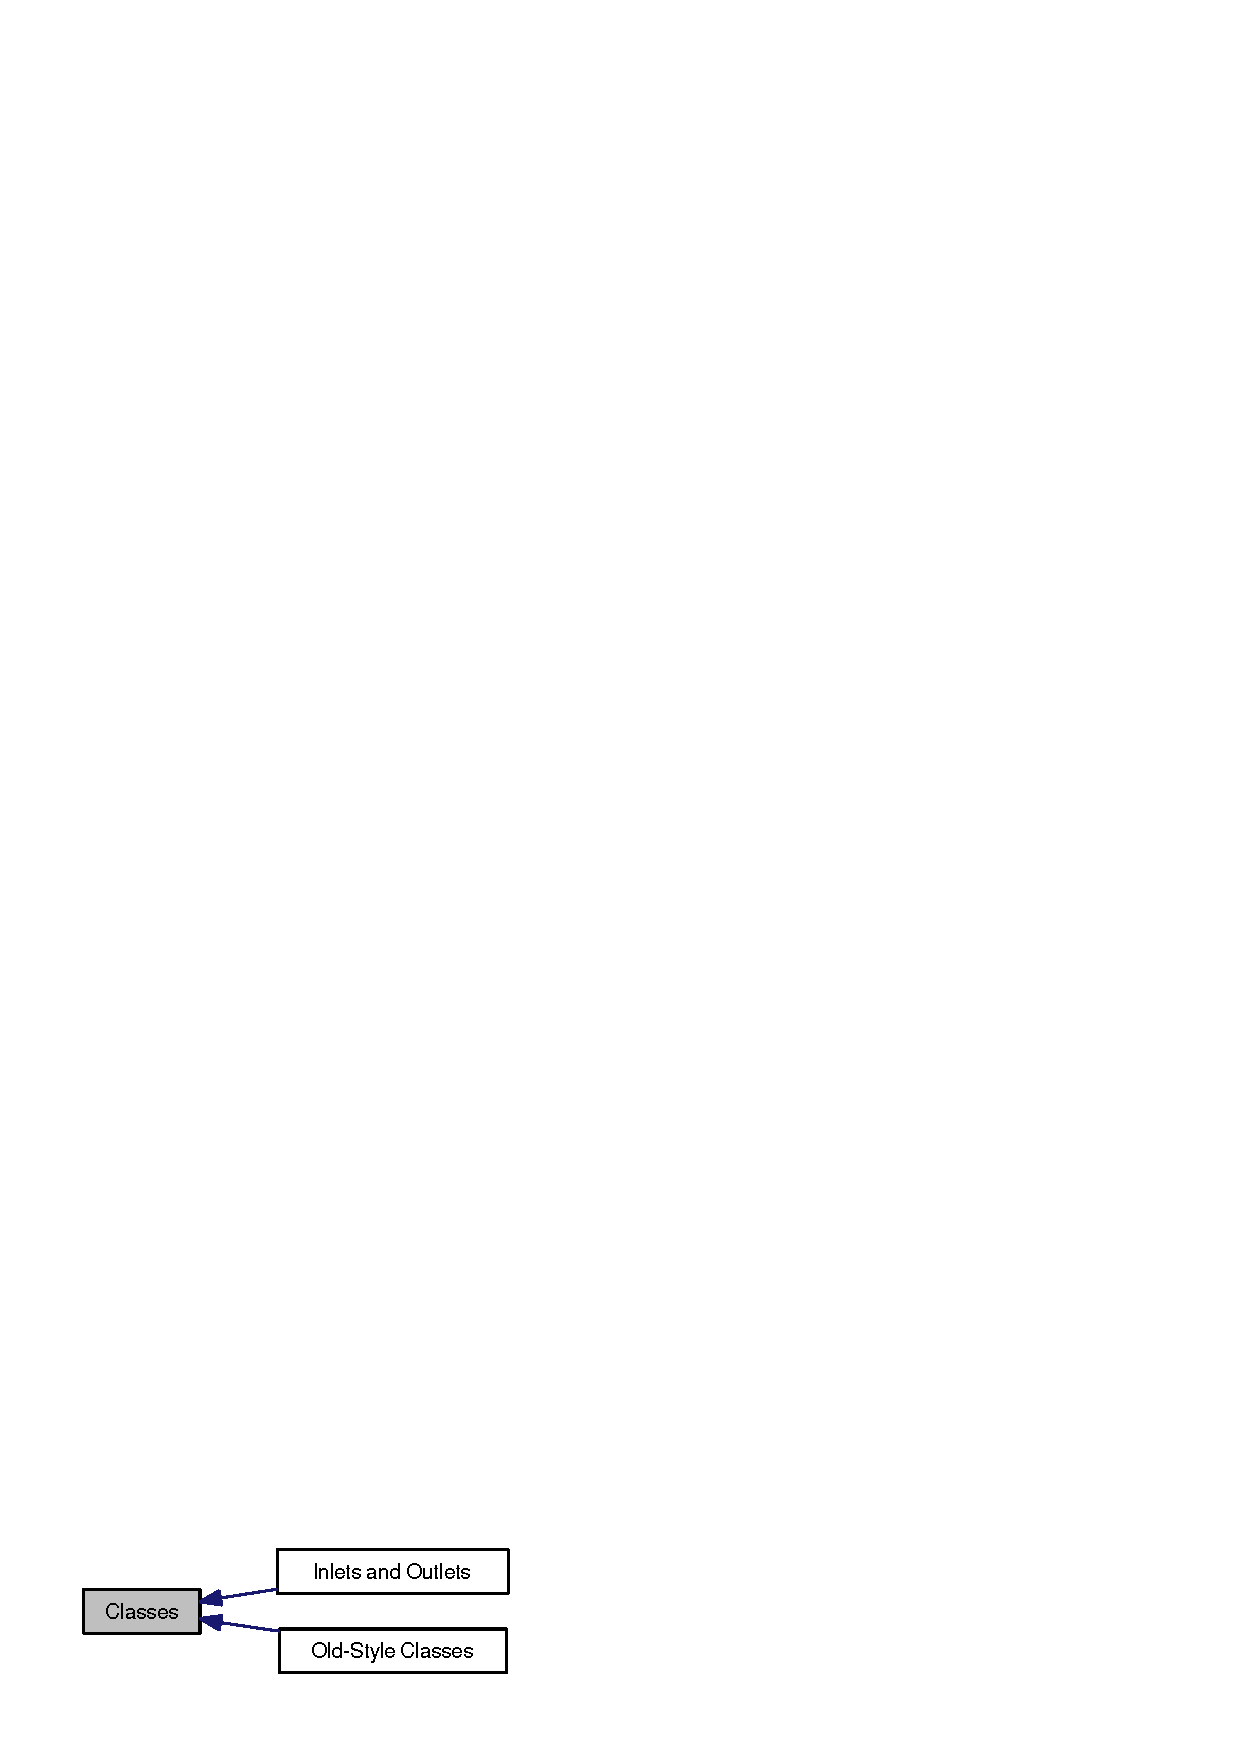
\includegraphics[width=124pt]{group__class}
\end{center}
\end{figure}
\subsection*{Data Structures}
\begin{DoxyCompactItemize}
\item 
struct \hyperlink{structt__class}{t\_\-class}
\begin{DoxyCompactList}\small\item\em The data structure for a Max class. \item\end{DoxyCompactList}\end{DoxyCompactItemize}
\subsection*{Modules}
\begin{DoxyCompactItemize}
\item 
\hyperlink{group__class__old}{Old-\/Style Classes}
\item 
\hyperlink{group__inout}{Inlets and Outlets}


\begin{DoxyCompactList}\small\item\em Routines for creating and communicating with inlets and outlets. \item\end{DoxyCompactList}\end{DoxyCompactItemize}
\subsection*{Defines}
\begin{DoxyCompactItemize}
\item 
\#define \hyperlink{group__class_gaf640c99a1fceb8158c2d1e77381b0320}{CLASS\_\-BOX}~gensym(\char`\"{}box\char`\"{})
\begin{DoxyCompactList}\small\item\em The namespace for all Max object classes which can be instantiated in a box, i.e. \item\end{DoxyCompactList}\item 
\hypertarget{group__class_ga090d3cbc4f137661806fc1b72249a791}{
\#define \hyperlink{group__class_ga090d3cbc4f137661806fc1b72249a791}{CLASS\_\-NOBOX}~gensym(\char`\"{}nobox\char`\"{})}
\label{group__class_ga090d3cbc4f137661806fc1b72249a791}

\begin{DoxyCompactList}\small\item\em A namespace for creating hidden or internal object classes which are not a direct part of the user creating patcher. \item\end{DoxyCompactList}\end{DoxyCompactItemize}
\subsection*{Enumerations}
\begin{DoxyCompactItemize}
\item 
enum \hyperlink{group__class_ga124a08e1744d9e999211abaa9df9f556}{e\_\-max\_\-class\_\-flags} \{ \par
\hyperlink{group__class_gga124a08e1744d9e999211abaa9df9f556af008530d0bd6c2091fe85923e412834f}{CLASS\_\-FLAG\_\-BOX} =  0x00000001L, 
\par
\hyperlink{group__class_gga124a08e1744d9e999211abaa9df9f556ac72d734fc04a3c47be53a77b1682b753}{CLASS\_\-FLAG\_\-POLYGLOT} =  0x00000002L, 
\par
\hyperlink{group__class_gga124a08e1744d9e999211abaa9df9f556aab2bebd8a64110247fa11db1c13ca5eb}{CLASS\_\-FLAG\_\-NEWDICTIONARY} =  0x00000004L, 
\par
\hyperlink{group__class_gga124a08e1744d9e999211abaa9df9f556a2ecc4a934743139d88d39fc62d028614}{CLASS\_\-FLAG\_\-REGISTERED} =  0x00000008L, 
\par
\hyperlink{group__class_gga124a08e1744d9e999211abaa9df9f556acdc1b6c10a366457cca2ea5e01964d80}{CLASS\_\-FLAG\_\-UIOBJECT} =  0x00000010L, 
\par
\hyperlink{group__class_gga124a08e1744d9e999211abaa9df9f556aa44754fe97e81d80049c2647fb4d6a62}{CLASS\_\-FLAG\_\-ALIAS} =  0x00000020L, 
\par
\hyperlink{group__class_gga124a08e1744d9e999211abaa9df9f556a940889608b4f23b1fcb24ebbf70772aa}{CLASS\_\-FLAG\_\-SCHED\_\-PURGE} =  0x00000040L, 
\par
\hyperlink{group__class_gga124a08e1744d9e999211abaa9df9f556a99981e2a6df832c0f59871193f2060a5}{CLASS\_\-FLAG\_\-DO\_\-NOT\_\-PARSE\_\-ATTR\_\-ARGS} =  0x00000080L, 
\par
\hyperlink{group__class_gga124a08e1744d9e999211abaa9df9f556aa8a5af40c8083496ee03dd3480087eee}{CLASS\_\-FLAG\_\-NOATTRIBUTES} =  0x00010000L, 
\par
\hyperlink{group__class_gga124a08e1744d9e999211abaa9df9f556a2c12440c31196a04f5ab4883a2334659}{CLASS\_\-FLAG\_\-OWNATTRIBUTES} =  0x00020000L
 \}
\begin{DoxyCompactList}\small\item\em Class flags. \item\end{DoxyCompactList}\end{DoxyCompactItemize}
\subsection*{Functions}
\begin{DoxyCompactItemize}
\item 
\hyperlink{structt__class}{t\_\-class} $\ast$ \hyperlink{group__class_ga238696d466081965c2b72b3880358404}{class\_\-new} (char $\ast$name, \hyperlink{group__datatypes_gac26ba0a173b50597f5738132e059b42d}{method} mnew, \hyperlink{group__datatypes_gac26ba0a173b50597f5738132e059b42d}{method} mfree, long size, \hyperlink{group__datatypes_gac26ba0a173b50597f5738132e059b42d}{method} mmenu, short type,...)
\begin{DoxyCompactList}\small\item\em Initializes a class by informing Max of its name, instance creation and free functions, size and argument types. \item\end{DoxyCompactList}\item 
\hyperlink{group__datatypes_ga73edaae82b318855cc09fac994918165}{t\_\-max\_\-err} \hyperlink{group__class_ga1df757149b7ad2f1d37178c5c184935f}{class\_\-free} (\hyperlink{structt__class}{t\_\-class} $\ast$c)
\begin{DoxyCompactList}\small\item\em Frees a previously defined object class. \item\end{DoxyCompactList}\item 
\hyperlink{group__datatypes_ga73edaae82b318855cc09fac994918165}{t\_\-max\_\-err} \hyperlink{group__class_ga0709af4aad9570f0cb91711a5c6d34d1}{class\_\-register} (\hyperlink{structt__symbol}{t\_\-symbol} $\ast$name\_\-space, \hyperlink{structt__class}{t\_\-class} $\ast$c)
\begin{DoxyCompactList}\small\item\em Registers a previously defined object class. \item\end{DoxyCompactList}\item 
\hyperlink{group__datatypes_ga73edaae82b318855cc09fac994918165}{t\_\-max\_\-err} \hyperlink{group__class_gab6f0ce5c584100e70106404e6068ac0d}{class\_\-alias} (\hyperlink{structt__class}{t\_\-class} $\ast$c, \hyperlink{structt__symbol}{t\_\-symbol} $\ast$aliasname)
\begin{DoxyCompactList}\small\item\em Registers an alias for a previously defined object class. \item\end{DoxyCompactList}\item 
\hyperlink{group__datatypes_ga73edaae82b318855cc09fac994918165}{t\_\-max\_\-err} \hyperlink{group__class_ga1fabf54e0cec8d4e5f732fa347b3f874}{class\_\-addmethod} (\hyperlink{structt__class}{t\_\-class} $\ast$c, \hyperlink{group__datatypes_gac26ba0a173b50597f5738132e059b42d}{method} m, char $\ast$name,...)
\begin{DoxyCompactList}\small\item\em Adds a method to a previously defined object class. \item\end{DoxyCompactList}\item 
\hyperlink{group__datatypes_ga73edaae82b318855cc09fac994918165}{t\_\-max\_\-err} \hyperlink{group__class_ga2289eb7e26b552be6e015c2f9912a9ac}{class\_\-addattr} (\hyperlink{structt__class}{t\_\-class} $\ast$c, \hyperlink{structt__object}{t\_\-object} $\ast$attr)
\begin{DoxyCompactList}\small\item\em Adds an attribute to a previously defined object class. \item\end{DoxyCompactList}\item 
\hyperlink{structt__symbol}{t\_\-symbol} $\ast$ \hyperlink{group__class_ga32dab29dac27195676d8edfed8e04798}{class\_\-nameget} (\hyperlink{structt__class}{t\_\-class} $\ast$c)
\begin{DoxyCompactList}\small\item\em Retrieves the name of a class, given the class's pointer. \item\end{DoxyCompactList}\item 
\hyperlink{structt__class}{t\_\-class} $\ast$ \hyperlink{group__class_ga11d93886daa53a3e0dea974176190301}{class\_\-findbyname} (\hyperlink{structt__symbol}{t\_\-symbol} $\ast$name\_\-space, \hyperlink{structt__symbol}{t\_\-symbol} $\ast$classname)
\begin{DoxyCompactList}\small\item\em Finds the class pointer for a class, given the class's namespace and name. \item\end{DoxyCompactList}\item 
\hyperlink{structt__class}{t\_\-class} $\ast$ \hyperlink{group__class_gacfffc94c91ff5254f8acc363be75b577}{class\_\-findbyname\_\-casefree} (\hyperlink{structt__symbol}{t\_\-symbol} $\ast$name\_\-space, \hyperlink{structt__symbol}{t\_\-symbol} $\ast$classname)
\begin{DoxyCompactList}\small\item\em Finds the class pointer for a class, given the class's namespace and name. \item\end{DoxyCompactList}\item 
\hyperlink{group__datatypes_ga73edaae82b318855cc09fac994918165}{t\_\-max\_\-err} \hyperlink{group__class_ga1b3d0a6942c49af47e3f44031d8f1097}{class\_\-dumpout\_\-wrap} (\hyperlink{structt__class}{t\_\-class} $\ast$c)
\begin{DoxyCompactList}\small\item\em Wraps user gettable attributes with a method that gets the values and sends out dumpout outlet. \item\end{DoxyCompactList}\item 
void \hyperlink{group__class_ga55ca4872991242c991b8bf6adb9bf6a6}{class\_\-obexoffset\_\-set} (\hyperlink{structt__class}{t\_\-class} $\ast$c, long offset)
\begin{DoxyCompactList}\small\item\em Registers the byte-\/offset of the obex member of the class's data structure with the previously defined object class. \item\end{DoxyCompactList}\item 
long \hyperlink{group__class_ga237b86f879e3eb3edbf674ffccc1f97c}{class\_\-obexoffset\_\-get} (\hyperlink{structt__class}{t\_\-class} $\ast$c)
\begin{DoxyCompactList}\small\item\em Retrieves the byte-\/offset of the obex member of the class's data structure. \item\end{DoxyCompactList}\item 
long \hyperlink{group__class_ga8c3f01e90f8adbc3c9b06e376d6a7fae}{class\_\-is\_\-ui} (\hyperlink{structt__class}{t\_\-class} $\ast$c)
\begin{DoxyCompactList}\small\item\em Determine if a class is a user interface object. \item\end{DoxyCompactList}\end{DoxyCompactItemize}


\subsection{Detailed Description}
When a user types the name of your object into an object box, Max looks for an external of this name in the searchpath and, upon finding it, loads the bundle or dll and calls the main() function. Thus, Max classes are typically defined in the main() function of an external.

Historically, Max classes have been defined using an API that includes functions like \hyperlink{group__class__old_ga24bbc5a9e8f7bb0a1c6847326e2f0a20}{setup()} and \hyperlink{group__class__old_ga0d9bfa416fdd861d1b2fd2d17701cbb3}{addmess()}. This interface is still supported, and the relevant documentation can be found in \hyperlink{group__class__old}{Old-\/Style Classes}.

A more recent and more flexible interface for creating objects was introduced with Jitter 1.0 and later included directly in Max 4.5. This newer API includes functions such as \hyperlink{group__class_ga238696d466081965c2b72b3880358404}{class\_\-new()} and \hyperlink{group__class_ga1fabf54e0cec8d4e5f732fa347b3f874}{class\_\-addmethod()}. Supporting attributes, user interface objects, and additional new features of Max requires the use of the newer interface for definiting classes documented on this page.

You may not mix these two styles of creating classes within an object. 

\subsection{Define Documentation}
\hypertarget{group__class_gaf640c99a1fceb8158c2d1e77381b0320}{
\index{class@{class}!CLASS\_\-BOX@{CLASS\_\-BOX}}
\index{CLASS\_\-BOX@{CLASS\_\-BOX}!class@{class}}
\subsubsection[{CLASS\_\-BOX}]{\setlength{\rightskip}{0pt plus 5cm}\#define CLASS\_\-BOX~gensym(\char`\"{}box\char`\"{})}}
\label{group__class_gaf640c99a1fceb8158c2d1e77381b0320}


The namespace for all Max object classes which can be instantiated in a box, i.e. in a patcher. 

\subsection{Enumeration Type Documentation}
\hypertarget{group__class_ga124a08e1744d9e999211abaa9df9f556}{
\index{class@{class}!e\_\-max\_\-class\_\-flags@{e\_\-max\_\-class\_\-flags}}
\index{e\_\-max\_\-class\_\-flags@{e\_\-max\_\-class\_\-flags}!class@{class}}
\subsubsection[{e\_\-max\_\-class\_\-flags}]{\setlength{\rightskip}{0pt plus 5cm}enum {\bf e\_\-max\_\-class\_\-flags}}}
\label{group__class_ga124a08e1744d9e999211abaa9df9f556}


Class flags. If not box or polyglot, class is only accessible in C via known interface \begin{Desc}
\item[Enumerator: ]\par
\begin{description}
\index{CLASS\_\-FLAG\_\-BOX@{CLASS\_\-FLAG\_\-BOX}!class@{class}}\index{class@{class}!CLASS\_\-FLAG\_\-BOX@{CLASS\_\-FLAG\_\-BOX}}\item[{\em 
\hypertarget{group__class_gga124a08e1744d9e999211abaa9df9f556af008530d0bd6c2091fe85923e412834f}{
CLASS\_\-FLAG\_\-BOX}
\label{group__class_gga124a08e1744d9e999211abaa9df9f556af008530d0bd6c2091fe85923e412834f}
}]for use in a patcher \index{CLASS\_\-FLAG\_\-POLYGLOT@{CLASS\_\-FLAG\_\-POLYGLOT}!class@{class}}\index{class@{class}!CLASS\_\-FLAG\_\-POLYGLOT@{CLASS\_\-FLAG\_\-POLYGLOT}}\item[{\em 
\hypertarget{group__class_gga124a08e1744d9e999211abaa9df9f556ac72d734fc04a3c47be53a77b1682b753}{
CLASS\_\-FLAG\_\-POLYGLOT}
\label{group__class_gga124a08e1744d9e999211abaa9df9f556ac72d734fc04a3c47be53a77b1682b753}
}]for use by any text language (c/js/java/etc) \index{CLASS\_\-FLAG\_\-NEWDICTIONARY@{CLASS\_\-FLAG\_\-NEWDICTIONARY}!class@{class}}\index{class@{class}!CLASS\_\-FLAG\_\-NEWDICTIONARY@{CLASS\_\-FLAG\_\-NEWDICTIONARY}}\item[{\em 
\hypertarget{group__class_gga124a08e1744d9e999211abaa9df9f556aab2bebd8a64110247fa11db1c13ca5eb}{
CLASS\_\-FLAG\_\-NEWDICTIONARY}
\label{group__class_gga124a08e1744d9e999211abaa9df9f556aab2bebd8a64110247fa11db1c13ca5eb}
}]dictionary based constructor \index{CLASS\_\-FLAG\_\-REGISTERED@{CLASS\_\-FLAG\_\-REGISTERED}!class@{class}}\index{class@{class}!CLASS\_\-FLAG\_\-REGISTERED@{CLASS\_\-FLAG\_\-REGISTERED}}\item[{\em 
\hypertarget{group__class_gga124a08e1744d9e999211abaa9df9f556a2ecc4a934743139d88d39fc62d028614}{
CLASS\_\-FLAG\_\-REGISTERED}
\label{group__class_gga124a08e1744d9e999211abaa9df9f556a2ecc4a934743139d88d39fc62d028614}
}]for backward compatible messlist implementation (once reg'd can't grow) \index{CLASS\_\-FLAG\_\-UIOBJECT@{CLASS\_\-FLAG\_\-UIOBJECT}!class@{class}}\index{class@{class}!CLASS\_\-FLAG\_\-UIOBJECT@{CLASS\_\-FLAG\_\-UIOBJECT}}\item[{\em 
\hypertarget{group__class_gga124a08e1744d9e999211abaa9df9f556acdc1b6c10a366457cca2ea5e01964d80}{
CLASS\_\-FLAG\_\-UIOBJECT}
\label{group__class_gga124a08e1744d9e999211abaa9df9f556acdc1b6c10a366457cca2ea5e01964d80}
}]for objects that don't go inside a newobj box. \index{CLASS\_\-FLAG\_\-ALIAS@{CLASS\_\-FLAG\_\-ALIAS}!class@{class}}\index{class@{class}!CLASS\_\-FLAG\_\-ALIAS@{CLASS\_\-FLAG\_\-ALIAS}}\item[{\em 
\hypertarget{group__class_gga124a08e1744d9e999211abaa9df9f556aa44754fe97e81d80049c2647fb4d6a62}{
CLASS\_\-FLAG\_\-ALIAS}
\label{group__class_gga124a08e1744d9e999211abaa9df9f556aa44754fe97e81d80049c2647fb4d6a62}
}]for classes that are just copies of some other class (i.e. del is a copy of delay) \index{CLASS\_\-FLAG\_\-SCHED\_\-PURGE@{CLASS\_\-FLAG\_\-SCHED\_\-PURGE}!class@{class}}\index{class@{class}!CLASS\_\-FLAG\_\-SCHED\_\-PURGE@{CLASS\_\-FLAG\_\-SCHED\_\-PURGE}}\item[{\em 
\hypertarget{group__class_gga124a08e1744d9e999211abaa9df9f556a940889608b4f23b1fcb24ebbf70772aa}{
CLASS\_\-FLAG\_\-SCHED\_\-PURGE}
\label{group__class_gga124a08e1744d9e999211abaa9df9f556a940889608b4f23b1fcb24ebbf70772aa}
}]for classes that have called \hyperlink{group__clocks_ga6257ddd41904756699208f135f6539fd}{clock\_\-new()} or \hyperlink{group__qelems_gaffa7e9d4d5468a8ae3c825a353609b1b}{qelem\_\-new()} (don't need to set this yourself) \index{CLASS\_\-FLAG\_\-DO\_\-NOT\_\-PARSE\_\-ATTR\_\-ARGS@{CLASS\_\-FLAG\_\-DO\_\-NOT\_\-PARSE\_\-ATTR\_\-ARGS}!class@{class}}\index{class@{class}!CLASS\_\-FLAG\_\-DO\_\-NOT\_\-PARSE\_\-ATTR\_\-ARGS@{CLASS\_\-FLAG\_\-DO\_\-NOT\_\-PARSE\_\-ATTR\_\-ARGS}}\item[{\em 
\hypertarget{group__class_gga124a08e1744d9e999211abaa9df9f556a99981e2a6df832c0f59871193f2060a5}{
CLASS\_\-FLAG\_\-DO\_\-NOT\_\-PARSE\_\-ATTR\_\-ARGS}
\label{group__class_gga124a08e1744d9e999211abaa9df9f556a99981e2a6df832c0f59871193f2060a5}
}]override dictionary based constructor attr arg parsing \index{CLASS\_\-FLAG\_\-NOATTRIBUTES@{CLASS\_\-FLAG\_\-NOATTRIBUTES}!class@{class}}\index{class@{class}!CLASS\_\-FLAG\_\-NOATTRIBUTES@{CLASS\_\-FLAG\_\-NOATTRIBUTES}}\item[{\em 
\hypertarget{group__class_gga124a08e1744d9e999211abaa9df9f556aa8a5af40c8083496ee03dd3480087eee}{
CLASS\_\-FLAG\_\-NOATTRIBUTES}
\label{group__class_gga124a08e1744d9e999211abaa9df9f556aa8a5af40c8083496ee03dd3480087eee}
}]for efficiency \index{CLASS\_\-FLAG\_\-OWNATTRIBUTES@{CLASS\_\-FLAG\_\-OWNATTRIBUTES}!class@{class}}\index{class@{class}!CLASS\_\-FLAG\_\-OWNATTRIBUTES@{CLASS\_\-FLAG\_\-OWNATTRIBUTES}}\item[{\em 
\hypertarget{group__class_gga124a08e1744d9e999211abaa9df9f556a2c12440c31196a04f5ab4883a2334659}{
CLASS\_\-FLAG\_\-OWNATTRIBUTES}
\label{group__class_gga124a08e1744d9e999211abaa9df9f556a2c12440c31196a04f5ab4883a2334659}
}]for classes which support a custom attr interface (e.g. jitter) \end{description}
\end{Desc}



\subsection{Function Documentation}
\hypertarget{group__class_ga2289eb7e26b552be6e015c2f9912a9ac}{
\index{class@{class}!class\_\-addattr@{class\_\-addattr}}
\index{class\_\-addattr@{class\_\-addattr}!class@{class}}
\subsubsection[{class\_\-addattr}]{\setlength{\rightskip}{0pt plus 5cm}{\bf t\_\-max\_\-err} class\_\-addattr ({\bf t\_\-class} $\ast$ {\em c}, \/  {\bf t\_\-object} $\ast$ {\em attr})}}
\label{group__class_ga2289eb7e26b552be6e015c2f9912a9ac}


Adds an attribute to a previously defined object class. 
\begin{DoxyParams}{Parameters}
\item[{\em c}]The class pointer \item[{\em attr}]The attribute to add. The attribute will be a pointer returned by \hyperlink{group__attr_ga24badeb31a79d844935b2a1c8423c905}{attribute\_\-new()}, \hyperlink{group__attr_ga089ad1af7af1d0771b4a4e1417d16779}{attr\_\-offset\_\-new()} or \hyperlink{group__attr_ga3828e337f808838f30599ae6bf01fdb9}{attr\_\-offset\_\-array\_\-new()}.\end{DoxyParams}
\begin{DoxyReturn}{Returns}
This function returns the error code \hyperlink{group__misc_gga0764dd6c02b76cca7d053ae50555d69da6d22f77fef8b1e1b074cef5d29d935fd}{MAX\_\-ERR\_\-NONE} if successful, or one of the other error codes defined in \hyperlink{group__misc_ga0764dd6c02b76cca7d053ae50555d69d}{e\_\-max\_\-errorcodes} if unsuccessful. 
\end{DoxyReturn}
\hypertarget{group__class_ga1fabf54e0cec8d4e5f732fa347b3f874}{
\index{class@{class}!class\_\-addmethod@{class\_\-addmethod}}
\index{class\_\-addmethod@{class\_\-addmethod}!class@{class}}
\subsubsection[{class\_\-addmethod}]{\setlength{\rightskip}{0pt plus 5cm}{\bf t\_\-max\_\-err} class\_\-addmethod ({\bf t\_\-class} $\ast$ {\em c}, \/  {\bf method} {\em m}, \/  char $\ast$ {\em name}, \/   {\em ...})}}
\label{group__class_ga1fabf54e0cec8d4e5f732fa347b3f874}


Adds a method to a previously defined object class. 
\begin{DoxyParams}{Parameters}
\item[{\em c}]The class pointer \item[{\em m}]Function to be called when the method is invoked \item[{\em name}]C-\/string defining the message (message selector) \item[{\em ...}]One or more integers specifying the arguments to the message, in the standard Max type list format (see Chapter 3 of the Writing Externals in Max document for more information).\end{DoxyParams}
\begin{DoxyReturn}{Returns}
This function returns the error code \hyperlink{group__misc_gga0764dd6c02b76cca7d053ae50555d69da6d22f77fef8b1e1b074cef5d29d935fd}{MAX\_\-ERR\_\-NONE} if successful, or one of the other error codes defined in \hyperlink{group__misc_ga0764dd6c02b76cca7d053ae50555d69d}{e\_\-max\_\-errorcodes} if unsuccessful.
\end{DoxyReturn}
\begin{DoxyRemark}{Remarks}
The \hyperlink{group__class_ga1fabf54e0cec8d4e5f732fa347b3f874}{class\_\-addmethod()} function works essentially like the traditional \hyperlink{group__class__old_ga0d9bfa416fdd861d1b2fd2d17701cbb3}{addmess()} function, adding the function pointed to by {\ttfamily m}, to respond to the message string {\ttfamily name} in the leftmost inlet of the object. 
\end{DoxyRemark}
\hypertarget{group__class_gab6f0ce5c584100e70106404e6068ac0d}{
\index{class@{class}!class\_\-alias@{class\_\-alias}}
\index{class\_\-alias@{class\_\-alias}!class@{class}}
\subsubsection[{class\_\-alias}]{\setlength{\rightskip}{0pt plus 5cm}{\bf t\_\-max\_\-err} class\_\-alias ({\bf t\_\-class} $\ast$ {\em c}, \/  {\bf t\_\-symbol} $\ast$ {\em aliasname})}}
\label{group__class_gab6f0ce5c584100e70106404e6068ac0d}


Registers an alias for a previously defined object class. 
\begin{DoxyParams}{Parameters}
\item[{\em c}]The class pointer \item[{\em aliasname}]A symbol who's name will become an alias for the given class\end{DoxyParams}
\begin{DoxyReturn}{Returns}
This function returns the error code \hyperlink{group__misc_gga0764dd6c02b76cca7d053ae50555d69da6d22f77fef8b1e1b074cef5d29d935fd}{MAX\_\-ERR\_\-NONE} if successful, or one of the other error codes defined in \hyperlink{group__misc_ga0764dd6c02b76cca7d053ae50555d69d}{e\_\-max\_\-errorcodes} if unsuccessful. 
\end{DoxyReturn}
\hypertarget{group__class_ga1b3d0a6942c49af47e3f44031d8f1097}{
\index{class@{class}!class\_\-dumpout\_\-wrap@{class\_\-dumpout\_\-wrap}}
\index{class\_\-dumpout\_\-wrap@{class\_\-dumpout\_\-wrap}!class@{class}}
\subsubsection[{class\_\-dumpout\_\-wrap}]{\setlength{\rightskip}{0pt plus 5cm}{\bf t\_\-max\_\-err} class\_\-dumpout\_\-wrap ({\bf t\_\-class} $\ast$ {\em c})}}
\label{group__class_ga1b3d0a6942c49af47e3f44031d8f1097}


Wraps user gettable attributes with a method that gets the values and sends out dumpout outlet. 
\begin{DoxyParams}{Parameters}
\item[{\em c}]The class pointer \end{DoxyParams}
\begin{DoxyReturn}{Returns}
This function returns the error code \hyperlink{group__misc_gga0764dd6c02b76cca7d053ae50555d69da6d22f77fef8b1e1b074cef5d29d935fd}{MAX\_\-ERR\_\-NONE} if successful, or one of the other error codes defined in \hyperlink{group__misc_ga0764dd6c02b76cca7d053ae50555d69d}{e\_\-max\_\-errorcodes} if unsuccessful. 
\end{DoxyReturn}
\hypertarget{group__class_ga11d93886daa53a3e0dea974176190301}{
\index{class@{class}!class\_\-findbyname@{class\_\-findbyname}}
\index{class\_\-findbyname@{class\_\-findbyname}!class@{class}}
\subsubsection[{class\_\-findbyname}]{\setlength{\rightskip}{0pt plus 5cm}{\bf t\_\-class}$\ast$ class\_\-findbyname ({\bf t\_\-symbol} $\ast$ {\em name\_\-space}, \/  {\bf t\_\-symbol} $\ast$ {\em classname})}}
\label{group__class_ga11d93886daa53a3e0dea974176190301}


Finds the class pointer for a class, given the class's namespace and name. 
\begin{DoxyParams}{Parameters}
\item[{\em name\_\-space}]The desired class's name space. Typically, either the constant \hyperlink{group__class_gaf640c99a1fceb8158c2d1e77381b0320}{CLASS\_\-BOX}, for obex classes which can instantiate inside of a Max patcher (e.g. boxes, UI objects, etc.), or the constant \hyperlink{group__class_ga090d3cbc4f137661806fc1b72249a791}{CLASS\_\-NOBOX}, for classes which will only be used internally. Developers can define their own name spaces as well, but this functionality is currently undocumented. \item[{\em classname}]The name of the class to be looked up\end{DoxyParams}
\begin{DoxyReturn}{Returns}
If successful, this function returns the class's data pointer. Otherwise, it returns NULL. 
\end{DoxyReturn}
\hypertarget{group__class_gacfffc94c91ff5254f8acc363be75b577}{
\index{class@{class}!class\_\-findbyname\_\-casefree@{class\_\-findbyname\_\-casefree}}
\index{class\_\-findbyname\_\-casefree@{class\_\-findbyname\_\-casefree}!class@{class}}
\subsubsection[{class\_\-findbyname\_\-casefree}]{\setlength{\rightskip}{0pt plus 5cm}{\bf t\_\-class}$\ast$ class\_\-findbyname\_\-casefree ({\bf t\_\-symbol} $\ast$ {\em name\_\-space}, \/  {\bf t\_\-symbol} $\ast$ {\em classname})}}
\label{group__class_gacfffc94c91ff5254f8acc363be75b577}


Finds the class pointer for a class, given the class's namespace and name. 
\begin{DoxyParams}{Parameters}
\item[{\em name\_\-space}]The desired class's name space. Typically, either the constant \hyperlink{group__class_gaf640c99a1fceb8158c2d1e77381b0320}{CLASS\_\-BOX}, for obex classes which can instantiate inside of a Max patcher (e.g. boxes, UI objects, etc.), or the constant \hyperlink{group__class_ga090d3cbc4f137661806fc1b72249a791}{CLASS\_\-NOBOX}, for classes which will only be used internally. Developers can define their own name spaces as well, but this functionality is currently undocumented. \item[{\em classname}]The name of the class to be looked up (case free)\end{DoxyParams}
\begin{DoxyReturn}{Returns}
If successful, this function returns the class's data pointer. Otherwise, it returns NULL. 
\end{DoxyReturn}
\hypertarget{group__class_ga1df757149b7ad2f1d37178c5c184935f}{
\index{class@{class}!class\_\-free@{class\_\-free}}
\index{class\_\-free@{class\_\-free}!class@{class}}
\subsubsection[{class\_\-free}]{\setlength{\rightskip}{0pt plus 5cm}{\bf t\_\-max\_\-err} class\_\-free ({\bf t\_\-class} $\ast$ {\em c})}}
\label{group__class_ga1df757149b7ad2f1d37178c5c184935f}


Frees a previously defined object class. {\itshape This function is not typically used by external developers.\/}


\begin{DoxyParams}{Parameters}
\item[{\em c}]The class pointer \end{DoxyParams}
\begin{DoxyReturn}{Returns}
This function returns the error code \hyperlink{group__misc_gga0764dd6c02b76cca7d053ae50555d69da6d22f77fef8b1e1b074cef5d29d935fd}{MAX\_\-ERR\_\-NONE} if successful, or one of the other error codes defined in \hyperlink{group__misc_ga0764dd6c02b76cca7d053ae50555d69d}{e\_\-max\_\-errorcodes} if unsuccessful. 
\end{DoxyReturn}
\hypertarget{group__class_ga8c3f01e90f8adbc3c9b06e376d6a7fae}{
\index{class@{class}!class\_\-is\_\-ui@{class\_\-is\_\-ui}}
\index{class\_\-is\_\-ui@{class\_\-is\_\-ui}!class@{class}}
\subsubsection[{class\_\-is\_\-ui}]{\setlength{\rightskip}{0pt plus 5cm}long class\_\-is\_\-ui ({\bf t\_\-class} $\ast$ {\em c})}}
\label{group__class_ga8c3f01e90f8adbc3c9b06e376d6a7fae}


Determine if a class is a user interface object. 
\begin{DoxyParams}{Parameters}
\item[{\em c}]The class pointer. \end{DoxyParams}
\begin{DoxyReturn}{Returns}
True is the class defines a user interface object, otherwise false. 
\end{DoxyReturn}
\hypertarget{group__class_ga32dab29dac27195676d8edfed8e04798}{
\index{class@{class}!class\_\-nameget@{class\_\-nameget}}
\index{class\_\-nameget@{class\_\-nameget}!class@{class}}
\subsubsection[{class\_\-nameget}]{\setlength{\rightskip}{0pt plus 5cm}{\bf t\_\-symbol}$\ast$ class\_\-nameget ({\bf t\_\-class} $\ast$ {\em c})}}
\label{group__class_ga32dab29dac27195676d8edfed8e04798}


Retrieves the name of a class, given the class's pointer. 
\begin{DoxyParams}{Parameters}
\item[{\em c}]The class pointer \end{DoxyParams}
\begin{DoxyReturn}{Returns}
If successful, this function returns the name of the class as a \hyperlink{structt__symbol}{t\_\-symbol} $\ast$. 
\end{DoxyReturn}
\hypertarget{group__class_ga238696d466081965c2b72b3880358404}{
\index{class@{class}!class\_\-new@{class\_\-new}}
\index{class\_\-new@{class\_\-new}!class@{class}}
\subsubsection[{class\_\-new}]{\setlength{\rightskip}{0pt plus 5cm}{\bf t\_\-class}$\ast$ class\_\-new (char $\ast$ {\em name}, \/  {\bf method} {\em mnew}, \/  {\bf method} {\em mfree}, \/  long {\em size}, \/  {\bf method} {\em mmenu}, \/  short {\em type}, \/   {\em ...})}}
\label{group__class_ga238696d466081965c2b72b3880358404}


Initializes a class by informing Max of its name, instance creation and free functions, size and argument types. Developers wishing to use obex class features (attributes, etc.) {\itshape must\/} use \hyperlink{group__class_ga238696d466081965c2b72b3880358404}{class\_\-new()} instead of the traditional \hyperlink{group__class__old_ga24bbc5a9e8f7bb0a1c6847326e2f0a20}{setup()} function.


\begin{DoxyParams}{Parameters}
\item[{\em name}]The class's name, as a C-\/string \item[{\em mnew}]The instance creation function \item[{\em mfree}]The instance free function \item[{\em size}]The size of the object's data structure in bytes. Usually you use the C sizeof operator here. \item[{\em mmenu}]The function called when the user creates a new object of the class from the Patch window's palette (UI objects only). Pass 0L if you're not defining a UI object. \item[{\em type}]A standard Max {\itshape type list\/} as explained in Chapter 3 of the Writing Externals in Max document (in the Max SDK). The final argument of the type list should be a 0. {\itshape Generally, obex objects have a single type argument\/}, \hyperlink{group__atom_gga8aa6700e9f00b132eb376db6e39ade47a81c1a8550f038db16a619167a70a79b6}{A\_\-GIMME}, followed by a 0.\end{DoxyParams}
\begin{DoxyReturn}{Returns}
This function returns the class pointer for the new object class. {\itshape This pointer is used by numerous other functions and should be stored in a global or static variable.\/} 
\end{DoxyReturn}
\hypertarget{group__class_ga237b86f879e3eb3edbf674ffccc1f97c}{
\index{class@{class}!class\_\-obexoffset\_\-get@{class\_\-obexoffset\_\-get}}
\index{class\_\-obexoffset\_\-get@{class\_\-obexoffset\_\-get}!class@{class}}
\subsubsection[{class\_\-obexoffset\_\-get}]{\setlength{\rightskip}{0pt plus 5cm}long class\_\-obexoffset\_\-get ({\bf t\_\-class} $\ast$ {\em c})}}
\label{group__class_ga237b86f879e3eb3edbf674ffccc1f97c}


Retrieves the byte-\/offset of the obex member of the class's data structure. 
\begin{DoxyParams}{Parameters}
\item[{\em c}]The class pointer \end{DoxyParams}
\begin{DoxyReturn}{Returns}
This function returns the byte-\/offset of the obex member of the class's data structure. 
\end{DoxyReturn}
\hypertarget{group__class_ga55ca4872991242c991b8bf6adb9bf6a6}{
\index{class@{class}!class\_\-obexoffset\_\-set@{class\_\-obexoffset\_\-set}}
\index{class\_\-obexoffset\_\-set@{class\_\-obexoffset\_\-set}!class@{class}}
\subsubsection[{class\_\-obexoffset\_\-set}]{\setlength{\rightskip}{0pt plus 5cm}void class\_\-obexoffset\_\-set ({\bf t\_\-class} $\ast$ {\em c}, \/  long {\em offset})}}
\label{group__class_ga55ca4872991242c991b8bf6adb9bf6a6}


Registers the byte-\/offset of the obex member of the class's data structure with the previously defined object class. Use of this function is required for obex-\/class objects. It must be called from {\ttfamily main()}.


\begin{DoxyParams}{Parameters}
\item[{\em c}]The class pointer \item[{\em offset}]The byte-\/offset to the obex member of the object's data structure. Conventionally, the macro \hyperlink{group__misc_gaad95899dfbc7b5b8fe11921643ef46f0}{calcoffset} is used to calculate the offset. \end{DoxyParams}
\hypertarget{group__class_ga0709af4aad9570f0cb91711a5c6d34d1}{
\index{class@{class}!class\_\-register@{class\_\-register}}
\index{class\_\-register@{class\_\-register}!class@{class}}
\subsubsection[{class\_\-register}]{\setlength{\rightskip}{0pt plus 5cm}{\bf t\_\-max\_\-err} class\_\-register ({\bf t\_\-symbol} $\ast$ {\em name\_\-space}, \/  {\bf t\_\-class} $\ast$ {\em c})}}
\label{group__class_ga0709af4aad9570f0cb91711a5c6d34d1}


Registers a previously defined object class. This function is required, and should be called at the end of {\ttfamily main()}.


\begin{DoxyParams}{Parameters}
\item[{\em name\_\-space}]The desired class's name space. Typically, either the constant \hyperlink{group__class_gaf640c99a1fceb8158c2d1e77381b0320}{CLASS\_\-BOX}, for obex classes which can instantiate inside of a Max patcher (e.g. boxes, UI objects, etc.), or the constant \hyperlink{group__class_ga090d3cbc4f137661806fc1b72249a791}{CLASS\_\-NOBOX}, for classes which will only be used internally. Developers can define their own name spaces as well, but this functionality is currently undocumented. \item[{\em c}]The class pointer\end{DoxyParams}
\begin{DoxyReturn}{Returns}
This function returns the error code \hyperlink{group__misc_gga0764dd6c02b76cca7d053ae50555d69da6d22f77fef8b1e1b074cef5d29d935fd}{MAX\_\-ERR\_\-NONE} if successful, or one of the other error codes defined in \hyperlink{group__misc_ga0764dd6c02b76cca7d053ae50555d69d}{e\_\-max\_\-errorcodes} if unsuccessful. 
\end{DoxyReturn}

\hypertarget{group__class__old}{
\section{Old-\/Style Classes}
\label{group__class__old}\index{Old-\/Style Classes@{Old-\/Style Classes}}
}


Collaboration diagram for Old-\/Style Classes:\nopagebreak
\begin{figure}[H]
\begin{center}
\leavevmode
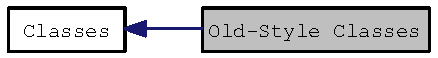
\includegraphics[width=123pt]{group__class__old}
\end{center}
\end{figure}
\subsection*{Functions}
\begin{DoxyCompactItemize}
\item 
void \hyperlink{group__class__old_ga24bbc5a9e8f7bb0a1c6847326e2f0a20}{setup} (\hyperlink{structt__messlist}{t\_\-messlist} $\ast$$\ast$ident, \hyperlink{group__datatypes_gac26ba0a173b50597f5738132e059b42d}{method} makefun, \hyperlink{group__datatypes_gac26ba0a173b50597f5738132e059b42d}{method} freefun, short size, \hyperlink{group__datatypes_gac26ba0a173b50597f5738132e059b42d}{method} menufun, short type,...)
\begin{DoxyCompactList}\small\item\em Use the \hyperlink{group__class__old_ga24bbc5a9e8f7bb0a1c6847326e2f0a20}{setup()} function to initialize your class by informing Max of its size, the name of your functions that create and destroy instances, and the types of arguments passed to the instance creation function. \item\end{DoxyCompactList}\item 
void \hyperlink{group__class__old_ga0d9bfa416fdd861d1b2fd2d17701cbb3}{addmess} (\hyperlink{group__datatypes_gac26ba0a173b50597f5738132e059b42d}{method} f, char $\ast$s, short type,...)
\begin{DoxyCompactList}\small\item\em Use \hyperlink{group__class__old_ga0d9bfa416fdd861d1b2fd2d17701cbb3}{addmess()} to bind a function to a message other than the standard ones covered by \hyperlink{group__class__old_gac667faa21ecad5184005266844ed0b48}{addbang()}, \hyperlink{group__class__old_ga85afc0cd451465117ac80593d3deb4f9}{addint()}, etc. \item\end{DoxyCompactList}\item 
void \hyperlink{group__class__old_gac667faa21ecad5184005266844ed0b48}{addbang} (\hyperlink{group__datatypes_gac26ba0a173b50597f5738132e059b42d}{method} f)
\begin{DoxyCompactList}\small\item\em Used to bind a function to the common triggering message bang. \item\end{DoxyCompactList}\item 
void \hyperlink{group__class__old_ga85afc0cd451465117ac80593d3deb4f9}{addint} (\hyperlink{group__datatypes_gac26ba0a173b50597f5738132e059b42d}{method} f)
\begin{DoxyCompactList}\small\item\em Use \hyperlink{group__class__old_ga85afc0cd451465117ac80593d3deb4f9}{addint()} to bind a function to the int message received in the leftmost inlet. \item\end{DoxyCompactList}\item 
void \hyperlink{group__class__old_ga1e2089acfa6856835613d130a5b6bd7d}{addfloat} (\hyperlink{group__datatypes_gac26ba0a173b50597f5738132e059b42d}{method} f)
\begin{DoxyCompactList}\small\item\em Use \hyperlink{group__class__old_ga1e2089acfa6856835613d130a5b6bd7d}{addfloat()} to bind a function to the float message received in the leftmost inlet. \item\end{DoxyCompactList}\item 
void \hyperlink{group__class__old_gad3a69b2d38b257464c6a0f8a50efd85a}{addinx} (\hyperlink{group__datatypes_gac26ba0a173b50597f5738132e059b42d}{method} f, short n)
\begin{DoxyCompactList}\small\item\em Use \hyperlink{group__class__old_gad3a69b2d38b257464c6a0f8a50efd85a}{addinx()} to bind a function to a int message that will be received in an inlet other than the leftmost one. \item\end{DoxyCompactList}\item 
void \hyperlink{group__class__old_gad223143c8da12d8f3b7b18f9d6e5da9e}{addftx} (\hyperlink{group__datatypes_gac26ba0a173b50597f5738132e059b42d}{method} f, short n)
\begin{DoxyCompactList}\small\item\em Use \hyperlink{group__class__old_gad223143c8da12d8f3b7b18f9d6e5da9e}{addftx()} to bind a function to a float message that will be received in an inlet other than the leftmost one. \item\end{DoxyCompactList}\item 
void $\ast$ \hyperlink{group__class__old_ga053f428d5edcc7d663980330848e73a6}{newobject} (void $\ast$maxclass)
\begin{DoxyCompactList}\small\item\em Use newobject to allocate the space for an instance of your class and initialize its object header. \item\end{DoxyCompactList}\item 
void \hyperlink{group__class__old_gadf30646e52376a37b93cc20efac65636}{freeobject} (\hyperlink{structt__object}{t\_\-object} $\ast$op)
\begin{DoxyCompactList}\small\item\em Release the memory used by a Max object. \item\end{DoxyCompactList}\item 
void $\ast$ \hyperlink{group__class__old_ga4c1f100a92d6f519ba4e93665ff54998}{newinstance} (\hyperlink{structt__symbol}{t\_\-symbol} $\ast$s, short argc, \hyperlink{structt__atom}{t\_\-atom} $\ast$argv)
\begin{DoxyCompactList}\small\item\em Make a new instance of an existing Max class. \item\end{DoxyCompactList}\item 
void \hyperlink{group__class__old_gad8f119f6232340c85b3bb358227576b3}{alias} (char $\ast$name)
\begin{DoxyCompactList}\small\item\em Use the alias function to allow users to refer to your object by a name other than that of your shared library. \item\end{DoxyCompactList}\item 
void \hyperlink{group__class__old_gafb05186b12fb0dceeb3185b2f59b6307}{class\_\-setname} (char $\ast$obname, char $\ast$filename)
\begin{DoxyCompactList}\small\item\em Use \hyperlink{group__class__old_gafb05186b12fb0dceeb3185b2f59b6307}{class\_\-setname()} to associate you object’s name with it’s filename on disk. \item\end{DoxyCompactList}\item 
void $\ast$ \hyperlink{group__class__old_ga78c60eb0068bce55eaa635e206cba52e}{typedmess} (\hyperlink{structt__object}{t\_\-object} $\ast$op, \hyperlink{structt__symbol}{t\_\-symbol} $\ast$msg, short argc, \hyperlink{structt__atom}{t\_\-atom} $\ast$argp)
\begin{DoxyCompactList}\small\item\em Send a typed message directly to a Max object. \item\end{DoxyCompactList}\item 
\hyperlink{group__datatypes_gac26ba0a173b50597f5738132e059b42d}{method} \hyperlink{group__class__old_gafa477f96b3a02c0ecbca2b5aa14b9ecb}{getfn} (\hyperlink{structt__object}{t\_\-object} $\ast$op, \hyperlink{structt__symbol}{t\_\-symbol} $\ast$msg)
\begin{DoxyCompactList}\small\item\em Use \hyperlink{group__class__old_gafa477f96b3a02c0ecbca2b5aa14b9ecb}{getfn()} to send an untyped message to a Max object with error checking. \item\end{DoxyCompactList}\item 
\hyperlink{group__datatypes_gac26ba0a173b50597f5738132e059b42d}{method} \hyperlink{group__class__old_ga96dfd8b6f4c7111c34f1c2103fbdcdf0}{egetfn} (\hyperlink{structt__object}{t\_\-object} $\ast$op, \hyperlink{structt__symbol}{t\_\-symbol} $\ast$msg)
\begin{DoxyCompactList}\small\item\em Use \hyperlink{group__class__old_ga96dfd8b6f4c7111c34f1c2103fbdcdf0}{egetfn()} to send an untyped message to a Max object that always works. \item\end{DoxyCompactList}\item 
\hyperlink{group__datatypes_gac26ba0a173b50597f5738132e059b42d}{method} \hyperlink{group__class__old_ga54a45bcc841c2033467be14e6861b548}{zgetfn} (\hyperlink{structt__object}{t\_\-object} $\ast$op, \hyperlink{structt__symbol}{t\_\-symbol} $\ast$msg)
\begin{DoxyCompactList}\small\item\em Use \hyperlink{group__class__old_ga54a45bcc841c2033467be14e6861b548}{zgetfn()} to send an untyped message to a Max object without error checking. \item\end{DoxyCompactList}\end{DoxyCompactItemize}


\subsection{Function Documentation}
\hypertarget{group__class__old_gac667faa21ecad5184005266844ed0b48}{
\index{class\_\-old@{class\_\-old}!addbang@{addbang}}
\index{addbang@{addbang}!class_old@{class\_\-old}}
\subsubsection[{addbang}]{\setlength{\rightskip}{0pt plus 5cm}void addbang ({\bf method} {\em f})}}
\label{group__class__old_gac667faa21ecad5184005266844ed0b48}


Used to bind a function to the common triggering message bang. 
\begin{DoxyParams}{Parameters}
\item[{\em f}]Function to be the bang method. \end{DoxyParams}
\hypertarget{group__class__old_ga1e2089acfa6856835613d130a5b6bd7d}{
\index{class\_\-old@{class\_\-old}!addfloat@{addfloat}}
\index{addfloat@{addfloat}!class_old@{class\_\-old}}
\subsubsection[{addfloat}]{\setlength{\rightskip}{0pt plus 5cm}void addfloat ({\bf method} {\em f})}}
\label{group__class__old_ga1e2089acfa6856835613d130a5b6bd7d}


Use \hyperlink{group__class__old_ga1e2089acfa6856835613d130a5b6bd7d}{addfloat()} to bind a function to the float message received in the leftmost inlet. 
\begin{DoxyParams}{Parameters}
\item[{\em f}]Function to be the int method. \end{DoxyParams}
\hypertarget{group__class__old_gad223143c8da12d8f3b7b18f9d6e5da9e}{
\index{class\_\-old@{class\_\-old}!addftx@{addftx}}
\index{addftx@{addftx}!class_old@{class\_\-old}}
\subsubsection[{addftx}]{\setlength{\rightskip}{0pt plus 5cm}void addftx ({\bf method} {\em f}, \/  short {\em n})}}
\label{group__class__old_gad223143c8da12d8f3b7b18f9d6e5da9e}


Use \hyperlink{group__class__old_gad223143c8da12d8f3b7b18f9d6e5da9e}{addftx()} to bind a function to a float message that will be received in an inlet other than the leftmost one. 
\begin{DoxyParams}{Parameters}
\item[{\em f}]Function to be the float method. \item[{\em n}]Number of the inlet connected to this method. 1 is the first inlet to the right of the left inlet.\end{DoxyParams}
\begin{DoxyRemark}{Remarks}
This correspondence between inlet locations and messages is not automatic, but it is strongly suggested that you follow existing practice. You must set the correspondence up when creating an object of your class with proper use of intin and floatin in your instance creation function \hyperlink{chapter_anatomy_chapter_anatomy_object_new}{New Instance Routine}. 
\end{DoxyRemark}
\hypertarget{group__class__old_ga85afc0cd451465117ac80593d3deb4f9}{
\index{class\_\-old@{class\_\-old}!addint@{addint}}
\index{addint@{addint}!class_old@{class\_\-old}}
\subsubsection[{addint}]{\setlength{\rightskip}{0pt plus 5cm}void addint ({\bf method} {\em f})}}
\label{group__class__old_ga85afc0cd451465117ac80593d3deb4f9}


Use \hyperlink{group__class__old_ga85afc0cd451465117ac80593d3deb4f9}{addint()} to bind a function to the int message received in the leftmost inlet. 
\begin{DoxyParams}{Parameters}
\item[{\em f}]Function to be the int method. \end{DoxyParams}
\hypertarget{group__class__old_gad3a69b2d38b257464c6a0f8a50efd85a}{
\index{class\_\-old@{class\_\-old}!addinx@{addinx}}
\index{addinx@{addinx}!class_old@{class\_\-old}}
\subsubsection[{addinx}]{\setlength{\rightskip}{0pt plus 5cm}void addinx ({\bf method} {\em f}, \/  short {\em n})}}
\label{group__class__old_gad3a69b2d38b257464c6a0f8a50efd85a}


Use \hyperlink{group__class__old_gad3a69b2d38b257464c6a0f8a50efd85a}{addinx()} to bind a function to a int message that will be received in an inlet other than the leftmost one. 
\begin{DoxyParams}{Parameters}
\item[{\em f}]Function to be the int method. \item[{\em n}]Number of the inlet connected to this method. 1 is the first inlet to the right of the left inlet.\end{DoxyParams}
\begin{DoxyRemark}{Remarks}
This correspondence between inlet locations and messages is not automatic, but it is strongly suggested that you follow existing practice. You must set the correspondence up when creating an object of your class with proper use of intin and floatin in your instance creation function \hyperlink{chapter_anatomy_chapter_anatomy_object_new}{New Instance Routine}. 
\end{DoxyRemark}
\hypertarget{group__class__old_ga0d9bfa416fdd861d1b2fd2d17701cbb3}{
\index{class\_\-old@{class\_\-old}!addmess@{addmess}}
\index{addmess@{addmess}!class_old@{class\_\-old}}
\subsubsection[{addmess}]{\setlength{\rightskip}{0pt plus 5cm}void addmess ({\bf method} {\em f}, \/  char $\ast$ {\em s}, \/  short {\em type}, \/   {\em ...})}}
\label{group__class__old_ga0d9bfa416fdd861d1b2fd2d17701cbb3}


Use \hyperlink{group__class__old_ga0d9bfa416fdd861d1b2fd2d17701cbb3}{addmess()} to bind a function to a message other than the standard ones covered by \hyperlink{group__class__old_gac667faa21ecad5184005266844ed0b48}{addbang()}, \hyperlink{group__class__old_ga85afc0cd451465117ac80593d3deb4f9}{addint()}, etc. 
\begin{DoxyParams}{Parameters}
\item[{\em f}]Function you want to be the method. \item[{\em s}]C string defining the message. \item[{\em type}]The first of one or more integers from \hyperlink{group__atom_ga8aa6700e9f00b132eb376db6e39ade47}{e\_\-max\_\-atomtypes} specifying the arguments to the message. \item[{\em ...}]Any additional types from \hyperlink{group__atom_ga8aa6700e9f00b132eb376db6e39ade47}{e\_\-max\_\-atomtypes} for additonal arguments. \end{DoxyParams}
\begin{DoxySeeAlso}{See also}
\hyperlink{chapter_anatomy}{Anatomy of a Max Object} 
\end{DoxySeeAlso}
\hypertarget{group__class__old_gad8f119f6232340c85b3bb358227576b3}{
\index{class\_\-old@{class\_\-old}!alias@{alias}}
\index{alias@{alias}!class_old@{class\_\-old}}
\subsubsection[{alias}]{\setlength{\rightskip}{0pt plus 5cm}void alias (char $\ast$ {\em name})}}
\label{group__class__old_gad8f119f6232340c85b3bb358227576b3}


Use the alias function to allow users to refer to your object by a name other than that of your shared library. 
\begin{DoxyParams}{Parameters}
\item[{\em name}]An alternative name for the user to use to make an object of your class. \end{DoxyParams}
\hypertarget{group__class__old_gafb05186b12fb0dceeb3185b2f59b6307}{
\index{class\_\-old@{class\_\-old}!class\_\-setname@{class\_\-setname}}
\index{class\_\-setname@{class\_\-setname}!class_old@{class\_\-old}}
\subsubsection[{class\_\-setname}]{\setlength{\rightskip}{0pt plus 5cm}void class\_\-setname (char $\ast$ {\em obname}, \/  char $\ast$ {\em filename})}}
\label{group__class__old_gafb05186b12fb0dceeb3185b2f59b6307}


Use \hyperlink{group__class__old_gafb05186b12fb0dceeb3185b2f59b6307}{class\_\-setname()} to associate you object’s name with it’s filename on disk. 
\begin{DoxyParams}{Parameters}
\item[{\em obname}]A character string with the name of your object class as it appears in Max. \item[{\em filename}]A character string with the name of your external’s file as it appears on disk. \end{DoxyParams}
\hypertarget{group__class__old_ga96dfd8b6f4c7111c34f1c2103fbdcdf0}{
\index{class\_\-old@{class\_\-old}!egetfn@{egetfn}}
\index{egetfn@{egetfn}!class_old@{class\_\-old}}
\subsubsection[{egetfn}]{\setlength{\rightskip}{0pt plus 5cm}{\bf method} egetfn ({\bf t\_\-object} $\ast$ {\em op}, \/  {\bf t\_\-symbol} $\ast$ {\em msg})}}
\label{group__class__old_ga96dfd8b6f4c7111c34f1c2103fbdcdf0}


Use \hyperlink{group__class__old_ga96dfd8b6f4c7111c34f1c2103fbdcdf0}{egetfn()} to send an untyped message to a Max object that always works. 
\begin{DoxyParams}{Parameters}
\item[{\em op}]Receiver of the message. \item[{\em msg}]Message selector. \end{DoxyParams}
\begin{DoxyReturn}{Returns}
egetfn returns a pointer to the method bound to the message selector msg in the receiver’s message list. If the method can’t be found, a pointer to a do-\/nothing function is returned. 
\end{DoxyReturn}
\hypertarget{group__class__old_gadf30646e52376a37b93cc20efac65636}{
\index{class\_\-old@{class\_\-old}!freeobject@{freeobject}}
\index{freeobject@{freeobject}!class_old@{class\_\-old}}
\subsubsection[{freeobject}]{\setlength{\rightskip}{0pt plus 5cm}void freeobject ({\bf t\_\-object} $\ast$ {\em op})}}
\label{group__class__old_gadf30646e52376a37b93cc20efac65636}


Release the memory used by a Max object. \hyperlink{group__class__old_gadf30646e52376a37b93cc20efac65636}{freeobject()} calls an object’s free function, if any, then disposes the memory used by the object itself. \hyperlink{group__class__old_gadf30646e52376a37b93cc20efac65636}{freeobject()} should be used on any instance of a standard Max object data structure, with the exception of Qelems and Atombufs. Clocks, Binbufs, Proxies, Exprs, etc. should be freed with \hyperlink{group__class__old_gadf30646e52376a37b93cc20efac65636}{freeobject()}.


\begin{DoxyParams}{Parameters}
\item[{\em op}]The object instance pointer to free.\end{DoxyParams}
\begin{DoxyRemark}{Remarks}
This function can be replaced by the use of \hyperlink{group__obj_ga3759846cb356195532c41e35b87522ee}{object\_\-free()}. Unlike \hyperlink{group__class__old_gadf30646e52376a37b93cc20efac65636}{freeobject()}, \hyperlink{group__obj_ga3759846cb356195532c41e35b87522ee}{object\_\-free()} checkes to make sure the pointer is not NULL before trying to free it.
\end{DoxyRemark}
\begin{DoxySeeAlso}{See also}
\hyperlink{group__class__old_ga053f428d5edcc7d663980330848e73a6}{newobject()} 

\hyperlink{group__obj_ga3759846cb356195532c41e35b87522ee}{object\_\-free()} 
\end{DoxySeeAlso}
\hypertarget{group__class__old_gafa477f96b3a02c0ecbca2b5aa14b9ecb}{
\index{class\_\-old@{class\_\-old}!getfn@{getfn}}
\index{getfn@{getfn}!class_old@{class\_\-old}}
\subsubsection[{getfn}]{\setlength{\rightskip}{0pt plus 5cm}{\bf method} getfn ({\bf t\_\-object} $\ast$ {\em op}, \/  {\bf t\_\-symbol} $\ast$ {\em msg})}}
\label{group__class__old_gafa477f96b3a02c0ecbca2b5aa14b9ecb}


Use \hyperlink{group__class__old_gafa477f96b3a02c0ecbca2b5aa14b9ecb}{getfn()} to send an untyped message to a Max object with error checking. 
\begin{DoxyParams}{Parameters}
\item[{\em op}]Receiver of the message. \item[{\em msg}]Message selector. \end{DoxyParams}
\begin{DoxyReturn}{Returns}
getfn returns a pointer to the method bound to the message selector msg in the receiver’s message list. It returns 0 and prints an error message in Max Window if the method can’t be found. 
\end{DoxyReturn}
\hypertarget{group__class__old_ga4c1f100a92d6f519ba4e93665ff54998}{
\index{class\_\-old@{class\_\-old}!newinstance@{newinstance}}
\index{newinstance@{newinstance}!class_old@{class\_\-old}}
\subsubsection[{newinstance}]{\setlength{\rightskip}{0pt plus 5cm}void$\ast$ newinstance ({\bf t\_\-symbol} $\ast$ {\em s}, \/  short {\em argc}, \/  {\bf t\_\-atom} $\ast$ {\em argv})}}
\label{group__class__old_ga4c1f100a92d6f519ba4e93665ff54998}


Make a new instance of an existing Max class. 
\begin{DoxyParams}{Parameters}
\item[{\em s}]className Symbol specifying the name of the class of the instance to be created. \item[{\em argc}]Count of arguments in argv. \item[{\em argv}]Array of t\_\-atoms; arguments to the class’s instance creation function.\end{DoxyParams}
\begin{DoxyReturn}{Returns}
A pointer to the created object, or 0 if the class didn’t exist or there was another type of error in creating the instance.
\end{DoxyReturn}
\begin{DoxyRemark}{Remarks}
This function creates a new instance of the specified class. Using newinstance is equivalent to typing something in a New Object box when using Max. The difference is that no object box is created in any Patcher window, and you can send messages to the object directly without connecting any patch cords. The messages can either be type-\/ checked (using typedmess) or non-\/type-\/checked (using the members of the getfn family).
\end{DoxyRemark}
This function is useful for taking advantage of other already-\/defined objects that you would like to use “privately” in your object, such as tables. See the source code for the coll object for an example of using a privately defined class. \hypertarget{group__class__old_ga053f428d5edcc7d663980330848e73a6}{
\index{class\_\-old@{class\_\-old}!newobject@{newobject}}
\index{newobject@{newobject}!class_old@{class\_\-old}}
\subsubsection[{newobject}]{\setlength{\rightskip}{0pt plus 5cm}void$\ast$ newobject (void $\ast$ {\em maxclass})}}
\label{group__class__old_ga053f428d5edcc7d663980330848e73a6}


Use newobject to allocate the space for an instance of your class and initialize its object header. 
\begin{DoxyParams}{Parameters}
\item[{\em maxclass}]The global class variable initialized in your main routine by the setup function. \end{DoxyParams}
\begin{DoxyReturn}{Returns}
A pointer to the new instance.
\end{DoxyReturn}
\begin{DoxyRemark}{Remarks}
You call \hyperlink{group__class__old_ga053f428d5edcc7d663980330848e73a6}{newobject()} when creating an instance of your class in your creation function. newobject allocates the proper amount of memory for an object of your class and installs a pointer to your class in the object, so that it can respond with your class’s methods if it receives a message. 
\end{DoxyRemark}
\hypertarget{group__class__old_ga24bbc5a9e8f7bb0a1c6847326e2f0a20}{
\index{class\_\-old@{class\_\-old}!setup@{setup}}
\index{setup@{setup}!class_old@{class\_\-old}}
\subsubsection[{setup}]{\setlength{\rightskip}{0pt plus 5cm}void setup ({\bf t\_\-messlist} $\ast$$\ast$ {\em ident}, \/  {\bf method} {\em makefun}, \/  {\bf method} {\em freefun}, \/  short {\em size}, \/  {\bf method} {\em menufun}, \/  short {\em type}, \/   {\em ...})}}
\label{group__class__old_ga24bbc5a9e8f7bb0a1c6847326e2f0a20}


Use the \hyperlink{group__class__old_ga24bbc5a9e8f7bb0a1c6847326e2f0a20}{setup()} function to initialize your class by informing Max of its size, the name of your functions that create and destroy instances, and the types of arguments passed to the instance creation function. 
\begin{DoxyParams}{Parameters}
\item[{\em ident}]A global variable in your code that points to the initialized class. \item[{\em makefun}]Your instance creation function. \item[{\em freefun}]Your instance free function (see Chapter 7). \item[{\em size}]The size of your objects data structure in bytes. Usually you use the C sizeof operator here. \item[{\em menufun}]No longer used. You should pass NULL for this parameter. \item[{\em type}]The first of a list of arguments passed to makefun when an object is created. \item[{\em ...}]Any additional arguments passed to makefun when an object is created. Together with the type parameter, this creates a standard Max type list as enumerated in \hyperlink{group__atom_ga8aa6700e9f00b132eb376db6e39ade47}{e\_\-max\_\-atomtypes}. The final argument of the type list should be a 0. \end{DoxyParams}
\begin{DoxySeeAlso}{See also}
\hyperlink{chapter_anatomy}{Anatomy of a Max Object} 
\end{DoxySeeAlso}
\hypertarget{group__class__old_ga78c60eb0068bce55eaa635e206cba52e}{
\index{class\_\-old@{class\_\-old}!typedmess@{typedmess}}
\index{typedmess@{typedmess}!class_old@{class\_\-old}}
\subsubsection[{typedmess}]{\setlength{\rightskip}{0pt plus 5cm}void$\ast$ typedmess ({\bf t\_\-object} $\ast$ {\em op}, \/  {\bf t\_\-symbol} $\ast$ {\em msg}, \/  short {\em argc}, \/  {\bf t\_\-atom} $\ast$ {\em argp})}}
\label{group__class__old_ga78c60eb0068bce55eaa635e206cba52e}


Send a typed message directly to a Max object. 
\begin{DoxyParams}{Parameters}
\item[{\em op}]Max object that will receive the message. \item[{\em msg}]The message selector. \item[{\em argc}]Count of message arguments in argv. \item[{\em argp}]Array of t\_\-atoms; the message arguments. \end{DoxyParams}
\begin{DoxyReturn}{Returns}
If the receiver object can respond to the message, \hyperlink{group__class__old_ga78c60eb0068bce55eaa635e206cba52e}{typedmess()} returns the result. Otherwise, an error message will be seen in the Max window and 0 will be returned.
\end{DoxyReturn}
\begin{DoxyRemark}{Remarks}
typedmess sends a message to a Max object (receiver) a message with arguments. Note that the message must be a \hyperlink{structt__symbol}{t\_\-symbol}, not a character string, so you must call gensym on a string before passing it to typedmess. Also, note that untyped messages defined for classes with the argument list \hyperlink{group__atom_gga8aa6700e9f00b132eb376db6e39ade47af48193ec36e53b1507d81c49873c8d7a}{A\_\-CANT} cannot be sent using typedmess. You must use \hyperlink{group__class__old_gafa477f96b3a02c0ecbca2b5aa14b9ecb}{getfn()} etc. instead.
\end{DoxyRemark}
Example: 
\begin{DoxyCode}
    //If you want to send a bang message to the object bang_me… 
    void *bangResult; 
    bangResult = typedmess(bang_me,gensym("bang"),0,0L);
\end{DoxyCode}
 \hypertarget{group__class__old_ga54a45bcc841c2033467be14e6861b548}{
\index{class\_\-old@{class\_\-old}!zgetfn@{zgetfn}}
\index{zgetfn@{zgetfn}!class_old@{class\_\-old}}
\subsubsection[{zgetfn}]{\setlength{\rightskip}{0pt plus 5cm}{\bf method} zgetfn ({\bf t\_\-object} $\ast$ {\em op}, \/  {\bf t\_\-symbol} $\ast$ {\em msg})}}
\label{group__class__old_ga54a45bcc841c2033467be14e6861b548}


Use \hyperlink{group__class__old_ga54a45bcc841c2033467be14e6861b548}{zgetfn()} to send an untyped message to a Max object without error checking. 
\begin{DoxyParams}{Parameters}
\item[{\em op}]Receiver of the message. \item[{\em msg}]Message selector. \end{DoxyParams}
\begin{DoxyReturn}{Returns}
zgetfn returns a pointer to the method bound to the message selector msg in the receiver’s message list. It returns 0 but doesn’t print an error message in Max Window if the method can’t be found. 
\end{DoxyReturn}

\hypertarget{group__inout}{
\section{Inlets and Outlets}
\label{group__inout}\index{Inlets and Outlets@{Inlets and Outlets}}
}


Routines for creating and communicating with inlets and outlets.  


Collaboration diagram for Inlets and Outlets:\nopagebreak
\begin{figure}[H]
\begin{center}
\leavevmode
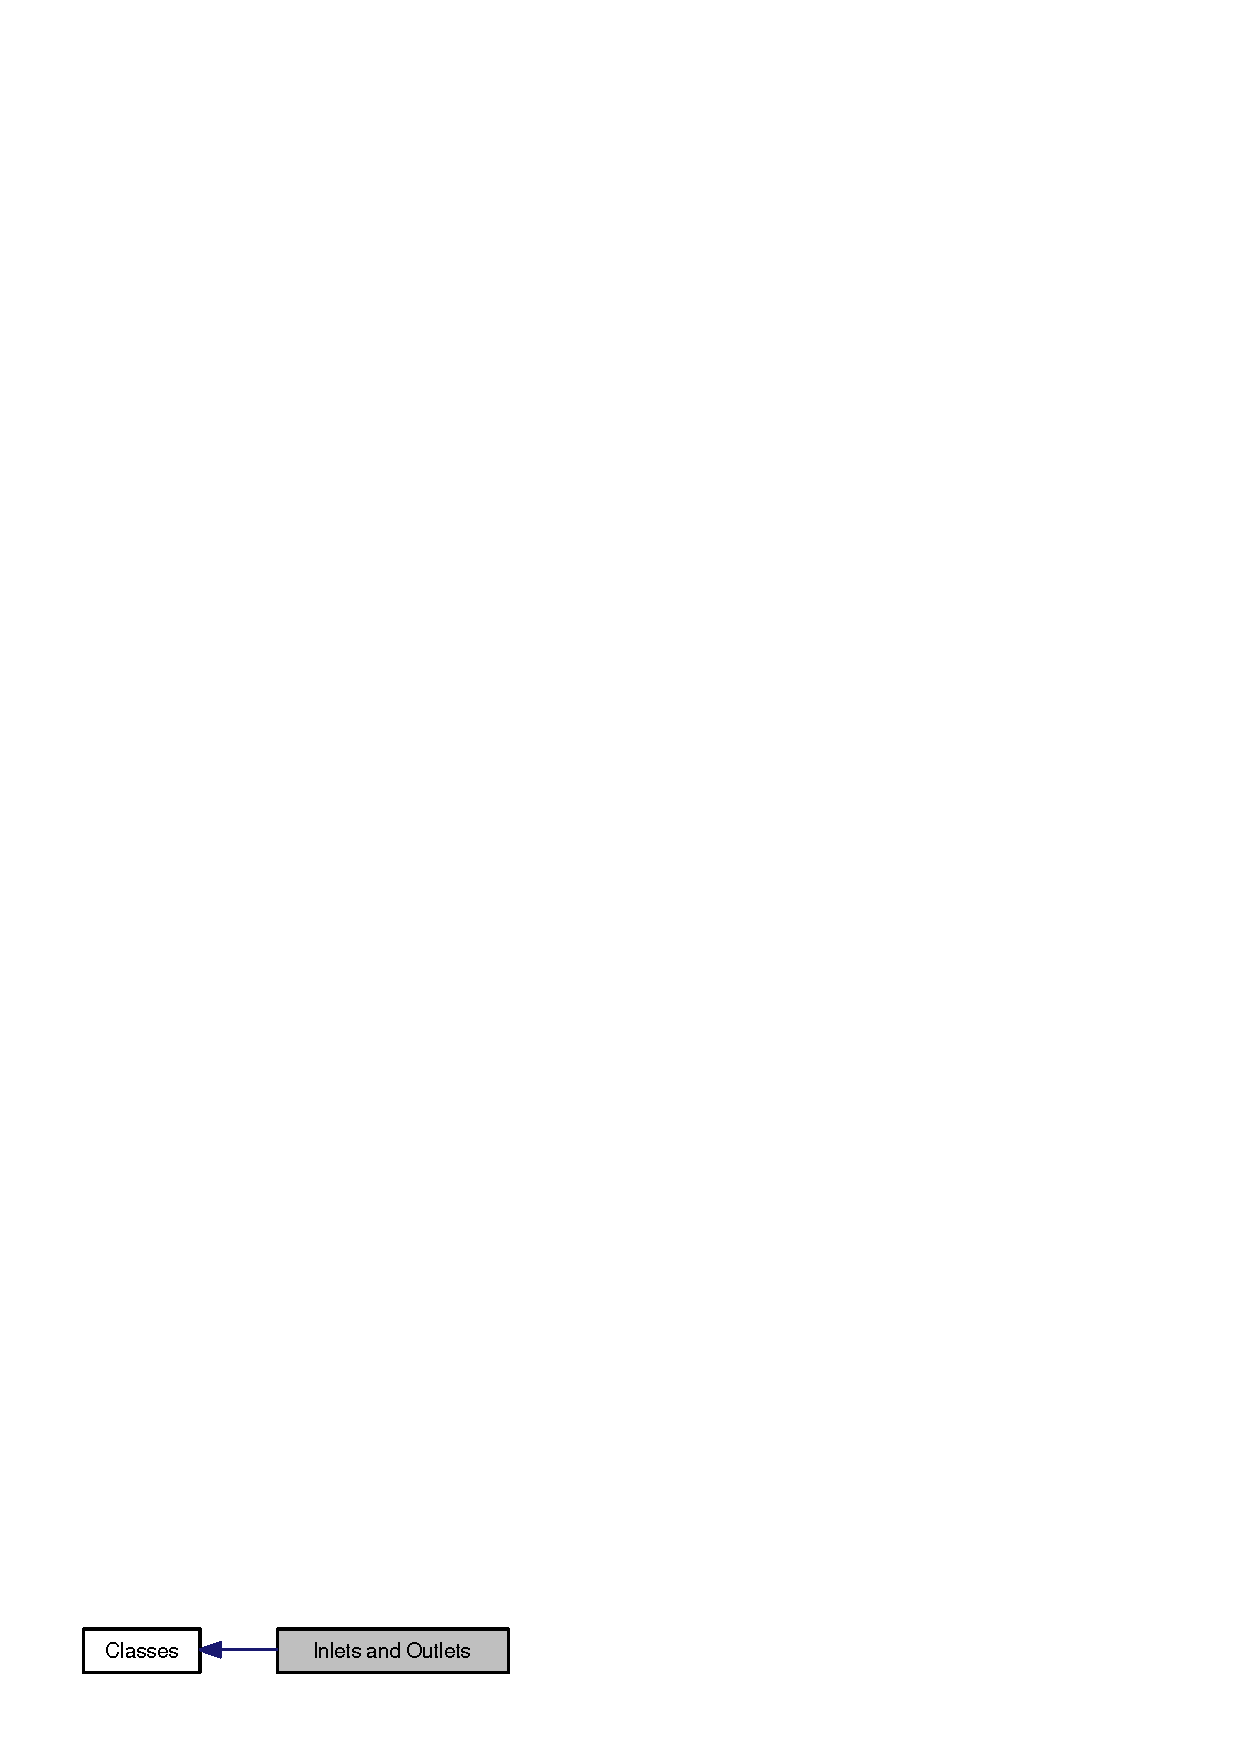
\includegraphics[width=124pt]{group__inout}
\end{center}
\end{figure}
\subsection*{Functions}
\begin{DoxyCompactItemize}
\item 
void $\ast$ \hyperlink{group__inout_ga7195144cee5e8b74c10c2b17b6c6472a}{inlet\_\-new} (void $\ast$x, char $\ast$s)
\begin{DoxyCompactList}\small\item\em Use \hyperlink{group__inout_ga7195144cee5e8b74c10c2b17b6c6472a}{inlet\_\-new()} to create an inlet that can receive a specific message or any message. \item\end{DoxyCompactList}\item 
void $\ast$ \hyperlink{group__inout_ga8ca68c8eafef51622f263f13e047341b}{intin} (void $\ast$x, short n)
\begin{DoxyCompactList}\small\item\em Use \hyperlink{group__inout_ga8ca68c8eafef51622f263f13e047341b}{intin()} to create an inlet typed to receive only integers. \item\end{DoxyCompactList}\item 
void $\ast$ \hyperlink{group__inout_ga01125a22c75ef028199febbe21346f0e}{floatin} (void $\ast$x, short n)
\begin{DoxyCompactList}\small\item\em Use \hyperlink{group__inout_ga01125a22c75ef028199febbe21346f0e}{floatin()} to create an inlet typed to receive only floats. \item\end{DoxyCompactList}\item 
void $\ast$ \hyperlink{group__inout_ga451b3a1ec203ac8648a5399e209f070a}{outlet\_\-new} (void $\ast$x, char $\ast$s)
\begin{DoxyCompactList}\small\item\em Use \hyperlink{group__inout_ga451b3a1ec203ac8648a5399e209f070a}{outlet\_\-new()} to create an outlet that can send a specific non-\/standard message, or any message. \item\end{DoxyCompactList}\item 
void $\ast$ \hyperlink{group__inout_ga69d26d4f2684aab7dbc1b2d18248eae5}{bangout} (void $\ast$x)
\begin{DoxyCompactList}\small\item\em Use \hyperlink{group__inout_ga69d26d4f2684aab7dbc1b2d18248eae5}{bangout()} to create an outlet that will always send the bang message. \item\end{DoxyCompactList}\item 
void $\ast$ \hyperlink{group__inout_ga9b8d897c728eeafa5638d4fc16ff704e}{intout} (void $\ast$x)
\begin{DoxyCompactList}\small\item\em Use \hyperlink{group__inout_ga9b8d897c728eeafa5638d4fc16ff704e}{intout()} to create an outlet that will always send the int message. \item\end{DoxyCompactList}\item 
void $\ast$ \hyperlink{group__inout_ga0881da69192bb254b8c0bf767c657461}{floatout} (void $\ast$x)
\begin{DoxyCompactList}\small\item\em Use \hyperlink{group__inout_ga0881da69192bb254b8c0bf767c657461}{floatout()} to create an outlet that will always send the float message. \item\end{DoxyCompactList}\item 
void $\ast$ \hyperlink{group__inout_ga47841be73d0c90978da818f0f7c899eb}{listout} (void $\ast$x)
\begin{DoxyCompactList}\small\item\em Use \hyperlink{group__inout_ga47841be73d0c90978da818f0f7c899eb}{listout()} to create an outlet that will always send the list message. \item\end{DoxyCompactList}\item 
void $\ast$ \hyperlink{group__inout_ga357498d7143fd266facfbfc4efa59029}{outlet\_\-bang} (void $\ast$o)
\begin{DoxyCompactList}\small\item\em Use \hyperlink{group__inout_ga357498d7143fd266facfbfc4efa59029}{outlet\_\-bang()} to send a bang message out an outlet. \item\end{DoxyCompactList}\item 
void $\ast$ \hyperlink{group__inout_ga0b2b38216f2f4dba486bfcd2273f255e}{outlet\_\-int} (void $\ast$o, long n)
\begin{DoxyCompactList}\small\item\em Use \hyperlink{group__inout_ga0b2b38216f2f4dba486bfcd2273f255e}{outlet\_\-int()} to send a float message out an outlet. \item\end{DoxyCompactList}\item 
void $\ast$ \hyperlink{group__inout_gafbb3f62a413f05a394391afde5b3c30f}{outlet\_\-float} (void $\ast$o, double f)
\begin{DoxyCompactList}\small\item\em Use \hyperlink{group__inout_gafbb3f62a413f05a394391afde5b3c30f}{outlet\_\-float()} to send an int message out an outlet. \item\end{DoxyCompactList}\item 
void $\ast$ \hyperlink{group__inout_gabdef4fbe6e1040dc28204b8070bdcda5}{outlet\_\-list} (void $\ast$o, \hyperlink{structt__symbol}{t\_\-symbol} $\ast$s, short ac, \hyperlink{structt__atom}{t\_\-atom} $\ast$av)
\begin{DoxyCompactList}\small\item\em Use \hyperlink{group__inout_gabdef4fbe6e1040dc28204b8070bdcda5}{outlet\_\-list()} to send a list message out an outlet. \item\end{DoxyCompactList}\item 
void $\ast$ \hyperlink{group__inout_ga12798ee897e01dac21ee547c4091d8a8}{outlet\_\-anything} (void $\ast$o, \hyperlink{structt__symbol}{t\_\-symbol} $\ast$s, short ac, \hyperlink{structt__atom}{t\_\-atom} $\ast$av)
\begin{DoxyCompactList}\small\item\em Use \hyperlink{group__inout_ga12798ee897e01dac21ee547c4091d8a8}{outlet\_\-anything()} to send any message out an outlet. \item\end{DoxyCompactList}\item 
void $\ast$ \hyperlink{group__inout_ga65676568dda565aba2dd13c9f88c9f91}{proxy\_\-new} (void $\ast$x, long id, long $\ast$stuffloc)
\begin{DoxyCompactList}\small\item\em Use proxy\_\-new to create a new Proxy object. \item\end{DoxyCompactList}\item 
long \hyperlink{group__inout_gae81f89a78389587dc23d641e38b42481}{proxy\_\-getinlet} (\hyperlink{structt__object}{t\_\-object} $\ast$master)
\begin{DoxyCompactList}\small\item\em Use proxy\_\-getinlet to get the inlet number in which a message was received. \item\end{DoxyCompactList}\end{DoxyCompactItemize}


\subsection{Detailed Description}
Routines for creating and communicating with inlets and outlets. 

\subsection{Function Documentation}
\hypertarget{group__inout_ga69d26d4f2684aab7dbc1b2d18248eae5}{
\index{inout@{inout}!bangout@{bangout}}
\index{bangout@{bangout}!inout@{inout}}
\subsubsection[{bangout}]{\setlength{\rightskip}{0pt plus 5cm}void$\ast$ bangout (void $\ast$ {\em x})}}
\label{group__inout_ga69d26d4f2684aab7dbc1b2d18248eae5}


Use \hyperlink{group__inout_ga69d26d4f2684aab7dbc1b2d18248eae5}{bangout()} to create an outlet that will always send the bang message. 
\begin{DoxyParams}{Parameters}
\item[{\em x}]Your object. \end{DoxyParams}
\begin{DoxyReturn}{Returns}
A pointer to the new outlet.
\end{DoxyReturn}
\begin{DoxyRemark}{Remarks}
You can send a bang message out a general purpose outlet, but creating an outlet using \hyperlink{group__inout_ga69d26d4f2684aab7dbc1b2d18248eae5}{bangout()} allows Max to type-\/check the connection a user might make and refuse to connect the outlet to any object that cannot receive a bang message. \hyperlink{group__inout_ga69d26d4f2684aab7dbc1b2d18248eae5}{bangout()} returns the created outlet. 
\end{DoxyRemark}
\hypertarget{group__inout_ga01125a22c75ef028199febbe21346f0e}{
\index{inout@{inout}!floatin@{floatin}}
\index{floatin@{floatin}!inout@{inout}}
\subsubsection[{floatin}]{\setlength{\rightskip}{0pt plus 5cm}void$\ast$ floatin (void $\ast$ {\em x}, \/  short {\em n})}}
\label{group__inout_ga01125a22c75ef028199febbe21346f0e}


Use \hyperlink{group__inout_ga01125a22c75ef028199febbe21346f0e}{floatin()} to create an inlet typed to receive only floats. 
\begin{DoxyParams}{Parameters}
\item[{\em x}]Your object. \item[{\em n}]Location of the inlet from 1 to 9. 1 is immediately to the right of the leftmost inlet. \end{DoxyParams}
\begin{DoxyReturn}{Returns}
A pointer to the new inlet. 
\end{DoxyReturn}
\hypertarget{group__inout_ga0881da69192bb254b8c0bf767c657461}{
\index{inout@{inout}!floatout@{floatout}}
\index{floatout@{floatout}!inout@{inout}}
\subsubsection[{floatout}]{\setlength{\rightskip}{0pt plus 5cm}void$\ast$ floatout (void $\ast$ {\em x})}}
\label{group__inout_ga0881da69192bb254b8c0bf767c657461}


Use \hyperlink{group__inout_ga0881da69192bb254b8c0bf767c657461}{floatout()} to create an outlet that will always send the float message. 
\begin{DoxyParams}{Parameters}
\item[{\em x}]Your object. \end{DoxyParams}
\begin{DoxyReturn}{Returns}
A pointer to the new outlet. 
\end{DoxyReturn}
\hypertarget{group__inout_ga7195144cee5e8b74c10c2b17b6c6472a}{
\index{inout@{inout}!inlet\_\-new@{inlet\_\-new}}
\index{inlet\_\-new@{inlet\_\-new}!inout@{inout}}
\subsubsection[{inlet\_\-new}]{\setlength{\rightskip}{0pt plus 5cm}void$\ast$ inlet\_\-new (void $\ast$ {\em x}, \/  char $\ast$ {\em s})}}
\label{group__inout_ga7195144cee5e8b74c10c2b17b6c6472a}


Use \hyperlink{group__inout_ga7195144cee5e8b74c10c2b17b6c6472a}{inlet\_\-new()} to create an inlet that can receive a specific message or any message. 
\begin{DoxyParams}{Parameters}
\item[{\em x}]Your object. \item[{\em s}]Character string of the message, or NULL to receive any message. \end{DoxyParams}
\begin{DoxyReturn}{Returns}
A pointer to the new inlet.
\end{DoxyReturn}
\begin{DoxyRemark}{Remarks}
\hyperlink{group__inout_ga7195144cee5e8b74c10c2b17b6c6472a}{inlet\_\-new()} ceates a general purpose inlet. You can use it in circumstances where you would like special messages to be received in inlets other than the leftmost one. To create an inlet that receives a particular message, pass the message’s character string. For example, to create an inlet that receives only bang messages, do the following 
\begin{DoxyCode}
    inlet_new (myObject,"bang"); 
\end{DoxyCode}


To create an inlet that can receive any message, pass NULL for msg 
\begin{DoxyCode}
    inlet_new (myObject, NULL); 
\end{DoxyCode}


Proxies are an alternative method for general-\/purpose inlets that have a number of advantages. If you create multiple inlets as shown above, there would be no way to figure out which inlet received a message. See the discussion in \hyperlink{chapter_inout_chapter_inout_proxies}{Creating and Using Proxies}. 
\end{DoxyRemark}
\hypertarget{group__inout_ga8ca68c8eafef51622f263f13e047341b}{
\index{inout@{inout}!intin@{intin}}
\index{intin@{intin}!inout@{inout}}
\subsubsection[{intin}]{\setlength{\rightskip}{0pt plus 5cm}void$\ast$ intin (void $\ast$ {\em x}, \/  short {\em n})}}
\label{group__inout_ga8ca68c8eafef51622f263f13e047341b}


Use \hyperlink{group__inout_ga8ca68c8eafef51622f263f13e047341b}{intin()} to create an inlet typed to receive only integers. 
\begin{DoxyParams}{Parameters}
\item[{\em x}]Your object. \item[{\em n}]Location of the inlet from 1 to 9. 1 is immediately to the right of the leftmost inlet. \end{DoxyParams}
\begin{DoxyReturn}{Returns}
A pointer to the new inlet.
\end{DoxyReturn}
\begin{DoxyRemark}{Remarks}
intin creates integer inlets. It takes a pointer to your newly created object and an integer n, from 1 to 9. The number specifies the message type you’ll get, so you can distinguish one inlet from another. For example, an integer sent in inlet 1 will be of message type in1 and a floating point number sent in inlet 4 will be of type ft4. You use \hyperlink{group__class__old_gad3a69b2d38b257464c6a0f8a50efd85a}{addinx()} and \hyperlink{group__class__old_gad223143c8da12d8f3b7b18f9d6e5da9e}{addftx()} to add methods to respond to these messages.
\end{DoxyRemark}
The order you create additional inlets is important. If you want the rightmost inlet to be the have the highest number in-\/ or ft-\/ message (which is usually the case), you should create the highest number message inlet first. \hypertarget{group__inout_ga9b8d897c728eeafa5638d4fc16ff704e}{
\index{inout@{inout}!intout@{intout}}
\index{intout@{intout}!inout@{inout}}
\subsubsection[{intout}]{\setlength{\rightskip}{0pt plus 5cm}void$\ast$ intout (void $\ast$ {\em x})}}
\label{group__inout_ga9b8d897c728eeafa5638d4fc16ff704e}


Use \hyperlink{group__inout_ga9b8d897c728eeafa5638d4fc16ff704e}{intout()} to create an outlet that will always send the int message. 
\begin{DoxyParams}{Parameters}
\item[{\em x}]Your object. \end{DoxyParams}
\begin{DoxyReturn}{Returns}
A pointer to the new outlet.
\end{DoxyReturn}
\begin{DoxyRemark}{Remarks}
You can send a bang message out a general purpose outlet, but creating an outlet using \hyperlink{group__inout_ga69d26d4f2684aab7dbc1b2d18248eae5}{bangout()} allows Max to type-\/check the connection a user might make and refuse to connect the outlet to any object that cannot receive a bang message. \hyperlink{group__inout_ga69d26d4f2684aab7dbc1b2d18248eae5}{bangout()} returns the created outlet. 
\end{DoxyRemark}
\hypertarget{group__inout_ga47841be73d0c90978da818f0f7c899eb}{
\index{inout@{inout}!listout@{listout}}
\index{listout@{listout}!inout@{inout}}
\subsubsection[{listout}]{\setlength{\rightskip}{0pt plus 5cm}void$\ast$ listout (void $\ast$ {\em x})}}
\label{group__inout_ga47841be73d0c90978da818f0f7c899eb}


Use \hyperlink{group__inout_ga47841be73d0c90978da818f0f7c899eb}{listout()} to create an outlet that will always send the list message. 
\begin{DoxyParams}{Parameters}
\item[{\em x}]Your object. \end{DoxyParams}
\begin{DoxyReturn}{Returns}
A pointer to the new outlet. 
\end{DoxyReturn}
\hypertarget{group__inout_ga12798ee897e01dac21ee547c4091d8a8}{
\index{inout@{inout}!outlet\_\-anything@{outlet\_\-anything}}
\index{outlet\_\-anything@{outlet\_\-anything}!inout@{inout}}
\subsubsection[{outlet\_\-anything}]{\setlength{\rightskip}{0pt plus 5cm}void$\ast$ outlet\_\-anything (void $\ast$ {\em o}, \/  {\bf t\_\-symbol} $\ast$ {\em s}, \/  short {\em ac}, \/  {\bf t\_\-atom} $\ast$ {\em av})}}
\label{group__inout_ga12798ee897e01dac21ee547c4091d8a8}


Use \hyperlink{group__inout_ga12798ee897e01dac21ee547c4091d8a8}{outlet\_\-anything()} to send any message out an outlet. 
\begin{DoxyParams}{Parameters}
\item[{\em o}]Outlet that will send the message. \item[{\em s}]The message selector \hyperlink{structt__symbol}{t\_\-symbol}$\ast$. \item[{\em ac}]Number of elements in the list in argv. \item[{\em av}]Atoms constituting the list. \end{DoxyParams}
\begin{DoxyReturn}{Returns}
Returns 0 if a stack overflow occurred, otherwise returns 1.
\end{DoxyReturn}
\begin{DoxyRemark}{Remarks}
This function lets you send an arbitrary message out an outlet. Here are a couple of examples of its use.
\end{DoxyRemark}
First, here’s a hard way to send the bang message (see \hyperlink{group__inout_ga357498d7143fd266facfbfc4efa59029}{outlet\_\-bang()} for an easier way): 
\begin{DoxyCode}
    outlet_anything(myOutlet, gensym("bang"), 0, NIL); 
\end{DoxyCode}


\begin{DoxyRemark}{Remarks}
And here’s an even harder way to send a single integer (instead of using \hyperlink{group__inout_ga0b2b38216f2f4dba486bfcd2273f255e}{outlet\_\-int()}). 
\begin{DoxyCode}
    t_atom myNumber; 

    atom_setlong(&myNumber, 432);
    outlet_anything(myOutlet, gensym("int"), 1, &myNumber);
\end{DoxyCode}


Notice that \hyperlink{group__inout_ga12798ee897e01dac21ee547c4091d8a8}{outlet\_\-anything()} expects the message argument as a \hyperlink{structt__symbol}{t\_\-symbol}$\ast$, so you must use \hyperlink{group__symbol_ga8268797d125a15bae1010af70b559e05}{gensym()} on a character string.
\end{DoxyRemark}
If you’ll be sending the same message a lot, you might call \hyperlink{group__symbol_ga8268797d125a15bae1010af70b559e05}{gensym()} on the message string at initialization time and store the result in a global variable to save the (significant) overhead of calling \hyperlink{group__symbol_ga8268797d125a15bae1010af70b559e05}{gensym()} every time you want to send a message.

Also, do not send lists using \hyperlink{group__inout_ga12798ee897e01dac21ee547c4091d8a8}{outlet\_\-anything()} with list as the selector argument. Use the \hyperlink{group__inout_gabdef4fbe6e1040dc28204b8070bdcda5}{outlet\_\-list()} function instead. \hypertarget{group__inout_ga357498d7143fd266facfbfc4efa59029}{
\index{inout@{inout}!outlet\_\-bang@{outlet\_\-bang}}
\index{outlet\_\-bang@{outlet\_\-bang}!inout@{inout}}
\subsubsection[{outlet\_\-bang}]{\setlength{\rightskip}{0pt plus 5cm}void$\ast$ outlet\_\-bang (void $\ast$ {\em o})}}
\label{group__inout_ga357498d7143fd266facfbfc4efa59029}


Use \hyperlink{group__inout_ga357498d7143fd266facfbfc4efa59029}{outlet\_\-bang()} to send a bang message out an outlet. 
\begin{DoxyParams}{Parameters}
\item[{\em o}]Outlet that will send the message. \end{DoxyParams}
\begin{DoxyReturn}{Returns}
Returns 0 if a stack overflow occurred, otherwise returns 1. 
\end{DoxyReturn}
\hypertarget{group__inout_gafbb3f62a413f05a394391afde5b3c30f}{
\index{inout@{inout}!outlet\_\-float@{outlet\_\-float}}
\index{outlet\_\-float@{outlet\_\-float}!inout@{inout}}
\subsubsection[{outlet\_\-float}]{\setlength{\rightskip}{0pt plus 5cm}void$\ast$ outlet\_\-float (void $\ast$ {\em o}, \/  double {\em f})}}
\label{group__inout_gafbb3f62a413f05a394391afde5b3c30f}


Use \hyperlink{group__inout_gafbb3f62a413f05a394391afde5b3c30f}{outlet\_\-float()} to send an int message out an outlet. 
\begin{DoxyParams}{Parameters}
\item[{\em o}]Outlet that will send the message. \item[{\em f}]Float value to send. \end{DoxyParams}
\begin{DoxyReturn}{Returns}
Returns 0 if a stack overflow occurred, otherwise returns 1. 
\end{DoxyReturn}
\hypertarget{group__inout_ga0b2b38216f2f4dba486bfcd2273f255e}{
\index{inout@{inout}!outlet\_\-int@{outlet\_\-int}}
\index{outlet\_\-int@{outlet\_\-int}!inout@{inout}}
\subsubsection[{outlet\_\-int}]{\setlength{\rightskip}{0pt plus 5cm}void$\ast$ outlet\_\-int (void $\ast$ {\em o}, \/  long {\em n})}}
\label{group__inout_ga0b2b38216f2f4dba486bfcd2273f255e}


Use \hyperlink{group__inout_ga0b2b38216f2f4dba486bfcd2273f255e}{outlet\_\-int()} to send a float message out an outlet. 
\begin{DoxyParams}{Parameters}
\item[{\em o}]Outlet that will send the message. \item[{\em n}]Integer value to send. \end{DoxyParams}
\begin{DoxyReturn}{Returns}
Returns 0 if a stack overflow occurred, otherwise returns 1. 
\end{DoxyReturn}
\hypertarget{group__inout_gabdef4fbe6e1040dc28204b8070bdcda5}{
\index{inout@{inout}!outlet\_\-list@{outlet\_\-list}}
\index{outlet\_\-list@{outlet\_\-list}!inout@{inout}}
\subsubsection[{outlet\_\-list}]{\setlength{\rightskip}{0pt plus 5cm}void$\ast$ outlet\_\-list (void $\ast$ {\em o}, \/  {\bf t\_\-symbol} $\ast$ {\em s}, \/  short {\em ac}, \/  {\bf t\_\-atom} $\ast$ {\em av})}}
\label{group__inout_gabdef4fbe6e1040dc28204b8070bdcda5}


Use \hyperlink{group__inout_gabdef4fbe6e1040dc28204b8070bdcda5}{outlet\_\-list()} to send a list message out an outlet. 
\begin{DoxyParams}{Parameters}
\item[{\em o}]Outlet that will send the message. \item[{\em s}]Should be NULL, but can be the \_\-sym\_\-list. \item[{\em ac}]Number of elements in the list in argv. \item[{\em av}]Atoms constituting the list. \end{DoxyParams}
\begin{DoxyReturn}{Returns}
Returns 0 if a stack overflow occurred, otherwise returns 1.
\end{DoxyReturn}
\begin{DoxyRemark}{Remarks}
\hyperlink{group__inout_gabdef4fbe6e1040dc28204b8070bdcda5}{outlet\_\-list()} sends the list specified by argv and argc out the specified outlet. The outlet must have been created with listout or outlet\_\-new in your object creation function (see above). You create the list as an array of Atoms, but the first item in the list must be an integer or float.
\end{DoxyRemark}
Here’s an example of sending a list of three numbers. 
\begin{DoxyCode}
    t_atom myList[3]; 
    long theNumbers[3]; 
    short i; 
    
    theNumbers[0] = 23; 
    theNumbers[1] = 12; 
    theNumbers[2] = 5;
    for (i=0; i < 3; i++) { 
        atom_setlong(myList+i,theNumbers[i]);
    } 
    outlet_list(myOutlet,0L,3,&myList); 
\end{DoxyCode}


\begin{DoxyRemark}{Remarks}
It’s not a good idea to pass large lists to outlet\_\-list that are comprised of local (automatic) variables. If the list is small, as in the above example, there’s no problem. If your object will regularly send lists, it might make sense to keep an array of t\_\-atoms inside your object’s data structure. 
\end{DoxyRemark}
\hypertarget{group__inout_ga451b3a1ec203ac8648a5399e209f070a}{
\index{inout@{inout}!outlet\_\-new@{outlet\_\-new}}
\index{outlet\_\-new@{outlet\_\-new}!inout@{inout}}
\subsubsection[{outlet\_\-new}]{\setlength{\rightskip}{0pt plus 5cm}void$\ast$ outlet\_\-new (void $\ast$ {\em x}, \/  char $\ast$ {\em s})}}
\label{group__inout_ga451b3a1ec203ac8648a5399e209f070a}


Use \hyperlink{group__inout_ga451b3a1ec203ac8648a5399e209f070a}{outlet\_\-new()} to create an outlet that can send a specific non-\/standard message, or any message. 
\begin{DoxyParams}{Parameters}
\item[{\em x}]Your object. \item[{\em s}]A C-\/string specifying the message that will be sent out this outlet, or NULL to indicate the outlet will be used to send various messages. The advantage of this kind of outlet’s flexibility is balanced by the fact that Max must perform a message-\/lookup in real-\/time for every message sent through it, rather than when a patch is being constructed, as is true for other types of outlets. Patchers execute faster when outlets are typed, since the message lookup can be done before the program executes. \end{DoxyParams}
\begin{DoxyReturn}{Returns}
A pointer to the new outlet. 
\end{DoxyReturn}
\hypertarget{group__inout_gae81f89a78389587dc23d641e38b42481}{
\index{inout@{inout}!proxy\_\-getinlet@{proxy\_\-getinlet}}
\index{proxy\_\-getinlet@{proxy\_\-getinlet}!inout@{inout}}
\subsubsection[{proxy\_\-getinlet}]{\setlength{\rightskip}{0pt plus 5cm}long proxy\_\-getinlet ({\bf t\_\-object} $\ast$ {\em master})}}
\label{group__inout_gae81f89a78389587dc23d641e38b42481}


Use proxy\_\-getinlet to get the inlet number in which a message was received. Note that the “owner” argument should point to your external object’s instance, not a proxy object.


\begin{DoxyParams}{Parameters}
\item[{\em master}]Your object. \end{DoxyParams}
\begin{DoxyReturn}{Returns}
The index number of the inlet that received the message. 
\end{DoxyReturn}
\hypertarget{group__inout_ga65676568dda565aba2dd13c9f88c9f91}{
\index{inout@{inout}!proxy\_\-new@{proxy\_\-new}}
\index{proxy\_\-new@{proxy\_\-new}!inout@{inout}}
\subsubsection[{proxy\_\-new}]{\setlength{\rightskip}{0pt plus 5cm}void$\ast$ proxy\_\-new (void $\ast$ {\em x}, \/  long {\em id}, \/  long $\ast$ {\em stuffloc})}}
\label{group__inout_ga65676568dda565aba2dd13c9f88c9f91}


Use proxy\_\-new to create a new Proxy object. 
\begin{DoxyParams}{Parameters}
\item[{\em x}]Your object. \item[{\em id}]A non-\/zero number to be written into your object when a message is received in this particular Proxy. Normally, id will be the inlet “number” analogous to in1, in2 etc. \item[{\em stuffloc}]A pointer to a location where the id value will be written. \end{DoxyParams}
\begin{DoxyReturn}{Returns}
A pointer to the new proxy inlet.
\end{DoxyReturn}
\begin{DoxyRemark}{Remarks}
This routine creates a new Proxy object (that includes an inlet). It allows you to identify messages based on an id value stored in the location specified by stuffLoc. You should store the pointer returned by \hyperlink{group__inout_ga65676568dda565aba2dd13c9f88c9f91}{proxy\_\-new()} because you’ll need to free all Proxies in your object’s free function using \hyperlink{group__obj_ga3759846cb356195532c41e35b87522ee}{object\_\-free()}.
\end{DoxyRemark}
After your method has finished, Proxy sets the stuffLoc location back to 0, since it never sees messages coming in an object’s leftmost inlet. You’ll know you received a message in the leftmost inlet if the contents of stuffLoc is 0. As of Max 4.3, stuffLoc is not always guaranteed to be a correct indicator of the inlet in which a message was received. Use \hyperlink{group__inout_gae81f89a78389587dc23d641e38b42481}{proxy\_\-getinlet()} to determine the inlet number. 
\hypertarget{group__datastore}{
\section{Data Storage}
\label{group__datastore}\index{Data Storage@{Data Storage}}
}


Max provides a number of ways of storing and manipulating data at a high level.  


Collaboration diagram for Data Storage:\nopagebreak
\begin{figure}[H]
\begin{center}
\leavevmode
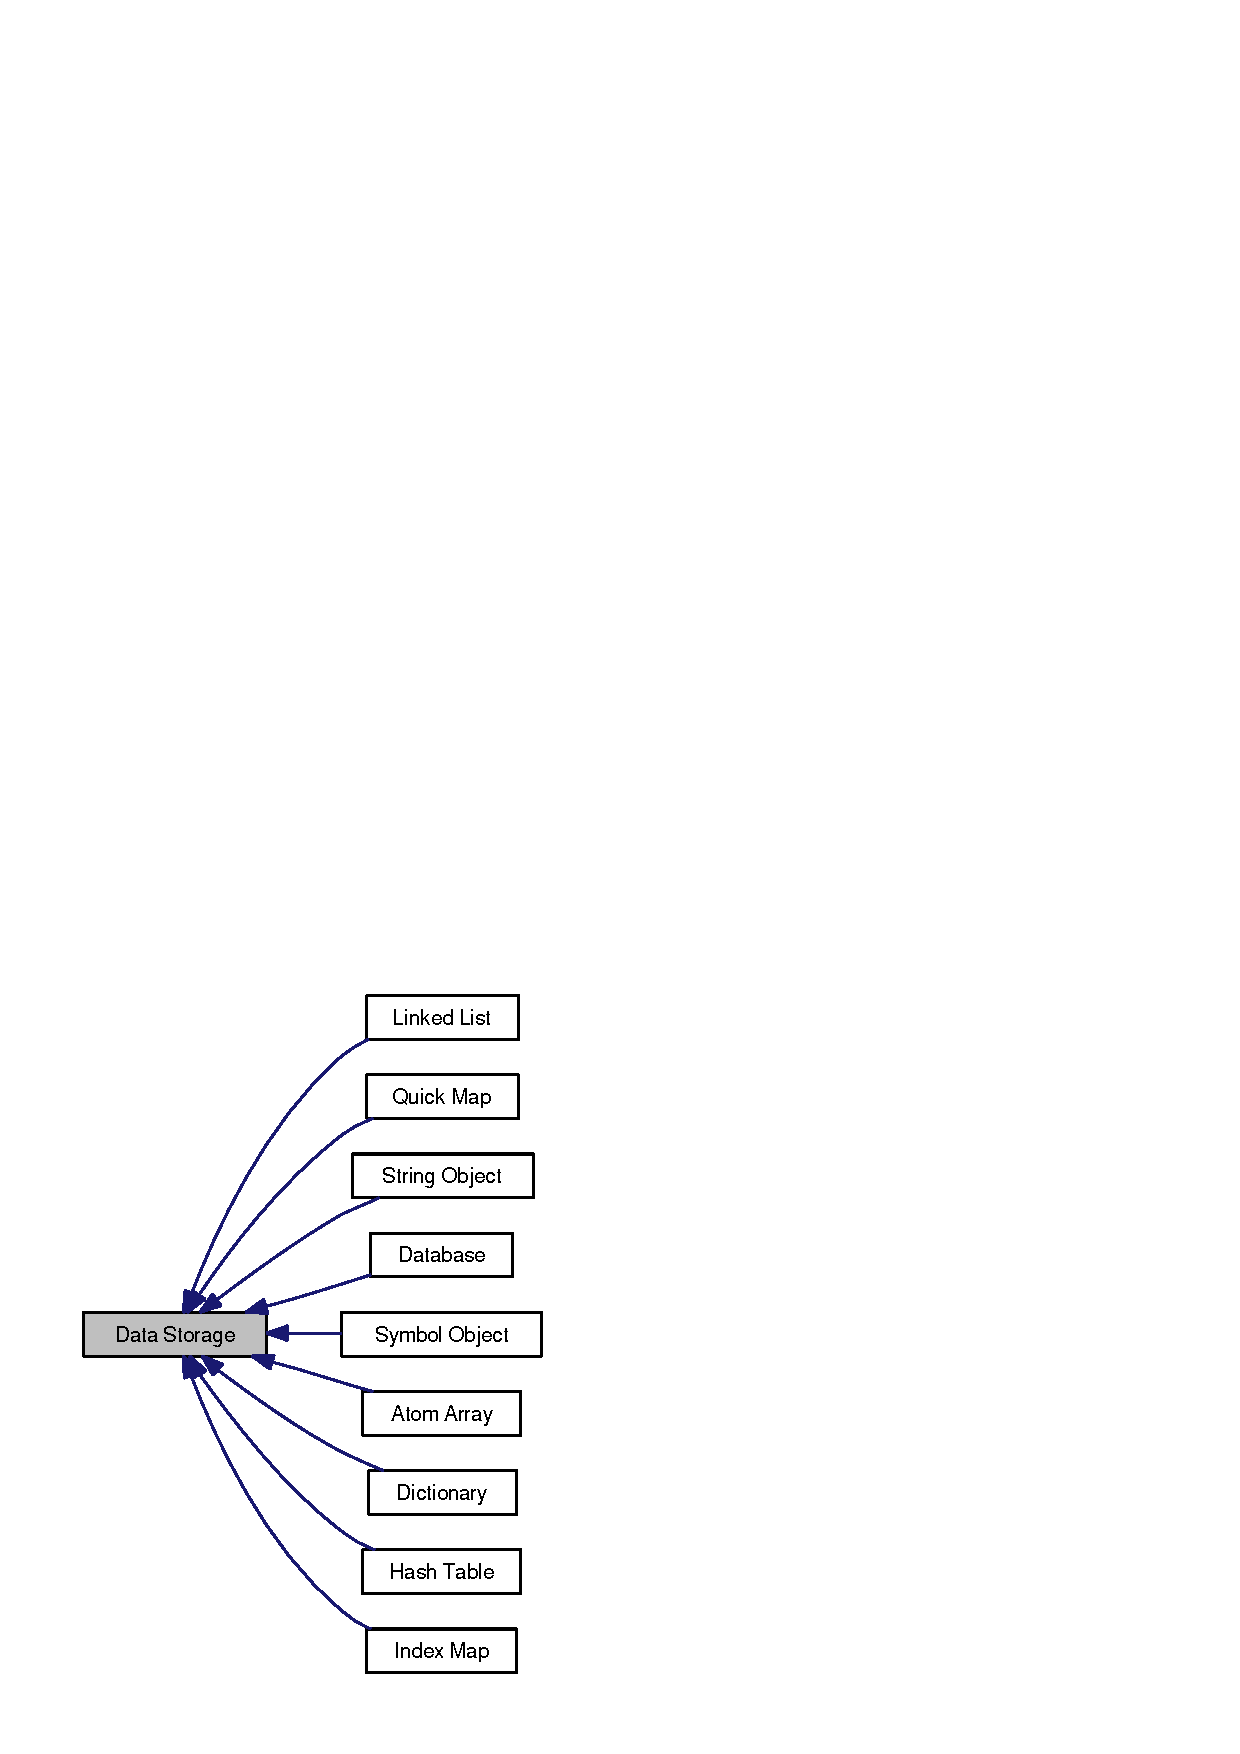
\includegraphics[width=132pt]{group__datastore}
\end{center}
\end{figure}
\subsection*{Modules}
\begin{DoxyCompactItemize}
\item 
\hyperlink{group__atomarray}{Atom Array}


\begin{DoxyCompactList}\small\item\em Max's atomarray object is a container for an array of atoms with an interface for manipulating that array. \item\end{DoxyCompactList}\item 
\hyperlink{group__database}{Database}


\begin{DoxyCompactList}\small\item\em Max's database support currently consists of a SQLite ( \href{http://sqlite.org}{\tt http://sqlite.org} ) extension which is loaded dynamically by Max at launch time. \item\end{DoxyCompactList}\item 
\hyperlink{group__dictionary}{Dictionary}


\begin{DoxyCompactList}\small\item\em In Max 5, we have a new \char`\"{}dictionary\char`\"{} object which can be used for object prototypes, object serialization, object constructors, and other tasks. \item\end{DoxyCompactList}\item 
\hyperlink{group__hashtab}{Hash Table}


\begin{DoxyCompactList}\small\item\em Max's hashtab object implements a hash table ( \href{http://en.wikipedia.org/wiki/Hash_table}{\tt http://en.wikipedia.org/wiki/Hash\_\-table} ). \item\end{DoxyCompactList}\item 
\hyperlink{group__indexmap}{Index Map}


\begin{DoxyCompactList}\small\item\em An indexmap is basically a managed array of pointers, but it allows you to derive relatively quickly the index from a pointer in the array. \item\end{DoxyCompactList}\item 
\hyperlink{group__linklist}{Linked List}


\begin{DoxyCompactList}\small\item\em Max's linklist object implements a doubly-\/linked-\/list ( \href{http://en.wikipedia.org/wiki/Linked_list}{\tt http://en.wikipedia.org/wiki/Linked\_\-list} ) together with a high-\/level interface for manipulating and accessing values in the list. \item\end{DoxyCompactList}\item 
\hyperlink{group__quickmap}{Quick Map}


\begin{DoxyCompactList}\small\item\em A quickmap implements a pair of \hyperlink{structt__hashtab}{t\_\-hashtab} hash tables so that it is fast to look up a unique value for a unique key or vice-\/versa. \item\end{DoxyCompactList}\item 
\hyperlink{group__string}{String Object}


\begin{DoxyCompactList}\small\item\em Max's string object is a simple wrapper for c-\/strings, useful when working with Max's \hyperlink{structt__dictionary}{t\_\-dictionary}, \hyperlink{structt__linklist}{t\_\-linklist}, or \hyperlink{structt__hashtab}{t\_\-hashtab}. \item\end{DoxyCompactList}\item 
\hyperlink{group__symobject}{Symbol Object}


\begin{DoxyCompactList}\small\item\em The symobject class is a simple object that wraps a \hyperlink{structt__symbol}{t\_\-symbol}$\ast$ together with a couple of additional fields. \item\end{DoxyCompactList}\end{DoxyCompactItemize}
\subsection*{Typedefs}
\begin{DoxyCompactItemize}
\item 
typedef long($\ast$ \hyperlink{group__datastore_gaaf4ae6dd800a2be9abd645cf70aeb38f}{t\_\-cmpfn} )(void $\ast$, void $\ast$)
\begin{DoxyCompactList}\small\item\em Comparison function pointer type. \item\end{DoxyCompactList}\end{DoxyCompactItemize}
\subsection*{Enumerations}
\begin{DoxyCompactItemize}
\item 
enum \hyperlink{group__datastore_gaa858d4b3815076d79624c39d9ca59348}{e\_\-max\_\-datastore\_\-flags} \{ \par
\hyperlink{group__datastore_ggaa858d4b3815076d79624c39d9ca59348adc630c58c8e958a404553a08db6fd180}{OBJ\_\-FLAG\_\-OBJ} =  0x00000000, 
\par
\hyperlink{group__datastore_ggaa858d4b3815076d79624c39d9ca59348aee2810996bf0475ddcb07b039b162d52}{OBJ\_\-FLAG\_\-REF} =  0x00000001, 
\par
\hyperlink{group__datastore_ggaa858d4b3815076d79624c39d9ca59348a862748073762ebc9f5899a8c1d63053a}{OBJ\_\-FLAG\_\-DATA} =  0x00000002, 
\par
\hyperlink{group__datastore_ggaa858d4b3815076d79624c39d9ca59348a03c245bc502773743d2ff575208a8b67}{OBJ\_\-FLAG\_\-MEMORY} =  0x00000004, 
\par
\hyperlink{group__datastore_ggaa858d4b3815076d79624c39d9ca59348a7551721629504fee7ecf5973e467de80}{OBJ\_\-FLAG\_\-SILENT} =  0x00000100, 
\par
\hyperlink{group__datastore_ggaa858d4b3815076d79624c39d9ca59348a20be48992fc9be2b12940730c09d704c}{OBJ\_\-FLAG\_\-INHERITABLE} =  0x00000200
 \}
\begin{DoxyCompactList}\small\item\em Flags used in linklist and hashtab objects. \item\end{DoxyCompactList}\end{DoxyCompactItemize}


\subsection{Detailed Description}
Max provides a number of ways of storing and manipulating data at a high level. It is recommended to use Max's data storage mechanisms where possible, as Max's systems are designed for thread-\/safety and integration with the rest of Max API. 

\subsection{Typedef Documentation}
\hypertarget{group__datastore_gaaf4ae6dd800a2be9abd645cf70aeb38f}{
\index{datastore@{datastore}!t\_\-cmpfn@{t\_\-cmpfn}}
\index{t\_\-cmpfn@{t\_\-cmpfn}!datastore@{datastore}}
\subsubsection[{t\_\-cmpfn}]{\setlength{\rightskip}{0pt plus 5cm}typedef long($\ast$ {\bf t\_\-cmpfn})(void $\ast$, void $\ast$)}}
\label{group__datastore_gaaf4ae6dd800a2be9abd645cf70aeb38f}


Comparison function pointer type. Methods that require a comparison function pointer to be passed in use this type. It should return {\ttfamily true} or {\ttfamily false} depending on the outcome of the comparison of the two linklist items passed in as arguments.

\begin{DoxySeeAlso}{See also}
\hyperlink{group__linklist_ga2a991fb645404fe7d9d3327e5a386b80}{linklist\_\-match()} 

\hyperlink{group__hashtab_gadc142f0a2a64417bb8b8d3c2959924fd}{hashtab\_\-findfirst()} 

\hyperlink{group__indexmap_ga37c44ae6f93722ca5a722839ac62966d}{indexmap\_\-sort()} 
\end{DoxySeeAlso}


\subsection{Enumeration Type Documentation}
\hypertarget{group__datastore_gaa858d4b3815076d79624c39d9ca59348}{
\index{datastore@{datastore}!e\_\-max\_\-datastore\_\-flags@{e\_\-max\_\-datastore\_\-flags}}
\index{e\_\-max\_\-datastore\_\-flags@{e\_\-max\_\-datastore\_\-flags}!datastore@{datastore}}
\subsubsection[{e\_\-max\_\-datastore\_\-flags}]{\setlength{\rightskip}{0pt plus 5cm}enum {\bf e\_\-max\_\-datastore\_\-flags}}}
\label{group__datastore_gaa858d4b3815076d79624c39d9ca59348}


Flags used in linklist and hashtab objects. \begin{Desc}
\item[Enumerator: ]\par
\begin{description}
\index{OBJ\_\-FLAG\_\-OBJ@{OBJ\_\-FLAG\_\-OBJ}!datastore@{datastore}}\index{datastore@{datastore}!OBJ\_\-FLAG\_\-OBJ@{OBJ\_\-FLAG\_\-OBJ}}\item[{\em 
\hypertarget{group__datastore_ggaa858d4b3815076d79624c39d9ca59348adc630c58c8e958a404553a08db6fd180}{
OBJ\_\-FLAG\_\-OBJ}
\label{group__datastore_ggaa858d4b3815076d79624c39d9ca59348adc630c58c8e958a404553a08db6fd180}
}]free using \hyperlink{group__obj_ga3759846cb356195532c41e35b87522ee}{object\_\-free()} \index{OBJ\_\-FLAG\_\-REF@{OBJ\_\-FLAG\_\-REF}!datastore@{datastore}}\index{datastore@{datastore}!OBJ\_\-FLAG\_\-REF@{OBJ\_\-FLAG\_\-REF}}\item[{\em 
\hypertarget{group__datastore_ggaa858d4b3815076d79624c39d9ca59348aee2810996bf0475ddcb07b039b162d52}{
OBJ\_\-FLAG\_\-REF}
\label{group__datastore_ggaa858d4b3815076d79624c39d9ca59348aee2810996bf0475ddcb07b039b162d52}
}]don't free \index{OBJ\_\-FLAG\_\-DATA@{OBJ\_\-FLAG\_\-DATA}!datastore@{datastore}}\index{datastore@{datastore}!OBJ\_\-FLAG\_\-DATA@{OBJ\_\-FLAG\_\-DATA}}\item[{\em 
\hypertarget{group__datastore_ggaa858d4b3815076d79624c39d9ca59348a862748073762ebc9f5899a8c1d63053a}{
OBJ\_\-FLAG\_\-DATA}
\label{group__datastore_ggaa858d4b3815076d79624c39d9ca59348a862748073762ebc9f5899a8c1d63053a}
}]don't free data or call method \index{OBJ\_\-FLAG\_\-MEMORY@{OBJ\_\-FLAG\_\-MEMORY}!datastore@{datastore}}\index{datastore@{datastore}!OBJ\_\-FLAG\_\-MEMORY@{OBJ\_\-FLAG\_\-MEMORY}}\item[{\em 
\hypertarget{group__datastore_ggaa858d4b3815076d79624c39d9ca59348a03c245bc502773743d2ff575208a8b67}{
OBJ\_\-FLAG\_\-MEMORY}
\label{group__datastore_ggaa858d4b3815076d79624c39d9ca59348a03c245bc502773743d2ff575208a8b67}
}]don't call method, and when freeing use \hyperlink{group__memory_ga200c82639e547869db1f3887d17102d3}{sysmem\_\-freeptr()} instead of freeobject \index{OBJ\_\-FLAG\_\-SILENT@{OBJ\_\-FLAG\_\-SILENT}!datastore@{datastore}}\index{datastore@{datastore}!OBJ\_\-FLAG\_\-SILENT@{OBJ\_\-FLAG\_\-SILENT}}\item[{\em 
\hypertarget{group__datastore_ggaa858d4b3815076d79624c39d9ca59348a7551721629504fee7ecf5973e467de80}{
OBJ\_\-FLAG\_\-SILENT}
\label{group__datastore_ggaa858d4b3815076d79624c39d9ca59348a7551721629504fee7ecf5973e467de80}
}]don't notify when modified \index{OBJ\_\-FLAG\_\-INHERITABLE@{OBJ\_\-FLAG\_\-INHERITABLE}!datastore@{datastore}}\index{datastore@{datastore}!OBJ\_\-FLAG\_\-INHERITABLE@{OBJ\_\-FLAG\_\-INHERITABLE}}\item[{\em 
\hypertarget{group__datastore_ggaa858d4b3815076d79624c39d9ca59348a20be48992fc9be2b12940730c09d704c}{
OBJ\_\-FLAG\_\-INHERITABLE}
\label{group__datastore_ggaa858d4b3815076d79624c39d9ca59348a20be48992fc9be2b12940730c09d704c}
}]obexprototype entry will be inherited by subpatchers and abstractions \end{description}
\end{Desc}


\hypertarget{group__atomarray}{
\section{Atom Array}
\label{group__atomarray}\index{Atom Array@{Atom Array}}
}


Max's atomarray object is a container for an array of atoms with an interface for manipulating that array.  


Collaboration diagram for Atom Array:\nopagebreak
\begin{figure}[H]
\begin{center}
\leavevmode
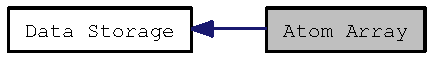
\includegraphics[width=122pt]{group__atomarray}
\end{center}
\end{figure}
\subsection*{Data Structures}
\begin{DoxyCompactItemize}
\item 
struct \hyperlink{structt__atomarray}{t\_\-atomarray}
\begin{DoxyCompactList}\small\item\em The atomarray object. \item\end{DoxyCompactList}\end{DoxyCompactItemize}
\subsection*{Defines}
\begin{DoxyCompactItemize}
\item 
\#define \hyperlink{group__atomarray_ga9d4f9396731ae8115a08f99d02421d02}{ATOMARRAY\_\-FLAG\_\-FREECHILDREN}~(1)
\begin{DoxyCompactList}\small\item\em The atomarray flags. \item\end{DoxyCompactList}\end{DoxyCompactItemize}
\subsection*{Functions}
\begin{DoxyCompactItemize}
\item 
\hyperlink{structt__atomarray}{t\_\-atomarray} $\ast$ \hyperlink{group__atomarray_ga2896b4949e03841f4c5a71ad7f7fadf7}{atomarray\_\-new} (long ac, \hyperlink{structt__atom}{t\_\-atom} $\ast$av)
\begin{DoxyCompactList}\small\item\em Create a new atomarray object. \item\end{DoxyCompactList}\item 
void \hyperlink{group__atomarray_gad99be67bb7fafb7987412ee8fc2802f0}{atomarray\_\-flags} (\hyperlink{structt__atomarray}{t\_\-atomarray} $\ast$x, long flags)
\begin{DoxyCompactList}\small\item\em Set the atomarray flags. \item\end{DoxyCompactList}\item 
long \hyperlink{group__atomarray_gae784ffaf3fce1cd4967046faf4c7a377}{atomarray\_\-getflags} (\hyperlink{structt__atomarray}{t\_\-atomarray} $\ast$x)
\begin{DoxyCompactList}\small\item\em Get the atomarray flags. \item\end{DoxyCompactList}\item 
\hyperlink{group__datatypes_ga73edaae82b318855cc09fac994918165}{t\_\-max\_\-err} \hyperlink{group__atomarray_ga52b68a97eb1bb7f97411715401d9d2ad}{atomarray\_\-setatoms} (\hyperlink{structt__atomarray}{t\_\-atomarray} $\ast$x, long ac, \hyperlink{structt__atom}{t\_\-atom} $\ast$av)
\begin{DoxyCompactList}\small\item\em Replace the existing array contents with a new set of atoms Note that atoms provided to this function will be {\itshape copied\/}. \item\end{DoxyCompactList}\item 
\hyperlink{group__datatypes_ga73edaae82b318855cc09fac994918165}{t\_\-max\_\-err} \hyperlink{group__atomarray_ga28824a30f15ddaec8b1a323f285fbe85}{atomarray\_\-getatoms} (\hyperlink{structt__atomarray}{t\_\-atomarray} $\ast$x, long $\ast$ac, \hyperlink{structt__atom}{t\_\-atom} $\ast$$\ast$av)
\begin{DoxyCompactList}\small\item\em Retrieve a pointer to the first atom in the internal array of atoms. \item\end{DoxyCompactList}\item 
\hyperlink{group__datatypes_ga73edaae82b318855cc09fac994918165}{t\_\-max\_\-err} \hyperlink{group__atomarray_gaec25ec428f6bb7b1a1c8092b5c01f2c2}{atomarray\_\-copyatoms} (\hyperlink{structt__atomarray}{t\_\-atomarray} $\ast$x, long $\ast$ac, \hyperlink{structt__atom}{t\_\-atom} $\ast$$\ast$av)
\begin{DoxyCompactList}\small\item\em Retrieve a copy of the atoms in the array. \item\end{DoxyCompactList}\item 
long \hyperlink{group__atomarray_gaef611e510133de82b09496f9ff59662f}{atomarray\_\-getsize} (\hyperlink{structt__atomarray}{t\_\-atomarray} $\ast$x)
\begin{DoxyCompactList}\small\item\em Return the number of atoms in the array. \item\end{DoxyCompactList}\item 
\hyperlink{group__datatypes_ga73edaae82b318855cc09fac994918165}{t\_\-max\_\-err} \hyperlink{group__atomarray_ga1ee643830e94d84c325fd8caa4db9d4b}{atomarray\_\-getindex} (\hyperlink{structt__atomarray}{t\_\-atomarray} $\ast$x, long index, \hyperlink{structt__atom}{t\_\-atom} $\ast$av)
\begin{DoxyCompactList}\small\item\em Copy an a specific atom from the array. \item\end{DoxyCompactList}\item 
void $\ast$ \hyperlink{group__atomarray_ga96ea96717c2ed692197361b1d02bab47}{atomarray\_\-duplicate} (\hyperlink{structt__atomarray}{t\_\-atomarray} $\ast$x)
\begin{DoxyCompactList}\small\item\em Create a new atomarray object which is a copy of another atomarray object. \item\end{DoxyCompactList}\item 
void \hyperlink{group__atomarray_gad2d3608a3089f42590d744814c6fee42}{atomarray\_\-appendatom} (\hyperlink{structt__atomarray}{t\_\-atomarray} $\ast$x, \hyperlink{structt__atom}{t\_\-atom} $\ast$a)
\begin{DoxyCompactList}\small\item\em Copy a new atom onto the end of the array. \item\end{DoxyCompactList}\item 
void \hyperlink{group__atomarray_gae604fed9f8ca266b1b0d080e8cc929c3}{atomarray\_\-appendatoms} (\hyperlink{structt__atomarray}{t\_\-atomarray} $\ast$x, long ac, \hyperlink{structt__atom}{t\_\-atom} $\ast$av)
\begin{DoxyCompactList}\small\item\em Copy multiple new atoms onto the end of the array. \item\end{DoxyCompactList}\item 
void \hyperlink{group__atomarray_gaf76d3ab0de8a7b6b0b0e32193608c2dd}{atomarray\_\-chuckindex} (\hyperlink{structt__atomarray}{t\_\-atomarray} $\ast$x, long index)
\begin{DoxyCompactList}\small\item\em Remove an atom from any location within the array. \item\end{DoxyCompactList}\item 
void \hyperlink{group__atomarray_ga185b275ee3d94fa9a21d3ca6ece43c33}{atomarray\_\-clear} (\hyperlink{structt__atomarray}{t\_\-atomarray} $\ast$x)
\begin{DoxyCompactList}\small\item\em Clear the array. \item\end{DoxyCompactList}\item 
void \hyperlink{group__atomarray_gacfb767a18f14fb13a0952c6ed7903de1}{atomarray\_\-funall} (\hyperlink{structt__atomarray}{t\_\-atomarray} $\ast$x, \hyperlink{group__datatypes_gac26ba0a173b50597f5738132e059b42d}{method} fun, void $\ast$arg)
\begin{DoxyCompactList}\small\item\em Call the specified function for every item in the atom array. \item\end{DoxyCompactList}\end{DoxyCompactItemize}


\subsection{Detailed Description}
Max's atomarray object is a container for an array of atoms with an interface for manipulating that array. It can be useful for passing lists as a single atom, such as for the return value of an \hyperlink{group__atom_gga8aa6700e9f00b132eb376db6e39ade47ad150bf3de9c8dc2ddfa0ca0ca2382360}{A\_\-GIMMEBACK} method. It also used frequently in when working with Max's \hyperlink{structt__dictionary}{t\_\-dictionary} object.

\begin{DoxySeeAlso}{See also}
\hyperlink{group__dictionary}{Dictionary} 
\end{DoxySeeAlso}


\subsection{Define Documentation}
\hypertarget{group__atomarray_ga9d4f9396731ae8115a08f99d02421d02}{
\index{atomarray@{atomarray}!ATOMARRAY\_\-FLAG\_\-FREECHILDREN@{ATOMARRAY\_\-FLAG\_\-FREECHILDREN}}
\index{ATOMARRAY\_\-FLAG\_\-FREECHILDREN@{ATOMARRAY\_\-FLAG\_\-FREECHILDREN}!atomarray@{atomarray}}
\subsubsection[{ATOMARRAY\_\-FLAG\_\-FREECHILDREN}]{\setlength{\rightskip}{0pt plus 5cm}\#define ATOMARRAY\_\-FLAG\_\-FREECHILDREN~(1)}}
\label{group__atomarray_ga9d4f9396731ae8115a08f99d02421d02}


The atomarray flags. Currently the only flag is ATOMARRAY\_\-FLAG\_\-FREECHILDREN. If set via \hyperlink{group__atomarray_gad99be67bb7fafb7987412ee8fc2802f0}{atomarray\_\-flags()} the atomarray will free any contained A\_\-OBJ atoms when the atomarray is freed. 

\subsection{Function Documentation}
\hypertarget{group__atomarray_gad2d3608a3089f42590d744814c6fee42}{
\index{atomarray@{atomarray}!atomarray\_\-appendatom@{atomarray\_\-appendatom}}
\index{atomarray\_\-appendatom@{atomarray\_\-appendatom}!atomarray@{atomarray}}
\subsubsection[{atomarray\_\-appendatom}]{\setlength{\rightskip}{0pt plus 5cm}void atomarray\_\-appendatom ({\bf t\_\-atomarray} $\ast$ {\em x}, \/  {\bf t\_\-atom} $\ast$ {\em a})}}
\label{group__atomarray_gad2d3608a3089f42590d744814c6fee42}


Copy a new atom onto the end of the array. 
\begin{DoxyParams}{Parameters}
\item[{\em x}]The atomarray instance. \item[{\em a}]A pointer to the new atom to append to the end of the array.\end{DoxyParams}
\begin{DoxySeeAlso}{See also}
\hyperlink{group__atomarray_gae604fed9f8ca266b1b0d080e8cc929c3}{atomarray\_\-appendatoms()} 

\hyperlink{group__atomarray_ga52b68a97eb1bb7f97411715401d9d2ad}{atomarray\_\-setatoms()} 
\end{DoxySeeAlso}
\hypertarget{group__atomarray_gae604fed9f8ca266b1b0d080e8cc929c3}{
\index{atomarray@{atomarray}!atomarray\_\-appendatoms@{atomarray\_\-appendatoms}}
\index{atomarray\_\-appendatoms@{atomarray\_\-appendatoms}!atomarray@{atomarray}}
\subsubsection[{atomarray\_\-appendatoms}]{\setlength{\rightskip}{0pt plus 5cm}void atomarray\_\-appendatoms ({\bf t\_\-atomarray} $\ast$ {\em x}, \/  long {\em ac}, \/  {\bf t\_\-atom} $\ast$ {\em av})}}
\label{group__atomarray_gae604fed9f8ca266b1b0d080e8cc929c3}


Copy multiple new atoms onto the end of the array. 
\begin{DoxyParams}{Parameters}
\item[{\em x}]The atomarray instance. \item[{\em ac}]The number of new atoms to be appended to the array. \item[{\em av}]A pointer to the first of the new atoms to append to the end of the array.\end{DoxyParams}
\begin{DoxySeeAlso}{See also}
\hyperlink{group__atomarray_gad2d3608a3089f42590d744814c6fee42}{atomarray\_\-appendatom()} 

\hyperlink{group__atomarray_ga52b68a97eb1bb7f97411715401d9d2ad}{atomarray\_\-setatoms()} 
\end{DoxySeeAlso}
\hypertarget{group__atomarray_gaf76d3ab0de8a7b6b0b0e32193608c2dd}{
\index{atomarray@{atomarray}!atomarray\_\-chuckindex@{atomarray\_\-chuckindex}}
\index{atomarray\_\-chuckindex@{atomarray\_\-chuckindex}!atomarray@{atomarray}}
\subsubsection[{atomarray\_\-chuckindex}]{\setlength{\rightskip}{0pt plus 5cm}void atomarray\_\-chuckindex ({\bf t\_\-atomarray} $\ast$ {\em x}, \/  long {\em index})}}
\label{group__atomarray_gaf76d3ab0de8a7b6b0b0e32193608c2dd}


Remove an atom from any location within the array. The array will be resized and collapsed to fill in the gap.


\begin{DoxyParams}{Parameters}
\item[{\em x}]The atomarray instance. \item[{\em index}]The zero-\/based index of the atom to remove from the array. \end{DoxyParams}
\hypertarget{group__atomarray_ga185b275ee3d94fa9a21d3ca6ece43c33}{
\index{atomarray@{atomarray}!atomarray\_\-clear@{atomarray\_\-clear}}
\index{atomarray\_\-clear@{atomarray\_\-clear}!atomarray@{atomarray}}
\subsubsection[{atomarray\_\-clear}]{\setlength{\rightskip}{0pt plus 5cm}void atomarray\_\-clear ({\bf t\_\-atomarray} $\ast$ {\em x})}}
\label{group__atomarray_ga185b275ee3d94fa9a21d3ca6ece43c33}


Clear the array. Frees all of the atoms and sets the size to zero. This function does not perform a 'deep' free, meaning that any \hyperlink{group__atom_gga8aa6700e9f00b132eb376db6e39ade47a82cc76e0d53c8fc28df167c35d5bbd1a}{A\_\-OBJ} atoms will not have their object's freed. Only the references to those objects contained in the atomarray will be freed.


\begin{DoxyParams}{Parameters}
\item[{\em x}]The atomarray instance. \end{DoxyParams}
\begin{DoxyReturn}{Returns}
The number of atoms in the array. 
\end{DoxyReturn}
\hypertarget{group__atomarray_gaec25ec428f6bb7b1a1c8092b5c01f2c2}{
\index{atomarray@{atomarray}!atomarray\_\-copyatoms@{atomarray\_\-copyatoms}}
\index{atomarray\_\-copyatoms@{atomarray\_\-copyatoms}!atomarray@{atomarray}}
\subsubsection[{atomarray\_\-copyatoms}]{\setlength{\rightskip}{0pt plus 5cm}{\bf t\_\-max\_\-err} atomarray\_\-copyatoms ({\bf t\_\-atomarray} $\ast$ {\em x}, \/  long $\ast$ {\em ac}, \/  {\bf t\_\-atom} $\ast$$\ast$ {\em av})}}
\label{group__atomarray_gaec25ec428f6bb7b1a1c8092b5c01f2c2}


Retrieve a copy of the atoms in the array. This method does not copy the atoms, btu simply provides access to them. To retrieve a copy of the atoms use \hyperlink{group__atomarray_gaec25ec428f6bb7b1a1c8092b5c01f2c2}{atomarray\_\-copyatoms()}.


\begin{DoxyParams}{Parameters}
\item[{\em x}]The atomarray instance. \item[{\em ac}]The address of a long where the number of atoms will be set. \item[{\em av}]The address of a \hyperlink{structt__atom}{t\_\-atom} pointer where the atoms will be allocated and copied. \end{DoxyParams}
\begin{DoxyReturn}{Returns}
A Max error code.
\end{DoxyReturn}
\begin{DoxyRemark}{Remarks}
You are responsible for freeing memory allocated for the copy of the atoms returned. 
\begin{DoxyCode}
    long    ac = 0;
    t_atom *av = NULL;
    
    atomarray_copyatoms(anAtomarray, &ac, &av);
    if(ac && av){
        // do something with ac and av here...
        sysmem_freeptr(av);
    }   
\end{DoxyCode}

\end{DoxyRemark}
\begin{DoxySeeAlso}{See also}
\hyperlink{group__atomarray_ga28824a30f15ddaec8b1a323f285fbe85}{atomarray\_\-getatoms()} 
\end{DoxySeeAlso}
\hypertarget{group__atomarray_ga96ea96717c2ed692197361b1d02bab47}{
\index{atomarray@{atomarray}!atomarray\_\-duplicate@{atomarray\_\-duplicate}}
\index{atomarray\_\-duplicate@{atomarray\_\-duplicate}!atomarray@{atomarray}}
\subsubsection[{atomarray\_\-duplicate}]{\setlength{\rightskip}{0pt plus 5cm}void$\ast$ atomarray\_\-duplicate ({\bf t\_\-atomarray} $\ast$ {\em x})}}
\label{group__atomarray_ga96ea96717c2ed692197361b1d02bab47}


Create a new atomarray object which is a copy of another atomarray object. 
\begin{DoxyParams}{Parameters}
\item[{\em x}]The atomarray instance which is to be copied. \end{DoxyParams}
\begin{DoxyReturn}{Returns}
A new atomarray which is copied from x.
\end{DoxyReturn}
\begin{DoxySeeAlso}{See also}
\hyperlink{group__atomarray_ga2896b4949e03841f4c5a71ad7f7fadf7}{atomarray\_\-new()} 
\end{DoxySeeAlso}
\hypertarget{group__atomarray_gad99be67bb7fafb7987412ee8fc2802f0}{
\index{atomarray@{atomarray}!atomarray\_\-flags@{atomarray\_\-flags}}
\index{atomarray\_\-flags@{atomarray\_\-flags}!atomarray@{atomarray}}
\subsubsection[{atomarray\_\-flags}]{\setlength{\rightskip}{0pt plus 5cm}void atomarray\_\-flags ({\bf t\_\-atomarray} $\ast$ {\em x}, \/  long {\em flags})}}
\label{group__atomarray_gad99be67bb7fafb7987412ee8fc2802f0}


Set the atomarray flags. 
\begin{DoxyParams}{Parameters}
\item[{\em x}]The atomarray instance. \item[{\em flags}]The new value for the flags. \end{DoxyParams}
\hypertarget{group__atomarray_gacfb767a18f14fb13a0952c6ed7903de1}{
\index{atomarray@{atomarray}!atomarray\_\-funall@{atomarray\_\-funall}}
\index{atomarray\_\-funall@{atomarray\_\-funall}!atomarray@{atomarray}}
\subsubsection[{atomarray\_\-funall}]{\setlength{\rightskip}{0pt plus 5cm}void atomarray\_\-funall ({\bf t\_\-atomarray} $\ast$ {\em x}, \/  {\bf method} {\em fun}, \/  void $\ast$ {\em arg})}}
\label{group__atomarray_gacfb767a18f14fb13a0952c6ed7903de1}


Call the specified function for every item in the atom array. 
\begin{DoxyParams}{Parameters}
\item[{\em x}]The atomarray instance. \item[{\em fun}]The function to call, specified as function pointer cast to a Max \hyperlink{group__datatypes_gac26ba0a173b50597f5738132e059b42d}{method}. \item[{\em arg}]An argument that you would like to pass to the function being called. \end{DoxyParams}
\begin{DoxyReturn}{Returns}
A max error code.
\end{DoxyReturn}
\begin{DoxyRemark}{Remarks}
The \hyperlink{group__atomarray_gacfb767a18f14fb13a0952c6ed7903de1}{atomarray\_\-funall()} method will call your function for every item in the list. It will pass both a pointer to the item in the list, and any argument that you provide. The following example shows a function that could be called by \hyperlink{group__hashtab_ga37e7b5c20c9fc69e9435f788f35335dc}{hashtab\_\-funall()}. 
\begin{DoxyCode}
    void myFun(t_atom *a, void *myArg)
    {
        // do something with a and myArg here
        // a is the atom in the atom array
    }
\end{DoxyCode}

\end{DoxyRemark}
\begin{DoxySeeAlso}{See also}
\hyperlink{group__linklist_ga6f4496ef6dc1d6d121acf25d7cd5f946}{linklist\_\-funall()} 

\hyperlink{group__hashtab_ga37e7b5c20c9fc69e9435f788f35335dc}{hashtab\_\-funall()} 
\end{DoxySeeAlso}
\hypertarget{group__atomarray_ga28824a30f15ddaec8b1a323f285fbe85}{
\index{atomarray@{atomarray}!atomarray\_\-getatoms@{atomarray\_\-getatoms}}
\index{atomarray\_\-getatoms@{atomarray\_\-getatoms}!atomarray@{atomarray}}
\subsubsection[{atomarray\_\-getatoms}]{\setlength{\rightskip}{0pt plus 5cm}{\bf t\_\-max\_\-err} atomarray\_\-getatoms ({\bf t\_\-atomarray} $\ast$ {\em x}, \/  long $\ast$ {\em ac}, \/  {\bf t\_\-atom} $\ast$$\ast$ {\em av})}}
\label{group__atomarray_ga28824a30f15ddaec8b1a323f285fbe85}


Retrieve a pointer to the first atom in the internal array of atoms. This method does not copy the atoms, btu simply provides access to them. To retrieve a copy of the atoms use \hyperlink{group__atomarray_gaec25ec428f6bb7b1a1c8092b5c01f2c2}{atomarray\_\-copyatoms()}.


\begin{DoxyParams}{Parameters}
\item[{\em x}]The atomarray instance. \item[{\em ac}]The address of a long where the number of atoms will be set. \item[{\em av}]The address of a \hyperlink{structt__atom}{t\_\-atom} pointer where the address of the first atom of the array will be set. \end{DoxyParams}
\begin{DoxyReturn}{Returns}
A Max error code.
\end{DoxyReturn}
\begin{DoxySeeAlso}{See also}
\hyperlink{group__atomarray_gaec25ec428f6bb7b1a1c8092b5c01f2c2}{atomarray\_\-copyatoms()} 
\end{DoxySeeAlso}
\hypertarget{group__atomarray_gae784ffaf3fce1cd4967046faf4c7a377}{
\index{atomarray@{atomarray}!atomarray\_\-getflags@{atomarray\_\-getflags}}
\index{atomarray\_\-getflags@{atomarray\_\-getflags}!atomarray@{atomarray}}
\subsubsection[{atomarray\_\-getflags}]{\setlength{\rightskip}{0pt plus 5cm}long atomarray\_\-getflags ({\bf t\_\-atomarray} $\ast$ {\em x})}}
\label{group__atomarray_gae784ffaf3fce1cd4967046faf4c7a377}


Get the atomarray flags. 
\begin{DoxyParams}{Parameters}
\item[{\em x}]The atomarray instance. \end{DoxyParams}
\begin{DoxyReturn}{Returns}
The current value of the atomarray flags. 
\end{DoxyReturn}
\hypertarget{group__atomarray_ga1ee643830e94d84c325fd8caa4db9d4b}{
\index{atomarray@{atomarray}!atomarray\_\-getindex@{atomarray\_\-getindex}}
\index{atomarray\_\-getindex@{atomarray\_\-getindex}!atomarray@{atomarray}}
\subsubsection[{atomarray\_\-getindex}]{\setlength{\rightskip}{0pt plus 5cm}{\bf t\_\-max\_\-err} atomarray\_\-getindex ({\bf t\_\-atomarray} $\ast$ {\em x}, \/  long {\em index}, \/  {\bf t\_\-atom} $\ast$ {\em av})}}
\label{group__atomarray_ga1ee643830e94d84c325fd8caa4db9d4b}


Copy an a specific atom from the array. 
\begin{DoxyParams}{Parameters}
\item[{\em x}]The atomarray instance. \item[{\em index}]The zero-\/based index into the array from which to retrieve an atom pointer. \item[{\em av}]The address of an atom to contain the copy. \end{DoxyParams}
\begin{DoxyReturn}{Returns}
A Max error code.
\end{DoxyReturn}
\begin{DoxyRemark}{Remarks}
Example: 
\begin{DoxyCode}
    {
        t_atom a;

        // fetch a copy of the second atom in a previously existing array
        atomarray_getindex(anAtomarray, 1, &a);
        // do something with the atom here...
    }
\end{DoxyCode}
 
\end{DoxyRemark}
\hypertarget{group__atomarray_gaef611e510133de82b09496f9ff59662f}{
\index{atomarray@{atomarray}!atomarray\_\-getsize@{atomarray\_\-getsize}}
\index{atomarray\_\-getsize@{atomarray\_\-getsize}!atomarray@{atomarray}}
\subsubsection[{atomarray\_\-getsize}]{\setlength{\rightskip}{0pt plus 5cm}long atomarray\_\-getsize ({\bf t\_\-atomarray} $\ast$ {\em x})}}
\label{group__atomarray_gaef611e510133de82b09496f9ff59662f}


Return the number of atoms in the array. 
\begin{DoxyParams}{Parameters}
\item[{\em x}]The atomarray instance. \end{DoxyParams}
\begin{DoxyReturn}{Returns}
The number of atoms in the array. 
\end{DoxyReturn}
\hypertarget{group__atomarray_ga2896b4949e03841f4c5a71ad7f7fadf7}{
\index{atomarray@{atomarray}!atomarray\_\-new@{atomarray\_\-new}}
\index{atomarray\_\-new@{atomarray\_\-new}!atomarray@{atomarray}}
\subsubsection[{atomarray\_\-new}]{\setlength{\rightskip}{0pt plus 5cm}{\bf t\_\-atomarray}$\ast$ atomarray\_\-new (long {\em ac}, \/  {\bf t\_\-atom} $\ast$ {\em av})}}
\label{group__atomarray_ga2896b4949e03841f4c5a71ad7f7fadf7}


Create a new atomarray object. Note that atoms provided to this function will be {\itshape copied\/}. The copies stored internally to the atomarray instance. You can free the atomarray by calling \hyperlink{group__obj_ga3759846cb356195532c41e35b87522ee}{object\_\-free()}.


\begin{DoxyParams}{Parameters}
\item[{\em ac}]The number of atoms to be initially contained in the atomarray. \item[{\em av}]A pointer to the first of an array of atoms to initially copy into the atomarray. \end{DoxyParams}
\begin{DoxyReturn}{Returns}
Pointer to the new atomarray object.
\end{DoxyReturn}
\begin{DoxyRemark}{Remarks}
Note that due to the unusual prototype of this method that you cannot instantiate this object using the \hyperlink{group__obj_ga459c71aca6316e345379eeb424ad56ff}{object\_\-new\_\-typed()} function. If you wish to use the dynamically bound creator to instantiate the object, you should instead should use \hyperlink{group__obj_gac4b370265c776db4f545d257089af1cf}{object\_\-new()} as demonstrated below. The primary reason that you might choose to instantiate an atomarray using \hyperlink{group__obj_gac4b370265c776db4f545d257089af1cf}{object\_\-new()} instead of \hyperlink{group__atomarray_ga2896b4949e03841f4c5a71ad7f7fadf7}{atomarray\_\-new()} is for using the atomarray object in code that is also intended to run in Max 4. 
\begin{DoxyCode}
    object_new(CLASS_NOBOX, gensym("atomarray"), argc, argv);
\end{DoxyCode}

\end{DoxyRemark}
\begin{DoxySeeAlso}{See also}
\hyperlink{group__atomarray_ga96ea96717c2ed692197361b1d02bab47}{atomarray\_\-duplicate()} 
\end{DoxySeeAlso}
\hypertarget{group__atomarray_ga52b68a97eb1bb7f97411715401d9d2ad}{
\index{atomarray@{atomarray}!atomarray\_\-setatoms@{atomarray\_\-setatoms}}
\index{atomarray\_\-setatoms@{atomarray\_\-setatoms}!atomarray@{atomarray}}
\subsubsection[{atomarray\_\-setatoms}]{\setlength{\rightskip}{0pt plus 5cm}{\bf t\_\-max\_\-err} atomarray\_\-setatoms ({\bf t\_\-atomarray} $\ast$ {\em x}, \/  long {\em ac}, \/  {\bf t\_\-atom} $\ast$ {\em av})}}
\label{group__atomarray_ga52b68a97eb1bb7f97411715401d9d2ad}


Replace the existing array contents with a new set of atoms Note that atoms provided to this function will be {\itshape copied\/}. The copies stored internally to the atomarray instance.


\begin{DoxyParams}{Parameters}
\item[{\em x}]The atomarray instance. \item[{\em ac}]The number of atoms to be initially contained in the atomarray. \item[{\em av}]A pointer to the first of an array of atoms to initially copy into the atomarray. \end{DoxyParams}
\begin{DoxyReturn}{Returns}
A Max error code. 
\end{DoxyReturn}

\hypertarget{group__database}{
\section{Database}
\label{group__database}\index{Database@{Database}}
}


Max's database support currently consists of a SQLite ( \href{http://sqlite.org}{\tt http://sqlite.org} ) extension which is loaded dynamically by Max at launch time.  


Collaboration diagram for Database:\nopagebreak
\begin{figure}[H]
\begin{center}
\leavevmode
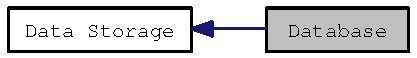
\includegraphics[width=118pt]{group__database}
\end{center}
\end{figure}
\subsection*{Typedefs}
\begin{DoxyCompactItemize}
\item 
typedef \hyperlink{structt__object}{t\_\-object} \hyperlink{group__database_gad832ea0e5fc292661fd20046cee7e3b3}{t\_\-database}
\begin{DoxyCompactList}\small\item\em A database object. \item\end{DoxyCompactList}\item 
typedef \hyperlink{structt__object}{t\_\-object} \hyperlink{group__database_gae34db00cb98960e94b5ca58a7c21c362}{t\_\-db\_\-result}
\begin{DoxyCompactList}\small\item\em A database result object. \item\end{DoxyCompactList}\item 
typedef \hyperlink{structt__object}{t\_\-object} \hyperlink{group__database_gac9ea40a519578e26498dd61ea98b5cf2}{t\_\-db\_\-view}
\begin{DoxyCompactList}\small\item\em A database view object. \item\end{DoxyCompactList}\end{DoxyCompactItemize}
\subsection*{Functions}
\begin{DoxyCompactItemize}
\item 
BEGIN\_\-USING\_\-C\_\-LINKAGE \hyperlink{group__datatypes_ga73edaae82b318855cc09fac994918165}{t\_\-max\_\-err} \hyperlink{group__database_gac709a497fcc55817c1c9292bd59eb03f}{db\_\-open} (\hyperlink{structt__symbol}{t\_\-symbol} $\ast$dbname, const char $\ast$fullpath, \hyperlink{structt__object}{t\_\-database} $\ast$$\ast$db)
\begin{DoxyCompactList}\small\item\em Create an instance of a database. \item\end{DoxyCompactList}\item 
\hyperlink{group__datatypes_ga73edaae82b318855cc09fac994918165}{t\_\-max\_\-err} \hyperlink{group__database_ga697cbcbe4c14944fc5a4a535039f5e1b}{db\_\-close} (\hyperlink{structt__object}{t\_\-database} $\ast$$\ast$db)
\begin{DoxyCompactList}\small\item\em Close an open database. \item\end{DoxyCompactList}\item 
\hyperlink{group__datatypes_ga73edaae82b318855cc09fac994918165}{t\_\-max\_\-err} \hyperlink{group__database_ga70fac948e0a17e91d80c064765d5d016}{db\_\-query} (\hyperlink{structt__object}{t\_\-database} $\ast$db, \hyperlink{structt__object}{t\_\-db\_\-result} $\ast$$\ast$dbresult, const char $\ast$sql,...)
\begin{DoxyCompactList}\small\item\em Execute a SQL query on the database. \item\end{DoxyCompactList}\item 
\hyperlink{group__datatypes_ga73edaae82b318855cc09fac994918165}{t\_\-max\_\-err} \hyperlink{group__database_gae756dda46aa61036ccc896ad9448c496}{db\_\-query\_\-silent} (\hyperlink{structt__object}{t\_\-database} $\ast$db, \hyperlink{structt__object}{t\_\-db\_\-result} $\ast$$\ast$dbresult, const char $\ast$sql,...)
\begin{DoxyCompactList}\small\item\em Execute a SQL query on the database, temporarily overriding the database's error logging attribute. \item\end{DoxyCompactList}\item 
\hyperlink{group__datatypes_ga73edaae82b318855cc09fac994918165}{t\_\-max\_\-err} \hyperlink{group__database_ga534b71af369d49827855be8f07cc09bc}{db\_\-query\_\-getlastinsertid} (\hyperlink{structt__object}{t\_\-database} $\ast$db, long $\ast$id)
\begin{DoxyCompactList}\small\item\em Determine the id (key) number for the most recent INSERT query executed on the database. \item\end{DoxyCompactList}\item 
\hyperlink{group__datatypes_ga73edaae82b318855cc09fac994918165}{t\_\-max\_\-err} \hyperlink{group__database_ga79e6ee7b7d344b372314d08b1b19fa8d}{db\_\-query\_\-table\_\-new} (\hyperlink{structt__object}{t\_\-database} $\ast$db, const char $\ast$tablename)
\begin{DoxyCompactList}\small\item\em Create a new table in a database. \item\end{DoxyCompactList}\item 
\hyperlink{group__datatypes_ga73edaae82b318855cc09fac994918165}{t\_\-max\_\-err} \hyperlink{group__database_gaafcaffcf5fea4ded0d474e1332b8a922}{db\_\-query\_\-table\_\-addcolumn} (\hyperlink{structt__object}{t\_\-database} $\ast$db, const char $\ast$tablename, const char $\ast$columnname, const char $\ast$columntype, const char $\ast$flags)
\begin{DoxyCompactList}\small\item\em Add a new column to an existing table in a database. \item\end{DoxyCompactList}\item 
\hyperlink{group__datatypes_ga73edaae82b318855cc09fac994918165}{t\_\-max\_\-err} \hyperlink{group__database_gad14964ae056aa663646f3fc3081b3b3a}{db\_\-transaction\_\-start} (\hyperlink{structt__object}{t\_\-database} $\ast$db)
\begin{DoxyCompactList}\small\item\em Begin a database transaction. \item\end{DoxyCompactList}\item 
\hyperlink{group__datatypes_ga73edaae82b318855cc09fac994918165}{t\_\-max\_\-err} \hyperlink{group__database_ga03a64b223d17437a2a7eb976025b5874}{db\_\-transaction\_\-end} (\hyperlink{structt__object}{t\_\-database} $\ast$db)
\begin{DoxyCompactList}\small\item\em Finalize a database transaction. \item\end{DoxyCompactList}\item 
\hyperlink{group__datatypes_ga73edaae82b318855cc09fac994918165}{t\_\-max\_\-err} \hyperlink{group__database_gabf78d551bd8ed0c81a4881663dc445be}{db\_\-transaction\_\-flush} (\hyperlink{structt__object}{t\_\-database} $\ast$db)
\begin{DoxyCompactList}\small\item\em Force any open transactions to close. \item\end{DoxyCompactList}\item 
\hyperlink{group__datatypes_ga73edaae82b318855cc09fac994918165}{t\_\-max\_\-err} \hyperlink{group__database_ga70b24ae188489537db137f67f5d01388}{db\_\-view\_\-create} (\hyperlink{structt__object}{t\_\-database} $\ast$db, const char $\ast$sql, \hyperlink{structt__object}{t\_\-db\_\-view} $\ast$$\ast$dbview)
\begin{DoxyCompactList}\small\item\em A database view is a way of looking at a particular set of records in the database. \item\end{DoxyCompactList}\item 
\hyperlink{group__datatypes_ga73edaae82b318855cc09fac994918165}{t\_\-max\_\-err} \hyperlink{group__database_ga0e0c3cfbb3459545a4868630cf6e8807}{db\_\-view\_\-remove} (\hyperlink{structt__object}{t\_\-database} $\ast$db, \hyperlink{structt__object}{t\_\-db\_\-view} $\ast$$\ast$dbview)
\begin{DoxyCompactList}\small\item\em Remove a database view created using \hyperlink{group__database_ga70b24ae188489537db137f67f5d01388}{db\_\-view\_\-create()}. \item\end{DoxyCompactList}\item 
\hyperlink{group__datatypes_ga73edaae82b318855cc09fac994918165}{t\_\-max\_\-err} \hyperlink{group__database_ga40de375c540b3551ba42d7a2643aa89f}{db\_\-view\_\-getresult} (\hyperlink{structt__object}{t\_\-db\_\-view} $\ast$dbview, \hyperlink{structt__object}{t\_\-db\_\-result} $\ast$$\ast$result)
\begin{DoxyCompactList}\small\item\em Fetch the pointer for a \hyperlink{group__database_gac9ea40a519578e26498dd61ea98b5cf2}{t\_\-db\_\-view}'s query result. \item\end{DoxyCompactList}\item 
\hyperlink{group__datatypes_ga73edaae82b318855cc09fac994918165}{t\_\-max\_\-err} \hyperlink{group__database_ga0474ea3231e953760e5a32a277c0279d}{db\_\-view\_\-setquery} (\hyperlink{structt__object}{t\_\-db\_\-view} $\ast$dbview, char $\ast$newquery)
\begin{DoxyCompactList}\small\item\em Set the query used by the view. \item\end{DoxyCompactList}\item 
char $\ast$$\ast$ \hyperlink{group__database_ga66fb4403eeb6e44ddd3038c9df863ef8}{db\_\-result\_\-nextrecord} (\hyperlink{structt__object}{t\_\-db\_\-result} $\ast$result)
\begin{DoxyCompactList}\small\item\em Return the next record from a set of results that you are walking. \item\end{DoxyCompactList}\item 
void \hyperlink{group__database_gad0d384ab3ba04958d982cede2cffa043}{db\_\-result\_\-reset} (\hyperlink{structt__object}{t\_\-db\_\-result} $\ast$result)
\begin{DoxyCompactList}\small\item\em Reset the interface for walking a result's record list to the first record. \item\end{DoxyCompactList}\item 
void \hyperlink{group__database_ga8c7c9667ce229b8447a9a8f32b03453a}{db\_\-result\_\-clear} (\hyperlink{structt__object}{t\_\-db\_\-result} $\ast$result)
\begin{DoxyCompactList}\small\item\em Zero-\/out a database result. \item\end{DoxyCompactList}\item 
long \hyperlink{group__database_gad5e17d5d9a14aa7a156ca508cf12eb3d}{db\_\-result\_\-numrecords} (\hyperlink{structt__object}{t\_\-db\_\-result} $\ast$result)
\begin{DoxyCompactList}\small\item\em Return a count of all records in the query result. \item\end{DoxyCompactList}\item 
long \hyperlink{group__database_ga5bf778c6ba6cc859c41d18a2d887bd7b}{db\_\-result\_\-numfields} (\hyperlink{structt__object}{t\_\-db\_\-result} $\ast$result)
\begin{DoxyCompactList}\small\item\em Return a count of all fields (columns) in the query result. \item\end{DoxyCompactList}\item 
char $\ast$ \hyperlink{group__database_ga7a9cc6a72ef3730979d0d909421076b3}{db\_\-result\_\-fieldname} (\hyperlink{structt__object}{t\_\-db\_\-result} $\ast$result, long fieldindex)
\begin{DoxyCompactList}\small\item\em Return the name of a field specified by its index number. \item\end{DoxyCompactList}\item 
char $\ast$ \hyperlink{group__database_ga57619b568083f0cf5989455af0ad3d5b}{db\_\-result\_\-string} (\hyperlink{structt__object}{t\_\-db\_\-result} $\ast$result, long recordindex, long fieldindex)
\begin{DoxyCompactList}\small\item\em Return a single value from a result according to its index and field coordinates. \item\end{DoxyCompactList}\item 
long \hyperlink{group__database_gadd498a9d44bc669bd544c781c1401e81}{db\_\-result\_\-long} (\hyperlink{structt__object}{t\_\-db\_\-result} $\ast$result, long recordindex, long fieldindex)
\begin{DoxyCompactList}\small\item\em Return a single value from a result according to its index and field coordinates. \item\end{DoxyCompactList}\item 
float \hyperlink{group__database_ga0558fcd917d24cc590ec0f426bf6bd7a}{db\_\-result\_\-float} (\hyperlink{structt__object}{t\_\-db\_\-result} $\ast$result, long recordindex, long fieldindex)
\begin{DoxyCompactList}\small\item\em Return a single value from a result according to its index and field coordinates. \item\end{DoxyCompactList}\item 
unsigned long \hyperlink{group__database_ga16ce6b68722eb623d9207b630e55b09a}{db\_\-result\_\-datetimeinseconds} (\hyperlink{structt__object}{t\_\-db\_\-result} $\ast$result, long recordindex, long fieldindex)
\begin{DoxyCompactList}\small\item\em Return a single value from a result according to its index and field coordinates. \item\end{DoxyCompactList}\item 
void \hyperlink{group__database_ga051ca3fefd1d2e4fe162a943c3d15060}{db\_\-util\_\-stringtodate} (const char $\ast$string, unsigned long $\ast$date)
\begin{DoxyCompactList}\small\item\em A utility to convert from a sql datetime string into seconds. \item\end{DoxyCompactList}\item 
void \hyperlink{group__database_gabf7cfbf2e7218680a8b79d250c1eae19}{db\_\-util\_\-datetostring} (const unsigned long date, char $\ast$string)
\begin{DoxyCompactList}\small\item\em A utility to convert from seconds into a sql-\/ready datetime string. \item\end{DoxyCompactList}\end{DoxyCompactItemize}


\subsection{Detailed Description}
Max's database support currently consists of a SQLite ( \href{http://sqlite.org}{\tt http://sqlite.org} ) extension which is loaded dynamically by Max at launch time. Because it is loaded dynamically, all interfacing with the sqlite object relies on Max's message passing interface, using \hyperlink{group__obj_gae740749094827ac5adc2b7145db1c596}{object\_\-method()} and related functions.

For most common database needs, a C-\/interface is defined in the ext\_\-database.h header file and implemented in the ext\_\-database.c source file. The functions defined in this interface wrap the message passing calls and provide a convenient means by which you can work with databases. ext\_\-database.c is located in the 'common' folder inside of the 'max-\/includes' folder. If you use any of the functions defined ext\_\-database.h, you will need to add ext\_\-database.c to your project. 

\subsection{Typedef Documentation}
\hypertarget{group__database_gad832ea0e5fc292661fd20046cee7e3b3}{
\index{database@{database}!t\_\-database@{t\_\-database}}
\index{t\_\-database@{t\_\-database}!database@{database}}
\subsubsection[{t\_\-database}]{\setlength{\rightskip}{0pt plus 5cm}typedef {\bf t\_\-object} {\bf t\_\-database}}}
\label{group__database_gad832ea0e5fc292661fd20046cee7e3b3}


A database object. Use \hyperlink{group__database_gac709a497fcc55817c1c9292bd59eb03f}{db\_\-open()} and \hyperlink{group__database_ga697cbcbe4c14944fc5a4a535039f5e1b}{db\_\-close()} to create and free database objects. \hypertarget{group__database_gae34db00cb98960e94b5ca58a7c21c362}{
\index{database@{database}!t\_\-db\_\-result@{t\_\-db\_\-result}}
\index{t\_\-db\_\-result@{t\_\-db\_\-result}!database@{database}}
\subsubsection[{t\_\-db\_\-result}]{\setlength{\rightskip}{0pt plus 5cm}typedef {\bf t\_\-object} {\bf t\_\-db\_\-result}}}
\label{group__database_gae34db00cb98960e94b5ca58a7c21c362}


A database result object. This is what the database object returns when a query is executed. \hypertarget{group__database_gac9ea40a519578e26498dd61ea98b5cf2}{
\index{database@{database}!t\_\-db\_\-view@{t\_\-db\_\-view}}
\index{t\_\-db\_\-view@{t\_\-db\_\-view}!database@{database}}
\subsubsection[{t\_\-db\_\-view}]{\setlength{\rightskip}{0pt plus 5cm}typedef {\bf t\_\-object} {\bf t\_\-db\_\-view}}}
\label{group__database_gac9ea40a519578e26498dd61ea98b5cf2}


A database view object. A database view wraps a query and a result for a given database, and is always updated and in-\/sync with the database. 

\subsection{Function Documentation}
\hypertarget{group__database_ga697cbcbe4c14944fc5a4a535039f5e1b}{
\index{database@{database}!db\_\-close@{db\_\-close}}
\index{db\_\-close@{db\_\-close}!database@{database}}
\subsubsection[{db\_\-close}]{\setlength{\rightskip}{0pt plus 5cm}{\bf t\_\-max\_\-err} db\_\-close ({\bf t\_\-database} $\ast$$\ast$ {\em db})}}
\label{group__database_ga697cbcbe4c14944fc5a4a535039f5e1b}


Close an open database. 
\begin{DoxyParams}{Parameters}
\item[{\em db}]The address of the \hyperlink{group__database_gad832ea0e5fc292661fd20046cee7e3b3}{t\_\-database} pointer for your database instance. The pointer will be freed and set NULL upon return. \end{DoxyParams}
\begin{DoxyReturn}{Returns}
An error code. 
\end{DoxyReturn}
\hypertarget{group__database_gac709a497fcc55817c1c9292bd59eb03f}{
\index{database@{database}!db\_\-open@{db\_\-open}}
\index{db\_\-open@{db\_\-open}!database@{database}}
\subsubsection[{db\_\-open}]{\setlength{\rightskip}{0pt plus 5cm}BEGIN\_\-USING\_\-C\_\-LINKAGE {\bf t\_\-max\_\-err} db\_\-open ({\bf t\_\-symbol} $\ast$ {\em dbname}, \/  const char $\ast$ {\em fullpath}, \/  {\bf t\_\-database} $\ast$$\ast$ {\em db})}}
\label{group__database_gac709a497fcc55817c1c9292bd59eb03f}


Create an instance of a database. 
\begin{DoxyParams}{Parameters}
\item[{\em dbname}]The name of the database. \item[{\em fullpath}]If a database with this dbname is not already open, this will specify a full path to the location where the database is stored on disk. If NULL is passed for this argument, the database will reside in memory only. The path should be formatted as a Max style path. \item[{\em db}]The address of a \hyperlink{group__database_gad832ea0e5fc292661fd20046cee7e3b3}{t\_\-database} pointer that will be set to point to the new database instance. If the pointer is not NULL, then it will be treated as a pre-\/existing database instance and thus will be freed. \end{DoxyParams}
\begin{DoxyReturn}{Returns}
An error code. 
\end{DoxyReturn}
\hypertarget{group__database_ga70fac948e0a17e91d80c064765d5d016}{
\index{database@{database}!db\_\-query@{db\_\-query}}
\index{db\_\-query@{db\_\-query}!database@{database}}
\subsubsection[{db\_\-query}]{\setlength{\rightskip}{0pt plus 5cm}{\bf t\_\-max\_\-err} db\_\-query ({\bf t\_\-database} $\ast$ {\em db}, \/  {\bf t\_\-db\_\-result} $\ast$$\ast$ {\em dbresult}, \/  const char $\ast$ {\em sql}, \/   {\em ...})}}
\label{group__database_ga70fac948e0a17e91d80c064765d5d016}


Execute a SQL query on the database. 
\begin{DoxyParams}{Parameters}
\item[{\em db}]The \hyperlink{group__database_gad832ea0e5fc292661fd20046cee7e3b3}{t\_\-database} pointer for your database instance. \item[{\em dbresult}]The address of a \hyperlink{group__database_gae34db00cb98960e94b5ca58a7c21c362}{t\_\-db\_\-result} pointer. If the pointer is passed-\/in set to NULL then a new dbresult will be created. If the pointer is not NULL then it is assumed to be a valid dbresult, which will be filled in with the query results. When you are done with the dbresult you should free it with \hyperlink{group__obj_ga3759846cb356195532c41e35b87522ee}{object\_\-free()}. \item[{\em sql}]A C-\/string containing a valid SQL query, possibly with sprintf() formatting codes. \item[{\em ...}]If an sprintf() formatting codes are used in the sql string, these values will be interpolated into the sql string. \end{DoxyParams}
\begin{DoxyReturn}{Returns}
An error code. 
\end{DoxyReturn}
\hypertarget{group__database_ga534b71af369d49827855be8f07cc09bc}{
\index{database@{database}!db\_\-query\_\-getlastinsertid@{db\_\-query\_\-getlastinsertid}}
\index{db\_\-query\_\-getlastinsertid@{db\_\-query\_\-getlastinsertid}!database@{database}}
\subsubsection[{db\_\-query\_\-getlastinsertid}]{\setlength{\rightskip}{0pt plus 5cm}{\bf t\_\-max\_\-err} db\_\-query\_\-getlastinsertid ({\bf t\_\-database} $\ast$ {\em db}, \/  long $\ast$ {\em id})}}
\label{group__database_ga534b71af369d49827855be8f07cc09bc}


Determine the id (key) number for the most recent INSERT query executed on the database. 
\begin{DoxyParams}{Parameters}
\item[{\em db}]The \hyperlink{group__database_gad832ea0e5fc292661fd20046cee7e3b3}{t\_\-database} pointer for your database instance. \item[{\em id}]The address of a variable to hold the result on return. \end{DoxyParams}
\begin{DoxyReturn}{Returns}
An error code. 
\end{DoxyReturn}
\hypertarget{group__database_gae756dda46aa61036ccc896ad9448c496}{
\index{database@{database}!db\_\-query\_\-silent@{db\_\-query\_\-silent}}
\index{db\_\-query\_\-silent@{db\_\-query\_\-silent}!database@{database}}
\subsubsection[{db\_\-query\_\-silent}]{\setlength{\rightskip}{0pt plus 5cm}{\bf t\_\-max\_\-err} db\_\-query\_\-silent ({\bf t\_\-database} $\ast$ {\em db}, \/  {\bf t\_\-db\_\-result} $\ast$$\ast$ {\em dbresult}, \/  const char $\ast$ {\em sql}, \/   {\em ...})}}
\label{group__database_gae756dda46aa61036ccc896ad9448c496}


Execute a SQL query on the database, temporarily overriding the database's error logging attribute. 
\begin{DoxyParams}{Parameters}
\item[{\em db}]The \hyperlink{group__database_gad832ea0e5fc292661fd20046cee7e3b3}{t\_\-database} pointer for your database instance. \item[{\em dbresult}]The address of a \hyperlink{group__database_gae34db00cb98960e94b5ca58a7c21c362}{t\_\-db\_\-result} pointer. If the pointer is passed-\/in set to NULL then a new dbresult will be created. If the pointer is not NULL then it is assumed to be a valid dbresult, which will be filled in with the query results. When you are done with the dbresult you should free it with \hyperlink{group__obj_ga3759846cb356195532c41e35b87522ee}{object\_\-free()}. \item[{\em sql}]A C-\/string containing a valid SQL query, possibly with sprintf() formatting codes. \item[{\em ...}]If an sprintf() formatting codes are used in the sql string, these values will be interpolated into the sql string. \end{DoxyParams}
\begin{DoxyReturn}{Returns}
An error code. 
\end{DoxyReturn}
\hypertarget{group__database_gaafcaffcf5fea4ded0d474e1332b8a922}{
\index{database@{database}!db\_\-query\_\-table\_\-addcolumn@{db\_\-query\_\-table\_\-addcolumn}}
\index{db\_\-query\_\-table\_\-addcolumn@{db\_\-query\_\-table\_\-addcolumn}!database@{database}}
\subsubsection[{db\_\-query\_\-table\_\-addcolumn}]{\setlength{\rightskip}{0pt plus 5cm}{\bf t\_\-max\_\-err} db\_\-query\_\-table\_\-addcolumn ({\bf t\_\-database} $\ast$ {\em db}, \/  const char $\ast$ {\em tablename}, \/  const char $\ast$ {\em columnname}, \/  const char $\ast$ {\em columntype}, \/  const char $\ast$ {\em flags})}}
\label{group__database_gaafcaffcf5fea4ded0d474e1332b8a922}


Add a new column to an existing table in a database. 
\begin{DoxyParams}{Parameters}
\item[{\em db}]The \hyperlink{group__database_gad832ea0e5fc292661fd20046cee7e3b3}{t\_\-database} pointer for your database instance. \item[{\em tablename}]The name of the table to which the column should be added. \item[{\em columnname}]The name to use for the new column. \item[{\em columntype}]The SQL type for the data that will be stored in the column. For example: \char`\"{}INTEGER\char`\"{} or \char`\"{}VARCHAR\char`\"{} \item[{\em flags}]If you wish to specify any additional information for the column, then pass that here. Otherwise pass NULL. \end{DoxyParams}
\begin{DoxyReturn}{Returns}
An error code. 
\end{DoxyReturn}
\hypertarget{group__database_ga79e6ee7b7d344b372314d08b1b19fa8d}{
\index{database@{database}!db\_\-query\_\-table\_\-new@{db\_\-query\_\-table\_\-new}}
\index{db\_\-query\_\-table\_\-new@{db\_\-query\_\-table\_\-new}!database@{database}}
\subsubsection[{db\_\-query\_\-table\_\-new}]{\setlength{\rightskip}{0pt plus 5cm}{\bf t\_\-max\_\-err} db\_\-query\_\-table\_\-new ({\bf t\_\-database} $\ast$ {\em db}, \/  const char $\ast$ {\em tablename})}}
\label{group__database_ga79e6ee7b7d344b372314d08b1b19fa8d}


Create a new table in a database. 
\begin{DoxyParams}{Parameters}
\item[{\em db}]The \hyperlink{group__database_gad832ea0e5fc292661fd20046cee7e3b3}{t\_\-database} pointer for your database instance. \item[{\em tablename}]The name to use for the new table. The new table will be created with one column, which holds the primary key for the table, and is named according the form \{tablename\}\_\-id. \end{DoxyParams}
\begin{DoxyReturn}{Returns}
An error code. 
\end{DoxyReturn}
\hypertarget{group__database_ga8c7c9667ce229b8447a9a8f32b03453a}{
\index{database@{database}!db\_\-result\_\-clear@{db\_\-result\_\-clear}}
\index{db\_\-result\_\-clear@{db\_\-result\_\-clear}!database@{database}}
\subsubsection[{db\_\-result\_\-clear}]{\setlength{\rightskip}{0pt plus 5cm}void db\_\-result\_\-clear ({\bf t\_\-db\_\-result} $\ast$ {\em result})}}
\label{group__database_ga8c7c9667ce229b8447a9a8f32b03453a}


Zero-\/out a database result. 
\begin{DoxyParams}{Parameters}
\item[{\em result}]The \hyperlink{group__database_gae34db00cb98960e94b5ca58a7c21c362}{t\_\-db\_\-result} pointer for your query results. \end{DoxyParams}
\hypertarget{group__database_ga16ce6b68722eb623d9207b630e55b09a}{
\index{database@{database}!db\_\-result\_\-datetimeinseconds@{db\_\-result\_\-datetimeinseconds}}
\index{db\_\-result\_\-datetimeinseconds@{db\_\-result\_\-datetimeinseconds}!database@{database}}
\subsubsection[{db\_\-result\_\-datetimeinseconds}]{\setlength{\rightskip}{0pt plus 5cm}unsigned long db\_\-result\_\-datetimeinseconds ({\bf t\_\-db\_\-result} $\ast$ {\em result}, \/  long {\em recordindex}, \/  long {\em fieldindex})}}
\label{group__database_ga16ce6b68722eb623d9207b630e55b09a}


Return a single value from a result according to its index and field coordinates. The value will be coerced from an expected datetime field into seconds.


\begin{DoxyParams}{Parameters}
\item[{\em result}]The \hyperlink{group__database_gae34db00cb98960e94b5ca58a7c21c362}{t\_\-db\_\-result} pointer for your query results. \item[{\em recordindex}]The zero-\/based index number of the record (row) in the result. \item[{\em fieldindex}]The zero-\/based index number of the field (column) in the result. \end{DoxyParams}
\begin{DoxyReturn}{Returns}
The datetime represented in seconds. 
\end{DoxyReturn}
\hypertarget{group__database_ga7a9cc6a72ef3730979d0d909421076b3}{
\index{database@{database}!db\_\-result\_\-fieldname@{db\_\-result\_\-fieldname}}
\index{db\_\-result\_\-fieldname@{db\_\-result\_\-fieldname}!database@{database}}
\subsubsection[{db\_\-result\_\-fieldname}]{\setlength{\rightskip}{0pt plus 5cm}char$\ast$ db\_\-result\_\-fieldname ({\bf t\_\-db\_\-result} $\ast$ {\em result}, \/  long {\em fieldindex})}}
\label{group__database_ga7a9cc6a72ef3730979d0d909421076b3}


Return the name of a field specified by its index number. 
\begin{DoxyParams}{Parameters}
\item[{\em result}]The \hyperlink{group__database_gae34db00cb98960e94b5ca58a7c21c362}{t\_\-db\_\-result} pointer for your query results. \item[{\em fieldindex}]The zero-\/based index number of the field (column) in the result. \end{DoxyParams}
\begin{DoxyReturn}{Returns}
A C-\/String with the name of the field. 
\end{DoxyReturn}
\hypertarget{group__database_ga0558fcd917d24cc590ec0f426bf6bd7a}{
\index{database@{database}!db\_\-result\_\-float@{db\_\-result\_\-float}}
\index{db\_\-result\_\-float@{db\_\-result\_\-float}!database@{database}}
\subsubsection[{db\_\-result\_\-float}]{\setlength{\rightskip}{0pt plus 5cm}float db\_\-result\_\-float ({\bf t\_\-db\_\-result} $\ast$ {\em result}, \/  long {\em recordindex}, \/  long {\em fieldindex})}}
\label{group__database_ga0558fcd917d24cc590ec0f426bf6bd7a}


Return a single value from a result according to its index and field coordinates. 
\begin{DoxyParams}{Parameters}
\item[{\em result}]The \hyperlink{group__database_gae34db00cb98960e94b5ca58a7c21c362}{t\_\-db\_\-result} pointer for your query results. \item[{\em recordindex}]The zero-\/based index number of the record (row) in the result. \item[{\em fieldindex}]The zero-\/based index number of the field (column) in the result. \end{DoxyParams}
\begin{DoxyReturn}{Returns}
The content of the specified cell from the result scanned out to a float. 
\end{DoxyReturn}
\hypertarget{group__database_gadd498a9d44bc669bd544c781c1401e81}{
\index{database@{database}!db\_\-result\_\-long@{db\_\-result\_\-long}}
\index{db\_\-result\_\-long@{db\_\-result\_\-long}!database@{database}}
\subsubsection[{db\_\-result\_\-long}]{\setlength{\rightskip}{0pt plus 5cm}long db\_\-result\_\-long ({\bf t\_\-db\_\-result} $\ast$ {\em result}, \/  long {\em recordindex}, \/  long {\em fieldindex})}}
\label{group__database_gadd498a9d44bc669bd544c781c1401e81}


Return a single value from a result according to its index and field coordinates. 
\begin{DoxyParams}{Parameters}
\item[{\em result}]The \hyperlink{group__database_gae34db00cb98960e94b5ca58a7c21c362}{t\_\-db\_\-result} pointer for your query results. \item[{\em recordindex}]The zero-\/based index number of the record (row) in the result. \item[{\em fieldindex}]The zero-\/based index number of the field (column) in the result. \end{DoxyParams}
\begin{DoxyReturn}{Returns}
The content of the specified cell from the result scanned out to a long int. 
\end{DoxyReturn}
\hypertarget{group__database_ga66fb4403eeb6e44ddd3038c9df863ef8}{
\index{database@{database}!db\_\-result\_\-nextrecord@{db\_\-result\_\-nextrecord}}
\index{db\_\-result\_\-nextrecord@{db\_\-result\_\-nextrecord}!database@{database}}
\subsubsection[{db\_\-result\_\-nextrecord}]{\setlength{\rightskip}{0pt plus 5cm}char$\ast$$\ast$ db\_\-result\_\-nextrecord ({\bf t\_\-db\_\-result} $\ast$ {\em result})}}
\label{group__database_ga66fb4403eeb6e44ddd3038c9df863ef8}


Return the next record from a set of results that you are walking. When you are returned a result from a query of the database, the result is prepared for walking the results from the beginning. You can also reset the result manually to the beginning of the record list by calling \hyperlink{group__database_gad0d384ab3ba04958d982cede2cffa043}{db\_\-result\_\-reset()}.


\begin{DoxyParams}{Parameters}
\item[{\em result}]The \hyperlink{group__database_gae34db00cb98960e94b5ca58a7c21c362}{t\_\-db\_\-result} pointer for your query results. \end{DoxyParams}
\begin{DoxyReturn}{Returns}
An array of C-\/Strings with the values for every requested column (field) of a database record. To find out how many columns are represented in the array, use \hyperlink{group__database_ga5bf778c6ba6cc859c41d18a2d887bd7b}{db\_\-result\_\-numfields()}. 
\end{DoxyReturn}
\hypertarget{group__database_ga5bf778c6ba6cc859c41d18a2d887bd7b}{
\index{database@{database}!db\_\-result\_\-numfields@{db\_\-result\_\-numfields}}
\index{db\_\-result\_\-numfields@{db\_\-result\_\-numfields}!database@{database}}
\subsubsection[{db\_\-result\_\-numfields}]{\setlength{\rightskip}{0pt plus 5cm}long db\_\-result\_\-numfields ({\bf t\_\-db\_\-result} $\ast$ {\em result})}}
\label{group__database_ga5bf778c6ba6cc859c41d18a2d887bd7b}


Return a count of all fields (columns) in the query result. 
\begin{DoxyParams}{Parameters}
\item[{\em result}]The \hyperlink{group__database_gae34db00cb98960e94b5ca58a7c21c362}{t\_\-db\_\-result} pointer for your query results. \end{DoxyParams}
\begin{DoxyReturn}{Returns}
The count of fields in the query result. 
\end{DoxyReturn}
\hypertarget{group__database_gad5e17d5d9a14aa7a156ca508cf12eb3d}{
\index{database@{database}!db\_\-result\_\-numrecords@{db\_\-result\_\-numrecords}}
\index{db\_\-result\_\-numrecords@{db\_\-result\_\-numrecords}!database@{database}}
\subsubsection[{db\_\-result\_\-numrecords}]{\setlength{\rightskip}{0pt plus 5cm}long db\_\-result\_\-numrecords ({\bf t\_\-db\_\-result} $\ast$ {\em result})}}
\label{group__database_gad5e17d5d9a14aa7a156ca508cf12eb3d}


Return a count of all records in the query result. 
\begin{DoxyParams}{Parameters}
\item[{\em result}]The \hyperlink{group__database_gae34db00cb98960e94b5ca58a7c21c362}{t\_\-db\_\-result} pointer for your query results. \end{DoxyParams}
\begin{DoxyReturn}{Returns}
The count of records in the query result. 
\end{DoxyReturn}
\hypertarget{group__database_gad0d384ab3ba04958d982cede2cffa043}{
\index{database@{database}!db\_\-result\_\-reset@{db\_\-result\_\-reset}}
\index{db\_\-result\_\-reset@{db\_\-result\_\-reset}!database@{database}}
\subsubsection[{db\_\-result\_\-reset}]{\setlength{\rightskip}{0pt plus 5cm}void db\_\-result\_\-reset ({\bf t\_\-db\_\-result} $\ast$ {\em result})}}
\label{group__database_gad0d384ab3ba04958d982cede2cffa043}


Reset the interface for walking a result's record list to the first record. 
\begin{DoxyParams}{Parameters}
\item[{\em result}]The \hyperlink{group__database_gae34db00cb98960e94b5ca58a7c21c362}{t\_\-db\_\-result} pointer for your query results. \end{DoxyParams}
\hypertarget{group__database_ga57619b568083f0cf5989455af0ad3d5b}{
\index{database@{database}!db\_\-result\_\-string@{db\_\-result\_\-string}}
\index{db\_\-result\_\-string@{db\_\-result\_\-string}!database@{database}}
\subsubsection[{db\_\-result\_\-string}]{\setlength{\rightskip}{0pt plus 5cm}char$\ast$ db\_\-result\_\-string ({\bf t\_\-db\_\-result} $\ast$ {\em result}, \/  long {\em recordindex}, \/  long {\em fieldindex})}}
\label{group__database_ga57619b568083f0cf5989455af0ad3d5b}


Return a single value from a result according to its index and field coordinates. 
\begin{DoxyParams}{Parameters}
\item[{\em result}]The \hyperlink{group__database_gae34db00cb98960e94b5ca58a7c21c362}{t\_\-db\_\-result} pointer for your query results. \item[{\em recordindex}]The zero-\/based index number of the record (row) in the result. \item[{\em fieldindex}]The zero-\/based index number of the field (column) in the result. \end{DoxyParams}
\begin{DoxyReturn}{Returns}
A C-\/String with the content of the specified cell in the result. 
\end{DoxyReturn}
\hypertarget{group__database_ga03a64b223d17437a2a7eb976025b5874}{
\index{database@{database}!db\_\-transaction\_\-end@{db\_\-transaction\_\-end}}
\index{db\_\-transaction\_\-end@{db\_\-transaction\_\-end}!database@{database}}
\subsubsection[{db\_\-transaction\_\-end}]{\setlength{\rightskip}{0pt plus 5cm}{\bf t\_\-max\_\-err} db\_\-transaction\_\-end ({\bf t\_\-database} $\ast$ {\em db})}}
\label{group__database_ga03a64b223d17437a2a7eb976025b5874}


Finalize a database transaction. 
\begin{DoxyParams}{Parameters}
\item[{\em db}]The \hyperlink{group__database_gad832ea0e5fc292661fd20046cee7e3b3}{t\_\-database} pointer for your database instance. \end{DoxyParams}
\begin{DoxyReturn}{Returns}
An error code. 
\end{DoxyReturn}
\hypertarget{group__database_gabf78d551bd8ed0c81a4881663dc445be}{
\index{database@{database}!db\_\-transaction\_\-flush@{db\_\-transaction\_\-flush}}
\index{db\_\-transaction\_\-flush@{db\_\-transaction\_\-flush}!database@{database}}
\subsubsection[{db\_\-transaction\_\-flush}]{\setlength{\rightskip}{0pt plus 5cm}{\bf t\_\-max\_\-err} db\_\-transaction\_\-flush ({\bf t\_\-database} $\ast$ {\em db})}}
\label{group__database_gabf78d551bd8ed0c81a4881663dc445be}


Force any open transactions to close. 
\begin{DoxyParams}{Parameters}
\item[{\em db}]The \hyperlink{group__database_gad832ea0e5fc292661fd20046cee7e3b3}{t\_\-database} pointer for your database instance. \end{DoxyParams}
\begin{DoxyReturn}{Returns}
An error code. 
\end{DoxyReturn}
\hypertarget{group__database_gad14964ae056aa663646f3fc3081b3b3a}{
\index{database@{database}!db\_\-transaction\_\-start@{db\_\-transaction\_\-start}}
\index{db\_\-transaction\_\-start@{db\_\-transaction\_\-start}!database@{database}}
\subsubsection[{db\_\-transaction\_\-start}]{\setlength{\rightskip}{0pt plus 5cm}{\bf t\_\-max\_\-err} db\_\-transaction\_\-start ({\bf t\_\-database} $\ast$ {\em db})}}
\label{group__database_gad14964ae056aa663646f3fc3081b3b3a}


Begin a database transaction. When you are working with a file-\/based database, then the database will not be flushed to disk until db\_\-transacation\_\-end() is called. This means that you can \_\-much\_\- more efficiently execute a sequence of queries in one transaction rather than independently.

That database object reference counts transactions, so it is possible nest calls to db\_\-transacation\_\-start() and db\_\-transacation\_\-end(). It is important to balance all calls with db\_\-transacation\_\-end() or the database contents will never be flushed to disk.


\begin{DoxyParams}{Parameters}
\item[{\em db}]The \hyperlink{group__database_gad832ea0e5fc292661fd20046cee7e3b3}{t\_\-database} pointer for your database instance. \end{DoxyParams}
\begin{DoxyReturn}{Returns}
An error code. 
\end{DoxyReturn}
\hypertarget{group__database_gabf7cfbf2e7218680a8b79d250c1eae19}{
\index{database@{database}!db\_\-util\_\-datetostring@{db\_\-util\_\-datetostring}}
\index{db\_\-util\_\-datetostring@{db\_\-util\_\-datetostring}!database@{database}}
\subsubsection[{db\_\-util\_\-datetostring}]{\setlength{\rightskip}{0pt plus 5cm}void db\_\-util\_\-datetostring (const unsigned long {\em date}, \/  char $\ast$ {\em string})}}
\label{group__database_gabf7cfbf2e7218680a8b79d250c1eae19}


A utility to convert from seconds into a sql-\/ready datetime string. 
\begin{DoxyParams}{Parameters}
\item[{\em date}]The datetime represented in seconds. \item[{\em string}]The address of a valid C-\/string whose contents will be set to a SQL-\/ready string format upon return. \end{DoxyParams}
\hypertarget{group__database_ga051ca3fefd1d2e4fe162a943c3d15060}{
\index{database@{database}!db\_\-util\_\-stringtodate@{db\_\-util\_\-stringtodate}}
\index{db\_\-util\_\-stringtodate@{db\_\-util\_\-stringtodate}!database@{database}}
\subsubsection[{db\_\-util\_\-stringtodate}]{\setlength{\rightskip}{0pt plus 5cm}void db\_\-util\_\-stringtodate (const char $\ast$ {\em string}, \/  unsigned long $\ast$ {\em date})}}
\label{group__database_ga051ca3fefd1d2e4fe162a943c3d15060}


A utility to convert from a sql datetime string into seconds. 
\begin{DoxyParams}{Parameters}
\item[{\em string}]A C-\/string containing a date and time in SQL format. \item[{\em date}]The datetime represented in seconds upon return. \end{DoxyParams}
\hypertarget{group__database_ga70b24ae188489537db137f67f5d01388}{
\index{database@{database}!db\_\-view\_\-create@{db\_\-view\_\-create}}
\index{db\_\-view\_\-create@{db\_\-view\_\-create}!database@{database}}
\subsubsection[{db\_\-view\_\-create}]{\setlength{\rightskip}{0pt plus 5cm}{\bf t\_\-max\_\-err} db\_\-view\_\-create ({\bf t\_\-database} $\ast$ {\em db}, \/  const char $\ast$ {\em sql}, \/  {\bf t\_\-db\_\-view} $\ast$$\ast$ {\em dbview})}}
\label{group__database_ga70b24ae188489537db137f67f5d01388}


A database view is a way of looking at a particular set of records in the database. This particular set of records is defined with a standard SQL query, and the view maintains a copy of the results of the query internally. Any time the database is modified the internal result set is updated, and any objects listening to the view are notified via \hyperlink{group__obj_ga6297b81c3a70f7fb2201c7262e96bba3}{object\_\-notify()}.


\begin{DoxyParams}{Parameters}
\item[{\em db}]The \hyperlink{group__database_gad832ea0e5fc292661fd20046cee7e3b3}{t\_\-database} pointer for your database instance. \item[{\em sql}]A SQL query that defines the set of results provided by the view. \item[{\em dbview}]The address of a NULL \hyperlink{group__database_gac9ea40a519578e26498dd61ea98b5cf2}{t\_\-db\_\-view} pointer which will be set with the new view upon return. \end{DoxyParams}
\begin{DoxyReturn}{Returns}
An error code. 
\end{DoxyReturn}
\hypertarget{group__database_ga40de375c540b3551ba42d7a2643aa89f}{
\index{database@{database}!db\_\-view\_\-getresult@{db\_\-view\_\-getresult}}
\index{db\_\-view\_\-getresult@{db\_\-view\_\-getresult}!database@{database}}
\subsubsection[{db\_\-view\_\-getresult}]{\setlength{\rightskip}{0pt plus 5cm}{\bf t\_\-max\_\-err} db\_\-view\_\-getresult ({\bf t\_\-db\_\-view} $\ast$ {\em dbview}, \/  {\bf t\_\-db\_\-result} $\ast$$\ast$ {\em result})}}
\label{group__database_ga40de375c540b3551ba42d7a2643aa89f}


Fetch the pointer for a \hyperlink{group__database_gac9ea40a519578e26498dd61ea98b5cf2}{t\_\-db\_\-view}'s query result. 
\begin{DoxyParams}{Parameters}
\item[{\em dbview}]The \hyperlink{group__database_gac9ea40a519578e26498dd61ea98b5cf2}{t\_\-db\_\-view} pointer for your database view instance. \item[{\em result}]The address of a pointer to a \hyperlink{group__database_gae34db00cb98960e94b5ca58a7c21c362}{t\_\-db\_\-result} object. This pointer will be overwritten with the view's result pointer upon return. \end{DoxyParams}
\begin{DoxyReturn}{Returns}
An error code. 
\end{DoxyReturn}
\hypertarget{group__database_ga0e0c3cfbb3459545a4868630cf6e8807}{
\index{database@{database}!db\_\-view\_\-remove@{db\_\-view\_\-remove}}
\index{db\_\-view\_\-remove@{db\_\-view\_\-remove}!database@{database}}
\subsubsection[{db\_\-view\_\-remove}]{\setlength{\rightskip}{0pt plus 5cm}{\bf t\_\-max\_\-err} db\_\-view\_\-remove ({\bf t\_\-database} $\ast$ {\em db}, \/  {\bf t\_\-db\_\-view} $\ast$$\ast$ {\em dbview})}}
\label{group__database_ga0e0c3cfbb3459545a4868630cf6e8807}


Remove a database view created using \hyperlink{group__database_ga70b24ae188489537db137f67f5d01388}{db\_\-view\_\-create()}. 
\begin{DoxyParams}{Parameters}
\item[{\em db}]The \hyperlink{group__database_gad832ea0e5fc292661fd20046cee7e3b3}{t\_\-database} pointer for your database instance for which this view was created. \item[{\em dbview}]The address of the \hyperlink{group__database_gac9ea40a519578e26498dd61ea98b5cf2}{t\_\-db\_\-view} pointer for the view. This pointer will be freed and set NULL upon return. \end{DoxyParams}
\begin{DoxyReturn}{Returns}
An error code. 
\end{DoxyReturn}
\hypertarget{group__database_ga0474ea3231e953760e5a32a277c0279d}{
\index{database@{database}!db\_\-view\_\-setquery@{db\_\-view\_\-setquery}}
\index{db\_\-view\_\-setquery@{db\_\-view\_\-setquery}!database@{database}}
\subsubsection[{db\_\-view\_\-setquery}]{\setlength{\rightskip}{0pt plus 5cm}{\bf t\_\-max\_\-err} db\_\-view\_\-setquery ({\bf t\_\-db\_\-view} $\ast$ {\em dbview}, \/  char $\ast$ {\em newquery})}}
\label{group__database_ga0474ea3231e953760e5a32a277c0279d}


Set the query used by the view. 
\begin{DoxyParams}{Parameters}
\item[{\em dbview}]The \hyperlink{group__database_gac9ea40a519578e26498dd61ea98b5cf2}{t\_\-db\_\-view} pointer for your database view instance. \item[{\em newquery}]The SQL string to define a new query for the view, replacing the old query. \end{DoxyParams}
\begin{DoxyReturn}{Returns}
An error code. 
\end{DoxyReturn}

\hypertarget{group__dictionary}{
\section{Dictionary}
\label{group__dictionary}\index{Dictionary@{Dictionary}}
}


In Max 5, we have a new \char`\"{}dictionary\char`\"{} object which can be used for object prototypes, object serialization, object constructors, and other tasks.  


Collaboration diagram for Dictionary:\nopagebreak
\begin{figure}[H]
\begin{center}
\leavevmode
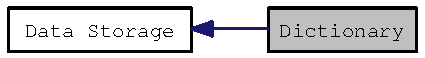
\includegraphics[width=120pt]{group__dictionary}
\end{center}
\end{figure}
\subsection*{Data Structures}
\begin{DoxyCompactItemize}
\item 
struct \hyperlink{structt__dictionary__entry}{t\_\-dictionary\_\-entry}
\begin{DoxyCompactList}\small\item\em A dictionary entry. \item\end{DoxyCompactList}\item 
struct \hyperlink{structt__dictionary}{t\_\-dictionary}
\begin{DoxyCompactList}\small\item\em The dictionary object. \item\end{DoxyCompactList}\end{DoxyCompactItemize}
\subsection*{Functions}
\begin{DoxyCompactItemize}
\item 
\hyperlink{structt__dictionary}{t\_\-dictionary} $\ast$ \hyperlink{group__dictionary_ga9d89ea4cf5b0aaf87fba6027c3ec223c}{dictionary\_\-new} ()
\begin{DoxyCompactList}\small\item\em Create a new linklist object. \item\end{DoxyCompactList}\item 
\hyperlink{group__datatypes_ga73edaae82b318855cc09fac994918165}{t\_\-max\_\-err} \hyperlink{group__dictionary_gaf401b30bed5b47e5defd1421e7f14cce}{dictionary\_\-appendlong} (\hyperlink{structt__dictionary}{t\_\-dictionary} $\ast$d, \hyperlink{structt__symbol}{t\_\-symbol} $\ast$key, long value)
\begin{DoxyCompactList}\small\item\em Add a long integer value to the dictionary. \item\end{DoxyCompactList}\item 
\hyperlink{group__datatypes_ga73edaae82b318855cc09fac994918165}{t\_\-max\_\-err} \hyperlink{group__dictionary_ga4250c0f1a0c83b1585012ea65f172e13}{dictionary\_\-appendfloat} (\hyperlink{structt__dictionary}{t\_\-dictionary} $\ast$d, \hyperlink{structt__symbol}{t\_\-symbol} $\ast$key, double value)
\begin{DoxyCompactList}\small\item\em Add a double-\/precision float value to the dictionary. \item\end{DoxyCompactList}\item 
\hyperlink{group__datatypes_ga73edaae82b318855cc09fac994918165}{t\_\-max\_\-err} \hyperlink{group__dictionary_ga5df20e3ac212f70d53469a3f091eae56}{dictionary\_\-appendsym} (\hyperlink{structt__dictionary}{t\_\-dictionary} $\ast$d, \hyperlink{structt__symbol}{t\_\-symbol} $\ast$key, \hyperlink{structt__symbol}{t\_\-symbol} $\ast$value)
\begin{DoxyCompactList}\small\item\em Add a \hyperlink{structt__symbol}{t\_\-symbol}$\ast$ value to the dictionary. \item\end{DoxyCompactList}\item 
\hyperlink{group__datatypes_ga73edaae82b318855cc09fac994918165}{t\_\-max\_\-err} \hyperlink{group__dictionary_ga22f5a417a6290c508d29196c3c6d6d58}{dictionary\_\-appendatom} (\hyperlink{structt__dictionary}{t\_\-dictionary} $\ast$d, \hyperlink{structt__symbol}{t\_\-symbol} $\ast$key, \hyperlink{structt__atom}{t\_\-atom} $\ast$value)
\begin{DoxyCompactList}\small\item\em Add a \hyperlink{structt__atom}{t\_\-atom}$\ast$ value to the dictionary. \item\end{DoxyCompactList}\item 
\hyperlink{group__datatypes_ga73edaae82b318855cc09fac994918165}{t\_\-max\_\-err} \hyperlink{group__dictionary_ga9b5b07cf479be0446d6a4441c3bdf83a}{dictionary\_\-appendstring} (\hyperlink{structt__dictionary}{t\_\-dictionary} $\ast$d, \hyperlink{structt__symbol}{t\_\-symbol} $\ast$key, const char $\ast$value)
\begin{DoxyCompactList}\small\item\em Add a C-\/string to the dictionary. \item\end{DoxyCompactList}\item 
\hyperlink{group__datatypes_ga73edaae82b318855cc09fac994918165}{t\_\-max\_\-err} \hyperlink{group__dictionary_ga863a83cc13afbd42a09e8505bee8eea5}{dictionary\_\-appendatoms} (\hyperlink{structt__dictionary}{t\_\-dictionary} $\ast$d, \hyperlink{structt__symbol}{t\_\-symbol} $\ast$key, long argc, \hyperlink{structt__atom}{t\_\-atom} $\ast$argv)
\begin{DoxyCompactList}\small\item\em Add an array of atoms to the dictionary. \item\end{DoxyCompactList}\item 
\hyperlink{group__datatypes_ga73edaae82b318855cc09fac994918165}{t\_\-max\_\-err} \hyperlink{group__dictionary_gac1f0f17da56b71ef6f21c972535ee609}{dictionary\_\-appendatomarray} (\hyperlink{structt__dictionary}{t\_\-dictionary} $\ast$d, \hyperlink{structt__symbol}{t\_\-symbol} $\ast$key, \hyperlink{structt__object}{t\_\-object} $\ast$value)
\begin{DoxyCompactList}\small\item\em Add an \hyperlink{group__atomarray}{Atom Array} object to the dictionary. \item\end{DoxyCompactList}\item 
\hyperlink{group__datatypes_ga73edaae82b318855cc09fac994918165}{t\_\-max\_\-err} \hyperlink{group__dictionary_ga1bd7575368917037f46b5b9076e167c7}{dictionary\_\-appenddictionary} (\hyperlink{structt__dictionary}{t\_\-dictionary} $\ast$d, \hyperlink{structt__symbol}{t\_\-symbol} $\ast$key, \hyperlink{structt__object}{t\_\-object} $\ast$value)
\begin{DoxyCompactList}\small\item\em Add a dictionary object to the dictionary. \item\end{DoxyCompactList}\item 
\hyperlink{group__datatypes_ga73edaae82b318855cc09fac994918165}{t\_\-max\_\-err} \hyperlink{group__dictionary_ga64e86e71b47a2d9719a43ec8bd376591}{dictionary\_\-appendobject} (\hyperlink{structt__dictionary}{t\_\-dictionary} $\ast$d, \hyperlink{structt__symbol}{t\_\-symbol} $\ast$key, \hyperlink{structt__object}{t\_\-object} $\ast$value)
\begin{DoxyCompactList}\small\item\em Add an object to the dictionary. \item\end{DoxyCompactList}\item 
\hyperlink{group__datatypes_ga73edaae82b318855cc09fac994918165}{t\_\-max\_\-err} \hyperlink{group__dictionary_gafd215503871278e2ae02c1c747f39e46}{dictionary\_\-getlong} (\hyperlink{structt__dictionary}{t\_\-dictionary} $\ast$d, \hyperlink{structt__symbol}{t\_\-symbol} $\ast$key, long $\ast$value)
\begin{DoxyCompactList}\small\item\em Retrieve a long integer from the dictionary. \item\end{DoxyCompactList}\item 
\hyperlink{group__datatypes_ga73edaae82b318855cc09fac994918165}{t\_\-max\_\-err} \hyperlink{group__dictionary_ga4e166c9edc4575ec89f176455a134cda}{dictionary\_\-getfloat} (\hyperlink{structt__dictionary}{t\_\-dictionary} $\ast$d, \hyperlink{structt__symbol}{t\_\-symbol} $\ast$key, double $\ast$value)
\begin{DoxyCompactList}\small\item\em Retrieve a double-\/precision float from the dictionary. \item\end{DoxyCompactList}\item 
\hyperlink{group__datatypes_ga73edaae82b318855cc09fac994918165}{t\_\-max\_\-err} \hyperlink{group__dictionary_ga0e5747682765d9a320bb9ccf37d9215d}{dictionary\_\-getsym} (\hyperlink{structt__dictionary}{t\_\-dictionary} $\ast$d, \hyperlink{structt__symbol}{t\_\-symbol} $\ast$key, \hyperlink{structt__symbol}{t\_\-symbol} $\ast$$\ast$value)
\begin{DoxyCompactList}\small\item\em Retrieve a \hyperlink{structt__symbol}{t\_\-symbol}$\ast$ from the dictionary. \item\end{DoxyCompactList}\item 
\hyperlink{group__datatypes_ga73edaae82b318855cc09fac994918165}{t\_\-max\_\-err} \hyperlink{group__dictionary_ga28a8378a4710e667a63f8947261bd439}{dictionary\_\-getatom} (\hyperlink{structt__dictionary}{t\_\-dictionary} $\ast$d, \hyperlink{structt__symbol}{t\_\-symbol} $\ast$key, \hyperlink{structt__atom}{t\_\-atom} $\ast$value)
\begin{DoxyCompactList}\small\item\em Copy a \hyperlink{structt__atom}{t\_\-atom} from the dictionary. \item\end{DoxyCompactList}\item 
\hyperlink{group__datatypes_ga73edaae82b318855cc09fac994918165}{t\_\-max\_\-err} \hyperlink{group__dictionary_gaee590f1bcea90856a26e5806637c2830}{dictionary\_\-getstring} (\hyperlink{structt__dictionary}{t\_\-dictionary} $\ast$d, \hyperlink{structt__symbol}{t\_\-symbol} $\ast$key, const char $\ast$$\ast$value)
\begin{DoxyCompactList}\small\item\em Retrieve a C-\/string pointer from the dictionary. \item\end{DoxyCompactList}\item 
\hyperlink{group__datatypes_ga73edaae82b318855cc09fac994918165}{t\_\-max\_\-err} \hyperlink{group__dictionary_gacda8208be5d424b81387258098bdbaa1}{dictionary\_\-getatoms} (\hyperlink{structt__dictionary}{t\_\-dictionary} $\ast$d, \hyperlink{structt__symbol}{t\_\-symbol} $\ast$key, long $\ast$argc, \hyperlink{structt__atom}{t\_\-atom} $\ast$$\ast$argv)
\begin{DoxyCompactList}\small\item\em Retrieve the address of a \hyperlink{structt__atom}{t\_\-atom} array of in the dictionary. \item\end{DoxyCompactList}\item 
\hyperlink{group__datatypes_ga73edaae82b318855cc09fac994918165}{t\_\-max\_\-err} \hyperlink{group__dictionary_ga15aff654a0d97b363e7676ff7e9709fd}{dictionary\_\-copyatoms} (\hyperlink{structt__dictionary}{t\_\-dictionary} $\ast$d, \hyperlink{structt__symbol}{t\_\-symbol} $\ast$key, long $\ast$argc, \hyperlink{structt__atom}{t\_\-atom} $\ast$$\ast$argv)
\begin{DoxyCompactList}\small\item\em Retrieve copies of a \hyperlink{structt__atom}{t\_\-atom} array in the dictionary. \item\end{DoxyCompactList}\item 
\hyperlink{group__datatypes_ga73edaae82b318855cc09fac994918165}{t\_\-max\_\-err} \hyperlink{group__dictionary_gabc3bc4db8dc0898593722338262743e1}{dictionary\_\-getatomarray} (\hyperlink{structt__dictionary}{t\_\-dictionary} $\ast$d, \hyperlink{structt__symbol}{t\_\-symbol} $\ast$key, \hyperlink{structt__object}{t\_\-object} $\ast$$\ast$value)
\begin{DoxyCompactList}\small\item\em Retrieve a \hyperlink{structt__atomarray}{t\_\-atomarray} pointer from the dictionary. \item\end{DoxyCompactList}\item 
\hyperlink{group__datatypes_ga73edaae82b318855cc09fac994918165}{t\_\-max\_\-err} \hyperlink{group__dictionary_ga1bcef0af352c4f9df233818028083ea7}{dictionary\_\-getdictionary} (\hyperlink{structt__dictionary}{t\_\-dictionary} $\ast$d, \hyperlink{structt__symbol}{t\_\-symbol} $\ast$key, \hyperlink{structt__object}{t\_\-object} $\ast$$\ast$value)
\begin{DoxyCompactList}\small\item\em Retrieve a \hyperlink{structt__dictionary}{t\_\-dictionary} pointer from the dictionary. \item\end{DoxyCompactList}\item 
\hyperlink{group__datatypes_ga73edaae82b318855cc09fac994918165}{t\_\-max\_\-err} \hyperlink{group__dictionary_gabcf91529e619908aebd380030c697052}{dictionary\_\-getobject} (\hyperlink{structt__dictionary}{t\_\-dictionary} $\ast$d, \hyperlink{structt__symbol}{t\_\-symbol} $\ast$key, \hyperlink{structt__object}{t\_\-object} $\ast$$\ast$value)
\begin{DoxyCompactList}\small\item\em Retrieve a \hyperlink{structt__object}{t\_\-object} pointer from the dictionary. \item\end{DoxyCompactList}\item 
long \hyperlink{group__dictionary_gac60faf9cb165c96aced356959f1faeb3}{dictionary\_\-entryisstring} (\hyperlink{structt__dictionary}{t\_\-dictionary} $\ast$d, \hyperlink{structt__symbol}{t\_\-symbol} $\ast$key)
\begin{DoxyCompactList}\small\item\em Test a key to set if the data stored with that key contains a \hyperlink{structt__string}{t\_\-string} object. \item\end{DoxyCompactList}\item 
long \hyperlink{group__dictionary_ga7657d5e84298475261088dbce18d70d9}{dictionary\_\-entryisatomarray} (\hyperlink{structt__dictionary}{t\_\-dictionary} $\ast$d, \hyperlink{structt__symbol}{t\_\-symbol} $\ast$key)
\begin{DoxyCompactList}\small\item\em Test a key to set if the data stored with that key contains a \hyperlink{structt__atomarray}{t\_\-atomarray} object. \item\end{DoxyCompactList}\item 
long \hyperlink{group__dictionary_gad8055f980993051fb94f8214db876ea2}{dictionary\_\-entryisdictionary} (\hyperlink{structt__dictionary}{t\_\-dictionary} $\ast$d, \hyperlink{structt__symbol}{t\_\-symbol} $\ast$key)
\begin{DoxyCompactList}\small\item\em Test a key to set if the data stored with that key contains a \hyperlink{structt__dictionary}{t\_\-dictionary} object. \item\end{DoxyCompactList}\item 
long \hyperlink{group__dictionary_ga3da77635f06156cc82b4f6c7633b69c6}{dictionary\_\-hasentry} (\hyperlink{structt__dictionary}{t\_\-dictionary} $\ast$d, \hyperlink{structt__symbol}{t\_\-symbol} $\ast$key)
\begin{DoxyCompactList}\small\item\em Test a key to set if it exists in the dictionary. \item\end{DoxyCompactList}\item 
long \hyperlink{group__dictionary_ga1a080d24b75cd6a8dc20a9143f662136}{dictionary\_\-getentrycount} (\hyperlink{structt__dictionary}{t\_\-dictionary} $\ast$d)
\begin{DoxyCompactList}\small\item\em Return the number of keys in a dictionary. \item\end{DoxyCompactList}\item 
\hyperlink{group__datatypes_ga73edaae82b318855cc09fac994918165}{t\_\-max\_\-err} \hyperlink{group__dictionary_gae595d2340304018ee2b01e1288534ea3}{dictionary\_\-getkeys} (\hyperlink{structt__dictionary}{t\_\-dictionary} $\ast$d, long $\ast$numkeys, \hyperlink{structt__symbol}{t\_\-symbol} $\ast$$\ast$$\ast$keys)
\begin{DoxyCompactList}\small\item\em Retrieve all of the key names stored in a dictionary. \item\end{DoxyCompactList}\item 
void \hyperlink{group__dictionary_ga38077c67f36917a708c4867351d6444e}{dictionary\_\-freekeys} (\hyperlink{structt__dictionary}{t\_\-dictionary} $\ast$d, long numkeys, \hyperlink{structt__symbol}{t\_\-symbol} $\ast$$\ast$keys)
\begin{DoxyCompactList}\small\item\em Free memory allocated by the \hyperlink{group__dictionary_gae595d2340304018ee2b01e1288534ea3}{dictionary\_\-getkeys()} method. \item\end{DoxyCompactList}\item 
\hyperlink{group__datatypes_ga73edaae82b318855cc09fac994918165}{t\_\-max\_\-err} \hyperlink{group__dictionary_gadc367d6d95aa0144c902d05d165f7412}{dictionary\_\-deleteentry} (\hyperlink{structt__dictionary}{t\_\-dictionary} $\ast$d, \hyperlink{structt__symbol}{t\_\-symbol} $\ast$key)
\begin{DoxyCompactList}\small\item\em Remove a value from the dictionary. \item\end{DoxyCompactList}\item 
\hyperlink{group__datatypes_ga73edaae82b318855cc09fac994918165}{t\_\-max\_\-err} \hyperlink{group__dictionary_gadac447ba3430cc2b8083d62df41932b8}{dictionary\_\-chuckentry} (\hyperlink{structt__dictionary}{t\_\-dictionary} $\ast$d, \hyperlink{structt__symbol}{t\_\-symbol} $\ast$key)
\begin{DoxyCompactList}\small\item\em Remove a value from the dictionary without freeing it. \item\end{DoxyCompactList}\item 
\hyperlink{group__datatypes_ga73edaae82b318855cc09fac994918165}{t\_\-max\_\-err} \hyperlink{group__dictionary_gafd9a85c38f7e6b1cd075664a5aa4cbc8}{dictionary\_\-clear} (\hyperlink{structt__dictionary}{t\_\-dictionary} $\ast$d)
\begin{DoxyCompactList}\small\item\em Delete all values from a dictionary. \item\end{DoxyCompactList}\item 
void \hyperlink{group__dictionary_ga923b67932c8401f58dee86cfb3bb5110}{dictionary\_\-funall} (\hyperlink{structt__dictionary}{t\_\-dictionary} $\ast$d, \hyperlink{group__datatypes_gac26ba0a173b50597f5738132e059b42d}{method} fun, void $\ast$arg)
\begin{DoxyCompactList}\small\item\em Call the specified function for every entry in the dictionary. \item\end{DoxyCompactList}\item 
\hyperlink{structt__symbol}{t\_\-symbol} $\ast$ \hyperlink{group__dictionary_ga866aeb04d26740768790f64203f30b7c}{dictionary\_\-entry\_\-getkey} (\hyperlink{structt__dictionary__entry}{t\_\-dictionary\_\-entry} $\ast$x)
\begin{DoxyCompactList}\small\item\em Given a \hyperlink{structt__dictionary__entry}{t\_\-dictionary\_\-entry}$\ast$, return the key associated with that entry. \item\end{DoxyCompactList}\item 
void \hyperlink{group__dictionary_ga55877f4d0fef0a8d0badf9afc95bb7d0}{dictionary\_\-entry\_\-getvalue} (\hyperlink{structt__dictionary__entry}{t\_\-dictionary\_\-entry} $\ast$x, \hyperlink{structt__atom}{t\_\-atom} $\ast$value)
\begin{DoxyCompactList}\small\item\em Given a \hyperlink{structt__dictionary__entry}{t\_\-dictionary\_\-entry}$\ast$, return the value associated with that entry. \item\end{DoxyCompactList}\item 
\hyperlink{group__datatypes_ga73edaae82b318855cc09fac994918165}{t\_\-max\_\-err} \hyperlink{group__dictionary_gaef48a5cc22bc4c8b0fb23c7b7c3aa6a8}{dictionary\_\-copyunique} (\hyperlink{structt__dictionary}{t\_\-dictionary} $\ast$d, \hyperlink{structt__dictionary}{t\_\-dictionary} $\ast$copyfrom)
\begin{DoxyCompactList}\small\item\em Given 2 dictionaries, copy the keys unique to one of the dictionaries to the other dictionary. \item\end{DoxyCompactList}\item 
\hyperlink{group__datatypes_ga73edaae82b318855cc09fac994918165}{t\_\-max\_\-err} \hyperlink{group__dictionary_ga7beaedd2dbbc352539ccd104db7094b1}{dictionary\_\-getdeflong} (\hyperlink{structt__dictionary}{t\_\-dictionary} $\ast$d, \hyperlink{structt__symbol}{t\_\-symbol} $\ast$key, long $\ast$value, long def)
\begin{DoxyCompactList}\small\item\em Retrieve a long integer from the dictionary. \item\end{DoxyCompactList}\item 
\hyperlink{group__datatypes_ga73edaae82b318855cc09fac994918165}{t\_\-max\_\-err} \hyperlink{group__dictionary_ga2c988f18fa22ab56aac4464bc7140438}{dictionary\_\-getdeffloat} (\hyperlink{structt__dictionary}{t\_\-dictionary} $\ast$d, \hyperlink{structt__symbol}{t\_\-symbol} $\ast$key, double $\ast$value, double def)
\begin{DoxyCompactList}\small\item\em Retrieve a double-\/precision float from the dictionary. \item\end{DoxyCompactList}\item 
\hyperlink{group__datatypes_ga73edaae82b318855cc09fac994918165}{t\_\-max\_\-err} \hyperlink{group__dictionary_ga2bf7497a4db16913aedb8c85036bf8c6}{dictionary\_\-getdefsym} (\hyperlink{structt__dictionary}{t\_\-dictionary} $\ast$d, \hyperlink{structt__symbol}{t\_\-symbol} $\ast$key, \hyperlink{structt__symbol}{t\_\-symbol} $\ast$$\ast$value, \hyperlink{structt__symbol}{t\_\-symbol} $\ast$def)
\begin{DoxyCompactList}\small\item\em Retrieve a \hyperlink{structt__symbol}{t\_\-symbol}$\ast$ from the dictionary. \item\end{DoxyCompactList}\item 
\hyperlink{group__datatypes_ga73edaae82b318855cc09fac994918165}{t\_\-max\_\-err} \hyperlink{group__dictionary_gaa447fe7ad80586bee323e1c2bf80bdf9}{dictionary\_\-getdefatom} (\hyperlink{structt__dictionary}{t\_\-dictionary} $\ast$d, \hyperlink{structt__symbol}{t\_\-symbol} $\ast$key, \hyperlink{structt__atom}{t\_\-atom} $\ast$value, \hyperlink{structt__atom}{t\_\-atom} $\ast$def)
\begin{DoxyCompactList}\small\item\em Retrieve a \hyperlink{structt__atom}{t\_\-atom}$\ast$ from the dictionary. \item\end{DoxyCompactList}\item 
\hyperlink{group__datatypes_ga73edaae82b318855cc09fac994918165}{t\_\-max\_\-err} \hyperlink{group__dictionary_ga3ced9bab630a199d920fffc163f4fe1b}{dictionary\_\-getdefstring} (\hyperlink{structt__dictionary}{t\_\-dictionary} $\ast$d, \hyperlink{structt__symbol}{t\_\-symbol} $\ast$key, const char $\ast$$\ast$value, char $\ast$def)
\begin{DoxyCompactList}\small\item\em Retrieve a C-\/string from the dictionary. \item\end{DoxyCompactList}\item 
\hyperlink{group__datatypes_ga73edaae82b318855cc09fac994918165}{t\_\-max\_\-err} \hyperlink{group__dictionary_ga2ab733c5d5fe85e31e73d5a66d75dabd}{dictionary\_\-getdefatoms} (\hyperlink{structt__dictionary}{t\_\-dictionary} $\ast$d, \hyperlink{structt__symbol}{t\_\-symbol} $\ast$key, long $\ast$argc, \hyperlink{structt__atom}{t\_\-atom} $\ast$$\ast$argv, \hyperlink{structt__atom}{t\_\-atom} $\ast$def)
\begin{DoxyCompactList}\small\item\em Retrieve the address of a \hyperlink{structt__atom}{t\_\-atom} array of in the dictionary. \item\end{DoxyCompactList}\item 
\hyperlink{group__datatypes_ga73edaae82b318855cc09fac994918165}{t\_\-max\_\-err} \hyperlink{group__dictionary_gaa886af0aad9db9bc6b08314b9b5672f9}{dictionary\_\-copydefatoms} (\hyperlink{structt__dictionary}{t\_\-dictionary} $\ast$d, \hyperlink{structt__symbol}{t\_\-symbol} $\ast$key, long $\ast$argc, \hyperlink{structt__atom}{t\_\-atom} $\ast$$\ast$argv, \hyperlink{structt__atom}{t\_\-atom} $\ast$def)
\begin{DoxyCompactList}\small\item\em Retrieve copies of a \hyperlink{structt__atom}{t\_\-atom} array in the dictionary. \item\end{DoxyCompactList}\item 
\hyperlink{group__datatypes_ga73edaae82b318855cc09fac994918165}{t\_\-max\_\-err} \hyperlink{group__dictionary_ga099020753fc6918512d3bfc2b3fedafc}{dictionary\_\-dump} (\hyperlink{structt__dictionary}{t\_\-dictionary} $\ast$d, long recurse, long console)
\begin{DoxyCompactList}\small\item\em Print the contents of a dictionary to the Max window. \item\end{DoxyCompactList}\item 
\hyperlink{group__datatypes_ga73edaae82b318855cc09fac994918165}{t\_\-max\_\-err} \hyperlink{group__dictionary_ga53ef6b088fed8ef360292a659a383487}{dictionary\_\-copyentries} (\hyperlink{structt__dictionary}{t\_\-dictionary} $\ast$src, \hyperlink{structt__dictionary}{t\_\-dictionary} $\ast$dst, \hyperlink{structt__symbol}{t\_\-symbol} $\ast$$\ast$keys)
\begin{DoxyCompactList}\small\item\em Copy specified entries from one dictionary to another. \item\end{DoxyCompactList}\item 
\hyperlink{structt__dictionary}{t\_\-dictionary} $\ast$ \hyperlink{group__dictionary_ga77d5bafc260f9fc0bf3b4ad35f2b2629}{dictionary\_\-sprintf} (char $\ast$fmt,...)
\begin{DoxyCompactList}\small\item\em Create a new dictionary populated with values using a combination of attribute and sprintf syntax. \item\end{DoxyCompactList}\item 
\hyperlink{group__datatypes_ga73edaae82b318855cc09fac994918165}{t\_\-max\_\-err} \hyperlink{group__dictionary_ga2c64f2e3bce940ca992b3dd3ffe292ac}{dictionary\_\-read} (char $\ast$filename, short path, \hyperlink{structt__dictionary}{t\_\-dictionary} $\ast$$\ast$d)
\begin{DoxyCompactList}\small\item\em Read the specified JSON file and return a \hyperlink{structt__dictionary}{t\_\-dictionary} object. \item\end{DoxyCompactList}\item 
\hyperlink{group__datatypes_ga73edaae82b318855cc09fac994918165}{t\_\-max\_\-err} \hyperlink{group__dictionary_ga54f1888c1ca3cd84d32cd2de7a392e35}{dictionary\_\-write} (\hyperlink{structt__dictionary}{t\_\-dictionary} $\ast$d, char $\ast$filename, short path)
\begin{DoxyCompactList}\small\item\em Serialize the specified \hyperlink{structt__dictionary}{t\_\-dictionary} object to a JSON file. \item\end{DoxyCompactList}\item 
void \hyperlink{group__dictionary_ga7619544926e5c62caf19176ebab5b1a2}{postdictionary} (\hyperlink{structt__object}{t\_\-object} $\ast$d)
\begin{DoxyCompactList}\small\item\em Print the contents of a dictionary to the Max window. \item\end{DoxyCompactList}\end{DoxyCompactItemize}


\subsection{Detailed Description}
In Max 5, we have a new \char`\"{}dictionary\char`\"{} object which can be used for object prototypes, object serialization, object constructors, and other tasks. A dictionary is ultimately a collection of atom values assigned to symbolic keys. In addition to primitive \hyperlink{group__atom_gga8aa6700e9f00b132eb376db6e39ade47a002f28879581a6f66ea492b994b96f1e}{A\_\-LONG}, \hyperlink{group__atom_gga8aa6700e9f00b132eb376db6e39ade47a0b3aa0ab8104573dfc9cb70b5b08031f}{A\_\-FLOAT}, and \hyperlink{group__atom_gga8aa6700e9f00b132eb376db6e39ade47a2d661c2a5d949566e2f1944c99bceeea}{A\_\-SYM} atom types, the \hyperlink{group__atom_gga8aa6700e9f00b132eb376db6e39ade47a82cc76e0d53c8fc28df167c35d5bbd1a}{A\_\-OBJ} atom type is used for \hyperlink{structt__atomarray}{t\_\-atomarray} (for a set of atoms assigned to a key), \hyperlink{structt__dictionary}{t\_\-dictionary} (for hierarhical use), \hyperlink{structt__string}{t\_\-string} (for large blocks of text which we don't wish to bloat the symbol table), and potentially other object data types. Internally, the dictionary object uses a combination data structure of a hash table (for fast key lookup) and a linked-\/list (to maintain ordering of information within the dictionary).

Dictionaries are clonable entites, but note that all the member objects of a given dictionary may not be clonable. At the time of this writing, for example, the \hyperlink{structt__string}{t\_\-string} object is not clonable, though it will be made clonable in the near future. In order for prototype entities to be guaranteed their passage into the constructor, they must be clonable (currenlty a symbol conversion is in place for the \hyperlink{structt__string}{t\_\-string} class).\hypertarget{group__dictionary_using_dictionaries}{}\subsection{Using Dictionaries}\label{group__dictionary_using_dictionaries}
Dictionaries are used in many places in Max 5. They can be confusing in many respects. It is easy to produce memory leaks or bugs where objects are freed twice. It is easy to confuse what type of dictionary is used for what. This page will begin with some high level information to help understand when to free and when not to free. Then, we will offer recipies for using dictionaries to accomplish common tasks.\hypertarget{group__dictionary_understanding_dictionaries}{}\subsubsection{Understanding Dictionaries}\label{group__dictionary_understanding_dictionaries}
A dictionary stores atom values under named key entries. These atoms can contain \hyperlink{group__atom_gga8aa6700e9f00b132eb376db6e39ade47a82cc76e0d53c8fc28df167c35d5bbd1a}{A\_\-OBJ} values. When the dictionary is freed, any \hyperlink{group__atom_gga8aa6700e9f00b132eb376db6e39ade47a82cc76e0d53c8fc28df167c35d5bbd1a}{A\_\-OBJ} values that are in the dictionary will also be freed. Thus, it is easy to mistakenly free objects twice, thus this is something to be careful about. For example, look at this code:


\begin{DoxyCode}
    t_dictionary *d = dictionary_new(); 
    t_dictionary *sd = dictionary_new();  
    dictionary_appenddictionary(d, gensym("subdictionary"), sd); 
    do_something(d);
    object_free(d);  // this will free *both* d and sd since sd is contained by d
      
    // freeing "sd" here would be bad
\end{DoxyCode}


You primarily need to keep this in mind when calling \hyperlink{group__dictionary_ga64e86e71b47a2d9719a43ec8bd376591}{dictionary\_\-appendobject()}, \hyperlink{group__dictionary_ga1bd7575368917037f46b5b9076e167c7}{dictionary\_\-appenddictionary()}, or \hyperlink{group__dictionary_gac1f0f17da56b71ef6f21c972535ee609}{dictionary\_\-appendatomarray()}. So, what do you do if you need to free a dictionary but you also want to hang on to an object that is inside of the dictionary? In this case, chuck the entry in question first. For example, let's assume that for some reason you cannot free the \char`\"{}sd\char`\"{} dictionary in the code above. Perhaps it doesn't belong to you. But, to do some operation you need to append it to a new dictionary. Then, do this:


\begin{DoxyCode}
    void function_foo(t_dictionary *sd) {
      t_dictionary *d = dictionary_new(); 
      dictionary_appenddictionary(d, gensym("subdictionary"), sd); 
      do_something(d); 
      dictionary_chuckentry(d, gensym("subdictionary")); 
      object_free(d);  
    }
\end{DoxyCode}
\hypertarget{group__dictionary_when_to_free_a_dictionary}{}\subsubsection{When to Free a Dictionary}\label{group__dictionary_when_to_free_a_dictionary}
So, how do you know when you need to free a dictionary? Well, generally if you make a dictionary, you need to free it when you are done (unless you transfer ownership of the dictionary to someone else). On the other hand, if you are passed a dictionary (i.e. as a parameter of your function or method) then it is not yours to free and you should just use it. However, it is not always obvious that you made a dictionary vs just borrowed it.

Here are some common (and not so common) ways to make a dictionary. These functions return a new dictionary and thus the dictionary you get should be freed when you are done, unless you pass the dictionary on to someone else who will free it at an appropriate time. Here they are: 
\begin{DoxyItemize}
\item \hyperlink{group__dictionary_ga9d89ea4cf5b0aaf87fba6027c3ec223c}{dictionary\_\-new()}  
\item dictionary\_\-clone()  
\item \hyperlink{group__dictionary_ga2c64f2e3bce940ca992b3dd3ffe292ac}{dictionary\_\-read()}  
\item \hyperlink{group__dictionary_ga77d5bafc260f9fc0bf3b4ad35f2b2629}{dictionary\_\-sprintf()}  
\item dictionary\_\-vsprintf()  
\item jsonreader\_\-parse()  
\item jpatcher\_\-monikerforobject()  
\item class\_\-cloneprototype()  
\item prototype\_\-getdictionary()  
\item clipboard\_\-todictionary()  
\item jpatchercontroller\_\-copytodictionary()  
\item probably others of course 
\end{DoxyItemize}

Here are some functions that return borrowed dictionaries. These are dictionaries that you can use but you cannot free since you do not own them. Here they are: 
\begin{DoxyItemize}
\item dictionary\_\-prototypefromclass()  
\item object\_\-refpage\_\-get\_\-class\_\-info\_\-fromclassname()  
\item object\_\-refpage\_\-get\_\-class\_\-info()  
\item \hyperlink{group__obj_ga6122e56af8de90fa7aad43ee405c6bb6}{object\_\-dictionaryarg()}  
\end{DoxyItemize}

Finally, most functions that accept dictionaries as parameters will not assume ownership of the dictionary. Usually the way ownership is assumed is if you add a dictionary as a subdictionary to a dictionary that you do not own. One exception is the utility newobject\_\-fromdictionary\_\-delete() who's name makes it clear that the dictionary will be deleted after calling the function.\hypertarget{group__dictionary_dictionaries_common_uses}{}\subsubsection{Some Common Uses of Dictionaries}\label{group__dictionary_dictionaries_common_uses}
You can make a patcher by passing a dictionary to \hyperlink{group__obj_ga459c71aca6316e345379eeb424ad56ff}{object\_\-new\_\-typed()} when making a \char`\"{}jpatcher\char`\"{}. Using \hyperlink{group__atom_ga55938aedb41a8f3565680cf29169dc70}{atom\_\-setparse()} and \hyperlink{group__attr_gad9de140db1dba2fe588019866a048bc6}{attr\_\-args\_\-dictionary()} makes this relatively easy.

Use \hyperlink{group__obj_gad81c665a20c3c707decaf3403468ff47}{newobject\_\-sprintf()} to programmatically make an object in a patch. Actually, you don't explicitly use a dictionary here! If you do want more control, so you can touch the dictionary to customize it, then see the next bullet.

Use \hyperlink{group__dictionary_ga77d5bafc260f9fc0bf3b4ad35f2b2629}{dictionary\_\-sprintf()} to make a dictionary to specify a box (i.e. specify class with @maxclass attr). Then, make another dictionary and append your box dictionary to it under the key \char`\"{}box\char`\"{} via \hyperlink{group__dictionary_ga1bd7575368917037f46b5b9076e167c7}{dictionary\_\-appenddictionary()}. Finally, make your object with \hyperlink{group__obj_gaed2c4e1d0c80d929b97ccf07a886faeb}{newobject\_\-fromdictionary()}.

\begin{DoxySeeAlso}{See also}
\hyperlink{group__linklist}{Linked List} 

\hyperlink{group__hashtab}{Hash Table}
\end{DoxySeeAlso}
\begin{DoxyVersion}{Version}
5.0 
\end{DoxyVersion}


\subsection{Function Documentation}
\hypertarget{group__dictionary_ga22f5a417a6290c508d29196c3c6d6d58}{
\index{dictionary@{dictionary}!dictionary\_\-appendatom@{dictionary\_\-appendatom}}
\index{dictionary\_\-appendatom@{dictionary\_\-appendatom}!dictionary@{dictionary}}
\subsubsection[{dictionary\_\-appendatom}]{\setlength{\rightskip}{0pt plus 5cm}{\bf t\_\-max\_\-err} dictionary\_\-appendatom ({\bf t\_\-dictionary} $\ast$ {\em d}, \/  {\bf t\_\-symbol} $\ast$ {\em key}, \/  {\bf t\_\-atom} $\ast$ {\em value})}}
\label{group__dictionary_ga22f5a417a6290c508d29196c3c6d6d58}


Add a \hyperlink{structt__atom}{t\_\-atom}$\ast$ value to the dictionary. 
\begin{DoxyParams}{Parameters}
\item[{\em d}]The dictionary instance. \item[{\em key}]The name of the key used to index the new value. All keys must be unique. If the key name already exists, then the existing value associated with the key will be freed prior to the new value's assignment. \item[{\em value}]The new value to append to the dictionary. \end{DoxyParams}
\begin{DoxyReturn}{Returns}
A Max error code. 
\end{DoxyReturn}
\hypertarget{group__dictionary_gac1f0f17da56b71ef6f21c972535ee609}{
\index{dictionary@{dictionary}!dictionary\_\-appendatomarray@{dictionary\_\-appendatomarray}}
\index{dictionary\_\-appendatomarray@{dictionary\_\-appendatomarray}!dictionary@{dictionary}}
\subsubsection[{dictionary\_\-appendatomarray}]{\setlength{\rightskip}{0pt plus 5cm}{\bf t\_\-max\_\-err} dictionary\_\-appendatomarray ({\bf t\_\-dictionary} $\ast$ {\em d}, \/  {\bf t\_\-symbol} $\ast$ {\em key}, \/  {\bf t\_\-object} $\ast$ {\em value})}}
\label{group__dictionary_gac1f0f17da56b71ef6f21c972535ee609}


Add an \hyperlink{group__atomarray}{Atom Array} object to the dictionary. Note that from this point on that you should not free the \hyperlink{structt__atomarray}{t\_\-atomarray}$\ast$, because the atomarray is now owned by the dictionary, and freeing the dictionary will free the atomarray as discussed in \hyperlink{group__dictionary_when_to_free_a_dictionary}{When to Free a Dictionary}.


\begin{DoxyParams}{Parameters}
\item[{\em d}]The dictionary instance. \item[{\em key}]The name of the key used to index the new value. All keys must be unique. If the key name already exists, then the existing value associated with the key will be freed prior to the new value's assignment. \item[{\em value}]The new value to append to the dictionary. \end{DoxyParams}
\begin{DoxyReturn}{Returns}
A Max error code. 
\end{DoxyReturn}
\hypertarget{group__dictionary_ga863a83cc13afbd42a09e8505bee8eea5}{
\index{dictionary@{dictionary}!dictionary\_\-appendatoms@{dictionary\_\-appendatoms}}
\index{dictionary\_\-appendatoms@{dictionary\_\-appendatoms}!dictionary@{dictionary}}
\subsubsection[{dictionary\_\-appendatoms}]{\setlength{\rightskip}{0pt plus 5cm}{\bf t\_\-max\_\-err} dictionary\_\-appendatoms ({\bf t\_\-dictionary} $\ast$ {\em d}, \/  {\bf t\_\-symbol} $\ast$ {\em key}, \/  long {\em argc}, \/  {\bf t\_\-atom} $\ast$ {\em argv})}}
\label{group__dictionary_ga863a83cc13afbd42a09e8505bee8eea5}


Add an array of atoms to the dictionary. Internally these atoms will be copied into a \hyperlink{structt__atomarray}{t\_\-atomarray} object, which will be appended to the dictionary with the given key.


\begin{DoxyParams}{Parameters}
\item[{\em d}]The dictionary instance. \item[{\em key}]The name of the key used to index the new value. All keys must be unique. If the key name already exists, then the existing value associated with the key will be freed prior to the new value's assignment. \item[{\em argc}]The number of atoms to append to the dictionary. \item[{\em argv}]The address of the first atom in the array to append to the dictionary. \end{DoxyParams}
\begin{DoxyReturn}{Returns}
A Max error code. 
\end{DoxyReturn}
\hypertarget{group__dictionary_ga1bd7575368917037f46b5b9076e167c7}{
\index{dictionary@{dictionary}!dictionary\_\-appenddictionary@{dictionary\_\-appenddictionary}}
\index{dictionary\_\-appenddictionary@{dictionary\_\-appenddictionary}!dictionary@{dictionary}}
\subsubsection[{dictionary\_\-appenddictionary}]{\setlength{\rightskip}{0pt plus 5cm}{\bf t\_\-max\_\-err} dictionary\_\-appenddictionary ({\bf t\_\-dictionary} $\ast$ {\em d}, \/  {\bf t\_\-symbol} $\ast$ {\em key}, \/  {\bf t\_\-object} $\ast$ {\em value})}}
\label{group__dictionary_ga1bd7575368917037f46b5b9076e167c7}


Add a dictionary object to the dictionary. Note that from this point on that you should not free the \hyperlink{structt__dictionary}{t\_\-dictionary}$\ast$ that is being added, because the newly-\/added dictionary is now owned by the dictionary to which it has been added, as discussed in \hyperlink{group__dictionary_when_to_free_a_dictionary}{When to Free a Dictionary}.


\begin{DoxyParams}{Parameters}
\item[{\em d}]The dictionary instance. \item[{\em key}]The name of the key used to index the new value. All keys must be unique. If the key name already exists, then the existing value associated with the key will be freed prior to the new value's assignment. \item[{\em value}]The new value to append to the dictionary. \end{DoxyParams}
\begin{DoxyReturn}{Returns}
A Max error code. 
\end{DoxyReturn}
\hypertarget{group__dictionary_ga4250c0f1a0c83b1585012ea65f172e13}{
\index{dictionary@{dictionary}!dictionary\_\-appendfloat@{dictionary\_\-appendfloat}}
\index{dictionary\_\-appendfloat@{dictionary\_\-appendfloat}!dictionary@{dictionary}}
\subsubsection[{dictionary\_\-appendfloat}]{\setlength{\rightskip}{0pt plus 5cm}{\bf t\_\-max\_\-err} dictionary\_\-appendfloat ({\bf t\_\-dictionary} $\ast$ {\em d}, \/  {\bf t\_\-symbol} $\ast$ {\em key}, \/  double {\em value})}}
\label{group__dictionary_ga4250c0f1a0c83b1585012ea65f172e13}


Add a double-\/precision float value to the dictionary. 
\begin{DoxyParams}{Parameters}
\item[{\em d}]The dictionary instance. \item[{\em key}]The name of the key used to index the new value. All keys must be unique. If the key name already exists, then the existing value associated with the key will be freed prior to the new value's assignment. \item[{\em value}]The new value to append to the dictionary. \end{DoxyParams}
\begin{DoxyReturn}{Returns}
A Max error code. 
\end{DoxyReturn}
\hypertarget{group__dictionary_gaf401b30bed5b47e5defd1421e7f14cce}{
\index{dictionary@{dictionary}!dictionary\_\-appendlong@{dictionary\_\-appendlong}}
\index{dictionary\_\-appendlong@{dictionary\_\-appendlong}!dictionary@{dictionary}}
\subsubsection[{dictionary\_\-appendlong}]{\setlength{\rightskip}{0pt plus 5cm}{\bf t\_\-max\_\-err} dictionary\_\-appendlong ({\bf t\_\-dictionary} $\ast$ {\em d}, \/  {\bf t\_\-symbol} $\ast$ {\em key}, \/  long {\em value})}}
\label{group__dictionary_gaf401b30bed5b47e5defd1421e7f14cce}


Add a long integer value to the dictionary. 
\begin{DoxyParams}{Parameters}
\item[{\em d}]The dictionary instance. \item[{\em key}]The name of the key used to index the new value. All keys must be unique. If the key name already exists, then the existing value associated with the key will be freed prior to the new value's assignment. \item[{\em value}]The new value to append to the dictionary. \end{DoxyParams}
\begin{DoxyReturn}{Returns}
A Max error code. 
\end{DoxyReturn}
\hypertarget{group__dictionary_ga64e86e71b47a2d9719a43ec8bd376591}{
\index{dictionary@{dictionary}!dictionary\_\-appendobject@{dictionary\_\-appendobject}}
\index{dictionary\_\-appendobject@{dictionary\_\-appendobject}!dictionary@{dictionary}}
\subsubsection[{dictionary\_\-appendobject}]{\setlength{\rightskip}{0pt plus 5cm}{\bf t\_\-max\_\-err} dictionary\_\-appendobject ({\bf t\_\-dictionary} $\ast$ {\em d}, \/  {\bf t\_\-symbol} $\ast$ {\em key}, \/  {\bf t\_\-object} $\ast$ {\em value})}}
\label{group__dictionary_ga64e86e71b47a2d9719a43ec8bd376591}


Add an object to the dictionary. Note that from this point on that you should not free the \hyperlink{structt__object}{t\_\-object}$\ast$ that is being added, because the newly-\/added object is now owned by the dictionary to which it has been added, as discussed in \hyperlink{group__dictionary_when_to_free_a_dictionary}{When to Free a Dictionary}.


\begin{DoxyParams}{Parameters}
\item[{\em d}]The dictionary instance. \item[{\em key}]The name of the key used to index the new value. All keys must be unique. If the key name already exists, then the existing value associated with the key will be freed prior to the new value's assignment. \item[{\em value}]The new value to append to the dictionary. \end{DoxyParams}
\begin{DoxyReturn}{Returns}
A Max error code. 
\end{DoxyReturn}
\hypertarget{group__dictionary_ga9b5b07cf479be0446d6a4441c3bdf83a}{
\index{dictionary@{dictionary}!dictionary\_\-appendstring@{dictionary\_\-appendstring}}
\index{dictionary\_\-appendstring@{dictionary\_\-appendstring}!dictionary@{dictionary}}
\subsubsection[{dictionary\_\-appendstring}]{\setlength{\rightskip}{0pt plus 5cm}{\bf t\_\-max\_\-err} dictionary\_\-appendstring ({\bf t\_\-dictionary} $\ast$ {\em d}, \/  {\bf t\_\-symbol} $\ast$ {\em key}, \/  const char $\ast$ {\em value})}}
\label{group__dictionary_ga9b5b07cf479be0446d6a4441c3bdf83a}


Add a C-\/string to the dictionary. Internally this uses the \hyperlink{structt__symbol}{t\_\-symbol} object. It is useful to use the \hyperlink{structt__string}{t\_\-string} in dictionaries rather than the \hyperlink{structt__symbol}{t\_\-symbol} to avoid bloating Max's symbol table unnecessarily.


\begin{DoxyParams}{Parameters}
\item[{\em d}]The dictionary instance. \item[{\em key}]The name of the key used to index the new value. All keys must be unique. If the key name already exists, then the existing value associated with the key will be freed prior to the new value's assignment. \item[{\em value}]The new value to append to the dictionary. \end{DoxyParams}
\begin{DoxyReturn}{Returns}
A Max error code. 
\end{DoxyReturn}
\hypertarget{group__dictionary_ga5df20e3ac212f70d53469a3f091eae56}{
\index{dictionary@{dictionary}!dictionary\_\-appendsym@{dictionary\_\-appendsym}}
\index{dictionary\_\-appendsym@{dictionary\_\-appendsym}!dictionary@{dictionary}}
\subsubsection[{dictionary\_\-appendsym}]{\setlength{\rightskip}{0pt plus 5cm}{\bf t\_\-max\_\-err} dictionary\_\-appendsym ({\bf t\_\-dictionary} $\ast$ {\em d}, \/  {\bf t\_\-symbol} $\ast$ {\em key}, \/  {\bf t\_\-symbol} $\ast$ {\em value})}}
\label{group__dictionary_ga5df20e3ac212f70d53469a3f091eae56}


Add a \hyperlink{structt__symbol}{t\_\-symbol}$\ast$ value to the dictionary. 
\begin{DoxyParams}{Parameters}
\item[{\em d}]The dictionary instance. \item[{\em key}]The name of the key used to index the new value. All keys must be unique. If the key name already exists, then the existing value associated with the key will be freed prior to the new value's assignment. \item[{\em value}]The new value to append to the dictionary. \end{DoxyParams}
\begin{DoxyReturn}{Returns}
A Max error code. 
\end{DoxyReturn}
\hypertarget{group__dictionary_gadac447ba3430cc2b8083d62df41932b8}{
\index{dictionary@{dictionary}!dictionary\_\-chuckentry@{dictionary\_\-chuckentry}}
\index{dictionary\_\-chuckentry@{dictionary\_\-chuckentry}!dictionary@{dictionary}}
\subsubsection[{dictionary\_\-chuckentry}]{\setlength{\rightskip}{0pt plus 5cm}{\bf t\_\-max\_\-err} dictionary\_\-chuckentry ({\bf t\_\-dictionary} $\ast$ {\em d}, \/  {\bf t\_\-symbol} $\ast$ {\em key})}}
\label{group__dictionary_gadac447ba3430cc2b8083d62df41932b8}


Remove a value from the dictionary without freeing it. 
\begin{DoxyParams}{Parameters}
\item[{\em d}]The dictionary instance. \item[{\em key}]The key associated with the value to delete. \end{DoxyParams}
\begin{DoxyReturn}{Returns}
A max error code.
\end{DoxyReturn}
\begin{DoxySeeAlso}{See also}
\hyperlink{group__dictionary_gadc367d6d95aa0144c902d05d165f7412}{dictionary\_\-deleteentry()} 
\end{DoxySeeAlso}
\hypertarget{group__dictionary_gafd9a85c38f7e6b1cd075664a5aa4cbc8}{
\index{dictionary@{dictionary}!dictionary\_\-clear@{dictionary\_\-clear}}
\index{dictionary\_\-clear@{dictionary\_\-clear}!dictionary@{dictionary}}
\subsubsection[{dictionary\_\-clear}]{\setlength{\rightskip}{0pt plus 5cm}{\bf t\_\-max\_\-err} dictionary\_\-clear ({\bf t\_\-dictionary} $\ast$ {\em d})}}
\label{group__dictionary_gafd9a85c38f7e6b1cd075664a5aa4cbc8}


Delete all values from a dictionary. This method will free the objects in the dictionary. If freeing the objects is inappropriate or undesirable then you should iterate through the dictionary and use \hyperlink{group__dictionary_gadac447ba3430cc2b8083d62df41932b8}{dictionary\_\-chuckentry()} instead.


\begin{DoxyParams}{Parameters}
\item[{\em d}]The dictionary instance. \end{DoxyParams}
\begin{DoxyReturn}{Returns}
A max error code.
\end{DoxyReturn}
\begin{DoxySeeAlso}{See also}
\hyperlink{group__dictionary_gae595d2340304018ee2b01e1288534ea3}{dictionary\_\-getkeys()} 

\hyperlink{group__dictionary_gadac447ba3430cc2b8083d62df41932b8}{dictionary\_\-chuckentry()} 

\hyperlink{group__dictionary_gadc367d6d95aa0144c902d05d165f7412}{dictionary\_\-deleteentry()} 
\end{DoxySeeAlso}
\hypertarget{group__dictionary_ga15aff654a0d97b363e7676ff7e9709fd}{
\index{dictionary@{dictionary}!dictionary\_\-copyatoms@{dictionary\_\-copyatoms}}
\index{dictionary\_\-copyatoms@{dictionary\_\-copyatoms}!dictionary@{dictionary}}
\subsubsection[{dictionary\_\-copyatoms}]{\setlength{\rightskip}{0pt plus 5cm}{\bf t\_\-max\_\-err} dictionary\_\-copyatoms ({\bf t\_\-dictionary} $\ast$ {\em d}, \/  {\bf t\_\-symbol} $\ast$ {\em key}, \/  long $\ast$ {\em argc}, \/  {\bf t\_\-atom} $\ast$$\ast$ {\em argv})}}
\label{group__dictionary_ga15aff654a0d97b363e7676ff7e9709fd}


Retrieve copies of a \hyperlink{structt__atom}{t\_\-atom} array in the dictionary. The retrieved pointer of t\_\-atoms in the dictionary has memory allocated and copied to it from within the function. You are responsible for freeing it with \hyperlink{group__memory_ga200c82639e547869db1f3887d17102d3}{sysmem\_\-freeptr()}.


\begin{DoxyParams}{Parameters}
\item[{\em d}]The dictionary instance. \item[{\em key}]The key associated with the value to lookup. \item[{\em argc}]The address of a variable to hold the number of atoms in the array. \item[{\em argv}]The address of a variable to hold a pointer to the first atom in the array. You should initialize this pointer to NULL prior to passing it to \hyperlink{group__dictionary_ga15aff654a0d97b363e7676ff7e9709fd}{dictionary\_\-copyatoms()}. \end{DoxyParams}
\begin{DoxyReturn}{Returns}
A Max error code.
\end{DoxyReturn}
\begin{DoxySeeAlso}{See also}
\hyperlink{group__dictionary_gacda8208be5d424b81387258098bdbaa1}{dictionary\_\-getatoms()} 
\end{DoxySeeAlso}
\hypertarget{group__dictionary_gaa886af0aad9db9bc6b08314b9b5672f9}{
\index{dictionary@{dictionary}!dictionary\_\-copydefatoms@{dictionary\_\-copydefatoms}}
\index{dictionary\_\-copydefatoms@{dictionary\_\-copydefatoms}!dictionary@{dictionary}}
\subsubsection[{dictionary\_\-copydefatoms}]{\setlength{\rightskip}{0pt plus 5cm}{\bf t\_\-max\_\-err} dictionary\_\-copydefatoms ({\bf t\_\-dictionary} $\ast$ {\em d}, \/  {\bf t\_\-symbol} $\ast$ {\em key}, \/  long $\ast$ {\em argc}, \/  {\bf t\_\-atom} $\ast$$\ast$ {\em argv}, \/  {\bf t\_\-atom} $\ast$ {\em def})}}
\label{group__dictionary_gaa886af0aad9db9bc6b08314b9b5672f9}


Retrieve copies of a \hyperlink{structt__atom}{t\_\-atom} array in the dictionary. The retrieved pointer of t\_\-atoms in the dictionary has memory allocated and copied to it from within the function. You are responsible for freeing it with \hyperlink{group__memory_ga200c82639e547869db1f3887d17102d3}{sysmem\_\-freeptr()}. If the named key doesn't exist, then copy a default array of atoms, specified as a \hyperlink{structt__atomarray}{t\_\-atomarray}$\ast$.


\begin{DoxyParams}{Parameters}
\item[{\em d}]The dictionary instance. \item[{\em key}]The key associated with the value to lookup. \item[{\em argc}]The address of a variable to hold the number of atoms in the array. \item[{\em argv}]The address of a variable to hold a pointer to the first atom in the array. You should initialize this pointer to NULL prior to passing it to \hyperlink{group__dictionary_ga15aff654a0d97b363e7676ff7e9709fd}{dictionary\_\-copyatoms()}. \item[{\em def}]The default values specified as an instance of the \hyperlink{structt__atomarray}{t\_\-atomarray} object. \end{DoxyParams}
\begin{DoxyReturn}{Returns}
A Max error code.
\end{DoxyReturn}
\begin{DoxySeeAlso}{See also}
\hyperlink{group__dictionary_ga2ab733c5d5fe85e31e73d5a66d75dabd}{dictionary\_\-getdefatoms()} 

\hyperlink{group__dictionary_ga15aff654a0d97b363e7676ff7e9709fd}{dictionary\_\-copyatoms()} 
\end{DoxySeeAlso}
\hypertarget{group__dictionary_ga53ef6b088fed8ef360292a659a383487}{
\index{dictionary@{dictionary}!dictionary\_\-copyentries@{dictionary\_\-copyentries}}
\index{dictionary\_\-copyentries@{dictionary\_\-copyentries}!dictionary@{dictionary}}
\subsubsection[{dictionary\_\-copyentries}]{\setlength{\rightskip}{0pt plus 5cm}{\bf t\_\-max\_\-err} dictionary\_\-copyentries ({\bf t\_\-dictionary} $\ast$ {\em src}, \/  {\bf t\_\-dictionary} $\ast$ {\em dst}, \/  {\bf t\_\-symbol} $\ast$$\ast$ {\em keys})}}
\label{group__dictionary_ga53ef6b088fed8ef360292a659a383487}


Copy specified entries from one dictionary to another. 
\begin{DoxyParams}{Parameters}
\item[{\em src}]The source dictionary from which to copy entries. \item[{\em dst}]The destination dictionary to which the entries will be copied. \item[{\em keys}]The address of the first of an array of \hyperlink{structt__symbol}{t\_\-symbol}$\ast$ that specifies which keys to copy. \end{DoxyParams}
\begin{DoxyReturn}{Returns}
A Max error code.
\end{DoxyReturn}
\begin{DoxySeeAlso}{See also}
\hyperlink{group__dictionary_gaef48a5cc22bc4c8b0fb23c7b7c3aa6a8}{dictionary\_\-copyunique()} 
\end{DoxySeeAlso}
\hypertarget{group__dictionary_gaef48a5cc22bc4c8b0fb23c7b7c3aa6a8}{
\index{dictionary@{dictionary}!dictionary\_\-copyunique@{dictionary\_\-copyunique}}
\index{dictionary\_\-copyunique@{dictionary\_\-copyunique}!dictionary@{dictionary}}
\subsubsection[{dictionary\_\-copyunique}]{\setlength{\rightskip}{0pt plus 5cm}{\bf t\_\-max\_\-err} dictionary\_\-copyunique ({\bf t\_\-dictionary} $\ast$ {\em d}, \/  {\bf t\_\-dictionary} $\ast$ {\em copyfrom})}}
\label{group__dictionary_gaef48a5cc22bc4c8b0fb23c7b7c3aa6a8}


Given 2 dictionaries, copy the keys unique to one of the dictionaries to the other dictionary. 
\begin{DoxyParams}{Parameters}
\item[{\em d}]A dictionary instance. This will be the destination for any values that are copied. \item[{\em copyfrom}]A dictionary instance from which we will copy any values with unique keys. \end{DoxyParams}
\begin{DoxyReturn}{Returns}
A Max error code.
\end{DoxyReturn}
\begin{DoxySeeAlso}{See also}
\hyperlink{group__dictionary_ga53ef6b088fed8ef360292a659a383487}{dictionary\_\-copyentries()} 
\end{DoxySeeAlso}
\hypertarget{group__dictionary_gadc367d6d95aa0144c902d05d165f7412}{
\index{dictionary@{dictionary}!dictionary\_\-deleteentry@{dictionary\_\-deleteentry}}
\index{dictionary\_\-deleteentry@{dictionary\_\-deleteentry}!dictionary@{dictionary}}
\subsubsection[{dictionary\_\-deleteentry}]{\setlength{\rightskip}{0pt plus 5cm}{\bf t\_\-max\_\-err} dictionary\_\-deleteentry ({\bf t\_\-dictionary} $\ast$ {\em d}, \/  {\bf t\_\-symbol} $\ast$ {\em key})}}
\label{group__dictionary_gadc367d6d95aa0144c902d05d165f7412}


Remove a value from the dictionary. This method will free the object in the dictionary. If freeing the object is inappropriate or undesirable, use \hyperlink{group__dictionary_gadac447ba3430cc2b8083d62df41932b8}{dictionary\_\-chuckentry()} instead.


\begin{DoxyParams}{Parameters}
\item[{\em d}]The dictionary instance. \item[{\em key}]The key associated with the value to delete. \end{DoxyParams}
\begin{DoxyReturn}{Returns}
A max error code.
\end{DoxyReturn}
\begin{DoxySeeAlso}{See also}
\hyperlink{group__dictionary_gadac447ba3430cc2b8083d62df41932b8}{dictionary\_\-chuckentry()} 

\hyperlink{group__dictionary_gafd9a85c38f7e6b1cd075664a5aa4cbc8}{dictionary\_\-clear()} 
\end{DoxySeeAlso}
\hypertarget{group__dictionary_ga099020753fc6918512d3bfc2b3fedafc}{
\index{dictionary@{dictionary}!dictionary\_\-dump@{dictionary\_\-dump}}
\index{dictionary\_\-dump@{dictionary\_\-dump}!dictionary@{dictionary}}
\subsubsection[{dictionary\_\-dump}]{\setlength{\rightskip}{0pt plus 5cm}{\bf t\_\-max\_\-err} dictionary\_\-dump ({\bf t\_\-dictionary} $\ast$ {\em d}, \/  long {\em recurse}, \/  long {\em console})}}
\label{group__dictionary_ga099020753fc6918512d3bfc2b3fedafc}


Print the contents of a dictionary to the Max window. 
\begin{DoxyParams}{Parameters}
\item[{\em d}]The dictionary instance. \item[{\em recurse}]If non-\/zero, the dictionary will be recursively unravelled to the Max window. Otherwise it will only print the top level. \item[{\em console}]If non-\/zero, the dictionary will be posted to the console rather than the Max window. On the Mac you can view this using Console.app. On Windows you can use the free DbgView program which can be downloaded from Microsoft. \end{DoxyParams}
\begin{DoxyReturn}{Returns}
A Max error code. 
\end{DoxyReturn}
\hypertarget{group__dictionary_ga866aeb04d26740768790f64203f30b7c}{
\index{dictionary@{dictionary}!dictionary\_\-entry\_\-getkey@{dictionary\_\-entry\_\-getkey}}
\index{dictionary\_\-entry\_\-getkey@{dictionary\_\-entry\_\-getkey}!dictionary@{dictionary}}
\subsubsection[{dictionary\_\-entry\_\-getkey}]{\setlength{\rightskip}{0pt plus 5cm}{\bf t\_\-symbol}$\ast$ dictionary\_\-entry\_\-getkey ({\bf t\_\-dictionary\_\-entry} $\ast$ {\em x})}}
\label{group__dictionary_ga866aeb04d26740768790f64203f30b7c}


Given a \hyperlink{structt__dictionary__entry}{t\_\-dictionary\_\-entry}$\ast$, return the key associated with that entry. 
\begin{DoxyParams}{Parameters}
\item[{\em x}]The dictionary entry. \end{DoxyParams}
\begin{DoxyReturn}{Returns}
The key associated with the entry.
\end{DoxyReturn}
\begin{DoxySeeAlso}{See also}
\hyperlink{group__dictionary_ga55877f4d0fef0a8d0badf9afc95bb7d0}{dictionary\_\-entry\_\-getvalue()} 

\hyperlink{group__dictionary_ga923b67932c8401f58dee86cfb3bb5110}{dictionary\_\-funall()} 
\end{DoxySeeAlso}
\hypertarget{group__dictionary_ga55877f4d0fef0a8d0badf9afc95bb7d0}{
\index{dictionary@{dictionary}!dictionary\_\-entry\_\-getvalue@{dictionary\_\-entry\_\-getvalue}}
\index{dictionary\_\-entry\_\-getvalue@{dictionary\_\-entry\_\-getvalue}!dictionary@{dictionary}}
\subsubsection[{dictionary\_\-entry\_\-getvalue}]{\setlength{\rightskip}{0pt plus 5cm}void dictionary\_\-entry\_\-getvalue ({\bf t\_\-dictionary\_\-entry} $\ast$ {\em x}, \/  {\bf t\_\-atom} $\ast$ {\em value})}}
\label{group__dictionary_ga55877f4d0fef0a8d0badf9afc95bb7d0}


Given a \hyperlink{structt__dictionary__entry}{t\_\-dictionary\_\-entry}$\ast$, return the value associated with that entry. 
\begin{DoxyParams}{Parameters}
\item[{\em x}]The dictionary entry. \item[{\em value}]The address of a \hyperlink{structt__atom}{t\_\-atom} to which the value will be copied.\end{DoxyParams}
\begin{DoxySeeAlso}{See also}
\hyperlink{group__dictionary_ga866aeb04d26740768790f64203f30b7c}{dictionary\_\-entry\_\-getkey()} 

\hyperlink{group__dictionary_ga923b67932c8401f58dee86cfb3bb5110}{dictionary\_\-funall()} 
\end{DoxySeeAlso}
\hypertarget{group__dictionary_ga7657d5e84298475261088dbce18d70d9}{
\index{dictionary@{dictionary}!dictionary\_\-entryisatomarray@{dictionary\_\-entryisatomarray}}
\index{dictionary\_\-entryisatomarray@{dictionary\_\-entryisatomarray}!dictionary@{dictionary}}
\subsubsection[{dictionary\_\-entryisatomarray}]{\setlength{\rightskip}{0pt plus 5cm}long dictionary\_\-entryisatomarray ({\bf t\_\-dictionary} $\ast$ {\em d}, \/  {\bf t\_\-symbol} $\ast$ {\em key})}}
\label{group__dictionary_ga7657d5e84298475261088dbce18d70d9}


Test a key to set if the data stored with that key contains a \hyperlink{structt__atomarray}{t\_\-atomarray} object. 
\begin{DoxyParams}{Parameters}
\item[{\em d}]The dictionary instance. \item[{\em key}]The key associated with the value to test. \end{DoxyParams}
\begin{DoxyReturn}{Returns}
Returns true if the key contains a \hyperlink{structt__atomarray}{t\_\-atomarray}, otherwise returns false. 
\end{DoxyReturn}
\hypertarget{group__dictionary_gad8055f980993051fb94f8214db876ea2}{
\index{dictionary@{dictionary}!dictionary\_\-entryisdictionary@{dictionary\_\-entryisdictionary}}
\index{dictionary\_\-entryisdictionary@{dictionary\_\-entryisdictionary}!dictionary@{dictionary}}
\subsubsection[{dictionary\_\-entryisdictionary}]{\setlength{\rightskip}{0pt plus 5cm}long dictionary\_\-entryisdictionary ({\bf t\_\-dictionary} $\ast$ {\em d}, \/  {\bf t\_\-symbol} $\ast$ {\em key})}}
\label{group__dictionary_gad8055f980993051fb94f8214db876ea2}


Test a key to set if the data stored with that key contains a \hyperlink{structt__dictionary}{t\_\-dictionary} object. 
\begin{DoxyParams}{Parameters}
\item[{\em d}]The dictionary instance. \item[{\em key}]The key associated with the value to test. \end{DoxyParams}
\begin{DoxyReturn}{Returns}
Returns true if the key contains a \hyperlink{structt__dictionary}{t\_\-dictionary}, otherwise returns false. 
\end{DoxyReturn}
\hypertarget{group__dictionary_gac60faf9cb165c96aced356959f1faeb3}{
\index{dictionary@{dictionary}!dictionary\_\-entryisstring@{dictionary\_\-entryisstring}}
\index{dictionary\_\-entryisstring@{dictionary\_\-entryisstring}!dictionary@{dictionary}}
\subsubsection[{dictionary\_\-entryisstring}]{\setlength{\rightskip}{0pt plus 5cm}long dictionary\_\-entryisstring ({\bf t\_\-dictionary} $\ast$ {\em d}, \/  {\bf t\_\-symbol} $\ast$ {\em key})}}
\label{group__dictionary_gac60faf9cb165c96aced356959f1faeb3}


Test a key to set if the data stored with that key contains a \hyperlink{structt__string}{t\_\-string} object. 
\begin{DoxyParams}{Parameters}
\item[{\em d}]The dictionary instance. \item[{\em key}]The key associated with the value to test. \end{DoxyParams}
\begin{DoxyReturn}{Returns}
Returns true if the key contains a \hyperlink{structt__string}{t\_\-string}, otherwise returns false. 
\end{DoxyReturn}
\hypertarget{group__dictionary_ga38077c67f36917a708c4867351d6444e}{
\index{dictionary@{dictionary}!dictionary\_\-freekeys@{dictionary\_\-freekeys}}
\index{dictionary\_\-freekeys@{dictionary\_\-freekeys}!dictionary@{dictionary}}
\subsubsection[{dictionary\_\-freekeys}]{\setlength{\rightskip}{0pt plus 5cm}void dictionary\_\-freekeys ({\bf t\_\-dictionary} $\ast$ {\em d}, \/  long {\em numkeys}, \/  {\bf t\_\-symbol} $\ast$$\ast$ {\em keys})}}
\label{group__dictionary_ga38077c67f36917a708c4867351d6444e}


Free memory allocated by the \hyperlink{group__dictionary_gae595d2340304018ee2b01e1288534ea3}{dictionary\_\-getkeys()} method. 
\begin{DoxyParams}{Parameters}
\item[{\em d}]The dictionary instance. \item[{\em numkeys}]The address of a long where the number of keys retrieved will be set. \item[{\em keys}]The address of the first of an array \hyperlink{structt__symbol}{t\_\-symbol} pointers where the retrieved keys will be set. \end{DoxyParams}
\begin{DoxyReturn}{Returns}
A max error code.
\end{DoxyReturn}
\begin{DoxySeeAlso}{See also}
\hyperlink{group__dictionary_gae595d2340304018ee2b01e1288534ea3}{dictionary\_\-getkeys()} 
\end{DoxySeeAlso}
\hypertarget{group__dictionary_ga923b67932c8401f58dee86cfb3bb5110}{
\index{dictionary@{dictionary}!dictionary\_\-funall@{dictionary\_\-funall}}
\index{dictionary\_\-funall@{dictionary\_\-funall}!dictionary@{dictionary}}
\subsubsection[{dictionary\_\-funall}]{\setlength{\rightskip}{0pt plus 5cm}void dictionary\_\-funall ({\bf t\_\-dictionary} $\ast$ {\em d}, \/  {\bf method} {\em fun}, \/  void $\ast$ {\em arg})}}
\label{group__dictionary_ga923b67932c8401f58dee86cfb3bb5110}


Call the specified function for every entry in the dictionary. 
\begin{DoxyParams}{Parameters}
\item[{\em d}]The dictionary instance. \item[{\em fun}]The function to call, specified as function pointer cast to a Max \hyperlink{group__datatypes_gac26ba0a173b50597f5738132e059b42d}{method}. \item[{\em arg}]An argument that you would like to pass to the function being called.\end{DoxyParams}
\begin{DoxyRemark}{Remarks}
The \hyperlink{group__dictionary_ga923b67932c8401f58dee86cfb3bb5110}{dictionary\_\-funall()} method will call your function for every entry in the dictionary. It will pass both a pointer to the \hyperlink{structt__dictionary__entry}{t\_\-dictionary\_\-entry}, and any argument that you provide. The following example shows a function that could be called by \hyperlink{group__dictionary_ga923b67932c8401f58dee86cfb3bb5110}{dictionary\_\-funall()}. 
\begin{DoxyCode}
    void my_function(t_dictionary_entry *entry, void* my_arg)
    {
        t_symbol    *key;
        t_atom      value;
        
        key = dictionary_entry_getkey(entry);
        dictionary_entry_getvalue(entry, &value);
        
        // do something with key, value, and my_arg...
    }
\end{DoxyCode}
 
\end{DoxyRemark}
\begin{DoxySeeAlso}{See also}
\hyperlink{group__dictionary_ga866aeb04d26740768790f64203f30b7c}{dictionary\_\-entry\_\-getkey()} 

\hyperlink{group__dictionary_ga55877f4d0fef0a8d0badf9afc95bb7d0}{dictionary\_\-entry\_\-getvalue()} 
\end{DoxySeeAlso}
\hypertarget{group__dictionary_ga28a8378a4710e667a63f8947261bd439}{
\index{dictionary@{dictionary}!dictionary\_\-getatom@{dictionary\_\-getatom}}
\index{dictionary\_\-getatom@{dictionary\_\-getatom}!dictionary@{dictionary}}
\subsubsection[{dictionary\_\-getatom}]{\setlength{\rightskip}{0pt plus 5cm}{\bf t\_\-max\_\-err} dictionary\_\-getatom ({\bf t\_\-dictionary} $\ast$ {\em d}, \/  {\bf t\_\-symbol} $\ast$ {\em key}, \/  {\bf t\_\-atom} $\ast$ {\em value})}}
\label{group__dictionary_ga28a8378a4710e667a63f8947261bd439}


Copy a \hyperlink{structt__atom}{t\_\-atom} from the dictionary. 
\begin{DoxyParams}{Parameters}
\item[{\em d}]The dictionary instance. \item[{\em key}]The key associated with the value to lookup. \item[{\em value}]The address of variable to hold the value associated with the key. \end{DoxyParams}
\begin{DoxyReturn}{Returns}
A Max error code. 
\end{DoxyReturn}
\hypertarget{group__dictionary_gabc3bc4db8dc0898593722338262743e1}{
\index{dictionary@{dictionary}!dictionary\_\-getatomarray@{dictionary\_\-getatomarray}}
\index{dictionary\_\-getatomarray@{dictionary\_\-getatomarray}!dictionary@{dictionary}}
\subsubsection[{dictionary\_\-getatomarray}]{\setlength{\rightskip}{0pt plus 5cm}{\bf t\_\-max\_\-err} dictionary\_\-getatomarray ({\bf t\_\-dictionary} $\ast$ {\em d}, \/  {\bf t\_\-symbol} $\ast$ {\em key}, \/  {\bf t\_\-object} $\ast$$\ast$ {\em value})}}
\label{group__dictionary_gabc3bc4db8dc0898593722338262743e1}


Retrieve a \hyperlink{structt__atomarray}{t\_\-atomarray} pointer from the dictionary. 
\begin{DoxyParams}{Parameters}
\item[{\em d}]The dictionary instance. \item[{\em key}]The key associated with the value to lookup. \item[{\em value}]The address of variable to hold the value associated with the key. \end{DoxyParams}
\begin{DoxyReturn}{Returns}
A Max error code. 
\end{DoxyReturn}
\hypertarget{group__dictionary_gacda8208be5d424b81387258098bdbaa1}{
\index{dictionary@{dictionary}!dictionary\_\-getatoms@{dictionary\_\-getatoms}}
\index{dictionary\_\-getatoms@{dictionary\_\-getatoms}!dictionary@{dictionary}}
\subsubsection[{dictionary\_\-getatoms}]{\setlength{\rightskip}{0pt plus 5cm}{\bf t\_\-max\_\-err} dictionary\_\-getatoms ({\bf t\_\-dictionary} $\ast$ {\em d}, \/  {\bf t\_\-symbol} $\ast$ {\em key}, \/  long $\ast$ {\em argc}, \/  {\bf t\_\-atom} $\ast$$\ast$ {\em argv})}}
\label{group__dictionary_gacda8208be5d424b81387258098bdbaa1}


Retrieve the address of a \hyperlink{structt__atom}{t\_\-atom} array of in the dictionary. The retrieved pointer references the t\_\-atoms in the dictionary. To fetch a copy of the t\_\-atoms from the dictionary, use \hyperlink{group__dictionary_ga15aff654a0d97b363e7676ff7e9709fd}{dictionary\_\-copyatoms()}.


\begin{DoxyParams}{Parameters}
\item[{\em d}]The dictionary instance. \item[{\em key}]The key associated with the value to lookup. \item[{\em argc}]The address of a variable to hold the number of atoms in the array. \item[{\em argv}]The address of a variable to hold a pointer to the first atom in the array. \end{DoxyParams}
\begin{DoxyReturn}{Returns}
A Max error code.
\end{DoxyReturn}
\begin{DoxySeeAlso}{See also}
\hyperlink{group__dictionary_ga15aff654a0d97b363e7676ff7e9709fd}{dictionary\_\-copyatoms()} 
\end{DoxySeeAlso}
\hypertarget{group__dictionary_gaa447fe7ad80586bee323e1c2bf80bdf9}{
\index{dictionary@{dictionary}!dictionary\_\-getdefatom@{dictionary\_\-getdefatom}}
\index{dictionary\_\-getdefatom@{dictionary\_\-getdefatom}!dictionary@{dictionary}}
\subsubsection[{dictionary\_\-getdefatom}]{\setlength{\rightskip}{0pt plus 5cm}{\bf t\_\-max\_\-err} dictionary\_\-getdefatom ({\bf t\_\-dictionary} $\ast$ {\em d}, \/  {\bf t\_\-symbol} $\ast$ {\em key}, \/  {\bf t\_\-atom} $\ast$ {\em value}, \/  {\bf t\_\-atom} $\ast$ {\em def})}}
\label{group__dictionary_gaa447fe7ad80586bee323e1c2bf80bdf9}


Retrieve a \hyperlink{structt__atom}{t\_\-atom}$\ast$ from the dictionary. If the named key doesn't exist, then return a specified default value.


\begin{DoxyParams}{Parameters}
\item[{\em d}]The dictionary instance. \item[{\em key}]The key associated with the value to lookup. \item[{\em value}]The address of variable to hold the value associated with the key. \item[{\em def}]The default value to return in the absence of the key existing in the dictionary. \end{DoxyParams}
\begin{DoxyReturn}{Returns}
A Max error code.
\end{DoxyReturn}
\begin{DoxySeeAlso}{See also}
\hyperlink{group__dictionary_ga28a8378a4710e667a63f8947261bd439}{dictionary\_\-getatom()} 
\end{DoxySeeAlso}
\hypertarget{group__dictionary_ga2ab733c5d5fe85e31e73d5a66d75dabd}{
\index{dictionary@{dictionary}!dictionary\_\-getdefatoms@{dictionary\_\-getdefatoms}}
\index{dictionary\_\-getdefatoms@{dictionary\_\-getdefatoms}!dictionary@{dictionary}}
\subsubsection[{dictionary\_\-getdefatoms}]{\setlength{\rightskip}{0pt plus 5cm}{\bf t\_\-max\_\-err} dictionary\_\-getdefatoms ({\bf t\_\-dictionary} $\ast$ {\em d}, \/  {\bf t\_\-symbol} $\ast$ {\em key}, \/  long $\ast$ {\em argc}, \/  {\bf t\_\-atom} $\ast$$\ast$ {\em argv}, \/  {\bf t\_\-atom} $\ast$ {\em def})}}
\label{group__dictionary_ga2ab733c5d5fe85e31e73d5a66d75dabd}


Retrieve the address of a \hyperlink{structt__atom}{t\_\-atom} array of in the dictionary. The retrieved pointer references the t\_\-atoms in the dictionary. To fetch a copy of the t\_\-atoms from the dictionary, use \hyperlink{group__dictionary_ga15aff654a0d97b363e7676ff7e9709fd}{dictionary\_\-copyatoms()}. If the named key doesn't exist, then return a default array of atoms, specified as a \hyperlink{structt__atomarray}{t\_\-atomarray}$\ast$.


\begin{DoxyParams}{Parameters}
\item[{\em d}]The dictionary instance. \item[{\em key}]The key associated with the value to lookup. \item[{\em argc}]The address of a variable to hold the number of atoms in the array. \item[{\em argv}]The address of a variable to hold a pointer to the first atom in the array. \item[{\em def}]The default values specified as an instance of the \hyperlink{structt__atomarray}{t\_\-atomarray} object. \end{DoxyParams}
\begin{DoxyReturn}{Returns}
A Max error code.
\end{DoxyReturn}
\begin{DoxySeeAlso}{See also}
\hyperlink{group__dictionary_gacda8208be5d424b81387258098bdbaa1}{dictionary\_\-getatoms()} 

\hyperlink{group__dictionary_gaa886af0aad9db9bc6b08314b9b5672f9}{dictionary\_\-copydefatoms()} 
\end{DoxySeeAlso}
\hypertarget{group__dictionary_ga2c988f18fa22ab56aac4464bc7140438}{
\index{dictionary@{dictionary}!dictionary\_\-getdeffloat@{dictionary\_\-getdeffloat}}
\index{dictionary\_\-getdeffloat@{dictionary\_\-getdeffloat}!dictionary@{dictionary}}
\subsubsection[{dictionary\_\-getdeffloat}]{\setlength{\rightskip}{0pt plus 5cm}{\bf t\_\-max\_\-err} dictionary\_\-getdeffloat ({\bf t\_\-dictionary} $\ast$ {\em d}, \/  {\bf t\_\-symbol} $\ast$ {\em key}, \/  double $\ast$ {\em value}, \/  double {\em def})}}
\label{group__dictionary_ga2c988f18fa22ab56aac4464bc7140438}


Retrieve a double-\/precision float from the dictionary. If the named key doesn't exist, then return a specified default value.


\begin{DoxyParams}{Parameters}
\item[{\em d}]The dictionary instance. \item[{\em key}]The key associated with the value to lookup. \item[{\em value}]The address of variable to hold the value associated with the key. \item[{\em def}]The default value to return in the absence of the key existing in the dictionary. \end{DoxyParams}
\begin{DoxyReturn}{Returns}
A Max error code.
\end{DoxyReturn}
\begin{DoxySeeAlso}{See also}
\hyperlink{group__dictionary_ga4e166c9edc4575ec89f176455a134cda}{dictionary\_\-getfloat()} 
\end{DoxySeeAlso}
\hypertarget{group__dictionary_ga7beaedd2dbbc352539ccd104db7094b1}{
\index{dictionary@{dictionary}!dictionary\_\-getdeflong@{dictionary\_\-getdeflong}}
\index{dictionary\_\-getdeflong@{dictionary\_\-getdeflong}!dictionary@{dictionary}}
\subsubsection[{dictionary\_\-getdeflong}]{\setlength{\rightskip}{0pt plus 5cm}{\bf t\_\-max\_\-err} dictionary\_\-getdeflong ({\bf t\_\-dictionary} $\ast$ {\em d}, \/  {\bf t\_\-symbol} $\ast$ {\em key}, \/  long $\ast$ {\em value}, \/  long {\em def})}}
\label{group__dictionary_ga7beaedd2dbbc352539ccd104db7094b1}


Retrieve a long integer from the dictionary. If the named key doesn't exist, then return a specified default value.


\begin{DoxyParams}{Parameters}
\item[{\em d}]The dictionary instance. \item[{\em key}]The key associated with the value to lookup. \item[{\em value}]The address of variable to hold the value associated with the key. \item[{\em def}]The default value to return in the absence of the key existing in the dictionary. \end{DoxyParams}
\begin{DoxyReturn}{Returns}
A Max error code.
\end{DoxyReturn}
\begin{DoxySeeAlso}{See also}
\hyperlink{group__dictionary_gafd215503871278e2ae02c1c747f39e46}{dictionary\_\-getlong()} 
\end{DoxySeeAlso}
\hypertarget{group__dictionary_ga3ced9bab630a199d920fffc163f4fe1b}{
\index{dictionary@{dictionary}!dictionary\_\-getdefstring@{dictionary\_\-getdefstring}}
\index{dictionary\_\-getdefstring@{dictionary\_\-getdefstring}!dictionary@{dictionary}}
\subsubsection[{dictionary\_\-getdefstring}]{\setlength{\rightskip}{0pt plus 5cm}{\bf t\_\-max\_\-err} dictionary\_\-getdefstring ({\bf t\_\-dictionary} $\ast$ {\em d}, \/  {\bf t\_\-symbol} $\ast$ {\em key}, \/  const char $\ast$$\ast$ {\em value}, \/  char $\ast$ {\em def})}}
\label{group__dictionary_ga3ced9bab630a199d920fffc163f4fe1b}


Retrieve a C-\/string from the dictionary. If the named key doesn't exist, then return a specified default value.


\begin{DoxyParams}{Parameters}
\item[{\em d}]The dictionary instance. \item[{\em key}]The key associated with the value to lookup. \item[{\em value}]The address of variable to hold the value associated with the key. \item[{\em def}]The default value to return in the absence of the key existing in the dictionary. \end{DoxyParams}
\begin{DoxyReturn}{Returns}
A Max error code.
\end{DoxyReturn}
\begin{DoxySeeAlso}{See also}
\hyperlink{group__dictionary_gaee590f1bcea90856a26e5806637c2830}{dictionary\_\-getstring()} 
\end{DoxySeeAlso}
\hypertarget{group__dictionary_ga2bf7497a4db16913aedb8c85036bf8c6}{
\index{dictionary@{dictionary}!dictionary\_\-getdefsym@{dictionary\_\-getdefsym}}
\index{dictionary\_\-getdefsym@{dictionary\_\-getdefsym}!dictionary@{dictionary}}
\subsubsection[{dictionary\_\-getdefsym}]{\setlength{\rightskip}{0pt plus 5cm}{\bf t\_\-max\_\-err} dictionary\_\-getdefsym ({\bf t\_\-dictionary} $\ast$ {\em d}, \/  {\bf t\_\-symbol} $\ast$ {\em key}, \/  {\bf t\_\-symbol} $\ast$$\ast$ {\em value}, \/  {\bf t\_\-symbol} $\ast$ {\em def})}}
\label{group__dictionary_ga2bf7497a4db16913aedb8c85036bf8c6}


Retrieve a \hyperlink{structt__symbol}{t\_\-symbol}$\ast$ from the dictionary. If the named key doesn't exist, then return a specified default value.


\begin{DoxyParams}{Parameters}
\item[{\em d}]The dictionary instance. \item[{\em key}]The key associated with the value to lookup. \item[{\em value}]The address of variable to hold the value associated with the key. \item[{\em def}]The default value to return in the absence of the key existing in the dictionary. \end{DoxyParams}
\begin{DoxyReturn}{Returns}
A Max error code.
\end{DoxyReturn}
\begin{DoxySeeAlso}{See also}
\hyperlink{group__dictionary_ga0e5747682765d9a320bb9ccf37d9215d}{dictionary\_\-getsym()} 
\end{DoxySeeAlso}
\hypertarget{group__dictionary_ga1bcef0af352c4f9df233818028083ea7}{
\index{dictionary@{dictionary}!dictionary\_\-getdictionary@{dictionary\_\-getdictionary}}
\index{dictionary\_\-getdictionary@{dictionary\_\-getdictionary}!dictionary@{dictionary}}
\subsubsection[{dictionary\_\-getdictionary}]{\setlength{\rightskip}{0pt plus 5cm}{\bf t\_\-max\_\-err} dictionary\_\-getdictionary ({\bf t\_\-dictionary} $\ast$ {\em d}, \/  {\bf t\_\-symbol} $\ast$ {\em key}, \/  {\bf t\_\-object} $\ast$$\ast$ {\em value})}}
\label{group__dictionary_ga1bcef0af352c4f9df233818028083ea7}


Retrieve a \hyperlink{structt__dictionary}{t\_\-dictionary} pointer from the dictionary. 
\begin{DoxyParams}{Parameters}
\item[{\em d}]The dictionary instance. \item[{\em key}]The key associated with the value to lookup. \item[{\em value}]The address of variable to hold the value associated with the key. \end{DoxyParams}
\begin{DoxyReturn}{Returns}
A Max error code. 
\end{DoxyReturn}
\hypertarget{group__dictionary_ga1a080d24b75cd6a8dc20a9143f662136}{
\index{dictionary@{dictionary}!dictionary\_\-getentrycount@{dictionary\_\-getentrycount}}
\index{dictionary\_\-getentrycount@{dictionary\_\-getentrycount}!dictionary@{dictionary}}
\subsubsection[{dictionary\_\-getentrycount}]{\setlength{\rightskip}{0pt plus 5cm}long dictionary\_\-getentrycount ({\bf t\_\-dictionary} $\ast$ {\em d})}}
\label{group__dictionary_ga1a080d24b75cd6a8dc20a9143f662136}


Return the number of keys in a dictionary. 
\begin{DoxyParams}{Parameters}
\item[{\em d}]The dictionary instance. \end{DoxyParams}
\begin{DoxyReturn}{Returns}
The number of keys in the dictionary. 
\end{DoxyReturn}
\hypertarget{group__dictionary_ga4e166c9edc4575ec89f176455a134cda}{
\index{dictionary@{dictionary}!dictionary\_\-getfloat@{dictionary\_\-getfloat}}
\index{dictionary\_\-getfloat@{dictionary\_\-getfloat}!dictionary@{dictionary}}
\subsubsection[{dictionary\_\-getfloat}]{\setlength{\rightskip}{0pt plus 5cm}{\bf t\_\-max\_\-err} dictionary\_\-getfloat ({\bf t\_\-dictionary} $\ast$ {\em d}, \/  {\bf t\_\-symbol} $\ast$ {\em key}, \/  double $\ast$ {\em value})}}
\label{group__dictionary_ga4e166c9edc4575ec89f176455a134cda}


Retrieve a double-\/precision float from the dictionary. 
\begin{DoxyParams}{Parameters}
\item[{\em d}]The dictionary instance. \item[{\em key}]The key associated with the value to lookup. \item[{\em value}]The address of variable to hold the value associated with the key. \end{DoxyParams}
\begin{DoxyReturn}{Returns}
A Max error code. 
\end{DoxyReturn}
\hypertarget{group__dictionary_gae595d2340304018ee2b01e1288534ea3}{
\index{dictionary@{dictionary}!dictionary\_\-getkeys@{dictionary\_\-getkeys}}
\index{dictionary\_\-getkeys@{dictionary\_\-getkeys}!dictionary@{dictionary}}
\subsubsection[{dictionary\_\-getkeys}]{\setlength{\rightskip}{0pt plus 5cm}{\bf t\_\-max\_\-err} dictionary\_\-getkeys ({\bf t\_\-dictionary} $\ast$ {\em d}, \/  long $\ast$ {\em numkeys}, \/  {\bf t\_\-symbol} $\ast$$\ast$$\ast$ {\em keys})}}
\label{group__dictionary_gae595d2340304018ee2b01e1288534ea3}


Retrieve all of the key names stored in a dictionary. The numkeys and keys parameters should be initialized to zero. The \hyperlink{group__dictionary_gae595d2340304018ee2b01e1288534ea3}{dictionary\_\-getkeys()} method will allocate memory for the keys it returns. You are then responsible for freeing this memory using \hyperlink{group__dictionary_ga38077c67f36917a708c4867351d6444e}{dictionary\_\-freekeys()}. {\itshape You must use \hyperlink{group__dictionary_ga38077c67f36917a708c4867351d6444e}{dictionary\_\-freekeys()}, not some other method for freeing the memory.\/}


\begin{DoxyParams}{Parameters}
\item[{\em d}]The dictionary instance. \item[{\em numkeys}]The address of a long where the number of keys retrieved will be set. \item[{\em keys}]The address of the first of an array \hyperlink{structt__symbol}{t\_\-symbol} pointers where the retrieved keys will be set. \end{DoxyParams}
\begin{DoxyReturn}{Returns}
A max error code.
\end{DoxyReturn}
\begin{DoxyRemark}{Remarks}
The following example demonstrates fetching all of the keys from a dictionary named 'd' in order to iterate through each item stored in the dictionary. 
\begin{DoxyCode}
    t_symbol    **keys = NULL;
    long        numkeys = 0;
    long        i;
    t_object    *anItem;

    dictionary_getkeys(d, &numkeys, &keys);
    for(i=0; i<numkeys; i++){
        // do something with the keys...
    }
    if(keys)
        dictionary_freekeys(d, numkeys, keys);
\end{DoxyCode}

\end{DoxyRemark}
\begin{DoxySeeAlso}{See also}
\hyperlink{group__dictionary_ga38077c67f36917a708c4867351d6444e}{dictionary\_\-freekeys()} 
\end{DoxySeeAlso}
\hypertarget{group__dictionary_gafd215503871278e2ae02c1c747f39e46}{
\index{dictionary@{dictionary}!dictionary\_\-getlong@{dictionary\_\-getlong}}
\index{dictionary\_\-getlong@{dictionary\_\-getlong}!dictionary@{dictionary}}
\subsubsection[{dictionary\_\-getlong}]{\setlength{\rightskip}{0pt plus 5cm}{\bf t\_\-max\_\-err} dictionary\_\-getlong ({\bf t\_\-dictionary} $\ast$ {\em d}, \/  {\bf t\_\-symbol} $\ast$ {\em key}, \/  long $\ast$ {\em value})}}
\label{group__dictionary_gafd215503871278e2ae02c1c747f39e46}


Retrieve a long integer from the dictionary. 
\begin{DoxyParams}{Parameters}
\item[{\em d}]The dictionary instance. \item[{\em key}]The key associated with the value to lookup. \item[{\em value}]The address of variable to hold the value associated with the key. \end{DoxyParams}
\begin{DoxyReturn}{Returns}
A Max error code. 
\end{DoxyReturn}
\hypertarget{group__dictionary_gabcf91529e619908aebd380030c697052}{
\index{dictionary@{dictionary}!dictionary\_\-getobject@{dictionary\_\-getobject}}
\index{dictionary\_\-getobject@{dictionary\_\-getobject}!dictionary@{dictionary}}
\subsubsection[{dictionary\_\-getobject}]{\setlength{\rightskip}{0pt plus 5cm}{\bf t\_\-max\_\-err} dictionary\_\-getobject ({\bf t\_\-dictionary} $\ast$ {\em d}, \/  {\bf t\_\-symbol} $\ast$ {\em key}, \/  {\bf t\_\-object} $\ast$$\ast$ {\em value})}}
\label{group__dictionary_gabcf91529e619908aebd380030c697052}


Retrieve a \hyperlink{structt__object}{t\_\-object} pointer from the dictionary. 
\begin{DoxyParams}{Parameters}
\item[{\em d}]The dictionary instance. \item[{\em key}]The key associated with the value to lookup. \item[{\em value}]The address of variable to hold the value associated with the key. \end{DoxyParams}
\begin{DoxyReturn}{Returns}
A Max error code. 
\end{DoxyReturn}
\hypertarget{group__dictionary_gaee590f1bcea90856a26e5806637c2830}{
\index{dictionary@{dictionary}!dictionary\_\-getstring@{dictionary\_\-getstring}}
\index{dictionary\_\-getstring@{dictionary\_\-getstring}!dictionary@{dictionary}}
\subsubsection[{dictionary\_\-getstring}]{\setlength{\rightskip}{0pt plus 5cm}{\bf t\_\-max\_\-err} dictionary\_\-getstring ({\bf t\_\-dictionary} $\ast$ {\em d}, \/  {\bf t\_\-symbol} $\ast$ {\em key}, \/  const char $\ast$$\ast$ {\em value})}}
\label{group__dictionary_gaee590f1bcea90856a26e5806637c2830}


Retrieve a C-\/string pointer from the dictionary. The retrieved pointer references the string in the dictionary, it is not a copy.


\begin{DoxyParams}{Parameters}
\item[{\em d}]The dictionary instance. \item[{\em key}]The key associated with the value to lookup. \item[{\em value}]The address of variable to hold the value associated with the key. \end{DoxyParams}
\begin{DoxyReturn}{Returns}
A Max error code. 
\end{DoxyReturn}
\hypertarget{group__dictionary_ga0e5747682765d9a320bb9ccf37d9215d}{
\index{dictionary@{dictionary}!dictionary\_\-getsym@{dictionary\_\-getsym}}
\index{dictionary\_\-getsym@{dictionary\_\-getsym}!dictionary@{dictionary}}
\subsubsection[{dictionary\_\-getsym}]{\setlength{\rightskip}{0pt plus 5cm}{\bf t\_\-max\_\-err} dictionary\_\-getsym ({\bf t\_\-dictionary} $\ast$ {\em d}, \/  {\bf t\_\-symbol} $\ast$ {\em key}, \/  {\bf t\_\-symbol} $\ast$$\ast$ {\em value})}}
\label{group__dictionary_ga0e5747682765d9a320bb9ccf37d9215d}


Retrieve a \hyperlink{structt__symbol}{t\_\-symbol}$\ast$ from the dictionary. 
\begin{DoxyParams}{Parameters}
\item[{\em d}]The dictionary instance. \item[{\em key}]The key associated with the value to lookup. \item[{\em value}]The address of variable to hold the value associated with the key. \end{DoxyParams}
\begin{DoxyReturn}{Returns}
A Max error code. 
\end{DoxyReturn}
\hypertarget{group__dictionary_ga3da77635f06156cc82b4f6c7633b69c6}{
\index{dictionary@{dictionary}!dictionary\_\-hasentry@{dictionary\_\-hasentry}}
\index{dictionary\_\-hasentry@{dictionary\_\-hasentry}!dictionary@{dictionary}}
\subsubsection[{dictionary\_\-hasentry}]{\setlength{\rightskip}{0pt plus 5cm}long dictionary\_\-hasentry ({\bf t\_\-dictionary} $\ast$ {\em d}, \/  {\bf t\_\-symbol} $\ast$ {\em key})}}
\label{group__dictionary_ga3da77635f06156cc82b4f6c7633b69c6}


Test a key to set if it exists in the dictionary. 
\begin{DoxyParams}{Parameters}
\item[{\em d}]The dictionary instance. \item[{\em key}]The key associated with the value to test. \end{DoxyParams}
\begin{DoxyReturn}{Returns}
Returns true if the key exists, otherwise returns false. 
\end{DoxyReturn}
\hypertarget{group__dictionary_ga9d89ea4cf5b0aaf87fba6027c3ec223c}{
\index{dictionary@{dictionary}!dictionary\_\-new@{dictionary\_\-new}}
\index{dictionary\_\-new@{dictionary\_\-new}!dictionary@{dictionary}}
\subsubsection[{dictionary\_\-new}]{\setlength{\rightskip}{0pt plus 5cm}{\bf t\_\-dictionary}$\ast$ dictionary\_\-new ()}}
\label{group__dictionary_ga9d89ea4cf5b0aaf87fba6027c3ec223c}


Create a new linklist object. You can free the linklist by calling \hyperlink{group__obj_ga3759846cb356195532c41e35b87522ee}{object\_\-free()}. However, you should keep in mind the guidelines provided in \hyperlink{group__dictionary_when_to_free_a_dictionary}{When to Free a Dictionary}.

\begin{DoxyReturn}{Returns}
Pointer to the new dictionary object.
\end{DoxyReturn}
\begin{DoxySeeAlso}{See also}
\hyperlink{group__obj_ga3759846cb356195532c41e35b87522ee}{object\_\-free()} 
\end{DoxySeeAlso}
\hypertarget{group__dictionary_ga2c64f2e3bce940ca992b3dd3ffe292ac}{
\index{dictionary@{dictionary}!dictionary\_\-read@{dictionary\_\-read}}
\index{dictionary\_\-read@{dictionary\_\-read}!dictionary@{dictionary}}
\subsubsection[{dictionary\_\-read}]{\setlength{\rightskip}{0pt plus 5cm}{\bf t\_\-max\_\-err} dictionary\_\-read (char $\ast$ {\em filename}, \/  short {\em path}, \/  {\bf t\_\-dictionary} $\ast$$\ast$ {\em d})}}
\label{group__dictionary_ga2c64f2e3bce940ca992b3dd3ffe292ac}


Read the specified JSON file and return a \hyperlink{structt__dictionary}{t\_\-dictionary} object. You are responsible for freeing the dictionary with \hyperlink{group__obj_ga3759846cb356195532c41e35b87522ee}{object\_\-free()}, subject to the caveats explained in \hyperlink{group__dictionary_when_to_free_a_dictionary}{When to Free a Dictionary}.


\begin{DoxyParams}{Parameters}
\item[{\em filename}]The name of the file. \item[{\em path}]The path of the file. \item[{\em d}]The address of a \hyperlink{structt__dictionary}{t\_\-dictionary} pointer that will be set to the newly created dictionary. \end{DoxyParams}
\begin{DoxyReturn}{Returns}
A Max error code 
\end{DoxyReturn}
\hypertarget{group__dictionary_ga77d5bafc260f9fc0bf3b4ad35f2b2629}{
\index{dictionary@{dictionary}!dictionary\_\-sprintf@{dictionary\_\-sprintf}}
\index{dictionary\_\-sprintf@{dictionary\_\-sprintf}!dictionary@{dictionary}}
\subsubsection[{dictionary\_\-sprintf}]{\setlength{\rightskip}{0pt plus 5cm}{\bf t\_\-dictionary}$\ast$ dictionary\_\-sprintf (char $\ast$ {\em fmt}, \/   {\em ...})}}
\label{group__dictionary_ga77d5bafc260f9fc0bf3b4ad35f2b2629}


Create a new dictionary populated with values using a combination of attribute and sprintf syntax. 
\begin{DoxyParams}{Parameters}
\item[{\em fmt}]An sprintf-\/style format string specifying key-\/value pairs with attribute nomenclature. \item[{\em ...}]One or more arguments which are to be substituted into the format string. \end{DoxyParams}
\begin{DoxyReturn}{Returns}
A new dictionary instance.
\end{DoxyReturn}
\begin{DoxyRemark}{Remarks}
Max attribute syntax is used to define key-\/value pairs. For example, 
\begin{DoxyCode}
    "@key1 value @key2 another_value"
\end{DoxyCode}


One common use of this to create dictionary that represents an element of a patcher, or even an entire patcher itself. The example below creates a dictionary that can be passed to a function like \hyperlink{group__obj_gaed2c4e1d0c80d929b97ccf07a886faeb}{newobject\_\-fromdictionary()} to create a new object. 
\begin{DoxyCode}
    t_dictionary *d;
    char text[4];
    
    strncpy_zero(text, "foo", 4);

    d = dictionary_sprintf("@maxclass comment @varname _name \
        @text \"%s\" @patching_rect %.2f %.2f %.2f %.2f \
        @fontsize %f @textcolor %f %f %f 1.0 \
        @fontname %s @bgcolor 0.001 0.001 0.001 0.",
        text, 20.0, 20.0, 200.0, 24.0,
        18, 0.9, 0.9, 0.9, "Arial");
    
    // do something with the dictionary here.
    
    object_free(d);
\end{DoxyCode}

\end{DoxyRemark}
\begin{DoxySeeAlso}{See also}
\hyperlink{group__obj_gad81c665a20c3c707decaf3403468ff47}{newobject\_\-sprintf()} 

\hyperlink{group__obj_gaed2c4e1d0c80d929b97ccf07a886faeb}{newobject\_\-fromdictionary()} 

\hyperlink{group__atom_ga55938aedb41a8f3565680cf29169dc70}{atom\_\-setparse()} 
\end{DoxySeeAlso}
\hypertarget{group__dictionary_ga54f1888c1ca3cd84d32cd2de7a392e35}{
\index{dictionary@{dictionary}!dictionary\_\-write@{dictionary\_\-write}}
\index{dictionary\_\-write@{dictionary\_\-write}!dictionary@{dictionary}}
\subsubsection[{dictionary\_\-write}]{\setlength{\rightskip}{0pt plus 5cm}{\bf t\_\-max\_\-err} dictionary\_\-write ({\bf t\_\-dictionary} $\ast$ {\em d}, \/  char $\ast$ {\em filename}, \/  short {\em path})}}
\label{group__dictionary_ga54f1888c1ca3cd84d32cd2de7a392e35}


Serialize the specified \hyperlink{structt__dictionary}{t\_\-dictionary} object to a JSON file. 
\begin{DoxyParams}{Parameters}
\item[{\em d}]The dictionary to serialize into JSON format and write to disk. \item[{\em filename}]The name of the file to write. \item[{\em path}]The path to which the file should be written. \end{DoxyParams}
\begin{DoxyReturn}{Returns}
A Max error code. 
\end{DoxyReturn}
\hypertarget{group__dictionary_ga7619544926e5c62caf19176ebab5b1a2}{
\index{dictionary@{dictionary}!postdictionary@{postdictionary}}
\index{postdictionary@{postdictionary}!dictionary@{dictionary}}
\subsubsection[{postdictionary}]{\setlength{\rightskip}{0pt plus 5cm}void postdictionary ({\bf t\_\-object} $\ast$ {\em d})}}
\label{group__dictionary_ga7619544926e5c62caf19176ebab5b1a2}


Print the contents of a dictionary to the Max window. 
\begin{DoxyParams}{Parameters}
\item[{\em d}]A pointer to a dictionary object. \end{DoxyParams}

\hypertarget{group__hashtab}{
\section{Hash Table}
\label{group__hashtab}\index{Hash Table@{Hash Table}}
}


Max's hashtab object implements a hash table ( \href{http://en.wikipedia.org/wiki/Hash_table}{\tt http://en.wikipedia.org/wiki/Hash\_\-table} ).  


Collaboration diagram for Hash Table:\nopagebreak
\begin{figure}[H]
\begin{center}
\leavevmode
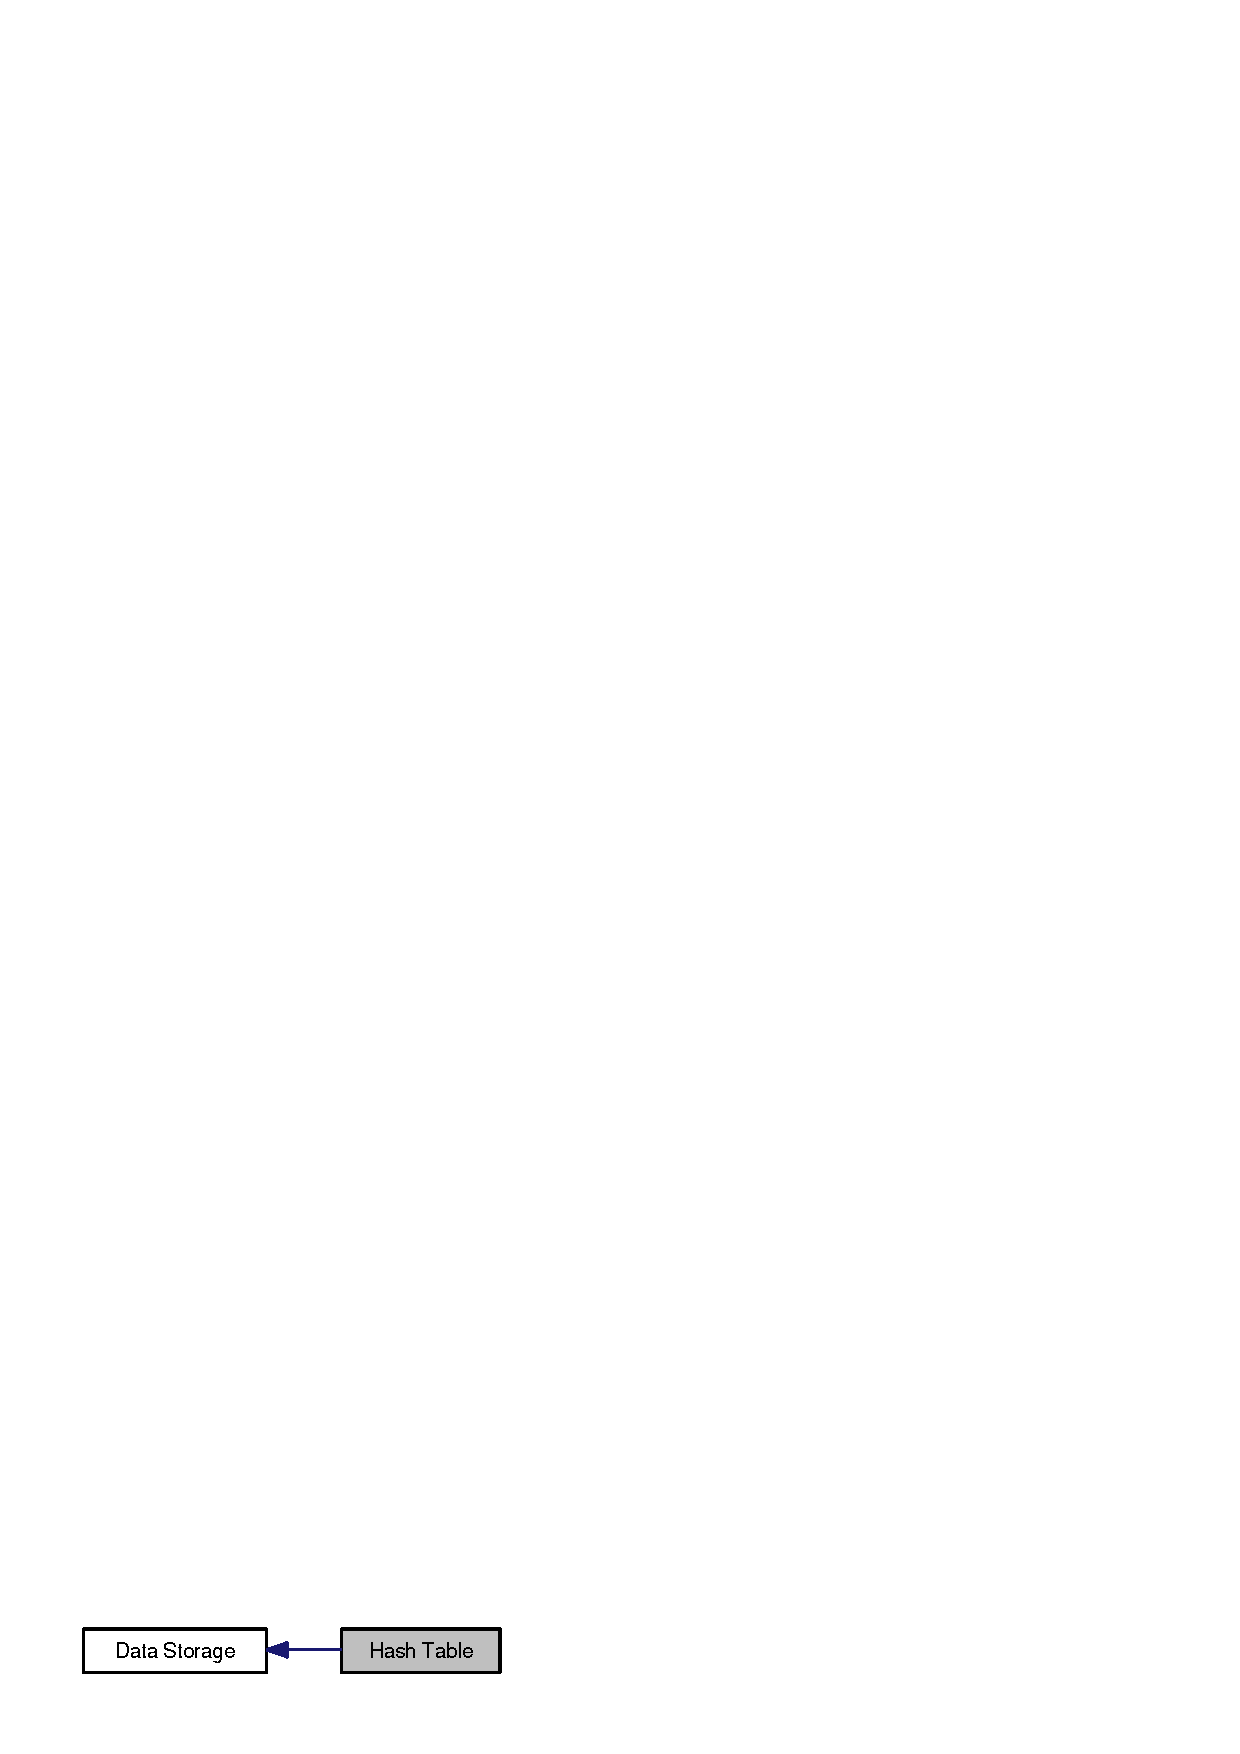
\includegraphics[width=122pt]{group__hashtab}
\end{center}
\end{figure}
\subsection*{Data Structures}
\begin{DoxyCompactItemize}
\item 
struct \hyperlink{structt__hashtab__entry}{t\_\-hashtab\_\-entry}
\begin{DoxyCompactList}\small\item\em A hashtab entry. \item\end{DoxyCompactList}\item 
struct \hyperlink{structt__hashtab}{t\_\-hashtab}
\begin{DoxyCompactList}\small\item\em The hashtab object. \item\end{DoxyCompactList}\end{DoxyCompactItemize}
\subsection*{Defines}
\begin{DoxyCompactItemize}
\item 
\#define \hyperlink{group__hashtab_ga160118a25646d04cce8c75f6f3eb9207}{HASH\_\-DEFSLOTS}~57
\begin{DoxyCompactList}\small\item\em Default number of slots in the hash table. \item\end{DoxyCompactList}\end{DoxyCompactItemize}
\subsection*{Functions}
\begin{DoxyCompactItemize}
\item 
\hyperlink{structt__hashtab}{t\_\-hashtab} $\ast$ \hyperlink{group__hashtab_ga70be9bbfb9bd9383824df0832477267f}{hashtab\_\-new} (long slotcount)
\begin{DoxyCompactList}\small\item\em Create a new hashtab object. \item\end{DoxyCompactList}\item 
\hyperlink{group__datatypes_ga73edaae82b318855cc09fac994918165}{t\_\-max\_\-err} \hyperlink{group__hashtab_gaa26ebe9ba21e84dd0dbb8d5aed12e5a1}{hashtab\_\-store} (\hyperlink{structt__hashtab}{t\_\-hashtab} $\ast$x, \hyperlink{structt__symbol}{t\_\-symbol} $\ast$key, \hyperlink{structt__object}{t\_\-object} $\ast$val)
\begin{DoxyCompactList}\small\item\em Store an item in a hashtab with an associated key. \item\end{DoxyCompactList}\item 
\hyperlink{group__datatypes_ga73edaae82b318855cc09fac994918165}{t\_\-max\_\-err} \hyperlink{group__hashtab_ga31d25e5b56c439be3f31bf17efa36349}{hashtab\_\-store\_\-safe} (\hyperlink{structt__hashtab}{t\_\-hashtab} $\ast$x, \hyperlink{structt__symbol}{t\_\-symbol} $\ast$key, \hyperlink{structt__object}{t\_\-object} $\ast$val)
\begin{DoxyCompactList}\small\item\em Store an item in a hashtab with an associated key. \item\end{DoxyCompactList}\item 
\hyperlink{group__datatypes_ga73edaae82b318855cc09fac994918165}{t\_\-max\_\-err} \hyperlink{group__hashtab_gab09bf88c81aeb3d71b6661f20989603d}{hashtab\_\-storeflags} (\hyperlink{structt__hashtab}{t\_\-hashtab} $\ast$x, \hyperlink{structt__symbol}{t\_\-symbol} $\ast$key, \hyperlink{structt__object}{t\_\-object} $\ast$val, long flags)
\begin{DoxyCompactList}\small\item\em Store an item in a hashtab with an associated key and also flags that define the behavior of the item. \item\end{DoxyCompactList}\item 
\hyperlink{group__datatypes_ga73edaae82b318855cc09fac994918165}{t\_\-max\_\-err} \hyperlink{group__hashtab_gadb206ea811204926bdbf1aa00ca679dc}{hashtab\_\-lookup} (\hyperlink{structt__hashtab}{t\_\-hashtab} $\ast$x, \hyperlink{structt__symbol}{t\_\-symbol} $\ast$key, \hyperlink{structt__object}{t\_\-object} $\ast$$\ast$val)
\begin{DoxyCompactList}\small\item\em Return an item stored in a hashtab with the specified key. \item\end{DoxyCompactList}\item 
\hyperlink{group__datatypes_ga73edaae82b318855cc09fac994918165}{t\_\-max\_\-err} \hyperlink{group__hashtab_ga0947b6e2b1e6ed6b55b7f891536429b9}{hashtab\_\-lookupflags} (\hyperlink{structt__hashtab}{t\_\-hashtab} $\ast$x, \hyperlink{structt__symbol}{t\_\-symbol} $\ast$key, \hyperlink{structt__object}{t\_\-object} $\ast$$\ast$val, long $\ast$flags)
\begin{DoxyCompactList}\small\item\em Return an item stored in a hashtab with the specified key, also returning the items flags. \item\end{DoxyCompactList}\item 
\hyperlink{group__datatypes_ga73edaae82b318855cc09fac994918165}{t\_\-max\_\-err} \hyperlink{group__hashtab_gadc3b33bd84f054f9a725b87e809779fc}{hashtab\_\-delete} (\hyperlink{structt__hashtab}{t\_\-hashtab} $\ast$x, \hyperlink{structt__symbol}{t\_\-symbol} $\ast$key)
\begin{DoxyCompactList}\small\item\em Remove an item from a hashtab associated with the specified key and free it. \item\end{DoxyCompactList}\item 
\hyperlink{group__datatypes_ga73edaae82b318855cc09fac994918165}{t\_\-max\_\-err} \hyperlink{group__hashtab_gae7984db2865416d6da6ce20c76975321}{hashtab\_\-clear} (\hyperlink{structt__hashtab}{t\_\-hashtab} $\ast$x)
\begin{DoxyCompactList}\small\item\em Delete all items stored in a hashtab. \item\end{DoxyCompactList}\item 
\hyperlink{group__datatypes_ga73edaae82b318855cc09fac994918165}{t\_\-max\_\-err} \hyperlink{group__hashtab_ga9bbf0199ef8b92a977b3bee5fd746799}{hashtab\_\-chuckkey} (\hyperlink{structt__hashtab}{t\_\-hashtab} $\ast$x, \hyperlink{structt__symbol}{t\_\-symbol} $\ast$key)
\begin{DoxyCompactList}\small\item\em Remove an item from a hashtab associated with a given key. \item\end{DoxyCompactList}\item 
\hyperlink{group__datatypes_ga73edaae82b318855cc09fac994918165}{t\_\-max\_\-err} \hyperlink{group__hashtab_gac3203c76c8321cde39088beab8b4d2e8}{hashtab\_\-chuck} (\hyperlink{structt__hashtab}{t\_\-hashtab} $\ast$x)
\begin{DoxyCompactList}\small\item\em Free a hashtab, but don't free the items it contains. \item\end{DoxyCompactList}\item 
\hyperlink{group__datatypes_ga73edaae82b318855cc09fac994918165}{t\_\-max\_\-err} \hyperlink{group__hashtab_gadc142f0a2a64417bb8b8d3c2959924fd}{hashtab\_\-findfirst} (\hyperlink{structt__hashtab}{t\_\-hashtab} $\ast$x, void $\ast$$\ast$o, long cmpfn(void $\ast$, void $\ast$), void $\ast$cmpdata)
\begin{DoxyCompactList}\small\item\em Search the hash table for the first item meeting defined criteria. \item\end{DoxyCompactList}\item 
\hyperlink{group__datatypes_ga73edaae82b318855cc09fac994918165}{t\_\-max\_\-err} \hyperlink{group__hashtab_ga816a6164c9565fd4269e2b9d8e8a76a3}{hashtab\_\-methodall} (\hyperlink{structt__hashtab}{t\_\-hashtab} $\ast$x, \hyperlink{structt__symbol}{t\_\-symbol} $\ast$s,...)
\begin{DoxyCompactList}\small\item\em Call the named message on every object in the hashtab. \item\end{DoxyCompactList}\item 
\hyperlink{group__datatypes_ga73edaae82b318855cc09fac994918165}{t\_\-max\_\-err} \hyperlink{group__hashtab_ga37e7b5c20c9fc69e9435f788f35335dc}{hashtab\_\-funall} (\hyperlink{structt__hashtab}{t\_\-hashtab} $\ast$x, \hyperlink{group__datatypes_gac26ba0a173b50597f5738132e059b42d}{method} fun, void $\ast$arg)
\begin{DoxyCompactList}\small\item\em Call the specified function for every item in the hashtab. \item\end{DoxyCompactList}\item 
long \hyperlink{group__hashtab_gaf0d337d2d3d31e2ea5a5a3bff01fe833}{hashtab\_\-getsize} (\hyperlink{structt__hashtab}{t\_\-hashtab} $\ast$x)
\begin{DoxyCompactList}\small\item\em Return the number of items stored in a hashtab. \item\end{DoxyCompactList}\item 
void \hyperlink{group__hashtab_gaede9b374c667cce86eeb976940eb9c53}{hashtab\_\-print} (\hyperlink{structt__hashtab}{t\_\-hashtab} $\ast$x)
\begin{DoxyCompactList}\small\item\em Post a hashtab's statistics to the Max window. \item\end{DoxyCompactList}\item 
void \hyperlink{group__hashtab_ga34ced5b4da65b4068829f799a53ea6bf}{hashtab\_\-readonly} (\hyperlink{structt__hashtab}{t\_\-hashtab} $\ast$x, long readonly)
\begin{DoxyCompactList}\small\item\em Set the hashtab's readonly bit. \item\end{DoxyCompactList}\item 
void \hyperlink{group__hashtab_gaaaefb350afdfdbe1440dd6401ac56eb7}{hashtab\_\-flags} (\hyperlink{structt__hashtab}{t\_\-hashtab} $\ast$x, long flags)
\begin{DoxyCompactList}\small\item\em Set the hashtab's datastore flags. \item\end{DoxyCompactList}\item 
long \hyperlink{group__hashtab_gacb0dd87fc4594d35d53998e7fde2c2b8}{hashtab\_\-getflags} (\hyperlink{structt__hashtab}{t\_\-hashtab} $\ast$x)
\begin{DoxyCompactList}\small\item\em Get the hashtab's datastore flags. \item\end{DoxyCompactList}\item 
\hyperlink{group__datatypes_ga73edaae82b318855cc09fac994918165}{t\_\-max\_\-err} \hyperlink{group__hashtab_gab5cb27719ed31725c46ff3ff52356aa8}{hashtab\_\-keyflags} (\hyperlink{structt__hashtab}{t\_\-hashtab} $\ast$x, \hyperlink{structt__symbol}{t\_\-symbol} $\ast$key, long flags)
\begin{DoxyCompactList}\small\item\em Change the flags for an item stored in the hashtab with a given key. \item\end{DoxyCompactList}\item 
long \hyperlink{group__hashtab_ga3d1819d75d2b09aefae9d58fc8016cec}{hashtab\_\-getkeyflags} (\hyperlink{structt__hashtab}{t\_\-hashtab} $\ast$x, \hyperlink{structt__symbol}{t\_\-symbol} $\ast$key)
\begin{DoxyCompactList}\small\item\em Retrieve the flags for an item stored in the hashtab with a given key. \item\end{DoxyCompactList}\item 
\hyperlink{group__datatypes_ga73edaae82b318855cc09fac994918165}{t\_\-max\_\-err} \hyperlink{group__hashtab_gaef45959b197448cfec26056d4d5656f0}{hashtab\_\-getkeys} (\hyperlink{structt__hashtab}{t\_\-hashtab} $\ast$x, long $\ast$kc, \hyperlink{structt__symbol}{t\_\-symbol} $\ast$$\ast$$\ast$kv)
\begin{DoxyCompactList}\small\item\em Retrieve all of the keys stored in a hashtab. \item\end{DoxyCompactList}\end{DoxyCompactItemize}


\subsection{Detailed Description}
Max's hashtab object implements a hash table ( \href{http://en.wikipedia.org/wiki/Hash_table}{\tt http://en.wikipedia.org/wiki/Hash\_\-table} ). Any type of value may be stored in the table, indexed using a \hyperlink{structt__symbol}{t\_\-symbol} as the unique key.

\begin{DoxySeeAlso}{See also}
\hyperlink{group__linklist}{Linked List} 
\end{DoxySeeAlso}


\subsection{Define Documentation}
\hypertarget{group__hashtab_ga160118a25646d04cce8c75f6f3eb9207}{
\index{hashtab@{hashtab}!HASH\_\-DEFSLOTS@{HASH\_\-DEFSLOTS}}
\index{HASH\_\-DEFSLOTS@{HASH\_\-DEFSLOTS}!hashtab@{hashtab}}
\subsubsection[{HASH\_\-DEFSLOTS}]{\setlength{\rightskip}{0pt plus 5cm}\#define HASH\_\-DEFSLOTS~57}}
\label{group__hashtab_ga160118a25646d04cce8c75f6f3eb9207}


Default number of slots in the hash table. Creating a hashtab using \hyperlink{group__hashtab_ga70be9bbfb9bd9383824df0832477267f}{hashtab\_\-new()} with an argument of 0 will use the default number of slots. Primes typically work well for the number of slots. 

\subsection{Function Documentation}
\hypertarget{group__hashtab_gac3203c76c8321cde39088beab8b4d2e8}{
\index{hashtab@{hashtab}!hashtab\_\-chuck@{hashtab\_\-chuck}}
\index{hashtab\_\-chuck@{hashtab\_\-chuck}!hashtab@{hashtab}}
\subsubsection[{hashtab\_\-chuck}]{\setlength{\rightskip}{0pt plus 5cm}{\bf t\_\-max\_\-err} hashtab\_\-chuck ({\bf t\_\-hashtab} $\ast$ {\em x})}}
\label{group__hashtab_gac3203c76c8321cde39088beab8b4d2e8}


Free a hashtab, but don't free the items it contains. The hashtab can contain a variety of different types of data. By default, the hashtab assumes that all items are max objects with a valid \hyperlink{structt__object}{t\_\-object} header.

You can alter the hashtab's notion of what it contains by using the \hyperlink{group__hashtab_gaaaefb350afdfdbe1440dd6401ac56eb7}{hashtab\_\-flags()} method.

When you free the hashtab by calling \hyperlink{group__obj_ga3759846cb356195532c41e35b87522ee}{object\_\-free()} it then tries to free all of the items it contains. If the hashtab is storing a custom type of data, or should otherwise not free the data it contains, then call \hyperlink{group__hashtab_gac3203c76c8321cde39088beab8b4d2e8}{hashtab\_\-chuck()} to free the object instead of \hyperlink{group__obj_ga3759846cb356195532c41e35b87522ee}{object\_\-free()}.


\begin{DoxyParams}{Parameters}
\item[{\em x}]The hashtab object to be freed. \end{DoxyParams}
\begin{DoxyReturn}{Returns}
A max error code. 
\end{DoxyReturn}
\begin{DoxySeeAlso}{See also}
\hyperlink{group__obj_ga3759846cb356195532c41e35b87522ee}{object\_\-free} 
\end{DoxySeeAlso}
\hypertarget{group__hashtab_ga9bbf0199ef8b92a977b3bee5fd746799}{
\index{hashtab@{hashtab}!hashtab\_\-chuckkey@{hashtab\_\-chuckkey}}
\index{hashtab\_\-chuckkey@{hashtab\_\-chuckkey}!hashtab@{hashtab}}
\subsubsection[{hashtab\_\-chuckkey}]{\setlength{\rightskip}{0pt plus 5cm}{\bf t\_\-max\_\-err} hashtab\_\-chuckkey ({\bf t\_\-hashtab} $\ast$ {\em x}, \/  {\bf t\_\-symbol} $\ast$ {\em key})}}
\label{group__hashtab_ga9bbf0199ef8b92a977b3bee5fd746799}


Remove an item from a hashtab associated with a given key. You are responsible for freeing any memory associated with the item that is removed from the hashtab.


\begin{DoxyParams}{Parameters}
\item[{\em x}]The hashtab instance. \item[{\em key}]The key of the item to delete. \end{DoxyParams}
\begin{DoxyReturn}{Returns}
A Max error code.
\end{DoxyReturn}
\begin{DoxySeeAlso}{See also}
\hyperlink{group__hashtab_gadc3b33bd84f054f9a725b87e809779fc}{hashtab\_\-delete} 
\end{DoxySeeAlso}
\hypertarget{group__hashtab_gae7984db2865416d6da6ce20c76975321}{
\index{hashtab@{hashtab}!hashtab\_\-clear@{hashtab\_\-clear}}
\index{hashtab\_\-clear@{hashtab\_\-clear}!hashtab@{hashtab}}
\subsubsection[{hashtab\_\-clear}]{\setlength{\rightskip}{0pt plus 5cm}{\bf t\_\-max\_\-err} hashtab\_\-clear ({\bf t\_\-hashtab} $\ast$ {\em x})}}
\label{group__hashtab_gae7984db2865416d6da6ce20c76975321}


Delete all items stored in a hashtab. This is the equivalent of calling \hyperlink{group__hashtab_gadc3b33bd84f054f9a725b87e809779fc}{hashtab\_\-delete()} on every item in a hashtab.

\begin{DoxyReturn}{Returns}
A max error code. 
\end{DoxyReturn}
\begin{DoxySeeAlso}{See also}
\hyperlink{group__hashtab_gaaaefb350afdfdbe1440dd6401ac56eb7}{hashtab\_\-flags()} 

\hyperlink{group__hashtab_gadc3b33bd84f054f9a725b87e809779fc}{hashtab\_\-delete()} 
\end{DoxySeeAlso}
\hypertarget{group__hashtab_gadc3b33bd84f054f9a725b87e809779fc}{
\index{hashtab@{hashtab}!hashtab\_\-delete@{hashtab\_\-delete}}
\index{hashtab\_\-delete@{hashtab\_\-delete}!hashtab@{hashtab}}
\subsubsection[{hashtab\_\-delete}]{\setlength{\rightskip}{0pt plus 5cm}{\bf t\_\-max\_\-err} hashtab\_\-delete ({\bf t\_\-hashtab} $\ast$ {\em x}, \/  {\bf t\_\-symbol} $\ast$ {\em key})}}
\label{group__hashtab_gadc3b33bd84f054f9a725b87e809779fc}


Remove an item from a hashtab associated with the specified key and free it. The hashtab can contain a variety of different types of data. By default, the hashtab assumes that all items are max objects with a valid \hyperlink{structt__object}{t\_\-object} header. Thus by default, it frees items by calling \hyperlink{group__obj_ga3759846cb356195532c41e35b87522ee}{object\_\-free()} on them.

You can alter the hashtab's notion of what it contains by using the \hyperlink{group__hashtab_gaaaefb350afdfdbe1440dd6401ac56eb7}{hashtab\_\-flags()} method.

If you wish to remove an item from the hashtab and free it yourself, then you should use \hyperlink{group__hashtab_ga9bbf0199ef8b92a977b3bee5fd746799}{hashtab\_\-chuckkey()}.


\begin{DoxyParams}{Parameters}
\item[{\em x}]The hashtab instance. \item[{\em key}]The key of the item to delete. \end{DoxyParams}
\begin{DoxyReturn}{Returns}
A Max error code.
\end{DoxyReturn}
\begin{DoxySeeAlso}{See also}
\hyperlink{group__hashtab_ga9bbf0199ef8b92a977b3bee5fd746799}{hashtab\_\-chuckkey()} 

\hyperlink{group__hashtab_gae7984db2865416d6da6ce20c76975321}{hashtab\_\-clear()} 

\hyperlink{group__hashtab_gaaaefb350afdfdbe1440dd6401ac56eb7}{hashtab\_\-flags()} 
\end{DoxySeeAlso}
\hypertarget{group__hashtab_gadc142f0a2a64417bb8b8d3c2959924fd}{
\index{hashtab@{hashtab}!hashtab\_\-findfirst@{hashtab\_\-findfirst}}
\index{hashtab\_\-findfirst@{hashtab\_\-findfirst}!hashtab@{hashtab}}
\subsubsection[{hashtab\_\-findfirst}]{\setlength{\rightskip}{0pt plus 5cm}{\bf t\_\-max\_\-err} hashtab\_\-findfirst ({\bf t\_\-hashtab} $\ast$ {\em x}, \/  void $\ast$$\ast$ {\em o}, \/  long  {\em cmpfn}void $\ast$, void $\ast$, \/  void $\ast$ {\em cmpdata})}}
\label{group__hashtab_gadc142f0a2a64417bb8b8d3c2959924fd}


Search the hash table for the first item meeting defined criteria. The items in the hashtab are iteratively processed, calling a specified comparison function on each until the comparison function returns true.


\begin{DoxyParams}{Parameters}
\item[{\em x}]The hashtab instance. \item[{\em o}]The address to pointer that will be set with the matching item. \item[{\em cmpfn}]The function used to determine a match in the list. \item[{\em cmpdata}]An argument to be passed to the \hyperlink{group__datastore_gaaf4ae6dd800a2be9abd645cf70aeb38f}{t\_\-cmpfn}. This will be passed as the second of the two args to the \hyperlink{group__datastore_gaaf4ae6dd800a2be9abd645cf70aeb38f}{t\_\-cmpfn}. The first arg will be the hashtab item at each iteration in the list. \end{DoxyParams}
\begin{DoxyReturn}{Returns}
A max error code.
\end{DoxyReturn}
\begin{DoxySeeAlso}{See also}
\hyperlink{group__linklist_gab7f3c26cb704c460892818b89a1ab004}{linklist\_\-findfirst()} 

\hyperlink{group__datastore_gaaf4ae6dd800a2be9abd645cf70aeb38f}{t\_\-cmpfn} 
\end{DoxySeeAlso}
\hypertarget{group__hashtab_gaaaefb350afdfdbe1440dd6401ac56eb7}{
\index{hashtab@{hashtab}!hashtab\_\-flags@{hashtab\_\-flags}}
\index{hashtab\_\-flags@{hashtab\_\-flags}!hashtab@{hashtab}}
\subsubsection[{hashtab\_\-flags}]{\setlength{\rightskip}{0pt plus 5cm}void hashtab\_\-flags ({\bf t\_\-hashtab} $\ast$ {\em x}, \/  long {\em flags})}}
\label{group__hashtab_gaaaefb350afdfdbe1440dd6401ac56eb7}


Set the hashtab's datastore flags. The available flags are enumerated in \hyperlink{group__datastore_gaa858d4b3815076d79624c39d9ca59348}{e\_\-max\_\-datastore\_\-flags}. These flags control the behavior of the hashtab, particularly when removing items from the list using functions such as \hyperlink{group__hashtab_gae7984db2865416d6da6ce20c76975321}{hashtab\_\-clear()}, \hyperlink{group__hashtab_gadc3b33bd84f054f9a725b87e809779fc}{hashtab\_\-delete()}, or when freeing the hashtab itself.


\begin{DoxyParams}{Parameters}
\item[{\em x}]The hashtab instance. \item[{\em flags}]A valid value from the \hyperlink{group__datastore_gaa858d4b3815076d79624c39d9ca59348}{e\_\-max\_\-datastore\_\-flags}. The default is \hyperlink{group__datastore_ggaa858d4b3815076d79624c39d9ca59348adc630c58c8e958a404553a08db6fd180}{OBJ\_\-FLAG\_\-OBJ}. \end{DoxyParams}
\hypertarget{group__hashtab_ga37e7b5c20c9fc69e9435f788f35335dc}{
\index{hashtab@{hashtab}!hashtab\_\-funall@{hashtab\_\-funall}}
\index{hashtab\_\-funall@{hashtab\_\-funall}!hashtab@{hashtab}}
\subsubsection[{hashtab\_\-funall}]{\setlength{\rightskip}{0pt plus 5cm}{\bf t\_\-max\_\-err} hashtab\_\-funall ({\bf t\_\-hashtab} $\ast$ {\em x}, \/  {\bf method} {\em fun}, \/  void $\ast$ {\em arg})}}
\label{group__hashtab_ga37e7b5c20c9fc69e9435f788f35335dc}


Call the specified function for every item in the hashtab. 
\begin{DoxyParams}{Parameters}
\item[{\em x}]The hashtab instance. \item[{\em fun}]The function to call, specified as function pointer cast to a Max \hyperlink{group__datatypes_gac26ba0a173b50597f5738132e059b42d}{method}. \item[{\em arg}]An argument that you would like to pass to the function being called. \end{DoxyParams}
\begin{DoxyReturn}{Returns}
A max error code.
\end{DoxyReturn}
\begin{DoxyRemark}{Remarks}
The \hyperlink{group__hashtab_ga37e7b5c20c9fc69e9435f788f35335dc}{hashtab\_\-funall()} method will call your function for every item in the list. It will pass both a pointer to the item in the list, and any argument that you provide. The following example shows a function that could be called by \hyperlink{group__hashtab_ga37e7b5c20c9fc69e9435f788f35335dc}{hashtab\_\-funall()}. 
\begin{DoxyCode}
    void myFun(t_hashtab_entry *e, void *myArg)
    {
        if (e->key && e->value) {
            // do something with e->key, e->value, and myArg here as appropriate
        }
    }
\end{DoxyCode}
 
\end{DoxyRemark}
\hypertarget{group__hashtab_gacb0dd87fc4594d35d53998e7fde2c2b8}{
\index{hashtab@{hashtab}!hashtab\_\-getflags@{hashtab\_\-getflags}}
\index{hashtab\_\-getflags@{hashtab\_\-getflags}!hashtab@{hashtab}}
\subsubsection[{hashtab\_\-getflags}]{\setlength{\rightskip}{0pt plus 5cm}long hashtab\_\-getflags ({\bf t\_\-hashtab} $\ast$ {\em x})}}
\label{group__hashtab_gacb0dd87fc4594d35d53998e7fde2c2b8}


Get the hashtab's datastore flags. 
\begin{DoxyParams}{Parameters}
\item[{\em x}]The hashtab instance. \end{DoxyParams}
\begin{DoxyReturn}{Returns}
The current state of the hashtab flags as enumerated in \hyperlink{group__datastore_gaa858d4b3815076d79624c39d9ca59348}{e\_\-max\_\-datastore\_\-flags}. 
\end{DoxyReturn}
\hypertarget{group__hashtab_ga3d1819d75d2b09aefae9d58fc8016cec}{
\index{hashtab@{hashtab}!hashtab\_\-getkeyflags@{hashtab\_\-getkeyflags}}
\index{hashtab\_\-getkeyflags@{hashtab\_\-getkeyflags}!hashtab@{hashtab}}
\subsubsection[{hashtab\_\-getkeyflags}]{\setlength{\rightskip}{0pt plus 5cm}long hashtab\_\-getkeyflags ({\bf t\_\-hashtab} $\ast$ {\em x}, \/  {\bf t\_\-symbol} $\ast$ {\em key})}}
\label{group__hashtab_ga3d1819d75d2b09aefae9d58fc8016cec}


Retrieve the flags for an item stored in the hashtab with a given key. 
\begin{DoxyParams}{Parameters}
\item[{\em x}]The hashtab instance. \item[{\em key}]The key in the hashtab whose flags will be returned. \end{DoxyParams}
\begin{DoxyReturn}{Returns}
The flags for the given key. 
\end{DoxyReturn}
\begin{DoxySeeAlso}{See also}
hashtab\_\-store\_\-flags() 
\end{DoxySeeAlso}
\hypertarget{group__hashtab_gaef45959b197448cfec26056d4d5656f0}{
\index{hashtab@{hashtab}!hashtab\_\-getkeys@{hashtab\_\-getkeys}}
\index{hashtab\_\-getkeys@{hashtab\_\-getkeys}!hashtab@{hashtab}}
\subsubsection[{hashtab\_\-getkeys}]{\setlength{\rightskip}{0pt plus 5cm}{\bf t\_\-max\_\-err} hashtab\_\-getkeys ({\bf t\_\-hashtab} $\ast$ {\em x}, \/  long $\ast$ {\em kc}, \/  {\bf t\_\-symbol} $\ast$$\ast$$\ast$ {\em kv})}}
\label{group__hashtab_gaef45959b197448cfec26056d4d5656f0}


Retrieve all of the keys stored in a hashtab. If the kc and kv parameters are properly initialized to zero, then \hyperlink{group__hashtab_gaef45959b197448cfec26056d4d5656f0}{hashtab\_\-getkeys()} will allocate memory for the keys it returns. You are then responsible for freeing this memory using \hyperlink{group__memory_ga200c82639e547869db1f3887d17102d3}{sysmem\_\-freeptr()}.


\begin{DoxyParams}{Parameters}
\item[{\em x}]The hashtab instance. \item[{\em kc}]The address of a long where the number of keys retrieved will be set. \item[{\em kv}]The address of the first of an array \hyperlink{structt__symbol}{t\_\-symbol} pointers where the retrieved keys will be set. \end{DoxyParams}
\begin{DoxyReturn}{Returns}
A max error code.
\end{DoxyReturn}
\begin{DoxyRemark}{Remarks}
The following example demonstrates fetching all of the keys from a hashtab in order to iterate through each item stored in the hashtab. 
\begin{DoxyCode}
    t_symbol    **keys = NULL;
    long        numKeys = 0;
    long        i;
    t_object    *anItem;

    hashtab_getkeys(aHashtab, &numKeys, &keys);
    for(i=0; i<numKeys; i++){
        hashtab_lookup(aHashtab, keys[i], &anItem);
        // Do something with anItem here...
    }
    if(keys)
        sysmem_freeptr(keys);
\end{DoxyCode}
 
\end{DoxyRemark}
\hypertarget{group__hashtab_gaf0d337d2d3d31e2ea5a5a3bff01fe833}{
\index{hashtab@{hashtab}!hashtab\_\-getsize@{hashtab\_\-getsize}}
\index{hashtab\_\-getsize@{hashtab\_\-getsize}!hashtab@{hashtab}}
\subsubsection[{hashtab\_\-getsize}]{\setlength{\rightskip}{0pt plus 5cm}long hashtab\_\-getsize ({\bf t\_\-hashtab} $\ast$ {\em x})}}
\label{group__hashtab_gaf0d337d2d3d31e2ea5a5a3bff01fe833}


Return the number of items stored in a hashtab. 
\begin{DoxyParams}{Parameters}
\item[{\em x}]The hashtab instance. \end{DoxyParams}
\begin{DoxyReturn}{Returns}
The number of items in the hash table. 
\end{DoxyReturn}
\hypertarget{group__hashtab_gab5cb27719ed31725c46ff3ff52356aa8}{
\index{hashtab@{hashtab}!hashtab\_\-keyflags@{hashtab\_\-keyflags}}
\index{hashtab\_\-keyflags@{hashtab\_\-keyflags}!hashtab@{hashtab}}
\subsubsection[{hashtab\_\-keyflags}]{\setlength{\rightskip}{0pt plus 5cm}{\bf t\_\-max\_\-err} hashtab\_\-keyflags ({\bf t\_\-hashtab} $\ast$ {\em x}, \/  {\bf t\_\-symbol} $\ast$ {\em key}, \/  long {\em flags})}}
\label{group__hashtab_gab5cb27719ed31725c46ff3ff52356aa8}


Change the flags for an item stored in the hashtab with a given key. 
\begin{DoxyParams}{Parameters}
\item[{\em x}]The hashtab instance. \item[{\em key}]The key in the hashtab whose flags will be changed. \item[{\em flags}]One of the values listed in \hyperlink{group__datastore_gaa858d4b3815076d79624c39d9ca59348}{e\_\-max\_\-datastore\_\-flags}. \end{DoxyParams}
\begin{DoxyReturn}{Returns}
A Max error code. 
\end{DoxyReturn}
\begin{DoxySeeAlso}{See also}
hashtab\_\-store\_\-flags() 
\end{DoxySeeAlso}
\hypertarget{group__hashtab_gadb206ea811204926bdbf1aa00ca679dc}{
\index{hashtab@{hashtab}!hashtab\_\-lookup@{hashtab\_\-lookup}}
\index{hashtab\_\-lookup@{hashtab\_\-lookup}!hashtab@{hashtab}}
\subsubsection[{hashtab\_\-lookup}]{\setlength{\rightskip}{0pt plus 5cm}{\bf t\_\-max\_\-err} hashtab\_\-lookup ({\bf t\_\-hashtab} $\ast$ {\em x}, \/  {\bf t\_\-symbol} $\ast$ {\em key}, \/  {\bf t\_\-object} $\ast$$\ast$ {\em val})}}
\label{group__hashtab_gadb206ea811204926bdbf1aa00ca679dc}


Return an item stored in a hashtab with the specified key. 
\begin{DoxyParams}{Parameters}
\item[{\em x}]The hashtab instance. \item[{\em key}]The key in the hashtab to fetch. \item[{\em val}]The address of a pointer to which the fetched value will be assigned.\end{DoxyParams}
\begin{DoxyReturn}{Returns}
A Max error code. 
\end{DoxyReturn}
\begin{DoxySeeAlso}{See also}
\hyperlink{group__hashtab_gaa26ebe9ba21e84dd0dbb8d5aed12e5a1}{hashtab\_\-store()} 
\end{DoxySeeAlso}
\hypertarget{group__hashtab_ga0947b6e2b1e6ed6b55b7f891536429b9}{
\index{hashtab@{hashtab}!hashtab\_\-lookupflags@{hashtab\_\-lookupflags}}
\index{hashtab\_\-lookupflags@{hashtab\_\-lookupflags}!hashtab@{hashtab}}
\subsubsection[{hashtab\_\-lookupflags}]{\setlength{\rightskip}{0pt plus 5cm}{\bf t\_\-max\_\-err} hashtab\_\-lookupflags ({\bf t\_\-hashtab} $\ast$ {\em x}, \/  {\bf t\_\-symbol} $\ast$ {\em key}, \/  {\bf t\_\-object} $\ast$$\ast$ {\em val}, \/  long $\ast$ {\em flags})}}
\label{group__hashtab_ga0947b6e2b1e6ed6b55b7f891536429b9}


Return an item stored in a hashtab with the specified key, also returning the items flags. 
\begin{DoxyParams}{Parameters}
\item[{\em x}]The hashtab instance. \item[{\em key}]The key in the hashtab to fetch. \item[{\em val}]The address of a pointer to which the fetched value will be assigned. \item[{\em flags}]The address of a value to which the fetched flags will be assigned. \end{DoxyParams}
\begin{DoxyReturn}{Returns}
A Max error code. 
\end{DoxyReturn}
\begin{DoxySeeAlso}{See also}
\hyperlink{group__hashtab_gadb206ea811204926bdbf1aa00ca679dc}{hashtab\_\-lookup()} 

hashtab\_\-store\_\-flags() 
\end{DoxySeeAlso}
\hypertarget{group__hashtab_ga816a6164c9565fd4269e2b9d8e8a76a3}{
\index{hashtab@{hashtab}!hashtab\_\-methodall@{hashtab\_\-methodall}}
\index{hashtab\_\-methodall@{hashtab\_\-methodall}!hashtab@{hashtab}}
\subsubsection[{hashtab\_\-methodall}]{\setlength{\rightskip}{0pt plus 5cm}{\bf t\_\-max\_\-err} hashtab\_\-methodall ({\bf t\_\-hashtab} $\ast$ {\em x}, \/  {\bf t\_\-symbol} $\ast$ {\em s}, \/   {\em ...})}}
\label{group__hashtab_ga816a6164c9565fd4269e2b9d8e8a76a3}


Call the named message on every object in the hashtab. The \hyperlink{group__hashtab_ga816a6164c9565fd4269e2b9d8e8a76a3}{hashtab\_\-methodall()} function requires that all items in the hashtab are object instances with a valid \hyperlink{structt__object}{t\_\-object} header.


\begin{DoxyParams}{Parameters}
\item[{\em x}]The hashtab instance. \item[{\em s}]The name of the message to send to the objects. \item[{\em ...}]Any arguments to be sent with the message. \end{DoxyParams}
\begin{DoxyReturn}{Returns}
A max error code.
\end{DoxyReturn}
\begin{DoxyRemark}{Remarks}
Internally, this function uses \hyperlink{group__obj_gae740749094827ac5adc2b7145db1c596}{object\_\-method()}, meaning that no errors will be posted if the message name does not exist for the object. It also means that messages sent methods with \hyperlink{group__atom_gga8aa6700e9f00b132eb376db6e39ade47a81c1a8550f038db16a619167a70a79b6}{A\_\-GIMME} definitions will need to be given a symbol argument prior to the argc and argv array information. 
\end{DoxyRemark}
\hypertarget{group__hashtab_ga70be9bbfb9bd9383824df0832477267f}{
\index{hashtab@{hashtab}!hashtab\_\-new@{hashtab\_\-new}}
\index{hashtab\_\-new@{hashtab\_\-new}!hashtab@{hashtab}}
\subsubsection[{hashtab\_\-new}]{\setlength{\rightskip}{0pt plus 5cm}{\bf t\_\-hashtab}$\ast$ hashtab\_\-new (long {\em slotcount})}}
\label{group__hashtab_ga70be9bbfb9bd9383824df0832477267f}


Create a new hashtab object. You can free the hashtab by calling \hyperlink{group__obj_ga3759846cb356195532c41e35b87522ee}{object\_\-free()} on the hashtab's pointer, or by using \hyperlink{group__hashtab_gac3203c76c8321cde39088beab8b4d2e8}{hashtab\_\-chuck()}.


\begin{DoxyParams}{Parameters}
\item[{\em slotcount}]The number of slots in the hash table. Prime numbers typically work well. Pass 0 to get the default size. \end{DoxyParams}
\begin{DoxyReturn}{Returns}
Pointer to the new hashtab object.
\end{DoxyReturn}
\begin{DoxySeeAlso}{See also}
\hyperlink{group__hashtab_ga160118a25646d04cce8c75f6f3eb9207}{HASH\_\-DEFSLOTS} 

\hyperlink{group__obj_ga3759846cb356195532c41e35b87522ee}{object\_\-free()} 

\hyperlink{group__hashtab_gac3203c76c8321cde39088beab8b4d2e8}{hashtab\_\-chuck()} 
\end{DoxySeeAlso}
\hypertarget{group__hashtab_gaede9b374c667cce86eeb976940eb9c53}{
\index{hashtab@{hashtab}!hashtab\_\-print@{hashtab\_\-print}}
\index{hashtab\_\-print@{hashtab\_\-print}!hashtab@{hashtab}}
\subsubsection[{hashtab\_\-print}]{\setlength{\rightskip}{0pt plus 5cm}void hashtab\_\-print ({\bf t\_\-hashtab} $\ast$ {\em x})}}
\label{group__hashtab_gaede9b374c667cce86eeb976940eb9c53}


Post a hashtab's statistics to the Max window. 
\begin{DoxyParams}{Parameters}
\item[{\em x}]The hashtab instance. \end{DoxyParams}
\hypertarget{group__hashtab_ga34ced5b4da65b4068829f799a53ea6bf}{
\index{hashtab@{hashtab}!hashtab\_\-readonly@{hashtab\_\-readonly}}
\index{hashtab\_\-readonly@{hashtab\_\-readonly}!hashtab@{hashtab}}
\subsubsection[{hashtab\_\-readonly}]{\setlength{\rightskip}{0pt plus 5cm}void hashtab\_\-readonly ({\bf t\_\-hashtab} $\ast$ {\em x}, \/  long {\em readonly})}}
\label{group__hashtab_ga34ced5b4da65b4068829f799a53ea6bf}


Set the hashtab's readonly bit. By default the readonly bit is 0, indicating that it is threadsafe for both reading and writing. Setting the readonly bit to 1 will disable the hashtab's theadsafety mechanism, increasing performance but at the expense of threadsafe operation. Unless you can guarantee the threading context for a hashtab's use, you should leave this set to 0.


\begin{DoxyParams}{Parameters}
\item[{\em x}]The hashtab instance. \item[{\em readonly}]A 1 or 0 for setting the readonly bit. \end{DoxyParams}
\hypertarget{group__hashtab_gaa26ebe9ba21e84dd0dbb8d5aed12e5a1}{
\index{hashtab@{hashtab}!hashtab\_\-store@{hashtab\_\-store}}
\index{hashtab\_\-store@{hashtab\_\-store}!hashtab@{hashtab}}
\subsubsection[{hashtab\_\-store}]{\setlength{\rightskip}{0pt plus 5cm}{\bf t\_\-max\_\-err} hashtab\_\-store ({\bf t\_\-hashtab} $\ast$ {\em x}, \/  {\bf t\_\-symbol} $\ast$ {\em key}, \/  {\bf t\_\-object} $\ast$ {\em val})}}
\label{group__hashtab_gaa26ebe9ba21e84dd0dbb8d5aed12e5a1}


Store an item in a hashtab with an associated key. 
\begin{DoxyParams}{Parameters}
\item[{\em x}]The hashtab instance. \item[{\em key}]The key in the hashtab with which to associate the value. \item[{\em val}]The value to store.\end{DoxyParams}
\begin{DoxyReturn}{Returns}
A Max error code. 
\end{DoxyReturn}
\begin{DoxySeeAlso}{See also}
\hyperlink{group__hashtab_gadb206ea811204926bdbf1aa00ca679dc}{hashtab\_\-lookup()} 
\end{DoxySeeAlso}
\hypertarget{group__hashtab_ga31d25e5b56c439be3f31bf17efa36349}{
\index{hashtab@{hashtab}!hashtab\_\-store\_\-safe@{hashtab\_\-store\_\-safe}}
\index{hashtab\_\-store\_\-safe@{hashtab\_\-store\_\-safe}!hashtab@{hashtab}}
\subsubsection[{hashtab\_\-store\_\-safe}]{\setlength{\rightskip}{0pt plus 5cm}{\bf t\_\-max\_\-err} hashtab\_\-store\_\-safe ({\bf t\_\-hashtab} $\ast$ {\em x}, \/  {\bf t\_\-symbol} $\ast$ {\em key}, \/  {\bf t\_\-object} $\ast$ {\em val})}}
\label{group__hashtab_ga31d25e5b56c439be3f31bf17efa36349}


Store an item in a hashtab with an associated key. The difference between \hyperlink{group__hashtab_ga31d25e5b56c439be3f31bf17efa36349}{hashtab\_\-store\_\-safe()} and \hyperlink{group__hashtab_gaa26ebe9ba21e84dd0dbb8d5aed12e5a1}{hashtab\_\-store()} is what happens in the event of a collision in the hash table. The normal \hyperlink{group__hashtab_gaa26ebe9ba21e84dd0dbb8d5aed12e5a1}{hashtab\_\-store()} function will free the existing value at the collision location with \hyperlink{group__memory_ga200c82639e547869db1f3887d17102d3}{sysmem\_\-freeptr()} and then replaces it. This version doesn't try to free the existing value at the collision location, but instead just over-\/writes it.


\begin{DoxyParams}{Parameters}
\item[{\em x}]The hashtab instance. \item[{\em key}]The key in the hashtab with which to associate the value. \item[{\em val}]The value to store. \end{DoxyParams}
\begin{DoxyReturn}{Returns}
A Max error code. 
\end{DoxyReturn}
\begin{DoxySeeAlso}{See also}
\hyperlink{group__hashtab_gaa26ebe9ba21e84dd0dbb8d5aed12e5a1}{hashtab\_\-store()} 
\end{DoxySeeAlso}
\hypertarget{group__hashtab_gab09bf88c81aeb3d71b6661f20989603d}{
\index{hashtab@{hashtab}!hashtab\_\-storeflags@{hashtab\_\-storeflags}}
\index{hashtab\_\-storeflags@{hashtab\_\-storeflags}!hashtab@{hashtab}}
\subsubsection[{hashtab\_\-storeflags}]{\setlength{\rightskip}{0pt plus 5cm}{\bf t\_\-max\_\-err} hashtab\_\-storeflags ({\bf t\_\-hashtab} $\ast$ {\em x}, \/  {\bf t\_\-symbol} $\ast$ {\em key}, \/  {\bf t\_\-object} $\ast$ {\em val}, \/  long {\em flags})}}
\label{group__hashtab_gab09bf88c81aeb3d71b6661f20989603d}


Store an item in a hashtab with an associated key and also flags that define the behavior of the item. The \hyperlink{group__hashtab_gaa26ebe9ba21e84dd0dbb8d5aed12e5a1}{hashtab\_\-store()} method is the same as calling this method with the default (0) flags.


\begin{DoxyParams}{Parameters}
\item[{\em x}]The hashtab instance. \item[{\em key}]The key in the hashtab with which to associate the value. \item[{\em val}]The value to store. \item[{\em flags}]One of the values listed in \hyperlink{group__datastore_gaa858d4b3815076d79624c39d9ca59348}{e\_\-max\_\-datastore\_\-flags}. \end{DoxyParams}
\begin{DoxyReturn}{Returns}
A Max error code. 
\end{DoxyReturn}
\begin{DoxySeeAlso}{See also}
\hyperlink{group__hashtab_gaa26ebe9ba21e84dd0dbb8d5aed12e5a1}{hashtab\_\-store()} 
\end{DoxySeeAlso}

\hypertarget{group__indexmap}{
\section{Index Map}
\label{group__indexmap}\index{Index Map@{Index Map}}
}


An indexmap is basically a managed array of pointers, but it allows you to derive relatively quickly the index from a pointer in the array.  


Collaboration diagram for Index Map:\nopagebreak
\begin{figure}[H]
\begin{center}
\leavevmode
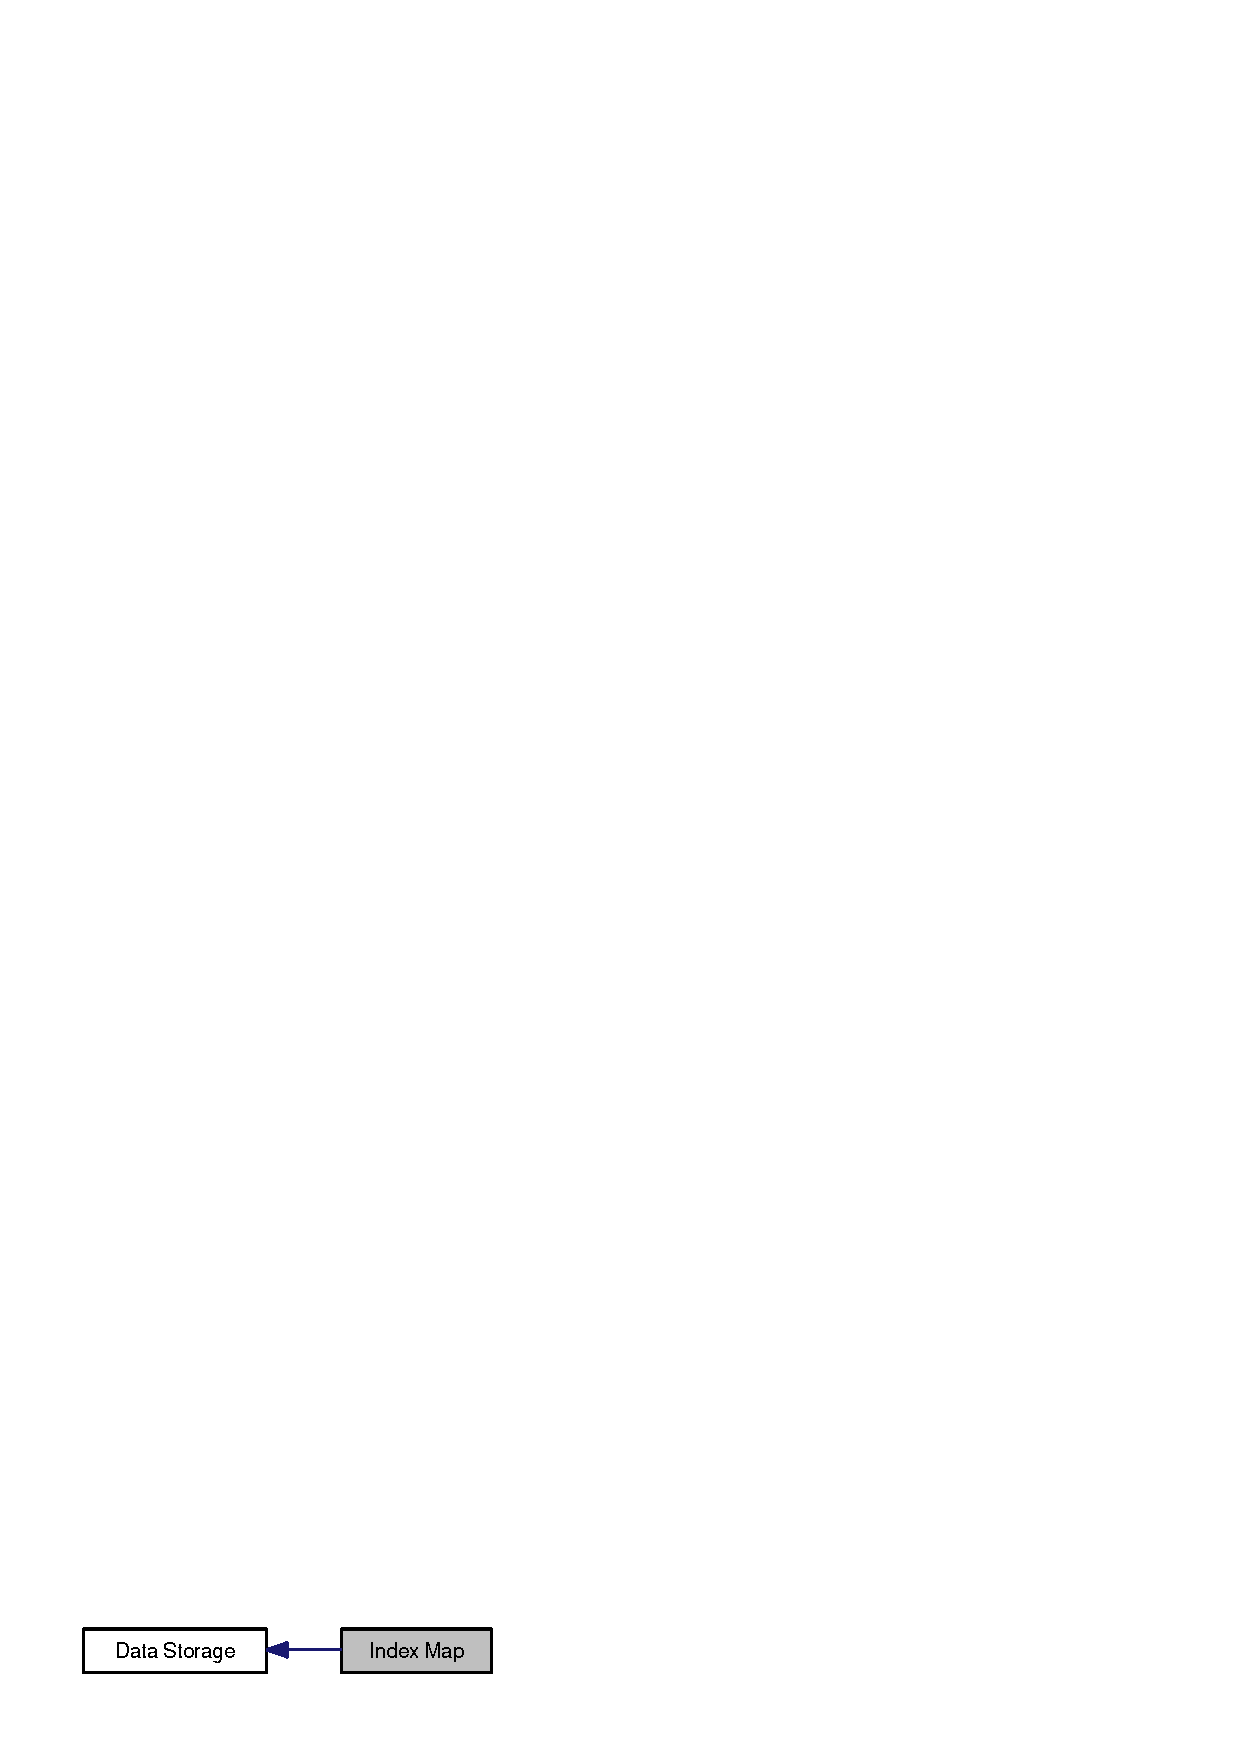
\includegraphics[width=120pt]{group__indexmap}
\end{center}
\end{figure}
\subsection*{Data Structures}
\begin{DoxyCompactItemize}
\item 
struct \hyperlink{structt__indexmap__entry}{t\_\-indexmap\_\-entry}
\begin{DoxyCompactList}\small\item\em An indexmap element. \item\end{DoxyCompactList}\item 
struct \hyperlink{structt__indexmap}{t\_\-indexmap}
\begin{DoxyCompactList}\small\item\em An indexmap object. \item\end{DoxyCompactList}\end{DoxyCompactItemize}
\subsection*{Functions}
\begin{DoxyCompactItemize}
\item 
\hyperlink{structt__indexmap}{t\_\-indexmap} $\ast$ \hyperlink{group__indexmap_ga2e7303d05103b7e42c1a12929f5233ec}{indexmap\_\-new} (void)
\begin{DoxyCompactList}\small\item\em Create a new indexmap object. \item\end{DoxyCompactList}\item 
void \hyperlink{group__indexmap_ga5083e00af855e9b1a20ee5321c8fe3c9}{indexmap\_\-append} (\hyperlink{structt__indexmap}{t\_\-indexmap} $\ast$x, void $\ast$data)
\begin{DoxyCompactList}\small\item\em Add an item to an indexmap. \item\end{DoxyCompactList}\item 
\hyperlink{group__datatypes_ga73edaae82b318855cc09fac994918165}{t\_\-max\_\-err} \hyperlink{group__indexmap_gab5f2093d1eb48203117b8bfc32ea5c31}{indexmap\_\-move} (\hyperlink{structt__indexmap}{t\_\-indexmap} $\ast$x, void $\ast$data, long newindex)
\begin{DoxyCompactList}\small\item\em Move an item to a different position in an indexmap. \item\end{DoxyCompactList}\item 
\hyperlink{group__datatypes_ga73edaae82b318855cc09fac994918165}{t\_\-max\_\-err} \hyperlink{group__indexmap_ga6443c8bb19d6064f9aedacc170119215}{indexmap\_\-delete} (\hyperlink{structt__indexmap}{t\_\-indexmap} $\ast$x, void $\ast$data)
\begin{DoxyCompactList}\small\item\em Delete a specified item from an indexmap. \item\end{DoxyCompactList}\item 
\hyperlink{group__datatypes_ga73edaae82b318855cc09fac994918165}{t\_\-max\_\-err} \hyperlink{group__indexmap_ga7d0117753b9ed42f977b63ab62603f71}{indexmap\_\-delete\_\-index} (\hyperlink{structt__indexmap}{t\_\-indexmap} $\ast$x, long index)
\begin{DoxyCompactList}\small\item\em Delete an item from the indexmap by index. \item\end{DoxyCompactList}\item 
\hyperlink{group__datatypes_ga73edaae82b318855cc09fac994918165}{t\_\-max\_\-err} \hyperlink{group__indexmap_ga657452348b363af34acfaeff3a536578}{indexmap\_\-delete\_\-multi} (\hyperlink{structt__indexmap}{t\_\-indexmap} $\ast$x, long count, void $\ast$$\ast$pdata)
\begin{DoxyCompactList}\small\item\em Delete multiple specified items from an indexmap. \item\end{DoxyCompactList}\item 
\hyperlink{group__datatypes_ga73edaae82b318855cc09fac994918165}{t\_\-max\_\-err} \hyperlink{group__indexmap_gad626671799012e2da71476fd99bdec67}{indexmap\_\-delete\_\-index\_\-multi} (\hyperlink{structt__indexmap}{t\_\-indexmap} $\ast$x, long count, long $\ast$indices)
\begin{DoxyCompactList}\small\item\em Delete multiple items from an indexmap by index. \item\end{DoxyCompactList}\item 
void $\ast$ \hyperlink{group__indexmap_gafca8c58c30ecb6e128209e8df80a51c0}{indexmap\_\-datafromindex} (\hyperlink{structt__indexmap}{t\_\-indexmap} $\ast$x, long index)
\begin{DoxyCompactList}\small\item\em Get an item from an indexmap by index. \item\end{DoxyCompactList}\item 
\hyperlink{group__datatypes_ga73edaae82b318855cc09fac994918165}{t\_\-max\_\-err} \hyperlink{group__indexmap_gab8e003b8468a0e4b1f5b0a16b18a9652}{indexmap\_\-indexfromdata} (\hyperlink{structt__indexmap}{t\_\-indexmap} $\ast$x, void $\ast$data, long $\ast$index)
\begin{DoxyCompactList}\small\item\em Find the index of an item given a pointer to the item. \item\end{DoxyCompactList}\item 
long \hyperlink{group__indexmap_ga95b1d9e5d527db93141e56b86413aad2}{indexmap\_\-getsize} (\hyperlink{structt__indexmap}{t\_\-indexmap} $\ast$x)
\begin{DoxyCompactList}\small\item\em Return the number of items in an indexmap. \item\end{DoxyCompactList}\item 
void \hyperlink{group__indexmap_gab6213ed82d2f91a7d48581efee62bae4}{indexmap\_\-clear} (\hyperlink{structt__indexmap}{t\_\-indexmap} $\ast$x)
\begin{DoxyCompactList}\small\item\em Delete all items in an indexmap. \item\end{DoxyCompactList}\item 
void \hyperlink{group__indexmap_ga37c44ae6f93722ca5a722839ac62966d}{indexmap\_\-sort} (\hyperlink{structt__indexmap}{t\_\-indexmap} $\ast$x, \hyperlink{group__datastore_gaaf4ae6dd800a2be9abd645cf70aeb38f}{t\_\-cmpfn} fn)
\begin{DoxyCompactList}\small\item\em Sort the items in an indexmap. \item\end{DoxyCompactList}\end{DoxyCompactItemize}


\subsection{Detailed Description}
An indexmap is basically a managed array of pointers, but it allows you to derive relatively quickly the index from a pointer in the array. The index is assumed to be 0-\/N (where N is the current size of the array). You can sort the data and retain access to an index from the data relatively quickly. There is a hashtab which holds pieces of memory that hold indices that can be referenced by the data pointer. There is also an array of data pointers -\/-\/ this is in \char`\"{}index\char`\"{} order. When operations take place on the array (insert, delete, sort), the pointers in the hashtab are updated with new indices. 

\subsection{Function Documentation}
\hypertarget{group__indexmap_ga5083e00af855e9b1a20ee5321c8fe3c9}{
\index{indexmap@{indexmap}!indexmap\_\-append@{indexmap\_\-append}}
\index{indexmap\_\-append@{indexmap\_\-append}!indexmap@{indexmap}}
\subsubsection[{indexmap\_\-append}]{\setlength{\rightskip}{0pt plus 5cm}void indexmap\_\-append ({\bf t\_\-indexmap} $\ast$ {\em x}, \/  void $\ast$ {\em data})}}
\label{group__indexmap_ga5083e00af855e9b1a20ee5321c8fe3c9}


Add an item to an indexmap. 
\begin{DoxyParams}{Parameters}
\item[{\em x}]The indexmap instance. \item[{\em data}]The item to add. \end{DoxyParams}
\hypertarget{group__indexmap_gab6213ed82d2f91a7d48581efee62bae4}{
\index{indexmap@{indexmap}!indexmap\_\-clear@{indexmap\_\-clear}}
\index{indexmap\_\-clear@{indexmap\_\-clear}!indexmap@{indexmap}}
\subsubsection[{indexmap\_\-clear}]{\setlength{\rightskip}{0pt plus 5cm}void indexmap\_\-clear ({\bf t\_\-indexmap} $\ast$ {\em x})}}
\label{group__indexmap_gab6213ed82d2f91a7d48581efee62bae4}


Delete all items in an indexmap. 
\begin{DoxyParams}{Parameters}
\item[{\em x}]The indexmap instance. \end{DoxyParams}
\hypertarget{group__indexmap_gafca8c58c30ecb6e128209e8df80a51c0}{
\index{indexmap@{indexmap}!indexmap\_\-datafromindex@{indexmap\_\-datafromindex}}
\index{indexmap\_\-datafromindex@{indexmap\_\-datafromindex}!indexmap@{indexmap}}
\subsubsection[{indexmap\_\-datafromindex}]{\setlength{\rightskip}{0pt plus 5cm}void$\ast$ indexmap\_\-datafromindex ({\bf t\_\-indexmap} $\ast$ {\em x}, \/  long {\em index})}}
\label{group__indexmap_gafca8c58c30ecb6e128209e8df80a51c0}


Get an item from an indexmap by index. 
\begin{DoxyParams}{Parameters}
\item[{\em x}]The indexmap instance. \item[{\em index}]The index from which to fetch a stored item. \end{DoxyParams}
\begin{DoxyReturn}{Returns}
The item stored at the specified index. 
\end{DoxyReturn}
\hypertarget{group__indexmap_ga6443c8bb19d6064f9aedacc170119215}{
\index{indexmap@{indexmap}!indexmap\_\-delete@{indexmap\_\-delete}}
\index{indexmap\_\-delete@{indexmap\_\-delete}!indexmap@{indexmap}}
\subsubsection[{indexmap\_\-delete}]{\setlength{\rightskip}{0pt plus 5cm}{\bf t\_\-max\_\-err} indexmap\_\-delete ({\bf t\_\-indexmap} $\ast$ {\em x}, \/  void $\ast$ {\em data})}}
\label{group__indexmap_ga6443c8bb19d6064f9aedacc170119215}


Delete a specified item from an indexmap. 
\begin{DoxyParams}{Parameters}
\item[{\em x}]The indexmap instance. \item[{\em data}]The item pointer to remove from the indexmap. \end{DoxyParams}
\begin{DoxyReturn}{Returns}
A Max error code. 
\end{DoxyReturn}
\hypertarget{group__indexmap_ga7d0117753b9ed42f977b63ab62603f71}{
\index{indexmap@{indexmap}!indexmap\_\-delete\_\-index@{indexmap\_\-delete\_\-index}}
\index{indexmap\_\-delete\_\-index@{indexmap\_\-delete\_\-index}!indexmap@{indexmap}}
\subsubsection[{indexmap\_\-delete\_\-index}]{\setlength{\rightskip}{0pt plus 5cm}{\bf t\_\-max\_\-err} indexmap\_\-delete\_\-index ({\bf t\_\-indexmap} $\ast$ {\em x}, \/  long {\em index})}}
\label{group__indexmap_ga7d0117753b9ed42f977b63ab62603f71}


Delete an item from the indexmap by index. 
\begin{DoxyParams}{Parameters}
\item[{\em x}]The indexmap instance. \item[{\em index}]The index of the item to remove from the indexmap. \end{DoxyParams}
\begin{DoxyReturn}{Returns}
A Max error code. 
\end{DoxyReturn}
\hypertarget{group__indexmap_gad626671799012e2da71476fd99bdec67}{
\index{indexmap@{indexmap}!indexmap\_\-delete\_\-index\_\-multi@{indexmap\_\-delete\_\-index\_\-multi}}
\index{indexmap\_\-delete\_\-index\_\-multi@{indexmap\_\-delete\_\-index\_\-multi}!indexmap@{indexmap}}
\subsubsection[{indexmap\_\-delete\_\-index\_\-multi}]{\setlength{\rightskip}{0pt plus 5cm}{\bf t\_\-max\_\-err} indexmap\_\-delete\_\-index\_\-multi ({\bf t\_\-indexmap} $\ast$ {\em x}, \/  long {\em count}, \/  long $\ast$ {\em indices})}}
\label{group__indexmap_gad626671799012e2da71476fd99bdec67}


Delete multiple items from an indexmap by index. 
\begin{DoxyParams}{Parameters}
\item[{\em x}]The indexmap instance. \item[{\em count}]The number of items to remove from the indexmap. \item[{\em indices}]The address of the first of an array of index numbers to remove the indexmap. \end{DoxyParams}
\begin{DoxyReturn}{Returns}
A Max error code. 
\end{DoxyReturn}
\hypertarget{group__indexmap_ga657452348b363af34acfaeff3a536578}{
\index{indexmap@{indexmap}!indexmap\_\-delete\_\-multi@{indexmap\_\-delete\_\-multi}}
\index{indexmap\_\-delete\_\-multi@{indexmap\_\-delete\_\-multi}!indexmap@{indexmap}}
\subsubsection[{indexmap\_\-delete\_\-multi}]{\setlength{\rightskip}{0pt plus 5cm}{\bf t\_\-max\_\-err} indexmap\_\-delete\_\-multi ({\bf t\_\-indexmap} $\ast$ {\em x}, \/  long {\em count}, \/  void $\ast$$\ast$ {\em pdata})}}
\label{group__indexmap_ga657452348b363af34acfaeff3a536578}


Delete multiple specified items from an indexmap. 
\begin{DoxyParams}{Parameters}
\item[{\em x}]The indexmap instance. \item[{\em count}]The number of items to remove from the indexmap. \item[{\em pdata}]The address of the first of an array of item pointers to remove from the indexmap. \end{DoxyParams}
\begin{DoxyReturn}{Returns}
A Max error code. 
\end{DoxyReturn}
\hypertarget{group__indexmap_ga95b1d9e5d527db93141e56b86413aad2}{
\index{indexmap@{indexmap}!indexmap\_\-getsize@{indexmap\_\-getsize}}
\index{indexmap\_\-getsize@{indexmap\_\-getsize}!indexmap@{indexmap}}
\subsubsection[{indexmap\_\-getsize}]{\setlength{\rightskip}{0pt plus 5cm}long indexmap\_\-getsize ({\bf t\_\-indexmap} $\ast$ {\em x})}}
\label{group__indexmap_ga95b1d9e5d527db93141e56b86413aad2}


Return the number of items in an indexmap. 
\begin{DoxyParams}{Parameters}
\item[{\em x}]The indexmap instance. \end{DoxyParams}
\begin{DoxyReturn}{Returns}
The number of items in the indexmap. 
\end{DoxyReturn}
\hypertarget{group__indexmap_gab8e003b8468a0e4b1f5b0a16b18a9652}{
\index{indexmap@{indexmap}!indexmap\_\-indexfromdata@{indexmap\_\-indexfromdata}}
\index{indexmap\_\-indexfromdata@{indexmap\_\-indexfromdata}!indexmap@{indexmap}}
\subsubsection[{indexmap\_\-indexfromdata}]{\setlength{\rightskip}{0pt plus 5cm}{\bf t\_\-max\_\-err} indexmap\_\-indexfromdata ({\bf t\_\-indexmap} $\ast$ {\em x}, \/  void $\ast$ {\em data}, \/  long $\ast$ {\em index})}}
\label{group__indexmap_gab8e003b8468a0e4b1f5b0a16b18a9652}


Find the index of an item given a pointer to the item. 
\begin{DoxyParams}{Parameters}
\item[{\em x}]The indexmap instance. \item[{\em data}]The item whose index you wish to look up. \item[{\em index}]The address of a variable to hold the retrieved index. \end{DoxyParams}
\begin{DoxyReturn}{Returns}
A Max error code. 
\end{DoxyReturn}
\hypertarget{group__indexmap_gab5f2093d1eb48203117b8bfc32ea5c31}{
\index{indexmap@{indexmap}!indexmap\_\-move@{indexmap\_\-move}}
\index{indexmap\_\-move@{indexmap\_\-move}!indexmap@{indexmap}}
\subsubsection[{indexmap\_\-move}]{\setlength{\rightskip}{0pt plus 5cm}{\bf t\_\-max\_\-err} indexmap\_\-move ({\bf t\_\-indexmap} $\ast$ {\em x}, \/  void $\ast$ {\em data}, \/  long {\em newindex})}}
\label{group__indexmap_gab5f2093d1eb48203117b8bfc32ea5c31}


Move an item to a different position in an indexmap. 
\begin{DoxyParams}{Parameters}
\item[{\em x}]The indexmap instance. \item[{\em data}]The item in the indexmap to move. \item[{\em newindex}]The new index to which to move the item. \end{DoxyParams}
\begin{DoxyReturn}{Returns}
A Max error code. 
\end{DoxyReturn}
\hypertarget{group__indexmap_ga2e7303d05103b7e42c1a12929f5233ec}{
\index{indexmap@{indexmap}!indexmap\_\-new@{indexmap\_\-new}}
\index{indexmap\_\-new@{indexmap\_\-new}!indexmap@{indexmap}}
\subsubsection[{indexmap\_\-new}]{\setlength{\rightskip}{0pt plus 5cm}{\bf t\_\-indexmap}$\ast$ indexmap\_\-new (void)}}
\label{group__indexmap_ga2e7303d05103b7e42c1a12929f5233ec}


Create a new indexmap object. \begin{DoxyReturn}{Returns}
Pointer to the new indexmap object. 
\end{DoxyReturn}
\hypertarget{group__indexmap_ga37c44ae6f93722ca5a722839ac62966d}{
\index{indexmap@{indexmap}!indexmap\_\-sort@{indexmap\_\-sort}}
\index{indexmap\_\-sort@{indexmap\_\-sort}!indexmap@{indexmap}}
\subsubsection[{indexmap\_\-sort}]{\setlength{\rightskip}{0pt plus 5cm}void indexmap\_\-sort ({\bf t\_\-indexmap} $\ast$ {\em x}, \/  {\bf t\_\-cmpfn} {\em fn})}}
\label{group__indexmap_ga37c44ae6f93722ca5a722839ac62966d}


Sort the items in an indexmap. Item are sorted using a \hyperlink{group__datastore_gaaf4ae6dd800a2be9abd645cf70aeb38f}{t\_\-cmpfn} function that is passed in as an argument.


\begin{DoxyParams}{Parameters}
\item[{\em x}]The indexmap instance. \item[{\em fn}]The function used to sort the list. \end{DoxyParams}
\begin{DoxySeeAlso}{See also}
\hyperlink{group__linklist_gaf01b5f67a8ceccdd75cff34f6ecdd8c2}{linklist\_\-sort()} 
\end{DoxySeeAlso}

\hypertarget{group__linklist}{
\section{Linked List}
\label{group__linklist}\index{Linked List@{Linked List}}
}


Max's linklist object implements a doubly-\/linked-\/list ( \href{http://en.wikipedia.org/wiki/Linked_list}{\tt http://en.wikipedia.org/wiki/Linked\_\-list} ) together with a high-\/level interface for manipulating and accessing values in the list.  


Collaboration diagram for Linked List:\nopagebreak
\begin{figure}[H]
\begin{center}
\leavevmode
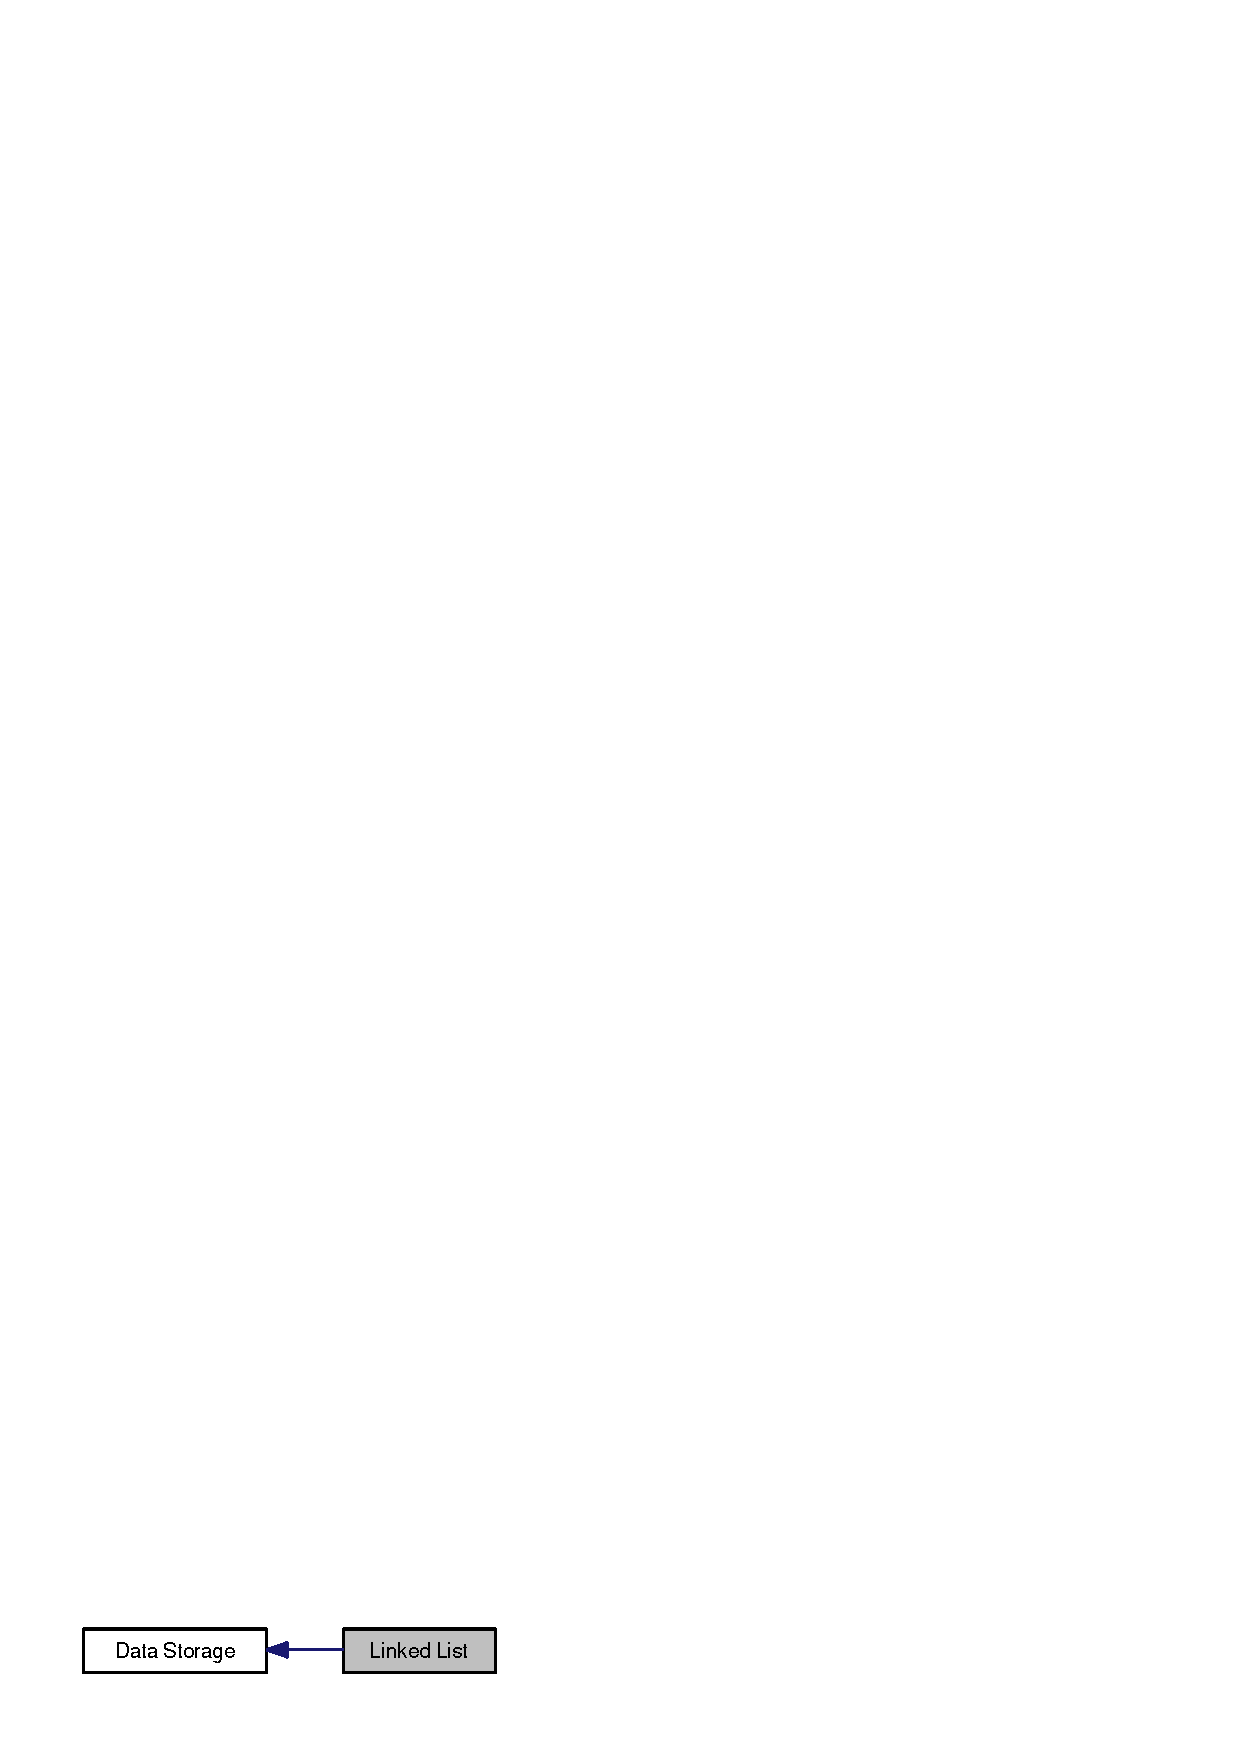
\includegraphics[width=121pt]{group__linklist}
\end{center}
\end{figure}
\subsection*{Data Structures}
\begin{DoxyCompactItemize}
\item 
struct \hyperlink{structt__llelem}{t\_\-llelem}
\begin{DoxyCompactList}\small\item\em A linklist element. \item\end{DoxyCompactList}\item 
struct \hyperlink{structt__linklist}{t\_\-linklist}
\begin{DoxyCompactList}\small\item\em The linklist object. \item\end{DoxyCompactList}\end{DoxyCompactItemize}
\subsection*{Functions}
\begin{DoxyCompactItemize}
\item 
\hyperlink{structt__linklist}{t\_\-linklist} $\ast$ \hyperlink{group__linklist_ga62dba349046e7f84cf34c9c80f04d44a}{linklist\_\-new} (void)
\begin{DoxyCompactList}\small\item\em Create a new linklist object. \item\end{DoxyCompactList}\item 
void \hyperlink{group__linklist_ga033f4bf2a9f806e168697b5ce0f6331e}{linklist\_\-chuck} (\hyperlink{structt__linklist}{t\_\-linklist} $\ast$x)
\begin{DoxyCompactList}\small\item\em Free a linklist, but don't free the items it contains. \item\end{DoxyCompactList}\item 
long \hyperlink{group__linklist_ga71472259406fa8ceb8fad80d23259357}{linklist\_\-getsize} (\hyperlink{structt__linklist}{t\_\-linklist} $\ast$x)
\begin{DoxyCompactList}\small\item\em Return the number of items in a linklist object. \item\end{DoxyCompactList}\item 
void $\ast$ \hyperlink{group__linklist_ga4d64ccb54a70c0a2a9b3fb68e495d9f4}{linklist\_\-getindex} (\hyperlink{structt__linklist}{t\_\-linklist} $\ast$x, long index)
\begin{DoxyCompactList}\small\item\em Return the item stored in a linklist at a specified index. \item\end{DoxyCompactList}\item 
long \hyperlink{group__linklist_ga6ec787cba5eb1c47c294692d4c62e609}{linklist\_\-objptr2index} (\hyperlink{structt__linklist}{t\_\-linklist} $\ast$x, void $\ast$p)
\begin{DoxyCompactList}\small\item\em Return an item's index, given the item itself. \item\end{DoxyCompactList}\item 
long \hyperlink{group__linklist_ga7360ba45714cb28e2b4cd44aa8998a67}{linklist\_\-append} (\hyperlink{structt__linklist}{t\_\-linklist} $\ast$x, void $\ast$o)
\begin{DoxyCompactList}\small\item\em Add an item to the end of the list. \item\end{DoxyCompactList}\item 
long \hyperlink{group__linklist_gac652f2501c274abd1d8fe53626153bde}{linklist\_\-insertindex} (\hyperlink{structt__linklist}{t\_\-linklist} $\ast$x, void $\ast$o, long index)
\begin{DoxyCompactList}\small\item\em Insert an item into the list at the specified index. \item\end{DoxyCompactList}\item 
long \hyperlink{group__linklist_gadac3bedb5a07ebf8f1b4751cc73a2c52}{linklist\_\-insert\_\-sorted} (\hyperlink{structt__linklist}{t\_\-linklist} $\ast$x, void $\ast$o, long cmpfn(void $\ast$, void $\ast$))
\begin{DoxyCompactList}\small\item\em Insert an item into the list, keeping the list sorted according to a specified comparison function. \item\end{DoxyCompactList}\item 
\hyperlink{structt__llelem}{t\_\-llelem} $\ast$ \hyperlink{group__linklist_gafd9471b4a798cd55d9d5bc79000b5a93}{linklist\_\-insertafterobjptr} (\hyperlink{structt__linklist}{t\_\-linklist} $\ast$x, void $\ast$o, void $\ast$objptr)
\begin{DoxyCompactList}\small\item\em Insert an item into the list after another specified item. \item\end{DoxyCompactList}\item 
\hyperlink{structt__llelem}{t\_\-llelem} $\ast$ \hyperlink{group__linklist_gaaa759a9962d69633c45efac04382fb61}{linklist\_\-insertbeforeobjptr} (\hyperlink{structt__linklist}{t\_\-linklist} $\ast$x, void $\ast$o, void $\ast$objptr)
\begin{DoxyCompactList}\small\item\em Insert an item into the list before another specified item. \item\end{DoxyCompactList}\item 
\hyperlink{structt__llelem}{t\_\-llelem} $\ast$ \hyperlink{group__linklist_ga429e12adff823ce46dc54649a271cefd}{linklist\_\-moveafterobjptr} (\hyperlink{structt__linklist}{t\_\-linklist} $\ast$x, void $\ast$o, void $\ast$objptr)
\begin{DoxyCompactList}\small\item\em Move an existing item in the list to a position after another specified item in the list. \item\end{DoxyCompactList}\item 
\hyperlink{structt__llelem}{t\_\-llelem} $\ast$ \hyperlink{group__linklist_ga3a91552cbd18988575d9ae31ff863812}{linklist\_\-movebeforeobjptr} (\hyperlink{structt__linklist}{t\_\-linklist} $\ast$x, void $\ast$o, void $\ast$objptr)
\begin{DoxyCompactList}\small\item\em Move an existing item in the list to a position before another specified item in the list. \item\end{DoxyCompactList}\item 
long \hyperlink{group__linklist_ga8a93071a90ca14ed02a32fa09f9e13f9}{linklist\_\-deleteindex} (\hyperlink{structt__linklist}{t\_\-linklist} $\ast$x, long index)
\begin{DoxyCompactList}\small\item\em Remove the item from the list at the specified index and free it. \item\end{DoxyCompactList}\item 
long \hyperlink{group__linklist_gaa89cf5b917b41ad0c15963dd79800b50}{linklist\_\-chuckindex} (\hyperlink{structt__linklist}{t\_\-linklist} $\ast$x, long index)
\begin{DoxyCompactList}\small\item\em Remove the item from the list at the specified index. \item\end{DoxyCompactList}\item 
void \hyperlink{group__linklist_ga6621c47c664c57d794ea2540b62d0956}{linklist\_\-chuckobject} (\hyperlink{structt__linklist}{t\_\-linklist} $\ast$x, void $\ast$o)
\begin{DoxyCompactList}\small\item\em Remove the specified item from the list. \item\end{DoxyCompactList}\item 
void \hyperlink{group__linklist_ga551da85a8531e5785a4b748d8a86301a}{linklist\_\-clear} (\hyperlink{structt__linklist}{t\_\-linklist} $\ast$x)
\begin{DoxyCompactList}\small\item\em Remove and free all items in the list. \item\end{DoxyCompactList}\item 
long \hyperlink{group__linklist_ga49aa766d6a1a63de1491f9bdfb3cfe73}{linklist\_\-makearray} (\hyperlink{structt__linklist}{t\_\-linklist} $\ast$x, void $\ast$$\ast$a, long max)
\begin{DoxyCompactList}\small\item\em Retrieve linklist items as an array of pointers. \item\end{DoxyCompactList}\item 
void \hyperlink{group__linklist_ga4ca32e817270576a9c1137e86f33c3d6}{linklist\_\-reverse} (\hyperlink{structt__linklist}{t\_\-linklist} $\ast$x)
\begin{DoxyCompactList}\small\item\em Reverse the order of items in the linked-\/list. \item\end{DoxyCompactList}\item 
void \hyperlink{group__linklist_ga728b9e635de257787b721dddaac8e01f}{linklist\_\-rotate} (\hyperlink{structt__linklist}{t\_\-linklist} $\ast$x, long i)
\begin{DoxyCompactList}\small\item\em Rotate items in the linked list in circular fashion. \item\end{DoxyCompactList}\item 
void \hyperlink{group__linklist_ga58a2e5fba8b3b084a3940a23fbd3a4a1}{linklist\_\-shuffle} (\hyperlink{structt__linklist}{t\_\-linklist} $\ast$x)
\begin{DoxyCompactList}\small\item\em Randomize the order of items in the linked-\/list. \item\end{DoxyCompactList}\item 
void \hyperlink{group__linklist_ga42d158b9f76d83f58cf6780aeb9b208a}{linklist\_\-swap} (\hyperlink{structt__linklist}{t\_\-linklist} $\ast$x, long a, long b)
\begin{DoxyCompactList}\small\item\em Swap the position of two items in the linked-\/list, specified by index. \item\end{DoxyCompactList}\item 
long \hyperlink{group__linklist_gab7f3c26cb704c460892818b89a1ab004}{linklist\_\-findfirst} (\hyperlink{structt__linklist}{t\_\-linklist} $\ast$x, void $\ast$$\ast$o, long cmpfn(void $\ast$, void $\ast$), void $\ast$cmpdata)
\begin{DoxyCompactList}\small\item\em Search the linked list for the first item meeting defined criteria. \item\end{DoxyCompactList}\item 
void \hyperlink{group__linklist_ga20253bd1c04d260171435d6b547ac787}{linklist\_\-findall} (\hyperlink{structt__linklist}{t\_\-linklist} $\ast$x, \hyperlink{structt__linklist}{t\_\-linklist} $\ast$$\ast$out, long cmpfn(void $\ast$, void $\ast$), void $\ast$cmpdata)
\begin{DoxyCompactList}\small\item\em Search the linked list for all items meeting defined criteria. \item\end{DoxyCompactList}\item 
void \hyperlink{group__linklist_ga10bd8d367039e3e4b90fe720e83d0edf}{linklist\_\-methodall} (\hyperlink{structt__linklist}{t\_\-linklist} $\ast$x, \hyperlink{structt__symbol}{t\_\-symbol} $\ast$s,...)
\begin{DoxyCompactList}\small\item\em Call the named message on every object in the linklist. \item\end{DoxyCompactList}\item 
void $\ast$ \hyperlink{group__linklist_ga17e04336154b16c19ac13f5f62fba009}{linklist\_\-methodindex} (\hyperlink{structt__linklist}{t\_\-linklist} $\ast$x, long i, \hyperlink{structt__symbol}{t\_\-symbol} $\ast$s,...)
\begin{DoxyCompactList}\small\item\em Call the named message on an object specified by index. \item\end{DoxyCompactList}\item 
void \hyperlink{group__linklist_gaf01b5f67a8ceccdd75cff34f6ecdd8c2}{linklist\_\-sort} (\hyperlink{structt__linklist}{t\_\-linklist} $\ast$x, long cmpfn(void $\ast$, void $\ast$))
\begin{DoxyCompactList}\small\item\em Sort the linked list. \item\end{DoxyCompactList}\item 
void \hyperlink{group__linklist_ga6f4496ef6dc1d6d121acf25d7cd5f946}{linklist\_\-funall} (\hyperlink{structt__linklist}{t\_\-linklist} $\ast$x, \hyperlink{group__datatypes_gac26ba0a173b50597f5738132e059b42d}{method} fun, void $\ast$arg)
\begin{DoxyCompactList}\small\item\em Call the specified function for every item in the linklist. \item\end{DoxyCompactList}\item 
long \hyperlink{group__linklist_ga27a9d3cdcacb995dcc7ce7a80daf57b6}{linklist\_\-funall\_\-break} (\hyperlink{structt__linklist}{t\_\-linklist} $\ast$x, \hyperlink{group__datatypes_gac26ba0a173b50597f5738132e059b42d}{method} fun, void $\ast$arg)
\begin{DoxyCompactList}\small\item\em Call the specified function for every item in the linklist. \item\end{DoxyCompactList}\item 
void $\ast$ \hyperlink{group__linklist_ga289838302ecbed343839de955cd8549c}{linklist\_\-funindex} (\hyperlink{structt__linklist}{t\_\-linklist} $\ast$x, long i, \hyperlink{group__datatypes_gac26ba0a173b50597f5738132e059b42d}{method} fun, void $\ast$arg)
\begin{DoxyCompactList}\small\item\em Call the specified function for an item specified by index. \item\end{DoxyCompactList}\item 
void $\ast$ \hyperlink{group__linklist_ga498a96abbd74bf7e1885e97a8fb37379}{linklist\_\-substitute} (\hyperlink{structt__linklist}{t\_\-linklist} $\ast$x, void $\ast$p, void $\ast$newp)
\begin{DoxyCompactList}\small\item\em Given an item in the list, replace it with a different value. \item\end{DoxyCompactList}\item 
void $\ast$ \hyperlink{group__linklist_ga9d66d4fd900d9cdd13f7520094fb1837}{linklist\_\-next} (\hyperlink{structt__linklist}{t\_\-linklist} $\ast$x, void $\ast$p, void $\ast$$\ast$next)
\begin{DoxyCompactList}\small\item\em Given an item in the list, find the next item. \item\end{DoxyCompactList}\item 
void $\ast$ \hyperlink{group__linklist_ga62b4f5fce83130358e652601e1286926}{linklist\_\-prev} (\hyperlink{structt__linklist}{t\_\-linklist} $\ast$x, void $\ast$p, void $\ast$$\ast$prev)
\begin{DoxyCompactList}\small\item\em Given an item in the list, find the previous item. \item\end{DoxyCompactList}\item 
void $\ast$ \hyperlink{group__linklist_gad45ad220a822b64458152e60f504e846}{linklist\_\-last} (\hyperlink{structt__linklist}{t\_\-linklist} $\ast$x, void $\ast$$\ast$item)
\begin{DoxyCompactList}\small\item\em Return the last item (the tail) in the linked-\/list. \item\end{DoxyCompactList}\item 
void \hyperlink{group__linklist_ga95d07cfad7f3a651b1d42482183cd698}{linklist\_\-readonly} (\hyperlink{structt__linklist}{t\_\-linklist} $\ast$x, long readonly)
\begin{DoxyCompactList}\small\item\em Set the linklist's readonly bit. \item\end{DoxyCompactList}\item 
void \hyperlink{group__linklist_gacb89cb9e0a3b6c8e631dd00734643cdb}{linklist\_\-flags} (\hyperlink{structt__linklist}{t\_\-linklist} $\ast$x, long flags)
\begin{DoxyCompactList}\small\item\em Set the linklist's datastore flags. \item\end{DoxyCompactList}\item 
long \hyperlink{group__linklist_gacbef4ef795d257b8686aa274049efa4a}{linklist\_\-getflags} (\hyperlink{structt__linklist}{t\_\-linklist} $\ast$x)
\begin{DoxyCompactList}\small\item\em Get the linklist's datastore flags. \item\end{DoxyCompactList}\item 
long \hyperlink{group__linklist_ga2a991fb645404fe7d9d3327e5a386b80}{linklist\_\-match} (void $\ast$a, void $\ast$b)
\begin{DoxyCompactList}\small\item\em A linklist comparison method that determines if two item pointers are equal. \item\end{DoxyCompactList}\end{DoxyCompactItemize}


\subsection{Detailed Description}
Max's linklist object implements a doubly-\/linked-\/list ( \href{http://en.wikipedia.org/wiki/Linked_list}{\tt http://en.wikipedia.org/wiki/Linked\_\-list} ) together with a high-\/level interface for manipulating and accessing values in the list. 

\subsection{Function Documentation}
\hypertarget{group__linklist_ga7360ba45714cb28e2b4cd44aa8998a67}{
\index{linklist@{linklist}!linklist\_\-append@{linklist\_\-append}}
\index{linklist\_\-append@{linklist\_\-append}!linklist@{linklist}}
\subsubsection[{linklist\_\-append}]{\setlength{\rightskip}{0pt plus 5cm}long linklist\_\-append ({\bf t\_\-linklist} $\ast$ {\em x}, \/  void $\ast$ {\em o})}}
\label{group__linklist_ga7360ba45714cb28e2b4cd44aa8998a67}


Add an item to the end of the list. 
\begin{DoxyParams}{Parameters}
\item[{\em x}]The linklist instance. \item[{\em o}]The item pointer to append to the linked-\/list. \end{DoxyParams}
\begin{DoxyReturn}{Returns}
The index of the item in the linklist. 
\end{DoxyReturn}
\hypertarget{group__linklist_ga033f4bf2a9f806e168697b5ce0f6331e}{
\index{linklist@{linklist}!linklist\_\-chuck@{linklist\_\-chuck}}
\index{linklist\_\-chuck@{linklist\_\-chuck}!linklist@{linklist}}
\subsubsection[{linklist\_\-chuck}]{\setlength{\rightskip}{0pt plus 5cm}void linklist\_\-chuck ({\bf t\_\-linklist} $\ast$ {\em x})}}
\label{group__linklist_ga033f4bf2a9f806e168697b5ce0f6331e}


Free a linklist, but don't free the items it contains. The linklist can contain a variety of different types of data. By default, the linklist assumes that all items are max objects with a valid \hyperlink{structt__object}{t\_\-object} header.

You can alter the linklist's notion of what it contains by using the \hyperlink{group__linklist_gacb89cb9e0a3b6c8e631dd00734643cdb}{linklist\_\-flags()} method.

When you free the linklist by calling \hyperlink{group__obj_ga3759846cb356195532c41e35b87522ee}{object\_\-free()} it then tries to free all of the items it contains. If the linklist is storing a custom type of data, or should otherwise not free the data it contains, then call \hyperlink{group__linklist_ga033f4bf2a9f806e168697b5ce0f6331e}{linklist\_\-chuck()} to free the object instead of \hyperlink{group__obj_ga3759846cb356195532c41e35b87522ee}{object\_\-free()}.


\begin{DoxyParams}{Parameters}
\item[{\em x}]The linklist object to be freed. \end{DoxyParams}
\begin{DoxySeeAlso}{See also}
\hyperlink{group__obj_ga3759846cb356195532c41e35b87522ee}{object\_\-free} 
\end{DoxySeeAlso}
\hypertarget{group__linklist_gaa89cf5b917b41ad0c15963dd79800b50}{
\index{linklist@{linklist}!linklist\_\-chuckindex@{linklist\_\-chuckindex}}
\index{linklist\_\-chuckindex@{linklist\_\-chuckindex}!linklist@{linklist}}
\subsubsection[{linklist\_\-chuckindex}]{\setlength{\rightskip}{0pt plus 5cm}long linklist\_\-chuckindex ({\bf t\_\-linklist} $\ast$ {\em x}, \/  long {\em index})}}
\label{group__linklist_gaa89cf5b917b41ad0c15963dd79800b50}


Remove the item from the list at the specified index. You are responsible for freeing any memory associated with the item that is removed from the linklist.


\begin{DoxyParams}{Parameters}
\item[{\em x}]The linklist instance. \item[{\em index}]The index of the item to remove. \end{DoxyParams}
\begin{DoxyReturn}{Returns}
Returns \hyperlink{group__misc_gga0764dd6c02b76cca7d053ae50555d69da6d22f77fef8b1e1b074cef5d29d935fd}{MAX\_\-ERR\_\-NONE} on successful removal, otherwise returns \hyperlink{group__misc_gga0764dd6c02b76cca7d053ae50555d69dae285bdd436f17560cfd09c6b31ea397d}{MAX\_\-ERR\_\-GENERIC}
\end{DoxyReturn}
\begin{DoxySeeAlso}{See also}
\hyperlink{group__linklist_ga8a93071a90ca14ed02a32fa09f9e13f9}{linklist\_\-deleteindex} 

\hyperlink{group__linklist_ga6621c47c664c57d794ea2540b62d0956}{linklist\_\-chuckobject} 
\end{DoxySeeAlso}
\hypertarget{group__linklist_ga6621c47c664c57d794ea2540b62d0956}{
\index{linklist@{linklist}!linklist\_\-chuckobject@{linklist\_\-chuckobject}}
\index{linklist\_\-chuckobject@{linklist\_\-chuckobject}!linklist@{linklist}}
\subsubsection[{linklist\_\-chuckobject}]{\setlength{\rightskip}{0pt plus 5cm}void linklist\_\-chuckobject ({\bf t\_\-linklist} $\ast$ {\em x}, \/  void $\ast$ {\em o})}}
\label{group__linklist_ga6621c47c664c57d794ea2540b62d0956}


Remove the specified item from the list. You are responsible for freeing any memory associated with the item that is removed from the linklist.


\begin{DoxyParams}{Parameters}
\item[{\em x}]The linklist instance. \item[{\em o}]The pointer to the item to remove.\end{DoxyParams}
\begin{DoxySeeAlso}{See also}
\hyperlink{group__linklist_ga8a93071a90ca14ed02a32fa09f9e13f9}{linklist\_\-deleteindex} 

\hyperlink{group__linklist_gaa89cf5b917b41ad0c15963dd79800b50}{linklist\_\-chuckindex} 
\end{DoxySeeAlso}
\hypertarget{group__linklist_ga551da85a8531e5785a4b748d8a86301a}{
\index{linklist@{linklist}!linklist\_\-clear@{linklist\_\-clear}}
\index{linklist\_\-clear@{linklist\_\-clear}!linklist@{linklist}}
\subsubsection[{linklist\_\-clear}]{\setlength{\rightskip}{0pt plus 5cm}void linklist\_\-clear ({\bf t\_\-linklist} $\ast$ {\em x})}}
\label{group__linklist_ga551da85a8531e5785a4b748d8a86301a}


Remove and free all items in the list. Freeing items in the list is subject to the same rules as \hyperlink{group__linklist_ga8a93071a90ca14ed02a32fa09f9e13f9}{linklist\_\-deleteindex()}. You can alter the linklist's notion of what it contains, and thus how items are freed, by using the \hyperlink{group__linklist_gacb89cb9e0a3b6c8e631dd00734643cdb}{linklist\_\-flags()} method.


\begin{DoxyParams}{Parameters}
\item[{\em x}]The linklist instance. \end{DoxyParams}
\hypertarget{group__linklist_ga8a93071a90ca14ed02a32fa09f9e13f9}{
\index{linklist@{linklist}!linklist\_\-deleteindex@{linklist\_\-deleteindex}}
\index{linklist\_\-deleteindex@{linklist\_\-deleteindex}!linklist@{linklist}}
\subsubsection[{linklist\_\-deleteindex}]{\setlength{\rightskip}{0pt plus 5cm}long linklist\_\-deleteindex ({\bf t\_\-linklist} $\ast$ {\em x}, \/  long {\em index})}}
\label{group__linklist_ga8a93071a90ca14ed02a32fa09f9e13f9}


Remove the item from the list at the specified index and free it. The linklist can contain a variety of different types of data. By default, the linklist assumes that all items are max objects with a valid \hyperlink{structt__object}{t\_\-object} header. Thus by default, it frees items by calling \hyperlink{group__obj_ga3759846cb356195532c41e35b87522ee}{object\_\-free()} on them.

You can alter the linklist's notion of what it contains by using the \hyperlink{group__linklist_gacb89cb9e0a3b6c8e631dd00734643cdb}{linklist\_\-flags()} method.

If you wish to remove an item from the linklist and free it yourself, then you should use linklist\_\-chuckptr().


\begin{DoxyParams}{Parameters}
\item[{\em x}]The linklist instance. \item[{\em index}]The index of the item to delete. \end{DoxyParams}
\begin{DoxyReturn}{Returns}
Returns \hyperlink{group__misc_gga0764dd6c02b76cca7d053ae50555d69da6d22f77fef8b1e1b074cef5d29d935fd}{MAX\_\-ERR\_\-NONE} on successful deletion, otherwise returns \hyperlink{group__misc_gga0764dd6c02b76cca7d053ae50555d69dae285bdd436f17560cfd09c6b31ea397d}{MAX\_\-ERR\_\-GENERIC}
\end{DoxyReturn}
\begin{DoxySeeAlso}{See also}
\hyperlink{group__linklist_gaa89cf5b917b41ad0c15963dd79800b50}{linklist\_\-chuckindex} 

\hyperlink{group__linklist_ga6621c47c664c57d794ea2540b62d0956}{linklist\_\-chuckobject} 
\end{DoxySeeAlso}
\hypertarget{group__linklist_ga20253bd1c04d260171435d6b547ac787}{
\index{linklist@{linklist}!linklist\_\-findall@{linklist\_\-findall}}
\index{linklist\_\-findall@{linklist\_\-findall}!linklist@{linklist}}
\subsubsection[{linklist\_\-findall}]{\setlength{\rightskip}{0pt plus 5cm}void linklist\_\-findall ({\bf t\_\-linklist} $\ast$ {\em x}, \/  {\bf t\_\-linklist} $\ast$$\ast$ {\em out}, \/  long  {\em cmpfn}void $\ast$, void $\ast$, \/  void $\ast$ {\em cmpdata})}}
\label{group__linklist_ga20253bd1c04d260171435d6b547ac787}


Search the linked list for all items meeting defined criteria. The items in the list are traversed, calling a specified comparison function on each, and returning the matches in another linklist.


\begin{DoxyParams}{Parameters}
\item[{\em x}]The linklist instance. \item[{\em out}]The address to a \hyperlink{structt__linklist}{t\_\-linklist} pointer. You should initialize the pointer to NULL before calling \hyperlink{group__linklist_ga20253bd1c04d260171435d6b547ac787}{linklist\_\-findall()}. A new linklist will be created internally by \hyperlink{group__linklist_ga20253bd1c04d260171435d6b547ac787}{linklist\_\-findall()} and returned here. \item[{\em cmpfn}]The function used to determine a match in the list. \item[{\em cmpdata}]An argument to be passed to the \hyperlink{group__datastore_gaaf4ae6dd800a2be9abd645cf70aeb38f}{t\_\-cmpfn}. This will be passed as the second of the two args to the \hyperlink{group__datastore_gaaf4ae6dd800a2be9abd645cf70aeb38f}{t\_\-cmpfn}. The first arg will be the linklist item at each iteration in the list.\end{DoxyParams}
\begin{DoxyRemark}{Remarks}
The following example assumes you have a linklist called myLinkList, and \hyperlink{group__datastore_gaaf4ae6dd800a2be9abd645cf70aeb38f}{t\_\-cmpfn} called myCmpFunction, and some sort of data to match in someCriteria. 
\begin{DoxyCode}
    t_linklist *results = NULL;
    
    linklist_findall(myLinkList, &results, myCmpFunction, (void *)someCriteria);
    // do something here with the 'results' linklist
    // then free the results linklist
    linklist_chuck(results);
\end{DoxyCode}

\end{DoxyRemark}
\begin{DoxySeeAlso}{See also}
\hyperlink{group__linklist_ga2a991fb645404fe7d9d3327e5a386b80}{linklist\_\-match} 

\hyperlink{group__datastore_gaaf4ae6dd800a2be9abd645cf70aeb38f}{t\_\-cmpfn} 

\hyperlink{group__linklist_gab7f3c26cb704c460892818b89a1ab004}{linklist\_\-findfirst} 
\end{DoxySeeAlso}
\hypertarget{group__linklist_gab7f3c26cb704c460892818b89a1ab004}{
\index{linklist@{linklist}!linklist\_\-findfirst@{linklist\_\-findfirst}}
\index{linklist\_\-findfirst@{linklist\_\-findfirst}!linklist@{linklist}}
\subsubsection[{linklist\_\-findfirst}]{\setlength{\rightskip}{0pt plus 5cm}long linklist\_\-findfirst ({\bf t\_\-linklist} $\ast$ {\em x}, \/  void $\ast$$\ast$ {\em o}, \/  long  {\em cmpfn}void $\ast$, void $\ast$, \/  void $\ast$ {\em cmpdata})}}
\label{group__linklist_gab7f3c26cb704c460892818b89a1ab004}


Search the linked list for the first item meeting defined criteria. The items in the list are traversed, calling a specified comparison function on each until the comparison function returns true.


\begin{DoxyParams}{Parameters}
\item[{\em x}]The linklist instance. \item[{\em o}]The address to pointer that will be set with the matching item. \item[{\em cmpfn}]The function used to determine a match in the list. \item[{\em cmpdata}]An argument to be passed to the \hyperlink{group__datastore_gaaf4ae6dd800a2be9abd645cf70aeb38f}{t\_\-cmpfn}. This will be passed as the second of the two args to the \hyperlink{group__datastore_gaaf4ae6dd800a2be9abd645cf70aeb38f}{t\_\-cmpfn}. The first arg will be the linklist item at each iteration in the list. \end{DoxyParams}
\begin{DoxyReturn}{Returns}
The index of the matching item, or -\/1 if no match is found.
\end{DoxyReturn}
\begin{DoxyRemark}{Remarks}
The following shows how to manually do what \hyperlink{group__linklist_ga6621c47c664c57d794ea2540b62d0956}{linklist\_\-chuckobject()} does. 
\begin{DoxyCode}
    void *obj;
    long index;
    
    index = linklist_findfirst(x, &obj, #linklist_match, o);
    if(index != -1)
        linklist_chuckindex(x, index);
\end{DoxyCode}

\end{DoxyRemark}
\begin{DoxySeeAlso}{See also}
\hyperlink{group__linklist_ga2a991fb645404fe7d9d3327e5a386b80}{linklist\_\-match} 

\hyperlink{group__datastore_gaaf4ae6dd800a2be9abd645cf70aeb38f}{t\_\-cmpfn} 

\hyperlink{group__linklist_ga20253bd1c04d260171435d6b547ac787}{linklist\_\-findall} 
\end{DoxySeeAlso}
\hypertarget{group__linklist_gacb89cb9e0a3b6c8e631dd00734643cdb}{
\index{linklist@{linklist}!linklist\_\-flags@{linklist\_\-flags}}
\index{linklist\_\-flags@{linklist\_\-flags}!linklist@{linklist}}
\subsubsection[{linklist\_\-flags}]{\setlength{\rightskip}{0pt plus 5cm}void linklist\_\-flags ({\bf t\_\-linklist} $\ast$ {\em x}, \/  long {\em flags})}}
\label{group__linklist_gacb89cb9e0a3b6c8e631dd00734643cdb}


Set the linklist's datastore flags. The available flags are enumerated in \hyperlink{group__datastore_gaa858d4b3815076d79624c39d9ca59348}{e\_\-max\_\-datastore\_\-flags}. These flags control the behavior of the linklist, particularly when removing items from the list using functions such as \hyperlink{group__linklist_ga551da85a8531e5785a4b748d8a86301a}{linklist\_\-clear()}, \hyperlink{group__linklist_ga8a93071a90ca14ed02a32fa09f9e13f9}{linklist\_\-deleteindex()}, or when freeing the linklist itself.


\begin{DoxyParams}{Parameters}
\item[{\em x}]The linklist instance. \item[{\em flags}]A valid value from the \hyperlink{group__datastore_gaa858d4b3815076d79624c39d9ca59348}{e\_\-max\_\-datastore\_\-flags}. The default is \hyperlink{group__datastore_ggaa858d4b3815076d79624c39d9ca59348adc630c58c8e958a404553a08db6fd180}{OBJ\_\-FLAG\_\-OBJ}. \end{DoxyParams}
\hypertarget{group__linklist_ga6f4496ef6dc1d6d121acf25d7cd5f946}{
\index{linklist@{linklist}!linklist\_\-funall@{linklist\_\-funall}}
\index{linklist\_\-funall@{linklist\_\-funall}!linklist@{linklist}}
\subsubsection[{linklist\_\-funall}]{\setlength{\rightskip}{0pt plus 5cm}void linklist\_\-funall ({\bf t\_\-linklist} $\ast$ {\em x}, \/  {\bf method} {\em fun}, \/  void $\ast$ {\em arg})}}
\label{group__linklist_ga6f4496ef6dc1d6d121acf25d7cd5f946}


Call the specified function for every item in the linklist. 
\begin{DoxyParams}{Parameters}
\item[{\em x}]The linklist instance. \item[{\em fun}]The function to call, specified as function pointer cast to a Max \hyperlink{group__datatypes_gac26ba0a173b50597f5738132e059b42d}{method}. \item[{\em arg}]An argument that you would like to pass to the function being called.\end{DoxyParams}
\begin{DoxyRemark}{Remarks}
The \hyperlink{group__linklist_ga6f4496ef6dc1d6d121acf25d7cd5f946}{linklist\_\-funall()} method will call your function for every item in the list. It will pass both a pointer to the item in the list, and any argument that you provide. The following example shows a function that could be called by \hyperlink{group__linklist_ga6f4496ef6dc1d6d121acf25d7cd5f946}{linklist\_\-funall()}. 
\begin{DoxyCode}
    void myFun(t_object *myObj, void *myArg)
    {
        // do something with myObj and myArg here
        // myObj is the item in the linklist
    }
\end{DoxyCode}
 
\end{DoxyRemark}
\hypertarget{group__linklist_ga27a9d3cdcacb995dcc7ce7a80daf57b6}{
\index{linklist@{linklist}!linklist\_\-funall\_\-break@{linklist\_\-funall\_\-break}}
\index{linklist\_\-funall\_\-break@{linklist\_\-funall\_\-break}!linklist@{linklist}}
\subsubsection[{linklist\_\-funall\_\-break}]{\setlength{\rightskip}{0pt plus 5cm}long linklist\_\-funall\_\-break ({\bf t\_\-linklist} $\ast$ {\em x}, \/  {\bf method} {\em fun}, \/  void $\ast$ {\em arg})}}
\label{group__linklist_ga27a9d3cdcacb995dcc7ce7a80daf57b6}


Call the specified function for every item in the linklist. The iteration through the list will halt if the function returns a non-\/zero value.


\begin{DoxyParams}{Parameters}
\item[{\em x}]The linklist instance. \item[{\em fun}]The function to call, specified as function pointer cast to a Max \hyperlink{group__datatypes_gac26ba0a173b50597f5738132e059b42d}{method}. \item[{\em arg}]An argument that you would like to pass to the function being called.\end{DoxyParams}
\begin{DoxyRemark}{Remarks}
The \hyperlink{group__linklist_ga6f4496ef6dc1d6d121acf25d7cd5f946}{linklist\_\-funall()} method will call your function for every item in the list. It will pass both a pointer to the item in the list, and any argument that you provide. The following example shows a function that could be called by \hyperlink{group__linklist_ga6f4496ef6dc1d6d121acf25d7cd5f946}{linklist\_\-funall()}. 
\begin{DoxyCode}
    long myFun(t_symbol *myListItemSymbol, void *myArg)
    {
        // this function is called by a linklist that contains symbols for its it
      ems
        if(myListItemSymbol == gensym("")){
            error("empty symbol -- aborting linklist traversal")
            return 1;           
        }
        else{
            // do something with the symbol
            return 0;
        }
    }
\end{DoxyCode}
 
\end{DoxyRemark}
\hypertarget{group__linklist_ga289838302ecbed343839de955cd8549c}{
\index{linklist@{linklist}!linklist\_\-funindex@{linklist\_\-funindex}}
\index{linklist\_\-funindex@{linklist\_\-funindex}!linklist@{linklist}}
\subsubsection[{linklist\_\-funindex}]{\setlength{\rightskip}{0pt plus 5cm}void$\ast$ linklist\_\-funindex ({\bf t\_\-linklist} $\ast$ {\em x}, \/  long {\em i}, \/  {\bf method} {\em fun}, \/  void $\ast$ {\em arg})}}
\label{group__linklist_ga289838302ecbed343839de955cd8549c}


Call the specified function for an item specified by index. 
\begin{DoxyParams}{Parameters}
\item[{\em x}]The linklist instance. \item[{\em i}]The index of the item to which to send the message. \item[{\em fun}]The function to call, specified as function pointer cast to a Max \hyperlink{group__datatypes_gac26ba0a173b50597f5738132e059b42d}{method}. \item[{\em arg}]An argument that you would like to pass to the function being called.\end{DoxyParams}
\begin{DoxyRemark}{Remarks}
The \hyperlink{group__linklist_ga289838302ecbed343839de955cd8549c}{linklist\_\-funindex()} method will call your function for an item in the list. It will pass both a pointer to the item in the list, and any argument that you provide. The following example shows a function that could be called by \hyperlink{group__linklist_ga289838302ecbed343839de955cd8549c}{linklist\_\-funindex()}. 
\begin{DoxyCode}
    void myFun(t_object *myObj, void *myArg)
    {
        // do something with myObj and myArg here
        // myObj is the item in the linklist
    }
\end{DoxyCode}
 
\end{DoxyRemark}
\hypertarget{group__linklist_gacbef4ef795d257b8686aa274049efa4a}{
\index{linklist@{linklist}!linklist\_\-getflags@{linklist\_\-getflags}}
\index{linklist\_\-getflags@{linklist\_\-getflags}!linklist@{linklist}}
\subsubsection[{linklist\_\-getflags}]{\setlength{\rightskip}{0pt plus 5cm}long linklist\_\-getflags ({\bf t\_\-linklist} $\ast$ {\em x})}}
\label{group__linklist_gacbef4ef795d257b8686aa274049efa4a}


Get the linklist's datastore flags. 
\begin{DoxyParams}{Parameters}
\item[{\em x}]The linklist instance. \end{DoxyParams}
\begin{DoxyReturn}{Returns}
The current state of the linklist flags as enumerated in \hyperlink{group__datastore_gaa858d4b3815076d79624c39d9ca59348}{e\_\-max\_\-datastore\_\-flags}. 
\end{DoxyReturn}
\hypertarget{group__linklist_ga4d64ccb54a70c0a2a9b3fb68e495d9f4}{
\index{linklist@{linklist}!linklist\_\-getindex@{linklist\_\-getindex}}
\index{linklist\_\-getindex@{linklist\_\-getindex}!linklist@{linklist}}
\subsubsection[{linklist\_\-getindex}]{\setlength{\rightskip}{0pt plus 5cm}void$\ast$ linklist\_\-getindex ({\bf t\_\-linklist} $\ast$ {\em x}, \/  long {\em index})}}
\label{group__linklist_ga4d64ccb54a70c0a2a9b3fb68e495d9f4}


Return the item stored in a linklist at a specified index. 
\begin{DoxyParams}{Parameters}
\item[{\em x}]The linklist instance. \item[{\em index}]The index in the linklist to fetch. Indices are zero-\/based. \end{DoxyParams}
\begin{DoxyReturn}{Returns}
The item from the linklist stored at index. If there is no item at the index, {\ttfamily NULL} is returned 
\end{DoxyReturn}
\hypertarget{group__linklist_ga71472259406fa8ceb8fad80d23259357}{
\index{linklist@{linklist}!linklist\_\-getsize@{linklist\_\-getsize}}
\index{linklist\_\-getsize@{linklist\_\-getsize}!linklist@{linklist}}
\subsubsection[{linklist\_\-getsize}]{\setlength{\rightskip}{0pt plus 5cm}long linklist\_\-getsize ({\bf t\_\-linklist} $\ast$ {\em x})}}
\label{group__linklist_ga71472259406fa8ceb8fad80d23259357}


Return the number of items in a linklist object. 
\begin{DoxyParams}{Parameters}
\item[{\em x}]The linklist instance. \end{DoxyParams}
\begin{DoxyReturn}{Returns}
The number of items in the linklist object. 
\end{DoxyReturn}
\hypertarget{group__linklist_gadac3bedb5a07ebf8f1b4751cc73a2c52}{
\index{linklist@{linklist}!linklist\_\-insert\_\-sorted@{linklist\_\-insert\_\-sorted}}
\index{linklist\_\-insert\_\-sorted@{linklist\_\-insert\_\-sorted}!linklist@{linklist}}
\subsubsection[{linklist\_\-insert\_\-sorted}]{\setlength{\rightskip}{0pt plus 5cm}long linklist\_\-insert\_\-sorted ({\bf t\_\-linklist} $\ast$ {\em x}, \/  void $\ast$ {\em o}, \/  long  {\em cmpfn}void $\ast$, void $\ast$)}}
\label{group__linklist_gadac3bedb5a07ebf8f1b4751cc73a2c52}


Insert an item into the list, keeping the list sorted according to a specified comparison function. 
\begin{DoxyParams}{Parameters}
\item[{\em x}]The linklist instance. \item[{\em o}]The item pointer to insert. \item[{\em cmpfn}]A comparison function by which the list should be sorted. \end{DoxyParams}
\begin{DoxyReturn}{Returns}
The index of the new item in the linklist, or -\/1 if the insert failed. 
\end{DoxyReturn}
\hypertarget{group__linklist_gafd9471b4a798cd55d9d5bc79000b5a93}{
\index{linklist@{linklist}!linklist\_\-insertafterobjptr@{linklist\_\-insertafterobjptr}}
\index{linklist\_\-insertafterobjptr@{linklist\_\-insertafterobjptr}!linklist@{linklist}}
\subsubsection[{linklist\_\-insertafterobjptr}]{\setlength{\rightskip}{0pt plus 5cm}{\bf t\_\-llelem}$\ast$ linklist\_\-insertafterobjptr ({\bf t\_\-linklist} $\ast$ {\em x}, \/  void $\ast$ {\em o}, \/  void $\ast$ {\em objptr})}}
\label{group__linklist_gafd9471b4a798cd55d9d5bc79000b5a93}


Insert an item into the list after another specified item. 
\begin{DoxyParams}{Parameters}
\item[{\em x}]The linklist instance. \item[{\em o}]The item pointer to insert. \item[{\em objptr}]The item pointer after which to insert in the list.\end{DoxyParams}
\begin{DoxyReturn}{Returns}
An opaque linklist element. 
\end{DoxyReturn}
\hypertarget{group__linklist_gaaa759a9962d69633c45efac04382fb61}{
\index{linklist@{linklist}!linklist\_\-insertbeforeobjptr@{linklist\_\-insertbeforeobjptr}}
\index{linklist\_\-insertbeforeobjptr@{linklist\_\-insertbeforeobjptr}!linklist@{linklist}}
\subsubsection[{linklist\_\-insertbeforeobjptr}]{\setlength{\rightskip}{0pt plus 5cm}{\bf t\_\-llelem}$\ast$ linklist\_\-insertbeforeobjptr ({\bf t\_\-linklist} $\ast$ {\em x}, \/  void $\ast$ {\em o}, \/  void $\ast$ {\em objptr})}}
\label{group__linklist_gaaa759a9962d69633c45efac04382fb61}


Insert an item into the list before another specified item. 
\begin{DoxyParams}{Parameters}
\item[{\em x}]The linklist instance. \item[{\em o}]The item pointer to insert. \item[{\em objptr}]The item pointer before which to insert in the list.\end{DoxyParams}
\begin{DoxyReturn}{Returns}
An opaque linklist element. 
\end{DoxyReturn}
\hypertarget{group__linklist_gac652f2501c274abd1d8fe53626153bde}{
\index{linklist@{linklist}!linklist\_\-insertindex@{linklist\_\-insertindex}}
\index{linklist\_\-insertindex@{linklist\_\-insertindex}!linklist@{linklist}}
\subsubsection[{linklist\_\-insertindex}]{\setlength{\rightskip}{0pt plus 5cm}long linklist\_\-insertindex ({\bf t\_\-linklist} $\ast$ {\em x}, \/  void $\ast$ {\em o}, \/  long {\em index})}}
\label{group__linklist_gac652f2501c274abd1d8fe53626153bde}


Insert an item into the list at the specified index. 
\begin{DoxyParams}{Parameters}
\item[{\em x}]The linklist instance. \item[{\em o}]The item pointer to insert. \item[{\em index}]The index at which to insert. Index 0 is the head of the list. \end{DoxyParams}
\begin{DoxyReturn}{Returns}
The index of the item in the linklist, or -\/1 if the insert failed. 
\end{DoxyReturn}
\hypertarget{group__linklist_gad45ad220a822b64458152e60f504e846}{
\index{linklist@{linklist}!linklist\_\-last@{linklist\_\-last}}
\index{linklist\_\-last@{linklist\_\-last}!linklist@{linklist}}
\subsubsection[{linklist\_\-last}]{\setlength{\rightskip}{0pt plus 5cm}void$\ast$ linklist\_\-last ({\bf t\_\-linklist} $\ast$ {\em x}, \/  void $\ast$$\ast$ {\em item})}}
\label{group__linklist_gad45ad220a822b64458152e60f504e846}


Return the last item (the tail) in the linked-\/list. 
\begin{DoxyParams}{Parameters}
\item[{\em x}]The linklist instance. \item[{\em item}]The address of pointer in which to store the last item in the linked-\/list. \end{DoxyParams}
\begin{DoxyReturn}{Returns}
always returns NULL 
\end{DoxyReturn}
\hypertarget{group__linklist_ga49aa766d6a1a63de1491f9bdfb3cfe73}{
\index{linklist@{linklist}!linklist\_\-makearray@{linklist\_\-makearray}}
\index{linklist\_\-makearray@{linklist\_\-makearray}!linklist@{linklist}}
\subsubsection[{linklist\_\-makearray}]{\setlength{\rightskip}{0pt plus 5cm}long linklist\_\-makearray ({\bf t\_\-linklist} $\ast$ {\em x}, \/  void $\ast$$\ast$ {\em a}, \/  long {\em max})}}
\label{group__linklist_ga49aa766d6a1a63de1491f9bdfb3cfe73}


Retrieve linklist items as an array of pointers. 
\begin{DoxyParams}{Parameters}
\item[{\em x}]The linklist instance. \item[{\em a}]The address of the first pointer in the array to fill. \item[{\em max}]The number of pointers in the array. \end{DoxyParams}
\begin{DoxyReturn}{Returns}
The number of items from the list actually returned in the array. 
\end{DoxyReturn}
\hypertarget{group__linklist_ga2a991fb645404fe7d9d3327e5a386b80}{
\index{linklist@{linklist}!linklist\_\-match@{linklist\_\-match}}
\index{linklist\_\-match@{linklist\_\-match}!linklist@{linklist}}
\subsubsection[{linklist\_\-match}]{\setlength{\rightskip}{0pt plus 5cm}long linklist\_\-match (void $\ast$ {\em a}, \/  void $\ast$ {\em b})}}
\label{group__linklist_ga2a991fb645404fe7d9d3327e5a386b80}


A linklist comparison method that determines if two item pointers are equal. 
\begin{DoxyParams}{Parameters}
\item[{\em a}]The first item to compare. \item[{\em b}]The second item to compare. \end{DoxyParams}
\begin{DoxyReturn}{Returns}
Returns 1 if the items are equal, otherwise 0.
\end{DoxyReturn}
\begin{DoxySeeAlso}{See also}
\hyperlink{group__datastore_gaaf4ae6dd800a2be9abd645cf70aeb38f}{t\_\-cmpfn} 
\end{DoxySeeAlso}
\hypertarget{group__linklist_ga10bd8d367039e3e4b90fe720e83d0edf}{
\index{linklist@{linklist}!linklist\_\-methodall@{linklist\_\-methodall}}
\index{linklist\_\-methodall@{linklist\_\-methodall}!linklist@{linklist}}
\subsubsection[{linklist\_\-methodall}]{\setlength{\rightskip}{0pt plus 5cm}void linklist\_\-methodall ({\bf t\_\-linklist} $\ast$ {\em x}, \/  {\bf t\_\-symbol} $\ast$ {\em s}, \/   {\em ...})}}
\label{group__linklist_ga10bd8d367039e3e4b90fe720e83d0edf}


Call the named message on every object in the linklist. The \hyperlink{group__linklist_ga10bd8d367039e3e4b90fe720e83d0edf}{linklist\_\-methodall()} function requires that all items in the linklist are object instances with a valid \hyperlink{structt__object}{t\_\-object} header.


\begin{DoxyParams}{Parameters}
\item[{\em x}]The linklist instance. \item[{\em s}]The name of the message to send to the objects. \item[{\em ...}]Any arguments to be sent with the message.\end{DoxyParams}
\begin{DoxyRemark}{Remarks}
Internally, this function uses \hyperlink{group__obj_gae740749094827ac5adc2b7145db1c596}{object\_\-method()}, meaning that no errors will be posted if the message name does not exist for the object. It also means that messages sent methods with \hyperlink{group__atom_gga8aa6700e9f00b132eb376db6e39ade47a81c1a8550f038db16a619167a70a79b6}{A\_\-GIMME} definitions will need to be given a symbol argument prior to the argc and argv array information. 
\end{DoxyRemark}
\hypertarget{group__linklist_ga17e04336154b16c19ac13f5f62fba009}{
\index{linklist@{linklist}!linklist\_\-methodindex@{linklist\_\-methodindex}}
\index{linklist\_\-methodindex@{linklist\_\-methodindex}!linklist@{linklist}}
\subsubsection[{linklist\_\-methodindex}]{\setlength{\rightskip}{0pt plus 5cm}void$\ast$ linklist\_\-methodindex ({\bf t\_\-linklist} $\ast$ {\em x}, \/  long {\em i}, \/  {\bf t\_\-symbol} $\ast$ {\em s}, \/   {\em ...})}}
\label{group__linklist_ga17e04336154b16c19ac13f5f62fba009}


Call the named message on an object specified by index. The item must be an object instance with a valid \hyperlink{structt__object}{t\_\-object} header.


\begin{DoxyParams}{Parameters}
\item[{\em x}]The linklist instance. \item[{\em i}]The index of the item to which to send the message. \item[{\em s}]The name of the message to send to the objects. \item[{\em ...}]Any arguments to be sent with the message.\end{DoxyParams}
\begin{DoxyRemark}{Remarks}
Internally, this function uses \hyperlink{group__obj_gae740749094827ac5adc2b7145db1c596}{object\_\-method()}, meaning that no errors will be posted if the message name does not exist for the object. It also means that messages sent methods with \hyperlink{group__atom_gga8aa6700e9f00b132eb376db6e39ade47a81c1a8550f038db16a619167a70a79b6}{A\_\-GIMME} definitions will need to be given a symbol argument prior to the argc and argv array information. 
\end{DoxyRemark}
\hypertarget{group__linklist_ga429e12adff823ce46dc54649a271cefd}{
\index{linklist@{linklist}!linklist\_\-moveafterobjptr@{linklist\_\-moveafterobjptr}}
\index{linklist\_\-moveafterobjptr@{linklist\_\-moveafterobjptr}!linklist@{linklist}}
\subsubsection[{linklist\_\-moveafterobjptr}]{\setlength{\rightskip}{0pt plus 5cm}{\bf t\_\-llelem}$\ast$ linklist\_\-moveafterobjptr ({\bf t\_\-linklist} $\ast$ {\em x}, \/  void $\ast$ {\em o}, \/  void $\ast$ {\em objptr})}}
\label{group__linklist_ga429e12adff823ce46dc54649a271cefd}


Move an existing item in the list to a position after another specified item in the list. 
\begin{DoxyParams}{Parameters}
\item[{\em x}]The linklist instance. \item[{\em o}]The item pointer to insert. \item[{\em objptr}]The item pointer after which to move o in the list.\end{DoxyParams}
\begin{DoxyReturn}{Returns}
An opaque linklist element. 
\end{DoxyReturn}
\hypertarget{group__linklist_ga3a91552cbd18988575d9ae31ff863812}{
\index{linklist@{linklist}!linklist\_\-movebeforeobjptr@{linklist\_\-movebeforeobjptr}}
\index{linklist\_\-movebeforeobjptr@{linklist\_\-movebeforeobjptr}!linklist@{linklist}}
\subsubsection[{linklist\_\-movebeforeobjptr}]{\setlength{\rightskip}{0pt plus 5cm}{\bf t\_\-llelem}$\ast$ linklist\_\-movebeforeobjptr ({\bf t\_\-linklist} $\ast$ {\em x}, \/  void $\ast$ {\em o}, \/  void $\ast$ {\em objptr})}}
\label{group__linklist_ga3a91552cbd18988575d9ae31ff863812}


Move an existing item in the list to a position before another specified item in the list. 
\begin{DoxyParams}{Parameters}
\item[{\em x}]The linklist instance. \item[{\em o}]The item pointer to insert. \item[{\em objptr}]The item pointer before which to move o in the list.\end{DoxyParams}
\begin{DoxyReturn}{Returns}
An opaque linklist element. 
\end{DoxyReturn}
\hypertarget{group__linklist_ga62dba349046e7f84cf34c9c80f04d44a}{
\index{linklist@{linklist}!linklist\_\-new@{linklist\_\-new}}
\index{linklist\_\-new@{linklist\_\-new}!linklist@{linklist}}
\subsubsection[{linklist\_\-new}]{\setlength{\rightskip}{0pt plus 5cm}{\bf t\_\-linklist}$\ast$ linklist\_\-new (void)}}
\label{group__linklist_ga62dba349046e7f84cf34c9c80f04d44a}


Create a new linklist object. You can free the linklist by calling \hyperlink{group__obj_ga3759846cb356195532c41e35b87522ee}{object\_\-free()} on the linklist's pointer, or by using \hyperlink{group__linklist_ga033f4bf2a9f806e168697b5ce0f6331e}{linklist\_\-chuck()}.

\begin{DoxyReturn}{Returns}
Pointer to the new linklist object.
\end{DoxyReturn}
\begin{DoxySeeAlso}{See also}
\hyperlink{group__obj_ga3759846cb356195532c41e35b87522ee}{object\_\-free()} 

\hyperlink{group__linklist_ga033f4bf2a9f806e168697b5ce0f6331e}{linklist\_\-chuck()} 
\end{DoxySeeAlso}
\hypertarget{group__linklist_ga9d66d4fd900d9cdd13f7520094fb1837}{
\index{linklist@{linklist}!linklist\_\-next@{linklist\_\-next}}
\index{linklist\_\-next@{linklist\_\-next}!linklist@{linklist}}
\subsubsection[{linklist\_\-next}]{\setlength{\rightskip}{0pt plus 5cm}void$\ast$ linklist\_\-next ({\bf t\_\-linklist} $\ast$ {\em x}, \/  void $\ast$ {\em p}, \/  void $\ast$$\ast$ {\em next})}}
\label{group__linklist_ga9d66d4fd900d9cdd13f7520094fb1837}


Given an item in the list, find the next item. This provides an means for walking the list.


\begin{DoxyParams}{Parameters}
\item[{\em x}]The linklist instance. \item[{\em p}]An item in the list. \item[{\em next}]The address of a pointer to set with the next item in the list. \end{DoxyParams}
\hypertarget{group__linklist_ga6ec787cba5eb1c47c294692d4c62e609}{
\index{linklist@{linklist}!linklist\_\-objptr2index@{linklist\_\-objptr2index}}
\index{linklist\_\-objptr2index@{linklist\_\-objptr2index}!linklist@{linklist}}
\subsubsection[{linklist\_\-objptr2index}]{\setlength{\rightskip}{0pt plus 5cm}long linklist\_\-objptr2index ({\bf t\_\-linklist} $\ast$ {\em x}, \/  void $\ast$ {\em p})}}
\label{group__linklist_ga6ec787cba5eb1c47c294692d4c62e609}


Return an item's index, given the item itself. 
\begin{DoxyParams}{Parameters}
\item[{\em x}]The linklist instance. \item[{\em p}]The item pointer to search for in the linklist. \end{DoxyParams}
\begin{DoxyReturn}{Returns}
The index of the item given in the linklist. If the item is not in the linklist \hyperlink{group__misc_gga0764dd6c02b76cca7d053ae50555d69dae285bdd436f17560cfd09c6b31ea397d}{MAX\_\-ERR\_\-GENERIC} is returned. 
\end{DoxyReturn}
\hypertarget{group__linklist_ga62b4f5fce83130358e652601e1286926}{
\index{linklist@{linklist}!linklist\_\-prev@{linklist\_\-prev}}
\index{linklist\_\-prev@{linklist\_\-prev}!linklist@{linklist}}
\subsubsection[{linklist\_\-prev}]{\setlength{\rightskip}{0pt plus 5cm}void$\ast$ linklist\_\-prev ({\bf t\_\-linklist} $\ast$ {\em x}, \/  void $\ast$ {\em p}, \/  void $\ast$$\ast$ {\em prev})}}
\label{group__linklist_ga62b4f5fce83130358e652601e1286926}


Given an item in the list, find the previous item. This provides an means for walking the list.


\begin{DoxyParams}{Parameters}
\item[{\em x}]The linklist instance. \item[{\em p}]An item in the list. \item[{\em prev}]The address of a pointer to set with the previous item in the list. \end{DoxyParams}
\hypertarget{group__linklist_ga95d07cfad7f3a651b1d42482183cd698}{
\index{linklist@{linklist}!linklist\_\-readonly@{linklist\_\-readonly}}
\index{linklist\_\-readonly@{linklist\_\-readonly}!linklist@{linklist}}
\subsubsection[{linklist\_\-readonly}]{\setlength{\rightskip}{0pt plus 5cm}void linklist\_\-readonly ({\bf t\_\-linklist} $\ast$ {\em x}, \/  long {\em readonly})}}
\label{group__linklist_ga95d07cfad7f3a651b1d42482183cd698}


Set the linklist's readonly bit. By default the readonly bit is 0, indicating that it is threadsafe for both reading and writing. Setting the readonly bit to 1 will disable the linklist's theadsafety mechanism, increasing performance but at the expense of threadsafe operation. Unless you can guarantee the threading context for a linklist's use, you should leave this set to 0.


\begin{DoxyParams}{Parameters}
\item[{\em x}]The linklist instance. \item[{\em readonly}]A 1 or 0 for setting the readonly bit. \end{DoxyParams}
\hypertarget{group__linklist_ga4ca32e817270576a9c1137e86f33c3d6}{
\index{linklist@{linklist}!linklist\_\-reverse@{linklist\_\-reverse}}
\index{linklist\_\-reverse@{linklist\_\-reverse}!linklist@{linklist}}
\subsubsection[{linklist\_\-reverse}]{\setlength{\rightskip}{0pt plus 5cm}void linklist\_\-reverse ({\bf t\_\-linklist} $\ast$ {\em x})}}
\label{group__linklist_ga4ca32e817270576a9c1137e86f33c3d6}


Reverse the order of items in the linked-\/list. 
\begin{DoxyParams}{Parameters}
\item[{\em x}]The linklist instance. \end{DoxyParams}
\hypertarget{group__linklist_ga728b9e635de257787b721dddaac8e01f}{
\index{linklist@{linklist}!linklist\_\-rotate@{linklist\_\-rotate}}
\index{linklist\_\-rotate@{linklist\_\-rotate}!linklist@{linklist}}
\subsubsection[{linklist\_\-rotate}]{\setlength{\rightskip}{0pt plus 5cm}void linklist\_\-rotate ({\bf t\_\-linklist} $\ast$ {\em x}, \/  long {\em i})}}
\label{group__linklist_ga728b9e635de257787b721dddaac8e01f}


Rotate items in the linked list in circular fashion. 
\begin{DoxyParams}{Parameters}
\item[{\em x}]The linklist instance. \item[{\em i}]The number of positions in the list to shift items. \end{DoxyParams}
\hypertarget{group__linklist_ga58a2e5fba8b3b084a3940a23fbd3a4a1}{
\index{linklist@{linklist}!linklist\_\-shuffle@{linklist\_\-shuffle}}
\index{linklist\_\-shuffle@{linklist\_\-shuffle}!linklist@{linklist}}
\subsubsection[{linklist\_\-shuffle}]{\setlength{\rightskip}{0pt plus 5cm}void linklist\_\-shuffle ({\bf t\_\-linklist} $\ast$ {\em x})}}
\label{group__linklist_ga58a2e5fba8b3b084a3940a23fbd3a4a1}


Randomize the order of items in the linked-\/list. 
\begin{DoxyParams}{Parameters}
\item[{\em x}]The linklist instance. \end{DoxyParams}
\hypertarget{group__linklist_gaf01b5f67a8ceccdd75cff34f6ecdd8c2}{
\index{linklist@{linklist}!linklist\_\-sort@{linklist\_\-sort}}
\index{linklist\_\-sort@{linklist\_\-sort}!linklist@{linklist}}
\subsubsection[{linklist\_\-sort}]{\setlength{\rightskip}{0pt plus 5cm}void linklist\_\-sort ({\bf t\_\-linklist} $\ast$ {\em x}, \/  long  {\em cmpfn}void $\ast$, void $\ast$)}}
\label{group__linklist_gaf01b5f67a8ceccdd75cff34f6ecdd8c2}


Sort the linked list. The items in the list are ordered using a \hyperlink{group__datastore_gaaf4ae6dd800a2be9abd645cf70aeb38f}{t\_\-cmpfn} function that is passed in as an argument.


\begin{DoxyParams}{Parameters}
\item[{\em x}]The linklist instance. \item[{\em cmpfn}]The function used to sort the list.\end{DoxyParams}
\begin{DoxyRemark}{Remarks}
The following is example is a real-\/world example of sorting a linklist of symbols alphabetically by first letter only. First the cmpfn is defined, then it is used in a different function by \hyperlink{group__linklist_gaf01b5f67a8ceccdd75cff34f6ecdd8c2}{linklist\_\-sort()}. 
\begin{DoxyCode}
    long myAlphabeticalCmpfn(void *a, void *b)
    {
        t_symbol *s1 = (t_symbol *)a;
        t_symbol *s2 = (t_symbol *)b;

        if(s1->s_name[0] < s2->s_name[0])
            return true;
        else
            return false;
    }
    
    void mySortMethod(t_myobj *x)
    {
        // the linklist was already created and filled with items previously 
        linklist_sort(x->myLinkList, myAlphabeticalCmpfn);
    }
\end{DoxyCode}
 
\end{DoxyRemark}
\hypertarget{group__linklist_ga498a96abbd74bf7e1885e97a8fb37379}{
\index{linklist@{linklist}!linklist\_\-substitute@{linklist\_\-substitute}}
\index{linklist\_\-substitute@{linklist\_\-substitute}!linklist@{linklist}}
\subsubsection[{linklist\_\-substitute}]{\setlength{\rightskip}{0pt plus 5cm}void$\ast$ linklist\_\-substitute ({\bf t\_\-linklist} $\ast$ {\em x}, \/  void $\ast$ {\em p}, \/  void $\ast$ {\em newp})}}
\label{group__linklist_ga498a96abbd74bf7e1885e97a8fb37379}


Given an item in the list, replace it with a different value. 
\begin{DoxyParams}{Parameters}
\item[{\em x}]The linklist instance. \item[{\em p}]An item in the list. \item[{\em newp}]The new value. \end{DoxyParams}
\begin{DoxyReturn}{Returns}
Always returns NULL. 
\end{DoxyReturn}
\hypertarget{group__linklist_ga42d158b9f76d83f58cf6780aeb9b208a}{
\index{linklist@{linklist}!linklist\_\-swap@{linklist\_\-swap}}
\index{linklist\_\-swap@{linklist\_\-swap}!linklist@{linklist}}
\subsubsection[{linklist\_\-swap}]{\setlength{\rightskip}{0pt plus 5cm}void linklist\_\-swap ({\bf t\_\-linklist} $\ast$ {\em x}, \/  long {\em a}, \/  long {\em b})}}
\label{group__linklist_ga42d158b9f76d83f58cf6780aeb9b208a}


Swap the position of two items in the linked-\/list, specified by index. 
\begin{DoxyParams}{Parameters}
\item[{\em x}]The linklist instance. \item[{\em a}]The index of the first item to swap. \item[{\em b}]The index of the second item to swap. \end{DoxyParams}

\hypertarget{group__quickmap}{
\section{Quick Map}
\label{group__quickmap}\index{Quick Map@{Quick Map}}
}


A quickmap implements a pair of \hyperlink{structt__hashtab}{t\_\-hashtab} hash tables so that it is fast to look up a unique value for a unique key or vice-\/versa.  


Collaboration diagram for Quick Map:\nopagebreak
\begin{figure}[H]
\begin{center}
\leavevmode
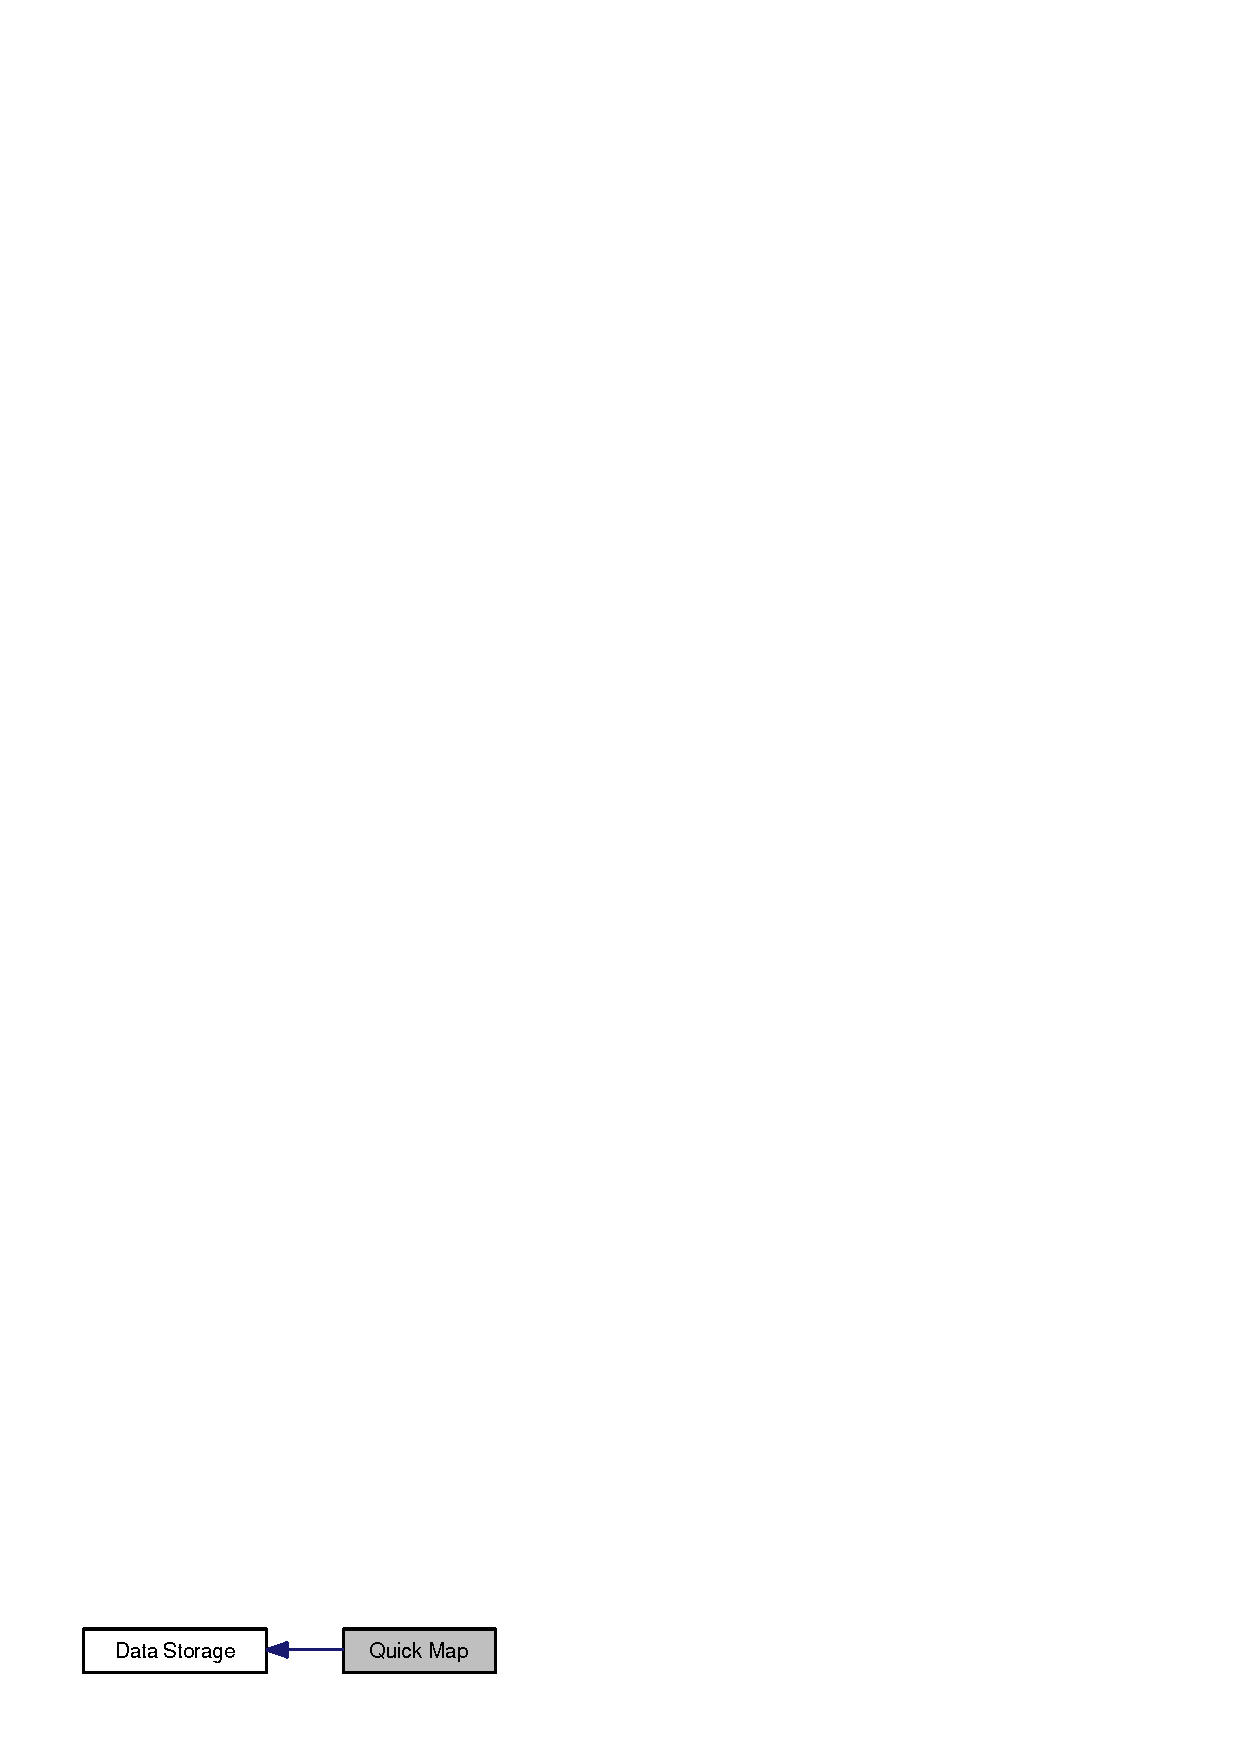
\includegraphics[width=121pt]{group__quickmap}
\end{center}
\end{figure}
\subsection*{Data Structures}
\begin{DoxyCompactItemize}
\item 
struct \hyperlink{structt__quickmap}{t\_\-quickmap}
\begin{DoxyCompactList}\small\item\em The quickmap object. \item\end{DoxyCompactList}\end{DoxyCompactItemize}
\subsection*{Functions}
\begin{DoxyCompactItemize}
\item 
BEGIN\_\-USING\_\-C\_\-LINKAGE void $\ast$ \hyperlink{group__quickmap_ga0e14465f864438dc36f86dcd8bc4cea0}{quickmap\_\-new} (void)
\begin{DoxyCompactList}\small\item\em Create a new quickmap object. \item\end{DoxyCompactList}\item 
void \hyperlink{group__quickmap_ga4fd087f1aa587108d26d5a377efb0d0b}{quickmap\_\-add} (\hyperlink{structt__quickmap}{t\_\-quickmap} $\ast$x, void $\ast$p1, void $\ast$p2)
\begin{DoxyCompactList}\small\item\em Add a pair of keys mapped to each other to the quickmap. \item\end{DoxyCompactList}\item 
void \hyperlink{group__quickmap_ga4bcc531dc606835a05358aa4ca0f92d1}{quickmap\_\-drop} (\hyperlink{structt__quickmap}{t\_\-quickmap} $\ast$x, void $\ast$p1, void $\ast$p2)
\begin{DoxyCompactList}\small\item\em Drop a pair of keys mapped to each other in the quickmap. \item\end{DoxyCompactList}\item 
long \hyperlink{group__quickmap_ga2320c067e7af6bb5f3ec25cfe3155fd1}{quickmap\_\-lookup\_\-key1} (\hyperlink{structt__quickmap}{t\_\-quickmap} $\ast$x, void $\ast$p1, void $\ast$$\ast$p2)
\begin{DoxyCompactList}\small\item\em Given a (first) key, lookup the value (the second key). \item\end{DoxyCompactList}\item 
long \hyperlink{group__quickmap_ga5b3d684268e80a4fc51e226a50ecb2ad}{quickmap\_\-lookup\_\-key2} (\hyperlink{structt__quickmap}{t\_\-quickmap} $\ast$x, void $\ast$p1, void $\ast$$\ast$p2)
\begin{DoxyCompactList}\small\item\em Given a (second) key, lookup the value (the first key). \item\end{DoxyCompactList}\item 
void \hyperlink{group__quickmap_gaa5c0fc50afb5b1dccd6b81e7dd0673c1}{quickmap\_\-readonly} (\hyperlink{structt__quickmap}{t\_\-quickmap} $\ast$x, long way)
\begin{DoxyCompactList}\small\item\em Set the readonly flag of the quickmap's hash tables. \item\end{DoxyCompactList}\end{DoxyCompactItemize}


\subsection{Detailed Description}
A quickmap implements a pair of \hyperlink{structt__hashtab}{t\_\-hashtab} hash tables so that it is fast to look up a unique value for a unique key or vice-\/versa. This implies that both the keys and the values must be unique so that look-\/ups can be performed in both directions. 

\subsection{Function Documentation}
\hypertarget{group__quickmap_ga4fd087f1aa587108d26d5a377efb0d0b}{
\index{quickmap@{quickmap}!quickmap\_\-add@{quickmap\_\-add}}
\index{quickmap\_\-add@{quickmap\_\-add}!quickmap@{quickmap}}
\subsubsection[{quickmap\_\-add}]{\setlength{\rightskip}{0pt plus 5cm}void quickmap\_\-add ({\bf t\_\-quickmap} $\ast$ {\em x}, \/  void $\ast$ {\em p1}, \/  void $\ast$ {\em p2})}}
\label{group__quickmap_ga4fd087f1aa587108d26d5a377efb0d0b}


Add a pair of keys mapped to each other to the quickmap. Note that these are considered to be a \hyperlink{structt__symbol}{t\_\-symbol} internally. This means that if you are mapping a \hyperlink{structt__symbol}{t\_\-symbol} to a \hyperlink{structt__object}{t\_\-object}, for example, the \hyperlink{structt__object}{t\_\-object} will not automatically be freed when you free the quickmap (unlike what happens when you typically free a \hyperlink{structt__hashtab}{t\_\-hashtab}).


\begin{DoxyParams}{Parameters}
\item[{\em x}]The quickmap instance. \item[{\em p1}]The (first) key. \item[{\em p2}]The value (or the second key). \end{DoxyParams}
\begin{DoxyReturn}{Returns}
A Max error code. 
\end{DoxyReturn}
\hypertarget{group__quickmap_ga4bcc531dc606835a05358aa4ca0f92d1}{
\index{quickmap@{quickmap}!quickmap\_\-drop@{quickmap\_\-drop}}
\index{quickmap\_\-drop@{quickmap\_\-drop}!quickmap@{quickmap}}
\subsubsection[{quickmap\_\-drop}]{\setlength{\rightskip}{0pt plus 5cm}void quickmap\_\-drop ({\bf t\_\-quickmap} $\ast$ {\em x}, \/  void $\ast$ {\em p1}, \/  void $\ast$ {\em p2})}}
\label{group__quickmap_ga4bcc531dc606835a05358aa4ca0f92d1}


Drop a pair of keys mapped to each other in the quickmap. 
\begin{DoxyParams}{Parameters}
\item[{\em x}]The quickmap instance. \item[{\em p1}]The first key. \item[{\em p2}]The second key. \end{DoxyParams}
\begin{DoxyReturn}{Returns}
A Max error code. 
\end{DoxyReturn}
\hypertarget{group__quickmap_ga2320c067e7af6bb5f3ec25cfe3155fd1}{
\index{quickmap@{quickmap}!quickmap\_\-lookup\_\-key1@{quickmap\_\-lookup\_\-key1}}
\index{quickmap\_\-lookup\_\-key1@{quickmap\_\-lookup\_\-key1}!quickmap@{quickmap}}
\subsubsection[{quickmap\_\-lookup\_\-key1}]{\setlength{\rightskip}{0pt plus 5cm}long quickmap\_\-lookup\_\-key1 ({\bf t\_\-quickmap} $\ast$ {\em x}, \/  void $\ast$ {\em p1}, \/  void $\ast$$\ast$ {\em p2})}}
\label{group__quickmap_ga2320c067e7af6bb5f3ec25cfe3155fd1}


Given a (first) key, lookup the value (the second key). 
\begin{DoxyParams}{Parameters}
\item[{\em x}]The quickmap instance. \item[{\em p1}]The (first) key. \item[{\em p2}]The address of a pointer which will hold the resulting key upon return. \end{DoxyParams}
\begin{DoxyReturn}{Returns}
A Max error code. 
\end{DoxyReturn}
\hypertarget{group__quickmap_ga5b3d684268e80a4fc51e226a50ecb2ad}{
\index{quickmap@{quickmap}!quickmap\_\-lookup\_\-key2@{quickmap\_\-lookup\_\-key2}}
\index{quickmap\_\-lookup\_\-key2@{quickmap\_\-lookup\_\-key2}!quickmap@{quickmap}}
\subsubsection[{quickmap\_\-lookup\_\-key2}]{\setlength{\rightskip}{0pt plus 5cm}long quickmap\_\-lookup\_\-key2 ({\bf t\_\-quickmap} $\ast$ {\em x}, \/  void $\ast$ {\em p1}, \/  void $\ast$$\ast$ {\em p2})}}
\label{group__quickmap_ga5b3d684268e80a4fc51e226a50ecb2ad}


Given a (second) key, lookup the value (the first key). 
\begin{DoxyParams}{Parameters}
\item[{\em x}]The quickmap instance. \item[{\em p1}]The (second) key. \item[{\em p2}]The address of a pointer which will hold the resulting key upon return. \end{DoxyParams}
\begin{DoxyReturn}{Returns}
A Max error code. 
\end{DoxyReturn}
\hypertarget{group__quickmap_ga0e14465f864438dc36f86dcd8bc4cea0}{
\index{quickmap@{quickmap}!quickmap\_\-new@{quickmap\_\-new}}
\index{quickmap\_\-new@{quickmap\_\-new}!quickmap@{quickmap}}
\subsubsection[{quickmap\_\-new}]{\setlength{\rightskip}{0pt plus 5cm}BEGIN\_\-USING\_\-C\_\-LINKAGE void$\ast$ quickmap\_\-new (void)}}
\label{group__quickmap_ga0e14465f864438dc36f86dcd8bc4cea0}


Create a new quickmap object. \begin{DoxyReturn}{Returns}
Pointer to the new quickmap object. 
\end{DoxyReturn}
\hypertarget{group__quickmap_gaa5c0fc50afb5b1dccd6b81e7dd0673c1}{
\index{quickmap@{quickmap}!quickmap\_\-readonly@{quickmap\_\-readonly}}
\index{quickmap\_\-readonly@{quickmap\_\-readonly}!quickmap@{quickmap}}
\subsubsection[{quickmap\_\-readonly}]{\setlength{\rightskip}{0pt plus 5cm}void quickmap\_\-readonly ({\bf t\_\-quickmap} $\ast$ {\em x}, \/  long {\em way})}}
\label{group__quickmap_gaa5c0fc50afb5b1dccd6b81e7dd0673c1}


Set the readonly flag of the quickmap's hash tables. See \hyperlink{group__hashtab_ga34ced5b4da65b4068829f799a53ea6bf}{hashtab\_\-readonly()} for more information about this.


\begin{DoxyParams}{Parameters}
\item[{\em x}]The quickmap instance. \item[{\em way}]Set to true to make the quickmap readonly (disable thread protection) or false (the default) to enable thread protection. \end{DoxyParams}

\hypertarget{group__string}{
\section{String Object}
\label{group__string}\index{String Object@{String Object}}
}


Max's string object is a simple wrapper for c-\/strings, useful when working with Max's \hyperlink{structt__dictionary}{t\_\-dictionary}, \hyperlink{structt__linklist}{t\_\-linklist}, or \hyperlink{structt__hashtab}{t\_\-hashtab}.  


Collaboration diagram for String Object:\nopagebreak
\begin{figure}[H]
\begin{center}
\leavevmode
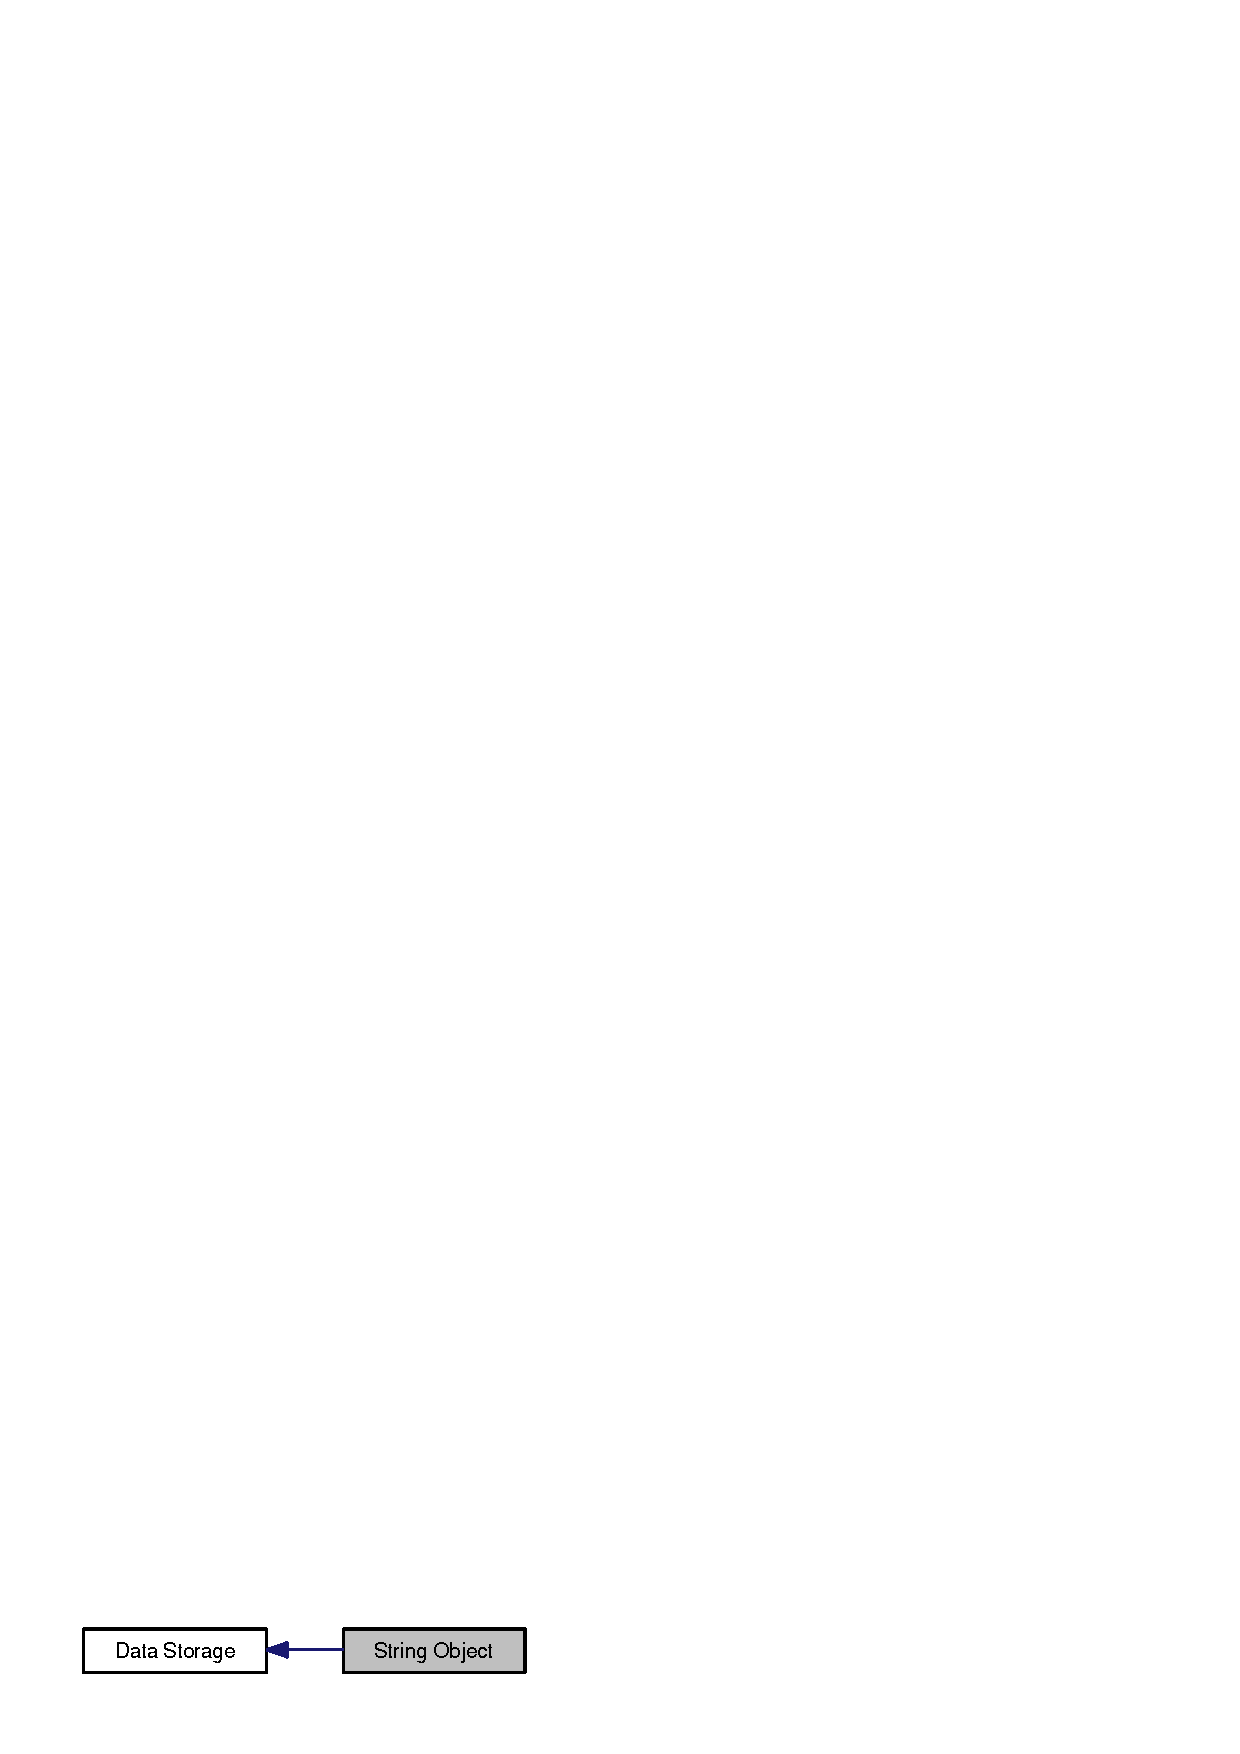
\includegraphics[width=128pt]{group__string}
\end{center}
\end{figure}
\subsection*{Data Structures}
\begin{DoxyCompactItemize}
\item 
struct \hyperlink{structt__string}{t\_\-string}
\begin{DoxyCompactList}\small\item\em The string object. \item\end{DoxyCompactList}\end{DoxyCompactItemize}
\subsection*{Functions}
\begin{DoxyCompactItemize}
\item 
\hyperlink{structt__string}{t\_\-string} $\ast$ \hyperlink{group__string_ga9fce58b43883b838697077fc674a48d9}{string\_\-new} (const char $\ast$psz)
\begin{DoxyCompactList}\small\item\em Create a new string object. \item\end{DoxyCompactList}\item 
const char $\ast$ \hyperlink{group__string_ga1d65f5effcf8d1f77b45f2603280887d}{string\_\-getptr} (\hyperlink{structt__string}{t\_\-string} $\ast$x)
\begin{DoxyCompactList}\small\item\em Create a new string object. \item\end{DoxyCompactList}\end{DoxyCompactItemize}


\subsection{Detailed Description}
Max's string object is a simple wrapper for c-\/strings, useful when working with Max's \hyperlink{structt__dictionary}{t\_\-dictionary}, \hyperlink{structt__linklist}{t\_\-linklist}, or \hyperlink{structt__hashtab}{t\_\-hashtab}. \begin{DoxySeeAlso}{See also}
\hyperlink{group__dictionary}{Dictionary} 
\end{DoxySeeAlso}


\subsection{Function Documentation}
\hypertarget{group__string_ga1d65f5effcf8d1f77b45f2603280887d}{
\index{string@{string}!string\_\-getptr@{string\_\-getptr}}
\index{string\_\-getptr@{string\_\-getptr}!string@{string}}
\subsubsection[{string\_\-getptr}]{\setlength{\rightskip}{0pt plus 5cm}const char$\ast$ string\_\-getptr ({\bf t\_\-string} $\ast$ {\em x})}}
\label{group__string_ga1d65f5effcf8d1f77b45f2603280887d}


Create a new string object. 
\begin{DoxyParams}{Parameters}
\item[{\em x}]The string object instance. \end{DoxyParams}
\begin{DoxyReturn}{Returns}
A pointer to the internally maintained C-\/string. 
\end{DoxyReturn}
\hypertarget{group__string_ga9fce58b43883b838697077fc674a48d9}{
\index{string@{string}!string\_\-new@{string\_\-new}}
\index{string\_\-new@{string\_\-new}!string@{string}}
\subsubsection[{string\_\-new}]{\setlength{\rightskip}{0pt plus 5cm}{\bf t\_\-string}$\ast$ string\_\-new (const char $\ast$ {\em psz})}}
\label{group__string_ga9fce58b43883b838697077fc674a48d9}


Create a new string object. 
\begin{DoxyParams}{Parameters}
\item[{\em psz}]Pointer to a C-\/string that will be copied to memory internal to this string object instance. \end{DoxyParams}
\begin{DoxyReturn}{Returns}
The new string object instance pointer. 
\end{DoxyReturn}

\hypertarget{group__symobject}{
\section{Symbol Object}
\label{group__symobject}\index{Symbol Object@{Symbol Object}}
}


The symobject class is a simple object that wraps a \hyperlink{structt__symbol}{t\_\-symbol}$\ast$ together with a couple of additional fields.  


Collaboration diagram for Symbol Object:\nopagebreak
\begin{figure}[H]
\begin{center}
\leavevmode
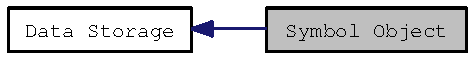
\includegraphics[width=132pt]{group__symobject}
\end{center}
\end{figure}
\subsection*{Data Structures}
\begin{DoxyCompactItemize}
\item 
struct \hyperlink{structt__symobject}{t\_\-symobject}
\begin{DoxyCompactList}\small\item\em The symobject data structure. \item\end{DoxyCompactList}\end{DoxyCompactItemize}
\subsection*{Functions}
\begin{DoxyCompactItemize}
\item 
void $\ast$ \hyperlink{group__symobject_gac66ae5925bb38fa0914f14dcc8172e2d}{symobject\_\-new} (\hyperlink{structt__symbol}{t\_\-symbol} $\ast$sym)
\begin{DoxyCompactList}\small\item\em The symobject data structure. \item\end{DoxyCompactList}\item 
long \hyperlink{group__symobject_gaff1afdf1da1b882e7314874bbf44921e}{symobject\_\-linklist\_\-match} (void $\ast$a, void $\ast$b)
\begin{DoxyCompactList}\small\item\em Utility for searching a linklist containing symobjects. \item\end{DoxyCompactList}\end{DoxyCompactItemize}


\subsection{Detailed Description}
The symobject class is a simple object that wraps a \hyperlink{structt__symbol}{t\_\-symbol}$\ast$ together with a couple of additional fields. It is useful for storing symbols, possibly with additional flags or pointers, into a \hyperlink{group__hashtab}{Hash Table} or \hyperlink{group__linklist}{Linked List}.

\begin{DoxyVersion}{Version}
5.0 
\end{DoxyVersion}


\subsection{Function Documentation}
\hypertarget{group__symobject_gaff1afdf1da1b882e7314874bbf44921e}{
\index{symobject@{symobject}!symobject\_\-linklist\_\-match@{symobject\_\-linklist\_\-match}}
\index{symobject\_\-linklist\_\-match@{symobject\_\-linklist\_\-match}!symobject@{symobject}}
\subsubsection[{symobject\_\-linklist\_\-match}]{\setlength{\rightskip}{0pt plus 5cm}long symobject\_\-linklist\_\-match (void $\ast$ {\em a}, \/  void $\ast$ {\em b})}}
\label{group__symobject_gaff1afdf1da1b882e7314874bbf44921e}


Utility for searching a linklist containing symobjects. 
\begin{DoxyParams}{Parameters}
\item[{\em a}](opaque) \item[{\em b}](opaque) \end{DoxyParams}
\begin{DoxyReturn}{Returns}
Returns true if a match is found, otherwise returns false.
\end{DoxyReturn}
\begin{DoxyRemark}{Remarks}
The following example shows one common use of the this method. 
\begin{DoxyCode}
    t_symobject *item = NULL;
    long        index;
    t_symbol    *textsym;
    
    textsym = gensym("something to look for");

    // search for a symobject with the symbol 'something to look for'
    index = linklist_findfirst(s_ll_history, (void **)&item, 
      symobject_linklist_match, textsym);
    if(index == -1){
        // symobject not found.
    }
    else{
        do something with the symobject, or with the index of the symbobject in t
      he linklist
    }   
\end{DoxyCode}
 
\end{DoxyRemark}
\hypertarget{group__symobject_gac66ae5925bb38fa0914f14dcc8172e2d}{
\index{symobject@{symobject}!symobject\_\-new@{symobject\_\-new}}
\index{symobject\_\-new@{symobject\_\-new}!symobject@{symobject}}
\subsubsection[{symobject\_\-new}]{\setlength{\rightskip}{0pt plus 5cm}void$\ast$ symobject\_\-new ({\bf t\_\-symbol} $\ast$ {\em sym})}}
\label{group__symobject_gac66ae5925bb38fa0914f14dcc8172e2d}


The symobject data structure. 
\begin{DoxyParams}{Parameters}
\item[{\em sym}]A symbol with which to initialize the new symobject. \end{DoxyParams}
\begin{DoxyReturn}{Returns}
Pointer to the new symobject instance. 
\end{DoxyReturn}

\hypertarget{group__datatypes}{
\section{Data Types}
\label{group__datatypes}\index{Data Types@{Data Types}}
}


Collaboration diagram for Data Types:\nopagebreak
\begin{figure}[H]
\begin{center}
\leavevmode
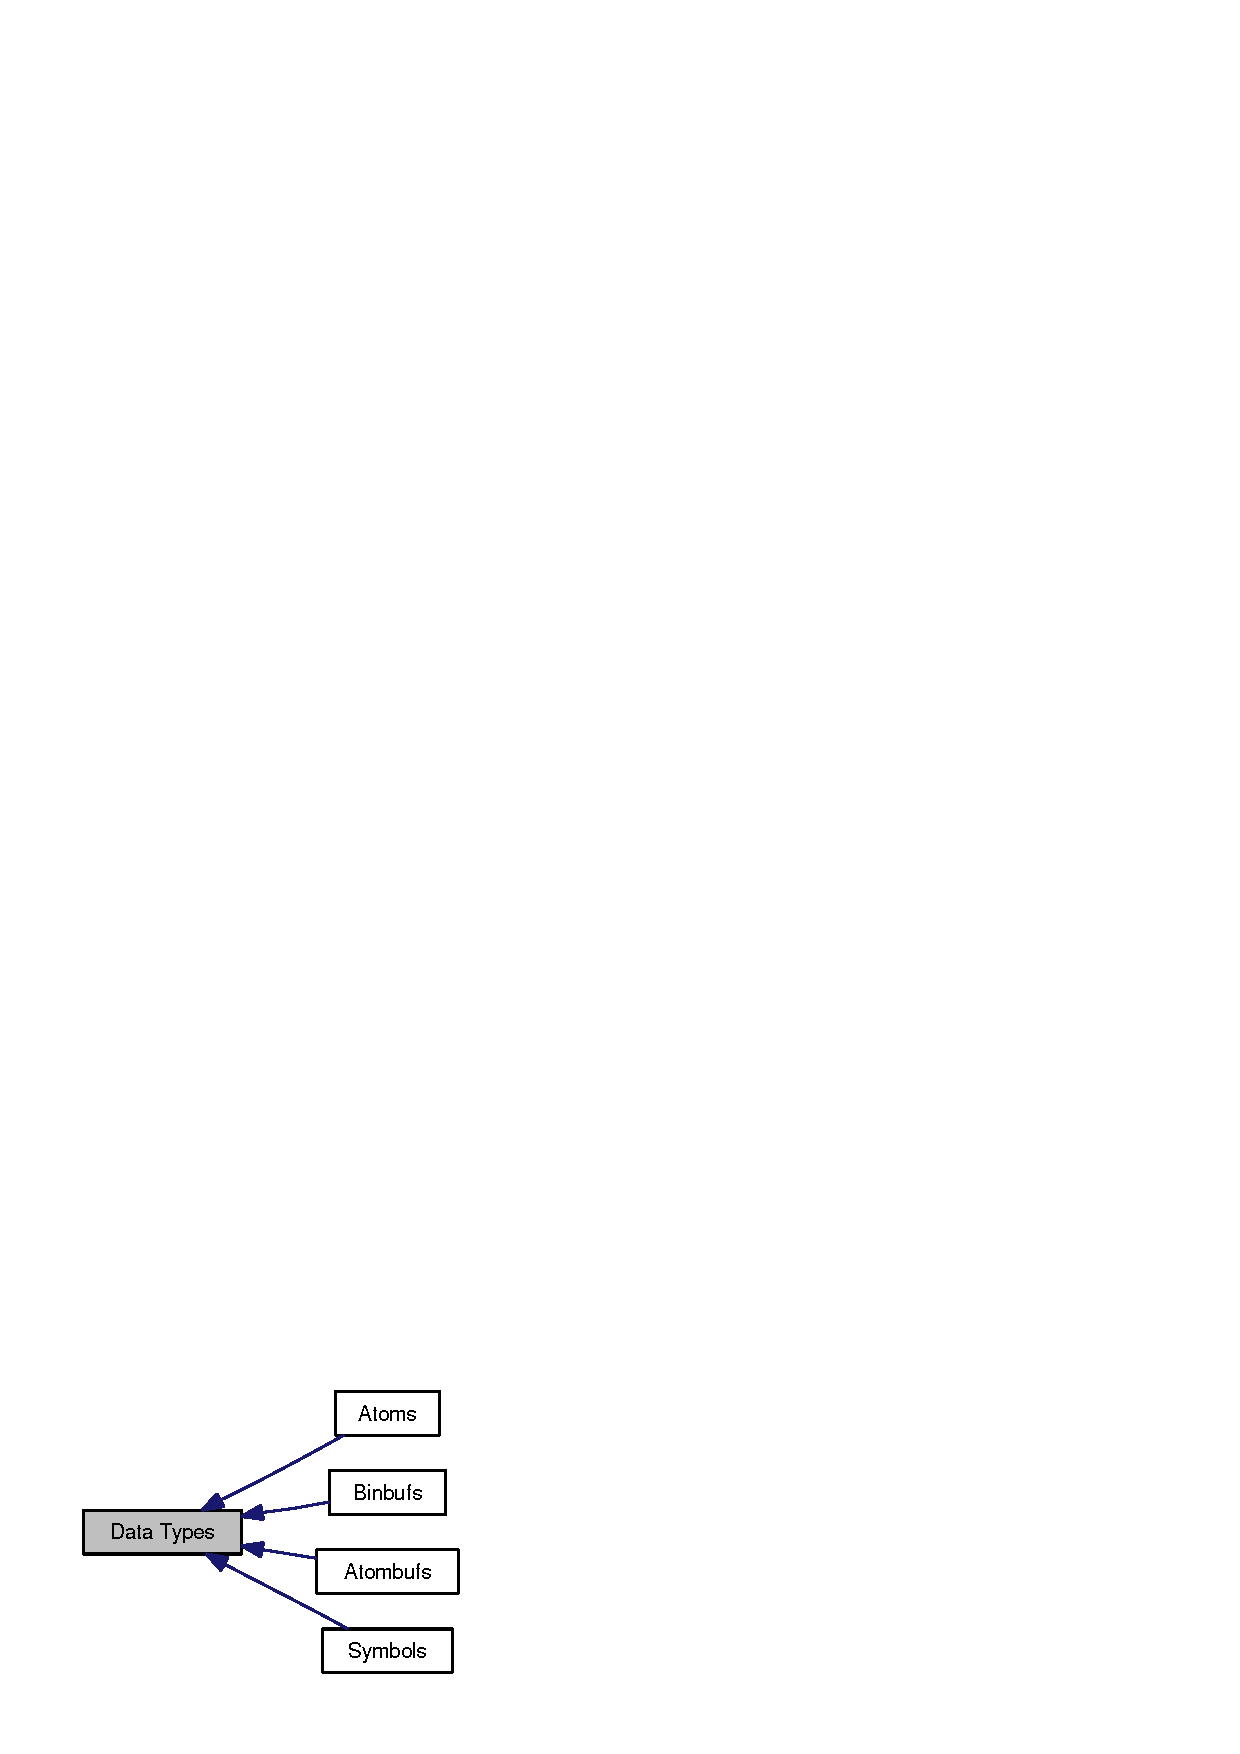
\includegraphics[width=112pt]{group__datatypes}
\end{center}
\end{figure}
\subsection*{Data Structures}
\begin{DoxyCompactItemize}
\item 
struct \hyperlink{structt__rect}{t\_\-rect}
\begin{DoxyCompactList}\small\item\em Coordinates for specifying a rectangular region. \item\end{DoxyCompactList}\item 
struct \hyperlink{structt__pt}{t\_\-pt}
\begin{DoxyCompactList}\small\item\em Coordinates for specifying a point. \item\end{DoxyCompactList}\item 
struct \hyperlink{structt__size}{t\_\-size}
\begin{DoxyCompactList}\small\item\em Coordinates for specifying the size of a region. \item\end{DoxyCompactList}\end{DoxyCompactItemize}
\subsection*{Modules}
\begin{DoxyCompactItemize}
\item 
\hyperlink{group__atom}{Atoms}
\item 
\hyperlink{group__atombuf}{Atombufs}


\begin{DoxyCompactList}\small\item\em An Atombuf is an alternative to \hyperlink{group__binbuf}{Binbufs} for temporary storage of atoms. \item\end{DoxyCompactList}\item 
\hyperlink{group__binbuf}{Binbufs}


\begin{DoxyCompactList}\small\item\em You won’t need to know about the internal structure of a Binbuf, so you can use the void $\ast$ type to refer to one. \item\end{DoxyCompactList}\item 
\hyperlink{group__symbol}{Symbols}


\begin{DoxyCompactList}\small\item\em Max maintains a symbol table of all strings to speed lookup for message passing. \item\end{DoxyCompactList}\end{DoxyCompactItemize}
\subsection*{Typedefs}
\begin{DoxyCompactItemize}
\item 
\hypertarget{group__datatypes_gac26ba0a173b50597f5738132e059b42d}{
typedef void $\ast$($\ast$ \hyperlink{group__datatypes_gac26ba0a173b50597f5738132e059b42d}{method} )(void $\ast$,...)}
\label{group__datatypes_gac26ba0a173b50597f5738132e059b42d}

\begin{DoxyCompactList}\small\item\em Function pointer type for generic methods. \item\end{DoxyCompactList}\item 
\hypertarget{group__datatypes_gac7e77a7761df347af29a272c2ddcb08b}{
typedef long($\ast$ \hyperlink{group__datatypes_gac7e77a7761df347af29a272c2ddcb08b}{longmethod} )(void $\ast$,...)}
\label{group__datatypes_gac7e77a7761df347af29a272c2ddcb08b}

\begin{DoxyCompactList}\small\item\em Function pointer type for methods returning a long. \item\end{DoxyCompactList}\item 
\hypertarget{group__datatypes_ga19aa0d8eb4efccb4ec2ebb5eaac0bdb0}{
typedef void $\ast$($\ast$ \hyperlink{group__datatypes_ga19aa0d8eb4efccb4ec2ebb5eaac0bdb0}{voidstarvoid} )()}
\label{group__datatypes_ga19aa0d8eb4efccb4ec2ebb5eaac0bdb0}

\begin{DoxyCompactList}\small\item\em Function pointer type for a function with no arguments, returning a generic pointer. \item\end{DoxyCompactList}\item 
\hypertarget{group__datatypes_ga70766a030fcd392d4574fa59b296a68e}{
typedef char $\ast$ \hyperlink{group__datatypes_ga70766a030fcd392d4574fa59b296a68e}{t\_\-ptr}}
\label{group__datatypes_ga70766a030fcd392d4574fa59b296a68e}

\begin{DoxyCompactList}\small\item\em Generic pointer type. \item\end{DoxyCompactList}\item 
\hypertarget{group__datatypes_ga0fe64aac41fd3ec071cce295a41d67ad}{
typedef char $\ast$$\ast$ \hyperlink{group__datatypes_ga0fe64aac41fd3ec071cce295a41d67ad}{t\_\-handle}}
\label{group__datatypes_ga0fe64aac41fd3ec071cce295a41d67ad}

\begin{DoxyCompactList}\small\item\em Generic pointer-\/to-\/a-\/pointer type. \item\end{DoxyCompactList}\item 
\hypertarget{group__datatypes_ga38df0c7504dc66f6dde187ac80a4db4a}{
typedef void $\ast$ \hyperlink{group__datatypes_ga38df0c7504dc66f6dde187ac80a4db4a}{t\_\-vptr}}
\label{group__datatypes_ga38df0c7504dc66f6dde187ac80a4db4a}

\begin{DoxyCompactList}\small\item\em Void pointer type. \item\end{DoxyCompactList}\item 
\hypertarget{group__datatypes_ga8dc4a45d1f82a212ce2ef921ab611fca}{
typedef void $\ast$($\ast$ \hyperlink{group__datatypes_ga8dc4a45d1f82a212ce2ef921ab611fca}{zero\_\-meth} )(void $\ast$x)}
\label{group__datatypes_ga8dc4a45d1f82a212ce2ef921ab611fca}

\begin{DoxyCompactList}\small\item\em Function pointer type for methods with no arguments. \item\end{DoxyCompactList}\item 
\hypertarget{group__datatypes_gacea7b6123eca3526399891715d3a66db}{
typedef void $\ast$($\ast$ \hyperlink{group__datatypes_gacea7b6123eca3526399891715d3a66db}{one\_\-meth} )(void $\ast$x, void $\ast$z)}
\label{group__datatypes_gacea7b6123eca3526399891715d3a66db}

\begin{DoxyCompactList}\small\item\em Function pointer type for methods with a single argument. \item\end{DoxyCompactList}\item 
\hypertarget{group__datatypes_gac6d2d64c03de780f1379287c5671ef9c}{
typedef void $\ast$($\ast$ \hyperlink{group__datatypes_gac6d2d64c03de780f1379287c5671ef9c}{two\_\-meth} )(void $\ast$x, void $\ast$z, void $\ast$a)}
\label{group__datatypes_gac6d2d64c03de780f1379287c5671ef9c}

\begin{DoxyCompactList}\small\item\em Function pointer type for methods with two arguments. \item\end{DoxyCompactList}\item 
\hypertarget{group__datatypes_ga98b3e62162a5a33fc823a88d27b50e2a}{
typedef long $\ast$($\ast$ \hyperlink{group__datatypes_ga98b3e62162a5a33fc823a88d27b50e2a}{gimmeback\_\-meth} )(void $\ast$x, \hyperlink{structt__symbol}{t\_\-symbol} $\ast$s, long ac, \hyperlink{structt__atom}{t\_\-atom} $\ast$av, \hyperlink{structt__atom}{t\_\-atom} $\ast$rv)}
\label{group__datatypes_ga98b3e62162a5a33fc823a88d27b50e2a}

\begin{DoxyCompactList}\small\item\em Function pointer type for methods that pass back a result value through the last parameter as a \hyperlink{structt__atom}{t\_\-atom}, and return an error. \item\end{DoxyCompactList}\item 
\hypertarget{group__datatypes_ga718b4eb2652c286f4d42dc18a8e71a1a}{
typedef unsigned long \hyperlink{group__datatypes_ga718b4eb2652c286f4d42dc18a8e71a1a}{ulong}}
\label{group__datatypes_ga718b4eb2652c286f4d42dc18a8e71a1a}

\begin{DoxyCompactList}\small\item\em An unsigned long integer. \item\end{DoxyCompactList}\item 
\hypertarget{group__datatypes_ga91ad9478d81a7aaf2593e8d9c3d06a14}{
typedef unsigned int \hyperlink{group__datatypes_ga91ad9478d81a7aaf2593e8d9c3d06a14}{uint}}
\label{group__datatypes_ga91ad9478d81a7aaf2593e8d9c3d06a14}

\begin{DoxyCompactList}\small\item\em An unsigned integer. \item\end{DoxyCompactList}\item 
\hypertarget{group__datatypes_gab95f123a6c9bcfee6a343170ef8c5f69}{
typedef unsigned short \hyperlink{group__datatypes_gab95f123a6c9bcfee6a343170ef8c5f69}{ushort}}
\label{group__datatypes_gab95f123a6c9bcfee6a343170ef8c5f69}

\begin{DoxyCompactList}\small\item\em An unsigned short integer. \item\end{DoxyCompactList}\item 
\hypertarget{group__datatypes_ga65f85814a8290f9797005d3b28e7e5fc}{
typedef unsigned char \hyperlink{group__datatypes_ga65f85814a8290f9797005d3b28e7e5fc}{uchar}}
\label{group__datatypes_ga65f85814a8290f9797005d3b28e7e5fc}

\begin{DoxyCompactList}\small\item\em An unsigned char. \item\end{DoxyCompactList}\item 
typedef long \hyperlink{group__datatypes_ga73edaae82b318855cc09fac994918165}{t\_\-max\_\-err}
\begin{DoxyCompactList}\small\item\em A Max error code. \item\end{DoxyCompactList}\end{DoxyCompactItemize}


\subsection{Typedef Documentation}
\hypertarget{group__datatypes_ga73edaae82b318855cc09fac994918165}{
\index{datatypes@{datatypes}!t\_\-max\_\-err@{t\_\-max\_\-err}}
\index{t\_\-max\_\-err@{t\_\-max\_\-err}!datatypes@{datatypes}}
\subsubsection[{t\_\-max\_\-err}]{\setlength{\rightskip}{0pt plus 5cm}typedef long {\bf t\_\-max\_\-err}}}
\label{group__datatypes_ga73edaae82b318855cc09fac994918165}


A Max error code. Common error codes are defined in \hyperlink{group__misc_ga0764dd6c02b76cca7d053ae50555d69d}{e\_\-max\_\-errorcodes}. 
\hypertarget{group__atom}{
\section{Atoms}
\label{group__atom}\index{Atoms@{Atoms}}
}


Collaboration diagram for Atoms:\nopagebreak
\begin{figure}[H]
\begin{center}
\leavevmode
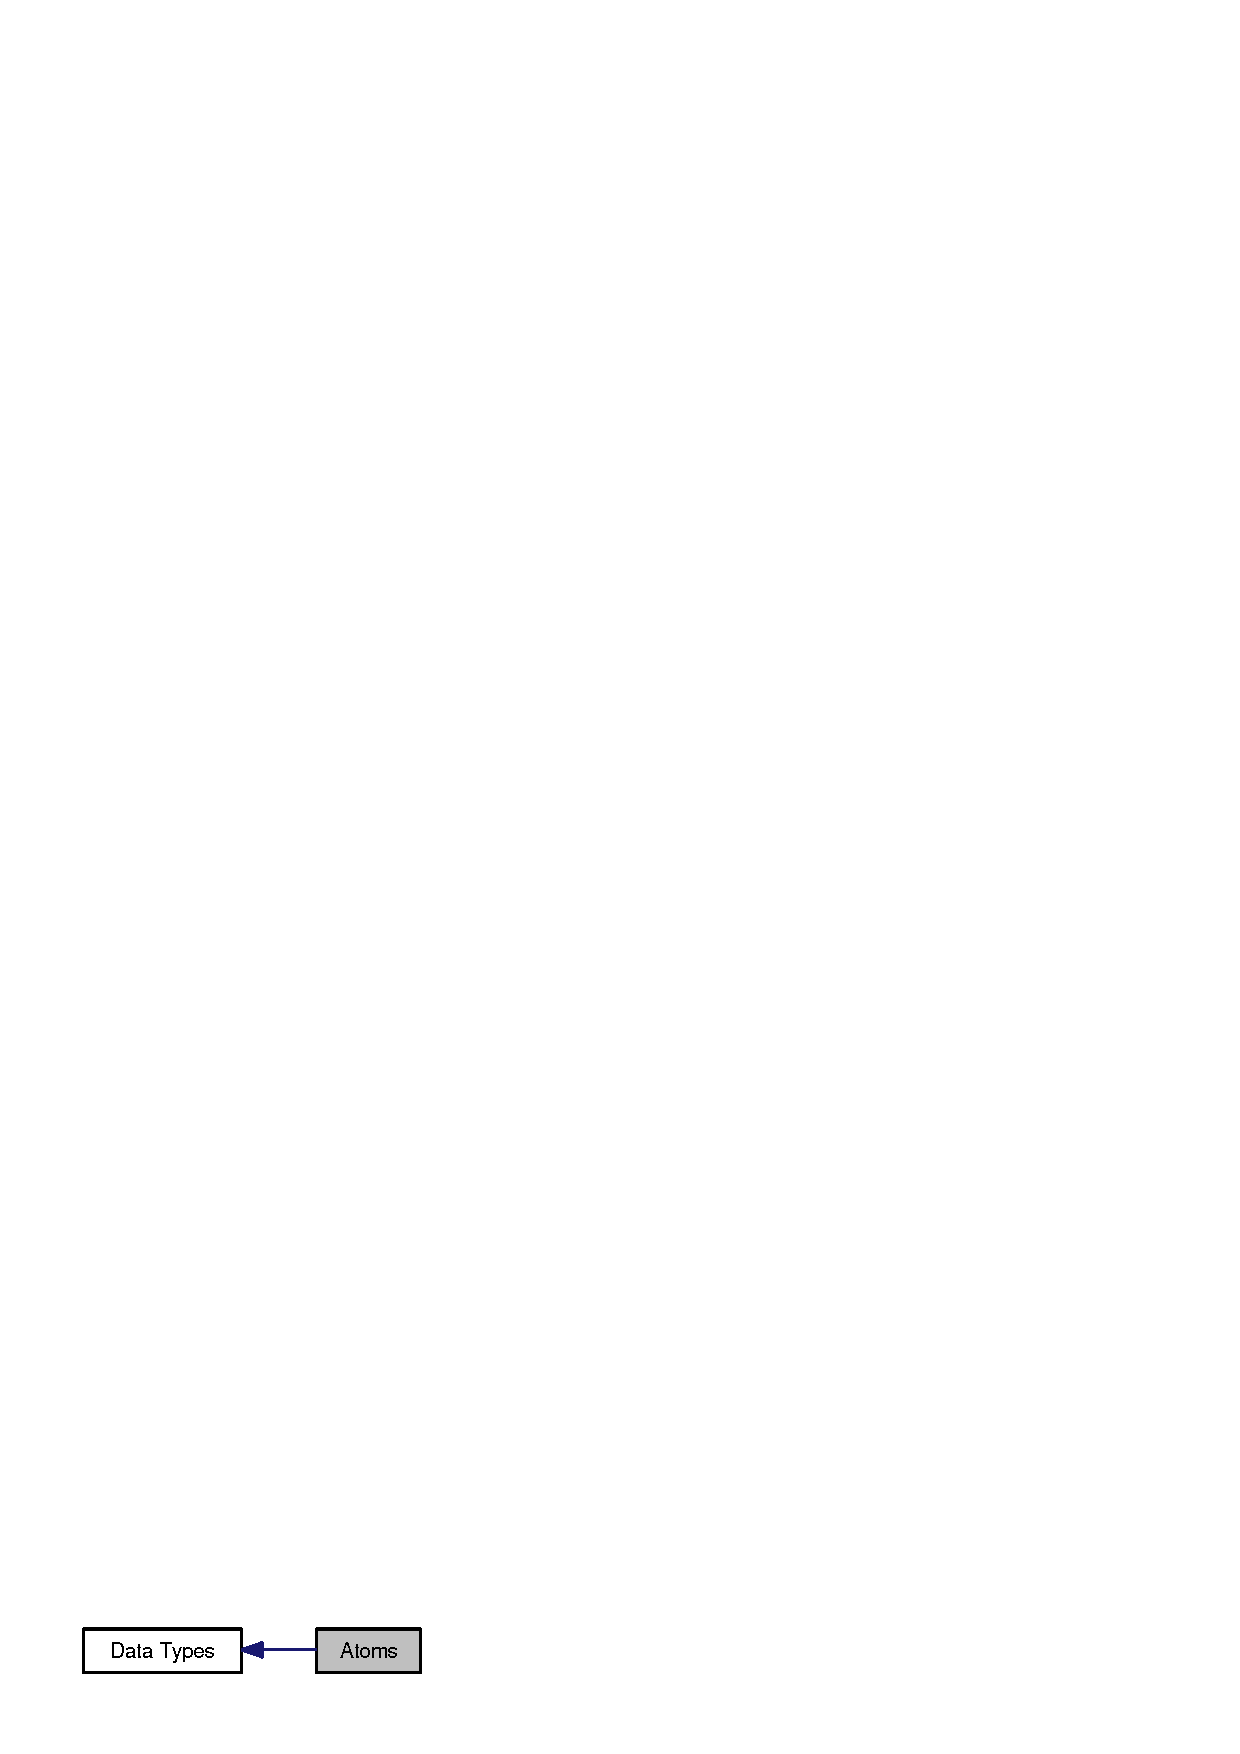
\includegraphics[width=103pt]{group__atom}
\end{center}
\end{figure}
\subsection*{Data Structures}
\begin{DoxyCompactItemize}
\item 
union \hyperlink{unionword}{word}
\begin{DoxyCompactList}\small\item\em Union for packing any of the datum defined in \hyperlink{group__atom_ga8aa6700e9f00b132eb376db6e39ade47}{e\_\-max\_\-atomtypes}. \item\end{DoxyCompactList}\item 
struct \hyperlink{structt__atom}{t\_\-atom}
\begin{DoxyCompactList}\small\item\em An atom is a typed datum. \item\end{DoxyCompactList}\end{DoxyCompactItemize}
\subsection*{Defines}
\begin{DoxyCompactItemize}
\item 
\hypertarget{group__atom_ga27eb80f98b4020e3ecab761d634a3876}{
\#define \hyperlink{group__atom_ga27eb80f98b4020e3ecab761d634a3876}{ATOM\_\-MAX\_\-STRLEN}~(32768)}
\label{group__atom_ga27eb80f98b4020e3ecab761d634a3876}

\begin{DoxyCompactList}\small\item\em Defines the largest possible string size for an atom. \item\end{DoxyCompactList}\end{DoxyCompactItemize}
\subsection*{Enumerations}
\begin{DoxyCompactItemize}
\item 
enum \hyperlink{group__atom_ga8aa6700e9f00b132eb376db6e39ade47}{e\_\-max\_\-atomtypes} \{ \par
\hyperlink{group__atom_gga8aa6700e9f00b132eb376db6e39ade47a858ddb5d5927eae3fd699a82c7e174b6}{A\_\-NOTHING} =  0, 
\par
\hyperlink{group__atom_gga8aa6700e9f00b132eb376db6e39ade47a002f28879581a6f66ea492b994b96f1e}{A\_\-LONG}, 
\par
\hyperlink{group__atom_gga8aa6700e9f00b132eb376db6e39ade47a0b3aa0ab8104573dfc9cb70b5b08031f}{A\_\-FLOAT}, 
\par
\hyperlink{group__atom_gga8aa6700e9f00b132eb376db6e39ade47a2d661c2a5d949566e2f1944c99bceeea}{A\_\-SYM}, 
\par
\hyperlink{group__atom_gga8aa6700e9f00b132eb376db6e39ade47a82cc76e0d53c8fc28df167c35d5bbd1a}{A\_\-OBJ}, 
\par
\hyperlink{group__atom_gga8aa6700e9f00b132eb376db6e39ade47a7bd979db3dcf86909e24a1d1452e2205}{A\_\-DEFLONG}, 
\par
\hyperlink{group__atom_gga8aa6700e9f00b132eb376db6e39ade47a42b644240dcbb90fe67282a4d0688776}{A\_\-DEFFLOAT}, 
\par
\hyperlink{group__atom_gga8aa6700e9f00b132eb376db6e39ade47aa010616276cb89bcd04bcba611e18d51}{A\_\-DEFSYM}, 
\par
\hyperlink{group__atom_gga8aa6700e9f00b132eb376db6e39ade47a81c1a8550f038db16a619167a70a79b6}{A\_\-GIMME}, 
\par
\hyperlink{group__atom_gga8aa6700e9f00b132eb376db6e39ade47af48193ec36e53b1507d81c49873c8d7a}{A\_\-CANT}, 
\par
\hyperlink{group__atom_gga8aa6700e9f00b132eb376db6e39ade47ac105be4ef726ee36c4330e16bb24706e}{A\_\-SEMI}, 
\par
\hyperlink{group__atom_gga8aa6700e9f00b132eb376db6e39ade47a07c3484085a3217107acec059d17b945}{A\_\-COMMA}, 
\par
\hyperlink{group__atom_gga8aa6700e9f00b132eb376db6e39ade47af0a5a9017f6b59e82a4859cd0560d36b}{A\_\-DOLLAR}, 
\par
\hyperlink{group__atom_gga8aa6700e9f00b132eb376db6e39ade47a9d47aadc47f728c2af7be2ec12a4a8c5}{A\_\-DOLLSYM}, 
\par
\hyperlink{group__atom_gga8aa6700e9f00b132eb376db6e39ade47ad150bf3de9c8dc2ddfa0ca0ca2382360}{A\_\-GIMMEBACK}, 
\par
\hyperlink{group__atom_gga8aa6700e9f00b132eb376db6e39ade47abcb435e6fecfdcd79276dc8db1988db3}{A\_\-DEFER} =  0x41, 
\par
\hyperlink{group__atom_gga8aa6700e9f00b132eb376db6e39ade47af563cdbe6db453f24552bbe7fe6762d8}{A\_\-USURP} =  0x42, 
\par
\hyperlink{group__atom_gga8aa6700e9f00b132eb376db6e39ade47a4556bc5fe0d4f8cc55eda5aeeee55cf2}{A\_\-DEFER\_\-LOW} =  0x43, 
\par
\hyperlink{group__atom_gga8aa6700e9f00b132eb376db6e39ade47a8c844b0a1b551341a6a5e3b95d2f1152}{A\_\-USURP\_\-LOW} =  0x44
 \}
\begin{DoxyCompactList}\small\item\em the list of officially recognized types, including pseudotypes for commas and semicolons. \item\end{DoxyCompactList}\item 
enum \hyperlink{group__atom_ga42fa1c131691f55dbc781a0be60e3772}{e\_\-max\_\-atom\_\-gettext\_\-flags} \{ \par
\hyperlink{group__atom_gga42fa1c131691f55dbc781a0be60e3772a2e8bad722419a8be35f8ef13364ddcc7}{OBEX\_\-UTIL\_\-ATOM\_\-GETTEXT\_\-DEFAULT} =  0x00000000, 
\par
\hyperlink{group__atom_gga42fa1c131691f55dbc781a0be60e3772a433f595f519e0a4051d769db66b9b5d8}{OBEX\_\-UTIL\_\-ATOM\_\-GETTEXT\_\-TRUNCATE\_\-ZEROS} =  0x00000001, 
\par
\hyperlink{group__atom_gga42fa1c131691f55dbc781a0be60e3772a639f398e983f74ee2adbf39a69062a93}{OBEX\_\-UTIL\_\-ATOM\_\-GETTEXT\_\-SYM\_\-NO\_\-QUOTE} =  0x00000002, 
\par
\hyperlink{group__atom_gga42fa1c131691f55dbc781a0be60e3772a8adcad05a635857f1f76aec4188e9ae9}{OBEX\_\-UTIL\_\-ATOM\_\-GETTEXT\_\-SYM\_\-FORCE\_\-QUOTE} =  0x00000004, 
\par
\hyperlink{group__atom_gga42fa1c131691f55dbc781a0be60e3772a45021a54b7ef864284a15b898d169a13}{OBEX\_\-UTIL\_\-ATOM\_\-GETTEXT\_\-COMMA\_\-DELIM} =  0x00000008, 
\par
\hyperlink{group__atom_gga42fa1c131691f55dbc781a0be60e3772a6cffcc55e28bd69beb674fe018c18e35}{OBEX\_\-UTIL\_\-ATOM\_\-GETTEXT\_\-FORCE\_\-ZEROS} =  0x00000010, 
\par
\hyperlink{group__atom_gga42fa1c131691f55dbc781a0be60e3772a9a254b928e25b9023b6e3bb6b25f35b7}{OBEX\_\-UTIL\_\-ATOM\_\-GETTEXT\_\-NUM\_\-HI\_\-RES} =  0x00000020
 \}
\begin{DoxyCompactList}\small\item\em Flags that determine how functions convert atoms into text (C-\/strings). \item\end{DoxyCompactList}\end{DoxyCompactItemize}
\subsection*{Functions}
\begin{DoxyCompactItemize}
\item 
\hyperlink{group__datatypes_ga73edaae82b318855cc09fac994918165}{t\_\-max\_\-err} \hyperlink{group__atom_ga98af493b18dfac0f8d441e16e520d5f6}{atom\_\-setlong} (\hyperlink{structt__atom}{t\_\-atom} $\ast$a, long b)
\begin{DoxyCompactList}\small\item\em Inserts an integer into a \hyperlink{structt__atom}{t\_\-atom} and change the t\_\-atom's type to \hyperlink{group__atom_gga8aa6700e9f00b132eb376db6e39ade47a002f28879581a6f66ea492b994b96f1e}{A\_\-LONG}. \item\end{DoxyCompactList}\item 
\hyperlink{group__datatypes_ga73edaae82b318855cc09fac994918165}{t\_\-max\_\-err} \hyperlink{group__atom_gae4faf28f99370e1a4ae9eab7df5bede7}{atom\_\-setfloat} (\hyperlink{structt__atom}{t\_\-atom} $\ast$a, double b)
\begin{DoxyCompactList}\small\item\em Inserts a floating point number into a \hyperlink{structt__atom}{t\_\-atom} and change the t\_\-atom's type to \hyperlink{group__atom_gga8aa6700e9f00b132eb376db6e39ade47a0b3aa0ab8104573dfc9cb70b5b08031f}{A\_\-FLOAT}. \item\end{DoxyCompactList}\item 
\hyperlink{group__datatypes_ga73edaae82b318855cc09fac994918165}{t\_\-max\_\-err} \hyperlink{group__atom_ga36c2619378802011ff0ff44bf74a807c}{atom\_\-setsym} (\hyperlink{structt__atom}{t\_\-atom} $\ast$a, \hyperlink{structt__symbol}{t\_\-symbol} $\ast$b)
\begin{DoxyCompactList}\small\item\em Inserts a \hyperlink{structt__symbol}{t\_\-symbol} $\ast$ into a \hyperlink{structt__atom}{t\_\-atom} and change the t\_\-atom's type to \hyperlink{group__atom_gga8aa6700e9f00b132eb376db6e39ade47a2d661c2a5d949566e2f1944c99bceeea}{A\_\-SYM}. \item\end{DoxyCompactList}\item 
\hyperlink{group__datatypes_ga73edaae82b318855cc09fac994918165}{t\_\-max\_\-err} \hyperlink{group__atom_ga0ad7d5c696047effee6b6bbf04a981c4}{atom\_\-setobj} (\hyperlink{structt__atom}{t\_\-atom} $\ast$a, void $\ast$b)
\begin{DoxyCompactList}\small\item\em Inserts a generic pointer value into a \hyperlink{structt__atom}{t\_\-atom} and change the t\_\-atom's type to \hyperlink{group__atom_gga8aa6700e9f00b132eb376db6e39ade47a82cc76e0d53c8fc28df167c35d5bbd1a}{A\_\-OBJ}. \item\end{DoxyCompactList}\item 
long \hyperlink{group__atom_ga62c0a631f50db54ec654a9e40b992fe2}{atom\_\-getlong} (\hyperlink{structt__atom}{t\_\-atom} $\ast$a)
\begin{DoxyCompactList}\small\item\em Retrieves a long integer value from a \hyperlink{structt__atom}{t\_\-atom}. \item\end{DoxyCompactList}\item 
float \hyperlink{group__atom_ga28f52239a67244db2e821320702712ca}{atom\_\-getfloat} (\hyperlink{structt__atom}{t\_\-atom} $\ast$a)
\begin{DoxyCompactList}\small\item\em Retrieves a floating point value from a \hyperlink{structt__atom}{t\_\-atom}. \item\end{DoxyCompactList}\item 
\hyperlink{structt__symbol}{t\_\-symbol} $\ast$ \hyperlink{group__atom_gab43922b60c9c2aaf3a4ecabaa432ef61}{atom\_\-getsym} (\hyperlink{structt__atom}{t\_\-atom} $\ast$a)
\begin{DoxyCompactList}\small\item\em Retrieves a \hyperlink{structt__symbol}{t\_\-symbol} $\ast$ value from a \hyperlink{structt__atom}{t\_\-atom}. \item\end{DoxyCompactList}\item 
void $\ast$ \hyperlink{group__atom_ga3fa97bb8b72a394a2918cc55951f8b39}{atom\_\-getobj} (\hyperlink{structt__atom}{t\_\-atom} $\ast$a)
\begin{DoxyCompactList}\small\item\em Retrieves a generic pointer value from a \hyperlink{structt__atom}{t\_\-atom}. \item\end{DoxyCompactList}\item 
long \hyperlink{group__atom_gae9bef849142b12c94f842faa03b3238c}{atom\_\-getcharfix} (\hyperlink{structt__atom}{t\_\-atom} $\ast$a)
\begin{DoxyCompactList}\small\item\em Retrieves an unsigned integer value between 0 and 255 from a \hyperlink{structt__atom}{t\_\-atom}. \item\end{DoxyCompactList}\item 
long \hyperlink{group__atom_ga7959e9b765bf2eb52223587d8282a49e}{atom\_\-gettype} (\hyperlink{structt__atom}{t\_\-atom} $\ast$a)
\begin{DoxyCompactList}\small\item\em Retrieves type from a \hyperlink{structt__atom}{t\_\-atom}. \item\end{DoxyCompactList}\item 
long \hyperlink{group__atom_gaba53e6f86741dea07cff414b9b5d6a8b}{atom\_\-arg\_\-getlong} (long $\ast$c, long idx, long ac, \hyperlink{structt__atom}{t\_\-atom} $\ast$av)
\begin{DoxyCompactList}\small\item\em Retrieves the integer value of a particular \hyperlink{structt__atom}{t\_\-atom} from an atom list, if the atom exists. \item\end{DoxyCompactList}\item 
long \hyperlink{group__atom_ga06e305ddb4fde46ef2e8b66a7e578d61}{atom\_\-arg\_\-getfloat} (float $\ast$c, long idx, long ac, \hyperlink{structt__atom}{t\_\-atom} $\ast$av)
\begin{DoxyCompactList}\small\item\em Retrieves the floating point value of a particular \hyperlink{structt__atom}{t\_\-atom} from an atom list, if the atom exists. \item\end{DoxyCompactList}\item 
long \hyperlink{group__atom_ga5f494e92bded5005a52a31738f8cbbdf}{atom\_\-arg\_\-getdouble} (double $\ast$c, long idx, long ac, \hyperlink{structt__atom}{t\_\-atom} $\ast$av)
\begin{DoxyCompactList}\small\item\em Retrieves the floating point value, as a double, of a particular \hyperlink{structt__atom}{t\_\-atom} from an atom list, if the atom exists. \item\end{DoxyCompactList}\item 
long \hyperlink{group__atom_gaeba7a400021327a46673220ef1c1ee98}{atom\_\-arg\_\-getsym} (\hyperlink{structt__symbol}{t\_\-symbol} $\ast$$\ast$c, long idx, long ac, \hyperlink{structt__atom}{t\_\-atom} $\ast$av)
\begin{DoxyCompactList}\small\item\em Retrieves the \hyperlink{structt__symbol}{t\_\-symbol} $\ast$ value of a particular \hyperlink{structt__atom}{t\_\-atom} from an atom list, if the atom exists. \item\end{DoxyCompactList}\item 
\hyperlink{group__datatypes_ga73edaae82b318855cc09fac994918165}{t\_\-max\_\-err} \hyperlink{group__atom_gad1a3b8eed4c311ec41b2d565bf40b002}{atom\_\-alloc} (long $\ast$ac, \hyperlink{structt__atom}{t\_\-atom} $\ast$$\ast$av, char $\ast$alloc)
\begin{DoxyCompactList}\small\item\em Allocate a single atom. \item\end{DoxyCompactList}\item 
\hyperlink{group__datatypes_ga73edaae82b318855cc09fac994918165}{t\_\-max\_\-err} \hyperlink{group__atom_ga5601306b4b76f338501cda586a6c1fde}{atom\_\-alloc\_\-array} (long minsize, long $\ast$ac, \hyperlink{structt__atom}{t\_\-atom} $\ast$$\ast$av, char $\ast$alloc)
\begin{DoxyCompactList}\small\item\em Allocate an array of atoms. \item\end{DoxyCompactList}\item 
\hyperlink{group__datatypes_ga73edaae82b318855cc09fac994918165}{t\_\-max\_\-err} \hyperlink{group__atom_ga88e54464a226b4fa99113f39ca522fb2}{atom\_\-setchar\_\-array} (long ac, \hyperlink{structt__atom}{t\_\-atom} $\ast$av, long count, unsigned char $\ast$vals)
\begin{DoxyCompactList}\small\item\em Assign an array of char values to an array of atoms. \item\end{DoxyCompactList}\item 
\hyperlink{group__datatypes_ga73edaae82b318855cc09fac994918165}{t\_\-max\_\-err} \hyperlink{group__atom_ga524207025bbc13a13e901ea5c175e0bf}{atom\_\-setlong\_\-array} (long ac, \hyperlink{structt__atom}{t\_\-atom} $\ast$av, long count, long $\ast$vals)
\begin{DoxyCompactList}\small\item\em Assign an array of long integer values to an array of atoms. \item\end{DoxyCompactList}\item 
\hyperlink{group__datatypes_ga73edaae82b318855cc09fac994918165}{t\_\-max\_\-err} \hyperlink{group__atom_ga05d828d4c2a60274cf185cbcb50df208}{atom\_\-setfloat\_\-array} (long ac, \hyperlink{structt__atom}{t\_\-atom} $\ast$av, long count, float $\ast$vals)
\begin{DoxyCompactList}\small\item\em Assign an array of 32bit float values to an array of atoms. \item\end{DoxyCompactList}\item 
\hyperlink{group__datatypes_ga73edaae82b318855cc09fac994918165}{t\_\-max\_\-err} \hyperlink{group__atom_ga4a5f89178488b1e8bfe75a1f270058d5}{atom\_\-setdouble\_\-array} (long ac, \hyperlink{structt__atom}{t\_\-atom} $\ast$av, long count, double $\ast$vals)
\begin{DoxyCompactList}\small\item\em Assign an array of 64bit float values to an array of atoms. \item\end{DoxyCompactList}\item 
\hyperlink{group__datatypes_ga73edaae82b318855cc09fac994918165}{t\_\-max\_\-err} \hyperlink{group__atom_ga7955dbb1679166ac7bb15bfc1ee9b7f8}{atom\_\-setsym\_\-array} (long ac, \hyperlink{structt__atom}{t\_\-atom} $\ast$av, long count, \hyperlink{structt__symbol}{t\_\-symbol} $\ast$$\ast$vals)
\begin{DoxyCompactList}\small\item\em Assign an array of \hyperlink{structt__symbol}{t\_\-symbol}$\ast$ values to an array of atoms. \item\end{DoxyCompactList}\item 
\hyperlink{group__datatypes_ga73edaae82b318855cc09fac994918165}{t\_\-max\_\-err} \hyperlink{group__atom_ga6d8f3b8d919c155a69d9e6a9c010ec74}{atom\_\-setatom\_\-array} (long ac, \hyperlink{structt__atom}{t\_\-atom} $\ast$av, long count, \hyperlink{structt__atom}{t\_\-atom} $\ast$vals)
\begin{DoxyCompactList}\small\item\em Assign an array of \hyperlink{structt__atom}{t\_\-atom} values to an array of atoms. \item\end{DoxyCompactList}\item 
\hyperlink{group__datatypes_ga73edaae82b318855cc09fac994918165}{t\_\-max\_\-err} \hyperlink{group__atom_ga8ebd48ccec485451687fd5b7abcd0227}{atom\_\-setobj\_\-array} (long ac, \hyperlink{structt__atom}{t\_\-atom} $\ast$av, long count, \hyperlink{structt__object}{t\_\-object} $\ast$$\ast$vals)
\begin{DoxyCompactList}\small\item\em Assign an array of \hyperlink{structt__object}{t\_\-object}$\ast$ values to an array of atoms. \item\end{DoxyCompactList}\item 
\hyperlink{group__datatypes_ga73edaae82b318855cc09fac994918165}{t\_\-max\_\-err} \hyperlink{group__atom_ga55938aedb41a8f3565680cf29169dc70}{atom\_\-setparse} (long $\ast$ac, \hyperlink{structt__atom}{t\_\-atom} $\ast$$\ast$av, char $\ast$parsestr)
\begin{DoxyCompactList}\small\item\em Parse a C-\/string into an array of atoms. \item\end{DoxyCompactList}\item 
\hyperlink{group__datatypes_ga73edaae82b318855cc09fac994918165}{t\_\-max\_\-err} \hyperlink{group__atom_ga7a00fdf0699ae5176d39d7ddc3529bf0}{atom\_\-setformat} (long $\ast$ac, \hyperlink{structt__atom}{t\_\-atom} $\ast$$\ast$av, char $\ast$fmt,...)
\begin{DoxyCompactList}\small\item\em Create an array of atoms populated with values using sprintf-\/like syntax. \item\end{DoxyCompactList}\item 
\hyperlink{group__datatypes_ga73edaae82b318855cc09fac994918165}{t\_\-max\_\-err} \hyperlink{group__atom_gadf4cd1c3cae12c062fb07ffca5dbf0c0}{atom\_\-getformat} (long ac, \hyperlink{structt__atom}{t\_\-atom} $\ast$av, char $\ast$fmt,...)
\begin{DoxyCompactList}\small\item\em Retrieve values from an array of atoms using sscanf-\/like syntax. \item\end{DoxyCompactList}\item 
\hyperlink{group__datatypes_ga73edaae82b318855cc09fac994918165}{t\_\-max\_\-err} \hyperlink{group__atom_gade94ebf977b43b151a906b2b70d12301}{atom\_\-gettext} (long ac, \hyperlink{structt__atom}{t\_\-atom} $\ast$av, long $\ast$textsize, char $\ast$$\ast$text, long flags)
\begin{DoxyCompactList}\small\item\em Convert an array of atoms into a C-\/string. \item\end{DoxyCompactList}\item 
\hyperlink{group__datatypes_ga73edaae82b318855cc09fac994918165}{t\_\-max\_\-err} \hyperlink{group__atom_ga76ec2c6ff61e5bb4e29e51f1a791db56}{atom\_\-getchar\_\-array} (long ac, \hyperlink{structt__atom}{t\_\-atom} $\ast$av, long count, unsigned char $\ast$vals)
\begin{DoxyCompactList}\small\item\em Fetch an array of char values from an array of atoms. \item\end{DoxyCompactList}\item 
\hyperlink{group__datatypes_ga73edaae82b318855cc09fac994918165}{t\_\-max\_\-err} \hyperlink{group__atom_ga0bb78863f0f99d492b5241c9158b10cc}{atom\_\-getlong\_\-array} (long ac, \hyperlink{structt__atom}{t\_\-atom} $\ast$av, long count, long $\ast$vals)
\begin{DoxyCompactList}\small\item\em Fetch an array of long integer values from an array of atoms. \item\end{DoxyCompactList}\item 
\hyperlink{group__datatypes_ga73edaae82b318855cc09fac994918165}{t\_\-max\_\-err} \hyperlink{group__atom_ga0d3bc27f1de1bacbd8026c81a7b7e3d3}{atom\_\-getfloat\_\-array} (long ac, \hyperlink{structt__atom}{t\_\-atom} $\ast$av, long count, float $\ast$vals)
\begin{DoxyCompactList}\small\item\em Fetch an array of 32bit float values from an array of atoms. \item\end{DoxyCompactList}\item 
\hyperlink{group__datatypes_ga73edaae82b318855cc09fac994918165}{t\_\-max\_\-err} \hyperlink{group__atom_ga4189a7d83f7cf03d575425ba97f0e9f9}{atom\_\-getdouble\_\-array} (long ac, \hyperlink{structt__atom}{t\_\-atom} $\ast$av, long count, double $\ast$vals)
\begin{DoxyCompactList}\small\item\em Fetch an array of 64bit float values from an array of atoms. \item\end{DoxyCompactList}\item 
\hyperlink{group__datatypes_ga73edaae82b318855cc09fac994918165}{t\_\-max\_\-err} \hyperlink{group__atom_ga48c3655238debe58e8a943dc28381953}{atom\_\-getsym\_\-array} (long ac, \hyperlink{structt__atom}{t\_\-atom} $\ast$av, long count, \hyperlink{structt__symbol}{t\_\-symbol} $\ast$$\ast$vals)
\begin{DoxyCompactList}\small\item\em Fetch an array of \hyperlink{structt__symbol}{t\_\-symbol}$\ast$ values from an array of atoms. \item\end{DoxyCompactList}\item 
\hyperlink{group__datatypes_ga73edaae82b318855cc09fac994918165}{t\_\-max\_\-err} \hyperlink{group__atom_ga76191e30761d55e4528b50e447f43abb}{atom\_\-getatom\_\-array} (long ac, \hyperlink{structt__atom}{t\_\-atom} $\ast$av, long count, \hyperlink{structt__atom}{t\_\-atom} $\ast$vals)
\begin{DoxyCompactList}\small\item\em Fetch an array of \hyperlink{structt__atom}{t\_\-atom} values from an array of atoms. \item\end{DoxyCompactList}\item 
\hyperlink{group__datatypes_ga73edaae82b318855cc09fac994918165}{t\_\-max\_\-err} \hyperlink{group__atom_gac8571c66b47e3699520695352d2eff30}{atom\_\-getobj\_\-array} (long ac, \hyperlink{structt__atom}{t\_\-atom} $\ast$av, long count, \hyperlink{structt__object}{t\_\-object} $\ast$$\ast$vals)
\begin{DoxyCompactList}\small\item\em Fetch an array of \hyperlink{structt__object}{t\_\-object}$\ast$ values from an array of atoms. \item\end{DoxyCompactList}\item 
long \hyperlink{group__atom_gaf09b95edeae2bf9704641e032d213954}{atomisstring} (\hyperlink{structt__atom}{t\_\-atom} $\ast$a)
\begin{DoxyCompactList}\small\item\em Determines whether or not an atom represents a \hyperlink{structt__string}{t\_\-string} object. \item\end{DoxyCompactList}\item 
long \hyperlink{group__atom_gaf85b0f40648c68c0e32168029489575b}{atomisatomarray} (\hyperlink{structt__atom}{t\_\-atom} $\ast$a)
\begin{DoxyCompactList}\small\item\em Determines whether or not an atom represents a \hyperlink{structt__atomarray}{t\_\-atomarray} object. \item\end{DoxyCompactList}\item 
long \hyperlink{group__atom_ga85a30af9d861ac3f5664e63c4772e77b}{atomisdictionary} (\hyperlink{structt__atom}{t\_\-atom} $\ast$a)
\begin{DoxyCompactList}\small\item\em Determines whether or not an atom represents a \hyperlink{structt__dictionary}{t\_\-dictionary} object. \item\end{DoxyCompactList}\item 
BEGIN\_\-USING\_\-C\_\-LINKAGE void \hyperlink{group__atom_ga34f9b920bed69c19988fe70d7be79c18}{atom\_\-copy} (short argc1, \hyperlink{structt__atom}{t\_\-atom} $\ast$argv1, \hyperlink{structt__atom}{t\_\-atom} $\ast$argv2)
\begin{DoxyCompactList}\small\item\em Copy an array of atoms. \item\end{DoxyCompactList}\item 
void \hyperlink{group__atom_ga827d5fa3550123db43e1121fea79db1b}{postargs} (short argc, \hyperlink{structt__atom}{t\_\-atom} $\ast$argv)
\begin{DoxyCompactList}\small\item\em Print the contents of an array of atoms to the Max window. \item\end{DoxyCompactList}\item 
\hyperlink{group__datatypes_ga73edaae82b318855cc09fac994918165}{t\_\-max\_\-err} \hyperlink{group__atom_ga2c50571450b200933f47ad6c7c411388}{atom\_\-arg\_\-getobjclass} (\hyperlink{structt__object}{t\_\-object} $\ast$$\ast$x, long idx, long argc, \hyperlink{structt__atom}{t\_\-atom} $\ast$argv, \hyperlink{structt__symbol}{t\_\-symbol} $\ast$cls)
\begin{DoxyCompactList}\small\item\em Return a pointer to an object contained in an atom if it is of the specified class. \item\end{DoxyCompactList}\item 
void $\ast$ \hyperlink{group__atom_ga10405190b0d5dbec546086aec6634c9d}{atom\_\-getobjclass} (\hyperlink{structt__atom}{t\_\-atom} $\ast$av, \hyperlink{structt__symbol}{t\_\-symbol} $\ast$cls)
\begin{DoxyCompactList}\small\item\em Return a pointer to an object contained in an atom if it is of the specified class. \item\end{DoxyCompactList}\end{DoxyCompactItemize}


\subsection{Enumeration Type Documentation}
\hypertarget{group__atom_ga42fa1c131691f55dbc781a0be60e3772}{
\index{atom@{atom}!e\_\-max\_\-atom\_\-gettext\_\-flags@{e\_\-max\_\-atom\_\-gettext\_\-flags}}
\index{e\_\-max\_\-atom\_\-gettext\_\-flags@{e\_\-max\_\-atom\_\-gettext\_\-flags}!atom@{atom}}
\subsubsection[{e\_\-max\_\-atom\_\-gettext\_\-flags}]{\setlength{\rightskip}{0pt plus 5cm}enum {\bf e\_\-max\_\-atom\_\-gettext\_\-flags}}}
\label{group__atom_ga42fa1c131691f55dbc781a0be60e3772}


Flags that determine how functions convert atoms into text (C-\/strings). \begin{Desc}
\item[Enumerator: ]\par
\begin{description}
\index{OBEX\_\-UTIL\_\-ATOM\_\-GETTEXT\_\-DEFAULT@{OBEX\_\-UTIL\_\-ATOM\_\-GETTEXT\_\-DEFAULT}!atom@{atom}}\index{atom@{atom}!OBEX\_\-UTIL\_\-ATOM\_\-GETTEXT\_\-DEFAULT@{OBEX\_\-UTIL\_\-ATOM\_\-GETTEXT\_\-DEFAULT}}\item[{\em 
\hypertarget{group__atom_gga42fa1c131691f55dbc781a0be60e3772a2e8bad722419a8be35f8ef13364ddcc7}{
OBEX\_\-UTIL\_\-ATOM\_\-GETTEXT\_\-DEFAULT}
\label{group__atom_gga42fa1c131691f55dbc781a0be60e3772a2e8bad722419a8be35f8ef13364ddcc7}
}]default translation rules for getting text from atoms \index{OBEX\_\-UTIL\_\-ATOM\_\-GETTEXT\_\-TRUNCATE\_\-ZEROS@{OBEX\_\-UTIL\_\-ATOM\_\-GETTEXT\_\-TRUNCATE\_\-ZEROS}!atom@{atom}}\index{atom@{atom}!OBEX\_\-UTIL\_\-ATOM\_\-GETTEXT\_\-TRUNCATE\_\-ZEROS@{OBEX\_\-UTIL\_\-ATOM\_\-GETTEXT\_\-TRUNCATE\_\-ZEROS}}\item[{\em 
\hypertarget{group__atom_gga42fa1c131691f55dbc781a0be60e3772a433f595f519e0a4051d769db66b9b5d8}{
OBEX\_\-UTIL\_\-ATOM\_\-GETTEXT\_\-TRUNCATE\_\-ZEROS}
\label{group__atom_gga42fa1c131691f55dbc781a0be60e3772a433f595f519e0a4051d769db66b9b5d8}
}]eliminate redundant zeros for floating point numbers (default used) \index{OBEX\_\-UTIL\_\-ATOM\_\-GETTEXT\_\-SYM\_\-NO\_\-QUOTE@{OBEX\_\-UTIL\_\-ATOM\_\-GETTEXT\_\-SYM\_\-NO\_\-QUOTE}!atom@{atom}}\index{atom@{atom}!OBEX\_\-UTIL\_\-ATOM\_\-GETTEXT\_\-SYM\_\-NO\_\-QUOTE@{OBEX\_\-UTIL\_\-ATOM\_\-GETTEXT\_\-SYM\_\-NO\_\-QUOTE}}\item[{\em 
\hypertarget{group__atom_gga42fa1c131691f55dbc781a0be60e3772a639f398e983f74ee2adbf39a69062a93}{
OBEX\_\-UTIL\_\-ATOM\_\-GETTEXT\_\-SYM\_\-NO\_\-QUOTE}
\label{group__atom_gga42fa1c131691f55dbc781a0be60e3772a639f398e983f74ee2adbf39a69062a93}
}]don't introduce quotes around symbols with spaces \index{OBEX\_\-UTIL\_\-ATOM\_\-GETTEXT\_\-SYM\_\-FORCE\_\-QUOTE@{OBEX\_\-UTIL\_\-ATOM\_\-GETTEXT\_\-SYM\_\-FORCE\_\-QUOTE}!atom@{atom}}\index{atom@{atom}!OBEX\_\-UTIL\_\-ATOM\_\-GETTEXT\_\-SYM\_\-FORCE\_\-QUOTE@{OBEX\_\-UTIL\_\-ATOM\_\-GETTEXT\_\-SYM\_\-FORCE\_\-QUOTE}}\item[{\em 
\hypertarget{group__atom_gga42fa1c131691f55dbc781a0be60e3772a8adcad05a635857f1f76aec4188e9ae9}{
OBEX\_\-UTIL\_\-ATOM\_\-GETTEXT\_\-SYM\_\-FORCE\_\-QUOTE}
\label{group__atom_gga42fa1c131691f55dbc781a0be60e3772a8adcad05a635857f1f76aec4188e9ae9}
}]always introduce quotes around symbols (useful for JSON) \index{OBEX\_\-UTIL\_\-ATOM\_\-GETTEXT\_\-COMMA\_\-DELIM@{OBEX\_\-UTIL\_\-ATOM\_\-GETTEXT\_\-COMMA\_\-DELIM}!atom@{atom}}\index{atom@{atom}!OBEX\_\-UTIL\_\-ATOM\_\-GETTEXT\_\-COMMA\_\-DELIM@{OBEX\_\-UTIL\_\-ATOM\_\-GETTEXT\_\-COMMA\_\-DELIM}}\item[{\em 
\hypertarget{group__atom_gga42fa1c131691f55dbc781a0be60e3772a45021a54b7ef864284a15b898d169a13}{
OBEX\_\-UTIL\_\-ATOM\_\-GETTEXT\_\-COMMA\_\-DELIM}
\label{group__atom_gga42fa1c131691f55dbc781a0be60e3772a45021a54b7ef864284a15b898d169a13}
}]separate atoms with commas (useful for JSON) \index{OBEX\_\-UTIL\_\-ATOM\_\-GETTEXT\_\-FORCE\_\-ZEROS@{OBEX\_\-UTIL\_\-ATOM\_\-GETTEXT\_\-FORCE\_\-ZEROS}!atom@{atom}}\index{atom@{atom}!OBEX\_\-UTIL\_\-ATOM\_\-GETTEXT\_\-FORCE\_\-ZEROS@{OBEX\_\-UTIL\_\-ATOM\_\-GETTEXT\_\-FORCE\_\-ZEROS}}\item[{\em 
\hypertarget{group__atom_gga42fa1c131691f55dbc781a0be60e3772a6cffcc55e28bd69beb674fe018c18e35}{
OBEX\_\-UTIL\_\-ATOM\_\-GETTEXT\_\-FORCE\_\-ZEROS}
\label{group__atom_gga42fa1c131691f55dbc781a0be60e3772a6cffcc55e28bd69beb674fe018c18e35}
}]always print the zeros \index{OBEX\_\-UTIL\_\-ATOM\_\-GETTEXT\_\-NUM\_\-HI\_\-RES@{OBEX\_\-UTIL\_\-ATOM\_\-GETTEXT\_\-NUM\_\-HI\_\-RES}!atom@{atom}}\index{atom@{atom}!OBEX\_\-UTIL\_\-ATOM\_\-GETTEXT\_\-NUM\_\-HI\_\-RES@{OBEX\_\-UTIL\_\-ATOM\_\-GETTEXT\_\-NUM\_\-HI\_\-RES}}\item[{\em 
\hypertarget{group__atom_gga42fa1c131691f55dbc781a0be60e3772a9a254b928e25b9023b6e3bb6b25f35b7}{
OBEX\_\-UTIL\_\-ATOM\_\-GETTEXT\_\-NUM\_\-HI\_\-RES}
\label{group__atom_gga42fa1c131691f55dbc781a0be60e3772a9a254b928e25b9023b6e3bb6b25f35b7}
}]print more decimal places \end{description}
\end{Desc}

\hypertarget{group__atom_ga8aa6700e9f00b132eb376db6e39ade47}{
\index{atom@{atom}!e\_\-max\_\-atomtypes@{e\_\-max\_\-atomtypes}}
\index{e\_\-max\_\-atomtypes@{e\_\-max\_\-atomtypes}!atom@{atom}}
\subsubsection[{e\_\-max\_\-atomtypes}]{\setlength{\rightskip}{0pt plus 5cm}enum {\bf e\_\-max\_\-atomtypes}}}
\label{group__atom_ga8aa6700e9f00b132eb376db6e39ade47}


the list of officially recognized types, including pseudotypes for commas and semicolons. Used in two places: 1. the reader, when it reads a string, returns long, float, sym, comma, semi, or dollar; and 2. each object method comes with an array of them saying what types it needs, from among long, float, sym, obj, gimme, and cant.

\begin{DoxyRemark}{Remarks}
While these values are defined in an enum, you should use a long to represent the value. Using the enum type creates ambiguity in struct size and is subject to various inconsistent compiler settings. 
\end{DoxyRemark}
\begin{Desc}
\item[Enumerator: ]\par
\begin{description}
\index{A\_\-NOTHING@{A\_\-NOTHING}!atom@{atom}}\index{atom@{atom}!A\_\-NOTHING@{A\_\-NOTHING}}\item[{\em 
\hypertarget{group__atom_gga8aa6700e9f00b132eb376db6e39ade47a858ddb5d5927eae3fd699a82c7e174b6}{
A\_\-NOTHING}
\label{group__atom_gga8aa6700e9f00b132eb376db6e39ade47a858ddb5d5927eae3fd699a82c7e174b6}
}]no type, thus no atom \index{A\_\-LONG@{A\_\-LONG}!atom@{atom}}\index{atom@{atom}!A\_\-LONG@{A\_\-LONG}}\item[{\em 
\hypertarget{group__atom_gga8aa6700e9f00b132eb376db6e39ade47a002f28879581a6f66ea492b994b96f1e}{
A\_\-LONG}
\label{group__atom_gga8aa6700e9f00b132eb376db6e39ade47a002f28879581a6f66ea492b994b96f1e}
}]long integer \index{A\_\-FLOAT@{A\_\-FLOAT}!atom@{atom}}\index{atom@{atom}!A\_\-FLOAT@{A\_\-FLOAT}}\item[{\em 
\hypertarget{group__atom_gga8aa6700e9f00b132eb376db6e39ade47a0b3aa0ab8104573dfc9cb70b5b08031f}{
A\_\-FLOAT}
\label{group__atom_gga8aa6700e9f00b132eb376db6e39ade47a0b3aa0ab8104573dfc9cb70b5b08031f}
}]32-\/bit float \index{A\_\-SYM@{A\_\-SYM}!atom@{atom}}\index{atom@{atom}!A\_\-SYM@{A\_\-SYM}}\item[{\em 
\hypertarget{group__atom_gga8aa6700e9f00b132eb376db6e39ade47a2d661c2a5d949566e2f1944c99bceeea}{
A\_\-SYM}
\label{group__atom_gga8aa6700e9f00b132eb376db6e39ade47a2d661c2a5d949566e2f1944c99bceeea}
}]\hyperlink{structt__symbol}{t\_\-symbol} pointer \index{A\_\-OBJ@{A\_\-OBJ}!atom@{atom}}\index{atom@{atom}!A\_\-OBJ@{A\_\-OBJ}}\item[{\em 
\hypertarget{group__atom_gga8aa6700e9f00b132eb376db6e39ade47a82cc76e0d53c8fc28df167c35d5bbd1a}{
A\_\-OBJ}
\label{group__atom_gga8aa6700e9f00b132eb376db6e39ade47a82cc76e0d53c8fc28df167c35d5bbd1a}
}]\hyperlink{structt__object}{t\_\-object} pointer (for argtype lists; passes the value of sym) \index{A\_\-DEFLONG@{A\_\-DEFLONG}!atom@{atom}}\index{atom@{atom}!A\_\-DEFLONG@{A\_\-DEFLONG}}\item[{\em 
\hypertarget{group__atom_gga8aa6700e9f00b132eb376db6e39ade47a7bd979db3dcf86909e24a1d1452e2205}{
A\_\-DEFLONG}
\label{group__atom_gga8aa6700e9f00b132eb376db6e39ade47a7bd979db3dcf86909e24a1d1452e2205}
}]long but defaults to zero \index{A\_\-DEFFLOAT@{A\_\-DEFFLOAT}!atom@{atom}}\index{atom@{atom}!A\_\-DEFFLOAT@{A\_\-DEFFLOAT}}\item[{\em 
\hypertarget{group__atom_gga8aa6700e9f00b132eb376db6e39ade47a42b644240dcbb90fe67282a4d0688776}{
A\_\-DEFFLOAT}
\label{group__atom_gga8aa6700e9f00b132eb376db6e39ade47a42b644240dcbb90fe67282a4d0688776}
}]float, but defaults to zero \index{A\_\-DEFSYM@{A\_\-DEFSYM}!atom@{atom}}\index{atom@{atom}!A\_\-DEFSYM@{A\_\-DEFSYM}}\item[{\em 
\hypertarget{group__atom_gga8aa6700e9f00b132eb376db6e39ade47aa010616276cb89bcd04bcba611e18d51}{
A\_\-DEFSYM}
\label{group__atom_gga8aa6700e9f00b132eb376db6e39ade47aa010616276cb89bcd04bcba611e18d51}
}]symbol, defaults to \char`\"{}\char`\"{} \index{A\_\-GIMME@{A\_\-GIMME}!atom@{atom}}\index{atom@{atom}!A\_\-GIMME@{A\_\-GIMME}}\item[{\em 
\hypertarget{group__atom_gga8aa6700e9f00b132eb376db6e39ade47a81c1a8550f038db16a619167a70a79b6}{
A\_\-GIMME}
\label{group__atom_gga8aa6700e9f00b132eb376db6e39ade47a81c1a8550f038db16a619167a70a79b6}
}]request that args be passed as an array, the routine will check the types itself. \index{A\_\-CANT@{A\_\-CANT}!atom@{atom}}\index{atom@{atom}!A\_\-CANT@{A\_\-CANT}}\item[{\em 
\hypertarget{group__atom_gga8aa6700e9f00b132eb376db6e39ade47af48193ec36e53b1507d81c49873c8d7a}{
A\_\-CANT}
\label{group__atom_gga8aa6700e9f00b132eb376db6e39ade47af48193ec36e53b1507d81c49873c8d7a}
}]cannot typecheck args \index{A\_\-SEMI@{A\_\-SEMI}!atom@{atom}}\index{atom@{atom}!A\_\-SEMI@{A\_\-SEMI}}\item[{\em 
\hypertarget{group__atom_gga8aa6700e9f00b132eb376db6e39ade47ac105be4ef726ee36c4330e16bb24706e}{
A\_\-SEMI}
\label{group__atom_gga8aa6700e9f00b132eb376db6e39ade47ac105be4ef726ee36c4330e16bb24706e}
}]semicolon \index{A\_\-COMMA@{A\_\-COMMA}!atom@{atom}}\index{atom@{atom}!A\_\-COMMA@{A\_\-COMMA}}\item[{\em 
\hypertarget{group__atom_gga8aa6700e9f00b132eb376db6e39ade47a07c3484085a3217107acec059d17b945}{
A\_\-COMMA}
\label{group__atom_gga8aa6700e9f00b132eb376db6e39ade47a07c3484085a3217107acec059d17b945}
}]comma \index{A\_\-DOLLAR@{A\_\-DOLLAR}!atom@{atom}}\index{atom@{atom}!A\_\-DOLLAR@{A\_\-DOLLAR}}\item[{\em 
\hypertarget{group__atom_gga8aa6700e9f00b132eb376db6e39ade47af0a5a9017f6b59e82a4859cd0560d36b}{
A\_\-DOLLAR}
\label{group__atom_gga8aa6700e9f00b132eb376db6e39ade47af0a5a9017f6b59e82a4859cd0560d36b}
}]dollar \index{A\_\-DOLLSYM@{A\_\-DOLLSYM}!atom@{atom}}\index{atom@{atom}!A\_\-DOLLSYM@{A\_\-DOLLSYM}}\item[{\em 
\hypertarget{group__atom_gga8aa6700e9f00b132eb376db6e39ade47a9d47aadc47f728c2af7be2ec12a4a8c5}{
A\_\-DOLLSYM}
\label{group__atom_gga8aa6700e9f00b132eb376db6e39ade47a9d47aadc47f728c2af7be2ec12a4a8c5}
}]dollar \index{A\_\-GIMMEBACK@{A\_\-GIMMEBACK}!atom@{atom}}\index{atom@{atom}!A\_\-GIMMEBACK@{A\_\-GIMMEBACK}}\item[{\em 
\hypertarget{group__atom_gga8aa6700e9f00b132eb376db6e39ade47ad150bf3de9c8dc2ddfa0ca0ca2382360}{
A\_\-GIMMEBACK}
\label{group__atom_gga8aa6700e9f00b132eb376db6e39ade47ad150bf3de9c8dc2ddfa0ca0ca2382360}
}]request that args be passed as an array, the routine will check the types itself. can return atom value in final atom ptr arg. function returns long error code 0 = no err. see gimmeback\_\-meth typedef \index{A\_\-DEFER@{A\_\-DEFER}!atom@{atom}}\index{atom@{atom}!A\_\-DEFER@{A\_\-DEFER}}\item[{\em 
\hypertarget{group__atom_gga8aa6700e9f00b132eb376db6e39ade47abcb435e6fecfdcd79276dc8db1988db3}{
A\_\-DEFER}
\label{group__atom_gga8aa6700e9f00b132eb376db6e39ade47abcb435e6fecfdcd79276dc8db1988db3}
}]A special signature for declaring methods. This is like A\_\-GIMME, but the call is deferred. \index{A\_\-USURP@{A\_\-USURP}!atom@{atom}}\index{atom@{atom}!A\_\-USURP@{A\_\-USURP}}\item[{\em 
\hypertarget{group__atom_gga8aa6700e9f00b132eb376db6e39ade47af563cdbe6db453f24552bbe7fe6762d8}{
A\_\-USURP}
\label{group__atom_gga8aa6700e9f00b132eb376db6e39ade47af563cdbe6db453f24552bbe7fe6762d8}
}]A special signature for declaring methods. This is like A\_\-GIMME, but the call is deferred and multiple calls within one servicing of the queue are filtered down to one call. \index{A\_\-DEFER\_\-LOW@{A\_\-DEFER\_\-LOW}!atom@{atom}}\index{atom@{atom}!A\_\-DEFER\_\-LOW@{A\_\-DEFER\_\-LOW}}\item[{\em 
\hypertarget{group__atom_gga8aa6700e9f00b132eb376db6e39ade47a4556bc5fe0d4f8cc55eda5aeeee55cf2}{
A\_\-DEFER\_\-LOW}
\label{group__atom_gga8aa6700e9f00b132eb376db6e39ade47a4556bc5fe0d4f8cc55eda5aeeee55cf2}
}]A special signature for declaring methods. This is like A\_\-GIMME, but the call is deferref to the back of the queue. \index{A\_\-USURP\_\-LOW@{A\_\-USURP\_\-LOW}!atom@{atom}}\index{atom@{atom}!A\_\-USURP\_\-LOW@{A\_\-USURP\_\-LOW}}\item[{\em 
\hypertarget{group__atom_gga8aa6700e9f00b132eb376db6e39ade47a8c844b0a1b551341a6a5e3b95d2f1152}{
A\_\-USURP\_\-LOW}
\label{group__atom_gga8aa6700e9f00b132eb376db6e39ade47a8c844b0a1b551341a6a5e3b95d2f1152}
}]A special signature for declaring methods. This is like A\_\-GIMME, but the call is deferred to the back of the queue and multiple calls within one servicing of the queue are filtered down to one call. \end{description}
\end{Desc}



\subsection{Function Documentation}
\hypertarget{group__atom_gad1a3b8eed4c311ec41b2d565bf40b002}{
\index{atom@{atom}!atom\_\-alloc@{atom\_\-alloc}}
\index{atom\_\-alloc@{atom\_\-alloc}!atom@{atom}}
\subsubsection[{atom\_\-alloc}]{\setlength{\rightskip}{0pt plus 5cm}{\bf t\_\-max\_\-err} atom\_\-alloc (long $\ast$ {\em ac}, \/  {\bf t\_\-atom} $\ast$$\ast$ {\em av}, \/  char $\ast$ {\em alloc})}}
\label{group__atom_gad1a3b8eed4c311ec41b2d565bf40b002}


Allocate a single atom. If ac and av are both zero then memory is allocated. Otherwise it is presumed that memory is already allocated and nothing will happen.


\begin{DoxyParams}{Parameters}
\item[{\em ac}]The address of a variable that will contain the number of atoms allocated (1). \item[{\em av}]The address of a pointer that will be set with the new allocated memory for the atom. \item[{\em alloc}]Address of a variable that will be set true is memory is allocated, otherwise false. \end{DoxyParams}
\begin{DoxyReturn}{Returns}
A Max error code. 
\end{DoxyReturn}
\hypertarget{group__atom_ga5601306b4b76f338501cda586a6c1fde}{
\index{atom@{atom}!atom\_\-alloc\_\-array@{atom\_\-alloc\_\-array}}
\index{atom\_\-alloc\_\-array@{atom\_\-alloc\_\-array}!atom@{atom}}
\subsubsection[{atom\_\-alloc\_\-array}]{\setlength{\rightskip}{0pt plus 5cm}{\bf t\_\-max\_\-err} atom\_\-alloc\_\-array (long {\em minsize}, \/  long $\ast$ {\em ac}, \/  {\bf t\_\-atom} $\ast$$\ast$ {\em av}, \/  char $\ast$ {\em alloc})}}
\label{group__atom_ga5601306b4b76f338501cda586a6c1fde}


Allocate an array of atoms. If ac and av are both zero then memory is allocated. Otherwise it is presumed that memory is already allocated and nothing will happen.


\begin{DoxyParams}{Parameters}
\item[{\em minsize}]The minimum number of atoms that this array will need to contain. This determines the amount of memory allocated. \item[{\em ac}]The address of a variable that will contain the number of atoms allocated. \item[{\em av}]The address of a pointer that will be set with the new allocated memory for the atoms. \item[{\em alloc}]Address of a variable that will be set true is memory is allocated, otherwise false. \end{DoxyParams}
\begin{DoxyReturn}{Returns}
A Max error code. 
\end{DoxyReturn}
\hypertarget{group__atom_ga5f494e92bded5005a52a31738f8cbbdf}{
\index{atom@{atom}!atom\_\-arg\_\-getdouble@{atom\_\-arg\_\-getdouble}}
\index{atom\_\-arg\_\-getdouble@{atom\_\-arg\_\-getdouble}!atom@{atom}}
\subsubsection[{atom\_\-arg\_\-getdouble}]{\setlength{\rightskip}{0pt plus 5cm}long atom\_\-arg\_\-getdouble (double $\ast$ {\em c}, \/  long {\em idx}, \/  long {\em ac}, \/  {\bf t\_\-atom} $\ast$ {\em av})}}
\label{group__atom_ga5f494e92bded5005a52a31738f8cbbdf}


Retrieves the floating point value, as a double, of a particular \hyperlink{structt__atom}{t\_\-atom} from an atom list, if the atom exists. 
\begin{DoxyParams}{Parameters}
\item[{\em c}]Pointer to a double variable to receive the atom's data if the function is successful. Otherwise the value is left unchanged. \item[{\em idx}]Offset into the atom list of the atom of interest, starting from 0. For instance, if you want data from the 3rd atom in the atom list, {\ttfamily idx} should be set to 2. \item[{\em ac}]Count of av. \item[{\em av}]Pointer to the first \hyperlink{structt__atom}{t\_\-atom} of an atom list.\end{DoxyParams}
\begin{DoxyReturn}{Returns}
This function returns the error code \hyperlink{group__misc_gga0764dd6c02b76cca7d053ae50555d69da6d22f77fef8b1e1b074cef5d29d935fd}{MAX\_\-ERR\_\-NONE} if successful, or one of the other error codes defined in \hyperlink{group__misc_ga0764dd6c02b76cca7d053ae50555d69d}{e\_\-max\_\-errorcodes} if unsuccessful. 
\end{DoxyReturn}
\hypertarget{group__atom_ga06e305ddb4fde46ef2e8b66a7e578d61}{
\index{atom@{atom}!atom\_\-arg\_\-getfloat@{atom\_\-arg\_\-getfloat}}
\index{atom\_\-arg\_\-getfloat@{atom\_\-arg\_\-getfloat}!atom@{atom}}
\subsubsection[{atom\_\-arg\_\-getfloat}]{\setlength{\rightskip}{0pt plus 5cm}long atom\_\-arg\_\-getfloat (float $\ast$ {\em c}, \/  long {\em idx}, \/  long {\em ac}, \/  {\bf t\_\-atom} $\ast$ {\em av})}}
\label{group__atom_ga06e305ddb4fde46ef2e8b66a7e578d61}


Retrieves the floating point value of a particular \hyperlink{structt__atom}{t\_\-atom} from an atom list, if the atom exists. 
\begin{DoxyParams}{Parameters}
\item[{\em c}]Pointer to a float variable to receive the atom's data if the function is successful. Otherwise, the value is left unchanged. \item[{\em idx}]Offset into the atom list of the atom of interest, starting from 0. For instance, if you want data from the 3rd atom in the atom list, {\ttfamily idx} should be set to 2. \item[{\em ac}]Count of av. \item[{\em av}]Pointer to the first \hyperlink{structt__atom}{t\_\-atom} of an atom list.\end{DoxyParams}
\begin{DoxyReturn}{Returns}
This function returns the error code \hyperlink{group__misc_gga0764dd6c02b76cca7d053ae50555d69da6d22f77fef8b1e1b074cef5d29d935fd}{MAX\_\-ERR\_\-NONE} if successful, or one of the other error codes defined in \hyperlink{group__misc_ga0764dd6c02b76cca7d053ae50555d69d}{e\_\-max\_\-errorcodes} if unsuccessful. 
\end{DoxyReturn}
\hypertarget{group__atom_gaba53e6f86741dea07cff414b9b5d6a8b}{
\index{atom@{atom}!atom\_\-arg\_\-getlong@{atom\_\-arg\_\-getlong}}
\index{atom\_\-arg\_\-getlong@{atom\_\-arg\_\-getlong}!atom@{atom}}
\subsubsection[{atom\_\-arg\_\-getlong}]{\setlength{\rightskip}{0pt plus 5cm}long atom\_\-arg\_\-getlong (long $\ast$ {\em c}, \/  long {\em idx}, \/  long {\em ac}, \/  {\bf t\_\-atom} $\ast$ {\em av})}}
\label{group__atom_gaba53e6f86741dea07cff414b9b5d6a8b}


Retrieves the integer value of a particular \hyperlink{structt__atom}{t\_\-atom} from an atom list, if the atom exists. 
\begin{DoxyParams}{Parameters}
\item[{\em c}]Pointer to a long variable to receive the atom's data if the function is successful. \item[{\em idx}]Offset into the atom list of the atom of interest, starting from 0. For instance, if you want data from the 3rd atom in the atom list, {\ttfamily idx} should be set to 2. \item[{\em ac}]Count of av. \item[{\em av}]Pointer to the first \hyperlink{structt__atom}{t\_\-atom} of an atom list.\end{DoxyParams}
\begin{DoxyReturn}{Returns}
This function returns the error code \hyperlink{group__misc_gga0764dd6c02b76cca7d053ae50555d69da6d22f77fef8b1e1b074cef5d29d935fd}{MAX\_\-ERR\_\-NONE} if successful, or one of the other error codes defined in \hyperlink{group__misc_ga0764dd6c02b76cca7d053ae50555d69d}{e\_\-max\_\-errorcodes} if unsuccessful.
\end{DoxyReturn}
\begin{DoxyRemark}{Remarks}
The \hyperlink{group__atom_gaba53e6f86741dea07cff414b9b5d6a8b}{atom\_\-arg\_\-getlong()} function only changes the value of {\ttfamily c} if the function is successful. For instance, the following code snippet illustrates a simple, but typical use: 
\begin{DoxyCode}
    void myobject_mymessage(t_myobject *x, t_symbol *s, long ac, t_atom *av)
    {
        long var = -1;

        // here, we are expecting a value of 0 or greater
        atom_arg_getlong(&var, 0, ac, av);
        if (val == -1) // i.e. unchanged
            post("it is likely that the user did not provide a valid argument");
        else {
            ...
        }
    }
\end{DoxyCode}
 
\end{DoxyRemark}
\hypertarget{group__atom_ga2c50571450b200933f47ad6c7c411388}{
\index{atom@{atom}!atom\_\-arg\_\-getobjclass@{atom\_\-arg\_\-getobjclass}}
\index{atom\_\-arg\_\-getobjclass@{atom\_\-arg\_\-getobjclass}!atom@{atom}}
\subsubsection[{atom\_\-arg\_\-getobjclass}]{\setlength{\rightskip}{0pt plus 5cm}{\bf t\_\-max\_\-err} atom\_\-arg\_\-getobjclass ({\bf t\_\-object} $\ast$$\ast$ {\em x}, \/  long {\em idx}, \/  long {\em argc}, \/  {\bf t\_\-atom} $\ast$ {\em argv}, \/  {\bf t\_\-symbol} $\ast$ {\em cls})}}
\label{group__atom_ga2c50571450b200933f47ad6c7c411388}


Return a pointer to an object contained in an atom if it is of the specified class. 
\begin{DoxyParams}{Parameters}
\item[{\em x}]The address of a pointer to the object contained in av if it is of the specified class upon return. Otherwise NULL upon return. \item[{\em idx}]The index of the atom in the array from which to get the object pointer. \item[{\em argc}]The count of atoms in argv. \item[{\em argv}]The address to the first of an array of atoms. \item[{\em cls}]A symbol containing the class name of which the object should be an instance. \end{DoxyParams}
\begin{DoxyReturn}{Returns}
A Max error code. 
\end{DoxyReturn}
\hypertarget{group__atom_gaeba7a400021327a46673220ef1c1ee98}{
\index{atom@{atom}!atom\_\-arg\_\-getsym@{atom\_\-arg\_\-getsym}}
\index{atom\_\-arg\_\-getsym@{atom\_\-arg\_\-getsym}!atom@{atom}}
\subsubsection[{atom\_\-arg\_\-getsym}]{\setlength{\rightskip}{0pt plus 5cm}long atom\_\-arg\_\-getsym ({\bf t\_\-symbol} $\ast$$\ast$ {\em c}, \/  long {\em idx}, \/  long {\em ac}, \/  {\bf t\_\-atom} $\ast$ {\em av})}}
\label{group__atom_gaeba7a400021327a46673220ef1c1ee98}


Retrieves the \hyperlink{structt__symbol}{t\_\-symbol} $\ast$ value of a particular \hyperlink{structt__atom}{t\_\-atom} from an atom list, if the atom exists. 
\begin{DoxyParams}{Parameters}
\item[{\em c}]Pointer to a \hyperlink{structt__symbol}{t\_\-symbol} $\ast$ variable to receive the atom's data if the function is successful. Otherwise, the value is left unchanged. \item[{\em idx}]Offset into the atom list of the atom of interest, starting from 0. For instance, if you want data from the 3rd atom in the atom list, {\ttfamily idx} should be set to 2. \item[{\em ac}]Count of av. \item[{\em av}]Pointer to the first \hyperlink{structt__atom}{t\_\-atom} of an atom list.\end{DoxyParams}
\begin{DoxyReturn}{Returns}
This function returns the error code \hyperlink{group__misc_gga0764dd6c02b76cca7d053ae50555d69da6d22f77fef8b1e1b074cef5d29d935fd}{MAX\_\-ERR\_\-NONE} if successful, or one of the other error codes defined in \hyperlink{group__misc_ga0764dd6c02b76cca7d053ae50555d69d}{e\_\-max\_\-errorcodes} if unsuccessful.
\end{DoxyReturn}
\begin{DoxyRemark}{Remarks}
The \hyperlink{group__atom_gaeba7a400021327a46673220ef1c1ee98}{atom\_\-arg\_\-getsym()} function only changes the value of {\ttfamily c} if the function is successful. For instance, the following code snippet illustrates a simple, but typical use: 
\begin{DoxyCode}
    void myobject_open(t_myobject *x, t_symbol *s, long ac, t_atom *av)
    {
        t_symbol *filename = _sym_nothing;

        // here, we are expecting a file name.
        // if we don't get it, open a dialog box 
        atom_arg_getsym(&filename, 0, ac, av);
        if (filename == _sym_nothing) { // i.e. unchanged
            // open the file dialog box,
            // get a value for filename
        }
        // do something with the filename
    }
\end{DoxyCode}
 
\end{DoxyRemark}
\hypertarget{group__atom_ga34f9b920bed69c19988fe70d7be79c18}{
\index{atom@{atom}!atom\_\-copy@{atom\_\-copy}}
\index{atom\_\-copy@{atom\_\-copy}!atom@{atom}}
\subsubsection[{atom\_\-copy}]{\setlength{\rightskip}{0pt plus 5cm}BEGIN\_\-USING\_\-C\_\-LINKAGE void atom\_\-copy (short {\em argc1}, \/  {\bf t\_\-atom} $\ast$ {\em argv1}, \/  {\bf t\_\-atom} $\ast$ {\em argv2})}}
\label{group__atom_ga34f9b920bed69c19988fe70d7be79c18}


Copy an array of atoms. 
\begin{DoxyParams}{Parameters}
\item[{\em argc1}]The count of atoms in argv1. \item[{\em argv1}]The address to the first of an array of atoms that is the source for the copy. \item[{\em argv2}]The address to the first of an array of atoms that is the destination for the copy. Note that this array must already by allocated using \hyperlink{group__memory_ga276676be214edff9fe5c9d0681f39ae6}{sysmem\_\-newptr()} or \hyperlink{group__atom_gad1a3b8eed4c311ec41b2d565bf40b002}{atom\_\-alloc()}. \end{DoxyParams}
\hypertarget{group__atom_ga76191e30761d55e4528b50e447f43abb}{
\index{atom@{atom}!atom\_\-getatom\_\-array@{atom\_\-getatom\_\-array}}
\index{atom\_\-getatom\_\-array@{atom\_\-getatom\_\-array}!atom@{atom}}
\subsubsection[{atom\_\-getatom\_\-array}]{\setlength{\rightskip}{0pt plus 5cm}{\bf t\_\-max\_\-err} atom\_\-getatom\_\-array (long {\em ac}, \/  {\bf t\_\-atom} $\ast$ {\em av}, \/  long {\em count}, \/  {\bf t\_\-atom} $\ast$ {\em vals})}}
\label{group__atom_ga76191e30761d55e4528b50e447f43abb}


Fetch an array of \hyperlink{structt__atom}{t\_\-atom} values from an array of atoms. 
\begin{DoxyParams}{Parameters}
\item[{\em ac}]The number of atoms allocated in the av parameter. \item[{\em av}]The address to the first of an array of allocated atoms. \item[{\em count}]The number of values to fetch from the array specified by vals. \item[{\em vals}]The address of the array to which is copied the values from av. \end{DoxyParams}
\begin{DoxyReturn}{Returns}
A Max error code. 
\end{DoxyReturn}
\hypertarget{group__atom_ga76ec2c6ff61e5bb4e29e51f1a791db56}{
\index{atom@{atom}!atom\_\-getchar\_\-array@{atom\_\-getchar\_\-array}}
\index{atom\_\-getchar\_\-array@{atom\_\-getchar\_\-array}!atom@{atom}}
\subsubsection[{atom\_\-getchar\_\-array}]{\setlength{\rightskip}{0pt plus 5cm}{\bf t\_\-max\_\-err} atom\_\-getchar\_\-array (long {\em ac}, \/  {\bf t\_\-atom} $\ast$ {\em av}, \/  long {\em count}, \/  unsigned char $\ast$ {\em vals})}}
\label{group__atom_ga76ec2c6ff61e5bb4e29e51f1a791db56}


Fetch an array of char values from an array of atoms. 
\begin{DoxyParams}{Parameters}
\item[{\em ac}]The number of atoms allocated in the av parameter. \item[{\em av}]The address to the first of an array of allocated atoms. \item[{\em count}]The number of values to fetch from the array specified by vals. \item[{\em vals}]The address of the array to which is copied the values from av. \end{DoxyParams}
\begin{DoxyReturn}{Returns}
A Max error code. 
\end{DoxyReturn}
\hypertarget{group__atom_gae9bef849142b12c94f842faa03b3238c}{
\index{atom@{atom}!atom\_\-getcharfix@{atom\_\-getcharfix}}
\index{atom\_\-getcharfix@{atom\_\-getcharfix}!atom@{atom}}
\subsubsection[{atom\_\-getcharfix}]{\setlength{\rightskip}{0pt plus 5cm}long atom\_\-getcharfix ({\bf t\_\-atom} $\ast$ {\em a})}}
\label{group__atom_gae9bef849142b12c94f842faa03b3238c}


Retrieves an unsigned integer value between 0 and 255 from a \hyperlink{structt__atom}{t\_\-atom}. 
\begin{DoxyParams}{Parameters}
\item[{\em a}]Pointer to a \hyperlink{structt__atom}{t\_\-atom} whose value is of interest \end{DoxyParams}
\begin{DoxyReturn}{Returns}
This function returns the value of the specified \hyperlink{structt__atom}{t\_\-atom} as an integer between 0 and 255, if possible. Otherwise, it returns 0.
\end{DoxyReturn}
\begin{DoxyRemark}{Remarks}
If the \hyperlink{structt__atom}{t\_\-atom} is typed \hyperlink{group__atom_gga8aa6700e9f00b132eb376db6e39ade47a002f28879581a6f66ea492b994b96f1e}{A\_\-LONG}, but the data falls outside of the range 0-\/255, the data is truncated to that range before output.

If the \hyperlink{structt__atom}{t\_\-atom} is typed \hyperlink{group__atom_gga8aa6700e9f00b132eb376db6e39ade47a0b3aa0ab8104573dfc9cb70b5b08031f}{A\_\-FLOAT}, the floating point value is multiplied by 255. and truncated to the range 0-\/255 before output. For example, the floating point value {\ttfamily 0.5} would be output from atom\_\-getcharfix as {\ttfamily 127} (0.5 $\ast$ 255. = 127.5).

No attempt is also made to coerce \hyperlink{structt__symbol}{t\_\-symbol} data. 
\end{DoxyRemark}
\hypertarget{group__atom_ga4189a7d83f7cf03d575425ba97f0e9f9}{
\index{atom@{atom}!atom\_\-getdouble\_\-array@{atom\_\-getdouble\_\-array}}
\index{atom\_\-getdouble\_\-array@{atom\_\-getdouble\_\-array}!atom@{atom}}
\subsubsection[{atom\_\-getdouble\_\-array}]{\setlength{\rightskip}{0pt plus 5cm}{\bf t\_\-max\_\-err} atom\_\-getdouble\_\-array (long {\em ac}, \/  {\bf t\_\-atom} $\ast$ {\em av}, \/  long {\em count}, \/  double $\ast$ {\em vals})}}
\label{group__atom_ga4189a7d83f7cf03d575425ba97f0e9f9}


Fetch an array of 64bit float values from an array of atoms. 
\begin{DoxyParams}{Parameters}
\item[{\em ac}]The number of atoms allocated in the av parameter. \item[{\em av}]The address to the first of an array of allocated atoms. \item[{\em count}]The number of values to fetch from the array specified by vals. \item[{\em vals}]The address of the array to which is copied the values from av. \end{DoxyParams}
\begin{DoxyReturn}{Returns}
A Max error code. 
\end{DoxyReturn}
\hypertarget{group__atom_ga28f52239a67244db2e821320702712ca}{
\index{atom@{atom}!atom\_\-getfloat@{atom\_\-getfloat}}
\index{atom\_\-getfloat@{atom\_\-getfloat}!atom@{atom}}
\subsubsection[{atom\_\-getfloat}]{\setlength{\rightskip}{0pt plus 5cm}float atom\_\-getfloat ({\bf t\_\-atom} $\ast$ {\em a})}}
\label{group__atom_ga28f52239a67244db2e821320702712ca}


Retrieves a floating point value from a \hyperlink{structt__atom}{t\_\-atom}. 
\begin{DoxyParams}{Parameters}
\item[{\em a}]Pointer to a \hyperlink{structt__atom}{t\_\-atom} whose value is of interest \end{DoxyParams}
\begin{DoxyReturn}{Returns}
This function returns the value of the specified \hyperlink{structt__atom}{t\_\-atom} as a floating point number, if possible. Otherwise, it returns 0.
\end{DoxyReturn}
\begin{DoxyRemark}{Remarks}
If the \hyperlink{structt__atom}{t\_\-atom} is not of the type specified by the function, the function will attempt to coerce a valid value from the \hyperlink{structt__atom}{t\_\-atom}. For instance, if the \hyperlink{structt__atom}{t\_\-atom} {\ttfamily at} is set to type \hyperlink{group__atom_gga8aa6700e9f00b132eb376db6e39ade47a002f28879581a6f66ea492b994b96f1e}{A\_\-LONG} with a value of {\ttfamily 5}, the \hyperlink{group__atom_ga28f52239a67244db2e821320702712ca}{atom\_\-getfloat()} function will return the value of {\ttfamily at} as a float, or {\ttfamily 5.0}. An attempt is also made to coerce \hyperlink{structt__symbol}{t\_\-symbol} data. 
\end{DoxyRemark}
\hypertarget{group__atom_ga0d3bc27f1de1bacbd8026c81a7b7e3d3}{
\index{atom@{atom}!atom\_\-getfloat\_\-array@{atom\_\-getfloat\_\-array}}
\index{atom\_\-getfloat\_\-array@{atom\_\-getfloat\_\-array}!atom@{atom}}
\subsubsection[{atom\_\-getfloat\_\-array}]{\setlength{\rightskip}{0pt plus 5cm}{\bf t\_\-max\_\-err} atom\_\-getfloat\_\-array (long {\em ac}, \/  {\bf t\_\-atom} $\ast$ {\em av}, \/  long {\em count}, \/  float $\ast$ {\em vals})}}
\label{group__atom_ga0d3bc27f1de1bacbd8026c81a7b7e3d3}


Fetch an array of 32bit float values from an array of atoms. 
\begin{DoxyParams}{Parameters}
\item[{\em ac}]The number of atoms allocated in the av parameter. \item[{\em av}]The address to the first of an array of allocated atoms. \item[{\em count}]The number of values to fetch from the array specified by vals. \item[{\em vals}]The address of the array to which is copied the values from av. \end{DoxyParams}
\begin{DoxyReturn}{Returns}
A Max error code. 
\end{DoxyReturn}
\hypertarget{group__atom_gadf4cd1c3cae12c062fb07ffca5dbf0c0}{
\index{atom@{atom}!atom\_\-getformat@{atom\_\-getformat}}
\index{atom\_\-getformat@{atom\_\-getformat}!atom@{atom}}
\subsubsection[{atom\_\-getformat}]{\setlength{\rightskip}{0pt plus 5cm}{\bf t\_\-max\_\-err} atom\_\-getformat (long {\em ac}, \/  {\bf t\_\-atom} $\ast$ {\em av}, \/  char $\ast$ {\em fmt}, \/   {\em ...})}}
\label{group__atom_gadf4cd1c3cae12c062fb07ffca5dbf0c0}


Retrieve values from an array of atoms using sscanf-\/like syntax. \hyperlink{group__atom_gadf4cd1c3cae12c062fb07ffca5dbf0c0}{atom\_\-getformat()} supports clfdsoaCLFDSOA tokens (primitive type scalars and arrays respectively for the char, long, float, double, \hyperlink{structt__symbol}{t\_\-symbol}$\ast$, \hyperlink{structt__object}{t\_\-object}$\ast$, \hyperlink{structt__atom}{t\_\-atom}$\ast$). It does not support vbp@ the tokens found in \hyperlink{group__atom_ga7a00fdf0699ae5176d39d7ddc3529bf0}{atom\_\-setformat()}.


\begin{DoxyParams}{Parameters}
\item[{\em ac}]The number of atoms to parse in av. \item[{\em av}]The address of the first \hyperlink{structt__atom}{t\_\-atom} pointer in an array to parse. \item[{\em fmt}]An sscanf-\/style format string specifying types for the atoms. \item[{\em ...}]One or more arguments which are address of variables to be set according to the fmt string.\end{DoxyParams}
\begin{DoxyReturn}{Returns}
A Max error code. 
\end{DoxyReturn}
\begin{DoxySeeAlso}{See also}
\hyperlink{group__atom_ga7a00fdf0699ae5176d39d7ddc3529bf0}{atom\_\-setformat()} 
\end{DoxySeeAlso}
\hypertarget{group__atom_ga62c0a631f50db54ec654a9e40b992fe2}{
\index{atom@{atom}!atom\_\-getlong@{atom\_\-getlong}}
\index{atom\_\-getlong@{atom\_\-getlong}!atom@{atom}}
\subsubsection[{atom\_\-getlong}]{\setlength{\rightskip}{0pt plus 5cm}long atom\_\-getlong ({\bf t\_\-atom} $\ast$ {\em a})}}
\label{group__atom_ga62c0a631f50db54ec654a9e40b992fe2}


Retrieves a long integer value from a \hyperlink{structt__atom}{t\_\-atom}. 
\begin{DoxyParams}{Parameters}
\item[{\em a}]Pointer to a \hyperlink{structt__atom}{t\_\-atom} whose value is of interest \end{DoxyParams}
\begin{DoxyReturn}{Returns}
This function returns the value of the specified \hyperlink{structt__atom}{t\_\-atom} as an integer, if possible. Otherwise, it returns 0. 
\end{DoxyReturn}
\begin{DoxyRemark}{Remarks}
If the \hyperlink{structt__atom}{t\_\-atom} is not of the type specified by the function, the function will attempt to coerce a valid value from the \hyperlink{structt__atom}{t\_\-atom}. For instance, if the \hyperlink{structt__atom}{t\_\-atom} {\ttfamily at} is set to type \hyperlink{group__atom_gga8aa6700e9f00b132eb376db6e39ade47a0b3aa0ab8104573dfc9cb70b5b08031f}{A\_\-FLOAT} with a value of {\ttfamily 3.7}, the \hyperlink{group__atom_ga62c0a631f50db54ec654a9e40b992fe2}{atom\_\-getlong()} function will return the truncated integer value of {\ttfamily at}, or {\ttfamily 3}. An attempt is also made to coerce \hyperlink{structt__symbol}{t\_\-symbol} data. 
\end{DoxyRemark}
\hypertarget{group__atom_ga0bb78863f0f99d492b5241c9158b10cc}{
\index{atom@{atom}!atom\_\-getlong\_\-array@{atom\_\-getlong\_\-array}}
\index{atom\_\-getlong\_\-array@{atom\_\-getlong\_\-array}!atom@{atom}}
\subsubsection[{atom\_\-getlong\_\-array}]{\setlength{\rightskip}{0pt plus 5cm}{\bf t\_\-max\_\-err} atom\_\-getlong\_\-array (long {\em ac}, \/  {\bf t\_\-atom} $\ast$ {\em av}, \/  long {\em count}, \/  long $\ast$ {\em vals})}}
\label{group__atom_ga0bb78863f0f99d492b5241c9158b10cc}


Fetch an array of long integer values from an array of atoms. 
\begin{DoxyParams}{Parameters}
\item[{\em ac}]The number of atoms allocated in the av parameter. \item[{\em av}]The address to the first of an array of allocated atoms. \item[{\em count}]The number of values to fetch from the array specified by vals. \item[{\em vals}]The address of the array to which is copied the values from av. \end{DoxyParams}
\begin{DoxyReturn}{Returns}
A Max error code. 
\end{DoxyReturn}
\hypertarget{group__atom_ga3fa97bb8b72a394a2918cc55951f8b39}{
\index{atom@{atom}!atom\_\-getobj@{atom\_\-getobj}}
\index{atom\_\-getobj@{atom\_\-getobj}!atom@{atom}}
\subsubsection[{atom\_\-getobj}]{\setlength{\rightskip}{0pt plus 5cm}void$\ast$ atom\_\-getobj ({\bf t\_\-atom} $\ast$ {\em a})}}
\label{group__atom_ga3fa97bb8b72a394a2918cc55951f8b39}


Retrieves a generic pointer value from a \hyperlink{structt__atom}{t\_\-atom}. 
\begin{DoxyParams}{Parameters}
\item[{\em a}]Pointer to a \hyperlink{structt__atom}{t\_\-atom} whose value is of interest \end{DoxyParams}
\begin{DoxyReturn}{Returns}
This function returns the value of the specified \hyperlink{group__atom_gga8aa6700e9f00b132eb376db6e39ade47a82cc76e0d53c8fc28df167c35d5bbd1a}{A\_\-OBJ}-\/typed \hyperlink{structt__atom}{t\_\-atom}, if possible. Otherwise, it returns NULL. 
\end{DoxyReturn}
\hypertarget{group__atom_gac8571c66b47e3699520695352d2eff30}{
\index{atom@{atom}!atom\_\-getobj\_\-array@{atom\_\-getobj\_\-array}}
\index{atom\_\-getobj\_\-array@{atom\_\-getobj\_\-array}!atom@{atom}}
\subsubsection[{atom\_\-getobj\_\-array}]{\setlength{\rightskip}{0pt plus 5cm}{\bf t\_\-max\_\-err} atom\_\-getobj\_\-array (long {\em ac}, \/  {\bf t\_\-atom} $\ast$ {\em av}, \/  long {\em count}, \/  {\bf t\_\-object} $\ast$$\ast$ {\em vals})}}
\label{group__atom_gac8571c66b47e3699520695352d2eff30}


Fetch an array of \hyperlink{structt__object}{t\_\-object}$\ast$ values from an array of atoms. 
\begin{DoxyParams}{Parameters}
\item[{\em ac}]The number of atoms allocated in the av parameter. \item[{\em av}]The address to the first of an array of allocated atoms. \item[{\em count}]The number of values to fetch from the array specified by vals. \item[{\em vals}]The address of the array to which is copied the values from av. \end{DoxyParams}
\begin{DoxyReturn}{Returns}
A Max error code. 
\end{DoxyReturn}
\hypertarget{group__atom_ga10405190b0d5dbec546086aec6634c9d}{
\index{atom@{atom}!atom\_\-getobjclass@{atom\_\-getobjclass}}
\index{atom\_\-getobjclass@{atom\_\-getobjclass}!atom@{atom}}
\subsubsection[{atom\_\-getobjclass}]{\setlength{\rightskip}{0pt plus 5cm}void$\ast$ atom\_\-getobjclass ({\bf t\_\-atom} $\ast$ {\em av}, \/  {\bf t\_\-symbol} $\ast$ {\em cls})}}
\label{group__atom_ga10405190b0d5dbec546086aec6634c9d}


Return a pointer to an object contained in an atom if it is of the specified class. 
\begin{DoxyParams}{Parameters}
\item[{\em av}]A pointer to the atom from which to get the \hyperlink{structt__object}{t\_\-object}. \item[{\em cls}]A symbol containing the class name of which the object should be an instance. \end{DoxyParams}
\begin{DoxyReturn}{Returns}
A pointer to the object contained in av if it is of the specified class, otherwise NULL. 
\end{DoxyReturn}
\hypertarget{group__atom_gab43922b60c9c2aaf3a4ecabaa432ef61}{
\index{atom@{atom}!atom\_\-getsym@{atom\_\-getsym}}
\index{atom\_\-getsym@{atom\_\-getsym}!atom@{atom}}
\subsubsection[{atom\_\-getsym}]{\setlength{\rightskip}{0pt plus 5cm}{\bf t\_\-symbol}$\ast$ atom\_\-getsym ({\bf t\_\-atom} $\ast$ {\em a})}}
\label{group__atom_gab43922b60c9c2aaf3a4ecabaa432ef61}


Retrieves a \hyperlink{structt__symbol}{t\_\-symbol} $\ast$ value from a \hyperlink{structt__atom}{t\_\-atom}. 
\begin{DoxyParams}{Parameters}
\item[{\em a}]Pointer to a \hyperlink{structt__atom}{t\_\-atom} whose value is of interest \end{DoxyParams}
\begin{DoxyReturn}{Returns}
This function returns the value of the specified \hyperlink{group__atom_gga8aa6700e9f00b132eb376db6e39ade47a2d661c2a5d949566e2f1944c99bceeea}{A\_\-SYM}-\/typed \hyperlink{structt__atom}{t\_\-atom}, if possible. Otherwise, it returns an empty, but valid, \hyperlink{structt__symbol}{t\_\-symbol} $\ast$, equivalent to {\ttfamily gensym(\char`\"{}\char`\"{})}, or {\ttfamily \_\-sym\_\-nothing}.
\end{DoxyReturn}
\begin{DoxyRemark}{Remarks}
No attempt is made to coerce non-\/matching data types. 
\end{DoxyRemark}
\hypertarget{group__atom_ga48c3655238debe58e8a943dc28381953}{
\index{atom@{atom}!atom\_\-getsym\_\-array@{atom\_\-getsym\_\-array}}
\index{atom\_\-getsym\_\-array@{atom\_\-getsym\_\-array}!atom@{atom}}
\subsubsection[{atom\_\-getsym\_\-array}]{\setlength{\rightskip}{0pt plus 5cm}{\bf t\_\-max\_\-err} atom\_\-getsym\_\-array (long {\em ac}, \/  {\bf t\_\-atom} $\ast$ {\em av}, \/  long {\em count}, \/  {\bf t\_\-symbol} $\ast$$\ast$ {\em vals})}}
\label{group__atom_ga48c3655238debe58e8a943dc28381953}


Fetch an array of \hyperlink{structt__symbol}{t\_\-symbol}$\ast$ values from an array of atoms. 
\begin{DoxyParams}{Parameters}
\item[{\em ac}]The number of atoms allocated in the av parameter. \item[{\em av}]The address to the first of an array of allocated atoms. \item[{\em count}]The number of values to fetch from the array specified by vals. \item[{\em vals}]The address of the array to which is copied the values from av. \end{DoxyParams}
\begin{DoxyReturn}{Returns}
A Max error code. 
\end{DoxyReturn}
\hypertarget{group__atom_gade94ebf977b43b151a906b2b70d12301}{
\index{atom@{atom}!atom\_\-gettext@{atom\_\-gettext}}
\index{atom\_\-gettext@{atom\_\-gettext}!atom@{atom}}
\subsubsection[{atom\_\-gettext}]{\setlength{\rightskip}{0pt plus 5cm}{\bf t\_\-max\_\-err} atom\_\-gettext (long {\em ac}, \/  {\bf t\_\-atom} $\ast$ {\em av}, \/  long $\ast$ {\em textsize}, \/  char $\ast$$\ast$ {\em text}, \/  long {\em flags})}}
\label{group__atom_gade94ebf977b43b151a906b2b70d12301}


Convert an array of atoms into a C-\/string. 
\begin{DoxyParams}{Parameters}
\item[{\em ac}]The number of atoms to fetch in av. \item[{\em av}]The address of the first \hyperlink{structt__atom}{t\_\-atom} pointer in an array to retrieve. \item[{\em textsize}]The size of the string to which the atoms will be formatted and copied. \item[{\em text}]The address of the string to which the text will be written. \item[{\em flags}]Determines the rules by which atoms will be translated into text. Values are bit mask as defined by \hyperlink{group__atom_ga42fa1c131691f55dbc781a0be60e3772}{e\_\-max\_\-atom\_\-gettext\_\-flags}.\end{DoxyParams}
\begin{DoxyReturn}{Returns}
A Max error code. 
\end{DoxyReturn}
\begin{DoxySeeAlso}{See also}
\hyperlink{group__atom_ga55938aedb41a8f3565680cf29169dc70}{atom\_\-setparse()} 
\end{DoxySeeAlso}
\hypertarget{group__atom_ga7959e9b765bf2eb52223587d8282a49e}{
\index{atom@{atom}!atom\_\-gettype@{atom\_\-gettype}}
\index{atom\_\-gettype@{atom\_\-gettype}!atom@{atom}}
\subsubsection[{atom\_\-gettype}]{\setlength{\rightskip}{0pt plus 5cm}long atom\_\-gettype ({\bf t\_\-atom} $\ast$ {\em a})}}
\label{group__atom_ga7959e9b765bf2eb52223587d8282a49e}


Retrieves type from a \hyperlink{structt__atom}{t\_\-atom}. 
\begin{DoxyParams}{Parameters}
\item[{\em a}]Pointer to a \hyperlink{structt__atom}{t\_\-atom} whose type is of interest \end{DoxyParams}
\begin{DoxyReturn}{Returns}
This function returns the type of the specified \hyperlink{structt__atom}{t\_\-atom} as defined in \hyperlink{group__atom_ga8aa6700e9f00b132eb376db6e39ade47}{e\_\-max\_\-atomtypes} 
\end{DoxyReturn}
\hypertarget{group__atom_ga6d8f3b8d919c155a69d9e6a9c010ec74}{
\index{atom@{atom}!atom\_\-setatom\_\-array@{atom\_\-setatom\_\-array}}
\index{atom\_\-setatom\_\-array@{atom\_\-setatom\_\-array}!atom@{atom}}
\subsubsection[{atom\_\-setatom\_\-array}]{\setlength{\rightskip}{0pt plus 5cm}{\bf t\_\-max\_\-err} atom\_\-setatom\_\-array (long {\em ac}, \/  {\bf t\_\-atom} $\ast$ {\em av}, \/  long {\em count}, \/  {\bf t\_\-atom} $\ast$ {\em vals})}}
\label{group__atom_ga6d8f3b8d919c155a69d9e6a9c010ec74}


Assign an array of \hyperlink{structt__atom}{t\_\-atom} values to an array of atoms. 
\begin{DoxyParams}{Parameters}
\item[{\em ac}]The number of atoms to try to fetch from the second array of atoms. You should have at least this number of atoms allocated in av. \item[{\em av}]The address to the first of an array of allocated atoms. \item[{\em count}]The number of values in the array specified by vals. \item[{\em vals}]The array from which to copy the values into the array of atoms at av. \end{DoxyParams}
\begin{DoxyReturn}{Returns}
A Max error code. 
\end{DoxyReturn}
\hypertarget{group__atom_ga88e54464a226b4fa99113f39ca522fb2}{
\index{atom@{atom}!atom\_\-setchar\_\-array@{atom\_\-setchar\_\-array}}
\index{atom\_\-setchar\_\-array@{atom\_\-setchar\_\-array}!atom@{atom}}
\subsubsection[{atom\_\-setchar\_\-array}]{\setlength{\rightskip}{0pt plus 5cm}{\bf t\_\-max\_\-err} atom\_\-setchar\_\-array (long {\em ac}, \/  {\bf t\_\-atom} $\ast$ {\em av}, \/  long {\em count}, \/  unsigned char $\ast$ {\em vals})}}
\label{group__atom_ga88e54464a226b4fa99113f39ca522fb2}


Assign an array of char values to an array of atoms. 
\begin{DoxyParams}{Parameters}
\item[{\em ac}]The number of atoms to try to fetch from the array of chars. You should have at least this number of atoms allocated in av. \item[{\em av}]The address to the first of an array of allocated atoms. \item[{\em count}]The number of values in the array specified by vals. \item[{\em vals}]The array from which to copy the values into the array of atoms at av. \end{DoxyParams}
\begin{DoxyReturn}{Returns}
A Max error code. 
\end{DoxyReturn}
\hypertarget{group__atom_ga4a5f89178488b1e8bfe75a1f270058d5}{
\index{atom@{atom}!atom\_\-setdouble\_\-array@{atom\_\-setdouble\_\-array}}
\index{atom\_\-setdouble\_\-array@{atom\_\-setdouble\_\-array}!atom@{atom}}
\subsubsection[{atom\_\-setdouble\_\-array}]{\setlength{\rightskip}{0pt plus 5cm}{\bf t\_\-max\_\-err} atom\_\-setdouble\_\-array (long {\em ac}, \/  {\bf t\_\-atom} $\ast$ {\em av}, \/  long {\em count}, \/  double $\ast$ {\em vals})}}
\label{group__atom_ga4a5f89178488b1e8bfe75a1f270058d5}


Assign an array of 64bit float values to an array of atoms. 
\begin{DoxyParams}{Parameters}
\item[{\em ac}]The number of atoms to try to fetch from the array of doubles. You should have at least this number of atoms allocated in av. \item[{\em av}]The address to the first of an array of allocated atoms. \item[{\em count}]The number of values in the array specified by vals. \item[{\em vals}]The array from which to copy the values into the array of atoms at av. \end{DoxyParams}
\begin{DoxyReturn}{Returns}
A Max error code. 
\end{DoxyReturn}
\hypertarget{group__atom_gae4faf28f99370e1a4ae9eab7df5bede7}{
\index{atom@{atom}!atom\_\-setfloat@{atom\_\-setfloat}}
\index{atom\_\-setfloat@{atom\_\-setfloat}!atom@{atom}}
\subsubsection[{atom\_\-setfloat}]{\setlength{\rightskip}{0pt plus 5cm}{\bf t\_\-max\_\-err} atom\_\-setfloat ({\bf t\_\-atom} $\ast$ {\em a}, \/  double {\em b})}}
\label{group__atom_gae4faf28f99370e1a4ae9eab7df5bede7}


Inserts a floating point number into a \hyperlink{structt__atom}{t\_\-atom} and change the t\_\-atom's type to \hyperlink{group__atom_gga8aa6700e9f00b132eb376db6e39ade47a0b3aa0ab8104573dfc9cb70b5b08031f}{A\_\-FLOAT}. 
\begin{DoxyParams}{Parameters}
\item[{\em a}]Pointer to a \hyperlink{structt__atom}{t\_\-atom} whose value and type will be modified \item[{\em b}]Floating point value to copy into the \hyperlink{structt__atom}{t\_\-atom}\end{DoxyParams}
\begin{DoxyReturn}{Returns}
This function returns the error code \hyperlink{group__misc_gga0764dd6c02b76cca7d053ae50555d69da6d22f77fef8b1e1b074cef5d29d935fd}{MAX\_\-ERR\_\-NONE} if successful, or one of the other error codes defined in \hyperlink{group__misc_ga0764dd6c02b76cca7d053ae50555d69d}{e\_\-max\_\-errorcodes} if unsuccessful. 
\end{DoxyReturn}
\hypertarget{group__atom_ga05d828d4c2a60274cf185cbcb50df208}{
\index{atom@{atom}!atom\_\-setfloat\_\-array@{atom\_\-setfloat\_\-array}}
\index{atom\_\-setfloat\_\-array@{atom\_\-setfloat\_\-array}!atom@{atom}}
\subsubsection[{atom\_\-setfloat\_\-array}]{\setlength{\rightskip}{0pt plus 5cm}{\bf t\_\-max\_\-err} atom\_\-setfloat\_\-array (long {\em ac}, \/  {\bf t\_\-atom} $\ast$ {\em av}, \/  long {\em count}, \/  float $\ast$ {\em vals})}}
\label{group__atom_ga05d828d4c2a60274cf185cbcb50df208}


Assign an array of 32bit float values to an array of atoms. 
\begin{DoxyParams}{Parameters}
\item[{\em ac}]The number of atoms to try to fetch from the array of floats. You should have at least this number of atoms allocated in av. \item[{\em av}]The address to the first of an array of allocated atoms. \item[{\em count}]The number of values in the array specified by vals. \item[{\em vals}]The array from which to copy the values into the array of atoms at av. \end{DoxyParams}
\begin{DoxyReturn}{Returns}
A Max error code. 
\end{DoxyReturn}
\hypertarget{group__atom_ga7a00fdf0699ae5176d39d7ddc3529bf0}{
\index{atom@{atom}!atom\_\-setformat@{atom\_\-setformat}}
\index{atom\_\-setformat@{atom\_\-setformat}!atom@{atom}}
\subsubsection[{atom\_\-setformat}]{\setlength{\rightskip}{0pt plus 5cm}{\bf t\_\-max\_\-err} atom\_\-setformat (long $\ast$ {\em ac}, \/  {\bf t\_\-atom} $\ast$$\ast$ {\em av}, \/  char $\ast$ {\em fmt}, \/   {\em ...})}}
\label{group__atom_ga7a00fdf0699ae5176d39d7ddc3529bf0}


Create an array of atoms populated with values using sprintf-\/like syntax. \hyperlink{group__atom_ga7a00fdf0699ae5176d39d7ddc3529bf0}{atom\_\-setformat()} supports clfdsoaCLFDSOA tokens (primitive type scalars and arrays respectively for the char, long, float, double, \hyperlink{structt__symbol}{t\_\-symbol}$\ast$, \hyperlink{structt__object}{t\_\-object}$\ast$, \hyperlink{structt__atom}{t\_\-atom}$\ast$). It also supports vbp@ tokens (obval, binbuf, parsestr, attribute).

This function allocates memory for the atoms if the ac and av parameters are NULL. Otherwise it will attempt to use any memory already allocated to av. Any allocated memory should be freed with \hyperlink{group__memory_ga200c82639e547869db1f3887d17102d3}{sysmem\_\-freeptr()}.


\begin{DoxyParams}{Parameters}
\item[{\em ac}]The address of a variable to hold the number of returned atoms. \item[{\em av}]The address of a \hyperlink{structt__atom}{t\_\-atom} pointer to which memory may be allocated and atoms copied. \item[{\em fmt}]An sprintf-\/style format string specifying values for the atoms. \item[{\em ...}]One or more arguments which are to be substituted into the format string.\end{DoxyParams}
\begin{DoxyReturn}{Returns}
A Max error code. 
\end{DoxyReturn}
\begin{DoxySeeAlso}{See also}
\hyperlink{group__atom_gadf4cd1c3cae12c062fb07ffca5dbf0c0}{atom\_\-getformat()} 

\hyperlink{group__atom_ga55938aedb41a8f3565680cf29169dc70}{atom\_\-setparse()} 
\end{DoxySeeAlso}
\hypertarget{group__atom_ga98af493b18dfac0f8d441e16e520d5f6}{
\index{atom@{atom}!atom\_\-setlong@{atom\_\-setlong}}
\index{atom\_\-setlong@{atom\_\-setlong}!atom@{atom}}
\subsubsection[{atom\_\-setlong}]{\setlength{\rightskip}{0pt plus 5cm}{\bf t\_\-max\_\-err} atom\_\-setlong ({\bf t\_\-atom} $\ast$ {\em a}, \/  long {\em b})}}
\label{group__atom_ga98af493b18dfac0f8d441e16e520d5f6}


Inserts an integer into a \hyperlink{structt__atom}{t\_\-atom} and change the t\_\-atom's type to \hyperlink{group__atom_gga8aa6700e9f00b132eb376db6e39ade47a002f28879581a6f66ea492b994b96f1e}{A\_\-LONG}. 
\begin{DoxyParams}{Parameters}
\item[{\em a}]Pointer to a \hyperlink{structt__atom}{t\_\-atom} whose value and type will be modified \item[{\em b}]Integer value to copy into the \hyperlink{structt__atom}{t\_\-atom}\end{DoxyParams}
\begin{DoxyReturn}{Returns}
This function returns the error code \hyperlink{group__misc_gga0764dd6c02b76cca7d053ae50555d69da6d22f77fef8b1e1b074cef5d29d935fd}{MAX\_\-ERR\_\-NONE} if successful, or one of the other error codes defined in \hyperlink{group__misc_ga0764dd6c02b76cca7d053ae50555d69d}{e\_\-max\_\-errorcodes} if unsuccessful. 
\end{DoxyReturn}
\hypertarget{group__atom_ga524207025bbc13a13e901ea5c175e0bf}{
\index{atom@{atom}!atom\_\-setlong\_\-array@{atom\_\-setlong\_\-array}}
\index{atom\_\-setlong\_\-array@{atom\_\-setlong\_\-array}!atom@{atom}}
\subsubsection[{atom\_\-setlong\_\-array}]{\setlength{\rightskip}{0pt plus 5cm}{\bf t\_\-max\_\-err} atom\_\-setlong\_\-array (long {\em ac}, \/  {\bf t\_\-atom} $\ast$ {\em av}, \/  long {\em count}, \/  long $\ast$ {\em vals})}}
\label{group__atom_ga524207025bbc13a13e901ea5c175e0bf}


Assign an array of long integer values to an array of atoms. 
\begin{DoxyParams}{Parameters}
\item[{\em ac}]The number of atoms to try to fetch from the array of longs. You should have at least this number of atoms allocated in av. \item[{\em av}]The address to the first of an array of allocated atoms. \item[{\em count}]The number of values in the array specified by vals. \item[{\em vals}]The array from which to copy the values into the array of atoms at av. \end{DoxyParams}
\begin{DoxyReturn}{Returns}
A Max error code. 
\end{DoxyReturn}
\hypertarget{group__atom_ga0ad7d5c696047effee6b6bbf04a981c4}{
\index{atom@{atom}!atom\_\-setobj@{atom\_\-setobj}}
\index{atom\_\-setobj@{atom\_\-setobj}!atom@{atom}}
\subsubsection[{atom\_\-setobj}]{\setlength{\rightskip}{0pt plus 5cm}{\bf t\_\-max\_\-err} atom\_\-setobj ({\bf t\_\-atom} $\ast$ {\em a}, \/  void $\ast$ {\em b})}}
\label{group__atom_ga0ad7d5c696047effee6b6bbf04a981c4}


Inserts a generic pointer value into a \hyperlink{structt__atom}{t\_\-atom} and change the t\_\-atom's type to \hyperlink{group__atom_gga8aa6700e9f00b132eb376db6e39ade47a82cc76e0d53c8fc28df167c35d5bbd1a}{A\_\-OBJ}. 
\begin{DoxyParams}{Parameters}
\item[{\em a}]Pointer to a \hyperlink{structt__atom}{t\_\-atom} whose value and type will be modified \item[{\em b}]Pointer value to copy into the \hyperlink{structt__atom}{t\_\-atom}\end{DoxyParams}
\begin{DoxyReturn}{Returns}
This function returns the error code \hyperlink{group__misc_gga0764dd6c02b76cca7d053ae50555d69da6d22f77fef8b1e1b074cef5d29d935fd}{MAX\_\-ERR\_\-NONE} if successful, or one of the other error codes defined in \hyperlink{group__misc_ga0764dd6c02b76cca7d053ae50555d69d}{e\_\-max\_\-errorcodes} if unsuccessful. 
\end{DoxyReturn}
\hypertarget{group__atom_ga8ebd48ccec485451687fd5b7abcd0227}{
\index{atom@{atom}!atom\_\-setobj\_\-array@{atom\_\-setobj\_\-array}}
\index{atom\_\-setobj\_\-array@{atom\_\-setobj\_\-array}!atom@{atom}}
\subsubsection[{atom\_\-setobj\_\-array}]{\setlength{\rightskip}{0pt plus 5cm}{\bf t\_\-max\_\-err} atom\_\-setobj\_\-array (long {\em ac}, \/  {\bf t\_\-atom} $\ast$ {\em av}, \/  long {\em count}, \/  {\bf t\_\-object} $\ast$$\ast$ {\em vals})}}
\label{group__atom_ga8ebd48ccec485451687fd5b7abcd0227}


Assign an array of \hyperlink{structt__object}{t\_\-object}$\ast$ values to an array of atoms. 
\begin{DoxyParams}{Parameters}
\item[{\em ac}]The number of atoms to try to fetch from the array of objects. You should have at least this number of atoms allocated in av. \item[{\em av}]The address to the first of an array of allocated atoms. \item[{\em count}]The number of values in the array specified by vals. \item[{\em vals}]The array from which to copy the values into the array of atoms at av. \end{DoxyParams}
\begin{DoxyReturn}{Returns}
A Max error code. 
\end{DoxyReturn}
\hypertarget{group__atom_ga55938aedb41a8f3565680cf29169dc70}{
\index{atom@{atom}!atom\_\-setparse@{atom\_\-setparse}}
\index{atom\_\-setparse@{atom\_\-setparse}!atom@{atom}}
\subsubsection[{atom\_\-setparse}]{\setlength{\rightskip}{0pt plus 5cm}{\bf t\_\-max\_\-err} atom\_\-setparse (long $\ast$ {\em ac}, \/  {\bf t\_\-atom} $\ast$$\ast$ {\em av}, \/  char $\ast$ {\em parsestr})}}
\label{group__atom_ga55938aedb41a8f3565680cf29169dc70}


Parse a C-\/string into an array of atoms. This function allocates memory for the atoms if the ac and av parameters are NULL. Otherwise it will attempt to use any memory already allocated to av. Any allocated memory should be freed with \hyperlink{group__memory_ga200c82639e547869db1f3887d17102d3}{sysmem\_\-freeptr()}.


\begin{DoxyParams}{Parameters}
\item[{\em ac}]The address of a variable to hold the number of returned atoms. \item[{\em av}]The address of a \hyperlink{structt__atom}{t\_\-atom} pointer to which memory may be allocated and atoms copied. \item[{\em parsestr}]The C-\/string to parse. \end{DoxyParams}
\begin{DoxyReturn}{Returns}
A Max error code.
\end{DoxyReturn}
\begin{DoxyRemark}{Remarks}
The following example will parse the string \char`\"{}foo bar 1 2 3.0\char`\"{} into an array of 5 atoms. The atom types will be determined automatically as 2 \hyperlink{group__atom_gga8aa6700e9f00b132eb376db6e39ade47a2d661c2a5d949566e2f1944c99bceeea}{A\_\-SYM} atoms, 2 \hyperlink{group__atom_gga8aa6700e9f00b132eb376db6e39ade47a002f28879581a6f66ea492b994b96f1e}{A\_\-LONG} atoms, and 1 \hyperlink{group__atom_gga8aa6700e9f00b132eb376db6e39ade47a0b3aa0ab8104573dfc9cb70b5b08031f}{A\_\-FLOAT} atom. 
\begin{DoxyCode}
    t_atom *av =  NULL;
    long ac = 0;
    t_max_err err = MAX_ERR_NONE;
    
    err = atom_setparse(&ac, &av, "foo bar 1 2 3.0");
\end{DoxyCode}
 
\end{DoxyRemark}
\hypertarget{group__atom_ga36c2619378802011ff0ff44bf74a807c}{
\index{atom@{atom}!atom\_\-setsym@{atom\_\-setsym}}
\index{atom\_\-setsym@{atom\_\-setsym}!atom@{atom}}
\subsubsection[{atom\_\-setsym}]{\setlength{\rightskip}{0pt plus 5cm}{\bf t\_\-max\_\-err} atom\_\-setsym ({\bf t\_\-atom} $\ast$ {\em a}, \/  {\bf t\_\-symbol} $\ast$ {\em b})}}
\label{group__atom_ga36c2619378802011ff0ff44bf74a807c}


Inserts a \hyperlink{structt__symbol}{t\_\-symbol} $\ast$ into a \hyperlink{structt__atom}{t\_\-atom} and change the t\_\-atom's type to \hyperlink{group__atom_gga8aa6700e9f00b132eb376db6e39ade47a2d661c2a5d949566e2f1944c99bceeea}{A\_\-SYM}. 
\begin{DoxyParams}{Parameters}
\item[{\em a}]Pointer to a \hyperlink{structt__atom}{t\_\-atom} whose value and type will be modified \item[{\em b}]Pointer to a \hyperlink{structt__symbol}{t\_\-symbol} to copy into the \hyperlink{structt__atom}{t\_\-atom}\end{DoxyParams}
\begin{DoxyReturn}{Returns}
This function returns the error code \hyperlink{group__misc_gga0764dd6c02b76cca7d053ae50555d69da6d22f77fef8b1e1b074cef5d29d935fd}{MAX\_\-ERR\_\-NONE} if successful, or one of the other error codes defined in \hyperlink{group__misc_ga0764dd6c02b76cca7d053ae50555d69d}{e\_\-max\_\-errorcodes} if unsuccessful. 
\end{DoxyReturn}
\hypertarget{group__atom_ga7955dbb1679166ac7bb15bfc1ee9b7f8}{
\index{atom@{atom}!atom\_\-setsym\_\-array@{atom\_\-setsym\_\-array}}
\index{atom\_\-setsym\_\-array@{atom\_\-setsym\_\-array}!atom@{atom}}
\subsubsection[{atom\_\-setsym\_\-array}]{\setlength{\rightskip}{0pt plus 5cm}{\bf t\_\-max\_\-err} atom\_\-setsym\_\-array (long {\em ac}, \/  {\bf t\_\-atom} $\ast$ {\em av}, \/  long {\em count}, \/  {\bf t\_\-symbol} $\ast$$\ast$ {\em vals})}}
\label{group__atom_ga7955dbb1679166ac7bb15bfc1ee9b7f8}


Assign an array of \hyperlink{structt__symbol}{t\_\-symbol}$\ast$ values to an array of atoms. 
\begin{DoxyParams}{Parameters}
\item[{\em ac}]The number of atoms to try to fetch from the array of symbols. You should have at least this number of atoms allocated in av. \item[{\em av}]The address to the first of an array of allocated atoms. \item[{\em count}]The number of values in the array specified by vals. \item[{\em vals}]The array from which to copy the values into the array of atoms at av. \end{DoxyParams}
\begin{DoxyReturn}{Returns}
A Max error code. 
\end{DoxyReturn}
\hypertarget{group__atom_gaf85b0f40648c68c0e32168029489575b}{
\index{atom@{atom}!atomisatomarray@{atomisatomarray}}
\index{atomisatomarray@{atomisatomarray}!atom@{atom}}
\subsubsection[{atomisatomarray}]{\setlength{\rightskip}{0pt plus 5cm}long atomisatomarray ({\bf t\_\-atom} $\ast$ {\em a})}}
\label{group__atom_gaf85b0f40648c68c0e32168029489575b}


Determines whether or not an atom represents a \hyperlink{structt__atomarray}{t\_\-atomarray} object. 
\begin{DoxyParams}{Parameters}
\item[{\em a}]The address of the atom to test. \end{DoxyParams}
\begin{DoxyReturn}{Returns}
Returns true if the \hyperlink{structt__atom}{t\_\-atom} contains a valid \hyperlink{structt__atomarray}{t\_\-atomarray} object. 
\end{DoxyReturn}
\hypertarget{group__atom_ga85a30af9d861ac3f5664e63c4772e77b}{
\index{atom@{atom}!atomisdictionary@{atomisdictionary}}
\index{atomisdictionary@{atomisdictionary}!atom@{atom}}
\subsubsection[{atomisdictionary}]{\setlength{\rightskip}{0pt plus 5cm}long atomisdictionary ({\bf t\_\-atom} $\ast$ {\em a})}}
\label{group__atom_ga85a30af9d861ac3f5664e63c4772e77b}


Determines whether or not an atom represents a \hyperlink{structt__dictionary}{t\_\-dictionary} object. 
\begin{DoxyParams}{Parameters}
\item[{\em a}]The address of the atom to test. \end{DoxyParams}
\begin{DoxyReturn}{Returns}
Returns true if the \hyperlink{structt__atom}{t\_\-atom} contains a valid \hyperlink{structt__dictionary}{t\_\-dictionary} object. 
\end{DoxyReturn}
\hypertarget{group__atom_gaf09b95edeae2bf9704641e032d213954}{
\index{atom@{atom}!atomisstring@{atomisstring}}
\index{atomisstring@{atomisstring}!atom@{atom}}
\subsubsection[{atomisstring}]{\setlength{\rightskip}{0pt plus 5cm}long atomisstring ({\bf t\_\-atom} $\ast$ {\em a})}}
\label{group__atom_gaf09b95edeae2bf9704641e032d213954}


Determines whether or not an atom represents a \hyperlink{structt__string}{t\_\-string} object. 
\begin{DoxyParams}{Parameters}
\item[{\em a}]The address of the atom to test. \end{DoxyParams}
\begin{DoxyReturn}{Returns}
Returns true if the \hyperlink{structt__atom}{t\_\-atom} contains a valid \hyperlink{structt__string}{t\_\-string} object. 
\end{DoxyReturn}
\hypertarget{group__atom_ga827d5fa3550123db43e1121fea79db1b}{
\index{atom@{atom}!postargs@{postargs}}
\index{postargs@{postargs}!atom@{atom}}
\subsubsection[{postargs}]{\setlength{\rightskip}{0pt plus 5cm}void postargs (short {\em argc}, \/  {\bf t\_\-atom} $\ast$ {\em argv})}}
\label{group__atom_ga827d5fa3550123db43e1121fea79db1b}


Print the contents of an array of atoms to the Max window. 
\begin{DoxyParams}{Parameters}
\item[{\em argc}]The count of atoms in argv. \item[{\em argv}]The address to the first of an array of atoms. \end{DoxyParams}

\hypertarget{group__atombuf}{
\section{Atombufs}
\label{group__atombuf}\index{Atombufs@{Atombufs}}
}


An Atombuf is an alternative to \hyperlink{group__binbuf}{Binbufs} for temporary storage of atoms.  


Collaboration diagram for Atombufs:\nopagebreak
\begin{figure}[H]
\begin{center}
\leavevmode
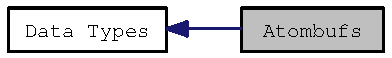
\includegraphics[width=112pt]{group__atombuf}
\end{center}
\end{figure}
\subsection*{Data Structures}
\begin{DoxyCompactItemize}
\item 
struct \hyperlink{structt__atombuf}{t\_\-atombuf}
\begin{DoxyCompactList}\small\item\em The atombuf struct provides a way to pass a collection of atoms. \item\end{DoxyCompactList}\end{DoxyCompactItemize}
\subsection*{Functions}
\begin{DoxyCompactItemize}
\item 
void $\ast$ \hyperlink{group__atombuf_ga5748a06a4e11f4be0b90dda8415bc815}{atombuf\_\-new} (long argc, \hyperlink{structt__atom}{t\_\-atom} $\ast$argv)
\begin{DoxyCompactList}\small\item\em Use \hyperlink{group__atombuf_ga5748a06a4e11f4be0b90dda8415bc815}{atombuf\_\-new()} to create a new Atombuf from an array of t\_\-atoms. \item\end{DoxyCompactList}\item 
void \hyperlink{group__atombuf_ga2c10483e31d84a12a037d154bd4051bd}{atombuf\_\-free} (\hyperlink{structt__atombuf}{t\_\-atombuf} $\ast$x)
\begin{DoxyCompactList}\small\item\em Use \hyperlink{group__atombuf_ga2c10483e31d84a12a037d154bd4051bd}{atombuf\_\-free()} to dispose of the memory used by a \hyperlink{structt__atombuf}{t\_\-atombuf}. \item\end{DoxyCompactList}\item 
void \hyperlink{group__atombuf_gada864b7fc2e47dbdbef3176de00924a2}{atombuf\_\-text} (\hyperlink{structt__atombuf}{t\_\-atombuf} $\ast$$\ast$x, char $\ast$$\ast$text, long size)
\begin{DoxyCompactList}\small\item\em Use \hyperlink{group__atombuf_gada864b7fc2e47dbdbef3176de00924a2}{atombuf\_\-text()} to convert text to a \hyperlink{structt__atom}{t\_\-atom} array in a \hyperlink{structt__atombuf}{t\_\-atombuf}. \item\end{DoxyCompactList}\end{DoxyCompactItemize}


\subsection{Detailed Description}
An Atombuf is an alternative to \hyperlink{group__binbuf}{Binbufs} for temporary storage of atoms. Its principal advantage is that the internal structure is publicly available so you can manipulate the atoms in place. The standard Max text objects (message box, object box, comment) use the Atombuf structure to store their text (each \hyperlink{unionword}{word} of text is stored as a \hyperlink{structt__symbol}{t\_\-symbol} or a number). 

\subsection{Function Documentation}
\hypertarget{group__atombuf_ga2c10483e31d84a12a037d154bd4051bd}{
\index{atombuf@{atombuf}!atombuf\_\-free@{atombuf\_\-free}}
\index{atombuf\_\-free@{atombuf\_\-free}!atombuf@{atombuf}}
\subsubsection[{atombuf\_\-free}]{\setlength{\rightskip}{0pt plus 5cm}void atombuf\_\-free ({\bf t\_\-atombuf} $\ast$ {\em x})}}
\label{group__atombuf_ga2c10483e31d84a12a037d154bd4051bd}


Use \hyperlink{group__atombuf_ga2c10483e31d84a12a037d154bd4051bd}{atombuf\_\-free()} to dispose of the memory used by a \hyperlink{structt__atombuf}{t\_\-atombuf}. 
\begin{DoxyParams}{Parameters}
\item[{\em x}]The \hyperlink{structt__atombuf}{t\_\-atombuf} to free. \end{DoxyParams}
\hypertarget{group__atombuf_ga5748a06a4e11f4be0b90dda8415bc815}{
\index{atombuf@{atombuf}!atombuf\_\-new@{atombuf\_\-new}}
\index{atombuf\_\-new@{atombuf\_\-new}!atombuf@{atombuf}}
\subsubsection[{atombuf\_\-new}]{\setlength{\rightskip}{0pt plus 5cm}void$\ast$ atombuf\_\-new (long {\em argc}, \/  {\bf t\_\-atom} $\ast$ {\em argv})}}
\label{group__atombuf_ga5748a06a4e11f4be0b90dda8415bc815}


Use \hyperlink{group__atombuf_ga5748a06a4e11f4be0b90dda8415bc815}{atombuf\_\-new()} to create a new Atombuf from an array of t\_\-atoms. 
\begin{DoxyParams}{Parameters}
\item[{\em argc}]Number of t\_\-atoms in the argv array. May be 0. \item[{\em argv}]Array of t\_\-atoms. If creating an empty Atombuf, you may pass 0. \end{DoxyParams}
\begin{DoxyReturn}{Returns}
\hyperlink{group__atombuf_ga5748a06a4e11f4be0b90dda8415bc815}{atombuf\_\-new()} create a new \hyperlink{structt__atombuf}{t\_\-atombuf} and returns a pointer to it. If 0 is returned, insufficient memory was available. 
\end{DoxyReturn}
\hypertarget{group__atombuf_gada864b7fc2e47dbdbef3176de00924a2}{
\index{atombuf@{atombuf}!atombuf\_\-text@{atombuf\_\-text}}
\index{atombuf\_\-text@{atombuf\_\-text}!atombuf@{atombuf}}
\subsubsection[{atombuf\_\-text}]{\setlength{\rightskip}{0pt plus 5cm}void atombuf\_\-text ({\bf t\_\-atombuf} $\ast$$\ast$ {\em x}, \/  char $\ast$$\ast$ {\em text}, \/  long {\em size})}}
\label{group__atombuf_gada864b7fc2e47dbdbef3176de00924a2}


Use \hyperlink{group__atombuf_gada864b7fc2e47dbdbef3176de00924a2}{atombuf\_\-text()} to convert text to a \hyperlink{structt__atom}{t\_\-atom} array in a \hyperlink{structt__atombuf}{t\_\-atombuf}. To use this routine to create a new Atombuf from the text buffer, first create a new empty \hyperlink{structt__atombuf}{t\_\-atombuf} with a call to atombuf\_\-new(0,NULL).


\begin{DoxyParams}{Parameters}
\item[{\em x}]Pointer to existing atombuf variable. The variable will be replaced by a new Atombuf containing the converted text. \item[{\em text}]Handle to the text to be converted. It need not be zero-\/terminated. \item[{\em size}]Number of characters in the text. \end{DoxyParams}

\hypertarget{group__binbuf}{
\section{Binbufs}
\label{group__binbuf}\index{Binbufs@{Binbufs}}
}


You won’t need to know about the internal structure of a Binbuf, so you can use the void $\ast$ type to refer to one.  


Collaboration diagram for Binbufs:\nopagebreak
\begin{figure}[H]
\begin{center}
\leavevmode
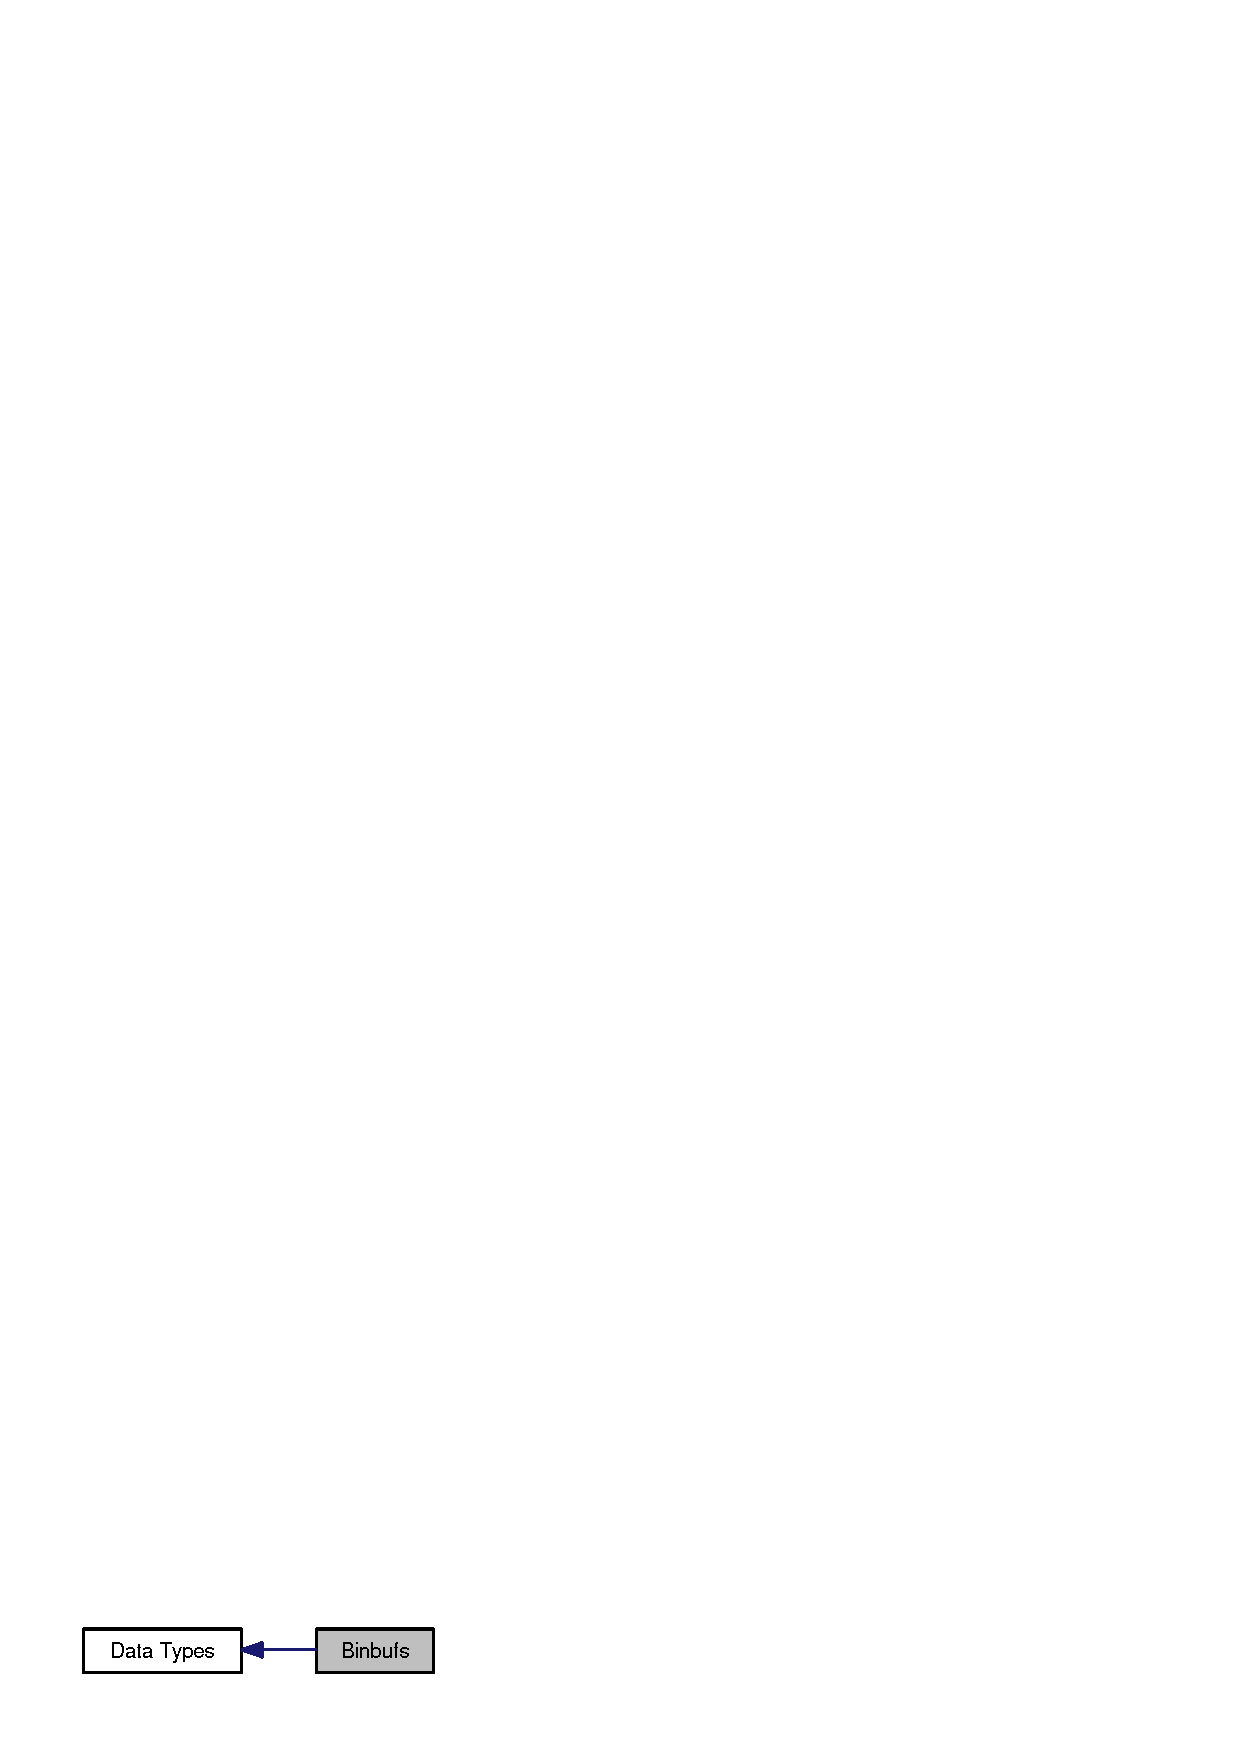
\includegraphics[width=106pt]{group__binbuf}
\end{center}
\end{figure}
\subsection*{Functions}
\begin{DoxyCompactItemize}
\item 
void $\ast$ \hyperlink{group__binbuf_ga4a6b741be0bee8626b4cb25baa453060}{binbuf\_\-new} (void)
\begin{DoxyCompactList}\small\item\em Use \hyperlink{group__binbuf_ga4a6b741be0bee8626b4cb25baa453060}{binbuf\_\-new()} to create and initialize a Binbuf. \item\end{DoxyCompactList}\item 
void \hyperlink{group__binbuf_ga8bc71e59211549a9927754452b2d9e21}{binbuf\_\-vinsert} (void $\ast$x, char $\ast$fmt,...)
\begin{DoxyCompactList}\small\item\em Use \hyperlink{group__binbuf_ga8bc71e59211549a9927754452b2d9e21}{binbuf\_\-vinsert()} to append a Max message to a Binbuf adding a semicolon. \item\end{DoxyCompactList}\item 
void \hyperlink{group__binbuf_gad8f2272c95a8e89f22f1a9c67272af5e}{binbuf\_\-insert} (void $\ast$x, \hyperlink{structt__symbol}{t\_\-symbol} $\ast$s, short argc, \hyperlink{structt__atom}{t\_\-atom} $\ast$argv)
\begin{DoxyCompactList}\small\item\em Use \hyperlink{group__binbuf_gad8f2272c95a8e89f22f1a9c67272af5e}{binbuf\_\-insert()} to append a Max message to a Binbuf adding a semicolon. \item\end{DoxyCompactList}\item 
void $\ast$ \hyperlink{group__binbuf_ga90c960507452ce76428d87c0714f9f0e}{binbuf\_\-eval} (void $\ast$x, short ac, \hyperlink{structt__atom}{t\_\-atom} $\ast$av, void $\ast$to)
\begin{DoxyCompactList}\small\item\em Use binbuf\_\-eval to evaluate a Max message in a Binbuf, passing it arguments. \item\end{DoxyCompactList}\item 
short \hyperlink{group__binbuf_ga0eccee2d50ae561c625cc97238f1e21a}{binbuf\_\-getatom} (void $\ast$x, long $\ast$p1, long $\ast$p2, \hyperlink{structt__atom}{t\_\-atom} $\ast$ap)
\begin{DoxyCompactList}\small\item\em Use binbuf\_\-getatom to retrieve a single Atom from a Binbuf. \item\end{DoxyCompactList}\item 
short \hyperlink{group__binbuf_ga7a582c876ee074505762b30c7eef6504}{binbuf\_\-text} (void $\ast$x, char $\ast$$\ast$srcText, long n)
\begin{DoxyCompactList}\small\item\em Use \hyperlink{group__binbuf_ga7a582c876ee074505762b30c7eef6504}{binbuf\_\-text()} to convert a text handle to a Binbuf. \item\end{DoxyCompactList}\item 
short \hyperlink{group__binbuf_ga739086c676dfaba01dff1f70e7487dd5}{binbuf\_\-totext} (void $\ast$x, char $\ast$$\ast$dstText, long $\ast$sizep)
\begin{DoxyCompactList}\small\item\em Use \hyperlink{group__binbuf_ga739086c676dfaba01dff1f70e7487dd5}{binbuf\_\-totext()} to convert a Binbuf into a text handle. \item\end{DoxyCompactList}\item 
void \hyperlink{group__binbuf_ga716d66a159b96b7b9d87baaab33367e0}{binbuf\_\-set} (void $\ast$x, \hyperlink{structt__symbol}{t\_\-symbol} $\ast$s, short argc, \hyperlink{structt__atom}{t\_\-atom} $\ast$argv)
\begin{DoxyCompactList}\small\item\em Use \hyperlink{group__binbuf_ga716d66a159b96b7b9d87baaab33367e0}{binbuf\_\-set()} to change the entire contents of a Binbuf. \item\end{DoxyCompactList}\item 
void \hyperlink{group__binbuf_ga57f584204ff1860c93ca728ca991fb15}{binbuf\_\-append} (void $\ast$x, \hyperlink{structt__symbol}{t\_\-symbol} $\ast$s, short argc, \hyperlink{structt__atom}{t\_\-atom} $\ast$argv)
\begin{DoxyCompactList}\small\item\em Use binbuf\_\-append to append t\_\-atoms to a Binbuf without modifying them. \item\end{DoxyCompactList}\item 
short \hyperlink{group__binbuf_gacb42118a4da090a6d47954f8b299de46}{readatom} (char $\ast$outstr, char $\ast$$\ast$text, long $\ast$n, long e, \hyperlink{structt__atom}{t\_\-atom} $\ast$ap)
\begin{DoxyCompactList}\small\item\em Use \hyperlink{group__binbuf_gacb42118a4da090a6d47954f8b299de46}{readatom()} to read a single Atom from a text buffer. \item\end{DoxyCompactList}\end{DoxyCompactItemize}


\subsection{Detailed Description}
You won’t need to know about the internal structure of a Binbuf, so you can use the void $\ast$ type to refer to one. 

\subsection{Function Documentation}
\hypertarget{group__binbuf_ga57f584204ff1860c93ca728ca991fb15}{
\index{binbuf@{binbuf}!binbuf\_\-append@{binbuf\_\-append}}
\index{binbuf\_\-append@{binbuf\_\-append}!binbuf@{binbuf}}
\subsubsection[{binbuf\_\-append}]{\setlength{\rightskip}{0pt plus 5cm}void binbuf\_\-append (void $\ast$ {\em x}, \/  {\bf t\_\-symbol} $\ast$ {\em s}, \/  short {\em argc}, \/  {\bf t\_\-atom} $\ast$ {\em argv})}}
\label{group__binbuf_ga57f584204ff1860c93ca728ca991fb15}


Use binbuf\_\-append to append t\_\-atoms to a Binbuf without modifying them. 
\begin{DoxyParams}{Parameters}
\item[{\em x}]Binbuf to receive the items. \item[{\em s}]Ignored. Pass NULL. \item[{\em argc}]Count of items in the argv array. \item[{\em argv}]Array of atoms to add to the Binbuf. \end{DoxyParams}
\hypertarget{group__binbuf_ga90c960507452ce76428d87c0714f9f0e}{
\index{binbuf@{binbuf}!binbuf\_\-eval@{binbuf\_\-eval}}
\index{binbuf\_\-eval@{binbuf\_\-eval}!binbuf@{binbuf}}
\subsubsection[{binbuf\_\-eval}]{\setlength{\rightskip}{0pt plus 5cm}void$\ast$ binbuf\_\-eval (void $\ast$ {\em x}, \/  short {\em ac}, \/  {\bf t\_\-atom} $\ast$ {\em av}, \/  void $\ast$ {\em to})}}
\label{group__binbuf_ga90c960507452ce76428d87c0714f9f0e}


Use binbuf\_\-eval to evaluate a Max message in a Binbuf, passing it arguments. \hyperlink{group__binbuf_ga90c960507452ce76428d87c0714f9f0e}{binbuf\_\-eval()} is an advanced function that evaluates the message in a Binbuf with arguments in argv, and sends it to receiver.


\begin{DoxyParams}{Parameters}
\item[{\em x}]Binbuf containing the message. \item[{\em ac}]Count of items in the argv array. \item[{\em av}]Array of t\_\-atoms as the arguments to the message. \item[{\em to}]Receiver of the message.\end{DoxyParams}
\begin{DoxyReturn}{Returns}
The result of sending the message. 
\end{DoxyReturn}
\hypertarget{group__binbuf_ga0eccee2d50ae561c625cc97238f1e21a}{
\index{binbuf@{binbuf}!binbuf\_\-getatom@{binbuf\_\-getatom}}
\index{binbuf\_\-getatom@{binbuf\_\-getatom}!binbuf@{binbuf}}
\subsubsection[{binbuf\_\-getatom}]{\setlength{\rightskip}{0pt plus 5cm}short binbuf\_\-getatom (void $\ast$ {\em x}, \/  long $\ast$ {\em p1}, \/  long $\ast$ {\em p2}, \/  {\bf t\_\-atom} $\ast$ {\em ap})}}
\label{group__binbuf_ga0eccee2d50ae561c625cc97238f1e21a}


Use binbuf\_\-getatom to retrieve a single Atom from a Binbuf. 
\begin{DoxyParams}{Parameters}
\item[{\em x}]Binbuf containing the desired \hyperlink{structt__atom}{t\_\-atom}. \item[{\em p1}]Offset into the Binbuf’s array of types. Modified to point to the next \hyperlink{structt__atom}{t\_\-atom}. \item[{\em p2}]Offset into the Binbuf’s array of data. Modified to point to the next \hyperlink{structt__atom}{t\_\-atom}. \item[{\em ap}]Location of a \hyperlink{structt__atom}{t\_\-atom} where the retrieved data will be placed.\end{DoxyParams}
\begin{DoxyReturn}{Returns}
1 if there were no t\_\-atoms at the specified offsets, 0 if there’s a legitimate \hyperlink{structt__atom}{t\_\-atom} returned in result.
\end{DoxyReturn}
\begin{DoxyRemark}{Remarks}
To get the first \hyperlink{structt__atom}{t\_\-atom}, set both typeOffset and stuffOffset to 0. Here’s an example of getting all the items in a Binbuf: 
\begin{DoxyCode}
    t_atom holder; 
    long to, so; 
    
    to = 0; 
    so = 0; 
    while (!binbuf_getatom(x, &to, &so, &holder)){
        // do something with the t_atom
    }
\end{DoxyCode}
 
\end{DoxyRemark}
\hypertarget{group__binbuf_gad8f2272c95a8e89f22f1a9c67272af5e}{
\index{binbuf@{binbuf}!binbuf\_\-insert@{binbuf\_\-insert}}
\index{binbuf\_\-insert@{binbuf\_\-insert}!binbuf@{binbuf}}
\subsubsection[{binbuf\_\-insert}]{\setlength{\rightskip}{0pt plus 5cm}void binbuf\_\-insert (void $\ast$ {\em x}, \/  {\bf t\_\-symbol} $\ast$ {\em s}, \/  short {\em argc}, \/  {\bf t\_\-atom} $\ast$ {\em argv})}}
\label{group__binbuf_gad8f2272c95a8e89f22f1a9c67272af5e}


Use \hyperlink{group__binbuf_gad8f2272c95a8e89f22f1a9c67272af5e}{binbuf\_\-insert()} to append a Max message to a Binbuf adding a semicolon. 
\begin{DoxyParams}{Parameters}
\item[{\em x}]Binbuf to receive the items. \item[{\em s}]Ignored. Pass NULL. \item[{\em argc}]Count of items in the argv array. \item[{\em argv}]Array of t\_\-atoms to add to the Binbuf.\end{DoxyParams}
\begin{DoxyRemark}{Remarks}
You’ll use \hyperlink{group__binbuf_gad8f2272c95a8e89f22f1a9c67272af5e}{binbuf\_\-insert()} instead of \hyperlink{group__binbuf_ga57f584204ff1860c93ca728ca991fb15}{binbuf\_\-append()} if you were saving your object into a Binbuf and wanted a semicolon at the end. If the message is part of a file that will later be evaluated, such as a Patcher file, the first argument argv\mbox{[}0\mbox{]} will be the receiver of the message and must be a Symbol. \hyperlink{group__binbuf_ga8bc71e59211549a9927754452b2d9e21}{binbuf\_\-vinsert()} is easier to use than \hyperlink{group__binbuf_gad8f2272c95a8e89f22f1a9c67272af5e}{binbuf\_\-insert()}, since you don’t have to format your data into an array of Atoms first.
\end{DoxyRemark}
\hyperlink{group__binbuf_gad8f2272c95a8e89f22f1a9c67272af5e}{binbuf\_\-insert()} will also convert the t\_\-symbols \#1 through \#9 into \$1 through \$9. This is used for saving patcher files that take arguments; you will probably never save these symbols as part of anything you are doing. \hypertarget{group__binbuf_ga4a6b741be0bee8626b4cb25baa453060}{
\index{binbuf@{binbuf}!binbuf\_\-new@{binbuf\_\-new}}
\index{binbuf\_\-new@{binbuf\_\-new}!binbuf@{binbuf}}
\subsubsection[{binbuf\_\-new}]{\setlength{\rightskip}{0pt plus 5cm}void$\ast$ binbuf\_\-new (void)}}
\label{group__binbuf_ga4a6b741be0bee8626b4cb25baa453060}


Use \hyperlink{group__binbuf_ga4a6b741be0bee8626b4cb25baa453060}{binbuf\_\-new()} to create and initialize a Binbuf. \begin{DoxyReturn}{Returns}
Returns a new binbuf if successful, otherwise NULL. 
\end{DoxyReturn}
\hypertarget{group__binbuf_ga716d66a159b96b7b9d87baaab33367e0}{
\index{binbuf@{binbuf}!binbuf\_\-set@{binbuf\_\-set}}
\index{binbuf\_\-set@{binbuf\_\-set}!binbuf@{binbuf}}
\subsubsection[{binbuf\_\-set}]{\setlength{\rightskip}{0pt plus 5cm}void binbuf\_\-set (void $\ast$ {\em x}, \/  {\bf t\_\-symbol} $\ast$ {\em s}, \/  short {\em argc}, \/  {\bf t\_\-atom} $\ast$ {\em argv})}}
\label{group__binbuf_ga716d66a159b96b7b9d87baaab33367e0}


Use \hyperlink{group__binbuf_ga716d66a159b96b7b9d87baaab33367e0}{binbuf\_\-set()} to change the entire contents of a Binbuf. The previous contents of the Binbuf are destroyed.


\begin{DoxyParams}{Parameters}
\item[{\em x}]Binbuf to receive the items. \item[{\em s}]Ignored. Pass NULL. \item[{\em argc}]Count of items in the argv array. \item[{\em argv}]Array of t\_\-atoms to put in the Binbuf. \end{DoxyParams}
\hypertarget{group__binbuf_ga7a582c876ee074505762b30c7eef6504}{
\index{binbuf@{binbuf}!binbuf\_\-text@{binbuf\_\-text}}
\index{binbuf\_\-text@{binbuf\_\-text}!binbuf@{binbuf}}
\subsubsection[{binbuf\_\-text}]{\setlength{\rightskip}{0pt plus 5cm}short binbuf\_\-text (void $\ast$ {\em x}, \/  char $\ast$$\ast$ {\em srcText}, \/  long {\em n})}}
\label{group__binbuf_ga7a582c876ee074505762b30c7eef6504}


Use \hyperlink{group__binbuf_ga7a582c876ee074505762b30c7eef6504}{binbuf\_\-text()} to convert a text handle to a Binbuf. \hyperlink{group__binbuf_ga7a582c876ee074505762b30c7eef6504}{binbuf\_\-text()} parses the text in the handle srcText and converts it into binary format. Use it to evaluate a text file or text line entry into a Binbuf.


\begin{DoxyParams}{Parameters}
\item[{\em x}]Binbuf to contain the converted text. It must have already been created with binbuf\_\-new. Its previous contents are destroyed. \item[{\em srcText}]Handle to the text to be converted. It need not be terminated with a 0. \item[{\em n}]Number of characters in the text. \end{DoxyParams}
\begin{DoxyReturn}{Returns}
If binbuf\_\-text encounters an error during its operation, a non-\/zero result is returned, otherwise it returns 0.
\end{DoxyReturn}
\begin{DoxyRemark}{Remarks}
Note: Commas, symbols containing a dollar sign followed by a number 1-\/9, and semicolons are identified by special pseudo-\/type constants for you when your text is binbuf-\/ized.
\end{DoxyRemark}
The following constants in the a\_\-type field of Atoms returned by binbuf\_\-getAtom identify the special symbols \hyperlink{group__atom_gga8aa6700e9f00b132eb376db6e39ade47ac105be4ef726ee36c4330e16bb24706e}{A\_\-SEMI}, \hyperlink{group__atom_gga8aa6700e9f00b132eb376db6e39ade47a07c3484085a3217107acec059d17b945}{A\_\-COMMA}, and \hyperlink{group__atom_gga8aa6700e9f00b132eb376db6e39ade47af0a5a9017f6b59e82a4859cd0560d36b}{A\_\-DOLLAR}.

For a \hyperlink{structt__atom}{t\_\-atom} of the pseudo-\/type \hyperlink{group__atom_gga8aa6700e9f00b132eb376db6e39ade47af0a5a9017f6b59e82a4859cd0560d36b}{A\_\-DOLLAR}, the a\_\-w.w\_\-long field of the \hyperlink{structt__atom}{t\_\-atom} contains the number after the dollar sign in the original text or symbol.

Using these pseudo-\/types may be helpful in separating “sentences” and “phrases” in the input language you design. For example, the old pop-\/up umenu object allowed users to have spaces in between words by requiring the menu items be separated by commas. It’s reasonably easy, using \hyperlink{group__binbuf_ga0eccee2d50ae561c625cc97238f1e21a}{binbuf\_\-getatom()}, to find the commas in a Binbuf in order to determine the beginning of a new item when reading the atomized text to be displayed in the menu.

If you want to use a literal comma or semicolon in a symbol, precede it with a backslash ($\backslash$) character. The backslash character can be included by using two backslashes in a row. \hypertarget{group__binbuf_ga739086c676dfaba01dff1f70e7487dd5}{
\index{binbuf@{binbuf}!binbuf\_\-totext@{binbuf\_\-totext}}
\index{binbuf\_\-totext@{binbuf\_\-totext}!binbuf@{binbuf}}
\subsubsection[{binbuf\_\-totext}]{\setlength{\rightskip}{0pt plus 5cm}short binbuf\_\-totext (void $\ast$ {\em x}, \/  char $\ast$$\ast$ {\em dstText}, \/  long $\ast$ {\em sizep})}}
\label{group__binbuf_ga739086c676dfaba01dff1f70e7487dd5}


Use \hyperlink{group__binbuf_ga739086c676dfaba01dff1f70e7487dd5}{binbuf\_\-totext()} to convert a Binbuf into a text handle. \hyperlink{group__binbuf_ga739086c676dfaba01dff1f70e7487dd5}{binbuf\_\-totext()} converts a Binbuf into text and places it in a handle. Backslashes are added to protect literal commas and semicolons contained in symbols. The pseudo-\/types are converted into commas, semicolons, or dollar-\/sign and number, without backslashes preceding them. binbuf\_\-text can read the output of binbuf\_\-totext and make the same Binbuf.


\begin{DoxyParams}{Parameters}
\item[{\em x}]Binbuf with data to convert to text. \item[{\em dstText}]Pre-\/existing handle where the text will be placed. dstText will be resized to accomodate the text. \item[{\em sizep}]Where \hyperlink{group__binbuf_ga739086c676dfaba01dff1f70e7487dd5}{binbuf\_\-totext()} returns the number of characters in the converted text handle. \end{DoxyParams}
\begin{DoxyReturn}{Returns}
If binbuf\_\-totext runs out of memory during its operation, it returns a non-\/zero result, otherwise it returns 0. 
\end{DoxyReturn}
\hypertarget{group__binbuf_ga8bc71e59211549a9927754452b2d9e21}{
\index{binbuf@{binbuf}!binbuf\_\-vinsert@{binbuf\_\-vinsert}}
\index{binbuf\_\-vinsert@{binbuf\_\-vinsert}!binbuf@{binbuf}}
\subsubsection[{binbuf\_\-vinsert}]{\setlength{\rightskip}{0pt plus 5cm}void binbuf\_\-vinsert (void $\ast$ {\em x}, \/  char $\ast$ {\em fmt}, \/   {\em ...})}}
\label{group__binbuf_ga8bc71e59211549a9927754452b2d9e21}


Use \hyperlink{group__binbuf_ga8bc71e59211549a9927754452b2d9e21}{binbuf\_\-vinsert()} to append a Max message to a Binbuf adding a semicolon. 
\begin{DoxyParams}{Parameters}
\item[{\em x}]Binbuf containing the desired Atom. \item[{\em fmt}]A C-\/string containing one or more letters corresponding to the types of each element of the message. s for \hyperlink{structt__symbol}{t\_\-symbol}$\ast$, l for long, or f for float. \item[{\em ...}]Elements of the message, passed directly to the function as Symbols, longs, or floats.\end{DoxyParams}
\begin{DoxyRemark}{Remarks}
\hyperlink{group__binbuf_ga8bc71e59211549a9927754452b2d9e21}{binbuf\_\-vinsert()} works somewhat like a printf() for Binbufs. It allows you to pass a number of arguments of different types and insert them into a Binbuf. The entire message will then be terminated with a semicolon. Only 16 items can be passed to \hyperlink{group__binbuf_ga8bc71e59211549a9927754452b2d9e21}{binbuf\_\-vinsert()}.
\end{DoxyRemark}
The example below shows the implementation of a normal object’s save method. The save method requires that you build a message that begins with N (the new object) , followed by the name of your object (in this case, represented by the \hyperlink{structt__symbol}{t\_\-symbol} myobject), followed by any arguments your instance creation function requires. In this example, we save the values of two fields m\_\-val1 and m\_\-val2 defined as longs.


\begin{DoxyCode}
    void myobject_save (myObject *x, Binbuf *dstBuf) 
    { 
        binbuf_vinsert(dstBuf, "ssll", gensym("#N"), 
            gensym("myobject"), 
            x->m_val1, x->m_val2); 
    }
\end{DoxyCode}


Suppose that such an object had written this data into a file. If you opened the file as text, you would see the following:


\begin{DoxyCode}
    #N myobject 10 20; 
    #P newobj 218 82 30 myobject; 
\end{DoxyCode}


The first line will result in a new myobject object to be created; the creation function receives the arguments 10 and 20. The second line contains the text of the object box. The newobj message to a patcher creates the object box user interface object and attaches it to the previously created myobject object. Normally, the newex message is used. This causes the object to be created using the arguments that were typed into the object box. \hypertarget{group__binbuf_gacb42118a4da090a6d47954f8b299de46}{
\index{binbuf@{binbuf}!readatom@{readatom}}
\index{readatom@{readatom}!binbuf@{binbuf}}
\subsubsection[{readatom}]{\setlength{\rightskip}{0pt plus 5cm}short readatom (char $\ast$ {\em outstr}, \/  char $\ast$$\ast$ {\em text}, \/  long $\ast$ {\em n}, \/  long {\em e}, \/  {\bf t\_\-atom} $\ast$ {\em ap})}}
\label{group__binbuf_gacb42118a4da090a6d47954f8b299de46}


Use \hyperlink{group__binbuf_gacb42118a4da090a6d47954f8b299de46}{readatom()} to read a single Atom from a text buffer. 
\begin{DoxyParams}{Parameters}
\item[{\em outstr}]C-\/string of 256 characters that will receive the next text item read from the buffer. \item[{\em text}]Handle to the text buffer to be read. \item[{\em n}]Starts at 0, and is modified by readatom to point to the next item in the text buffer. \item[{\em e}]Number of characters in text. \item[{\em ap}]Where the resulting Atom read from the text buffer is placed. \end{DoxyParams}
\begin{DoxyReturn}{Returns}
\hyperlink{group__binbuf_gacb42118a4da090a6d47954f8b299de46}{readatom()} returns non-\/zero if there is more text to read, and zero if it has reached the end of the text. Note that this return value has the opposite logic from that of \hyperlink{group__binbuf_ga0eccee2d50ae561c625cc97238f1e21a}{binbuf\_\-getatom()}.
\end{DoxyReturn}
\begin{DoxyRemark}{Remarks}
This function provides access to the low-\/level Max text evaluator used by \hyperlink{group__binbuf_ga7a582c876ee074505762b30c7eef6504}{binbuf\_\-text()}. It is designed to operate on a handle of characters (text) and called in a loop, as in the example shown below. 
\begin{DoxyCode}
    long index = 0; 
    t_atom dst; 
    char outstr[256]; 
    
    while (readatom(outstr,textHandle,&index,textLength,&dst)) 
    { 
        // do something with the resulting Atom
    } 
\end{DoxyCode}


An alternative to using readatom is to turn your text into a Binbuf using \hyperlink{group__binbuf_ga7a582c876ee074505762b30c7eef6504}{binbuf\_\-text()}, then call \hyperlink{group__binbuf_ga0eccee2d50ae561c625cc97238f1e21a}{binbuf\_\-getatom()} in a loop. 
\end{DoxyRemark}

\hypertarget{group__symbol}{
\section{Symbols}
\label{group__symbol}\index{Symbols@{Symbols}}
}


Max maintains a symbol table of all strings to speed lookup for message passing.  


Collaboration diagram for Symbols:\nopagebreak
\begin{figure}[H]
\begin{center}
\leavevmode
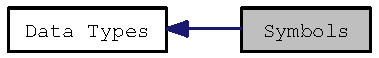
\includegraphics[width=109pt]{group__symbol}
\end{center}
\end{figure}
\subsection*{Data Structures}
\begin{DoxyCompactItemize}
\item 
struct \hyperlink{structt__symbol}{t\_\-symbol}
\begin{DoxyCompactList}\small\item\em The symbol. \item\end{DoxyCompactList}\end{DoxyCompactItemize}
\subsection*{Functions}
\begin{DoxyCompactItemize}
\item 
\hyperlink{structt__symbol}{t\_\-symbol} $\ast$ \hyperlink{group__symbol_ga8268797d125a15bae1010af70b559e05}{gensym} (char $\ast$s)
\begin{DoxyCompactList}\small\item\em Given a C-\/string, fetch the matching \hyperlink{structt__symbol}{t\_\-symbol} pointer from the symbol table, generating the symbol if neccessary. \item\end{DoxyCompactList}\end{DoxyCompactItemize}


\subsection{Detailed Description}
Max maintains a symbol table of all strings to speed lookup for message passing. If you want to access the bang symbol for example, you’ll have to use the expression gensym(\char`\"{}bang\char`\"{}). For example, \hyperlink{group__symbol_ga8268797d125a15bae1010af70b559e05}{gensym()} may be needed when sending messages directly to other Max objects such as with \hyperlink{group__obj_gae740749094827ac5adc2b7145db1c596}{object\_\-method()} and \hyperlink{group__inout_ga12798ee897e01dac21ee547c4091d8a8}{outlet\_\-anything()}. These functions expect a \hyperlink{structt__symbol}{t\_\-symbol}$\ast$, they don’t \hyperlink{group__symbol_ga8268797d125a15bae1010af70b559e05}{gensym()} character strings for you.

The \hyperlink{structt__symbol}{t\_\-symbol} data structure also contains a place to store an arbitrary value. The following example shows how you can use this feature to use symbols to share values among two different external object classes. (Objects of the same class can use the code resource’s global variable space to share data.) The idea is that the s\_\-thing field of a \hyperlink{structt__symbol}{t\_\-symbol} can be set to some value, and \hyperlink{group__symbol_ga8268797d125a15bae1010af70b559e05}{gensym()} will return a reference to the Symbol. Thus, the two classes just have to agree about the character string to be used. Alternatively, each could be passed a \hyperlink{structt__symbol}{t\_\-symbol} that will be used to share data.

Storing a value:


\begin{DoxyCode}
    t_symbol *s; 
    s = gensym("some_weird_string"); 
    s->s_thing = (t_object *)someValue; 
\end{DoxyCode}


Retrieving a value:


\begin{DoxyCode}
    t_symbol *s; 
    s = gensym("some_weird_string"); 
    someValue = s->s_thing; 
\end{DoxyCode}
 

\subsection{Function Documentation}
\hypertarget{group__symbol_ga8268797d125a15bae1010af70b559e05}{
\index{symbol@{symbol}!gensym@{gensym}}
\index{gensym@{gensym}!symbol@{symbol}}
\subsubsection[{gensym}]{\setlength{\rightskip}{0pt plus 5cm}{\bf t\_\-symbol}$\ast$ gensym (char $\ast$ {\em s})}}
\label{group__symbol_ga8268797d125a15bae1010af70b559e05}


Given a C-\/string, fetch the matching \hyperlink{structt__symbol}{t\_\-symbol} pointer from the symbol table, generating the symbol if neccessary. 
\begin{DoxyParams}{Parameters}
\item[{\em s}]A C-\/string to be looked up in Max’s symbol table. \end{DoxyParams}
\begin{DoxyReturn}{Returns}
A pointer to the \hyperlink{structt__symbol}{t\_\-symbol} in the symbol table. 
\end{DoxyReturn}

\hypertarget{group__files}{
\section{Files and Folders}
\label{group__files}\index{Files and Folders@{Files and Folders}}
}


These routines assist your object in opening and saving files, as well as locating the user’s files in the Max search path.  
\subsection*{Data Structures}
\begin{DoxyCompactItemize}
\item 
struct \hyperlink{structt__fileinfo}{t\_\-fileinfo}
\begin{DoxyCompactList}\small\item\em Information about a file. \item\end{DoxyCompactList}\item 
struct \hyperlink{structt__path}{t\_\-path}
\begin{DoxyCompactList}\small\item\em The path data structure. \item\end{DoxyCompactList}\item 
struct \hyperlink{structt__pathlink}{t\_\-pathlink}
\begin{DoxyCompactList}\small\item\em The pathlink data structure. \item\end{DoxyCompactList}\end{DoxyCompactItemize}
\subsection*{Defines}
\begin{DoxyCompactItemize}
\item 
\hypertarget{group__files_ga513fe2710e225c840d9295fb9884607b}{
\#define \hyperlink{group__files_ga513fe2710e225c840d9295fb9884607b}{MAX\_\-PATH\_\-CHARS}~2048}
\label{group__files_ga513fe2710e225c840d9295fb9884607b}

\begin{DoxyCompactList}\small\item\em The size you should use when allocating strings for full paths. \item\end{DoxyCompactList}\item 
\#define \hyperlink{group__files_ga481556de2ccf516a499525edebc45ee8}{MAX\_\-FILENAME\_\-CHARS}~512
\begin{DoxyCompactList}\small\item\em The size you should use when allocating strings for filenames. \item\end{DoxyCompactList}\end{DoxyCompactItemize}
\subsection*{Typedefs}
\begin{DoxyCompactItemize}
\item 
typedef void $\ast$ \hyperlink{group__files_gafcb776aa74d514754e83b30995b5a5d1}{t\_\-filehandle}
\begin{DoxyCompactList}\small\item\em A t\_\-filehandle is a cross-\/platform way of referring to an open file. \item\end{DoxyCompactList}\end{DoxyCompactItemize}
\subsection*{Enumerations}
\begin{DoxyCompactItemize}
\item 
enum \hyperlink{group__files_gaaf8f3fbe8b4ab0b73258a6b782461867}{e\_\-max\_\-path\_\-styles} \{ \par
\hyperlink{group__files_ggaaf8f3fbe8b4ab0b73258a6b782461867a765ba1acf48b931a40a8e9a6bd451c76}{PATH\_\-STYLE\_\-MAX} =  0, 
\par
\hyperlink{group__files_ggaaf8f3fbe8b4ab0b73258a6b782461867accd897b92c35c682adb9714ce41aea2a}{PATH\_\-STYLE\_\-NATIVE}, 
\par
\hyperlink{group__files_ggaaf8f3fbe8b4ab0b73258a6b782461867a86782cc5d0027799047c845ab43c1b49}{PATH\_\-STYLE\_\-COLON}, 
\par
\hyperlink{group__files_ggaaf8f3fbe8b4ab0b73258a6b782461867a04dc9f3f099d8b89914a8c3137b821bf}{PATH\_\-STYLE\_\-SLASH}, 
\par
\hyperlink{group__files_ggaaf8f3fbe8b4ab0b73258a6b782461867a3a76a78a4fb2f8e5e15e6f1a0f19c77a}{PATH\_\-STYLE\_\-NATIVE\_\-WIN}
 \}
\begin{DoxyCompactList}\small\item\em Constants that determine the output of \hyperlink{group__files_gaaf014af82bc666cd974b83441eb4c9c6}{path\_\-nameconform()}. \item\end{DoxyCompactList}\item 
enum \hyperlink{group__files_gac6a8a4db7a7de5fbc21188399713c7ee}{e\_\-max\_\-path\_\-types} \{ \par
\hyperlink{group__files_ggac6a8a4db7a7de5fbc21188399713c7eea1a5d068eb3dae46260f4253802e3e28b}{PATH\_\-TYPE\_\-IGNORE} =  0, 
\par
\hyperlink{group__files_ggac6a8a4db7a7de5fbc21188399713c7eead850bb682f8d77498e849865e90fa449}{PATH\_\-TYPE\_\-ABSOLUTE}, 
\par
\hyperlink{group__files_ggac6a8a4db7a7de5fbc21188399713c7eea0acdd2cb86fc9700e407d57cb6818746}{PATH\_\-TYPE\_\-RELATIVE}, 
\par
\hyperlink{group__files_ggac6a8a4db7a7de5fbc21188399713c7eeac1a379d26316cf1d35ec7c24ce9671fd}{PATH\_\-TYPE\_\-BOOT}, 
\par
\hyperlink{group__files_ggac6a8a4db7a7de5fbc21188399713c7eeadb5b0a35c5564b3b96ec928bf88ae0db}{PATH\_\-TYPE\_\-C74}, 
\par
\hyperlink{group__files_ggac6a8a4db7a7de5fbc21188399713c7eea76c8d7d75dcb6ac1080713187390197c}{PATH\_\-TYPE\_\-PATH}
 \}
\begin{DoxyCompactList}\small\item\em Constants that determine the output of \hyperlink{group__files_gaaf014af82bc666cd974b83441eb4c9c6}{path\_\-nameconform()}. \item\end{DoxyCompactList}\item 
enum \hyperlink{group__files_gaad4b197d6bb36cf68616a756fa85f1be}{e\_\-max\_\-fileinfo\_\-flags} \{ \par
\hyperlink{group__files_ggaad4b197d6bb36cf68616a756fa85f1bea2c5109b5474f11e41c65e2e57de79fdd}{PATH\_\-FILEINFO\_\-ALIAS} =  1, 
\par
\hyperlink{group__files_ggaad4b197d6bb36cf68616a756fa85f1bead5a11a36a5c941eb59e9611cbb3c2148}{PATH\_\-FILEINFO\_\-FOLDER} =  2, 
\par
\hyperlink{group__files_ggaad4b197d6bb36cf68616a756fa85f1bea499de508df9c185edcb35a88c9ad9f36}{PATH\_\-FILEINFO\_\-PACKAGE} =  4
 \}
\begin{DoxyCompactList}\small\item\em Flags used to represent properties of a file in a \hyperlink{structt__fileinfo}{t\_\-fileinfo} struct. \item\end{DoxyCompactList}\item 
enum \hyperlink{group__files_ga9ed75cc34f42beefdd8d3075ae2dbe53}{e\_\-max\_\-path\_\-folder\_\-flags} \{ \par
\hyperlink{group__files_gga9ed75cc34f42beefdd8d3075ae2dbe53a6e0269209195a9068f33b2783df0cd19}{PATH\_\-REPORTPACKAGEASFOLDER} =  1, 
\par
\hyperlink{group__files_gga9ed75cc34f42beefdd8d3075ae2dbe53a62529aabdc660c87b795a0040ff95ca8}{PATH\_\-FOLDER\_\-SNIFF} =  2
 \}
\begin{DoxyCompactList}\small\item\em Flags used by functions such as \hyperlink{group__files_ga50f5d1b1d008024bffd65155be7e2721}{path\_\-foldernextfile()} and \hyperlink{group__files_ga80aa97732be321d9f2e2212485e0367a}{path\_\-openfolder()}. \item\end{DoxyCompactList}\item 
enum \hyperlink{group__files_ga51fbee9f65e7ece2cae5c1e34150b7b3}{e\_\-max\_\-openfile\_\-permissions} \{ \par
\hyperlink{group__files_gga51fbee9f65e7ece2cae5c1e34150b7b3a25b52ce173061081c84ef4706cbe8d0e}{PATH\_\-READ\_\-PERM} =  1, 
\par
\hyperlink{group__files_gga51fbee9f65e7ece2cae5c1e34150b7b3a9ae5da0a7f6b87b3a70e7c6778217cab}{PATH\_\-WRITE\_\-PERM} =  2, 
\par
\hyperlink{group__files_gga51fbee9f65e7ece2cae5c1e34150b7b3aa001dfc0c560b26b5a4a01cb40b6081c}{PATH\_\-RW\_\-PERM} =  3
 \}
\begin{DoxyCompactList}\small\item\em Permissions or mode with which to open a file. \item\end{DoxyCompactList}\item 
enum \hyperlink{group__files_gaf61f48b912d9a2942d962ab5e61688fd}{e\_\-max\_\-sysfile\_\-posmodes} \{ \par
\hyperlink{group__files_ggaf61f48b912d9a2942d962ab5e61688fda912f3ce009e04501285d5e029edef84a}{SYSFILE\_\-ATMARK} =  0, 
\par
\hyperlink{group__files_ggaf61f48b912d9a2942d962ab5e61688fdaf0d10ac5a565be0a7af62c2ed4ca16ec}{SYSFILE\_\-FROMSTART}, 
\par
\hyperlink{group__files_ggaf61f48b912d9a2942d962ab5e61688fda25ca6f4d91093fcf6ae3646376c7433c}{SYSFILE\_\-FROMLEOF}, 
\par
\hyperlink{group__files_ggaf61f48b912d9a2942d962ab5e61688fda016f69a42070b5f2babbb1edd4fb27c0}{SYSFILE\_\-FROMMARK}
 \}
\begin{DoxyCompactList}\small\item\em Modes used by \hyperlink{group__files_gab832835d3d607efef4baeca7a059c6c0}{sysfile\_\-setpos()}. \item\end{DoxyCompactList}\item 
enum \hyperlink{group__files_ga77d70855c1424d078789b0abe6bc94cd}{e\_\-max\_\-sysfile\_\-textflags} \{ \par
\hyperlink{group__files_gga77d70855c1424d078789b0abe6bc94cda37e835ecc979f299ceb51fd54a7846ff}{TEXT\_\-LB\_\-NATIVE} =  0x00000001L, 
\par
\hyperlink{group__files_gga77d70855c1424d078789b0abe6bc94cda6b36993d91f168f154e0163f11f8cd18}{TEXT\_\-LB\_\-MAC} =  0x00000002L, 
\par
\hyperlink{group__files_gga77d70855c1424d078789b0abe6bc94cda1d0804396bf70029f4ad5be27da0fe59}{TEXT\_\-LB\_\-PC} =  0x00000004L, 
\par
\hyperlink{group__files_gga77d70855c1424d078789b0abe6bc94cda7832bdacfe3511733462b2550882c852}{TEXT\_\-LB\_\-UNIX} =  0x00000008L, 
\par
\hyperlink{group__files_gga77d70855c1424d078789b0abe6bc94cdae170ce3b6665f929791e1cfcc00d9eee}{TEXT\_\-ENCODING\_\-USE\_\-FILE} =  0x00000100L, 
\par
\hyperlink{group__files_gga77d70855c1424d078789b0abe6bc94cda134f84529c248946c91917a1e341a0db}{TEXT\_\-NULL\_\-TERMINATE} =  0x00000200L
 \}
\begin{DoxyCompactList}\small\item\em Flags used reading and writing text files. \item\end{DoxyCompactList}\end{DoxyCompactItemize}
\subsection*{Functions}
\begin{DoxyCompactItemize}
\item 
short \hyperlink{group__files_gafa1b5d658654eb52b748c0b94200f393}{path\_\-getapppath} (void)
\begin{DoxyCompactList}\small\item\em Retrieve the Path ID of the Max application. \item\end{DoxyCompactList}\item 
short \hyperlink{group__files_ga4d2637351d4a98b83e9a59ef7d500568}{locatefile} (char $\ast$name, short $\ast$outvol, short $\ast$binflag)
\begin{DoxyCompactList}\small\item\em Find a Max document by name in the search path. \item\end{DoxyCompactList}\item 
short \hyperlink{group__files_ga8f43f2c9eb53933bbf354997eebb495d}{locatefiletype} (char $\ast$name, short $\ast$outvol, long filetype, long creator)
\begin{DoxyCompactList}\small\item\em Find a Max document by name in the search path. \item\end{DoxyCompactList}\item 
short \hyperlink{group__files_gaa2899b66e1457da0ee333f9407230ccd}{locatefile\_\-extended} (char $\ast$name, short $\ast$outvol, long $\ast$outtype, long $\ast$filetypelist, short numtypes)
\begin{DoxyCompactList}\small\item\em Find a Max document by name in the search path. \item\end{DoxyCompactList}\item 
short \hyperlink{group__files_gaa6b2d2754cc0ba75a93deb186d326be8}{path\_\-resolvefile} (char $\ast$name, short path, short $\ast$outpath)
\begin{DoxyCompactList}\small\item\em Resolve a Path ID plus a (possibly extended) file name into a path that identifies the file’s directory and a filename. \item\end{DoxyCompactList}\item 
short \hyperlink{group__files_gab07291dc4afe564d85e458918da19df1}{path\_\-fileinfo} (char $\ast$name, short path, void $\ast$info)
\begin{DoxyCompactList}\small\item\em Retrive a \hyperlink{structt__fileinfo}{t\_\-fileinfo} structure from a file/path combination. \item\end{DoxyCompactList}\item 
short \hyperlink{group__files_gacfce0e7df61bc36f82c61ff2bbf73ffb}{path\_\-topathname} (short path, char $\ast$file, char $\ast$name)
\begin{DoxyCompactList}\small\item\em Create a fully qualified file name from a Path ID/file name combination. \item\end{DoxyCompactList}\item 
short \hyperlink{group__files_ga8c688029042bf8a21d9f1c87561be8da}{path\_\-frompathname} (char $\ast$name, short $\ast$path, char $\ast$filename)
\begin{DoxyCompactList}\small\item\em Create a filename and Path ID combination from a fully qualified file name. \item\end{DoxyCompactList}\item 
void \hyperlink{group__files_ga57ecd9b35a253cc980f911c7f7c1854b}{path\_\-setdefault} (short path, short recursive)
\begin{DoxyCompactList}\small\item\em Install a path as the default search path. \item\end{DoxyCompactList}\item 
short \hyperlink{group__files_ga6be29f366820a4cd2aa4f77bcfad362e}{path\_\-getdefault} (void)
\begin{DoxyCompactList}\small\item\em Retrieve the Path ID of the default search path. \item\end{DoxyCompactList}\item 
short \hyperlink{group__files_ga6adeb9993cc360ea2e36a47b1a67dd95}{path\_\-getmoddate} (short path, unsigned long $\ast$date)
\begin{DoxyCompactList}\small\item\em Determine the modification date of the selected path. \item\end{DoxyCompactList}\item 
short \hyperlink{group__files_ga834e354ef2df52e88d0643e503c4bf6c}{path\_\-getfilemoddate} (char $\ast$filename, short path, unsigned long $\ast$date)
\begin{DoxyCompactList}\small\item\em Determine the modification date of the selected file. \item\end{DoxyCompactList}\item 
void $\ast$ \hyperlink{group__files_ga80aa97732be321d9f2e2212485e0367a}{path\_\-openfolder} (short path)
\begin{DoxyCompactList}\small\item\em Prepare a directory for iteration. \item\end{DoxyCompactList}\item 
short \hyperlink{group__files_ga50f5d1b1d008024bffd65155be7e2721}{path\_\-foldernextfile} (void $\ast$xx, long $\ast$filetype, char $\ast$name, short descend)
\begin{DoxyCompactList}\small\item\em Get the next file in the directory. \item\end{DoxyCompactList}\item 
void \hyperlink{group__files_ga63ca3fd6e4acb9f1b1e56b2d609bf4af}{path\_\-closefolder} (void $\ast$x)
\begin{DoxyCompactList}\small\item\em Complete a directory iteration. \item\end{DoxyCompactList}\item 
short \hyperlink{group__files_gaf244aeb070e1903461070cd7dbe04bf4}{path\_\-opensysfile} (char $\ast$name, short path, \hyperlink{group__files_gafcb776aa74d514754e83b30995b5a5d1}{t\_\-filehandle} $\ast$ref, short perm)
\begin{DoxyCompactList}\small\item\em Open a file given a filename and Path ID. \item\end{DoxyCompactList}\item 
short \hyperlink{group__files_ga044310e9440119f12c57e9b985a9e1a3}{path\_\-createsysfile} (char $\ast$name, short path, long type, \hyperlink{group__files_gafcb776aa74d514754e83b30995b5a5d1}{t\_\-filehandle} $\ast$ref)
\begin{DoxyCompactList}\small\item\em Create a file given a type code, a filename, and a Path ID. \item\end{DoxyCompactList}\item 
short \hyperlink{group__files_gaaf014af82bc666cd974b83441eb4c9c6}{path\_\-nameconform} (char $\ast$src, char $\ast$dst, long style, long type)
\begin{DoxyCompactList}\small\item\em Convert a source path string to destination path string using the specified style and type. \item\end{DoxyCompactList}\item 
short \hyperlink{group__files_ga80ffef5b7e9ac12ef33dd048a0607133}{path\_\-topotentialname} (short path, char $\ast$file, char $\ast$name, short check)
\begin{DoxyCompactList}\small\item\em Create a fully qualified file name from a Path ID/file name combination, regardless of whether or not the file exists on disk. \item\end{DoxyCompactList}\item 
short \hyperlink{group__files_ga0d8fd0b13e2e623298a45e846af3fe1a}{open\_\-dialog} (char $\ast$name, short $\ast$volptr, long $\ast$typeptr, long $\ast$types, short ntypes)
\begin{DoxyCompactList}\small\item\em Present the user with the standard open file dialog. \item\end{DoxyCompactList}\item 
short \hyperlink{group__files_gaf526009ce84aed6f6213c4a99f6bd72d}{saveas\_\-dialog} (char $\ast$filename, short $\ast$path, short $\ast$binptr)
\begin{DoxyCompactList}\small\item\em Present the user with the standard save file dialog. \item\end{DoxyCompactList}\item 
short \hyperlink{group__files_gad43815aaa436e518a5cc68d2a340e4de}{saveasdialog\_\-extended} (char $\ast$name, short $\ast$vol, long $\ast$type, long $\ast$typelist, short numtypes)
\begin{DoxyCompactList}\small\item\em Present the user with the standard save file dialog with your own list of file types. \item\end{DoxyCompactList}\item 
void \hyperlink{group__files_gaff6d7264cad52c579b9373870bed50db}{open\_\-promptset} (char $\ast$s)
\begin{DoxyCompactList}\small\item\em Use \hyperlink{group__files_gaff6d7264cad52c579b9373870bed50db}{open\_\-promptset()} to add a prompt message to the open file dialog displayed by \hyperlink{group__files_ga0d8fd0b13e2e623298a45e846af3fe1a}{open\_\-dialog()}. \item\end{DoxyCompactList}\item 
void \hyperlink{group__files_ga16a1f7bdea74c0e0009210a8430d0654}{saveas\_\-promptset} (char $\ast$s)
\begin{DoxyCompactList}\small\item\em Use \hyperlink{group__files_ga16a1f7bdea74c0e0009210a8430d0654}{saveas\_\-promptset()} to add a prompt message to the open file dialog displayed by \hyperlink{group__files_gaf526009ce84aed6f6213c4a99f6bd72d}{saveas\_\-dialog()} or \hyperlink{group__files_gad43815aaa436e518a5cc68d2a340e4de}{saveasdialog\_\-extended()}. \item\end{DoxyCompactList}\item 
void $\ast$ \hyperlink{group__files_gab81ffeda175d0b35f112d8f21ba6e819}{filewatcher\_\-new} (\hyperlink{structt__object}{t\_\-object} $\ast$owner, short path, char $\ast$filename)
\begin{DoxyCompactList}\small\item\em Create a new filewatcher. \item\end{DoxyCompactList}\item 
void \hyperlink{group__files_ga30ae954756330e63f7b70fd5d312a90b}{fileusage\_\-addfile} (void $\ast$w, long flags, char $\ast$name, short path)
\begin{DoxyCompactList}\small\item\em Add a file to a collective. \item\end{DoxyCompactList}\item 
long \hyperlink{group__files_gad17b977bcb191648c2856d589c45f0d4}{sysfile\_\-close} (\hyperlink{group__files_gafcb776aa74d514754e83b30995b5a5d1}{t\_\-filehandle} f)
\begin{DoxyCompactList}\small\item\em Close a file opened with sysfile\_\-open(). \item\end{DoxyCompactList}\item 
long \hyperlink{group__files_gae1ca61adcbe2234246d15bc7d22c4794}{sysfile\_\-read} (\hyperlink{group__files_gafcb776aa74d514754e83b30995b5a5d1}{t\_\-filehandle} f, long $\ast$count, void $\ast$bufptr)
\begin{DoxyCompactList}\small\item\em Read a file from disk. \item\end{DoxyCompactList}\item 
long \hyperlink{group__files_ga968931fc659e0b0fc13ac29fc1c151b5}{sysfile\_\-readtohandle} (\hyperlink{group__files_gafcb776aa74d514754e83b30995b5a5d1}{t\_\-filehandle} f, char $\ast$$\ast$$\ast$h)
\begin{DoxyCompactList}\small\item\em Read the contents of a file into a handle. \item\end{DoxyCompactList}\item 
long \hyperlink{group__files_gaccf3c95c4a25ea46a54bf082c649675e}{sysfile\_\-readtoptr} (\hyperlink{group__files_gafcb776aa74d514754e83b30995b5a5d1}{t\_\-filehandle} f, char $\ast$$\ast$p)
\begin{DoxyCompactList}\small\item\em Read the contents of a file into a pointer. \item\end{DoxyCompactList}\item 
long \hyperlink{group__files_ga8272d55e223bfd31e96db15f73be8805}{sysfile\_\-write} (\hyperlink{group__files_gafcb776aa74d514754e83b30995b5a5d1}{t\_\-filehandle} f, long $\ast$count, const void $\ast$bufptr)
\begin{DoxyCompactList}\small\item\em Write part of a file to disk. \item\end{DoxyCompactList}\item 
long \hyperlink{group__files_ga6f17a82aafd0afdf89612b8d4c123f6d}{sysfile\_\-seteof} (\hyperlink{group__files_gafcb776aa74d514754e83b30995b5a5d1}{t\_\-filehandle} f, long logeof)
\begin{DoxyCompactList}\small\item\em Set the size of a file handle. \item\end{DoxyCompactList}\item 
long \hyperlink{group__files_ga0523b180c53fc3e0b5766abc58dc6172}{sysfile\_\-geteof} (\hyperlink{group__files_gafcb776aa74d514754e83b30995b5a5d1}{t\_\-filehandle} f, long $\ast$logeof)
\begin{DoxyCompactList}\small\item\em Get the size of a file handle. \item\end{DoxyCompactList}\item 
long \hyperlink{group__files_gab832835d3d607efef4baeca7a059c6c0}{sysfile\_\-setpos} (\hyperlink{group__files_gafcb776aa74d514754e83b30995b5a5d1}{t\_\-filehandle} f, long mode, long offset)
\begin{DoxyCompactList}\small\item\em Set the current file position of a file handle. \item\end{DoxyCompactList}\item 
long \hyperlink{group__files_ga01c1a63930d986e9661efe25ddbdecd6}{sysfile\_\-getpos} (\hyperlink{group__files_gafcb776aa74d514754e83b30995b5a5d1}{t\_\-filehandle} f, long $\ast$filepos)
\begin{DoxyCompactList}\small\item\em Get the current file position of a file handle. \item\end{DoxyCompactList}\item 
long \hyperlink{group__files_ga711ee8ebe5363e23e01d3ffeef67373e}{sysfile\_\-spoolcopy} (\hyperlink{group__files_gafcb776aa74d514754e83b30995b5a5d1}{t\_\-filehandle} src, \hyperlink{group__files_gafcb776aa74d514754e83b30995b5a5d1}{t\_\-filehandle} dst, long size)
\begin{DoxyCompactList}\small\item\em Copy the contents of one file handle to another file handle. \item\end{DoxyCompactList}\item 
long \hyperlink{group__files_gabb35e28302ee972648e61f9a5a61b96a}{sysfile\_\-readtextfile} (\hyperlink{group__files_gafcb776aa74d514754e83b30995b5a5d1}{t\_\-filehandle} f, \hyperlink{group__datatypes_ga0fe64aac41fd3ec071cce295a41d67ad}{t\_\-handle} htext, long maxlen, long flags)
\begin{DoxyCompactList}\small\item\em Read a text file from disk. \item\end{DoxyCompactList}\item 
long \hyperlink{group__files_gae07b391866ede8506eb046cf0dd0f17c}{sysfile\_\-writetextfile} (\hyperlink{group__files_gafcb776aa74d514754e83b30995b5a5d1}{t\_\-filehandle} f, \hyperlink{group__datatypes_ga0fe64aac41fd3ec071cce295a41d67ad}{t\_\-handle} htext, long flags)
\begin{DoxyCompactList}\small\item\em Write a text file to disk. \item\end{DoxyCompactList}\item 
short \hyperlink{group__files_ga493776146a2eabc5857519950f938012}{sysfile\_\-openhandle} (char $\ast$$\ast$h, long flags, \hyperlink{group__files_gafcb776aa74d514754e83b30995b5a5d1}{t\_\-filehandle} $\ast$fh)
\begin{DoxyCompactList}\small\item\em Create a \hyperlink{group__files_gafcb776aa74d514754e83b30995b5a5d1}{t\_\-filehandle} from a pre-\/existing handle. \item\end{DoxyCompactList}\item 
short \hyperlink{group__files_ga41536c47218a2e623777cab20a6cd3d9}{sysfile\_\-openptrsize} (char $\ast$p, long length, long flags, \hyperlink{group__files_gafcb776aa74d514754e83b30995b5a5d1}{t\_\-filehandle} $\ast$fh)
\begin{DoxyCompactList}\small\item\em Create a \hyperlink{group__files_gafcb776aa74d514754e83b30995b5a5d1}{t\_\-filehandle} from a pre-\/existing pointer. \item\end{DoxyCompactList}\end{DoxyCompactItemize}


\subsection{Detailed Description}
These routines assist your object in opening and saving files, as well as locating the user’s files in the Max search path. There have been a significant number of changes to these routines (as well as the addition of many functions), so some history may be useful in understanding their use.

Prior to version 4, Max used a feature of Mac OS 9 called \char`\"{}working 
	directories\char`\"{} to specify files. When you used the \hyperlink{group__files_ga4d2637351d4a98b83e9a59ef7d500568}{locatefile()} service routine, you would get back a file name and a volume number. This name (converted to a Pascal string) and the volume number could be passed to FSOpen() to open the located file for reading. The \hyperlink{group__files_ga0d8fd0b13e2e623298a45e846af3fe1a}{open\_\-dialog()} routine worked similarly.

In Mac OSX, working directories are no longer supported. In addition, the use of these \char`\"{}volume\char`\"{} numbers makes it somewhat difficult to port Max file routines to other operating systems, such as Windows XP, that specify files using complete pathnames (i.e., \char`\"{}C:$\backslash$dir1$\backslash$dir2$\backslash$file.pat\char`\"{}).

However, it is useful to be able to refer to the path and the name of the file separately. The solution involves the retention of the volume number (now called Path ID), but with a platform-\/ independent wrapper that determines its meaning. There are now calls to locate, open, and choose files using C filename strings and Path IDs, as well as routines to convert between a \char`\"{}native\char`\"{} format for specifying a file (such as a full pathname on Windows or an FSRef on the Macintosh) to the C string and Path ID. As of Max version 5 FSSpecs, long ago deprecated by Apple, are no longer supported.

Now that paths in Max have changed to use the slash style, as opposed to the old Macintosh colon style (see the Max 4.3 documentation for a description of the file path styles), there is one function in particular that you will find useful for converting between the various ways paths can be represented, including operating system native paths. This function is \hyperlink{group__files_gaaf014af82bc666cd974b83441eb4c9c6}{path\_\-nameconform()}. Note that for compatibility purposes Path API functions accept paths in any number of styles, but will typically return paths, or modify paths inline to use the newer slash style. In addition to absolute paths, paths relative to the Max Folder, the \char`\"{}Cycling '74\char`\"{} folder and the boot volume are also supported. See the conformpath.help and ext\_\-path.h files for more information on the various styles and types of paths. See the \char`\"{}filebyte\char`\"{} SDK example project for a demonstration of how to use the path functions to convert a Max name and path ref pair to a Windows native path for use with CreateFile().

There are a large number of service routine in the Max 4 kernel that support files, but only a handful will be needed by most external objects. In addition to the descriptions that follow, you should consult the movie, folder and filedate examples included with the SDK.\hypertarget{group__files_sysfile_api}{}\subsection{The Sysfile API}\label{group__files_sysfile_api}
The Sysfile API provides the means of reading and writing files opened by \hyperlink{group__files_ga044310e9440119f12c57e9b985a9e1a3}{path\_\-createsysfile()} and similar. These functions all make use of an opaque structure, \hyperlink{group__files_gafcb776aa74d514754e83b30995b5a5d1}{t\_\-filehandle}. See the path functions \hyperlink{group__files_gaf244aeb070e1903461070cd7dbe04bf4}{path\_\-opensysfile()} and \hyperlink{group__files_ga044310e9440119f12c57e9b985a9e1a3}{path\_\-createsysfile()} described earlier in this chapter for more information. The Sysfile API is relatively similar to parts of the old Macintosh File Manager API, and not too different from Standard C library file functions. The \char`\"{}filebyte\char`\"{} example project in the SDK shows how to use these functions to read from a file. It is not safe to mix these routines with other file routines (e.g. don’t use fopen() to open a file and \hyperlink{group__files_gad17b977bcb191648c2856d589c45f0d4}{sysfile\_\-close()} to close it).

In addition to being able to use these routines to write cross-\/platform code in your max externals, another advantage of the Sysfile API is that it is able to read files stored in the collective file format on both Windows XP and Mac OSX.\hypertarget{group__files_filebyte_example}{}\subsection{Example: filebyte (notes from the IRCAM workshop)}\label{group__files_filebyte_example}
\hypertarget{group__files_paths}{}\subsubsection{Paths}\label{group__files_paths}

\begin{DoxyItemize}
\item A number that specifies a file location
\item Returned by \hyperlink{group__files_gaa2899b66e1457da0ee333f9407230ccd}{locatefile\_\-extended()} and \hyperlink{group__files_ga0d8fd0b13e2e623298a45e846af3fe1a}{open\_\-dialog()}
\item Supply a path when opening a file with \hyperlink{group__files_gaf244aeb070e1903461070cd7dbe04bf4}{path\_\-opensysfile()}
\item Can convert path to and from pathname
\end{DoxyItemize}\hypertarget{group__files_filehandle}{}\subsubsection{t\_\-filehandle}\label{group__files_filehandle}

\begin{DoxyItemize}
\item Returned by path\_\-opensysfile
\item Refers to an open file you want to read or write using sysfile\_\-read / sysfile\_\-write
\item Could refer to a file in a collective
\end{DoxyItemize}\hypertarget{group__files_filenames}{}\subsubsection{File Names}\label{group__files_filenames}

\begin{DoxyItemize}
\item C string
\item Max 5 filenames are UTF-\/8
\item Max 5 supports long (unicode) filenames on both Mac and Windows
\end{DoxyItemize}\hypertarget{group__files_filepathname}{}\subsubsection{File Path Names}\label{group__files_filepathname}

\begin{DoxyItemize}
\item Max uses a platform-\/independent path string format: volume:/path1/path2/filename returned by path\_\-topathname
\item Can convert to platform-\/specific format using path\_\-nameconform (not needed if using path\_\-opensysfile)
\item Platform-\/independent format must be used with path\_\-frompathname
\end{DoxyItemize}\hypertarget{group__files_fileusage}{}\subsection{Collectives and Fileusage}\label{group__files_fileusage}
Use the fileusage routines to add files to a collective when a user chooses to build a collective. Your object can respond to a \char`\"{}fileusage\char`\"{} message, which is sent by Max when the collective builder is building a collective using the following: 
\begin{DoxyCode}
    class_addmethod(c, (method)my_fileusage,    "fileusage", A_CANT, 0L);
\end{DoxyCode}
 Where my file usage has the prototype: 
\begin{DoxyCode}
    void my_fileusage(t_myObject *x, void *w);
\end{DoxyCode}


Then you can use \hyperlink{group__files_ga30ae954756330e63f7b70fd5d312a90b}{fileusage\_\-addfile()} to add any requisite files to the collective.\hypertarget{group__files_filewatchers}{}\subsection{Filewatchers}\label{group__files_filewatchers}
Your object can watch a file or folder and be notified of changes. Use \hyperlink{group__files_gab81ffeda175d0b35f112d8f21ba6e819}{filewatcher\_\-new()}, filewatcher\_\-start(), and filewatcher\_\-stop() to implement this functionality. You may wish to use filewatchers sparingly as they can potentially incur computational overhead in the background. 

\subsection{Define Documentation}
\hypertarget{group__files_ga481556de2ccf516a499525edebc45ee8}{
\index{files@{files}!MAX\_\-FILENAME\_\-CHARS@{MAX\_\-FILENAME\_\-CHARS}}
\index{MAX\_\-FILENAME\_\-CHARS@{MAX\_\-FILENAME\_\-CHARS}!files@{files}}
\subsubsection[{MAX\_\-FILENAME\_\-CHARS}]{\setlength{\rightskip}{0pt plus 5cm}\#define MAX\_\-FILENAME\_\-CHARS~512}}
\label{group__files_ga481556de2ccf516a499525edebc45ee8}


The size you should use when allocating strings for filenames. At the time of this writing it supports up to 256 UTF chars 

\subsection{Typedef Documentation}
\hypertarget{group__files_gafcb776aa74d514754e83b30995b5a5d1}{
\index{files@{files}!t\_\-filehandle@{t\_\-filehandle}}
\index{t\_\-filehandle@{t\_\-filehandle}!files@{files}}
\subsubsection[{t\_\-filehandle}]{\setlength{\rightskip}{0pt plus 5cm}typedef void$\ast$ {\bf t\_\-filehandle}}}
\label{group__files_gafcb776aa74d514754e83b30995b5a5d1}


A t\_\-filehandle is a cross-\/platform way of referring to an open file. It is an opaque structure, meaning you don’t have access to the individual elements of the data structure. You can use a t\_\-filehandle only with the file routines in the Sysfile API. Do not use other platform-\/ specific file functions in conjunction with these functions. The perm parameter can be either READ\_\-PERM, WRITE\_\-PERM, or RW\_\-PERM. 

\subsection{Enumeration Type Documentation}
\hypertarget{group__files_gaad4b197d6bb36cf68616a756fa85f1be}{
\index{files@{files}!e\_\-max\_\-fileinfo\_\-flags@{e\_\-max\_\-fileinfo\_\-flags}}
\index{e\_\-max\_\-fileinfo\_\-flags@{e\_\-max\_\-fileinfo\_\-flags}!files@{files}}
\subsubsection[{e\_\-max\_\-fileinfo\_\-flags}]{\setlength{\rightskip}{0pt plus 5cm}enum {\bf e\_\-max\_\-fileinfo\_\-flags}}}
\label{group__files_gaad4b197d6bb36cf68616a756fa85f1be}


Flags used to represent properties of a file in a \hyperlink{structt__fileinfo}{t\_\-fileinfo} struct. \begin{Desc}
\item[Enumerator: ]\par
\begin{description}
\index{PATH\_\-FILEINFO\_\-ALIAS@{PATH\_\-FILEINFO\_\-ALIAS}!files@{files}}\index{files@{files}!PATH\_\-FILEINFO\_\-ALIAS@{PATH\_\-FILEINFO\_\-ALIAS}}\item[{\em 
\hypertarget{group__files_ggaad4b197d6bb36cf68616a756fa85f1bea2c5109b5474f11e41c65e2e57de79fdd}{
PATH\_\-FILEINFO\_\-ALIAS}
\label{group__files_ggaad4b197d6bb36cf68616a756fa85f1bea2c5109b5474f11e41c65e2e57de79fdd}
}]alias \index{PATH\_\-FILEINFO\_\-FOLDER@{PATH\_\-FILEINFO\_\-FOLDER}!files@{files}}\index{files@{files}!PATH\_\-FILEINFO\_\-FOLDER@{PATH\_\-FILEINFO\_\-FOLDER}}\item[{\em 
\hypertarget{group__files_ggaad4b197d6bb36cf68616a756fa85f1bead5a11a36a5c941eb59e9611cbb3c2148}{
PATH\_\-FILEINFO\_\-FOLDER}
\label{group__files_ggaad4b197d6bb36cf68616a756fa85f1bead5a11a36a5c941eb59e9611cbb3c2148}
}]folder \index{PATH\_\-FILEINFO\_\-PACKAGE@{PATH\_\-FILEINFO\_\-PACKAGE}!files@{files}}\index{files@{files}!PATH\_\-FILEINFO\_\-PACKAGE@{PATH\_\-FILEINFO\_\-PACKAGE}}\item[{\em 
\hypertarget{group__files_ggaad4b197d6bb36cf68616a756fa85f1bea499de508df9c185edcb35a88c9ad9f36}{
PATH\_\-FILEINFO\_\-PACKAGE}
\label{group__files_ggaad4b197d6bb36cf68616a756fa85f1bea499de508df9c185edcb35a88c9ad9f36}
}]package (Mac-\/only) \end{description}
\end{Desc}

\hypertarget{group__files_ga51fbee9f65e7ece2cae5c1e34150b7b3}{
\index{files@{files}!e\_\-max\_\-openfile\_\-permissions@{e\_\-max\_\-openfile\_\-permissions}}
\index{e\_\-max\_\-openfile\_\-permissions@{e\_\-max\_\-openfile\_\-permissions}!files@{files}}
\subsubsection[{e\_\-max\_\-openfile\_\-permissions}]{\setlength{\rightskip}{0pt plus 5cm}enum {\bf e\_\-max\_\-openfile\_\-permissions}}}
\label{group__files_ga51fbee9f65e7ece2cae5c1e34150b7b3}


Permissions or mode with which to open a file. \begin{Desc}
\item[Enumerator: ]\par
\begin{description}
\index{PATH\_\-READ\_\-PERM@{PATH\_\-READ\_\-PERM}!files@{files}}\index{files@{files}!PATH\_\-READ\_\-PERM@{PATH\_\-READ\_\-PERM}}\item[{\em 
\hypertarget{group__files_gga51fbee9f65e7ece2cae5c1e34150b7b3a25b52ce173061081c84ef4706cbe8d0e}{
PATH\_\-READ\_\-PERM}
\label{group__files_gga51fbee9f65e7ece2cae5c1e34150b7b3a25b52ce173061081c84ef4706cbe8d0e}
}]Read mode. \index{PATH\_\-WRITE\_\-PERM@{PATH\_\-WRITE\_\-PERM}!files@{files}}\index{files@{files}!PATH\_\-WRITE\_\-PERM@{PATH\_\-WRITE\_\-PERM}}\item[{\em 
\hypertarget{group__files_gga51fbee9f65e7ece2cae5c1e34150b7b3a9ae5da0a7f6b87b3a70e7c6778217cab}{
PATH\_\-WRITE\_\-PERM}
\label{group__files_gga51fbee9f65e7ece2cae5c1e34150b7b3a9ae5da0a7f6b87b3a70e7c6778217cab}
}]Write mode. \index{PATH\_\-RW\_\-PERM@{PATH\_\-RW\_\-PERM}!files@{files}}\index{files@{files}!PATH\_\-RW\_\-PERM@{PATH\_\-RW\_\-PERM}}\item[{\em 
\hypertarget{group__files_gga51fbee9f65e7ece2cae5c1e34150b7b3aa001dfc0c560b26b5a4a01cb40b6081c}{
PATH\_\-RW\_\-PERM}
\label{group__files_gga51fbee9f65e7ece2cae5c1e34150b7b3aa001dfc0c560b26b5a4a01cb40b6081c}
}]Read/Write mode. \end{description}
\end{Desc}

\hypertarget{group__files_ga9ed75cc34f42beefdd8d3075ae2dbe53}{
\index{files@{files}!e\_\-max\_\-path\_\-folder\_\-flags@{e\_\-max\_\-path\_\-folder\_\-flags}}
\index{e\_\-max\_\-path\_\-folder\_\-flags@{e\_\-max\_\-path\_\-folder\_\-flags}!files@{files}}
\subsubsection[{e\_\-max\_\-path\_\-folder\_\-flags}]{\setlength{\rightskip}{0pt plus 5cm}enum {\bf e\_\-max\_\-path\_\-folder\_\-flags}}}
\label{group__files_ga9ed75cc34f42beefdd8d3075ae2dbe53}


Flags used by functions such as \hyperlink{group__files_ga50f5d1b1d008024bffd65155be7e2721}{path\_\-foldernextfile()} and \hyperlink{group__files_ga80aa97732be321d9f2e2212485e0367a}{path\_\-openfolder()}. \begin{Desc}
\item[Enumerator: ]\par
\begin{description}
\index{PATH\_\-REPORTPACKAGEASFOLDER@{PATH\_\-REPORTPACKAGEASFOLDER}!files@{files}}\index{files@{files}!PATH\_\-REPORTPACKAGEASFOLDER@{PATH\_\-REPORTPACKAGEASFOLDER}}\item[{\em 
\hypertarget{group__files_gga9ed75cc34f42beefdd8d3075ae2dbe53a6e0269209195a9068f33b2783df0cd19}{
PATH\_\-REPORTPACKAGEASFOLDER}
\label{group__files_gga9ed75cc34f42beefdd8d3075ae2dbe53a6e0269209195a9068f33b2783df0cd19}
}]if not true, then a Mac OS package will be reported as a file rather than a folder. \index{PATH\_\-FOLDER\_\-SNIFF@{PATH\_\-FOLDER\_\-SNIFF}!files@{files}}\index{files@{files}!PATH\_\-FOLDER\_\-SNIFF@{PATH\_\-FOLDER\_\-SNIFF}}\item[{\em 
\hypertarget{group__files_gga9ed75cc34f42beefdd8d3075ae2dbe53a62529aabdc660c87b795a0040ff95ca8}{
PATH\_\-FOLDER\_\-SNIFF}
\label{group__files_gga9ed75cc34f42beefdd8d3075ae2dbe53a62529aabdc660c87b795a0040ff95ca8}
}]sniff \end{description}
\end{Desc}

\hypertarget{group__files_gaaf8f3fbe8b4ab0b73258a6b782461867}{
\index{files@{files}!e\_\-max\_\-path\_\-styles@{e\_\-max\_\-path\_\-styles}}
\index{e\_\-max\_\-path\_\-styles@{e\_\-max\_\-path\_\-styles}!files@{files}}
\subsubsection[{e\_\-max\_\-path\_\-styles}]{\setlength{\rightskip}{0pt plus 5cm}enum {\bf e\_\-max\_\-path\_\-styles}}}
\label{group__files_gaaf8f3fbe8b4ab0b73258a6b782461867}


Constants that determine the output of \hyperlink{group__files_gaaf014af82bc666cd974b83441eb4c9c6}{path\_\-nameconform()}. \begin{DoxySeeAlso}{See also}
\hyperlink{group__files_gac6a8a4db7a7de5fbc21188399713c7ee}{e\_\-max\_\-path\_\-types} 

\hyperlink{group__files_gaaf014af82bc666cd974b83441eb4c9c6}{path\_\-nameconform()} 
\end{DoxySeeAlso}
\begin{Desc}
\item[Enumerator: ]\par
\begin{description}
\index{PATH\_\-STYLE\_\-MAX@{PATH\_\-STYLE\_\-MAX}!files@{files}}\index{files@{files}!PATH\_\-STYLE\_\-MAX@{PATH\_\-STYLE\_\-MAX}}\item[{\em 
\hypertarget{group__files_ggaaf8f3fbe8b4ab0b73258a6b782461867a765ba1acf48b931a40a8e9a6bd451c76}{
PATH\_\-STYLE\_\-MAX}
\label{group__files_ggaaf8f3fbe8b4ab0b73258a6b782461867a765ba1acf48b931a40a8e9a6bd451c76}
}]use PATH\_\-STYLE\_\-MAX\_\-PLAT \index{PATH\_\-STYLE\_\-NATIVE@{PATH\_\-STYLE\_\-NATIVE}!files@{files}}\index{files@{files}!PATH\_\-STYLE\_\-NATIVE@{PATH\_\-STYLE\_\-NATIVE}}\item[{\em 
\hypertarget{group__files_ggaaf8f3fbe8b4ab0b73258a6b782461867accd897b92c35c682adb9714ce41aea2a}{
PATH\_\-STYLE\_\-NATIVE}
\label{group__files_ggaaf8f3fbe8b4ab0b73258a6b782461867accd897b92c35c682adb9714ce41aea2a}
}]use PATH\_\-STYLE\_\-NATIVE\_\-PLAT \index{PATH\_\-STYLE\_\-COLON@{PATH\_\-STYLE\_\-COLON}!files@{files}}\index{files@{files}!PATH\_\-STYLE\_\-COLON@{PATH\_\-STYLE\_\-COLON}}\item[{\em 
\hypertarget{group__files_ggaaf8f3fbe8b4ab0b73258a6b782461867a86782cc5d0027799047c845ab43c1b49}{
PATH\_\-STYLE\_\-COLON}
\label{group__files_ggaaf8f3fbe8b4ab0b73258a6b782461867a86782cc5d0027799047c845ab43c1b49}
}]':' sep, \char`\"{}vol:\char`\"{} volume, \char`\"{}:\char`\"{} relative, \char`\"{}$^\wedge$:\char`\"{} boot \index{PATH\_\-STYLE\_\-SLASH@{PATH\_\-STYLE\_\-SLASH}!files@{files}}\index{files@{files}!PATH\_\-STYLE\_\-SLASH@{PATH\_\-STYLE\_\-SLASH}}\item[{\em 
\hypertarget{group__files_ggaaf8f3fbe8b4ab0b73258a6b782461867a04dc9f3f099d8b89914a8c3137b821bf}{
PATH\_\-STYLE\_\-SLASH}
\label{group__files_ggaaf8f3fbe8b4ab0b73258a6b782461867a04dc9f3f099d8b89914a8c3137b821bf}
}]'/' sep, \char`\"{}vol:/\char`\"{} volume, \char`\"{}./\char`\"{} relative, \char`\"{}/\char`\"{} boot \index{PATH\_\-STYLE\_\-NATIVE\_\-WIN@{PATH\_\-STYLE\_\-NATIVE\_\-WIN}!files@{files}}\index{files@{files}!PATH\_\-STYLE\_\-NATIVE\_\-WIN@{PATH\_\-STYLE\_\-NATIVE\_\-WIN}}\item[{\em 
\hypertarget{group__files_ggaaf8f3fbe8b4ab0b73258a6b782461867a3a76a78a4fb2f8e5e15e6f1a0f19c77a}{
PATH\_\-STYLE\_\-NATIVE\_\-WIN}
\label{group__files_ggaaf8f3fbe8b4ab0b73258a6b782461867a3a76a78a4fb2f8e5e15e6f1a0f19c77a}
}]'$\backslash$' sep, \char`\"{}vol:$\backslash$$\backslash$\char`\"{} volume, \char`\"{}.$\backslash$$\backslash$\char`\"{} relative, \char`\"{}$\backslash$$\backslash$\char`\"{} boot \end{description}
\end{Desc}

\hypertarget{group__files_gac6a8a4db7a7de5fbc21188399713c7ee}{
\index{files@{files}!e\_\-max\_\-path\_\-types@{e\_\-max\_\-path\_\-types}}
\index{e\_\-max\_\-path\_\-types@{e\_\-max\_\-path\_\-types}!files@{files}}
\subsubsection[{e\_\-max\_\-path\_\-types}]{\setlength{\rightskip}{0pt plus 5cm}enum {\bf e\_\-max\_\-path\_\-types}}}
\label{group__files_gac6a8a4db7a7de5fbc21188399713c7ee}


Constants that determine the output of \hyperlink{group__files_gaaf014af82bc666cd974b83441eb4c9c6}{path\_\-nameconform()}. \begin{DoxySeeAlso}{See also}
\hyperlink{group__files_gaaf8f3fbe8b4ab0b73258a6b782461867}{e\_\-max\_\-path\_\-styles} 

\hyperlink{group__files_gaaf014af82bc666cd974b83441eb4c9c6}{path\_\-nameconform()} 
\end{DoxySeeAlso}
\begin{Desc}
\item[Enumerator: ]\par
\begin{description}
\index{PATH\_\-TYPE\_\-IGNORE@{PATH\_\-TYPE\_\-IGNORE}!files@{files}}\index{files@{files}!PATH\_\-TYPE\_\-IGNORE@{PATH\_\-TYPE\_\-IGNORE}}\item[{\em 
\hypertarget{group__files_ggac6a8a4db7a7de5fbc21188399713c7eea1a5d068eb3dae46260f4253802e3e28b}{
PATH\_\-TYPE\_\-IGNORE}
\label{group__files_ggac6a8a4db7a7de5fbc21188399713c7eea1a5d068eb3dae46260f4253802e3e28b}
}]ignore \index{PATH\_\-TYPE\_\-ABSOLUTE@{PATH\_\-TYPE\_\-ABSOLUTE}!files@{files}}\index{files@{files}!PATH\_\-TYPE\_\-ABSOLUTE@{PATH\_\-TYPE\_\-ABSOLUTE}}\item[{\em 
\hypertarget{group__files_ggac6a8a4db7a7de5fbc21188399713c7eead850bb682f8d77498e849865e90fa449}{
PATH\_\-TYPE\_\-ABSOLUTE}
\label{group__files_ggac6a8a4db7a7de5fbc21188399713c7eead850bb682f8d77498e849865e90fa449}
}]absolute path \index{PATH\_\-TYPE\_\-RELATIVE@{PATH\_\-TYPE\_\-RELATIVE}!files@{files}}\index{files@{files}!PATH\_\-TYPE\_\-RELATIVE@{PATH\_\-TYPE\_\-RELATIVE}}\item[{\em 
\hypertarget{group__files_ggac6a8a4db7a7de5fbc21188399713c7eea0acdd2cb86fc9700e407d57cb6818746}{
PATH\_\-TYPE\_\-RELATIVE}
\label{group__files_ggac6a8a4db7a7de5fbc21188399713c7eea0acdd2cb86fc9700e407d57cb6818746}
}]relative path \index{PATH\_\-TYPE\_\-BOOT@{PATH\_\-TYPE\_\-BOOT}!files@{files}}\index{files@{files}!PATH\_\-TYPE\_\-BOOT@{PATH\_\-TYPE\_\-BOOT}}\item[{\em 
\hypertarget{group__files_ggac6a8a4db7a7de5fbc21188399713c7eeac1a379d26316cf1d35ec7c24ce9671fd}{
PATH\_\-TYPE\_\-BOOT}
\label{group__files_ggac6a8a4db7a7de5fbc21188399713c7eeac1a379d26316cf1d35ec7c24ce9671fd}
}]boot path \index{PATH\_\-TYPE\_\-C74@{PATH\_\-TYPE\_\-C74}!files@{files}}\index{files@{files}!PATH\_\-TYPE\_\-C74@{PATH\_\-TYPE\_\-C74}}\item[{\em 
\hypertarget{group__files_ggac6a8a4db7a7de5fbc21188399713c7eeadb5b0a35c5564b3b96ec928bf88ae0db}{
PATH\_\-TYPE\_\-C74}
\label{group__files_ggac6a8a4db7a7de5fbc21188399713c7eeadb5b0a35c5564b3b96ec928bf88ae0db}
}]Cycling '74 folder. \index{PATH\_\-TYPE\_\-PATH@{PATH\_\-TYPE\_\-PATH}!files@{files}}\index{files@{files}!PATH\_\-TYPE\_\-PATH@{PATH\_\-TYPE\_\-PATH}}\item[{\em 
\hypertarget{group__files_ggac6a8a4db7a7de5fbc21188399713c7eea76c8d7d75dcb6ac1080713187390197c}{
PATH\_\-TYPE\_\-PATH}
\label{group__files_ggac6a8a4db7a7de5fbc21188399713c7eea76c8d7d75dcb6ac1080713187390197c}
}]path \end{description}
\end{Desc}

\hypertarget{group__files_gaf61f48b912d9a2942d962ab5e61688fd}{
\index{files@{files}!e\_\-max\_\-sysfile\_\-posmodes@{e\_\-max\_\-sysfile\_\-posmodes}}
\index{e\_\-max\_\-sysfile\_\-posmodes@{e\_\-max\_\-sysfile\_\-posmodes}!files@{files}}
\subsubsection[{e\_\-max\_\-sysfile\_\-posmodes}]{\setlength{\rightskip}{0pt plus 5cm}enum {\bf e\_\-max\_\-sysfile\_\-posmodes}}}
\label{group__files_gaf61f48b912d9a2942d962ab5e61688fd}


Modes used by \hyperlink{group__files_gab832835d3d607efef4baeca7a059c6c0}{sysfile\_\-setpos()}. \begin{Desc}
\item[Enumerator: ]\par
\begin{description}
\index{SYSFILE\_\-ATMARK@{SYSFILE\_\-ATMARK}!files@{files}}\index{files@{files}!SYSFILE\_\-ATMARK@{SYSFILE\_\-ATMARK}}\item[{\em 
\hypertarget{group__files_ggaf61f48b912d9a2942d962ab5e61688fda912f3ce009e04501285d5e029edef84a}{
SYSFILE\_\-ATMARK}
\label{group__files_ggaf61f48b912d9a2942d962ab5e61688fda912f3ce009e04501285d5e029edef84a}
}]? \index{SYSFILE\_\-FROMSTART@{SYSFILE\_\-FROMSTART}!files@{files}}\index{files@{files}!SYSFILE\_\-FROMSTART@{SYSFILE\_\-FROMSTART}}\item[{\em 
\hypertarget{group__files_ggaf61f48b912d9a2942d962ab5e61688fdaf0d10ac5a565be0a7af62c2ed4ca16ec}{
SYSFILE\_\-FROMSTART}
\label{group__files_ggaf61f48b912d9a2942d962ab5e61688fdaf0d10ac5a565be0a7af62c2ed4ca16ec}
}]Calculate the file position from the start of the file. \index{SYSFILE\_\-FROMLEOF@{SYSFILE\_\-FROMLEOF}!files@{files}}\index{files@{files}!SYSFILE\_\-FROMLEOF@{SYSFILE\_\-FROMLEOF}}\item[{\em 
\hypertarget{group__files_ggaf61f48b912d9a2942d962ab5e61688fda25ca6f4d91093fcf6ae3646376c7433c}{
SYSFILE\_\-FROMLEOF}
\label{group__files_ggaf61f48b912d9a2942d962ab5e61688fda25ca6f4d91093fcf6ae3646376c7433c}
}]Calculate the file position from the logical end of the file. \index{SYSFILE\_\-FROMMARK@{SYSFILE\_\-FROMMARK}!files@{files}}\index{files@{files}!SYSFILE\_\-FROMMARK@{SYSFILE\_\-FROMMARK}}\item[{\em 
\hypertarget{group__files_ggaf61f48b912d9a2942d962ab5e61688fda016f69a42070b5f2babbb1edd4fb27c0}{
SYSFILE\_\-FROMMARK}
\label{group__files_ggaf61f48b912d9a2942d962ab5e61688fda016f69a42070b5f2babbb1edd4fb27c0}
}]Calculate the file position from the current file position. \end{description}
\end{Desc}

\hypertarget{group__files_ga77d70855c1424d078789b0abe6bc94cd}{
\index{files@{files}!e\_\-max\_\-sysfile\_\-textflags@{e\_\-max\_\-sysfile\_\-textflags}}
\index{e\_\-max\_\-sysfile\_\-textflags@{e\_\-max\_\-sysfile\_\-textflags}!files@{files}}
\subsubsection[{e\_\-max\_\-sysfile\_\-textflags}]{\setlength{\rightskip}{0pt plus 5cm}enum {\bf e\_\-max\_\-sysfile\_\-textflags}}}
\label{group__files_ga77d70855c1424d078789b0abe6bc94cd}


Flags used reading and writing text files. \begin{Desc}
\item[Enumerator: ]\par
\begin{description}
\index{TEXT\_\-LB\_\-NATIVE@{TEXT\_\-LB\_\-NATIVE}!files@{files}}\index{files@{files}!TEXT\_\-LB\_\-NATIVE@{TEXT\_\-LB\_\-NATIVE}}\item[{\em 
\hypertarget{group__files_gga77d70855c1424d078789b0abe6bc94cda37e835ecc979f299ceb51fd54a7846ff}{
TEXT\_\-LB\_\-NATIVE}
\label{group__files_gga77d70855c1424d078789b0abe6bc94cda37e835ecc979f299ceb51fd54a7846ff}
}]Use the linebreak format native to the current platform. \index{TEXT\_\-LB\_\-MAC@{TEXT\_\-LB\_\-MAC}!files@{files}}\index{files@{files}!TEXT\_\-LB\_\-MAC@{TEXT\_\-LB\_\-MAC}}\item[{\em 
\hypertarget{group__files_gga77d70855c1424d078789b0abe6bc94cda6b36993d91f168f154e0163f11f8cd18}{
TEXT\_\-LB\_\-MAC}
\label{group__files_gga77d70855c1424d078789b0abe6bc94cda6b36993d91f168f154e0163f11f8cd18}
}]Use Macintosh line breaks. \index{TEXT\_\-LB\_\-PC@{TEXT\_\-LB\_\-PC}!files@{files}}\index{files@{files}!TEXT\_\-LB\_\-PC@{TEXT\_\-LB\_\-PC}}\item[{\em 
\hypertarget{group__files_gga77d70855c1424d078789b0abe6bc94cda1d0804396bf70029f4ad5be27da0fe59}{
TEXT\_\-LB\_\-PC}
\label{group__files_gga77d70855c1424d078789b0abe6bc94cda1d0804396bf70029f4ad5be27da0fe59}
}]Use Windows line breaks. \index{TEXT\_\-LB\_\-UNIX@{TEXT\_\-LB\_\-UNIX}!files@{files}}\index{files@{files}!TEXT\_\-LB\_\-UNIX@{TEXT\_\-LB\_\-UNIX}}\item[{\em 
\hypertarget{group__files_gga77d70855c1424d078789b0abe6bc94cda7832bdacfe3511733462b2550882c852}{
TEXT\_\-LB\_\-UNIX}
\label{group__files_gga77d70855c1424d078789b0abe6bc94cda7832bdacfe3511733462b2550882c852}
}]Use Unix line breaks. \index{TEXT\_\-ENCODING\_\-USE\_\-FILE@{TEXT\_\-ENCODING\_\-USE\_\-FILE}!files@{files}}\index{files@{files}!TEXT\_\-ENCODING\_\-USE\_\-FILE@{TEXT\_\-ENCODING\_\-USE\_\-FILE}}\item[{\em 
\hypertarget{group__files_gga77d70855c1424d078789b0abe6bc94cdae170ce3b6665f929791e1cfcc00d9eee}{
TEXT\_\-ENCODING\_\-USE\_\-FILE}
\label{group__files_gga77d70855c1424d078789b0abe6bc94cdae170ce3b6665f929791e1cfcc00d9eee}
}]If this flag is not set then the encoding is forced to UTF8. \index{TEXT\_\-NULL\_\-TERMINATE@{TEXT\_\-NULL\_\-TERMINATE}!files@{files}}\index{files@{files}!TEXT\_\-NULL\_\-TERMINATE@{TEXT\_\-NULL\_\-TERMINATE}}\item[{\em 
\hypertarget{group__files_gga77d70855c1424d078789b0abe6bc94cda134f84529c248946c91917a1e341a0db}{
TEXT\_\-NULL\_\-TERMINATE}
\label{group__files_gga77d70855c1424d078789b0abe6bc94cda134f84529c248946c91917a1e341a0db}
}]Terminate memory returned from \hyperlink{group__files_gabb35e28302ee972648e61f9a5a61b96a}{sysfile\_\-readtextfile()} with a NULL character. \end{description}
\end{Desc}



\subsection{Function Documentation}
\hypertarget{group__files_ga30ae954756330e63f7b70fd5d312a90b}{
\index{files@{files}!fileusage\_\-addfile@{fileusage\_\-addfile}}
\index{fileusage\_\-addfile@{fileusage\_\-addfile}!files@{files}}
\subsubsection[{fileusage\_\-addfile}]{\setlength{\rightskip}{0pt plus 5cm}void fileusage\_\-addfile (void $\ast$ {\em w}, \/  long {\em flags}, \/  char $\ast$ {\em name}, \/  short {\em path})}}
\label{group__files_ga30ae954756330e63f7b70fd5d312a90b}


Add a file to a collective. 
\begin{DoxyParams}{Parameters}
\item[{\em w}]Handle for the collective builder. \item[{\em flags}]If flags == 1, copy this file to support folder of an app instead of to the collective in an app. \item[{\em name}]The name of the file. \item[{\em path}]The path of the file to add. \end{DoxyParams}
\hypertarget{group__files_gab81ffeda175d0b35f112d8f21ba6e819}{
\index{files@{files}!filewatcher\_\-new@{filewatcher\_\-new}}
\index{filewatcher\_\-new@{filewatcher\_\-new}!files@{files}}
\subsubsection[{filewatcher\_\-new}]{\setlength{\rightskip}{0pt plus 5cm}void$\ast$ filewatcher\_\-new ({\bf t\_\-object} $\ast$ {\em owner}, \/  short {\em path}, \/  char $\ast$ {\em filename})}}
\label{group__files_gab81ffeda175d0b35f112d8f21ba6e819}


Create a new filewatcher. The file will not be actively watched until filewatcher\_\-start() is called. The filewatcher can be freed using \hyperlink{group__obj_ga3759846cb356195532c41e35b87522ee}{object\_\-free()}.


\begin{DoxyParams}{Parameters}
\item[{\em owner}]Your object. This object will receive the message \char`\"{}filechanged\char`\"{} when the watcher sees a change in the file or folder. \item[{\em path}]The path in which the file being watched resides, or the path of the folder being watched. \item[{\em filename}]The name of the file being watched, or an empty string if you are simply watching the folder specified by path. \end{DoxyParams}
\begin{DoxyReturn}{Returns}
A pointer to the new filewatcher. 
\end{DoxyReturn}
\begin{DoxyRemark}{Remarks}
The \char`\"{}filechanged\char`\"{} method should have the prototype: 
\begin{DoxyCode}
    void myObject_filechanged(t_myObject *x, char *filename, short path);
\end{DoxyCode}
 
\end{DoxyRemark}
\hypertarget{group__files_ga4d2637351d4a98b83e9a59ef7d500568}{
\index{files@{files}!locatefile@{locatefile}}
\index{locatefile@{locatefile}!files@{files}}
\subsubsection[{locatefile}]{\setlength{\rightskip}{0pt plus 5cm}short locatefile (char $\ast$ {\em name}, \/  short $\ast$ {\em outvol}, \/  short $\ast$ {\em binflag})}}
\label{group__files_ga4d2637351d4a98b83e9a59ef7d500568}


Find a Max document by name in the search path. This routine performs the same function as the routine \hyperlink{group__files_ga6be29f366820a4cd2aa4f77bcfad362e}{path\_\-getdefault()}. \hyperlink{group__files_ga4d2637351d4a98b83e9a59ef7d500568}{locatefile()} searches through the directories specified by the user for Patcher files and tables in the File Preferences dialog as well as the current default path (see path\_\-getdefault) and the directory containing the Max application


\begin{DoxyParams}{Parameters}
\item[{\em name}]A C string that is the name of the file to look for. \item[{\em outvol}]The Path ID containing the location of the file if it is found. \item[{\em binflag}]If the file found is in binary format (it’s of type ‘maxb’) 1 is returned here; if it’s in text format, 0 is returned.\end{DoxyParams}
\begin{DoxyReturn}{Returns}
If a file is found with the name specified by filename, locatefile returns 0, otherwise it returns non-\/zero.
\end{DoxyReturn}
\begin{DoxyRemark}{Remarks}
filename and vol can then be passed to binbuf\_\-read to read and open file the file. When using MAXplay, the search path consists of all subdirectories of the directory containing the MAXplay application. locatefile only searches for files of type ‘maxb’ and ‘TEXT.’
\end{DoxyRemark}
\begin{DoxySeeAlso}{See also}
\hyperlink{group__files_gaa2899b66e1457da0ee333f9407230ccd}{locatefile\_\-extended()} 
\end{DoxySeeAlso}
\hypertarget{group__files_gaa2899b66e1457da0ee333f9407230ccd}{
\index{files@{files}!locatefile\_\-extended@{locatefile\_\-extended}}
\index{locatefile\_\-extended@{locatefile\_\-extended}!files@{files}}
\subsubsection[{locatefile\_\-extended}]{\setlength{\rightskip}{0pt plus 5cm}short locatefile\_\-extended (char $\ast$ {\em name}, \/  short $\ast$ {\em outvol}, \/  long $\ast$ {\em outtype}, \/  long $\ast$ {\em filetypelist}, \/  short {\em numtypes})}}
\label{group__files_gaa2899b66e1457da0ee333f9407230ccd}


Find a Max document by name in the search path. This is the preferred method for file searching since its introduction in Max version 4.

This routine performs the same function as the routine \hyperlink{group__files_ga6be29f366820a4cd2aa4f77bcfad362e}{path\_\-getdefault()}. \hyperlink{group__files_ga4d2637351d4a98b83e9a59ef7d500568}{locatefile()} searches through the directories specified by the user for Patcher files and tables in the File Preferences dialog as well as the current default path (see path\_\-getdefault) and the directory containing the Max application

\begin{DoxyVersion}{Version}
4.0
\end{DoxyVersion}

\begin{DoxyParams}{Parameters}
\item[{\em name}]The file name for the search, receives actual filename. \item[{\em outvol}]The Path ID of the file (if found). \item[{\em outtype}]The file type of the file (if found). \item[{\em filetypelist}]The file type(s) that you are searching for. \item[{\em numtypes}]The number of file types in the typelist array (1 if a single entry).\end{DoxyParams}
\begin{DoxyReturn}{Returns}
If a file is found with the name specified by filename, locatefile returns 0, otherwise it returns non-\/zero.
\end{DoxyReturn}
\begin{DoxyRemark}{Remarks}
The old file search routines \hyperlink{group__files_ga4d2637351d4a98b83e9a59ef7d500568}{locatefile()} and \hyperlink{group__files_ga8f43f2c9eb53933bbf354997eebb495d}{locatefiletype()} are still supported in Max 4, but the use of a new routine \hyperlink{group__files_gaa2899b66e1457da0ee333f9407230ccd}{locatefile\_\-extended()} is highly recommended. However, \hyperlink{group__files_gaa2899b66e1457da0ee333f9407230ccd}{locatefile\_\-extended()} has an important difference from \hyperlink{group__files_ga4d2637351d4a98b83e9a59ef7d500568}{locatefile()} and \hyperlink{group__files_ga8f43f2c9eb53933bbf354997eebb495d}{locatefiletype()} that may require some rewriting of your code. {\itshape It modifies its name parameter\/} in certain cases, while \hyperlink{group__files_ga4d2637351d4a98b83e9a59ef7d500568}{locatefile()} and \hyperlink{group__files_ga8f43f2c9eb53933bbf354997eebb495d}{locatefiletype()} do not. The two cases where it could modify the incoming filename string are 1) when an alias is specified, the file pointed to by the alias is returned; and 2) when a full path is specified, the output is the filename plus the path number of the folder it's in.
\end{DoxyRemark}
This is important because many people pass the s\_\-name field of a \hyperlink{structt__symbol}{t\_\-symbol} to \hyperlink{group__files_ga4d2637351d4a98b83e9a59ef7d500568}{locatefile()}. If the name field of a \hyperlink{structt__symbol}{t\_\-symbol} were to be modified, the symbol table would be corrupted. To avoid this problem, use \hyperlink{group__misc_ga0022303fac866c8f5757aa56b67ce29d}{strncpy\_\-zero()} to copy the contents of a \hyperlink{structt__symbol}{t\_\-symbol} to a character string first, as shown below: 
\begin{DoxyCode}
    char filename[MAX_FILENAME_CHARS]; 
    strncpy_zero(filename,str->s_name, MAX_FILENAME_CHARS); 
    result = locatefile_extended(filename,&path,&type,typelist,1); 
\end{DoxyCode}
 \hypertarget{group__files_ga8f43f2c9eb53933bbf354997eebb495d}{
\index{files@{files}!locatefiletype@{locatefiletype}}
\index{locatefiletype@{locatefiletype}!files@{files}}
\subsubsection[{locatefiletype}]{\setlength{\rightskip}{0pt plus 5cm}short locatefiletype (char $\ast$ {\em name}, \/  short $\ast$ {\em outvol}, \/  long {\em filetype}, \/  long {\em creator})}}
\label{group__files_ga8f43f2c9eb53933bbf354997eebb495d}


Find a Max document by name in the search path. This function searches through the same directories as locatefile, but allows you to specify a type and creator of your own.


\begin{DoxyParams}{Parameters}
\item[{\em name}]A C string that is the name of the file to look for. \item[{\em outvol}]The Path ID containing the location of the file if it is found. \item[{\em filetype}]The filetype of the file to look for. If you pass 0L, files of all filetypes are considered. \item[{\em creator}]The creator of the file to look for. If you pass 0L, files with any creator are considered.\end{DoxyParams}
\begin{DoxyReturn}{Returns}
If a file is found with the name specified by filename, locatefile returns 0, otherwise it returns non-\/zero.
\end{DoxyReturn}
\begin{DoxySeeAlso}{See also}
\hyperlink{group__files_gaa2899b66e1457da0ee333f9407230ccd}{locatefile\_\-extended()} 
\end{DoxySeeAlso}
\hypertarget{group__files_ga0d8fd0b13e2e623298a45e846af3fe1a}{
\index{files@{files}!open\_\-dialog@{open\_\-dialog}}
\index{open\_\-dialog@{open\_\-dialog}!files@{files}}
\subsubsection[{open\_\-dialog}]{\setlength{\rightskip}{0pt plus 5cm}short open\_\-dialog (char $\ast$ {\em name}, \/  short $\ast$ {\em volptr}, \/  long $\ast$ {\em typeptr}, \/  long $\ast$ {\em types}, \/  short {\em ntypes})}}
\label{group__files_ga0d8fd0b13e2e623298a45e846af3fe1a}


Present the user with the standard open file dialog. This function is convenient wrapper for using Mac OS Navigation Services or Standard File for opening files.

The mapping of extensions to types is configured in the C74:/init/max-\/fileformats.txt file. The standard types to use for Max files are ‘maxb’ for old-\/format binary files, ‘TEXT’ for text files, and 'JSON' for newer format patchers or other .json files.


\begin{DoxyParams}{Parameters}
\item[{\em name}]A C-\/string that will receive the name of the file the user wants to open. The C-\/string should be allocated with a size of at least \hyperlink{group__files_ga481556de2ccf516a499525edebc45ee8}{MAX\_\-FILENAME\_\-CHARS}. \item[{\em volptr}]Receives the Path ID of the file the user wants to open. \item[{\em typeptr}]The file type of the file the user wants to open. \item[{\em types}]A list of file types to display. This is not limited to 4 types as in the SFGetFile() trap. Pass NULL to display all types. \item[{\em ntypes}]The number of file types in typelist. Pass 0 to display all types.\end{DoxyParams}
\begin{DoxyReturn}{Returns}
0 if the user clicked Open in the dialog box. If the user cancelled, \hyperlink{group__files_ga0d8fd0b13e2e623298a45e846af3fe1a}{open\_\-dialog()} returns a non-\/zero value.
\end{DoxyReturn}
\begin{DoxySeeAlso}{See also}
\hyperlink{group__files_gad43815aaa436e518a5cc68d2a340e4de}{saveasdialog\_\-extended()} 

\hyperlink{group__files_gaa2899b66e1457da0ee333f9407230ccd}{locatefile\_\-extended()} 
\end{DoxySeeAlso}
\hypertarget{group__files_gaff6d7264cad52c579b9373870bed50db}{
\index{files@{files}!open\_\-promptset@{open\_\-promptset}}
\index{open\_\-promptset@{open\_\-promptset}!files@{files}}
\subsubsection[{open\_\-promptset}]{\setlength{\rightskip}{0pt plus 5cm}void open\_\-promptset (char $\ast$ {\em s})}}
\label{group__files_gaff6d7264cad52c579b9373870bed50db}


Use \hyperlink{group__files_gaff6d7264cad52c579b9373870bed50db}{open\_\-promptset()} to add a prompt message to the open file dialog displayed by \hyperlink{group__files_ga0d8fd0b13e2e623298a45e846af3fe1a}{open\_\-dialog()}. Calling this function before \hyperlink{group__files_ga0d8fd0b13e2e623298a45e846af3fe1a}{open\_\-dialog()} permits a string to displayed in the dialog box instructing the user as to the purpose of the file being opened. It will only apply to the call of \hyperlink{group__files_ga0d8fd0b13e2e623298a45e846af3fe1a}{open\_\-dialog()} that immediately follows \hyperlink{group__files_gaff6d7264cad52c579b9373870bed50db}{open\_\-promptset()}.


\begin{DoxyParams}{Parameters}
\item[{\em s}]A C-\/string containing the prompt you wish to display in the dialog box. \end{DoxyParams}
\begin{DoxyReturn}{Returns}
Ignore.
\end{DoxyReturn}
\begin{DoxySeeAlso}{See also}
\hyperlink{group__files_ga0d8fd0b13e2e623298a45e846af3fe1a}{open\_\-dialog()} 
\end{DoxySeeAlso}
\hypertarget{group__files_ga63ca3fd6e4acb9f1b1e56b2d609bf4af}{
\index{files@{files}!path\_\-closefolder@{path\_\-closefolder}}
\index{path\_\-closefolder@{path\_\-closefolder}!files@{files}}
\subsubsection[{path\_\-closefolder}]{\setlength{\rightskip}{0pt plus 5cm}void path\_\-closefolder (void $\ast$ {\em x})}}
\label{group__files_ga63ca3fd6e4acb9f1b1e56b2d609bf4af}


Complete a directory iteration. 
\begin{DoxyParams}{Parameters}
\item[{\em x}]The “folder state” value originally returned by \hyperlink{group__files_ga80aa97732be321d9f2e2212485e0367a}{path\_\-openfolder()}. \end{DoxyParams}
\hypertarget{group__files_ga044310e9440119f12c57e9b985a9e1a3}{
\index{files@{files}!path\_\-createsysfile@{path\_\-createsysfile}}
\index{path\_\-createsysfile@{path\_\-createsysfile}!files@{files}}
\subsubsection[{path\_\-createsysfile}]{\setlength{\rightskip}{0pt plus 5cm}short path\_\-createsysfile (char $\ast$ {\em name}, \/  short {\em path}, \/  long {\em type}, \/  {\bf t\_\-filehandle} $\ast$ {\em ref})}}
\label{group__files_ga044310e9440119f12c57e9b985a9e1a3}


Create a file given a type code, a filename, and a Path ID. 
\begin{DoxyParams}{Parameters}
\item[{\em name}]The name of the file to be opened. \item[{\em path}]The Path ID of the file to be opened. \item[{\em type}]The file type of the created file. \item[{\em ref}]A \hyperlink{group__files_gafcb776aa74d514754e83b30995b5a5d1}{t\_\-filehandle} reference to the opened file will be returned in this parameter. \end{DoxyParams}
\begin{DoxyReturn}{Returns}
An error code. 
\end{DoxyReturn}
\hypertarget{group__files_gab07291dc4afe564d85e458918da19df1}{
\index{files@{files}!path\_\-fileinfo@{path\_\-fileinfo}}
\index{path\_\-fileinfo@{path\_\-fileinfo}!files@{files}}
\subsubsection[{path\_\-fileinfo}]{\setlength{\rightskip}{0pt plus 5cm}short path\_\-fileinfo (char $\ast$ {\em name}, \/  short {\em path}, \/  void $\ast$ {\em info})}}
\label{group__files_gab07291dc4afe564d85e458918da19df1}


Retrive a \hyperlink{structt__fileinfo}{t\_\-fileinfo} structure from a file/path combination. 
\begin{DoxyParams}{Parameters}
\item[{\em name}]The file name to be queried. \item[{\em path}]The Path ID of the file. \item[{\em info}]The address of a \hyperlink{structt__fileinfo}{t\_\-fileinfo} structure to contain the file information.\end{DoxyParams}
\begin{DoxyReturn}{Returns}
Returns 0 if successful, otherwise it returns an OS-\/specific error code. 
\end{DoxyReturn}
\hypertarget{group__files_ga50f5d1b1d008024bffd65155be7e2721}{
\index{files@{files}!path\_\-foldernextfile@{path\_\-foldernextfile}}
\index{path\_\-foldernextfile@{path\_\-foldernextfile}!files@{files}}
\subsubsection[{path\_\-foldernextfile}]{\setlength{\rightskip}{0pt plus 5cm}short path\_\-foldernextfile (void $\ast$ {\em xx}, \/  long $\ast$ {\em filetype}, \/  char $\ast$ {\em name}, \/  short {\em descend})}}
\label{group__files_ga50f5d1b1d008024bffd65155be7e2721}


Get the next file in the directory. In conjunction with \hyperlink{group__files_ga80aa97732be321d9f2e2212485e0367a}{path\_\-openfolder()} and \hyperlink{group__files_ga63ca3fd6e4acb9f1b1e56b2d609bf4af}{path\_\-closefolder()}, this routine allows you to iterate through all of the files in a path.


\begin{DoxyParams}{Parameters}
\item[{\em xx}]The “folder state” value returned by \hyperlink{group__files_ga80aa97732be321d9f2e2212485e0367a}{path\_\-openfolder()}. \item[{\em filetype}]Contains the file type of the file type on return. \item[{\em name}]Contains the file name of the next file on return. \item[{\em descend}]Unused. \end{DoxyParams}
\begin{DoxyReturn}{Returns}
Returns non-\/zero if successful, and zero when there are no more files. 
\end{DoxyReturn}
\begin{DoxySeeAlso}{See also}
\hyperlink{group__files_ga9ed75cc34f42beefdd8d3075ae2dbe53}{e\_\-max\_\-path\_\-folder\_\-flags} 
\end{DoxySeeAlso}
\hypertarget{group__files_ga8c688029042bf8a21d9f1c87561be8da}{
\index{files@{files}!path\_\-frompathname@{path\_\-frompathname}}
\index{path\_\-frompathname@{path\_\-frompathname}!files@{files}}
\subsubsection[{path\_\-frompathname}]{\setlength{\rightskip}{0pt plus 5cm}short path\_\-frompathname (char $\ast$ {\em name}, \/  short $\ast$ {\em path}, \/  char $\ast$ {\em filename})}}
\label{group__files_ga8c688029042bf8a21d9f1c87561be8da}


Create a filename and Path ID combination from a fully qualified file name. Note that \hyperlink{group__files_ga8c688029042bf8a21d9f1c87561be8da}{path\_\-frompathname()} does not require that the file actually exist. In this way you can use it to convert a full path you may have received as an argument to a file writing message to a form appropriate to provide to a routine such as path\_\-createfile().


\begin{DoxyParams}{Parameters}
\item[{\em name}]The extended file path to be converted. \item[{\em path}]Contains the Path ID on return. \item[{\em filename}]Contains the file name on return. \end{DoxyParams}
\begin{DoxyReturn}{Returns}
Returns 0 if successful, otherwise it returns an OS-\/specific error code. 
\end{DoxyReturn}
\hypertarget{group__files_gafa1b5d658654eb52b748c0b94200f393}{
\index{files@{files}!path\_\-getapppath@{path\_\-getapppath}}
\index{path\_\-getapppath@{path\_\-getapppath}!files@{files}}
\subsubsection[{path\_\-getapppath}]{\setlength{\rightskip}{0pt plus 5cm}short path\_\-getapppath (void)}}
\label{group__files_gafa1b5d658654eb52b748c0b94200f393}


Retrieve the Path ID of the Max application. \begin{DoxyReturn}{Returns}
The path id. 
\end{DoxyReturn}
\hypertarget{group__files_ga6be29f366820a4cd2aa4f77bcfad362e}{
\index{files@{files}!path\_\-getdefault@{path\_\-getdefault}}
\index{path\_\-getdefault@{path\_\-getdefault}!files@{files}}
\subsubsection[{path\_\-getdefault}]{\setlength{\rightskip}{0pt plus 5cm}short path\_\-getdefault (void)}}
\label{group__files_ga6be29f366820a4cd2aa4f77bcfad362e}


Retrieve the Path ID of the default search path. \begin{DoxyReturn}{Returns}
The path id of the default search path. 
\end{DoxyReturn}
\hypertarget{group__files_ga834e354ef2df52e88d0643e503c4bf6c}{
\index{files@{files}!path\_\-getfilemoddate@{path\_\-getfilemoddate}}
\index{path\_\-getfilemoddate@{path\_\-getfilemoddate}!files@{files}}
\subsubsection[{path\_\-getfilemoddate}]{\setlength{\rightskip}{0pt plus 5cm}short path\_\-getfilemoddate (char $\ast$ {\em filename}, \/  short {\em path}, \/  unsigned long $\ast$ {\em date})}}
\label{group__files_ga834e354ef2df52e88d0643e503c4bf6c}


Determine the modification date of the selected file. 
\begin{DoxyParams}{Parameters}
\item[{\em filename}]The name of the file to query. \item[{\em path}]The Path ID of the file. \item[{\em date}]The last modification date of the file upon return. \end{DoxyParams}
\begin{DoxyReturn}{Returns}
An error code. 
\end{DoxyReturn}
\hypertarget{group__files_ga6adeb9993cc360ea2e36a47b1a67dd95}{
\index{files@{files}!path\_\-getmoddate@{path\_\-getmoddate}}
\index{path\_\-getmoddate@{path\_\-getmoddate}!files@{files}}
\subsubsection[{path\_\-getmoddate}]{\setlength{\rightskip}{0pt plus 5cm}short path\_\-getmoddate (short {\em path}, \/  unsigned long $\ast$ {\em date})}}
\label{group__files_ga6adeb9993cc360ea2e36a47b1a67dd95}


Determine the modification date of the selected path. 
\begin{DoxyParams}{Parameters}
\item[{\em path}]The Path ID of the directory to check. \item[{\em date}]The last modification date of the directory. \end{DoxyParams}
\begin{DoxyReturn}{Returns}
An error code. 
\end{DoxyReturn}
\hypertarget{group__files_gaaf014af82bc666cd974b83441eb4c9c6}{
\index{files@{files}!path\_\-nameconform@{path\_\-nameconform}}
\index{path\_\-nameconform@{path\_\-nameconform}!files@{files}}
\subsubsection[{path\_\-nameconform}]{\setlength{\rightskip}{0pt plus 5cm}short path\_\-nameconform (char $\ast$ {\em src}, \/  char $\ast$ {\em dst}, \/  long {\em style}, \/  long {\em type})}}
\label{group__files_gaaf014af82bc666cd974b83441eb4c9c6}


Convert a source path string to destination path string using the specified style and type. 
\begin{DoxyParams}{Parameters}
\item[{\em src}]A pointer to source character string to be converted. \item[{\em dst}]A pointer to destination character string. \item[{\em style}]The destination filepath style, as defined in \hyperlink{group__files_gaaf8f3fbe8b4ab0b73258a6b782461867}{e\_\-max\_\-path\_\-styles} \item[{\em type}]The destination filepath type, as defined in \hyperlink{group__files_gac6a8a4db7a7de5fbc21188399713c7ee}{e\_\-max\_\-path\_\-types} \end{DoxyParams}
\begin{DoxyReturn}{Returns}
An error code.
\end{DoxyReturn}
\begin{DoxySeeAlso}{See also}
\hyperlink{group__files_ga513fe2710e225c840d9295fb9884607b}{MAX\_\-PATH\_\-CHARS} 
\end{DoxySeeAlso}
\hypertarget{group__files_ga80aa97732be321d9f2e2212485e0367a}{
\index{files@{files}!path\_\-openfolder@{path\_\-openfolder}}
\index{path\_\-openfolder@{path\_\-openfolder}!files@{files}}
\subsubsection[{path\_\-openfolder}]{\setlength{\rightskip}{0pt plus 5cm}void$\ast$ path\_\-openfolder (short {\em path})}}
\label{group__files_ga80aa97732be321d9f2e2212485e0367a}


Prepare a directory for iteration. 
\begin{DoxyParams}{Parameters}
\item[{\em path}]The directory Path ID to open. \end{DoxyParams}
\begin{DoxyReturn}{Returns}
The return value of this routine is an internal “folder state” structure used for further folder manipulation. It should be saved and used for calls to \hyperlink{group__files_ga50f5d1b1d008024bffd65155be7e2721}{path\_\-foldernextfile()} and \hyperlink{group__files_ga63ca3fd6e4acb9f1b1e56b2d609bf4af}{path\_\-closefolder()}. If the folder cannot be found or accessed, \hyperlink{group__files_ga80aa97732be321d9f2e2212485e0367a}{path\_\-openfolder()} returns 0. 
\end{DoxyReturn}
\hypertarget{group__files_gaf244aeb070e1903461070cd7dbe04bf4}{
\index{files@{files}!path\_\-opensysfile@{path\_\-opensysfile}}
\index{path\_\-opensysfile@{path\_\-opensysfile}!files@{files}}
\subsubsection[{path\_\-opensysfile}]{\setlength{\rightskip}{0pt plus 5cm}short path\_\-opensysfile (char $\ast$ {\em name}, \/  short {\em path}, \/  {\bf t\_\-filehandle} $\ast$ {\em ref}, \/  short {\em perm})}}
\label{group__files_gaf244aeb070e1903461070cd7dbe04bf4}


Open a file given a filename and Path ID. 
\begin{DoxyParams}{Parameters}
\item[{\em name}]The name of the file to be opened. \item[{\em path}]The Path ID of the file to be opened. \item[{\em ref}]A \hyperlink{group__files_gafcb776aa74d514754e83b30995b5a5d1}{t\_\-filehandle} reference to the opened file will be returned in this parameter. \item[{\em perm}]The permission for the opened file as defined in \hyperlink{group__files_ga51fbee9f65e7ece2cae5c1e34150b7b3}{e\_\-max\_\-openfile\_\-permissions}. \end{DoxyParams}
\begin{DoxyReturn}{Returns}
An error code. 
\end{DoxyReturn}
\hypertarget{group__files_gaa6b2d2754cc0ba75a93deb186d326be8}{
\index{files@{files}!path\_\-resolvefile@{path\_\-resolvefile}}
\index{path\_\-resolvefile@{path\_\-resolvefile}!files@{files}}
\subsubsection[{path\_\-resolvefile}]{\setlength{\rightskip}{0pt plus 5cm}short path\_\-resolvefile (char $\ast$ {\em name}, \/  short {\em path}, \/  short $\ast$ {\em outpath})}}
\label{group__files_gaa6b2d2754cc0ba75a93deb186d326be8}


Resolve a Path ID plus a (possibly extended) file name into a path that identifies the file’s directory and a filename. This routine converts a name and Path ID to a standard form in which the name has no path information and does not refer to an aliased file.


\begin{DoxyParams}{Parameters}
\item[{\em name}]A file name (which may be fully or partially qualified), will contain the file name on return. \item[{\em path}]The Path ID to be resolved. \item[{\em outpath}]The Path ID of the returned file name.\end{DoxyParams}
\begin{DoxyReturn}{Returns}
Returns 0 if successful. 
\end{DoxyReturn}
\hypertarget{group__files_ga57ecd9b35a253cc980f911c7f7c1854b}{
\index{files@{files}!path\_\-setdefault@{path\_\-setdefault}}
\index{path\_\-setdefault@{path\_\-setdefault}!files@{files}}
\subsubsection[{path\_\-setdefault}]{\setlength{\rightskip}{0pt plus 5cm}void path\_\-setdefault (short {\em path}, \/  short {\em recursive})}}
\label{group__files_ga57ecd9b35a253cc980f911c7f7c1854b}


Install a path as the default search path. The default path is searched before the Max search path. For instance, when loading a patcher from a directory outside the search path, the patcher’s directory is searched for files before the search path. \hyperlink{group__files_ga57ecd9b35a253cc980f911c7f7c1854b}{path\_\-setdefault()} allows you to set a path as the default.


\begin{DoxyParams}{Parameters}
\item[{\em path}]The path to use as the search path. If path is already part of the Max Search path, it will not be added (since, by default, it will be searched during file searches). \item[{\em recursive}]If non-\/zero, all subdirectories will be installed in the default search list. Be very careful with the use of the recursive argument—it has the capacity to slow down file searches dramatically as the list of folders is being built. Max itself never creates a hierarchical default search path. \end{DoxyParams}
\hypertarget{group__files_gacfce0e7df61bc36f82c61ff2bbf73ffb}{
\index{files@{files}!path\_\-topathname@{path\_\-topathname}}
\index{path\_\-topathname@{path\_\-topathname}!files@{files}}
\subsubsection[{path\_\-topathname}]{\setlength{\rightskip}{0pt plus 5cm}short path\_\-topathname (short {\em path}, \/  char $\ast$ {\em file}, \/  char $\ast$ {\em name})}}
\label{group__files_gacfce0e7df61bc36f82c61ff2bbf73ffb}


Create a fully qualified file name from a Path ID/file name combination. Unlike \hyperlink{group__files_ga80ffef5b7e9ac12ef33dd048a0607133}{path\_\-topotentialname()}, this routine will only convert a pathname pair to a valid path string if the path exists.


\begin{DoxyParams}{Parameters}
\item[{\em path}]The path to be used. \item[{\em file}]The file name to be used. \item[{\em name}]Loaded with the fully extended file name on return. \end{DoxyParams}
\begin{DoxyReturn}{Returns}
Returns 0 if successful, otherwise it returns an OS-\/specific error code. 
\end{DoxyReturn}
\hypertarget{group__files_ga80ffef5b7e9ac12ef33dd048a0607133}{
\index{files@{files}!path\_\-topotentialname@{path\_\-topotentialname}}
\index{path\_\-topotentialname@{path\_\-topotentialname}!files@{files}}
\subsubsection[{path\_\-topotentialname}]{\setlength{\rightskip}{0pt plus 5cm}short path\_\-topotentialname (short {\em path}, \/  char $\ast$ {\em file}, \/  char $\ast$ {\em name}, \/  short {\em check})}}
\label{group__files_ga80ffef5b7e9ac12ef33dd048a0607133}


Create a fully qualified file name from a Path ID/file name combination, regardless of whether or not the file exists on disk. 
\begin{DoxyParams}{Parameters}
\item[{\em path}]The path to be used. \item[{\em file}]The file name to be used. \item[{\em name}]Loaded with the fully extended file name on return. \item[{\em check}]Flag to check if a file with the given path exists. \end{DoxyParams}
\begin{DoxyReturn}{Returns}
Returns 0 if successful, otherwise it returns an OS-\/specific error code.
\end{DoxyReturn}
\begin{DoxySeeAlso}{See also}
\hyperlink{group__files_gacfce0e7df61bc36f82c61ff2bbf73ffb}{path\_\-topathname()} 
\end{DoxySeeAlso}
\hypertarget{group__files_gaf526009ce84aed6f6213c4a99f6bd72d}{
\index{files@{files}!saveas\_\-dialog@{saveas\_\-dialog}}
\index{saveas\_\-dialog@{saveas\_\-dialog}!files@{files}}
\subsubsection[{saveas\_\-dialog}]{\setlength{\rightskip}{0pt plus 5cm}short saveas\_\-dialog (char $\ast$ {\em filename}, \/  short $\ast$ {\em path}, \/  short $\ast$ {\em binptr})}}
\label{group__files_gaf526009ce84aed6f6213c4a99f6bd72d}


Present the user with the standard save file dialog. The mapping of extensions to types is configured in the C74:/init/max-\/fileformats.txt file. The standard types to use for Max files are ‘maxb’ for old-\/format binary files, ‘TEXT’ for text files, and 'JSON' for newer format patchers or other .json files.


\begin{DoxyParams}{Parameters}
\item[{\em filename}]A C-\/string containing a default name for the file to save. If the user decides to save a file, its name is returned here. The C-\/string should be allocated with a size of at least \hyperlink{group__files_ga481556de2ccf516a499525edebc45ee8}{MAX\_\-FILENAME\_\-CHARS}.\item[{\em path}]If the user decides to save the file, the Path ID of the location chosen is returned here.\item[{\em binptr}]Pass NULL for this parameter. This parameter was used in Max 4 to allow the choice of saving binary or text format patchers.\end{DoxyParams}
\begin{DoxyReturn}{Returns}
0 if the user choose to save the file. If the user cancelled, returns a non-\/zero value.
\end{DoxyReturn}
\begin{DoxySeeAlso}{See also}
\hyperlink{group__files_ga0d8fd0b13e2e623298a45e846af3fe1a}{open\_\-dialog()} 

\hyperlink{group__files_gad43815aaa436e518a5cc68d2a340e4de}{saveasdialog\_\-extended()} 

\hyperlink{group__files_gaa2899b66e1457da0ee333f9407230ccd}{locatefile\_\-extended()} 
\end{DoxySeeAlso}
\hypertarget{group__files_ga16a1f7bdea74c0e0009210a8430d0654}{
\index{files@{files}!saveas\_\-promptset@{saveas\_\-promptset}}
\index{saveas\_\-promptset@{saveas\_\-promptset}!files@{files}}
\subsubsection[{saveas\_\-promptset}]{\setlength{\rightskip}{0pt plus 5cm}void saveas\_\-promptset (char $\ast$ {\em s})}}
\label{group__files_ga16a1f7bdea74c0e0009210a8430d0654}


Use \hyperlink{group__files_ga16a1f7bdea74c0e0009210a8430d0654}{saveas\_\-promptset()} to add a prompt message to the open file dialog displayed by \hyperlink{group__files_gaf526009ce84aed6f6213c4a99f6bd72d}{saveas\_\-dialog()} or \hyperlink{group__files_gad43815aaa436e518a5cc68d2a340e4de}{saveasdialog\_\-extended()}. Calling this function before \hyperlink{group__files_gad43815aaa436e518a5cc68d2a340e4de}{saveasdialog\_\-extended()} permits a string to displayed in the dialog box instructing the user as to the purpose of the file being opened. It will only apply to the call of \hyperlink{group__files_gad43815aaa436e518a5cc68d2a340e4de}{saveasdialog\_\-extended()} that immediately follows \hyperlink{group__files_ga16a1f7bdea74c0e0009210a8430d0654}{saveas\_\-promptset()}.


\begin{DoxyParams}{Parameters}
\item[{\em s}]A C-\/string containing the prompt you wish to display in the dialog box. \end{DoxyParams}
\begin{DoxyReturn}{Returns}
Ignore.
\end{DoxyReturn}
\begin{DoxySeeAlso}{See also}
\hyperlink{group__files_ga0d8fd0b13e2e623298a45e846af3fe1a}{open\_\-dialog()} 
\end{DoxySeeAlso}
\hypertarget{group__files_gad43815aaa436e518a5cc68d2a340e4de}{
\index{files@{files}!saveasdialog\_\-extended@{saveasdialog\_\-extended}}
\index{saveasdialog\_\-extended@{saveasdialog\_\-extended}!files@{files}}
\subsubsection[{saveasdialog\_\-extended}]{\setlength{\rightskip}{0pt plus 5cm}short saveasdialog\_\-extended (char $\ast$ {\em name}, \/  short $\ast$ {\em vol}, \/  long $\ast$ {\em type}, \/  long $\ast$ {\em typelist}, \/  short {\em numtypes})}}
\label{group__files_gad43815aaa436e518a5cc68d2a340e4de}


Present the user with the standard save file dialog with your own list of file types. \hyperlink{group__files_gad43815aaa436e518a5cc68d2a340e4de}{saveasdialog\_\-extended()} is similar to \hyperlink{group__files_gaf526009ce84aed6f6213c4a99f6bd72d}{saveas\_\-dialog()}, but allows the additional feature of specifying a list of possible types. These will be displayed in a pop-\/up menu.

File types found in the typelist argument that match known Max types will be displayed with descriptive text. Unmatched types will simply display the type name (for example, \char`\"{}foXx\char`\"{} is not a standard type so it would be shown in the pop-\/up menu as foXx)

Known file types include:
\begin{DoxyItemize}
\item TEXT: text file
\item maxb: Max binary patcher
\item maxc: Max collective
\item Midi: MIDI file
\item Sd2f: Sound Designer II audio file
\item NxTS: NeXT/Sun audio file
\item WAVE: WAVE audio file.
\item AIFF: AIFF audio file
\item mP3f: Max preference file
\item PICT: PICT graphic file
\item MooV: Quicktime movie file
\item aPcs: VST plug-\/in
\item AFxP: VST effect patch data file
\item AFxB: VST effect bank data file
\item DATA: Raw data audio file
\item ULAW: NeXT/Sun audio file
\end{DoxyItemize}


\begin{DoxyParams}{Parameters}
\item[{\em name}]A C-\/string containing a default name for the file to save. If the user decides to save a file, its name is returned here. The C-\/string should be allocated with a size of at least \hyperlink{group__files_ga481556de2ccf516a499525edebc45ee8}{MAX\_\-FILENAME\_\-CHARS}.\item[{\em vol}]If the user decides to save the file, the Path ID of the location chosen is returned here.\item[{\em type}]Returns the type of file chosen by the user. \item[{\em typelist}]The list of types provided to the user. \item[{\em numtypes}]The number of file types in typelist.\end{DoxyParams}
\begin{DoxyReturn}{Returns}
0 if the user choose to save the file. If the user cancelled, returns a non-\/zero value.
\end{DoxyReturn}
\begin{DoxySeeAlso}{See also}
\hyperlink{group__files_ga0d8fd0b13e2e623298a45e846af3fe1a}{open\_\-dialog()} 

\hyperlink{group__files_gaa2899b66e1457da0ee333f9407230ccd}{locatefile\_\-extended()} 
\end{DoxySeeAlso}
\hypertarget{group__files_gad17b977bcb191648c2856d589c45f0d4}{
\index{files@{files}!sysfile\_\-close@{sysfile\_\-close}}
\index{sysfile\_\-close@{sysfile\_\-close}!files@{files}}
\subsubsection[{sysfile\_\-close}]{\setlength{\rightskip}{0pt plus 5cm}long sysfile\_\-close ({\bf t\_\-filehandle} {\em f})}}
\label{group__files_gad17b977bcb191648c2856d589c45f0d4}


Close a file opened with sysfile\_\-open(). This function is similar to FSClose() or fclose(). It should be used instead of system-\/specific file closing routines in order to make max external code that will compile cross-\/platform.


\begin{DoxyParams}{Parameters}
\item[{\em f}]The \hyperlink{group__files_gafcb776aa74d514754e83b30995b5a5d1}{t\_\-filehandle} structure of the file the user wants to close. \end{DoxyParams}
\begin{DoxyReturn}{Returns}
An error code. 
\end{DoxyReturn}
\hypertarget{group__files_ga0523b180c53fc3e0b5766abc58dc6172}{
\index{files@{files}!sysfile\_\-geteof@{sysfile\_\-geteof}}
\index{sysfile\_\-geteof@{sysfile\_\-geteof}!files@{files}}
\subsubsection[{sysfile\_\-geteof}]{\setlength{\rightskip}{0pt plus 5cm}long sysfile\_\-geteof ({\bf t\_\-filehandle} {\em f}, \/  long $\ast$ {\em logeof})}}
\label{group__files_ga0523b180c53fc3e0b5766abc58dc6172}


Get the size of a file handle. This function is similar to and should be used instead of GetEOF(). The function gets the size of file handle in bytes, and places it in “logeof”.


\begin{DoxyParams}{Parameters}
\item[{\em f}]The file's \hyperlink{group__files_gafcb776aa74d514754e83b30995b5a5d1}{t\_\-filehandle} structure. \item[{\em logeof}]The file size in bytes is returned to this value. \end{DoxyParams}
\begin{DoxyReturn}{Returns}
An error code. 
\end{DoxyReturn}
\hypertarget{group__files_ga01c1a63930d986e9661efe25ddbdecd6}{
\index{files@{files}!sysfile\_\-getpos@{sysfile\_\-getpos}}
\index{sysfile\_\-getpos@{sysfile\_\-getpos}!files@{files}}
\subsubsection[{sysfile\_\-getpos}]{\setlength{\rightskip}{0pt plus 5cm}long sysfile\_\-getpos ({\bf t\_\-filehandle} {\em f}, \/  long $\ast$ {\em filepos})}}
\label{group__files_ga01c1a63930d986e9661efe25ddbdecd6}


Get the current file position of a file handle. This function is similar to and should be used instead of GetFPos(). The function gets the current file position of file handle in bytes, and places it in \char`\"{}filepos\char`\"{}.


\begin{DoxyParams}{Parameters}
\item[{\em f}]The file's \hyperlink{group__files_gafcb776aa74d514754e83b30995b5a5d1}{t\_\-filehandle} structure. \item[{\em filepos}]The address of a variable to hold the current file position of file handle in bytes. \end{DoxyParams}
\begin{DoxyReturn}{Returns}
An error code. 
\end{DoxyReturn}
\hypertarget{group__files_ga493776146a2eabc5857519950f938012}{
\index{files@{files}!sysfile\_\-openhandle@{sysfile\_\-openhandle}}
\index{sysfile\_\-openhandle@{sysfile\_\-openhandle}!files@{files}}
\subsubsection[{sysfile\_\-openhandle}]{\setlength{\rightskip}{0pt plus 5cm}short sysfile\_\-openhandle (char $\ast$$\ast$ {\em h}, \/  long {\em flags}, \/  {\bf t\_\-filehandle} $\ast$ {\em fh})}}
\label{group__files_ga493776146a2eabc5857519950f938012}


Create a \hyperlink{group__files_gafcb776aa74d514754e83b30995b5a5d1}{t\_\-filehandle} from a pre-\/existing handle. 
\begin{DoxyParams}{Parameters}
\item[{\em h}]A handle for some data. \item[{\em flags}]Pass 0 (additional flags are private). \item[{\em fh}]The address of a \hyperlink{group__files_gafcb776aa74d514754e83b30995b5a5d1}{t\_\-filehandle} which will be allocated. \end{DoxyParams}
\begin{DoxyReturn}{Returns}
An error code. 
\end{DoxyReturn}
\hypertarget{group__files_ga41536c47218a2e623777cab20a6cd3d9}{
\index{files@{files}!sysfile\_\-openptrsize@{sysfile\_\-openptrsize}}
\index{sysfile\_\-openptrsize@{sysfile\_\-openptrsize}!files@{files}}
\subsubsection[{sysfile\_\-openptrsize}]{\setlength{\rightskip}{0pt plus 5cm}short sysfile\_\-openptrsize (char $\ast$ {\em p}, \/  long {\em length}, \/  long {\em flags}, \/  {\bf t\_\-filehandle} $\ast$ {\em fh})}}
\label{group__files_ga41536c47218a2e623777cab20a6cd3d9}


Create a \hyperlink{group__files_gafcb776aa74d514754e83b30995b5a5d1}{t\_\-filehandle} from a pre-\/existing pointer. 
\begin{DoxyParams}{Parameters}
\item[{\em p}]A pointer to some data. \item[{\em length}]The size of p. \item[{\em flags}]Pass 0 (additional flags are private). \item[{\em fh}]The address of a \hyperlink{group__files_gafcb776aa74d514754e83b30995b5a5d1}{t\_\-filehandle} which will be allocated. \end{DoxyParams}
\begin{DoxyReturn}{Returns}
An error code. 
\end{DoxyReturn}
\hypertarget{group__files_gae1ca61adcbe2234246d15bc7d22c4794}{
\index{files@{files}!sysfile\_\-read@{sysfile\_\-read}}
\index{sysfile\_\-read@{sysfile\_\-read}!files@{files}}
\subsubsection[{sysfile\_\-read}]{\setlength{\rightskip}{0pt plus 5cm}long sysfile\_\-read ({\bf t\_\-filehandle} {\em f}, \/  long $\ast$ {\em count}, \/  void $\ast$ {\em bufptr})}}
\label{group__files_gae1ca61adcbe2234246d15bc7d22c4794}


Read a file from disk. This function is similar to FSRead() or fread(). It should be used instead of these functions (or other system-\/specific file reading routines) in order to make max external code that will compile cross-\/platform. It reads “count” bytes from file handle at current file position into “bufptr”. The byte count actually read is set in “count”, and the file position is updated by the actual byte count read.


\begin{DoxyParams}{Parameters}
\item[{\em f}]The \hyperlink{group__files_gafcb776aa74d514754e83b30995b5a5d1}{t\_\-filehandle} structure of the file the user wants to open. \item[{\em count}]Pointer to the number of bytes that will be read from the file at the current file position. The byte count actually read is returned to this value. \item[{\em bufptr}]Pointer to the buffer that the data will be read into. \end{DoxyParams}
\begin{DoxyReturn}{Returns}
An error code. 
\end{DoxyReturn}
\hypertarget{group__files_gabb35e28302ee972648e61f9a5a61b96a}{
\index{files@{files}!sysfile\_\-readtextfile@{sysfile\_\-readtextfile}}
\index{sysfile\_\-readtextfile@{sysfile\_\-readtextfile}!files@{files}}
\subsubsection[{sysfile\_\-readtextfile}]{\setlength{\rightskip}{0pt plus 5cm}long sysfile\_\-readtextfile ({\bf t\_\-filehandle} {\em f}, \/  {\bf t\_\-handle} {\em htext}, \/  long {\em maxlen}, \/  long {\em flags})}}
\label{group__files_gabb35e28302ee972648e61f9a5a61b96a}


Read a text file from disk. This function reads up to the maximum number of bytes given by maxlen from file handle at current file position into the htext handle, performing linebreak translation if set in flags.


\begin{DoxyParams}{Parameters}
\item[{\em f}]The \hyperlink{group__files_gafcb776aa74d514754e83b30995b5a5d1}{t\_\-filehandle} structure of the text file the user wants to open. \item[{\em htext}]Handle that the data will be read into. \item[{\em maxlen}]The maximum length in bytes to be read into the handle. Passing the value 0L indicates no maximum (i.e. read the entire file). \item[{\em flags}]Flags to set linebreak translation as defined in \hyperlink{group__files_ga77d70855c1424d078789b0abe6bc94cd}{e\_\-max\_\-sysfile\_\-textflags}. \end{DoxyParams}
\begin{DoxyReturn}{Returns}
An error code. 
\end{DoxyReturn}
\hypertarget{group__files_ga968931fc659e0b0fc13ac29fc1c151b5}{
\index{files@{files}!sysfile\_\-readtohandle@{sysfile\_\-readtohandle}}
\index{sysfile\_\-readtohandle@{sysfile\_\-readtohandle}!files@{files}}
\subsubsection[{sysfile\_\-readtohandle}]{\setlength{\rightskip}{0pt plus 5cm}long sysfile\_\-readtohandle ({\bf t\_\-filehandle} {\em f}, \/  char $\ast$$\ast$$\ast$ {\em h})}}
\label{group__files_ga968931fc659e0b0fc13ac29fc1c151b5}


Read the contents of a file into a handle. 
\begin{DoxyParams}{Parameters}
\item[{\em f}]The open \hyperlink{group__files_gafcb776aa74d514754e83b30995b5a5d1}{t\_\-filehandle} structure to read into the handle. \item[{\em h}]The address of a handle into which the file will be read. \end{DoxyParams}
\begin{DoxyReturn}{Returns}
An error code. 
\end{DoxyReturn}
\begin{DoxyRemark}{Remarks}
You should free the pointer, when you are done with it, using \hyperlink{group__memory_ga5815994f7d02b77c24f8c684df9acd83}{sysmem\_\-freehandle()}. 
\end{DoxyRemark}
\hypertarget{group__files_gaccf3c95c4a25ea46a54bf082c649675e}{
\index{files@{files}!sysfile\_\-readtoptr@{sysfile\_\-readtoptr}}
\index{sysfile\_\-readtoptr@{sysfile\_\-readtoptr}!files@{files}}
\subsubsection[{sysfile\_\-readtoptr}]{\setlength{\rightskip}{0pt plus 5cm}long sysfile\_\-readtoptr ({\bf t\_\-filehandle} {\em f}, \/  char $\ast$$\ast$ {\em p})}}
\label{group__files_gaccf3c95c4a25ea46a54bf082c649675e}


Read the contents of a file into a pointer. 
\begin{DoxyParams}{Parameters}
\item[{\em f}]The open \hyperlink{group__files_gafcb776aa74d514754e83b30995b5a5d1}{t\_\-filehandle} structure to read into the handle. \item[{\em p}]The address of a pointer into which the file will be read. \end{DoxyParams}
\begin{DoxyReturn}{Returns}
An error code. 
\end{DoxyReturn}
\begin{DoxyRemark}{Remarks}
You should free the pointer, when you are done with it, using \hyperlink{group__memory_ga200c82639e547869db1f3887d17102d3}{sysmem\_\-freeptr()}. 
\end{DoxyRemark}
\hypertarget{group__files_ga6f17a82aafd0afdf89612b8d4c123f6d}{
\index{files@{files}!sysfile\_\-seteof@{sysfile\_\-seteof}}
\index{sysfile\_\-seteof@{sysfile\_\-seteof}!files@{files}}
\subsubsection[{sysfile\_\-seteof}]{\setlength{\rightskip}{0pt plus 5cm}long sysfile\_\-seteof ({\bf t\_\-filehandle} {\em f}, \/  long {\em logeof})}}
\label{group__files_ga6f17a82aafd0afdf89612b8d4c123f6d}


Set the size of a file handle. This function is similar to and should be used instead of SetEOF(). The function sets the size of file handle in bytes, specified by “logeof”.


\begin{DoxyParams}{Parameters}
\item[{\em f}]The file's \hyperlink{group__files_gafcb776aa74d514754e83b30995b5a5d1}{t\_\-filehandle} structure. \item[{\em logeof}]The file size in bytes. \end{DoxyParams}
\begin{DoxyReturn}{Returns}
An error code. 
\end{DoxyReturn}
\hypertarget{group__files_gab832835d3d607efef4baeca7a059c6c0}{
\index{files@{files}!sysfile\_\-setpos@{sysfile\_\-setpos}}
\index{sysfile\_\-setpos@{sysfile\_\-setpos}!files@{files}}
\subsubsection[{sysfile\_\-setpos}]{\setlength{\rightskip}{0pt plus 5cm}long sysfile\_\-setpos ({\bf t\_\-filehandle} {\em f}, \/  long {\em mode}, \/  long {\em offset})}}
\label{group__files_gab832835d3d607efef4baeca7a059c6c0}


Set the current file position of a file handle. This function is similar to and should be used instead of SetFPos(). It is used to set the current file position of file handle to by the given number of offset bytes relative to the mode used, as defined in \hyperlink{group__files_gaf61f48b912d9a2942d962ab5e61688fd}{e\_\-max\_\-sysfile\_\-posmodes}.


\begin{DoxyParams}{Parameters}
\item[{\em f}]The file's \hyperlink{group__files_gafcb776aa74d514754e83b30995b5a5d1}{t\_\-filehandle} structure. \item[{\em mode}]Mode from which the offset will be calculated, as defined in \hyperlink{group__files_gaf61f48b912d9a2942d962ab5e61688fd}{e\_\-max\_\-sysfile\_\-posmodes}. \item[{\em offset}]The offset in bytes relative to the mode. \end{DoxyParams}
\begin{DoxyReturn}{Returns}
An error code. 
\end{DoxyReturn}
\hypertarget{group__files_ga711ee8ebe5363e23e01d3ffeef67373e}{
\index{files@{files}!sysfile\_\-spoolcopy@{sysfile\_\-spoolcopy}}
\index{sysfile\_\-spoolcopy@{sysfile\_\-spoolcopy}!files@{files}}
\subsubsection[{sysfile\_\-spoolcopy}]{\setlength{\rightskip}{0pt plus 5cm}long sysfile\_\-spoolcopy ({\bf t\_\-filehandle} {\em src}, \/  {\bf t\_\-filehandle} {\em dst}, \/  long {\em size})}}
\label{group__files_ga711ee8ebe5363e23e01d3ffeef67373e}


Copy the contents of one file handle to another file handle. 
\begin{DoxyParams}{Parameters}
\item[{\em src}]The file handle from which to copy. \item[{\em dst}]The file handle to which the copy is written. \item[{\em size}]The number of bytes to copy. If 0 the size of src will be used. \end{DoxyParams}
\begin{DoxyReturn}{Returns}
An error code. 
\end{DoxyReturn}
\hypertarget{group__files_ga8272d55e223bfd31e96db15f73be8805}{
\index{files@{files}!sysfile\_\-write@{sysfile\_\-write}}
\index{sysfile\_\-write@{sysfile\_\-write}!files@{files}}
\subsubsection[{sysfile\_\-write}]{\setlength{\rightskip}{0pt plus 5cm}long sysfile\_\-write ({\bf t\_\-filehandle} {\em f}, \/  long $\ast$ {\em count}, \/  const void $\ast$ {\em bufptr})}}
\label{group__files_ga8272d55e223bfd31e96db15f73be8805}


Write part of a file to disk. This function is similar to FSWrite() or fwrite(). It should be used instead of these functions (or other system-\/specific file reading routines) in order to make max external code that will compile cross-\/platform. The function writes “count” bytes from “bufptr” into file handle at current file position. The byte count actually written is set in \char`\"{}count\char`\"{}, and the file position is updated by the actual byte count written.


\begin{DoxyParams}{Parameters}
\item[{\em f}]The t\_\-filehandle structure of the file to which the user wants to write. \item[{\em count}]Pointer to the number of bytes that will be written to the file at the current file position. The byte count actually written is returned to this value. \item[{\em bufptr}]Pointer to the buffer that the data will be read from. \end{DoxyParams}
\begin{DoxyReturn}{Returns}
An error code. 
\end{DoxyReturn}
\hypertarget{group__files_gae07b391866ede8506eb046cf0dd0f17c}{
\index{files@{files}!sysfile\_\-writetextfile@{sysfile\_\-writetextfile}}
\index{sysfile\_\-writetextfile@{sysfile\_\-writetextfile}!files@{files}}
\subsubsection[{sysfile\_\-writetextfile}]{\setlength{\rightskip}{0pt plus 5cm}long sysfile\_\-writetextfile ({\bf t\_\-filehandle} {\em f}, \/  {\bf t\_\-handle} {\em htext}, \/  long {\em flags})}}
\label{group__files_gae07b391866ede8506eb046cf0dd0f17c}


Write a text file to disk. This function writes a text handle to a text file performing linebreak translation if set in flags.


\begin{DoxyParams}{Parameters}
\item[{\em f}]The \hyperlink{group__files_gafcb776aa74d514754e83b30995b5a5d1}{t\_\-filehandle} structure of the text file to which the user wants to write. \item[{\em htext}]Handle that the data that will be read from. \item[{\em flags}]Flags to set linebreak translation as defined in \hyperlink{group__files_ga77d70855c1424d078789b0abe6bc94cd}{e\_\-max\_\-sysfile\_\-textflags}. \end{DoxyParams}
\begin{DoxyReturn}{Returns}
An error code. 
\end{DoxyReturn}

\hypertarget{group__jitter}{
\section{Jitter}
\label{group__jitter}\index{Jitter@{Jitter}}
}


Collaboration diagram for Jitter:\nopagebreak
\begin{figure}[H]
\begin{center}
\leavevmode
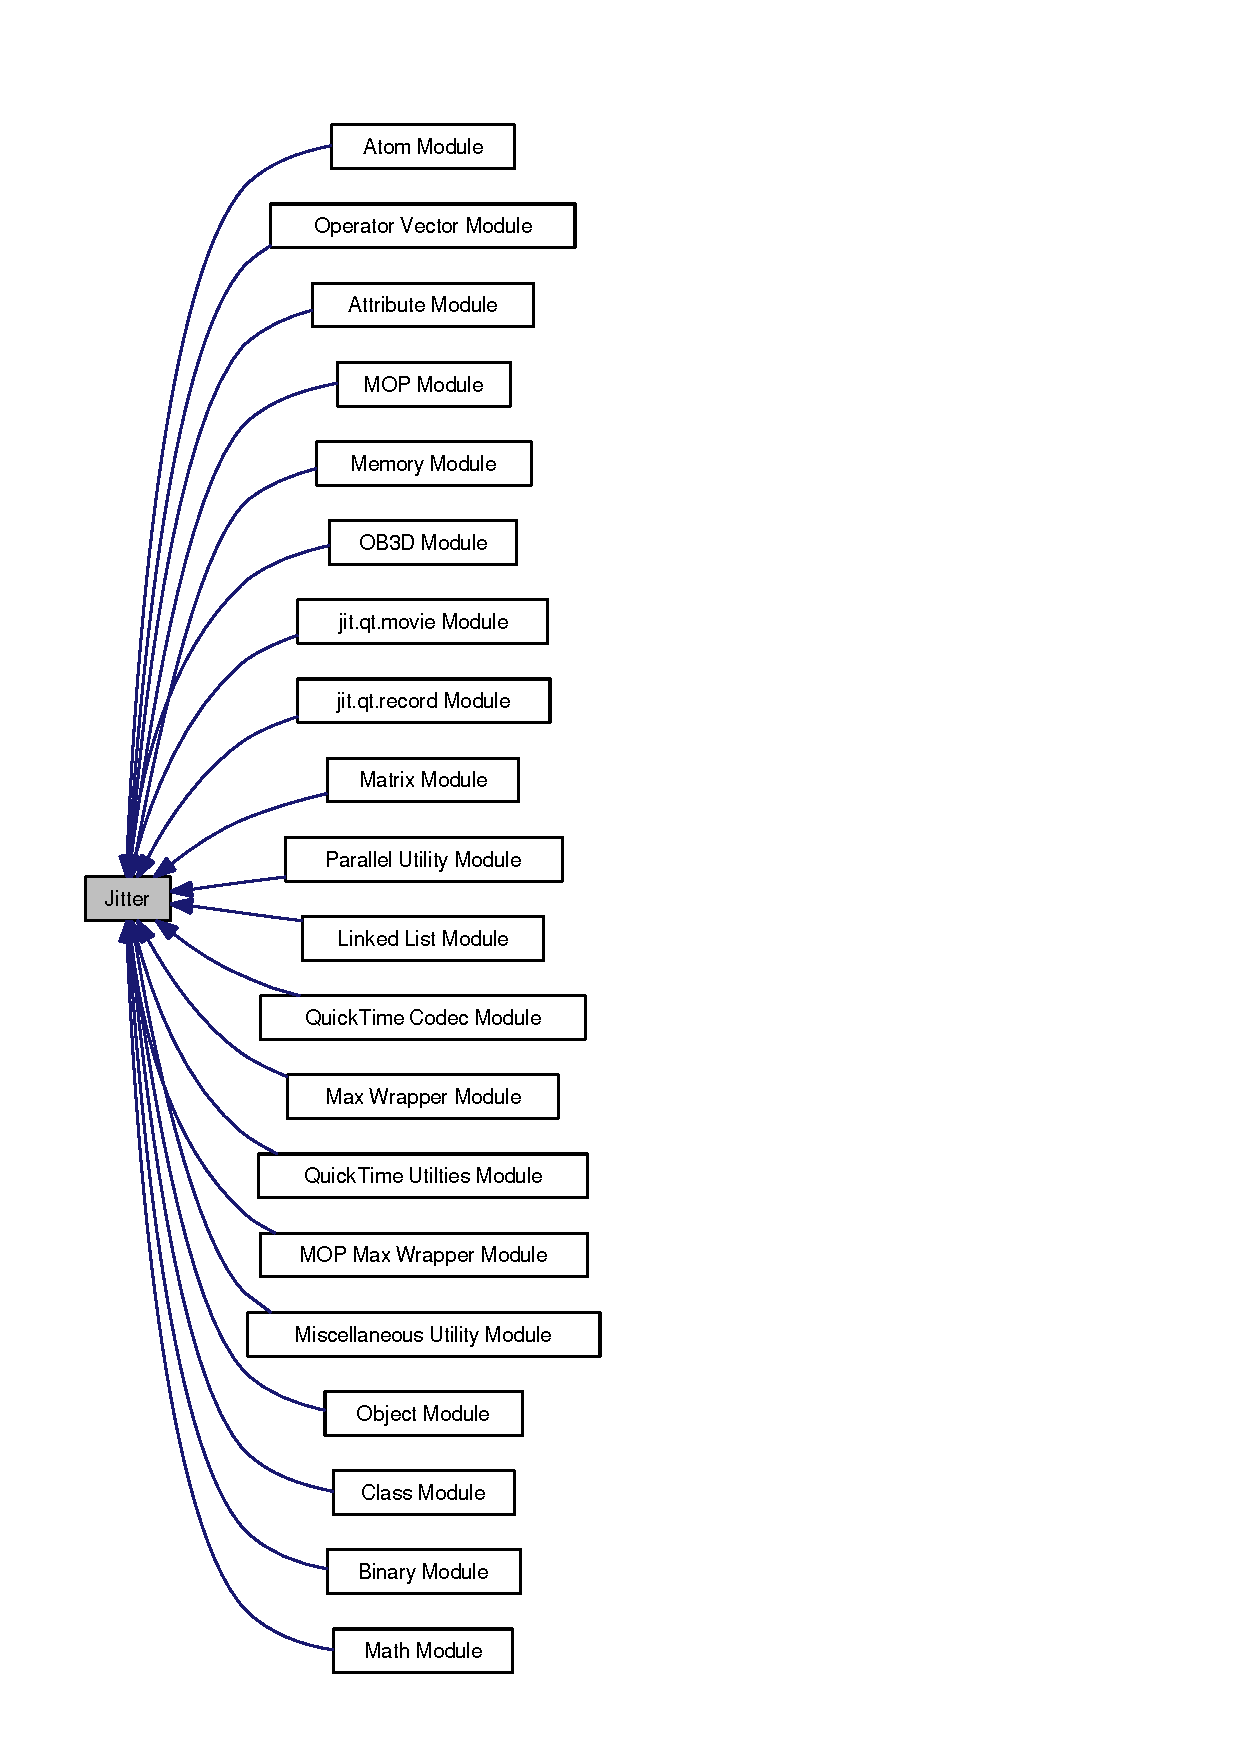
\includegraphics[width=146pt]{group__jitter}
\end{center}
\end{figure}
\subsection*{Modules}
\begin{DoxyCompactItemize}
\item 
\hyperlink{group__atommod}{Atom Module}
\item 
\hyperlink{group__attrmod}{Attribute Module}
\item 
\hyperlink{group__binmod}{Binary Module}
\item 
\hyperlink{group__classmod}{Class Module}
\item 
\hyperlink{group__objectmod}{Object Module}
\item 
\hyperlink{group__utilitymod}{Miscellaneous Utility Module}
\item 
\hyperlink{group__linklistmod}{Linked List Module}
\item 
\hyperlink{group__mathmod}{Math Module}
\item 
\hyperlink{group__matrixmod}{Matrix Module}
\item 
\hyperlink{group__maxwrapmod}{Max Wrapper Module}
\item 
\hyperlink{group__memorymod}{Memory Module}
\item 
\hyperlink{group__mopmod}{MOP Module}
\item 
\hyperlink{group__parallelutilmod}{Parallel Utility Module}
\item 
\hyperlink{group__maxmopmod}{MOP Max Wrapper Module}
\item 
\hyperlink{group__ob3dmod}{OB3D Module}
\item 
\hyperlink{group__opvecmod}{Operator Vector Module}
\item 
\hyperlink{group__qtcodecmod}{QuickTime Codec Module}
\item 
\hyperlink{group__qtmoviemod}{jit.qt.movie Module}
\item 
\hyperlink{group__qtrecordmod}{jit.qt.record Module}
\item 
\hyperlink{group__qtutilsmod}{QuickTime Utilties Module}
\end{DoxyCompactItemize}
\subsection*{Defines}
\begin{DoxyCompactItemize}
\item 
\hypertarget{group__jitter_gaad15de144710f76f17f8f79442c1ee13}{
\#define \hyperlink{group__jitter_gaad15de144710f76f17f8f79442c1ee13}{JIT\_\-ATTR\_\-GET\_\-OPAQUE}~0x00000001}
\label{group__jitter_gaad15de144710f76f17f8f79442c1ee13}

\begin{DoxyCompactList}\small\item\em private getter (all) \item\end{DoxyCompactList}\item 
\hypertarget{group__jitter_gae7eacda8a8da4e67c363ccc33c46b6d1}{
\#define \hyperlink{group__jitter_gae7eacda8a8da4e67c363ccc33c46b6d1}{JIT\_\-ATTR\_\-SET\_\-OPAQUE}~0x00000002}
\label{group__jitter_gae7eacda8a8da4e67c363ccc33c46b6d1}

\begin{DoxyCompactList}\small\item\em private setter (all) \item\end{DoxyCompactList}\item 
\hypertarget{group__jitter_ga9c73a749fbf9f581b85e8ecf9a875b91}{
\#define \hyperlink{group__jitter_ga9c73a749fbf9f581b85e8ecf9a875b91}{JIT\_\-ATTR\_\-GET\_\-OPAQUE\_\-USER}~0x00000100}
\label{group__jitter_ga9c73a749fbf9f581b85e8ecf9a875b91}

\begin{DoxyCompactList}\small\item\em private getter (user) \item\end{DoxyCompactList}\item 
\hypertarget{group__jitter_gae998edfcacc5675e80f85d499453ea23}{
\#define \hyperlink{group__jitter_gae998edfcacc5675e80f85d499453ea23}{JIT\_\-ATTR\_\-SET\_\-OPAQUE\_\-USER}~0x00000200}
\label{group__jitter_gae998edfcacc5675e80f85d499453ea23}

\begin{DoxyCompactList}\small\item\em private setter (user) \item\end{DoxyCompactList}\item 
\hypertarget{group__jitter_ga13c8aa5f90991dad82d1d4dcc3623223}{
\#define \hyperlink{group__jitter_ga13c8aa5f90991dad82d1d4dcc3623223}{JIT\_\-ATTR\_\-GET\_\-DEFER}~0x00010000}
\label{group__jitter_ga13c8aa5f90991dad82d1d4dcc3623223}

\begin{DoxyCompactList}\small\item\em defer getter (deprecated) \item\end{DoxyCompactList}\item 
\hypertarget{group__jitter_ga671a2b2c9ef9f347d5a161b8cb9bcc9e}{
\#define \hyperlink{group__jitter_ga671a2b2c9ef9f347d5a161b8cb9bcc9e}{JIT\_\-ATTR\_\-GET\_\-USURP}~0x00020000}
\label{group__jitter_ga671a2b2c9ef9f347d5a161b8cb9bcc9e}

\begin{DoxyCompactList}\small\item\em usurp getter (deprecated) \item\end{DoxyCompactList}\item 
\hypertarget{group__jitter_ga810447020b75b5173d4c6776cd2653d8}{
\#define \hyperlink{group__jitter_ga810447020b75b5173d4c6776cd2653d8}{JIT\_\-ATTR\_\-GET\_\-DEFER\_\-LOW}~0x00040000}
\label{group__jitter_ga810447020b75b5173d4c6776cd2653d8}

\begin{DoxyCompactList}\small\item\em defer getter \item\end{DoxyCompactList}\item 
\hypertarget{group__jitter_ga07253544f23d315b75f37accf1270a4b}{
\#define \hyperlink{group__jitter_ga07253544f23d315b75f37accf1270a4b}{JIT\_\-ATTR\_\-GET\_\-USURP\_\-LOW}~0x00080000}
\label{group__jitter_ga07253544f23d315b75f37accf1270a4b}

\begin{DoxyCompactList}\small\item\em usurp getter \item\end{DoxyCompactList}\item 
\hypertarget{group__jitter_gafb0470fc7ed5e1bbee265c131ad66488}{
\#define \hyperlink{group__jitter_gafb0470fc7ed5e1bbee265c131ad66488}{JIT\_\-ATTR\_\-SET\_\-DEFER}~0x01000000}
\label{group__jitter_gafb0470fc7ed5e1bbee265c131ad66488}

\begin{DoxyCompactList}\small\item\em defer setter (deprecated) \item\end{DoxyCompactList}\item 
\hypertarget{group__jitter_ga3c97eb0dab6ac2588b8a86d2823d8765}{
\#define \hyperlink{group__jitter_ga3c97eb0dab6ac2588b8a86d2823d8765}{JIT\_\-ATTR\_\-SET\_\-USURP}~0x02000000}
\label{group__jitter_ga3c97eb0dab6ac2588b8a86d2823d8765}

\begin{DoxyCompactList}\small\item\em usurp setter (deprecated) \item\end{DoxyCompactList}\item 
\hypertarget{group__jitter_gaf76b6ca84610d13c1276c51afc2b10ba}{
\#define \hyperlink{group__jitter_gaf76b6ca84610d13c1276c51afc2b10ba}{JIT\_\-ATTR\_\-SET\_\-DEFER\_\-LOW}~0x04000000}
\label{group__jitter_gaf76b6ca84610d13c1276c51afc2b10ba}

\begin{DoxyCompactList}\small\item\em defer setter \item\end{DoxyCompactList}\item 
\hypertarget{group__jitter_ga2ffda4034665d46f65461d67b1004715}{
\#define \hyperlink{group__jitter_ga2ffda4034665d46f65461d67b1004715}{JIT\_\-ATTR\_\-SET\_\-USURP\_\-LOW}~0x08000000}
\label{group__jitter_ga2ffda4034665d46f65461d67b1004715}

\begin{DoxyCompactList}\small\item\em usurp setter \item\end{DoxyCompactList}\item 
\hypertarget{group__jitter_gaeb64c758a0a5e003c4b275da17170dbf}{
\#define \hyperlink{group__jitter_gaeb64c758a0a5e003c4b275da17170dbf}{JIT\_\-MATRIX\_\-DATA\_\-HANDLE}~0x00000002}
\label{group__jitter_gaeb64c758a0a5e003c4b275da17170dbf}

\begin{DoxyCompactList}\small\item\em data is handle \item\end{DoxyCompactList}\item 
\hypertarget{group__jitter_ga524952b91ca521028ba5cbd43bbdb2bf}{
\#define \hyperlink{group__jitter_ga524952b91ca521028ba5cbd43bbdb2bf}{JIT\_\-MATRIX\_\-DATA\_\-REFERENCE}~0x00000004}
\label{group__jitter_ga524952b91ca521028ba5cbd43bbdb2bf}

\begin{DoxyCompactList}\small\item\em data is reference to outside memory \item\end{DoxyCompactList}\item 
\hypertarget{group__jitter_ga8d2975bb5165583d45ea766784e5a60b}{
\#define \hyperlink{group__jitter_ga8d2975bb5165583d45ea766784e5a60b}{JIT\_\-MATRIX\_\-DATA\_\-PACK\_\-TIGHT}~0x00000008}
\label{group__jitter_ga8d2975bb5165583d45ea766784e5a60b}

\begin{DoxyCompactList}\small\item\em data is tightly packed (doesn't use standard 16 byte alignment) \item\end{DoxyCompactList}\item 
\hypertarget{group__jitter_ga54577b5c1a79b9808696965db09fa78d}{
\#define \hyperlink{group__jitter_ga54577b5c1a79b9808696965db09fa78d}{JIT\_\-MATRIX\_\-DATA\_\-FLAGS\_\-USE}~0x00008000}
\label{group__jitter_ga54577b5c1a79b9808696965db09fa78d}

\begin{DoxyCompactList}\small\item\em necessary if using handle/reference data flags when creating jit\_\-matrix, however, it is never stored in matrix \item\end{DoxyCompactList}\item 
\hypertarget{group__jitter_ga3a74bc72df454ac5618a865fd3c56870}{
\#define \hyperlink{group__jitter_ga3a74bc72df454ac5618a865fd3c56870}{JIT\_\-MATRIX\_\-MAX\_\-DIMCOUNT}~32}
\label{group__jitter_ga3a74bc72df454ac5618a865fd3c56870}

\begin{DoxyCompactList}\small\item\em maximum dimension count \item\end{DoxyCompactList}\item 
\hypertarget{group__jitter_gaae5121f82aa81cb79ec17220f845ea08}{
\#define \hyperlink{group__jitter_gaae5121f82aa81cb79ec17220f845ea08}{JIT\_\-MATRIX\_\-MAX\_\-PLANECOUNT}~32}
\label{group__jitter_gaae5121f82aa81cb79ec17220f845ea08}

\begin{DoxyCompactList}\small\item\em maximum plane count \item\end{DoxyCompactList}\item 
\hypertarget{group__jitter_ga10156f72ad806d9e8573f47df19118bd}{
\#define \hyperlink{group__jitter_ga10156f72ad806d9e8573f47df19118bd}{JIT\_\-MATRIX\_\-CONVERT\_\-CLAMP}~0x00000001}
\label{group__jitter_ga10156f72ad806d9e8573f47df19118bd}

\begin{DoxyCompactList}\small\item\em not currently used \item\end{DoxyCompactList}\item 
\hypertarget{group__jitter_gafd3ca93ff4686581454e07c3929934bf}{
\#define \hyperlink{group__jitter_gafd3ca93ff4686581454e07c3929934bf}{JIT\_\-MATRIX\_\-CONVERT\_\-INTERP}~0x00000002}
\label{group__jitter_gafd3ca93ff4686581454e07c3929934bf}

\begin{DoxyCompactList}\small\item\em use interpolation \item\end{DoxyCompactList}\item 
\hypertarget{group__jitter_ga1893e85d59588d93923b0ee5ead9fd63}{
\#define \hyperlink{group__jitter_ga1893e85d59588d93923b0ee5ead9fd63}{JIT\_\-MATRIX\_\-CONVERT\_\-SRCDIM}~0x00000004}
\label{group__jitter_ga1893e85d59588d93923b0ee5ead9fd63}

\begin{DoxyCompactList}\small\item\em use source dimensions \item\end{DoxyCompactList}\item 
\hypertarget{group__jitter_ga1b1e7bf9ea9a7a839f68b243174b5692}{
\#define \hyperlink{group__jitter_ga1b1e7bf9ea9a7a839f68b243174b5692}{JIT\_\-MATRIX\_\-CONVERT\_\-DSTDIM}~0x00000008}
\label{group__jitter_ga1b1e7bf9ea9a7a839f68b243174b5692}

\begin{DoxyCompactList}\small\item\em use destination dimensions \item\end{DoxyCompactList}\item 
\hypertarget{group__jitter_gafc39daa7e259fa20f8fe918cb4892dc4}{
\#define \hyperlink{group__jitter_gafc39daa7e259fa20f8fe918cb4892dc4}{JIT\_\-OB3D\_\-NO\_\-ROTATION\_\-SCALE}~1 $<$$<$ 0}
\label{group__jitter_gafc39daa7e259fa20f8fe918cb4892dc4}

\begin{DoxyCompactList}\small\item\em ob3d flag \item\end{DoxyCompactList}\item 
\hypertarget{group__jitter_ga2eee6fc87f33ea672c921cddf960d5e1}{
\#define \hyperlink{group__jitter_ga2eee6fc87f33ea672c921cddf960d5e1}{JIT\_\-OB3D\_\-NO\_\-POLY\_\-VARS}~1 $<$$<$ 1}
\label{group__jitter_ga2eee6fc87f33ea672c921cddf960d5e1}

\begin{DoxyCompactList}\small\item\em ob3d flag \item\end{DoxyCompactList}\item 
\hypertarget{group__jitter_gab4407b5b96c0744f03bec69e204b56bb}{
\#define \hyperlink{group__jitter_gab4407b5b96c0744f03bec69e204b56bb}{JIT\_\-OB3D\_\-NO\_\-BLEND}~1 $<$$<$ 2}
\label{group__jitter_gab4407b5b96c0744f03bec69e204b56bb}

\begin{DoxyCompactList}\small\item\em ob3d flag \item\end{DoxyCompactList}\item 
\hypertarget{group__jitter_gaf7d77e7694341904bdbd7440ae71d42e}{
\#define \hyperlink{group__jitter_gaf7d77e7694341904bdbd7440ae71d42e}{JIT\_\-OB3D\_\-NO\_\-TEXTURE}~1 $<$$<$ 3}
\label{group__jitter_gaf7d77e7694341904bdbd7440ae71d42e}

\begin{DoxyCompactList}\small\item\em ob3d flag \item\end{DoxyCompactList}\item 
\hypertarget{group__jitter_ga015276252d0ad61f9f35ad1ea227d089}{
\#define \hyperlink{group__jitter_ga015276252d0ad61f9f35ad1ea227d089}{JIT\_\-OB3D\_\-NO\_\-MATRIXOUTPUT}~1 $<$$<$ 4}
\label{group__jitter_ga015276252d0ad61f9f35ad1ea227d089}

\begin{DoxyCompactList}\small\item\em ob3d flag \item\end{DoxyCompactList}\item 
\hypertarget{group__jitter_ga63a89334c5c06f92792333d191b71b06}{
\#define \hyperlink{group__jitter_ga63a89334c5c06f92792333d191b71b06}{JIT\_\-OB3D\_\-AUTO\_\-ONLY}~1 $<$$<$ 5}
\label{group__jitter_ga63a89334c5c06f92792333d191b71b06}

\begin{DoxyCompactList}\small\item\em ob3d flag \item\end{DoxyCompactList}\item 
\hypertarget{group__jitter_gaafef09ee7a36fc16e46529783df7cd72}{
\#define \hyperlink{group__jitter_gaafef09ee7a36fc16e46529783df7cd72}{JIT\_\-OB3D\_\-DOES\_\-UI}~1 $<$$<$ 6}
\label{group__jitter_gaafef09ee7a36fc16e46529783df7cd72}

\begin{DoxyCompactList}\small\item\em ob3d flag \item\end{DoxyCompactList}\item 
\hypertarget{group__jitter_gad4a2b2f395618bafbd7faca61106b9f7}{
\#define \hyperlink{group__jitter_gad4a2b2f395618bafbd7faca61106b9f7}{JIT\_\-OB3D\_\-NO\_\-DEPTH}~1 $<$$<$ 7}
\label{group__jitter_gad4a2b2f395618bafbd7faca61106b9f7}

\begin{DoxyCompactList}\small\item\em ob3d flag \item\end{DoxyCompactList}\item 
\hypertarget{group__jitter_ga2ef1435359d9dca4722fb71db4b0d423}{
\#define \hyperlink{group__jitter_ga2ef1435359d9dca4722fb71db4b0d423}{JIT\_\-OB3D\_\-NO\_\-ANTIALIAS}~1 $<$$<$ 8}
\label{group__jitter_ga2ef1435359d9dca4722fb71db4b0d423}

\begin{DoxyCompactList}\small\item\em ob3d flag \item\end{DoxyCompactList}\item 
\hypertarget{group__jitter_gaf9c39790969f477fb42c3fe674eb5ca7}{
\#define \hyperlink{group__jitter_gaf9c39790969f477fb42c3fe674eb5ca7}{JIT\_\-OB3D\_\-NO\_\-FOG}~1 $<$$<$ 9}
\label{group__jitter_gaf9c39790969f477fb42c3fe674eb5ca7}

\begin{DoxyCompactList}\small\item\em ob3d flag \item\end{DoxyCompactList}\item 
\hypertarget{group__jitter_gaf7b319953ace69f17633be98233fd324}{
\#define \hyperlink{group__jitter_gaf7b319953ace69f17633be98233fd324}{JIT\_\-OB3D\_\-NO\_\-LIGHTING\_\-MATERIAL}~1 $<$$<$ 10}
\label{group__jitter_gaf7b319953ace69f17633be98233fd324}

\begin{DoxyCompactList}\small\item\em ob3d flag \item\end{DoxyCompactList}\item 
\hypertarget{group__jitter_ga1f032969c5d7b0adb353743e77736b96}{
\#define \hyperlink{group__jitter_ga1f032969c5d7b0adb353743e77736b96}{JIT\_\-OB3D\_\-HAS\_\-LIGHTS}~1 $<$$<$ 11}
\label{group__jitter_ga1f032969c5d7b0adb353743e77736b96}

\begin{DoxyCompactList}\small\item\em ob3d flag \item\end{DoxyCompactList}\item 
\hypertarget{group__jitter_ga1f324497fe983b02072b38d5c725ba2a}{
\#define \hyperlink{group__jitter_ga1f324497fe983b02072b38d5c725ba2a}{JIT\_\-OB3D\_\-HAS\_\-CAMERA}~1 $<$$<$ 12}
\label{group__jitter_ga1f324497fe983b02072b38d5c725ba2a}

\begin{DoxyCompactList}\small\item\em ob3d flag \item\end{DoxyCompactList}\item 
\hypertarget{group__jitter_ga46c7216fed49a3b9f9f10ad4d87cea55}{
\#define \hyperlink{group__jitter_ga46c7216fed49a3b9f9f10ad4d87cea55}{JIT\_\-OB3D\_\-IS\_\-RENDERER}~1 $<$$<$ 13}
\label{group__jitter_ga46c7216fed49a3b9f9f10ad4d87cea55}

\begin{DoxyCompactList}\small\item\em ob3d flag \item\end{DoxyCompactList}\item 
\hypertarget{group__jitter_ga6d6e4c119dbea5119a0f452a2486e590}{
\#define \hyperlink{group__jitter_ga6d6e4c119dbea5119a0f452a2486e590}{JIT\_\-OB3D\_\-NO\_\-COLOR}~1 $<$$<$ 14}
\label{group__jitter_ga6d6e4c119dbea5119a0f452a2486e590}

\begin{DoxyCompactList}\small\item\em ob3d flag \item\end{DoxyCompactList}\item 
\hypertarget{group__jitter_gaf6797493caebaf2a151563492f190b35}{
\#define \hyperlink{group__jitter_gaf6797493caebaf2a151563492f190b35}{JIT\_\-OB3D\_\-IS\_\-SLAB}~1 $<$$<$ 15}
\label{group__jitter_gaf6797493caebaf2a151563492f190b35}

\begin{DoxyCompactList}\small\item\em ob3d flag \item\end{DoxyCompactList}\item 
\hypertarget{group__jitter_ga6f8627ede2fc37736591b2d8f8e32b5b}{
\#define \hyperlink{group__jitter_ga6f8627ede2fc37736591b2d8f8e32b5b}{MAX\_\-JIT\_\-MOP\_\-FLAGS\_\-NONE}~0x00000000}
\label{group__jitter_ga6f8627ede2fc37736591b2d8f8e32b5b}

\begin{DoxyCompactList}\small\item\em mop flag \item\end{DoxyCompactList}\item 
\hypertarget{group__jitter_ga60cbfeaf26417a8d6561fb9acce523d5}{
\#define \hyperlink{group__jitter_ga60cbfeaf26417a8d6561fb9acce523d5}{MAX\_\-JIT\_\-MOP\_\-FLAGS\_\-OWN\_\-ALL}~0xFFFFFFFF}
\label{group__jitter_ga60cbfeaf26417a8d6561fb9acce523d5}

\begin{DoxyCompactList}\small\item\em mop flag \item\end{DoxyCompactList}\item 
\hypertarget{group__jitter_ga76b29cb7bf7f194cef194fb65df28ddd}{
\#define \hyperlink{group__jitter_ga76b29cb7bf7f194cef194fb65df28ddd}{MAX\_\-JIT\_\-MOP\_\-FLAGS\_\-OWN\_\-JIT\_\-MATRIX}~0x00000001}
\label{group__jitter_ga76b29cb7bf7f194cef194fb65df28ddd}

\begin{DoxyCompactList}\small\item\em mop flag \item\end{DoxyCompactList}\item 
\hypertarget{group__jitter_gae93fd085f28675389848233a82521942}{
\#define \hyperlink{group__jitter_gae93fd085f28675389848233a82521942}{MAX\_\-JIT\_\-MOP\_\-FLAGS\_\-OWN\_\-BANG}~0x00000002}
\label{group__jitter_gae93fd085f28675389848233a82521942}

\begin{DoxyCompactList}\small\item\em mop flag \item\end{DoxyCompactList}\item 
\hypertarget{group__jitter_ga7c51c91474bdbc40437dbd946df19cc5}{
\#define \hyperlink{group__jitter_ga7c51c91474bdbc40437dbd946df19cc5}{MAX\_\-JIT\_\-MOP\_\-FLAGS\_\-OWN\_\-OUTPUTMATRIX}~0x00000004}
\label{group__jitter_ga7c51c91474bdbc40437dbd946df19cc5}

\begin{DoxyCompactList}\small\item\em mop flag \item\end{DoxyCompactList}\item 
\hypertarget{group__jitter_ga2da79e2f2413304655b66637eeff0326}{
\#define \hyperlink{group__jitter_ga2da79e2f2413304655b66637eeff0326}{MAX\_\-JIT\_\-MOP\_\-FLAGS\_\-OWN\_\-NAME}~0x00000008}
\label{group__jitter_ga2da79e2f2413304655b66637eeff0326}

\begin{DoxyCompactList}\small\item\em mop flag \item\end{DoxyCompactList}\item 
\hypertarget{group__jitter_gaf85d3bada9b15b7c5371e4cbeeffcaeb}{
\#define \hyperlink{group__jitter_gaf85d3bada9b15b7c5371e4cbeeffcaeb}{MAX\_\-JIT\_\-MOP\_\-FLAGS\_\-OWN\_\-TYPE}~0x00000010}
\label{group__jitter_gaf85d3bada9b15b7c5371e4cbeeffcaeb}

\begin{DoxyCompactList}\small\item\em mop flag \item\end{DoxyCompactList}\item 
\hypertarget{group__jitter_gaf138ee8c3a7120b8914c2e815ed013bd}{
\#define \hyperlink{group__jitter_gaf138ee8c3a7120b8914c2e815ed013bd}{MAX\_\-JIT\_\-MOP\_\-FLAGS\_\-OWN\_\-DIM}~0x00000020}
\label{group__jitter_gaf138ee8c3a7120b8914c2e815ed013bd}

\begin{DoxyCompactList}\small\item\em mop flag \item\end{DoxyCompactList}\item 
\hypertarget{group__jitter_ga77553b6728bd9d5d6d18fe6e4d65a128}{
\#define \hyperlink{group__jitter_ga77553b6728bd9d5d6d18fe6e4d65a128}{MAX\_\-JIT\_\-MOP\_\-FLAGS\_\-OWN\_\-PLANECOUNT}~0x00000040}
\label{group__jitter_ga77553b6728bd9d5d6d18fe6e4d65a128}

\begin{DoxyCompactList}\small\item\em mop flag \item\end{DoxyCompactList}\item 
\hypertarget{group__jitter_gaadd7ebf9b850b06496bdeb9414d181e4}{
\#define \hyperlink{group__jitter_gaadd7ebf9b850b06496bdeb9414d181e4}{MAX\_\-JIT\_\-MOP\_\-FLAGS\_\-OWN\_\-CLEAR}~0x00000080}
\label{group__jitter_gaadd7ebf9b850b06496bdeb9414d181e4}

\begin{DoxyCompactList}\small\item\em mop flag \item\end{DoxyCompactList}\item 
\hypertarget{group__jitter_ga669c2f28bba1dfb4181ebae8f19488bc}{
\#define \hyperlink{group__jitter_ga669c2f28bba1dfb4181ebae8f19488bc}{MAX\_\-JIT\_\-MOP\_\-FLAGS\_\-OWN\_\-NOTIFY}~0x00000100}
\label{group__jitter_ga669c2f28bba1dfb4181ebae8f19488bc}

\begin{DoxyCompactList}\small\item\em mop flag \item\end{DoxyCompactList}\item 
\hypertarget{group__jitter_ga1c01c9fbad6e41293920117964654f61}{
\#define \hyperlink{group__jitter_ga1c01c9fbad6e41293920117964654f61}{MAX\_\-JIT\_\-MOP\_\-FLAGS\_\-OWN\_\-ADAPT}~0x00000200}
\label{group__jitter_ga1c01c9fbad6e41293920117964654f61}

\begin{DoxyCompactList}\small\item\em mop flag \item\end{DoxyCompactList}\item 
\hypertarget{group__jitter_gadad1691bc68342a60441cb884a89129d}{
\#define \hyperlink{group__jitter_gadad1691bc68342a60441cb884a89129d}{MAX\_\-JIT\_\-MOP\_\-FLAGS\_\-OWN\_\-OUTPUTMODE}~0x00000400}
\label{group__jitter_gadad1691bc68342a60441cb884a89129d}

\begin{DoxyCompactList}\small\item\em mop flag \item\end{DoxyCompactList}\item 
\hypertarget{group__jitter_gaabaf165bab15a39bbd561807b3f5bb37}{
\#define \hyperlink{group__jitter_gaabaf165bab15a39bbd561807b3f5bb37}{JIT\_\-MOP\_\-INPUT}~1}
\label{group__jitter_gaabaf165bab15a39bbd561807b3f5bb37}

\begin{DoxyCompactList}\small\item\em mop flag \item\end{DoxyCompactList}\item 
\hypertarget{group__jitter_ga979fc199dadb0724f942c6a48cb733a1}{
\#define \hyperlink{group__jitter_ga979fc199dadb0724f942c6a48cb733a1}{JIT\_\-MOP\_\-OUTPUT}~2}
\label{group__jitter_ga979fc199dadb0724f942c6a48cb733a1}

\begin{DoxyCompactList}\small\item\em mop flag \item\end{DoxyCompactList}\end{DoxyCompactItemize}
\subsection*{Typedefs}
\begin{DoxyCompactItemize}
\item 
\hypertarget{group__jitter_ga0eb2cd9c8e3b9803ba31069575a1ffb9}{
typedef \hyperlink{structt__object}{t\_\-object} \hyperlink{group__jitter_ga0eb2cd9c8e3b9803ba31069575a1ffb9}{t\_\-jit\_\-object}}
\label{group__jitter_ga0eb2cd9c8e3b9803ba31069575a1ffb9}

\begin{DoxyCompactList}\small\item\em object header \item\end{DoxyCompactList}\end{DoxyCompactItemize}
\subsection*{Variables}
\begin{DoxyCompactItemize}
\item 
\hypertarget{group__jitter_ga43ff77a4b747208cc8df2fe8b295cb20}{
JIT\_\-EX\_\-DATA \hyperlink{structt__symbol}{t\_\-symbol} $\ast$ \hyperlink{group__jitter_ga43ff77a4b747208cc8df2fe8b295cb20}{\_\-jit\_\-sym\_\-codec\_\-raw}}
\label{group__jitter_ga43ff77a4b747208cc8df2fe8b295cb20}

\begin{DoxyCompactList}\small\item\em cached \hyperlink{structt__symbol}{t\_\-symbol} \item\end{DoxyCompactList}\item 
\hypertarget{group__jitter_ga486364eb4af339d3e87c383b0969c567}{
JIT\_\-EX\_\-DATA \hyperlink{structt__symbol}{t\_\-symbol} $\ast$ \hyperlink{group__jitter_ga486364eb4af339d3e87c383b0969c567}{\_\-jit\_\-sym\_\-codec\_\-cinepak}}
\label{group__jitter_ga486364eb4af339d3e87c383b0969c567}

\begin{DoxyCompactList}\small\item\em cached \hyperlink{structt__symbol}{t\_\-symbol} \item\end{DoxyCompactList}\item 
\hypertarget{group__jitter_ga10ca359d6aa3fcd773c8ed884cef4b77}{
JIT\_\-EX\_\-DATA \hyperlink{structt__symbol}{t\_\-symbol} $\ast$ \hyperlink{group__jitter_ga10ca359d6aa3fcd773c8ed884cef4b77}{\_\-jit\_\-sym\_\-codec\_\-graphics}}
\label{group__jitter_ga10ca359d6aa3fcd773c8ed884cef4b77}

\begin{DoxyCompactList}\small\item\em cached \hyperlink{structt__symbol}{t\_\-symbol} \item\end{DoxyCompactList}\item 
\hypertarget{group__jitter_ga5fdf7d5881a2078ba7bc49c1aefb6c53}{
JIT\_\-EX\_\-DATA \hyperlink{structt__symbol}{t\_\-symbol} $\ast$ \hyperlink{group__jitter_ga5fdf7d5881a2078ba7bc49c1aefb6c53}{\_\-jit\_\-sym\_\-codec\_\-animation}}
\label{group__jitter_ga5fdf7d5881a2078ba7bc49c1aefb6c53}

\begin{DoxyCompactList}\small\item\em cached \hyperlink{structt__symbol}{t\_\-symbol} \item\end{DoxyCompactList}\item 
\hypertarget{group__jitter_gac8fe7f4903a14198abac4d2807eba7e8}{
JIT\_\-EX\_\-DATA \hyperlink{structt__symbol}{t\_\-symbol} $\ast$ \hyperlink{group__jitter_gac8fe7f4903a14198abac4d2807eba7e8}{\_\-jit\_\-sym\_\-codec\_\-video}}
\label{group__jitter_gac8fe7f4903a14198abac4d2807eba7e8}

\begin{DoxyCompactList}\small\item\em cached \hyperlink{structt__symbol}{t\_\-symbol} \item\end{DoxyCompactList}\item 
\hypertarget{group__jitter_ga145fa95179795698c563c431c94bcec6}{
JIT\_\-EX\_\-DATA \hyperlink{structt__symbol}{t\_\-symbol} $\ast$ \hyperlink{group__jitter_ga145fa95179795698c563c431c94bcec6}{\_\-jit\_\-sym\_\-codec\_\-componentvideo}}
\label{group__jitter_ga145fa95179795698c563c431c94bcec6}

\begin{DoxyCompactList}\small\item\em cached \hyperlink{structt__symbol}{t\_\-symbol} \item\end{DoxyCompactList}\item 
\hypertarget{group__jitter_gae0024863097747f851a19e78c734e7b5}{
JIT\_\-EX\_\-DATA \hyperlink{structt__symbol}{t\_\-symbol} $\ast$ \hyperlink{group__jitter_gae0024863097747f851a19e78c734e7b5}{\_\-jit\_\-sym\_\-codec\_\-jpeg}}
\label{group__jitter_gae0024863097747f851a19e78c734e7b5}

\begin{DoxyCompactList}\small\item\em cached \hyperlink{structt__symbol}{t\_\-symbol} \item\end{DoxyCompactList}\item 
\hypertarget{group__jitter_ga8db004bdaea9032a74262379b84dba95}{
JIT\_\-EX\_\-DATA \hyperlink{structt__symbol}{t\_\-symbol} $\ast$ \hyperlink{group__jitter_ga8db004bdaea9032a74262379b84dba95}{\_\-jit\_\-sym\_\-codec\_\-mjpega}}
\label{group__jitter_ga8db004bdaea9032a74262379b84dba95}

\begin{DoxyCompactList}\small\item\em cached \hyperlink{structt__symbol}{t\_\-symbol} \item\end{DoxyCompactList}\item 
\hypertarget{group__jitter_gaff7aaf216679e914c38976e5f9df15db}{
JIT\_\-EX\_\-DATA \hyperlink{structt__symbol}{t\_\-symbol} $\ast$ \hyperlink{group__jitter_gaff7aaf216679e914c38976e5f9df15db}{\_\-jit\_\-sym\_\-codec\_\-mjpegb}}
\label{group__jitter_gaff7aaf216679e914c38976e5f9df15db}

\begin{DoxyCompactList}\small\item\em cached \hyperlink{structt__symbol}{t\_\-symbol} \item\end{DoxyCompactList}\item 
\hypertarget{group__jitter_ga709f8309f58760559af349bd179b1a5e}{
JIT\_\-EX\_\-DATA \hyperlink{structt__symbol}{t\_\-symbol} $\ast$ \hyperlink{group__jitter_ga709f8309f58760559af349bd179b1a5e}{\_\-jit\_\-sym\_\-codec\_\-sgi}}
\label{group__jitter_ga709f8309f58760559af349bd179b1a5e}

\begin{DoxyCompactList}\small\item\em cached \hyperlink{structt__symbol}{t\_\-symbol} \item\end{DoxyCompactList}\item 
\hypertarget{group__jitter_ga9e3f5e410192f5386c8ec75b49aa4c5d}{
JIT\_\-EX\_\-DATA \hyperlink{structt__symbol}{t\_\-symbol} $\ast$ \hyperlink{group__jitter_ga9e3f5e410192f5386c8ec75b49aa4c5d}{\_\-jit\_\-sym\_\-codec\_\-planarrgb}}
\label{group__jitter_ga9e3f5e410192f5386c8ec75b49aa4c5d}

\begin{DoxyCompactList}\small\item\em cached \hyperlink{structt__symbol}{t\_\-symbol} \item\end{DoxyCompactList}\item 
\hypertarget{group__jitter_gae0f1922f59cfbe91eb5750726d67df7e}{
JIT\_\-EX\_\-DATA \hyperlink{structt__symbol}{t\_\-symbol} $\ast$ \hyperlink{group__jitter_gae0f1922f59cfbe91eb5750726d67df7e}{\_\-jit\_\-sym\_\-codec\_\-macpaint}}
\label{group__jitter_gae0f1922f59cfbe91eb5750726d67df7e}

\begin{DoxyCompactList}\small\item\em cached \hyperlink{structt__symbol}{t\_\-symbol} \item\end{DoxyCompactList}\item 
\hypertarget{group__jitter_gadd374220c19455f5e7dfca29bf09c36b}{
JIT\_\-EX\_\-DATA \hyperlink{structt__symbol}{t\_\-symbol} $\ast$ \hyperlink{group__jitter_gadd374220c19455f5e7dfca29bf09c36b}{\_\-jit\_\-sym\_\-codec\_\-gif}}
\label{group__jitter_gadd374220c19455f5e7dfca29bf09c36b}

\begin{DoxyCompactList}\small\item\em cached \hyperlink{structt__symbol}{t\_\-symbol} \item\end{DoxyCompactList}\item 
\hypertarget{group__jitter_gae852f97ee9b1de24e37c95b504bb6486}{
JIT\_\-EX\_\-DATA \hyperlink{structt__symbol}{t\_\-symbol} $\ast$ \hyperlink{group__jitter_gae852f97ee9b1de24e37c95b504bb6486}{\_\-jit\_\-sym\_\-codec\_\-photocd}}
\label{group__jitter_gae852f97ee9b1de24e37c95b504bb6486}

\begin{DoxyCompactList}\small\item\em cached \hyperlink{structt__symbol}{t\_\-symbol} \item\end{DoxyCompactList}\item 
\hypertarget{group__jitter_ga7279d3cde3d770e36da997ddabec5024}{
JIT\_\-EX\_\-DATA \hyperlink{structt__symbol}{t\_\-symbol} $\ast$ \hyperlink{group__jitter_ga7279d3cde3d770e36da997ddabec5024}{\_\-jit\_\-sym\_\-codec\_\-qdgx}}
\label{group__jitter_ga7279d3cde3d770e36da997ddabec5024}

\begin{DoxyCompactList}\small\item\em cached \hyperlink{structt__symbol}{t\_\-symbol} \item\end{DoxyCompactList}\item 
\hypertarget{group__jitter_ga636e00d9ed9e7ad41a0ab953268cda5e}{
JIT\_\-EX\_\-DATA \hyperlink{structt__symbol}{t\_\-symbol} $\ast$ \hyperlink{group__jitter_ga636e00d9ed9e7ad41a0ab953268cda5e}{\_\-jit\_\-sym\_\-codec\_\-avrjpeg}}
\label{group__jitter_ga636e00d9ed9e7ad41a0ab953268cda5e}

\begin{DoxyCompactList}\small\item\em cached \hyperlink{structt__symbol}{t\_\-symbol} \item\end{DoxyCompactList}\item 
\hypertarget{group__jitter_ga9252e9079690343ae441d22fe55dc3ac}{
JIT\_\-EX\_\-DATA \hyperlink{structt__symbol}{t\_\-symbol} $\ast$ \hyperlink{group__jitter_ga9252e9079690343ae441d22fe55dc3ac}{\_\-jit\_\-sym\_\-codec\_\-opendmljpeg}}
\label{group__jitter_ga9252e9079690343ae441d22fe55dc3ac}

\begin{DoxyCompactList}\small\item\em cached \hyperlink{structt__symbol}{t\_\-symbol} \item\end{DoxyCompactList}\item 
\hypertarget{group__jitter_gac1b1fc063bc5e142e40abeceacf365b3}{
JIT\_\-EX\_\-DATA \hyperlink{structt__symbol}{t\_\-symbol} $\ast$ \hyperlink{group__jitter_gac1b1fc063bc5e142e40abeceacf365b3}{\_\-jit\_\-sym\_\-codec\_\-bmp}}
\label{group__jitter_gac1b1fc063bc5e142e40abeceacf365b3}

\begin{DoxyCompactList}\small\item\em cached \hyperlink{structt__symbol}{t\_\-symbol} \item\end{DoxyCompactList}\item 
\hypertarget{group__jitter_ga338bb45421a2c586d8ec57af1550f956}{
JIT\_\-EX\_\-DATA \hyperlink{structt__symbol}{t\_\-symbol} $\ast$ \hyperlink{group__jitter_ga338bb45421a2c586d8ec57af1550f956}{\_\-jit\_\-sym\_\-codec\_\-winraw}}
\label{group__jitter_ga338bb45421a2c586d8ec57af1550f956}

\begin{DoxyCompactList}\small\item\em cached \hyperlink{structt__symbol}{t\_\-symbol} \item\end{DoxyCompactList}\item 
\hypertarget{group__jitter_ga260fe083d60559670bfa2c9e3c77257f}{
JIT\_\-EX\_\-DATA \hyperlink{structt__symbol}{t\_\-symbol} $\ast$ \hyperlink{group__jitter_ga260fe083d60559670bfa2c9e3c77257f}{\_\-jit\_\-sym\_\-codec\_\-vector}}
\label{group__jitter_ga260fe083d60559670bfa2c9e3c77257f}

\begin{DoxyCompactList}\small\item\em cached \hyperlink{structt__symbol}{t\_\-symbol} \item\end{DoxyCompactList}\item 
\hypertarget{group__jitter_ga8bd39e0232734a56bd3dad9ce443aa3c}{
JIT\_\-EX\_\-DATA \hyperlink{structt__symbol}{t\_\-symbol} $\ast$ \hyperlink{group__jitter_ga8bd39e0232734a56bd3dad9ce443aa3c}{\_\-jit\_\-sym\_\-codec\_\-qd}}
\label{group__jitter_ga8bd39e0232734a56bd3dad9ce443aa3c}

\begin{DoxyCompactList}\small\item\em cached \hyperlink{structt__symbol}{t\_\-symbol} \item\end{DoxyCompactList}\item 
\hypertarget{group__jitter_gaeaed0103ad5e42520ae0142b783c312d}{
JIT\_\-EX\_\-DATA \hyperlink{structt__symbol}{t\_\-symbol} $\ast$ \hyperlink{group__jitter_gaeaed0103ad5e42520ae0142b783c312d}{\_\-jit\_\-sym\_\-codec\_\-h261}}
\label{group__jitter_gaeaed0103ad5e42520ae0142b783c312d}

\begin{DoxyCompactList}\small\item\em cached \hyperlink{structt__symbol}{t\_\-symbol} \item\end{DoxyCompactList}\item 
\hypertarget{group__jitter_gad37e3c153d7b5df76ed4a3f593045261}{
JIT\_\-EX\_\-DATA \hyperlink{structt__symbol}{t\_\-symbol} $\ast$ \hyperlink{group__jitter_gad37e3c153d7b5df76ed4a3f593045261}{\_\-jit\_\-sym\_\-codec\_\-h263}}
\label{group__jitter_gad37e3c153d7b5df76ed4a3f593045261}

\begin{DoxyCompactList}\small\item\em cached \hyperlink{structt__symbol}{t\_\-symbol} \item\end{DoxyCompactList}\item 
\hypertarget{group__jitter_ga79c8c7827e10f38fcd5f0c3956f35a15}{
JIT\_\-EX\_\-DATA \hyperlink{structt__symbol}{t\_\-symbol} $\ast$ \hyperlink{group__jitter_ga79c8c7827e10f38fcd5f0c3956f35a15}{\_\-jit\_\-sym\_\-codec\_\-dvntsc}}
\label{group__jitter_ga79c8c7827e10f38fcd5f0c3956f35a15}

\begin{DoxyCompactList}\small\item\em cached \hyperlink{structt__symbol}{t\_\-symbol} \item\end{DoxyCompactList}\item 
\hypertarget{group__jitter_ga2a8a6846182a5f1ea38694699c4153b2}{
JIT\_\-EX\_\-DATA \hyperlink{structt__symbol}{t\_\-symbol} $\ast$ \hyperlink{group__jitter_ga2a8a6846182a5f1ea38694699c4153b2}{\_\-jit\_\-sym\_\-codec\_\-dvpal}}
\label{group__jitter_ga2a8a6846182a5f1ea38694699c4153b2}

\begin{DoxyCompactList}\small\item\em cached \hyperlink{structt__symbol}{t\_\-symbol} \item\end{DoxyCompactList}\item 
\hypertarget{group__jitter_ga3d1b9d4a079030cc6b8f11d1eb527eed}{
JIT\_\-EX\_\-DATA \hyperlink{structt__symbol}{t\_\-symbol} $\ast$ \hyperlink{group__jitter_ga3d1b9d4a079030cc6b8f11d1eb527eed}{\_\-jit\_\-sym\_\-codec\_\-dvprontsc}}
\label{group__jitter_ga3d1b9d4a079030cc6b8f11d1eb527eed}

\begin{DoxyCompactList}\small\item\em cached \hyperlink{structt__symbol}{t\_\-symbol} \item\end{DoxyCompactList}\item 
\hypertarget{group__jitter_gae850f6b0b73f74e4fec50e352b9361aa}{
JIT\_\-EX\_\-DATA \hyperlink{structt__symbol}{t\_\-symbol} $\ast$ \hyperlink{group__jitter_gae850f6b0b73f74e4fec50e352b9361aa}{\_\-jit\_\-sym\_\-codec\_\-dvpropal}}
\label{group__jitter_gae850f6b0b73f74e4fec50e352b9361aa}

\begin{DoxyCompactList}\small\item\em cached \hyperlink{structt__symbol}{t\_\-symbol} \item\end{DoxyCompactList}\item 
\hypertarget{group__jitter_ga2202e766cc46a9bfff9312c2e5660431}{
JIT\_\-EX\_\-DATA \hyperlink{structt__symbol}{t\_\-symbol} $\ast$ \hyperlink{group__jitter_ga2202e766cc46a9bfff9312c2e5660431}{\_\-jit\_\-sym\_\-codec\_\-flc}}
\label{group__jitter_ga2202e766cc46a9bfff9312c2e5660431}

\begin{DoxyCompactList}\small\item\em cached \hyperlink{structt__symbol}{t\_\-symbol} \item\end{DoxyCompactList}\item 
\hypertarget{group__jitter_ga5dc2290808fc905abbb1d804867d3a52}{
JIT\_\-EX\_\-DATA \hyperlink{structt__symbol}{t\_\-symbol} $\ast$ \hyperlink{group__jitter_ga5dc2290808fc905abbb1d804867d3a52}{\_\-jit\_\-sym\_\-codec\_\-targa}}
\label{group__jitter_ga5dc2290808fc905abbb1d804867d3a52}

\begin{DoxyCompactList}\small\item\em cached \hyperlink{structt__symbol}{t\_\-symbol} \item\end{DoxyCompactList}\item 
\hypertarget{group__jitter_ga8c27c5e836aa35a6522fcafddc1d8c2b}{
JIT\_\-EX\_\-DATA \hyperlink{structt__symbol}{t\_\-symbol} $\ast$ \hyperlink{group__jitter_ga8c27c5e836aa35a6522fcafddc1d8c2b}{\_\-jit\_\-sym\_\-codec\_\-png}}
\label{group__jitter_ga8c27c5e836aa35a6522fcafddc1d8c2b}

\begin{DoxyCompactList}\small\item\em cached \hyperlink{structt__symbol}{t\_\-symbol} \item\end{DoxyCompactList}\item 
\hypertarget{group__jitter_ga1f8a279a6ad561887c1d6f4cad544040}{
JIT\_\-EX\_\-DATA \hyperlink{structt__symbol}{t\_\-symbol} $\ast$ \hyperlink{group__jitter_ga1f8a279a6ad561887c1d6f4cad544040}{\_\-jit\_\-sym\_\-codec\_\-tiff}}
\label{group__jitter_ga1f8a279a6ad561887c1d6f4cad544040}

\begin{DoxyCompactList}\small\item\em cached \hyperlink{structt__symbol}{t\_\-symbol} \item\end{DoxyCompactList}\item 
\hypertarget{group__jitter_gae19cd60b6c0aee556e197bfe57763998}{
JIT\_\-EX\_\-DATA \hyperlink{structt__symbol}{t\_\-symbol} $\ast$ \hyperlink{group__jitter_gae19cd60b6c0aee556e197bfe57763998}{\_\-jit\_\-sym\_\-codec\_\-componentvideosigned}}
\label{group__jitter_gae19cd60b6c0aee556e197bfe57763998}

\begin{DoxyCompactList}\small\item\em cached \hyperlink{structt__symbol}{t\_\-symbol} \item\end{DoxyCompactList}\item 
\hypertarget{group__jitter_gad14a48bc61f3746eea15daadd1353651}{
JIT\_\-EX\_\-DATA \hyperlink{structt__symbol}{t\_\-symbol} $\ast$ \hyperlink{group__jitter_gad14a48bc61f3746eea15daadd1353651}{\_\-jit\_\-sym\_\-codec\_\-componentvideounsigned}}
\label{group__jitter_gad14a48bc61f3746eea15daadd1353651}

\begin{DoxyCompactList}\small\item\em cached \hyperlink{structt__symbol}{t\_\-symbol} \item\end{DoxyCompactList}\item 
\hypertarget{group__jitter_ga39d0ef75961249b5815622e6eae46c66}{
JIT\_\-EX\_\-DATA \hyperlink{structt__symbol}{t\_\-symbol} $\ast$ \hyperlink{group__jitter_ga39d0ef75961249b5815622e6eae46c66}{\_\-jit\_\-sym\_\-codec\_\-cmyk}}
\label{group__jitter_ga39d0ef75961249b5815622e6eae46c66}

\begin{DoxyCompactList}\small\item\em cached \hyperlink{structt__symbol}{t\_\-symbol} \item\end{DoxyCompactList}\item 
\hypertarget{group__jitter_ga838ed71ec474474595766d315e13426a}{
JIT\_\-EX\_\-DATA \hyperlink{structt__symbol}{t\_\-symbol} $\ast$ \hyperlink{group__jitter_ga838ed71ec474474595766d315e13426a}{\_\-jit\_\-sym\_\-codec\_\-microsoft}}
\label{group__jitter_ga838ed71ec474474595766d315e13426a}

\begin{DoxyCompactList}\small\item\em cached \hyperlink{structt__symbol}{t\_\-symbol} \item\end{DoxyCompactList}\item 
\hypertarget{group__jitter_ga87cfbc2cb0d6a4718327a5413049c941}{
JIT\_\-EX\_\-DATA \hyperlink{structt__symbol}{t\_\-symbol} $\ast$ \hyperlink{group__jitter_ga87cfbc2cb0d6a4718327a5413049c941}{\_\-jit\_\-sym\_\-codec\_\-sorenson}}
\label{group__jitter_ga87cfbc2cb0d6a4718327a5413049c941}

\begin{DoxyCompactList}\small\item\em cached \hyperlink{structt__symbol}{t\_\-symbol} \item\end{DoxyCompactList}\item 
\hypertarget{group__jitter_gae08e987d18fabc4404382feb4d0136ce}{
JIT\_\-EX\_\-DATA \hyperlink{structt__symbol}{t\_\-symbol} $\ast$ \hyperlink{group__jitter_gae08e987d18fabc4404382feb4d0136ce}{\_\-jit\_\-sym\_\-codec\_\-sorenson3}}
\label{group__jitter_gae08e987d18fabc4404382feb4d0136ce}

\begin{DoxyCompactList}\small\item\em cached \hyperlink{structt__symbol}{t\_\-symbol} \item\end{DoxyCompactList}\item 
\hypertarget{group__jitter_ga35c5b015f1e2a0d64d9a824e57cab296}{
JIT\_\-EX\_\-DATA \hyperlink{structt__symbol}{t\_\-symbol} $\ast$ \hyperlink{group__jitter_ga35c5b015f1e2a0d64d9a824e57cab296}{\_\-jit\_\-sym\_\-codec\_\-indeo4}}
\label{group__jitter_ga35c5b015f1e2a0d64d9a824e57cab296}

\begin{DoxyCompactList}\small\item\em cached \hyperlink{structt__symbol}{t\_\-symbol} \item\end{DoxyCompactList}\item 
\hypertarget{group__jitter_ga153a2119b188f28cb55a5dfbd48d5a26}{
JIT\_\-EX\_\-DATA \hyperlink{structt__symbol}{t\_\-symbol} $\ast$ \hyperlink{group__jitter_ga153a2119b188f28cb55a5dfbd48d5a26}{\_\-jit\_\-sym\_\-codec\_\-argb64}}
\label{group__jitter_ga153a2119b188f28cb55a5dfbd48d5a26}

\begin{DoxyCompactList}\small\item\em cached \hyperlink{structt__symbol}{t\_\-symbol} \item\end{DoxyCompactList}\item 
\hypertarget{group__jitter_ga13063a55f4d20db871da9ad8eb9b8a35}{
JIT\_\-EX\_\-DATA \hyperlink{structt__symbol}{t\_\-symbol} $\ast$ \hyperlink{group__jitter_ga13063a55f4d20db871da9ad8eb9b8a35}{\_\-jit\_\-sym\_\-codec\_\-rgb48}}
\label{group__jitter_ga13063a55f4d20db871da9ad8eb9b8a35}

\begin{DoxyCompactList}\small\item\em cached \hyperlink{structt__symbol}{t\_\-symbol} \item\end{DoxyCompactList}\item 
\hypertarget{group__jitter_gaea801d63908354bd736781419052964c}{
JIT\_\-EX\_\-DATA \hyperlink{structt__symbol}{t\_\-symbol} $\ast$ \hyperlink{group__jitter_gaea801d63908354bd736781419052964c}{\_\-jit\_\-sym\_\-codec\_\-alphagrey32}}
\label{group__jitter_gaea801d63908354bd736781419052964c}

\begin{DoxyCompactList}\small\item\em cached \hyperlink{structt__symbol}{t\_\-symbol} \item\end{DoxyCompactList}\item 
\hypertarget{group__jitter_gae4b1f3e514247c963bd48e48b94cfd3d}{
JIT\_\-EX\_\-DATA \hyperlink{structt__symbol}{t\_\-symbol} $\ast$ \hyperlink{group__jitter_gae4b1f3e514247c963bd48e48b94cfd3d}{\_\-jit\_\-sym\_\-codec\_\-grey16}}
\label{group__jitter_gae4b1f3e514247c963bd48e48b94cfd3d}

\begin{DoxyCompactList}\small\item\em cached \hyperlink{structt__symbol}{t\_\-symbol} \item\end{DoxyCompactList}\item 
\hypertarget{group__jitter_ga0922adf74aba44b0198b8d789e2fdd00}{
JIT\_\-EX\_\-DATA \hyperlink{structt__symbol}{t\_\-symbol} $\ast$ \hyperlink{group__jitter_ga0922adf74aba44b0198b8d789e2fdd00}{\_\-jit\_\-sym\_\-codec\_\-mpegyuv420}}
\label{group__jitter_ga0922adf74aba44b0198b8d789e2fdd00}

\begin{DoxyCompactList}\small\item\em cached \hyperlink{structt__symbol}{t\_\-symbol} \item\end{DoxyCompactList}\item 
\hypertarget{group__jitter_gaf6f7c7edbb23dc18ace0d67e6b8d1354}{
JIT\_\-EX\_\-DATA \hyperlink{structt__symbol}{t\_\-symbol} $\ast$ \hyperlink{group__jitter_gaf6f7c7edbb23dc18ace0d67e6b8d1354}{\_\-jit\_\-sym\_\-codec\_\-yuv420}}
\label{group__jitter_gaf6f7c7edbb23dc18ace0d67e6b8d1354}

\begin{DoxyCompactList}\small\item\em cached \hyperlink{structt__symbol}{t\_\-symbol} \item\end{DoxyCompactList}\item 
\hypertarget{group__jitter_ga4eb2fc38b9055d2a2554800dbb9fe834}{
JIT\_\-EX\_\-DATA \hyperlink{structt__symbol}{t\_\-symbol} $\ast$ \hyperlink{group__jitter_ga4eb2fc38b9055d2a2554800dbb9fe834}{\_\-jit\_\-sym\_\-codec\_\-sorensonyuv9}}
\label{group__jitter_ga4eb2fc38b9055d2a2554800dbb9fe834}

\begin{DoxyCompactList}\small\item\em cached \hyperlink{structt__symbol}{t\_\-symbol} \item\end{DoxyCompactList}\item 
\hypertarget{group__jitter_ga1f93e576c7a4d0c3c886b660dfb2ea2f}{
JIT\_\-EX\_\-DATA \hyperlink{structt__symbol}{t\_\-symbol} $\ast$ \hyperlink{group__jitter_ga1f93e576c7a4d0c3c886b660dfb2ea2f}{\_\-jit\_\-sym\_\-codec\_\-mpeg4}}
\label{group__jitter_ga1f93e576c7a4d0c3c886b660dfb2ea2f}

\begin{DoxyCompactList}\small\item\em cached \hyperlink{structt__symbol}{t\_\-symbol} \item\end{DoxyCompactList}\item 
\hypertarget{group__jitter_ga6f36294f085fb615ea778ce2f29291a8}{
JIT\_\-EX\_\-DATA \hyperlink{structt__symbol}{t\_\-symbol} $\ast$ \hyperlink{group__jitter_ga6f36294f085fb615ea778ce2f29291a8}{\_\-jit\_\-sym\_\-codec\_\-yuv422}}
\label{group__jitter_ga6f36294f085fb615ea778ce2f29291a8}

\begin{DoxyCompactList}\small\item\em cached \hyperlink{structt__symbol}{t\_\-symbol} \item\end{DoxyCompactList}\item 
\hypertarget{group__jitter_ga5157c67b8fec3fa55c3a695597ce4189}{
JIT\_\-EX\_\-DATA \hyperlink{structt__symbol}{t\_\-symbol} $\ast$ \hyperlink{group__jitter_ga5157c67b8fec3fa55c3a695597ce4189}{\_\-jit\_\-sym\_\-codec\_\-v308}}
\label{group__jitter_ga5157c67b8fec3fa55c3a695597ce4189}

\begin{DoxyCompactList}\small\item\em cached \hyperlink{structt__symbol}{t\_\-symbol} \item\end{DoxyCompactList}\item 
\hypertarget{group__jitter_ga994ce51291fde98e8bcd22a622763513}{
JIT\_\-EX\_\-DATA \hyperlink{structt__symbol}{t\_\-symbol} $\ast$ \hyperlink{group__jitter_ga994ce51291fde98e8bcd22a622763513}{\_\-jit\_\-sym\_\-codec\_\-v408}}
\label{group__jitter_ga994ce51291fde98e8bcd22a622763513}

\begin{DoxyCompactList}\small\item\em cached \hyperlink{structt__symbol}{t\_\-symbol} \item\end{DoxyCompactList}\item 
\hypertarget{group__jitter_ga1e4352592fd06bea6b10a4c9784f6380}{
JIT\_\-EX\_\-DATA \hyperlink{structt__symbol}{t\_\-symbol} $\ast$ \hyperlink{group__jitter_ga1e4352592fd06bea6b10a4c9784f6380}{\_\-jit\_\-sym\_\-codec\_\-v216}}
\label{group__jitter_ga1e4352592fd06bea6b10a4c9784f6380}

\begin{DoxyCompactList}\small\item\em cached \hyperlink{structt__symbol}{t\_\-symbol} \item\end{DoxyCompactList}\item 
\hypertarget{group__jitter_ga4f705bd3a47a745ac81e8655feefb053}{
JIT\_\-EX\_\-DATA \hyperlink{structt__symbol}{t\_\-symbol} $\ast$ \hyperlink{group__jitter_ga4f705bd3a47a745ac81e8655feefb053}{\_\-jit\_\-sym\_\-codec\_\-v210}}
\label{group__jitter_ga4f705bd3a47a745ac81e8655feefb053}

\begin{DoxyCompactList}\small\item\em cached \hyperlink{structt__symbol}{t\_\-symbol} \item\end{DoxyCompactList}\item 
\hypertarget{group__jitter_ga450940b2992dcad6161d84512cd27c30}{
JIT\_\-EX\_\-DATA \hyperlink{structt__symbol}{t\_\-symbol} $\ast$ \hyperlink{group__jitter_ga450940b2992dcad6161d84512cd27c30}{\_\-jit\_\-sym\_\-codec\_\-v410}}
\label{group__jitter_ga450940b2992dcad6161d84512cd27c30}

\begin{DoxyCompactList}\small\item\em cached \hyperlink{structt__symbol}{t\_\-symbol} \item\end{DoxyCompactList}\item 
\hypertarget{group__jitter_gac0447dbeb9c9530cd0dd6216f94f1c61}{
JIT\_\-EX\_\-DATA \hyperlink{structt__symbol}{t\_\-symbol} $\ast$ \hyperlink{group__jitter_gac0447dbeb9c9530cd0dd6216f94f1c61}{\_\-jit\_\-sym\_\-codec\_\-r408}}
\label{group__jitter_gac0447dbeb9c9530cd0dd6216f94f1c61}

\begin{DoxyCompactList}\small\item\em cached \hyperlink{structt__symbol}{t\_\-symbol} \item\end{DoxyCompactList}\item 
\hypertarget{group__jitter_ga4f5c3b3746bbc22ff0975bbf4b6f9170}{
JIT\_\-EX\_\-DATA \hyperlink{structt__symbol}{t\_\-symbol} $\ast$ \hyperlink{group__jitter_ga4f5c3b3746bbc22ff0975bbf4b6f9170}{\_\-jit\_\-sym\_\-codec\_\-jpeg2000}}
\label{group__jitter_ga4f5c3b3746bbc22ff0975bbf4b6f9170}

\begin{DoxyCompactList}\small\item\em cached \hyperlink{structt__symbol}{t\_\-symbol} \item\end{DoxyCompactList}\item 
\hypertarget{group__jitter_gaeef3c7e6825664c9452860ec74dc5ce7}{
JIT\_\-EX\_\-DATA \hyperlink{structt__symbol}{t\_\-symbol} $\ast$ \hyperlink{group__jitter_gaeef3c7e6825664c9452860ec74dc5ce7}{\_\-jit\_\-sym\_\-codec\_\-pixlet}}
\label{group__jitter_gaeef3c7e6825664c9452860ec74dc5ce7}

\begin{DoxyCompactList}\small\item\em cached \hyperlink{structt__symbol}{t\_\-symbol} \item\end{DoxyCompactList}\item 
\hypertarget{group__jitter_ga22bf8afe704b694228d4a259cd096355}{
JIT\_\-EX\_\-DATA \hyperlink{structt__symbol}{t\_\-symbol} $\ast$ \hyperlink{group__jitter_ga22bf8afe704b694228d4a259cd096355}{\_\-jit\_\-sym\_\-codec\_\-h264}}
\label{group__jitter_ga22bf8afe704b694228d4a259cd096355}

\begin{DoxyCompactList}\small\item\em cached \hyperlink{structt__symbol}{t\_\-symbol} \item\end{DoxyCompactList}\item 
\hypertarget{group__jitter_ga34601164cb01bdbb7ba591f39c34b845}{
JIT\_\-EX\_\-DATA \hyperlink{structt__symbol}{t\_\-symbol} $\ast$ \hyperlink{group__jitter_ga34601164cb01bdbb7ba591f39c34b845}{\_\-jit\_\-sym\_\-codec\_\-lossless}}
\label{group__jitter_ga34601164cb01bdbb7ba591f39c34b845}

\begin{DoxyCompactList}\small\item\em cached \hyperlink{structt__symbol}{t\_\-symbol} \item\end{DoxyCompactList}\item 
\hypertarget{group__jitter_ga04f90d04943b23bdad24e41d17c3c44f}{
JIT\_\-EX\_\-DATA \hyperlink{structt__symbol}{t\_\-symbol} $\ast$ \hyperlink{group__jitter_ga04f90d04943b23bdad24e41d17c3c44f}{\_\-jit\_\-sym\_\-codec\_\-max}}
\label{group__jitter_ga04f90d04943b23bdad24e41d17c3c44f}

\begin{DoxyCompactList}\small\item\em cached \hyperlink{structt__symbol}{t\_\-symbol} \item\end{DoxyCompactList}\item 
\hypertarget{group__jitter_ga6c2610ea6ff28d44ffd36debb68592e5}{
JIT\_\-EX\_\-DATA \hyperlink{structt__symbol}{t\_\-symbol} $\ast$ \hyperlink{group__jitter_ga6c2610ea6ff28d44ffd36debb68592e5}{\_\-jit\_\-sym\_\-codec\_\-min}}
\label{group__jitter_ga6c2610ea6ff28d44ffd36debb68592e5}

\begin{DoxyCompactList}\small\item\em cached \hyperlink{structt__symbol}{t\_\-symbol} \item\end{DoxyCompactList}\item 
\hypertarget{group__jitter_ga09b7e8c39e5b87da3cefcd995acf375f}{
JIT\_\-EX\_\-DATA \hyperlink{structt__symbol}{t\_\-symbol} $\ast$ \hyperlink{group__jitter_ga09b7e8c39e5b87da3cefcd995acf375f}{\_\-jit\_\-sym\_\-codec\_\-low}}
\label{group__jitter_ga09b7e8c39e5b87da3cefcd995acf375f}

\begin{DoxyCompactList}\small\item\em cached \hyperlink{structt__symbol}{t\_\-symbol} \item\end{DoxyCompactList}\item 
\hypertarget{group__jitter_ga346c1416411acf9cccd2df39d9db377e}{
JIT\_\-EX\_\-DATA \hyperlink{structt__symbol}{t\_\-symbol} $\ast$ \hyperlink{group__jitter_ga346c1416411acf9cccd2df39d9db377e}{\_\-jit\_\-sym\_\-codec\_\-normal}}
\label{group__jitter_ga346c1416411acf9cccd2df39d9db377e}

\begin{DoxyCompactList}\small\item\em cached \hyperlink{structt__symbol}{t\_\-symbol} \item\end{DoxyCompactList}\item 
\hypertarget{group__jitter_ga81846a335caf21d8cb9680a36dc03881}{
JIT\_\-EX\_\-DATA \hyperlink{structt__symbol}{t\_\-symbol} $\ast$ \hyperlink{group__jitter_ga81846a335caf21d8cb9680a36dc03881}{\_\-jit\_\-sym\_\-codec\_\-high}}
\label{group__jitter_ga81846a335caf21d8cb9680a36dc03881}

\begin{DoxyCompactList}\small\item\em cached \hyperlink{structt__symbol}{t\_\-symbol} \item\end{DoxyCompactList}\item 
\hypertarget{group__jitter_gafa0cfef7ddabddd7f18f73e1154e3c1c}{
JIT\_\-EX\_\-DATA \hyperlink{structt__symbol}{t\_\-symbol} $\ast$ \hyperlink{group__jitter_gafa0cfef7ddabddd7f18f73e1154e3c1c}{\_\-jit\_\-sym\_\-codec\_\-a\_\-none}}
\label{group__jitter_gafa0cfef7ddabddd7f18f73e1154e3c1c}

\begin{DoxyCompactList}\small\item\em cached \hyperlink{structt__symbol}{t\_\-symbol} \item\end{DoxyCompactList}\item 
\hypertarget{group__jitter_gae5960549d24f8f8fb23720ae53a76edb}{
JIT\_\-EX\_\-DATA \hyperlink{structt__symbol}{t\_\-symbol} $\ast$ \hyperlink{group__jitter_gae5960549d24f8f8fb23720ae53a76edb}{\_\-jit\_\-sym\_\-codec\_\-a\_\-raw}}
\label{group__jitter_gae5960549d24f8f8fb23720ae53a76edb}

\begin{DoxyCompactList}\small\item\em cached \hyperlink{structt__symbol}{t\_\-symbol} \item\end{DoxyCompactList}\item 
\hypertarget{group__jitter_ga95acadbe30725ccc610bec32f125706b}{
JIT\_\-EX\_\-DATA \hyperlink{structt__symbol}{t\_\-symbol} $\ast$ \hyperlink{group__jitter_ga95acadbe30725ccc610bec32f125706b}{\_\-jit\_\-sym\_\-codec\_\-a\_\-big16}}
\label{group__jitter_ga95acadbe30725ccc610bec32f125706b}

\begin{DoxyCompactList}\small\item\em cached \hyperlink{structt__symbol}{t\_\-symbol} \item\end{DoxyCompactList}\item 
\hypertarget{group__jitter_ga168b47dccac2a7b92bf74c9dc2e58378}{
JIT\_\-EX\_\-DATA \hyperlink{structt__symbol}{t\_\-symbol} $\ast$ \hyperlink{group__jitter_ga168b47dccac2a7b92bf74c9dc2e58378}{\_\-jit\_\-sym\_\-codec\_\-a\_\-little16}}
\label{group__jitter_ga168b47dccac2a7b92bf74c9dc2e58378}

\begin{DoxyCompactList}\small\item\em cached \hyperlink{structt__symbol}{t\_\-symbol} \item\end{DoxyCompactList}\item 
\hypertarget{group__jitter_ga4a788b64cf74f82a96a5a16b5ccef259}{
JIT\_\-EX\_\-DATA \hyperlink{structt__symbol}{t\_\-symbol} $\ast$ \hyperlink{group__jitter_ga4a788b64cf74f82a96a5a16b5ccef259}{\_\-jit\_\-sym\_\-codec\_\-a\_\-float32}}
\label{group__jitter_ga4a788b64cf74f82a96a5a16b5ccef259}

\begin{DoxyCompactList}\small\item\em cached \hyperlink{structt__symbol}{t\_\-symbol} \item\end{DoxyCompactList}\item 
\hypertarget{group__jitter_ga82c22b2f399ca7ff872cfa95b12358ee}{
JIT\_\-EX\_\-DATA \hyperlink{structt__symbol}{t\_\-symbol} $\ast$ \hyperlink{group__jitter_ga82c22b2f399ca7ff872cfa95b12358ee}{\_\-jit\_\-sym\_\-codec\_\-a\_\-float64}}
\label{group__jitter_ga82c22b2f399ca7ff872cfa95b12358ee}

\begin{DoxyCompactList}\small\item\em cached \hyperlink{structt__symbol}{t\_\-symbol} \item\end{DoxyCompactList}\item 
\hypertarget{group__jitter_ga8dcb12ac957391cff21bebb38f9d1905}{
JIT\_\-EX\_\-DATA \hyperlink{structt__symbol}{t\_\-symbol} $\ast$ \hyperlink{group__jitter_ga8dcb12ac957391cff21bebb38f9d1905}{\_\-jit\_\-sym\_\-codec\_\-a\_\-24bit}}
\label{group__jitter_ga8dcb12ac957391cff21bebb38f9d1905}

\begin{DoxyCompactList}\small\item\em cached \hyperlink{structt__symbol}{t\_\-symbol} \item\end{DoxyCompactList}\item 
\hypertarget{group__jitter_gac6b84a1712a543c8cdd29cabd161b99c}{
JIT\_\-EX\_\-DATA \hyperlink{structt__symbol}{t\_\-symbol} $\ast$ \hyperlink{group__jitter_gac6b84a1712a543c8cdd29cabd161b99c}{\_\-jit\_\-sym\_\-codec\_\-a\_\-32bit}}
\label{group__jitter_gac6b84a1712a543c8cdd29cabd161b99c}

\begin{DoxyCompactList}\small\item\em cached \hyperlink{structt__symbol}{t\_\-symbol} \item\end{DoxyCompactList}\item 
\hypertarget{group__jitter_ga4b0986e8916e25863c49991195ace09a}{
JIT\_\-EX\_\-DATA \hyperlink{structt__symbol}{t\_\-symbol} $\ast$ \hyperlink{group__jitter_ga4b0986e8916e25863c49991195ace09a}{\_\-jit\_\-sym\_\-codec\_\-a\_\-little32}}
\label{group__jitter_ga4b0986e8916e25863c49991195ace09a}

\begin{DoxyCompactList}\small\item\em cached \hyperlink{structt__symbol}{t\_\-symbol} \item\end{DoxyCompactList}\item 
\hypertarget{group__jitter_gaca8932ab7df65f0d42dc1c1b9815f1c5}{
JIT\_\-EX\_\-DATA \hyperlink{structt__symbol}{t\_\-symbol} $\ast$ \hyperlink{group__jitter_gaca8932ab7df65f0d42dc1c1b9815f1c5}{\_\-jit\_\-sym\_\-codec\_\-a\_\-mace3}}
\label{group__jitter_gaca8932ab7df65f0d42dc1c1b9815f1c5}

\begin{DoxyCompactList}\small\item\em cached \hyperlink{structt__symbol}{t\_\-symbol} \item\end{DoxyCompactList}\item 
\hypertarget{group__jitter_ga6418ed42d5a144534e4914f2bd51beb7}{
JIT\_\-EX\_\-DATA \hyperlink{structt__symbol}{t\_\-symbol} $\ast$ \hyperlink{group__jitter_ga6418ed42d5a144534e4914f2bd51beb7}{\_\-jit\_\-sym\_\-codec\_\-a\_\-mace6}}
\label{group__jitter_ga6418ed42d5a144534e4914f2bd51beb7}

\begin{DoxyCompactList}\small\item\em cached \hyperlink{structt__symbol}{t\_\-symbol} \item\end{DoxyCompactList}\item 
\hypertarget{group__jitter_gad515a4c6841f905b82935a0a95432224}{
JIT\_\-EX\_\-DATA \hyperlink{structt__symbol}{t\_\-symbol} $\ast$ \hyperlink{group__jitter_gad515a4c6841f905b82935a0a95432224}{\_\-jit\_\-sym\_\-codec\_\-a\_\-cdxa4}}
\label{group__jitter_gad515a4c6841f905b82935a0a95432224}

\begin{DoxyCompactList}\small\item\em cached \hyperlink{structt__symbol}{t\_\-symbol} \item\end{DoxyCompactList}\item 
\hypertarget{group__jitter_ga87a941276047672ed71a74b2f384012f}{
JIT\_\-EX\_\-DATA \hyperlink{structt__symbol}{t\_\-symbol} $\ast$ \hyperlink{group__jitter_ga87a941276047672ed71a74b2f384012f}{\_\-jit\_\-sym\_\-codec\_\-a\_\-cdxa2}}
\label{group__jitter_ga87a941276047672ed71a74b2f384012f}

\begin{DoxyCompactList}\small\item\em cached \hyperlink{structt__symbol}{t\_\-symbol} \item\end{DoxyCompactList}\item 
\hypertarget{group__jitter_gaf7cfddd82a641fddeaca151ee909c2b0}{
JIT\_\-EX\_\-DATA \hyperlink{structt__symbol}{t\_\-symbol} $\ast$ \hyperlink{group__jitter_gaf7cfddd82a641fddeaca151ee909c2b0}{\_\-jit\_\-sym\_\-codec\_\-a\_\-ima}}
\label{group__jitter_gaf7cfddd82a641fddeaca151ee909c2b0}

\begin{DoxyCompactList}\small\item\em cached \hyperlink{structt__symbol}{t\_\-symbol} \item\end{DoxyCompactList}\item 
\hypertarget{group__jitter_ga2df564300a168369e9eec077ab672351}{
JIT\_\-EX\_\-DATA \hyperlink{structt__symbol}{t\_\-symbol} $\ast$ \hyperlink{group__jitter_ga2df564300a168369e9eec077ab672351}{\_\-jit\_\-sym\_\-codec\_\-a\_\-ulaw}}
\label{group__jitter_ga2df564300a168369e9eec077ab672351}

\begin{DoxyCompactList}\small\item\em cached \hyperlink{structt__symbol}{t\_\-symbol} \item\end{DoxyCompactList}\item 
\hypertarget{group__jitter_gaf46d5b8ae6489000faa04a78eb399e29}{
JIT\_\-EX\_\-DATA \hyperlink{structt__symbol}{t\_\-symbol} $\ast$ \hyperlink{group__jitter_gaf46d5b8ae6489000faa04a78eb399e29}{\_\-jit\_\-sym\_\-codec\_\-a\_\-alaw}}
\label{group__jitter_gaf46d5b8ae6489000faa04a78eb399e29}

\begin{DoxyCompactList}\small\item\em cached \hyperlink{structt__symbol}{t\_\-symbol} \item\end{DoxyCompactList}\item 
\hypertarget{group__jitter_ga1836652f8375090c81561194c38d8640}{
JIT\_\-EX\_\-DATA \hyperlink{structt__symbol}{t\_\-symbol} $\ast$ \hyperlink{group__jitter_ga1836652f8375090c81561194c38d8640}{\_\-jit\_\-sym\_\-codec\_\-a\_\-adpcm}}
\label{group__jitter_ga1836652f8375090c81561194c38d8640}

\begin{DoxyCompactList}\small\item\em cached \hyperlink{structt__symbol}{t\_\-symbol} \item\end{DoxyCompactList}\item 
\hypertarget{group__jitter_ga01d79d25ac337c822b7bd8d921a970bb}{
JIT\_\-EX\_\-DATA \hyperlink{structt__symbol}{t\_\-symbol} $\ast$ \hyperlink{group__jitter_ga01d79d25ac337c822b7bd8d921a970bb}{\_\-jit\_\-sym\_\-codec\_\-a\_\-dviima}}
\label{group__jitter_ga01d79d25ac337c822b7bd8d921a970bb}

\begin{DoxyCompactList}\small\item\em cached \hyperlink{structt__symbol}{t\_\-symbol} \item\end{DoxyCompactList}\item 
\hypertarget{group__jitter_gab956fb931bdf7e3e2b336e6bad06c9cd}{
JIT\_\-EX\_\-DATA \hyperlink{structt__symbol}{t\_\-symbol} $\ast$ \hyperlink{group__jitter_gab956fb931bdf7e3e2b336e6bad06c9cd}{\_\-jit\_\-sym\_\-codec\_\-a\_\-dvaudio}}
\label{group__jitter_gab956fb931bdf7e3e2b336e6bad06c9cd}

\begin{DoxyCompactList}\small\item\em cached \hyperlink{structt__symbol}{t\_\-symbol} \item\end{DoxyCompactList}\item 
\hypertarget{group__jitter_ga3f264bbac66d519d81123820a1ce16de}{
JIT\_\-EX\_\-DATA \hyperlink{structt__symbol}{t\_\-symbol} $\ast$ \hyperlink{group__jitter_ga3f264bbac66d519d81123820a1ce16de}{\_\-jit\_\-sym\_\-codec\_\-a\_\-qdesign}}
\label{group__jitter_ga3f264bbac66d519d81123820a1ce16de}

\begin{DoxyCompactList}\small\item\em cached \hyperlink{structt__symbol}{t\_\-symbol} \item\end{DoxyCompactList}\item 
\hypertarget{group__jitter_ga967d6a3b2f2b729c9d783c183c9c1e43}{
JIT\_\-EX\_\-DATA \hyperlink{structt__symbol}{t\_\-symbol} $\ast$ \hyperlink{group__jitter_ga967d6a3b2f2b729c9d783c183c9c1e43}{\_\-jit\_\-sym\_\-codec\_\-a\_\-qdesign2}}
\label{group__jitter_ga967d6a3b2f2b729c9d783c183c9c1e43}

\begin{DoxyCompactList}\small\item\em cached \hyperlink{structt__symbol}{t\_\-symbol} \item\end{DoxyCompactList}\item 
\hypertarget{group__jitter_ga907fd7815f1e5d7bd0bf9766cdb5b273}{
JIT\_\-EX\_\-DATA \hyperlink{structt__symbol}{t\_\-symbol} $\ast$ \hyperlink{group__jitter_ga907fd7815f1e5d7bd0bf9766cdb5b273}{\_\-jit\_\-sym\_\-codec\_\-a\_\-qualcomm}}
\label{group__jitter_ga907fd7815f1e5d7bd0bf9766cdb5b273}

\begin{DoxyCompactList}\small\item\em cached \hyperlink{structt__symbol}{t\_\-symbol} \item\end{DoxyCompactList}\item 
\hypertarget{group__jitter_ga16b54a72101138c40b9473e923d213e0}{
JIT\_\-EX\_\-DATA \hyperlink{structt__symbol}{t\_\-symbol} $\ast$ \hyperlink{group__jitter_ga16b54a72101138c40b9473e923d213e0}{\_\-jit\_\-sym\_\-codec\_\-a\_\-mp3}}
\label{group__jitter_ga16b54a72101138c40b9473e923d213e0}

\begin{DoxyCompactList}\small\item\em cached \hyperlink{structt__symbol}{t\_\-symbol} \item\end{DoxyCompactList}\item 
\hypertarget{group__jitter_ga407ca595824d30275dfddd9803ef1e98}{
JIT\_\-EX\_\-DATA \hyperlink{structt__symbol}{t\_\-symbol} $\ast$ \hyperlink{group__jitter_ga407ca595824d30275dfddd9803ef1e98}{\_\-jit\_\-sym\_\-codec\_\-a\_\-vdva}}
\label{group__jitter_ga407ca595824d30275dfddd9803ef1e98}

\begin{DoxyCompactList}\small\item\em cached \hyperlink{structt__symbol}{t\_\-symbol} \item\end{DoxyCompactList}\item 
\hypertarget{group__jitter_gad42107912802e6055e747303fa8498c6}{
JIT\_\-EX\_\-DATA \hyperlink{structt__symbol}{t\_\-symbol} $\ast$ \hyperlink{group__jitter_gad42107912802e6055e747303fa8498c6}{\_\-jit\_\-sym\_\-codec\_\-a\_\-mpeg4}}
\label{group__jitter_gad42107912802e6055e747303fa8498c6}

\begin{DoxyCompactList}\small\item\em cached \hyperlink{structt__symbol}{t\_\-symbol} \item\end{DoxyCompactList}\end{DoxyCompactItemize}

\hypertarget{group__memory}{
\section{Memory Management}
\label{group__memory}\index{Memory Management@{Memory Management}}
}


In the past, Max has provided two separate APIs for memory management.  
\subsection*{Defines}
\begin{DoxyCompactItemize}
\item 
\#define \hyperlink{group__memory_ga6ae185a510cc76224680e6156b843055}{MM\_\-UNIFIED}
\begin{DoxyCompactList}\small\item\em This macro being defined means that getbytes and sysmem APIs for memory management are unified. \item\end{DoxyCompactList}\end{DoxyCompactItemize}
\subsection*{Functions}
\begin{DoxyCompactItemize}
\item 
char $\ast$ \hyperlink{group__memory_gaa513b95a076519ec168b62d85881f643}{getbytes} (short size)
\begin{DoxyCompactList}\small\item\em Allocate small amounts of non-\/relocatable memory. \item\end{DoxyCompactList}\item 
void \hyperlink{group__memory_gaa1dc485c42515917ca377dbaf15b7dcd}{freebytes} (void $\ast$b, short size)
\begin{DoxyCompactList}\small\item\em Free memory allocated with \hyperlink{group__memory_gaa513b95a076519ec168b62d85881f643}{getbytes()}. \item\end{DoxyCompactList}\item 
char $\ast$ \hyperlink{group__memory_ga198147e2629edde67218d8a759e9d5a0}{getbytes16} (short size)
\begin{DoxyCompactList}\small\item\em Use \hyperlink{group__memory_ga198147e2629edde67218d8a759e9d5a0}{getbytes16()} to allocate small amounts of non-\/relocatable memory that is aligned on a 16-\/byte boundary for use with vector optimization. \item\end{DoxyCompactList}\item 
void \hyperlink{group__memory_gafba42d2b23405e29469392394cf41555}{freebytes16} (char $\ast$mem, short size)
\begin{DoxyCompactList}\small\item\em Free memory allocated with \hyperlink{group__memory_ga198147e2629edde67218d8a759e9d5a0}{getbytes16()}. \item\end{DoxyCompactList}\item 
char $\ast$$\ast$ \hyperlink{group__memory_ga50135e5f9bb18030ff1d12e9976253ab}{newhandle} (long size)
\begin{DoxyCompactList}\small\item\em Allocate relocatable memory. \item\end{DoxyCompactList}\item 
short \hyperlink{group__memory_ga6402eb4bbf3acd03d3e2f1133195bac3}{growhandle} (void $\ast$h, long size)
\begin{DoxyCompactList}\small\item\em Change the size of a handle. \item\end{DoxyCompactList}\item 
void \hyperlink{group__memory_gae325435a83824eb6b42e0885b68b9110}{disposhandle} (char $\ast$$\ast$h)
\begin{DoxyCompactList}\small\item\em Free the memory used by a handle you no longer need. \item\end{DoxyCompactList}\item 
\hyperlink{group__datatypes_ga70766a030fcd392d4574fa59b296a68e}{t\_\-ptr} \hyperlink{group__memory_ga276676be214edff9fe5c9d0681f39ae6}{sysmem\_\-newptr} (long size)
\begin{DoxyCompactList}\small\item\em Allocate memory. \item\end{DoxyCompactList}\item 
\hyperlink{group__datatypes_ga70766a030fcd392d4574fa59b296a68e}{t\_\-ptr} \hyperlink{group__memory_ga1c178a079247f715c6e34c828d375324}{sysmem\_\-newptrclear} (long size)
\begin{DoxyCompactList}\small\item\em Allocate memory and set it to zero. \item\end{DoxyCompactList}\item 
\hyperlink{group__datatypes_ga70766a030fcd392d4574fa59b296a68e}{t\_\-ptr} \hyperlink{group__memory_gacad6bca165c7b2849fc81d8449245755}{sysmem\_\-resizeptr} (void $\ast$ptr, long newsize)
\begin{DoxyCompactList}\small\item\em Resize an existing pointer. \item\end{DoxyCompactList}\item 
\hyperlink{group__datatypes_ga70766a030fcd392d4574fa59b296a68e}{t\_\-ptr} \hyperlink{group__memory_gaf458ca679d665984dbaa8125c88a417e}{sysmem\_\-resizeptrclear} (void $\ast$ptr, long newsize)
\begin{DoxyCompactList}\small\item\em Resize an existing pointer and clear it. \item\end{DoxyCompactList}\item 
long \hyperlink{group__memory_ga4f847713a1bd083030d60e8752d7c28d}{sysmem\_\-ptrsize} (void $\ast$ptr)
\begin{DoxyCompactList}\small\item\em Find the size of a pointer. \item\end{DoxyCompactList}\item 
void \hyperlink{group__memory_ga200c82639e547869db1f3887d17102d3}{sysmem\_\-freeptr} (void $\ast$ptr)
\begin{DoxyCompactList}\small\item\em Free memory allocated with \hyperlink{group__memory_ga276676be214edff9fe5c9d0681f39ae6}{sysmem\_\-newptr()}. \item\end{DoxyCompactList}\item 
void \hyperlink{group__memory_ga527cceb7178a110b73ca01fdc41702b4}{sysmem\_\-copyptr} (const void $\ast$src, void $\ast$dst, long bytes)
\begin{DoxyCompactList}\small\item\em Copy memory the contents of one pointer to another pointer. \item\end{DoxyCompactList}\item 
\hyperlink{group__datatypes_ga0fe64aac41fd3ec071cce295a41d67ad}{t\_\-handle} \hyperlink{group__memory_gacdacfad4785c71dc8c4ce5d4d9714d54}{sysmem\_\-newhandle} (long size)
\begin{DoxyCompactList}\small\item\em Allocate a handle (a pointer to a pointer). \item\end{DoxyCompactList}\item 
\hyperlink{group__datatypes_ga0fe64aac41fd3ec071cce295a41d67ad}{t\_\-handle} \hyperlink{group__memory_ga56406e70880d954e3d51b87e606c1398}{sysmem\_\-newhandleclear} (unsigned long size)
\begin{DoxyCompactList}\small\item\em Allocate a handle (a pointer to a pointer) whose memory is set to zero. \item\end{DoxyCompactList}\item 
long \hyperlink{group__memory_ga420520dda6015ec33876b18b860083dd}{sysmem\_\-resizehandle} (\hyperlink{group__datatypes_ga0fe64aac41fd3ec071cce295a41d67ad}{t\_\-handle} handle, long newsize)
\begin{DoxyCompactList}\small\item\em Resize an existing handle. \item\end{DoxyCompactList}\item 
long \hyperlink{group__memory_ga84cf5e5a070edef2834faf3b7beed5fe}{sysmem\_\-handlesize} (\hyperlink{group__datatypes_ga0fe64aac41fd3ec071cce295a41d67ad}{t\_\-handle} handle)
\begin{DoxyCompactList}\small\item\em Find the size of a handle. \item\end{DoxyCompactList}\item 
void \hyperlink{group__memory_ga5815994f7d02b77c24f8c684df9acd83}{sysmem\_\-freehandle} (\hyperlink{group__datatypes_ga0fe64aac41fd3ec071cce295a41d67ad}{t\_\-handle} handle)
\begin{DoxyCompactList}\small\item\em Free memory allocated with \hyperlink{group__memory_gacdacfad4785c71dc8c4ce5d4d9714d54}{sysmem\_\-newhandle()}. \item\end{DoxyCompactList}\item 
long \hyperlink{group__memory_ga545ea0e5d3d8f14bda62f8ac6b3e6d71}{sysmem\_\-lockhandle} (\hyperlink{group__datatypes_ga0fe64aac41fd3ec071cce295a41d67ad}{t\_\-handle} handle, long lock)
\begin{DoxyCompactList}\small\item\em Set the locked/unlocked state of a handle. \item\end{DoxyCompactList}\item 
long \hyperlink{group__memory_gab59295d789b6a720b9ab981a39441cbc}{sysmem\_\-ptrandhand} (void $\ast$p, \hyperlink{group__datatypes_ga0fe64aac41fd3ec071cce295a41d67ad}{t\_\-handle} h, long size)
\begin{DoxyCompactList}\small\item\em Add memory to an existing handle and copy memory to the resized portion from a pointer. \item\end{DoxyCompactList}\item 
long \hyperlink{group__memory_ga52dd152965c42f6b1e14cfdf8b102a30}{sysmem\_\-ptrbeforehand} (void $\ast$p, \hyperlink{group__datatypes_ga0fe64aac41fd3ec071cce295a41d67ad}{t\_\-handle} h, unsigned long size)
\begin{DoxyCompactList}\small\item\em Add memory to an existing handle and copy memory to the resized portion from a pointer. \item\end{DoxyCompactList}\item 
long \hyperlink{group__memory_ga2d07c8171a047d92e8bd95f8bb5b2a70}{sysmem\_\-nullterminatehandle} (\hyperlink{group__datatypes_ga0fe64aac41fd3ec071cce295a41d67ad}{t\_\-handle} h)
\begin{DoxyCompactList}\small\item\em Add a null terminator to a handle. \item\end{DoxyCompactList}\end{DoxyCompactItemize}


\subsection{Detailed Description}
In the past, Max has provided two separate APIs for memory management. One for allocating memory on the stack so that it was interrupt safe, including the \hyperlink{group__memory_gaa513b95a076519ec168b62d85881f643}{getbytes()} and \hyperlink{group__memory_gaa1dc485c42515917ca377dbaf15b7dcd}{freebytes()} functions. The other, the \char`\"{}sysmem\char`\"{} API, were for allocating memory on the heap where larger amounts of memory were needed and the code could be guaranteed to operate at non-\/interrupt level.

Many things have changed in the environment of recent operating systems (MacOS X and Windows XP/Vista), the memory routines function differently, and the scheduler is no longer directly triggered by a hardware interrupt. In Max 5, the sysmem and getbytes API's have been unified, and thus may be used interchangeably.

The memory management unification can be switched on and off in the header files if needed, to compile code for older versions of Max for example, by changing the use of \hyperlink{group__memory_ga6ae185a510cc76224680e6156b843055}{MM\_\-UNIFIED} in the Max headers.\hypertarget{group__memory_The}{}\subsection{Sysmem API}\label{group__memory_The}
The Sysmem API provides a number of utilities for allocating and managing memory. It is relatively similar to some of the Macintosh Memory Manager API, and not too different from Standard C library memory functions. It is {\itshape not\/} safe to mix these routines with other memory routines (e.g. don’t use malloc() to allocate a pointer, and \hyperlink{group__memory_ga200c82639e547869db1f3887d17102d3}{sysmem\_\-freeptr()} to free it). 

\subsection{Define Documentation}
\hypertarget{group__memory_ga6ae185a510cc76224680e6156b843055}{
\index{memory@{memory}!MM\_\-UNIFIED@{MM\_\-UNIFIED}}
\index{MM\_\-UNIFIED@{MM\_\-UNIFIED}!memory@{memory}}
\subsubsection[{MM\_\-UNIFIED}]{\setlength{\rightskip}{0pt plus 5cm}\#define MM\_\-UNIFIED}}
\label{group__memory_ga6ae185a510cc76224680e6156b843055}


This macro being defined means that getbytes and sysmem APIs for memory management are unified. This is correct for Max 5, but should be commented out when compiling for old max targets. 

\subsection{Function Documentation}
\hypertarget{group__memory_gae325435a83824eb6b42e0885b68b9110}{
\index{memory@{memory}!disposhandle@{disposhandle}}
\index{disposhandle@{disposhandle}!memory@{memory}}
\subsubsection[{disposhandle}]{\setlength{\rightskip}{0pt plus 5cm}void disposhandle (char $\ast$$\ast$ {\em h})}}
\label{group__memory_gae325435a83824eb6b42e0885b68b9110}


Free the memory used by a handle you no longer need. 
\begin{DoxyParams}{Parameters}
\item[{\em h}]The handle to dispose. \end{DoxyParams}
\begin{DoxySeeAlso}{See also}
\hyperlink{group__memory_ga5815994f7d02b77c24f8c684df9acd83}{sysmem\_\-freehandle()} 
\end{DoxySeeAlso}
\hypertarget{group__memory_gaa1dc485c42515917ca377dbaf15b7dcd}{
\index{memory@{memory}!freebytes@{freebytes}}
\index{freebytes@{freebytes}!memory@{memory}}
\subsubsection[{freebytes}]{\setlength{\rightskip}{0pt plus 5cm}void freebytes (void $\ast$ {\em b}, \/  short {\em size})}}
\label{group__memory_gaa1dc485c42515917ca377dbaf15b7dcd}


Free memory allocated with \hyperlink{group__memory_gaa513b95a076519ec168b62d85881f643}{getbytes()}. As of Max 5 it is unified with \hyperlink{group__memory_ga276676be214edff9fe5c9d0681f39ae6}{sysmem\_\-newptr()}, which is the preferred method for allocating memory.


\begin{DoxyParams}{Parameters}
\item[{\em b}]A pointer to the block of memory previously allocated that you want to free. \item[{\em size}]The size the block specified (as parameter b) in bytes. \end{DoxyParams}
\hypertarget{group__memory_gafba42d2b23405e29469392394cf41555}{
\index{memory@{memory}!freebytes16@{freebytes16}}
\index{freebytes16@{freebytes16}!memory@{memory}}
\subsubsection[{freebytes16}]{\setlength{\rightskip}{0pt plus 5cm}void freebytes16 (char $\ast$ {\em mem}, \/  short {\em size})}}
\label{group__memory_gafba42d2b23405e29469392394cf41555}


Free memory allocated with \hyperlink{group__memory_ga198147e2629edde67218d8a759e9d5a0}{getbytes16()}. As of Max 5 it is unified with \hyperlink{group__memory_ga276676be214edff9fe5c9d0681f39ae6}{sysmem\_\-newptr()}, which is the preferred method for allocating memory.


\begin{DoxyParams}{Parameters}
\item[{\em mem}]A pointer to the block of memory previously allocated that you want to free. \item[{\em size}]The size the block specified (as parameter b) in bytes.\end{DoxyParams}
\begin{DoxyRemark}{Remarks}
Note that \hyperlink{group__memory_gafba42d2b23405e29469392394cf41555}{freebytes16()} will cause memory corruption if you pass it memory that was allocated with \hyperlink{group__memory_gaa513b95a076519ec168b62d85881f643}{getbytes()}. Use it only with memory allocated with \hyperlink{group__memory_ga198147e2629edde67218d8a759e9d5a0}{getbytes16()}. 
\end{DoxyRemark}
\hypertarget{group__memory_gaa513b95a076519ec168b62d85881f643}{
\index{memory@{memory}!getbytes@{getbytes}}
\index{getbytes@{getbytes}!memory@{memory}}
\subsubsection[{getbytes}]{\setlength{\rightskip}{0pt plus 5cm}char$\ast$ getbytes (short {\em size})}}
\label{group__memory_gaa513b95a076519ec168b62d85881f643}


Allocate small amounts of non-\/relocatable memory. As of Max 5 it is unified with \hyperlink{group__memory_ga276676be214edff9fe5c9d0681f39ae6}{sysmem\_\-newptr()}, which is the preferred method for allocating memory.


\begin{DoxyParams}{Parameters}
\item[{\em size}]The size to allocate in bytes (up to 32767 bytes). \end{DoxyParams}
\begin{DoxyReturn}{Returns}
A pointer to the allocated memory. 
\end{DoxyReturn}
\hypertarget{group__memory_ga198147e2629edde67218d8a759e9d5a0}{
\index{memory@{memory}!getbytes16@{getbytes16}}
\index{getbytes16@{getbytes16}!memory@{memory}}
\subsubsection[{getbytes16}]{\setlength{\rightskip}{0pt plus 5cm}char$\ast$ getbytes16 (short {\em size})}}
\label{group__memory_ga198147e2629edde67218d8a759e9d5a0}


Use \hyperlink{group__memory_ga198147e2629edde67218d8a759e9d5a0}{getbytes16()} to allocate small amounts of non-\/relocatable memory that is aligned on a 16-\/byte boundary for use with vector optimization. 
\begin{DoxyParams}{Parameters}
\item[{\em size}]The size to allocate in bytes (up to 32767 bytes). \end{DoxyParams}
\begin{DoxyReturn}{Returns}
A pointer to the allocated memory.
\end{DoxyReturn}
\begin{DoxyRemark}{Remarks}
\hyperlink{group__memory_ga198147e2629edde67218d8a759e9d5a0}{getbytes16()} is identical to getbytes except that it returns memory that is aligned to a 16-\/byte boundary. This allows you to allocate storage for vector-\/optimized memory at interrupt level. Note that any memory allocated with \hyperlink{group__memory_ga198147e2629edde67218d8a759e9d5a0}{getbytes16()} must be freed with \hyperlink{group__memory_gafba42d2b23405e29469392394cf41555}{freebytes16()}, not \hyperlink{group__memory_gaa1dc485c42515917ca377dbaf15b7dcd}{freebytes()}. 
\end{DoxyRemark}
\hypertarget{group__memory_ga6402eb4bbf3acd03d3e2f1133195bac3}{
\index{memory@{memory}!growhandle@{growhandle}}
\index{growhandle@{growhandle}!memory@{memory}}
\subsubsection[{growhandle}]{\setlength{\rightskip}{0pt plus 5cm}short growhandle (void $\ast$ {\em h}, \/  long {\em size})}}
\label{group__memory_ga6402eb4bbf3acd03d3e2f1133195bac3}


Change the size of a handle. 
\begin{DoxyParams}{Parameters}
\item[{\em h}]The handle to resize. \item[{\em size}]The new size to allocate in bytes. \end{DoxyParams}
\begin{DoxyReturn}{Returns}
Ignored. 
\end{DoxyReturn}
\begin{DoxySeeAlso}{See also}
\hyperlink{group__memory_ga420520dda6015ec33876b18b860083dd}{sysmem\_\-resizehandle()} 
\end{DoxySeeAlso}
\hypertarget{group__memory_ga50135e5f9bb18030ff1d12e9976253ab}{
\index{memory@{memory}!newhandle@{newhandle}}
\index{newhandle@{newhandle}!memory@{memory}}
\subsubsection[{newhandle}]{\setlength{\rightskip}{0pt plus 5cm}char$\ast$$\ast$ newhandle (long {\em size})}}
\label{group__memory_ga50135e5f9bb18030ff1d12e9976253ab}


Allocate relocatable memory. 
\begin{DoxyParams}{Parameters}
\item[{\em size}]The size to allocate in bytes. \end{DoxyParams}
\begin{DoxyReturn}{Returns}
The allocated handle. 
\end{DoxyReturn}
\begin{DoxySeeAlso}{See also}
\hyperlink{group__memory_gacdacfad4785c71dc8c4ce5d4d9714d54}{sysmem\_\-newhandle()} 
\end{DoxySeeAlso}
\hypertarget{group__memory_ga527cceb7178a110b73ca01fdc41702b4}{
\index{memory@{memory}!sysmem\_\-copyptr@{sysmem\_\-copyptr}}
\index{sysmem\_\-copyptr@{sysmem\_\-copyptr}!memory@{memory}}
\subsubsection[{sysmem\_\-copyptr}]{\setlength{\rightskip}{0pt plus 5cm}void sysmem\_\-copyptr (const void $\ast$ {\em src}, \/  void $\ast$ {\em dst}, \/  long {\em bytes})}}
\label{group__memory_ga527cceb7178a110b73ca01fdc41702b4}


Copy memory the contents of one pointer to another pointer. This function is similar to BlockMove() or memcpy(). It copies the contents of the memory from the source to the destination pointer.


\begin{DoxyParams}{Parameters}
\item[{\em src}]A pointer to the memory whose bytes will be copied. \item[{\em dst}]A pointer to the memory where the data will be copied. \item[{\em bytes}]The size in bytes of the data to be copied. \end{DoxyParams}
\hypertarget{group__memory_ga5815994f7d02b77c24f8c684df9acd83}{
\index{memory@{memory}!sysmem\_\-freehandle@{sysmem\_\-freehandle}}
\index{sysmem\_\-freehandle@{sysmem\_\-freehandle}!memory@{memory}}
\subsubsection[{sysmem\_\-freehandle}]{\setlength{\rightskip}{0pt plus 5cm}void sysmem\_\-freehandle ({\bf t\_\-handle} {\em handle})}}
\label{group__memory_ga5815994f7d02b77c24f8c684df9acd83}


Free memory allocated with \hyperlink{group__memory_gacdacfad4785c71dc8c4ce5d4d9714d54}{sysmem\_\-newhandle()}. 
\begin{DoxyParams}{Parameters}
\item[{\em handle}]The handle whose memory will be freed. \end{DoxyParams}
\hypertarget{group__memory_ga200c82639e547869db1f3887d17102d3}{
\index{memory@{memory}!sysmem\_\-freeptr@{sysmem\_\-freeptr}}
\index{sysmem\_\-freeptr@{sysmem\_\-freeptr}!memory@{memory}}
\subsubsection[{sysmem\_\-freeptr}]{\setlength{\rightskip}{0pt plus 5cm}void sysmem\_\-freeptr (void $\ast$ {\em ptr})}}
\label{group__memory_ga200c82639e547869db1f3887d17102d3}


Free memory allocated with \hyperlink{group__memory_ga276676be214edff9fe5c9d0681f39ae6}{sysmem\_\-newptr()}. This function is similar to DisposePtr or free. It frees the memory that had been allocated to the given pointer.


\begin{DoxyParams}{Parameters}
\item[{\em ptr}]The pointer whose memory will be freed. \end{DoxyParams}
\hypertarget{group__memory_ga84cf5e5a070edef2834faf3b7beed5fe}{
\index{memory@{memory}!sysmem\_\-handlesize@{sysmem\_\-handlesize}}
\index{sysmem\_\-handlesize@{sysmem\_\-handlesize}!memory@{memory}}
\subsubsection[{sysmem\_\-handlesize}]{\setlength{\rightskip}{0pt plus 5cm}long sysmem\_\-handlesize ({\bf t\_\-handle} {\em handle})}}
\label{group__memory_ga84cf5e5a070edef2834faf3b7beed5fe}


Find the size of a handle. This function is similar to GetHandleSize().


\begin{DoxyParams}{Parameters}
\item[{\em handle}]The handle whose size will be queried. \end{DoxyParams}
\begin{DoxyReturn}{Returns}
The number of bytes allocated to the specified handle. 
\end{DoxyReturn}
\hypertarget{group__memory_ga545ea0e5d3d8f14bda62f8ac6b3e6d71}{
\index{memory@{memory}!sysmem\_\-lockhandle@{sysmem\_\-lockhandle}}
\index{sysmem\_\-lockhandle@{sysmem\_\-lockhandle}!memory@{memory}}
\subsubsection[{sysmem\_\-lockhandle}]{\setlength{\rightskip}{0pt plus 5cm}long sysmem\_\-lockhandle ({\bf t\_\-handle} {\em handle}, \/  long {\em lock})}}
\label{group__memory_ga545ea0e5d3d8f14bda62f8ac6b3e6d71}


Set the locked/unlocked state of a handle. This function is similar to HLock or HUnlock. It sets the lock state of a handle, using a zero or non-\/zero number.


\begin{DoxyParams}{Parameters}
\item[{\em handle}]The handle that will be locked. \item[{\em lock}]The new lock state of the handle. \end{DoxyParams}
\begin{DoxyReturn}{Returns}
The previous lock state. 
\end{DoxyReturn}
\hypertarget{group__memory_gacdacfad4785c71dc8c4ce5d4d9714d54}{
\index{memory@{memory}!sysmem\_\-newhandle@{sysmem\_\-newhandle}}
\index{sysmem\_\-newhandle@{sysmem\_\-newhandle}!memory@{memory}}
\subsubsection[{sysmem\_\-newhandle}]{\setlength{\rightskip}{0pt plus 5cm}{\bf t\_\-handle} sysmem\_\-newhandle (long {\em size})}}
\label{group__memory_gacdacfad4785c71dc8c4ce5d4d9714d54}


Allocate a handle (a pointer to a pointer). This function is similar to NewHandle(). It allocates a handle of a given number of bytes and returns a \hyperlink{group__datatypes_ga0fe64aac41fd3ec071cce295a41d67ad}{t\_\-handle}.


\begin{DoxyParams}{Parameters}
\item[{\em size}]The size of the handle in bytes that will be allocated. \end{DoxyParams}
\begin{DoxyReturn}{Returns}
A new \hyperlink{group__datatypes_ga0fe64aac41fd3ec071cce295a41d67ad}{t\_\-handle}. 
\end{DoxyReturn}
\hypertarget{group__memory_ga56406e70880d954e3d51b87e606c1398}{
\index{memory@{memory}!sysmem\_\-newhandleclear@{sysmem\_\-newhandleclear}}
\index{sysmem\_\-newhandleclear@{sysmem\_\-newhandleclear}!memory@{memory}}
\subsubsection[{sysmem\_\-newhandleclear}]{\setlength{\rightskip}{0pt plus 5cm}{\bf t\_\-handle} sysmem\_\-newhandleclear (unsigned long {\em size})}}
\label{group__memory_ga56406e70880d954e3d51b87e606c1398}


Allocate a handle (a pointer to a pointer) whose memory is set to zero. 
\begin{DoxyParams}{Parameters}
\item[{\em size}]The size of the handle in bytes that will be allocated. \end{DoxyParams}
\begin{DoxyReturn}{Returns}
A new \hyperlink{group__datatypes_ga0fe64aac41fd3ec071cce295a41d67ad}{t\_\-handle}. 
\end{DoxyReturn}
\begin{DoxySeeAlso}{See also}
\hyperlink{group__memory_gacdacfad4785c71dc8c4ce5d4d9714d54}{sysmem\_\-newhandle()} 
\end{DoxySeeAlso}
\hypertarget{group__memory_ga276676be214edff9fe5c9d0681f39ae6}{
\index{memory@{memory}!sysmem\_\-newptr@{sysmem\_\-newptr}}
\index{sysmem\_\-newptr@{sysmem\_\-newptr}!memory@{memory}}
\subsubsection[{sysmem\_\-newptr}]{\setlength{\rightskip}{0pt plus 5cm}{\bf t\_\-ptr} sysmem\_\-newptr (long {\em size})}}
\label{group__memory_ga276676be214edff9fe5c9d0681f39ae6}


Allocate memory. This function is similar to NewPtr() or malloc(). It allocates a pointer of a given number of bytes and returns a pointer to the memory allocated.


\begin{DoxyParams}{Parameters}
\item[{\em size}]The amount of memory to allocate. \end{DoxyParams}
\begin{DoxyReturn}{Returns}
A pointer to the allocated memory, or NULL if the allocation fails. 
\end{DoxyReturn}
\hypertarget{group__memory_ga1c178a079247f715c6e34c828d375324}{
\index{memory@{memory}!sysmem\_\-newptrclear@{sysmem\_\-newptrclear}}
\index{sysmem\_\-newptrclear@{sysmem\_\-newptrclear}!memory@{memory}}
\subsubsection[{sysmem\_\-newptrclear}]{\setlength{\rightskip}{0pt plus 5cm}{\bf t\_\-ptr} sysmem\_\-newptrclear (long {\em size})}}
\label{group__memory_ga1c178a079247f715c6e34c828d375324}


Allocate memory and set it to zero. This function is similar to NewPtrClear() or calloc(). It allocates a pointer of a given number of bytes, zeroing all memory, and returns a pointer to the memory allocated.


\begin{DoxyParams}{Parameters}
\item[{\em size}]The amount of memory to allocate. \end{DoxyParams}
\begin{DoxyReturn}{Returns}
A pointer to the allocated memory, or NULL if the allocation fails. 
\end{DoxyReturn}
\hypertarget{group__memory_ga2d07c8171a047d92e8bd95f8bb5b2a70}{
\index{memory@{memory}!sysmem\_\-nullterminatehandle@{sysmem\_\-nullterminatehandle}}
\index{sysmem\_\-nullterminatehandle@{sysmem\_\-nullterminatehandle}!memory@{memory}}
\subsubsection[{sysmem\_\-nullterminatehandle}]{\setlength{\rightskip}{0pt plus 5cm}long sysmem\_\-nullterminatehandle ({\bf t\_\-handle} {\em h})}}
\label{group__memory_ga2d07c8171a047d92e8bd95f8bb5b2a70}


Add a null terminator to a handle. 
\begin{DoxyParams}{Parameters}
\item[{\em h}]A handle to null terminate. \end{DoxyParams}
\begin{DoxyReturn}{Returns}
An error code. 
\end{DoxyReturn}
\hypertarget{group__memory_gab59295d789b6a720b9ab981a39441cbc}{
\index{memory@{memory}!sysmem\_\-ptrandhand@{sysmem\_\-ptrandhand}}
\index{sysmem\_\-ptrandhand@{sysmem\_\-ptrandhand}!memory@{memory}}
\subsubsection[{sysmem\_\-ptrandhand}]{\setlength{\rightskip}{0pt plus 5cm}long sysmem\_\-ptrandhand (void $\ast$ {\em p}, \/  {\bf t\_\-handle} {\em h}, \/  long {\em size})}}
\label{group__memory_gab59295d789b6a720b9ab981a39441cbc}


Add memory to an existing handle and copy memory to the resized portion from a pointer. This function is similar to PtrAndHand(). It resizes an existing handle by adding a given number of bytes to it and copies data from a pointer into those bytes.


\begin{DoxyParams}{Parameters}
\item[{\em p}]The existing pointer whose data will be copied into the resized handle. \item[{\em h}]The handle which will be enlarged by the size of the pointer. \item[{\em size}]The size in bytes that will be added to the handle. \end{DoxyParams}
\begin{DoxyReturn}{Returns}
The number of bytes allocated to the specified handle. 
\end{DoxyReturn}
\hypertarget{group__memory_ga52dd152965c42f6b1e14cfdf8b102a30}{
\index{memory@{memory}!sysmem\_\-ptrbeforehand@{sysmem\_\-ptrbeforehand}}
\index{sysmem\_\-ptrbeforehand@{sysmem\_\-ptrbeforehand}!memory@{memory}}
\subsubsection[{sysmem\_\-ptrbeforehand}]{\setlength{\rightskip}{0pt plus 5cm}long sysmem\_\-ptrbeforehand (void $\ast$ {\em p}, \/  {\bf t\_\-handle} {\em h}, \/  unsigned long {\em size})}}
\label{group__memory_ga52dd152965c42f6b1e14cfdf8b102a30}


Add memory to an existing handle and copy memory to the resized portion from a pointer. Unlike \hyperlink{group__memory_gab59295d789b6a720b9ab981a39441cbc}{sysmem\_\-ptrandhand()}, however, this copies the ptr before the previously exising handle data.


\begin{DoxyParams}{Parameters}
\item[{\em p}]The existing pointer whose data will be copied into the resized handle. \item[{\em h}]The handle which will be enlarged by the size of the pointer. \item[{\em size}]The size in bytes that will be added to the handle. \end{DoxyParams}
\begin{DoxyReturn}{Returns}
An error code. 
\end{DoxyReturn}
\hypertarget{group__memory_ga4f847713a1bd083030d60e8752d7c28d}{
\index{memory@{memory}!sysmem\_\-ptrsize@{sysmem\_\-ptrsize}}
\index{sysmem\_\-ptrsize@{sysmem\_\-ptrsize}!memory@{memory}}
\subsubsection[{sysmem\_\-ptrsize}]{\setlength{\rightskip}{0pt plus 5cm}long sysmem\_\-ptrsize (void $\ast$ {\em ptr})}}
\label{group__memory_ga4f847713a1bd083030d60e8752d7c28d}


Find the size of a pointer. This function is similar to \_\-msize().


\begin{DoxyParams}{Parameters}
\item[{\em ptr}]The pointer whose size will be queried \end{DoxyParams}
\begin{DoxyReturn}{Returns}
The number of bytes allocated to the pointer specified. 
\end{DoxyReturn}
\hypertarget{group__memory_ga420520dda6015ec33876b18b860083dd}{
\index{memory@{memory}!sysmem\_\-resizehandle@{sysmem\_\-resizehandle}}
\index{sysmem\_\-resizehandle@{sysmem\_\-resizehandle}!memory@{memory}}
\subsubsection[{sysmem\_\-resizehandle}]{\setlength{\rightskip}{0pt plus 5cm}long sysmem\_\-resizehandle ({\bf t\_\-handle} {\em handle}, \/  long {\em newsize})}}
\label{group__memory_ga420520dda6015ec33876b18b860083dd}


Resize an existing handle. This function is similar to SetHandleSize(). It resizes an existing handle to the size specified.


\begin{DoxyParams}{Parameters}
\item[{\em handle}]The handle that will be resized. \item[{\em newsize}]The new size of the handle in bytes. \end{DoxyParams}
\begin{DoxyReturn}{Returns}
The number of bytes allocated to the specified handle. 
\end{DoxyReturn}
\hypertarget{group__memory_gacad6bca165c7b2849fc81d8449245755}{
\index{memory@{memory}!sysmem\_\-resizeptr@{sysmem\_\-resizeptr}}
\index{sysmem\_\-resizeptr@{sysmem\_\-resizeptr}!memory@{memory}}
\subsubsection[{sysmem\_\-resizeptr}]{\setlength{\rightskip}{0pt plus 5cm}{\bf t\_\-ptr} sysmem\_\-resizeptr (void $\ast$ {\em ptr}, \/  long {\em newsize})}}
\label{group__memory_gacad6bca165c7b2849fc81d8449245755}


Resize an existing pointer. This function is similar to realloc(). It resizes an existing pointer and returns a new pointer to the resized memory.


\begin{DoxyParams}{Parameters}
\item[{\em ptr}]The pointer to the memory that will be resized. \item[{\em newsize}]The new size of the pointer in bytes. \end{DoxyParams}
\begin{DoxyReturn}{Returns}
A pointer to the resized memory, or NULL if the allocation fails. 
\end{DoxyReturn}
\hypertarget{group__memory_gaf458ca679d665984dbaa8125c88a417e}{
\index{memory@{memory}!sysmem\_\-resizeptrclear@{sysmem\_\-resizeptrclear}}
\index{sysmem\_\-resizeptrclear@{sysmem\_\-resizeptrclear}!memory@{memory}}
\subsubsection[{sysmem\_\-resizeptrclear}]{\setlength{\rightskip}{0pt plus 5cm}{\bf t\_\-ptr} sysmem\_\-resizeptrclear (void $\ast$ {\em ptr}, \/  long {\em newsize})}}
\label{group__memory_gaf458ca679d665984dbaa8125c88a417e}


Resize an existing pointer and clear it. 
\begin{DoxyParams}{Parameters}
\item[{\em ptr}]The pointer to the memory that will be resized. \item[{\em newsize}]The new size of the pointer in bytes. \end{DoxyParams}
\begin{DoxyReturn}{Returns}
A pointer to the resized memory, or NULL if the allocation fails. 
\end{DoxyReturn}

\hypertarget{group__misc}{
\section{Miscellaneous}
\label{group__misc}\index{Miscellaneous@{Miscellaneous}}
}


Collaboration diagram for Miscellaneous:\nopagebreak
\begin{figure}[H]
\begin{center}
\leavevmode
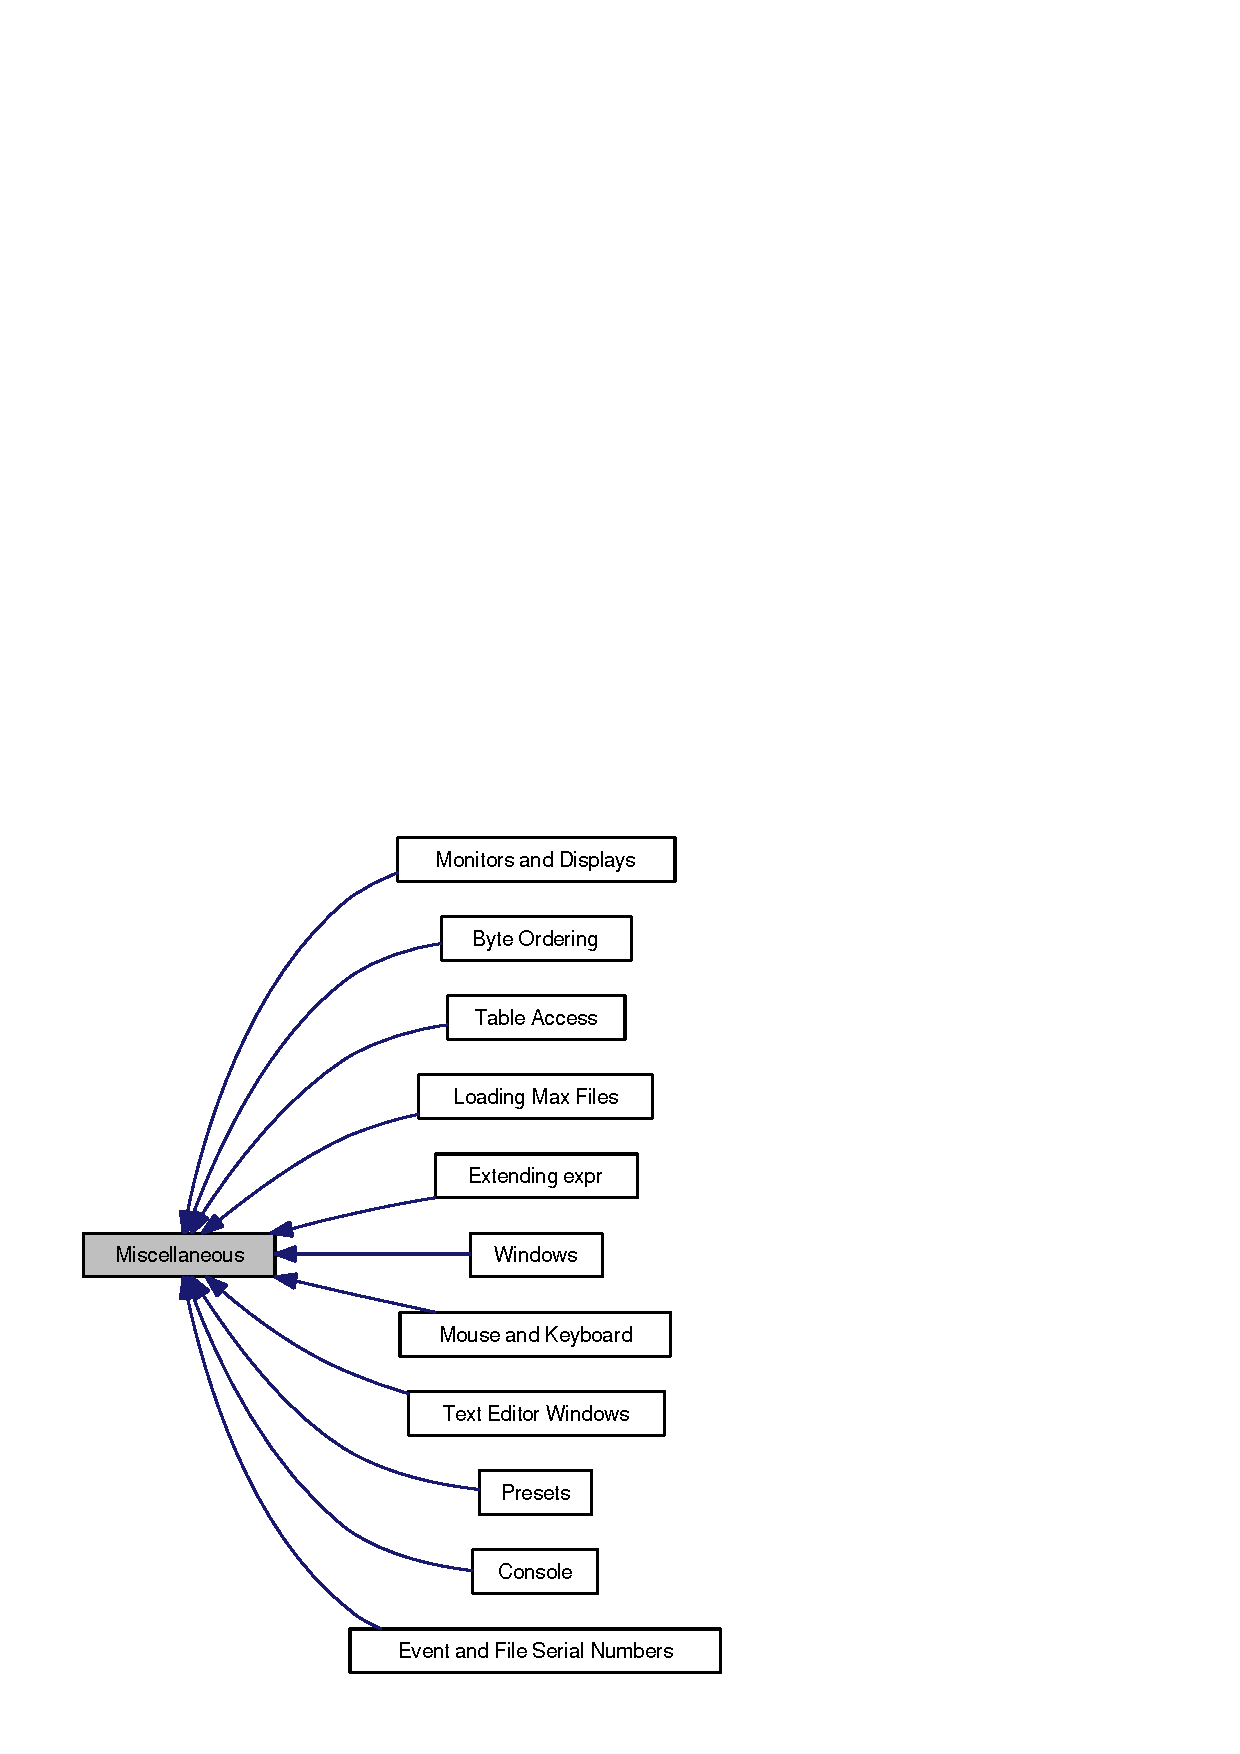
\includegraphics[width=175pt]{group__misc}
\end{center}
\end{figure}
\subsection*{Modules}
\begin{DoxyCompactItemize}
\item 
\hyperlink{group__console}{Console}
\item 
\hyperlink{group__byteorder}{Byte Ordering}


\begin{DoxyCompactList}\small\item\em Utilities for swapping the order of bytes to match the Endianness of the required platform. \item\end{DoxyCompactList}\item 
\hyperlink{group__expr}{Extending expr}


\begin{DoxyCompactList}\small\item\em If you want to use C-\/like variable expressions that are entered by a user of your object, you can use the \char`\"{}guts\char`\"{} of Max’s expr object in your object. \item\end{DoxyCompactList}\item 
\hyperlink{group__tables}{Table Access}


\begin{DoxyCompactList}\small\item\em You can use these functions to access named table objects. \item\end{DoxyCompactList}\item 
\hyperlink{group__texteditors}{Text Editor Windows}


\begin{DoxyCompactList}\small\item\em Max has a simple built-\/in text editor object that can display and edit text in conjunction with your object. \item\end{DoxyCompactList}\item 
\hyperlink{group__presets}{Presets}


\begin{DoxyCompactList}\small\item\em Max contains a preset object that has the ability to send preset messages to some or all of the objects (clients) in a Patcher window. \item\end{DoxyCompactList}\item 
\hyperlink{group__evnum}{Event and File Serial Numbers}


\begin{DoxyCompactList}\small\item\em If you call \hyperlink{group__inout_ga0b2b38216f2f4dba486bfcd2273f255e}{outlet\_\-int()}, \hyperlink{group__inout_gafbb3f62a413f05a394391afde5b3c30f}{outlet\_\-float()}, \hyperlink{group__inout_gabdef4fbe6e1040dc28204b8070bdcda5}{outlet\_\-list()}, or \hyperlink{group__inout_ga12798ee897e01dac21ee547c4091d8a8}{outlet\_\-anything()} inside a Qelem or during some idle or interrupt time, you should increment Max’s Event Serial Number beforehand. \item\end{DoxyCompactList}\item 
\hyperlink{group__loading__max__files}{Loading Max Files}


\begin{DoxyCompactList}\small\item\em Several high-\/level functions permit you to load patcher files. \item\end{DoxyCompactList}\item 
\hyperlink{group__jmonitor}{Monitors and Displays}


\begin{DoxyCompactList}\small\item\em Functions for finding our information about the environment. \item\end{DoxyCompactList}\item 
\hyperlink{group__jwind}{Windows}
\item 
\hyperlink{group__jmouse}{Mouse and Keyboard}
\end{DoxyCompactItemize}
\subsection*{Defines}
\begin{DoxyCompactItemize}
\item 
\#define \hyperlink{group__misc_ga1a07879e1cf90ff22dbd52a5408986dd}{InRange}(v, lo, hi)~((v)$<$=(hi)\&\&(v)$>$=(lo))
\begin{DoxyCompactList}\small\item\em If a value is within the specified range, then return true. \item\end{DoxyCompactList}\item 
\#define \hyperlink{group__misc_gafa99ec4acc4ecb2dc3c2d05da15d0e3f}{MAX}(a, b)~((a)$>$(b)?(a):(b))
\begin{DoxyCompactList}\small\item\em Return the higher of two values. \item\end{DoxyCompactList}\item 
\#define \hyperlink{group__misc_ga3acffbd305ee72dcd4593c0d8af64a4f}{MIN}(a, b)~((a)$<$(b)?(a):(b))
\begin{DoxyCompactList}\small\item\em Return the lower of two values. \item\end{DoxyCompactList}\item 
\#define \hyperlink{group__misc_ga79f6ccd4ae5e1eb6d56058350794f877}{CLIP}(a, lo, hi)~( (a)$>$(lo)?( (a)$<$(hi)?(a):(hi) ):(lo) )
\begin{DoxyCompactList}\small\item\em Limit values to within a specified range. \item\end{DoxyCompactList}\item 
\#define \hyperlink{group__misc_gaad95899dfbc7b5b8fe11921643ef46f0}{calcoffset}(x, y)~((long)(\&(((x $\ast$)0L)-\/$>$y)))
\begin{DoxyCompactList}\small\item\em Find byte offset of a named member of a struct, relative to the beginning of that struct. \item\end{DoxyCompactList}\item 
\#define \hyperlink{group__misc_ga06f35de4fc025809ab1cbb06f55b6495}{BEGIN\_\-USING\_\-C\_\-LINKAGE}
\begin{DoxyCompactList}\small\item\em Ensure that any definitions following this macro use a C-\/linkage, not a C++ linkage. \item\end{DoxyCompactList}\item 
\hypertarget{group__misc_gaffa4cac92b5d24cbccfe6c852de92a2e}{
\#define \hyperlink{group__misc_gaffa4cac92b5d24cbccfe6c852de92a2e}{END\_\-USING\_\-C\_\-LINKAGE}}
\label{group__misc_gaffa4cac92b5d24cbccfe6c852de92a2e}

\begin{DoxyCompactList}\small\item\em Close a definition section that was opened using \hyperlink{group__misc_ga06f35de4fc025809ab1cbb06f55b6495}{BEGIN\_\-USING\_\-C\_\-LINKAGE}. \item\end{DoxyCompactList}\end{DoxyCompactItemize}
\subsection*{Enumerations}
\begin{DoxyCompactItemize}
\item 
enum \hyperlink{group__misc_ga0764dd6c02b76cca7d053ae50555d69d}{e\_\-max\_\-errorcodes} \{ \par
\hyperlink{group__misc_gga0764dd6c02b76cca7d053ae50555d69da6d22f77fef8b1e1b074cef5d29d935fd}{MAX\_\-ERR\_\-NONE} =  0, 
\par
\hyperlink{group__misc_gga0764dd6c02b76cca7d053ae50555d69dae285bdd436f17560cfd09c6b31ea397d}{MAX\_\-ERR\_\-GENERIC} =  -\/1, 
\par
\hyperlink{group__misc_gga0764dd6c02b76cca7d053ae50555d69da42a29c15166206a1bbc13bcc74b2c651}{MAX\_\-ERR\_\-INVALID\_\-PTR} =  -\/2, 
\par
\hyperlink{group__misc_gga0764dd6c02b76cca7d053ae50555d69da9b67faa1ffafc9b60748135e48b105d1}{MAX\_\-ERR\_\-DUPLICATE} =  -\/3, 
\par
\hyperlink{group__misc_gga0764dd6c02b76cca7d053ae50555d69da5415d3c3fa523e0bb2ed1edfdbfce9be}{MAX\_\-ERR\_\-OUT\_\-OF\_\-MEM} =  -\/4
 \}
\begin{DoxyCompactList}\small\item\em Standard values returned by function calls with a return type of \hyperlink{group__datatypes_ga73edaae82b318855cc09fac994918165}{t\_\-max\_\-err}. \item\end{DoxyCompactList}\item 
enum \hyperlink{group__misc_ga4cf665eb75774ae52451e04f91747c25}{e\_\-max\_\-wind\_\-advise\_\-result} \{ \par
\hyperlink{group__misc_gga4cf665eb75774ae52451e04f91747c25a9d84de609dac254d18b580c1aeb3fd32}{aaYes} =  1, 
\par
\hyperlink{group__misc_gga4cf665eb75774ae52451e04f91747c25a614519005d5ef9267c6f73891ea11e56}{aaNo}, 
\par
\hyperlink{group__misc_gga4cf665eb75774ae52451e04f91747c25a2d8f037a3e3227d4bc488ff6b9050833}{aaCancel}
 \}
\begin{DoxyCompactList}\small\item\em Returned values from \hyperlink{group__misc_gab127ce8d89ae72d420a44642c52cc94d}{wind\_\-advise()}. \item\end{DoxyCompactList}\end{DoxyCompactItemize}
\subsection*{Functions}
\begin{DoxyCompactItemize}
\item 
void $\ast$ \hyperlink{group__misc_ga72a33738916b577d2df121edfea260b3}{globalsymbol\_\-reference} (\hyperlink{structt__object}{t\_\-object} $\ast$x, char $\ast$name, char $\ast$classname)
\begin{DoxyCompactList}\small\item\em Get a reference to an object that is bound to a \hyperlink{structt__symbol}{t\_\-symbol}. \item\end{DoxyCompactList}\item 
void \hyperlink{group__misc_ga5a4773570564ab729cbe4031cfff0b45}{globalsymbol\_\-dereference} (\hyperlink{structt__object}{t\_\-object} $\ast$x, char $\ast$name, char $\ast$classname)
\begin{DoxyCompactList}\small\item\em Stop referencing an object that is bound to a \hyperlink{structt__symbol}{t\_\-symbol}, previously referenced using \hyperlink{group__misc_ga72a33738916b577d2df121edfea260b3}{globalsymbol\_\-reference()}. \item\end{DoxyCompactList}\item 
\hyperlink{group__datatypes_ga73edaae82b318855cc09fac994918165}{t\_\-max\_\-err} \hyperlink{group__misc_gaa121ff996fcf9cfb28d1c7c11eebc428}{globalsymbol\_\-bind} (\hyperlink{structt__object}{t\_\-object} $\ast$x, char $\ast$name, long flags)
\begin{DoxyCompactList}\small\item\em Bind an object to a \hyperlink{structt__symbol}{t\_\-symbol}. \item\end{DoxyCompactList}\item 
void \hyperlink{group__misc_gade40c44fddc370895da5db8f70e1868f}{globalsymbol\_\-unbind} (\hyperlink{structt__object}{t\_\-object} $\ast$x, char $\ast$name, long flags)
\begin{DoxyCompactList}\small\item\em Remove an object from being bound to a \hyperlink{structt__symbol}{t\_\-symbol}. \item\end{DoxyCompactList}\item 
\hypertarget{group__misc_ga157705d53ac5b0b839c72843712716c1}{
long \hyperlink{group__misc_ga157705d53ac5b0b839c72843712716c1}{method\_\-true} (void $\ast$x)}
\label{group__misc_ga157705d53ac5b0b839c72843712716c1}

\begin{DoxyCompactList}\small\item\em A method that always returns true. \item\end{DoxyCompactList}\item 
\hypertarget{group__misc_gaaedbb45cad3ac00f027d06e738181bd7}{
long \hyperlink{group__misc_gaaedbb45cad3ac00f027d06e738181bd7}{method\_\-false} (void $\ast$x)}
\label{group__misc_gaaedbb45cad3ac00f027d06e738181bd7}

\begin{DoxyCompactList}\small\item\em A method that always returns false. \item\end{DoxyCompactList}\item 
\hyperlink{structt__symbol}{t\_\-symbol} $\ast$ \hyperlink{group__misc_ga0cb594bfc861d0a72b61c067cd890122}{symbol\_\-unique} ()
\begin{DoxyCompactList}\small\item\em Generates a unique \hyperlink{structt__symbol}{t\_\-symbol} $\ast$. \item\end{DoxyCompactList}\item 
void \hyperlink{group__misc_ga0a094decd1408632226438943e55de81}{error\_\-sym} (void $\ast$x, \hyperlink{structt__symbol}{t\_\-symbol} $\ast$s)
\begin{DoxyCompactList}\small\item\em Posts an error message to the Max window. \item\end{DoxyCompactList}\item 
void \hyperlink{group__misc_gad8bf1a07113f7db2b387d5e138fe59fd}{post\_\-sym} (void $\ast$x, \hyperlink{structt__symbol}{t\_\-symbol} $\ast$s)
\begin{DoxyCompactList}\small\item\em Posts a message to the Max window. \item\end{DoxyCompactList}\item 
\hyperlink{group__datatypes_ga73edaae82b318855cc09fac994918165}{t\_\-max\_\-err} \hyperlink{group__misc_ga751e472fea0842d902012a41f79afcce}{symbolarray\_\-sort} (long ac, \hyperlink{structt__symbol}{t\_\-symbol} $\ast$$\ast$av)
\begin{DoxyCompactList}\small\item\em Performs an ASCII sort on an array of \hyperlink{structt__symbol}{t\_\-symbol} $\ast$s. \item\end{DoxyCompactList}\item 
void \hyperlink{group__misc_ga332b8831bb1a42503b13d16269fc5ade}{object\_\-obex\_\-quickref} (void $\ast$x, long $\ast$numitems, \hyperlink{structt__symbol}{t\_\-symbol} $\ast$$\ast$items)
\begin{DoxyCompactList}\small\item\em Developers do not need to directly use the \hyperlink{group__misc_ga332b8831bb1a42503b13d16269fc5ade}{object\_\-obex\_\-quickref()} function. \item\end{DoxyCompactList}\item 
void \hyperlink{group__misc_gaffc50c996275103b9d94ec309c6d8be1}{error\_\-subscribe} (\hyperlink{structt__object}{t\_\-object} $\ast$x)
\begin{DoxyCompactList}\small\item\em Receive messages from the error handler. \item\end{DoxyCompactList}\item 
void \hyperlink{group__misc_ga155f65793ec4c34abc6746015a2beca6}{error\_\-unsubscribe} (\hyperlink{structt__object}{t\_\-object} $\ast$x)
\begin{DoxyCompactList}\small\item\em Remove an object as an error message recipient. \item\end{DoxyCompactList}\item 
void \hyperlink{group__misc_ga0638f6ac63b75fa53c0a34db8ec8d412}{quittask\_\-install} (\hyperlink{group__datatypes_gac26ba0a173b50597f5738132e059b42d}{method} m, void $\ast$a)
\begin{DoxyCompactList}\small\item\em Register a function that will be called when Max exits. \item\end{DoxyCompactList}\item 
void \hyperlink{group__misc_ga99223860e2a94772b52089abfeb506f3}{quittask\_\-remove} (\hyperlink{group__datatypes_gac26ba0a173b50597f5738132e059b42d}{method} m)
\begin{DoxyCompactList}\small\item\em Unregister a function previously registered with \hyperlink{group__misc_ga0638f6ac63b75fa53c0a34db8ec8d412}{quittask\_\-install()}. \item\end{DoxyCompactList}\item 
short \hyperlink{group__misc_ga0eaf32722b98ab4920cb6f64b45a5d5b}{maxversion} (void)
\begin{DoxyCompactList}\small\item\em Determine version information about the current Max environment. \item\end{DoxyCompactList}\item 
char $\ast$ \hyperlink{group__misc_ga0022303fac866c8f5757aa56b67ce29d}{strncpy\_\-zero} (char $\ast$dst, const char $\ast$src, long size)
\begin{DoxyCompactList}\small\item\em Copy the contents of one string to another, in a manner safer than the standard strcpy() or strncpy(). \item\end{DoxyCompactList}\item 
char $\ast$ \hyperlink{group__misc_ga3ed4f46782e6a41d13ca17420c35dfb7}{strncat\_\-zero} (char $\ast$dst, const char $\ast$src, long size)
\begin{DoxyCompactList}\small\item\em Concatenate the contents of one string onto the end of another, in a manner safer than the standard strcat() or strncat(). \item\end{DoxyCompactList}\item 
int \hyperlink{group__misc_gab82e9c5bbc8b7fe70d16b1f6383f1cc4}{snprintf\_\-zero} (char $\ast$buffer, size\_\-t count, const char $\ast$format,...)
\begin{DoxyCompactList}\small\item\em Copy the contents of a string together with value substitutions, in a manner safer than the standard sprintf() or snprintf(). \item\end{DoxyCompactList}\item 
short \hyperlink{group__misc_gab127ce8d89ae72d420a44642c52cc94d}{wind\_\-advise} (\hyperlink{structt__object}{t\_\-object} $\ast$w, char $\ast$s,...)
\begin{DoxyCompactList}\small\item\em Throw a dialog which may have text and up to three buttons. \item\end{DoxyCompactList}\item 
void \hyperlink{group__misc_ga85a1754ef77207af4ab7617e7487336e}{wind\_\-setcursor} (short which)
\begin{DoxyCompactList}\small\item\em Change the cursor. \item\end{DoxyCompactList}\end{DoxyCompactItemize}


\subsection{Define Documentation}
\hypertarget{group__misc_ga06f35de4fc025809ab1cbb06f55b6495}{
\index{misc@{misc}!BEGIN\_\-USING\_\-C\_\-LINKAGE@{BEGIN\_\-USING\_\-C\_\-LINKAGE}}
\index{BEGIN\_\-USING\_\-C\_\-LINKAGE@{BEGIN\_\-USING\_\-C\_\-LINKAGE}!misc@{misc}}
\subsubsection[{BEGIN\_\-USING\_\-C\_\-LINKAGE}]{\setlength{\rightskip}{0pt plus 5cm}\#define BEGIN\_\-USING\_\-C\_\-LINKAGE}}
\label{group__misc_ga06f35de4fc025809ab1cbb06f55b6495}


Ensure that any definitions following this macro use a C-\/linkage, not a C++ linkage. The Max API uses C-\/linkage. This is important for objects written in C++ or that use a C++ compiler. This macro must be balanced with the \hyperlink{group__misc_gaffa4cac92b5d24cbccfe6c852de92a2e}{END\_\-USING\_\-C\_\-LINKAGE} macro. \hypertarget{group__misc_gaad95899dfbc7b5b8fe11921643ef46f0}{
\index{misc@{misc}!calcoffset@{calcoffset}}
\index{calcoffset@{calcoffset}!misc@{misc}}
\subsubsection[{calcoffset}]{\setlength{\rightskip}{0pt plus 5cm}\#define calcoffset(x, \/  y)~((long)(\&(((x $\ast$)0L)-\/$>$y)))}}
\label{group__misc_gaad95899dfbc7b5b8fe11921643ef46f0}


Find byte offset of a named member of a struct, relative to the beginning of that struct. 
\begin{DoxyParams}{Parameters}
\item[{\em x}]The name of the struct \item[{\em y}]The name of the member \end{DoxyParams}
\begin{DoxyReturn}{Returns}
A long integer representing the number of bytes into the struct where the member begins. 
\end{DoxyReturn}
\hypertarget{group__misc_ga79f6ccd4ae5e1eb6d56058350794f877}{
\index{misc@{misc}!CLIP@{CLIP}}
\index{CLIP@{CLIP}!misc@{misc}}
\subsubsection[{CLIP}]{\setlength{\rightskip}{0pt plus 5cm}\#define CLIP(a, \/  lo, \/  hi)~( (a)$>$(lo)?( (a)$<$(hi)?(a):(hi) ):(lo) )}}
\label{group__misc_ga79f6ccd4ae5e1eb6d56058350794f877}


Limit values to within a specified range. 
\begin{DoxyParams}{Parameters}
\item[{\em a}]The value to constrain. \item[{\em lo}]The low bound for the range. \item[{\em hi}]The high bound for the range. \end{DoxyParams}
\begin{DoxyReturn}{Returns}
Returns the value a constrained to the range specified by lo and hi. 
\end{DoxyReturn}
\hypertarget{group__misc_ga1a07879e1cf90ff22dbd52a5408986dd}{
\index{misc@{misc}!InRange@{InRange}}
\index{InRange@{InRange}!misc@{misc}}
\subsubsection[{InRange}]{\setlength{\rightskip}{0pt plus 5cm}\#define InRange(v, \/  lo, \/  hi)~((v)$<$=(hi)\&\&(v)$>$=(lo))}}
\label{group__misc_ga1a07879e1cf90ff22dbd52a5408986dd}


If a value is within the specified range, then return true. Otherwise return false.


\begin{DoxyParams}{Parameters}
\item[{\em v}]The value to test. \item[{\em lo}]The low bound for the range. \item[{\em hi}]The high bound for the range. \end{DoxyParams}
\begin{DoxyReturn}{Returns}
Returns true if within range, otherwise false. 
\end{DoxyReturn}
\hypertarget{group__misc_gafa99ec4acc4ecb2dc3c2d05da15d0e3f}{
\index{misc@{misc}!MAX@{MAX}}
\index{MAX@{MAX}!misc@{misc}}
\subsubsection[{MAX}]{\setlength{\rightskip}{0pt plus 5cm}\#define MAX(a, \/  b)~((a)$>$(b)?(a):(b))}}
\label{group__misc_gafa99ec4acc4ecb2dc3c2d05da15d0e3f}


Return the higher of two values. 
\begin{DoxyParams}{Parameters}
\item[{\em a}]The first value to compare. \item[{\em b}]The second value to compare. \end{DoxyParams}
\begin{DoxyReturn}{Returns}
Returns the higher of a or b. 
\end{DoxyReturn}
\hypertarget{group__misc_ga3acffbd305ee72dcd4593c0d8af64a4f}{
\index{misc@{misc}!MIN@{MIN}}
\index{MIN@{MIN}!misc@{misc}}
\subsubsection[{MIN}]{\setlength{\rightskip}{0pt plus 5cm}\#define MIN(a, \/  b)~((a)$<$(b)?(a):(b))}}
\label{group__misc_ga3acffbd305ee72dcd4593c0d8af64a4f}


Return the lower of two values. 
\begin{DoxyParams}{Parameters}
\item[{\em a}]The first value to compare. \item[{\em b}]The second value to compare. \end{DoxyParams}
\begin{DoxyReturn}{Returns}
Returns the lower of a or b. 
\end{DoxyReturn}


\subsection{Enumeration Type Documentation}
\hypertarget{group__misc_ga0764dd6c02b76cca7d053ae50555d69d}{
\index{misc@{misc}!e\_\-max\_\-errorcodes@{e\_\-max\_\-errorcodes}}
\index{e\_\-max\_\-errorcodes@{e\_\-max\_\-errorcodes}!misc@{misc}}
\subsubsection[{e\_\-max\_\-errorcodes}]{\setlength{\rightskip}{0pt plus 5cm}enum {\bf e\_\-max\_\-errorcodes}}}
\label{group__misc_ga0764dd6c02b76cca7d053ae50555d69d}


Standard values returned by function calls with a return type of \hyperlink{group__datatypes_ga73edaae82b318855cc09fac994918165}{t\_\-max\_\-err}. \begin{Desc}
\item[Enumerator: ]\par
\begin{description}
\index{MAX\_\-ERR\_\-NONE@{MAX\_\-ERR\_\-NONE}!misc@{misc}}\index{misc@{misc}!MAX\_\-ERR\_\-NONE@{MAX\_\-ERR\_\-NONE}}\item[{\em 
\hypertarget{group__misc_gga0764dd6c02b76cca7d053ae50555d69da6d22f77fef8b1e1b074cef5d29d935fd}{
MAX\_\-ERR\_\-NONE}
\label{group__misc_gga0764dd6c02b76cca7d053ae50555d69da6d22f77fef8b1e1b074cef5d29d935fd}
}]No error. \index{MAX\_\-ERR\_\-GENERIC@{MAX\_\-ERR\_\-GENERIC}!misc@{misc}}\index{misc@{misc}!MAX\_\-ERR\_\-GENERIC@{MAX\_\-ERR\_\-GENERIC}}\item[{\em 
\hypertarget{group__misc_gga0764dd6c02b76cca7d053ae50555d69dae285bdd436f17560cfd09c6b31ea397d}{
MAX\_\-ERR\_\-GENERIC}
\label{group__misc_gga0764dd6c02b76cca7d053ae50555d69dae285bdd436f17560cfd09c6b31ea397d}
}]Generic error. \index{MAX\_\-ERR\_\-INVALID\_\-PTR@{MAX\_\-ERR\_\-INVALID\_\-PTR}!misc@{misc}}\index{misc@{misc}!MAX\_\-ERR\_\-INVALID\_\-PTR@{MAX\_\-ERR\_\-INVALID\_\-PTR}}\item[{\em 
\hypertarget{group__misc_gga0764dd6c02b76cca7d053ae50555d69da42a29c15166206a1bbc13bcc74b2c651}{
MAX\_\-ERR\_\-INVALID\_\-PTR}
\label{group__misc_gga0764dd6c02b76cca7d053ae50555d69da42a29c15166206a1bbc13bcc74b2c651}
}]Invalid Pointer. \index{MAX\_\-ERR\_\-DUPLICATE@{MAX\_\-ERR\_\-DUPLICATE}!misc@{misc}}\index{misc@{misc}!MAX\_\-ERR\_\-DUPLICATE@{MAX\_\-ERR\_\-DUPLICATE}}\item[{\em 
\hypertarget{group__misc_gga0764dd6c02b76cca7d053ae50555d69da9b67faa1ffafc9b60748135e48b105d1}{
MAX\_\-ERR\_\-DUPLICATE}
\label{group__misc_gga0764dd6c02b76cca7d053ae50555d69da9b67faa1ffafc9b60748135e48b105d1}
}]Duplicate. \index{MAX\_\-ERR\_\-OUT\_\-OF\_\-MEM@{MAX\_\-ERR\_\-OUT\_\-OF\_\-MEM}!misc@{misc}}\index{misc@{misc}!MAX\_\-ERR\_\-OUT\_\-OF\_\-MEM@{MAX\_\-ERR\_\-OUT\_\-OF\_\-MEM}}\item[{\em 
\hypertarget{group__misc_gga0764dd6c02b76cca7d053ae50555d69da5415d3c3fa523e0bb2ed1edfdbfce9be}{
MAX\_\-ERR\_\-OUT\_\-OF\_\-MEM}
\label{group__misc_gga0764dd6c02b76cca7d053ae50555d69da5415d3c3fa523e0bb2ed1edfdbfce9be}
}]Out of memory. \end{description}
\end{Desc}

\hypertarget{group__misc_ga4cf665eb75774ae52451e04f91747c25}{
\index{misc@{misc}!e\_\-max\_\-wind\_\-advise\_\-result@{e\_\-max\_\-wind\_\-advise\_\-result}}
\index{e\_\-max\_\-wind\_\-advise\_\-result@{e\_\-max\_\-wind\_\-advise\_\-result}!misc@{misc}}
\subsubsection[{e\_\-max\_\-wind\_\-advise\_\-result}]{\setlength{\rightskip}{0pt plus 5cm}enum {\bf e\_\-max\_\-wind\_\-advise\_\-result}}}
\label{group__misc_ga4cf665eb75774ae52451e04f91747c25}


Returned values from \hyperlink{group__misc_gab127ce8d89ae72d420a44642c52cc94d}{wind\_\-advise()}. \begin{Desc}
\item[Enumerator: ]\par
\begin{description}
\index{aaYes@{aaYes}!misc@{misc}}\index{misc@{misc}!aaYes@{aaYes}}\item[{\em 
\hypertarget{group__misc_gga4cf665eb75774ae52451e04f91747c25a9d84de609dac254d18b580c1aeb3fd32}{
aaYes}
\label{group__misc_gga4cf665eb75774ae52451e04f91747c25a9d84de609dac254d18b580c1aeb3fd32}
}]Yes button was choosen. \index{aaNo@{aaNo}!misc@{misc}}\index{misc@{misc}!aaNo@{aaNo}}\item[{\em 
\hypertarget{group__misc_gga4cf665eb75774ae52451e04f91747c25a614519005d5ef9267c6f73891ea11e56}{
aaNo}
\label{group__misc_gga4cf665eb75774ae52451e04f91747c25a614519005d5ef9267c6f73891ea11e56}
}]No button was choosen. \index{aaCancel@{aaCancel}!misc@{misc}}\index{misc@{misc}!aaCancel@{aaCancel}}\item[{\em 
\hypertarget{group__misc_gga4cf665eb75774ae52451e04f91747c25a2d8f037a3e3227d4bc488ff6b9050833}{
aaCancel}
\label{group__misc_gga4cf665eb75774ae52451e04f91747c25a2d8f037a3e3227d4bc488ff6b9050833}
}]Cancel button was choosen. \end{description}
\end{Desc}



\subsection{Function Documentation}
\hypertarget{group__misc_gaffc50c996275103b9d94ec309c6d8be1}{
\index{misc@{misc}!error\_\-subscribe@{error\_\-subscribe}}
\index{error\_\-subscribe@{error\_\-subscribe}!misc@{misc}}
\subsubsection[{error\_\-subscribe}]{\setlength{\rightskip}{0pt plus 5cm}void error\_\-subscribe ({\bf t\_\-object} $\ast$ {\em x})}}
\label{group__misc_gaffc50c996275103b9d94ec309c6d8be1}


Receive messages from the error handler. 
\begin{DoxyParams}{Parameters}
\item[{\em x}]The object to be subscribed to the error handler.\end{DoxyParams}
\begin{DoxyRemark}{Remarks}
\hyperlink{group__misc_gaffc50c996275103b9d94ec309c6d8be1}{error\_\-subscribe()} enables your object to receive a message (error), followed by the list of atoms in the error message posted to the Max window.
\end{DoxyRemark}
Prior to calling \hyperlink{group__misc_gaffc50c996275103b9d94ec309c6d8be1}{error\_\-subscribe()}, you should bind the error message to an internal error handling routine: 
\begin{DoxyCode}
    addmess((method)myobject_error, "error", A_GIMME, 0);
\end{DoxyCode}
 Your error handling routine should be declared as follows: 
\begin{DoxyCode}
    void myobject_error(t_myobject *x, t_symbol *s, short argc, t_atom *argv);
\end{DoxyCode}
 \hypertarget{group__misc_ga0a094decd1408632226438943e55de81}{
\index{misc@{misc}!error\_\-sym@{error\_\-sym}}
\index{error\_\-sym@{error\_\-sym}!misc@{misc}}
\subsubsection[{error\_\-sym}]{\setlength{\rightskip}{0pt plus 5cm}void error\_\-sym (void $\ast$ {\em x}, \/  {\bf t\_\-symbol} $\ast$ {\em s})}}
\label{group__misc_ga0a094decd1408632226438943e55de81}


Posts an error message to the Max window. This function is interrupt safe.


\begin{DoxyParams}{Parameters}
\item[{\em x}]The object's pointer \item[{\em s}]Symbol to be posted as an error in the Max window \end{DoxyParams}
\hypertarget{group__misc_ga155f65793ec4c34abc6746015a2beca6}{
\index{misc@{misc}!error\_\-unsubscribe@{error\_\-unsubscribe}}
\index{error\_\-unsubscribe@{error\_\-unsubscribe}!misc@{misc}}
\subsubsection[{error\_\-unsubscribe}]{\setlength{\rightskip}{0pt plus 5cm}void error\_\-unsubscribe ({\bf t\_\-object} $\ast$ {\em x})}}
\label{group__misc_ga155f65793ec4c34abc6746015a2beca6}


Remove an object as an error message recipient. 
\begin{DoxyParams}{Parameters}
\item[{\em x}]The object to unsubscribe. \end{DoxyParams}
\hypertarget{group__misc_gaa121ff996fcf9cfb28d1c7c11eebc428}{
\index{misc@{misc}!globalsymbol\_\-bind@{globalsymbol\_\-bind}}
\index{globalsymbol\_\-bind@{globalsymbol\_\-bind}!misc@{misc}}
\subsubsection[{globalsymbol\_\-bind}]{\setlength{\rightskip}{0pt plus 5cm}{\bf t\_\-max\_\-err} globalsymbol\_\-bind ({\bf t\_\-object} $\ast$ {\em x}, \/  char $\ast$ {\em name}, \/  long {\em flags})}}
\label{group__misc_gaa121ff996fcf9cfb28d1c7c11eebc428}


Bind an object to a \hyperlink{structt__symbol}{t\_\-symbol}. 
\begin{DoxyParams}{Parameters}
\item[{\em x}]The object to bind to the \hyperlink{structt__symbol}{t\_\-symbol}. \item[{\em name}]The name of the \hyperlink{structt__symbol}{t\_\-symbol} to which the object will be bound. \item[{\em flags}]Pass 0. \end{DoxyParams}
\begin{DoxyReturn}{Returns}
A Max error code. 
\end{DoxyReturn}
\hypertarget{group__misc_ga5a4773570564ab729cbe4031cfff0b45}{
\index{misc@{misc}!globalsymbol\_\-dereference@{globalsymbol\_\-dereference}}
\index{globalsymbol\_\-dereference@{globalsymbol\_\-dereference}!misc@{misc}}
\subsubsection[{globalsymbol\_\-dereference}]{\setlength{\rightskip}{0pt plus 5cm}void globalsymbol\_\-dereference ({\bf t\_\-object} $\ast$ {\em x}, \/  char $\ast$ {\em name}, \/  char $\ast$ {\em classname})}}
\label{group__misc_ga5a4773570564ab729cbe4031cfff0b45}


Stop referencing an object that is bound to a \hyperlink{structt__symbol}{t\_\-symbol}, previously referenced using \hyperlink{group__misc_ga72a33738916b577d2df121edfea260b3}{globalsymbol\_\-reference()}. 
\begin{DoxyParams}{Parameters}
\item[{\em x}]The object that is getting the reference to the symbol. \item[{\em name}]The name of the symbol to reference. \item[{\em classname}]The name of the class of which the object we are referencing should be an instance. \end{DoxyParams}
\begin{DoxySeeAlso}{See also}
\hyperlink{group__misc_ga72a33738916b577d2df121edfea260b3}{globalsymbol\_\-reference()} 
\end{DoxySeeAlso}
\hypertarget{group__misc_ga72a33738916b577d2df121edfea260b3}{
\index{misc@{misc}!globalsymbol\_\-reference@{globalsymbol\_\-reference}}
\index{globalsymbol\_\-reference@{globalsymbol\_\-reference}!misc@{misc}}
\subsubsection[{globalsymbol\_\-reference}]{\setlength{\rightskip}{0pt plus 5cm}void$\ast$ globalsymbol\_\-reference ({\bf t\_\-object} $\ast$ {\em x}, \/  char $\ast$ {\em name}, \/  char $\ast$ {\em classname})}}
\label{group__misc_ga72a33738916b577d2df121edfea260b3}


Get a reference to an object that is bound to a \hyperlink{structt__symbol}{t\_\-symbol}. 
\begin{DoxyParams}{Parameters}
\item[{\em x}]The object that is getting the reference to the symbol. \item[{\em name}]The name of the symbol to reference. \item[{\em classname}]The name of the class of which the object we are referencing should be an instance. \end{DoxyParams}
\begin{DoxyReturn}{Returns}
The s\_\-thing of the \hyperlink{structt__symbol}{t\_\-symbol}.
\end{DoxyReturn}
\begin{DoxyRemark}{Remarks}
An example of real-\/world use is to get the buffer$\sim$ object associated with a symbol. 
\begin{DoxyCode}
    // the struct of our object
    typedef struct _myobject {
        t_object    obj;
        t_symbol    *buffer_name;
        t_buffer    *buffer_object;
    } t_myobject;
    
    void myobject_setbuffer(t_myobject *x, t_symbol *s, long argc, t_atom *argv)
    {       
        if(s != x->buffer_name){
            // Reference the buffer associated with the incoming name
            x->buffer_object = (t_buffer *)globalsymbol_reference((t_object *)x, 
      s->s_name, "buffer~");
            
            // If we were previously referenceing another buffer, we should not l
      onger reference it.
            globalsymbol_dereference((t_object *)x, x->buffer_name->s_name, "buff
      er~");
            
            x->buffer_name = s;
        }       
    }
\end{DoxyCode}
 
\end{DoxyRemark}
\hypertarget{group__misc_gade40c44fddc370895da5db8f70e1868f}{
\index{misc@{misc}!globalsymbol\_\-unbind@{globalsymbol\_\-unbind}}
\index{globalsymbol\_\-unbind@{globalsymbol\_\-unbind}!misc@{misc}}
\subsubsection[{globalsymbol\_\-unbind}]{\setlength{\rightskip}{0pt plus 5cm}void globalsymbol\_\-unbind ({\bf t\_\-object} $\ast$ {\em x}, \/  char $\ast$ {\em name}, \/  long {\em flags})}}
\label{group__misc_gade40c44fddc370895da5db8f70e1868f}


Remove an object from being bound to a \hyperlink{structt__symbol}{t\_\-symbol}. 
\begin{DoxyParams}{Parameters}
\item[{\em x}]The object from which to unbind the \hyperlink{structt__symbol}{t\_\-symbol}. \item[{\em name}]The name of the \hyperlink{structt__symbol}{t\_\-symbol} from which the object will be unbound. \item[{\em flags}]Pass 0. \end{DoxyParams}
\hypertarget{group__misc_ga0eaf32722b98ab4920cb6f64b45a5d5b}{
\index{misc@{misc}!maxversion@{maxversion}}
\index{maxversion@{maxversion}!misc@{misc}}
\subsubsection[{maxversion}]{\setlength{\rightskip}{0pt plus 5cm}short maxversion (void)}}
\label{group__misc_ga0eaf32722b98ab4920cb6f64b45a5d5b}


Determine version information about the current Max environment. This function returns the version number of Max. In Max versions 2.1.4 and later, this number is the version number of the Max kernel application in binary-\/coded decimal. Thus, 2.1.4 would return 214 hex or 532 decimal. Version 3.0 returns 300 hex.

Use this to check for the existence of particular function macros that are only present in more recent Max versions. Versions before 2.1.4 returned 1, except for versions 2.1.1 -\/ 2.1.3 which returned 2.

Bit 14 (counting from left) will be set if Max is running as a standalone application, so you should mask the lower 12 bits to get the version number.

\begin{DoxyReturn}{Returns}
The Max environment's version number. 
\end{DoxyReturn}
\hypertarget{group__misc_ga332b8831bb1a42503b13d16269fc5ade}{
\index{misc@{misc}!object\_\-obex\_\-quickref@{object\_\-obex\_\-quickref}}
\index{object\_\-obex\_\-quickref@{object\_\-obex\_\-quickref}!misc@{misc}}
\subsubsection[{object\_\-obex\_\-quickref}]{\setlength{\rightskip}{0pt plus 5cm}void object\_\-obex\_\-quickref (void $\ast$ {\em x}, \/  long $\ast$ {\em numitems}, \/  {\bf t\_\-symbol} $\ast$$\ast$ {\em items})}}
\label{group__misc_ga332b8831bb1a42503b13d16269fc5ade}


Developers do not need to directly use the \hyperlink{group__misc_ga332b8831bb1a42503b13d16269fc5ade}{object\_\-obex\_\-quickref()} function. It was used in Max 4 to add support for attributes to the quickref, but this is automatic in Max 5. \hypertarget{group__misc_gad8bf1a07113f7db2b387d5e138fe59fd}{
\index{misc@{misc}!post\_\-sym@{post\_\-sym}}
\index{post\_\-sym@{post\_\-sym}!misc@{misc}}
\subsubsection[{post\_\-sym}]{\setlength{\rightskip}{0pt plus 5cm}void post\_\-sym (void $\ast$ {\em x}, \/  {\bf t\_\-symbol} $\ast$ {\em s})}}
\label{group__misc_gad8bf1a07113f7db2b387d5e138fe59fd}


Posts a message to the Max window. This function is interrupt safe.


\begin{DoxyParams}{Parameters}
\item[{\em x}]The object's pointer \item[{\em s}]Symbol to be posted in the Max window \end{DoxyParams}
\hypertarget{group__misc_ga0638f6ac63b75fa53c0a34db8ec8d412}{
\index{misc@{misc}!quittask\_\-install@{quittask\_\-install}}
\index{quittask\_\-install@{quittask\_\-install}!misc@{misc}}
\subsubsection[{quittask\_\-install}]{\setlength{\rightskip}{0pt plus 5cm}void quittask\_\-install ({\bf method} {\em m}, \/  void $\ast$ {\em a})}}
\label{group__misc_ga0638f6ac63b75fa53c0a34db8ec8d412}


Register a function that will be called when Max exits. 
\begin{DoxyParams}{Parameters}
\item[{\em m}]A function that will be called on Max exit. \item[{\em a}]Argument to be used with method m.\end{DoxyParams}
\begin{DoxyRemark}{Remarks}
\hyperlink{group__misc_ga0638f6ac63b75fa53c0a34db8ec8d412}{quittask\_\-install()} provides a mechanism for your external to register a routine to be called prior to Max shutdown. This is useful for objects that need to provide disk-\/based persistance outside the standard Max storage mechanisms, or need to shut down hardware or their connection to system software and cannot do so in the termination routine of a code fragment. 
\end{DoxyRemark}
\hypertarget{group__misc_ga99223860e2a94772b52089abfeb506f3}{
\index{misc@{misc}!quittask\_\-remove@{quittask\_\-remove}}
\index{quittask\_\-remove@{quittask\_\-remove}!misc@{misc}}
\subsubsection[{quittask\_\-remove}]{\setlength{\rightskip}{0pt plus 5cm}void quittask\_\-remove ({\bf method} {\em m})}}
\label{group__misc_ga99223860e2a94772b52089abfeb506f3}


Unregister a function previously registered with \hyperlink{group__misc_ga0638f6ac63b75fa53c0a34db8ec8d412}{quittask\_\-install()}. 
\begin{DoxyParams}{Parameters}
\item[{\em m}]Function to be removed as a shutdown method. \end{DoxyParams}
\hypertarget{group__misc_gab82e9c5bbc8b7fe70d16b1f6383f1cc4}{
\index{misc@{misc}!snprintf\_\-zero@{snprintf\_\-zero}}
\index{snprintf\_\-zero@{snprintf\_\-zero}!misc@{misc}}
\subsubsection[{snprintf\_\-zero}]{\setlength{\rightskip}{0pt plus 5cm}int snprintf\_\-zero (char $\ast$ {\em buffer}, \/  size\_\-t {\em count}, \/  const char $\ast$ {\em format}, \/   {\em ...})}}
\label{group__misc_gab82e9c5bbc8b7fe70d16b1f6383f1cc4}


Copy the contents of a string together with value substitutions, in a manner safer than the standard sprintf() or snprintf(). This is the prefered function to use for this operation in Max.


\begin{DoxyParams}{Parameters}
\item[{\em buffer}]The destination string (already allocated) for the copy. \item[{\em count}]The number of chars allocated to the buffer string. \item[{\em format}]The source string that will be copied, which may include sprintf() formatting codes for substitutions. \item[{\em ...}]An array of arguments to be substituted into the format string. \end{DoxyParams}
\hypertarget{group__misc_ga3ed4f46782e6a41d13ca17420c35dfb7}{
\index{misc@{misc}!strncat\_\-zero@{strncat\_\-zero}}
\index{strncat\_\-zero@{strncat\_\-zero}!misc@{misc}}
\subsubsection[{strncat\_\-zero}]{\setlength{\rightskip}{0pt plus 5cm}char$\ast$ strncat\_\-zero (char $\ast$ {\em dst}, \/  const char $\ast$ {\em src}, \/  long {\em size})}}
\label{group__misc_ga3ed4f46782e6a41d13ca17420c35dfb7}


Concatenate the contents of one string onto the end of another, in a manner safer than the standard strcat() or strncat(). This is the prefered function to use for this operation in Max.


\begin{DoxyParams}{Parameters}
\item[{\em dst}]The destination string onto whose end the src string will be appended. \item[{\em src}]The source string that will be copied. \item[{\em size}]The number of chars allocated to the dst string. \end{DoxyParams}
\hypertarget{group__misc_ga0022303fac866c8f5757aa56b67ce29d}{
\index{misc@{misc}!strncpy\_\-zero@{strncpy\_\-zero}}
\index{strncpy\_\-zero@{strncpy\_\-zero}!misc@{misc}}
\subsubsection[{strncpy\_\-zero}]{\setlength{\rightskip}{0pt plus 5cm}char$\ast$ strncpy\_\-zero (char $\ast$ {\em dst}, \/  const char $\ast$ {\em src}, \/  long {\em size})}}
\label{group__misc_ga0022303fac866c8f5757aa56b67ce29d}


Copy the contents of one string to another, in a manner safer than the standard strcpy() or strncpy(). This is the prefered function to use for this operation in Max.


\begin{DoxyParams}{Parameters}
\item[{\em dst}]The destination string (already allocated) for the copy. \item[{\em src}]The source string that will be copied. \item[{\em size}]The number of chars allocated to the dst string. \end{DoxyParams}
\hypertarget{group__misc_ga0cb594bfc861d0a72b61c067cd890122}{
\index{misc@{misc}!symbol\_\-unique@{symbol\_\-unique}}
\index{symbol\_\-unique@{symbol\_\-unique}!misc@{misc}}
\subsubsection[{symbol\_\-unique}]{\setlength{\rightskip}{0pt plus 5cm}{\bf t\_\-symbol}$\ast$ symbol\_\-unique ()}}
\label{group__misc_ga0cb594bfc861d0a72b61c067cd890122}


Generates a unique \hyperlink{structt__symbol}{t\_\-symbol} $\ast$. The symbol will be formatted somewhat like \char`\"{}u123456789\char`\"{}.

\begin{DoxyReturn}{Returns}
This function returns a unique \hyperlink{structt__symbol}{t\_\-symbol} $\ast$. 
\end{DoxyReturn}
\hypertarget{group__misc_ga751e472fea0842d902012a41f79afcce}{
\index{misc@{misc}!symbolarray\_\-sort@{symbolarray\_\-sort}}
\index{symbolarray\_\-sort@{symbolarray\_\-sort}!misc@{misc}}
\subsubsection[{symbolarray\_\-sort}]{\setlength{\rightskip}{0pt plus 5cm}{\bf t\_\-max\_\-err} symbolarray\_\-sort (long {\em ac}, \/  {\bf t\_\-symbol} $\ast$$\ast$ {\em av})}}
\label{group__misc_ga751e472fea0842d902012a41f79afcce}


Performs an ASCII sort on an array of \hyperlink{structt__symbol}{t\_\-symbol} $\ast$s. 
\begin{DoxyParams}{Parameters}
\item[{\em ac}]The count of \hyperlink{structt__symbol}{t\_\-symbol} $\ast$s in {\ttfamily av} \item[{\em av}]An array of \hyperlink{structt__symbol}{t\_\-symbol} $\ast$s to be sorted\end{DoxyParams}
\begin{DoxyReturn}{Returns}
This function returns the error code \hyperlink{group__misc_gga0764dd6c02b76cca7d053ae50555d69da6d22f77fef8b1e1b074cef5d29d935fd}{MAX\_\-ERR\_\-NONE} if successful, or one of the other error codes defined in \hyperlink{group__misc_ga0764dd6c02b76cca7d053ae50555d69d}{e\_\-max\_\-errorcodes} if unsuccessful. 
\end{DoxyReturn}
\hypertarget{group__misc_gab127ce8d89ae72d420a44642c52cc94d}{
\index{misc@{misc}!wind\_\-advise@{wind\_\-advise}}
\index{wind\_\-advise@{wind\_\-advise}!misc@{misc}}
\subsubsection[{wind\_\-advise}]{\setlength{\rightskip}{0pt plus 5cm}short wind\_\-advise ({\bf t\_\-object} $\ast$ {\em w}, \/  char $\ast$ {\em s}, \/   {\em ...})}}
\label{group__misc_gab127ce8d89ae72d420a44642c52cc94d}


Throw a dialog which may have text and up to three buttons. For example, this can be used to ask \char`\"{}Save changes before...\char`\"{}


\begin{DoxyParams}{Parameters}
\item[{\em w}]The window with which this dialog is associated. \item[{\em s}]A string with any sprintf()-\/like formatting to be displayed. \item[{\em ...}]Any variables that should be substituted in the string defined by s. \end{DoxyParams}
\begin{DoxyReturn}{Returns}
One of the values defined in \hyperlink{group__misc_ga4cf665eb75774ae52451e04f91747c25}{e\_\-max\_\-wind\_\-advise\_\-result}, depending on what the user selected. 
\end{DoxyReturn}
\hypertarget{group__misc_ga85a1754ef77207af4ab7617e7487336e}{
\index{misc@{misc}!wind\_\-setcursor@{wind\_\-setcursor}}
\index{wind\_\-setcursor@{wind\_\-setcursor}!misc@{misc}}
\subsubsection[{wind\_\-setcursor}]{\setlength{\rightskip}{0pt plus 5cm}void wind\_\-setcursor (short {\em which})}}
\label{group__misc_ga85a1754ef77207af4ab7617e7487336e}


Change the cursor. 
\begin{DoxyParams}{Parameters}
\item[{\em which}]One of the following predefined cursors: 
\begin{DoxyCode}
    #define C_ARROW     1
    #define C_WATCH     2
    #define C_IBEAM     3
    #define C_HAND      4
    #define C_CROSS     5
    #define C_PENCIL    6
    #define C_GROW      8
\end{DoxyCode}
\end{DoxyParams}
\begin{DoxyRemark}{Remarks}
\hyperlink{group__misc_ga85a1754ef77207af4ab7617e7487336e}{wind\_\-setcursor()} keeps track of what the cursor was previously set to, so if something else has changed the cursor, you may not see a new cursor if you set it to the previous argument to \hyperlink{group__misc_ga85a1754ef77207af4ab7617e7487336e}{wind\_\-setcursor()}.
\end{DoxyRemark}
The solution is to call wind\_\-setcursor(0) before calling it with the desired cursor constant. Use wind\_\-setcursor(-\/1) to tell Max you’ll set the cursor to your own cursor directly. 
\hypertarget{group__console}{
\section{Console}
\label{group__console}\index{Console@{Console}}
}


Collaboration diagram for Console:\nopagebreak
\begin{figure}[H]
\begin{center}
\leavevmode
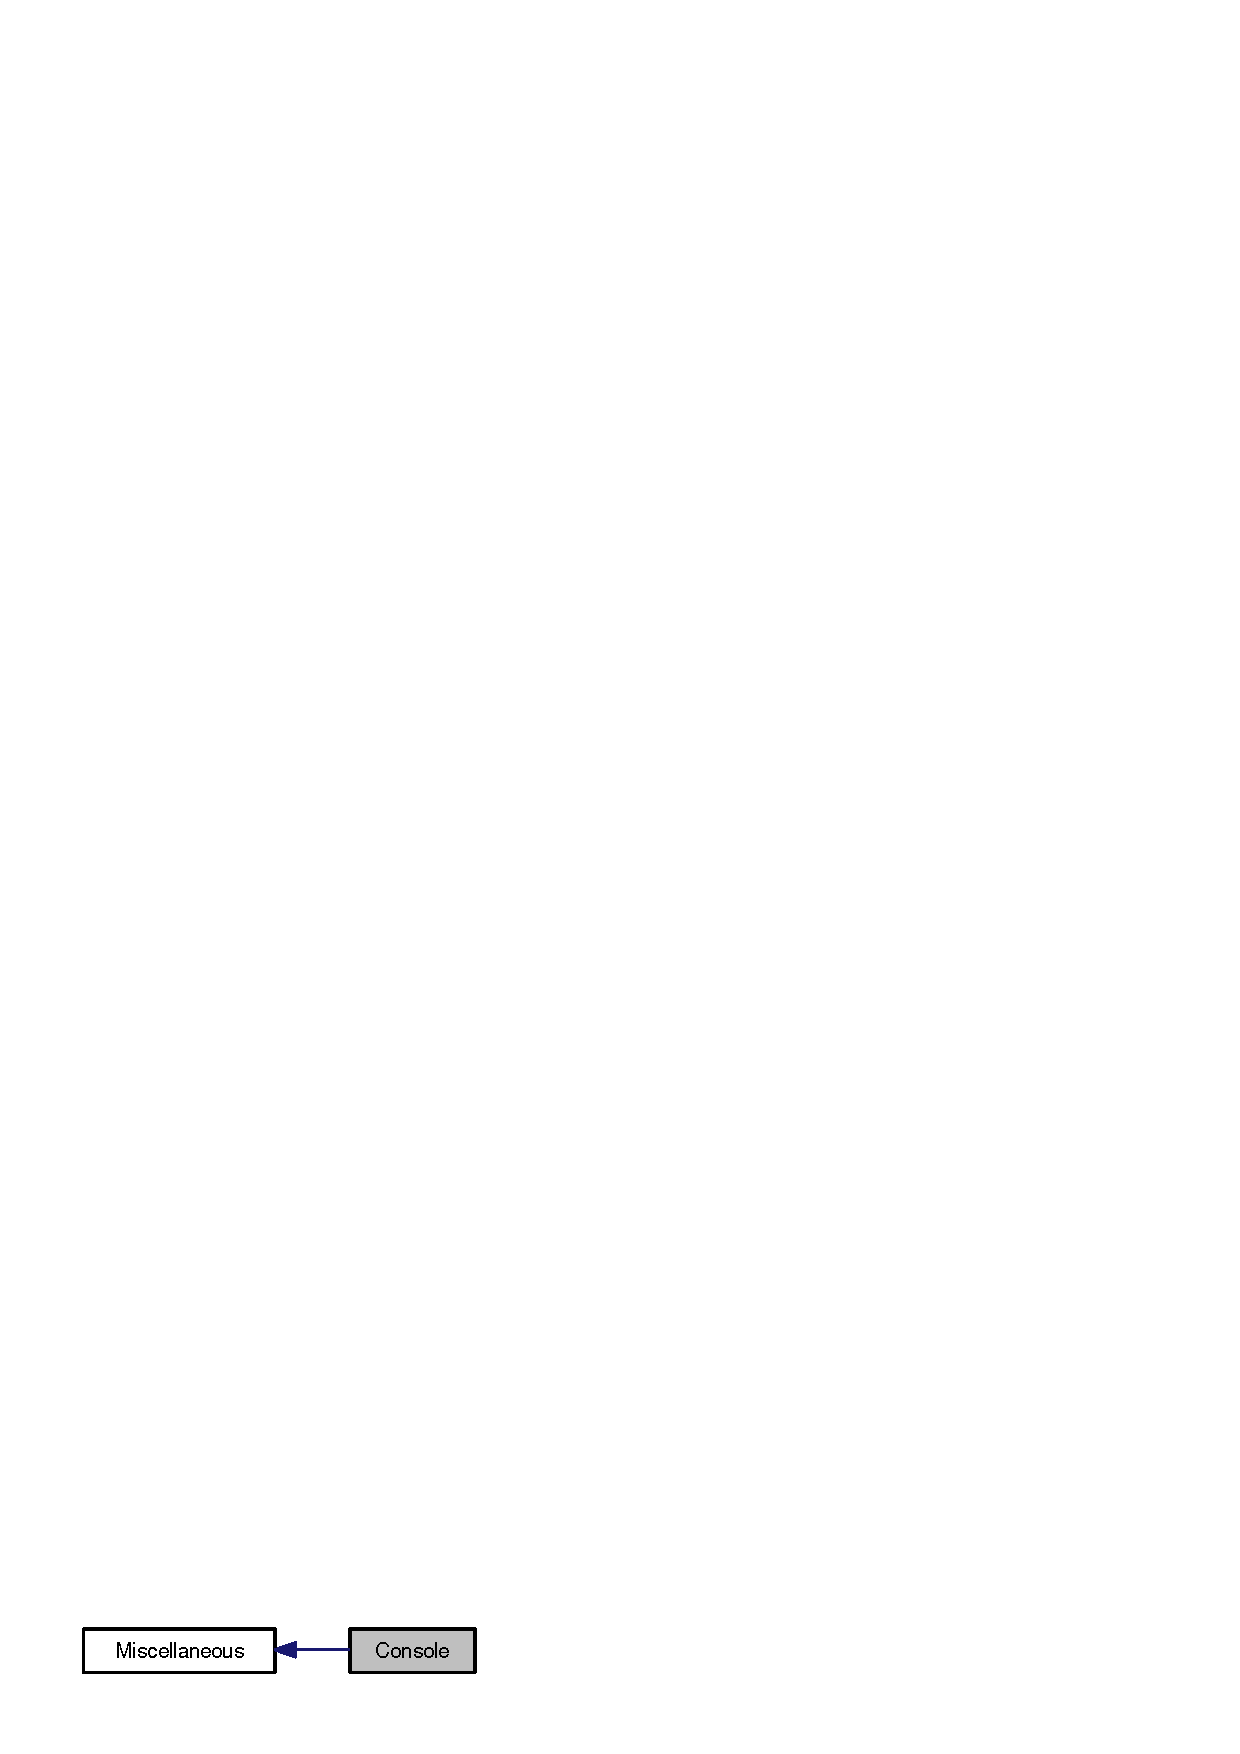
\includegraphics[width=116pt]{group__console}
\end{center}
\end{figure}
\subsection*{Functions}
\begin{DoxyCompactItemize}
\item 
void \hyperlink{group__console_ga3714108f42b44384b4d58009eafc1806}{post} (char $\ast$fmt,...)
\begin{DoxyCompactList}\small\item\em Print text to the Max window. \item\end{DoxyCompactList}\item 
void \hyperlink{group__console_ga94fff7e4ee19b8db6904a009117e0667}{cpost} (char $\ast$fmt,...)
\begin{DoxyCompactList}\small\item\em Print text to the system console. \item\end{DoxyCompactList}\item 
void \hyperlink{group__console_gaa7733e30b2951f225e24dca1ed4632b2}{error} (char $\ast$fmt,...)
\begin{DoxyCompactList}\small\item\em Print an error to the Max window. \item\end{DoxyCompactList}\item 
void \hyperlink{group__console_ga4cba33c91c6a8aa3d886e746e04f21af}{ouchstring} (char $\ast$s,...)
\begin{DoxyCompactList}\small\item\em Put up an error or advisory alert box on the screen. \item\end{DoxyCompactList}\item 
void \hyperlink{group__console_gaef84325d992e0afa14b2e7b0c0515601}{postatom} (\hyperlink{structt__atom}{t\_\-atom} $\ast$ap)
\begin{DoxyCompactList}\small\item\em Print multiple items in the same line of text in the Max window. \item\end{DoxyCompactList}\item 
void \hyperlink{group__console_gafb92b17363269d4d26de1823cbc2492d}{object\_\-post} (\hyperlink{structt__object}{t\_\-object} $\ast$x, char $\ast$s,...)
\begin{DoxyCompactList}\small\item\em Print text to the Max window, linked to an instance of your object. \item\end{DoxyCompactList}\item 
void \hyperlink{group__console_ga05f7fed66fafc6e4d2e372b7f0fe4e43}{object\_\-error} (\hyperlink{structt__object}{t\_\-object} $\ast$x, char $\ast$s,...)
\begin{DoxyCompactList}\small\item\em Print text to the Max window, linked to an instance of your object, and flagged as an error (highlighted with a red background). \item\end{DoxyCompactList}\item 
void \hyperlink{group__console_ga7ab11c5e9e345384ad282fcd5b86275c}{object\_\-warn} (\hyperlink{structt__object}{t\_\-object} $\ast$x, char $\ast$s,...)
\begin{DoxyCompactList}\small\item\em Print text to the Max window, linked to an instance of your object, and flagged as a warning (highlighted with a yellow background). \item\end{DoxyCompactList}\item 
void \hyperlink{group__console_ga42a612b12b1a24380a45ab1b9278b950}{object\_\-error\_\-obtrusive} (\hyperlink{structt__object}{t\_\-object} $\ast$x, char $\ast$s,...)
\begin{DoxyCompactList}\small\item\em Print text to the Max window, linked to an instance of your object, and flagged as an error (highlighted with a red background), and grab the user's attention by displaying a banner in the patcher window. \item\end{DoxyCompactList}\end{DoxyCompactItemize}


\subsection{Function Documentation}
\hypertarget{group__console_ga94fff7e4ee19b8db6904a009117e0667}{
\index{console@{console}!cpost@{cpost}}
\index{cpost@{cpost}!console@{console}}
\subsubsection[{cpost}]{\setlength{\rightskip}{0pt plus 5cm}void cpost (char $\ast$ {\em fmt}, \/   {\em ...})}}
\label{group__console_ga94fff7e4ee19b8db6904a009117e0667}


Print text to the system console. On the Mac this post will be visible by launching Console.app in the /Applications/Utilities folder. On Windows this post will be visible by launching the dbgView.exe program, which is a free download as a part of Microsoft's SysInternals.


\begin{DoxyParams}{Parameters}
\item[{\em fmt}]A C-\/string containing text and printf-\/like codes specifying the sizes and formatting of the additional arguments. \item[{\em ...}]Arguments of any type that correspond to the format codes in fmtString.\end{DoxyParams}
\begin{DoxyRemark}{Remarks}
Particularly on MacOS 10.5, posting to Console.app can be a computationally expensive operation. Use with care.
\end{DoxyRemark}
\begin{DoxySeeAlso}{See also}
\hyperlink{group__console_ga3714108f42b44384b4d58009eafc1806}{post()} 

\hyperlink{group__console_gafb92b17363269d4d26de1823cbc2492d}{object\_\-post()} 
\end{DoxySeeAlso}
\hypertarget{group__console_gaa7733e30b2951f225e24dca1ed4632b2}{
\index{console@{console}!error@{error}}
\index{error@{error}!console@{console}}
\subsubsection[{error}]{\setlength{\rightskip}{0pt plus 5cm}void error (char $\ast$ {\em fmt}, \/   {\em ...})}}
\label{group__console_gaa7733e30b2951f225e24dca1ed4632b2}


Print an error to the Max window. Max 5 introduced \hyperlink{group__console_ga05f7fed66fafc6e4d2e372b7f0fe4e43}{object\_\-error()}, which provides several enhancements to \hyperlink{group__console_gaa7733e30b2951f225e24dca1ed4632b2}{error()} where a valid \hyperlink{structt__object}{t\_\-object} pointer is available.

\hyperlink{group__console_gaa7733e30b2951f225e24dca1ed4632b2}{error()} is very similar to \hyperlink{group__console_ga3714108f42b44384b4d58009eafc1806}{post()}, thought it offers two additional features:
\begin{DoxyItemize}
\item the post to the Max window is highlighted (with a red background).
\item the post can be trapped with the error object in a patcher.
\end{DoxyItemize}


\begin{DoxyParams}{Parameters}
\item[{\em fmt}]A C-\/string containing text and printf-\/like codes specifying the sizes and formatting of the additional arguments. \item[{\em ...}]Arguments of any type that correspond to the format codes in fmtString.\end{DoxyParams}
\begin{DoxySeeAlso}{See also}
\hyperlink{group__console_gafb92b17363269d4d26de1823cbc2492d}{object\_\-post()} 

\hyperlink{group__console_ga3714108f42b44384b4d58009eafc1806}{post()} 

\hyperlink{group__console_ga94fff7e4ee19b8db6904a009117e0667}{cpost()} 
\end{DoxySeeAlso}
\hypertarget{group__console_ga05f7fed66fafc6e4d2e372b7f0fe4e43}{
\index{console@{console}!object\_\-error@{object\_\-error}}
\index{object\_\-error@{object\_\-error}!console@{console}}
\subsubsection[{object\_\-error}]{\setlength{\rightskip}{0pt plus 5cm}void object\_\-error ({\bf t\_\-object} $\ast$ {\em x}, \/  char $\ast$ {\em s}, \/   {\em ...})}}
\label{group__console_ga05f7fed66fafc6e4d2e372b7f0fe4e43}


Print text to the Max window, linked to an instance of your object, and flagged as an error (highlighted with a red background). Max window rows which are generated using \hyperlink{group__console_gafb92b17363269d4d26de1823cbc2492d}{object\_\-post()} or \hyperlink{group__console_ga05f7fed66fafc6e4d2e372b7f0fe4e43}{object\_\-error()} can be double-\/clicked by the user to have Max assist with locating the object in a patcher. Rows created with \hyperlink{group__console_gafb92b17363269d4d26de1823cbc2492d}{object\_\-post()} and \hyperlink{group__console_ga05f7fed66fafc6e4d2e372b7f0fe4e43}{object\_\-error()} will also automatically provide the name of the object's class in the correct column in the Max window.


\begin{DoxyParams}{Parameters}
\item[{\em x}]A pointer to your object. \item[{\em s}]A C-\/string containing text and printf-\/like codes specifying the sizes and formatting of the additional arguments. \item[{\em ...}]Arguments of any type that correspond to the format codes in fmtString.\end{DoxyParams}
\begin{DoxySeeAlso}{See also}
\hyperlink{group__console_gafb92b17363269d4d26de1823cbc2492d}{object\_\-post()} 

\hyperlink{group__console_ga7ab11c5e9e345384ad282fcd5b86275c}{object\_\-warn()} 
\end{DoxySeeAlso}
\hypertarget{group__console_ga42a612b12b1a24380a45ab1b9278b950}{
\index{console@{console}!object\_\-error\_\-obtrusive@{object\_\-error\_\-obtrusive}}
\index{object\_\-error\_\-obtrusive@{object\_\-error\_\-obtrusive}!console@{console}}
\subsubsection[{object\_\-error\_\-obtrusive}]{\setlength{\rightskip}{0pt plus 5cm}void object\_\-error\_\-obtrusive ({\bf t\_\-object} $\ast$ {\em x}, \/  char $\ast$ {\em s}, \/   {\em ...})}}
\label{group__console_ga42a612b12b1a24380a45ab1b9278b950}


Print text to the Max window, linked to an instance of your object, and flagged as an error (highlighted with a red background), and grab the user's attention by displaying a banner in the patcher window. This function should be used exceedingly sparingly, with preference given to \hyperlink{group__console_ga05f7fed66fafc6e4d2e372b7f0fe4e43}{object\_\-error()} when a problem occurs.


\begin{DoxyParams}{Parameters}
\item[{\em x}]A pointer to your object. \item[{\em s}]A C-\/string containing text and printf-\/like codes specifying the sizes and formatting of the additional arguments. \item[{\em ...}]Arguments of any type that correspond to the format codes in fmtString.\end{DoxyParams}
\begin{DoxySeeAlso}{See also}
\hyperlink{group__console_gafb92b17363269d4d26de1823cbc2492d}{object\_\-post()} 

\hyperlink{group__console_ga05f7fed66fafc6e4d2e372b7f0fe4e43}{object\_\-error()} 
\end{DoxySeeAlso}
\hypertarget{group__console_gafb92b17363269d4d26de1823cbc2492d}{
\index{console@{console}!object\_\-post@{object\_\-post}}
\index{object\_\-post@{object\_\-post}!console@{console}}
\subsubsection[{object\_\-post}]{\setlength{\rightskip}{0pt plus 5cm}void object\_\-post ({\bf t\_\-object} $\ast$ {\em x}, \/  char $\ast$ {\em s}, \/   {\em ...})}}
\label{group__console_gafb92b17363269d4d26de1823cbc2492d}


Print text to the Max window, linked to an instance of your object. Max window rows which are generated using \hyperlink{group__console_gafb92b17363269d4d26de1823cbc2492d}{object\_\-post()} or \hyperlink{group__console_ga05f7fed66fafc6e4d2e372b7f0fe4e43}{object\_\-error()} can be double-\/clicked by the user to have Max assist with locating the object in a patcher. Rows created with \hyperlink{group__console_gafb92b17363269d4d26de1823cbc2492d}{object\_\-post()} and \hyperlink{group__console_ga05f7fed66fafc6e4d2e372b7f0fe4e43}{object\_\-error()} will also automatically provide the name of the object's class in the correct column in the Max window.


\begin{DoxyParams}{Parameters}
\item[{\em x}]A pointer to your object. \item[{\em s}]A C-\/string containing text and printf-\/like codes specifying the sizes and formatting of the additional arguments. \item[{\em ...}]Arguments of any type that correspond to the format codes in fmtString.\end{DoxyParams}
\begin{DoxyRemark}{Remarks}
Example: 
\begin{DoxyCode}
    void myMethod(myObject *x, long someArgument)
    {
        object_post((t_object*)x, "This is my argument: %ld", someArgument);
    }
\end{DoxyCode}

\end{DoxyRemark}
\begin{DoxySeeAlso}{See also}
\hyperlink{group__console_ga05f7fed66fafc6e4d2e372b7f0fe4e43}{object\_\-error()} 
\end{DoxySeeAlso}
\hypertarget{group__console_ga7ab11c5e9e345384ad282fcd5b86275c}{
\index{console@{console}!object\_\-warn@{object\_\-warn}}
\index{object\_\-warn@{object\_\-warn}!console@{console}}
\subsubsection[{object\_\-warn}]{\setlength{\rightskip}{0pt plus 5cm}void object\_\-warn ({\bf t\_\-object} $\ast$ {\em x}, \/  char $\ast$ {\em s}, \/   {\em ...})}}
\label{group__console_ga7ab11c5e9e345384ad282fcd5b86275c}


Print text to the Max window, linked to an instance of your object, and flagged as a warning (highlighted with a yellow background). Max window rows which are generated using \hyperlink{group__console_gafb92b17363269d4d26de1823cbc2492d}{object\_\-post()}, \hyperlink{group__console_ga05f7fed66fafc6e4d2e372b7f0fe4e43}{object\_\-error()}, or object\_\-warn can be double-\/clicked by the user to have Max assist with locating the object in a patcher. Rows created with \hyperlink{group__console_gafb92b17363269d4d26de1823cbc2492d}{object\_\-post()}, \hyperlink{group__console_ga05f7fed66fafc6e4d2e372b7f0fe4e43}{object\_\-error()}, or \hyperlink{group__console_ga7ab11c5e9e345384ad282fcd5b86275c}{object\_\-warn()} will also automatically provide the name of the object's class in the correct column in the Max window.


\begin{DoxyParams}{Parameters}
\item[{\em x}]A pointer to your object. \item[{\em s}]A C-\/string containing text and printf-\/like codes specifying the sizes and formatting of the additional arguments. \item[{\em ...}]Arguments of any type that correspond to the format codes in fmtString.\end{DoxyParams}
\begin{DoxySeeAlso}{See also}
\hyperlink{group__console_gafb92b17363269d4d26de1823cbc2492d}{object\_\-post()} 

\hyperlink{group__console_ga05f7fed66fafc6e4d2e372b7f0fe4e43}{object\_\-error()} 
\end{DoxySeeAlso}
\hypertarget{group__console_ga4cba33c91c6a8aa3d886e746e04f21af}{
\index{console@{console}!ouchstring@{ouchstring}}
\index{ouchstring@{ouchstring}!console@{console}}
\subsubsection[{ouchstring}]{\setlength{\rightskip}{0pt plus 5cm}void ouchstring (char $\ast$ {\em s}, \/   {\em ...})}}
\label{group__console_ga4cba33c91c6a8aa3d886e746e04f21af}


Put up an error or advisory alert box on the screen. Don't use this function. Instead use \hyperlink{group__console_gaa7733e30b2951f225e24dca1ed4632b2}{error()}, \hyperlink{group__console_ga05f7fed66fafc6e4d2e372b7f0fe4e43}{object\_\-error()}, or \hyperlink{group__console_ga42a612b12b1a24380a45ab1b9278b950}{object\_\-error\_\-obtrusive()}.

This function performs an sprintf() on fmtstring and items, then puts up an alert box. \hyperlink{group__console_ga4cba33c91c6a8aa3d886e746e04f21af}{ouchstring()} will queue the message to a lower priority level if it’s called in an interrupt and there is no alert box request already pending.


\begin{DoxyParams}{Parameters}
\item[{\em s}]A C-\/string containing text and printf-\/like codes specifying the sizes and formatting of the additional arguments. \item[{\em ...}]Arguments of any type that correspond to the format codes in fmtString.\end{DoxyParams}
\begin{DoxySeeAlso}{See also}
\hyperlink{group__console_gaa7733e30b2951f225e24dca1ed4632b2}{error()} 

\hyperlink{group__console_ga05f7fed66fafc6e4d2e372b7f0fe4e43}{object\_\-error()} 

\hyperlink{group__console_ga42a612b12b1a24380a45ab1b9278b950}{object\_\-error\_\-obtrusive()} 
\end{DoxySeeAlso}
\hypertarget{group__console_ga3714108f42b44384b4d58009eafc1806}{
\index{console@{console}!post@{post}}
\index{post@{post}!console@{console}}
\subsubsection[{post}]{\setlength{\rightskip}{0pt plus 5cm}void post (char $\ast$ {\em fmt}, \/   {\em ...})}}
\label{group__console_ga3714108f42b44384b4d58009eafc1806}


Print text to the Max window. Max 5 introduced \hyperlink{group__console_gafb92b17363269d4d26de1823cbc2492d}{object\_\-post()}, which provides several enhancements to \hyperlink{group__console_ga3714108f42b44384b4d58009eafc1806}{post()} where a valid \hyperlink{structt__object}{t\_\-object} pointer is available.

\hyperlink{group__console_ga3714108f42b44384b4d58009eafc1806}{post()} is a printf() for the Max window. It even works from non-\/main threads, queuing up multiple lines of text to be printed when the main thread processing resumes. \hyperlink{group__console_ga3714108f42b44384b4d58009eafc1806}{post()} can be quite useful in debugging your external object.


\begin{DoxyParams}{Parameters}
\item[{\em fmt}]A C-\/string containing text and printf-\/like codes specifying the sizes and formatting of the additional arguments. \item[{\em ...}]Arguments of any type that correspond to the format codes in fmtString.\end{DoxyParams}
\begin{DoxyRemark}{Remarks}
Note that post only passes 16 bytes of arguments to sprintf, so if you want additional formatted items on a single line, use \hyperlink{group__console_gaef84325d992e0afa14b2e7b0c0515601}{postatom()}.
\end{DoxyRemark}
Example: 
\begin{DoxyCode}
    short whatIsIt; 

    whatIsIt = 999; 
    post ("the variable is %ld",(long)whatIsIt); 
\end{DoxyCode}


\begin{DoxyRemark}{Remarks}
The Max Window output when this code is executed. 
\begin{DoxyCode}
    the variable is 999
\end{DoxyCode}

\end{DoxyRemark}
\begin{DoxySeeAlso}{See also}
\hyperlink{group__console_gafb92b17363269d4d26de1823cbc2492d}{object\_\-post()} 

\hyperlink{group__console_gaa7733e30b2951f225e24dca1ed4632b2}{error()} 

\hyperlink{group__console_ga94fff7e4ee19b8db6904a009117e0667}{cpost()} 
\end{DoxySeeAlso}
\hypertarget{group__console_gaef84325d992e0afa14b2e7b0c0515601}{
\index{console@{console}!postatom@{postatom}}
\index{postatom@{postatom}!console@{console}}
\subsubsection[{postatom}]{\setlength{\rightskip}{0pt plus 5cm}void postatom ({\bf t\_\-atom} $\ast$ {\em ap})}}
\label{group__console_gaef84325d992e0afa14b2e7b0c0515601}


Print multiple items in the same line of text in the Max window. This function prints a single \hyperlink{structt__atom}{t\_\-atom} on a line in the Max window without a carriage return afterwards, as \hyperlink{group__console_ga3714108f42b44384b4d58009eafc1806}{post()} does. Each \hyperlink{structt__atom}{t\_\-atom} printed is followed by a space character.


\begin{DoxyParams}{Parameters}
\item[{\em ap}]The address of a \hyperlink{structt__atom}{t\_\-atom} to print.\end{DoxyParams}
\begin{DoxySeeAlso}{See also}
\hyperlink{group__console_gafb92b17363269d4d26de1823cbc2492d}{object\_\-post()} 

\hyperlink{group__console_ga3714108f42b44384b4d58009eafc1806}{post()} 

\hyperlink{group__console_ga94fff7e4ee19b8db6904a009117e0667}{cpost()} 
\end{DoxySeeAlso}

\hypertarget{group__byteorder}{
\section{Byte Ordering}
\label{group__byteorder}\index{Byte Ordering@{Byte Ordering}}
}


Utilities for swapping the order of bytes to match the Endianness of the required platform.  


Collaboration diagram for Byte Ordering:\nopagebreak
\begin{figure}[H]
\begin{center}
\leavevmode
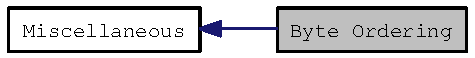
\includegraphics[width=132pt]{group__byteorder}
\end{center}
\end{figure}
\subsection*{Defines}
\begin{DoxyCompactItemize}
\item 
\#define \hyperlink{group__byteorder_gaa1bcf3a033a866ca81d51e9f65ec4d3a}{C74\_\-LITTLE\_\-ENDIAN}~1
\begin{DoxyCompactList}\small\item\em A macro that indicates whether or not the current architecture uses Litte-\/endian byte ordering (such as is used on an i386 processor). \item\end{DoxyCompactList}\item 
\#define \hyperlink{group__byteorder_ga51aafb747c672a9623c9b6e851c5cb53}{C74\_\-BIG\_\-ENDIAN}~0
\begin{DoxyCompactList}\small\item\em A macro that indicates whether or not the current architecture uses Big-\/endian byte ordering (such as is used on a PPC processor). \item\end{DoxyCompactList}\item 
\#define \hyperlink{group__byteorder_ga035b5999ffd460b028adbddc114bc1ea}{BYTEORDER\_\-SWAPW16}(x)~((short)(((((unsigned short)(x))$>$$>$8)\&0x00ff)+((((unsigned short)(x))$<$$<$8)\&0xff00)))
\begin{DoxyCompactList}\small\item\em Switch the byte ordering of a short integer. \item\end{DoxyCompactList}\item 
\#define \hyperlink{group__byteorder_ga2361fba0c30f763e8fe3fb2fe0eece43}{BYTEORDER\_\-SWAPW32}(x)
\begin{DoxyCompactList}\small\item\em Switch the byte ordering of an integer. \item\end{DoxyCompactList}\item 
\#define \hyperlink{group__byteorder_ga78c51e5ecacde07ac8f68c1dc7bca801}{BYTEORDER\_\-SWAPF32}~byteorder\_\-swapf32
\begin{DoxyCompactList}\small\item\em Switch the byte ordering of a float. \item\end{DoxyCompactList}\item 
\#define \hyperlink{group__byteorder_ga9e36111d85cc708026b869111af4d084}{BYTEORDER\_\-SWAPF64}~byteorder\_\-swapf64
\begin{DoxyCompactList}\small\item\em Switch the byte ordering of a double. \item\end{DoxyCompactList}\item 
\#define \hyperlink{group__byteorder_gaa46359f7d1f29bab74afddacd9decdeb}{BYTEORDER\_\-LSBW16}(x)~(x)
\begin{DoxyCompactList}\small\item\em Switch the byte ordering of a short integer from the native swapping to Little-\/endian (Least Significant Byte). \item\end{DoxyCompactList}\item 
\#define \hyperlink{group__byteorder_ga24bb3ddfe733a3202d53a0d14f186105}{BYTEORDER\_\-LSBW32}(x)~(x)
\begin{DoxyCompactList}\small\item\em Switch the byte ordering of an integer from the native swapping to Little-\/endian (Least Significant Byte). \item\end{DoxyCompactList}\item 
\#define \hyperlink{group__byteorder_gae8ff7d2f1611389be2d908c8675e344a}{BYTEORDER\_\-LSBF32}(x)~(x)
\begin{DoxyCompactList}\small\item\em Switch the byte ordering of a float from the native swapping to Little-\/endian (Least Significant Byte). \item\end{DoxyCompactList}\item 
\#define \hyperlink{group__byteorder_ga8fe695baca4e41252ee2017b3f2e5068}{BYTEORDER\_\-LSBF64}(x)~(x)
\begin{DoxyCompactList}\small\item\em Switch the byte ordering of a double from the native swapping to Little-\/endian (Least Significant Byte). \item\end{DoxyCompactList}\item 
\#define \hyperlink{group__byteorder_gaa99b101c1a15ccb9bf5d070aea1b23c8}{BYTEORDER\_\-MSBW16}(x)~BYTEORDER\_\-SWAPW16(x)
\begin{DoxyCompactList}\small\item\em Switch the byte ordering of a short integer from the native swapping to Big-\/endian (Most Significant Byte). \item\end{DoxyCompactList}\item 
\#define \hyperlink{group__byteorder_ga46ff7133babdbfa8166fbdb4d40d72a7}{BYTEORDER\_\-MSBW32}(x)~BYTEORDER\_\-SWAPW32(x)
\begin{DoxyCompactList}\small\item\em Switch the byte ordering of an integer from the native swapping to Big-\/endian (Most Significant Byte). \item\end{DoxyCompactList}\item 
\#define \hyperlink{group__byteorder_gaa5783a6ed7c7d471150da5a9c5453f79}{BYTEORDER\_\-MSBF32}(x)~BYTEORDER\_\-SWAPF32(x)
\begin{DoxyCompactList}\small\item\em Switch the byte ordering of a float from the native swapping to Big-\/endian (Most Significant Byte). \item\end{DoxyCompactList}\item 
\#define \hyperlink{group__byteorder_ga5b3d8dac5e677fd03f1959a2ff68784e}{BYTEORDER\_\-MSBF64}(x)~BYTEORDER\_\-SWAPF64(x)
\begin{DoxyCompactList}\small\item\em Switch the byte ordering of a double from the native swapping to Big-\/endian (Most Significant Byte). \item\end{DoxyCompactList}\end{DoxyCompactItemize}


\subsection{Detailed Description}
Utilities for swapping the order of bytes to match the Endianness of the required platform. An introduction to the issue of endianness can be found at \href{http://en.wikipedia.org/wiki/Endianness.}{\tt http://en.wikipedia.org/wiki/Endianness.}

Of particular relevance is that a Macintosh with a PPC processor uses a Big-\/endian byte ordering, whereas an Intel processor in a Mac or Windows machine will use a Little-\/endian byte ordering.

These utilities are defined to assist with cases where byte ordering needs to be manipulated for floats or ints. Note that floats are subject to the same byte ordering rules as integers. While the IEEE defines the bits, the machine still defines how the bits are arranged with regard to bytes. 

\subsection{Define Documentation}
\hypertarget{group__byteorder_gae8ff7d2f1611389be2d908c8675e344a}{
\index{byteorder@{byteorder}!BYTEORDER\_\-LSBF32@{BYTEORDER\_\-LSBF32}}
\index{BYTEORDER\_\-LSBF32@{BYTEORDER\_\-LSBF32}!byteorder@{byteorder}}
\subsubsection[{BYTEORDER\_\-LSBF32}]{\setlength{\rightskip}{0pt plus 5cm}\#define BYTEORDER\_\-LSBF32(x)~(x)}}
\label{group__byteorder_gae8ff7d2f1611389be2d908c8675e344a}


Switch the byte ordering of a float from the native swapping to Little-\/endian (Least Significant Byte). If the current environment is already Little-\/endian, then the returned value is not byteswapped.


\begin{DoxyParams}{Parameters}
\item[{\em x}]A float. \end{DoxyParams}
\begin{DoxyReturn}{Returns}
A float with the byte-\/ordering swapped if neccessary. 
\end{DoxyReturn}
\hypertarget{group__byteorder_ga8fe695baca4e41252ee2017b3f2e5068}{
\index{byteorder@{byteorder}!BYTEORDER\_\-LSBF64@{BYTEORDER\_\-LSBF64}}
\index{BYTEORDER\_\-LSBF64@{BYTEORDER\_\-LSBF64}!byteorder@{byteorder}}
\subsubsection[{BYTEORDER\_\-LSBF64}]{\setlength{\rightskip}{0pt plus 5cm}\#define BYTEORDER\_\-LSBF64(x)~(x)}}
\label{group__byteorder_ga8fe695baca4e41252ee2017b3f2e5068}


Switch the byte ordering of a double from the native swapping to Little-\/endian (Least Significant Byte). If the current environment is already Little-\/endian, then the returned value is not byteswapped.


\begin{DoxyParams}{Parameters}
\item[{\em x}]A double. \end{DoxyParams}
\begin{DoxyReturn}{Returns}
A double with the byte-\/ordering swapped if neccessary. 
\end{DoxyReturn}
\hypertarget{group__byteorder_gaa46359f7d1f29bab74afddacd9decdeb}{
\index{byteorder@{byteorder}!BYTEORDER\_\-LSBW16@{BYTEORDER\_\-LSBW16}}
\index{BYTEORDER\_\-LSBW16@{BYTEORDER\_\-LSBW16}!byteorder@{byteorder}}
\subsubsection[{BYTEORDER\_\-LSBW16}]{\setlength{\rightskip}{0pt plus 5cm}\#define BYTEORDER\_\-LSBW16(x)~(x)}}
\label{group__byteorder_gaa46359f7d1f29bab74afddacd9decdeb}


Switch the byte ordering of a short integer from the native swapping to Little-\/endian (Least Significant Byte). If the current environment is already Little-\/endian, then the returned value is not byteswapped.


\begin{DoxyParams}{Parameters}
\item[{\em x}]A short integer. \end{DoxyParams}
\begin{DoxyReturn}{Returns}
A short integer with the byte-\/ordering swapped if neccessary. 
\end{DoxyReturn}
\hypertarget{group__byteorder_ga24bb3ddfe733a3202d53a0d14f186105}{
\index{byteorder@{byteorder}!BYTEORDER\_\-LSBW32@{BYTEORDER\_\-LSBW32}}
\index{BYTEORDER\_\-LSBW32@{BYTEORDER\_\-LSBW32}!byteorder@{byteorder}}
\subsubsection[{BYTEORDER\_\-LSBW32}]{\setlength{\rightskip}{0pt plus 5cm}\#define BYTEORDER\_\-LSBW32(x)~(x)}}
\label{group__byteorder_ga24bb3ddfe733a3202d53a0d14f186105}


Switch the byte ordering of an integer from the native swapping to Little-\/endian (Least Significant Byte). If the current environment is already Little-\/endian, then the returned value is not byteswapped.


\begin{DoxyParams}{Parameters}
\item[{\em x}]An integer. \end{DoxyParams}
\begin{DoxyReturn}{Returns}
An integer with the byte-\/ordering swapped if neccessary. 
\end{DoxyReturn}
\hypertarget{group__byteorder_gaa5783a6ed7c7d471150da5a9c5453f79}{
\index{byteorder@{byteorder}!BYTEORDER\_\-MSBF32@{BYTEORDER\_\-MSBF32}}
\index{BYTEORDER\_\-MSBF32@{BYTEORDER\_\-MSBF32}!byteorder@{byteorder}}
\subsubsection[{BYTEORDER\_\-MSBF32}]{\setlength{\rightskip}{0pt plus 5cm}\#define BYTEORDER\_\-MSBF32(x)~BYTEORDER\_\-SWAPF32(x)}}
\label{group__byteorder_gaa5783a6ed7c7d471150da5a9c5453f79}


Switch the byte ordering of a float from the native swapping to Big-\/endian (Most Significant Byte). If the current environment is already Big-\/endian, then the returned value is not byteswapped.


\begin{DoxyParams}{Parameters}
\item[{\em x}]A float. \end{DoxyParams}
\begin{DoxyReturn}{Returns}
A float with the byte-\/ordering swapped if neccessary. 
\end{DoxyReturn}
\hypertarget{group__byteorder_ga5b3d8dac5e677fd03f1959a2ff68784e}{
\index{byteorder@{byteorder}!BYTEORDER\_\-MSBF64@{BYTEORDER\_\-MSBF64}}
\index{BYTEORDER\_\-MSBF64@{BYTEORDER\_\-MSBF64}!byteorder@{byteorder}}
\subsubsection[{BYTEORDER\_\-MSBF64}]{\setlength{\rightskip}{0pt plus 5cm}\#define BYTEORDER\_\-MSBF64(x)~BYTEORDER\_\-SWAPF64(x)}}
\label{group__byteorder_ga5b3d8dac5e677fd03f1959a2ff68784e}


Switch the byte ordering of a double from the native swapping to Big-\/endian (Most Significant Byte). If the current environment is already Big-\/endian, then the returned value is not byteswapped.


\begin{DoxyParams}{Parameters}
\item[{\em x}]A double. \end{DoxyParams}
\begin{DoxyReturn}{Returns}
A double with the byte-\/ordering swapped if neccessary. 
\end{DoxyReturn}
\hypertarget{group__byteorder_gaa99b101c1a15ccb9bf5d070aea1b23c8}{
\index{byteorder@{byteorder}!BYTEORDER\_\-MSBW16@{BYTEORDER\_\-MSBW16}}
\index{BYTEORDER\_\-MSBW16@{BYTEORDER\_\-MSBW16}!byteorder@{byteorder}}
\subsubsection[{BYTEORDER\_\-MSBW16}]{\setlength{\rightskip}{0pt plus 5cm}\#define BYTEORDER\_\-MSBW16(x)~BYTEORDER\_\-SWAPW16(x)}}
\label{group__byteorder_gaa99b101c1a15ccb9bf5d070aea1b23c8}


Switch the byte ordering of a short integer from the native swapping to Big-\/endian (Most Significant Byte). If the current environment is already Big-\/endian, then the returned value is not byteswapped.


\begin{DoxyParams}{Parameters}
\item[{\em x}]A short integer. \end{DoxyParams}
\begin{DoxyReturn}{Returns}
A short integer with the byte-\/ordering swapped if neccessary. 
\end{DoxyReturn}
\hypertarget{group__byteorder_ga46ff7133babdbfa8166fbdb4d40d72a7}{
\index{byteorder@{byteorder}!BYTEORDER\_\-MSBW32@{BYTEORDER\_\-MSBW32}}
\index{BYTEORDER\_\-MSBW32@{BYTEORDER\_\-MSBW32}!byteorder@{byteorder}}
\subsubsection[{BYTEORDER\_\-MSBW32}]{\setlength{\rightskip}{0pt plus 5cm}\#define BYTEORDER\_\-MSBW32(x)~BYTEORDER\_\-SWAPW32(x)}}
\label{group__byteorder_ga46ff7133babdbfa8166fbdb4d40d72a7}


Switch the byte ordering of an integer from the native swapping to Big-\/endian (Most Significant Byte). If the current environment is already Big-\/endian, then the returned value is not byteswapped.


\begin{DoxyParams}{Parameters}
\item[{\em x}]An integer. \end{DoxyParams}
\begin{DoxyReturn}{Returns}
An integer with the byte-\/ordering swapped if neccessary. 
\end{DoxyReturn}
\hypertarget{group__byteorder_ga78c51e5ecacde07ac8f68c1dc7bca801}{
\index{byteorder@{byteorder}!BYTEORDER\_\-SWAPF32@{BYTEORDER\_\-SWAPF32}}
\index{BYTEORDER\_\-SWAPF32@{BYTEORDER\_\-SWAPF32}!byteorder@{byteorder}}
\subsubsection[{BYTEORDER\_\-SWAPF32}]{\setlength{\rightskip}{0pt plus 5cm}\#define BYTEORDER\_\-SWAPF32~byteorder\_\-swapf32}}
\label{group__byteorder_ga78c51e5ecacde07ac8f68c1dc7bca801}


Switch the byte ordering of a float. 
\begin{DoxyParams}{Parameters}
\item[{\em x}]A float. \end{DoxyParams}
\begin{DoxyReturn}{Returns}
A float with the byte-\/ordering swapped. 
\end{DoxyReturn}
\hypertarget{group__byteorder_ga9e36111d85cc708026b869111af4d084}{
\index{byteorder@{byteorder}!BYTEORDER\_\-SWAPF64@{BYTEORDER\_\-SWAPF64}}
\index{BYTEORDER\_\-SWAPF64@{BYTEORDER\_\-SWAPF64}!byteorder@{byteorder}}
\subsubsection[{BYTEORDER\_\-SWAPF64}]{\setlength{\rightskip}{0pt plus 5cm}\#define BYTEORDER\_\-SWAPF64~byteorder\_\-swapf64}}
\label{group__byteorder_ga9e36111d85cc708026b869111af4d084}


Switch the byte ordering of a double. 
\begin{DoxyParams}{Parameters}
\item[{\em x}]A double. \end{DoxyParams}
\begin{DoxyReturn}{Returns}
A double. 
\end{DoxyReturn}
\hypertarget{group__byteorder_ga035b5999ffd460b028adbddc114bc1ea}{
\index{byteorder@{byteorder}!BYTEORDER\_\-SWAPW16@{BYTEORDER\_\-SWAPW16}}
\index{BYTEORDER\_\-SWAPW16@{BYTEORDER\_\-SWAPW16}!byteorder@{byteorder}}
\subsubsection[{BYTEORDER\_\-SWAPW16}]{\setlength{\rightskip}{0pt plus 5cm}\#define BYTEORDER\_\-SWAPW16(x)~((short)(((((unsigned short)(x))$>$$>$8)\&0x00ff)+((((unsigned short)(x))$<$$<$8)\&0xff00)))}}
\label{group__byteorder_ga035b5999ffd460b028adbddc114bc1ea}


Switch the byte ordering of a short integer. 
\begin{DoxyParams}{Parameters}
\item[{\em x}]A short integer. \end{DoxyParams}
\begin{DoxyReturn}{Returns}
A short integer with the byte-\/ordering swapped. 
\end{DoxyReturn}
\hypertarget{group__byteorder_ga2361fba0c30f763e8fe3fb2fe0eece43}{
\index{byteorder@{byteorder}!BYTEORDER\_\-SWAPW32@{BYTEORDER\_\-SWAPW32}}
\index{BYTEORDER\_\-SWAPW32@{BYTEORDER\_\-SWAPW32}!byteorder@{byteorder}}
\subsubsection[{BYTEORDER\_\-SWAPW32}]{\setlength{\rightskip}{0pt plus 5cm}\#define BYTEORDER\_\-SWAPW32(x)}}
\label{group__byteorder_ga2361fba0c30f763e8fe3fb2fe0eece43}
{\bfseries Value:}
\begin{DoxyCode}
((long)(((((unsigned long)(x))>>24L)&0x000000ff)+((((unsigned long)(x))>>8L)&0x00
      00ff00)+ \
                                    ((((unsigned long)(x))<<24L)&0xff000000)+((((
      unsigned long)(x))<<8L)&0x00ff0000)))
\end{DoxyCode}


Switch the byte ordering of an integer. 
\begin{DoxyParams}{Parameters}
\item[{\em x}]An integer. \end{DoxyParams}
\begin{DoxyReturn}{Returns}
An integer with the byte-\/ordering swapped. 
\end{DoxyReturn}
\hypertarget{group__byteorder_ga51aafb747c672a9623c9b6e851c5cb53}{
\index{byteorder@{byteorder}!C74\_\-BIG\_\-ENDIAN@{C74\_\-BIG\_\-ENDIAN}}
\index{C74\_\-BIG\_\-ENDIAN@{C74\_\-BIG\_\-ENDIAN}!byteorder@{byteorder}}
\subsubsection[{C74\_\-BIG\_\-ENDIAN}]{\setlength{\rightskip}{0pt plus 5cm}\#define C74\_\-BIG\_\-ENDIAN~0}}
\label{group__byteorder_ga51aafb747c672a9623c9b6e851c5cb53}


A macro that indicates whether or not the current architecture uses Big-\/endian byte ordering (such as is used on a PPC processor). Note that this macro is always defined; it will be either a 0 or a 1. \hypertarget{group__byteorder_gaa1bcf3a033a866ca81d51e9f65ec4d3a}{
\index{byteorder@{byteorder}!C74\_\-LITTLE\_\-ENDIAN@{C74\_\-LITTLE\_\-ENDIAN}}
\index{C74\_\-LITTLE\_\-ENDIAN@{C74\_\-LITTLE\_\-ENDIAN}!byteorder@{byteorder}}
\subsubsection[{C74\_\-LITTLE\_\-ENDIAN}]{\setlength{\rightskip}{0pt plus 5cm}\#define C74\_\-LITTLE\_\-ENDIAN~1}}
\label{group__byteorder_gaa1bcf3a033a866ca81d51e9f65ec4d3a}


A macro that indicates whether or not the current architecture uses Litte-\/endian byte ordering (such as is used on an i386 processor). Note that this macro is always defined; it will be either a 0 or a 1. 
\hypertarget{group__expr}{
\section{Extending expr}
\label{group__expr}\index{Extending expr@{Extending expr}}
}


If you want to use C-\/like variable expressions that are entered by a user of your object, you can use the \char`\"{}guts\char`\"{} of Max’s expr object in your object.  


Collaboration diagram for Extending expr:\nopagebreak
\begin{figure}[H]
\begin{center}
\leavevmode
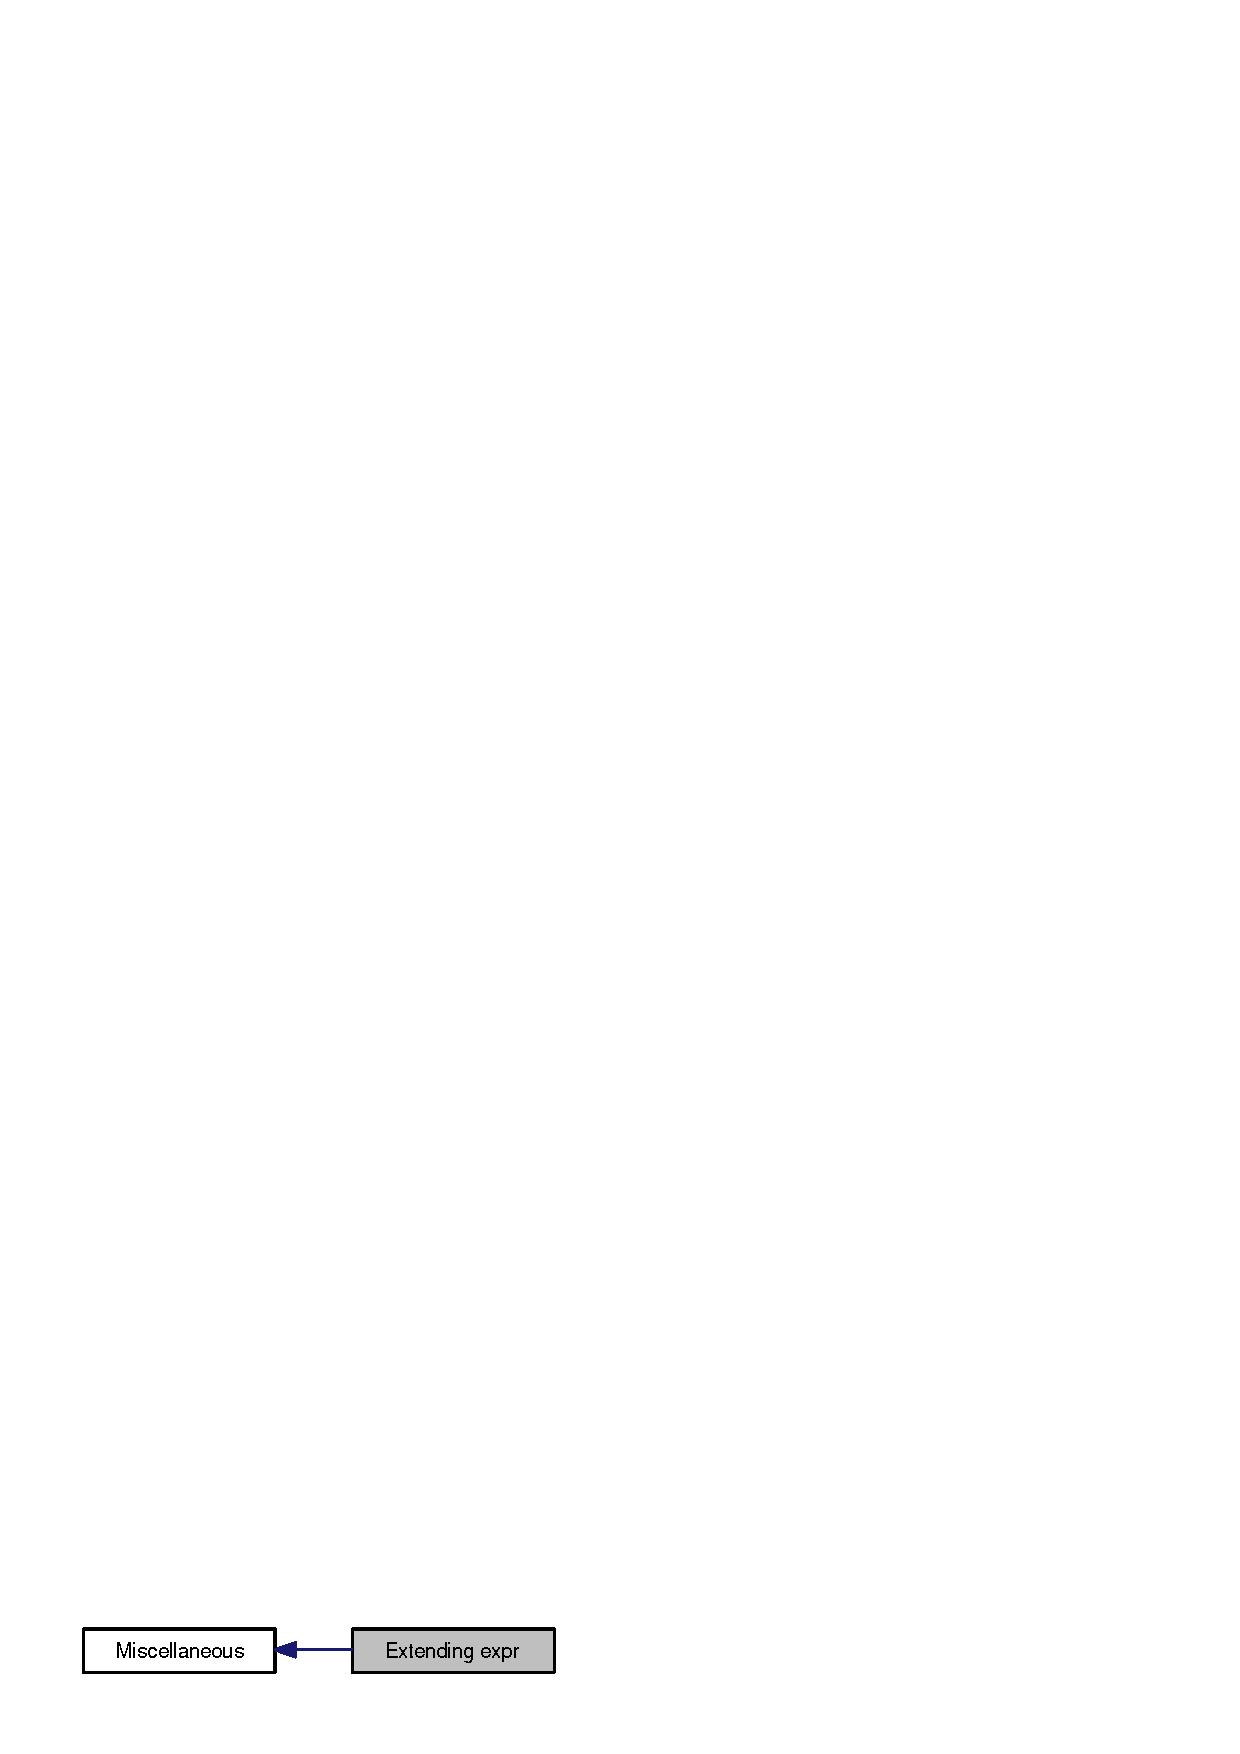
\includegraphics[width=135pt]{group__expr}
\end{center}
\end{figure}
\subsection*{Data Structures}
\begin{DoxyCompactItemize}
\item 
struct \hyperlink{structEx__ex}{Ex\_\-ex}
\begin{DoxyCompactList}\small\item\em ex\_\-ex. \item\end{DoxyCompactList}\item 
struct \hyperlink{structt__expr}{t\_\-expr}
\begin{DoxyCompactList}\small\item\em Struct for an instance of expr. \item\end{DoxyCompactList}\end{DoxyCompactItemize}
\subsection*{Defines}
\begin{DoxyCompactItemize}
\item 
\hypertarget{group__expr_gab46405eed108482db4fc1d4fc2ef7077}{
\#define \hyperlink{group__expr_gab46405eed108482db4fc1d4fc2ef7077}{ex\_\-int}~ex\_\-cont.v\_\-int}
\label{group__expr_gab46405eed108482db4fc1d4fc2ef7077}

\begin{DoxyCompactList}\small\item\em shortcut for accessing members of an \hyperlink{structEx__ex}{Ex\_\-ex} struct's ex\_\-cont union. \item\end{DoxyCompactList}\item 
\hypertarget{group__expr_gad3369510d47d2972732791c0f685387e}{
\#define \hyperlink{group__expr_gad3369510d47d2972732791c0f685387e}{ex\_\-flt}~ex\_\-cont.v\_\-flt}
\label{group__expr_gad3369510d47d2972732791c0f685387e}

\begin{DoxyCompactList}\small\item\em shortcut for accessing members of an \hyperlink{structEx__ex}{Ex\_\-ex} struct's ex\_\-cont union. \item\end{DoxyCompactList}\item 
\hypertarget{group__expr_ga9ebc5ab45aa899ff6f98c53dd4c31f49}{
\#define \hyperlink{group__expr_ga9ebc5ab45aa899ff6f98c53dd4c31f49}{ex\_\-op}~ex\_\-cont.op}
\label{group__expr_ga9ebc5ab45aa899ff6f98c53dd4c31f49}

\begin{DoxyCompactList}\small\item\em shortcut for accessing members of an \hyperlink{structEx__ex}{Ex\_\-ex} struct's ex\_\-cont union. \item\end{DoxyCompactList}\item 
\hypertarget{group__expr_gacf7a6e4e930397f16dca45aa0ecbcbcf}{
\#define \hyperlink{group__expr_gacf7a6e4e930397f16dca45aa0ecbcbcf}{ex\_\-ptr}~ex\_\-cont.ptr}
\label{group__expr_gacf7a6e4e930397f16dca45aa0ecbcbcf}

\begin{DoxyCompactList}\small\item\em shortcut for accessing members of an \hyperlink{structEx__ex}{Ex\_\-ex} struct's ex\_\-cont union. \item\end{DoxyCompactList}\end{DoxyCompactItemize}
\subsection*{Enumerations}
\begin{DoxyCompactItemize}
\item 
enum \hyperlink{group__expr_ga64f1e232097cbd73318392635e6bab0e}{e\_\-max\_\-expr\_\-types} \{ \par
\hyperlink{group__expr_gga64f1e232097cbd73318392635e6bab0ea099243d5b48eaf0e63699c974b587abf}{ET\_\-INT} =  0x1, 
\par
\hyperlink{group__expr_gga64f1e232097cbd73318392635e6bab0ea968ca4519aba1e3b947f8b71fd8fe623}{ET\_\-FLT} =  0x2, 
\par
\hyperlink{group__expr_gga64f1e232097cbd73318392635e6bab0ea617f0c0aa78a4df760188842fafbeda1}{ET\_\-OP} =  0x3, 
\par
\hyperlink{group__expr_gga64f1e232097cbd73318392635e6bab0eadff34cf618701594e4cd4d2d5ff439e8}{ET\_\-STR} =  0x4, 
\par
\hyperlink{group__expr_gga64f1e232097cbd73318392635e6bab0ea82f625c02be30bf2cea5c2daede0f148}{ET\_\-TBL} =  0x5, 
\par
\hyperlink{group__expr_gga64f1e232097cbd73318392635e6bab0eaf061cdcc33a494b192516b0a2bbd1451}{ET\_\-FUNC} =  0x6, 
\par
\hyperlink{group__expr_gga64f1e232097cbd73318392635e6bab0ea858df3673d71d9b70bde311f8996ac3c}{ET\_\-SYM} =  0x7, 
\par
\hyperlink{group__expr_gga64f1e232097cbd73318392635e6bab0eab7e96238528bf76765257287c0aad73a}{ET\_\-VSYM} =  0x8, 
\par
\hyperlink{group__expr_gga64f1e232097cbd73318392635e6bab0ea4358f803dd76e873c6a721a15333a8db}{ET\_\-LP} =  0x9, 
\par
\hyperlink{group__expr_gga64f1e232097cbd73318392635e6bab0ea8f8eacb969330e66d85d106aac740b26}{ET\_\-LB} =  0x10, 
\par
\hyperlink{group__expr_gga64f1e232097cbd73318392635e6bab0ea15d055742150743c638b75029b023a59}{ET\_\-II} =  0x11, 
\par
\hyperlink{group__expr_gga64f1e232097cbd73318392635e6bab0eabdaba3ee25ec2645465c06c8925bb916}{ET\_\-FI} =  0x12, 
\par
\hyperlink{group__expr_gga64f1e232097cbd73318392635e6bab0ea170485f1277407f10d0a6ca6ca8b5cc5}{ET\_\-SI} =  0x13
 \}
\begin{DoxyCompactList}\small\item\em Defines for ex\_\-type. \item\end{DoxyCompactList}\end{DoxyCompactItemize}
\subsection*{Functions}
\begin{DoxyCompactItemize}
\item 
void $\ast$ \hyperlink{group__expr_ga7430f6be4bb5d54c7ded0a9ba6b8961f}{expr\_\-new} (short argc, \hyperlink{structt__atom}{t\_\-atom} $\ast$argv, \hyperlink{structt__atom}{t\_\-atom} $\ast$types)
\begin{DoxyCompactList}\small\item\em Create a new expr object. \item\end{DoxyCompactList}\item 
short \hyperlink{group__expr_ga4f0cecc0328fb7598e5a264e9e41c353}{expr\_\-eval} (\hyperlink{structt__expr}{t\_\-expr} $\ast$x, short argc, \hyperlink{structt__atom}{t\_\-atom} $\ast$argv, \hyperlink{structt__atom}{t\_\-atom} $\ast$result)
\begin{DoxyCompactList}\small\item\em Evaluate an expression in an expr object. \item\end{DoxyCompactList}\end{DoxyCompactItemize}


\subsection{Detailed Description}
If you want to use C-\/like variable expressions that are entered by a user of your object, you can use the \char`\"{}guts\char`\"{} of Max’s expr object in your object. For example, the if object uses expr routines for evaluating a conditional expression, so it can decide whether to send the message after the words then or else. The following functions provide an interface to expr. 

\subsection{Enumeration Type Documentation}
\hypertarget{group__expr_ga64f1e232097cbd73318392635e6bab0e}{
\index{expr@{expr}!e\_\-max\_\-expr\_\-types@{e\_\-max\_\-expr\_\-types}}
\index{e\_\-max\_\-expr\_\-types@{e\_\-max\_\-expr\_\-types}!expr@{expr}}
\subsubsection[{e\_\-max\_\-expr\_\-types}]{\setlength{\rightskip}{0pt plus 5cm}enum {\bf e\_\-max\_\-expr\_\-types}}}
\label{group__expr_ga64f1e232097cbd73318392635e6bab0e}


Defines for ex\_\-type. We treat parenthesis and brackets special to keep a pointer to their match in the content. \begin{Desc}
\item[Enumerator: ]\par
\begin{description}
\index{ET\_\-INT@{ET\_\-INT}!expr@{expr}}\index{expr@{expr}!ET\_\-INT@{ET\_\-INT}}\item[{\em 
\hypertarget{group__expr_gga64f1e232097cbd73318392635e6bab0ea099243d5b48eaf0e63699c974b587abf}{
ET\_\-INT}
\label{group__expr_gga64f1e232097cbd73318392635e6bab0ea099243d5b48eaf0e63699c974b587abf}
}]an int \index{ET\_\-FLT@{ET\_\-FLT}!expr@{expr}}\index{expr@{expr}!ET\_\-FLT@{ET\_\-FLT}}\item[{\em 
\hypertarget{group__expr_gga64f1e232097cbd73318392635e6bab0ea968ca4519aba1e3b947f8b71fd8fe623}{
ET\_\-FLT}
\label{group__expr_gga64f1e232097cbd73318392635e6bab0ea968ca4519aba1e3b947f8b71fd8fe623}
}]a float \index{ET\_\-OP@{ET\_\-OP}!expr@{expr}}\index{expr@{expr}!ET\_\-OP@{ET\_\-OP}}\item[{\em 
\hypertarget{group__expr_gga64f1e232097cbd73318392635e6bab0ea617f0c0aa78a4df760188842fafbeda1}{
ET\_\-OP}
\label{group__expr_gga64f1e232097cbd73318392635e6bab0ea617f0c0aa78a4df760188842fafbeda1}
}]operator \index{ET\_\-STR@{ET\_\-STR}!expr@{expr}}\index{expr@{expr}!ET\_\-STR@{ET\_\-STR}}\item[{\em 
\hypertarget{group__expr_gga64f1e232097cbd73318392635e6bab0eadff34cf618701594e4cd4d2d5ff439e8}{
ET\_\-STR}
\label{group__expr_gga64f1e232097cbd73318392635e6bab0eadff34cf618701594e4cd4d2d5ff439e8}
}]string \index{ET\_\-TBL@{ET\_\-TBL}!expr@{expr}}\index{expr@{expr}!ET\_\-TBL@{ET\_\-TBL}}\item[{\em 
\hypertarget{group__expr_gga64f1e232097cbd73318392635e6bab0ea82f625c02be30bf2cea5c2daede0f148}{
ET\_\-TBL}
\label{group__expr_gga64f1e232097cbd73318392635e6bab0ea82f625c02be30bf2cea5c2daede0f148}
}]a table, the content is a pointer \index{ET\_\-FUNC@{ET\_\-FUNC}!expr@{expr}}\index{expr@{expr}!ET\_\-FUNC@{ET\_\-FUNC}}\item[{\em 
\hypertarget{group__expr_gga64f1e232097cbd73318392635e6bab0eaf061cdcc33a494b192516b0a2bbd1451}{
ET\_\-FUNC}
\label{group__expr_gga64f1e232097cbd73318392635e6bab0eaf061cdcc33a494b192516b0a2bbd1451}
}]a function \index{ET\_\-SYM@{ET\_\-SYM}!expr@{expr}}\index{expr@{expr}!ET\_\-SYM@{ET\_\-SYM}}\item[{\em 
\hypertarget{group__expr_gga64f1e232097cbd73318392635e6bab0ea858df3673d71d9b70bde311f8996ac3c}{
ET\_\-SYM}
\label{group__expr_gga64f1e232097cbd73318392635e6bab0ea858df3673d71d9b70bde311f8996ac3c}
}]symbol (\char`\"{}string\char`\"{}) \index{ET\_\-VSYM@{ET\_\-VSYM}!expr@{expr}}\index{expr@{expr}!ET\_\-VSYM@{ET\_\-VSYM}}\item[{\em 
\hypertarget{group__expr_gga64f1e232097cbd73318392635e6bab0eab7e96238528bf76765257287c0aad73a}{
ET\_\-VSYM}
\label{group__expr_gga64f1e232097cbd73318392635e6bab0eab7e96238528bf76765257287c0aad73a}
}]variable symbol (\char`\"{}\$s?\char`\"{}) \index{ET\_\-LP@{ET\_\-LP}!expr@{expr}}\index{expr@{expr}!ET\_\-LP@{ET\_\-LP}}\item[{\em 
\hypertarget{group__expr_gga64f1e232097cbd73318392635e6bab0ea4358f803dd76e873c6a721a15333a8db}{
ET\_\-LP}
\label{group__expr_gga64f1e232097cbd73318392635e6bab0ea4358f803dd76e873c6a721a15333a8db}
}]left parenthesis \index{ET\_\-LB@{ET\_\-LB}!expr@{expr}}\index{expr@{expr}!ET\_\-LB@{ET\_\-LB}}\item[{\em 
\hypertarget{group__expr_gga64f1e232097cbd73318392635e6bab0ea8f8eacb969330e66d85d106aac740b26}{
ET\_\-LB}
\label{group__expr_gga64f1e232097cbd73318392635e6bab0ea8f8eacb969330e66d85d106aac740b26}
}]left bracket \index{ET\_\-II@{ET\_\-II}!expr@{expr}}\index{expr@{expr}!ET\_\-II@{ET\_\-II}}\item[{\em 
\hypertarget{group__expr_gga64f1e232097cbd73318392635e6bab0ea15d055742150743c638b75029b023a59}{
ET\_\-II}
\label{group__expr_gga64f1e232097cbd73318392635e6bab0ea15d055742150743c638b75029b023a59}
}]and integer inlet \index{ET\_\-FI@{ET\_\-FI}!expr@{expr}}\index{expr@{expr}!ET\_\-FI@{ET\_\-FI}}\item[{\em 
\hypertarget{group__expr_gga64f1e232097cbd73318392635e6bab0eabdaba3ee25ec2645465c06c8925bb916}{
ET\_\-FI}
\label{group__expr_gga64f1e232097cbd73318392635e6bab0eabdaba3ee25ec2645465c06c8925bb916}
}]float inlet \index{ET\_\-SI@{ET\_\-SI}!expr@{expr}}\index{expr@{expr}!ET\_\-SI@{ET\_\-SI}}\item[{\em 
\hypertarget{group__expr_gga64f1e232097cbd73318392635e6bab0ea170485f1277407f10d0a6ca6ca8b5cc5}{
ET\_\-SI}
\label{group__expr_gga64f1e232097cbd73318392635e6bab0ea170485f1277407f10d0a6ca6ca8b5cc5}
}]string inlet \end{description}
\end{Desc}



\subsection{Function Documentation}
\hypertarget{group__expr_ga4f0cecc0328fb7598e5a264e9e41c353}{
\index{expr@{expr}!expr\_\-eval@{expr\_\-eval}}
\index{expr\_\-eval@{expr\_\-eval}!expr@{expr}}
\subsubsection[{expr\_\-eval}]{\setlength{\rightskip}{0pt plus 5cm}short expr\_\-eval ({\bf t\_\-expr} $\ast$ {\em x}, \/  short {\em argc}, \/  {\bf t\_\-atom} $\ast$ {\em argv}, \/  {\bf t\_\-atom} $\ast$ {\em result})}}
\label{group__expr_ga4f0cecc0328fb7598e5a264e9e41c353}


Evaluate an expression in an expr object. 
\begin{DoxyParams}{Parameters}
\item[{\em x}]The expr object to evaluate. \item[{\em argc}]Count of arguments in argv. \item[{\em argv}]Array of nine Atoms that will be substituted for variable arguments (such as \$i1) in the expression. Unused arguments should be of type \hyperlink{group__atom_gga8aa6700e9f00b132eb376db6e39ade47a858ddb5d5927eae3fd699a82c7e174b6}{A\_\-NOTHING}. \item[{\em result}]A pre-\/existing Atom that will hold the type and value of the result of evaluating the expression. \end{DoxyParams}
\begin{DoxyReturn}{Returns}
.
\end{DoxyReturn}
\begin{DoxyRemark}{Remarks}
Evaluates the expression in an expr object with arguments in argv and returns the type and value of the evaluated expression as a \hyperlink{structt__atom}{t\_\-atom} in result. result need only point to a single \hyperlink{structt__atom}{t\_\-atom}, but argv should contain at least argc Atoms. If, as in the example shown above under \hyperlink{group__expr_ga7430f6be4bb5d54c7ded0a9ba6b8961f}{expr\_\-new()}, there are “gaps” between arguments, they should be filled in with \hyperlink{structt__atom}{t\_\-atom} of type \hyperlink{group__atom_gga8aa6700e9f00b132eb376db6e39ade47a858ddb5d5927eae3fd699a82c7e174b6}{A\_\-NOTHING}. 
\end{DoxyRemark}
\hypertarget{group__expr_ga7430f6be4bb5d54c7ded0a9ba6b8961f}{
\index{expr@{expr}!expr\_\-new@{expr\_\-new}}
\index{expr\_\-new@{expr\_\-new}!expr@{expr}}
\subsubsection[{expr\_\-new}]{\setlength{\rightskip}{0pt plus 5cm}void$\ast$ expr\_\-new (short {\em argc}, \/  {\bf t\_\-atom} $\ast$ {\em argv}, \/  {\bf t\_\-atom} $\ast$ {\em types})}}
\label{group__expr_ga7430f6be4bb5d54c7ded0a9ba6b8961f}


Create a new expr object. 
\begin{DoxyParams}{Parameters}
\item[{\em argc}]Count of arguments in argv. \item[{\em argv}]Arguments that are used to create the expr. See the example below for details. \item[{\em types}]A pre-\/existing array of nine t\_\-atoms, that will hold the types of any variable arguments created in the expr. The types are returned in the a\_\-type field of each \hyperlink{structt__atom}{t\_\-atom}. If an argument was not present, \hyperlink{group__atom_gga8aa6700e9f00b132eb376db6e39ade47a858ddb5d5927eae3fd699a82c7e174b6}{A\_\-NOTHING} is returned. \end{DoxyParams}
\begin{DoxyReturn}{Returns}
\hyperlink{group__expr_ga7430f6be4bb5d54c7ded0a9ba6b8961f}{expr\_\-new()} creates an expr object from the arguments in argv and returns the type of any expr-\/style arguments contained in argv (i.e. \$i1, etc.) in atoms in an array pointed to by types.
\end{DoxyReturn}
\begin{DoxyRemark}{Remarks}
types should already exist as an array of nine Atoms, all of which will be filled in by \hyperlink{group__expr_ga7430f6be4bb5d54c7ded0a9ba6b8961f}{expr\_\-new()}. If an argument was not present, it will set to type \hyperlink{group__atom_gga8aa6700e9f00b132eb376db6e39ade47a858ddb5d5927eae3fd699a82c7e174b6}{A\_\-NOTHING}. For example, suppose argv pointed to the following atoms: 
\begin{DoxyCode}
    $i1 (A_SYM) 
    + (A_SYM) 
    $f3 (A_SYM) 
    + (A_SYM) 
    3 (A_LONG) 
\end{DoxyCode}

\end{DoxyRemark}
After calling expr\_\-new, types would contain the following: 
\begin{DoxyCode}
    Index   Argument    Type        Value 
    0   1 ($i1)     A_LONG      0 
    1   2       A_NOTHING   0 
    2   3 ($f3)     A_FLOAT     0.0 
    3   4       A_NOTHING   0 
    4   5       A_NOTHING   0 
    5   6       A_NOTHING   0 
    6   7       A_NOTHING   0 
    7   8       A_NOTHING   0 
    8   9       A_NOTHING   0
\end{DoxyCode}
 
\hypertarget{group__tables}{
\section{Table Access}
\label{group__tables}\index{Table Access@{Table Access}}
}


You can use these functions to access named table objects.  


Collaboration diagram for Table Access:\nopagebreak
\begin{figure}[H]
\begin{center}
\leavevmode
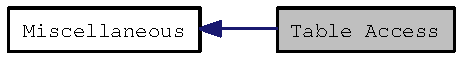
\includegraphics[width=129pt]{group__tables}
\end{center}
\end{figure}
\subsection*{Functions}
\begin{DoxyCompactItemize}
\item 
short \hyperlink{group__tables_ga2c08d1383a235eb8c106c0f3afea6d21}{table\_\-get} (\hyperlink{structt__symbol}{t\_\-symbol} $\ast$s, long $\ast$$\ast$$\ast$hp, long $\ast$sp)
\begin{DoxyCompactList}\small\item\em Get a handle to the data in a named table object. \item\end{DoxyCompactList}\item 
short \hyperlink{group__tables_gaa72449d4792a6108489ef63c5f5ba7a3}{table\_\-dirty} (\hyperlink{structt__symbol}{t\_\-symbol} $\ast$s)
\begin{DoxyCompactList}\small\item\em Mark a table object as having changed data. \item\end{DoxyCompactList}\end{DoxyCompactItemize}


\subsection{Detailed Description}
You can use these functions to access named table objects. Tables have names when the user creates a table with an argument.

The scenario for knowing the name of a table but not the object itself is if you were passed a \hyperlink{structt__symbol}{t\_\-symbol}, either as an argument to your creation function or in some message, with the implication being \char`\"{}do your 
	thing with the data in the table named norris.\char`\"{} 

\subsection{Function Documentation}
\hypertarget{group__tables_gaa72449d4792a6108489ef63c5f5ba7a3}{
\index{tables@{tables}!table\_\-dirty@{table\_\-dirty}}
\index{table\_\-dirty@{table\_\-dirty}!tables@{tables}}
\subsubsection[{table\_\-dirty}]{\setlength{\rightskip}{0pt plus 5cm}short table\_\-dirty ({\bf t\_\-symbol} $\ast$ {\em s})}}
\label{group__tables_gaa72449d4792a6108489ef63c5f5ba7a3}


Mark a table object as having changed data. 
\begin{DoxyParams}{Parameters}
\item[{\em s}]Symbol containing the name of a table object. \end{DoxyParams}
\begin{DoxyReturn}{Returns}
If no table is associated with tableName, table\_\-dirty returns a non-\/zero result. 
\end{DoxyReturn}
\hypertarget{group__tables_ga2c08d1383a235eb8c106c0f3afea6d21}{
\index{tables@{tables}!table\_\-get@{table\_\-get}}
\index{table\_\-get@{table\_\-get}!tables@{tables}}
\subsubsection[{table\_\-get}]{\setlength{\rightskip}{0pt plus 5cm}short table\_\-get ({\bf t\_\-symbol} $\ast$ {\em s}, \/  long $\ast$$\ast$$\ast$ {\em hp}, \/  long $\ast$ {\em sp})}}
\label{group__tables_ga2c08d1383a235eb8c106c0f3afea6d21}


Get a handle to the data in a named table object. 
\begin{DoxyParams}{Parameters}
\item[{\em s}]Symbol containing the name of the table object to find. \item[{\em hp}]Address of a handle where the table’s data will be returned if the named table object is found. \item[{\em sp}]Number of elements in the table (its size in longs). \end{DoxyParams}
\begin{DoxyReturn}{Returns}
If no table object is associated with the symbol tableName, \hyperlink{group__tables_ga2c08d1383a235eb8c106c0f3afea6d21}{table\_\-get()} returns a non-\/zero result.
\end{DoxyReturn}
\begin{DoxyRemark}{Remarks}
table\_\-get searches for a table associated with the \hyperlink{structt__symbol}{t\_\-symbol} tableName. If one is found, a Handle to its elements (stored as an array of long integers) is returned and the function returns 0. Never count on a table to exist across calls to one of your methods. Call table\_\-get and check the result each time you wish to use a table.
\end{DoxyRemark}
Here is an example of retrieving the 40th element of a table: 
\begin{DoxyCode}
    long **storage,size,value; 
    if (!table_get(gensym("somename"),&storage,&size)) { 
        if (size > 40) 
            value = *((*storage)+40); 
    }
\end{DoxyCode}
 
\hypertarget{group__texteditors}{
\section{Text Editor Windows}
\label{group__texteditors}\index{Text Editor Windows@{Text Editor Windows}}
}


Max has a simple built-\/in text editor object that can display and edit text in conjunction with your object.  


Collaboration diagram for Text Editor Windows:\nopagebreak
\begin{figure}[H]
\begin{center}
\leavevmode
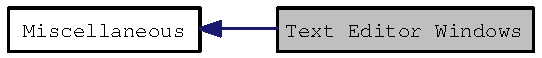
\includegraphics[width=148pt]{group__texteditors}
\end{center}
\end{figure}
Max has a simple built-\/in text editor object that can display and edit text in conjunction with your object. The routines described here let you create a text editor.

When the editor window is about to be closed, your object could receive as many as three messages. The first one, okclose, will be sent if the user has changed the text in the window. This is the standard okclose message that is sent to all \char`\"{}dirty\char`\"{} windows when they are about to be closed, but the text editor window object passes it on to you instead of doing anything itself. Refer to the section on Window Messages for a description of how to write a method for the okclose message. It’s not required that you write one—if you don’t, the behavior of the window will be determined by the setting of the window’s w\_\-scratch bit. If it’s set, no confirmation will be asked when a dirty window is closed (and no okclose message will be sent to the text editor either). The second message, edclose, requires a method that should be added to your object at initialization time. The third message, edSave, allows you to gain access to the text before it is saved, or save it yourself.

\begin{DoxySeeAlso}{See also}
\hyperlink{chapter_enhancements_chapter_enhancements_ed}{Showing a Text Editor} 
\end{DoxySeeAlso}

\hypertarget{group__presets}{
\section{Presets}
\label{group__presets}\index{Presets@{Presets}}
}


Max contains a preset object that has the ability to send preset messages to some or all of the objects (clients) in a Patcher window.  


Collaboration diagram for Presets:\nopagebreak
\begin{figure}[H]
\begin{center}
\leavevmode
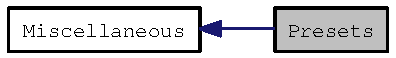
\includegraphics[width=113pt]{group__presets}
\end{center}
\end{figure}
\subsection*{Functions}
\begin{DoxyCompactItemize}
\item 
void \hyperlink{group__presets_ga5f6d86fdc24e371604b764e7581a4fcb}{preset\_\-store} (char $\ast$fmt,...)
\begin{DoxyCompactList}\small\item\em Give the preset object a general message to restore the current state of your object. \item\end{DoxyCompactList}\item 
void \hyperlink{group__presets_ga178edd4c9abaecc58ca6379cf2547298}{preset\_\-set} (\hyperlink{structt__object}{t\_\-object} $\ast$obj, long val)
\begin{DoxyCompactList}\small\item\em Restore the state of your object with a set message. \item\end{DoxyCompactList}\item 
void \hyperlink{group__presets_gaf1da6073fef8e3f896602cf7f9738a23}{preset\_\-int} (void $\ast$x, long n)
\begin{DoxyCompactList}\small\item\em Restore the state of your object with an int message. \item\end{DoxyCompactList}\end{DoxyCompactItemize}


\subsection{Detailed Description}
Max contains a preset object that has the ability to send preset messages to some or all of the objects (clients) in a Patcher window. The preset message, sent when the user is storing a preset, is just a request for your object to tell the preset object how to restore your internal state to what it is now. Later, when the user executes a preset, the preset object will send you back the message you had previously said you wanted.

The dialog goes something like this:


\begin{DoxyItemize}
\item During a store…preset object to Client object(s): hello, this is the preset message—tell me how to restore your stateClient object to preset object: send me int 34 (for example)
\item During an execute…preset object to Client object: int 34
\end{DoxyItemize}

The client object won’t know the difference between receiving int 34 from a preset object and receiving a 34 in its leftmost inlet.

It’s not mandatory for your object to respond to the preset message, but it is something that will make users happy. All Max user interface objects currently respond to preset messages. Note that if your object is not a user interface object and implements a preset method, the user will need to connect the outlet of the preset object to its leftmost inlet in order for it to be sent a preset message when the user stores a preset.

Here’s an example of using \hyperlink{group__presets_ga5f6d86fdc24e371604b764e7581a4fcb}{preset\_\-store()} that specifies that the object would like to receive a set message. We assume it has one field, myvalue, which it would like to save and restore.


\begin{DoxyCode}
    void myobject_preset(myobject *x) 
    { 
        preset_store("ossl",x,ob_sym(x),gensym("set"),x->myvalue); 
    }
\end{DoxyCode}


When this preset is executed, the object will receive a set message whose argument will be the value of myvalue. Note that the same thing can be accomplished more easily with \hyperlink{group__presets_ga178edd4c9abaecc58ca6379cf2547298}{preset\_\-set()} and \hyperlink{group__presets_gaf1da6073fef8e3f896602cf7f9738a23}{preset\_\-int()}.

Don’t pass more than 12 items to \hyperlink{group__presets_ga5f6d86fdc24e371604b764e7581a4fcb}{preset\_\-store()}. If you want to store a huge amount of data in a preset, use \hyperlink{group__binbuf_gad8f2272c95a8e89f22f1a9c67272af5e}{binbuf\_\-insert()}.

The following example locates the Binbuf into which the preset data is being collected, then calls \hyperlink{group__binbuf_gad8f2272c95a8e89f22f1a9c67272af5e}{binbuf\_\-insert()} on a previously prepared array of Atoms. It assumes that the state of your object can be restored with a set message.


\begin{DoxyCode}
    void myobject_preset(myObject *x) 
    { 
        void *preset_buf;// Binbuf that stores the preset
        short atomCount; // number of atoms you’re storing
        t_atom atomArray[SOMESIZE];// array of atoms to be stored
    
        // 1. prepare the preset "header" information
        atom_setobj(atomArray,x); 
        atom_setsym(atomArray+1,ob_sym(x)); 
        atom_setsym(atomArray+2,gensym("set")); 
        // fill atomArray+3 with object's state here and set atomCount
    
        // 2. find the Binbuf
        preset_buf = gensym("_preset")->s_thing;
    
        // 3. store the data 
        if (preset_buf) { 
            binbuf_insert(preset_buf,NIL,atomCount,atomArray); 
        } 
    }
\end{DoxyCode}
 

\subsection{Function Documentation}
\hypertarget{group__presets_gaf1da6073fef8e3f896602cf7f9738a23}{
\index{presets@{presets}!preset\_\-int@{preset\_\-int}}
\index{preset\_\-int@{preset\_\-int}!presets@{presets}}
\subsubsection[{preset\_\-int}]{\setlength{\rightskip}{0pt plus 5cm}void preset\_\-int (void $\ast$ {\em x}, \/  long {\em n})}}
\label{group__presets_gaf1da6073fef8e3f896602cf7f9738a23}


Restore the state of your object with an int message. This function causes an int message with the argument value to be sent to your object from the preset object when the user executes a preset. All of the existing user interface objects use the int message for restoring their state when a preset is executed.


\begin{DoxyParams}{Parameters}
\item[{\em x}]Your object. \item[{\em n}]Current value of your object. \end{DoxyParams}
\hypertarget{group__presets_ga178edd4c9abaecc58ca6379cf2547298}{
\index{presets@{presets}!preset\_\-set@{preset\_\-set}}
\index{preset\_\-set@{preset\_\-set}!presets@{presets}}
\subsubsection[{preset\_\-set}]{\setlength{\rightskip}{0pt plus 5cm}void preset\_\-set ({\bf t\_\-object} $\ast$ {\em obj}, \/  long {\em val})}}
\label{group__presets_ga178edd4c9abaecc58ca6379cf2547298}


Restore the state of your object with a set message. This function causes a set message with the argument value to be sent to your object from the preset object when the user executes a preset.


\begin{DoxyParams}{Parameters}
\item[{\em obj}]Your object. \item[{\em val}]Current value of your object. \end{DoxyParams}
\hypertarget{group__presets_ga5f6d86fdc24e371604b764e7581a4fcb}{
\index{presets@{presets}!preset\_\-store@{preset\_\-store}}
\index{preset\_\-store@{preset\_\-store}!presets@{presets}}
\subsubsection[{preset\_\-store}]{\setlength{\rightskip}{0pt plus 5cm}void preset\_\-store (char $\ast$ {\em fmt}, \/   {\em ...})}}
\label{group__presets_ga5f6d86fdc24e371604b764e7581a4fcb}


Give the preset object a general message to restore the current state of your object. This is a general preset function for use when your object’s state cannot be restored with a simple int or set message. The example below shows the expected format for specifying what your current state is to a preset object. The first thing you supply is your object itself, followed by the symbol that is the name of your object’s class (which you can retrieve from your object using the macro ob\_\-sym, declared in ext\_\-mess.h). Next, supply the symbol that specifies the message you want receive (a method for which had better be defined in your class), followed by the arguments to this message—the current values of your object’s fields.


\begin{DoxyParams}{Parameters}
\item[{\em fmt}]C string containing one or more letters corresponding to the types of each element of the message. s for Symbol, l for long, or f for float. \item[{\em ...}]Elements of the message used to restore the state of your object, passed directly to the function as Symbols, longs, or floats. See below for an example that conforms to what the preset object expects. \end{DoxyParams}

\hypertarget{group__evnum}{
\section{Event and File Serial Numbers}
\label{group__evnum}\index{Event and File Serial Numbers@{Event and File Serial Numbers}}
}


If you call \hyperlink{group__inout_ga0b2b38216f2f4dba486bfcd2273f255e}{outlet\_\-int()}, \hyperlink{group__inout_gafbb3f62a413f05a394391afde5b3c30f}{outlet\_\-float()}, \hyperlink{group__inout_gabdef4fbe6e1040dc28204b8070bdcda5}{outlet\_\-list()}, or \hyperlink{group__inout_ga12798ee897e01dac21ee547c4091d8a8}{outlet\_\-anything()} inside a Qelem or during some idle or interrupt time, you should increment Max’s Event Serial Number beforehand.  


Collaboration diagram for Event and File Serial Numbers:\nopagebreak
\begin{figure}[H]
\begin{center}
\leavevmode
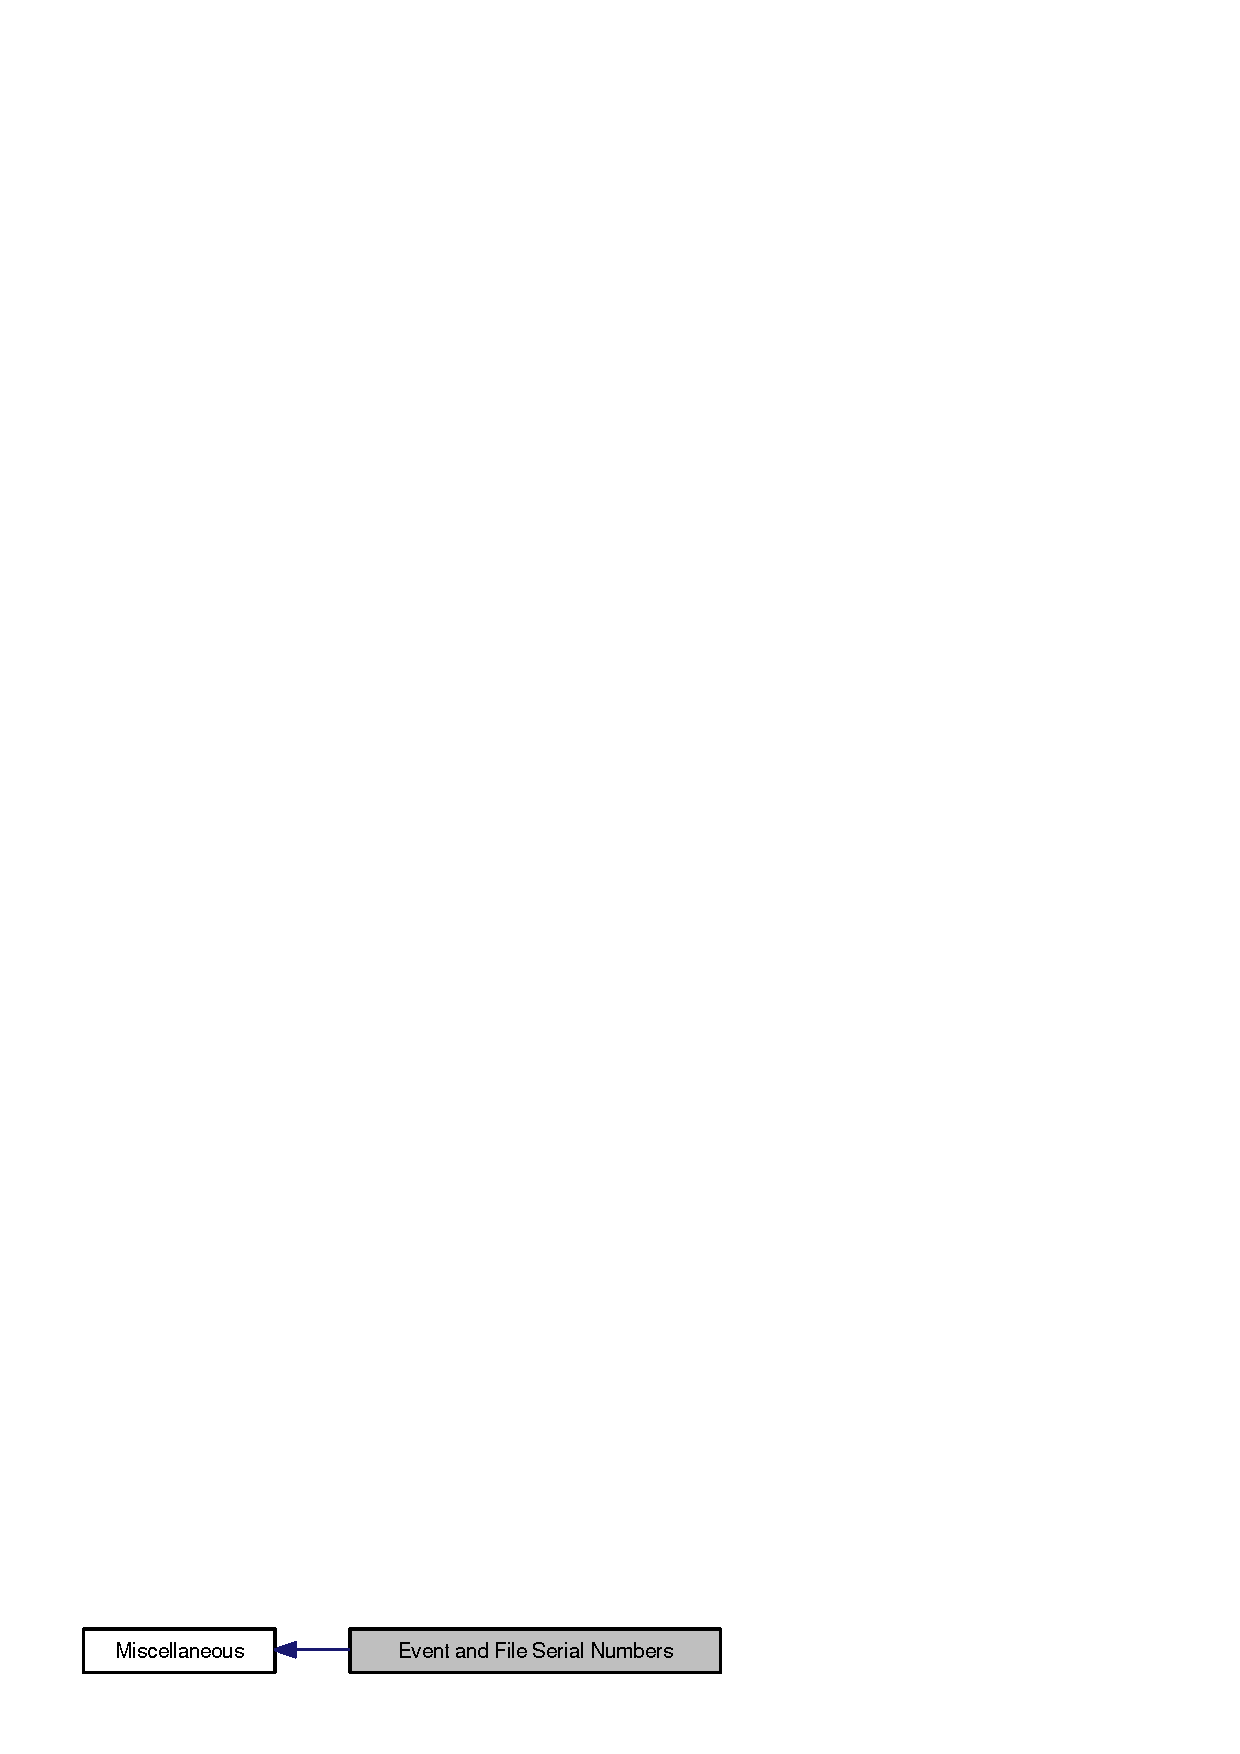
\includegraphics[width=175pt]{group__evnum}
\end{center}
\end{figure}
\subsection*{Functions}
\begin{DoxyCompactItemize}
\item 
\hypertarget{group__evnum_gabe59d84de6401b7331a5cb12f8e16916}{
void \hyperlink{group__evnum_gabe59d84de6401b7331a5cb12f8e16916}{evnum\_\-incr} (void)}
\label{group__evnum_gabe59d84de6401b7331a5cb12f8e16916}

\begin{DoxyCompactList}\small\item\em Increment the event serial number. \item\end{DoxyCompactList}\item 
long \hyperlink{group__evnum_gad8e1d4214caa9159893347d0c1f6198e}{evnum\_\-get} (void)
\begin{DoxyCompactList}\small\item\em Get the current value of the event serial number. \item\end{DoxyCompactList}\item 
long \hyperlink{group__evnum_ga7e7dac31c7f482fec5bf64bf61cdc26b}{serialno} (void)
\begin{DoxyCompactList}\small\item\em Get a unique number for each Patcher file saved. \item\end{DoxyCompactList}\end{DoxyCompactItemize}


\subsection{Detailed Description}
If you call \hyperlink{group__inout_ga0b2b38216f2f4dba486bfcd2273f255e}{outlet\_\-int()}, \hyperlink{group__inout_gafbb3f62a413f05a394391afde5b3c30f}{outlet\_\-float()}, \hyperlink{group__inout_gabdef4fbe6e1040dc28204b8070bdcda5}{outlet\_\-list()}, or \hyperlink{group__inout_ga12798ee897e01dac21ee547c4091d8a8}{outlet\_\-anything()} inside a Qelem or during some idle or interrupt time, you should increment Max’s Event Serial Number beforehand. This number can be read by objects that want to know if two messages they have received occurred at the same logical \char`\"{}time\char`\"{} (in response to the same event). Max increments the serial number for each tick of the clock, each key press, mouse click, and MIDI event. Note that this is different from the file serial number returned by the \hyperlink{group__evnum_ga7e7dac31c7f482fec5bf64bf61cdc26b}{serialno()} function. The file serial number is only incremented when patchers are saved in files. If more than one patcher is saved in a file, the file serial number will change but the event serial number will not.\hypertarget{group__evnum_using_event_serial_numbers}{}\subsection{Using Event Serial Numbers}\label{group__evnum_using_event_serial_numbers}
Here is a Max patch that includes an object called simul that would use the information returned by evnum\_\-get to return a 1 if the right and left inlets receive messages at the same time, 0 if not. The number boxes below show the results of clicking on the button objects or typing a key.

 

\subsection{Function Documentation}
\hypertarget{group__evnum_gad8e1d4214caa9159893347d0c1f6198e}{
\index{evnum@{evnum}!evnum\_\-get@{evnum\_\-get}}
\index{evnum\_\-get@{evnum\_\-get}!evnum@{evnum}}
\subsubsection[{evnum\_\-get}]{\setlength{\rightskip}{0pt plus 5cm}long evnum\_\-get (void)}}
\label{group__evnum_gad8e1d4214caa9159893347d0c1f6198e}


Get the current value of the event serial number. \begin{DoxyReturn}{Returns}
The current value of the event serial number. 
\end{DoxyReturn}
\hypertarget{group__evnum_ga7e7dac31c7f482fec5bf64bf61cdc26b}{
\index{evnum@{evnum}!serialno@{serialno}}
\index{serialno@{serialno}!evnum@{evnum}}
\subsubsection[{serialno}]{\setlength{\rightskip}{0pt plus 5cm}long serialno (void)}}
\label{group__evnum_ga7e7dac31c7f482fec5bf64bf61cdc26b}


Get a unique number for each Patcher file saved. This function returns a serial number that is incremented each time a Patcher file is saved. This routine is useful for objects like table and coll that have multiple objects that refer to the same data, and can “embed” the data inside a Patcher file. If the serial number hasn’t changed since your object was last saved, you can detect this and avoid saving multiple copies of the object’s data.

\begin{DoxyReturn}{Returns}
The serial number. 
\end{DoxyReturn}

\hypertarget{group__loading__max__files}{
\section{Loading Max Files}
\label{group__loading__max__files}\index{Loading Max Files@{Loading Max Files}}
}


Several high-\/level functions permit you to load patcher files.  


Collaboration diagram for Loading Max Files:\nopagebreak
\begin{figure}[H]
\begin{center}
\leavevmode
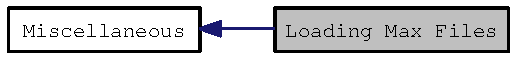
\includegraphics[width=142pt]{group__loading__max__files}
\end{center}
\end{figure}
\subsection*{Functions}
\begin{DoxyCompactItemize}
\item 
short \hyperlink{group__loading__max__files_ga7060a31b3b59a0ba1b08cd5f7b89704b}{readtohandle} (char $\ast$name, short volume, char $\ast$$\ast$$\ast$h, long $\ast$sizep)
\begin{DoxyCompactList}\small\item\em Load a data file into a handle. \item\end{DoxyCompactList}\item 
void $\ast$ \hyperlink{group__loading__max__files_ga1fb5c65c6c0ff9d2c92a7f95da9c7635}{fileload} (char $\ast$name, short vol)
\begin{DoxyCompactList}\small\item\em Load a patcher file by name and volume reference number. \item\end{DoxyCompactList}\item 
void $\ast$ \hyperlink{group__loading__max__files_gaf04b19ac11c4ce1d2641aa409cbd7128}{intload} (char $\ast$name, short volume, \hyperlink{structt__symbol}{t\_\-symbol} $\ast$s, short ac, \hyperlink{structt__atom}{t\_\-atom} $\ast$av, short couldedit)
\begin{DoxyCompactList}\small\item\em Pass arguments to Max files when you open them. \item\end{DoxyCompactList}\item 
void $\ast$ \hyperlink{group__loading__max__files_ga8797a7efcb5a716e8ee0aa8a588b4a69}{stringload} (char $\ast$name)
\begin{DoxyCompactList}\small\item\em Load a patcher file located in the Max search path by name. \item\end{DoxyCompactList}\end{DoxyCompactItemize}


\subsection{Detailed Description}
Several high-\/level functions permit you to load patcher files. These can be used in sophisticated objects that use Patcher objects to perform specific tasks. 

\subsection{Function Documentation}
\hypertarget{group__loading__max__files_ga1fb5c65c6c0ff9d2c92a7f95da9c7635}{
\index{loading\_\-max\_\-files@{loading\_\-max\_\-files}!fileload@{fileload}}
\index{fileload@{fileload}!loading_max_files@{loading\_\-max\_\-files}}
\subsubsection[{fileload}]{\setlength{\rightskip}{0pt plus 5cm}void$\ast$ fileload (char $\ast$ {\em name}, \/  short {\em vol})}}
\label{group__loading__max__files_ga1fb5c65c6c0ff9d2c92a7f95da9c7635}


Load a patcher file by name and volume reference number. 
\begin{DoxyParams}{Parameters}
\item[{\em name}]Filename of the patcher file to load (C string). \item[{\em vol}]Path ID specifying the location of the file. \end{DoxyParams}
\begin{DoxyReturn}{Returns}
If the file is found, fileload tries to open the file, evaluate it, open a window, and bring it to the front. A pointer to the newly created Patcher is returned if loading is successful, otherwise, if the file is not found or there is insufficient memory, zero is returned. 
\end{DoxyReturn}
\hypertarget{group__loading__max__files_gaf04b19ac11c4ce1d2641aa409cbd7128}{
\index{loading\_\-max\_\-files@{loading\_\-max\_\-files}!intload@{intload}}
\index{intload@{intload}!loading_max_files@{loading\_\-max\_\-files}}
\subsubsection[{intload}]{\setlength{\rightskip}{0pt plus 5cm}void$\ast$ intload (char $\ast$ {\em name}, \/  short {\em volume}, \/  {\bf t\_\-symbol} $\ast$ {\em s}, \/  short {\em ac}, \/  {\bf t\_\-atom} $\ast$ {\em av}, \/  short {\em couldedit})}}
\label{group__loading__max__files_gaf04b19ac11c4ce1d2641aa409cbd7128}


Pass arguments to Max files when you open them. This function loads the specified file and returns a pointer to the created object. Historically, \hyperlink{group__loading__max__files_gaf04b19ac11c4ce1d2641aa409cbd7128}{intload()} is was used to open patcher files, whether they are in text or Max binary format. It could also open table files whose contents begin with the \hyperlink{unionword}{word} “table.”


\begin{DoxyParams}{Parameters}
\item[{\em name}]Name of the file to open. \item[{\em volume}]Path ID specifying the location of the file. \item[{\em s}]A symbol. \item[{\em ac}]Count of t\_\-atoms in av. To properly open a patcher file, ac should be 9. \item[{\em av}]Array of t\_\-atoms that will replace the changeable arguments 1-\/9. The default behavior could be to set all these to t\_\-atoms of type \hyperlink{group__atom_gga8aa6700e9f00b132eb376db6e39ade47a002f28879581a6f66ea492b994b96f1e}{A\_\-LONG} with a value of 0. \item[{\em couldedit}]If non-\/zero and the file is not a patcher file, the file is opened as a text file. \end{DoxyParams}
\begin{DoxyReturn}{Returns}
If couldedit is non-\/zero and the file is not a patcher file, it is made into a text editor, and lowload returns 0. If couldedit is non-\/zero, lowload will just alert the user to an error and return 0. If there is no error, the value returned will be a pointer to a patcher or table object. 
\end{DoxyReturn}
\hypertarget{group__loading__max__files_ga7060a31b3b59a0ba1b08cd5f7b89704b}{
\index{loading\_\-max\_\-files@{loading\_\-max\_\-files}!readtohandle@{readtohandle}}
\index{readtohandle@{readtohandle}!loading_max_files@{loading\_\-max\_\-files}}
\subsubsection[{readtohandle}]{\setlength{\rightskip}{0pt plus 5cm}short readtohandle (char $\ast$ {\em name}, \/  short {\em volume}, \/  char $\ast$$\ast$$\ast$ {\em h}, \/  long $\ast$ {\em sizep})}}
\label{group__loading__max__files_ga7060a31b3b59a0ba1b08cd5f7b89704b}


Load a data file into a handle. This is a low-\/level routine used for reading text and data files. You specify the file’s name and Path ID, as well as a pointer to a Handle.


\begin{DoxyParams}{Parameters}
\item[{\em name}]Name of the patcher file to load. \item[{\em volume}]Path ID specifying the location of the file. \item[{\em h}]Pointer to a handle variable that will receive the handle that contains the data in the file. \item[{\em sizep}]Size of the handle returned in h. \end{DoxyParams}
\begin{DoxyReturn}{Returns}
If the file is found, readtohandle creates a Handle, reads all the data in the file into it, assigns the handle to the variable hp, and returns the size of the data in size. readtohandle returns 0 if the file was opened and read successfully, and non-\/zero if there was an error. 
\end{DoxyReturn}
\hypertarget{group__loading__max__files_ga8797a7efcb5a716e8ee0aa8a588b4a69}{
\index{loading\_\-max\_\-files@{loading\_\-max\_\-files}!stringload@{stringload}}
\index{stringload@{stringload}!loading_max_files@{loading\_\-max\_\-files}}
\subsubsection[{stringload}]{\setlength{\rightskip}{0pt plus 5cm}void$\ast$ stringload (char $\ast$ {\em name})}}
\label{group__loading__max__files_ga8797a7efcb5a716e8ee0aa8a588b4a69}


Load a patcher file located in the Max search path by name. This function searches for a patcher file, opens it, evaluates it as a patcher file, opens a window for the patcher and brings it to the front. You need only specify a filename and Max will look through its search path for the file. The search path begins with the current “default volume” that is often the volume of the last opened patcher file, then the folders specified in the File Preferences dialog, searched depth first, then finally the folder that contains the Max application.


\begin{DoxyParams}{Parameters}
\item[{\em name}]Filename of the patcher file to load (C string). \end{DoxyParams}
\begin{DoxyReturn}{Returns}
If \hyperlink{group__loading__max__files_ga8797a7efcb5a716e8ee0aa8a588b4a69}{stringload()} returns a non-\/zero result, you can later use \hyperlink{group__class__old_gadf30646e52376a37b93cc20efac65636}{freeobject()} to close the patcher, or just let users do it themselves. If \hyperlink{group__loading__max__files_ga8797a7efcb5a716e8ee0aa8a588b4a69}{stringload()} returns zero, no file with the specified name was found or there was insufficient memory to open it. 
\end{DoxyReturn}

\hypertarget{group__jmonitor}{
\section{Monitors and Displays}
\label{group__jmonitor}\index{Monitors and Displays@{Monitors and Displays}}
}


Functions for finding our information about the environment.  


Collaboration diagram for Monitors and Displays:\nopagebreak
\begin{figure}[H]
\begin{center}
\leavevmode
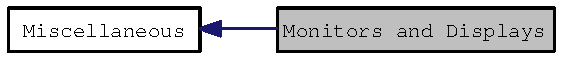
\includegraphics[width=153pt]{group__jmonitor}
\end{center}
\end{figure}
\subsection*{Functions}
\begin{DoxyCompactItemize}
\item 
long \hyperlink{group__jmonitor_ga2bd6c2e27e9ac7bfdd05cbf815ef1082}{jmonitor\_\-getnumdisplays} ()
\begin{DoxyCompactList}\small\item\em Return the number of monitors on which can be displayed. \item\end{DoxyCompactList}\item 
void \hyperlink{group__jmonitor_gac11ee33880f15ef641236e864978d9af}{jmonitor\_\-getdisplayrect} (long workarea, long displayindex, \hyperlink{structt__rect}{t\_\-rect} $\ast$rect)
\begin{DoxyCompactList}\small\item\em Return the \hyperlink{structt__rect}{t\_\-rect} for a given display. \item\end{DoxyCompactList}\item 
void \hyperlink{group__jmonitor_ga0ed7c2c443ef010c4584096967f3b00f}{jmonitor\_\-getdisplayrect\_\-foralldisplays} (long workarea, \hyperlink{structt__rect}{t\_\-rect} $\ast$rect)
\begin{DoxyCompactList}\small\item\em Return a union of all display rects. \item\end{DoxyCompactList}\item 
void \hyperlink{group__jmonitor_ga354f8b2efda018ec3ff2a609205a74a0}{jmonitor\_\-getdisplayrect\_\-forpoint} (long workarea, \hyperlink{structt__pt}{t\_\-pt} pt, \hyperlink{structt__rect}{t\_\-rect} $\ast$rect)
\begin{DoxyCompactList}\small\item\em Return the \hyperlink{structt__rect}{t\_\-rect} for the display on which a point exists. \item\end{DoxyCompactList}\end{DoxyCompactItemize}


\subsection{Detailed Description}
Functions for finding our information about the environment. 

\subsection{Function Documentation}
\hypertarget{group__jmonitor_gac11ee33880f15ef641236e864978d9af}{
\index{jmonitor@{jmonitor}!jmonitor\_\-getdisplayrect@{jmonitor\_\-getdisplayrect}}
\index{jmonitor\_\-getdisplayrect@{jmonitor\_\-getdisplayrect}!jmonitor@{jmonitor}}
\subsubsection[{jmonitor\_\-getdisplayrect}]{\setlength{\rightskip}{0pt plus 5cm}void jmonitor\_\-getdisplayrect (long {\em workarea}, \/  long {\em displayindex}, \/  {\bf t\_\-rect} $\ast$ {\em rect})}}
\label{group__jmonitor_gac11ee33880f15ef641236e864978d9af}


Return the \hyperlink{structt__rect}{t\_\-rect} for a given display. 
\begin{DoxyParams}{Parameters}
\item[{\em workarea}]Set workarea non-\/zero to clip out things like dock / task bar. \item[{\em displayindex}]The index number for a monitor. The primary monitor has an index of 0. \item[{\em rect}]The address of a valid \hyperlink{structt__rect}{t\_\-rect} whose values will be filled-\/in upon return. \end{DoxyParams}
\hypertarget{group__jmonitor_ga0ed7c2c443ef010c4584096967f3b00f}{
\index{jmonitor@{jmonitor}!jmonitor\_\-getdisplayrect\_\-foralldisplays@{jmonitor\_\-getdisplayrect\_\-foralldisplays}}
\index{jmonitor\_\-getdisplayrect\_\-foralldisplays@{jmonitor\_\-getdisplayrect\_\-foralldisplays}!jmonitor@{jmonitor}}
\subsubsection[{jmonitor\_\-getdisplayrect\_\-foralldisplays}]{\setlength{\rightskip}{0pt plus 5cm}void jmonitor\_\-getdisplayrect\_\-foralldisplays (long {\em workarea}, \/  {\bf t\_\-rect} $\ast$ {\em rect})}}
\label{group__jmonitor_ga0ed7c2c443ef010c4584096967f3b00f}


Return a union of all display rects. 
\begin{DoxyParams}{Parameters}
\item[{\em workarea}]Set workarea non-\/zero to clip out things like dock / task bar. \item[{\em rect}]The address of a valid \hyperlink{structt__rect}{t\_\-rect} whose values will be filled-\/in upon return. \end{DoxyParams}
\hypertarget{group__jmonitor_ga354f8b2efda018ec3ff2a609205a74a0}{
\index{jmonitor@{jmonitor}!jmonitor\_\-getdisplayrect\_\-forpoint@{jmonitor\_\-getdisplayrect\_\-forpoint}}
\index{jmonitor\_\-getdisplayrect\_\-forpoint@{jmonitor\_\-getdisplayrect\_\-forpoint}!jmonitor@{jmonitor}}
\subsubsection[{jmonitor\_\-getdisplayrect\_\-forpoint}]{\setlength{\rightskip}{0pt plus 5cm}void jmonitor\_\-getdisplayrect\_\-forpoint (long {\em workarea}, \/  {\bf t\_\-pt} {\em pt}, \/  {\bf t\_\-rect} $\ast$ {\em rect})}}
\label{group__jmonitor_ga354f8b2efda018ec3ff2a609205a74a0}


Return the \hyperlink{structt__rect}{t\_\-rect} for the display on which a point exists. 
\begin{DoxyParams}{Parameters}
\item[{\em workarea}]Set workarea non-\/zero to clip out things like dock / task bar. \item[{\em pt}]A point, for which the monitor will be determined and the rect recturned. \item[{\em rect}]The address of a valid \hyperlink{structt__rect}{t\_\-rect} whose values will be filled-\/in upon return. \end{DoxyParams}
\hypertarget{group__jmonitor_ga2bd6c2e27e9ac7bfdd05cbf815ef1082}{
\index{jmonitor@{jmonitor}!jmonitor\_\-getnumdisplays@{jmonitor\_\-getnumdisplays}}
\index{jmonitor\_\-getnumdisplays@{jmonitor\_\-getnumdisplays}!jmonitor@{jmonitor}}
\subsubsection[{jmonitor\_\-getnumdisplays}]{\setlength{\rightskip}{0pt plus 5cm}long jmonitor\_\-getnumdisplays ()}}
\label{group__jmonitor_ga2bd6c2e27e9ac7bfdd05cbf815ef1082}


Return the number of monitors on which can be displayed. \begin{DoxyReturn}{Returns}
The number of monitors. 
\end{DoxyReturn}

\hypertarget{group__jwind}{
\section{Windows}
\label{group__jwind}\index{Windows@{Windows}}
}


Collaboration diagram for Windows:\nopagebreak
\begin{figure}[H]
\begin{center}
\leavevmode
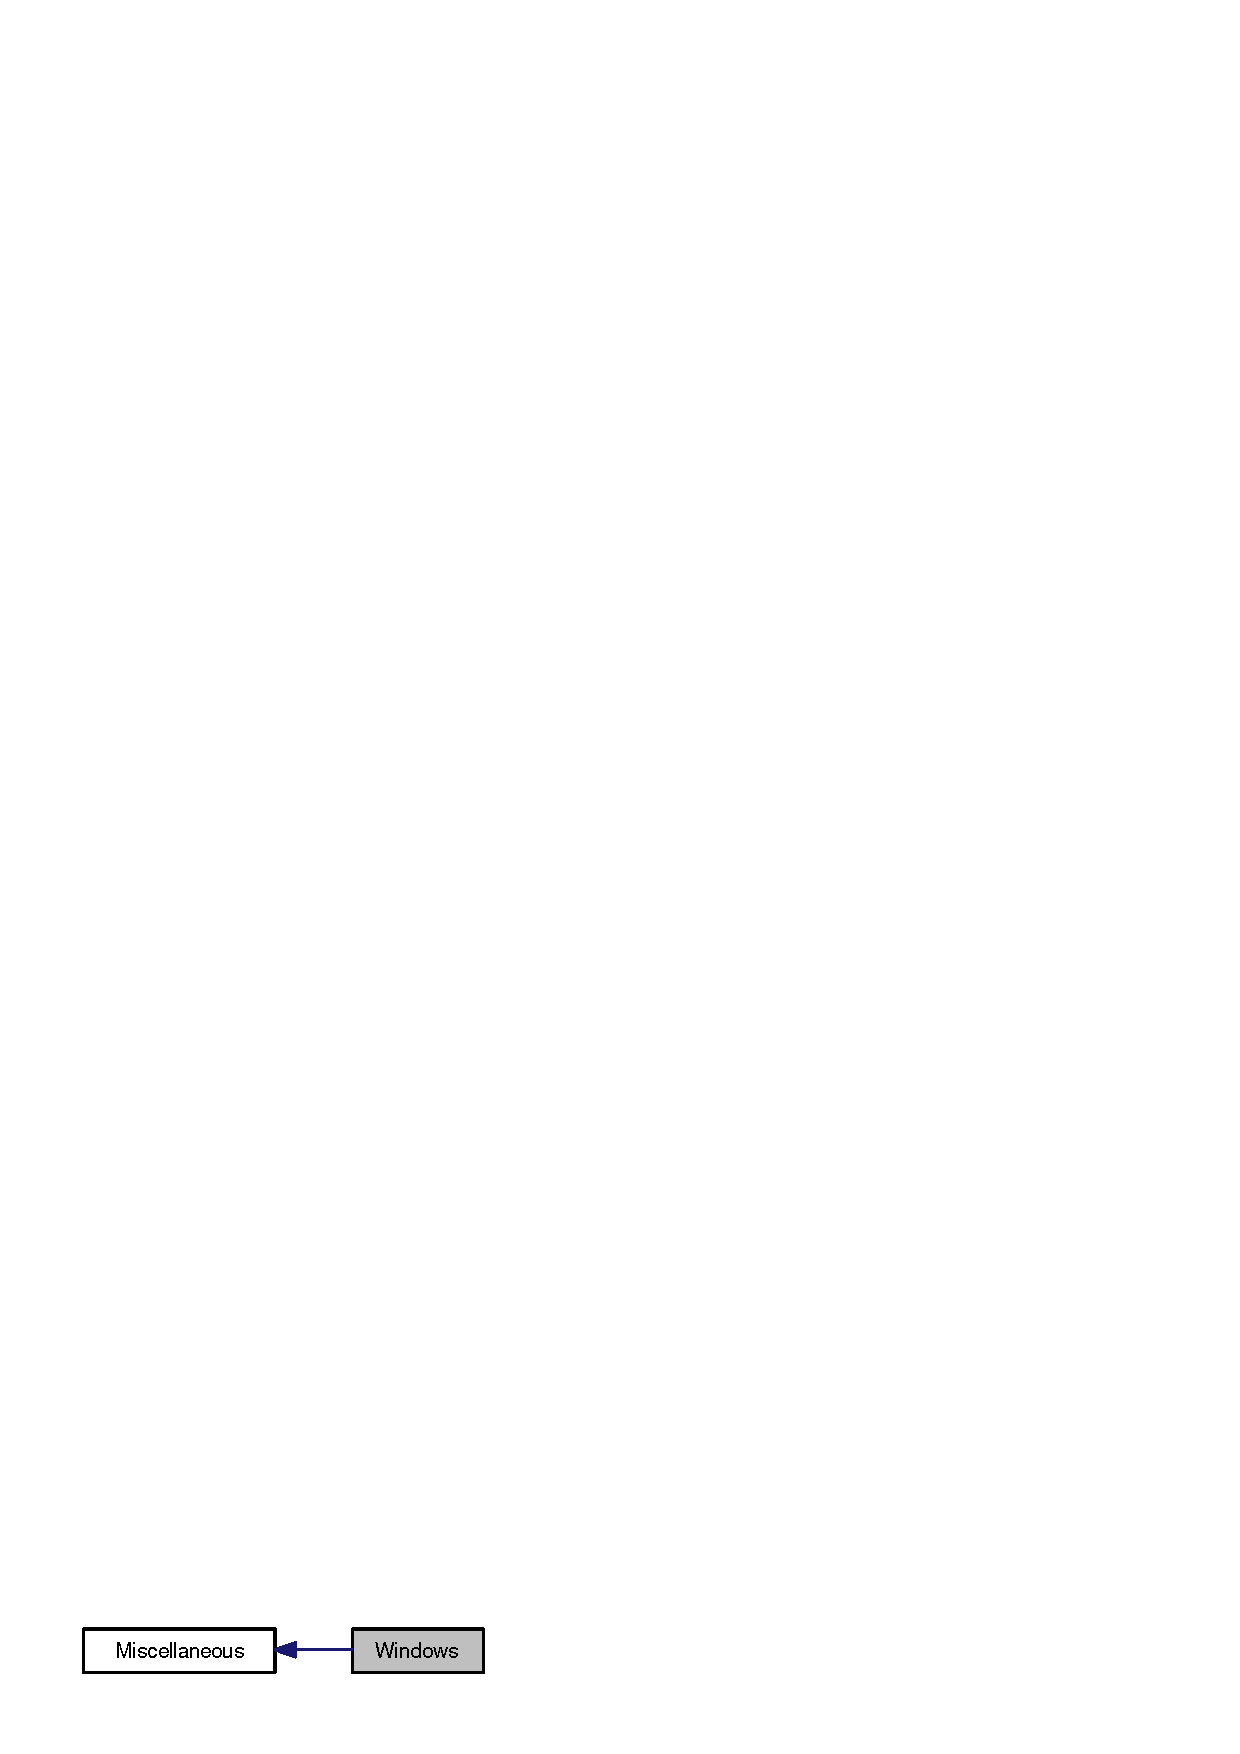
\includegraphics[width=118pt]{group__jwind}
\end{center}
\end{figure}
\subsection*{Functions}
\begin{DoxyCompactItemize}
\item 
\hyperlink{structt__object}{t\_\-object} $\ast$ \hyperlink{group__jwind_ga607f8f4486ff1588ff47c17df61f8af1}{jwind\_\-getactive} (void)
\begin{DoxyCompactList}\small\item\em Get the current window, if any. \item\end{DoxyCompactList}\item 
long \hyperlink{group__jwind_gae627d232548eaefbe00a94ff3c5a1cb6}{jwind\_\-getcount} (void)
\begin{DoxyCompactList}\small\item\em Determine how many windows exist. \item\end{DoxyCompactList}\item 
\hyperlink{structt__object}{t\_\-object} $\ast$ \hyperlink{group__jwind_ga6a7b4f369dfdd3e17e9509cec7bdbb64}{jwind\_\-getat} (long index)
\begin{DoxyCompactList}\small\item\em Return a pointer to the window with a given index. \item\end{DoxyCompactList}\end{DoxyCompactItemize}


\subsection{Function Documentation}
\hypertarget{group__jwind_ga607f8f4486ff1588ff47c17df61f8af1}{
\index{jwind@{jwind}!jwind\_\-getactive@{jwind\_\-getactive}}
\index{jwind\_\-getactive@{jwind\_\-getactive}!jwind@{jwind}}
\subsubsection[{jwind\_\-getactive}]{\setlength{\rightskip}{0pt plus 5cm}{\bf t\_\-object}$\ast$ jwind\_\-getactive (void)}}
\label{group__jwind_ga607f8f4486ff1588ff47c17df61f8af1}


Get the current window, if any. \begin{DoxyReturn}{Returns}
A pointer to the current window, if there is one. Otherwise returns NULL. 
\end{DoxyReturn}
\hypertarget{group__jwind_ga6a7b4f369dfdd3e17e9509cec7bdbb64}{
\index{jwind@{jwind}!jwind\_\-getat@{jwind\_\-getat}}
\index{jwind\_\-getat@{jwind\_\-getat}!jwind@{jwind}}
\subsubsection[{jwind\_\-getat}]{\setlength{\rightskip}{0pt plus 5cm}{\bf t\_\-object}$\ast$ jwind\_\-getat (long {\em index})}}
\label{group__jwind_ga6a7b4f369dfdd3e17e9509cec7bdbb64}


Return a pointer to the window with a given index. 
\begin{DoxyParams}{Parameters}
\item[{\em index}]Get window at index (0 to count-\/1). \end{DoxyParams}
\begin{DoxyReturn}{Returns}
A pointer to a window object. 
\end{DoxyReturn}
\hypertarget{group__jwind_gae627d232548eaefbe00a94ff3c5a1cb6}{
\index{jwind@{jwind}!jwind\_\-getcount@{jwind\_\-getcount}}
\index{jwind\_\-getcount@{jwind\_\-getcount}!jwind@{jwind}}
\subsubsection[{jwind\_\-getcount}]{\setlength{\rightskip}{0pt plus 5cm}long jwind\_\-getcount (void)}}
\label{group__jwind_gae627d232548eaefbe00a94ff3c5a1cb6}


Determine how many windows exist. \begin{DoxyReturn}{Returns}
The number of windows. 
\end{DoxyReturn}

\hypertarget{group__jmouse}{
\section{Mouse and Keyboard}
\label{group__jmouse}\index{Mouse and Keyboard@{Mouse and Keyboard}}
}


Collaboration diagram for Mouse and Keyboard:\nopagebreak
\begin{figure}[H]
\begin{center}
\leavevmode
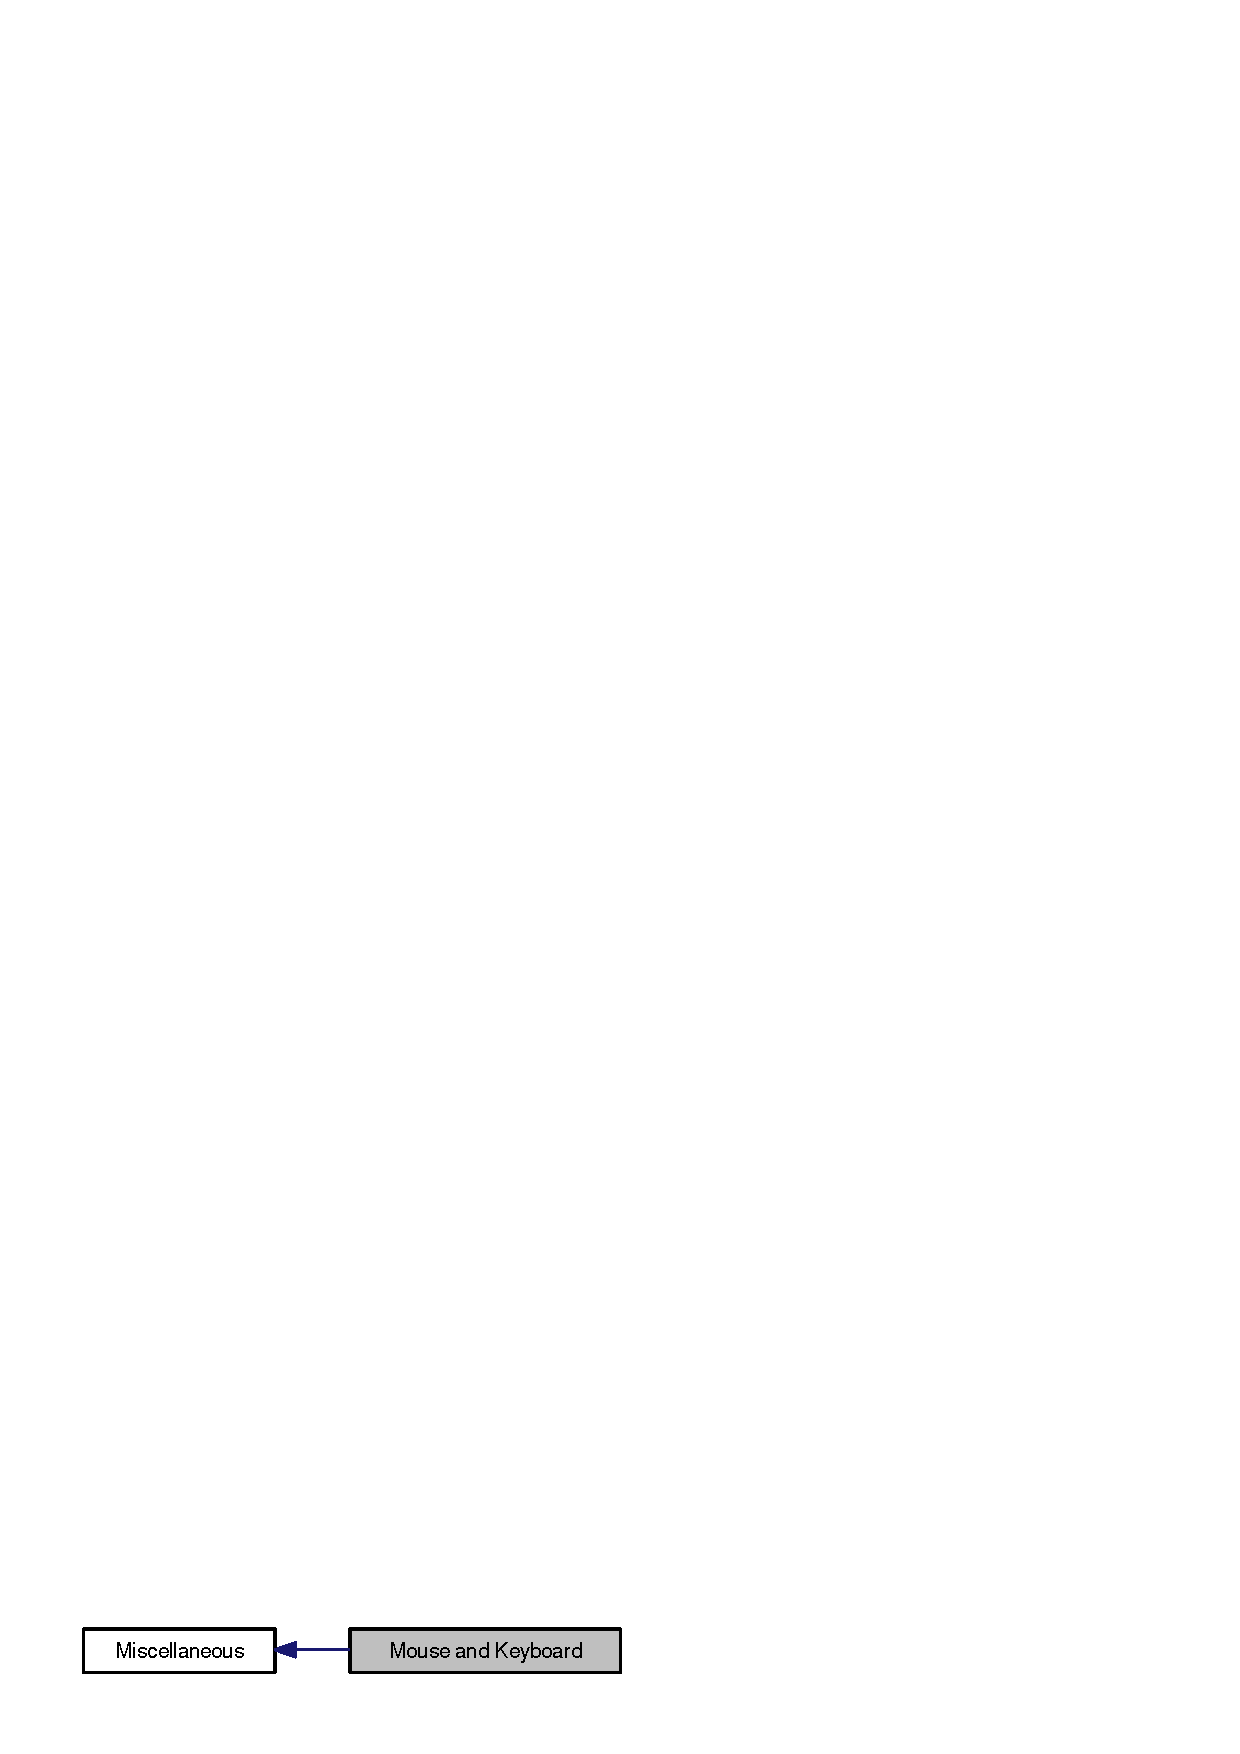
\includegraphics[width=151pt]{group__jmouse}
\end{center}
\end{figure}
\subsection*{Enumerations}
\begin{DoxyCompactItemize}
\item 
enum \hyperlink{group__jmouse_gae6e0f3193b01069c1bce512ab787a681}{t\_\-modifiers} \{ \par
\hyperlink{group__jmouse_ggae6e0f3193b01069c1bce512ab787a681af8f7d9a027fb95ebf4c5422af789cb43}{eCommandKey} =  1, 
\par
\hyperlink{group__jmouse_ggae6e0f3193b01069c1bce512ab787a681a7ce9f8e318648eef4ca2c0cdcf02d388}{eShiftKey} =  2, 
\par
\hyperlink{group__jmouse_ggae6e0f3193b01069c1bce512ab787a681aed96b885e30356b4fe9fa683bc7642a5}{eControlKey} =  4, 
\par
\hyperlink{group__jmouse_ggae6e0f3193b01069c1bce512ab787a681aa397f65aeb5383d87df9e9a6aac41f3d}{eAltKey} =  8, 
\par
\hyperlink{group__jmouse_ggae6e0f3193b01069c1bce512ab787a681a8e53fc2f0be6a158661347c272ac99dc}{eLeftButton} =  16, 
\par
\hyperlink{group__jmouse_ggae6e0f3193b01069c1bce512ab787a681ac8bf4c23189562374f313fd943394f7a}{eRightButton} =  32, 
\par
\hyperlink{group__jmouse_ggae6e0f3193b01069c1bce512ab787a681af5275c58c907c6732c257cac8ba8f56f}{eMiddleButton} =  64, 
\par
\hyperlink{group__jmouse_ggae6e0f3193b01069c1bce512ab787a681aeb8f2adab43f90b789abfec48c1b7ae0}{ePopupMenu} =  128, 
\par
\hyperlink{group__jmouse_ggae6e0f3193b01069c1bce512ab787a681aa20bd26db483cff1f37697899767fdb3}{eCapsLock} =  256, 
\par
\hyperlink{group__jmouse_ggae6e0f3193b01069c1bce512ab787a681a5d0dfbd38a8045f96ba1c9f66bfc270b}{eAutoRepeat} =  512
 \}
\begin{DoxyCompactList}\small\item\em Bit mask values for various meta-\/key presses on the keyboard. \item\end{DoxyCompactList}\item 
enum \hyperlink{group__jmouse_ga4d6e7dd3d4d260c28f3bce9b9f36f764}{t\_\-jmouse\_\-cursortype} \{ \par
\hyperlink{group__jmouse_gga4d6e7dd3d4d260c28f3bce9b9f36f764a7e469e4eae58ff8ba0e04c05e7d01e27}{JMOUSE\_\-CURSOR\_\-NONE}, 
\par
\hyperlink{group__jmouse_gga4d6e7dd3d4d260c28f3bce9b9f36f764ac8245af5ede8e5566629f1a56b07be79}{JMOUSE\_\-CURSOR\_\-ARROW}, 
\par
\hyperlink{group__jmouse_gga4d6e7dd3d4d260c28f3bce9b9f36f764ac17292952b3917c5589840be71d7ce59}{JMOUSE\_\-CURSOR\_\-WAIT}, 
\par
\hyperlink{group__jmouse_gga4d6e7dd3d4d260c28f3bce9b9f36f764ac05d3d2e1d07b631a46539736686d4c3}{JMOUSE\_\-CURSOR\_\-IBEAM}, 
\par
\hyperlink{group__jmouse_gga4d6e7dd3d4d260c28f3bce9b9f36f764a35a12bc385a80316bc6896d1516a4fdb}{JMOUSE\_\-CURSOR\_\-CROSSHAIR}, 
\par
\hyperlink{group__jmouse_gga4d6e7dd3d4d260c28f3bce9b9f36f764a7250b137e39249c7bb6c1c6eb8922c1f}{JMOUSE\_\-CURSOR\_\-COPYING}, 
\par
\hyperlink{group__jmouse_gga4d6e7dd3d4d260c28f3bce9b9f36f764abccdb4469e6489b6a5dfaaf22ce8ba72}{JMOUSE\_\-CURSOR\_\-POINTINGHAND}, 
\par
\hyperlink{group__jmouse_gga4d6e7dd3d4d260c28f3bce9b9f36f764a774be99ae9208193fcc12e9892c5fb13}{JMOUSE\_\-CURSOR\_\-DRAGGINGHAND}, 
\par
\hyperlink{group__jmouse_gga4d6e7dd3d4d260c28f3bce9b9f36f764ab15152ccd94c5d58bd39762623936c0f}{JMOUSE\_\-CURSOR\_\-RESIZE\_\-LEFTRIGHT}, 
\par
\hyperlink{group__jmouse_gga4d6e7dd3d4d260c28f3bce9b9f36f764a52c6ff88129c46cd0185ed62e25d79c9}{JMOUSE\_\-CURSOR\_\-RESIZE\_\-UPDOWN}, 
\par
\hyperlink{group__jmouse_gga4d6e7dd3d4d260c28f3bce9b9f36f764a7d196b58e9ad2fedd1364f18241538bd}{JMOUSE\_\-CURSOR\_\-RESIZE\_\-FOURWAY}, 
\par
\hyperlink{group__jmouse_gga4d6e7dd3d4d260c28f3bce9b9f36f764adfebe355c0d326a5b00eccef325b26e8}{JMOUSE\_\-CURSOR\_\-RESIZE\_\-TOPEDGE}, 
\par
\hyperlink{group__jmouse_gga4d6e7dd3d4d260c28f3bce9b9f36f764a1cb50c2c1de7463dfee84c76b4d97033}{JMOUSE\_\-CURSOR\_\-RESIZE\_\-BOTTOMEDGE}, 
\par
\hyperlink{group__jmouse_gga4d6e7dd3d4d260c28f3bce9b9f36f764a4ab4bb1b2fc5ec983bd7cf47caaca6d0}{JMOUSE\_\-CURSOR\_\-RESIZE\_\-LEFTEDGE}, 
\par
\hyperlink{group__jmouse_gga4d6e7dd3d4d260c28f3bce9b9f36f764afea1f12d5ea482fe2c1975a73e814f70}{JMOUSE\_\-CURSOR\_\-RESIZE\_\-RIGHTEDGE}, 
\par
\hyperlink{group__jmouse_gga4d6e7dd3d4d260c28f3bce9b9f36f764a12bb9da9116a40054c05181106ccc41d}{JMOUSE\_\-CURSOR\_\-RESIZE\_\-TOPLEFTCORNER}, 
\par
\hyperlink{group__jmouse_gga4d6e7dd3d4d260c28f3bce9b9f36f764a1ae8f97d47638054cc83f62a30dc8a69}{JMOUSE\_\-CURSOR\_\-RESIZE\_\-TOPRIGHTCORNER}, 
\par
\hyperlink{group__jmouse_gga4d6e7dd3d4d260c28f3bce9b9f36f764a2f3381b1c55f90dea6758fb5c5329183}{JMOUSE\_\-CURSOR\_\-RESIZE\_\-BOTTOMLEFTCORNER}, 
\par
\hyperlink{group__jmouse_gga4d6e7dd3d4d260c28f3bce9b9f36f764a4d2d8c6debf92b7113cca58446b9fb65}{JMOUSE\_\-CURSOR\_\-RESIZE\_\-BOTTOMRIGHTCORNER}
 \}
\begin{DoxyCompactList}\small\item\em Mouse cursor types. \item\end{DoxyCompactList}\end{DoxyCompactItemize}
\subsection*{Functions}
\begin{DoxyCompactItemize}
\item 
\hyperlink{group__jmouse_gae6e0f3193b01069c1bce512ab787a681}{t\_\-modifiers} \hyperlink{group__jmouse_gaba226c92f2227a75e696e3d302d92ca1}{jkeyboard\_\-getcurrentmodifiers} ()
\begin{DoxyCompactList}\small\item\em Return the last known combination of modifier keys being held by the user. \item\end{DoxyCompactList}\item 
\hyperlink{group__jmouse_gae6e0f3193b01069c1bce512ab787a681}{t\_\-modifiers} \hyperlink{group__jmouse_ga8e41a07bb098e3855b9c60f74d29337e}{jkeyboard\_\-getcurrentmodifiers\_\-realtime} ()
\begin{DoxyCompactList}\small\item\em Return the current combination of modifier keys being held by the user. \item\end{DoxyCompactList}\item 
void \hyperlink{group__jmouse_gaff8fb5e060894aa39293153424c5c939}{jmouse\_\-getposition\_\-global} (int $\ast$x, int $\ast$y)
\begin{DoxyCompactList}\small\item\em Get the position of the mouse cursor in screen coordinates. \item\end{DoxyCompactList}\item 
void \hyperlink{group__jmouse_ga0e92a3887f089a7cc52d142b4e99daac}{jmouse\_\-setposition\_\-global} (int x, int y)
\begin{DoxyCompactList}\small\item\em Set the position of the mouse cursor in screen coordinates. \item\end{DoxyCompactList}\item 
void \hyperlink{group__jmouse_ga030290f12df92eb02c507ed271ffcde9}{jmouse\_\-setposition\_\-view} (\hyperlink{structt__object}{t\_\-object} $\ast$patcherview, double cx, double cy)
\begin{DoxyCompactList}\small\item\em Set the position of the mouse cursor relative to the patcher canvas coordinates. \item\end{DoxyCompactList}\item 
void \hyperlink{group__jmouse_ga8d209aa8fadfbe4d5038b2041eae801e}{jmouse\_\-setposition\_\-box} (\hyperlink{structt__object}{t\_\-object} $\ast$patcherview, \hyperlink{structt__object}{t\_\-object} $\ast$box, double bx, double by)
\begin{DoxyCompactList}\small\item\em Set the position of the mouse cursor relative to a box within the patcher canvas coordinates. \item\end{DoxyCompactList}\item 
void \hyperlink{group__jmouse_gaf8bd554aa25bb4ccd3945a227876fe47}{jmouse\_\-setcursor} (\hyperlink{structt__object}{t\_\-object} $\ast$patcherview, \hyperlink{structt__object}{t\_\-object} $\ast$box, \hyperlink{group__jmouse_ga4d6e7dd3d4d260c28f3bce9b9f36f764}{t\_\-jmouse\_\-cursortype} type)
\begin{DoxyCompactList}\small\item\em Set the mouse cursor. \item\end{DoxyCompactList}\end{DoxyCompactItemize}


\subsection{Enumeration Type Documentation}
\hypertarget{group__jmouse_ga4d6e7dd3d4d260c28f3bce9b9f36f764}{
\index{jmouse@{jmouse}!t\_\-jmouse\_\-cursortype@{t\_\-jmouse\_\-cursortype}}
\index{t\_\-jmouse\_\-cursortype@{t\_\-jmouse\_\-cursortype}!jmouse@{jmouse}}
\subsubsection[{t\_\-jmouse\_\-cursortype}]{\setlength{\rightskip}{0pt plus 5cm}enum {\bf t\_\-jmouse\_\-cursortype}}}
\label{group__jmouse_ga4d6e7dd3d4d260c28f3bce9b9f36f764}


Mouse cursor types. \begin{Desc}
\item[Enumerator: ]\par
\begin{description}
\index{JMOUSE\_\-CURSOR\_\-NONE@{JMOUSE\_\-CURSOR\_\-NONE}!jmouse@{jmouse}}\index{jmouse@{jmouse}!JMOUSE\_\-CURSOR\_\-NONE@{JMOUSE\_\-CURSOR\_\-NONE}}\item[{\em 
\hypertarget{group__jmouse_gga4d6e7dd3d4d260c28f3bce9b9f36f764a7e469e4eae58ff8ba0e04c05e7d01e27}{
JMOUSE\_\-CURSOR\_\-NONE}
\label{group__jmouse_gga4d6e7dd3d4d260c28f3bce9b9f36f764a7e469e4eae58ff8ba0e04c05e7d01e27}
}]None. \index{JMOUSE\_\-CURSOR\_\-ARROW@{JMOUSE\_\-CURSOR\_\-ARROW}!jmouse@{jmouse}}\index{jmouse@{jmouse}!JMOUSE\_\-CURSOR\_\-ARROW@{JMOUSE\_\-CURSOR\_\-ARROW}}\item[{\em 
\hypertarget{group__jmouse_gga4d6e7dd3d4d260c28f3bce9b9f36f764ac8245af5ede8e5566629f1a56b07be79}{
JMOUSE\_\-CURSOR\_\-ARROW}
\label{group__jmouse_gga4d6e7dd3d4d260c28f3bce9b9f36f764ac8245af5ede8e5566629f1a56b07be79}
}]Arrow. \index{JMOUSE\_\-CURSOR\_\-WAIT@{JMOUSE\_\-CURSOR\_\-WAIT}!jmouse@{jmouse}}\index{jmouse@{jmouse}!JMOUSE\_\-CURSOR\_\-WAIT@{JMOUSE\_\-CURSOR\_\-WAIT}}\item[{\em 
\hypertarget{group__jmouse_gga4d6e7dd3d4d260c28f3bce9b9f36f764ac17292952b3917c5589840be71d7ce59}{
JMOUSE\_\-CURSOR\_\-WAIT}
\label{group__jmouse_gga4d6e7dd3d4d260c28f3bce9b9f36f764ac17292952b3917c5589840be71d7ce59}
}]Wait. \index{JMOUSE\_\-CURSOR\_\-IBEAM@{JMOUSE\_\-CURSOR\_\-IBEAM}!jmouse@{jmouse}}\index{jmouse@{jmouse}!JMOUSE\_\-CURSOR\_\-IBEAM@{JMOUSE\_\-CURSOR\_\-IBEAM}}\item[{\em 
\hypertarget{group__jmouse_gga4d6e7dd3d4d260c28f3bce9b9f36f764ac05d3d2e1d07b631a46539736686d4c3}{
JMOUSE\_\-CURSOR\_\-IBEAM}
\label{group__jmouse_gga4d6e7dd3d4d260c28f3bce9b9f36f764ac05d3d2e1d07b631a46539736686d4c3}
}]I-\/Beam. \index{JMOUSE\_\-CURSOR\_\-CROSSHAIR@{JMOUSE\_\-CURSOR\_\-CROSSHAIR}!jmouse@{jmouse}}\index{jmouse@{jmouse}!JMOUSE\_\-CURSOR\_\-CROSSHAIR@{JMOUSE\_\-CURSOR\_\-CROSSHAIR}}\item[{\em 
\hypertarget{group__jmouse_gga4d6e7dd3d4d260c28f3bce9b9f36f764a35a12bc385a80316bc6896d1516a4fdb}{
JMOUSE\_\-CURSOR\_\-CROSSHAIR}
\label{group__jmouse_gga4d6e7dd3d4d260c28f3bce9b9f36f764a35a12bc385a80316bc6896d1516a4fdb}
}]Crosshair. \index{JMOUSE\_\-CURSOR\_\-COPYING@{JMOUSE\_\-CURSOR\_\-COPYING}!jmouse@{jmouse}}\index{jmouse@{jmouse}!JMOUSE\_\-CURSOR\_\-COPYING@{JMOUSE\_\-CURSOR\_\-COPYING}}\item[{\em 
\hypertarget{group__jmouse_gga4d6e7dd3d4d260c28f3bce9b9f36f764a7250b137e39249c7bb6c1c6eb8922c1f}{
JMOUSE\_\-CURSOR\_\-COPYING}
\label{group__jmouse_gga4d6e7dd3d4d260c28f3bce9b9f36f764a7250b137e39249c7bb6c1c6eb8922c1f}
}]Copying. \index{JMOUSE\_\-CURSOR\_\-POINTINGHAND@{JMOUSE\_\-CURSOR\_\-POINTINGHAND}!jmouse@{jmouse}}\index{jmouse@{jmouse}!JMOUSE\_\-CURSOR\_\-POINTINGHAND@{JMOUSE\_\-CURSOR\_\-POINTINGHAND}}\item[{\em 
\hypertarget{group__jmouse_gga4d6e7dd3d4d260c28f3bce9b9f36f764abccdb4469e6489b6a5dfaaf22ce8ba72}{
JMOUSE\_\-CURSOR\_\-POINTINGHAND}
\label{group__jmouse_gga4d6e7dd3d4d260c28f3bce9b9f36f764abccdb4469e6489b6a5dfaaf22ce8ba72}
}]Pointing Hand. \index{JMOUSE\_\-CURSOR\_\-DRAGGINGHAND@{JMOUSE\_\-CURSOR\_\-DRAGGINGHAND}!jmouse@{jmouse}}\index{jmouse@{jmouse}!JMOUSE\_\-CURSOR\_\-DRAGGINGHAND@{JMOUSE\_\-CURSOR\_\-DRAGGINGHAND}}\item[{\em 
\hypertarget{group__jmouse_gga4d6e7dd3d4d260c28f3bce9b9f36f764a774be99ae9208193fcc12e9892c5fb13}{
JMOUSE\_\-CURSOR\_\-DRAGGINGHAND}
\label{group__jmouse_gga4d6e7dd3d4d260c28f3bce9b9f36f764a774be99ae9208193fcc12e9892c5fb13}
}]Dragging Hand. \index{JMOUSE\_\-CURSOR\_\-RESIZE\_\-LEFTRIGHT@{JMOUSE\_\-CURSOR\_\-RESIZE\_\-LEFTRIGHT}!jmouse@{jmouse}}\index{jmouse@{jmouse}!JMOUSE\_\-CURSOR\_\-RESIZE\_\-LEFTRIGHT@{JMOUSE\_\-CURSOR\_\-RESIZE\_\-LEFTRIGHT}}\item[{\em 
\hypertarget{group__jmouse_gga4d6e7dd3d4d260c28f3bce9b9f36f764ab15152ccd94c5d58bd39762623936c0f}{
JMOUSE\_\-CURSOR\_\-RESIZE\_\-LEFTRIGHT}
\label{group__jmouse_gga4d6e7dd3d4d260c28f3bce9b9f36f764ab15152ccd94c5d58bd39762623936c0f}
}]Left-\/Right. \index{JMOUSE\_\-CURSOR\_\-RESIZE\_\-UPDOWN@{JMOUSE\_\-CURSOR\_\-RESIZE\_\-UPDOWN}!jmouse@{jmouse}}\index{jmouse@{jmouse}!JMOUSE\_\-CURSOR\_\-RESIZE\_\-UPDOWN@{JMOUSE\_\-CURSOR\_\-RESIZE\_\-UPDOWN}}\item[{\em 
\hypertarget{group__jmouse_gga4d6e7dd3d4d260c28f3bce9b9f36f764a52c6ff88129c46cd0185ed62e25d79c9}{
JMOUSE\_\-CURSOR\_\-RESIZE\_\-UPDOWN}
\label{group__jmouse_gga4d6e7dd3d4d260c28f3bce9b9f36f764a52c6ff88129c46cd0185ed62e25d79c9}
}]Up-\/Down. \index{JMOUSE\_\-CURSOR\_\-RESIZE\_\-FOURWAY@{JMOUSE\_\-CURSOR\_\-RESIZE\_\-FOURWAY}!jmouse@{jmouse}}\index{jmouse@{jmouse}!JMOUSE\_\-CURSOR\_\-RESIZE\_\-FOURWAY@{JMOUSE\_\-CURSOR\_\-RESIZE\_\-FOURWAY}}\item[{\em 
\hypertarget{group__jmouse_gga4d6e7dd3d4d260c28f3bce9b9f36f764a7d196b58e9ad2fedd1364f18241538bd}{
JMOUSE\_\-CURSOR\_\-RESIZE\_\-FOURWAY}
\label{group__jmouse_gga4d6e7dd3d4d260c28f3bce9b9f36f764a7d196b58e9ad2fedd1364f18241538bd}
}]Four Way. \index{JMOUSE\_\-CURSOR\_\-RESIZE\_\-TOPEDGE@{JMOUSE\_\-CURSOR\_\-RESIZE\_\-TOPEDGE}!jmouse@{jmouse}}\index{jmouse@{jmouse}!JMOUSE\_\-CURSOR\_\-RESIZE\_\-TOPEDGE@{JMOUSE\_\-CURSOR\_\-RESIZE\_\-TOPEDGE}}\item[{\em 
\hypertarget{group__jmouse_gga4d6e7dd3d4d260c28f3bce9b9f36f764adfebe355c0d326a5b00eccef325b26e8}{
JMOUSE\_\-CURSOR\_\-RESIZE\_\-TOPEDGE}
\label{group__jmouse_gga4d6e7dd3d4d260c28f3bce9b9f36f764adfebe355c0d326a5b00eccef325b26e8}
}]Top Edge. \index{JMOUSE\_\-CURSOR\_\-RESIZE\_\-BOTTOMEDGE@{JMOUSE\_\-CURSOR\_\-RESIZE\_\-BOTTOMEDGE}!jmouse@{jmouse}}\index{jmouse@{jmouse}!JMOUSE\_\-CURSOR\_\-RESIZE\_\-BOTTOMEDGE@{JMOUSE\_\-CURSOR\_\-RESIZE\_\-BOTTOMEDGE}}\item[{\em 
\hypertarget{group__jmouse_gga4d6e7dd3d4d260c28f3bce9b9f36f764a1cb50c2c1de7463dfee84c76b4d97033}{
JMOUSE\_\-CURSOR\_\-RESIZE\_\-BOTTOMEDGE}
\label{group__jmouse_gga4d6e7dd3d4d260c28f3bce9b9f36f764a1cb50c2c1de7463dfee84c76b4d97033}
}]Bottom Edge. \index{JMOUSE\_\-CURSOR\_\-RESIZE\_\-LEFTEDGE@{JMOUSE\_\-CURSOR\_\-RESIZE\_\-LEFTEDGE}!jmouse@{jmouse}}\index{jmouse@{jmouse}!JMOUSE\_\-CURSOR\_\-RESIZE\_\-LEFTEDGE@{JMOUSE\_\-CURSOR\_\-RESIZE\_\-LEFTEDGE}}\item[{\em 
\hypertarget{group__jmouse_gga4d6e7dd3d4d260c28f3bce9b9f36f764a4ab4bb1b2fc5ec983bd7cf47caaca6d0}{
JMOUSE\_\-CURSOR\_\-RESIZE\_\-LEFTEDGE}
\label{group__jmouse_gga4d6e7dd3d4d260c28f3bce9b9f36f764a4ab4bb1b2fc5ec983bd7cf47caaca6d0}
}]Left Edge. \index{JMOUSE\_\-CURSOR\_\-RESIZE\_\-RIGHTEDGE@{JMOUSE\_\-CURSOR\_\-RESIZE\_\-RIGHTEDGE}!jmouse@{jmouse}}\index{jmouse@{jmouse}!JMOUSE\_\-CURSOR\_\-RESIZE\_\-RIGHTEDGE@{JMOUSE\_\-CURSOR\_\-RESIZE\_\-RIGHTEDGE}}\item[{\em 
\hypertarget{group__jmouse_gga4d6e7dd3d4d260c28f3bce9b9f36f764afea1f12d5ea482fe2c1975a73e814f70}{
JMOUSE\_\-CURSOR\_\-RESIZE\_\-RIGHTEDGE}
\label{group__jmouse_gga4d6e7dd3d4d260c28f3bce9b9f36f764afea1f12d5ea482fe2c1975a73e814f70}
}]Right Edge. \index{JMOUSE\_\-CURSOR\_\-RESIZE\_\-TOPLEFTCORNER@{JMOUSE\_\-CURSOR\_\-RESIZE\_\-TOPLEFTCORNER}!jmouse@{jmouse}}\index{jmouse@{jmouse}!JMOUSE\_\-CURSOR\_\-RESIZE\_\-TOPLEFTCORNER@{JMOUSE\_\-CURSOR\_\-RESIZE\_\-TOPLEFTCORNER}}\item[{\em 
\hypertarget{group__jmouse_gga4d6e7dd3d4d260c28f3bce9b9f36f764a12bb9da9116a40054c05181106ccc41d}{
JMOUSE\_\-CURSOR\_\-RESIZE\_\-TOPLEFTCORNER}
\label{group__jmouse_gga4d6e7dd3d4d260c28f3bce9b9f36f764a12bb9da9116a40054c05181106ccc41d}
}]Top-\/Left Corner. \index{JMOUSE\_\-CURSOR\_\-RESIZE\_\-TOPRIGHTCORNER@{JMOUSE\_\-CURSOR\_\-RESIZE\_\-TOPRIGHTCORNER}!jmouse@{jmouse}}\index{jmouse@{jmouse}!JMOUSE\_\-CURSOR\_\-RESIZE\_\-TOPRIGHTCORNER@{JMOUSE\_\-CURSOR\_\-RESIZE\_\-TOPRIGHTCORNER}}\item[{\em 
\hypertarget{group__jmouse_gga4d6e7dd3d4d260c28f3bce9b9f36f764a1ae8f97d47638054cc83f62a30dc8a69}{
JMOUSE\_\-CURSOR\_\-RESIZE\_\-TOPRIGHTCORNER}
\label{group__jmouse_gga4d6e7dd3d4d260c28f3bce9b9f36f764a1ae8f97d47638054cc83f62a30dc8a69}
}]Top-\/Right Corner. \index{JMOUSE\_\-CURSOR\_\-RESIZE\_\-BOTTOMLEFTCORNER@{JMOUSE\_\-CURSOR\_\-RESIZE\_\-BOTTOMLEFTCORNER}!jmouse@{jmouse}}\index{jmouse@{jmouse}!JMOUSE\_\-CURSOR\_\-RESIZE\_\-BOTTOMLEFTCORNER@{JMOUSE\_\-CURSOR\_\-RESIZE\_\-BOTTOMLEFTCORNER}}\item[{\em 
\hypertarget{group__jmouse_gga4d6e7dd3d4d260c28f3bce9b9f36f764a2f3381b1c55f90dea6758fb5c5329183}{
JMOUSE\_\-CURSOR\_\-RESIZE\_\-BOTTOMLEFTCORNER}
\label{group__jmouse_gga4d6e7dd3d4d260c28f3bce9b9f36f764a2f3381b1c55f90dea6758fb5c5329183}
}]Bottom-\/Left Corner. \index{JMOUSE\_\-CURSOR\_\-RESIZE\_\-BOTTOMRIGHTCORNER@{JMOUSE\_\-CURSOR\_\-RESIZE\_\-BOTTOMRIGHTCORNER}!jmouse@{jmouse}}\index{jmouse@{jmouse}!JMOUSE\_\-CURSOR\_\-RESIZE\_\-BOTTOMRIGHTCORNER@{JMOUSE\_\-CURSOR\_\-RESIZE\_\-BOTTOMRIGHTCORNER}}\item[{\em 
\hypertarget{group__jmouse_gga4d6e7dd3d4d260c28f3bce9b9f36f764a4d2d8c6debf92b7113cca58446b9fb65}{
JMOUSE\_\-CURSOR\_\-RESIZE\_\-BOTTOMRIGHTCORNER}
\label{group__jmouse_gga4d6e7dd3d4d260c28f3bce9b9f36f764a4d2d8c6debf92b7113cca58446b9fb65}
}]Bottom-\/Right Corner. \end{description}
\end{Desc}

\hypertarget{group__jmouse_gae6e0f3193b01069c1bce512ab787a681}{
\index{jmouse@{jmouse}!t\_\-modifiers@{t\_\-modifiers}}
\index{t\_\-modifiers@{t\_\-modifiers}!jmouse@{jmouse}}
\subsubsection[{t\_\-modifiers}]{\setlength{\rightskip}{0pt plus 5cm}enum {\bf t\_\-modifiers}}}
\label{group__jmouse_gae6e0f3193b01069c1bce512ab787a681}


Bit mask values for various meta-\/key presses on the keyboard. \begin{Desc}
\item[Enumerator: ]\par
\begin{description}
\index{eCommandKey@{eCommandKey}!jmouse@{jmouse}}\index{jmouse@{jmouse}!eCommandKey@{eCommandKey}}\item[{\em 
\hypertarget{group__jmouse_ggae6e0f3193b01069c1bce512ab787a681af8f7d9a027fb95ebf4c5422af789cb43}{
eCommandKey}
\label{group__jmouse_ggae6e0f3193b01069c1bce512ab787a681af8f7d9a027fb95ebf4c5422af789cb43}
}]Command Key. \index{eShiftKey@{eShiftKey}!jmouse@{jmouse}}\index{jmouse@{jmouse}!eShiftKey@{eShiftKey}}\item[{\em 
\hypertarget{group__jmouse_ggae6e0f3193b01069c1bce512ab787a681a7ce9f8e318648eef4ca2c0cdcf02d388}{
eShiftKey}
\label{group__jmouse_ggae6e0f3193b01069c1bce512ab787a681a7ce9f8e318648eef4ca2c0cdcf02d388}
}]Shift Key. \index{eControlKey@{eControlKey}!jmouse@{jmouse}}\index{jmouse@{jmouse}!eControlKey@{eControlKey}}\item[{\em 
\hypertarget{group__jmouse_ggae6e0f3193b01069c1bce512ab787a681aed96b885e30356b4fe9fa683bc7642a5}{
eControlKey}
\label{group__jmouse_ggae6e0f3193b01069c1bce512ab787a681aed96b885e30356b4fe9fa683bc7642a5}
}]Control Key. \index{eAltKey@{eAltKey}!jmouse@{jmouse}}\index{jmouse@{jmouse}!eAltKey@{eAltKey}}\item[{\em 
\hypertarget{group__jmouse_ggae6e0f3193b01069c1bce512ab787a681aa397f65aeb5383d87df9e9a6aac41f3d}{
eAltKey}
\label{group__jmouse_ggae6e0f3193b01069c1bce512ab787a681aa397f65aeb5383d87df9e9a6aac41f3d}
}]Alt Key. \index{eLeftButton@{eLeftButton}!jmouse@{jmouse}}\index{jmouse@{jmouse}!eLeftButton@{eLeftButton}}\item[{\em 
\hypertarget{group__jmouse_ggae6e0f3193b01069c1bce512ab787a681a8e53fc2f0be6a158661347c272ac99dc}{
eLeftButton}
\label{group__jmouse_ggae6e0f3193b01069c1bce512ab787a681a8e53fc2f0be6a158661347c272ac99dc}
}]Left mouse button. \index{eRightButton@{eRightButton}!jmouse@{jmouse}}\index{jmouse@{jmouse}!eRightButton@{eRightButton}}\item[{\em 
\hypertarget{group__jmouse_ggae6e0f3193b01069c1bce512ab787a681ac8bf4c23189562374f313fd943394f7a}{
eRightButton}
\label{group__jmouse_ggae6e0f3193b01069c1bce512ab787a681ac8bf4c23189562374f313fd943394f7a}
}]Right mouse button. \index{eMiddleButton@{eMiddleButton}!jmouse@{jmouse}}\index{jmouse@{jmouse}!eMiddleButton@{eMiddleButton}}\item[{\em 
\hypertarget{group__jmouse_ggae6e0f3193b01069c1bce512ab787a681af5275c58c907c6732c257cac8ba8f56f}{
eMiddleButton}
\label{group__jmouse_ggae6e0f3193b01069c1bce512ab787a681af5275c58c907c6732c257cac8ba8f56f}
}]Middle mouse button. \index{ePopupMenu@{ePopupMenu}!jmouse@{jmouse}}\index{jmouse@{jmouse}!ePopupMenu@{ePopupMenu}}\item[{\em 
\hypertarget{group__jmouse_ggae6e0f3193b01069c1bce512ab787a681aeb8f2adab43f90b789abfec48c1b7ae0}{
ePopupMenu}
\label{group__jmouse_ggae6e0f3193b01069c1bce512ab787a681aeb8f2adab43f90b789abfec48c1b7ae0}
}]Popup Menu (contextual menu requested). \index{eCapsLock@{eCapsLock}!jmouse@{jmouse}}\index{jmouse@{jmouse}!eCapsLock@{eCapsLock}}\item[{\em 
\hypertarget{group__jmouse_ggae6e0f3193b01069c1bce512ab787a681aa20bd26db483cff1f37697899767fdb3}{
eCapsLock}
\label{group__jmouse_ggae6e0f3193b01069c1bce512ab787a681aa20bd26db483cff1f37697899767fdb3}
}]Caps lock. \index{eAutoRepeat@{eAutoRepeat}!jmouse@{jmouse}}\index{jmouse@{jmouse}!eAutoRepeat@{eAutoRepeat}}\item[{\em 
\hypertarget{group__jmouse_ggae6e0f3193b01069c1bce512ab787a681a5d0dfbd38a8045f96ba1c9f66bfc270b}{
eAutoRepeat}
\label{group__jmouse_ggae6e0f3193b01069c1bce512ab787a681a5d0dfbd38a8045f96ba1c9f66bfc270b}
}]Key is generated by key press auto-\/repeat. \end{description}
\end{Desc}



\subsection{Function Documentation}
\hypertarget{group__jmouse_gaba226c92f2227a75e696e3d302d92ca1}{
\index{jmouse@{jmouse}!jkeyboard\_\-getcurrentmodifiers@{jkeyboard\_\-getcurrentmodifiers}}
\index{jkeyboard\_\-getcurrentmodifiers@{jkeyboard\_\-getcurrentmodifiers}!jmouse@{jmouse}}
\subsubsection[{jkeyboard\_\-getcurrentmodifiers}]{\setlength{\rightskip}{0pt plus 5cm}{\bf t\_\-modifiers} jkeyboard\_\-getcurrentmodifiers ()}}
\label{group__jmouse_gaba226c92f2227a75e696e3d302d92ca1}


Return the last known combination of modifier keys being held by the user. \begin{DoxyReturn}{Returns}
The current modifier keys that are activated. 
\end{DoxyReturn}
\hypertarget{group__jmouse_ga8e41a07bb098e3855b9c60f74d29337e}{
\index{jmouse@{jmouse}!jkeyboard\_\-getcurrentmodifiers\_\-realtime@{jkeyboard\_\-getcurrentmodifiers\_\-realtime}}
\index{jkeyboard\_\-getcurrentmodifiers\_\-realtime@{jkeyboard\_\-getcurrentmodifiers\_\-realtime}!jmouse@{jmouse}}
\subsubsection[{jkeyboard\_\-getcurrentmodifiers\_\-realtime}]{\setlength{\rightskip}{0pt plus 5cm}{\bf t\_\-modifiers} jkeyboard\_\-getcurrentmodifiers\_\-realtime ()}}
\label{group__jmouse_ga8e41a07bb098e3855b9c60f74d29337e}


Return the current combination of modifier keys being held by the user. \begin{DoxyReturn}{Returns}
The current modifier keys that are activated. 
\end{DoxyReturn}
\hypertarget{group__jmouse_gaff8fb5e060894aa39293153424c5c939}{
\index{jmouse@{jmouse}!jmouse\_\-getposition\_\-global@{jmouse\_\-getposition\_\-global}}
\index{jmouse\_\-getposition\_\-global@{jmouse\_\-getposition\_\-global}!jmouse@{jmouse}}
\subsubsection[{jmouse\_\-getposition\_\-global}]{\setlength{\rightskip}{0pt plus 5cm}void jmouse\_\-getposition\_\-global (int $\ast$ {\em x}, \/  int $\ast$ {\em y})}}
\label{group__jmouse_gaff8fb5e060894aa39293153424c5c939}


Get the position of the mouse cursor in screen coordinates. 
\begin{DoxyParams}{Parameters}
\item[{\em x}]The address of a variable to hold the x-\/coordinate upon return. \item[{\em y}]The address of a variable to hold the y-\/coordinate upon return. \end{DoxyParams}
\hypertarget{group__jmouse_gaf8bd554aa25bb4ccd3945a227876fe47}{
\index{jmouse@{jmouse}!jmouse\_\-setcursor@{jmouse\_\-setcursor}}
\index{jmouse\_\-setcursor@{jmouse\_\-setcursor}!jmouse@{jmouse}}
\subsubsection[{jmouse\_\-setcursor}]{\setlength{\rightskip}{0pt plus 5cm}void jmouse\_\-setcursor ({\bf t\_\-object} $\ast$ {\em patcherview}, \/  {\bf t\_\-object} $\ast$ {\em box}, \/  {\bf t\_\-jmouse\_\-cursortype} {\em type})}}
\label{group__jmouse_gaf8bd554aa25bb4ccd3945a227876fe47}


Set the mouse cursor. 
\begin{DoxyParams}{Parameters}
\item[{\em patcherview}]The patcherview for which the cursor should be applied. \item[{\em box}]The box for which the cursor should be applied. \item[{\em type}]The type of cursor for the mouse to use. \end{DoxyParams}
\hypertarget{group__jmouse_ga8d209aa8fadfbe4d5038b2041eae801e}{
\index{jmouse@{jmouse}!jmouse\_\-setposition\_\-box@{jmouse\_\-setposition\_\-box}}
\index{jmouse\_\-setposition\_\-box@{jmouse\_\-setposition\_\-box}!jmouse@{jmouse}}
\subsubsection[{jmouse\_\-setposition\_\-box}]{\setlength{\rightskip}{0pt plus 5cm}void jmouse\_\-setposition\_\-box ({\bf t\_\-object} $\ast$ {\em patcherview}, \/  {\bf t\_\-object} $\ast$ {\em box}, \/  double {\em bx}, \/  double {\em by})}}
\label{group__jmouse_ga8d209aa8fadfbe4d5038b2041eae801e}


Set the position of the mouse cursor relative to a box within the patcher canvas coordinates. 
\begin{DoxyParams}{Parameters}
\item[{\em patcherview}]The patcherview containing the box upon which the mouse coordinates are based. \item[{\em box}]The box upon which the mouse coordinates are based. \item[{\em bx}]The new x-\/coordinate of the mouse cursor position. \item[{\em by}]The new y-\/coordinate of the mouse cursor position. \end{DoxyParams}
\hypertarget{group__jmouse_ga0e92a3887f089a7cc52d142b4e99daac}{
\index{jmouse@{jmouse}!jmouse\_\-setposition\_\-global@{jmouse\_\-setposition\_\-global}}
\index{jmouse\_\-setposition\_\-global@{jmouse\_\-setposition\_\-global}!jmouse@{jmouse}}
\subsubsection[{jmouse\_\-setposition\_\-global}]{\setlength{\rightskip}{0pt plus 5cm}void jmouse\_\-setposition\_\-global (int {\em x}, \/  int {\em y})}}
\label{group__jmouse_ga0e92a3887f089a7cc52d142b4e99daac}


Set the position of the mouse cursor in screen coordinates. 
\begin{DoxyParams}{Parameters}
\item[{\em x}]The new x-\/coordinate of the mouse cursor position. \item[{\em y}]The new y-\/coordinate of the mouse cursor position. \end{DoxyParams}
\hypertarget{group__jmouse_ga030290f12df92eb02c507ed271ffcde9}{
\index{jmouse@{jmouse}!jmouse\_\-setposition\_\-view@{jmouse\_\-setposition\_\-view}}
\index{jmouse\_\-setposition\_\-view@{jmouse\_\-setposition\_\-view}!jmouse@{jmouse}}
\subsubsection[{jmouse\_\-setposition\_\-view}]{\setlength{\rightskip}{0pt plus 5cm}void jmouse\_\-setposition\_\-view ({\bf t\_\-object} $\ast$ {\em patcherview}, \/  double {\em cx}, \/  double {\em cy})}}
\label{group__jmouse_ga030290f12df92eb02c507ed271ffcde9}


Set the position of the mouse cursor relative to the patcher canvas coordinates. 
\begin{DoxyParams}{Parameters}
\item[{\em patcherview}]The patcherview upon which the mouse coordinates are based. \item[{\em cx}]The new x-\/coordinate of the mouse cursor position. \item[{\em cy}]The new y-\/coordinate of the mouse cursor position. \end{DoxyParams}

\hypertarget{group__examples}{
\section{Example Projects}
\label{group__examples}\index{Example Projects@{Example Projects}}
}
\subsection*{Files}
\begin{DoxyCompactItemize}
\item 
file \hyperlink{attrtester_8c}{attrtester.c}


\begin{DoxyCompactList}\small\item\em attrtester -\/ a max object shell jeremy bernstein -\/ \href{mailto:jeremy@bootsquad.com}{\tt jeremy@bootsquad.com} \item\end{DoxyCompactList}\item 
file \hyperlink{collect_8cpp}{collect.cpp}


\begin{DoxyCompactList}\small\item\em collect -\/ collect numbers and operate on them. \item\end{DoxyCompactList}\item 
file \hyperlink{dbcuelist_8c}{dbcuelist.c}


\begin{DoxyCompactList}\small\item\em dbcuelist -\/ demonstrate use of a sqlite database \item\end{DoxyCompactList}\item 
file \hyperlink{dbviewer_8c}{dbviewer.c}


\begin{DoxyCompactList}\small\item\em dbviewer -\/ demonstrate use of database views for sqlite and jdataview \item\end{DoxyCompactList}\item 
file \hyperlink{delay2_8c}{delay2.c}


\begin{DoxyCompactList}\small\item\em delay2 -\/ an ITM-\/based delay \item\end{DoxyCompactList}\item 
file \hyperlink{dspstress~_8c}{dspstress$\sim$.c}


\begin{DoxyCompactList}\small\item\em dspstress$\sim$ -\/ very simple msp object that does nothing except eat up a specified \% of processor time \item\end{DoxyCompactList}\item 
file \hyperlink{dummy_8c}{dummy.c}


\begin{DoxyCompactList}\small\item\em dummy -\/ a dummy object jeremy bernstein -\/ \href{mailto:jeremy@bootsquad.com}{\tt jeremy@bootsquad.com} \item\end{DoxyCompactList}\item 
file \hyperlink{filebyte_8c}{filebyte.c}


\begin{DoxyCompactList}\small\item\em filebyte -\/ similar to filein. \item\end{DoxyCompactList}\item 
file \hyperlink{iterate2_8c}{iterate2.c}


\begin{DoxyCompactList}\small\item\em iterate2 -\/ object that iterates through a patcher and its subpatchers jeremy bernstein -\/ \href{mailto:jeremy@bootsquad.com}{\tt jeremy@bootsquad.com} \item\end{DoxyCompactList}\item 
file \hyperlink{iterator_8c}{iterator.c}


\begin{DoxyCompactList}\small\item\em iterator -\/ patch iterator jeremy bernstein -\/ \href{mailto:jeremy@bootsquad.com}{\tt jeremy@bootsquad.com} \item\end{DoxyCompactList}\item 
file \hyperlink{pictmeter~_8c}{pictmeter$\sim$.c}


\begin{DoxyCompactList}\small\item\em pictmeter$\sim$ -\/ audio meter that works by resizing an image \item\end{DoxyCompactList}\item 
file \hyperlink{plussz_8c}{plussz.c}


\begin{DoxyCompactList}\small\item\em plussz.c -\/ one of the simplest max objects you can make -\/rdd 2001 (plussz is/was the name of a Hungarian vitamin C tablet-\/drink from the early 90s) \item\end{DoxyCompactList}\item 
file \hyperlink{plussz2_8c}{plussz2.c}


\begin{DoxyCompactList}\small\item\em plussz2.c -\/ a version of plussz2 that demonstrates the use of proxy inlets. \item\end{DoxyCompactList}\item 
file \hyperlink{plussz~_8c}{plussz$\sim$.c}


\begin{DoxyCompactList}\small\item\em plussz$\sim$ -\/ a very simple example of a basic MSP object \item\end{DoxyCompactList}\item 
file \hyperlink{scripto_8c}{scripto.c}


\begin{DoxyCompactList}\small\item\em scripto -\/ patcher scripting from C example scripto makes a custom UI object and then puts it in a window -\/-\/ so it is similar to the old \char`\"{}kalim\char`\"{} example \item\end{DoxyCompactList}\item 
file \hyperlink{jit_8simple_8cpp}{jit.simple.cpp}


\begin{DoxyCompactList}\small\item\em jit.simple -\/ simple example of a Jitter external + multiplies an incoming matrix by a constant + demonstrates some oft-\/requested example code for using C++ in an extern \item\end{DoxyCompactList}\item 
file \hyperlink{max_8jit_8simple_8c}{max.jit.simple.c}


\begin{DoxyCompactList}\small\item\em max.jit.simple -\/ simple example of a Jitter external multiplies an incoming matrix by a constant \item\end{DoxyCompactList}\item 
file \hyperlink{jit_8simple~_8cpp}{jit.simple$\sim$.cpp}


\begin{DoxyCompactList}\small\item\em max.jit.simple$\sim$ -\/ simple example of an MSP+Jitter combination external. \item\end{DoxyCompactList}\item 
file \hyperlink{max_8jit_8simple~_8c}{max.jit.simple$\sim$.c}


\begin{DoxyCompactList}\small\item\em jit.simple -\/ simple example of a Jitter external multiplies an incoming matrix by a constant \item\end{DoxyCompactList}\item 
file \hyperlink{simplejs_8c}{simplejs.c}


\begin{DoxyCompactList}\small\item\em simplejs -\/ a max object used as a JavaScript class \item\end{DoxyCompactList}\item 
file \hyperlink{simplemax_8c}{simplemax.c}


\begin{DoxyCompactList}\small\item\em simplemax -\/ a max object shell jeremy bernstein -\/ \href{mailto:jeremy@bootsquad.com}{\tt jeremy@bootsquad.com} \item\end{DoxyCompactList}\item 
file \hyperlink{simplemsp~_8c}{simplemsp$\sim$.c}


\begin{DoxyCompactList}\small\item\em simplemsp -\/ an MSP object shell jeremy bernstein -\/ \href{mailto:jeremy@bootsquad.com}{\tt jeremy@bootsquad.com} \item\end{DoxyCompactList}\item 
file \hyperlink{simpletext_8c}{simpletext.c}


\begin{DoxyCompactList}\small\item\em simpletext -\/ show use of text reading and editing \item\end{DoxyCompactList}\item 
file \hyperlink{simpwave~_8c}{simpwave$\sim$.c}


\begin{DoxyCompactList}\small\item\em simpwave$\sim$ -\/ a simple wavetable oscillator using buffer$\sim$ \item\end{DoxyCompactList}\item 
file \hyperlink{uioptimized_8c}{uioptimized.c}


\begin{DoxyCompactList}\small\item\em uioptimized -\/ demonstrate the drawing of various objects using jgraphics \item\end{DoxyCompactList}\item 
file \hyperlink{uisimp2_8c}{uisimp2.c}


\begin{DoxyCompactList}\small\item\em uisimp -\/ a very simple ui object -\/ step 4 \item\end{DoxyCompactList}\item 
file \hyperlink{uisimp3_8c}{uisimp3.c}


\begin{DoxyCompactList}\small\item\em uisimp -\/ a very simple ui object -\/ step 5 \item\end{DoxyCompactList}\item 
file \hyperlink{uisimp4_8c}{uisimp4.c}


\begin{DoxyCompactList}\small\item\em uisimp -\/ a very simple ui object -\/ step 6 \item\end{DoxyCompactList}\item 
file \hyperlink{uisimp5_8c}{uisimp5.c}


\begin{DoxyCompactList}\small\item\em uisimp -\/ a very simple ui object -\/ step 7 \item\end{DoxyCompactList}\item 
file \hyperlink{uitester_8c}{uitester.c}


\begin{DoxyCompactList}\small\item\em uitester -\/ demonstrate the drawing of various objects using jgraphics \item\end{DoxyCompactList}\item 
file \hyperlink{uitextfield_8c}{uitextfield.c}


\begin{DoxyCompactList}\small\item\em uitextfield -\/ demonstrate the textfield with keyboard input \item\end{DoxyCompactList}\item 
file \hyperlink{urner_8c}{urner.c}


\begin{DoxyCompactList}\small\item\em urner -\/ a max object shell jeremy bernstein -\/ \href{mailto:jeremy@bootsquad.com}{\tt jeremy@bootsquad.com} \item\end{DoxyCompactList}\item 
file \hyperlink{whosyourdaddy_8c}{whosyourdaddy.c}


\begin{DoxyCompactList}\small\item\em whosyourdaddy -\/ who's the parent patcher jeremy bernstein -\/ \href{mailto:jeremy@bootsquad.com}{\tt jeremy@bootsquad.com} \item\end{DoxyCompactList}\item 
file \hyperlink{windowwatcher_8c}{windowwatcher.c}


\begin{DoxyCompactList}\small\item\em windowwatcher -\/ Demonstrate how to get notifications about the window for a patcher in which an object exists. \item\end{DoxyCompactList}\end{DoxyCompactItemize}

\hypertarget{group__msp}{
\section{MSP}
\label{group__msp}\index{MSP@{MSP}}
}


Collaboration diagram for MSP:\nopagebreak
\begin{figure}[H]
\begin{center}
\leavevmode
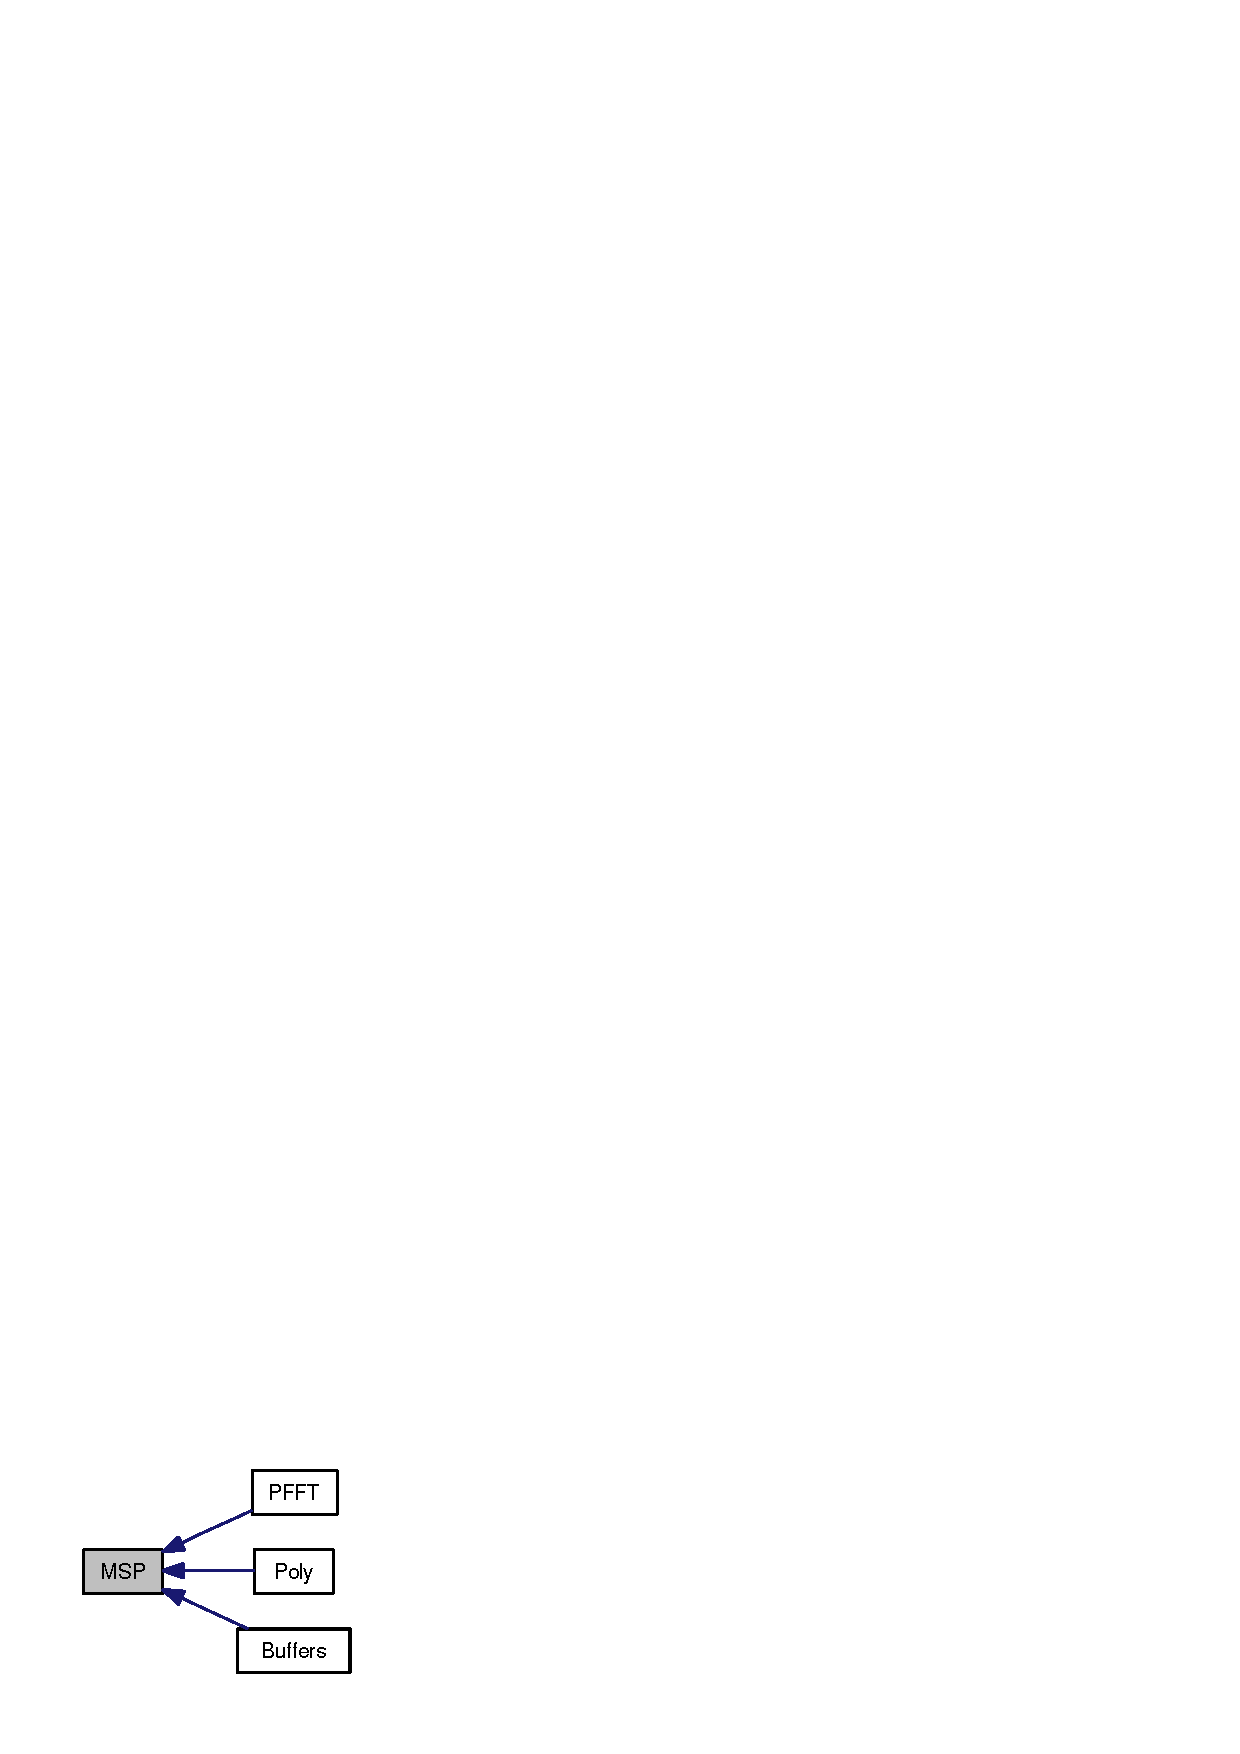
\includegraphics[width=86pt]{group__msp}
\end{center}
\end{figure}
\subsection*{Data Structures}
\begin{DoxyCompactItemize}
\item 
struct \hyperlink{structt__pxobject}{t\_\-pxobject}
\begin{DoxyCompactList}\small\item\em Header for any non-\/ui signal processing object. \item\end{DoxyCompactList}\item 
struct \hyperlink{structt__signal}{t\_\-signal}
\begin{DoxyCompactList}\small\item\em The signal data structure. \item\end{DoxyCompactList}\item 
struct \hyperlink{structt__pxjbox}{t\_\-pxjbox}
\begin{DoxyCompactList}\small\item\em Header for any ui signal processing object. \item\end{DoxyCompactList}\end{DoxyCompactItemize}
\subsection*{Modules}
\begin{DoxyCompactItemize}
\item 
\hyperlink{group__buffers}{Buffers}


\begin{DoxyCompactList}\small\item\em Your object can access shared data stored in an MSP buffer$\sim$ object. \item\end{DoxyCompactList}\item 
\hyperlink{group__pfft}{PFFT}


\begin{DoxyCompactList}\small\item\em When an object is instantiated, it is possible to determine if it is being created in pfft$\sim$ context in the new method. \item\end{DoxyCompactList}\item 
\hyperlink{group__poly}{Poly}


\begin{DoxyCompactList}\small\item\em If your object is instatiated as a voice of a poly$\sim$ object, it is possible both to determine this context and to determine information about the specific voice. \item\end{DoxyCompactList}\end{DoxyCompactItemize}
\subsection*{Defines}
\begin{DoxyCompactItemize}
\item 
\hypertarget{group__msp_ga15695d5ba6bd17ae2e4ac01fff6d2b32}{
\#define \hyperlink{group__msp_ga15695d5ba6bd17ae2e4ac01fff6d2b32}{Z\_\-NO\_\-INPLACE}~1}
\label{group__msp_ga15695d5ba6bd17ae2e4ac01fff6d2b32}

\begin{DoxyCompactList}\small\item\em flag indicating the object doesn't want signals in place \item\end{DoxyCompactList}\item 
\hypertarget{group__msp_ga38363d9e8d77f8f0fcec1a7a1d008977}{
\#define \hyperlink{group__msp_ga38363d9e8d77f8f0fcec1a7a1d008977}{Z\_\-PUT\_\-LAST}~2}
\label{group__msp_ga38363d9e8d77f8f0fcec1a7a1d008977}

\begin{DoxyCompactList}\small\item\em when list of ugens is resorted, put this object at end \item\end{DoxyCompactList}\item 
\hypertarget{group__msp_gafd451e217e2ffd6b8e158b8861fcf866}{
\#define \hyperlink{group__msp_gafd451e217e2ffd6b8e158b8861fcf866}{Z\_\-PUT\_\-FIRST}~4}
\label{group__msp_gafd451e217e2ffd6b8e158b8861fcf866}

\begin{DoxyCompactList}\small\item\em when list of ugens is resorted, put this object at beginning \item\end{DoxyCompactList}\item 
\#define \hyperlink{group__msp_ga598a3330b3c21701223ee0ca14316eca}{PI}~3.14159265358979323846
\begin{DoxyCompactList}\small\item\em The pi constant. \item\end{DoxyCompactList}\item 
\#define \hyperlink{group__msp_ga4912c64aec0c943b7985db6cb61ff83a}{TWOPI}~6.28318530717958647692
\begin{DoxyCompactList}\small\item\em Twice the pi constant. \item\end{DoxyCompactList}\item 
\#define \hyperlink{group__msp_ga54195c4fca76460ca07ba5101bcbc780}{PIOVERTWO}~1.57079632679489661923
\begin{DoxyCompactList}\small\item\em Half of the pi constant. \item\end{DoxyCompactList}\item 
\hypertarget{group__msp_gad15f054306792846a00a5f4e9e5426be}{
\#define \hyperlink{group__msp_gad15f054306792846a00a5f4e9e5426be}{dsp\_\-setup}~z\_\-dsp\_\-setup}
\label{group__msp_gad15f054306792846a00a5f4e9e5426be}

\begin{DoxyCompactList}\small\item\em This is commonly used rather than directly calling \hyperlink{group__msp_ga5c4d70cfb420f13386dd1473143e5825}{z\_\-dsp\_\-setup()} in MSP objects. \item\end{DoxyCompactList}\item 
\hypertarget{group__msp_ga9a981adf6eea7e55d11c1a0b02592a6e}{
\#define \hyperlink{group__msp_ga9a981adf6eea7e55d11c1a0b02592a6e}{dsp\_\-free}~z\_\-dsp\_\-free}
\label{group__msp_ga9a981adf6eea7e55d11c1a0b02592a6e}

\begin{DoxyCompactList}\small\item\em This is commonly used rather than directly calling \hyperlink{group__msp_ga85762f03c915d3860f526a8bf4dd1f3f}{z\_\-dsp\_\-free()} in MSP objects. \item\end{DoxyCompactList}\end{DoxyCompactItemize}
\subsection*{Typedefs}
\begin{DoxyCompactItemize}
\item 
typedef int \hyperlink{group__msp_gaaca420c8a41d33afb2f9e783ce6059e3}{t\_\-int}
\begin{DoxyCompactList}\small\item\em An integer. \item\end{DoxyCompactList}\item 
typedef float \hyperlink{group__msp_gab68e234c9dccbd3d62659023db9f9486}{t\_\-float}
\begin{DoxyCompactList}\small\item\em A float. \item\end{DoxyCompactList}\item 
typedef float \hyperlink{group__msp_ga8ecd36423b35083714b8740c40b57120}{t\_\-sample}
\begin{DoxyCompactList}\small\item\em A sample value. \item\end{DoxyCompactList}\item 
typedef \hyperlink{group__msp_gaaca420c8a41d33afb2f9e783ce6059e3}{t\_\-int} $\ast$($\ast$ \hyperlink{group__msp_gad1bc58df327774373ee9e10ad9026564}{t\_\-perfroutine} )(\hyperlink{group__msp_gaaca420c8a41d33afb2f9e783ce6059e3}{t\_\-int} $\ast$args)
\begin{DoxyCompactList}\small\item\em A function pointer for the audio perform routine used by MSP objects to process blocks of samples. \item\end{DoxyCompactList}\end{DoxyCompactItemize}
\subsection*{Enumerations}
\begin{DoxyCompactItemize}
\item 
enum \{ \par
\hyperlink{group__msp_ggadb49720dc49f7d4e4cf9adbf2948e409a29738f7ba126b5468181b4c017e573d0}{SYS\_\-MAXBLKSIZE} =  2048, 
\par
\hyperlink{group__msp_ggadb49720dc49f7d4e4cf9adbf2948e409a00acca9cc1491d6006a4c38127f02a90}{SYS\_\-MAXSIGS} =  250
 \}
\begin{DoxyCompactList}\small\item\em MSP System Properties. \item\end{DoxyCompactList}\end{DoxyCompactItemize}
\subsection*{Functions}
\begin{DoxyCompactItemize}
\item 
int \hyperlink{group__msp_ga8c499862db0fcf07692989aae3d84c9e}{sys\_\-getmaxblksize} (void)
\begin{DoxyCompactList}\small\item\em Query MSP for the maximum global vector (block) size. \item\end{DoxyCompactList}\item 
int \hyperlink{group__msp_ga1d6745373b742617d281901bb063175d}{sys\_\-getblksize} (void)
\begin{DoxyCompactList}\small\item\em Query MSP for the current global vector (block) size. \item\end{DoxyCompactList}\item 
float \hyperlink{group__msp_ga9d492cbb6af86eaf0afb264e886072e5}{sys\_\-getsr} (void)
\begin{DoxyCompactList}\small\item\em Query MSP for the global sample rate. \item\end{DoxyCompactList}\item 
int \hyperlink{group__msp_ga5705fd255a1bfcf9988db8945a1a4284}{sys\_\-getdspstate} (void)
\begin{DoxyCompactList}\small\item\em Query MSP to determine whether or not it is running. \item\end{DoxyCompactList}\item 
int \hyperlink{group__msp_gac949528775cd2346a95c4f89b91567d6}{sys\_\-getdspobjdspstate} (\hyperlink{structt__object}{t\_\-object} $\ast$o)
\begin{DoxyCompactList}\small\item\em Query MSP to determine whether or not a given audio object is in a running dsp chain. \item\end{DoxyCompactList}\item 
void \hyperlink{group__msp_gae9a75fa230b1db6d8316405d4a6065cc}{dsp\_\-add} (\hyperlink{group__msp_gad1bc58df327774373ee9e10ad9026564}{t\_\-perfroutine} f, int n,...)
\begin{DoxyCompactList}\small\item\em Call this function in your MSP object's dsp method. \item\end{DoxyCompactList}\item 
void \hyperlink{group__msp_gaf8709cab1b4bbbbd78010f765e83b328}{dsp\_\-addv} (\hyperlink{group__msp_gad1bc58df327774373ee9e10ad9026564}{t\_\-perfroutine} f, int n, void $\ast$$\ast$vector)
\begin{DoxyCompactList}\small\item\em Call this function in your MSP object's dsp method. \item\end{DoxyCompactList}\item 
void \hyperlink{group__msp_ga5c4d70cfb420f13386dd1473143e5825}{z\_\-dsp\_\-setup} (\hyperlink{structt__pxobject}{t\_\-pxobject} $\ast$x, long nsignals)
\begin{DoxyCompactList}\small\item\em Call this routine after creating your object in the new instance routine with \hyperlink{group__obj_gacb89ef27c34b45e9037d877375804284}{object\_\-alloc()}. \item\end{DoxyCompactList}\item 
void \hyperlink{group__msp_ga85762f03c915d3860f526a8bf4dd1f3f}{z\_\-dsp\_\-free} (\hyperlink{structt__pxobject}{t\_\-pxobject} $\ast$x)
\begin{DoxyCompactList}\small\item\em This function disposes of any memory used by proxies allocated by \hyperlink{group__msp_gad15f054306792846a00a5f4e9e5426be}{dsp\_\-setup()}. \item\end{DoxyCompactList}\item 
void \hyperlink{group__msp_ga7427ae73a2ad71a1b4ef1bee2fd432fc}{class\_\-dspinit} (\hyperlink{structt__class}{t\_\-class} $\ast$c)
\begin{DoxyCompactList}\small\item\em This routine must be called in your object's initialization routine. \item\end{DoxyCompactList}\item 
void \hyperlink{group__msp_gab2b27239f91fdd5bcc2bac299081687f}{class\_\-dspinitbox} (\hyperlink{structt__class}{t\_\-class} $\ast$c)
\begin{DoxyCompactList}\small\item\em This routine must be called in your object's initialization routine. \item\end{DoxyCompactList}\item 
void \hyperlink{group__msp_gab9219b764ce65abb21bec0ea54538c14}{class\_\-dspinitjbox} (\hyperlink{structt__class}{t\_\-class} $\ast$c)
\begin{DoxyCompactList}\small\item\em Configure a class to be ready for use with the MSP signal chain. \item\end{DoxyCompactList}\end{DoxyCompactItemize}


\subsection{Define Documentation}
\hypertarget{group__msp_ga598a3330b3c21701223ee0ca14316eca}{
\index{msp@{msp}!PI@{PI}}
\index{PI@{PI}!msp@{msp}}
\subsubsection[{PI}]{\setlength{\rightskip}{0pt plus 5cm}\#define PI~3.14159265358979323846}}
\label{group__msp_ga598a3330b3c21701223ee0ca14316eca}


The pi constant. \hypertarget{group__msp_ga54195c4fca76460ca07ba5101bcbc780}{
\index{msp@{msp}!PIOVERTWO@{PIOVERTWO}}
\index{PIOVERTWO@{PIOVERTWO}!msp@{msp}}
\subsubsection[{PIOVERTWO}]{\setlength{\rightskip}{0pt plus 5cm}\#define PIOVERTWO~1.57079632679489661923}}
\label{group__msp_ga54195c4fca76460ca07ba5101bcbc780}


Half of the pi constant. \hypertarget{group__msp_ga4912c64aec0c943b7985db6cb61ff83a}{
\index{msp@{msp}!TWOPI@{TWOPI}}
\index{TWOPI@{TWOPI}!msp@{msp}}
\subsubsection[{TWOPI}]{\setlength{\rightskip}{0pt plus 5cm}\#define TWOPI~6.28318530717958647692}}
\label{group__msp_ga4912c64aec0c943b7985db6cb61ff83a}


Twice the pi constant. 

\subsection{Typedef Documentation}
\hypertarget{group__msp_gab68e234c9dccbd3d62659023db9f9486}{
\index{msp@{msp}!t\_\-float@{t\_\-float}}
\index{t\_\-float@{t\_\-float}!msp@{msp}}
\subsubsection[{t\_\-float}]{\setlength{\rightskip}{0pt plus 5cm}typedef float {\bf t\_\-float}}}
\label{group__msp_gab68e234c9dccbd3d62659023db9f9486}


A float. \hypertarget{group__msp_gaaca420c8a41d33afb2f9e783ce6059e3}{
\index{msp@{msp}!t\_\-int@{t\_\-int}}
\index{t\_\-int@{t\_\-int}!msp@{msp}}
\subsubsection[{t\_\-int}]{\setlength{\rightskip}{0pt plus 5cm}typedef int {\bf t\_\-int}}}
\label{group__msp_gaaca420c8a41d33afb2f9e783ce6059e3}


An integer. \hypertarget{group__msp_gad1bc58df327774373ee9e10ad9026564}{
\index{msp@{msp}!t\_\-perfroutine@{t\_\-perfroutine}}
\index{t\_\-perfroutine@{t\_\-perfroutine}!msp@{msp}}
\subsubsection[{t\_\-perfroutine}]{\setlength{\rightskip}{0pt plus 5cm}typedef {\bf t\_\-int}$\ast$($\ast$ {\bf t\_\-perfroutine})({\bf t\_\-int} $\ast$args)}}
\label{group__msp_gad1bc58df327774373ee9e10ad9026564}


A function pointer for the audio perform routine used by MSP objects to process blocks of samples. \hypertarget{group__msp_ga8ecd36423b35083714b8740c40b57120}{
\index{msp@{msp}!t\_\-sample@{t\_\-sample}}
\index{t\_\-sample@{t\_\-sample}!msp@{msp}}
\subsubsection[{t\_\-sample}]{\setlength{\rightskip}{0pt plus 5cm}typedef float {\bf t\_\-sample}}}
\label{group__msp_ga8ecd36423b35083714b8740c40b57120}


A sample value. 

\subsection{Enumeration Type Documentation}
\hypertarget{group__msp_gadb49720dc49f7d4e4cf9adbf2948e409}{
\subsubsection[{"@20}]{\setlength{\rightskip}{0pt plus 5cm}anonymous enum}}
\label{group__msp_gadb49720dc49f7d4e4cf9adbf2948e409}


MSP System Properties. \begin{Desc}
\item[Enumerator: ]\par
\begin{description}
\index{SYS\_\-MAXBLKSIZE@{SYS\_\-MAXBLKSIZE}!msp@{msp}}\index{msp@{msp}!SYS\_\-MAXBLKSIZE@{SYS\_\-MAXBLKSIZE}}\item[{\em 
\hypertarget{group__msp_ggadb49720dc49f7d4e4cf9adbf2948e409a29738f7ba126b5468181b4c017e573d0}{
SYS\_\-MAXBLKSIZE}
\label{group__msp_ggadb49720dc49f7d4e4cf9adbf2948e409a29738f7ba126b5468181b4c017e573d0}
}]a good number for a maximum signal vector size \index{SYS\_\-MAXSIGS@{SYS\_\-MAXSIGS}!msp@{msp}}\index{msp@{msp}!SYS\_\-MAXSIGS@{SYS\_\-MAXSIGS}}\item[{\em 
\hypertarget{group__msp_ggadb49720dc49f7d4e4cf9adbf2948e409a00acca9cc1491d6006a4c38127f02a90}{
SYS\_\-MAXSIGS}
\label{group__msp_ggadb49720dc49f7d4e4cf9adbf2948e409a00acca9cc1491d6006a4c38127f02a90}
}]number of signal inlets you can have in an object \end{description}
\end{Desc}



\subsection{Function Documentation}
\hypertarget{group__msp_ga7427ae73a2ad71a1b4ef1bee2fd432fc}{
\index{msp@{msp}!class\_\-dspinit@{class\_\-dspinit}}
\index{class\_\-dspinit@{class\_\-dspinit}!msp@{msp}}
\subsubsection[{class\_\-dspinit}]{\setlength{\rightskip}{0pt plus 5cm}void class\_\-dspinit ({\bf t\_\-class} $\ast$ {\em c})}}
\label{group__msp_ga7427ae73a2ad71a1b4ef1bee2fd432fc}


This routine must be called in your object's initialization routine. It adds a set of methods to your object's class that are called by MSP to build the DSP call chain. These methods function entirely transparently to your object so you don't have to worry about them. However, you should avoid binding anything to their names: signal, drawline, userconnect, and enable.

This routine is for normal (non-\/user-\/interface objects). It must be called prior to calling \hyperlink{group__class_ga0709af4aad9570f0cb91711a5c6d34d1}{class\_\-register()} for your class.


\begin{DoxyParams}{Parameters}
\item[{\em c}]The class to make dsp-\/ready. \end{DoxyParams}
\begin{DoxySeeAlso}{See also}
\hyperlink{group__msp_gab2b27239f91fdd5bcc2bac299081687f}{class\_\-dspinitbox()} 
\end{DoxySeeAlso}
\hypertarget{group__msp_gab2b27239f91fdd5bcc2bac299081687f}{
\index{msp@{msp}!class\_\-dspinitbox@{class\_\-dspinitbox}}
\index{class\_\-dspinitbox@{class\_\-dspinitbox}!msp@{msp}}
\subsubsection[{class\_\-dspinitbox}]{\setlength{\rightskip}{0pt plus 5cm}void class\_\-dspinitbox ({\bf t\_\-class} $\ast$ {\em c})}}
\label{group__msp_gab2b27239f91fdd5bcc2bac299081687f}


This routine must be called in your object's initialization routine. It adds a set of methods to your object's class that are called by MSP to build the DSP call chain. These methods function entirely transparently to your object so you don't have to worry about them. However, you should avoid binding anything to their names: signal, drawline, userconnect, and enable.

This routine is for normal user-\/interface objects.


\begin{DoxyParams}{Parameters}
\item[{\em c}]The class to make dsp-\/ready. \end{DoxyParams}
\begin{DoxySeeAlso}{See also}
\hyperlink{group__msp_ga7427ae73a2ad71a1b4ef1bee2fd432fc}{class\_\-dspinit()} 
\end{DoxySeeAlso}
\hypertarget{group__msp_gab9219b764ce65abb21bec0ea54538c14}{
\index{msp@{msp}!class\_\-dspinitjbox@{class\_\-dspinitjbox}}
\index{class\_\-dspinitjbox@{class\_\-dspinitjbox}!msp@{msp}}
\subsubsection[{class\_\-dspinitjbox}]{\setlength{\rightskip}{0pt plus 5cm}void class\_\-dspinitjbox ({\bf t\_\-class} $\ast$ {\em c})}}
\label{group__msp_gab9219b764ce65abb21bec0ea54538c14}


Configure a class to be ready for use with the MSP signal chain. You must call this function when your class is initialized (typically in the main() function) for an object to process audio.


\begin{DoxyParams}{Parameters}
\item[{\em c}]The pointer to the class being configured. \end{DoxyParams}
\hypertarget{group__msp_gae9a75fa230b1db6d8316405d4a6065cc}{
\index{msp@{msp}!dsp\_\-add@{dsp\_\-add}}
\index{dsp\_\-add@{dsp\_\-add}!msp@{msp}}
\subsubsection[{dsp\_\-add}]{\setlength{\rightskip}{0pt plus 5cm}void dsp\_\-add ({\bf t\_\-perfroutine} {\em f}, \/  int {\em n}, \/   {\em ...})}}
\label{group__msp_gae9a75fa230b1db6d8316405d4a6065cc}


Call this function in your MSP object's dsp method. This function adds your object's perform method to the DSP call chain and specifies the arguments it will be passed. argc, the number of arguments to your perform method, should be followed by argc additional arguments, all of which must be the size of a pointer or a long.


\begin{DoxyParams}{Parameters}
\item[{\em f}]The perform routine to use for processing audio. \item[{\em n}]The number of arguments that will follow \item[{\em ...}]The arguments that will be passed to the perform routine. \end{DoxyParams}
\hypertarget{group__msp_gaf8709cab1b4bbbbd78010f765e83b328}{
\index{msp@{msp}!dsp\_\-addv@{dsp\_\-addv}}
\index{dsp\_\-addv@{dsp\_\-addv}!msp@{msp}}
\subsubsection[{dsp\_\-addv}]{\setlength{\rightskip}{0pt plus 5cm}void dsp\_\-addv ({\bf t\_\-perfroutine} {\em f}, \/  int {\em n}, \/  void $\ast$$\ast$ {\em vector})}}
\label{group__msp_gaf8709cab1b4bbbbd78010f765e83b328}


Call this function in your MSP object's dsp method. Use \hyperlink{group__msp_gaf8709cab1b4bbbbd78010f765e83b328}{dsp\_\-addv()} to add your object's perform routine to the DSP call chain and specify its arguments in an array rather than as arguments to a function.


\begin{DoxyParams}{Parameters}
\item[{\em f}]The perform routine to use for processing audio. \item[{\em n}]The number of arguments that will follow in the vector parameter. \item[{\em vector}]The arguments that will be passed to the perform routine. \end{DoxyParams}
\hypertarget{group__msp_ga1d6745373b742617d281901bb063175d}{
\index{msp@{msp}!sys\_\-getblksize@{sys\_\-getblksize}}
\index{sys\_\-getblksize@{sys\_\-getblksize}!msp@{msp}}
\subsubsection[{sys\_\-getblksize}]{\setlength{\rightskip}{0pt plus 5cm}int sys\_\-getblksize (void)}}
\label{group__msp_ga1d6745373b742617d281901bb063175d}


Query MSP for the current global vector (block) size. \begin{DoxyReturn}{Returns}
The current global vector size for the MSP environment. 
\end{DoxyReturn}
\hypertarget{group__msp_gac949528775cd2346a95c4f89b91567d6}{
\index{msp@{msp}!sys\_\-getdspobjdspstate@{sys\_\-getdspobjdspstate}}
\index{sys\_\-getdspobjdspstate@{sys\_\-getdspobjdspstate}!msp@{msp}}
\subsubsection[{sys\_\-getdspobjdspstate}]{\setlength{\rightskip}{0pt plus 5cm}int sys\_\-getdspobjdspstate ({\bf t\_\-object} $\ast$ {\em o})}}
\label{group__msp_gac949528775cd2346a95c4f89b91567d6}


Query MSP to determine whether or not a given audio object is in a running dsp chain. This is preferable over \hyperlink{group__msp_ga5705fd255a1bfcf9988db8945a1a4284}{sys\_\-getdspstate()} since global audio can be on but an object could be in a patcher that is not running.

\begin{DoxyReturn}{Returns}
Returns true if the MSP object is in a patcher that has audio on, otherwise returns false. 
\end{DoxyReturn}
\hypertarget{group__msp_ga5705fd255a1bfcf9988db8945a1a4284}{
\index{msp@{msp}!sys\_\-getdspstate@{sys\_\-getdspstate}}
\index{sys\_\-getdspstate@{sys\_\-getdspstate}!msp@{msp}}
\subsubsection[{sys\_\-getdspstate}]{\setlength{\rightskip}{0pt plus 5cm}int sys\_\-getdspstate (void)}}
\label{group__msp_ga5705fd255a1bfcf9988db8945a1a4284}


Query MSP to determine whether or not it is running. \begin{DoxyReturn}{Returns}
Returns true if the DSP is turned on, otherwise returns false. 
\end{DoxyReturn}
\hypertarget{group__msp_ga8c499862db0fcf07692989aae3d84c9e}{
\index{msp@{msp}!sys\_\-getmaxblksize@{sys\_\-getmaxblksize}}
\index{sys\_\-getmaxblksize@{sys\_\-getmaxblksize}!msp@{msp}}
\subsubsection[{sys\_\-getmaxblksize}]{\setlength{\rightskip}{0pt plus 5cm}int sys\_\-getmaxblksize (void)}}
\label{group__msp_ga8c499862db0fcf07692989aae3d84c9e}


Query MSP for the maximum global vector (block) size. \begin{DoxyReturn}{Returns}
The maximum global vector size for the MSP environment. 
\end{DoxyReturn}
\hypertarget{group__msp_ga9d492cbb6af86eaf0afb264e886072e5}{
\index{msp@{msp}!sys\_\-getsr@{sys\_\-getsr}}
\index{sys\_\-getsr@{sys\_\-getsr}!msp@{msp}}
\subsubsection[{sys\_\-getsr}]{\setlength{\rightskip}{0pt plus 5cm}float sys\_\-getsr (void)}}
\label{group__msp_ga9d492cbb6af86eaf0afb264e886072e5}


Query MSP for the global sample rate. \begin{DoxyReturn}{Returns}
The global sample rate of the MSP environment. 
\end{DoxyReturn}
\hypertarget{group__msp_ga85762f03c915d3860f526a8bf4dd1f3f}{
\index{msp@{msp}!z\_\-dsp\_\-free@{z\_\-dsp\_\-free}}
\index{z\_\-dsp\_\-free@{z\_\-dsp\_\-free}!msp@{msp}}
\subsubsection[{z\_\-dsp\_\-free}]{\setlength{\rightskip}{0pt plus 5cm}void z\_\-dsp\_\-free ({\bf t\_\-pxobject} $\ast$ {\em x})}}
\label{group__msp_ga85762f03c915d3860f526a8bf4dd1f3f}


This function disposes of any memory used by proxies allocated by \hyperlink{group__msp_gad15f054306792846a00a5f4e9e5426be}{dsp\_\-setup()}. It also notifies the signal compiler that the DSP call chain needs to be rebuilt if signal processing is active. You should be sure to call this before de-\/allocating any memory that might be in use by your object’s perform routine, in the event that signal processing is on when your object is freed.


\begin{DoxyParams}{Parameters}
\item[{\em x}]The object to free. \end{DoxyParams}
\begin{DoxySeeAlso}{See also}
\hyperlink{group__msp_ga9a981adf6eea7e55d11c1a0b02592a6e}{dsp\_\-free} 
\end{DoxySeeAlso}
\hypertarget{group__msp_ga5c4d70cfb420f13386dd1473143e5825}{
\index{msp@{msp}!z\_\-dsp\_\-setup@{z\_\-dsp\_\-setup}}
\index{z\_\-dsp\_\-setup@{z\_\-dsp\_\-setup}!msp@{msp}}
\subsubsection[{z\_\-dsp\_\-setup}]{\setlength{\rightskip}{0pt plus 5cm}void z\_\-dsp\_\-setup ({\bf t\_\-pxobject} $\ast$ {\em x}, \/  long {\em nsignals})}}
\label{group__msp_ga5c4d70cfb420f13386dd1473143e5825}


Call this routine after creating your object in the new instance routine with \hyperlink{group__obj_gacb89ef27c34b45e9037d877375804284}{object\_\-alloc()}. Cast your object to \hyperlink{structt__pxobject}{t\_\-pxobject} as the first argument, then specify the number of signal inputs your object will have. \hyperlink{group__msp_gad15f054306792846a00a5f4e9e5426be}{dsp\_\-setup()} initializes fields of the \hyperlink{structt__pxobject}{t\_\-pxobject} header and allocates any proxies needed (if num\_\-signal\_\-inputs is greater than 1).

Some signal objects have no inputs; you should pass 0 for num\_\-signal\_\-inputs in this case. After calling \hyperlink{group__msp_gad15f054306792846a00a5f4e9e5426be}{dsp\_\-setup()}, you can create additional non-\/signal inlets using \hyperlink{group__inout_ga8ca68c8eafef51622f263f13e047341b}{intin()}, \hyperlink{group__inout_ga01125a22c75ef028199febbe21346f0e}{floatin()}, or \hyperlink{group__inout_ga7195144cee5e8b74c10c2b17b6c6472a}{inlet\_\-new()}.


\begin{DoxyParams}{Parameters}
\item[{\em x}]Your object's pointer. \item[{\em nsignals}]The number of signal/proxy inlets to create for the object. \end{DoxyParams}
\begin{DoxySeeAlso}{See also}
\hyperlink{group__msp_gad15f054306792846a00a5f4e9e5426be}{dsp\_\-setup} 
\end{DoxySeeAlso}

\hypertarget{group__buffers}{
\section{Buffers}
\label{group__buffers}\index{Buffers@{Buffers}}
}


Your object can access shared data stored in an MSP buffer$\sim$ object.  


Collaboration diagram for Buffers:\nopagebreak
\begin{figure}[H]
\begin{center}
\leavevmode
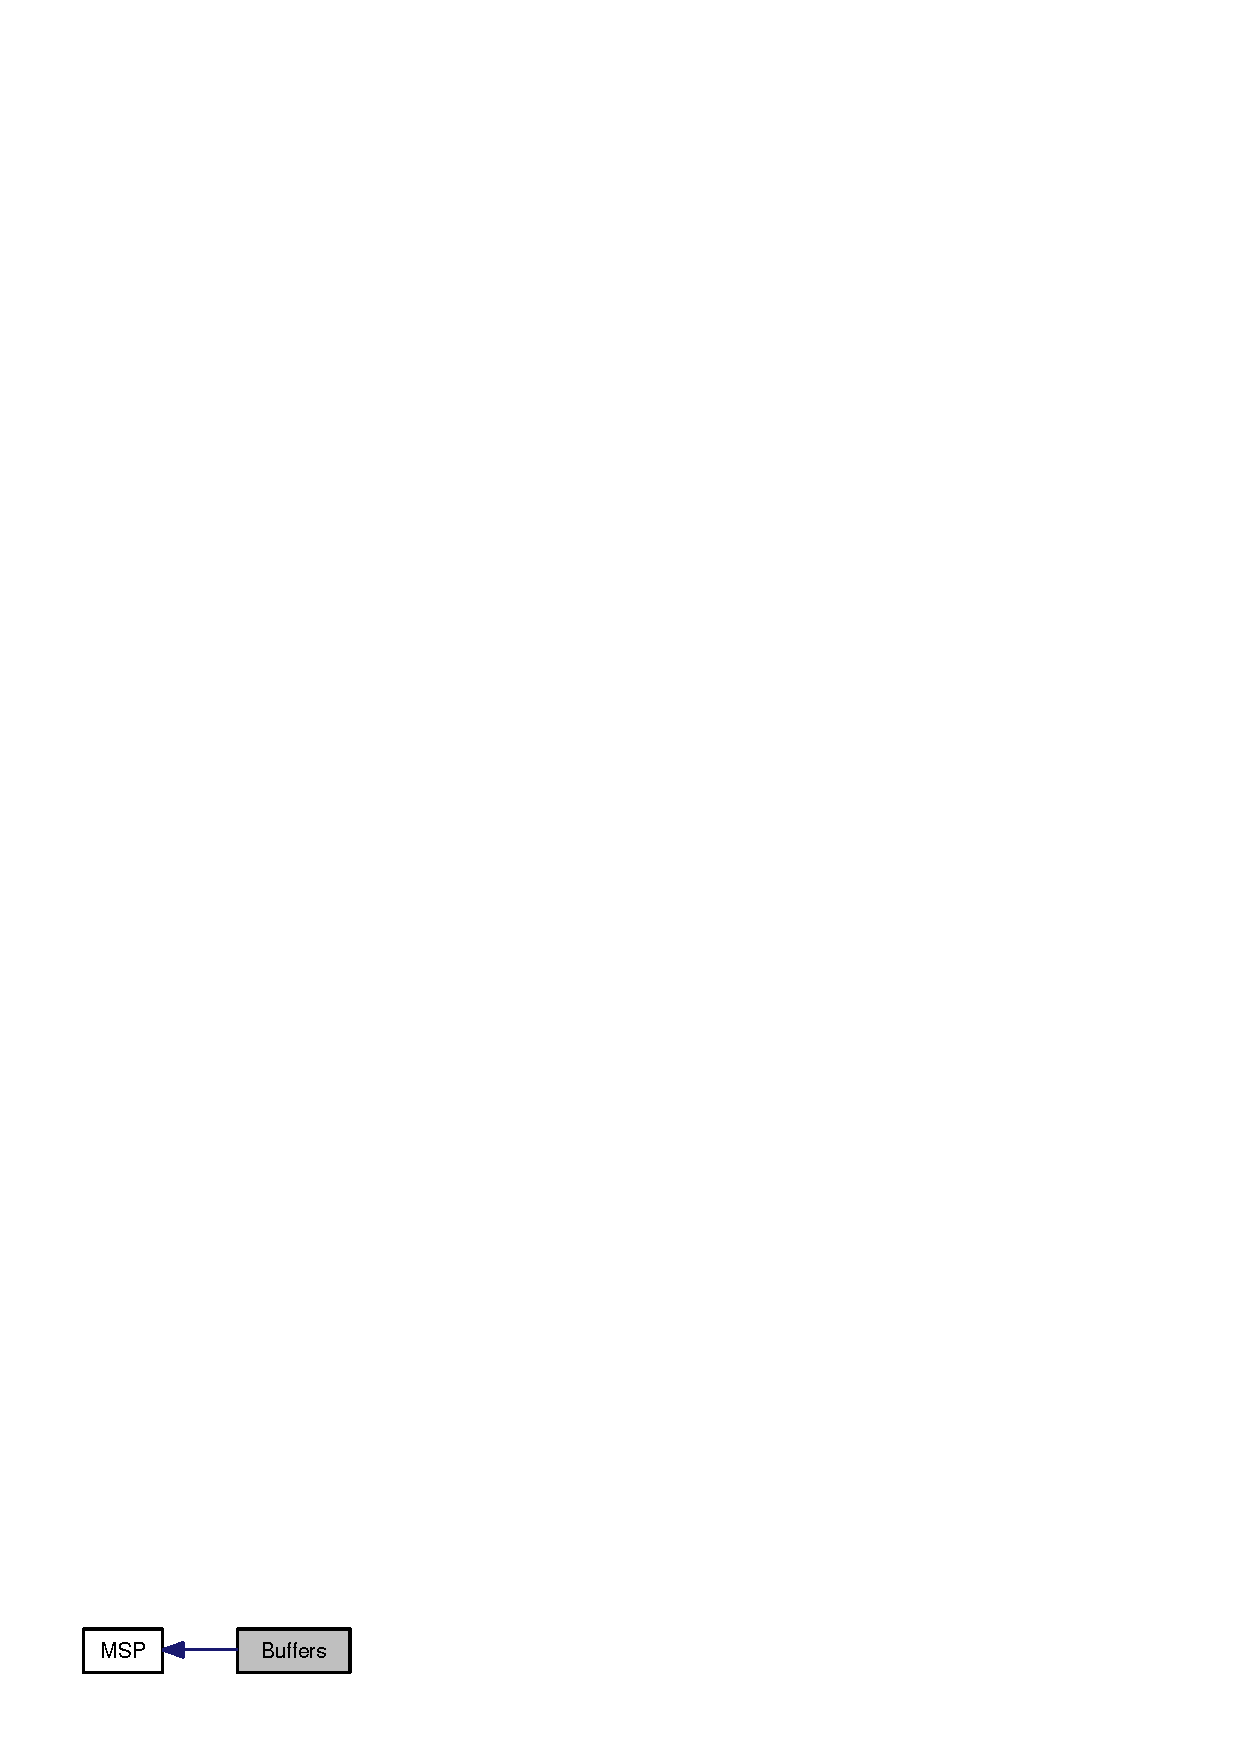
\includegraphics[width=86pt]{group__buffers}
\end{center}
\end{figure}
\subsection*{Data Structures}
\begin{DoxyCompactItemize}
\item 
struct \hyperlink{structt__buffer}{t\_\-buffer}
\begin{DoxyCompactList}\small\item\em Data structure for the buffer$\sim$ object. \item\end{DoxyCompactList}\end{DoxyCompactItemize}


\subsection{Detailed Description}
Your object can access shared data stored in an MSP buffer$\sim$ object. Similar to table and coll objects, buffer$\sim$ objects are bound to a \hyperlink{structt__symbol}{t\_\-symbol} from which you can gain access to the \hyperlink{structt__buffer}{t\_\-buffer} struct. Consider the following example.


\begin{DoxyCode}
    t_symbol *s;
    t_object *o;
    
    s = gensym("foo");
    o = s->s_thing;
    
    // if an object is bound to the symbol "foo", then o is that object.
    if (ob_sym(o) == gensym("buffer~")) {
        // that object is a buffer~, so we can use it
        x->x_buffer = (t_buffer*)o;
        
    }
\end{DoxyCode}


Having stored a pointer to the buffer$\sim$ is the first step toward working with its data. However, you must not go accessing the data directly without taking some precautions regarding thread-\/safety.

To access the data in a buffer you first increment the b\_\-inuse member of the \hyperlink{structt__buffer}{t\_\-buffer}'s struct. Then you perform the requisite operations on the data, which is stored in the b\_\-samples member. When you are done you decrement the b\_\-inuse member to return it to the state in which you found it.

In the past you may have set the buffer's b\_\-inuse flag directly and cleared it when you were done. This is no longer good enough, and you must instead use the threadsafe macros \hyperlink{group__threading_ga411e2e07982bdfb1803b415a350e311a}{ATOMIC\_\-INCREMENT} and \hyperlink{group__threading_gaa42a5aadef70fe57dc80d247c890c9ac}{ATOMIC\_\-DECREMENT} for modifying the b\_\-inuse flag. The example below demonstrates what this might look like in an MSP object's perform routine. Notice that extra care has been taken to ensure that the \hyperlink{group__threading_ga411e2e07982bdfb1803b415a350e311a}{ATOMIC\_\-INCREMENT} is always balanced with an \hyperlink{group__threading_gaa42a5aadef70fe57dc80d247c890c9ac}{ATOMIC\_\-DECREMENT} call.


\begin{DoxyCode}
    ATOMIC_INCREMENT(&x->w_buf->b_inuse);
    if (!x->w_buf->b_valid) {
        ATOMIC_DECREMENT(&x->w_buf->b_inuse);
        goto byebye;
    }
    
    // do something with the buffer
    
    ATOMIC_DECREMENT(&x->w_buf->b_inuse);
byebye:
    return (w + 7);
\end{DoxyCode}


A class that accesses buffer$\sim$ objects is the simpwave$\sim$ object that is included with Max 5 SDK example projects. 
\hypertarget{group__pfft}{
\section{PFFT}
\label{group__pfft}\index{PFFT@{PFFT}}
}


When an object is instantiated, it is possible to determine if it is being created in pfft$\sim$ context in the new method.  


Collaboration diagram for PFFT:\nopagebreak
\begin{figure}[H]
\begin{center}
\leavevmode
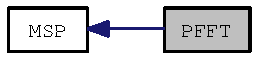
\includegraphics[width=80pt]{group__pfft}
\end{center}
\end{figure}
\subsection*{Data Structures}
\begin{DoxyCompactItemize}
\item 
struct \hyperlink{structt__pfftpub}{t\_\-pfftpub}
\begin{DoxyCompactList}\small\item\em Public FFT Patcher struct. \item\end{DoxyCompactList}\end{DoxyCompactItemize}


\subsection{Detailed Description}
When an object is instantiated, it is possible to determine if it is being created in pfft$\sim$ context in the new method. In the new method (and only at this time), you can check the s\_\-thing member of the \hyperlink{structt__symbol}{t\_\-symbol} '\_\-\_\-pfft$\sim$\_\-\_\-'. If this is non-\/null, then you will have a pointer to a \hyperlink{structt__pfftpub}{t\_\-pfftpub} struct.


\begin{DoxyCode}
    t_pfftpub *pfft_parent = (t_pfftpub*) gensym("__pfft~__")->s_thing;

    if (pfft_parent) {
        // in a pfft~ context
    }
    else {
        // not in a pfft~
    }
\end{DoxyCode}
 
\hypertarget{group__poly}{
\section{Poly}
\label{group__poly}\index{Poly@{Poly}}
}


If your object is instatiated as a voice of a poly$\sim$ object, it is possible both to determine this context and to determine information about the specific voice.  


Collaboration diagram for Poly:\nopagebreak
\begin{figure}[H]
\begin{center}
\leavevmode
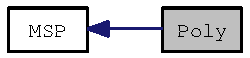
\includegraphics[width=78pt]{group__poly}
\end{center}
\end{figure}
If your object is instatiated as a voice of a poly$\sim$ object, it is possible both to determine this context and to determine information about the specific voice. This is done by querying the patcher in which your object exists for an associated object, and then calling methods on that object.


\begin{DoxyCode}
    t_object *patcher = NULL;
    t_max_err err = MAX_ERR_NONE;
    t_object *assoc = NULL;
    method m = NULL;
    long voices = -1;
    long index = -1;

    err = object_obex_lookup(x, gensym("#P"), &patcher);
    if (err == MAX_ERR_NONE) {
        object_method(patcher, gensym("getassoc"), &assoc);
        if (assoc) {
            post("found %s", object_classname(assoc)->s_name);

            voices = object_attr_getlong(assoc, gensym("voices"));
            post("total amount of voices: %ld", voices);

            if(m = zgetfn(assoc, gensym("getindex"))) 
                index = (long)(*m)(assoc, patcher);
            post("index: %ld", index);
        }   
    }       
\end{DoxyCode}
 
\hypertarget{group__obj}{
\section{Objects}
\label{group__obj}\index{Objects@{Objects}}
}


More information for this section can be gleaned from the pattrsdk.pdf in the Max 4.5.5 SDK.  
\subsection*{Data Structures}
\begin{DoxyCompactItemize}
\item 
struct \hyperlink{structt__messlist}{t\_\-messlist}
\begin{DoxyCompactList}\small\item\em A list of symbols and their corresponding methods, complete with typechecking information. \item\end{DoxyCompactList}\item 
struct \hyperlink{structt__tinyobject}{t\_\-tinyobject}
\begin{DoxyCompactList}\small\item\em The tiny object structure sits at the head of any object to which you may pass messages (and which you may feed to \hyperlink{group__class__old_gadf30646e52376a37b93cc20efac65636}{freeobject()}). \item\end{DoxyCompactList}\item 
struct \hyperlink{structt__object}{t\_\-object}
\begin{DoxyCompactList}\small\item\em The structure for the head of any object which wants to have inlets or outlets, or support attributes. \item\end{DoxyCompactList}\end{DoxyCompactItemize}
\subsection*{Defines}
\begin{DoxyCompactItemize}
\item 
\hypertarget{group__obj_ga94630370ae389fb1189282fa0742f310}{
\#define \hyperlink{group__obj_ga94630370ae389fb1189282fa0742f310}{MAGIC}~1758379419L}
\label{group__obj_ga94630370ae389fb1189282fa0742f310}

\begin{DoxyCompactList}\small\item\em Magic number used to determine if memory pointed to by a \hyperlink{structt__object}{t\_\-object}$\ast$ is valid. \item\end{DoxyCompactList}\item 
\hypertarget{group__obj_gabf8c1d20a4f4e731d185c02820c91593}{
\#define \hyperlink{group__obj_gabf8c1d20a4f4e731d185c02820c91593}{NOGOOD}(x)~(((struct object $\ast$)x)-\/$>$o\_\-magic != MAGIC)}
\label{group__obj_gabf8c1d20a4f4e731d185c02820c91593}

\begin{DoxyCompactList}\small\item\em Returns true if a pointer is not a valid object. \item\end{DoxyCompactList}\item 
\#define \hyperlink{group__obj_ga4c171d1ccc50f0b6ce7ad2f475eeba32}{MAXARG}~7
\begin{DoxyCompactList}\small\item\em Maximum number of arguments that can be passed as a typed-\/list rather than using \hyperlink{group__atom_gga8aa6700e9f00b132eb376db6e39ade47a81c1a8550f038db16a619167a70a79b6}{A\_\-GIMME}. \item\end{DoxyCompactList}\end{DoxyCompactItemize}
\subsection*{Functions}
\begin{DoxyCompactItemize}
\item 
\hyperlink{structt__object}{t\_\-object} $\ast$ \hyperlink{group__obj_gad81c665a20c3c707decaf3403468ff47}{newobject\_\-sprintf} (\hyperlink{structt__object}{t\_\-object} $\ast$patcher, char $\ast$fmt,...)
\begin{DoxyCompactList}\small\item\em Create a new object in a specified patcher with values using a combination of attribute and sprintf syntax. \item\end{DoxyCompactList}\item 
\hyperlink{structt__object}{t\_\-object} $\ast$ \hyperlink{group__obj_gaed2c4e1d0c80d929b97ccf07a886faeb}{newobject\_\-fromdictionary} (\hyperlink{structt__object}{t\_\-object} $\ast$patcher, \hyperlink{structt__dictionary}{t\_\-dictionary} $\ast$d)
\begin{DoxyCompactList}\small\item\em Place a new object into a patcher. \item\end{DoxyCompactList}\item 
long \hyperlink{group__obj_ga020d01fb1a55690dc760450bac6a624a}{object\_\-classname\_\-compare} (void $\ast$x, \hyperlink{structt__symbol}{t\_\-symbol} $\ast$name)
\begin{DoxyCompactList}\small\item\em Determines if a particular object is an instance of a given class. \item\end{DoxyCompactList}\item 
void $\ast$ \hyperlink{group__obj_gacb89ef27c34b45e9037d877375804284}{object\_\-alloc} (\hyperlink{structt__class}{t\_\-class} $\ast$c)
\begin{DoxyCompactList}\small\item\em Allocates the memory for an instance of an object class and initialize its object header. \item\end{DoxyCompactList}\item 
void $\ast$ \hyperlink{group__obj_gac4b370265c776db4f545d257089af1cf}{object\_\-new} (\hyperlink{structt__symbol}{t\_\-symbol} $\ast$name\_\-space, \hyperlink{structt__symbol}{t\_\-symbol} $\ast$classname,...)
\begin{DoxyCompactList}\small\item\em Allocates the memory for an instance of an object class and initialize its object header {\itshape internal to Max\/}. \item\end{DoxyCompactList}\item 
void $\ast$ \hyperlink{group__obj_ga459c71aca6316e345379eeb424ad56ff}{object\_\-new\_\-typed} (\hyperlink{structt__symbol}{t\_\-symbol} $\ast$name\_\-space, \hyperlink{structt__symbol}{t\_\-symbol} $\ast$classname, long ac, \hyperlink{structt__atom}{t\_\-atom} $\ast$av)
\begin{DoxyCompactList}\small\item\em Allocates the memory for an instance of an object class and initialize its object header {\itshape internal to Max\/}. \item\end{DoxyCompactList}\item 
\hyperlink{group__datatypes_ga73edaae82b318855cc09fac994918165}{t\_\-max\_\-err} \hyperlink{group__obj_ga3759846cb356195532c41e35b87522ee}{object\_\-free} (void $\ast$x)
\begin{DoxyCompactList}\small\item\em Call the free function and release the memory for an instance of an internal object class previously instantiated using \hyperlink{group__obj_gac4b370265c776db4f545d257089af1cf}{object\_\-new()}, \hyperlink{group__obj_ga459c71aca6316e345379eeb424ad56ff}{object\_\-new\_\-typed()} or other new-\/style object constructor functions (e.g. \item\end{DoxyCompactList}\item 
void $\ast$ \hyperlink{group__obj_gae740749094827ac5adc2b7145db1c596}{object\_\-method} (void $\ast$x, \hyperlink{structt__symbol}{t\_\-symbol} $\ast$s,...)
\begin{DoxyCompactList}\small\item\em Sends an untyped message to an object. \item\end{DoxyCompactList}\item 
\hyperlink{group__datatypes_ga73edaae82b318855cc09fac994918165}{t\_\-max\_\-err} \hyperlink{group__obj_ga443dee482af22e0fe83e68955d367226}{object\_\-method\_\-typed} (void $\ast$x, \hyperlink{structt__symbol}{t\_\-symbol} $\ast$s, long ac, \hyperlink{structt__atom}{t\_\-atom} $\ast$av, \hyperlink{structt__atom}{t\_\-atom} $\ast$rv)
\begin{DoxyCompactList}\small\item\em Sends a type-\/checked message to an object. \item\end{DoxyCompactList}\item 
\hyperlink{group__datatypes_ga73edaae82b318855cc09fac994918165}{t\_\-max\_\-err} \hyperlink{group__obj_gaa5ff59d2297a2dde60e3f2fe3e02eceb}{object\_\-method\_\-typedfun} (void $\ast$x, \hyperlink{structt__messlist}{t\_\-messlist} $\ast$mp, \hyperlink{structt__symbol}{t\_\-symbol} $\ast$s, long ac, \hyperlink{structt__atom}{t\_\-atom} $\ast$av, \hyperlink{structt__atom}{t\_\-atom} $\ast$rv)
\begin{DoxyCompactList}\small\item\em Currently undocumented. \item\end{DoxyCompactList}\item 
\hyperlink{group__datatypes_gac26ba0a173b50597f5738132e059b42d}{method} \hyperlink{group__obj_gaaa202dcda859bb5dcd1f186f88a43796}{object\_\-getmethod} (void $\ast$x, \hyperlink{structt__symbol}{t\_\-symbol} $\ast$s)
\begin{DoxyCompactList}\small\item\em Retrieves an object's \hyperlink{group__datatypes_gac26ba0a173b50597f5738132e059b42d}{method} for a particular message selector. \item\end{DoxyCompactList}\item 
\hyperlink{structt__symbol}{t\_\-symbol} $\ast$ \hyperlink{group__obj_gac4523e68b4be4deb6db0ea91948d3553}{object\_\-classname} (void $\ast$x)
\begin{DoxyCompactList}\small\item\em Retrieves an object instance's class name. \item\end{DoxyCompactList}\item 
void $\ast$ \hyperlink{group__obj_gaaa97beba179d6aebd3f3ede1b5c781fa}{object\_\-register} (\hyperlink{structt__symbol}{t\_\-symbol} $\ast$name\_\-space, \hyperlink{structt__symbol}{t\_\-symbol} $\ast$s, void $\ast$x)
\begin{DoxyCompactList}\small\item\em Registers an object in a namespace. \item\end{DoxyCompactList}\item 
void $\ast$ \hyperlink{group__obj_ga3854b233b015cf2e157b03819ce9b65e}{object\_\-findregistered} (\hyperlink{structt__symbol}{t\_\-symbol} $\ast$name\_\-space, \hyperlink{structt__symbol}{t\_\-symbol} $\ast$s)
\begin{DoxyCompactList}\small\item\em Determines a registered object's pointer, given its namespace and name. \item\end{DoxyCompactList}\item 
\hyperlink{group__datatypes_ga73edaae82b318855cc09fac994918165}{t\_\-max\_\-err} \hyperlink{group__obj_gadeb570bcae0e9bbf389d571e85d16bfa}{object\_\-findregisteredbyptr} (\hyperlink{structt__symbol}{t\_\-symbol} $\ast$$\ast$name\_\-space, \hyperlink{structt__symbol}{t\_\-symbol} $\ast$$\ast$s, void $\ast$x)
\begin{DoxyCompactList}\small\item\em Determines the namespace and/or name of a registered object, given the object's pointer. \item\end{DoxyCompactList}\item 
void $\ast$ \hyperlink{group__obj_ga42025069e4317aef6dbe5c21c316fd85}{object\_\-attach} (\hyperlink{structt__symbol}{t\_\-symbol} $\ast$name\_\-space, \hyperlink{structt__symbol}{t\_\-symbol} $\ast$s, void $\ast$x)
\begin{DoxyCompactList}\small\item\em Attaches a client to a registered object. \item\end{DoxyCompactList}\item 
\hyperlink{group__datatypes_ga73edaae82b318855cc09fac994918165}{t\_\-max\_\-err} \hyperlink{group__obj_ga6765e9533a3ae0d67d302f1e038c66ac}{object\_\-detach} (\hyperlink{structt__symbol}{t\_\-symbol} $\ast$name\_\-space, \hyperlink{structt__symbol}{t\_\-symbol} $\ast$s, void $\ast$x)
\begin{DoxyCompactList}\small\item\em Detach a client from a registered object. \item\end{DoxyCompactList}\item 
\hyperlink{group__datatypes_ga73edaae82b318855cc09fac994918165}{t\_\-max\_\-err} \hyperlink{group__obj_ga76657298bcd43ae4f9098e3ed2b97c72}{object\_\-attach\_\-byptr} (void $\ast$x, void $\ast$registeredobject)
\begin{DoxyCompactList}\small\item\em Attaches a client to a registered object. \item\end{DoxyCompactList}\item 
\hyperlink{group__datatypes_ga73edaae82b318855cc09fac994918165}{t\_\-max\_\-err} \hyperlink{group__obj_ga73adb1c1e2db98f7a500f50ac447add5}{object\_\-attach\_\-byptr\_\-register} (void $\ast$x, void $\ast$object\_\-to\_\-attach, \hyperlink{structt__symbol}{t\_\-symbol} $\ast$reg\_\-name\_\-space)
\begin{DoxyCompactList}\small\item\em A convenience function wrapping \hyperlink{group__obj_gaaa97beba179d6aebd3f3ede1b5c781fa}{object\_\-register()} and \hyperlink{group__obj_ga76657298bcd43ae4f9098e3ed2b97c72}{object\_\-attach\_\-byptr()}. \item\end{DoxyCompactList}\item 
\hyperlink{group__datatypes_ga73edaae82b318855cc09fac994918165}{t\_\-max\_\-err} \hyperlink{group__obj_ga9be48cfb39024dc20239079eb60295cd}{object\_\-detach\_\-byptr} (void $\ast$x, void $\ast$registeredobject)
\begin{DoxyCompactList}\small\item\em Detach a client from a registered object. \item\end{DoxyCompactList}\item 
\hyperlink{group__datatypes_ga73edaae82b318855cc09fac994918165}{t\_\-max\_\-err} \hyperlink{group__obj_ga2b5b3327e03edbefe753ebd6c8b7e152}{object\_\-unregister} (void $\ast$x)
\begin{DoxyCompactList}\small\item\em Removes a registered object from a namespace. \item\end{DoxyCompactList}\item 
\hyperlink{group__datatypes_ga73edaae82b318855cc09fac994918165}{t\_\-max\_\-err} \hyperlink{group__obj_ga6297b81c3a70f7fb2201c7262e96bba3}{object\_\-notify} (void $\ast$x, \hyperlink{structt__symbol}{t\_\-symbol} $\ast$s, void $\ast$data)
\begin{DoxyCompactList}\small\item\em Broadcast a message (with an optional argument) from a registered object to any attached client objects. \item\end{DoxyCompactList}\item 
\hyperlink{structt__class}{t\_\-class} $\ast$ \hyperlink{group__obj_ga035c5ca1d7d25921533b59451d730c44}{object\_\-class} (void $\ast$x)
\begin{DoxyCompactList}\small\item\em Determines the class of a given object. \item\end{DoxyCompactList}\item 
\hyperlink{group__datatypes_ga73edaae82b318855cc09fac994918165}{t\_\-max\_\-err} \hyperlink{group__obj_gab033973cea2f4a0b17bb48ab2f22f051}{object\_\-getvalueof} (void $\ast$x, long $\ast$ac, \hyperlink{structt__atom}{t\_\-atom} $\ast$$\ast$av)
\begin{DoxyCompactList}\small\item\em Retrieves the value of an object which supports the {\ttfamily getvalueof/setvalueof} interface. \item\end{DoxyCompactList}\item 
\hyperlink{group__datatypes_ga73edaae82b318855cc09fac994918165}{t\_\-max\_\-err} \hyperlink{group__obj_ga9d653fc9249f24c462f14657b969cc4d}{object\_\-setvalueof} (void $\ast$x, long ac, \hyperlink{structt__atom}{t\_\-atom} $\ast$av)
\begin{DoxyCompactList}\small\item\em Sets the value of an object which supports the {\ttfamily getvalueof/setvalueof} interface. \item\end{DoxyCompactList}\item 
\hyperlink{group__datatypes_ga73edaae82b318855cc09fac994918165}{t\_\-max\_\-err} \hyperlink{group__obj_gaba3a848eba4f4b834c1f89377c75e281}{object\_\-obex\_\-lookup} (void $\ast$x, \hyperlink{structt__symbol}{t\_\-symbol} $\ast$key, \hyperlink{structt__object}{t\_\-object} $\ast$$\ast$val)
\begin{DoxyCompactList}\small\item\em Retrieves the value of a data stored in the obex. \item\end{DoxyCompactList}\item 
\hyperlink{group__datatypes_ga73edaae82b318855cc09fac994918165}{t\_\-max\_\-err} \hyperlink{group__obj_gaccdb93572405a2e9f065086f9c3dfe41}{object\_\-obex\_\-store} (void $\ast$x, \hyperlink{structt__symbol}{t\_\-symbol} $\ast$key, \hyperlink{structt__object}{t\_\-object} $\ast$val)
\begin{DoxyCompactList}\small\item\em Stores data in the object's obex. \item\end{DoxyCompactList}\item 
void \hyperlink{group__obj_ga95edf6b869d6c5be94a59e49dddb0935}{object\_\-obex\_\-dumpout} (void $\ast$x, \hyperlink{structt__symbol}{t\_\-symbol} $\ast$s, long argc, \hyperlink{structt__atom}{t\_\-atom} $\ast$argv)
\begin{DoxyCompactList}\small\item\em Sends data from the object's dumpout outlet. \item\end{DoxyCompactList}\item 
\hyperlink{structt__dictionary}{t\_\-dictionary} $\ast$ \hyperlink{group__obj_ga6122e56af8de90fa7aad43ee405c6bb6}{object\_\-dictionaryarg} (long ac, \hyperlink{structt__atom}{t\_\-atom} $\ast$av)
\begin{DoxyCompactList}\small\item\em Retrieve a pointer to a dictionary passed in as an atom argument. \item\end{DoxyCompactList}\item 
\hyperlink{group__datatypes_ga73edaae82b318855cc09fac994918165}{t\_\-max\_\-err} \hyperlink{group__obj_ga8c420370f84f178515540831cbe4e6d8}{object\_\-method\_\-parse} (\hyperlink{structt__object}{t\_\-object} $\ast$x, \hyperlink{structt__symbol}{t\_\-symbol} $\ast$s, char $\ast$parsestr, \hyperlink{structt__atom}{t\_\-atom} $\ast$rv)
\begin{DoxyCompactList}\small\item\em Convenience wrapper for \hyperlink{group__obj_ga443dee482af22e0fe83e68955d367226}{object\_\-method\_\-typed()} that uses \hyperlink{group__atom_ga55938aedb41a8f3565680cf29169dc70}{atom\_\-setparse()} to define the arguments. \item\end{DoxyCompactList}\item 
\hyperlink{group__datatypes_ga73edaae82b318855cc09fac994918165}{t\_\-max\_\-err} \hyperlink{group__obj_gab509bef31fc1bdf47c67525c0353e6d3}{object\_\-method\_\-format} (\hyperlink{structt__object}{t\_\-object} $\ast$x, \hyperlink{structt__symbol}{t\_\-symbol} $\ast$s, \hyperlink{structt__atom}{t\_\-atom} $\ast$rv, char $\ast$fmt,...)
\begin{DoxyCompactList}\small\item\em Convenience wrapper for \hyperlink{group__obj_ga443dee482af22e0fe83e68955d367226}{object\_\-method\_\-typed()} that uses \hyperlink{group__atom_ga7a00fdf0699ae5176d39d7ddc3529bf0}{atom\_\-setformat()} to define the arguments. \item\end{DoxyCompactList}\item 
\hyperlink{group__datatypes_ga73edaae82b318855cc09fac994918165}{t\_\-max\_\-err} \hyperlink{group__obj_ga046f517695486f4008ae9b25ce5e41d7}{object\_\-method\_\-char} (\hyperlink{structt__object}{t\_\-object} $\ast$x, \hyperlink{structt__symbol}{t\_\-symbol} $\ast$s, unsigned char v, \hyperlink{structt__atom}{t\_\-atom} $\ast$rv)
\begin{DoxyCompactList}\small\item\em Convenience wrapper for \hyperlink{group__obj_ga443dee482af22e0fe83e68955d367226}{object\_\-method\_\-typed()} that passes a single char as an argument. \item\end{DoxyCompactList}\item 
\hyperlink{group__datatypes_ga73edaae82b318855cc09fac994918165}{t\_\-max\_\-err} \hyperlink{group__obj_ga975e42fc3823dadc594232652291d26d}{object\_\-method\_\-long} (\hyperlink{structt__object}{t\_\-object} $\ast$x, \hyperlink{structt__symbol}{t\_\-symbol} $\ast$s, long v, \hyperlink{structt__atom}{t\_\-atom} $\ast$rv)
\begin{DoxyCompactList}\small\item\em Convenience wrapper for \hyperlink{group__obj_ga443dee482af22e0fe83e68955d367226}{object\_\-method\_\-typed()} that passes a single long integer as an argument. \item\end{DoxyCompactList}\item 
\hyperlink{group__datatypes_ga73edaae82b318855cc09fac994918165}{t\_\-max\_\-err} \hyperlink{group__obj_gabd57e5e8ce873c5aa12dfc60db6cb6f1}{object\_\-method\_\-float} (\hyperlink{structt__object}{t\_\-object} $\ast$x, \hyperlink{structt__symbol}{t\_\-symbol} $\ast$s, float v, \hyperlink{structt__atom}{t\_\-atom} $\ast$rv)
\begin{DoxyCompactList}\small\item\em Convenience wrapper for \hyperlink{group__obj_ga443dee482af22e0fe83e68955d367226}{object\_\-method\_\-typed()} that passes a single 32bit float as an argument. \item\end{DoxyCompactList}\item 
\hyperlink{group__datatypes_ga73edaae82b318855cc09fac994918165}{t\_\-max\_\-err} \hyperlink{group__obj_ga736ef8fbda2c79dd13a88f6ab81a9f9f}{object\_\-method\_\-double} (\hyperlink{structt__object}{t\_\-object} $\ast$x, \hyperlink{structt__symbol}{t\_\-symbol} $\ast$s, double v, \hyperlink{structt__atom}{t\_\-atom} $\ast$rv)
\begin{DoxyCompactList}\small\item\em Convenience wrapper for \hyperlink{group__obj_ga443dee482af22e0fe83e68955d367226}{object\_\-method\_\-typed()} that passes a single 64bit float as an argument. \item\end{DoxyCompactList}\item 
\hyperlink{group__datatypes_ga73edaae82b318855cc09fac994918165}{t\_\-max\_\-err} \hyperlink{group__obj_ga5ddeb48f167ded23b1508d502e571427}{object\_\-method\_\-sym} (\hyperlink{structt__object}{t\_\-object} $\ast$x, \hyperlink{structt__symbol}{t\_\-symbol} $\ast$s, \hyperlink{structt__symbol}{t\_\-symbol} $\ast$v, \hyperlink{structt__atom}{t\_\-atom} $\ast$rv)
\begin{DoxyCompactList}\small\item\em Convenience wrapper for \hyperlink{group__obj_ga443dee482af22e0fe83e68955d367226}{object\_\-method\_\-typed()} that passes a single \hyperlink{structt__symbol}{t\_\-symbol}$\ast$ as an argument. \item\end{DoxyCompactList}\item 
\hyperlink{group__datatypes_ga73edaae82b318855cc09fac994918165}{t\_\-max\_\-err} \hyperlink{group__obj_ga5432f19c374fb8850faa7ff062561db0}{object\_\-method\_\-obj} (\hyperlink{structt__object}{t\_\-object} $\ast$x, \hyperlink{structt__symbol}{t\_\-symbol} $\ast$s, \hyperlink{structt__object}{t\_\-object} $\ast$v, \hyperlink{structt__atom}{t\_\-atom} $\ast$rv)
\begin{DoxyCompactList}\small\item\em Convenience wrapper for \hyperlink{group__obj_ga443dee482af22e0fe83e68955d367226}{object\_\-method\_\-typed()} that passes a single \hyperlink{structt__object}{t\_\-object}$\ast$ as an argument. \item\end{DoxyCompactList}\item 
\hyperlink{group__datatypes_ga73edaae82b318855cc09fac994918165}{t\_\-max\_\-err} \hyperlink{group__obj_ga8d2c36fbeff377ea30d4ac9d898a3d77}{object\_\-method\_\-char\_\-array} (\hyperlink{structt__object}{t\_\-object} $\ast$x, \hyperlink{structt__symbol}{t\_\-symbol} $\ast$s, long ac, unsigned char $\ast$av, \hyperlink{structt__atom}{t\_\-atom} $\ast$rv)
\begin{DoxyCompactList}\small\item\em Convenience wrapper for \hyperlink{group__obj_ga443dee482af22e0fe83e68955d367226}{object\_\-method\_\-typed()} that passes an array of char values as an argument. \item\end{DoxyCompactList}\item 
\hyperlink{group__datatypes_ga73edaae82b318855cc09fac994918165}{t\_\-max\_\-err} \hyperlink{group__obj_ga76c93edf094492b8f485b7a401c616b6}{object\_\-method\_\-long\_\-array} (\hyperlink{structt__object}{t\_\-object} $\ast$x, \hyperlink{structt__symbol}{t\_\-symbol} $\ast$s, long ac, long $\ast$av, \hyperlink{structt__atom}{t\_\-atom} $\ast$rv)
\begin{DoxyCompactList}\small\item\em Convenience wrapper for \hyperlink{group__obj_ga443dee482af22e0fe83e68955d367226}{object\_\-method\_\-typed()} that passes an array of long integers values as an argument. \item\end{DoxyCompactList}\item 
\hyperlink{group__datatypes_ga73edaae82b318855cc09fac994918165}{t\_\-max\_\-err} \hyperlink{group__obj_ga308d41d63efacb1187ace7d3b50b99e1}{object\_\-method\_\-float\_\-array} (\hyperlink{structt__object}{t\_\-object} $\ast$x, \hyperlink{structt__symbol}{t\_\-symbol} $\ast$s, long ac, float $\ast$av, \hyperlink{structt__atom}{t\_\-atom} $\ast$rv)
\begin{DoxyCompactList}\small\item\em Convenience wrapper for \hyperlink{group__obj_ga443dee482af22e0fe83e68955d367226}{object\_\-method\_\-typed()} that passes an array of 32bit floats values as an argument. \item\end{DoxyCompactList}\item 
\hyperlink{group__datatypes_ga73edaae82b318855cc09fac994918165}{t\_\-max\_\-err} \hyperlink{group__obj_gaaa262193055c44fff144e3395443597a}{object\_\-method\_\-double\_\-array} (\hyperlink{structt__object}{t\_\-object} $\ast$x, \hyperlink{structt__symbol}{t\_\-symbol} $\ast$s, long ac, double $\ast$av, \hyperlink{structt__atom}{t\_\-atom} $\ast$rv)
\begin{DoxyCompactList}\small\item\em Convenience wrapper for \hyperlink{group__obj_ga443dee482af22e0fe83e68955d367226}{object\_\-method\_\-typed()} that passes an array of 64bit float values as an argument. \item\end{DoxyCompactList}\item 
\hyperlink{group__datatypes_ga73edaae82b318855cc09fac994918165}{t\_\-max\_\-err} \hyperlink{group__obj_ga2a4bb953a5f7a9afee4f2f8196c4226e}{object\_\-method\_\-sym\_\-array} (\hyperlink{structt__object}{t\_\-object} $\ast$x, \hyperlink{structt__symbol}{t\_\-symbol} $\ast$s, long ac, \hyperlink{structt__symbol}{t\_\-symbol} $\ast$$\ast$av, \hyperlink{structt__atom}{t\_\-atom} $\ast$rv)
\begin{DoxyCompactList}\small\item\em Convenience wrapper for \hyperlink{group__obj_ga443dee482af22e0fe83e68955d367226}{object\_\-method\_\-typed()} that passes an array of \hyperlink{structt__symbol}{t\_\-symbol}$\ast$ values as an argument. \item\end{DoxyCompactList}\item 
\hyperlink{group__datatypes_ga73edaae82b318855cc09fac994918165}{t\_\-max\_\-err} \hyperlink{group__obj_ga941f7a1161a097394a6924df0c03a1ea}{object\_\-method\_\-obj\_\-array} (\hyperlink{structt__object}{t\_\-object} $\ast$x, \hyperlink{structt__symbol}{t\_\-symbol} $\ast$s, long ac, \hyperlink{structt__object}{t\_\-object} $\ast$$\ast$av, \hyperlink{structt__atom}{t\_\-atom} $\ast$rv)
\begin{DoxyCompactList}\small\item\em Convenience wrapper for \hyperlink{group__obj_ga443dee482af22e0fe83e68955d367226}{object\_\-method\_\-typed()} that passes an array of \hyperlink{structt__object}{t\_\-object}$\ast$ values as an argument. \item\end{DoxyCompactList}\item 
void \hyperlink{group__obj_gac4eb1b3d30abbbb754ddc38701ff1c77}{object\_\-openhelp} (\hyperlink{structt__object}{t\_\-object} $\ast$x)
\begin{DoxyCompactList}\small\item\em Open the help patcher for a given instance of an object. \item\end{DoxyCompactList}\item 
void \hyperlink{group__obj_gabcf7aaca1f307e806e38100355cc97ac}{object\_\-openrefpage} (\hyperlink{structt__object}{t\_\-object} $\ast$x)
\begin{DoxyCompactList}\small\item\em Open the reference page for a given instance of an object. \item\end{DoxyCompactList}\item 
void \hyperlink{group__obj_ga6d212c17722cc783102a6f5a623596c9}{object\_\-openquery} (\hyperlink{structt__object}{t\_\-object} $\ast$x)
\begin{DoxyCompactList}\small\item\em Open a search in the file browser for files with the name of the given object. \item\end{DoxyCompactList}\item 
void \hyperlink{group__obj_ga5de96f9ed649a42b2133d21c38e3476b}{classname\_\-openhelp} (char $\ast$classname)
\begin{DoxyCompactList}\small\item\em Open the help patcher for a given object class name. \item\end{DoxyCompactList}\item 
void \hyperlink{group__obj_ga8e08b5bc9657c1800ee8a452e9d14d3d}{classname\_\-openrefpage} (char $\ast$classname)
\begin{DoxyCompactList}\small\item\em Open the reference page for a given object class name. \item\end{DoxyCompactList}\item 
void \hyperlink{group__obj_ga24a3ab7c91801d4b0ae377d15adfc117}{classname\_\-openquery} (char $\ast$classname)
\begin{DoxyCompactList}\small\item\em Open a search in the file browser for files with the name of the given class. \item\end{DoxyCompactList}\end{DoxyCompactItemize}


\subsection{Detailed Description}
More information for this section can be gleaned from the pattrsdk.pdf in the Max 4.5.5 SDK. \begin{DoxySeeAlso}{See also}
\href{http://www.cycling74.com/twiki/bin/view/ProductDocumentation/JitterSdkObjectModel}{\tt http://www.cycling74.com/twiki/bin/view/ProductDocumentation/JitterSdkObjectModel} 

\href{http://www.cycling74.com/twiki/bin/view/ProductDocumentation/JitterSdkRegNotify}{\tt http://www.cycling74.com/twiki/bin/view/ProductDocumentation/JitterSdkRegNotify} 
\end{DoxySeeAlso}


\subsection{Define Documentation}
\hypertarget{group__obj_ga4c171d1ccc50f0b6ce7ad2f475eeba32}{
\index{obj@{obj}!MAXARG@{MAXARG}}
\index{MAXARG@{MAXARG}!obj@{obj}}
\subsubsection[{MAXARG}]{\setlength{\rightskip}{0pt plus 5cm}\#define MAXARG~7}}
\label{group__obj_ga4c171d1ccc50f0b6ce7ad2f475eeba32}


Maximum number of arguments that can be passed as a typed-\/list rather than using \hyperlink{group__atom_gga8aa6700e9f00b132eb376db6e39ade47a81c1a8550f038db16a619167a70a79b6}{A\_\-GIMME}. It is generally recommended to use \hyperlink{group__atom_gga8aa6700e9f00b132eb376db6e39ade47a81c1a8550f038db16a619167a70a79b6}{A\_\-GIMME}. 

\subsection{Function Documentation}
\hypertarget{group__obj_ga5de96f9ed649a42b2133d21c38e3476b}{
\index{obj@{obj}!classname\_\-openhelp@{classname\_\-openhelp}}
\index{classname\_\-openhelp@{classname\_\-openhelp}!obj@{obj}}
\subsubsection[{classname\_\-openhelp}]{\setlength{\rightskip}{0pt plus 5cm}void classname\_\-openhelp (char $\ast$ {\em classname})}}
\label{group__obj_ga5de96f9ed649a42b2133d21c38e3476b}


Open the help patcher for a given object class name. 
\begin{DoxyParams}{Parameters}
\item[{\em classname}]The class name for which to open the help patcher. \end{DoxyParams}
\hypertarget{group__obj_ga24a3ab7c91801d4b0ae377d15adfc117}{
\index{obj@{obj}!classname\_\-openquery@{classname\_\-openquery}}
\index{classname\_\-openquery@{classname\_\-openquery}!obj@{obj}}
\subsubsection[{classname\_\-openquery}]{\setlength{\rightskip}{0pt plus 5cm}void classname\_\-openquery (char $\ast$ {\em classname})}}
\label{group__obj_ga24a3ab7c91801d4b0ae377d15adfc117}


Open a search in the file browser for files with the name of the given class. 
\begin{DoxyParams}{Parameters}
\item[{\em classname}]The class name for which to query. \end{DoxyParams}
\hypertarget{group__obj_ga8e08b5bc9657c1800ee8a452e9d14d3d}{
\index{obj@{obj}!classname\_\-openrefpage@{classname\_\-openrefpage}}
\index{classname\_\-openrefpage@{classname\_\-openrefpage}!obj@{obj}}
\subsubsection[{classname\_\-openrefpage}]{\setlength{\rightskip}{0pt plus 5cm}void classname\_\-openrefpage (char $\ast$ {\em classname})}}
\label{group__obj_ga8e08b5bc9657c1800ee8a452e9d14d3d}


Open the reference page for a given object class name. 
\begin{DoxyParams}{Parameters}
\item[{\em classname}]The class name for which to open the reference page. \end{DoxyParams}
\hypertarget{group__obj_gaed2c4e1d0c80d929b97ccf07a886faeb}{
\index{obj@{obj}!newobject\_\-fromdictionary@{newobject\_\-fromdictionary}}
\index{newobject\_\-fromdictionary@{newobject\_\-fromdictionary}!obj@{obj}}
\subsubsection[{newobject\_\-fromdictionary}]{\setlength{\rightskip}{0pt plus 5cm}{\bf t\_\-object}$\ast$ newobject\_\-fromdictionary ({\bf t\_\-object} $\ast$ {\em patcher}, \/  {\bf t\_\-dictionary} $\ast$ {\em d})}}
\label{group__obj_gaed2c4e1d0c80d929b97ccf07a886faeb}


Place a new object into a patcher. The new object will be created based on a specification contained in a \hyperlink{group__dictionary}{Dictionary}.

Create a new dictionary populated with values using a combination of attribute and sprintf syntax.


\begin{DoxyParams}{Parameters}
\item[{\em patcher}]An instance of a patcher object. \item[{\em d}]A dictionary containing an object specification. \end{DoxyParams}
\begin{DoxyReturn}{Returns}
A pointer to the newly created object instance, or NULL if creation of the object fails.
\end{DoxyReturn}
\begin{DoxyRemark}{Remarks}
Max attribute syntax is used to define key-\/value pairs. For example, 
\begin{DoxyCode}
    "@key1 value @key2 another_value"
\end{DoxyCode}


The example below creates a new object that in a patcher whose object pointer is stored in a variable called \char`\"{}aPatcher\char`\"{}. 
\begin{DoxyCode}
    t_dictionary *d;
    t_object *o;
    char text[4];
    
    strncpy_zero(text, "foo", 4);

    d = dictionary_sprintf("@maxclass comment @varname _name \
        @text \"%s\" @patching_rect %.2f %.2f %.2f %.2f \
        @fontsize %f @textcolor %f %f %f 1.0 \
        @fontname %s @bgcolor 0.001 0.001 0.001 0.",
        text, 20.0, 20.0, 200.0, 24.0,
        18, 0.9, 0.9, 0.9, "Arial");
    
    o = newobject_fromdictionary(aPatcher, d);
\end{DoxyCode}

\end{DoxyRemark}
\begin{DoxySeeAlso}{See also}
\hyperlink{group__obj_gad81c665a20c3c707decaf3403468ff47}{newobject\_\-sprintf()} 

\hyperlink{group__obj_gaed2c4e1d0c80d929b97ccf07a886faeb}{newobject\_\-fromdictionary()} 

\hyperlink{group__atom_ga55938aedb41a8f3565680cf29169dc70}{atom\_\-setparse()} 
\end{DoxySeeAlso}
\hypertarget{group__obj_gad81c665a20c3c707decaf3403468ff47}{
\index{obj@{obj}!newobject\_\-sprintf@{newobject\_\-sprintf}}
\index{newobject\_\-sprintf@{newobject\_\-sprintf}!obj@{obj}}
\subsubsection[{newobject\_\-sprintf}]{\setlength{\rightskip}{0pt plus 5cm}{\bf t\_\-object}$\ast$ newobject\_\-sprintf ({\bf t\_\-object} $\ast$ {\em patcher}, \/  char $\ast$ {\em fmt}, \/   {\em ...})}}
\label{group__obj_gad81c665a20c3c707decaf3403468ff47}


Create a new object in a specified patcher with values using a combination of attribute and sprintf syntax. 
\begin{DoxyParams}{Parameters}
\item[{\em patcher}]An instance of a patcher object. \item[{\em fmt}]An sprintf-\/style format string specifying key-\/value pairs with attribute nomenclature. \item[{\em ...}]One or more arguments which are to be substituted into the format string. \end{DoxyParams}
\begin{DoxyReturn}{Returns}
A pointer to the newly created object instance, or NULL if creation of the object fails.
\end{DoxyReturn}
\begin{DoxyRemark}{Remarks}
Max attribute syntax is used to define key-\/value pairs. For example, 
\begin{DoxyCode}
    "@key1 value @key2 another_value"
\end{DoxyCode}


The example below creates a new object that in a patcher whose object pointer is stored in a variable called \char`\"{}aPatcher\char`\"{}. 
\begin{DoxyCode}
    t_object *my_comment;
    char text[4];
    
    strncpy_zero(text, "foo", 4);

    my_comment = newobject_sprintf(aPatcher, "@maxclass comment @varname _name \
        @text \"%s\" @patching_rect %.2f %.2f %.2f %.2f \
        @fontsize %f @textcolor %f %f %f 1.0 \
        @fontname %s @bgcolor 0.001 0.001 0.001 0.",
        text, 20.0, 20.0, 200.0, 24.0,
        18, 0.9, 0.9, 0.9, "Arial");
\end{DoxyCode}

\end{DoxyRemark}
\begin{DoxySeeAlso}{See also}
\hyperlink{group__dictionary_ga77d5bafc260f9fc0bf3b4ad35f2b2629}{dictionary\_\-sprintf()} 

\hyperlink{group__obj_gaed2c4e1d0c80d929b97ccf07a886faeb}{newobject\_\-fromdictionary()} 

\hyperlink{group__atom_ga55938aedb41a8f3565680cf29169dc70}{atom\_\-setparse()} 
\end{DoxySeeAlso}
\hypertarget{group__obj_gacb89ef27c34b45e9037d877375804284}{
\index{obj@{obj}!object\_\-alloc@{object\_\-alloc}}
\index{object\_\-alloc@{object\_\-alloc}!obj@{obj}}
\subsubsection[{object\_\-alloc}]{\setlength{\rightskip}{0pt plus 5cm}void$\ast$ object\_\-alloc ({\bf t\_\-class} $\ast$ {\em c})}}
\label{group__obj_gacb89ef27c34b45e9037d877375804284}


Allocates the memory for an instance of an object class and initialize its object header. It is used like the traditional function newobject, inside of an object's {\ttfamily new} method, but its use is required with obex-\/class objects.


\begin{DoxyParams}{Parameters}
\item[{\em c}]The class pointer, returned by \hyperlink{group__class_ga238696d466081965c2b72b3880358404}{class\_\-new()} \end{DoxyParams}
\begin{DoxyReturn}{Returns}
This function returns a new instance of an object class if successful, or NULL if unsuccessful. 
\end{DoxyReturn}
\hypertarget{group__obj_ga42025069e4317aef6dbe5c21c316fd85}{
\index{obj@{obj}!object\_\-attach@{object\_\-attach}}
\index{object\_\-attach@{object\_\-attach}!obj@{obj}}
\subsubsection[{object\_\-attach}]{\setlength{\rightskip}{0pt plus 5cm}void$\ast$ object\_\-attach ({\bf t\_\-symbol} $\ast$ {\em name\_\-space}, \/  {\bf t\_\-symbol} $\ast$ {\em s}, \/  void $\ast$ {\em x})}}
\label{group__obj_ga42025069e4317aef6dbe5c21c316fd85}


Attaches a client to a registered object. Once attached, the object will receive notifications sent from the registered object (via the \hyperlink{group__obj_ga6297b81c3a70f7fb2201c7262e96bba3}{object\_\-notify()} function), if it has a {\ttfamily notify} method defined and implemented.


\begin{DoxyParams}{Parameters}
\item[{\em name\_\-space}]The namespace of the registered object. This should be the same value used in \hyperlink{group__obj_gaaa97beba179d6aebd3f3ede1b5c781fa}{object\_\-register()} to register the object. If you don't know the registered object's namespace, the \hyperlink{group__obj_gadeb570bcae0e9bbf389d571e85d16bfa}{object\_\-findregisteredbyptr()} function can be used to determine it. \item[{\em s}]The name of the registered object in the namespace. If you don't know the name of the registered object, the \hyperlink{group__obj_gadeb570bcae0e9bbf389d571e85d16bfa}{object\_\-findregisteredbyptr()} function can be used to determine it. \item[{\em x}]The client object to attach. Generally, this is the pointer to your Max object.\end{DoxyParams}
\begin{DoxyReturn}{Returns}
This function returns a pointer to the registered object (to the object referred to by the combination of {\ttfamily name\_\-space} and {\ttfamily s} arguments) if successful, or NULL if unsuccessful.
\end{DoxyReturn}
\begin{DoxyRemark}{Remarks}
You should not attach an object to itself if the object is a UI object. UI objects automatically register and attach to themselves in \hyperlink{group__jbox_gaaa460d02ca3d22c54368ade59d8e330b}{jbox\_\-new()}.
\end{DoxyRemark}
\begin{DoxySeeAlso}{See also}
\hyperlink{group__obj_ga6297b81c3a70f7fb2201c7262e96bba3}{object\_\-notify()} 

\hyperlink{group__obj_ga6765e9533a3ae0d67d302f1e038c66ac}{object\_\-detach()} 

\hyperlink{group__obj_ga76657298bcd43ae4f9098e3ed2b97c72}{object\_\-attach\_\-byptr()} 

\hyperlink{group__obj_gaaa97beba179d6aebd3f3ede1b5c781fa}{object\_\-register()} 
\end{DoxySeeAlso}
\hypertarget{group__obj_ga76657298bcd43ae4f9098e3ed2b97c72}{
\index{obj@{obj}!object\_\-attach\_\-byptr@{object\_\-attach\_\-byptr}}
\index{object\_\-attach\_\-byptr@{object\_\-attach\_\-byptr}!obj@{obj}}
\subsubsection[{object\_\-attach\_\-byptr}]{\setlength{\rightskip}{0pt plus 5cm}{\bf t\_\-max\_\-err} object\_\-attach\_\-byptr (void $\ast$ {\em x}, \/  void $\ast$ {\em registeredobject})}}
\label{group__obj_ga76657298bcd43ae4f9098e3ed2b97c72}


Attaches a client to a registered object. Unlike \hyperlink{group__obj_ga42025069e4317aef6dbe5c21c316fd85}{object\_\-attach()}, the client is specified by providing a pointer to that object rather than the registered name of that object.

Once attached, the object will receive notifications sent from the registered object (via the \hyperlink{group__obj_ga6297b81c3a70f7fb2201c7262e96bba3}{object\_\-notify()} function), if it has a {\ttfamily notify} method defined and implemented.


\begin{DoxyParams}{Parameters}
\item[{\em x}]The attaching client object. Generally, this is the pointer to your Max object. \item[{\em registeredobject}]A pointer to the registered object to which you wish to attach. \end{DoxyParams}
\begin{DoxyReturn}{Returns}
A Max error code.
\end{DoxyReturn}
\begin{DoxyRemark}{Remarks}
You should not attach an object to itself if the object is a UI object. UI objects automatically register and attach to themselves in \hyperlink{group__jbox_gaaa460d02ca3d22c54368ade59d8e330b}{jbox\_\-new()}.
\end{DoxyRemark}
\begin{DoxySeeAlso}{See also}
\hyperlink{group__obj_ga6297b81c3a70f7fb2201c7262e96bba3}{object\_\-notify()} 

\hyperlink{group__obj_ga6765e9533a3ae0d67d302f1e038c66ac}{object\_\-detach()} 

\hyperlink{group__obj_ga42025069e4317aef6dbe5c21c316fd85}{object\_\-attach()} 

\hyperlink{group__obj_gaaa97beba179d6aebd3f3ede1b5c781fa}{object\_\-register()} 

\hyperlink{group__obj_ga73adb1c1e2db98f7a500f50ac447add5}{object\_\-attach\_\-byptr\_\-register()} 
\end{DoxySeeAlso}
\hypertarget{group__obj_ga73adb1c1e2db98f7a500f50ac447add5}{
\index{obj@{obj}!object\_\-attach\_\-byptr\_\-register@{object\_\-attach\_\-byptr\_\-register}}
\index{object\_\-attach\_\-byptr\_\-register@{object\_\-attach\_\-byptr\_\-register}!obj@{obj}}
\subsubsection[{object\_\-attach\_\-byptr\_\-register}]{\setlength{\rightskip}{0pt plus 5cm}{\bf t\_\-max\_\-err} object\_\-attach\_\-byptr\_\-register (void $\ast$ {\em x}, \/  void $\ast$ {\em object\_\-to\_\-attach}, \/  {\bf t\_\-symbol} $\ast$ {\em reg\_\-name\_\-space})}}
\label{group__obj_ga73adb1c1e2db98f7a500f50ac447add5}


A convenience function wrapping \hyperlink{group__obj_gaaa97beba179d6aebd3f3ede1b5c781fa}{object\_\-register()} and \hyperlink{group__obj_ga76657298bcd43ae4f9098e3ed2b97c72}{object\_\-attach\_\-byptr()}. 
\begin{DoxyParams}{Parameters}
\item[{\em x}]The attaching client object. Generally, this is the pointer to your Max object. \item[{\em object\_\-to\_\-attach}]A pointer to the object to which you wish to registered and then to which to attach. \item[{\em reg\_\-name\_\-space}]The namespace in which to register the object\_\-to\_\-attach. \end{DoxyParams}
\begin{DoxyReturn}{Returns}
A Max error code.
\end{DoxyReturn}
\begin{DoxySeeAlso}{See also}
\hyperlink{group__obj_gaaa97beba179d6aebd3f3ede1b5c781fa}{object\_\-register()} 

\hyperlink{group__obj_ga76657298bcd43ae4f9098e3ed2b97c72}{object\_\-attach\_\-byptr()} 
\end{DoxySeeAlso}
\hypertarget{group__obj_ga035c5ca1d7d25921533b59451d730c44}{
\index{obj@{obj}!object\_\-class@{object\_\-class}}
\index{object\_\-class@{object\_\-class}!obj@{obj}}
\subsubsection[{object\_\-class}]{\setlength{\rightskip}{0pt plus 5cm}{\bf t\_\-class}$\ast$ object\_\-class (void $\ast$ {\em x})}}
\label{group__obj_ga035c5ca1d7d25921533b59451d730c44}


Determines the class of a given object. 
\begin{DoxyParams}{Parameters}
\item[{\em x}]The object to test \end{DoxyParams}
\begin{DoxyReturn}{Returns}
This function returns the \hyperlink{structt__class}{t\_\-class} $\ast$ of the object's class, if successful, or NULL, if unsuccessful. 
\end{DoxyReturn}
\hypertarget{group__obj_gac4523e68b4be4deb6db0ea91948d3553}{
\index{obj@{obj}!object\_\-classname@{object\_\-classname}}
\index{object\_\-classname@{object\_\-classname}!obj@{obj}}
\subsubsection[{object\_\-classname}]{\setlength{\rightskip}{0pt plus 5cm}{\bf t\_\-symbol}$\ast$ object\_\-classname (void $\ast$ {\em x})}}
\label{group__obj_gac4523e68b4be4deb6db0ea91948d3553}


Retrieves an object instance's class name. 
\begin{DoxyParams}{Parameters}
\item[{\em x}]The object instance whose class name is being queried \end{DoxyParams}
\begin{DoxyReturn}{Returns}
The classname, or NULL if unsuccessful. 
\end{DoxyReturn}
\hypertarget{group__obj_ga020d01fb1a55690dc760450bac6a624a}{
\index{obj@{obj}!object\_\-classname\_\-compare@{object\_\-classname\_\-compare}}
\index{object\_\-classname\_\-compare@{object\_\-classname\_\-compare}!obj@{obj}}
\subsubsection[{object\_\-classname\_\-compare}]{\setlength{\rightskip}{0pt plus 5cm}long object\_\-classname\_\-compare (void $\ast$ {\em x}, \/  {\bf t\_\-symbol} $\ast$ {\em name})}}
\label{group__obj_ga020d01fb1a55690dc760450bac6a624a}


Determines if a particular object is an instance of a given class. 
\begin{DoxyParams}{Parameters}
\item[{\em x}]The object to test \item[{\em name}]The name of the class to test this object against \end{DoxyParams}
\begin{DoxyReturn}{Returns}
This function returns 1 if the object is an instance of the named class. Otherwise, 0 is returned. 
\end{DoxyReturn}
\begin{DoxyRemark}{Remarks}
For instance, to determine whether an unknown object pointer is a pointer to a print object, one would call:
\end{DoxyRemark}

\begin{DoxyCode}
    long isprint = object_classname_compare(x, gensym("print"));
\end{DoxyCode}
 \hypertarget{group__obj_ga6765e9533a3ae0d67d302f1e038c66ac}{
\index{obj@{obj}!object\_\-detach@{object\_\-detach}}
\index{object\_\-detach@{object\_\-detach}!obj@{obj}}
\subsubsection[{object\_\-detach}]{\setlength{\rightskip}{0pt plus 5cm}{\bf t\_\-max\_\-err} object\_\-detach ({\bf t\_\-symbol} $\ast$ {\em name\_\-space}, \/  {\bf t\_\-symbol} $\ast$ {\em s}, \/  void $\ast$ {\em x})}}
\label{group__obj_ga6765e9533a3ae0d67d302f1e038c66ac}


Detach a client from a registered object. 
\begin{DoxyParams}{Parameters}
\item[{\em name\_\-space}]The namespace of the registered object. This should be the same value used in \hyperlink{group__obj_gaaa97beba179d6aebd3f3ede1b5c781fa}{object\_\-register()} to register the object. If you don't know the registered object's namespace, the \hyperlink{group__obj_gadeb570bcae0e9bbf389d571e85d16bfa}{object\_\-findregisteredbyptr()} function can be used to determine it. \item[{\em s}]The name of the registered object in the namespace. If you don't know the name of the registered object, the \hyperlink{group__obj_gadeb570bcae0e9bbf389d571e85d16bfa}{object\_\-findregisteredbyptr()} function can be used to determine it. \item[{\em x}]The client object to attach. Generally, this is the pointer to your Max object.\end{DoxyParams}
\begin{DoxyReturn}{Returns}
This function returns the error code \hyperlink{group__misc_gga0764dd6c02b76cca7d053ae50555d69da6d22f77fef8b1e1b074cef5d29d935fd}{MAX\_\-ERR\_\-NONE} if successful, or one of the other error codes defined in \hyperlink{group__misc_ga0764dd6c02b76cca7d053ae50555d69d}{e\_\-max\_\-errorcodes} if unsuccessful. 
\end{DoxyReturn}
\hypertarget{group__obj_ga9be48cfb39024dc20239079eb60295cd}{
\index{obj@{obj}!object\_\-detach\_\-byptr@{object\_\-detach\_\-byptr}}
\index{object\_\-detach\_\-byptr@{object\_\-detach\_\-byptr}!obj@{obj}}
\subsubsection[{object\_\-detach\_\-byptr}]{\setlength{\rightskip}{0pt plus 5cm}{\bf t\_\-max\_\-err} object\_\-detach\_\-byptr (void $\ast$ {\em x}, \/  void $\ast$ {\em registeredobject})}}
\label{group__obj_ga9be48cfb39024dc20239079eb60295cd}


Detach a client from a registered object. 
\begin{DoxyParams}{Parameters}
\item[{\em x}]The attaching client object. Generally, this is the pointer to your Max object. \item[{\em registeredobject}]The object from which to detach. \end{DoxyParams}
\begin{DoxyReturn}{Returns}
A Max error code.
\end{DoxyReturn}
\begin{DoxySeeAlso}{See also}
\hyperlink{group__obj_ga6765e9533a3ae0d67d302f1e038c66ac}{object\_\-detach()} 

\hyperlink{group__obj_ga76657298bcd43ae4f9098e3ed2b97c72}{object\_\-attach\_\-byptr()} 
\end{DoxySeeAlso}
\hypertarget{group__obj_ga6122e56af8de90fa7aad43ee405c6bb6}{
\index{obj@{obj}!object\_\-dictionaryarg@{object\_\-dictionaryarg}}
\index{object\_\-dictionaryarg@{object\_\-dictionaryarg}!obj@{obj}}
\subsubsection[{object\_\-dictionaryarg}]{\setlength{\rightskip}{0pt plus 5cm}{\bf t\_\-dictionary}$\ast$ object\_\-dictionaryarg (long {\em ac}, \/  {\bf t\_\-atom} $\ast$ {\em av})}}
\label{group__obj_ga6122e56af8de90fa7aad43ee405c6bb6}


Retrieve a pointer to a dictionary passed in as an atom argument. Use this function when working with classes that have dictionary constructors to fetch the dictionary.


\begin{DoxyParams}{Parameters}
\item[{\em ac}]The number of atoms. \item[{\em av}]A pointer to the first atom in the array. \end{DoxyParams}
\begin{DoxyReturn}{Returns}
The dictionary retrieved from the atoms. 
\end{DoxyReturn}
\begin{DoxySeeAlso}{See also}
\hyperlink{group__attr_ga3109d643addc97cb6a07785a9170e2e3}{attr\_\-dictionary\_\-process()} 
\end{DoxySeeAlso}
\hypertarget{group__obj_ga3854b233b015cf2e157b03819ce9b65e}{
\index{obj@{obj}!object\_\-findregistered@{object\_\-findregistered}}
\index{object\_\-findregistered@{object\_\-findregistered}!obj@{obj}}
\subsubsection[{object\_\-findregistered}]{\setlength{\rightskip}{0pt plus 5cm}void$\ast$ object\_\-findregistered ({\bf t\_\-symbol} $\ast$ {\em name\_\-space}, \/  {\bf t\_\-symbol} $\ast$ {\em s})}}
\label{group__obj_ga3854b233b015cf2e157b03819ce9b65e}


Determines a registered object's pointer, given its namespace and name. 
\begin{DoxyParams}{Parameters}
\item[{\em name\_\-space}]The namespace of the registered object \item[{\em s}]The name of the registered object in the namespace\end{DoxyParams}
\begin{DoxyReturn}{Returns}
This function returns the pointer of the registered object, if successful, or NULL, if unsuccessful. 
\end{DoxyReturn}
\hypertarget{group__obj_gadeb570bcae0e9bbf389d571e85d16bfa}{
\index{obj@{obj}!object\_\-findregisteredbyptr@{object\_\-findregisteredbyptr}}
\index{object\_\-findregisteredbyptr@{object\_\-findregisteredbyptr}!obj@{obj}}
\subsubsection[{object\_\-findregisteredbyptr}]{\setlength{\rightskip}{0pt plus 5cm}{\bf t\_\-max\_\-err} object\_\-findregisteredbyptr ({\bf t\_\-symbol} $\ast$$\ast$ {\em name\_\-space}, \/  {\bf t\_\-symbol} $\ast$$\ast$ {\em s}, \/  void $\ast$ {\em x})}}
\label{group__obj_gadeb570bcae0e9bbf389d571e85d16bfa}


Determines the namespace and/or name of a registered object, given the object's pointer. 
\begin{DoxyParams}{Parameters}
\item[{\em name\_\-space}]Pointer to a \hyperlink{structt__symbol}{t\_\-symbol} $\ast$, to receive the namespace of the registered object \item[{\em s}]Pointer to a \hyperlink{structt__symbol}{t\_\-symbol} $\ast$, to receive the name of the registered object within the namespace \item[{\em x}]Pointer to the registered object\end{DoxyParams}
\begin{DoxyReturn}{Returns}
This function returns the error code \hyperlink{group__misc_gga0764dd6c02b76cca7d053ae50555d69da6d22f77fef8b1e1b074cef5d29d935fd}{MAX\_\-ERR\_\-NONE} if successful, or one of the other error codes defined in \hyperlink{group__misc_ga0764dd6c02b76cca7d053ae50555d69d}{e\_\-max\_\-errorcodes} if unsuccessful. 
\end{DoxyReturn}
\hypertarget{group__obj_ga3759846cb356195532c41e35b87522ee}{
\index{obj@{obj}!object\_\-free@{object\_\-free}}
\index{object\_\-free@{object\_\-free}!obj@{obj}}
\subsubsection[{object\_\-free}]{\setlength{\rightskip}{0pt plus 5cm}{\bf t\_\-max\_\-err} object\_\-free (void $\ast$ {\em x})}}
\label{group__obj_ga3759846cb356195532c41e35b87522ee}


Call the free function and release the memory for an instance of an internal object class previously instantiated using \hyperlink{group__obj_gac4b370265c776db4f545d257089af1cf}{object\_\-new()}, \hyperlink{group__obj_ga459c71aca6316e345379eeb424ad56ff}{object\_\-new\_\-typed()} or other new-\/style object constructor functions (e.g. \hyperlink{group__hashtab_ga70be9bbfb9bd9383824df0832477267f}{hashtab\_\-new()}). It is, at the time of this writing, a wrapper for the traditional function \hyperlink{group__class__old_gadf30646e52376a37b93cc20efac65636}{freeobject()}, but its use is suggested with obex-\/class objects.


\begin{DoxyParams}{Parameters}
\item[{\em x}]The pointer to the object to be freed. \end{DoxyParams}
\begin{DoxyReturn}{Returns}
This function returns the error code \hyperlink{group__misc_gga0764dd6c02b76cca7d053ae50555d69da6d22f77fef8b1e1b074cef5d29d935fd}{MAX\_\-ERR\_\-NONE} if successful, or one of the other error codes defined in \hyperlink{group__misc_ga0764dd6c02b76cca7d053ae50555d69d}{e\_\-max\_\-errorcodes} if unsuccessful. 
\end{DoxyReturn}
\hypertarget{group__obj_gaaa202dcda859bb5dcd1f186f88a43796}{
\index{obj@{obj}!object\_\-getmethod@{object\_\-getmethod}}
\index{object\_\-getmethod@{object\_\-getmethod}!obj@{obj}}
\subsubsection[{object\_\-getmethod}]{\setlength{\rightskip}{0pt plus 5cm}{\bf method} object\_\-getmethod (void $\ast$ {\em x}, \/  {\bf t\_\-symbol} $\ast$ {\em s})}}
\label{group__obj_gaaa202dcda859bb5dcd1f186f88a43796}


Retrieves an object's \hyperlink{group__datatypes_gac26ba0a173b50597f5738132e059b42d}{method} for a particular message selector. 
\begin{DoxyParams}{Parameters}
\item[{\em x}]The object whose method is being queried \item[{\em s}]The message selector \end{DoxyParams}
\begin{DoxyReturn}{Returns}
This function returns the \hyperlink{group__datatypes_gac26ba0a173b50597f5738132e059b42d}{method} if successful, or 0 if unsuccessful. 
\end{DoxyReturn}
\hypertarget{group__obj_gab033973cea2f4a0b17bb48ab2f22f051}{
\index{obj@{obj}!object\_\-getvalueof@{object\_\-getvalueof}}
\index{object\_\-getvalueof@{object\_\-getvalueof}!obj@{obj}}
\subsubsection[{object\_\-getvalueof}]{\setlength{\rightskip}{0pt plus 5cm}{\bf t\_\-max\_\-err} object\_\-getvalueof (void $\ast$ {\em x}, \/  long $\ast$ {\em ac}, \/  {\bf t\_\-atom} $\ast$$\ast$ {\em av})}}
\label{group__obj_gab033973cea2f4a0b17bb48ab2f22f051}


Retrieves the value of an object which supports the {\ttfamily getvalueof/setvalueof} interface. See part 2 of the pattr SDK for more information on this interface.


\begin{DoxyParams}{Parameters}
\item[{\em x}]The object whose value is of interest \item[{\em ac}]Pointer to a long variable to receive the count of arguments in {\ttfamily av}. The long variable itself should be set to 0 previous to calling this function. \item[{\em av}]Pointer to a \hyperlink{structt__atom}{t\_\-atom} $\ast$, to receive object data. The \hyperlink{structt__atom}{t\_\-atom} $\ast$ itself should be set to NULL previous to calling this function.\end{DoxyParams}
\begin{DoxyReturn}{Returns}
This function returns the error code \hyperlink{group__misc_gga0764dd6c02b76cca7d053ae50555d69da6d22f77fef8b1e1b074cef5d29d935fd}{MAX\_\-ERR\_\-NONE} if successful, or one of the other error codes defined in \hyperlink{group__misc_ga0764dd6c02b76cca7d053ae50555d69d}{e\_\-max\_\-errorcodes} if unsuccessful.
\end{DoxyReturn}
\begin{DoxyRemark}{Remarks}
Calling the \hyperlink{group__obj_gab033973cea2f4a0b17bb48ab2f22f051}{object\_\-getvalueof()} function allocates memory for any data it returns. It is the developer's responsibility to free it, using the \hyperlink{group__memory_gaa1dc485c42515917ca377dbaf15b7dcd}{freebytes()} function.

Developers wishing to design objects which will support this function being called on them must define and implement a special method, {\ttfamily getvalueof}, like so: 
\begin{DoxyCode}
    class_addmethod(c, (method)myobject_getvalueof, "getvalueof", A_CANT, 0);
\end{DoxyCode}


The {\ttfamily getvalueof} method should be prototyped as: 
\begin{DoxyCode}
    t_max_err myobject_getvalueof(t_myobject *x, long *ac, t_atom **av);
\end{DoxyCode}


And implemented, generally, as: 
\begin{DoxyCode}
    t_max_err myobj_getvalueof(t_myobj *x, long *ac, t_atom **av) 
    {
        if (ac && av) {
            if (*ac && *av) {
                // memory has been passed in; use it.
            } else {
                // allocate enough memory for your data
                *av = (t_atom *)getbytes(sizeof(t_atom));
            }
            *ac = 1; // our data is a single floating point value
            atom_setfloat(*av, x->objvalue);
        }
        return MAX_ERR_NONE;
    }

    @remark         By convention, and to permit the interoperability of objects 
      using the obex API, 
                    developers should allocate memory in their <tt>getvalueof</tt
      > methods using the getbytes() function. 
\end{DoxyCode}
 
\end{DoxyRemark}
\hypertarget{group__obj_gae740749094827ac5adc2b7145db1c596}{
\index{obj@{obj}!object\_\-method@{object\_\-method}}
\index{object\_\-method@{object\_\-method}!obj@{obj}}
\subsubsection[{object\_\-method}]{\setlength{\rightskip}{0pt plus 5cm}void$\ast$ object\_\-method (void $\ast$ {\em x}, \/  {\bf t\_\-symbol} $\ast$ {\em s}, \/   {\em ...})}}
\label{group__obj_gae740749094827ac5adc2b7145db1c596}


Sends an untyped message to an object. 
\begin{DoxyParams}{Parameters}
\item[{\em x}]The object that will receive the message \item[{\em s}]The message selector \item[{\em ...}]Any arguments to the message\end{DoxyParams}
\begin{DoxyReturn}{Returns}
If the receiver object can respond to the message, \hyperlink{group__obj_gae740749094827ac5adc2b7145db1c596}{object\_\-method()} returns the result. Otherwise, the function will return 0.
\end{DoxyReturn}
\begin{DoxyRemark}{Remarks}
Example: To send the message {\ttfamily bang} to the object {\ttfamily bang\_\-me}: 
\begin{DoxyCode}
    void *bang_result;
    bang_result = object_method(bang_me, gensym("bang"));
\end{DoxyCode}
 
\end{DoxyRemark}
\hypertarget{group__obj_ga046f517695486f4008ae9b25ce5e41d7}{
\index{obj@{obj}!object\_\-method\_\-char@{object\_\-method\_\-char}}
\index{object\_\-method\_\-char@{object\_\-method\_\-char}!obj@{obj}}
\subsubsection[{object\_\-method\_\-char}]{\setlength{\rightskip}{0pt plus 5cm}{\bf t\_\-max\_\-err} object\_\-method\_\-char ({\bf t\_\-object} $\ast$ {\em x}, \/  {\bf t\_\-symbol} $\ast$ {\em s}, \/  unsigned char {\em v}, \/  {\bf t\_\-atom} $\ast$ {\em rv})}}
\label{group__obj_ga046f517695486f4008ae9b25ce5e41d7}


Convenience wrapper for \hyperlink{group__obj_ga443dee482af22e0fe83e68955d367226}{object\_\-method\_\-typed()} that passes a single char as an argument. 
\begin{DoxyParams}{Parameters}
\item[{\em x}]The object to which the message will be sent. \item[{\em s}]The name of the method to call on the object. \item[{\em v}]An argument to pass to the method. \item[{\em rv}]The address of an atom to hold a return value.\end{DoxyParams}
\begin{DoxyReturn}{Returns}
A Max error code. 
\end{DoxyReturn}
\begin{DoxySeeAlso}{See also}
\hyperlink{group__obj_ga443dee482af22e0fe83e68955d367226}{object\_\-method\_\-typed()} 
\end{DoxySeeAlso}
\hypertarget{group__obj_ga8d2c36fbeff377ea30d4ac9d898a3d77}{
\index{obj@{obj}!object\_\-method\_\-char\_\-array@{object\_\-method\_\-char\_\-array}}
\index{object\_\-method\_\-char\_\-array@{object\_\-method\_\-char\_\-array}!obj@{obj}}
\subsubsection[{object\_\-method\_\-char\_\-array}]{\setlength{\rightskip}{0pt plus 5cm}{\bf t\_\-max\_\-err} object\_\-method\_\-char\_\-array ({\bf t\_\-object} $\ast$ {\em x}, \/  {\bf t\_\-symbol} $\ast$ {\em s}, \/  long {\em ac}, \/  unsigned char $\ast$ {\em av}, \/  {\bf t\_\-atom} $\ast$ {\em rv})}}
\label{group__obj_ga8d2c36fbeff377ea30d4ac9d898a3d77}


Convenience wrapper for \hyperlink{group__obj_ga443dee482af22e0fe83e68955d367226}{object\_\-method\_\-typed()} that passes an array of char values as an argument. 
\begin{DoxyParams}{Parameters}
\item[{\em x}]The object to which the message will be sent. \item[{\em s}]The name of the method to call on the object. \item[{\em ac}]The number of arguments to pass to the method. \item[{\em av}]The address of the first of the array of arguments to pass to the method. \item[{\em rv}]The address of an atom to hold a return value.\end{DoxyParams}
\begin{DoxyReturn}{Returns}
A Max error code. 
\end{DoxyReturn}
\begin{DoxySeeAlso}{See also}
\hyperlink{group__obj_ga443dee482af22e0fe83e68955d367226}{object\_\-method\_\-typed()} 
\end{DoxySeeAlso}
\hypertarget{group__obj_ga736ef8fbda2c79dd13a88f6ab81a9f9f}{
\index{obj@{obj}!object\_\-method\_\-double@{object\_\-method\_\-double}}
\index{object\_\-method\_\-double@{object\_\-method\_\-double}!obj@{obj}}
\subsubsection[{object\_\-method\_\-double}]{\setlength{\rightskip}{0pt plus 5cm}{\bf t\_\-max\_\-err} object\_\-method\_\-double ({\bf t\_\-object} $\ast$ {\em x}, \/  {\bf t\_\-symbol} $\ast$ {\em s}, \/  double {\em v}, \/  {\bf t\_\-atom} $\ast$ {\em rv})}}
\label{group__obj_ga736ef8fbda2c79dd13a88f6ab81a9f9f}


Convenience wrapper for \hyperlink{group__obj_ga443dee482af22e0fe83e68955d367226}{object\_\-method\_\-typed()} that passes a single 64bit float as an argument. 
\begin{DoxyParams}{Parameters}
\item[{\em x}]The object to which the message will be sent. \item[{\em s}]The name of the method to call on the object. \item[{\em v}]An argument to pass to the method. \item[{\em rv}]The address of an atom to hold a return value.\end{DoxyParams}
\begin{DoxyReturn}{Returns}
A Max error code. 
\end{DoxyReturn}
\begin{DoxySeeAlso}{See also}
\hyperlink{group__obj_ga443dee482af22e0fe83e68955d367226}{object\_\-method\_\-typed()} 
\end{DoxySeeAlso}
\hypertarget{group__obj_gaaa262193055c44fff144e3395443597a}{
\index{obj@{obj}!object\_\-method\_\-double\_\-array@{object\_\-method\_\-double\_\-array}}
\index{object\_\-method\_\-double\_\-array@{object\_\-method\_\-double\_\-array}!obj@{obj}}
\subsubsection[{object\_\-method\_\-double\_\-array}]{\setlength{\rightskip}{0pt plus 5cm}{\bf t\_\-max\_\-err} object\_\-method\_\-double\_\-array ({\bf t\_\-object} $\ast$ {\em x}, \/  {\bf t\_\-symbol} $\ast$ {\em s}, \/  long {\em ac}, \/  double $\ast$ {\em av}, \/  {\bf t\_\-atom} $\ast$ {\em rv})}}
\label{group__obj_gaaa262193055c44fff144e3395443597a}


Convenience wrapper for \hyperlink{group__obj_ga443dee482af22e0fe83e68955d367226}{object\_\-method\_\-typed()} that passes an array of 64bit float values as an argument. 
\begin{DoxyParams}{Parameters}
\item[{\em x}]The object to which the message will be sent. \item[{\em s}]The name of the method to call on the object. \item[{\em ac}]The number of arguments to pass to the method. \item[{\em av}]The address of the first of the array of arguments to pass to the method. \item[{\em rv}]The address of an atom to hold a return value.\end{DoxyParams}
\begin{DoxyReturn}{Returns}
A Max error code. 
\end{DoxyReturn}
\begin{DoxySeeAlso}{See also}
\hyperlink{group__obj_ga443dee482af22e0fe83e68955d367226}{object\_\-method\_\-typed()} 
\end{DoxySeeAlso}
\hypertarget{group__obj_gabd57e5e8ce873c5aa12dfc60db6cb6f1}{
\index{obj@{obj}!object\_\-method\_\-float@{object\_\-method\_\-float}}
\index{object\_\-method\_\-float@{object\_\-method\_\-float}!obj@{obj}}
\subsubsection[{object\_\-method\_\-float}]{\setlength{\rightskip}{0pt plus 5cm}{\bf t\_\-max\_\-err} object\_\-method\_\-float ({\bf t\_\-object} $\ast$ {\em x}, \/  {\bf t\_\-symbol} $\ast$ {\em s}, \/  float {\em v}, \/  {\bf t\_\-atom} $\ast$ {\em rv})}}
\label{group__obj_gabd57e5e8ce873c5aa12dfc60db6cb6f1}


Convenience wrapper for \hyperlink{group__obj_ga443dee482af22e0fe83e68955d367226}{object\_\-method\_\-typed()} that passes a single 32bit float as an argument. 
\begin{DoxyParams}{Parameters}
\item[{\em x}]The object to which the message will be sent. \item[{\em s}]The name of the method to call on the object. \item[{\em v}]An argument to pass to the method. \item[{\em rv}]The address of an atom to hold a return value.\end{DoxyParams}
\begin{DoxyReturn}{Returns}
A Max error code. 
\end{DoxyReturn}
\begin{DoxySeeAlso}{See also}
\hyperlink{group__obj_ga443dee482af22e0fe83e68955d367226}{object\_\-method\_\-typed()} 
\end{DoxySeeAlso}
\hypertarget{group__obj_ga308d41d63efacb1187ace7d3b50b99e1}{
\index{obj@{obj}!object\_\-method\_\-float\_\-array@{object\_\-method\_\-float\_\-array}}
\index{object\_\-method\_\-float\_\-array@{object\_\-method\_\-float\_\-array}!obj@{obj}}
\subsubsection[{object\_\-method\_\-float\_\-array}]{\setlength{\rightskip}{0pt plus 5cm}{\bf t\_\-max\_\-err} object\_\-method\_\-float\_\-array ({\bf t\_\-object} $\ast$ {\em x}, \/  {\bf t\_\-symbol} $\ast$ {\em s}, \/  long {\em ac}, \/  float $\ast$ {\em av}, \/  {\bf t\_\-atom} $\ast$ {\em rv})}}
\label{group__obj_ga308d41d63efacb1187ace7d3b50b99e1}


Convenience wrapper for \hyperlink{group__obj_ga443dee482af22e0fe83e68955d367226}{object\_\-method\_\-typed()} that passes an array of 32bit floats values as an argument. 
\begin{DoxyParams}{Parameters}
\item[{\em x}]The object to which the message will be sent. \item[{\em s}]The name of the method to call on the object. \item[{\em ac}]The number of arguments to pass to the method. \item[{\em av}]The address of the first of the array of arguments to pass to the method. \item[{\em rv}]The address of an atom to hold a return value.\end{DoxyParams}
\begin{DoxyReturn}{Returns}
A Max error code. 
\end{DoxyReturn}
\begin{DoxySeeAlso}{See also}
\hyperlink{group__obj_ga443dee482af22e0fe83e68955d367226}{object\_\-method\_\-typed()} 
\end{DoxySeeAlso}
\hypertarget{group__obj_gab509bef31fc1bdf47c67525c0353e6d3}{
\index{obj@{obj}!object\_\-method\_\-format@{object\_\-method\_\-format}}
\index{object\_\-method\_\-format@{object\_\-method\_\-format}!obj@{obj}}
\subsubsection[{object\_\-method\_\-format}]{\setlength{\rightskip}{0pt plus 5cm}{\bf t\_\-max\_\-err} object\_\-method\_\-format ({\bf t\_\-object} $\ast$ {\em x}, \/  {\bf t\_\-symbol} $\ast$ {\em s}, \/  {\bf t\_\-atom} $\ast$ {\em rv}, \/  char $\ast$ {\em fmt}, \/   {\em ...})}}
\label{group__obj_gab509bef31fc1bdf47c67525c0353e6d3}


Convenience wrapper for \hyperlink{group__obj_ga443dee482af22e0fe83e68955d367226}{object\_\-method\_\-typed()} that uses \hyperlink{group__atom_ga7a00fdf0699ae5176d39d7ddc3529bf0}{atom\_\-setformat()} to define the arguments. 
\begin{DoxyParams}{Parameters}
\item[{\em x}]The object to which the message will be sent. \item[{\em s}]The name of the method to call on the object. \item[{\em rv}]The address of an atom to hold a return value. \item[{\em fmt}]An sprintf-\/style format string specifying values for the atoms. \item[{\em ...}]One or more arguments which are to be substituted into the format string. \end{DoxyParams}
\begin{DoxyReturn}{Returns}
A Max error code.
\end{DoxyReturn}
\begin{DoxySeeAlso}{See also}
\hyperlink{group__obj_ga443dee482af22e0fe83e68955d367226}{object\_\-method\_\-typed()} 

\hyperlink{group__atom_ga7a00fdf0699ae5176d39d7ddc3529bf0}{atom\_\-setformat()} 
\end{DoxySeeAlso}
\hypertarget{group__obj_ga975e42fc3823dadc594232652291d26d}{
\index{obj@{obj}!object\_\-method\_\-long@{object\_\-method\_\-long}}
\index{object\_\-method\_\-long@{object\_\-method\_\-long}!obj@{obj}}
\subsubsection[{object\_\-method\_\-long}]{\setlength{\rightskip}{0pt plus 5cm}{\bf t\_\-max\_\-err} object\_\-method\_\-long ({\bf t\_\-object} $\ast$ {\em x}, \/  {\bf t\_\-symbol} $\ast$ {\em s}, \/  long {\em v}, \/  {\bf t\_\-atom} $\ast$ {\em rv})}}
\label{group__obj_ga975e42fc3823dadc594232652291d26d}


Convenience wrapper for \hyperlink{group__obj_ga443dee482af22e0fe83e68955d367226}{object\_\-method\_\-typed()} that passes a single long integer as an argument. 
\begin{DoxyParams}{Parameters}
\item[{\em x}]The object to which the message will be sent. \item[{\em s}]The name of the method to call on the object. \item[{\em v}]An argument to pass to the method. \item[{\em rv}]The address of an atom to hold a return value.\end{DoxyParams}
\begin{DoxyReturn}{Returns}
A Max error code. 
\end{DoxyReturn}
\begin{DoxySeeAlso}{See also}
\hyperlink{group__obj_ga443dee482af22e0fe83e68955d367226}{object\_\-method\_\-typed()} 
\end{DoxySeeAlso}
\hypertarget{group__obj_ga76c93edf094492b8f485b7a401c616b6}{
\index{obj@{obj}!object\_\-method\_\-long\_\-array@{object\_\-method\_\-long\_\-array}}
\index{object\_\-method\_\-long\_\-array@{object\_\-method\_\-long\_\-array}!obj@{obj}}
\subsubsection[{object\_\-method\_\-long\_\-array}]{\setlength{\rightskip}{0pt plus 5cm}{\bf t\_\-max\_\-err} object\_\-method\_\-long\_\-array ({\bf t\_\-object} $\ast$ {\em x}, \/  {\bf t\_\-symbol} $\ast$ {\em s}, \/  long {\em ac}, \/  long $\ast$ {\em av}, \/  {\bf t\_\-atom} $\ast$ {\em rv})}}
\label{group__obj_ga76c93edf094492b8f485b7a401c616b6}


Convenience wrapper for \hyperlink{group__obj_ga443dee482af22e0fe83e68955d367226}{object\_\-method\_\-typed()} that passes an array of long integers values as an argument. 
\begin{DoxyParams}{Parameters}
\item[{\em x}]The object to which the message will be sent. \item[{\em s}]The name of the method to call on the object. \item[{\em ac}]The number of arguments to pass to the method. \item[{\em av}]The address of the first of the array of arguments to pass to the method. \item[{\em rv}]The address of an atom to hold a return value.\end{DoxyParams}
\begin{DoxyReturn}{Returns}
A Max error code. 
\end{DoxyReturn}
\begin{DoxySeeAlso}{See also}
\hyperlink{group__obj_ga443dee482af22e0fe83e68955d367226}{object\_\-method\_\-typed()} 
\end{DoxySeeAlso}
\hypertarget{group__obj_ga5432f19c374fb8850faa7ff062561db0}{
\index{obj@{obj}!object\_\-method\_\-obj@{object\_\-method\_\-obj}}
\index{object\_\-method\_\-obj@{object\_\-method\_\-obj}!obj@{obj}}
\subsubsection[{object\_\-method\_\-obj}]{\setlength{\rightskip}{0pt plus 5cm}{\bf t\_\-max\_\-err} object\_\-method\_\-obj ({\bf t\_\-object} $\ast$ {\em x}, \/  {\bf t\_\-symbol} $\ast$ {\em s}, \/  {\bf t\_\-object} $\ast$ {\em v}, \/  {\bf t\_\-atom} $\ast$ {\em rv})}}
\label{group__obj_ga5432f19c374fb8850faa7ff062561db0}


Convenience wrapper for \hyperlink{group__obj_ga443dee482af22e0fe83e68955d367226}{object\_\-method\_\-typed()} that passes a single \hyperlink{structt__object}{t\_\-object}$\ast$ as an argument. 
\begin{DoxyParams}{Parameters}
\item[{\em x}]The object to which the message will be sent. \item[{\em s}]The name of the method to call on the object. \item[{\em v}]An argument to pass to the method. \item[{\em rv}]The address of an atom to hold a return value.\end{DoxyParams}
\begin{DoxyReturn}{Returns}
A Max error code. 
\end{DoxyReturn}
\begin{DoxySeeAlso}{See also}
\hyperlink{group__obj_ga443dee482af22e0fe83e68955d367226}{object\_\-method\_\-typed()} 
\end{DoxySeeAlso}
\hypertarget{group__obj_ga941f7a1161a097394a6924df0c03a1ea}{
\index{obj@{obj}!object\_\-method\_\-obj\_\-array@{object\_\-method\_\-obj\_\-array}}
\index{object\_\-method\_\-obj\_\-array@{object\_\-method\_\-obj\_\-array}!obj@{obj}}
\subsubsection[{object\_\-method\_\-obj\_\-array}]{\setlength{\rightskip}{0pt plus 5cm}{\bf t\_\-max\_\-err} object\_\-method\_\-obj\_\-array ({\bf t\_\-object} $\ast$ {\em x}, \/  {\bf t\_\-symbol} $\ast$ {\em s}, \/  long {\em ac}, \/  {\bf t\_\-object} $\ast$$\ast$ {\em av}, \/  {\bf t\_\-atom} $\ast$ {\em rv})}}
\label{group__obj_ga941f7a1161a097394a6924df0c03a1ea}


Convenience wrapper for \hyperlink{group__obj_ga443dee482af22e0fe83e68955d367226}{object\_\-method\_\-typed()} that passes an array of \hyperlink{structt__object}{t\_\-object}$\ast$ values as an argument. 
\begin{DoxyParams}{Parameters}
\item[{\em x}]The object to which the message will be sent. \item[{\em s}]The name of the method to call on the object. \item[{\em ac}]The number of arguments to pass to the method. \item[{\em av}]The address of the first of the array of arguments to pass to the method. \item[{\em rv}]The address of an atom to hold a return value.\end{DoxyParams}
\begin{DoxyReturn}{Returns}
A Max error code. 
\end{DoxyReturn}
\begin{DoxySeeAlso}{See also}
\hyperlink{group__obj_ga443dee482af22e0fe83e68955d367226}{object\_\-method\_\-typed()} 
\end{DoxySeeAlso}
\hypertarget{group__obj_ga8c420370f84f178515540831cbe4e6d8}{
\index{obj@{obj}!object\_\-method\_\-parse@{object\_\-method\_\-parse}}
\index{object\_\-method\_\-parse@{object\_\-method\_\-parse}!obj@{obj}}
\subsubsection[{object\_\-method\_\-parse}]{\setlength{\rightskip}{0pt plus 5cm}{\bf t\_\-max\_\-err} object\_\-method\_\-parse ({\bf t\_\-object} $\ast$ {\em x}, \/  {\bf t\_\-symbol} $\ast$ {\em s}, \/  char $\ast$ {\em parsestr}, \/  {\bf t\_\-atom} $\ast$ {\em rv})}}
\label{group__obj_ga8c420370f84f178515540831cbe4e6d8}


Convenience wrapper for \hyperlink{group__obj_ga443dee482af22e0fe83e68955d367226}{object\_\-method\_\-typed()} that uses \hyperlink{group__atom_ga55938aedb41a8f3565680cf29169dc70}{atom\_\-setparse()} to define the arguments. 
\begin{DoxyParams}{Parameters}
\item[{\em x}]The object to which the message will be sent. \item[{\em s}]The name of the method to call on the object. \item[{\em parsestr}]A C-\/string to parse into an array of atoms to pass to the method. \item[{\em rv}]The address of an atom to hold a return value. \end{DoxyParams}
\begin{DoxyReturn}{Returns}
A Max error code.
\end{DoxyReturn}
\begin{DoxySeeAlso}{See also}
\hyperlink{group__obj_ga443dee482af22e0fe83e68955d367226}{object\_\-method\_\-typed()} 

\hyperlink{group__atom_ga55938aedb41a8f3565680cf29169dc70}{atom\_\-setparse()} 
\end{DoxySeeAlso}
\hypertarget{group__obj_ga5ddeb48f167ded23b1508d502e571427}{
\index{obj@{obj}!object\_\-method\_\-sym@{object\_\-method\_\-sym}}
\index{object\_\-method\_\-sym@{object\_\-method\_\-sym}!obj@{obj}}
\subsubsection[{object\_\-method\_\-sym}]{\setlength{\rightskip}{0pt plus 5cm}{\bf t\_\-max\_\-err} object\_\-method\_\-sym ({\bf t\_\-object} $\ast$ {\em x}, \/  {\bf t\_\-symbol} $\ast$ {\em s}, \/  {\bf t\_\-symbol} $\ast$ {\em v}, \/  {\bf t\_\-atom} $\ast$ {\em rv})}}
\label{group__obj_ga5ddeb48f167ded23b1508d502e571427}


Convenience wrapper for \hyperlink{group__obj_ga443dee482af22e0fe83e68955d367226}{object\_\-method\_\-typed()} that passes a single \hyperlink{structt__symbol}{t\_\-symbol}$\ast$ as an argument. 
\begin{DoxyParams}{Parameters}
\item[{\em x}]The object to which the message will be sent. \item[{\em s}]The name of the method to call on the object. \item[{\em v}]An argument to pass to the method. \item[{\em rv}]The address of an atom to hold a return value.\end{DoxyParams}
\begin{DoxyReturn}{Returns}
A Max error code. 
\end{DoxyReturn}
\begin{DoxySeeAlso}{See also}
\hyperlink{group__obj_ga443dee482af22e0fe83e68955d367226}{object\_\-method\_\-typed()} 
\end{DoxySeeAlso}
\hypertarget{group__obj_ga2a4bb953a5f7a9afee4f2f8196c4226e}{
\index{obj@{obj}!object\_\-method\_\-sym\_\-array@{object\_\-method\_\-sym\_\-array}}
\index{object\_\-method\_\-sym\_\-array@{object\_\-method\_\-sym\_\-array}!obj@{obj}}
\subsubsection[{object\_\-method\_\-sym\_\-array}]{\setlength{\rightskip}{0pt plus 5cm}{\bf t\_\-max\_\-err} object\_\-method\_\-sym\_\-array ({\bf t\_\-object} $\ast$ {\em x}, \/  {\bf t\_\-symbol} $\ast$ {\em s}, \/  long {\em ac}, \/  {\bf t\_\-symbol} $\ast$$\ast$ {\em av}, \/  {\bf t\_\-atom} $\ast$ {\em rv})}}
\label{group__obj_ga2a4bb953a5f7a9afee4f2f8196c4226e}


Convenience wrapper for \hyperlink{group__obj_ga443dee482af22e0fe83e68955d367226}{object\_\-method\_\-typed()} that passes an array of \hyperlink{structt__symbol}{t\_\-symbol}$\ast$ values as an argument. 
\begin{DoxyParams}{Parameters}
\item[{\em x}]The object to which the message will be sent. \item[{\em s}]The name of the method to call on the object. \item[{\em ac}]The number of arguments to pass to the method. \item[{\em av}]The address of the first of the array of arguments to pass to the method. \item[{\em rv}]The address of an atom to hold a return value.\end{DoxyParams}
\begin{DoxyReturn}{Returns}
A Max error code. 
\end{DoxyReturn}
\begin{DoxySeeAlso}{See also}
\hyperlink{group__obj_ga443dee482af22e0fe83e68955d367226}{object\_\-method\_\-typed()} 
\end{DoxySeeAlso}
\hypertarget{group__obj_ga443dee482af22e0fe83e68955d367226}{
\index{obj@{obj}!object\_\-method\_\-typed@{object\_\-method\_\-typed}}
\index{object\_\-method\_\-typed@{object\_\-method\_\-typed}!obj@{obj}}
\subsubsection[{object\_\-method\_\-typed}]{\setlength{\rightskip}{0pt plus 5cm}{\bf t\_\-max\_\-err} object\_\-method\_\-typed (void $\ast$ {\em x}, \/  {\bf t\_\-symbol} $\ast$ {\em s}, \/  long {\em ac}, \/  {\bf t\_\-atom} $\ast$ {\em av}, \/  {\bf t\_\-atom} $\ast$ {\em rv})}}
\label{group__obj_ga443dee482af22e0fe83e68955d367226}


Sends a type-\/checked message to an object. 
\begin{DoxyParams}{Parameters}
\item[{\em x}]The object that will receive the message \item[{\em s}]The message selector \item[{\em ac}]Count of message arguments in {\ttfamily av} \item[{\em av}]Array of t\_\-atoms; the message arguments \item[{\em rv}]Return value of function, if available\end{DoxyParams}
\begin{DoxyReturn}{Returns}
This function returns the error code \hyperlink{group__misc_gga0764dd6c02b76cca7d053ae50555d69da6d22f77fef8b1e1b074cef5d29d935fd}{MAX\_\-ERR\_\-NONE} if successful, or one of the other error codes defined in \hyperlink{group__misc_ga0764dd6c02b76cca7d053ae50555d69d}{e\_\-max\_\-errorcodes} if unsuccessful.
\end{DoxyReturn}
\begin{DoxyRemark}{Remarks}
If the receiver object can respond to the message, \hyperlink{group__obj_ga443dee482af22e0fe83e68955d367226}{object\_\-method\_\-typed()} returns the result in {\ttfamily rv}. Otherwise, {\ttfamily rv} will contain an \hyperlink{group__atom_gga8aa6700e9f00b132eb376db6e39ade47a858ddb5d5927eae3fd699a82c7e174b6}{A\_\-NOTHING} atom. 
\end{DoxyRemark}
\hypertarget{group__obj_gaa5ff59d2297a2dde60e3f2fe3e02eceb}{
\index{obj@{obj}!object\_\-method\_\-typedfun@{object\_\-method\_\-typedfun}}
\index{object\_\-method\_\-typedfun@{object\_\-method\_\-typedfun}!obj@{obj}}
\subsubsection[{object\_\-method\_\-typedfun}]{\setlength{\rightskip}{0pt plus 5cm}{\bf t\_\-max\_\-err} object\_\-method\_\-typedfun (void $\ast$ {\em x}, \/  {\bf t\_\-messlist} $\ast$ {\em mp}, \/  {\bf t\_\-symbol} $\ast$ {\em s}, \/  long {\em ac}, \/  {\bf t\_\-atom} $\ast$ {\em av}, \/  {\bf t\_\-atom} $\ast$ {\em rv})}}
\label{group__obj_gaa5ff59d2297a2dde60e3f2fe3e02eceb}


Currently undocumented. 
\begin{DoxyParams}{Parameters}
\item[{\em x}]The object that will receive the message \item[{\em mp}]Undocumented \item[{\em s}]The message selector \item[{\em ac}]Count of message arguments in {\ttfamily av} \item[{\em av}]Array of t\_\-atoms; the message arguments \item[{\em rv}]Return value of function, if available\end{DoxyParams}
\begin{DoxyReturn}{Returns}
This function returns the error code \hyperlink{group__misc_gga0764dd6c02b76cca7d053ae50555d69da6d22f77fef8b1e1b074cef5d29d935fd}{MAX\_\-ERR\_\-NONE} if successful, or one of the other error codes defined in \hyperlink{group__misc_ga0764dd6c02b76cca7d053ae50555d69d}{e\_\-max\_\-errorcodes} if unsuccessful.
\end{DoxyReturn}
\begin{DoxyRemark}{Remarks}
If the receiver object can respond to the message, \hyperlink{group__obj_gaa5ff59d2297a2dde60e3f2fe3e02eceb}{object\_\-method\_\-typedfun()} returns the result in {\ttfamily rv}. Otherwise, {\ttfamily rv} will contain an \hyperlink{group__atom_gga8aa6700e9f00b132eb376db6e39ade47a858ddb5d5927eae3fd699a82c7e174b6}{A\_\-NOTHING} atom. 
\end{DoxyRemark}
\hypertarget{group__obj_gac4b370265c776db4f545d257089af1cf}{
\index{obj@{obj}!object\_\-new@{object\_\-new}}
\index{object\_\-new@{object\_\-new}!obj@{obj}}
\subsubsection[{object\_\-new}]{\setlength{\rightskip}{0pt plus 5cm}void$\ast$ object\_\-new ({\bf t\_\-symbol} $\ast$ {\em name\_\-space}, \/  {\bf t\_\-symbol} $\ast$ {\em classname}, \/   {\em ...})}}
\label{group__obj_gac4b370265c776db4f545d257089af1cf}


Allocates the memory for an instance of an object class and initialize its object header {\itshape internal to Max\/}. It is used similarly to the traditional function \hyperlink{group__class__old_ga4c1f100a92d6f519ba4e93665ff54998}{newinstance()}, but its use is required with obex-\/class objects.


\begin{DoxyParams}{Parameters}
\item[{\em name\_\-space}]The desired object's name space. Typically, either the constant \hyperlink{group__class_gaf640c99a1fceb8158c2d1e77381b0320}{CLASS\_\-BOX}, for obex classes which can instantiate inside of a Max patcher (e.g. boxes, UI objects, etc.), or the constant \hyperlink{group__class_ga090d3cbc4f137661806fc1b72249a791}{CLASS\_\-NOBOX}, for classes which will only be used internally. Developers can define their own name spaces as well, but this functionality is currently undocumented. \item[{\em classname}]The name of the class of the object to be created \item[{\em ...}]Any arguments expected by the object class being instantiated\end{DoxyParams}
\begin{DoxyReturn}{Returns}
This function returns a new instance of the object class if successful, or NULL if unsuccessful. 
\end{DoxyReturn}
\hypertarget{group__obj_ga459c71aca6316e345379eeb424ad56ff}{
\index{obj@{obj}!object\_\-new\_\-typed@{object\_\-new\_\-typed}}
\index{object\_\-new\_\-typed@{object\_\-new\_\-typed}!obj@{obj}}
\subsubsection[{object\_\-new\_\-typed}]{\setlength{\rightskip}{0pt plus 5cm}void$\ast$ object\_\-new\_\-typed ({\bf t\_\-symbol} $\ast$ {\em name\_\-space}, \/  {\bf t\_\-symbol} $\ast$ {\em classname}, \/  long {\em ac}, \/  {\bf t\_\-atom} $\ast$ {\em av})}}
\label{group__obj_ga459c71aca6316e345379eeb424ad56ff}


Allocates the memory for an instance of an object class and initialize its object header {\itshape internal to Max\/}. It is used similarly to the traditional function \hyperlink{group__class__old_ga4c1f100a92d6f519ba4e93665ff54998}{newinstance()}, but its use is required with obex-\/class objects. The \hyperlink{group__obj_ga459c71aca6316e345379eeb424ad56ff}{object\_\-new\_\-typed()} function differs from \hyperlink{group__obj_gac4b370265c776db4f545d257089af1cf}{object\_\-new()} by its use of an atom list for object arguments—in this way, it more resembles the effect of typing something into an object box from the Max interface.


\begin{DoxyParams}{Parameters}
\item[{\em name\_\-space}]The desired object's name space. Typically, either the constant \hyperlink{group__class_gaf640c99a1fceb8158c2d1e77381b0320}{CLASS\_\-BOX}, for obex classes which can instantiate inside of a Max patcher (e.g. boxes, UI objects, etc.), or the constant \hyperlink{group__class_ga090d3cbc4f137661806fc1b72249a791}{CLASS\_\-NOBOX}, for classes which will only be used internally. Developers can define their own name spaces as well, but this functionality is currently undocumented. \item[{\em classname}]The name of the class of the object to be created \item[{\em ac}]Count of arguments in {\ttfamily av} \item[{\em av}]Array of t\_\-atoms; arguments to the class's instance creation function.\end{DoxyParams}
\begin{DoxyReturn}{Returns}
This function returns a new instance of the object class if successful, or NULL if unsuccessful. 
\end{DoxyReturn}
\hypertarget{group__obj_ga6297b81c3a70f7fb2201c7262e96bba3}{
\index{obj@{obj}!object\_\-notify@{object\_\-notify}}
\index{object\_\-notify@{object\_\-notify}!obj@{obj}}
\subsubsection[{object\_\-notify}]{\setlength{\rightskip}{0pt plus 5cm}{\bf t\_\-max\_\-err} object\_\-notify (void $\ast$ {\em x}, \/  {\bf t\_\-symbol} $\ast$ {\em s}, \/  void $\ast$ {\em data})}}
\label{group__obj_ga6297b81c3a70f7fb2201c7262e96bba3}


Broadcast a message (with an optional argument) from a registered object to any attached client objects. 
\begin{DoxyParams}{Parameters}
\item[{\em x}]Pointer to the registered object \item[{\em s}]The message to send \item[{\em data}]An optional argument which will be passed with the message. Sets this argument to NULL if it will be unused.\end{DoxyParams}
\begin{DoxyReturn}{Returns}
This function returns the error code \hyperlink{group__misc_gga0764dd6c02b76cca7d053ae50555d69da6d22f77fef8b1e1b074cef5d29d935fd}{MAX\_\-ERR\_\-NONE} if successful, or one of the other error codes defined in \hyperlink{group__misc_ga0764dd6c02b76cca7d053ae50555d69d}{e\_\-max\_\-errorcodes} if unsuccessful.
\end{DoxyReturn}
\begin{DoxyRemark}{Remarks}
In order for client objects to receive notifications, they must define and implement a special method, {\ttfamily notify}, like so: 
\begin{DoxyCode}
    class_addmethod(c, (method)myobject_notify, "notify", A_CANT, 0);
\end{DoxyCode}


The {\ttfamily notify} method should be prototyped as: 
\begin{DoxyCode}
    void myobject_notify(t_myobject *x, t_symbol *s, t_symbol *msg, void *sender,
       void *data);
\end{DoxyCode}
 where {\ttfamily x} is the pointer to the receiving object, {\ttfamily s} is the name of the sending (registered) object in its namespace, {\ttfamily msg} is the sent message, {\ttfamily sender} is the pointer to the sending object, and {\ttfamily data} is an optional argument sent with the message. This value corresponds to the data argument in the \hyperlink{group__obj_ga6297b81c3a70f7fb2201c7262e96bba3}{object\_\-notify()} method. 
\end{DoxyRemark}
\hypertarget{group__obj_ga95edf6b869d6c5be94a59e49dddb0935}{
\index{obj@{obj}!object\_\-obex\_\-dumpout@{object\_\-obex\_\-dumpout}}
\index{object\_\-obex\_\-dumpout@{object\_\-obex\_\-dumpout}!obj@{obj}}
\subsubsection[{object\_\-obex\_\-dumpout}]{\setlength{\rightskip}{0pt plus 5cm}void object\_\-obex\_\-dumpout (void $\ast$ {\em x}, \/  {\bf t\_\-symbol} $\ast$ {\em s}, \/  long {\em argc}, \/  {\bf t\_\-atom} $\ast$ {\em argv})}}
\label{group__obj_ga95edf6b869d6c5be94a59e49dddb0935}


Sends data from the object's dumpout outlet. The dumpout outlet is stored in the obex using the \hyperlink{group__obj_gaccdb93572405a2e9f065086f9c3dfe41}{object\_\-obex\_\-store()} function (see above). It is used approximately like \hyperlink{group__inout_ga12798ee897e01dac21ee547c4091d8a8}{outlet\_\-anything()}.


\begin{DoxyParams}{Parameters}
\item[{\em x}]The object pointer. This function should only be called on instantiated objects (i.e. in the {\ttfamily new} method or later), not directly on classes (i.e. in {\ttfamily main()}). \item[{\em s}]The message selector \hyperlink{structt__symbol}{t\_\-symbol} $\ast$ \item[{\em argc}]Number of elements in the argument list in argv \item[{\em argv}]t\_\-atoms constituting the message arguments\end{DoxyParams}
\begin{DoxyReturn}{Returns}
This function returns the error code \hyperlink{group__misc_gga0764dd6c02b76cca7d053ae50555d69da6d22f77fef8b1e1b074cef5d29d935fd}{MAX\_\-ERR\_\-NONE} if successful, or one of the other error codes defined in \hyperlink{group__misc_ga0764dd6c02b76cca7d053ae50555d69d}{e\_\-max\_\-errorcodes} if unsuccessful. 
\end{DoxyReturn}
\hypertarget{group__obj_gaba3a848eba4f4b834c1f89377c75e281}{
\index{obj@{obj}!object\_\-obex\_\-lookup@{object\_\-obex\_\-lookup}}
\index{object\_\-obex\_\-lookup@{object\_\-obex\_\-lookup}!obj@{obj}}
\subsubsection[{object\_\-obex\_\-lookup}]{\setlength{\rightskip}{0pt plus 5cm}{\bf t\_\-max\_\-err} object\_\-obex\_\-lookup (void $\ast$ {\em x}, \/  {\bf t\_\-symbol} $\ast$ {\em key}, \/  {\bf t\_\-object} $\ast$$\ast$ {\em val})}}
\label{group__obj_gaba3a848eba4f4b834c1f89377c75e281}


Retrieves the value of a data stored in the obex. 
\begin{DoxyParams}{Parameters}
\item[{\em x}]The object pointer. This function should only be called on instantiated objects (i.e. in the {\ttfamily new} method or later), not directly on classes (i.e. in {\ttfamily main()}). \item[{\em key}]The symbolic name for the data to be retrieved \item[{\em val}]A pointer to a \hyperlink{structt__object}{t\_\-object} $\ast$, to be filled with the data retrieved from the obex.\end{DoxyParams}
\begin{DoxyReturn}{Returns}
This function returns the error code \hyperlink{group__misc_gga0764dd6c02b76cca7d053ae50555d69da6d22f77fef8b1e1b074cef5d29d935fd}{MAX\_\-ERR\_\-NONE} if successful, or one of the other error codes defined in \hyperlink{group__misc_ga0764dd6c02b76cca7d053ae50555d69d}{e\_\-max\_\-errorcodes} if unsuccessful.
\end{DoxyReturn}
\begin{DoxyRemark}{Remarks}
By default, pointers to the object's containing patcher and box objects are stored in the obex, under the keys 'P' and 'B', respectively. To retrieve them, the developer could do something like the following: 
\begin{DoxyCode}
    void post_containers(t_obexobj *x)
    {
        t_patcher *p;
        t_box *b;

        p = object_obex_lookup(x, gensym("#P"), (t_object **)&p);
        b = object_obex_lookup(x, gensym("#B"), (t_object **)&b);

        post("my patcher is located at 0x%X", p);
        post("my box is located at 0x%X", b);
    }
\end{DoxyCode}
 
\end{DoxyRemark}
\hypertarget{group__obj_gaccdb93572405a2e9f065086f9c3dfe41}{
\index{obj@{obj}!object\_\-obex\_\-store@{object\_\-obex\_\-store}}
\index{object\_\-obex\_\-store@{object\_\-obex\_\-store}!obj@{obj}}
\subsubsection[{object\_\-obex\_\-store}]{\setlength{\rightskip}{0pt plus 5cm}{\bf t\_\-max\_\-err} object\_\-obex\_\-store (void $\ast$ {\em x}, \/  {\bf t\_\-symbol} $\ast$ {\em key}, \/  {\bf t\_\-object} $\ast$ {\em val})}}
\label{group__obj_gaccdb93572405a2e9f065086f9c3dfe41}


Stores data in the object's obex. 
\begin{DoxyParams}{Parameters}
\item[{\em x}]The object pointer. This function should only be called on instantiated objects (i.e. in the {\ttfamily new} method or later), not directly on classes (i.e. in {\ttfamily main()}). \item[{\em key}]A symbolic name for the data to be stored \item[{\em val}]A \hyperlink{structt__object}{t\_\-object} $\ast$, to be stored in the obex, referenced under the {\ttfamily key}.\end{DoxyParams}
\begin{DoxyReturn}{Returns}
This function returns the error code \hyperlink{group__misc_gga0764dd6c02b76cca7d053ae50555d69da6d22f77fef8b1e1b074cef5d29d935fd}{MAX\_\-ERR\_\-NONE} if successful, or one of the other error codes defined in \hyperlink{group__misc_ga0764dd6c02b76cca7d053ae50555d69d}{e\_\-max\_\-errorcodes} if unsuccessful.
\end{DoxyReturn}
\begin{DoxyRemark}{Remarks}
Most developers will need to use this function for the specific purpose of storing the dumpout outlet in the obex (the dumpout outlet is used by attributes to report data in response to 'get' queries). For this, the developer should use something like the following in the object's {\ttfamily new} method: 
\begin{DoxyCode}
    object_obex_store(x, _sym_dumpout, outlet_new(x, NULL));
\end{DoxyCode}
 
\end{DoxyRemark}
\hypertarget{group__obj_gac4eb1b3d30abbbb754ddc38701ff1c77}{
\index{obj@{obj}!object\_\-openhelp@{object\_\-openhelp}}
\index{object\_\-openhelp@{object\_\-openhelp}!obj@{obj}}
\subsubsection[{object\_\-openhelp}]{\setlength{\rightskip}{0pt plus 5cm}void object\_\-openhelp ({\bf t\_\-object} $\ast$ {\em x})}}
\label{group__obj_gac4eb1b3d30abbbb754ddc38701ff1c77}


Open the help patcher for a given instance of an object. 
\begin{DoxyParams}{Parameters}
\item[{\em x}]The object instance for which to open the help patcher. \end{DoxyParams}
\hypertarget{group__obj_ga6d212c17722cc783102a6f5a623596c9}{
\index{obj@{obj}!object\_\-openquery@{object\_\-openquery}}
\index{object\_\-openquery@{object\_\-openquery}!obj@{obj}}
\subsubsection[{object\_\-openquery}]{\setlength{\rightskip}{0pt plus 5cm}void object\_\-openquery ({\bf t\_\-object} $\ast$ {\em x})}}
\label{group__obj_ga6d212c17722cc783102a6f5a623596c9}


Open a search in the file browser for files with the name of the given object. 
\begin{DoxyParams}{Parameters}
\item[{\em x}]The object instance for which to query. \end{DoxyParams}
\hypertarget{group__obj_gabcf7aaca1f307e806e38100355cc97ac}{
\index{obj@{obj}!object\_\-openrefpage@{object\_\-openrefpage}}
\index{object\_\-openrefpage@{object\_\-openrefpage}!obj@{obj}}
\subsubsection[{object\_\-openrefpage}]{\setlength{\rightskip}{0pt plus 5cm}void object\_\-openrefpage ({\bf t\_\-object} $\ast$ {\em x})}}
\label{group__obj_gabcf7aaca1f307e806e38100355cc97ac}


Open the reference page for a given instance of an object. 
\begin{DoxyParams}{Parameters}
\item[{\em x}]The object instance for which to open the reference page. \end{DoxyParams}
\hypertarget{group__obj_gaaa97beba179d6aebd3f3ede1b5c781fa}{
\index{obj@{obj}!object\_\-register@{object\_\-register}}
\index{object\_\-register@{object\_\-register}!obj@{obj}}
\subsubsection[{object\_\-register}]{\setlength{\rightskip}{0pt plus 5cm}void$\ast$ object\_\-register ({\bf t\_\-symbol} $\ast$ {\em name\_\-space}, \/  {\bf t\_\-symbol} $\ast$ {\em s}, \/  void $\ast$ {\em x})}}
\label{group__obj_gaaa97beba179d6aebd3f3ede1b5c781fa}


Registers an object in a namespace. 
\begin{DoxyParams}{Parameters}
\item[{\em name\_\-space}]The namespace in which to register the object. The namespace can be any symbol. If the namespace does not already exist, it is created automatically. \item[{\em s}]The name of the object in the namespace. This name will be used by other objects to attach and detach from the registered object. \item[{\em x}]The object to register\end{DoxyParams}
\begin{DoxyReturn}{Returns}
The function returns a pointer to the registered object. Under some circumstances, object\_\-register will {\itshape duplicate\/} the object, and return a pointer to the duplicate—the developer should not assume that the pointer passed in is the same pointer that has been registered. To be safe, the returned pointer should be stored and used with the bject\_\-unregister() function.
\end{DoxyReturn}
\begin{DoxyRemark}{Remarks}
You should not register an object if the object is a UI object. UI objects automatically register and attach to themselves in \hyperlink{group__jbox_gaaa460d02ca3d22c54368ade59d8e330b}{jbox\_\-new()}. 
\end{DoxyRemark}
\hypertarget{group__obj_ga9d653fc9249f24c462f14657b969cc4d}{
\index{obj@{obj}!object\_\-setvalueof@{object\_\-setvalueof}}
\index{object\_\-setvalueof@{object\_\-setvalueof}!obj@{obj}}
\subsubsection[{object\_\-setvalueof}]{\setlength{\rightskip}{0pt plus 5cm}{\bf t\_\-max\_\-err} object\_\-setvalueof (void $\ast$ {\em x}, \/  long {\em ac}, \/  {\bf t\_\-atom} $\ast$ {\em av})}}
\label{group__obj_ga9d653fc9249f24c462f14657b969cc4d}


Sets the value of an object which supports the {\ttfamily getvalueof/setvalueof} interface. 
\begin{DoxyParams}{Parameters}
\item[{\em x}]The object whose value is of interest \item[{\em ac}]The count of arguments in {\ttfamily av} \item[{\em av}]Array of t\_\-atoms; the new desired data for the object\end{DoxyParams}
\begin{DoxyReturn}{Returns}
This function returns the error code \hyperlink{group__misc_gga0764dd6c02b76cca7d053ae50555d69da6d22f77fef8b1e1b074cef5d29d935fd}{MAX\_\-ERR\_\-NONE} if successful, or one of the other error codes defined in \hyperlink{group__misc_ga0764dd6c02b76cca7d053ae50555d69d}{e\_\-max\_\-errorcodes} if unsuccessful.
\end{DoxyReturn}
\begin{DoxyRemark}{Remarks}
Developers wishing to design objects which will support this function being called on them must define and implement a special method, {\ttfamily setvalueof}, like so: 
\begin{DoxyCode}
    class_addmethod(c, (method)myobject_setvalueof, "setvalueof", A_CANT, 0);
\end{DoxyCode}


The {\ttfamily setvalueof} method should be prototyped as: 
\begin{DoxyCode}
    t_max_err myobject_setvalueof(t_myobject *x, long *ac, t_atom **av);
\end{DoxyCode}


And implemented, generally, as: 
\begin{DoxyCode}
    t_max_err myobject_setvalueof(t_myobject *x, long ac, t_atom *av)
    {
        if (ac && av) {
            // simulate receipt of a float value
            myobject_float(x, atom_getfloat(av));
        }
        return MAX_ERR_NONE;
    }
\end{DoxyCode}
 
\end{DoxyRemark}
\hypertarget{group__obj_ga2b5b3327e03edbefe753ebd6c8b7e152}{
\index{obj@{obj}!object\_\-unregister@{object\_\-unregister}}
\index{object\_\-unregister@{object\_\-unregister}!obj@{obj}}
\subsubsection[{object\_\-unregister}]{\setlength{\rightskip}{0pt plus 5cm}{\bf t\_\-max\_\-err} object\_\-unregister (void $\ast$ {\em x})}}
\label{group__obj_ga2b5b3327e03edbefe753ebd6c8b7e152}


Removes a registered object from a namespace. 
\begin{DoxyParams}{Parameters}
\item[{\em x}]The object to unregister. This should be the pointer returned from the \hyperlink{group__obj_gaaa97beba179d6aebd3f3ede1b5c781fa}{object\_\-register()} function. \end{DoxyParams}
\begin{DoxyReturn}{Returns}
This function returns the error code \hyperlink{group__misc_gga0764dd6c02b76cca7d053ae50555d69da6d22f77fef8b1e1b074cef5d29d935fd}{MAX\_\-ERR\_\-NONE} if successful, or one of the other error codes defined in \hyperlink{group__misc_ga0764dd6c02b76cca7d053ae50555d69d}{e\_\-max\_\-errorcodes} if unsuccessful. 
\end{DoxyReturn}

\hypertarget{group__patcher}{
\section{Patcher}
\label{group__patcher}\index{Patcher@{Patcher}}
}


Max's patcher represents a graph of objects that communicate with messages.  


Collaboration diagram for Patcher:\nopagebreak
\begin{figure}[H]
\begin{center}
\leavevmode
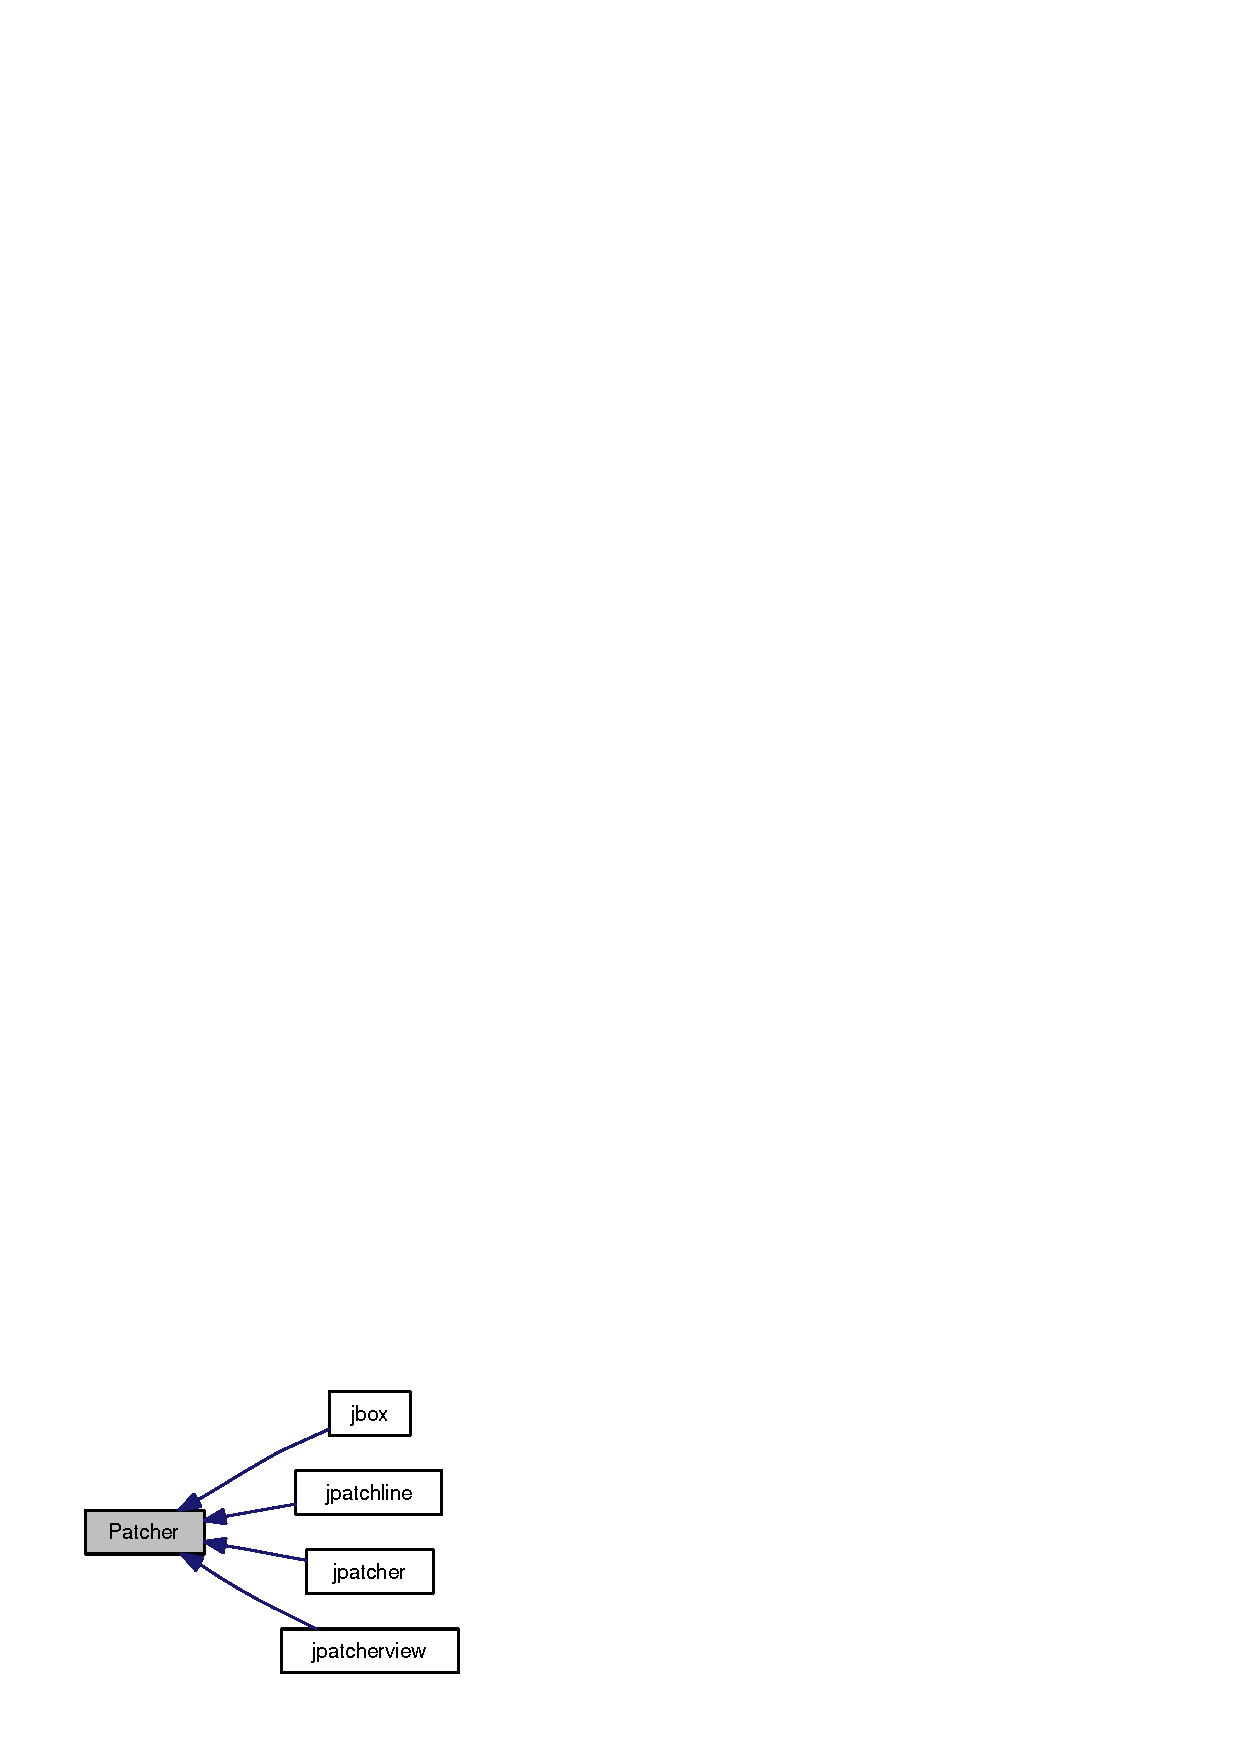
\includegraphics[width=112pt]{group__patcher}
\end{center}
\end{figure}
\subsection*{Data Structures}
\begin{DoxyCompactItemize}
\item 
struct \hyperlink{structt__jbox}{t\_\-jbox}
\begin{DoxyCompactList}\small\item\em The \hyperlink{structt__jbox}{t\_\-jbox} struct provides the header for a Max user-\/interface object. \item\end{DoxyCompactList}\end{DoxyCompactItemize}
\subsection*{Modules}
\begin{DoxyCompactItemize}
\item 
\hyperlink{group__jpatcher}{jpatcher}


\begin{DoxyCompactList}\small\item\em The patcher. \item\end{DoxyCompactList}\item 
\hyperlink{group__jbox}{jbox}


\begin{DoxyCompactList}\small\item\em A box in the patcher. \item\end{DoxyCompactList}\item 
\hyperlink{group__jpatchline}{jpatchline}


\begin{DoxyCompactList}\small\item\em A patch cord. \item\end{DoxyCompactList}\item 
\hyperlink{group__jpatcherview}{jpatcherview}


\begin{DoxyCompactList}\small\item\em A view of a patcher. \item\end{DoxyCompactList}\end{DoxyCompactItemize}
\subsection*{Typedefs}
\begin{DoxyCompactItemize}
\item 
typedef \hyperlink{structt__object}{t\_\-object} \hyperlink{group__patcher_ga17444ce85b4edde6ecc818081ffa1cfd}{t\_\-patcher}
\begin{DoxyCompactList}\small\item\em A patcher. \item\end{DoxyCompactList}\item 
typedef \hyperlink{structt__object}{t\_\-object} \hyperlink{group__patcher_ga4ae1309e71747dc0dc5c2baba5e47bc9}{t\_\-box}
\begin{DoxyCompactList}\small\item\em A box. \item\end{DoxyCompactList}\end{DoxyCompactItemize}
\subsection*{Enumerations}
\begin{DoxyCompactItemize}
\item 
enum \{ \par
\hyperlink{group__patcher_ggabc6126af1d45847bc59afa0aa3216b04a615ccc19640c4714e619315b94765e48}{PI\_\-DEEP} =  1, 
\par
\hyperlink{group__patcher_ggabc6126af1d45847bc59afa0aa3216b04a4c42ad2b13496b1d6664fed514724ffa}{PI\_\-REQUIREFIRSTIN} =  2, 
\par
\hyperlink{group__patcher_ggabc6126af1d45847bc59afa0aa3216b04a128de369dd62c2625aff042d820456eb}{PI\_\-WANTBOX} =  4
 \}
\begin{DoxyCompactList}\small\item\em patcher iteration flags \item\end{DoxyCompactList}\end{DoxyCompactItemize}


\subsection{Detailed Description}
Max's patcher represents a graph of objects that communicate with messages. This is the public interface to the jpatcher -\/-\/ the new patcher object in Max 5. The jpatcher is fully controllable via obex attributes and methods.

The jpatcher\_\-api.h header defines constants, enumerations, symbols, structs, and functions for working with the jpatcher. It also includes utility functions for getting/setting attributes and for calling methods. These utilities are just wrapping the obex interface and thus loosely connect your code to the jpatcher implementation.

Finally methods are defined for implementing your own boxes. 

\subsection{Typedef Documentation}
\hypertarget{group__patcher_ga4ae1309e71747dc0dc5c2baba5e47bc9}{
\index{patcher@{patcher}!t\_\-box@{t\_\-box}}
\index{t\_\-box@{t\_\-box}!patcher@{patcher}}
\subsubsection[{t\_\-box}]{\setlength{\rightskip}{0pt plus 5cm}typedef {\bf t\_\-object} {\bf t\_\-box}}}
\label{group__patcher_ga4ae1309e71747dc0dc5c2baba5e47bc9}


A box. As of Max 5, the box struct is opaque. Messages can be sent to a box using \hyperlink{group__obj_gae740749094827ac5adc2b7145db1c596}{object\_\-method()} or \hyperlink{group__obj_ga443dee482af22e0fe83e68955d367226}{object\_\-method\_\-typed()}, or by using \hyperlink{group__attr}{Attributes} accessors. \hypertarget{group__patcher_ga17444ce85b4edde6ecc818081ffa1cfd}{
\index{patcher@{patcher}!t\_\-patcher@{t\_\-patcher}}
\index{t\_\-patcher@{t\_\-patcher}!patcher@{patcher}}
\subsubsection[{t\_\-patcher}]{\setlength{\rightskip}{0pt plus 5cm}typedef {\bf t\_\-object} {\bf t\_\-patcher}}}
\label{group__patcher_ga17444ce85b4edde6ecc818081ffa1cfd}


A patcher. As of Max 5, the patcher struct is opaque. Messages can be sent to a patcher using \hyperlink{group__obj_gae740749094827ac5adc2b7145db1c596}{object\_\-method()} or \hyperlink{group__obj_ga443dee482af22e0fe83e68955d367226}{object\_\-method\_\-typed()}, or by using \hyperlink{group__attr}{Attributes} accessors. 

\subsection{Enumeration Type Documentation}
\hypertarget{group__patcher_gabc6126af1d45847bc59afa0aa3216b04}{
\subsubsection[{"@3}]{\setlength{\rightskip}{0pt plus 5cm}anonymous enum}}
\label{group__patcher_gabc6126af1d45847bc59afa0aa3216b04}


patcher iteration flags \begin{Desc}
\item[Enumerator: ]\par
\begin{description}
\index{PI\_\-DEEP@{PI\_\-DEEP}!patcher@{patcher}}\index{patcher@{patcher}!PI\_\-DEEP@{PI\_\-DEEP}}\item[{\em 
\hypertarget{group__patcher_ggabc6126af1d45847bc59afa0aa3216b04a615ccc19640c4714e619315b94765e48}{
PI\_\-DEEP}
\label{group__patcher_ggabc6126af1d45847bc59afa0aa3216b04a615ccc19640c4714e619315b94765e48}
}]descend into subpatchers (not used by audio library) \index{PI\_\-REQUIREFIRSTIN@{PI\_\-REQUIREFIRSTIN}!patcher@{patcher}}\index{patcher@{patcher}!PI\_\-REQUIREFIRSTIN@{PI\_\-REQUIREFIRSTIN}}\item[{\em 
\hypertarget{group__patcher_ggabc6126af1d45847bc59afa0aa3216b04a4c42ad2b13496b1d6664fed514724ffa}{
PI\_\-REQUIREFIRSTIN}
\label{group__patcher_ggabc6126af1d45847bc59afa0aa3216b04a4c42ad2b13496b1d6664fed514724ffa}
}]if b-\/$>$b\_\-firstin is NULL, do not call function \index{PI\_\-WANTBOX@{PI\_\-WANTBOX}!patcher@{patcher}}\index{patcher@{patcher}!PI\_\-WANTBOX@{PI\_\-WANTBOX}}\item[{\em 
\hypertarget{group__patcher_ggabc6126af1d45847bc59afa0aa3216b04a128de369dd62c2625aff042d820456eb}{
PI\_\-WANTBOX}
\label{group__patcher_ggabc6126af1d45847bc59afa0aa3216b04a128de369dd62c2625aff042d820456eb}
}]instead, of b-\/$>$b\_\-firstin, pass b to function, whether or not b-\/$>$b\_\-firstin is NULL \end{description}
\end{Desc}


\hypertarget{group__jpatcher}{
\section{jpatcher}
\label{group__jpatcher}\index{jpatcher@{jpatcher}}
}


The patcher.  


Collaboration diagram for jpatcher:\nopagebreak
\begin{figure}[H]
\begin{center}
\leavevmode
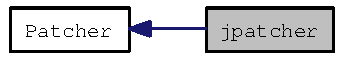
\includegraphics[width=100pt]{group__jpatcher}
\end{center}
\end{figure}
\subsection*{Functions}
\begin{DoxyCompactItemize}
\item 
int \hyperlink{group__jpatcher_ga7ffe181b1eaf48f2380c22b6483037af}{jpatcher\_\-is\_\-patcher} (\hyperlink{structt__object}{t\_\-object} $\ast$p)
\begin{DoxyCompactList}\small\item\em Determine of a \hyperlink{structt__object}{t\_\-object}$\ast$ is a patcher object. \item\end{DoxyCompactList}\item 
\hyperlink{structt__object}{t\_\-object} $\ast$ \hyperlink{group__jpatcher_gad55371f057913b8b26cb58c3c517a1f4}{jpatcher\_\-get\_\-box} (\hyperlink{structt__object}{t\_\-object} $\ast$p)
\begin{DoxyCompactList}\small\item\em If a patcher is inside a box, return its box. \item\end{DoxyCompactList}\item 
long \hyperlink{group__jpatcher_gaf5a44f30054baae18b5019f305070612}{jpatcher\_\-get\_\-count} (\hyperlink{structt__object}{t\_\-object} $\ast$p)
\begin{DoxyCompactList}\small\item\em Determine the number of boxes in a patcher. \item\end{DoxyCompactList}\item 
\hyperlink{group__datatypes_ga73edaae82b318855cc09fac994918165}{t\_\-max\_\-err} \hyperlink{group__jpatcher_ga3210a517b3c79b2fb305b9a8357fe3db}{jpatcher\_\-set\_\-locked} (\hyperlink{structt__object}{t\_\-object} $\ast$p, char c)
\begin{DoxyCompactList}\small\item\em Lock or unlock a patcher. \item\end{DoxyCompactList}\item 
char \hyperlink{group__jpatcher_gaa3af83f31fba548f05ac23e5f4144ed9}{jpatcher\_\-get\_\-presentation} (\hyperlink{structt__object}{t\_\-object} $\ast$p)
\begin{DoxyCompactList}\small\item\em Determine whether a patcher is currently in presentation mode. \item\end{DoxyCompactList}\item 
\hyperlink{group__datatypes_ga73edaae82b318855cc09fac994918165}{t\_\-max\_\-err} \hyperlink{group__jpatcher_ga3994f39cf34c6a1f4502e087ad6adb0a}{jpatcher\_\-set\_\-presentation} (\hyperlink{structt__object}{t\_\-object} $\ast$p, char c)
\begin{DoxyCompactList}\small\item\em Set a patcher to presentation mode. \item\end{DoxyCompactList}\item 
\hyperlink{structt__object}{t\_\-object} $\ast$ \hyperlink{group__jpatcher_gafd77f63d504807973a4ce400c304b174}{jpatcher\_\-get\_\-firstobject} (\hyperlink{structt__object}{t\_\-object} $\ast$p)
\begin{DoxyCompactList}\small\item\em Get the first box in a patcher. \item\end{DoxyCompactList}\item 
\hyperlink{structt__object}{t\_\-object} $\ast$ \hyperlink{group__jpatcher_gaffb5e8d5224f7aa04cdbee76a041bab7}{jpatcher\_\-get\_\-lastobject} (\hyperlink{structt__object}{t\_\-object} $\ast$p)
\begin{DoxyCompactList}\small\item\em Get the last box in a patcher. \item\end{DoxyCompactList}\item 
\hyperlink{structt__object}{t\_\-object} $\ast$ \hyperlink{group__jpatcher_ga5d110fdbf8797e9d0edfa1e47afdc691}{jpatcher\_\-get\_\-firstline} (\hyperlink{structt__object}{t\_\-object} $\ast$p)
\begin{DoxyCompactList}\small\item\em Get the first line (patch-\/cord) in a patcher. \item\end{DoxyCompactList}\item 
\hyperlink{structt__object}{t\_\-object} $\ast$ \hyperlink{group__jpatcher_gaccc0cfeb70fbeecbd322de7e8b9bac98}{jpatcher\_\-get\_\-firstview} (\hyperlink{structt__object}{t\_\-object} $\ast$p)
\begin{DoxyCompactList}\small\item\em Get the first view (jpatcherview) for a given patcher. \item\end{DoxyCompactList}\item 
\hyperlink{structt__symbol}{t\_\-symbol} $\ast$ \hyperlink{group__jpatcher_gae9067670d2885c808fa2db1e22a327d8}{jpatcher\_\-get\_\-title} (\hyperlink{structt__object}{t\_\-object} $\ast$p)
\begin{DoxyCompactList}\small\item\em Retrieve a patcher's title. \item\end{DoxyCompactList}\item 
\hyperlink{group__datatypes_ga73edaae82b318855cc09fac994918165}{t\_\-max\_\-err} \hyperlink{group__jpatcher_gadd59390cab86f13282704e8bdf4ea3ba}{jpatcher\_\-set\_\-title} (\hyperlink{structt__object}{t\_\-object} $\ast$p, \hyperlink{structt__symbol}{t\_\-symbol} $\ast$ps)
\begin{DoxyCompactList}\small\item\em Set a patcher's title. \item\end{DoxyCompactList}\item 
\hyperlink{structt__symbol}{t\_\-symbol} $\ast$ \hyperlink{group__jpatcher_ga245a38ac7814605e198466313884a246}{jpatcher\_\-get\_\-name} (\hyperlink{structt__object}{t\_\-object} $\ast$p)
\begin{DoxyCompactList}\small\item\em Retrieve a patcher's name. \item\end{DoxyCompactList}\item 
\hyperlink{structt__symbol}{t\_\-symbol} $\ast$ \hyperlink{group__jpatcher_gac278d621dc1eef9e3b0dbddfc6bf3f53}{jpatcher\_\-get\_\-filepath} (\hyperlink{structt__object}{t\_\-object} $\ast$p)
\begin{DoxyCompactList}\small\item\em Retrieve a patcher's file path. \item\end{DoxyCompactList}\item 
\hyperlink{structt__symbol}{t\_\-symbol} $\ast$ \hyperlink{group__jpatcher_gaf8d1fda60ecc028f2aff88c81e8d4b4f}{jpatcher\_\-get\_\-filename} (\hyperlink{structt__object}{t\_\-object} $\ast$p)
\begin{DoxyCompactList}\small\item\em Retrieve a patcher's file name. \item\end{DoxyCompactList}\item 
char \hyperlink{group__jpatcher_ga5eb01f66882115ca01028ca68c4307b3}{jpatcher\_\-get\_\-dirty} (\hyperlink{structt__object}{t\_\-object} $\ast$p)
\begin{DoxyCompactList}\small\item\em Determine whether a patcher's dirty bit has been set. \item\end{DoxyCompactList}\item 
\hyperlink{group__datatypes_ga73edaae82b318855cc09fac994918165}{t\_\-max\_\-err} \hyperlink{group__jpatcher_gaad586555902f02618e3c3fa1f977d5a5}{jpatcher\_\-set\_\-dirty} (\hyperlink{structt__object}{t\_\-object} $\ast$p, char c)
\begin{DoxyCompactList}\small\item\em Set a patcher's dirty bit. \item\end{DoxyCompactList}\item 
char \hyperlink{group__jpatcher_ga38c0179d1eb95d96f473cfde94164be4}{jpatcher\_\-get\_\-bglocked} (\hyperlink{structt__object}{t\_\-object} $\ast$p)
\begin{DoxyCompactList}\small\item\em Determine whether a patcher's background layer is locked. \item\end{DoxyCompactList}\item 
\hyperlink{group__datatypes_ga73edaae82b318855cc09fac994918165}{t\_\-max\_\-err} \hyperlink{group__jpatcher_ga8bdd915ec7c3de07c7c90c33b6b516bf}{jpatcher\_\-set\_\-bglocked} (\hyperlink{structt__object}{t\_\-object} $\ast$p, char c)
\begin{DoxyCompactList}\small\item\em Set whether a patcher's background layer is locked. \item\end{DoxyCompactList}\item 
char \hyperlink{group__jpatcher_gabb79c4b3f29dd61ad9725a2a8141b312}{jpatcher\_\-get\_\-bghidden} (\hyperlink{structt__object}{t\_\-object} $\ast$p)
\begin{DoxyCompactList}\small\item\em Determine whether a patcher's background layer is hidden. \item\end{DoxyCompactList}\item 
\hyperlink{group__datatypes_ga73edaae82b318855cc09fac994918165}{t\_\-max\_\-err} \hyperlink{group__jpatcher_gaace70353f26b52b10d5926ab0a6c9395}{jpatcher\_\-set\_\-bghidden} (\hyperlink{structt__object}{t\_\-object} $\ast$p, char c)
\begin{DoxyCompactList}\small\item\em Set whether a patcher's background layer is hidden. \item\end{DoxyCompactList}\item 
char \hyperlink{group__jpatcher_ga164ac5db6109ab48fb0ca833263da801}{jpatcher\_\-get\_\-fghidden} (\hyperlink{structt__object}{t\_\-object} $\ast$p)
\begin{DoxyCompactList}\small\item\em Determine whether a patcher's foreground layer is hidden. \item\end{DoxyCompactList}\item 
\hyperlink{group__datatypes_ga73edaae82b318855cc09fac994918165}{t\_\-max\_\-err} \hyperlink{group__jpatcher_ga905d41f7b001aa779374307b67a07495}{jpatcher\_\-set\_\-fghidden} (\hyperlink{structt__object}{t\_\-object} $\ast$p, char c)
\begin{DoxyCompactList}\small\item\em Set whether a patcher's foreground layer is hidden. \item\end{DoxyCompactList}\item 
\hyperlink{group__datatypes_ga73edaae82b318855cc09fac994918165}{t\_\-max\_\-err} \hyperlink{group__jpatcher_ga66ac15a412d7fa918471a49e341a93fa}{jpatcher\_\-get\_\-editing\_\-bgcolor} (\hyperlink{structt__object}{t\_\-object} $\ast$p, \hyperlink{structt__jrgba}{t\_\-jrgba} $\ast$prgba)
\begin{DoxyCompactList}\small\item\em Retrieve a patcher's editing background color. \item\end{DoxyCompactList}\item 
\hyperlink{group__datatypes_ga73edaae82b318855cc09fac994918165}{t\_\-max\_\-err} \hyperlink{group__jpatcher_ga3e0e7d12c6e30c582fbd3da059eaca58}{jpatcher\_\-set\_\-editing\_\-bgcolor} (\hyperlink{structt__object}{t\_\-object} $\ast$p, \hyperlink{structt__jrgba}{t\_\-jrgba} $\ast$prgba)
\begin{DoxyCompactList}\small\item\em Set a patcher's editing background color. \item\end{DoxyCompactList}\item 
\hyperlink{group__datatypes_ga73edaae82b318855cc09fac994918165}{t\_\-max\_\-err} \hyperlink{group__jpatcher_gac08bdf16f3f65b962cdfbe2b5aa59ab0}{jpatcher\_\-get\_\-bgcolor} (\hyperlink{structt__object}{t\_\-object} $\ast$p, \hyperlink{structt__jrgba}{t\_\-jrgba} $\ast$prgba)
\begin{DoxyCompactList}\small\item\em Retrieve a patcher's locked background color. \item\end{DoxyCompactList}\item 
\hyperlink{group__datatypes_ga73edaae82b318855cc09fac994918165}{t\_\-max\_\-err} \hyperlink{group__jpatcher_ga2ddf7d6edaf305c425108a96cb32b62d}{jpatcher\_\-set\_\-bgcolor} (\hyperlink{structt__object}{t\_\-object} $\ast$p, \hyperlink{structt__jrgba}{t\_\-jrgba} $\ast$prgba)
\begin{DoxyCompactList}\small\item\em Set a patcher's locked background color. \item\end{DoxyCompactList}\item 
\hyperlink{group__datatypes_ga73edaae82b318855cc09fac994918165}{t\_\-max\_\-err} \hyperlink{group__jpatcher_ga140e8da3e2be163b5cbbb1eef350d70f}{jpatcher\_\-get\_\-gridsize} (\hyperlink{structt__object}{t\_\-object} $\ast$p, double $\ast$gridsizeX, double $\ast$gridsizeY)
\begin{DoxyCompactList}\small\item\em Retrieve a patcher's grid size. \item\end{DoxyCompactList}\item 
\hyperlink{group__datatypes_ga73edaae82b318855cc09fac994918165}{t\_\-max\_\-err} \hyperlink{group__jpatcher_ga34113c97506a3a5c25d3a00805f43b38}{jpatcher\_\-set\_\-gridsize} (\hyperlink{structt__object}{t\_\-object} $\ast$p, double gridsizeX, double gridsizeY)
\begin{DoxyCompactList}\small\item\em Set a patcher's grid size. \item\end{DoxyCompactList}\item 
void \hyperlink{group__jpatcher_ga669798a90e3928a04b0f65143a7981fd}{jpatcher\_\-deleteobj} (\hyperlink{structt__object}{t\_\-object} $\ast$p, \hyperlink{structt__jbox}{t\_\-jbox} $\ast$b)
\begin{DoxyCompactList}\small\item\em Delete an object that is in a patcher. \item\end{DoxyCompactList}\item 
\hyperlink{structt__object}{t\_\-object} $\ast$ \hyperlink{group__jpatcher_ga337a58107a3555e2de7da75893840920}{jpatcher\_\-get\_\-parentpatcher} (\hyperlink{structt__object}{t\_\-object} $\ast$p)
\begin{DoxyCompactList}\small\item\em Given a patcher, return its parent patcher. \item\end{DoxyCompactList}\item 
\hyperlink{structt__object}{t\_\-object} $\ast$ \hyperlink{group__jpatcher_gab0fbb44da944b038c690efb0b2415a7a}{jpatcher\_\-get\_\-toppatcher} (\hyperlink{structt__object}{t\_\-object} $\ast$p)
\begin{DoxyCompactList}\small\item\em Given a patcher, return the top-\/level patcher for the tree in which it exists. \item\end{DoxyCompactList}\item 
\hyperlink{group__datatypes_ga73edaae82b318855cc09fac994918165}{t\_\-max\_\-err} \hyperlink{group__jpatcher_gaedf734a76297bf735810ac36e17748a1}{jpatcher\_\-get\_\-rect} (\hyperlink{structt__object}{t\_\-object} $\ast$p, \hyperlink{structt__rect}{t\_\-rect} $\ast$pr)
\begin{DoxyCompactList}\small\item\em Query a patcher to determine its location and size. \item\end{DoxyCompactList}\item 
\hyperlink{group__datatypes_ga73edaae82b318855cc09fac994918165}{t\_\-max\_\-err} \hyperlink{group__jpatcher_ga0a54c1b858851885088c5af970c9617d}{jpatcher\_\-set\_\-rect} (\hyperlink{structt__object}{t\_\-object} $\ast$p, \hyperlink{structt__rect}{t\_\-rect} $\ast$pr)
\begin{DoxyCompactList}\small\item\em Set a patcher's location and size. \item\end{DoxyCompactList}\item 
\hyperlink{group__datatypes_ga73edaae82b318855cc09fac994918165}{t\_\-max\_\-err} \hyperlink{group__jpatcher_ga177848d5433ff59335d06b15518f9df3}{jpatcher\_\-get\_\-defrect} (\hyperlink{structt__object}{t\_\-object} $\ast$p, \hyperlink{structt__rect}{t\_\-rect} $\ast$pr)
\begin{DoxyCompactList}\small\item\em Query a patcher to determine the location and dimensions of its window when initially opened. \item\end{DoxyCompactList}\item 
\hyperlink{group__datatypes_ga73edaae82b318855cc09fac994918165}{t\_\-max\_\-err} \hyperlink{group__jpatcher_gacc68e225735eac71aecfc69808bf0697}{jpatcher\_\-set\_\-defrect} (\hyperlink{structt__object}{t\_\-object} $\ast$p, \hyperlink{structt__rect}{t\_\-rect} $\ast$pr)
\begin{DoxyCompactList}\small\item\em Set a patcher's default location and size. \item\end{DoxyCompactList}\item 
\hyperlink{structt__symbol}{t\_\-symbol} $\ast$ \hyperlink{group__jpatcher_ga8538a0402d6936dd0838a52b4d43c56a}{jpatcher\_\-uniqueboxname} (\hyperlink{structt__object}{t\_\-object} $\ast$p, \hyperlink{structt__symbol}{t\_\-symbol} $\ast$classname)
\begin{DoxyCompactList}\small\item\em Generate a unique name for a box in patcher. \item\end{DoxyCompactList}\item 
\hyperlink{structt__symbol}{t\_\-symbol} $\ast$ \hyperlink{group__jpatcher_gac5cb14bf7507096591e66b88b7ad0e87}{jpatcher\_\-get\_\-default\_\-fontname} (\hyperlink{structt__object}{t\_\-object} $\ast$p)
\begin{DoxyCompactList}\small\item\em Return the name of the default font used for new objects in a patcher. \item\end{DoxyCompactList}\item 
float \hyperlink{group__jpatcher_ga2a84ae15f52f7793d7e14d26cf555534}{jpatcher\_\-get\_\-default\_\-fontsize} (\hyperlink{structt__object}{t\_\-object} $\ast$p)
\begin{DoxyCompactList}\small\item\em Return the size of the default font used for new objects in a patcher. \item\end{DoxyCompactList}\item 
long \hyperlink{group__jpatcher_ga2ab66cc8938565435fcf1fc97d73161a}{jpatcher\_\-get\_\-default\_\-fontface} (\hyperlink{structt__object}{t\_\-object} $\ast$p)
\begin{DoxyCompactList}\small\item\em Return the index of the default font face used for new objects in a patcher. \item\end{DoxyCompactList}\item 
long \hyperlink{group__jpatcher_gaac7f1696b3346197cb8f1c0dac954780}{jpatcher\_\-get\_\-fileversion} (\hyperlink{structt__object}{t\_\-object} $\ast$p)
\begin{DoxyCompactList}\small\item\em Return the file version of the patcher. \item\end{DoxyCompactList}\item 
long \hyperlink{group__jpatcher_gac06ed9b2aa744159810c7a735b8be890}{jpatcher\_\-get\_\-currentfileversion} (void)
\begin{DoxyCompactList}\small\item\em Return the file version for any new patchers, e.g. \item\end{DoxyCompactList}\end{DoxyCompactItemize}


\subsection{Detailed Description}
The patcher. 

\subsection{Function Documentation}
\hypertarget{group__jpatcher_ga669798a90e3928a04b0f65143a7981fd}{
\index{jpatcher@{jpatcher}!jpatcher\_\-deleteobj@{jpatcher\_\-deleteobj}}
\index{jpatcher\_\-deleteobj@{jpatcher\_\-deleteobj}!jpatcher@{jpatcher}}
\subsubsection[{jpatcher\_\-deleteobj}]{\setlength{\rightskip}{0pt plus 5cm}void jpatcher\_\-deleteobj ({\bf t\_\-object} $\ast$ {\em p}, \/  {\bf t\_\-jbox} $\ast$ {\em b})}}
\label{group__jpatcher_ga669798a90e3928a04b0f65143a7981fd}


Delete an object that is in a patcher. 
\begin{DoxyParams}{Parameters}
\item[{\em p}]The patcher. \item[{\em b}]The object box to delete. \end{DoxyParams}
\hypertarget{group__jpatcher_gac08bdf16f3f65b962cdfbe2b5aa59ab0}{
\index{jpatcher@{jpatcher}!jpatcher\_\-get\_\-bgcolor@{jpatcher\_\-get\_\-bgcolor}}
\index{jpatcher\_\-get\_\-bgcolor@{jpatcher\_\-get\_\-bgcolor}!jpatcher@{jpatcher}}
\subsubsection[{jpatcher\_\-get\_\-bgcolor}]{\setlength{\rightskip}{0pt plus 5cm}{\bf t\_\-max\_\-err} jpatcher\_\-get\_\-bgcolor ({\bf t\_\-object} $\ast$ {\em p}, \/  {\bf t\_\-jrgba} $\ast$ {\em prgba})}}
\label{group__jpatcher_gac08bdf16f3f65b962cdfbe2b5aa59ab0}


Retrieve a patcher's locked background color. 
\begin{DoxyParams}{Parameters}
\item[{\em p}]The patcher to be queried. \item[{\em prgba}]The address of a valid \hyperlink{structt__jrgba}{t\_\-jrgba} struct that will be filled-\/in with the current patcher color values. \end{DoxyParams}
\begin{DoxyReturn}{Returns}
A Max error code. 
\end{DoxyReturn}
\hypertarget{group__jpatcher_gabb79c4b3f29dd61ad9725a2a8141b312}{
\index{jpatcher@{jpatcher}!jpatcher\_\-get\_\-bghidden@{jpatcher\_\-get\_\-bghidden}}
\index{jpatcher\_\-get\_\-bghidden@{jpatcher\_\-get\_\-bghidden}!jpatcher@{jpatcher}}
\subsubsection[{jpatcher\_\-get\_\-bghidden}]{\setlength{\rightskip}{0pt plus 5cm}char jpatcher\_\-get\_\-bghidden ({\bf t\_\-object} $\ast$ {\em p})}}
\label{group__jpatcher_gabb79c4b3f29dd61ad9725a2a8141b312}


Determine whether a patcher's background layer is hidden. 
\begin{DoxyParams}{Parameters}
\item[{\em p}]The patcher to be queried. \end{DoxyParams}
\begin{DoxyReturn}{Returns}
True if the background layer is hidden, otherwise false. 
\end{DoxyReturn}
\hypertarget{group__jpatcher_ga38c0179d1eb95d96f473cfde94164be4}{
\index{jpatcher@{jpatcher}!jpatcher\_\-get\_\-bglocked@{jpatcher\_\-get\_\-bglocked}}
\index{jpatcher\_\-get\_\-bglocked@{jpatcher\_\-get\_\-bglocked}!jpatcher@{jpatcher}}
\subsubsection[{jpatcher\_\-get\_\-bglocked}]{\setlength{\rightskip}{0pt plus 5cm}char jpatcher\_\-get\_\-bglocked ({\bf t\_\-object} $\ast$ {\em p})}}
\label{group__jpatcher_ga38c0179d1eb95d96f473cfde94164be4}


Determine whether a patcher's background layer is locked. 
\begin{DoxyParams}{Parameters}
\item[{\em p}]The patcher to be queried. \end{DoxyParams}
\begin{DoxyReturn}{Returns}
True if the background layer is locked, otherwise false. 
\end{DoxyReturn}
\hypertarget{group__jpatcher_gad55371f057913b8b26cb58c3c517a1f4}{
\index{jpatcher@{jpatcher}!jpatcher\_\-get\_\-box@{jpatcher\_\-get\_\-box}}
\index{jpatcher\_\-get\_\-box@{jpatcher\_\-get\_\-box}!jpatcher@{jpatcher}}
\subsubsection[{jpatcher\_\-get\_\-box}]{\setlength{\rightskip}{0pt plus 5cm}{\bf t\_\-object}$\ast$ jpatcher\_\-get\_\-box ({\bf t\_\-object} $\ast$ {\em p})}}
\label{group__jpatcher_gad55371f057913b8b26cb58c3c517a1f4}


If a patcher is inside a box, return its box. 
\begin{DoxyParams}{Parameters}
\item[{\em p}]The patcher to be queried. \end{DoxyParams}
\begin{DoxyReturn}{Returns}
A pointer to the box containing the patcher, otherwise NULL. 
\end{DoxyReturn}
\hypertarget{group__jpatcher_gaf5a44f30054baae18b5019f305070612}{
\index{jpatcher@{jpatcher}!jpatcher\_\-get\_\-count@{jpatcher\_\-get\_\-count}}
\index{jpatcher\_\-get\_\-count@{jpatcher\_\-get\_\-count}!jpatcher@{jpatcher}}
\subsubsection[{jpatcher\_\-get\_\-count}]{\setlength{\rightskip}{0pt plus 5cm}long jpatcher\_\-get\_\-count ({\bf t\_\-object} $\ast$ {\em p})}}
\label{group__jpatcher_gaf5a44f30054baae18b5019f305070612}


Determine the number of boxes in a patcher. 
\begin{DoxyParams}{Parameters}
\item[{\em p}]The patcher to be queried. \end{DoxyParams}
\begin{DoxyReturn}{Returns}
The number of boxes in the patcher. 
\end{DoxyReturn}
\hypertarget{group__jpatcher_gac06ed9b2aa744159810c7a735b8be890}{
\index{jpatcher@{jpatcher}!jpatcher\_\-get\_\-currentfileversion@{jpatcher\_\-get\_\-currentfileversion}}
\index{jpatcher\_\-get\_\-currentfileversion@{jpatcher\_\-get\_\-currentfileversion}!jpatcher@{jpatcher}}
\subsubsection[{jpatcher\_\-get\_\-currentfileversion}]{\setlength{\rightskip}{0pt plus 5cm}long jpatcher\_\-get\_\-currentfileversion (void)}}
\label{group__jpatcher_gac06ed9b2aa744159810c7a735b8be890}


Return the file version for any new patchers, e.g. the current version created by Max.

\begin{DoxyReturn}{Returns}
The file version number. 
\end{DoxyReturn}
\hypertarget{group__jpatcher_ga2ab66cc8938565435fcf1fc97d73161a}{
\index{jpatcher@{jpatcher}!jpatcher\_\-get\_\-default\_\-fontface@{jpatcher\_\-get\_\-default\_\-fontface}}
\index{jpatcher\_\-get\_\-default\_\-fontface@{jpatcher\_\-get\_\-default\_\-fontface}!jpatcher@{jpatcher}}
\subsubsection[{jpatcher\_\-get\_\-default\_\-fontface}]{\setlength{\rightskip}{0pt plus 5cm}long jpatcher\_\-get\_\-default\_\-fontface ({\bf t\_\-object} $\ast$ {\em p})}}
\label{group__jpatcher_ga2ab66cc8938565435fcf1fc97d73161a}


Return the index of the default font face used for new objects in a patcher. 
\begin{DoxyParams}{Parameters}
\item[{\em p}]A pointer to a patcher instance. \end{DoxyParams}
\begin{DoxyReturn}{Returns}
The index of the default font face used for new objects in a patcher. 
\end{DoxyReturn}
\hypertarget{group__jpatcher_gac5cb14bf7507096591e66b88b7ad0e87}{
\index{jpatcher@{jpatcher}!jpatcher\_\-get\_\-default\_\-fontname@{jpatcher\_\-get\_\-default\_\-fontname}}
\index{jpatcher\_\-get\_\-default\_\-fontname@{jpatcher\_\-get\_\-default\_\-fontname}!jpatcher@{jpatcher}}
\subsubsection[{jpatcher\_\-get\_\-default\_\-fontname}]{\setlength{\rightskip}{0pt plus 5cm}{\bf t\_\-symbol}$\ast$ jpatcher\_\-get\_\-default\_\-fontname ({\bf t\_\-object} $\ast$ {\em p})}}
\label{group__jpatcher_gac5cb14bf7507096591e66b88b7ad0e87}


Return the name of the default font used for new objects in a patcher. 
\begin{DoxyParams}{Parameters}
\item[{\em p}]A pointer to a patcher instance. \end{DoxyParams}
\begin{DoxyReturn}{Returns}
The name of the default font used for new objects in a patcher. 
\end{DoxyReturn}
\hypertarget{group__jpatcher_ga2a84ae15f52f7793d7e14d26cf555534}{
\index{jpatcher@{jpatcher}!jpatcher\_\-get\_\-default\_\-fontsize@{jpatcher\_\-get\_\-default\_\-fontsize}}
\index{jpatcher\_\-get\_\-default\_\-fontsize@{jpatcher\_\-get\_\-default\_\-fontsize}!jpatcher@{jpatcher}}
\subsubsection[{jpatcher\_\-get\_\-default\_\-fontsize}]{\setlength{\rightskip}{0pt plus 5cm}float jpatcher\_\-get\_\-default\_\-fontsize ({\bf t\_\-object} $\ast$ {\em p})}}
\label{group__jpatcher_ga2a84ae15f52f7793d7e14d26cf555534}


Return the size of the default font used for new objects in a patcher. 
\begin{DoxyParams}{Parameters}
\item[{\em p}]A pointer to a patcher instance. \end{DoxyParams}
\begin{DoxyReturn}{Returns}
The size of the default font used for new objects in a patcher. 
\end{DoxyReturn}
\hypertarget{group__jpatcher_ga177848d5433ff59335d06b15518f9df3}{
\index{jpatcher@{jpatcher}!jpatcher\_\-get\_\-defrect@{jpatcher\_\-get\_\-defrect}}
\index{jpatcher\_\-get\_\-defrect@{jpatcher\_\-get\_\-defrect}!jpatcher@{jpatcher}}
\subsubsection[{jpatcher\_\-get\_\-defrect}]{\setlength{\rightskip}{0pt plus 5cm}{\bf t\_\-max\_\-err} jpatcher\_\-get\_\-defrect ({\bf t\_\-object} $\ast$ {\em p}, \/  {\bf t\_\-rect} $\ast$ {\em pr})}}
\label{group__jpatcher_ga177848d5433ff59335d06b15518f9df3}


Query a patcher to determine the location and dimensions of its window when initially opened. 
\begin{DoxyParams}{Parameters}
\item[{\em p}]A pointer to a patcher instance. \item[{\em pr}]The address of valid \hyperlink{structt__rect}{t\_\-rect} whose values will be filled-\/in upon return. \end{DoxyParams}
\begin{DoxyReturn}{Returns}
A Max error code. 
\end{DoxyReturn}
\hypertarget{group__jpatcher_ga5eb01f66882115ca01028ca68c4307b3}{
\index{jpatcher@{jpatcher}!jpatcher\_\-get\_\-dirty@{jpatcher\_\-get\_\-dirty}}
\index{jpatcher\_\-get\_\-dirty@{jpatcher\_\-get\_\-dirty}!jpatcher@{jpatcher}}
\subsubsection[{jpatcher\_\-get\_\-dirty}]{\setlength{\rightskip}{0pt plus 5cm}char jpatcher\_\-get\_\-dirty ({\bf t\_\-object} $\ast$ {\em p})}}
\label{group__jpatcher_ga5eb01f66882115ca01028ca68c4307b3}


Determine whether a patcher's dirty bit has been set. 
\begin{DoxyParams}{Parameters}
\item[{\em p}]The patcher to be queried. \end{DoxyParams}
\begin{DoxyReturn}{Returns}
True if the patcher is dirty, otherwise false. 
\end{DoxyReturn}
\hypertarget{group__jpatcher_ga66ac15a412d7fa918471a49e341a93fa}{
\index{jpatcher@{jpatcher}!jpatcher\_\-get\_\-editing\_\-bgcolor@{jpatcher\_\-get\_\-editing\_\-bgcolor}}
\index{jpatcher\_\-get\_\-editing\_\-bgcolor@{jpatcher\_\-get\_\-editing\_\-bgcolor}!jpatcher@{jpatcher}}
\subsubsection[{jpatcher\_\-get\_\-editing\_\-bgcolor}]{\setlength{\rightskip}{0pt plus 5cm}{\bf t\_\-max\_\-err} jpatcher\_\-get\_\-editing\_\-bgcolor ({\bf t\_\-object} $\ast$ {\em p}, \/  {\bf t\_\-jrgba} $\ast$ {\em prgba})}}
\label{group__jpatcher_ga66ac15a412d7fa918471a49e341a93fa}


Retrieve a patcher's editing background color. 
\begin{DoxyParams}{Parameters}
\item[{\em p}]The patcher to be queried. \item[{\em prgba}]The address of a valid \hyperlink{structt__jrgba}{t\_\-jrgba} struct that will be filled-\/in with the current patcher color values. \end{DoxyParams}
\begin{DoxyReturn}{Returns}
A Max error code. 
\end{DoxyReturn}
\hypertarget{group__jpatcher_ga164ac5db6109ab48fb0ca833263da801}{
\index{jpatcher@{jpatcher}!jpatcher\_\-get\_\-fghidden@{jpatcher\_\-get\_\-fghidden}}
\index{jpatcher\_\-get\_\-fghidden@{jpatcher\_\-get\_\-fghidden}!jpatcher@{jpatcher}}
\subsubsection[{jpatcher\_\-get\_\-fghidden}]{\setlength{\rightskip}{0pt plus 5cm}char jpatcher\_\-get\_\-fghidden ({\bf t\_\-object} $\ast$ {\em p})}}
\label{group__jpatcher_ga164ac5db6109ab48fb0ca833263da801}


Determine whether a patcher's foreground layer is hidden. 
\begin{DoxyParams}{Parameters}
\item[{\em p}]The patcher to be queried. \end{DoxyParams}
\begin{DoxyReturn}{Returns}
True if the foreground layer is hidden, otherwise false. 
\end{DoxyReturn}
\hypertarget{group__jpatcher_gaf8d1fda60ecc028f2aff88c81e8d4b4f}{
\index{jpatcher@{jpatcher}!jpatcher\_\-get\_\-filename@{jpatcher\_\-get\_\-filename}}
\index{jpatcher\_\-get\_\-filename@{jpatcher\_\-get\_\-filename}!jpatcher@{jpatcher}}
\subsubsection[{jpatcher\_\-get\_\-filename}]{\setlength{\rightskip}{0pt plus 5cm}{\bf t\_\-symbol}$\ast$ jpatcher\_\-get\_\-filename ({\bf t\_\-object} $\ast$ {\em p})}}
\label{group__jpatcher_gaf8d1fda60ecc028f2aff88c81e8d4b4f}


Retrieve a patcher's file name. 
\begin{DoxyParams}{Parameters}
\item[{\em p}]The patcher to be queried. \end{DoxyParams}
\begin{DoxyReturn}{Returns}
The patcher's file name. 
\end{DoxyReturn}
\hypertarget{group__jpatcher_gac278d621dc1eef9e3b0dbddfc6bf3f53}{
\index{jpatcher@{jpatcher}!jpatcher\_\-get\_\-filepath@{jpatcher\_\-get\_\-filepath}}
\index{jpatcher\_\-get\_\-filepath@{jpatcher\_\-get\_\-filepath}!jpatcher@{jpatcher}}
\subsubsection[{jpatcher\_\-get\_\-filepath}]{\setlength{\rightskip}{0pt plus 5cm}{\bf t\_\-symbol}$\ast$ jpatcher\_\-get\_\-filepath ({\bf t\_\-object} $\ast$ {\em p})}}
\label{group__jpatcher_gac278d621dc1eef9e3b0dbddfc6bf3f53}


Retrieve a patcher's file path. 
\begin{DoxyParams}{Parameters}
\item[{\em p}]The patcher to be queried. \end{DoxyParams}
\begin{DoxyReturn}{Returns}
The patcher's file path. 
\end{DoxyReturn}
\hypertarget{group__jpatcher_gaac7f1696b3346197cb8f1c0dac954780}{
\index{jpatcher@{jpatcher}!jpatcher\_\-get\_\-fileversion@{jpatcher\_\-get\_\-fileversion}}
\index{jpatcher\_\-get\_\-fileversion@{jpatcher\_\-get\_\-fileversion}!jpatcher@{jpatcher}}
\subsubsection[{jpatcher\_\-get\_\-fileversion}]{\setlength{\rightskip}{0pt plus 5cm}long jpatcher\_\-get\_\-fileversion ({\bf t\_\-object} $\ast$ {\em p})}}
\label{group__jpatcher_gaac7f1696b3346197cb8f1c0dac954780}


Return the file version of the patcher. 
\begin{DoxyParams}{Parameters}
\item[{\em p}]A pointer to the patcher whose version number is desired. \end{DoxyParams}
\begin{DoxyReturn}{Returns}
The file version number. 
\end{DoxyReturn}
\hypertarget{group__jpatcher_ga5d110fdbf8797e9d0edfa1e47afdc691}{
\index{jpatcher@{jpatcher}!jpatcher\_\-get\_\-firstline@{jpatcher\_\-get\_\-firstline}}
\index{jpatcher\_\-get\_\-firstline@{jpatcher\_\-get\_\-firstline}!jpatcher@{jpatcher}}
\subsubsection[{jpatcher\_\-get\_\-firstline}]{\setlength{\rightskip}{0pt plus 5cm}{\bf t\_\-object}$\ast$ jpatcher\_\-get\_\-firstline ({\bf t\_\-object} $\ast$ {\em p})}}
\label{group__jpatcher_ga5d110fdbf8797e9d0edfa1e47afdc691}


Get the first line (patch-\/cord) in a patcher. All lines in a patcher are maintained internally in a \hyperlink{structt__linklist}{t\_\-linklist}. Use this function to begin traversing a patcher's lines.


\begin{DoxyParams}{Parameters}
\item[{\em p}]The patcher to be queried. \end{DoxyParams}
\begin{DoxyReturn}{Returns}
The first jpatchline in a patcher. 
\end{DoxyReturn}
\hypertarget{group__jpatcher_gafd77f63d504807973a4ce400c304b174}{
\index{jpatcher@{jpatcher}!jpatcher\_\-get\_\-firstobject@{jpatcher\_\-get\_\-firstobject}}
\index{jpatcher\_\-get\_\-firstobject@{jpatcher\_\-get\_\-firstobject}!jpatcher@{jpatcher}}
\subsubsection[{jpatcher\_\-get\_\-firstobject}]{\setlength{\rightskip}{0pt plus 5cm}{\bf t\_\-object}$\ast$ jpatcher\_\-get\_\-firstobject ({\bf t\_\-object} $\ast$ {\em p})}}
\label{group__jpatcher_gafd77f63d504807973a4ce400c304b174}


Get the first box in a patcher. All boxes in a patcher are maintained internally in a \hyperlink{structt__linklist}{t\_\-linklist}. Use this function together with \hyperlink{group__jbox_ga89177ab12d45649c7209e65c97a3b128}{jbox\_\-get\_\-nextobject()} to traverse a patcher.


\begin{DoxyParams}{Parameters}
\item[{\em p}]The patcher to be queried. \end{DoxyParams}
\begin{DoxyReturn}{Returns}
The first box in a patcher. 
\end{DoxyReturn}
\begin{DoxySeeAlso}{See also}
\hyperlink{group__jbox_ga99be7a7b57c38335d30e6241afb86a5b}{jbox\_\-get\_\-prevobject()} \hyperlink{group__jbox_ga89177ab12d45649c7209e65c97a3b128}{jbox\_\-get\_\-nextobject()} \hyperlink{group__jpatcher_gaffb5e8d5224f7aa04cdbee76a041bab7}{jpatcher\_\-get\_\-lastobject()} 
\end{DoxySeeAlso}
\hypertarget{group__jpatcher_gaccc0cfeb70fbeecbd322de7e8b9bac98}{
\index{jpatcher@{jpatcher}!jpatcher\_\-get\_\-firstview@{jpatcher\_\-get\_\-firstview}}
\index{jpatcher\_\-get\_\-firstview@{jpatcher\_\-get\_\-firstview}!jpatcher@{jpatcher}}
\subsubsection[{jpatcher\_\-get\_\-firstview}]{\setlength{\rightskip}{0pt plus 5cm}{\bf t\_\-object}$\ast$ jpatcher\_\-get\_\-firstview ({\bf t\_\-object} $\ast$ {\em p})}}
\label{group__jpatcher_gaccc0cfeb70fbeecbd322de7e8b9bac98}


Get the first view (jpatcherview) for a given patcher. All views of a patcher are maintained internally as a \hyperlink{structt__linklist}{t\_\-linklist}. Use this function to begin traversing a patcher's views.


\begin{DoxyParams}{Parameters}
\item[{\em p}]The patcher to be queried. \end{DoxyParams}
\begin{DoxyReturn}{Returns}
The first view of a patcher. 
\end{DoxyReturn}
\hypertarget{group__jpatcher_ga140e8da3e2be163b5cbbb1eef350d70f}{
\index{jpatcher@{jpatcher}!jpatcher\_\-get\_\-gridsize@{jpatcher\_\-get\_\-gridsize}}
\index{jpatcher\_\-get\_\-gridsize@{jpatcher\_\-get\_\-gridsize}!jpatcher@{jpatcher}}
\subsubsection[{jpatcher\_\-get\_\-gridsize}]{\setlength{\rightskip}{0pt plus 5cm}{\bf t\_\-max\_\-err} jpatcher\_\-get\_\-gridsize ({\bf t\_\-object} $\ast$ {\em p}, \/  double $\ast$ {\em gridsizeX}, \/  double $\ast$ {\em gridsizeY})}}
\label{group__jpatcher_ga140e8da3e2be163b5cbbb1eef350d70f}


Retrieve a patcher's grid size. 
\begin{DoxyParams}{Parameters}
\item[{\em p}]The patcher to be queried. \item[{\em gridsizeX}]The address of a double that will be set to the current horizontal grid spacing for the patcher. \item[{\em gridsizeY}]The address of a double that will be set to the current vertical grid spacing for the patcher. \end{DoxyParams}
\begin{DoxyReturn}{Returns}
A Max error code. 
\end{DoxyReturn}
\hypertarget{group__jpatcher_gaffb5e8d5224f7aa04cdbee76a041bab7}{
\index{jpatcher@{jpatcher}!jpatcher\_\-get\_\-lastobject@{jpatcher\_\-get\_\-lastobject}}
\index{jpatcher\_\-get\_\-lastobject@{jpatcher\_\-get\_\-lastobject}!jpatcher@{jpatcher}}
\subsubsection[{jpatcher\_\-get\_\-lastobject}]{\setlength{\rightskip}{0pt plus 5cm}{\bf t\_\-object}$\ast$ jpatcher\_\-get\_\-lastobject ({\bf t\_\-object} $\ast$ {\em p})}}
\label{group__jpatcher_gaffb5e8d5224f7aa04cdbee76a041bab7}


Get the last box in a patcher. All boxes in a patcher are maintained internally in a \hyperlink{structt__linklist}{t\_\-linklist}. Use this function together with \hyperlink{group__jbox_ga99be7a7b57c38335d30e6241afb86a5b}{jbox\_\-get\_\-prevobject()} to traverse a patcher.


\begin{DoxyParams}{Parameters}
\item[{\em p}]The patcher to be queried. \end{DoxyParams}
\begin{DoxyReturn}{Returns}
The last box in a patcher. 
\end{DoxyReturn}
\begin{DoxySeeAlso}{See also}
\hyperlink{group__jbox_ga99be7a7b57c38335d30e6241afb86a5b}{jbox\_\-get\_\-prevobject()} \hyperlink{group__jbox_ga89177ab12d45649c7209e65c97a3b128}{jbox\_\-get\_\-nextobject()} \hyperlink{group__jpatcher_gafd77f63d504807973a4ce400c304b174}{jpatcher\_\-get\_\-firstobject()} 
\end{DoxySeeAlso}
\hypertarget{group__jpatcher_ga245a38ac7814605e198466313884a246}{
\index{jpatcher@{jpatcher}!jpatcher\_\-get\_\-name@{jpatcher\_\-get\_\-name}}
\index{jpatcher\_\-get\_\-name@{jpatcher\_\-get\_\-name}!jpatcher@{jpatcher}}
\subsubsection[{jpatcher\_\-get\_\-name}]{\setlength{\rightskip}{0pt plus 5cm}{\bf t\_\-symbol}$\ast$ jpatcher\_\-get\_\-name ({\bf t\_\-object} $\ast$ {\em p})}}
\label{group__jpatcher_ga245a38ac7814605e198466313884a246}


Retrieve a patcher's name. 
\begin{DoxyParams}{Parameters}
\item[{\em p}]The patcher to be queried. \end{DoxyParams}
\begin{DoxyReturn}{Returns}
The patcher's name. 
\end{DoxyReturn}
\hypertarget{group__jpatcher_ga337a58107a3555e2de7da75893840920}{
\index{jpatcher@{jpatcher}!jpatcher\_\-get\_\-parentpatcher@{jpatcher\_\-get\_\-parentpatcher}}
\index{jpatcher\_\-get\_\-parentpatcher@{jpatcher\_\-get\_\-parentpatcher}!jpatcher@{jpatcher}}
\subsubsection[{jpatcher\_\-get\_\-parentpatcher}]{\setlength{\rightskip}{0pt plus 5cm}{\bf t\_\-object}$\ast$ jpatcher\_\-get\_\-parentpatcher ({\bf t\_\-object} $\ast$ {\em p})}}
\label{group__jpatcher_ga337a58107a3555e2de7da75893840920}


Given a patcher, return its parent patcher. 
\begin{DoxyParams}{Parameters}
\item[{\em p}]The patcher to be queried. \end{DoxyParams}
\begin{DoxyReturn}{Returns}
The patcher's parent patcher, if there is one. If there is no parent patcher (this is a top-\/level patcher) then NULL is returned. 
\end{DoxyReturn}
\hypertarget{group__jpatcher_gaa3af83f31fba548f05ac23e5f4144ed9}{
\index{jpatcher@{jpatcher}!jpatcher\_\-get\_\-presentation@{jpatcher\_\-get\_\-presentation}}
\index{jpatcher\_\-get\_\-presentation@{jpatcher\_\-get\_\-presentation}!jpatcher@{jpatcher}}
\subsubsection[{jpatcher\_\-get\_\-presentation}]{\setlength{\rightskip}{0pt plus 5cm}char jpatcher\_\-get\_\-presentation ({\bf t\_\-object} $\ast$ {\em p})}}
\label{group__jpatcher_gaa3af83f31fba548f05ac23e5f4144ed9}


Determine whether a patcher is currently in presentation mode. 
\begin{DoxyParams}{Parameters}
\item[{\em p}]The patcher to be queried. \end{DoxyParams}
\begin{DoxyReturn}{Returns}
True if the patcher is in presentation mode, otherwise false. 
\end{DoxyReturn}
\hypertarget{group__jpatcher_gaedf734a76297bf735810ac36e17748a1}{
\index{jpatcher@{jpatcher}!jpatcher\_\-get\_\-rect@{jpatcher\_\-get\_\-rect}}
\index{jpatcher\_\-get\_\-rect@{jpatcher\_\-get\_\-rect}!jpatcher@{jpatcher}}
\subsubsection[{jpatcher\_\-get\_\-rect}]{\setlength{\rightskip}{0pt plus 5cm}{\bf t\_\-max\_\-err} jpatcher\_\-get\_\-rect ({\bf t\_\-object} $\ast$ {\em p}, \/  {\bf t\_\-rect} $\ast$ {\em pr})}}
\label{group__jpatcher_gaedf734a76297bf735810ac36e17748a1}


Query a patcher to determine its location and size. 
\begin{DoxyParams}{Parameters}
\item[{\em p}]A pointer to a patcher instance. \item[{\em pr}]The address of valid \hyperlink{structt__rect}{t\_\-rect} whose values will be filled-\/in upon return. \end{DoxyParams}
\begin{DoxyReturn}{Returns}
A Max error code. 
\end{DoxyReturn}
\hypertarget{group__jpatcher_gae9067670d2885c808fa2db1e22a327d8}{
\index{jpatcher@{jpatcher}!jpatcher\_\-get\_\-title@{jpatcher\_\-get\_\-title}}
\index{jpatcher\_\-get\_\-title@{jpatcher\_\-get\_\-title}!jpatcher@{jpatcher}}
\subsubsection[{jpatcher\_\-get\_\-title}]{\setlength{\rightskip}{0pt plus 5cm}{\bf t\_\-symbol}$\ast$ jpatcher\_\-get\_\-title ({\bf t\_\-object} $\ast$ {\em p})}}
\label{group__jpatcher_gae9067670d2885c808fa2db1e22a327d8}


Retrieve a patcher's title. 
\begin{DoxyParams}{Parameters}
\item[{\em p}]The patcher to be queried. \end{DoxyParams}
\begin{DoxyReturn}{Returns}
The patcher's title. 
\end{DoxyReturn}
\hypertarget{group__jpatcher_gab0fbb44da944b038c690efb0b2415a7a}{
\index{jpatcher@{jpatcher}!jpatcher\_\-get\_\-toppatcher@{jpatcher\_\-get\_\-toppatcher}}
\index{jpatcher\_\-get\_\-toppatcher@{jpatcher\_\-get\_\-toppatcher}!jpatcher@{jpatcher}}
\subsubsection[{jpatcher\_\-get\_\-toppatcher}]{\setlength{\rightskip}{0pt plus 5cm}{\bf t\_\-object}$\ast$ jpatcher\_\-get\_\-toppatcher ({\bf t\_\-object} $\ast$ {\em p})}}
\label{group__jpatcher_gab0fbb44da944b038c690efb0b2415a7a}


Given a patcher, return the top-\/level patcher for the tree in which it exists. 
\begin{DoxyParams}{Parameters}
\item[{\em p}]The patcher to be queried. \end{DoxyParams}
\begin{DoxyReturn}{Returns}
The patcher's top-\/level parent patcher. 
\end{DoxyReturn}
\hypertarget{group__jpatcher_ga7ffe181b1eaf48f2380c22b6483037af}{
\index{jpatcher@{jpatcher}!jpatcher\_\-is\_\-patcher@{jpatcher\_\-is\_\-patcher}}
\index{jpatcher\_\-is\_\-patcher@{jpatcher\_\-is\_\-patcher}!jpatcher@{jpatcher}}
\subsubsection[{jpatcher\_\-is\_\-patcher}]{\setlength{\rightskip}{0pt plus 5cm}int jpatcher\_\-is\_\-patcher ({\bf t\_\-object} $\ast$ {\em p})}}
\label{group__jpatcher_ga7ffe181b1eaf48f2380c22b6483037af}


Determine of a \hyperlink{structt__object}{t\_\-object}$\ast$ is a patcher object. 
\begin{DoxyParams}{Parameters}
\item[{\em p}]The object pointer to test. \end{DoxyParams}
\begin{DoxyReturn}{Returns}
Returns true if the object is a patcher, otherwise returns non-\/zero. 
\end{DoxyReturn}
\hypertarget{group__jpatcher_ga2ddf7d6edaf305c425108a96cb32b62d}{
\index{jpatcher@{jpatcher}!jpatcher\_\-set\_\-bgcolor@{jpatcher\_\-set\_\-bgcolor}}
\index{jpatcher\_\-set\_\-bgcolor@{jpatcher\_\-set\_\-bgcolor}!jpatcher@{jpatcher}}
\subsubsection[{jpatcher\_\-set\_\-bgcolor}]{\setlength{\rightskip}{0pt plus 5cm}{\bf t\_\-max\_\-err} jpatcher\_\-set\_\-bgcolor ({\bf t\_\-object} $\ast$ {\em p}, \/  {\bf t\_\-jrgba} $\ast$ {\em prgba})}}
\label{group__jpatcher_ga2ddf7d6edaf305c425108a96cb32b62d}


Set a patcher's locked background color. 
\begin{DoxyParams}{Parameters}
\item[{\em p}]The patcher to be queried. \item[{\em prgba}]The address of a \hyperlink{structt__jrgba}{t\_\-jrgba} struct containing the new color to use. \end{DoxyParams}
\begin{DoxyReturn}{Returns}
A Max error code. 
\end{DoxyReturn}
\hypertarget{group__jpatcher_gaace70353f26b52b10d5926ab0a6c9395}{
\index{jpatcher@{jpatcher}!jpatcher\_\-set\_\-bghidden@{jpatcher\_\-set\_\-bghidden}}
\index{jpatcher\_\-set\_\-bghidden@{jpatcher\_\-set\_\-bghidden}!jpatcher@{jpatcher}}
\subsubsection[{jpatcher\_\-set\_\-bghidden}]{\setlength{\rightskip}{0pt plus 5cm}{\bf t\_\-max\_\-err} jpatcher\_\-set\_\-bghidden ({\bf t\_\-object} $\ast$ {\em p}, \/  char {\em c})}}
\label{group__jpatcher_gaace70353f26b52b10d5926ab0a6c9395}


Set whether a patcher's background layer is hidden. 
\begin{DoxyParams}{Parameters}
\item[{\em p}]The patcher whose dirty bit will be set. \item[{\em c}]Pass true to hide the patcher's background layer, otherwise pass false. \end{DoxyParams}
\begin{DoxyReturn}{Returns}
A Max error code. 
\end{DoxyReturn}
\hypertarget{group__jpatcher_ga8bdd915ec7c3de07c7c90c33b6b516bf}{
\index{jpatcher@{jpatcher}!jpatcher\_\-set\_\-bglocked@{jpatcher\_\-set\_\-bglocked}}
\index{jpatcher\_\-set\_\-bglocked@{jpatcher\_\-set\_\-bglocked}!jpatcher@{jpatcher}}
\subsubsection[{jpatcher\_\-set\_\-bglocked}]{\setlength{\rightskip}{0pt plus 5cm}{\bf t\_\-max\_\-err} jpatcher\_\-set\_\-bglocked ({\bf t\_\-object} $\ast$ {\em p}, \/  char {\em c})}}
\label{group__jpatcher_ga8bdd915ec7c3de07c7c90c33b6b516bf}


Set whether a patcher's background layer is locked. 
\begin{DoxyParams}{Parameters}
\item[{\em p}]The patcher whose dirty bit will be set. \item[{\em c}]Pass true to lock the patcher's background layer, otherwise pass false. \end{DoxyParams}
\begin{DoxyReturn}{Returns}
A Max error code. 
\end{DoxyReturn}
\hypertarget{group__jpatcher_gacc68e225735eac71aecfc69808bf0697}{
\index{jpatcher@{jpatcher}!jpatcher\_\-set\_\-defrect@{jpatcher\_\-set\_\-defrect}}
\index{jpatcher\_\-set\_\-defrect@{jpatcher\_\-set\_\-defrect}!jpatcher@{jpatcher}}
\subsubsection[{jpatcher\_\-set\_\-defrect}]{\setlength{\rightskip}{0pt plus 5cm}{\bf t\_\-max\_\-err} jpatcher\_\-set\_\-defrect ({\bf t\_\-object} $\ast$ {\em p}, \/  {\bf t\_\-rect} $\ast$ {\em pr})}}
\label{group__jpatcher_gacc68e225735eac71aecfc69808bf0697}


Set a patcher's default location and size. 
\begin{DoxyParams}{Parameters}
\item[{\em p}]A pointer to a patcher instance. \item[{\em pr}]The address of a \hyperlink{structt__rect}{t\_\-rect} with the new position and size. \end{DoxyParams}
\begin{DoxyReturn}{Returns}
A Max error code. 
\end{DoxyReturn}
\hypertarget{group__jpatcher_gaad586555902f02618e3c3fa1f977d5a5}{
\index{jpatcher@{jpatcher}!jpatcher\_\-set\_\-dirty@{jpatcher\_\-set\_\-dirty}}
\index{jpatcher\_\-set\_\-dirty@{jpatcher\_\-set\_\-dirty}!jpatcher@{jpatcher}}
\subsubsection[{jpatcher\_\-set\_\-dirty}]{\setlength{\rightskip}{0pt plus 5cm}{\bf t\_\-max\_\-err} jpatcher\_\-set\_\-dirty ({\bf t\_\-object} $\ast$ {\em p}, \/  char {\em c})}}
\label{group__jpatcher_gaad586555902f02618e3c3fa1f977d5a5}


Set a patcher's dirty bit. 
\begin{DoxyParams}{Parameters}
\item[{\em p}]The patcher whose dirty bit will be set. \item[{\em c}]The new value for the patcher's dirty bit (pass true or false). \end{DoxyParams}
\begin{DoxyReturn}{Returns}
A Max error code. 
\end{DoxyReturn}
\hypertarget{group__jpatcher_ga3e0e7d12c6e30c582fbd3da059eaca58}{
\index{jpatcher@{jpatcher}!jpatcher\_\-set\_\-editing\_\-bgcolor@{jpatcher\_\-set\_\-editing\_\-bgcolor}}
\index{jpatcher\_\-set\_\-editing\_\-bgcolor@{jpatcher\_\-set\_\-editing\_\-bgcolor}!jpatcher@{jpatcher}}
\subsubsection[{jpatcher\_\-set\_\-editing\_\-bgcolor}]{\setlength{\rightskip}{0pt plus 5cm}{\bf t\_\-max\_\-err} jpatcher\_\-set\_\-editing\_\-bgcolor ({\bf t\_\-object} $\ast$ {\em p}, \/  {\bf t\_\-jrgba} $\ast$ {\em prgba})}}
\label{group__jpatcher_ga3e0e7d12c6e30c582fbd3da059eaca58}


Set a patcher's editing background color. 
\begin{DoxyParams}{Parameters}
\item[{\em p}]The patcher to be queried. \item[{\em prgba}]The address of a \hyperlink{structt__jrgba}{t\_\-jrgba} struct containing the new color to use. \end{DoxyParams}
\begin{DoxyReturn}{Returns}
A Max error code. 
\end{DoxyReturn}
\hypertarget{group__jpatcher_ga905d41f7b001aa779374307b67a07495}{
\index{jpatcher@{jpatcher}!jpatcher\_\-set\_\-fghidden@{jpatcher\_\-set\_\-fghidden}}
\index{jpatcher\_\-set\_\-fghidden@{jpatcher\_\-set\_\-fghidden}!jpatcher@{jpatcher}}
\subsubsection[{jpatcher\_\-set\_\-fghidden}]{\setlength{\rightskip}{0pt plus 5cm}{\bf t\_\-max\_\-err} jpatcher\_\-set\_\-fghidden ({\bf t\_\-object} $\ast$ {\em p}, \/  char {\em c})}}
\label{group__jpatcher_ga905d41f7b001aa779374307b67a07495}


Set whether a patcher's foreground layer is hidden. 
\begin{DoxyParams}{Parameters}
\item[{\em p}]The patcher whose dirty bit will be set. \item[{\em c}]Pass true to hide the patcher's foreground layer, otherwise pass false. \end{DoxyParams}
\begin{DoxyReturn}{Returns}
A Max error code. 
\end{DoxyReturn}
\hypertarget{group__jpatcher_ga34113c97506a3a5c25d3a00805f43b38}{
\index{jpatcher@{jpatcher}!jpatcher\_\-set\_\-gridsize@{jpatcher\_\-set\_\-gridsize}}
\index{jpatcher\_\-set\_\-gridsize@{jpatcher\_\-set\_\-gridsize}!jpatcher@{jpatcher}}
\subsubsection[{jpatcher\_\-set\_\-gridsize}]{\setlength{\rightskip}{0pt plus 5cm}{\bf t\_\-max\_\-err} jpatcher\_\-set\_\-gridsize ({\bf t\_\-object} $\ast$ {\em p}, \/  double {\em gridsizeX}, \/  double {\em gridsizeY})}}
\label{group__jpatcher_ga34113c97506a3a5c25d3a00805f43b38}


Set a patcher's grid size. 
\begin{DoxyParams}{Parameters}
\item[{\em p}]The patcher to be queried. \item[{\em gridsizeX}]The new horizontal grid spacing for the patcher. \item[{\em gridsizeY}]The new vertical grid spacing for the patcher. \end{DoxyParams}
\begin{DoxyReturn}{Returns}
A Max error code. 
\end{DoxyReturn}
\hypertarget{group__jpatcher_ga3210a517b3c79b2fb305b9a8357fe3db}{
\index{jpatcher@{jpatcher}!jpatcher\_\-set\_\-locked@{jpatcher\_\-set\_\-locked}}
\index{jpatcher\_\-set\_\-locked@{jpatcher\_\-set\_\-locked}!jpatcher@{jpatcher}}
\subsubsection[{jpatcher\_\-set\_\-locked}]{\setlength{\rightskip}{0pt plus 5cm}{\bf t\_\-max\_\-err} jpatcher\_\-set\_\-locked ({\bf t\_\-object} $\ast$ {\em p}, \/  char {\em c})}}
\label{group__jpatcher_ga3210a517b3c79b2fb305b9a8357fe3db}


Lock or unlock a patcher. 
\begin{DoxyParams}{Parameters}
\item[{\em p}]The patcher whose locked state will be changed. \item[{\em c}]Pass true to lock a patcher, otherwise pass false. \end{DoxyParams}
\begin{DoxyReturn}{Returns}
A Max error code. 
\end{DoxyReturn}
\hypertarget{group__jpatcher_ga3994f39cf34c6a1f4502e087ad6adb0a}{
\index{jpatcher@{jpatcher}!jpatcher\_\-set\_\-presentation@{jpatcher\_\-set\_\-presentation}}
\index{jpatcher\_\-set\_\-presentation@{jpatcher\_\-set\_\-presentation}!jpatcher@{jpatcher}}
\subsubsection[{jpatcher\_\-set\_\-presentation}]{\setlength{\rightskip}{0pt plus 5cm}{\bf t\_\-max\_\-err} jpatcher\_\-set\_\-presentation ({\bf t\_\-object} $\ast$ {\em p}, \/  char {\em c})}}
\label{group__jpatcher_ga3994f39cf34c6a1f4502e087ad6adb0a}


Set a patcher to presentation mode. 
\begin{DoxyParams}{Parameters}
\item[{\em p}]The patcher whose locked state will be changed. \item[{\em c}]Pass true to switch the patcher to presentation mode, otherwise pass false. \end{DoxyParams}
\begin{DoxyReturn}{Returns}
A Max error code. 
\end{DoxyReturn}
\hypertarget{group__jpatcher_ga0a54c1b858851885088c5af970c9617d}{
\index{jpatcher@{jpatcher}!jpatcher\_\-set\_\-rect@{jpatcher\_\-set\_\-rect}}
\index{jpatcher\_\-set\_\-rect@{jpatcher\_\-set\_\-rect}!jpatcher@{jpatcher}}
\subsubsection[{jpatcher\_\-set\_\-rect}]{\setlength{\rightskip}{0pt plus 5cm}{\bf t\_\-max\_\-err} jpatcher\_\-set\_\-rect ({\bf t\_\-object} $\ast$ {\em p}, \/  {\bf t\_\-rect} $\ast$ {\em pr})}}
\label{group__jpatcher_ga0a54c1b858851885088c5af970c9617d}


Set a patcher's location and size. 
\begin{DoxyParams}{Parameters}
\item[{\em p}]A pointer to a patcher instance. \item[{\em pr}]The address of a \hyperlink{structt__rect}{t\_\-rect} with the new position and size. \end{DoxyParams}
\begin{DoxyReturn}{Returns}
A Max error code. 
\end{DoxyReturn}
\hypertarget{group__jpatcher_gadd59390cab86f13282704e8bdf4ea3ba}{
\index{jpatcher@{jpatcher}!jpatcher\_\-set\_\-title@{jpatcher\_\-set\_\-title}}
\index{jpatcher\_\-set\_\-title@{jpatcher\_\-set\_\-title}!jpatcher@{jpatcher}}
\subsubsection[{jpatcher\_\-set\_\-title}]{\setlength{\rightskip}{0pt plus 5cm}{\bf t\_\-max\_\-err} jpatcher\_\-set\_\-title ({\bf t\_\-object} $\ast$ {\em p}, \/  {\bf t\_\-symbol} $\ast$ {\em ps})}}
\label{group__jpatcher_gadd59390cab86f13282704e8bdf4ea3ba}


Set a patcher's title. 
\begin{DoxyParams}{Parameters}
\item[{\em p}]The patcher whose locked state will be changed. \item[{\em ps}]The new title for the patcher. \end{DoxyParams}
\begin{DoxyReturn}{Returns}
A Max error code. 
\end{DoxyReturn}
\hypertarget{group__jpatcher_ga8538a0402d6936dd0838a52b4d43c56a}{
\index{jpatcher@{jpatcher}!jpatcher\_\-uniqueboxname@{jpatcher\_\-uniqueboxname}}
\index{jpatcher\_\-uniqueboxname@{jpatcher\_\-uniqueboxname}!jpatcher@{jpatcher}}
\subsubsection[{jpatcher\_\-uniqueboxname}]{\setlength{\rightskip}{0pt plus 5cm}{\bf t\_\-symbol}$\ast$ jpatcher\_\-uniqueboxname ({\bf t\_\-object} $\ast$ {\em p}, \/  {\bf t\_\-symbol} $\ast$ {\em classname})}}
\label{group__jpatcher_ga8538a0402d6936dd0838a52b4d43c56a}


Generate a unique name for a box in patcher. 
\begin{DoxyParams}{Parameters}
\item[{\em p}]A pointer to a patcher instance. \item[{\em classname}]The name of an object's class. \end{DoxyParams}
\begin{DoxyReturn}{Returns}
The newly-\/generated unique name. 
\end{DoxyReturn}
\begin{DoxyRemark}{Remarks}
This is the function used by pattr to assign names to objects in a patcher. 
\end{DoxyRemark}

\hypertarget{group__jbox}{
\section{jbox}
\label{group__jbox}\index{jbox@{jbox}}
}


A box in the patcher.  


Collaboration diagram for jbox:\nopagebreak
\begin{figure}[H]
\begin{center}
\leavevmode
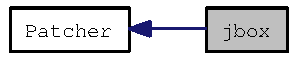
\includegraphics[width=89pt]{group__jbox}
\end{center}
\end{figure}
\subsection*{Data Structures}
\begin{DoxyCompactItemize}
\item 
struct \hyperlink{structt__jboxdrawparams}{t\_\-jboxdrawparams}
\begin{DoxyCompactList}\small\item\em The \hyperlink{structt__jboxdrawparams}{t\_\-jboxdrawparams} structure. \item\end{DoxyCompactList}\end{DoxyCompactItemize}
\subsection*{Defines}
\begin{DoxyCompactItemize}
\item 
\hypertarget{group__jbox_ga9f21c69e60543de2ecbcc94db526134b}{
\#define \hyperlink{group__jbox_ga9f21c69e60543de2ecbcc94db526134b}{JBOX\_\-DRAWFIRSTIN}~(1$<$$<$0)}
\label{group__jbox_ga9f21c69e60543de2ecbcc94db526134b}

\begin{DoxyCompactList}\small\item\em draw first inlet \item\end{DoxyCompactList}\item 
\hypertarget{group__jbox_ga5b6543cfc10a8912a82cebada525a770}{
\#define \hyperlink{group__jbox_ga5b6543cfc10a8912a82cebada525a770}{JBOX\_\-NODRAWBOX}~(1$<$$<$1)}
\label{group__jbox_ga5b6543cfc10a8912a82cebada525a770}

\begin{DoxyCompactList}\small\item\em don't draw the frame \item\end{DoxyCompactList}\item 
\hypertarget{group__jbox_ga651b41a98977ffddd7ca2be78d01f37b}{
\#define \hyperlink{group__jbox_ga651b41a98977ffddd7ca2be78d01f37b}{JBOX\_\-DRAWINLAST}~(1$<$$<$2)}
\label{group__jbox_ga651b41a98977ffddd7ca2be78d01f37b}

\begin{DoxyCompactList}\small\item\em draw inlets after update method \item\end{DoxyCompactList}\item 
\hypertarget{group__jbox_ga3a5253e4b79d030934557351547c71ba}{
\#define \hyperlink{group__jbox_ga3a5253e4b79d030934557351547c71ba}{JBOX\_\-TRANSPARENT}~(1$<$$<$3)}
\label{group__jbox_ga3a5253e4b79d030934557351547c71ba}

\begin{DoxyCompactList}\small\item\em don't make transparent unless you need it (for efficiency) \item\end{DoxyCompactList}\item 
\hypertarget{group__jbox_ga9e535a38aa4960b6ed5f47f361c3bd09}{
\#define \hyperlink{group__jbox_ga9e535a38aa4960b6ed5f47f361c3bd09}{JBOX\_\-NOGROW}~(1$<$$<$4)}
\label{group__jbox_ga9e535a38aa4960b6ed5f47f361c3bd09}

\begin{DoxyCompactList}\small\item\em don't even draw grow thingie \item\end{DoxyCompactList}\item 
\hypertarget{group__jbox_gaf151bcea416076c6811b84bd5cbaf68f}{
\#define \hyperlink{group__jbox_gaf151bcea416076c6811b84bd5cbaf68f}{JBOX\_\-GROWY}~(1$<$$<$5)}
\label{group__jbox_gaf151bcea416076c6811b84bd5cbaf68f}

\begin{DoxyCompactList}\small\item\em can grow in y direction by dragging \item\end{DoxyCompactList}\item 
\hypertarget{group__jbox_gaf7d65744237d64595b1a7e9884b03a05}{
\#define \hyperlink{group__jbox_gaf7d65744237d64595b1a7e9884b03a05}{JBOX\_\-GROWBOTH}~(1$<$$<$6)}
\label{group__jbox_gaf7d65744237d64595b1a7e9884b03a05}

\begin{DoxyCompactList}\small\item\em can grow independently in both x and y \item\end{DoxyCompactList}\item 
\hypertarget{group__jbox_ga07e3f6ad55a385a4bb268f8f7b78ab3e}{
\#define \hyperlink{group__jbox_ga07e3f6ad55a385a4bb268f8f7b78ab3e}{JBOX\_\-IGNORELOCKCLICK}~(1$<$$<$7)}
\label{group__jbox_ga07e3f6ad55a385a4bb268f8f7b78ab3e}

\begin{DoxyCompactList}\small\item\em box should ignore a click if patcher is locked \item\end{DoxyCompactList}\item 
\hypertarget{group__jbox_gae172d0c858232c903a5dd9d847f1a951}{
\#define \hyperlink{group__jbox_gae172d0c858232c903a5dd9d847f1a951}{JBOX\_\-HILITE}~(1$<$$<$8)}
\label{group__jbox_gae172d0c858232c903a5dd9d847f1a951}

\begin{DoxyCompactList}\small\item\em flag passed to \hyperlink{group__jbox_gaaa460d02ca3d22c54368ade59d8e330b}{jbox\_\-new()} to tell max that the UI object can receive the focus when clicked on -\/-\/ may be replaced by JBOX\_\-FOCUS in the future \item\end{DoxyCompactList}\item 
\hypertarget{group__jbox_ga17ab73ccfb0a841d104e3f11983a0c2f}{
\#define \hyperlink{group__jbox_ga17ab73ccfb0a841d104e3f11983a0c2f}{JBOX\_\-BACKGROUND}~(1$<$$<$9)}
\label{group__jbox_ga17ab73ccfb0a841d104e3f11983a0c2f}

\begin{DoxyCompactList}\small\item\em immediately set box into the background \item\end{DoxyCompactList}\item 
\hypertarget{group__jbox_gafc1b0cebedef206c073622cab8fc6785}{
\#define \hyperlink{group__jbox_gafc1b0cebedef206c073622cab8fc6785}{JBOX\_\-NOFLOATINSPECTOR}~(1$<$$<$10)}
\label{group__jbox_gafc1b0cebedef206c073622cab8fc6785}

\begin{DoxyCompactList}\small\item\em no floating inspector window \item\end{DoxyCompactList}\item 
\hypertarget{group__jbox_ga1abed197d8348eb15df1a5c9d4bc368d}{
\#define \hyperlink{group__jbox_ga1abed197d8348eb15df1a5c9d4bc368d}{JBOX\_\-TEXTFIELD}~(1$<$$<$11)}
\label{group__jbox_ga1abed197d8348eb15df1a5c9d4bc368d}

\begin{DoxyCompactList}\small\item\em save/load text from textfield, unless JBOX\_\-BINBUF flag is set \item\end{DoxyCompactList}\item 
\hypertarget{group__jbox_gafb46881fa4dbaf5073e1ee6929d7fa9d}{
\#define \hyperlink{group__jbox_gafb46881fa4dbaf5073e1ee6929d7fa9d}{JBOX\_\-FIXWIDTH}~(1$<$$<$19)}
\label{group__jbox_gafb46881fa4dbaf5073e1ee6929d7fa9d}

\begin{DoxyCompactList}\small\item\em give the box a textfield based fix-\/width (bfixwidth) method \item\end{DoxyCompactList}\item 
\hypertarget{group__jbox_ga04c45cfbc143d2efaeac28f40cee0459}{
\#define \hyperlink{group__jbox_ga04c45cfbc143d2efaeac28f40cee0459}{JBOX\_\-FONTATTR}~(1$<$$<$18)}
\label{group__jbox_ga04c45cfbc143d2efaeac28f40cee0459}

\begin{DoxyCompactList}\small\item\em if you want font related attribute you must add this to jbox\_\-initclass() \item\end{DoxyCompactList}\item 
\hypertarget{group__jbox_gad7eebf09211fa7da46d6d3bcc7da7f41}{
\#define \hyperlink{group__jbox_gad7eebf09211fa7da46d6d3bcc7da7f41}{JBOX\_\-BINBUF}~(1$<$$<$14)}
\label{group__jbox_gad7eebf09211fa7da46d6d3bcc7da7f41}

\begin{DoxyCompactList}\small\item\em save/load text from b\_\-binbuf \item\end{DoxyCompactList}\item 
\hypertarget{group__jbox_ga31038b9d4b011ec2e594c0cfc49ac1a0}{
\#define \hyperlink{group__jbox_ga31038b9d4b011ec2e594c0cfc49ac1a0}{JBOX\_\-MOUSEDRAGDELTA}~(1$<$$<$12)}
\label{group__jbox_ga31038b9d4b011ec2e594c0cfc49ac1a0}

\begin{DoxyCompactList}\small\item\em hides mouse cursor in drag and sends mousedragdelta instead of mousedrag (for infinite scrolling like number) \item\end{DoxyCompactList}\item 
\hypertarget{group__jbox_ga14cb28210886cfe0df0c34f71338faf8}{
\#define \hyperlink{group__jbox_ga14cb28210886cfe0df0c34f71338faf8}{JBOX\_\-COLOR}~(1$<$$<$13)}
\label{group__jbox_ga14cb28210886cfe0df0c34f71338faf8}

\begin{DoxyCompactList}\small\item\em support the \char`\"{}color\char`\"{} method for color customization \item\end{DoxyCompactList}\item 
\hypertarget{group__jbox_gaec3b8ac2f1d39181714818573dbb3050}{
\#define \hyperlink{group__jbox_gaec3b8ac2f1d39181714818573dbb3050}{JBOX\_\-DRAWIOLOCKED}~(1$<$$<$15)}
\label{group__jbox_gaec3b8ac2f1d39181714818573dbb3050}

\begin{DoxyCompactList}\small\item\em draw inlets and outlets when locked (default is not to draw them) \item\end{DoxyCompactList}\item 
\hypertarget{group__jbox_ga73e68b629cf1778a8a6e7a6685d98df6}{
\#define \hyperlink{group__jbox_ga73e68b629cf1778a8a6e7a6685d98df6}{JBOX\_\-DRAWBACKGROUND}~(1$<$$<$16)}
\label{group__jbox_ga73e68b629cf1778a8a6e7a6685d98df6}

\begin{DoxyCompactList}\small\item\em set to have box bg filled in for you based on getdrawparams method or brgba attribute \item\end{DoxyCompactList}\item 
\#define \hyperlink{group__jbox_ga789716317916c1e160d4ac0ef909446b}{JBOX\_\-NOINSPECTFIRSTIN}~(1$<$$<$17)
\begin{DoxyCompactList}\small\item\em flag for objects such as bpatcher that have a different b\_\-firstin, \item\end{DoxyCompactList}\item 
\hypertarget{group__jbox_ga321af2f1062fe6517c93769ffdcadb23}{
\#define \hyperlink{group__jbox_ga321af2f1062fe6517c93769ffdcadb23}{JBOX\_\-DEFAULTNAMES}~(1$<$$<$18)}
\label{group__jbox_ga321af2f1062fe6517c93769ffdcadb23}

\begin{DoxyCompactList}\small\item\em flag instructing jbox\_\-new to attach object to the defaults object for live defaults updating \item\end{DoxyCompactList}\item 
\hypertarget{group__jbox_ga965611b7e0990af5ded807ff00e06ac8}{
\#define \hyperlink{group__jbox_ga965611b7e0990af5ded807ff00e06ac8}{JBOX\_\-FOCUS}~(1$<$$<$20)}
\label{group__jbox_ga965611b7e0990af5ded807ff00e06ac8}

\begin{DoxyCompactList}\small\item\em more advanced focus support (passed to jbox\_\-initclass() to add \char`\"{}nextfocus\char`\"{} and \char`\"{}prevfocus\char`\"{} attributes to the UI object). Not implemented as of 2009-\/05-\/11 \item\end{DoxyCompactList}\end{DoxyCompactItemize}
\subsection*{Enumerations}
\begin{DoxyCompactItemize}
\item 
enum \{ \par
\hyperlink{group__jbox_gga80155586fa275b28773c9b203f52cabaa0071b2aa858b0b85866ec55f920661ea}{JBOX\_\-FONTFACE\_\-REGULAR} =  0, 
\par
\hyperlink{group__jbox_gga80155586fa275b28773c9b203f52cabaa7c5afcc54470110f9adafe6643860e33}{JBOX\_\-FONTFACE\_\-BOLD} =  1, 
\par
\hyperlink{group__jbox_gga80155586fa275b28773c9b203f52cabaa804e35b0947d1056b75c0b7416aed5f1}{JBOX\_\-FONTFACE\_\-ITALIC} =  2, 
\par
\hyperlink{group__jbox_gga80155586fa275b28773c9b203f52cabaac504521024538cbb38406272126cb30b}{JBOX\_\-FONTFACE\_\-BOLDITALIC} =  3
 \}
\begin{DoxyCompactList}\small\item\em actual numerical values of the b\_\-fontface attribute; use jbox\_\-fontface() to weight \item\end{DoxyCompactList}\item 
enum \hyperlink{group__jbox_ga956a254a140565aa9ff36a514740e021}{HitTestResult} \{ \par
\hyperlink{group__jbox_gga956a254a140565aa9ff36a514740e021a3bb67caa8d046ec70d5f467d64a6a290}{HitNothing} =  0, 
\par
\hyperlink{group__jbox_gga956a254a140565aa9ff36a514740e021a221361506a6a16b6c6ef01e0df8ba1c8}{HitBox} =  1, 
\par
\hyperlink{group__jbox_gga956a254a140565aa9ff36a514740e021abbaf64215e72c962b14e40c5a44daaab}{HitInlet} =  2, 
\par
\hyperlink{group__jbox_gga956a254a140565aa9ff36a514740e021a3614154efb6de5f3dd2e9b33f04b755e}{HitOutlet} =  3, 
\par
\hyperlink{group__jbox_gga956a254a140565aa9ff36a514740e021ada85a1e80aea2609cb61236fce30e53c}{HitGrowBox} =  4, 
\par
\hyperlink{group__jbox_gga956a254a140565aa9ff36a514740e021aa40eb7d004396706e33f989330975eaa}{HitLine} =  5
 \}
\begin{DoxyCompactList}\small\item\em enumerations used for box decorators \item\end{DoxyCompactList}\end{DoxyCompactItemize}
\subsection*{Functions}
\begin{DoxyCompactItemize}
\item 
\hyperlink{group__datatypes_ga73edaae82b318855cc09fac994918165}{t\_\-max\_\-err} \hyperlink{group__jbox_gab47a7fa918c470f60f0789baafaa7b4b}{jbox\_\-get\_\-rect\_\-for\_\-view} (\hyperlink{structt__object}{t\_\-object} $\ast$box, \hyperlink{structt__object}{t\_\-object} $\ast$patcherview, \hyperlink{structt__rect}{t\_\-rect} $\ast$rect)
\begin{DoxyCompactList}\small\item\em Find the rect for a box in a given patcherview. \item\end{DoxyCompactList}\item 
\hyperlink{group__datatypes_ga73edaae82b318855cc09fac994918165}{t\_\-max\_\-err} \hyperlink{group__jbox_ga2e9cb5c8f8c731dc7af4d4f78ddbd387}{jbox\_\-set\_\-rect\_\-for\_\-view} (\hyperlink{structt__object}{t\_\-object} $\ast$box, \hyperlink{structt__object}{t\_\-object} $\ast$patcherview, \hyperlink{structt__rect}{t\_\-rect} $\ast$rect)
\begin{DoxyCompactList}\small\item\em Change the rect for a box in a given patcherview. \item\end{DoxyCompactList}\item 
\hyperlink{group__datatypes_ga73edaae82b318855cc09fac994918165}{t\_\-max\_\-err} \hyperlink{group__jbox_ga92dedcbda2a2dbbab47e0801902c56b4}{jbox\_\-get\_\-rect\_\-for\_\-sym} (\hyperlink{structt__object}{t\_\-object} $\ast$box, \hyperlink{structt__symbol}{t\_\-symbol} $\ast$which, \hyperlink{structt__rect}{t\_\-rect} $\ast$pr)
\begin{DoxyCompactList}\small\item\em Find the rect for a box with a given attribute name. \item\end{DoxyCompactList}\item 
\hyperlink{group__datatypes_ga73edaae82b318855cc09fac994918165}{t\_\-max\_\-err} \hyperlink{group__jbox_ga780de0c06bc1630cd0725174b21357f6}{jbox\_\-set\_\-rect\_\-for\_\-sym} (\hyperlink{structt__object}{t\_\-object} $\ast$box, \hyperlink{structt__symbol}{t\_\-symbol} $\ast$which, \hyperlink{structt__rect}{t\_\-rect} $\ast$pr)
\begin{DoxyCompactList}\small\item\em Change the rect for a box with a given attribute name. \item\end{DoxyCompactList}\item 
\hyperlink{group__datatypes_ga73edaae82b318855cc09fac994918165}{t\_\-max\_\-err} \hyperlink{group__jbox_gad342cd402e9dade9bb13b813a13f038c}{jbox\_\-set\_\-rect} (\hyperlink{structt__object}{t\_\-object} $\ast$box, \hyperlink{structt__rect}{t\_\-rect} $\ast$pr)
\begin{DoxyCompactList}\small\item\em Set both the presentation rect and the patching rect. \item\end{DoxyCompactList}\item 
\hyperlink{group__datatypes_ga73edaae82b318855cc09fac994918165}{t\_\-max\_\-err} \hyperlink{group__jbox_ga0e4d3502f3c114d2e9c71f309c9cade2}{jbox\_\-get\_\-patching\_\-rect} (\hyperlink{structt__object}{t\_\-object} $\ast$box, \hyperlink{structt__rect}{t\_\-rect} $\ast$pr)
\begin{DoxyCompactList}\small\item\em Retrieve the patching rect of a box. \item\end{DoxyCompactList}\item 
\hyperlink{group__datatypes_ga73edaae82b318855cc09fac994918165}{t\_\-max\_\-err} \hyperlink{group__jbox_gab9c38504ceb26b0674eba0ee31ff776b}{jbox\_\-set\_\-patching\_\-rect} (\hyperlink{structt__object}{t\_\-object} $\ast$box, \hyperlink{structt__rect}{t\_\-rect} $\ast$pr)
\begin{DoxyCompactList}\small\item\em Change the patching rect of a box. \item\end{DoxyCompactList}\item 
\hyperlink{group__datatypes_ga73edaae82b318855cc09fac994918165}{t\_\-max\_\-err} \hyperlink{group__jbox_ga987293837d1704cf7d461832e312c0b8}{jbox\_\-get\_\-presentation\_\-rect} (\hyperlink{structt__object}{t\_\-object} $\ast$box, \hyperlink{structt__rect}{t\_\-rect} $\ast$pr)
\begin{DoxyCompactList}\small\item\em Retrieve the presentation rect of a box. \item\end{DoxyCompactList}\item 
\hyperlink{group__datatypes_ga73edaae82b318855cc09fac994918165}{t\_\-max\_\-err} \hyperlink{group__jbox_gad7d842670d42f7959b9a388eaf716d46}{jbox\_\-set\_\-presentation\_\-rect} (\hyperlink{structt__object}{t\_\-object} $\ast$box, \hyperlink{structt__rect}{t\_\-rect} $\ast$pr)
\begin{DoxyCompactList}\small\item\em Change the presentation rect of a box. \item\end{DoxyCompactList}\item 
\hyperlink{group__datatypes_ga73edaae82b318855cc09fac994918165}{t\_\-max\_\-err} \hyperlink{group__jbox_gae1901dd9922577bb4bcc33665dd4e7f6}{jbox\_\-set\_\-position} (\hyperlink{structt__object}{t\_\-object} $\ast$box, \hyperlink{structt__pt}{t\_\-pt} $\ast$pos)
\begin{DoxyCompactList}\small\item\em Set the position of a box for both the presentation and patching views. \item\end{DoxyCompactList}\item 
\hyperlink{group__datatypes_ga73edaae82b318855cc09fac994918165}{t\_\-max\_\-err} \hyperlink{group__jbox_gaf2b95be91e66caa72238838b2068356f}{jbox\_\-get\_\-patching\_\-position} (\hyperlink{structt__object}{t\_\-object} $\ast$box, \hyperlink{structt__pt}{t\_\-pt} $\ast$pos)
\begin{DoxyCompactList}\small\item\em Fetch the position of a box for the patching view. \item\end{DoxyCompactList}\item 
\hyperlink{group__datatypes_ga73edaae82b318855cc09fac994918165}{t\_\-max\_\-err} \hyperlink{group__jbox_gac4baff3db6cac220f46e73a3f6986ac9}{jbox\_\-set\_\-patching\_\-position} (\hyperlink{structt__object}{t\_\-object} $\ast$box, \hyperlink{structt__pt}{t\_\-pt} $\ast$pos)
\begin{DoxyCompactList}\small\item\em Set the position of a box for the patching view. \item\end{DoxyCompactList}\item 
\hyperlink{group__datatypes_ga73edaae82b318855cc09fac994918165}{t\_\-max\_\-err} \hyperlink{group__jbox_gae4db002ae3ff252be9e0fe1fce5aaffb}{jbox\_\-get\_\-presentation\_\-position} (\hyperlink{structt__object}{t\_\-object} $\ast$box, \hyperlink{structt__pt}{t\_\-pt} $\ast$pos)
\begin{DoxyCompactList}\small\item\em Fetch the position of a box for the presentation view. \item\end{DoxyCompactList}\item 
\hyperlink{group__datatypes_ga73edaae82b318855cc09fac994918165}{t\_\-max\_\-err} \hyperlink{group__jbox_gad20f69b425b1a22686cfa909d509af60}{jbox\_\-set\_\-presentation\_\-position} (\hyperlink{structt__object}{t\_\-object} $\ast$box, \hyperlink{structt__pt}{t\_\-pt} $\ast$pos)
\begin{DoxyCompactList}\small\item\em Set the position of a box for the presentation view. \item\end{DoxyCompactList}\item 
\hyperlink{group__datatypes_ga73edaae82b318855cc09fac994918165}{t\_\-max\_\-err} \hyperlink{group__jbox_ga09ce5b0e60e447cd40331f63ea8d7e9d}{jbox\_\-set\_\-size} (\hyperlink{structt__object}{t\_\-object} $\ast$box, \hyperlink{structt__size}{t\_\-size} $\ast$size)
\begin{DoxyCompactList}\small\item\em Set the size of a box for both the presentation and patching views. \item\end{DoxyCompactList}\item 
\hyperlink{group__datatypes_ga73edaae82b318855cc09fac994918165}{t\_\-max\_\-err} \hyperlink{group__jbox_ga4b2c0df4da77da3655848defe8f1828e}{jbox\_\-get\_\-patching\_\-size} (\hyperlink{structt__object}{t\_\-object} $\ast$box, \hyperlink{structt__size}{t\_\-size} $\ast$size)
\begin{DoxyCompactList}\small\item\em Fetch the size of a box for the patching view. \item\end{DoxyCompactList}\item 
\hyperlink{group__datatypes_ga73edaae82b318855cc09fac994918165}{t\_\-max\_\-err} \hyperlink{group__jbox_gab7eb5fa0028078fa1665c255ede79cf5}{jbox\_\-set\_\-patching\_\-size} (\hyperlink{structt__object}{t\_\-object} $\ast$box, \hyperlink{structt__size}{t\_\-size} $\ast$size)
\begin{DoxyCompactList}\small\item\em Set the size of a box for the patching view. \item\end{DoxyCompactList}\item 
\hyperlink{group__datatypes_ga73edaae82b318855cc09fac994918165}{t\_\-max\_\-err} \hyperlink{group__jbox_ga4dc98cdc8f15efc5f0980bd4cc07f111}{jbox\_\-get\_\-presentation\_\-size} (\hyperlink{structt__object}{t\_\-object} $\ast$box, \hyperlink{structt__size}{t\_\-size} $\ast$size)
\begin{DoxyCompactList}\small\item\em Fetch the size of a box for the presentation view. \item\end{DoxyCompactList}\item 
\hyperlink{group__datatypes_ga73edaae82b318855cc09fac994918165}{t\_\-max\_\-err} \hyperlink{group__jbox_ga6765c83aed47db064a1cf0581474f5c0}{jbox\_\-set\_\-presentation\_\-size} (\hyperlink{structt__object}{t\_\-object} $\ast$box, \hyperlink{structt__size}{t\_\-size} $\ast$size)
\begin{DoxyCompactList}\small\item\em Set the size of a box for the presentation view. \item\end{DoxyCompactList}\item 
\hyperlink{structt__symbol}{t\_\-symbol} $\ast$ \hyperlink{group__jbox_ga0c96d89b3e16930d8c84e4a39b21b639}{jbox\_\-get\_\-maxclass} (\hyperlink{structt__object}{t\_\-object} $\ast$b)
\begin{DoxyCompactList}\small\item\em Retrieve the name of the class of the box's object. \item\end{DoxyCompactList}\item 
\hyperlink{structt__object}{t\_\-object} $\ast$ \hyperlink{group__jbox_ga5063d165cfca9dc76162ff5757ea4852}{jbox\_\-get\_\-object} (\hyperlink{structt__object}{t\_\-object} $\ast$b)
\begin{DoxyCompactList}\small\item\em Retrieve a pointer to the box's object. \item\end{DoxyCompactList}\item 
\hyperlink{structt__object}{t\_\-object} $\ast$ \hyperlink{group__jbox_ga628997df216439d23dac3f76cd525806}{jbox\_\-get\_\-patcher} (\hyperlink{structt__object}{t\_\-object} $\ast$b)
\begin{DoxyCompactList}\small\item\em Retrieve a box's patcher. \item\end{DoxyCompactList}\item 
char \hyperlink{group__jbox_gabf4d15efce29810349772db62c3b1341}{jbox\_\-get\_\-hidden} (\hyperlink{structt__object}{t\_\-object} $\ast$b)
\begin{DoxyCompactList}\small\item\em Retrieve a box's 'hidden' attribute. \item\end{DoxyCompactList}\item 
\hyperlink{group__datatypes_ga73edaae82b318855cc09fac994918165}{t\_\-max\_\-err} \hyperlink{group__jbox_gaa83c5c91b5687838b4aa221236535b53}{jbox\_\-set\_\-hidden} (\hyperlink{structt__object}{t\_\-object} $\ast$b, char c)
\begin{DoxyCompactList}\small\item\em Set a box's 'hidden' attribute. \item\end{DoxyCompactList}\item 
\hyperlink{structt__symbol}{t\_\-symbol} $\ast$ \hyperlink{group__jbox_ga5a5801f294c0c6f8c5cefc686bffcdfb}{jbox\_\-get\_\-fontname} (\hyperlink{structt__object}{t\_\-object} $\ast$b)
\begin{DoxyCompactList}\small\item\em Retrieve a box's 'fontname' attribute. \item\end{DoxyCompactList}\item 
\hyperlink{group__datatypes_ga73edaae82b318855cc09fac994918165}{t\_\-max\_\-err} \hyperlink{group__jbox_gaa42077bec85957796b46eac319db0ad7}{jbox\_\-set\_\-fontname} (\hyperlink{structt__object}{t\_\-object} $\ast$b, \hyperlink{structt__symbol}{t\_\-symbol} $\ast$ps)
\begin{DoxyCompactList}\small\item\em Set a box's 'fontname' attribute. \item\end{DoxyCompactList}\item 
double \hyperlink{group__jbox_ga5ea741cbdbedbb94e93292fe9fdf4976}{jbox\_\-get\_\-fontsize} (\hyperlink{structt__object}{t\_\-object} $\ast$b)
\begin{DoxyCompactList}\small\item\em Retrieve a box's 'fontsize' attribute. \item\end{DoxyCompactList}\item 
\hyperlink{group__datatypes_ga73edaae82b318855cc09fac994918165}{t\_\-max\_\-err} \hyperlink{group__jbox_gae6342147186d369649574cb04b0b3deb}{jbox\_\-set\_\-fontsize} (\hyperlink{structt__object}{t\_\-object} $\ast$b, double d)
\begin{DoxyCompactList}\small\item\em Set a box's 'fontsize' attribute. \item\end{DoxyCompactList}\item 
\hyperlink{group__datatypes_ga73edaae82b318855cc09fac994918165}{t\_\-max\_\-err} \hyperlink{group__jbox_ga03c4056e731c28342a8ee17e5b86558f}{jbox\_\-get\_\-color} (\hyperlink{structt__object}{t\_\-object} $\ast$b, \hyperlink{structt__jrgba}{t\_\-jrgba} $\ast$prgba)
\begin{DoxyCompactList}\small\item\em Retrieve a box's 'color' attribute. \item\end{DoxyCompactList}\item 
\hyperlink{group__datatypes_ga73edaae82b318855cc09fac994918165}{t\_\-max\_\-err} \hyperlink{group__jbox_ga211b979a249719dadd1168d72bc6df37}{jbox\_\-set\_\-color} (\hyperlink{structt__object}{t\_\-object} $\ast$b, \hyperlink{structt__jrgba}{t\_\-jrgba} $\ast$prgba)
\begin{DoxyCompactList}\small\item\em Set a box's 'color' attribute. \item\end{DoxyCompactList}\item 
\hyperlink{structt__symbol}{t\_\-symbol} $\ast$ \hyperlink{group__jbox_gad9614088919b6727e6ed7feebd83d065}{jbox\_\-get\_\-hint} (\hyperlink{structt__object}{t\_\-object} $\ast$b)
\begin{DoxyCompactList}\small\item\em Retrieve a box's hint text as a symbol. \item\end{DoxyCompactList}\item 
\hyperlink{group__datatypes_ga73edaae82b318855cc09fac994918165}{t\_\-max\_\-err} \hyperlink{group__jbox_ga7c7cc83f75351df0fa423c43592e589c}{jbox\_\-set\_\-hint} (\hyperlink{structt__object}{t\_\-object} $\ast$b, \hyperlink{structt__symbol}{t\_\-symbol} $\ast$s)
\begin{DoxyCompactList}\small\item\em Set a box's hint text using a symbol. \item\end{DoxyCompactList}\item 
char $\ast$ \hyperlink{group__jbox_ga80ff8da64e1e96abb21ae7e528c757c8}{jbox\_\-get\_\-hintstring} (\hyperlink{structt__object}{t\_\-object} $\ast$bb)
\begin{DoxyCompactList}\small\item\em Retrieve a box's hint text as a C-\/string. \item\end{DoxyCompactList}\item 
void \hyperlink{group__jbox_gad1651ffa12cf40c55de24e892be2fa42}{jbox\_\-set\_\-hintstring} (\hyperlink{structt__object}{t\_\-object} $\ast$bb, char $\ast$s)
\begin{DoxyCompactList}\small\item\em Set a box's hint text using a C-\/string. \item\end{DoxyCompactList}\item 
char $\ast$ \hyperlink{group__jbox_gae370a9514d4075d00eb6a336d95390b0}{jbox\_\-get\_\-annotation} (\hyperlink{structt__object}{t\_\-object} $\ast$bb)
\begin{DoxyCompactList}\small\item\em Retrieve a box's annotation string, if the user has given it an annotation. \item\end{DoxyCompactList}\item 
void \hyperlink{group__jbox_ga2c9cde3892f9a68be579ea623c438dd0}{jbox\_\-set\_\-annotation} (\hyperlink{structt__object}{t\_\-object} $\ast$bb, char $\ast$s)
\begin{DoxyCompactList}\small\item\em Set a box's annotation string. \item\end{DoxyCompactList}\item 
\hyperlink{structt__object}{t\_\-object} $\ast$ \hyperlink{group__jbox_ga89177ab12d45649c7209e65c97a3b128}{jbox\_\-get\_\-nextobject} (\hyperlink{structt__object}{t\_\-object} $\ast$b)
\begin{DoxyCompactList}\small\item\em The next box in the patcher's (linked) list of boxes. \item\end{DoxyCompactList}\item 
\hyperlink{structt__object}{t\_\-object} $\ast$ \hyperlink{group__jbox_ga99be7a7b57c38335d30e6241afb86a5b}{jbox\_\-get\_\-prevobject} (\hyperlink{structt__object}{t\_\-object} $\ast$b)
\begin{DoxyCompactList}\small\item\em The previous box in the patcher's (linked) list of boxes. \item\end{DoxyCompactList}\item 
\hyperlink{structt__symbol}{t\_\-symbol} $\ast$ \hyperlink{group__jbox_ga0ada31d7aaa4c8e04f0807a3d857a1ad}{jbox\_\-get\_\-varname} (\hyperlink{structt__object}{t\_\-object} $\ast$b)
\begin{DoxyCompactList}\small\item\em Retrieve a box's scripting name. \item\end{DoxyCompactList}\item 
\hyperlink{group__datatypes_ga73edaae82b318855cc09fac994918165}{t\_\-max\_\-err} \hyperlink{group__jbox_gac4f46f657ca5087727fff6999c517d6c}{jbox\_\-set\_\-varname} (\hyperlink{structt__object}{t\_\-object} $\ast$b, \hyperlink{structt__symbol}{t\_\-symbol} $\ast$ps)
\begin{DoxyCompactList}\small\item\em Set a box's scripting name. \item\end{DoxyCompactList}\item 
\hyperlink{structt__symbol}{t\_\-symbol} $\ast$ \hyperlink{group__jbox_ga0b2499248b44f3f138407129f39f274e}{jbox\_\-get\_\-id} (\hyperlink{structt__object}{t\_\-object} $\ast$b)
\begin{DoxyCompactList}\small\item\em Retrieve a boxes unique id. \item\end{DoxyCompactList}\item 
char \hyperlink{group__jbox_ga57ff4e001cd4725d3cb7afb5a5dd4b56}{jbox\_\-get\_\-canhilite} (\hyperlink{structt__object}{t\_\-object} $\ast$b)
\begin{DoxyCompactList}\small\item\em Retrieve a box flag value from a box. \item\end{DoxyCompactList}\item 
char \hyperlink{group__jbox_ga453e949f39ffe6a95063a8d554e25adf}{jbox\_\-get\_\-background} (\hyperlink{structt__object}{t\_\-object} $\ast$b)
\begin{DoxyCompactList}\small\item\em Determine whether a box is located in the patcher's background layer. \item\end{DoxyCompactList}\item 
\hyperlink{group__datatypes_ga73edaae82b318855cc09fac994918165}{t\_\-max\_\-err} \hyperlink{group__jbox_gabcff56f0530497761daf30b021378308}{jbox\_\-set\_\-background} (\hyperlink{structt__object}{t\_\-object} $\ast$b, char c)
\begin{DoxyCompactList}\small\item\em Set whether a box should be in the background or foreground layer of a patcher. \item\end{DoxyCompactList}\item 
char \hyperlink{group__jbox_gaa84d6ce8c5dbd9fc69acc603b69a5fb0}{jbox\_\-get\_\-ignoreclick} (\hyperlink{structt__object}{t\_\-object} $\ast$b)
\begin{DoxyCompactList}\small\item\em Determine whether a box ignores clicks. \item\end{DoxyCompactList}\item 
\hyperlink{group__datatypes_ga73edaae82b318855cc09fac994918165}{t\_\-max\_\-err} \hyperlink{group__jbox_ga35a6799e184e79e7df4552ed1b75f652}{jbox\_\-set\_\-ignoreclick} (\hyperlink{structt__object}{t\_\-object} $\ast$b, char c)
\begin{DoxyCompactList}\small\item\em Set whether a box ignores clicks. \item\end{DoxyCompactList}\item 
char \hyperlink{group__jbox_gaae56c5cb39f5835b702846e557400522}{jbox\_\-get\_\-drawfirstin} (\hyperlink{structt__object}{t\_\-object} $\ast$b)
\begin{DoxyCompactList}\small\item\em Determine whether a box draws its first inlet. \item\end{DoxyCompactList}\item 
char \hyperlink{group__jbox_ga3316ca865cdfb5d3e64daba573889407}{jbox\_\-get\_\-outline} (\hyperlink{structt__object}{t\_\-object} $\ast$b)
\begin{DoxyCompactList}\small\item\em Determine whether a box draws an outline. \item\end{DoxyCompactList}\item 
\hyperlink{group__datatypes_ga73edaae82b318855cc09fac994918165}{t\_\-max\_\-err} \hyperlink{group__jbox_ga77fc6d8afcf5b91b6b998803a66ca316}{jbox\_\-set\_\-outline} (\hyperlink{structt__object}{t\_\-object} $\ast$b, char c)
\begin{DoxyCompactList}\small\item\em Set whether a box draws an outline. \item\end{DoxyCompactList}\item 
char \hyperlink{group__jbox_ga1c3005aebecc67a41d0abb0f0089a6cb}{jbox\_\-get\_\-growy} (\hyperlink{structt__object}{t\_\-object} $\ast$b)
\begin{DoxyCompactList}\small\item\em Retrieve a box flag value from a box. \item\end{DoxyCompactList}\item 
char \hyperlink{group__jbox_gaecf5b94b11c026032d94d6746d06955f}{jbox\_\-get\_\-growboth} (\hyperlink{structt__object}{t\_\-object} $\ast$b)
\begin{DoxyCompactList}\small\item\em Retrieve a box flag value from a box. \item\end{DoxyCompactList}\item 
char \hyperlink{group__jbox_gaae265845c184a54b16ecf19cff0f7b91}{jbox\_\-get\_\-nogrow} (\hyperlink{structt__object}{t\_\-object} $\ast$b)
\begin{DoxyCompactList}\small\item\em Retrieve a box flag value from a box. \item\end{DoxyCompactList}\item 
char \hyperlink{group__jbox_ga6e3d12a65d25b0e518ca1e246d132a7a}{jbox\_\-get\_\-drawinlast} (\hyperlink{structt__object}{t\_\-object} $\ast$b)
\begin{DoxyCompactList}\small\item\em Retrieve a box flag value from a box. \item\end{DoxyCompactList}\item 
\hyperlink{structt__object}{t\_\-object} $\ast$ \hyperlink{group__jbox_ga2f6cb01a3523876b01945baa7800e61e}{jbox\_\-get\_\-textfield} (\hyperlink{structt__object}{t\_\-object} $\ast$b)
\begin{DoxyCompactList}\small\item\em Retrieve a pointer to a box's textfield. \item\end{DoxyCompactList}\item 
char \hyperlink{group__jbox_gacbedddaaeeaf5a08a9fa6a8782b86b1f}{jbox\_\-get\_\-presentation} (\hyperlink{structt__object}{t\_\-object} $\ast$b)
\begin{DoxyCompactList}\small\item\em Determine if a box is included in the presentation view. \item\end{DoxyCompactList}\item 
\hyperlink{group__datatypes_ga73edaae82b318855cc09fac994918165}{t\_\-max\_\-err} \hyperlink{group__jbox_ga67bc0679e3f4456a6ac791fa1ebef568}{jbox\_\-set\_\-presentation} (\hyperlink{structt__object}{t\_\-object} $\ast$b, char c)
\begin{DoxyCompactList}\small\item\em Determine if a box is included in the presentation view. \item\end{DoxyCompactList}\item 
\hyperlink{group__datatypes_ga73edaae82b318855cc09fac994918165}{t\_\-max\_\-err} \hyperlink{group__jbox_gaaa460d02ca3d22c54368ade59d8e330b}{jbox\_\-new} (\hyperlink{structt__jbox}{t\_\-jbox} $\ast$b, long flags, long argc, \hyperlink{structt__atom}{t\_\-atom} $\ast$argv)
\begin{DoxyCompactList}\small\item\em Set up your UI object's \hyperlink{structt__jbox}{t\_\-jbox} member. \item\end{DoxyCompactList}\item 
void \hyperlink{group__jbox_ga769cbf2dd8ebf22ac21e9df271c61704}{jbox\_\-free} (\hyperlink{structt__jbox}{t\_\-jbox} $\ast$b)
\begin{DoxyCompactList}\small\item\em Tear down your UI object's \hyperlink{structt__jbox}{t\_\-jbox} member. \item\end{DoxyCompactList}\item 
void \hyperlink{group__jbox_gabea75e4d5243003070cb2de04b81d3d1}{jbox\_\-ready} (\hyperlink{structt__jbox}{t\_\-jbox} $\ast$b)
\begin{DoxyCompactList}\small\item\em Mark the box ready to be accessed and drawn by Max. \item\end{DoxyCompactList}\item 
void \hyperlink{group__jbox_ga92b553f8adc9994553590bbbcfd7e49d}{jbox\_\-redraw} (\hyperlink{structt__jbox}{t\_\-jbox} $\ast$b)
\begin{DoxyCompactList}\small\item\em Request that your object/box be re-\/drawn by Max. \item\end{DoxyCompactList}\item 
\hyperlink{group__datatypes_ga73edaae82b318855cc09fac994918165}{t\_\-max\_\-err} \hyperlink{group__jbox_ga9aa791abf47ea1cb276c5a867665a52a}{jbox\_\-notify} (\hyperlink{structt__jbox}{t\_\-jbox} $\ast$b, \hyperlink{structt__symbol}{t\_\-symbol} $\ast$s, \hyperlink{structt__symbol}{t\_\-symbol} $\ast$msg, void $\ast$sender, void $\ast$data)
\begin{DoxyCompactList}\small\item\em Send a notification to a box. \item\end{DoxyCompactList}\end{DoxyCompactItemize}


\subsection{Detailed Description}
A box in the patcher. 

\subsection{Define Documentation}
\hypertarget{group__jbox_ga789716317916c1e160d4ac0ef909446b}{
\index{jbox@{jbox}!JBOX\_\-NOINSPECTFIRSTIN@{JBOX\_\-NOINSPECTFIRSTIN}}
\index{JBOX\_\-NOINSPECTFIRSTIN@{JBOX\_\-NOINSPECTFIRSTIN}!jbox@{jbox}}
\subsubsection[{JBOX\_\-NOINSPECTFIRSTIN}]{\setlength{\rightskip}{0pt plus 5cm}\#define JBOX\_\-NOINSPECTFIRSTIN~(1$<$$<$17)}}
\label{group__jbox_ga789716317916c1e160d4ac0ef909446b}


flag for objects such as bpatcher that have a different b\_\-firstin, but the attrs of the b\_\-firstin should not be shown in the inspector 

\subsection{Enumeration Type Documentation}
\hypertarget{group__jbox_ga80155586fa275b28773c9b203f52caba}{
\subsubsection[{"@17}]{\setlength{\rightskip}{0pt plus 5cm}anonymous enum}}
\label{group__jbox_ga80155586fa275b28773c9b203f52caba}


actual numerical values of the b\_\-fontface attribute; use jbox\_\-fontface() to weight \begin{Desc}
\item[Enumerator: ]\par
\begin{description}
\index{JBOX\_\-FONTFACE\_\-REGULAR@{JBOX\_\-FONTFACE\_\-REGULAR}!jbox@{jbox}}\index{jbox@{jbox}!JBOX\_\-FONTFACE\_\-REGULAR@{JBOX\_\-FONTFACE\_\-REGULAR}}\item[{\em 
\hypertarget{group__jbox_gga80155586fa275b28773c9b203f52cabaa0071b2aa858b0b85866ec55f920661ea}{
JBOX\_\-FONTFACE\_\-REGULAR}
\label{group__jbox_gga80155586fa275b28773c9b203f52cabaa0071b2aa858b0b85866ec55f920661ea}
}]normal \index{JBOX\_\-FONTFACE\_\-BOLD@{JBOX\_\-FONTFACE\_\-BOLD}!jbox@{jbox}}\index{jbox@{jbox}!JBOX\_\-FONTFACE\_\-BOLD@{JBOX\_\-FONTFACE\_\-BOLD}}\item[{\em 
\hypertarget{group__jbox_gga80155586fa275b28773c9b203f52cabaa7c5afcc54470110f9adafe6643860e33}{
JBOX\_\-FONTFACE\_\-BOLD}
\label{group__jbox_gga80155586fa275b28773c9b203f52cabaa7c5afcc54470110f9adafe6643860e33}
}]bold \index{JBOX\_\-FONTFACE\_\-ITALIC@{JBOX\_\-FONTFACE\_\-ITALIC}!jbox@{jbox}}\index{jbox@{jbox}!JBOX\_\-FONTFACE\_\-ITALIC@{JBOX\_\-FONTFACE\_\-ITALIC}}\item[{\em 
\hypertarget{group__jbox_gga80155586fa275b28773c9b203f52cabaa804e35b0947d1056b75c0b7416aed5f1}{
JBOX\_\-FONTFACE\_\-ITALIC}
\label{group__jbox_gga80155586fa275b28773c9b203f52cabaa804e35b0947d1056b75c0b7416aed5f1}
}]italic \index{JBOX\_\-FONTFACE\_\-BOLDITALIC@{JBOX\_\-FONTFACE\_\-BOLDITALIC}!jbox@{jbox}}\index{jbox@{jbox}!JBOX\_\-FONTFACE\_\-BOLDITALIC@{JBOX\_\-FONTFACE\_\-BOLDITALIC}}\item[{\em 
\hypertarget{group__jbox_gga80155586fa275b28773c9b203f52cabaac504521024538cbb38406272126cb30b}{
JBOX\_\-FONTFACE\_\-BOLDITALIC}
\label{group__jbox_gga80155586fa275b28773c9b203f52cabaac504521024538cbb38406272126cb30b}
}]bold and italic \end{description}
\end{Desc}

\hypertarget{group__jbox_ga956a254a140565aa9ff36a514740e021}{
\index{jbox@{jbox}!HitTestResult@{HitTestResult}}
\index{HitTestResult@{HitTestResult}!jbox@{jbox}}
\subsubsection[{HitTestResult}]{\setlength{\rightskip}{0pt plus 5cm}enum {\bf HitTestResult}}}
\label{group__jbox_ga956a254a140565aa9ff36a514740e021}


enumerations used for box decorators \begin{Desc}
\item[Enumerator: ]\par
\begin{description}
\index{HitNothing@{HitNothing}!jbox@{jbox}}\index{jbox@{jbox}!HitNothing@{HitNothing}}\item[{\em 
\hypertarget{group__jbox_gga956a254a140565aa9ff36a514740e021a3bb67caa8d046ec70d5f467d64a6a290}{
HitNothing}
\label{group__jbox_gga956a254a140565aa9ff36a514740e021a3bb67caa8d046ec70d5f467d64a6a290}
}]a hole in the box \index{HitBox@{HitBox}!jbox@{jbox}}\index{jbox@{jbox}!HitBox@{HitBox}}\item[{\em 
\hypertarget{group__jbox_gga956a254a140565aa9ff36a514740e021a221361506a6a16b6c6ef01e0df8ba1c8}{
HitBox}
\label{group__jbox_gga956a254a140565aa9ff36a514740e021a221361506a6a16b6c6ef01e0df8ba1c8}
}]the body of the box \index{HitInlet@{HitInlet}!jbox@{jbox}}\index{jbox@{jbox}!HitInlet@{HitInlet}}\item[{\em 
\hypertarget{group__jbox_gga956a254a140565aa9ff36a514740e021abbaf64215e72c962b14e40c5a44daaab}{
HitInlet}
\label{group__jbox_gga956a254a140565aa9ff36a514740e021abbaf64215e72c962b14e40c5a44daaab}
}]an inlet \index{HitOutlet@{HitOutlet}!jbox@{jbox}}\index{jbox@{jbox}!HitOutlet@{HitOutlet}}\item[{\em 
\hypertarget{group__jbox_gga956a254a140565aa9ff36a514740e021a3614154efb6de5f3dd2e9b33f04b755e}{
HitOutlet}
\label{group__jbox_gga956a254a140565aa9ff36a514740e021a3614154efb6de5f3dd2e9b33f04b755e}
}]an outlet \index{HitGrowBox@{HitGrowBox}!jbox@{jbox}}\index{jbox@{jbox}!HitGrowBox@{HitGrowBox}}\item[{\em 
\hypertarget{group__jbox_gga956a254a140565aa9ff36a514740e021ada85a1e80aea2609cb61236fce30e53c}{
HitGrowBox}
\label{group__jbox_gga956a254a140565aa9ff36a514740e021ada85a1e80aea2609cb61236fce30e53c}
}]the grow handle \index{HitLine@{HitLine}!jbox@{jbox}}\index{jbox@{jbox}!HitLine@{HitLine}}\item[{\em 
\hypertarget{group__jbox_gga956a254a140565aa9ff36a514740e021aa40eb7d004396706e33f989330975eaa}{
HitLine}
\label{group__jbox_gga956a254a140565aa9ff36a514740e021aa40eb7d004396706e33f989330975eaa}
}]a line \end{description}
\end{Desc}



\subsection{Function Documentation}
\hypertarget{group__jbox_ga769cbf2dd8ebf22ac21e9df271c61704}{
\index{jbox@{jbox}!jbox\_\-free@{jbox\_\-free}}
\index{jbox\_\-free@{jbox\_\-free}!jbox@{jbox}}
\subsubsection[{jbox\_\-free}]{\setlength{\rightskip}{0pt plus 5cm}void jbox\_\-free ({\bf t\_\-jbox} $\ast$ {\em b})}}
\label{group__jbox_ga769cbf2dd8ebf22ac21e9df271c61704}


Tear down your UI object's \hyperlink{structt__jbox}{t\_\-jbox} member. This should be called from your UI object's free method.


\begin{DoxyParams}{Parameters}
\item[{\em b}]The address of your object's \hyperlink{structt__jbox}{t\_\-jbox} member (which should be the first member of the object's struct). \end{DoxyParams}
\hypertarget{group__jbox_gae370a9514d4075d00eb6a336d95390b0}{
\index{jbox@{jbox}!jbox\_\-get\_\-annotation@{jbox\_\-get\_\-annotation}}
\index{jbox\_\-get\_\-annotation@{jbox\_\-get\_\-annotation}!jbox@{jbox}}
\subsubsection[{jbox\_\-get\_\-annotation}]{\setlength{\rightskip}{0pt plus 5cm}char$\ast$ jbox\_\-get\_\-annotation ({\bf t\_\-object} $\ast$ {\em bb})}}
\label{group__jbox_gae370a9514d4075d00eb6a336d95390b0}


Retrieve a box's annotation string, if the user has given it an annotation. 
\begin{DoxyParams}{Parameters}
\item[{\em bb}]The box to query. \end{DoxyParams}
\begin{DoxyReturn}{Returns}
The user-\/created annotation string for a box, or NULL if no string exists. 
\end{DoxyReturn}
\hypertarget{group__jbox_ga453e949f39ffe6a95063a8d554e25adf}{
\index{jbox@{jbox}!jbox\_\-get\_\-background@{jbox\_\-get\_\-background}}
\index{jbox\_\-get\_\-background@{jbox\_\-get\_\-background}!jbox@{jbox}}
\subsubsection[{jbox\_\-get\_\-background}]{\setlength{\rightskip}{0pt plus 5cm}char jbox\_\-get\_\-background ({\bf t\_\-object} $\ast$ {\em b})}}
\label{group__jbox_ga453e949f39ffe6a95063a8d554e25adf}


Determine whether a box is located in the patcher's background layer. 
\begin{DoxyParams}{Parameters}
\item[{\em b}]The box to query. \end{DoxyParams}
\begin{DoxyReturn}{Returns}
Zero if the object is in the foreground, otherwise non-\/zero. 
\end{DoxyReturn}
\hypertarget{group__jbox_ga57ff4e001cd4725d3cb7afb5a5dd4b56}{
\index{jbox@{jbox}!jbox\_\-get\_\-canhilite@{jbox\_\-get\_\-canhilite}}
\index{jbox\_\-get\_\-canhilite@{jbox\_\-get\_\-canhilite}!jbox@{jbox}}
\subsubsection[{jbox\_\-get\_\-canhilite}]{\setlength{\rightskip}{0pt plus 5cm}char jbox\_\-get\_\-canhilite ({\bf t\_\-object} $\ast$ {\em b})}}
\label{group__jbox_ga57ff4e001cd4725d3cb7afb5a5dd4b56}


Retrieve a box flag value from a box. 
\begin{DoxyParams}{Parameters}
\item[{\em b}]The box to query. \end{DoxyParams}
\begin{DoxyReturn}{Returns}
The value of the canhilite bit in the box's flags. 
\end{DoxyReturn}
\hypertarget{group__jbox_ga03c4056e731c28342a8ee17e5b86558f}{
\index{jbox@{jbox}!jbox\_\-get\_\-color@{jbox\_\-get\_\-color}}
\index{jbox\_\-get\_\-color@{jbox\_\-get\_\-color}!jbox@{jbox}}
\subsubsection[{jbox\_\-get\_\-color}]{\setlength{\rightskip}{0pt plus 5cm}{\bf t\_\-max\_\-err} jbox\_\-get\_\-color ({\bf t\_\-object} $\ast$ {\em b}, \/  {\bf t\_\-jrgba} $\ast$ {\em prgba})}}
\label{group__jbox_ga03c4056e731c28342a8ee17e5b86558f}


Retrieve a box's 'color' attribute. 
\begin{DoxyParams}{Parameters}
\item[{\em b}]The box to query. \item[{\em prgba}]The address of a valid \hyperlink{structt__rect}{t\_\-rect} whose values will be filled-\/in upon return. \end{DoxyParams}
\begin{DoxyReturn}{Returns}
A Max error code. 
\end{DoxyReturn}
\hypertarget{group__jbox_gaae56c5cb39f5835b702846e557400522}{
\index{jbox@{jbox}!jbox\_\-get\_\-drawfirstin@{jbox\_\-get\_\-drawfirstin}}
\index{jbox\_\-get\_\-drawfirstin@{jbox\_\-get\_\-drawfirstin}!jbox@{jbox}}
\subsubsection[{jbox\_\-get\_\-drawfirstin}]{\setlength{\rightskip}{0pt plus 5cm}char jbox\_\-get\_\-drawfirstin ({\bf t\_\-object} $\ast$ {\em b})}}
\label{group__jbox_gaae56c5cb39f5835b702846e557400522}


Determine whether a box draws its first inlet. 
\begin{DoxyParams}{Parameters}
\item[{\em b}]The box to query. \end{DoxyParams}
\begin{DoxyReturn}{Returns}
Zero if the inlet is not drawn, otherwise non-\/zero. 
\end{DoxyReturn}
\hypertarget{group__jbox_ga6e3d12a65d25b0e518ca1e246d132a7a}{
\index{jbox@{jbox}!jbox\_\-get\_\-drawinlast@{jbox\_\-get\_\-drawinlast}}
\index{jbox\_\-get\_\-drawinlast@{jbox\_\-get\_\-drawinlast}!jbox@{jbox}}
\subsubsection[{jbox\_\-get\_\-drawinlast}]{\setlength{\rightskip}{0pt plus 5cm}char jbox\_\-get\_\-drawinlast ({\bf t\_\-object} $\ast$ {\em b})}}
\label{group__jbox_ga6e3d12a65d25b0e518ca1e246d132a7a}


Retrieve a box flag value from a box. 
\begin{DoxyParams}{Parameters}
\item[{\em b}]The box to query. \end{DoxyParams}
\begin{DoxyReturn}{Returns}
The value of the drawinlast bit in the box's flags. 
\end{DoxyReturn}
\hypertarget{group__jbox_ga5a5801f294c0c6f8c5cefc686bffcdfb}{
\index{jbox@{jbox}!jbox\_\-get\_\-fontname@{jbox\_\-get\_\-fontname}}
\index{jbox\_\-get\_\-fontname@{jbox\_\-get\_\-fontname}!jbox@{jbox}}
\subsubsection[{jbox\_\-get\_\-fontname}]{\setlength{\rightskip}{0pt plus 5cm}{\bf t\_\-symbol}$\ast$ jbox\_\-get\_\-fontname ({\bf t\_\-object} $\ast$ {\em b})}}
\label{group__jbox_ga5a5801f294c0c6f8c5cefc686bffcdfb}


Retrieve a box's 'fontname' attribute. 
\begin{DoxyParams}{Parameters}
\item[{\em b}]The box to query. \end{DoxyParams}
\begin{DoxyReturn}{Returns}
The font name. 
\end{DoxyReturn}
\hypertarget{group__jbox_ga5ea741cbdbedbb94e93292fe9fdf4976}{
\index{jbox@{jbox}!jbox\_\-get\_\-fontsize@{jbox\_\-get\_\-fontsize}}
\index{jbox\_\-get\_\-fontsize@{jbox\_\-get\_\-fontsize}!jbox@{jbox}}
\subsubsection[{jbox\_\-get\_\-fontsize}]{\setlength{\rightskip}{0pt plus 5cm}double jbox\_\-get\_\-fontsize ({\bf t\_\-object} $\ast$ {\em b})}}
\label{group__jbox_ga5ea741cbdbedbb94e93292fe9fdf4976}


Retrieve a box's 'fontsize' attribute. 
\begin{DoxyParams}{Parameters}
\item[{\em b}]The box to query. \end{DoxyParams}
\begin{DoxyReturn}{Returns}
The font size in points. 
\end{DoxyReturn}
\hypertarget{group__jbox_gaecf5b94b11c026032d94d6746d06955f}{
\index{jbox@{jbox}!jbox\_\-get\_\-growboth@{jbox\_\-get\_\-growboth}}
\index{jbox\_\-get\_\-growboth@{jbox\_\-get\_\-growboth}!jbox@{jbox}}
\subsubsection[{jbox\_\-get\_\-growboth}]{\setlength{\rightskip}{0pt plus 5cm}char jbox\_\-get\_\-growboth ({\bf t\_\-object} $\ast$ {\em b})}}
\label{group__jbox_gaecf5b94b11c026032d94d6746d06955f}


Retrieve a box flag value from a box. 
\begin{DoxyParams}{Parameters}
\item[{\em b}]The box to query. \end{DoxyParams}
\begin{DoxyReturn}{Returns}
The value of the growboth bit in the box's flags. 
\end{DoxyReturn}
\hypertarget{group__jbox_ga1c3005aebecc67a41d0abb0f0089a6cb}{
\index{jbox@{jbox}!jbox\_\-get\_\-growy@{jbox\_\-get\_\-growy}}
\index{jbox\_\-get\_\-growy@{jbox\_\-get\_\-growy}!jbox@{jbox}}
\subsubsection[{jbox\_\-get\_\-growy}]{\setlength{\rightskip}{0pt plus 5cm}char jbox\_\-get\_\-growy ({\bf t\_\-object} $\ast$ {\em b})}}
\label{group__jbox_ga1c3005aebecc67a41d0abb0f0089a6cb}


Retrieve a box flag value from a box. 
\begin{DoxyParams}{Parameters}
\item[{\em b}]The box to query. \end{DoxyParams}
\begin{DoxyReturn}{Returns}
The value of the growy bit in the box's flags. 
\end{DoxyReturn}
\hypertarget{group__jbox_gabf4d15efce29810349772db62c3b1341}{
\index{jbox@{jbox}!jbox\_\-get\_\-hidden@{jbox\_\-get\_\-hidden}}
\index{jbox\_\-get\_\-hidden@{jbox\_\-get\_\-hidden}!jbox@{jbox}}
\subsubsection[{jbox\_\-get\_\-hidden}]{\setlength{\rightskip}{0pt plus 5cm}char jbox\_\-get\_\-hidden ({\bf t\_\-object} $\ast$ {\em b})}}
\label{group__jbox_gabf4d15efce29810349772db62c3b1341}


Retrieve a box's 'hidden' attribute. 
\begin{DoxyParams}{Parameters}
\item[{\em b}]The box to query. \end{DoxyParams}
\begin{DoxyReturn}{Returns}
True if the box is hidden, otherwise false. 
\end{DoxyReturn}
\hypertarget{group__jbox_gad9614088919b6727e6ed7feebd83d065}{
\index{jbox@{jbox}!jbox\_\-get\_\-hint@{jbox\_\-get\_\-hint}}
\index{jbox\_\-get\_\-hint@{jbox\_\-get\_\-hint}!jbox@{jbox}}
\subsubsection[{jbox\_\-get\_\-hint}]{\setlength{\rightskip}{0pt plus 5cm}{\bf t\_\-symbol}$\ast$ jbox\_\-get\_\-hint ({\bf t\_\-object} $\ast$ {\em b})}}
\label{group__jbox_gad9614088919b6727e6ed7feebd83d065}


Retrieve a box's hint text as a symbol. 
\begin{DoxyParams}{Parameters}
\item[{\em b}]The box to query. \end{DoxyParams}
\begin{DoxyReturn}{Returns}
The box's hint text. 
\end{DoxyReturn}
\hypertarget{group__jbox_ga80ff8da64e1e96abb21ae7e528c757c8}{
\index{jbox@{jbox}!jbox\_\-get\_\-hintstring@{jbox\_\-get\_\-hintstring}}
\index{jbox\_\-get\_\-hintstring@{jbox\_\-get\_\-hintstring}!jbox@{jbox}}
\subsubsection[{jbox\_\-get\_\-hintstring}]{\setlength{\rightskip}{0pt plus 5cm}char$\ast$ jbox\_\-get\_\-hintstring ({\bf t\_\-object} $\ast$ {\em bb})}}
\label{group__jbox_ga80ff8da64e1e96abb21ae7e528c757c8}


Retrieve a box's hint text as a C-\/string. 
\begin{DoxyParams}{Parameters}
\item[{\em bb}]The box to query. \end{DoxyParams}
\begin{DoxyReturn}{Returns}
The box's hint text. 
\end{DoxyReturn}
\hypertarget{group__jbox_ga0b2499248b44f3f138407129f39f274e}{
\index{jbox@{jbox}!jbox\_\-get\_\-id@{jbox\_\-get\_\-id}}
\index{jbox\_\-get\_\-id@{jbox\_\-get\_\-id}!jbox@{jbox}}
\subsubsection[{jbox\_\-get\_\-id}]{\setlength{\rightskip}{0pt plus 5cm}{\bf t\_\-symbol}$\ast$ jbox\_\-get\_\-id ({\bf t\_\-object} $\ast$ {\em b})}}
\label{group__jbox_ga0b2499248b44f3f138407129f39f274e}


Retrieve a boxes unique id. 
\begin{DoxyParams}{Parameters}
\item[{\em b}]The box to query. \end{DoxyParams}
\begin{DoxyReturn}{Returns}
The unique id of the object. This is a symbol that is referenced, for example, by patchlines. 
\end{DoxyReturn}
\hypertarget{group__jbox_gaa84d6ce8c5dbd9fc69acc603b69a5fb0}{
\index{jbox@{jbox}!jbox\_\-get\_\-ignoreclick@{jbox\_\-get\_\-ignoreclick}}
\index{jbox\_\-get\_\-ignoreclick@{jbox\_\-get\_\-ignoreclick}!jbox@{jbox}}
\subsubsection[{jbox\_\-get\_\-ignoreclick}]{\setlength{\rightskip}{0pt plus 5cm}char jbox\_\-get\_\-ignoreclick ({\bf t\_\-object} $\ast$ {\em b})}}
\label{group__jbox_gaa84d6ce8c5dbd9fc69acc603b69a5fb0}


Determine whether a box ignores clicks. 
\begin{DoxyParams}{Parameters}
\item[{\em b}]The box to query. \end{DoxyParams}
\begin{DoxyReturn}{Returns}
Zero if the object responds to clicks, otherwise non-\/zero. 
\end{DoxyReturn}
\hypertarget{group__jbox_ga0c96d89b3e16930d8c84e4a39b21b639}{
\index{jbox@{jbox}!jbox\_\-get\_\-maxclass@{jbox\_\-get\_\-maxclass}}
\index{jbox\_\-get\_\-maxclass@{jbox\_\-get\_\-maxclass}!jbox@{jbox}}
\subsubsection[{jbox\_\-get\_\-maxclass}]{\setlength{\rightskip}{0pt plus 5cm}{\bf t\_\-symbol}$\ast$ jbox\_\-get\_\-maxclass ({\bf t\_\-object} $\ast$ {\em b})}}
\label{group__jbox_ga0c96d89b3e16930d8c84e4a39b21b639}


Retrieve the name of the class of the box's object. 
\begin{DoxyParams}{Parameters}
\item[{\em b}]The box to query. \end{DoxyParams}
\begin{DoxyReturn}{Returns}
The name of the class of the box's object. 
\end{DoxyReturn}
\hypertarget{group__jbox_ga89177ab12d45649c7209e65c97a3b128}{
\index{jbox@{jbox}!jbox\_\-get\_\-nextobject@{jbox\_\-get\_\-nextobject}}
\index{jbox\_\-get\_\-nextobject@{jbox\_\-get\_\-nextobject}!jbox@{jbox}}
\subsubsection[{jbox\_\-get\_\-nextobject}]{\setlength{\rightskip}{0pt plus 5cm}{\bf t\_\-object}$\ast$ jbox\_\-get\_\-nextobject ({\bf t\_\-object} $\ast$ {\em b})}}
\label{group__jbox_ga89177ab12d45649c7209e65c97a3b128}


The next box in the patcher's (linked) list of boxes. 
\begin{DoxyParams}{Parameters}
\item[{\em b}]The box to query. \end{DoxyParams}
\begin{DoxyReturn}{Returns}
The next box in the list. 
\end{DoxyReturn}
\hypertarget{group__jbox_gaae265845c184a54b16ecf19cff0f7b91}{
\index{jbox@{jbox}!jbox\_\-get\_\-nogrow@{jbox\_\-get\_\-nogrow}}
\index{jbox\_\-get\_\-nogrow@{jbox\_\-get\_\-nogrow}!jbox@{jbox}}
\subsubsection[{jbox\_\-get\_\-nogrow}]{\setlength{\rightskip}{0pt plus 5cm}char jbox\_\-get\_\-nogrow ({\bf t\_\-object} $\ast$ {\em b})}}
\label{group__jbox_gaae265845c184a54b16ecf19cff0f7b91}


Retrieve a box flag value from a box. 
\begin{DoxyParams}{Parameters}
\item[{\em b}]The box to query. \end{DoxyParams}
\begin{DoxyReturn}{Returns}
The value of the nogrow bit in the box's flags. 
\end{DoxyReturn}
\hypertarget{group__jbox_ga5063d165cfca9dc76162ff5757ea4852}{
\index{jbox@{jbox}!jbox\_\-get\_\-object@{jbox\_\-get\_\-object}}
\index{jbox\_\-get\_\-object@{jbox\_\-get\_\-object}!jbox@{jbox}}
\subsubsection[{jbox\_\-get\_\-object}]{\setlength{\rightskip}{0pt plus 5cm}{\bf t\_\-object}$\ast$ jbox\_\-get\_\-object ({\bf t\_\-object} $\ast$ {\em b})}}
\label{group__jbox_ga5063d165cfca9dc76162ff5757ea4852}


Retrieve a pointer to the box's object. 
\begin{DoxyParams}{Parameters}
\item[{\em b}]The box to query. \end{DoxyParams}
\begin{DoxyReturn}{Returns}
A pointer to the box's object. 
\end{DoxyReturn}
\hypertarget{group__jbox_ga3316ca865cdfb5d3e64daba573889407}{
\index{jbox@{jbox}!jbox\_\-get\_\-outline@{jbox\_\-get\_\-outline}}
\index{jbox\_\-get\_\-outline@{jbox\_\-get\_\-outline}!jbox@{jbox}}
\subsubsection[{jbox\_\-get\_\-outline}]{\setlength{\rightskip}{0pt plus 5cm}char jbox\_\-get\_\-outline ({\bf t\_\-object} $\ast$ {\em b})}}
\label{group__jbox_ga3316ca865cdfb5d3e64daba573889407}


Determine whether a box draws an outline. 
\begin{DoxyParams}{Parameters}
\item[{\em b}]The box to query. \end{DoxyParams}
\begin{DoxyReturn}{Returns}
Zero if the outline is not drawn, otherwise non-\/zero. 
\end{DoxyReturn}
\hypertarget{group__jbox_ga628997df216439d23dac3f76cd525806}{
\index{jbox@{jbox}!jbox\_\-get\_\-patcher@{jbox\_\-get\_\-patcher}}
\index{jbox\_\-get\_\-patcher@{jbox\_\-get\_\-patcher}!jbox@{jbox}}
\subsubsection[{jbox\_\-get\_\-patcher}]{\setlength{\rightskip}{0pt plus 5cm}{\bf t\_\-object}$\ast$ jbox\_\-get\_\-patcher ({\bf t\_\-object} $\ast$ {\em b})}}
\label{group__jbox_ga628997df216439d23dac3f76cd525806}


Retrieve a box's patcher. 
\begin{DoxyParams}{Parameters}
\item[{\em b}]The box to query. \end{DoxyParams}
\begin{DoxyReturn}{Returns}
If the box has a patcher, the patcher's pointer is returned. Otherwise NULL is returned. 
\end{DoxyReturn}
\hypertarget{group__jbox_gaf2b95be91e66caa72238838b2068356f}{
\index{jbox@{jbox}!jbox\_\-get\_\-patching\_\-position@{jbox\_\-get\_\-patching\_\-position}}
\index{jbox\_\-get\_\-patching\_\-position@{jbox\_\-get\_\-patching\_\-position}!jbox@{jbox}}
\subsubsection[{jbox\_\-get\_\-patching\_\-position}]{\setlength{\rightskip}{0pt plus 5cm}{\bf t\_\-max\_\-err} jbox\_\-get\_\-patching\_\-position ({\bf t\_\-object} $\ast$ {\em box}, \/  {\bf t\_\-pt} $\ast$ {\em pos})}}
\label{group__jbox_gaf2b95be91e66caa72238838b2068356f}


Fetch the position of a box for the patching view. 
\begin{DoxyParams}{Parameters}
\item[{\em box}]The box whose position will be retrieved. \item[{\em pos}]The address of a valid \hyperlink{structt__pt}{t\_\-pt} whose x and y values will be filled in. \end{DoxyParams}
\begin{DoxyReturn}{Returns}
A Max error code. 
\end{DoxyReturn}
\hypertarget{group__jbox_ga0e4d3502f3c114d2e9c71f309c9cade2}{
\index{jbox@{jbox}!jbox\_\-get\_\-patching\_\-rect@{jbox\_\-get\_\-patching\_\-rect}}
\index{jbox\_\-get\_\-patching\_\-rect@{jbox\_\-get\_\-patching\_\-rect}!jbox@{jbox}}
\subsubsection[{jbox\_\-get\_\-patching\_\-rect}]{\setlength{\rightskip}{0pt plus 5cm}{\bf t\_\-max\_\-err} jbox\_\-get\_\-patching\_\-rect ({\bf t\_\-object} $\ast$ {\em box}, \/  {\bf t\_\-rect} $\ast$ {\em pr})}}
\label{group__jbox_ga0e4d3502f3c114d2e9c71f309c9cade2}


Retrieve the patching rect of a box. 
\begin{DoxyParams}{Parameters}
\item[{\em box}]The box whose rect values will be retrieved. \item[{\em pr}]The address of a valid \hyperlink{structt__rect}{t\_\-rect} whose values will be filled in. \end{DoxyParams}
\begin{DoxyReturn}{Returns}
A Max error code. 
\end{DoxyReturn}
\hypertarget{group__jbox_ga4b2c0df4da77da3655848defe8f1828e}{
\index{jbox@{jbox}!jbox\_\-get\_\-patching\_\-size@{jbox\_\-get\_\-patching\_\-size}}
\index{jbox\_\-get\_\-patching\_\-size@{jbox\_\-get\_\-patching\_\-size}!jbox@{jbox}}
\subsubsection[{jbox\_\-get\_\-patching\_\-size}]{\setlength{\rightskip}{0pt plus 5cm}{\bf t\_\-max\_\-err} jbox\_\-get\_\-patching\_\-size ({\bf t\_\-object} $\ast$ {\em box}, \/  {\bf t\_\-size} $\ast$ {\em size})}}
\label{group__jbox_ga4b2c0df4da77da3655848defe8f1828e}


Fetch the size of a box for the patching view. 
\begin{DoxyParams}{Parameters}
\item[{\em box}]The box whose size will be retrieved. \item[{\em size}]The address of a valid \hyperlink{structt__size}{t\_\-size} whose width and height values will be filled in. \end{DoxyParams}
\begin{DoxyReturn}{Returns}
A Max error code. 
\end{DoxyReturn}
\hypertarget{group__jbox_gacbedddaaeeaf5a08a9fa6a8782b86b1f}{
\index{jbox@{jbox}!jbox\_\-get\_\-presentation@{jbox\_\-get\_\-presentation}}
\index{jbox\_\-get\_\-presentation@{jbox\_\-get\_\-presentation}!jbox@{jbox}}
\subsubsection[{jbox\_\-get\_\-presentation}]{\setlength{\rightskip}{0pt plus 5cm}char jbox\_\-get\_\-presentation ({\bf t\_\-object} $\ast$ {\em b})}}
\label{group__jbox_gacbedddaaeeaf5a08a9fa6a8782b86b1f}


Determine if a box is included in the presentation view. 
\begin{DoxyParams}{Parameters}
\item[{\em b}]The box to query. \end{DoxyParams}
\begin{DoxyReturn}{Returns}
Non-\/zero if in presentation mode, otherwise zero. 
\end{DoxyReturn}
\hypertarget{group__jbox_gae4db002ae3ff252be9e0fe1fce5aaffb}{
\index{jbox@{jbox}!jbox\_\-get\_\-presentation\_\-position@{jbox\_\-get\_\-presentation\_\-position}}
\index{jbox\_\-get\_\-presentation\_\-position@{jbox\_\-get\_\-presentation\_\-position}!jbox@{jbox}}
\subsubsection[{jbox\_\-get\_\-presentation\_\-position}]{\setlength{\rightskip}{0pt plus 5cm}{\bf t\_\-max\_\-err} jbox\_\-get\_\-presentation\_\-position ({\bf t\_\-object} $\ast$ {\em box}, \/  {\bf t\_\-pt} $\ast$ {\em pos})}}
\label{group__jbox_gae4db002ae3ff252be9e0fe1fce5aaffb}


Fetch the position of a box for the presentation view. 
\begin{DoxyParams}{Parameters}
\item[{\em box}]The box whose position will be retrieved. \item[{\em pos}]The address of a valid \hyperlink{structt__pt}{t\_\-pt} whose x and y values will be filled in. \end{DoxyParams}
\begin{DoxyReturn}{Returns}
A Max error code. 
\end{DoxyReturn}
\hypertarget{group__jbox_ga987293837d1704cf7d461832e312c0b8}{
\index{jbox@{jbox}!jbox\_\-get\_\-presentation\_\-rect@{jbox\_\-get\_\-presentation\_\-rect}}
\index{jbox\_\-get\_\-presentation\_\-rect@{jbox\_\-get\_\-presentation\_\-rect}!jbox@{jbox}}
\subsubsection[{jbox\_\-get\_\-presentation\_\-rect}]{\setlength{\rightskip}{0pt plus 5cm}{\bf t\_\-max\_\-err} jbox\_\-get\_\-presentation\_\-rect ({\bf t\_\-object} $\ast$ {\em box}, \/  {\bf t\_\-rect} $\ast$ {\em pr})}}
\label{group__jbox_ga987293837d1704cf7d461832e312c0b8}


Retrieve the presentation rect of a box. 
\begin{DoxyParams}{Parameters}
\item[{\em box}]The box whose rect values will be retrieved. \item[{\em pr}]The address of a valid \hyperlink{structt__rect}{t\_\-rect} whose values will be filled in. \end{DoxyParams}
\begin{DoxyReturn}{Returns}
A Max error code. 
\end{DoxyReturn}
\hypertarget{group__jbox_ga4dc98cdc8f15efc5f0980bd4cc07f111}{
\index{jbox@{jbox}!jbox\_\-get\_\-presentation\_\-size@{jbox\_\-get\_\-presentation\_\-size}}
\index{jbox\_\-get\_\-presentation\_\-size@{jbox\_\-get\_\-presentation\_\-size}!jbox@{jbox}}
\subsubsection[{jbox\_\-get\_\-presentation\_\-size}]{\setlength{\rightskip}{0pt plus 5cm}{\bf t\_\-max\_\-err} jbox\_\-get\_\-presentation\_\-size ({\bf t\_\-object} $\ast$ {\em box}, \/  {\bf t\_\-size} $\ast$ {\em size})}}
\label{group__jbox_ga4dc98cdc8f15efc5f0980bd4cc07f111}


Fetch the size of a box for the presentation view. 
\begin{DoxyParams}{Parameters}
\item[{\em box}]The box whose size will be retrieved. \item[{\em size}]The address of a valid \hyperlink{structt__size}{t\_\-size} whose width and height values will be filled in. \end{DoxyParams}
\begin{DoxyReturn}{Returns}
A Max error code. 
\end{DoxyReturn}
\hypertarget{group__jbox_ga99be7a7b57c38335d30e6241afb86a5b}{
\index{jbox@{jbox}!jbox\_\-get\_\-prevobject@{jbox\_\-get\_\-prevobject}}
\index{jbox\_\-get\_\-prevobject@{jbox\_\-get\_\-prevobject}!jbox@{jbox}}
\subsubsection[{jbox\_\-get\_\-prevobject}]{\setlength{\rightskip}{0pt plus 5cm}{\bf t\_\-object}$\ast$ jbox\_\-get\_\-prevobject ({\bf t\_\-object} $\ast$ {\em b})}}
\label{group__jbox_ga99be7a7b57c38335d30e6241afb86a5b}


The previous box in the patcher's (linked) list of boxes. 
\begin{DoxyParams}{Parameters}
\item[{\em b}]The box to query. \end{DoxyParams}
\begin{DoxyReturn}{Returns}
The next box in the list. 
\end{DoxyReturn}
\hypertarget{group__jbox_ga92dedcbda2a2dbbab47e0801902c56b4}{
\index{jbox@{jbox}!jbox\_\-get\_\-rect\_\-for\_\-sym@{jbox\_\-get\_\-rect\_\-for\_\-sym}}
\index{jbox\_\-get\_\-rect\_\-for\_\-sym@{jbox\_\-get\_\-rect\_\-for\_\-sym}!jbox@{jbox}}
\subsubsection[{jbox\_\-get\_\-rect\_\-for\_\-sym}]{\setlength{\rightskip}{0pt plus 5cm}{\bf t\_\-max\_\-err} jbox\_\-get\_\-rect\_\-for\_\-sym ({\bf t\_\-object} $\ast$ {\em box}, \/  {\bf t\_\-symbol} $\ast$ {\em which}, \/  {\bf t\_\-rect} $\ast$ {\em pr})}}
\label{group__jbox_ga92dedcbda2a2dbbab47e0801902c56b4}


Find the rect for a box with a given attribute name. 
\begin{DoxyParams}{Parameters}
\item[{\em box}]The box whose rect will be fetched. \item[{\em which}]The name of the rect attribute to be fetched, for example {\ttfamily \_\-sym\_\-presentation\_\-rect} or {\ttfamily \_\-sym\_\-patching\_\-rect}. \item[{\em pr}]The address of a valid \hyperlink{structt__rect}{t\_\-rect} whose members will be filled in by this function. \end{DoxyParams}
\begin{DoxyReturn}{Returns}
A Max error code. 
\end{DoxyReturn}
\hypertarget{group__jbox_gab47a7fa918c470f60f0789baafaa7b4b}{
\index{jbox@{jbox}!jbox\_\-get\_\-rect\_\-for\_\-view@{jbox\_\-get\_\-rect\_\-for\_\-view}}
\index{jbox\_\-get\_\-rect\_\-for\_\-view@{jbox\_\-get\_\-rect\_\-for\_\-view}!jbox@{jbox}}
\subsubsection[{jbox\_\-get\_\-rect\_\-for\_\-view}]{\setlength{\rightskip}{0pt plus 5cm}{\bf t\_\-max\_\-err} jbox\_\-get\_\-rect\_\-for\_\-view ({\bf t\_\-object} $\ast$ {\em box}, \/  {\bf t\_\-object} $\ast$ {\em patcherview}, \/  {\bf t\_\-rect} $\ast$ {\em rect})}}
\label{group__jbox_gab47a7fa918c470f60f0789baafaa7b4b}


Find the rect for a box in a given patcherview. 
\begin{DoxyParams}{Parameters}
\item[{\em box}]The box whose rect will be fetched. \item[{\em patcherview}]A patcherview in which the box exists. \item[{\em rect}]The address of a valid \hyperlink{structt__rect}{t\_\-rect} whose members will be filled in by this function. \end{DoxyParams}
\begin{DoxyReturn}{Returns}
A Max error code. 
\end{DoxyReturn}
\hypertarget{group__jbox_ga2f6cb01a3523876b01945baa7800e61e}{
\index{jbox@{jbox}!jbox\_\-get\_\-textfield@{jbox\_\-get\_\-textfield}}
\index{jbox\_\-get\_\-textfield@{jbox\_\-get\_\-textfield}!jbox@{jbox}}
\subsubsection[{jbox\_\-get\_\-textfield}]{\setlength{\rightskip}{0pt plus 5cm}{\bf t\_\-object}$\ast$ jbox\_\-get\_\-textfield ({\bf t\_\-object} $\ast$ {\em b})}}
\label{group__jbox_ga2f6cb01a3523876b01945baa7800e61e}


Retrieve a pointer to a box's textfield. 
\begin{DoxyParams}{Parameters}
\item[{\em b}]The box to query. \end{DoxyParams}
\begin{DoxyReturn}{Returns}
The textfield for the box, assuming it has one. If the box does not own a textfield then NULL is returned. 
\end{DoxyReturn}
\hypertarget{group__jbox_ga0ada31d7aaa4c8e04f0807a3d857a1ad}{
\index{jbox@{jbox}!jbox\_\-get\_\-varname@{jbox\_\-get\_\-varname}}
\index{jbox\_\-get\_\-varname@{jbox\_\-get\_\-varname}!jbox@{jbox}}
\subsubsection[{jbox\_\-get\_\-varname}]{\setlength{\rightskip}{0pt plus 5cm}{\bf t\_\-symbol}$\ast$ jbox\_\-get\_\-varname ({\bf t\_\-object} $\ast$ {\em b})}}
\label{group__jbox_ga0ada31d7aaa4c8e04f0807a3d857a1ad}


Retrieve a box's scripting name. 
\begin{DoxyParams}{Parameters}
\item[{\em b}]The box to query. \end{DoxyParams}
\begin{DoxyReturn}{Returns}
The box's scripting name. 
\end{DoxyReturn}
\hypertarget{group__jbox_gaaa460d02ca3d22c54368ade59d8e330b}{
\index{jbox@{jbox}!jbox\_\-new@{jbox\_\-new}}
\index{jbox\_\-new@{jbox\_\-new}!jbox@{jbox}}
\subsubsection[{jbox\_\-new}]{\setlength{\rightskip}{0pt plus 5cm}{\bf t\_\-max\_\-err} jbox\_\-new ({\bf t\_\-jbox} $\ast$ {\em b}, \/  long {\em flags}, \/  long {\em argc}, \/  {\bf t\_\-atom} $\ast$ {\em argv})}}
\label{group__jbox_gaaa460d02ca3d22c54368ade59d8e330b}


Set up your UI object's \hyperlink{structt__jbox}{t\_\-jbox} member. This should be called from your UI object's free method.


\begin{DoxyParams}{Parameters}
\item[{\em b}]The address of your UI object's \hyperlink{structt__jbox}{t\_\-jbox} member (which should be the first member of the object's struct). \item[{\em flags}]Flags to set the box's behavior, such as \hyperlink{group__jbox_ga5b6543cfc10a8912a82cebada525a770}{JBOX\_\-NODRAWBOX}. \item[{\em argc}]The count of atoms in the argv parameter. \item[{\em argv}]The address of the first in an array of atoms to be passed to the box constructor. Typically these are simply the argument passed to your object when it is created. \end{DoxyParams}
\begin{DoxyReturn}{Returns}
A Max error code. 
\end{DoxyReturn}
\hypertarget{group__jbox_ga9aa791abf47ea1cb276c5a867665a52a}{
\index{jbox@{jbox}!jbox\_\-notify@{jbox\_\-notify}}
\index{jbox\_\-notify@{jbox\_\-notify}!jbox@{jbox}}
\subsubsection[{jbox\_\-notify}]{\setlength{\rightskip}{0pt plus 5cm}{\bf t\_\-max\_\-err} jbox\_\-notify ({\bf t\_\-jbox} $\ast$ {\em b}, \/  {\bf t\_\-symbol} $\ast$ {\em s}, \/  {\bf t\_\-symbol} $\ast$ {\em msg}, \/  void $\ast$ {\em sender}, \/  void $\ast$ {\em data})}}
\label{group__jbox_ga9aa791abf47ea1cb276c5a867665a52a}


Send a notification to a box. This is the same as calling \hyperlink{group__obj_ga6297b81c3a70f7fb2201c7262e96bba3}{object\_\-notify()} for a box.


\begin{DoxyParams}{Parameters}
\item[{\em b}]The address of your object's \hyperlink{structt__jbox}{t\_\-jbox} member. \item[{\em s}]The name of the send object. \item[{\em msg}]The notification name. \item[{\em sender}]The sending object's address. \item[{\em data}]A pointer to some data passed to the box's notify method. \end{DoxyParams}
\begin{DoxyReturn}{Returns}
A Max error code. 
\end{DoxyReturn}
\hypertarget{group__jbox_gabea75e4d5243003070cb2de04b81d3d1}{
\index{jbox@{jbox}!jbox\_\-ready@{jbox\_\-ready}}
\index{jbox\_\-ready@{jbox\_\-ready}!jbox@{jbox}}
\subsubsection[{jbox\_\-ready}]{\setlength{\rightskip}{0pt plus 5cm}void jbox\_\-ready ({\bf t\_\-jbox} $\ast$ {\em b})}}
\label{group__jbox_gabea75e4d5243003070cb2de04b81d3d1}


Mark the box ready to be accessed and drawn by Max. This should typically be called at the end of your UI object's new method.


\begin{DoxyParams}{Parameters}
\item[{\em b}]The address of your object's \hyperlink{structt__jbox}{t\_\-jbox} member. \end{DoxyParams}
\hypertarget{group__jbox_ga92b553f8adc9994553590bbbcfd7e49d}{
\index{jbox@{jbox}!jbox\_\-redraw@{jbox\_\-redraw}}
\index{jbox\_\-redraw@{jbox\_\-redraw}!jbox@{jbox}}
\subsubsection[{jbox\_\-redraw}]{\setlength{\rightskip}{0pt plus 5cm}void jbox\_\-redraw ({\bf t\_\-jbox} $\ast$ {\em b})}}
\label{group__jbox_ga92b553f8adc9994553590bbbcfd7e49d}


Request that your object/box be re-\/drawn by Max. 
\begin{DoxyParams}{Parameters}
\item[{\em b}]The address of your object's \hyperlink{structt__jbox}{t\_\-jbox} member. \end{DoxyParams}
\hypertarget{group__jbox_ga2c9cde3892f9a68be579ea623c438dd0}{
\index{jbox@{jbox}!jbox\_\-set\_\-annotation@{jbox\_\-set\_\-annotation}}
\index{jbox\_\-set\_\-annotation@{jbox\_\-set\_\-annotation}!jbox@{jbox}}
\subsubsection[{jbox\_\-set\_\-annotation}]{\setlength{\rightskip}{0pt plus 5cm}void jbox\_\-set\_\-annotation ({\bf t\_\-object} $\ast$ {\em bb}, \/  char $\ast$ {\em s})}}
\label{group__jbox_ga2c9cde3892f9a68be579ea623c438dd0}


Set a box's annotation string. 
\begin{DoxyParams}{Parameters}
\item[{\em bb}]The box to query. \item[{\em s}]The annotation string for the box. \end{DoxyParams}
\begin{DoxyReturn}{Returns}
A Max error code. 
\end{DoxyReturn}
\hypertarget{group__jbox_gabcff56f0530497761daf30b021378308}{
\index{jbox@{jbox}!jbox\_\-set\_\-background@{jbox\_\-set\_\-background}}
\index{jbox\_\-set\_\-background@{jbox\_\-set\_\-background}!jbox@{jbox}}
\subsubsection[{jbox\_\-set\_\-background}]{\setlength{\rightskip}{0pt plus 5cm}{\bf t\_\-max\_\-err} jbox\_\-set\_\-background ({\bf t\_\-object} $\ast$ {\em b}, \/  char {\em c})}}
\label{group__jbox_gabcff56f0530497761daf30b021378308}


Set whether a box should be in the background or foreground layer of a patcher. 
\begin{DoxyParams}{Parameters}
\item[{\em b}]The box to query. \item[{\em c}]Pass zero to tell the box to appear in the foreground, or non-\/zero to indicate that the box should be in the background layer. \end{DoxyParams}
\begin{DoxyReturn}{Returns}
A Max error code. 
\end{DoxyReturn}
\hypertarget{group__jbox_ga211b979a249719dadd1168d72bc6df37}{
\index{jbox@{jbox}!jbox\_\-set\_\-color@{jbox\_\-set\_\-color}}
\index{jbox\_\-set\_\-color@{jbox\_\-set\_\-color}!jbox@{jbox}}
\subsubsection[{jbox\_\-set\_\-color}]{\setlength{\rightskip}{0pt plus 5cm}{\bf t\_\-max\_\-err} jbox\_\-set\_\-color ({\bf t\_\-object} $\ast$ {\em b}, \/  {\bf t\_\-jrgba} $\ast$ {\em prgba})}}
\label{group__jbox_ga211b979a249719dadd1168d72bc6df37}


Set a box's 'color' attribute. 
\begin{DoxyParams}{Parameters}
\item[{\em b}]The box to query. \item[{\em prgba}]The address of a \hyperlink{structt__rect}{t\_\-rect} containing the desired color for the box/object. \end{DoxyParams}
\begin{DoxyReturn}{Returns}
A Max error code. 
\end{DoxyReturn}
\hypertarget{group__jbox_gaa42077bec85957796b46eac319db0ad7}{
\index{jbox@{jbox}!jbox\_\-set\_\-fontname@{jbox\_\-set\_\-fontname}}
\index{jbox\_\-set\_\-fontname@{jbox\_\-set\_\-fontname}!jbox@{jbox}}
\subsubsection[{jbox\_\-set\_\-fontname}]{\setlength{\rightskip}{0pt plus 5cm}{\bf t\_\-max\_\-err} jbox\_\-set\_\-fontname ({\bf t\_\-object} $\ast$ {\em b}, \/  {\bf t\_\-symbol} $\ast$ {\em ps})}}
\label{group__jbox_gaa42077bec85957796b46eac319db0ad7}


Set a box's 'fontname' attribute. 
\begin{DoxyParams}{Parameters}
\item[{\em b}]The box to query. \item[{\em ps}]The font name. Note that the font name may be case-\/sensitive. \end{DoxyParams}
\begin{DoxyReturn}{Returns}
A Max error code. 
\end{DoxyReturn}
\hypertarget{group__jbox_gae6342147186d369649574cb04b0b3deb}{
\index{jbox@{jbox}!jbox\_\-set\_\-fontsize@{jbox\_\-set\_\-fontsize}}
\index{jbox\_\-set\_\-fontsize@{jbox\_\-set\_\-fontsize}!jbox@{jbox}}
\subsubsection[{jbox\_\-set\_\-fontsize}]{\setlength{\rightskip}{0pt plus 5cm}{\bf t\_\-max\_\-err} jbox\_\-set\_\-fontsize ({\bf t\_\-object} $\ast$ {\em b}, \/  double {\em d})}}
\label{group__jbox_gae6342147186d369649574cb04b0b3deb}


Set a box's 'fontsize' attribute. 
\begin{DoxyParams}{Parameters}
\item[{\em b}]The box to query. \item[{\em d}]The fontsize in points. \end{DoxyParams}
\begin{DoxyReturn}{Returns}
A Max error code. 
\end{DoxyReturn}
\hypertarget{group__jbox_gaa83c5c91b5687838b4aa221236535b53}{
\index{jbox@{jbox}!jbox\_\-set\_\-hidden@{jbox\_\-set\_\-hidden}}
\index{jbox\_\-set\_\-hidden@{jbox\_\-set\_\-hidden}!jbox@{jbox}}
\subsubsection[{jbox\_\-set\_\-hidden}]{\setlength{\rightskip}{0pt plus 5cm}{\bf t\_\-max\_\-err} jbox\_\-set\_\-hidden ({\bf t\_\-object} $\ast$ {\em b}, \/  char {\em c})}}
\label{group__jbox_gaa83c5c91b5687838b4aa221236535b53}


Set a box's 'hidden' attribute. 
\begin{DoxyParams}{Parameters}
\item[{\em b}]The box to query. \item[{\em c}]Set to true to hide the box, otherwise false. \end{DoxyParams}
\begin{DoxyReturn}{Returns}
A Max error code. 
\end{DoxyReturn}
\hypertarget{group__jbox_ga7c7cc83f75351df0fa423c43592e589c}{
\index{jbox@{jbox}!jbox\_\-set\_\-hint@{jbox\_\-set\_\-hint}}
\index{jbox\_\-set\_\-hint@{jbox\_\-set\_\-hint}!jbox@{jbox}}
\subsubsection[{jbox\_\-set\_\-hint}]{\setlength{\rightskip}{0pt plus 5cm}{\bf t\_\-max\_\-err} jbox\_\-set\_\-hint ({\bf t\_\-object} $\ast$ {\em b}, \/  {\bf t\_\-symbol} $\ast$ {\em s})}}
\label{group__jbox_ga7c7cc83f75351df0fa423c43592e589c}


Set a box's hint text using a symbol. 
\begin{DoxyParams}{Parameters}
\item[{\em b}]The box to query. \item[{\em s}]The new text to use for the box's hint. \end{DoxyParams}
\begin{DoxyReturn}{Returns}
A Max error code. 
\end{DoxyReturn}
\hypertarget{group__jbox_gad1651ffa12cf40c55de24e892be2fa42}{
\index{jbox@{jbox}!jbox\_\-set\_\-hintstring@{jbox\_\-set\_\-hintstring}}
\index{jbox\_\-set\_\-hintstring@{jbox\_\-set\_\-hintstring}!jbox@{jbox}}
\subsubsection[{jbox\_\-set\_\-hintstring}]{\setlength{\rightskip}{0pt plus 5cm}void jbox\_\-set\_\-hintstring ({\bf t\_\-object} $\ast$ {\em bb}, \/  char $\ast$ {\em s})}}
\label{group__jbox_gad1651ffa12cf40c55de24e892be2fa42}


Set a box's hint text using a C-\/string. 
\begin{DoxyParams}{Parameters}
\item[{\em bb}]The box to query. \item[{\em s}]The new text to use for the box's hint. \end{DoxyParams}
\begin{DoxyReturn}{Returns}
A Max error code. 
\end{DoxyReturn}
\hypertarget{group__jbox_ga35a6799e184e79e7df4552ed1b75f652}{
\index{jbox@{jbox}!jbox\_\-set\_\-ignoreclick@{jbox\_\-set\_\-ignoreclick}}
\index{jbox\_\-set\_\-ignoreclick@{jbox\_\-set\_\-ignoreclick}!jbox@{jbox}}
\subsubsection[{jbox\_\-set\_\-ignoreclick}]{\setlength{\rightskip}{0pt plus 5cm}{\bf t\_\-max\_\-err} jbox\_\-set\_\-ignoreclick ({\bf t\_\-object} $\ast$ {\em b}, \/  char {\em c})}}
\label{group__jbox_ga35a6799e184e79e7df4552ed1b75f652}


Set whether a box ignores clicks. 
\begin{DoxyParams}{Parameters}
\item[{\em b}]The box to query. \item[{\em c}]Pass zero to tell the box to respond to clicks, or non-\/zero to indicate that the box should ignore clicks. \end{DoxyParams}
\begin{DoxyReturn}{Returns}
A Max error code. 
\end{DoxyReturn}
\hypertarget{group__jbox_ga77fc6d8afcf5b91b6b998803a66ca316}{
\index{jbox@{jbox}!jbox\_\-set\_\-outline@{jbox\_\-set\_\-outline}}
\index{jbox\_\-set\_\-outline@{jbox\_\-set\_\-outline}!jbox@{jbox}}
\subsubsection[{jbox\_\-set\_\-outline}]{\setlength{\rightskip}{0pt plus 5cm}{\bf t\_\-max\_\-err} jbox\_\-set\_\-outline ({\bf t\_\-object} $\ast$ {\em b}, \/  char {\em c})}}
\label{group__jbox_ga77fc6d8afcf5b91b6b998803a66ca316}


Set whether a box draws an outline. 
\begin{DoxyParams}{Parameters}
\item[{\em b}]The box to query. \item[{\em c}]Pass zero to hide the outline, or non-\/zero to indicate that the box should draw the outline. \end{DoxyParams}
\begin{DoxyReturn}{Returns}
A Max error code. 
\end{DoxyReturn}
\hypertarget{group__jbox_gac4baff3db6cac220f46e73a3f6986ac9}{
\index{jbox@{jbox}!jbox\_\-set\_\-patching\_\-position@{jbox\_\-set\_\-patching\_\-position}}
\index{jbox\_\-set\_\-patching\_\-position@{jbox\_\-set\_\-patching\_\-position}!jbox@{jbox}}
\subsubsection[{jbox\_\-set\_\-patching\_\-position}]{\setlength{\rightskip}{0pt plus 5cm}{\bf t\_\-max\_\-err} jbox\_\-set\_\-patching\_\-position ({\bf t\_\-object} $\ast$ {\em box}, \/  {\bf t\_\-pt} $\ast$ {\em pos})}}
\label{group__jbox_gac4baff3db6cac220f46e73a3f6986ac9}


Set the position of a box for the patching view. 
\begin{DoxyParams}{Parameters}
\item[{\em box}]The box whose positon will be changed. \item[{\em pos}]The address of a \hyperlink{structt__pt}{t\_\-pt} with the new x and y values. \end{DoxyParams}
\begin{DoxyReturn}{Returns}
A Max error code. 
\end{DoxyReturn}
\hypertarget{group__jbox_gab9c38504ceb26b0674eba0ee31ff776b}{
\index{jbox@{jbox}!jbox\_\-set\_\-patching\_\-rect@{jbox\_\-set\_\-patching\_\-rect}}
\index{jbox\_\-set\_\-patching\_\-rect@{jbox\_\-set\_\-patching\_\-rect}!jbox@{jbox}}
\subsubsection[{jbox\_\-set\_\-patching\_\-rect}]{\setlength{\rightskip}{0pt plus 5cm}{\bf t\_\-max\_\-err} jbox\_\-set\_\-patching\_\-rect ({\bf t\_\-object} $\ast$ {\em box}, \/  {\bf t\_\-rect} $\ast$ {\em pr})}}
\label{group__jbox_gab9c38504ceb26b0674eba0ee31ff776b}


Change the patching rect of a box. 
\begin{DoxyParams}{Parameters}
\item[{\em box}]The box whose rect will be changed. \item[{\em pr}]The address of a \hyperlink{structt__rect}{t\_\-rect} with the new rect values. \end{DoxyParams}
\begin{DoxyReturn}{Returns}
A Max error code. 
\end{DoxyReturn}
\hypertarget{group__jbox_gab7eb5fa0028078fa1665c255ede79cf5}{
\index{jbox@{jbox}!jbox\_\-set\_\-patching\_\-size@{jbox\_\-set\_\-patching\_\-size}}
\index{jbox\_\-set\_\-patching\_\-size@{jbox\_\-set\_\-patching\_\-size}!jbox@{jbox}}
\subsubsection[{jbox\_\-set\_\-patching\_\-size}]{\setlength{\rightskip}{0pt plus 5cm}{\bf t\_\-max\_\-err} jbox\_\-set\_\-patching\_\-size ({\bf t\_\-object} $\ast$ {\em box}, \/  {\bf t\_\-size} $\ast$ {\em size})}}
\label{group__jbox_gab7eb5fa0028078fa1665c255ede79cf5}


Set the size of a box for the patching view. 
\begin{DoxyParams}{Parameters}
\item[{\em box}]The box whose size will be changed. \item[{\em size}]The address of a \hyperlink{structt__size}{t\_\-size} with the new width and height values. \end{DoxyParams}
\begin{DoxyReturn}{Returns}
A Max error code. 
\end{DoxyReturn}
\hypertarget{group__jbox_gae1901dd9922577bb4bcc33665dd4e7f6}{
\index{jbox@{jbox}!jbox\_\-set\_\-position@{jbox\_\-set\_\-position}}
\index{jbox\_\-set\_\-position@{jbox\_\-set\_\-position}!jbox@{jbox}}
\subsubsection[{jbox\_\-set\_\-position}]{\setlength{\rightskip}{0pt plus 5cm}{\bf t\_\-max\_\-err} jbox\_\-set\_\-position ({\bf t\_\-object} $\ast$ {\em box}, \/  {\bf t\_\-pt} $\ast$ {\em pos})}}
\label{group__jbox_gae1901dd9922577bb4bcc33665dd4e7f6}


Set the position of a box for both the presentation and patching views. 
\begin{DoxyParams}{Parameters}
\item[{\em box}]The box whose position will be changed. \item[{\em pos}]The address of a \hyperlink{structt__pt}{t\_\-pt} with the new x and y values. \end{DoxyParams}
\begin{DoxyReturn}{Returns}
A Max error code. 
\end{DoxyReturn}
\hypertarget{group__jbox_ga67bc0679e3f4456a6ac791fa1ebef568}{
\index{jbox@{jbox}!jbox\_\-set\_\-presentation@{jbox\_\-set\_\-presentation}}
\index{jbox\_\-set\_\-presentation@{jbox\_\-set\_\-presentation}!jbox@{jbox}}
\subsubsection[{jbox\_\-set\_\-presentation}]{\setlength{\rightskip}{0pt plus 5cm}{\bf t\_\-max\_\-err} jbox\_\-set\_\-presentation ({\bf t\_\-object} $\ast$ {\em b}, \/  char {\em c})}}
\label{group__jbox_ga67bc0679e3f4456a6ac791fa1ebef568}


Determine if a box is included in the presentation view. 
\begin{DoxyParams}{Parameters}
\item[{\em b}]The box to query. \item[{\em c}]Pass zero to remove a box from the presention view, or non-\/zero to add it to the presentation view. \end{DoxyParams}
\begin{DoxyReturn}{Returns}
Non-\/zero if in presentation mode, otherwise zero. 
\end{DoxyReturn}
\hypertarget{group__jbox_gad20f69b425b1a22686cfa909d509af60}{
\index{jbox@{jbox}!jbox\_\-set\_\-presentation\_\-position@{jbox\_\-set\_\-presentation\_\-position}}
\index{jbox\_\-set\_\-presentation\_\-position@{jbox\_\-set\_\-presentation\_\-position}!jbox@{jbox}}
\subsubsection[{jbox\_\-set\_\-presentation\_\-position}]{\setlength{\rightskip}{0pt plus 5cm}{\bf t\_\-max\_\-err} jbox\_\-set\_\-presentation\_\-position ({\bf t\_\-object} $\ast$ {\em box}, \/  {\bf t\_\-pt} $\ast$ {\em pos})}}
\label{group__jbox_gad20f69b425b1a22686cfa909d509af60}


Set the position of a box for the presentation view. 
\begin{DoxyParams}{Parameters}
\item[{\em box}]The box whose rect will be changed. \item[{\em pos}]The address of a \hyperlink{structt__pt}{t\_\-pt} with the new x and y values. \end{DoxyParams}
\begin{DoxyReturn}{Returns}
A Max error code. 
\end{DoxyReturn}
\hypertarget{group__jbox_gad7d842670d42f7959b9a388eaf716d46}{
\index{jbox@{jbox}!jbox\_\-set\_\-presentation\_\-rect@{jbox\_\-set\_\-presentation\_\-rect}}
\index{jbox\_\-set\_\-presentation\_\-rect@{jbox\_\-set\_\-presentation\_\-rect}!jbox@{jbox}}
\subsubsection[{jbox\_\-set\_\-presentation\_\-rect}]{\setlength{\rightskip}{0pt plus 5cm}{\bf t\_\-max\_\-err} jbox\_\-set\_\-presentation\_\-rect ({\bf t\_\-object} $\ast$ {\em box}, \/  {\bf t\_\-rect} $\ast$ {\em pr})}}
\label{group__jbox_gad7d842670d42f7959b9a388eaf716d46}


Change the presentation rect of a box. 
\begin{DoxyParams}{Parameters}
\item[{\em box}]The box whose rect will be changed. \item[{\em pr}]The address of a \hyperlink{structt__rect}{t\_\-rect} with the new rect values. \end{DoxyParams}
\begin{DoxyReturn}{Returns}
A Max error code. 
\end{DoxyReturn}
\hypertarget{group__jbox_ga6765c83aed47db064a1cf0581474f5c0}{
\index{jbox@{jbox}!jbox\_\-set\_\-presentation\_\-size@{jbox\_\-set\_\-presentation\_\-size}}
\index{jbox\_\-set\_\-presentation\_\-size@{jbox\_\-set\_\-presentation\_\-size}!jbox@{jbox}}
\subsubsection[{jbox\_\-set\_\-presentation\_\-size}]{\setlength{\rightskip}{0pt plus 5cm}{\bf t\_\-max\_\-err} jbox\_\-set\_\-presentation\_\-size ({\bf t\_\-object} $\ast$ {\em box}, \/  {\bf t\_\-size} $\ast$ {\em size})}}
\label{group__jbox_ga6765c83aed47db064a1cf0581474f5c0}


Set the size of a box for the presentation view. 
\begin{DoxyParams}{Parameters}
\item[{\em box}]The box whose size will be changed. \item[{\em size}]The address of a \hyperlink{structt__size}{t\_\-size} with the new width and height values. \end{DoxyParams}
\begin{DoxyReturn}{Returns}
A Max error code. 
\end{DoxyReturn}
\hypertarget{group__jbox_gad342cd402e9dade9bb13b813a13f038c}{
\index{jbox@{jbox}!jbox\_\-set\_\-rect@{jbox\_\-set\_\-rect}}
\index{jbox\_\-set\_\-rect@{jbox\_\-set\_\-rect}!jbox@{jbox}}
\subsubsection[{jbox\_\-set\_\-rect}]{\setlength{\rightskip}{0pt plus 5cm}{\bf t\_\-max\_\-err} jbox\_\-set\_\-rect ({\bf t\_\-object} $\ast$ {\em box}, \/  {\bf t\_\-rect} $\ast$ {\em pr})}}
\label{group__jbox_gad342cd402e9dade9bb13b813a13f038c}


Set both the presentation rect and the patching rect. 
\begin{DoxyParams}{Parameters}
\item[{\em box}]The box whose rect will be changed. \item[{\em pr}]The address of a \hyperlink{structt__rect}{t\_\-rect} with the new rect values. \end{DoxyParams}
\begin{DoxyReturn}{Returns}
A Max error code. 
\end{DoxyReturn}
\hypertarget{group__jbox_ga780de0c06bc1630cd0725174b21357f6}{
\index{jbox@{jbox}!jbox\_\-set\_\-rect\_\-for\_\-sym@{jbox\_\-set\_\-rect\_\-for\_\-sym}}
\index{jbox\_\-set\_\-rect\_\-for\_\-sym@{jbox\_\-set\_\-rect\_\-for\_\-sym}!jbox@{jbox}}
\subsubsection[{jbox\_\-set\_\-rect\_\-for\_\-sym}]{\setlength{\rightskip}{0pt plus 5cm}{\bf t\_\-max\_\-err} jbox\_\-set\_\-rect\_\-for\_\-sym ({\bf t\_\-object} $\ast$ {\em box}, \/  {\bf t\_\-symbol} $\ast$ {\em which}, \/  {\bf t\_\-rect} $\ast$ {\em pr})}}
\label{group__jbox_ga780de0c06bc1630cd0725174b21357f6}


Change the rect for a box with a given attribute name. 
\begin{DoxyParams}{Parameters}
\item[{\em box}]The box whose rect will be changed. \item[{\em which}]The name of the rect attribute to be changed, for example {\ttfamily \_\-sym\_\-presentation\_\-rect} or {\ttfamily \_\-sym\_\-patching\_\-rect}. \item[{\em pr}]The address of a valid \hyperlink{structt__rect}{t\_\-rect} that will replace the current values used by the box. \end{DoxyParams}
\begin{DoxyReturn}{Returns}
A Max error code. 
\end{DoxyReturn}
\hypertarget{group__jbox_ga2e9cb5c8f8c731dc7af4d4f78ddbd387}{
\index{jbox@{jbox}!jbox\_\-set\_\-rect\_\-for\_\-view@{jbox\_\-set\_\-rect\_\-for\_\-view}}
\index{jbox\_\-set\_\-rect\_\-for\_\-view@{jbox\_\-set\_\-rect\_\-for\_\-view}!jbox@{jbox}}
\subsubsection[{jbox\_\-set\_\-rect\_\-for\_\-view}]{\setlength{\rightskip}{0pt plus 5cm}{\bf t\_\-max\_\-err} jbox\_\-set\_\-rect\_\-for\_\-view ({\bf t\_\-object} $\ast$ {\em box}, \/  {\bf t\_\-object} $\ast$ {\em patcherview}, \/  {\bf t\_\-rect} $\ast$ {\em rect})}}
\label{group__jbox_ga2e9cb5c8f8c731dc7af4d4f78ddbd387}


Change the rect for a box in a given patcherview. 
\begin{DoxyParams}{Parameters}
\item[{\em box}]The box whose rect will be changed. \item[{\em patcherview}]A patcherview in which the box exists. \item[{\em rect}]The address of a valid \hyperlink{structt__rect}{t\_\-rect} that will replace the current values used by the box in the given view. \end{DoxyParams}
\begin{DoxyReturn}{Returns}
A Max error code. 
\end{DoxyReturn}
\hypertarget{group__jbox_ga09ce5b0e60e447cd40331f63ea8d7e9d}{
\index{jbox@{jbox}!jbox\_\-set\_\-size@{jbox\_\-set\_\-size}}
\index{jbox\_\-set\_\-size@{jbox\_\-set\_\-size}!jbox@{jbox}}
\subsubsection[{jbox\_\-set\_\-size}]{\setlength{\rightskip}{0pt plus 5cm}{\bf t\_\-max\_\-err} jbox\_\-set\_\-size ({\bf t\_\-object} $\ast$ {\em box}, \/  {\bf t\_\-size} $\ast$ {\em size})}}
\label{group__jbox_ga09ce5b0e60e447cd40331f63ea8d7e9d}


Set the size of a box for both the presentation and patching views. 
\begin{DoxyParams}{Parameters}
\item[{\em box}]The box whose size will be changed. \item[{\em size}]The address of a \hyperlink{structt__size}{t\_\-size} with the new size values. \end{DoxyParams}
\begin{DoxyReturn}{Returns}
A Max error code. 
\end{DoxyReturn}
\hypertarget{group__jbox_gac4f46f657ca5087727fff6999c517d6c}{
\index{jbox@{jbox}!jbox\_\-set\_\-varname@{jbox\_\-set\_\-varname}}
\index{jbox\_\-set\_\-varname@{jbox\_\-set\_\-varname}!jbox@{jbox}}
\subsubsection[{jbox\_\-set\_\-varname}]{\setlength{\rightskip}{0pt plus 5cm}{\bf t\_\-max\_\-err} jbox\_\-set\_\-varname ({\bf t\_\-object} $\ast$ {\em b}, \/  {\bf t\_\-symbol} $\ast$ {\em ps})}}
\label{group__jbox_gac4f46f657ca5087727fff6999c517d6c}


Set a box's scripting name. 
\begin{DoxyParams}{Parameters}
\item[{\em b}]The box to query. \item[{\em ps}]The new scripting name for the box. \end{DoxyParams}
\begin{DoxyReturn}{Returns}
A Max error code. 
\end{DoxyReturn}

\hypertarget{group__jpatchline}{
\section{jpatchline}
\label{group__jpatchline}\index{jpatchline@{jpatchline}}
}


A patch cord.  


Collaboration diagram for jpatchline:\nopagebreak
\begin{figure}[H]
\begin{center}
\leavevmode
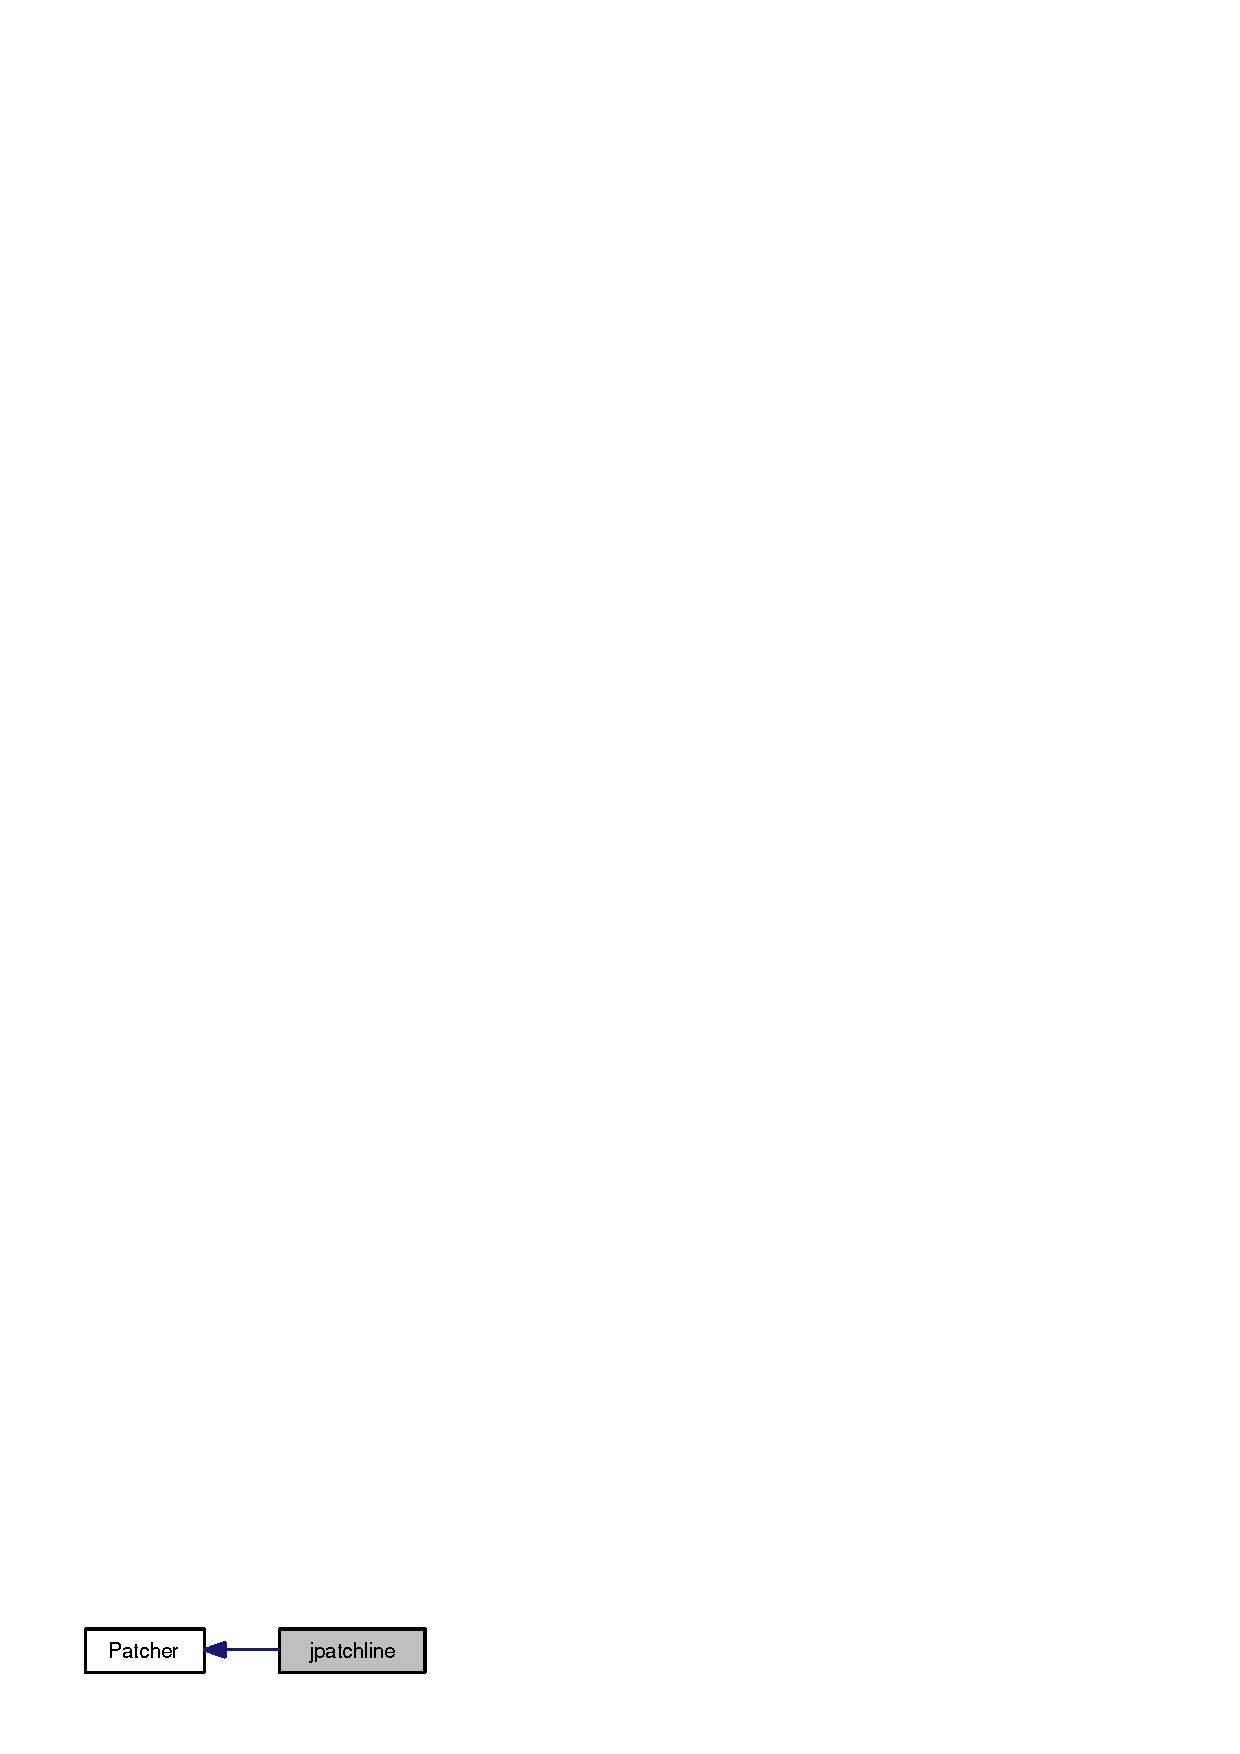
\includegraphics[width=104pt]{group__jpatchline}
\end{center}
\end{figure}
\subsection*{Functions}
\begin{DoxyCompactItemize}
\item 
\hyperlink{group__datatypes_ga73edaae82b318855cc09fac994918165}{t\_\-max\_\-err} \hyperlink{group__jpatchline_ga22e58d4f810941cbcab9c72fd6f944a8}{jpatchline\_\-get\_\-startpoint} (\hyperlink{structt__object}{t\_\-object} $\ast$l, double $\ast$x, double $\ast$y)
\begin{DoxyCompactList}\small\item\em Retrieve a patchline's starting point. \item\end{DoxyCompactList}\item 
\hyperlink{group__datatypes_ga73edaae82b318855cc09fac994918165}{t\_\-max\_\-err} \hyperlink{group__jpatchline_gae3975e752f1b21493cd7546d081e82ab}{jpatchline\_\-get\_\-endpoint} (\hyperlink{structt__object}{t\_\-object} $\ast$l, double $\ast$x, double $\ast$y)
\begin{DoxyCompactList}\small\item\em Retrieve a patchline's ending point. \item\end{DoxyCompactList}\item 
long \hyperlink{group__jpatchline_ga42dc7b0cc71d75625f6580987a61f0e9}{jpatchline\_\-get\_\-nummidpoints} (\hyperlink{structt__object}{t\_\-object} $\ast$l)
\begin{DoxyCompactList}\small\item\em Determine the number of midpoints (segments) in a patchline. \item\end{DoxyCompactList}\item 
\hyperlink{structt__object}{t\_\-object} $\ast$ \hyperlink{group__jpatchline_ga64a77181748a3f07c149942ef60053c9}{jpatchline\_\-get\_\-box1} (\hyperlink{structt__object}{t\_\-object} $\ast$l)
\begin{DoxyCompactList}\small\item\em Return the object box from which a patchline originates. \item\end{DoxyCompactList}\item 
long \hyperlink{group__jpatchline_ga901d26a483f28768c842defe9ad06cfb}{jpatchline\_\-get\_\-outletnum} (\hyperlink{structt__object}{t\_\-object} $\ast$l)
\begin{DoxyCompactList}\small\item\em Return the outlet number of the originating object box from which a patchline begins. \item\end{DoxyCompactList}\item 
\hyperlink{structt__object}{t\_\-object} $\ast$ \hyperlink{group__jpatchline_ga8785673e61f9b9406e4c77df1b7781b1}{jpatchline\_\-get\_\-box2} (\hyperlink{structt__object}{t\_\-object} $\ast$l)
\begin{DoxyCompactList}\small\item\em Return the destination object box for a patchline. \item\end{DoxyCompactList}\item 
long \hyperlink{group__jpatchline_ga01dc2867e149ca5d165a5efd852b80b0}{jpatchline\_\-get\_\-inletnum} (\hyperlink{structt__object}{t\_\-object} $\ast$l)
\begin{DoxyCompactList}\small\item\em Return the inlet number of the destination object box to which a patchline is connected. \item\end{DoxyCompactList}\item 
\hyperlink{structt__object}{t\_\-object} $\ast$ \hyperlink{group__jpatchline_ga1aed89ce61ea59fbc47a282e25398aa8}{jpatchline\_\-get\_\-nextline} (\hyperlink{structt__object}{t\_\-object} $\ast$b)
\begin{DoxyCompactList}\small\item\em Given a patchline, traverse to the next patchline in the (linked) list. \item\end{DoxyCompactList}\item 
char \hyperlink{group__jpatchline_gaece283402d2f063de0fec372e7ad8fa5}{jpatchline\_\-get\_\-hidden} (\hyperlink{structt__object}{t\_\-object} $\ast$l)
\begin{DoxyCompactList}\small\item\em Determine if a patch line is hidden. \item\end{DoxyCompactList}\item 
\hyperlink{group__datatypes_ga73edaae82b318855cc09fac994918165}{t\_\-max\_\-err} \hyperlink{group__jpatchline_gae5bd6fbfa02559350ee2b117a55b64d5}{jpatchline\_\-set\_\-hidden} (\hyperlink{structt__object}{t\_\-object} $\ast$l, char c)
\begin{DoxyCompactList}\small\item\em Set a patchline's visibility. \item\end{DoxyCompactList}\item 
\hyperlink{group__datatypes_ga73edaae82b318855cc09fac994918165}{t\_\-max\_\-err} \hyperlink{group__jpatchline_ga9f612329fb1b675345173e56b0da8b5e}{jpatchline\_\-get\_\-color} (\hyperlink{structt__object}{t\_\-object} $\ast$l, \hyperlink{structt__jrgba}{t\_\-jrgba} $\ast$prgba)
\begin{DoxyCompactList}\small\item\em Get the color of a patch line. \item\end{DoxyCompactList}\item 
\hyperlink{group__datatypes_ga73edaae82b318855cc09fac994918165}{t\_\-max\_\-err} \hyperlink{group__jpatchline_ga711fb3e7a43bbfbd6922f3ac60ba7d86}{jpatchline\_\-set\_\-color} (\hyperlink{structt__object}{t\_\-object} $\ast$l, \hyperlink{structt__jrgba}{t\_\-jrgba} $\ast$prgba)
\begin{DoxyCompactList}\small\item\em Set the color of a patch line. \item\end{DoxyCompactList}\end{DoxyCompactItemize}


\subsection{Detailed Description}
A patch cord. 

\subsection{Function Documentation}
\hypertarget{group__jpatchline_ga64a77181748a3f07c149942ef60053c9}{
\index{jpatchline@{jpatchline}!jpatchline\_\-get\_\-box1@{jpatchline\_\-get\_\-box1}}
\index{jpatchline\_\-get\_\-box1@{jpatchline\_\-get\_\-box1}!jpatchline@{jpatchline}}
\subsubsection[{jpatchline\_\-get\_\-box1}]{\setlength{\rightskip}{0pt plus 5cm}{\bf t\_\-object}$\ast$ jpatchline\_\-get\_\-box1 ({\bf t\_\-object} $\ast$ {\em l})}}
\label{group__jpatchline_ga64a77181748a3f07c149942ef60053c9}


Return the object box from which a patchline originates. 
\begin{DoxyParams}{Parameters}
\item[{\em l}]A pointer to the patchline's instance. \end{DoxyParams}
\begin{DoxyReturn}{Returns}
The object box from which the patchline originates. 
\end{DoxyReturn}
\hypertarget{group__jpatchline_ga8785673e61f9b9406e4c77df1b7781b1}{
\index{jpatchline@{jpatchline}!jpatchline\_\-get\_\-box2@{jpatchline\_\-get\_\-box2}}
\index{jpatchline\_\-get\_\-box2@{jpatchline\_\-get\_\-box2}!jpatchline@{jpatchline}}
\subsubsection[{jpatchline\_\-get\_\-box2}]{\setlength{\rightskip}{0pt plus 5cm}{\bf t\_\-object}$\ast$ jpatchline\_\-get\_\-box2 ({\bf t\_\-object} $\ast$ {\em l})}}
\label{group__jpatchline_ga8785673e61f9b9406e4c77df1b7781b1}


Return the destination object box for a patchline. 
\begin{DoxyParams}{Parameters}
\item[{\em l}]A pointer to the patchline's instance. \end{DoxyParams}
\begin{DoxyReturn}{Returns}
The destination object box for a patchline. 
\end{DoxyReturn}
\hypertarget{group__jpatchline_ga9f612329fb1b675345173e56b0da8b5e}{
\index{jpatchline@{jpatchline}!jpatchline\_\-get\_\-color@{jpatchline\_\-get\_\-color}}
\index{jpatchline\_\-get\_\-color@{jpatchline\_\-get\_\-color}!jpatchline@{jpatchline}}
\subsubsection[{jpatchline\_\-get\_\-color}]{\setlength{\rightskip}{0pt plus 5cm}{\bf t\_\-max\_\-err} jpatchline\_\-get\_\-color ({\bf t\_\-object} $\ast$ {\em l}, \/  {\bf t\_\-jrgba} $\ast$ {\em prgba})}}
\label{group__jpatchline_ga9f612329fb1b675345173e56b0da8b5e}


Get the color of a patch line. 
\begin{DoxyParams}{Parameters}
\item[{\em l}]A patchline instance. \item[{\em prgba}]The address of a valid \hyperlink{structt__jrgba}{t\_\-jrgba} struct that will be filled with the color values of the patch line. \end{DoxyParams}
\begin{DoxyReturn}{Returns}
An error code. 
\end{DoxyReturn}
\hypertarget{group__jpatchline_gae3975e752f1b21493cd7546d081e82ab}{
\index{jpatchline@{jpatchline}!jpatchline\_\-get\_\-endpoint@{jpatchline\_\-get\_\-endpoint}}
\index{jpatchline\_\-get\_\-endpoint@{jpatchline\_\-get\_\-endpoint}!jpatchline@{jpatchline}}
\subsubsection[{jpatchline\_\-get\_\-endpoint}]{\setlength{\rightskip}{0pt plus 5cm}{\bf t\_\-max\_\-err} jpatchline\_\-get\_\-endpoint ({\bf t\_\-object} $\ast$ {\em l}, \/  double $\ast$ {\em x}, \/  double $\ast$ {\em y})}}
\label{group__jpatchline_gae3975e752f1b21493cd7546d081e82ab}


Retrieve a patchline's ending point. 
\begin{DoxyParams}{Parameters}
\item[{\em l}]A pointer to the patchline's instance. \item[{\em x}]The address of a variable to hold the x-\/coordinate of the ending point's position upon return. \item[{\em y}]The address of a variable to hold the y-\/coordinate of the ending point's position upon return. \end{DoxyParams}
\begin{DoxyReturn}{Returns}
A Max error code. 
\end{DoxyReturn}
\hypertarget{group__jpatchline_gaece283402d2f063de0fec372e7ad8fa5}{
\index{jpatchline@{jpatchline}!jpatchline\_\-get\_\-hidden@{jpatchline\_\-get\_\-hidden}}
\index{jpatchline\_\-get\_\-hidden@{jpatchline\_\-get\_\-hidden}!jpatchline@{jpatchline}}
\subsubsection[{jpatchline\_\-get\_\-hidden}]{\setlength{\rightskip}{0pt plus 5cm}char jpatchline\_\-get\_\-hidden ({\bf t\_\-object} $\ast$ {\em l})}}
\label{group__jpatchline_gaece283402d2f063de0fec372e7ad8fa5}


Determine if a patch line is hidden. 
\begin{DoxyParams}{Parameters}
\item[{\em l}]A patchline instance. \end{DoxyParams}
\begin{DoxyReturn}{Returns}
Zero if the patchline is visible, non-\/zero if it is hidden. 
\end{DoxyReturn}
\hypertarget{group__jpatchline_ga01dc2867e149ca5d165a5efd852b80b0}{
\index{jpatchline@{jpatchline}!jpatchline\_\-get\_\-inletnum@{jpatchline\_\-get\_\-inletnum}}
\index{jpatchline\_\-get\_\-inletnum@{jpatchline\_\-get\_\-inletnum}!jpatchline@{jpatchline}}
\subsubsection[{jpatchline\_\-get\_\-inletnum}]{\setlength{\rightskip}{0pt plus 5cm}long jpatchline\_\-get\_\-inletnum ({\bf t\_\-object} $\ast$ {\em l})}}
\label{group__jpatchline_ga01dc2867e149ca5d165a5efd852b80b0}


Return the inlet number of the destination object box to which a patchline is connected. 
\begin{DoxyParams}{Parameters}
\item[{\em l}]A pointer to the patchline's instance. \end{DoxyParams}
\begin{DoxyReturn}{Returns}
The inlet number. 
\end{DoxyReturn}
\hypertarget{group__jpatchline_ga1aed89ce61ea59fbc47a282e25398aa8}{
\index{jpatchline@{jpatchline}!jpatchline\_\-get\_\-nextline@{jpatchline\_\-get\_\-nextline}}
\index{jpatchline\_\-get\_\-nextline@{jpatchline\_\-get\_\-nextline}!jpatchline@{jpatchline}}
\subsubsection[{jpatchline\_\-get\_\-nextline}]{\setlength{\rightskip}{0pt plus 5cm}{\bf t\_\-object}$\ast$ jpatchline\_\-get\_\-nextline ({\bf t\_\-object} $\ast$ {\em b})}}
\label{group__jpatchline_ga1aed89ce61ea59fbc47a282e25398aa8}


Given a patchline, traverse to the next patchline in the (linked) list. 
\begin{DoxyParams}{Parameters}
\item[{\em b}]A patchline instance. \end{DoxyParams}
\begin{DoxyReturn}{Returns}
The next patchline. If the current patchline is at the end (tail) of the list, then NULL is returned. 
\end{DoxyReturn}
\hypertarget{group__jpatchline_ga42dc7b0cc71d75625f6580987a61f0e9}{
\index{jpatchline@{jpatchline}!jpatchline\_\-get\_\-nummidpoints@{jpatchline\_\-get\_\-nummidpoints}}
\index{jpatchline\_\-get\_\-nummidpoints@{jpatchline\_\-get\_\-nummidpoints}!jpatchline@{jpatchline}}
\subsubsection[{jpatchline\_\-get\_\-nummidpoints}]{\setlength{\rightskip}{0pt plus 5cm}long jpatchline\_\-get\_\-nummidpoints ({\bf t\_\-object} $\ast$ {\em l})}}
\label{group__jpatchline_ga42dc7b0cc71d75625f6580987a61f0e9}


Determine the number of midpoints (segments) in a patchline. 
\begin{DoxyParams}{Parameters}
\item[{\em l}]A pointer to the patchline's instance. \end{DoxyParams}
\begin{DoxyReturn}{Returns}
The number of midpoints in the patchline. 
\end{DoxyReturn}
\hypertarget{group__jpatchline_ga901d26a483f28768c842defe9ad06cfb}{
\index{jpatchline@{jpatchline}!jpatchline\_\-get\_\-outletnum@{jpatchline\_\-get\_\-outletnum}}
\index{jpatchline\_\-get\_\-outletnum@{jpatchline\_\-get\_\-outletnum}!jpatchline@{jpatchline}}
\subsubsection[{jpatchline\_\-get\_\-outletnum}]{\setlength{\rightskip}{0pt plus 5cm}long jpatchline\_\-get\_\-outletnum ({\bf t\_\-object} $\ast$ {\em l})}}
\label{group__jpatchline_ga901d26a483f28768c842defe9ad06cfb}


Return the outlet number of the originating object box from which a patchline begins. 
\begin{DoxyParams}{Parameters}
\item[{\em l}]A pointer to the patchline's instance. \end{DoxyParams}
\begin{DoxyReturn}{Returns}
The outlet number. 
\end{DoxyReturn}
\hypertarget{group__jpatchline_ga22e58d4f810941cbcab9c72fd6f944a8}{
\index{jpatchline@{jpatchline}!jpatchline\_\-get\_\-startpoint@{jpatchline\_\-get\_\-startpoint}}
\index{jpatchline\_\-get\_\-startpoint@{jpatchline\_\-get\_\-startpoint}!jpatchline@{jpatchline}}
\subsubsection[{jpatchline\_\-get\_\-startpoint}]{\setlength{\rightskip}{0pt plus 5cm}{\bf t\_\-max\_\-err} jpatchline\_\-get\_\-startpoint ({\bf t\_\-object} $\ast$ {\em l}, \/  double $\ast$ {\em x}, \/  double $\ast$ {\em y})}}
\label{group__jpatchline_ga22e58d4f810941cbcab9c72fd6f944a8}


Retrieve a patchline's starting point. 
\begin{DoxyParams}{Parameters}
\item[{\em l}]A pointer to the patchline's instance. \item[{\em x}]The address of a variable to hold the x-\/coordinate of the starting point's position upon return. \item[{\em y}]The address of a variable to hold the y-\/coordinate of the starting point's position upon return. \end{DoxyParams}
\begin{DoxyReturn}{Returns}
A Max error code. 
\end{DoxyReturn}
\hypertarget{group__jpatchline_ga711fb3e7a43bbfbd6922f3ac60ba7d86}{
\index{jpatchline@{jpatchline}!jpatchline\_\-set\_\-color@{jpatchline\_\-set\_\-color}}
\index{jpatchline\_\-set\_\-color@{jpatchline\_\-set\_\-color}!jpatchline@{jpatchline}}
\subsubsection[{jpatchline\_\-set\_\-color}]{\setlength{\rightskip}{0pt plus 5cm}{\bf t\_\-max\_\-err} jpatchline\_\-set\_\-color ({\bf t\_\-object} $\ast$ {\em l}, \/  {\bf t\_\-jrgba} $\ast$ {\em prgba})}}
\label{group__jpatchline_ga711fb3e7a43bbfbd6922f3ac60ba7d86}


Set the color of a patch line. 
\begin{DoxyParams}{Parameters}
\item[{\em l}]A patchline instance. \item[{\em prgba}]The address of a valid \hyperlink{structt__jrgba}{t\_\-jrgba} struct containing the color to use. \end{DoxyParams}
\begin{DoxyReturn}{Returns}
An error code. 
\end{DoxyReturn}
\hypertarget{group__jpatchline_gae5bd6fbfa02559350ee2b117a55b64d5}{
\index{jpatchline@{jpatchline}!jpatchline\_\-set\_\-hidden@{jpatchline\_\-set\_\-hidden}}
\index{jpatchline\_\-set\_\-hidden@{jpatchline\_\-set\_\-hidden}!jpatchline@{jpatchline}}
\subsubsection[{jpatchline\_\-set\_\-hidden}]{\setlength{\rightskip}{0pt plus 5cm}{\bf t\_\-max\_\-err} jpatchline\_\-set\_\-hidden ({\bf t\_\-object} $\ast$ {\em l}, \/  char {\em c})}}
\label{group__jpatchline_gae5bd6fbfa02559350ee2b117a55b64d5}


Set a patchline's visibility. 
\begin{DoxyParams}{Parameters}
\item[{\em l}]A patchline instance. \item[{\em c}]Pass 0 to make a patchline visible, or non-\/zero to hide it. \end{DoxyParams}
\begin{DoxyReturn}{Returns}
An error code. 
\end{DoxyReturn}

\hypertarget{group__jpatcherview}{
\section{jpatcherview}
\label{group__jpatcherview}\index{jpatcherview@{jpatcherview}}
}


A view of a patcher.  


Collaboration diagram for jpatcherview:\nopagebreak
\begin{figure}[H]
\begin{center}
\leavevmode
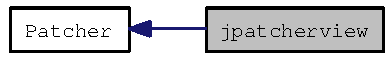
\includegraphics[width=112pt]{group__jpatcherview}
\end{center}
\end{figure}
\subsection*{Functions}
\begin{DoxyCompactItemize}
\item 
\hyperlink{structt__object}{t\_\-object} $\ast$ \hyperlink{group__jpatcherview_ga143a54662c1dea4f8170c7b62bc4cb2d}{patcherview\_\-findpatcherview} (int x, int y)
\begin{DoxyCompactList}\small\item\em Find a patcherview at the given screen coords. \item\end{DoxyCompactList}\item 
char \hyperlink{group__jpatcherview_gaf9621ecabdae9fc9d865bd42a8bc43a9}{patcherview\_\-get\_\-visible} (\hyperlink{structt__object}{t\_\-object} $\ast$pv)
\begin{DoxyCompactList}\small\item\em Query a patcherview to determine whether it is visible. \item\end{DoxyCompactList}\item 
\hyperlink{group__datatypes_ga73edaae82b318855cc09fac994918165}{t\_\-max\_\-err} \hyperlink{group__jpatcherview_gab8b3bb74c2341f42a1b8fb3a1dbdcbb8}{patcherview\_\-set\_\-visible} (\hyperlink{structt__object}{t\_\-object} $\ast$pv, char c)
\begin{DoxyCompactList}\small\item\em Set the 'visible' attribute of a patcherview. \item\end{DoxyCompactList}\item 
\hyperlink{group__datatypes_ga73edaae82b318855cc09fac994918165}{t\_\-max\_\-err} \hyperlink{group__jpatcherview_ga310590cbb1dd9fbe5c8c228e35fe11ef}{patcherview\_\-get\_\-rect} (\hyperlink{structt__object}{t\_\-object} $\ast$pv, \hyperlink{structt__rect}{t\_\-rect} $\ast$pr)
\begin{DoxyCompactList}\small\item\em Get the value of the rect attribute for a patcherview. \item\end{DoxyCompactList}\item 
\hyperlink{group__datatypes_ga73edaae82b318855cc09fac994918165}{t\_\-max\_\-err} \hyperlink{group__jpatcherview_ga6025a5acb336aa81a0aad67e9de5bbca}{patcherview\_\-set\_\-rect} (\hyperlink{structt__object}{t\_\-object} $\ast$pv, \hyperlink{structt__rect}{t\_\-rect} $\ast$pr)
\begin{DoxyCompactList}\small\item\em Set the value of the rect attribute for a patcherview. \item\end{DoxyCompactList}\item 
char \hyperlink{group__jpatcherview_ga1b78b4ec463f113a0c2778dbebcc8654}{patcherview\_\-get\_\-locked} (\hyperlink{structt__object}{t\_\-object} $\ast$p)
\begin{DoxyCompactList}\small\item\em Find out if a patcherview is locked. \item\end{DoxyCompactList}\item 
\hyperlink{group__datatypes_ga73edaae82b318855cc09fac994918165}{t\_\-max\_\-err} \hyperlink{group__jpatcherview_ga826eb120924785345d8a7851d31ce788}{patcherview\_\-set\_\-locked} (\hyperlink{structt__object}{t\_\-object} $\ast$p, char c)
\begin{DoxyCompactList}\small\item\em Lock or unlock a patcherview. \item\end{DoxyCompactList}\item 
char \hyperlink{group__jpatcherview_ga196c47fa60725d496c75b400da72d8a9}{patcherview\_\-get\_\-presentation} (\hyperlink{structt__object}{t\_\-object} $\ast$pv)
\begin{DoxyCompactList}\small\item\em Find out if a patcherview is a presentation view. \item\end{DoxyCompactList}\item 
\hyperlink{group__datatypes_ga73edaae82b318855cc09fac994918165}{t\_\-max\_\-err} \hyperlink{group__jpatcherview_ga349cf62e72891016e0dcf8ab51c00a62}{patcherview\_\-set\_\-presentation} (\hyperlink{structt__object}{t\_\-object} $\ast$p, char c)
\begin{DoxyCompactList}\small\item\em Set whether or not a patcherview is a presentation view. \item\end{DoxyCompactList}\item 
double \hyperlink{group__jpatcherview_ga3d82e2665c64f9c4452d1737c1429293}{patcherview\_\-get\_\-zoomfactor} (\hyperlink{structt__object}{t\_\-object} $\ast$pv)
\begin{DoxyCompactList}\small\item\em Fetch the zoom-\/factor of a patcherview. \item\end{DoxyCompactList}\item 
\hyperlink{group__datatypes_ga73edaae82b318855cc09fac994918165}{t\_\-max\_\-err} \hyperlink{group__jpatcherview_ga5006e672580027e9ae56c49ca3148c3c}{patcherview\_\-set\_\-zoomfactor} (\hyperlink{structt__object}{t\_\-object} $\ast$pv, double d)
\begin{DoxyCompactList}\small\item\em Set the zoom-\/factor of a patcherview. \item\end{DoxyCompactList}\item 
\hyperlink{structt__object}{t\_\-object} $\ast$ \hyperlink{group__jpatcherview_ga37810ea052b4ecd3598cd687666c8841}{patcherview\_\-get\_\-nextview} (\hyperlink{structt__object}{t\_\-object} $\ast$pv)
\begin{DoxyCompactList}\small\item\em Given a patcherview, find the next patcherview. \item\end{DoxyCompactList}\item 
\hyperlink{structt__object}{t\_\-object} $\ast$ \hyperlink{group__jpatcherview_ga221544b77a5371897c96f2e94ae49c82}{patcherview\_\-get\_\-jgraphics} (\hyperlink{structt__object}{t\_\-object} $\ast$pv)
\begin{DoxyCompactList}\small\item\em Given a patcherview, return the \hyperlink{group__jgraphics_ga4bf27bd7e21a59a427481b909d4656e7}{t\_\-jgraphics} context for that view. \item\end{DoxyCompactList}\item 
\hyperlink{structt__object}{t\_\-object} $\ast$ \hyperlink{group__jpatcherview_ga056a0684b79a940b8ee71145d9f77223}{patcherview\_\-get\_\-patcher} (\hyperlink{structt__object}{t\_\-object} $\ast$pv)
\begin{DoxyCompactList}\small\item\em Given a patcherview, return its patcher. \item\end{DoxyCompactList}\end{DoxyCompactItemize}


\subsection{Detailed Description}
A view of a patcher. 

\subsection{Function Documentation}
\hypertarget{group__jpatcherview_ga143a54662c1dea4f8170c7b62bc4cb2d}{
\index{jpatcherview@{jpatcherview}!patcherview\_\-findpatcherview@{patcherview\_\-findpatcherview}}
\index{patcherview\_\-findpatcherview@{patcherview\_\-findpatcherview}!jpatcherview@{jpatcherview}}
\subsubsection[{patcherview\_\-findpatcherview}]{\setlength{\rightskip}{0pt plus 5cm}{\bf t\_\-object}$\ast$ patcherview\_\-findpatcherview (int {\em x}, \/  int {\em y})}}
\label{group__jpatcherview_ga143a54662c1dea4f8170c7b62bc4cb2d}


Find a patcherview at the given screen coords. 
\begin{DoxyParams}{Parameters}
\item[{\em x}]The horizontal coordinate at which to find a patcherview. \item[{\em y}]The vertical coordinate at which to find a patcherview. \end{DoxyParams}
\begin{DoxyReturn}{Returns}
A pointer to the patcherview at the specified location, or NULL if no patcherview exists at that location. 
\end{DoxyReturn}
\hypertarget{group__jpatcherview_ga221544b77a5371897c96f2e94ae49c82}{
\index{jpatcherview@{jpatcherview}!patcherview\_\-get\_\-jgraphics@{patcherview\_\-get\_\-jgraphics}}
\index{patcherview\_\-get\_\-jgraphics@{patcherview\_\-get\_\-jgraphics}!jpatcherview@{jpatcherview}}
\subsubsection[{patcherview\_\-get\_\-jgraphics}]{\setlength{\rightskip}{0pt plus 5cm}{\bf t\_\-object}$\ast$ patcherview\_\-get\_\-jgraphics ({\bf t\_\-object} $\ast$ {\em pv})}}
\label{group__jpatcherview_ga221544b77a5371897c96f2e94ae49c82}


Given a patcherview, return the \hyperlink{group__jgraphics_ga4bf27bd7e21a59a427481b909d4656e7}{t\_\-jgraphics} context for that view. 
\begin{DoxyParams}{Parameters}
\item[{\em pv}]The patcherview instance. \end{DoxyParams}
\begin{DoxyReturn}{Returns}
The \hyperlink{group__jgraphics_ga4bf27bd7e21a59a427481b909d4656e7}{t\_\-jgraphics} context for the view. 
\end{DoxyReturn}
\hypertarget{group__jpatcherview_ga1b78b4ec463f113a0c2778dbebcc8654}{
\index{jpatcherview@{jpatcherview}!patcherview\_\-get\_\-locked@{patcherview\_\-get\_\-locked}}
\index{patcherview\_\-get\_\-locked@{patcherview\_\-get\_\-locked}!jpatcherview@{jpatcherview}}
\subsubsection[{patcherview\_\-get\_\-locked}]{\setlength{\rightskip}{0pt plus 5cm}char patcherview\_\-get\_\-locked ({\bf t\_\-object} $\ast$ {\em p})}}
\label{group__jpatcherview_ga1b78b4ec463f113a0c2778dbebcc8654}


Find out if a patcherview is locked. 
\begin{DoxyParams}{Parameters}
\item[{\em p}]The patcherview instance whose attribute value will be fetched. \end{DoxyParams}
\begin{DoxyReturn}{Returns}
Returns 0 if unlocked, otherwise returns non-\/zero. 
\end{DoxyReturn}
\hypertarget{group__jpatcherview_ga37810ea052b4ecd3598cd687666c8841}{
\index{jpatcherview@{jpatcherview}!patcherview\_\-get\_\-nextview@{patcherview\_\-get\_\-nextview}}
\index{patcherview\_\-get\_\-nextview@{patcherview\_\-get\_\-nextview}!jpatcherview@{jpatcherview}}
\subsubsection[{patcherview\_\-get\_\-nextview}]{\setlength{\rightskip}{0pt plus 5cm}{\bf t\_\-object}$\ast$ patcherview\_\-get\_\-nextview ({\bf t\_\-object} $\ast$ {\em pv})}}
\label{group__jpatcherview_ga37810ea052b4ecd3598cd687666c8841}


Given a patcherview, find the next patcherview. The views of a patcher are maintained internally as a \hyperlink{structt__linklist}{t\_\-linklist}, and so the views can be traversed should you need to perform operations on all of a patcher's patcherviews.


\begin{DoxyParams}{Parameters}
\item[{\em pv}]The patcherview instance from which to find the next patcherview. \end{DoxyParams}
\begin{DoxyReturn}{Returns}
The next patcherview in the list, or NULL if the patcherview passed in pv is the tail. 
\end{DoxyReturn}
\hypertarget{group__jpatcherview_ga056a0684b79a940b8ee71145d9f77223}{
\index{jpatcherview@{jpatcherview}!patcherview\_\-get\_\-patcher@{patcherview\_\-get\_\-patcher}}
\index{patcherview\_\-get\_\-patcher@{patcherview\_\-get\_\-patcher}!jpatcherview@{jpatcherview}}
\subsubsection[{patcherview\_\-get\_\-patcher}]{\setlength{\rightskip}{0pt plus 5cm}{\bf t\_\-object}$\ast$ patcherview\_\-get\_\-patcher ({\bf t\_\-object} $\ast$ {\em pv})}}
\label{group__jpatcherview_ga056a0684b79a940b8ee71145d9f77223}


Given a patcherview, return its patcher. 
\begin{DoxyParams}{Parameters}
\item[{\em pv}]The patcherview instance for which to fetch the patcher. \end{DoxyParams}
\begin{DoxyReturn}{Returns}
The patcher. 
\end{DoxyReturn}
\hypertarget{group__jpatcherview_ga196c47fa60725d496c75b400da72d8a9}{
\index{jpatcherview@{jpatcherview}!patcherview\_\-get\_\-presentation@{patcherview\_\-get\_\-presentation}}
\index{patcherview\_\-get\_\-presentation@{patcherview\_\-get\_\-presentation}!jpatcherview@{jpatcherview}}
\subsubsection[{patcherview\_\-get\_\-presentation}]{\setlength{\rightskip}{0pt plus 5cm}char patcherview\_\-get\_\-presentation ({\bf t\_\-object} $\ast$ {\em pv})}}
\label{group__jpatcherview_ga196c47fa60725d496c75b400da72d8a9}


Find out if a patcherview is a presentation view. 
\begin{DoxyParams}{Parameters}
\item[{\em pv}]The patcherview instance whose attribute value will be fetched. \end{DoxyParams}
\begin{DoxyReturn}{Returns}
Returns 0 if the view is not a presentation view, otherwise returns non-\/zero. 
\end{DoxyReturn}
\hypertarget{group__jpatcherview_ga310590cbb1dd9fbe5c8c228e35fe11ef}{
\index{jpatcherview@{jpatcherview}!patcherview\_\-get\_\-rect@{patcherview\_\-get\_\-rect}}
\index{patcherview\_\-get\_\-rect@{patcherview\_\-get\_\-rect}!jpatcherview@{jpatcherview}}
\subsubsection[{patcherview\_\-get\_\-rect}]{\setlength{\rightskip}{0pt plus 5cm}{\bf t\_\-max\_\-err} patcherview\_\-get\_\-rect ({\bf t\_\-object} $\ast$ {\em pv}, \/  {\bf t\_\-rect} $\ast$ {\em pr})}}
\label{group__jpatcherview_ga310590cbb1dd9fbe5c8c228e35fe11ef}


Get the value of the rect attribute for a patcherview. 
\begin{DoxyParams}{Parameters}
\item[{\em pv}]The patcherview instance whose attribute value will be fetched. \item[{\em pr}]The address of a valid \hyperlink{structt__rect}{t\_\-rect} struct, whose contents will be filled upon return. \end{DoxyParams}
\begin{DoxyReturn}{Returns}
An error code. 
\end{DoxyReturn}
\hypertarget{group__jpatcherview_gaf9621ecabdae9fc9d865bd42a8bc43a9}{
\index{jpatcherview@{jpatcherview}!patcherview\_\-get\_\-visible@{patcherview\_\-get\_\-visible}}
\index{patcherview\_\-get\_\-visible@{patcherview\_\-get\_\-visible}!jpatcherview@{jpatcherview}}
\subsubsection[{patcherview\_\-get\_\-visible}]{\setlength{\rightskip}{0pt plus 5cm}char patcherview\_\-get\_\-visible ({\bf t\_\-object} $\ast$ {\em pv})}}
\label{group__jpatcherview_gaf9621ecabdae9fc9d865bd42a8bc43a9}


Query a patcherview to determine whether it is visible. 
\begin{DoxyParams}{Parameters}
\item[{\em pv}]The patcherview instance to query. \end{DoxyParams}
\begin{DoxyReturn}{Returns}
Returns zero if the patcherview is invisible, otherwise returns non-\/zero. 
\end{DoxyReturn}
\hypertarget{group__jpatcherview_ga3d82e2665c64f9c4452d1737c1429293}{
\index{jpatcherview@{jpatcherview}!patcherview\_\-get\_\-zoomfactor@{patcherview\_\-get\_\-zoomfactor}}
\index{patcherview\_\-get\_\-zoomfactor@{patcherview\_\-get\_\-zoomfactor}!jpatcherview@{jpatcherview}}
\subsubsection[{patcherview\_\-get\_\-zoomfactor}]{\setlength{\rightskip}{0pt plus 5cm}double patcherview\_\-get\_\-zoomfactor ({\bf t\_\-object} $\ast$ {\em pv})}}
\label{group__jpatcherview_ga3d82e2665c64f9c4452d1737c1429293}


Fetch the zoom-\/factor of a patcherview. 
\begin{DoxyParams}{Parameters}
\item[{\em pv}]The patcherview instance whose attribute value will be fetched. \end{DoxyParams}
\begin{DoxyReturn}{Returns}
The factor by which the view is zoomed. 
\end{DoxyReturn}
\hypertarget{group__jpatcherview_ga826eb120924785345d8a7851d31ce788}{
\index{jpatcherview@{jpatcherview}!patcherview\_\-set\_\-locked@{patcherview\_\-set\_\-locked}}
\index{patcherview\_\-set\_\-locked@{patcherview\_\-set\_\-locked}!jpatcherview@{jpatcherview}}
\subsubsection[{patcherview\_\-set\_\-locked}]{\setlength{\rightskip}{0pt plus 5cm}{\bf t\_\-max\_\-err} patcherview\_\-set\_\-locked ({\bf t\_\-object} $\ast$ {\em p}, \/  char {\em c})}}
\label{group__jpatcherview_ga826eb120924785345d8a7851d31ce788}


Lock or unlock a patcherview. 
\begin{DoxyParams}{Parameters}
\item[{\em p}]The patcherview instance whose attribute value will be set. \item[{\em c}]Set this value to zero to unlock the patcherview, otherwise pass a non-\/zero value. \end{DoxyParams}
\begin{DoxyReturn}{Returns}
An error code. 
\end{DoxyReturn}
\hypertarget{group__jpatcherview_ga349cf62e72891016e0dcf8ab51c00a62}{
\index{jpatcherview@{jpatcherview}!patcherview\_\-set\_\-presentation@{patcherview\_\-set\_\-presentation}}
\index{patcherview\_\-set\_\-presentation@{patcherview\_\-set\_\-presentation}!jpatcherview@{jpatcherview}}
\subsubsection[{patcherview\_\-set\_\-presentation}]{\setlength{\rightskip}{0pt plus 5cm}{\bf t\_\-max\_\-err} patcherview\_\-set\_\-presentation ({\bf t\_\-object} $\ast$ {\em p}, \/  char {\em c})}}
\label{group__jpatcherview_ga349cf62e72891016e0dcf8ab51c00a62}


Set whether or not a patcherview is a presentation view. 
\begin{DoxyParams}{Parameters}
\item[{\em p}]The patcherview instance whose attribute value will be set. \item[{\em c}]Set this value to non-\/zero to make the patcherview a presentation view, otherwise pass zero. \end{DoxyParams}
\begin{DoxyReturn}{Returns}
An error code. 
\end{DoxyReturn}
\hypertarget{group__jpatcherview_ga6025a5acb336aa81a0aad67e9de5bbca}{
\index{jpatcherview@{jpatcherview}!patcherview\_\-set\_\-rect@{patcherview\_\-set\_\-rect}}
\index{patcherview\_\-set\_\-rect@{patcherview\_\-set\_\-rect}!jpatcherview@{jpatcherview}}
\subsubsection[{patcherview\_\-set\_\-rect}]{\setlength{\rightskip}{0pt plus 5cm}{\bf t\_\-max\_\-err} patcherview\_\-set\_\-rect ({\bf t\_\-object} $\ast$ {\em pv}, \/  {\bf t\_\-rect} $\ast$ {\em pr})}}
\label{group__jpatcherview_ga6025a5acb336aa81a0aad67e9de5bbca}


Set the value of the rect attribute for a patcherview. 
\begin{DoxyParams}{Parameters}
\item[{\em pv}]The patcherview instance whose attribute value will be set. \item[{\em pr}]The address of a valid \hyperlink{structt__rect}{t\_\-rect} struct. \end{DoxyParams}
\begin{DoxyReturn}{Returns}
An error code. 
\end{DoxyReturn}
\hypertarget{group__jpatcherview_gab8b3bb74c2341f42a1b8fb3a1dbdcbb8}{
\index{jpatcherview@{jpatcherview}!patcherview\_\-set\_\-visible@{patcherview\_\-set\_\-visible}}
\index{patcherview\_\-set\_\-visible@{patcherview\_\-set\_\-visible}!jpatcherview@{jpatcherview}}
\subsubsection[{patcherview\_\-set\_\-visible}]{\setlength{\rightskip}{0pt plus 5cm}{\bf t\_\-max\_\-err} patcherview\_\-set\_\-visible ({\bf t\_\-object} $\ast$ {\em pv}, \/  char {\em c})}}
\label{group__jpatcherview_gab8b3bb74c2341f42a1b8fb3a1dbdcbb8}


Set the 'visible' attribute of a patcherview. 
\begin{DoxyParams}{Parameters}
\item[{\em pv}]The patcherview instance whose attribute will be set. \item[{\em c}]Whether or not the patcherview should be made visible. \end{DoxyParams}
\begin{DoxyReturn}{Returns}
An error code. 
\end{DoxyReturn}
\hypertarget{group__jpatcherview_ga5006e672580027e9ae56c49ca3148c3c}{
\index{jpatcherview@{jpatcherview}!patcherview\_\-set\_\-zoomfactor@{patcherview\_\-set\_\-zoomfactor}}
\index{patcherview\_\-set\_\-zoomfactor@{patcherview\_\-set\_\-zoomfactor}!jpatcherview@{jpatcherview}}
\subsubsection[{patcherview\_\-set\_\-zoomfactor}]{\setlength{\rightskip}{0pt plus 5cm}{\bf t\_\-max\_\-err} patcherview\_\-set\_\-zoomfactor ({\bf t\_\-object} $\ast$ {\em pv}, \/  double {\em d})}}
\label{group__jpatcherview_ga5006e672580027e9ae56c49ca3148c3c}


Set the zoom-\/factor of a patcherview. 
\begin{DoxyParams}{Parameters}
\item[{\em pv}]The patcherview instance whose attribute value will be set. \item[{\em d}]The zoom-\/factor at which the patcherview should display the patcher. \end{DoxyParams}
\begin{DoxyReturn}{Returns}
An error code. 
\end{DoxyReturn}

\hypertarget{group__sched}{
\section{Timing}
\label{group__sched}\index{Timing@{Timing}}
}


Collaboration diagram for Timing:\nopagebreak
\begin{figure}[H]
\begin{center}
\leavevmode
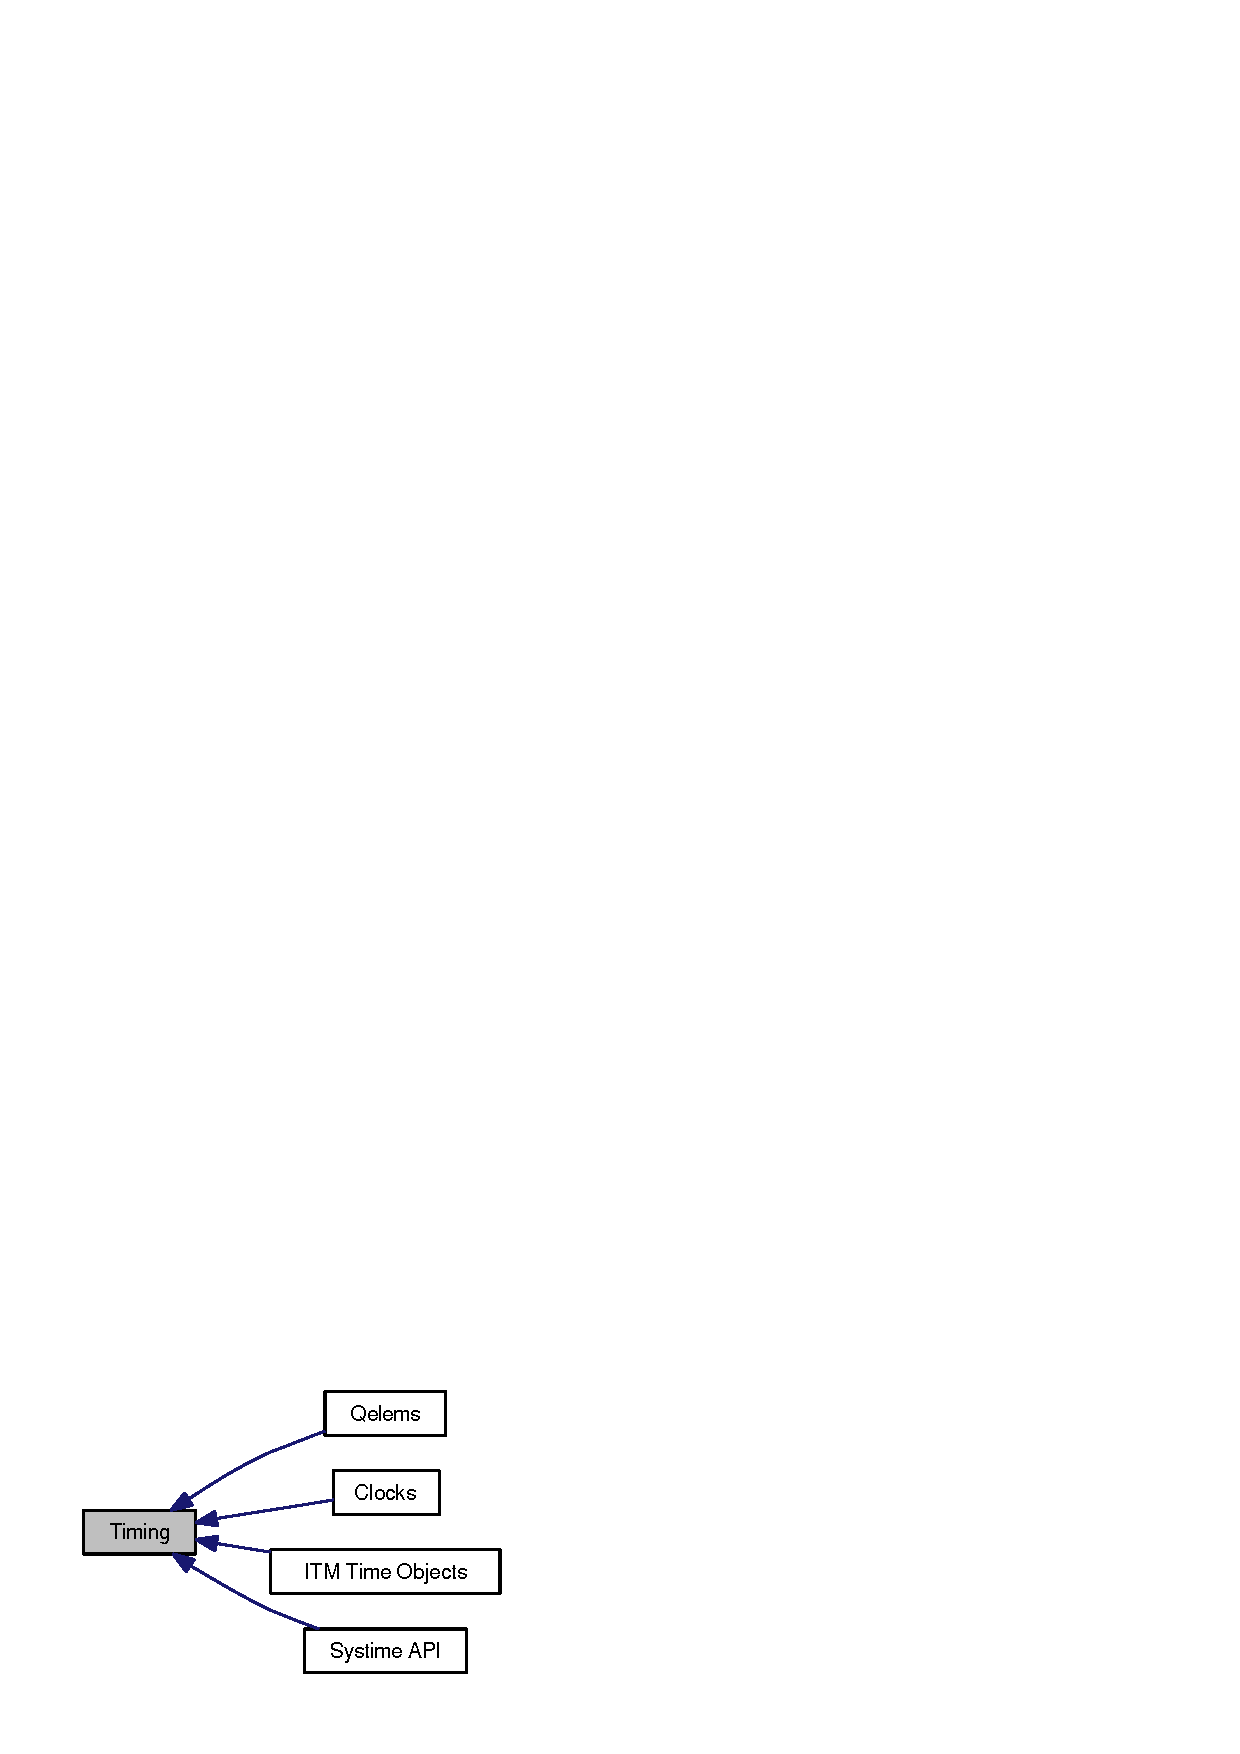
\includegraphics[width=122pt]{group__sched}
\end{center}
\end{figure}
\subsection*{Modules}
\begin{DoxyCompactItemize}
\item 
\hyperlink{group__clocks}{Clocks}


\begin{DoxyCompactList}\small\item\em Clock objects are your interface to Max’s scheduler. \item\end{DoxyCompactList}\item 
\hyperlink{group__qelems}{Qelems}


\begin{DoxyCompactList}\small\item\em Your object’s methods may be called at interrupt level. \item\end{DoxyCompactList}\item 
\hyperlink{group__systime}{Systime API}


\begin{DoxyCompactList}\small\item\em The Systime API provides the means of getting the system time, instead of the scheduler time as you would with functions like \hyperlink{group__clocks_gabe5d8b1c9f260d13734a328b2a60ff69}{gettime()}. \item\end{DoxyCompactList}\item 
\hyperlink{group__time}{ITM Time Objects}


\begin{DoxyCompactList}\small\item\em ITM Time Objects are a high-\/level interface to ITM, a tempo-\/based scheduler API. \item\end{DoxyCompactList}\end{DoxyCompactItemize}

\hypertarget{group__clocks}{
\section{Clocks}
\label{group__clocks}\index{Clocks@{Clocks}}
}


Clock objects are your interface to Max’s scheduler.  


Collaboration diagram for Clocks:\nopagebreak
\begin{figure}[H]
\begin{center}
\leavevmode
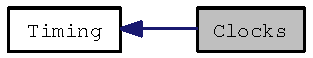
\includegraphics[width=93pt]{group__clocks}
\end{center}
\end{figure}
\subsection*{Typedefs}
\begin{DoxyCompactItemize}
\item 
\hypertarget{group__clocks_ga09c0580122113b4db2517ff8e7c8b0f2}{
typedef \hyperlink{structt__object}{t\_\-object} \hyperlink{group__clocks_ga09c0580122113b4db2517ff8e7c8b0f2}{t\_\-clock}}
\label{group__clocks_ga09c0580122113b4db2517ff8e7c8b0f2}

\begin{DoxyCompactList}\small\item\em A clock. \item\end{DoxyCompactList}\end{DoxyCompactItemize}
\subsection*{Functions}
\begin{DoxyCompactItemize}
\item 
void $\ast$ \hyperlink{group__clocks_ga6257ddd41904756699208f135f6539fd}{clock\_\-new} (void $\ast$obj, \hyperlink{group__datatypes_gac26ba0a173b50597f5738132e059b42d}{method} fn)
\begin{DoxyCompactList}\small\item\em Create a new Clock object. \item\end{DoxyCompactList}\item 
void \hyperlink{group__clocks_ga9ac56d198904627333de740743086920}{clock\_\-delay} (void $\ast$x, long n)
\begin{DoxyCompactList}\small\item\em Schedule the execution of a Clock. \item\end{DoxyCompactList}\item 
void \hyperlink{group__clocks_ga64f5f8a027b39c1c14464744a9cc08ce}{clock\_\-unset} (void $\ast$x)
\begin{DoxyCompactList}\small\item\em Cancel the scheduled execution of a Clock. \item\end{DoxyCompactList}\item 
void \hyperlink{group__clocks_ga61719f0e0379fffbe79ae2bd5699b66f}{clock\_\-fdelay} (void $\ast$c, double time)
\begin{DoxyCompactList}\small\item\em Schedule the execution of a Clock using a floating-\/point argument. \item\end{DoxyCompactList}\item 
void \hyperlink{group__clocks_ga04a49876d29036406f857cf22b99d9ac}{clock\_\-getftime} (double $\ast$time)
\begin{DoxyCompactList}\small\item\em Find out the current logical time of the scheduler in milliseconds as a floating-\/point number. \item\end{DoxyCompactList}\item 
void \hyperlink{group__clocks_gadf4bd364fd019bed91a587337eb4801e}{setclock\_\-delay} (\hyperlink{structt__object}{t\_\-object} $\ast$x, void $\ast$c, long time)
\begin{DoxyCompactList}\small\item\em Schedule a Clock on a scheduler. \item\end{DoxyCompactList}\item 
void \hyperlink{group__clocks_gafbc6d9baa43a561b1840b8b4ce6bed5c}{setclock\_\-unset} (\hyperlink{structt__object}{t\_\-object} $\ast$x, void $\ast$c)
\begin{DoxyCompactList}\small\item\em Remove a Clock from a scheduler. \item\end{DoxyCompactList}\item 
long \hyperlink{group__clocks_ga1322ff3659b3d754298c636ad1856903}{setclock\_\-gettime} (\hyperlink{structt__object}{t\_\-object} $\ast$x)
\begin{DoxyCompactList}\small\item\em Find out the current time value of a setclock object. \item\end{DoxyCompactList}\item 
void \hyperlink{group__clocks_ga91badd52e8729b007c22461368a21854}{setclock\_\-fdelay} (\hyperlink{structt__object}{t\_\-object} $\ast$s, void $\ast$c, double time)
\begin{DoxyCompactList}\small\item\em Schedule a Clock on a scheduler, using a floating-\/point time argument. \item\end{DoxyCompactList}\item 
void \hyperlink{group__clocks_gafd1993dc69a6232cf28683961c97b9e4}{setclock\_\-getftime} (\hyperlink{structt__object}{t\_\-object} $\ast$s, double $\ast$time)
\begin{DoxyCompactList}\small\item\em Find out the current time value of a setclock object in floating-\/point milliseconds. \item\end{DoxyCompactList}\item 
double \hyperlink{group__clocks_ga11fd7e2733b0186ff82e9766db3031e7}{systimer\_\-gettime} (void)
\begin{DoxyCompactList}\small\item\em While most Max/MSP timing references \char`\"{}logical\char`\"{} time derived from Max's millisecond scheduler, time values produced by the \hyperlink{group__clocks_ga11fd7e2733b0186ff82e9766db3031e7}{systimer\_\-gettime()} are referenced from the CPU clock and can be used to time real world events with microsecond precision. \item\end{DoxyCompactList}\item 
long \hyperlink{group__clocks_gabe5d8b1c9f260d13734a328b2a60ff69}{gettime} (void)
\begin{DoxyCompactList}\small\item\em Find out the current logical time of the scheduler in milliseconds. \item\end{DoxyCompactList}\item 
void $\ast$ \hyperlink{group__clocks_ga90e58fdc4b6aa7a1485220d808d6fc4b}{scheduler\_\-new} (void)
\begin{DoxyCompactList}\small\item\em Create a new local scheduler. \item\end{DoxyCompactList}\item 
void $\ast$ \hyperlink{group__clocks_gae6fc77faa65e6f80a26f072b2b17b31b}{scheduler\_\-set} (void $\ast$x)
\begin{DoxyCompactList}\small\item\em Make a scheduler current, so that future related calls (such as \hyperlink{group__clocks_ga9ac56d198904627333de740743086920}{clock\_\-delay()}) will affect the appropriate scheduler. \item\end{DoxyCompactList}\item 
void $\ast$ \hyperlink{group__clocks_ga7f67cd4fe41445e1d11afe84742a6d5f}{scheduler\_\-get} ()
\begin{DoxyCompactList}\small\item\em Get the currently set scheduler. \item\end{DoxyCompactList}\item 
void $\ast$ \hyperlink{group__clocks_ga18134769aacb89b12258898166a99ff2}{scheduler\_\-fromobject} (\hyperlink{structt__object}{t\_\-object} $\ast$o)
\begin{DoxyCompactList}\small\item\em Get the scheduler associated with a given object, if any. \item\end{DoxyCompactList}\item 
void \hyperlink{group__clocks_ga69f8d9f511899d3f4b30f6b7a032849a}{scheduler\_\-run} (void $\ast$x, double until)
\begin{DoxyCompactList}\small\item\em Run scheduler events to a selected time. \item\end{DoxyCompactList}\item 
void \hyperlink{group__clocks_gade0e21336c4b2f33046669df0d210a48}{scheduler\_\-settime} (void $\ast$x, double time)
\begin{DoxyCompactList}\small\item\em Set the current time of the scheduler. \item\end{DoxyCompactList}\item 
void \hyperlink{group__clocks_gadbaa75aac36f99e3559827a55c12c36e}{scheduler\_\-gettime} (void $\ast$x, double $\ast$time)
\begin{DoxyCompactList}\small\item\em Retrieve the current time of the selected scheduler. \item\end{DoxyCompactList}\end{DoxyCompactItemize}


\subsection{Detailed Description}
Clock objects are your interface to Max’s scheduler. To use the scheduler, you create a new Clock object using clock\_\-new in your instance creation function. You also have to write a clock function that will be executed when the clock goes off, declared as follows:


\begin{DoxyCode}
    void myobject_tick (myobject *x); 
\end{DoxyCode}


The argument x is determined by the arg argument to \hyperlink{group__clocks_ga6257ddd41904756699208f135f6539fd}{clock\_\-new()}. Almost always it will be pointer to your object. Then, in one of your methods, use \hyperlink{group__clocks_ga9ac56d198904627333de740743086920}{clock\_\-delay()} or \hyperlink{group__clocks_ga61719f0e0379fffbe79ae2bd5699b66f}{clock\_\-fdelay()} to schedule yourself. If you want unschedule yourself, call \hyperlink{group__clocks_ga64f5f8a027b39c1c14464744a9cc08ce}{clock\_\-unset()}. To find out what time it is now, use \hyperlink{group__clocks_gabe5d8b1c9f260d13734a328b2a60ff69}{gettime()} or \hyperlink{group__clocks_ga04a49876d29036406f857cf22b99d9ac}{clock\_\-getftime()}. More advanced clock operations are possible with the setclock object interface described in Chapter 9. We suggest you take advantage of the higher timing precision of the floating-\/point clock routines—all standard Max 4 timing objects such as metro use them.

When the user has Overdrive mode enabled, your clock function will execute at interrupt level.\hypertarget{group__clocks_clocks_using_clocks}{}\subsection{Using Clocks}\label{group__clocks_clocks_using_clocks}
Under normal circumstances, gettime or clock\_\-getftime will not be necessary for scheduling purposes if you use clock\_\-delay or clock\_\-fdelay, but it may be useful for recording the timing of messages or events.

As an example, here’s a fragment of how one might go about writing a metronome using the Max scheduler. First, here’s the data structure we’ll use.


\begin{DoxyCode}
    typedef struct mymetro { 
        t_object *m_obj; 
        void *m_clock; 
        double m_interval; 
        void *m_outlet; 
    } t_mymetro;
\end{DoxyCode}


We’ll assume that the class has been initialized already. Here’s the instance creation function that will allocate a new Clock.


\begin{DoxyCode}
    void *mymetro_create (double defaultInterval) 
    { 
        t_mymetro *x; 
        x = (t_mymetro *)newobject(mymetro_class); // allocate space
        x->m_clock = clock_new(x,(method)mymetro_tick); // make a clock
        x->m_interval = defaultInterval; // store the interval 
        x->m_outlet = bangout(x); // outlet for ticks
        return x; // return the new object
    } 
\end{DoxyCode}


Here’s the method written to respond to the bang message that starts the metronome.


\begin{DoxyCode}
    void mymetro_bang (t_mymetro *x) 
    { 
        clock_fdelay(x->m_clock,0.); 
    } 
\end{DoxyCode}


Here’s the Clock function.


\begin{DoxyCode}
    void mymetro_tick(t_mymetro *x) 
    { 
        clock_fdelay(x->m_clock, x->m_interval); 
        // schedule another metronome tick
        outlet_bang(x->m_outlet); // send out a bang
    } 
\end{DoxyCode}


You may also want to stop the metronome at some point. Here’s a method written to respond to the message stop. It uses clock\_\-unset.


\begin{DoxyCode}
    void mymetro_stop (t_mymetro *x) 
    { 
        clock_unset(x->m_clock); 
    }
\end{DoxyCode}


In your object’s free function, you should call freeobject on any Clocks you’ve created.


\begin{DoxyCode}
    void mymetro_free (MyMetro *x) 
    { 
        freeobject((t_object *)x->m_clock); 
    }
\end{DoxyCode}
\hypertarget{group__clocks_setclock}{}\subsection{Scheduling with setclock Objects}\label{group__clocks_setclock}
The setclock object allows a more general way of scheduling Clocks by generalizing the advancement of the time associated with a scheduler. Each setclock object’s \char`\"{}time\char`\"{} can be changed by a process other than the internal millisecond clock. In addition, the object implements routines that modify the mapping of the internal millisecond clock onto the current value of time in an object. Your object can call a set of routines that use either setclock or the normal millisecond clock transparently. Many Max objects accept the message clock followed by an optional symbol to set their internal scheduling to a named setclock object. The typical implementation passes the binding of a Symbol (the s\_\-thing field) to the Setclock functions. By default, the empty symbol is passed. If the binding has been linked to a setclock object, it will be used to schedule the Clock. Otherwise, the Clock is scheduled using the main internal millisecond scheduler. The Setclock data structure is a replacement for void $\ast$ since there will be no reason for external objects to access it directly.\hypertarget{group__clocks_setclock_using_the_routines}{}\subsubsection{Using the setclock Object Routines}\label{group__clocks_setclock_using_the_routines}
Here’s an example implementation of the relevant methods of a metronome object using the Setclock routines.


\begin{DoxyCode}
    typedef struct metro 
    { 
        t_object m_ob; 
        long m_interval; 
        long m_running; 
        void *m_clock; 
        t_symbol *m_setclock; 
    } t_metro;
\end{DoxyCode}


Here’s the implementation of the routines for turning the metronome on and off. Assume that in the instance creation function, the \hyperlink{structt__symbol}{t\_\-symbol} m\_\-setclock has been set to the empty symbol (gensym (\char`\"{}\char`\"{})) and m\_\-clock has been created; the clock function metro\_\-tick() is defined further on.


\begin{DoxyCode}
    void metro_bang(Metro *x) // turn metronome on
    { 
        x->m_running = 1; 
        setclock_delay(x->m_setclock->s_thing,x->m_clock,0); 
    } 

    void metro_stop(Metro *x) 
    { 
        x->m_running = 0; 
        setclock_unset(x->m_setclock->s_thing,x->m_clock); 
    }
\end{DoxyCode}


Here is the implementation of the clock function metro\_\-tick() that runs periodically.


\begin{DoxyCode}
    void metro_tick(Metro *x) 
    { 
        outlet_bang(x->m_ob.o_outlet); 
        if (x->m_running) 
            setclock_delay(x->m_setclock->s_thing,x->m_clock,x->m_interval); 
    } 
\end{DoxyCode}


Finally, here is an implementation of the method to respond to the clock message. Note that the function tries to verify that a non-\/zero value bound to the \hyperlink{structt__symbol}{t\_\-symbol} passed as an argument is in fact an instance of setclock by checking to see if it responds to the unset message. If not, the metronome refuses to assign the \hyperlink{structt__symbol}{t\_\-symbol} to its internal m\_\-setclock field.


\begin{DoxyCode}
    void metro_clock(Metro *x, t_symbol *s) 
    { 
        void *old = x->m_setclock->s_thing; 
        void *c = 0; 

        // the line below can be restated as: 
        //  if s is the empty symbol 
        //  or s->s_thing is zero 
        //  or s->s_thing is non-zero and a setclock object  
        if ((s == gensym("")) || ((c = s->s_thing) && zgetfn(c,&s_unset))) 
        { 
            if (old) 
                setclock_unset(old,x->m_clock); 
            x->m_setclock = s; 
            if (x->m_running) 
                setclock_delay(c,x->m_clock,0L); 
        } 
    } 
\end{DoxyCode}
\hypertarget{group__clocks_creating_schedulers}{}\subsection{Creating Schedulers}\label{group__clocks_creating_schedulers}
If you want to schedule events independently of the time of the global Max scheduler, you can create your own scheduler with \hyperlink{group__clocks_ga90e58fdc4b6aa7a1485220d808d6fc4b}{scheduler\_\-new()}. By calling \hyperlink{group__clocks_gae6fc77faa65e6f80a26f072b2b17b31b}{scheduler\_\-set()} with the newly created scheduler, calls to \hyperlink{group__clocks_ga6257ddd41904756699208f135f6539fd}{clock\_\-new()} will create Clocks tied to your scheduler instead of Max’s global one. You can then control the time of the scheduler (using \hyperlink{group__clocks_gade0e21336c4b2f33046669df0d210a48}{scheduler\_\-settime()}) as well as when it executes clock functions (using \hyperlink{group__clocks_ga69f8d9f511899d3f4b30f6b7a032849a}{scheduler\_\-run()}). This is a more general facility than the setclock object routines, but unlike using the time from a setclock object to determine when a Clock function runs, once a Clock is tied to a scheduler. 

\subsection{Function Documentation}
\hypertarget{group__clocks_ga9ac56d198904627333de740743086920}{
\index{clocks@{clocks}!clock\_\-delay@{clock\_\-delay}}
\index{clock\_\-delay@{clock\_\-delay}!clocks@{clocks}}
\subsubsection[{clock\_\-delay}]{\setlength{\rightskip}{0pt plus 5cm}void clock\_\-delay (void $\ast$ {\em x}, \/  long {\em n})}}
\label{group__clocks_ga9ac56d198904627333de740743086920}


Schedule the execution of a Clock. \hyperlink{group__clocks_ga9ac56d198904627333de740743086920}{clock\_\-delay()} sets a clock to go off at a certain number of milliseconds from the current logical time.


\begin{DoxyParams}{Parameters}
\item[{\em x}]Clock to schedule. \item[{\em n}]Delay, in milliseconds, before the Clock will execute. \end{DoxyParams}
\begin{DoxySeeAlso}{See also}
\hyperlink{group__clocks_ga61719f0e0379fffbe79ae2bd5699b66f}{clock\_\-fdelay()} 
\end{DoxySeeAlso}
\hypertarget{group__clocks_ga61719f0e0379fffbe79ae2bd5699b66f}{
\index{clocks@{clocks}!clock\_\-fdelay@{clock\_\-fdelay}}
\index{clock\_\-fdelay@{clock\_\-fdelay}!clocks@{clocks}}
\subsubsection[{clock\_\-fdelay}]{\setlength{\rightskip}{0pt plus 5cm}void clock\_\-fdelay (void $\ast$ {\em c}, \/  double {\em time})}}
\label{group__clocks_ga61719f0e0379fffbe79ae2bd5699b66f}


Schedule the execution of a Clock using a floating-\/point argument. \hyperlink{group__clocks_ga9ac56d198904627333de740743086920}{clock\_\-delay()} sets a clock to go off at a certain number of milliseconds from the current logical time.


\begin{DoxyParams}{Parameters}
\item[{\em c}]Clock to schedule. \item[{\em time}]Delay, in milliseconds, before the Clock will execute. \end{DoxyParams}
\begin{DoxySeeAlso}{See also}
\hyperlink{group__clocks_ga9ac56d198904627333de740743086920}{clock\_\-delay()} 
\end{DoxySeeAlso}
\hypertarget{group__clocks_ga04a49876d29036406f857cf22b99d9ac}{
\index{clocks@{clocks}!clock\_\-getftime@{clock\_\-getftime}}
\index{clock\_\-getftime@{clock\_\-getftime}!clocks@{clocks}}
\subsubsection[{clock\_\-getftime}]{\setlength{\rightskip}{0pt plus 5cm}void clock\_\-getftime (double $\ast$ {\em time})}}
\label{group__clocks_ga04a49876d29036406f857cf22b99d9ac}


Find out the current logical time of the scheduler in milliseconds as a floating-\/point number. 
\begin{DoxyParams}{Parameters}
\item[{\em time}]Returns the current time. \end{DoxyParams}
\begin{DoxySeeAlso}{See also}
\hyperlink{group__clocks_gabe5d8b1c9f260d13734a328b2a60ff69}{gettime()} 

\hyperlink{group__clocks_gafd1993dc69a6232cf28683961c97b9e4}{setclock\_\-getftime()} 

\hyperlink{group__clocks_ga1322ff3659b3d754298c636ad1856903}{setclock\_\-gettime()} 
\end{DoxySeeAlso}
\hypertarget{group__clocks_ga6257ddd41904756699208f135f6539fd}{
\index{clocks@{clocks}!clock\_\-new@{clock\_\-new}}
\index{clock\_\-new@{clock\_\-new}!clocks@{clocks}}
\subsubsection[{clock\_\-new}]{\setlength{\rightskip}{0pt plus 5cm}void$\ast$ clock\_\-new (void $\ast$ {\em obj}, \/  {\bf method} {\em fn})}}
\label{group__clocks_ga6257ddd41904756699208f135f6539fd}


Create a new Clock object. Normally, \hyperlink{group__clocks_ga6257ddd41904756699208f135f6539fd}{clock\_\-new()} is called in your instance creation function—and it cannot be called from a thread other than the main thread. To get rid of a clock object you created, use \hyperlink{group__class__old_gadf30646e52376a37b93cc20efac65636}{freeobject()}.


\begin{DoxyParams}{Parameters}
\item[{\em obj}]Argument that will be passed to clock function fn when it is called. This will almost always be a pointer to your object. \item[{\em fn}]Function to be called when the clock goes off, declared to take a single argument as shown in \hyperlink{group__clocks_clocks_using_clocks}{Using Clocks}. \end{DoxyParams}
\begin{DoxyReturn}{Returns}
A pointer to a newly created Clock object. 
\end{DoxyReturn}
\hypertarget{group__clocks_ga64f5f8a027b39c1c14464744a9cc08ce}{
\index{clocks@{clocks}!clock\_\-unset@{clock\_\-unset}}
\index{clock\_\-unset@{clock\_\-unset}!clocks@{clocks}}
\subsubsection[{clock\_\-unset}]{\setlength{\rightskip}{0pt plus 5cm}void clock\_\-unset (void $\ast$ {\em x})}}
\label{group__clocks_ga64f5f8a027b39c1c14464744a9cc08ce}


Cancel the scheduled execution of a Clock. \hyperlink{group__clocks_ga64f5f8a027b39c1c14464744a9cc08ce}{clock\_\-unset()} will do nothing (and not complain) if the Clock passed to it has not been set.


\begin{DoxyParams}{Parameters}
\item[{\em x}]Clock to cancel. \end{DoxyParams}
\hypertarget{group__clocks_gabe5d8b1c9f260d13734a328b2a60ff69}{
\index{clocks@{clocks}!gettime@{gettime}}
\index{gettime@{gettime}!clocks@{clocks}}
\subsubsection[{gettime}]{\setlength{\rightskip}{0pt plus 5cm}long gettime (void)}}
\label{group__clocks_gabe5d8b1c9f260d13734a328b2a60ff69}


Find out the current logical time of the scheduler in milliseconds. \begin{DoxyReturn}{Returns}
Returns the current time. 
\end{DoxyReturn}
\begin{DoxySeeAlso}{See also}
\hyperlink{group__clocks_ga04a49876d29036406f857cf22b99d9ac}{clock\_\-getftime()} 
\end{DoxySeeAlso}
\hypertarget{group__clocks_ga18134769aacb89b12258898166a99ff2}{
\index{clocks@{clocks}!scheduler\_\-fromobject@{scheduler\_\-fromobject}}
\index{scheduler\_\-fromobject@{scheduler\_\-fromobject}!clocks@{clocks}}
\subsubsection[{scheduler\_\-fromobject}]{\setlength{\rightskip}{0pt plus 5cm}void$\ast$ scheduler\_\-fromobject ({\bf t\_\-object} $\ast$ {\em o})}}
\label{group__clocks_ga18134769aacb89b12258898166a99ff2}


Get the scheduler associated with a given object, if any. 
\begin{DoxyParams}{Parameters}
\item[{\em o}]The object who's scheduler is to be returned. \end{DoxyParams}
\begin{DoxyReturn}{Returns}
This routine returns a pointer to the scheduler or the passed in object, 
\end{DoxyReturn}
\begin{DoxySeeAlso}{See also}
\hyperlink{group__clocks_creating_schedulers}{Creating Schedulers} 
\end{DoxySeeAlso}
\hypertarget{group__clocks_ga7f67cd4fe41445e1d11afe84742a6d5f}{
\index{clocks@{clocks}!scheduler\_\-get@{scheduler\_\-get}}
\index{scheduler\_\-get@{scheduler\_\-get}!clocks@{clocks}}
\subsubsection[{scheduler\_\-get}]{\setlength{\rightskip}{0pt plus 5cm}void$\ast$ scheduler\_\-get ()}}
\label{group__clocks_ga7f67cd4fe41445e1d11afe84742a6d5f}


Get the currently set scheduler. \begin{DoxyReturn}{Returns}
This routine returns a pointer to the current scheduler, 
\end{DoxyReturn}
\begin{DoxySeeAlso}{See also}
\hyperlink{group__clocks_creating_schedulers}{Creating Schedulers} 
\end{DoxySeeAlso}
\hypertarget{group__clocks_gadbaa75aac36f99e3559827a55c12c36e}{
\index{clocks@{clocks}!scheduler\_\-gettime@{scheduler\_\-gettime}}
\index{scheduler\_\-gettime@{scheduler\_\-gettime}!clocks@{clocks}}
\subsubsection[{scheduler\_\-gettime}]{\setlength{\rightskip}{0pt plus 5cm}void scheduler\_\-gettime (void $\ast$ {\em x}, \/  double $\ast$ {\em time})}}
\label{group__clocks_gadbaa75aac36f99e3559827a55c12c36e}


Retrieve the current time of the selected scheduler. 
\begin{DoxyParams}{Parameters}
\item[{\em x}]The scheduler to query. \item[{\em time}]The current time of the selected scheduler. \end{DoxyParams}
\begin{DoxySeeAlso}{See also}
\hyperlink{group__clocks_creating_schedulers}{Creating Schedulers} 
\end{DoxySeeAlso}
\hypertarget{group__clocks_ga90e58fdc4b6aa7a1485220d808d6fc4b}{
\index{clocks@{clocks}!scheduler\_\-new@{scheduler\_\-new}}
\index{scheduler\_\-new@{scheduler\_\-new}!clocks@{clocks}}
\subsubsection[{scheduler\_\-new}]{\setlength{\rightskip}{0pt plus 5cm}void$\ast$ scheduler\_\-new (void)}}
\label{group__clocks_ga90e58fdc4b6aa7a1485220d808d6fc4b}


Create a new local scheduler. \begin{DoxyReturn}{Returns}
A pointer to the newly created scheduler. 
\end{DoxyReturn}
\begin{DoxySeeAlso}{See also}
\hyperlink{group__clocks_creating_schedulers}{Creating Schedulers} 
\end{DoxySeeAlso}
\hypertarget{group__clocks_ga69f8d9f511899d3f4b30f6b7a032849a}{
\index{clocks@{clocks}!scheduler\_\-run@{scheduler\_\-run}}
\index{scheduler\_\-run@{scheduler\_\-run}!clocks@{clocks}}
\subsubsection[{scheduler\_\-run}]{\setlength{\rightskip}{0pt plus 5cm}void scheduler\_\-run (void $\ast$ {\em x}, \/  double {\em until})}}
\label{group__clocks_ga69f8d9f511899d3f4b30f6b7a032849a}


Run scheduler events to a selected time. 
\begin{DoxyParams}{Parameters}
\item[{\em x}]The scheduler to advance. \item[{\em until}]The ending time for this run (in milliseconds). \end{DoxyParams}
\begin{DoxySeeAlso}{See also}
\hyperlink{group__clocks_creating_schedulers}{Creating Schedulers} 
\end{DoxySeeAlso}
\hypertarget{group__clocks_gae6fc77faa65e6f80a26f072b2b17b31b}{
\index{clocks@{clocks}!scheduler\_\-set@{scheduler\_\-set}}
\index{scheduler\_\-set@{scheduler\_\-set}!clocks@{clocks}}
\subsubsection[{scheduler\_\-set}]{\setlength{\rightskip}{0pt plus 5cm}void$\ast$ scheduler\_\-set (void $\ast$ {\em x})}}
\label{group__clocks_gae6fc77faa65e6f80a26f072b2b17b31b}


Make a scheduler current, so that future related calls (such as \hyperlink{group__clocks_ga9ac56d198904627333de740743086920}{clock\_\-delay()}) will affect the appropriate scheduler. 
\begin{DoxyParams}{Parameters}
\item[{\em x}]The scheduler to make current. \end{DoxyParams}
\begin{DoxyReturn}{Returns}
This routine returns a pointer to the previously current scheduler, wsaved and restored when local scheduling is complete. 
\end{DoxyReturn}
\begin{DoxySeeAlso}{See also}
\hyperlink{group__clocks_creating_schedulers}{Creating Schedulers} 
\end{DoxySeeAlso}
\hypertarget{group__clocks_gade0e21336c4b2f33046669df0d210a48}{
\index{clocks@{clocks}!scheduler\_\-settime@{scheduler\_\-settime}}
\index{scheduler\_\-settime@{scheduler\_\-settime}!clocks@{clocks}}
\subsubsection[{scheduler\_\-settime}]{\setlength{\rightskip}{0pt plus 5cm}void scheduler\_\-settime (void $\ast$ {\em x}, \/  double {\em time})}}
\label{group__clocks_gade0e21336c4b2f33046669df0d210a48}


Set the current time of the scheduler. 
\begin{DoxyParams}{Parameters}
\item[{\em x}]The scheduler to set. \item[{\em time}]The new current time for the selected scheduler (in milliseconds). \end{DoxyParams}
\begin{DoxySeeAlso}{See also}
\hyperlink{group__clocks_creating_schedulers}{Creating Schedulers} 
\end{DoxySeeAlso}
\hypertarget{group__clocks_gadf4bd364fd019bed91a587337eb4801e}{
\index{clocks@{clocks}!setclock\_\-delay@{setclock\_\-delay}}
\index{setclock\_\-delay@{setclock\_\-delay}!clocks@{clocks}}
\subsubsection[{setclock\_\-delay}]{\setlength{\rightskip}{0pt plus 5cm}void setclock\_\-delay ({\bf t\_\-object} $\ast$ {\em x}, \/  void $\ast$ {\em c}, \/  long {\em time})}}
\label{group__clocks_gadf4bd364fd019bed91a587337eb4801e}


Schedule a Clock on a scheduler. Schedules the Clock c to execute at time units after the current time. If scheduler x is 0 or does not point to a setclock object, the internal millisecond scheduler is used. Otherwise c is scheduled on the setclock object’s list of Clocks. The Clock should be created with \hyperlink{group__clocks_ga6257ddd41904756699208f135f6539fd}{clock\_\-new()}, the same as for a Clock passed to \hyperlink{group__clocks_ga9ac56d198904627333de740743086920}{clock\_\-delay()}.


\begin{DoxyParams}{Parameters}
\item[{\em x}]A setclock object to be used for scheduling this clock. \item[{\em c}]Clock object containing the function to be executed. \item[{\em time}]Time delay (in the units of the Setclock) from the current time when the Clock will be executed. \end{DoxyParams}
\begin{DoxySeeAlso}{See also}
\hyperlink{group__clocks_setclock}{Scheduling with setclock Objects} 

\hyperlink{group__clocks_ga91badd52e8729b007c22461368a21854}{setclock\_\-fdelay()} 
\end{DoxySeeAlso}
\hypertarget{group__clocks_ga91badd52e8729b007c22461368a21854}{
\index{clocks@{clocks}!setclock\_\-fdelay@{setclock\_\-fdelay}}
\index{setclock\_\-fdelay@{setclock\_\-fdelay}!clocks@{clocks}}
\subsubsection[{setclock\_\-fdelay}]{\setlength{\rightskip}{0pt plus 5cm}void setclock\_\-fdelay ({\bf t\_\-object} $\ast$ {\em s}, \/  void $\ast$ {\em c}, \/  double {\em time})}}
\label{group__clocks_ga91badd52e8729b007c22461368a21854}


Schedule a Clock on a scheduler, using a floating-\/point time argument. 
\begin{DoxyParams}{Parameters}
\item[{\em s}]A setclock object to be used for scheduling this clock. \item[{\em c}]Clock object containing the function to be executed. \item[{\em time}]Time delay (in the units of the Setclock) from the current time when the Clock will be executed. \end{DoxyParams}
\begin{DoxySeeAlso}{See also}
\hyperlink{group__clocks_setclock}{Scheduling with setclock Objects} 

\hyperlink{group__clocks_gadf4bd364fd019bed91a587337eb4801e}{setclock\_\-delay()} 
\end{DoxySeeAlso}
\hypertarget{group__clocks_gafd1993dc69a6232cf28683961c97b9e4}{
\index{clocks@{clocks}!setclock\_\-getftime@{setclock\_\-getftime}}
\index{setclock\_\-getftime@{setclock\_\-getftime}!clocks@{clocks}}
\subsubsection[{setclock\_\-getftime}]{\setlength{\rightskip}{0pt plus 5cm}void setclock\_\-getftime ({\bf t\_\-object} $\ast$ {\em s}, \/  double $\ast$ {\em time})}}
\label{group__clocks_gafd1993dc69a6232cf28683961c97b9e4}


Find out the current time value of a setclock object in floating-\/point milliseconds. 
\begin{DoxyParams}{Parameters}
\item[{\em s}]A setclock object. \item[{\em time}]The current time in milliseconds. \end{DoxyParams}
\begin{DoxySeeAlso}{See also}
\hyperlink{group__clocks_setclock}{Scheduling with setclock Objects} 

\hyperlink{group__clocks_ga1322ff3659b3d754298c636ad1856903}{setclock\_\-gettime()} 
\end{DoxySeeAlso}
\hypertarget{group__clocks_ga1322ff3659b3d754298c636ad1856903}{
\index{clocks@{clocks}!setclock\_\-gettime@{setclock\_\-gettime}}
\index{setclock\_\-gettime@{setclock\_\-gettime}!clocks@{clocks}}
\subsubsection[{setclock\_\-gettime}]{\setlength{\rightskip}{0pt plus 5cm}long setclock\_\-gettime ({\bf t\_\-object} $\ast$ {\em x})}}
\label{group__clocks_ga1322ff3659b3d754298c636ad1856903}


Find out the current time value of a setclock object. 
\begin{DoxyParams}{Parameters}
\item[{\em x}]A setclock object. \end{DoxyParams}
\begin{DoxyReturn}{Returns}
Returns the current time value of the setclock object scheduler. If scheduler is 0, setclock\_\-gettime is equivalent to the function gettime that returns the current value of the internal millisecond clock. 
\end{DoxyReturn}
\begin{DoxySeeAlso}{See also}
\hyperlink{group__clocks_setclock}{Scheduling with setclock Objects} 

\hyperlink{group__clocks_gafd1993dc69a6232cf28683961c97b9e4}{setclock\_\-getftime()} 
\end{DoxySeeAlso}
\hypertarget{group__clocks_gafbc6d9baa43a561b1840b8b4ce6bed5c}{
\index{clocks@{clocks}!setclock\_\-unset@{setclock\_\-unset}}
\index{setclock\_\-unset@{setclock\_\-unset}!clocks@{clocks}}
\subsubsection[{setclock\_\-unset}]{\setlength{\rightskip}{0pt plus 5cm}void setclock\_\-unset ({\bf t\_\-object} $\ast$ {\em x}, \/  void $\ast$ {\em c})}}
\label{group__clocks_gafbc6d9baa43a561b1840b8b4ce6bed5c}


Remove a Clock from a scheduler. This function unschedules the Clock c in the list of Clocks in the setclock object x, or the internal millisecond scheduler if scheduler is 0.


\begin{DoxyParams}{Parameters}
\item[{\em x}]The setclock object that was used to schedule this clock. If 0, the clock is unscheduled from the internal millisecond scheduler. \item[{\em c}]Clock object to be removed from the scheduler. \end{DoxyParams}
\begin{DoxySeeAlso}{See also}
\hyperlink{group__clocks_setclock}{Scheduling with setclock Objects} 
\end{DoxySeeAlso}
\hypertarget{group__clocks_ga11fd7e2733b0186ff82e9766db3031e7}{
\index{clocks@{clocks}!systimer\_\-gettime@{systimer\_\-gettime}}
\index{systimer\_\-gettime@{systimer\_\-gettime}!clocks@{clocks}}
\subsubsection[{systimer\_\-gettime}]{\setlength{\rightskip}{0pt plus 5cm}double systimer\_\-gettime (void)}}
\label{group__clocks_ga11fd7e2733b0186ff82e9766db3031e7}


While most Max/MSP timing references \char`\"{}logical\char`\"{} time derived from Max's millisecond scheduler, time values produced by the \hyperlink{group__clocks_ga11fd7e2733b0186ff82e9766db3031e7}{systimer\_\-gettime()} are referenced from the CPU clock and can be used to time real world events with microsecond precision. The standard 'cpuclock' external in Max is a simple wrapper around this function.

\begin{DoxyReturn}{Returns}
Returns the current real-\/world time. 
\end{DoxyReturn}

\hypertarget{group__qelems}{
\section{Qelems}
\label{group__qelems}\index{Qelems@{Qelems}}
}


Your object’s methods may be called at interrupt level.  


Collaboration diagram for Qelems:\nopagebreak
\begin{figure}[H]
\begin{center}
\leavevmode
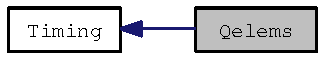
\includegraphics[width=96pt]{group__qelems}
\end{center}
\end{figure}
\subsection*{Typedefs}
\begin{DoxyCompactItemize}
\item 
\hypertarget{group__qelems_ga4d219449d88d2b9648a992152b278090}{
typedef void $\ast$ \hyperlink{group__qelems_ga4d219449d88d2b9648a992152b278090}{t\_\-qelem}}
\label{group__qelems_ga4d219449d88d2b9648a992152b278090}

\begin{DoxyCompactList}\small\item\em A qelem. \item\end{DoxyCompactList}\end{DoxyCompactItemize}
\subsection*{Functions}
\begin{DoxyCompactItemize}
\item 
void $\ast$ \hyperlink{group__qelems_gaffa7e9d4d5468a8ae3c825a353609b1b}{qelem\_\-new} (void $\ast$obj, \hyperlink{group__datatypes_gac26ba0a173b50597f5738132e059b42d}{method} fn)
\begin{DoxyCompactList}\small\item\em Create a new Qelem. \item\end{DoxyCompactList}\item 
void \hyperlink{group__qelems_ga3e292aad133af89a87e167e88cc4a1b5}{qelem\_\-set} (void $\ast$q)
\begin{DoxyCompactList}\small\item\em Cause a Qelem to execute. \item\end{DoxyCompactList}\item 
void \hyperlink{group__qelems_ga021eca2eff6e47ff97ca112fb2eaf866}{qelem\_\-unset} (void $\ast$q)
\begin{DoxyCompactList}\small\item\em Cancel a Qelem’s execution. \item\end{DoxyCompactList}\item 
void \hyperlink{group__qelems_ga7cfcb3134eb0baf335847906a14a08d0}{qelem\_\-free} (void $\ast$x)
\begin{DoxyCompactList}\small\item\em Free a Qelem object created with \hyperlink{group__qelems_gaffa7e9d4d5468a8ae3c825a353609b1b}{qelem\_\-new()}. \item\end{DoxyCompactList}\item 
void \hyperlink{group__qelems_gab5fa3e43e7851d1a2049ee28f5275955}{qelem\_\-front} (void $\ast$x)
\begin{DoxyCompactList}\small\item\em Cause a Qelem to execute with a higher priority. \item\end{DoxyCompactList}\end{DoxyCompactItemize}


\subsection{Detailed Description}
Your object’s methods may be called at interrupt level. This happens when the user has Overdrive mode enabled and one of your methods is called, directly or indirectly, from a scheduler Clock function. This means that you cannot count on doing certain things—like drawing, asking the user what file they would like opened, or calling any Macintosh toolbox trap that allocates or purges memory—from within any method that responds to any message that could be sent directly from another Max object. The mechanism you’ll use to get around this limitation is the Qelem (queue element) structure. Qelems also allow processor-\/intensive tasks to be done at a lower priority than in an interrupt. As an example, drawing on the screen, especially in color, takes a long time in comparison with a task like sending MIDI data.

A Qelem works very much like a Clock. You create a new Qelem in your creation function with qelem\_\-new and store a pointer to it in your object. Then you write a queue function, very much like the clock function (it takes the same single argument that will usually be a pointer to your object) that will be called when the Qelem has been set. You set the Qelem to run its function by calling \hyperlink{group__qelems_ga3e292aad133af89a87e167e88cc4a1b5}{qelem\_\-set()}.

Often you’ll want to use Qelems and Clocks together. For example, suppose you want to update the display for a counter that changes 20 times a second. This can be accomplished by writing a Clock function that calls \hyperlink{group__qelems_ga3e292aad133af89a87e167e88cc4a1b5}{qelem\_\-set()} and then reschedules itself for 50 milliseconds later using the technique shown in the metronome example above. This scheme works even if you call \hyperlink{group__qelems_ga3e292aad133af89a87e167e88cc4a1b5}{qelem\_\-set()} faster than the computer can draw the counter, because if a Qelem is already set, \hyperlink{group__qelems_ga3e292aad133af89a87e167e88cc4a1b5}{qelem\_\-set()} will not set it again. However, when drawing the counter, you’ll display its current value, not a specific value generated in the Clock function.

Note that the Qelem-\/based defer mechanism discussed later in this chapter may be easier for lowering the priority of one-\/time events, such as opening a standard file dialog box in response to a read message.

If your Qelem routine sends messages using \hyperlink{group__inout_ga0b2b38216f2f4dba486bfcd2273f255e}{outlet\_\-int()} or any other of the outlet functions, it needs to use the lockout mechanism described in the Interrupt Level Considerations section. 

\subsection{Function Documentation}
\hypertarget{group__qelems_ga7cfcb3134eb0baf335847906a14a08d0}{
\index{qelems@{qelems}!qelem\_\-free@{qelem\_\-free}}
\index{qelem\_\-free@{qelem\_\-free}!qelems@{qelems}}
\subsubsection[{qelem\_\-free}]{\setlength{\rightskip}{0pt plus 5cm}void qelem\_\-free (void $\ast$ {\em x})}}
\label{group__qelems_ga7cfcb3134eb0baf335847906a14a08d0}


Free a Qelem object created with \hyperlink{group__qelems_gaffa7e9d4d5468a8ae3c825a353609b1b}{qelem\_\-new()}. Typically this will be in your object’s free funtion.


\begin{DoxyParams}{Parameters}
\item[{\em x}]The Qelem to destroy. \end{DoxyParams}
\hypertarget{group__qelems_gab5fa3e43e7851d1a2049ee28f5275955}{
\index{qelems@{qelems}!qelem\_\-front@{qelem\_\-front}}
\index{qelem\_\-front@{qelem\_\-front}!qelems@{qelems}}
\subsubsection[{qelem\_\-front}]{\setlength{\rightskip}{0pt plus 5cm}void qelem\_\-front (void $\ast$ {\em x})}}
\label{group__qelems_gab5fa3e43e7851d1a2049ee28f5275955}


Cause a Qelem to execute with a higher priority. This function is identical to \hyperlink{group__qelems_ga3e292aad133af89a87e167e88cc4a1b5}{qelem\_\-set()}, except that the Qelem’s function is placed at the front of the list of routines to execute in the main thread instead of the back. Be polite and only use \hyperlink{group__qelems_gab5fa3e43e7851d1a2049ee28f5275955}{qelem\_\-front()} only for special time-\/critical applications.


\begin{DoxyParams}{Parameters}
\item[{\em x}]The Qelem whose function will be executed in the main thread. \end{DoxyParams}
\hypertarget{group__qelems_gaffa7e9d4d5468a8ae3c825a353609b1b}{
\index{qelems@{qelems}!qelem\_\-new@{qelem\_\-new}}
\index{qelem\_\-new@{qelem\_\-new}!qelems@{qelems}}
\subsubsection[{qelem\_\-new}]{\setlength{\rightskip}{0pt plus 5cm}void$\ast$ qelem\_\-new (void $\ast$ {\em obj}, \/  {\bf method} {\em fn})}}
\label{group__qelems_gaffa7e9d4d5468a8ae3c825a353609b1b}


Create a new Qelem. The created Qelem will need to be freed using \hyperlink{group__qelems_ga7cfcb3134eb0baf335847906a14a08d0}{qelem\_\-free()}, do not use \hyperlink{group__class__old_gadf30646e52376a37b93cc20efac65636}{freeobject()}.


\begin{DoxyParams}{Parameters}
\item[{\em obj}]Argument to be passed to function fun when the Qelem executes. Normally a pointer to your object. \item[{\em fn}]Function to execute. \end{DoxyParams}
\begin{DoxyReturn}{Returns}
A pointer to a Qelem instance. You need to store this value to pass to \hyperlink{group__qelems_ga3e292aad133af89a87e167e88cc4a1b5}{qelem\_\-set()}.
\end{DoxyReturn}
\begin{DoxyRemark}{Remarks}
Any kind of drawing or calling of Macintosh Toolbox routines that allocate or purge memory should be done in a Qelem function. 
\end{DoxyRemark}
\hypertarget{group__qelems_ga3e292aad133af89a87e167e88cc4a1b5}{
\index{qelems@{qelems}!qelem\_\-set@{qelem\_\-set}}
\index{qelem\_\-set@{qelem\_\-set}!qelems@{qelems}}
\subsubsection[{qelem\_\-set}]{\setlength{\rightskip}{0pt plus 5cm}void qelem\_\-set (void $\ast$ {\em q})}}
\label{group__qelems_ga3e292aad133af89a87e167e88cc4a1b5}


Cause a Qelem to execute. 
\begin{DoxyParams}{Parameters}
\item[{\em q}]The Qelem whose function will be executed in the main thread.\end{DoxyParams}
\begin{DoxyRemark}{Remarks}
The key behavior of \hyperlink{group__qelems_ga3e292aad133af89a87e167e88cc4a1b5}{qelem\_\-set()} is this: if the Qelem object has already been set, it will not be set again. (If this is not what you want, see \hyperlink{group__threading_gaa24a0c9896f1ad241e45590065c3f643}{defer()}.) This is useful if you want to redraw the state of some data when it changes, but not in response to changes that occur faster than can be drawn. A Qelem object is unset after its queue function has been called. 
\end{DoxyRemark}
\hypertarget{group__qelems_ga021eca2eff6e47ff97ca112fb2eaf866}{
\index{qelems@{qelems}!qelem\_\-unset@{qelem\_\-unset}}
\index{qelem\_\-unset@{qelem\_\-unset}!qelems@{qelems}}
\subsubsection[{qelem\_\-unset}]{\setlength{\rightskip}{0pt plus 5cm}void qelem\_\-unset (void $\ast$ {\em q})}}
\label{group__qelems_ga021eca2eff6e47ff97ca112fb2eaf866}


Cancel a Qelem’s execution. If the Qelem’s function is set to be called, \hyperlink{group__qelems_ga021eca2eff6e47ff97ca112fb2eaf866}{qelem\_\-unset()} will stop it from being called. Otherwise, \hyperlink{group__qelems_ga021eca2eff6e47ff97ca112fb2eaf866}{qelem\_\-unset()} does nothing.


\begin{DoxyParams}{Parameters}
\item[{\em q}]The Qelem whose execution you wish to cancel. \end{DoxyParams}

\hypertarget{group__systime}{
\section{Systime API}
\label{group__systime}\index{Systime API@{Systime API}}
}


The Systime API provides the means of getting the system time, instead of the scheduler time as you would with functions like \hyperlink{group__clocks_gabe5d8b1c9f260d13734a328b2a60ff69}{gettime()}.  


Collaboration diagram for Systime API:\nopagebreak
\begin{figure}[H]
\begin{center}
\leavevmode
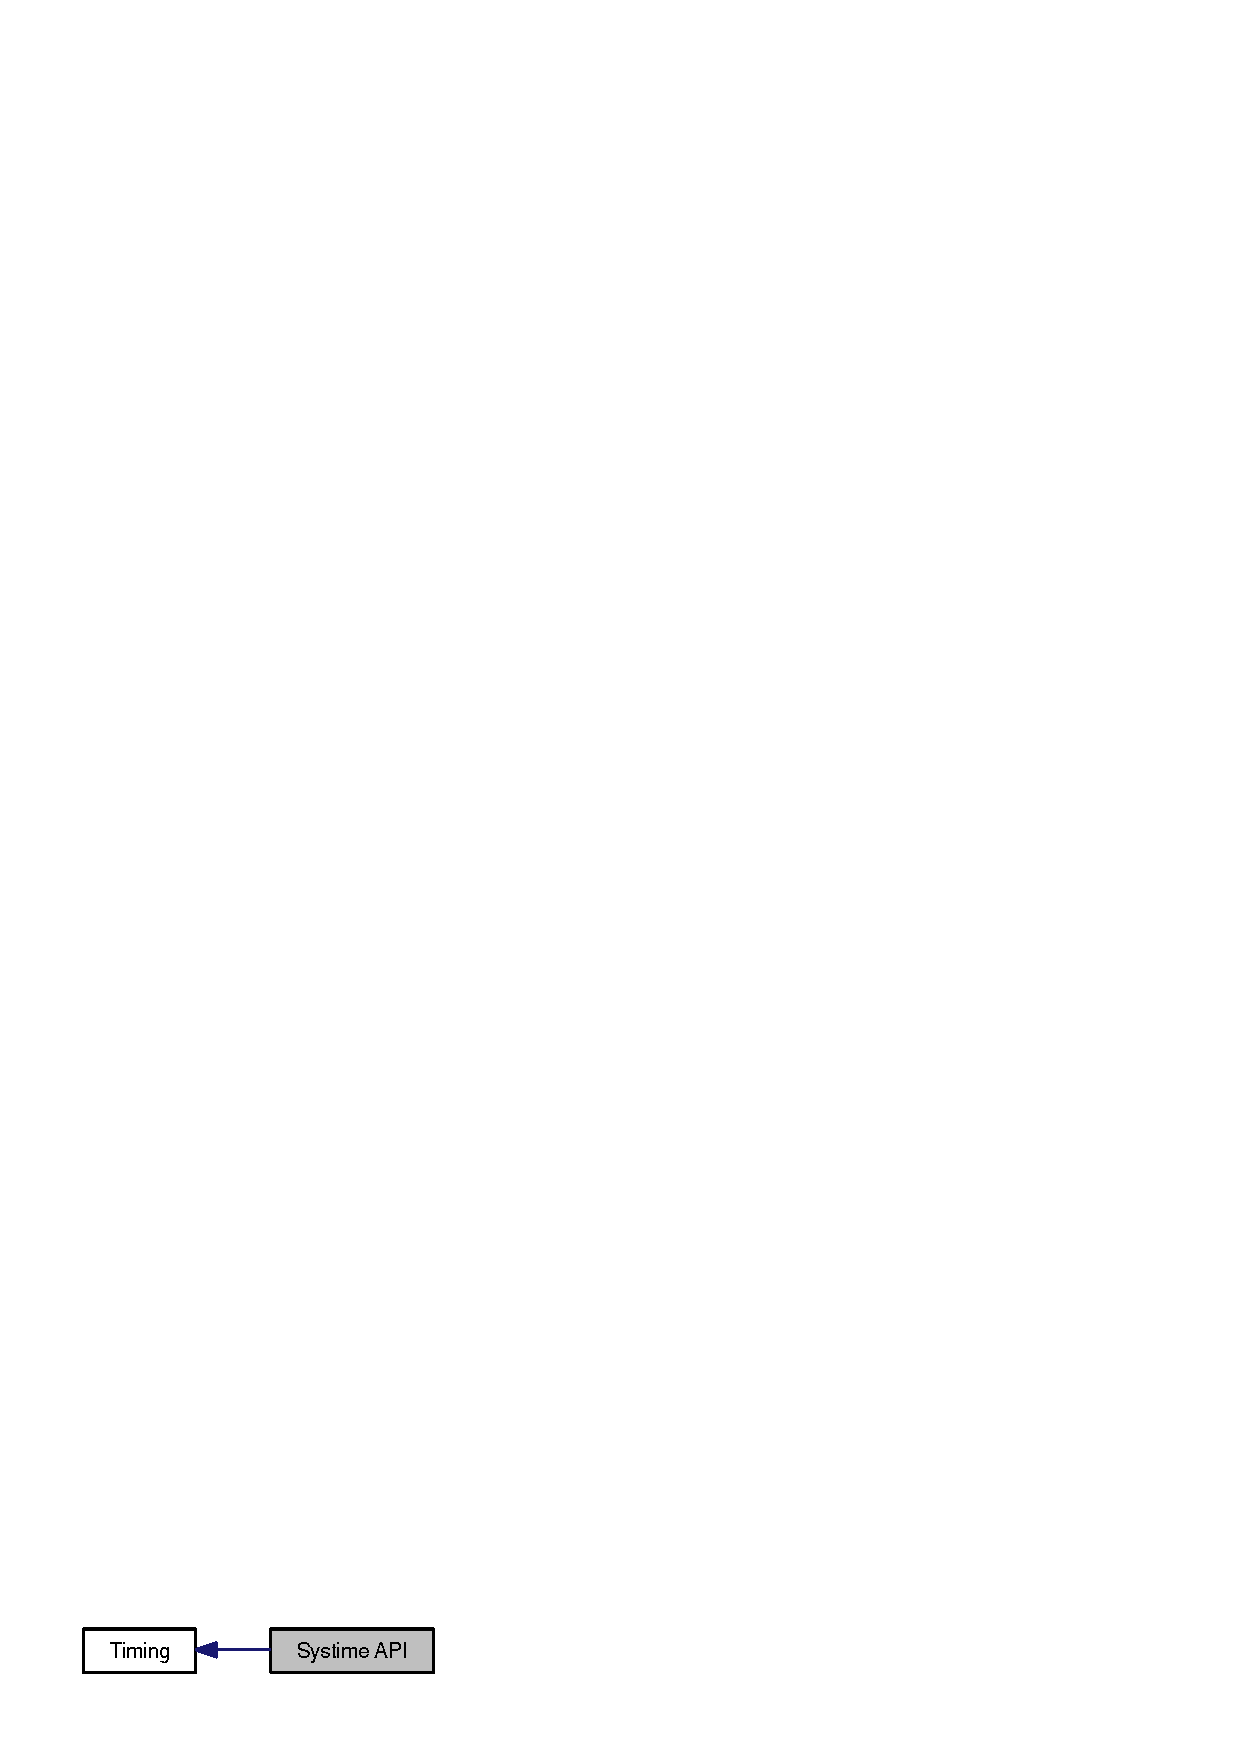
\includegraphics[width=106pt]{group__systime}
\end{center}
\end{figure}
\subsection*{Data Structures}
\begin{DoxyCompactItemize}
\item 
struct \hyperlink{structt__datetime}{t\_\-datetime}
\begin{DoxyCompactList}\small\item\em The Systime data structure. \item\end{DoxyCompactList}\end{DoxyCompactItemize}
\subsection*{Enumerations}
\begin{DoxyCompactItemize}
\item 
enum \hyperlink{group__systime_ga26a8d02aa000843530dcb2d350766951}{e\_\-max\_\-dateflags} \{ \par
\hyperlink{group__systime_gga26a8d02aa000843530dcb2d350766951a03c806745c3aad02d768797ead649e20}{SYSDATEFORMAT\_\-FLAGS\_\-SHORT} =  1, 
\par
\hyperlink{group__systime_gga26a8d02aa000843530dcb2d350766951a44be9bae61adf4f4b802989465768d63}{SYSDATEFORMAT\_\-FLAGS\_\-MEDIUM} =  2, 
\par
\hyperlink{group__systime_gga26a8d02aa000843530dcb2d350766951a0cdecdf057e390773e60c3d71de7faf4}{SYSDATEFORMAT\_\-FLAGS\_\-LONG} =  3
 \}
\begin{DoxyCompactList}\small\item\em Flags for the \hyperlink{group__systime_ga6219d6f6543e65431086c34c35199e82}{sysdateformat\_\-formatdatetime()} function. \item\end{DoxyCompactList}\end{DoxyCompactItemize}
\subsection*{Functions}
\begin{DoxyCompactItemize}
\item 
unsigned long \hyperlink{group__systime_gaa7831fc0634782a0ba07b44f47be8e61}{systime\_\-ticks} (void)
\begin{DoxyCompactList}\small\item\em Find out the operating system’s time in ticks. \item\end{DoxyCompactList}\item 
unsigned long \hyperlink{group__systime_ga9f23c7624ff113b985a34797bbf2f728}{systime\_\-ms} (void)
\begin{DoxyCompactList}\small\item\em Find out the operating system’s time in milliseconds. \item\end{DoxyCompactList}\item 
void \hyperlink{group__systime_ga53bc85cf0868e8712f32ee846642ab83}{systime\_\-datetime} (\hyperlink{structt__datetime}{t\_\-datetime} $\ast$d)
\begin{DoxyCompactList}\small\item\em Find out the operating system’s date and time. \item\end{DoxyCompactList}\item 
unsigned long \hyperlink{group__systime_ga8517f74817ccaaca5eb4bd4e82823bf5}{systime\_\-seconds} (void)
\begin{DoxyCompactList}\small\item\em Find out the operating system’s time in seconds. \item\end{DoxyCompactList}\item 
void \hyperlink{group__systime_gac7e909e02efabd823ce226a3234d700b}{systime\_\-secondstodate} (unsigned long secs, \hyperlink{structt__datetime}{t\_\-datetime} $\ast$d)
\begin{DoxyCompactList}\small\item\em Convert a time in seconds into a \hyperlink{structt__datetime}{t\_\-datetime} representation. \item\end{DoxyCompactList}\item 
unsigned long \hyperlink{group__systime_gab102340f92f3b8136629cf88a57e61a0}{systime\_\-datetoseconds} (\hyperlink{structt__datetime}{t\_\-datetime} $\ast$d)
\begin{DoxyCompactList}\small\item\em Convert a \hyperlink{structt__datetime}{t\_\-datetime} representation of time into seconds. \item\end{DoxyCompactList}\item 
void \hyperlink{group__systime_ga18e6eef81290f753a997dd6d0019ab60}{sysdateformat\_\-strftimetodatetime} (char $\ast$strf, \hyperlink{structt__datetime}{t\_\-datetime} $\ast$d)
\begin{DoxyCompactList}\small\item\em Fill a \hyperlink{structt__datetime}{t\_\-datetime} struct with a datetime formatted string. \item\end{DoxyCompactList}\item 
void \hyperlink{group__systime_ga6219d6f6543e65431086c34c35199e82}{sysdateformat\_\-formatdatetime} (\hyperlink{structt__datetime}{t\_\-datetime} $\ast$d, long dateflags, long timeflags, char $\ast$s, long buflen)
\begin{DoxyCompactList}\small\item\em Get a human friendly string representation of a \hyperlink{structt__datetime}{t\_\-datetime}. \item\end{DoxyCompactList}\end{DoxyCompactItemize}


\subsection{Detailed Description}
The Systime API provides the means of getting the system time, instead of the scheduler time as you would with functions like \hyperlink{group__clocks_gabe5d8b1c9f260d13734a328b2a60ff69}{gettime()}. 

\subsection{Enumeration Type Documentation}
\hypertarget{group__systime_ga26a8d02aa000843530dcb2d350766951}{
\index{systime@{systime}!e\_\-max\_\-dateflags@{e\_\-max\_\-dateflags}}
\index{e\_\-max\_\-dateflags@{e\_\-max\_\-dateflags}!systime@{systime}}
\subsubsection[{e\_\-max\_\-dateflags}]{\setlength{\rightskip}{0pt plus 5cm}enum {\bf e\_\-max\_\-dateflags}}}
\label{group__systime_ga26a8d02aa000843530dcb2d350766951}


Flags for the \hyperlink{group__systime_ga6219d6f6543e65431086c34c35199e82}{sysdateformat\_\-formatdatetime()} function. \begin{Desc}
\item[Enumerator: ]\par
\begin{description}
\index{SYSDATEFORMAT\_\-FLAGS\_\-SHORT@{SYSDATEFORMAT\_\-FLAGS\_\-SHORT}!systime@{systime}}\index{systime@{systime}!SYSDATEFORMAT\_\-FLAGS\_\-SHORT@{SYSDATEFORMAT\_\-FLAGS\_\-SHORT}}\item[{\em 
\hypertarget{group__systime_gga26a8d02aa000843530dcb2d350766951a03c806745c3aad02d768797ead649e20}{
SYSDATEFORMAT\_\-FLAGS\_\-SHORT}
\label{group__systime_gga26a8d02aa000843530dcb2d350766951a03c806745c3aad02d768797ead649e20}
}]short \index{SYSDATEFORMAT\_\-FLAGS\_\-MEDIUM@{SYSDATEFORMAT\_\-FLAGS\_\-MEDIUM}!systime@{systime}}\index{systime@{systime}!SYSDATEFORMAT\_\-FLAGS\_\-MEDIUM@{SYSDATEFORMAT\_\-FLAGS\_\-MEDIUM}}\item[{\em 
\hypertarget{group__systime_gga26a8d02aa000843530dcb2d350766951a44be9bae61adf4f4b802989465768d63}{
SYSDATEFORMAT\_\-FLAGS\_\-MEDIUM}
\label{group__systime_gga26a8d02aa000843530dcb2d350766951a44be9bae61adf4f4b802989465768d63}
}]medium \index{SYSDATEFORMAT\_\-FLAGS\_\-LONG@{SYSDATEFORMAT\_\-FLAGS\_\-LONG}!systime@{systime}}\index{systime@{systime}!SYSDATEFORMAT\_\-FLAGS\_\-LONG@{SYSDATEFORMAT\_\-FLAGS\_\-LONG}}\item[{\em 
\hypertarget{group__systime_gga26a8d02aa000843530dcb2d350766951a0cdecdf057e390773e60c3d71de7faf4}{
SYSDATEFORMAT\_\-FLAGS\_\-LONG}
\label{group__systime_gga26a8d02aa000843530dcb2d350766951a0cdecdf057e390773e60c3d71de7faf4}
}]long \end{description}
\end{Desc}



\subsection{Function Documentation}
\hypertarget{group__systime_ga6219d6f6543e65431086c34c35199e82}{
\index{systime@{systime}!sysdateformat\_\-formatdatetime@{sysdateformat\_\-formatdatetime}}
\index{sysdateformat\_\-formatdatetime@{sysdateformat\_\-formatdatetime}!systime@{systime}}
\subsubsection[{sysdateformat\_\-formatdatetime}]{\setlength{\rightskip}{0pt plus 5cm}void sysdateformat\_\-formatdatetime ({\bf t\_\-datetime} $\ast$ {\em d}, \/  long {\em dateflags}, \/  long {\em timeflags}, \/  char $\ast$ {\em s}, \/  long {\em buflen})}}
\label{group__systime_ga6219d6f6543e65431086c34c35199e82}


Get a human friendly string representation of a \hyperlink{structt__datetime}{t\_\-datetime}. For example: \char`\"{}Today\char`\"{}, \char`\"{}Yesterday\char`\"{}, etc.


\begin{DoxyParams}{Parameters}
\item[{\em d}]The address of a \hyperlink{structt__datetime}{t\_\-datetime} to fill. \item[{\em dateflags}]One of the values defined in \hyperlink{group__systime_ga26a8d02aa000843530dcb2d350766951}{e\_\-max\_\-dateflags}. \item[{\em timeflags}]Currently unused. Pass 0. \item[{\em s}]An already allocated string to hold the human friendly result. \item[{\em buflen}]The number of characters allocated to the string s. \end{DoxyParams}
\hypertarget{group__systime_ga18e6eef81290f753a997dd6d0019ab60}{
\index{systime@{systime}!sysdateformat\_\-strftimetodatetime@{sysdateformat\_\-strftimetodatetime}}
\index{sysdateformat\_\-strftimetodatetime@{sysdateformat\_\-strftimetodatetime}!systime@{systime}}
\subsubsection[{sysdateformat\_\-strftimetodatetime}]{\setlength{\rightskip}{0pt plus 5cm}void sysdateformat\_\-strftimetodatetime (char $\ast$ {\em strf}, \/  {\bf t\_\-datetime} $\ast$ {\em d})}}
\label{group__systime_ga18e6eef81290f753a997dd6d0019ab60}


Fill a \hyperlink{structt__datetime}{t\_\-datetime} struct with a datetime formatted string. For example, the string \char`\"{}2007-\/12-\/24 12:21:00\char`\"{}.


\begin{DoxyParams}{Parameters}
\item[{\em strf}]A string containing the datetime. \item[{\em d}]The address of a \hyperlink{structt__datetime}{t\_\-datetime} to fill. \end{DoxyParams}
\hypertarget{group__systime_ga53bc85cf0868e8712f32ee846642ab83}{
\index{systime@{systime}!systime\_\-datetime@{systime\_\-datetime}}
\index{systime\_\-datetime@{systime\_\-datetime}!systime@{systime}}
\subsubsection[{systime\_\-datetime}]{\setlength{\rightskip}{0pt plus 5cm}void systime\_\-datetime ({\bf t\_\-datetime} $\ast$ {\em d})}}
\label{group__systime_ga53bc85cf0868e8712f32ee846642ab83}


Find out the operating system’s date and time. 
\begin{DoxyParams}{Parameters}
\item[{\em d}]Returns the system’s date and time in a \hyperlink{structt__datetime}{t\_\-datetime} data structure. \end{DoxyParams}
\hypertarget{group__systime_gab102340f92f3b8136629cf88a57e61a0}{
\index{systime@{systime}!systime\_\-datetoseconds@{systime\_\-datetoseconds}}
\index{systime\_\-datetoseconds@{systime\_\-datetoseconds}!systime@{systime}}
\subsubsection[{systime\_\-datetoseconds}]{\setlength{\rightskip}{0pt plus 5cm}unsigned long systime\_\-datetoseconds ({\bf t\_\-datetime} $\ast$ {\em d})}}
\label{group__systime_gab102340f92f3b8136629cf88a57e61a0}


Convert a \hyperlink{structt__datetime}{t\_\-datetime} representation of time into seconds. 
\begin{DoxyParams}{Parameters}
\item[{\em d}]The address of a \hyperlink{structt__datetime}{t\_\-datetime} that contains a valid period of time. \end{DoxyParams}
\begin{DoxyReturn}{Returns}
The number of seconds represented by d. 
\end{DoxyReturn}
\hypertarget{group__systime_ga9f23c7624ff113b985a34797bbf2f728}{
\index{systime@{systime}!systime\_\-ms@{systime\_\-ms}}
\index{systime\_\-ms@{systime\_\-ms}!systime@{systime}}
\subsubsection[{systime\_\-ms}]{\setlength{\rightskip}{0pt plus 5cm}unsigned long systime\_\-ms (void)}}
\label{group__systime_ga9f23c7624ff113b985a34797bbf2f728}


Find out the operating system’s time in milliseconds. \begin{DoxyReturn}{Returns}
the system time in milliseconds. 
\end{DoxyReturn}
\hypertarget{group__systime_ga8517f74817ccaaca5eb4bd4e82823bf5}{
\index{systime@{systime}!systime\_\-seconds@{systime\_\-seconds}}
\index{systime\_\-seconds@{systime\_\-seconds}!systime@{systime}}
\subsubsection[{systime\_\-seconds}]{\setlength{\rightskip}{0pt plus 5cm}unsigned long systime\_\-seconds (void)}}
\label{group__systime_ga8517f74817ccaaca5eb4bd4e82823bf5}


Find out the operating system’s time in seconds. \begin{DoxyReturn}{Returns}
the system time in seconds. 
\end{DoxyReturn}
\hypertarget{group__systime_gac7e909e02efabd823ce226a3234d700b}{
\index{systime@{systime}!systime\_\-secondstodate@{systime\_\-secondstodate}}
\index{systime\_\-secondstodate@{systime\_\-secondstodate}!systime@{systime}}
\subsubsection[{systime\_\-secondstodate}]{\setlength{\rightskip}{0pt plus 5cm}void systime\_\-secondstodate (unsigned long {\em secs}, \/  {\bf t\_\-datetime} $\ast$ {\em d})}}
\label{group__systime_gac7e909e02efabd823ce226a3234d700b}


Convert a time in seconds into a \hyperlink{structt__datetime}{t\_\-datetime} representation. 
\begin{DoxyParams}{Parameters}
\item[{\em secs}]A number of seconds to be represented as a \hyperlink{structt__datetime}{t\_\-datetime}. \item[{\em d}]The address of a \hyperlink{structt__datetime}{t\_\-datetime} that will be filled with the converted value. \end{DoxyParams}
\hypertarget{group__systime_gaa7831fc0634782a0ba07b44f47be8e61}{
\index{systime@{systime}!systime\_\-ticks@{systime\_\-ticks}}
\index{systime\_\-ticks@{systime\_\-ticks}!systime@{systime}}
\subsubsection[{systime\_\-ticks}]{\setlength{\rightskip}{0pt plus 5cm}unsigned long systime\_\-ticks (void)}}
\label{group__systime_gaa7831fc0634782a0ba07b44f47be8e61}


Find out the operating system’s time in ticks. \begin{DoxyReturn}{Returns}
the system time in ticks. 
\end{DoxyReturn}

\hypertarget{group__time}{
\section{ITM Time Objects}
\label{group__time}\index{ITM Time Objects@{ITM Time Objects}}
}


ITM Time Objects are a high-\/level interface to ITM, a tempo-\/based scheduler API.  


Collaboration diagram for ITM Time Objects:\nopagebreak
\begin{figure}[H]
\begin{center}
\leavevmode
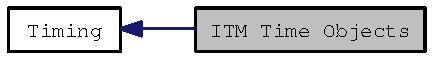
\includegraphics[width=122pt]{group__time}
\end{center}
\end{figure}
\subsection*{Enumerations}
\begin{DoxyCompactItemize}
\item 
enum \{ \par
\hyperlink{group__time_gga99fb83031ce9923c84392b4e92f956b5ac80606ccbb9a16c14cf81874e4de2408}{TIME\_\-FLAGS\_\-LOCATION} =  1, 
\par
\hyperlink{group__time_gga99fb83031ce9923c84392b4e92f956b5af93981eb3922895394877d099323a2e8}{TIME\_\-FLAGS\_\-TICKSONLY} =  2, 
\par
\hyperlink{group__time_gga99fb83031ce9923c84392b4e92f956b5a5b35f210c105cc2e49a4c2c18c48c10c}{TIME\_\-FLAGS\_\-FIXEDONLY} =  4, 
\par
\hyperlink{group__time_gga99fb83031ce9923c84392b4e92f956b5a4cb8e2884262140884e647d609747a82}{TIME\_\-FLAGS\_\-LOOKAHEAD} =  8, 
\par
\hyperlink{group__time_gga99fb83031ce9923c84392b4e92f956b5a91f2cee835f5cf871a657101b6ff7b4e}{TIME\_\-FLAGS\_\-USECLOCK} =  16, 
\par
\hyperlink{group__time_gga99fb83031ce9923c84392b4e92f956b5a46a7548bed973b5cef7e6fcbb5883c4f}{TIME\_\-FLAGS\_\-USEQELEM} =  32, 
\par
\hyperlink{group__time_gga99fb83031ce9923c84392b4e92f956b5ac97bc4400b25656b5570c12d6817a662}{TIME\_\-FLAGS\_\-FIXED} =  64, 
\par
\hyperlink{group__time_gga99fb83031ce9923c84392b4e92f956b5af2db490f1904d9f1e834f9ea062ad67e}{TIME\_\-FLAGS\_\-PERMANENT} =  128, 
\par
\hyperlink{group__time_gga99fb83031ce9923c84392b4e92f956b5a7ddd9e0fa3dc6a7b346fc3dcee5c5c81}{TIME\_\-FLAGS\_\-TRANSPORT} =  256, 
\par
\hyperlink{group__time_gga99fb83031ce9923c84392b4e92f956b5a273bc93db911e7ea106e5839d9263382}{TIME\_\-FLAGS\_\-EVENTLIST} =  512, 
\par
\hyperlink{group__time_gga99fb83031ce9923c84392b4e92f956b5ad16eb0fa4c44658f55146763452b3481}{TIME\_\-FLAGS\_\-CHECKSCHEDULE} =  1024, 
\par
\hyperlink{group__time_gga99fb83031ce9923c84392b4e92f956b5a22fec8e51f11f945f8b94279a6df37df}{TIME\_\-FLAGS\_\-LISTENTICKS} =  2048, 
\par
\hyperlink{group__time_gga99fb83031ce9923c84392b4e92f956b5a5f103c6561c69e7759621cd216d0176b}{TIME\_\-FLAGS\_\-NOUNITS} =  4096, 
\par
\hyperlink{group__time_gga99fb83031ce9923c84392b4e92f956b5a4dc0bf02a08234ce8b66e8ecb5ec568e}{TIME\_\-FLAGS\_\-BBUSOURCE} =  8192, 
\par
\hyperlink{group__time_gga99fb83031ce9923c84392b4e92f956b5a4d4396aa4c56efec83245821ea888235}{TIME\_\-FLAGS\_\-POSITIVE} =  16384
 \}
\begin{DoxyCompactList}\small\item\em Flags that determine attribute and time object behavior. \item\end{DoxyCompactList}\end{DoxyCompactItemize}
\subsection*{Functions}
\begin{DoxyCompactItemize}
\item 
void $\ast$ \hyperlink{group__time_ga182b0bd45ff72d9ddccebd8cc9d552d1}{itm\_\-getglobal} (void)
\begin{DoxyCompactList}\small\item\em Return the global (default / unnamed) itm object. \item\end{DoxyCompactList}\item 
void $\ast$ \hyperlink{group__time_ga04a193f71ceaf7ce604e976a3affc99b}{itm\_\-getnamed} (\hyperlink{structt__symbol}{t\_\-symbol} $\ast$s, void $\ast$scheduler, \hyperlink{structt__symbol}{t\_\-symbol} $\ast$defaultclocksourcename, long create)
\begin{DoxyCompactList}\small\item\em Return a named itm object. \item\end{DoxyCompactList}\item 
void \hyperlink{group__time_ga33f7a4627e3d2a77748b66d2af7a0a1a}{itm\_\-reference} (\hyperlink{group__time_gac656fa1f920c69cf77e6631bcec53077}{t\_\-itm} $\ast$x)
\begin{DoxyCompactList}\small\item\em Reference an itm object. \item\end{DoxyCompactList}\item 
void \hyperlink{group__time_gae6d838ad8a0834e650a7664a50b0b6e2}{itm\_\-dereference} (\hyperlink{group__time_gac656fa1f920c69cf77e6631bcec53077}{t\_\-itm} $\ast$x)
\begin{DoxyCompactList}\small\item\em Stop referencing an itm object. \item\end{DoxyCompactList}\item 
double \hyperlink{group__time_ga6be6d66ebf8825d9edacec2f3e534dcb}{itm\_\-gettime} (\hyperlink{group__time_gac656fa1f920c69cf77e6631bcec53077}{t\_\-itm} $\ast$x)
\begin{DoxyCompactList}\small\item\em Report the current internal time. \item\end{DoxyCompactList}\item 
double \hyperlink{group__time_gafc0e353837687e59fb54bb83ed33768f}{itm\_\-getticks} (\hyperlink{group__time_gac656fa1f920c69cf77e6631bcec53077}{t\_\-itm} $\ast$x)
\begin{DoxyCompactList}\small\item\em Report the current time of the itm in ticks. \item\end{DoxyCompactList}\item 
void \hyperlink{group__time_gab8fb2f5156bb6df433d509d721a8cefd}{itm\_\-dump} (\hyperlink{group__time_gac656fa1f920c69cf77e6631bcec53077}{t\_\-itm} $\ast$x)
\begin{DoxyCompactList}\small\item\em Print diagnostic information about an itm object to the Max window. \item\end{DoxyCompactList}\item 
void \hyperlink{group__time_gad8584c381f8f183ff6eaa0f4e4a4923a}{itm\_\-settimesignature} (\hyperlink{group__time_gac656fa1f920c69cf77e6631bcec53077}{t\_\-itm} $\ast$x, long num, long denom, long flags)
\begin{DoxyCompactList}\small\item\em Set an itm object's current time signature. \item\end{DoxyCompactList}\item 
void \hyperlink{group__time_ga7ced567aa268c709daf2152503de8832}{itm\_\-gettimesignature} (\hyperlink{group__time_gac656fa1f920c69cf77e6631bcec53077}{t\_\-itm} $\ast$x, long $\ast$num, long $\ast$denom)
\begin{DoxyCompactList}\small\item\em Query an itm object for its current time signature. \item\end{DoxyCompactList}\item 
void \hyperlink{group__time_ga844cd45c507bf4c89b91f2c2713fb128}{itm\_\-pause} (\hyperlink{group__time_gac656fa1f920c69cf77e6631bcec53077}{t\_\-itm} $\ast$x)
\begin{DoxyCompactList}\small\item\em Pause the passage of time for an itm object. \item\end{DoxyCompactList}\item 
void \hyperlink{group__time_ga1f3b1dded32c2fcbd955adb094c81d98}{itm\_\-resume} (\hyperlink{group__time_gac656fa1f920c69cf77e6631bcec53077}{t\_\-itm} $\ast$x)
\begin{DoxyCompactList}\small\item\em Start the passage of time for an itm object, from it's current location. \item\end{DoxyCompactList}\item 
long \hyperlink{group__time_ga36ee91bc9951d71880a055445ecd7ba7}{itm\_\-getstate} (\hyperlink{group__time_gac656fa1f920c69cf77e6631bcec53077}{t\_\-itm} $\ast$x)
\begin{DoxyCompactList}\small\item\em Find out if time is currently progressing for a given itm object. \item\end{DoxyCompactList}\item 
void \hyperlink{group__time_gac777d53869fe6e01bdce0c34f868f648}{itm\_\-setresolution} (double res)
\begin{DoxyCompactList}\small\item\em Set the number of ticks-\/per-\/quarter-\/note globally for the itm system. \item\end{DoxyCompactList}\item 
double \hyperlink{group__time_gaba77c4fbb00c349342b6358d80644113}{itm\_\-getresolution} (void)
\begin{DoxyCompactList}\small\item\em Get the number of ticks-\/per-\/quarter-\/note globally from the itm system. \item\end{DoxyCompactList}\item 
\hyperlink{structt__symbol}{t\_\-symbol} $\ast$ \hyperlink{group__time_ga0daf42c6199b38f486998f2e5d2c8a11}{itm\_\-getname} (\hyperlink{group__time_gac656fa1f920c69cf77e6631bcec53077}{t\_\-itm} $\ast$x)
\begin{DoxyCompactList}\small\item\em Given an itm object, return its name. \item\end{DoxyCompactList}\item 
double \hyperlink{group__time_ga3ed676dca6666ab9f305ea81b8d1b6b7}{itm\_\-tickstoms} (\hyperlink{group__time_gac656fa1f920c69cf77e6631bcec53077}{t\_\-itm} $\ast$x, double ticks)
\begin{DoxyCompactList}\small\item\em Convert a time value in ticks to the equivalent value in milliseconds, given the context of a specified itm object. \item\end{DoxyCompactList}\item 
double \hyperlink{group__time_gab32518269a1b30459b72e215567697ad}{itm\_\-mstoticks} (\hyperlink{group__time_gac656fa1f920c69cf77e6631bcec53077}{t\_\-itm} $\ast$x, double ms)
\begin{DoxyCompactList}\small\item\em Convert a time value in milliseconds to the equivalent value in ticks, given the context of a specified itm object. \item\end{DoxyCompactList}\item 
double \hyperlink{group__time_gaa131b77f55df783dda39c2a97c7af440}{itm\_\-mstosamps} (\hyperlink{group__time_gac656fa1f920c69cf77e6631bcec53077}{t\_\-itm} $\ast$x, double ms)
\begin{DoxyCompactList}\small\item\em Convert a time value in milliseconds to the equivalent value in samples, given the context of a specified itm object. \item\end{DoxyCompactList}\item 
double \hyperlink{group__time_ga554348a51466458ca16a7c8101e16f44}{itm\_\-sampstoms} (\hyperlink{group__time_gac656fa1f920c69cf77e6631bcec53077}{t\_\-itm} $\ast$x, double samps)
\begin{DoxyCompactList}\small\item\em Convert a time value in samples to the equivalent value in milliseconds, given the context of a specified itm object. \item\end{DoxyCompactList}\item 
void \hyperlink{group__time_gadca2e82e0cadd3bacd75aa6a137ac530}{itm\_\-barbeatunitstoticks} (\hyperlink{group__time_gac656fa1f920c69cf77e6631bcec53077}{t\_\-itm} $\ast$x, long bars, long beats, double units, double $\ast$ticks, char position)
\begin{DoxyCompactList}\small\item\em Convert a time value in bbu to the equivalent value in ticks, given the context of a specified itm object. \item\end{DoxyCompactList}\item 
void \hyperlink{group__time_ga098ba18a9c4a10c3d92445b0bf3da025}{itm\_\-tickstobarbeatunits} (\hyperlink{group__time_gac656fa1f920c69cf77e6631bcec53077}{t\_\-itm} $\ast$x, double ticks, long $\ast$bars, long $\ast$beats, double $\ast$units, char position)
\begin{DoxyCompactList}\small\item\em Convert a time value in bbu to the equivalent value in ticks, given the context of a specified itm object. \item\end{DoxyCompactList}\item 
long \hyperlink{group__time_ga6950c5550d8beec9d1df56c96b3c9c88}{itm\_\-isunitfixed} (\hyperlink{structt__symbol}{t\_\-symbol} $\ast$u)
\begin{DoxyCompactList}\small\item\em Given the name of a time unit (e.g. \item\end{DoxyCompactList}\item 
void \hyperlink{group__time_ga6724fc34703298b8dbb12cfe17ef325e}{time\_\-stop} (\hyperlink{group__time_gab568d2ffd4d84ca17c0b90cf2f7c6a40}{t\_\-timeobject} $\ast$x)
\begin{DoxyCompactList}\small\item\em Stop a currently scheduled time object. \item\end{DoxyCompactList}\item 
void \hyperlink{group__time_ga31b3eecc1bd31944239fab1b6c309b5b}{time\_\-tick} (\hyperlink{group__time_gab568d2ffd4d84ca17c0b90cf2f7c6a40}{t\_\-timeobject} $\ast$x)
\begin{DoxyCompactList}\small\item\em Execute a time object's task, then if it was already set to execute, reschedule for the current interval value of the object. \item\end{DoxyCompactList}\item 
double \hyperlink{group__time_ga714ddc564124f89899dc619137f5c64d}{time\_\-getms} (\hyperlink{group__time_gab568d2ffd4d84ca17c0b90cf2f7c6a40}{t\_\-timeobject} $\ast$x)
\begin{DoxyCompactList}\small\item\em Convert the value of a time object to milliseconds. \item\end{DoxyCompactList}\item 
double \hyperlink{group__time_ga4f47a0932158cafd04fb2e0cc928b4cc}{time\_\-getticks} (\hyperlink{group__time_gab568d2ffd4d84ca17c0b90cf2f7c6a40}{t\_\-timeobject} $\ast$x)
\begin{DoxyCompactList}\small\item\em Convert the value of a time object to ticks. \item\end{DoxyCompactList}\item 
void \hyperlink{group__time_ga2a96b168022b712f38245517a9e20a14}{time\_\-getphase} (\hyperlink{group__time_gab568d2ffd4d84ca17c0b90cf2f7c6a40}{t\_\-timeobject} $\ast$tx, double $\ast$phase, double $\ast$slope, double $\ast$ticks)
\begin{DoxyCompactList}\small\item\em Return the phase of the ITM object (transport) associated with a time object. \item\end{DoxyCompactList}\item 
void \hyperlink{group__time_gaf8a102f28b262991c6e4c3b79f37b611}{time\_\-listen} (\hyperlink{group__time_gab568d2ffd4d84ca17c0b90cf2f7c6a40}{t\_\-timeobject} $\ast$x, \hyperlink{structt__symbol}{t\_\-symbol} $\ast$attr, long flags)
\begin{DoxyCompactList}\small\item\em Specify that a millisecond-\/based attribute to be updated automatically when the converted milliseconds of the time object's value changes. \item\end{DoxyCompactList}\item 
void \hyperlink{group__time_ga7451e479ce77e4dcf7a13bbd933575ed}{time\_\-setvalue} (\hyperlink{group__time_gab568d2ffd4d84ca17c0b90cf2f7c6a40}{t\_\-timeobject} $\ast$tx, \hyperlink{structt__symbol}{t\_\-symbol} $\ast$s, long argc, \hyperlink{structt__atom}{t\_\-atom} $\ast$argv)
\begin{DoxyCompactList}\small\item\em Set the current value of a time object (either an interval or a position) using a Max message. \item\end{DoxyCompactList}\item 
void \hyperlink{group__time_ga95e5b2330715823c8a609ccd500aa361}{class\_\-time\_\-addattr} (\hyperlink{structt__class}{t\_\-class} $\ast$c, char $\ast$attrname, char $\ast$attrlabel, long flags)
\begin{DoxyCompactList}\small\item\em Create an attribute permitting a time object to be changed in a user-\/friendly way. \item\end{DoxyCompactList}\item 
void $\ast$ \hyperlink{group__time_gaf6153d8f28738932c0ea3906a6c51696}{time\_\-new} (\hyperlink{structt__object}{t\_\-object} $\ast$owner, \hyperlink{structt__symbol}{t\_\-symbol} $\ast$attrname, \hyperlink{group__datatypes_gac26ba0a173b50597f5738132e059b42d}{method} tick, long flags)
\begin{DoxyCompactList}\small\item\em Create a new time object. \item\end{DoxyCompactList}\item 
\hyperlink{structt__object}{t\_\-object} $\ast$ \hyperlink{group__time_ga2805d69712a55bf77d5083da40108cec}{time\_\-getnamed} (\hyperlink{structt__object}{t\_\-object} $\ast$owner, \hyperlink{structt__symbol}{t\_\-symbol} $\ast$attrname)
\begin{DoxyCompactList}\small\item\em Return a time object associated with an attribute of an owning object. \item\end{DoxyCompactList}\item 
long \hyperlink{group__time_ga86feb1c21b06217bf699447babb169c5}{time\_\-isfixedunit} (\hyperlink{group__time_gab568d2ffd4d84ca17c0b90cf2f7c6a40}{t\_\-timeobject} $\ast$x)
\begin{DoxyCompactList}\small\item\em Return whether this time object currently holds a fixed (millisecond-\/based) value. \item\end{DoxyCompactList}\item 
void \hyperlink{group__time_gae46ab99a9732990170ce0e27fb744c4b}{time\_\-schedule} (\hyperlink{group__time_gab568d2ffd4d84ca17c0b90cf2f7c6a40}{t\_\-timeobject} $\ast$x, \hyperlink{group__time_gab568d2ffd4d84ca17c0b90cf2f7c6a40}{t\_\-timeobject} $\ast$quantize)
\begin{DoxyCompactList}\small\item\em Schedule a task, with optional quantization. \item\end{DoxyCompactList}\item 
void \hyperlink{group__time_ga96226d122f6f0d7e2e1ebe47b06d00c5}{time\_\-schedule\_\-limit} (\hyperlink{group__time_gab568d2ffd4d84ca17c0b90cf2f7c6a40}{t\_\-timeobject} $\ast$x, \hyperlink{group__time_gab568d2ffd4d84ca17c0b90cf2f7c6a40}{t\_\-timeobject} $\ast$quantize)
\begin{DoxyCompactList}\small\item\em Schedule a task, with optional minimum interval,. \item\end{DoxyCompactList}\item 
void \hyperlink{group__time_ga75b99466073d15d4096fb34a5b172648}{time\_\-now} (\hyperlink{group__time_gab568d2ffd4d84ca17c0b90cf2f7c6a40}{t\_\-timeobject} $\ast$x, \hyperlink{group__time_gab568d2ffd4d84ca17c0b90cf2f7c6a40}{t\_\-timeobject} $\ast$quantize)
\begin{DoxyCompactList}\small\item\em Schedule a task for right now, with optional quantization. \item\end{DoxyCompactList}\item 
void $\ast$ \hyperlink{group__time_gaa1d217d3b706f718f0f77dbd78427fb0}{time\_\-getitm} (\hyperlink{group__time_gab568d2ffd4d84ca17c0b90cf2f7c6a40}{t\_\-timeobject} $\ast$ox)
\begin{DoxyCompactList}\small\item\em Return the ITM object associated with this time object. \item\end{DoxyCompactList}\item 
double \hyperlink{group__time_gab5d282bae56be219c0c863a798140cb5}{time\_\-calcquantize} (\hyperlink{group__time_gab568d2ffd4d84ca17c0b90cf2f7c6a40}{t\_\-timeobject} $\ast$ox, \hyperlink{group__time_gac656fa1f920c69cf77e6631bcec53077}{t\_\-itm} $\ast$vitm, \hyperlink{group__time_gab568d2ffd4d84ca17c0b90cf2f7c6a40}{t\_\-timeobject} $\ast$oq)
\begin{DoxyCompactList}\small\item\em Calculate the quantized interval (in ticks) if this time object were to be scheduled at the current time. \item\end{DoxyCompactList}\item 
void \hyperlink{group__time_ga380cbe3efa2240446cb1cc2ef1195876}{time\_\-setclock} (\hyperlink{group__time_gab568d2ffd4d84ca17c0b90cf2f7c6a40}{t\_\-timeobject} $\ast$tx, \hyperlink{structt__symbol}{t\_\-symbol} $\ast$sc)
\begin{DoxyCompactList}\small\item\em Associate a named setclock object with a time object (unsupported). \item\end{DoxyCompactList}\end{DoxyCompactItemize}
\subsection*{Variables}
\begin{DoxyCompactItemize}
\item 
BEGIN\_\-USING\_\-C\_\-LINKAGE typedef \hyperlink{structt__object}{t\_\-object} \hyperlink{group__time_gac656fa1f920c69cf77e6631bcec53077}{t\_\-itm}
\begin{DoxyCompactList}\small\item\em A low-\/level object for tempo-\/based scheduling. \item\end{DoxyCompactList}\item 
BEGIN\_\-USING\_\-C\_\-LINKAGE typedef \hyperlink{structt__object}{t\_\-object} \hyperlink{group__time_gab568d2ffd4d84ca17c0b90cf2f7c6a40}{t\_\-timeobject}
\begin{DoxyCompactList}\small\item\em A high-\/level time object for tempo-\/based scheduling. \item\end{DoxyCompactList}\end{DoxyCompactItemize}


\subsection{Detailed Description}
ITM Time Objects are a high-\/level interface to ITM, a tempo-\/based scheduler API. They provide an abtraction so your object can schedule events either in milliseconds (as traditional clock objects) or ticks (tempo-\/relative units). 

\subsection{Enumeration Type Documentation}
\hypertarget{group__time_ga99fb83031ce9923c84392b4e92f956b5}{
\subsubsection[{"@2}]{\setlength{\rightskip}{0pt plus 5cm}anonymous enum}}
\label{group__time_ga99fb83031ce9923c84392b4e92f956b5}


Flags that determine attribute and time object behavior. \begin{Desc}
\item[Enumerator: ]\par
\begin{description}
\index{TIME\_\-FLAGS\_\-LOCATION@{TIME\_\-FLAGS\_\-LOCATION}!time@{time}}\index{time@{time}!TIME\_\-FLAGS\_\-LOCATION@{TIME\_\-FLAGS\_\-LOCATION}}\item[{\em 
\hypertarget{group__time_gga99fb83031ce9923c84392b4e92f956b5ac80606ccbb9a16c14cf81874e4de2408}{
TIME\_\-FLAGS\_\-LOCATION}
\label{group__time_gga99fb83031ce9923c84392b4e92f956b5ac80606ccbb9a16c14cf81874e4de2408}
}]1 1 0 location-\/based bar/beat/unit values (as opposed to interval values, which are 0 0 0 relative) \index{TIME\_\-FLAGS\_\-TICKSONLY@{TIME\_\-FLAGS\_\-TICKSONLY}!time@{time}}\index{time@{time}!TIME\_\-FLAGS\_\-TICKSONLY@{TIME\_\-FLAGS\_\-TICKSONLY}}\item[{\em 
\hypertarget{group__time_gga99fb83031ce9923c84392b4e92f956b5af93981eb3922895394877d099323a2e8}{
TIME\_\-FLAGS\_\-TICKSONLY}
\label{group__time_gga99fb83031ce9923c84392b4e92f956b5af93981eb3922895394877d099323a2e8}
}]only ticks-\/based values (not ms) are acceptable \index{TIME\_\-FLAGS\_\-FIXEDONLY@{TIME\_\-FLAGS\_\-FIXEDONLY}!time@{time}}\index{time@{time}!TIME\_\-FLAGS\_\-FIXEDONLY@{TIME\_\-FLAGS\_\-FIXEDONLY}}\item[{\em 
\hypertarget{group__time_gga99fb83031ce9923c84392b4e92f956b5a5b35f210c105cc2e49a4c2c18c48c10c}{
TIME\_\-FLAGS\_\-FIXEDONLY}
\label{group__time_gga99fb83031ce9923c84392b4e92f956b5a5b35f210c105cc2e49a4c2c18c48c10c}
}]only fixed values (ms, hz, samples) are acceptable \index{TIME\_\-FLAGS\_\-LOOKAHEAD@{TIME\_\-FLAGS\_\-LOOKAHEAD}!time@{time}}\index{time@{time}!TIME\_\-FLAGS\_\-LOOKAHEAD@{TIME\_\-FLAGS\_\-LOOKAHEAD}}\item[{\em 
\hypertarget{group__time_gga99fb83031ce9923c84392b4e92f956b5a4cb8e2884262140884e647d609747a82}{
TIME\_\-FLAGS\_\-LOOKAHEAD}
\label{group__time_gga99fb83031ce9923c84392b4e92f956b5a4cb8e2884262140884e647d609747a82}
}]add lookahead attribute (unsupported) \index{TIME\_\-FLAGS\_\-USECLOCK@{TIME\_\-FLAGS\_\-USECLOCK}!time@{time}}\index{time@{time}!TIME\_\-FLAGS\_\-USECLOCK@{TIME\_\-FLAGS\_\-USECLOCK}}\item[{\em 
\hypertarget{group__time_gga99fb83031ce9923c84392b4e92f956b5a91f2cee835f5cf871a657101b6ff7b4e}{
TIME\_\-FLAGS\_\-USECLOCK}
\label{group__time_gga99fb83031ce9923c84392b4e92f956b5a91f2cee835f5cf871a657101b6ff7b4e}
}]this time object will schedule events, not just hold a value \index{TIME\_\-FLAGS\_\-USEQELEM@{TIME\_\-FLAGS\_\-USEQELEM}!time@{time}}\index{time@{time}!TIME\_\-FLAGS\_\-USEQELEM@{TIME\_\-FLAGS\_\-USEQELEM}}\item[{\em 
\hypertarget{group__time_gga99fb83031ce9923c84392b4e92f956b5a46a7548bed973b5cef7e6fcbb5883c4f}{
TIME\_\-FLAGS\_\-USEQELEM}
\label{group__time_gga99fb83031ce9923c84392b4e92f956b5a46a7548bed973b5cef7e6fcbb5883c4f}
}]this time object will defer execution of scheduled events to low priority thread \index{TIME\_\-FLAGS\_\-FIXED@{TIME\_\-FLAGS\_\-FIXED}!time@{time}}\index{time@{time}!TIME\_\-FLAGS\_\-FIXED@{TIME\_\-FLAGS\_\-FIXED}}\item[{\em 
\hypertarget{group__time_gga99fb83031ce9923c84392b4e92f956b5ac97bc4400b25656b5570c12d6817a662}{
TIME\_\-FLAGS\_\-FIXED}
\label{group__time_gga99fb83031ce9923c84392b4e92f956b5ac97bc4400b25656b5570c12d6817a662}
}]will only use normal clock (i.e., will never execute out of ITM) \index{TIME\_\-FLAGS\_\-PERMANENT@{TIME\_\-FLAGS\_\-PERMANENT}!time@{time}}\index{time@{time}!TIME\_\-FLAGS\_\-PERMANENT@{TIME\_\-FLAGS\_\-PERMANENT}}\item[{\em 
\hypertarget{group__time_gga99fb83031ce9923c84392b4e92f956b5af2db490f1904d9f1e834f9ea062ad67e}{
TIME\_\-FLAGS\_\-PERMANENT}
\label{group__time_gga99fb83031ce9923c84392b4e92f956b5af2db490f1904d9f1e834f9ea062ad67e}
}]event will be scheduled in the permanent list (tied to a specific time) \index{TIME\_\-FLAGS\_\-TRANSPORT@{TIME\_\-FLAGS\_\-TRANSPORT}!time@{time}}\index{time@{time}!TIME\_\-FLAGS\_\-TRANSPORT@{TIME\_\-FLAGS\_\-TRANSPORT}}\item[{\em 
\hypertarget{group__time_gga99fb83031ce9923c84392b4e92f956b5a7ddd9e0fa3dc6a7b346fc3dcee5c5c81}{
TIME\_\-FLAGS\_\-TRANSPORT}
\label{group__time_gga99fb83031ce9923c84392b4e92f956b5a7ddd9e0fa3dc6a7b346fc3dcee5c5c81}
}]add a transport attribute \index{TIME\_\-FLAGS\_\-EVENTLIST@{TIME\_\-FLAGS\_\-EVENTLIST}!time@{time}}\index{time@{time}!TIME\_\-FLAGS\_\-EVENTLIST@{TIME\_\-FLAGS\_\-EVENTLIST}}\item[{\em 
\hypertarget{group__time_gga99fb83031ce9923c84392b4e92f956b5a273bc93db911e7ea106e5839d9263382}{
TIME\_\-FLAGS\_\-EVENTLIST}
\label{group__time_gga99fb83031ce9923c84392b4e92f956b5a273bc93db911e7ea106e5839d9263382}
}]add an eventlist attribute (unsupported) \index{TIME\_\-FLAGS\_\-CHECKSCHEDULE@{TIME\_\-FLAGS\_\-CHECKSCHEDULE}!time@{time}}\index{time@{time}!TIME\_\-FLAGS\_\-CHECKSCHEDULE@{TIME\_\-FLAGS\_\-CHECKSCHEDULE}}\item[{\em 
\hypertarget{group__time_gga99fb83031ce9923c84392b4e92f956b5ad16eb0fa4c44658f55146763452b3481}{
TIME\_\-FLAGS\_\-CHECKSCHEDULE}
\label{group__time_gga99fb83031ce9923c84392b4e92f956b5ad16eb0fa4c44658f55146763452b3481}
}]internal use only \index{TIME\_\-FLAGS\_\-LISTENTICKS@{TIME\_\-FLAGS\_\-LISTENTICKS}!time@{time}}\index{time@{time}!TIME\_\-FLAGS\_\-LISTENTICKS@{TIME\_\-FLAGS\_\-LISTENTICKS}}\item[{\em 
\hypertarget{group__time_gga99fb83031ce9923c84392b4e92f956b5a22fec8e51f11f945f8b94279a6df37df}{
TIME\_\-FLAGS\_\-LISTENTICKS}
\label{group__time_gga99fb83031ce9923c84392b4e92f956b5a22fec8e51f11f945f8b94279a6df37df}
}]flag for time\_\-listen: only get notifications if the time object holds tempo-\/relative values \index{TIME\_\-FLAGS\_\-NOUNITS@{TIME\_\-FLAGS\_\-NOUNITS}!time@{time}}\index{time@{time}!TIME\_\-FLAGS\_\-NOUNITS@{TIME\_\-FLAGS\_\-NOUNITS}}\item[{\em 
\hypertarget{group__time_gga99fb83031ce9923c84392b4e92f956b5a5f103c6561c69e7759621cd216d0176b}{
TIME\_\-FLAGS\_\-NOUNITS}
\label{group__time_gga99fb83031ce9923c84392b4e92f956b5a5f103c6561c69e7759621cd216d0176b}
}]internal use only \index{TIME\_\-FLAGS\_\-BBUSOURCE@{TIME\_\-FLAGS\_\-BBUSOURCE}!time@{time}}\index{time@{time}!TIME\_\-FLAGS\_\-BBUSOURCE@{TIME\_\-FLAGS\_\-BBUSOURCE}}\item[{\em 
\hypertarget{group__time_gga99fb83031ce9923c84392b4e92f956b5a4dc0bf02a08234ce8b66e8ecb5ec568e}{
TIME\_\-FLAGS\_\-BBUSOURCE}
\label{group__time_gga99fb83031ce9923c84392b4e92f956b5a4dc0bf02a08234ce8b66e8ecb5ec568e}
}]source time was in bar/beat/unit values, need to recalculate when time sig changes \index{TIME\_\-FLAGS\_\-POSITIVE@{TIME\_\-FLAGS\_\-POSITIVE}!time@{time}}\index{time@{time}!TIME\_\-FLAGS\_\-POSITIVE@{TIME\_\-FLAGS\_\-POSITIVE}}\item[{\em 
\hypertarget{group__time_gga99fb83031ce9923c84392b4e92f956b5a4d4396aa4c56efec83245821ea888235}{
TIME\_\-FLAGS\_\-POSITIVE}
\label{group__time_gga99fb83031ce9923c84392b4e92f956b5a4d4396aa4c56efec83245821ea888235}
}]constrain any values $<$ 0 to 0 \end{description}
\end{Desc}



\subsection{Function Documentation}
\hypertarget{group__time_ga95e5b2330715823c8a609ccd500aa361}{
\index{time@{time}!class\_\-time\_\-addattr@{class\_\-time\_\-addattr}}
\index{class\_\-time\_\-addattr@{class\_\-time\_\-addattr}!time@{time}}
\subsubsection[{class\_\-time\_\-addattr}]{\setlength{\rightskip}{0pt plus 5cm}void class\_\-time\_\-addattr ({\bf t\_\-class} $\ast$ {\em c}, \/  char $\ast$ {\em attrname}, \/  char $\ast$ {\em attrlabel}, \/  long {\em flags})}}
\label{group__time_ga95e5b2330715823c8a609ccd500aa361}


Create an attribute permitting a time object to be changed in a user-\/friendly way. 
\begin{DoxyParams}{Parameters}
\item[{\em c}]Class being initialized. \item[{\em attrname}]Name of the attribute associated with the time object. \item[{\em attrlabel}]Descriptive label for the attribute (appears in the inspector) \item[{\em flags}]Options, see \char`\"{}Flags that determine time object behavior\char`\"{} above \end{DoxyParams}
\hypertarget{group__time_gadca2e82e0cadd3bacd75aa6a137ac530}{
\index{time@{time}!itm\_\-barbeatunitstoticks@{itm\_\-barbeatunitstoticks}}
\index{itm\_\-barbeatunitstoticks@{itm\_\-barbeatunitstoticks}!time@{time}}
\subsubsection[{itm\_\-barbeatunitstoticks}]{\setlength{\rightskip}{0pt plus 5cm}void itm\_\-barbeatunitstoticks ({\bf t\_\-itm} $\ast$ {\em x}, \/  long {\em bars}, \/  long {\em beats}, \/  double {\em units}, \/  double $\ast$ {\em ticks}, \/  char {\em position})}}
\label{group__time_gadca2e82e0cadd3bacd75aa6a137ac530}


Convert a time value in bbu to the equivalent value in ticks, given the context of a specified itm object. 
\begin{DoxyParams}{Parameters}
\item[{\em x}]An itm object. \item[{\em bars}]The measure number of the location/position. \item[{\em beats}]The beat number of the location/position. \item[{\em units}]The number of ticks past the beat of the location/position. \item[{\em ticks}]The address of a variable to hold the number of ticks upon return. \item[{\em position}]Set this parameter to \hyperlink{group__time_gga99fb83031ce9923c84392b4e92f956b5ac80606ccbb9a16c14cf81874e4de2408}{TIME\_\-FLAGS\_\-LOCATION} or to zero (for position mode). \end{DoxyParams}
\hypertarget{group__time_gae6d838ad8a0834e650a7664a50b0b6e2}{
\index{time@{time}!itm\_\-dereference@{itm\_\-dereference}}
\index{itm\_\-dereference@{itm\_\-dereference}!time@{time}}
\subsubsection[{itm\_\-dereference}]{\setlength{\rightskip}{0pt plus 5cm}void itm\_\-dereference ({\bf t\_\-itm} $\ast$ {\em x})}}
\label{group__time_gae6d838ad8a0834e650a7664a50b0b6e2}


Stop referencing an itm object. When you are done using an itm object, you must call this function to decrement its reference count.


\begin{DoxyParams}{Parameters}
\item[{\em x}]The itm object. \end{DoxyParams}
\hypertarget{group__time_gab8fb2f5156bb6df433d509d721a8cefd}{
\index{time@{time}!itm\_\-dump@{itm\_\-dump}}
\index{itm\_\-dump@{itm\_\-dump}!time@{time}}
\subsubsection[{itm\_\-dump}]{\setlength{\rightskip}{0pt plus 5cm}void itm\_\-dump ({\bf t\_\-itm} $\ast$ {\em x})}}
\label{group__time_gab8fb2f5156bb6df433d509d721a8cefd}


Print diagnostic information about an itm object to the Max window. 
\begin{DoxyParams}{Parameters}
\item[{\em x}]The itm object. \end{DoxyParams}
\hypertarget{group__time_ga182b0bd45ff72d9ddccebd8cc9d552d1}{
\index{time@{time}!itm\_\-getglobal@{itm\_\-getglobal}}
\index{itm\_\-getglobal@{itm\_\-getglobal}!time@{time}}
\subsubsection[{itm\_\-getglobal}]{\setlength{\rightskip}{0pt plus 5cm}void$\ast$ itm\_\-getglobal (void)}}
\label{group__time_ga182b0bd45ff72d9ddccebd8cc9d552d1}


Return the global (default / unnamed) itm object. \begin{DoxyReturn}{Returns}
The global \hyperlink{group__time_gac656fa1f920c69cf77e6631bcec53077}{t\_\-itm} object. 
\end{DoxyReturn}
\hypertarget{group__time_ga0daf42c6199b38f486998f2e5d2c8a11}{
\index{time@{time}!itm\_\-getname@{itm\_\-getname}}
\index{itm\_\-getname@{itm\_\-getname}!time@{time}}
\subsubsection[{itm\_\-getname}]{\setlength{\rightskip}{0pt plus 5cm}{\bf t\_\-symbol}$\ast$ itm\_\-getname ({\bf t\_\-itm} $\ast$ {\em x})}}
\label{group__time_ga0daf42c6199b38f486998f2e5d2c8a11}


Given an itm object, return its name. 
\begin{DoxyParams}{Parameters}
\item[{\em x}]The itm object. \end{DoxyParams}
\begin{DoxyReturn}{Returns}
The name of the itm. 
\end{DoxyReturn}
\hypertarget{group__time_ga04a193f71ceaf7ce604e976a3affc99b}{
\index{time@{time}!itm\_\-getnamed@{itm\_\-getnamed}}
\index{itm\_\-getnamed@{itm\_\-getnamed}!time@{time}}
\subsubsection[{itm\_\-getnamed}]{\setlength{\rightskip}{0pt plus 5cm}void$\ast$ itm\_\-getnamed ({\bf t\_\-symbol} $\ast$ {\em s}, \/  void $\ast$ {\em scheduler}, \/  {\bf t\_\-symbol} $\ast$ {\em defaultclocksourcename}, \/  long {\em create})}}
\label{group__time_ga04a193f71ceaf7ce604e976a3affc99b}


Return a named itm object. 
\begin{DoxyParams}{Parameters}
\item[{\em s}]The name of the itm to return. \item[{\em scheduler}]\item[{\em defaultclocksourcename}]\item[{\em create}]If non-\/zero, then create this named itm should it not already exist. \end{DoxyParams}
\begin{DoxyReturn}{Returns}
The global \hyperlink{group__time_gac656fa1f920c69cf77e6631bcec53077}{t\_\-itm} object. 
\end{DoxyReturn}
\hypertarget{group__time_gaba77c4fbb00c349342b6358d80644113}{
\index{time@{time}!itm\_\-getresolution@{itm\_\-getresolution}}
\index{itm\_\-getresolution@{itm\_\-getresolution}!time@{time}}
\subsubsection[{itm\_\-getresolution}]{\setlength{\rightskip}{0pt plus 5cm}double itm\_\-getresolution (void)}}
\label{group__time_gaba77c4fbb00c349342b6358d80644113}


Get the number of ticks-\/per-\/quarter-\/note globally from the itm system. \begin{DoxyReturn}{Returns}
The number of ticks-\/per-\/quarter-\/note. 
\end{DoxyReturn}
\begin{DoxySeeAlso}{See also}
\hyperlink{group__time_gac777d53869fe6e01bdce0c34f868f648}{itm\_\-setresolution()} 
\end{DoxySeeAlso}
\hypertarget{group__time_ga36ee91bc9951d71880a055445ecd7ba7}{
\index{time@{time}!itm\_\-getstate@{itm\_\-getstate}}
\index{itm\_\-getstate@{itm\_\-getstate}!time@{time}}
\subsubsection[{itm\_\-getstate}]{\setlength{\rightskip}{0pt plus 5cm}long itm\_\-getstate ({\bf t\_\-itm} $\ast$ {\em x})}}
\label{group__time_ga36ee91bc9951d71880a055445ecd7ba7}


Find out if time is currently progressing for a given itm object. 
\begin{DoxyParams}{Parameters}
\item[{\em x}]The itm object. \end{DoxyParams}
\begin{DoxyReturn}{Returns}
Returns non-\/zero if the time is running, or zero if it is paused. 
\end{DoxyReturn}
\begin{DoxySeeAlso}{See also}
\hyperlink{group__time_ga844cd45c507bf4c89b91f2c2713fb128}{itm\_\-pause()} 

\hyperlink{group__time_ga1f3b1dded32c2fcbd955adb094c81d98}{itm\_\-resume()} 
\end{DoxySeeAlso}
\hypertarget{group__time_gafc0e353837687e59fb54bb83ed33768f}{
\index{time@{time}!itm\_\-getticks@{itm\_\-getticks}}
\index{itm\_\-getticks@{itm\_\-getticks}!time@{time}}
\subsubsection[{itm\_\-getticks}]{\setlength{\rightskip}{0pt plus 5cm}double itm\_\-getticks ({\bf t\_\-itm} $\ast$ {\em x})}}
\label{group__time_gafc0e353837687e59fb54bb83ed33768f}


Report the current time of the itm in ticks. You can use functions such as \hyperlink{group__time_ga098ba18a9c4a10c3d92445b0bf3da025}{itm\_\-tickstobarbeatunits()} or \hyperlink{group__time_ga3ed676dca6666ab9f305ea81b8d1b6b7}{itm\_\-tickstoms()} to convert to a different representation of the time.


\begin{DoxyParams}{Parameters}
\item[{\em x}]The itm object. \end{DoxyParams}
\begin{DoxyReturn}{Returns}
The current time in ticks. 
\end{DoxyReturn}
\hypertarget{group__time_ga6be6d66ebf8825d9edacec2f3e534dcb}{
\index{time@{time}!itm\_\-gettime@{itm\_\-gettime}}
\index{itm\_\-gettime@{itm\_\-gettime}!time@{time}}
\subsubsection[{itm\_\-gettime}]{\setlength{\rightskip}{0pt plus 5cm}double itm\_\-gettime ({\bf t\_\-itm} $\ast$ {\em x})}}
\label{group__time_ga6be6d66ebf8825d9edacec2f3e534dcb}


Report the current internal time. This is the same as calling \hyperlink{group__clocks_ga04a49876d29036406f857cf22b99d9ac}{clock\_\-getftime()};


\begin{DoxyParams}{Parameters}
\item[{\em x}]The itm object. \end{DoxyParams}
\begin{DoxyReturn}{Returns}
The current internal time. 
\end{DoxyReturn}
\hypertarget{group__time_ga7ced567aa268c709daf2152503de8832}{
\index{time@{time}!itm\_\-gettimesignature@{itm\_\-gettimesignature}}
\index{itm\_\-gettimesignature@{itm\_\-gettimesignature}!time@{time}}
\subsubsection[{itm\_\-gettimesignature}]{\setlength{\rightskip}{0pt plus 5cm}void itm\_\-gettimesignature ({\bf t\_\-itm} $\ast$ {\em x}, \/  long $\ast$ {\em num}, \/  long $\ast$ {\em denom})}}
\label{group__time_ga7ced567aa268c709daf2152503de8832}


Query an itm object for its current time signature. 
\begin{DoxyParams}{Parameters}
\item[{\em x}]The itm object. \item[{\em num}]The address of a variable to hold the top number of the time signature upon return. \item[{\em denom}]The address of a variable to hold the bottom number of the time signature upon return. \end{DoxyParams}
\hypertarget{group__time_ga6950c5550d8beec9d1df56c96b3c9c88}{
\index{time@{time}!itm\_\-isunitfixed@{itm\_\-isunitfixed}}
\index{itm\_\-isunitfixed@{itm\_\-isunitfixed}!time@{time}}
\subsubsection[{itm\_\-isunitfixed}]{\setlength{\rightskip}{0pt plus 5cm}long itm\_\-isunitfixed ({\bf t\_\-symbol} $\ast$ {\em u})}}
\label{group__time_ga6950c5550d8beec9d1df56c96b3c9c88}


Given the name of a time unit (e.g. 'ms', 'ticks', 'bbu', 'samples', etc.), determine whether the unit is fixed (doesn't change with tempo, time-\/signature, etc.) or whether it is flexible.


\begin{DoxyParams}{Parameters}
\item[{\em u}]The name of the time unit. \end{DoxyParams}
\begin{DoxyReturn}{Returns}
Zero if the unit is fixed (milliseconds, for example) or non-\/zero if it is flexible (ticks, for example). 
\end{DoxyReturn}
\hypertarget{group__time_gaa131b77f55df783dda39c2a97c7af440}{
\index{time@{time}!itm\_\-mstosamps@{itm\_\-mstosamps}}
\index{itm\_\-mstosamps@{itm\_\-mstosamps}!time@{time}}
\subsubsection[{itm\_\-mstosamps}]{\setlength{\rightskip}{0pt plus 5cm}double itm\_\-mstosamps ({\bf t\_\-itm} $\ast$ {\em x}, \/  double {\em ms})}}
\label{group__time_gaa131b77f55df783dda39c2a97c7af440}


Convert a time value in milliseconds to the equivalent value in samples, given the context of a specified itm object. 
\begin{DoxyParams}{Parameters}
\item[{\em x}]An itm object. \item[{\em ms}]A time specified in ms. \end{DoxyParams}
\begin{DoxyReturn}{Returns}
The time specified in samples. 
\end{DoxyReturn}
\hypertarget{group__time_gab32518269a1b30459b72e215567697ad}{
\index{time@{time}!itm\_\-mstoticks@{itm\_\-mstoticks}}
\index{itm\_\-mstoticks@{itm\_\-mstoticks}!time@{time}}
\subsubsection[{itm\_\-mstoticks}]{\setlength{\rightskip}{0pt plus 5cm}double itm\_\-mstoticks ({\bf t\_\-itm} $\ast$ {\em x}, \/  double {\em ms})}}
\label{group__time_gab32518269a1b30459b72e215567697ad}


Convert a time value in milliseconds to the equivalent value in ticks, given the context of a specified itm object. 
\begin{DoxyParams}{Parameters}
\item[{\em x}]An itm object. \item[{\em ms}]A time specified in ms. \end{DoxyParams}
\begin{DoxyReturn}{Returns}
The time specified in ticks. 
\end{DoxyReturn}
\hypertarget{group__time_ga844cd45c507bf4c89b91f2c2713fb128}{
\index{time@{time}!itm\_\-pause@{itm\_\-pause}}
\index{itm\_\-pause@{itm\_\-pause}!time@{time}}
\subsubsection[{itm\_\-pause}]{\setlength{\rightskip}{0pt plus 5cm}void itm\_\-pause ({\bf t\_\-itm} $\ast$ {\em x})}}
\label{group__time_ga844cd45c507bf4c89b91f2c2713fb128}


Pause the passage of time for an itm object. This is the equivalent to setting the state of a transport object to 0 with a toggle.


\begin{DoxyParams}{Parameters}
\item[{\em x}]The itm object. \end{DoxyParams}
\hypertarget{group__time_ga33f7a4627e3d2a77748b66d2af7a0a1a}{
\index{time@{time}!itm\_\-reference@{itm\_\-reference}}
\index{itm\_\-reference@{itm\_\-reference}!time@{time}}
\subsubsection[{itm\_\-reference}]{\setlength{\rightskip}{0pt plus 5cm}void itm\_\-reference ({\bf t\_\-itm} $\ast$ {\em x})}}
\label{group__time_ga33f7a4627e3d2a77748b66d2af7a0a1a}


Reference an itm object. When you are using an itm object, you must call this function to increment its reference count.


\begin{DoxyParams}{Parameters}
\item[{\em x}]The itm object. \end{DoxyParams}
\hypertarget{group__time_ga1f3b1dded32c2fcbd955adb094c81d98}{
\index{time@{time}!itm\_\-resume@{itm\_\-resume}}
\index{itm\_\-resume@{itm\_\-resume}!time@{time}}
\subsubsection[{itm\_\-resume}]{\setlength{\rightskip}{0pt plus 5cm}void itm\_\-resume ({\bf t\_\-itm} $\ast$ {\em x})}}
\label{group__time_ga1f3b1dded32c2fcbd955adb094c81d98}


Start the passage of time for an itm object, from it's current location. This is the equivalent to setting the state of a transport object to 0 with a toggle.


\begin{DoxyParams}{Parameters}
\item[{\em x}]The itm object. \end{DoxyParams}
\hypertarget{group__time_ga554348a51466458ca16a7c8101e16f44}{
\index{time@{time}!itm\_\-sampstoms@{itm\_\-sampstoms}}
\index{itm\_\-sampstoms@{itm\_\-sampstoms}!time@{time}}
\subsubsection[{itm\_\-sampstoms}]{\setlength{\rightskip}{0pt plus 5cm}double itm\_\-sampstoms ({\bf t\_\-itm} $\ast$ {\em x}, \/  double {\em samps})}}
\label{group__time_ga554348a51466458ca16a7c8101e16f44}


Convert a time value in samples to the equivalent value in milliseconds, given the context of a specified itm object. 
\begin{DoxyParams}{Parameters}
\item[{\em x}]An itm object. \item[{\em samps}]A time specified in samples. \end{DoxyParams}
\begin{DoxyReturn}{Returns}
The time specified in ms. 
\end{DoxyReturn}
\hypertarget{group__time_gac777d53869fe6e01bdce0c34f868f648}{
\index{time@{time}!itm\_\-setresolution@{itm\_\-setresolution}}
\index{itm\_\-setresolution@{itm\_\-setresolution}!time@{time}}
\subsubsection[{itm\_\-setresolution}]{\setlength{\rightskip}{0pt plus 5cm}void itm\_\-setresolution (double {\em res})}}
\label{group__time_gac777d53869fe6e01bdce0c34f868f648}


Set the number of ticks-\/per-\/quarter-\/note globally for the itm system. The default is 480.


\begin{DoxyParams}{Parameters}
\item[{\em res}]The number of ticks-\/per-\/quarter-\/note. \end{DoxyParams}
\begin{DoxySeeAlso}{See also}
\hyperlink{group__time_gaba77c4fbb00c349342b6358d80644113}{itm\_\-getresolution()} 
\end{DoxySeeAlso}
\hypertarget{group__time_gad8584c381f8f183ff6eaa0f4e4a4923a}{
\index{time@{time}!itm\_\-settimesignature@{itm\_\-settimesignature}}
\index{itm\_\-settimesignature@{itm\_\-settimesignature}!time@{time}}
\subsubsection[{itm\_\-settimesignature}]{\setlength{\rightskip}{0pt plus 5cm}void itm\_\-settimesignature ({\bf t\_\-itm} $\ast$ {\em x}, \/  long {\em num}, \/  long {\em denom}, \/  long {\em flags})}}
\label{group__time_gad8584c381f8f183ff6eaa0f4e4a4923a}


Set an itm object's current time signature. 
\begin{DoxyParams}{Parameters}
\item[{\em x}]The itm object. \item[{\em num}]The top number of the time signature. \item[{\em denom}]The bottom number of the time signature. \item[{\em flags}]Currently unused -\/-\/ pass zero. \end{DoxyParams}
\hypertarget{group__time_ga098ba18a9c4a10c3d92445b0bf3da025}{
\index{time@{time}!itm\_\-tickstobarbeatunits@{itm\_\-tickstobarbeatunits}}
\index{itm\_\-tickstobarbeatunits@{itm\_\-tickstobarbeatunits}!time@{time}}
\subsubsection[{itm\_\-tickstobarbeatunits}]{\setlength{\rightskip}{0pt plus 5cm}void itm\_\-tickstobarbeatunits ({\bf t\_\-itm} $\ast$ {\em x}, \/  double {\em ticks}, \/  long $\ast$ {\em bars}, \/  long $\ast$ {\em beats}, \/  double $\ast$ {\em units}, \/  char {\em position})}}
\label{group__time_ga098ba18a9c4a10c3d92445b0bf3da025}


Convert a time value in bbu to the equivalent value in ticks, given the context of a specified itm object. 
\begin{DoxyParams}{Parameters}
\item[{\em x}]An itm object. \item[{\em ticks}]The number of ticks to translate into a time represented as bars, beats, and ticks. \item[{\em bars}]The address of a variable to hold the measure number of the location/position upon return. \item[{\em beats}]The address of a variable to hold the beat number of the location/position upon return. \item[{\em units}]The address of a variable to hold the number of ticks past the beat of the location/position upon return. \item[{\em position}]Set this parameter to \hyperlink{group__time_gga99fb83031ce9923c84392b4e92f956b5ac80606ccbb9a16c14cf81874e4de2408}{TIME\_\-FLAGS\_\-LOCATION} or to zero (for position mode). \end{DoxyParams}
\hypertarget{group__time_ga3ed676dca6666ab9f305ea81b8d1b6b7}{
\index{time@{time}!itm\_\-tickstoms@{itm\_\-tickstoms}}
\index{itm\_\-tickstoms@{itm\_\-tickstoms}!time@{time}}
\subsubsection[{itm\_\-tickstoms}]{\setlength{\rightskip}{0pt plus 5cm}double itm\_\-tickstoms ({\bf t\_\-itm} $\ast$ {\em x}, \/  double {\em ticks})}}
\label{group__time_ga3ed676dca6666ab9f305ea81b8d1b6b7}


Convert a time value in ticks to the equivalent value in milliseconds, given the context of a specified itm object. 
\begin{DoxyParams}{Parameters}
\item[{\em x}]An itm object. \item[{\em ticks}]A time specified in ticks. \end{DoxyParams}
\begin{DoxyReturn}{Returns}
The time specified in ms. 
\end{DoxyReturn}
\hypertarget{group__time_gab5d282bae56be219c0c863a798140cb5}{
\index{time@{time}!time\_\-calcquantize@{time\_\-calcquantize}}
\index{time\_\-calcquantize@{time\_\-calcquantize}!time@{time}}
\subsubsection[{time\_\-calcquantize}]{\setlength{\rightskip}{0pt plus 5cm}double time\_\-calcquantize ({\bf t\_\-timeobject} $\ast$ {\em ox}, \/  {\bf t\_\-itm} $\ast$ {\em vitm}, \/  {\bf t\_\-timeobject} $\ast$ {\em oq})}}
\label{group__time_gab5d282bae56be219c0c863a798140cb5}


Calculate the quantized interval (in ticks) if this time object were to be scheduled at the current time. 
\begin{DoxyParams}{Parameters}
\item[{\em ox}]Time object. \item[{\em vitm}]The associated ITM object (use \hyperlink{group__time_gaa1d217d3b706f718f0f77dbd78427fb0}{time\_\-getitm()} to determine it). \item[{\em oq}]A time object that holds a quantization interval, can be NULL. \end{DoxyParams}
\begin{DoxyReturn}{Returns}
Interval (in ticks) for scheduling this object. 
\end{DoxyReturn}
\hypertarget{group__time_gaa1d217d3b706f718f0f77dbd78427fb0}{
\index{time@{time}!time\_\-getitm@{time\_\-getitm}}
\index{time\_\-getitm@{time\_\-getitm}!time@{time}}
\subsubsection[{time\_\-getitm}]{\setlength{\rightskip}{0pt plus 5cm}void$\ast$ time\_\-getitm ({\bf t\_\-timeobject} $\ast$ {\em ox})}}
\label{group__time_gaa1d217d3b706f718f0f77dbd78427fb0}


Return the ITM object associated with this time object. 
\begin{DoxyParams}{Parameters}
\item[{\em ox}]Time object. \end{DoxyParams}
\begin{DoxyReturn}{Returns}
The associated \hyperlink{group__time_gac656fa1f920c69cf77e6631bcec53077}{t\_\-itm} object. 
\end{DoxyReturn}
\hypertarget{group__time_ga714ddc564124f89899dc619137f5c64d}{
\index{time@{time}!time\_\-getms@{time\_\-getms}}
\index{time\_\-getms@{time\_\-getms}!time@{time}}
\subsubsection[{time\_\-getms}]{\setlength{\rightskip}{0pt plus 5cm}double time\_\-getms ({\bf t\_\-timeobject} $\ast$ {\em x})}}
\label{group__time_ga714ddc564124f89899dc619137f5c64d}


Convert the value of a time object to milliseconds. 
\begin{DoxyParams}{Parameters}
\item[{\em x}]The time object. \end{DoxyParams}
\begin{DoxyReturn}{Returns}
The time object's value, converted to milliseconds. 
\end{DoxyReturn}
\hypertarget{group__time_ga2805d69712a55bf77d5083da40108cec}{
\index{time@{time}!time\_\-getnamed@{time\_\-getnamed}}
\index{time\_\-getnamed@{time\_\-getnamed}!time@{time}}
\subsubsection[{time\_\-getnamed}]{\setlength{\rightskip}{0pt plus 5cm}{\bf t\_\-object}$\ast$ time\_\-getnamed ({\bf t\_\-object} $\ast$ {\em owner}, \/  {\bf t\_\-symbol} $\ast$ {\em attrname})}}
\label{group__time_ga2805d69712a55bf77d5083da40108cec}


Return a time object associated with an attribute of an owning object. 
\begin{DoxyParams}{Parameters}
\item[{\em owner}]Object that owns this time object (task routine, if any, will pass owner as argument). \item[{\em attrname}]Name of the attribute associated with the time object. \end{DoxyParams}
\begin{DoxyReturn}{Returns}
The \hyperlink{group__time_gab568d2ffd4d84ca17c0b90cf2f7c6a40}{t\_\-timeobject} associated with the named attribute. 
\end{DoxyReturn}
\hypertarget{group__time_ga2a96b168022b712f38245517a9e20a14}{
\index{time@{time}!time\_\-getphase@{time\_\-getphase}}
\index{time\_\-getphase@{time\_\-getphase}!time@{time}}
\subsubsection[{time\_\-getphase}]{\setlength{\rightskip}{0pt plus 5cm}void time\_\-getphase ({\bf t\_\-timeobject} $\ast$ {\em tx}, \/  double $\ast$ {\em phase}, \/  double $\ast$ {\em slope}, \/  double $\ast$ {\em ticks})}}
\label{group__time_ga2a96b168022b712f38245517a9e20a14}


Return the phase of the ITM object (transport) associated with a time object. 
\begin{DoxyParams}{Parameters}
\item[{\em tx}]The time object. \item[{\em phase}]Pointer to a double to receive the progress within the specified time value of the associated ITM object. \item[{\em slope}]Pointer to a double to receive the slope (phase difference) within the specified time value of the associated ITM object. \item[{\em ticks}]\end{DoxyParams}
\hypertarget{group__time_ga4f47a0932158cafd04fb2e0cc928b4cc}{
\index{time@{time}!time\_\-getticks@{time\_\-getticks}}
\index{time\_\-getticks@{time\_\-getticks}!time@{time}}
\subsubsection[{time\_\-getticks}]{\setlength{\rightskip}{0pt plus 5cm}double time\_\-getticks ({\bf t\_\-timeobject} $\ast$ {\em x})}}
\label{group__time_ga4f47a0932158cafd04fb2e0cc928b4cc}


Convert the value of a time object to ticks. 
\begin{DoxyParams}{Parameters}
\item[{\em x}]The time object. \end{DoxyParams}
\begin{DoxyReturn}{Returns}
The time object's value, converted to ticks. 
\end{DoxyReturn}
\hypertarget{group__time_ga86feb1c21b06217bf699447babb169c5}{
\index{time@{time}!time\_\-isfixedunit@{time\_\-isfixedunit}}
\index{time\_\-isfixedunit@{time\_\-isfixedunit}!time@{time}}
\subsubsection[{time\_\-isfixedunit}]{\setlength{\rightskip}{0pt plus 5cm}long time\_\-isfixedunit ({\bf t\_\-timeobject} $\ast$ {\em x})}}
\label{group__time_ga86feb1c21b06217bf699447babb169c5}


Return whether this time object currently holds a fixed (millisecond-\/based) value. 
\begin{DoxyParams}{Parameters}
\item[{\em x}]Time object. \end{DoxyParams}
\begin{DoxyReturn}{Returns}
True if time object's current value is fixed, false if it is tempo-\/relative. 
\end{DoxyReturn}
\hypertarget{group__time_gaf8a102f28b262991c6e4c3b79f37b611}{
\index{time@{time}!time\_\-listen@{time\_\-listen}}
\index{time\_\-listen@{time\_\-listen}!time@{time}}
\subsubsection[{time\_\-listen}]{\setlength{\rightskip}{0pt plus 5cm}void time\_\-listen ({\bf t\_\-timeobject} $\ast$ {\em x}, \/  {\bf t\_\-symbol} $\ast$ {\em attr}, \/  long {\em flags})}}
\label{group__time_gaf8a102f28b262991c6e4c3b79f37b611}


Specify that a millisecond-\/based attribute to be updated automatically when the converted milliseconds of the time object's value changes. 
\begin{DoxyParams}{Parameters}
\item[{\em x}]The time object. \item[{\em attr}]Name of the millisecond based attribute in the owning object that will be updated \item[{\em flags}]If TIME\_\-FLAGS\_\-LISTENTICKS is passed here, updating will not happen if the time value is fixed (ms) based \end{DoxyParams}
\hypertarget{group__time_gaf6153d8f28738932c0ea3906a6c51696}{
\index{time@{time}!time\_\-new@{time\_\-new}}
\index{time\_\-new@{time\_\-new}!time@{time}}
\subsubsection[{time\_\-new}]{\setlength{\rightskip}{0pt plus 5cm}void$\ast$ time\_\-new ({\bf t\_\-object} $\ast$ {\em owner}, \/  {\bf t\_\-symbol} $\ast$ {\em attrname}, \/  {\bf method} {\em tick}, \/  long {\em flags})}}
\label{group__time_gaf6153d8f28738932c0ea3906a6c51696}


Create a new time object. 
\begin{DoxyParams}{Parameters}
\item[{\em owner}]Object that will own this time object (task routine, if any, will pass owner as argument). \item[{\em attrname}]Name of the attribute associated with the time object. \item[{\em tick}]Task routine that will be executed (can be NULL) \item[{\em flags}]Options, see \char`\"{}Flags that determine time object behavior\char`\"{} above \end{DoxyParams}
\begin{DoxyReturn}{Returns}
The newly created \hyperlink{group__time_gab568d2ffd4d84ca17c0b90cf2f7c6a40}{t\_\-timeobject}. 
\end{DoxyReturn}
\hypertarget{group__time_ga75b99466073d15d4096fb34a5b172648}{
\index{time@{time}!time\_\-now@{time\_\-now}}
\index{time\_\-now@{time\_\-now}!time@{time}}
\subsubsection[{time\_\-now}]{\setlength{\rightskip}{0pt plus 5cm}void time\_\-now ({\bf t\_\-timeobject} $\ast$ {\em x}, \/  {\bf t\_\-timeobject} $\ast$ {\em quantize})}}
\label{group__time_ga75b99466073d15d4096fb34a5b172648}


Schedule a task for right now, with optional quantization. 
\begin{DoxyParams}{Parameters}
\item[{\em x}]The time object that schedules temporary events. The time interval is ignored and 0 ticks is used instead. \item[{\em quantize}]A time object that holds a quantization interval, can be NULL for no quantization. \end{DoxyParams}
\hypertarget{group__time_gae46ab99a9732990170ce0e27fb744c4b}{
\index{time@{time}!time\_\-schedule@{time\_\-schedule}}
\index{time\_\-schedule@{time\_\-schedule}!time@{time}}
\subsubsection[{time\_\-schedule}]{\setlength{\rightskip}{0pt plus 5cm}void time\_\-schedule ({\bf t\_\-timeobject} $\ast$ {\em x}, \/  {\bf t\_\-timeobject} $\ast$ {\em quantize})}}
\label{group__time_gae46ab99a9732990170ce0e27fb744c4b}


Schedule a task, with optional quantization. 
\begin{DoxyParams}{Parameters}
\item[{\em x}]The time object that schedules temporary events (must have been created with TIME\_\-FLAGS\_\-USECLOCK but not TIME\_\-FLAGS\_\-PERMANENT) \item[{\em quantize}]A time object that holds a quantization interval, can be NULL for no quantization. \end{DoxyParams}
\hypertarget{group__time_ga96226d122f6f0d7e2e1ebe47b06d00c5}{
\index{time@{time}!time\_\-schedule\_\-limit@{time\_\-schedule\_\-limit}}
\index{time\_\-schedule\_\-limit@{time\_\-schedule\_\-limit}!time@{time}}
\subsubsection[{time\_\-schedule\_\-limit}]{\setlength{\rightskip}{0pt plus 5cm}void time\_\-schedule\_\-limit ({\bf t\_\-timeobject} $\ast$ {\em x}, \/  {\bf t\_\-timeobject} $\ast$ {\em quantize})}}
\label{group__time_ga96226d122f6f0d7e2e1ebe47b06d00c5}


Schedule a task, with optional minimum interval,. 
\begin{DoxyParams}{Parameters}
\item[{\em x}]The time object that schedules temporary events (must have been created with TIME\_\-FLAGS\_\-USECLOCK but not TIME\_\-FLAGS\_\-PERMANENT) \item[{\em quantize}]The minimum interval into the future when the event can occur, can be NULL if there is no minimum interval. \end{DoxyParams}
\hypertarget{group__time_ga380cbe3efa2240446cb1cc2ef1195876}{
\index{time@{time}!time\_\-setclock@{time\_\-setclock}}
\index{time\_\-setclock@{time\_\-setclock}!time@{time}}
\subsubsection[{time\_\-setclock}]{\setlength{\rightskip}{0pt plus 5cm}void time\_\-setclock ({\bf t\_\-timeobject} $\ast$ {\em tx}, \/  {\bf t\_\-symbol} $\ast$ {\em sc})}}
\label{group__time_ga380cbe3efa2240446cb1cc2ef1195876}


Associate a named setclock object with a time object (unsupported). 
\begin{DoxyParams}{Parameters}
\item[{\em tx}]Time object. \item[{\em sc}]Name of an associated setclock object. \end{DoxyParams}
\hypertarget{group__time_ga7451e479ce77e4dcf7a13bbd933575ed}{
\index{time@{time}!time\_\-setvalue@{time\_\-setvalue}}
\index{time\_\-setvalue@{time\_\-setvalue}!time@{time}}
\subsubsection[{time\_\-setvalue}]{\setlength{\rightskip}{0pt plus 5cm}void time\_\-setvalue ({\bf t\_\-timeobject} $\ast$ {\em tx}, \/  {\bf t\_\-symbol} $\ast$ {\em s}, \/  long {\em argc}, \/  {\bf t\_\-atom} $\ast$ {\em argv})}}
\label{group__time_ga7451e479ce77e4dcf7a13bbd933575ed}


Set the current value of a time object (either an interval or a position) using a Max message. 
\begin{DoxyParams}{Parameters}
\item[{\em tx}]The time object. \item[{\em s}]Message selector. \item[{\em argc}]Count of arguments. \item[{\em argv}]Message arguments. \end{DoxyParams}
\hypertarget{group__time_ga6724fc34703298b8dbb12cfe17ef325e}{
\index{time@{time}!time\_\-stop@{time\_\-stop}}
\index{time\_\-stop@{time\_\-stop}!time@{time}}
\subsubsection[{time\_\-stop}]{\setlength{\rightskip}{0pt plus 5cm}void time\_\-stop ({\bf t\_\-timeobject} $\ast$ {\em x})}}
\label{group__time_ga6724fc34703298b8dbb12cfe17ef325e}


Stop a currently scheduled time object. 
\begin{DoxyParams}{Parameters}
\item[{\em x}]The time object. \end{DoxyParams}
\hypertarget{group__time_ga31b3eecc1bd31944239fab1b6c309b5b}{
\index{time@{time}!time\_\-tick@{time\_\-tick}}
\index{time\_\-tick@{time\_\-tick}!time@{time}}
\subsubsection[{time\_\-tick}]{\setlength{\rightskip}{0pt plus 5cm}void time\_\-tick ({\bf t\_\-timeobject} $\ast$ {\em x})}}
\label{group__time_ga31b3eecc1bd31944239fab1b6c309b5b}


Execute a time object's task, then if it was already set to execute, reschedule for the current interval value of the object. 
\begin{DoxyParams}{Parameters}
\item[{\em x}]The time object. \end{DoxyParams}


\subsection{Variable Documentation}
\hypertarget{group__time_gac656fa1f920c69cf77e6631bcec53077}{
\index{time@{time}!t\_\-itm@{t\_\-itm}}
\index{t\_\-itm@{t\_\-itm}!time@{time}}
\subsubsection[{t\_\-itm}]{\setlength{\rightskip}{0pt plus 5cm}BEGIN\_\-USING\_\-C\_\-LINKAGE typedef {\bf t\_\-object} {\bf t\_\-itm}}}
\label{group__time_gac656fa1f920c69cf77e6631bcec53077}


A low-\/level object for tempo-\/based scheduling. \begin{DoxySeeAlso}{See also}
\hyperlink{group__time_gab568d2ffd4d84ca17c0b90cf2f7c6a40}{t\_\-timeobject} 

\hyperlink{chapter_itm}{ITM} 
\end{DoxySeeAlso}
\hypertarget{group__time_gab568d2ffd4d84ca17c0b90cf2f7c6a40}{
\index{time@{time}!t\_\-timeobject@{t\_\-timeobject}}
\index{t\_\-timeobject@{t\_\-timeobject}!time@{time}}
\subsubsection[{t\_\-timeobject}]{\setlength{\rightskip}{0pt plus 5cm}BEGIN\_\-USING\_\-C\_\-LINKAGE typedef {\bf t\_\-object} {\bf t\_\-timeobject}}}
\label{group__time_gab568d2ffd4d84ca17c0b90cf2f7c6a40}


A high-\/level time object for tempo-\/based scheduling. \begin{DoxySeeAlso}{See also}
\hyperlink{group__time_gac656fa1f920c69cf77e6631bcec53077}{t\_\-itm} 

\hyperlink{chapter_itm}{ITM} 
\end{DoxySeeAlso}

\hypertarget{group__threading}{
\section{Threads}
\label{group__threading}\index{Threads@{Threads}}
}


In Max, there are several threads of execution.  


Collaboration diagram for Threads:\nopagebreak
\begin{figure}[H]
\begin{center}
\leavevmode
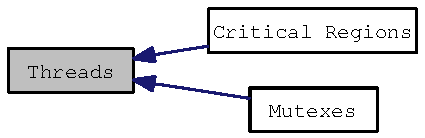
\includegraphics[width=120pt]{group__threading}
\end{center}
\end{figure}
\subsection*{Modules}
\begin{DoxyCompactItemize}
\item 
\hyperlink{group__critical}{Critical Regions}


\begin{DoxyCompactList}\small\item\em A critical region is a simple mechanism that prevents multiple threads from accessing at once code protected by the same critical region. \item\end{DoxyCompactList}\item 
\hyperlink{group__mutex}{Mutexes}
\end{DoxyCompactItemize}
\subsection*{Defines}
\begin{DoxyCompactItemize}
\item 
\#define \hyperlink{group__threading_ga411e2e07982bdfb1803b415a350e311a}{ATOMIC\_\-INCREMENT}(pv)~(\_\-InterlockedIncrement(pv))
\begin{DoxyCompactList}\small\item\em Use this routine for incrementing a global counter using a threadsafe and multiprocessor safe method. \item\end{DoxyCompactList}\item 
\#define \hyperlink{group__threading_gaa42a5aadef70fe57dc80d247c890c9ac}{ATOMIC\_\-DECREMENT}(pv)~(\_\-InterlockedDecrement(pv))
\begin{DoxyCompactList}\small\item\em Use this routine for decrementing a global counter using a threadsafe and multiprocessor safe method. \item\end{DoxyCompactList}\end{DoxyCompactItemize}
\subsection*{Typedefs}
\begin{DoxyCompactItemize}
\item 
\hypertarget{group__threading_ga3f508e817912b65c30d97339cf7a6e62}{
typedef void \hyperlink{group__threading_ga3f508e817912b65c30d97339cf7a6e62}{t\_\-thread}}
\label{group__threading_ga3f508e817912b65c30d97339cf7a6e62}

\begin{DoxyCompactList}\small\item\em A Max thread. \item\end{DoxyCompactList}\item 
\hypertarget{group__threading_gaaf0068b8e9ac28430873484727029315}{
typedef void $\ast$ \hyperlink{group__threading_gaaf0068b8e9ac28430873484727029315}{t\_\-systhread}}
\label{group__threading_gaaf0068b8e9ac28430873484727029315}

\begin{DoxyCompactList}\small\item\em An opaque thread instance pointer. \item\end{DoxyCompactList}\item 
\hypertarget{group__threading_ga503de6f3f546ef1dd2bed57a13d9812c}{
typedef void $\ast$ \hyperlink{group__threading_ga503de6f3f546ef1dd2bed57a13d9812c}{t\_\-systhread\_\-mutex}}
\label{group__threading_ga503de6f3f546ef1dd2bed57a13d9812c}

\begin{DoxyCompactList}\small\item\em An opaque mutex handle. \item\end{DoxyCompactList}\item 
\hypertarget{group__threading_ga56cc95a6cbd27fada3a74b85a7bc3155}{
typedef void $\ast$ \hyperlink{group__threading_ga56cc95a6cbd27fada3a74b85a7bc3155}{t\_\-systhread\_\-cond}}
\label{group__threading_ga56cc95a6cbd27fada3a74b85a7bc3155}

\begin{DoxyCompactList}\small\item\em An opaque cond handle. \item\end{DoxyCompactList}\end{DoxyCompactItemize}
\subsection*{Enumerations}
\begin{DoxyCompactItemize}
\item 
enum \hyperlink{group__threading_gaa95d9c538a1b25404d19106739db9802}{e\_\-max\_\-systhread\_\-mutex\_\-flags} \{ \par
\hyperlink{group__threading_ggaa95d9c538a1b25404d19106739db9802ae34f8741b28ee92a4d702bee8671bb32}{SYSTHREAD\_\-MUTEX\_\-NORMAL} =  0x00000000, 
\par
\hyperlink{group__threading_ggaa95d9c538a1b25404d19106739db9802abb3854e7bf495808b4251d1319cdfa45}{SYSTHREAD\_\-MUTEX\_\-ERRORCHECK} =  0x00000001, 
\par
\hyperlink{group__threading_ggaa95d9c538a1b25404d19106739db9802a4fa486d028b3153aac389ed24e63dddb}{SYSTHREAD\_\-MUTEX\_\-RECURSIVE} =  0x00000002
 \}
\begin{DoxyCompactList}\small\item\em \hyperlink{group__mutex_gaa8cae78764c59883566ac4f861dd534e}{systhread\_\-mutex\_\-new()} flags \item\end{DoxyCompactList}\end{DoxyCompactItemize}
\subsection*{Functions}
\begin{DoxyCompactItemize}
\item 
void \hyperlink{group__threading_ga1eb8ec7623f0806dd079d7be708c19a8}{schedule} (void $\ast$ob, \hyperlink{group__datatypes_gac26ba0a173b50597f5738132e059b42d}{method} fun, long when, \hyperlink{structt__symbol}{t\_\-symbol} $\ast$sym, short argc, Atom $\ast$argv)
\begin{DoxyCompactList}\small\item\em Cause a function to be executed at the timer level at some time in the future. \item\end{DoxyCompactList}\item 
void \hyperlink{group__threading_gaa9b66fe2fc601f110bd962a622f1d5a0}{schedule\_\-delay} (void $\ast$ob, \hyperlink{group__datatypes_gac26ba0a173b50597f5738132e059b42d}{method} fun, long delay, \hyperlink{structt__symbol}{t\_\-symbol} $\ast$sym, short argc, \hyperlink{structt__atom}{t\_\-atom} $\ast$argv)
\begin{DoxyCompactList}\small\item\em Cause a function to be executed at the timer level at some time in the future specified by a delay offset. \item\end{DoxyCompactList}\item 
long \hyperlink{group__threading_gad60dbceb5e50471a3ec76f608a9ea35c}{isr} (void)
\begin{DoxyCompactList}\small\item\em Determine whether your code is executing in the Max scheduler thread. \item\end{DoxyCompactList}\item 
void $\ast$ \hyperlink{group__threading_gaa24a0c9896f1ad241e45590065c3f643}{defer} (void $\ast$ob, \hyperlink{group__datatypes_gac26ba0a173b50597f5738132e059b42d}{method} fn, \hyperlink{structt__symbol}{t\_\-symbol} $\ast$sym, short argc, \hyperlink{structt__atom}{t\_\-atom} $\ast$argv)
\begin{DoxyCompactList}\small\item\em Defer execution of a function to the main thread if (and only if) your function is executing in the scheduler thread. \item\end{DoxyCompactList}\item 
void $\ast$ \hyperlink{group__threading_ga486daa40ddb16f70b663615695d18315}{defer\_\-low} (void $\ast$ob, \hyperlink{group__datatypes_gac26ba0a173b50597f5738132e059b42d}{method} fn, \hyperlink{structt__symbol}{t\_\-symbol} $\ast$sym, short argc, \hyperlink{structt__atom}{t\_\-atom} $\ast$argv)
\begin{DoxyCompactList}\small\item\em Defer execution of a function to the back of the queue on the main thread. \item\end{DoxyCompactList}\item 
long \hyperlink{group__threading_ga7217fa33811a5ed35b970f504b4e4a79}{systhread\_\-create} (\hyperlink{group__datatypes_gac26ba0a173b50597f5738132e059b42d}{method} entryproc, void $\ast$arg, long stacksize, long priority, long flags, \hyperlink{group__threading_gaaf0068b8e9ac28430873484727029315}{t\_\-systhread} $\ast$thread)
\begin{DoxyCompactList}\small\item\em Create a new thread. \item\end{DoxyCompactList}\item 
long \hyperlink{group__threading_gaacc57aeddc69c01e7562397bdf6f12f5}{systhread\_\-terminate} (\hyperlink{group__threading_gaaf0068b8e9ac28430873484727029315}{t\_\-systhread} thread)
\begin{DoxyCompactList}\small\item\em Forcefully kill a thread -\/-\/ not recommended. \item\end{DoxyCompactList}\item 
void \hyperlink{group__threading_gad1ca1694ee14824a56916d8f67d7966b}{systhread\_\-sleep} (long milliseconds)
\begin{DoxyCompactList}\small\item\em Suspend the execution of the calling thread. \item\end{DoxyCompactList}\item 
void \hyperlink{group__threading_gad448ff5be27ef8233162a0e24751786f}{systhread\_\-exit} (long status)
\begin{DoxyCompactList}\small\item\em Exit the calling thread. \item\end{DoxyCompactList}\item 
long \hyperlink{group__threading_gaac24a9db0d7af2343501a4e762d2ce85}{systhread\_\-join} (\hyperlink{group__threading_gaaf0068b8e9ac28430873484727029315}{t\_\-systhread} thread, unsigned int $\ast$retval)
\begin{DoxyCompactList}\small\item\em Wait for thread to quit and get return value from \hyperlink{group__threading_gad448ff5be27ef8233162a0e24751786f}{systhread\_\-exit()}. \item\end{DoxyCompactList}\item 
\hyperlink{group__threading_gaaf0068b8e9ac28430873484727029315}{t\_\-systhread} \hyperlink{group__threading_gab76eb3e1668b13483533c4929be5c914}{systhread\_\-self} (void)
\begin{DoxyCompactList}\small\item\em Return the thread instance pointer for the calling thread. \item\end{DoxyCompactList}\item 
void \hyperlink{group__threading_ga4e4b35c628d791550e5523c4b554d466}{systhread\_\-setpriority} (\hyperlink{group__threading_gaaf0068b8e9ac28430873484727029315}{t\_\-systhread} thread, int priority)
\begin{DoxyCompactList}\small\item\em Set the thread priority for the given thread. \item\end{DoxyCompactList}\item 
int \hyperlink{group__threading_gaf073584f030cffc3a823601173803a95}{systhread\_\-getpriority} (\hyperlink{group__threading_gaaf0068b8e9ac28430873484727029315}{t\_\-systhread} thread)
\begin{DoxyCompactList}\small\item\em Get the thread priority for the given thread. \item\end{DoxyCompactList}\item 
short \hyperlink{group__threading_ga7ed1192e20bccddec517591b4a5f0f91}{systhread\_\-ismainthread} (void)
\begin{DoxyCompactList}\small\item\em Check to see if the function currently being executed is in the main thread. \item\end{DoxyCompactList}\item 
short \hyperlink{group__threading_ga9bc306a6b164f705e55d1612c5ccfb78}{systhread\_\-istimerthread} (void)
\begin{DoxyCompactList}\small\item\em Check to see if the function currently being executed is in the scheduler thread. \item\end{DoxyCompactList}\end{DoxyCompactItemize}


\subsection{Detailed Description}
In Max, there are several threads of execution. The details of these threads are highlighted in the article \char`\"{}Event Priority in Max (Scheduler vs. Queue)\char`\"{} located online at \href{http://www.cycling74.com/story/2005/5/2/133649/9742.}{\tt http://www.cycling74.com/story/2005/5/2/133649/9742.}

Not all of the details of Max's threading model are expounded here. Most important to understand is that we typically deal the scheduler (which when overdrive is on runs in a separate and high priority thread) and the low priority queue (which always runs in the main application thread).

\begin{DoxySeeAlso}{See also}
\href{http://www.cycling74.com/twiki/bin/view/ProductDocumentation/JitterSdkSchedQueue}{\tt http://www.cycling74.com/twiki/bin/view/ProductDocumentation/JitterSdkSchedQueue} 

\href{http://www.cycling74.com/story/2005/5/2/133649/9742}{\tt http://www.cycling74.com/story/2005/5/2/133649/9742} 
\end{DoxySeeAlso}


\subsection{Define Documentation}
\hypertarget{group__threading_gaa42a5aadef70fe57dc80d247c890c9ac}{
\index{threading@{threading}!ATOMIC\_\-DECREMENT@{ATOMIC\_\-DECREMENT}}
\index{ATOMIC\_\-DECREMENT@{ATOMIC\_\-DECREMENT}!threading@{threading}}
\subsubsection[{ATOMIC\_\-DECREMENT}]{\setlength{\rightskip}{0pt plus 5cm}\#define ATOMIC\_\-DECREMENT(pv)~(\_\-InterlockedDecrement(pv))}}
\label{group__threading_gaa42a5aadef70fe57dc80d247c890c9ac}


Use this routine for decrementing a global counter using a threadsafe and multiprocessor safe method. 
\begin{DoxyParams}{Parameters}
\item[{\em pv}]pointer to the (int) counter. \end{DoxyParams}
\hypertarget{group__threading_ga411e2e07982bdfb1803b415a350e311a}{
\index{threading@{threading}!ATOMIC\_\-INCREMENT@{ATOMIC\_\-INCREMENT}}
\index{ATOMIC\_\-INCREMENT@{ATOMIC\_\-INCREMENT}!threading@{threading}}
\subsubsection[{ATOMIC\_\-INCREMENT}]{\setlength{\rightskip}{0pt plus 5cm}\#define ATOMIC\_\-INCREMENT(pv)~(\_\-InterlockedIncrement(pv))}}
\label{group__threading_ga411e2e07982bdfb1803b415a350e311a}


Use this routine for incrementing a global counter using a threadsafe and multiprocessor safe method. 
\begin{DoxyParams}{Parameters}
\item[{\em pv}]pointer to the (int) counter. \end{DoxyParams}


\subsection{Enumeration Type Documentation}
\hypertarget{group__threading_gaa95d9c538a1b25404d19106739db9802}{
\index{threading@{threading}!e\_\-max\_\-systhread\_\-mutex\_\-flags@{e\_\-max\_\-systhread\_\-mutex\_\-flags}}
\index{e\_\-max\_\-systhread\_\-mutex\_\-flags@{e\_\-max\_\-systhread\_\-mutex\_\-flags}!threading@{threading}}
\subsubsection[{e\_\-max\_\-systhread\_\-mutex\_\-flags}]{\setlength{\rightskip}{0pt plus 5cm}enum {\bf e\_\-max\_\-systhread\_\-mutex\_\-flags}}}
\label{group__threading_gaa95d9c538a1b25404d19106739db9802}


\hyperlink{group__mutex_gaa8cae78764c59883566ac4f861dd534e}{systhread\_\-mutex\_\-new()} flags \begin{Desc}
\item[Enumerator: ]\par
\begin{description}
\index{SYSTHREAD\_\-MUTEX\_\-NORMAL@{SYSTHREAD\_\-MUTEX\_\-NORMAL}!threading@{threading}}\index{threading@{threading}!SYSTHREAD\_\-MUTEX\_\-NORMAL@{SYSTHREAD\_\-MUTEX\_\-NORMAL}}\item[{\em 
\hypertarget{group__threading_ggaa95d9c538a1b25404d19106739db9802ae34f8741b28ee92a4d702bee8671bb32}{
SYSTHREAD\_\-MUTEX\_\-NORMAL}
\label{group__threading_ggaa95d9c538a1b25404d19106739db9802ae34f8741b28ee92a4d702bee8671bb32}
}]Normal. \index{SYSTHREAD\_\-MUTEX\_\-ERRORCHECK@{SYSTHREAD\_\-MUTEX\_\-ERRORCHECK}!threading@{threading}}\index{threading@{threading}!SYSTHREAD\_\-MUTEX\_\-ERRORCHECK@{SYSTHREAD\_\-MUTEX\_\-ERRORCHECK}}\item[{\em 
\hypertarget{group__threading_ggaa95d9c538a1b25404d19106739db9802abb3854e7bf495808b4251d1319cdfa45}{
SYSTHREAD\_\-MUTEX\_\-ERRORCHECK}
\label{group__threading_ggaa95d9c538a1b25404d19106739db9802abb3854e7bf495808b4251d1319cdfa45}
}]Error-\/checking. \index{SYSTHREAD\_\-MUTEX\_\-RECURSIVE@{SYSTHREAD\_\-MUTEX\_\-RECURSIVE}!threading@{threading}}\index{threading@{threading}!SYSTHREAD\_\-MUTEX\_\-RECURSIVE@{SYSTHREAD\_\-MUTEX\_\-RECURSIVE}}\item[{\em 
\hypertarget{group__threading_ggaa95d9c538a1b25404d19106739db9802a4fa486d028b3153aac389ed24e63dddb}{
SYSTHREAD\_\-MUTEX\_\-RECURSIVE}
\label{group__threading_ggaa95d9c538a1b25404d19106739db9802a4fa486d028b3153aac389ed24e63dddb}
}]Recursive. \end{description}
\end{Desc}



\subsection{Function Documentation}
\hypertarget{group__threading_gaa24a0c9896f1ad241e45590065c3f643}{
\index{threading@{threading}!defer@{defer}}
\index{defer@{defer}!threading@{threading}}
\subsubsection[{defer}]{\setlength{\rightskip}{0pt plus 5cm}void$\ast$ defer (void $\ast$ {\em ob}, \/  {\bf method} {\em fn}, \/  {\bf t\_\-symbol} $\ast$ {\em sym}, \/  short {\em argc}, \/  {\bf t\_\-atom} $\ast$ {\em argv})}}
\label{group__threading_gaa24a0c9896f1ad241e45590065c3f643}


Defer execution of a function to the main thread if (and only if) your function is executing in the scheduler thread. 
\begin{DoxyParams}{Parameters}
\item[{\em ob}]First argument passed to the function fun when it executes. \item[{\em fn}]Function to be called, see below for how it should be declared. \item[{\em sym}]Second argument passed to the function fun when it executes. \item[{\em argc}]Count of arguments in argv. argc is also the third argument passed to the function fun when it executes. \item[{\em argv}]Array containing a variable number of \hyperlink{structt__atom}{t\_\-atom} function arguments. If this argument is non-\/zero, defer allocates memory to make a copy of the arguments (according to the size passed in argc) and passes the copied array to the function fun when it executes as the fourth argument. \end{DoxyParams}
\begin{DoxyReturn}{Returns}
Return values is for internal Cycling '74 use only.
\end{DoxyReturn}
\begin{DoxyRemark}{Remarks}
This function uses the \hyperlink{group__threading_gad60dbceb5e50471a3ec76f608a9ea35c}{isr()} routine to determine whether you’re at the Max timer interrupt level (in the scheduler thread). If so, \hyperlink{group__threading_gaa24a0c9896f1ad241e45590065c3f643}{defer()} creates a Qelem (see \hyperlink{group__qelems}{Qelems}), calls \hyperlink{group__qelems_gab5fa3e43e7851d1a2049ee28f5275955}{qelem\_\-front()}, and its queue function calls the function fn you passed with the specified arguments. If you’re not in the scheduler thread, the function is executed immediately with the arguments. Note that this implies that \hyperlink{group__threading_gaa24a0c9896f1ad241e45590065c3f643}{defer()} is not appropriate for using in situations such as Device or File manager I/0 completion routines. The \hyperlink{group__threading_ga486daa40ddb16f70b663615695d18315}{defer\_\-low()} function is appropriate however, because it always defers.
\end{DoxyRemark}
The deferred function should be declared as follows: 
\begin{DoxyCode}
    void myobject_do (myObject *client, t_symbol *s, short argc, t_atom *argv);
\end{DoxyCode}


\begin{DoxySeeAlso}{See also}
\hyperlink{group__threading_ga486daa40ddb16f70b663615695d18315}{defer\_\-low()} 
\end{DoxySeeAlso}
\hypertarget{group__threading_ga486daa40ddb16f70b663615695d18315}{
\index{threading@{threading}!defer\_\-low@{defer\_\-low}}
\index{defer\_\-low@{defer\_\-low}!threading@{threading}}
\subsubsection[{defer\_\-low}]{\setlength{\rightskip}{0pt plus 5cm}void$\ast$ defer\_\-low (void $\ast$ {\em ob}, \/  {\bf method} {\em fn}, \/  {\bf t\_\-symbol} $\ast$ {\em sym}, \/  short {\em argc}, \/  {\bf t\_\-atom} $\ast$ {\em argv})}}
\label{group__threading_ga486daa40ddb16f70b663615695d18315}


Defer execution of a function to the back of the queue on the main thread. 
\begin{DoxyParams}{Parameters}
\item[{\em ob}]First argument passed to the function fun when it executes. \item[{\em fn}]Function to be called, see below for how it should be declared. \item[{\em sym}]Second argument passed to the function fun when it executes. \item[{\em argc}]Count of arguments in argv. argc is also the third argument passed to the function fun when it executes. \item[{\em argv}]Array containing a variable number of \hyperlink{structt__atom}{t\_\-atom} function arguments. If this argument is non-\/zero, defer allocates memory to make a copy of the arguments (according to the size passed in argc) and passes the copied array to the function fun when it executes as the fourth argument. \end{DoxyParams}
\begin{DoxyReturn}{Returns}
Return values is for internal Cycling '74 use only.
\end{DoxyReturn}
\begin{DoxyRemark}{Remarks}
\hyperlink{group__threading_ga486daa40ddb16f70b663615695d18315}{defer\_\-low()} always defers a call to the function fun whether you are already in the main thread or not, and uses \hyperlink{group__qelems_ga3e292aad133af89a87e167e88cc4a1b5}{qelem\_\-set()}, not \hyperlink{group__qelems_gab5fa3e43e7851d1a2049ee28f5275955}{qelem\_\-front()}. This function is recommended for responding to messages that will cause your object to open a dialog box, such as read and write.
\end{DoxyRemark}
The deferred function should be declared as follows: 
\begin{DoxyCode}
    void myobject_do (myObject *client, t_symbol *s, short argc, t_atom *argv);
\end{DoxyCode}


\begin{DoxySeeAlso}{See also}
\hyperlink{group__threading_gaa24a0c9896f1ad241e45590065c3f643}{defer()} 
\end{DoxySeeAlso}
\hypertarget{group__threading_gad60dbceb5e50471a3ec76f608a9ea35c}{
\index{threading@{threading}!isr@{isr}}
\index{isr@{isr}!threading@{threading}}
\subsubsection[{isr}]{\setlength{\rightskip}{0pt plus 5cm}long isr (void)}}
\label{group__threading_gad60dbceb5e50471a3ec76f608a9ea35c}


Determine whether your code is executing in the Max scheduler thread. \begin{DoxyReturn}{Returns}
This function returns non-\/zero if you are within Max's scheduler thread, zero otherwise. Note that if your code sets up other types of interrupt-\/level callbacks, such as for other types of device drivers used in asynchronous mode, isr will return false. 
\end{DoxyReturn}
\hypertarget{group__threading_ga1eb8ec7623f0806dd079d7be708c19a8}{
\index{threading@{threading}!schedule@{schedule}}
\index{schedule@{schedule}!threading@{threading}}
\subsubsection[{schedule}]{\setlength{\rightskip}{0pt plus 5cm}void schedule (void $\ast$ {\em ob}, \/  {\bf method} {\em fun}, \/  long {\em when}, \/  {\bf t\_\-symbol} $\ast$ {\em sym}, \/  short {\em argc}, \/  Atom $\ast$ {\em argv})}}
\label{group__threading_ga1eb8ec7623f0806dd079d7be708c19a8}


Cause a function to be executed at the timer level at some time in the future. 
\begin{DoxyParams}{Parameters}
\item[{\em ob}]First argument passed to the function fun when it executes. \item[{\em fun}]Function to be called, see below for how it should be declared. \item[{\em when}]The logical time that the function fun will be executed. \item[{\em sym}]Second argument passed to the function fun when it executes. \item[{\em argc}]Count of arguments in argv. argc is also the third argument passed to the function fun when it executes. \item[{\em argv}]Array containing a variable number of \hyperlink{structt__atom}{t\_\-atom} function arguments. If this argument is non-\/zero, defer allocates memory to make a copy of the arguments (according to the size passed in argc) and passes the copied array to the function fun when it executes as the fourth argument.\end{DoxyParams}
\begin{DoxyRemark}{Remarks}
\hyperlink{group__threading_ga1eb8ec7623f0806dd079d7be708c19a8}{schedule()} calls a function at some time in the future. Unlike \hyperlink{group__threading_gaa24a0c9896f1ad241e45590065c3f643}{defer()}, the function is called in the scheduling loop when logical time is equal to the specified value when. This means that the function could be called at interrupt level, so it should follow the usual restrictions on interrupt-\/level conduct. The function fun passed to schedule should be declared as follows:
\end{DoxyRemark}

\begin{DoxyCode}
    void myobject_do (myObject *client, t_symbol *s, short argc, t_atom *argv); 
\end{DoxyCode}


\begin{DoxyRemark}{Remarks}
One use of \hyperlink{group__threading_ga1eb8ec7623f0806dd079d7be708c19a8}{schedule()} is as an alternative to using the lockout flag.
\end{DoxyRemark}
\begin{DoxySeeAlso}{See also}
\hyperlink{group__threading_gaa24a0c9896f1ad241e45590065c3f643}{defer()} 
\end{DoxySeeAlso}
\hypertarget{group__threading_gaa9b66fe2fc601f110bd962a622f1d5a0}{
\index{threading@{threading}!schedule\_\-delay@{schedule\_\-delay}}
\index{schedule\_\-delay@{schedule\_\-delay}!threading@{threading}}
\subsubsection[{schedule\_\-delay}]{\setlength{\rightskip}{0pt plus 5cm}void schedule\_\-delay (void $\ast$ {\em ob}, \/  {\bf method} {\em fun}, \/  long {\em delay}, \/  {\bf t\_\-symbol} $\ast$ {\em sym}, \/  short {\em argc}, \/  {\bf t\_\-atom} $\ast$ {\em argv})}}
\label{group__threading_gaa9b66fe2fc601f110bd962a622f1d5a0}


Cause a function to be executed at the timer level at some time in the future specified by a delay offset. 
\begin{DoxyParams}{Parameters}
\item[{\em ob}]First argument passed to the function fun when it executes. \item[{\em fun}]Function to be called, see below for how it should be declared. \item[{\em delay}]The delay from the current time before the function will be executed. \item[{\em sym}]Second argument passed to the function fun when it executes. \item[{\em argc}]Count of arguments in argv. argc is also the third argument passed to the function fun when it executes. \item[{\em argv}]Array containing a variable number of \hyperlink{structt__atom}{t\_\-atom} function arguments. If this argument is non-\/zero, defer allocates memory to make a copy of the arguments (according to the size passed in argc) and passes the copied array to the function fun when it executes as the fourth argument.\end{DoxyParams}
\begin{DoxyRemark}{Remarks}
\hyperlink{group__threading_gaa9b66fe2fc601f110bd962a622f1d5a0}{schedule\_\-delay()} is similar to schedule but allows you to specify the time as a delay rather than a specific logical time.
\end{DoxyRemark}
One use of \hyperlink{group__threading_ga1eb8ec7623f0806dd079d7be708c19a8}{schedule()} or \hyperlink{group__threading_gaa9b66fe2fc601f110bd962a622f1d5a0}{schedule\_\-delay()} is as an alternative to using the lockout flag. Here is an example click method that calls \hyperlink{group__threading_ga1eb8ec7623f0806dd079d7be708c19a8}{schedule()} instead of \hyperlink{group__inout_ga0b2b38216f2f4dba486bfcd2273f255e}{outlet\_\-int()} surrounded by lockout\_\-set() calls.


\begin{DoxyCode}
    void myobject_click (t_myobject *x, Point pt, short modifiers) 
    { 
        t_atom a[1]; 
        a[0].a_type = A_LONG; 
        a[0].a_w.w_long = Random(); 
        schedule_delay(x, myobject_sched, 0 ,0, 1, a); 
    } 

    void myobject_sched (t_myobject *x, t_symbol *s, short ac, t_atom *av) 
    { 
        outlet_int(x->m_out,av->a_w.w_long); 
    } 
\end{DoxyCode}


\begin{DoxySeeAlso}{See also}
\hyperlink{group__threading_ga1eb8ec7623f0806dd079d7be708c19a8}{schedule()} 
\end{DoxySeeAlso}
\hypertarget{group__threading_ga7217fa33811a5ed35b970f504b4e4a79}{
\index{threading@{threading}!systhread\_\-create@{systhread\_\-create}}
\index{systhread\_\-create@{systhread\_\-create}!threading@{threading}}
\subsubsection[{systhread\_\-create}]{\setlength{\rightskip}{0pt plus 5cm}long systhread\_\-create ({\bf method} {\em entryproc}, \/  void $\ast$ {\em arg}, \/  long {\em stacksize}, \/  long {\em priority}, \/  long {\em flags}, \/  {\bf t\_\-systhread} $\ast$ {\em thread})}}
\label{group__threading_ga7217fa33811a5ed35b970f504b4e4a79}


Create a new thread. 
\begin{DoxyParams}{Parameters}
\item[{\em entryproc}]A method to call in the new thread when the thread is created. \item[{\em arg}]An argument to pass to the method specified for entryproc. Typically this might be a pointer to your object's struct. \item[{\em stacksize}]Not used. Pass 0 for this argument. \item[{\em priority}]Pass 0 for default priority. The priority can range from -\/32 to 32 where -\/32 is low, 0 is default and 32 is high. \item[{\em flags}]Not used. Pass 0 for this argument. \item[{\em thread}]The address of a \hyperlink{group__threading_gaaf0068b8e9ac28430873484727029315}{t\_\-systhread} where this thread's instance pointer will be stored. \end{DoxyParams}
\begin{DoxyReturn}{Returns}
A Max error code as defined in \hyperlink{group__misc_ga0764dd6c02b76cca7d053ae50555d69d}{e\_\-max\_\-errorcodes}. 
\end{DoxyReturn}
\hypertarget{group__threading_gad448ff5be27ef8233162a0e24751786f}{
\index{threading@{threading}!systhread\_\-exit@{systhread\_\-exit}}
\index{systhread\_\-exit@{systhread\_\-exit}!threading@{threading}}
\subsubsection[{systhread\_\-exit}]{\setlength{\rightskip}{0pt plus 5cm}void systhread\_\-exit (long {\em status})}}
\label{group__threading_gad448ff5be27ef8233162a0e24751786f}


Exit the calling thread. Call this from within a thread made using \hyperlink{group__threading_ga7217fa33811a5ed35b970f504b4e4a79}{systhread\_\-create()} when the thread is no longer needed.


\begin{DoxyParams}{Parameters}
\item[{\em status}]You will typically pass 0 for status. This value will be accessible by \hyperlink{group__threading_gaac24a9db0d7af2343501a4e762d2ce85}{systhread\_\-join()}, if needed. \end{DoxyParams}
\hypertarget{group__threading_gaf073584f030cffc3a823601173803a95}{
\index{threading@{threading}!systhread\_\-getpriority@{systhread\_\-getpriority}}
\index{systhread\_\-getpriority@{systhread\_\-getpriority}!threading@{threading}}
\subsubsection[{systhread\_\-getpriority}]{\setlength{\rightskip}{0pt plus 5cm}int systhread\_\-getpriority ({\bf t\_\-systhread} {\em thread})}}
\label{group__threading_gaf073584f030cffc3a823601173803a95}


Get the thread priority for the given thread. 
\begin{DoxyParams}{Parameters}
\item[{\em thread}]The thread for which to find the priority. \end{DoxyParams}
\begin{DoxyReturn}{Returns}
The current priority value for the given thread. 
\end{DoxyReturn}
\hypertarget{group__threading_ga7ed1192e20bccddec517591b4a5f0f91}{
\index{threading@{threading}!systhread\_\-ismainthread@{systhread\_\-ismainthread}}
\index{systhread\_\-ismainthread@{systhread\_\-ismainthread}!threading@{threading}}
\subsubsection[{systhread\_\-ismainthread}]{\setlength{\rightskip}{0pt plus 5cm}short systhread\_\-ismainthread (void)}}
\label{group__threading_ga7ed1192e20bccddec517591b4a5f0f91}


Check to see if the function currently being executed is in the main thread. \begin{DoxyReturn}{Returns}
Returns true if the function is being executed in the main thread, otherwise false. 
\end{DoxyReturn}
\hypertarget{group__threading_ga9bc306a6b164f705e55d1612c5ccfb78}{
\index{threading@{threading}!systhread\_\-istimerthread@{systhread\_\-istimerthread}}
\index{systhread\_\-istimerthread@{systhread\_\-istimerthread}!threading@{threading}}
\subsubsection[{systhread\_\-istimerthread}]{\setlength{\rightskip}{0pt plus 5cm}short systhread\_\-istimerthread (void)}}
\label{group__threading_ga9bc306a6b164f705e55d1612c5ccfb78}


Check to see if the function currently being executed is in the scheduler thread. \begin{DoxyReturn}{Returns}
Returns true if the function is being executed in the main thread, otherwise false. 
\end{DoxyReturn}
\hypertarget{group__threading_gaac24a9db0d7af2343501a4e762d2ce85}{
\index{threading@{threading}!systhread\_\-join@{systhread\_\-join}}
\index{systhread\_\-join@{systhread\_\-join}!threading@{threading}}
\subsubsection[{systhread\_\-join}]{\setlength{\rightskip}{0pt plus 5cm}long systhread\_\-join ({\bf t\_\-systhread} {\em thread}, \/  unsigned int $\ast$ {\em retval})}}
\label{group__threading_gaac24a9db0d7af2343501a4e762d2ce85}


Wait for thread to quit and get return value from \hyperlink{group__threading_gad448ff5be27ef8233162a0e24751786f}{systhread\_\-exit()}. 
\begin{DoxyParams}{Parameters}
\item[{\em thread}]The thread to join. \item[{\em retval}]The address of a long to hold the return value (status) from \hyperlink{group__threading_gad448ff5be27ef8233162a0e24751786f}{systhread\_\-exit()}. \end{DoxyParams}
\begin{DoxyReturn}{Returns}
A Max error code as defined in \hyperlink{group__misc_ga0764dd6c02b76cca7d053ae50555d69d}{e\_\-max\_\-errorcodes}.
\end{DoxyReturn}
\begin{DoxyRemark}{Remarks}
If your object is freed, and your thread function accesses memory from your object, then you will obviously have a memory violation. A common use of \hyperlink{group__threading_gaac24a9db0d7af2343501a4e762d2ce85}{systhread\_\-join()} is to prevent this situation by waiting (in your free method) for the thread to exit. 
\end{DoxyRemark}
\hypertarget{group__threading_gab76eb3e1668b13483533c4929be5c914}{
\index{threading@{threading}!systhread\_\-self@{systhread\_\-self}}
\index{systhread\_\-self@{systhread\_\-self}!threading@{threading}}
\subsubsection[{systhread\_\-self}]{\setlength{\rightskip}{0pt plus 5cm}{\bf t\_\-systhread} systhread\_\-self (void)}}
\label{group__threading_gab76eb3e1668b13483533c4929be5c914}


Return the thread instance pointer for the calling thread. \begin{DoxyReturn}{Returns}
The thread instance pointer for the thread from which this function is called. 
\end{DoxyReturn}
\hypertarget{group__threading_ga4e4b35c628d791550e5523c4b554d466}{
\index{threading@{threading}!systhread\_\-setpriority@{systhread\_\-setpriority}}
\index{systhread\_\-setpriority@{systhread\_\-setpriority}!threading@{threading}}
\subsubsection[{systhread\_\-setpriority}]{\setlength{\rightskip}{0pt plus 5cm}void systhread\_\-setpriority ({\bf t\_\-systhread} {\em thread}, \/  int {\em priority})}}
\label{group__threading_ga4e4b35c628d791550e5523c4b554d466}


Set the thread priority for the given thread. 
\begin{DoxyParams}{Parameters}
\item[{\em thread}]The thread for which to set the priority. \item[{\em priority}]A value in the range -\/32 to 32 where -\/32 is lowest, 0 is default, and 32 is highest. \end{DoxyParams}
\hypertarget{group__threading_gad1ca1694ee14824a56916d8f67d7966b}{
\index{threading@{threading}!systhread\_\-sleep@{systhread\_\-sleep}}
\index{systhread\_\-sleep@{systhread\_\-sleep}!threading@{threading}}
\subsubsection[{systhread\_\-sleep}]{\setlength{\rightskip}{0pt plus 5cm}void systhread\_\-sleep (long {\em milliseconds})}}
\label{group__threading_gad1ca1694ee14824a56916d8f67d7966b}


Suspend the execution of the calling thread. 
\begin{DoxyParams}{Parameters}
\item[{\em milliseconds}]The number of milliseconds to suspend the execution of the calling thread. The actual amount of time may be longer depending on various factors. \end{DoxyParams}
\hypertarget{group__threading_gaacc57aeddc69c01e7562397bdf6f12f5}{
\index{threading@{threading}!systhread\_\-terminate@{systhread\_\-terminate}}
\index{systhread\_\-terminate@{systhread\_\-terminate}!threading@{threading}}
\subsubsection[{systhread\_\-terminate}]{\setlength{\rightskip}{0pt plus 5cm}long systhread\_\-terminate ({\bf t\_\-systhread} {\em thread})}}
\label{group__threading_gaacc57aeddc69c01e7562397bdf6f12f5}


Forcefully kill a thread -\/-\/ not recommended. 
\begin{DoxyParams}{Parameters}
\item[{\em thread}]The thread to kill. \end{DoxyParams}
\begin{DoxyReturn}{Returns}
A Max error code as defined in \hyperlink{group__misc_ga0764dd6c02b76cca7d053ae50555d69d}{e\_\-max\_\-errorcodes}. 
\end{DoxyReturn}

\hypertarget{group__critical}{
\section{Critical Regions}
\label{group__critical}\index{Critical Regions@{Critical Regions}}
}


A critical region is a simple mechanism that prevents multiple threads from accessing at once code protected by the same critical region.  


Collaboration diagram for Critical Regions:\nopagebreak
\begin{figure}[H]
\begin{center}
\leavevmode
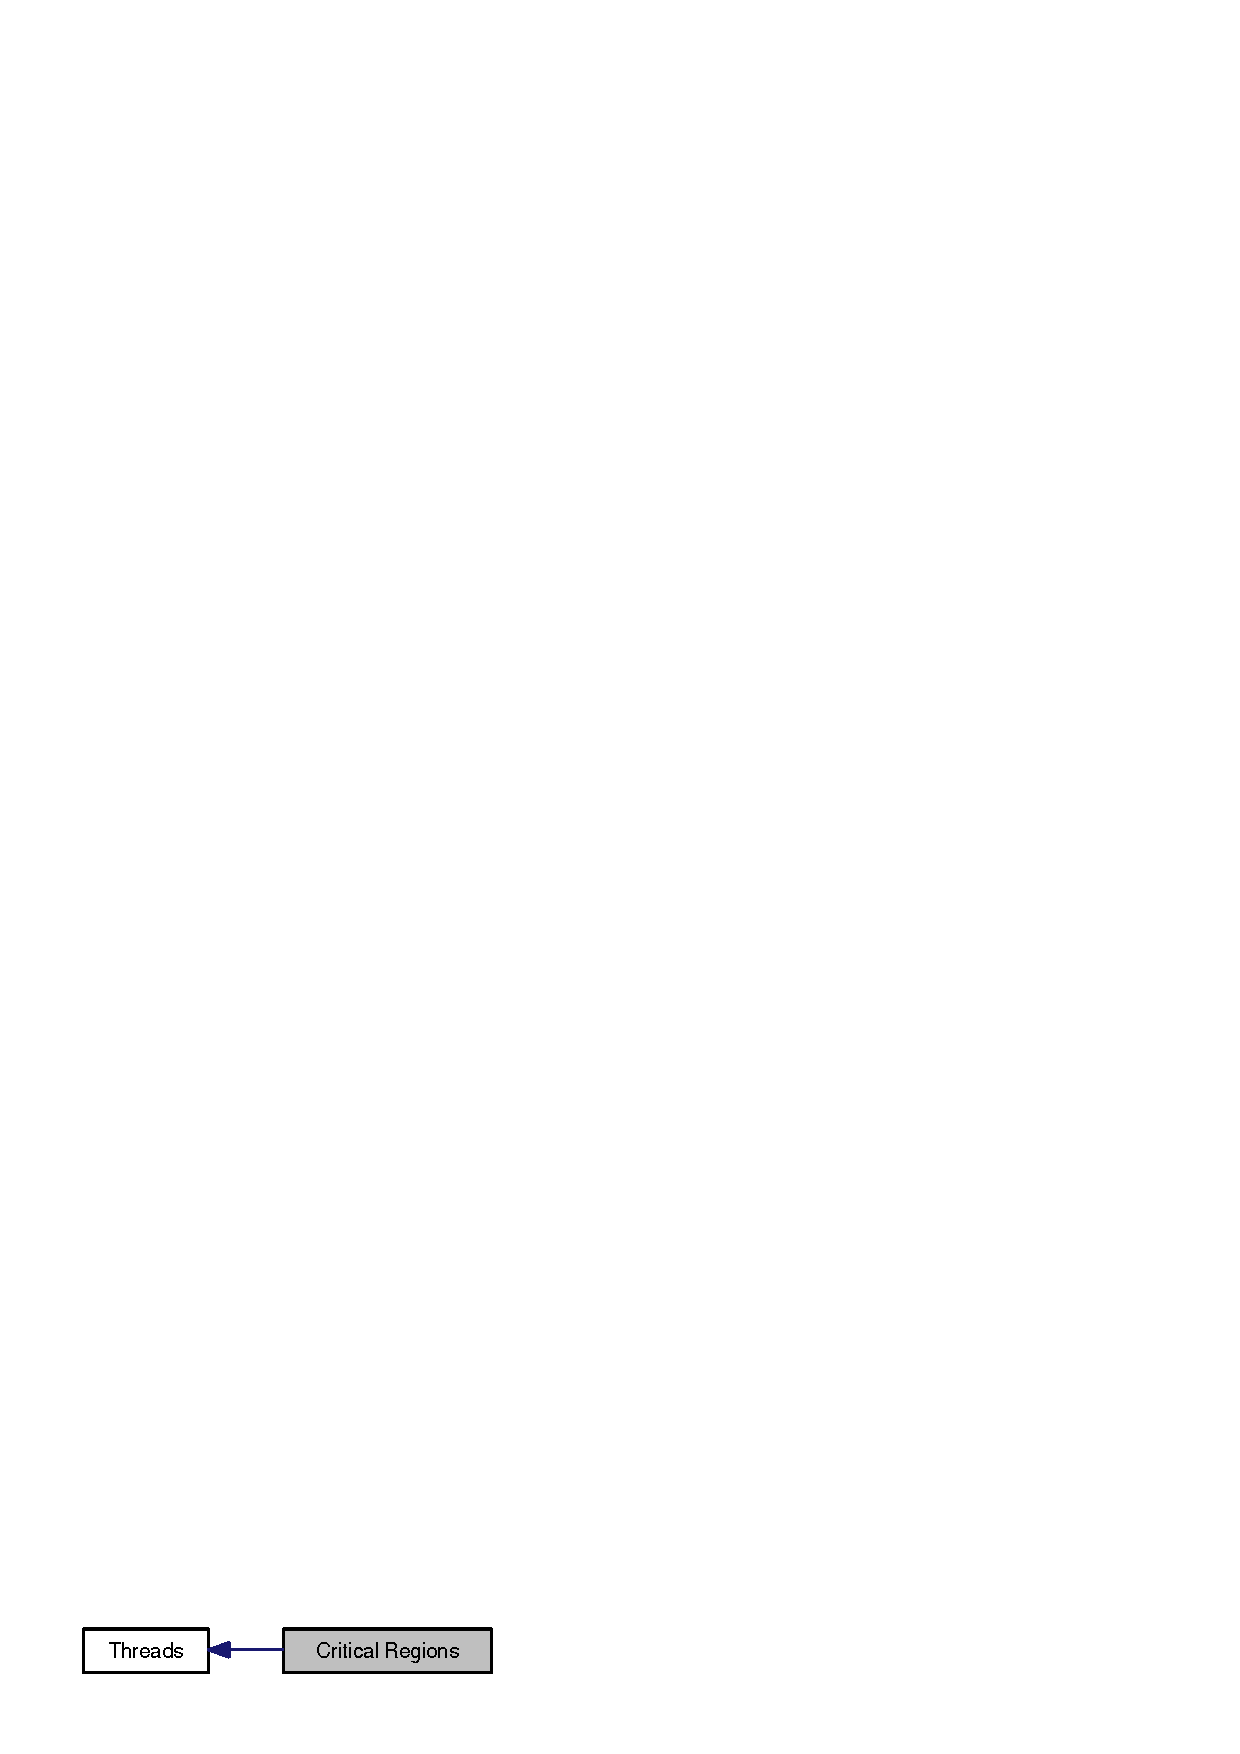
\includegraphics[width=120pt]{group__critical}
\end{center}
\end{figure}
\subsection*{Typedefs}
\begin{DoxyCompactItemize}
\item 
\hypertarget{group__critical_gaa00494020fc3fa3005b63a294cab3886}{
typedef void \hyperlink{group__critical_gaa00494020fc3fa3005b63a294cab3886}{t\_\-critical}}
\label{group__critical_gaa00494020fc3fa3005b63a294cab3886}

\begin{DoxyCompactList}\small\item\em A Max critical region. \item\end{DoxyCompactList}\end{DoxyCompactItemize}
\subsection*{Functions}
\begin{DoxyCompactItemize}
\item 
void \hyperlink{group__critical_gaaa373bcd9c8059e4887225aaf32a76d2}{critical\_\-new} (\hyperlink{group__critical_gaa00494020fc3fa3005b63a294cab3886}{t\_\-critical} $\ast$x)
\begin{DoxyCompactList}\small\item\em Create a new critical region. \item\end{DoxyCompactList}\item 
void \hyperlink{group__critical_ga246445cffc822f756ac6fb34a055022d}{critical\_\-enter} (\hyperlink{group__critical_gaa00494020fc3fa3005b63a294cab3886}{t\_\-critical} x)
\begin{DoxyCompactList}\small\item\em Enter a critical region. \item\end{DoxyCompactList}\item 
void \hyperlink{group__critical_ga269f46fef96f91143fc1616a4105984c}{critical\_\-exit} (\hyperlink{group__critical_gaa00494020fc3fa3005b63a294cab3886}{t\_\-critical} x)
\begin{DoxyCompactList}\small\item\em Leave a critical region. \item\end{DoxyCompactList}\item 
void \hyperlink{group__critical_gaedbe0cba11940710c789ac01194e3712}{critical\_\-free} (\hyperlink{group__critical_gaa00494020fc3fa3005b63a294cab3886}{t\_\-critical} x)
\begin{DoxyCompactList}\small\item\em Free a critical region created with \hyperlink{group__critical_gaaa373bcd9c8059e4887225aaf32a76d2}{critical\_\-new()}. \item\end{DoxyCompactList}\item 
short \hyperlink{group__critical_ga0a4109d5c2b82f0c1022015abac175dc}{critical\_\-tryenter} (\hyperlink{group__critical_gaa00494020fc3fa3005b63a294cab3886}{t\_\-critical} x)
\begin{DoxyCompactList}\small\item\em Try to enter a critical region if it is not locked. \item\end{DoxyCompactList}\end{DoxyCompactItemize}


\subsection{Detailed Description}
A critical region is a simple mechanism that prevents multiple threads from accessing at once code protected by the same critical region. The code fragments could be different, and in completely different modules, but as long as the critical region is the same, no two threads should call the protected code at the same time. If one thread is inside a critical region, and another thread wants to execute code protected by the same critical region, the second thread must wait for the first thread to exit the critical region. In some implementations a critical region can be set so that if it takes too long for the first thread to exit said critical region, the second thread is allowed to execute, dangerously and potentially causing crashes. This is the case for the critical regions exposed by Max and the default upper limit for a given thread to remain inside a critical region is two seconds. Despite the fact that there are two seconds of leeway provided before two threads can dangerously enter a critical region, it is important to only protect as small a portion of code as necessary with a critical region.

Under Max 4.1 and earlier there was a simple protective mechanism called \char`\"{}lockout\char`\"{} that would prevent the scheduler from interrupting the low priority thread during sensitive operations such as sending data out an outlet or modifying members of a linked list. This lockout mechanism has been deprecated, and under the Mac OS X and Windows XP versions (Max 4.2 and later) does nothing. So how do you protect thread sensitive operations? Use critical regions (also known as critical sections). However, it is very important to mention that all outlet calls are now thread safe and should never be contained inside a critical region. Otherwise, this could result in serious timing problems. For other tasks which are not thread safe, such as accessing a linked list, critical regions or some other thread protection mechanism are appropriate.

In Max, the \hyperlink{group__critical_ga246445cffc822f756ac6fb34a055022d}{critical\_\-enter()} function is used to enter a critical region, and the \hyperlink{group__critical_ga269f46fef96f91143fc1616a4105984c}{critical\_\-exit()} function is used to exit a critical region. It is important that in any function which uses critical regions, all control paths protected by the critical region, exit the critical region (watch out for goto or return statements). The \hyperlink{group__critical_ga246445cffc822f756ac6fb34a055022d}{critical\_\-enter()} and \hyperlink{group__critical_ga269f46fef96f91143fc1616a4105984c}{critical\_\-exit()} functions take a critical region as an argument. However, for almost all purposes, we recommend using the global critical region in which case this argument is zero. The use of multiple critical regions can cause problems such as deadlock, i.e. when thread \#1 is inside critical region A waiting on critical region B, but thread \#2 is inside critical region B and is waiting on critical region A. In a flexible programming environment such as Max, deadlock conditions are easier to generate than you might think. So unless you are completely sure of what you are doing, and absolutely need to make use of multiple critical regions to protect your code, we suggest you use the global critical region.

In the following example code we show how one might use critical regions to protect the traversal of a linked list, testing to find the first element whose values is equal to \char`\"{}val\char`\"{}. If this code were not protected, another thread which was modifying the linked list could invalidate assumptions in the traversal code.


\begin{DoxyCode}
    critical_enter(0); 
    for (p = head; p; p = p->next) { 
        if (p->value == val) 
            break; 
    } 
    critical_exit(0); 
    return p;
\end{DoxyCode}


And just to illustrate how to ensure a critical region is exited when multiple control paths are protected by a critical region, here's a slight variant.


\begin{DoxyCode}
    critical_enter(0); 
    for (p = head; p; p = p->next) { 
        if (p->value == val) { 
            critical_exit(0); 
            return p; 
        } 
    } 
    critical_exit(0); 
    return NULL;
\end{DoxyCode}


For more information on multi-\/threaded programming, hardware interrupts, and related topics, we suggest you perform some research online or read the relevant chapters of \char`\"{}Modern Operating Systems\char`\"{} by Andrew S. Tanenbaum (Prentice Hall). At the time of writing, some relevant chapters from this book are available for download in PDF format on Prentice Hall’s web site. See:

\href{http://www.prenhall.com/divisions/esm/app/author_tanenbaum/custom/mos2e/}{\tt http://www.prenhall.com/divisions/esm/app/author\_\-tanenbaum/custom/mos2e/}

Look under \char`\"{}sample sections\char`\"{}. 

\subsection{Function Documentation}
\hypertarget{group__critical_ga246445cffc822f756ac6fb34a055022d}{
\index{critical@{critical}!critical\_\-enter@{critical\_\-enter}}
\index{critical\_\-enter@{critical\_\-enter}!critical@{critical}}
\subsubsection[{critical\_\-enter}]{\setlength{\rightskip}{0pt plus 5cm}void critical\_\-enter ({\bf t\_\-critical} {\em x})}}
\label{group__critical_ga246445cffc822f756ac6fb34a055022d}


Enter a critical region. Typically you will want the argument to be zero to enter the global critical region, although you could pass your own critical created with \hyperlink{group__critical_gaaa373bcd9c8059e4887225aaf32a76d2}{critical\_\-new()}. It is important to try to keep the amount of code in the critical region to a minimum. Exit the critical region with \hyperlink{group__critical_ga269f46fef96f91143fc1616a4105984c}{critical\_\-exit()}.


\begin{DoxyParams}{Parameters}
\item[{\em x}]A pointer to a \hyperlink{group__critical_gaa00494020fc3fa3005b63a294cab3886}{t\_\-critical} struct, or zero to uses Max’s global critical region. \end{DoxyParams}
\begin{DoxySeeAlso}{See also}
\hyperlink{group__critical_ga269f46fef96f91143fc1616a4105984c}{critical\_\-exit()} 
\end{DoxySeeAlso}
\hypertarget{group__critical_ga269f46fef96f91143fc1616a4105984c}{
\index{critical@{critical}!critical\_\-exit@{critical\_\-exit}}
\index{critical\_\-exit@{critical\_\-exit}!critical@{critical}}
\subsubsection[{critical\_\-exit}]{\setlength{\rightskip}{0pt plus 5cm}void critical\_\-exit ({\bf t\_\-critical} {\em x})}}
\label{group__critical_ga269f46fef96f91143fc1616a4105984c}


Leave a critical region. Typically you will want the argument to be zero to exit the global critical region, although, you if you are using your own critical regions you will want to pass the same one that you previously passed to \hyperlink{group__critical_ga246445cffc822f756ac6fb34a055022d}{critical\_\-enter()}.


\begin{DoxyParams}{Parameters}
\item[{\em x}]A pointer to a \hyperlink{group__critical_gaa00494020fc3fa3005b63a294cab3886}{t\_\-critical} struct, or zero to uses Max’s global critical region. \end{DoxyParams}
\hypertarget{group__critical_gaedbe0cba11940710c789ac01194e3712}{
\index{critical@{critical}!critical\_\-free@{critical\_\-free}}
\index{critical\_\-free@{critical\_\-free}!critical@{critical}}
\subsubsection[{critical\_\-free}]{\setlength{\rightskip}{0pt plus 5cm}void critical\_\-free ({\bf t\_\-critical} {\em x})}}
\label{group__critical_gaedbe0cba11940710c789ac01194e3712}


Free a critical region created with \hyperlink{group__critical_gaaa373bcd9c8059e4887225aaf32a76d2}{critical\_\-new()}. If you created your own critical region, you will need to free it in your object’s free method.


\begin{DoxyParams}{Parameters}
\item[{\em x}]The \hyperlink{group__critical_gaa00494020fc3fa3005b63a294cab3886}{t\_\-critical} struct that will be freed. \end{DoxyParams}
\hypertarget{group__critical_gaaa373bcd9c8059e4887225aaf32a76d2}{
\index{critical@{critical}!critical\_\-new@{critical\_\-new}}
\index{critical\_\-new@{critical\_\-new}!critical@{critical}}
\subsubsection[{critical\_\-new}]{\setlength{\rightskip}{0pt plus 5cm}void critical\_\-new ({\bf t\_\-critical} $\ast$ {\em x})}}
\label{group__critical_gaaa373bcd9c8059e4887225aaf32a76d2}


Create a new critical region. Normally, you do not need to create your own critical region, because you can use Max’s global critical region. Only use this function (in your object’s instance creation method) if you are certain you are not able to use the global critical region.


\begin{DoxyParams}{Parameters}
\item[{\em x}]A \hyperlink{group__critical_gaa00494020fc3fa3005b63a294cab3886}{t\_\-critical} struct will be returned to you via this pointer. \end{DoxyParams}
\hypertarget{group__critical_ga0a4109d5c2b82f0c1022015abac175dc}{
\index{critical@{critical}!critical\_\-tryenter@{critical\_\-tryenter}}
\index{critical\_\-tryenter@{critical\_\-tryenter}!critical@{critical}}
\subsubsection[{critical\_\-tryenter}]{\setlength{\rightskip}{0pt plus 5cm}short critical\_\-tryenter ({\bf t\_\-critical} {\em x})}}
\label{group__critical_ga0a4109d5c2b82f0c1022015abac175dc}


Try to enter a critical region if it is not locked. 
\begin{DoxyParams}{Parameters}
\item[{\em x}]A pointer to a \hyperlink{group__critical_gaa00494020fc3fa3005b63a294cab3886}{t\_\-critical} struct, or zero to uses Max’s global critical region. \end{DoxyParams}
\begin{DoxyReturn}{Returns}
returns non-\/zero if there was a problem entering 
\end{DoxyReturn}
\begin{DoxySeeAlso}{See also}
\hyperlink{group__critical_ga246445cffc822f756ac6fb34a055022d}{critical\_\-enter()} 
\end{DoxySeeAlso}

\hypertarget{group__mutex}{
\section{Mutexes}
\label{group__mutex}\index{Mutexes@{Mutexes}}
}


Collaboration diagram for Mutexes:\nopagebreak
\begin{figure}[H]
\begin{center}
\leavevmode
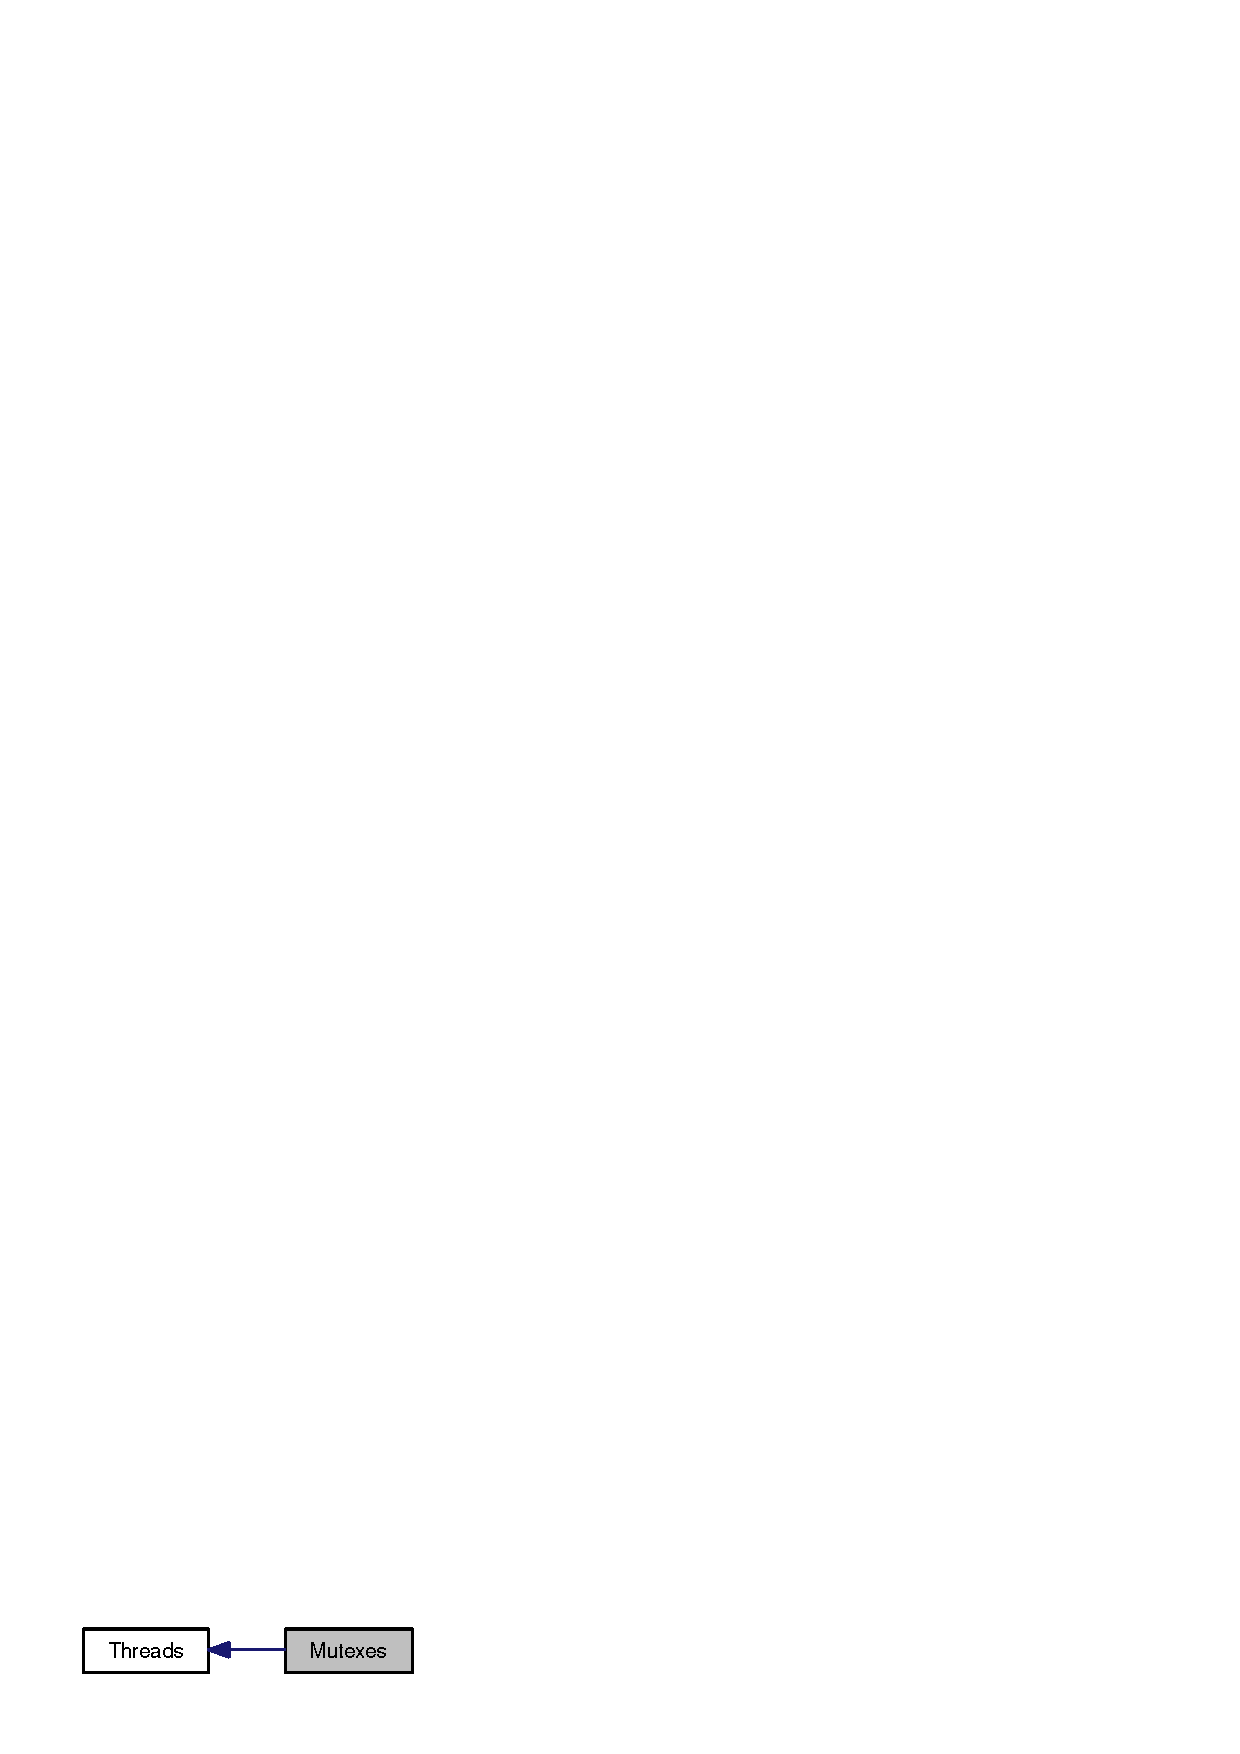
\includegraphics[width=101pt]{group__mutex}
\end{center}
\end{figure}
\subsection*{Functions}
\begin{DoxyCompactItemize}
\item 
long \hyperlink{group__mutex_gaa8cae78764c59883566ac4f861dd534e}{systhread\_\-mutex\_\-new} (\hyperlink{group__threading_ga503de6f3f546ef1dd2bed57a13d9812c}{t\_\-systhread\_\-mutex} $\ast$pmutex, long flags)
\begin{DoxyCompactList}\small\item\em Create a new mutex, which can be used to place thread locks around critical code. \item\end{DoxyCompactList}\item 
long \hyperlink{group__mutex_ga5fdfbb20bfe5b9e6b223436758ea88b1}{systhread\_\-mutex\_\-free} (\hyperlink{group__threading_ga503de6f3f546ef1dd2bed57a13d9812c}{t\_\-systhread\_\-mutex} pmutex)
\begin{DoxyCompactList}\small\item\em Free a mutex created with \hyperlink{group__mutex_gaa8cae78764c59883566ac4f861dd534e}{systhread\_\-mutex\_\-new()}. \item\end{DoxyCompactList}\item 
long \hyperlink{group__mutex_ga6a3bea4c2f5e5d133d25d78b51fb15bf}{systhread\_\-mutex\_\-lock} (\hyperlink{group__threading_ga503de6f3f546ef1dd2bed57a13d9812c}{t\_\-systhread\_\-mutex} pmutex)
\begin{DoxyCompactList}\small\item\em Enter block of locked code code until a \hyperlink{group__mutex_ga74aae707e650844be8a4e51a217c9b5f}{systhread\_\-mutex\_\-unlock()} is reached. \item\end{DoxyCompactList}\item 
long \hyperlink{group__mutex_ga74aae707e650844be8a4e51a217c9b5f}{systhread\_\-mutex\_\-unlock} (\hyperlink{group__threading_ga503de6f3f546ef1dd2bed57a13d9812c}{t\_\-systhread\_\-mutex} pmutex)
\begin{DoxyCompactList}\small\item\em Exit a block of code locked with \hyperlink{group__mutex_ga6a3bea4c2f5e5d133d25d78b51fb15bf}{systhread\_\-mutex\_\-lock()}. \item\end{DoxyCompactList}\item 
long \hyperlink{group__mutex_gafa0cef91ad29e8e0625d35eadde52002}{systhread\_\-mutex\_\-trylock} (\hyperlink{group__threading_ga503de6f3f546ef1dd2bed57a13d9812c}{t\_\-systhread\_\-mutex} pmutex)
\begin{DoxyCompactList}\small\item\em Try to enter block of locked code code until a \hyperlink{group__mutex_ga74aae707e650844be8a4e51a217c9b5f}{systhread\_\-mutex\_\-unlock()} is reached. \item\end{DoxyCompactList}\item 
long \hyperlink{group__mutex_ga57c63515a67e9739aa0f916ae05e8a18}{systhread\_\-mutex\_\-newlock} (\hyperlink{group__threading_ga503de6f3f546ef1dd2bed57a13d9812c}{t\_\-systhread\_\-mutex} $\ast$pmutex, long flags)
\begin{DoxyCompactList}\small\item\em Convenience utility that combines \hyperlink{group__mutex_gaa8cae78764c59883566ac4f861dd534e}{systhread\_\-mutex\_\-new()} and \hyperlink{group__mutex_ga6a3bea4c2f5e5d133d25d78b51fb15bf}{systhread\_\-mutex\_\-lock()}. \item\end{DoxyCompactList}\end{DoxyCompactItemize}


\subsection{Detailed Description}
\begin{DoxySeeAlso}{See also}
\hyperlink{group__critical}{Critical Regions} 
\end{DoxySeeAlso}


\subsection{Function Documentation}
\hypertarget{group__mutex_ga5fdfbb20bfe5b9e6b223436758ea88b1}{
\index{mutex@{mutex}!systhread\_\-mutex\_\-free@{systhread\_\-mutex\_\-free}}
\index{systhread\_\-mutex\_\-free@{systhread\_\-mutex\_\-free}!mutex@{mutex}}
\subsubsection[{systhread\_\-mutex\_\-free}]{\setlength{\rightskip}{0pt plus 5cm}long systhread\_\-mutex\_\-free ({\bf t\_\-systhread\_\-mutex} {\em pmutex})}}
\label{group__mutex_ga5fdfbb20bfe5b9e6b223436758ea88b1}


Free a mutex created with \hyperlink{group__mutex_gaa8cae78764c59883566ac4f861dd534e}{systhread\_\-mutex\_\-new()}. 
\begin{DoxyParams}{Parameters}
\item[{\em pmutex}]The mutex instance pointer. \end{DoxyParams}
\begin{DoxyReturn}{Returns}
A Max error code as defined in \hyperlink{group__misc_ga0764dd6c02b76cca7d053ae50555d69d}{e\_\-max\_\-errorcodes}. 
\end{DoxyReturn}
\hypertarget{group__mutex_ga6a3bea4c2f5e5d133d25d78b51fb15bf}{
\index{mutex@{mutex}!systhread\_\-mutex\_\-lock@{systhread\_\-mutex\_\-lock}}
\index{systhread\_\-mutex\_\-lock@{systhread\_\-mutex\_\-lock}!mutex@{mutex}}
\subsubsection[{systhread\_\-mutex\_\-lock}]{\setlength{\rightskip}{0pt plus 5cm}long systhread\_\-mutex\_\-lock ({\bf t\_\-systhread\_\-mutex} {\em pmutex})}}
\label{group__mutex_ga6a3bea4c2f5e5d133d25d78b51fb15bf}


Enter block of locked code code until a \hyperlink{group__mutex_ga74aae707e650844be8a4e51a217c9b5f}{systhread\_\-mutex\_\-unlock()} is reached. It is important to keep the code in this block as small as possible.


\begin{DoxyParams}{Parameters}
\item[{\em pmutex}]The mutex instance pointer. \end{DoxyParams}
\begin{DoxyReturn}{Returns}
A Max error code as defined in \hyperlink{group__misc_ga0764dd6c02b76cca7d053ae50555d69d}{e\_\-max\_\-errorcodes}. 
\end{DoxyReturn}
\begin{DoxySeeAlso}{See also}
\hyperlink{group__mutex_gafa0cef91ad29e8e0625d35eadde52002}{systhread\_\-mutex\_\-trylock()} 
\end{DoxySeeAlso}
\hypertarget{group__mutex_gaa8cae78764c59883566ac4f861dd534e}{
\index{mutex@{mutex}!systhread\_\-mutex\_\-new@{systhread\_\-mutex\_\-new}}
\index{systhread\_\-mutex\_\-new@{systhread\_\-mutex\_\-new}!mutex@{mutex}}
\subsubsection[{systhread\_\-mutex\_\-new}]{\setlength{\rightskip}{0pt plus 5cm}long systhread\_\-mutex\_\-new ({\bf t\_\-systhread\_\-mutex} $\ast$ {\em pmutex}, \/  long {\em flags})}}
\label{group__mutex_gaa8cae78764c59883566ac4f861dd534e}


Create a new mutex, which can be used to place thread locks around critical code. The mutex should be freed with \hyperlink{group__mutex_ga5fdfbb20bfe5b9e6b223436758ea88b1}{systhread\_\-mutex\_\-free()}.


\begin{DoxyParams}{Parameters}
\item[{\em pmutex}]The address of a variable to store the mutex pointer. \item[{\em flags}]Flags to determine the behaviour of the mutex, as defined in \hyperlink{group__threading_gaa95d9c538a1b25404d19106739db9802}{e\_\-max\_\-systhread\_\-mutex\_\-flags}. \end{DoxyParams}
\begin{DoxyReturn}{Returns}
A Max error code as defined in \hyperlink{group__misc_ga0764dd6c02b76cca7d053ae50555d69d}{e\_\-max\_\-errorcodes}.
\end{DoxyReturn}
\begin{DoxyRemark}{Remarks}
One reason to use \hyperlink{group__mutex_gaa8cae78764c59883566ac4f861dd534e}{systhread\_\-mutex\_\-new()} instead of \hyperlink{group__critical}{Critical Regions} is to create non-\/recursive locks, which are lighter-\/weight than recursive locks. 
\end{DoxyRemark}
\hypertarget{group__mutex_ga57c63515a67e9739aa0f916ae05e8a18}{
\index{mutex@{mutex}!systhread\_\-mutex\_\-newlock@{systhread\_\-mutex\_\-newlock}}
\index{systhread\_\-mutex\_\-newlock@{systhread\_\-mutex\_\-newlock}!mutex@{mutex}}
\subsubsection[{systhread\_\-mutex\_\-newlock}]{\setlength{\rightskip}{0pt plus 5cm}long systhread\_\-mutex\_\-newlock ({\bf t\_\-systhread\_\-mutex} $\ast$ {\em pmutex}, \/  long {\em flags})}}
\label{group__mutex_ga57c63515a67e9739aa0f916ae05e8a18}


Convenience utility that combines \hyperlink{group__mutex_gaa8cae78764c59883566ac4f861dd534e}{systhread\_\-mutex\_\-new()} and \hyperlink{group__mutex_ga6a3bea4c2f5e5d133d25d78b51fb15bf}{systhread\_\-mutex\_\-lock()}. 
\begin{DoxyParams}{Parameters}
\item[{\em pmutex}]The address of a variable to store the mutex pointer. \item[{\em flags}]Flags to determine the behaviour of the mutex, as defined in \hyperlink{group__threading_gaa95d9c538a1b25404d19106739db9802}{e\_\-max\_\-systhread\_\-mutex\_\-flags}. \end{DoxyParams}
\begin{DoxyReturn}{Returns}
A Max error code as defined in \hyperlink{group__misc_ga0764dd6c02b76cca7d053ae50555d69d}{e\_\-max\_\-errorcodes}. 
\end{DoxyReturn}
\hypertarget{group__mutex_gafa0cef91ad29e8e0625d35eadde52002}{
\index{mutex@{mutex}!systhread\_\-mutex\_\-trylock@{systhread\_\-mutex\_\-trylock}}
\index{systhread\_\-mutex\_\-trylock@{systhread\_\-mutex\_\-trylock}!mutex@{mutex}}
\subsubsection[{systhread\_\-mutex\_\-trylock}]{\setlength{\rightskip}{0pt plus 5cm}long systhread\_\-mutex\_\-trylock ({\bf t\_\-systhread\_\-mutex} {\em pmutex})}}
\label{group__mutex_gafa0cef91ad29e8e0625d35eadde52002}


Try to enter block of locked code code until a \hyperlink{group__mutex_ga74aae707e650844be8a4e51a217c9b5f}{systhread\_\-mutex\_\-unlock()} is reached. If the lock cannot be entered, this function will return non-\/zero.


\begin{DoxyParams}{Parameters}
\item[{\em pmutex}]The mutex instance pointer. \end{DoxyParams}
\begin{DoxyReturn}{Returns}
Returns non-\/zero if there was a problem entering. 
\end{DoxyReturn}
\begin{DoxySeeAlso}{See also}
\hyperlink{group__mutex_ga6a3bea4c2f5e5d133d25d78b51fb15bf}{systhread\_\-mutex\_\-lock()} 
\end{DoxySeeAlso}
\hypertarget{group__mutex_ga74aae707e650844be8a4e51a217c9b5f}{
\index{mutex@{mutex}!systhread\_\-mutex\_\-unlock@{systhread\_\-mutex\_\-unlock}}
\index{systhread\_\-mutex\_\-unlock@{systhread\_\-mutex\_\-unlock}!mutex@{mutex}}
\subsubsection[{systhread\_\-mutex\_\-unlock}]{\setlength{\rightskip}{0pt plus 5cm}long systhread\_\-mutex\_\-unlock ({\bf t\_\-systhread\_\-mutex} {\em pmutex})}}
\label{group__mutex_ga74aae707e650844be8a4e51a217c9b5f}


Exit a block of code locked with \hyperlink{group__mutex_ga6a3bea4c2f5e5d133d25d78b51fb15bf}{systhread\_\-mutex\_\-lock()}. 
\begin{DoxyParams}{Parameters}
\item[{\em pmutex}]The mutex instance pointer. \end{DoxyParams}
\begin{DoxyReturn}{Returns}
A Max error code as defined in \hyperlink{group__misc_ga0764dd6c02b76cca7d053ae50555d69d}{e\_\-max\_\-errorcodes}. 
\end{DoxyReturn}

\hypertarget{group__ui}{
\section{User Interface}
\label{group__ui}\index{User Interface@{User Interface}}
}


Collaboration diagram for User Interface:\nopagebreak
\begin{figure}[H]
\begin{center}
\leavevmode
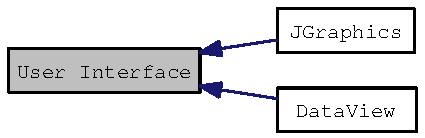
\includegraphics[width=120pt]{group__ui}
\end{center}
\end{figure}
\subsection*{Modules}
\begin{DoxyCompactItemize}
\item 
\hyperlink{group__jgraphics}{JGraphics}


\begin{DoxyCompactList}\small\item\em The JGraphics API provided in Max 5 is an interface for drawing based on the API for the Cairo vector graphics library ( \href{http://en.wikipedia.org/wiki/Cairo_%28graphics%29}{\tt http://en.wikipedia.org/wiki/Cairo\_\-\%28graphics\%29} , \href{http://cairographics.org/manual/}{\tt http://cairographics.org/manual/} ). \item\end{DoxyCompactList}\item 
\hyperlink{group__jdataview}{DataView}


\begin{DoxyCompactList}\small\item\em The jdataview object provides a mechanism to display data in a tabular format. \item\end{DoxyCompactList}\end{DoxyCompactItemize}

\hypertarget{group__jgraphics}{
\section{JGraphics}
\label{group__jgraphics}\index{JGraphics@{JGraphics}}
}


The JGraphics API provided in Max 5 is an interface for drawing based on the API for the Cairo vector graphics library ( \href{http://en.wikipedia.org/wiki/Cairo_%28graphics%29}{\tt http://en.wikipedia.org/wiki/Cairo\_\-\%28graphics\%29} , \href{http://cairographics.org/manual/}{\tt http://cairographics.org/manual/} ).  


Collaboration diagram for JGraphics:\nopagebreak
\begin{figure}[H]
\begin{center}
\leavevmode
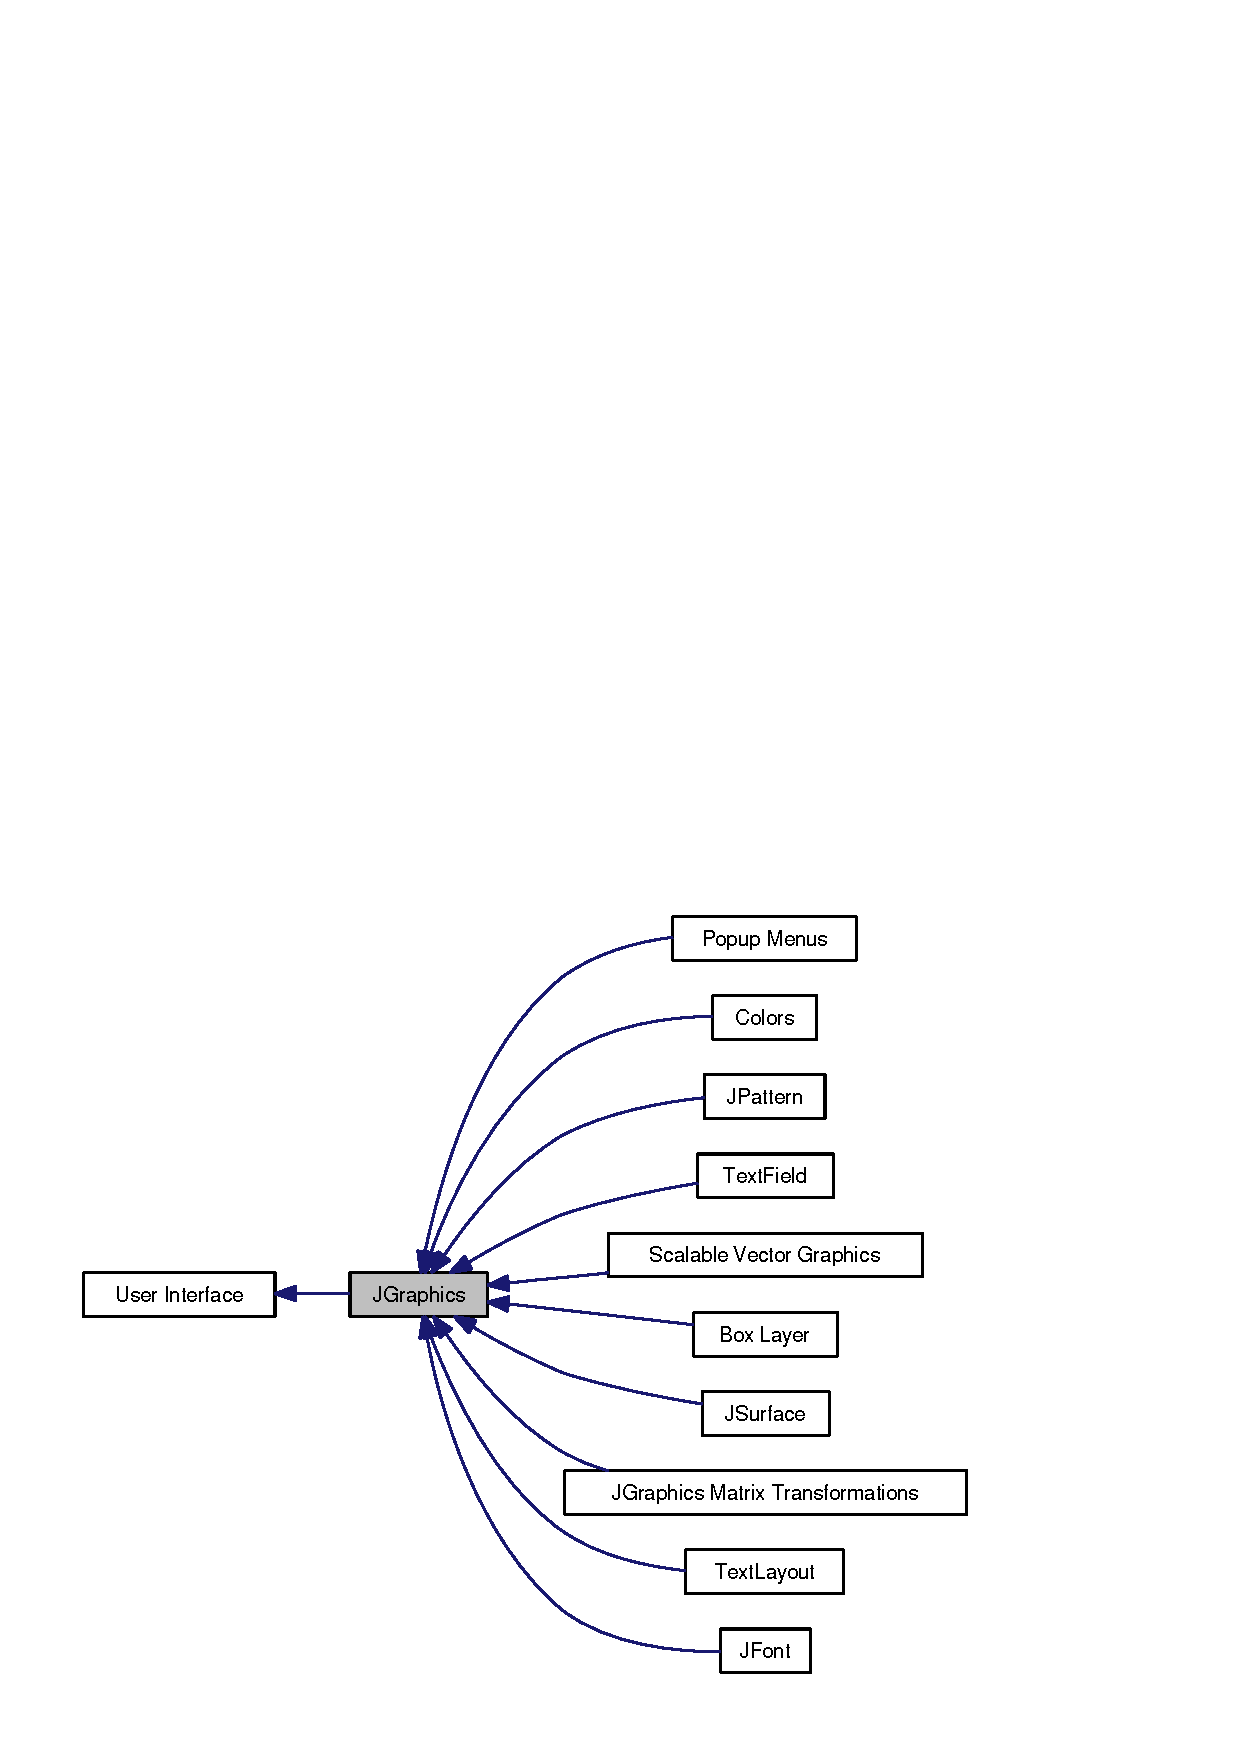
\includegraphics[width=234pt]{group__jgraphics}
\end{center}
\end{figure}
\subsection*{Data Structures}
\begin{DoxyCompactItemize}
\item 
struct \hyperlink{structt__jgraphics__font__extents}{t\_\-jgraphics\_\-font\_\-extents}
\begin{DoxyCompactList}\small\item\em A structure for holding information related to how much space the rendering of a given font will use. \item\end{DoxyCompactList}\end{DoxyCompactItemize}
\subsection*{Modules}
\begin{DoxyCompactItemize}
\item 
\hyperlink{group__jsurface}{JSurface}


\begin{DoxyCompactList}\small\item\em A surface is an abstract base class for something you render to. \item\end{DoxyCompactList}\item 
\hyperlink{group__jsvg}{Scalable Vector Graphics}
\item 
\hyperlink{group__jfont}{JFont}
\item 
\hyperlink{group__jmatrix}{JGraphics Matrix Transformations}


\begin{DoxyCompactList}\small\item\em The \hyperlink{structt__jmatrix}{t\_\-jmatrix} is one way to represent a transformation. \item\end{DoxyCompactList}\item 
\hyperlink{group__jpattern}{JPattern}


\begin{DoxyCompactList}\small\item\em A pattern is like a brush that is used to fill a path with. \item\end{DoxyCompactList}\item 
\hyperlink{group__color}{Colors}
\item 
\hyperlink{group__textfield}{TextField}


\begin{DoxyCompactList}\small\item\em The textfield is a high-\/level text display object that may be used by a UI object to represent text in a patcher. \item\end{DoxyCompactList}\item 
\hyperlink{group__textlayout}{TextLayout}


\begin{DoxyCompactList}\small\item\em A textlayout is lower-\/level text rendering object used by higher-\/level entities such as \hyperlink{group__textfield}{TextField}. \item\end{DoxyCompactList}\item 
\hyperlink{group__jpopupmenu}{Popup Menus}


\begin{DoxyCompactList}\small\item\em Popup menu API so externals can create popup menus that can also be drawn into. \item\end{DoxyCompactList}\item 
\hyperlink{group__boxlayer}{Box Layer}


\begin{DoxyCompactList}\small\item\em The boxlayer functions provide way to make it easier to use cached offscreen images (layers) in your drawing. \item\end{DoxyCompactList}\end{DoxyCompactItemize}
\subsection*{Defines}
\begin{DoxyCompactItemize}
\item 
\hypertarget{group__jgraphics_gaa3cb88e5a2a6b52ea668a1ed1bba4422}{
\#define \hyperlink{group__jgraphics_gaa3cb88e5a2a6b52ea668a1ed1bba4422}{JGRAPHICS\_\-RECT\_\-BOTTOM}(rect)~(((rect)-\/$>$y)+((rect)-\/$>$height))}
\label{group__jgraphics_gaa3cb88e5a2a6b52ea668a1ed1bba4422}

\begin{DoxyCompactList}\small\item\em Determine the coordinate of the bottom of a rect. \item\end{DoxyCompactList}\item 
\hypertarget{group__jgraphics_ga2e728ace124972d27dc4f7ae70c3e751}{
\#define \hyperlink{group__jgraphics_ga2e728ace124972d27dc4f7ae70c3e751}{JGRAPHICS\_\-RECT\_\-RIGHT}(rect)~(((rect)-\/$>$x)+((rect)-\/$>$width))}
\label{group__jgraphics_ga2e728ace124972d27dc4f7ae70c3e751}

\begin{DoxyCompactList}\small\item\em Determine the coordinate of the right side of a rect. \item\end{DoxyCompactList}\item 
\#define \hyperlink{group__jgraphics_gab6eb126ec0f85fa48c30aff48a3e0f5b}{JGRAPHICS\_\-PI}~(3.1415926535897932384626433832795028842)
\begin{DoxyCompactList}\small\item\em Utility macro to return the value of Pi. \item\end{DoxyCompactList}\item 
\#define \hyperlink{group__jgraphics_gafe32bbcad508a9ef7629a2c47719dcb5}{JGRAPHICS\_\-2PI}~(2. $\ast$ 3.1415926535897932384626433832795028842)
\begin{DoxyCompactList}\small\item\em Utility macro to return the value of twice Pi. \item\end{DoxyCompactList}\item 
\#define \hyperlink{group__jgraphics_gad1ac187e1ba64c0b956d6fff6a3da8dc}{JGRAPHICS\_\-PIOVER2}~(0.5 $\ast$ 3.1415926535897932384626433832795028842)
\begin{DoxyCompactList}\small\item\em Utility macro to return the value of half of Pi. \item\end{DoxyCompactList}\item 
\#define \hyperlink{group__jgraphics_gae9f23705d238432d1abb58a2ab0ac792}{JGRAPHICS\_\-3PIOVER2}~((3.0 $\ast$ JGRAPHICS\_\-PI) / 2.0)
\begin{DoxyCompactList}\small\item\em Utility macro to return the 270º Case. \item\end{DoxyCompactList}\end{DoxyCompactItemize}
\subsection*{Typedefs}
\begin{DoxyCompactItemize}
\item 
\hypertarget{group__jgraphics_ga4bf27bd7e21a59a427481b909d4656e7}{
typedef typedefBEGIN\_\-USING\_\-C\_\-LINKAGE struct \_\-jgraphics \hyperlink{group__jgraphics_ga4bf27bd7e21a59a427481b909d4656e7}{t\_\-jgraphics}}
\label{group__jgraphics_ga4bf27bd7e21a59a427481b909d4656e7}

\begin{DoxyCompactList}\small\item\em An instance of a jgraphics drawing context. \item\end{DoxyCompactList}\item 
\hypertarget{group__jgraphics_ga09a18e946c8a6cfa25dfa38154a138d8}{
typedef struct \_\-jpath \hyperlink{group__jgraphics_ga09a18e946c8a6cfa25dfa38154a138d8}{t\_\-jpath}}
\label{group__jgraphics_ga09a18e946c8a6cfa25dfa38154a138d8}

\begin{DoxyCompactList}\small\item\em An instance of a jgraphics path. \item\end{DoxyCompactList}\item 
\hypertarget{group__jgraphics_ga45f6bda6903290bd6040f79fec89872b}{
typedef struct \_\-jtextlayout \hyperlink{group__jgraphics_ga45f6bda6903290bd6040f79fec89872b}{t\_\-jtextlayout}}
\label{group__jgraphics_ga45f6bda6903290bd6040f79fec89872b}

\begin{DoxyCompactList}\small\item\em An instance of a jgraphics text layout object. \item\end{DoxyCompactList}\item 
\hypertarget{group__jgraphics_gaa936ddd5bfc6b091b730c834858326c2}{
typedef struct \_\-jtransform \hyperlink{group__jgraphics_gaa936ddd5bfc6b091b730c834858326c2}{t\_\-jtransform}}
\label{group__jgraphics_gaa936ddd5bfc6b091b730c834858326c2}

\begin{DoxyCompactList}\small\item\em An instance of a jgraphics transform. \item\end{DoxyCompactList}\item 
\hypertarget{group__jgraphics_gaa3000c3aa85e3d7c87f59c44d5d7ccab}{
typedef struct \_\-jsvg \hyperlink{group__jgraphics_gaa3000c3aa85e3d7c87f59c44d5d7ccab}{t\_\-jsvg}}
\label{group__jgraphics_gaa3000c3aa85e3d7c87f59c44d5d7ccab}

\begin{DoxyCompactList}\small\item\em An instance of an SVG object. \item\end{DoxyCompactList}\item 
\hypertarget{group__jgraphics_ga613e147be2f9655726f08f0896b9dbaa}{
typedef struct \_\-jpopupmenu \hyperlink{group__jgraphics_ga613e147be2f9655726f08f0896b9dbaa}{t\_\-jpopupmenu}}
\label{group__jgraphics_ga613e147be2f9655726f08f0896b9dbaa}

\begin{DoxyCompactList}\small\item\em An instance of a pop-\/up menu. \item\end{DoxyCompactList}\end{DoxyCompactItemize}
\subsection*{Enumerations}
\begin{DoxyCompactItemize}
\item 
enum \hyperlink{group__jgraphics_ga4c4fa437dbfffb2c406787efa7701604}{t\_\-jgraphics\_\-format} \{ \par
\hyperlink{group__jgraphics_gga4c4fa437dbfffb2c406787efa7701604a072f2e8fde1742abd692b9de9e7d1011}{JGRAPHICS\_\-FORMAT\_\-ARGB32}, 
\par
\hyperlink{group__jgraphics_gga4c4fa437dbfffb2c406787efa7701604a3021abdd63af373988e5d2b3a696a6d2}{JGRAPHICS\_\-FORMAT\_\-RGB24}, 
\par
\hyperlink{group__jgraphics_gga4c4fa437dbfffb2c406787efa7701604ad8fca751059bf8cef944dfe0b98ef191}{JGRAPHICS\_\-FORMAT\_\-A8}
 \}
\begin{DoxyCompactList}\small\item\em Enumeration of color formats used by jgraphics surfaces. \item\end{DoxyCompactList}\item 
enum \hyperlink{group__jgraphics_ga81465e1a6989399e343d081defd90dbe}{t\_\-jgraphics\_\-fileformat} \{ \par
\hyperlink{group__jgraphics_gga81465e1a6989399e343d081defd90dbea2370a1696e7b478145fece2d7b2ee903}{JGRAPHICS\_\-FILEFORMAT\_\-PNG}, 
\par
\hyperlink{group__jgraphics_gga81465e1a6989399e343d081defd90dbeae2a7397922debc6f37505eb58aa58d2f}{JGRAPHICS\_\-FILEFORMAT\_\-JPEG}
 \}
\begin{DoxyCompactList}\small\item\em Enumeration of file formats usable for jgraphics surfaces. \item\end{DoxyCompactList}\item 
enum \hyperlink{group__jgraphics_ga3519fa317c6811b619af2d70e3c1eca7}{t\_\-jgraphics\_\-text\_\-justification} \{ \par
\hyperlink{group__jgraphics_gga3519fa317c6811b619af2d70e3c1eca7a5e4867b2a5e3789724b6c0d70679c4e3}{JGRAPHICS\_\-TEXT\_\-JUSTIFICATION\_\-LEFT} =  1, 
\par
\hyperlink{group__jgraphics_gga3519fa317c6811b619af2d70e3c1eca7a3eb14134e02256092b705f04d20c6adb}{JGRAPHICS\_\-TEXT\_\-JUSTIFICATION\_\-RIGHT} =  2, 
\par
\hyperlink{group__jgraphics_gga3519fa317c6811b619af2d70e3c1eca7aaef852ad474ffc8ed5cfd7bf4d5813fa}{JGRAPHICS\_\-TEXT\_\-JUSTIFICATION\_\-HCENTERED} =  4, 
\par
\hyperlink{group__jgraphics_gga3519fa317c6811b619af2d70e3c1eca7ab3d013abb01bb8b776878740c806be4f}{JGRAPHICS\_\-TEXT\_\-JUSTIFICATION\_\-TOP} =  8, 
\par
\hyperlink{group__jgraphics_gga3519fa317c6811b619af2d70e3c1eca7a5d435b07bee873341a742c66f27d1647}{JGRAPHICS\_\-TEXT\_\-JUSTIFICATION\_\-BOTTOM} =  16, 
\par
\hyperlink{group__jgraphics_gga3519fa317c6811b619af2d70e3c1eca7a38425ac2446ca233cc1c711d8ee531fe}{JGRAPHICS\_\-TEXT\_\-JUSTIFICATION\_\-VCENTERED} =  32, 
\par
\hyperlink{group__jgraphics_gga3519fa317c6811b619af2d70e3c1eca7a0adcc29443836c67fed75120d2c228ae}{JGRAPHICS\_\-TEXT\_\-JUSTIFICATION\_\-HJUSTIFIED} =  64, 
\par
\hyperlink{group__jgraphics_gga3519fa317c6811b619af2d70e3c1eca7a75d25a43e7cd127bf0baec24897e0f74}{JGRAPHICS\_\-TEXT\_\-JUSTIFICATION\_\-CENTERED} =  JGRAPHICS\_\-TEXT\_\-JUSTIFICATION\_\-HCENTERED + JGRAPHICS\_\-TEXT\_\-JUSTIFICATION\_\-VCENTERED
 \}
\begin{DoxyCompactList}\small\item\em Enumeration of text justification options, which are specified as a bitmask. \item\end{DoxyCompactList}\end{DoxyCompactItemize}
\subsection*{Functions}
\begin{DoxyCompactItemize}
\item 
int \hyperlink{group__jgraphics_ga706be120b247818f2ebb18d96934bb72}{jgraphics\_\-round} (double d)
\begin{DoxyCompactList}\small\item\em Utility for rounding a double to an int. \item\end{DoxyCompactList}\item 
\hyperlink{group__jgraphics_ga4bf27bd7e21a59a427481b909d4656e7}{t\_\-jgraphics} $\ast$ \hyperlink{group__jgraphics_ga3008118a280cac02b4c64ab6d0e6926e}{jgraphics\_\-reference} (\hyperlink{group__jgraphics_ga4bf27bd7e21a59a427481b909d4656e7}{t\_\-jgraphics} $\ast$g)
\begin{DoxyCompactList}\small\item\em Get a reference to a graphics context. \item\end{DoxyCompactList}\item 
void \hyperlink{group__jgraphics_ga910977684c0f03be9edfb9f861905d5e}{jgraphics\_\-destroy} (\hyperlink{group__jgraphics_ga4bf27bd7e21a59a427481b909d4656e7}{t\_\-jgraphics} $\ast$g)
\begin{DoxyCompactList}\small\item\em Release or free a graphics context. \item\end{DoxyCompactList}\item 
void \hyperlink{group__jgraphics_ga627c4feb0dfcad9e8417472eec5aedef}{jgraphics\_\-new\_\-path} (\hyperlink{group__jgraphics_ga4bf27bd7e21a59a427481b909d4656e7}{t\_\-jgraphics} $\ast$g)
\begin{DoxyCompactList}\small\item\em Begin a new path. \item\end{DoxyCompactList}\item 
\hyperlink{group__jgraphics_ga09a18e946c8a6cfa25dfa38154a138d8}{t\_\-jpath} $\ast$ \hyperlink{group__jgraphics_ga356f39bed1d63fcf843fe05b6dc861b0}{jgraphics\_\-copy\_\-path} (\hyperlink{group__jgraphics_ga4bf27bd7e21a59a427481b909d4656e7}{t\_\-jgraphics} $\ast$g)
\begin{DoxyCompactList}\small\item\em Get a copy of the current path from a context. \item\end{DoxyCompactList}\item 
void \hyperlink{group__jgraphics_gaff6abc629030d751899d99c61970df79}{jgraphics\_\-path\_\-destroy} (\hyperlink{group__jgraphics_ga09a18e946c8a6cfa25dfa38154a138d8}{t\_\-jpath} $\ast$path)
\begin{DoxyCompactList}\small\item\em Release/free a path. \item\end{DoxyCompactList}\item 
void \hyperlink{group__jgraphics_ga4e16e3a3ce6cc21374ba3d7ae4615f65}{jgraphics\_\-append\_\-path} (\hyperlink{group__jgraphics_ga4bf27bd7e21a59a427481b909d4656e7}{t\_\-jgraphics} $\ast$g, \hyperlink{group__jgraphics_ga09a18e946c8a6cfa25dfa38154a138d8}{t\_\-jpath} $\ast$path)
\begin{DoxyCompactList}\small\item\em Add a path to a graphics context. \item\end{DoxyCompactList}\item 
void \hyperlink{group__jgraphics_ga22cf905279b642358789ae7ed133808f}{jgraphics\_\-close\_\-path} (\hyperlink{group__jgraphics_ga4bf27bd7e21a59a427481b909d4656e7}{t\_\-jgraphics} $\ast$g)
\begin{DoxyCompactList}\small\item\em Close the current path in a context. \item\end{DoxyCompactList}\item 
void \hyperlink{group__jgraphics_ga51efbf384c6dd4504c9575447dbaaa53}{jgraphics\_\-path\_\-roundcorners} (\hyperlink{group__jgraphics_ga4bf27bd7e21a59a427481b909d4656e7}{t\_\-jgraphics} $\ast$g, double cornerRadius)
\begin{DoxyCompactList}\small\item\em Round out any corners in a path. \item\end{DoxyCompactList}\item 
void \hyperlink{group__jgraphics_gae3c2cc2ba52f2a27bf9e09a60fa94daa}{jgraphics\_\-get\_\-current\_\-point} (\hyperlink{group__jgraphics_ga4bf27bd7e21a59a427481b909d4656e7}{t\_\-jgraphics} $\ast$g, double $\ast$x, double $\ast$y)
\begin{DoxyCompactList}\small\item\em Get the current location of the cursor in a graphics context. \item\end{DoxyCompactList}\item 
void \hyperlink{group__jgraphics_gaeee1dd41f67614a31307cc006f4f39ce}{jgraphics\_\-arc} (\hyperlink{group__jgraphics_ga4bf27bd7e21a59a427481b909d4656e7}{t\_\-jgraphics} $\ast$g, double xc, double yc, double radius, double angle1, double angle2)
\begin{DoxyCompactList}\small\item\em Add a circular, clockwise, arc to the current path. \item\end{DoxyCompactList}\item 
void \hyperlink{group__jgraphics_ga2dde9a34e2863ab5244057c4ef775a0c}{jgraphics\_\-ovalarc} (\hyperlink{group__jgraphics_ga4bf27bd7e21a59a427481b909d4656e7}{t\_\-jgraphics} $\ast$g, double xc, double yc, double radiusx, double radiusy, double angle1, double angle2)
\begin{DoxyCompactList}\small\item\em Add a non-\/circular arc to the current path. \item\end{DoxyCompactList}\item 
void \hyperlink{group__jgraphics_gaafd9fedb4ec2870714890120ae1c353d}{jgraphics\_\-arc\_\-negative} (\hyperlink{group__jgraphics_ga4bf27bd7e21a59a427481b909d4656e7}{t\_\-jgraphics} $\ast$g, double xc, double yc, double radius, double angle1, double angle2)
\begin{DoxyCompactList}\small\item\em Add a circular, counter-\/clockwise, arc to the current path. \item\end{DoxyCompactList}\item 
void \hyperlink{group__jgraphics_ga893fefbf4f38bb4b3b83850c21f8b836}{jgraphics\_\-curve\_\-to} (\hyperlink{group__jgraphics_ga4bf27bd7e21a59a427481b909d4656e7}{t\_\-jgraphics} $\ast$g, double x1, double y1, double x2, double y2, double x3, double y3)
\begin{DoxyCompactList}\small\item\em Add a cubic Bezier spline to the current path. \item\end{DoxyCompactList}\item 
void \hyperlink{group__jgraphics_gac3932cbd8b6a30144f0d827d7f21d16b}{jgraphics\_\-rel\_\-curve\_\-to} (\hyperlink{group__jgraphics_ga4bf27bd7e21a59a427481b909d4656e7}{t\_\-jgraphics} $\ast$g, double x1, double y1, double x2, double y2, double x3, double y3)
\begin{DoxyCompactList}\small\item\em Add a cubic Bezier spline to the current path, using coordinates relative to the current point. \item\end{DoxyCompactList}\item 
void \hyperlink{group__jgraphics_ga70ce27489e0449ec8872253373459bad}{jgraphics\_\-line\_\-to} (\hyperlink{group__jgraphics_ga4bf27bd7e21a59a427481b909d4656e7}{t\_\-jgraphics} $\ast$g, double x, double y)
\begin{DoxyCompactList}\small\item\em Add a line segment to the current path. \item\end{DoxyCompactList}\item 
void \hyperlink{group__jgraphics_ga0669af2caff03efea7fab31484ad62eb}{jgraphics\_\-rel\_\-line\_\-to} (\hyperlink{group__jgraphics_ga4bf27bd7e21a59a427481b909d4656e7}{t\_\-jgraphics} $\ast$g, double x, double y)
\begin{DoxyCompactList}\small\item\em Add a line segment to the current path, using coordinates relative to the current point. \item\end{DoxyCompactList}\item 
void \hyperlink{group__jgraphics_ga52651cc3a7f9b395461eadffe9e6156b}{jgraphics\_\-move\_\-to} (\hyperlink{group__jgraphics_ga4bf27bd7e21a59a427481b909d4656e7}{t\_\-jgraphics} $\ast$g, double x, double y)
\begin{DoxyCompactList}\small\item\em Move the cursor to a new point and begin a new subpath. \item\end{DoxyCompactList}\item 
void \hyperlink{group__jgraphics_ga1d3d4ea2e22dcb02098f1f24ff937296}{jgraphics\_\-rel\_\-move\_\-to} (\hyperlink{group__jgraphics_ga4bf27bd7e21a59a427481b909d4656e7}{t\_\-jgraphics} $\ast$g, double x, double y)
\begin{DoxyCompactList}\small\item\em Move the cursor to a new point and begin a new subpath, using coordinates relative to the current point. \item\end{DoxyCompactList}\item 
void \hyperlink{group__jgraphics_ga01f63358f24616678d69721d7d505e74}{jgraphics\_\-rectangle} (\hyperlink{group__jgraphics_ga4bf27bd7e21a59a427481b909d4656e7}{t\_\-jgraphics} $\ast$g, double x, double y, double width, double height)
\begin{DoxyCompactList}\small\item\em Add a closed rectangle path in the context. \item\end{DoxyCompactList}\item 
void \hyperlink{group__jgraphics_gabdf52225c137e70eea1f955559d19591}{jgraphics\_\-oval} (\hyperlink{group__jgraphics_ga4bf27bd7e21a59a427481b909d4656e7}{t\_\-jgraphics} $\ast$g, double x, double y, double width, double height)
\begin{DoxyCompactList}\small\item\em Deprecated -\/-\/ do not use. \item\end{DoxyCompactList}\item 
void \hyperlink{group__jgraphics_ga0e15af397f5f4eb1e474e31ea43e1d7c}{jgraphics\_\-rectangle\_\-rounded} (\hyperlink{group__jgraphics_ga4bf27bd7e21a59a427481b909d4656e7}{t\_\-jgraphics} $\ast$g, double x, double y, double width, double height, double ovalwidth, double ovalheight)
\begin{DoxyCompactList}\small\item\em Add a closed rounded-\/rectangle path in the context. \item\end{DoxyCompactList}\item 
void \hyperlink{group__jgraphics_ga1703b907a1167055ecea6674e00233d4}{jgraphics\_\-ellipse} (\hyperlink{group__jgraphics_ga4bf27bd7e21a59a427481b909d4656e7}{t\_\-jgraphics} $\ast$g, double x, double y, double width, double height)
\begin{DoxyCompactList}\small\item\em Add a closed elliptical path in the context. \item\end{DoxyCompactList}\item 
void \hyperlink{group__jgraphics_ga0c184facd0030b513e63162fca2225cd}{jgraphics\_\-select\_\-font\_\-face} (\hyperlink{group__jgraphics_ga4bf27bd7e21a59a427481b909d4656e7}{t\_\-jgraphics} $\ast$g, const char $\ast$family, \hyperlink{group__jfont_gaea63403193677b088b56cb60c69c37b4}{t\_\-jgraphics\_\-font\_\-slant} slant, \hyperlink{group__jfont_ga29fc4356e11166a16aeae50dd5e22f86}{t\_\-jgraphics\_\-font\_\-weight} weight)
\begin{DoxyCompactList}\small\item\em Specify a font for a graphics context. \item\end{DoxyCompactList}\item 
void \hyperlink{group__jgraphics_ga1299d24b9d9d6b0955a214e813c6463c}{jgraphics\_\-select\_\-jfont} (\hyperlink{group__jgraphics_ga4bf27bd7e21a59a427481b909d4656e7}{t\_\-jgraphics} $\ast$g, \hyperlink{group__jfont_ga75f83f853e52af957c799723cac89ae5}{t\_\-jfont} $\ast$jfont)
\begin{DoxyCompactList}\small\item\em Specify a font for a graphics context by passing a \hyperlink{group__jfont_ga75f83f853e52af957c799723cac89ae5}{t\_\-jfont} object. \item\end{DoxyCompactList}\item 
void \hyperlink{group__jgraphics_gaf8c17f34bfbcd09ea7ba324a6a35cc9d}{jgraphics\_\-set\_\-font\_\-size} (\hyperlink{group__jgraphics_ga4bf27bd7e21a59a427481b909d4656e7}{t\_\-jgraphics} $\ast$g, double size)
\begin{DoxyCompactList}\small\item\em Specify the font size for a context. \item\end{DoxyCompactList}\item 
void \hyperlink{group__jgraphics_ga6753504ad26f256016c34681672d3478}{jgraphics\_\-set\_\-underline} (\hyperlink{group__jgraphics_ga4bf27bd7e21a59a427481b909d4656e7}{t\_\-jgraphics} $\ast$g, char underline)
\begin{DoxyCompactList}\small\item\em Turn underlining on/off for text in a context. \item\end{DoxyCompactList}\item 
void \hyperlink{group__jgraphics_ga91b780fe7e636c4497d0f8ab0ebfd41e}{jgraphics\_\-show\_\-text} (\hyperlink{group__jgraphics_ga4bf27bd7e21a59a427481b909d4656e7}{t\_\-jgraphics} $\ast$g, const char $\ast$utf8)
\begin{DoxyCompactList}\small\item\em Display text at the current position in a context. \item\end{DoxyCompactList}\item 
void \hyperlink{group__jgraphics_ga4f556e322638d6427c2ecc7932d806ed}{jgraphics\_\-font\_\-extents} (\hyperlink{group__jgraphics_ga4bf27bd7e21a59a427481b909d4656e7}{t\_\-jgraphics} $\ast$g, \hyperlink{structt__jgraphics__font__extents}{t\_\-jgraphics\_\-font\_\-extents} $\ast$extents)
\begin{DoxyCompactList}\small\item\em Return the extents of the currently selected font for a given graphics context. \item\end{DoxyCompactList}\item 
void \hyperlink{group__jgraphics_ga3b8bb426e28bbc271f478ecc91f932f2}{jgraphics\_\-text\_\-measure} (\hyperlink{group__jgraphics_ga4bf27bd7e21a59a427481b909d4656e7}{t\_\-jgraphics} $\ast$g, const char $\ast$utf8, double $\ast$width, double $\ast$height)
\begin{DoxyCompactList}\small\item\em Return the height and width of a string given current graphics settings in a context. \item\end{DoxyCompactList}\item 
void \hyperlink{group__jgraphics_gabe6cf107005eed13953f624fac4a3e25}{jgraphics\_\-text\_\-measure\_\-wrapped} (\hyperlink{group__jgraphics_ga4bf27bd7e21a59a427481b909d4656e7}{t\_\-jgraphics} $\ast$g, const char $\ast$utf8, double wrapwidth, long includewhitespace, double $\ast$width, double $\ast$height, long $\ast$numlines)
\begin{DoxyCompactList}\small\item\em Return the height, width, and number of lines that will be used to render a given string. \item\end{DoxyCompactList}\item 
long \hyperlink{group__jgraphics_gaf794cabf13ac57d40f311bb415426925}{jgraphics\_\-system\_\-canantialiastexttotransparentbg} ()
\begin{DoxyCompactList}\small\item\em Determine if you can anti-\/alias text to a transparent background. \item\end{DoxyCompactList}\item 
void \hyperlink{group__jgraphics_ga67774b45773c5a559c756bd57167dd83}{jgraphics\_\-user\_\-to\_\-device} (\hyperlink{group__jgraphics_ga4bf27bd7e21a59a427481b909d4656e7}{t\_\-jgraphics} $\ast$g, double $\ast$x, double $\ast$y)
\begin{DoxyCompactList}\small\item\em User coordinates are those passed to drawing functions in a given \hyperlink{group__jgraphics_ga4bf27bd7e21a59a427481b909d4656e7}{t\_\-jgraphics} context. \item\end{DoxyCompactList}\item 
void \hyperlink{group__jgraphics_ga8a6b2b8982f78d417cb5a15a3fbdb2e2}{jgraphics\_\-device\_\-to\_\-user} (\hyperlink{group__jgraphics_ga4bf27bd7e21a59a427481b909d4656e7}{t\_\-jgraphics} $\ast$g, double $\ast$x, double $\ast$y)
\begin{DoxyCompactList}\small\item\em User coordinates are those passed to drawing functions in a given \hyperlink{group__jgraphics_ga4bf27bd7e21a59a427481b909d4656e7}{t\_\-jgraphics} context. \item\end{DoxyCompactList}\item 
void \hyperlink{group__jgraphics_ga7a23d1cdfe75bfcdb0415adc6696f4f0}{jgraphics\_\-getfiletypes} (void $\ast$dummy, long $\ast$count, long $\ast$$\ast$filetypes, char $\ast$alloc)
\begin{DoxyCompactList}\small\item\em Get a list of of filetypes appropriate for use with jgraphics surfaces. \item\end{DoxyCompactList}\item 
long \hyperlink{group__jgraphics_gaa8e30eaa2c74766b0c7ef3977fd8a06c}{jgraphics\_\-rectintersectsrect} (\hyperlink{structt__rect}{t\_\-rect} $\ast$r1, \hyperlink{structt__rect}{t\_\-rect} $\ast$r2)
\begin{DoxyCompactList}\small\item\em Simple utility to test for rectangle intersection. \item\end{DoxyCompactList}\item 
long \hyperlink{group__jgraphics_gaabca7cb7d45c92e788456a2d7dbfd4f6}{jgraphics\_\-rectcontainsrect} (\hyperlink{structt__rect}{t\_\-rect} $\ast$outer, \hyperlink{structt__rect}{t\_\-rect} $\ast$inner)
\begin{DoxyCompactList}\small\item\em Simple utility to test for rectangle containment. \item\end{DoxyCompactList}\item 
void \hyperlink{group__jgraphics_ga5b4eb24b41c116e3324b2da40541f8eb}{jgraphics\_\-position\_\-one\_\-rect\_\-near\_\-another\_\-rect\_\-but\_\-keep\_\-inside\_\-a\_\-third\_\-rect} (\hyperlink{structt__rect}{t\_\-rect} $\ast$positioned\_\-rect, const \hyperlink{structt__rect}{t\_\-rect} $\ast$positioned\_\-near\_\-this\_\-rect, const \hyperlink{structt__rect}{t\_\-rect} $\ast$keep\_\-inside\_\-this\_\-rect)
\begin{DoxyCompactList}\small\item\em Generate a \hyperlink{structt__rect}{t\_\-rect} according to positioning rules. \item\end{DoxyCompactList}\end{DoxyCompactItemize}


\subsection{Detailed Description}
The JGraphics API provided in Max 5 is an interface for drawing based on the API for the Cairo vector graphics library ( \href{http://en.wikipedia.org/wiki/Cairo_%28graphics%29}{\tt http://en.wikipedia.org/wiki/Cairo\_\-\%28graphics\%29} , \href{http://cairographics.org/manual/}{\tt http://cairographics.org/manual/} ). Internally, the drawing is rendered using JUCE ( \href{http://rawmaterialsoftware.com/juce/}{\tt http://rawmaterialsoftware.com/juce/} ), however JUCE functions cannot be called directly. 

\subsection{Define Documentation}
\hypertarget{group__jgraphics_gafe32bbcad508a9ef7629a2c47719dcb5}{
\index{jgraphics@{jgraphics}!JGRAPHICS\_\-2PI@{JGRAPHICS\_\-2PI}}
\index{JGRAPHICS\_\-2PI@{JGRAPHICS\_\-2PI}!jgraphics@{jgraphics}}
\subsubsection[{JGRAPHICS\_\-2PI}]{\setlength{\rightskip}{0pt plus 5cm}\#define JGRAPHICS\_\-2PI~(2. $\ast$ 3.1415926535897932384626433832795028842)}}
\label{group__jgraphics_gafe32bbcad508a9ef7629a2c47719dcb5}


Utility macro to return the value of twice Pi. \hypertarget{group__jgraphics_gae9f23705d238432d1abb58a2ab0ac792}{
\index{jgraphics@{jgraphics}!JGRAPHICS\_\-3PIOVER2@{JGRAPHICS\_\-3PIOVER2}}
\index{JGRAPHICS\_\-3PIOVER2@{JGRAPHICS\_\-3PIOVER2}!jgraphics@{jgraphics}}
\subsubsection[{JGRAPHICS\_\-3PIOVER2}]{\setlength{\rightskip}{0pt plus 5cm}\#define JGRAPHICS\_\-3PIOVER2~((3.0 $\ast$ JGRAPHICS\_\-PI) / 2.0)}}
\label{group__jgraphics_gae9f23705d238432d1abb58a2ab0ac792}


Utility macro to return the 270º Case. \hypertarget{group__jgraphics_gab6eb126ec0f85fa48c30aff48a3e0f5b}{
\index{jgraphics@{jgraphics}!JGRAPHICS\_\-PI@{JGRAPHICS\_\-PI}}
\index{JGRAPHICS\_\-PI@{JGRAPHICS\_\-PI}!jgraphics@{jgraphics}}
\subsubsection[{JGRAPHICS\_\-PI}]{\setlength{\rightskip}{0pt plus 5cm}\#define JGRAPHICS\_\-PI~(3.1415926535897932384626433832795028842)}}
\label{group__jgraphics_gab6eb126ec0f85fa48c30aff48a3e0f5b}


Utility macro to return the value of Pi. \hypertarget{group__jgraphics_gad1ac187e1ba64c0b956d6fff6a3da8dc}{
\index{jgraphics@{jgraphics}!JGRAPHICS\_\-PIOVER2@{JGRAPHICS\_\-PIOVER2}}
\index{JGRAPHICS\_\-PIOVER2@{JGRAPHICS\_\-PIOVER2}!jgraphics@{jgraphics}}
\subsubsection[{JGRAPHICS\_\-PIOVER2}]{\setlength{\rightskip}{0pt plus 5cm}\#define JGRAPHICS\_\-PIOVER2~(0.5 $\ast$ 3.1415926535897932384626433832795028842)}}
\label{group__jgraphics_gad1ac187e1ba64c0b956d6fff6a3da8dc}


Utility macro to return the value of half of Pi. 

\subsection{Enumeration Type Documentation}
\hypertarget{group__jgraphics_ga81465e1a6989399e343d081defd90dbe}{
\index{jgraphics@{jgraphics}!t\_\-jgraphics\_\-fileformat@{t\_\-jgraphics\_\-fileformat}}
\index{t\_\-jgraphics\_\-fileformat@{t\_\-jgraphics\_\-fileformat}!jgraphics@{jgraphics}}
\subsubsection[{t\_\-jgraphics\_\-fileformat}]{\setlength{\rightskip}{0pt plus 5cm}enum {\bf t\_\-jgraphics\_\-fileformat}}}
\label{group__jgraphics_ga81465e1a6989399e343d081defd90dbe}


Enumeration of file formats usable for jgraphics surfaces. \begin{Desc}
\item[Enumerator: ]\par
\begin{description}
\index{JGRAPHICS\_\-FILEFORMAT\_\-PNG@{JGRAPHICS\_\-FILEFORMAT\_\-PNG}!jgraphics@{jgraphics}}\index{jgraphics@{jgraphics}!JGRAPHICS\_\-FILEFORMAT\_\-PNG@{JGRAPHICS\_\-FILEFORMAT\_\-PNG}}\item[{\em 
\hypertarget{group__jgraphics_gga81465e1a6989399e343d081defd90dbea2370a1696e7b478145fece2d7b2ee903}{
JGRAPHICS\_\-FILEFORMAT\_\-PNG}
\label{group__jgraphics_gga81465e1a6989399e343d081defd90dbea2370a1696e7b478145fece2d7b2ee903}
}]Portable Network Graphics (PNG) format. \index{JGRAPHICS\_\-FILEFORMAT\_\-JPEG@{JGRAPHICS\_\-FILEFORMAT\_\-JPEG}!jgraphics@{jgraphics}}\index{jgraphics@{jgraphics}!JGRAPHICS\_\-FILEFORMAT\_\-JPEG@{JGRAPHICS\_\-FILEFORMAT\_\-JPEG}}\item[{\em 
\hypertarget{group__jgraphics_gga81465e1a6989399e343d081defd90dbeae2a7397922debc6f37505eb58aa58d2f}{
JGRAPHICS\_\-FILEFORMAT\_\-JPEG}
\label{group__jgraphics_gga81465e1a6989399e343d081defd90dbeae2a7397922debc6f37505eb58aa58d2f}
}]JPEG format. \end{description}
\end{Desc}

\hypertarget{group__jgraphics_ga4c4fa437dbfffb2c406787efa7701604}{
\index{jgraphics@{jgraphics}!t\_\-jgraphics\_\-format@{t\_\-jgraphics\_\-format}}
\index{t\_\-jgraphics\_\-format@{t\_\-jgraphics\_\-format}!jgraphics@{jgraphics}}
\subsubsection[{t\_\-jgraphics\_\-format}]{\setlength{\rightskip}{0pt plus 5cm}enum {\bf t\_\-jgraphics\_\-format}}}
\label{group__jgraphics_ga4c4fa437dbfffb2c406787efa7701604}


Enumeration of color formats used by jgraphics surfaces. \begin{Desc}
\item[Enumerator: ]\par
\begin{description}
\index{JGRAPHICS\_\-FORMAT\_\-ARGB32@{JGRAPHICS\_\-FORMAT\_\-ARGB32}!jgraphics@{jgraphics}}\index{jgraphics@{jgraphics}!JGRAPHICS\_\-FORMAT\_\-ARGB32@{JGRAPHICS\_\-FORMAT\_\-ARGB32}}\item[{\em 
\hypertarget{group__jgraphics_gga4c4fa437dbfffb2c406787efa7701604a072f2e8fde1742abd692b9de9e7d1011}{
JGRAPHICS\_\-FORMAT\_\-ARGB32}
\label{group__jgraphics_gga4c4fa437dbfffb2c406787efa7701604a072f2e8fde1742abd692b9de9e7d1011}
}]Color is represented using 32 bits, 8 bits each for the components, and including an alpha component. \index{JGRAPHICS\_\-FORMAT\_\-RGB24@{JGRAPHICS\_\-FORMAT\_\-RGB24}!jgraphics@{jgraphics}}\index{jgraphics@{jgraphics}!JGRAPHICS\_\-FORMAT\_\-RGB24@{JGRAPHICS\_\-FORMAT\_\-RGB24}}\item[{\em 
\hypertarget{group__jgraphics_gga4c4fa437dbfffb2c406787efa7701604a3021abdd63af373988e5d2b3a696a6d2}{
JGRAPHICS\_\-FORMAT\_\-RGB24}
\label{group__jgraphics_gga4c4fa437dbfffb2c406787efa7701604a3021abdd63af373988e5d2b3a696a6d2}
}]Color is represented using 32 bits, 8 bits each for the components. There is no alpha component. \index{JGRAPHICS\_\-FORMAT\_\-A8@{JGRAPHICS\_\-FORMAT\_\-A8}!jgraphics@{jgraphics}}\index{jgraphics@{jgraphics}!JGRAPHICS\_\-FORMAT\_\-A8@{JGRAPHICS\_\-FORMAT\_\-A8}}\item[{\em 
\hypertarget{group__jgraphics_gga4c4fa437dbfffb2c406787efa7701604ad8fca751059bf8cef944dfe0b98ef191}{
JGRAPHICS\_\-FORMAT\_\-A8}
\label{group__jgraphics_gga4c4fa437dbfffb2c406787efa7701604ad8fca751059bf8cef944dfe0b98ef191}
}]The color is represented only as an 8-\/bit alpha mask. \end{description}
\end{Desc}

\hypertarget{group__jgraphics_ga3519fa317c6811b619af2d70e3c1eca7}{
\index{jgraphics@{jgraphics}!t\_\-jgraphics\_\-text\_\-justification@{t\_\-jgraphics\_\-text\_\-justification}}
\index{t\_\-jgraphics\_\-text\_\-justification@{t\_\-jgraphics\_\-text\_\-justification}!jgraphics@{jgraphics}}
\subsubsection[{t\_\-jgraphics\_\-text\_\-justification}]{\setlength{\rightskip}{0pt plus 5cm}enum {\bf t\_\-jgraphics\_\-text\_\-justification}}}
\label{group__jgraphics_ga3519fa317c6811b619af2d70e3c1eca7}


Enumeration of text justification options, which are specified as a bitmask. \begin{Desc}
\item[Enumerator: ]\par
\begin{description}
\index{JGRAPHICS\_\-TEXT\_\-JUSTIFICATION\_\-LEFT@{JGRAPHICS\_\-TEXT\_\-JUSTIFICATION\_\-LEFT}!jgraphics@{jgraphics}}\index{jgraphics@{jgraphics}!JGRAPHICS\_\-TEXT\_\-JUSTIFICATION\_\-LEFT@{JGRAPHICS\_\-TEXT\_\-JUSTIFICATION\_\-LEFT}}\item[{\em 
\hypertarget{group__jgraphics_gga3519fa317c6811b619af2d70e3c1eca7a5e4867b2a5e3789724b6c0d70679c4e3}{
JGRAPHICS\_\-TEXT\_\-JUSTIFICATION\_\-LEFT}
\label{group__jgraphics_gga3519fa317c6811b619af2d70e3c1eca7a5e4867b2a5e3789724b6c0d70679c4e3}
}]Justify left. \index{JGRAPHICS\_\-TEXT\_\-JUSTIFICATION\_\-RIGHT@{JGRAPHICS\_\-TEXT\_\-JUSTIFICATION\_\-RIGHT}!jgraphics@{jgraphics}}\index{jgraphics@{jgraphics}!JGRAPHICS\_\-TEXT\_\-JUSTIFICATION\_\-RIGHT@{JGRAPHICS\_\-TEXT\_\-JUSTIFICATION\_\-RIGHT}}\item[{\em 
\hypertarget{group__jgraphics_gga3519fa317c6811b619af2d70e3c1eca7a3eb14134e02256092b705f04d20c6adb}{
JGRAPHICS\_\-TEXT\_\-JUSTIFICATION\_\-RIGHT}
\label{group__jgraphics_gga3519fa317c6811b619af2d70e3c1eca7a3eb14134e02256092b705f04d20c6adb}
}]Justify right. \index{JGRAPHICS\_\-TEXT\_\-JUSTIFICATION\_\-HCENTERED@{JGRAPHICS\_\-TEXT\_\-JUSTIFICATION\_\-HCENTERED}!jgraphics@{jgraphics}}\index{jgraphics@{jgraphics}!JGRAPHICS\_\-TEXT\_\-JUSTIFICATION\_\-HCENTERED@{JGRAPHICS\_\-TEXT\_\-JUSTIFICATION\_\-HCENTERED}}\item[{\em 
\hypertarget{group__jgraphics_gga3519fa317c6811b619af2d70e3c1eca7aaef852ad474ffc8ed5cfd7bf4d5813fa}{
JGRAPHICS\_\-TEXT\_\-JUSTIFICATION\_\-HCENTERED}
\label{group__jgraphics_gga3519fa317c6811b619af2d70e3c1eca7aaef852ad474ffc8ed5cfd7bf4d5813fa}
}]Centered horizontally. \index{JGRAPHICS\_\-TEXT\_\-JUSTIFICATION\_\-TOP@{JGRAPHICS\_\-TEXT\_\-JUSTIFICATION\_\-TOP}!jgraphics@{jgraphics}}\index{jgraphics@{jgraphics}!JGRAPHICS\_\-TEXT\_\-JUSTIFICATION\_\-TOP@{JGRAPHICS\_\-TEXT\_\-JUSTIFICATION\_\-TOP}}\item[{\em 
\hypertarget{group__jgraphics_gga3519fa317c6811b619af2d70e3c1eca7ab3d013abb01bb8b776878740c806be4f}{
JGRAPHICS\_\-TEXT\_\-JUSTIFICATION\_\-TOP}
\label{group__jgraphics_gga3519fa317c6811b619af2d70e3c1eca7ab3d013abb01bb8b776878740c806be4f}
}]Justified to the top. \index{JGRAPHICS\_\-TEXT\_\-JUSTIFICATION\_\-BOTTOM@{JGRAPHICS\_\-TEXT\_\-JUSTIFICATION\_\-BOTTOM}!jgraphics@{jgraphics}}\index{jgraphics@{jgraphics}!JGRAPHICS\_\-TEXT\_\-JUSTIFICATION\_\-BOTTOM@{JGRAPHICS\_\-TEXT\_\-JUSTIFICATION\_\-BOTTOM}}\item[{\em 
\hypertarget{group__jgraphics_gga3519fa317c6811b619af2d70e3c1eca7a5d435b07bee873341a742c66f27d1647}{
JGRAPHICS\_\-TEXT\_\-JUSTIFICATION\_\-BOTTOM}
\label{group__jgraphics_gga3519fa317c6811b619af2d70e3c1eca7a5d435b07bee873341a742c66f27d1647}
}]Justified to the bottom. \index{JGRAPHICS\_\-TEXT\_\-JUSTIFICATION\_\-VCENTERED@{JGRAPHICS\_\-TEXT\_\-JUSTIFICATION\_\-VCENTERED}!jgraphics@{jgraphics}}\index{jgraphics@{jgraphics}!JGRAPHICS\_\-TEXT\_\-JUSTIFICATION\_\-VCENTERED@{JGRAPHICS\_\-TEXT\_\-JUSTIFICATION\_\-VCENTERED}}\item[{\em 
\hypertarget{group__jgraphics_gga3519fa317c6811b619af2d70e3c1eca7a38425ac2446ca233cc1c711d8ee531fe}{
JGRAPHICS\_\-TEXT\_\-JUSTIFICATION\_\-VCENTERED}
\label{group__jgraphics_gga3519fa317c6811b619af2d70e3c1eca7a38425ac2446ca233cc1c711d8ee531fe}
}]Centered vertically. \index{JGRAPHICS\_\-TEXT\_\-JUSTIFICATION\_\-HJUSTIFIED@{JGRAPHICS\_\-TEXT\_\-JUSTIFICATION\_\-HJUSTIFIED}!jgraphics@{jgraphics}}\index{jgraphics@{jgraphics}!JGRAPHICS\_\-TEXT\_\-JUSTIFICATION\_\-HJUSTIFIED@{JGRAPHICS\_\-TEXT\_\-JUSTIFICATION\_\-HJUSTIFIED}}\item[{\em 
\hypertarget{group__jgraphics_gga3519fa317c6811b619af2d70e3c1eca7a0adcc29443836c67fed75120d2c228ae}{
JGRAPHICS\_\-TEXT\_\-JUSTIFICATION\_\-HJUSTIFIED}
\label{group__jgraphics_gga3519fa317c6811b619af2d70e3c1eca7a0adcc29443836c67fed75120d2c228ae}
}]Horizontally justified. \index{JGRAPHICS\_\-TEXT\_\-JUSTIFICATION\_\-CENTERED@{JGRAPHICS\_\-TEXT\_\-JUSTIFICATION\_\-CENTERED}!jgraphics@{jgraphics}}\index{jgraphics@{jgraphics}!JGRAPHICS\_\-TEXT\_\-JUSTIFICATION\_\-CENTERED@{JGRAPHICS\_\-TEXT\_\-JUSTIFICATION\_\-CENTERED}}\item[{\em 
\hypertarget{group__jgraphics_gga3519fa317c6811b619af2d70e3c1eca7a75d25a43e7cd127bf0baec24897e0f74}{
JGRAPHICS\_\-TEXT\_\-JUSTIFICATION\_\-CENTERED}
\label{group__jgraphics_gga3519fa317c6811b619af2d70e3c1eca7a75d25a43e7cd127bf0baec24897e0f74}
}]Shortcut for Centering both vertically and horizontally. \end{description}
\end{Desc}



\subsection{Function Documentation}
\hypertarget{group__jgraphics_ga4e16e3a3ce6cc21374ba3d7ae4615f65}{
\index{jgraphics@{jgraphics}!jgraphics\_\-append\_\-path@{jgraphics\_\-append\_\-path}}
\index{jgraphics\_\-append\_\-path@{jgraphics\_\-append\_\-path}!jgraphics@{jgraphics}}
\subsubsection[{jgraphics\_\-append\_\-path}]{\setlength{\rightskip}{0pt plus 5cm}void jgraphics\_\-append\_\-path ({\bf t\_\-jgraphics} $\ast$ {\em g}, \/  {\bf t\_\-jpath} $\ast$ {\em path})}}
\label{group__jgraphics_ga4e16e3a3ce6cc21374ba3d7ae4615f65}


Add a path to a graphics context. 
\begin{DoxyParams}{Parameters}
\item[{\em g}]The graphics context. \item[{\em path}]The path to add. \end{DoxyParams}
\hypertarget{group__jgraphics_gaeee1dd41f67614a31307cc006f4f39ce}{
\index{jgraphics@{jgraphics}!jgraphics\_\-arc@{jgraphics\_\-arc}}
\index{jgraphics\_\-arc@{jgraphics\_\-arc}!jgraphics@{jgraphics}}
\subsubsection[{jgraphics\_\-arc}]{\setlength{\rightskip}{0pt plus 5cm}void jgraphics\_\-arc ({\bf t\_\-jgraphics} $\ast$ {\em g}, \/  double {\em xc}, \/  double {\em yc}, \/  double {\em radius}, \/  double {\em angle1}, \/  double {\em angle2})}}
\label{group__jgraphics_gaeee1dd41f67614a31307cc006f4f39ce}


Add a circular, clockwise, arc to the current path. 
\begin{DoxyParams}{Parameters}
\item[{\em g}]The graphics context. \item[{\em xc}]The horizontal coordinate of the arc's center. \item[{\em yc}]The vertical coordinate of the arc's center. \item[{\em radius}]The radius of the arc. \item[{\em angle1}]The starting angle of the arc in radians. Zero radians is center right (positive x axis). \item[{\em angle2}]The terminal angle of the arc in radians. Zero radians is center right (positive x axis). \end{DoxyParams}
\hypertarget{group__jgraphics_gaafd9fedb4ec2870714890120ae1c353d}{
\index{jgraphics@{jgraphics}!jgraphics\_\-arc\_\-negative@{jgraphics\_\-arc\_\-negative}}
\index{jgraphics\_\-arc\_\-negative@{jgraphics\_\-arc\_\-negative}!jgraphics@{jgraphics}}
\subsubsection[{jgraphics\_\-arc\_\-negative}]{\setlength{\rightskip}{0pt plus 5cm}void jgraphics\_\-arc\_\-negative ({\bf t\_\-jgraphics} $\ast$ {\em g}, \/  double {\em xc}, \/  double {\em yc}, \/  double {\em radius}, \/  double {\em angle1}, \/  double {\em angle2})}}
\label{group__jgraphics_gaafd9fedb4ec2870714890120ae1c353d}


Add a circular, counter-\/clockwise, arc to the current path. 
\begin{DoxyParams}{Parameters}
\item[{\em g}]The graphics context. \item[{\em xc}]The horizontal coordinate of the arc's center. \item[{\em yc}]The vertical coordinate of the arc's center. \item[{\em radius}]The radius of the arc. \item[{\em angle1}]The starting angle of the arc in radians. Zero radians is center right (positive x axis). \item[{\em angle2}]The terminal angle of the arc in radians. Zero radians is center right (positive x axis). \end{DoxyParams}
\hypertarget{group__jgraphics_ga22cf905279b642358789ae7ed133808f}{
\index{jgraphics@{jgraphics}!jgraphics\_\-close\_\-path@{jgraphics\_\-close\_\-path}}
\index{jgraphics\_\-close\_\-path@{jgraphics\_\-close\_\-path}!jgraphics@{jgraphics}}
\subsubsection[{jgraphics\_\-close\_\-path}]{\setlength{\rightskip}{0pt plus 5cm}void jgraphics\_\-close\_\-path ({\bf t\_\-jgraphics} $\ast$ {\em g})}}
\label{group__jgraphics_ga22cf905279b642358789ae7ed133808f}


Close the current path in a context. This will add a line segment to close current subpath.


\begin{DoxyParams}{Parameters}
\item[{\em g}]The graphics context. \end{DoxyParams}
\hypertarget{group__jgraphics_ga356f39bed1d63fcf843fe05b6dc861b0}{
\index{jgraphics@{jgraphics}!jgraphics\_\-copy\_\-path@{jgraphics\_\-copy\_\-path}}
\index{jgraphics\_\-copy\_\-path@{jgraphics\_\-copy\_\-path}!jgraphics@{jgraphics}}
\subsubsection[{jgraphics\_\-copy\_\-path}]{\setlength{\rightskip}{0pt plus 5cm}{\bf t\_\-jpath}$\ast$ jgraphics\_\-copy\_\-path ({\bf t\_\-jgraphics} $\ast$ {\em g})}}
\label{group__jgraphics_ga356f39bed1d63fcf843fe05b6dc861b0}


Get a copy of the current path from a context. 
\begin{DoxyParams}{Parameters}
\item[{\em g}]A copy of the current path. \end{DoxyParams}
\hypertarget{group__jgraphics_ga893fefbf4f38bb4b3b83850c21f8b836}{
\index{jgraphics@{jgraphics}!jgraphics\_\-curve\_\-to@{jgraphics\_\-curve\_\-to}}
\index{jgraphics\_\-curve\_\-to@{jgraphics\_\-curve\_\-to}!jgraphics@{jgraphics}}
\subsubsection[{jgraphics\_\-curve\_\-to}]{\setlength{\rightskip}{0pt plus 5cm}void jgraphics\_\-curve\_\-to ({\bf t\_\-jgraphics} $\ast$ {\em g}, \/  double {\em x1}, \/  double {\em y1}, \/  double {\em x2}, \/  double {\em y2}, \/  double {\em x3}, \/  double {\em y3})}}
\label{group__jgraphics_ga893fefbf4f38bb4b3b83850c21f8b836}


Add a cubic Bezier spline to the current path. 
\begin{DoxyParams}{Parameters}
\item[{\em g}]The graphics context. \item[{\em x1}]The first control point. \item[{\em y1}]The first control point. \item[{\em x2}]The second control point. \item[{\em y2}]The second control point. \item[{\em x3}]The destination point. \item[{\em y3}]The destination point. \end{DoxyParams}
\hypertarget{group__jgraphics_ga910977684c0f03be9edfb9f861905d5e}{
\index{jgraphics@{jgraphics}!jgraphics\_\-destroy@{jgraphics\_\-destroy}}
\index{jgraphics\_\-destroy@{jgraphics\_\-destroy}!jgraphics@{jgraphics}}
\subsubsection[{jgraphics\_\-destroy}]{\setlength{\rightskip}{0pt plus 5cm}void jgraphics\_\-destroy ({\bf t\_\-jgraphics} $\ast$ {\em g})}}
\label{group__jgraphics_ga910977684c0f03be9edfb9f861905d5e}


Release or free a graphics context. 
\begin{DoxyParams}{Parameters}
\item[{\em g}]The context to release. \end{DoxyParams}
\hypertarget{group__jgraphics_ga8a6b2b8982f78d417cb5a15a3fbdb2e2}{
\index{jgraphics@{jgraphics}!jgraphics\_\-device\_\-to\_\-user@{jgraphics\_\-device\_\-to\_\-user}}
\index{jgraphics\_\-device\_\-to\_\-user@{jgraphics\_\-device\_\-to\_\-user}!jgraphics@{jgraphics}}
\subsubsection[{jgraphics\_\-device\_\-to\_\-user}]{\setlength{\rightskip}{0pt plus 5cm}void jgraphics\_\-device\_\-to\_\-user ({\bf t\_\-jgraphics} $\ast$ {\em g}, \/  double $\ast$ {\em x}, \/  double $\ast$ {\em y})}}
\label{group__jgraphics_ga8a6b2b8982f78d417cb5a15a3fbdb2e2}


User coordinates are those passed to drawing functions in a given \hyperlink{group__jgraphics_ga4bf27bd7e21a59a427481b909d4656e7}{t\_\-jgraphics} context. Device coordinates refer to patcher canvas coordinates, before any zooming. \hypertarget{group__jgraphics_ga1703b907a1167055ecea6674e00233d4}{
\index{jgraphics@{jgraphics}!jgraphics\_\-ellipse@{jgraphics\_\-ellipse}}
\index{jgraphics\_\-ellipse@{jgraphics\_\-ellipse}!jgraphics@{jgraphics}}
\subsubsection[{jgraphics\_\-ellipse}]{\setlength{\rightskip}{0pt plus 5cm}void jgraphics\_\-ellipse ({\bf t\_\-jgraphics} $\ast$ {\em g}, \/  double {\em x}, \/  double {\em y}, \/  double {\em width}, \/  double {\em height})}}
\label{group__jgraphics_ga1703b907a1167055ecea6674e00233d4}


Add a closed elliptical path in the context. 
\begin{DoxyParams}{Parameters}
\item[{\em g}]The graphics context. \item[{\em x}]The horizontal origin. \item[{\em y}]The vertical origin. \item[{\em width}]The width of the rect. \item[{\em height}]The height of the rect. \end{DoxyParams}
\hypertarget{group__jgraphics_ga4f556e322638d6427c2ecc7932d806ed}{
\index{jgraphics@{jgraphics}!jgraphics\_\-font\_\-extents@{jgraphics\_\-font\_\-extents}}
\index{jgraphics\_\-font\_\-extents@{jgraphics\_\-font\_\-extents}!jgraphics@{jgraphics}}
\subsubsection[{jgraphics\_\-font\_\-extents}]{\setlength{\rightskip}{0pt plus 5cm}void jgraphics\_\-font\_\-extents ({\bf t\_\-jgraphics} $\ast$ {\em g}, \/  {\bf t\_\-jgraphics\_\-font\_\-extents} $\ast$ {\em extents})}}
\label{group__jgraphics_ga4f556e322638d6427c2ecc7932d806ed}


Return the extents of the currently selected font for a given graphics context. 
\begin{DoxyParams}{Parameters}
\item[{\em g}]Pointer to a jgraphics context. \item[{\em extents}]The address of a \hyperlink{structt__jgraphics__font__extents}{t\_\-jgraphics\_\-font\_\-extents} structure to be filled with the results. \end{DoxyParams}
\hypertarget{group__jgraphics_gae3c2cc2ba52f2a27bf9e09a60fa94daa}{
\index{jgraphics@{jgraphics}!jgraphics\_\-get\_\-current\_\-point@{jgraphics\_\-get\_\-current\_\-point}}
\index{jgraphics\_\-get\_\-current\_\-point@{jgraphics\_\-get\_\-current\_\-point}!jgraphics@{jgraphics}}
\subsubsection[{jgraphics\_\-get\_\-current\_\-point}]{\setlength{\rightskip}{0pt plus 5cm}void jgraphics\_\-get\_\-current\_\-point ({\bf t\_\-jgraphics} $\ast$ {\em g}, \/  double $\ast$ {\em x}, \/  double $\ast$ {\em y})}}
\label{group__jgraphics_gae3c2cc2ba52f2a27bf9e09a60fa94daa}


Get the current location of the cursor in a graphics context. 
\begin{DoxyParams}{Parameters}
\item[{\em g}]The graphics context. \item[{\em x}]The address of a variable that will be set to the horizontal cursor location upon return. \item[{\em y}]The address of a variable that will be set to the vertical cursor location upon return. \end{DoxyParams}
\hypertarget{group__jgraphics_ga7a23d1cdfe75bfcdb0415adc6696f4f0}{
\index{jgraphics@{jgraphics}!jgraphics\_\-getfiletypes@{jgraphics\_\-getfiletypes}}
\index{jgraphics\_\-getfiletypes@{jgraphics\_\-getfiletypes}!jgraphics@{jgraphics}}
\subsubsection[{jgraphics\_\-getfiletypes}]{\setlength{\rightskip}{0pt plus 5cm}void jgraphics\_\-getfiletypes (void $\ast$ {\em dummy}, \/  long $\ast$ {\em count}, \/  long $\ast$$\ast$ {\em filetypes}, \/  char $\ast$ {\em alloc})}}
\label{group__jgraphics_ga7a23d1cdfe75bfcdb0415adc6696f4f0}


Get a list of of filetypes appropriate for use with jgraphics surfaces. 
\begin{DoxyParams}{Parameters}
\item[{\em dummy}]Unused. \item[{\em count}]The address of a variable to be set with the number of types in filetypes upon return. \item[{\em filetypes}]The address of a variable that will represent the array of file types upon return. \item[{\em alloc}]The address of a char that will be flagged with a 1 or a 0 depending on whether or not memory was allocated for the filetypes member.\end{DoxyParams}
\begin{DoxyRemark}{Remarks}
This example shows a common usage of \hyperlink{group__jgraphics_ga7a23d1cdfe75bfcdb0415adc6696f4f0}{jgraphics\_\-getfiletypes()}. 
\begin{DoxyCode}
    char       filename[MAX_PATH_CHARS];
    long       *type = NULL;
    long       ntype;
    long       outtype;
    t_max_err  err;
    char       alloc;
    short      path;
    t_jsurface *surface;
    
    if (want_to_show_dialog) {
        jgraphics_getfiletypes(x, &ntype, &type, &alloc);
        err = open_dialog(filename, &path,(void *)&outtype, (void *)type, ntype);
      
        if (err)
            goto out;
    } 
    else {      
        strncpy_zero(filename, s->s_name, MAX_PATH_CHARS);
        err = locatefile_extended(filename, &path, &outtype, type, ntype);
        if (err)
            goto out;
    }
    surface = jgraphics_image_surface_create_referenced(filename, path); 
out:
    if (alloc)
        sysmem_freeptr((char *)type);
\end{DoxyCode}
 
\end{DoxyRemark}
\hypertarget{group__jgraphics_ga70ce27489e0449ec8872253373459bad}{
\index{jgraphics@{jgraphics}!jgraphics\_\-line\_\-to@{jgraphics\_\-line\_\-to}}
\index{jgraphics\_\-line\_\-to@{jgraphics\_\-line\_\-to}!jgraphics@{jgraphics}}
\subsubsection[{jgraphics\_\-line\_\-to}]{\setlength{\rightskip}{0pt plus 5cm}void jgraphics\_\-line\_\-to ({\bf t\_\-jgraphics} $\ast$ {\em g}, \/  double {\em x}, \/  double {\em y})}}
\label{group__jgraphics_ga70ce27489e0449ec8872253373459bad}


Add a line segment to the current path. 
\begin{DoxyParams}{Parameters}
\item[{\em g}]The graphics context. \item[{\em x}]The destination point. \item[{\em y}]The destination point. \end{DoxyParams}
\hypertarget{group__jgraphics_ga52651cc3a7f9b395461eadffe9e6156b}{
\index{jgraphics@{jgraphics}!jgraphics\_\-move\_\-to@{jgraphics\_\-move\_\-to}}
\index{jgraphics\_\-move\_\-to@{jgraphics\_\-move\_\-to}!jgraphics@{jgraphics}}
\subsubsection[{jgraphics\_\-move\_\-to}]{\setlength{\rightskip}{0pt plus 5cm}void jgraphics\_\-move\_\-to ({\bf t\_\-jgraphics} $\ast$ {\em g}, \/  double {\em x}, \/  double {\em y})}}
\label{group__jgraphics_ga52651cc3a7f9b395461eadffe9e6156b}


Move the cursor to a new point and begin a new subpath. 
\begin{DoxyParams}{Parameters}
\item[{\em g}]The graphics context. \item[{\em x}]The new location. \item[{\em y}]The new location. \end{DoxyParams}
\hypertarget{group__jgraphics_ga627c4feb0dfcad9e8417472eec5aedef}{
\index{jgraphics@{jgraphics}!jgraphics\_\-new\_\-path@{jgraphics\_\-new\_\-path}}
\index{jgraphics\_\-new\_\-path@{jgraphics\_\-new\_\-path}!jgraphics@{jgraphics}}
\subsubsection[{jgraphics\_\-new\_\-path}]{\setlength{\rightskip}{0pt plus 5cm}void jgraphics\_\-new\_\-path ({\bf t\_\-jgraphics} $\ast$ {\em g})}}
\label{group__jgraphics_ga627c4feb0dfcad9e8417472eec5aedef}


Begin a new path. This action clears any current path in the context.


\begin{DoxyParams}{Parameters}
\item[{\em g}]The graphics context. \end{DoxyParams}
\hypertarget{group__jgraphics_gabdf52225c137e70eea1f955559d19591}{
\index{jgraphics@{jgraphics}!jgraphics\_\-oval@{jgraphics\_\-oval}}
\index{jgraphics\_\-oval@{jgraphics\_\-oval}!jgraphics@{jgraphics}}
\subsubsection[{jgraphics\_\-oval}]{\setlength{\rightskip}{0pt plus 5cm}void jgraphics\_\-oval ({\bf t\_\-jgraphics} $\ast$ {\em g}, \/  double {\em x}, \/  double {\em y}, \/  double {\em width}, \/  double {\em height})}}
\label{group__jgraphics_gabdf52225c137e70eea1f955559d19591}


Deprecated -\/-\/ do not use. Adds a closed oval path in the context, however, it does not scale appropriately.


\begin{DoxyParams}{Parameters}
\item[{\em g}]The graphics context. \item[{\em x}]The horizontal origin. \item[{\em y}]The vertical origin. \item[{\em width}]The width of the oval. \item[{\em height}]The height of the oval. \end{DoxyParams}
\hypertarget{group__jgraphics_ga2dde9a34e2863ab5244057c4ef775a0c}{
\index{jgraphics@{jgraphics}!jgraphics\_\-ovalarc@{jgraphics\_\-ovalarc}}
\index{jgraphics\_\-ovalarc@{jgraphics\_\-ovalarc}!jgraphics@{jgraphics}}
\subsubsection[{jgraphics\_\-ovalarc}]{\setlength{\rightskip}{0pt plus 5cm}void jgraphics\_\-ovalarc ({\bf t\_\-jgraphics} $\ast$ {\em g}, \/  double {\em xc}, \/  double {\em yc}, \/  double {\em radiusx}, \/  double {\em radiusy}, \/  double {\em angle1}, \/  double {\em angle2})}}
\label{group__jgraphics_ga2dde9a34e2863ab5244057c4ef775a0c}


Add a non-\/circular arc to the current path. 
\begin{DoxyParams}{Parameters}
\item[{\em g}]The graphics context. \item[{\em xc}]The horizontal coordinate of the arc's center. \item[{\em yc}]The vertical coordinate of the arc's center. \item[{\em radiusx}]The horizontal radius of the arc. \item[{\em radiusy}]The vertical radius of the arc. \item[{\em angle1}]The starting angle of the arc in radians. Zero radians is center right (positive x axis). \item[{\em angle2}]The terminal angle of the arc in radians. Zero radians is center right (positive x axis). \end{DoxyParams}
\hypertarget{group__jgraphics_gaff6abc629030d751899d99c61970df79}{
\index{jgraphics@{jgraphics}!jgraphics\_\-path\_\-destroy@{jgraphics\_\-path\_\-destroy}}
\index{jgraphics\_\-path\_\-destroy@{jgraphics\_\-path\_\-destroy}!jgraphics@{jgraphics}}
\subsubsection[{jgraphics\_\-path\_\-destroy}]{\setlength{\rightskip}{0pt plus 5cm}void jgraphics\_\-path\_\-destroy ({\bf t\_\-jpath} $\ast$ {\em path})}}
\label{group__jgraphics_gaff6abc629030d751899d99c61970df79}


Release/free a path. 
\begin{DoxyParams}{Parameters}
\item[{\em path}]The path to release. \end{DoxyParams}
\hypertarget{group__jgraphics_ga51efbf384c6dd4504c9575447dbaaa53}{
\index{jgraphics@{jgraphics}!jgraphics\_\-path\_\-roundcorners@{jgraphics\_\-path\_\-roundcorners}}
\index{jgraphics\_\-path\_\-roundcorners@{jgraphics\_\-path\_\-roundcorners}!jgraphics@{jgraphics}}
\subsubsection[{jgraphics\_\-path\_\-roundcorners}]{\setlength{\rightskip}{0pt plus 5cm}void jgraphics\_\-path\_\-roundcorners ({\bf t\_\-jgraphics} $\ast$ {\em g}, \/  double {\em cornerRadius})}}
\label{group__jgraphics_ga51efbf384c6dd4504c9575447dbaaa53}


Round out any corners in a path. This action clears any current path in the context.


\begin{DoxyParams}{Parameters}
\item[{\em g}]The graphics context. \item[{\em cornerRadius}]The amount by which to round corners. \end{DoxyParams}
\hypertarget{group__jgraphics_ga5b4eb24b41c116e3324b2da40541f8eb}{
\index{jgraphics@{jgraphics}!jgraphics\_\-position\_\-one\_\-rect\_\-near\_\-another\_\-rect\_\-but\_\-keep\_\-inside\_\-a\_\-third\_\-rect@{jgraphics\_\-position\_\-one\_\-rect\_\-near\_\-another\_\-rect\_\-but\_\-keep\_\-inside\_\-a\_\-third\_\-rect}}
\index{jgraphics\_\-position\_\-one\_\-rect\_\-near\_\-another\_\-rect\_\-but\_\-keep\_\-inside\_\-a\_\-third\_\-rect@{jgraphics\_\-position\_\-one\_\-rect\_\-near\_\-another\_\-rect\_\-but\_\-keep\_\-inside\_\-a\_\-third\_\-rect}!jgraphics@{jgraphics}}
\subsubsection[{jgraphics\_\-position\_\-one\_\-rect\_\-near\_\-another\_\-rect\_\-but\_\-keep\_\-inside\_\-a\_\-third\_\-rect}]{\setlength{\rightskip}{0pt plus 5cm}void jgraphics\_\-position\_\-one\_\-rect\_\-near\_\-another\_\-rect\_\-but\_\-keep\_\-inside\_\-a\_\-third\_\-rect ({\bf t\_\-rect} $\ast$ {\em positioned\_\-rect}, \/  const {\bf t\_\-rect} $\ast$ {\em positioned\_\-near\_\-this\_\-rect}, \/  const {\bf t\_\-rect} $\ast$ {\em keep\_\-inside\_\-this\_\-rect})}}
\label{group__jgraphics_ga5b4eb24b41c116e3324b2da40541f8eb}


Generate a \hyperlink{structt__rect}{t\_\-rect} according to positioning rules. 
\begin{DoxyParams}{Parameters}
\item[{\em positioned\_\-rect}]The address of a valid \hyperlink{structt__rect}{t\_\-rect} whose members will be filled in upon return. \item[{\em positioned\_\-near\_\-this\_\-rect}]A pointer to a rect near which this rect should be positioned. \item[{\em keep\_\-inside\_\-this\_\-rect}]A pointer to a rect defining the limits within which the new rect must reside. \end{DoxyParams}
\hypertarget{group__jgraphics_ga01f63358f24616678d69721d7d505e74}{
\index{jgraphics@{jgraphics}!jgraphics\_\-rectangle@{jgraphics\_\-rectangle}}
\index{jgraphics\_\-rectangle@{jgraphics\_\-rectangle}!jgraphics@{jgraphics}}
\subsubsection[{jgraphics\_\-rectangle}]{\setlength{\rightskip}{0pt plus 5cm}void jgraphics\_\-rectangle ({\bf t\_\-jgraphics} $\ast$ {\em g}, \/  double {\em x}, \/  double {\em y}, \/  double {\em width}, \/  double {\em height})}}
\label{group__jgraphics_ga01f63358f24616678d69721d7d505e74}


Add a closed rectangle path in the context. 
\begin{DoxyParams}{Parameters}
\item[{\em g}]The graphics context. \item[{\em x}]The horizontal origin. \item[{\em y}]The vertical origin. \item[{\em width}]The width of the rect. \item[{\em height}]The height of the rect. \end{DoxyParams}
\hypertarget{group__jgraphics_ga0e15af397f5f4eb1e474e31ea43e1d7c}{
\index{jgraphics@{jgraphics}!jgraphics\_\-rectangle\_\-rounded@{jgraphics\_\-rectangle\_\-rounded}}
\index{jgraphics\_\-rectangle\_\-rounded@{jgraphics\_\-rectangle\_\-rounded}!jgraphics@{jgraphics}}
\subsubsection[{jgraphics\_\-rectangle\_\-rounded}]{\setlength{\rightskip}{0pt plus 5cm}void jgraphics\_\-rectangle\_\-rounded ({\bf t\_\-jgraphics} $\ast$ {\em g}, \/  double {\em x}, \/  double {\em y}, \/  double {\em width}, \/  double {\em height}, \/  double {\em ovalwidth}, \/  double {\em ovalheight})}}
\label{group__jgraphics_ga0e15af397f5f4eb1e474e31ea43e1d7c}


Add a closed rounded-\/rectangle path in the context. 
\begin{DoxyParams}{Parameters}
\item[{\em g}]The graphics context. \item[{\em x}]The horizontal origin. \item[{\em y}]The vertical origin. \item[{\em width}]The width of the rect. \item[{\em height}]The height of the rect. \item[{\em ovalwidth}]The width of the oval used for the round corners. \item[{\em ovalheight}]The height of the oval used for the round corners. \end{DoxyParams}
\hypertarget{group__jgraphics_gaabca7cb7d45c92e788456a2d7dbfd4f6}{
\index{jgraphics@{jgraphics}!jgraphics\_\-rectcontainsrect@{jgraphics\_\-rectcontainsrect}}
\index{jgraphics\_\-rectcontainsrect@{jgraphics\_\-rectcontainsrect}!jgraphics@{jgraphics}}
\subsubsection[{jgraphics\_\-rectcontainsrect}]{\setlength{\rightskip}{0pt plus 5cm}long jgraphics\_\-rectcontainsrect ({\bf t\_\-rect} $\ast$ {\em outer}, \/  {\bf t\_\-rect} $\ast$ {\em inner})}}
\label{group__jgraphics_gaabca7cb7d45c92e788456a2d7dbfd4f6}


Simple utility to test for rectangle containment. 
\begin{DoxyParams}{Parameters}
\item[{\em outer}]The address of the first rect for the test. \item[{\em inner}]The address of the second rect for the test. \end{DoxyParams}
\begin{DoxyReturn}{Returns}
Returns true if the inner rect is completely inside the outer rect, otherwise false. 
\end{DoxyReturn}
\hypertarget{group__jgraphics_gaa8e30eaa2c74766b0c7ef3977fd8a06c}{
\index{jgraphics@{jgraphics}!jgraphics\_\-rectintersectsrect@{jgraphics\_\-rectintersectsrect}}
\index{jgraphics\_\-rectintersectsrect@{jgraphics\_\-rectintersectsrect}!jgraphics@{jgraphics}}
\subsubsection[{jgraphics\_\-rectintersectsrect}]{\setlength{\rightskip}{0pt plus 5cm}long jgraphics\_\-rectintersectsrect ({\bf t\_\-rect} $\ast$ {\em r1}, \/  {\bf t\_\-rect} $\ast$ {\em r2})}}
\label{group__jgraphics_gaa8e30eaa2c74766b0c7ef3977fd8a06c}


Simple utility to test for rectangle intersection. 
\begin{DoxyParams}{Parameters}
\item[{\em r1}]The address of the first rect for the test. \item[{\em r2}]The address of the second rect for the test. \end{DoxyParams}
\begin{DoxyReturn}{Returns}
Returns true if the rects intersect, otherwise false. 
\end{DoxyReturn}
\hypertarget{group__jgraphics_ga3008118a280cac02b4c64ab6d0e6926e}{
\index{jgraphics@{jgraphics}!jgraphics\_\-reference@{jgraphics\_\-reference}}
\index{jgraphics\_\-reference@{jgraphics\_\-reference}!jgraphics@{jgraphics}}
\subsubsection[{jgraphics\_\-reference}]{\setlength{\rightskip}{0pt plus 5cm}{\bf t\_\-jgraphics}$\ast$ jgraphics\_\-reference ({\bf t\_\-jgraphics} $\ast$ {\em g})}}
\label{group__jgraphics_ga3008118a280cac02b4c64ab6d0e6926e}


Get a reference to a graphics context. When you are done you should release your reference with \hyperlink{group__jgraphics_ga910977684c0f03be9edfb9f861905d5e}{jgraphics\_\-destroy()}.


\begin{DoxyParams}{Parameters}
\item[{\em g}]The context you wish to reference. \end{DoxyParams}
\begin{DoxyReturn}{Returns}
A new reference to the context. 
\end{DoxyReturn}
\hypertarget{group__jgraphics_gac3932cbd8b6a30144f0d827d7f21d16b}{
\index{jgraphics@{jgraphics}!jgraphics\_\-rel\_\-curve\_\-to@{jgraphics\_\-rel\_\-curve\_\-to}}
\index{jgraphics\_\-rel\_\-curve\_\-to@{jgraphics\_\-rel\_\-curve\_\-to}!jgraphics@{jgraphics}}
\subsubsection[{jgraphics\_\-rel\_\-curve\_\-to}]{\setlength{\rightskip}{0pt plus 5cm}void jgraphics\_\-rel\_\-curve\_\-to ({\bf t\_\-jgraphics} $\ast$ {\em g}, \/  double {\em x1}, \/  double {\em y1}, \/  double {\em x2}, \/  double {\em y2}, \/  double {\em x3}, \/  double {\em y3})}}
\label{group__jgraphics_gac3932cbd8b6a30144f0d827d7f21d16b}


Add a cubic Bezier spline to the current path, using coordinates relative to the current point. 
\begin{DoxyParams}{Parameters}
\item[{\em g}]The graphics context. \item[{\em x1}]The first control point. \item[{\em y1}]The first control point. \item[{\em x2}]The second control point. \item[{\em y2}]The second control point. \item[{\em x3}]The destination point. \item[{\em y3}]The destination point. \end{DoxyParams}
\hypertarget{group__jgraphics_ga0669af2caff03efea7fab31484ad62eb}{
\index{jgraphics@{jgraphics}!jgraphics\_\-rel\_\-line\_\-to@{jgraphics\_\-rel\_\-line\_\-to}}
\index{jgraphics\_\-rel\_\-line\_\-to@{jgraphics\_\-rel\_\-line\_\-to}!jgraphics@{jgraphics}}
\subsubsection[{jgraphics\_\-rel\_\-line\_\-to}]{\setlength{\rightskip}{0pt plus 5cm}void jgraphics\_\-rel\_\-line\_\-to ({\bf t\_\-jgraphics} $\ast$ {\em g}, \/  double {\em x}, \/  double {\em y})}}
\label{group__jgraphics_ga0669af2caff03efea7fab31484ad62eb}


Add a line segment to the current path, using coordinates relative to the current point. 
\begin{DoxyParams}{Parameters}
\item[{\em g}]The graphics context. \item[{\em x}]The destination point. \item[{\em y}]The destination point. \end{DoxyParams}
\hypertarget{group__jgraphics_ga1d3d4ea2e22dcb02098f1f24ff937296}{
\index{jgraphics@{jgraphics}!jgraphics\_\-rel\_\-move\_\-to@{jgraphics\_\-rel\_\-move\_\-to}}
\index{jgraphics\_\-rel\_\-move\_\-to@{jgraphics\_\-rel\_\-move\_\-to}!jgraphics@{jgraphics}}
\subsubsection[{jgraphics\_\-rel\_\-move\_\-to}]{\setlength{\rightskip}{0pt plus 5cm}void jgraphics\_\-rel\_\-move\_\-to ({\bf t\_\-jgraphics} $\ast$ {\em g}, \/  double {\em x}, \/  double {\em y})}}
\label{group__jgraphics_ga1d3d4ea2e22dcb02098f1f24ff937296}


Move the cursor to a new point and begin a new subpath, using coordinates relative to the current point. 
\begin{DoxyParams}{Parameters}
\item[{\em g}]The graphics context. \item[{\em x}]The new location. \item[{\em y}]The new location. \end{DoxyParams}
\hypertarget{group__jgraphics_ga706be120b247818f2ebb18d96934bb72}{
\index{jgraphics@{jgraphics}!jgraphics\_\-round@{jgraphics\_\-round}}
\index{jgraphics\_\-round@{jgraphics\_\-round}!jgraphics@{jgraphics}}
\subsubsection[{jgraphics\_\-round}]{\setlength{\rightskip}{0pt plus 5cm}int jgraphics\_\-round (double {\em d})}}
\label{group__jgraphics_ga706be120b247818f2ebb18d96934bb72}


Utility for rounding a double to an int. 
\begin{DoxyParams}{Parameters}
\item[{\em d}]floating-\/point input. \end{DoxyParams}
\begin{DoxyReturn}{Returns}
rounded int output. 
\end{DoxyReturn}
\hypertarget{group__jgraphics_ga0c184facd0030b513e63162fca2225cd}{
\index{jgraphics@{jgraphics}!jgraphics\_\-select\_\-font\_\-face@{jgraphics\_\-select\_\-font\_\-face}}
\index{jgraphics\_\-select\_\-font\_\-face@{jgraphics\_\-select\_\-font\_\-face}!jgraphics@{jgraphics}}
\subsubsection[{jgraphics\_\-select\_\-font\_\-face}]{\setlength{\rightskip}{0pt plus 5cm}void jgraphics\_\-select\_\-font\_\-face ({\bf t\_\-jgraphics} $\ast$ {\em g}, \/  const char $\ast$ {\em family}, \/  {\bf t\_\-jgraphics\_\-font\_\-slant} {\em slant}, \/  {\bf t\_\-jgraphics\_\-font\_\-weight} {\em weight})}}
\label{group__jgraphics_ga0c184facd0030b513e63162fca2225cd}


Specify a font for a graphics context. 
\begin{DoxyParams}{Parameters}
\item[{\em g}]The graphics context. \item[{\em family}]The name of the font family (e.g. \char`\"{}Arial\char`\"{}). \item[{\em slant}]Define the slant to use for the font. \item[{\em weight}]Define the weight to use for the font. \end{DoxyParams}
\hypertarget{group__jgraphics_ga1299d24b9d9d6b0955a214e813c6463c}{
\index{jgraphics@{jgraphics}!jgraphics\_\-select\_\-jfont@{jgraphics\_\-select\_\-jfont}}
\index{jgraphics\_\-select\_\-jfont@{jgraphics\_\-select\_\-jfont}!jgraphics@{jgraphics}}
\subsubsection[{jgraphics\_\-select\_\-jfont}]{\setlength{\rightskip}{0pt plus 5cm}void jgraphics\_\-select\_\-jfont ({\bf t\_\-jgraphics} $\ast$ {\em g}, \/  {\bf t\_\-jfont} $\ast$ {\em jfont})}}
\label{group__jgraphics_ga1299d24b9d9d6b0955a214e813c6463c}


Specify a font for a graphics context by passing a \hyperlink{group__jfont_ga75f83f853e52af957c799723cac89ae5}{t\_\-jfont} object. 
\begin{DoxyParams}{Parameters}
\item[{\em g}]The graphics context. \item[{\em jfont}]A jfont object whose attributes will be copied to the context. \end{DoxyParams}
\hypertarget{group__jgraphics_gaf8c17f34bfbcd09ea7ba324a6a35cc9d}{
\index{jgraphics@{jgraphics}!jgraphics\_\-set\_\-font\_\-size@{jgraphics\_\-set\_\-font\_\-size}}
\index{jgraphics\_\-set\_\-font\_\-size@{jgraphics\_\-set\_\-font\_\-size}!jgraphics@{jgraphics}}
\subsubsection[{jgraphics\_\-set\_\-font\_\-size}]{\setlength{\rightskip}{0pt plus 5cm}void jgraphics\_\-set\_\-font\_\-size ({\bf t\_\-jgraphics} $\ast$ {\em g}, \/  double {\em size})}}
\label{group__jgraphics_gaf8c17f34bfbcd09ea7ba324a6a35cc9d}


Specify the font size for a context. 
\begin{DoxyParams}{Parameters}
\item[{\em g}]The graphics context. \item[{\em size}]The font size. \end{DoxyParams}
\hypertarget{group__jgraphics_ga6753504ad26f256016c34681672d3478}{
\index{jgraphics@{jgraphics}!jgraphics\_\-set\_\-underline@{jgraphics\_\-set\_\-underline}}
\index{jgraphics\_\-set\_\-underline@{jgraphics\_\-set\_\-underline}!jgraphics@{jgraphics}}
\subsubsection[{jgraphics\_\-set\_\-underline}]{\setlength{\rightskip}{0pt plus 5cm}void jgraphics\_\-set\_\-underline ({\bf t\_\-jgraphics} $\ast$ {\em g}, \/  char {\em underline})}}
\label{group__jgraphics_ga6753504ad26f256016c34681672d3478}


Turn underlining on/off for text in a context. 
\begin{DoxyParams}{Parameters}
\item[{\em g}]The graphics context. \item[{\em underline}]Pass true or false to set the appropriate behavior. \end{DoxyParams}
\hypertarget{group__jgraphics_ga91b780fe7e636c4497d0f8ab0ebfd41e}{
\index{jgraphics@{jgraphics}!jgraphics\_\-show\_\-text@{jgraphics\_\-show\_\-text}}
\index{jgraphics\_\-show\_\-text@{jgraphics\_\-show\_\-text}!jgraphics@{jgraphics}}
\subsubsection[{jgraphics\_\-show\_\-text}]{\setlength{\rightskip}{0pt plus 5cm}void jgraphics\_\-show\_\-text ({\bf t\_\-jgraphics} $\ast$ {\em g}, \/  const char $\ast$ {\em utf8})}}
\label{group__jgraphics_ga91b780fe7e636c4497d0f8ab0ebfd41e}


Display text at the current position in a context. 
\begin{DoxyParams}{Parameters}
\item[{\em g}]The graphics context. \item[{\em utf8}]The text to display. \end{DoxyParams}
\hypertarget{group__jgraphics_gaf794cabf13ac57d40f311bb415426925}{
\index{jgraphics@{jgraphics}!jgraphics\_\-system\_\-canantialiastexttotransparentbg@{jgraphics\_\-system\_\-canantialiastexttotransparentbg}}
\index{jgraphics\_\-system\_\-canantialiastexttotransparentbg@{jgraphics\_\-system\_\-canantialiastexttotransparentbg}!jgraphics@{jgraphics}}
\subsubsection[{jgraphics\_\-system\_\-canantialiastexttotransparentbg}]{\setlength{\rightskip}{0pt plus 5cm}long jgraphics\_\-system\_\-canantialiastexttotransparentbg ()}}
\label{group__jgraphics_gaf794cabf13ac57d40f311bb415426925}


Determine if you can anti-\/alias text to a transparent background. You might want to call this and then disable \char`\"{}useimagebuffer\char`\"{} if false $\ast$and$\ast$ you are rendering text on a transparent background.

\begin{DoxyReturn}{Returns}
Non-\/zero if you can anti-\/alias text to a transparent background. 
\end{DoxyReturn}
\hypertarget{group__jgraphics_ga3b8bb426e28bbc271f478ecc91f932f2}{
\index{jgraphics@{jgraphics}!jgraphics\_\-text\_\-measure@{jgraphics\_\-text\_\-measure}}
\index{jgraphics\_\-text\_\-measure@{jgraphics\_\-text\_\-measure}!jgraphics@{jgraphics}}
\subsubsection[{jgraphics\_\-text\_\-measure}]{\setlength{\rightskip}{0pt plus 5cm}void jgraphics\_\-text\_\-measure ({\bf t\_\-jgraphics} $\ast$ {\em g}, \/  const char $\ast$ {\em utf8}, \/  double $\ast$ {\em width}, \/  double $\ast$ {\em height})}}
\label{group__jgraphics_ga3b8bb426e28bbc271f478ecc91f932f2}


Return the height and width of a string given current graphics settings in a context. 
\begin{DoxyParams}{Parameters}
\item[{\em g}]Pointer to a jgraphics context. \item[{\em utf8}]A string containing the text whose dimensions we wish to find. \item[{\em width}]The address of a variable to be filled with the width of the rendered text. \item[{\em height}]The address of a variable to be filled with the height of the rendered text. \end{DoxyParams}
\hypertarget{group__jgraphics_gabe6cf107005eed13953f624fac4a3e25}{
\index{jgraphics@{jgraphics}!jgraphics\_\-text\_\-measure\_\-wrapped@{jgraphics\_\-text\_\-measure\_\-wrapped}}
\index{jgraphics\_\-text\_\-measure\_\-wrapped@{jgraphics\_\-text\_\-measure\_\-wrapped}!jgraphics@{jgraphics}}
\subsubsection[{jgraphics\_\-text\_\-measure\_\-wrapped}]{\setlength{\rightskip}{0pt plus 5cm}void jgraphics\_\-text\_\-measure\_\-wrapped ({\bf t\_\-jgraphics} $\ast$ {\em g}, \/  const char $\ast$ {\em utf8}, \/  double {\em wrapwidth}, \/  long {\em includewhitespace}, \/  double $\ast$ {\em width}, \/  double $\ast$ {\em height}, \/  long $\ast$ {\em numlines})}}
\label{group__jgraphics_gabe6cf107005eed13953f624fac4a3e25}


Return the height, width, and number of lines that will be used to render a given string. 
\begin{DoxyParams}{Parameters}
\item[{\em g}]Pointer to a jgraphics context. \item[{\em utf8}]A string containing the text whose dimensions we wish to find. \item[{\em wrapwidth}]The number of pixels in width at which the text should be wrapped if it is too long. \item[{\em includewhitespace}]Set zero to not include white space in the calculation, otherwise set this parameter to 1. \item[{\em width}]The address of a variable to be filled with the width of the rendered text. \item[{\em height}]The address of a variable to be filled with the height of the rendered text. \item[{\em numlines}]The address of a variable to be filled with the number of lines required to render the text. \end{DoxyParams}
\hypertarget{group__jgraphics_ga67774b45773c5a559c756bd57167dd83}{
\index{jgraphics@{jgraphics}!jgraphics\_\-user\_\-to\_\-device@{jgraphics\_\-user\_\-to\_\-device}}
\index{jgraphics\_\-user\_\-to\_\-device@{jgraphics\_\-user\_\-to\_\-device}!jgraphics@{jgraphics}}
\subsubsection[{jgraphics\_\-user\_\-to\_\-device}]{\setlength{\rightskip}{0pt plus 5cm}void jgraphics\_\-user\_\-to\_\-device ({\bf t\_\-jgraphics} $\ast$ {\em g}, \/  double $\ast$ {\em x}, \/  double $\ast$ {\em y})}}
\label{group__jgraphics_ga67774b45773c5a559c756bd57167dd83}


User coordinates are those passed to drawing functions in a given \hyperlink{group__jgraphics_ga4bf27bd7e21a59a427481b909d4656e7}{t\_\-jgraphics} context. Device coordinates refer to patcher canvas coordinates, before any zooming. 
\hypertarget{group__jsurface}{
\section{JSurface}
\label{group__jsurface}\index{JSurface@{JSurface}}
}


A surface is an abstract base class for something you render to.  


Collaboration diagram for JSurface:\nopagebreak
\begin{figure}[H]
\begin{center}
\leavevmode
\includegraphics[width=104pt]{group__jsurface}
\end{center}
\end{figure}
\subsection*{Typedefs}
\begin{DoxyCompactItemize}
\item 
\hypertarget{group__jsurface_ga9ced037ee8d6676fcd561e1d3420c28b}{
typedef struct \_\-jsurface \hyperlink{group__jsurface_ga9ced037ee8d6676fcd561e1d3420c28b}{t\_\-jsurface}}
\label{group__jsurface_ga9ced037ee8d6676fcd561e1d3420c28b}

\begin{DoxyCompactList}\small\item\em An instance of a jgraphics surface. \item\end{DoxyCompactList}\end{DoxyCompactItemize}
\subsection*{Functions}
\begin{DoxyCompactItemize}
\item 
\hyperlink{group__jsurface_ga9ced037ee8d6676fcd561e1d3420c28b}{t\_\-jsurface} $\ast$ \hyperlink{group__jsurface_gaee5d0e140bdbece63abd62d60f44f96d}{jgraphics\_\-image\_\-surface\_\-create} (\hyperlink{group__jgraphics_ga4c4fa437dbfffb2c406787efa7701604}{t\_\-jgraphics\_\-format} format, int width, int height)
\begin{DoxyCompactList}\small\item\em Create an image surface. \item\end{DoxyCompactList}\item 
\hyperlink{group__jsurface_ga9ced037ee8d6676fcd561e1d3420c28b}{t\_\-jsurface} $\ast$ \hyperlink{group__jsurface_ga0aadea6674e22465d5d81148c8675d61}{jgraphics\_\-image\_\-surface\_\-create\_\-referenced} (const char $\ast$filename, short path)
\begin{DoxyCompactList}\small\item\em Create an image surface, filling it with the contents of a file, and get a reference to the surface. \item\end{DoxyCompactList}\item 
\hyperlink{group__jsurface_ga9ced037ee8d6676fcd561e1d3420c28b}{t\_\-jsurface} $\ast$ \hyperlink{group__jsurface_ga5b9a625daaa6d39d5fe538b714ae1c6f}{jgraphics\_\-image\_\-surface\_\-create\_\-from\_\-file} (const char $\ast$filename, short path)
\begin{DoxyCompactList}\small\item\em Create an image surface, filling it with the contents of a file. \item\end{DoxyCompactList}\item 
\hyperlink{group__jsurface_ga9ced037ee8d6676fcd561e1d3420c28b}{t\_\-jsurface} $\ast$ \hyperlink{group__jsurface_ga315abd7050ef53566df8fbcec80182af}{jgraphics\_\-image\_\-surface\_\-create\_\-for\_\-data} (unsigned char $\ast$data, \hyperlink{group__jgraphics_ga4c4fa437dbfffb2c406787efa7701604}{t\_\-jgraphics\_\-format} format, int width, int height, int stride, \hyperlink{group__datatypes_gac26ba0a173b50597f5738132e059b42d}{method} freefun, void $\ast$freearg)
\begin{DoxyCompactList}\small\item\em Create an image surface from given pixel data. \item\end{DoxyCompactList}\item 
\hyperlink{group__jsurface_ga9ced037ee8d6676fcd561e1d3420c28b}{t\_\-jsurface} $\ast$ \hyperlink{group__jsurface_ga47be6691ef1b94e86e7783e7ce38ebe9}{jgraphics\_\-image\_\-surface\_\-create\_\-from\_\-filedata} (const void $\ast$data, unsigned long datalen)
\begin{DoxyCompactList}\small\item\em Create a new surface from file data. \item\end{DoxyCompactList}\item 
\hyperlink{group__jsurface_ga9ced037ee8d6676fcd561e1d3420c28b}{t\_\-jsurface} $\ast$ \hyperlink{group__jsurface_gabb5d09a9d36912e1685bad2799992117}{jgraphics\_\-image\_\-surface\_\-create\_\-from\_\-resource} (const void $\ast$moduleRef, const char $\ast$resname)
\begin{DoxyCompactList}\small\item\em Create a new surface from a resource in your external. \item\end{DoxyCompactList}\item 
\hyperlink{group__datatypes_ga73edaae82b318855cc09fac994918165}{t\_\-max\_\-err} \hyperlink{group__jsurface_gacdc136f6f6a54c8a8a825ba5cb708683}{jgraphics\_\-get\_\-resource\_\-data} (const void $\ast$moduleRef, const char $\ast$resname, long extcount, \hyperlink{structt__atom}{t\_\-atom} $\ast$exts, void $\ast$$\ast$data, unsigned long $\ast$datasize)
\begin{DoxyCompactList}\small\item\em Low-\/level routine to access an object's resource data. \item\end{DoxyCompactList}\item 
\hyperlink{group__jsurface_ga9ced037ee8d6676fcd561e1d3420c28b}{t\_\-jsurface} $\ast$ \hyperlink{group__jsurface_gaf0948809cb6cc018e9f23e404ea9d271}{jgraphics\_\-surface\_\-reference} (\hyperlink{group__jsurface_ga9ced037ee8d6676fcd561e1d3420c28b}{t\_\-jsurface} $\ast$s)
\begin{DoxyCompactList}\small\item\em Create a reference to an existing surface. \item\end{DoxyCompactList}\item 
void \hyperlink{group__jsurface_ga0fb843ca88d59c3a1c933b18cca41524}{jgraphics\_\-surface\_\-destroy} (\hyperlink{group__jsurface_ga9ced037ee8d6676fcd561e1d3420c28b}{t\_\-jsurface} $\ast$s)
\begin{DoxyCompactList}\small\item\em Release or free a surface. \item\end{DoxyCompactList}\item 
\hyperlink{group__datatypes_ga73edaae82b318855cc09fac994918165}{t\_\-max\_\-err} \hyperlink{group__jsurface_ga9452f1ffe5e87c5be399a2f106d10b7c}{jgraphics\_\-image\_\-surface\_\-writepng} (\hyperlink{group__jsurface_ga9ced037ee8d6676fcd561e1d3420c28b}{t\_\-jsurface} $\ast$surface, const char $\ast$filename, short path, long dpi)
\begin{DoxyCompactList}\small\item\em Export a PNG file of the contents of a surface. \item\end{DoxyCompactList}\item 
int \hyperlink{group__jsurface_ga28bdb47bb4dd73c793574e941eb23d13}{jgraphics\_\-image\_\-surface\_\-get\_\-width} (\hyperlink{group__jsurface_ga9ced037ee8d6676fcd561e1d3420c28b}{t\_\-jsurface} $\ast$s)
\begin{DoxyCompactList}\small\item\em Retrieve the width of a surface. \item\end{DoxyCompactList}\item 
int \hyperlink{group__jsurface_ga5eac45fcd4dd046cb330ddea899cdca5}{jgraphics\_\-image\_\-surface\_\-get\_\-height} (\hyperlink{group__jsurface_ga9ced037ee8d6676fcd561e1d3420c28b}{t\_\-jsurface} $\ast$s)
\begin{DoxyCompactList}\small\item\em Retrieve the height of a surface. \item\end{DoxyCompactList}\item 
void \hyperlink{group__jsurface_ga5f3bfeecac6a998770dc823c45c70775}{jgraphics\_\-image\_\-surface\_\-set\_\-pixel} (\hyperlink{group__jsurface_ga9ced037ee8d6676fcd561e1d3420c28b}{t\_\-jsurface} $\ast$s, int x, int y, \hyperlink{structt__jrgba}{t\_\-jrgba} color)
\begin{DoxyCompactList}\small\item\em Set the color of an individual pixel in a surface. \item\end{DoxyCompactList}\item 
void \hyperlink{group__jsurface_gad4ad8d34eb21640502f64e727d894cf4}{jgraphics\_\-image\_\-surface\_\-get\_\-pixel} (\hyperlink{group__jsurface_ga9ced037ee8d6676fcd561e1d3420c28b}{t\_\-jsurface} $\ast$s, int x, int y, \hyperlink{structt__jrgba}{t\_\-jrgba} $\ast$color)
\begin{DoxyCompactList}\small\item\em Retrieve the color of an individual pixel in a surface. \item\end{DoxyCompactList}\item 
void \hyperlink{group__jsurface_ga488683dd70cacdedfc6018dd3c78adc7}{jgraphics\_\-image\_\-surface\_\-scroll} (\hyperlink{group__jsurface_ga9ced037ee8d6676fcd561e1d3420c28b}{t\_\-jsurface} $\ast$s, int x, int y, int width, int height, int dx, int dy, \hyperlink{group__jgraphics_ga09a18e946c8a6cfa25dfa38154a138d8}{t\_\-jpath} $\ast$$\ast$path)
\item 
void \hyperlink{group__jsurface_gab6b97ae8202c210ccec29ec2b8c4f5d0}{jgraphics\_\-image\_\-surface\_\-draw} (\hyperlink{group__jgraphics_ga4bf27bd7e21a59a427481b909d4656e7}{t\_\-jgraphics} $\ast$g, \hyperlink{group__jsurface_ga9ced037ee8d6676fcd561e1d3420c28b}{t\_\-jsurface} $\ast$s, \hyperlink{structt__rect}{t\_\-rect} srcRect, \hyperlink{structt__rect}{t\_\-rect} destRect)
\begin{DoxyCompactList}\small\item\em Draw an image surface. \item\end{DoxyCompactList}\item 
void \hyperlink{group__jsurface_ga766ec5ca1b93fa9b0f3b05c49122f62c}{jgraphics\_\-image\_\-surface\_\-draw\_\-fast} (\hyperlink{group__jgraphics_ga4bf27bd7e21a59a427481b909d4656e7}{t\_\-jgraphics} $\ast$g, \hyperlink{group__jsurface_ga9ced037ee8d6676fcd561e1d3420c28b}{t\_\-jsurface} $\ast$s)
\begin{DoxyCompactList}\small\item\em Draw an image surface quickly. \item\end{DoxyCompactList}\item 
void \hyperlink{group__jsurface_ga96f2b8270e4fba3f2438ff829dc0279b}{jgraphics\_\-write\_\-image\_\-surface\_\-to\_\-filedata} (\hyperlink{group__jsurface_ga9ced037ee8d6676fcd561e1d3420c28b}{t\_\-jsurface} $\ast$surf, long fmt, void $\ast$$\ast$data, long $\ast$size)
\begin{DoxyCompactList}\small\item\em Get surface data ready for manually writing to a file. \item\end{DoxyCompactList}\item 
void \hyperlink{group__jsurface_gafb21797debfc51d220bc448ec2420687}{jgraphics\_\-image\_\-surface\_\-clear} (\hyperlink{group__jsurface_ga9ced037ee8d6676fcd561e1d3420c28b}{t\_\-jsurface} $\ast$s, int x, int y, int width, int height)
\begin{DoxyCompactList}\small\item\em Set all pixels in rect to 0. \item\end{DoxyCompactList}\item 
\hyperlink{group__jgraphics_ga4bf27bd7e21a59a427481b909d4656e7}{t\_\-jgraphics} $\ast$ \hyperlink{group__jsurface_ga7748ae17fe303820fe7b0afcca104c45}{jgraphics\_\-create} (\hyperlink{group__jsurface_ga9ced037ee8d6676fcd561e1d3420c28b}{t\_\-jsurface} $\ast$target)
\begin{DoxyCompactList}\small\item\em Create a context to draw on a particular surface. \item\end{DoxyCompactList}\end{DoxyCompactItemize}


\subsection{Detailed Description}
A surface is an abstract base class for something you render to. An image surface is a concrete instance that renders to an image in memory, essentially an offscreen bitmap. 

\subsection{Function Documentation}
\hypertarget{group__jsurface_ga7748ae17fe303820fe7b0afcca104c45}{
\index{jsurface@{jsurface}!jgraphics\_\-create@{jgraphics\_\-create}}
\index{jgraphics\_\-create@{jgraphics\_\-create}!jsurface@{jsurface}}
\subsubsection[{jgraphics\_\-create}]{\setlength{\rightskip}{0pt plus 5cm}{\bf t\_\-jgraphics}$\ast$ jgraphics\_\-create ({\bf t\_\-jsurface} $\ast$ {\em target})}}
\label{group__jsurface_ga7748ae17fe303820fe7b0afcca104c45}


Create a context to draw on a particular surface. When you are done, call \hyperlink{group__jgraphics_ga910977684c0f03be9edfb9f861905d5e}{jgraphics\_\-destroy()}.


\begin{DoxyParams}{Parameters}
\item[{\em target}]The surface to which to draw. \end{DoxyParams}
\begin{DoxyReturn}{Returns}
The new graphics context. 
\end{DoxyReturn}
\hypertarget{group__jsurface_gacdc136f6f6a54c8a8a825ba5cb708683}{
\index{jsurface@{jsurface}!jgraphics\_\-get\_\-resource\_\-data@{jgraphics\_\-get\_\-resource\_\-data}}
\index{jgraphics\_\-get\_\-resource\_\-data@{jgraphics\_\-get\_\-resource\_\-data}!jsurface@{jsurface}}
\subsubsection[{jgraphics\_\-get\_\-resource\_\-data}]{\setlength{\rightskip}{0pt plus 5cm}{\bf t\_\-max\_\-err} jgraphics\_\-get\_\-resource\_\-data (const void $\ast$ {\em moduleRef}, \/  const char $\ast$ {\em resname}, \/  long {\em extcount}, \/  {\bf t\_\-atom} $\ast$ {\em exts}, \/  void $\ast$$\ast$ {\em data}, \/  unsigned long $\ast$ {\em datasize})}}
\label{group__jsurface_gacdc136f6f6a54c8a8a825ba5cb708683}


Low-\/level routine to access an object's resource data. 
\begin{DoxyParams}{Parameters}
\item[{\em moduleRef}]A pointer to your external's module, which is passed to your external's main() function when the class is loaded. \item[{\em resname}]Base name of the resource data (without an extension) \item[{\em extcount}]Count of possible extensions (ignored on Windows) \item[{\em exts}]Array of symbol atoms containing possible filename extensions (ignored on Windows) \item[{\em data}]Returned resource data assigned to a pointer you supply \item[{\em datasize}]Size of the data returned \end{DoxyParams}
\begin{DoxyRemark}{Remarks}
You are responsible for freeing any data returned in the data pointer 
\end{DoxyRemark}
\begin{DoxyReturn}{Returns}
A Max error code. 
\end{DoxyReturn}
\hypertarget{group__jsurface_gafb21797debfc51d220bc448ec2420687}{
\index{jsurface@{jsurface}!jgraphics\_\-image\_\-surface\_\-clear@{jgraphics\_\-image\_\-surface\_\-clear}}
\index{jgraphics\_\-image\_\-surface\_\-clear@{jgraphics\_\-image\_\-surface\_\-clear}!jsurface@{jsurface}}
\subsubsection[{jgraphics\_\-image\_\-surface\_\-clear}]{\setlength{\rightskip}{0pt plus 5cm}void jgraphics\_\-image\_\-surface\_\-clear ({\bf t\_\-jsurface} $\ast$ {\em s}, \/  int {\em x}, \/  int {\em y}, \/  int {\em width}, \/  int {\em height})}}
\label{group__jsurface_gafb21797debfc51d220bc448ec2420687}


Set all pixels in rect to 0. 
\begin{DoxyParams}{Parameters}
\item[{\em s}]The surface to clear. \item[{\em x}]The horizontal origin of the rect to clear. \item[{\em y}]The vertical origin of the rect to clear. \item[{\em width}]The width of the rect to clear. \item[{\em height}]The height of the rect to clear. \end{DoxyParams}
\hypertarget{group__jsurface_gaee5d0e140bdbece63abd62d60f44f96d}{
\index{jsurface@{jsurface}!jgraphics\_\-image\_\-surface\_\-create@{jgraphics\_\-image\_\-surface\_\-create}}
\index{jgraphics\_\-image\_\-surface\_\-create@{jgraphics\_\-image\_\-surface\_\-create}!jsurface@{jsurface}}
\subsubsection[{jgraphics\_\-image\_\-surface\_\-create}]{\setlength{\rightskip}{0pt plus 5cm}{\bf t\_\-jsurface}$\ast$ jgraphics\_\-image\_\-surface\_\-create ({\bf t\_\-jgraphics\_\-format} {\em format}, \/  int {\em width}, \/  int {\em height})}}
\label{group__jsurface_gaee5d0e140bdbece63abd62d60f44f96d}


Create an image surface. Use \hyperlink{group__jsurface_ga0fb843ca88d59c3a1c933b18cca41524}{jgraphics\_\-surface\_\-destroy()} to free it when you are done.


\begin{DoxyParams}{Parameters}
\item[{\em format}]Defines the color format for the new surface. \item[{\em width}]Defines the width of the new surface. \item[{\em height}]Defines the height of the new surface. \end{DoxyParams}
\begin{DoxyReturn}{Returns}
A pointer to the new surface. 
\end{DoxyReturn}
\hypertarget{group__jsurface_ga315abd7050ef53566df8fbcec80182af}{
\index{jsurface@{jsurface}!jgraphics\_\-image\_\-surface\_\-create\_\-for\_\-data@{jgraphics\_\-image\_\-surface\_\-create\_\-for\_\-data}}
\index{jgraphics\_\-image\_\-surface\_\-create\_\-for\_\-data@{jgraphics\_\-image\_\-surface\_\-create\_\-for\_\-data}!jsurface@{jsurface}}
\subsubsection[{jgraphics\_\-image\_\-surface\_\-create\_\-for\_\-data}]{\setlength{\rightskip}{0pt plus 5cm}{\bf t\_\-jsurface}$\ast$ jgraphics\_\-image\_\-surface\_\-create\_\-for\_\-data (unsigned char $\ast$ {\em data}, \/  {\bf t\_\-jgraphics\_\-format} {\em format}, \/  int {\em width}, \/  int {\em height}, \/  int {\em stride}, \/  {\bf method} {\em freefun}, \/  void $\ast$ {\em freearg})}}
\label{group__jsurface_ga315abd7050ef53566df8fbcec80182af}


Create an image surface from given pixel data. Data should point to start of top line of bitmap, stride tells how to get to next line. For upside down windows bitmaps, data = (pBits-\/(height-\/1)$\ast$stride) and stride is a negative number.


\begin{DoxyParams}{Parameters}
\item[{\em data}]The data. For example, an RGBA image loaded in memory. \item[{\em format}]The format of the data. \item[{\em width}]The width of the new surface. \item[{\em height}]The height of the new surface. \item[{\em stride}]The number of bytes between the start of rows in the dat buffer. \item[{\em freefun}]If not NULL, freefun will be called when the surface is destroyed \item[{\em freearg}]This will be passed to freefun if/when freefun is called. \end{DoxyParams}
\begin{DoxyReturn}{Returns}
A pointer to the new surface. 
\end{DoxyReturn}
\hypertarget{group__jsurface_ga5b9a625daaa6d39d5fe538b714ae1c6f}{
\index{jsurface@{jsurface}!jgraphics\_\-image\_\-surface\_\-create\_\-from\_\-file@{jgraphics\_\-image\_\-surface\_\-create\_\-from\_\-file}}
\index{jgraphics\_\-image\_\-surface\_\-create\_\-from\_\-file@{jgraphics\_\-image\_\-surface\_\-create\_\-from\_\-file}!jsurface@{jsurface}}
\subsubsection[{jgraphics\_\-image\_\-surface\_\-create\_\-from\_\-file}]{\setlength{\rightskip}{0pt plus 5cm}{\bf t\_\-jsurface}$\ast$ jgraphics\_\-image\_\-surface\_\-create\_\-from\_\-file (const char $\ast$ {\em filename}, \/  short {\em path})}}
\label{group__jsurface_ga5b9a625daaa6d39d5fe538b714ae1c6f}


Create an image surface, filling it with the contents of a file. Use \hyperlink{group__jsurface_ga0fb843ca88d59c3a1c933b18cca41524}{jgraphics\_\-surface\_\-destroy()} to free it when you are done.


\begin{DoxyParams}{Parameters}
\item[{\em filename}]The name of the file. \item[{\em path}]The path id of the file. \end{DoxyParams}
\begin{DoxyReturn}{Returns}
A pointer to the new surface. 
\end{DoxyReturn}
\hypertarget{group__jsurface_ga47be6691ef1b94e86e7783e7ce38ebe9}{
\index{jsurface@{jsurface}!jgraphics\_\-image\_\-surface\_\-create\_\-from\_\-filedata@{jgraphics\_\-image\_\-surface\_\-create\_\-from\_\-filedata}}
\index{jgraphics\_\-image\_\-surface\_\-create\_\-from\_\-filedata@{jgraphics\_\-image\_\-surface\_\-create\_\-from\_\-filedata}!jsurface@{jsurface}}
\subsubsection[{jgraphics\_\-image\_\-surface\_\-create\_\-from\_\-filedata}]{\setlength{\rightskip}{0pt plus 5cm}{\bf t\_\-jsurface}$\ast$ jgraphics\_\-image\_\-surface\_\-create\_\-from\_\-filedata (const void $\ast$ {\em data}, \/  unsigned long {\em datalen})}}
\label{group__jsurface_ga47be6691ef1b94e86e7783e7ce38ebe9}


Create a new surface from file data. 
\begin{DoxyParams}{Parameters}
\item[{\em data}]A pointer to the raw PNG or JPG bits. \item[{\em datalen}]The number of bytes in data. \end{DoxyParams}
\begin{DoxyReturn}{Returns}
The new surface. 
\end{DoxyReturn}
\begin{DoxySeeAlso}{See also}
\hyperlink{group__jsurface_ga96f2b8270e4fba3f2438ff829dc0279b}{jgraphics\_\-write\_\-image\_\-surface\_\-to\_\-filedata()} 
\end{DoxySeeAlso}
\hypertarget{group__jsurface_gabb5d09a9d36912e1685bad2799992117}{
\index{jsurface@{jsurface}!jgraphics\_\-image\_\-surface\_\-create\_\-from\_\-resource@{jgraphics\_\-image\_\-surface\_\-create\_\-from\_\-resource}}
\index{jgraphics\_\-image\_\-surface\_\-create\_\-from\_\-resource@{jgraphics\_\-image\_\-surface\_\-create\_\-from\_\-resource}!jsurface@{jsurface}}
\subsubsection[{jgraphics\_\-image\_\-surface\_\-create\_\-from\_\-resource}]{\setlength{\rightskip}{0pt plus 5cm}{\bf t\_\-jsurface}$\ast$ jgraphics\_\-image\_\-surface\_\-create\_\-from\_\-resource (const void $\ast$ {\em moduleRef}, \/  const char $\ast$ {\em resname})}}
\label{group__jsurface_gabb5d09a9d36912e1685bad2799992117}


Create a new surface from a resource in your external. 
\begin{DoxyParams}{Parameters}
\item[{\em moduleRef}]A pointer to your external's module, which is passed to your external's main() function when the class is loaded. \item[{\em resname}]The name of the resource in the external. \end{DoxyParams}
\begin{DoxyRemark}{Remarks}
The following example shows an example of how this might be used in an external. 
\begin{DoxyCode}
    static s_my_surface = NULL;
    
    int main(void *moduleRef)
    {
        // (Do typical class initialization here)
        
        // now create the surface from a resource that we added to the Xcode/Visu
      alStudio project
        s_my_surface = jgraphics_image_surface_create_from_resource(moduleRef, "m
      yCoolImage");

        return 0;
    }
\end{DoxyCode}
 
\end{DoxyRemark}
\hypertarget{group__jsurface_ga0aadea6674e22465d5d81148c8675d61}{
\index{jsurface@{jsurface}!jgraphics\_\-image\_\-surface\_\-create\_\-referenced@{jgraphics\_\-image\_\-surface\_\-create\_\-referenced}}
\index{jgraphics\_\-image\_\-surface\_\-create\_\-referenced@{jgraphics\_\-image\_\-surface\_\-create\_\-referenced}!jsurface@{jsurface}}
\subsubsection[{jgraphics\_\-image\_\-surface\_\-create\_\-referenced}]{\setlength{\rightskip}{0pt plus 5cm}{\bf t\_\-jsurface}$\ast$ jgraphics\_\-image\_\-surface\_\-create\_\-referenced (const char $\ast$ {\em filename}, \/  short {\em path})}}
\label{group__jsurface_ga0aadea6674e22465d5d81148c8675d61}


Create an image surface, filling it with the contents of a file, and get a reference to the surface. Use \hyperlink{group__jsurface_ga0fb843ca88d59c3a1c933b18cca41524}{jgraphics\_\-surface\_\-destroy()} to release your reference to the surface when you are done.


\begin{DoxyParams}{Parameters}
\item[{\em filename}]The name of the file. \item[{\em path}]The path id of the file. \end{DoxyParams}
\begin{DoxyReturn}{Returns}
A pointer to the new surface. 
\end{DoxyReturn}
\hypertarget{group__jsurface_gab6b97ae8202c210ccec29ec2b8c4f5d0}{
\index{jsurface@{jsurface}!jgraphics\_\-image\_\-surface\_\-draw@{jgraphics\_\-image\_\-surface\_\-draw}}
\index{jgraphics\_\-image\_\-surface\_\-draw@{jgraphics\_\-image\_\-surface\_\-draw}!jsurface@{jsurface}}
\subsubsection[{jgraphics\_\-image\_\-surface\_\-draw}]{\setlength{\rightskip}{0pt plus 5cm}void jgraphics\_\-image\_\-surface\_\-draw ({\bf t\_\-jgraphics} $\ast$ {\em g}, \/  {\bf t\_\-jsurface} $\ast$ {\em s}, \/  {\bf t\_\-rect} {\em srcRect}, \/  {\bf t\_\-rect} {\em destRect})}}
\label{group__jsurface_gab6b97ae8202c210ccec29ec2b8c4f5d0}


Draw an image surface. This not in cairo, but, it seems silly to have to make a brush to just draw an image. This doesn't support rotations, however.


\begin{DoxyParams}{Parameters}
\item[{\em g}]The graphics context in which to draw the surface. \item[{\em s}]The surface to draw. \item[{\em srcRect}]The rect within the surface that should be drawn. \item[{\em destRect}]The rect in the context to which to draw the srcRect. \end{DoxyParams}
\begin{DoxySeeAlso}{See also}
\hyperlink{group__jsurface_ga766ec5ca1b93fa9b0f3b05c49122f62c}{jgraphics\_\-image\_\-surface\_\-draw\_\-fast()} 
\end{DoxySeeAlso}
\hypertarget{group__jsurface_ga766ec5ca1b93fa9b0f3b05c49122f62c}{
\index{jsurface@{jsurface}!jgraphics\_\-image\_\-surface\_\-draw\_\-fast@{jgraphics\_\-image\_\-surface\_\-draw\_\-fast}}
\index{jgraphics\_\-image\_\-surface\_\-draw\_\-fast@{jgraphics\_\-image\_\-surface\_\-draw\_\-fast}!jsurface@{jsurface}}
\subsubsection[{jgraphics\_\-image\_\-surface\_\-draw\_\-fast}]{\setlength{\rightskip}{0pt plus 5cm}void jgraphics\_\-image\_\-surface\_\-draw\_\-fast ({\bf t\_\-jgraphics} $\ast$ {\em g}, \/  {\bf t\_\-jsurface} $\ast$ {\em s})}}
\label{group__jsurface_ga766ec5ca1b93fa9b0f3b05c49122f62c}


Draw an image surface quickly. The draw\_\-fast version won't scale based on zoom factor or user transforms so make sure that this is what you want! Draws entire image, origin $\ast$can$\ast$ be shifted via zoom and user transforms (even though image is not scaled based on those same transforms)


\begin{DoxyParams}{Parameters}
\item[{\em g}]The graphics context in which to draw the surface. \item[{\em s}]The surface to draw. \end{DoxyParams}
\begin{DoxySeeAlso}{See also}
\hyperlink{group__jsurface_gab6b97ae8202c210ccec29ec2b8c4f5d0}{jgraphics\_\-image\_\-surface\_\-draw} 
\end{DoxySeeAlso}
\hypertarget{group__jsurface_ga5eac45fcd4dd046cb330ddea899cdca5}{
\index{jsurface@{jsurface}!jgraphics\_\-image\_\-surface\_\-get\_\-height@{jgraphics\_\-image\_\-surface\_\-get\_\-height}}
\index{jgraphics\_\-image\_\-surface\_\-get\_\-height@{jgraphics\_\-image\_\-surface\_\-get\_\-height}!jsurface@{jsurface}}
\subsubsection[{jgraphics\_\-image\_\-surface\_\-get\_\-height}]{\setlength{\rightskip}{0pt plus 5cm}int jgraphics\_\-image\_\-surface\_\-get\_\-height ({\bf t\_\-jsurface} $\ast$ {\em s})}}
\label{group__jsurface_ga5eac45fcd4dd046cb330ddea899cdca5}


Retrieve the height of a surface. 
\begin{DoxyParams}{Parameters}
\item[{\em s}]The surface to query. \end{DoxyParams}
\begin{DoxyReturn}{Returns}
The height of the surface. 
\end{DoxyReturn}
\hypertarget{group__jsurface_gad4ad8d34eb21640502f64e727d894cf4}{
\index{jsurface@{jsurface}!jgraphics\_\-image\_\-surface\_\-get\_\-pixel@{jgraphics\_\-image\_\-surface\_\-get\_\-pixel}}
\index{jgraphics\_\-image\_\-surface\_\-get\_\-pixel@{jgraphics\_\-image\_\-surface\_\-get\_\-pixel}!jsurface@{jsurface}}
\subsubsection[{jgraphics\_\-image\_\-surface\_\-get\_\-pixel}]{\setlength{\rightskip}{0pt plus 5cm}void jgraphics\_\-image\_\-surface\_\-get\_\-pixel ({\bf t\_\-jsurface} $\ast$ {\em s}, \/  int {\em x}, \/  int {\em y}, \/  {\bf t\_\-jrgba} $\ast$ {\em color})}}
\label{group__jsurface_gad4ad8d34eb21640502f64e727d894cf4}


Retrieve the color of an individual pixel in a surface. 
\begin{DoxyParams}{Parameters}
\item[{\em s}]The surface. \item[{\em x}]The horizontal coordinate of the pixel. \item[{\em y}]The vertical coordinate of the pixel. \item[{\em color}]The address of a valid \hyperlink{structt__jrgba}{t\_\-jrgba} struct whose values will be filled in with the color of the pixel upon return. \end{DoxyParams}
\hypertarget{group__jsurface_ga28bdb47bb4dd73c793574e941eb23d13}{
\index{jsurface@{jsurface}!jgraphics\_\-image\_\-surface\_\-get\_\-width@{jgraphics\_\-image\_\-surface\_\-get\_\-width}}
\index{jgraphics\_\-image\_\-surface\_\-get\_\-width@{jgraphics\_\-image\_\-surface\_\-get\_\-width}!jsurface@{jsurface}}
\subsubsection[{jgraphics\_\-image\_\-surface\_\-get\_\-width}]{\setlength{\rightskip}{0pt plus 5cm}int jgraphics\_\-image\_\-surface\_\-get\_\-width ({\bf t\_\-jsurface} $\ast$ {\em s})}}
\label{group__jsurface_ga28bdb47bb4dd73c793574e941eb23d13}


Retrieve the width of a surface. 
\begin{DoxyParams}{Parameters}
\item[{\em s}]The surface to query. \end{DoxyParams}
\begin{DoxyReturn}{Returns}
The width of the surface. 
\end{DoxyReturn}
\hypertarget{group__jsurface_ga488683dd70cacdedfc6018dd3c78adc7}{
\index{jsurface@{jsurface}!jgraphics\_\-image\_\-surface\_\-scroll@{jgraphics\_\-image\_\-surface\_\-scroll}}
\index{jgraphics\_\-image\_\-surface\_\-scroll@{jgraphics\_\-image\_\-surface\_\-scroll}!jsurface@{jsurface}}
\subsubsection[{jgraphics\_\-image\_\-surface\_\-scroll}]{\setlength{\rightskip}{0pt plus 5cm}void jgraphics\_\-image\_\-surface\_\-scroll ({\bf t\_\-jsurface} $\ast$ {\em s}, \/  int {\em x}, \/  int {\em y}, \/  int {\em width}, \/  int {\em height}, \/  int {\em dx}, \/  int {\em dy}, \/  {\bf t\_\-jpath} $\ast$$\ast$ {\em path})}}
\label{group__jsurface_ga488683dd70cacdedfc6018dd3c78adc7}

\begin{DoxyParams}{Parameters}
\item[{\em s}]The surface to scroll. \item[{\em x}]The origin of the rect to scroll. \item[{\em y}]The origin of the rect to scroll. \item[{\em width}]The width of the rect to scroll. \item[{\em height}]The height of the rect to scroll. \item[{\em dx}]The amount to scroll the surface horizontally. \item[{\em dy}]The amount to scroll the surface vertically. \item[{\em path}]Can pass NULL if you are not interested in this info. Otherwise pass a pointer and it will be returned with a path containing the invalid region. \end{DoxyParams}
\hypertarget{group__jsurface_ga5f3bfeecac6a998770dc823c45c70775}{
\index{jsurface@{jsurface}!jgraphics\_\-image\_\-surface\_\-set\_\-pixel@{jgraphics\_\-image\_\-surface\_\-set\_\-pixel}}
\index{jgraphics\_\-image\_\-surface\_\-set\_\-pixel@{jgraphics\_\-image\_\-surface\_\-set\_\-pixel}!jsurface@{jsurface}}
\subsubsection[{jgraphics\_\-image\_\-surface\_\-set\_\-pixel}]{\setlength{\rightskip}{0pt plus 5cm}void jgraphics\_\-image\_\-surface\_\-set\_\-pixel ({\bf t\_\-jsurface} $\ast$ {\em s}, \/  int {\em x}, \/  int {\em y}, \/  {\bf t\_\-jrgba} {\em color})}}
\label{group__jsurface_ga5f3bfeecac6a998770dc823c45c70775}


Set the color of an individual pixel in a surface. 
\begin{DoxyParams}{Parameters}
\item[{\em s}]The surface. \item[{\em x}]The horizontal coordinate of the pixel. \item[{\em y}]The vertical coordinate of the pixel. \item[{\em color}]The color of the pixel. \end{DoxyParams}
\hypertarget{group__jsurface_ga9452f1ffe5e87c5be399a2f106d10b7c}{
\index{jsurface@{jsurface}!jgraphics\_\-image\_\-surface\_\-writepng@{jgraphics\_\-image\_\-surface\_\-writepng}}
\index{jgraphics\_\-image\_\-surface\_\-writepng@{jgraphics\_\-image\_\-surface\_\-writepng}!jsurface@{jsurface}}
\subsubsection[{jgraphics\_\-image\_\-surface\_\-writepng}]{\setlength{\rightskip}{0pt plus 5cm}{\bf t\_\-max\_\-err} jgraphics\_\-image\_\-surface\_\-writepng ({\bf t\_\-jsurface} $\ast$ {\em surface}, \/  const char $\ast$ {\em filename}, \/  short {\em path}, \/  long {\em dpi})}}
\label{group__jsurface_ga9452f1ffe5e87c5be399a2f106d10b7c}


Export a PNG file of the contents of a surface. 
\begin{DoxyParams}{Parameters}
\item[{\em surface}]The surface to export. \item[{\em filename}]Specify the name of the file to create. \item[{\em path}]Specify the path id for where to create the file. \item[{\em dpi}]Define the resolution of the image (e.g. 72). \end{DoxyParams}
\begin{DoxyReturn}{Returns}
A Max error code. 
\end{DoxyReturn}
\hypertarget{group__jsurface_ga0fb843ca88d59c3a1c933b18cca41524}{
\index{jsurface@{jsurface}!jgraphics\_\-surface\_\-destroy@{jgraphics\_\-surface\_\-destroy}}
\index{jgraphics\_\-surface\_\-destroy@{jgraphics\_\-surface\_\-destroy}!jsurface@{jsurface}}
\subsubsection[{jgraphics\_\-surface\_\-destroy}]{\setlength{\rightskip}{0pt plus 5cm}void jgraphics\_\-surface\_\-destroy ({\bf t\_\-jsurface} $\ast$ {\em s})}}
\label{group__jsurface_ga0fb843ca88d59c3a1c933b18cca41524}


Release or free a surface. 
\begin{DoxyParams}{Parameters}
\item[{\em s}]The surface to release. \end{DoxyParams}
\hypertarget{group__jsurface_gaf0948809cb6cc018e9f23e404ea9d271}{
\index{jsurface@{jsurface}!jgraphics\_\-surface\_\-reference@{jgraphics\_\-surface\_\-reference}}
\index{jgraphics\_\-surface\_\-reference@{jgraphics\_\-surface\_\-reference}!jsurface@{jsurface}}
\subsubsection[{jgraphics\_\-surface\_\-reference}]{\setlength{\rightskip}{0pt plus 5cm}{\bf t\_\-jsurface}$\ast$ jgraphics\_\-surface\_\-reference ({\bf t\_\-jsurface} $\ast$ {\em s})}}
\label{group__jsurface_gaf0948809cb6cc018e9f23e404ea9d271}


Create a reference to an existing surface. Use \hyperlink{group__jsurface_ga0fb843ca88d59c3a1c933b18cca41524}{jgraphics\_\-surface\_\-destroy()} to release your reference to the surface when you are done.


\begin{DoxyParams}{Parameters}
\item[{\em s}]The surface to reference. \end{DoxyParams}
\begin{DoxyReturn}{Returns}
The new reference to the surface. 
\end{DoxyReturn}
\hypertarget{group__jsurface_ga96f2b8270e4fba3f2438ff829dc0279b}{
\index{jsurface@{jsurface}!jgraphics\_\-write\_\-image\_\-surface\_\-to\_\-filedata@{jgraphics\_\-write\_\-image\_\-surface\_\-to\_\-filedata}}
\index{jgraphics\_\-write\_\-image\_\-surface\_\-to\_\-filedata@{jgraphics\_\-write\_\-image\_\-surface\_\-to\_\-filedata}!jsurface@{jsurface}}
\subsubsection[{jgraphics\_\-write\_\-image\_\-surface\_\-to\_\-filedata}]{\setlength{\rightskip}{0pt plus 5cm}void jgraphics\_\-write\_\-image\_\-surface\_\-to\_\-filedata ({\bf t\_\-jsurface} $\ast$ {\em surf}, \/  long {\em fmt}, \/  void $\ast$$\ast$ {\em data}, \/  long $\ast$ {\em size})}}
\label{group__jsurface_ga96f2b8270e4fba3f2438ff829dc0279b}


Get surface data ready for manually writing to a file. 
\begin{DoxyParams}{Parameters}
\item[{\em surf}]The surface whose data will be retrieved. \item[{\em fmt}]The format for the data. This should be a selection from \hyperlink{group__jgraphics_ga81465e1a6989399e343d081defd90dbe}{t\_\-jgraphics\_\-fileformat}. \item[{\em data}]The address of a pointer that will be allocated and filled. When you are done with this data you should free it using \hyperlink{group__memory_ga200c82639e547869db1f3887d17102d3}{sysmem\_\-freeptr()}. \item[{\em size}]The address of a variable to hold the size of the data upon return.\end{DoxyParams}
\begin{DoxyRemark}{Remarks}
A good example of this is to embed the surface as a PNG in a patcher file. 
\begin{DoxyCode}
    long size = 0;
    void *data = NULL;
    
    jgraphics_write_image_surface_to_filedata(x->j_surface, 
      JGRAPHICS_FILEFORMAT_PNG, &data, &size);
    if (size) {
        x->j_format = gensym("png");
        binarydata_appendtodictionary(data, size, gensym("data"), x->j_format, d)
      ;
        x->j_imagedata = data;
        x->j_imagedatasize = size;
    }
\end{DoxyCode}
 
\end{DoxyRemark}
\begin{DoxySeeAlso}{See also}
\hyperlink{group__jsurface_ga47be6691ef1b94e86e7783e7ce38ebe9}{jgraphics\_\-image\_\-surface\_\-create\_\-from\_\-filedata()} 
\end{DoxySeeAlso}

\hypertarget{group__jsvg}{
\section{Scalable Vector Graphics}
\label{group__jsvg}\index{Scalable Vector Graphics@{Scalable Vector Graphics}}
}


Collaboration diagram for Scalable Vector Graphics:\nopagebreak
\begin{figure}[H]
\begin{center}
\leavevmode
\includegraphics[width=149pt]{group__jsvg}
\end{center}
\end{figure}
\subsection*{Functions}
\begin{DoxyCompactItemize}
\item 
\hyperlink{group__jgraphics_gaa3000c3aa85e3d7c87f59c44d5d7ccab}{t\_\-jsvg} $\ast$ \hyperlink{group__jsvg_ga3b185fbdeba32bc51a9935a91a97eba5}{jsvg\_\-create\_\-from\_\-file} (const char $\ast$filename, short path)
\begin{DoxyCompactList}\small\item\em Read an SVG file, return a \hyperlink{group__jgraphics_gaa3000c3aa85e3d7c87f59c44d5d7ccab}{t\_\-jsvg} object. \item\end{DoxyCompactList}\item 
\hyperlink{group__jgraphics_gaa3000c3aa85e3d7c87f59c44d5d7ccab}{t\_\-jsvg} $\ast$ \hyperlink{group__jsvg_ga1c2545a3afc0538ead5aa46903bad73d}{jsvg\_\-create\_\-from\_\-resource} (const void $\ast$moduleRef, const char $\ast$resname)
\begin{DoxyCompactList}\small\item\em Read an SVG file from a resource. \item\end{DoxyCompactList}\item 
\hyperlink{group__jgraphics_gaa3000c3aa85e3d7c87f59c44d5d7ccab}{t\_\-jsvg} $\ast$ \hyperlink{group__jsvg_gae8173348a7e250c0e762438a75dacee3}{jsvg\_\-create\_\-from\_\-xmlstring} (const char $\ast$svgXML)
\begin{DoxyCompactList}\small\item\em Create an SVG object from a string containing the SVG's XML. \item\end{DoxyCompactList}\item 
void \hyperlink{group__jsvg_ga84eaba3340526cf8984bb8354993304f}{jsvg\_\-get\_\-size} (\hyperlink{group__jgraphics_gaa3000c3aa85e3d7c87f59c44d5d7ccab}{t\_\-jsvg} $\ast$svg, double $\ast$width, double $\ast$height)
\begin{DoxyCompactList}\small\item\em Retrieve the size of an SVG object. \item\end{DoxyCompactList}\item 
void \hyperlink{group__jsvg_ga4b65c02fa6c10d1a9c6260ec1b30e453}{jsvg\_\-destroy} (\hyperlink{group__jgraphics_gaa3000c3aa85e3d7c87f59c44d5d7ccab}{t\_\-jsvg} $\ast$svg)
\begin{DoxyCompactList}\small\item\em Free a \hyperlink{group__jgraphics_gaa3000c3aa85e3d7c87f59c44d5d7ccab}{t\_\-jsvg} object. \item\end{DoxyCompactList}\item 
void \hyperlink{group__jsvg_gab30c5cd674073ae36d226a89f0825ecd}{jsvg\_\-render} (\hyperlink{group__jgraphics_gaa3000c3aa85e3d7c87f59c44d5d7ccab}{t\_\-jsvg} $\ast$svg, \hyperlink{group__jgraphics_ga4bf27bd7e21a59a427481b909d4656e7}{t\_\-jgraphics} $\ast$g)
\begin{DoxyCompactList}\small\item\em Render an SVG into a graphics context. \item\end{DoxyCompactList}\end{DoxyCompactItemize}


\subsection{Function Documentation}
\hypertarget{group__jsvg_ga3b185fbdeba32bc51a9935a91a97eba5}{
\index{jsvg@{jsvg}!jsvg\_\-create\_\-from\_\-file@{jsvg\_\-create\_\-from\_\-file}}
\index{jsvg\_\-create\_\-from\_\-file@{jsvg\_\-create\_\-from\_\-file}!jsvg@{jsvg}}
\subsubsection[{jsvg\_\-create\_\-from\_\-file}]{\setlength{\rightskip}{0pt plus 5cm}{\bf t\_\-jsvg}$\ast$ jsvg\_\-create\_\-from\_\-file (const char $\ast$ {\em filename}, \/  short {\em path})}}
\label{group__jsvg_ga3b185fbdeba32bc51a9935a91a97eba5}


Read an SVG file, return a \hyperlink{group__jgraphics_gaa3000c3aa85e3d7c87f59c44d5d7ccab}{t\_\-jsvg} object. 
\begin{DoxyParams}{Parameters}
\item[{\em filename}]The name of the file to read. \item[{\em path}]The path id of the file to read. \end{DoxyParams}
\begin{DoxyReturn}{Returns}
A new SVG object. 
\end{DoxyReturn}
\hypertarget{group__jsvg_ga1c2545a3afc0538ead5aa46903bad73d}{
\index{jsvg@{jsvg}!jsvg\_\-create\_\-from\_\-resource@{jsvg\_\-create\_\-from\_\-resource}}
\index{jsvg\_\-create\_\-from\_\-resource@{jsvg\_\-create\_\-from\_\-resource}!jsvg@{jsvg}}
\subsubsection[{jsvg\_\-create\_\-from\_\-resource}]{\setlength{\rightskip}{0pt plus 5cm}{\bf t\_\-jsvg}$\ast$ jsvg\_\-create\_\-from\_\-resource (const void $\ast$ {\em moduleRef}, \/  const char $\ast$ {\em resname})}}
\label{group__jsvg_ga1c2545a3afc0538ead5aa46903bad73d}


Read an SVG file from a resource. 
\begin{DoxyParams}{Parameters}
\item[{\em moduleRef}]The external's moduleRef. \item[{\em resname}]The name of the SVG resource. \end{DoxyParams}
\begin{DoxyReturn}{Returns}
A new SVG object. 
\end{DoxyReturn}
\begin{DoxySeeAlso}{See also}
\hyperlink{group__jsurface_gabb5d09a9d36912e1685bad2799992117}{jgraphics\_\-image\_\-surface\_\-create\_\-from\_\-resource()} 
\end{DoxySeeAlso}
\hypertarget{group__jsvg_gae8173348a7e250c0e762438a75dacee3}{
\index{jsvg@{jsvg}!jsvg\_\-create\_\-from\_\-xmlstring@{jsvg\_\-create\_\-from\_\-xmlstring}}
\index{jsvg\_\-create\_\-from\_\-xmlstring@{jsvg\_\-create\_\-from\_\-xmlstring}!jsvg@{jsvg}}
\subsubsection[{jsvg\_\-create\_\-from\_\-xmlstring}]{\setlength{\rightskip}{0pt plus 5cm}{\bf t\_\-jsvg}$\ast$ jsvg\_\-create\_\-from\_\-xmlstring (const char $\ast$ {\em svgXML})}}
\label{group__jsvg_gae8173348a7e250c0e762438a75dacee3}


Create an SVG object from a string containing the SVG's XML. 
\begin{DoxyParams}{Parameters}
\item[{\em svgXML}]The SVG source. \end{DoxyParams}
\begin{DoxyReturn}{Returns}
A new SVG object. 
\end{DoxyReturn}
\hypertarget{group__jsvg_ga4b65c02fa6c10d1a9c6260ec1b30e453}{
\index{jsvg@{jsvg}!jsvg\_\-destroy@{jsvg\_\-destroy}}
\index{jsvg\_\-destroy@{jsvg\_\-destroy}!jsvg@{jsvg}}
\subsubsection[{jsvg\_\-destroy}]{\setlength{\rightskip}{0pt plus 5cm}void jsvg\_\-destroy ({\bf t\_\-jsvg} $\ast$ {\em svg})}}
\label{group__jsvg_ga4b65c02fa6c10d1a9c6260ec1b30e453}


Free a \hyperlink{group__jgraphics_gaa3000c3aa85e3d7c87f59c44d5d7ccab}{t\_\-jsvg} object. 
\begin{DoxyParams}{Parameters}
\item[{\em svg}]The object to free. \end{DoxyParams}
\hypertarget{group__jsvg_ga84eaba3340526cf8984bb8354993304f}{
\index{jsvg@{jsvg}!jsvg\_\-get\_\-size@{jsvg\_\-get\_\-size}}
\index{jsvg\_\-get\_\-size@{jsvg\_\-get\_\-size}!jsvg@{jsvg}}
\subsubsection[{jsvg\_\-get\_\-size}]{\setlength{\rightskip}{0pt plus 5cm}void jsvg\_\-get\_\-size ({\bf t\_\-jsvg} $\ast$ {\em svg}, \/  double $\ast$ {\em width}, \/  double $\ast$ {\em height})}}
\label{group__jsvg_ga84eaba3340526cf8984bb8354993304f}


Retrieve the size of an SVG object. 
\begin{DoxyParams}{Parameters}
\item[{\em svg}]An SVG object. \item[{\em width}]The address of a variable that will be set to the width upon return. \item[{\em height}]The address of a variable that will be set to the width upon return. \end{DoxyParams}
\hypertarget{group__jsvg_gab30c5cd674073ae36d226a89f0825ecd}{
\index{jsvg@{jsvg}!jsvg\_\-render@{jsvg\_\-render}}
\index{jsvg\_\-render@{jsvg\_\-render}!jsvg@{jsvg}}
\subsubsection[{jsvg\_\-render}]{\setlength{\rightskip}{0pt plus 5cm}void jsvg\_\-render ({\bf t\_\-jsvg} $\ast$ {\em svg}, \/  {\bf t\_\-jgraphics} $\ast$ {\em g})}}
\label{group__jsvg_gab30c5cd674073ae36d226a89f0825ecd}


Render an SVG into a graphics context. 
\begin{DoxyParams}{Parameters}
\item[{\em svg}]The SVG object to render. \item[{\em g}]The graphics context in which to render. \end{DoxyParams}

\hypertarget{group__jfont}{
\section{JFont}
\label{group__jfont}\index{JFont@{JFont}}
}


Collaboration diagram for JFont:\nopagebreak
\begin{figure}[H]
\begin{center}
\leavevmode
\includegraphics[width=95pt]{group__jfont}
\end{center}
\end{figure}
\subsection*{Typedefs}
\begin{DoxyCompactItemize}
\item 
\hypertarget{group__jfont_ga75f83f853e52af957c799723cac89ae5}{
typedef struct \_\-jfont \hyperlink{group__jfont_ga75f83f853e52af957c799723cac89ae5}{t\_\-jfont}}
\label{group__jfont_ga75f83f853e52af957c799723cac89ae5}

\begin{DoxyCompactList}\small\item\em An instance of a jgraphics font. \item\end{DoxyCompactList}\end{DoxyCompactItemize}
\subsection*{Enumerations}
\begin{DoxyCompactItemize}
\item 
enum \hyperlink{group__jfont_gaea63403193677b088b56cb60c69c37b4}{t\_\-jgraphics\_\-font\_\-slant} \{ \par
\hyperlink{group__jfont_ggaea63403193677b088b56cb60c69c37b4a42c9269c412c5cfaf42db4db88add2a8}{JGRAPHICS\_\-FONT\_\-SLANT\_\-NORMAL}, 
\par
\hyperlink{group__jfont_ggaea63403193677b088b56cb60c69c37b4a66269b2de097def1c7d8100683cae0da}{JGRAPHICS\_\-FONT\_\-SLANT\_\-ITALIC}
 \}
\begin{DoxyCompactList}\small\item\em Enumeration of slanting options for font display. \item\end{DoxyCompactList}\item 
enum \hyperlink{group__jfont_ga29fc4356e11166a16aeae50dd5e22f86}{t\_\-jgraphics\_\-font\_\-weight} \{ \par
\hyperlink{group__jfont_gga29fc4356e11166a16aeae50dd5e22f86a9877f7707c8073709254be3d6429909a}{JGRAPHICS\_\-FONT\_\-WEIGHT\_\-NORMAL}, 
\par
\hyperlink{group__jfont_gga29fc4356e11166a16aeae50dd5e22f86aa12c9a0fb782696b77e2d991712e5761}{JGRAPHICS\_\-FONT\_\-WEIGHT\_\-BOLD}
 \}
\begin{DoxyCompactList}\small\item\em Enumeration of font weight options for font display. \item\end{DoxyCompactList}\end{DoxyCompactItemize}
\subsection*{Functions}
\begin{DoxyCompactItemize}
\item 
\hyperlink{group__jfont_ga75f83f853e52af957c799723cac89ae5}{t\_\-jfont} $\ast$ \hyperlink{group__jfont_gae09cf4470873157407375af651cabcff}{jfont\_\-create} (const char $\ast$family, \hyperlink{group__jfont_gaea63403193677b088b56cb60c69c37b4}{t\_\-jgraphics\_\-font\_\-slant} slant, \hyperlink{group__jfont_ga29fc4356e11166a16aeae50dd5e22f86}{t\_\-jgraphics\_\-font\_\-weight} weight, double size)
\begin{DoxyCompactList}\small\item\em Create a new font object. \item\end{DoxyCompactList}\item 
\hyperlink{group__jfont_ga75f83f853e52af957c799723cac89ae5}{t\_\-jfont} $\ast$ \hyperlink{group__jfont_gaa3cdecfe931e80252a71bb6b2a9ee1f8}{jfont\_\-reference} (\hyperlink{group__jfont_ga75f83f853e52af957c799723cac89ae5}{t\_\-jfont} $\ast$font)
\begin{DoxyCompactList}\small\item\em Create new reference to an existing font object. \item\end{DoxyCompactList}\item 
void \hyperlink{group__jfont_gaec794a3e2e240f8b759f525c756e7f33}{jfont\_\-destroy} (\hyperlink{group__jfont_ga75f83f853e52af957c799723cac89ae5}{t\_\-jfont} $\ast$font)
\begin{DoxyCompactList}\small\item\em Release or free a font object. \item\end{DoxyCompactList}\item 
void \hyperlink{group__jfont_ga5857efa47dcf9dbc1822f7500c4aa5b3}{jfont\_\-set\_\-font\_\-size} (\hyperlink{group__jfont_ga75f83f853e52af957c799723cac89ae5}{t\_\-jfont} $\ast$font, double size)
\begin{DoxyCompactList}\small\item\em Set the size of a font object. \item\end{DoxyCompactList}\item 
void \hyperlink{group__jfont_ga40e5705b583cf366c6b7a23a88df9050}{jfont\_\-set\_\-underline} (\hyperlink{group__jfont_ga75f83f853e52af957c799723cac89ae5}{t\_\-jfont} $\ast$font, char ul)
\begin{DoxyCompactList}\small\item\em Set the underlining of a font object. \item\end{DoxyCompactList}\item 
void \hyperlink{group__jfont_ga244f386f53aef62b283ff492adc50a73}{jfont\_\-extents} (\hyperlink{group__jfont_ga75f83f853e52af957c799723cac89ae5}{t\_\-jfont} $\ast$font, \hyperlink{structt__jgraphics__font__extents}{t\_\-jgraphics\_\-font\_\-extents} $\ast$extents)
\begin{DoxyCompactList}\small\item\em Get extents of this font. \item\end{DoxyCompactList}\item 
void \hyperlink{group__jfont_gad587e956e70581198b075cb336b4ccce}{jfont\_\-text\_\-measure} (\hyperlink{group__jfont_ga75f83f853e52af957c799723cac89ae5}{t\_\-jfont} $\ast$font, const char $\ast$utf8, double $\ast$width, double $\ast$height)
\begin{DoxyCompactList}\small\item\em Given a font, find out how much area is required to render a string of text. \item\end{DoxyCompactList}\item 
void \hyperlink{group__jfont_ga77610846a756e6da12043d016273d3aa}{jfont\_\-text\_\-measure\_\-wrapped} (\hyperlink{group__jfont_ga75f83f853e52af957c799723cac89ae5}{t\_\-jfont} $\ast$font, const char $\ast$utf8, double wrapwidth, long includewhitespace, double $\ast$width, double $\ast$height, long $\ast$numlines)
\begin{DoxyCompactList}\small\item\em Given a font, find out how much area is required to render a string of text, provided a horizontal maximum limit at which the text is wrapped. \item\end{DoxyCompactList}\item 
\hyperlink{group__datatypes_ga73edaae82b318855cc09fac994918165}{t\_\-max\_\-err} \hyperlink{group__jfont_gaa796e25612596182442bc072e457310d}{jfont\_\-getfontlist} (long $\ast$count, \hyperlink{structt__symbol}{t\_\-symbol} $\ast$$\ast$$\ast$list)
\begin{DoxyCompactList}\small\item\em Get a list of font names. \item\end{DoxyCompactList}\item 
long \hyperlink{group__jfont_gabff7a5c0793cab2aed118f82ab3d520a}{jbox\_\-get\_\-font\_\-weight} (\hyperlink{structt__object}{t\_\-object} $\ast$b)
\begin{DoxyCompactList}\small\item\em Get the slant box's font. \item\end{DoxyCompactList}\item 
long \hyperlink{group__jfont_ga98bc2063c505fb26829605e940ffc6d4}{jbox\_\-get\_\-font\_\-slant} (\hyperlink{structt__object}{t\_\-object} $\ast$b)
\begin{DoxyCompactList}\small\item\em Get the slant box's font. \item\end{DoxyCompactList}\end{DoxyCompactItemize}


\subsection{Enumeration Type Documentation}
\hypertarget{group__jfont_gaea63403193677b088b56cb60c69c37b4}{
\index{jfont@{jfont}!t\_\-jgraphics\_\-font\_\-slant@{t\_\-jgraphics\_\-font\_\-slant}}
\index{t\_\-jgraphics\_\-font\_\-slant@{t\_\-jgraphics\_\-font\_\-slant}!jfont@{jfont}}
\subsubsection[{t\_\-jgraphics\_\-font\_\-slant}]{\setlength{\rightskip}{0pt plus 5cm}enum {\bf t\_\-jgraphics\_\-font\_\-slant}}}
\label{group__jfont_gaea63403193677b088b56cb60c69c37b4}


Enumeration of slanting options for font display. \begin{Desc}
\item[Enumerator: ]\par
\begin{description}
\index{JGRAPHICS\_\-FONT\_\-SLANT\_\-NORMAL@{JGRAPHICS\_\-FONT\_\-SLANT\_\-NORMAL}!jfont@{jfont}}\index{jfont@{jfont}!JGRAPHICS\_\-FONT\_\-SLANT\_\-NORMAL@{JGRAPHICS\_\-FONT\_\-SLANT\_\-NORMAL}}\item[{\em 
\hypertarget{group__jfont_ggaea63403193677b088b56cb60c69c37b4a42c9269c412c5cfaf42db4db88add2a8}{
JGRAPHICS\_\-FONT\_\-SLANT\_\-NORMAL}
\label{group__jfont_ggaea63403193677b088b56cb60c69c37b4a42c9269c412c5cfaf42db4db88add2a8}
}]Normal slanting (typically this means no slanting). \index{JGRAPHICS\_\-FONT\_\-SLANT\_\-ITALIC@{JGRAPHICS\_\-FONT\_\-SLANT\_\-ITALIC}!jfont@{jfont}}\index{jfont@{jfont}!JGRAPHICS\_\-FONT\_\-SLANT\_\-ITALIC@{JGRAPHICS\_\-FONT\_\-SLANT\_\-ITALIC}}\item[{\em 
\hypertarget{group__jfont_ggaea63403193677b088b56cb60c69c37b4a66269b2de097def1c7d8100683cae0da}{
JGRAPHICS\_\-FONT\_\-SLANT\_\-ITALIC}
\label{group__jfont_ggaea63403193677b088b56cb60c69c37b4a66269b2de097def1c7d8100683cae0da}
}]Italic slanting. \end{description}
\end{Desc}

\hypertarget{group__jfont_ga29fc4356e11166a16aeae50dd5e22f86}{
\index{jfont@{jfont}!t\_\-jgraphics\_\-font\_\-weight@{t\_\-jgraphics\_\-font\_\-weight}}
\index{t\_\-jgraphics\_\-font\_\-weight@{t\_\-jgraphics\_\-font\_\-weight}!jfont@{jfont}}
\subsubsection[{t\_\-jgraphics\_\-font\_\-weight}]{\setlength{\rightskip}{0pt plus 5cm}enum {\bf t\_\-jgraphics\_\-font\_\-weight}}}
\label{group__jfont_ga29fc4356e11166a16aeae50dd5e22f86}


Enumeration of font weight options for font display. \begin{Desc}
\item[Enumerator: ]\par
\begin{description}
\index{JGRAPHICS\_\-FONT\_\-WEIGHT\_\-NORMAL@{JGRAPHICS\_\-FONT\_\-WEIGHT\_\-NORMAL}!jfont@{jfont}}\index{jfont@{jfont}!JGRAPHICS\_\-FONT\_\-WEIGHT\_\-NORMAL@{JGRAPHICS\_\-FONT\_\-WEIGHT\_\-NORMAL}}\item[{\em 
\hypertarget{group__jfont_gga29fc4356e11166a16aeae50dd5e22f86a9877f7707c8073709254be3d6429909a}{
JGRAPHICS\_\-FONT\_\-WEIGHT\_\-NORMAL}
\label{group__jfont_gga29fc4356e11166a16aeae50dd5e22f86a9877f7707c8073709254be3d6429909a}
}]Normal font weight. \index{JGRAPHICS\_\-FONT\_\-WEIGHT\_\-BOLD@{JGRAPHICS\_\-FONT\_\-WEIGHT\_\-BOLD}!jfont@{jfont}}\index{jfont@{jfont}!JGRAPHICS\_\-FONT\_\-WEIGHT\_\-BOLD@{JGRAPHICS\_\-FONT\_\-WEIGHT\_\-BOLD}}\item[{\em 
\hypertarget{group__jfont_gga29fc4356e11166a16aeae50dd5e22f86aa12c9a0fb782696b77e2d991712e5761}{
JGRAPHICS\_\-FONT\_\-WEIGHT\_\-BOLD}
\label{group__jfont_gga29fc4356e11166a16aeae50dd5e22f86aa12c9a0fb782696b77e2d991712e5761}
}]Bold font weight. \end{description}
\end{Desc}



\subsection{Function Documentation}
\hypertarget{group__jfont_ga98bc2063c505fb26829605e940ffc6d4}{
\index{jfont@{jfont}!jbox\_\-get\_\-font\_\-slant@{jbox\_\-get\_\-font\_\-slant}}
\index{jbox\_\-get\_\-font\_\-slant@{jbox\_\-get\_\-font\_\-slant}!jfont@{jfont}}
\subsubsection[{jbox\_\-get\_\-font\_\-slant}]{\setlength{\rightskip}{0pt plus 5cm}long jbox\_\-get\_\-font\_\-slant ({\bf t\_\-object} $\ast$ {\em b})}}
\label{group__jfont_ga98bc2063c505fb26829605e940ffc6d4}


Get the slant box's font. 
\begin{DoxyParams}{Parameters}
\item[{\em b}]An object's box. \end{DoxyParams}
\begin{DoxyReturn}{Returns}
A value from the \hyperlink{group__jfont_gaea63403193677b088b56cb60c69c37b4}{t\_\-jgraphics\_\-font\_\-slant} enum. 
\end{DoxyReturn}
\hypertarget{group__jfont_gabff7a5c0793cab2aed118f82ab3d520a}{
\index{jfont@{jfont}!jbox\_\-get\_\-font\_\-weight@{jbox\_\-get\_\-font\_\-weight}}
\index{jbox\_\-get\_\-font\_\-weight@{jbox\_\-get\_\-font\_\-weight}!jfont@{jfont}}
\subsubsection[{jbox\_\-get\_\-font\_\-weight}]{\setlength{\rightskip}{0pt plus 5cm}long jbox\_\-get\_\-font\_\-weight ({\bf t\_\-object} $\ast$ {\em b})}}
\label{group__jfont_gabff7a5c0793cab2aed118f82ab3d520a}


Get the slant box's font. 
\begin{DoxyParams}{Parameters}
\item[{\em b}]An object's box. \end{DoxyParams}
\begin{DoxyReturn}{Returns}
A value from the \hyperlink{group__jfont_ga29fc4356e11166a16aeae50dd5e22f86}{t\_\-jgraphics\_\-font\_\-weight} enum. 
\end{DoxyReturn}
\hypertarget{group__jfont_gae09cf4470873157407375af651cabcff}{
\index{jfont@{jfont}!jfont\_\-create@{jfont\_\-create}}
\index{jfont\_\-create@{jfont\_\-create}!jfont@{jfont}}
\subsubsection[{jfont\_\-create}]{\setlength{\rightskip}{0pt plus 5cm}{\bf t\_\-jfont}$\ast$ jfont\_\-create (const char $\ast$ {\em family}, \/  {\bf t\_\-jgraphics\_\-font\_\-slant} {\em slant}, \/  {\bf t\_\-jgraphics\_\-font\_\-weight} {\em weight}, \/  double {\em size})}}
\label{group__jfont_gae09cf4470873157407375af651cabcff}


Create a new font object. 
\begin{DoxyParams}{Parameters}
\item[{\em family}]The name of the font family (e.g. Arial). \item[{\em slant}]The type of slant for the font. \item[{\em weight}]The type of weight for the font. \item[{\em size}]The size of the font. \end{DoxyParams}
\begin{DoxyReturn}{Returns}
The new font object. 
\end{DoxyReturn}
\hypertarget{group__jfont_gaec794a3e2e240f8b759f525c756e7f33}{
\index{jfont@{jfont}!jfont\_\-destroy@{jfont\_\-destroy}}
\index{jfont\_\-destroy@{jfont\_\-destroy}!jfont@{jfont}}
\subsubsection[{jfont\_\-destroy}]{\setlength{\rightskip}{0pt plus 5cm}void jfont\_\-destroy ({\bf t\_\-jfont} $\ast$ {\em font})}}
\label{group__jfont_gaec794a3e2e240f8b759f525c756e7f33}


Release or free a font object. 
\begin{DoxyParams}{Parameters}
\item[{\em font}]The font object to release. \end{DoxyParams}
\hypertarget{group__jfont_ga244f386f53aef62b283ff492adc50a73}{
\index{jfont@{jfont}!jfont\_\-extents@{jfont\_\-extents}}
\index{jfont\_\-extents@{jfont\_\-extents}!jfont@{jfont}}
\subsubsection[{jfont\_\-extents}]{\setlength{\rightskip}{0pt plus 5cm}void jfont\_\-extents ({\bf t\_\-jfont} $\ast$ {\em font}, \/  {\bf t\_\-jgraphics\_\-font\_\-extents} $\ast$ {\em extents})}}
\label{group__jfont_ga244f386f53aef62b283ff492adc50a73}


Get extents of this font. 
\begin{DoxyParams}{Parameters}
\item[{\em font}]The font object. \item[{\em extents}]The font extents upon return/ \end{DoxyParams}
\hypertarget{group__jfont_gaa796e25612596182442bc072e457310d}{
\index{jfont@{jfont}!jfont\_\-getfontlist@{jfont\_\-getfontlist}}
\index{jfont\_\-getfontlist@{jfont\_\-getfontlist}!jfont@{jfont}}
\subsubsection[{jfont\_\-getfontlist}]{\setlength{\rightskip}{0pt plus 5cm}{\bf t\_\-max\_\-err} jfont\_\-getfontlist (long $\ast$ {\em count}, \/  {\bf t\_\-symbol} $\ast$$\ast$$\ast$ {\em list})}}
\label{group__jfont_gaa796e25612596182442bc072e457310d}


Get a list of font names. 
\begin{DoxyParams}{Parameters}
\item[{\em count}]The addres of a variable to hold the count of font names in list upon return. \item[{\em list}]The address of a \hyperlink{structt__symbol}{t\_\-symbol}$\ast$$\ast$ initialized to NULL. Upon return this will be set to an array of count \hyperlink{structt__symbol}{t\_\-symbol} pointers. This array should be freed using \hyperlink{group__memory_ga200c82639e547869db1f3887d17102d3}{sysmem\_\-freeptr()} when you are done with it. \end{DoxyParams}
\begin{DoxyReturn}{Returns}
A Max error code. 
\end{DoxyReturn}
\hypertarget{group__jfont_gaa3cdecfe931e80252a71bb6b2a9ee1f8}{
\index{jfont@{jfont}!jfont\_\-reference@{jfont\_\-reference}}
\index{jfont\_\-reference@{jfont\_\-reference}!jfont@{jfont}}
\subsubsection[{jfont\_\-reference}]{\setlength{\rightskip}{0pt plus 5cm}{\bf t\_\-jfont}$\ast$ jfont\_\-reference ({\bf t\_\-jfont} $\ast$ {\em font})}}
\label{group__jfont_gaa3cdecfe931e80252a71bb6b2a9ee1f8}


Create new reference to an existing font object. 
\begin{DoxyParams}{Parameters}
\item[{\em font}]The font object for which to obtain a reference. \end{DoxyParams}
\begin{DoxyReturn}{Returns}
The new font object reference. 
\end{DoxyReturn}
\hypertarget{group__jfont_ga5857efa47dcf9dbc1822f7500c4aa5b3}{
\index{jfont@{jfont}!jfont\_\-set\_\-font\_\-size@{jfont\_\-set\_\-font\_\-size}}
\index{jfont\_\-set\_\-font\_\-size@{jfont\_\-set\_\-font\_\-size}!jfont@{jfont}}
\subsubsection[{jfont\_\-set\_\-font\_\-size}]{\setlength{\rightskip}{0pt plus 5cm}void jfont\_\-set\_\-font\_\-size ({\bf t\_\-jfont} $\ast$ {\em font}, \/  double {\em size})}}
\label{group__jfont_ga5857efa47dcf9dbc1822f7500c4aa5b3}


Set the size of a font object. 
\begin{DoxyParams}{Parameters}
\item[{\em font}]The font object. \item[{\em size}]The new size for the font object. \end{DoxyParams}
\hypertarget{group__jfont_ga40e5705b583cf366c6b7a23a88df9050}{
\index{jfont@{jfont}!jfont\_\-set\_\-underline@{jfont\_\-set\_\-underline}}
\index{jfont\_\-set\_\-underline@{jfont\_\-set\_\-underline}!jfont@{jfont}}
\subsubsection[{jfont\_\-set\_\-underline}]{\setlength{\rightskip}{0pt plus 5cm}void jfont\_\-set\_\-underline ({\bf t\_\-jfont} $\ast$ {\em font}, \/  char {\em ul})}}
\label{group__jfont_ga40e5705b583cf366c6b7a23a88df9050}


Set the underlining of a font object. 
\begin{DoxyParams}{Parameters}
\item[{\em font}]The font object. \item[{\em ul}]Pass true to underline, or false for no underlining. \end{DoxyParams}
\hypertarget{group__jfont_gad587e956e70581198b075cb336b4ccce}{
\index{jfont@{jfont}!jfont\_\-text\_\-measure@{jfont\_\-text\_\-measure}}
\index{jfont\_\-text\_\-measure@{jfont\_\-text\_\-measure}!jfont@{jfont}}
\subsubsection[{jfont\_\-text\_\-measure}]{\setlength{\rightskip}{0pt plus 5cm}void jfont\_\-text\_\-measure ({\bf t\_\-jfont} $\ast$ {\em font}, \/  const char $\ast$ {\em utf8}, \/  double $\ast$ {\em width}, \/  double $\ast$ {\em height})}}
\label{group__jfont_gad587e956e70581198b075cb336b4ccce}


Given a font, find out how much area is required to render a string of text. 
\begin{DoxyParams}{Parameters}
\item[{\em font}]The font object. \item[{\em utf8}]The text whose rendering will be measured. \item[{\em width}]The address of a variable to hold the width upon return. \item[{\em height}]The address of a variable to hold the height upon return. \end{DoxyParams}
\hypertarget{group__jfont_ga77610846a756e6da12043d016273d3aa}{
\index{jfont@{jfont}!jfont\_\-text\_\-measure\_\-wrapped@{jfont\_\-text\_\-measure\_\-wrapped}}
\index{jfont\_\-text\_\-measure\_\-wrapped@{jfont\_\-text\_\-measure\_\-wrapped}!jfont@{jfont}}
\subsubsection[{jfont\_\-text\_\-measure\_\-wrapped}]{\setlength{\rightskip}{0pt plus 5cm}void jfont\_\-text\_\-measure\_\-wrapped ({\bf t\_\-jfont} $\ast$ {\em font}, \/  const char $\ast$ {\em utf8}, \/  double {\em wrapwidth}, \/  long {\em includewhitespace}, \/  double $\ast$ {\em width}, \/  double $\ast$ {\em height}, \/  long $\ast$ {\em numlines})}}
\label{group__jfont_ga77610846a756e6da12043d016273d3aa}


Given a font, find out how much area is required to render a string of text, provided a horizontal maximum limit at which the text is wrapped. 
\begin{DoxyParams}{Parameters}
\item[{\em font}]The font object. \item[{\em utf8}]The text whose rendering will be measured. \item[{\em wrapwidth}]The maximum width, above which text should wrap onto a new line. \item[{\em includewhitespace}]If non-\/zero, include whitespace in the measurement. \item[{\em width}]The address of a variable to hold the width upon return. \item[{\em height}]The address of a variable to hold the height upon return. \item[{\em numlines}]The address of a variable to hold the number of lines of text after wrapping upon return. \end{DoxyParams}

\hypertarget{group__jmatrix}{
\section{JGraphics Matrix Transformations}
\label{group__jmatrix}\index{JGraphics Matrix Transformations@{JGraphics Matrix Transformations}}
}


The \hyperlink{structt__jmatrix}{t\_\-jmatrix} is one way to represent a transformation.  


Collaboration diagram for JGraphics Matrix Transformations:\nopagebreak
\begin{figure}[H]
\begin{center}
\leavevmode
\includegraphics[width=170pt]{group__jmatrix}
\end{center}
\end{figure}
\subsection*{Data Structures}
\begin{DoxyCompactItemize}
\item 
struct \hyperlink{structt__jmatrix}{t\_\-jmatrix}
\begin{DoxyCompactList}\small\item\em An affine transformation (such as scale, shear, etc). \item\end{DoxyCompactList}\end{DoxyCompactItemize}
\subsection*{Functions}
\begin{DoxyCompactItemize}
\item 
void \hyperlink{group__jmatrix_gafb24446d0616fbfca7d8bb96ba97b4ef}{jgraphics\_\-matrix\_\-init} (\hyperlink{structt__jmatrix}{t\_\-jmatrix} $\ast$x, double xx, double yx, double xy, double yy, double x0, double y0)
\begin{DoxyCompactList}\small\item\em Set a \hyperlink{structt__jmatrix}{t\_\-jmatrix} to an affine transformation. \item\end{DoxyCompactList}\item 
void \hyperlink{group__jmatrix_ga7f07986602f12117cfd79e82fb1338d7}{jgraphics\_\-matrix\_\-init\_\-identity} (\hyperlink{structt__jmatrix}{t\_\-jmatrix} $\ast$x)
\begin{DoxyCompactList}\small\item\em Modify a matrix to be an identity transform. \item\end{DoxyCompactList}\item 
void \hyperlink{group__jmatrix_gad5a50cfd545eaec3cf4adb02bb4f4995}{jgraphics\_\-matrix\_\-init\_\-translate} (\hyperlink{structt__jmatrix}{t\_\-jmatrix} $\ast$x, double tx, double ty)
\begin{DoxyCompactList}\small\item\em Initialize a \hyperlink{structt__jmatrix}{t\_\-jmatrix} to translate (offset) a point. \item\end{DoxyCompactList}\item 
void \hyperlink{group__jmatrix_ga1f8e9b71bc22f3744643cc25d24f0ac4}{jgraphics\_\-matrix\_\-init\_\-scale} (\hyperlink{structt__jmatrix}{t\_\-jmatrix} $\ast$x, double sx, double sy)
\begin{DoxyCompactList}\small\item\em Initialize a \hyperlink{structt__jmatrix}{t\_\-jmatrix} to scale (offset) a point. \item\end{DoxyCompactList}\item 
void \hyperlink{group__jmatrix_gaa2e4de77693076fab80df039bb56990e}{jgraphics\_\-matrix\_\-init\_\-rotate} (\hyperlink{structt__jmatrix}{t\_\-jmatrix} $\ast$x, double radians)
\begin{DoxyCompactList}\small\item\em Initialize a \hyperlink{structt__jmatrix}{t\_\-jmatrix} to rotate (offset) a point. \item\end{DoxyCompactList}\item 
void \hyperlink{group__jmatrix_gaf39440de92c4e2164d233761af8ba4b9}{jgraphics\_\-matrix\_\-translate} (\hyperlink{structt__jmatrix}{t\_\-jmatrix} $\ast$x, double tx, double ty)
\begin{DoxyCompactList}\small\item\em Apply a translation to an existing matrix. \item\end{DoxyCompactList}\item 
void \hyperlink{group__jmatrix_gaac1ee9b0dc5e54cc0cb8e5a213df1b51}{jgraphics\_\-matrix\_\-scale} (\hyperlink{structt__jmatrix}{t\_\-jmatrix} $\ast$x, double sx, double sy)
\begin{DoxyCompactList}\small\item\em Apply a scaling to an existing matrix. \item\end{DoxyCompactList}\item 
void \hyperlink{group__jmatrix_gabbe882c283d57b37da55cd4d069b55dc}{jgraphics\_\-matrix\_\-rotate} (\hyperlink{structt__jmatrix}{t\_\-jmatrix} $\ast$x, double radians)
\begin{DoxyCompactList}\small\item\em Apply a rotation to an existing matrix. \item\end{DoxyCompactList}\item 
void \hyperlink{group__jmatrix_gae46840f2ac22aee22c9b211d60f4b381}{jgraphics\_\-matrix\_\-invert} (\hyperlink{structt__jmatrix}{t\_\-jmatrix} $\ast$x)
\begin{DoxyCompactList}\small\item\em Invert an existing matrix. \item\end{DoxyCompactList}\item 
void \hyperlink{group__jmatrix_ga496e878760928eaa1226a3ddf7e265a7}{jgraphics\_\-matrix\_\-multiply} (\hyperlink{structt__jmatrix}{t\_\-jmatrix} $\ast$result, const \hyperlink{structt__jmatrix}{t\_\-jmatrix} $\ast$a, const \hyperlink{structt__jmatrix}{t\_\-jmatrix} $\ast$b)
\begin{DoxyCompactList}\small\item\em Multiply two matrices: resulting matrix has effect of first applying a and then applying b. \item\end{DoxyCompactList}\item 
void \hyperlink{group__jmatrix_gae2fbe033e0d1cae567b9cea4c4c8c91d}{jgraphics\_\-matrix\_\-transform\_\-point} (const \hyperlink{structt__jmatrix}{t\_\-jmatrix} $\ast$matrix, double $\ast$x, double $\ast$y)
\begin{DoxyCompactList}\small\item\em Transform a point using a \hyperlink{structt__jmatrix}{t\_\-jmatrix} transormation. \item\end{DoxyCompactList}\end{DoxyCompactItemize}


\subsection{Detailed Description}
The \hyperlink{structt__jmatrix}{t\_\-jmatrix} is one way to represent a transformation. You can use the \hyperlink{structt__jmatrix}{t\_\-jmatrix} in the call to jgraphics\_\-transform(), jgraphics\_\-setmatrix(), and jgraphics\_\-pattern\_\-set\_\-matrix for specifying transformations. 

\subsection{Function Documentation}
\hypertarget{group__jmatrix_gafb24446d0616fbfca7d8bb96ba97b4ef}{
\index{jmatrix@{jmatrix}!jgraphics\_\-matrix\_\-init@{jgraphics\_\-matrix\_\-init}}
\index{jgraphics\_\-matrix\_\-init@{jgraphics\_\-matrix\_\-init}!jmatrix@{jmatrix}}
\subsubsection[{jgraphics\_\-matrix\_\-init}]{\setlength{\rightskip}{0pt plus 5cm}void jgraphics\_\-matrix\_\-init ({\bf t\_\-jmatrix} $\ast$ {\em x}, \/  double {\em xx}, \/  double {\em yx}, \/  double {\em xy}, \/  double {\em yy}, \/  double {\em x0}, \/  double {\em y0})}}
\label{group__jmatrix_gafb24446d0616fbfca7d8bb96ba97b4ef}


Set a \hyperlink{structt__jmatrix}{t\_\-jmatrix} to an affine transformation. 
\begin{DoxyParams}{Parameters}
\item[{\em x}]\item[{\em xx}]\item[{\em yx}]\item[{\em xy}]\item[{\em yy}]\item[{\em x0}]\item[{\em y0}]\end{DoxyParams}
\begin{DoxyRemark}{Remarks}
given x,y the matrix specifies the following transformation: 
\begin{DoxyCode}
    xnew = xx * x + xy * y + x0; 
    ynew = yx * x + yy * y + y0;
\end{DoxyCode}
 
\end{DoxyRemark}
\hypertarget{group__jmatrix_ga7f07986602f12117cfd79e82fb1338d7}{
\index{jmatrix@{jmatrix}!jgraphics\_\-matrix\_\-init\_\-identity@{jgraphics\_\-matrix\_\-init\_\-identity}}
\index{jgraphics\_\-matrix\_\-init\_\-identity@{jgraphics\_\-matrix\_\-init\_\-identity}!jmatrix@{jmatrix}}
\subsubsection[{jgraphics\_\-matrix\_\-init\_\-identity}]{\setlength{\rightskip}{0pt plus 5cm}void jgraphics\_\-matrix\_\-init\_\-identity ({\bf t\_\-jmatrix} $\ast$ {\em x})}}
\label{group__jmatrix_ga7f07986602f12117cfd79e82fb1338d7}


Modify a matrix to be an identity transform. 
\begin{DoxyParams}{Parameters}
\item[{\em x}]The \hyperlink{structt__jmatrix}{t\_\-jmatrix}. \end{DoxyParams}
\hypertarget{group__jmatrix_gaa2e4de77693076fab80df039bb56990e}{
\index{jmatrix@{jmatrix}!jgraphics\_\-matrix\_\-init\_\-rotate@{jgraphics\_\-matrix\_\-init\_\-rotate}}
\index{jgraphics\_\-matrix\_\-init\_\-rotate@{jgraphics\_\-matrix\_\-init\_\-rotate}!jmatrix@{jmatrix}}
\subsubsection[{jgraphics\_\-matrix\_\-init\_\-rotate}]{\setlength{\rightskip}{0pt plus 5cm}void jgraphics\_\-matrix\_\-init\_\-rotate ({\bf t\_\-jmatrix} $\ast$ {\em x}, \/  double {\em radians})}}
\label{group__jmatrix_gaa2e4de77693076fab80df039bb56990e}


Initialize a \hyperlink{structt__jmatrix}{t\_\-jmatrix} to rotate (offset) a point. 
\begin{DoxyParams}{Parameters}
\item[{\em x}]The \hyperlink{structt__jmatrix}{t\_\-jmatrix}. \item[{\em radians}]The angle or rotation in radians. \end{DoxyParams}
\hypertarget{group__jmatrix_ga1f8e9b71bc22f3744643cc25d24f0ac4}{
\index{jmatrix@{jmatrix}!jgraphics\_\-matrix\_\-init\_\-scale@{jgraphics\_\-matrix\_\-init\_\-scale}}
\index{jgraphics\_\-matrix\_\-init\_\-scale@{jgraphics\_\-matrix\_\-init\_\-scale}!jmatrix@{jmatrix}}
\subsubsection[{jgraphics\_\-matrix\_\-init\_\-scale}]{\setlength{\rightskip}{0pt plus 5cm}void jgraphics\_\-matrix\_\-init\_\-scale ({\bf t\_\-jmatrix} $\ast$ {\em x}, \/  double {\em sx}, \/  double {\em sy})}}
\label{group__jmatrix_ga1f8e9b71bc22f3744643cc25d24f0ac4}


Initialize a \hyperlink{structt__jmatrix}{t\_\-jmatrix} to scale (offset) a point. 
\begin{DoxyParams}{Parameters}
\item[{\em x}]The \hyperlink{structt__jmatrix}{t\_\-jmatrix}. \item[{\em sx}]The horizontal scale factor. \item[{\em sy}]The vertical scale factor. \end{DoxyParams}
\hypertarget{group__jmatrix_gad5a50cfd545eaec3cf4adb02bb4f4995}{
\index{jmatrix@{jmatrix}!jgraphics\_\-matrix\_\-init\_\-translate@{jgraphics\_\-matrix\_\-init\_\-translate}}
\index{jgraphics\_\-matrix\_\-init\_\-translate@{jgraphics\_\-matrix\_\-init\_\-translate}!jmatrix@{jmatrix}}
\subsubsection[{jgraphics\_\-matrix\_\-init\_\-translate}]{\setlength{\rightskip}{0pt plus 5cm}void jgraphics\_\-matrix\_\-init\_\-translate ({\bf t\_\-jmatrix} $\ast$ {\em x}, \/  double {\em tx}, \/  double {\em ty})}}
\label{group__jmatrix_gad5a50cfd545eaec3cf4adb02bb4f4995}


Initialize a \hyperlink{structt__jmatrix}{t\_\-jmatrix} to translate (offset) a point. 
\begin{DoxyParams}{Parameters}
\item[{\em x}]The \hyperlink{structt__jmatrix}{t\_\-jmatrix}. \item[{\em tx}]The amount of x-\/axis translation. \item[{\em ty}]The amount of y-\/axis translation. \end{DoxyParams}
\hypertarget{group__jmatrix_gae46840f2ac22aee22c9b211d60f4b381}{
\index{jmatrix@{jmatrix}!jgraphics\_\-matrix\_\-invert@{jgraphics\_\-matrix\_\-invert}}
\index{jgraphics\_\-matrix\_\-invert@{jgraphics\_\-matrix\_\-invert}!jmatrix@{jmatrix}}
\subsubsection[{jgraphics\_\-matrix\_\-invert}]{\setlength{\rightskip}{0pt plus 5cm}void jgraphics\_\-matrix\_\-invert ({\bf t\_\-jmatrix} $\ast$ {\em x})}}
\label{group__jmatrix_gae46840f2ac22aee22c9b211d60f4b381}


Invert an existing matrix. 
\begin{DoxyParams}{Parameters}
\item[{\em x}]The \hyperlink{structt__jmatrix}{t\_\-jmatrix}. \end{DoxyParams}
\hypertarget{group__jmatrix_ga496e878760928eaa1226a3ddf7e265a7}{
\index{jmatrix@{jmatrix}!jgraphics\_\-matrix\_\-multiply@{jgraphics\_\-matrix\_\-multiply}}
\index{jgraphics\_\-matrix\_\-multiply@{jgraphics\_\-matrix\_\-multiply}!jmatrix@{jmatrix}}
\subsubsection[{jgraphics\_\-matrix\_\-multiply}]{\setlength{\rightskip}{0pt plus 5cm}void jgraphics\_\-matrix\_\-multiply ({\bf t\_\-jmatrix} $\ast$ {\em result}, \/  const {\bf t\_\-jmatrix} $\ast$ {\em a}, \/  const {\bf t\_\-jmatrix} $\ast$ {\em b})}}
\label{group__jmatrix_ga496e878760928eaa1226a3ddf7e265a7}


Multiply two matrices: resulting matrix has effect of first applying a and then applying b. 
\begin{DoxyParams}{Parameters}
\item[{\em result}]The resulting product \hyperlink{structt__jmatrix}{t\_\-jmatrix}. \item[{\em a}]The first operand. \item[{\em b}]The second operand. \end{DoxyParams}
\hypertarget{group__jmatrix_gabbe882c283d57b37da55cd4d069b55dc}{
\index{jmatrix@{jmatrix}!jgraphics\_\-matrix\_\-rotate@{jgraphics\_\-matrix\_\-rotate}}
\index{jgraphics\_\-matrix\_\-rotate@{jgraphics\_\-matrix\_\-rotate}!jmatrix@{jmatrix}}
\subsubsection[{jgraphics\_\-matrix\_\-rotate}]{\setlength{\rightskip}{0pt plus 5cm}void jgraphics\_\-matrix\_\-rotate ({\bf t\_\-jmatrix} $\ast$ {\em x}, \/  double {\em radians})}}
\label{group__jmatrix_gabbe882c283d57b37da55cd4d069b55dc}


Apply a rotation to an existing matrix. 
\begin{DoxyParams}{Parameters}
\item[{\em x}]The \hyperlink{structt__jmatrix}{t\_\-jmatrix}. \item[{\em radians}]The angle or rotation in radians. \end{DoxyParams}
\hypertarget{group__jmatrix_gaac1ee9b0dc5e54cc0cb8e5a213df1b51}{
\index{jmatrix@{jmatrix}!jgraphics\_\-matrix\_\-scale@{jgraphics\_\-matrix\_\-scale}}
\index{jgraphics\_\-matrix\_\-scale@{jgraphics\_\-matrix\_\-scale}!jmatrix@{jmatrix}}
\subsubsection[{jgraphics\_\-matrix\_\-scale}]{\setlength{\rightskip}{0pt plus 5cm}void jgraphics\_\-matrix\_\-scale ({\bf t\_\-jmatrix} $\ast$ {\em x}, \/  double {\em sx}, \/  double {\em sy})}}
\label{group__jmatrix_gaac1ee9b0dc5e54cc0cb8e5a213df1b51}


Apply a scaling to an existing matrix. 
\begin{DoxyParams}{Parameters}
\item[{\em x}]The \hyperlink{structt__jmatrix}{t\_\-jmatrix}. \item[{\em sx}]The horizontal scale factor. \item[{\em sy}]The vertical scale factor. \end{DoxyParams}
\hypertarget{group__jmatrix_gae2fbe033e0d1cae567b9cea4c4c8c91d}{
\index{jmatrix@{jmatrix}!jgraphics\_\-matrix\_\-transform\_\-point@{jgraphics\_\-matrix\_\-transform\_\-point}}
\index{jgraphics\_\-matrix\_\-transform\_\-point@{jgraphics\_\-matrix\_\-transform\_\-point}!jmatrix@{jmatrix}}
\subsubsection[{jgraphics\_\-matrix\_\-transform\_\-point}]{\setlength{\rightskip}{0pt plus 5cm}void jgraphics\_\-matrix\_\-transform\_\-point (const {\bf t\_\-jmatrix} $\ast$ {\em matrix}, \/  double $\ast$ {\em x}, \/  double $\ast$ {\em y})}}
\label{group__jmatrix_gae2fbe033e0d1cae567b9cea4c4c8c91d}


Transform a point using a \hyperlink{structt__jmatrix}{t\_\-jmatrix} transormation. 
\begin{DoxyParams}{Parameters}
\item[{\em matrix}]The \hyperlink{structt__jmatrix}{t\_\-jmatrix}. \item[{\em x}]The address of the variable holding the x coordinate. \item[{\em y}]The address of the variable holding the y coordinate. \end{DoxyParams}
\hypertarget{group__jmatrix_gaf39440de92c4e2164d233761af8ba4b9}{
\index{jmatrix@{jmatrix}!jgraphics\_\-matrix\_\-translate@{jgraphics\_\-matrix\_\-translate}}
\index{jgraphics\_\-matrix\_\-translate@{jgraphics\_\-matrix\_\-translate}!jmatrix@{jmatrix}}
\subsubsection[{jgraphics\_\-matrix\_\-translate}]{\setlength{\rightskip}{0pt plus 5cm}void jgraphics\_\-matrix\_\-translate ({\bf t\_\-jmatrix} $\ast$ {\em x}, \/  double {\em tx}, \/  double {\em ty})}}
\label{group__jmatrix_gaf39440de92c4e2164d233761af8ba4b9}


Apply a translation to an existing matrix. 
\begin{DoxyParams}{Parameters}
\item[{\em x}]The \hyperlink{structt__jmatrix}{t\_\-jmatrix}. \item[{\em tx}]The amount of x-\/axis translation. \item[{\em ty}]The amount of y-\/axis translation. \end{DoxyParams}

\hypertarget{group__jpattern}{
\section{JPattern}
\label{group__jpattern}\index{JPattern@{JPattern}}
}


A pattern is like a brush that is used to fill a path with.  


Collaboration diagram for JPattern:\nopagebreak
\begin{figure}[H]
\begin{center}
\leavevmode
\includegraphics[width=102pt]{group__jpattern}
\end{center}
\end{figure}
\subsection*{Typedefs}
\begin{DoxyCompactItemize}
\item 
\hypertarget{group__jpattern_ga09985abaac3992df8e5985e219191c7d}{
typedef struct \_\-jpattern \hyperlink{group__jpattern_ga09985abaac3992df8e5985e219191c7d}{t\_\-jpattern}}
\label{group__jpattern_ga09985abaac3992df8e5985e219191c7d}

\begin{DoxyCompactList}\small\item\em An instance of a jgraphics pattern. \item\end{DoxyCompactList}\end{DoxyCompactItemize}


\subsection{Detailed Description}
A pattern is like a brush that is used to fill a path with. It could be a solid color but it could also be an image. You can draw to a surface and then from that surface create a pattern that can be used to fill another surface. For example, jgraphics\_\-patter\_\-create\_\-for\_\-surface(). There are also gradients: see jgraphics\_\-pattern\_\-create\_\-linear() and jgraphics\_\-pattern\_\-create\_\-radial(). 
\hypertarget{group__color}{
\section{Colors}
\label{group__color}\index{Colors@{Colors}}
}


Collaboration diagram for Colors:\nopagebreak
\begin{figure}[H]
\begin{center}
\leavevmode
\includegraphics[width=98pt]{group__color}
\end{center}
\end{figure}
\subsection*{Data Structures}
\begin{DoxyCompactItemize}
\item 
struct \hyperlink{structt__jrgb}{t\_\-jrgb}
\begin{DoxyCompactList}\small\item\em A color composed of red, green, and blue components. \item\end{DoxyCompactList}\item 
struct \hyperlink{structt__jrgba}{t\_\-jrgba}
\begin{DoxyCompactList}\small\item\em A color composed of red, green, blue, and alpha components. \item\end{DoxyCompactList}\end{DoxyCompactItemize}
\subsection*{Functions}
\begin{DoxyCompactItemize}
\item 
void \hyperlink{group__color_ga847dd3f1a2640660f12a14fab259afa8}{jrgba\_\-to\_\-atoms} (\hyperlink{structt__jrgba}{t\_\-jrgba} $\ast$c, \hyperlink{structt__atom}{t\_\-atom} $\ast$argv)
\begin{DoxyCompactList}\small\item\em Get the components of a color in an array of pre-\/allocated atoms. \item\end{DoxyCompactList}\item 
\hyperlink{group__datatypes_ga73edaae82b318855cc09fac994918165}{t\_\-max\_\-err} \hyperlink{group__color_ga78325ce33d8e74c79c4f1adeef3e36f7}{atoms\_\-to\_\-jrgba} (long argc, \hyperlink{structt__atom}{t\_\-atom} $\ast$argv, \hyperlink{structt__jrgba}{t\_\-jrgba} $\ast$c)
\begin{DoxyCompactList}\small\item\em Set the components of a color by providing an array of atoms. \item\end{DoxyCompactList}\item 
void \hyperlink{group__color_ga322f6e69277981f02effe1212affed3c}{jrgba\_\-set} (\hyperlink{structt__jrgba}{t\_\-jrgba} $\ast$prgba, double r, double g, double b, double a)
\begin{DoxyCompactList}\small\item\em Set the components of a color. \item\end{DoxyCompactList}\item 
void \hyperlink{group__color_ga24a7d1e24d38a91ab8aa02a48e5da70e}{jrgba\_\-copy} (\hyperlink{structt__jrgba}{t\_\-jrgba} $\ast$dest, \hyperlink{structt__jrgba}{t\_\-jrgba} $\ast$src)
\begin{DoxyCompactList}\small\item\em Copy a color. \item\end{DoxyCompactList}\item 
long \hyperlink{group__color_ga585ffc0ec76fe1b5d0e1c50e8eef0b39}{jrgba\_\-compare} (\hyperlink{structt__jrgba}{t\_\-jrgba} $\ast$rgba1, \hyperlink{structt__jrgba}{t\_\-jrgba} $\ast$rgba2)
\begin{DoxyCompactList}\small\item\em Compare two colors for equality. \item\end{DoxyCompactList}\item 
\hyperlink{group__datatypes_ga73edaae82b318855cc09fac994918165}{t\_\-max\_\-err} \hyperlink{group__color_ga27b52b9c7e3b8e9fafccdfcb4caee127}{jrgba\_\-attr\_\-get} (\hyperlink{structt__jrgba}{t\_\-jrgba} $\ast$jrgba, long $\ast$argc, \hyperlink{structt__atom}{t\_\-atom} $\ast$$\ast$argv)
\begin{DoxyCompactList}\small\item\em Get the value of a \hyperlink{structt__jrgba}{t\_\-jrgba} struct, returned as an array of atoms with the values for each component. \item\end{DoxyCompactList}\item 
\hyperlink{group__datatypes_ga73edaae82b318855cc09fac994918165}{t\_\-max\_\-err} \hyperlink{group__color_ga22c35beb59c7430d6c6e25e6e1fdb8c9}{jrgba\_\-attr\_\-set} (\hyperlink{structt__jrgba}{t\_\-jrgba} $\ast$jrgba, long argc, \hyperlink{structt__atom}{t\_\-atom} $\ast$argv)
\begin{DoxyCompactList}\small\item\em Set the value of a \hyperlink{structt__jrgba}{t\_\-jrgba} struct, given an array of atoms with the values to use. \item\end{DoxyCompactList}\end{DoxyCompactItemize}


\subsection{Function Documentation}
\hypertarget{group__color_ga78325ce33d8e74c79c4f1adeef3e36f7}{
\index{color@{color}!atoms\_\-to\_\-jrgba@{atoms\_\-to\_\-jrgba}}
\index{atoms\_\-to\_\-jrgba@{atoms\_\-to\_\-jrgba}!color@{color}}
\subsubsection[{atoms\_\-to\_\-jrgba}]{\setlength{\rightskip}{0pt plus 5cm}{\bf t\_\-max\_\-err} atoms\_\-to\_\-jrgba (long {\em argc}, \/  {\bf t\_\-atom} $\ast$ {\em argv}, \/  {\bf t\_\-jrgba} $\ast$ {\em c})}}
\label{group__color_ga78325ce33d8e74c79c4f1adeef3e36f7}


Set the components of a color by providing an array of atoms. If it is an array of 3 atoms, then the atoms provided should define the red, green, and blue components (in this order) in a range of \mbox{[}0.0, 1.0\mbox{]}. If a 4th atom is provided, it will define the alpha channel. If the alpha channel is not defined then it is assumed to be 1.0.


\begin{DoxyParams}{Parameters}
\item[{\em argc}]The number of atoms in the array provided in argv. This should be 3 or 4 depending on whether or not the alpha channel is being provided. \item[{\em argv}]The address to the first of an array of atoms that define the color. \item[{\em c}]The address of a \hyperlink{structt__jrgba}{t\_\-jrgba} struct for which the color will be defined. \end{DoxyParams}
\begin{DoxyReturn}{Returns}
A Max error code. 
\end{DoxyReturn}
\hypertarget{group__color_ga27b52b9c7e3b8e9fafccdfcb4caee127}{
\index{color@{color}!jrgba\_\-attr\_\-get@{jrgba\_\-attr\_\-get}}
\index{jrgba\_\-attr\_\-get@{jrgba\_\-attr\_\-get}!color@{color}}
\subsubsection[{jrgba\_\-attr\_\-get}]{\setlength{\rightskip}{0pt plus 5cm}{\bf t\_\-max\_\-err} jrgba\_\-attr\_\-get ({\bf t\_\-jrgba} $\ast$ {\em jrgba}, \/  long $\ast$ {\em argc}, \/  {\bf t\_\-atom} $\ast$$\ast$ {\em argv})}}
\label{group__color_ga27b52b9c7e3b8e9fafccdfcb4caee127}


Get the value of a \hyperlink{structt__jrgba}{t\_\-jrgba} struct, returned as an array of atoms with the values for each component. 
\begin{DoxyParams}{Parameters}
\item[{\em jrgba}]The color struct whose color will be retrieved. \item[{\em argc}]The address of a variable that will be set with the number of atoms in the argv array. The returned value should be 4. The value of the int should be set to 0 prior to calling this function. \item[{\em argv}]The address of a \hyperlink{structt__atom}{t\_\-atom} pointer that will receive the a new array of atoms set to the values of the jrgba struct. The pointer should be set to NULL prior to calling this function. There should be 4 atoms returned, representing alpha, red, green, and blue components. When you are done using the atoms, you are responsible for freeing the pointer using \hyperlink{group__memory_ga200c82639e547869db1f3887d17102d3}{sysmem\_\-freeptr()}. \end{DoxyParams}
\begin{DoxyReturn}{Returns}
This function returns the error code \hyperlink{group__misc_gga0764dd6c02b76cca7d053ae50555d69da6d22f77fef8b1e1b074cef5d29d935fd}{MAX\_\-ERR\_\-NONE} if successful, or one of the other error codes defined in \hyperlink{group__misc_ga0764dd6c02b76cca7d053ae50555d69d}{e\_\-max\_\-errorcodes} if unsuccessful. 
\end{DoxyReturn}
\hypertarget{group__color_ga22c35beb59c7430d6c6e25e6e1fdb8c9}{
\index{color@{color}!jrgba\_\-attr\_\-set@{jrgba\_\-attr\_\-set}}
\index{jrgba\_\-attr\_\-set@{jrgba\_\-attr\_\-set}!color@{color}}
\subsubsection[{jrgba\_\-attr\_\-set}]{\setlength{\rightskip}{0pt plus 5cm}{\bf t\_\-max\_\-err} jrgba\_\-attr\_\-set ({\bf t\_\-jrgba} $\ast$ {\em jrgba}, \/  long {\em argc}, \/  {\bf t\_\-atom} $\ast$ {\em argv})}}
\label{group__color_ga22c35beb59c7430d6c6e25e6e1fdb8c9}


Set the value of a \hyperlink{structt__jrgba}{t\_\-jrgba} struct, given an array of atoms with the values to use. 
\begin{DoxyParams}{Parameters}
\item[{\em jrgba}]The color struct whose color will be set. \item[{\em argc}]The number of atoms in the array. This must be 4. \item[{\em argv}]The address of the first of the atoms in the array. There must be 4 atoms, representing alpha, red, green, and blue components.\end{DoxyParams}
\begin{DoxyReturn}{Returns}
This function returns the error code \hyperlink{group__misc_gga0764dd6c02b76cca7d053ae50555d69da6d22f77fef8b1e1b074cef5d29d935fd}{MAX\_\-ERR\_\-NONE} if successful, or one of the other error codes defined in \hyperlink{group__misc_ga0764dd6c02b76cca7d053ae50555d69d}{e\_\-max\_\-errorcodes} if unsuccessful. 
\end{DoxyReturn}
\hypertarget{group__color_ga585ffc0ec76fe1b5d0e1c50e8eef0b39}{
\index{color@{color}!jrgba\_\-compare@{jrgba\_\-compare}}
\index{jrgba\_\-compare@{jrgba\_\-compare}!color@{color}}
\subsubsection[{jrgba\_\-compare}]{\setlength{\rightskip}{0pt plus 5cm}long jrgba\_\-compare ({\bf t\_\-jrgba} $\ast$ {\em rgba1}, \/  {\bf t\_\-jrgba} $\ast$ {\em rgba2})}}
\label{group__color_ga585ffc0ec76fe1b5d0e1c50e8eef0b39}


Compare two colors for equality. 
\begin{DoxyParams}{Parameters}
\item[{\em rgba1}]The address of a \hyperlink{structt__jrgba}{t\_\-jrgba} struct to compare. \item[{\em rgba2}]The address of another \hyperlink{structt__jrgba}{t\_\-jrgba} struct to compare. \end{DoxyParams}
\begin{DoxyReturn}{Returns}
returns 1 if rgba1 == rgba2. 
\end{DoxyReturn}
\hypertarget{group__color_ga24a7d1e24d38a91ab8aa02a48e5da70e}{
\index{color@{color}!jrgba\_\-copy@{jrgba\_\-copy}}
\index{jrgba\_\-copy@{jrgba\_\-copy}!color@{color}}
\subsubsection[{jrgba\_\-copy}]{\setlength{\rightskip}{0pt plus 5cm}void jrgba\_\-copy ({\bf t\_\-jrgba} $\ast$ {\em dest}, \/  {\bf t\_\-jrgba} $\ast$ {\em src})}}
\label{group__color_ga24a7d1e24d38a91ab8aa02a48e5da70e}


Copy a color. 
\begin{DoxyParams}{Parameters}
\item[{\em dest}]The address of a \hyperlink{structt__jrgba}{t\_\-jrgba} struct to which the color will be copied. \item[{\em src}]The address of a \hyperlink{structt__jrgba}{t\_\-jrgba} struct from which the color will be copied. \end{DoxyParams}
\hypertarget{group__color_ga322f6e69277981f02effe1212affed3c}{
\index{color@{color}!jrgba\_\-set@{jrgba\_\-set}}
\index{jrgba\_\-set@{jrgba\_\-set}!color@{color}}
\subsubsection[{jrgba\_\-set}]{\setlength{\rightskip}{0pt plus 5cm}void jrgba\_\-set ({\bf t\_\-jrgba} $\ast$ {\em prgba}, \/  double {\em r}, \/  double {\em g}, \/  double {\em b}, \/  double {\em a})}}
\label{group__color_ga322f6e69277981f02effe1212affed3c}


Set the components of a color. 
\begin{DoxyParams}{Parameters}
\item[{\em prgba}]The address of a \hyperlink{structt__jrgba}{t\_\-jrgba} struct for which the color will be defined. \item[{\em r}]The value of the red component in a range of \mbox{[}0.0, 1.0\mbox{]}. \item[{\em g}]The value of the green component in a range of \mbox{[}0.0, 1.0\mbox{]}. \item[{\em b}]The value of the blue component in a range of \mbox{[}0.0, 1.0\mbox{]}. \item[{\em a}]The value of the alpha component in a range of \mbox{[}0.0, 1.0\mbox{]}. \end{DoxyParams}
\hypertarget{group__color_ga847dd3f1a2640660f12a14fab259afa8}{
\index{color@{color}!jrgba\_\-to\_\-atoms@{jrgba\_\-to\_\-atoms}}
\index{jrgba\_\-to\_\-atoms@{jrgba\_\-to\_\-atoms}!color@{color}}
\subsubsection[{jrgba\_\-to\_\-atoms}]{\setlength{\rightskip}{0pt plus 5cm}void jrgba\_\-to\_\-atoms ({\bf t\_\-jrgba} $\ast$ {\em c}, \/  {\bf t\_\-atom} $\ast$ {\em argv})}}
\label{group__color_ga847dd3f1a2640660f12a14fab259afa8}


Get the components of a color in an array of pre-\/allocated atoms. 
\begin{DoxyParams}{Parameters}
\item[{\em argv}]The address to the first of an array of atoms that will hold the result. At least 4 atoms must be allocated, as 4 atoms will be set by this function for the red, green, blue, and alpha components. \item[{\em c}]The address of a \hyperlink{structt__jrgba}{t\_\-jrgba} struct from which the color components will be fetched. \end{DoxyParams}

\hypertarget{group__textfield}{
\section{TextField}
\label{group__textfield}\index{TextField@{TextField}}
}


The textfield is a high-\/level text display object that may be used by a UI object to represent text in a patcher.  


Collaboration diagram for TextField:\nopagebreak
\begin{figure}[H]
\begin{center}
\leavevmode
\includegraphics[width=106pt]{group__textfield}
\end{center}
\end{figure}
\subsection*{Functions}
\begin{DoxyCompactItemize}
\item 
\hyperlink{structt__object}{t\_\-object} $\ast$ \hyperlink{group__textfield_ga02adcf0c2ca273b730cdbb0030585f26}{textfield\_\-get\_\-owner} (\hyperlink{structt__object}{t\_\-object} $\ast$tf)
\begin{DoxyCompactList}\small\item\em Return the object that owns a particular textfield. \item\end{DoxyCompactList}\item 
\hyperlink{group__datatypes_ga73edaae82b318855cc09fac994918165}{t\_\-max\_\-err} \hyperlink{group__textfield_ga6bbb44ffcaceb666d01ba9008c898fa9}{textfield\_\-get\_\-textcolor} (\hyperlink{structt__object}{t\_\-object} $\ast$tf, \hyperlink{structt__jrgba}{t\_\-jrgba} $\ast$prgba)
\begin{DoxyCompactList}\small\item\em Retrieve the color of the text in a textfield. \item\end{DoxyCompactList}\item 
\hyperlink{group__datatypes_ga73edaae82b318855cc09fac994918165}{t\_\-max\_\-err} \hyperlink{group__textfield_gaedcc4a931fedcdcc533235c28d540d32}{textfield\_\-set\_\-textcolor} (\hyperlink{structt__object}{t\_\-object} $\ast$tf, \hyperlink{structt__jrgba}{t\_\-jrgba} $\ast$prgba)
\begin{DoxyCompactList}\small\item\em Set the color of the text in a textfield. \item\end{DoxyCompactList}\item 
\hyperlink{group__datatypes_ga73edaae82b318855cc09fac994918165}{t\_\-max\_\-err} \hyperlink{group__textfield_ga98b305f4949a40de1827a75c4b5d9d8a}{textfield\_\-get\_\-bgcolor} (\hyperlink{structt__object}{t\_\-object} $\ast$tf, \hyperlink{structt__jrgba}{t\_\-jrgba} $\ast$prgba)
\begin{DoxyCompactList}\small\item\em Retrieve the background color of a textfield. \item\end{DoxyCompactList}\item 
\hyperlink{group__datatypes_ga73edaae82b318855cc09fac994918165}{t\_\-max\_\-err} \hyperlink{group__textfield_gab015a56be805f8f29812c853f85a6924}{textfield\_\-set\_\-bgcolor} (\hyperlink{structt__object}{t\_\-object} $\ast$tf, \hyperlink{structt__jrgba}{t\_\-jrgba} $\ast$prgba)
\begin{DoxyCompactList}\small\item\em Set the background color of a textfield. \item\end{DoxyCompactList}\item 
\hyperlink{group__datatypes_ga73edaae82b318855cc09fac994918165}{t\_\-max\_\-err} \hyperlink{group__textfield_ga36989910e25e20b150fc0a9d9988c2ca}{textfield\_\-get\_\-textmargins} (\hyperlink{structt__object}{t\_\-object} $\ast$tf, double $\ast$pleft, double $\ast$ptop, double $\ast$pright, double $\ast$pbottom)
\begin{DoxyCompactList}\small\item\em Retrieve the margins from the edge of the textfield to the text itself in a textfield. \item\end{DoxyCompactList}\item 
\hyperlink{group__datatypes_ga73edaae82b318855cc09fac994918165}{t\_\-max\_\-err} \hyperlink{group__textfield_gaf04aceca2e8f20fed28a567d64822698}{textfield\_\-set\_\-textmargins} (\hyperlink{structt__object}{t\_\-object} $\ast$tf, double left, double top, double right, double bottom)
\begin{DoxyCompactList}\small\item\em Set the margins from the edge of the textfield to the text itself in a textfield. \item\end{DoxyCompactList}\item 
char \hyperlink{group__textfield_ga3ef42ba21834fa1ca912958267d6a3b0}{textfield\_\-get\_\-editonclick} (\hyperlink{structt__object}{t\_\-object} $\ast$tf)
\begin{DoxyCompactList}\small\item\em Return the value of the 'editonclick' attribute of a textfield. \item\end{DoxyCompactList}\item 
\hyperlink{group__datatypes_ga73edaae82b318855cc09fac994918165}{t\_\-max\_\-err} \hyperlink{group__textfield_gad8e743fff1d74b2329a0da24a97ff1a5}{textfield\_\-set\_\-editonclick} (\hyperlink{structt__object}{t\_\-object} $\ast$tf, char c)
\begin{DoxyCompactList}\small\item\em Set the 'editonclick' attribute of a textfield. \item\end{DoxyCompactList}\item 
char \hyperlink{group__textfield_gae3eebe8d0134d575ba3f8b8b3c814e92}{textfield\_\-get\_\-selectallonedit} (\hyperlink{structt__object}{t\_\-object} $\ast$tf)
\begin{DoxyCompactList}\small\item\em Return the value of the 'selectallonedit' attribute of a textfield. \item\end{DoxyCompactList}\item 
\hyperlink{group__datatypes_ga73edaae82b318855cc09fac994918165}{t\_\-max\_\-err} \hyperlink{group__textfield_ga334c020b1542124e3397f53cff31d8e1}{textfield\_\-set\_\-selectallonedit} (\hyperlink{structt__object}{t\_\-object} $\ast$tf, char c)
\begin{DoxyCompactList}\small\item\em Set the 'selectallonedit' attribute of a textfield. \item\end{DoxyCompactList}\item 
char \hyperlink{group__textfield_ga0d565f3cd53ee1b93ae596a5669b9ebd}{textfield\_\-get\_\-noactivate} (\hyperlink{structt__object}{t\_\-object} $\ast$tf)
\begin{DoxyCompactList}\small\item\em Return the value of the 'noactivate' attribute of a textfield. \item\end{DoxyCompactList}\item 
\hyperlink{group__datatypes_ga73edaae82b318855cc09fac994918165}{t\_\-max\_\-err} \hyperlink{group__textfield_ga099f145bf99b97e77af28b517d9b25d3}{textfield\_\-set\_\-noactivate} (\hyperlink{structt__object}{t\_\-object} $\ast$tf, char c)
\begin{DoxyCompactList}\small\item\em Set the 'noactivate' attribute of a textfield. \item\end{DoxyCompactList}\item 
char \hyperlink{group__textfield_ga7d305f5d1c0350202305a28b39aa7d94}{textfield\_\-get\_\-readonly} (\hyperlink{structt__object}{t\_\-object} $\ast$tf)
\begin{DoxyCompactList}\small\item\em Return the value of the 'readonly' attribute of a textfield. \item\end{DoxyCompactList}\item 
\hyperlink{group__datatypes_ga73edaae82b318855cc09fac994918165}{t\_\-max\_\-err} \hyperlink{group__textfield_ga465b39f09260c707dec50328c532e024}{textfield\_\-set\_\-readonly} (\hyperlink{structt__object}{t\_\-object} $\ast$tf, char c)
\begin{DoxyCompactList}\small\item\em Set the 'readonly' attribute of a textfield. \item\end{DoxyCompactList}\item 
char \hyperlink{group__textfield_ga8e978f15933a5209063a30c5925a21ff}{textfield\_\-get\_\-wordwrap} (\hyperlink{structt__object}{t\_\-object} $\ast$tf)
\begin{DoxyCompactList}\small\item\em Return the value of the 'wordwrap' attribute of a textfield. \item\end{DoxyCompactList}\item 
\hyperlink{group__datatypes_ga73edaae82b318855cc09fac994918165}{t\_\-max\_\-err} \hyperlink{group__textfield_ga4777e4c3fc3b1c5aa7ddc319e5b2ed8e}{textfield\_\-set\_\-wordwrap} (\hyperlink{structt__object}{t\_\-object} $\ast$tf, char c)
\begin{DoxyCompactList}\small\item\em Set the 'wordwrap' attribute of a textfield. \item\end{DoxyCompactList}\item 
char \hyperlink{group__textfield_gaecee9184f75ab309ac993e4fb9d233d0}{textfield\_\-get\_\-useellipsis} (\hyperlink{structt__object}{t\_\-object} $\ast$tf)
\begin{DoxyCompactList}\small\item\em Return the value of the 'useellipsis' attribute of a textfield. \item\end{DoxyCompactList}\item 
\hyperlink{group__datatypes_ga73edaae82b318855cc09fac994918165}{t\_\-max\_\-err} \hyperlink{group__textfield_ga797da5c445484ea732cf378190795ac5}{textfield\_\-set\_\-useellipsis} (\hyperlink{structt__object}{t\_\-object} $\ast$tf, char c)
\begin{DoxyCompactList}\small\item\em Set the 'useellipsis' attribute of a textfield. \item\end{DoxyCompactList}\item 
char \hyperlink{group__textfield_ga44071d73524732acc603e99602b88494}{textfield\_\-get\_\-autoscroll} (\hyperlink{structt__object}{t\_\-object} $\ast$tf)
\begin{DoxyCompactList}\small\item\em Return the value of the 'autoscroll' attribute of a textfield. \item\end{DoxyCompactList}\item 
\hyperlink{group__datatypes_ga73edaae82b318855cc09fac994918165}{t\_\-max\_\-err} \hyperlink{group__textfield_ga9e62ae7b82cb76dedac2a81cdc4e2a61}{textfield\_\-set\_\-autoscroll} (\hyperlink{structt__object}{t\_\-object} $\ast$tf, char c)
\begin{DoxyCompactList}\small\item\em Set the 'autoscroll' attribute of a textfield. \item\end{DoxyCompactList}\item 
char \hyperlink{group__textfield_ga3252a03aaa64615f51931d0413baf69a}{textfield\_\-get\_\-wantsreturn} (\hyperlink{structt__object}{t\_\-object} $\ast$tf)
\begin{DoxyCompactList}\small\item\em Return the value of the 'wantsreturn' attribute of a textfield. \item\end{DoxyCompactList}\item 
\hyperlink{group__datatypes_ga73edaae82b318855cc09fac994918165}{t\_\-max\_\-err} \hyperlink{group__textfield_ga58f4777a6d8b9a5282b16c70008ff477}{textfield\_\-set\_\-wantsreturn} (\hyperlink{structt__object}{t\_\-object} $\ast$tf, char c)
\begin{DoxyCompactList}\small\item\em Set the 'wantsreturn' attribute of a textfield. \item\end{DoxyCompactList}\item 
char \hyperlink{group__textfield_gaeb5fe0ef24f412513bed187ea80830c9}{textfield\_\-get\_\-wantstab} (\hyperlink{structt__object}{t\_\-object} $\ast$tf)
\begin{DoxyCompactList}\small\item\em Return the value of the 'wantstab' attribute of a textfield. \item\end{DoxyCompactList}\item 
\hyperlink{group__datatypes_ga73edaae82b318855cc09fac994918165}{t\_\-max\_\-err} \hyperlink{group__textfield_ga1c00dfa29cb591e2d97cdabd6a583cc3}{textfield\_\-set\_\-wantstab} (\hyperlink{structt__object}{t\_\-object} $\ast$tf, char c)
\begin{DoxyCompactList}\small\item\em Set the 'wantstab' attribute of a textfield. \item\end{DoxyCompactList}\item 
char \hyperlink{group__textfield_gadc8b41ef216b8c539456c0298ca179cd}{textfield\_\-get\_\-underline} (\hyperlink{structt__object}{t\_\-object} $\ast$tf)
\begin{DoxyCompactList}\small\item\em Return the value of the 'underline' attribute of a textfield. \item\end{DoxyCompactList}\item 
\hyperlink{group__datatypes_ga73edaae82b318855cc09fac994918165}{t\_\-max\_\-err} \hyperlink{group__textfield_gafd1fa42ebe95f4ff0e4d6c2073e4d3c7}{textfield\_\-set\_\-underline} (\hyperlink{structt__object}{t\_\-object} $\ast$tf, char c)
\begin{DoxyCompactList}\small\item\em Set the 'underline' attribute of a textfield. \item\end{DoxyCompactList}\item 
\hyperlink{group__datatypes_ga73edaae82b318855cc09fac994918165}{t\_\-max\_\-err} \hyperlink{group__textfield_ga68ba343fcf9437717204b5a383cd10f7}{textfield\_\-set\_\-emptytext} (\hyperlink{structt__object}{t\_\-object} $\ast$tf, \hyperlink{structt__symbol}{t\_\-symbol} $\ast$txt)
\begin{DoxyCompactList}\small\item\em Set the 'empty' text of a textfield. \item\end{DoxyCompactList}\item 
\hyperlink{structt__symbol}{t\_\-symbol} $\ast$ \hyperlink{group__textfield_ga9abc9b5b91181e224a1ea249786b002f}{textfield\_\-get\_\-emptytext} (\hyperlink{structt__object}{t\_\-object} $\ast$tf)
\begin{DoxyCompactList}\small\item\em Retrieve the 'empty' text of a textfield. \item\end{DoxyCompactList}\end{DoxyCompactItemize}


\subsection{Detailed Description}
The textfield is a high-\/level text display object that may be used by a UI object to represent text in a patcher. It is built on the lower-\/level \hyperlink{group__textlayout}{TextLayout} 

\subsection{Function Documentation}
\hypertarget{group__textfield_ga44071d73524732acc603e99602b88494}{
\index{textfield@{textfield}!textfield\_\-get\_\-autoscroll@{textfield\_\-get\_\-autoscroll}}
\index{textfield\_\-get\_\-autoscroll@{textfield\_\-get\_\-autoscroll}!textfield@{textfield}}
\subsubsection[{textfield\_\-get\_\-autoscroll}]{\setlength{\rightskip}{0pt plus 5cm}char textfield\_\-get\_\-autoscroll ({\bf t\_\-object} $\ast$ {\em tf})}}
\label{group__textfield_ga44071d73524732acc603e99602b88494}


Return the value of the 'autoscroll' attribute of a textfield. 
\begin{DoxyParams}{Parameters}
\item[{\em tf}]The textfield instance pointer. \end{DoxyParams}
\begin{DoxyReturn}{Returns}
A value of the attribute. 
\end{DoxyReturn}
\hypertarget{group__textfield_ga98b305f4949a40de1827a75c4b5d9d8a}{
\index{textfield@{textfield}!textfield\_\-get\_\-bgcolor@{textfield\_\-get\_\-bgcolor}}
\index{textfield\_\-get\_\-bgcolor@{textfield\_\-get\_\-bgcolor}!textfield@{textfield}}
\subsubsection[{textfield\_\-get\_\-bgcolor}]{\setlength{\rightskip}{0pt plus 5cm}{\bf t\_\-max\_\-err} textfield\_\-get\_\-bgcolor ({\bf t\_\-object} $\ast$ {\em tf}, \/  {\bf t\_\-jrgba} $\ast$ {\em prgba})}}
\label{group__textfield_ga98b305f4949a40de1827a75c4b5d9d8a}


Retrieve the background color of a textfield. 
\begin{DoxyParams}{Parameters}
\item[{\em tf}]The textfield instance pointer. \item[{\em prgba}]The address of a valid \hyperlink{structt__jrgba}{t\_\-jrgba} whose values will be filled-\/in upon return. \end{DoxyParams}
\begin{DoxyReturn}{Returns}
A Max error code. 
\end{DoxyReturn}
\hypertarget{group__textfield_ga3ef42ba21834fa1ca912958267d6a3b0}{
\index{textfield@{textfield}!textfield\_\-get\_\-editonclick@{textfield\_\-get\_\-editonclick}}
\index{textfield\_\-get\_\-editonclick@{textfield\_\-get\_\-editonclick}!textfield@{textfield}}
\subsubsection[{textfield\_\-get\_\-editonclick}]{\setlength{\rightskip}{0pt plus 5cm}char textfield\_\-get\_\-editonclick ({\bf t\_\-object} $\ast$ {\em tf})}}
\label{group__textfield_ga3ef42ba21834fa1ca912958267d6a3b0}


Return the value of the 'editonclick' attribute of a textfield. 
\begin{DoxyParams}{Parameters}
\item[{\em tf}]The textfield instance pointer. \end{DoxyParams}
\begin{DoxyReturn}{Returns}
A value of the attribute. 
\end{DoxyReturn}
\hypertarget{group__textfield_ga9abc9b5b91181e224a1ea249786b002f}{
\index{textfield@{textfield}!textfield\_\-get\_\-emptytext@{textfield\_\-get\_\-emptytext}}
\index{textfield\_\-get\_\-emptytext@{textfield\_\-get\_\-emptytext}!textfield@{textfield}}
\subsubsection[{textfield\_\-get\_\-emptytext}]{\setlength{\rightskip}{0pt plus 5cm}{\bf t\_\-symbol}$\ast$ textfield\_\-get\_\-emptytext ({\bf t\_\-object} $\ast$ {\em tf})}}
\label{group__textfield_ga9abc9b5b91181e224a1ea249786b002f}


Retrieve the 'empty' text of a textfield. The empty text is the text that is displayed in the textfield when no text is present. By default this is gensym(\char`\"{}\char`\"{}).


\begin{DoxyParams}{Parameters}
\item[{\em tf}]The textfield instance pointer. \end{DoxyParams}
\begin{DoxyReturn}{Returns}
The current text used as the empty text. 
\end{DoxyReturn}
\hypertarget{group__textfield_ga0d565f3cd53ee1b93ae596a5669b9ebd}{
\index{textfield@{textfield}!textfield\_\-get\_\-noactivate@{textfield\_\-get\_\-noactivate}}
\index{textfield\_\-get\_\-noactivate@{textfield\_\-get\_\-noactivate}!textfield@{textfield}}
\subsubsection[{textfield\_\-get\_\-noactivate}]{\setlength{\rightskip}{0pt plus 5cm}char textfield\_\-get\_\-noactivate ({\bf t\_\-object} $\ast$ {\em tf})}}
\label{group__textfield_ga0d565f3cd53ee1b93ae596a5669b9ebd}


Return the value of the 'noactivate' attribute of a textfield. 
\begin{DoxyParams}{Parameters}
\item[{\em tf}]The textfield instance pointer. \end{DoxyParams}
\begin{DoxyReturn}{Returns}
A value of the attribute. 
\end{DoxyReturn}
\hypertarget{group__textfield_ga02adcf0c2ca273b730cdbb0030585f26}{
\index{textfield@{textfield}!textfield\_\-get\_\-owner@{textfield\_\-get\_\-owner}}
\index{textfield\_\-get\_\-owner@{textfield\_\-get\_\-owner}!textfield@{textfield}}
\subsubsection[{textfield\_\-get\_\-owner}]{\setlength{\rightskip}{0pt plus 5cm}{\bf t\_\-object}$\ast$ textfield\_\-get\_\-owner ({\bf t\_\-object} $\ast$ {\em tf})}}
\label{group__textfield_ga02adcf0c2ca273b730cdbb0030585f26}


Return the object that owns a particular textfield. 
\begin{DoxyParams}{Parameters}
\item[{\em tf}]The textfield instance pointer. \end{DoxyParams}
\begin{DoxyReturn}{Returns}
A pointer to the owning object. 
\end{DoxyReturn}
\hypertarget{group__textfield_ga7d305f5d1c0350202305a28b39aa7d94}{
\index{textfield@{textfield}!textfield\_\-get\_\-readonly@{textfield\_\-get\_\-readonly}}
\index{textfield\_\-get\_\-readonly@{textfield\_\-get\_\-readonly}!textfield@{textfield}}
\subsubsection[{textfield\_\-get\_\-readonly}]{\setlength{\rightskip}{0pt plus 5cm}char textfield\_\-get\_\-readonly ({\bf t\_\-object} $\ast$ {\em tf})}}
\label{group__textfield_ga7d305f5d1c0350202305a28b39aa7d94}


Return the value of the 'readonly' attribute of a textfield. 
\begin{DoxyParams}{Parameters}
\item[{\em tf}]The textfield instance pointer. \end{DoxyParams}
\begin{DoxyReturn}{Returns}
A value of the attribute. 
\end{DoxyReturn}
\hypertarget{group__textfield_gae3eebe8d0134d575ba3f8b8b3c814e92}{
\index{textfield@{textfield}!textfield\_\-get\_\-selectallonedit@{textfield\_\-get\_\-selectallonedit}}
\index{textfield\_\-get\_\-selectallonedit@{textfield\_\-get\_\-selectallonedit}!textfield@{textfield}}
\subsubsection[{textfield\_\-get\_\-selectallonedit}]{\setlength{\rightskip}{0pt plus 5cm}char textfield\_\-get\_\-selectallonedit ({\bf t\_\-object} $\ast$ {\em tf})}}
\label{group__textfield_gae3eebe8d0134d575ba3f8b8b3c814e92}


Return the value of the 'selectallonedit' attribute of a textfield. 
\begin{DoxyParams}{Parameters}
\item[{\em tf}]The textfield instance pointer. \end{DoxyParams}
\begin{DoxyReturn}{Returns}
A value of the attribute. 
\end{DoxyReturn}
\hypertarget{group__textfield_ga6bbb44ffcaceb666d01ba9008c898fa9}{
\index{textfield@{textfield}!textfield\_\-get\_\-textcolor@{textfield\_\-get\_\-textcolor}}
\index{textfield\_\-get\_\-textcolor@{textfield\_\-get\_\-textcolor}!textfield@{textfield}}
\subsubsection[{textfield\_\-get\_\-textcolor}]{\setlength{\rightskip}{0pt plus 5cm}{\bf t\_\-max\_\-err} textfield\_\-get\_\-textcolor ({\bf t\_\-object} $\ast$ {\em tf}, \/  {\bf t\_\-jrgba} $\ast$ {\em prgba})}}
\label{group__textfield_ga6bbb44ffcaceb666d01ba9008c898fa9}


Retrieve the color of the text in a textfield. 
\begin{DoxyParams}{Parameters}
\item[{\em tf}]The textfield instance pointer. \item[{\em prgba}]The address of a valid \hyperlink{structt__jrgba}{t\_\-jrgba} whose values will be filled-\/in upon return. \end{DoxyParams}
\begin{DoxyReturn}{Returns}
A Max error code. 
\end{DoxyReturn}
\hypertarget{group__textfield_ga36989910e25e20b150fc0a9d9988c2ca}{
\index{textfield@{textfield}!textfield\_\-get\_\-textmargins@{textfield\_\-get\_\-textmargins}}
\index{textfield\_\-get\_\-textmargins@{textfield\_\-get\_\-textmargins}!textfield@{textfield}}
\subsubsection[{textfield\_\-get\_\-textmargins}]{\setlength{\rightskip}{0pt plus 5cm}{\bf t\_\-max\_\-err} textfield\_\-get\_\-textmargins ({\bf t\_\-object} $\ast$ {\em tf}, \/  double $\ast$ {\em pleft}, \/  double $\ast$ {\em ptop}, \/  double $\ast$ {\em pright}, \/  double $\ast$ {\em pbottom})}}
\label{group__textfield_ga36989910e25e20b150fc0a9d9988c2ca}


Retrieve the margins from the edge of the textfield to the text itself in a textfield. 
\begin{DoxyParams}{Parameters}
\item[{\em tf}]The textfield instance pointer. \item[{\em pleft}]The address of a variable to hold the value of the left margin upon return. \item[{\em ptop}]The address of a variable to hold the value of the top margin upon return. \item[{\em pright}]The address of a variable to hold the value of the right margin upon return. \item[{\em pbottom}]The address of a variable to hold the value of the bottom margin upon return. \end{DoxyParams}
\begin{DoxyReturn}{Returns}
A Max error code. 
\end{DoxyReturn}
\hypertarget{group__textfield_gadc8b41ef216b8c539456c0298ca179cd}{
\index{textfield@{textfield}!textfield\_\-get\_\-underline@{textfield\_\-get\_\-underline}}
\index{textfield\_\-get\_\-underline@{textfield\_\-get\_\-underline}!textfield@{textfield}}
\subsubsection[{textfield\_\-get\_\-underline}]{\setlength{\rightskip}{0pt plus 5cm}char textfield\_\-get\_\-underline ({\bf t\_\-object} $\ast$ {\em tf})}}
\label{group__textfield_gadc8b41ef216b8c539456c0298ca179cd}


Return the value of the 'underline' attribute of a textfield. 
\begin{DoxyParams}{Parameters}
\item[{\em tf}]The textfield instance pointer. \end{DoxyParams}
\begin{DoxyReturn}{Returns}
A value of the attribute. 
\end{DoxyReturn}
\hypertarget{group__textfield_gaecee9184f75ab309ac993e4fb9d233d0}{
\index{textfield@{textfield}!textfield\_\-get\_\-useellipsis@{textfield\_\-get\_\-useellipsis}}
\index{textfield\_\-get\_\-useellipsis@{textfield\_\-get\_\-useellipsis}!textfield@{textfield}}
\subsubsection[{textfield\_\-get\_\-useellipsis}]{\setlength{\rightskip}{0pt plus 5cm}char textfield\_\-get\_\-useellipsis ({\bf t\_\-object} $\ast$ {\em tf})}}
\label{group__textfield_gaecee9184f75ab309ac993e4fb9d233d0}


Return the value of the 'useellipsis' attribute of a textfield. 
\begin{DoxyParams}{Parameters}
\item[{\em tf}]The textfield instance pointer. \end{DoxyParams}
\begin{DoxyReturn}{Returns}
A value of the attribute. 
\end{DoxyReturn}
\hypertarget{group__textfield_ga3252a03aaa64615f51931d0413baf69a}{
\index{textfield@{textfield}!textfield\_\-get\_\-wantsreturn@{textfield\_\-get\_\-wantsreturn}}
\index{textfield\_\-get\_\-wantsreturn@{textfield\_\-get\_\-wantsreturn}!textfield@{textfield}}
\subsubsection[{textfield\_\-get\_\-wantsreturn}]{\setlength{\rightskip}{0pt plus 5cm}char textfield\_\-get\_\-wantsreturn ({\bf t\_\-object} $\ast$ {\em tf})}}
\label{group__textfield_ga3252a03aaa64615f51931d0413baf69a}


Return the value of the 'wantsreturn' attribute of a textfield. 
\begin{DoxyParams}{Parameters}
\item[{\em tf}]The textfield instance pointer. \end{DoxyParams}
\begin{DoxyReturn}{Returns}
A value of the attribute. 
\end{DoxyReturn}
\hypertarget{group__textfield_gaeb5fe0ef24f412513bed187ea80830c9}{
\index{textfield@{textfield}!textfield\_\-get\_\-wantstab@{textfield\_\-get\_\-wantstab}}
\index{textfield\_\-get\_\-wantstab@{textfield\_\-get\_\-wantstab}!textfield@{textfield}}
\subsubsection[{textfield\_\-get\_\-wantstab}]{\setlength{\rightskip}{0pt plus 5cm}char textfield\_\-get\_\-wantstab ({\bf t\_\-object} $\ast$ {\em tf})}}
\label{group__textfield_gaeb5fe0ef24f412513bed187ea80830c9}


Return the value of the 'wantstab' attribute of a textfield. 
\begin{DoxyParams}{Parameters}
\item[{\em tf}]The textfield instance pointer. \end{DoxyParams}
\begin{DoxyReturn}{Returns}
A value of the attribute. 
\end{DoxyReturn}
\hypertarget{group__textfield_ga8e978f15933a5209063a30c5925a21ff}{
\index{textfield@{textfield}!textfield\_\-get\_\-wordwrap@{textfield\_\-get\_\-wordwrap}}
\index{textfield\_\-get\_\-wordwrap@{textfield\_\-get\_\-wordwrap}!textfield@{textfield}}
\subsubsection[{textfield\_\-get\_\-wordwrap}]{\setlength{\rightskip}{0pt plus 5cm}char textfield\_\-get\_\-wordwrap ({\bf t\_\-object} $\ast$ {\em tf})}}
\label{group__textfield_ga8e978f15933a5209063a30c5925a21ff}


Return the value of the 'wordwrap' attribute of a textfield. 
\begin{DoxyParams}{Parameters}
\item[{\em tf}]The textfield instance pointer. \end{DoxyParams}
\begin{DoxyReturn}{Returns}
A value of the attribute. 
\end{DoxyReturn}
\hypertarget{group__textfield_ga9e62ae7b82cb76dedac2a81cdc4e2a61}{
\index{textfield@{textfield}!textfield\_\-set\_\-autoscroll@{textfield\_\-set\_\-autoscroll}}
\index{textfield\_\-set\_\-autoscroll@{textfield\_\-set\_\-autoscroll}!textfield@{textfield}}
\subsubsection[{textfield\_\-set\_\-autoscroll}]{\setlength{\rightskip}{0pt plus 5cm}{\bf t\_\-max\_\-err} textfield\_\-set\_\-autoscroll ({\bf t\_\-object} $\ast$ {\em tf}, \/  char {\em c})}}
\label{group__textfield_ga9e62ae7b82cb76dedac2a81cdc4e2a61}


Set the 'autoscroll' attribute of a textfield. 
\begin{DoxyParams}{Parameters}
\item[{\em tf}]The textfield instance pointer. \item[{\em c}]The new value for the attribute. \end{DoxyParams}
\begin{DoxyReturn}{Returns}
A Max error code. 
\end{DoxyReturn}
\hypertarget{group__textfield_gab015a56be805f8f29812c853f85a6924}{
\index{textfield@{textfield}!textfield\_\-set\_\-bgcolor@{textfield\_\-set\_\-bgcolor}}
\index{textfield\_\-set\_\-bgcolor@{textfield\_\-set\_\-bgcolor}!textfield@{textfield}}
\subsubsection[{textfield\_\-set\_\-bgcolor}]{\setlength{\rightskip}{0pt plus 5cm}{\bf t\_\-max\_\-err} textfield\_\-set\_\-bgcolor ({\bf t\_\-object} $\ast$ {\em tf}, \/  {\bf t\_\-jrgba} $\ast$ {\em prgba})}}
\label{group__textfield_gab015a56be805f8f29812c853f85a6924}


Set the background color of a textfield. 
\begin{DoxyParams}{Parameters}
\item[{\em tf}]The textfield instance pointer. \item[{\em prgba}]The address of a \hyperlink{structt__jrgba}{t\_\-jrgba} containing the new color to use. \end{DoxyParams}
\begin{DoxyReturn}{Returns}
A Max error code. 
\end{DoxyReturn}
\hypertarget{group__textfield_gad8e743fff1d74b2329a0da24a97ff1a5}{
\index{textfield@{textfield}!textfield\_\-set\_\-editonclick@{textfield\_\-set\_\-editonclick}}
\index{textfield\_\-set\_\-editonclick@{textfield\_\-set\_\-editonclick}!textfield@{textfield}}
\subsubsection[{textfield\_\-set\_\-editonclick}]{\setlength{\rightskip}{0pt plus 5cm}{\bf t\_\-max\_\-err} textfield\_\-set\_\-editonclick ({\bf t\_\-object} $\ast$ {\em tf}, \/  char {\em c})}}
\label{group__textfield_gad8e743fff1d74b2329a0da24a97ff1a5}


Set the 'editonclick' attribute of a textfield. 
\begin{DoxyParams}{Parameters}
\item[{\em tf}]The textfield instance pointer. \item[{\em c}]The new value for the attribute. \end{DoxyParams}
\begin{DoxyReturn}{Returns}
A Max error code. 
\end{DoxyReturn}
\hypertarget{group__textfield_ga68ba343fcf9437717204b5a383cd10f7}{
\index{textfield@{textfield}!textfield\_\-set\_\-emptytext@{textfield\_\-set\_\-emptytext}}
\index{textfield\_\-set\_\-emptytext@{textfield\_\-set\_\-emptytext}!textfield@{textfield}}
\subsubsection[{textfield\_\-set\_\-emptytext}]{\setlength{\rightskip}{0pt plus 5cm}{\bf t\_\-max\_\-err} textfield\_\-set\_\-emptytext ({\bf t\_\-object} $\ast$ {\em tf}, \/  {\bf t\_\-symbol} $\ast$ {\em txt})}}
\label{group__textfield_ga68ba343fcf9437717204b5a383cd10f7}


Set the 'empty' text of a textfield. The empty text is the text that is displayed in the textfield when no text is present. By default this is gensym(\char`\"{}\char`\"{}).


\begin{DoxyParams}{Parameters}
\item[{\em tf}]The textfield instance pointer. \item[{\em txt}]A symbol containing the new text to display when the textfield has no content. \end{DoxyParams}
\begin{DoxyReturn}{Returns}
A Max error code. 
\end{DoxyReturn}
\hypertarget{group__textfield_ga099f145bf99b97e77af28b517d9b25d3}{
\index{textfield@{textfield}!textfield\_\-set\_\-noactivate@{textfield\_\-set\_\-noactivate}}
\index{textfield\_\-set\_\-noactivate@{textfield\_\-set\_\-noactivate}!textfield@{textfield}}
\subsubsection[{textfield\_\-set\_\-noactivate}]{\setlength{\rightskip}{0pt plus 5cm}{\bf t\_\-max\_\-err} textfield\_\-set\_\-noactivate ({\bf t\_\-object} $\ast$ {\em tf}, \/  char {\em c})}}
\label{group__textfield_ga099f145bf99b97e77af28b517d9b25d3}


Set the 'noactivate' attribute of a textfield. 
\begin{DoxyParams}{Parameters}
\item[{\em tf}]The textfield instance pointer. \item[{\em c}]The new value for the attribute. \end{DoxyParams}
\begin{DoxyReturn}{Returns}
A Max error code. 
\end{DoxyReturn}
\hypertarget{group__textfield_ga465b39f09260c707dec50328c532e024}{
\index{textfield@{textfield}!textfield\_\-set\_\-readonly@{textfield\_\-set\_\-readonly}}
\index{textfield\_\-set\_\-readonly@{textfield\_\-set\_\-readonly}!textfield@{textfield}}
\subsubsection[{textfield\_\-set\_\-readonly}]{\setlength{\rightskip}{0pt plus 5cm}{\bf t\_\-max\_\-err} textfield\_\-set\_\-readonly ({\bf t\_\-object} $\ast$ {\em tf}, \/  char {\em c})}}
\label{group__textfield_ga465b39f09260c707dec50328c532e024}


Set the 'readonly' attribute of a textfield. 
\begin{DoxyParams}{Parameters}
\item[{\em tf}]The textfield instance pointer. \item[{\em c}]The new value for the attribute. \end{DoxyParams}
\begin{DoxyReturn}{Returns}
A Max error code. 
\end{DoxyReturn}
\hypertarget{group__textfield_ga334c020b1542124e3397f53cff31d8e1}{
\index{textfield@{textfield}!textfield\_\-set\_\-selectallonedit@{textfield\_\-set\_\-selectallonedit}}
\index{textfield\_\-set\_\-selectallonedit@{textfield\_\-set\_\-selectallonedit}!textfield@{textfield}}
\subsubsection[{textfield\_\-set\_\-selectallonedit}]{\setlength{\rightskip}{0pt plus 5cm}{\bf t\_\-max\_\-err} textfield\_\-set\_\-selectallonedit ({\bf t\_\-object} $\ast$ {\em tf}, \/  char {\em c})}}
\label{group__textfield_ga334c020b1542124e3397f53cff31d8e1}


Set the 'selectallonedit' attribute of a textfield. 
\begin{DoxyParams}{Parameters}
\item[{\em tf}]The textfield instance pointer. \item[{\em c}]The new value for the attribute. \end{DoxyParams}
\begin{DoxyReturn}{Returns}
A Max error code. 
\end{DoxyReturn}
\hypertarget{group__textfield_gaedcc4a931fedcdcc533235c28d540d32}{
\index{textfield@{textfield}!textfield\_\-set\_\-textcolor@{textfield\_\-set\_\-textcolor}}
\index{textfield\_\-set\_\-textcolor@{textfield\_\-set\_\-textcolor}!textfield@{textfield}}
\subsubsection[{textfield\_\-set\_\-textcolor}]{\setlength{\rightskip}{0pt plus 5cm}{\bf t\_\-max\_\-err} textfield\_\-set\_\-textcolor ({\bf t\_\-object} $\ast$ {\em tf}, \/  {\bf t\_\-jrgba} $\ast$ {\em prgba})}}
\label{group__textfield_gaedcc4a931fedcdcc533235c28d540d32}


Set the color of the text in a textfield. 
\begin{DoxyParams}{Parameters}
\item[{\em tf}]The textfield instance pointer. \item[{\em prgba}]The address of a \hyperlink{structt__jrgba}{t\_\-jrgba} containing the new color to use. \end{DoxyParams}
\begin{DoxyReturn}{Returns}
A Max error code. 
\end{DoxyReturn}
\hypertarget{group__textfield_gaf04aceca2e8f20fed28a567d64822698}{
\index{textfield@{textfield}!textfield\_\-set\_\-textmargins@{textfield\_\-set\_\-textmargins}}
\index{textfield\_\-set\_\-textmargins@{textfield\_\-set\_\-textmargins}!textfield@{textfield}}
\subsubsection[{textfield\_\-set\_\-textmargins}]{\setlength{\rightskip}{0pt plus 5cm}{\bf t\_\-max\_\-err} textfield\_\-set\_\-textmargins ({\bf t\_\-object} $\ast$ {\em tf}, \/  double {\em left}, \/  double {\em top}, \/  double {\em right}, \/  double {\em bottom})}}
\label{group__textfield_gaf04aceca2e8f20fed28a567d64822698}


Set the margins from the edge of the textfield to the text itself in a textfield. 
\begin{DoxyParams}{Parameters}
\item[{\em tf}]The textfield instance pointer. \item[{\em left}]The new value for the left margin. \item[{\em top}]The new value for the top margin. \item[{\em right}]The new value for the right margin. \item[{\em bottom}]The new value for the bottom margin. \end{DoxyParams}
\begin{DoxyReturn}{Returns}
A Max error code. 
\end{DoxyReturn}
\hypertarget{group__textfield_gafd1fa42ebe95f4ff0e4d6c2073e4d3c7}{
\index{textfield@{textfield}!textfield\_\-set\_\-underline@{textfield\_\-set\_\-underline}}
\index{textfield\_\-set\_\-underline@{textfield\_\-set\_\-underline}!textfield@{textfield}}
\subsubsection[{textfield\_\-set\_\-underline}]{\setlength{\rightskip}{0pt plus 5cm}{\bf t\_\-max\_\-err} textfield\_\-set\_\-underline ({\bf t\_\-object} $\ast$ {\em tf}, \/  char {\em c})}}
\label{group__textfield_gafd1fa42ebe95f4ff0e4d6c2073e4d3c7}


Set the 'underline' attribute of a textfield. 
\begin{DoxyParams}{Parameters}
\item[{\em tf}]The textfield instance pointer. \item[{\em c}]The new value for the attribute. \end{DoxyParams}
\begin{DoxyReturn}{Returns}
A Max error code. 
\end{DoxyReturn}
\hypertarget{group__textfield_ga797da5c445484ea732cf378190795ac5}{
\index{textfield@{textfield}!textfield\_\-set\_\-useellipsis@{textfield\_\-set\_\-useellipsis}}
\index{textfield\_\-set\_\-useellipsis@{textfield\_\-set\_\-useellipsis}!textfield@{textfield}}
\subsubsection[{textfield\_\-set\_\-useellipsis}]{\setlength{\rightskip}{0pt plus 5cm}{\bf t\_\-max\_\-err} textfield\_\-set\_\-useellipsis ({\bf t\_\-object} $\ast$ {\em tf}, \/  char {\em c})}}
\label{group__textfield_ga797da5c445484ea732cf378190795ac5}


Set the 'useellipsis' attribute of a textfield. 
\begin{DoxyParams}{Parameters}
\item[{\em tf}]The textfield instance pointer. \item[{\em c}]The new value for the attribute. \end{DoxyParams}
\begin{DoxyReturn}{Returns}
A Max error code. 
\end{DoxyReturn}
\hypertarget{group__textfield_ga58f4777a6d8b9a5282b16c70008ff477}{
\index{textfield@{textfield}!textfield\_\-set\_\-wantsreturn@{textfield\_\-set\_\-wantsreturn}}
\index{textfield\_\-set\_\-wantsreturn@{textfield\_\-set\_\-wantsreturn}!textfield@{textfield}}
\subsubsection[{textfield\_\-set\_\-wantsreturn}]{\setlength{\rightskip}{0pt plus 5cm}{\bf t\_\-max\_\-err} textfield\_\-set\_\-wantsreturn ({\bf t\_\-object} $\ast$ {\em tf}, \/  char {\em c})}}
\label{group__textfield_ga58f4777a6d8b9a5282b16c70008ff477}


Set the 'wantsreturn' attribute of a textfield. 
\begin{DoxyParams}{Parameters}
\item[{\em tf}]The textfield instance pointer. \item[{\em c}]The new value for the attribute. \end{DoxyParams}
\begin{DoxyReturn}{Returns}
A Max error code. 
\end{DoxyReturn}
\hypertarget{group__textfield_ga1c00dfa29cb591e2d97cdabd6a583cc3}{
\index{textfield@{textfield}!textfield\_\-set\_\-wantstab@{textfield\_\-set\_\-wantstab}}
\index{textfield\_\-set\_\-wantstab@{textfield\_\-set\_\-wantstab}!textfield@{textfield}}
\subsubsection[{textfield\_\-set\_\-wantstab}]{\setlength{\rightskip}{0pt plus 5cm}{\bf t\_\-max\_\-err} textfield\_\-set\_\-wantstab ({\bf t\_\-object} $\ast$ {\em tf}, \/  char {\em c})}}
\label{group__textfield_ga1c00dfa29cb591e2d97cdabd6a583cc3}


Set the 'wantstab' attribute of a textfield. 
\begin{DoxyParams}{Parameters}
\item[{\em tf}]The textfield instance pointer. \item[{\em c}]The new value for the attribute. \end{DoxyParams}
\begin{DoxyReturn}{Returns}
A Max error code. 
\end{DoxyReturn}
\hypertarget{group__textfield_ga4777e4c3fc3b1c5aa7ddc319e5b2ed8e}{
\index{textfield@{textfield}!textfield\_\-set\_\-wordwrap@{textfield\_\-set\_\-wordwrap}}
\index{textfield\_\-set\_\-wordwrap@{textfield\_\-set\_\-wordwrap}!textfield@{textfield}}
\subsubsection[{textfield\_\-set\_\-wordwrap}]{\setlength{\rightskip}{0pt plus 5cm}{\bf t\_\-max\_\-err} textfield\_\-set\_\-wordwrap ({\bf t\_\-object} $\ast$ {\em tf}, \/  char {\em c})}}
\label{group__textfield_ga4777e4c3fc3b1c5aa7ddc319e5b2ed8e}


Set the 'wordwrap' attribute of a textfield. 
\begin{DoxyParams}{Parameters}
\item[{\em tf}]The textfield instance pointer. \item[{\em c}]The new value for the attribute. \end{DoxyParams}
\begin{DoxyReturn}{Returns}
A Max error code. 
\end{DoxyReturn}

\hypertarget{group__textlayout}{
\section{TextLayout}
\label{group__textlayout}\index{TextLayout@{TextLayout}}
}


A textlayout is lower-\/level text rendering object used by higher-\/level entities such as \hyperlink{group__textfield}{TextField}.  


Collaboration diagram for TextLayout:\nopagebreak
\begin{figure}[H]
\begin{center}
\leavevmode
\includegraphics[width=111pt]{group__textlayout}
\end{center}
\end{figure}
\subsection*{Enumerations}
\begin{DoxyCompactItemize}
\item 
enum \hyperlink{group__textlayout_ga9b00aebce7fb7877e7e4c13e18b38f08}{t\_\-jgraphics\_\-textlayout\_\-flags} \{ \par
\hyperlink{group__textlayout_gga9b00aebce7fb7877e7e4c13e18b38f08a2e017ab0c3bba7f02373f6621bee41e8}{JGRAPHICS\_\-TEXTLAYOUT\_\-NOWRAP} =  1, 
\par
\hyperlink{group__textlayout_gga9b00aebce7fb7877e7e4c13e18b38f08a0c76c7621cdb18e19d7ef767e8b71fe5}{JGRAPHICS\_\-TEXTLAYOUT\_\-USEELLIPSIS} =  3
 \}
\begin{DoxyCompactList}\small\item\em Flags for setting text layout options. \item\end{DoxyCompactList}\end{DoxyCompactItemize}
\subsection*{Functions}
\begin{DoxyCompactItemize}
\item 
\hyperlink{group__jgraphics_ga45f6bda6903290bd6040f79fec89872b}{t\_\-jtextlayout} $\ast$ \hyperlink{group__textlayout_gaf615694d8a34728f84092838b91e2a4a}{jtextlayout\_\-create} ()
\begin{DoxyCompactList}\small\item\em Create a new textlayout object. \item\end{DoxyCompactList}\item 
\hyperlink{group__jgraphics_ga45f6bda6903290bd6040f79fec89872b}{t\_\-jtextlayout} $\ast$ \hyperlink{group__textlayout_ga97bb1d3ac51e09a5f2c22487a6e170e0}{jtextlayout\_\-withbgcolor} (\hyperlink{group__jgraphics_ga4bf27bd7e21a59a427481b909d4656e7}{t\_\-jgraphics} $\ast$g, \hyperlink{structt__jrgba}{t\_\-jrgba} $\ast$bgcolor)
\begin{DoxyCompactList}\small\item\em Create a new textlayout object. \item\end{DoxyCompactList}\item 
void \hyperlink{group__textlayout_ga3bd3ba8982b5b42bcf8870515b708303}{jtextlayout\_\-destroy} (\hyperlink{group__jgraphics_ga45f6bda6903290bd6040f79fec89872b}{t\_\-jtextlayout} $\ast$textlayout)
\begin{DoxyCompactList}\small\item\em Release/free a textlayout object. \item\end{DoxyCompactList}\item 
void \hyperlink{group__textlayout_gac9d7684376b82def890308ca2ab7ff9e}{jtextlayout\_\-set} (\hyperlink{group__jgraphics_ga45f6bda6903290bd6040f79fec89872b}{t\_\-jtextlayout} $\ast$textlayout, const char $\ast$utf8, \hyperlink{group__jfont_ga75f83f853e52af957c799723cac89ae5}{t\_\-jfont} $\ast$jfont, double x, double y, double width, double height, \hyperlink{group__jgraphics_ga3519fa317c6811b619af2d70e3c1eca7}{t\_\-jgraphics\_\-text\_\-justification} justification, \hyperlink{group__textlayout_ga9b00aebce7fb7877e7e4c13e18b38f08}{t\_\-jgraphics\_\-textlayout\_\-flags} flags)
\begin{DoxyCompactList}\small\item\em Set the text and attributes of a textlayout object. \item\end{DoxyCompactList}\item 
void \hyperlink{group__textlayout_ga73ef3d6927ae63816be07cd3314db191}{jtextlayout\_\-settextcolor} (\hyperlink{group__jgraphics_ga45f6bda6903290bd6040f79fec89872b}{t\_\-jtextlayout} $\ast$textlayout, \hyperlink{structt__jrgba}{t\_\-jrgba} $\ast$textcolor)
\begin{DoxyCompactList}\small\item\em Set the color to render text in a textlayout object. \item\end{DoxyCompactList}\item 
void \hyperlink{group__textlayout_gadf112c6c73177263fd276732f237871f}{jtextlayout\_\-measure} (\hyperlink{group__jgraphics_ga45f6bda6903290bd6040f79fec89872b}{t\_\-jtextlayout} $\ast$textlayout, long startindex, long numchars, long includewhitespace, double $\ast$width, double $\ast$height, long $\ast$numlines)
\begin{DoxyCompactList}\small\item\em Return a measurement of how much space will be required to draw the text of a textlayout. \item\end{DoxyCompactList}\item 
void \hyperlink{group__textlayout_gada972c6fcde61e14fec99a02d88bf131}{jtextlayout\_\-draw} (\hyperlink{group__jgraphics_ga45f6bda6903290bd6040f79fec89872b}{t\_\-jtextlayout} $\ast$tl, \hyperlink{group__jgraphics_ga4bf27bd7e21a59a427481b909d4656e7}{t\_\-jgraphics} $\ast$g)
\begin{DoxyCompactList}\small\item\em Draw a textlayout in a given graphics context. \item\end{DoxyCompactList}\item 
long \hyperlink{group__textlayout_ga3a3518a4148d81d2a2aae24e5d60ea24}{jtextlayout\_\-getnumchars} (\hyperlink{group__jgraphics_ga45f6bda6903290bd6040f79fec89872b}{t\_\-jtextlayout} $\ast$tl)
\begin{DoxyCompactList}\small\item\em Retrieve a count of the number of characters in a textlayout object. \item\end{DoxyCompactList}\item 
\hyperlink{group__datatypes_ga73edaae82b318855cc09fac994918165}{t\_\-max\_\-err} \hyperlink{group__textlayout_gab251f42f6b58c3dd3d55a3454c82e34a}{jtextlayout\_\-getcharbox} (\hyperlink{group__jgraphics_ga45f6bda6903290bd6040f79fec89872b}{t\_\-jtextlayout} $\ast$tl, long index, \hyperlink{structt__rect}{t\_\-rect} $\ast$rect)
\begin{DoxyCompactList}\small\item\em Retrieve the \hyperlink{structt__rect}{t\_\-rect} containing a character at a given index. \item\end{DoxyCompactList}\item 
\hyperlink{group__datatypes_ga73edaae82b318855cc09fac994918165}{t\_\-max\_\-err} \hyperlink{group__textlayout_ga6e1b7c2d44d3cbcb051eda74d8e47ef1}{jtextlayout\_\-getchar} (\hyperlink{group__jgraphics_ga45f6bda6903290bd6040f79fec89872b}{t\_\-jtextlayout} $\ast$tl, long index, long $\ast$pch)
\begin{DoxyCompactList}\small\item\em Retrieve the unicode character at a given index. \item\end{DoxyCompactList}\end{DoxyCompactItemize}


\subsection{Detailed Description}
A textlayout is lower-\/level text rendering object used by higher-\/level entities such as \hyperlink{group__textfield}{TextField}. 

\subsection{Enumeration Type Documentation}
\hypertarget{group__textlayout_ga9b00aebce7fb7877e7e4c13e18b38f08}{
\index{textlayout@{textlayout}!t\_\-jgraphics\_\-textlayout\_\-flags@{t\_\-jgraphics\_\-textlayout\_\-flags}}
\index{t\_\-jgraphics\_\-textlayout\_\-flags@{t\_\-jgraphics\_\-textlayout\_\-flags}!textlayout@{textlayout}}
\subsubsection[{t\_\-jgraphics\_\-textlayout\_\-flags}]{\setlength{\rightskip}{0pt plus 5cm}enum {\bf t\_\-jgraphics\_\-textlayout\_\-flags}}}
\label{group__textlayout_ga9b00aebce7fb7877e7e4c13e18b38f08}


Flags for setting text layout options. \begin{Desc}
\item[Enumerator: ]\par
\begin{description}
\index{JGRAPHICS\_\-TEXTLAYOUT\_\-NOWRAP@{JGRAPHICS\_\-TEXTLAYOUT\_\-NOWRAP}!textlayout@{textlayout}}\index{textlayout@{textlayout}!JGRAPHICS\_\-TEXTLAYOUT\_\-NOWRAP@{JGRAPHICS\_\-TEXTLAYOUT\_\-NOWRAP}}\item[{\em 
\hypertarget{group__textlayout_gga9b00aebce7fb7877e7e4c13e18b38f08a2e017ab0c3bba7f02373f6621bee41e8}{
JGRAPHICS\_\-TEXTLAYOUT\_\-NOWRAP}
\label{group__textlayout_gga9b00aebce7fb7877e7e4c13e18b38f08a2e017ab0c3bba7f02373f6621bee41e8}
}]disable \hyperlink{unionword}{word} wrapping \index{JGRAPHICS\_\-TEXTLAYOUT\_\-USEELLIPSIS@{JGRAPHICS\_\-TEXTLAYOUT\_\-USEELLIPSIS}!textlayout@{textlayout}}\index{textlayout@{textlayout}!JGRAPHICS\_\-TEXTLAYOUT\_\-USEELLIPSIS@{JGRAPHICS\_\-TEXTLAYOUT\_\-USEELLIPSIS}}\item[{\em 
\hypertarget{group__textlayout_gga9b00aebce7fb7877e7e4c13e18b38f08a0c76c7621cdb18e19d7ef767e8b71fe5}{
JGRAPHICS\_\-TEXTLAYOUT\_\-USEELLIPSIS}
\label{group__textlayout_gga9b00aebce7fb7877e7e4c13e18b38f08a0c76c7621cdb18e19d7ef767e8b71fe5}
}]show ... if a line doesn't fit (implies NOWRAP too) \end{description}
\end{Desc}



\subsection{Function Documentation}
\hypertarget{group__textlayout_gaf615694d8a34728f84092838b91e2a4a}{
\index{textlayout@{textlayout}!jtextlayout\_\-create@{jtextlayout\_\-create}}
\index{jtextlayout\_\-create@{jtextlayout\_\-create}!textlayout@{textlayout}}
\subsubsection[{jtextlayout\_\-create}]{\setlength{\rightskip}{0pt plus 5cm}{\bf t\_\-jtextlayout}$\ast$ jtextlayout\_\-create ()}}
\label{group__textlayout_gaf615694d8a34728f84092838b91e2a4a}


Create a new textlayout object. \begin{DoxyReturn}{Returns}
The new textlayout object. 
\end{DoxyReturn}
\hypertarget{group__textlayout_ga3bd3ba8982b5b42bcf8870515b708303}{
\index{textlayout@{textlayout}!jtextlayout\_\-destroy@{jtextlayout\_\-destroy}}
\index{jtextlayout\_\-destroy@{jtextlayout\_\-destroy}!textlayout@{textlayout}}
\subsubsection[{jtextlayout\_\-destroy}]{\setlength{\rightskip}{0pt plus 5cm}void jtextlayout\_\-destroy ({\bf t\_\-jtextlayout} $\ast$ {\em textlayout})}}
\label{group__textlayout_ga3bd3ba8982b5b42bcf8870515b708303}


Release/free a textlayout object. 
\begin{DoxyParams}{Parameters}
\item[{\em textlayout}]The textlayout object to release. \end{DoxyParams}
\hypertarget{group__textlayout_gada972c6fcde61e14fec99a02d88bf131}{
\index{textlayout@{textlayout}!jtextlayout\_\-draw@{jtextlayout\_\-draw}}
\index{jtextlayout\_\-draw@{jtextlayout\_\-draw}!textlayout@{textlayout}}
\subsubsection[{jtextlayout\_\-draw}]{\setlength{\rightskip}{0pt plus 5cm}void jtextlayout\_\-draw ({\bf t\_\-jtextlayout} $\ast$ {\em tl}, \/  {\bf t\_\-jgraphics} $\ast$ {\em g})}}
\label{group__textlayout_gada972c6fcde61e14fec99a02d88bf131}


Draw a textlayout in a given graphics context. 
\begin{DoxyParams}{Parameters}
\item[{\em tl}]The textlayout object to query. \item[{\em g}]The graphics context in which to draw the text. \end{DoxyParams}
\hypertarget{group__textlayout_ga6e1b7c2d44d3cbcb051eda74d8e47ef1}{
\index{textlayout@{textlayout}!jtextlayout\_\-getchar@{jtextlayout\_\-getchar}}
\index{jtextlayout\_\-getchar@{jtextlayout\_\-getchar}!textlayout@{textlayout}}
\subsubsection[{jtextlayout\_\-getchar}]{\setlength{\rightskip}{0pt plus 5cm}{\bf t\_\-max\_\-err} jtextlayout\_\-getchar ({\bf t\_\-jtextlayout} $\ast$ {\em tl}, \/  long {\em index}, \/  long $\ast$ {\em pch})}}
\label{group__textlayout_ga6e1b7c2d44d3cbcb051eda74d8e47ef1}


Retrieve the unicode character at a given index. 
\begin{DoxyParams}{Parameters}
\item[{\em tl}]The textlayout object to query. \item[{\em index}]The index from which to fetch the unicode character. \item[{\em pch}]The address of a variable to hold the unicode character value upon return. \end{DoxyParams}
\begin{DoxyReturn}{Returns}
A Max error code. 
\end{DoxyReturn}
\hypertarget{group__textlayout_gab251f42f6b58c3dd3d55a3454c82e34a}{
\index{textlayout@{textlayout}!jtextlayout\_\-getcharbox@{jtextlayout\_\-getcharbox}}
\index{jtextlayout\_\-getcharbox@{jtextlayout\_\-getcharbox}!textlayout@{textlayout}}
\subsubsection[{jtextlayout\_\-getcharbox}]{\setlength{\rightskip}{0pt plus 5cm}{\bf t\_\-max\_\-err} jtextlayout\_\-getcharbox ({\bf t\_\-jtextlayout} $\ast$ {\em tl}, \/  long {\em index}, \/  {\bf t\_\-rect} $\ast$ {\em rect})}}
\label{group__textlayout_gab251f42f6b58c3dd3d55a3454c82e34a}


Retrieve the \hyperlink{structt__rect}{t\_\-rect} containing a character at a given index. 
\begin{DoxyParams}{Parameters}
\item[{\em tl}]The textlayout object to query. \item[{\em index}]The index from which to fetch the unicode character. \item[{\em rect}]The address of a valid \hyperlink{structt__rect}{t\_\-rect} which will be filled in upon return. \end{DoxyParams}
\begin{DoxyReturn}{Returns}
A Max error code. 
\end{DoxyReturn}
\hypertarget{group__textlayout_ga3a3518a4148d81d2a2aae24e5d60ea24}{
\index{textlayout@{textlayout}!jtextlayout\_\-getnumchars@{jtextlayout\_\-getnumchars}}
\index{jtextlayout\_\-getnumchars@{jtextlayout\_\-getnumchars}!textlayout@{textlayout}}
\subsubsection[{jtextlayout\_\-getnumchars}]{\setlength{\rightskip}{0pt plus 5cm}long jtextlayout\_\-getnumchars ({\bf t\_\-jtextlayout} $\ast$ {\em tl})}}
\label{group__textlayout_ga3a3518a4148d81d2a2aae24e5d60ea24}


Retrieve a count of the number of characters in a textlayout object. 
\begin{DoxyParams}{Parameters}
\item[{\em tl}]The textlayout object to query. \end{DoxyParams}
\begin{DoxyReturn}{Returns}
The number of characters. 
\end{DoxyReturn}
\hypertarget{group__textlayout_gadf112c6c73177263fd276732f237871f}{
\index{textlayout@{textlayout}!jtextlayout\_\-measure@{jtextlayout\_\-measure}}
\index{jtextlayout\_\-measure@{jtextlayout\_\-measure}!textlayout@{textlayout}}
\subsubsection[{jtextlayout\_\-measure}]{\setlength{\rightskip}{0pt plus 5cm}void jtextlayout\_\-measure ({\bf t\_\-jtextlayout} $\ast$ {\em textlayout}, \/  long {\em startindex}, \/  long {\em numchars}, \/  long {\em includewhitespace}, \/  double $\ast$ {\em width}, \/  double $\ast$ {\em height}, \/  long $\ast$ {\em numlines})}}
\label{group__textlayout_gadf112c6c73177263fd276732f237871f}


Return a measurement of how much space will be required to draw the text of a textlayout. 
\begin{DoxyParams}{Parameters}
\item[{\em textlayout}]The textlayout object to query. \item[{\em startindex}]You can measure a subset of the characters. This defines the character from which to start. \item[{\em numchars}]Pass -\/1 for all characters from startindex to end \item[{\em includewhitespace}]Define whether to measure with or without whitespace truncated from edges. \item[{\em width}]Returns the width of text not including any margins. \item[{\em height}]Returns the height of text not including any margins. \item[{\em numlines}]Returns the number of lines of text. \end{DoxyParams}
\hypertarget{group__textlayout_gac9d7684376b82def890308ca2ab7ff9e}{
\index{textlayout@{textlayout}!jtextlayout\_\-set@{jtextlayout\_\-set}}
\index{jtextlayout\_\-set@{jtextlayout\_\-set}!textlayout@{textlayout}}
\subsubsection[{jtextlayout\_\-set}]{\setlength{\rightskip}{0pt plus 5cm}void jtextlayout\_\-set ({\bf t\_\-jtextlayout} $\ast$ {\em textlayout}, \/  const char $\ast$ {\em utf8}, \/  {\bf t\_\-jfont} $\ast$ {\em jfont}, \/  double {\em x}, \/  double {\em y}, \/  double {\em width}, \/  double {\em height}, \/  {\bf t\_\-jgraphics\_\-text\_\-justification} {\em justification}, \/  {\bf t\_\-jgraphics\_\-textlayout\_\-flags} {\em flags})}}
\label{group__textlayout_gac9d7684376b82def890308ca2ab7ff9e}


Set the text and attributes of a textlayout object. 
\begin{DoxyParams}{Parameters}
\item[{\em textlayout}]The textlayout object. \item[{\em utf8}]The text to render. \item[{\em jfont}]The font with which to render the text. \item[{\em x}]The text is placed within rect specified by x, y, width, height. \item[{\em y}]The text is placed within rect specified by x, y, width, height. \item[{\em width}]The text is placed within rect specified by x, y, width, height. \item[{\em height}]The text is placed within rect specified by x, y, width, height. \item[{\em justification}]How to justify the text within the rect. \item[{\em flags}]Additional flags to control behaviour. \end{DoxyParams}
\hypertarget{group__textlayout_ga73ef3d6927ae63816be07cd3314db191}{
\index{textlayout@{textlayout}!jtextlayout\_\-settextcolor@{jtextlayout\_\-settextcolor}}
\index{jtextlayout\_\-settextcolor@{jtextlayout\_\-settextcolor}!textlayout@{textlayout}}
\subsubsection[{jtextlayout\_\-settextcolor}]{\setlength{\rightskip}{0pt plus 5cm}void jtextlayout\_\-settextcolor ({\bf t\_\-jtextlayout} $\ast$ {\em textlayout}, \/  {\bf t\_\-jrgba} $\ast$ {\em textcolor})}}
\label{group__textlayout_ga73ef3d6927ae63816be07cd3314db191}


Set the color to render text in a textlayout object. 
\begin{DoxyParams}{Parameters}
\item[{\em textlayout}]The textlayout object for which to set the color. \item[{\em textcolor}]The color for the text. \end{DoxyParams}
\hypertarget{group__textlayout_ga97bb1d3ac51e09a5f2c22487a6e170e0}{
\index{textlayout@{textlayout}!jtextlayout\_\-withbgcolor@{jtextlayout\_\-withbgcolor}}
\index{jtextlayout\_\-withbgcolor@{jtextlayout\_\-withbgcolor}!textlayout@{textlayout}}
\subsubsection[{jtextlayout\_\-withbgcolor}]{\setlength{\rightskip}{0pt plus 5cm}{\bf t\_\-jtextlayout}$\ast$ jtextlayout\_\-withbgcolor ({\bf t\_\-jgraphics} $\ast$ {\em g}, \/  {\bf t\_\-jrgba} $\ast$ {\em bgcolor})}}
\label{group__textlayout_ga97bb1d3ac51e09a5f2c22487a6e170e0}


Create a new textlayout object. This gives a hint to the textlayout as to what the text bgcolor will be. It won't actually paint the bg for you. But, it does let it do a better job.


\begin{DoxyParams}{Parameters}
\item[{\em g}]The graphics context for the textlayout. \item[{\em bgcolor}]The background color for the textlayout. \end{DoxyParams}
\begin{DoxyReturn}{Returns}
The new textlayout object. 
\end{DoxyReturn}

\hypertarget{group__jpopupmenu}{
\section{Popup Menus}
\label{group__jpopupmenu}\index{Popup Menus@{Popup Menus}}
}


Popup menu API so externals can create popup menus that can also be drawn into.  


Collaboration diagram for Popup Menus:\nopagebreak
\begin{figure}[H]
\begin{center}
\leavevmode
\includegraphics[width=117pt]{group__jpopupmenu}
\end{center}
\end{figure}
\subsection*{Functions}
\begin{DoxyCompactItemize}
\item 
\hyperlink{group__jgraphics_ga613e147be2f9655726f08f0896b9dbaa}{t\_\-jpopupmenu} $\ast$ \hyperlink{group__jpopupmenu_ga4ee6ff8775c88750bc002db49bdaa98b}{jpopupmenu\_\-create} ()
\begin{DoxyCompactList}\small\item\em Create a pop-\/up menu. \item\end{DoxyCompactList}\item 
void \hyperlink{group__jpopupmenu_ga1481bf544273533000b02e31e42df65f}{jpopupmenu\_\-destroy} (\hyperlink{group__jgraphics_ga613e147be2f9655726f08f0896b9dbaa}{t\_\-jpopupmenu} $\ast$menu)
\begin{DoxyCompactList}\small\item\em Free a pop-\/up menu created with \hyperlink{group__jpopupmenu_ga4ee6ff8775c88750bc002db49bdaa98b}{jpopupmenu\_\-create()}. \item\end{DoxyCompactList}\item 
void \hyperlink{group__jpopupmenu_gaf4f15c09d15aaaa33d149a6109c4aa47}{jpopupmenu\_\-clear} (\hyperlink{group__jgraphics_ga613e147be2f9655726f08f0896b9dbaa}{t\_\-jpopupmenu} $\ast$menu)
\begin{DoxyCompactList}\small\item\em Clear the conents of a pop-\/up menu. \item\end{DoxyCompactList}\item 
void \hyperlink{group__jpopupmenu_gaef73894f17b579c0cc6cc6d56de4ffe5}{jpopupmenu\_\-setcolors} (\hyperlink{group__jgraphics_ga613e147be2f9655726f08f0896b9dbaa}{t\_\-jpopupmenu} $\ast$menu, \hyperlink{structt__jrgba}{t\_\-jrgba} text, \hyperlink{structt__jrgba}{t\_\-jrgba} bg, \hyperlink{structt__jrgba}{t\_\-jrgba} highlightedtext, \hyperlink{structt__jrgba}{t\_\-jrgba} highlightedbg)
\begin{DoxyCompactList}\small\item\em Set the colors used by a pop-\/up menu. \item\end{DoxyCompactList}\item 
void \hyperlink{group__jpopupmenu_gaf4a1c2ad6943b5095cac1932f9c39972}{jpopupmenu\_\-setfont} (\hyperlink{group__jgraphics_ga613e147be2f9655726f08f0896b9dbaa}{t\_\-jpopupmenu} $\ast$menu, \hyperlink{group__jfont_ga75f83f853e52af957c799723cac89ae5}{t\_\-jfont} $\ast$font)
\begin{DoxyCompactList}\small\item\em Set the font used by a pop-\/up menu. \item\end{DoxyCompactList}\item 
void \hyperlink{group__jpopupmenu_ga1911796fed5dd59d3ab9a7471f6161a9}{jpopupmenu\_\-additem} (\hyperlink{group__jgraphics_ga613e147be2f9655726f08f0896b9dbaa}{t\_\-jpopupmenu} $\ast$menu, int itemid, const char $\ast$utf8Text, \hyperlink{structt__jrgba}{t\_\-jrgba} $\ast$textColor, int checked, int disabled, \hyperlink{group__jsurface_ga9ced037ee8d6676fcd561e1d3420c28b}{t\_\-jsurface} $\ast$icon)
\begin{DoxyCompactList}\small\item\em Add an item to a pop-\/up menu. \item\end{DoxyCompactList}\item 
void \hyperlink{group__jpopupmenu_ga5ba90215f0693fe446f0f4c64af954b1}{jpopupmenu\_\-addsubmenu} (\hyperlink{group__jgraphics_ga613e147be2f9655726f08f0896b9dbaa}{t\_\-jpopupmenu} $\ast$menu, const char $\ast$utf8Name, \hyperlink{group__jgraphics_ga613e147be2f9655726f08f0896b9dbaa}{t\_\-jpopupmenu} $\ast$submenu, int disabled)
\begin{DoxyCompactList}\small\item\em Add a pop-\/menu to another pop-\/menu as a submenu. \item\end{DoxyCompactList}\item 
void \hyperlink{group__jpopupmenu_gad948b473c9ff12c1159960dcd36fb9a2}{jpopupmenu\_\-addseperator} (\hyperlink{group__jgraphics_ga613e147be2f9655726f08f0896b9dbaa}{t\_\-jpopupmenu} $\ast$menu)
\begin{DoxyCompactList}\small\item\em Add a separator to a pop-\/menu. \item\end{DoxyCompactList}\item 
int \hyperlink{group__jpopupmenu_ga53b05326e6d6f2def7573941d97699c0}{jpopupmenu\_\-popup} (\hyperlink{group__jgraphics_ga613e147be2f9655726f08f0896b9dbaa}{t\_\-jpopupmenu} $\ast$menu, \hyperlink{structt__pt}{t\_\-pt} screen, int defitemid)
\begin{DoxyCompactList}\small\item\em Tell a menu to display at a specified location. \item\end{DoxyCompactList}\item 
int \hyperlink{group__jpopupmenu_ga18c3434bd119af47b3ec605b659c1654}{jpopupmenu\_\-popup\_\-abovebox} (\hyperlink{group__jgraphics_ga613e147be2f9655726f08f0896b9dbaa}{t\_\-jpopupmenu} $\ast$menu, \hyperlink{structt__object}{t\_\-object} $\ast$box, \hyperlink{structt__object}{t\_\-object} $\ast$view, int offset, int defitemid)
\begin{DoxyCompactList}\small\item\em Tell a menu to display above a given box in a patcher. \item\end{DoxyCompactList}\item 
int \hyperlink{group__jpopupmenu_gab7ff50b3fcc40c38c478f97b1848e099}{jpopupmenu\_\-popup\_\-nearbox} (\hyperlink{group__jgraphics_ga613e147be2f9655726f08f0896b9dbaa}{t\_\-jpopupmenu} $\ast$menu, \hyperlink{structt__object}{t\_\-object} $\ast$box, \hyperlink{structt__object}{t\_\-object} $\ast$view, int defitemid)
\begin{DoxyCompactList}\small\item\em Tell a menu to display near a given box in a patcher. \item\end{DoxyCompactList}\end{DoxyCompactItemize}


\subsection{Detailed Description}
Popup menu API so externals can create popup menus that can also be drawn into. 

\subsection{Function Documentation}
\hypertarget{group__jpopupmenu_ga1911796fed5dd59d3ab9a7471f6161a9}{
\index{jpopupmenu@{jpopupmenu}!jpopupmenu\_\-additem@{jpopupmenu\_\-additem}}
\index{jpopupmenu\_\-additem@{jpopupmenu\_\-additem}!jpopupmenu@{jpopupmenu}}
\subsubsection[{jpopupmenu\_\-additem}]{\setlength{\rightskip}{0pt plus 5cm}void jpopupmenu\_\-additem ({\bf t\_\-jpopupmenu} $\ast$ {\em menu}, \/  int {\em itemid}, \/  const char $\ast$ {\em utf8Text}, \/  {\bf t\_\-jrgba} $\ast$ {\em textColor}, \/  int {\em checked}, \/  int {\em disabled}, \/  {\bf t\_\-jsurface} $\ast$ {\em icon})}}
\label{group__jpopupmenu_ga1911796fed5dd59d3ab9a7471f6161a9}


Add an item to a pop-\/up menu. 
\begin{DoxyParams}{Parameters}
\item[{\em menu}]The pop-\/up menu to which the item will be added. \item[{\em itemid}]Each menu item should be assigned a unique integer id using this parameter. \item[{\em utf8Text}]The text to display in for the menu item. \item[{\em textColor}]The color to use for the menu item, or NULL to use the default color. \item[{\em checked}]A non-\/zero value indicates that the item should have a check-\/mark next to it. \item[{\em disabled}]A non-\/zero value indicates that the item should be disabled. \item[{\em icon}]A \hyperlink{group__jsurface_ga9ced037ee8d6676fcd561e1d3420c28b}{t\_\-jsurface} will be used as an icon for the menu item if provided here. Pass NULL for no icon. \end{DoxyParams}
\hypertarget{group__jpopupmenu_gad948b473c9ff12c1159960dcd36fb9a2}{
\index{jpopupmenu@{jpopupmenu}!jpopupmenu\_\-addseperator@{jpopupmenu\_\-addseperator}}
\index{jpopupmenu\_\-addseperator@{jpopupmenu\_\-addseperator}!jpopupmenu@{jpopupmenu}}
\subsubsection[{jpopupmenu\_\-addseperator}]{\setlength{\rightskip}{0pt plus 5cm}void jpopupmenu\_\-addseperator ({\bf t\_\-jpopupmenu} $\ast$ {\em menu})}}
\label{group__jpopupmenu_gad948b473c9ff12c1159960dcd36fb9a2}


Add a separator to a pop-\/menu. 
\begin{DoxyParams}{Parameters}
\item[{\em menu}]The pop-\/up menu to which the separator will be added. \end{DoxyParams}
\hypertarget{group__jpopupmenu_ga5ba90215f0693fe446f0f4c64af954b1}{
\index{jpopupmenu@{jpopupmenu}!jpopupmenu\_\-addsubmenu@{jpopupmenu\_\-addsubmenu}}
\index{jpopupmenu\_\-addsubmenu@{jpopupmenu\_\-addsubmenu}!jpopupmenu@{jpopupmenu}}
\subsubsection[{jpopupmenu\_\-addsubmenu}]{\setlength{\rightskip}{0pt plus 5cm}void jpopupmenu\_\-addsubmenu ({\bf t\_\-jpopupmenu} $\ast$ {\em menu}, \/  const char $\ast$ {\em utf8Name}, \/  {\bf t\_\-jpopupmenu} $\ast$ {\em submenu}, \/  int {\em disabled})}}
\label{group__jpopupmenu_ga5ba90215f0693fe446f0f4c64af954b1}


Add a pop-\/menu to another pop-\/menu as a submenu. 
\begin{DoxyParams}{Parameters}
\item[{\em menu}]The pop-\/up menu to which a menu will be added as a submenu. \item[{\em utf8Name}]The name of the menu item. \item[{\em submenu}]The pop-\/up menu which will be used as the submenu. \item[{\em disabled}]Pass a non-\/zero value to disable the menu item. \end{DoxyParams}
\hypertarget{group__jpopupmenu_gaf4f15c09d15aaaa33d149a6109c4aa47}{
\index{jpopupmenu@{jpopupmenu}!jpopupmenu\_\-clear@{jpopupmenu\_\-clear}}
\index{jpopupmenu\_\-clear@{jpopupmenu\_\-clear}!jpopupmenu@{jpopupmenu}}
\subsubsection[{jpopupmenu\_\-clear}]{\setlength{\rightskip}{0pt plus 5cm}void jpopupmenu\_\-clear ({\bf t\_\-jpopupmenu} $\ast$ {\em menu})}}
\label{group__jpopupmenu_gaf4f15c09d15aaaa33d149a6109c4aa47}


Clear the conents of a pop-\/up menu. 
\begin{DoxyParams}{Parameters}
\item[{\em menu}]The pop-\/up menu whose contents will be cleared. \end{DoxyParams}
\hypertarget{group__jpopupmenu_ga4ee6ff8775c88750bc002db49bdaa98b}{
\index{jpopupmenu@{jpopupmenu}!jpopupmenu\_\-create@{jpopupmenu\_\-create}}
\index{jpopupmenu\_\-create@{jpopupmenu\_\-create}!jpopupmenu@{jpopupmenu}}
\subsubsection[{jpopupmenu\_\-create}]{\setlength{\rightskip}{0pt plus 5cm}{\bf t\_\-jpopupmenu}$\ast$ jpopupmenu\_\-create ()}}
\label{group__jpopupmenu_ga4ee6ff8775c88750bc002db49bdaa98b}


Create a pop-\/up menu. Free this pop-\/up menu using \hyperlink{group__jpopupmenu_ga1481bf544273533000b02e31e42df65f}{jpopupmenu\_\-destroy()}.

\begin{DoxyReturn}{Returns}
A pointer to the newly created jpopupmenu object. 
\end{DoxyReturn}
\hypertarget{group__jpopupmenu_ga1481bf544273533000b02e31e42df65f}{
\index{jpopupmenu@{jpopupmenu}!jpopupmenu\_\-destroy@{jpopupmenu\_\-destroy}}
\index{jpopupmenu\_\-destroy@{jpopupmenu\_\-destroy}!jpopupmenu@{jpopupmenu}}
\subsubsection[{jpopupmenu\_\-destroy}]{\setlength{\rightskip}{0pt plus 5cm}void jpopupmenu\_\-destroy ({\bf t\_\-jpopupmenu} $\ast$ {\em menu})}}
\label{group__jpopupmenu_ga1481bf544273533000b02e31e42df65f}


Free a pop-\/up menu created with \hyperlink{group__jpopupmenu_ga4ee6ff8775c88750bc002db49bdaa98b}{jpopupmenu\_\-create()}. 
\begin{DoxyParams}{Parameters}
\item[{\em menu}]The pop-\/up menu to be freed. \end{DoxyParams}
\hypertarget{group__jpopupmenu_ga53b05326e6d6f2def7573941d97699c0}{
\index{jpopupmenu@{jpopupmenu}!jpopupmenu\_\-popup@{jpopupmenu\_\-popup}}
\index{jpopupmenu\_\-popup@{jpopupmenu\_\-popup}!jpopupmenu@{jpopupmenu}}
\subsubsection[{jpopupmenu\_\-popup}]{\setlength{\rightskip}{0pt plus 5cm}int jpopupmenu\_\-popup ({\bf t\_\-jpopupmenu} $\ast$ {\em menu}, \/  {\bf t\_\-pt} {\em screen}, \/  int {\em defitemid})}}
\label{group__jpopupmenu_ga53b05326e6d6f2def7573941d97699c0}


Tell a menu to display at a specified location. 
\begin{DoxyParams}{Parameters}
\item[{\em menu}]The pop-\/up menu to display. \item[{\em screen}]The point at which to display in screen coordinates. \item[{\em defitemid}]The initially choosen item id. \end{DoxyParams}
\begin{DoxyReturn}{Returns}
The item id for the item in the menu choosen by the user. 
\end{DoxyReturn}
\hypertarget{group__jpopupmenu_ga18c3434bd119af47b3ec605b659c1654}{
\index{jpopupmenu@{jpopupmenu}!jpopupmenu\_\-popup\_\-abovebox@{jpopupmenu\_\-popup\_\-abovebox}}
\index{jpopupmenu\_\-popup\_\-abovebox@{jpopupmenu\_\-popup\_\-abovebox}!jpopupmenu@{jpopupmenu}}
\subsubsection[{jpopupmenu\_\-popup\_\-abovebox}]{\setlength{\rightskip}{0pt plus 5cm}int jpopupmenu\_\-popup\_\-abovebox ({\bf t\_\-jpopupmenu} $\ast$ {\em menu}, \/  {\bf t\_\-object} $\ast$ {\em box}, \/  {\bf t\_\-object} $\ast$ {\em view}, \/  int {\em offset}, \/  int {\em defitemid})}}
\label{group__jpopupmenu_ga18c3434bd119af47b3ec605b659c1654}


Tell a menu to display above a given box in a patcher. 
\begin{DoxyParams}{Parameters}
\item[{\em menu}]The pop-\/up menu to display. \item[{\em box}]The box above which to display the menu. \item[{\em view}]The patcherview for the box in which to display the menu. \item[{\em offset}]An offset from the box position at which to display the menu. \item[{\em defitemid}]The initially choosen item id. \end{DoxyParams}
\begin{DoxyReturn}{Returns}
The item id for the item in the menu choosen by the user. 
\end{DoxyReturn}
\hypertarget{group__jpopupmenu_gab7ff50b3fcc40c38c478f97b1848e099}{
\index{jpopupmenu@{jpopupmenu}!jpopupmenu\_\-popup\_\-nearbox@{jpopupmenu\_\-popup\_\-nearbox}}
\index{jpopupmenu\_\-popup\_\-nearbox@{jpopupmenu\_\-popup\_\-nearbox}!jpopupmenu@{jpopupmenu}}
\subsubsection[{jpopupmenu\_\-popup\_\-nearbox}]{\setlength{\rightskip}{0pt plus 5cm}int jpopupmenu\_\-popup\_\-nearbox ({\bf t\_\-jpopupmenu} $\ast$ {\em menu}, \/  {\bf t\_\-object} $\ast$ {\em box}, \/  {\bf t\_\-object} $\ast$ {\em view}, \/  int {\em defitemid})}}
\label{group__jpopupmenu_gab7ff50b3fcc40c38c478f97b1848e099}


Tell a menu to display near a given box in a patcher. 
\begin{DoxyParams}{Parameters}
\item[{\em menu}]The pop-\/up menu to display. \item[{\em box}]The box above which to display the menu. \item[{\em view}]The patcherview for the box in which to display the menu. \item[{\em defitemid}]The initially choosen item id. \end{DoxyParams}
\begin{DoxyReturn}{Returns}
The item id for the item in the menu choosen by the user. 
\end{DoxyReturn}
\hypertarget{group__jpopupmenu_gaef73894f17b579c0cc6cc6d56de4ffe5}{
\index{jpopupmenu@{jpopupmenu}!jpopupmenu\_\-setcolors@{jpopupmenu\_\-setcolors}}
\index{jpopupmenu\_\-setcolors@{jpopupmenu\_\-setcolors}!jpopupmenu@{jpopupmenu}}
\subsubsection[{jpopupmenu\_\-setcolors}]{\setlength{\rightskip}{0pt plus 5cm}void jpopupmenu\_\-setcolors ({\bf t\_\-jpopupmenu} $\ast$ {\em menu}, \/  {\bf t\_\-jrgba} {\em text}, \/  {\bf t\_\-jrgba} {\em bg}, \/  {\bf t\_\-jrgba} {\em highlightedtext}, \/  {\bf t\_\-jrgba} {\em highlightedbg})}}
\label{group__jpopupmenu_gaef73894f17b579c0cc6cc6d56de4ffe5}


Set the colors used by a pop-\/up menu. 
\begin{DoxyParams}{Parameters}
\item[{\em menu}]The pop-\/up menu to which the colors will be applied. \item[{\em text}]The text color for menu items. \item[{\em bg}]The background color for menu items. \item[{\em highlightedtext}]The text color for the highlighted menu item. \item[{\em highlightedbg}]The background color the highlighted menu item. \end{DoxyParams}
\hypertarget{group__jpopupmenu_gaf4a1c2ad6943b5095cac1932f9c39972}{
\index{jpopupmenu@{jpopupmenu}!jpopupmenu\_\-setfont@{jpopupmenu\_\-setfont}}
\index{jpopupmenu\_\-setfont@{jpopupmenu\_\-setfont}!jpopupmenu@{jpopupmenu}}
\subsubsection[{jpopupmenu\_\-setfont}]{\setlength{\rightskip}{0pt plus 5cm}void jpopupmenu\_\-setfont ({\bf t\_\-jpopupmenu} $\ast$ {\em menu}, \/  {\bf t\_\-jfont} $\ast$ {\em font})}}
\label{group__jpopupmenu_gaf4a1c2ad6943b5095cac1932f9c39972}


Set the font used by a pop-\/up menu. 
\begin{DoxyParams}{Parameters}
\item[{\em menu}]The pop-\/up menu whose font will be set. \item[{\em font}]A pointer to a font object, whose font info will be copied to the pop-\/up menu. \end{DoxyParams}

\hypertarget{group__boxlayer}{
\section{Box Layer}
\label{group__boxlayer}\index{Box Layer@{Box Layer}}
}


The boxlayer functions provide way to make it easier to use cached offscreen images (layers) in your drawing.  


Collaboration diagram for Box Layer:\nopagebreak
\begin{figure}[H]
\begin{center}
\leavevmode
\includegraphics[width=108pt]{group__boxlayer}
\end{center}
\end{figure}
\subsection*{Functions}
\begin{DoxyCompactItemize}
\item 
\hyperlink{group__datatypes_ga73edaae82b318855cc09fac994918165}{t\_\-max\_\-err} \hyperlink{group__boxlayer_gab9ef903725b25eb3e1ab584a9f29f1a4}{jbox\_\-invalidate\_\-layer} (\hyperlink{structt__object}{t\_\-object} $\ast$b, \hyperlink{structt__object}{t\_\-object} $\ast$view, \hyperlink{structt__symbol}{t\_\-symbol} $\ast$name)
\begin{DoxyCompactList}\small\item\em Invalidate a layer, indicating that it needs to be re-\/drawn. \item\end{DoxyCompactList}\item 
\hyperlink{group__jgraphics_ga4bf27bd7e21a59a427481b909d4656e7}{t\_\-jgraphics} $\ast$ \hyperlink{group__boxlayer_ga9a6684193d5b946f1e61afebf603ad9c}{jbox\_\-start\_\-layer} (\hyperlink{structt__object}{t\_\-object} $\ast$b, \hyperlink{structt__object}{t\_\-object} $\ast$view, \hyperlink{structt__symbol}{t\_\-symbol} $\ast$name, double width, double height)
\begin{DoxyCompactList}\small\item\em Create a layer, and ready it for drawing commands. \item\end{DoxyCompactList}\item 
\hyperlink{group__datatypes_ga73edaae82b318855cc09fac994918165}{t\_\-max\_\-err} \hyperlink{group__boxlayer_gae8607b453997030d7bc252b40d066884}{jbox\_\-end\_\-layer} (\hyperlink{structt__object}{t\_\-object} $\ast$b, \hyperlink{structt__object}{t\_\-object} $\ast$view, \hyperlink{structt__symbol}{t\_\-symbol} $\ast$name)
\begin{DoxyCompactList}\small\item\em Conclude a layer, indicating that it is complete and ready for painting. \item\end{DoxyCompactList}\item 
\hyperlink{group__datatypes_ga73edaae82b318855cc09fac994918165}{t\_\-max\_\-err} \hyperlink{group__boxlayer_ga87b03b3d160e3a798c7f799773e68750}{jbox\_\-paint\_\-layer} (\hyperlink{structt__object}{t\_\-object} $\ast$b, \hyperlink{structt__object}{t\_\-object} $\ast$view, \hyperlink{structt__symbol}{t\_\-symbol} $\ast$name, double x, double y)
\begin{DoxyCompactList}\small\item\em Paint a layer at a given position. \item\end{DoxyCompactList}\end{DoxyCompactItemize}


\subsection{Detailed Description}
The boxlayer functions provide way to make it easier to use cached offscreen images (layers) in your drawing. The general idea is to do something like this:


\begin{DoxyCode}
    t_jgraphics *g;
    g = jbox_start_layer(box, view, layername, width, height);
    if (g) {
        // draw to your new offscreen context here
        // the second time you call jbox_start_layer() it will return NULL
        // since you already drew it -- you don't have to do drawing the second t
      ime
        jbox_end_layer(box, view, layername);
    }
    jbox_paint_layer(box, view, layername, xpos, ypos);
\end{DoxyCode}


Then, if something changes where you would need to redraw the layer you invalidate it: 
\begin{DoxyCode}
    jbox_invalidate_layer(box, view, layername);
\end{DoxyCode}
 or 
\begin{DoxyCode}
    jbox_invalidate_layer(box, NULL, layername); // to invalidate for all views
\end{DoxyCode}


Each view has its own layer stored since if a patcher has multiple views each could be at a different zoom level. 

\subsection{Function Documentation}
\hypertarget{group__boxlayer_gae8607b453997030d7bc252b40d066884}{
\index{boxlayer@{boxlayer}!jbox\_\-end\_\-layer@{jbox\_\-end\_\-layer}}
\index{jbox\_\-end\_\-layer@{jbox\_\-end\_\-layer}!boxlayer@{boxlayer}}
\subsubsection[{jbox\_\-end\_\-layer}]{\setlength{\rightskip}{0pt plus 5cm}{\bf t\_\-max\_\-err} jbox\_\-end\_\-layer ({\bf t\_\-object} $\ast$ {\em b}, \/  {\bf t\_\-object} $\ast$ {\em view}, \/  {\bf t\_\-symbol} $\ast$ {\em name})}}
\label{group__boxlayer_gae8607b453997030d7bc252b40d066884}


Conclude a layer, indicating that it is complete and ready for painting. 
\begin{DoxyParams}{Parameters}
\item[{\em b}]The object/box for the layer opened by \hyperlink{group__boxlayer_ga9a6684193d5b946f1e61afebf603ad9c}{jbox\_\-start\_\-layer()}. \item[{\em view}]The patcherview for the object opened by \hyperlink{group__boxlayer_ga9a6684193d5b946f1e61afebf603ad9c}{jbox\_\-start\_\-layer()}. \item[{\em name}]The name of the layer. \end{DoxyParams}
\begin{DoxyReturn}{Returns}
A Max error code. 
\end{DoxyReturn}
\hypertarget{group__boxlayer_gab9ef903725b25eb3e1ab584a9f29f1a4}{
\index{boxlayer@{boxlayer}!jbox\_\-invalidate\_\-layer@{jbox\_\-invalidate\_\-layer}}
\index{jbox\_\-invalidate\_\-layer@{jbox\_\-invalidate\_\-layer}!boxlayer@{boxlayer}}
\subsubsection[{jbox\_\-invalidate\_\-layer}]{\setlength{\rightskip}{0pt plus 5cm}{\bf t\_\-max\_\-err} jbox\_\-invalidate\_\-layer ({\bf t\_\-object} $\ast$ {\em b}, \/  {\bf t\_\-object} $\ast$ {\em view}, \/  {\bf t\_\-symbol} $\ast$ {\em name})}}
\label{group__boxlayer_gab9ef903725b25eb3e1ab584a9f29f1a4}


Invalidate a layer, indicating that it needs to be re-\/drawn. 
\begin{DoxyParams}{Parameters}
\item[{\em b}]The object/box to invalidate. \item[{\em view}]The patcherview for the object which should be invalidated, or NULL for all patcherviews. \item[{\em name}]The name of the layer to invalidate. \end{DoxyParams}
\begin{DoxyReturn}{Returns}
A Max error code. 
\end{DoxyReturn}
\hypertarget{group__boxlayer_ga87b03b3d160e3a798c7f799773e68750}{
\index{boxlayer@{boxlayer}!jbox\_\-paint\_\-layer@{jbox\_\-paint\_\-layer}}
\index{jbox\_\-paint\_\-layer@{jbox\_\-paint\_\-layer}!boxlayer@{boxlayer}}
\subsubsection[{jbox\_\-paint\_\-layer}]{\setlength{\rightskip}{0pt plus 5cm}{\bf t\_\-max\_\-err} jbox\_\-paint\_\-layer ({\bf t\_\-object} $\ast$ {\em b}, \/  {\bf t\_\-object} $\ast$ {\em view}, \/  {\bf t\_\-symbol} $\ast$ {\em name}, \/  double {\em x}, \/  double {\em y})}}
\label{group__boxlayer_ga87b03b3d160e3a798c7f799773e68750}


Paint a layer at a given position. Note that the current color alpha value is used when painting layers to allow you to blend layers. The same is also true for \hyperlink{group__jsurface_gab6b97ae8202c210ccec29ec2b8c4f5d0}{jgraphics\_\-image\_\-surface\_\-draw()} and \hyperlink{group__jsurface_ga766ec5ca1b93fa9b0f3b05c49122f62c}{jgraphics\_\-image\_\-surface\_\-draw\_\-fast()}.


\begin{DoxyParams}{Parameters}
\item[{\em b}]The object/box to be painted. \item[{\em view}]The patcherview for the object which should be painted, or NULL for all patcherviews. \item[{\em name}]The name of the layer to paint. \item[{\em x}]The x-\/coordinate for the position at which to paint the layer. \item[{\em y}]The y-\/coordinate for the position at which to paint the layer. \end{DoxyParams}
\begin{DoxyReturn}{Returns}
A Max error code. 
\end{DoxyReturn}
\hypertarget{group__boxlayer_ga9a6684193d5b946f1e61afebf603ad9c}{
\index{boxlayer@{boxlayer}!jbox\_\-start\_\-layer@{jbox\_\-start\_\-layer}}
\index{jbox\_\-start\_\-layer@{jbox\_\-start\_\-layer}!boxlayer@{boxlayer}}
\subsubsection[{jbox\_\-start\_\-layer}]{\setlength{\rightskip}{0pt plus 5cm}{\bf t\_\-jgraphics}$\ast$ jbox\_\-start\_\-layer ({\bf t\_\-object} $\ast$ {\em b}, \/  {\bf t\_\-object} $\ast$ {\em view}, \/  {\bf t\_\-symbol} $\ast$ {\em name}, \/  double {\em width}, \/  double {\em height})}}
\label{group__boxlayer_ga9a6684193d5b946f1e61afebf603ad9c}


Create a layer, and ready it for drawing commands. The layer drawing commands must be wrapped with a matching call to \hyperlink{group__boxlayer_gae8607b453997030d7bc252b40d066884}{jbox\_\-end\_\-layer()} prior to calling \hyperlink{group__boxlayer_ga87b03b3d160e3a798c7f799773e68750}{jbox\_\-paint\_\-layer()}.


\begin{DoxyParams}{Parameters}
\item[{\em b}]The object/box to which the layer is attached. \item[{\em view}]The patcherview for the object to which the layer is attached. \item[{\em name}]A name for this layer. \item[{\em width}]The width of the layer. \item[{\em height}]The height of the layer. \end{DoxyParams}
\begin{DoxyReturn}{Returns}
A \hyperlink{group__jgraphics_ga4bf27bd7e21a59a427481b909d4656e7}{t\_\-jgraphics} context for drawing into the layer. 
\end{DoxyReturn}

\hypertarget{group__jdataview}{
\section{DataView}
\label{group__jdataview}\index{DataView@{DataView}}
}


The jdataview object provides a mechanism to display data in a tabular format.  


Collaboration diagram for DataView:\nopagebreak
\begin{figure}[H]
\begin{center}
\leavevmode
\includegraphics[width=120pt]{group__jdataview}
\end{center}
\end{figure}
\subsection*{Data Structures}
\begin{DoxyCompactItemize}
\item 
struct \hyperlink{structt__celldesc}{t\_\-celldesc}
\begin{DoxyCompactList}\small\item\em A dataview cell description. \item\end{DoxyCompactList}\item 
struct \hyperlink{structt__jcolumn}{t\_\-jcolumn}
\begin{DoxyCompactList}\small\item\em A dataview column. \item\end{DoxyCompactList}\item 
struct \hyperlink{structt__jdataview}{t\_\-jdataview}
\begin{DoxyCompactList}\small\item\em The dataview object. \item\end{DoxyCompactList}\item 
struct \hyperlink{structt__privatesortrec}{t\_\-privatesortrec}
\begin{DoxyCompactList}\small\item\em used to pass data to a client sort function \item\end{DoxyCompactList}\end{DoxyCompactItemize}
\subsection*{Functions}
\begin{DoxyCompactItemize}
\item 
void $\ast$ \hyperlink{group__jdataview_gade6216b46327a12840074dae041c7060}{jdataview\_\-new} (void)
\begin{DoxyCompactList}\small\item\em Create a dataview. \item\end{DoxyCompactList}\item 
void \hyperlink{group__jdataview_ga830dcb9370db2643336d5a0fe91fae7e}{jdataview\_\-setclient} (\hyperlink{structt__object}{t\_\-object} $\ast$dv, \hyperlink{structt__object}{t\_\-object} $\ast$client)
\begin{DoxyCompactList}\small\item\em Set a dataview's client. \item\end{DoxyCompactList}\item 
\hyperlink{structt__object}{t\_\-object} $\ast$ \hyperlink{group__jdataview_gac7cd79780700da15849455a10e5e72b4}{jdataview\_\-getclient} (\hyperlink{structt__object}{t\_\-object} $\ast$dv)
\begin{DoxyCompactList}\small\item\em Get a pointer to a dataview's client. \item\end{DoxyCompactList}\end{DoxyCompactItemize}


\subsection{Detailed Description}
The jdataview object provides a mechanism to display data in a tabular format. In Max this is used internally for the implementation of the inspectors, file browser, preferences, and jit.cellblock object, among others.

A jdataview object does not contain the information that it presents. The object you create will maintain the data and then make the data available to the dataview using the provided api. 

\subsection{Function Documentation}
\hypertarget{group__jdataview_gac7cd79780700da15849455a10e5e72b4}{
\index{jdataview@{jdataview}!jdataview\_\-getclient@{jdataview\_\-getclient}}
\index{jdataview\_\-getclient@{jdataview\_\-getclient}!jdataview@{jdataview}}
\subsubsection[{jdataview\_\-getclient}]{\setlength{\rightskip}{0pt plus 5cm}{\bf t\_\-object}$\ast$ jdataview\_\-getclient ({\bf t\_\-object} $\ast$ {\em dv})}}
\label{group__jdataview_gac7cd79780700da15849455a10e5e72b4}


Get a pointer to a dataview's client. The client is the object to which the dataview will send messages to get data, notify of changes to cells, etc.


\begin{DoxyParams}{Parameters}
\item[{\em dv}]The dataview instance. \end{DoxyParams}
\begin{DoxyReturn}{Returns}
A pointer to the dataview's client object. 
\end{DoxyReturn}
\hypertarget{group__jdataview_gade6216b46327a12840074dae041c7060}{
\index{jdataview@{jdataview}!jdataview\_\-new@{jdataview\_\-new}}
\index{jdataview\_\-new@{jdataview\_\-new}!jdataview@{jdataview}}
\subsubsection[{jdataview\_\-new}]{\setlength{\rightskip}{0pt plus 5cm}void$\ast$ jdataview\_\-new (void)}}
\label{group__jdataview_gade6216b46327a12840074dae041c7060}


Create a dataview. You should free it with \hyperlink{group__obj_ga3759846cb356195532c41e35b87522ee}{object\_\-free()}.

\begin{DoxyReturn}{Returns}
A pointer to the new instance. 
\end{DoxyReturn}
\hypertarget{group__jdataview_ga830dcb9370db2643336d5a0fe91fae7e}{
\index{jdataview@{jdataview}!jdataview\_\-setclient@{jdataview\_\-setclient}}
\index{jdataview\_\-setclient@{jdataview\_\-setclient}!jdataview@{jdataview}}
\subsubsection[{jdataview\_\-setclient}]{\setlength{\rightskip}{0pt plus 5cm}void jdataview\_\-setclient ({\bf t\_\-object} $\ast$ {\em dv}, \/  {\bf t\_\-object} $\ast$ {\em client})}}
\label{group__jdataview_ga830dcb9370db2643336d5a0fe91fae7e}


Set a dataview's client. The client is the object to which the dataview will send messages to get data, notify of changes to cells, etc. Typically this is the object in which you are creating the dataview.


\begin{DoxyParams}{Parameters}
\item[{\em dv}]The dataview instance. \item[{\em client}]The object to be assigned as the dataview's client. \end{DoxyParams}

\hypertarget{group__unicode}{
\section{Unicode}
\label{group__unicode}\index{Unicode@{Unicode}}
}
\subsection*{Data Structures}
\begin{DoxyCompactItemize}
\item 
struct \hyperlink{structt__charset__converter}{t\_\-charset\_\-converter}
\begin{DoxyCompactList}\small\item\em The charset\_\-converter object. \item\end{DoxyCompactList}\end{DoxyCompactItemize}
\subsection*{Functions}
\begin{DoxyCompactItemize}
\item 
\hyperlink{group__datatypes_ga73edaae82b318855cc09fac994918165}{t\_\-max\_\-err} \hyperlink{group__unicode_ga9ec526f1940a33256f61e5d5fdf8283c}{charset\_\-convert} (\hyperlink{structt__symbol}{t\_\-symbol} $\ast$src\_\-encoding, const char $\ast$in, long inbytes, \hyperlink{structt__symbol}{t\_\-symbol} $\ast$dest\_\-encoding, char $\ast$$\ast$out, long $\ast$outbytes)
\begin{DoxyCompactList}\small\item\em A convenience function that simplifies usage by wrapping the other charset functions. \item\end{DoxyCompactList}\item 
unsigned short $\ast$ \hyperlink{group__unicode_ga3f69447412c37263c41fcb1d3a69f3ec}{charset\_\-utf8tounicode} (char $\ast$s, long $\ast$outlen)
\begin{DoxyCompactList}\small\item\em Convert a UTF8 C-\/String into a 16-\/bit-\/wide-\/character array. \item\end{DoxyCompactList}\item 
char $\ast$ \hyperlink{group__unicode_gad14b26e9b1d77ef47170076d0d9e099c}{charset\_\-unicodetoutf8} (unsigned short $\ast$s, long len, long $\ast$outlen)
\begin{DoxyCompactList}\small\item\em Convert a 16-\/bit-\/wide-\/character array into a UTF C-\/string. \item\end{DoxyCompactList}\item 
long \hyperlink{group__unicode_ga94f22fadc5fbc03f9153099ecbc0470e}{charset\_\-utf8\_\-count} (char $\ast$utf8, long $\ast$bytecount)
\begin{DoxyCompactList}\small\item\em Returns utf8 character count, and optionally bytecount. \item\end{DoxyCompactList}\item 
char $\ast$ \hyperlink{group__unicode_ga2c03ff86b04bcf33c0ba0915a9e1c1da}{charset\_\-utf8\_\-offset} (char $\ast$utf8, long charoffset, long $\ast$byteoffset)
\begin{DoxyCompactList}\small\item\em Returns utf8 character offset (positive or negative), and optionally byte offset. \item\end{DoxyCompactList}\end{DoxyCompactItemize}


\subsection{Detailed Description}
\hypertarget{group__unicode_unicode_character_encodings}{}\subsection{Character Encodings}\label{group__unicode_unicode_character_encodings}
Currently supported character encodings
\begin{DoxyItemize}
\item \_\-sym\_\-utf\_\-8; // utf-\/8, no bom
\item \_\-sym\_\-utf\_\-16; // utf-\/16, big-\/endian
\item \_\-sym\_\-utf\_\-16be; // utf-\/16, big-\/endian
\item \_\-sym\_\-utf\_\-16le; // utf-\/16, little-\/endian
\item \_\-sym\_\-iso\_\-8859\_\-1; // iso-\/8859-\/1 (latin-\/1)
\item \_\-sym\_\-us\_\-ascii; // us-\/ascii 7-\/bit
\item \_\-sym\_\-ms\_\-ansi; // ms-\/ansi (microsoft code page 1252)
\item \_\-sym\_\-macroman; // mac roman
\item 
\item \_\-sym\_\-charset\_\-converter;
\item \_\-sym\_\-convert;
\end{DoxyItemize}\hypertarget{group__unicode_unicode_character_encodings_example}{}\subsubsection{Example Usage}\label{group__unicode_unicode_character_encodings_example}

\begin{DoxyCode}
    t_charset_converter *conv = object_new(CLASS_NOBOX, gensym("charset_converter
      "), ps_macroman, ps_ms_ansi);
    char *cstr = "Text to convert";
    char *cvtbuffer = NULL; // to-be-allocated data buffer
    long cvtbuflen = 0; // length of buffer on output

    if (conv) {
        // note that it isn't necessary to send in a 0-terminated string, althoug
      h we do so here
        if (object_method(conv, gensym("convert"), cstr, strlen(cstr) + 1, &cvtbu
      ffer, &cvtbuflen) == ERR_NONE) {
            // do something with the converted buffer
            sysmem_freeptr(cvtbuffer); // free newly allocated data buffer
        }
        object_free(conv); // free converter
    }
\end{DoxyCode}
 

\subsection{Function Documentation}
\hypertarget{group__unicode_ga9ec526f1940a33256f61e5d5fdf8283c}{
\index{unicode@{unicode}!charset\_\-convert@{charset\_\-convert}}
\index{charset\_\-convert@{charset\_\-convert}!unicode@{unicode}}
\subsubsection[{charset\_\-convert}]{\setlength{\rightskip}{0pt plus 5cm}{\bf t\_\-max\_\-err} charset\_\-convert ({\bf t\_\-symbol} $\ast$ {\em src\_\-encoding}, \/  const char $\ast$ {\em in}, \/  long {\em inbytes}, \/  {\bf t\_\-symbol} $\ast$ {\em dest\_\-encoding}, \/  char $\ast$$\ast$ {\em out}, \/  long $\ast$ {\em outbytes})}}
\label{group__unicode_ga9ec526f1940a33256f61e5d5fdf8283c}


A convenience function that simplifies usage by wrapping the other charset functions. 
\begin{DoxyParams}{Parameters}
\item[{\em src\_\-encoding}]The name encoding of the input. \item[{\em in}]The input string. \item[{\em inbytes}]The number of bytes in the input string. \item[{\em dest\_\-encoding}]The name of the encoding to use for the output. \item[{\em out}]The address of a char$\ast$, which will be allocated and filled with the string in the new encoding. \item[{\em outbytes}]The address of a value that will hold the number of bytes long the output is upon return. \end{DoxyParams}
\begin{DoxyReturn}{Returns}
A Max error code. 
\end{DoxyReturn}
\begin{DoxyRemark}{Remarks}
Remember to call sysmem\_\-freeptr($\ast$out) to free any allocated memory. 
\end{DoxyRemark}
\hypertarget{group__unicode_gad14b26e9b1d77ef47170076d0d9e099c}{
\index{unicode@{unicode}!charset\_\-unicodetoutf8@{charset\_\-unicodetoutf8}}
\index{charset\_\-unicodetoutf8@{charset\_\-unicodetoutf8}!unicode@{unicode}}
\subsubsection[{charset\_\-unicodetoutf8}]{\setlength{\rightskip}{0pt plus 5cm}char$\ast$ charset\_\-unicodetoutf8 (unsigned short $\ast$ {\em s}, \/  long {\em len}, \/  long $\ast$ {\em outlen})}}
\label{group__unicode_gad14b26e9b1d77ef47170076d0d9e099c}


Convert a 16-\/bit-\/wide-\/character array into a UTF C-\/string. Accepts either null termination, or not (len is zero in the latter case).


\begin{DoxyParams}{Parameters}
\item[{\em s}]An array of wide (16-\/bit) unicode characters. \item[{\em len}]The length of s. \item[{\em outlen}]The address of a variable to hold the size of the number of chars but does not include the NULL terminator in the count. \end{DoxyParams}
\begin{DoxyReturn}{Returns}
A UTF8-\/encoded C-\/string. 
\end{DoxyReturn}
\hypertarget{group__unicode_ga94f22fadc5fbc03f9153099ecbc0470e}{
\index{unicode@{unicode}!charset\_\-utf8\_\-count@{charset\_\-utf8\_\-count}}
\index{charset\_\-utf8\_\-count@{charset\_\-utf8\_\-count}!unicode@{unicode}}
\subsubsection[{charset\_\-utf8\_\-count}]{\setlength{\rightskip}{0pt plus 5cm}long charset\_\-utf8\_\-count (char $\ast$ {\em utf8}, \/  long $\ast$ {\em bytecount})}}
\label{group__unicode_ga94f22fadc5fbc03f9153099ecbc0470e}


Returns utf8 character count, and optionally bytecount. 
\begin{DoxyParams}{Parameters}
\item[{\em utf8}]The UTF-\/8 encoded string whose characters are to be counted. \item[{\em bytecount}]The address of a variable to hold the byte count on return. Pass NULL if you don't require the byte count. \end{DoxyParams}
\begin{DoxyReturn}{Returns}
The number of characters in the UTF8 string. 
\end{DoxyReturn}
\hypertarget{group__unicode_ga2c03ff86b04bcf33c0ba0915a9e1c1da}{
\index{unicode@{unicode}!charset\_\-utf8\_\-offset@{charset\_\-utf8\_\-offset}}
\index{charset\_\-utf8\_\-offset@{charset\_\-utf8\_\-offset}!unicode@{unicode}}
\subsubsection[{charset\_\-utf8\_\-offset}]{\setlength{\rightskip}{0pt plus 5cm}char$\ast$ charset\_\-utf8\_\-offset (char $\ast$ {\em utf8}, \/  long {\em charoffset}, \/  long $\ast$ {\em byteoffset})}}
\label{group__unicode_ga2c03ff86b04bcf33c0ba0915a9e1c1da}


Returns utf8 character offset (positive or negative), and optionally byte offset. 
\begin{DoxyParams}{Parameters}
\item[{\em utf8}]A UTF-\/8 encoded string. \item[{\em charoffset}]The char offset into the string at which to find the byte offset. \item[{\em byteoffset}]The address of a variable to hold the byte offset on return. Pass NULL if you don't require the byte offset. \end{DoxyParams}
\begin{DoxyReturn}{Returns}
The character offset. 
\end{DoxyReturn}
\hypertarget{group__unicode_ga3f69447412c37263c41fcb1d3a69f3ec}{
\index{unicode@{unicode}!charset\_\-utf8tounicode@{charset\_\-utf8tounicode}}
\index{charset\_\-utf8tounicode@{charset\_\-utf8tounicode}!unicode@{unicode}}
\subsubsection[{charset\_\-utf8tounicode}]{\setlength{\rightskip}{0pt plus 5cm}unsigned short$\ast$ charset\_\-utf8tounicode (char $\ast$ {\em s}, \/  long $\ast$ {\em outlen})}}
\label{group__unicode_ga3f69447412c37263c41fcb1d3a69f3ec}


Convert a UTF8 C-\/String into a 16-\/bit-\/wide-\/character array. 
\begin{DoxyParams}{Parameters}
\item[{\em s}]The string to be converted to unicode. \item[{\em outlen}]The address of a variable to hold the size of the number of chars but does not include the NULL terminator in the count. \end{DoxyParams}
\begin{DoxyReturn}{Returns}
A pointer to the buffer of unicode (wide) characters. 
\end{DoxyReturn}

\hypertarget{group__atommod}{
\section{Atom Module}
\label{group__atommod}\index{Atom Module@{Atom Module}}
}


Collaboration diagram for Atom Module:\nopagebreak
\begin{figure}[H]
\begin{center}
\leavevmode
\includegraphics[width=105pt]{group__atommod}
\end{center}
\end{figure}
\subsection*{Functions}
\begin{DoxyCompactItemize}
\item 
t\_\-jit\_\-err \hyperlink{group__atommod_ga3ba793bf8d970488f7fdee721fafcc16}{jit\_\-atom\_\-setlong} (\hyperlink{structt__atom}{t\_\-atom} $\ast$a, long b)
\begin{DoxyCompactList}\small\item\em Sets atom value to long integer. \item\end{DoxyCompactList}\item 
t\_\-jit\_\-err \hyperlink{group__atommod_gafa6fc51c30c70d54d6dd4af45042d3bd}{jit\_\-atom\_\-setfloat} (\hyperlink{structt__atom}{t\_\-atom} $\ast$a, double b)
\begin{DoxyCompactList}\small\item\em Sets atom value to floating point number. \item\end{DoxyCompactList}\item 
t\_\-jit\_\-err \hyperlink{group__atommod_ga8034b94e985f9c616c108fdf426ebcf4}{jit\_\-atom\_\-setsym} (\hyperlink{structt__atom}{t\_\-atom} $\ast$a, \hyperlink{structt__symbol}{t\_\-symbol} $\ast$b)
\begin{DoxyCompactList}\small\item\em Sets atom value to symbol. \item\end{DoxyCompactList}\item 
t\_\-jit\_\-err \hyperlink{group__atommod_gaa32f4a02a9c8b281043220b713d15e3e}{jit\_\-atom\_\-setobj} (\hyperlink{structt__atom}{t\_\-atom} $\ast$a, void $\ast$b)
\begin{DoxyCompactList}\small\item\em Sets atom value to object pointer. \item\end{DoxyCompactList}\item 
long \hyperlink{group__atommod_gaf63b5b3ffc46134bed05adf071a7d52a}{jit\_\-atom\_\-getlong} (\hyperlink{structt__atom}{t\_\-atom} $\ast$a)
\begin{DoxyCompactList}\small\item\em Retrieves atom value as long integer. \item\end{DoxyCompactList}\item 
double \hyperlink{group__atommod_gae5882d0bf97c939882126ba235eee409}{jit\_\-atom\_\-getfloat} (\hyperlink{structt__atom}{t\_\-atom} $\ast$a)
\begin{DoxyCompactList}\small\item\em Retrieves atom value as floating point number. \item\end{DoxyCompactList}\item 
\hyperlink{structt__symbol}{t\_\-symbol} $\ast$ \hyperlink{group__atommod_ga73b81472812e4c5475d07d9914d84f89}{jit\_\-atom\_\-getsym} (\hyperlink{structt__atom}{t\_\-atom} $\ast$a)
\begin{DoxyCompactList}\small\item\em Retrieves atom value as symbol pointer. \item\end{DoxyCompactList}\item 
void $\ast$ \hyperlink{group__atommod_ga84dda6fa7e1e2f29e897c1d87a06ba8e}{jit\_\-atom\_\-getobj} (\hyperlink{structt__atom}{t\_\-atom} $\ast$a)
\begin{DoxyCompactList}\small\item\em Retrieves atom value as object pointer. \item\end{DoxyCompactList}\item 
long \hyperlink{group__atommod_ga52eb4a47524e12d8999cd8606a0d2e31}{jit\_\-atom\_\-getcharfix} (\hyperlink{structt__atom}{t\_\-atom} $\ast$a)
\begin{DoxyCompactList}\small\item\em Retrieves atom value as an 8 bit fixed point number. \item\end{DoxyCompactList}\item 
long \hyperlink{group__atommod_ga4ef6f5e500d63209a1fd5e14c49b2fa3}{jit\_\-atom\_\-arg\_\-getlong} (long $\ast$c, long idx, long ac, \hyperlink{structt__atom}{t\_\-atom} $\ast$av)
\begin{DoxyCompactList}\small\item\em Retrieves atom argument at index as long integer if present. \item\end{DoxyCompactList}\item 
long \hyperlink{group__atommod_gaa75d6ca44c5972162eb78ce62b7c39d1}{jit\_\-atom\_\-arg\_\-getfloat} (float $\ast$c, long idx, long ac, \hyperlink{structt__atom}{t\_\-atom} $\ast$av)
\begin{DoxyCompactList}\small\item\em Retrieves atom argument at index as floating point number if present. \item\end{DoxyCompactList}\item 
long \hyperlink{group__atommod_gaa6cfeff56be144abc839b07d0f8cc373}{jit\_\-atom\_\-arg\_\-getdouble} (double $\ast$c, long idx, long ac, \hyperlink{structt__atom}{t\_\-atom} $\ast$av)
\begin{DoxyCompactList}\small\item\em Retrieves atom argument at index as double precision floating point number if present. \item\end{DoxyCompactList}\item 
long \hyperlink{group__atommod_ga6be2fbebadc03614cd5e621da17ff289}{jit\_\-atom\_\-arg\_\-getsym} (\hyperlink{structt__symbol}{t\_\-symbol} $\ast$$\ast$c, long idx, long ac, \hyperlink{structt__atom}{t\_\-atom} $\ast$av)
\begin{DoxyCompactList}\small\item\em Retrieves atom argument at index as symbol pointer if present. \item\end{DoxyCompactList}\end{DoxyCompactItemize}


\subsection{Function Documentation}
\hypertarget{group__atommod_gaa6cfeff56be144abc839b07d0f8cc373}{
\index{atommod@{atommod}!jit\_\-atom\_\-arg\_\-getdouble@{jit\_\-atom\_\-arg\_\-getdouble}}
\index{jit\_\-atom\_\-arg\_\-getdouble@{jit\_\-atom\_\-arg\_\-getdouble}!atommod@{atommod}}
\subsubsection[{jit\_\-atom\_\-arg\_\-getdouble}]{\setlength{\rightskip}{0pt plus 5cm}long jit\_\-atom\_\-arg\_\-getdouble (double $\ast$ {\em c}, \/  long {\em idx}, \/  long {\em ac}, \/  {\bf t\_\-atom} $\ast$ {\em av})}}
\label{group__atommod_gaa6cfeff56be144abc839b07d0f8cc373}


Retrieves atom argument at index as double precision floating point number if present. This function is useful for setting the values only if there is an argument at the specified index, otherwise, the input value is untouched.


\begin{DoxyParams}{Parameters}
\item[{\em c}]pointer to double (should contain desired default) \item[{\em idx}]atom argument index \item[{\em ac}]atom argument count \item[{\em av}]atom argument vector\end{DoxyParams}
\begin{DoxyReturn}{Returns}
t\_\-jit\_\-err error code. JIT\_\-ERR\_\-NONE if successful. 
\end{DoxyReturn}
\hypertarget{group__atommod_gaa75d6ca44c5972162eb78ce62b7c39d1}{
\index{atommod@{atommod}!jit\_\-atom\_\-arg\_\-getfloat@{jit\_\-atom\_\-arg\_\-getfloat}}
\index{jit\_\-atom\_\-arg\_\-getfloat@{jit\_\-atom\_\-arg\_\-getfloat}!atommod@{atommod}}
\subsubsection[{jit\_\-atom\_\-arg\_\-getfloat}]{\setlength{\rightskip}{0pt plus 5cm}long jit\_\-atom\_\-arg\_\-getfloat (float $\ast$ {\em c}, \/  long {\em idx}, \/  long {\em ac}, \/  {\bf t\_\-atom} $\ast$ {\em av})}}
\label{group__atommod_gaa75d6ca44c5972162eb78ce62b7c39d1}


Retrieves atom argument at index as floating point number if present. This function is useful for setting the values only if there is an argument at the specified index, otherwise, the input value is untouched.


\begin{DoxyParams}{Parameters}
\item[{\em c}]pointer to float (should contain desired default) \item[{\em idx}]atom argument index \item[{\em ac}]atom argument count \item[{\em av}]atom argument vector\end{DoxyParams}
\begin{DoxyReturn}{Returns}
t\_\-jit\_\-err error code. JIT\_\-ERR\_\-NONE if successful. 
\end{DoxyReturn}
\hypertarget{group__atommod_ga4ef6f5e500d63209a1fd5e14c49b2fa3}{
\index{atommod@{atommod}!jit\_\-atom\_\-arg\_\-getlong@{jit\_\-atom\_\-arg\_\-getlong}}
\index{jit\_\-atom\_\-arg\_\-getlong@{jit\_\-atom\_\-arg\_\-getlong}!atommod@{atommod}}
\subsubsection[{jit\_\-atom\_\-arg\_\-getlong}]{\setlength{\rightskip}{0pt plus 5cm}long jit\_\-atom\_\-arg\_\-getlong (long $\ast$ {\em c}, \/  long {\em idx}, \/  long {\em ac}, \/  {\bf t\_\-atom} $\ast$ {\em av})}}
\label{group__atommod_ga4ef6f5e500d63209a1fd5e14c49b2fa3}


Retrieves atom argument at index as long integer if present. This function is useful for setting the values only if there is an argument at the specified index, otherwise, the input value is untouched.


\begin{DoxyParams}{Parameters}
\item[{\em c}]pointer to long (should contain desired default) \item[{\em idx}]atom argument index \item[{\em ac}]atom argument count \item[{\em av}]atom argument vector\end{DoxyParams}
\begin{DoxyReturn}{Returns}
t\_\-jit\_\-err error code. JIT\_\-ERR\_\-NONE if successful. 
\end{DoxyReturn}
\hypertarget{group__atommod_ga6be2fbebadc03614cd5e621da17ff289}{
\index{atommod@{atommod}!jit\_\-atom\_\-arg\_\-getsym@{jit\_\-atom\_\-arg\_\-getsym}}
\index{jit\_\-atom\_\-arg\_\-getsym@{jit\_\-atom\_\-arg\_\-getsym}!atommod@{atommod}}
\subsubsection[{jit\_\-atom\_\-arg\_\-getsym}]{\setlength{\rightskip}{0pt plus 5cm}long jit\_\-atom\_\-arg\_\-getsym ({\bf t\_\-symbol} $\ast$$\ast$ {\em c}, \/  long {\em idx}, \/  long {\em ac}, \/  {\bf t\_\-atom} $\ast$ {\em av})}}
\label{group__atommod_ga6be2fbebadc03614cd5e621da17ff289}


Retrieves atom argument at index as symbol pointer if present. This function is useful for setting the values only if there is an argument at the specified index, otherwise, the input value is untouched.


\begin{DoxyParams}{Parameters}
\item[{\em c}]pointer to symbol pointer (should contain desired default) \item[{\em idx}]atom argument index \item[{\em ac}]atom argument count \item[{\em av}]atom argument vector\end{DoxyParams}
\begin{DoxyReturn}{Returns}
t\_\-jit\_\-err error code. JIT\_\-ERR\_\-NONE if successful. 
\end{DoxyReturn}
\hypertarget{group__atommod_ga52eb4a47524e12d8999cd8606a0d2e31}{
\index{atommod@{atommod}!jit\_\-atom\_\-getcharfix@{jit\_\-atom\_\-getcharfix}}
\index{jit\_\-atom\_\-getcharfix@{jit\_\-atom\_\-getcharfix}!atommod@{atommod}}
\subsubsection[{jit\_\-atom\_\-getcharfix}]{\setlength{\rightskip}{0pt plus 5cm}long jit\_\-atom\_\-getcharfix ({\bf t\_\-atom} $\ast$ {\em a})}}
\label{group__atommod_ga52eb4a47524e12d8999cd8606a0d2e31}


Retrieves atom value as an 8 bit fixed point number. 
\begin{DoxyParams}{Parameters}
\item[{\em a}]atom pointer\end{DoxyParams}
\begin{DoxyReturn}{Returns}
8 bit fixed point value in the range 0-\/255. 0 if atom has no numeric value. 
\end{DoxyReturn}
\hypertarget{group__atommod_gae5882d0bf97c939882126ba235eee409}{
\index{atommod@{atommod}!jit\_\-atom\_\-getfloat@{jit\_\-atom\_\-getfloat}}
\index{jit\_\-atom\_\-getfloat@{jit\_\-atom\_\-getfloat}!atommod@{atommod}}
\subsubsection[{jit\_\-atom\_\-getfloat}]{\setlength{\rightskip}{0pt plus 5cm}double jit\_\-atom\_\-getfloat ({\bf t\_\-atom} $\ast$ {\em a})}}
\label{group__atommod_gae5882d0bf97c939882126ba235eee409}


Retrieves atom value as floating point number. 
\begin{DoxyParams}{Parameters}
\item[{\em a}]atom pointer\end{DoxyParams}
\begin{DoxyReturn}{Returns}
floating point value. 0 if atom has no numeric value. 
\end{DoxyReturn}
\hypertarget{group__atommod_gaf63b5b3ffc46134bed05adf071a7d52a}{
\index{atommod@{atommod}!jit\_\-atom\_\-getlong@{jit\_\-atom\_\-getlong}}
\index{jit\_\-atom\_\-getlong@{jit\_\-atom\_\-getlong}!atommod@{atommod}}
\subsubsection[{jit\_\-atom\_\-getlong}]{\setlength{\rightskip}{0pt plus 5cm}long jit\_\-atom\_\-getlong ({\bf t\_\-atom} $\ast$ {\em a})}}
\label{group__atommod_gaf63b5b3ffc46134bed05adf071a7d52a}


Retrieves atom value as long integer. 
\begin{DoxyParams}{Parameters}
\item[{\em a}]atom pointer\end{DoxyParams}
\begin{DoxyReturn}{Returns}
long integer value. 0 if atom has no numeric value. 
\end{DoxyReturn}
\hypertarget{group__atommod_ga84dda6fa7e1e2f29e897c1d87a06ba8e}{
\index{atommod@{atommod}!jit\_\-atom\_\-getobj@{jit\_\-atom\_\-getobj}}
\index{jit\_\-atom\_\-getobj@{jit\_\-atom\_\-getobj}!atommod@{atommod}}
\subsubsection[{jit\_\-atom\_\-getobj}]{\setlength{\rightskip}{0pt plus 5cm}void$\ast$ jit\_\-atom\_\-getobj ({\bf t\_\-atom} $\ast$ {\em a})}}
\label{group__atommod_ga84dda6fa7e1e2f29e897c1d87a06ba8e}


Retrieves atom value as object pointer. 
\begin{DoxyParams}{Parameters}
\item[{\em a}]atom pointer\end{DoxyParams}
\begin{DoxyReturn}{Returns}
object pointer. NULL if atom has no object value. 
\end{DoxyReturn}
\hypertarget{group__atommod_ga73b81472812e4c5475d07d9914d84f89}{
\index{atommod@{atommod}!jit\_\-atom\_\-getsym@{jit\_\-atom\_\-getsym}}
\index{jit\_\-atom\_\-getsym@{jit\_\-atom\_\-getsym}!atommod@{atommod}}
\subsubsection[{jit\_\-atom\_\-getsym}]{\setlength{\rightskip}{0pt plus 5cm}{\bf t\_\-symbol} $\ast$ jit\_\-atom\_\-getsym ({\bf t\_\-atom} $\ast$ {\em a})}}
\label{group__atommod_ga73b81472812e4c5475d07d9914d84f89}


Retrieves atom value as symbol pointer. 
\begin{DoxyParams}{Parameters}
\item[{\em a}]atom pointer\end{DoxyParams}
\begin{DoxyReturn}{Returns}
symbol pointer. \_\-jit\_\-sym\_\-nothing if atom has no symbolic value. 
\end{DoxyReturn}
\hypertarget{group__atommod_gafa6fc51c30c70d54d6dd4af45042d3bd}{
\index{atommod@{atommod}!jit\_\-atom\_\-setfloat@{jit\_\-atom\_\-setfloat}}
\index{jit\_\-atom\_\-setfloat@{jit\_\-atom\_\-setfloat}!atommod@{atommod}}
\subsubsection[{jit\_\-atom\_\-setfloat}]{\setlength{\rightskip}{0pt plus 5cm}t\_\-jit\_\-err jit\_\-atom\_\-setfloat ({\bf t\_\-atom} $\ast$ {\em a}, \/  double {\em b})}}
\label{group__atommod_gafa6fc51c30c70d54d6dd4af45042d3bd}


Sets atom value to floating point number. 
\begin{DoxyParams}{Parameters}
\item[{\em a}]atom pointer \item[{\em b}]floating point value\end{DoxyParams}
\begin{DoxyReturn}{Returns}
t\_\-jit\_\-err error code. 
\end{DoxyReturn}
\hypertarget{group__atommod_ga3ba793bf8d970488f7fdee721fafcc16}{
\index{atommod@{atommod}!jit\_\-atom\_\-setlong@{jit\_\-atom\_\-setlong}}
\index{jit\_\-atom\_\-setlong@{jit\_\-atom\_\-setlong}!atommod@{atommod}}
\subsubsection[{jit\_\-atom\_\-setlong}]{\setlength{\rightskip}{0pt plus 5cm}t\_\-jit\_\-err jit\_\-atom\_\-setlong ({\bf t\_\-atom} $\ast$ {\em a}, \/  long {\em b})}}
\label{group__atommod_ga3ba793bf8d970488f7fdee721fafcc16}


Sets atom value to long integer. 
\begin{DoxyParams}{Parameters}
\item[{\em a}]atom pointer \item[{\em b}]integer value\end{DoxyParams}
\begin{DoxyReturn}{Returns}
t\_\-jit\_\-err error code. 
\end{DoxyReturn}
\hypertarget{group__atommod_gaa32f4a02a9c8b281043220b713d15e3e}{
\index{atommod@{atommod}!jit\_\-atom\_\-setobj@{jit\_\-atom\_\-setobj}}
\index{jit\_\-atom\_\-setobj@{jit\_\-atom\_\-setobj}!atommod@{atommod}}
\subsubsection[{jit\_\-atom\_\-setobj}]{\setlength{\rightskip}{0pt plus 5cm}t\_\-jit\_\-err jit\_\-atom\_\-setobj ({\bf t\_\-atom} $\ast$ {\em a}, \/  void $\ast$ {\em b})}}
\label{group__atommod_gaa32f4a02a9c8b281043220b713d15e3e}


Sets atom value to object pointer. 
\begin{DoxyParams}{Parameters}
\item[{\em a}]atom pointer \item[{\em b}]object pointer\end{DoxyParams}
\begin{DoxyReturn}{Returns}
t\_\-jit\_\-err error code. 
\end{DoxyReturn}
\hypertarget{group__atommod_ga8034b94e985f9c616c108fdf426ebcf4}{
\index{atommod@{atommod}!jit\_\-atom\_\-setsym@{jit\_\-atom\_\-setsym}}
\index{jit\_\-atom\_\-setsym@{jit\_\-atom\_\-setsym}!atommod@{atommod}}
\subsubsection[{jit\_\-atom\_\-setsym}]{\setlength{\rightskip}{0pt plus 5cm}t\_\-jit\_\-err jit\_\-atom\_\-setsym ({\bf t\_\-atom} $\ast$ {\em a}, \/  {\bf t\_\-symbol} $\ast$ {\em b})}}
\label{group__atommod_ga8034b94e985f9c616c108fdf426ebcf4}


Sets atom value to symbol. 
\begin{DoxyParams}{Parameters}
\item[{\em a}]atom pointer \item[{\em b}]symbol value\end{DoxyParams}
\begin{DoxyReturn}{Returns}
t\_\-jit\_\-err error code. 
\end{DoxyReturn}

\hypertarget{group__attrmod}{
\section{Attribute Module}
\label{group__attrmod}\index{Attribute Module@{Attribute Module}}
}


Collaboration diagram for Attribute Module:\nopagebreak
\begin{figure}[H]
\begin{center}
\leavevmode
\includegraphics[width=114pt]{group__attrmod}
\end{center}
\end{figure}
\subsection*{Data Structures}
\begin{DoxyCompactItemize}
\item 
struct \hyperlink{structt__jit__attribute}{t\_\-jit\_\-attribute}
\begin{DoxyCompactList}\small\item\em \hyperlink{structt__jit__attribute}{t\_\-jit\_\-attribute} object struct. \item\end{DoxyCompactList}\item 
struct \hyperlink{structt__jit__attr__offset}{t\_\-jit\_\-attr\_\-offset}
\begin{DoxyCompactList}\small\item\em \hyperlink{structt__jit__attr__offset}{t\_\-jit\_\-attr\_\-offset} object struct. \item\end{DoxyCompactList}\item 
struct \hyperlink{structt__jit__attr__offset__array}{t\_\-jit\_\-attr\_\-offset\_\-array}
\begin{DoxyCompactList}\small\item\em \hyperlink{structt__jit__attr__offset__array}{t\_\-jit\_\-attr\_\-offset\_\-array} object struct. \item\end{DoxyCompactList}\item 
struct \hyperlink{structt__jit__attr__filter__clip}{t\_\-jit\_\-attr\_\-filter\_\-clip}
\begin{DoxyCompactList}\small\item\em \hyperlink{structt__jit__attr__filter__clip}{t\_\-jit\_\-attr\_\-filter\_\-clip} object struct. \item\end{DoxyCompactList}\item 
struct \hyperlink{structt__jit__attr__filter__proc}{t\_\-jit\_\-attr\_\-filter\_\-proc}
\begin{DoxyCompactList}\small\item\em \hyperlink{structt__jit__attr__filter__proc}{t\_\-jit\_\-attr\_\-filter\_\-proc} object struct. \item\end{DoxyCompactList}\item 
struct \hyperlink{structt__jit__attr}{t\_\-jit\_\-attr}
\begin{DoxyCompactList}\small\item\em Common attribute struct. \item\end{DoxyCompactList}\end{DoxyCompactItemize}
\subsection*{Functions}
\begin{DoxyCompactItemize}
\item 
\hyperlink{structt__symbol}{t\_\-symbol} $\ast$ \hyperlink{group__attrmod_ga0c557da38fc8b2d94ca1de983e7ad603}{jit\_\-attr\_\-getname} (\hyperlink{structt__jit__attr}{t\_\-jit\_\-attr} $\ast$x)
\begin{DoxyCompactList}\small\item\em Retrieves attribute name. \item\end{DoxyCompactList}\item 
\hyperlink{structt__symbol}{t\_\-symbol} $\ast$ \hyperlink{group__attrmod_gae0ff1b6ee9a3303bbd9a0b4416640c0b}{jit\_\-attr\_\-gettype} (\hyperlink{structt__jit__attr}{t\_\-jit\_\-attr} $\ast$x)
\begin{DoxyCompactList}\small\item\em Retrieves attribute type. \item\end{DoxyCompactList}\item 
long \hyperlink{group__attrmod_ga92a547e00cde00059b6735fc6f371149}{jit\_\-attr\_\-canget} (\hyperlink{structt__jit__attr}{t\_\-jit\_\-attr} $\ast$x)
\begin{DoxyCompactList}\small\item\em Retrieves attribute gettable flag. \item\end{DoxyCompactList}\item 
long \hyperlink{group__attrmod_ga4cbadd8a5fb907e34faaef5368d2448e}{jit\_\-attr\_\-canset} (\hyperlink{structt__jit__attr}{t\_\-jit\_\-attr} $\ast$x)
\begin{DoxyCompactList}\small\item\em Retrieves attribute settable flag. \item\end{DoxyCompactList}\item 
long \hyperlink{group__attrmod_ga5c71cda4f1df64ec56442be1a7278c99}{jit\_\-attr\_\-usercanget} (\hyperlink{structt__jit__attr}{t\_\-jit\_\-attr} $\ast$x)
\begin{DoxyCompactList}\small\item\em Retrieves attribute user gettable flag. \item\end{DoxyCompactList}\item 
long \hyperlink{group__attrmod_ga89141c07259e2b3a568b7879874a20be}{jit\_\-attr\_\-usercanset} (\hyperlink{structt__jit__attr}{t\_\-jit\_\-attr} $\ast$x)
\begin{DoxyCompactList}\small\item\em Retrieves attribute user settable flag. \item\end{DoxyCompactList}\item 
\hyperlink{group__datatypes_gac26ba0a173b50597f5738132e059b42d}{method} \hyperlink{group__attrmod_gadbc0727e253f6307bda9ac0becd132a9}{jit\_\-attr\_\-getmethod} (\hyperlink{structt__jit__attr}{t\_\-jit\_\-attr} $\ast$x, \hyperlink{structt__symbol}{t\_\-symbol} $\ast$methodname)
\begin{DoxyCompactList}\small\item\em Retrieves attribute getter or setter method. \item\end{DoxyCompactList}\item 
t\_\-jit\_\-err \hyperlink{group__attrmod_ga9a5cdc2a025611cacfe1dd41f87fd387}{jit\_\-attr\_\-filterget} (\hyperlink{structt__jit__attr}{t\_\-jit\_\-attr} $\ast$x, void $\ast$y)
\begin{DoxyCompactList}\small\item\em Sets attribute getter filter. \item\end{DoxyCompactList}\item 
t\_\-jit\_\-err \hyperlink{group__attrmod_gaa407b91c0f3a0084a20d4fab325a69ac}{jit\_\-attr\_\-filterset} (\hyperlink{structt__jit__attr}{t\_\-jit\_\-attr} $\ast$x, void $\ast$y)
\begin{DoxyCompactList}\small\item\em Sets attribute setter filter. \item\end{DoxyCompactList}\item 
t\_\-jit\_\-err \hyperlink{group__attrmod_gab54f36f1cbdbdbb08ee83826ac3b47e5}{jit\_\-attr\_\-get} (\hyperlink{structt__jit__attr}{t\_\-jit\_\-attr} $\ast$x, void $\ast$parent, long $\ast$ac, \hyperlink{structt__atom}{t\_\-atom} $\ast$$\ast$av)
\begin{DoxyCompactList}\small\item\em Calls attribute getter to retrieve from parent object. \item\end{DoxyCompactList}\item 
t\_\-jit\_\-err \hyperlink{group__attrmod_ga04bb490b921cfd22290b8513d63702ec}{jit\_\-attr\_\-set} (\hyperlink{structt__jit__attr}{t\_\-jit\_\-attr} $\ast$x, void $\ast$parent, long ac, \hyperlink{structt__atom}{t\_\-atom} $\ast$av)
\begin{DoxyCompactList}\small\item\em Calls attribute setter to set in parent object. \item\end{DoxyCompactList}\item 
\hyperlink{structt__object}{t\_\-jit\_\-object} $\ast$ \hyperlink{group__attrmod_ga1f1e9ce77ed7e385a52f3c91fcd0b348}{jit\_\-attribute\_\-new} (char $\ast$name, \hyperlink{structt__symbol}{t\_\-symbol} $\ast$type, long flags, \hyperlink{group__datatypes_gac26ba0a173b50597f5738132e059b42d}{method} mget, \hyperlink{group__datatypes_gac26ba0a173b50597f5738132e059b42d}{method} mset)
\begin{DoxyCompactList}\small\item\em Constructs instance of \hyperlink{structt__jit__attribute}{t\_\-jit\_\-attribute}. \item\end{DoxyCompactList}\item 
\hyperlink{structt__object}{t\_\-jit\_\-object} $\ast$ \hyperlink{group__attrmod_gaf1539159e0a0bb0238b2cf9b03ac3308}{jit\_\-attr\_\-offset\_\-new} (char $\ast$name, \hyperlink{structt__symbol}{t\_\-symbol} $\ast$type, long flags, \hyperlink{group__datatypes_gac26ba0a173b50597f5738132e059b42d}{method} mget, \hyperlink{group__datatypes_gac26ba0a173b50597f5738132e059b42d}{method} mset, long offset)
\begin{DoxyCompactList}\small\item\em Constructs instance of \hyperlink{structt__jit__attr__offset}{t\_\-jit\_\-attr\_\-offset}. \item\end{DoxyCompactList}\item 
\hyperlink{structt__object}{t\_\-jit\_\-object} $\ast$ \hyperlink{group__attrmod_ga8da2f33df7efd0c23b0b7a68ec402724}{jit\_\-attr\_\-offset\_\-array\_\-new} (char $\ast$name, \hyperlink{structt__symbol}{t\_\-symbol} $\ast$type, long size, long flags, \hyperlink{group__datatypes_gac26ba0a173b50597f5738132e059b42d}{method} mget, \hyperlink{group__datatypes_gac26ba0a173b50597f5738132e059b42d}{method} mset, long offsetcount, long offset)
\begin{DoxyCompactList}\small\item\em Constructs instance of \hyperlink{structt__jit__attr__offset__array}{t\_\-jit\_\-attr\_\-offset\_\-array}. \item\end{DoxyCompactList}\item 
\hyperlink{structt__object}{t\_\-jit\_\-object} $\ast$ \hyperlink{group__attrmod_ga867b4b84b380c259b0dada694b119fef}{jit\_\-attr\_\-filter\_\-clip\_\-new} (void)
\begin{DoxyCompactList}\small\item\em Constructs instance of \hyperlink{structt__jit__attr__filter__clip}{t\_\-jit\_\-attr\_\-filter\_\-clip}. \item\end{DoxyCompactList}\item 
\hyperlink{structt__object}{t\_\-jit\_\-object} $\ast$ \hyperlink{group__attrmod_gaa0ab21ae210657bc79f02ac61c023b85}{jit\_\-attr\_\-filter\_\-proc\_\-new} (\hyperlink{group__datatypes_gac26ba0a173b50597f5738132e059b42d}{method} proc)
\begin{DoxyCompactList}\small\item\em Constructs instance of \hyperlink{structt__jit__attr__filter__proc}{t\_\-jit\_\-attr\_\-filter\_\-proc}. \item\end{DoxyCompactList}\item 
long \hyperlink{group__attrmod_gaac1ed292f21de902e64b4a04ad00e2d5}{jit\_\-attr\_\-getlong} (void $\ast$x, \hyperlink{structt__symbol}{t\_\-symbol} $\ast$s)
\begin{DoxyCompactList}\small\item\em Retrieves attribute value as a long integer value. \item\end{DoxyCompactList}\item 
t\_\-jit\_\-err \hyperlink{group__attrmod_ga610b248e58c4026a004e73a6748715ca}{jit\_\-attr\_\-setlong} (void $\ast$x, \hyperlink{structt__symbol}{t\_\-symbol} $\ast$s, long c)
\begin{DoxyCompactList}\small\item\em Sets attribute value as a long integer value. \item\end{DoxyCompactList}\item 
float \hyperlink{group__attrmod_ga33a62b951e41b79d8d19907d96b093f6}{jit\_\-attr\_\-getfloat} (void $\ast$x, \hyperlink{structt__symbol}{t\_\-symbol} $\ast$s)
\begin{DoxyCompactList}\small\item\em Retrieves attribute value as a floating point value. \item\end{DoxyCompactList}\item 
t\_\-jit\_\-err \hyperlink{group__attrmod_gab30940565548004a6d2d48562aa2bc20}{jit\_\-attr\_\-setfloat} (void $\ast$x, \hyperlink{structt__symbol}{t\_\-symbol} $\ast$s, float c)
\begin{DoxyCompactList}\small\item\em Sets attribute value as a floating point value. \item\end{DoxyCompactList}\item 
\hyperlink{structt__symbol}{t\_\-symbol} $\ast$ \hyperlink{group__attrmod_ga8e0197009251af617b25f9b27c277c21}{jit\_\-attr\_\-getsym} (void $\ast$x, \hyperlink{structt__symbol}{t\_\-symbol} $\ast$s)
\begin{DoxyCompactList}\small\item\em Retrieves attribute value as a symbol value. \item\end{DoxyCompactList}\item 
t\_\-jit\_\-err \hyperlink{group__attrmod_ga94cb0362d0ea100cdda79dd04abea5b3}{jit\_\-attr\_\-setsym} (void $\ast$x, \hyperlink{structt__symbol}{t\_\-symbol} $\ast$s, \hyperlink{structt__symbol}{t\_\-symbol} $\ast$c)
\begin{DoxyCompactList}\small\item\em Sets attribute value as a symbol value. \item\end{DoxyCompactList}\item 
long \hyperlink{group__attrmod_gae0183a2a3b6e01c510982ca459d81042}{jit\_\-attr\_\-getlong\_\-array} (void $\ast$x, \hyperlink{structt__symbol}{t\_\-symbol} $\ast$s, long max, long $\ast$vals)
\begin{DoxyCompactList}\small\item\em Retrieves attribute value as an array of long integer values. \item\end{DoxyCompactList}\item 
t\_\-jit\_\-err \hyperlink{group__attrmod_ga7251db8eacbe7da48ed8ba887dbca6c0}{jit\_\-attr\_\-setlong\_\-array} (void $\ast$x, \hyperlink{structt__symbol}{t\_\-symbol} $\ast$s, long count, long $\ast$vals)
\begin{DoxyCompactList}\small\item\em Sets attribute value as an array of long integer values. \item\end{DoxyCompactList}\item 
long \hyperlink{group__attrmod_ga7f7021b95c16231de0a57489c40bd2e5}{jit\_\-attr\_\-getchar\_\-array} (void $\ast$x, \hyperlink{structt__symbol}{t\_\-symbol} $\ast$s, long max, \hyperlink{group__datatypes_ga65f85814a8290f9797005d3b28e7e5fc}{uchar} $\ast$vals)
\begin{DoxyCompactList}\small\item\em Retrieves attribute value as an array of char values. \item\end{DoxyCompactList}\item 
t\_\-jit\_\-err \hyperlink{group__attrmod_ga3ce21cdc4980561a8b0d975230702f9a}{jit\_\-attr\_\-setchar\_\-array} (void $\ast$x, \hyperlink{structt__symbol}{t\_\-symbol} $\ast$s, long count, \hyperlink{group__datatypes_ga65f85814a8290f9797005d3b28e7e5fc}{uchar} $\ast$vals)
\begin{DoxyCompactList}\small\item\em Sets attribute value as an array of char values. \item\end{DoxyCompactList}\item 
long \hyperlink{group__attrmod_ga5282561e957ac1c113abf448250293da}{jit\_\-attr\_\-getfloat\_\-array} (void $\ast$x, \hyperlink{structt__symbol}{t\_\-symbol} $\ast$s, long max, float $\ast$vals)
\begin{DoxyCompactList}\small\item\em Retrieves attribute value as an array of floating point values. \item\end{DoxyCompactList}\item 
t\_\-jit\_\-err \hyperlink{group__attrmod_gad1b9ac91879b07c1c054e90e1afef5c0}{jit\_\-attr\_\-setfloat\_\-array} (void $\ast$x, \hyperlink{structt__symbol}{t\_\-symbol} $\ast$s, long count, float $\ast$vals)
\begin{DoxyCompactList}\small\item\em Sets attribute value as an array of floating point values. \item\end{DoxyCompactList}\item 
long \hyperlink{group__attrmod_gac4994752c34ea46af06022e77e0ec229}{jit\_\-attr\_\-getdouble\_\-array} (void $\ast$x, \hyperlink{structt__symbol}{t\_\-symbol} $\ast$s, long max, double $\ast$vals)
\begin{DoxyCompactList}\small\item\em Retrieves attribute value as an array of double precision floating point values. \item\end{DoxyCompactList}\item 
t\_\-jit\_\-err \hyperlink{group__attrmod_gad19a96b12e411560bafc66fae187c9f3}{jit\_\-attr\_\-setdouble\_\-array} (void $\ast$x, \hyperlink{structt__symbol}{t\_\-symbol} $\ast$s, long count, double $\ast$vals)
\begin{DoxyCompactList}\small\item\em Sets attribute value as an array of double precision floating point values. \item\end{DoxyCompactList}\item 
long \hyperlink{group__attrmod_gae6816dcde85981f51404a2194a4d6c9f}{jit\_\-attr\_\-getsym\_\-array} (void $\ast$x, \hyperlink{structt__symbol}{t\_\-symbol} $\ast$s, long max, \hyperlink{structt__symbol}{t\_\-symbol} $\ast$$\ast$vals)
\begin{DoxyCompactList}\small\item\em Retrieves attribute value as an array of symbol values. \item\end{DoxyCompactList}\item 
t\_\-jit\_\-err \hyperlink{group__attrmod_gaf0bdc59aa8a343f09d9ea4cf17541848}{jit\_\-attr\_\-setsym\_\-array} (void $\ast$x, \hyperlink{structt__symbol}{t\_\-symbol} $\ast$s, long count, \hyperlink{structt__symbol}{t\_\-symbol} $\ast$$\ast$vals)
\begin{DoxyCompactList}\small\item\em Sets attribute value as an array of symbol values. \item\end{DoxyCompactList}\item 
long \hyperlink{group__attrmod_ga86b458f3e1b105baa95cd7daa380d8f4}{jit\_\-attr\_\-symcompare} (void $\ast$x, \hyperlink{structt__symbol}{t\_\-symbol} $\ast$name)
\begin{DoxyCompactList}\small\item\em Compares symbol name with name provided. \item\end{DoxyCompactList}\end{DoxyCompactItemize}


\subsection{Function Documentation}
\hypertarget{group__attrmod_ga92a547e00cde00059b6735fc6f371149}{
\index{attrmod@{attrmod}!jit\_\-attr\_\-canget@{jit\_\-attr\_\-canget}}
\index{jit\_\-attr\_\-canget@{jit\_\-attr\_\-canget}!attrmod@{attrmod}}
\subsubsection[{jit\_\-attr\_\-canget}]{\setlength{\rightskip}{0pt plus 5cm}long jit\_\-attr\_\-canget ({\bf t\_\-jit\_\-attr} $\ast$ {\em x})}}
\label{group__attrmod_ga92a547e00cde00059b6735fc6f371149}


Retrieves attribute gettable flag. 
\begin{DoxyParams}{Parameters}
\item[{\em x}]attribute object pointer\end{DoxyParams}
\begin{DoxyReturn}{Returns}
gettable flag
\end{DoxyReturn}
\begin{DoxyWarning}{Warning}
This function is not exported, but is provided for reference when calling via jit\_\-object\_\-method on an intance of any attribute obejct. 
\end{DoxyWarning}
\hypertarget{group__attrmod_ga4cbadd8a5fb907e34faaef5368d2448e}{
\index{attrmod@{attrmod}!jit\_\-attr\_\-canset@{jit\_\-attr\_\-canset}}
\index{jit\_\-attr\_\-canset@{jit\_\-attr\_\-canset}!attrmod@{attrmod}}
\subsubsection[{jit\_\-attr\_\-canset}]{\setlength{\rightskip}{0pt plus 5cm}long jit\_\-attr\_\-canset ({\bf t\_\-jit\_\-attr} $\ast$ {\em x})}}
\label{group__attrmod_ga4cbadd8a5fb907e34faaef5368d2448e}


Retrieves attribute settable flag. 
\begin{DoxyParams}{Parameters}
\item[{\em x}]attribute object pointer\end{DoxyParams}
\begin{DoxyReturn}{Returns}
settable flag
\end{DoxyReturn}
\begin{DoxyWarning}{Warning}
This function is not exported, but is provided for reference when calling via jit\_\-object\_\-method on an intance of any attribute obejct. 
\end{DoxyWarning}
\hypertarget{group__attrmod_ga867b4b84b380c259b0dada694b119fef}{
\index{attrmod@{attrmod}!jit\_\-attr\_\-filter\_\-clip\_\-new@{jit\_\-attr\_\-filter\_\-clip\_\-new}}
\index{jit\_\-attr\_\-filter\_\-clip\_\-new@{jit\_\-attr\_\-filter\_\-clip\_\-new}!attrmod@{attrmod}}
\subsubsection[{jit\_\-attr\_\-filter\_\-clip\_\-new}]{\setlength{\rightskip}{0pt plus 5cm}{\bf t\_\-jit\_\-object} $\ast$ jit\_\-attr\_\-filter\_\-clip\_\-new (void)}}
\label{group__attrmod_ga867b4b84b380c259b0dada694b119fef}


Constructs instance of \hyperlink{structt__jit__attr__filter__clip}{t\_\-jit\_\-attr\_\-filter\_\-clip}. \begin{DoxyReturn}{Returns}
\hyperlink{structt__jit__attr__filter__clip}{t\_\-jit\_\-attr\_\-filter\_\-clip} object pointer
\end{DoxyReturn}
\begin{DoxyWarning}{Warning}
This function is not exported, but is provided for reference when calling via jit\_\-object\_\-new. 
\end{DoxyWarning}
\hypertarget{group__attrmod_gaa0ab21ae210657bc79f02ac61c023b85}{
\index{attrmod@{attrmod}!jit\_\-attr\_\-filter\_\-proc\_\-new@{jit\_\-attr\_\-filter\_\-proc\_\-new}}
\index{jit\_\-attr\_\-filter\_\-proc\_\-new@{jit\_\-attr\_\-filter\_\-proc\_\-new}!attrmod@{attrmod}}
\subsubsection[{jit\_\-attr\_\-filter\_\-proc\_\-new}]{\setlength{\rightskip}{0pt plus 5cm}{\bf t\_\-jit\_\-object} $\ast$ jit\_\-attr\_\-filter\_\-proc\_\-new ({\bf method} {\em proc})}}
\label{group__attrmod_gaa0ab21ae210657bc79f02ac61c023b85}


Constructs instance of \hyperlink{structt__jit__attr__filter__proc}{t\_\-jit\_\-attr\_\-filter\_\-proc}. 
\begin{DoxyParams}{Parameters}
\item[{\em proc}]filter procedure\end{DoxyParams}
\begin{DoxyReturn}{Returns}
\hyperlink{structt__jit__attr__filter__clip}{t\_\-jit\_\-attr\_\-filter\_\-clip} object pointer
\end{DoxyReturn}
\begin{DoxyWarning}{Warning}
This function is not exported, but is provided for reference when calling via jit\_\-object\_\-new. 
\end{DoxyWarning}
\hypertarget{group__attrmod_ga9a5cdc2a025611cacfe1dd41f87fd387}{
\index{attrmod@{attrmod}!jit\_\-attr\_\-filterget@{jit\_\-attr\_\-filterget}}
\index{jit\_\-attr\_\-filterget@{jit\_\-attr\_\-filterget}!attrmod@{attrmod}}
\subsubsection[{jit\_\-attr\_\-filterget}]{\setlength{\rightskip}{0pt plus 5cm}t\_\-jit\_\-err jit\_\-attr\_\-filterget ({\bf t\_\-jit\_\-attr} $\ast$ {\em x}, \/  void $\ast$ {\em y})}}
\label{group__attrmod_ga9a5cdc2a025611cacfe1dd41f87fd387}


Sets attribute getter filter. 
\begin{DoxyParams}{Parameters}
\item[{\em x}]attribute object pointer \item[{\em y}]getter filter object\end{DoxyParams}
\begin{DoxyReturn}{Returns}
t\_\-jit\_\-err error code
\end{DoxyReturn}
\begin{DoxyWarning}{Warning}
This function is not exported, but is provided for reference when calling via jit\_\-object\_\-method on an intance of any attribute obejct. 
\end{DoxyWarning}
\hypertarget{group__attrmod_gaa407b91c0f3a0084a20d4fab325a69ac}{
\index{attrmod@{attrmod}!jit\_\-attr\_\-filterset@{jit\_\-attr\_\-filterset}}
\index{jit\_\-attr\_\-filterset@{jit\_\-attr\_\-filterset}!attrmod@{attrmod}}
\subsubsection[{jit\_\-attr\_\-filterset}]{\setlength{\rightskip}{0pt plus 5cm}t\_\-jit\_\-err jit\_\-attr\_\-filterset ({\bf t\_\-jit\_\-attr} $\ast$ {\em x}, \/  void $\ast$ {\em y})}}
\label{group__attrmod_gaa407b91c0f3a0084a20d4fab325a69ac}


Sets attribute setter filter. 
\begin{DoxyParams}{Parameters}
\item[{\em x}]attribute object pointer \item[{\em y}]setter filter object\end{DoxyParams}
\begin{DoxyReturn}{Returns}
t\_\-jit\_\-err error code
\end{DoxyReturn}
\begin{DoxyWarning}{Warning}
This function is not exported, but is provided for reference when calling via jit\_\-object\_\-method on an intance of any attribute obejct. 
\end{DoxyWarning}
\hypertarget{group__attrmod_gab54f36f1cbdbdbb08ee83826ac3b47e5}{
\index{attrmod@{attrmod}!jit\_\-attr\_\-get@{jit\_\-attr\_\-get}}
\index{jit\_\-attr\_\-get@{jit\_\-attr\_\-get}!attrmod@{attrmod}}
\subsubsection[{jit\_\-attr\_\-get}]{\setlength{\rightskip}{0pt plus 5cm}t\_\-jit\_\-err jit\_\-attr\_\-get ({\bf t\_\-jit\_\-attr} $\ast$ {\em x}, \/  void $\ast$ {\em parent}, \/  long $\ast$ {\em ac}, \/  {\bf t\_\-atom} $\ast$$\ast$ {\em av})}}
\label{group__attrmod_gab54f36f1cbdbdbb08ee83826ac3b47e5}


Calls attribute getter to retrieve from parent object. 
\begin{DoxyParams}{Parameters}
\item[{\em x}]attribute object pointer \item[{\em parent}]target object pointer \item[{\em ac}]pointer to argument count \item[{\em av}]pointer to argument vector\end{DoxyParams}
\begin{DoxyReturn}{Returns}
t\_\-jit\_\-err error code
\end{DoxyReturn}
\begin{DoxyWarning}{Warning}
This function is not exported, but is provided for reference when calling via jit\_\-object\_\-method on an intance of any attribute obejct. 
\end{DoxyWarning}
\hypertarget{group__attrmod_ga7f7021b95c16231de0a57489c40bd2e5}{
\index{attrmod@{attrmod}!jit\_\-attr\_\-getchar\_\-array@{jit\_\-attr\_\-getchar\_\-array}}
\index{jit\_\-attr\_\-getchar\_\-array@{jit\_\-attr\_\-getchar\_\-array}!attrmod@{attrmod}}
\subsubsection[{jit\_\-attr\_\-getchar\_\-array}]{\setlength{\rightskip}{0pt plus 5cm}long jit\_\-attr\_\-getchar\_\-array (void $\ast$ {\em x}, \/  {\bf t\_\-symbol} $\ast$ {\em s}, \/  long {\em max}, \/  {\bf uchar} $\ast$ {\em vals})}}
\label{group__attrmod_ga7f7021b95c16231de0a57489c40bd2e5}


Retrieves attribute value as an array of char values. 
\begin{DoxyParams}{Parameters}
\item[{\em x}]object pointer \item[{\em s}]attribute name \item[{\em max}]maximum number of values to copy \item[{\em vals}]pointer to retrieved values\end{DoxyParams}
\begin{DoxyReturn}{Returns}
number of values retrieved. 
\end{DoxyReturn}
\hypertarget{group__attrmod_gac4994752c34ea46af06022e77e0ec229}{
\index{attrmod@{attrmod}!jit\_\-attr\_\-getdouble\_\-array@{jit\_\-attr\_\-getdouble\_\-array}}
\index{jit\_\-attr\_\-getdouble\_\-array@{jit\_\-attr\_\-getdouble\_\-array}!attrmod@{attrmod}}
\subsubsection[{jit\_\-attr\_\-getdouble\_\-array}]{\setlength{\rightskip}{0pt plus 5cm}long jit\_\-attr\_\-getdouble\_\-array (void $\ast$ {\em x}, \/  {\bf t\_\-symbol} $\ast$ {\em s}, \/  long {\em max}, \/  double $\ast$ {\em vals})}}
\label{group__attrmod_gac4994752c34ea46af06022e77e0ec229}


Retrieves attribute value as an array of double precision floating point values. 
\begin{DoxyParams}{Parameters}
\item[{\em x}]object pointer \item[{\em s}]attribute name \item[{\em max}]maximum number of values to copy \item[{\em vals}]pointer to retrieved values\end{DoxyParams}
\begin{DoxyReturn}{Returns}
number of values retrieved. 
\end{DoxyReturn}
\hypertarget{group__attrmod_ga33a62b951e41b79d8d19907d96b093f6}{
\index{attrmod@{attrmod}!jit\_\-attr\_\-getfloat@{jit\_\-attr\_\-getfloat}}
\index{jit\_\-attr\_\-getfloat@{jit\_\-attr\_\-getfloat}!attrmod@{attrmod}}
\subsubsection[{jit\_\-attr\_\-getfloat}]{\setlength{\rightskip}{0pt plus 5cm}float jit\_\-attr\_\-getfloat (void $\ast$ {\em x}, \/  {\bf t\_\-symbol} $\ast$ {\em s})}}
\label{group__attrmod_ga33a62b951e41b79d8d19907d96b093f6}


Retrieves attribute value as a floating point value. 
\begin{DoxyParams}{Parameters}
\item[{\em x}]object pointer \item[{\em s}]attribute name\end{DoxyParams}
\begin{DoxyReturn}{Returns}
floating point value 
\end{DoxyReturn}
\hypertarget{group__attrmod_ga5282561e957ac1c113abf448250293da}{
\index{attrmod@{attrmod}!jit\_\-attr\_\-getfloat\_\-array@{jit\_\-attr\_\-getfloat\_\-array}}
\index{jit\_\-attr\_\-getfloat\_\-array@{jit\_\-attr\_\-getfloat\_\-array}!attrmod@{attrmod}}
\subsubsection[{jit\_\-attr\_\-getfloat\_\-array}]{\setlength{\rightskip}{0pt plus 5cm}long jit\_\-attr\_\-getfloat\_\-array (void $\ast$ {\em x}, \/  {\bf t\_\-symbol} $\ast$ {\em s}, \/  long {\em max}, \/  float $\ast$ {\em vals})}}
\label{group__attrmod_ga5282561e957ac1c113abf448250293da}


Retrieves attribute value as an array of floating point values. 
\begin{DoxyParams}{Parameters}
\item[{\em x}]object pointer \item[{\em s}]attribute name \item[{\em max}]maximum number of values to copy \item[{\em vals}]pointer to retrieved values\end{DoxyParams}
\begin{DoxyReturn}{Returns}
number of values retrieved. 
\end{DoxyReturn}
\hypertarget{group__attrmod_gaac1ed292f21de902e64b4a04ad00e2d5}{
\index{attrmod@{attrmod}!jit\_\-attr\_\-getlong@{jit\_\-attr\_\-getlong}}
\index{jit\_\-attr\_\-getlong@{jit\_\-attr\_\-getlong}!attrmod@{attrmod}}
\subsubsection[{jit\_\-attr\_\-getlong}]{\setlength{\rightskip}{0pt plus 5cm}long jit\_\-attr\_\-getlong (void $\ast$ {\em x}, \/  {\bf t\_\-symbol} $\ast$ {\em s})}}
\label{group__attrmod_gaac1ed292f21de902e64b4a04ad00e2d5}


Retrieves attribute value as a long integer value. 
\begin{DoxyParams}{Parameters}
\item[{\em x}]object pointer \item[{\em s}]attribute name\end{DoxyParams}
\begin{DoxyReturn}{Returns}
long integer value 
\end{DoxyReturn}
\hypertarget{group__attrmod_gae0183a2a3b6e01c510982ca459d81042}{
\index{attrmod@{attrmod}!jit\_\-attr\_\-getlong\_\-array@{jit\_\-attr\_\-getlong\_\-array}}
\index{jit\_\-attr\_\-getlong\_\-array@{jit\_\-attr\_\-getlong\_\-array}!attrmod@{attrmod}}
\subsubsection[{jit\_\-attr\_\-getlong\_\-array}]{\setlength{\rightskip}{0pt plus 5cm}long jit\_\-attr\_\-getlong\_\-array (void $\ast$ {\em x}, \/  {\bf t\_\-symbol} $\ast$ {\em s}, \/  long {\em max}, \/  long $\ast$ {\em vals})}}
\label{group__attrmod_gae0183a2a3b6e01c510982ca459d81042}


Retrieves attribute value as an array of long integer values. 
\begin{DoxyParams}{Parameters}
\item[{\em x}]object pointer \item[{\em s}]attribute name \item[{\em max}]maximum number of values to copy \item[{\em vals}]pointer to retrieved values\end{DoxyParams}
\begin{DoxyReturn}{Returns}
number of values retrieved. 
\end{DoxyReturn}
\hypertarget{group__attrmod_gadbc0727e253f6307bda9ac0becd132a9}{
\index{attrmod@{attrmod}!jit\_\-attr\_\-getmethod@{jit\_\-attr\_\-getmethod}}
\index{jit\_\-attr\_\-getmethod@{jit\_\-attr\_\-getmethod}!attrmod@{attrmod}}
\subsubsection[{jit\_\-attr\_\-getmethod}]{\setlength{\rightskip}{0pt plus 5cm}{\bf method} jit\_\-attr\_\-getmethod ({\bf t\_\-jit\_\-attr} $\ast$ {\em x}, \/  {\bf t\_\-symbol} $\ast$ {\em methodname})}}
\label{group__attrmod_gadbc0727e253f6307bda9ac0becd132a9}


Retrieves attribute getter or setter method. 
\begin{DoxyParams}{Parameters}
\item[{\em x}]attribute object pointer \item[{\em methodname}]\char`\"{}get\char`\"{} or \char`\"{}set\char`\"{} symbol\end{DoxyParams}
\begin{DoxyReturn}{Returns}
getter or setter method
\end{DoxyReturn}
\begin{DoxyWarning}{Warning}
This function is not exported, but is provided for reference when calling via jit\_\-object\_\-method on an intance of any attribute obejct. 
\end{DoxyWarning}
\hypertarget{group__attrmod_ga0c557da38fc8b2d94ca1de983e7ad603}{
\index{attrmod@{attrmod}!jit\_\-attr\_\-getname@{jit\_\-attr\_\-getname}}
\index{jit\_\-attr\_\-getname@{jit\_\-attr\_\-getname}!attrmod@{attrmod}}
\subsubsection[{jit\_\-attr\_\-getname}]{\setlength{\rightskip}{0pt plus 5cm}{\bf t\_\-symbol} $\ast$ jit\_\-attr\_\-getname ({\bf t\_\-jit\_\-attr} $\ast$ {\em x})}}
\label{group__attrmod_ga0c557da38fc8b2d94ca1de983e7ad603}


Retrieves attribute name. 
\begin{DoxyParams}{Parameters}
\item[{\em x}]attribute object pointer\end{DoxyParams}
\begin{DoxyReturn}{Returns}
attribute name
\end{DoxyReturn}
\begin{DoxyWarning}{Warning}
This function is not exported, but is provided for reference when calling via jit\_\-object\_\-method on an intance of any attribute obejct. 
\end{DoxyWarning}
\hypertarget{group__attrmod_ga8e0197009251af617b25f9b27c277c21}{
\index{attrmod@{attrmod}!jit\_\-attr\_\-getsym@{jit\_\-attr\_\-getsym}}
\index{jit\_\-attr\_\-getsym@{jit\_\-attr\_\-getsym}!attrmod@{attrmod}}
\subsubsection[{jit\_\-attr\_\-getsym}]{\setlength{\rightskip}{0pt plus 5cm}{\bf t\_\-symbol}$\ast$ jit\_\-attr\_\-getsym (void $\ast$ {\em x}, \/  {\bf t\_\-symbol} $\ast$ {\em s})}}
\label{group__attrmod_ga8e0197009251af617b25f9b27c277c21}


Retrieves attribute value as a symbol value. 
\begin{DoxyParams}{Parameters}
\item[{\em x}]object pointer \item[{\em s}]attribute name\end{DoxyParams}
\begin{DoxyReturn}{Returns}
symbol value 
\end{DoxyReturn}
\hypertarget{group__attrmod_gae6816dcde85981f51404a2194a4d6c9f}{
\index{attrmod@{attrmod}!jit\_\-attr\_\-getsym\_\-array@{jit\_\-attr\_\-getsym\_\-array}}
\index{jit\_\-attr\_\-getsym\_\-array@{jit\_\-attr\_\-getsym\_\-array}!attrmod@{attrmod}}
\subsubsection[{jit\_\-attr\_\-getsym\_\-array}]{\setlength{\rightskip}{0pt plus 5cm}long jit\_\-attr\_\-getsym\_\-array (void $\ast$ {\em x}, \/  {\bf t\_\-symbol} $\ast$ {\em s}, \/  long {\em max}, \/  {\bf t\_\-symbol} $\ast$$\ast$ {\em vals})}}
\label{group__attrmod_gae6816dcde85981f51404a2194a4d6c9f}


Retrieves attribute value as an array of symbol values. 
\begin{DoxyParams}{Parameters}
\item[{\em x}]object pointer \item[{\em s}]attribute name \item[{\em max}]maximum number of values to copy \item[{\em vals}]pointer to retrieved values\end{DoxyParams}
\begin{DoxyReturn}{Returns}
number of values retrieved. 
\end{DoxyReturn}
\hypertarget{group__attrmod_gae0ff1b6ee9a3303bbd9a0b4416640c0b}{
\index{attrmod@{attrmod}!jit\_\-attr\_\-gettype@{jit\_\-attr\_\-gettype}}
\index{jit\_\-attr\_\-gettype@{jit\_\-attr\_\-gettype}!attrmod@{attrmod}}
\subsubsection[{jit\_\-attr\_\-gettype}]{\setlength{\rightskip}{0pt plus 5cm}{\bf t\_\-symbol} $\ast$ jit\_\-attr\_\-gettype ({\bf t\_\-jit\_\-attr} $\ast$ {\em x})}}
\label{group__attrmod_gae0ff1b6ee9a3303bbd9a0b4416640c0b}


Retrieves attribute type. 
\begin{DoxyParams}{Parameters}
\item[{\em x}]attribute object pointer\end{DoxyParams}
\begin{DoxyReturn}{Returns}
attribute type
\end{DoxyReturn}
\begin{DoxyWarning}{Warning}
This function is not exported, but is provided for reference when calling via jit\_\-object\_\-method on an intance of any attribute obejct. 
\end{DoxyWarning}
\hypertarget{group__attrmod_ga8da2f33df7efd0c23b0b7a68ec402724}{
\index{attrmod@{attrmod}!jit\_\-attr\_\-offset\_\-array\_\-new@{jit\_\-attr\_\-offset\_\-array\_\-new}}
\index{jit\_\-attr\_\-offset\_\-array\_\-new@{jit\_\-attr\_\-offset\_\-array\_\-new}!attrmod@{attrmod}}
\subsubsection[{jit\_\-attr\_\-offset\_\-array\_\-new}]{\setlength{\rightskip}{0pt plus 5cm}{\bf t\_\-jit\_\-object} $\ast$ jit\_\-attr\_\-offset\_\-array\_\-new (char $\ast$ {\em name}, \/  {\bf t\_\-symbol} $\ast$ {\em type}, \/  long {\em size}, \/  long {\em flags}, \/  {\bf method} {\em mget}, \/  {\bf method} {\em mset}, \/  long {\em offsetcount}, \/  long {\em offset})}}
\label{group__attrmod_ga8da2f33df7efd0c23b0b7a68ec402724}


Constructs instance of \hyperlink{structt__jit__attr__offset__array}{t\_\-jit\_\-attr\_\-offset\_\-array}. 
\begin{DoxyParams}{Parameters}
\item[{\em name}]attribute name \item[{\em type}]data type \item[{\em size}]maximum size \item[{\em flags}]privacy flags \item[{\em mget}]getter method \item[{\em mset}]setter method \item[{\em offsetcount}]byte offset to count struct member (if zero, remain fixed size with max size) \item[{\em offset}]byte offset to array struct member\end{DoxyParams}
\begin{DoxyReturn}{Returns}
\hyperlink{structt__jit__attr__offset__array}{t\_\-jit\_\-attr\_\-offset\_\-array} object pointer
\end{DoxyReturn}
\begin{DoxyWarning}{Warning}
This function is not exported, but is provided for reference when calling via jit\_\-object\_\-new. 
\end{DoxyWarning}
\hypertarget{group__attrmod_gaf1539159e0a0bb0238b2cf9b03ac3308}{
\index{attrmod@{attrmod}!jit\_\-attr\_\-offset\_\-new@{jit\_\-attr\_\-offset\_\-new}}
\index{jit\_\-attr\_\-offset\_\-new@{jit\_\-attr\_\-offset\_\-new}!attrmod@{attrmod}}
\subsubsection[{jit\_\-attr\_\-offset\_\-new}]{\setlength{\rightskip}{0pt plus 5cm}{\bf t\_\-jit\_\-object} $\ast$ jit\_\-attr\_\-offset\_\-new (char $\ast$ {\em name}, \/  {\bf t\_\-symbol} $\ast$ {\em type}, \/  long {\em flags}, \/  {\bf method} {\em mget}, \/  {\bf method} {\em mset}, \/  long {\em offset})}}
\label{group__attrmod_gaf1539159e0a0bb0238b2cf9b03ac3308}


Constructs instance of \hyperlink{structt__jit__attr__offset}{t\_\-jit\_\-attr\_\-offset}. 
\begin{DoxyParams}{Parameters}
\item[{\em name}]attribute name \item[{\em type}]data type \item[{\em flags}]privacy flags \item[{\em mget}]getter method \item[{\em mset}]setter method \item[{\em offset}]byte offset to struct member\end{DoxyParams}
\begin{DoxyReturn}{Returns}
\hyperlink{structt__jit__attr__offset}{t\_\-jit\_\-attr\_\-offset} object pointer
\end{DoxyReturn}
\begin{DoxyWarning}{Warning}
This function is not exported, but is provided for reference when calling via jit\_\-object\_\-new. 
\end{DoxyWarning}
\hypertarget{group__attrmod_ga04bb490b921cfd22290b8513d63702ec}{
\index{attrmod@{attrmod}!jit\_\-attr\_\-set@{jit\_\-attr\_\-set}}
\index{jit\_\-attr\_\-set@{jit\_\-attr\_\-set}!attrmod@{attrmod}}
\subsubsection[{jit\_\-attr\_\-set}]{\setlength{\rightskip}{0pt plus 5cm}t\_\-jit\_\-err jit\_\-attr\_\-set ({\bf t\_\-jit\_\-attr} $\ast$ {\em x}, \/  void $\ast$ {\em parent}, \/  long {\em ac}, \/  {\bf t\_\-atom} $\ast$ {\em av})}}
\label{group__attrmod_ga04bb490b921cfd22290b8513d63702ec}


Calls attribute setter to set in parent object. 
\begin{DoxyParams}{Parameters}
\item[{\em x}]attribute object pointer \item[{\em parent}]target object pointer \item[{\em ac}]argument count \item[{\em av}]argument vector\end{DoxyParams}
\begin{DoxyReturn}{Returns}
t\_\-jit\_\-err error code
\end{DoxyReturn}
\begin{DoxyWarning}{Warning}
This function is not exported, but is provided for reference when calling via jit\_\-object\_\-method on an intance of any attribute obejct. 
\end{DoxyWarning}
\hypertarget{group__attrmod_ga3ce21cdc4980561a8b0d975230702f9a}{
\index{attrmod@{attrmod}!jit\_\-attr\_\-setchar\_\-array@{jit\_\-attr\_\-setchar\_\-array}}
\index{jit\_\-attr\_\-setchar\_\-array@{jit\_\-attr\_\-setchar\_\-array}!attrmod@{attrmod}}
\subsubsection[{jit\_\-attr\_\-setchar\_\-array}]{\setlength{\rightskip}{0pt plus 5cm}t\_\-jit\_\-err jit\_\-attr\_\-setchar\_\-array (void $\ast$ {\em x}, \/  {\bf t\_\-symbol} $\ast$ {\em s}, \/  long {\em count}, \/  {\bf uchar} $\ast$ {\em vals})}}
\label{group__attrmod_ga3ce21cdc4980561a8b0d975230702f9a}


Sets attribute value as an array of char values. 
\begin{DoxyParams}{Parameters}
\item[{\em x}]object pointer \item[{\em s}]attribute name \item[{\em count}]number of values \item[{\em vals}]pointer to values\end{DoxyParams}
\begin{DoxyReturn}{Returns}
t\_\-jit\_\-err error code. 
\end{DoxyReturn}
\hypertarget{group__attrmod_gad19a96b12e411560bafc66fae187c9f3}{
\index{attrmod@{attrmod}!jit\_\-attr\_\-setdouble\_\-array@{jit\_\-attr\_\-setdouble\_\-array}}
\index{jit\_\-attr\_\-setdouble\_\-array@{jit\_\-attr\_\-setdouble\_\-array}!attrmod@{attrmod}}
\subsubsection[{jit\_\-attr\_\-setdouble\_\-array}]{\setlength{\rightskip}{0pt plus 5cm}t\_\-jit\_\-err jit\_\-attr\_\-setdouble\_\-array (void $\ast$ {\em x}, \/  {\bf t\_\-symbol} $\ast$ {\em s}, \/  long {\em count}, \/  double $\ast$ {\em vals})}}
\label{group__attrmod_gad19a96b12e411560bafc66fae187c9f3}


Sets attribute value as an array of double precision floating point values. 
\begin{DoxyParams}{Parameters}
\item[{\em x}]object pointer \item[{\em s}]attribute name \item[{\em count}]number of values \item[{\em vals}]pointer to values\end{DoxyParams}
\begin{DoxyReturn}{Returns}
t\_\-jit\_\-err error code. 
\end{DoxyReturn}
\hypertarget{group__attrmod_gab30940565548004a6d2d48562aa2bc20}{
\index{attrmod@{attrmod}!jit\_\-attr\_\-setfloat@{jit\_\-attr\_\-setfloat}}
\index{jit\_\-attr\_\-setfloat@{jit\_\-attr\_\-setfloat}!attrmod@{attrmod}}
\subsubsection[{jit\_\-attr\_\-setfloat}]{\setlength{\rightskip}{0pt plus 5cm}t\_\-jit\_\-err jit\_\-attr\_\-setfloat (void $\ast$ {\em x}, \/  {\bf t\_\-symbol} $\ast$ {\em s}, \/  float {\em c})}}
\label{group__attrmod_gab30940565548004a6d2d48562aa2bc20}


Sets attribute value as a floating point value. 
\begin{DoxyParams}{Parameters}
\item[{\em x}]object pointer \item[{\em s}]attribute name \item[{\em c}]value\end{DoxyParams}
\begin{DoxyReturn}{Returns}
t\_\-jit\_\-err error code. 
\end{DoxyReturn}
\hypertarget{group__attrmod_gad1b9ac91879b07c1c054e90e1afef5c0}{
\index{attrmod@{attrmod}!jit\_\-attr\_\-setfloat\_\-array@{jit\_\-attr\_\-setfloat\_\-array}}
\index{jit\_\-attr\_\-setfloat\_\-array@{jit\_\-attr\_\-setfloat\_\-array}!attrmod@{attrmod}}
\subsubsection[{jit\_\-attr\_\-setfloat\_\-array}]{\setlength{\rightskip}{0pt plus 5cm}t\_\-jit\_\-err jit\_\-attr\_\-setfloat\_\-array (void $\ast$ {\em x}, \/  {\bf t\_\-symbol} $\ast$ {\em s}, \/  long {\em count}, \/  float $\ast$ {\em vals})}}
\label{group__attrmod_gad1b9ac91879b07c1c054e90e1afef5c0}


Sets attribute value as an array of floating point values. 
\begin{DoxyParams}{Parameters}
\item[{\em x}]object pointer \item[{\em s}]attribute name \item[{\em count}]number of values \item[{\em vals}]pointer to values\end{DoxyParams}
\begin{DoxyReturn}{Returns}
t\_\-jit\_\-err error code. 
\end{DoxyReturn}
\hypertarget{group__attrmod_ga610b248e58c4026a004e73a6748715ca}{
\index{attrmod@{attrmod}!jit\_\-attr\_\-setlong@{jit\_\-attr\_\-setlong}}
\index{jit\_\-attr\_\-setlong@{jit\_\-attr\_\-setlong}!attrmod@{attrmod}}
\subsubsection[{jit\_\-attr\_\-setlong}]{\setlength{\rightskip}{0pt plus 5cm}t\_\-jit\_\-err jit\_\-attr\_\-setlong (void $\ast$ {\em x}, \/  {\bf t\_\-symbol} $\ast$ {\em s}, \/  long {\em c})}}
\label{group__attrmod_ga610b248e58c4026a004e73a6748715ca}


Sets attribute value as a long integer value. 
\begin{DoxyParams}{Parameters}
\item[{\em x}]object pointer \item[{\em s}]attribute name \item[{\em c}]value\end{DoxyParams}
\begin{DoxyReturn}{Returns}
t\_\-jit\_\-err error code. 
\end{DoxyReturn}
\hypertarget{group__attrmod_ga7251db8eacbe7da48ed8ba887dbca6c0}{
\index{attrmod@{attrmod}!jit\_\-attr\_\-setlong\_\-array@{jit\_\-attr\_\-setlong\_\-array}}
\index{jit\_\-attr\_\-setlong\_\-array@{jit\_\-attr\_\-setlong\_\-array}!attrmod@{attrmod}}
\subsubsection[{jit\_\-attr\_\-setlong\_\-array}]{\setlength{\rightskip}{0pt plus 5cm}t\_\-jit\_\-err jit\_\-attr\_\-setlong\_\-array (void $\ast$ {\em x}, \/  {\bf t\_\-symbol} $\ast$ {\em s}, \/  long {\em count}, \/  long $\ast$ {\em vals})}}
\label{group__attrmod_ga7251db8eacbe7da48ed8ba887dbca6c0}


Sets attribute value as an array of long integer values. 
\begin{DoxyParams}{Parameters}
\item[{\em x}]object pointer \item[{\em s}]attribute name \item[{\em count}]number of values \item[{\em vals}]pointer to values\end{DoxyParams}
\begin{DoxyReturn}{Returns}
t\_\-jit\_\-err error code. 
\end{DoxyReturn}
\hypertarget{group__attrmod_ga94cb0362d0ea100cdda79dd04abea5b3}{
\index{attrmod@{attrmod}!jit\_\-attr\_\-setsym@{jit\_\-attr\_\-setsym}}
\index{jit\_\-attr\_\-setsym@{jit\_\-attr\_\-setsym}!attrmod@{attrmod}}
\subsubsection[{jit\_\-attr\_\-setsym}]{\setlength{\rightskip}{0pt plus 5cm}t\_\-jit\_\-err jit\_\-attr\_\-setsym (void $\ast$ {\em x}, \/  {\bf t\_\-symbol} $\ast$ {\em s}, \/  {\bf t\_\-symbol} $\ast$ {\em c})}}
\label{group__attrmod_ga94cb0362d0ea100cdda79dd04abea5b3}


Sets attribute value as a symbol value. 
\begin{DoxyParams}{Parameters}
\item[{\em x}]object pointer \item[{\em s}]attribute name \item[{\em c}]value\end{DoxyParams}
\begin{DoxyReturn}{Returns}
t\_\-jit\_\-err error code. 
\end{DoxyReturn}
\hypertarget{group__attrmod_gaf0bdc59aa8a343f09d9ea4cf17541848}{
\index{attrmod@{attrmod}!jit\_\-attr\_\-setsym\_\-array@{jit\_\-attr\_\-setsym\_\-array}}
\index{jit\_\-attr\_\-setsym\_\-array@{jit\_\-attr\_\-setsym\_\-array}!attrmod@{attrmod}}
\subsubsection[{jit\_\-attr\_\-setsym\_\-array}]{\setlength{\rightskip}{0pt plus 5cm}t\_\-jit\_\-err jit\_\-attr\_\-setsym\_\-array (void $\ast$ {\em x}, \/  {\bf t\_\-symbol} $\ast$ {\em s}, \/  long {\em count}, \/  {\bf t\_\-symbol} $\ast$$\ast$ {\em vals})}}
\label{group__attrmod_gaf0bdc59aa8a343f09d9ea4cf17541848}


Sets attribute value as an array of symbol values. 
\begin{DoxyParams}{Parameters}
\item[{\em x}]object pointer \item[{\em s}]attribute name \item[{\em count}]number of values \item[{\em vals}]pointer to values\end{DoxyParams}
\begin{DoxyReturn}{Returns}
t\_\-jit\_\-err error code. 
\end{DoxyReturn}
\hypertarget{group__attrmod_ga86b458f3e1b105baa95cd7daa380d8f4}{
\index{attrmod@{attrmod}!jit\_\-attr\_\-symcompare@{jit\_\-attr\_\-symcompare}}
\index{jit\_\-attr\_\-symcompare@{jit\_\-attr\_\-symcompare}!attrmod@{attrmod}}
\subsubsection[{jit\_\-attr\_\-symcompare}]{\setlength{\rightskip}{0pt plus 5cm}long jit\_\-attr\_\-symcompare (void $\ast$ {\em x}, \/  {\bf t\_\-symbol} $\ast$ {\em name})}}
\label{group__attrmod_ga86b458f3e1b105baa95cd7daa380d8f4}


Compares symbol name with name provided. 
\begin{DoxyParams}{Parameters}
\item[{\em x}]attribute object pointer \item[{\em name}]attribute name\end{DoxyParams}
\begin{DoxyReturn}{Returns}
1 if equal, 0 if not equal 
\end{DoxyReturn}
\hypertarget{group__attrmod_ga5c71cda4f1df64ec56442be1a7278c99}{
\index{attrmod@{attrmod}!jit\_\-attr\_\-usercanget@{jit\_\-attr\_\-usercanget}}
\index{jit\_\-attr\_\-usercanget@{jit\_\-attr\_\-usercanget}!attrmod@{attrmod}}
\subsubsection[{jit\_\-attr\_\-usercanget}]{\setlength{\rightskip}{0pt plus 5cm}long jit\_\-attr\_\-usercanget ({\bf t\_\-jit\_\-attr} $\ast$ {\em x})}}
\label{group__attrmod_ga5c71cda4f1df64ec56442be1a7278c99}


Retrieves attribute user gettable flag. 
\begin{DoxyParams}{Parameters}
\item[{\em x}]attribute object pointer\end{DoxyParams}
\begin{DoxyReturn}{Returns}
user gettable flag
\end{DoxyReturn}
\begin{DoxyWarning}{Warning}
This function is not exported, but is provided for reference when calling via jit\_\-object\_\-method on an intance of any attribute obejct. 
\end{DoxyWarning}
\hypertarget{group__attrmod_ga89141c07259e2b3a568b7879874a20be}{
\index{attrmod@{attrmod}!jit\_\-attr\_\-usercanset@{jit\_\-attr\_\-usercanset}}
\index{jit\_\-attr\_\-usercanset@{jit\_\-attr\_\-usercanset}!attrmod@{attrmod}}
\subsubsection[{jit\_\-attr\_\-usercanset}]{\setlength{\rightskip}{0pt plus 5cm}long jit\_\-attr\_\-usercanset ({\bf t\_\-jit\_\-attr} $\ast$ {\em x})}}
\label{group__attrmod_ga89141c07259e2b3a568b7879874a20be}


Retrieves attribute user settable flag. 
\begin{DoxyParams}{Parameters}
\item[{\em x}]attribute object pointer\end{DoxyParams}
\begin{DoxyReturn}{Returns}
user settable flag
\end{DoxyReturn}
\begin{DoxyWarning}{Warning}
This function is not exported, but is provided for reference when calling via jit\_\-object\_\-method on an intance of any attribute obejct. 
\end{DoxyWarning}
\hypertarget{group__attrmod_ga1f1e9ce77ed7e385a52f3c91fcd0b348}{
\index{attrmod@{attrmod}!jit\_\-attribute\_\-new@{jit\_\-attribute\_\-new}}
\index{jit\_\-attribute\_\-new@{jit\_\-attribute\_\-new}!attrmod@{attrmod}}
\subsubsection[{jit\_\-attribute\_\-new}]{\setlength{\rightskip}{0pt plus 5cm}{\bf t\_\-jit\_\-object} $\ast$ jit\_\-attribute\_\-new (char $\ast$ {\em name}, \/  {\bf t\_\-symbol} $\ast$ {\em type}, \/  long {\em flags}, \/  {\bf method} {\em mget}, \/  {\bf method} {\em mset})}}
\label{group__attrmod_ga1f1e9ce77ed7e385a52f3c91fcd0b348}


Constructs instance of \hyperlink{structt__jit__attribute}{t\_\-jit\_\-attribute}. 
\begin{DoxyParams}{Parameters}
\item[{\em name}]attribute name \item[{\em type}]data type \item[{\em flags}]privacy flags \item[{\em mget}]getter method \item[{\em mset}]setter method\end{DoxyParams}
\begin{DoxyReturn}{Returns}
\hyperlink{structt__jit__attribute}{t\_\-jit\_\-attribute} object pointer
\end{DoxyReturn}
\begin{DoxyWarning}{Warning}
This function is not exported, but is provided for reference when calling via jit\_\-object\_\-new. 
\end{DoxyWarning}

\hypertarget{group__binmod}{
\section{Binary Module}
\label{group__binmod}\index{Binary Module@{Binary Module}}
}


Collaboration diagram for Binary Module:\nopagebreak
\begin{figure}[H]
\begin{center}
\leavevmode
\includegraphics[width=108pt]{group__binmod}
\end{center}
\end{figure}
\subsection*{Functions}
\begin{DoxyCompactItemize}
\item 
t\_\-jit\_\-err \hyperlink{group__binmod_gae7d8bcde80fd16666ab01a841f0f23b2}{jit\_\-bin\_\-read\_\-header} (\hyperlink{group__files_gafcb776aa74d514754e83b30995b5a5d1}{t\_\-filehandle} fh, \hyperlink{group__datatypes_ga718b4eb2652c286f4d42dc18a8e71a1a}{ulong} $\ast$version, long $\ast$filesize)
\begin{DoxyCompactList}\small\item\em Reads the header of a JXF binary file. \item\end{DoxyCompactList}\item 
t\_\-jit\_\-err \hyperlink{group__binmod_ga8621d6d19ee0e6f5aa1af98002f533c4}{jit\_\-bin\_\-read\_\-chunk\_\-info} (\hyperlink{group__files_gafcb776aa74d514754e83b30995b5a5d1}{t\_\-filehandle} fh, \hyperlink{group__datatypes_ga718b4eb2652c286f4d42dc18a8e71a1a}{ulong} $\ast$ckid, long $\ast$cksize)
\begin{DoxyCompactList}\small\item\em Reads the the info of a chunk from a JXF binary file. \item\end{DoxyCompactList}\item 
t\_\-jit\_\-err \hyperlink{group__binmod_ga01de67893378a46116aef0fbb36b5b33}{jit\_\-bin\_\-write\_\-header} (\hyperlink{group__files_gafcb776aa74d514754e83b30995b5a5d1}{t\_\-filehandle} fh, long filesize)
\begin{DoxyCompactList}\small\item\em Writes the header of a JXF binary file. \item\end{DoxyCompactList}\item 
t\_\-jit\_\-err \hyperlink{group__binmod_gae1bd457360f302d87be427c0bcf76b9d}{jit\_\-bin\_\-read\_\-matrix} (\hyperlink{group__files_gafcb776aa74d514754e83b30995b5a5d1}{t\_\-filehandle} fh, void $\ast$matrix)
\begin{DoxyCompactList}\small\item\em Reads matrix data from a JXF binary file. \item\end{DoxyCompactList}\item 
t\_\-jit\_\-err \hyperlink{group__binmod_ga8102ed7929a540a5584505049870887a}{jit\_\-bin\_\-write\_\-matrix} (\hyperlink{group__files_gafcb776aa74d514754e83b30995b5a5d1}{t\_\-filehandle} fh, void $\ast$matrix)
\begin{DoxyCompactList}\small\item\em Writes a matrix to a JXF binary file. \item\end{DoxyCompactList}\end{DoxyCompactItemize}


\subsection{Function Documentation}
\hypertarget{group__binmod_ga8621d6d19ee0e6f5aa1af98002f533c4}{
\index{binmod@{binmod}!jit\_\-bin\_\-read\_\-chunk\_\-info@{jit\_\-bin\_\-read\_\-chunk\_\-info}}
\index{jit\_\-bin\_\-read\_\-chunk\_\-info@{jit\_\-bin\_\-read\_\-chunk\_\-info}!binmod@{binmod}}
\subsubsection[{jit\_\-bin\_\-read\_\-chunk\_\-info}]{\setlength{\rightskip}{0pt plus 5cm}t\_\-jit\_\-err jit\_\-bin\_\-read\_\-chunk\_\-info ({\bf t\_\-filehandle} {\em fh}, \/  {\bf ulong} $\ast$ {\em ckid}, \/  long $\ast$ {\em cksize})}}
\label{group__binmod_ga8621d6d19ee0e6f5aa1af98002f533c4}


Reads the the info of a chunk from a JXF binary file. 
\begin{DoxyParams}{Parameters}
\item[{\em fh}]t\_\-filehandle file handle \item[{\em ckid}]chunk ID (ie JIT\_\-BIN\_\-CHUNK\_\-CONTAINER, JIT\_\-BIN\_\-CHUNK\_\-MATRIX) \item[{\em cksize}]the size of the chunk\end{DoxyParams}
\begin{DoxyReturn}{Returns}
t\_\-jit\_\-err error code. 
\end{DoxyReturn}
\hypertarget{group__binmod_gae7d8bcde80fd16666ab01a841f0f23b2}{
\index{binmod@{binmod}!jit\_\-bin\_\-read\_\-header@{jit\_\-bin\_\-read\_\-header}}
\index{jit\_\-bin\_\-read\_\-header@{jit\_\-bin\_\-read\_\-header}!binmod@{binmod}}
\subsubsection[{jit\_\-bin\_\-read\_\-header}]{\setlength{\rightskip}{0pt plus 5cm}t\_\-jit\_\-err jit\_\-bin\_\-read\_\-header ({\bf t\_\-filehandle} {\em fh}, \/  {\bf ulong} $\ast$ {\em version}, \/  long $\ast$ {\em filesize})}}
\label{group__binmod_gae7d8bcde80fd16666ab01a841f0f23b2}


Reads the header of a JXF binary file. 
\begin{DoxyParams}{Parameters}
\item[{\em fh}]t\_\-filehandle file handle \item[{\em version}]version of the binary file format (ie JIT\_\-BIN\_\-VERSION\_\-1) \item[{\em filesize}]the size of the file\end{DoxyParams}
\begin{DoxyReturn}{Returns}
t\_\-jit\_\-err error code. 
\end{DoxyReturn}
\hypertarget{group__binmod_gae1bd457360f302d87be427c0bcf76b9d}{
\index{binmod@{binmod}!jit\_\-bin\_\-read\_\-matrix@{jit\_\-bin\_\-read\_\-matrix}}
\index{jit\_\-bin\_\-read\_\-matrix@{jit\_\-bin\_\-read\_\-matrix}!binmod@{binmod}}
\subsubsection[{jit\_\-bin\_\-read\_\-matrix}]{\setlength{\rightskip}{0pt plus 5cm}t\_\-jit\_\-err jit\_\-bin\_\-read\_\-matrix ({\bf t\_\-filehandle} {\em fh}, \/  void $\ast$ {\em matrix})}}
\label{group__binmod_gae1bd457360f302d87be427c0bcf76b9d}


Reads matrix data from a JXF binary file. 
\begin{DoxyParams}{Parameters}
\item[{\em fh}]t\_\-filehandle file handle \item[{\em matrix}]the matrix data\end{DoxyParams}
\begin{DoxyReturn}{Returns}
t\_\-jit\_\-err error code. 
\end{DoxyReturn}
\hypertarget{group__binmod_ga01de67893378a46116aef0fbb36b5b33}{
\index{binmod@{binmod}!jit\_\-bin\_\-write\_\-header@{jit\_\-bin\_\-write\_\-header}}
\index{jit\_\-bin\_\-write\_\-header@{jit\_\-bin\_\-write\_\-header}!binmod@{binmod}}
\subsubsection[{jit\_\-bin\_\-write\_\-header}]{\setlength{\rightskip}{0pt plus 5cm}t\_\-jit\_\-err jit\_\-bin\_\-write\_\-header ({\bf t\_\-filehandle} {\em fh}, \/  long {\em filesize})}}
\label{group__binmod_ga01de67893378a46116aef0fbb36b5b33}


Writes the header of a JXF binary file. 
\begin{DoxyParams}{Parameters}
\item[{\em fh}]t\_\-filehandle file handle \item[{\em filesize}]the size of the file\end{DoxyParams}
\begin{DoxyReturn}{Returns}
t\_\-jit\_\-err error code. 
\end{DoxyReturn}
\hypertarget{group__binmod_ga8102ed7929a540a5584505049870887a}{
\index{binmod@{binmod}!jit\_\-bin\_\-write\_\-matrix@{jit\_\-bin\_\-write\_\-matrix}}
\index{jit\_\-bin\_\-write\_\-matrix@{jit\_\-bin\_\-write\_\-matrix}!binmod@{binmod}}
\subsubsection[{jit\_\-bin\_\-write\_\-matrix}]{\setlength{\rightskip}{0pt plus 5cm}t\_\-jit\_\-err jit\_\-bin\_\-write\_\-matrix ({\bf t\_\-filehandle} {\em fh}, \/  void $\ast$ {\em matrix})}}
\label{group__binmod_ga8102ed7929a540a5584505049870887a}


Writes a matrix to a JXF binary file. 
\begin{DoxyParams}{Parameters}
\item[{\em fh}]t\_\-filehandle file handle \item[{\em matrix}]the matrix data\end{DoxyParams}
\begin{DoxyReturn}{Returns}
t\_\-jit\_\-err error code. 
\end{DoxyReturn}

\hypertarget{group__classmod}{
\section{Class Module}
\label{group__classmod}\index{Class Module@{Class Module}}
}


Collaboration diagram for Class Module:\nopagebreak
\begin{figure}[H]
\begin{center}
\leavevmode
\includegraphics[width=105pt]{group__classmod}
\end{center}
\end{figure}
\subsection*{Functions}
\begin{DoxyCompactItemize}
\item 
void $\ast$ \hyperlink{group__classmod_ga6c1c213a5c883bf32d0f22678ce2f02b}{jit\_\-class\_\-new} (char $\ast$name, \hyperlink{group__datatypes_gac26ba0a173b50597f5738132e059b42d}{method} mnew, \hyperlink{group__datatypes_gac26ba0a173b50597f5738132e059b42d}{method} mfree, long size,...)
\begin{DoxyCompactList}\small\item\em Creates a new class with the name specified by the name argument. \item\end{DoxyCompactList}\item 
t\_\-jit\_\-err \hyperlink{group__classmod_gab3b84bc08f9f3ee0b29010f653c5ea77}{jit\_\-class\_\-addmethod} (void $\ast$c, \hyperlink{group__datatypes_gac26ba0a173b50597f5738132e059b42d}{method} m, char $\ast$name,...)
\begin{DoxyCompactList}\small\item\em Adds a named method to a class. \item\end{DoxyCompactList}\item 
t\_\-jit\_\-err \hyperlink{group__classmod_ga37e39db544b4d73596da1557e6c7563a}{jit\_\-class\_\-addattr} (void $\ast$c, \hyperlink{structt__object}{t\_\-jit\_\-object} $\ast$attr)
\begin{DoxyCompactList}\small\item\em Adds an attribute to a class. \item\end{DoxyCompactList}\item 
t\_\-jit\_\-err \hyperlink{group__classmod_ga408738c800435bf50d092ce52b223327}{jit\_\-class\_\-addadornment} (void $\ast$c, \hyperlink{structt__object}{t\_\-jit\_\-object} $\ast$o)
\begin{DoxyCompactList}\small\item\em Adds an adornment to a class. \item\end{DoxyCompactList}\item 
void $\ast$ \hyperlink{group__classmod_ga1b040b25876a0905f60683413ce34ae6}{jit\_\-class\_\-adornment\_\-get} (void $\ast$c, \hyperlink{structt__symbol}{t\_\-symbol} $\ast$classname)
\begin{DoxyCompactList}\small\item\em Retrieves an adornment from a class. \item\end{DoxyCompactList}\item 
t\_\-jit\_\-err \hyperlink{group__classmod_ga2847462538894f23ae00b8265232db09}{jit\_\-class\_\-free} (void $\ast$c)
\begin{DoxyCompactList}\small\item\em Frees a class. \item\end{DoxyCompactList}\item 
\hyperlink{structt__symbol}{t\_\-symbol} $\ast$ \hyperlink{group__classmod_ga5af7e1d4e070475ad79840c0ca3e6f86}{jit\_\-class\_\-nameget} (void $\ast$c)
\begin{DoxyCompactList}\small\item\em Retrieves the name of a class. \item\end{DoxyCompactList}\item 
long \hyperlink{group__classmod_gaeca58f03626ad49dfc7997f979ce602f}{jit\_\-class\_\-symcompare} (void $\ast$c, \hyperlink{structt__symbol}{t\_\-symbol} $\ast$name)
\begin{DoxyCompactList}\small\item\em Compares name of class with the name provided. \item\end{DoxyCompactList}\item 
t\_\-jit\_\-err \hyperlink{group__classmod_ga1cf03eba09d7b3b53a8cde269c47765d}{jit\_\-class\_\-register} (void $\ast$c)
\begin{DoxyCompactList}\small\item\em Registers class in the class registry. \item\end{DoxyCompactList}\item 
\hyperlink{group__datatypes_gac26ba0a173b50597f5738132e059b42d}{method} \hyperlink{group__classmod_ga61fe690506e449d09569e3e8592b274c}{jit\_\-class\_\-method} (void $\ast$c, \hyperlink{structt__symbol}{t\_\-symbol} $\ast$methodname)
\begin{DoxyCompactList}\small\item\em Retrieves method function pointer for named method. \item\end{DoxyCompactList}\item 
\hyperlink{structt__messlist}{t\_\-messlist} $\ast$ \hyperlink{group__classmod_gaa786dc731a24864a74f94e9b19aabdba}{jit\_\-class\_\-mess} (\hyperlink{structt__class}{t\_\-jit\_\-class} $\ast$c, \hyperlink{structt__symbol}{t\_\-symbol} $\ast$methodname)
\begin{DoxyCompactList}\small\item\em Retrieves messlist entry for named method. \item\end{DoxyCompactList}\item 
void $\ast$ \hyperlink{group__classmod_gaf35d0b9ca105219561cb18114f4002ef}{jit\_\-class\_\-attr\_\-get} (void $\ast$c, \hyperlink{structt__symbol}{t\_\-symbol} $\ast$attrname)
\begin{DoxyCompactList}\small\item\em Retrieves attribute pointer associated with name provided. \item\end{DoxyCompactList}\item 
void $\ast$ \hyperlink{group__classmod_ga63eb9d25f881cd6fba11e24f9ac9b02f}{jit\_\-class\_\-findbyname} (\hyperlink{structt__symbol}{t\_\-symbol} $\ast$classname)
\begin{DoxyCompactList}\small\item\em Retrieves class pointer associated with name provided. \item\end{DoxyCompactList}\item 
t\_\-jit\_\-err \hyperlink{group__classmod_gac5594cb68b903b894e54ea9edb56ad61}{jit\_\-class\_\-addtypedwrapper} (void $\ast$c, \hyperlink{group__datatypes_gac26ba0a173b50597f5738132e059b42d}{method} m, char $\ast$name,...)
\begin{DoxyCompactList}\small\item\em Adds a typed wrapper method to a class. \item\end{DoxyCompactList}\item 
\hyperlink{structt__messlist}{t\_\-messlist} $\ast$ \hyperlink{group__classmod_ga0486ba2dc02d1ff1358f0401956d3080}{jit\_\-class\_\-typedwrapper\_\-get} (void $\ast$c, \hyperlink{structt__symbol}{t\_\-symbol} $\ast$s)
\begin{DoxyCompactList}\small\item\em Retrieves typed wrapper messlist pointer associated with name provided. \item\end{DoxyCompactList}\item 
t\_\-jit\_\-err \hyperlink{group__classmod_gafcda1659cb3299a25f0f3f2a570a0d2f}{jit\_\-class\_\-method\_\-addargsafe} (void $\ast$c, char $\ast$argname, char $\ast$methodname)
\begin{DoxyCompactList}\small\item\em Marks a method as safe to call as an attribute style argument. \item\end{DoxyCompactList}\item 
\hyperlink{structt__symbol}{t\_\-symbol} $\ast$ \hyperlink{group__classmod_ga5ace294def3c0e31d3890d2f9be1af68}{jit\_\-class\_\-method\_\-argsafe\_\-get} (void $\ast$c, \hyperlink{structt__symbol}{t\_\-symbol} $\ast$s)
\begin{DoxyCompactList}\small\item\em Checks to see if symbol is safe to call as an attribute style argument. \item\end{DoxyCompactList}\end{DoxyCompactItemize}


\subsection{Function Documentation}
\hypertarget{group__classmod_ga408738c800435bf50d092ce52b223327}{
\index{classmod@{classmod}!jit\_\-class\_\-addadornment@{jit\_\-class\_\-addadornment}}
\index{jit\_\-class\_\-addadornment@{jit\_\-class\_\-addadornment}!classmod@{classmod}}
\subsubsection[{jit\_\-class\_\-addadornment}]{\setlength{\rightskip}{0pt plus 5cm}t\_\-jit\_\-err jit\_\-class\_\-addadornment (void $\ast$ {\em c}, \/  {\bf t\_\-jit\_\-object} $\ast$ {\em o})}}
\label{group__classmod_ga408738c800435bf50d092ce52b223327}


Adds an adornment to a class. Adornments provide additional state and behavior to a class. This is most commonly used for the jit\_\-mop adornment.


\begin{DoxyParams}{Parameters}
\item[{\em c}]class pointer \item[{\em o}]object to use as adornment\end{DoxyParams}
\begin{DoxyReturn}{Returns}
t\_\-jit\_\-err error code 
\end{DoxyReturn}
\hypertarget{group__classmod_ga37e39db544b4d73596da1557e6c7563a}{
\index{classmod@{classmod}!jit\_\-class\_\-addattr@{jit\_\-class\_\-addattr}}
\index{jit\_\-class\_\-addattr@{jit\_\-class\_\-addattr}!classmod@{classmod}}
\subsubsection[{jit\_\-class\_\-addattr}]{\setlength{\rightskip}{0pt plus 5cm}t\_\-jit\_\-err jit\_\-class\_\-addattr (void $\ast$ {\em c}, \/  {\bf t\_\-jit\_\-object} $\ast$ {\em attr})}}
\label{group__classmod_ga37e39db544b4d73596da1557e6c7563a}


Adds an attribute to a class. 
\begin{DoxyParams}{Parameters}
\item[{\em c}]class pointer \item[{\em attr}]attribute object\end{DoxyParams}
\begin{DoxyReturn}{Returns}
t\_\-jit\_\-err error code 
\end{DoxyReturn}
\hypertarget{group__classmod_gab3b84bc08f9f3ee0b29010f653c5ea77}{
\index{classmod@{classmod}!jit\_\-class\_\-addmethod@{jit\_\-class\_\-addmethod}}
\index{jit\_\-class\_\-addmethod@{jit\_\-class\_\-addmethod}!classmod@{classmod}}
\subsubsection[{jit\_\-class\_\-addmethod}]{\setlength{\rightskip}{0pt plus 5cm}t\_\-jit\_\-err jit\_\-class\_\-addmethod (void $\ast$ {\em c}, \/  {\bf method} {\em m}, \/  char $\ast$ {\em name}, \/   {\em ...})}}
\label{group__classmod_gab3b84bc08f9f3ee0b29010f653c5ea77}


Adds a named method to a class. 
\begin{DoxyParams}{Parameters}
\item[{\em c}]class pointer \item[{\em m}]function called when method is invoked \item[{\em name}]method name \item[{\em ...}]type signature for the method in the standard Max type list format (see Chapter 3 of the Writing Externals in Max document for more information)\end{DoxyParams}
\begin{DoxyReturn}{Returns}
t\_\-jit\_\-err error code 
\end{DoxyReturn}
\hypertarget{group__classmod_gac5594cb68b903b894e54ea9edb56ad61}{
\index{classmod@{classmod}!jit\_\-class\_\-addtypedwrapper@{jit\_\-class\_\-addtypedwrapper}}
\index{jit\_\-class\_\-addtypedwrapper@{jit\_\-class\_\-addtypedwrapper}!classmod@{classmod}}
\subsubsection[{jit\_\-class\_\-addtypedwrapper}]{\setlength{\rightskip}{0pt plus 5cm}t\_\-jit\_\-err jit\_\-class\_\-addtypedwrapper (void $\ast$ {\em c}, \/  {\bf method} {\em m}, \/  char $\ast$ {\em name}, \/   {\em ...})}}
\label{group__classmod_gac5594cb68b903b894e54ea9edb56ad61}


Adds a typed wrapper method to a class. Typed wrappers typically are used when there is an existing private, untyped method defined for a Jitter class, but it is desirable to expose the method to language bindings which require a typed interface-\/-\/e.g. Java or JavaScript.


\begin{DoxyParams}{Parameters}
\item[{\em c}]class pointer \item[{\em m}]function called when method is invoked \item[{\em name}]method name \item[{\em ...}]type signature for the method in the standard Max type list format (see Chapter 3 of the Writing Externals in Max document for more information)\end{DoxyParams}
\begin{DoxyReturn}{Returns}
t\_\-jit\_\-err error code 
\end{DoxyReturn}
\hypertarget{group__classmod_ga1b040b25876a0905f60683413ce34ae6}{
\index{classmod@{classmod}!jit\_\-class\_\-adornment\_\-get@{jit\_\-class\_\-adornment\_\-get}}
\index{jit\_\-class\_\-adornment\_\-get@{jit\_\-class\_\-adornment\_\-get}!classmod@{classmod}}
\subsubsection[{jit\_\-class\_\-adornment\_\-get}]{\setlength{\rightskip}{0pt plus 5cm}void$\ast$ jit\_\-class\_\-adornment\_\-get (void $\ast$ {\em c}, \/  {\bf t\_\-symbol} $\ast$ {\em classname})}}
\label{group__classmod_ga1b040b25876a0905f60683413ce34ae6}


Retrieves an adornment from a class. Adornments provide additional state and behavior to a class. This is most commonly used for the jit\_\-mop adornment.


\begin{DoxyParams}{Parameters}
\item[{\em c}]class pointer \item[{\em classname}]classname of adornment to retrieve\end{DoxyParams}
\begin{DoxyReturn}{Returns}
t\_\-jit\_\-err error code 
\end{DoxyReturn}
\hypertarget{group__classmod_gaf35d0b9ca105219561cb18114f4002ef}{
\index{classmod@{classmod}!jit\_\-class\_\-attr\_\-get@{jit\_\-class\_\-attr\_\-get}}
\index{jit\_\-class\_\-attr\_\-get@{jit\_\-class\_\-attr\_\-get}!classmod@{classmod}}
\subsubsection[{jit\_\-class\_\-attr\_\-get}]{\setlength{\rightskip}{0pt plus 5cm}void$\ast$ jit\_\-class\_\-attr\_\-get (void $\ast$ {\em c}, \/  {\bf t\_\-symbol} $\ast$ {\em attrname})}}
\label{group__classmod_gaf35d0b9ca105219561cb18114f4002ef}


Retrieves attribute pointer associated with name provided. 
\begin{DoxyParams}{Parameters}
\item[{\em c}]class pointer \item[{\em attrname}]attribute name\end{DoxyParams}
\begin{DoxyReturn}{Returns}
attribute object pointer 
\end{DoxyReturn}
\hypertarget{group__classmod_ga63eb9d25f881cd6fba11e24f9ac9b02f}{
\index{classmod@{classmod}!jit\_\-class\_\-findbyname@{jit\_\-class\_\-findbyname}}
\index{jit\_\-class\_\-findbyname@{jit\_\-class\_\-findbyname}!classmod@{classmod}}
\subsubsection[{jit\_\-class\_\-findbyname}]{\setlength{\rightskip}{0pt plus 5cm}void$\ast$ jit\_\-class\_\-findbyname ({\bf t\_\-symbol} $\ast$ {\em classname})}}
\label{group__classmod_ga63eb9d25f881cd6fba11e24f9ac9b02f}


Retrieves class pointer associated with name provided. 
\begin{DoxyParams}{Parameters}
\item[{\em classname}]class name\end{DoxyParams}
\begin{DoxyReturn}{Returns}
class pointer 
\end{DoxyReturn}
\hypertarget{group__classmod_ga2847462538894f23ae00b8265232db09}{
\index{classmod@{classmod}!jit\_\-class\_\-free@{jit\_\-class\_\-free}}
\index{jit\_\-class\_\-free@{jit\_\-class\_\-free}!classmod@{classmod}}
\subsubsection[{jit\_\-class\_\-free}]{\setlength{\rightskip}{0pt plus 5cm}t\_\-jit\_\-err jit\_\-class\_\-free (void $\ast$ {\em c})}}
\label{group__classmod_ga2847462538894f23ae00b8265232db09}


Frees a class. \begin{DoxyWarning}{Warning}
This function is not typically used outside of jitlib.
\end{DoxyWarning}

\begin{DoxyParams}{Parameters}
\item[{\em c}]class pointer\end{DoxyParams}
\begin{DoxyReturn}{Returns}
t\_\-jit\_\-err error code 
\end{DoxyReturn}
\hypertarget{group__classmod_gaa786dc731a24864a74f94e9b19aabdba}{
\index{classmod@{classmod}!jit\_\-class\_\-mess@{jit\_\-class\_\-mess}}
\index{jit\_\-class\_\-mess@{jit\_\-class\_\-mess}!classmod@{classmod}}
\subsubsection[{jit\_\-class\_\-mess}]{\setlength{\rightskip}{0pt plus 5cm}{\bf t\_\-messlist}$\ast$ jit\_\-class\_\-mess ({\bf t\_\-jit\_\-class} $\ast$ {\em c}, \/  {\bf t\_\-symbol} $\ast$ {\em methodname})}}
\label{group__classmod_gaa786dc731a24864a74f94e9b19aabdba}


Retrieves messlist entry for named method. 
\begin{DoxyParams}{Parameters}
\item[{\em c}]class pointer \item[{\em methodname}]method name\end{DoxyParams}
\begin{DoxyReturn}{Returns}
\hyperlink{structt__messlist}{t\_\-messlist} pointer. 
\end{DoxyReturn}
\hypertarget{group__classmod_ga61fe690506e449d09569e3e8592b274c}{
\index{classmod@{classmod}!jit\_\-class\_\-method@{jit\_\-class\_\-method}}
\index{jit\_\-class\_\-method@{jit\_\-class\_\-method}!classmod@{classmod}}
\subsubsection[{jit\_\-class\_\-method}]{\setlength{\rightskip}{0pt plus 5cm}{\bf method} jit\_\-class\_\-method (void $\ast$ {\em c}, \/  {\bf t\_\-symbol} $\ast$ {\em methodname})}}
\label{group__classmod_ga61fe690506e449d09569e3e8592b274c}


Retrieves method function pointer for named method. 
\begin{DoxyParams}{Parameters}
\item[{\em c}]class pointer \item[{\em methodname}]method name\end{DoxyParams}
\begin{DoxyReturn}{Returns}
method function pointer. 
\end{DoxyReturn}
\hypertarget{group__classmod_gafcda1659cb3299a25f0f3f2a570a0d2f}{
\index{classmod@{classmod}!jit\_\-class\_\-method\_\-addargsafe@{jit\_\-class\_\-method\_\-addargsafe}}
\index{jit\_\-class\_\-method\_\-addargsafe@{jit\_\-class\_\-method\_\-addargsafe}!classmod@{classmod}}
\subsubsection[{jit\_\-class\_\-method\_\-addargsafe}]{\setlength{\rightskip}{0pt plus 5cm}t\_\-jit\_\-err jit\_\-class\_\-method\_\-addargsafe (void $\ast$ {\em c}, \/  char $\ast$ {\em argname}, \/  char $\ast$ {\em methodname})}}
\label{group__classmod_gafcda1659cb3299a25f0f3f2a570a0d2f}


Marks a method as safe to call as an attribute style argument. \begin{DoxyWarning}{Warning}
It is important that no argument settable method causes any output into the patcher, or else it could lead to a crash, or other undesired behavior.
\end{DoxyWarning}

\begin{DoxyParams}{Parameters}
\item[{\em c}]class pointer \item[{\em argname}]name as used via argument \item[{\em methodname}]name of method to map the argument name to\end{DoxyParams}
\begin{DoxyReturn}{Returns}
t\_\-jit\_\-err error code 
\end{DoxyReturn}
\hypertarget{group__classmod_ga5ace294def3c0e31d3890d2f9be1af68}{
\index{classmod@{classmod}!jit\_\-class\_\-method\_\-argsafe\_\-get@{jit\_\-class\_\-method\_\-argsafe\_\-get}}
\index{jit\_\-class\_\-method\_\-argsafe\_\-get@{jit\_\-class\_\-method\_\-argsafe\_\-get}!classmod@{classmod}}
\subsubsection[{jit\_\-class\_\-method\_\-argsafe\_\-get}]{\setlength{\rightskip}{0pt plus 5cm}{\bf t\_\-symbol}$\ast$ jit\_\-class\_\-method\_\-argsafe\_\-get (void $\ast$ {\em c}, \/  {\bf t\_\-symbol} $\ast$ {\em s})}}
\label{group__classmod_ga5ace294def3c0e31d3890d2f9be1af68}


Checks to see if symbol is safe to call as an attribute style argument. 
\begin{DoxyParams}{Parameters}
\item[{\em c}]class pointer \item[{\em s}]name as used via argument\end{DoxyParams}
\begin{DoxyReturn}{Returns}
If successful, name of method to map the argument name to. Otherwise, NULL. 
\end{DoxyReturn}
\hypertarget{group__classmod_ga5af7e1d4e070475ad79840c0ca3e6f86}{
\index{classmod@{classmod}!jit\_\-class\_\-nameget@{jit\_\-class\_\-nameget}}
\index{jit\_\-class\_\-nameget@{jit\_\-class\_\-nameget}!classmod@{classmod}}
\subsubsection[{jit\_\-class\_\-nameget}]{\setlength{\rightskip}{0pt plus 5cm}{\bf t\_\-symbol}$\ast$ jit\_\-class\_\-nameget (void $\ast$ {\em c})}}
\label{group__classmod_ga5af7e1d4e070475ad79840c0ca3e6f86}


Retrieves the name of a class. 
\begin{DoxyParams}{Parameters}
\item[{\em c}]class pointer\end{DoxyParams}
\begin{DoxyReturn}{Returns}
\hyperlink{structt__symbol}{t\_\-symbol} pointer containing name of class 
\end{DoxyReturn}
\hypertarget{group__classmod_ga6c1c213a5c883bf32d0f22678ce2f02b}{
\index{classmod@{classmod}!jit\_\-class\_\-new@{jit\_\-class\_\-new}}
\index{jit\_\-class\_\-new@{jit\_\-class\_\-new}!classmod@{classmod}}
\subsubsection[{jit\_\-class\_\-new}]{\setlength{\rightskip}{0pt plus 5cm}void$\ast$ jit\_\-class\_\-new (char $\ast$ {\em name}, \/  {\bf method} {\em mnew}, \/  {\bf method} {\em mfree}, \/  long {\em size}, \/   {\em ...})}}
\label{group__classmod_ga6c1c213a5c883bf32d0f22678ce2f02b}


Creates a new class with the name specified by the name argument. 
\begin{DoxyParams}{Parameters}
\item[{\em name}]class name \item[{\em mnew}]class constructor \item[{\em mfree}]class destructor \item[{\em size}]object struct size in bytes \item[{\em ...}]type signature for the constructor in the standard Max type list format (see Chapter 3 of the Writing Externals in Max document for more information) \end{DoxyParams}
\begin{DoxyWarning}{Warning}
In order for the Jitter class to be exposed to JavaScript and Java, it is important that the constructor is typed, even if no arguments are provided-\/-\/i.e. do not use the older strategy of defining Jitter constructors as private and untyped with A\_\-CANT.
\end{DoxyWarning}
\begin{DoxyReturn}{Returns}
class pointer to be used in other class functions 
\end{DoxyReturn}
\hypertarget{group__classmod_ga1cf03eba09d7b3b53a8cde269c47765d}{
\index{classmod@{classmod}!jit\_\-class\_\-register@{jit\_\-class\_\-register}}
\index{jit\_\-class\_\-register@{jit\_\-class\_\-register}!classmod@{classmod}}
\subsubsection[{jit\_\-class\_\-register}]{\setlength{\rightskip}{0pt plus 5cm}t\_\-jit\_\-err jit\_\-class\_\-register (void $\ast$ {\em c})}}
\label{group__classmod_ga1cf03eba09d7b3b53a8cde269c47765d}


Registers class in the class registry. 
\begin{DoxyParams}{Parameters}
\item[{\em c}]class pointer\end{DoxyParams}
\begin{DoxyReturn}{Returns}
t\_\-jit\_\-err error code 
\end{DoxyReturn}
\hypertarget{group__classmod_gaeca58f03626ad49dfc7997f979ce602f}{
\index{classmod@{classmod}!jit\_\-class\_\-symcompare@{jit\_\-class\_\-symcompare}}
\index{jit\_\-class\_\-symcompare@{jit\_\-class\_\-symcompare}!classmod@{classmod}}
\subsubsection[{jit\_\-class\_\-symcompare}]{\setlength{\rightskip}{0pt plus 5cm}long jit\_\-class\_\-symcompare (void $\ast$ {\em c}, \/  {\bf t\_\-symbol} $\ast$ {\em name})}}
\label{group__classmod_gaeca58f03626ad49dfc7997f979ce602f}


Compares name of class with the name provided. 
\begin{DoxyParams}{Parameters}
\item[{\em c}]class pointer \item[{\em name}]name to compare with class name\end{DoxyParams}
\begin{DoxyReturn}{Returns}
1 if equal, 0 if not equal 
\end{DoxyReturn}
\hypertarget{group__classmod_ga0486ba2dc02d1ff1358f0401956d3080}{
\index{classmod@{classmod}!jit\_\-class\_\-typedwrapper\_\-get@{jit\_\-class\_\-typedwrapper\_\-get}}
\index{jit\_\-class\_\-typedwrapper\_\-get@{jit\_\-class\_\-typedwrapper\_\-get}!classmod@{classmod}}
\subsubsection[{jit\_\-class\_\-typedwrapper\_\-get}]{\setlength{\rightskip}{0pt plus 5cm}{\bf t\_\-messlist}$\ast$ jit\_\-class\_\-typedwrapper\_\-get (void $\ast$ {\em c}, \/  {\bf t\_\-symbol} $\ast$ {\em s})}}
\label{group__classmod_ga0486ba2dc02d1ff1358f0401956d3080}


Retrieves typed wrapper messlist pointer associated with name provided. 
\begin{DoxyParams}{Parameters}
\item[{\em c}]class pointer \item[{\em s}]name\end{DoxyParams}
\begin{DoxyReturn}{Returns}
\hyperlink{structt__messlist}{t\_\-messlist} pointer 
\end{DoxyReturn}

\hypertarget{group__objectmod}{
\section{Object Module}
\label{group__objectmod}\index{Object Module@{Object Module}}
}


Collaboration diagram for Object Module:\nopagebreak
\begin{figure}[H]
\begin{center}
\leavevmode
\includegraphics[width=109pt]{group__objectmod}
\end{center}
\end{figure}
\subsection*{Functions}
\begin{DoxyCompactItemize}
\item 
long \hyperlink{group__objectmod_ga4fdf2959d720fe67e1ecc777189caa63}{jit\_\-object\_\-classname\_\-compare} (void $\ast$x, \hyperlink{structt__symbol}{t\_\-symbol} $\ast$name)
\begin{DoxyCompactList}\small\item\em Compares object's class name with the name provided. \item\end{DoxyCompactList}\item 
\hyperlink{structt__symbol}{t\_\-symbol} $\ast$ \hyperlink{group__objectmod_gacbb8c55e2c6c564d6018b8550cf7f98f}{jit\_\-object\_\-method\_\-argsafe\_\-get} (void $\ast$x, \hyperlink{structt__symbol}{t\_\-symbol} $\ast$s)
\begin{DoxyCompactList}\small\item\em Checks to see if symbol is safe to call as an attribute style argument. \item\end{DoxyCompactList}\item 
void $\ast$ \hyperlink{group__objectmod_gabde2eb49750992ec4125af862b402342}{jit\_\-object\_\-new} (\hyperlink{structt__symbol}{t\_\-symbol} $\ast$classname,...)
\begin{DoxyCompactList}\small\item\em Instantiates an object specified by class name. \item\end{DoxyCompactList}\item 
void $\ast$ \hyperlink{group__objectmod_ga9e1b9b8ed4fce611de26a74c6e1452c8}{jit\_\-object\_\-method} (void $\ast$x, \hyperlink{structt__symbol}{t\_\-symbol} $\ast$s,...)
\begin{DoxyCompactList}\small\item\em Calls an object method specified by method name. \item\end{DoxyCompactList}\item 
void $\ast$ \hyperlink{group__objectmod_ga9c9b8591a887cddd19b313c8e995fbea}{jit\_\-object\_\-method\_\-typed} (void $\ast$x, \hyperlink{structt__symbol}{t\_\-symbol} $\ast$s, long ac, \hyperlink{structt__atom}{t\_\-atom} $\ast$av, \hyperlink{structt__atom}{t\_\-atom} $\ast$rv)
\begin{DoxyCompactList}\small\item\em Calls a typed object method specified by method name. \item\end{DoxyCompactList}\item 
\hyperlink{group__datatypes_gac26ba0a173b50597f5738132e059b42d}{method} \hyperlink{group__objectmod_gaeba4eb06443064c2cb4b9c45edeb7ab2}{jit\_\-object\_\-getmethod} (void $\ast$x, \hyperlink{structt__symbol}{t\_\-symbol} $\ast$s)
\begin{DoxyCompactList}\small\item\em Retrieves an object method specified by method name. \item\end{DoxyCompactList}\item 
long \hyperlink{group__objectmod_gab5c10166fd7e2505b76a25e1cf0b6b09}{jit\_\-object\_\-attr\_\-usercanset} (void $\ast$x, \hyperlink{structt__symbol}{t\_\-symbol} $\ast$s)
\begin{DoxyCompactList}\small\item\em Determines if an object attribute is user settable. \item\end{DoxyCompactList}\item 
long \hyperlink{group__objectmod_ga03b2bb6645b076c4afbba3efbd5f14b9}{jit\_\-object\_\-attr\_\-usercanget} (void $\ast$x, \hyperlink{structt__symbol}{t\_\-symbol} $\ast$s)
\begin{DoxyCompactList}\small\item\em Determines if an object attribute is user gettable. \item\end{DoxyCompactList}\item 
void $\ast$ \hyperlink{group__objectmod_ga6d62c09fe37fc74bcaaa6ab326064b6f}{jit\_\-object\_\-attr\_\-get} (void $\ast$x, \hyperlink{structt__symbol}{t\_\-symbol} $\ast$attrname)
\begin{DoxyCompactList}\small\item\em Retrieves an object's attribute pointer specified by attribute name. \item\end{DoxyCompactList}\item 
t\_\-jit\_\-err \hyperlink{group__objectmod_ga64970b62e5afe7a2cbd57efd6e9e9f74}{jit\_\-object\_\-free} (void $\ast$x)
\begin{DoxyCompactList}\small\item\em Frees an object. \item\end{DoxyCompactList}\item 
\hyperlink{structt__symbol}{t\_\-symbol} $\ast$ \hyperlink{group__objectmod_ga2d3302646e6bf59b4960dd0656632095}{jit\_\-object\_\-classname} (void $\ast$x)
\begin{DoxyCompactList}\small\item\em Retrieves an object's class name. \item\end{DoxyCompactList}\item 
void $\ast$ \hyperlink{group__objectmod_gaecadd79da84aa20fe845cc4916f25721}{jit\_\-object\_\-class} (void $\ast$x)
\begin{DoxyCompactList}\small\item\em Retrieves an object's class pointer. \item\end{DoxyCompactList}\item 
void $\ast$ \hyperlink{group__objectmod_gabcf088a00f36b6af8ce5896b81e4d0ef}{jit\_\-object\_\-register} (void $\ast$x, \hyperlink{structt__symbol}{t\_\-symbol} $\ast$s)
\begin{DoxyCompactList}\small\item\em Registers an object in the named object registry. \item\end{DoxyCompactList}\item 
t\_\-jit\_\-err \hyperlink{group__objectmod_ga21f77a08c1a98aaf68e4b2913487be0f}{jit\_\-object\_\-unregister} (void $\ast$x)
\begin{DoxyCompactList}\small\item\em Unregisters an object from the named object registry. \item\end{DoxyCompactList}\item 
void $\ast$ \hyperlink{group__objectmod_ga328c0beb469f32437b756852fe8583bf}{jit\_\-object\_\-findregistered} (\hyperlink{structt__symbol}{t\_\-symbol} $\ast$s)
\begin{DoxyCompactList}\small\item\em Retrieves a registered object associated with name. \item\end{DoxyCompactList}\item 
\hyperlink{structt__symbol}{t\_\-symbol} $\ast$ \hyperlink{group__objectmod_gaf59274b20cbf6a44cc4269a0a4165745}{jit\_\-object\_\-findregisteredbyptr} (void $\ast$x)
\begin{DoxyCompactList}\small\item\em Retrieves a registered object's name. \item\end{DoxyCompactList}\item 
void $\ast$ \hyperlink{group__objectmod_ga213166e8beeb29aca36c57cd07c722f1}{jit\_\-object\_\-attach} (\hyperlink{structt__symbol}{t\_\-symbol} $\ast$s, void $\ast$x)
\begin{DoxyCompactList}\small\item\em Attaches an object as a client of a named server object for notification. \item\end{DoxyCompactList}\item 
t\_\-jit\_\-err \hyperlink{group__objectmod_gaa286218b643371fe28cbe261facd5b21}{jit\_\-object\_\-detach} (\hyperlink{structt__symbol}{t\_\-symbol} $\ast$s, void $\ast$x)
\begin{DoxyCompactList}\small\item\em Detaches a client object from a named server object. \item\end{DoxyCompactList}\item 
t\_\-jit\_\-err \hyperlink{group__objectmod_ga4bbd50b2d1e34de44d36e1a66a477b9f}{jit\_\-object\_\-notify} (void $\ast$x, \hyperlink{structt__symbol}{t\_\-symbol} $\ast$s, void $\ast$data)
\begin{DoxyCompactList}\small\item\em Notifies all client objects for a named server object. \item\end{DoxyCompactList}\item 
t\_\-jit\_\-err \hyperlink{group__objectmod_ga29a1be851f1e88aa459689681d8b996e}{jit\_\-object\_\-importattrs} (void $\ast$x, \hyperlink{structt__symbol}{t\_\-symbol} $\ast$s, long argc, \hyperlink{structt__atom}{t\_\-atom} $\ast$argv)
\begin{DoxyCompactList}\small\item\em Imports object attributes from an XML file. \item\end{DoxyCompactList}\item 
t\_\-jit\_\-err \hyperlink{group__objectmod_ga62d196313913e245d4baa69ed2308f01}{jit\_\-object\_\-exportattrs} (void $\ast$x, \hyperlink{structt__symbol}{t\_\-symbol} $\ast$s, long argc, \hyperlink{structt__atom}{t\_\-atom} $\ast$argv)
\begin{DoxyCompactList}\small\item\em Exports object attributes to an XML file. \item\end{DoxyCompactList}\item 
t\_\-jit\_\-err \hyperlink{group__objectmod_ga9be3b8c2e695b471dee3e9242691c472}{jit\_\-object\_\-exportsummary} (void $\ast$x, \hyperlink{structt__symbol}{t\_\-symbol} $\ast$s, long argc, \hyperlink{structt__atom}{t\_\-atom} $\ast$argv)
\begin{DoxyCompactList}\small\item\em Exports object summary to an XML file. \item\end{DoxyCompactList}\end{DoxyCompactItemize}


\subsection{Function Documentation}
\hypertarget{group__objectmod_ga213166e8beeb29aca36c57cd07c722f1}{
\index{objectmod@{objectmod}!jit\_\-object\_\-attach@{jit\_\-object\_\-attach}}
\index{jit\_\-object\_\-attach@{jit\_\-object\_\-attach}!objectmod@{objectmod}}
\subsubsection[{jit\_\-object\_\-attach}]{\setlength{\rightskip}{0pt plus 5cm}void$\ast$ jit\_\-object\_\-attach ({\bf t\_\-symbol} $\ast$ {\em s}, \/  void $\ast$ {\em x})}}
\label{group__objectmod_ga213166e8beeb29aca36c57cd07c722f1}


Attaches an object as a client of a named server object for notification. 
\begin{DoxyParams}{Parameters}
\item[{\em s}]name of server object \item[{\em x}]client object pointer\end{DoxyParams}
\begin{DoxyReturn}{Returns}
If successful, server object pointer. Otherwise NULL. 
\end{DoxyReturn}
\hypertarget{group__objectmod_ga6d62c09fe37fc74bcaaa6ab326064b6f}{
\index{objectmod@{objectmod}!jit\_\-object\_\-attr\_\-get@{jit\_\-object\_\-attr\_\-get}}
\index{jit\_\-object\_\-attr\_\-get@{jit\_\-object\_\-attr\_\-get}!objectmod@{objectmod}}
\subsubsection[{jit\_\-object\_\-attr\_\-get}]{\setlength{\rightskip}{0pt plus 5cm}void$\ast$ jit\_\-object\_\-attr\_\-get (void $\ast$ {\em x}, \/  {\bf t\_\-symbol} $\ast$ {\em attrname})}}
\label{group__objectmod_ga6d62c09fe37fc74bcaaa6ab326064b6f}


Retrieves an object's attribute pointer specified by attribute name. 
\begin{DoxyParams}{Parameters}
\item[{\em x}]object pointer \item[{\em attrname}]attribute name\end{DoxyParams}
\begin{DoxyReturn}{Returns}
attribute object pointer 
\end{DoxyReturn}
\hypertarget{group__objectmod_ga03b2bb6645b076c4afbba3efbd5f14b9}{
\index{objectmod@{objectmod}!jit\_\-object\_\-attr\_\-usercanget@{jit\_\-object\_\-attr\_\-usercanget}}
\index{jit\_\-object\_\-attr\_\-usercanget@{jit\_\-object\_\-attr\_\-usercanget}!objectmod@{objectmod}}
\subsubsection[{jit\_\-object\_\-attr\_\-usercanget}]{\setlength{\rightskip}{0pt plus 5cm}long jit\_\-object\_\-attr\_\-usercanget (void $\ast$ {\em x}, \/  {\bf t\_\-symbol} $\ast$ {\em s})}}
\label{group__objectmod_ga03b2bb6645b076c4afbba3efbd5f14b9}


Determines if an object attribute is user gettable. 
\begin{DoxyParams}{Parameters}
\item[{\em x}]object pointer \item[{\em s}]attribute name\end{DoxyParams}
\begin{DoxyReturn}{Returns}
1 if gettable, 0 if not gettable 
\end{DoxyReturn}
\hypertarget{group__objectmod_gab5c10166fd7e2505b76a25e1cf0b6b09}{
\index{objectmod@{objectmod}!jit\_\-object\_\-attr\_\-usercanset@{jit\_\-object\_\-attr\_\-usercanset}}
\index{jit\_\-object\_\-attr\_\-usercanset@{jit\_\-object\_\-attr\_\-usercanset}!objectmod@{objectmod}}
\subsubsection[{jit\_\-object\_\-attr\_\-usercanset}]{\setlength{\rightskip}{0pt plus 5cm}long jit\_\-object\_\-attr\_\-usercanset (void $\ast$ {\em x}, \/  {\bf t\_\-symbol} $\ast$ {\em s})}}
\label{group__objectmod_gab5c10166fd7e2505b76a25e1cf0b6b09}


Determines if an object attribute is user settable. 
\begin{DoxyParams}{Parameters}
\item[{\em x}]object pointer \item[{\em s}]attribute name\end{DoxyParams}
\begin{DoxyReturn}{Returns}
1 if settable, 0 if not settable 
\end{DoxyReturn}
\hypertarget{group__objectmod_gaecadd79da84aa20fe845cc4916f25721}{
\index{objectmod@{objectmod}!jit\_\-object\_\-class@{jit\_\-object\_\-class}}
\index{jit\_\-object\_\-class@{jit\_\-object\_\-class}!objectmod@{objectmod}}
\subsubsection[{jit\_\-object\_\-class}]{\setlength{\rightskip}{0pt plus 5cm}void$\ast$ jit\_\-object\_\-class (void $\ast$ {\em x})}}
\label{group__objectmod_gaecadd79da84aa20fe845cc4916f25721}


Retrieves an object's class pointer. 
\begin{DoxyParams}{Parameters}
\item[{\em x}]object pointer\end{DoxyParams}
\begin{DoxyReturn}{Returns}
class pointer 
\end{DoxyReturn}
\hypertarget{group__objectmod_ga2d3302646e6bf59b4960dd0656632095}{
\index{objectmod@{objectmod}!jit\_\-object\_\-classname@{jit\_\-object\_\-classname}}
\index{jit\_\-object\_\-classname@{jit\_\-object\_\-classname}!objectmod@{objectmod}}
\subsubsection[{jit\_\-object\_\-classname}]{\setlength{\rightskip}{0pt plus 5cm}{\bf t\_\-symbol}$\ast$ jit\_\-object\_\-classname (void $\ast$ {\em x})}}
\label{group__objectmod_ga2d3302646e6bf59b4960dd0656632095}


Retrieves an object's class name. 
\begin{DoxyParams}{Parameters}
\item[{\em x}]object pointer\end{DoxyParams}
\begin{DoxyReturn}{Returns}
class name \hyperlink{structt__symbol}{t\_\-symbol} pointer 
\end{DoxyReturn}
\hypertarget{group__objectmod_ga4fdf2959d720fe67e1ecc777189caa63}{
\index{objectmod@{objectmod}!jit\_\-object\_\-classname\_\-compare@{jit\_\-object\_\-classname\_\-compare}}
\index{jit\_\-object\_\-classname\_\-compare@{jit\_\-object\_\-classname\_\-compare}!objectmod@{objectmod}}
\subsubsection[{jit\_\-object\_\-classname\_\-compare}]{\setlength{\rightskip}{0pt plus 5cm}long jit\_\-object\_\-classname\_\-compare (void $\ast$ {\em x}, \/  {\bf t\_\-symbol} $\ast$ {\em name})}}
\label{group__objectmod_ga4fdf2959d720fe67e1ecc777189caa63}


Compares object's class name with the name provided. 
\begin{DoxyParams}{Parameters}
\item[{\em x}]object pointer \item[{\em name}]name to compare with class name\end{DoxyParams}
\begin{DoxyReturn}{Returns}
1 if equal, 0 if not equal 
\end{DoxyReturn}
\hypertarget{group__objectmod_gaa286218b643371fe28cbe261facd5b21}{
\index{objectmod@{objectmod}!jit\_\-object\_\-detach@{jit\_\-object\_\-detach}}
\index{jit\_\-object\_\-detach@{jit\_\-object\_\-detach}!objectmod@{objectmod}}
\subsubsection[{jit\_\-object\_\-detach}]{\setlength{\rightskip}{0pt plus 5cm}t\_\-jit\_\-err jit\_\-object\_\-detach ({\bf t\_\-symbol} $\ast$ {\em s}, \/  void $\ast$ {\em x})}}
\label{group__objectmod_gaa286218b643371fe28cbe261facd5b21}


Detaches a client object from a named server object. 
\begin{DoxyParams}{Parameters}
\item[{\em s}]name of server object \item[{\em x}]client object pointer\end{DoxyParams}
\begin{DoxyReturn}{Returns}
t\_\-jit\_\-err error code 
\end{DoxyReturn}
\hypertarget{group__objectmod_ga62d196313913e245d4baa69ed2308f01}{
\index{objectmod@{objectmod}!jit\_\-object\_\-exportattrs@{jit\_\-object\_\-exportattrs}}
\index{jit\_\-object\_\-exportattrs@{jit\_\-object\_\-exportattrs}!objectmod@{objectmod}}
\subsubsection[{jit\_\-object\_\-exportattrs}]{\setlength{\rightskip}{0pt plus 5cm}t\_\-jit\_\-err jit\_\-object\_\-exportattrs (void $\ast$ {\em x}, \/  {\bf t\_\-symbol} $\ast$ {\em s}, \/  long {\em argc}, \/  {\bf t\_\-atom} $\ast$ {\em argv})}}
\label{group__objectmod_ga62d196313913e245d4baa69ed2308f01}


Exports object attributes to an XML file. 
\begin{DoxyParams}{Parameters}
\item[{\em x}]object pointer \item[{\em s}]ignored \item[{\em argc}]argument count \item[{\em argv}]argument vector\end{DoxyParams}
\begin{DoxyReturn}{Returns}
t\_\-jit\_\-err error code 
\end{DoxyReturn}
\hypertarget{group__objectmod_ga9be3b8c2e695b471dee3e9242691c472}{
\index{objectmod@{objectmod}!jit\_\-object\_\-exportsummary@{jit\_\-object\_\-exportsummary}}
\index{jit\_\-object\_\-exportsummary@{jit\_\-object\_\-exportsummary}!objectmod@{objectmod}}
\subsubsection[{jit\_\-object\_\-exportsummary}]{\setlength{\rightskip}{0pt plus 5cm}t\_\-jit\_\-err jit\_\-object\_\-exportsummary (void $\ast$ {\em x}, \/  {\bf t\_\-symbol} $\ast$ {\em s}, \/  long {\em argc}, \/  {\bf t\_\-atom} $\ast$ {\em argv})}}
\label{group__objectmod_ga9be3b8c2e695b471dee3e9242691c472}


Exports object summary to an XML file. \begin{DoxyWarning}{Warning}
Currently this function does nothing, but is reserved for future use.
\end{DoxyWarning}

\begin{DoxyParams}{Parameters}
\item[{\em x}]object pointer \item[{\em s}]ignored \item[{\em argc}]argument count \item[{\em argv}]argument vector\end{DoxyParams}
\begin{DoxyReturn}{Returns}
t\_\-jit\_\-err error code 
\end{DoxyReturn}
\hypertarget{group__objectmod_ga328c0beb469f32437b756852fe8583bf}{
\index{objectmod@{objectmod}!jit\_\-object\_\-findregistered@{jit\_\-object\_\-findregistered}}
\index{jit\_\-object\_\-findregistered@{jit\_\-object\_\-findregistered}!objectmod@{objectmod}}
\subsubsection[{jit\_\-object\_\-findregistered}]{\setlength{\rightskip}{0pt plus 5cm}void $\ast$ jit\_\-object\_\-findregistered ({\bf t\_\-symbol} $\ast$ {\em s})}}
\label{group__objectmod_ga328c0beb469f32437b756852fe8583bf}


Retrieves a registered object associated with name. 
\begin{DoxyParams}{Parameters}
\item[{\em s}]registered name\end{DoxyParams}
\begin{DoxyReturn}{Returns}
If successful, object pointer. Otherwise NULL. 
\end{DoxyReturn}
\hypertarget{group__objectmod_gaf59274b20cbf6a44cc4269a0a4165745}{
\index{objectmod@{objectmod}!jit\_\-object\_\-findregisteredbyptr@{jit\_\-object\_\-findregisteredbyptr}}
\index{jit\_\-object\_\-findregisteredbyptr@{jit\_\-object\_\-findregisteredbyptr}!objectmod@{objectmod}}
\subsubsection[{jit\_\-object\_\-findregisteredbyptr}]{\setlength{\rightskip}{0pt plus 5cm}{\bf t\_\-symbol}$\ast$ jit\_\-object\_\-findregisteredbyptr (void $\ast$ {\em x})}}
\label{group__objectmod_gaf59274b20cbf6a44cc4269a0a4165745}


Retrieves a registered object's name. 
\begin{DoxyParams}{Parameters}
\item[{\em x}]object pointer\end{DoxyParams}
\begin{DoxyReturn}{Returns}
If successful, \hyperlink{structt__symbol}{t\_\-symbol} pointer name. Otherwise NULL. 
\end{DoxyReturn}
\hypertarget{group__objectmod_ga64970b62e5afe7a2cbd57efd6e9e9f74}{
\index{objectmod@{objectmod}!jit\_\-object\_\-free@{jit\_\-object\_\-free}}
\index{jit\_\-object\_\-free@{jit\_\-object\_\-free}!objectmod@{objectmod}}
\subsubsection[{jit\_\-object\_\-free}]{\setlength{\rightskip}{0pt plus 5cm}t\_\-jit\_\-err jit\_\-object\_\-free (void $\ast$ {\em x})}}
\label{group__objectmod_ga64970b62e5afe7a2cbd57efd6e9e9f74}


Frees an object. 
\begin{DoxyParams}{Parameters}
\item[{\em x}]object pointer\end{DoxyParams}
\begin{DoxyReturn}{Returns}
t\_\-jit\_\-err error code 
\end{DoxyReturn}
\hypertarget{group__objectmod_gaeba4eb06443064c2cb4b9c45edeb7ab2}{
\index{objectmod@{objectmod}!jit\_\-object\_\-getmethod@{jit\_\-object\_\-getmethod}}
\index{jit\_\-object\_\-getmethod@{jit\_\-object\_\-getmethod}!objectmod@{objectmod}}
\subsubsection[{jit\_\-object\_\-getmethod}]{\setlength{\rightskip}{0pt plus 5cm}{\bf method} jit\_\-object\_\-getmethod (void $\ast$ {\em x}, \/  {\bf t\_\-symbol} $\ast$ {\em s})}}
\label{group__objectmod_gaeba4eb06443064c2cb4b9c45edeb7ab2}


Retrieves an object method specified by method name. 
\begin{DoxyParams}{Parameters}
\item[{\em x}]object pointer \item[{\em s}]method name\end{DoxyParams}
\begin{DoxyReturn}{Returns}
method 
\end{DoxyReturn}
\hypertarget{group__objectmod_ga29a1be851f1e88aa459689681d8b996e}{
\index{objectmod@{objectmod}!jit\_\-object\_\-importattrs@{jit\_\-object\_\-importattrs}}
\index{jit\_\-object\_\-importattrs@{jit\_\-object\_\-importattrs}!objectmod@{objectmod}}
\subsubsection[{jit\_\-object\_\-importattrs}]{\setlength{\rightskip}{0pt plus 5cm}t\_\-jit\_\-err jit\_\-object\_\-importattrs (void $\ast$ {\em x}, \/  {\bf t\_\-symbol} $\ast$ {\em s}, \/  long {\em argc}, \/  {\bf t\_\-atom} $\ast$ {\em argv})}}
\label{group__objectmod_ga29a1be851f1e88aa459689681d8b996e}


Imports object attributes from an XML file. 
\begin{DoxyParams}{Parameters}
\item[{\em x}]object pointer \item[{\em s}]ignored \item[{\em argc}]argument count \item[{\em argv}]argument vector\end{DoxyParams}
\begin{DoxyReturn}{Returns}
t\_\-jit\_\-err error code 
\end{DoxyReturn}
\hypertarget{group__objectmod_ga9e1b9b8ed4fce611de26a74c6e1452c8}{
\index{objectmod@{objectmod}!jit\_\-object\_\-method@{jit\_\-object\_\-method}}
\index{jit\_\-object\_\-method@{jit\_\-object\_\-method}!objectmod@{objectmod}}
\subsubsection[{jit\_\-object\_\-method}]{\setlength{\rightskip}{0pt plus 5cm}void $\ast$ jit\_\-object\_\-method (void $\ast$ {\em x}, \/  {\bf t\_\-symbol} $\ast$ {\em s}, \/   {\em ...})}}
\label{group__objectmod_ga9e1b9b8ed4fce611de26a74c6e1452c8}


Calls an object method specified by method name. This operation is untyped, and the contents of the stack following the method name argument are blindly passed to the method called.


\begin{DoxyParams}{Parameters}
\item[{\em x}]object pointer \item[{\em s}]method name \item[{\em ...}]untyped arguments passed on to the method \end{DoxyParams}
\begin{DoxyWarning}{Warning}
It is important to know any necessary arguments for untyped constructors such as those used by jit\_\-matrix or jit\_\-attr\_\-offset.
\end{DoxyWarning}
\begin{DoxyReturn}{Returns}
method dependent, but uses void $\ast$ as a super type. 
\end{DoxyReturn}
\hypertarget{group__objectmod_gacbb8c55e2c6c564d6018b8550cf7f98f}{
\index{objectmod@{objectmod}!jit\_\-object\_\-method\_\-argsafe\_\-get@{jit\_\-object\_\-method\_\-argsafe\_\-get}}
\index{jit\_\-object\_\-method\_\-argsafe\_\-get@{jit\_\-object\_\-method\_\-argsafe\_\-get}!objectmod@{objectmod}}
\subsubsection[{jit\_\-object\_\-method\_\-argsafe\_\-get}]{\setlength{\rightskip}{0pt plus 5cm}{\bf t\_\-symbol}$\ast$ jit\_\-object\_\-method\_\-argsafe\_\-get (void $\ast$ {\em x}, \/  {\bf t\_\-symbol} $\ast$ {\em s})}}
\label{group__objectmod_gacbb8c55e2c6c564d6018b8550cf7f98f}


Checks to see if symbol is safe to call as an attribute style argument. 
\begin{DoxyParams}{Parameters}
\item[{\em x}]object pointer \item[{\em s}]name as used via argument\end{DoxyParams}
\begin{DoxyReturn}{Returns}
If successful, name of method to map the argument name to. Otherwise, NULL. 
\end{DoxyReturn}
\hypertarget{group__objectmod_ga9c9b8591a887cddd19b313c8e995fbea}{
\index{objectmod@{objectmod}!jit\_\-object\_\-method\_\-typed@{jit\_\-object\_\-method\_\-typed}}
\index{jit\_\-object\_\-method\_\-typed@{jit\_\-object\_\-method\_\-typed}!objectmod@{objectmod}}
\subsubsection[{jit\_\-object\_\-method\_\-typed}]{\setlength{\rightskip}{0pt plus 5cm}void$\ast$ jit\_\-object\_\-method\_\-typed (void $\ast$ {\em x}, \/  {\bf t\_\-symbol} $\ast$ {\em s}, \/  long {\em ac}, \/  {\bf t\_\-atom} $\ast$ {\em av}, \/  {\bf t\_\-atom} $\ast$ {\em rv})}}
\label{group__objectmod_ga9c9b8591a887cddd19b313c8e995fbea}


Calls a typed object method specified by method name. This operation only supports methods which are typed-\/-\/i.e. it cannot be used to call private, untyped A\_\-CANT methods.


\begin{DoxyParams}{Parameters}
\item[{\em x}]object pointer \item[{\em s}]method name \item[{\em ac}]argument count \item[{\em av}]argument vector \item[{\em rv}]return value for A\_\-GIMMEBACK methods\end{DoxyParams}
\begin{DoxyReturn}{Returns}
method dependent, but uses void $\ast$ as a super type. 
\end{DoxyReturn}
\hypertarget{group__objectmod_gabde2eb49750992ec4125af862b402342}{
\index{objectmod@{objectmod}!jit\_\-object\_\-new@{jit\_\-object\_\-new}}
\index{jit\_\-object\_\-new@{jit\_\-object\_\-new}!objectmod@{objectmod}}
\subsubsection[{jit\_\-object\_\-new}]{\setlength{\rightskip}{0pt plus 5cm}void $\ast$ jit\_\-object\_\-new ({\bf t\_\-symbol} $\ast$ {\em classname}, \/   {\em ...})}}
\label{group__objectmod_gabde2eb49750992ec4125af862b402342}


Instantiates an object specified by class name. This function may used to create instances of any Jitter object.


\begin{DoxyParams}{Parameters}
\item[{\em classname}]class name \item[{\em ...}]untyped arguments passed on to the constructor \end{DoxyParams}
\begin{DoxyWarning}{Warning}
It is important to know any necessary arguments for untyped constructors such as those used by jit\_\-matrix or jit\_\-attr\_\-offset.
\end{DoxyWarning}
\begin{DoxyReturn}{Returns}
If successful, a valid object pointer. Otherwise, NULL. 
\end{DoxyReturn}
\hypertarget{group__objectmod_ga4bbd50b2d1e34de44d36e1a66a477b9f}{
\index{objectmod@{objectmod}!jit\_\-object\_\-notify@{jit\_\-object\_\-notify}}
\index{jit\_\-object\_\-notify@{jit\_\-object\_\-notify}!objectmod@{objectmod}}
\subsubsection[{jit\_\-object\_\-notify}]{\setlength{\rightskip}{0pt plus 5cm}t\_\-jit\_\-err jit\_\-object\_\-notify (void $\ast$ {\em x}, \/  {\bf t\_\-symbol} $\ast$ {\em s}, \/  void $\ast$ {\em data})}}
\label{group__objectmod_ga4bbd50b2d1e34de44d36e1a66a477b9f}


Notifies all client objects for a named server object. 
\begin{DoxyParams}{Parameters}
\item[{\em x}]server object pointer \item[{\em s}]notification message \item[{\em data}]message specific data\end{DoxyParams}
\begin{DoxyReturn}{Returns}
t\_\-jit\_\-err error code 
\end{DoxyReturn}
\hypertarget{group__objectmod_gabcf088a00f36b6af8ce5896b81e4d0ef}{
\index{objectmod@{objectmod}!jit\_\-object\_\-register@{jit\_\-object\_\-register}}
\index{jit\_\-object\_\-register@{jit\_\-object\_\-register}!objectmod@{objectmod}}
\subsubsection[{jit\_\-object\_\-register}]{\setlength{\rightskip}{0pt plus 5cm}void$\ast$ jit\_\-object\_\-register (void $\ast$ {\em x}, \/  {\bf t\_\-symbol} $\ast$ {\em s})}}
\label{group__objectmod_gabcf088a00f36b6af8ce5896b81e4d0ef}


Registers an object in the named object registry. 
\begin{DoxyParams}{Parameters}
\item[{\em x}]object pointer \item[{\em s}]object name\end{DoxyParams}
\begin{DoxyReturn}{Returns}
object pointer
\end{DoxyReturn}
\begin{DoxyWarning}{Warning}
It is important to use the object pointer returned by jit\_\-object\_\-register, since if there is an existing object with the same name and class, it could free the input object and pass back a reference to the previously defined object. 
\end{DoxyWarning}
\hypertarget{group__objectmod_ga21f77a08c1a98aaf68e4b2913487be0f}{
\index{objectmod@{objectmod}!jit\_\-object\_\-unregister@{jit\_\-object\_\-unregister}}
\index{jit\_\-object\_\-unregister@{jit\_\-object\_\-unregister}!objectmod@{objectmod}}
\subsubsection[{jit\_\-object\_\-unregister}]{\setlength{\rightskip}{0pt plus 5cm}t\_\-jit\_\-err jit\_\-object\_\-unregister (void $\ast$ {\em x})}}
\label{group__objectmod_ga21f77a08c1a98aaf68e4b2913487be0f}


Unregisters an object from the named object registry. 
\begin{DoxyParams}{Parameters}
\item[{\em x}]object pointer\end{DoxyParams}
\begin{DoxyReturn}{Returns}
t\_\-jit\_\-err error code 
\end{DoxyReturn}

\hypertarget{group__utilitymod}{
\section{Miscellaneous Utility Module}
\label{group__utilitymod}\index{Miscellaneous Utility Module@{Miscellaneous Utility Module}}
}


Collaboration diagram for Miscellaneous Utility Module:\nopagebreak
\begin{figure}[H]
\begin{center}
\leavevmode
\includegraphics[width=146pt]{group__utilitymod}
\end{center}
\end{figure}
\subsection*{Functions}
\begin{DoxyCompactItemize}
\item 
float \hyperlink{group__utilitymod_ga830cf9c4a9f6e87767dabf29a3610181}{swapf32} (float f)
\begin{DoxyCompactList}\small\item\em Byte swaps 32 bit floating point number. \item\end{DoxyCompactList}\item 
double \hyperlink{group__utilitymod_ga8eaccf938b9088a33cf4b794821ce270}{swapf64} (double f)
\begin{DoxyCompactList}\small\item\em Byte swaps 64 bit floating point number. \item\end{DoxyCompactList}\item 
void \hyperlink{group__utilitymod_gace84dbb97cc894c7af080f676de34781}{jit\_\-global\_\-critical\_\-enter} (void)
\begin{DoxyCompactList}\small\item\em Enters the global Jitter critical region. \item\end{DoxyCompactList}\item 
void \hyperlink{group__utilitymod_gaed36b7cd30e3ac8859cf8808c199b6de}{jit\_\-global\_\-critical\_\-exit} (void)
\begin{DoxyCompactList}\small\item\em Exits the global Jitter critical region. \item\end{DoxyCompactList}\item 
void \hyperlink{group__utilitymod_gae0572119ae652a87ae84f181d439d0e9}{jit\_\-error\_\-sym} (void $\ast$x, \hyperlink{structt__symbol}{t\_\-symbol} $\ast$s)
\begin{DoxyCompactList}\small\item\em Sends symbol based error message to Max console (safe from all threads). \item\end{DoxyCompactList}\item 
void \hyperlink{group__utilitymod_ga65b95cf6d8f87c67d0333a6baf17aa63}{jit\_\-error\_\-code} (void $\ast$x, t\_\-jit\_\-err v)
\begin{DoxyCompactList}\small\item\em Sends error code based error message to Max console (safe from all threads). \item\end{DoxyCompactList}\item 
void \hyperlink{group__utilitymod_ga3b56c14bcf54b8cdc384e8cc95b09c38}{jit\_\-post\_\-sym} (void $\ast$x, \hyperlink{structt__symbol}{t\_\-symbol} $\ast$s)
\begin{DoxyCompactList}\small\item\em Sends symbol based message to Max console (safe from all threads). \item\end{DoxyCompactList}\item 
t\_\-jit\_\-err \hyperlink{group__utilitymod_gaf2e27f1ee2e100777d3f66fb81b309f0}{jit\_\-err\_\-from\_\-max\_\-err} (\hyperlink{group__datatypes_ga73edaae82b318855cc09fac994918165}{t\_\-max\_\-err} err)
\begin{DoxyCompactList}\small\item\em Converts Max style error codes to Jitter style error codes. \item\end{DoxyCompactList}\item 
void \hyperlink{group__utilitymod_gaa3768df212e917ec778bf1a8af191c27}{jit\_\-rand\_\-setseed} (long n)
\begin{DoxyCompactList}\small\item\em Sets global random number generator seed. \item\end{DoxyCompactList}\item 
long \hyperlink{group__utilitymod_ga5308a31718feaa1735e673fc59f64fd0}{jit\_\-rand} (void)
\begin{DoxyCompactList}\small\item\em Generates a random value as a signed long integer. \item\end{DoxyCompactList}\end{DoxyCompactItemize}


\subsection{Function Documentation}
\hypertarget{group__utilitymod_gaf2e27f1ee2e100777d3f66fb81b309f0}{
\index{utilitymod@{utilitymod}!jit\_\-err\_\-from\_\-max\_\-err@{jit\_\-err\_\-from\_\-max\_\-err}}
\index{jit\_\-err\_\-from\_\-max\_\-err@{jit\_\-err\_\-from\_\-max\_\-err}!utilitymod@{utilitymod}}
\subsubsection[{jit\_\-err\_\-from\_\-max\_\-err}]{\setlength{\rightskip}{0pt plus 5cm}t\_\-jit\_\-err jit\_\-err\_\-from\_\-max\_\-err ({\bf t\_\-max\_\-err} {\em err})}}
\label{group__utilitymod_gaf2e27f1ee2e100777d3f66fb81b309f0}


Converts Max style error codes to Jitter style error codes. 
\begin{DoxyParams}{Parameters}
\item[{\em err}]Max error code\end{DoxyParams}
\begin{DoxyReturn}{Returns}
t\_\-jit\_\-err error code 
\end{DoxyReturn}
\hypertarget{group__utilitymod_ga65b95cf6d8f87c67d0333a6baf17aa63}{
\index{utilitymod@{utilitymod}!jit\_\-error\_\-code@{jit\_\-error\_\-code}}
\index{jit\_\-error\_\-code@{jit\_\-error\_\-code}!utilitymod@{utilitymod}}
\subsubsection[{jit\_\-error\_\-code}]{\setlength{\rightskip}{0pt plus 5cm}void jit\_\-error\_\-code (void $\ast$ {\em x}, \/  t\_\-jit\_\-err {\em v})}}
\label{group__utilitymod_ga65b95cf6d8f87c67d0333a6baf17aa63}


Sends error code based error message to Max console (safe from all threads). 
\begin{DoxyParams}{Parameters}
\item[{\em x}]object pointer \item[{\em v}]error code \end{DoxyParams}
\hypertarget{group__utilitymod_gae0572119ae652a87ae84f181d439d0e9}{
\index{utilitymod@{utilitymod}!jit\_\-error\_\-sym@{jit\_\-error\_\-sym}}
\index{jit\_\-error\_\-sym@{jit\_\-error\_\-sym}!utilitymod@{utilitymod}}
\subsubsection[{jit\_\-error\_\-sym}]{\setlength{\rightskip}{0pt plus 5cm}void jit\_\-error\_\-sym (void $\ast$ {\em x}, \/  {\bf t\_\-symbol} $\ast$ {\em s})}}
\label{group__utilitymod_gae0572119ae652a87ae84f181d439d0e9}


Sends symbol based error message to Max console (safe from all threads). 
\begin{DoxyParams}{Parameters}
\item[{\em x}]object pointer \item[{\em s}]error message symbol \end{DoxyParams}
\hypertarget{group__utilitymod_gace84dbb97cc894c7af080f676de34781}{
\index{utilitymod@{utilitymod}!jit\_\-global\_\-critical\_\-enter@{jit\_\-global\_\-critical\_\-enter}}
\index{jit\_\-global\_\-critical\_\-enter@{jit\_\-global\_\-critical\_\-enter}!utilitymod@{utilitymod}}
\subsubsection[{jit\_\-global\_\-critical\_\-enter}]{\setlength{\rightskip}{0pt plus 5cm}void jit\_\-global\_\-critical\_\-enter (void)}}
\label{group__utilitymod_gace84dbb97cc894c7af080f676de34781}


Enters the global Jitter critical region. This function is useful for simple protection of thread sensitive operations. However, it may be too broad a lock, as it prevents any other operations that use the global critical region from working. For more localized control, I would suggest using either MaxMSP's systhread API or the platform specific locking mechanisms however, be sensitive to the possibility deadlock when locking code which calls code which may require the locking off unknown resources. \hypertarget{group__utilitymod_gaed36b7cd30e3ac8859cf8808c199b6de}{
\index{utilitymod@{utilitymod}!jit\_\-global\_\-critical\_\-exit@{jit\_\-global\_\-critical\_\-exit}}
\index{jit\_\-global\_\-critical\_\-exit@{jit\_\-global\_\-critical\_\-exit}!utilitymod@{utilitymod}}
\subsubsection[{jit\_\-global\_\-critical\_\-exit}]{\setlength{\rightskip}{0pt plus 5cm}void jit\_\-global\_\-critical\_\-exit (void)}}
\label{group__utilitymod_gaed36b7cd30e3ac8859cf8808c199b6de}


Exits the global Jitter critical region. This function is useful for simple protection of thread sensitive operations. However, it may be too broad a lock, as it prevents any other operations that use the global critical region from working. For more localized control, I would suggest using either MaxMSP's systhread API or the platform specific locking mechanisms however, be sensitive to the possibility deadlock when locking code which calls code which may require the locking off unknown resources. \hypertarget{group__utilitymod_ga3b56c14bcf54b8cdc384e8cc95b09c38}{
\index{utilitymod@{utilitymod}!jit\_\-post\_\-sym@{jit\_\-post\_\-sym}}
\index{jit\_\-post\_\-sym@{jit\_\-post\_\-sym}!utilitymod@{utilitymod}}
\subsubsection[{jit\_\-post\_\-sym}]{\setlength{\rightskip}{0pt plus 5cm}void jit\_\-post\_\-sym (void $\ast$ {\em x}, \/  {\bf t\_\-symbol} $\ast$ {\em s})}}
\label{group__utilitymod_ga3b56c14bcf54b8cdc384e8cc95b09c38}


Sends symbol based message to Max console (safe from all threads). 
\begin{DoxyParams}{Parameters}
\item[{\em x}]object pointer \item[{\em s}]message symbol \end{DoxyParams}
\hypertarget{group__utilitymod_ga5308a31718feaa1735e673fc59f64fd0}{
\index{utilitymod@{utilitymod}!jit\_\-rand@{jit\_\-rand}}
\index{jit\_\-rand@{jit\_\-rand}!utilitymod@{utilitymod}}
\subsubsection[{jit\_\-rand}]{\setlength{\rightskip}{0pt plus 5cm}long jit\_\-rand (void)}}
\label{group__utilitymod_ga5308a31718feaa1735e673fc59f64fd0}


Generates a random value as a signed long integer. \begin{DoxyReturn}{Returns}
random value 
\end{DoxyReturn}
\hypertarget{group__utilitymod_gaa3768df212e917ec778bf1a8af191c27}{
\index{utilitymod@{utilitymod}!jit\_\-rand\_\-setseed@{jit\_\-rand\_\-setseed}}
\index{jit\_\-rand\_\-setseed@{jit\_\-rand\_\-setseed}!utilitymod@{utilitymod}}
\subsubsection[{jit\_\-rand\_\-setseed}]{\setlength{\rightskip}{0pt plus 5cm}void jit\_\-rand\_\-setseed (long {\em n})}}
\label{group__utilitymod_gaa3768df212e917ec778bf1a8af191c27}


Sets global random number generator seed. 
\begin{DoxyParams}{Parameters}
\item[{\em n}]seed \end{DoxyParams}
\hypertarget{group__utilitymod_ga830cf9c4a9f6e87767dabf29a3610181}{
\index{utilitymod@{utilitymod}!swapf32@{swapf32}}
\index{swapf32@{swapf32}!utilitymod@{utilitymod}}
\subsubsection[{swapf32}]{\setlength{\rightskip}{0pt plus 5cm}float swapf32 (float {\em f})}}
\label{group__utilitymod_ga830cf9c4a9f6e87767dabf29a3610181}


Byte swaps 32 bit floating point number. 
\begin{DoxyParams}{Parameters}
\item[{\em f}]input float\end{DoxyParams}
\begin{DoxyReturn}{Returns}
byte swapped float 
\end{DoxyReturn}
\hypertarget{group__utilitymod_ga8eaccf938b9088a33cf4b794821ce270}{
\index{utilitymod@{utilitymod}!swapf64@{swapf64}}
\index{swapf64@{swapf64}!utilitymod@{utilitymod}}
\subsubsection[{swapf64}]{\setlength{\rightskip}{0pt plus 5cm}double swapf64 (double {\em f})}}
\label{group__utilitymod_ga8eaccf938b9088a33cf4b794821ce270}


Byte swaps 64 bit floating point number. 
\begin{DoxyParams}{Parameters}
\item[{\em f}]input double\end{DoxyParams}
\begin{DoxyReturn}{Returns}
byte swapped double 
\end{DoxyReturn}

\hypertarget{group__linklistmod}{
\section{Linked List Module}
\label{group__linklistmod}\index{Linked List Module@{Linked List Module}}
}


Collaboration diagram for Linked List Module:\nopagebreak
\begin{figure}[H]
\begin{center}
\leavevmode
\includegraphics[width=119pt]{group__linklistmod}
\end{center}
\end{figure}
\subsection*{Functions}
\begin{DoxyCompactItemize}
\item 
void $\ast$ \hyperlink{group__linklistmod_gae31b06dd709cdaf1e035ad562bd5626f}{jit\_\-linklist\_\-new} (void)
\begin{DoxyCompactList}\small\item\em Constructs instance of t\_\-jit\_\-linklist. \item\end{DoxyCompactList}\item 
long \hyperlink{group__linklistmod_gaab0a8e1a6848d0d6713d703ebe7b9427}{jit\_\-linklist\_\-getsize} (t\_\-jit\_\-linklist $\ast$x)
\begin{DoxyCompactList}\small\item\em Retrieves the linked list size. \item\end{DoxyCompactList}\item 
void $\ast$ \hyperlink{group__linklistmod_ga727e60be2a2ff3426661dbac83119599}{jit\_\-linklist\_\-getindex} (t\_\-jit\_\-linklist $\ast$x, long index)
\begin{DoxyCompactList}\small\item\em Retrieves the object at the specified list index. \item\end{DoxyCompactList}\item 
long \hyperlink{group__linklistmod_ga2861d793a9f33c725e5d49946bb7e6bc}{jit\_\-linklist\_\-objptr2index} (t\_\-jit\_\-linklist $\ast$x, void $\ast$p)
\begin{DoxyCompactList}\small\item\em Retrieves the list index for an object pointer. \item\end{DoxyCompactList}\item 
long \hyperlink{group__linklistmod_ga46b1ab616dda1cd288c0ef2bcff09ae8}{jit\_\-linklist\_\-makearray} (t\_\-jit\_\-linklist $\ast$x, void $\ast$$\ast$a, long max)
\begin{DoxyCompactList}\small\item\em Flatten the linked list into an array. \item\end{DoxyCompactList}\item 
long \hyperlink{group__linklistmod_gabd11461161921960afdceb120d039a04}{jit\_\-linklist\_\-insertindex} (t\_\-jit\_\-linklist $\ast$x, void $\ast$o, long index)
\begin{DoxyCompactList}\small\item\em Insert object at specified index. \item\end{DoxyCompactList}\item 
long \hyperlink{group__linklistmod_ga1c5f6c883c11c9a9f3a2ccbf2fe96f94}{jit\_\-linklist\_\-append} (t\_\-jit\_\-linklist $\ast$x, void $\ast$o)
\begin{DoxyCompactList}\small\item\em Append object to the end of the linked list. \item\end{DoxyCompactList}\item 
long \hyperlink{group__linklistmod_ga5939ee7afe931f55c10fe78b4f562b00}{jit\_\-linklist\_\-deleteindex} (t\_\-jit\_\-linklist $\ast$x, long index)
\begin{DoxyCompactList}\small\item\em Delete object at specified index, freeing the object. \item\end{DoxyCompactList}\item 
long \hyperlink{group__linklistmod_gac4958696256b4573074b1b5b48fac9db}{jit\_\-linklist\_\-chuckindex} (t\_\-jit\_\-linklist $\ast$x, long index)
\begin{DoxyCompactList}\small\item\em Remove object at specified index, without freeing the object. \item\end{DoxyCompactList}\item 
void \hyperlink{group__linklistmod_gad38efced2bcc418a6daa82a41221ea3c}{jit\_\-linklist\_\-clear} (t\_\-jit\_\-linklist $\ast$x)
\begin{DoxyCompactList}\small\item\em Clears the linked list, freeing all objects in list. \item\end{DoxyCompactList}\item 
void \hyperlink{group__linklistmod_gaba0236de39f684e338ae6bf5736ae4ad}{jit\_\-linklist\_\-chuck} (t\_\-jit\_\-linklist $\ast$x)
\begin{DoxyCompactList}\small\item\em Removes all objects from the linked list, without freeing any objects in list. \item\end{DoxyCompactList}\item 
void \hyperlink{group__linklistmod_gaba23e6020b0364064707661e188037ac}{jit\_\-linklist\_\-reverse} (t\_\-jit\_\-linklist $\ast$x)
\begin{DoxyCompactList}\small\item\em Reverses the order of objects in the linked list. \item\end{DoxyCompactList}\item 
void \hyperlink{group__linklistmod_ga596c1db3539f73b998755bcb46296111}{jit\_\-linklist\_\-rotate} (t\_\-jit\_\-linklist $\ast$x, long i)
\begin{DoxyCompactList}\small\item\em Rotates the order of objects in the linked list, by the specified number of indeces. \item\end{DoxyCompactList}\item 
void \hyperlink{group__linklistmod_ga28d9508c94d221c86ce8dc6897443992}{jit\_\-linklist\_\-shuffle} (t\_\-jit\_\-linklist $\ast$x)
\begin{DoxyCompactList}\small\item\em Randomizes the order of objects in the linked list. \item\end{DoxyCompactList}\item 
void \hyperlink{group__linklistmod_gae989e1d64d2bba31133aa79d7107f3fc}{jit\_\-linklist\_\-swap} (t\_\-jit\_\-linklist $\ast$x, long a, long b)
\begin{DoxyCompactList}\small\item\em Swap list location of the indeces specified. \item\end{DoxyCompactList}\item 
void \hyperlink{group__linklistmod_gad879a11361215edf7d233c8c67ec66f9}{jit\_\-linklist\_\-findfirst} (t\_\-jit\_\-linklist $\ast$x, void $\ast$$\ast$o, long cmpfn(void $\ast$, void $\ast$), void $\ast$cmpdata)
\begin{DoxyCompactList}\small\item\em Retrieves the first object that satisfies the comparison function. \item\end{DoxyCompactList}\item 
void \hyperlink{group__linklistmod_ga0d8554428ade7ae33962323087eb1809}{jit\_\-linklist\_\-findall} (t\_\-jit\_\-linklist $\ast$x, t\_\-jit\_\-linklist $\ast$$\ast$out, long cmpfn(void $\ast$, void $\ast$), void $\ast$cmpdata)
\begin{DoxyCompactList}\small\item\em Retrieves a linked list of all objects that satisfy the comparison function. \item\end{DoxyCompactList}\item 
long \hyperlink{group__linklistmod_gad09f6bfef859b63516a2c54a347250f8}{jit\_\-linklist\_\-findcount} (t\_\-jit\_\-linklist $\ast$x, long cmpfn(void $\ast$, void $\ast$), void $\ast$cmpdata)
\begin{DoxyCompactList}\small\item\em Retrieves the number of objects that satisfy the comparison function. \item\end{DoxyCompactList}\item 
void \hyperlink{group__linklistmod_gaeba2a3ea3a843bcae52247957926b2bc}{jit\_\-linklist\_\-methodall} (t\_\-jit\_\-linklist $\ast$x, \hyperlink{structt__symbol}{t\_\-symbol} $\ast$s,...)
\begin{DoxyCompactList}\small\item\em Calls a method on all objects in linked list. \item\end{DoxyCompactList}\item 
void $\ast$ \hyperlink{group__linklistmod_ga0c9f6670c63e65887edca9f67a6982ec}{jit\_\-linklist\_\-methodindex} (t\_\-jit\_\-linklist $\ast$x, long i, \hyperlink{structt__symbol}{t\_\-symbol} $\ast$s,...)
\begin{DoxyCompactList}\small\item\em Calls a method on the object at the specified index. \item\end{DoxyCompactList}\item 
void \hyperlink{group__linklistmod_ga31462d238515067801b11b9b55f99e7a}{jit\_\-linklist\_\-sort} (t\_\-jit\_\-linklist $\ast$x, long cmpfn(void $\ast$, void $\ast$))
\begin{DoxyCompactList}\small\item\em Sorts linked list based on the provided comparison function. \item\end{DoxyCompactList}\end{DoxyCompactItemize}


\subsection{Function Documentation}
\hypertarget{group__linklistmod_ga1c5f6c883c11c9a9f3a2ccbf2fe96f94}{
\index{linklistmod@{linklistmod}!jit\_\-linklist\_\-append@{jit\_\-linklist\_\-append}}
\index{jit\_\-linklist\_\-append@{jit\_\-linklist\_\-append}!linklistmod@{linklistmod}}
\subsubsection[{jit\_\-linklist\_\-append}]{\setlength{\rightskip}{0pt plus 5cm}long jit\_\-linklist\_\-append (t\_\-jit\_\-linklist $\ast$ {\em x}, \/  void $\ast$ {\em o})}}
\label{group__linklistmod_ga1c5f6c883c11c9a9f3a2ccbf2fe96f94}


Append object to the end of the linked list. 
\begin{DoxyParams}{Parameters}
\item[{\em x}]t\_\-jit\_\-linklist object pointer \item[{\em o}]object pointer\end{DoxyParams}
\begin{DoxyReturn}{Returns}
new list length, or -\/1 if unsuccessful
\end{DoxyReturn}
\begin{DoxyWarning}{Warning}
While exported, it is recommend to use jit\_\-object\_\-method to call methods on an object when the object may not be an instance of t\_\-jit\_\-linklist, but instead an object that supports some portion of the t\_\-jit\_\-linklist interface. One instance where this is the case is inside of a MOP matrix\_\-calc method, where the arguments can be either an instance of t\_\-jit\_\-linklist, or t\_\-jit\_\-matrix which has a getindex method. 
\end{DoxyWarning}
\hypertarget{group__linklistmod_gaba0236de39f684e338ae6bf5736ae4ad}{
\index{linklistmod@{linklistmod}!jit\_\-linklist\_\-chuck@{jit\_\-linklist\_\-chuck}}
\index{jit\_\-linklist\_\-chuck@{jit\_\-linklist\_\-chuck}!linklistmod@{linklistmod}}
\subsubsection[{jit\_\-linklist\_\-chuck}]{\setlength{\rightskip}{0pt plus 5cm}void jit\_\-linklist\_\-chuck (t\_\-jit\_\-linklist $\ast$ {\em x})}}
\label{group__linklistmod_gaba0236de39f684e338ae6bf5736ae4ad}


Removes all objects from the linked list, without freeing any objects in list. To remove all objects from the linked list, reeing the objects, use the jit\_\-linklist\_\-clear method.


\begin{DoxyParams}{Parameters}
\item[{\em x}]t\_\-jit\_\-linklist object pointer\end{DoxyParams}
\begin{DoxyWarning}{Warning}
While exported, it is recommend to use jit\_\-object\_\-method to call methods on an object when the object may not be an instance of t\_\-jit\_\-linklist, but instead an object that supports some portion of the t\_\-jit\_\-linklist interface. One instance where this is the case is inside of a MOP matrix\_\-calc method, where the arguments can be either an instance of t\_\-jit\_\-linklist, or t\_\-jit\_\-matrix which has a getindex method. 
\end{DoxyWarning}
\hypertarget{group__linklistmod_gac4958696256b4573074b1b5b48fac9db}{
\index{linklistmod@{linklistmod}!jit\_\-linklist\_\-chuckindex@{jit\_\-linklist\_\-chuckindex}}
\index{jit\_\-linklist\_\-chuckindex@{jit\_\-linklist\_\-chuckindex}!linklistmod@{linklistmod}}
\subsubsection[{jit\_\-linklist\_\-chuckindex}]{\setlength{\rightskip}{0pt plus 5cm}long jit\_\-linklist\_\-chuckindex (t\_\-jit\_\-linklist $\ast$ {\em x}, \/  long {\em index})}}
\label{group__linklistmod_gac4958696256b4573074b1b5b48fac9db}


Remove object at specified index, without freeing the object. This method will not free the object. To remove from the linked list and free the object, use the jit\_\-linklist\_\-deleteindex method.


\begin{DoxyParams}{Parameters}
\item[{\em x}]t\_\-jit\_\-linklist object pointer \item[{\em index}]index to remove (zero based)\end{DoxyParams}
\begin{DoxyReturn}{Returns}
index removed, or -\/1 if unsuccessful
\end{DoxyReturn}
\begin{DoxyWarning}{Warning}
While exported, it is recommend to use jit\_\-object\_\-method to call methods on an object when the object may not be an instance of t\_\-jit\_\-linklist, but instead an object that supports some portion of the t\_\-jit\_\-linklist interface. One instance where this is the case is inside of a MOP matrix\_\-calc method, where the arguments can be either an instance of t\_\-jit\_\-linklist, or t\_\-jit\_\-matrix which has a getindex method. 
\end{DoxyWarning}
\hypertarget{group__linklistmod_gad38efced2bcc418a6daa82a41221ea3c}{
\index{linklistmod@{linklistmod}!jit\_\-linklist\_\-clear@{jit\_\-linklist\_\-clear}}
\index{jit\_\-linklist\_\-clear@{jit\_\-linklist\_\-clear}!linklistmod@{linklistmod}}
\subsubsection[{jit\_\-linklist\_\-clear}]{\setlength{\rightskip}{0pt plus 5cm}void jit\_\-linklist\_\-clear (t\_\-jit\_\-linklist $\ast$ {\em x})}}
\label{group__linklistmod_gad38efced2bcc418a6daa82a41221ea3c}


Clears the linked list, freeing all objects in list. To remove all elements from the linked list without freeing the objects, use the jit\_\-linklist\_\-chuck method.


\begin{DoxyParams}{Parameters}
\item[{\em x}]t\_\-jit\_\-linklist object pointer\end{DoxyParams}
\begin{DoxyWarning}{Warning}
While exported, it is recommend to use jit\_\-object\_\-method to call methods on an object when the object may not be an instance of t\_\-jit\_\-linklist, but instead an object that supports some portion of the t\_\-jit\_\-linklist interface. One instance where this is the case is inside of a MOP matrix\_\-calc method, where the arguments can be either an instance of t\_\-jit\_\-linklist, or t\_\-jit\_\-matrix which has a getindex method. 
\end{DoxyWarning}
\hypertarget{group__linklistmod_ga5939ee7afe931f55c10fe78b4f562b00}{
\index{linklistmod@{linklistmod}!jit\_\-linklist\_\-deleteindex@{jit\_\-linklist\_\-deleteindex}}
\index{jit\_\-linklist\_\-deleteindex@{jit\_\-linklist\_\-deleteindex}!linklistmod@{linklistmod}}
\subsubsection[{jit\_\-linklist\_\-deleteindex}]{\setlength{\rightskip}{0pt plus 5cm}long jit\_\-linklist\_\-deleteindex (t\_\-jit\_\-linklist $\ast$ {\em x}, \/  long {\em index})}}
\label{group__linklistmod_ga5939ee7afe931f55c10fe78b4f562b00}


Delete object at specified index, freeing the object. To remove from the linked list without freeing the object, use the jit\_\-linklist\_\-chuckindex method.


\begin{DoxyParams}{Parameters}
\item[{\em x}]t\_\-jit\_\-linklist object pointer \item[{\em index}]index to delete (zero based)\end{DoxyParams}
\begin{DoxyReturn}{Returns}
index deleted, or -\/1 if unsuccessful
\end{DoxyReturn}
\begin{DoxyWarning}{Warning}
While exported, it is recommend to use jit\_\-object\_\-method to call methods on an object when the object may not be an instance of t\_\-jit\_\-linklist, but instead an object that supports some portion of the t\_\-jit\_\-linklist interface. One instance where this is the case is inside of a MOP matrix\_\-calc method, where the arguments can be either an instance of t\_\-jit\_\-linklist, or t\_\-jit\_\-matrix which has a getindex method. 
\end{DoxyWarning}
\hypertarget{group__linklistmod_ga0d8554428ade7ae33962323087eb1809}{
\index{linklistmod@{linklistmod}!jit\_\-linklist\_\-findall@{jit\_\-linklist\_\-findall}}
\index{jit\_\-linklist\_\-findall@{jit\_\-linklist\_\-findall}!linklistmod@{linklistmod}}
\subsubsection[{jit\_\-linklist\_\-findall}]{\setlength{\rightskip}{0pt plus 5cm}void jit\_\-linklist\_\-findall (t\_\-jit\_\-linklist $\ast$ {\em x}, \/  t\_\-jit\_\-linklist $\ast$$\ast$ {\em out}, \/  long  {\em cmpfn}void $\ast$, void $\ast$, \/  void $\ast$ {\em cmpdata})}}
\label{group__linklistmod_ga0d8554428ade7ae33962323087eb1809}


Retrieves a linked list of all objects that satisfy the comparison function. 
\begin{DoxyParams}{Parameters}
\item[{\em x}]t\_\-jit\_\-linklist object pointer \item[{\em out}]pointer to linked list containing all objects found found (set to NULL, if not found) \item[{\em cmpfn}]comparison function pointer (should returns 1 if object matches data, otherwise 0) \item[{\em cmpdata}]opaque data used in comparison function\end{DoxyParams}
\begin{DoxyWarning}{Warning}
While exported, it is recommend to use jit\_\-object\_\-method to call methods on an object when the object may not be an instance of t\_\-jit\_\-linklist, but instead an object that supports some portion of the t\_\-jit\_\-linklist interface. One instance where this is the case is inside of a MOP matrix\_\-calc method, where the arguments can be either an instance of t\_\-jit\_\-linklist, or t\_\-jit\_\-matrix which has a getindex method. 
\end{DoxyWarning}
\hypertarget{group__linklistmod_gad09f6bfef859b63516a2c54a347250f8}{
\index{linklistmod@{linklistmod}!jit\_\-linklist\_\-findcount@{jit\_\-linklist\_\-findcount}}
\index{jit\_\-linklist\_\-findcount@{jit\_\-linklist\_\-findcount}!linklistmod@{linklistmod}}
\subsubsection[{jit\_\-linklist\_\-findcount}]{\setlength{\rightskip}{0pt plus 5cm}long jit\_\-linklist\_\-findcount (t\_\-jit\_\-linklist $\ast$ {\em x}, \/  long  {\em cmpfn}void $\ast$, void $\ast$, \/  void $\ast$ {\em cmpdata})}}
\label{group__linklistmod_gad09f6bfef859b63516a2c54a347250f8}


Retrieves the number of objects that satisfy the comparison function. 
\begin{DoxyParams}{Parameters}
\item[{\em x}]t\_\-jit\_\-linklist object pointer \item[{\em cmpfn}]comparison function pointer (should returns 1 if object matches data, otherwise 0) \item[{\em cmpdata}]opaque data used in comparison function\end{DoxyParams}
\begin{DoxyReturn}{Returns}
number object objects that satisfy the comparison function
\end{DoxyReturn}
\begin{DoxyWarning}{Warning}
While exported, it is recommend to use jit\_\-object\_\-method to call methods on an object when the object may not be an instance of t\_\-jit\_\-linklist, but instead an object that supports some portion of the t\_\-jit\_\-linklist interface. One instance where this is the case is inside of a MOP matrix\_\-calc method, where the arguments can be either an instance of t\_\-jit\_\-linklist, or t\_\-jit\_\-matrix which has a getindex method. 
\end{DoxyWarning}
\hypertarget{group__linklistmod_gad879a11361215edf7d233c8c67ec66f9}{
\index{linklistmod@{linklistmod}!jit\_\-linklist\_\-findfirst@{jit\_\-linklist\_\-findfirst}}
\index{jit\_\-linklist\_\-findfirst@{jit\_\-linklist\_\-findfirst}!linklistmod@{linklistmod}}
\subsubsection[{jit\_\-linklist\_\-findfirst}]{\setlength{\rightskip}{0pt plus 5cm}void jit\_\-linklist\_\-findfirst (t\_\-jit\_\-linklist $\ast$ {\em x}, \/  void $\ast$$\ast$ {\em o}, \/  long  {\em cmpfn}void $\ast$, void $\ast$, \/  void $\ast$ {\em cmpdata})}}
\label{group__linklistmod_gad879a11361215edf7d233c8c67ec66f9}


Retrieves the first object that satisfies the comparison function. 
\begin{DoxyParams}{Parameters}
\item[{\em x}]t\_\-jit\_\-linklist object pointer \item[{\em o}]pointer to object pointer found (set to NULL, if not found) \item[{\em cmpfn}]comparison function pointer (should returns 1 if object matches data, otherwise 0) \item[{\em cmpdata}]opaque data used in comparison function\end{DoxyParams}
\begin{DoxyWarning}{Warning}
While exported, it is recommend to use jit\_\-object\_\-method to call methods on an object when the object may not be an instance of t\_\-jit\_\-linklist, but instead an object that supports some portion of the t\_\-jit\_\-linklist interface. One instance where this is the case is inside of a MOP matrix\_\-calc method, where the arguments can be either an instance of t\_\-jit\_\-linklist, or t\_\-jit\_\-matrix which has a getindex method. 
\end{DoxyWarning}
\hypertarget{group__linklistmod_ga727e60be2a2ff3426661dbac83119599}{
\index{linklistmod@{linklistmod}!jit\_\-linklist\_\-getindex@{jit\_\-linklist\_\-getindex}}
\index{jit\_\-linklist\_\-getindex@{jit\_\-linklist\_\-getindex}!linklistmod@{linklistmod}}
\subsubsection[{jit\_\-linklist\_\-getindex}]{\setlength{\rightskip}{0pt plus 5cm}void$\ast$ jit\_\-linklist\_\-getindex (t\_\-jit\_\-linklist $\ast$ {\em x}, \/  long {\em index})}}
\label{group__linklistmod_ga727e60be2a2ff3426661dbac83119599}


Retrieves the object at the specified list index. 
\begin{DoxyParams}{Parameters}
\item[{\em x}]t\_\-jit\_\-linklist object pointer \item[{\em index}]list index ()\end{DoxyParams}
\begin{DoxyReturn}{Returns}
object pointer
\end{DoxyReturn}
\begin{DoxyWarning}{Warning}
While exported, it is recommend to use jit\_\-object\_\-method to call methods on an object when the object may not be an instance of t\_\-jit\_\-linklist, but instead an object that supports some portion of the t\_\-jit\_\-linklist interface. One instance where this is the case is inside of a MOP matrix\_\-calc method, where the arguments can be either an instance of t\_\-jit\_\-linklist, or t\_\-jit\_\-matrix which has a getindex method. 
\end{DoxyWarning}
\hypertarget{group__linklistmod_gaab0a8e1a6848d0d6713d703ebe7b9427}{
\index{linklistmod@{linklistmod}!jit\_\-linklist\_\-getsize@{jit\_\-linklist\_\-getsize}}
\index{jit\_\-linklist\_\-getsize@{jit\_\-linklist\_\-getsize}!linklistmod@{linklistmod}}
\subsubsection[{jit\_\-linklist\_\-getsize}]{\setlength{\rightskip}{0pt plus 5cm}long jit\_\-linklist\_\-getsize (t\_\-jit\_\-linklist $\ast$ {\em x})}}
\label{group__linklistmod_gaab0a8e1a6848d0d6713d703ebe7b9427}


Retrieves the linked list size. 
\begin{DoxyParams}{Parameters}
\item[{\em x}]t\_\-jit\_\-linklist object pointer\end{DoxyParams}
\begin{DoxyReturn}{Returns}
linked list size
\end{DoxyReturn}
\begin{DoxyWarning}{Warning}
While exported, it is recommend to use jit\_\-object\_\-method to call methods on an object when the object may not be an instance of t\_\-jit\_\-linklist, but instead an object that supports some portion of the t\_\-jit\_\-linklist interface. One instance where this is the case is inside of a MOP matrix\_\-calc method, where the arguments can be either an instance of t\_\-jit\_\-linklist, or t\_\-jit\_\-matrix which has a getindex method. 
\end{DoxyWarning}
\hypertarget{group__linklistmod_gabd11461161921960afdceb120d039a04}{
\index{linklistmod@{linklistmod}!jit\_\-linklist\_\-insertindex@{jit\_\-linklist\_\-insertindex}}
\index{jit\_\-linklist\_\-insertindex@{jit\_\-linklist\_\-insertindex}!linklistmod@{linklistmod}}
\subsubsection[{jit\_\-linklist\_\-insertindex}]{\setlength{\rightskip}{0pt plus 5cm}long jit\_\-linklist\_\-insertindex (t\_\-jit\_\-linklist $\ast$ {\em x}, \/  void $\ast$ {\em o}, \/  long {\em index})}}
\label{group__linklistmod_gabd11461161921960afdceb120d039a04}


Insert object at specified index. 
\begin{DoxyParams}{Parameters}
\item[{\em x}]t\_\-jit\_\-linklist object pointer \item[{\em o}]object pointer \item[{\em index}]index (zero based)\end{DoxyParams}
\begin{DoxyReturn}{Returns}
index inserted at, or -\/1 if unsuccessful
\end{DoxyReturn}
\begin{DoxyWarning}{Warning}
While exported, it is recommend to use jit\_\-object\_\-method to call methods on an object when the object may not be an instance of t\_\-jit\_\-linklist, but instead an object that supports some portion of the t\_\-jit\_\-linklist interface. One instance where this is the case is inside of a MOP matrix\_\-calc method, where the arguments can be either an instance of t\_\-jit\_\-linklist, or t\_\-jit\_\-matrix which has a getindex method. 
\end{DoxyWarning}
\hypertarget{group__linklistmod_ga46b1ab616dda1cd288c0ef2bcff09ae8}{
\index{linklistmod@{linklistmod}!jit\_\-linklist\_\-makearray@{jit\_\-linklist\_\-makearray}}
\index{jit\_\-linklist\_\-makearray@{jit\_\-linklist\_\-makearray}!linklistmod@{linklistmod}}
\subsubsection[{jit\_\-linklist\_\-makearray}]{\setlength{\rightskip}{0pt plus 5cm}long jit\_\-linklist\_\-makearray (t\_\-jit\_\-linklist $\ast$ {\em x}, \/  void $\ast$$\ast$ {\em a}, \/  long {\em max})}}
\label{group__linklistmod_ga46b1ab616dda1cd288c0ef2bcff09ae8}


Flatten the linked list into an array. 
\begin{DoxyParams}{Parameters}
\item[{\em x}]t\_\-jit\_\-linklist object pointer \item[{\em a}]array pointer \item[{\em max}]maximum array size\end{DoxyParams}
\begin{DoxyReturn}{Returns}
number of object pointers copied into array
\end{DoxyReturn}
\begin{DoxyWarning}{Warning}
While exported, it is recommend to use jit\_\-object\_\-method to call methods on an object when the object may not be an instance of t\_\-jit\_\-linklist, but instead an object that supports some portion of the t\_\-jit\_\-linklist interface. One instance where this is the case is inside of a MOP matrix\_\-calc method, where the arguments can be either an instance of t\_\-jit\_\-linklist, or t\_\-jit\_\-matrix which has a getindex method. 
\end{DoxyWarning}
\hypertarget{group__linklistmod_gaeba2a3ea3a843bcae52247957926b2bc}{
\index{linklistmod@{linklistmod}!jit\_\-linklist\_\-methodall@{jit\_\-linklist\_\-methodall}}
\index{jit\_\-linklist\_\-methodall@{jit\_\-linklist\_\-methodall}!linklistmod@{linklistmod}}
\subsubsection[{jit\_\-linklist\_\-methodall}]{\setlength{\rightskip}{0pt plus 5cm}void jit\_\-linklist\_\-methodall (t\_\-jit\_\-linklist $\ast$ {\em x}, \/  {\bf t\_\-symbol} $\ast$ {\em s}, \/   {\em ...})}}
\label{group__linklistmod_gaeba2a3ea3a843bcae52247957926b2bc}


Calls a method on all objects in linked list. Equivalent to calling jit\_\-object\_\-method on the object at each index.


\begin{DoxyParams}{Parameters}
\item[{\em x}]t\_\-jit\_\-linklist object pointer \item[{\em s}]method name \item[{\em ...}]untyped arguments\end{DoxyParams}
\begin{DoxyWarning}{Warning}
While exported, it is recommend to use jit\_\-object\_\-method to call methods on an object when the object may not be an instance of t\_\-jit\_\-linklist, but instead an object that supports some portion of the t\_\-jit\_\-linklist interface. One instance where this is the case is inside of a MOP matrix\_\-calc method, where the arguments can be either an instance of t\_\-jit\_\-linklist, or t\_\-jit\_\-matrix which has a getindex method. 
\end{DoxyWarning}
\hypertarget{group__linklistmod_ga0c9f6670c63e65887edca9f67a6982ec}{
\index{linklistmod@{linklistmod}!jit\_\-linklist\_\-methodindex@{jit\_\-linklist\_\-methodindex}}
\index{jit\_\-linklist\_\-methodindex@{jit\_\-linklist\_\-methodindex}!linklistmod@{linklistmod}}
\subsubsection[{jit\_\-linklist\_\-methodindex}]{\setlength{\rightskip}{0pt plus 5cm}void$\ast$ jit\_\-linklist\_\-methodindex (t\_\-jit\_\-linklist $\ast$ {\em x}, \/  long {\em i}, \/  {\bf t\_\-symbol} $\ast$ {\em s}, \/   {\em ...})}}
\label{group__linklistmod_ga0c9f6670c63e65887edca9f67a6982ec}


Calls a method on the object at the specified index. Equivalent to calling jit\_\-object\_\-method on the object.


\begin{DoxyParams}{Parameters}
\item[{\em x}]t\_\-jit\_\-linklist object pointer \item[{\em i}]index \item[{\em s}]method name \item[{\em ...}]untyped arguments\end{DoxyParams}
\begin{DoxyReturn}{Returns}
method return value
\end{DoxyReturn}
\begin{DoxyWarning}{Warning}
While exported, it is recommend to use jit\_\-object\_\-method to call methods on an object when the object may not be an instance of t\_\-jit\_\-linklist, but instead an object that supports some portion of the t\_\-jit\_\-linklist interface. One instance where this is the case is inside of a MOP matrix\_\-calc method, where the arguments can be either an instance of t\_\-jit\_\-linklist, or t\_\-jit\_\-matrix which has a getindex method. 
\end{DoxyWarning}
\hypertarget{group__linklistmod_gae31b06dd709cdaf1e035ad562bd5626f}{
\index{linklistmod@{linklistmod}!jit\_\-linklist\_\-new@{jit\_\-linklist\_\-new}}
\index{jit\_\-linklist\_\-new@{jit\_\-linklist\_\-new}!linklistmod@{linklistmod}}
\subsubsection[{jit\_\-linklist\_\-new}]{\setlength{\rightskip}{0pt plus 5cm}void$\ast$ jit\_\-linklist\_\-new (void)}}
\label{group__linklistmod_gae31b06dd709cdaf1e035ad562bd5626f}


Constructs instance of t\_\-jit\_\-linklist. \begin{DoxyReturn}{Returns}
t\_\-jit\_\-linklist object pointer
\end{DoxyReturn}
\begin{DoxyWarning}{Warning}
While exported, it is recommend to use jit\_\-object\_\-new to construct a t\_\-jit\_\-linklist object. 
\end{DoxyWarning}
\hypertarget{group__linklistmod_ga2861d793a9f33c725e5d49946bb7e6bc}{
\index{linklistmod@{linklistmod}!jit\_\-linklist\_\-objptr2index@{jit\_\-linklist\_\-objptr2index}}
\index{jit\_\-linklist\_\-objptr2index@{jit\_\-linklist\_\-objptr2index}!linklistmod@{linklistmod}}
\subsubsection[{jit\_\-linklist\_\-objptr2index}]{\setlength{\rightskip}{0pt plus 5cm}long jit\_\-linklist\_\-objptr2index (t\_\-jit\_\-linklist $\ast$ {\em x}, \/  void $\ast$ {\em p})}}
\label{group__linklistmod_ga2861d793a9f33c725e5d49946bb7e6bc}


Retrieves the list index for an object pointer. 
\begin{DoxyParams}{Parameters}
\item[{\em x}]t\_\-jit\_\-linklist object pointer \item[{\em p}]object pointer\end{DoxyParams}
\begin{DoxyReturn}{Returns}
object's list index (zero based), or -\/1 if not present
\end{DoxyReturn}
\begin{DoxyWarning}{Warning}
While exported, it is recommend to use jit\_\-object\_\-method to call methods on an object when the object may not be an instance of t\_\-jit\_\-linklist, but instead an object that supports some portion of the t\_\-jit\_\-linklist interface. One instance where this is the case is inside of a MOP matrix\_\-calc method, where the arguments can be either an instance of t\_\-jit\_\-linklist, or t\_\-jit\_\-matrix which has a getindex method. 
\end{DoxyWarning}
\hypertarget{group__linklistmod_gaba23e6020b0364064707661e188037ac}{
\index{linklistmod@{linklistmod}!jit\_\-linklist\_\-reverse@{jit\_\-linklist\_\-reverse}}
\index{jit\_\-linklist\_\-reverse@{jit\_\-linklist\_\-reverse}!linklistmod@{linklistmod}}
\subsubsection[{jit\_\-linklist\_\-reverse}]{\setlength{\rightskip}{0pt plus 5cm}void jit\_\-linklist\_\-reverse (t\_\-jit\_\-linklist $\ast$ {\em x})}}
\label{group__linklistmod_gaba23e6020b0364064707661e188037ac}


Reverses the order of objects in the linked list. 
\begin{DoxyParams}{Parameters}
\item[{\em x}]t\_\-jit\_\-linklist object pointer\end{DoxyParams}
\begin{DoxyWarning}{Warning}
While exported, it is recommend to use jit\_\-object\_\-method to call methods on an object when the object may not be an instance of t\_\-jit\_\-linklist, but instead an object that supports some portion of the t\_\-jit\_\-linklist interface. One instance where this is the case is inside of a MOP matrix\_\-calc method, where the arguments can be either an instance of t\_\-jit\_\-linklist, or t\_\-jit\_\-matrix which has a getindex method. 
\end{DoxyWarning}
\hypertarget{group__linklistmod_ga596c1db3539f73b998755bcb46296111}{
\index{linklistmod@{linklistmod}!jit\_\-linklist\_\-rotate@{jit\_\-linklist\_\-rotate}}
\index{jit\_\-linklist\_\-rotate@{jit\_\-linklist\_\-rotate}!linklistmod@{linklistmod}}
\subsubsection[{jit\_\-linklist\_\-rotate}]{\setlength{\rightskip}{0pt plus 5cm}void jit\_\-linklist\_\-rotate (t\_\-jit\_\-linklist $\ast$ {\em x}, \/  long {\em i})}}
\label{group__linklistmod_ga596c1db3539f73b998755bcb46296111}


Rotates the order of objects in the linked list, by the specified number of indeces. 
\begin{DoxyParams}{Parameters}
\item[{\em x}]t\_\-jit\_\-linklist object pointer \item[{\em i}]rotation index count\end{DoxyParams}
\begin{DoxyWarning}{Warning}
While exported, it is recommend to use jit\_\-object\_\-method to call methods on an object when the object may not be an instance of t\_\-jit\_\-linklist, but instead an object that supports some portion of the t\_\-jit\_\-linklist interface. One instance where this is the case is inside of a MOP matrix\_\-calc method, where the arguments can be either an instance of t\_\-jit\_\-linklist, or t\_\-jit\_\-matrix which has a getindex method. 
\end{DoxyWarning}
\hypertarget{group__linklistmod_ga28d9508c94d221c86ce8dc6897443992}{
\index{linklistmod@{linklistmod}!jit\_\-linklist\_\-shuffle@{jit\_\-linklist\_\-shuffle}}
\index{jit\_\-linklist\_\-shuffle@{jit\_\-linklist\_\-shuffle}!linklistmod@{linklistmod}}
\subsubsection[{jit\_\-linklist\_\-shuffle}]{\setlength{\rightskip}{0pt plus 5cm}void jit\_\-linklist\_\-shuffle (t\_\-jit\_\-linklist $\ast$ {\em x})}}
\label{group__linklistmod_ga28d9508c94d221c86ce8dc6897443992}


Randomizes the order of objects in the linked list. 
\begin{DoxyParams}{Parameters}
\item[{\em x}]t\_\-jit\_\-linklist object pointer\end{DoxyParams}
\begin{DoxyWarning}{Warning}
While exported, it is recommend to use jit\_\-object\_\-method to call methods on an object when the object may not be an instance of t\_\-jit\_\-linklist, but instead an object that supports some portion of the t\_\-jit\_\-linklist interface. One instance where this is the case is inside of a MOP matrix\_\-calc method, where the arguments can be either an instance of t\_\-jit\_\-linklist, or t\_\-jit\_\-matrix which has a getindex method. 
\end{DoxyWarning}
\hypertarget{group__linklistmod_ga31462d238515067801b11b9b55f99e7a}{
\index{linklistmod@{linklistmod}!jit\_\-linklist\_\-sort@{jit\_\-linklist\_\-sort}}
\index{jit\_\-linklist\_\-sort@{jit\_\-linklist\_\-sort}!linklistmod@{linklistmod}}
\subsubsection[{jit\_\-linklist\_\-sort}]{\setlength{\rightskip}{0pt plus 5cm}void jit\_\-linklist\_\-sort (t\_\-jit\_\-linklist $\ast$ {\em x}, \/  long  {\em cmpfn}void $\ast$, void $\ast$)}}
\label{group__linklistmod_ga31462d238515067801b11b9b55f99e7a}


Sorts linked list based on the provided comparison function. 
\begin{DoxyParams}{Parameters}
\item[{\em x}]t\_\-jit\_\-linklist object pointer \item[{\em cmpfn}]comparison function pointer (returns 0 if a$>$b, otherwise 1)\end{DoxyParams}
\begin{DoxyWarning}{Warning}
While exported, it is recommend to use jit\_\-object\_\-method to call methods on an object when the object may not be an instance of t\_\-jit\_\-linklist, but instead an object that supports some portion of the t\_\-jit\_\-linklist interface. One instance where this is the case is inside of a MOP matrix\_\-calc method, where the arguments can be either an instance of t\_\-jit\_\-linklist, or t\_\-jit\_\-matrix which has a getindex method. 
\end{DoxyWarning}
\hypertarget{group__linklistmod_gae989e1d64d2bba31133aa79d7107f3fc}{
\index{linklistmod@{linklistmod}!jit\_\-linklist\_\-swap@{jit\_\-linklist\_\-swap}}
\index{jit\_\-linklist\_\-swap@{jit\_\-linklist\_\-swap}!linklistmod@{linklistmod}}
\subsubsection[{jit\_\-linklist\_\-swap}]{\setlength{\rightskip}{0pt plus 5cm}void jit\_\-linklist\_\-swap (t\_\-jit\_\-linklist $\ast$ {\em x}, \/  long {\em a}, \/  long {\em b})}}
\label{group__linklistmod_gae989e1d64d2bba31133aa79d7107f3fc}


Swap list location of the indeces specified. 
\begin{DoxyParams}{Parameters}
\item[{\em x}]t\_\-jit\_\-linklist object pointer \item[{\em a}]index a \item[{\em b}]index b\end{DoxyParams}
\begin{DoxyWarning}{Warning}
While exported, it is recommend to use jit\_\-object\_\-method to call methods on an object when the object may not be an instance of t\_\-jit\_\-linklist, but instead an object that supports some portion of the t\_\-jit\_\-linklist interface. One instance where this is the case is inside of a MOP matrix\_\-calc method, where the arguments can be either an instance of t\_\-jit\_\-linklist, or t\_\-jit\_\-matrix which has a getindex method. 
\end{DoxyWarning}

\hypertarget{group__mathmod}{
\section{Math Module}
\label{group__mathmod}\index{Math Module@{Math Module}}
}


Collaboration diagram for Math Module:\nopagebreak
\begin{figure}[H]
\begin{center}
\leavevmode
\includegraphics[width=104pt]{group__mathmod}
\end{center}
\end{figure}
\subsection*{Functions}
\begin{DoxyCompactItemize}
\item 
double \hyperlink{group__mathmod_ga4be34e0f44fdf1f7d9e7fe5bab1e641b}{jit\_\-math\_\-cos} (double x)
\begin{DoxyCompactList}\small\item\em Calculates the cosine. \item\end{DoxyCompactList}\item 
double \hyperlink{group__mathmod_ga1e3fed4bd1ef0ab0332dbce530817c08}{jit\_\-math\_\-sin} (double x)
\begin{DoxyCompactList}\small\item\em Calculates the sine. \item\end{DoxyCompactList}\item 
double \hyperlink{group__mathmod_gacda64129c8745558f439f72c6f00897d}{jit\_\-math\_\-tan} (double x)
\begin{DoxyCompactList}\small\item\em Calculates the tangent. \item\end{DoxyCompactList}\item 
double \hyperlink{group__mathmod_ga965c3e237069987a81743e38f66c587f}{jit\_\-math\_\-acos} (double x)
\begin{DoxyCompactList}\small\item\em Calculates the arccosine. \item\end{DoxyCompactList}\item 
double \hyperlink{group__mathmod_ga2b5f79c1638e9d10bd1cbfd1295db9b9}{jit\_\-math\_\-asin} (double x)
\begin{DoxyCompactList}\small\item\em Calculates the arcsine. \item\end{DoxyCompactList}\item 
double \hyperlink{group__mathmod_gab038a3f232d7cbb8587a43b4146ed8f2}{jit\_\-math\_\-atan} (double x)
\begin{DoxyCompactList}\small\item\em Calculates the arctangent. \item\end{DoxyCompactList}\item 
double \hyperlink{group__mathmod_ga6c2322e36a35450f13c82b201d28f541}{jit\_\-math\_\-atan2} (double y, double x)
\begin{DoxyCompactList}\small\item\em Calculates the four quadrant arctangent. \item\end{DoxyCompactList}\item 
double \hyperlink{group__mathmod_ga23657d5e9c6e97a95e5aaf6484ac4267}{jit\_\-math\_\-cosh} (double x)
\begin{DoxyCompactList}\small\item\em Calculates the hyperbolic cosine. \item\end{DoxyCompactList}\item 
double \hyperlink{group__mathmod_ga38a13525c8bcadee6bd7c96530db65c5}{jit\_\-math\_\-sinh} (double x)
\begin{DoxyCompactList}\small\item\em Calculates the hyperbolic sine. \item\end{DoxyCompactList}\item 
double \hyperlink{group__mathmod_ga3c089e74ef4aa2338189aee123d7e4a8}{jit\_\-math\_\-tanh} (double x)
\begin{DoxyCompactList}\small\item\em Calculates the hyperbolic tangent. \item\end{DoxyCompactList}\item 
double \hyperlink{group__mathmod_ga41dfbcb172c26b6698188c1ae277fbcc}{jit\_\-math\_\-acosh} (double x)
\begin{DoxyCompactList}\small\item\em Calculates the hyperbolic arccosine. \item\end{DoxyCompactList}\item 
double \hyperlink{group__mathmod_gaa3dcf964eeec7ed87744d7c29e4d3659}{jit\_\-math\_\-asinh} (double x)
\begin{DoxyCompactList}\small\item\em Calculates the hyperbolic arcsine. \item\end{DoxyCompactList}\item 
double \hyperlink{group__mathmod_gaae4361174ece63c93cf437e0b8dfffdd}{jit\_\-math\_\-atanh} (double x)
\begin{DoxyCompactList}\small\item\em Calculates the hyperbolic arctangent. \item\end{DoxyCompactList}\item 
double \hyperlink{group__mathmod_ga7bb1ea70eca67afe4c3f4d8581cf45cb}{jit\_\-math\_\-exp} (double x)
\begin{DoxyCompactList}\small\item\em Calculates the exponent. \item\end{DoxyCompactList}\item 
double \hyperlink{group__mathmod_ga580bb63b70c7d65e7bfe2c4125dadacb}{jit\_\-math\_\-expm1} (double x)
\begin{DoxyCompactList}\small\item\em Calculates the exponent minus 1. \item\end{DoxyCompactList}\item 
double \hyperlink{group__mathmod_gafc4e924e75bba7f486c72a1177accb89}{jit\_\-math\_\-exp2} (double x)
\begin{DoxyCompactList}\small\item\em Calculates the exponent base 2. \item\end{DoxyCompactList}\item 
double \hyperlink{group__mathmod_ga6543eb501e50e9b6d4c2f3ef4b22756d}{jit\_\-math\_\-log} (double x)
\begin{DoxyCompactList}\small\item\em Calculates the logarithm. \item\end{DoxyCompactList}\item 
double \hyperlink{group__mathmod_gaf5c2224b71ae0c70dbbf1f16b09ddf21}{jit\_\-math\_\-log2} (double x)
\begin{DoxyCompactList}\small\item\em Calculates the logarithm base 2. \item\end{DoxyCompactList}\item 
double \hyperlink{group__mathmod_ga6927a4753bd0f96341a17cca37e73f88}{jit\_\-math\_\-log10} (double x)
\begin{DoxyCompactList}\small\item\em Calculates the logarithm base 10. \item\end{DoxyCompactList}\item 
double \hyperlink{group__mathmod_ga52b4fbb8dfa64fd3758e22993e7476ca}{jit\_\-math\_\-hypot} (double x, double y)
\begin{DoxyCompactList}\small\item\em Calculates the hypotenuse. \item\end{DoxyCompactList}\item 
double \hyperlink{group__mathmod_ga2af7bdac7c3e46f8824c929b9f6c7ca5}{jit\_\-math\_\-pow} (double x, double y)
\begin{DoxyCompactList}\small\item\em Calculates x raised to the y power. \item\end{DoxyCompactList}\item 
double \hyperlink{group__mathmod_ga325567e295cd4a024acc2868bb5ed71f}{jit\_\-math\_\-sqrt} (double x)
\begin{DoxyCompactList}\small\item\em Calculates the square root. \item\end{DoxyCompactList}\item 
double \hyperlink{group__mathmod_gaf27743b2c312d333f499b8dda5d6e5e9}{jit\_\-math\_\-ceil} (double x)
\begin{DoxyCompactList}\small\item\em Calculates the ceiling. \item\end{DoxyCompactList}\item 
double \hyperlink{group__mathmod_ga6a8abc7661ad637512d81cf1c9e6fdae}{jit\_\-math\_\-floor} (double x)
\begin{DoxyCompactList}\small\item\em Calculates the floor. \item\end{DoxyCompactList}\item 
double \hyperlink{group__mathmod_ga5b29bd3b76679c7b0b2e4594444cb4bd}{jit\_\-math\_\-round} (double x)
\begin{DoxyCompactList}\small\item\em Rounds the input. \item\end{DoxyCompactList}\item 
double \hyperlink{group__mathmod_gab6a84c39d16bc9fd8f1efbf68e696d3c}{jit\_\-math\_\-trunc} (double x)
\begin{DoxyCompactList}\small\item\em Truncates the input. \item\end{DoxyCompactList}\item 
double \hyperlink{group__mathmod_gaab62faf04da0402ad53b5a3753c8ffb5}{jit\_\-math\_\-fmod} (double x, double y)
\begin{DoxyCompactList}\small\item\em Calculates the floating point x modulo y. \item\end{DoxyCompactList}\item 
double \hyperlink{group__mathmod_ga2187a488437b8bf2754eb096c032f85c}{jit\_\-math\_\-fold} (double x, double lo, double hi)
\begin{DoxyCompactList}\small\item\em Calculates the fold of x between lo and hi. \item\end{DoxyCompactList}\item 
double \hyperlink{group__mathmod_ga04d9298473bc92c34c7f1e5e6154c3d1}{jit\_\-math\_\-wrap} (double x, double lo, double hi)
\begin{DoxyCompactList}\small\item\em Calculates the wrap of x between lo and hi. \item\end{DoxyCompactList}\item 
double \hyperlink{group__mathmod_ga1457496cc4e0df7453df7e5c9eaf4fc9}{jit\_\-math\_\-j1\_\-0} (double x)
\begin{DoxyCompactList}\small\item\em Calcuates the j1\_\-0 Bessel function. \item\end{DoxyCompactList}\item 
double \hyperlink{group__mathmod_ga8cbec53c20ed586044eac91540c7432e}{jit\_\-math\_\-p1} (double x)
\begin{DoxyCompactList}\small\item\em Calcuates the p1 Bessel function. \item\end{DoxyCompactList}\item 
double \hyperlink{group__mathmod_ga3c3fe23905fbc9b6899c00f2fdaab1df}{jit\_\-math\_\-q1} (double x)
\begin{DoxyCompactList}\small\item\em Calcuates the q1 Bessel function. \item\end{DoxyCompactList}\item 
double \hyperlink{group__mathmod_ga29954144d25b2c4793fd1a78d8bff5e8}{jit\_\-math\_\-j1} (double x)
\begin{DoxyCompactList}\small\item\em Calcuates the j1 Bessel function. \item\end{DoxyCompactList}\item 
unsigned long \hyperlink{group__mathmod_ga00cb634371131410e9f89ccc7f27c6d2}{jit\_\-math\_\-roundup\_\-poweroftwo} (unsigned long x)
\begin{DoxyCompactList}\small\item\em Rounds up to the nearest power of two. \item\end{DoxyCompactList}\item 
long \hyperlink{group__mathmod_gaed663cf800c154ac4aa648f445433117}{jit\_\-math\_\-is\_\-finite} (float v)
\begin{DoxyCompactList}\small\item\em Checks if input is finite. \item\end{DoxyCompactList}\item 
long \hyperlink{group__mathmod_ga3c3b5e73ae2793198e67053e4569421b}{jit\_\-math\_\-is\_\-nan} (float v)
\begin{DoxyCompactList}\small\item\em Checks if input is not a number (NaN). \item\end{DoxyCompactList}\item 
long \hyperlink{group__mathmod_ga1946e8fd8d835c84668fcd24ab1cf518}{jit\_\-math\_\-is\_\-valid} (float v)
\begin{DoxyCompactList}\small\item\em Checks if input is both finite and a number. \item\end{DoxyCompactList}\item 
long \hyperlink{group__mathmod_ga663f468e3ac91ed951580471e44c9538}{jit\_\-math\_\-is\_\-poweroftwo} (long x)
\begin{DoxyCompactList}\small\item\em Checks if input is a power of two. \item\end{DoxyCompactList}\item 
float \hyperlink{group__mathmod_ga037a0ddcef293492e1c683d70bd59890}{jit\_\-math\_\-fast\_\-sqrt} (float n)
\begin{DoxyCompactList}\small\item\em Calculates the square root by fast approximation. \item\end{DoxyCompactList}\item 
float \hyperlink{group__mathmod_gacbb43344ff2124157aa024dd4e2acc68}{jit\_\-math\_\-fast\_\-invsqrt} (float x)
\begin{DoxyCompactList}\small\item\em Calculates the inverse square root by fast approximation. \item\end{DoxyCompactList}\item 
float \hyperlink{group__mathmod_gaaa6b6cb9d099ef000e3c6c5f57b0ea92}{jit\_\-math\_\-fast\_\-sin} (float x)
\begin{DoxyCompactList}\small\item\em Calculates the sine by fast approximation. \item\end{DoxyCompactList}\item 
float \hyperlink{group__mathmod_ga3bd3eccee538a638fd6e16fef0556c9b}{jit\_\-math\_\-fast\_\-cos} (float x)
\begin{DoxyCompactList}\small\item\em Calculates the cosine by fast approximation. \item\end{DoxyCompactList}\item 
float \hyperlink{group__mathmod_gaf78d2726613e3785b5aa28e7b6cfb0d7}{jit\_\-math\_\-fast\_\-tan} (float x)
\begin{DoxyCompactList}\small\item\em Calculates the tangent by fast approximation. \item\end{DoxyCompactList}\item 
float \hyperlink{group__mathmod_ga23a4fa4d02d54526c8fb052100ce107e}{jit\_\-math\_\-fast\_\-asin} (float x)
\begin{DoxyCompactList}\small\item\em Calculates the arcsine by fast approximation. \item\end{DoxyCompactList}\item 
float \hyperlink{group__mathmod_gace1fc2c392478cb1e2b446b49413bc8c}{jit\_\-math\_\-fast\_\-acos} (float x)
\begin{DoxyCompactList}\small\item\em Calculates the arccosine by fast approximation. \item\end{DoxyCompactList}\item 
float \hyperlink{group__mathmod_gaa95fba05813219b708f225c68d0130ed}{jit\_\-math\_\-fast\_\-atan} (float x)
\begin{DoxyCompactList}\small\item\em Calculates the arctangent by fast approximation. \item\end{DoxyCompactList}\end{DoxyCompactItemize}


\subsection{Function Documentation}
\hypertarget{group__mathmod_ga965c3e237069987a81743e38f66c587f}{
\index{mathmod@{mathmod}!jit\_\-math\_\-acos@{jit\_\-math\_\-acos}}
\index{jit\_\-math\_\-acos@{jit\_\-math\_\-acos}!mathmod@{mathmod}}
\subsubsection[{jit\_\-math\_\-acos}]{\setlength{\rightskip}{0pt plus 5cm}double jit\_\-math\_\-acos (double {\em x})}}
\label{group__mathmod_ga965c3e237069987a81743e38f66c587f}


Calculates the arccosine. 
\begin{DoxyParams}{Parameters}
\item[{\em x}]input \end{DoxyParams}
\begin{DoxyReturn}{Returns}
output 
\end{DoxyReturn}
\hypertarget{group__mathmod_ga41dfbcb172c26b6698188c1ae277fbcc}{
\index{mathmod@{mathmod}!jit\_\-math\_\-acosh@{jit\_\-math\_\-acosh}}
\index{jit\_\-math\_\-acosh@{jit\_\-math\_\-acosh}!mathmod@{mathmod}}
\subsubsection[{jit\_\-math\_\-acosh}]{\setlength{\rightskip}{0pt plus 5cm}double jit\_\-math\_\-acosh (double {\em x})}}
\label{group__mathmod_ga41dfbcb172c26b6698188c1ae277fbcc}


Calculates the hyperbolic arccosine. 
\begin{DoxyParams}{Parameters}
\item[{\em x}]input \end{DoxyParams}
\begin{DoxyReturn}{Returns}
output 
\end{DoxyReturn}
\hypertarget{group__mathmod_ga2b5f79c1638e9d10bd1cbfd1295db9b9}{
\index{mathmod@{mathmod}!jit\_\-math\_\-asin@{jit\_\-math\_\-asin}}
\index{jit\_\-math\_\-asin@{jit\_\-math\_\-asin}!mathmod@{mathmod}}
\subsubsection[{jit\_\-math\_\-asin}]{\setlength{\rightskip}{0pt plus 5cm}double jit\_\-math\_\-asin (double {\em x})}}
\label{group__mathmod_ga2b5f79c1638e9d10bd1cbfd1295db9b9}


Calculates the arcsine. 
\begin{DoxyParams}{Parameters}
\item[{\em x}]input \end{DoxyParams}
\begin{DoxyReturn}{Returns}
output 
\end{DoxyReturn}
\hypertarget{group__mathmod_gaa3dcf964eeec7ed87744d7c29e4d3659}{
\index{mathmod@{mathmod}!jit\_\-math\_\-asinh@{jit\_\-math\_\-asinh}}
\index{jit\_\-math\_\-asinh@{jit\_\-math\_\-asinh}!mathmod@{mathmod}}
\subsubsection[{jit\_\-math\_\-asinh}]{\setlength{\rightskip}{0pt plus 5cm}double jit\_\-math\_\-asinh (double {\em x})}}
\label{group__mathmod_gaa3dcf964eeec7ed87744d7c29e4d3659}


Calculates the hyperbolic arcsine. 
\begin{DoxyParams}{Parameters}
\item[{\em x}]input \end{DoxyParams}
\begin{DoxyReturn}{Returns}
output 
\end{DoxyReturn}
\hypertarget{group__mathmod_gab038a3f232d7cbb8587a43b4146ed8f2}{
\index{mathmod@{mathmod}!jit\_\-math\_\-atan@{jit\_\-math\_\-atan}}
\index{jit\_\-math\_\-atan@{jit\_\-math\_\-atan}!mathmod@{mathmod}}
\subsubsection[{jit\_\-math\_\-atan}]{\setlength{\rightskip}{0pt plus 5cm}double jit\_\-math\_\-atan (double {\em x})}}
\label{group__mathmod_gab038a3f232d7cbb8587a43b4146ed8f2}


Calculates the arctangent. 
\begin{DoxyParams}{Parameters}
\item[{\em x}]input \end{DoxyParams}
\begin{DoxyReturn}{Returns}
output 
\end{DoxyReturn}
\hypertarget{group__mathmod_ga6c2322e36a35450f13c82b201d28f541}{
\index{mathmod@{mathmod}!jit\_\-math\_\-atan2@{jit\_\-math\_\-atan2}}
\index{jit\_\-math\_\-atan2@{jit\_\-math\_\-atan2}!mathmod@{mathmod}}
\subsubsection[{jit\_\-math\_\-atan2}]{\setlength{\rightskip}{0pt plus 5cm}double jit\_\-math\_\-atan2 (double {\em y}, \/  double {\em x})}}
\label{group__mathmod_ga6c2322e36a35450f13c82b201d28f541}


Calculates the four quadrant arctangent. 
\begin{DoxyParams}{Parameters}
\item[{\em y}]input \item[{\em x}]input \end{DoxyParams}
\begin{DoxyReturn}{Returns}
output 
\end{DoxyReturn}
\hypertarget{group__mathmod_gaae4361174ece63c93cf437e0b8dfffdd}{
\index{mathmod@{mathmod}!jit\_\-math\_\-atanh@{jit\_\-math\_\-atanh}}
\index{jit\_\-math\_\-atanh@{jit\_\-math\_\-atanh}!mathmod@{mathmod}}
\subsubsection[{jit\_\-math\_\-atanh}]{\setlength{\rightskip}{0pt plus 5cm}double jit\_\-math\_\-atanh (double {\em x})}}
\label{group__mathmod_gaae4361174ece63c93cf437e0b8dfffdd}


Calculates the hyperbolic arctangent. 
\begin{DoxyParams}{Parameters}
\item[{\em x}]input \end{DoxyParams}
\begin{DoxyReturn}{Returns}
output 
\end{DoxyReturn}
\hypertarget{group__mathmod_gaf27743b2c312d333f499b8dda5d6e5e9}{
\index{mathmod@{mathmod}!jit\_\-math\_\-ceil@{jit\_\-math\_\-ceil}}
\index{jit\_\-math\_\-ceil@{jit\_\-math\_\-ceil}!mathmod@{mathmod}}
\subsubsection[{jit\_\-math\_\-ceil}]{\setlength{\rightskip}{0pt plus 5cm}double jit\_\-math\_\-ceil (double {\em x})}}
\label{group__mathmod_gaf27743b2c312d333f499b8dda5d6e5e9}


Calculates the ceiling. 
\begin{DoxyParams}{Parameters}
\item[{\em x}]input \end{DoxyParams}
\begin{DoxyReturn}{Returns}
output 
\end{DoxyReturn}
\hypertarget{group__mathmod_ga4be34e0f44fdf1f7d9e7fe5bab1e641b}{
\index{mathmod@{mathmod}!jit\_\-math\_\-cos@{jit\_\-math\_\-cos}}
\index{jit\_\-math\_\-cos@{jit\_\-math\_\-cos}!mathmod@{mathmod}}
\subsubsection[{jit\_\-math\_\-cos}]{\setlength{\rightskip}{0pt plus 5cm}double jit\_\-math\_\-cos (double {\em x})}}
\label{group__mathmod_ga4be34e0f44fdf1f7d9e7fe5bab1e641b}


Calculates the cosine. 
\begin{DoxyParams}{Parameters}
\item[{\em x}]input \end{DoxyParams}
\begin{DoxyReturn}{Returns}
output 
\end{DoxyReturn}
\hypertarget{group__mathmod_ga23657d5e9c6e97a95e5aaf6484ac4267}{
\index{mathmod@{mathmod}!jit\_\-math\_\-cosh@{jit\_\-math\_\-cosh}}
\index{jit\_\-math\_\-cosh@{jit\_\-math\_\-cosh}!mathmod@{mathmod}}
\subsubsection[{jit\_\-math\_\-cosh}]{\setlength{\rightskip}{0pt plus 5cm}double jit\_\-math\_\-cosh (double {\em x})}}
\label{group__mathmod_ga23657d5e9c6e97a95e5aaf6484ac4267}


Calculates the hyperbolic cosine. 
\begin{DoxyParams}{Parameters}
\item[{\em x}]input \end{DoxyParams}
\begin{DoxyReturn}{Returns}
output 
\end{DoxyReturn}
\hypertarget{group__mathmod_ga7bb1ea70eca67afe4c3f4d8581cf45cb}{
\index{mathmod@{mathmod}!jit\_\-math\_\-exp@{jit\_\-math\_\-exp}}
\index{jit\_\-math\_\-exp@{jit\_\-math\_\-exp}!mathmod@{mathmod}}
\subsubsection[{jit\_\-math\_\-exp}]{\setlength{\rightskip}{0pt plus 5cm}double jit\_\-math\_\-exp (double {\em x})}}
\label{group__mathmod_ga7bb1ea70eca67afe4c3f4d8581cf45cb}


Calculates the exponent. 
\begin{DoxyParams}{Parameters}
\item[{\em x}]input \end{DoxyParams}
\begin{DoxyReturn}{Returns}
output 
\end{DoxyReturn}
\hypertarget{group__mathmod_gafc4e924e75bba7f486c72a1177accb89}{
\index{mathmod@{mathmod}!jit\_\-math\_\-exp2@{jit\_\-math\_\-exp2}}
\index{jit\_\-math\_\-exp2@{jit\_\-math\_\-exp2}!mathmod@{mathmod}}
\subsubsection[{jit\_\-math\_\-exp2}]{\setlength{\rightskip}{0pt plus 5cm}double jit\_\-math\_\-exp2 (double {\em x})}}
\label{group__mathmod_gafc4e924e75bba7f486c72a1177accb89}


Calculates the exponent base 2. 
\begin{DoxyParams}{Parameters}
\item[{\em x}]input \end{DoxyParams}
\begin{DoxyReturn}{Returns}
output 
\end{DoxyReturn}
\hypertarget{group__mathmod_ga580bb63b70c7d65e7bfe2c4125dadacb}{
\index{mathmod@{mathmod}!jit\_\-math\_\-expm1@{jit\_\-math\_\-expm1}}
\index{jit\_\-math\_\-expm1@{jit\_\-math\_\-expm1}!mathmod@{mathmod}}
\subsubsection[{jit\_\-math\_\-expm1}]{\setlength{\rightskip}{0pt plus 5cm}double jit\_\-math\_\-expm1 (double {\em x})}}
\label{group__mathmod_ga580bb63b70c7d65e7bfe2c4125dadacb}


Calculates the exponent minus 1. 
\begin{DoxyParams}{Parameters}
\item[{\em x}]input \end{DoxyParams}
\begin{DoxyReturn}{Returns}
output 
\end{DoxyReturn}
\hypertarget{group__mathmod_gace1fc2c392478cb1e2b446b49413bc8c}{
\index{mathmod@{mathmod}!jit\_\-math\_\-fast\_\-acos@{jit\_\-math\_\-fast\_\-acos}}
\index{jit\_\-math\_\-fast\_\-acos@{jit\_\-math\_\-fast\_\-acos}!mathmod@{mathmod}}
\subsubsection[{jit\_\-math\_\-fast\_\-acos}]{\setlength{\rightskip}{0pt plus 5cm}float jit\_\-math\_\-fast\_\-acos (float {\em x})}}
\label{group__mathmod_gace1fc2c392478cb1e2b446b49413bc8c}


Calculates the arccosine by fast approximation. Absolute error of 6.8e-\/05 for \mbox{[}0, 1\mbox{]}


\begin{DoxyParams}{Parameters}
\item[{\em x}]input \end{DoxyParams}
\begin{DoxyReturn}{Returns}
output 
\end{DoxyReturn}
\hypertarget{group__mathmod_ga23a4fa4d02d54526c8fb052100ce107e}{
\index{mathmod@{mathmod}!jit\_\-math\_\-fast\_\-asin@{jit\_\-math\_\-fast\_\-asin}}
\index{jit\_\-math\_\-fast\_\-asin@{jit\_\-math\_\-fast\_\-asin}!mathmod@{mathmod}}
\subsubsection[{jit\_\-math\_\-fast\_\-asin}]{\setlength{\rightskip}{0pt plus 5cm}float jit\_\-math\_\-fast\_\-asin (float {\em x})}}
\label{group__mathmod_ga23a4fa4d02d54526c8fb052100ce107e}


Calculates the arcsine by fast approximation. Absolute error of 6.8e-\/05 for \mbox{[}0, 1\mbox{]}


\begin{DoxyParams}{Parameters}
\item[{\em x}]input \end{DoxyParams}
\begin{DoxyReturn}{Returns}
output 
\end{DoxyReturn}
\hypertarget{group__mathmod_gaa95fba05813219b708f225c68d0130ed}{
\index{mathmod@{mathmod}!jit\_\-math\_\-fast\_\-atan@{jit\_\-math\_\-fast\_\-atan}}
\index{jit\_\-math\_\-fast\_\-atan@{jit\_\-math\_\-fast\_\-atan}!mathmod@{mathmod}}
\subsubsection[{jit\_\-math\_\-fast\_\-atan}]{\setlength{\rightskip}{0pt plus 5cm}float jit\_\-math\_\-fast\_\-atan (float {\em x})}}
\label{group__mathmod_gaa95fba05813219b708f225c68d0130ed}


Calculates the arctangent by fast approximation. Absolute error of 1.43-\/08 for \mbox{[}-\/1, 1\mbox{]}


\begin{DoxyParams}{Parameters}
\item[{\em x}]input \end{DoxyParams}
\begin{DoxyReturn}{Returns}
output 
\end{DoxyReturn}
\hypertarget{group__mathmod_ga3bd3eccee538a638fd6e16fef0556c9b}{
\index{mathmod@{mathmod}!jit\_\-math\_\-fast\_\-cos@{jit\_\-math\_\-fast\_\-cos}}
\index{jit\_\-math\_\-fast\_\-cos@{jit\_\-math\_\-fast\_\-cos}!mathmod@{mathmod}}
\subsubsection[{jit\_\-math\_\-fast\_\-cos}]{\setlength{\rightskip}{0pt plus 5cm}float jit\_\-math\_\-fast\_\-cos (float {\em x})}}
\label{group__mathmod_ga3bd3eccee538a638fd6e16fef0556c9b}


Calculates the cosine by fast approximation. Absolute error of 1.2e-\/03 for \mbox{[}0, PI/2\mbox{]}


\begin{DoxyParams}{Parameters}
\item[{\em x}]input \end{DoxyParams}
\begin{DoxyReturn}{Returns}
output 
\end{DoxyReturn}
\hypertarget{group__mathmod_gacbb43344ff2124157aa024dd4e2acc68}{
\index{mathmod@{mathmod}!jit\_\-math\_\-fast\_\-invsqrt@{jit\_\-math\_\-fast\_\-invsqrt}}
\index{jit\_\-math\_\-fast\_\-invsqrt@{jit\_\-math\_\-fast\_\-invsqrt}!mathmod@{mathmod}}
\subsubsection[{jit\_\-math\_\-fast\_\-invsqrt}]{\setlength{\rightskip}{0pt plus 5cm}float jit\_\-math\_\-fast\_\-invsqrt (float {\em x})}}
\label{group__mathmod_gacbb43344ff2124157aa024dd4e2acc68}


Calculates the inverse square root by fast approximation. 
\begin{DoxyParams}{Parameters}
\item[{\em x}]input \end{DoxyParams}
\begin{DoxyReturn}{Returns}
output 
\end{DoxyReturn}
\hypertarget{group__mathmod_gaaa6b6cb9d099ef000e3c6c5f57b0ea92}{
\index{mathmod@{mathmod}!jit\_\-math\_\-fast\_\-sin@{jit\_\-math\_\-fast\_\-sin}}
\index{jit\_\-math\_\-fast\_\-sin@{jit\_\-math\_\-fast\_\-sin}!mathmod@{mathmod}}
\subsubsection[{jit\_\-math\_\-fast\_\-sin}]{\setlength{\rightskip}{0pt plus 5cm}float jit\_\-math\_\-fast\_\-sin (float {\em x})}}
\label{group__mathmod_gaaa6b6cb9d099ef000e3c6c5f57b0ea92}


Calculates the sine by fast approximation. Absolute error of 1.7e-\/04 for \mbox{[}0, PI/2\mbox{]}


\begin{DoxyParams}{Parameters}
\item[{\em x}]input \end{DoxyParams}
\begin{DoxyReturn}{Returns}
output 
\end{DoxyReturn}
\hypertarget{group__mathmod_ga037a0ddcef293492e1c683d70bd59890}{
\index{mathmod@{mathmod}!jit\_\-math\_\-fast\_\-sqrt@{jit\_\-math\_\-fast\_\-sqrt}}
\index{jit\_\-math\_\-fast\_\-sqrt@{jit\_\-math\_\-fast\_\-sqrt}!mathmod@{mathmod}}
\subsubsection[{jit\_\-math\_\-fast\_\-sqrt}]{\setlength{\rightskip}{0pt plus 5cm}float jit\_\-math\_\-fast\_\-sqrt (float {\em n})}}
\label{group__mathmod_ga037a0ddcef293492e1c683d70bd59890}


Calculates the square root by fast approximation. 
\begin{DoxyParams}{Parameters}
\item[{\em n}]input \end{DoxyParams}
\begin{DoxyReturn}{Returns}
output 
\end{DoxyReturn}
\hypertarget{group__mathmod_gaf78d2726613e3785b5aa28e7b6cfb0d7}{
\index{mathmod@{mathmod}!jit\_\-math\_\-fast\_\-tan@{jit\_\-math\_\-fast\_\-tan}}
\index{jit\_\-math\_\-fast\_\-tan@{jit\_\-math\_\-fast\_\-tan}!mathmod@{mathmod}}
\subsubsection[{jit\_\-math\_\-fast\_\-tan}]{\setlength{\rightskip}{0pt plus 5cm}float jit\_\-math\_\-fast\_\-tan (float {\em x})}}
\label{group__mathmod_gaf78d2726613e3785b5aa28e7b6cfb0d7}


Calculates the tangent by fast approximation. Absolute error of 1.9e-\/00 for \mbox{[}0, PI/4\mbox{]}


\begin{DoxyParams}{Parameters}
\item[{\em x}]input \end{DoxyParams}
\begin{DoxyReturn}{Returns}
output 
\end{DoxyReturn}
\hypertarget{group__mathmod_ga6a8abc7661ad637512d81cf1c9e6fdae}{
\index{mathmod@{mathmod}!jit\_\-math\_\-floor@{jit\_\-math\_\-floor}}
\index{jit\_\-math\_\-floor@{jit\_\-math\_\-floor}!mathmod@{mathmod}}
\subsubsection[{jit\_\-math\_\-floor}]{\setlength{\rightskip}{0pt plus 5cm}double jit\_\-math\_\-floor (double {\em x})}}
\label{group__mathmod_ga6a8abc7661ad637512d81cf1c9e6fdae}


Calculates the floor. 
\begin{DoxyParams}{Parameters}
\item[{\em x}]input \end{DoxyParams}
\begin{DoxyReturn}{Returns}
output 
\end{DoxyReturn}
\hypertarget{group__mathmod_gaab62faf04da0402ad53b5a3753c8ffb5}{
\index{mathmod@{mathmod}!jit\_\-math\_\-fmod@{jit\_\-math\_\-fmod}}
\index{jit\_\-math\_\-fmod@{jit\_\-math\_\-fmod}!mathmod@{mathmod}}
\subsubsection[{jit\_\-math\_\-fmod}]{\setlength{\rightskip}{0pt plus 5cm}double jit\_\-math\_\-fmod (double {\em x}, \/  double {\em y})}}
\label{group__mathmod_gaab62faf04da0402ad53b5a3753c8ffb5}


Calculates the floating point x modulo y. 
\begin{DoxyParams}{Parameters}
\item[{\em x}]input \item[{\em y}]input \end{DoxyParams}
\begin{DoxyReturn}{Returns}
output 
\end{DoxyReturn}
\hypertarget{group__mathmod_ga2187a488437b8bf2754eb096c032f85c}{
\index{mathmod@{mathmod}!jit\_\-math\_\-fold@{jit\_\-math\_\-fold}}
\index{jit\_\-math\_\-fold@{jit\_\-math\_\-fold}!mathmod@{mathmod}}
\subsubsection[{jit\_\-math\_\-fold}]{\setlength{\rightskip}{0pt plus 5cm}double jit\_\-math\_\-fold (double {\em x}, \/  double {\em lo}, \/  double {\em hi})}}
\label{group__mathmod_ga2187a488437b8bf2754eb096c032f85c}


Calculates the fold of x between lo and hi. 
\begin{DoxyParams}{Parameters}
\item[{\em x}]input \item[{\em lo}]lower bound \item[{\em hi}]upper bound \end{DoxyParams}
\begin{DoxyReturn}{Returns}
output 
\end{DoxyReturn}
\hypertarget{group__mathmod_ga52b4fbb8dfa64fd3758e22993e7476ca}{
\index{mathmod@{mathmod}!jit\_\-math\_\-hypot@{jit\_\-math\_\-hypot}}
\index{jit\_\-math\_\-hypot@{jit\_\-math\_\-hypot}!mathmod@{mathmod}}
\subsubsection[{jit\_\-math\_\-hypot}]{\setlength{\rightskip}{0pt plus 5cm}double jit\_\-math\_\-hypot (double {\em x}, \/  double {\em y})}}
\label{group__mathmod_ga52b4fbb8dfa64fd3758e22993e7476ca}


Calculates the hypotenuse. 
\begin{DoxyParams}{Parameters}
\item[{\em x}]input \item[{\em y}]input \end{DoxyParams}
\begin{DoxyReturn}{Returns}
output 
\end{DoxyReturn}
\hypertarget{group__mathmod_gaed663cf800c154ac4aa648f445433117}{
\index{mathmod@{mathmod}!jit\_\-math\_\-is\_\-finite@{jit\_\-math\_\-is\_\-finite}}
\index{jit\_\-math\_\-is\_\-finite@{jit\_\-math\_\-is\_\-finite}!mathmod@{mathmod}}
\subsubsection[{jit\_\-math\_\-is\_\-finite}]{\setlength{\rightskip}{0pt plus 5cm}long jit\_\-math\_\-is\_\-finite (float {\em v})}}
\label{group__mathmod_gaed663cf800c154ac4aa648f445433117}


Checks if input is finite. 
\begin{DoxyParams}{Parameters}
\item[{\em v}]input \end{DoxyParams}
\begin{DoxyReturn}{Returns}
1 if finite. Otherwise, 0. 
\end{DoxyReturn}
\hypertarget{group__mathmod_ga3c3b5e73ae2793198e67053e4569421b}{
\index{mathmod@{mathmod}!jit\_\-math\_\-is\_\-nan@{jit\_\-math\_\-is\_\-nan}}
\index{jit\_\-math\_\-is\_\-nan@{jit\_\-math\_\-is\_\-nan}!mathmod@{mathmod}}
\subsubsection[{jit\_\-math\_\-is\_\-nan}]{\setlength{\rightskip}{0pt plus 5cm}long jit\_\-math\_\-is\_\-nan (float {\em v})}}
\label{group__mathmod_ga3c3b5e73ae2793198e67053e4569421b}


Checks if input is not a number (NaN). 
\begin{DoxyParams}{Parameters}
\item[{\em v}]input \end{DoxyParams}
\begin{DoxyReturn}{Returns}
1 if not a number. Otherwise, 0. 
\end{DoxyReturn}
\hypertarget{group__mathmod_ga663f468e3ac91ed951580471e44c9538}{
\index{mathmod@{mathmod}!jit\_\-math\_\-is\_\-poweroftwo@{jit\_\-math\_\-is\_\-poweroftwo}}
\index{jit\_\-math\_\-is\_\-poweroftwo@{jit\_\-math\_\-is\_\-poweroftwo}!mathmod@{mathmod}}
\subsubsection[{jit\_\-math\_\-is\_\-poweroftwo}]{\setlength{\rightskip}{0pt plus 5cm}long jit\_\-math\_\-is\_\-poweroftwo (long {\em x})}}
\label{group__mathmod_ga663f468e3ac91ed951580471e44c9538}


Checks if input is a power of two. 
\begin{DoxyParams}{Parameters}
\item[{\em x}]input \end{DoxyParams}
\begin{DoxyReturn}{Returns}
1 if finite. Otherwise, 0. 
\end{DoxyReturn}
\hypertarget{group__mathmod_ga1946e8fd8d835c84668fcd24ab1cf518}{
\index{mathmod@{mathmod}!jit\_\-math\_\-is\_\-valid@{jit\_\-math\_\-is\_\-valid}}
\index{jit\_\-math\_\-is\_\-valid@{jit\_\-math\_\-is\_\-valid}!mathmod@{mathmod}}
\subsubsection[{jit\_\-math\_\-is\_\-valid}]{\setlength{\rightskip}{0pt plus 5cm}long jit\_\-math\_\-is\_\-valid (float {\em v})}}
\label{group__mathmod_ga1946e8fd8d835c84668fcd24ab1cf518}


Checks if input is both finite and a number. 
\begin{DoxyParams}{Parameters}
\item[{\em v}]input \end{DoxyParams}
\begin{DoxyReturn}{Returns}
1 if vaild. Otherwise, 0. 
\end{DoxyReturn}
\hypertarget{group__mathmod_ga29954144d25b2c4793fd1a78d8bff5e8}{
\index{mathmod@{mathmod}!jit\_\-math\_\-j1@{jit\_\-math\_\-j1}}
\index{jit\_\-math\_\-j1@{jit\_\-math\_\-j1}!mathmod@{mathmod}}
\subsubsection[{jit\_\-math\_\-j1}]{\setlength{\rightskip}{0pt plus 5cm}double jit\_\-math\_\-j1 (double {\em x})}}
\label{group__mathmod_ga29954144d25b2c4793fd1a78d8bff5e8}


Calcuates the j1 Bessel function. 
\begin{DoxyParams}{Parameters}
\item[{\em x}]input \end{DoxyParams}
\begin{DoxyReturn}{Returns}
output 
\end{DoxyReturn}
\hypertarget{group__mathmod_ga1457496cc4e0df7453df7e5c9eaf4fc9}{
\index{mathmod@{mathmod}!jit\_\-math\_\-j1\_\-0@{jit\_\-math\_\-j1\_\-0}}
\index{jit\_\-math\_\-j1\_\-0@{jit\_\-math\_\-j1\_\-0}!mathmod@{mathmod}}
\subsubsection[{jit\_\-math\_\-j1\_\-0}]{\setlength{\rightskip}{0pt plus 5cm}double jit\_\-math\_\-j1\_\-0 (double {\em x})}}
\label{group__mathmod_ga1457496cc4e0df7453df7e5c9eaf4fc9}


Calcuates the j1\_\-0 Bessel function. 
\begin{DoxyParams}{Parameters}
\item[{\em x}]input \end{DoxyParams}
\begin{DoxyReturn}{Returns}
output 
\end{DoxyReturn}
\hypertarget{group__mathmod_ga6543eb501e50e9b6d4c2f3ef4b22756d}{
\index{mathmod@{mathmod}!jit\_\-math\_\-log@{jit\_\-math\_\-log}}
\index{jit\_\-math\_\-log@{jit\_\-math\_\-log}!mathmod@{mathmod}}
\subsubsection[{jit\_\-math\_\-log}]{\setlength{\rightskip}{0pt plus 5cm}double jit\_\-math\_\-log (double {\em x})}}
\label{group__mathmod_ga6543eb501e50e9b6d4c2f3ef4b22756d}


Calculates the logarithm. 
\begin{DoxyParams}{Parameters}
\item[{\em x}]input \end{DoxyParams}
\begin{DoxyReturn}{Returns}
output 
\end{DoxyReturn}
\hypertarget{group__mathmod_ga6927a4753bd0f96341a17cca37e73f88}{
\index{mathmod@{mathmod}!jit\_\-math\_\-log10@{jit\_\-math\_\-log10}}
\index{jit\_\-math\_\-log10@{jit\_\-math\_\-log10}!mathmod@{mathmod}}
\subsubsection[{jit\_\-math\_\-log10}]{\setlength{\rightskip}{0pt plus 5cm}double jit\_\-math\_\-log10 (double {\em x})}}
\label{group__mathmod_ga6927a4753bd0f96341a17cca37e73f88}


Calculates the logarithm base 10. 
\begin{DoxyParams}{Parameters}
\item[{\em x}]input \end{DoxyParams}
\begin{DoxyReturn}{Returns}
output 
\end{DoxyReturn}
\hypertarget{group__mathmod_gaf5c2224b71ae0c70dbbf1f16b09ddf21}{
\index{mathmod@{mathmod}!jit\_\-math\_\-log2@{jit\_\-math\_\-log2}}
\index{jit\_\-math\_\-log2@{jit\_\-math\_\-log2}!mathmod@{mathmod}}
\subsubsection[{jit\_\-math\_\-log2}]{\setlength{\rightskip}{0pt plus 5cm}double jit\_\-math\_\-log2 (double {\em x})}}
\label{group__mathmod_gaf5c2224b71ae0c70dbbf1f16b09ddf21}


Calculates the logarithm base 2. 
\begin{DoxyParams}{Parameters}
\item[{\em x}]input \end{DoxyParams}
\begin{DoxyReturn}{Returns}
output 
\end{DoxyReturn}
\hypertarget{group__mathmod_ga8cbec53c20ed586044eac91540c7432e}{
\index{mathmod@{mathmod}!jit\_\-math\_\-p1@{jit\_\-math\_\-p1}}
\index{jit\_\-math\_\-p1@{jit\_\-math\_\-p1}!mathmod@{mathmod}}
\subsubsection[{jit\_\-math\_\-p1}]{\setlength{\rightskip}{0pt plus 5cm}double jit\_\-math\_\-p1 (double {\em x})}}
\label{group__mathmod_ga8cbec53c20ed586044eac91540c7432e}


Calcuates the p1 Bessel function. 
\begin{DoxyParams}{Parameters}
\item[{\em x}]input \end{DoxyParams}
\begin{DoxyReturn}{Returns}
output 
\end{DoxyReturn}
\hypertarget{group__mathmod_ga2af7bdac7c3e46f8824c929b9f6c7ca5}{
\index{mathmod@{mathmod}!jit\_\-math\_\-pow@{jit\_\-math\_\-pow}}
\index{jit\_\-math\_\-pow@{jit\_\-math\_\-pow}!mathmod@{mathmod}}
\subsubsection[{jit\_\-math\_\-pow}]{\setlength{\rightskip}{0pt plus 5cm}double jit\_\-math\_\-pow (double {\em x}, \/  double {\em y})}}
\label{group__mathmod_ga2af7bdac7c3e46f8824c929b9f6c7ca5}


Calculates x raised to the y power. 
\begin{DoxyParams}{Parameters}
\item[{\em x}]input \item[{\em y}]input \end{DoxyParams}
\begin{DoxyReturn}{Returns}
output 
\end{DoxyReturn}
\hypertarget{group__mathmod_ga3c3fe23905fbc9b6899c00f2fdaab1df}{
\index{mathmod@{mathmod}!jit\_\-math\_\-q1@{jit\_\-math\_\-q1}}
\index{jit\_\-math\_\-q1@{jit\_\-math\_\-q1}!mathmod@{mathmod}}
\subsubsection[{jit\_\-math\_\-q1}]{\setlength{\rightskip}{0pt plus 5cm}double jit\_\-math\_\-q1 (double {\em x})}}
\label{group__mathmod_ga3c3fe23905fbc9b6899c00f2fdaab1df}


Calcuates the q1 Bessel function. 
\begin{DoxyParams}{Parameters}
\item[{\em x}]input \end{DoxyParams}
\begin{DoxyReturn}{Returns}
output 
\end{DoxyReturn}
\hypertarget{group__mathmod_ga5b29bd3b76679c7b0b2e4594444cb4bd}{
\index{mathmod@{mathmod}!jit\_\-math\_\-round@{jit\_\-math\_\-round}}
\index{jit\_\-math\_\-round@{jit\_\-math\_\-round}!mathmod@{mathmod}}
\subsubsection[{jit\_\-math\_\-round}]{\setlength{\rightskip}{0pt plus 5cm}double jit\_\-math\_\-round (double {\em x})}}
\label{group__mathmod_ga5b29bd3b76679c7b0b2e4594444cb4bd}


Rounds the input. 
\begin{DoxyParams}{Parameters}
\item[{\em x}]input \end{DoxyParams}
\begin{DoxyReturn}{Returns}
output 
\end{DoxyReturn}
\hypertarget{group__mathmod_ga00cb634371131410e9f89ccc7f27c6d2}{
\index{mathmod@{mathmod}!jit\_\-math\_\-roundup\_\-poweroftwo@{jit\_\-math\_\-roundup\_\-poweroftwo}}
\index{jit\_\-math\_\-roundup\_\-poweroftwo@{jit\_\-math\_\-roundup\_\-poweroftwo}!mathmod@{mathmod}}
\subsubsection[{jit\_\-math\_\-roundup\_\-poweroftwo}]{\setlength{\rightskip}{0pt plus 5cm}unsigned long jit\_\-math\_\-roundup\_\-poweroftwo (unsigned long {\em x})}}
\label{group__mathmod_ga00cb634371131410e9f89ccc7f27c6d2}


Rounds up to the nearest power of two. 
\begin{DoxyParams}{Parameters}
\item[{\em x}]input \end{DoxyParams}
\begin{DoxyReturn}{Returns}
output 
\end{DoxyReturn}
\hypertarget{group__mathmod_ga1e3fed4bd1ef0ab0332dbce530817c08}{
\index{mathmod@{mathmod}!jit\_\-math\_\-sin@{jit\_\-math\_\-sin}}
\index{jit\_\-math\_\-sin@{jit\_\-math\_\-sin}!mathmod@{mathmod}}
\subsubsection[{jit\_\-math\_\-sin}]{\setlength{\rightskip}{0pt plus 5cm}double jit\_\-math\_\-sin (double {\em x})}}
\label{group__mathmod_ga1e3fed4bd1ef0ab0332dbce530817c08}


Calculates the sine. 
\begin{DoxyParams}{Parameters}
\item[{\em x}]input \end{DoxyParams}
\begin{DoxyReturn}{Returns}
output 
\end{DoxyReturn}
\hypertarget{group__mathmod_ga38a13525c8bcadee6bd7c96530db65c5}{
\index{mathmod@{mathmod}!jit\_\-math\_\-sinh@{jit\_\-math\_\-sinh}}
\index{jit\_\-math\_\-sinh@{jit\_\-math\_\-sinh}!mathmod@{mathmod}}
\subsubsection[{jit\_\-math\_\-sinh}]{\setlength{\rightskip}{0pt plus 5cm}double jit\_\-math\_\-sinh (double {\em x})}}
\label{group__mathmod_ga38a13525c8bcadee6bd7c96530db65c5}


Calculates the hyperbolic sine. 
\begin{DoxyParams}{Parameters}
\item[{\em x}]input \end{DoxyParams}
\begin{DoxyReturn}{Returns}
output 
\end{DoxyReturn}
\hypertarget{group__mathmod_ga325567e295cd4a024acc2868bb5ed71f}{
\index{mathmod@{mathmod}!jit\_\-math\_\-sqrt@{jit\_\-math\_\-sqrt}}
\index{jit\_\-math\_\-sqrt@{jit\_\-math\_\-sqrt}!mathmod@{mathmod}}
\subsubsection[{jit\_\-math\_\-sqrt}]{\setlength{\rightskip}{0pt plus 5cm}double jit\_\-math\_\-sqrt (double {\em x})}}
\label{group__mathmod_ga325567e295cd4a024acc2868bb5ed71f}


Calculates the square root. 
\begin{DoxyParams}{Parameters}
\item[{\em x}]input \end{DoxyParams}
\begin{DoxyReturn}{Returns}
output 
\end{DoxyReturn}
\hypertarget{group__mathmod_gacda64129c8745558f439f72c6f00897d}{
\index{mathmod@{mathmod}!jit\_\-math\_\-tan@{jit\_\-math\_\-tan}}
\index{jit\_\-math\_\-tan@{jit\_\-math\_\-tan}!mathmod@{mathmod}}
\subsubsection[{jit\_\-math\_\-tan}]{\setlength{\rightskip}{0pt plus 5cm}double jit\_\-math\_\-tan (double {\em x})}}
\label{group__mathmod_gacda64129c8745558f439f72c6f00897d}


Calculates the tangent. 
\begin{DoxyParams}{Parameters}
\item[{\em x}]input \end{DoxyParams}
\begin{DoxyReturn}{Returns}
output 
\end{DoxyReturn}
\hypertarget{group__mathmod_ga3c089e74ef4aa2338189aee123d7e4a8}{
\index{mathmod@{mathmod}!jit\_\-math\_\-tanh@{jit\_\-math\_\-tanh}}
\index{jit\_\-math\_\-tanh@{jit\_\-math\_\-tanh}!mathmod@{mathmod}}
\subsubsection[{jit\_\-math\_\-tanh}]{\setlength{\rightskip}{0pt plus 5cm}double jit\_\-math\_\-tanh (double {\em x})}}
\label{group__mathmod_ga3c089e74ef4aa2338189aee123d7e4a8}


Calculates the hyperbolic tangent. 
\begin{DoxyParams}{Parameters}
\item[{\em x}]input \end{DoxyParams}
\begin{DoxyReturn}{Returns}
output 
\end{DoxyReturn}
\hypertarget{group__mathmod_gab6a84c39d16bc9fd8f1efbf68e696d3c}{
\index{mathmod@{mathmod}!jit\_\-math\_\-trunc@{jit\_\-math\_\-trunc}}
\index{jit\_\-math\_\-trunc@{jit\_\-math\_\-trunc}!mathmod@{mathmod}}
\subsubsection[{jit\_\-math\_\-trunc}]{\setlength{\rightskip}{0pt plus 5cm}double jit\_\-math\_\-trunc (double {\em x})}}
\label{group__mathmod_gab6a84c39d16bc9fd8f1efbf68e696d3c}


Truncates the input. 
\begin{DoxyParams}{Parameters}
\item[{\em x}]input \end{DoxyParams}
\begin{DoxyReturn}{Returns}
output 
\end{DoxyReturn}
\hypertarget{group__mathmod_ga04d9298473bc92c34c7f1e5e6154c3d1}{
\index{mathmod@{mathmod}!jit\_\-math\_\-wrap@{jit\_\-math\_\-wrap}}
\index{jit\_\-math\_\-wrap@{jit\_\-math\_\-wrap}!mathmod@{mathmod}}
\subsubsection[{jit\_\-math\_\-wrap}]{\setlength{\rightskip}{0pt plus 5cm}double jit\_\-math\_\-wrap (double {\em x}, \/  double {\em lo}, \/  double {\em hi})}}
\label{group__mathmod_ga04d9298473bc92c34c7f1e5e6154c3d1}


Calculates the wrap of x between lo and hi. 
\begin{DoxyParams}{Parameters}
\item[{\em x}]input \item[{\em lo}]lower bound \item[{\em hi}]upper bound \end{DoxyParams}
\begin{DoxyReturn}{Returns}
output 
\end{DoxyReturn}

\hypertarget{group__matrixmod}{
\section{Matrix Module}
\label{group__matrixmod}\index{Matrix Module@{Matrix Module}}
}


Collaboration diagram for Matrix Module:\nopagebreak
\begin{figure}[H]
\begin{center}
\leavevmode
\includegraphics[width=107pt]{group__matrixmod}
\end{center}
\end{figure}
\subsection*{Functions}
\begin{DoxyCompactItemize}
\item 
void \hyperlink{group__matrixmod_ga42ada5c64ab9ba19ba4e58461dd1a823}{jit\_\-linklist\_\-free} (t\_\-jit\_\-linklist $\ast$x)
\begin{DoxyCompactList}\small\item\em Frees instance of t\_\-jit\_\-linklist. \item\end{DoxyCompactList}\item 
void $\ast$ \hyperlink{group__matrixmod_gac7c617a1e6cb1cbf2a5a8cdc27697eff}{jit\_\-matrix\_\-new} (\hyperlink{structt__jit__matrix__info}{t\_\-jit\_\-matrix\_\-info} $\ast$info)
\begin{DoxyCompactList}\small\item\em Constructs instance of t\_\-jit\_\-matrix. \item\end{DoxyCompactList}\item 
void $\ast$ \hyperlink{group__matrixmod_ga900b5d226f56a36d2285e64e7d501eb7}{jit\_\-matrix\_\-newcopy} (t\_\-jit\_\-matrix $\ast$copyme)
\begin{DoxyCompactList}\small\item\em Constructs instance of t\_\-jit\_\-matrix, copying from input. \item\end{DoxyCompactList}\item 
t\_\-jit\_\-err \hyperlink{group__matrixmod_gafcd9da344bd48c0e38b36d2d70451125}{jit\_\-matrix\_\-free} (t\_\-jit\_\-matrix $\ast$x)
\begin{DoxyCompactList}\small\item\em Frees instance of t\_\-jit\_\-matrix. \item\end{DoxyCompactList}\item 
t\_\-jit\_\-err \hyperlink{group__matrixmod_ga2324cd46df9bcd18c84d6bd49bf1b091}{jit\_\-matrix\_\-setinfo} (t\_\-jit\_\-matrix $\ast$x, \hyperlink{structt__jit__matrix__info}{t\_\-jit\_\-matrix\_\-info} $\ast$info)
\begin{DoxyCompactList}\small\item\em Sets all attributes according to the \hyperlink{structt__jit__matrix__info}{t\_\-jit\_\-matrix\_\-info} struct provided. \item\end{DoxyCompactList}\item 
t\_\-jit\_\-err \hyperlink{group__matrixmod_ga626c0457e1ade74e808c1afcfd22a9c2}{jit\_\-matrix\_\-setinfo\_\-ex} (t\_\-jit\_\-matrix $\ast$x, \hyperlink{structt__jit__matrix__info}{t\_\-jit\_\-matrix\_\-info} $\ast$info)
\begin{DoxyCompactList}\small\item\em Sets all attributes according to the \hyperlink{structt__jit__matrix__info}{t\_\-jit\_\-matrix\_\-info} struct provided (including data flags). \item\end{DoxyCompactList}\item 
t\_\-jit\_\-err \hyperlink{group__matrixmod_ga52060a5a58fb6503fa66e40336df2d2c}{jit\_\-matrix\_\-getinfo} (t\_\-jit\_\-matrix $\ast$x, \hyperlink{structt__jit__matrix__info}{t\_\-jit\_\-matrix\_\-info} $\ast$info)
\begin{DoxyCompactList}\small\item\em Retrieves all attributes, copying into the \hyperlink{structt__jit__matrix__info}{t\_\-jit\_\-matrix\_\-info} struct provided. \item\end{DoxyCompactList}\item 
t\_\-jit\_\-err \hyperlink{group__matrixmod_ga15e9e2b55f6ce23d2c488d8b2bf8b57b}{jit\_\-matrix\_\-getdata} (t\_\-jit\_\-matrix $\ast$x, void $\ast$$\ast$data)
\begin{DoxyCompactList}\small\item\em Retrieves matrix data pointer. \item\end{DoxyCompactList}\item 
t\_\-jit\_\-err \hyperlink{group__matrixmod_ga2c46ae2df38dcc4be2166c05710ef42a}{jit\_\-matrix\_\-data} (t\_\-jit\_\-matrix $\ast$x, void $\ast$data)
\begin{DoxyCompactList}\small\item\em Sets matrix data pointer. \item\end{DoxyCompactList}\item 
t\_\-jit\_\-err \hyperlink{group__matrixmod_gaa3dcbf132ba94af59d39ec1b0a20aba2}{jit\_\-matrix\_\-freedata} (t\_\-jit\_\-matrix $\ast$x)
\begin{DoxyCompactList}\small\item\em Frees matrix's internal data pointer if an internal reference and sets to NULL. \item\end{DoxyCompactList}\item 
t\_\-jit\_\-err \hyperlink{group__matrixmod_ga9c068d7781425345e99576a1955366af}{jit\_\-matrix\_\-info\_\-default} (\hyperlink{structt__jit__matrix__info}{t\_\-jit\_\-matrix\_\-info} $\ast$info)
\begin{DoxyCompactList}\small\item\em Initializes matrix info struct to default values. \item\end{DoxyCompactList}\item 
t\_\-jit\_\-err \hyperlink{group__matrixmod_ga7dd2097e966c5365486652b6d9e32565}{jit\_\-matrix\_\-clear} (t\_\-jit\_\-matrix $\ast$x)
\begin{DoxyCompactList}\small\item\em Sets all cells in matrix to the zero. \item\end{DoxyCompactList}\item 
t\_\-jit\_\-err \hyperlink{group__matrixmod_gacebbcc6a1a5a2211930b83e5742122e4}{jit\_\-matrix\_\-setcell1d} (t\_\-jit\_\-matrix $\ast$x, \hyperlink{structt__symbol}{t\_\-symbol} $\ast$s, long argc, \hyperlink{structt__atom}{t\_\-atom} $\ast$argv)
\begin{DoxyCompactList}\small\item\em Sets cell at index to the value provided. \item\end{DoxyCompactList}\item 
t\_\-jit\_\-err \hyperlink{group__matrixmod_ga364b87f2a873467d381aac89ba90e111}{jit\_\-matrix\_\-setcell2d} (t\_\-jit\_\-matrix $\ast$x, \hyperlink{structt__symbol}{t\_\-symbol} $\ast$s, long argc, \hyperlink{structt__atom}{t\_\-atom} $\ast$argv)
\begin{DoxyCompactList}\small\item\em Sets cell at index to the value provided. \item\end{DoxyCompactList}\item 
t\_\-jit\_\-err \hyperlink{group__matrixmod_ga7612675d9dc36cfd94a1adbac04e8719}{jit\_\-matrix\_\-setcell3d} (t\_\-jit\_\-matrix $\ast$x, \hyperlink{structt__symbol}{t\_\-symbol} $\ast$s, long argc, \hyperlink{structt__atom}{t\_\-atom} $\ast$argv)
\begin{DoxyCompactList}\small\item\em Sets cell at index to the value provided. \item\end{DoxyCompactList}\item 
t\_\-jit\_\-err \hyperlink{group__matrixmod_ga5b631df680bd059a5dd241a803863664}{jit\_\-matrix\_\-setplane1d} (t\_\-jit\_\-matrix $\ast$x, \hyperlink{structt__symbol}{t\_\-symbol} $\ast$s, long argc, \hyperlink{structt__atom}{t\_\-atom} $\ast$argv)
\begin{DoxyCompactList}\small\item\em Sets plane of cell at index to the value provided. \item\end{DoxyCompactList}\item 
t\_\-jit\_\-err \hyperlink{group__matrixmod_gaabbb38a64f1b3c79c3a9db75d18bbe81}{jit\_\-matrix\_\-setplane2d} (t\_\-jit\_\-matrix $\ast$x, \hyperlink{structt__symbol}{t\_\-symbol} $\ast$s, long argc, \hyperlink{structt__atom}{t\_\-atom} $\ast$argv)
\begin{DoxyCompactList}\small\item\em Sets plane of cell at index to the value provided. \item\end{DoxyCompactList}\item 
t\_\-jit\_\-err \hyperlink{group__matrixmod_ga4bd5c42b1159423126abf0d6f1ca706c}{jit\_\-matrix\_\-setplane3d} (t\_\-jit\_\-matrix $\ast$x, \hyperlink{structt__symbol}{t\_\-symbol} $\ast$s, long argc, \hyperlink{structt__atom}{t\_\-atom} $\ast$argv)
\begin{DoxyCompactList}\small\item\em Sets plane of cell at index to the value provided. \item\end{DoxyCompactList}\item 
t\_\-jit\_\-err \hyperlink{group__matrixmod_gafe9683aa769a6c97e9645f889765da62}{jit\_\-matrix\_\-setcell} (t\_\-jit\_\-matrix $\ast$x, \hyperlink{structt__symbol}{t\_\-symbol} $\ast$s, long argc, \hyperlink{structt__atom}{t\_\-atom} $\ast$argv)
\begin{DoxyCompactList}\small\item\em Sets cell at index to the value provided. \item\end{DoxyCompactList}\item 
t\_\-jit\_\-err \hyperlink{group__matrixmod_ga5e42c3fe24bf48e8fda494a26ead2f6d}{jit\_\-matrix\_\-getcell} (t\_\-jit\_\-matrix $\ast$x, \hyperlink{structt__symbol}{t\_\-symbol} $\ast$s, long argc, \hyperlink{structt__atom}{t\_\-atom} $\ast$argv, long $\ast$rac, \hyperlink{structt__atom}{t\_\-atom} $\ast$$\ast$rav)
\begin{DoxyCompactList}\small\item\em Gets cell at index to the value provided. \item\end{DoxyCompactList}\item 
t\_\-jit\_\-err \hyperlink{group__matrixmod_ga8082cc74c3e4d5a68167e10d865217e1}{jit\_\-matrix\_\-setall} (t\_\-jit\_\-matrix $\ast$x, \hyperlink{structt__symbol}{t\_\-symbol} $\ast$s, long argc, \hyperlink{structt__atom}{t\_\-atom} $\ast$argv)
\begin{DoxyCompactList}\small\item\em Sets all cells to the value provided. \item\end{DoxyCompactList}\item 
t\_\-jit\_\-err \hyperlink{group__matrixmod_gac5ec23c849581a65c094654bbba41dee}{jit\_\-matrix\_\-togworld} (t\_\-jit\_\-matrix $\ast$x, GWorldPtr gp, t\_\-gworld\_\-conv\_\-info $\ast$gcinfo)
\begin{DoxyCompactList}\small\item\em Copies Jitter matrix data to GWorld data. \item\end{DoxyCompactList}\item 
t\_\-jit\_\-err \hyperlink{group__matrixmod_ga5413151392a8876a78cd2f66b4a23279}{jit\_\-matrix\_\-fromgworld} (t\_\-jit\_\-matrix $\ast$x, GWorldPtr gp, t\_\-gworld\_\-conv\_\-info $\ast$gcinfo)
\begin{DoxyCompactList}\small\item\em Copies Jitter matrix data from GWorld data. \item\end{DoxyCompactList}\item 
t\_\-jit\_\-err \hyperlink{group__matrixmod_gaec5dd25f1111bb4efab4b2e3fdced43e}{jit\_\-matrix\_\-frommatrix} (t\_\-jit\_\-matrix $\ast$dst\_\-matrix, t\_\-jit\_\-matrix $\ast$src\_\-matrix, \hyperlink{structt__matrix__conv__info}{t\_\-matrix\_\-conv\_\-info} $\ast$mcinfo)
\begin{DoxyCompactList}\small\item\em Copies Jitter matrix data from another matrix. \item\end{DoxyCompactList}\item 
t\_\-jit\_\-err \hyperlink{group__matrixmod_ga5f56aa2c21c39c60e7549beeb86a5120}{jit\_\-matrix\_\-op} (t\_\-jit\_\-matrix $\ast$x, \hyperlink{structt__symbol}{t\_\-symbol} $\ast$s, long argc, \hyperlink{structt__atom}{t\_\-atom} $\ast$argv)
\begin{DoxyCompactList}\small\item\em Applies unary or binary operator to matrix See Jitter user documentation for more information. \item\end{DoxyCompactList}\item 
t\_\-jit\_\-err \hyperlink{group__matrixmod_ga85d4a4256d423c720489526a56803396}{jit\_\-matrix\_\-exprfill} (t\_\-jit\_\-matrix $\ast$x, \hyperlink{structt__symbol}{t\_\-symbol} $\ast$s, long argc, \hyperlink{structt__atom}{t\_\-atom} $\ast$argv)
\begin{DoxyCompactList}\small\item\em Fills cells according to the jit.expr expression provided. \item\end{DoxyCompactList}\item 
t\_\-jit\_\-err \hyperlink{group__matrixmod_gae640384806be8bb78a2cb0118c629a0f}{jit\_\-matrix\_\-jit\_\-gl\_\-texture} (t\_\-jit\_\-matrix $\ast$x, \hyperlink{structt__symbol}{t\_\-symbol} $\ast$s, long argc, \hyperlink{structt__atom}{t\_\-atom} $\ast$argv)
\begin{DoxyCompactList}\small\item\em Copies texture information to matrix. \item\end{DoxyCompactList}\end{DoxyCompactItemize}


\subsection{Function Documentation}
\hypertarget{group__matrixmod_ga42ada5c64ab9ba19ba4e58461dd1a823}{
\index{matrixmod@{matrixmod}!jit\_\-linklist\_\-free@{jit\_\-linklist\_\-free}}
\index{jit\_\-linklist\_\-free@{jit\_\-linklist\_\-free}!matrixmod@{matrixmod}}
\subsubsection[{jit\_\-linklist\_\-free}]{\setlength{\rightskip}{0pt plus 5cm}void jit\_\-linklist\_\-free (t\_\-jit\_\-linklist $\ast$ {\em x})}}
\label{group__matrixmod_ga42ada5c64ab9ba19ba4e58461dd1a823}


Frees instance of t\_\-jit\_\-linklist. 
\begin{DoxyParams}{Parameters}
\item[{\em x}]t\_\-jit\_\-linklist object pointer\end{DoxyParams}
\begin{DoxyReturn}{Returns}
t\_\-jit\_\-err error code
\end{DoxyReturn}
\begin{DoxyWarning}{Warning}
Use jit\_\-object\_\-free instead. 
\end{DoxyWarning}
\hypertarget{group__matrixmod_ga7dd2097e966c5365486652b6d9e32565}{
\index{matrixmod@{matrixmod}!jit\_\-matrix\_\-clear@{jit\_\-matrix\_\-clear}}
\index{jit\_\-matrix\_\-clear@{jit\_\-matrix\_\-clear}!matrixmod@{matrixmod}}
\subsubsection[{jit\_\-matrix\_\-clear}]{\setlength{\rightskip}{0pt plus 5cm}t\_\-jit\_\-err jit\_\-matrix\_\-clear (t\_\-jit\_\-matrix $\ast$ {\em x})}}
\label{group__matrixmod_ga7dd2097e966c5365486652b6d9e32565}


Sets all cells in matrix to the zero. See Jitter user documentation for more information.


\begin{DoxyParams}{Parameters}
\item[{\em x}]t\_\-jit\_\-matrix object pointer\end{DoxyParams}
\begin{DoxyReturn}{Returns}
t\_\-jit\_\-err error code
\end{DoxyReturn}
\begin{DoxyWarning}{Warning}
This function is not exported, but is provided for reference when calling via jit\_\-object\_\-method on an intance of t\_\-jit\_\-matrix. 
\end{DoxyWarning}
\hypertarget{group__matrixmod_ga2c46ae2df38dcc4be2166c05710ef42a}{
\index{matrixmod@{matrixmod}!jit\_\-matrix\_\-data@{jit\_\-matrix\_\-data}}
\index{jit\_\-matrix\_\-data@{jit\_\-matrix\_\-data}!matrixmod@{matrixmod}}
\subsubsection[{jit\_\-matrix\_\-data}]{\setlength{\rightskip}{0pt plus 5cm}t\_\-jit\_\-err jit\_\-matrix\_\-data (t\_\-jit\_\-matrix $\ast$ {\em x}, \/  void $\ast$ {\em data})}}
\label{group__matrixmod_ga2c46ae2df38dcc4be2166c05710ef42a}


Sets matrix data pointer. 
\begin{DoxyParams}{Parameters}
\item[{\em x}]t\_\-jit\_\-matrix object pointer \item[{\em data}]data pointer\end{DoxyParams}
\begin{DoxyReturn}{Returns}
t\_\-jit\_\-err error code
\end{DoxyReturn}
\begin{DoxyWarning}{Warning}
This function is not exported, but is provided for reference when calling via jit\_\-object\_\-method on an intance of t\_\-jit\_\-matrix. 
\end{DoxyWarning}
\hypertarget{group__matrixmod_ga85d4a4256d423c720489526a56803396}{
\index{matrixmod@{matrixmod}!jit\_\-matrix\_\-exprfill@{jit\_\-matrix\_\-exprfill}}
\index{jit\_\-matrix\_\-exprfill@{jit\_\-matrix\_\-exprfill}!matrixmod@{matrixmod}}
\subsubsection[{jit\_\-matrix\_\-exprfill}]{\setlength{\rightskip}{0pt plus 5cm}t\_\-jit\_\-err jit\_\-matrix\_\-exprfill (t\_\-jit\_\-matrix $\ast$ {\em x}, \/  {\bf t\_\-symbol} $\ast$ {\em s}, \/  long {\em argc}, \/  {\bf t\_\-atom} $\ast$ {\em argv})}}
\label{group__matrixmod_ga85d4a4256d423c720489526a56803396}


Fills cells according to the jit.expr expression provided. See Jitter user documentation for more information.


\begin{DoxyParams}{Parameters}
\item[{\em x}]t\_\-jit\_\-matrix object pointer \item[{\em s}]message symbol pointer \item[{\em argc}]argument count \item[{\em argv}]argument vector\end{DoxyParams}
\begin{DoxyReturn}{Returns}
t\_\-jit\_\-err error code
\end{DoxyReturn}
\begin{DoxyWarning}{Warning}
This function is not exported, but is provided for reference when calling via jit\_\-object\_\-method on an intance of t\_\-jit\_\-matrix. 
\end{DoxyWarning}
\hypertarget{group__matrixmod_gafcd9da344bd48c0e38b36d2d70451125}{
\index{matrixmod@{matrixmod}!jit\_\-matrix\_\-free@{jit\_\-matrix\_\-free}}
\index{jit\_\-matrix\_\-free@{jit\_\-matrix\_\-free}!matrixmod@{matrixmod}}
\subsubsection[{jit\_\-matrix\_\-free}]{\setlength{\rightskip}{0pt plus 5cm}t\_\-jit\_\-err jit\_\-matrix\_\-free (t\_\-jit\_\-matrix $\ast$ {\em x})}}
\label{group__matrixmod_gafcd9da344bd48c0e38b36d2d70451125}


Frees instance of t\_\-jit\_\-matrix. 
\begin{DoxyParams}{Parameters}
\item[{\em x}]t\_\-jit\_\-matrix object pointer\end{DoxyParams}
\begin{DoxyReturn}{Returns}
t\_\-jit\_\-err error code
\end{DoxyReturn}
\begin{DoxyWarning}{Warning}
Use jit\_\-object\_\-free instead. 
\end{DoxyWarning}
\hypertarget{group__matrixmod_gaa3dcbf132ba94af59d39ec1b0a20aba2}{
\index{matrixmod@{matrixmod}!jit\_\-matrix\_\-freedata@{jit\_\-matrix\_\-freedata}}
\index{jit\_\-matrix\_\-freedata@{jit\_\-matrix\_\-freedata}!matrixmod@{matrixmod}}
\subsubsection[{jit\_\-matrix\_\-freedata}]{\setlength{\rightskip}{0pt plus 5cm}t\_\-jit\_\-err jit\_\-matrix\_\-freedata (t\_\-jit\_\-matrix $\ast$ {\em x})}}
\label{group__matrixmod_gaa3dcbf132ba94af59d39ec1b0a20aba2}


Frees matrix's internal data pointer if an internal reference and sets to NULL. 
\begin{DoxyParams}{Parameters}
\item[{\em x}]t\_\-jit\_\-matrix object pointer\end{DoxyParams}
\begin{DoxyReturn}{Returns}
t\_\-jit\_\-err error code
\end{DoxyReturn}
\begin{DoxyWarning}{Warning}
This function is not exported, but is provided for reference when calling via jit\_\-object\_\-method on an intance of t\_\-jit\_\-matrix. 
\end{DoxyWarning}
\hypertarget{group__matrixmod_ga5413151392a8876a78cd2f66b4a23279}{
\index{matrixmod@{matrixmod}!jit\_\-matrix\_\-fromgworld@{jit\_\-matrix\_\-fromgworld}}
\index{jit\_\-matrix\_\-fromgworld@{jit\_\-matrix\_\-fromgworld}!matrixmod@{matrixmod}}
\subsubsection[{jit\_\-matrix\_\-fromgworld}]{\setlength{\rightskip}{0pt plus 5cm}t\_\-jit\_\-err jit\_\-matrix\_\-fromgworld (t\_\-jit\_\-matrix $\ast$ {\em x}, \/  GWorldPtr {\em gp}, \/  t\_\-gworld\_\-conv\_\-info $\ast$ {\em gcinfo})}}
\label{group__matrixmod_ga5413151392a8876a78cd2f66b4a23279}


Copies Jitter matrix data from GWorld data. 
\begin{DoxyParams}{Parameters}
\item[{\em x}]t\_\-jit\_\-matrix object pointer \item[{\em gp}]gworld pointer \item[{\em gcinfo}]conversion information pointer\end{DoxyParams}
\begin{DoxyReturn}{Returns}
t\_\-jit\_\-err error code
\end{DoxyReturn}
\begin{DoxyWarning}{Warning}
This function is not exported, but is provided for reference when calling via jit\_\-object\_\-method on an intance of t\_\-jit\_\-matrix. 
\end{DoxyWarning}
\hypertarget{group__matrixmod_gaec5dd25f1111bb4efab4b2e3fdced43e}{
\index{matrixmod@{matrixmod}!jit\_\-matrix\_\-frommatrix@{jit\_\-matrix\_\-frommatrix}}
\index{jit\_\-matrix\_\-frommatrix@{jit\_\-matrix\_\-frommatrix}!matrixmod@{matrixmod}}
\subsubsection[{jit\_\-matrix\_\-frommatrix}]{\setlength{\rightskip}{0pt plus 5cm}t\_\-jit\_\-err jit\_\-matrix\_\-frommatrix (t\_\-jit\_\-matrix $\ast$ {\em dst\_\-matrix}, \/  t\_\-jit\_\-matrix $\ast$ {\em src\_\-matrix}, \/  {\bf t\_\-matrix\_\-conv\_\-info} $\ast$ {\em mcinfo})}}
\label{group__matrixmod_gaec5dd25f1111bb4efab4b2e3fdced43e}


Copies Jitter matrix data from another matrix. 
\begin{DoxyParams}{Parameters}
\item[{\em dst\_\-matrix}]destination t\_\-jit\_\-matrix object pointer \item[{\em src\_\-matrix}]destination t\_\-jit\_\-matrix object pointer \item[{\em mcinfo}]conversion information pointer\end{DoxyParams}
\begin{DoxyReturn}{Returns}
t\_\-jit\_\-err error code
\end{DoxyReturn}
\begin{DoxyWarning}{Warning}
This function is not exported, but is provided for reference when calling via jit\_\-object\_\-method on an intance of t\_\-jit\_\-matrix. 
\end{DoxyWarning}
\hypertarget{group__matrixmod_ga5e42c3fe24bf48e8fda494a26ead2f6d}{
\index{matrixmod@{matrixmod}!jit\_\-matrix\_\-getcell@{jit\_\-matrix\_\-getcell}}
\index{jit\_\-matrix\_\-getcell@{jit\_\-matrix\_\-getcell}!matrixmod@{matrixmod}}
\subsubsection[{jit\_\-matrix\_\-getcell}]{\setlength{\rightskip}{0pt plus 5cm}t\_\-jit\_\-err jit\_\-matrix\_\-getcell (t\_\-jit\_\-matrix $\ast$ {\em x}, \/  {\bf t\_\-symbol} $\ast$ {\em s}, \/  long {\em argc}, \/  {\bf t\_\-atom} $\ast$ {\em argv}, \/  long $\ast$ {\em rac}, \/  {\bf t\_\-atom} $\ast$$\ast$ {\em rav})}}
\label{group__matrixmod_ga5e42c3fe24bf48e8fda494a26ead2f6d}


Gets cell at index to the value provided. See Jitter user documentation for more information.


\begin{DoxyParams}{Parameters}
\item[{\em x}]t\_\-jit\_\-matrix object pointer \item[{\em s}]message symbol pointer \item[{\em argc}]argument count \item[{\em argv}]argument vector \item[{\em rac}]return value atom count \item[{\em rav}]return value atom vector\end{DoxyParams}
\begin{DoxyReturn}{Returns}
t\_\-jit\_\-err error code
\end{DoxyReturn}
\begin{DoxyWarning}{Warning}
This function is not exported, but is provided for reference when calling via jit\_\-object\_\-method on an intance of t\_\-jit\_\-matrix. 
\end{DoxyWarning}
\hypertarget{group__matrixmod_ga15e9e2b55f6ce23d2c488d8b2bf8b57b}{
\index{matrixmod@{matrixmod}!jit\_\-matrix\_\-getdata@{jit\_\-matrix\_\-getdata}}
\index{jit\_\-matrix\_\-getdata@{jit\_\-matrix\_\-getdata}!matrixmod@{matrixmod}}
\subsubsection[{jit\_\-matrix\_\-getdata}]{\setlength{\rightskip}{0pt plus 5cm}t\_\-jit\_\-err jit\_\-matrix\_\-getdata (t\_\-jit\_\-matrix $\ast$ {\em x}, \/  void $\ast$$\ast$ {\em data})}}
\label{group__matrixmod_ga15e9e2b55f6ce23d2c488d8b2bf8b57b}


Retrieves matrix data pointer. 
\begin{DoxyParams}{Parameters}
\item[{\em x}]t\_\-jit\_\-matrix object pointer \item[{\em data}]pointer to data pointer (set to NULL if matrix is not available)\end{DoxyParams}
\begin{DoxyReturn}{Returns}
t\_\-jit\_\-err error code
\end{DoxyReturn}
\begin{DoxyWarning}{Warning}
This function is not exported, but is provided for reference when calling via jit\_\-object\_\-method on an intance of t\_\-jit\_\-matrix. 
\end{DoxyWarning}
\hypertarget{group__matrixmod_ga52060a5a58fb6503fa66e40336df2d2c}{
\index{matrixmod@{matrixmod}!jit\_\-matrix\_\-getinfo@{jit\_\-matrix\_\-getinfo}}
\index{jit\_\-matrix\_\-getinfo@{jit\_\-matrix\_\-getinfo}!matrixmod@{matrixmod}}
\subsubsection[{jit\_\-matrix\_\-getinfo}]{\setlength{\rightskip}{0pt plus 5cm}t\_\-jit\_\-err jit\_\-matrix\_\-getinfo (t\_\-jit\_\-matrix $\ast$ {\em x}, \/  {\bf t\_\-jit\_\-matrix\_\-info} $\ast$ {\em info})}}
\label{group__matrixmod_ga52060a5a58fb6503fa66e40336df2d2c}


Retrieves all attributes, copying into the \hyperlink{structt__jit__matrix__info}{t\_\-jit\_\-matrix\_\-info} struct provided. 
\begin{DoxyParams}{Parameters}
\item[{\em x}]t\_\-jit\_\-matrix object pointer \item[{\em info}]\hyperlink{structt__jit__matrix__info}{t\_\-jit\_\-matrix\_\-info} pointer\end{DoxyParams}
\begin{DoxyReturn}{Returns}
t\_\-jit\_\-err error code
\end{DoxyReturn}
\begin{DoxyWarning}{Warning}
This function is not exported, but is provided for reference when calling via jit\_\-object\_\-method on an intance of t\_\-jit\_\-matrix. 
\end{DoxyWarning}
\hypertarget{group__matrixmod_ga9c068d7781425345e99576a1955366af}{
\index{matrixmod@{matrixmod}!jit\_\-matrix\_\-info\_\-default@{jit\_\-matrix\_\-info\_\-default}}
\index{jit\_\-matrix\_\-info\_\-default@{jit\_\-matrix\_\-info\_\-default}!matrixmod@{matrixmod}}
\subsubsection[{jit\_\-matrix\_\-info\_\-default}]{\setlength{\rightskip}{0pt plus 5cm}t\_\-jit\_\-err jit\_\-matrix\_\-info\_\-default ({\bf t\_\-jit\_\-matrix\_\-info} $\ast$ {\em info})}}
\label{group__matrixmod_ga9c068d7781425345e99576a1955366af}


Initializes matrix info struct to default values. 
\begin{DoxyParams}{Parameters}
\item[{\em info}]\hyperlink{structt__jit__matrix__info}{t\_\-jit\_\-matrix\_\-info} struct pointer\end{DoxyParams}
\begin{DoxyReturn}{Returns}
t\_\-jit\_\-err error code
\end{DoxyReturn}
\begin{DoxyWarning}{Warning}
This function is not exported, but is provided for reference when calling via jit\_\-object\_\-method on an intance of t\_\-jit\_\-matrix. 
\end{DoxyWarning}
\hypertarget{group__matrixmod_gae640384806be8bb78a2cb0118c629a0f}{
\index{matrixmod@{matrixmod}!jit\_\-matrix\_\-jit\_\-gl\_\-texture@{jit\_\-matrix\_\-jit\_\-gl\_\-texture}}
\index{jit\_\-matrix\_\-jit\_\-gl\_\-texture@{jit\_\-matrix\_\-jit\_\-gl\_\-texture}!matrixmod@{matrixmod}}
\subsubsection[{jit\_\-matrix\_\-jit\_\-gl\_\-texture}]{\setlength{\rightskip}{0pt plus 5cm}t\_\-jit\_\-err jit\_\-matrix\_\-jit\_\-gl\_\-texture (t\_\-jit\_\-matrix $\ast$ {\em x}, \/  {\bf t\_\-symbol} $\ast$ {\em s}, \/  long {\em argc}, \/  {\bf t\_\-atom} $\ast$ {\em argv})}}
\label{group__matrixmod_gae640384806be8bb78a2cb0118c629a0f}


Copies texture information to matrix. See Jitter user documentation for more information.


\begin{DoxyParams}{Parameters}
\item[{\em x}]t\_\-jit\_\-matrix object pointer \item[{\em s}]message symbol pointer \item[{\em argc}]argument count \item[{\em argv}]argument vector\end{DoxyParams}
\begin{DoxyReturn}{Returns}
t\_\-jit\_\-err error code
\end{DoxyReturn}
\begin{DoxyWarning}{Warning}
This function is not exported, but is provided for reference when calling via jit\_\-object\_\-method on an intance of t\_\-jit\_\-matrix. 
\end{DoxyWarning}
\hypertarget{group__matrixmod_gac7c617a1e6cb1cbf2a5a8cdc27697eff}{
\index{matrixmod@{matrixmod}!jit\_\-matrix\_\-new@{jit\_\-matrix\_\-new}}
\index{jit\_\-matrix\_\-new@{jit\_\-matrix\_\-new}!matrixmod@{matrixmod}}
\subsubsection[{jit\_\-matrix\_\-new}]{\setlength{\rightskip}{0pt plus 5cm}void $\ast$ jit\_\-matrix\_\-new ({\bf t\_\-jit\_\-matrix\_\-info} $\ast$ {\em info})}}
\label{group__matrixmod_gac7c617a1e6cb1cbf2a5a8cdc27697eff}


Constructs instance of t\_\-jit\_\-matrix. 
\begin{DoxyParams}{Parameters}
\item[{\em info}]\hyperlink{structt__jit__matrix__info}{t\_\-jit\_\-matrix\_\-info} struct pointer\end{DoxyParams}
\begin{DoxyReturn}{Returns}
t\_\-jit\_\-matrix object pointer
\end{DoxyReturn}
\begin{DoxyWarning}{Warning}
This function is not exported, but is provided for reference when calling via jit\_\-object\_\-new. 
\end{DoxyWarning}
\hypertarget{group__matrixmod_ga900b5d226f56a36d2285e64e7d501eb7}{
\index{matrixmod@{matrixmod}!jit\_\-matrix\_\-newcopy@{jit\_\-matrix\_\-newcopy}}
\index{jit\_\-matrix\_\-newcopy@{jit\_\-matrix\_\-newcopy}!matrixmod@{matrixmod}}
\subsubsection[{jit\_\-matrix\_\-newcopy}]{\setlength{\rightskip}{0pt plus 5cm}void $\ast$ jit\_\-matrix\_\-newcopy (t\_\-jit\_\-matrix $\ast$ {\em copyme})}}
\label{group__matrixmod_ga900b5d226f56a36d2285e64e7d501eb7}


Constructs instance of t\_\-jit\_\-matrix, copying from input. 
\begin{DoxyParams}{Parameters}
\item[{\em copyme}]t\_\-jit\_\-matrix object pointer\end{DoxyParams}
\begin{DoxyReturn}{Returns}
t\_\-jit\_\-matrix object pointer
\end{DoxyReturn}
\begin{DoxyWarning}{Warning}
This function is not exported, but is provided for reference when calling via jit\_\-object\_\-method on an intance of t\_\-jit\_\-matrix. 
\end{DoxyWarning}
\hypertarget{group__matrixmod_ga5f56aa2c21c39c60e7549beeb86a5120}{
\index{matrixmod@{matrixmod}!jit\_\-matrix\_\-op@{jit\_\-matrix\_\-op}}
\index{jit\_\-matrix\_\-op@{jit\_\-matrix\_\-op}!matrixmod@{matrixmod}}
\subsubsection[{jit\_\-matrix\_\-op}]{\setlength{\rightskip}{0pt plus 5cm}t\_\-jit\_\-err jit\_\-matrix\_\-op (t\_\-jit\_\-matrix $\ast$ {\em x}, \/  {\bf t\_\-symbol} $\ast$ {\em s}, \/  long {\em argc}, \/  {\bf t\_\-atom} $\ast$ {\em argv})}}
\label{group__matrixmod_ga5f56aa2c21c39c60e7549beeb86a5120}


Applies unary or binary operator to matrix See Jitter user documentation for more information. 
\begin{DoxyParams}{Parameters}
\item[{\em x}]t\_\-jit\_\-matrix object pointer \item[{\em s}]message symbol pointer \item[{\em argc}]argument count \item[{\em argv}]argument vector\end{DoxyParams}
\begin{DoxyReturn}{Returns}
t\_\-jit\_\-err error code
\end{DoxyReturn}
\begin{DoxyWarning}{Warning}
This function is not exported, but is provided for reference when calling via jit\_\-object\_\-method on an intance of t\_\-jit\_\-matrix. 
\end{DoxyWarning}
\hypertarget{group__matrixmod_ga8082cc74c3e4d5a68167e10d865217e1}{
\index{matrixmod@{matrixmod}!jit\_\-matrix\_\-setall@{jit\_\-matrix\_\-setall}}
\index{jit\_\-matrix\_\-setall@{jit\_\-matrix\_\-setall}!matrixmod@{matrixmod}}
\subsubsection[{jit\_\-matrix\_\-setall}]{\setlength{\rightskip}{0pt plus 5cm}t\_\-jit\_\-err jit\_\-matrix\_\-setall (t\_\-jit\_\-matrix $\ast$ {\em x}, \/  {\bf t\_\-symbol} $\ast$ {\em s}, \/  long {\em argc}, \/  {\bf t\_\-atom} $\ast$ {\em argv})}}
\label{group__matrixmod_ga8082cc74c3e4d5a68167e10d865217e1}


Sets all cells to the value provided. See Jitter user documentation for more information.


\begin{DoxyParams}{Parameters}
\item[{\em x}]t\_\-jit\_\-matrix object pointer \item[{\em s}]message symbol pointer \item[{\em argc}]argument count \item[{\em argv}]argument vector\end{DoxyParams}
\begin{DoxyReturn}{Returns}
t\_\-jit\_\-err error code
\end{DoxyReturn}
\begin{DoxyWarning}{Warning}
This function is not exported, but is provided for reference when calling via jit\_\-object\_\-method on an intance of t\_\-jit\_\-matrix. 
\end{DoxyWarning}
\hypertarget{group__matrixmod_gafe9683aa769a6c97e9645f889765da62}{
\index{matrixmod@{matrixmod}!jit\_\-matrix\_\-setcell@{jit\_\-matrix\_\-setcell}}
\index{jit\_\-matrix\_\-setcell@{jit\_\-matrix\_\-setcell}!matrixmod@{matrixmod}}
\subsubsection[{jit\_\-matrix\_\-setcell}]{\setlength{\rightskip}{0pt plus 5cm}t\_\-jit\_\-err jit\_\-matrix\_\-setcell (t\_\-jit\_\-matrix $\ast$ {\em x}, \/  {\bf t\_\-symbol} $\ast$ {\em s}, \/  long {\em argc}, \/  {\bf t\_\-atom} $\ast$ {\em argv})}}
\label{group__matrixmod_gafe9683aa769a6c97e9645f889765da62}


Sets cell at index to the value provided. See Jitter user documentation for more information.


\begin{DoxyParams}{Parameters}
\item[{\em x}]t\_\-jit\_\-matrix object pointer \item[{\em s}]message symbol pointer \item[{\em argc}]argument count \item[{\em argv}]argument vector\end{DoxyParams}
\begin{DoxyReturn}{Returns}
t\_\-jit\_\-err error code
\end{DoxyReturn}
\begin{DoxyWarning}{Warning}
This function is not exported, but is provided for reference when calling via jit\_\-object\_\-method on an intance of t\_\-jit\_\-matrix. 
\end{DoxyWarning}
\hypertarget{group__matrixmod_gacebbcc6a1a5a2211930b83e5742122e4}{
\index{matrixmod@{matrixmod}!jit\_\-matrix\_\-setcell1d@{jit\_\-matrix\_\-setcell1d}}
\index{jit\_\-matrix\_\-setcell1d@{jit\_\-matrix\_\-setcell1d}!matrixmod@{matrixmod}}
\subsubsection[{jit\_\-matrix\_\-setcell1d}]{\setlength{\rightskip}{0pt plus 5cm}t\_\-jit\_\-err jit\_\-matrix\_\-setcell1d (t\_\-jit\_\-matrix $\ast$ {\em x}, \/  {\bf t\_\-symbol} $\ast$ {\em s}, \/  long {\em argc}, \/  {\bf t\_\-atom} $\ast$ {\em argv})}}
\label{group__matrixmod_gacebbcc6a1a5a2211930b83e5742122e4}


Sets cell at index to the value provided. See Jitter user documentation for more information.


\begin{DoxyParams}{Parameters}
\item[{\em x}]t\_\-jit\_\-matrix object pointer \item[{\em s}]message symbol pointer \item[{\em argc}]argument count \item[{\em argv}]argument vector\end{DoxyParams}
\begin{DoxyReturn}{Returns}
t\_\-jit\_\-err error code
\end{DoxyReturn}
\begin{DoxyWarning}{Warning}
This function is not exported, but is provided for reference when calling via jit\_\-object\_\-method on an intance of t\_\-jit\_\-matrix. 
\end{DoxyWarning}
\hypertarget{group__matrixmod_ga364b87f2a873467d381aac89ba90e111}{
\index{matrixmod@{matrixmod}!jit\_\-matrix\_\-setcell2d@{jit\_\-matrix\_\-setcell2d}}
\index{jit\_\-matrix\_\-setcell2d@{jit\_\-matrix\_\-setcell2d}!matrixmod@{matrixmod}}
\subsubsection[{jit\_\-matrix\_\-setcell2d}]{\setlength{\rightskip}{0pt plus 5cm}t\_\-jit\_\-err jit\_\-matrix\_\-setcell2d (t\_\-jit\_\-matrix $\ast$ {\em x}, \/  {\bf t\_\-symbol} $\ast$ {\em s}, \/  long {\em argc}, \/  {\bf t\_\-atom} $\ast$ {\em argv})}}
\label{group__matrixmod_ga364b87f2a873467d381aac89ba90e111}


Sets cell at index to the value provided. See Jitter user documentation for more information.


\begin{DoxyParams}{Parameters}
\item[{\em x}]t\_\-jit\_\-matrix object pointer \item[{\em s}]message symbol pointer \item[{\em argc}]argument count \item[{\em argv}]argument vector\end{DoxyParams}
\begin{DoxyReturn}{Returns}
t\_\-jit\_\-err error code
\end{DoxyReturn}
\begin{DoxyWarning}{Warning}
This function is not exported, but is provided for reference when calling via jit\_\-object\_\-method on an intance of t\_\-jit\_\-matrix. 
\end{DoxyWarning}
\hypertarget{group__matrixmod_ga7612675d9dc36cfd94a1adbac04e8719}{
\index{matrixmod@{matrixmod}!jit\_\-matrix\_\-setcell3d@{jit\_\-matrix\_\-setcell3d}}
\index{jit\_\-matrix\_\-setcell3d@{jit\_\-matrix\_\-setcell3d}!matrixmod@{matrixmod}}
\subsubsection[{jit\_\-matrix\_\-setcell3d}]{\setlength{\rightskip}{0pt plus 5cm}t\_\-jit\_\-err jit\_\-matrix\_\-setcell3d (t\_\-jit\_\-matrix $\ast$ {\em x}, \/  {\bf t\_\-symbol} $\ast$ {\em s}, \/  long {\em argc}, \/  {\bf t\_\-atom} $\ast$ {\em argv})}}
\label{group__matrixmod_ga7612675d9dc36cfd94a1adbac04e8719}


Sets cell at index to the value provided. See Jitter user documentation for more information.


\begin{DoxyParams}{Parameters}
\item[{\em x}]t\_\-jit\_\-matrix object pointer \item[{\em s}]message symbol pointer \item[{\em argc}]argument count \item[{\em argv}]argument vector\end{DoxyParams}
\begin{DoxyReturn}{Returns}
t\_\-jit\_\-err error code
\end{DoxyReturn}
\begin{DoxyWarning}{Warning}
This function is not exported, but is provided for reference when calling via jit\_\-object\_\-method on an intance of t\_\-jit\_\-matrix. 
\end{DoxyWarning}
\hypertarget{group__matrixmod_ga2324cd46df9bcd18c84d6bd49bf1b091}{
\index{matrixmod@{matrixmod}!jit\_\-matrix\_\-setinfo@{jit\_\-matrix\_\-setinfo}}
\index{jit\_\-matrix\_\-setinfo@{jit\_\-matrix\_\-setinfo}!matrixmod@{matrixmod}}
\subsubsection[{jit\_\-matrix\_\-setinfo}]{\setlength{\rightskip}{0pt plus 5cm}t\_\-jit\_\-err jit\_\-matrix\_\-setinfo (t\_\-jit\_\-matrix $\ast$ {\em x}, \/  {\bf t\_\-jit\_\-matrix\_\-info} $\ast$ {\em info})}}
\label{group__matrixmod_ga2324cd46df9bcd18c84d6bd49bf1b091}


Sets all attributes according to the \hyperlink{structt__jit__matrix__info}{t\_\-jit\_\-matrix\_\-info} struct provided. 
\begin{DoxyParams}{Parameters}
\item[{\em x}]t\_\-jit\_\-matrix object pointer \item[{\em info}]\hyperlink{structt__jit__matrix__info}{t\_\-jit\_\-matrix\_\-info} pointer\end{DoxyParams}
\begin{DoxyReturn}{Returns}
t\_\-jit\_\-err error code
\end{DoxyReturn}
\begin{DoxyWarning}{Warning}
This function is not exported, but is provided for reference when calling via jit\_\-object\_\-method on an intance of t\_\-jit\_\-matrix. 
\end{DoxyWarning}
\hypertarget{group__matrixmod_ga626c0457e1ade74e808c1afcfd22a9c2}{
\index{matrixmod@{matrixmod}!jit\_\-matrix\_\-setinfo\_\-ex@{jit\_\-matrix\_\-setinfo\_\-ex}}
\index{jit\_\-matrix\_\-setinfo\_\-ex@{jit\_\-matrix\_\-setinfo\_\-ex}!matrixmod@{matrixmod}}
\subsubsection[{jit\_\-matrix\_\-setinfo\_\-ex}]{\setlength{\rightskip}{0pt plus 5cm}t\_\-jit\_\-err jit\_\-matrix\_\-setinfo\_\-ex (t\_\-jit\_\-matrix $\ast$ {\em x}, \/  {\bf t\_\-jit\_\-matrix\_\-info} $\ast$ {\em info})}}
\label{group__matrixmod_ga626c0457e1ade74e808c1afcfd22a9c2}


Sets all attributes according to the \hyperlink{structt__jit__matrix__info}{t\_\-jit\_\-matrix\_\-info} struct provided (including data flags). 
\begin{DoxyParams}{Parameters}
\item[{\em x}]t\_\-jit\_\-matrix object pointer \item[{\em info}]\hyperlink{structt__jit__matrix__info}{t\_\-jit\_\-matrix\_\-info} pointer\end{DoxyParams}
\begin{DoxyReturn}{Returns}
t\_\-jit\_\-err error code
\end{DoxyReturn}
\begin{DoxyWarning}{Warning}
This function is not exported, but is provided for reference when calling via jit\_\-object\_\-method on an intance of t\_\-jit\_\-matrix. 
\end{DoxyWarning}
\hypertarget{group__matrixmod_ga5b631df680bd059a5dd241a803863664}{
\index{matrixmod@{matrixmod}!jit\_\-matrix\_\-setplane1d@{jit\_\-matrix\_\-setplane1d}}
\index{jit\_\-matrix\_\-setplane1d@{jit\_\-matrix\_\-setplane1d}!matrixmod@{matrixmod}}
\subsubsection[{jit\_\-matrix\_\-setplane1d}]{\setlength{\rightskip}{0pt plus 5cm}t\_\-jit\_\-err jit\_\-matrix\_\-setplane1d (t\_\-jit\_\-matrix $\ast$ {\em x}, \/  {\bf t\_\-symbol} $\ast$ {\em s}, \/  long {\em argc}, \/  {\bf t\_\-atom} $\ast$ {\em argv})}}
\label{group__matrixmod_ga5b631df680bd059a5dd241a803863664}


Sets plane of cell at index to the value provided. See Jitter user documentation for more information.


\begin{DoxyParams}{Parameters}
\item[{\em x}]t\_\-jit\_\-matrix object pointer \item[{\em s}]message symbol pointer \item[{\em argc}]argument count \item[{\em argv}]argument vector\end{DoxyParams}
\begin{DoxyReturn}{Returns}
t\_\-jit\_\-err error code
\end{DoxyReturn}
\begin{DoxyWarning}{Warning}
This function is not exported, but is provided for reference when calling via jit\_\-object\_\-method on an intance of t\_\-jit\_\-matrix. 
\end{DoxyWarning}
\hypertarget{group__matrixmod_gaabbb38a64f1b3c79c3a9db75d18bbe81}{
\index{matrixmod@{matrixmod}!jit\_\-matrix\_\-setplane2d@{jit\_\-matrix\_\-setplane2d}}
\index{jit\_\-matrix\_\-setplane2d@{jit\_\-matrix\_\-setplane2d}!matrixmod@{matrixmod}}
\subsubsection[{jit\_\-matrix\_\-setplane2d}]{\setlength{\rightskip}{0pt plus 5cm}t\_\-jit\_\-err jit\_\-matrix\_\-setplane2d (t\_\-jit\_\-matrix $\ast$ {\em x}, \/  {\bf t\_\-symbol} $\ast$ {\em s}, \/  long {\em argc}, \/  {\bf t\_\-atom} $\ast$ {\em argv})}}
\label{group__matrixmod_gaabbb38a64f1b3c79c3a9db75d18bbe81}


Sets plane of cell at index to the value provided. See Jitter user documentation for more information.


\begin{DoxyParams}{Parameters}
\item[{\em x}]t\_\-jit\_\-matrix object pointer \item[{\em s}]message symbol pointer \item[{\em argc}]argument count \item[{\em argv}]argument vector\end{DoxyParams}
\begin{DoxyReturn}{Returns}
t\_\-jit\_\-err error code
\end{DoxyReturn}
\begin{DoxyWarning}{Warning}
This function is not exported, but is provided for reference when calling via jit\_\-object\_\-method on an intance of t\_\-jit\_\-matrix. 
\end{DoxyWarning}
\hypertarget{group__matrixmod_ga4bd5c42b1159423126abf0d6f1ca706c}{
\index{matrixmod@{matrixmod}!jit\_\-matrix\_\-setplane3d@{jit\_\-matrix\_\-setplane3d}}
\index{jit\_\-matrix\_\-setplane3d@{jit\_\-matrix\_\-setplane3d}!matrixmod@{matrixmod}}
\subsubsection[{jit\_\-matrix\_\-setplane3d}]{\setlength{\rightskip}{0pt plus 5cm}t\_\-jit\_\-err jit\_\-matrix\_\-setplane3d (t\_\-jit\_\-matrix $\ast$ {\em x}, \/  {\bf t\_\-symbol} $\ast$ {\em s}, \/  long {\em argc}, \/  {\bf t\_\-atom} $\ast$ {\em argv})}}
\label{group__matrixmod_ga4bd5c42b1159423126abf0d6f1ca706c}


Sets plane of cell at index to the value provided. See Jitter user documentation for more information.


\begin{DoxyParams}{Parameters}
\item[{\em x}]t\_\-jit\_\-matrix object pointer \item[{\em s}]message symbol pointer \item[{\em argc}]argument count \item[{\em argv}]argument vector\end{DoxyParams}
\begin{DoxyReturn}{Returns}
t\_\-jit\_\-err error code
\end{DoxyReturn}
\begin{DoxyWarning}{Warning}
This function is not exported, but is provided for reference when calling via jit\_\-object\_\-method on an intance of t\_\-jit\_\-matrix. 
\end{DoxyWarning}
\hypertarget{group__matrixmod_gac5ec23c849581a65c094654bbba41dee}{
\index{matrixmod@{matrixmod}!jit\_\-matrix\_\-togworld@{jit\_\-matrix\_\-togworld}}
\index{jit\_\-matrix\_\-togworld@{jit\_\-matrix\_\-togworld}!matrixmod@{matrixmod}}
\subsubsection[{jit\_\-matrix\_\-togworld}]{\setlength{\rightskip}{0pt plus 5cm}t\_\-jit\_\-err jit\_\-matrix\_\-togworld (t\_\-jit\_\-matrix $\ast$ {\em x}, \/  GWorldPtr {\em gp}, \/  t\_\-gworld\_\-conv\_\-info $\ast$ {\em gcinfo})}}
\label{group__matrixmod_gac5ec23c849581a65c094654bbba41dee}


Copies Jitter matrix data to GWorld data. 
\begin{DoxyParams}{Parameters}
\item[{\em x}]t\_\-jit\_\-matrix object pointer \item[{\em gp}]gworld pointer \item[{\em gcinfo}]conversion information pointer\end{DoxyParams}
\begin{DoxyReturn}{Returns}
t\_\-jit\_\-err error code
\end{DoxyReturn}
\begin{DoxyWarning}{Warning}
This function is not exported, but is provided for reference when calling via jit\_\-object\_\-method on an intance of t\_\-jit\_\-matrix. 
\end{DoxyWarning}

\hypertarget{group__maxwrapmod}{
\section{Max Wrapper Module}
\label{group__maxwrapmod}\index{Max Wrapper Module@{Max Wrapper Module}}
}


Collaboration diagram for Max Wrapper Module:\nopagebreak
\begin{figure}[H]
\begin{center}
\leavevmode
\includegraphics[width=126pt]{group__maxwrapmod}
\end{center}
\end{figure}
\subsection*{Functions}
\begin{DoxyCompactItemize}
\item 
void \hyperlink{group__maxwrapmod_ga022ce3be027665efbf00bcef827c4237}{max\_\-jit\_\-attr\_\-set} (void $\ast$x, \hyperlink{structt__symbol}{t\_\-symbol} $\ast$s, short ac, \hyperlink{structt__atom}{t\_\-atom} $\ast$av)
\begin{DoxyCompactList}\small\item\em Sets attribute value. \item\end{DoxyCompactList}\item 
t\_\-jit\_\-err \hyperlink{group__maxwrapmod_ga842f21afa3ec44bf8c625eb21430fbad}{max\_\-jit\_\-attr\_\-get} (void $\ast$x, \hyperlink{structt__symbol}{t\_\-symbol} $\ast$s, long $\ast$ac, \hyperlink{structt__atom}{t\_\-atom} $\ast$$\ast$av)
\begin{DoxyCompactList}\small\item\em Retrieves attribute value. \item\end{DoxyCompactList}\item 
void \hyperlink{group__maxwrapmod_ga2c14234e428260001a4b5ae40eb07525}{max\_\-jit\_\-attr\_\-getdump} (void $\ast$x, \hyperlink{structt__symbol}{t\_\-symbol} $\ast$s, short argc, \hyperlink{structt__atom}{t\_\-atom} $\ast$argv)
\begin{DoxyCompactList}\small\item\em Retrieves attribute value and sends out dump outlet. \item\end{DoxyCompactList}\item 
long \hyperlink{group__maxwrapmod_ga1a28ddf72d9bdcb2096df36384b63de6}{max\_\-jit\_\-attr\_\-args\_\-offset} (short ac, \hyperlink{structt__atom}{t\_\-atom} $\ast$av)
\begin{DoxyCompactList}\small\item\em Determines argument offset to first attribute argument. \item\end{DoxyCompactList}\item 
void \hyperlink{group__maxwrapmod_gac1ffd4864421154c8e6364b5df9a09ff}{max\_\-jit\_\-attr\_\-args} (void $\ast$x, short ac, \hyperlink{structt__atom}{t\_\-atom} $\ast$av)
\begin{DoxyCompactList}\small\item\em Processes attribtue arguments. \item\end{DoxyCompactList}\item 
void \hyperlink{group__maxwrapmod_ga9b8377bdccc2497e02582c72204b5250}{max\_\-jit\_\-classex\_\-standard\_\-wrap} (void $\ast$mclass, void $\ast$jclass, long flags)
\begin{DoxyCompactList}\small\item\em Adds standard Jitter methods, as well as public methods and attributes of the specified Jitter class. \item\end{DoxyCompactList}\item 
void \hyperlink{group__maxwrapmod_ga02ff83d357bb73bc66662f2b7686694d}{max\_\-addmethod\_\-defer} (\hyperlink{group__datatypes_gac26ba0a173b50597f5738132e059b42d}{method} m, char $\ast$s)
\begin{DoxyCompactList}\small\item\em Adds method to Max class that calls defer rather than the method directly. \item\end{DoxyCompactList}\item 
void \hyperlink{group__maxwrapmod_gac057d2e8d94686363fa9ae8ea0b41fee}{max\_\-addmethod\_\-defer\_\-low} (\hyperlink{group__datatypes_gac26ba0a173b50597f5738132e059b42d}{method} m, char $\ast$s)
\begin{DoxyCompactList}\small\item\em Adds method to Max class that calls defer\_\-low rather than the method directly. \item\end{DoxyCompactList}\item 
void \hyperlink{group__maxwrapmod_gac3983a058208aaf0b4d1800ce8c41b1a}{max\_\-addmethod\_\-usurp} (\hyperlink{group__datatypes_gac26ba0a173b50597f5738132e059b42d}{method} m, char $\ast$s)
\begin{DoxyCompactList}\small\item\em Adds method to Max class that uses the usurp mechanism to execute method at low priority without backlog. \item\end{DoxyCompactList}\item 
void \hyperlink{group__maxwrapmod_ga2c596151798123076dcd1d4f7d76e203}{max\_\-addmethod\_\-usurp\_\-low} (\hyperlink{group__datatypes_gac26ba0a173b50597f5738132e059b42d}{method} m, char $\ast$s)
\begin{DoxyCompactList}\small\item\em Adds method to Max class that uses the usurp mechanism to execute method at low priority without backlog. \item\end{DoxyCompactList}\item 
void $\ast$ \hyperlink{group__maxwrapmod_ga773b6e6430d9de2e295419c7f038979e}{max\_\-jit\_\-classex\_\-setup} (long oboffset)
\begin{DoxyCompactList}\small\item\em Allocates and initializes special t\_\-max\_\-jit\_\-classex data, used by the Max wrapper class. \item\end{DoxyCompactList}\item 
t\_\-jit\_\-err \hyperlink{group__maxwrapmod_ga888aa461197db2e7ef2fb0ae34479c3e}{max\_\-jit\_\-classex\_\-addattr} (void $\ast$x, void $\ast$attr)
\begin{DoxyCompactList}\small\item\em Adds an attribute to the Max wrapper class. \item\end{DoxyCompactList}\item 
void $\ast$ \hyperlink{group__maxwrapmod_gacf7fc6f3f87db8515f61b12efbcc9073}{max\_\-jit\_\-obex\_\-new} (void $\ast$mc, \hyperlink{structt__symbol}{t\_\-symbol} $\ast$classname)
\begin{DoxyCompactList}\small\item\em Allocates an initializes a new Max wrapper object instance. \item\end{DoxyCompactList}\item 
void \hyperlink{group__maxwrapmod_gabcf9c466a6baa22994a66e30b54e7dd6}{max\_\-jit\_\-obex\_\-free} (void $\ast$x)
\begin{DoxyCompactList}\small\item\em Frees additional resources for the Max wrapper object instance. \item\end{DoxyCompactList}\item 
t\_\-jit\_\-err \hyperlink{group__maxwrapmod_gabb838d64e492c2a6bd718e2814862246}{max\_\-jit\_\-obex\_\-attr\_\-set} (void $\ast$x, \hyperlink{structt__symbol}{t\_\-symbol} $\ast$s, long ac, \hyperlink{structt__atom}{t\_\-atom} $\ast$av)
\begin{DoxyCompactList}\small\item\em Sets an attribute of the Max wrapper or the wrapped Jitter object. \item\end{DoxyCompactList}\item 
t\_\-jit\_\-err \hyperlink{group__maxwrapmod_ga43ca09c039a1eb78396401a33cfdac08}{max\_\-jit\_\-obex\_\-attr\_\-get} (void $\ast$x, \hyperlink{structt__symbol}{t\_\-symbol} $\ast$s, long $\ast$ac, \hyperlink{structt__atom}{t\_\-atom} $\ast$$\ast$av)
\begin{DoxyCompactList}\small\item\em Retrienves an attribute of the Max wrapper or the wrapped Jitter object. \item\end{DoxyCompactList}\item 
void $\ast$ \hyperlink{group__maxwrapmod_ga063ab88bfc92c1a666f3ad6251834e20}{max\_\-jit\_\-obex\_\-jitob\_\-get} (void $\ast$x)
\begin{DoxyCompactList}\small\item\em Retrieves the wrapped Jitter object from a Max wrapper object. \item\end{DoxyCompactList}\item 
void \hyperlink{group__maxwrapmod_gaa1b174cf92680ca46bfb189a812d2a65}{max\_\-jit\_\-obex\_\-jitob\_\-set} (void $\ast$x, void $\ast$jitob)
\begin{DoxyCompactList}\small\item\em Sets the wrapped Jitter object for a Max wrapper object. \item\end{DoxyCompactList}\item 
long \hyperlink{group__maxwrapmod_ga2c0d72889d3a89cbabe1001d55c86c3e}{max\_\-jit\_\-obex\_\-inletnumber\_\-get} (void $\ast$x)
\begin{DoxyCompactList}\small\item\em Retrieves the current inlet number used by inlet proxies. \item\end{DoxyCompactList}\item 
void \hyperlink{group__maxwrapmod_gad00618383afdeb1a45cf7cffd5ee6c9c}{max\_\-jit\_\-obex\_\-inletnumber\_\-set} (void $\ast$x, long inletnumber)
\begin{DoxyCompactList}\small\item\em Sets the current inlet number used by inlet proxies. \item\end{DoxyCompactList}\item 
t\_\-jit\_\-err \hyperlink{group__maxwrapmod_ga010c3e4a11d73d6553b7513719a19b7f}{max\_\-jit\_\-obex\_\-proxy\_\-new} (void $\ast$x, long c)
\begin{DoxyCompactList}\small\item\em Creates a new proxy inlet. \item\end{DoxyCompactList}\item 
void \hyperlink{group__maxwrapmod_ga8e63a402ecf8cef78a9093c774159a9e}{max\_\-jit\_\-obex\_\-dumpout\_\-set} (void $\ast$x, void $\ast$outlet)
\begin{DoxyCompactList}\small\item\em Sets the Max wrapper object's dump outlet's outlet pointer. \item\end{DoxyCompactList}\item 
void $\ast$ \hyperlink{group__maxwrapmod_gae0f179c644d50a572a7c159db83490a5}{max\_\-jit\_\-obex\_\-dumpout\_\-get} (void $\ast$x)
\begin{DoxyCompactList}\small\item\em Retrieves the Max wrapper object's dump outlet's outlet pointer. \item\end{DoxyCompactList}\item 
void \hyperlink{group__maxwrapmod_ga161cd54f4612d26057e4140b56e14729}{max\_\-jit\_\-obex\_\-dumpout} (void $\ast$x, \hyperlink{structt__symbol}{t\_\-symbol} $\ast$s, short argc, \hyperlink{structt__atom}{t\_\-atom} $\ast$argv)
\begin{DoxyCompactList}\small\item\em Sends a message and arguments out the dump outlet. \item\end{DoxyCompactList}\item 
void $\ast$ \hyperlink{group__maxwrapmod_gae32503dc254a4f5fc1fb73fa0d7e0144}{max\_\-jit\_\-obex\_\-adornment\_\-get} (void $\ast$x, \hyperlink{structt__symbol}{t\_\-symbol} $\ast$classname)
\begin{DoxyCompactList}\small\item\em Retrieves Max wrapper object adornment specified by class name. \item\end{DoxyCompactList}\item 
void \hyperlink{group__maxwrapmod_gabebaedc41e3bfef6f84d3752f619d045}{max\_\-jit\_\-obex\_\-gimmeback} (void $\ast$x, \hyperlink{structt__symbol}{t\_\-symbol} $\ast$s, long ac, \hyperlink{structt__atom}{t\_\-atom} $\ast$av)
\begin{DoxyCompactList}\small\item\em Calls gimmeback methods and frees any return value. \item\end{DoxyCompactList}\item 
void \hyperlink{group__maxwrapmod_ga9afabd186c3db8a6b4689eae00171bcd}{max\_\-jit\_\-obex\_\-gimmeback\_\-dumpout} (void $\ast$x, \hyperlink{structt__symbol}{t\_\-symbol} $\ast$s, long ac, \hyperlink{structt__atom}{t\_\-atom} $\ast$av)
\begin{DoxyCompactList}\small\item\em Calls gimmeback methods and outputs any return value through the Max wrapper class' dump outlet. \item\end{DoxyCompactList}\end{DoxyCompactItemize}


\subsection{Function Documentation}
\hypertarget{group__maxwrapmod_ga02ff83d357bb73bc66662f2b7686694d}{
\index{maxwrapmod@{maxwrapmod}!max\_\-addmethod\_\-defer@{max\_\-addmethod\_\-defer}}
\index{max\_\-addmethod\_\-defer@{max\_\-addmethod\_\-defer}!maxwrapmod@{maxwrapmod}}
\subsubsection[{max\_\-addmethod\_\-defer}]{\setlength{\rightskip}{0pt plus 5cm}void max\_\-addmethod\_\-defer ({\bf method} {\em m}, \/  char $\ast$ {\em s})}}
\label{group__maxwrapmod_ga02ff83d357bb73bc66662f2b7686694d}


Adds method to Max class that calls defer rather than the method directly. To prevent sequencing problems which arize through the use of defer, rather than defer\_\-low, you should instead use the max\_\-addmethod\_\-defer\_\-low function.


\begin{DoxyParams}{Parameters}
\item[{\em m}]method (function pointer) \item[{\em s}]method name \end{DoxyParams}
\hypertarget{group__maxwrapmod_gac057d2e8d94686363fa9ae8ea0b41fee}{
\index{maxwrapmod@{maxwrapmod}!max\_\-addmethod\_\-defer\_\-low@{max\_\-addmethod\_\-defer\_\-low}}
\index{max\_\-addmethod\_\-defer\_\-low@{max\_\-addmethod\_\-defer\_\-low}!maxwrapmod@{maxwrapmod}}
\subsubsection[{max\_\-addmethod\_\-defer\_\-low}]{\setlength{\rightskip}{0pt plus 5cm}void max\_\-addmethod\_\-defer\_\-low ({\bf method} {\em m}, \/  char $\ast$ {\em s})}}
\label{group__maxwrapmod_gac057d2e8d94686363fa9ae8ea0b41fee}


Adds method to Max class that calls defer\_\-low rather than the method directly. 
\begin{DoxyParams}{Parameters}
\item[{\em m}]method (function pointer) \item[{\em s}]method name \end{DoxyParams}
\hypertarget{group__maxwrapmod_gac3983a058208aaf0b4d1800ce8c41b1a}{
\index{maxwrapmod@{maxwrapmod}!max\_\-addmethod\_\-usurp@{max\_\-addmethod\_\-usurp}}
\index{max\_\-addmethod\_\-usurp@{max\_\-addmethod\_\-usurp}!maxwrapmod@{maxwrapmod}}
\subsubsection[{max\_\-addmethod\_\-usurp}]{\setlength{\rightskip}{0pt plus 5cm}void max\_\-addmethod\_\-usurp ({\bf method} {\em m}, \/  char $\ast$ {\em s})}}
\label{group__maxwrapmod_gac3983a058208aaf0b4d1800ce8c41b1a}


Adds method to Max class that uses the usurp mechanism to execute method at low priority without backlog. Equivalent to max\_\-addmethod\_\-usurp\_\-low function.


\begin{DoxyParams}{Parameters}
\item[{\em m}]method (function pointer) \item[{\em s}]method name \end{DoxyParams}
\hypertarget{group__maxwrapmod_ga2c596151798123076dcd1d4f7d76e203}{
\index{maxwrapmod@{maxwrapmod}!max\_\-addmethod\_\-usurp\_\-low@{max\_\-addmethod\_\-usurp\_\-low}}
\index{max\_\-addmethod\_\-usurp\_\-low@{max\_\-addmethod\_\-usurp\_\-low}!maxwrapmod@{maxwrapmod}}
\subsubsection[{max\_\-addmethod\_\-usurp\_\-low}]{\setlength{\rightskip}{0pt plus 5cm}void max\_\-addmethod\_\-usurp\_\-low ({\bf method} {\em m}, \/  char $\ast$ {\em s})}}
\label{group__maxwrapmod_ga2c596151798123076dcd1d4f7d76e203}


Adds method to Max class that uses the usurp mechanism to execute method at low priority without backlog. 
\begin{DoxyParams}{Parameters}
\item[{\em m}]method (function pointer) \item[{\em s}]method name \end{DoxyParams}
\hypertarget{group__maxwrapmod_gac1ffd4864421154c8e6364b5df9a09ff}{
\index{maxwrapmod@{maxwrapmod}!max\_\-jit\_\-attr\_\-args@{max\_\-jit\_\-attr\_\-args}}
\index{max\_\-jit\_\-attr\_\-args@{max\_\-jit\_\-attr\_\-args}!maxwrapmod@{maxwrapmod}}
\subsubsection[{max\_\-jit\_\-attr\_\-args}]{\setlength{\rightskip}{0pt plus 5cm}void max\_\-jit\_\-attr\_\-args (void $\ast$ {\em x}, \/  short {\em ac}, \/  {\bf t\_\-atom} $\ast$ {\em av})}}
\label{group__maxwrapmod_gac1ffd4864421154c8e6364b5df9a09ff}


Processes attribtue arguments. 
\begin{DoxyParams}{Parameters}
\item[{\em x}]Max wrapper object pointer \item[{\em ac}]argument count \item[{\em av}]argument vector \end{DoxyParams}
\hypertarget{group__maxwrapmod_ga1a28ddf72d9bdcb2096df36384b63de6}{
\index{maxwrapmod@{maxwrapmod}!max\_\-jit\_\-attr\_\-args\_\-offset@{max\_\-jit\_\-attr\_\-args\_\-offset}}
\index{max\_\-jit\_\-attr\_\-args\_\-offset@{max\_\-jit\_\-attr\_\-args\_\-offset}!maxwrapmod@{maxwrapmod}}
\subsubsection[{max\_\-jit\_\-attr\_\-args\_\-offset}]{\setlength{\rightskip}{0pt plus 5cm}long max\_\-jit\_\-attr\_\-args\_\-offset (short {\em ac}, \/  {\bf t\_\-atom} $\ast$ {\em av})}}
\label{group__maxwrapmod_ga1a28ddf72d9bdcb2096df36384b63de6}


Determines argument offset to first attribute argument. 
\begin{DoxyParams}{Parameters}
\item[{\em ac}]argument count \item[{\em av}]argument vector\end{DoxyParams}
\begin{DoxyReturn}{Returns}
argument offset 
\end{DoxyReturn}
\hypertarget{group__maxwrapmod_ga842f21afa3ec44bf8c625eb21430fbad}{
\index{maxwrapmod@{maxwrapmod}!max\_\-jit\_\-attr\_\-get@{max\_\-jit\_\-attr\_\-get}}
\index{max\_\-jit\_\-attr\_\-get@{max\_\-jit\_\-attr\_\-get}!maxwrapmod@{maxwrapmod}}
\subsubsection[{max\_\-jit\_\-attr\_\-get}]{\setlength{\rightskip}{0pt plus 5cm}t\_\-jit\_\-err max\_\-jit\_\-attr\_\-get (void $\ast$ {\em x}, \/  {\bf t\_\-symbol} $\ast$ {\em s}, \/  long $\ast$ {\em ac}, \/  {\bf t\_\-atom} $\ast$$\ast$ {\em av})}}
\label{group__maxwrapmod_ga842f21afa3ec44bf8c625eb21430fbad}


Retrieves attribute value. 
\begin{DoxyParams}{Parameters}
\item[{\em x}]Max wrapper object pointer \item[{\em s}]attribute name \item[{\em ac}]pointer atom count \item[{\em av}]pointer atom vector\end{DoxyParams}
\begin{DoxyReturn}{Returns}
t\_\-jit\_\-err error code 
\end{DoxyReturn}
\hypertarget{group__maxwrapmod_ga2c14234e428260001a4b5ae40eb07525}{
\index{maxwrapmod@{maxwrapmod}!max\_\-jit\_\-attr\_\-getdump@{max\_\-jit\_\-attr\_\-getdump}}
\index{max\_\-jit\_\-attr\_\-getdump@{max\_\-jit\_\-attr\_\-getdump}!maxwrapmod@{maxwrapmod}}
\subsubsection[{max\_\-jit\_\-attr\_\-getdump}]{\setlength{\rightskip}{0pt plus 5cm}void max\_\-jit\_\-attr\_\-getdump (void $\ast$ {\em x}, \/  {\bf t\_\-symbol} $\ast$ {\em s}, \/  short {\em argc}, \/  {\bf t\_\-atom} $\ast$ {\em argv})}}
\label{group__maxwrapmod_ga2c14234e428260001a4b5ae40eb07525}


Retrieves attribute value and sends out dump outlet. 
\begin{DoxyParams}{Parameters}
\item[{\em x}]Max wrapper object pointer \item[{\em s}]attribute name \item[{\em argc}]argument count (ignored) \item[{\em argv}]argument vector (ignored) \end{DoxyParams}
\hypertarget{group__maxwrapmod_ga022ce3be027665efbf00bcef827c4237}{
\index{maxwrapmod@{maxwrapmod}!max\_\-jit\_\-attr\_\-set@{max\_\-jit\_\-attr\_\-set}}
\index{max\_\-jit\_\-attr\_\-set@{max\_\-jit\_\-attr\_\-set}!maxwrapmod@{maxwrapmod}}
\subsubsection[{max\_\-jit\_\-attr\_\-set}]{\setlength{\rightskip}{0pt plus 5cm}void max\_\-jit\_\-attr\_\-set (void $\ast$ {\em x}, \/  {\bf t\_\-symbol} $\ast$ {\em s}, \/  short {\em ac}, \/  {\bf t\_\-atom} $\ast$ {\em av})}}
\label{group__maxwrapmod_ga022ce3be027665efbf00bcef827c4237}


Sets attribute value. 
\begin{DoxyParams}{Parameters}
\item[{\em x}]Max wrapper object pointer \item[{\em s}]attribute name \item[{\em ac}]atom count \item[{\em av}]atom vector \end{DoxyParams}
\hypertarget{group__maxwrapmod_ga888aa461197db2e7ef2fb0ae34479c3e}{
\index{maxwrapmod@{maxwrapmod}!max\_\-jit\_\-classex\_\-addattr@{max\_\-jit\_\-classex\_\-addattr}}
\index{max\_\-jit\_\-classex\_\-addattr@{max\_\-jit\_\-classex\_\-addattr}!maxwrapmod@{maxwrapmod}}
\subsubsection[{max\_\-jit\_\-classex\_\-addattr}]{\setlength{\rightskip}{0pt plus 5cm}long max\_\-jit\_\-classex\_\-addattr (void $\ast$ {\em x}, \/  void $\ast$ {\em attr})}}
\label{group__maxwrapmod_ga888aa461197db2e7ef2fb0ae34479c3e}


Adds an attribute to the Max wrapper class. 
\begin{DoxyParams}{Parameters}
\item[{\em x}]pointer to t\_\-max\_\-jit\_\-classex data (opaque) \item[{\em attr}]attribute object pointer\end{DoxyParams}
\begin{DoxyReturn}{Returns}
t\_\-jit\_\-err error code 
\end{DoxyReturn}
\hypertarget{group__maxwrapmod_ga773b6e6430d9de2e295419c7f038979e}{
\index{maxwrapmod@{maxwrapmod}!max\_\-jit\_\-classex\_\-setup@{max\_\-jit\_\-classex\_\-setup}}
\index{max\_\-jit\_\-classex\_\-setup@{max\_\-jit\_\-classex\_\-setup}!maxwrapmod@{maxwrapmod}}
\subsubsection[{max\_\-jit\_\-classex\_\-setup}]{\setlength{\rightskip}{0pt plus 5cm}void $\ast$ max\_\-jit\_\-classex\_\-setup (long {\em oboffset})}}
\label{group__maxwrapmod_ga773b6e6430d9de2e295419c7f038979e}


Allocates and initializes special t\_\-max\_\-jit\_\-classex data, used by the Max wrapper class. 
\begin{DoxyParams}{Parameters}
\item[{\em oboffset}]object struct byte offset to obex pointer\end{DoxyParams}
\begin{DoxyReturn}{Returns}
pointer to t\_\-max\_\-jit\_\-classex data (opaque) 
\end{DoxyReturn}
\hypertarget{group__maxwrapmod_ga9b8377bdccc2497e02582c72204b5250}{
\index{maxwrapmod@{maxwrapmod}!max\_\-jit\_\-classex\_\-standard\_\-wrap@{max\_\-jit\_\-classex\_\-standard\_\-wrap}}
\index{max\_\-jit\_\-classex\_\-standard\_\-wrap@{max\_\-jit\_\-classex\_\-standard\_\-wrap}!maxwrapmod@{maxwrapmod}}
\subsubsection[{max\_\-jit\_\-classex\_\-standard\_\-wrap}]{\setlength{\rightskip}{0pt plus 5cm}void max\_\-jit\_\-classex\_\-standard\_\-wrap (void $\ast$ {\em mclass}, \/  void $\ast$ {\em jclass}, \/  long {\em flags})}}
\label{group__maxwrapmod_ga9b8377bdccc2497e02582c72204b5250}


Adds standard Jitter methods, as well as public methods and attributes of the specified Jitter class. This includes the following public methods: getattributes, getstate, summary, importattrs, exportattrs; and the following private methods: dumpout, quickref, attr\_\-getnames, attr\_\-get, attr\_\-gettarget, and attrindex.


\begin{DoxyParams}{Parameters}
\item[{\em mclass}]Max wrapper class pointer \item[{\em jclass}]jitter class pointer \item[{\em flags}]reserved for future use (currently ignored) \end{DoxyParams}
\hypertarget{group__maxwrapmod_gae32503dc254a4f5fc1fb73fa0d7e0144}{
\index{maxwrapmod@{maxwrapmod}!max\_\-jit\_\-obex\_\-adornment\_\-get@{max\_\-jit\_\-obex\_\-adornment\_\-get}}
\index{max\_\-jit\_\-obex\_\-adornment\_\-get@{max\_\-jit\_\-obex\_\-adornment\_\-get}!maxwrapmod@{maxwrapmod}}
\subsubsection[{max\_\-jit\_\-obex\_\-adornment\_\-get}]{\setlength{\rightskip}{0pt plus 5cm}void$\ast$ max\_\-jit\_\-obex\_\-adornment\_\-get (void $\ast$ {\em x}, \/  {\bf t\_\-symbol} $\ast$ {\em classname})}}
\label{group__maxwrapmod_gae32503dc254a4f5fc1fb73fa0d7e0144}


Retrieves Max wrapper object adornment specified by class name. Typcially used for accessing the jit\_\-mop adornment for MOP Max wrapper objects.


\begin{DoxyParams}{Parameters}
\item[{\em x}]Max wrapper object pointer \item[{\em classname}]adornment classname\end{DoxyParams}
\begin{DoxyReturn}{Returns}
adornment pointer 
\end{DoxyReturn}
\hypertarget{group__maxwrapmod_ga43ca09c039a1eb78396401a33cfdac08}{
\index{maxwrapmod@{maxwrapmod}!max\_\-jit\_\-obex\_\-attr\_\-get@{max\_\-jit\_\-obex\_\-attr\_\-get}}
\index{max\_\-jit\_\-obex\_\-attr\_\-get@{max\_\-jit\_\-obex\_\-attr\_\-get}!maxwrapmod@{maxwrapmod}}
\subsubsection[{max\_\-jit\_\-obex\_\-attr\_\-get}]{\setlength{\rightskip}{0pt plus 5cm}t\_\-jit\_\-err max\_\-jit\_\-obex\_\-attr\_\-get (void $\ast$ {\em x}, \/  {\bf t\_\-symbol} $\ast$ {\em s}, \/  long $\ast$ {\em ac}, \/  {\bf t\_\-atom} $\ast$$\ast$ {\em av})}}
\label{group__maxwrapmod_ga43ca09c039a1eb78396401a33cfdac08}


Retrienves an attribute of the Max wrapper or the wrapped Jitter object. 
\begin{DoxyParams}{Parameters}
\item[{\em x}]Max wrapper object pointer \item[{\em s}]attribute name \item[{\em ac}]pointer to atom count \item[{\em av}]pointer to atom vector\end{DoxyParams}
\begin{DoxyReturn}{Returns}
t\_\-jit\_\-error error code 
\end{DoxyReturn}
\hypertarget{group__maxwrapmod_gabb838d64e492c2a6bd718e2814862246}{
\index{maxwrapmod@{maxwrapmod}!max\_\-jit\_\-obex\_\-attr\_\-set@{max\_\-jit\_\-obex\_\-attr\_\-set}}
\index{max\_\-jit\_\-obex\_\-attr\_\-set@{max\_\-jit\_\-obex\_\-attr\_\-set}!maxwrapmod@{maxwrapmod}}
\subsubsection[{max\_\-jit\_\-obex\_\-attr\_\-set}]{\setlength{\rightskip}{0pt plus 5cm}t\_\-jit\_\-err max\_\-jit\_\-obex\_\-attr\_\-set (void $\ast$ {\em x}, \/  {\bf t\_\-symbol} $\ast$ {\em s}, \/  long {\em ac}, \/  {\bf t\_\-atom} $\ast$ {\em av})}}
\label{group__maxwrapmod_gabb838d64e492c2a6bd718e2814862246}


Sets an attribute of the Max wrapper or the wrapped Jitter object. 
\begin{DoxyParams}{Parameters}
\item[{\em x}]Max wrapper object pointer \item[{\em s}]attribute name \item[{\em ac}]atom count \item[{\em av}]atom vector\end{DoxyParams}
\begin{DoxyReturn}{Returns}
t\_\-jit\_\-error error code 
\end{DoxyReturn}
\hypertarget{group__maxwrapmod_ga161cd54f4612d26057e4140b56e14729}{
\index{maxwrapmod@{maxwrapmod}!max\_\-jit\_\-obex\_\-dumpout@{max\_\-jit\_\-obex\_\-dumpout}}
\index{max\_\-jit\_\-obex\_\-dumpout@{max\_\-jit\_\-obex\_\-dumpout}!maxwrapmod@{maxwrapmod}}
\subsubsection[{max\_\-jit\_\-obex\_\-dumpout}]{\setlength{\rightskip}{0pt plus 5cm}void max\_\-jit\_\-obex\_\-dumpout (void $\ast$ {\em x}, \/  {\bf t\_\-symbol} $\ast$ {\em s}, \/  short {\em argc}, \/  {\bf t\_\-atom} $\ast$ {\em argv})}}
\label{group__maxwrapmod_ga161cd54f4612d26057e4140b56e14729}


Sends a message and arguments out the dump outlet. This message is equivalent to calling outlet\_\-anything with the outlet returned by max\_\-jit\_\-obex\_\-dumpout\_\-get.


\begin{DoxyParams}{Parameters}
\item[{\em x}]Max wrapper object pointer \item[{\em s}]message symbol \item[{\em argc}]argument count \item[{\em argv}]argument vector \end{DoxyParams}
\hypertarget{group__maxwrapmod_gae0f179c644d50a572a7c159db83490a5}{
\index{maxwrapmod@{maxwrapmod}!max\_\-jit\_\-obex\_\-dumpout\_\-get@{max\_\-jit\_\-obex\_\-dumpout\_\-get}}
\index{max\_\-jit\_\-obex\_\-dumpout\_\-get@{max\_\-jit\_\-obex\_\-dumpout\_\-get}!maxwrapmod@{maxwrapmod}}
\subsubsection[{max\_\-jit\_\-obex\_\-dumpout\_\-get}]{\setlength{\rightskip}{0pt plus 5cm}void$\ast$ max\_\-jit\_\-obex\_\-dumpout\_\-get (void $\ast$ {\em x})}}
\label{group__maxwrapmod_gae0f179c644d50a572a7c159db83490a5}


Retrieves the Max wrapper object's dump outlet's outlet pointer. 
\begin{DoxyParams}{Parameters}
\item[{\em x}]Max wrapper object pointer\end{DoxyParams}
\begin{DoxyReturn}{Returns}
dump outlet pointer 
\end{DoxyReturn}
\hypertarget{group__maxwrapmod_ga8e63a402ecf8cef78a9093c774159a9e}{
\index{maxwrapmod@{maxwrapmod}!max\_\-jit\_\-obex\_\-dumpout\_\-set@{max\_\-jit\_\-obex\_\-dumpout\_\-set}}
\index{max\_\-jit\_\-obex\_\-dumpout\_\-set@{max\_\-jit\_\-obex\_\-dumpout\_\-set}!maxwrapmod@{maxwrapmod}}
\subsubsection[{max\_\-jit\_\-obex\_\-dumpout\_\-set}]{\setlength{\rightskip}{0pt plus 5cm}void max\_\-jit\_\-obex\_\-dumpout\_\-set (void $\ast$ {\em x}, \/  void $\ast$ {\em outlet})}}
\label{group__maxwrapmod_ga8e63a402ecf8cef78a9093c774159a9e}


Sets the Max wrapper object's dump outlet's outlet pointer. 
\begin{DoxyParams}{Parameters}
\item[{\em x}]Max wrapper object pointer \item[{\em outlet}]dump outlet pointer \end{DoxyParams}
\hypertarget{group__maxwrapmod_gabcf9c466a6baa22994a66e30b54e7dd6}{
\index{maxwrapmod@{maxwrapmod}!max\_\-jit\_\-obex\_\-free@{max\_\-jit\_\-obex\_\-free}}
\index{max\_\-jit\_\-obex\_\-free@{max\_\-jit\_\-obex\_\-free}!maxwrapmod@{maxwrapmod}}
\subsubsection[{max\_\-jit\_\-obex\_\-free}]{\setlength{\rightskip}{0pt plus 5cm}void max\_\-jit\_\-obex\_\-free (void $\ast$ {\em x})}}
\label{group__maxwrapmod_gabcf9c466a6baa22994a66e30b54e7dd6}


Frees additional resources for the Max wrapper object instance. 
\begin{DoxyParams}{Parameters}
\item[{\em x}]Max wrapper object pointer \end{DoxyParams}
\hypertarget{group__maxwrapmod_gabebaedc41e3bfef6f84d3752f619d045}{
\index{maxwrapmod@{maxwrapmod}!max\_\-jit\_\-obex\_\-gimmeback@{max\_\-jit\_\-obex\_\-gimmeback}}
\index{max\_\-jit\_\-obex\_\-gimmeback@{max\_\-jit\_\-obex\_\-gimmeback}!maxwrapmod@{maxwrapmod}}
\subsubsection[{max\_\-jit\_\-obex\_\-gimmeback}]{\setlength{\rightskip}{0pt plus 5cm}void max\_\-jit\_\-obex\_\-gimmeback (void $\ast$ {\em x}, \/  {\bf t\_\-symbol} $\ast$ {\em s}, \/  long {\em ac}, \/  {\bf t\_\-atom} $\ast$ {\em av})}}
\label{group__maxwrapmod_gabebaedc41e3bfef6f84d3752f619d045}


Calls gimmeback methods and frees any return value. 
\begin{DoxyParams}{Parameters}
\item[{\em x}]Max wrapper object pointer \item[{\em s}]method name \item[{\em ac}]argument count \item[{\em av}]argument vector \end{DoxyParams}
\hypertarget{group__maxwrapmod_ga9afabd186c3db8a6b4689eae00171bcd}{
\index{maxwrapmod@{maxwrapmod}!max\_\-jit\_\-obex\_\-gimmeback\_\-dumpout@{max\_\-jit\_\-obex\_\-gimmeback\_\-dumpout}}
\index{max\_\-jit\_\-obex\_\-gimmeback\_\-dumpout@{max\_\-jit\_\-obex\_\-gimmeback\_\-dumpout}!maxwrapmod@{maxwrapmod}}
\subsubsection[{max\_\-jit\_\-obex\_\-gimmeback\_\-dumpout}]{\setlength{\rightskip}{0pt plus 5cm}void max\_\-jit\_\-obex\_\-gimmeback\_\-dumpout (void $\ast$ {\em x}, \/  {\bf t\_\-symbol} $\ast$ {\em s}, \/  long {\em ac}, \/  {\bf t\_\-atom} $\ast$ {\em av})}}
\label{group__maxwrapmod_ga9afabd186c3db8a6b4689eae00171bcd}


Calls gimmeback methods and outputs any return value through the Max wrapper class' dump outlet. 
\begin{DoxyParams}{Parameters}
\item[{\em x}]Max wrapper object pointer \item[{\em s}]method name \item[{\em ac}]argument count \item[{\em av}]argument vector \end{DoxyParams}
\hypertarget{group__maxwrapmod_ga2c0d72889d3a89cbabe1001d55c86c3e}{
\index{maxwrapmod@{maxwrapmod}!max\_\-jit\_\-obex\_\-inletnumber\_\-get@{max\_\-jit\_\-obex\_\-inletnumber\_\-get}}
\index{max\_\-jit\_\-obex\_\-inletnumber\_\-get@{max\_\-jit\_\-obex\_\-inletnumber\_\-get}!maxwrapmod@{maxwrapmod}}
\subsubsection[{max\_\-jit\_\-obex\_\-inletnumber\_\-get}]{\setlength{\rightskip}{0pt plus 5cm}long max\_\-jit\_\-obex\_\-inletnumber\_\-get (void $\ast$ {\em x})}}
\label{group__maxwrapmod_ga2c0d72889d3a89cbabe1001d55c86c3e}


Retrieves the current inlet number used by inlet proxies. 
\begin{DoxyParams}{Parameters}
\item[{\em x}]Max wrapper object pointer\end{DoxyParams}
\begin{DoxyReturn}{Returns}
current inlet index 
\end{DoxyReturn}
\hypertarget{group__maxwrapmod_gad00618383afdeb1a45cf7cffd5ee6c9c}{
\index{maxwrapmod@{maxwrapmod}!max\_\-jit\_\-obex\_\-inletnumber\_\-set@{max\_\-jit\_\-obex\_\-inletnumber\_\-set}}
\index{max\_\-jit\_\-obex\_\-inletnumber\_\-set@{max\_\-jit\_\-obex\_\-inletnumber\_\-set}!maxwrapmod@{maxwrapmod}}
\subsubsection[{max\_\-jit\_\-obex\_\-inletnumber\_\-set}]{\setlength{\rightskip}{0pt plus 5cm}void max\_\-jit\_\-obex\_\-inletnumber\_\-set (void $\ast$ {\em x}, \/  long {\em inletnumber})}}
\label{group__maxwrapmod_gad00618383afdeb1a45cf7cffd5ee6c9c}


Sets the current inlet number used by inlet proxies. \begin{DoxyWarning}{Warning}
Typically not used outside jitlib.
\end{DoxyWarning}

\begin{DoxyParams}{Parameters}
\item[{\em x}]Max wrapper object pointer \item[{\em inletnumber}]inlet index \end{DoxyParams}
\hypertarget{group__maxwrapmod_ga063ab88bfc92c1a666f3ad6251834e20}{
\index{maxwrapmod@{maxwrapmod}!max\_\-jit\_\-obex\_\-jitob\_\-get@{max\_\-jit\_\-obex\_\-jitob\_\-get}}
\index{max\_\-jit\_\-obex\_\-jitob\_\-get@{max\_\-jit\_\-obex\_\-jitob\_\-get}!maxwrapmod@{maxwrapmod}}
\subsubsection[{max\_\-jit\_\-obex\_\-jitob\_\-get}]{\setlength{\rightskip}{0pt plus 5cm}void$\ast$ max\_\-jit\_\-obex\_\-jitob\_\-get (void $\ast$ {\em x})}}
\label{group__maxwrapmod_ga063ab88bfc92c1a666f3ad6251834e20}


Retrieves the wrapped Jitter object from a Max wrapper object. 
\begin{DoxyParams}{Parameters}
\item[{\em x}]Max wrapper object pointer\end{DoxyParams}
\begin{DoxyReturn}{Returns}
Jitter object pointer 
\end{DoxyReturn}
\hypertarget{group__maxwrapmod_gaa1b174cf92680ca46bfb189a812d2a65}{
\index{maxwrapmod@{maxwrapmod}!max\_\-jit\_\-obex\_\-jitob\_\-set@{max\_\-jit\_\-obex\_\-jitob\_\-set}}
\index{max\_\-jit\_\-obex\_\-jitob\_\-set@{max\_\-jit\_\-obex\_\-jitob\_\-set}!maxwrapmod@{maxwrapmod}}
\subsubsection[{max\_\-jit\_\-obex\_\-jitob\_\-set}]{\setlength{\rightskip}{0pt plus 5cm}void max\_\-jit\_\-obex\_\-jitob\_\-set (void $\ast$ {\em x}, \/  void $\ast$ {\em jitob})}}
\label{group__maxwrapmod_gaa1b174cf92680ca46bfb189a812d2a65}


Sets the wrapped Jitter object for a Max wrapper object. 
\begin{DoxyParams}{Parameters}
\item[{\em x}]Max wrapper object pointer \item[{\em jitob}]Jitter object pointer \end{DoxyParams}
\hypertarget{group__maxwrapmod_gacf7fc6f3f87db8515f61b12efbcc9073}{
\index{maxwrapmod@{maxwrapmod}!max\_\-jit\_\-obex\_\-new@{max\_\-jit\_\-obex\_\-new}}
\index{max\_\-jit\_\-obex\_\-new@{max\_\-jit\_\-obex\_\-new}!maxwrapmod@{maxwrapmod}}
\subsubsection[{max\_\-jit\_\-obex\_\-new}]{\setlength{\rightskip}{0pt plus 5cm}void $\ast$ max\_\-jit\_\-obex\_\-new (void $\ast$ {\em mc}, \/  {\bf t\_\-symbol} $\ast$ {\em classname})}}
\label{group__maxwrapmod_gacf7fc6f3f87db8515f61b12efbcc9073}


Allocates an initializes a new Max wrapper object instance. This is used in place of the newobject function.


\begin{DoxyParams}{Parameters}
\item[{\em mc}]Max class pointer \item[{\em classname}]Jitter class name to wrap\end{DoxyParams}
\begin{DoxyReturn}{Returns}
pointer to new Max wrapper object instance 
\end{DoxyReturn}
\hypertarget{group__maxwrapmod_ga010c3e4a11d73d6553b7513719a19b7f}{
\index{maxwrapmod@{maxwrapmod}!max\_\-jit\_\-obex\_\-proxy\_\-new@{max\_\-jit\_\-obex\_\-proxy\_\-new}}
\index{max\_\-jit\_\-obex\_\-proxy\_\-new@{max\_\-jit\_\-obex\_\-proxy\_\-new}!maxwrapmod@{maxwrapmod}}
\subsubsection[{max\_\-jit\_\-obex\_\-proxy\_\-new}]{\setlength{\rightskip}{0pt plus 5cm}t\_\-jit\_\-err max\_\-jit\_\-obex\_\-proxy\_\-new (void $\ast$ {\em x}, \/  long {\em c})}}
\label{group__maxwrapmod_ga010c3e4a11d73d6553b7513719a19b7f}


Creates a new proxy inlet. 
\begin{DoxyParams}{Parameters}
\item[{\em x}]Max wrapper object pointer \item[{\em c}]inlet index\end{DoxyParams}
\begin{DoxyReturn}{Returns}
t\_\-jit\_\-err error code 
\end{DoxyReturn}

\hypertarget{group__memorymod}{
\section{Memory Module}
\label{group__memorymod}\index{Memory Module@{Memory Module}}
}


Collaboration diagram for Memory Module:\nopagebreak
\begin{figure}[H]
\begin{center}
\leavevmode
\includegraphics[width=113pt]{group__memorymod}
\end{center}
\end{figure}
\subsection*{Functions}
\begin{DoxyCompactItemize}
\item 
void $\ast$ \hyperlink{group__memorymod_ga348f78687a0aabb79d772d633cc679cc}{jit\_\-getbytes} (long size)
\begin{DoxyCompactList}\small\item\em Allocates a pointer to memory. \item\end{DoxyCompactList}\item 
void \hyperlink{group__memorymod_ga4a6a1b9a98f66b50735f69e6acf64af0}{jit\_\-freebytes} (void $\ast$ptr, long size)
\begin{DoxyCompactList}\small\item\em Frees a pointer to memory. \item\end{DoxyCompactList}\item 
void $\ast$$\ast$ \hyperlink{group__memorymod_ga09f5e82fafd1de78638c36105860a635}{jit\_\-handle\_\-new} (long size)
\begin{DoxyCompactList}\small\item\em Allocates a memory handle. \item\end{DoxyCompactList}\item 
void \hyperlink{group__memorymod_ga2710dd7978b8e7f406b525261fb42346}{jit\_\-handle\_\-free} (void $\ast$$\ast$handle)
\begin{DoxyCompactList}\small\item\em Frees a memory handle. \item\end{DoxyCompactList}\item 
long \hyperlink{group__memorymod_gac31e411720c7f4c3ed1d6d9e4bebd513}{jit\_\-handle\_\-size\_\-get} (void $\ast$$\ast$handle)
\begin{DoxyCompactList}\small\item\em Retrieves a memory handle's size in bytes. \item\end{DoxyCompactList}\item 
t\_\-jit\_\-err \hyperlink{group__memorymod_ga326dbdb81cd24ec26384845cd624af7b}{jit\_\-handle\_\-size\_\-set} (void $\ast$$\ast$handle, long size)
\begin{DoxyCompactList}\small\item\em Sets a memory handle's size in bytes. \item\end{DoxyCompactList}\item 
long \hyperlink{group__memorymod_ga8beac43ecbe453e810b373739bbf1483}{jit\_\-handle\_\-lock} (void $\ast$$\ast$handle, long lock)
\begin{DoxyCompactList}\small\item\em Sets a memory handle's lock state. \item\end{DoxyCompactList}\item 
void \hyperlink{group__memorymod_ga84ae88848dbd4c60b8e368773ac0ca92}{jit\_\-copy\_\-bytes} (void $\ast$dest, const void $\ast$src, long bytes)
\begin{DoxyCompactList}\small\item\em Copy bytes from source to destination pointer. \item\end{DoxyCompactList}\item 
long \hyperlink{group__memorymod_gad1723114dcc67cbb24e45cb59aa0bb4f}{jit\_\-freemem} (void)
\begin{DoxyCompactList}\small\item\em Reports free memory. \item\end{DoxyCompactList}\item 
char $\ast$ \hyperlink{group__memorymod_ga7c7f1fc4d1e935c154eb285c9216623b}{jit\_\-newptr} (long size)
\begin{DoxyCompactList}\small\item\em Allocates a pointer to memory. \item\end{DoxyCompactList}\item 
void \hyperlink{group__memorymod_gaa5a4969fb76823dd0c3a679a5bd01222}{jit\_\-disposeptr} (char $\ast$ptr)
\begin{DoxyCompactList}\small\item\em Frees a pointer to memory. \item\end{DoxyCompactList}\end{DoxyCompactItemize}


\subsection{Function Documentation}
\hypertarget{group__memorymod_ga84ae88848dbd4c60b8e368773ac0ca92}{
\index{memorymod@{memorymod}!jit\_\-copy\_\-bytes@{jit\_\-copy\_\-bytes}}
\index{jit\_\-copy\_\-bytes@{jit\_\-copy\_\-bytes}!memorymod@{memorymod}}
\subsubsection[{jit\_\-copy\_\-bytes}]{\setlength{\rightskip}{0pt plus 5cm}void jit\_\-copy\_\-bytes (void $\ast$ {\em dest}, \/  const void $\ast$ {\em src}, \/  long {\em bytes})}}
\label{group__memorymod_ga84ae88848dbd4c60b8e368773ac0ca92}


Copy bytes from source to destination pointer. 
\begin{DoxyParams}{Parameters}
\item[{\em dest}]destination pointer \item[{\em src}]source pointer \item[{\em bytes}]byte count to copy \end{DoxyParams}
\hypertarget{group__memorymod_gaa5a4969fb76823dd0c3a679a5bd01222}{
\index{memorymod@{memorymod}!jit\_\-disposeptr@{jit\_\-disposeptr}}
\index{jit\_\-disposeptr@{jit\_\-disposeptr}!memorymod@{memorymod}}
\subsubsection[{jit\_\-disposeptr}]{\setlength{\rightskip}{0pt plus 5cm}void jit\_\-disposeptr (char $\ast$ {\em ptr})}}
\label{group__memorymod_gaa5a4969fb76823dd0c3a679a5bd01222}


Frees a pointer to memory. \begin{DoxyWarning}{Warning}
It is important to avoid mixing memory pools, and therefore to match calls to jit\_\-newptr and jit\_\-disposeptr.
\end{DoxyWarning}

\begin{DoxyParams}{Parameters}
\item[{\em ptr}]pointer to memory \end{DoxyParams}
\hypertarget{group__memorymod_ga4a6a1b9a98f66b50735f69e6acf64af0}{
\index{memorymod@{memorymod}!jit\_\-freebytes@{jit\_\-freebytes}}
\index{jit\_\-freebytes@{jit\_\-freebytes}!memorymod@{memorymod}}
\subsubsection[{jit\_\-freebytes}]{\setlength{\rightskip}{0pt plus 5cm}void jit\_\-freebytes (void $\ast$ {\em ptr}, \/  long {\em size})}}
\label{group__memorymod_ga4a6a1b9a98f66b50735f69e6acf64af0}


Frees a pointer to memory. Depending on the size of the pointer, jit\_\-freebytes will free from either the faster memory pool or the system memory pool.

\begin{DoxyWarning}{Warning}
It is important to avoid mixing memory pools, and therefore to match calls to jit\_\-getbytes and jit\_\-freebytes.
\end{DoxyWarning}

\begin{DoxyParams}{Parameters}
\item[{\em ptr}]pointer to memory \item[{\em size}]size in bytes allocated \end{DoxyParams}
\hypertarget{group__memorymod_gad1723114dcc67cbb24e45cb59aa0bb4f}{
\index{memorymod@{memorymod}!jit\_\-freemem@{jit\_\-freemem}}
\index{jit\_\-freemem@{jit\_\-freemem}!memorymod@{memorymod}}
\subsubsection[{jit\_\-freemem}]{\setlength{\rightskip}{0pt plus 5cm}long jit\_\-freemem (void)}}
\label{group__memorymod_gad1723114dcc67cbb24e45cb59aa0bb4f}


Reports free memory. \begin{DoxyWarning}{Warning}
Obsolete. OS 9 only.
\end{DoxyWarning}
\begin{DoxyReturn}{Returns}
free bytes 
\end{DoxyReturn}
\hypertarget{group__memorymod_ga348f78687a0aabb79d772d633cc679cc}{
\index{memorymod@{memorymod}!jit\_\-getbytes@{jit\_\-getbytes}}
\index{jit\_\-getbytes@{jit\_\-getbytes}!memorymod@{memorymod}}
\subsubsection[{jit\_\-getbytes}]{\setlength{\rightskip}{0pt plus 5cm}void$\ast$ jit\_\-getbytes (long {\em size})}}
\label{group__memorymod_ga348f78687a0aabb79d772d633cc679cc}


Allocates a pointer to memory. Depending on the size requested, jit\_\-getbytes will allocate from either the faster memory pool or the system memory pool.

\begin{DoxyWarning}{Warning}
It is important to avoid mixing memory pools, and therefore to match calls to jit\_\-getbytes and jit\_\-freebytes.
\end{DoxyWarning}

\begin{DoxyParams}{Parameters}
\item[{\em size}]size in bytes to allocate\end{DoxyParams}
\begin{DoxyReturn}{Returns}
pointer to memory 
\end{DoxyReturn}
\hypertarget{group__memorymod_ga2710dd7978b8e7f406b525261fb42346}{
\index{memorymod@{memorymod}!jit\_\-handle\_\-free@{jit\_\-handle\_\-free}}
\index{jit\_\-handle\_\-free@{jit\_\-handle\_\-free}!memorymod@{memorymod}}
\subsubsection[{jit\_\-handle\_\-free}]{\setlength{\rightskip}{0pt plus 5cm}void jit\_\-handle\_\-free (void $\ast$$\ast$ {\em handle})}}
\label{group__memorymod_ga2710dd7978b8e7f406b525261fb42346}


Frees a memory handle. \begin{DoxyWarning}{Warning}
It is important to avoid mixing memory pools, and therefore to match calls to jit\_\-handle\_\-new and jit\_\-handle\_\-free.
\end{DoxyWarning}

\begin{DoxyParams}{Parameters}
\item[{\em handle}]memory handle \end{DoxyParams}
\hypertarget{group__memorymod_ga8beac43ecbe453e810b373739bbf1483}{
\index{memorymod@{memorymod}!jit\_\-handle\_\-lock@{jit\_\-handle\_\-lock}}
\index{jit\_\-handle\_\-lock@{jit\_\-handle\_\-lock}!memorymod@{memorymod}}
\subsubsection[{jit\_\-handle\_\-lock}]{\setlength{\rightskip}{0pt plus 5cm}long jit\_\-handle\_\-lock (void $\ast$$\ast$ {\em handle}, \/  long {\em lock})}}
\label{group__memorymod_ga8beac43ecbe453e810b373739bbf1483}


Sets a memory handle's lock state. 
\begin{DoxyParams}{Parameters}
\item[{\em handle}]memory handle \item[{\em lock}]state (1=locked, 0=unlocked)\end{DoxyParams}
\begin{DoxyReturn}{Returns}
lock state. 
\end{DoxyReturn}
\hypertarget{group__memorymod_ga09f5e82fafd1de78638c36105860a635}{
\index{memorymod@{memorymod}!jit\_\-handle\_\-new@{jit\_\-handle\_\-new}}
\index{jit\_\-handle\_\-new@{jit\_\-handle\_\-new}!memorymod@{memorymod}}
\subsubsection[{jit\_\-handle\_\-new}]{\setlength{\rightskip}{0pt plus 5cm}void$\ast$$\ast$ jit\_\-handle\_\-new (long {\em size})}}
\label{group__memorymod_ga09f5e82fafd1de78638c36105860a635}


Allocates a memory handle. Handles are relocatable sections of memory which should be locked before dereferencing, and unlocked when not in use so that they may be relocated as necessary.

\begin{DoxyWarning}{Warning}
It is important to avoid mixing memory pools, and therefore to match calls to jit\_\-handle\_\-new and jit\_\-handle\_\-free.
\end{DoxyWarning}

\begin{DoxyParams}{Parameters}
\item[{\em size}]size in bytes to allocate\end{DoxyParams}
\begin{DoxyReturn}{Returns}
memory handle 
\end{DoxyReturn}
\hypertarget{group__memorymod_gac31e411720c7f4c3ed1d6d9e4bebd513}{
\index{memorymod@{memorymod}!jit\_\-handle\_\-size\_\-get@{jit\_\-handle\_\-size\_\-get}}
\index{jit\_\-handle\_\-size\_\-get@{jit\_\-handle\_\-size\_\-get}!memorymod@{memorymod}}
\subsubsection[{jit\_\-handle\_\-size\_\-get}]{\setlength{\rightskip}{0pt plus 5cm}long jit\_\-handle\_\-size\_\-get (void $\ast$$\ast$ {\em handle})}}
\label{group__memorymod_gac31e411720c7f4c3ed1d6d9e4bebd513}


Retrieves a memory handle's size in bytes. 
\begin{DoxyParams}{Parameters}
\item[{\em handle}]memory handle\end{DoxyParams}
\begin{DoxyReturn}{Returns}
size in bytes 
\end{DoxyReturn}
\hypertarget{group__memorymod_ga326dbdb81cd24ec26384845cd624af7b}{
\index{memorymod@{memorymod}!jit\_\-handle\_\-size\_\-set@{jit\_\-handle\_\-size\_\-set}}
\index{jit\_\-handle\_\-size\_\-set@{jit\_\-handle\_\-size\_\-set}!memorymod@{memorymod}}
\subsubsection[{jit\_\-handle\_\-size\_\-set}]{\setlength{\rightskip}{0pt plus 5cm}t\_\-jit\_\-err jit\_\-handle\_\-size\_\-set (void $\ast$$\ast$ {\em handle}, \/  long {\em size})}}
\label{group__memorymod_ga326dbdb81cd24ec26384845cd624af7b}


Sets a memory handle's size in bytes. 
\begin{DoxyParams}{Parameters}
\item[{\em handle}]memory handle \item[{\em size}]new size in bytes\end{DoxyParams}
\begin{DoxyReturn}{Returns}
t\_\-jit\_\-err error code. 
\end{DoxyReturn}
\hypertarget{group__memorymod_ga7c7f1fc4d1e935c154eb285c9216623b}{
\index{memorymod@{memorymod}!jit\_\-newptr@{jit\_\-newptr}}
\index{jit\_\-newptr@{jit\_\-newptr}!memorymod@{memorymod}}
\subsubsection[{jit\_\-newptr}]{\setlength{\rightskip}{0pt plus 5cm}char$\ast$ jit\_\-newptr (long {\em size})}}
\label{group__memorymod_ga7c7f1fc4d1e935c154eb285c9216623b}


Allocates a pointer to memory. Always allocates from the the system memory pool.

\begin{DoxyWarning}{Warning}
It is important to avoid mixing memory pools, and therefore to match calls to jit\_\-newptr and jit\_\-disposeptr.
\end{DoxyWarning}

\begin{DoxyParams}{Parameters}
\item[{\em size}]size in bytes to allocate\end{DoxyParams}
\begin{DoxyReturn}{Returns}
pointer to memory 
\end{DoxyReturn}

\hypertarget{group__mopmod}{
\section{MOP Module}
\label{group__mopmod}\index{MOP Module@{MOP Module}}
}


Collaboration diagram for MOP Module:\nopagebreak
\begin{figure}[H]
\begin{center}
\leavevmode
\includegraphics[width=103pt]{group__mopmod}
\end{center}
\end{figure}
\subsection*{Data Structures}
\begin{DoxyCompactItemize}
\item 
struct \hyperlink{structt__jit__mop__io}{t\_\-jit\_\-mop\_\-io}
\begin{DoxyCompactList}\small\item\em \hyperlink{structt__jit__mop__io}{t\_\-jit\_\-mop\_\-io} object struct. \item\end{DoxyCompactList}\item 
struct \hyperlink{structt__jit__mop}{t\_\-jit\_\-mop}
\begin{DoxyCompactList}\small\item\em \hyperlink{structt__jit__mop}{t\_\-jit\_\-mop} object struct. \item\end{DoxyCompactList}\end{DoxyCompactItemize}
\subsection*{Functions}
\begin{DoxyCompactItemize}
\item 
\hyperlink{structt__object}{t\_\-jit\_\-object} $\ast$ \hyperlink{group__mopmod_gade67016225c12a230ee31e0d78f838b2}{jit\_\-mop\_\-io\_\-new} (void)
\begin{DoxyCompactList}\small\item\em Constructs instance of \hyperlink{structt__jit__mop__io}{t\_\-jit\_\-mop\_\-io}. \item\end{DoxyCompactList}\item 
\hyperlink{structt__object}{t\_\-jit\_\-object} $\ast$ \hyperlink{group__mopmod_gabf7dab18444e7085ad858753e51a467c}{jit\_\-mop\_\-io\_\-newcopy} (\hyperlink{structt__jit__mop__io}{t\_\-jit\_\-mop\_\-io} $\ast$x)
\begin{DoxyCompactList}\small\item\em Constructs instance of \hyperlink{structt__jit__mop__io}{t\_\-jit\_\-mop\_\-io}, copying settings of input. \item\end{DoxyCompactList}\item 
t\_\-jit\_\-err \hyperlink{group__mopmod_gaad1c85a891e17b271edf23eac393d1f7}{jit\_\-mop\_\-io\_\-free} (\hyperlink{structt__jit__mop}{t\_\-jit\_\-mop} $\ast$x)
\begin{DoxyCompactList}\small\item\em Frees instance of \hyperlink{structt__jit__mop__io}{t\_\-jit\_\-mop\_\-io}. \item\end{DoxyCompactList}\item 
t\_\-jit\_\-err \hyperlink{group__mopmod_ga9f85cf8513ff75fabea615619686e84f}{jit\_\-mop\_\-io\_\-restrict\_\-type} (\hyperlink{structt__jit__mop__io}{t\_\-jit\_\-mop\_\-io} $\ast$x, \hyperlink{structt__jit__matrix__info}{t\_\-jit\_\-matrix\_\-info} $\ast$info)
\begin{DoxyCompactList}\small\item\em Restricts the type specified in \hyperlink{structt__jit__matrix__info}{t\_\-jit\_\-matrix\_\-info} struct to those permitted by \hyperlink{structt__jit__mop__io}{t\_\-jit\_\-mop\_\-io} instance, overwriting value in \hyperlink{structt__jit__matrix__info}{t\_\-jit\_\-matrix\_\-info} struct. \item\end{DoxyCompactList}\item 
t\_\-jit\_\-err \hyperlink{group__mopmod_ga9cf9101515ddbe3ee3b4df7965e705f0}{jit\_\-mop\_\-io\_\-restrict\_\-planecount} (\hyperlink{structt__jit__mop__io}{t\_\-jit\_\-mop\_\-io} $\ast$x, \hyperlink{structt__jit__matrix__info}{t\_\-jit\_\-matrix\_\-info} $\ast$info)
\begin{DoxyCompactList}\small\item\em Restricts the planecount specified in \hyperlink{structt__jit__matrix__info}{t\_\-jit\_\-matrix\_\-info} struct to those permitted by \hyperlink{structt__jit__mop__io}{t\_\-jit\_\-mop\_\-io} instance, overwriting value in \hyperlink{structt__jit__matrix__info}{t\_\-jit\_\-matrix\_\-info} struct. \item\end{DoxyCompactList}\item 
t\_\-jit\_\-err \hyperlink{group__mopmod_ga8d5cb38974f12f1f7a140eadf36afacc}{jit\_\-mop\_\-io\_\-restrict\_\-dim} (\hyperlink{structt__jit__mop__io}{t\_\-jit\_\-mop\_\-io} $\ast$x, \hyperlink{structt__jit__matrix__info}{t\_\-jit\_\-matrix\_\-info} $\ast$info)
\begin{DoxyCompactList}\small\item\em Restricts the dimension sizes specified in \hyperlink{structt__jit__matrix__info}{t\_\-jit\_\-matrix\_\-info} struct to those permitted by \hyperlink{structt__jit__mop__io}{t\_\-jit\_\-mop\_\-io} instance, overwriting value in \hyperlink{structt__jit__matrix__info}{t\_\-jit\_\-matrix\_\-info} struct. \item\end{DoxyCompactList}\item 
t\_\-jit\_\-err \hyperlink{group__mopmod_gaebb33ac5825a27e42c476faf8724d6de}{jit\_\-mop\_\-io\_\-matrix} (\hyperlink{structt__jit__mop__io}{t\_\-jit\_\-mop\_\-io} $\ast$x, void $\ast$m)
\begin{DoxyCompactList}\small\item\em Sets the internal matrix reference. \item\end{DoxyCompactList}\item 
void $\ast$ \hyperlink{group__mopmod_ga9d85ffd0468e137ca0b87bd1ecfb98b4}{jit\_\-mop\_\-io\_\-getmatrix} (\hyperlink{structt__jit__mop__io}{t\_\-jit\_\-mop\_\-io} $\ast$x)
\begin{DoxyCompactList}\small\item\em Retrieves the internal matrix reference. \item\end{DoxyCompactList}\item 
t\_\-jit\_\-err \hyperlink{group__mopmod_gaeeb0806f2942f47b2eacb7b57331dfca}{jit\_\-mop\_\-io\_\-ioproc} (\hyperlink{structt__jit__mop__io}{t\_\-jit\_\-mop\_\-io} $\ast$x, \hyperlink{group__datatypes_gac26ba0a173b50597f5738132e059b42d}{method} ioproc)
\begin{DoxyCompactList}\small\item\em Sets the I/O procedure used when handling incoming matrices. \item\end{DoxyCompactList}\item 
\hyperlink{group__datatypes_gac26ba0a173b50597f5738132e059b42d}{method} \hyperlink{group__mopmod_gaad1d3da84eefe2cb691298be3800585f}{jit\_\-mop\_\-io\_\-getioproc} (\hyperlink{structt__jit__mop__io}{t\_\-jit\_\-mop\_\-io} $\ast$x)
\begin{DoxyCompactList}\small\item\em Retrieves the I/O procedure used when handling incoming matrices. \item\end{DoxyCompactList}\item 
\hyperlink{structt__object}{t\_\-jit\_\-object} $\ast$ \hyperlink{group__mopmod_ga0ae171d2c2adebf3f8ba5183e53cd763}{jit\_\-mop\_\-new} (long inputcount, long outputcount)
\begin{DoxyCompactList}\small\item\em Constructs instance of \hyperlink{structt__jit__mop}{t\_\-jit\_\-mop}. \item\end{DoxyCompactList}\item 
\hyperlink{structt__object}{t\_\-jit\_\-object} $\ast$ \hyperlink{group__mopmod_ga85a06757365f8f0d153a543d7f2734c8}{jit\_\-mop\_\-newcopy} (\hyperlink{structt__jit__mop}{t\_\-jit\_\-mop} $\ast$x)
\begin{DoxyCompactList}\small\item\em Constructs instance of \hyperlink{structt__jit__mop}{t\_\-jit\_\-mop}, copying settings of input. \item\end{DoxyCompactList}\item 
void $\ast$ \hyperlink{group__mopmod_ga75decd451d740e633331871410fea0c2}{jit\_\-mop\_\-getinput} (\hyperlink{structt__jit__mop}{t\_\-jit\_\-mop} $\ast$x, long i)
\begin{DoxyCompactList}\small\item\em Retrieves input at input list index specified. \item\end{DoxyCompactList}\item 
void $\ast$ \hyperlink{group__mopmod_ga372b391a6398e456818fbd9b0a023ea8}{jit\_\-mop\_\-getoutput} (\hyperlink{structt__jit__mop}{t\_\-jit\_\-mop} $\ast$x, long i)
\begin{DoxyCompactList}\small\item\em Retrieves output at output list index specified. \item\end{DoxyCompactList}\item 
void $\ast$ \hyperlink{group__mopmod_ga311291c98d02778c52d096c591b782af}{jit\_\-mop\_\-getinputlist} (\hyperlink{structt__jit__mop}{t\_\-jit\_\-mop} $\ast$x)
\begin{DoxyCompactList}\small\item\em Retrieves input list. \item\end{DoxyCompactList}\item 
void $\ast$ \hyperlink{group__mopmod_gab75982f45862072738e43a9423f2bcd4}{jit\_\-mop\_\-getoutputlist} (\hyperlink{structt__jit__mop}{t\_\-jit\_\-mop} $\ast$x)
\begin{DoxyCompactList}\small\item\em Retrieves output list. \item\end{DoxyCompactList}\item 
t\_\-jit\_\-err \hyperlink{group__mopmod_ga3d1628d4dff72d5b10a186027a15c08f}{jit\_\-mop\_\-free} (\hyperlink{structt__jit__mop}{t\_\-jit\_\-mop} $\ast$x)
\begin{DoxyCompactList}\small\item\em Frees instance of \hyperlink{structt__jit__mop}{t\_\-jit\_\-mop}. \item\end{DoxyCompactList}\item 
t\_\-jit\_\-err \hyperlink{group__mopmod_ga8923e590eaf3cdb7d92c7f982ddc169f}{jit\_\-mop\_\-single\_\-type} (void $\ast$mop, \hyperlink{structt__symbol}{t\_\-symbol} $\ast$s)
\begin{DoxyCompactList}\small\item\em Utility function to set the type attribute for all MOP inputs and outputs. \item\end{DoxyCompactList}\item 
t\_\-jit\_\-err \hyperlink{group__mopmod_gada02eaa2a5dc001cdb120a83cb093e25}{jit\_\-mop\_\-single\_\-planecount} (void $\ast$mop, long c)
\begin{DoxyCompactList}\small\item\em Utility function to set the planecount attribute for all MOP inputs and outputs. \item\end{DoxyCompactList}\item 
t\_\-jit\_\-err \hyperlink{group__mopmod_ga9445dd7ead35149f1349d580c3f54d83}{jit\_\-mop\_\-methodall} (void $\ast$mop, \hyperlink{structt__symbol}{t\_\-symbol} $\ast$s,...)
\begin{DoxyCompactList}\small\item\em Utility function to send the same method to all MOP inputs and outputs. \item\end{DoxyCompactList}\item 
t\_\-jit\_\-err \hyperlink{group__mopmod_ga3f223fa6414f856e2484dbab7508945f}{jit\_\-mop\_\-input\_\-nolink} (void $\ast$mop, long c)
\begin{DoxyCompactList}\small\item\em Utility function to disable all linking attributes for a MOP input. \item\end{DoxyCompactList}\item 
t\_\-jit\_\-err \hyperlink{group__mopmod_ga6878129233c6c88c43b8512db44a43ff}{jit\_\-mop\_\-output\_\-nolink} (void $\ast$mop, long c)
\begin{DoxyCompactList}\small\item\em Utility function to disable all linking attributes for a MOP output. \item\end{DoxyCompactList}\item 
t\_\-jit\_\-err \hyperlink{group__mopmod_ga9d6c3b36f1e4a7ef30d674eda4196a5c}{jit\_\-mop\_\-ioproc\_\-copy\_\-adapt} (void $\ast$mop, void $\ast$mop\_\-io, void $\ast$matrix)
\begin{DoxyCompactList}\small\item\em MOP I/O procedure to copy and adapt to input. \item\end{DoxyCompactList}\item 
t\_\-jit\_\-err \hyperlink{group__mopmod_ga446cc05043fbe3a80baa075ff1b5bebe}{jit\_\-mop\_\-ioproc\_\-copy\_\-trunc} (void $\ast$mop, void $\ast$mop\_\-io, void $\ast$matrix)
\begin{DoxyCompactList}\small\item\em MOP I/O procedure to copy, but truncate input. \item\end{DoxyCompactList}\item 
t\_\-jit\_\-err \hyperlink{group__mopmod_gaa3d27b39f7bb88846553e413ba8d43b9}{jit\_\-mop\_\-ioproc\_\-copy\_\-trunc\_\-zero} (void $\ast$mop, void $\ast$mop\_\-io, void $\ast$matrix)
\begin{DoxyCompactList}\small\item\em MOP I/O procedure to copy, but truncate input. \item\end{DoxyCompactList}\item 
\hyperlink{structt__symbol}{t\_\-symbol} $\ast$ \hyperlink{group__mopmod_gafa568f8ed923e624872fab658b283995}{jit\_\-mop\_\-ioproc\_\-tosym} (void $\ast$ioproc)
\begin{DoxyCompactList}\small\item\em Utility to convert MOP I/O procedure function to a human-\/readable type name. \item\end{DoxyCompactList}\end{DoxyCompactItemize}


\subsection{Function Documentation}
\hypertarget{group__mopmod_ga3d1628d4dff72d5b10a186027a15c08f}{
\index{mopmod@{mopmod}!jit\_\-mop\_\-free@{jit\_\-mop\_\-free}}
\index{jit\_\-mop\_\-free@{jit\_\-mop\_\-free}!mopmod@{mopmod}}
\subsubsection[{jit\_\-mop\_\-free}]{\setlength{\rightskip}{0pt plus 5cm}t\_\-jit\_\-err jit\_\-mop\_\-free ({\bf t\_\-jit\_\-mop} $\ast$ {\em x})}}
\label{group__mopmod_ga3d1628d4dff72d5b10a186027a15c08f}


Frees instance of \hyperlink{structt__jit__mop}{t\_\-jit\_\-mop}. 
\begin{DoxyParams}{Parameters}
\item[{\em x}]\hyperlink{structt__jit__mop}{t\_\-jit\_\-mop} object pointer \end{DoxyParams}
\begin{DoxyReturn}{Returns}
t\_\-jit\_\-err error code
\end{DoxyReturn}
\begin{DoxyWarning}{Warning}
Use jit\_\-object\_\-free instead. 
\end{DoxyWarning}
\hypertarget{group__mopmod_ga75decd451d740e633331871410fea0c2}{
\index{mopmod@{mopmod}!jit\_\-mop\_\-getinput@{jit\_\-mop\_\-getinput}}
\index{jit\_\-mop\_\-getinput@{jit\_\-mop\_\-getinput}!mopmod@{mopmod}}
\subsubsection[{jit\_\-mop\_\-getinput}]{\setlength{\rightskip}{0pt plus 5cm}void $\ast$ jit\_\-mop\_\-getinput ({\bf t\_\-jit\_\-mop} $\ast$ {\em x}, \/  long {\em i})}}
\label{group__mopmod_ga75decd451d740e633331871410fea0c2}


Retrieves input at input list index specified. 
\begin{DoxyParams}{Parameters}
\item[{\em x}]\hyperlink{structt__jit__mop}{t\_\-jit\_\-mop} object pointer \item[{\em i}]index\end{DoxyParams}
\begin{DoxyReturn}{Returns}
\hyperlink{structt__jit__mop__io}{t\_\-jit\_\-mop\_\-io} object pointer
\end{DoxyReturn}
\begin{DoxyWarning}{Warning}
This function is not exported, but is provided for reference when calling via jit\_\-object\_\-method on an intance of \hyperlink{structt__jit__mop}{t\_\-jit\_\-mop}. 
\end{DoxyWarning}
\hypertarget{group__mopmod_ga311291c98d02778c52d096c591b782af}{
\index{mopmod@{mopmod}!jit\_\-mop\_\-getinputlist@{jit\_\-mop\_\-getinputlist}}
\index{jit\_\-mop\_\-getinputlist@{jit\_\-mop\_\-getinputlist}!mopmod@{mopmod}}
\subsubsection[{jit\_\-mop\_\-getinputlist}]{\setlength{\rightskip}{0pt plus 5cm}void $\ast$ jit\_\-mop\_\-getinputlist ({\bf t\_\-jit\_\-mop} $\ast$ {\em x})}}
\label{group__mopmod_ga311291c98d02778c52d096c591b782af}


Retrieves input list. 
\begin{DoxyParams}{Parameters}
\item[{\em x}]\hyperlink{structt__jit__mop}{t\_\-jit\_\-mop} object pointer\end{DoxyParams}
\begin{DoxyReturn}{Returns}
t\_\-jit\_\-linklist object pointer
\end{DoxyReturn}
\begin{DoxyWarning}{Warning}
This function is not exported, but is provided for reference when calling via jit\_\-object\_\-method on an intance of \hyperlink{structt__jit__mop}{t\_\-jit\_\-mop}. 
\end{DoxyWarning}
\hypertarget{group__mopmod_ga372b391a6398e456818fbd9b0a023ea8}{
\index{mopmod@{mopmod}!jit\_\-mop\_\-getoutput@{jit\_\-mop\_\-getoutput}}
\index{jit\_\-mop\_\-getoutput@{jit\_\-mop\_\-getoutput}!mopmod@{mopmod}}
\subsubsection[{jit\_\-mop\_\-getoutput}]{\setlength{\rightskip}{0pt plus 5cm}void $\ast$ jit\_\-mop\_\-getoutput ({\bf t\_\-jit\_\-mop} $\ast$ {\em x}, \/  long {\em i})}}
\label{group__mopmod_ga372b391a6398e456818fbd9b0a023ea8}


Retrieves output at output list index specified. 
\begin{DoxyParams}{Parameters}
\item[{\em x}]\hyperlink{structt__jit__mop}{t\_\-jit\_\-mop} object pointer \item[{\em i}]index\end{DoxyParams}
\begin{DoxyReturn}{Returns}
\hyperlink{structt__jit__mop__io}{t\_\-jit\_\-mop\_\-io} object pointer
\end{DoxyReturn}
\begin{DoxyWarning}{Warning}
This function is not exported, but is provided for reference when calling via jit\_\-object\_\-method on an intance of \hyperlink{structt__jit__mop}{t\_\-jit\_\-mop}. 
\end{DoxyWarning}
\hypertarget{group__mopmod_gab75982f45862072738e43a9423f2bcd4}{
\index{mopmod@{mopmod}!jit\_\-mop\_\-getoutputlist@{jit\_\-mop\_\-getoutputlist}}
\index{jit\_\-mop\_\-getoutputlist@{jit\_\-mop\_\-getoutputlist}!mopmod@{mopmod}}
\subsubsection[{jit\_\-mop\_\-getoutputlist}]{\setlength{\rightskip}{0pt plus 5cm}void $\ast$ jit\_\-mop\_\-getoutputlist ({\bf t\_\-jit\_\-mop} $\ast$ {\em x})}}
\label{group__mopmod_gab75982f45862072738e43a9423f2bcd4}


Retrieves output list. 
\begin{DoxyParams}{Parameters}
\item[{\em x}]\hyperlink{structt__jit__mop}{t\_\-jit\_\-mop} object pointer\end{DoxyParams}
\begin{DoxyReturn}{Returns}
t\_\-jit\_\-linklist object pointer
\end{DoxyReturn}
\begin{DoxyWarning}{Warning}
This function is not exported, but is provided for reference when calling via jit\_\-object\_\-method on an intance of \hyperlink{structt__jit__mop}{t\_\-jit\_\-mop}. 
\end{DoxyWarning}
\hypertarget{group__mopmod_ga3f223fa6414f856e2484dbab7508945f}{
\index{mopmod@{mopmod}!jit\_\-mop\_\-input\_\-nolink@{jit\_\-mop\_\-input\_\-nolink}}
\index{jit\_\-mop\_\-input\_\-nolink@{jit\_\-mop\_\-input\_\-nolink}!mopmod@{mopmod}}
\subsubsection[{jit\_\-mop\_\-input\_\-nolink}]{\setlength{\rightskip}{0pt plus 5cm}t\_\-jit\_\-err jit\_\-mop\_\-input\_\-nolink (void $\ast$ {\em mop}, \/  long {\em c})}}
\label{group__mopmod_ga3f223fa6414f856e2484dbab7508945f}


Utility function to disable all linking attributes for a MOP input. 
\begin{DoxyParams}{Parameters}
\item[{\em mop}]\hyperlink{structt__jit__mop}{t\_\-jit\_\-mop} object pointer \item[{\em c}]input index\end{DoxyParams}
\begin{DoxyReturn}{Returns}
t\_\-jit\_\-err error code 
\end{DoxyReturn}
\hypertarget{group__mopmod_gaad1c85a891e17b271edf23eac393d1f7}{
\index{mopmod@{mopmod}!jit\_\-mop\_\-io\_\-free@{jit\_\-mop\_\-io\_\-free}}
\index{jit\_\-mop\_\-io\_\-free@{jit\_\-mop\_\-io\_\-free}!mopmod@{mopmod}}
\subsubsection[{jit\_\-mop\_\-io\_\-free}]{\setlength{\rightskip}{0pt plus 5cm}t\_\-jit\_\-err jit\_\-mop\_\-io\_\-free ({\bf t\_\-jit\_\-mop} $\ast$ {\em x})}}
\label{group__mopmod_gaad1c85a891e17b271edf23eac393d1f7}


Frees instance of \hyperlink{structt__jit__mop__io}{t\_\-jit\_\-mop\_\-io}. 
\begin{DoxyParams}{Parameters}
\item[{\em x}]\hyperlink{structt__jit__mop__io}{t\_\-jit\_\-mop\_\-io} object pointer \end{DoxyParams}
\begin{DoxyReturn}{Returns}
t\_\-jit\_\-err error code
\end{DoxyReturn}
\begin{DoxyWarning}{Warning}
Use jit\_\-object\_\-free instead. 
\end{DoxyWarning}
\hypertarget{group__mopmod_gaad1d3da84eefe2cb691298be3800585f}{
\index{mopmod@{mopmod}!jit\_\-mop\_\-io\_\-getioproc@{jit\_\-mop\_\-io\_\-getioproc}}
\index{jit\_\-mop\_\-io\_\-getioproc@{jit\_\-mop\_\-io\_\-getioproc}!mopmod@{mopmod}}
\subsubsection[{jit\_\-mop\_\-io\_\-getioproc}]{\setlength{\rightskip}{0pt plus 5cm}{\bf method} jit\_\-mop\_\-io\_\-getioproc ({\bf t\_\-jit\_\-mop\_\-io} $\ast$ {\em x})}}
\label{group__mopmod_gaad1d3da84eefe2cb691298be3800585f}


Retrieves the I/O procedure used when handling incoming matrices. 
\begin{DoxyParams}{Parameters}
\item[{\em x}]\hyperlink{structt__jit__mop__io}{t\_\-jit\_\-mop\_\-io} object pointer\end{DoxyParams}
\begin{DoxyReturn}{Returns}
I/O procedure
\end{DoxyReturn}
\begin{DoxyWarning}{Warning}
This function is not exported, but is provided for reference when calling via jit\_\-object\_\-method on an intance of \hyperlink{structt__jit__mop__io}{t\_\-jit\_\-mop\_\-io}. 
\end{DoxyWarning}
\hypertarget{group__mopmod_ga9d85ffd0468e137ca0b87bd1ecfb98b4}{
\index{mopmod@{mopmod}!jit\_\-mop\_\-io\_\-getmatrix@{jit\_\-mop\_\-io\_\-getmatrix}}
\index{jit\_\-mop\_\-io\_\-getmatrix@{jit\_\-mop\_\-io\_\-getmatrix}!mopmod@{mopmod}}
\subsubsection[{jit\_\-mop\_\-io\_\-getmatrix}]{\setlength{\rightskip}{0pt plus 5cm}void $\ast$ jit\_\-mop\_\-io\_\-getmatrix ({\bf t\_\-jit\_\-mop\_\-io} $\ast$ {\em x})}}
\label{group__mopmod_ga9d85ffd0468e137ca0b87bd1ecfb98b4}


Retrieves the internal matrix reference. 
\begin{DoxyParams}{Parameters}
\item[{\em x}]\hyperlink{structt__jit__mop__io}{t\_\-jit\_\-mop\_\-io} object pointer\end{DoxyParams}
\begin{DoxyReturn}{Returns}
t\_\-jit\_\-matrix object pointer
\end{DoxyReturn}
\begin{DoxyWarning}{Warning}
This function is not exported, but is provided for reference when calling via jit\_\-object\_\-method on an intance of \hyperlink{structt__jit__mop__io}{t\_\-jit\_\-mop\_\-io}. 
\end{DoxyWarning}
\hypertarget{group__mopmod_gaeeb0806f2942f47b2eacb7b57331dfca}{
\index{mopmod@{mopmod}!jit\_\-mop\_\-io\_\-ioproc@{jit\_\-mop\_\-io\_\-ioproc}}
\index{jit\_\-mop\_\-io\_\-ioproc@{jit\_\-mop\_\-io\_\-ioproc}!mopmod@{mopmod}}
\subsubsection[{jit\_\-mop\_\-io\_\-ioproc}]{\setlength{\rightskip}{0pt plus 5cm}t\_\-jit\_\-err jit\_\-mop\_\-io\_\-ioproc ({\bf t\_\-jit\_\-mop\_\-io} $\ast$ {\em x}, \/  {\bf method} {\em ioproc})}}
\label{group__mopmod_gaeeb0806f2942f47b2eacb7b57331dfca}


Sets the I/O procedure used when handling incoming matrices. 
\begin{DoxyParams}{Parameters}
\item[{\em x}]\hyperlink{structt__jit__mop__io}{t\_\-jit\_\-mop\_\-io} object pointer \item[{\em ioproc}]I/O procedure\end{DoxyParams}
\begin{DoxyReturn}{Returns}
t\_\-jit\_\-err error code
\end{DoxyReturn}
\begin{DoxyWarning}{Warning}
This function is not exported, but is provided for reference when calling via jit\_\-object\_\-method on an intance of \hyperlink{structt__jit__mop__io}{t\_\-jit\_\-mop\_\-io}. 
\end{DoxyWarning}
\hypertarget{group__mopmod_gaebb33ac5825a27e42c476faf8724d6de}{
\index{mopmod@{mopmod}!jit\_\-mop\_\-io\_\-matrix@{jit\_\-mop\_\-io\_\-matrix}}
\index{jit\_\-mop\_\-io\_\-matrix@{jit\_\-mop\_\-io\_\-matrix}!mopmod@{mopmod}}
\subsubsection[{jit\_\-mop\_\-io\_\-matrix}]{\setlength{\rightskip}{0pt plus 5cm}t\_\-jit\_\-err jit\_\-mop\_\-io\_\-matrix ({\bf t\_\-jit\_\-mop\_\-io} $\ast$ {\em x}, \/  void $\ast$ {\em m})}}
\label{group__mopmod_gaebb33ac5825a27e42c476faf8724d6de}


Sets the internal matrix reference. 
\begin{DoxyParams}{Parameters}
\item[{\em x}]\hyperlink{structt__jit__mop__io}{t\_\-jit\_\-mop\_\-io} object pointer \item[{\em m}]t\_\-jit\_\-matrix object pointer\end{DoxyParams}
\begin{DoxyReturn}{Returns}
t\_\-jit\_\-err error code
\end{DoxyReturn}
\begin{DoxyWarning}{Warning}
This function is not exported, but is provided for reference when calling via jit\_\-object\_\-method on an intance of \hyperlink{structt__jit__mop__io}{t\_\-jit\_\-mop\_\-io}. 
\end{DoxyWarning}
\hypertarget{group__mopmod_gade67016225c12a230ee31e0d78f838b2}{
\index{mopmod@{mopmod}!jit\_\-mop\_\-io\_\-new@{jit\_\-mop\_\-io\_\-new}}
\index{jit\_\-mop\_\-io\_\-new@{jit\_\-mop\_\-io\_\-new}!mopmod@{mopmod}}
\subsubsection[{jit\_\-mop\_\-io\_\-new}]{\setlength{\rightskip}{0pt plus 5cm}{\bf t\_\-jit\_\-object} $\ast$ jit\_\-mop\_\-io\_\-new (void)}}
\label{group__mopmod_gade67016225c12a230ee31e0d78f838b2}


Constructs instance of \hyperlink{structt__jit__mop__io}{t\_\-jit\_\-mop\_\-io}. \begin{DoxyReturn}{Returns}
\hyperlink{structt__jit__mop__io}{t\_\-jit\_\-mop\_\-io} object pointer
\end{DoxyReturn}
\begin{DoxyWarning}{Warning}
This function is not exported, but is provided for reference when calling via jit\_\-object\_\-new. 
\end{DoxyWarning}
\hypertarget{group__mopmod_gabf7dab18444e7085ad858753e51a467c}{
\index{mopmod@{mopmod}!jit\_\-mop\_\-io\_\-newcopy@{jit\_\-mop\_\-io\_\-newcopy}}
\index{jit\_\-mop\_\-io\_\-newcopy@{jit\_\-mop\_\-io\_\-newcopy}!mopmod@{mopmod}}
\subsubsection[{jit\_\-mop\_\-io\_\-newcopy}]{\setlength{\rightskip}{0pt plus 5cm}{\bf t\_\-jit\_\-object} $\ast$ jit\_\-mop\_\-io\_\-newcopy ({\bf t\_\-jit\_\-mop\_\-io} $\ast$ {\em x})}}
\label{group__mopmod_gabf7dab18444e7085ad858753e51a467c}


Constructs instance of \hyperlink{structt__jit__mop__io}{t\_\-jit\_\-mop\_\-io}, copying settings of input. 
\begin{DoxyParams}{Parameters}
\item[{\em x}]\hyperlink{structt__jit__mop__io}{t\_\-jit\_\-mop\_\-io} object pointer \end{DoxyParams}
\begin{DoxyReturn}{Returns}
\hyperlink{structt__jit__mop__io}{t\_\-jit\_\-mop\_\-io} object pointer
\end{DoxyReturn}
\begin{DoxyWarning}{Warning}
This function is not exported, but is provided for reference when calling via jit\_\-object\_\-method on an intance of \hyperlink{structt__jit__mop__io}{t\_\-jit\_\-mop\_\-io}. 
\end{DoxyWarning}
\hypertarget{group__mopmod_ga8d5cb38974f12f1f7a140eadf36afacc}{
\index{mopmod@{mopmod}!jit\_\-mop\_\-io\_\-restrict\_\-dim@{jit\_\-mop\_\-io\_\-restrict\_\-dim}}
\index{jit\_\-mop\_\-io\_\-restrict\_\-dim@{jit\_\-mop\_\-io\_\-restrict\_\-dim}!mopmod@{mopmod}}
\subsubsection[{jit\_\-mop\_\-io\_\-restrict\_\-dim}]{\setlength{\rightskip}{0pt plus 5cm}t\_\-jit\_\-err jit\_\-mop\_\-io\_\-restrict\_\-dim ({\bf t\_\-jit\_\-mop\_\-io} $\ast$ {\em x}, \/  {\bf t\_\-jit\_\-matrix\_\-info} $\ast$ {\em info})}}
\label{group__mopmod_ga8d5cb38974f12f1f7a140eadf36afacc}


Restricts the dimension sizes specified in \hyperlink{structt__jit__matrix__info}{t\_\-jit\_\-matrix\_\-info} struct to those permitted by \hyperlink{structt__jit__mop__io}{t\_\-jit\_\-mop\_\-io} instance, overwriting value in \hyperlink{structt__jit__matrix__info}{t\_\-jit\_\-matrix\_\-info} struct. 
\begin{DoxyParams}{Parameters}
\item[{\em x}]\hyperlink{structt__jit__mop__io}{t\_\-jit\_\-mop\_\-io} object pointer \item[{\em info}]\hyperlink{structt__jit__matrix__info}{t\_\-jit\_\-matrix\_\-info} pointer\end{DoxyParams}
\begin{DoxyReturn}{Returns}
t\_\-jit\_\-err error code
\end{DoxyReturn}
\begin{DoxyWarning}{Warning}
This function is not exported, but is provided for reference when calling via jit\_\-object\_\-method on an intance of \hyperlink{structt__jit__mop__io}{t\_\-jit\_\-mop\_\-io}. 
\end{DoxyWarning}
\hypertarget{group__mopmod_ga9cf9101515ddbe3ee3b4df7965e705f0}{
\index{mopmod@{mopmod}!jit\_\-mop\_\-io\_\-restrict\_\-planecount@{jit\_\-mop\_\-io\_\-restrict\_\-planecount}}
\index{jit\_\-mop\_\-io\_\-restrict\_\-planecount@{jit\_\-mop\_\-io\_\-restrict\_\-planecount}!mopmod@{mopmod}}
\subsubsection[{jit\_\-mop\_\-io\_\-restrict\_\-planecount}]{\setlength{\rightskip}{0pt plus 5cm}t\_\-jit\_\-err jit\_\-mop\_\-io\_\-restrict\_\-planecount ({\bf t\_\-jit\_\-mop\_\-io} $\ast$ {\em x}, \/  {\bf t\_\-jit\_\-matrix\_\-info} $\ast$ {\em info})}}
\label{group__mopmod_ga9cf9101515ddbe3ee3b4df7965e705f0}


Restricts the planecount specified in \hyperlink{structt__jit__matrix__info}{t\_\-jit\_\-matrix\_\-info} struct to those permitted by \hyperlink{structt__jit__mop__io}{t\_\-jit\_\-mop\_\-io} instance, overwriting value in \hyperlink{structt__jit__matrix__info}{t\_\-jit\_\-matrix\_\-info} struct. 
\begin{DoxyParams}{Parameters}
\item[{\em x}]\hyperlink{structt__jit__mop__io}{t\_\-jit\_\-mop\_\-io} object pointer \item[{\em info}]\hyperlink{structt__jit__matrix__info}{t\_\-jit\_\-matrix\_\-info} pointer\end{DoxyParams}
\begin{DoxyReturn}{Returns}
t\_\-jit\_\-err error code
\end{DoxyReturn}
\begin{DoxyWarning}{Warning}
This function is not exported, but is provided for reference when calling via jit\_\-object\_\-method on an intance of \hyperlink{structt__jit__mop__io}{t\_\-jit\_\-mop\_\-io}. 
\end{DoxyWarning}
\hypertarget{group__mopmod_ga9f85cf8513ff75fabea615619686e84f}{
\index{mopmod@{mopmod}!jit\_\-mop\_\-io\_\-restrict\_\-type@{jit\_\-mop\_\-io\_\-restrict\_\-type}}
\index{jit\_\-mop\_\-io\_\-restrict\_\-type@{jit\_\-mop\_\-io\_\-restrict\_\-type}!mopmod@{mopmod}}
\subsubsection[{jit\_\-mop\_\-io\_\-restrict\_\-type}]{\setlength{\rightskip}{0pt plus 5cm}t\_\-jit\_\-err jit\_\-mop\_\-io\_\-restrict\_\-type ({\bf t\_\-jit\_\-mop\_\-io} $\ast$ {\em x}, \/  {\bf t\_\-jit\_\-matrix\_\-info} $\ast$ {\em info})}}
\label{group__mopmod_ga9f85cf8513ff75fabea615619686e84f}


Restricts the type specified in \hyperlink{structt__jit__matrix__info}{t\_\-jit\_\-matrix\_\-info} struct to those permitted by \hyperlink{structt__jit__mop__io}{t\_\-jit\_\-mop\_\-io} instance, overwriting value in \hyperlink{structt__jit__matrix__info}{t\_\-jit\_\-matrix\_\-info} struct. 
\begin{DoxyParams}{Parameters}
\item[{\em x}]\hyperlink{structt__jit__mop__io}{t\_\-jit\_\-mop\_\-io} object pointer \item[{\em info}]\hyperlink{structt__jit__matrix__info}{t\_\-jit\_\-matrix\_\-info} pointer\end{DoxyParams}
\begin{DoxyReturn}{Returns}
t\_\-jit\_\-err error code
\end{DoxyReturn}
\begin{DoxyWarning}{Warning}
This function is not exported, but is provided for reference when calling via jit\_\-object\_\-method on an intance of \hyperlink{structt__jit__mop__io}{t\_\-jit\_\-mop\_\-io}. 
\end{DoxyWarning}
\hypertarget{group__mopmod_ga9d6c3b36f1e4a7ef30d674eda4196a5c}{
\index{mopmod@{mopmod}!jit\_\-mop\_\-ioproc\_\-copy\_\-adapt@{jit\_\-mop\_\-ioproc\_\-copy\_\-adapt}}
\index{jit\_\-mop\_\-ioproc\_\-copy\_\-adapt@{jit\_\-mop\_\-ioproc\_\-copy\_\-adapt}!mopmod@{mopmod}}
\subsubsection[{jit\_\-mop\_\-ioproc\_\-copy\_\-adapt}]{\setlength{\rightskip}{0pt plus 5cm}t\_\-jit\_\-err jit\_\-mop\_\-ioproc\_\-copy\_\-adapt (void $\ast$ {\em mop}, \/  void $\ast$ {\em mop\_\-io}, \/  void $\ast$ {\em matrix})}}
\label{group__mopmod_ga9d6c3b36f1e4a7ef30d674eda4196a5c}


MOP I/O procedure to copy and adapt to input. 
\begin{DoxyParams}{Parameters}
\item[{\em mop}]\hyperlink{structt__jit__mop}{t\_\-jit\_\-mop} object pointer \item[{\em mop\_\-io}]\hyperlink{structt__jit__mop__io}{t\_\-jit\_\-mop\_\-io} object pointer \item[{\em matrix}]t\_\-jit\_\-matrix object pointer\end{DoxyParams}
\begin{DoxyReturn}{Returns}
t\_\-jit\_\-err error code
\end{DoxyReturn}

\begin{DoxyCode}
    void *m;
    t_jit_matrix_info info;
    
    if (matrix&&(m=jit_object_method(mop_io,_jit_sym_getmatrix))) {
        jit_object_method(matrix,_jit_sym_getinfo,&info);
        jit_object_method(mop_io,_jit_sym_restrict_type,&info);
        jit_object_method(mop_io,_jit_sym_restrict_dim,&info);
        jit_object_method(mop_io,_jit_sym_restrict_planecount,&info);
        jit_object_method(m,_jit_sym_setinfo,&info);
        jit_object_method(m,_jit_sym_frommatrix,matrix,NULL);
    }

    return JIT_ERR_NONE;
\end{DoxyCode}
 \hypertarget{group__mopmod_ga446cc05043fbe3a80baa075ff1b5bebe}{
\index{mopmod@{mopmod}!jit\_\-mop\_\-ioproc\_\-copy\_\-trunc@{jit\_\-mop\_\-ioproc\_\-copy\_\-trunc}}
\index{jit\_\-mop\_\-ioproc\_\-copy\_\-trunc@{jit\_\-mop\_\-ioproc\_\-copy\_\-trunc}!mopmod@{mopmod}}
\subsubsection[{jit\_\-mop\_\-ioproc\_\-copy\_\-trunc}]{\setlength{\rightskip}{0pt plus 5cm}t\_\-jit\_\-err jit\_\-mop\_\-ioproc\_\-copy\_\-trunc (void $\ast$ {\em mop}, \/  void $\ast$ {\em mop\_\-io}, \/  void $\ast$ {\em matrix})}}
\label{group__mopmod_ga446cc05043fbe3a80baa075ff1b5bebe}


MOP I/O procedure to copy, but truncate input. 
\begin{DoxyParams}{Parameters}
\item[{\em mop}]\hyperlink{structt__jit__mop}{t\_\-jit\_\-mop} object pointer \item[{\em mop\_\-io}]\hyperlink{structt__jit__mop__io}{t\_\-jit\_\-mop\_\-io} object pointer \item[{\em matrix}]t\_\-jit\_\-matrix object pointer\end{DoxyParams}
\begin{DoxyReturn}{Returns}
t\_\-jit\_\-err error code
\end{DoxyReturn}

\begin{DoxyCode}
    void *m;
    t_jit_matrix_info info;
    
    if (matrix&&(m=jit_object_method(mop_io,_jit_sym_getmatrix))) {
        jit_object_method(m,_jit_sym_frommatrix_trunc,matrix);
    }

    return JIT_ERR_NONE;
\end{DoxyCode}
 \hypertarget{group__mopmod_gaa3d27b39f7bb88846553e413ba8d43b9}{
\index{mopmod@{mopmod}!jit\_\-mop\_\-ioproc\_\-copy\_\-trunc\_\-zero@{jit\_\-mop\_\-ioproc\_\-copy\_\-trunc\_\-zero}}
\index{jit\_\-mop\_\-ioproc\_\-copy\_\-trunc\_\-zero@{jit\_\-mop\_\-ioproc\_\-copy\_\-trunc\_\-zero}!mopmod@{mopmod}}
\subsubsection[{jit\_\-mop\_\-ioproc\_\-copy\_\-trunc\_\-zero}]{\setlength{\rightskip}{0pt plus 5cm}t\_\-jit\_\-err jit\_\-mop\_\-ioproc\_\-copy\_\-trunc\_\-zero (void $\ast$ {\em mop}, \/  void $\ast$ {\em mop\_\-io}, \/  void $\ast$ {\em matrix})}}
\label{group__mopmod_gaa3d27b39f7bb88846553e413ba8d43b9}


MOP I/O procedure to copy, but truncate input. Zero elsewhere.


\begin{DoxyParams}{Parameters}
\item[{\em mop}]\hyperlink{structt__jit__mop}{t\_\-jit\_\-mop} object pointer \item[{\em mop\_\-io}]\hyperlink{structt__jit__mop__io}{t\_\-jit\_\-mop\_\-io} object pointer \item[{\em matrix}]t\_\-jit\_\-matrix object pointer\end{DoxyParams}
\begin{DoxyReturn}{Returns}
t\_\-jit\_\-err error code
\end{DoxyReturn}

\begin{DoxyCode}
    void *m;
    t_jit_matrix_info info;
    
    if (matrix&&(m=jit_object_method(mop_io,_jit_sym_getmatrix))) {
        jit_object_method(m,_jit_sym_clear);
        jit_object_method(m,_jit_sym_frommatrix_trunc,matrix);
    }

    return JIT_ERR_NONE;
\end{DoxyCode}
 \hypertarget{group__mopmod_gafa568f8ed923e624872fab658b283995}{
\index{mopmod@{mopmod}!jit\_\-mop\_\-ioproc\_\-tosym@{jit\_\-mop\_\-ioproc\_\-tosym}}
\index{jit\_\-mop\_\-ioproc\_\-tosym@{jit\_\-mop\_\-ioproc\_\-tosym}!mopmod@{mopmod}}
\subsubsection[{jit\_\-mop\_\-ioproc\_\-tosym}]{\setlength{\rightskip}{0pt plus 5cm}{\bf t\_\-symbol}$\ast$ jit\_\-mop\_\-ioproc\_\-tosym (void $\ast$ {\em ioproc})}}
\label{group__mopmod_gafa568f8ed923e624872fab658b283995}


Utility to convert MOP I/O procedure function to a human-\/readable type name. 
\begin{DoxyParams}{Parameters}
\item[{\em ioproc}]\hyperlink{structt__jit__mop__io}{t\_\-jit\_\-mop\_\-io} procedure pointer\end{DoxyParams}
\begin{DoxyReturn}{Returns}
\hyperlink{structt__symbol}{t\_\-symbol} pointer
\end{DoxyReturn}

\begin{DoxyCode}
 if (ioproc==NULL) {
 return ps_resamp;
 } else if (ioproc==jit_mop_ioproc_copy_adapt) {
 return ps_adapt;   
 } else if (ioproc==jit_mop_ioproc_copy_trunc) {
 return ps_trunc;   
 } else if (ioproc==jit_mop_ioproc_copy_trunc_zero) {
 return ps_trunc_zero;  
 } else {
 return ps_custom;  
 }
 return ps_resamp;
\end{DoxyCode}
 \hypertarget{group__mopmod_ga9445dd7ead35149f1349d580c3f54d83}{
\index{mopmod@{mopmod}!jit\_\-mop\_\-methodall@{jit\_\-mop\_\-methodall}}
\index{jit\_\-mop\_\-methodall@{jit\_\-mop\_\-methodall}!mopmod@{mopmod}}
\subsubsection[{jit\_\-mop\_\-methodall}]{\setlength{\rightskip}{0pt plus 5cm}t\_\-jit\_\-err jit\_\-mop\_\-methodall (void $\ast$ {\em mop}, \/  {\bf t\_\-symbol} $\ast$ {\em s}, \/   {\em ...})}}
\label{group__mopmod_ga9445dd7ead35149f1349d580c3f54d83}


Utility function to send the same method to all MOP inputs and outputs. 
\begin{DoxyParams}{Parameters}
\item[{\em mop}]\hyperlink{structt__jit__mop}{t\_\-jit\_\-mop} object pointer \item[{\em s}]method symbol \item[{\em ...}]untyped arguments\end{DoxyParams}
\begin{DoxyReturn}{Returns}
t\_\-jit\_\-err error code 
\end{DoxyReturn}
\hypertarget{group__mopmod_ga0ae171d2c2adebf3f8ba5183e53cd763}{
\index{mopmod@{mopmod}!jit\_\-mop\_\-new@{jit\_\-mop\_\-new}}
\index{jit\_\-mop\_\-new@{jit\_\-mop\_\-new}!mopmod@{mopmod}}
\subsubsection[{jit\_\-mop\_\-new}]{\setlength{\rightskip}{0pt plus 5cm}{\bf t\_\-jit\_\-object} $\ast$ jit\_\-mop\_\-new (long {\em inputcount}, \/  long {\em outputcount})}}
\label{group__mopmod_ga0ae171d2c2adebf3f8ba5183e53cd763}


Constructs instance of \hyperlink{structt__jit__mop}{t\_\-jit\_\-mop}. \begin{DoxyReturn}{Returns}
\hyperlink{structt__jit__mop}{t\_\-jit\_\-mop} object pointer
\end{DoxyReturn}
\begin{DoxyWarning}{Warning}
This function is not exported, but is provided for reference when calling via jit\_\-object\_\-new. 
\end{DoxyWarning}
\hypertarget{group__mopmod_ga85a06757365f8f0d153a543d7f2734c8}{
\index{mopmod@{mopmod}!jit\_\-mop\_\-newcopy@{jit\_\-mop\_\-newcopy}}
\index{jit\_\-mop\_\-newcopy@{jit\_\-mop\_\-newcopy}!mopmod@{mopmod}}
\subsubsection[{jit\_\-mop\_\-newcopy}]{\setlength{\rightskip}{0pt plus 5cm}{\bf t\_\-jit\_\-object} $\ast$ jit\_\-mop\_\-newcopy ({\bf t\_\-jit\_\-mop} $\ast$ {\em x})}}
\label{group__mopmod_ga85a06757365f8f0d153a543d7f2734c8}


Constructs instance of \hyperlink{structt__jit__mop}{t\_\-jit\_\-mop}, copying settings of input. 
\begin{DoxyParams}{Parameters}
\item[{\em x}]\hyperlink{structt__jit__mop}{t\_\-jit\_\-mop} object pointer \end{DoxyParams}
\begin{DoxyReturn}{Returns}
\hyperlink{structt__jit__mop}{t\_\-jit\_\-mop} object pointer
\end{DoxyReturn}
\begin{DoxyWarning}{Warning}
This function is not exported, but is provided for reference when calling via jit\_\-object\_\-method on an intance of \hyperlink{structt__jit__mop}{t\_\-jit\_\-mop}. 
\end{DoxyWarning}
\hypertarget{group__mopmod_ga6878129233c6c88c43b8512db44a43ff}{
\index{mopmod@{mopmod}!jit\_\-mop\_\-output\_\-nolink@{jit\_\-mop\_\-output\_\-nolink}}
\index{jit\_\-mop\_\-output\_\-nolink@{jit\_\-mop\_\-output\_\-nolink}!mopmod@{mopmod}}
\subsubsection[{jit\_\-mop\_\-output\_\-nolink}]{\setlength{\rightskip}{0pt plus 5cm}t\_\-jit\_\-err jit\_\-mop\_\-output\_\-nolink (void $\ast$ {\em mop}, \/  long {\em c})}}
\label{group__mopmod_ga6878129233c6c88c43b8512db44a43ff}


Utility function to disable all linking attributes for a MOP output. 
\begin{DoxyParams}{Parameters}
\item[{\em mop}]\hyperlink{structt__jit__mop}{t\_\-jit\_\-mop} object pointer \item[{\em c}]output index\end{DoxyParams}
\begin{DoxyReturn}{Returns}
t\_\-jit\_\-err error code 
\end{DoxyReturn}
\hypertarget{group__mopmod_gada02eaa2a5dc001cdb120a83cb093e25}{
\index{mopmod@{mopmod}!jit\_\-mop\_\-single\_\-planecount@{jit\_\-mop\_\-single\_\-planecount}}
\index{jit\_\-mop\_\-single\_\-planecount@{jit\_\-mop\_\-single\_\-planecount}!mopmod@{mopmod}}
\subsubsection[{jit\_\-mop\_\-single\_\-planecount}]{\setlength{\rightskip}{0pt plus 5cm}t\_\-jit\_\-err jit\_\-mop\_\-single\_\-planecount (void $\ast$ {\em mop}, \/  long {\em c})}}
\label{group__mopmod_gada02eaa2a5dc001cdb120a83cb093e25}


Utility function to set the planecount attribute for all MOP inputs and outputs. 
\begin{DoxyParams}{Parameters}
\item[{\em mop}]\hyperlink{structt__jit__mop}{t\_\-jit\_\-mop} object pointer \item[{\em c}]planecount\end{DoxyParams}
\begin{DoxyReturn}{Returns}
t\_\-jit\_\-err error code 
\end{DoxyReturn}
\hypertarget{group__mopmod_ga8923e590eaf3cdb7d92c7f982ddc169f}{
\index{mopmod@{mopmod}!jit\_\-mop\_\-single\_\-type@{jit\_\-mop\_\-single\_\-type}}
\index{jit\_\-mop\_\-single\_\-type@{jit\_\-mop\_\-single\_\-type}!mopmod@{mopmod}}
\subsubsection[{jit\_\-mop\_\-single\_\-type}]{\setlength{\rightskip}{0pt plus 5cm}t\_\-jit\_\-err jit\_\-mop\_\-single\_\-type (void $\ast$ {\em mop}, \/  {\bf t\_\-symbol} $\ast$ {\em s})}}
\label{group__mopmod_ga8923e590eaf3cdb7d92c7f982ddc169f}


Utility function to set the type attribute for all MOP inputs and outputs. 
\begin{DoxyParams}{Parameters}
\item[{\em mop}]\hyperlink{structt__jit__mop}{t\_\-jit\_\-mop} object pointer \item[{\em s}]type symbol\end{DoxyParams}
\begin{DoxyReturn}{Returns}
t\_\-jit\_\-err error code 
\end{DoxyReturn}

\hypertarget{group__parallelutilmod}{
\section{Parallel Utility Module}
\label{group__parallelutilmod}\index{Parallel Utility Module@{Parallel Utility Module}}
}


Collaboration diagram for Parallel Utility Module:\nopagebreak
\begin{figure}[H]
\begin{center}
\leavevmode
\includegraphics[width=128pt]{group__parallelutilmod}
\end{center}
\end{figure}
\subsection*{Functions}
\begin{DoxyCompactItemize}
\item 
void \hyperlink{group__parallelutilmod_gad3af91109732554c8d7bbdb5b575bdc3}{jit\_\-parallel\_\-ndim\_\-calc} (t\_\-jit\_\-parallel\_\-ndim $\ast$p)
\begin{DoxyCompactList}\small\item\em Tasks N-\/dimensional matrix calcuations to multiple threads if appropriate. \item\end{DoxyCompactList}\item 
void \hyperlink{group__parallelutilmod_ga86f0d53ddcde42a844507338fedd829e}{jit\_\-parallel\_\-ndim\_\-simplecalc1} (\hyperlink{group__datatypes_gac26ba0a173b50597f5738132e059b42d}{method} fn, void $\ast$data, long dimcount, long $\ast$dim, long planecount, \hyperlink{structt__jit__matrix__info}{t\_\-jit\_\-matrix\_\-info} $\ast$minfo1, char $\ast$bp1, long flags1)
\begin{DoxyCompactList}\small\item\em Tasks one input/output N-\/dimensional matrix calcuations to multiple threads if appropriate. \item\end{DoxyCompactList}\item 
void \hyperlink{group__parallelutilmod_gaeb6c9b472d61bdda9fd33aa61a36df1f}{jit\_\-parallel\_\-ndim\_\-simplecalc2} (\hyperlink{group__datatypes_gac26ba0a173b50597f5738132e059b42d}{method} fn, void $\ast$data, long dimcount, long $\ast$dim, long planecount, \hyperlink{structt__jit__matrix__info}{t\_\-jit\_\-matrix\_\-info} $\ast$minfo1, char $\ast$bp1, \hyperlink{structt__jit__matrix__info}{t\_\-jit\_\-matrix\_\-info} $\ast$minfo2, char $\ast$bp2, long flags1, long flags2)
\begin{DoxyCompactList}\small\item\em Tasks two input/output N-\/dimensional matrix calcuations to multiple threads if appropriate. \item\end{DoxyCompactList}\item 
void \hyperlink{group__parallelutilmod_ga56ab668e990aecaa80cd0d37b8123c36}{jit\_\-parallel\_\-ndim\_\-simplecalc3} (\hyperlink{group__datatypes_gac26ba0a173b50597f5738132e059b42d}{method} fn, void $\ast$data, long dimcount, long $\ast$dim, long planecount, \hyperlink{structt__jit__matrix__info}{t\_\-jit\_\-matrix\_\-info} $\ast$minfo1, char $\ast$bp1, \hyperlink{structt__jit__matrix__info}{t\_\-jit\_\-matrix\_\-info} $\ast$minfo2, char $\ast$bp2, \hyperlink{structt__jit__matrix__info}{t\_\-jit\_\-matrix\_\-info} $\ast$minfo3, char $\ast$bp3, long flags1, long flags2, long flags3)
\begin{DoxyCompactList}\small\item\em Tasks three input/output N-\/dimensional matrix calcuations to multiple threads if appropriate. \item\end{DoxyCompactList}\item 
void \hyperlink{group__parallelutilmod_gaa8c8a53219e8e31057fdf4cea80e8081}{jit\_\-parallel\_\-ndim\_\-simplecalc4} (\hyperlink{group__datatypes_gac26ba0a173b50597f5738132e059b42d}{method} fn, void $\ast$data, long dimcount, long $\ast$dim, long planecount, \hyperlink{structt__jit__matrix__info}{t\_\-jit\_\-matrix\_\-info} $\ast$minfo1, char $\ast$bp1, \hyperlink{structt__jit__matrix__info}{t\_\-jit\_\-matrix\_\-info} $\ast$minfo2, char $\ast$bp2, \hyperlink{structt__jit__matrix__info}{t\_\-jit\_\-matrix\_\-info} $\ast$minfo3, char $\ast$bp3, \hyperlink{structt__jit__matrix__info}{t\_\-jit\_\-matrix\_\-info} $\ast$minfo4, char $\ast$bp4, long flags1, long flags2, long flags3, long flags4)
\begin{DoxyCompactList}\small\item\em Tasks four input/output N-\/dimensional matrix calcuations to multiple threads if appropriate. \item\end{DoxyCompactList}\end{DoxyCompactItemize}


\subsection{Function Documentation}
\hypertarget{group__parallelutilmod_gad3af91109732554c8d7bbdb5b575bdc3}{
\index{parallelutilmod@{parallelutilmod}!jit\_\-parallel\_\-ndim\_\-calc@{jit\_\-parallel\_\-ndim\_\-calc}}
\index{jit\_\-parallel\_\-ndim\_\-calc@{jit\_\-parallel\_\-ndim\_\-calc}!parallelutilmod@{parallelutilmod}}
\subsubsection[{jit\_\-parallel\_\-ndim\_\-calc}]{\setlength{\rightskip}{0pt plus 5cm}void jit\_\-parallel\_\-ndim\_\-calc (t\_\-jit\_\-parallel\_\-ndim $\ast$ {\em p})}}
\label{group__parallelutilmod_gad3af91109732554c8d7bbdb5b575bdc3}


Tasks N-\/dimensional matrix calcuations to multiple threads if appropriate. This function is ultimately what the other parallel utility functions call after having set up the t\_\-jit\_\-parallel\_\-ndim struct. The operation is tasked to multiple threads if all of the following conditions are met:
\begin{DoxyItemize}
\item multiple processors or cores are present
\item parallel processing is enabled
\item the size of the matrix data is larger then the parallel threshold
\end{DoxyItemize}


\begin{DoxyParams}{Parameters}
\item[{\em p}]parallel ndim calc data \end{DoxyParams}
\hypertarget{group__parallelutilmod_ga86f0d53ddcde42a844507338fedd829e}{
\index{parallelutilmod@{parallelutilmod}!jit\_\-parallel\_\-ndim\_\-simplecalc1@{jit\_\-parallel\_\-ndim\_\-simplecalc1}}
\index{jit\_\-parallel\_\-ndim\_\-simplecalc1@{jit\_\-parallel\_\-ndim\_\-simplecalc1}!parallelutilmod@{parallelutilmod}}
\subsubsection[{jit\_\-parallel\_\-ndim\_\-simplecalc1}]{\setlength{\rightskip}{0pt plus 5cm}void jit\_\-parallel\_\-ndim\_\-simplecalc1 ({\bf method} {\em fn}, \/  void $\ast$ {\em data}, \/  long {\em dimcount}, \/  long $\ast$ {\em dim}, \/  long {\em planecount}, \/  {\bf t\_\-jit\_\-matrix\_\-info} $\ast$ {\em minfo1}, \/  char $\ast$ {\em bp1}, \/  long {\em flags1})}}
\label{group__parallelutilmod_ga86f0d53ddcde42a844507338fedd829e}


Tasks one input/output N-\/dimensional matrix calcuations to multiple threads if appropriate. This function fills out the t\_\-jit\_\-parallel\_\-ndim struct for a one input/output N-\/dimensional matrix calc method, and calls jit\_\-parallel\_\-ndim\_\-calc. This function does not distinguish between what is an input or output.


\begin{DoxyParams}{Parameters}
\item[{\em fn}]N-\/dimensional matrix calc method \item[{\em data}]user defined pointer (typically object) \item[{\em dimcount}]master number of dimensions to iterate \item[{\em dim}]master pointer to dimension sizes \item[{\em planecount}]master number of planes \item[{\em minfo1}]matrix info for first input/output \item[{\em bp1}]matrix data pointer for first input/output \item[{\em flags1}]parallel flags for first input/output \end{DoxyParams}
\hypertarget{group__parallelutilmod_gaeb6c9b472d61bdda9fd33aa61a36df1f}{
\index{parallelutilmod@{parallelutilmod}!jit\_\-parallel\_\-ndim\_\-simplecalc2@{jit\_\-parallel\_\-ndim\_\-simplecalc2}}
\index{jit\_\-parallel\_\-ndim\_\-simplecalc2@{jit\_\-parallel\_\-ndim\_\-simplecalc2}!parallelutilmod@{parallelutilmod}}
\subsubsection[{jit\_\-parallel\_\-ndim\_\-simplecalc2}]{\setlength{\rightskip}{0pt plus 5cm}void jit\_\-parallel\_\-ndim\_\-simplecalc2 ({\bf method} {\em fn}, \/  void $\ast$ {\em data}, \/  long {\em dimcount}, \/  long $\ast$ {\em dim}, \/  long {\em planecount}, \/  {\bf t\_\-jit\_\-matrix\_\-info} $\ast$ {\em minfo1}, \/  char $\ast$ {\em bp1}, \/  {\bf t\_\-jit\_\-matrix\_\-info} $\ast$ {\em minfo2}, \/  char $\ast$ {\em bp2}, \/  long {\em flags1}, \/  long {\em flags2})}}
\label{group__parallelutilmod_gaeb6c9b472d61bdda9fd33aa61a36df1f}


Tasks two input/output N-\/dimensional matrix calcuations to multiple threads if appropriate. This function fills out the t\_\-jit\_\-parallel\_\-ndim struct for a two input/output N-\/dimensional matrix calc method, and calls jit\_\-parallel\_\-ndim\_\-calc. This function does not distinguish between what is an input or output.


\begin{DoxyParams}{Parameters}
\item[{\em fn}]N-\/dimensional matrix calc method \item[{\em data}]user defined pointer (typically object) \item[{\em dimcount}]master number of dimensions to iterate \item[{\em dim}]master pointer to dimension sizes \item[{\em planecount}]master number of planes \item[{\em minfo1}]matrix info for first input/output \item[{\em bp1}]matrix data pointer for first input/output \item[{\em flags1}]parallel flags for first input/output \item[{\em minfo2}]matrix info for second input/output \item[{\em bp2}]matrix data pointer for second input/output \item[{\em flags2}]parallel flags for second input/output \end{DoxyParams}
\hypertarget{group__parallelutilmod_ga56ab668e990aecaa80cd0d37b8123c36}{
\index{parallelutilmod@{parallelutilmod}!jit\_\-parallel\_\-ndim\_\-simplecalc3@{jit\_\-parallel\_\-ndim\_\-simplecalc3}}
\index{jit\_\-parallel\_\-ndim\_\-simplecalc3@{jit\_\-parallel\_\-ndim\_\-simplecalc3}!parallelutilmod@{parallelutilmod}}
\subsubsection[{jit\_\-parallel\_\-ndim\_\-simplecalc3}]{\setlength{\rightskip}{0pt plus 5cm}void jit\_\-parallel\_\-ndim\_\-simplecalc3 ({\bf method} {\em fn}, \/  void $\ast$ {\em data}, \/  long {\em dimcount}, \/  long $\ast$ {\em dim}, \/  long {\em planecount}, \/  {\bf t\_\-jit\_\-matrix\_\-info} $\ast$ {\em minfo1}, \/  char $\ast$ {\em bp1}, \/  {\bf t\_\-jit\_\-matrix\_\-info} $\ast$ {\em minfo2}, \/  char $\ast$ {\em bp2}, \/  {\bf t\_\-jit\_\-matrix\_\-info} $\ast$ {\em minfo3}, \/  char $\ast$ {\em bp3}, \/  long {\em flags1}, \/  long {\em flags2}, \/  long {\em flags3})}}
\label{group__parallelutilmod_ga56ab668e990aecaa80cd0d37b8123c36}


Tasks three input/output N-\/dimensional matrix calcuations to multiple threads if appropriate. This function fills out the t\_\-jit\_\-parallel\_\-ndim struct for a three input/output N-\/dimensional matrix calc method, and calls jit\_\-parallel\_\-ndim\_\-calc. This function does not distinguish between what is an input or output.


\begin{DoxyParams}{Parameters}
\item[{\em fn}]N-\/dimensional matrix calc method \item[{\em data}]user defined pointer (typically object) \item[{\em dimcount}]master number of dimensions to iterate \item[{\em dim}]master pointer to dimension sizes \item[{\em planecount}]master number of planes \item[{\em minfo1}]matrix info for first input/output \item[{\em bp1}]matrix data pointer for first input/output \item[{\em flags1}]parallel flags for first input/output \item[{\em minfo2}]matrix info for second input/output \item[{\em bp2}]matrix data pointer for second input/output \item[{\em flags2}]parallel flags for second input/output \item[{\em minfo3}]matrix info for third input/output \item[{\em bp3}]matrix data pointer for third input/output \item[{\em flags3}]parallel flags for third input/output \end{DoxyParams}
\hypertarget{group__parallelutilmod_gaa8c8a53219e8e31057fdf4cea80e8081}{
\index{parallelutilmod@{parallelutilmod}!jit\_\-parallel\_\-ndim\_\-simplecalc4@{jit\_\-parallel\_\-ndim\_\-simplecalc4}}
\index{jit\_\-parallel\_\-ndim\_\-simplecalc4@{jit\_\-parallel\_\-ndim\_\-simplecalc4}!parallelutilmod@{parallelutilmod}}
\subsubsection[{jit\_\-parallel\_\-ndim\_\-simplecalc4}]{\setlength{\rightskip}{0pt plus 5cm}void jit\_\-parallel\_\-ndim\_\-simplecalc4 ({\bf method} {\em fn}, \/  void $\ast$ {\em data}, \/  long {\em dimcount}, \/  long $\ast$ {\em dim}, \/  long {\em planecount}, \/  {\bf t\_\-jit\_\-matrix\_\-info} $\ast$ {\em minfo1}, \/  char $\ast$ {\em bp1}, \/  {\bf t\_\-jit\_\-matrix\_\-info} $\ast$ {\em minfo2}, \/  char $\ast$ {\em bp2}, \/  {\bf t\_\-jit\_\-matrix\_\-info} $\ast$ {\em minfo3}, \/  char $\ast$ {\em bp3}, \/  {\bf t\_\-jit\_\-matrix\_\-info} $\ast$ {\em minfo4}, \/  char $\ast$ {\em bp4}, \/  long {\em flags1}, \/  long {\em flags2}, \/  long {\em flags3}, \/  long {\em flags4})}}
\label{group__parallelutilmod_gaa8c8a53219e8e31057fdf4cea80e8081}


Tasks four input/output N-\/dimensional matrix calcuations to multiple threads if appropriate. This function fills out the t\_\-jit\_\-parallel\_\-ndim struct for a three input/output N-\/dimensional matrix calc method, and calls jit\_\-parallel\_\-ndim\_\-calc. This function does not distinguish between what is an input or output.


\begin{DoxyParams}{Parameters}
\item[{\em fn}]N-\/dimensional matrix calc method \item[{\em data}]user defined pointer (typically object) \item[{\em dimcount}]master number of dimensions to iterate \item[{\em dim}]master pointer to dimension sizes \item[{\em planecount}]master number of planes \item[{\em minfo1}]matrix info for first input/output \item[{\em bp1}]matrix data pointer for first input/output \item[{\em flags1}]parallel flags for first input/output \item[{\em minfo2}]matrix info for second input/output \item[{\em bp2}]matrix data pointer for second input/output \item[{\em flags2}]parallel flags for second input/output \item[{\em minfo3}]matrix info for third input/output \item[{\em bp3}]matrix data pointer for third input/output \item[{\em flags3}]parallel flags for third input/output \item[{\em minfo4}]matrix info for fourth input/output \item[{\em bp4}]matrix data pointer for fourth input/output \item[{\em flags4}]parallel flags for fourth input/output \end{DoxyParams}

\hypertarget{group__maxmopmod}{
\section{MOP Max Wrapper Module}
\label{group__maxmopmod}\index{MOP Max Wrapper Module@{MOP Max Wrapper Module}}
}


Collaboration diagram for MOP Max Wrapper Module:\nopagebreak
\begin{figure}[H]
\begin{center}
\leavevmode
\includegraphics[width=140pt]{group__maxmopmod}
\end{center}
\end{figure}
\subsection*{Functions}
\begin{DoxyCompactItemize}
\item 
t\_\-jit\_\-err \hyperlink{group__maxmopmod_ga7e08584771f58ce1fe0b190d27b5759b}{max\_\-jit\_\-classex\_\-mop\_\-wrap} (void $\ast$mclass, void $\ast$jclass, long flags)
\begin{DoxyCompactList}\small\item\em Adds default methods and attributes to the MOP Max wrapper class. \item\end{DoxyCompactList}\item 
t\_\-jit\_\-err \hyperlink{group__maxmopmod_ga2641dd1bad637ebd190b858d2d72e928}{max\_\-jit\_\-classex\_\-mop\_\-mproc} (void $\ast$mclass, void $\ast$jclass, void $\ast$mproc)
\begin{DoxyCompactList}\small\item\em Sets a custom matrix procedure for the MOP Max wrapper class. \item\end{DoxyCompactList}\item 
t\_\-jit\_\-err \hyperlink{group__maxmopmod_ga21f81f6d30f54a671a78a6b44986392a}{max\_\-jit\_\-mop\_\-setup} (void $\ast$x)
\begin{DoxyCompactList}\small\item\em Sets up necessary resources for MOP Max wrapper object. \item\end{DoxyCompactList}\item 
t\_\-jit\_\-err \hyperlink{group__maxmopmod_ga3e12ca35fc39ddd1209156912708f03c}{max\_\-jit\_\-mop\_\-variable\_\-addinputs} (void $\ast$x, long c)
\begin{DoxyCompactList}\small\item\em Sets the number of inputs for a variable input MOP Max wrapper object. \item\end{DoxyCompactList}\item 
t\_\-jit\_\-err \hyperlink{group__maxmopmod_ga7dab1b1ecbcea42dcdb18fc929385fa9}{max\_\-jit\_\-mop\_\-variable\_\-addoutputs} (void $\ast$x, long c)
\begin{DoxyCompactList}\small\item\em Sets the number of outputs for a variable input MOP Max wrapper object. \item\end{DoxyCompactList}\item 
t\_\-jit\_\-err \hyperlink{group__maxmopmod_gaec99be7b60c1cec6a8391097d5008bc6}{max\_\-jit\_\-mop\_\-inputs} (void $\ast$x)
\begin{DoxyCompactList}\small\item\em Creates input resources for a MOP Max wrapper object. \item\end{DoxyCompactList}\item 
t\_\-jit\_\-err \hyperlink{group__maxmopmod_ga07f044bc4c7fe4380f31e150844948df}{max\_\-jit\_\-mop\_\-outputs} (void $\ast$x)
\begin{DoxyCompactList}\small\item\em Creates output resources for a MOP Max wrapper object. \item\end{DoxyCompactList}\item 
t\_\-jit\_\-err \hyperlink{group__maxmopmod_gade858d795f0afefa64a28acbb110f0a6}{max\_\-jit\_\-mop\_\-matrixout\_\-new} (void $\ast$x, long c)
\begin{DoxyCompactList}\small\item\em Creates matrix outlet for a MOP Max wrapper object. \item\end{DoxyCompactList}\item 
t\_\-jit\_\-err \hyperlink{group__maxmopmod_ga75f7f306602775484eaa1b3f9d3998f3}{max\_\-jit\_\-mop\_\-matrix\_\-args} (void $\ast$x, long argc, \hyperlink{structt__atom}{t\_\-atom} $\ast$argv)
\begin{DoxyCompactList}\small\item\em Process matrix arguments for a MOP Max wrapper object. \item\end{DoxyCompactList}\item 
t\_\-jit\_\-err \hyperlink{group__maxmopmod_gaf2aa6f991436199827afe1f934ec9150}{max\_\-jit\_\-mop\_\-jit\_\-matrix} (void $\ast$x, \hyperlink{structt__symbol}{t\_\-symbol} $\ast$s, long argc, \hyperlink{structt__atom}{t\_\-atom} $\ast$argv)
\begin{DoxyCompactList}\small\item\em Default jit\_\-matrix method for a MOP Max wrapper object. \item\end{DoxyCompactList}\item 
t\_\-jit\_\-err \hyperlink{group__maxmopmod_gaf8a46feb31b44f110ed1dee18338e52f}{max\_\-jit\_\-mop\_\-assist} (void $\ast$x, void $\ast$b, long m, long a, char $\ast$s)
\begin{DoxyCompactList}\small\item\em Default assist method for a MOP Max wrapper object. \item\end{DoxyCompactList}\item 
t\_\-jit\_\-err \hyperlink{group__maxmopmod_ga2d8a375d2971f54b85315fb9f0d2bfc5}{max\_\-jit\_\-mop\_\-bang} (void $\ast$x)
\begin{DoxyCompactList}\small\item\em Default bang method for a MOP Max wrapper object. \item\end{DoxyCompactList}\item 
t\_\-jit\_\-err \hyperlink{group__maxmopmod_ga1b3db3947c815f9aeab49643f1b29402}{max\_\-jit\_\-mop\_\-outputmatrix} (void $\ast$x)
\begin{DoxyCompactList}\small\item\em Default outputmatrix method for a MOP Max wrapper object. \item\end{DoxyCompactList}\item 
void \hyperlink{group__maxmopmod_gab397419fccc40f7a17c6bff07458aee0}{max\_\-jit\_\-mop\_\-clear} (void $\ast$x)
\begin{DoxyCompactList}\small\item\em Default clear method for a MOP Max wrapper object. \item\end{DoxyCompactList}\item 
t\_\-jit\_\-err \hyperlink{group__maxmopmod_ga5032d682c77bcb7e2dcdf0e77d863d3c}{max\_\-jit\_\-mop\_\-notify} (void $\ast$x, \hyperlink{structt__symbol}{t\_\-symbol} $\ast$s, \hyperlink{structt__symbol}{t\_\-symbol} $\ast$msg)
\begin{DoxyCompactList}\small\item\em Default notify method for a MOP Max wrapper object. \item\end{DoxyCompactList}\item 
void \hyperlink{group__maxmopmod_ga441ff70d705e1eccff8297437c85e46c}{max\_\-jit\_\-mop\_\-free} (void $\ast$x)
\begin{DoxyCompactList}\small\item\em Frees additional resources used by a MOP Max wrapper object. \item\end{DoxyCompactList}\item 
t\_\-jit\_\-err \hyperlink{group__maxmopmod_ga896bfac67eb5e18c1c91fedebe8fe858}{max\_\-jit\_\-mop\_\-adapt\_\-matrix\_\-all} (void $\ast$x, void $\ast$y)
\begin{DoxyCompactList}\small\item\em Adapts all input and output matrices to matrix specified. \item\end{DoxyCompactList}\item 
void $\ast$ \hyperlink{group__maxmopmod_gac9b7b486107f75f0d01fe82b34a5a6ea}{max\_\-jit\_\-mop\_\-get\_\-io\_\-by\_\-name} (void $\ast$x, \hyperlink{structt__symbol}{t\_\-symbol} $\ast$s)
\begin{DoxyCompactList}\small\item\em Retrieves \hyperlink{structt__jit__mop__io}{t\_\-jit\_\-mop\_\-io} object pointer by name. \item\end{DoxyCompactList}\item 
void $\ast$ \hyperlink{group__maxmopmod_ga92d7b66952db7f2b4045cfa51924c69d}{max\_\-jit\_\-mop\_\-getinput} (void $\ast$x, long c)
\begin{DoxyCompactList}\small\item\em Retrieves input \hyperlink{structt__jit__mop__io}{t\_\-jit\_\-mop\_\-io} object pointer index. \item\end{DoxyCompactList}\item 
void $\ast$ \hyperlink{group__maxmopmod_ga4cc6070d8e9d74882ecfbeb7b244266f}{max\_\-jit\_\-mop\_\-getoutput} (void $\ast$x, long c)
\begin{DoxyCompactList}\small\item\em Retrieves output \hyperlink{structt__jit__mop__io}{t\_\-jit\_\-mop\_\-io} object pointer index. \item\end{DoxyCompactList}\item 
long \hyperlink{group__maxmopmod_gad8eb4eab73dc45290345b80f7ec31ec3}{max\_\-jit\_\-mop\_\-getoutputmode} (void $\ast$x)
\begin{DoxyCompactList}\small\item\em Retrieves current MOP Max wrapper class output mode. \item\end{DoxyCompactList}\item 
t\_\-jit\_\-err \hyperlink{group__maxmopmod_gac3eaca207281516b72e81f0dc5f4bf94}{max\_\-jit\_\-mop\_\-setup\_\-simple} (void $\ast$x, void $\ast$o, long argc, \hyperlink{structt__atom}{t\_\-atom} $\ast$argv)
\begin{DoxyCompactList}\small\item\em Initializes default state and resources for MOP Max wrapper class. \item\end{DoxyCompactList}\end{DoxyCompactItemize}


\subsection{Function Documentation}
\hypertarget{group__maxmopmod_ga2641dd1bad637ebd190b858d2d72e928}{
\index{maxmopmod@{maxmopmod}!max\_\-jit\_\-classex\_\-mop\_\-mproc@{max\_\-jit\_\-classex\_\-mop\_\-mproc}}
\index{max\_\-jit\_\-classex\_\-mop\_\-mproc@{max\_\-jit\_\-classex\_\-mop\_\-mproc}!maxmopmod@{maxmopmod}}
\subsubsection[{max\_\-jit\_\-classex\_\-mop\_\-mproc}]{\setlength{\rightskip}{0pt plus 5cm}t\_\-jit\_\-err max\_\-jit\_\-classex\_\-mop\_\-mproc (void $\ast$ {\em mclass}, \/  void $\ast$ {\em jclass}, \/  void $\ast$ {\em mproc})}}
\label{group__maxmopmod_ga2641dd1bad637ebd190b858d2d72e928}


Sets a custom matrix procedure for the MOP Max wrapper class. 
\begin{DoxyParams}{Parameters}
\item[{\em mclass}]max jit classex pointer returned from max\_\-jit\_\-classex\_\-setup \item[{\em jclass}]t\_\-jit\_\-class pointer, typcially returned from jit\_\-class\_\-findbyname \item[{\em mproc}]matrix procedure\end{DoxyParams}
\begin{DoxyReturn}{Returns}
t\_\-jit\_\-err error code 
\end{DoxyReturn}
\hypertarget{group__maxmopmod_ga7e08584771f58ce1fe0b190d27b5759b}{
\index{maxmopmod@{maxmopmod}!max\_\-jit\_\-classex\_\-mop\_\-wrap@{max\_\-jit\_\-classex\_\-mop\_\-wrap}}
\index{max\_\-jit\_\-classex\_\-mop\_\-wrap@{max\_\-jit\_\-classex\_\-mop\_\-wrap}!maxmopmod@{maxmopmod}}
\subsubsection[{max\_\-jit\_\-classex\_\-mop\_\-wrap}]{\setlength{\rightskip}{0pt plus 5cm}t\_\-jit\_\-err max\_\-jit\_\-classex\_\-mop\_\-wrap (void $\ast$ {\em mclass}, \/  void $\ast$ {\em jclass}, \/  long {\em flags})}}
\label{group__maxmopmod_ga7e08584771f58ce1fe0b190d27b5759b}


Adds default methods and attributes to the MOP Max wrapper class. 
\begin{DoxyParams}{Parameters}
\item[{\em mclass}]max jit classex pointer returned from max\_\-jit\_\-classex\_\-setup \item[{\em jclass}]t\_\-jit\_\-class pointer, typcially returned from jit\_\-class\_\-findbyname \item[{\em flags}]flags to override default MOP Max wrapper behavior\end{DoxyParams}
\begin{DoxyReturn}{Returns}
t\_\-jit\_\-err error code 
\end{DoxyReturn}
\hypertarget{group__maxmopmod_ga896bfac67eb5e18c1c91fedebe8fe858}{
\index{maxmopmod@{maxmopmod}!max\_\-jit\_\-mop\_\-adapt\_\-matrix\_\-all@{max\_\-jit\_\-mop\_\-adapt\_\-matrix\_\-all}}
\index{max\_\-jit\_\-mop\_\-adapt\_\-matrix\_\-all@{max\_\-jit\_\-mop\_\-adapt\_\-matrix\_\-all}!maxmopmod@{maxmopmod}}
\subsubsection[{max\_\-jit\_\-mop\_\-adapt\_\-matrix\_\-all}]{\setlength{\rightskip}{0pt plus 5cm}t\_\-jit\_\-err max\_\-jit\_\-mop\_\-adapt\_\-matrix\_\-all (void $\ast$ {\em x}, \/  void $\ast$ {\em y})}}
\label{group__maxmopmod_ga896bfac67eb5e18c1c91fedebe8fe858}


Adapts all input and output matrices to matrix specified. Typically used within the MOP Max Wrapper jit\_\-matrix method for left most input.


\begin{DoxyParams}{Parameters}
\item[{\em x}]Max object pointer \item[{\em y}]matrix to adapt to\end{DoxyParams}
\begin{DoxyReturn}{Returns}
t\_\-jit\_\-err error code 
\end{DoxyReturn}
\hypertarget{group__maxmopmod_gaf8a46feb31b44f110ed1dee18338e52f}{
\index{maxmopmod@{maxmopmod}!max\_\-jit\_\-mop\_\-assist@{max\_\-jit\_\-mop\_\-assist}}
\index{max\_\-jit\_\-mop\_\-assist@{max\_\-jit\_\-mop\_\-assist}!maxmopmod@{maxmopmod}}
\subsubsection[{max\_\-jit\_\-mop\_\-assist}]{\setlength{\rightskip}{0pt plus 5cm}t\_\-jit\_\-err max\_\-jit\_\-mop\_\-assist (void $\ast$ {\em x}, \/  void $\ast$ {\em b}, \/  long {\em m}, \/  long {\em a}, \/  char $\ast$ {\em s})}}
\label{group__maxmopmod_gaf8a46feb31b44f110ed1dee18338e52f}


Default assist method for a MOP Max wrapper object. 
\begin{DoxyParams}{Parameters}
\item[{\em x}]Max object pointer \item[{\em b}]ignored \item[{\em m}]inlet or outlet type \item[{\em a}]index \item[{\em s}]output string\end{DoxyParams}
\begin{DoxyReturn}{Returns}
t\_\-jit\_\-err error code 
\end{DoxyReturn}
\hypertarget{group__maxmopmod_ga2d8a375d2971f54b85315fb9f0d2bfc5}{
\index{maxmopmod@{maxmopmod}!max\_\-jit\_\-mop\_\-bang@{max\_\-jit\_\-mop\_\-bang}}
\index{max\_\-jit\_\-mop\_\-bang@{max\_\-jit\_\-mop\_\-bang}!maxmopmod@{maxmopmod}}
\subsubsection[{max\_\-jit\_\-mop\_\-bang}]{\setlength{\rightskip}{0pt plus 5cm}t\_\-jit\_\-err max\_\-jit\_\-mop\_\-bang (void $\ast$ {\em x})}}
\label{group__maxmopmod_ga2d8a375d2971f54b85315fb9f0d2bfc5}


Default bang method for a MOP Max wrapper object. Simply calls the default outputmatrix method.


\begin{DoxyParams}{Parameters}
\item[{\em x}]Max object pointer\end{DoxyParams}
\begin{DoxyReturn}{Returns}
t\_\-jit\_\-err error code 
\end{DoxyReturn}
\hypertarget{group__maxmopmod_gab397419fccc40f7a17c6bff07458aee0}{
\index{maxmopmod@{maxmopmod}!max\_\-jit\_\-mop\_\-clear@{max\_\-jit\_\-mop\_\-clear}}
\index{max\_\-jit\_\-mop\_\-clear@{max\_\-jit\_\-mop\_\-clear}!maxmopmod@{maxmopmod}}
\subsubsection[{max\_\-jit\_\-mop\_\-clear}]{\setlength{\rightskip}{0pt plus 5cm}void max\_\-jit\_\-mop\_\-clear (void $\ast$ {\em x})}}
\label{group__maxmopmod_gab397419fccc40f7a17c6bff07458aee0}


Default clear method for a MOP Max wrapper object. Calls the clear method on all input and output matrices.


\begin{DoxyParams}{Parameters}
\item[{\em x}]Max object pointer\end{DoxyParams}
\begin{DoxyReturn}{Returns}
t\_\-jit\_\-err error code 
\end{DoxyReturn}
\hypertarget{group__maxmopmod_ga441ff70d705e1eccff8297437c85e46c}{
\index{maxmopmod@{maxmopmod}!max\_\-jit\_\-mop\_\-free@{max\_\-jit\_\-mop\_\-free}}
\index{max\_\-jit\_\-mop\_\-free@{max\_\-jit\_\-mop\_\-free}!maxmopmod@{maxmopmod}}
\subsubsection[{max\_\-jit\_\-mop\_\-free}]{\setlength{\rightskip}{0pt plus 5cm}void max\_\-jit\_\-mop\_\-free (void $\ast$ {\em x})}}
\label{group__maxmopmod_ga441ff70d705e1eccff8297437c85e46c}


Frees additional resources used by a MOP Max wrapper object. 
\begin{DoxyParams}{Parameters}
\item[{\em x}]Max object pointer \end{DoxyParams}
\hypertarget{group__maxmopmod_gac9b7b486107f75f0d01fe82b34a5a6ea}{
\index{maxmopmod@{maxmopmod}!max\_\-jit\_\-mop\_\-get\_\-io\_\-by\_\-name@{max\_\-jit\_\-mop\_\-get\_\-io\_\-by\_\-name}}
\index{max\_\-jit\_\-mop\_\-get\_\-io\_\-by\_\-name@{max\_\-jit\_\-mop\_\-get\_\-io\_\-by\_\-name}!maxmopmod@{maxmopmod}}
\subsubsection[{max\_\-jit\_\-mop\_\-get\_\-io\_\-by\_\-name}]{\setlength{\rightskip}{0pt plus 5cm}void$\ast$ max\_\-jit\_\-mop\_\-get\_\-io\_\-by\_\-name (void $\ast$ {\em x}, \/  {\bf t\_\-symbol} $\ast$ {\em s})}}
\label{group__maxmopmod_gac9b7b486107f75f0d01fe82b34a5a6ea}


Retrieves \hyperlink{structt__jit__mop__io}{t\_\-jit\_\-mop\_\-io} object pointer by name. 
\begin{DoxyParams}{Parameters}
\item[{\em x}]Max object pointer \item[{\em s}]input/output name (e.g. in, in2 , out, out2, etc.)\end{DoxyParams}
\begin{DoxyReturn}{Returns}
t\_\-jit\_\-err error code 
\end{DoxyReturn}
\hypertarget{group__maxmopmod_ga92d7b66952db7f2b4045cfa51924c69d}{
\index{maxmopmod@{maxmopmod}!max\_\-jit\_\-mop\_\-getinput@{max\_\-jit\_\-mop\_\-getinput}}
\index{max\_\-jit\_\-mop\_\-getinput@{max\_\-jit\_\-mop\_\-getinput}!maxmopmod@{maxmopmod}}
\subsubsection[{max\_\-jit\_\-mop\_\-getinput}]{\setlength{\rightskip}{0pt plus 5cm}void$\ast$ max\_\-jit\_\-mop\_\-getinput (void $\ast$ {\em x}, \/  long {\em c})}}
\label{group__maxmopmod_ga92d7b66952db7f2b4045cfa51924c69d}


Retrieves input \hyperlink{structt__jit__mop__io}{t\_\-jit\_\-mop\_\-io} object pointer index. 
\begin{DoxyParams}{Parameters}
\item[{\em x}]Max object pointer \item[{\em c}]input index\end{DoxyParams}
\begin{DoxyReturn}{Returns}
t\_\-jit\_\-err error code 
\end{DoxyReturn}
\hypertarget{group__maxmopmod_ga4cc6070d8e9d74882ecfbeb7b244266f}{
\index{maxmopmod@{maxmopmod}!max\_\-jit\_\-mop\_\-getoutput@{max\_\-jit\_\-mop\_\-getoutput}}
\index{max\_\-jit\_\-mop\_\-getoutput@{max\_\-jit\_\-mop\_\-getoutput}!maxmopmod@{maxmopmod}}
\subsubsection[{max\_\-jit\_\-mop\_\-getoutput}]{\setlength{\rightskip}{0pt plus 5cm}void$\ast$ max\_\-jit\_\-mop\_\-getoutput (void $\ast$ {\em x}, \/  long {\em c})}}
\label{group__maxmopmod_ga4cc6070d8e9d74882ecfbeb7b244266f}


Retrieves output \hyperlink{structt__jit__mop__io}{t\_\-jit\_\-mop\_\-io} object pointer index. 
\begin{DoxyParams}{Parameters}
\item[{\em x}]Max object pointer \item[{\em c}]output index\end{DoxyParams}
\begin{DoxyReturn}{Returns}
t\_\-jit\_\-err error code 
\end{DoxyReturn}
\hypertarget{group__maxmopmod_gad8eb4eab73dc45290345b80f7ec31ec3}{
\index{maxmopmod@{maxmopmod}!max\_\-jit\_\-mop\_\-getoutputmode@{max\_\-jit\_\-mop\_\-getoutputmode}}
\index{max\_\-jit\_\-mop\_\-getoutputmode@{max\_\-jit\_\-mop\_\-getoutputmode}!maxmopmod@{maxmopmod}}
\subsubsection[{max\_\-jit\_\-mop\_\-getoutputmode}]{\setlength{\rightskip}{0pt plus 5cm}long max\_\-jit\_\-mop\_\-getoutputmode (void $\ast$ {\em x})}}
\label{group__maxmopmod_gad8eb4eab73dc45290345b80f7ec31ec3}


Retrieves current MOP Max wrapper class output mode. 
\begin{DoxyParams}{Parameters}
\item[{\em x}]Max object pointer\end{DoxyParams}
\begin{DoxyReturn}{Returns}
t\_\-jit\_\-err error code 
\end{DoxyReturn}
\hypertarget{group__maxmopmod_gaec99be7b60c1cec6a8391097d5008bc6}{
\index{maxmopmod@{maxmopmod}!max\_\-jit\_\-mop\_\-inputs@{max\_\-jit\_\-mop\_\-inputs}}
\index{max\_\-jit\_\-mop\_\-inputs@{max\_\-jit\_\-mop\_\-inputs}!maxmopmod@{maxmopmod}}
\subsubsection[{max\_\-jit\_\-mop\_\-inputs}]{\setlength{\rightskip}{0pt plus 5cm}t\_\-jit\_\-err max\_\-jit\_\-mop\_\-inputs (void $\ast$ {\em x})}}
\label{group__maxmopmod_gaec99be7b60c1cec6a8391097d5008bc6}


Creates input resources for a MOP Max wrapper object. 
\begin{DoxyParams}{Parameters}
\item[{\em x}]Max object pointer\end{DoxyParams}
\begin{DoxyReturn}{Returns}
t\_\-jit\_\-err error code 
\end{DoxyReturn}
\hypertarget{group__maxmopmod_gaf2aa6f991436199827afe1f934ec9150}{
\index{maxmopmod@{maxmopmod}!max\_\-jit\_\-mop\_\-jit\_\-matrix@{max\_\-jit\_\-mop\_\-jit\_\-matrix}}
\index{max\_\-jit\_\-mop\_\-jit\_\-matrix@{max\_\-jit\_\-mop\_\-jit\_\-matrix}!maxmopmod@{maxmopmod}}
\subsubsection[{max\_\-jit\_\-mop\_\-jit\_\-matrix}]{\setlength{\rightskip}{0pt plus 5cm}t\_\-jit\_\-err max\_\-jit\_\-mop\_\-jit\_\-matrix (void $\ast$ {\em x}, \/  {\bf t\_\-symbol} $\ast$ {\em s}, \/  long {\em argc}, \/  {\bf t\_\-atom} $\ast$ {\em argv})}}
\label{group__maxmopmod_gaf2aa6f991436199827afe1f934ec9150}


Default jit\_\-matrix method for a MOP Max wrapper object. 
\begin{DoxyParams}{Parameters}
\item[{\em x}]Max object pointer \item[{\em s}]message symbol (\char`\"{}jit\_\-matrix\char`\"{}) \item[{\em argc}]argument count \item[{\em argv}]argument vector\end{DoxyParams}
\begin{DoxyReturn}{Returns}
t\_\-jit\_\-err error code 
\end{DoxyReturn}
\hypertarget{group__maxmopmod_ga75f7f306602775484eaa1b3f9d3998f3}{
\index{maxmopmod@{maxmopmod}!max\_\-jit\_\-mop\_\-matrix\_\-args@{max\_\-jit\_\-mop\_\-matrix\_\-args}}
\index{max\_\-jit\_\-mop\_\-matrix\_\-args@{max\_\-jit\_\-mop\_\-matrix\_\-args}!maxmopmod@{maxmopmod}}
\subsubsection[{max\_\-jit\_\-mop\_\-matrix\_\-args}]{\setlength{\rightskip}{0pt plus 5cm}t\_\-jit\_\-err max\_\-jit\_\-mop\_\-matrix\_\-args (void $\ast$ {\em x}, \/  long {\em argc}, \/  {\bf t\_\-atom} $\ast$ {\em argv})}}
\label{group__maxmopmod_ga75f7f306602775484eaa1b3f9d3998f3}


Process matrix arguments for a MOP Max wrapper object. 
\begin{DoxyParams}{Parameters}
\item[{\em x}]Max object pointer \item[{\em argc}]argument count \item[{\em argv}]argument vector\end{DoxyParams}
\begin{DoxyReturn}{Returns}
t\_\-jit\_\-err error code 
\end{DoxyReturn}
\hypertarget{group__maxmopmod_gade858d795f0afefa64a28acbb110f0a6}{
\index{maxmopmod@{maxmopmod}!max\_\-jit\_\-mop\_\-matrixout\_\-new@{max\_\-jit\_\-mop\_\-matrixout\_\-new}}
\index{max\_\-jit\_\-mop\_\-matrixout\_\-new@{max\_\-jit\_\-mop\_\-matrixout\_\-new}!maxmopmod@{maxmopmod}}
\subsubsection[{max\_\-jit\_\-mop\_\-matrixout\_\-new}]{\setlength{\rightskip}{0pt plus 5cm}t\_\-jit\_\-err max\_\-jit\_\-mop\_\-matrixout\_\-new (void $\ast$ {\em x}, \/  long {\em c})}}
\label{group__maxmopmod_gade858d795f0afefa64a28acbb110f0a6}


Creates matrix outlet for a MOP Max wrapper object. 
\begin{DoxyParams}{Parameters}
\item[{\em x}]Max object pointer \item[{\em c}]output index (zero based)\end{DoxyParams}
\begin{DoxyReturn}{Returns}
t\_\-jit\_\-err error code 
\end{DoxyReturn}
\hypertarget{group__maxmopmod_ga5032d682c77bcb7e2dcdf0e77d863d3c}{
\index{maxmopmod@{maxmopmod}!max\_\-jit\_\-mop\_\-notify@{max\_\-jit\_\-mop\_\-notify}}
\index{max\_\-jit\_\-mop\_\-notify@{max\_\-jit\_\-mop\_\-notify}!maxmopmod@{maxmopmod}}
\subsubsection[{max\_\-jit\_\-mop\_\-notify}]{\setlength{\rightskip}{0pt plus 5cm}t\_\-jit\_\-err max\_\-jit\_\-mop\_\-notify (void $\ast$ {\em x}, \/  {\bf t\_\-symbol} $\ast$ {\em s}, \/  {\bf t\_\-symbol} $\ast$ {\em msg})}}
\label{group__maxmopmod_ga5032d682c77bcb7e2dcdf0e77d863d3c}


Default notify method for a MOP Max wrapper object. Handles any notification methods from any input and output matrix.


\begin{DoxyParams}{Parameters}
\item[{\em x}]Max object pointer \item[{\em s}]notifier name \item[{\em msg}]notification message\end{DoxyParams}
\begin{DoxyReturn}{Returns}
t\_\-jit\_\-err error code 
\end{DoxyReturn}
\hypertarget{group__maxmopmod_ga1b3db3947c815f9aeab49643f1b29402}{
\index{maxmopmod@{maxmopmod}!max\_\-jit\_\-mop\_\-outputmatrix@{max\_\-jit\_\-mop\_\-outputmatrix}}
\index{max\_\-jit\_\-mop\_\-outputmatrix@{max\_\-jit\_\-mop\_\-outputmatrix}!maxmopmod@{maxmopmod}}
\subsubsection[{max\_\-jit\_\-mop\_\-outputmatrix}]{\setlength{\rightskip}{0pt plus 5cm}t\_\-jit\_\-err max\_\-jit\_\-mop\_\-outputmatrix (void $\ast$ {\em x})}}
\label{group__maxmopmod_ga1b3db3947c815f9aeab49643f1b29402}


Default outputmatrix method for a MOP Max wrapper object. Calculates and outputs according to the MOP outputmode attribute.


\begin{DoxyParams}{Parameters}
\item[{\em x}]Max object pointer\end{DoxyParams}
\begin{DoxyReturn}{Returns}
t\_\-jit\_\-err error code 
\end{DoxyReturn}
\hypertarget{group__maxmopmod_ga07f044bc4c7fe4380f31e150844948df}{
\index{maxmopmod@{maxmopmod}!max\_\-jit\_\-mop\_\-outputs@{max\_\-jit\_\-mop\_\-outputs}}
\index{max\_\-jit\_\-mop\_\-outputs@{max\_\-jit\_\-mop\_\-outputs}!maxmopmod@{maxmopmod}}
\subsubsection[{max\_\-jit\_\-mop\_\-outputs}]{\setlength{\rightskip}{0pt plus 5cm}t\_\-jit\_\-err max\_\-jit\_\-mop\_\-outputs (void $\ast$ {\em x})}}
\label{group__maxmopmod_ga07f044bc4c7fe4380f31e150844948df}


Creates output resources for a MOP Max wrapper object. 
\begin{DoxyParams}{Parameters}
\item[{\em x}]Max object pointer\end{DoxyParams}
\begin{DoxyReturn}{Returns}
t\_\-jit\_\-err error code 
\end{DoxyReturn}
\hypertarget{group__maxmopmod_ga21f81f6d30f54a671a78a6b44986392a}{
\index{maxmopmod@{maxmopmod}!max\_\-jit\_\-mop\_\-setup@{max\_\-jit\_\-mop\_\-setup}}
\index{max\_\-jit\_\-mop\_\-setup@{max\_\-jit\_\-mop\_\-setup}!maxmopmod@{maxmopmod}}
\subsubsection[{max\_\-jit\_\-mop\_\-setup}]{\setlength{\rightskip}{0pt plus 5cm}t\_\-jit\_\-err max\_\-jit\_\-mop\_\-setup (void $\ast$ {\em x})}}
\label{group__maxmopmod_ga21f81f6d30f54a671a78a6b44986392a}


Sets up necessary resources for MOP Max wrapper object. 
\begin{DoxyParams}{Parameters}
\item[{\em x}]Max object pointer\end{DoxyParams}
\begin{DoxyReturn}{Returns}
t\_\-jit\_\-err error code 
\end{DoxyReturn}
\hypertarget{group__maxmopmod_gac3eaca207281516b72e81f0dc5f4bf94}{
\index{maxmopmod@{maxmopmod}!max\_\-jit\_\-mop\_\-setup\_\-simple@{max\_\-jit\_\-mop\_\-setup\_\-simple}}
\index{max\_\-jit\_\-mop\_\-setup\_\-simple@{max\_\-jit\_\-mop\_\-setup\_\-simple}!maxmopmod@{maxmopmod}}
\subsubsection[{max\_\-jit\_\-mop\_\-setup\_\-simple}]{\setlength{\rightskip}{0pt plus 5cm}t\_\-jit\_\-err max\_\-jit\_\-mop\_\-setup\_\-simple (void $\ast$ {\em x}, \/  void $\ast$ {\em o}, \/  long {\em argc}, \/  {\bf t\_\-atom} $\ast$ {\em argv})}}
\label{group__maxmopmod_gac3eaca207281516b72e81f0dc5f4bf94}


Initializes default state and resources for MOP Max wrapper class. 
\begin{DoxyParams}{Parameters}
\item[{\em x}]Max object pointer \item[{\em o}]Jitter object pointer \item[{\em argc}]argument count \item[{\em argv}]argument vector\end{DoxyParams}
\begin{DoxyReturn}{Returns}
t\_\-jit\_\-err error code
\end{DoxyReturn}

\begin{DoxyCode}
    max_jit_obex_jitob_set(x,o);
    max_jit_obex_dumpout_set(x,outlet_new(x,NULL));
    max_jit_mop_setup(x);
    max_jit_mop_inputs(x);
    max_jit_mop_outputs(x);
    max_jit_mop_matrix_args(x,argc,argv);

    return JIT_ERR_NONE; 
\end{DoxyCode}
 \hypertarget{group__maxmopmod_ga3e12ca35fc39ddd1209156912708f03c}{
\index{maxmopmod@{maxmopmod}!max\_\-jit\_\-mop\_\-variable\_\-addinputs@{max\_\-jit\_\-mop\_\-variable\_\-addinputs}}
\index{max\_\-jit\_\-mop\_\-variable\_\-addinputs@{max\_\-jit\_\-mop\_\-variable\_\-addinputs}!maxmopmod@{maxmopmod}}
\subsubsection[{max\_\-jit\_\-mop\_\-variable\_\-addinputs}]{\setlength{\rightskip}{0pt plus 5cm}t\_\-jit\_\-err max\_\-jit\_\-mop\_\-variable\_\-addinputs (void $\ast$ {\em x}, \/  long {\em c})}}
\label{group__maxmopmod_ga3e12ca35fc39ddd1209156912708f03c}


Sets the number of inputs for a variable input MOP Max wrapper object. 
\begin{DoxyParams}{Parameters}
\item[{\em x}]Max object pointer \item[{\em c}]inlet count\end{DoxyParams}
\begin{DoxyReturn}{Returns}
t\_\-jit\_\-err error code 
\end{DoxyReturn}
\hypertarget{group__maxmopmod_ga7dab1b1ecbcea42dcdb18fc929385fa9}{
\index{maxmopmod@{maxmopmod}!max\_\-jit\_\-mop\_\-variable\_\-addoutputs@{max\_\-jit\_\-mop\_\-variable\_\-addoutputs}}
\index{max\_\-jit\_\-mop\_\-variable\_\-addoutputs@{max\_\-jit\_\-mop\_\-variable\_\-addoutputs}!maxmopmod@{maxmopmod}}
\subsubsection[{max\_\-jit\_\-mop\_\-variable\_\-addoutputs}]{\setlength{\rightskip}{0pt plus 5cm}t\_\-jit\_\-err max\_\-jit\_\-mop\_\-variable\_\-addoutputs (void $\ast$ {\em x}, \/  long {\em c})}}
\label{group__maxmopmod_ga7dab1b1ecbcea42dcdb18fc929385fa9}


Sets the number of outputs for a variable input MOP Max wrapper object. 
\begin{DoxyParams}{Parameters}
\item[{\em x}]Max object pointer \item[{\em c}]inlet count\end{DoxyParams}
\begin{DoxyReturn}{Returns}
t\_\-jit\_\-err error code 
\end{DoxyReturn}

\hypertarget{group__ob3dmod}{
\section{OB3D Module}
\label{group__ob3dmod}\index{OB3D Module@{OB3D Module}}
}


Collaboration diagram for OB3D Module:\nopagebreak
\begin{figure}[H]
\begin{center}
\leavevmode
\includegraphics[width=106pt]{group__ob3dmod}
\end{center}
\end{figure}
\subsection*{Functions}
\begin{DoxyCompactItemize}
\item 
long \hyperlink{group__ob3dmod_gad8a6b7497c6c377d4ab1a740d9abbc26}{jit\_\-gl\_\-report\_\-error} (char $\ast$prefix)
\begin{DoxyCompactList}\small\item\em Tests for OpenGL error and reports to Max window. \item\end{DoxyCompactList}\item 
const char $\ast$ \hyperlink{group__ob3dmod_gafb99f462a0bd84c178284a8729facbc8}{jit\_\-gl\_\-get\_\-vendor} ()
\begin{DoxyCompactList}\small\item\em Retrieves OpenGL vendor string. \item\end{DoxyCompactList}\item 
const char $\ast$ \hyperlink{group__ob3dmod_ga0a828499dc5e04fa6cbaaa0dce08ad16}{jit\_\-gl\_\-get\_\-renderer} ()
\begin{DoxyCompactList}\small\item\em Retrieves OpenGL renderer string. \item\end{DoxyCompactList}\item 
const char $\ast$ \hyperlink{group__ob3dmod_gae2015d77352f442de5f37b6f6e56ac25}{jit\_\-gl\_\-get\_\-version} ()
\begin{DoxyCompactList}\small\item\em Retrieves OpenGL version string. \item\end{DoxyCompactList}\item 
const char $\ast$ \hyperlink{group__ob3dmod_ga62580f14c9103c4433d4a6811c1cc364}{jit\_\-gl\_\-get\_\-glu\_\-version} ()
\begin{DoxyCompactList}\small\item\em Retrieves OpenGL GL Utilities version string. \item\end{DoxyCompactList}\item 
const char $\ast$ \hyperlink{group__ob3dmod_gaae341db507889b8c5bf5a6e0d6f9e03f}{jit\_\-gl\_\-get\_\-extensions} ()
\begin{DoxyCompactList}\small\item\em Retrieves OpenGL extensions string. \item\end{DoxyCompactList}\item 
char \hyperlink{group__ob3dmod_gad29a8caf0ac02591e97cb18176eac0e0}{jit\_\-gl\_\-is\_\-min\_\-version} (int major, int minor, int release)
\begin{DoxyCompactList}\small\item\em Tests current OpenGL version to be greater than or equal to the version provided. \item\end{DoxyCompactList}\item 
char \hyperlink{group__ob3dmod_ga7fbf145730cc56b69fa200adfee552a1}{jit\_\-gl\_\-is\_\-extension\_\-supported} (t\_\-jit\_\-gl\_\-context ctx, const char $\ast$ext)
\begin{DoxyCompactList}\small\item\em Given a t\_\-jit\_\-gl\_\-context pointer, checks to see if it suppports the provided extension. \item\end{DoxyCompactList}\item 
\hyperlink{structt__jit__glchunk}{t\_\-jit\_\-glchunk} $\ast$ \hyperlink{group__ob3dmod_gae1cfab3f91302b90cdcd8e8723295f91}{jit\_\-glchunk\_\-new} (\hyperlink{structt__symbol}{t\_\-symbol} $\ast$prim, int planes, int vertices, int indices)
\begin{DoxyCompactList}\small\item\em Allocates and initializes a \hyperlink{structt__jit__glchunk}{t\_\-jit\_\-glchunk} struct. \item\end{DoxyCompactList}\item 
\hyperlink{structt__jit__glchunk}{t\_\-jit\_\-glchunk} $\ast$ \hyperlink{group__ob3dmod_ga5c8a73551161b7ba602c0bea2ea9e479}{jit\_\-glchunk\_\-grid\_\-new} (\hyperlink{structt__symbol}{t\_\-symbol} $\ast$prim, int planes, int width, int height)
\begin{DoxyCompactList}\small\item\em Allocates and initializes a \hyperlink{structt__jit__glchunk}{t\_\-jit\_\-glchunk} struct with 2D grid matrix. \item\end{DoxyCompactList}\item 
void \hyperlink{group__ob3dmod_gae4fabfa866a64f68987de90e065e604e}{jit\_\-glchunk\_\-delete} (\hyperlink{structt__jit__glchunk}{t\_\-jit\_\-glchunk} $\ast$x)
\begin{DoxyCompactList}\small\item\em Disposes \hyperlink{structt__jit__glchunk}{t\_\-jit\_\-glchunk} struct. \item\end{DoxyCompactList}\item 
t\_\-jit\_\-err \hyperlink{group__ob3dmod_gae9cc3acec721f3e56a41664b5891b900}{jit\_\-glchunk\_\-copy} (\hyperlink{structt__jit__glchunk}{t\_\-jit\_\-glchunk} $\ast$$\ast$new, \hyperlink{structt__jit__glchunk}{t\_\-jit\_\-glchunk} $\ast$orig)
\begin{DoxyCompactList}\small\item\em Allocates \hyperlink{structt__jit__glchunk}{t\_\-jit\_\-glchunk} struct, and copies from t\_\-jit\_\-gl\_\-struct provided. \item\end{DoxyCompactList}\item 
t\_\-jit\_\-err \hyperlink{group__ob3dmod_ga6b42cd2b3e58ff2c13d38b4bde52668d}{jit\_\-gl\_\-drawinfo\_\-setup} (void $\ast$x, \hyperlink{structt__jit__gl__drawinfo}{t\_\-jit\_\-gl\_\-drawinfo} $\ast$drawinfo)
\begin{DoxyCompactList}\small\item\em Initializes \hyperlink{structt__jit__gl__drawinfo}{t\_\-jit\_\-gl\_\-drawinfo} struct with the current context and ob3d. \item\end{DoxyCompactList}\item 
long \hyperlink{group__ob3dmod_gafebfd86239675c14e3a78a49b5a78e92}{jit\_\-gl\_\-drawinfo\_\-active\_\-textures} (\hyperlink{structt__jit__gl__drawinfo}{t\_\-jit\_\-gl\_\-drawinfo} $\ast$drawinfo)
\begin{DoxyCompactList}\small\item\em Determine the number of active texture units to use. \item\end{DoxyCompactList}\item 
void \hyperlink{group__ob3dmod_ga20352984f84477063544e3f2fa63dd78}{jit\_\-gl\_\-texcoord1f} (\hyperlink{structt__jit__gl__drawinfo}{t\_\-jit\_\-gl\_\-drawinfo} $\ast$drawinfo, float s)
\begin{DoxyCompactList}\small\item\em Set texture coordinate for all active texture units. \item\end{DoxyCompactList}\item 
void \hyperlink{group__ob3dmod_ga9d8dcc769098328f5177525fbc60c400}{jit\_\-gl\_\-texcoord2f} (\hyperlink{structt__jit__gl__drawinfo}{t\_\-jit\_\-gl\_\-drawinfo} $\ast$drawinfo, float s, float t)
\begin{DoxyCompactList}\small\item\em Set texture coordinate for all active texture units. \item\end{DoxyCompactList}\item 
void \hyperlink{group__ob3dmod_gaab1f76591dd2a0f9fd54d0634772a561}{jit\_\-gl\_\-texcoord3f} (\hyperlink{structt__jit__gl__drawinfo}{t\_\-jit\_\-gl\_\-drawinfo} $\ast$drawinfo, float s, float t, float r)
\begin{DoxyCompactList}\small\item\em Set texture coordinate for all active texture units. \item\end{DoxyCompactList}\item 
void \hyperlink{group__ob3dmod_ga452b4eb8363d573bf58970b0a035f9e2}{jit\_\-gl\_\-texcoord1fv} (\hyperlink{structt__jit__gl__drawinfo}{t\_\-jit\_\-gl\_\-drawinfo} $\ast$drawinfo, float $\ast$v)
\begin{DoxyCompactList}\small\item\em Set texture coordinate for all active texture units. \item\end{DoxyCompactList}\item 
void \hyperlink{group__ob3dmod_ga48fbe64a3a032f487c509f23d1b6e9ea}{jit\_\-gl\_\-texcoord2fv} (\hyperlink{structt__jit__gl__drawinfo}{t\_\-jit\_\-gl\_\-drawinfo} $\ast$drawinfo, float $\ast$v)
\begin{DoxyCompactList}\small\item\em Set texture coordinate for all active texture units. \item\end{DoxyCompactList}\item 
void \hyperlink{group__ob3dmod_gad517647e1bd68e6c1ddb6907877897c0}{jit\_\-gl\_\-texcoord3fv} (\hyperlink{structt__jit__gl__drawinfo}{t\_\-jit\_\-gl\_\-drawinfo} $\ast$drawinfo, float $\ast$v)
\begin{DoxyCompactList}\small\item\em Set texture coordinate for all active texture units. \item\end{DoxyCompactList}\item 
void \hyperlink{group__ob3dmod_ga2b791de45bbe16269fd787ab774348d7}{jit\_\-gl\_\-bindtexture} (\hyperlink{structt__jit__gl__drawinfo}{t\_\-jit\_\-gl\_\-drawinfo} $\ast$drawinfo, \hyperlink{structt__symbol}{t\_\-symbol} $\ast$s, long i)
\begin{DoxyCompactList}\small\item\em Bind texture for specified texture unit. \item\end{DoxyCompactList}\item 
void \hyperlink{group__ob3dmod_gac79a96d9c6d801778bd9675c4c5f51ec}{jit\_\-gl\_\-unbindtexture} (\hyperlink{structt__jit__gl__drawinfo}{t\_\-jit\_\-gl\_\-drawinfo} $\ast$drawinfo, \hyperlink{structt__symbol}{t\_\-symbol} $\ast$s, long i)
\begin{DoxyCompactList}\small\item\em Unbind texture for specified texture unit. \item\end{DoxyCompactList}\item 
void \hyperlink{group__ob3dmod_gafdefdd4ecd67b98eea24ede76032d4c4}{jit\_\-gl\_\-begincapture} (\hyperlink{structt__jit__gl__drawinfo}{t\_\-jit\_\-gl\_\-drawinfo} $\ast$drawinfo, \hyperlink{structt__symbol}{t\_\-symbol} $\ast$s, long i)
\begin{DoxyCompactList}\small\item\em Begin texture capture. \item\end{DoxyCompactList}\item 
void \hyperlink{group__ob3dmod_ga31fe756839195ae9d278b63c70137cee}{jit\_\-gl\_\-endcapture} (\hyperlink{structt__jit__gl__drawinfo}{t\_\-jit\_\-gl\_\-drawinfo} $\ast$drawinfo, \hyperlink{structt__symbol}{t\_\-symbol} $\ast$s, long i)
\begin{DoxyCompactList}\small\item\em End texture capture. \item\end{DoxyCompactList}\item 
void $\ast$ \hyperlink{group__ob3dmod_gaee60152a1d507a630e14f0e4f71e86f2}{jit\_\-ob3d\_\-setup} (void $\ast$jit\_\-class, long oboffset, long flags)
\begin{DoxyCompactList}\small\item\em Adds default methods and attributes to the OB3D class. \item\end{DoxyCompactList}\item 
void $\ast$ \hyperlink{group__ob3dmod_gac27d63b4d66faf27fda165792dafa223}{jit\_\-ob3d\_\-new} (void $\ast$x, \hyperlink{structt__symbol}{t\_\-symbol} $\ast$dest\_\-name)
\begin{DoxyCompactList}\small\item\em Allocates and initializes OB3D resources. \item\end{DoxyCompactList}\item 
void \hyperlink{group__ob3dmod_ga5c1537df19c2d7e12ef809d3de3943d9}{jit\_\-ob3d\_\-free} (void $\ast$jit\_\-ob)
\begin{DoxyCompactList}\small\item\em Disposes OB3D resources. \item\end{DoxyCompactList}\item 
t\_\-jit\_\-err \hyperlink{group__ob3dmod_ga5e4ab4a85fa076462e640110b8dd678c}{jit\_\-ob3d\_\-set\_\-context} (void $\ast$jit\_\-ob)
\begin{DoxyCompactList}\small\item\em Sets the current Open GL context to the context referenced by the OB3D drawto attribute. \item\end{DoxyCompactList}\item 
void $\ast$ \hyperlink{group__ob3dmod_ga71e817dad96e4b3fc54dbf3e97308b5a}{ob3d\_\-jitob\_\-get} (void $\ast$v)
\begin{DoxyCompactList}\small\item\em Retrieves parent Jitter object from opaque t\_\-jit\_\-ob3d struct. \item\end{DoxyCompactList}\item 
long \hyperlink{group__ob3dmod_ga4341a2f9266925591b847ba5499a6d16}{ob3d\_\-auto\_\-get} (void $\ast$v)
\begin{DoxyCompactList}\small\item\em Retrieves automatic flag from opaque t\_\-jit\_\-ob3d struct. \item\end{DoxyCompactList}\item 
long \hyperlink{group__ob3dmod_ga79941da00228379d7e9bcc7cfd293385}{ob3d\_\-enable\_\-get} (void $\ast$v)
\begin{DoxyCompactList}\small\item\em Retrieves enable flag from opaque t\_\-jit\_\-ob3d struct. \item\end{DoxyCompactList}\item 
long \hyperlink{group__ob3dmod_ga37e486174b60074e0dd6b2014f88756f}{ob3d\_\-ui\_\-get} (void $\ast$v)
\begin{DoxyCompactList}\small\item\em Retrieves UI flag from opaque t\_\-jit\_\-ob3d struct. \item\end{DoxyCompactList}\item 
void $\ast$ \hyperlink{group__ob3dmod_ga1d44805174bf6e277a042d9644631f84}{ob3d\_\-outlet\_\-get} (void $\ast$v)
\begin{DoxyCompactList}\small\item\em Retrieves matrix outlet from opaque t\_\-jit\_\-ob3d struct. \item\end{DoxyCompactList}\item 
long \hyperlink{group__ob3dmod_ga65a7339c9100afefc290d51c083467ab}{ob3d\_\-dirty\_\-get} (void $\ast$v)
\begin{DoxyCompactList}\small\item\em Retrieves dirty flag from opaque t\_\-jit\_\-ob3d struct. \item\end{DoxyCompactList}\item 
void \hyperlink{group__ob3dmod_ga8e025904830302e5815a1396c87aeb03}{ob3d\_\-dirty\_\-set} (void $\ast$v, long c)
\begin{DoxyCompactList}\small\item\em Sets dirty flag from opaque t\_\-jit\_\-ob3d struct. \item\end{DoxyCompactList}\item 
void \hyperlink{group__ob3dmod_ga354e6daa1b458570e2528e12819b0c2a}{ob3d\_\-dest\_\-dim\_\-set} (void $\ast$v, long width, long height)
\begin{DoxyCompactList}\small\item\em Sets destination dimensions in opaque t\_\-jit\_\-ob3d struct. \item\end{DoxyCompactList}\item 
void \hyperlink{group__ob3dmod_gacfadba2dc254ad30556821c5a6102012}{ob3d\_\-dest\_\-dim\_\-get} (void $\ast$v, long $\ast$width, long $\ast$height)
\begin{DoxyCompactList}\small\item\em Gets destination dimensions from opaque t\_\-jit\_\-ob3d struct. \item\end{DoxyCompactList}\item 
void \hyperlink{group__ob3dmod_ga8fc47737ede14251b02ff14f78c29a99}{ob3d\_\-render\_\-ptr\_\-set} (void $\ast$v, void $\ast$render\_\-ptr)
\begin{DoxyCompactList}\small\item\em Sets renderer pointer in opaque t\_\-jit\_\-ob3d struct. \item\end{DoxyCompactList}\item 
void $\ast$ \hyperlink{group__ob3dmod_gad30ba3f5fcaf53f830d8b6430f92b4dd}{ob3d\_\-render\_\-ptr\_\-get} (void $\ast$v)
\begin{DoxyCompactList}\small\item\em Gets renderer pointer from opaque t\_\-jit\_\-ob3d struct. \item\end{DoxyCompactList}\item 
\hypertarget{group__ob3dmod_ga6bb6d0a3847efb08150eb752257f8be9}{
void \hyperlink{group__ob3dmod_ga6bb6d0a3847efb08150eb752257f8be9}{max\_\-ob3d\_\-setup} (void)}
\label{group__ob3dmod_ga6bb6d0a3847efb08150eb752257f8be9}

\begin{DoxyCompactList}\small\item\em Adds default methods and OB3D Max wrapper class. \item\end{DoxyCompactList}\item 
void \hyperlink{group__ob3dmod_ga00933af2acf7bd26e6480c6e234faecd}{max\_\-jit\_\-ob3d\_\-attach} (void $\ast$x, \hyperlink{structt__object}{t\_\-jit\_\-object} $\ast$jit\_\-ob, void $\ast$outlet)
\begin{DoxyCompactList}\small\item\em Allocates and initializes OB3D Max wrapper related resources. \item\end{DoxyCompactList}\item 
void \hyperlink{group__ob3dmod_ga2a6c8c09bfdbaff867e61ac74fa08a7d}{max\_\-jit\_\-ob3d\_\-detach} (void $\ast$x)
\begin{DoxyCompactList}\small\item\em Disposes OB3D Max wrapper related resources. \item\end{DoxyCompactList}\item 
t\_\-jit\_\-err \hyperlink{group__ob3dmod_ga8fa7e82f9a1f64c2e5d10b2dbf340536}{max\_\-jit\_\-ob3d\_\-assist} (void $\ast$x, void $\ast$b, long m, long a, char $\ast$s)
\begin{DoxyCompactList}\small\item\em Default OB3D Max wrapper assistance method. \item\end{DoxyCompactList}\item 
void \hyperlink{group__ob3dmod_ga28495cb4eb40093b45f576c6ddf41ff6}{max\_\-ob3d\_\-bang} (\hyperlink{structt__object}{t\_\-max\_\-object} $\ast$x)
\begin{DoxyCompactList}\small\item\em Default OB3D Max wrapper bang method. \item\end{DoxyCompactList}\item 
void \hyperlink{group__ob3dmod_ga2060791191cae96371aeae6090d1f215}{max\_\-ob3d\_\-notify} (\hyperlink{structt__object}{t\_\-max\_\-object} $\ast$x, \hyperlink{structt__symbol}{t\_\-symbol} $\ast$sender\_\-name, \hyperlink{structt__symbol}{t\_\-symbol} $\ast$msg, void $\ast$p\_\-sender)
\begin{DoxyCompactList}\small\item\em Default OB3D Max wrapper notification method. \item\end{DoxyCompactList}\item 
t\_\-jit\_\-err \hyperlink{group__ob3dmod_gacb2a2ba1b2bb33377aa10b45bb3a0531}{jit\_\-ob3d\_\-draw\_\-chunk} (void $\ast$v, \hyperlink{structt__jit__glchunk}{t\_\-jit\_\-glchunk} $\ast$chunk)
\begin{DoxyCompactList}\small\item\em Draws one \hyperlink{structt__jit__glchunk}{t\_\-jit\_\-glchunk} If the OB3D is not in matrixoutput mode, the drawing call is made directly to the renderer. \item\end{DoxyCompactList}\end{DoxyCompactItemize}


\subsection{Function Documentation}
\hypertarget{group__ob3dmod_gafdefdd4ecd67b98eea24ede76032d4c4}{
\index{ob3dmod@{ob3dmod}!jit\_\-gl\_\-begincapture@{jit\_\-gl\_\-begincapture}}
\index{jit\_\-gl\_\-begincapture@{jit\_\-gl\_\-begincapture}!ob3dmod@{ob3dmod}}
\subsubsection[{jit\_\-gl\_\-begincapture}]{\setlength{\rightskip}{0pt plus 5cm}void jit\_\-gl\_\-begincapture ({\bf t\_\-jit\_\-gl\_\-drawinfo} $\ast$ {\em drawinfo}, \/  {\bf t\_\-symbol} $\ast$ {\em s}, \/  long {\em i})}}
\label{group__ob3dmod_gafdefdd4ecd67b98eea24ede76032d4c4}


Begin texture capture. 
\begin{DoxyParams}{Parameters}
\item[{\em drawinfo}]\hyperlink{structt__jit__gl__drawinfo}{t\_\-jit\_\-gl\_\-drawinfo} pointer \item[{\em s}]texture name \item[{\em i}]ignored \end{DoxyParams}
\hypertarget{group__ob3dmod_ga2b791de45bbe16269fd787ab774348d7}{
\index{ob3dmod@{ob3dmod}!jit\_\-gl\_\-bindtexture@{jit\_\-gl\_\-bindtexture}}
\index{jit\_\-gl\_\-bindtexture@{jit\_\-gl\_\-bindtexture}!ob3dmod@{ob3dmod}}
\subsubsection[{jit\_\-gl\_\-bindtexture}]{\setlength{\rightskip}{0pt plus 5cm}void jit\_\-gl\_\-bindtexture ({\bf t\_\-jit\_\-gl\_\-drawinfo} $\ast$ {\em drawinfo}, \/  {\bf t\_\-symbol} $\ast$ {\em s}, \/  long {\em i})}}
\label{group__ob3dmod_ga2b791de45bbe16269fd787ab774348d7}


Bind texture for specified texture unit. 
\begin{DoxyParams}{Parameters}
\item[{\em drawinfo}]\hyperlink{structt__jit__gl__drawinfo}{t\_\-jit\_\-gl\_\-drawinfo} pointer \item[{\em s}]texture name \item[{\em i}]texture unit \end{DoxyParams}
\hypertarget{group__ob3dmod_gafebfd86239675c14e3a78a49b5a78e92}{
\index{ob3dmod@{ob3dmod}!jit\_\-gl\_\-drawinfo\_\-active\_\-textures@{jit\_\-gl\_\-drawinfo\_\-active\_\-textures}}
\index{jit\_\-gl\_\-drawinfo\_\-active\_\-textures@{jit\_\-gl\_\-drawinfo\_\-active\_\-textures}!ob3dmod@{ob3dmod}}
\subsubsection[{jit\_\-gl\_\-drawinfo\_\-active\_\-textures}]{\setlength{\rightskip}{0pt plus 5cm}long jit\_\-gl\_\-drawinfo\_\-active\_\-textures ({\bf t\_\-jit\_\-gl\_\-drawinfo} $\ast$ {\em drawinfo})}}
\label{group__ob3dmod_gafebfd86239675c14e3a78a49b5a78e92}


Determine the number of active texture units to use. 
\begin{DoxyParams}{Parameters}
\item[{\em drawinfo}]\hyperlink{structt__jit__gl__drawinfo}{t\_\-jit\_\-gl\_\-drawinfo} pointer\end{DoxyParams}
\begin{DoxyReturn}{Returns}
number of active texture units 
\end{DoxyReturn}
\hypertarget{group__ob3dmod_ga6b42cd2b3e58ff2c13d38b4bde52668d}{
\index{ob3dmod@{ob3dmod}!jit\_\-gl\_\-drawinfo\_\-setup@{jit\_\-gl\_\-drawinfo\_\-setup}}
\index{jit\_\-gl\_\-drawinfo\_\-setup@{jit\_\-gl\_\-drawinfo\_\-setup}!ob3dmod@{ob3dmod}}
\subsubsection[{jit\_\-gl\_\-drawinfo\_\-setup}]{\setlength{\rightskip}{0pt plus 5cm}t\_\-jit\_\-err jit\_\-gl\_\-drawinfo\_\-setup (void $\ast$ {\em x}, \/  {\bf t\_\-jit\_\-gl\_\-drawinfo} $\ast$ {\em drawinfo})}}
\label{group__ob3dmod_ga6b42cd2b3e58ff2c13d38b4bde52668d}


Initializes \hyperlink{structt__jit__gl__drawinfo}{t\_\-jit\_\-gl\_\-drawinfo} struct with the current context and ob3d. 
\begin{DoxyParams}{Parameters}
\item[{\em x}]Jitter object pointer \item[{\em drawinfo}]\hyperlink{structt__jit__gl__drawinfo}{t\_\-jit\_\-gl\_\-drawinfo} pointer\end{DoxyParams}
\begin{DoxyReturn}{Returns}
t\_\-jit\_\-err error code 
\end{DoxyReturn}
\hypertarget{group__ob3dmod_ga31fe756839195ae9d278b63c70137cee}{
\index{ob3dmod@{ob3dmod}!jit\_\-gl\_\-endcapture@{jit\_\-gl\_\-endcapture}}
\index{jit\_\-gl\_\-endcapture@{jit\_\-gl\_\-endcapture}!ob3dmod@{ob3dmod}}
\subsubsection[{jit\_\-gl\_\-endcapture}]{\setlength{\rightskip}{0pt plus 5cm}void jit\_\-gl\_\-endcapture ({\bf t\_\-jit\_\-gl\_\-drawinfo} $\ast$ {\em drawinfo}, \/  {\bf t\_\-symbol} $\ast$ {\em s}, \/  long {\em i})}}
\label{group__ob3dmod_ga31fe756839195ae9d278b63c70137cee}


End texture capture. 
\begin{DoxyParams}{Parameters}
\item[{\em drawinfo}]\hyperlink{structt__jit__gl__drawinfo}{t\_\-jit\_\-gl\_\-drawinfo} pointer \item[{\em s}]texture name \item[{\em i}]ignored \end{DoxyParams}
\hypertarget{group__ob3dmod_gaae341db507889b8c5bf5a6e0d6f9e03f}{
\index{ob3dmod@{ob3dmod}!jit\_\-gl\_\-get\_\-extensions@{jit\_\-gl\_\-get\_\-extensions}}
\index{jit\_\-gl\_\-get\_\-extensions@{jit\_\-gl\_\-get\_\-extensions}!ob3dmod@{ob3dmod}}
\subsubsection[{jit\_\-gl\_\-get\_\-extensions}]{\setlength{\rightskip}{0pt plus 5cm}const char$\ast$ jit\_\-gl\_\-get\_\-extensions ()}}
\label{group__ob3dmod_gaae341db507889b8c5bf5a6e0d6f9e03f}


Retrieves OpenGL extensions string. Equivalent to glGetString(GL\_\-EXTENSIONS). Assumes a valid context has been set.

\begin{DoxyReturn}{Returns}
OpenGL GL extensions string 
\end{DoxyReturn}
\hypertarget{group__ob3dmod_ga62580f14c9103c4433d4a6811c1cc364}{
\index{ob3dmod@{ob3dmod}!jit\_\-gl\_\-get\_\-glu\_\-version@{jit\_\-gl\_\-get\_\-glu\_\-version}}
\index{jit\_\-gl\_\-get\_\-glu\_\-version@{jit\_\-gl\_\-get\_\-glu\_\-version}!ob3dmod@{ob3dmod}}
\subsubsection[{jit\_\-gl\_\-get\_\-glu\_\-version}]{\setlength{\rightskip}{0pt plus 5cm}const char$\ast$ jit\_\-gl\_\-get\_\-glu\_\-version ()}}
\label{group__ob3dmod_ga62580f14c9103c4433d4a6811c1cc364}


Retrieves OpenGL GL Utilities version string. Equivalent to glGetString(GL\_\-GLU\_\-VERSION). Assumes a valid context has been set.

\begin{DoxyReturn}{Returns}
OpenGL GL Utilities version string 
\end{DoxyReturn}
\hypertarget{group__ob3dmod_ga0a828499dc5e04fa6cbaaa0dce08ad16}{
\index{ob3dmod@{ob3dmod}!jit\_\-gl\_\-get\_\-renderer@{jit\_\-gl\_\-get\_\-renderer}}
\index{jit\_\-gl\_\-get\_\-renderer@{jit\_\-gl\_\-get\_\-renderer}!ob3dmod@{ob3dmod}}
\subsubsection[{jit\_\-gl\_\-get\_\-renderer}]{\setlength{\rightskip}{0pt plus 5cm}const char$\ast$ jit\_\-gl\_\-get\_\-renderer ()}}
\label{group__ob3dmod_ga0a828499dc5e04fa6cbaaa0dce08ad16}


Retrieves OpenGL renderer string. Equivalent to glGetString(GL\_\-RENDERER). Assumes a valid context has been set.

\begin{DoxyReturn}{Returns}
OpenGL renderer string 
\end{DoxyReturn}
\hypertarget{group__ob3dmod_gafb99f462a0bd84c178284a8729facbc8}{
\index{ob3dmod@{ob3dmod}!jit\_\-gl\_\-get\_\-vendor@{jit\_\-gl\_\-get\_\-vendor}}
\index{jit\_\-gl\_\-get\_\-vendor@{jit\_\-gl\_\-get\_\-vendor}!ob3dmod@{ob3dmod}}
\subsubsection[{jit\_\-gl\_\-get\_\-vendor}]{\setlength{\rightskip}{0pt plus 5cm}const char$\ast$ jit\_\-gl\_\-get\_\-vendor ()}}
\label{group__ob3dmod_gafb99f462a0bd84c178284a8729facbc8}


Retrieves OpenGL vendor string. Equivalent to glGetString(GL\_\-VENDOR). Assumes a valid context has been set.

\begin{DoxyReturn}{Returns}
OpenGL vendor string 
\end{DoxyReturn}
\hypertarget{group__ob3dmod_gae2015d77352f442de5f37b6f6e56ac25}{
\index{ob3dmod@{ob3dmod}!jit\_\-gl\_\-get\_\-version@{jit\_\-gl\_\-get\_\-version}}
\index{jit\_\-gl\_\-get\_\-version@{jit\_\-gl\_\-get\_\-version}!ob3dmod@{ob3dmod}}
\subsubsection[{jit\_\-gl\_\-get\_\-version}]{\setlength{\rightskip}{0pt plus 5cm}const char$\ast$ jit\_\-gl\_\-get\_\-version ()}}
\label{group__ob3dmod_gae2015d77352f442de5f37b6f6e56ac25}


Retrieves OpenGL version string. Equivalent to glGetString(GL\_\-VERSION). Assumes a valid context has been set.

\begin{DoxyReturn}{Returns}
OpenGL version string 
\end{DoxyReturn}
\hypertarget{group__ob3dmod_ga7fbf145730cc56b69fa200adfee552a1}{
\index{ob3dmod@{ob3dmod}!jit\_\-gl\_\-is\_\-extension\_\-supported@{jit\_\-gl\_\-is\_\-extension\_\-supported}}
\index{jit\_\-gl\_\-is\_\-extension\_\-supported@{jit\_\-gl\_\-is\_\-extension\_\-supported}!ob3dmod@{ob3dmod}}
\subsubsection[{jit\_\-gl\_\-is\_\-extension\_\-supported}]{\setlength{\rightskip}{0pt plus 5cm}char jit\_\-gl\_\-is\_\-extension\_\-supported (t\_\-jit\_\-gl\_\-context {\em ctx}, \/  const char $\ast$ {\em ext})}}
\label{group__ob3dmod_ga7fbf145730cc56b69fa200adfee552a1}


Given a t\_\-jit\_\-gl\_\-context pointer, checks to see if it suppports the provided extension. Equivalent to testing for the substring within the string returned by glGetString(GL\_\-EXTENSIONS).


\begin{DoxyParams}{Parameters}
\item[{\em ctx}]t\_\-jit\_\-gl\_\-context pointer \item[{\em ext}]extension string\end{DoxyParams}
\begin{DoxyReturn}{Returns}
1 if true, 0 if false. 
\end{DoxyReturn}
\hypertarget{group__ob3dmod_gad29a8caf0ac02591e97cb18176eac0e0}{
\index{ob3dmod@{ob3dmod}!jit\_\-gl\_\-is\_\-min\_\-version@{jit\_\-gl\_\-is\_\-min\_\-version}}
\index{jit\_\-gl\_\-is\_\-min\_\-version@{jit\_\-gl\_\-is\_\-min\_\-version}!ob3dmod@{ob3dmod}}
\subsubsection[{jit\_\-gl\_\-is\_\-min\_\-version}]{\setlength{\rightskip}{0pt plus 5cm}char jit\_\-gl\_\-is\_\-min\_\-version (int {\em major}, \/  int {\em minor}, \/  int {\em release})}}
\label{group__ob3dmod_gad29a8caf0ac02591e97cb18176eac0e0}


Tests current OpenGL version to be greater than or equal to the version provided. Assumes a valid context has been set.


\begin{DoxyParams}{Parameters}
\item[{\em major}]major version number \item[{\em minor}]minor version number \item[{\em release}]release version number\end{DoxyParams}
\begin{DoxyReturn}{Returns}
1 if true, 0 if false. 
\end{DoxyReturn}
\hypertarget{group__ob3dmod_gad8a6b7497c6c377d4ab1a740d9abbc26}{
\index{ob3dmod@{ob3dmod}!jit\_\-gl\_\-report\_\-error@{jit\_\-gl\_\-report\_\-error}}
\index{jit\_\-gl\_\-report\_\-error@{jit\_\-gl\_\-report\_\-error}!ob3dmod@{ob3dmod}}
\subsubsection[{jit\_\-gl\_\-report\_\-error}]{\setlength{\rightskip}{0pt plus 5cm}long jit\_\-gl\_\-report\_\-error (char $\ast$ {\em prefix})}}
\label{group__ob3dmod_gad8a6b7497c6c377d4ab1a740d9abbc26}


Tests for OpenGL error and reports to Max window. 
\begin{DoxyParams}{Parameters}
\item[{\em prefix}]prefix string\end{DoxyParams}
\begin{DoxyReturn}{Returns}
OpenGL error code 
\end{DoxyReturn}
\hypertarget{group__ob3dmod_ga20352984f84477063544e3f2fa63dd78}{
\index{ob3dmod@{ob3dmod}!jit\_\-gl\_\-texcoord1f@{jit\_\-gl\_\-texcoord1f}}
\index{jit\_\-gl\_\-texcoord1f@{jit\_\-gl\_\-texcoord1f}!ob3dmod@{ob3dmod}}
\subsubsection[{jit\_\-gl\_\-texcoord1f}]{\setlength{\rightskip}{0pt plus 5cm}void jit\_\-gl\_\-texcoord1f ({\bf t\_\-jit\_\-gl\_\-drawinfo} $\ast$ {\em drawinfo}, \/  float {\em s})}}
\label{group__ob3dmod_ga20352984f84477063544e3f2fa63dd78}


Set texture coordinate for all active texture units. Equivalent to glMultiTexCoord1fARB for each active texture unit.


\begin{DoxyParams}{Parameters}
\item[{\em drawinfo}]\hyperlink{structt__jit__gl__drawinfo}{t\_\-jit\_\-gl\_\-drawinfo} pointer \item[{\em s}]s texture coordinate \end{DoxyParams}
\hypertarget{group__ob3dmod_ga452b4eb8363d573bf58970b0a035f9e2}{
\index{ob3dmod@{ob3dmod}!jit\_\-gl\_\-texcoord1fv@{jit\_\-gl\_\-texcoord1fv}}
\index{jit\_\-gl\_\-texcoord1fv@{jit\_\-gl\_\-texcoord1fv}!ob3dmod@{ob3dmod}}
\subsubsection[{jit\_\-gl\_\-texcoord1fv}]{\setlength{\rightskip}{0pt plus 5cm}void jit\_\-gl\_\-texcoord1fv ({\bf t\_\-jit\_\-gl\_\-drawinfo} $\ast$ {\em drawinfo}, \/  float $\ast$ {\em v})}}
\label{group__ob3dmod_ga452b4eb8363d573bf58970b0a035f9e2}


Set texture coordinate for all active texture units. Equivalent to glMultiTexCoord1fvARB for each active texture unit.


\begin{DoxyParams}{Parameters}
\item[{\em drawinfo}]\hyperlink{structt__jit__gl__drawinfo}{t\_\-jit\_\-gl\_\-drawinfo} pointer \item[{\em v}]texture coordinate vector \end{DoxyParams}
\hypertarget{group__ob3dmod_ga9d8dcc769098328f5177525fbc60c400}{
\index{ob3dmod@{ob3dmod}!jit\_\-gl\_\-texcoord2f@{jit\_\-gl\_\-texcoord2f}}
\index{jit\_\-gl\_\-texcoord2f@{jit\_\-gl\_\-texcoord2f}!ob3dmod@{ob3dmod}}
\subsubsection[{jit\_\-gl\_\-texcoord2f}]{\setlength{\rightskip}{0pt plus 5cm}void jit\_\-gl\_\-texcoord2f ({\bf t\_\-jit\_\-gl\_\-drawinfo} $\ast$ {\em drawinfo}, \/  float {\em s}, \/  float {\em t})}}
\label{group__ob3dmod_ga9d8dcc769098328f5177525fbc60c400}


Set texture coordinate for all active texture units. Equivalent to glMultiTexCoord2fARB for each active texture unit.


\begin{DoxyParams}{Parameters}
\item[{\em drawinfo}]\hyperlink{structt__jit__gl__drawinfo}{t\_\-jit\_\-gl\_\-drawinfo} pointer \item[{\em s}]s texture coordinate \item[{\em t}]t texture coordinate \end{DoxyParams}
\hypertarget{group__ob3dmod_ga48fbe64a3a032f487c509f23d1b6e9ea}{
\index{ob3dmod@{ob3dmod}!jit\_\-gl\_\-texcoord2fv@{jit\_\-gl\_\-texcoord2fv}}
\index{jit\_\-gl\_\-texcoord2fv@{jit\_\-gl\_\-texcoord2fv}!ob3dmod@{ob3dmod}}
\subsubsection[{jit\_\-gl\_\-texcoord2fv}]{\setlength{\rightskip}{0pt plus 5cm}void jit\_\-gl\_\-texcoord2fv ({\bf t\_\-jit\_\-gl\_\-drawinfo} $\ast$ {\em drawinfo}, \/  float $\ast$ {\em v})}}
\label{group__ob3dmod_ga48fbe64a3a032f487c509f23d1b6e9ea}


Set texture coordinate for all active texture units. Equivalent to glMultiTexCoord2fvARB for each active texture unit.


\begin{DoxyParams}{Parameters}
\item[{\em drawinfo}]\hyperlink{structt__jit__gl__drawinfo}{t\_\-jit\_\-gl\_\-drawinfo} pointer \item[{\em v}]texture coordinate vector \end{DoxyParams}
\hypertarget{group__ob3dmod_gaab1f76591dd2a0f9fd54d0634772a561}{
\index{ob3dmod@{ob3dmod}!jit\_\-gl\_\-texcoord3f@{jit\_\-gl\_\-texcoord3f}}
\index{jit\_\-gl\_\-texcoord3f@{jit\_\-gl\_\-texcoord3f}!ob3dmod@{ob3dmod}}
\subsubsection[{jit\_\-gl\_\-texcoord3f}]{\setlength{\rightskip}{0pt plus 5cm}void jit\_\-gl\_\-texcoord3f ({\bf t\_\-jit\_\-gl\_\-drawinfo} $\ast$ {\em drawinfo}, \/  float {\em s}, \/  float {\em t}, \/  float {\em r})}}
\label{group__ob3dmod_gaab1f76591dd2a0f9fd54d0634772a561}


Set texture coordinate for all active texture units. Equivalent to glMultiTexCoord3fARB for each active texture unit.


\begin{DoxyParams}{Parameters}
\item[{\em drawinfo}]\hyperlink{structt__jit__gl__drawinfo}{t\_\-jit\_\-gl\_\-drawinfo} pointer \item[{\em s}]s texture coordinate \item[{\em t}]t texture coordinate \item[{\em r}]r texture coordinate \end{DoxyParams}
\hypertarget{group__ob3dmod_gad517647e1bd68e6c1ddb6907877897c0}{
\index{ob3dmod@{ob3dmod}!jit\_\-gl\_\-texcoord3fv@{jit\_\-gl\_\-texcoord3fv}}
\index{jit\_\-gl\_\-texcoord3fv@{jit\_\-gl\_\-texcoord3fv}!ob3dmod@{ob3dmod}}
\subsubsection[{jit\_\-gl\_\-texcoord3fv}]{\setlength{\rightskip}{0pt plus 5cm}void jit\_\-gl\_\-texcoord3fv ({\bf t\_\-jit\_\-gl\_\-drawinfo} $\ast$ {\em drawinfo}, \/  float $\ast$ {\em v})}}
\label{group__ob3dmod_gad517647e1bd68e6c1ddb6907877897c0}


Set texture coordinate for all active texture units. Equivalent to glMultiTexCoord3fvARB for each active texture unit.


\begin{DoxyParams}{Parameters}
\item[{\em drawinfo}]\hyperlink{structt__jit__gl__drawinfo}{t\_\-jit\_\-gl\_\-drawinfo} pointer \item[{\em v}]texture coordinate vector \end{DoxyParams}
\hypertarget{group__ob3dmod_gac79a96d9c6d801778bd9675c4c5f51ec}{
\index{ob3dmod@{ob3dmod}!jit\_\-gl\_\-unbindtexture@{jit\_\-gl\_\-unbindtexture}}
\index{jit\_\-gl\_\-unbindtexture@{jit\_\-gl\_\-unbindtexture}!ob3dmod@{ob3dmod}}
\subsubsection[{jit\_\-gl\_\-unbindtexture}]{\setlength{\rightskip}{0pt plus 5cm}void jit\_\-gl\_\-unbindtexture ({\bf t\_\-jit\_\-gl\_\-drawinfo} $\ast$ {\em drawinfo}, \/  {\bf t\_\-symbol} $\ast$ {\em s}, \/  long {\em i})}}
\label{group__ob3dmod_gac79a96d9c6d801778bd9675c4c5f51ec}


Unbind texture for specified texture unit. 
\begin{DoxyParams}{Parameters}
\item[{\em drawinfo}]\hyperlink{structt__jit__gl__drawinfo}{t\_\-jit\_\-gl\_\-drawinfo} pointer \item[{\em s}]texture name \item[{\em i}]texture unit \end{DoxyParams}
\hypertarget{group__ob3dmod_gae9cc3acec721f3e56a41664b5891b900}{
\index{ob3dmod@{ob3dmod}!jit\_\-glchunk\_\-copy@{jit\_\-glchunk\_\-copy}}
\index{jit\_\-glchunk\_\-copy@{jit\_\-glchunk\_\-copy}!ob3dmod@{ob3dmod}}
\subsubsection[{jit\_\-glchunk\_\-copy}]{\setlength{\rightskip}{0pt plus 5cm}t\_\-jit\_\-err jit\_\-glchunk\_\-copy ({\bf t\_\-jit\_\-glchunk} $\ast$$\ast$ {\em new}, \/  {\bf t\_\-jit\_\-glchunk} $\ast$ {\em orig})}}
\label{group__ob3dmod_gae9cc3acec721f3e56a41664b5891b900}


Allocates \hyperlink{structt__jit__glchunk}{t\_\-jit\_\-glchunk} struct, and copies from t\_\-jit\_\-gl\_\-struct provided. 
\begin{DoxyParams}{Parameters}
\item[{\em new}]pointer to new \hyperlink{structt__jit__glchunk}{t\_\-jit\_\-glchunk} pointer \item[{\em orig}]priginal \hyperlink{structt__jit__glchunk}{t\_\-jit\_\-glchunk} pointer\end{DoxyParams}
\begin{DoxyReturn}{Returns}
t\_\-jit\_\-err error code 
\end{DoxyReturn}
\hypertarget{group__ob3dmod_gae4fabfa866a64f68987de90e065e604e}{
\index{ob3dmod@{ob3dmod}!jit\_\-glchunk\_\-delete@{jit\_\-glchunk\_\-delete}}
\index{jit\_\-glchunk\_\-delete@{jit\_\-glchunk\_\-delete}!ob3dmod@{ob3dmod}}
\subsubsection[{jit\_\-glchunk\_\-delete}]{\setlength{\rightskip}{0pt plus 5cm}void jit\_\-glchunk\_\-delete ({\bf t\_\-jit\_\-glchunk} $\ast$ {\em x})}}
\label{group__ob3dmod_gae4fabfa866a64f68987de90e065e604e}


Disposes \hyperlink{structt__jit__glchunk}{t\_\-jit\_\-glchunk} struct. 
\begin{DoxyParams}{Parameters}
\item[{\em x}]\hyperlink{structt__jit__glchunk}{t\_\-jit\_\-glchunk} pointer \end{DoxyParams}
\hypertarget{group__ob3dmod_ga5c8a73551161b7ba602c0bea2ea9e479}{
\index{ob3dmod@{ob3dmod}!jit\_\-glchunk\_\-grid\_\-new@{jit\_\-glchunk\_\-grid\_\-new}}
\index{jit\_\-glchunk\_\-grid\_\-new@{jit\_\-glchunk\_\-grid\_\-new}!ob3dmod@{ob3dmod}}
\subsubsection[{jit\_\-glchunk\_\-grid\_\-new}]{\setlength{\rightskip}{0pt plus 5cm}{\bf t\_\-jit\_\-glchunk}$\ast$ jit\_\-glchunk\_\-grid\_\-new ({\bf t\_\-symbol} $\ast$ {\em prim}, \/  int {\em planes}, \/  int {\em width}, \/  int {\em height})}}
\label{group__ob3dmod_ga5c8a73551161b7ba602c0bea2ea9e479}


Allocates and initializes a \hyperlink{structt__jit__glchunk}{t\_\-jit\_\-glchunk} struct with 2D grid matrix. 
\begin{DoxyParams}{Parameters}
\item[{\em prim}]drawing primitive name \item[{\em planes}]number of planes to allocate in vertex matrix \item[{\em width}]width of vertex matrix to allocate \item[{\em height}]height of vertex matrix to allocate\end{DoxyParams}
\begin{DoxyReturn}{Returns}
\hyperlink{structt__jit__glchunk}{t\_\-jit\_\-glchunk} pointer 
\end{DoxyReturn}
\hypertarget{group__ob3dmod_gae1cfab3f91302b90cdcd8e8723295f91}{
\index{ob3dmod@{ob3dmod}!jit\_\-glchunk\_\-new@{jit\_\-glchunk\_\-new}}
\index{jit\_\-glchunk\_\-new@{jit\_\-glchunk\_\-new}!ob3dmod@{ob3dmod}}
\subsubsection[{jit\_\-glchunk\_\-new}]{\setlength{\rightskip}{0pt plus 5cm}{\bf t\_\-jit\_\-glchunk}$\ast$ jit\_\-glchunk\_\-new ({\bf t\_\-symbol} $\ast$ {\em prim}, \/  int {\em planes}, \/  int {\em vertices}, \/  int {\em indices})}}
\label{group__ob3dmod_gae1cfab3f91302b90cdcd8e8723295f91}


Allocates and initializes a \hyperlink{structt__jit__glchunk}{t\_\-jit\_\-glchunk} struct. 
\begin{DoxyParams}{Parameters}
\item[{\em prim}]drawing primitive name \item[{\em planes}]number of planes to allocate in vertex matrix \item[{\em vertices}]number of vertices to allocate in vertex matrix \item[{\em indices}]number of indices to allocate in index matrix, if used\end{DoxyParams}
\begin{DoxyReturn}{Returns}
\hyperlink{structt__jit__glchunk}{t\_\-jit\_\-glchunk} pointer 
\end{DoxyReturn}
\hypertarget{group__ob3dmod_gacb2a2ba1b2bb33377aa10b45bb3a0531}{
\index{ob3dmod@{ob3dmod}!jit\_\-ob3d\_\-draw\_\-chunk@{jit\_\-ob3d\_\-draw\_\-chunk}}
\index{jit\_\-ob3d\_\-draw\_\-chunk@{jit\_\-ob3d\_\-draw\_\-chunk}!ob3dmod@{ob3dmod}}
\subsubsection[{jit\_\-ob3d\_\-draw\_\-chunk}]{\setlength{\rightskip}{0pt plus 5cm}t\_\-jit\_\-err jit\_\-ob3d\_\-draw\_\-chunk (void $\ast$ {\em v}, \/  {\bf t\_\-jit\_\-glchunk} $\ast$ {\em chunk})}}
\label{group__ob3dmod_gacb2a2ba1b2bb33377aa10b45bb3a0531}


Draws one \hyperlink{structt__jit__glchunk}{t\_\-jit\_\-glchunk} If the OB3D is not in matrixoutput mode, the drawing call is made directly to the renderer. Otherwise, the chunk is sent out the OB3D's outlet as a message compatible with jit.gl.render.


\begin{DoxyParams}{Parameters}
\item[{\em v}]t\_\-jit\_\-ob3d pointer \item[{\em chunk}]\hyperlink{structt__jit__glchunk}{t\_\-jit\_\-glchunk} pointer\end{DoxyParams}
\begin{DoxyReturn}{Returns}
t\_\-jit\_\-err error code 
\end{DoxyReturn}
\hypertarget{group__ob3dmod_ga5c1537df19c2d7e12ef809d3de3943d9}{
\index{ob3dmod@{ob3dmod}!jit\_\-ob3d\_\-free@{jit\_\-ob3d\_\-free}}
\index{jit\_\-ob3d\_\-free@{jit\_\-ob3d\_\-free}!ob3dmod@{ob3dmod}}
\subsubsection[{jit\_\-ob3d\_\-free}]{\setlength{\rightskip}{0pt plus 5cm}void jit\_\-ob3d\_\-free (void $\ast$ {\em jit\_\-ob})}}
\label{group__ob3dmod_ga5c1537df19c2d7e12ef809d3de3943d9}


Disposes OB3D resources. 
\begin{DoxyParams}{Parameters}
\item[{\em jit\_\-ob}]Jitter object pointer \end{DoxyParams}
\hypertarget{group__ob3dmod_gac27d63b4d66faf27fda165792dafa223}{
\index{ob3dmod@{ob3dmod}!jit\_\-ob3d\_\-new@{jit\_\-ob3d\_\-new}}
\index{jit\_\-ob3d\_\-new@{jit\_\-ob3d\_\-new}!ob3dmod@{ob3dmod}}
\subsubsection[{jit\_\-ob3d\_\-new}]{\setlength{\rightskip}{0pt plus 5cm}void$\ast$ jit\_\-ob3d\_\-new (void $\ast$ {\em x}, \/  {\bf t\_\-symbol} $\ast$ {\em dest\_\-name})}}
\label{group__ob3dmod_gac27d63b4d66faf27fda165792dafa223}


Allocates and initializes OB3D resources. 
\begin{DoxyParams}{Parameters}
\item[{\em x}]Jitter object pointer \item[{\em dest\_\-name}]drawing destination name\end{DoxyParams}
\begin{DoxyReturn}{Returns}
t\_\-jit\_\-ob3d pointer (opaque) 
\end{DoxyReturn}
\hypertarget{group__ob3dmod_ga5e4ab4a85fa076462e640110b8dd678c}{
\index{ob3dmod@{ob3dmod}!jit\_\-ob3d\_\-set\_\-context@{jit\_\-ob3d\_\-set\_\-context}}
\index{jit\_\-ob3d\_\-set\_\-context@{jit\_\-ob3d\_\-set\_\-context}!ob3dmod@{ob3dmod}}
\subsubsection[{jit\_\-ob3d\_\-set\_\-context}]{\setlength{\rightskip}{0pt plus 5cm}t\_\-jit\_\-err jit\_\-ob3d\_\-set\_\-context (void $\ast$ {\em jit\_\-ob})}}
\label{group__ob3dmod_ga5e4ab4a85fa076462e640110b8dd678c}


Sets the current Open GL context to the context referenced by the OB3D drawto attribute. \begin{DoxyWarning}{Warning}
Not recommended for use within the draw method, as it can have adverse effects when rendering to alternate contexts as is the case when capturing to a texture.
\end{DoxyWarning}

\begin{DoxyParams}{Parameters}
\item[{\em jit\_\-ob}]Jitter object pointer\end{DoxyParams}
\begin{DoxyReturn}{Returns}
t\_\-jit\_\-err error code 
\end{DoxyReturn}
\hypertarget{group__ob3dmod_gaee60152a1d507a630e14f0e4f71e86f2}{
\index{ob3dmod@{ob3dmod}!jit\_\-ob3d\_\-setup@{jit\_\-ob3d\_\-setup}}
\index{jit\_\-ob3d\_\-setup@{jit\_\-ob3d\_\-setup}!ob3dmod@{ob3dmod}}
\subsubsection[{jit\_\-ob3d\_\-setup}]{\setlength{\rightskip}{0pt plus 5cm}void$\ast$ jit\_\-ob3d\_\-setup (void $\ast$ {\em jit\_\-class}, \/  long {\em oboffset}, \/  long {\em flags})}}
\label{group__ob3dmod_gaee60152a1d507a630e14f0e4f71e86f2}


Adds default methods and attributes to the OB3D class. 
\begin{DoxyParams}{Parameters}
\item[{\em jit\_\-class}]Jitter class pointer \item[{\em oboffset}]object struct byte offset for t\_\-jit\_\-ob3d pointer \item[{\em flags}]flags to override default OB3D behavior\end{DoxyParams}
\begin{DoxyReturn}{Returns}
t\_\-jit\_\-class3d pointer (opaque) 
\end{DoxyReturn}
\hypertarget{group__ob3dmod_ga8fa7e82f9a1f64c2e5d10b2dbf340536}{
\index{ob3dmod@{ob3dmod}!max\_\-jit\_\-ob3d\_\-assist@{max\_\-jit\_\-ob3d\_\-assist}}
\index{max\_\-jit\_\-ob3d\_\-assist@{max\_\-jit\_\-ob3d\_\-assist}!ob3dmod@{ob3dmod}}
\subsubsection[{max\_\-jit\_\-ob3d\_\-assist}]{\setlength{\rightskip}{0pt plus 5cm}t\_\-jit\_\-err max\_\-jit\_\-ob3d\_\-assist (void $\ast$ {\em x}, \/  void $\ast$ {\em b}, \/  long {\em m}, \/  long {\em a}, \/  char $\ast$ {\em s})}}
\label{group__ob3dmod_ga8fa7e82f9a1f64c2e5d10b2dbf340536}


Default OB3D Max wrapper assistance method. 
\begin{DoxyParams}{Parameters}
\item[{\em x}]Max object pointer \item[{\em b}]ignored \item[{\em m}]inlet or outlet type \item[{\em a}]index \item[{\em s}]output string\end{DoxyParams}
\begin{DoxyReturn}{Returns}
t\_\-jit\_\-err error code 
\end{DoxyReturn}
\hypertarget{group__ob3dmod_ga00933af2acf7bd26e6480c6e234faecd}{
\index{ob3dmod@{ob3dmod}!max\_\-jit\_\-ob3d\_\-attach@{max\_\-jit\_\-ob3d\_\-attach}}
\index{max\_\-jit\_\-ob3d\_\-attach@{max\_\-jit\_\-ob3d\_\-attach}!ob3dmod@{ob3dmod}}
\subsubsection[{max\_\-jit\_\-ob3d\_\-attach}]{\setlength{\rightskip}{0pt plus 5cm}void max\_\-jit\_\-ob3d\_\-attach (void $\ast$ {\em x}, \/  {\bf t\_\-jit\_\-object} $\ast$ {\em jit\_\-ob}, \/  void $\ast$ {\em outlet})}}
\label{group__ob3dmod_ga00933af2acf7bd26e6480c6e234faecd}


Allocates and initializes OB3D Max wrapper related resources. 
\begin{DoxyParams}{Parameters}
\item[{\em x}]Max wrapper object pointer \item[{\em jit\_\-ob}]Jitter object pointer \item[{\em outlet}]matrix outlet pointer \end{DoxyParams}
\hypertarget{group__ob3dmod_ga2a6c8c09bfdbaff867e61ac74fa08a7d}{
\index{ob3dmod@{ob3dmod}!max\_\-jit\_\-ob3d\_\-detach@{max\_\-jit\_\-ob3d\_\-detach}}
\index{max\_\-jit\_\-ob3d\_\-detach@{max\_\-jit\_\-ob3d\_\-detach}!ob3dmod@{ob3dmod}}
\subsubsection[{max\_\-jit\_\-ob3d\_\-detach}]{\setlength{\rightskip}{0pt plus 5cm}void max\_\-jit\_\-ob3d\_\-detach (void $\ast$ {\em x})}}
\label{group__ob3dmod_ga2a6c8c09bfdbaff867e61ac74fa08a7d}


Disposes OB3D Max wrapper related resources. 
\begin{DoxyParams}{Parameters}
\item[{\em x}]Max wrapper object pointer \end{DoxyParams}
\hypertarget{group__ob3dmod_ga28495cb4eb40093b45f576c6ddf41ff6}{
\index{ob3dmod@{ob3dmod}!max\_\-ob3d\_\-bang@{max\_\-ob3d\_\-bang}}
\index{max\_\-ob3d\_\-bang@{max\_\-ob3d\_\-bang}!ob3dmod@{ob3dmod}}
\subsubsection[{max\_\-ob3d\_\-bang}]{\setlength{\rightskip}{0pt plus 5cm}void max\_\-ob3d\_\-bang ({\bf t\_\-max\_\-object} $\ast$ {\em x})}}
\label{group__ob3dmod_ga28495cb4eb40093b45f576c6ddf41ff6}


Default OB3D Max wrapper bang method. 
\begin{DoxyParams}{Parameters}
\item[{\em x}]Max object pointer \end{DoxyParams}
\hypertarget{group__ob3dmod_ga2060791191cae96371aeae6090d1f215}{
\index{ob3dmod@{ob3dmod}!max\_\-ob3d\_\-notify@{max\_\-ob3d\_\-notify}}
\index{max\_\-ob3d\_\-notify@{max\_\-ob3d\_\-notify}!ob3dmod@{ob3dmod}}
\subsubsection[{max\_\-ob3d\_\-notify}]{\setlength{\rightskip}{0pt plus 5cm}void max\_\-ob3d\_\-notify ({\bf t\_\-max\_\-object} $\ast$ {\em x}, \/  {\bf t\_\-symbol} $\ast$ {\em sender\_\-name}, \/  {\bf t\_\-symbol} $\ast$ {\em msg}, \/  void $\ast$ {\em p\_\-sender})}}
\label{group__ob3dmod_ga2060791191cae96371aeae6090d1f215}


Default OB3D Max wrapper notification method. 
\begin{DoxyParams}{Parameters}
\item[{\em x}]Max object pointer \item[{\em sender\_\-name}]sender's object name \item[{\em msg}]notification message \item[{\em p\_\-sender}]sender's object pointer \end{DoxyParams}
\hypertarget{group__ob3dmod_ga4341a2f9266925591b847ba5499a6d16}{
\index{ob3dmod@{ob3dmod}!ob3d\_\-auto\_\-get@{ob3d\_\-auto\_\-get}}
\index{ob3d\_\-auto\_\-get@{ob3d\_\-auto\_\-get}!ob3dmod@{ob3dmod}}
\subsubsection[{ob3d\_\-auto\_\-get}]{\setlength{\rightskip}{0pt plus 5cm}long ob3d\_\-auto\_\-get (void $\ast$ {\em v})}}
\label{group__ob3dmod_ga4341a2f9266925591b847ba5499a6d16}


Retrieves automatic flag from opaque t\_\-jit\_\-ob3d struct. 
\begin{DoxyParams}{Parameters}
\item[{\em v}]t\_\-jit\_\-ob3d pointer\end{DoxyParams}
\begin{DoxyReturn}{Returns}
automatic flag 
\end{DoxyReturn}
\hypertarget{group__ob3dmod_gacfadba2dc254ad30556821c5a6102012}{
\index{ob3dmod@{ob3dmod}!ob3d\_\-dest\_\-dim\_\-get@{ob3d\_\-dest\_\-dim\_\-get}}
\index{ob3d\_\-dest\_\-dim\_\-get@{ob3d\_\-dest\_\-dim\_\-get}!ob3dmod@{ob3dmod}}
\subsubsection[{ob3d\_\-dest\_\-dim\_\-get}]{\setlength{\rightskip}{0pt plus 5cm}void ob3d\_\-dest\_\-dim\_\-get (void $\ast$ {\em v}, \/  long $\ast$ {\em width}, \/  long $\ast$ {\em height})}}
\label{group__ob3dmod_gacfadba2dc254ad30556821c5a6102012}


Gets destination dimensions from opaque t\_\-jit\_\-ob3d struct. 
\begin{DoxyParams}{Parameters}
\item[{\em v}]t\_\-jit\_\-ob3d pointer \item[{\em width}]destination dimensions width pointer \item[{\em height}]destination dimensions height pointer \end{DoxyParams}
\hypertarget{group__ob3dmod_ga354e6daa1b458570e2528e12819b0c2a}{
\index{ob3dmod@{ob3dmod}!ob3d\_\-dest\_\-dim\_\-set@{ob3d\_\-dest\_\-dim\_\-set}}
\index{ob3d\_\-dest\_\-dim\_\-set@{ob3d\_\-dest\_\-dim\_\-set}!ob3dmod@{ob3dmod}}
\subsubsection[{ob3d\_\-dest\_\-dim\_\-set}]{\setlength{\rightskip}{0pt plus 5cm}void ob3d\_\-dest\_\-dim\_\-set (void $\ast$ {\em v}, \/  long {\em width}, \/  long {\em height})}}
\label{group__ob3dmod_ga354e6daa1b458570e2528e12819b0c2a}


Sets destination dimensions in opaque t\_\-jit\_\-ob3d struct. 
\begin{DoxyParams}{Parameters}
\item[{\em v}]t\_\-jit\_\-ob3d pointer \item[{\em width}]destination dimensions width \item[{\em height}]destination dimensions height \end{DoxyParams}
\hypertarget{group__ob3dmod_ga65a7339c9100afefc290d51c083467ab}{
\index{ob3dmod@{ob3dmod}!ob3d\_\-dirty\_\-get@{ob3d\_\-dirty\_\-get}}
\index{ob3d\_\-dirty\_\-get@{ob3d\_\-dirty\_\-get}!ob3dmod@{ob3dmod}}
\subsubsection[{ob3d\_\-dirty\_\-get}]{\setlength{\rightskip}{0pt plus 5cm}long ob3d\_\-dirty\_\-get (void $\ast$ {\em v})}}
\label{group__ob3dmod_ga65a7339c9100afefc290d51c083467ab}


Retrieves dirty flag from opaque t\_\-jit\_\-ob3d struct. 
\begin{DoxyParams}{Parameters}
\item[{\em v}]t\_\-jit\_\-ob3d pointer\end{DoxyParams}
\begin{DoxyReturn}{Returns}
dirty flag 
\end{DoxyReturn}
\hypertarget{group__ob3dmod_ga8e025904830302e5815a1396c87aeb03}{
\index{ob3dmod@{ob3dmod}!ob3d\_\-dirty\_\-set@{ob3d\_\-dirty\_\-set}}
\index{ob3d\_\-dirty\_\-set@{ob3d\_\-dirty\_\-set}!ob3dmod@{ob3dmod}}
\subsubsection[{ob3d\_\-dirty\_\-set}]{\setlength{\rightskip}{0pt plus 5cm}void ob3d\_\-dirty\_\-set (void $\ast$ {\em v}, \/  long {\em c})}}
\label{group__ob3dmod_ga8e025904830302e5815a1396c87aeb03}


Sets dirty flag from opaque t\_\-jit\_\-ob3d struct. 
\begin{DoxyParams}{Parameters}
\item[{\em v}]t\_\-jit\_\-ob3d pointer \item[{\em c}]dirty flag state \end{DoxyParams}
\hypertarget{group__ob3dmod_ga79941da00228379d7e9bcc7cfd293385}{
\index{ob3dmod@{ob3dmod}!ob3d\_\-enable\_\-get@{ob3d\_\-enable\_\-get}}
\index{ob3d\_\-enable\_\-get@{ob3d\_\-enable\_\-get}!ob3dmod@{ob3dmod}}
\subsubsection[{ob3d\_\-enable\_\-get}]{\setlength{\rightskip}{0pt plus 5cm}long ob3d\_\-enable\_\-get (void $\ast$ {\em v})}}
\label{group__ob3dmod_ga79941da00228379d7e9bcc7cfd293385}


Retrieves enable flag from opaque t\_\-jit\_\-ob3d struct. 
\begin{DoxyParams}{Parameters}
\item[{\em v}]t\_\-jit\_\-ob3d pointer\end{DoxyParams}
\begin{DoxyReturn}{Returns}
enable flag 
\end{DoxyReturn}
\hypertarget{group__ob3dmod_ga71e817dad96e4b3fc54dbf3e97308b5a}{
\index{ob3dmod@{ob3dmod}!ob3d\_\-jitob\_\-get@{ob3d\_\-jitob\_\-get}}
\index{ob3d\_\-jitob\_\-get@{ob3d\_\-jitob\_\-get}!ob3dmod@{ob3dmod}}
\subsubsection[{ob3d\_\-jitob\_\-get}]{\setlength{\rightskip}{0pt plus 5cm}void$\ast$ ob3d\_\-jitob\_\-get (void $\ast$ {\em v})}}
\label{group__ob3dmod_ga71e817dad96e4b3fc54dbf3e97308b5a}


Retrieves parent Jitter object from opaque t\_\-jit\_\-ob3d struct. 
\begin{DoxyParams}{Parameters}
\item[{\em v}]t\_\-jit\_\-ob3d pointer\end{DoxyParams}
\begin{DoxyReturn}{Returns}
parent Jitter object pointer 
\end{DoxyReturn}
\hypertarget{group__ob3dmod_ga1d44805174bf6e277a042d9644631f84}{
\index{ob3dmod@{ob3dmod}!ob3d\_\-outlet\_\-get@{ob3d\_\-outlet\_\-get}}
\index{ob3d\_\-outlet\_\-get@{ob3d\_\-outlet\_\-get}!ob3dmod@{ob3dmod}}
\subsubsection[{ob3d\_\-outlet\_\-get}]{\setlength{\rightskip}{0pt plus 5cm}void$\ast$ ob3d\_\-outlet\_\-get (void $\ast$ {\em v})}}
\label{group__ob3dmod_ga1d44805174bf6e277a042d9644631f84}


Retrieves matrix outlet from opaque t\_\-jit\_\-ob3d struct. 
\begin{DoxyParams}{Parameters}
\item[{\em v}]t\_\-jit\_\-ob3d pointer\end{DoxyParams}
\begin{DoxyReturn}{Returns}
matrix outlet 
\end{DoxyReturn}
\hypertarget{group__ob3dmod_gad30ba3f5fcaf53f830d8b6430f92b4dd}{
\index{ob3dmod@{ob3dmod}!ob3d\_\-render\_\-ptr\_\-get@{ob3d\_\-render\_\-ptr\_\-get}}
\index{ob3d\_\-render\_\-ptr\_\-get@{ob3d\_\-render\_\-ptr\_\-get}!ob3dmod@{ob3dmod}}
\subsubsection[{ob3d\_\-render\_\-ptr\_\-get}]{\setlength{\rightskip}{0pt plus 5cm}void$\ast$ ob3d\_\-render\_\-ptr\_\-get (void $\ast$ {\em v})}}
\label{group__ob3dmod_gad30ba3f5fcaf53f830d8b6430f92b4dd}


Gets renderer pointer from opaque t\_\-jit\_\-ob3d struct. 
\begin{DoxyParams}{Parameters}
\item[{\em v}]t\_\-jit\_\-ob3d pointer\end{DoxyParams}
\begin{DoxyReturn}{Returns}
renderer pointer 
\end{DoxyReturn}
\hypertarget{group__ob3dmod_ga8fc47737ede14251b02ff14f78c29a99}{
\index{ob3dmod@{ob3dmod}!ob3d\_\-render\_\-ptr\_\-set@{ob3d\_\-render\_\-ptr\_\-set}}
\index{ob3d\_\-render\_\-ptr\_\-set@{ob3d\_\-render\_\-ptr\_\-set}!ob3dmod@{ob3dmod}}
\subsubsection[{ob3d\_\-render\_\-ptr\_\-set}]{\setlength{\rightskip}{0pt plus 5cm}void ob3d\_\-render\_\-ptr\_\-set (void $\ast$ {\em v}, \/  void $\ast$ {\em render\_\-ptr})}}
\label{group__ob3dmod_ga8fc47737ede14251b02ff14f78c29a99}


Sets renderer pointer in opaque t\_\-jit\_\-ob3d struct. 
\begin{DoxyParams}{Parameters}
\item[{\em v}]t\_\-jit\_\-ob3d pointer \item[{\em render\_\-ptr}]renderer pointer \end{DoxyParams}
\hypertarget{group__ob3dmod_ga37e486174b60074e0dd6b2014f88756f}{
\index{ob3dmod@{ob3dmod}!ob3d\_\-ui\_\-get@{ob3d\_\-ui\_\-get}}
\index{ob3d\_\-ui\_\-get@{ob3d\_\-ui\_\-get}!ob3dmod@{ob3dmod}}
\subsubsection[{ob3d\_\-ui\_\-get}]{\setlength{\rightskip}{0pt plus 5cm}long ob3d\_\-ui\_\-get (void $\ast$ {\em v})}}
\label{group__ob3dmod_ga37e486174b60074e0dd6b2014f88756f}


Retrieves UI flag from opaque t\_\-jit\_\-ob3d struct. 
\begin{DoxyParams}{Parameters}
\item[{\em v}]t\_\-jit\_\-ob3d pointer\end{DoxyParams}
\begin{DoxyReturn}{Returns}
UI flag 
\end{DoxyReturn}

\hypertarget{group__opvecmod}{
\section{Operator Vector Module}
\label{group__opvecmod}\index{Operator Vector Module@{Operator Vector Module}}
}


Collaboration diagram for Operator Vector Module:\nopagebreak
\begin{figure}[H]
\begin{center}
\leavevmode
\includegraphics[width=134pt]{group__opvecmod}
\end{center}
\end{figure}
\subsection*{Functions}
\begin{DoxyCompactItemize}
\item 
void \hyperlink{group__opvecmod_ga40972e92305f4e7a0355b12a858d25d1}{jit\_\-op\_\-vector\_\-pass\_\-char} (long n, void $\ast$vecdata, \hyperlink{structt__jit__op__info}{t\_\-jit\_\-op\_\-info} $\ast$in0, \hyperlink{structt__jit__op__info}{t\_\-jit\_\-op\_\-info} $\ast$in1, \hyperlink{structt__jit__op__info}{t\_\-jit\_\-op\_\-info} $\ast$out)
\begin{DoxyCompactList}\small\item\em Unary operator: pass (char). \item\end{DoxyCompactList}\item 
void \hyperlink{group__opvecmod_ga31a5c6806af3992c08dbc58650cd9e6f}{jit\_\-op\_\-vector\_\-mult\_\-char} (long n, void $\ast$vecdata, \hyperlink{structt__jit__op__info}{t\_\-jit\_\-op\_\-info} $\ast$in0, \hyperlink{structt__jit__op__info}{t\_\-jit\_\-op\_\-info} $\ast$in1, \hyperlink{structt__jit__op__info}{t\_\-jit\_\-op\_\-info} $\ast$out)
\begin{DoxyCompactList}\small\item\em Binary operator: multiplication (char). \item\end{DoxyCompactList}\item 
void \hyperlink{group__opvecmod_ga5a286b075af860bac30e6e223cc900b8}{jit\_\-op\_\-vector\_\-div\_\-char} (long n, void $\ast$vecdata, \hyperlink{structt__jit__op__info}{t\_\-jit\_\-op\_\-info} $\ast$in0, \hyperlink{structt__jit__op__info}{t\_\-jit\_\-op\_\-info} $\ast$in1, \hyperlink{structt__jit__op__info}{t\_\-jit\_\-op\_\-info} $\ast$out)
\begin{DoxyCompactList}\small\item\em Binary operator: division (char). \item\end{DoxyCompactList}\item 
void \hyperlink{group__opvecmod_gad07318c7b4b42c9ea83e4d08abac3f57}{jit\_\-op\_\-vector\_\-mod\_\-char} (long n, void $\ast$vecdata, \hyperlink{structt__jit__op__info}{t\_\-jit\_\-op\_\-info} $\ast$in0, \hyperlink{structt__jit__op__info}{t\_\-jit\_\-op\_\-info} $\ast$in1, \hyperlink{structt__jit__op__info}{t\_\-jit\_\-op\_\-info} $\ast$out)
\begin{DoxyCompactList}\small\item\em Binary operator: modulo (char). \item\end{DoxyCompactList}\item 
void \hyperlink{group__opvecmod_gae0c74f1dda1702a203be0581ae2a9e3e}{jit\_\-op\_\-vector\_\-add\_\-char} (long n, void $\ast$vecdata, \hyperlink{structt__jit__op__info}{t\_\-jit\_\-op\_\-info} $\ast$in0, \hyperlink{structt__jit__op__info}{t\_\-jit\_\-op\_\-info} $\ast$in1, \hyperlink{structt__jit__op__info}{t\_\-jit\_\-op\_\-info} $\ast$out)
\begin{DoxyCompactList}\small\item\em Binary operator: addition (char). \item\end{DoxyCompactList}\item 
void \hyperlink{group__opvecmod_ga3a5f3fe93afa4f4042a943de3ec0124f}{jit\_\-op\_\-vector\_\-adds\_\-char} (long n, void $\ast$vecdata, \hyperlink{structt__jit__op__info}{t\_\-jit\_\-op\_\-info} $\ast$in0, \hyperlink{structt__jit__op__info}{t\_\-jit\_\-op\_\-info} $\ast$in1, \hyperlink{structt__jit__op__info}{t\_\-jit\_\-op\_\-info} $\ast$out)
\begin{DoxyCompactList}\small\item\em Binary operator: saturated addition (char). \item\end{DoxyCompactList}\item 
void \hyperlink{group__opvecmod_ga679a961f96238211a994318ac2ef9758}{jit\_\-op\_\-vector\_\-sub\_\-char} (long n, void $\ast$vecdata, \hyperlink{structt__jit__op__info}{t\_\-jit\_\-op\_\-info} $\ast$in0, \hyperlink{structt__jit__op__info}{t\_\-jit\_\-op\_\-info} $\ast$in1, \hyperlink{structt__jit__op__info}{t\_\-jit\_\-op\_\-info} $\ast$out)
\begin{DoxyCompactList}\small\item\em Binary operator: subtraction (char). \item\end{DoxyCompactList}\item 
void \hyperlink{group__opvecmod_gae838f44d5875c250bb4a79d2709d4feb}{jit\_\-op\_\-vector\_\-subs\_\-char} (long n, void $\ast$vecdata, \hyperlink{structt__jit__op__info}{t\_\-jit\_\-op\_\-info} $\ast$in0, \hyperlink{structt__jit__op__info}{t\_\-jit\_\-op\_\-info} $\ast$in1, \hyperlink{structt__jit__op__info}{t\_\-jit\_\-op\_\-info} $\ast$out)
\begin{DoxyCompactList}\small\item\em Binary operator: saturated subtraction (char). \item\end{DoxyCompactList}\item 
void \hyperlink{group__opvecmod_ga276550a47face9505e6b9faf385a3ffb}{jit\_\-op\_\-vector\_\-min\_\-char} (long n, void $\ast$vecdata, \hyperlink{structt__jit__op__info}{t\_\-jit\_\-op\_\-info} $\ast$in0, \hyperlink{structt__jit__op__info}{t\_\-jit\_\-op\_\-info} $\ast$in1, \hyperlink{structt__jit__op__info}{t\_\-jit\_\-op\_\-info} $\ast$out)
\begin{DoxyCompactList}\small\item\em Binary operator: minimum (char). \item\end{DoxyCompactList}\item 
void \hyperlink{group__opvecmod_gae96a69930932256e39d2e637d3b97f80}{jit\_\-op\_\-vector\_\-max\_\-char} (long n, void $\ast$vecdata, \hyperlink{structt__jit__op__info}{t\_\-jit\_\-op\_\-info} $\ast$in0, \hyperlink{structt__jit__op__info}{t\_\-jit\_\-op\_\-info} $\ast$in1, \hyperlink{structt__jit__op__info}{t\_\-jit\_\-op\_\-info} $\ast$out)
\begin{DoxyCompactList}\small\item\em Binary operator: maximum (char). \item\end{DoxyCompactList}\item 
void \hyperlink{group__opvecmod_ga68eefadefa7143d0d6e34fa12e5b5a9c}{jit\_\-op\_\-vector\_\-avg\_\-char} (long n, void $\ast$vecdata, \hyperlink{structt__jit__op__info}{t\_\-jit\_\-op\_\-info} $\ast$in0, \hyperlink{structt__jit__op__info}{t\_\-jit\_\-op\_\-info} $\ast$in1, \hyperlink{structt__jit__op__info}{t\_\-jit\_\-op\_\-info} $\ast$out)
\begin{DoxyCompactList}\small\item\em Binary operator: average (char). \item\end{DoxyCompactList}\item 
void \hyperlink{group__opvecmod_ga8e524cd5872ab508e3e85bade504a427}{jit\_\-op\_\-vector\_\-absdiff\_\-char} (long n, void $\ast$vecdata, \hyperlink{structt__jit__op__info}{t\_\-jit\_\-op\_\-info} $\ast$in0, \hyperlink{structt__jit__op__info}{t\_\-jit\_\-op\_\-info} $\ast$in1, \hyperlink{structt__jit__op__info}{t\_\-jit\_\-op\_\-info} $\ast$out)
\begin{DoxyCompactList}\small\item\em Binary operator: absolute difference (char). \item\end{DoxyCompactList}\item 
void \hyperlink{group__opvecmod_ga6afcf9e93db2e15454448ce58a1c6217}{jit\_\-op\_\-vector\_\-pass\_\-float32} (long n, void $\ast$vecdata, \hyperlink{structt__jit__op__info}{t\_\-jit\_\-op\_\-info} $\ast$in0, \hyperlink{structt__jit__op__info}{t\_\-jit\_\-op\_\-info} $\ast$in1, \hyperlink{structt__jit__op__info}{t\_\-jit\_\-op\_\-info} $\ast$out)
\begin{DoxyCompactList}\small\item\em Unary operator: pass (float32). \item\end{DoxyCompactList}\item 
void \hyperlink{group__opvecmod_gad0a57e536071468ec58cf85c95ece970}{jit\_\-op\_\-vector\_\-mult\_\-float32} (long n, void $\ast$vecdata, \hyperlink{structt__jit__op__info}{t\_\-jit\_\-op\_\-info} $\ast$in0, \hyperlink{structt__jit__op__info}{t\_\-jit\_\-op\_\-info} $\ast$in1, \hyperlink{structt__jit__op__info}{t\_\-jit\_\-op\_\-info} $\ast$out)
\begin{DoxyCompactList}\small\item\em Binary operator: multiplication (float32). \item\end{DoxyCompactList}\item 
void \hyperlink{group__opvecmod_ga5519709ea63d802d96aef03267e2361e}{jit\_\-op\_\-vector\_\-div\_\-float32} (long n, void $\ast$vecdata, \hyperlink{structt__jit__op__info}{t\_\-jit\_\-op\_\-info} $\ast$in0, \hyperlink{structt__jit__op__info}{t\_\-jit\_\-op\_\-info} $\ast$in1, \hyperlink{structt__jit__op__info}{t\_\-jit\_\-op\_\-info} $\ast$out)
\begin{DoxyCompactList}\small\item\em Binary operator: division (float32). \item\end{DoxyCompactList}\item 
void \hyperlink{group__opvecmod_ga30cfcfb6333f08dda447d2ce64fe0326}{jit\_\-op\_\-vector\_\-add\_\-float32} (long n, void $\ast$vecdata, \hyperlink{structt__jit__op__info}{t\_\-jit\_\-op\_\-info} $\ast$in0, \hyperlink{structt__jit__op__info}{t\_\-jit\_\-op\_\-info} $\ast$in1, \hyperlink{structt__jit__op__info}{t\_\-jit\_\-op\_\-info} $\ast$out)
\begin{DoxyCompactList}\small\item\em Binary operator: addition (float32). \item\end{DoxyCompactList}\item 
void \hyperlink{group__opvecmod_ga1ef0e86107326c19fbe174b99aa8fb35}{jit\_\-op\_\-vector\_\-sub\_\-float32} (long n, void $\ast$vecdata, \hyperlink{structt__jit__op__info}{t\_\-jit\_\-op\_\-info} $\ast$in0, \hyperlink{structt__jit__op__info}{t\_\-jit\_\-op\_\-info} $\ast$in1, \hyperlink{structt__jit__op__info}{t\_\-jit\_\-op\_\-info} $\ast$out)
\begin{DoxyCompactList}\small\item\em Binary operator: subtraction (float32). \item\end{DoxyCompactList}\item 
void \hyperlink{group__opvecmod_ga62f19f6a8c37832e5e7a9bc8586a91c6}{jit\_\-op\_\-vector\_\-min\_\-float32} (long n, void $\ast$vecdata, \hyperlink{structt__jit__op__info}{t\_\-jit\_\-op\_\-info} $\ast$in0, \hyperlink{structt__jit__op__info}{t\_\-jit\_\-op\_\-info} $\ast$in1, \hyperlink{structt__jit__op__info}{t\_\-jit\_\-op\_\-info} $\ast$out)
\begin{DoxyCompactList}\small\item\em Binary operator: minimum (float32). \item\end{DoxyCompactList}\item 
void \hyperlink{group__opvecmod_ga69741058015d7aa7ec0c0874e3b20192}{jit\_\-op\_\-vector\_\-max\_\-float32} (long n, void $\ast$vecdata, \hyperlink{structt__jit__op__info}{t\_\-jit\_\-op\_\-info} $\ast$in0, \hyperlink{structt__jit__op__info}{t\_\-jit\_\-op\_\-info} $\ast$in1, \hyperlink{structt__jit__op__info}{t\_\-jit\_\-op\_\-info} $\ast$out)
\begin{DoxyCompactList}\small\item\em Binary operator: maximum (float32). \item\end{DoxyCompactList}\item 
void \hyperlink{group__opvecmod_ga7cda6bd2a2d1163a7431f0be8015b0f5}{jit\_\-op\_\-vector\_\-abs\_\-float32} (long n, void $\ast$vecdata, \hyperlink{structt__jit__op__info}{t\_\-jit\_\-op\_\-info} $\ast$in0, \hyperlink{structt__jit__op__info}{t\_\-jit\_\-op\_\-info} $\ast$in1, \hyperlink{structt__jit__op__info}{t\_\-jit\_\-op\_\-info} $\ast$out)
\begin{DoxyCompactList}\small\item\em Unary operator: absolute value (float32). \item\end{DoxyCompactList}\item 
void \hyperlink{group__opvecmod_ga738a6c10eeeae9ab6d01e02d8cb6f1af}{jit\_\-op\_\-vector\_\-avg\_\-float32} (long n, void $\ast$vecdata, \hyperlink{structt__jit__op__info}{t\_\-jit\_\-op\_\-info} $\ast$in0, \hyperlink{structt__jit__op__info}{t\_\-jit\_\-op\_\-info} $\ast$in1, \hyperlink{structt__jit__op__info}{t\_\-jit\_\-op\_\-info} $\ast$out)
\begin{DoxyCompactList}\small\item\em Binary operator: average (float32). \item\end{DoxyCompactList}\item 
void \hyperlink{group__opvecmod_ga8d6b5c9c995ed85836407486c1338cc5}{jit\_\-op\_\-vector\_\-absdiff\_\-float32} (long n, void $\ast$vecdata, \hyperlink{structt__jit__op__info}{t\_\-jit\_\-op\_\-info} $\ast$in0, \hyperlink{structt__jit__op__info}{t\_\-jit\_\-op\_\-info} $\ast$in1, \hyperlink{structt__jit__op__info}{t\_\-jit\_\-op\_\-info} $\ast$out)
\begin{DoxyCompactList}\small\item\em Binary operator: absolute difference (float32). \item\end{DoxyCompactList}\item 
void \hyperlink{group__opvecmod_gaebb1d0ab45373a92e749098f681e0b79}{jit\_\-op\_\-vector\_\-mod\_\-float32} (long n, void $\ast$vecdata, \hyperlink{structt__jit__op__info}{t\_\-jit\_\-op\_\-info} $\ast$in0, \hyperlink{structt__jit__op__info}{t\_\-jit\_\-op\_\-info} $\ast$in1, \hyperlink{structt__jit__op__info}{t\_\-jit\_\-op\_\-info} $\ast$out)
\begin{DoxyCompactList}\small\item\em Binary operator: modulo (float32). \item\end{DoxyCompactList}\item 
void \hyperlink{group__opvecmod_gae5bb9c10649a7549663b2f5f50e057b8}{jit\_\-op\_\-vector\_\-fold\_\-float32} (long n, void $\ast$vecdata, \hyperlink{structt__jit__op__info}{t\_\-jit\_\-op\_\-info} $\ast$in0, \hyperlink{structt__jit__op__info}{t\_\-jit\_\-op\_\-info} $\ast$in1, \hyperlink{structt__jit__op__info}{t\_\-jit\_\-op\_\-info} $\ast$out)
\begin{DoxyCompactList}\small\item\em Binary operator: fold (float32). \item\end{DoxyCompactList}\item 
void \hyperlink{group__opvecmod_gaddc46d0c5aa910a8e5dc04db16bcbb18}{jit\_\-op\_\-vector\_\-wrap\_\-float32} (long n, void $\ast$vecdata, \hyperlink{structt__jit__op__info}{t\_\-jit\_\-op\_\-info} $\ast$in0, \hyperlink{structt__jit__op__info}{t\_\-jit\_\-op\_\-info} $\ast$in1, \hyperlink{structt__jit__op__info}{t\_\-jit\_\-op\_\-info} $\ast$out)
\begin{DoxyCompactList}\small\item\em Binary operator: wrap (float32). \item\end{DoxyCompactList}\item 
void \hyperlink{group__opvecmod_ga1de814c8a85b052f304e5403c82a8b29}{jit\_\-op\_\-vector\_\-pass\_\-float64} (long n, void $\ast$vecdata, \hyperlink{structt__jit__op__info}{t\_\-jit\_\-op\_\-info} $\ast$in0, \hyperlink{structt__jit__op__info}{t\_\-jit\_\-op\_\-info} $\ast$in1, \hyperlink{structt__jit__op__info}{t\_\-jit\_\-op\_\-info} $\ast$out)
\begin{DoxyCompactList}\small\item\em Unary operator: pass (float64). \item\end{DoxyCompactList}\item 
void \hyperlink{group__opvecmod_ga6d9c3e715f7b275e11614dc58d2e9b4f}{jit\_\-op\_\-vector\_\-mult\_\-float64} (long n, void $\ast$vecdata, \hyperlink{structt__jit__op__info}{t\_\-jit\_\-op\_\-info} $\ast$in0, \hyperlink{structt__jit__op__info}{t\_\-jit\_\-op\_\-info} $\ast$in1, \hyperlink{structt__jit__op__info}{t\_\-jit\_\-op\_\-info} $\ast$out)
\begin{DoxyCompactList}\small\item\em Binary operator: multiplication (float64). \item\end{DoxyCompactList}\item 
void \hyperlink{group__opvecmod_ga508039e2b5d271fda853ff5cc16fd619}{jit\_\-op\_\-vector\_\-div\_\-float64} (long n, void $\ast$vecdata, \hyperlink{structt__jit__op__info}{t\_\-jit\_\-op\_\-info} $\ast$in0, \hyperlink{structt__jit__op__info}{t\_\-jit\_\-op\_\-info} $\ast$in1, \hyperlink{structt__jit__op__info}{t\_\-jit\_\-op\_\-info} $\ast$out)
\begin{DoxyCompactList}\small\item\em Binary operator: division (float64). \item\end{DoxyCompactList}\item 
void \hyperlink{group__opvecmod_gacd8f8cd6465da63a372b0b613d6da9ff}{jit\_\-op\_\-vector\_\-add\_\-float64} (long n, void $\ast$vecdata, \hyperlink{structt__jit__op__info}{t\_\-jit\_\-op\_\-info} $\ast$in0, \hyperlink{structt__jit__op__info}{t\_\-jit\_\-op\_\-info} $\ast$in1, \hyperlink{structt__jit__op__info}{t\_\-jit\_\-op\_\-info} $\ast$out)
\begin{DoxyCompactList}\small\item\em Binary operator: addition (float64). \item\end{DoxyCompactList}\item 
void \hyperlink{group__opvecmod_gaccb4600e174f75b40a45144986dbfe01}{jit\_\-op\_\-vector\_\-sub\_\-float64} (long n, void $\ast$vecdata, \hyperlink{structt__jit__op__info}{t\_\-jit\_\-op\_\-info} $\ast$in0, \hyperlink{structt__jit__op__info}{t\_\-jit\_\-op\_\-info} $\ast$in1, \hyperlink{structt__jit__op__info}{t\_\-jit\_\-op\_\-info} $\ast$out)
\begin{DoxyCompactList}\small\item\em Binary operator: subtraction (float64). \item\end{DoxyCompactList}\item 
void \hyperlink{group__opvecmod_gaecf137738b7cecc8da5507d295cbac11}{jit\_\-op\_\-vector\_\-min\_\-float64} (long n, void $\ast$vecdata, \hyperlink{structt__jit__op__info}{t\_\-jit\_\-op\_\-info} $\ast$in0, \hyperlink{structt__jit__op__info}{t\_\-jit\_\-op\_\-info} $\ast$in1, \hyperlink{structt__jit__op__info}{t\_\-jit\_\-op\_\-info} $\ast$out)
\begin{DoxyCompactList}\small\item\em Binary operator: minimum (float64). \item\end{DoxyCompactList}\item 
void \hyperlink{group__opvecmod_ga7faee9edbbe6f5583f4c38ff39ddb5de}{jit\_\-op\_\-vector\_\-max\_\-float64} (long n, void $\ast$vecdata, \hyperlink{structt__jit__op__info}{t\_\-jit\_\-op\_\-info} $\ast$in0, \hyperlink{structt__jit__op__info}{t\_\-jit\_\-op\_\-info} $\ast$in1, \hyperlink{structt__jit__op__info}{t\_\-jit\_\-op\_\-info} $\ast$out)
\begin{DoxyCompactList}\small\item\em Binary operator: maximum (float64). \item\end{DoxyCompactList}\item 
void \hyperlink{group__opvecmod_ga0e650f8993bb50aa1ad6761d40925ad0}{jit\_\-op\_\-vector\_\-abs\_\-float64} (long n, void $\ast$vecdata, \hyperlink{structt__jit__op__info}{t\_\-jit\_\-op\_\-info} $\ast$in0, \hyperlink{structt__jit__op__info}{t\_\-jit\_\-op\_\-info} $\ast$in1, \hyperlink{structt__jit__op__info}{t\_\-jit\_\-op\_\-info} $\ast$out)
\begin{DoxyCompactList}\small\item\em Unary operator: absolute value (float64). \item\end{DoxyCompactList}\item 
void \hyperlink{group__opvecmod_gabc934a68c0591042bf2d2fccd5847f78}{jit\_\-op\_\-vector\_\-avg\_\-float64} (long n, void $\ast$vecdata, \hyperlink{structt__jit__op__info}{t\_\-jit\_\-op\_\-info} $\ast$in0, \hyperlink{structt__jit__op__info}{t\_\-jit\_\-op\_\-info} $\ast$in1, \hyperlink{structt__jit__op__info}{t\_\-jit\_\-op\_\-info} $\ast$out)
\begin{DoxyCompactList}\small\item\em Binary operator: average (float64). \item\end{DoxyCompactList}\item 
void \hyperlink{group__opvecmod_ga237b6d40cedfb2768fd1632dae8f234b}{jit\_\-op\_\-vector\_\-absdiff\_\-float64} (long n, void $\ast$vecdata, \hyperlink{structt__jit__op__info}{t\_\-jit\_\-op\_\-info} $\ast$in0, \hyperlink{structt__jit__op__info}{t\_\-jit\_\-op\_\-info} $\ast$in1, \hyperlink{structt__jit__op__info}{t\_\-jit\_\-op\_\-info} $\ast$out)
\begin{DoxyCompactList}\small\item\em Binary operator: absolute difference (float64). \item\end{DoxyCompactList}\item 
void \hyperlink{group__opvecmod_gabd1f654ed99061d886bd768c80493a54}{jit\_\-op\_\-vector\_\-mod\_\-float64} (long n, void $\ast$vecdata, \hyperlink{structt__jit__op__info}{t\_\-jit\_\-op\_\-info} $\ast$in0, \hyperlink{structt__jit__op__info}{t\_\-jit\_\-op\_\-info} $\ast$in1, \hyperlink{structt__jit__op__info}{t\_\-jit\_\-op\_\-info} $\ast$out)
\begin{DoxyCompactList}\small\item\em Binary operator: modulo (float64). \item\end{DoxyCompactList}\item 
void \hyperlink{group__opvecmod_gaea2e3cbdf2fb27800355ca7d7e916a08}{jit\_\-op\_\-vector\_\-fold\_\-float64} (long n, void $\ast$vecdata, \hyperlink{structt__jit__op__info}{t\_\-jit\_\-op\_\-info} $\ast$in0, \hyperlink{structt__jit__op__info}{t\_\-jit\_\-op\_\-info} $\ast$in1, \hyperlink{structt__jit__op__info}{t\_\-jit\_\-op\_\-info} $\ast$out)
\begin{DoxyCompactList}\small\item\em Binary operator: fold (float64). \item\end{DoxyCompactList}\item 
void \hyperlink{group__opvecmod_gae9bf2d11952a64e18e05b79224cb4041}{jit\_\-op\_\-vector\_\-wrap\_\-float64} (long n, void $\ast$vecdata, \hyperlink{structt__jit__op__info}{t\_\-jit\_\-op\_\-info} $\ast$in0, \hyperlink{structt__jit__op__info}{t\_\-jit\_\-op\_\-info} $\ast$in1, \hyperlink{structt__jit__op__info}{t\_\-jit\_\-op\_\-info} $\ast$out)
\begin{DoxyCompactList}\small\item\em Binary operator: wrap (float64). \item\end{DoxyCompactList}\item 
void \hyperlink{group__opvecmod_ga41ab0fc29cd955acb975666ebdc5b109}{jit\_\-op\_\-vector\_\-pass\_\-long} (long n, void $\ast$vecdata, \hyperlink{structt__jit__op__info}{t\_\-jit\_\-op\_\-info} $\ast$in0, \hyperlink{structt__jit__op__info}{t\_\-jit\_\-op\_\-info} $\ast$in1, \hyperlink{structt__jit__op__info}{t\_\-jit\_\-op\_\-info} $\ast$out)
\begin{DoxyCompactList}\small\item\em Unary operator: pass (long). \item\end{DoxyCompactList}\item 
void \hyperlink{group__opvecmod_gac48c6a346ad364916edfdcc5604b8279}{jit\_\-op\_\-vector\_\-mult\_\-long} (long n, void $\ast$vecdata, \hyperlink{structt__jit__op__info}{t\_\-jit\_\-op\_\-info} $\ast$in0, \hyperlink{structt__jit__op__info}{t\_\-jit\_\-op\_\-info} $\ast$in1, \hyperlink{structt__jit__op__info}{t\_\-jit\_\-op\_\-info} $\ast$out)
\begin{DoxyCompactList}\small\item\em Binary operator: multiplication (long). \item\end{DoxyCompactList}\item 
void \hyperlink{group__opvecmod_ga1d3e0b24be891526c13c4f0365250d9d}{jit\_\-op\_\-vector\_\-div\_\-long} (long n, void $\ast$vecdata, \hyperlink{structt__jit__op__info}{t\_\-jit\_\-op\_\-info} $\ast$in0, \hyperlink{structt__jit__op__info}{t\_\-jit\_\-op\_\-info} $\ast$in1, \hyperlink{structt__jit__op__info}{t\_\-jit\_\-op\_\-info} $\ast$out)
\begin{DoxyCompactList}\small\item\em Binary operator: division (long). \item\end{DoxyCompactList}\item 
void \hyperlink{group__opvecmod_gae24771094108dccd629b376122ee58ba}{jit\_\-op\_\-vector\_\-mod\_\-long} (long n, void $\ast$vecdata, \hyperlink{structt__jit__op__info}{t\_\-jit\_\-op\_\-info} $\ast$in0, \hyperlink{structt__jit__op__info}{t\_\-jit\_\-op\_\-info} $\ast$in1, \hyperlink{structt__jit__op__info}{t\_\-jit\_\-op\_\-info} $\ast$out)
\begin{DoxyCompactList}\small\item\em Binary operator: modulo (long). \item\end{DoxyCompactList}\item 
void \hyperlink{group__opvecmod_ga895cbfbc2d6e888797444c1b89a1a35a}{jit\_\-op\_\-vector\_\-add\_\-long} (long n, void $\ast$vecdata, \hyperlink{structt__jit__op__info}{t\_\-jit\_\-op\_\-info} $\ast$in0, \hyperlink{structt__jit__op__info}{t\_\-jit\_\-op\_\-info} $\ast$in1, \hyperlink{structt__jit__op__info}{t\_\-jit\_\-op\_\-info} $\ast$out)
\begin{DoxyCompactList}\small\item\em Binary operator: addition (long). \item\end{DoxyCompactList}\item 
void \hyperlink{group__opvecmod_gabb14bd485004dafe45778194102e2dae}{jit\_\-op\_\-vector\_\-sub\_\-long} (long n, void $\ast$vecdata, \hyperlink{structt__jit__op__info}{t\_\-jit\_\-op\_\-info} $\ast$in0, \hyperlink{structt__jit__op__info}{t\_\-jit\_\-op\_\-info} $\ast$in1, \hyperlink{structt__jit__op__info}{t\_\-jit\_\-op\_\-info} $\ast$out)
\begin{DoxyCompactList}\small\item\em Binary operator: subtraction (long). \item\end{DoxyCompactList}\item 
void \hyperlink{group__opvecmod_gac673d3a9b0d7691e89ebe13bd09d0863}{jit\_\-op\_\-vector\_\-min\_\-long} (long n, void $\ast$vecdata, \hyperlink{structt__jit__op__info}{t\_\-jit\_\-op\_\-info} $\ast$in0, \hyperlink{structt__jit__op__info}{t\_\-jit\_\-op\_\-info} $\ast$in1, \hyperlink{structt__jit__op__info}{t\_\-jit\_\-op\_\-info} $\ast$out)
\begin{DoxyCompactList}\small\item\em Binary operator: minimum (long). \item\end{DoxyCompactList}\item 
void \hyperlink{group__opvecmod_gad4e50db9a86b53204f8d1ff8305aedd0}{jit\_\-op\_\-vector\_\-max\_\-long} (long n, void $\ast$vecdata, \hyperlink{structt__jit__op__info}{t\_\-jit\_\-op\_\-info} $\ast$in0, \hyperlink{structt__jit__op__info}{t\_\-jit\_\-op\_\-info} $\ast$in1, \hyperlink{structt__jit__op__info}{t\_\-jit\_\-op\_\-info} $\ast$out)
\begin{DoxyCompactList}\small\item\em Binary operator: maximum (long). \item\end{DoxyCompactList}\item 
void \hyperlink{group__opvecmod_ga80b59aa6c97eabedf5e4f5973e8530ed}{jit\_\-op\_\-vector\_\-abs\_\-long} (long n, void $\ast$vecdata, \hyperlink{structt__jit__op__info}{t\_\-jit\_\-op\_\-info} $\ast$in0, \hyperlink{structt__jit__op__info}{t\_\-jit\_\-op\_\-info} $\ast$in1, \hyperlink{structt__jit__op__info}{t\_\-jit\_\-op\_\-info} $\ast$out)
\begin{DoxyCompactList}\small\item\em Unary operator: absolute value (long). \item\end{DoxyCompactList}\item 
void \hyperlink{group__opvecmod_gafab6512b1e7755dde911fbb7dc2c2f3f}{jit\_\-op\_\-vector\_\-avg\_\-long} (long n, void $\ast$vecdata, \hyperlink{structt__jit__op__info}{t\_\-jit\_\-op\_\-info} $\ast$in0, \hyperlink{structt__jit__op__info}{t\_\-jit\_\-op\_\-info} $\ast$in1, \hyperlink{structt__jit__op__info}{t\_\-jit\_\-op\_\-info} $\ast$out)
\begin{DoxyCompactList}\small\item\em Binary operator: average (long). \item\end{DoxyCompactList}\item 
void \hyperlink{group__opvecmod_ga07a76e07019b86d5e0cc26f7113f756d}{jit\_\-op\_\-vector\_\-absdiff\_\-long} (long n, void $\ast$vecdata, \hyperlink{structt__jit__op__info}{t\_\-jit\_\-op\_\-info} $\ast$in0, \hyperlink{structt__jit__op__info}{t\_\-jit\_\-op\_\-info} $\ast$in1, \hyperlink{structt__jit__op__info}{t\_\-jit\_\-op\_\-info} $\ast$out)
\begin{DoxyCompactList}\small\item\em Binary operator: absolute difference (long). \item\end{DoxyCompactList}\item 
void \hyperlink{group__opvecmod_ga06089d7ed6a436ec5b392fa5de518efd}{jit\_\-op\_\-vector\_\-bitand\_\-char} (long n, void $\ast$vecdata, \hyperlink{structt__jit__op__info}{t\_\-jit\_\-op\_\-info} $\ast$in0, \hyperlink{structt__jit__op__info}{t\_\-jit\_\-op\_\-info} $\ast$in1, \hyperlink{structt__jit__op__info}{t\_\-jit\_\-op\_\-info} $\ast$out)
\begin{DoxyCompactList}\small\item\em Binary operator: bitwise and (char). \item\end{DoxyCompactList}\item 
void \hyperlink{group__opvecmod_ga83500ff0d582205c900648a0cf2de281}{jit\_\-op\_\-vector\_\-bitor\_\-char} (long n, void $\ast$vecdata, \hyperlink{structt__jit__op__info}{t\_\-jit\_\-op\_\-info} $\ast$in0, \hyperlink{structt__jit__op__info}{t\_\-jit\_\-op\_\-info} $\ast$in1, \hyperlink{structt__jit__op__info}{t\_\-jit\_\-op\_\-info} $\ast$out)
\begin{DoxyCompactList}\small\item\em Binary operator: bitwise or (char). \item\end{DoxyCompactList}\item 
void \hyperlink{group__opvecmod_ga111c6eea3e8f091ca2e18b1f4a447673}{jit\_\-op\_\-vector\_\-bitxor\_\-char} (long n, void $\ast$vecdata, \hyperlink{structt__jit__op__info}{t\_\-jit\_\-op\_\-info} $\ast$in0, \hyperlink{structt__jit__op__info}{t\_\-jit\_\-op\_\-info} $\ast$in1, \hyperlink{structt__jit__op__info}{t\_\-jit\_\-op\_\-info} $\ast$out)
\begin{DoxyCompactList}\small\item\em Binary operator: bitwise exclusive or (char). \item\end{DoxyCompactList}\item 
void \hyperlink{group__opvecmod_ga041bdada970cd8a0b999df5ebfbea61b}{jit\_\-op\_\-vector\_\-bitnot\_\-char} (long n, void $\ast$vecdata, \hyperlink{structt__jit__op__info}{t\_\-jit\_\-op\_\-info} $\ast$in0, \hyperlink{structt__jit__op__info}{t\_\-jit\_\-op\_\-info} $\ast$in1, \hyperlink{structt__jit__op__info}{t\_\-jit\_\-op\_\-info} $\ast$out)
\begin{DoxyCompactList}\small\item\em Unary operator: bitwise not (char). \item\end{DoxyCompactList}\item 
void \hyperlink{group__opvecmod_ga9566b7501771b726d1d1b740beaa434b}{jit\_\-op\_\-vector\_\-rshift\_\-char} (long n, void $\ast$vecdata, \hyperlink{structt__jit__op__info}{t\_\-jit\_\-op\_\-info} $\ast$in0, \hyperlink{structt__jit__op__info}{t\_\-jit\_\-op\_\-info} $\ast$in1, \hyperlink{structt__jit__op__info}{t\_\-jit\_\-op\_\-info} $\ast$out)
\begin{DoxyCompactList}\small\item\em Binary operator: bitwise right shift (char). \item\end{DoxyCompactList}\item 
void \hyperlink{group__opvecmod_gaf0577b49b43ab67181b56cc80afec1fa}{jit\_\-op\_\-vector\_\-lshift\_\-char} (long n, void $\ast$vecdata, \hyperlink{structt__jit__op__info}{t\_\-jit\_\-op\_\-info} $\ast$in0, \hyperlink{structt__jit__op__info}{t\_\-jit\_\-op\_\-info} $\ast$in1, \hyperlink{structt__jit__op__info}{t\_\-jit\_\-op\_\-info} $\ast$out)
\begin{DoxyCompactList}\small\item\em Binary operator: bitwise left shift (char). \item\end{DoxyCompactList}\item 
void \hyperlink{group__opvecmod_gaf3d07b5468bd0b35988292be07bcf33d}{jit\_\-op\_\-vector\_\-bitand\_\-long} (long n, void $\ast$vecdata, \hyperlink{structt__jit__op__info}{t\_\-jit\_\-op\_\-info} $\ast$in0, \hyperlink{structt__jit__op__info}{t\_\-jit\_\-op\_\-info} $\ast$in1, \hyperlink{structt__jit__op__info}{t\_\-jit\_\-op\_\-info} $\ast$out)
\begin{DoxyCompactList}\small\item\em Binary operator: bitwise and (long). \item\end{DoxyCompactList}\item 
void \hyperlink{group__opvecmod_ga4124b406dd10e8428d450afa27110c3d}{jit\_\-op\_\-vector\_\-bitor\_\-long} (long n, void $\ast$vecdata, \hyperlink{structt__jit__op__info}{t\_\-jit\_\-op\_\-info} $\ast$in0, \hyperlink{structt__jit__op__info}{t\_\-jit\_\-op\_\-info} $\ast$in1, \hyperlink{structt__jit__op__info}{t\_\-jit\_\-op\_\-info} $\ast$out)
\begin{DoxyCompactList}\small\item\em Binary operator: bitwise or (long). \item\end{DoxyCompactList}\item 
void \hyperlink{group__opvecmod_ga5ddfa9c091f3f2bf01e498ad6bfd2a67}{jit\_\-op\_\-vector\_\-bitxor\_\-long} (long n, void $\ast$vecdata, \hyperlink{structt__jit__op__info}{t\_\-jit\_\-op\_\-info} $\ast$in0, \hyperlink{structt__jit__op__info}{t\_\-jit\_\-op\_\-info} $\ast$in1, \hyperlink{structt__jit__op__info}{t\_\-jit\_\-op\_\-info} $\ast$out)
\begin{DoxyCompactList}\small\item\em Binary operator: bitwise exclusive or (long). \item\end{DoxyCompactList}\item 
void \hyperlink{group__opvecmod_gaddf8d190578e7549c6cce45bbf7a7a93}{jit\_\-op\_\-vector\_\-bitnot\_\-long} (long n, void $\ast$vecdata, \hyperlink{structt__jit__op__info}{t\_\-jit\_\-op\_\-info} $\ast$in0, \hyperlink{structt__jit__op__info}{t\_\-jit\_\-op\_\-info} $\ast$in1, \hyperlink{structt__jit__op__info}{t\_\-jit\_\-op\_\-info} $\ast$out)
\begin{DoxyCompactList}\small\item\em Unary operator: bitwise not (long). \item\end{DoxyCompactList}\item 
void \hyperlink{group__opvecmod_gab1d87cd5a79ba9d336d75442d996c7b4}{jit\_\-op\_\-vector\_\-rshift\_\-long} (long n, void $\ast$vecdata, \hyperlink{structt__jit__op__info}{t\_\-jit\_\-op\_\-info} $\ast$in0, \hyperlink{structt__jit__op__info}{t\_\-jit\_\-op\_\-info} $\ast$in1, \hyperlink{structt__jit__op__info}{t\_\-jit\_\-op\_\-info} $\ast$out)
\begin{DoxyCompactList}\small\item\em Binary operator: bitwise right shift (long). \item\end{DoxyCompactList}\item 
void \hyperlink{group__opvecmod_ga086051a9de64af7a3e788d496b720faa}{jit\_\-op\_\-vector\_\-lshift\_\-long} (long n, void $\ast$vecdata, \hyperlink{structt__jit__op__info}{t\_\-jit\_\-op\_\-info} $\ast$in0, \hyperlink{structt__jit__op__info}{t\_\-jit\_\-op\_\-info} $\ast$in1, \hyperlink{structt__jit__op__info}{t\_\-jit\_\-op\_\-info} $\ast$out)
\begin{DoxyCompactList}\small\item\em Binary operator: bitwise left shift (long). \item\end{DoxyCompactList}\item 
void \hyperlink{group__opvecmod_gaec7aba578dcdb7c75b76e8857f57dab7}{jit\_\-op\_\-vector\_\-flippass\_\-char} (long n, void $\ast$vecdata, \hyperlink{structt__jit__op__info}{t\_\-jit\_\-op\_\-info} $\ast$in0, \hyperlink{structt__jit__op__info}{t\_\-jit\_\-op\_\-info} $\ast$in1, \hyperlink{structt__jit__op__info}{t\_\-jit\_\-op\_\-info} $\ast$out)
\begin{DoxyCompactList}\small\item\em Unary operator: flipped pass (char). \item\end{DoxyCompactList}\item 
void \hyperlink{group__opvecmod_ga78061bb22cdd68b8aff44ee2d1a01ce0}{jit\_\-op\_\-vector\_\-flipdiv\_\-char} (long n, void $\ast$vecdata, \hyperlink{structt__jit__op__info}{t\_\-jit\_\-op\_\-info} $\ast$in0, \hyperlink{structt__jit__op__info}{t\_\-jit\_\-op\_\-info} $\ast$in1, \hyperlink{structt__jit__op__info}{t\_\-jit\_\-op\_\-info} $\ast$out)
\begin{DoxyCompactList}\small\item\em Binary operator: flipped division (char). \item\end{DoxyCompactList}\item 
void \hyperlink{group__opvecmod_ga0ac36294ad3e20269d31ef23a27efdb9}{jit\_\-op\_\-vector\_\-flipmod\_\-char} (long n, void $\ast$vecdata, \hyperlink{structt__jit__op__info}{t\_\-jit\_\-op\_\-info} $\ast$in0, \hyperlink{structt__jit__op__info}{t\_\-jit\_\-op\_\-info} $\ast$in1, \hyperlink{structt__jit__op__info}{t\_\-jit\_\-op\_\-info} $\ast$out)
\begin{DoxyCompactList}\small\item\em Binary operator: flipped modulo (char). \item\end{DoxyCompactList}\item 
void \hyperlink{group__opvecmod_ga609e019f00f9ddd83a91a9bfbf0bf78e}{jit\_\-op\_\-vector\_\-flipsub\_\-char} (long n, void $\ast$vecdata, \hyperlink{structt__jit__op__info}{t\_\-jit\_\-op\_\-info} $\ast$in0, \hyperlink{structt__jit__op__info}{t\_\-jit\_\-op\_\-info} $\ast$in1, \hyperlink{structt__jit__op__info}{t\_\-jit\_\-op\_\-info} $\ast$out)
\begin{DoxyCompactList}\small\item\em Binary operator: flipped subtraction (char). \item\end{DoxyCompactList}\item 
void \hyperlink{group__opvecmod_ga80ad91dae3359d0e7160afb855811b50}{jit\_\-op\_\-vector\_\-flippass\_\-float32} (long n, void $\ast$vecdata, \hyperlink{structt__jit__op__info}{t\_\-jit\_\-op\_\-info} $\ast$in0, \hyperlink{structt__jit__op__info}{t\_\-jit\_\-op\_\-info} $\ast$in1, \hyperlink{structt__jit__op__info}{t\_\-jit\_\-op\_\-info} $\ast$out)
\begin{DoxyCompactList}\small\item\em Unary operator: flipped pass (float32). \item\end{DoxyCompactList}\item 
void \hyperlink{group__opvecmod_ga00e97f99263939c023aaf3e8b661131d}{jit\_\-op\_\-vector\_\-flipdiv\_\-float32} (long n, void $\ast$vecdata, \hyperlink{structt__jit__op__info}{t\_\-jit\_\-op\_\-info} $\ast$in0, \hyperlink{structt__jit__op__info}{t\_\-jit\_\-op\_\-info} $\ast$in1, \hyperlink{structt__jit__op__info}{t\_\-jit\_\-op\_\-info} $\ast$out)
\begin{DoxyCompactList}\small\item\em Binary operator: flipped division (float32). \item\end{DoxyCompactList}\item 
void \hyperlink{group__opvecmod_gadbf380ca71e3bb2f38793b38e7b10786}{jit\_\-op\_\-vector\_\-flipmod\_\-float32} (long n, void $\ast$vecdata, \hyperlink{structt__jit__op__info}{t\_\-jit\_\-op\_\-info} $\ast$in0, \hyperlink{structt__jit__op__info}{t\_\-jit\_\-op\_\-info} $\ast$in1, \hyperlink{structt__jit__op__info}{t\_\-jit\_\-op\_\-info} $\ast$out)
\begin{DoxyCompactList}\small\item\em Binary operator: flipped modulo (float32). \item\end{DoxyCompactList}\item 
void \hyperlink{group__opvecmod_gad3182b8739f7c992998de4c6ed76fc54}{jit\_\-op\_\-vector\_\-flipsub\_\-float32} (long n, void $\ast$vecdata, \hyperlink{structt__jit__op__info}{t\_\-jit\_\-op\_\-info} $\ast$in0, \hyperlink{structt__jit__op__info}{t\_\-jit\_\-op\_\-info} $\ast$in1, \hyperlink{structt__jit__op__info}{t\_\-jit\_\-op\_\-info} $\ast$out)
\begin{DoxyCompactList}\small\item\em Binary operator: flipped subtraction (float32). \item\end{DoxyCompactList}\item 
void \hyperlink{group__opvecmod_gaf66a46b630eae9f23c6e2d5f93eb2233}{jit\_\-op\_\-vector\_\-flippass\_\-float64} (long n, void $\ast$vecdata, \hyperlink{structt__jit__op__info}{t\_\-jit\_\-op\_\-info} $\ast$in0, \hyperlink{structt__jit__op__info}{t\_\-jit\_\-op\_\-info} $\ast$in1, \hyperlink{structt__jit__op__info}{t\_\-jit\_\-op\_\-info} $\ast$out)
\begin{DoxyCompactList}\small\item\em Unary operator: flipped pass (float64). \item\end{DoxyCompactList}\item 
void \hyperlink{group__opvecmod_gac322162e3b3e0a31c8b9aa5739de8f00}{jit\_\-op\_\-vector\_\-flipdiv\_\-float64} (long n, void $\ast$vecdata, \hyperlink{structt__jit__op__info}{t\_\-jit\_\-op\_\-info} $\ast$in0, \hyperlink{structt__jit__op__info}{t\_\-jit\_\-op\_\-info} $\ast$in1, \hyperlink{structt__jit__op__info}{t\_\-jit\_\-op\_\-info} $\ast$out)
\begin{DoxyCompactList}\small\item\em Binary operator: flipped division (float64). \item\end{DoxyCompactList}\item 
void \hyperlink{group__opvecmod_gaf0793db1538d53120069e25d592c0513}{jit\_\-op\_\-vector\_\-flipmod\_\-float64} (long n, void $\ast$vecdata, \hyperlink{structt__jit__op__info}{t\_\-jit\_\-op\_\-info} $\ast$in0, \hyperlink{structt__jit__op__info}{t\_\-jit\_\-op\_\-info} $\ast$in1, \hyperlink{structt__jit__op__info}{t\_\-jit\_\-op\_\-info} $\ast$out)
\begin{DoxyCompactList}\small\item\em Binary operator: flipped modulo (float64). \item\end{DoxyCompactList}\item 
void \hyperlink{group__opvecmod_gaf5cd2ed8198cee977810eae076175957}{jit\_\-op\_\-vector\_\-flippass\_\-long} (long n, void $\ast$vecdata, \hyperlink{structt__jit__op__info}{t\_\-jit\_\-op\_\-info} $\ast$in0, \hyperlink{structt__jit__op__info}{t\_\-jit\_\-op\_\-info} $\ast$in1, \hyperlink{structt__jit__op__info}{t\_\-jit\_\-op\_\-info} $\ast$out)
\begin{DoxyCompactList}\small\item\em Unary operator: flipped pass (long). \item\end{DoxyCompactList}\item 
void \hyperlink{group__opvecmod_gac88aff075d135ad68d64506f0127e788}{jit\_\-op\_\-vector\_\-flipdiv\_\-long} (long n, void $\ast$vecdata, \hyperlink{structt__jit__op__info}{t\_\-jit\_\-op\_\-info} $\ast$in0, \hyperlink{structt__jit__op__info}{t\_\-jit\_\-op\_\-info} $\ast$in1, \hyperlink{structt__jit__op__info}{t\_\-jit\_\-op\_\-info} $\ast$out)
\begin{DoxyCompactList}\small\item\em Binary operator: flipped division (long). \item\end{DoxyCompactList}\item 
void \hyperlink{group__opvecmod_ga3777baffdb18d40fb2d5b6c0af754459}{jit\_\-op\_\-vector\_\-flipmod\_\-long} (long n, void $\ast$vecdata, \hyperlink{structt__jit__op__info}{t\_\-jit\_\-op\_\-info} $\ast$in0, \hyperlink{structt__jit__op__info}{t\_\-jit\_\-op\_\-info} $\ast$in1, \hyperlink{structt__jit__op__info}{t\_\-jit\_\-op\_\-info} $\ast$out)
\begin{DoxyCompactList}\small\item\em Binary operator: flipped modulo (long). \item\end{DoxyCompactList}\item 
void \hyperlink{group__opvecmod_gaac636c8abca5ee168c14e535fca9eb78}{jit\_\-op\_\-vector\_\-flipsub\_\-long} (long n, void $\ast$vecdata, \hyperlink{structt__jit__op__info}{t\_\-jit\_\-op\_\-info} $\ast$in0, \hyperlink{structt__jit__op__info}{t\_\-jit\_\-op\_\-info} $\ast$in1, \hyperlink{structt__jit__op__info}{t\_\-jit\_\-op\_\-info} $\ast$out)
\begin{DoxyCompactList}\small\item\em Binary operator: flipped subtraction (long). \item\end{DoxyCompactList}\item 
void \hyperlink{group__opvecmod_ga3357a8134a44c8229dcfbbc94950bd5f}{jit\_\-op\_\-vector\_\-and\_\-char} (long n, void $\ast$vecdata, \hyperlink{structt__jit__op__info}{t\_\-jit\_\-op\_\-info} $\ast$in0, \hyperlink{structt__jit__op__info}{t\_\-jit\_\-op\_\-info} $\ast$in1, \hyperlink{structt__jit__op__info}{t\_\-jit\_\-op\_\-info} $\ast$out)
\begin{DoxyCompactList}\small\item\em Binary operator: logical and (char). \item\end{DoxyCompactList}\item 
void \hyperlink{group__opvecmod_ga5574fb7eb3d8abcc20dbc1db15b0e68b}{jit\_\-op\_\-vector\_\-or\_\-char} (long n, void $\ast$vecdata, \hyperlink{structt__jit__op__info}{t\_\-jit\_\-op\_\-info} $\ast$in0, \hyperlink{structt__jit__op__info}{t\_\-jit\_\-op\_\-info} $\ast$in1, \hyperlink{structt__jit__op__info}{t\_\-jit\_\-op\_\-info} $\ast$out)
\begin{DoxyCompactList}\small\item\em Binary operator: logical or (char). \item\end{DoxyCompactList}\item 
void \hyperlink{group__opvecmod_ga6121a753bfd1d3d16663ea3a0a635cbd}{jit\_\-op\_\-vector\_\-not\_\-char} (long n, void $\ast$vecdata, \hyperlink{structt__jit__op__info}{t\_\-jit\_\-op\_\-info} $\ast$in0, \hyperlink{structt__jit__op__info}{t\_\-jit\_\-op\_\-info} $\ast$in1, \hyperlink{structt__jit__op__info}{t\_\-jit\_\-op\_\-info} $\ast$out)
\begin{DoxyCompactList}\small\item\em Unary operator: logical not (char). \item\end{DoxyCompactList}\item 
void \hyperlink{group__opvecmod_gaf739142c2345942fd9a33add25226253}{jit\_\-op\_\-vector\_\-gt\_\-char} (long n, void $\ast$vecdata, \hyperlink{structt__jit__op__info}{t\_\-jit\_\-op\_\-info} $\ast$in0, \hyperlink{structt__jit__op__info}{t\_\-jit\_\-op\_\-info} $\ast$in1, \hyperlink{structt__jit__op__info}{t\_\-jit\_\-op\_\-info} $\ast$out)
\begin{DoxyCompactList}\small\item\em Binary operator: greater than (char). \item\end{DoxyCompactList}\item 
void \hyperlink{group__opvecmod_ga5dce1f9d51fe30b8d600551f0f792b10}{jit\_\-op\_\-vector\_\-gte\_\-char} (long n, void $\ast$vecdata, \hyperlink{structt__jit__op__info}{t\_\-jit\_\-op\_\-info} $\ast$in0, \hyperlink{structt__jit__op__info}{t\_\-jit\_\-op\_\-info} $\ast$in1, \hyperlink{structt__jit__op__info}{t\_\-jit\_\-op\_\-info} $\ast$out)
\begin{DoxyCompactList}\small\item\em Binary operator: greater than or equals (char). \item\end{DoxyCompactList}\item 
void \hyperlink{group__opvecmod_ga5d0dbfe0061f261edeaa94fad0016e2f}{jit\_\-op\_\-vector\_\-lt\_\-char} (long n, void $\ast$vecdata, \hyperlink{structt__jit__op__info}{t\_\-jit\_\-op\_\-info} $\ast$in0, \hyperlink{structt__jit__op__info}{t\_\-jit\_\-op\_\-info} $\ast$in1, \hyperlink{structt__jit__op__info}{t\_\-jit\_\-op\_\-info} $\ast$out)
\begin{DoxyCompactList}\small\item\em Binary operator: less than (char). \item\end{DoxyCompactList}\item 
void \hyperlink{group__opvecmod_ga555351ea64c1fe8079afefd0496fbbdf}{jit\_\-op\_\-vector\_\-lte\_\-char} (long n, void $\ast$vecdata, \hyperlink{structt__jit__op__info}{t\_\-jit\_\-op\_\-info} $\ast$in0, \hyperlink{structt__jit__op__info}{t\_\-jit\_\-op\_\-info} $\ast$in1, \hyperlink{structt__jit__op__info}{t\_\-jit\_\-op\_\-info} $\ast$out)
\begin{DoxyCompactList}\small\item\em Binary operator: less than or equals (char). \item\end{DoxyCompactList}\item 
void \hyperlink{group__opvecmod_ga728da0f73896508903d8be5d225627e1}{jit\_\-op\_\-vector\_\-eq\_\-char} (long n, void $\ast$vecdata, \hyperlink{structt__jit__op__info}{t\_\-jit\_\-op\_\-info} $\ast$in0, \hyperlink{structt__jit__op__info}{t\_\-jit\_\-op\_\-info} $\ast$in1, \hyperlink{structt__jit__op__info}{t\_\-jit\_\-op\_\-info} $\ast$out)
\begin{DoxyCompactList}\small\item\em Binary operator: equals (char). \item\end{DoxyCompactList}\item 
void \hyperlink{group__opvecmod_ga770d0b1d90b002fa00e2f52fe4915983}{jit\_\-op\_\-vector\_\-neq\_\-char} (long n, void $\ast$vecdata, \hyperlink{structt__jit__op__info}{t\_\-jit\_\-op\_\-info} $\ast$in0, \hyperlink{structt__jit__op__info}{t\_\-jit\_\-op\_\-info} $\ast$in1, \hyperlink{structt__jit__op__info}{t\_\-jit\_\-op\_\-info} $\ast$out)
\begin{DoxyCompactList}\small\item\em Binary operator: not equals (char). \item\end{DoxyCompactList}\item 
void \hyperlink{group__opvecmod_ga22fa0793f8dfa1cc5165c160defea3db}{jit\_\-op\_\-vector\_\-and\_\-float32} (long n, void $\ast$vecdata, \hyperlink{structt__jit__op__info}{t\_\-jit\_\-op\_\-info} $\ast$in0, \hyperlink{structt__jit__op__info}{t\_\-jit\_\-op\_\-info} $\ast$in1, \hyperlink{structt__jit__op__info}{t\_\-jit\_\-op\_\-info} $\ast$out)
\begin{DoxyCompactList}\small\item\em Binary operator: logical and (float32). \item\end{DoxyCompactList}\item 
void \hyperlink{group__opvecmod_gaf1653680f6b5692db0b89d90871b54cc}{jit\_\-op\_\-vector\_\-or\_\-float32} (long n, void $\ast$vecdata, \hyperlink{structt__jit__op__info}{t\_\-jit\_\-op\_\-info} $\ast$in0, \hyperlink{structt__jit__op__info}{t\_\-jit\_\-op\_\-info} $\ast$in1, \hyperlink{structt__jit__op__info}{t\_\-jit\_\-op\_\-info} $\ast$out)
\begin{DoxyCompactList}\small\item\em Binary operator: logical or (float32). \item\end{DoxyCompactList}\item 
void \hyperlink{group__opvecmod_ga92ff286eb573295576e46b3155100e3c}{jit\_\-op\_\-vector\_\-not\_\-float32} (long n, void $\ast$vecdata, \hyperlink{structt__jit__op__info}{t\_\-jit\_\-op\_\-info} $\ast$in0, \hyperlink{structt__jit__op__info}{t\_\-jit\_\-op\_\-info} $\ast$in1, \hyperlink{structt__jit__op__info}{t\_\-jit\_\-op\_\-info} $\ast$out)
\begin{DoxyCompactList}\small\item\em Unary operator: logical not (float32). \item\end{DoxyCompactList}\item 
void \hyperlink{group__opvecmod_ga937a5b0d8e54b7f4fd596350821f3aaf}{jit\_\-op\_\-vector\_\-gt\_\-float32} (long n, void $\ast$vecdata, \hyperlink{structt__jit__op__info}{t\_\-jit\_\-op\_\-info} $\ast$in0, \hyperlink{structt__jit__op__info}{t\_\-jit\_\-op\_\-info} $\ast$in1, \hyperlink{structt__jit__op__info}{t\_\-jit\_\-op\_\-info} $\ast$out)
\begin{DoxyCompactList}\small\item\em Binary operator: greater than (float32). \item\end{DoxyCompactList}\item 
void \hyperlink{group__opvecmod_ga7d05b7545d222540949003a22fdb60c4}{jit\_\-op\_\-vector\_\-gte\_\-float32} (long n, void $\ast$vecdata, \hyperlink{structt__jit__op__info}{t\_\-jit\_\-op\_\-info} $\ast$in0, \hyperlink{structt__jit__op__info}{t\_\-jit\_\-op\_\-info} $\ast$in1, \hyperlink{structt__jit__op__info}{t\_\-jit\_\-op\_\-info} $\ast$out)
\begin{DoxyCompactList}\small\item\em Binary operator: greater than or equals (float32). \item\end{DoxyCompactList}\item 
void \hyperlink{group__opvecmod_ga230643676f4cda9a87d8a47d8a8c23a9}{jit\_\-op\_\-vector\_\-lt\_\-float32} (long n, void $\ast$vecdata, \hyperlink{structt__jit__op__info}{t\_\-jit\_\-op\_\-info} $\ast$in0, \hyperlink{structt__jit__op__info}{t\_\-jit\_\-op\_\-info} $\ast$in1, \hyperlink{structt__jit__op__info}{t\_\-jit\_\-op\_\-info} $\ast$out)
\begin{DoxyCompactList}\small\item\em Binary operator: less than (float32). \item\end{DoxyCompactList}\item 
void \hyperlink{group__opvecmod_gad88b412468d3d4962b1bfcef9c1e6a18}{jit\_\-op\_\-vector\_\-lte\_\-float32} (long n, void $\ast$vecdata, \hyperlink{structt__jit__op__info}{t\_\-jit\_\-op\_\-info} $\ast$in0, \hyperlink{structt__jit__op__info}{t\_\-jit\_\-op\_\-info} $\ast$in1, \hyperlink{structt__jit__op__info}{t\_\-jit\_\-op\_\-info} $\ast$out)
\begin{DoxyCompactList}\small\item\em Binary operator: less than or equals (float32). \item\end{DoxyCompactList}\item 
void \hyperlink{group__opvecmod_ga606351534a911aea16e44faa411f2e01}{jit\_\-op\_\-vector\_\-eq\_\-float32} (long n, void $\ast$vecdata, \hyperlink{structt__jit__op__info}{t\_\-jit\_\-op\_\-info} $\ast$in0, \hyperlink{structt__jit__op__info}{t\_\-jit\_\-op\_\-info} $\ast$in1, \hyperlink{structt__jit__op__info}{t\_\-jit\_\-op\_\-info} $\ast$out)
\begin{DoxyCompactList}\small\item\em Binary operator: equals (float32). \item\end{DoxyCompactList}\item 
void \hyperlink{group__opvecmod_ga26c4d87db1be85cc1823e00c3a7dd14f}{jit\_\-op\_\-vector\_\-neq\_\-float32} (long n, void $\ast$vecdata, \hyperlink{structt__jit__op__info}{t\_\-jit\_\-op\_\-info} $\ast$in0, \hyperlink{structt__jit__op__info}{t\_\-jit\_\-op\_\-info} $\ast$in1, \hyperlink{structt__jit__op__info}{t\_\-jit\_\-op\_\-info} $\ast$out)
\begin{DoxyCompactList}\small\item\em Binary operator: not equals (float32). \item\end{DoxyCompactList}\item 
void \hyperlink{group__opvecmod_ga3f7e9eec50ba1e410fca39b4eb1cbe82}{jit\_\-op\_\-vector\_\-and\_\-float64} (long n, void $\ast$vecdata, \hyperlink{structt__jit__op__info}{t\_\-jit\_\-op\_\-info} $\ast$in0, \hyperlink{structt__jit__op__info}{t\_\-jit\_\-op\_\-info} $\ast$in1, \hyperlink{structt__jit__op__info}{t\_\-jit\_\-op\_\-info} $\ast$out)
\begin{DoxyCompactList}\small\item\em Binary operator: logical and (float64). \item\end{DoxyCompactList}\item 
void \hyperlink{group__opvecmod_ga32839a95ee648910de8a951d1f64f5af}{jit\_\-op\_\-vector\_\-or\_\-float64} (long n, void $\ast$vecdata, \hyperlink{structt__jit__op__info}{t\_\-jit\_\-op\_\-info} $\ast$in0, \hyperlink{structt__jit__op__info}{t\_\-jit\_\-op\_\-info} $\ast$in1, \hyperlink{structt__jit__op__info}{t\_\-jit\_\-op\_\-info} $\ast$out)
\begin{DoxyCompactList}\small\item\em Binary operator: logical or (float64). \item\end{DoxyCompactList}\item 
void \hyperlink{group__opvecmod_ga537bd927f9580bad702b6f41f5681014}{jit\_\-op\_\-vector\_\-not\_\-float64} (long n, void $\ast$vecdata, \hyperlink{structt__jit__op__info}{t\_\-jit\_\-op\_\-info} $\ast$in0, \hyperlink{structt__jit__op__info}{t\_\-jit\_\-op\_\-info} $\ast$in1, \hyperlink{structt__jit__op__info}{t\_\-jit\_\-op\_\-info} $\ast$out)
\begin{DoxyCompactList}\small\item\em Unary operator: logical not (float64). \item\end{DoxyCompactList}\item 
void \hyperlink{group__opvecmod_ga803e8bd78c4e3644eb331831704f3ab7}{jit\_\-op\_\-vector\_\-gt\_\-float64} (long n, void $\ast$vecdata, \hyperlink{structt__jit__op__info}{t\_\-jit\_\-op\_\-info} $\ast$in0, \hyperlink{structt__jit__op__info}{t\_\-jit\_\-op\_\-info} $\ast$in1, \hyperlink{structt__jit__op__info}{t\_\-jit\_\-op\_\-info} $\ast$out)
\begin{DoxyCompactList}\small\item\em Binary operator: greater than (float64). \item\end{DoxyCompactList}\item 
void \hyperlink{group__opvecmod_ga2ed64ce3dc74e0c5b3500dba435c4df6}{jit\_\-op\_\-vector\_\-gte\_\-float64} (long n, void $\ast$vecdata, \hyperlink{structt__jit__op__info}{t\_\-jit\_\-op\_\-info} $\ast$in0, \hyperlink{structt__jit__op__info}{t\_\-jit\_\-op\_\-info} $\ast$in1, \hyperlink{structt__jit__op__info}{t\_\-jit\_\-op\_\-info} $\ast$out)
\begin{DoxyCompactList}\small\item\em Binary operator: greater than or equals (float64). \item\end{DoxyCompactList}\item 
void \hyperlink{group__opvecmod_gad2010efed21ed81ac35efb96a3ee65ec}{jit\_\-op\_\-vector\_\-lt\_\-float64} (long n, void $\ast$vecdata, \hyperlink{structt__jit__op__info}{t\_\-jit\_\-op\_\-info} $\ast$in0, \hyperlink{structt__jit__op__info}{t\_\-jit\_\-op\_\-info} $\ast$in1, \hyperlink{structt__jit__op__info}{t\_\-jit\_\-op\_\-info} $\ast$out)
\begin{DoxyCompactList}\small\item\em Binary operator: less than (float64). \item\end{DoxyCompactList}\item 
void \hyperlink{group__opvecmod_ga7fd4a4b51016115efe6f35273b00983a}{jit\_\-op\_\-vector\_\-lte\_\-float64} (long n, void $\ast$vecdata, \hyperlink{structt__jit__op__info}{t\_\-jit\_\-op\_\-info} $\ast$in0, \hyperlink{structt__jit__op__info}{t\_\-jit\_\-op\_\-info} $\ast$in1, \hyperlink{structt__jit__op__info}{t\_\-jit\_\-op\_\-info} $\ast$out)
\begin{DoxyCompactList}\small\item\em Binary operator: less than or equals (float64). \item\end{DoxyCompactList}\item 
void \hyperlink{group__opvecmod_gaffe37d753be49e02a1c4b44beff9f1cd}{jit\_\-op\_\-vector\_\-eq\_\-float64} (long n, void $\ast$vecdata, \hyperlink{structt__jit__op__info}{t\_\-jit\_\-op\_\-info} $\ast$in0, \hyperlink{structt__jit__op__info}{t\_\-jit\_\-op\_\-info} $\ast$in1, \hyperlink{structt__jit__op__info}{t\_\-jit\_\-op\_\-info} $\ast$out)
\begin{DoxyCompactList}\small\item\em Binary operator: equals (float64). \item\end{DoxyCompactList}\item 
void \hyperlink{group__opvecmod_ga2865fb03ed572a6cf1034f150217784d}{jit\_\-op\_\-vector\_\-neq\_\-float64} (long n, void $\ast$vecdata, \hyperlink{structt__jit__op__info}{t\_\-jit\_\-op\_\-info} $\ast$in0, \hyperlink{structt__jit__op__info}{t\_\-jit\_\-op\_\-info} $\ast$in1, \hyperlink{structt__jit__op__info}{t\_\-jit\_\-op\_\-info} $\ast$out)
\begin{DoxyCompactList}\small\item\em Binary operator: not equals (float64). \item\end{DoxyCompactList}\item 
void \hyperlink{group__opvecmod_ga2151258ba2425ee38eefff33f6d88ae0}{jit\_\-op\_\-vector\_\-and\_\-long} (long n, void $\ast$vecdata, \hyperlink{structt__jit__op__info}{t\_\-jit\_\-op\_\-info} $\ast$in0, \hyperlink{structt__jit__op__info}{t\_\-jit\_\-op\_\-info} $\ast$in1, \hyperlink{structt__jit__op__info}{t\_\-jit\_\-op\_\-info} $\ast$out)
\begin{DoxyCompactList}\small\item\em Binary operator: logical and (long). \item\end{DoxyCompactList}\item 
void \hyperlink{group__opvecmod_gab2f7a15d7c4057dc2e3a348525b6b240}{jit\_\-op\_\-vector\_\-or\_\-long} (long n, void $\ast$vecdata, \hyperlink{structt__jit__op__info}{t\_\-jit\_\-op\_\-info} $\ast$in0, \hyperlink{structt__jit__op__info}{t\_\-jit\_\-op\_\-info} $\ast$in1, \hyperlink{structt__jit__op__info}{t\_\-jit\_\-op\_\-info} $\ast$out)
\begin{DoxyCompactList}\small\item\em Binary operator: logical or (long). \item\end{DoxyCompactList}\item 
void \hyperlink{group__opvecmod_gaa584a1fe47a2f462540d65b00e3db0aa}{jit\_\-op\_\-vector\_\-not\_\-long} (long n, void $\ast$vecdata, \hyperlink{structt__jit__op__info}{t\_\-jit\_\-op\_\-info} $\ast$in0, \hyperlink{structt__jit__op__info}{t\_\-jit\_\-op\_\-info} $\ast$in1, \hyperlink{structt__jit__op__info}{t\_\-jit\_\-op\_\-info} $\ast$out)
\begin{DoxyCompactList}\small\item\em Unary operator: logical not (long). \item\end{DoxyCompactList}\item 
void \hyperlink{group__opvecmod_ga459487a4b3d6adca2f44ddb7e39037ba}{jit\_\-op\_\-vector\_\-gt\_\-long} (long n, void $\ast$vecdata, \hyperlink{structt__jit__op__info}{t\_\-jit\_\-op\_\-info} $\ast$in0, \hyperlink{structt__jit__op__info}{t\_\-jit\_\-op\_\-info} $\ast$in1, \hyperlink{structt__jit__op__info}{t\_\-jit\_\-op\_\-info} $\ast$out)
\begin{DoxyCompactList}\small\item\em Binary operator: greater than (long). \item\end{DoxyCompactList}\item 
void \hyperlink{group__opvecmod_gaf294824ff96797d4145a59b56d2bfaee}{jit\_\-op\_\-vector\_\-gte\_\-long} (long n, void $\ast$vecdata, \hyperlink{structt__jit__op__info}{t\_\-jit\_\-op\_\-info} $\ast$in0, \hyperlink{structt__jit__op__info}{t\_\-jit\_\-op\_\-info} $\ast$in1, \hyperlink{structt__jit__op__info}{t\_\-jit\_\-op\_\-info} $\ast$out)
\begin{DoxyCompactList}\small\item\em Binary operator: greater than or equals (long). \item\end{DoxyCompactList}\item 
void \hyperlink{group__opvecmod_gaa4cb0f4c15c7b67c371696298b705474}{jit\_\-op\_\-vector\_\-lt\_\-long} (long n, void $\ast$vecdata, \hyperlink{structt__jit__op__info}{t\_\-jit\_\-op\_\-info} $\ast$in0, \hyperlink{structt__jit__op__info}{t\_\-jit\_\-op\_\-info} $\ast$in1, \hyperlink{structt__jit__op__info}{t\_\-jit\_\-op\_\-info} $\ast$out)
\begin{DoxyCompactList}\small\item\em Binary operator: less than (long). \item\end{DoxyCompactList}\item 
void \hyperlink{group__opvecmod_ga50c14b50b918b96fc426e73781c365a4}{jit\_\-op\_\-vector\_\-lte\_\-long} (long n, void $\ast$vecdata, \hyperlink{structt__jit__op__info}{t\_\-jit\_\-op\_\-info} $\ast$in0, \hyperlink{structt__jit__op__info}{t\_\-jit\_\-op\_\-info} $\ast$in1, \hyperlink{structt__jit__op__info}{t\_\-jit\_\-op\_\-info} $\ast$out)
\begin{DoxyCompactList}\small\item\em Binary operator: less than or equals (long). \item\end{DoxyCompactList}\item 
void \hyperlink{group__opvecmod_ga86f24545ec76bb050b4272e9e95f3574}{jit\_\-op\_\-vector\_\-eq\_\-long} (long n, void $\ast$vecdata, \hyperlink{structt__jit__op__info}{t\_\-jit\_\-op\_\-info} $\ast$in0, \hyperlink{structt__jit__op__info}{t\_\-jit\_\-op\_\-info} $\ast$in1, \hyperlink{structt__jit__op__info}{t\_\-jit\_\-op\_\-info} $\ast$out)
\begin{DoxyCompactList}\small\item\em Binary operator: equals (long). \item\end{DoxyCompactList}\item 
void \hyperlink{group__opvecmod_gaa3a4995b1eda5ef6f7576c458215d56f}{jit\_\-op\_\-vector\_\-neq\_\-long} (long n, void $\ast$vecdata, \hyperlink{structt__jit__op__info}{t\_\-jit\_\-op\_\-info} $\ast$in0, \hyperlink{structt__jit__op__info}{t\_\-jit\_\-op\_\-info} $\ast$in1, \hyperlink{structt__jit__op__info}{t\_\-jit\_\-op\_\-info} $\ast$out)
\begin{DoxyCompactList}\small\item\em Binary operator: not equals (long). \item\end{DoxyCompactList}\item 
void \hyperlink{group__opvecmod_ga7ecdd3b9dfb769c315b26123622f058c}{jit\_\-op\_\-vector\_\-gtp\_\-char} (long n, void $\ast$vecdata, \hyperlink{structt__jit__op__info}{t\_\-jit\_\-op\_\-info} $\ast$in0, \hyperlink{structt__jit__op__info}{t\_\-jit\_\-op\_\-info} $\ast$in1, \hyperlink{structt__jit__op__info}{t\_\-jit\_\-op\_\-info} $\ast$out)
\begin{DoxyCompactList}\small\item\em Binary operator: greater than pass (char). \item\end{DoxyCompactList}\item 
void \hyperlink{group__opvecmod_ga2cf7bbc7506303fbe7b33fb6325ba5be}{jit\_\-op\_\-vector\_\-gtep\_\-char} (long n, void $\ast$vecdata, \hyperlink{structt__jit__op__info}{t\_\-jit\_\-op\_\-info} $\ast$in0, \hyperlink{structt__jit__op__info}{t\_\-jit\_\-op\_\-info} $\ast$in1, \hyperlink{structt__jit__op__info}{t\_\-jit\_\-op\_\-info} $\ast$out)
\begin{DoxyCompactList}\small\item\em Binary operator: greater than or equals pass (char). \item\end{DoxyCompactList}\item 
void \hyperlink{group__opvecmod_ga5bff93b6a9da2d5de668c7edd111fffa}{jit\_\-op\_\-vector\_\-ltp\_\-char} (long n, void $\ast$vecdata, \hyperlink{structt__jit__op__info}{t\_\-jit\_\-op\_\-info} $\ast$in0, \hyperlink{structt__jit__op__info}{t\_\-jit\_\-op\_\-info} $\ast$in1, \hyperlink{structt__jit__op__info}{t\_\-jit\_\-op\_\-info} $\ast$out)
\begin{DoxyCompactList}\small\item\em Binary operator: less than pass (char). \item\end{DoxyCompactList}\item 
void \hyperlink{group__opvecmod_ga718042764418c7fd79c70105564c8eb6}{jit\_\-op\_\-vector\_\-ltep\_\-char} (long n, void $\ast$vecdata, \hyperlink{structt__jit__op__info}{t\_\-jit\_\-op\_\-info} $\ast$in0, \hyperlink{structt__jit__op__info}{t\_\-jit\_\-op\_\-info} $\ast$in1, \hyperlink{structt__jit__op__info}{t\_\-jit\_\-op\_\-info} $\ast$out)
\begin{DoxyCompactList}\small\item\em Binary operator: less than or equals pass (char). \item\end{DoxyCompactList}\item 
void \hyperlink{group__opvecmod_ga468e2155800862b807f3d5c6c506d9e8}{jit\_\-op\_\-vector\_\-eqp\_\-char} (long n, void $\ast$vecdata, \hyperlink{structt__jit__op__info}{t\_\-jit\_\-op\_\-info} $\ast$in0, \hyperlink{structt__jit__op__info}{t\_\-jit\_\-op\_\-info} $\ast$in1, \hyperlink{structt__jit__op__info}{t\_\-jit\_\-op\_\-info} $\ast$out)
\begin{DoxyCompactList}\small\item\em Binary operator: equals pass (char). \item\end{DoxyCompactList}\item 
void \hyperlink{group__opvecmod_ga6eef3546ccd1cc2d269725eb95ef159c}{jit\_\-op\_\-vector\_\-neqp\_\-char} (long n, void $\ast$vecdata, \hyperlink{structt__jit__op__info}{t\_\-jit\_\-op\_\-info} $\ast$in0, \hyperlink{structt__jit__op__info}{t\_\-jit\_\-op\_\-info} $\ast$in1, \hyperlink{structt__jit__op__info}{t\_\-jit\_\-op\_\-info} $\ast$out)
\begin{DoxyCompactList}\small\item\em Binary operator: not equals pass (char). \item\end{DoxyCompactList}\item 
void \hyperlink{group__opvecmod_gaf9f033b45b8029a7bc804eb164007d2d}{jit\_\-op\_\-vector\_\-gtp\_\-float32} (long n, void $\ast$vecdata, \hyperlink{structt__jit__op__info}{t\_\-jit\_\-op\_\-info} $\ast$in0, \hyperlink{structt__jit__op__info}{t\_\-jit\_\-op\_\-info} $\ast$in1, \hyperlink{structt__jit__op__info}{t\_\-jit\_\-op\_\-info} $\ast$out)
\begin{DoxyCompactList}\small\item\em Binary operator: greater than pass (float32). \item\end{DoxyCompactList}\item 
void \hyperlink{group__opvecmod_ga898b59610da31b4e3e40545673c60400}{jit\_\-op\_\-vector\_\-gtep\_\-float32} (long n, void $\ast$vecdata, \hyperlink{structt__jit__op__info}{t\_\-jit\_\-op\_\-info} $\ast$in0, \hyperlink{structt__jit__op__info}{t\_\-jit\_\-op\_\-info} $\ast$in1, \hyperlink{structt__jit__op__info}{t\_\-jit\_\-op\_\-info} $\ast$out)
\begin{DoxyCompactList}\small\item\em Binary operator: greater than or equals pass (float32). \item\end{DoxyCompactList}\item 
void \hyperlink{group__opvecmod_ga3cfd2857a5964e63449d406452e303fb}{jit\_\-op\_\-vector\_\-ltp\_\-float32} (long n, void $\ast$vecdata, \hyperlink{structt__jit__op__info}{t\_\-jit\_\-op\_\-info} $\ast$in0, \hyperlink{structt__jit__op__info}{t\_\-jit\_\-op\_\-info} $\ast$in1, \hyperlink{structt__jit__op__info}{t\_\-jit\_\-op\_\-info} $\ast$out)
\begin{DoxyCompactList}\small\item\em Binary operator: less than pass (float32). \item\end{DoxyCompactList}\item 
void \hyperlink{group__opvecmod_ga39ea14122ac8e782d5065144e71be3aa}{jit\_\-op\_\-vector\_\-ltep\_\-float32} (long n, void $\ast$vecdata, \hyperlink{structt__jit__op__info}{t\_\-jit\_\-op\_\-info} $\ast$in0, \hyperlink{structt__jit__op__info}{t\_\-jit\_\-op\_\-info} $\ast$in1, \hyperlink{structt__jit__op__info}{t\_\-jit\_\-op\_\-info} $\ast$out)
\begin{DoxyCompactList}\small\item\em Binary operator: less than or equals pass (float32). \item\end{DoxyCompactList}\item 
void \hyperlink{group__opvecmod_ga9b5e0c3167af07d96829bde185ccb1de}{jit\_\-op\_\-vector\_\-eqp\_\-float32} (long n, void $\ast$vecdata, \hyperlink{structt__jit__op__info}{t\_\-jit\_\-op\_\-info} $\ast$in0, \hyperlink{structt__jit__op__info}{t\_\-jit\_\-op\_\-info} $\ast$in1, \hyperlink{structt__jit__op__info}{t\_\-jit\_\-op\_\-info} $\ast$out)
\begin{DoxyCompactList}\small\item\em Binary operator: equals pass (float32). \item\end{DoxyCompactList}\item 
void \hyperlink{group__opvecmod_ga047be97619e283805d362677cf79c21a}{jit\_\-op\_\-vector\_\-neqp\_\-float32} (long n, void $\ast$vecdata, \hyperlink{structt__jit__op__info}{t\_\-jit\_\-op\_\-info} $\ast$in0, \hyperlink{structt__jit__op__info}{t\_\-jit\_\-op\_\-info} $\ast$in1, \hyperlink{structt__jit__op__info}{t\_\-jit\_\-op\_\-info} $\ast$out)
\begin{DoxyCompactList}\small\item\em Binary operator: not equals pass (float32). \item\end{DoxyCompactList}\item 
void \hyperlink{group__opvecmod_gaed256cbf4fea6f3cab14d0cf849e4f79}{jit\_\-op\_\-vector\_\-gtp\_\-float64} (long n, void $\ast$vecdata, \hyperlink{structt__jit__op__info}{t\_\-jit\_\-op\_\-info} $\ast$in0, \hyperlink{structt__jit__op__info}{t\_\-jit\_\-op\_\-info} $\ast$in1, \hyperlink{structt__jit__op__info}{t\_\-jit\_\-op\_\-info} $\ast$out)
\begin{DoxyCompactList}\small\item\em Binary operator: greater than pass (float64). \item\end{DoxyCompactList}\item 
void \hyperlink{group__opvecmod_gafd58aaa7408cc5522523e4779f3795b4}{jit\_\-op\_\-vector\_\-gtep\_\-float64} (long n, void $\ast$vecdata, \hyperlink{structt__jit__op__info}{t\_\-jit\_\-op\_\-info} $\ast$in0, \hyperlink{structt__jit__op__info}{t\_\-jit\_\-op\_\-info} $\ast$in1, \hyperlink{structt__jit__op__info}{t\_\-jit\_\-op\_\-info} $\ast$out)
\begin{DoxyCompactList}\small\item\em Binary operator: greater than or equals pass (float64). \item\end{DoxyCompactList}\item 
void \hyperlink{group__opvecmod_gaea3f3f7bdd97812e3023939a957ddbbf}{jit\_\-op\_\-vector\_\-ltp\_\-float64} (long n, void $\ast$vecdata, \hyperlink{structt__jit__op__info}{t\_\-jit\_\-op\_\-info} $\ast$in0, \hyperlink{structt__jit__op__info}{t\_\-jit\_\-op\_\-info} $\ast$in1, \hyperlink{structt__jit__op__info}{t\_\-jit\_\-op\_\-info} $\ast$out)
\begin{DoxyCompactList}\small\item\em Binary operator: less than pass (float64). \item\end{DoxyCompactList}\item 
void \hyperlink{group__opvecmod_gaac77d494c9dbb01feb79bda7316886d5}{jit\_\-op\_\-vector\_\-ltep\_\-float64} (long n, void $\ast$vecdata, \hyperlink{structt__jit__op__info}{t\_\-jit\_\-op\_\-info} $\ast$in0, \hyperlink{structt__jit__op__info}{t\_\-jit\_\-op\_\-info} $\ast$in1, \hyperlink{structt__jit__op__info}{t\_\-jit\_\-op\_\-info} $\ast$out)
\begin{DoxyCompactList}\small\item\em Binary operator: less than or equals pass (float64). \item\end{DoxyCompactList}\item 
void \hyperlink{group__opvecmod_ga8a042249e30eef59453dab03202874b8}{jit\_\-op\_\-vector\_\-eqp\_\-float64} (long n, void $\ast$vecdata, \hyperlink{structt__jit__op__info}{t\_\-jit\_\-op\_\-info} $\ast$in0, \hyperlink{structt__jit__op__info}{t\_\-jit\_\-op\_\-info} $\ast$in1, \hyperlink{structt__jit__op__info}{t\_\-jit\_\-op\_\-info} $\ast$out)
\begin{DoxyCompactList}\small\item\em Binary operator: equals pass (float64). \item\end{DoxyCompactList}\item 
void \hyperlink{group__opvecmod_gad8c1462061d6238807b8441818019782}{jit\_\-op\_\-vector\_\-neqp\_\-float64} (long n, void $\ast$vecdata, \hyperlink{structt__jit__op__info}{t\_\-jit\_\-op\_\-info} $\ast$in0, \hyperlink{structt__jit__op__info}{t\_\-jit\_\-op\_\-info} $\ast$in1, \hyperlink{structt__jit__op__info}{t\_\-jit\_\-op\_\-info} $\ast$out)
\begin{DoxyCompactList}\small\item\em Binary operator: not equals pass (float64). \item\end{DoxyCompactList}\item 
void \hyperlink{group__opvecmod_ga23ab889981eec3cbbbcd8bc506fbb4e6}{jit\_\-op\_\-vector\_\-gtp\_\-long} (long n, void $\ast$vecdata, \hyperlink{structt__jit__op__info}{t\_\-jit\_\-op\_\-info} $\ast$in0, \hyperlink{structt__jit__op__info}{t\_\-jit\_\-op\_\-info} $\ast$in1, \hyperlink{structt__jit__op__info}{t\_\-jit\_\-op\_\-info} $\ast$out)
\begin{DoxyCompactList}\small\item\em Binary operator: greater than pass (long). \item\end{DoxyCompactList}\item 
void \hyperlink{group__opvecmod_ga0c242c1894814e6026aba91f82f88ba8}{jit\_\-op\_\-vector\_\-gtep\_\-long} (long n, void $\ast$vecdata, \hyperlink{structt__jit__op__info}{t\_\-jit\_\-op\_\-info} $\ast$in0, \hyperlink{structt__jit__op__info}{t\_\-jit\_\-op\_\-info} $\ast$in1, \hyperlink{structt__jit__op__info}{t\_\-jit\_\-op\_\-info} $\ast$out)
\begin{DoxyCompactList}\small\item\em Binary operator: greater than or equals pass (long). \item\end{DoxyCompactList}\item 
void \hyperlink{group__opvecmod_ga0d0a7fc3ff8faae67b16d6706dc35fd6}{jit\_\-op\_\-vector\_\-ltp\_\-long} (long n, void $\ast$vecdata, \hyperlink{structt__jit__op__info}{t\_\-jit\_\-op\_\-info} $\ast$in0, \hyperlink{structt__jit__op__info}{t\_\-jit\_\-op\_\-info} $\ast$in1, \hyperlink{structt__jit__op__info}{t\_\-jit\_\-op\_\-info} $\ast$out)
\begin{DoxyCompactList}\small\item\em Binary operator: less than pass (long). \item\end{DoxyCompactList}\item 
void \hyperlink{group__opvecmod_gad0572850562b94c6f691d4a53bdb8eba}{jit\_\-op\_\-vector\_\-ltep\_\-long} (long n, void $\ast$vecdata, \hyperlink{structt__jit__op__info}{t\_\-jit\_\-op\_\-info} $\ast$in0, \hyperlink{structt__jit__op__info}{t\_\-jit\_\-op\_\-info} $\ast$in1, \hyperlink{structt__jit__op__info}{t\_\-jit\_\-op\_\-info} $\ast$out)
\begin{DoxyCompactList}\small\item\em Binary operator: less than or equals pass (long). \item\end{DoxyCompactList}\item 
void \hyperlink{group__opvecmod_gadb2504aa1c93b137d342d2f01df8d6c4}{jit\_\-op\_\-vector\_\-eqp\_\-long} (long n, void $\ast$vecdata, \hyperlink{structt__jit__op__info}{t\_\-jit\_\-op\_\-info} $\ast$in0, \hyperlink{structt__jit__op__info}{t\_\-jit\_\-op\_\-info} $\ast$in1, \hyperlink{structt__jit__op__info}{t\_\-jit\_\-op\_\-info} $\ast$out)
\begin{DoxyCompactList}\small\item\em Binary operator: equals pass (long). \item\end{DoxyCompactList}\item 
void \hyperlink{group__opvecmod_gac04014050c3a66b79f388e205c2b3d76}{jit\_\-op\_\-vector\_\-neqp\_\-long} (long n, void $\ast$vecdata, \hyperlink{structt__jit__op__info}{t\_\-jit\_\-op\_\-info} $\ast$in0, \hyperlink{structt__jit__op__info}{t\_\-jit\_\-op\_\-info} $\ast$in1, \hyperlink{structt__jit__op__info}{t\_\-jit\_\-op\_\-info} $\ast$out)
\begin{DoxyCompactList}\small\item\em Binary operator: not equals pass (long). \item\end{DoxyCompactList}\item 
void \hyperlink{group__opvecmod_ga429cbb18b30dddf38c26e3c40af428d6}{jit\_\-op\_\-vector\_\-sin\_\-float32} (long n, void $\ast$vecdata, \hyperlink{structt__jit__op__info}{t\_\-jit\_\-op\_\-info} $\ast$in0, \hyperlink{structt__jit__op__info}{t\_\-jit\_\-op\_\-info} $\ast$in1, \hyperlink{structt__jit__op__info}{t\_\-jit\_\-op\_\-info} $\ast$out)
\begin{DoxyCompactList}\small\item\em Unary operator: sine (float32). \item\end{DoxyCompactList}\item 
void \hyperlink{group__opvecmod_gaba8a6b1cff6bf9770ea3994d8be30e38}{jit\_\-op\_\-vector\_\-cos\_\-float32} (long n, void $\ast$vecdata, \hyperlink{structt__jit__op__info}{t\_\-jit\_\-op\_\-info} $\ast$in0, \hyperlink{structt__jit__op__info}{t\_\-jit\_\-op\_\-info} $\ast$in1, \hyperlink{structt__jit__op__info}{t\_\-jit\_\-op\_\-info} $\ast$out)
\begin{DoxyCompactList}\small\item\em Unary operator: cosine (float32). \item\end{DoxyCompactList}\item 
void \hyperlink{group__opvecmod_ga57204f20348af7decab1537293a7d55d}{jit\_\-op\_\-vector\_\-tan\_\-float32} (long n, void $\ast$vecdata, \hyperlink{structt__jit__op__info}{t\_\-jit\_\-op\_\-info} $\ast$in0, \hyperlink{structt__jit__op__info}{t\_\-jit\_\-op\_\-info} $\ast$in1, \hyperlink{structt__jit__op__info}{t\_\-jit\_\-op\_\-info} $\ast$out)
\begin{DoxyCompactList}\small\item\em Unary operator: tangent (float32). \item\end{DoxyCompactList}\item 
void \hyperlink{group__opvecmod_ga796ea33b72e94a4ceef0077be3def292}{jit\_\-op\_\-vector\_\-asin\_\-float32} (long n, void $\ast$vecdata, \hyperlink{structt__jit__op__info}{t\_\-jit\_\-op\_\-info} $\ast$in0, \hyperlink{structt__jit__op__info}{t\_\-jit\_\-op\_\-info} $\ast$in1, \hyperlink{structt__jit__op__info}{t\_\-jit\_\-op\_\-info} $\ast$out)
\begin{DoxyCompactList}\small\item\em Unary operator: arcsine (float32). \item\end{DoxyCompactList}\item 
void \hyperlink{group__opvecmod_gacae820f353fd3677af02f3690d9beebf}{jit\_\-op\_\-vector\_\-acos\_\-float32} (long n, void $\ast$vecdata, \hyperlink{structt__jit__op__info}{t\_\-jit\_\-op\_\-info} $\ast$in0, \hyperlink{structt__jit__op__info}{t\_\-jit\_\-op\_\-info} $\ast$in1, \hyperlink{structt__jit__op__info}{t\_\-jit\_\-op\_\-info} $\ast$out)
\begin{DoxyCompactList}\small\item\em Unary operator: arccosine (float32). \item\end{DoxyCompactList}\item 
void \hyperlink{group__opvecmod_gaeb40d9e60bc56e3cb0b2c8c595320d29}{jit\_\-op\_\-vector\_\-atan\_\-float32} (long n, void $\ast$vecdata, \hyperlink{structt__jit__op__info}{t\_\-jit\_\-op\_\-info} $\ast$in0, \hyperlink{structt__jit__op__info}{t\_\-jit\_\-op\_\-info} $\ast$in1, \hyperlink{structt__jit__op__info}{t\_\-jit\_\-op\_\-info} $\ast$out)
\begin{DoxyCompactList}\small\item\em Unary operator: arctangent (float32). \item\end{DoxyCompactList}\item 
void \hyperlink{group__opvecmod_ga2dfff20e34210f289f81daa3659e9e01}{jit\_\-op\_\-vector\_\-atan2\_\-float32} (long n, void $\ast$vecdata, \hyperlink{structt__jit__op__info}{t\_\-jit\_\-op\_\-info} $\ast$in0, \hyperlink{structt__jit__op__info}{t\_\-jit\_\-op\_\-info} $\ast$in1, \hyperlink{structt__jit__op__info}{t\_\-jit\_\-op\_\-info} $\ast$out)
\begin{DoxyCompactList}\small\item\em Binary operator: arctangent (float32). \item\end{DoxyCompactList}\item 
void \hyperlink{group__opvecmod_gae9e0f85188a1b8e4e6bb9bc717edf3cf}{jit\_\-op\_\-vector\_\-sinh\_\-float32} (long n, void $\ast$vecdata, \hyperlink{structt__jit__op__info}{t\_\-jit\_\-op\_\-info} $\ast$in0, \hyperlink{structt__jit__op__info}{t\_\-jit\_\-op\_\-info} $\ast$in1, \hyperlink{structt__jit__op__info}{t\_\-jit\_\-op\_\-info} $\ast$out)
\begin{DoxyCompactList}\small\item\em Unary operator: hyperbolic sine (float32). \item\end{DoxyCompactList}\item 
void \hyperlink{group__opvecmod_ga26f840eb263eb7892a5bdf4f3ab09af5}{jit\_\-op\_\-vector\_\-cosh\_\-float32} (long n, void $\ast$vecdata, \hyperlink{structt__jit__op__info}{t\_\-jit\_\-op\_\-info} $\ast$in0, \hyperlink{structt__jit__op__info}{t\_\-jit\_\-op\_\-info} $\ast$in1, \hyperlink{structt__jit__op__info}{t\_\-jit\_\-op\_\-info} $\ast$out)
\begin{DoxyCompactList}\small\item\em Unary operator: hyperbolic cosine (float32). \item\end{DoxyCompactList}\item 
void \hyperlink{group__opvecmod_ga563f5161f3b5f3262cdde07883cfcfd5}{jit\_\-op\_\-vector\_\-tanh\_\-float32} (long n, void $\ast$vecdata, \hyperlink{structt__jit__op__info}{t\_\-jit\_\-op\_\-info} $\ast$in0, \hyperlink{structt__jit__op__info}{t\_\-jit\_\-op\_\-info} $\ast$in1, \hyperlink{structt__jit__op__info}{t\_\-jit\_\-op\_\-info} $\ast$out)
\begin{DoxyCompactList}\small\item\em Unary operator: hyperbolic tangent (float32). \item\end{DoxyCompactList}\item 
void \hyperlink{group__opvecmod_ga89dcc71ebb58320ca582b2bfb59b1566}{jit\_\-op\_\-vector\_\-asinh\_\-float32} (long n, void $\ast$vecdata, \hyperlink{structt__jit__op__info}{t\_\-jit\_\-op\_\-info} $\ast$in0, \hyperlink{structt__jit__op__info}{t\_\-jit\_\-op\_\-info} $\ast$in1, \hyperlink{structt__jit__op__info}{t\_\-jit\_\-op\_\-info} $\ast$out)
\begin{DoxyCompactList}\small\item\em Unary operator: hyperbolic arcsine (float32). \item\end{DoxyCompactList}\item 
void \hyperlink{group__opvecmod_gaa737541b153a2de2a2a2a7877ce89394}{jit\_\-op\_\-vector\_\-acosh\_\-float32} (long n, void $\ast$vecdata, \hyperlink{structt__jit__op__info}{t\_\-jit\_\-op\_\-info} $\ast$in0, \hyperlink{structt__jit__op__info}{t\_\-jit\_\-op\_\-info} $\ast$in1, \hyperlink{structt__jit__op__info}{t\_\-jit\_\-op\_\-info} $\ast$out)
\begin{DoxyCompactList}\small\item\em Unary operator: hyperbolic arccosine (float32). \item\end{DoxyCompactList}\item 
void \hyperlink{group__opvecmod_gab141096b192c0b8e4cd6a22d7137ff5b}{jit\_\-op\_\-vector\_\-atanh\_\-float32} (long n, void $\ast$vecdata, \hyperlink{structt__jit__op__info}{t\_\-jit\_\-op\_\-info} $\ast$in0, \hyperlink{structt__jit__op__info}{t\_\-jit\_\-op\_\-info} $\ast$in1, \hyperlink{structt__jit__op__info}{t\_\-jit\_\-op\_\-info} $\ast$out)
\begin{DoxyCompactList}\small\item\em Unary operator: hyperbolic arctangent (float32). \item\end{DoxyCompactList}\item 
void \hyperlink{group__opvecmod_gad7efeea7c1d620197481cb1b9d7b46e4}{jit\_\-op\_\-vector\_\-exp\_\-float32} (long n, void $\ast$vecdata, \hyperlink{structt__jit__op__info}{t\_\-jit\_\-op\_\-info} $\ast$in0, \hyperlink{structt__jit__op__info}{t\_\-jit\_\-op\_\-info} $\ast$in1, \hyperlink{structt__jit__op__info}{t\_\-jit\_\-op\_\-info} $\ast$out)
\begin{DoxyCompactList}\small\item\em Unary operator: exponent (float32). \item\end{DoxyCompactList}\item 
void \hyperlink{group__opvecmod_gab9dbf960d557a8a0762805ede759a295}{jit\_\-op\_\-vector\_\-exp2\_\-float32} (long n, void $\ast$vecdata, \hyperlink{structt__jit__op__info}{t\_\-jit\_\-op\_\-info} $\ast$in0, \hyperlink{structt__jit__op__info}{t\_\-jit\_\-op\_\-info} $\ast$in1, \hyperlink{structt__jit__op__info}{t\_\-jit\_\-op\_\-info} $\ast$out)
\begin{DoxyCompactList}\small\item\em Unary operator: exponent base 10 (float32). \item\end{DoxyCompactList}\item 
void \hyperlink{group__opvecmod_ga824a2770fb804d1a31a53465bbcc15a6}{jit\_\-op\_\-vector\_\-log\_\-float32} (long n, void $\ast$vecdata, \hyperlink{structt__jit__op__info}{t\_\-jit\_\-op\_\-info} $\ast$in0, \hyperlink{structt__jit__op__info}{t\_\-jit\_\-op\_\-info} $\ast$in1, \hyperlink{structt__jit__op__info}{t\_\-jit\_\-op\_\-info} $\ast$out)
\begin{DoxyCompactList}\small\item\em Unary operator: logarithm (float32). \item\end{DoxyCompactList}\item 
void \hyperlink{group__opvecmod_ga962dedc87c39d85e6bd21d765a865a67}{jit\_\-op\_\-vector\_\-log2\_\-float32} (long n, void $\ast$vecdata, \hyperlink{structt__jit__op__info}{t\_\-jit\_\-op\_\-info} $\ast$in0, \hyperlink{structt__jit__op__info}{t\_\-jit\_\-op\_\-info} $\ast$in1, \hyperlink{structt__jit__op__info}{t\_\-jit\_\-op\_\-info} $\ast$out)
\begin{DoxyCompactList}\small\item\em Unary operator: logarithm base 2(float32). \item\end{DoxyCompactList}\item 
void \hyperlink{group__opvecmod_ga8d105c8f794e923c3858dea7dc23eea1}{jit\_\-op\_\-vector\_\-log10\_\-float32} (long n, void $\ast$vecdata, \hyperlink{structt__jit__op__info}{t\_\-jit\_\-op\_\-info} $\ast$in0, \hyperlink{structt__jit__op__info}{t\_\-jit\_\-op\_\-info} $\ast$in1, \hyperlink{structt__jit__op__info}{t\_\-jit\_\-op\_\-info} $\ast$out)
\begin{DoxyCompactList}\small\item\em Unary operator: logarithm base 10 (float32). \item\end{DoxyCompactList}\item 
void \hyperlink{group__opvecmod_ga4cb86d8baf03ef12a90096aef213784d}{jit\_\-op\_\-vector\_\-hypot\_\-float32} (long n, void $\ast$vecdata, \hyperlink{structt__jit__op__info}{t\_\-jit\_\-op\_\-info} $\ast$in0, \hyperlink{structt__jit__op__info}{t\_\-jit\_\-op\_\-info} $\ast$in1, \hyperlink{structt__jit__op__info}{t\_\-jit\_\-op\_\-info} $\ast$out)
\begin{DoxyCompactList}\small\item\em Binary operator: hypotenuse (float32). \item\end{DoxyCompactList}\item 
void \hyperlink{group__opvecmod_ga8e5c012f8dcf346065ce6011a676a8dc}{jit\_\-op\_\-vector\_\-pow\_\-float32} (long n, void $\ast$vecdata, \hyperlink{structt__jit__op__info}{t\_\-jit\_\-op\_\-info} $\ast$in0, \hyperlink{structt__jit__op__info}{t\_\-jit\_\-op\_\-info} $\ast$in1, \hyperlink{structt__jit__op__info}{t\_\-jit\_\-op\_\-info} $\ast$out)
\begin{DoxyCompactList}\small\item\em Binary operator: power (float32). \item\end{DoxyCompactList}\item 
void \hyperlink{group__opvecmod_gaafc329ba4b3589f415349f592b435465}{jit\_\-op\_\-vector\_\-sqrt\_\-float32} (long n, void $\ast$vecdata, \hyperlink{structt__jit__op__info}{t\_\-jit\_\-op\_\-info} $\ast$in0, \hyperlink{structt__jit__op__info}{t\_\-jit\_\-op\_\-info} $\ast$in1, \hyperlink{structt__jit__op__info}{t\_\-jit\_\-op\_\-info} $\ast$out)
\begin{DoxyCompactList}\small\item\em Unary operator: square root (float32). \item\end{DoxyCompactList}\item 
void \hyperlink{group__opvecmod_gaa3b54514a3ba3b8e6a32e7111fe1f41c}{jit\_\-op\_\-vector\_\-ceil\_\-float32} (long n, void $\ast$vecdata, \hyperlink{structt__jit__op__info}{t\_\-jit\_\-op\_\-info} $\ast$in0, \hyperlink{structt__jit__op__info}{t\_\-jit\_\-op\_\-info} $\ast$in1, \hyperlink{structt__jit__op__info}{t\_\-jit\_\-op\_\-info} $\ast$out)
\begin{DoxyCompactList}\small\item\em Unary operator: ceiling (float32). \item\end{DoxyCompactList}\item 
void \hyperlink{group__opvecmod_gadaa5adf436030792049ca43566a6894c}{jit\_\-op\_\-vector\_\-floor\_\-float32} (long n, void $\ast$vecdata, \hyperlink{structt__jit__op__info}{t\_\-jit\_\-op\_\-info} $\ast$in0, \hyperlink{structt__jit__op__info}{t\_\-jit\_\-op\_\-info} $\ast$in1, \hyperlink{structt__jit__op__info}{t\_\-jit\_\-op\_\-info} $\ast$out)
\begin{DoxyCompactList}\small\item\em Unary operator: floor (float32). \item\end{DoxyCompactList}\item 
void \hyperlink{group__opvecmod_gaeb9f22a39d68084655686f4af6cace3c}{jit\_\-op\_\-vector\_\-round\_\-float32} (long n, void $\ast$vecdata, \hyperlink{structt__jit__op__info}{t\_\-jit\_\-op\_\-info} $\ast$in0, \hyperlink{structt__jit__op__info}{t\_\-jit\_\-op\_\-info} $\ast$in1, \hyperlink{structt__jit__op__info}{t\_\-jit\_\-op\_\-info} $\ast$out)
\begin{DoxyCompactList}\small\item\em Unary operator: round (float32). \item\end{DoxyCompactList}\item 
void \hyperlink{group__opvecmod_ga7b55e59d347017d8ef5169243774a3a2}{jit\_\-op\_\-vector\_\-trunc\_\-float32} (long n, void $\ast$vecdata, \hyperlink{structt__jit__op__info}{t\_\-jit\_\-op\_\-info} $\ast$in0, \hyperlink{structt__jit__op__info}{t\_\-jit\_\-op\_\-info} $\ast$in1, \hyperlink{structt__jit__op__info}{t\_\-jit\_\-op\_\-info} $\ast$out)
\begin{DoxyCompactList}\small\item\em Unary operator: truncate (float32). \item\end{DoxyCompactList}\item 
void \hyperlink{group__opvecmod_ga12fa0c0f124217b6703c6f02bccee9d2}{jit\_\-op\_\-vector\_\-sin\_\-float64} (long n, void $\ast$vecdata, \hyperlink{structt__jit__op__info}{t\_\-jit\_\-op\_\-info} $\ast$in0, \hyperlink{structt__jit__op__info}{t\_\-jit\_\-op\_\-info} $\ast$in1, \hyperlink{structt__jit__op__info}{t\_\-jit\_\-op\_\-info} $\ast$out)
\begin{DoxyCompactList}\small\item\em Unary operator: sine (float64). \item\end{DoxyCompactList}\item 
void \hyperlink{group__opvecmod_ga2c87b24c84943232aa0dfdb15cf2ac4c}{jit\_\-op\_\-vector\_\-cos\_\-float64} (long n, void $\ast$vecdata, \hyperlink{structt__jit__op__info}{t\_\-jit\_\-op\_\-info} $\ast$in0, \hyperlink{structt__jit__op__info}{t\_\-jit\_\-op\_\-info} $\ast$in1, \hyperlink{structt__jit__op__info}{t\_\-jit\_\-op\_\-info} $\ast$out)
\begin{DoxyCompactList}\small\item\em Unary operator: cosine (float64). \item\end{DoxyCompactList}\item 
void \hyperlink{group__opvecmod_gac14fe8ff474f94a361a659cf9b6dca15}{jit\_\-op\_\-vector\_\-tan\_\-float64} (long n, void $\ast$vecdata, \hyperlink{structt__jit__op__info}{t\_\-jit\_\-op\_\-info} $\ast$in0, \hyperlink{structt__jit__op__info}{t\_\-jit\_\-op\_\-info} $\ast$in1, \hyperlink{structt__jit__op__info}{t\_\-jit\_\-op\_\-info} $\ast$out)
\begin{DoxyCompactList}\small\item\em Unary operator: tangent (float64). \item\end{DoxyCompactList}\item 
void \hyperlink{group__opvecmod_ga9a93eeba3437c85fdaeb1b43f208593e}{jit\_\-op\_\-vector\_\-asin\_\-float64} (long n, void $\ast$vecdata, \hyperlink{structt__jit__op__info}{t\_\-jit\_\-op\_\-info} $\ast$in0, \hyperlink{structt__jit__op__info}{t\_\-jit\_\-op\_\-info} $\ast$in1, \hyperlink{structt__jit__op__info}{t\_\-jit\_\-op\_\-info} $\ast$out)
\begin{DoxyCompactList}\small\item\em Unary operator: arcsine (float64). \item\end{DoxyCompactList}\item 
void \hyperlink{group__opvecmod_ga46d0ebc25d8e255f31926e84e358f5c5}{jit\_\-op\_\-vector\_\-acos\_\-float64} (long n, void $\ast$vecdata, \hyperlink{structt__jit__op__info}{t\_\-jit\_\-op\_\-info} $\ast$in0, \hyperlink{structt__jit__op__info}{t\_\-jit\_\-op\_\-info} $\ast$in1, \hyperlink{structt__jit__op__info}{t\_\-jit\_\-op\_\-info} $\ast$out)
\begin{DoxyCompactList}\small\item\em Unary operator: arccosine (float64). \item\end{DoxyCompactList}\item 
void \hyperlink{group__opvecmod_ga6b9d8110037905bd2f5be2634bcee094}{jit\_\-op\_\-vector\_\-atan\_\-float64} (long n, void $\ast$vecdata, \hyperlink{structt__jit__op__info}{t\_\-jit\_\-op\_\-info} $\ast$in0, \hyperlink{structt__jit__op__info}{t\_\-jit\_\-op\_\-info} $\ast$in1, \hyperlink{structt__jit__op__info}{t\_\-jit\_\-op\_\-info} $\ast$out)
\begin{DoxyCompactList}\small\item\em Unary operator: arctangetn (float64). \item\end{DoxyCompactList}\item 
void \hyperlink{group__opvecmod_gaf9a440ed08661ff416fa1339e333b468}{jit\_\-op\_\-vector\_\-atan2\_\-float64} (long n, void $\ast$vecdata, \hyperlink{structt__jit__op__info}{t\_\-jit\_\-op\_\-info} $\ast$in0, \hyperlink{structt__jit__op__info}{t\_\-jit\_\-op\_\-info} $\ast$in1, \hyperlink{structt__jit__op__info}{t\_\-jit\_\-op\_\-info} $\ast$out)
\begin{DoxyCompactList}\small\item\em Binary operator: arctangent (float64). \item\end{DoxyCompactList}\item 
void \hyperlink{group__opvecmod_ga7e20091f22eff18d921e3bba2ac20ece}{jit\_\-op\_\-vector\_\-sinh\_\-float64} (long n, void $\ast$vecdata, \hyperlink{structt__jit__op__info}{t\_\-jit\_\-op\_\-info} $\ast$in0, \hyperlink{structt__jit__op__info}{t\_\-jit\_\-op\_\-info} $\ast$in1, \hyperlink{structt__jit__op__info}{t\_\-jit\_\-op\_\-info} $\ast$out)
\begin{DoxyCompactList}\small\item\em Unary operator: hyperbolic sine (float64). \item\end{DoxyCompactList}\item 
void \hyperlink{group__opvecmod_ga79b3b3a9e216deb72c603c4e2212b549}{jit\_\-op\_\-vector\_\-cosh\_\-float64} (long n, void $\ast$vecdata, \hyperlink{structt__jit__op__info}{t\_\-jit\_\-op\_\-info} $\ast$in0, \hyperlink{structt__jit__op__info}{t\_\-jit\_\-op\_\-info} $\ast$in1, \hyperlink{structt__jit__op__info}{t\_\-jit\_\-op\_\-info} $\ast$out)
\begin{DoxyCompactList}\small\item\em Unary operator: hyperbolic cosine (float64). \item\end{DoxyCompactList}\item 
void \hyperlink{group__opvecmod_ga0c9a6939ee7f08cd26758a368ad36d85}{jit\_\-op\_\-vector\_\-tanh\_\-float64} (long n, void $\ast$vecdata, \hyperlink{structt__jit__op__info}{t\_\-jit\_\-op\_\-info} $\ast$in0, \hyperlink{structt__jit__op__info}{t\_\-jit\_\-op\_\-info} $\ast$in1, \hyperlink{structt__jit__op__info}{t\_\-jit\_\-op\_\-info} $\ast$out)
\begin{DoxyCompactList}\small\item\em Unary operator: hyperbolic tangent (float64). \item\end{DoxyCompactList}\item 
void \hyperlink{group__opvecmod_ga8b26e3d9b7e06608165cbadf5238df12}{jit\_\-op\_\-vector\_\-asinh\_\-float64} (long n, void $\ast$vecdata, \hyperlink{structt__jit__op__info}{t\_\-jit\_\-op\_\-info} $\ast$in0, \hyperlink{structt__jit__op__info}{t\_\-jit\_\-op\_\-info} $\ast$in1, \hyperlink{structt__jit__op__info}{t\_\-jit\_\-op\_\-info} $\ast$out)
\begin{DoxyCompactList}\small\item\em Unary operator: hyperbolic arcsine (float64). \item\end{DoxyCompactList}\item 
void \hyperlink{group__opvecmod_gad0984d6a7094705a0dc5aa10f890f8b9}{jit\_\-op\_\-vector\_\-acosh\_\-float64} (long n, void $\ast$vecdata, \hyperlink{structt__jit__op__info}{t\_\-jit\_\-op\_\-info} $\ast$in0, \hyperlink{structt__jit__op__info}{t\_\-jit\_\-op\_\-info} $\ast$in1, \hyperlink{structt__jit__op__info}{t\_\-jit\_\-op\_\-info} $\ast$out)
\begin{DoxyCompactList}\small\item\em Unary operator: hyperbolic arccosine (float64). \item\end{DoxyCompactList}\item 
void \hyperlink{group__opvecmod_ga5a6cef334e4a169eb9dc02191406230c}{jit\_\-op\_\-vector\_\-atanh\_\-float64} (long n, void $\ast$vecdata, \hyperlink{structt__jit__op__info}{t\_\-jit\_\-op\_\-info} $\ast$in0, \hyperlink{structt__jit__op__info}{t\_\-jit\_\-op\_\-info} $\ast$in1, \hyperlink{structt__jit__op__info}{t\_\-jit\_\-op\_\-info} $\ast$out)
\begin{DoxyCompactList}\small\item\em Unary operator: hyperbolic arctangent (float64). \item\end{DoxyCompactList}\item 
void \hyperlink{group__opvecmod_gabc5acddc043079dbc7cb1cce21aba954}{jit\_\-op\_\-vector\_\-exp\_\-float64} (long n, void $\ast$vecdata, \hyperlink{structt__jit__op__info}{t\_\-jit\_\-op\_\-info} $\ast$in0, \hyperlink{structt__jit__op__info}{t\_\-jit\_\-op\_\-info} $\ast$in1, \hyperlink{structt__jit__op__info}{t\_\-jit\_\-op\_\-info} $\ast$out)
\begin{DoxyCompactList}\small\item\em Unary operator: exponent (float64). \item\end{DoxyCompactList}\item 
void \hyperlink{group__opvecmod_gadd40619cdc366c6599bb6e145a8c59b6}{jit\_\-op\_\-vector\_\-exp2\_\-float64} (long n, void $\ast$vecdata, \hyperlink{structt__jit__op__info}{t\_\-jit\_\-op\_\-info} $\ast$in0, \hyperlink{structt__jit__op__info}{t\_\-jit\_\-op\_\-info} $\ast$in1, \hyperlink{structt__jit__op__info}{t\_\-jit\_\-op\_\-info} $\ast$out)
\begin{DoxyCompactList}\small\item\em Unary operator: exponent base 2(float64). \item\end{DoxyCompactList}\item 
void \hyperlink{group__opvecmod_ga9d662157694e9cf219851e07c5d95955}{jit\_\-op\_\-vector\_\-log\_\-float64} (long n, void $\ast$vecdata, \hyperlink{structt__jit__op__info}{t\_\-jit\_\-op\_\-info} $\ast$in0, \hyperlink{structt__jit__op__info}{t\_\-jit\_\-op\_\-info} $\ast$in1, \hyperlink{structt__jit__op__info}{t\_\-jit\_\-op\_\-info} $\ast$out)
\begin{DoxyCompactList}\small\item\em Unary operator: logarithm (float64). \item\end{DoxyCompactList}\item 
void \hyperlink{group__opvecmod_ga85c60d306d73bb29cf675c6d1da91e44}{jit\_\-op\_\-vector\_\-log2\_\-float64} (long n, void $\ast$vecdata, \hyperlink{structt__jit__op__info}{t\_\-jit\_\-op\_\-info} $\ast$in0, \hyperlink{structt__jit__op__info}{t\_\-jit\_\-op\_\-info} $\ast$in1, \hyperlink{structt__jit__op__info}{t\_\-jit\_\-op\_\-info} $\ast$out)
\begin{DoxyCompactList}\small\item\em Unary operator: logarithm base 2 (float64). \item\end{DoxyCompactList}\item 
void \hyperlink{group__opvecmod_gad819f34d227cfc92b4ed72972f4036ea}{jit\_\-op\_\-vector\_\-log10\_\-float64} (long n, void $\ast$vecdata, \hyperlink{structt__jit__op__info}{t\_\-jit\_\-op\_\-info} $\ast$in0, \hyperlink{structt__jit__op__info}{t\_\-jit\_\-op\_\-info} $\ast$in1, \hyperlink{structt__jit__op__info}{t\_\-jit\_\-op\_\-info} $\ast$out)
\begin{DoxyCompactList}\small\item\em Unary operator: logarithm base 10 (float64). \item\end{DoxyCompactList}\item 
void \hyperlink{group__opvecmod_ga6eb8c731eafa72ddc056782f7c3449d0}{jit\_\-op\_\-vector\_\-hypot\_\-float64} (long n, void $\ast$vecdata, \hyperlink{structt__jit__op__info}{t\_\-jit\_\-op\_\-info} $\ast$in0, \hyperlink{structt__jit__op__info}{t\_\-jit\_\-op\_\-info} $\ast$in1, \hyperlink{structt__jit__op__info}{t\_\-jit\_\-op\_\-info} $\ast$out)
\begin{DoxyCompactList}\small\item\em Binary operator: hypotenuse (float64). \item\end{DoxyCompactList}\item 
void \hyperlink{group__opvecmod_ga1c047117c29b033974b73cc99e7b6de1}{jit\_\-op\_\-vector\_\-pow\_\-float64} (long n, void $\ast$vecdata, \hyperlink{structt__jit__op__info}{t\_\-jit\_\-op\_\-info} $\ast$in0, \hyperlink{structt__jit__op__info}{t\_\-jit\_\-op\_\-info} $\ast$in1, \hyperlink{structt__jit__op__info}{t\_\-jit\_\-op\_\-info} $\ast$out)
\begin{DoxyCompactList}\small\item\em Binary operator: power (float64). \item\end{DoxyCompactList}\item 
void \hyperlink{group__opvecmod_gae98261c46b7a3bb453df46f75d8aa75e}{jit\_\-op\_\-vector\_\-sqrt\_\-float64} (long n, void $\ast$vecdata, \hyperlink{structt__jit__op__info}{t\_\-jit\_\-op\_\-info} $\ast$in0, \hyperlink{structt__jit__op__info}{t\_\-jit\_\-op\_\-info} $\ast$in1, \hyperlink{structt__jit__op__info}{t\_\-jit\_\-op\_\-info} $\ast$out)
\begin{DoxyCompactList}\small\item\em Unary operator: square root (float64). \item\end{DoxyCompactList}\item 
void \hyperlink{group__opvecmod_gaeb31ea93e3970f6ee34a46b9e89c294d}{jit\_\-op\_\-vector\_\-ceil\_\-float64} (long n, void $\ast$vecdata, \hyperlink{structt__jit__op__info}{t\_\-jit\_\-op\_\-info} $\ast$in0, \hyperlink{structt__jit__op__info}{t\_\-jit\_\-op\_\-info} $\ast$in1, \hyperlink{structt__jit__op__info}{t\_\-jit\_\-op\_\-info} $\ast$out)
\begin{DoxyCompactList}\small\item\em Unary operator: ceiling (float64). \item\end{DoxyCompactList}\item 
void \hyperlink{group__opvecmod_ga4dd92a9aaa3d3fa78864561cfa386087}{jit\_\-op\_\-vector\_\-floor\_\-float64} (long n, void $\ast$vecdata, \hyperlink{structt__jit__op__info}{t\_\-jit\_\-op\_\-info} $\ast$in0, \hyperlink{structt__jit__op__info}{t\_\-jit\_\-op\_\-info} $\ast$in1, \hyperlink{structt__jit__op__info}{t\_\-jit\_\-op\_\-info} $\ast$out)
\begin{DoxyCompactList}\small\item\em Unary operator: floor (float64). \item\end{DoxyCompactList}\item 
void \hyperlink{group__opvecmod_ga4f3eeb3b5ef9cb726fcb7fb06827528d}{jit\_\-op\_\-vector\_\-round\_\-float64} (long n, void $\ast$vecdata, \hyperlink{structt__jit__op__info}{t\_\-jit\_\-op\_\-info} $\ast$in0, \hyperlink{structt__jit__op__info}{t\_\-jit\_\-op\_\-info} $\ast$in1, \hyperlink{structt__jit__op__info}{t\_\-jit\_\-op\_\-info} $\ast$out)
\begin{DoxyCompactList}\small\item\em Unary operator: round (float64). \item\end{DoxyCompactList}\item 
void \hyperlink{group__opvecmod_gac2f5fb251d5b09fdb1aa28ec6735b27b}{jit\_\-op\_\-vector\_\-trunc\_\-float64} (long n, void $\ast$vecdata, \hyperlink{structt__jit__op__info}{t\_\-jit\_\-op\_\-info} $\ast$in0, \hyperlink{structt__jit__op__info}{t\_\-jit\_\-op\_\-info} $\ast$in1, \hyperlink{structt__jit__op__info}{t\_\-jit\_\-op\_\-info} $\ast$out)
\begin{DoxyCompactList}\small\item\em Unary operator: truncate (float64). \item\end{DoxyCompactList}\end{DoxyCompactItemize}


\subsection{Function Documentation}
\hypertarget{group__opvecmod_ga7cda6bd2a2d1163a7431f0be8015b0f5}{
\index{opvecmod@{opvecmod}!jit\_\-op\_\-vector\_\-abs\_\-float32@{jit\_\-op\_\-vector\_\-abs\_\-float32}}
\index{jit\_\-op\_\-vector\_\-abs\_\-float32@{jit\_\-op\_\-vector\_\-abs\_\-float32}!opvecmod@{opvecmod}}
\subsubsection[{jit\_\-op\_\-vector\_\-abs\_\-float32}]{\setlength{\rightskip}{0pt plus 5cm}void jit\_\-op\_\-vector\_\-abs\_\-float32 (long {\em n}, \/  void $\ast$ {\em vecdata}, \/  {\bf t\_\-jit\_\-op\_\-info} $\ast$ {\em in0}, \/  {\bf t\_\-jit\_\-op\_\-info} $\ast$ {\em in1}, \/  {\bf t\_\-jit\_\-op\_\-info} $\ast$ {\em out})}}
\label{group__opvecmod_ga7cda6bd2a2d1163a7431f0be8015b0f5}


Unary operator: absolute value (float32). 
\begin{DoxyParams}{Parameters}
\item[{\em n}]length of vectors \item[{\em vecdata}]ignored \item[{\em in0}]left input pointer and stride \item[{\em in1}]right input pointer and stride \item[{\em out}]output pointer and stride \end{DoxyParams}
\hypertarget{group__opvecmod_ga0e650f8993bb50aa1ad6761d40925ad0}{
\index{opvecmod@{opvecmod}!jit\_\-op\_\-vector\_\-abs\_\-float64@{jit\_\-op\_\-vector\_\-abs\_\-float64}}
\index{jit\_\-op\_\-vector\_\-abs\_\-float64@{jit\_\-op\_\-vector\_\-abs\_\-float64}!opvecmod@{opvecmod}}
\subsubsection[{jit\_\-op\_\-vector\_\-abs\_\-float64}]{\setlength{\rightskip}{0pt plus 5cm}void jit\_\-op\_\-vector\_\-abs\_\-float64 (long {\em n}, \/  void $\ast$ {\em vecdata}, \/  {\bf t\_\-jit\_\-op\_\-info} $\ast$ {\em in0}, \/  {\bf t\_\-jit\_\-op\_\-info} $\ast$ {\em in1}, \/  {\bf t\_\-jit\_\-op\_\-info} $\ast$ {\em out})}}
\label{group__opvecmod_ga0e650f8993bb50aa1ad6761d40925ad0}


Unary operator: absolute value (float64). 
\begin{DoxyParams}{Parameters}
\item[{\em n}]length of vectors \item[{\em vecdata}]ignored \item[{\em in0}]left input pointer and stride \item[{\em in1}]right input pointer and stride \item[{\em out}]output pointer and stride \end{DoxyParams}
\hypertarget{group__opvecmod_ga80b59aa6c97eabedf5e4f5973e8530ed}{
\index{opvecmod@{opvecmod}!jit\_\-op\_\-vector\_\-abs\_\-long@{jit\_\-op\_\-vector\_\-abs\_\-long}}
\index{jit\_\-op\_\-vector\_\-abs\_\-long@{jit\_\-op\_\-vector\_\-abs\_\-long}!opvecmod@{opvecmod}}
\subsubsection[{jit\_\-op\_\-vector\_\-abs\_\-long}]{\setlength{\rightskip}{0pt plus 5cm}void jit\_\-op\_\-vector\_\-abs\_\-long (long {\em n}, \/  void $\ast$ {\em vecdata}, \/  {\bf t\_\-jit\_\-op\_\-info} $\ast$ {\em in0}, \/  {\bf t\_\-jit\_\-op\_\-info} $\ast$ {\em in1}, \/  {\bf t\_\-jit\_\-op\_\-info} $\ast$ {\em out})}}
\label{group__opvecmod_ga80b59aa6c97eabedf5e4f5973e8530ed}


Unary operator: absolute value (long). 
\begin{DoxyParams}{Parameters}
\item[{\em n}]length of vectors \item[{\em vecdata}]ignored \item[{\em in0}]left input pointer and stride \item[{\em in1}]right input pointer and stride \item[{\em out}]output pointer and stride \end{DoxyParams}
\hypertarget{group__opvecmod_ga8e524cd5872ab508e3e85bade504a427}{
\index{opvecmod@{opvecmod}!jit\_\-op\_\-vector\_\-absdiff\_\-char@{jit\_\-op\_\-vector\_\-absdiff\_\-char}}
\index{jit\_\-op\_\-vector\_\-absdiff\_\-char@{jit\_\-op\_\-vector\_\-absdiff\_\-char}!opvecmod@{opvecmod}}
\subsubsection[{jit\_\-op\_\-vector\_\-absdiff\_\-char}]{\setlength{\rightskip}{0pt plus 5cm}void jit\_\-op\_\-vector\_\-absdiff\_\-char (long {\em n}, \/  void $\ast$ {\em vecdata}, \/  {\bf t\_\-jit\_\-op\_\-info} $\ast$ {\em in0}, \/  {\bf t\_\-jit\_\-op\_\-info} $\ast$ {\em in1}, \/  {\bf t\_\-jit\_\-op\_\-info} $\ast$ {\em out})}}
\label{group__opvecmod_ga8e524cd5872ab508e3e85bade504a427}


Binary operator: absolute difference (char). 
\begin{DoxyParams}{Parameters}
\item[{\em n}]length of vectors \item[{\em vecdata}]ignored \item[{\em in0}]left input pointer and stride \item[{\em in1}]right input pointer and stride \item[{\em out}]output pointer and stride \end{DoxyParams}
\hypertarget{group__opvecmod_ga8d6b5c9c995ed85836407486c1338cc5}{
\index{opvecmod@{opvecmod}!jit\_\-op\_\-vector\_\-absdiff\_\-float32@{jit\_\-op\_\-vector\_\-absdiff\_\-float32}}
\index{jit\_\-op\_\-vector\_\-absdiff\_\-float32@{jit\_\-op\_\-vector\_\-absdiff\_\-float32}!opvecmod@{opvecmod}}
\subsubsection[{jit\_\-op\_\-vector\_\-absdiff\_\-float32}]{\setlength{\rightskip}{0pt plus 5cm}void jit\_\-op\_\-vector\_\-absdiff\_\-float32 (long {\em n}, \/  void $\ast$ {\em vecdata}, \/  {\bf t\_\-jit\_\-op\_\-info} $\ast$ {\em in0}, \/  {\bf t\_\-jit\_\-op\_\-info} $\ast$ {\em in1}, \/  {\bf t\_\-jit\_\-op\_\-info} $\ast$ {\em out})}}
\label{group__opvecmod_ga8d6b5c9c995ed85836407486c1338cc5}


Binary operator: absolute difference (float32). 
\begin{DoxyParams}{Parameters}
\item[{\em n}]length of vectors \item[{\em vecdata}]ignored \item[{\em in0}]left input pointer and stride \item[{\em in1}]right input pointer and stride \item[{\em out}]output pointer and stride \end{DoxyParams}
\hypertarget{group__opvecmod_ga237b6d40cedfb2768fd1632dae8f234b}{
\index{opvecmod@{opvecmod}!jit\_\-op\_\-vector\_\-absdiff\_\-float64@{jit\_\-op\_\-vector\_\-absdiff\_\-float64}}
\index{jit\_\-op\_\-vector\_\-absdiff\_\-float64@{jit\_\-op\_\-vector\_\-absdiff\_\-float64}!opvecmod@{opvecmod}}
\subsubsection[{jit\_\-op\_\-vector\_\-absdiff\_\-float64}]{\setlength{\rightskip}{0pt plus 5cm}void jit\_\-op\_\-vector\_\-absdiff\_\-float64 (long {\em n}, \/  void $\ast$ {\em vecdata}, \/  {\bf t\_\-jit\_\-op\_\-info} $\ast$ {\em in0}, \/  {\bf t\_\-jit\_\-op\_\-info} $\ast$ {\em in1}, \/  {\bf t\_\-jit\_\-op\_\-info} $\ast$ {\em out})}}
\label{group__opvecmod_ga237b6d40cedfb2768fd1632dae8f234b}


Binary operator: absolute difference (float64). 
\begin{DoxyParams}{Parameters}
\item[{\em n}]length of vectors \item[{\em vecdata}]ignored \item[{\em in0}]left input pointer and stride \item[{\em in1}]right input pointer and stride \item[{\em out}]output pointer and stride \end{DoxyParams}
\hypertarget{group__opvecmod_ga07a76e07019b86d5e0cc26f7113f756d}{
\index{opvecmod@{opvecmod}!jit\_\-op\_\-vector\_\-absdiff\_\-long@{jit\_\-op\_\-vector\_\-absdiff\_\-long}}
\index{jit\_\-op\_\-vector\_\-absdiff\_\-long@{jit\_\-op\_\-vector\_\-absdiff\_\-long}!opvecmod@{opvecmod}}
\subsubsection[{jit\_\-op\_\-vector\_\-absdiff\_\-long}]{\setlength{\rightskip}{0pt plus 5cm}void jit\_\-op\_\-vector\_\-absdiff\_\-long (long {\em n}, \/  void $\ast$ {\em vecdata}, \/  {\bf t\_\-jit\_\-op\_\-info} $\ast$ {\em in0}, \/  {\bf t\_\-jit\_\-op\_\-info} $\ast$ {\em in1}, \/  {\bf t\_\-jit\_\-op\_\-info} $\ast$ {\em out})}}
\label{group__opvecmod_ga07a76e07019b86d5e0cc26f7113f756d}


Binary operator: absolute difference (long). 
\begin{DoxyParams}{Parameters}
\item[{\em n}]length of vectors \item[{\em vecdata}]ignored \item[{\em in0}]left input pointer and stride \item[{\em in1}]right input pointer and stride \item[{\em out}]output pointer and stride \end{DoxyParams}
\hypertarget{group__opvecmod_gacae820f353fd3677af02f3690d9beebf}{
\index{opvecmod@{opvecmod}!jit\_\-op\_\-vector\_\-acos\_\-float32@{jit\_\-op\_\-vector\_\-acos\_\-float32}}
\index{jit\_\-op\_\-vector\_\-acos\_\-float32@{jit\_\-op\_\-vector\_\-acos\_\-float32}!opvecmod@{opvecmod}}
\subsubsection[{jit\_\-op\_\-vector\_\-acos\_\-float32}]{\setlength{\rightskip}{0pt plus 5cm}void jit\_\-op\_\-vector\_\-acos\_\-float32 (long {\em n}, \/  void $\ast$ {\em vecdata}, \/  {\bf t\_\-jit\_\-op\_\-info} $\ast$ {\em in0}, \/  {\bf t\_\-jit\_\-op\_\-info} $\ast$ {\em in1}, \/  {\bf t\_\-jit\_\-op\_\-info} $\ast$ {\em out})}}
\label{group__opvecmod_gacae820f353fd3677af02f3690d9beebf}


Unary operator: arccosine (float32). 
\begin{DoxyParams}{Parameters}
\item[{\em n}]length of vectors \item[{\em vecdata}]ignored \item[{\em in0}]left input pointer and stride \item[{\em in1}]right input pointer and stride \item[{\em out}]output pointer and stride \end{DoxyParams}
\hypertarget{group__opvecmod_ga46d0ebc25d8e255f31926e84e358f5c5}{
\index{opvecmod@{opvecmod}!jit\_\-op\_\-vector\_\-acos\_\-float64@{jit\_\-op\_\-vector\_\-acos\_\-float64}}
\index{jit\_\-op\_\-vector\_\-acos\_\-float64@{jit\_\-op\_\-vector\_\-acos\_\-float64}!opvecmod@{opvecmod}}
\subsubsection[{jit\_\-op\_\-vector\_\-acos\_\-float64}]{\setlength{\rightskip}{0pt plus 5cm}void jit\_\-op\_\-vector\_\-acos\_\-float64 (long {\em n}, \/  void $\ast$ {\em vecdata}, \/  {\bf t\_\-jit\_\-op\_\-info} $\ast$ {\em in0}, \/  {\bf t\_\-jit\_\-op\_\-info} $\ast$ {\em in1}, \/  {\bf t\_\-jit\_\-op\_\-info} $\ast$ {\em out})}}
\label{group__opvecmod_ga46d0ebc25d8e255f31926e84e358f5c5}


Unary operator: arccosine (float64). 
\begin{DoxyParams}{Parameters}
\item[{\em n}]length of vectors \item[{\em vecdata}]ignored \item[{\em in0}]left input pointer and stride \item[{\em in1}]right input pointer and stride \item[{\em out}]output pointer and stride \end{DoxyParams}
\hypertarget{group__opvecmod_gaa737541b153a2de2a2a2a7877ce89394}{
\index{opvecmod@{opvecmod}!jit\_\-op\_\-vector\_\-acosh\_\-float32@{jit\_\-op\_\-vector\_\-acosh\_\-float32}}
\index{jit\_\-op\_\-vector\_\-acosh\_\-float32@{jit\_\-op\_\-vector\_\-acosh\_\-float32}!opvecmod@{opvecmod}}
\subsubsection[{jit\_\-op\_\-vector\_\-acosh\_\-float32}]{\setlength{\rightskip}{0pt plus 5cm}void jit\_\-op\_\-vector\_\-acosh\_\-float32 (long {\em n}, \/  void $\ast$ {\em vecdata}, \/  {\bf t\_\-jit\_\-op\_\-info} $\ast$ {\em in0}, \/  {\bf t\_\-jit\_\-op\_\-info} $\ast$ {\em in1}, \/  {\bf t\_\-jit\_\-op\_\-info} $\ast$ {\em out})}}
\label{group__opvecmod_gaa737541b153a2de2a2a2a7877ce89394}


Unary operator: hyperbolic arccosine (float32). 
\begin{DoxyParams}{Parameters}
\item[{\em n}]length of vectors \item[{\em vecdata}]ignored \item[{\em in0}]left input pointer and stride \item[{\em in1}]right input pointer and stride \item[{\em out}]output pointer and stride \end{DoxyParams}
\hypertarget{group__opvecmod_gad0984d6a7094705a0dc5aa10f890f8b9}{
\index{opvecmod@{opvecmod}!jit\_\-op\_\-vector\_\-acosh\_\-float64@{jit\_\-op\_\-vector\_\-acosh\_\-float64}}
\index{jit\_\-op\_\-vector\_\-acosh\_\-float64@{jit\_\-op\_\-vector\_\-acosh\_\-float64}!opvecmod@{opvecmod}}
\subsubsection[{jit\_\-op\_\-vector\_\-acosh\_\-float64}]{\setlength{\rightskip}{0pt plus 5cm}void jit\_\-op\_\-vector\_\-acosh\_\-float64 (long {\em n}, \/  void $\ast$ {\em vecdata}, \/  {\bf t\_\-jit\_\-op\_\-info} $\ast$ {\em in0}, \/  {\bf t\_\-jit\_\-op\_\-info} $\ast$ {\em in1}, \/  {\bf t\_\-jit\_\-op\_\-info} $\ast$ {\em out})}}
\label{group__opvecmod_gad0984d6a7094705a0dc5aa10f890f8b9}


Unary operator: hyperbolic arccosine (float64). 
\begin{DoxyParams}{Parameters}
\item[{\em n}]length of vectors \item[{\em vecdata}]ignored \item[{\em in0}]left input pointer and stride \item[{\em in1}]right input pointer and stride \item[{\em out}]output pointer and stride \end{DoxyParams}
\hypertarget{group__opvecmod_gae0c74f1dda1702a203be0581ae2a9e3e}{
\index{opvecmod@{opvecmod}!jit\_\-op\_\-vector\_\-add\_\-char@{jit\_\-op\_\-vector\_\-add\_\-char}}
\index{jit\_\-op\_\-vector\_\-add\_\-char@{jit\_\-op\_\-vector\_\-add\_\-char}!opvecmod@{opvecmod}}
\subsubsection[{jit\_\-op\_\-vector\_\-add\_\-char}]{\setlength{\rightskip}{0pt plus 5cm}void jit\_\-op\_\-vector\_\-add\_\-char (long {\em n}, \/  void $\ast$ {\em vecdata}, \/  {\bf t\_\-jit\_\-op\_\-info} $\ast$ {\em in0}, \/  {\bf t\_\-jit\_\-op\_\-info} $\ast$ {\em in1}, \/  {\bf t\_\-jit\_\-op\_\-info} $\ast$ {\em out})}}
\label{group__opvecmod_gae0c74f1dda1702a203be0581ae2a9e3e}


Binary operator: addition (char). 
\begin{DoxyParams}{Parameters}
\item[{\em n}]length of vectors \item[{\em vecdata}]ignored \item[{\em in0}]left input pointer and stride \item[{\em in1}]right input pointer and stride \item[{\em out}]output pointer and stride \end{DoxyParams}
\hypertarget{group__opvecmod_ga30cfcfb6333f08dda447d2ce64fe0326}{
\index{opvecmod@{opvecmod}!jit\_\-op\_\-vector\_\-add\_\-float32@{jit\_\-op\_\-vector\_\-add\_\-float32}}
\index{jit\_\-op\_\-vector\_\-add\_\-float32@{jit\_\-op\_\-vector\_\-add\_\-float32}!opvecmod@{opvecmod}}
\subsubsection[{jit\_\-op\_\-vector\_\-add\_\-float32}]{\setlength{\rightskip}{0pt plus 5cm}void jit\_\-op\_\-vector\_\-add\_\-float32 (long {\em n}, \/  void $\ast$ {\em vecdata}, \/  {\bf t\_\-jit\_\-op\_\-info} $\ast$ {\em in0}, \/  {\bf t\_\-jit\_\-op\_\-info} $\ast$ {\em in1}, \/  {\bf t\_\-jit\_\-op\_\-info} $\ast$ {\em out})}}
\label{group__opvecmod_ga30cfcfb6333f08dda447d2ce64fe0326}


Binary operator: addition (float32). 
\begin{DoxyParams}{Parameters}
\item[{\em n}]length of vectors \item[{\em vecdata}]ignored \item[{\em in0}]left input pointer and stride \item[{\em in1}]right input pointer and stride \item[{\em out}]output pointer and stride \end{DoxyParams}
\hypertarget{group__opvecmod_gacd8f8cd6465da63a372b0b613d6da9ff}{
\index{opvecmod@{opvecmod}!jit\_\-op\_\-vector\_\-add\_\-float64@{jit\_\-op\_\-vector\_\-add\_\-float64}}
\index{jit\_\-op\_\-vector\_\-add\_\-float64@{jit\_\-op\_\-vector\_\-add\_\-float64}!opvecmod@{opvecmod}}
\subsubsection[{jit\_\-op\_\-vector\_\-add\_\-float64}]{\setlength{\rightskip}{0pt plus 5cm}void jit\_\-op\_\-vector\_\-add\_\-float64 (long {\em n}, \/  void $\ast$ {\em vecdata}, \/  {\bf t\_\-jit\_\-op\_\-info} $\ast$ {\em in0}, \/  {\bf t\_\-jit\_\-op\_\-info} $\ast$ {\em in1}, \/  {\bf t\_\-jit\_\-op\_\-info} $\ast$ {\em out})}}
\label{group__opvecmod_gacd8f8cd6465da63a372b0b613d6da9ff}


Binary operator: addition (float64). 
\begin{DoxyParams}{Parameters}
\item[{\em n}]length of vectors \item[{\em vecdata}]ignored \item[{\em in0}]left input pointer and stride \item[{\em in1}]right input pointer and stride \item[{\em out}]output pointer and stride \end{DoxyParams}
\hypertarget{group__opvecmod_ga895cbfbc2d6e888797444c1b89a1a35a}{
\index{opvecmod@{opvecmod}!jit\_\-op\_\-vector\_\-add\_\-long@{jit\_\-op\_\-vector\_\-add\_\-long}}
\index{jit\_\-op\_\-vector\_\-add\_\-long@{jit\_\-op\_\-vector\_\-add\_\-long}!opvecmod@{opvecmod}}
\subsubsection[{jit\_\-op\_\-vector\_\-add\_\-long}]{\setlength{\rightskip}{0pt plus 5cm}void jit\_\-op\_\-vector\_\-add\_\-long (long {\em n}, \/  void $\ast$ {\em vecdata}, \/  {\bf t\_\-jit\_\-op\_\-info} $\ast$ {\em in0}, \/  {\bf t\_\-jit\_\-op\_\-info} $\ast$ {\em in1}, \/  {\bf t\_\-jit\_\-op\_\-info} $\ast$ {\em out})}}
\label{group__opvecmod_ga895cbfbc2d6e888797444c1b89a1a35a}


Binary operator: addition (long). 
\begin{DoxyParams}{Parameters}
\item[{\em n}]length of vectors \item[{\em vecdata}]ignored \item[{\em in0}]left input pointer and stride \item[{\em in1}]right input pointer and stride \item[{\em out}]output pointer and stride \end{DoxyParams}
\hypertarget{group__opvecmod_ga3a5f3fe93afa4f4042a943de3ec0124f}{
\index{opvecmod@{opvecmod}!jit\_\-op\_\-vector\_\-adds\_\-char@{jit\_\-op\_\-vector\_\-adds\_\-char}}
\index{jit\_\-op\_\-vector\_\-adds\_\-char@{jit\_\-op\_\-vector\_\-adds\_\-char}!opvecmod@{opvecmod}}
\subsubsection[{jit\_\-op\_\-vector\_\-adds\_\-char}]{\setlength{\rightskip}{0pt plus 5cm}void jit\_\-op\_\-vector\_\-adds\_\-char (long {\em n}, \/  void $\ast$ {\em vecdata}, \/  {\bf t\_\-jit\_\-op\_\-info} $\ast$ {\em in0}, \/  {\bf t\_\-jit\_\-op\_\-info} $\ast$ {\em in1}, \/  {\bf t\_\-jit\_\-op\_\-info} $\ast$ {\em out})}}
\label{group__opvecmod_ga3a5f3fe93afa4f4042a943de3ec0124f}


Binary operator: saturated addition (char). 
\begin{DoxyParams}{Parameters}
\item[{\em n}]length of vectors \item[{\em vecdata}]ignored \item[{\em in0}]left input pointer and stride \item[{\em in1}]right input pointer and stride \item[{\em out}]output pointer and stride \end{DoxyParams}
\hypertarget{group__opvecmod_ga3357a8134a44c8229dcfbbc94950bd5f}{
\index{opvecmod@{opvecmod}!jit\_\-op\_\-vector\_\-and\_\-char@{jit\_\-op\_\-vector\_\-and\_\-char}}
\index{jit\_\-op\_\-vector\_\-and\_\-char@{jit\_\-op\_\-vector\_\-and\_\-char}!opvecmod@{opvecmod}}
\subsubsection[{jit\_\-op\_\-vector\_\-and\_\-char}]{\setlength{\rightskip}{0pt plus 5cm}void jit\_\-op\_\-vector\_\-and\_\-char (long {\em n}, \/  void $\ast$ {\em vecdata}, \/  {\bf t\_\-jit\_\-op\_\-info} $\ast$ {\em in0}, \/  {\bf t\_\-jit\_\-op\_\-info} $\ast$ {\em in1}, \/  {\bf t\_\-jit\_\-op\_\-info} $\ast$ {\em out})}}
\label{group__opvecmod_ga3357a8134a44c8229dcfbbc94950bd5f}


Binary operator: logical and (char). 
\begin{DoxyParams}{Parameters}
\item[{\em n}]length of vectors \item[{\em vecdata}]ignored \item[{\em in0}]left input pointer and stride \item[{\em in1}]right input pointer and stride \item[{\em out}]output pointer and stride \end{DoxyParams}
\hypertarget{group__opvecmod_ga22fa0793f8dfa1cc5165c160defea3db}{
\index{opvecmod@{opvecmod}!jit\_\-op\_\-vector\_\-and\_\-float32@{jit\_\-op\_\-vector\_\-and\_\-float32}}
\index{jit\_\-op\_\-vector\_\-and\_\-float32@{jit\_\-op\_\-vector\_\-and\_\-float32}!opvecmod@{opvecmod}}
\subsubsection[{jit\_\-op\_\-vector\_\-and\_\-float32}]{\setlength{\rightskip}{0pt plus 5cm}void jit\_\-op\_\-vector\_\-and\_\-float32 (long {\em n}, \/  void $\ast$ {\em vecdata}, \/  {\bf t\_\-jit\_\-op\_\-info} $\ast$ {\em in0}, \/  {\bf t\_\-jit\_\-op\_\-info} $\ast$ {\em in1}, \/  {\bf t\_\-jit\_\-op\_\-info} $\ast$ {\em out})}}
\label{group__opvecmod_ga22fa0793f8dfa1cc5165c160defea3db}


Binary operator: logical and (float32). 
\begin{DoxyParams}{Parameters}
\item[{\em n}]length of vectors \item[{\em vecdata}]ignored \item[{\em in0}]left input pointer and stride \item[{\em in1}]right input pointer and stride \item[{\em out}]output pointer and stride \end{DoxyParams}
\hypertarget{group__opvecmod_ga3f7e9eec50ba1e410fca39b4eb1cbe82}{
\index{opvecmod@{opvecmod}!jit\_\-op\_\-vector\_\-and\_\-float64@{jit\_\-op\_\-vector\_\-and\_\-float64}}
\index{jit\_\-op\_\-vector\_\-and\_\-float64@{jit\_\-op\_\-vector\_\-and\_\-float64}!opvecmod@{opvecmod}}
\subsubsection[{jit\_\-op\_\-vector\_\-and\_\-float64}]{\setlength{\rightskip}{0pt plus 5cm}void jit\_\-op\_\-vector\_\-and\_\-float64 (long {\em n}, \/  void $\ast$ {\em vecdata}, \/  {\bf t\_\-jit\_\-op\_\-info} $\ast$ {\em in0}, \/  {\bf t\_\-jit\_\-op\_\-info} $\ast$ {\em in1}, \/  {\bf t\_\-jit\_\-op\_\-info} $\ast$ {\em out})}}
\label{group__opvecmod_ga3f7e9eec50ba1e410fca39b4eb1cbe82}


Binary operator: logical and (float64). 
\begin{DoxyParams}{Parameters}
\item[{\em n}]length of vectors \item[{\em vecdata}]ignored \item[{\em in0}]left input pointer and stride \item[{\em in1}]right input pointer and stride \item[{\em out}]output pointer and stride \end{DoxyParams}
\hypertarget{group__opvecmod_ga2151258ba2425ee38eefff33f6d88ae0}{
\index{opvecmod@{opvecmod}!jit\_\-op\_\-vector\_\-and\_\-long@{jit\_\-op\_\-vector\_\-and\_\-long}}
\index{jit\_\-op\_\-vector\_\-and\_\-long@{jit\_\-op\_\-vector\_\-and\_\-long}!opvecmod@{opvecmod}}
\subsubsection[{jit\_\-op\_\-vector\_\-and\_\-long}]{\setlength{\rightskip}{0pt plus 5cm}void jit\_\-op\_\-vector\_\-and\_\-long (long {\em n}, \/  void $\ast$ {\em vecdata}, \/  {\bf t\_\-jit\_\-op\_\-info} $\ast$ {\em in0}, \/  {\bf t\_\-jit\_\-op\_\-info} $\ast$ {\em in1}, \/  {\bf t\_\-jit\_\-op\_\-info} $\ast$ {\em out})}}
\label{group__opvecmod_ga2151258ba2425ee38eefff33f6d88ae0}


Binary operator: logical and (long). 
\begin{DoxyParams}{Parameters}
\item[{\em n}]length of vectors \item[{\em vecdata}]ignored \item[{\em in0}]left input pointer and stride \item[{\em in1}]right input pointer and stride \item[{\em out}]output pointer and stride \end{DoxyParams}
\hypertarget{group__opvecmod_ga796ea33b72e94a4ceef0077be3def292}{
\index{opvecmod@{opvecmod}!jit\_\-op\_\-vector\_\-asin\_\-float32@{jit\_\-op\_\-vector\_\-asin\_\-float32}}
\index{jit\_\-op\_\-vector\_\-asin\_\-float32@{jit\_\-op\_\-vector\_\-asin\_\-float32}!opvecmod@{opvecmod}}
\subsubsection[{jit\_\-op\_\-vector\_\-asin\_\-float32}]{\setlength{\rightskip}{0pt plus 5cm}void jit\_\-op\_\-vector\_\-asin\_\-float32 (long {\em n}, \/  void $\ast$ {\em vecdata}, \/  {\bf t\_\-jit\_\-op\_\-info} $\ast$ {\em in0}, \/  {\bf t\_\-jit\_\-op\_\-info} $\ast$ {\em in1}, \/  {\bf t\_\-jit\_\-op\_\-info} $\ast$ {\em out})}}
\label{group__opvecmod_ga796ea33b72e94a4ceef0077be3def292}


Unary operator: arcsine (float32). 
\begin{DoxyParams}{Parameters}
\item[{\em n}]length of vectors \item[{\em vecdata}]ignored \item[{\em in0}]left input pointer and stride \item[{\em in1}]right input pointer and stride \item[{\em out}]output pointer and stride \end{DoxyParams}
\hypertarget{group__opvecmod_ga9a93eeba3437c85fdaeb1b43f208593e}{
\index{opvecmod@{opvecmod}!jit\_\-op\_\-vector\_\-asin\_\-float64@{jit\_\-op\_\-vector\_\-asin\_\-float64}}
\index{jit\_\-op\_\-vector\_\-asin\_\-float64@{jit\_\-op\_\-vector\_\-asin\_\-float64}!opvecmod@{opvecmod}}
\subsubsection[{jit\_\-op\_\-vector\_\-asin\_\-float64}]{\setlength{\rightskip}{0pt plus 5cm}void jit\_\-op\_\-vector\_\-asin\_\-float64 (long {\em n}, \/  void $\ast$ {\em vecdata}, \/  {\bf t\_\-jit\_\-op\_\-info} $\ast$ {\em in0}, \/  {\bf t\_\-jit\_\-op\_\-info} $\ast$ {\em in1}, \/  {\bf t\_\-jit\_\-op\_\-info} $\ast$ {\em out})}}
\label{group__opvecmod_ga9a93eeba3437c85fdaeb1b43f208593e}


Unary operator: arcsine (float64). 
\begin{DoxyParams}{Parameters}
\item[{\em n}]length of vectors \item[{\em vecdata}]ignored \item[{\em in0}]left input pointer and stride \item[{\em in1}]right input pointer and stride \item[{\em out}]output pointer and stride \end{DoxyParams}
\hypertarget{group__opvecmod_ga89dcc71ebb58320ca582b2bfb59b1566}{
\index{opvecmod@{opvecmod}!jit\_\-op\_\-vector\_\-asinh\_\-float32@{jit\_\-op\_\-vector\_\-asinh\_\-float32}}
\index{jit\_\-op\_\-vector\_\-asinh\_\-float32@{jit\_\-op\_\-vector\_\-asinh\_\-float32}!opvecmod@{opvecmod}}
\subsubsection[{jit\_\-op\_\-vector\_\-asinh\_\-float32}]{\setlength{\rightskip}{0pt plus 5cm}void jit\_\-op\_\-vector\_\-asinh\_\-float32 (long {\em n}, \/  void $\ast$ {\em vecdata}, \/  {\bf t\_\-jit\_\-op\_\-info} $\ast$ {\em in0}, \/  {\bf t\_\-jit\_\-op\_\-info} $\ast$ {\em in1}, \/  {\bf t\_\-jit\_\-op\_\-info} $\ast$ {\em out})}}
\label{group__opvecmod_ga89dcc71ebb58320ca582b2bfb59b1566}


Unary operator: hyperbolic arcsine (float32). 
\begin{DoxyParams}{Parameters}
\item[{\em n}]length of vectors \item[{\em vecdata}]ignored \item[{\em in0}]left input pointer and stride \item[{\em in1}]right input pointer and stride \item[{\em out}]output pointer and stride \end{DoxyParams}
\hypertarget{group__opvecmod_ga8b26e3d9b7e06608165cbadf5238df12}{
\index{opvecmod@{opvecmod}!jit\_\-op\_\-vector\_\-asinh\_\-float64@{jit\_\-op\_\-vector\_\-asinh\_\-float64}}
\index{jit\_\-op\_\-vector\_\-asinh\_\-float64@{jit\_\-op\_\-vector\_\-asinh\_\-float64}!opvecmod@{opvecmod}}
\subsubsection[{jit\_\-op\_\-vector\_\-asinh\_\-float64}]{\setlength{\rightskip}{0pt plus 5cm}void jit\_\-op\_\-vector\_\-asinh\_\-float64 (long {\em n}, \/  void $\ast$ {\em vecdata}, \/  {\bf t\_\-jit\_\-op\_\-info} $\ast$ {\em in0}, \/  {\bf t\_\-jit\_\-op\_\-info} $\ast$ {\em in1}, \/  {\bf t\_\-jit\_\-op\_\-info} $\ast$ {\em out})}}
\label{group__opvecmod_ga8b26e3d9b7e06608165cbadf5238df12}


Unary operator: hyperbolic arcsine (float64). 
\begin{DoxyParams}{Parameters}
\item[{\em n}]length of vectors \item[{\em vecdata}]ignored \item[{\em in0}]left input pointer and stride \item[{\em in1}]right input pointer and stride \item[{\em out}]output pointer and stride \end{DoxyParams}
\hypertarget{group__opvecmod_ga2dfff20e34210f289f81daa3659e9e01}{
\index{opvecmod@{opvecmod}!jit\_\-op\_\-vector\_\-atan2\_\-float32@{jit\_\-op\_\-vector\_\-atan2\_\-float32}}
\index{jit\_\-op\_\-vector\_\-atan2\_\-float32@{jit\_\-op\_\-vector\_\-atan2\_\-float32}!opvecmod@{opvecmod}}
\subsubsection[{jit\_\-op\_\-vector\_\-atan2\_\-float32}]{\setlength{\rightskip}{0pt plus 5cm}void jit\_\-op\_\-vector\_\-atan2\_\-float32 (long {\em n}, \/  void $\ast$ {\em vecdata}, \/  {\bf t\_\-jit\_\-op\_\-info} $\ast$ {\em in0}, \/  {\bf t\_\-jit\_\-op\_\-info} $\ast$ {\em in1}, \/  {\bf t\_\-jit\_\-op\_\-info} $\ast$ {\em out})}}
\label{group__opvecmod_ga2dfff20e34210f289f81daa3659e9e01}


Binary operator: arctangent (float32). 
\begin{DoxyParams}{Parameters}
\item[{\em n}]length of vectors \item[{\em vecdata}]ignored \item[{\em in0}]left input pointer and stride \item[{\em in1}]right input pointer and stride \item[{\em out}]output pointer and stride \end{DoxyParams}
\hypertarget{group__opvecmod_gaf9a440ed08661ff416fa1339e333b468}{
\index{opvecmod@{opvecmod}!jit\_\-op\_\-vector\_\-atan2\_\-float64@{jit\_\-op\_\-vector\_\-atan2\_\-float64}}
\index{jit\_\-op\_\-vector\_\-atan2\_\-float64@{jit\_\-op\_\-vector\_\-atan2\_\-float64}!opvecmod@{opvecmod}}
\subsubsection[{jit\_\-op\_\-vector\_\-atan2\_\-float64}]{\setlength{\rightskip}{0pt plus 5cm}void jit\_\-op\_\-vector\_\-atan2\_\-float64 (long {\em n}, \/  void $\ast$ {\em vecdata}, \/  {\bf t\_\-jit\_\-op\_\-info} $\ast$ {\em in0}, \/  {\bf t\_\-jit\_\-op\_\-info} $\ast$ {\em in1}, \/  {\bf t\_\-jit\_\-op\_\-info} $\ast$ {\em out})}}
\label{group__opvecmod_gaf9a440ed08661ff416fa1339e333b468}


Binary operator: arctangent (float64). 
\begin{DoxyParams}{Parameters}
\item[{\em n}]length of vectors \item[{\em vecdata}]ignored \item[{\em in0}]left input pointer and stride \item[{\em in1}]right input pointer and stride \item[{\em out}]output pointer and stride \end{DoxyParams}
\hypertarget{group__opvecmod_gaeb40d9e60bc56e3cb0b2c8c595320d29}{
\index{opvecmod@{opvecmod}!jit\_\-op\_\-vector\_\-atan\_\-float32@{jit\_\-op\_\-vector\_\-atan\_\-float32}}
\index{jit\_\-op\_\-vector\_\-atan\_\-float32@{jit\_\-op\_\-vector\_\-atan\_\-float32}!opvecmod@{opvecmod}}
\subsubsection[{jit\_\-op\_\-vector\_\-atan\_\-float32}]{\setlength{\rightskip}{0pt plus 5cm}void jit\_\-op\_\-vector\_\-atan\_\-float32 (long {\em n}, \/  void $\ast$ {\em vecdata}, \/  {\bf t\_\-jit\_\-op\_\-info} $\ast$ {\em in0}, \/  {\bf t\_\-jit\_\-op\_\-info} $\ast$ {\em in1}, \/  {\bf t\_\-jit\_\-op\_\-info} $\ast$ {\em out})}}
\label{group__opvecmod_gaeb40d9e60bc56e3cb0b2c8c595320d29}


Unary operator: arctangent (float32). 
\begin{DoxyParams}{Parameters}
\item[{\em n}]length of vectors \item[{\em vecdata}]ignored \item[{\em in0}]left input pointer and stride \item[{\em in1}]right input pointer and stride \item[{\em out}]output pointer and stride \end{DoxyParams}
\hypertarget{group__opvecmod_ga6b9d8110037905bd2f5be2634bcee094}{
\index{opvecmod@{opvecmod}!jit\_\-op\_\-vector\_\-atan\_\-float64@{jit\_\-op\_\-vector\_\-atan\_\-float64}}
\index{jit\_\-op\_\-vector\_\-atan\_\-float64@{jit\_\-op\_\-vector\_\-atan\_\-float64}!opvecmod@{opvecmod}}
\subsubsection[{jit\_\-op\_\-vector\_\-atan\_\-float64}]{\setlength{\rightskip}{0pt plus 5cm}void jit\_\-op\_\-vector\_\-atan\_\-float64 (long {\em n}, \/  void $\ast$ {\em vecdata}, \/  {\bf t\_\-jit\_\-op\_\-info} $\ast$ {\em in0}, \/  {\bf t\_\-jit\_\-op\_\-info} $\ast$ {\em in1}, \/  {\bf t\_\-jit\_\-op\_\-info} $\ast$ {\em out})}}
\label{group__opvecmod_ga6b9d8110037905bd2f5be2634bcee094}


Unary operator: arctangetn (float64). 
\begin{DoxyParams}{Parameters}
\item[{\em n}]length of vectors \item[{\em vecdata}]ignored \item[{\em in0}]left input pointer and stride \item[{\em in1}]right input pointer and stride \item[{\em out}]output pointer and stride \end{DoxyParams}
\hypertarget{group__opvecmod_gab141096b192c0b8e4cd6a22d7137ff5b}{
\index{opvecmod@{opvecmod}!jit\_\-op\_\-vector\_\-atanh\_\-float32@{jit\_\-op\_\-vector\_\-atanh\_\-float32}}
\index{jit\_\-op\_\-vector\_\-atanh\_\-float32@{jit\_\-op\_\-vector\_\-atanh\_\-float32}!opvecmod@{opvecmod}}
\subsubsection[{jit\_\-op\_\-vector\_\-atanh\_\-float32}]{\setlength{\rightskip}{0pt plus 5cm}void jit\_\-op\_\-vector\_\-atanh\_\-float32 (long {\em n}, \/  void $\ast$ {\em vecdata}, \/  {\bf t\_\-jit\_\-op\_\-info} $\ast$ {\em in0}, \/  {\bf t\_\-jit\_\-op\_\-info} $\ast$ {\em in1}, \/  {\bf t\_\-jit\_\-op\_\-info} $\ast$ {\em out})}}
\label{group__opvecmod_gab141096b192c0b8e4cd6a22d7137ff5b}


Unary operator: hyperbolic arctangent (float32). 
\begin{DoxyParams}{Parameters}
\item[{\em n}]length of vectors \item[{\em vecdata}]ignored \item[{\em in0}]left input pointer and stride \item[{\em in1}]right input pointer and stride \item[{\em out}]output pointer and stride \end{DoxyParams}
\hypertarget{group__opvecmod_ga5a6cef334e4a169eb9dc02191406230c}{
\index{opvecmod@{opvecmod}!jit\_\-op\_\-vector\_\-atanh\_\-float64@{jit\_\-op\_\-vector\_\-atanh\_\-float64}}
\index{jit\_\-op\_\-vector\_\-atanh\_\-float64@{jit\_\-op\_\-vector\_\-atanh\_\-float64}!opvecmod@{opvecmod}}
\subsubsection[{jit\_\-op\_\-vector\_\-atanh\_\-float64}]{\setlength{\rightskip}{0pt plus 5cm}void jit\_\-op\_\-vector\_\-atanh\_\-float64 (long {\em n}, \/  void $\ast$ {\em vecdata}, \/  {\bf t\_\-jit\_\-op\_\-info} $\ast$ {\em in0}, \/  {\bf t\_\-jit\_\-op\_\-info} $\ast$ {\em in1}, \/  {\bf t\_\-jit\_\-op\_\-info} $\ast$ {\em out})}}
\label{group__opvecmod_ga5a6cef334e4a169eb9dc02191406230c}


Unary operator: hyperbolic arctangent (float64). 
\begin{DoxyParams}{Parameters}
\item[{\em n}]length of vectors \item[{\em vecdata}]ignored \item[{\em in0}]left input pointer and stride \item[{\em in1}]right input pointer and stride \item[{\em out}]output pointer and stride \end{DoxyParams}
\hypertarget{group__opvecmod_ga68eefadefa7143d0d6e34fa12e5b5a9c}{
\index{opvecmod@{opvecmod}!jit\_\-op\_\-vector\_\-avg\_\-char@{jit\_\-op\_\-vector\_\-avg\_\-char}}
\index{jit\_\-op\_\-vector\_\-avg\_\-char@{jit\_\-op\_\-vector\_\-avg\_\-char}!opvecmod@{opvecmod}}
\subsubsection[{jit\_\-op\_\-vector\_\-avg\_\-char}]{\setlength{\rightskip}{0pt plus 5cm}void jit\_\-op\_\-vector\_\-avg\_\-char (long {\em n}, \/  void $\ast$ {\em vecdata}, \/  {\bf t\_\-jit\_\-op\_\-info} $\ast$ {\em in0}, \/  {\bf t\_\-jit\_\-op\_\-info} $\ast$ {\em in1}, \/  {\bf t\_\-jit\_\-op\_\-info} $\ast$ {\em out})}}
\label{group__opvecmod_ga68eefadefa7143d0d6e34fa12e5b5a9c}


Binary operator: average (char). 
\begin{DoxyParams}{Parameters}
\item[{\em n}]length of vectors \item[{\em vecdata}]ignored \item[{\em in0}]left input pointer and stride \item[{\em in1}]right input pointer and stride \item[{\em out}]output pointer and stride \end{DoxyParams}
\hypertarget{group__opvecmod_ga738a6c10eeeae9ab6d01e02d8cb6f1af}{
\index{opvecmod@{opvecmod}!jit\_\-op\_\-vector\_\-avg\_\-float32@{jit\_\-op\_\-vector\_\-avg\_\-float32}}
\index{jit\_\-op\_\-vector\_\-avg\_\-float32@{jit\_\-op\_\-vector\_\-avg\_\-float32}!opvecmod@{opvecmod}}
\subsubsection[{jit\_\-op\_\-vector\_\-avg\_\-float32}]{\setlength{\rightskip}{0pt plus 5cm}void jit\_\-op\_\-vector\_\-avg\_\-float32 (long {\em n}, \/  void $\ast$ {\em vecdata}, \/  {\bf t\_\-jit\_\-op\_\-info} $\ast$ {\em in0}, \/  {\bf t\_\-jit\_\-op\_\-info} $\ast$ {\em in1}, \/  {\bf t\_\-jit\_\-op\_\-info} $\ast$ {\em out})}}
\label{group__opvecmod_ga738a6c10eeeae9ab6d01e02d8cb6f1af}


Binary operator: average (float32). 
\begin{DoxyParams}{Parameters}
\item[{\em n}]length of vectors \item[{\em vecdata}]ignored \item[{\em in0}]left input pointer and stride \item[{\em in1}]right input pointer and stride \item[{\em out}]output pointer and stride \end{DoxyParams}
\hypertarget{group__opvecmod_gabc934a68c0591042bf2d2fccd5847f78}{
\index{opvecmod@{opvecmod}!jit\_\-op\_\-vector\_\-avg\_\-float64@{jit\_\-op\_\-vector\_\-avg\_\-float64}}
\index{jit\_\-op\_\-vector\_\-avg\_\-float64@{jit\_\-op\_\-vector\_\-avg\_\-float64}!opvecmod@{opvecmod}}
\subsubsection[{jit\_\-op\_\-vector\_\-avg\_\-float64}]{\setlength{\rightskip}{0pt plus 5cm}void jit\_\-op\_\-vector\_\-avg\_\-float64 (long {\em n}, \/  void $\ast$ {\em vecdata}, \/  {\bf t\_\-jit\_\-op\_\-info} $\ast$ {\em in0}, \/  {\bf t\_\-jit\_\-op\_\-info} $\ast$ {\em in1}, \/  {\bf t\_\-jit\_\-op\_\-info} $\ast$ {\em out})}}
\label{group__opvecmod_gabc934a68c0591042bf2d2fccd5847f78}


Binary operator: average (float64). 
\begin{DoxyParams}{Parameters}
\item[{\em n}]length of vectors \item[{\em vecdata}]ignored \item[{\em in0}]left input pointer and stride \item[{\em in1}]right input pointer and stride \item[{\em out}]output pointer and stride \end{DoxyParams}
\hypertarget{group__opvecmod_gafab6512b1e7755dde911fbb7dc2c2f3f}{
\index{opvecmod@{opvecmod}!jit\_\-op\_\-vector\_\-avg\_\-long@{jit\_\-op\_\-vector\_\-avg\_\-long}}
\index{jit\_\-op\_\-vector\_\-avg\_\-long@{jit\_\-op\_\-vector\_\-avg\_\-long}!opvecmod@{opvecmod}}
\subsubsection[{jit\_\-op\_\-vector\_\-avg\_\-long}]{\setlength{\rightskip}{0pt plus 5cm}void jit\_\-op\_\-vector\_\-avg\_\-long (long {\em n}, \/  void $\ast$ {\em vecdata}, \/  {\bf t\_\-jit\_\-op\_\-info} $\ast$ {\em in0}, \/  {\bf t\_\-jit\_\-op\_\-info} $\ast$ {\em in1}, \/  {\bf t\_\-jit\_\-op\_\-info} $\ast$ {\em out})}}
\label{group__opvecmod_gafab6512b1e7755dde911fbb7dc2c2f3f}


Binary operator: average (long). 
\begin{DoxyParams}{Parameters}
\item[{\em n}]length of vectors \item[{\em vecdata}]ignored \item[{\em in0}]left input pointer and stride \item[{\em in1}]right input pointer and stride \item[{\em out}]output pointer and stride \end{DoxyParams}
\hypertarget{group__opvecmod_ga06089d7ed6a436ec5b392fa5de518efd}{
\index{opvecmod@{opvecmod}!jit\_\-op\_\-vector\_\-bitand\_\-char@{jit\_\-op\_\-vector\_\-bitand\_\-char}}
\index{jit\_\-op\_\-vector\_\-bitand\_\-char@{jit\_\-op\_\-vector\_\-bitand\_\-char}!opvecmod@{opvecmod}}
\subsubsection[{jit\_\-op\_\-vector\_\-bitand\_\-char}]{\setlength{\rightskip}{0pt plus 5cm}void jit\_\-op\_\-vector\_\-bitand\_\-char (long {\em n}, \/  void $\ast$ {\em vecdata}, \/  {\bf t\_\-jit\_\-op\_\-info} $\ast$ {\em in0}, \/  {\bf t\_\-jit\_\-op\_\-info} $\ast$ {\em in1}, \/  {\bf t\_\-jit\_\-op\_\-info} $\ast$ {\em out})}}
\label{group__opvecmod_ga06089d7ed6a436ec5b392fa5de518efd}


Binary operator: bitwise and (char). 
\begin{DoxyParams}{Parameters}
\item[{\em n}]length of vectors \item[{\em vecdata}]ignored \item[{\em in0}]left input pointer and stride \item[{\em in1}]right input pointer and stride \item[{\em out}]output pointer and stride \end{DoxyParams}
\hypertarget{group__opvecmod_gaf3d07b5468bd0b35988292be07bcf33d}{
\index{opvecmod@{opvecmod}!jit\_\-op\_\-vector\_\-bitand\_\-long@{jit\_\-op\_\-vector\_\-bitand\_\-long}}
\index{jit\_\-op\_\-vector\_\-bitand\_\-long@{jit\_\-op\_\-vector\_\-bitand\_\-long}!opvecmod@{opvecmod}}
\subsubsection[{jit\_\-op\_\-vector\_\-bitand\_\-long}]{\setlength{\rightskip}{0pt plus 5cm}void jit\_\-op\_\-vector\_\-bitand\_\-long (long {\em n}, \/  void $\ast$ {\em vecdata}, \/  {\bf t\_\-jit\_\-op\_\-info} $\ast$ {\em in0}, \/  {\bf t\_\-jit\_\-op\_\-info} $\ast$ {\em in1}, \/  {\bf t\_\-jit\_\-op\_\-info} $\ast$ {\em out})}}
\label{group__opvecmod_gaf3d07b5468bd0b35988292be07bcf33d}


Binary operator: bitwise and (long). 
\begin{DoxyParams}{Parameters}
\item[{\em n}]length of vectors \item[{\em vecdata}]ignored \item[{\em in0}]left input pointer and stride \item[{\em in1}]right input pointer and stride \item[{\em out}]output pointer and stride \end{DoxyParams}
\hypertarget{group__opvecmod_ga041bdada970cd8a0b999df5ebfbea61b}{
\index{opvecmod@{opvecmod}!jit\_\-op\_\-vector\_\-bitnot\_\-char@{jit\_\-op\_\-vector\_\-bitnot\_\-char}}
\index{jit\_\-op\_\-vector\_\-bitnot\_\-char@{jit\_\-op\_\-vector\_\-bitnot\_\-char}!opvecmod@{opvecmod}}
\subsubsection[{jit\_\-op\_\-vector\_\-bitnot\_\-char}]{\setlength{\rightskip}{0pt plus 5cm}void jit\_\-op\_\-vector\_\-bitnot\_\-char (long {\em n}, \/  void $\ast$ {\em vecdata}, \/  {\bf t\_\-jit\_\-op\_\-info} $\ast$ {\em in0}, \/  {\bf t\_\-jit\_\-op\_\-info} $\ast$ {\em in1}, \/  {\bf t\_\-jit\_\-op\_\-info} $\ast$ {\em out})}}
\label{group__opvecmod_ga041bdada970cd8a0b999df5ebfbea61b}


Unary operator: bitwise not (char). 
\begin{DoxyParams}{Parameters}
\item[{\em n}]length of vectors \item[{\em vecdata}]ignored \item[{\em in0}]left input pointer and stride \item[{\em in1}]right input pointer and stride \item[{\em out}]output pointer and stride \end{DoxyParams}
\hypertarget{group__opvecmod_gaddf8d190578e7549c6cce45bbf7a7a93}{
\index{opvecmod@{opvecmod}!jit\_\-op\_\-vector\_\-bitnot\_\-long@{jit\_\-op\_\-vector\_\-bitnot\_\-long}}
\index{jit\_\-op\_\-vector\_\-bitnot\_\-long@{jit\_\-op\_\-vector\_\-bitnot\_\-long}!opvecmod@{opvecmod}}
\subsubsection[{jit\_\-op\_\-vector\_\-bitnot\_\-long}]{\setlength{\rightskip}{0pt plus 5cm}void jit\_\-op\_\-vector\_\-bitnot\_\-long (long {\em n}, \/  void $\ast$ {\em vecdata}, \/  {\bf t\_\-jit\_\-op\_\-info} $\ast$ {\em in0}, \/  {\bf t\_\-jit\_\-op\_\-info} $\ast$ {\em in1}, \/  {\bf t\_\-jit\_\-op\_\-info} $\ast$ {\em out})}}
\label{group__opvecmod_gaddf8d190578e7549c6cce45bbf7a7a93}


Unary operator: bitwise not (long). 
\begin{DoxyParams}{Parameters}
\item[{\em n}]length of vectors \item[{\em vecdata}]ignored \item[{\em in0}]left input pointer and stride \item[{\em in1}]right input pointer and stride \item[{\em out}]output pointer and stride \end{DoxyParams}
\hypertarget{group__opvecmod_ga83500ff0d582205c900648a0cf2de281}{
\index{opvecmod@{opvecmod}!jit\_\-op\_\-vector\_\-bitor\_\-char@{jit\_\-op\_\-vector\_\-bitor\_\-char}}
\index{jit\_\-op\_\-vector\_\-bitor\_\-char@{jit\_\-op\_\-vector\_\-bitor\_\-char}!opvecmod@{opvecmod}}
\subsubsection[{jit\_\-op\_\-vector\_\-bitor\_\-char}]{\setlength{\rightskip}{0pt plus 5cm}void jit\_\-op\_\-vector\_\-bitor\_\-char (long {\em n}, \/  void $\ast$ {\em vecdata}, \/  {\bf t\_\-jit\_\-op\_\-info} $\ast$ {\em in0}, \/  {\bf t\_\-jit\_\-op\_\-info} $\ast$ {\em in1}, \/  {\bf t\_\-jit\_\-op\_\-info} $\ast$ {\em out})}}
\label{group__opvecmod_ga83500ff0d582205c900648a0cf2de281}


Binary operator: bitwise or (char). 
\begin{DoxyParams}{Parameters}
\item[{\em n}]length of vectors \item[{\em vecdata}]ignored \item[{\em in0}]left input pointer and stride \item[{\em in1}]right input pointer and stride \item[{\em out}]output pointer and stride \end{DoxyParams}
\hypertarget{group__opvecmod_ga4124b406dd10e8428d450afa27110c3d}{
\index{opvecmod@{opvecmod}!jit\_\-op\_\-vector\_\-bitor\_\-long@{jit\_\-op\_\-vector\_\-bitor\_\-long}}
\index{jit\_\-op\_\-vector\_\-bitor\_\-long@{jit\_\-op\_\-vector\_\-bitor\_\-long}!opvecmod@{opvecmod}}
\subsubsection[{jit\_\-op\_\-vector\_\-bitor\_\-long}]{\setlength{\rightskip}{0pt plus 5cm}void jit\_\-op\_\-vector\_\-bitor\_\-long (long {\em n}, \/  void $\ast$ {\em vecdata}, \/  {\bf t\_\-jit\_\-op\_\-info} $\ast$ {\em in0}, \/  {\bf t\_\-jit\_\-op\_\-info} $\ast$ {\em in1}, \/  {\bf t\_\-jit\_\-op\_\-info} $\ast$ {\em out})}}
\label{group__opvecmod_ga4124b406dd10e8428d450afa27110c3d}


Binary operator: bitwise or (long). 
\begin{DoxyParams}{Parameters}
\item[{\em n}]length of vectors \item[{\em vecdata}]ignored \item[{\em in0}]left input pointer and stride \item[{\em in1}]right input pointer and stride \item[{\em out}]output pointer and stride \end{DoxyParams}
\hypertarget{group__opvecmod_ga111c6eea3e8f091ca2e18b1f4a447673}{
\index{opvecmod@{opvecmod}!jit\_\-op\_\-vector\_\-bitxor\_\-char@{jit\_\-op\_\-vector\_\-bitxor\_\-char}}
\index{jit\_\-op\_\-vector\_\-bitxor\_\-char@{jit\_\-op\_\-vector\_\-bitxor\_\-char}!opvecmod@{opvecmod}}
\subsubsection[{jit\_\-op\_\-vector\_\-bitxor\_\-char}]{\setlength{\rightskip}{0pt plus 5cm}void jit\_\-op\_\-vector\_\-bitxor\_\-char (long {\em n}, \/  void $\ast$ {\em vecdata}, \/  {\bf t\_\-jit\_\-op\_\-info} $\ast$ {\em in0}, \/  {\bf t\_\-jit\_\-op\_\-info} $\ast$ {\em in1}, \/  {\bf t\_\-jit\_\-op\_\-info} $\ast$ {\em out})}}
\label{group__opvecmod_ga111c6eea3e8f091ca2e18b1f4a447673}


Binary operator: bitwise exclusive or (char). 
\begin{DoxyParams}{Parameters}
\item[{\em n}]length of vectors \item[{\em vecdata}]ignored \item[{\em in0}]left input pointer and stride \item[{\em in1}]right input pointer and stride \item[{\em out}]output pointer and stride \end{DoxyParams}
\hypertarget{group__opvecmod_ga5ddfa9c091f3f2bf01e498ad6bfd2a67}{
\index{opvecmod@{opvecmod}!jit\_\-op\_\-vector\_\-bitxor\_\-long@{jit\_\-op\_\-vector\_\-bitxor\_\-long}}
\index{jit\_\-op\_\-vector\_\-bitxor\_\-long@{jit\_\-op\_\-vector\_\-bitxor\_\-long}!opvecmod@{opvecmod}}
\subsubsection[{jit\_\-op\_\-vector\_\-bitxor\_\-long}]{\setlength{\rightskip}{0pt plus 5cm}void jit\_\-op\_\-vector\_\-bitxor\_\-long (long {\em n}, \/  void $\ast$ {\em vecdata}, \/  {\bf t\_\-jit\_\-op\_\-info} $\ast$ {\em in0}, \/  {\bf t\_\-jit\_\-op\_\-info} $\ast$ {\em in1}, \/  {\bf t\_\-jit\_\-op\_\-info} $\ast$ {\em out})}}
\label{group__opvecmod_ga5ddfa9c091f3f2bf01e498ad6bfd2a67}


Binary operator: bitwise exclusive or (long). 
\begin{DoxyParams}{Parameters}
\item[{\em n}]length of vectors \item[{\em vecdata}]ignored \item[{\em in0}]left input pointer and stride \item[{\em in1}]right input pointer and stride \item[{\em out}]output pointer and stride \end{DoxyParams}
\hypertarget{group__opvecmod_gaa3b54514a3ba3b8e6a32e7111fe1f41c}{
\index{opvecmod@{opvecmod}!jit\_\-op\_\-vector\_\-ceil\_\-float32@{jit\_\-op\_\-vector\_\-ceil\_\-float32}}
\index{jit\_\-op\_\-vector\_\-ceil\_\-float32@{jit\_\-op\_\-vector\_\-ceil\_\-float32}!opvecmod@{opvecmod}}
\subsubsection[{jit\_\-op\_\-vector\_\-ceil\_\-float32}]{\setlength{\rightskip}{0pt plus 5cm}void jit\_\-op\_\-vector\_\-ceil\_\-float32 (long {\em n}, \/  void $\ast$ {\em vecdata}, \/  {\bf t\_\-jit\_\-op\_\-info} $\ast$ {\em in0}, \/  {\bf t\_\-jit\_\-op\_\-info} $\ast$ {\em in1}, \/  {\bf t\_\-jit\_\-op\_\-info} $\ast$ {\em out})}}
\label{group__opvecmod_gaa3b54514a3ba3b8e6a32e7111fe1f41c}


Unary operator: ceiling (float32). 
\begin{DoxyParams}{Parameters}
\item[{\em n}]length of vectors \item[{\em vecdata}]ignored \item[{\em in0}]left input pointer and stride \item[{\em in1}]right input pointer and stride \item[{\em out}]output pointer and stride \end{DoxyParams}
\hypertarget{group__opvecmod_gaeb31ea93e3970f6ee34a46b9e89c294d}{
\index{opvecmod@{opvecmod}!jit\_\-op\_\-vector\_\-ceil\_\-float64@{jit\_\-op\_\-vector\_\-ceil\_\-float64}}
\index{jit\_\-op\_\-vector\_\-ceil\_\-float64@{jit\_\-op\_\-vector\_\-ceil\_\-float64}!opvecmod@{opvecmod}}
\subsubsection[{jit\_\-op\_\-vector\_\-ceil\_\-float64}]{\setlength{\rightskip}{0pt plus 5cm}void jit\_\-op\_\-vector\_\-ceil\_\-float64 (long {\em n}, \/  void $\ast$ {\em vecdata}, \/  {\bf t\_\-jit\_\-op\_\-info} $\ast$ {\em in0}, \/  {\bf t\_\-jit\_\-op\_\-info} $\ast$ {\em in1}, \/  {\bf t\_\-jit\_\-op\_\-info} $\ast$ {\em out})}}
\label{group__opvecmod_gaeb31ea93e3970f6ee34a46b9e89c294d}


Unary operator: ceiling (float64). 
\begin{DoxyParams}{Parameters}
\item[{\em n}]length of vectors \item[{\em vecdata}]ignored \item[{\em in0}]left input pointer and stride \item[{\em in1}]right input pointer and stride \item[{\em out}]output pointer and stride \end{DoxyParams}
\hypertarget{group__opvecmod_gaba8a6b1cff6bf9770ea3994d8be30e38}{
\index{opvecmod@{opvecmod}!jit\_\-op\_\-vector\_\-cos\_\-float32@{jit\_\-op\_\-vector\_\-cos\_\-float32}}
\index{jit\_\-op\_\-vector\_\-cos\_\-float32@{jit\_\-op\_\-vector\_\-cos\_\-float32}!opvecmod@{opvecmod}}
\subsubsection[{jit\_\-op\_\-vector\_\-cos\_\-float32}]{\setlength{\rightskip}{0pt plus 5cm}void jit\_\-op\_\-vector\_\-cos\_\-float32 (long {\em n}, \/  void $\ast$ {\em vecdata}, \/  {\bf t\_\-jit\_\-op\_\-info} $\ast$ {\em in0}, \/  {\bf t\_\-jit\_\-op\_\-info} $\ast$ {\em in1}, \/  {\bf t\_\-jit\_\-op\_\-info} $\ast$ {\em out})}}
\label{group__opvecmod_gaba8a6b1cff6bf9770ea3994d8be30e38}


Unary operator: cosine (float32). 
\begin{DoxyParams}{Parameters}
\item[{\em n}]length of vectors \item[{\em vecdata}]ignored \item[{\em in0}]left input pointer and stride \item[{\em in1}]right input pointer and stride \item[{\em out}]output pointer and stride \end{DoxyParams}
\hypertarget{group__opvecmod_ga2c87b24c84943232aa0dfdb15cf2ac4c}{
\index{opvecmod@{opvecmod}!jit\_\-op\_\-vector\_\-cos\_\-float64@{jit\_\-op\_\-vector\_\-cos\_\-float64}}
\index{jit\_\-op\_\-vector\_\-cos\_\-float64@{jit\_\-op\_\-vector\_\-cos\_\-float64}!opvecmod@{opvecmod}}
\subsubsection[{jit\_\-op\_\-vector\_\-cos\_\-float64}]{\setlength{\rightskip}{0pt plus 5cm}void jit\_\-op\_\-vector\_\-cos\_\-float64 (long {\em n}, \/  void $\ast$ {\em vecdata}, \/  {\bf t\_\-jit\_\-op\_\-info} $\ast$ {\em in0}, \/  {\bf t\_\-jit\_\-op\_\-info} $\ast$ {\em in1}, \/  {\bf t\_\-jit\_\-op\_\-info} $\ast$ {\em out})}}
\label{group__opvecmod_ga2c87b24c84943232aa0dfdb15cf2ac4c}


Unary operator: cosine (float64). 
\begin{DoxyParams}{Parameters}
\item[{\em n}]length of vectors \item[{\em vecdata}]ignored \item[{\em in0}]left input pointer and stride \item[{\em in1}]right input pointer and stride \item[{\em out}]output pointer and stride \end{DoxyParams}
\hypertarget{group__opvecmod_ga26f840eb263eb7892a5bdf4f3ab09af5}{
\index{opvecmod@{opvecmod}!jit\_\-op\_\-vector\_\-cosh\_\-float32@{jit\_\-op\_\-vector\_\-cosh\_\-float32}}
\index{jit\_\-op\_\-vector\_\-cosh\_\-float32@{jit\_\-op\_\-vector\_\-cosh\_\-float32}!opvecmod@{opvecmod}}
\subsubsection[{jit\_\-op\_\-vector\_\-cosh\_\-float32}]{\setlength{\rightskip}{0pt plus 5cm}void jit\_\-op\_\-vector\_\-cosh\_\-float32 (long {\em n}, \/  void $\ast$ {\em vecdata}, \/  {\bf t\_\-jit\_\-op\_\-info} $\ast$ {\em in0}, \/  {\bf t\_\-jit\_\-op\_\-info} $\ast$ {\em in1}, \/  {\bf t\_\-jit\_\-op\_\-info} $\ast$ {\em out})}}
\label{group__opvecmod_ga26f840eb263eb7892a5bdf4f3ab09af5}


Unary operator: hyperbolic cosine (float32). 
\begin{DoxyParams}{Parameters}
\item[{\em n}]length of vectors \item[{\em vecdata}]ignored \item[{\em in0}]left input pointer and stride \item[{\em in1}]right input pointer and stride \item[{\em out}]output pointer and stride \end{DoxyParams}
\hypertarget{group__opvecmod_ga79b3b3a9e216deb72c603c4e2212b549}{
\index{opvecmod@{opvecmod}!jit\_\-op\_\-vector\_\-cosh\_\-float64@{jit\_\-op\_\-vector\_\-cosh\_\-float64}}
\index{jit\_\-op\_\-vector\_\-cosh\_\-float64@{jit\_\-op\_\-vector\_\-cosh\_\-float64}!opvecmod@{opvecmod}}
\subsubsection[{jit\_\-op\_\-vector\_\-cosh\_\-float64}]{\setlength{\rightskip}{0pt plus 5cm}void jit\_\-op\_\-vector\_\-cosh\_\-float64 (long {\em n}, \/  void $\ast$ {\em vecdata}, \/  {\bf t\_\-jit\_\-op\_\-info} $\ast$ {\em in0}, \/  {\bf t\_\-jit\_\-op\_\-info} $\ast$ {\em in1}, \/  {\bf t\_\-jit\_\-op\_\-info} $\ast$ {\em out})}}
\label{group__opvecmod_ga79b3b3a9e216deb72c603c4e2212b549}


Unary operator: hyperbolic cosine (float64). 
\begin{DoxyParams}{Parameters}
\item[{\em n}]length of vectors \item[{\em vecdata}]ignored \item[{\em in0}]left input pointer and stride \item[{\em in1}]right input pointer and stride \item[{\em out}]output pointer and stride \end{DoxyParams}
\hypertarget{group__opvecmod_ga5a286b075af860bac30e6e223cc900b8}{
\index{opvecmod@{opvecmod}!jit\_\-op\_\-vector\_\-div\_\-char@{jit\_\-op\_\-vector\_\-div\_\-char}}
\index{jit\_\-op\_\-vector\_\-div\_\-char@{jit\_\-op\_\-vector\_\-div\_\-char}!opvecmod@{opvecmod}}
\subsubsection[{jit\_\-op\_\-vector\_\-div\_\-char}]{\setlength{\rightskip}{0pt plus 5cm}void jit\_\-op\_\-vector\_\-div\_\-char (long {\em n}, \/  void $\ast$ {\em vecdata}, \/  {\bf t\_\-jit\_\-op\_\-info} $\ast$ {\em in0}, \/  {\bf t\_\-jit\_\-op\_\-info} $\ast$ {\em in1}, \/  {\bf t\_\-jit\_\-op\_\-info} $\ast$ {\em out})}}
\label{group__opvecmod_ga5a286b075af860bac30e6e223cc900b8}


Binary operator: division (char). 
\begin{DoxyParams}{Parameters}
\item[{\em n}]length of vectors \item[{\em vecdata}]ignored \item[{\em in0}]left input pointer and stride \item[{\em in1}]right input pointer and stride \item[{\em out}]output pointer and stride \end{DoxyParams}
\hypertarget{group__opvecmod_ga5519709ea63d802d96aef03267e2361e}{
\index{opvecmod@{opvecmod}!jit\_\-op\_\-vector\_\-div\_\-float32@{jit\_\-op\_\-vector\_\-div\_\-float32}}
\index{jit\_\-op\_\-vector\_\-div\_\-float32@{jit\_\-op\_\-vector\_\-div\_\-float32}!opvecmod@{opvecmod}}
\subsubsection[{jit\_\-op\_\-vector\_\-div\_\-float32}]{\setlength{\rightskip}{0pt plus 5cm}void jit\_\-op\_\-vector\_\-div\_\-float32 (long {\em n}, \/  void $\ast$ {\em vecdata}, \/  {\bf t\_\-jit\_\-op\_\-info} $\ast$ {\em in0}, \/  {\bf t\_\-jit\_\-op\_\-info} $\ast$ {\em in1}, \/  {\bf t\_\-jit\_\-op\_\-info} $\ast$ {\em out})}}
\label{group__opvecmod_ga5519709ea63d802d96aef03267e2361e}


Binary operator: division (float32). 
\begin{DoxyParams}{Parameters}
\item[{\em n}]length of vectors \item[{\em vecdata}]ignored \item[{\em in0}]left input pointer and stride \item[{\em in1}]right input pointer and stride \item[{\em out}]output pointer and stride \end{DoxyParams}
\hypertarget{group__opvecmod_ga508039e2b5d271fda853ff5cc16fd619}{
\index{opvecmod@{opvecmod}!jit\_\-op\_\-vector\_\-div\_\-float64@{jit\_\-op\_\-vector\_\-div\_\-float64}}
\index{jit\_\-op\_\-vector\_\-div\_\-float64@{jit\_\-op\_\-vector\_\-div\_\-float64}!opvecmod@{opvecmod}}
\subsubsection[{jit\_\-op\_\-vector\_\-div\_\-float64}]{\setlength{\rightskip}{0pt plus 5cm}void jit\_\-op\_\-vector\_\-div\_\-float64 (long {\em n}, \/  void $\ast$ {\em vecdata}, \/  {\bf t\_\-jit\_\-op\_\-info} $\ast$ {\em in0}, \/  {\bf t\_\-jit\_\-op\_\-info} $\ast$ {\em in1}, \/  {\bf t\_\-jit\_\-op\_\-info} $\ast$ {\em out})}}
\label{group__opvecmod_ga508039e2b5d271fda853ff5cc16fd619}


Binary operator: division (float64). 
\begin{DoxyParams}{Parameters}
\item[{\em n}]length of vectors \item[{\em vecdata}]ignored \item[{\em in0}]left input pointer and stride \item[{\em in1}]right input pointer and stride \item[{\em out}]output pointer and stride \end{DoxyParams}
\hypertarget{group__opvecmod_ga1d3e0b24be891526c13c4f0365250d9d}{
\index{opvecmod@{opvecmod}!jit\_\-op\_\-vector\_\-div\_\-long@{jit\_\-op\_\-vector\_\-div\_\-long}}
\index{jit\_\-op\_\-vector\_\-div\_\-long@{jit\_\-op\_\-vector\_\-div\_\-long}!opvecmod@{opvecmod}}
\subsubsection[{jit\_\-op\_\-vector\_\-div\_\-long}]{\setlength{\rightskip}{0pt plus 5cm}void jit\_\-op\_\-vector\_\-div\_\-long (long {\em n}, \/  void $\ast$ {\em vecdata}, \/  {\bf t\_\-jit\_\-op\_\-info} $\ast$ {\em in0}, \/  {\bf t\_\-jit\_\-op\_\-info} $\ast$ {\em in1}, \/  {\bf t\_\-jit\_\-op\_\-info} $\ast$ {\em out})}}
\label{group__opvecmod_ga1d3e0b24be891526c13c4f0365250d9d}


Binary operator: division (long). 
\begin{DoxyParams}{Parameters}
\item[{\em n}]length of vectors \item[{\em vecdata}]ignored \item[{\em in0}]left input pointer and stride \item[{\em in1}]right input pointer and stride \item[{\em out}]output pointer and stride \end{DoxyParams}
\hypertarget{group__opvecmod_ga728da0f73896508903d8be5d225627e1}{
\index{opvecmod@{opvecmod}!jit\_\-op\_\-vector\_\-eq\_\-char@{jit\_\-op\_\-vector\_\-eq\_\-char}}
\index{jit\_\-op\_\-vector\_\-eq\_\-char@{jit\_\-op\_\-vector\_\-eq\_\-char}!opvecmod@{opvecmod}}
\subsubsection[{jit\_\-op\_\-vector\_\-eq\_\-char}]{\setlength{\rightskip}{0pt plus 5cm}void jit\_\-op\_\-vector\_\-eq\_\-char (long {\em n}, \/  void $\ast$ {\em vecdata}, \/  {\bf t\_\-jit\_\-op\_\-info} $\ast$ {\em in0}, \/  {\bf t\_\-jit\_\-op\_\-info} $\ast$ {\em in1}, \/  {\bf t\_\-jit\_\-op\_\-info} $\ast$ {\em out})}}
\label{group__opvecmod_ga728da0f73896508903d8be5d225627e1}


Binary operator: equals (char). 
\begin{DoxyParams}{Parameters}
\item[{\em n}]length of vectors \item[{\em vecdata}]ignored \item[{\em in0}]left input pointer and stride \item[{\em in1}]right input pointer and stride \item[{\em out}]output pointer and stride \end{DoxyParams}
\hypertarget{group__opvecmod_ga606351534a911aea16e44faa411f2e01}{
\index{opvecmod@{opvecmod}!jit\_\-op\_\-vector\_\-eq\_\-float32@{jit\_\-op\_\-vector\_\-eq\_\-float32}}
\index{jit\_\-op\_\-vector\_\-eq\_\-float32@{jit\_\-op\_\-vector\_\-eq\_\-float32}!opvecmod@{opvecmod}}
\subsubsection[{jit\_\-op\_\-vector\_\-eq\_\-float32}]{\setlength{\rightskip}{0pt plus 5cm}void jit\_\-op\_\-vector\_\-eq\_\-float32 (long {\em n}, \/  void $\ast$ {\em vecdata}, \/  {\bf t\_\-jit\_\-op\_\-info} $\ast$ {\em in0}, \/  {\bf t\_\-jit\_\-op\_\-info} $\ast$ {\em in1}, \/  {\bf t\_\-jit\_\-op\_\-info} $\ast$ {\em out})}}
\label{group__opvecmod_ga606351534a911aea16e44faa411f2e01}


Binary operator: equals (float32). 
\begin{DoxyParams}{Parameters}
\item[{\em n}]length of vectors \item[{\em vecdata}]ignored \item[{\em in0}]left input pointer and stride \item[{\em in1}]right input pointer and stride \item[{\em out}]output pointer and stride \end{DoxyParams}
\hypertarget{group__opvecmod_gaffe37d753be49e02a1c4b44beff9f1cd}{
\index{opvecmod@{opvecmod}!jit\_\-op\_\-vector\_\-eq\_\-float64@{jit\_\-op\_\-vector\_\-eq\_\-float64}}
\index{jit\_\-op\_\-vector\_\-eq\_\-float64@{jit\_\-op\_\-vector\_\-eq\_\-float64}!opvecmod@{opvecmod}}
\subsubsection[{jit\_\-op\_\-vector\_\-eq\_\-float64}]{\setlength{\rightskip}{0pt plus 5cm}void jit\_\-op\_\-vector\_\-eq\_\-float64 (long {\em n}, \/  void $\ast$ {\em vecdata}, \/  {\bf t\_\-jit\_\-op\_\-info} $\ast$ {\em in0}, \/  {\bf t\_\-jit\_\-op\_\-info} $\ast$ {\em in1}, \/  {\bf t\_\-jit\_\-op\_\-info} $\ast$ {\em out})}}
\label{group__opvecmod_gaffe37d753be49e02a1c4b44beff9f1cd}


Binary operator: equals (float64). 
\begin{DoxyParams}{Parameters}
\item[{\em n}]length of vectors \item[{\em vecdata}]ignored \item[{\em in0}]left input pointer and stride \item[{\em in1}]right input pointer and stride \item[{\em out}]output pointer and stride \end{DoxyParams}
\hypertarget{group__opvecmod_ga86f24545ec76bb050b4272e9e95f3574}{
\index{opvecmod@{opvecmod}!jit\_\-op\_\-vector\_\-eq\_\-long@{jit\_\-op\_\-vector\_\-eq\_\-long}}
\index{jit\_\-op\_\-vector\_\-eq\_\-long@{jit\_\-op\_\-vector\_\-eq\_\-long}!opvecmod@{opvecmod}}
\subsubsection[{jit\_\-op\_\-vector\_\-eq\_\-long}]{\setlength{\rightskip}{0pt plus 5cm}void jit\_\-op\_\-vector\_\-eq\_\-long (long {\em n}, \/  void $\ast$ {\em vecdata}, \/  {\bf t\_\-jit\_\-op\_\-info} $\ast$ {\em in0}, \/  {\bf t\_\-jit\_\-op\_\-info} $\ast$ {\em in1}, \/  {\bf t\_\-jit\_\-op\_\-info} $\ast$ {\em out})}}
\label{group__opvecmod_ga86f24545ec76bb050b4272e9e95f3574}


Binary operator: equals (long). 
\begin{DoxyParams}{Parameters}
\item[{\em n}]length of vectors \item[{\em vecdata}]ignored \item[{\em in0}]left input pointer and stride \item[{\em in1}]right input pointer and stride \item[{\em out}]output pointer and stride \end{DoxyParams}
\hypertarget{group__opvecmod_ga468e2155800862b807f3d5c6c506d9e8}{
\index{opvecmod@{opvecmod}!jit\_\-op\_\-vector\_\-eqp\_\-char@{jit\_\-op\_\-vector\_\-eqp\_\-char}}
\index{jit\_\-op\_\-vector\_\-eqp\_\-char@{jit\_\-op\_\-vector\_\-eqp\_\-char}!opvecmod@{opvecmod}}
\subsubsection[{jit\_\-op\_\-vector\_\-eqp\_\-char}]{\setlength{\rightskip}{0pt plus 5cm}void jit\_\-op\_\-vector\_\-eqp\_\-char (long {\em n}, \/  void $\ast$ {\em vecdata}, \/  {\bf t\_\-jit\_\-op\_\-info} $\ast$ {\em in0}, \/  {\bf t\_\-jit\_\-op\_\-info} $\ast$ {\em in1}, \/  {\bf t\_\-jit\_\-op\_\-info} $\ast$ {\em out})}}
\label{group__opvecmod_ga468e2155800862b807f3d5c6c506d9e8}


Binary operator: equals pass (char). 
\begin{DoxyParams}{Parameters}
\item[{\em n}]length of vectors \item[{\em vecdata}]ignored \item[{\em in0}]left input pointer and stride \item[{\em in1}]right input pointer and stride \item[{\em out}]output pointer and stride \end{DoxyParams}
\hypertarget{group__opvecmod_ga9b5e0c3167af07d96829bde185ccb1de}{
\index{opvecmod@{opvecmod}!jit\_\-op\_\-vector\_\-eqp\_\-float32@{jit\_\-op\_\-vector\_\-eqp\_\-float32}}
\index{jit\_\-op\_\-vector\_\-eqp\_\-float32@{jit\_\-op\_\-vector\_\-eqp\_\-float32}!opvecmod@{opvecmod}}
\subsubsection[{jit\_\-op\_\-vector\_\-eqp\_\-float32}]{\setlength{\rightskip}{0pt plus 5cm}void jit\_\-op\_\-vector\_\-eqp\_\-float32 (long {\em n}, \/  void $\ast$ {\em vecdata}, \/  {\bf t\_\-jit\_\-op\_\-info} $\ast$ {\em in0}, \/  {\bf t\_\-jit\_\-op\_\-info} $\ast$ {\em in1}, \/  {\bf t\_\-jit\_\-op\_\-info} $\ast$ {\em out})}}
\label{group__opvecmod_ga9b5e0c3167af07d96829bde185ccb1de}


Binary operator: equals pass (float32). 
\begin{DoxyParams}{Parameters}
\item[{\em n}]length of vectors \item[{\em vecdata}]ignored \item[{\em in0}]left input pointer and stride \item[{\em in1}]right input pointer and stride \item[{\em out}]output pointer and stride \end{DoxyParams}
\hypertarget{group__opvecmod_ga8a042249e30eef59453dab03202874b8}{
\index{opvecmod@{opvecmod}!jit\_\-op\_\-vector\_\-eqp\_\-float64@{jit\_\-op\_\-vector\_\-eqp\_\-float64}}
\index{jit\_\-op\_\-vector\_\-eqp\_\-float64@{jit\_\-op\_\-vector\_\-eqp\_\-float64}!opvecmod@{opvecmod}}
\subsubsection[{jit\_\-op\_\-vector\_\-eqp\_\-float64}]{\setlength{\rightskip}{0pt plus 5cm}void jit\_\-op\_\-vector\_\-eqp\_\-float64 (long {\em n}, \/  void $\ast$ {\em vecdata}, \/  {\bf t\_\-jit\_\-op\_\-info} $\ast$ {\em in0}, \/  {\bf t\_\-jit\_\-op\_\-info} $\ast$ {\em in1}, \/  {\bf t\_\-jit\_\-op\_\-info} $\ast$ {\em out})}}
\label{group__opvecmod_ga8a042249e30eef59453dab03202874b8}


Binary operator: equals pass (float64). 
\begin{DoxyParams}{Parameters}
\item[{\em n}]length of vectors \item[{\em vecdata}]ignored \item[{\em in0}]left input pointer and stride \item[{\em in1}]right input pointer and stride \item[{\em out}]output pointer and stride \end{DoxyParams}
\hypertarget{group__opvecmod_gadb2504aa1c93b137d342d2f01df8d6c4}{
\index{opvecmod@{opvecmod}!jit\_\-op\_\-vector\_\-eqp\_\-long@{jit\_\-op\_\-vector\_\-eqp\_\-long}}
\index{jit\_\-op\_\-vector\_\-eqp\_\-long@{jit\_\-op\_\-vector\_\-eqp\_\-long}!opvecmod@{opvecmod}}
\subsubsection[{jit\_\-op\_\-vector\_\-eqp\_\-long}]{\setlength{\rightskip}{0pt plus 5cm}void jit\_\-op\_\-vector\_\-eqp\_\-long (long {\em n}, \/  void $\ast$ {\em vecdata}, \/  {\bf t\_\-jit\_\-op\_\-info} $\ast$ {\em in0}, \/  {\bf t\_\-jit\_\-op\_\-info} $\ast$ {\em in1}, \/  {\bf t\_\-jit\_\-op\_\-info} $\ast$ {\em out})}}
\label{group__opvecmod_gadb2504aa1c93b137d342d2f01df8d6c4}


Binary operator: equals pass (long). 
\begin{DoxyParams}{Parameters}
\item[{\em n}]length of vectors \item[{\em vecdata}]ignored \item[{\em in0}]left input pointer and stride \item[{\em in1}]right input pointer and stride \item[{\em out}]output pointer and stride \end{DoxyParams}
\hypertarget{group__opvecmod_gab9dbf960d557a8a0762805ede759a295}{
\index{opvecmod@{opvecmod}!jit\_\-op\_\-vector\_\-exp2\_\-float32@{jit\_\-op\_\-vector\_\-exp2\_\-float32}}
\index{jit\_\-op\_\-vector\_\-exp2\_\-float32@{jit\_\-op\_\-vector\_\-exp2\_\-float32}!opvecmod@{opvecmod}}
\subsubsection[{jit\_\-op\_\-vector\_\-exp2\_\-float32}]{\setlength{\rightskip}{0pt plus 5cm}void jit\_\-op\_\-vector\_\-exp2\_\-float32 (long {\em n}, \/  void $\ast$ {\em vecdata}, \/  {\bf t\_\-jit\_\-op\_\-info} $\ast$ {\em in0}, \/  {\bf t\_\-jit\_\-op\_\-info} $\ast$ {\em in1}, \/  {\bf t\_\-jit\_\-op\_\-info} $\ast$ {\em out})}}
\label{group__opvecmod_gab9dbf960d557a8a0762805ede759a295}


Unary operator: exponent base 10 (float32). 
\begin{DoxyParams}{Parameters}
\item[{\em n}]length of vectors \item[{\em vecdata}]ignored \item[{\em in0}]left input pointer and stride \item[{\em in1}]right input pointer and stride \item[{\em out}]output pointer and stride \end{DoxyParams}
\hypertarget{group__opvecmod_gadd40619cdc366c6599bb6e145a8c59b6}{
\index{opvecmod@{opvecmod}!jit\_\-op\_\-vector\_\-exp2\_\-float64@{jit\_\-op\_\-vector\_\-exp2\_\-float64}}
\index{jit\_\-op\_\-vector\_\-exp2\_\-float64@{jit\_\-op\_\-vector\_\-exp2\_\-float64}!opvecmod@{opvecmod}}
\subsubsection[{jit\_\-op\_\-vector\_\-exp2\_\-float64}]{\setlength{\rightskip}{0pt plus 5cm}void jit\_\-op\_\-vector\_\-exp2\_\-float64 (long {\em n}, \/  void $\ast$ {\em vecdata}, \/  {\bf t\_\-jit\_\-op\_\-info} $\ast$ {\em in0}, \/  {\bf t\_\-jit\_\-op\_\-info} $\ast$ {\em in1}, \/  {\bf t\_\-jit\_\-op\_\-info} $\ast$ {\em out})}}
\label{group__opvecmod_gadd40619cdc366c6599bb6e145a8c59b6}


Unary operator: exponent base 2(float64). 
\begin{DoxyParams}{Parameters}
\item[{\em n}]length of vectors \item[{\em vecdata}]ignored \item[{\em in0}]left input pointer and stride \item[{\em in1}]right input pointer and stride \item[{\em out}]output pointer and stride \end{DoxyParams}
\hypertarget{group__opvecmod_gad7efeea7c1d620197481cb1b9d7b46e4}{
\index{opvecmod@{opvecmod}!jit\_\-op\_\-vector\_\-exp\_\-float32@{jit\_\-op\_\-vector\_\-exp\_\-float32}}
\index{jit\_\-op\_\-vector\_\-exp\_\-float32@{jit\_\-op\_\-vector\_\-exp\_\-float32}!opvecmod@{opvecmod}}
\subsubsection[{jit\_\-op\_\-vector\_\-exp\_\-float32}]{\setlength{\rightskip}{0pt plus 5cm}void jit\_\-op\_\-vector\_\-exp\_\-float32 (long {\em n}, \/  void $\ast$ {\em vecdata}, \/  {\bf t\_\-jit\_\-op\_\-info} $\ast$ {\em in0}, \/  {\bf t\_\-jit\_\-op\_\-info} $\ast$ {\em in1}, \/  {\bf t\_\-jit\_\-op\_\-info} $\ast$ {\em out})}}
\label{group__opvecmod_gad7efeea7c1d620197481cb1b9d7b46e4}


Unary operator: exponent (float32). 
\begin{DoxyParams}{Parameters}
\item[{\em n}]length of vectors \item[{\em vecdata}]ignored \item[{\em in0}]left input pointer and stride \item[{\em in1}]right input pointer and stride \item[{\em out}]output pointer and stride \end{DoxyParams}
\hypertarget{group__opvecmod_gabc5acddc043079dbc7cb1cce21aba954}{
\index{opvecmod@{opvecmod}!jit\_\-op\_\-vector\_\-exp\_\-float64@{jit\_\-op\_\-vector\_\-exp\_\-float64}}
\index{jit\_\-op\_\-vector\_\-exp\_\-float64@{jit\_\-op\_\-vector\_\-exp\_\-float64}!opvecmod@{opvecmod}}
\subsubsection[{jit\_\-op\_\-vector\_\-exp\_\-float64}]{\setlength{\rightskip}{0pt plus 5cm}void jit\_\-op\_\-vector\_\-exp\_\-float64 (long {\em n}, \/  void $\ast$ {\em vecdata}, \/  {\bf t\_\-jit\_\-op\_\-info} $\ast$ {\em in0}, \/  {\bf t\_\-jit\_\-op\_\-info} $\ast$ {\em in1}, \/  {\bf t\_\-jit\_\-op\_\-info} $\ast$ {\em out})}}
\label{group__opvecmod_gabc5acddc043079dbc7cb1cce21aba954}


Unary operator: exponent (float64). 
\begin{DoxyParams}{Parameters}
\item[{\em n}]length of vectors \item[{\em vecdata}]ignored \item[{\em in0}]left input pointer and stride \item[{\em in1}]right input pointer and stride \item[{\em out}]output pointer and stride \end{DoxyParams}
\hypertarget{group__opvecmod_ga78061bb22cdd68b8aff44ee2d1a01ce0}{
\index{opvecmod@{opvecmod}!jit\_\-op\_\-vector\_\-flipdiv\_\-char@{jit\_\-op\_\-vector\_\-flipdiv\_\-char}}
\index{jit\_\-op\_\-vector\_\-flipdiv\_\-char@{jit\_\-op\_\-vector\_\-flipdiv\_\-char}!opvecmod@{opvecmod}}
\subsubsection[{jit\_\-op\_\-vector\_\-flipdiv\_\-char}]{\setlength{\rightskip}{0pt plus 5cm}void jit\_\-op\_\-vector\_\-flipdiv\_\-char (long {\em n}, \/  void $\ast$ {\em vecdata}, \/  {\bf t\_\-jit\_\-op\_\-info} $\ast$ {\em in0}, \/  {\bf t\_\-jit\_\-op\_\-info} $\ast$ {\em in1}, \/  {\bf t\_\-jit\_\-op\_\-info} $\ast$ {\em out})}}
\label{group__opvecmod_ga78061bb22cdd68b8aff44ee2d1a01ce0}


Binary operator: flipped division (char). 
\begin{DoxyParams}{Parameters}
\item[{\em n}]length of vectors \item[{\em vecdata}]ignored \item[{\em in0}]left input pointer and stride \item[{\em in1}]right input pointer and stride \item[{\em out}]output pointer and stride \end{DoxyParams}
\hypertarget{group__opvecmod_ga00e97f99263939c023aaf3e8b661131d}{
\index{opvecmod@{opvecmod}!jit\_\-op\_\-vector\_\-flipdiv\_\-float32@{jit\_\-op\_\-vector\_\-flipdiv\_\-float32}}
\index{jit\_\-op\_\-vector\_\-flipdiv\_\-float32@{jit\_\-op\_\-vector\_\-flipdiv\_\-float32}!opvecmod@{opvecmod}}
\subsubsection[{jit\_\-op\_\-vector\_\-flipdiv\_\-float32}]{\setlength{\rightskip}{0pt plus 5cm}void jit\_\-op\_\-vector\_\-flipdiv\_\-float32 (long {\em n}, \/  void $\ast$ {\em vecdata}, \/  {\bf t\_\-jit\_\-op\_\-info} $\ast$ {\em in0}, \/  {\bf t\_\-jit\_\-op\_\-info} $\ast$ {\em in1}, \/  {\bf t\_\-jit\_\-op\_\-info} $\ast$ {\em out})}}
\label{group__opvecmod_ga00e97f99263939c023aaf3e8b661131d}


Binary operator: flipped division (float32). 
\begin{DoxyParams}{Parameters}
\item[{\em n}]length of vectors \item[{\em vecdata}]ignored \item[{\em in0}]left input pointer and stride \item[{\em in1}]right input pointer and stride \item[{\em out}]output pointer and stride \end{DoxyParams}
\hypertarget{group__opvecmod_gac322162e3b3e0a31c8b9aa5739de8f00}{
\index{opvecmod@{opvecmod}!jit\_\-op\_\-vector\_\-flipdiv\_\-float64@{jit\_\-op\_\-vector\_\-flipdiv\_\-float64}}
\index{jit\_\-op\_\-vector\_\-flipdiv\_\-float64@{jit\_\-op\_\-vector\_\-flipdiv\_\-float64}!opvecmod@{opvecmod}}
\subsubsection[{jit\_\-op\_\-vector\_\-flipdiv\_\-float64}]{\setlength{\rightskip}{0pt plus 5cm}void jit\_\-op\_\-vector\_\-flipdiv\_\-float64 (long {\em n}, \/  void $\ast$ {\em vecdata}, \/  {\bf t\_\-jit\_\-op\_\-info} $\ast$ {\em in0}, \/  {\bf t\_\-jit\_\-op\_\-info} $\ast$ {\em in1}, \/  {\bf t\_\-jit\_\-op\_\-info} $\ast$ {\em out})}}
\label{group__opvecmod_gac322162e3b3e0a31c8b9aa5739de8f00}


Binary operator: flipped division (float64). 
\begin{DoxyParams}{Parameters}
\item[{\em n}]length of vectors \item[{\em vecdata}]ignored \item[{\em in0}]left input pointer and stride \item[{\em in1}]right input pointer and stride \item[{\em out}]output pointer and stride \end{DoxyParams}
\hypertarget{group__opvecmod_gac88aff075d135ad68d64506f0127e788}{
\index{opvecmod@{opvecmod}!jit\_\-op\_\-vector\_\-flipdiv\_\-long@{jit\_\-op\_\-vector\_\-flipdiv\_\-long}}
\index{jit\_\-op\_\-vector\_\-flipdiv\_\-long@{jit\_\-op\_\-vector\_\-flipdiv\_\-long}!opvecmod@{opvecmod}}
\subsubsection[{jit\_\-op\_\-vector\_\-flipdiv\_\-long}]{\setlength{\rightskip}{0pt plus 5cm}void jit\_\-op\_\-vector\_\-flipdiv\_\-long (long {\em n}, \/  void $\ast$ {\em vecdata}, \/  {\bf t\_\-jit\_\-op\_\-info} $\ast$ {\em in0}, \/  {\bf t\_\-jit\_\-op\_\-info} $\ast$ {\em in1}, \/  {\bf t\_\-jit\_\-op\_\-info} $\ast$ {\em out})}}
\label{group__opvecmod_gac88aff075d135ad68d64506f0127e788}


Binary operator: flipped division (long). 
\begin{DoxyParams}{Parameters}
\item[{\em n}]length of vectors \item[{\em vecdata}]ignored \item[{\em in0}]left input pointer and stride \item[{\em in1}]right input pointer and stride \item[{\em out}]output pointer and stride \end{DoxyParams}
\hypertarget{group__opvecmod_ga0ac36294ad3e20269d31ef23a27efdb9}{
\index{opvecmod@{opvecmod}!jit\_\-op\_\-vector\_\-flipmod\_\-char@{jit\_\-op\_\-vector\_\-flipmod\_\-char}}
\index{jit\_\-op\_\-vector\_\-flipmod\_\-char@{jit\_\-op\_\-vector\_\-flipmod\_\-char}!opvecmod@{opvecmod}}
\subsubsection[{jit\_\-op\_\-vector\_\-flipmod\_\-char}]{\setlength{\rightskip}{0pt plus 5cm}void jit\_\-op\_\-vector\_\-flipmod\_\-char (long {\em n}, \/  void $\ast$ {\em vecdata}, \/  {\bf t\_\-jit\_\-op\_\-info} $\ast$ {\em in0}, \/  {\bf t\_\-jit\_\-op\_\-info} $\ast$ {\em in1}, \/  {\bf t\_\-jit\_\-op\_\-info} $\ast$ {\em out})}}
\label{group__opvecmod_ga0ac36294ad3e20269d31ef23a27efdb9}


Binary operator: flipped modulo (char). 
\begin{DoxyParams}{Parameters}
\item[{\em n}]length of vectors \item[{\em vecdata}]ignored \item[{\em in0}]left input pointer and stride \item[{\em in1}]right input pointer and stride \item[{\em out}]output pointer and stride \end{DoxyParams}
\hypertarget{group__opvecmod_gadbf380ca71e3bb2f38793b38e7b10786}{
\index{opvecmod@{opvecmod}!jit\_\-op\_\-vector\_\-flipmod\_\-float32@{jit\_\-op\_\-vector\_\-flipmod\_\-float32}}
\index{jit\_\-op\_\-vector\_\-flipmod\_\-float32@{jit\_\-op\_\-vector\_\-flipmod\_\-float32}!opvecmod@{opvecmod}}
\subsubsection[{jit\_\-op\_\-vector\_\-flipmod\_\-float32}]{\setlength{\rightskip}{0pt plus 5cm}void jit\_\-op\_\-vector\_\-flipmod\_\-float32 (long {\em n}, \/  void $\ast$ {\em vecdata}, \/  {\bf t\_\-jit\_\-op\_\-info} $\ast$ {\em in0}, \/  {\bf t\_\-jit\_\-op\_\-info} $\ast$ {\em in1}, \/  {\bf t\_\-jit\_\-op\_\-info} $\ast$ {\em out})}}
\label{group__opvecmod_gadbf380ca71e3bb2f38793b38e7b10786}


Binary operator: flipped modulo (float32). 
\begin{DoxyParams}{Parameters}
\item[{\em n}]length of vectors \item[{\em vecdata}]ignored \item[{\em in0}]left input pointer and stride \item[{\em in1}]right input pointer and stride \item[{\em out}]output pointer and stride \end{DoxyParams}
\hypertarget{group__opvecmod_gaf0793db1538d53120069e25d592c0513}{
\index{opvecmod@{opvecmod}!jit\_\-op\_\-vector\_\-flipmod\_\-float64@{jit\_\-op\_\-vector\_\-flipmod\_\-float64}}
\index{jit\_\-op\_\-vector\_\-flipmod\_\-float64@{jit\_\-op\_\-vector\_\-flipmod\_\-float64}!opvecmod@{opvecmod}}
\subsubsection[{jit\_\-op\_\-vector\_\-flipmod\_\-float64}]{\setlength{\rightskip}{0pt plus 5cm}void jit\_\-op\_\-vector\_\-flipmod\_\-float64 (long {\em n}, \/  void $\ast$ {\em vecdata}, \/  {\bf t\_\-jit\_\-op\_\-info} $\ast$ {\em in0}, \/  {\bf t\_\-jit\_\-op\_\-info} $\ast$ {\em in1}, \/  {\bf t\_\-jit\_\-op\_\-info} $\ast$ {\em out})}}
\label{group__opvecmod_gaf0793db1538d53120069e25d592c0513}


Binary operator: flipped modulo (float64). 
\begin{DoxyParams}{Parameters}
\item[{\em n}]length of vectors \item[{\em vecdata}]ignored \item[{\em in0}]left input pointer and stride \item[{\em in1}]right input pointer and stride \item[{\em out}]output pointer and stride \end{DoxyParams}
\hypertarget{group__opvecmod_ga3777baffdb18d40fb2d5b6c0af754459}{
\index{opvecmod@{opvecmod}!jit\_\-op\_\-vector\_\-flipmod\_\-long@{jit\_\-op\_\-vector\_\-flipmod\_\-long}}
\index{jit\_\-op\_\-vector\_\-flipmod\_\-long@{jit\_\-op\_\-vector\_\-flipmod\_\-long}!opvecmod@{opvecmod}}
\subsubsection[{jit\_\-op\_\-vector\_\-flipmod\_\-long}]{\setlength{\rightskip}{0pt plus 5cm}void jit\_\-op\_\-vector\_\-flipmod\_\-long (long {\em n}, \/  void $\ast$ {\em vecdata}, \/  {\bf t\_\-jit\_\-op\_\-info} $\ast$ {\em in0}, \/  {\bf t\_\-jit\_\-op\_\-info} $\ast$ {\em in1}, \/  {\bf t\_\-jit\_\-op\_\-info} $\ast$ {\em out})}}
\label{group__opvecmod_ga3777baffdb18d40fb2d5b6c0af754459}


Binary operator: flipped modulo (long). 
\begin{DoxyParams}{Parameters}
\item[{\em n}]length of vectors \item[{\em vecdata}]ignored \item[{\em in0}]left input pointer and stride \item[{\em in1}]right input pointer and stride \item[{\em out}]output pointer and stride \end{DoxyParams}
\hypertarget{group__opvecmod_gaec7aba578dcdb7c75b76e8857f57dab7}{
\index{opvecmod@{opvecmod}!jit\_\-op\_\-vector\_\-flippass\_\-char@{jit\_\-op\_\-vector\_\-flippass\_\-char}}
\index{jit\_\-op\_\-vector\_\-flippass\_\-char@{jit\_\-op\_\-vector\_\-flippass\_\-char}!opvecmod@{opvecmod}}
\subsubsection[{jit\_\-op\_\-vector\_\-flippass\_\-char}]{\setlength{\rightskip}{0pt plus 5cm}void jit\_\-op\_\-vector\_\-flippass\_\-char (long {\em n}, \/  void $\ast$ {\em vecdata}, \/  {\bf t\_\-jit\_\-op\_\-info} $\ast$ {\em in0}, \/  {\bf t\_\-jit\_\-op\_\-info} $\ast$ {\em in1}, \/  {\bf t\_\-jit\_\-op\_\-info} $\ast$ {\em out})}}
\label{group__opvecmod_gaec7aba578dcdb7c75b76e8857f57dab7}


Unary operator: flipped pass (char). 
\begin{DoxyParams}{Parameters}
\item[{\em n}]length of vectors \item[{\em vecdata}]ignored \item[{\em in0}]left input pointer and stride \item[{\em in1}]right input pointer and stride \item[{\em out}]output pointer and stride \end{DoxyParams}
\hypertarget{group__opvecmod_ga80ad91dae3359d0e7160afb855811b50}{
\index{opvecmod@{opvecmod}!jit\_\-op\_\-vector\_\-flippass\_\-float32@{jit\_\-op\_\-vector\_\-flippass\_\-float32}}
\index{jit\_\-op\_\-vector\_\-flippass\_\-float32@{jit\_\-op\_\-vector\_\-flippass\_\-float32}!opvecmod@{opvecmod}}
\subsubsection[{jit\_\-op\_\-vector\_\-flippass\_\-float32}]{\setlength{\rightskip}{0pt plus 5cm}void jit\_\-op\_\-vector\_\-flippass\_\-float32 (long {\em n}, \/  void $\ast$ {\em vecdata}, \/  {\bf t\_\-jit\_\-op\_\-info} $\ast$ {\em in0}, \/  {\bf t\_\-jit\_\-op\_\-info} $\ast$ {\em in1}, \/  {\bf t\_\-jit\_\-op\_\-info} $\ast$ {\em out})}}
\label{group__opvecmod_ga80ad91dae3359d0e7160afb855811b50}


Unary operator: flipped pass (float32). 
\begin{DoxyParams}{Parameters}
\item[{\em n}]length of vectors \item[{\em vecdata}]ignored \item[{\em in0}]left input pointer and stride \item[{\em in1}]right input pointer and stride \item[{\em out}]output pointer and stride \end{DoxyParams}
\hypertarget{group__opvecmod_gaf66a46b630eae9f23c6e2d5f93eb2233}{
\index{opvecmod@{opvecmod}!jit\_\-op\_\-vector\_\-flippass\_\-float64@{jit\_\-op\_\-vector\_\-flippass\_\-float64}}
\index{jit\_\-op\_\-vector\_\-flippass\_\-float64@{jit\_\-op\_\-vector\_\-flippass\_\-float64}!opvecmod@{opvecmod}}
\subsubsection[{jit\_\-op\_\-vector\_\-flippass\_\-float64}]{\setlength{\rightskip}{0pt plus 5cm}void jit\_\-op\_\-vector\_\-flippass\_\-float64 (long {\em n}, \/  void $\ast$ {\em vecdata}, \/  {\bf t\_\-jit\_\-op\_\-info} $\ast$ {\em in0}, \/  {\bf t\_\-jit\_\-op\_\-info} $\ast$ {\em in1}, \/  {\bf t\_\-jit\_\-op\_\-info} $\ast$ {\em out})}}
\label{group__opvecmod_gaf66a46b630eae9f23c6e2d5f93eb2233}


Unary operator: flipped pass (float64). 
\begin{DoxyParams}{Parameters}
\item[{\em n}]length of vectors \item[{\em vecdata}]ignored \item[{\em in0}]left input pointer and stride \item[{\em in1}]right input pointer and stride \item[{\em out}]output pointer and stride \end{DoxyParams}
\hypertarget{group__opvecmod_gaf5cd2ed8198cee977810eae076175957}{
\index{opvecmod@{opvecmod}!jit\_\-op\_\-vector\_\-flippass\_\-long@{jit\_\-op\_\-vector\_\-flippass\_\-long}}
\index{jit\_\-op\_\-vector\_\-flippass\_\-long@{jit\_\-op\_\-vector\_\-flippass\_\-long}!opvecmod@{opvecmod}}
\subsubsection[{jit\_\-op\_\-vector\_\-flippass\_\-long}]{\setlength{\rightskip}{0pt plus 5cm}void jit\_\-op\_\-vector\_\-flippass\_\-long (long {\em n}, \/  void $\ast$ {\em vecdata}, \/  {\bf t\_\-jit\_\-op\_\-info} $\ast$ {\em in0}, \/  {\bf t\_\-jit\_\-op\_\-info} $\ast$ {\em in1}, \/  {\bf t\_\-jit\_\-op\_\-info} $\ast$ {\em out})}}
\label{group__opvecmod_gaf5cd2ed8198cee977810eae076175957}


Unary operator: flipped pass (long). 
\begin{DoxyParams}{Parameters}
\item[{\em n}]length of vectors \item[{\em vecdata}]ignored \item[{\em in0}]left input pointer and stride \item[{\em in1}]right input pointer and stride \item[{\em out}]output pointer and stride \end{DoxyParams}
\hypertarget{group__opvecmod_ga609e019f00f9ddd83a91a9bfbf0bf78e}{
\index{opvecmod@{opvecmod}!jit\_\-op\_\-vector\_\-flipsub\_\-char@{jit\_\-op\_\-vector\_\-flipsub\_\-char}}
\index{jit\_\-op\_\-vector\_\-flipsub\_\-char@{jit\_\-op\_\-vector\_\-flipsub\_\-char}!opvecmod@{opvecmod}}
\subsubsection[{jit\_\-op\_\-vector\_\-flipsub\_\-char}]{\setlength{\rightskip}{0pt plus 5cm}void jit\_\-op\_\-vector\_\-flipsub\_\-char (long {\em n}, \/  void $\ast$ {\em vecdata}, \/  {\bf t\_\-jit\_\-op\_\-info} $\ast$ {\em in0}, \/  {\bf t\_\-jit\_\-op\_\-info} $\ast$ {\em in1}, \/  {\bf t\_\-jit\_\-op\_\-info} $\ast$ {\em out})}}
\label{group__opvecmod_ga609e019f00f9ddd83a91a9bfbf0bf78e}


Binary operator: flipped subtraction (char). 
\begin{DoxyParams}{Parameters}
\item[{\em n}]length of vectors \item[{\em vecdata}]ignored \item[{\em in0}]left input pointer and stride \item[{\em in1}]right input pointer and stride \item[{\em out}]output pointer and stride \end{DoxyParams}
\hypertarget{group__opvecmod_gad3182b8739f7c992998de4c6ed76fc54}{
\index{opvecmod@{opvecmod}!jit\_\-op\_\-vector\_\-flipsub\_\-float32@{jit\_\-op\_\-vector\_\-flipsub\_\-float32}}
\index{jit\_\-op\_\-vector\_\-flipsub\_\-float32@{jit\_\-op\_\-vector\_\-flipsub\_\-float32}!opvecmod@{opvecmod}}
\subsubsection[{jit\_\-op\_\-vector\_\-flipsub\_\-float32}]{\setlength{\rightskip}{0pt plus 5cm}void jit\_\-op\_\-vector\_\-flipsub\_\-float32 (long {\em n}, \/  void $\ast$ {\em vecdata}, \/  {\bf t\_\-jit\_\-op\_\-info} $\ast$ {\em in0}, \/  {\bf t\_\-jit\_\-op\_\-info} $\ast$ {\em in1}, \/  {\bf t\_\-jit\_\-op\_\-info} $\ast$ {\em out})}}
\label{group__opvecmod_gad3182b8739f7c992998de4c6ed76fc54}


Binary operator: flipped subtraction (float32). 
\begin{DoxyParams}{Parameters}
\item[{\em n}]length of vectors \item[{\em vecdata}]ignored \item[{\em in0}]left input pointer and stride \item[{\em in1}]right input pointer and stride \item[{\em out}]output pointer and stride \end{DoxyParams}
\hypertarget{group__opvecmod_gaac636c8abca5ee168c14e535fca9eb78}{
\index{opvecmod@{opvecmod}!jit\_\-op\_\-vector\_\-flipsub\_\-long@{jit\_\-op\_\-vector\_\-flipsub\_\-long}}
\index{jit\_\-op\_\-vector\_\-flipsub\_\-long@{jit\_\-op\_\-vector\_\-flipsub\_\-long}!opvecmod@{opvecmod}}
\subsubsection[{jit\_\-op\_\-vector\_\-flipsub\_\-long}]{\setlength{\rightskip}{0pt plus 5cm}void jit\_\-op\_\-vector\_\-flipsub\_\-long (long {\em n}, \/  void $\ast$ {\em vecdata}, \/  {\bf t\_\-jit\_\-op\_\-info} $\ast$ {\em in0}, \/  {\bf t\_\-jit\_\-op\_\-info} $\ast$ {\em in1}, \/  {\bf t\_\-jit\_\-op\_\-info} $\ast$ {\em out})}}
\label{group__opvecmod_gaac636c8abca5ee168c14e535fca9eb78}


Binary operator: flipped subtraction (long). 
\begin{DoxyParams}{Parameters}
\item[{\em n}]length of vectors \item[{\em vecdata}]ignored \item[{\em in0}]left input pointer and stride \item[{\em in1}]right input pointer and stride \item[{\em out}]output pointer and stride \end{DoxyParams}
\hypertarget{group__opvecmod_gadaa5adf436030792049ca43566a6894c}{
\index{opvecmod@{opvecmod}!jit\_\-op\_\-vector\_\-floor\_\-float32@{jit\_\-op\_\-vector\_\-floor\_\-float32}}
\index{jit\_\-op\_\-vector\_\-floor\_\-float32@{jit\_\-op\_\-vector\_\-floor\_\-float32}!opvecmod@{opvecmod}}
\subsubsection[{jit\_\-op\_\-vector\_\-floor\_\-float32}]{\setlength{\rightskip}{0pt plus 5cm}void jit\_\-op\_\-vector\_\-floor\_\-float32 (long {\em n}, \/  void $\ast$ {\em vecdata}, \/  {\bf t\_\-jit\_\-op\_\-info} $\ast$ {\em in0}, \/  {\bf t\_\-jit\_\-op\_\-info} $\ast$ {\em in1}, \/  {\bf t\_\-jit\_\-op\_\-info} $\ast$ {\em out})}}
\label{group__opvecmod_gadaa5adf436030792049ca43566a6894c}


Unary operator: floor (float32). 
\begin{DoxyParams}{Parameters}
\item[{\em n}]length of vectors \item[{\em vecdata}]ignored \item[{\em in0}]left input pointer and stride \item[{\em in1}]right input pointer and stride \item[{\em out}]output pointer and stride \end{DoxyParams}
\hypertarget{group__opvecmod_ga4dd92a9aaa3d3fa78864561cfa386087}{
\index{opvecmod@{opvecmod}!jit\_\-op\_\-vector\_\-floor\_\-float64@{jit\_\-op\_\-vector\_\-floor\_\-float64}}
\index{jit\_\-op\_\-vector\_\-floor\_\-float64@{jit\_\-op\_\-vector\_\-floor\_\-float64}!opvecmod@{opvecmod}}
\subsubsection[{jit\_\-op\_\-vector\_\-floor\_\-float64}]{\setlength{\rightskip}{0pt plus 5cm}void jit\_\-op\_\-vector\_\-floor\_\-float64 (long {\em n}, \/  void $\ast$ {\em vecdata}, \/  {\bf t\_\-jit\_\-op\_\-info} $\ast$ {\em in0}, \/  {\bf t\_\-jit\_\-op\_\-info} $\ast$ {\em in1}, \/  {\bf t\_\-jit\_\-op\_\-info} $\ast$ {\em out})}}
\label{group__opvecmod_ga4dd92a9aaa3d3fa78864561cfa386087}


Unary operator: floor (float64). 
\begin{DoxyParams}{Parameters}
\item[{\em n}]length of vectors \item[{\em vecdata}]ignored \item[{\em in0}]left input pointer and stride \item[{\em in1}]right input pointer and stride \item[{\em out}]output pointer and stride \end{DoxyParams}
\hypertarget{group__opvecmod_gae5bb9c10649a7549663b2f5f50e057b8}{
\index{opvecmod@{opvecmod}!jit\_\-op\_\-vector\_\-fold\_\-float32@{jit\_\-op\_\-vector\_\-fold\_\-float32}}
\index{jit\_\-op\_\-vector\_\-fold\_\-float32@{jit\_\-op\_\-vector\_\-fold\_\-float32}!opvecmod@{opvecmod}}
\subsubsection[{jit\_\-op\_\-vector\_\-fold\_\-float32}]{\setlength{\rightskip}{0pt plus 5cm}void jit\_\-op\_\-vector\_\-fold\_\-float32 (long {\em n}, \/  void $\ast$ {\em vecdata}, \/  {\bf t\_\-jit\_\-op\_\-info} $\ast$ {\em in0}, \/  {\bf t\_\-jit\_\-op\_\-info} $\ast$ {\em in1}, \/  {\bf t\_\-jit\_\-op\_\-info} $\ast$ {\em out})}}
\label{group__opvecmod_gae5bb9c10649a7549663b2f5f50e057b8}


Binary operator: fold (float32). 
\begin{DoxyParams}{Parameters}
\item[{\em n}]length of vectors \item[{\em vecdata}]ignored \item[{\em in0}]left input pointer and stride \item[{\em in1}]right input pointer and stride \item[{\em out}]output pointer and stride \end{DoxyParams}
\hypertarget{group__opvecmod_gaea2e3cbdf2fb27800355ca7d7e916a08}{
\index{opvecmod@{opvecmod}!jit\_\-op\_\-vector\_\-fold\_\-float64@{jit\_\-op\_\-vector\_\-fold\_\-float64}}
\index{jit\_\-op\_\-vector\_\-fold\_\-float64@{jit\_\-op\_\-vector\_\-fold\_\-float64}!opvecmod@{opvecmod}}
\subsubsection[{jit\_\-op\_\-vector\_\-fold\_\-float64}]{\setlength{\rightskip}{0pt plus 5cm}void jit\_\-op\_\-vector\_\-fold\_\-float64 (long {\em n}, \/  void $\ast$ {\em vecdata}, \/  {\bf t\_\-jit\_\-op\_\-info} $\ast$ {\em in0}, \/  {\bf t\_\-jit\_\-op\_\-info} $\ast$ {\em in1}, \/  {\bf t\_\-jit\_\-op\_\-info} $\ast$ {\em out})}}
\label{group__opvecmod_gaea2e3cbdf2fb27800355ca7d7e916a08}


Binary operator: fold (float64). 
\begin{DoxyParams}{Parameters}
\item[{\em n}]length of vectors \item[{\em vecdata}]ignored \item[{\em in0}]left input pointer and stride \item[{\em in1}]right input pointer and stride \item[{\em out}]output pointer and stride \end{DoxyParams}
\hypertarget{group__opvecmod_gaf739142c2345942fd9a33add25226253}{
\index{opvecmod@{opvecmod}!jit\_\-op\_\-vector\_\-gt\_\-char@{jit\_\-op\_\-vector\_\-gt\_\-char}}
\index{jit\_\-op\_\-vector\_\-gt\_\-char@{jit\_\-op\_\-vector\_\-gt\_\-char}!opvecmod@{opvecmod}}
\subsubsection[{jit\_\-op\_\-vector\_\-gt\_\-char}]{\setlength{\rightskip}{0pt plus 5cm}void jit\_\-op\_\-vector\_\-gt\_\-char (long {\em n}, \/  void $\ast$ {\em vecdata}, \/  {\bf t\_\-jit\_\-op\_\-info} $\ast$ {\em in0}, \/  {\bf t\_\-jit\_\-op\_\-info} $\ast$ {\em in1}, \/  {\bf t\_\-jit\_\-op\_\-info} $\ast$ {\em out})}}
\label{group__opvecmod_gaf739142c2345942fd9a33add25226253}


Binary operator: greater than (char). 
\begin{DoxyParams}{Parameters}
\item[{\em n}]length of vectors \item[{\em vecdata}]ignored \item[{\em in0}]left input pointer and stride \item[{\em in1}]right input pointer and stride \item[{\em out}]output pointer and stride \end{DoxyParams}
\hypertarget{group__opvecmod_ga937a5b0d8e54b7f4fd596350821f3aaf}{
\index{opvecmod@{opvecmod}!jit\_\-op\_\-vector\_\-gt\_\-float32@{jit\_\-op\_\-vector\_\-gt\_\-float32}}
\index{jit\_\-op\_\-vector\_\-gt\_\-float32@{jit\_\-op\_\-vector\_\-gt\_\-float32}!opvecmod@{opvecmod}}
\subsubsection[{jit\_\-op\_\-vector\_\-gt\_\-float32}]{\setlength{\rightskip}{0pt plus 5cm}void jit\_\-op\_\-vector\_\-gt\_\-float32 (long {\em n}, \/  void $\ast$ {\em vecdata}, \/  {\bf t\_\-jit\_\-op\_\-info} $\ast$ {\em in0}, \/  {\bf t\_\-jit\_\-op\_\-info} $\ast$ {\em in1}, \/  {\bf t\_\-jit\_\-op\_\-info} $\ast$ {\em out})}}
\label{group__opvecmod_ga937a5b0d8e54b7f4fd596350821f3aaf}


Binary operator: greater than (float32). 
\begin{DoxyParams}{Parameters}
\item[{\em n}]length of vectors \item[{\em vecdata}]ignored \item[{\em in0}]left input pointer and stride \item[{\em in1}]right input pointer and stride \item[{\em out}]output pointer and stride \end{DoxyParams}
\hypertarget{group__opvecmod_ga803e8bd78c4e3644eb331831704f3ab7}{
\index{opvecmod@{opvecmod}!jit\_\-op\_\-vector\_\-gt\_\-float64@{jit\_\-op\_\-vector\_\-gt\_\-float64}}
\index{jit\_\-op\_\-vector\_\-gt\_\-float64@{jit\_\-op\_\-vector\_\-gt\_\-float64}!opvecmod@{opvecmod}}
\subsubsection[{jit\_\-op\_\-vector\_\-gt\_\-float64}]{\setlength{\rightskip}{0pt plus 5cm}void jit\_\-op\_\-vector\_\-gt\_\-float64 (long {\em n}, \/  void $\ast$ {\em vecdata}, \/  {\bf t\_\-jit\_\-op\_\-info} $\ast$ {\em in0}, \/  {\bf t\_\-jit\_\-op\_\-info} $\ast$ {\em in1}, \/  {\bf t\_\-jit\_\-op\_\-info} $\ast$ {\em out})}}
\label{group__opvecmod_ga803e8bd78c4e3644eb331831704f3ab7}


Binary operator: greater than (float64). 
\begin{DoxyParams}{Parameters}
\item[{\em n}]length of vectors \item[{\em vecdata}]ignored \item[{\em in0}]left input pointer and stride \item[{\em in1}]right input pointer and stride \item[{\em out}]output pointer and stride \end{DoxyParams}
\hypertarget{group__opvecmod_ga459487a4b3d6adca2f44ddb7e39037ba}{
\index{opvecmod@{opvecmod}!jit\_\-op\_\-vector\_\-gt\_\-long@{jit\_\-op\_\-vector\_\-gt\_\-long}}
\index{jit\_\-op\_\-vector\_\-gt\_\-long@{jit\_\-op\_\-vector\_\-gt\_\-long}!opvecmod@{opvecmod}}
\subsubsection[{jit\_\-op\_\-vector\_\-gt\_\-long}]{\setlength{\rightskip}{0pt plus 5cm}void jit\_\-op\_\-vector\_\-gt\_\-long (long {\em n}, \/  void $\ast$ {\em vecdata}, \/  {\bf t\_\-jit\_\-op\_\-info} $\ast$ {\em in0}, \/  {\bf t\_\-jit\_\-op\_\-info} $\ast$ {\em in1}, \/  {\bf t\_\-jit\_\-op\_\-info} $\ast$ {\em out})}}
\label{group__opvecmod_ga459487a4b3d6adca2f44ddb7e39037ba}


Binary operator: greater than (long). 
\begin{DoxyParams}{Parameters}
\item[{\em n}]length of vectors \item[{\em vecdata}]ignored \item[{\em in0}]left input pointer and stride \item[{\em in1}]right input pointer and stride \item[{\em out}]output pointer and stride \end{DoxyParams}
\hypertarget{group__opvecmod_ga5dce1f9d51fe30b8d600551f0f792b10}{
\index{opvecmod@{opvecmod}!jit\_\-op\_\-vector\_\-gte\_\-char@{jit\_\-op\_\-vector\_\-gte\_\-char}}
\index{jit\_\-op\_\-vector\_\-gte\_\-char@{jit\_\-op\_\-vector\_\-gte\_\-char}!opvecmod@{opvecmod}}
\subsubsection[{jit\_\-op\_\-vector\_\-gte\_\-char}]{\setlength{\rightskip}{0pt plus 5cm}void jit\_\-op\_\-vector\_\-gte\_\-char (long {\em n}, \/  void $\ast$ {\em vecdata}, \/  {\bf t\_\-jit\_\-op\_\-info} $\ast$ {\em in0}, \/  {\bf t\_\-jit\_\-op\_\-info} $\ast$ {\em in1}, \/  {\bf t\_\-jit\_\-op\_\-info} $\ast$ {\em out})}}
\label{group__opvecmod_ga5dce1f9d51fe30b8d600551f0f792b10}


Binary operator: greater than or equals (char). 
\begin{DoxyParams}{Parameters}
\item[{\em n}]length of vectors \item[{\em vecdata}]ignored \item[{\em in0}]left input pointer and stride \item[{\em in1}]right input pointer and stride \item[{\em out}]output pointer and stride \end{DoxyParams}
\hypertarget{group__opvecmod_ga7d05b7545d222540949003a22fdb60c4}{
\index{opvecmod@{opvecmod}!jit\_\-op\_\-vector\_\-gte\_\-float32@{jit\_\-op\_\-vector\_\-gte\_\-float32}}
\index{jit\_\-op\_\-vector\_\-gte\_\-float32@{jit\_\-op\_\-vector\_\-gte\_\-float32}!opvecmod@{opvecmod}}
\subsubsection[{jit\_\-op\_\-vector\_\-gte\_\-float32}]{\setlength{\rightskip}{0pt plus 5cm}void jit\_\-op\_\-vector\_\-gte\_\-float32 (long {\em n}, \/  void $\ast$ {\em vecdata}, \/  {\bf t\_\-jit\_\-op\_\-info} $\ast$ {\em in0}, \/  {\bf t\_\-jit\_\-op\_\-info} $\ast$ {\em in1}, \/  {\bf t\_\-jit\_\-op\_\-info} $\ast$ {\em out})}}
\label{group__opvecmod_ga7d05b7545d222540949003a22fdb60c4}


Binary operator: greater than or equals (float32). 
\begin{DoxyParams}{Parameters}
\item[{\em n}]length of vectors \item[{\em vecdata}]ignored \item[{\em in0}]left input pointer and stride \item[{\em in1}]right input pointer and stride \item[{\em out}]output pointer and stride \end{DoxyParams}
\hypertarget{group__opvecmod_ga2ed64ce3dc74e0c5b3500dba435c4df6}{
\index{opvecmod@{opvecmod}!jit\_\-op\_\-vector\_\-gte\_\-float64@{jit\_\-op\_\-vector\_\-gte\_\-float64}}
\index{jit\_\-op\_\-vector\_\-gte\_\-float64@{jit\_\-op\_\-vector\_\-gte\_\-float64}!opvecmod@{opvecmod}}
\subsubsection[{jit\_\-op\_\-vector\_\-gte\_\-float64}]{\setlength{\rightskip}{0pt plus 5cm}void jit\_\-op\_\-vector\_\-gte\_\-float64 (long {\em n}, \/  void $\ast$ {\em vecdata}, \/  {\bf t\_\-jit\_\-op\_\-info} $\ast$ {\em in0}, \/  {\bf t\_\-jit\_\-op\_\-info} $\ast$ {\em in1}, \/  {\bf t\_\-jit\_\-op\_\-info} $\ast$ {\em out})}}
\label{group__opvecmod_ga2ed64ce3dc74e0c5b3500dba435c4df6}


Binary operator: greater than or equals (float64). 
\begin{DoxyParams}{Parameters}
\item[{\em n}]length of vectors \item[{\em vecdata}]ignored \item[{\em in0}]left input pointer and stride \item[{\em in1}]right input pointer and stride \item[{\em out}]output pointer and stride \end{DoxyParams}
\hypertarget{group__opvecmod_gaf294824ff96797d4145a59b56d2bfaee}{
\index{opvecmod@{opvecmod}!jit\_\-op\_\-vector\_\-gte\_\-long@{jit\_\-op\_\-vector\_\-gte\_\-long}}
\index{jit\_\-op\_\-vector\_\-gte\_\-long@{jit\_\-op\_\-vector\_\-gte\_\-long}!opvecmod@{opvecmod}}
\subsubsection[{jit\_\-op\_\-vector\_\-gte\_\-long}]{\setlength{\rightskip}{0pt plus 5cm}void jit\_\-op\_\-vector\_\-gte\_\-long (long {\em n}, \/  void $\ast$ {\em vecdata}, \/  {\bf t\_\-jit\_\-op\_\-info} $\ast$ {\em in0}, \/  {\bf t\_\-jit\_\-op\_\-info} $\ast$ {\em in1}, \/  {\bf t\_\-jit\_\-op\_\-info} $\ast$ {\em out})}}
\label{group__opvecmod_gaf294824ff96797d4145a59b56d2bfaee}


Binary operator: greater than or equals (long). 
\begin{DoxyParams}{Parameters}
\item[{\em n}]length of vectors \item[{\em vecdata}]ignored \item[{\em in0}]left input pointer and stride \item[{\em in1}]right input pointer and stride \item[{\em out}]output pointer and stride \end{DoxyParams}
\hypertarget{group__opvecmod_ga2cf7bbc7506303fbe7b33fb6325ba5be}{
\index{opvecmod@{opvecmod}!jit\_\-op\_\-vector\_\-gtep\_\-char@{jit\_\-op\_\-vector\_\-gtep\_\-char}}
\index{jit\_\-op\_\-vector\_\-gtep\_\-char@{jit\_\-op\_\-vector\_\-gtep\_\-char}!opvecmod@{opvecmod}}
\subsubsection[{jit\_\-op\_\-vector\_\-gtep\_\-char}]{\setlength{\rightskip}{0pt plus 5cm}void jit\_\-op\_\-vector\_\-gtep\_\-char (long {\em n}, \/  void $\ast$ {\em vecdata}, \/  {\bf t\_\-jit\_\-op\_\-info} $\ast$ {\em in0}, \/  {\bf t\_\-jit\_\-op\_\-info} $\ast$ {\em in1}, \/  {\bf t\_\-jit\_\-op\_\-info} $\ast$ {\em out})}}
\label{group__opvecmod_ga2cf7bbc7506303fbe7b33fb6325ba5be}


Binary operator: greater than or equals pass (char). 
\begin{DoxyParams}{Parameters}
\item[{\em n}]length of vectors \item[{\em vecdata}]ignored \item[{\em in0}]left input pointer and stride \item[{\em in1}]right input pointer and stride \item[{\em out}]output pointer and stride \end{DoxyParams}
\hypertarget{group__opvecmod_ga898b59610da31b4e3e40545673c60400}{
\index{opvecmod@{opvecmod}!jit\_\-op\_\-vector\_\-gtep\_\-float32@{jit\_\-op\_\-vector\_\-gtep\_\-float32}}
\index{jit\_\-op\_\-vector\_\-gtep\_\-float32@{jit\_\-op\_\-vector\_\-gtep\_\-float32}!opvecmod@{opvecmod}}
\subsubsection[{jit\_\-op\_\-vector\_\-gtep\_\-float32}]{\setlength{\rightskip}{0pt plus 5cm}void jit\_\-op\_\-vector\_\-gtep\_\-float32 (long {\em n}, \/  void $\ast$ {\em vecdata}, \/  {\bf t\_\-jit\_\-op\_\-info} $\ast$ {\em in0}, \/  {\bf t\_\-jit\_\-op\_\-info} $\ast$ {\em in1}, \/  {\bf t\_\-jit\_\-op\_\-info} $\ast$ {\em out})}}
\label{group__opvecmod_ga898b59610da31b4e3e40545673c60400}


Binary operator: greater than or equals pass (float32). 
\begin{DoxyParams}{Parameters}
\item[{\em n}]length of vectors \item[{\em vecdata}]ignored \item[{\em in0}]left input pointer and stride \item[{\em in1}]right input pointer and stride \item[{\em out}]output pointer and stride \end{DoxyParams}
\hypertarget{group__opvecmod_gafd58aaa7408cc5522523e4779f3795b4}{
\index{opvecmod@{opvecmod}!jit\_\-op\_\-vector\_\-gtep\_\-float64@{jit\_\-op\_\-vector\_\-gtep\_\-float64}}
\index{jit\_\-op\_\-vector\_\-gtep\_\-float64@{jit\_\-op\_\-vector\_\-gtep\_\-float64}!opvecmod@{opvecmod}}
\subsubsection[{jit\_\-op\_\-vector\_\-gtep\_\-float64}]{\setlength{\rightskip}{0pt plus 5cm}void jit\_\-op\_\-vector\_\-gtep\_\-float64 (long {\em n}, \/  void $\ast$ {\em vecdata}, \/  {\bf t\_\-jit\_\-op\_\-info} $\ast$ {\em in0}, \/  {\bf t\_\-jit\_\-op\_\-info} $\ast$ {\em in1}, \/  {\bf t\_\-jit\_\-op\_\-info} $\ast$ {\em out})}}
\label{group__opvecmod_gafd58aaa7408cc5522523e4779f3795b4}


Binary operator: greater than or equals pass (float64). 
\begin{DoxyParams}{Parameters}
\item[{\em n}]length of vectors \item[{\em vecdata}]ignored \item[{\em in0}]left input pointer and stride \item[{\em in1}]right input pointer and stride \item[{\em out}]output pointer and stride \end{DoxyParams}
\hypertarget{group__opvecmod_ga0c242c1894814e6026aba91f82f88ba8}{
\index{opvecmod@{opvecmod}!jit\_\-op\_\-vector\_\-gtep\_\-long@{jit\_\-op\_\-vector\_\-gtep\_\-long}}
\index{jit\_\-op\_\-vector\_\-gtep\_\-long@{jit\_\-op\_\-vector\_\-gtep\_\-long}!opvecmod@{opvecmod}}
\subsubsection[{jit\_\-op\_\-vector\_\-gtep\_\-long}]{\setlength{\rightskip}{0pt plus 5cm}void jit\_\-op\_\-vector\_\-gtep\_\-long (long {\em n}, \/  void $\ast$ {\em vecdata}, \/  {\bf t\_\-jit\_\-op\_\-info} $\ast$ {\em in0}, \/  {\bf t\_\-jit\_\-op\_\-info} $\ast$ {\em in1}, \/  {\bf t\_\-jit\_\-op\_\-info} $\ast$ {\em out})}}
\label{group__opvecmod_ga0c242c1894814e6026aba91f82f88ba8}


Binary operator: greater than or equals pass (long). 
\begin{DoxyParams}{Parameters}
\item[{\em n}]length of vectors \item[{\em vecdata}]ignored \item[{\em in0}]left input pointer and stride \item[{\em in1}]right input pointer and stride \item[{\em out}]output pointer and stride \end{DoxyParams}
\hypertarget{group__opvecmod_ga7ecdd3b9dfb769c315b26123622f058c}{
\index{opvecmod@{opvecmod}!jit\_\-op\_\-vector\_\-gtp\_\-char@{jit\_\-op\_\-vector\_\-gtp\_\-char}}
\index{jit\_\-op\_\-vector\_\-gtp\_\-char@{jit\_\-op\_\-vector\_\-gtp\_\-char}!opvecmod@{opvecmod}}
\subsubsection[{jit\_\-op\_\-vector\_\-gtp\_\-char}]{\setlength{\rightskip}{0pt plus 5cm}void jit\_\-op\_\-vector\_\-gtp\_\-char (long {\em n}, \/  void $\ast$ {\em vecdata}, \/  {\bf t\_\-jit\_\-op\_\-info} $\ast$ {\em in0}, \/  {\bf t\_\-jit\_\-op\_\-info} $\ast$ {\em in1}, \/  {\bf t\_\-jit\_\-op\_\-info} $\ast$ {\em out})}}
\label{group__opvecmod_ga7ecdd3b9dfb769c315b26123622f058c}


Binary operator: greater than pass (char). 
\begin{DoxyParams}{Parameters}
\item[{\em n}]length of vectors \item[{\em vecdata}]ignored \item[{\em in0}]left input pointer and stride \item[{\em in1}]right input pointer and stride \item[{\em out}]output pointer and stride \end{DoxyParams}
\hypertarget{group__opvecmod_gaf9f033b45b8029a7bc804eb164007d2d}{
\index{opvecmod@{opvecmod}!jit\_\-op\_\-vector\_\-gtp\_\-float32@{jit\_\-op\_\-vector\_\-gtp\_\-float32}}
\index{jit\_\-op\_\-vector\_\-gtp\_\-float32@{jit\_\-op\_\-vector\_\-gtp\_\-float32}!opvecmod@{opvecmod}}
\subsubsection[{jit\_\-op\_\-vector\_\-gtp\_\-float32}]{\setlength{\rightskip}{0pt plus 5cm}void jit\_\-op\_\-vector\_\-gtp\_\-float32 (long {\em n}, \/  void $\ast$ {\em vecdata}, \/  {\bf t\_\-jit\_\-op\_\-info} $\ast$ {\em in0}, \/  {\bf t\_\-jit\_\-op\_\-info} $\ast$ {\em in1}, \/  {\bf t\_\-jit\_\-op\_\-info} $\ast$ {\em out})}}
\label{group__opvecmod_gaf9f033b45b8029a7bc804eb164007d2d}


Binary operator: greater than pass (float32). 
\begin{DoxyParams}{Parameters}
\item[{\em n}]length of vectors \item[{\em vecdata}]ignored \item[{\em in0}]left input pointer and stride \item[{\em in1}]right input pointer and stride \item[{\em out}]output pointer and stride \end{DoxyParams}
\hypertarget{group__opvecmod_gaed256cbf4fea6f3cab14d0cf849e4f79}{
\index{opvecmod@{opvecmod}!jit\_\-op\_\-vector\_\-gtp\_\-float64@{jit\_\-op\_\-vector\_\-gtp\_\-float64}}
\index{jit\_\-op\_\-vector\_\-gtp\_\-float64@{jit\_\-op\_\-vector\_\-gtp\_\-float64}!opvecmod@{opvecmod}}
\subsubsection[{jit\_\-op\_\-vector\_\-gtp\_\-float64}]{\setlength{\rightskip}{0pt plus 5cm}void jit\_\-op\_\-vector\_\-gtp\_\-float64 (long {\em n}, \/  void $\ast$ {\em vecdata}, \/  {\bf t\_\-jit\_\-op\_\-info} $\ast$ {\em in0}, \/  {\bf t\_\-jit\_\-op\_\-info} $\ast$ {\em in1}, \/  {\bf t\_\-jit\_\-op\_\-info} $\ast$ {\em out})}}
\label{group__opvecmod_gaed256cbf4fea6f3cab14d0cf849e4f79}


Binary operator: greater than pass (float64). 
\begin{DoxyParams}{Parameters}
\item[{\em n}]length of vectors \item[{\em vecdata}]ignored \item[{\em in0}]left input pointer and stride \item[{\em in1}]right input pointer and stride \item[{\em out}]output pointer and stride \end{DoxyParams}
\hypertarget{group__opvecmod_ga23ab889981eec3cbbbcd8bc506fbb4e6}{
\index{opvecmod@{opvecmod}!jit\_\-op\_\-vector\_\-gtp\_\-long@{jit\_\-op\_\-vector\_\-gtp\_\-long}}
\index{jit\_\-op\_\-vector\_\-gtp\_\-long@{jit\_\-op\_\-vector\_\-gtp\_\-long}!opvecmod@{opvecmod}}
\subsubsection[{jit\_\-op\_\-vector\_\-gtp\_\-long}]{\setlength{\rightskip}{0pt plus 5cm}void jit\_\-op\_\-vector\_\-gtp\_\-long (long {\em n}, \/  void $\ast$ {\em vecdata}, \/  {\bf t\_\-jit\_\-op\_\-info} $\ast$ {\em in0}, \/  {\bf t\_\-jit\_\-op\_\-info} $\ast$ {\em in1}, \/  {\bf t\_\-jit\_\-op\_\-info} $\ast$ {\em out})}}
\label{group__opvecmod_ga23ab889981eec3cbbbcd8bc506fbb4e6}


Binary operator: greater than pass (long). 
\begin{DoxyParams}{Parameters}
\item[{\em n}]length of vectors \item[{\em vecdata}]ignored \item[{\em in0}]left input pointer and stride \item[{\em in1}]right input pointer and stride \item[{\em out}]output pointer and stride \end{DoxyParams}
\hypertarget{group__opvecmod_ga4cb86d8baf03ef12a90096aef213784d}{
\index{opvecmod@{opvecmod}!jit\_\-op\_\-vector\_\-hypot\_\-float32@{jit\_\-op\_\-vector\_\-hypot\_\-float32}}
\index{jit\_\-op\_\-vector\_\-hypot\_\-float32@{jit\_\-op\_\-vector\_\-hypot\_\-float32}!opvecmod@{opvecmod}}
\subsubsection[{jit\_\-op\_\-vector\_\-hypot\_\-float32}]{\setlength{\rightskip}{0pt plus 5cm}void jit\_\-op\_\-vector\_\-hypot\_\-float32 (long {\em n}, \/  void $\ast$ {\em vecdata}, \/  {\bf t\_\-jit\_\-op\_\-info} $\ast$ {\em in0}, \/  {\bf t\_\-jit\_\-op\_\-info} $\ast$ {\em in1}, \/  {\bf t\_\-jit\_\-op\_\-info} $\ast$ {\em out})}}
\label{group__opvecmod_ga4cb86d8baf03ef12a90096aef213784d}


Binary operator: hypotenuse (float32). 
\begin{DoxyParams}{Parameters}
\item[{\em n}]length of vectors \item[{\em vecdata}]ignored \item[{\em in0}]left input pointer and stride \item[{\em in1}]right input pointer and stride \item[{\em out}]output pointer and stride \end{DoxyParams}
\hypertarget{group__opvecmod_ga6eb8c731eafa72ddc056782f7c3449d0}{
\index{opvecmod@{opvecmod}!jit\_\-op\_\-vector\_\-hypot\_\-float64@{jit\_\-op\_\-vector\_\-hypot\_\-float64}}
\index{jit\_\-op\_\-vector\_\-hypot\_\-float64@{jit\_\-op\_\-vector\_\-hypot\_\-float64}!opvecmod@{opvecmod}}
\subsubsection[{jit\_\-op\_\-vector\_\-hypot\_\-float64}]{\setlength{\rightskip}{0pt plus 5cm}void jit\_\-op\_\-vector\_\-hypot\_\-float64 (long {\em n}, \/  void $\ast$ {\em vecdata}, \/  {\bf t\_\-jit\_\-op\_\-info} $\ast$ {\em in0}, \/  {\bf t\_\-jit\_\-op\_\-info} $\ast$ {\em in1}, \/  {\bf t\_\-jit\_\-op\_\-info} $\ast$ {\em out})}}
\label{group__opvecmod_ga6eb8c731eafa72ddc056782f7c3449d0}


Binary operator: hypotenuse (float64). 
\begin{DoxyParams}{Parameters}
\item[{\em n}]length of vectors \item[{\em vecdata}]ignored \item[{\em in0}]left input pointer and stride \item[{\em in1}]right input pointer and stride \item[{\em out}]output pointer and stride \end{DoxyParams}
\hypertarget{group__opvecmod_ga8d105c8f794e923c3858dea7dc23eea1}{
\index{opvecmod@{opvecmod}!jit\_\-op\_\-vector\_\-log10\_\-float32@{jit\_\-op\_\-vector\_\-log10\_\-float32}}
\index{jit\_\-op\_\-vector\_\-log10\_\-float32@{jit\_\-op\_\-vector\_\-log10\_\-float32}!opvecmod@{opvecmod}}
\subsubsection[{jit\_\-op\_\-vector\_\-log10\_\-float32}]{\setlength{\rightskip}{0pt plus 5cm}void jit\_\-op\_\-vector\_\-log10\_\-float32 (long {\em n}, \/  void $\ast$ {\em vecdata}, \/  {\bf t\_\-jit\_\-op\_\-info} $\ast$ {\em in0}, \/  {\bf t\_\-jit\_\-op\_\-info} $\ast$ {\em in1}, \/  {\bf t\_\-jit\_\-op\_\-info} $\ast$ {\em out})}}
\label{group__opvecmod_ga8d105c8f794e923c3858dea7dc23eea1}


Unary operator: logarithm base 10 (float32). 
\begin{DoxyParams}{Parameters}
\item[{\em n}]length of vectors \item[{\em vecdata}]ignored \item[{\em in0}]left input pointer and stride \item[{\em in1}]right input pointer and stride \item[{\em out}]output pointer and stride \end{DoxyParams}
\hypertarget{group__opvecmod_gad819f34d227cfc92b4ed72972f4036ea}{
\index{opvecmod@{opvecmod}!jit\_\-op\_\-vector\_\-log10\_\-float64@{jit\_\-op\_\-vector\_\-log10\_\-float64}}
\index{jit\_\-op\_\-vector\_\-log10\_\-float64@{jit\_\-op\_\-vector\_\-log10\_\-float64}!opvecmod@{opvecmod}}
\subsubsection[{jit\_\-op\_\-vector\_\-log10\_\-float64}]{\setlength{\rightskip}{0pt plus 5cm}void jit\_\-op\_\-vector\_\-log10\_\-float64 (long {\em n}, \/  void $\ast$ {\em vecdata}, \/  {\bf t\_\-jit\_\-op\_\-info} $\ast$ {\em in0}, \/  {\bf t\_\-jit\_\-op\_\-info} $\ast$ {\em in1}, \/  {\bf t\_\-jit\_\-op\_\-info} $\ast$ {\em out})}}
\label{group__opvecmod_gad819f34d227cfc92b4ed72972f4036ea}


Unary operator: logarithm base 10 (float64). 
\begin{DoxyParams}{Parameters}
\item[{\em n}]length of vectors \item[{\em vecdata}]ignored \item[{\em in0}]left input pointer and stride \item[{\em in1}]right input pointer and stride \item[{\em out}]output pointer and stride \end{DoxyParams}
\hypertarget{group__opvecmod_ga962dedc87c39d85e6bd21d765a865a67}{
\index{opvecmod@{opvecmod}!jit\_\-op\_\-vector\_\-log2\_\-float32@{jit\_\-op\_\-vector\_\-log2\_\-float32}}
\index{jit\_\-op\_\-vector\_\-log2\_\-float32@{jit\_\-op\_\-vector\_\-log2\_\-float32}!opvecmod@{opvecmod}}
\subsubsection[{jit\_\-op\_\-vector\_\-log2\_\-float32}]{\setlength{\rightskip}{0pt plus 5cm}void jit\_\-op\_\-vector\_\-log2\_\-float32 (long {\em n}, \/  void $\ast$ {\em vecdata}, \/  {\bf t\_\-jit\_\-op\_\-info} $\ast$ {\em in0}, \/  {\bf t\_\-jit\_\-op\_\-info} $\ast$ {\em in1}, \/  {\bf t\_\-jit\_\-op\_\-info} $\ast$ {\em out})}}
\label{group__opvecmod_ga962dedc87c39d85e6bd21d765a865a67}


Unary operator: logarithm base 2(float32). 
\begin{DoxyParams}{Parameters}
\item[{\em n}]length of vectors \item[{\em vecdata}]ignored \item[{\em in0}]left input pointer and stride \item[{\em in1}]right input pointer and stride \item[{\em out}]output pointer and stride \end{DoxyParams}
\hypertarget{group__opvecmod_ga85c60d306d73bb29cf675c6d1da91e44}{
\index{opvecmod@{opvecmod}!jit\_\-op\_\-vector\_\-log2\_\-float64@{jit\_\-op\_\-vector\_\-log2\_\-float64}}
\index{jit\_\-op\_\-vector\_\-log2\_\-float64@{jit\_\-op\_\-vector\_\-log2\_\-float64}!opvecmod@{opvecmod}}
\subsubsection[{jit\_\-op\_\-vector\_\-log2\_\-float64}]{\setlength{\rightskip}{0pt plus 5cm}void jit\_\-op\_\-vector\_\-log2\_\-float64 (long {\em n}, \/  void $\ast$ {\em vecdata}, \/  {\bf t\_\-jit\_\-op\_\-info} $\ast$ {\em in0}, \/  {\bf t\_\-jit\_\-op\_\-info} $\ast$ {\em in1}, \/  {\bf t\_\-jit\_\-op\_\-info} $\ast$ {\em out})}}
\label{group__opvecmod_ga85c60d306d73bb29cf675c6d1da91e44}


Unary operator: logarithm base 2 (float64). 
\begin{DoxyParams}{Parameters}
\item[{\em n}]length of vectors \item[{\em vecdata}]ignored \item[{\em in0}]left input pointer and stride \item[{\em in1}]right input pointer and stride \item[{\em out}]output pointer and stride \end{DoxyParams}
\hypertarget{group__opvecmod_ga824a2770fb804d1a31a53465bbcc15a6}{
\index{opvecmod@{opvecmod}!jit\_\-op\_\-vector\_\-log\_\-float32@{jit\_\-op\_\-vector\_\-log\_\-float32}}
\index{jit\_\-op\_\-vector\_\-log\_\-float32@{jit\_\-op\_\-vector\_\-log\_\-float32}!opvecmod@{opvecmod}}
\subsubsection[{jit\_\-op\_\-vector\_\-log\_\-float32}]{\setlength{\rightskip}{0pt plus 5cm}void jit\_\-op\_\-vector\_\-log\_\-float32 (long {\em n}, \/  void $\ast$ {\em vecdata}, \/  {\bf t\_\-jit\_\-op\_\-info} $\ast$ {\em in0}, \/  {\bf t\_\-jit\_\-op\_\-info} $\ast$ {\em in1}, \/  {\bf t\_\-jit\_\-op\_\-info} $\ast$ {\em out})}}
\label{group__opvecmod_ga824a2770fb804d1a31a53465bbcc15a6}


Unary operator: logarithm (float32). 
\begin{DoxyParams}{Parameters}
\item[{\em n}]length of vectors \item[{\em vecdata}]ignored \item[{\em in0}]left input pointer and stride \item[{\em in1}]right input pointer and stride \item[{\em out}]output pointer and stride \end{DoxyParams}
\hypertarget{group__opvecmod_ga9d662157694e9cf219851e07c5d95955}{
\index{opvecmod@{opvecmod}!jit\_\-op\_\-vector\_\-log\_\-float64@{jit\_\-op\_\-vector\_\-log\_\-float64}}
\index{jit\_\-op\_\-vector\_\-log\_\-float64@{jit\_\-op\_\-vector\_\-log\_\-float64}!opvecmod@{opvecmod}}
\subsubsection[{jit\_\-op\_\-vector\_\-log\_\-float64}]{\setlength{\rightskip}{0pt plus 5cm}void jit\_\-op\_\-vector\_\-log\_\-float64 (long {\em n}, \/  void $\ast$ {\em vecdata}, \/  {\bf t\_\-jit\_\-op\_\-info} $\ast$ {\em in0}, \/  {\bf t\_\-jit\_\-op\_\-info} $\ast$ {\em in1}, \/  {\bf t\_\-jit\_\-op\_\-info} $\ast$ {\em out})}}
\label{group__opvecmod_ga9d662157694e9cf219851e07c5d95955}


Unary operator: logarithm (float64). 
\begin{DoxyParams}{Parameters}
\item[{\em n}]length of vectors \item[{\em vecdata}]ignored \item[{\em in0}]left input pointer and stride \item[{\em in1}]right input pointer and stride \item[{\em out}]output pointer and stride \end{DoxyParams}
\hypertarget{group__opvecmod_gaf0577b49b43ab67181b56cc80afec1fa}{
\index{opvecmod@{opvecmod}!jit\_\-op\_\-vector\_\-lshift\_\-char@{jit\_\-op\_\-vector\_\-lshift\_\-char}}
\index{jit\_\-op\_\-vector\_\-lshift\_\-char@{jit\_\-op\_\-vector\_\-lshift\_\-char}!opvecmod@{opvecmod}}
\subsubsection[{jit\_\-op\_\-vector\_\-lshift\_\-char}]{\setlength{\rightskip}{0pt plus 5cm}void jit\_\-op\_\-vector\_\-lshift\_\-char (long {\em n}, \/  void $\ast$ {\em vecdata}, \/  {\bf t\_\-jit\_\-op\_\-info} $\ast$ {\em in0}, \/  {\bf t\_\-jit\_\-op\_\-info} $\ast$ {\em in1}, \/  {\bf t\_\-jit\_\-op\_\-info} $\ast$ {\em out})}}
\label{group__opvecmod_gaf0577b49b43ab67181b56cc80afec1fa}


Binary operator: bitwise left shift (char). 
\begin{DoxyParams}{Parameters}
\item[{\em n}]length of vectors \item[{\em vecdata}]ignored \item[{\em in0}]left input pointer and stride \item[{\em in1}]right input pointer and stride \item[{\em out}]output pointer and stride \end{DoxyParams}
\hypertarget{group__opvecmod_ga086051a9de64af7a3e788d496b720faa}{
\index{opvecmod@{opvecmod}!jit\_\-op\_\-vector\_\-lshift\_\-long@{jit\_\-op\_\-vector\_\-lshift\_\-long}}
\index{jit\_\-op\_\-vector\_\-lshift\_\-long@{jit\_\-op\_\-vector\_\-lshift\_\-long}!opvecmod@{opvecmod}}
\subsubsection[{jit\_\-op\_\-vector\_\-lshift\_\-long}]{\setlength{\rightskip}{0pt plus 5cm}void jit\_\-op\_\-vector\_\-lshift\_\-long (long {\em n}, \/  void $\ast$ {\em vecdata}, \/  {\bf t\_\-jit\_\-op\_\-info} $\ast$ {\em in0}, \/  {\bf t\_\-jit\_\-op\_\-info} $\ast$ {\em in1}, \/  {\bf t\_\-jit\_\-op\_\-info} $\ast$ {\em out})}}
\label{group__opvecmod_ga086051a9de64af7a3e788d496b720faa}


Binary operator: bitwise left shift (long). 
\begin{DoxyParams}{Parameters}
\item[{\em n}]length of vectors \item[{\em vecdata}]ignored \item[{\em in0}]left input pointer and stride \item[{\em in1}]right input pointer and stride \item[{\em out}]output pointer and stride \end{DoxyParams}
\hypertarget{group__opvecmod_ga5d0dbfe0061f261edeaa94fad0016e2f}{
\index{opvecmod@{opvecmod}!jit\_\-op\_\-vector\_\-lt\_\-char@{jit\_\-op\_\-vector\_\-lt\_\-char}}
\index{jit\_\-op\_\-vector\_\-lt\_\-char@{jit\_\-op\_\-vector\_\-lt\_\-char}!opvecmod@{opvecmod}}
\subsubsection[{jit\_\-op\_\-vector\_\-lt\_\-char}]{\setlength{\rightskip}{0pt plus 5cm}void jit\_\-op\_\-vector\_\-lt\_\-char (long {\em n}, \/  void $\ast$ {\em vecdata}, \/  {\bf t\_\-jit\_\-op\_\-info} $\ast$ {\em in0}, \/  {\bf t\_\-jit\_\-op\_\-info} $\ast$ {\em in1}, \/  {\bf t\_\-jit\_\-op\_\-info} $\ast$ {\em out})}}
\label{group__opvecmod_ga5d0dbfe0061f261edeaa94fad0016e2f}


Binary operator: less than (char). 
\begin{DoxyParams}{Parameters}
\item[{\em n}]length of vectors \item[{\em vecdata}]ignored \item[{\em in0}]left input pointer and stride \item[{\em in1}]right input pointer and stride \item[{\em out}]output pointer and stride \end{DoxyParams}
\hypertarget{group__opvecmod_ga230643676f4cda9a87d8a47d8a8c23a9}{
\index{opvecmod@{opvecmod}!jit\_\-op\_\-vector\_\-lt\_\-float32@{jit\_\-op\_\-vector\_\-lt\_\-float32}}
\index{jit\_\-op\_\-vector\_\-lt\_\-float32@{jit\_\-op\_\-vector\_\-lt\_\-float32}!opvecmod@{opvecmod}}
\subsubsection[{jit\_\-op\_\-vector\_\-lt\_\-float32}]{\setlength{\rightskip}{0pt plus 5cm}void jit\_\-op\_\-vector\_\-lt\_\-float32 (long {\em n}, \/  void $\ast$ {\em vecdata}, \/  {\bf t\_\-jit\_\-op\_\-info} $\ast$ {\em in0}, \/  {\bf t\_\-jit\_\-op\_\-info} $\ast$ {\em in1}, \/  {\bf t\_\-jit\_\-op\_\-info} $\ast$ {\em out})}}
\label{group__opvecmod_ga230643676f4cda9a87d8a47d8a8c23a9}


Binary operator: less than (float32). 
\begin{DoxyParams}{Parameters}
\item[{\em n}]length of vectors \item[{\em vecdata}]ignored \item[{\em in0}]left input pointer and stride \item[{\em in1}]right input pointer and stride \item[{\em out}]output pointer and stride \end{DoxyParams}
\hypertarget{group__opvecmod_gad2010efed21ed81ac35efb96a3ee65ec}{
\index{opvecmod@{opvecmod}!jit\_\-op\_\-vector\_\-lt\_\-float64@{jit\_\-op\_\-vector\_\-lt\_\-float64}}
\index{jit\_\-op\_\-vector\_\-lt\_\-float64@{jit\_\-op\_\-vector\_\-lt\_\-float64}!opvecmod@{opvecmod}}
\subsubsection[{jit\_\-op\_\-vector\_\-lt\_\-float64}]{\setlength{\rightskip}{0pt plus 5cm}void jit\_\-op\_\-vector\_\-lt\_\-float64 (long {\em n}, \/  void $\ast$ {\em vecdata}, \/  {\bf t\_\-jit\_\-op\_\-info} $\ast$ {\em in0}, \/  {\bf t\_\-jit\_\-op\_\-info} $\ast$ {\em in1}, \/  {\bf t\_\-jit\_\-op\_\-info} $\ast$ {\em out})}}
\label{group__opvecmod_gad2010efed21ed81ac35efb96a3ee65ec}


Binary operator: less than (float64). 
\begin{DoxyParams}{Parameters}
\item[{\em n}]length of vectors \item[{\em vecdata}]ignored \item[{\em in0}]left input pointer and stride \item[{\em in1}]right input pointer and stride \item[{\em out}]output pointer and stride \end{DoxyParams}
\hypertarget{group__opvecmod_gaa4cb0f4c15c7b67c371696298b705474}{
\index{opvecmod@{opvecmod}!jit\_\-op\_\-vector\_\-lt\_\-long@{jit\_\-op\_\-vector\_\-lt\_\-long}}
\index{jit\_\-op\_\-vector\_\-lt\_\-long@{jit\_\-op\_\-vector\_\-lt\_\-long}!opvecmod@{opvecmod}}
\subsubsection[{jit\_\-op\_\-vector\_\-lt\_\-long}]{\setlength{\rightskip}{0pt plus 5cm}void jit\_\-op\_\-vector\_\-lt\_\-long (long {\em n}, \/  void $\ast$ {\em vecdata}, \/  {\bf t\_\-jit\_\-op\_\-info} $\ast$ {\em in0}, \/  {\bf t\_\-jit\_\-op\_\-info} $\ast$ {\em in1}, \/  {\bf t\_\-jit\_\-op\_\-info} $\ast$ {\em out})}}
\label{group__opvecmod_gaa4cb0f4c15c7b67c371696298b705474}


Binary operator: less than (long). 
\begin{DoxyParams}{Parameters}
\item[{\em n}]length of vectors \item[{\em vecdata}]ignored \item[{\em in0}]left input pointer and stride \item[{\em in1}]right input pointer and stride \item[{\em out}]output pointer and stride \end{DoxyParams}
\hypertarget{group__opvecmod_ga555351ea64c1fe8079afefd0496fbbdf}{
\index{opvecmod@{opvecmod}!jit\_\-op\_\-vector\_\-lte\_\-char@{jit\_\-op\_\-vector\_\-lte\_\-char}}
\index{jit\_\-op\_\-vector\_\-lte\_\-char@{jit\_\-op\_\-vector\_\-lte\_\-char}!opvecmod@{opvecmod}}
\subsubsection[{jit\_\-op\_\-vector\_\-lte\_\-char}]{\setlength{\rightskip}{0pt plus 5cm}void jit\_\-op\_\-vector\_\-lte\_\-char (long {\em n}, \/  void $\ast$ {\em vecdata}, \/  {\bf t\_\-jit\_\-op\_\-info} $\ast$ {\em in0}, \/  {\bf t\_\-jit\_\-op\_\-info} $\ast$ {\em in1}, \/  {\bf t\_\-jit\_\-op\_\-info} $\ast$ {\em out})}}
\label{group__opvecmod_ga555351ea64c1fe8079afefd0496fbbdf}


Binary operator: less than or equals (char). 
\begin{DoxyParams}{Parameters}
\item[{\em n}]length of vectors \item[{\em vecdata}]ignored \item[{\em in0}]left input pointer and stride \item[{\em in1}]right input pointer and stride \item[{\em out}]output pointer and stride \end{DoxyParams}
\hypertarget{group__opvecmod_gad88b412468d3d4962b1bfcef9c1e6a18}{
\index{opvecmod@{opvecmod}!jit\_\-op\_\-vector\_\-lte\_\-float32@{jit\_\-op\_\-vector\_\-lte\_\-float32}}
\index{jit\_\-op\_\-vector\_\-lte\_\-float32@{jit\_\-op\_\-vector\_\-lte\_\-float32}!opvecmod@{opvecmod}}
\subsubsection[{jit\_\-op\_\-vector\_\-lte\_\-float32}]{\setlength{\rightskip}{0pt plus 5cm}void jit\_\-op\_\-vector\_\-lte\_\-float32 (long {\em n}, \/  void $\ast$ {\em vecdata}, \/  {\bf t\_\-jit\_\-op\_\-info} $\ast$ {\em in0}, \/  {\bf t\_\-jit\_\-op\_\-info} $\ast$ {\em in1}, \/  {\bf t\_\-jit\_\-op\_\-info} $\ast$ {\em out})}}
\label{group__opvecmod_gad88b412468d3d4962b1bfcef9c1e6a18}


Binary operator: less than or equals (float32). 
\begin{DoxyParams}{Parameters}
\item[{\em n}]length of vectors \item[{\em vecdata}]ignored \item[{\em in0}]left input pointer and stride \item[{\em in1}]right input pointer and stride \item[{\em out}]output pointer and stride \end{DoxyParams}
\hypertarget{group__opvecmod_ga7fd4a4b51016115efe6f35273b00983a}{
\index{opvecmod@{opvecmod}!jit\_\-op\_\-vector\_\-lte\_\-float64@{jit\_\-op\_\-vector\_\-lte\_\-float64}}
\index{jit\_\-op\_\-vector\_\-lte\_\-float64@{jit\_\-op\_\-vector\_\-lte\_\-float64}!opvecmod@{opvecmod}}
\subsubsection[{jit\_\-op\_\-vector\_\-lte\_\-float64}]{\setlength{\rightskip}{0pt plus 5cm}void jit\_\-op\_\-vector\_\-lte\_\-float64 (long {\em n}, \/  void $\ast$ {\em vecdata}, \/  {\bf t\_\-jit\_\-op\_\-info} $\ast$ {\em in0}, \/  {\bf t\_\-jit\_\-op\_\-info} $\ast$ {\em in1}, \/  {\bf t\_\-jit\_\-op\_\-info} $\ast$ {\em out})}}
\label{group__opvecmod_ga7fd4a4b51016115efe6f35273b00983a}


Binary operator: less than or equals (float64). 
\begin{DoxyParams}{Parameters}
\item[{\em n}]length of vectors \item[{\em vecdata}]ignored \item[{\em in0}]left input pointer and stride \item[{\em in1}]right input pointer and stride \item[{\em out}]output pointer and stride \end{DoxyParams}
\hypertarget{group__opvecmod_ga50c14b50b918b96fc426e73781c365a4}{
\index{opvecmod@{opvecmod}!jit\_\-op\_\-vector\_\-lte\_\-long@{jit\_\-op\_\-vector\_\-lte\_\-long}}
\index{jit\_\-op\_\-vector\_\-lte\_\-long@{jit\_\-op\_\-vector\_\-lte\_\-long}!opvecmod@{opvecmod}}
\subsubsection[{jit\_\-op\_\-vector\_\-lte\_\-long}]{\setlength{\rightskip}{0pt plus 5cm}void jit\_\-op\_\-vector\_\-lte\_\-long (long {\em n}, \/  void $\ast$ {\em vecdata}, \/  {\bf t\_\-jit\_\-op\_\-info} $\ast$ {\em in0}, \/  {\bf t\_\-jit\_\-op\_\-info} $\ast$ {\em in1}, \/  {\bf t\_\-jit\_\-op\_\-info} $\ast$ {\em out})}}
\label{group__opvecmod_ga50c14b50b918b96fc426e73781c365a4}


Binary operator: less than or equals (long). 
\begin{DoxyParams}{Parameters}
\item[{\em n}]length of vectors \item[{\em vecdata}]ignored \item[{\em in0}]left input pointer and stride \item[{\em in1}]right input pointer and stride \item[{\em out}]output pointer and stride \end{DoxyParams}
\hypertarget{group__opvecmod_ga718042764418c7fd79c70105564c8eb6}{
\index{opvecmod@{opvecmod}!jit\_\-op\_\-vector\_\-ltep\_\-char@{jit\_\-op\_\-vector\_\-ltep\_\-char}}
\index{jit\_\-op\_\-vector\_\-ltep\_\-char@{jit\_\-op\_\-vector\_\-ltep\_\-char}!opvecmod@{opvecmod}}
\subsubsection[{jit\_\-op\_\-vector\_\-ltep\_\-char}]{\setlength{\rightskip}{0pt plus 5cm}void jit\_\-op\_\-vector\_\-ltep\_\-char (long {\em n}, \/  void $\ast$ {\em vecdata}, \/  {\bf t\_\-jit\_\-op\_\-info} $\ast$ {\em in0}, \/  {\bf t\_\-jit\_\-op\_\-info} $\ast$ {\em in1}, \/  {\bf t\_\-jit\_\-op\_\-info} $\ast$ {\em out})}}
\label{group__opvecmod_ga718042764418c7fd79c70105564c8eb6}


Binary operator: less than or equals pass (char). 
\begin{DoxyParams}{Parameters}
\item[{\em n}]length of vectors \item[{\em vecdata}]ignored \item[{\em in0}]left input pointer and stride \item[{\em in1}]right input pointer and stride \item[{\em out}]output pointer and stride \end{DoxyParams}
\hypertarget{group__opvecmod_ga39ea14122ac8e782d5065144e71be3aa}{
\index{opvecmod@{opvecmod}!jit\_\-op\_\-vector\_\-ltep\_\-float32@{jit\_\-op\_\-vector\_\-ltep\_\-float32}}
\index{jit\_\-op\_\-vector\_\-ltep\_\-float32@{jit\_\-op\_\-vector\_\-ltep\_\-float32}!opvecmod@{opvecmod}}
\subsubsection[{jit\_\-op\_\-vector\_\-ltep\_\-float32}]{\setlength{\rightskip}{0pt plus 5cm}void jit\_\-op\_\-vector\_\-ltep\_\-float32 (long {\em n}, \/  void $\ast$ {\em vecdata}, \/  {\bf t\_\-jit\_\-op\_\-info} $\ast$ {\em in0}, \/  {\bf t\_\-jit\_\-op\_\-info} $\ast$ {\em in1}, \/  {\bf t\_\-jit\_\-op\_\-info} $\ast$ {\em out})}}
\label{group__opvecmod_ga39ea14122ac8e782d5065144e71be3aa}


Binary operator: less than or equals pass (float32). 
\begin{DoxyParams}{Parameters}
\item[{\em n}]length of vectors \item[{\em vecdata}]ignored \item[{\em in0}]left input pointer and stride \item[{\em in1}]right input pointer and stride \item[{\em out}]output pointer and stride \end{DoxyParams}
\hypertarget{group__opvecmod_gaac77d494c9dbb01feb79bda7316886d5}{
\index{opvecmod@{opvecmod}!jit\_\-op\_\-vector\_\-ltep\_\-float64@{jit\_\-op\_\-vector\_\-ltep\_\-float64}}
\index{jit\_\-op\_\-vector\_\-ltep\_\-float64@{jit\_\-op\_\-vector\_\-ltep\_\-float64}!opvecmod@{opvecmod}}
\subsubsection[{jit\_\-op\_\-vector\_\-ltep\_\-float64}]{\setlength{\rightskip}{0pt plus 5cm}void jit\_\-op\_\-vector\_\-ltep\_\-float64 (long {\em n}, \/  void $\ast$ {\em vecdata}, \/  {\bf t\_\-jit\_\-op\_\-info} $\ast$ {\em in0}, \/  {\bf t\_\-jit\_\-op\_\-info} $\ast$ {\em in1}, \/  {\bf t\_\-jit\_\-op\_\-info} $\ast$ {\em out})}}
\label{group__opvecmod_gaac77d494c9dbb01feb79bda7316886d5}


Binary operator: less than or equals pass (float64). 
\begin{DoxyParams}{Parameters}
\item[{\em n}]length of vectors \item[{\em vecdata}]ignored \item[{\em in0}]left input pointer and stride \item[{\em in1}]right input pointer and stride \item[{\em out}]output pointer and stride \end{DoxyParams}
\hypertarget{group__opvecmod_gad0572850562b94c6f691d4a53bdb8eba}{
\index{opvecmod@{opvecmod}!jit\_\-op\_\-vector\_\-ltep\_\-long@{jit\_\-op\_\-vector\_\-ltep\_\-long}}
\index{jit\_\-op\_\-vector\_\-ltep\_\-long@{jit\_\-op\_\-vector\_\-ltep\_\-long}!opvecmod@{opvecmod}}
\subsubsection[{jit\_\-op\_\-vector\_\-ltep\_\-long}]{\setlength{\rightskip}{0pt plus 5cm}void jit\_\-op\_\-vector\_\-ltep\_\-long (long {\em n}, \/  void $\ast$ {\em vecdata}, \/  {\bf t\_\-jit\_\-op\_\-info} $\ast$ {\em in0}, \/  {\bf t\_\-jit\_\-op\_\-info} $\ast$ {\em in1}, \/  {\bf t\_\-jit\_\-op\_\-info} $\ast$ {\em out})}}
\label{group__opvecmod_gad0572850562b94c6f691d4a53bdb8eba}


Binary operator: less than or equals pass (long). 
\begin{DoxyParams}{Parameters}
\item[{\em n}]length of vectors \item[{\em vecdata}]ignored \item[{\em in0}]left input pointer and stride \item[{\em in1}]right input pointer and stride \item[{\em out}]output pointer and stride \end{DoxyParams}
\hypertarget{group__opvecmod_ga5bff93b6a9da2d5de668c7edd111fffa}{
\index{opvecmod@{opvecmod}!jit\_\-op\_\-vector\_\-ltp\_\-char@{jit\_\-op\_\-vector\_\-ltp\_\-char}}
\index{jit\_\-op\_\-vector\_\-ltp\_\-char@{jit\_\-op\_\-vector\_\-ltp\_\-char}!opvecmod@{opvecmod}}
\subsubsection[{jit\_\-op\_\-vector\_\-ltp\_\-char}]{\setlength{\rightskip}{0pt plus 5cm}void jit\_\-op\_\-vector\_\-ltp\_\-char (long {\em n}, \/  void $\ast$ {\em vecdata}, \/  {\bf t\_\-jit\_\-op\_\-info} $\ast$ {\em in0}, \/  {\bf t\_\-jit\_\-op\_\-info} $\ast$ {\em in1}, \/  {\bf t\_\-jit\_\-op\_\-info} $\ast$ {\em out})}}
\label{group__opvecmod_ga5bff93b6a9da2d5de668c7edd111fffa}


Binary operator: less than pass (char). 
\begin{DoxyParams}{Parameters}
\item[{\em n}]length of vectors \item[{\em vecdata}]ignored \item[{\em in0}]left input pointer and stride \item[{\em in1}]right input pointer and stride \item[{\em out}]output pointer and stride \end{DoxyParams}
\hypertarget{group__opvecmod_ga3cfd2857a5964e63449d406452e303fb}{
\index{opvecmod@{opvecmod}!jit\_\-op\_\-vector\_\-ltp\_\-float32@{jit\_\-op\_\-vector\_\-ltp\_\-float32}}
\index{jit\_\-op\_\-vector\_\-ltp\_\-float32@{jit\_\-op\_\-vector\_\-ltp\_\-float32}!opvecmod@{opvecmod}}
\subsubsection[{jit\_\-op\_\-vector\_\-ltp\_\-float32}]{\setlength{\rightskip}{0pt plus 5cm}void jit\_\-op\_\-vector\_\-ltp\_\-float32 (long {\em n}, \/  void $\ast$ {\em vecdata}, \/  {\bf t\_\-jit\_\-op\_\-info} $\ast$ {\em in0}, \/  {\bf t\_\-jit\_\-op\_\-info} $\ast$ {\em in1}, \/  {\bf t\_\-jit\_\-op\_\-info} $\ast$ {\em out})}}
\label{group__opvecmod_ga3cfd2857a5964e63449d406452e303fb}


Binary operator: less than pass (float32). 
\begin{DoxyParams}{Parameters}
\item[{\em n}]length of vectors \item[{\em vecdata}]ignored \item[{\em in0}]left input pointer and stride \item[{\em in1}]right input pointer and stride \item[{\em out}]output pointer and stride \end{DoxyParams}
\hypertarget{group__opvecmod_gaea3f3f7bdd97812e3023939a957ddbbf}{
\index{opvecmod@{opvecmod}!jit\_\-op\_\-vector\_\-ltp\_\-float64@{jit\_\-op\_\-vector\_\-ltp\_\-float64}}
\index{jit\_\-op\_\-vector\_\-ltp\_\-float64@{jit\_\-op\_\-vector\_\-ltp\_\-float64}!opvecmod@{opvecmod}}
\subsubsection[{jit\_\-op\_\-vector\_\-ltp\_\-float64}]{\setlength{\rightskip}{0pt plus 5cm}void jit\_\-op\_\-vector\_\-ltp\_\-float64 (long {\em n}, \/  void $\ast$ {\em vecdata}, \/  {\bf t\_\-jit\_\-op\_\-info} $\ast$ {\em in0}, \/  {\bf t\_\-jit\_\-op\_\-info} $\ast$ {\em in1}, \/  {\bf t\_\-jit\_\-op\_\-info} $\ast$ {\em out})}}
\label{group__opvecmod_gaea3f3f7bdd97812e3023939a957ddbbf}


Binary operator: less than pass (float64). 
\begin{DoxyParams}{Parameters}
\item[{\em n}]length of vectors \item[{\em vecdata}]ignored \item[{\em in0}]left input pointer and stride \item[{\em in1}]right input pointer and stride \item[{\em out}]output pointer and stride \end{DoxyParams}
\hypertarget{group__opvecmod_ga0d0a7fc3ff8faae67b16d6706dc35fd6}{
\index{opvecmod@{opvecmod}!jit\_\-op\_\-vector\_\-ltp\_\-long@{jit\_\-op\_\-vector\_\-ltp\_\-long}}
\index{jit\_\-op\_\-vector\_\-ltp\_\-long@{jit\_\-op\_\-vector\_\-ltp\_\-long}!opvecmod@{opvecmod}}
\subsubsection[{jit\_\-op\_\-vector\_\-ltp\_\-long}]{\setlength{\rightskip}{0pt plus 5cm}void jit\_\-op\_\-vector\_\-ltp\_\-long (long {\em n}, \/  void $\ast$ {\em vecdata}, \/  {\bf t\_\-jit\_\-op\_\-info} $\ast$ {\em in0}, \/  {\bf t\_\-jit\_\-op\_\-info} $\ast$ {\em in1}, \/  {\bf t\_\-jit\_\-op\_\-info} $\ast$ {\em out})}}
\label{group__opvecmod_ga0d0a7fc3ff8faae67b16d6706dc35fd6}


Binary operator: less than pass (long). 
\begin{DoxyParams}{Parameters}
\item[{\em n}]length of vectors \item[{\em vecdata}]ignored \item[{\em in0}]left input pointer and stride \item[{\em in1}]right input pointer and stride \item[{\em out}]output pointer and stride \end{DoxyParams}
\hypertarget{group__opvecmod_gae96a69930932256e39d2e637d3b97f80}{
\index{opvecmod@{opvecmod}!jit\_\-op\_\-vector\_\-max\_\-char@{jit\_\-op\_\-vector\_\-max\_\-char}}
\index{jit\_\-op\_\-vector\_\-max\_\-char@{jit\_\-op\_\-vector\_\-max\_\-char}!opvecmod@{opvecmod}}
\subsubsection[{jit\_\-op\_\-vector\_\-max\_\-char}]{\setlength{\rightskip}{0pt plus 5cm}void jit\_\-op\_\-vector\_\-max\_\-char (long {\em n}, \/  void $\ast$ {\em vecdata}, \/  {\bf t\_\-jit\_\-op\_\-info} $\ast$ {\em in0}, \/  {\bf t\_\-jit\_\-op\_\-info} $\ast$ {\em in1}, \/  {\bf t\_\-jit\_\-op\_\-info} $\ast$ {\em out})}}
\label{group__opvecmod_gae96a69930932256e39d2e637d3b97f80}


Binary operator: maximum (char). 
\begin{DoxyParams}{Parameters}
\item[{\em n}]length of vectors \item[{\em vecdata}]ignored \item[{\em in0}]left input pointer and stride \item[{\em in1}]right input pointer and stride \item[{\em out}]output pointer and stride \end{DoxyParams}
\hypertarget{group__opvecmod_ga69741058015d7aa7ec0c0874e3b20192}{
\index{opvecmod@{opvecmod}!jit\_\-op\_\-vector\_\-max\_\-float32@{jit\_\-op\_\-vector\_\-max\_\-float32}}
\index{jit\_\-op\_\-vector\_\-max\_\-float32@{jit\_\-op\_\-vector\_\-max\_\-float32}!opvecmod@{opvecmod}}
\subsubsection[{jit\_\-op\_\-vector\_\-max\_\-float32}]{\setlength{\rightskip}{0pt plus 5cm}void jit\_\-op\_\-vector\_\-max\_\-float32 (long {\em n}, \/  void $\ast$ {\em vecdata}, \/  {\bf t\_\-jit\_\-op\_\-info} $\ast$ {\em in0}, \/  {\bf t\_\-jit\_\-op\_\-info} $\ast$ {\em in1}, \/  {\bf t\_\-jit\_\-op\_\-info} $\ast$ {\em out})}}
\label{group__opvecmod_ga69741058015d7aa7ec0c0874e3b20192}


Binary operator: maximum (float32). 
\begin{DoxyParams}{Parameters}
\item[{\em n}]length of vectors \item[{\em vecdata}]ignored \item[{\em in0}]left input pointer and stride \item[{\em in1}]right input pointer and stride \item[{\em out}]output pointer and stride \end{DoxyParams}
\hypertarget{group__opvecmod_ga7faee9edbbe6f5583f4c38ff39ddb5de}{
\index{opvecmod@{opvecmod}!jit\_\-op\_\-vector\_\-max\_\-float64@{jit\_\-op\_\-vector\_\-max\_\-float64}}
\index{jit\_\-op\_\-vector\_\-max\_\-float64@{jit\_\-op\_\-vector\_\-max\_\-float64}!opvecmod@{opvecmod}}
\subsubsection[{jit\_\-op\_\-vector\_\-max\_\-float64}]{\setlength{\rightskip}{0pt plus 5cm}void jit\_\-op\_\-vector\_\-max\_\-float64 (long {\em n}, \/  void $\ast$ {\em vecdata}, \/  {\bf t\_\-jit\_\-op\_\-info} $\ast$ {\em in0}, \/  {\bf t\_\-jit\_\-op\_\-info} $\ast$ {\em in1}, \/  {\bf t\_\-jit\_\-op\_\-info} $\ast$ {\em out})}}
\label{group__opvecmod_ga7faee9edbbe6f5583f4c38ff39ddb5de}


Binary operator: maximum (float64). 
\begin{DoxyParams}{Parameters}
\item[{\em n}]length of vectors \item[{\em vecdata}]ignored \item[{\em in0}]left input pointer and stride \item[{\em in1}]right input pointer and stride \item[{\em out}]output pointer and stride \end{DoxyParams}
\hypertarget{group__opvecmod_gad4e50db9a86b53204f8d1ff8305aedd0}{
\index{opvecmod@{opvecmod}!jit\_\-op\_\-vector\_\-max\_\-long@{jit\_\-op\_\-vector\_\-max\_\-long}}
\index{jit\_\-op\_\-vector\_\-max\_\-long@{jit\_\-op\_\-vector\_\-max\_\-long}!opvecmod@{opvecmod}}
\subsubsection[{jit\_\-op\_\-vector\_\-max\_\-long}]{\setlength{\rightskip}{0pt plus 5cm}void jit\_\-op\_\-vector\_\-max\_\-long (long {\em n}, \/  void $\ast$ {\em vecdata}, \/  {\bf t\_\-jit\_\-op\_\-info} $\ast$ {\em in0}, \/  {\bf t\_\-jit\_\-op\_\-info} $\ast$ {\em in1}, \/  {\bf t\_\-jit\_\-op\_\-info} $\ast$ {\em out})}}
\label{group__opvecmod_gad4e50db9a86b53204f8d1ff8305aedd0}


Binary operator: maximum (long). 
\begin{DoxyParams}{Parameters}
\item[{\em n}]length of vectors \item[{\em vecdata}]ignored \item[{\em in0}]left input pointer and stride \item[{\em in1}]right input pointer and stride \item[{\em out}]output pointer and stride \end{DoxyParams}
\hypertarget{group__opvecmod_ga276550a47face9505e6b9faf385a3ffb}{
\index{opvecmod@{opvecmod}!jit\_\-op\_\-vector\_\-min\_\-char@{jit\_\-op\_\-vector\_\-min\_\-char}}
\index{jit\_\-op\_\-vector\_\-min\_\-char@{jit\_\-op\_\-vector\_\-min\_\-char}!opvecmod@{opvecmod}}
\subsubsection[{jit\_\-op\_\-vector\_\-min\_\-char}]{\setlength{\rightskip}{0pt plus 5cm}void jit\_\-op\_\-vector\_\-min\_\-char (long {\em n}, \/  void $\ast$ {\em vecdata}, \/  {\bf t\_\-jit\_\-op\_\-info} $\ast$ {\em in0}, \/  {\bf t\_\-jit\_\-op\_\-info} $\ast$ {\em in1}, \/  {\bf t\_\-jit\_\-op\_\-info} $\ast$ {\em out})}}
\label{group__opvecmod_ga276550a47face9505e6b9faf385a3ffb}


Binary operator: minimum (char). 
\begin{DoxyParams}{Parameters}
\item[{\em n}]length of vectors \item[{\em vecdata}]ignored \item[{\em in0}]left input pointer and stride \item[{\em in1}]right input pointer and stride \item[{\em out}]output pointer and stride \end{DoxyParams}
\hypertarget{group__opvecmod_ga62f19f6a8c37832e5e7a9bc8586a91c6}{
\index{opvecmod@{opvecmod}!jit\_\-op\_\-vector\_\-min\_\-float32@{jit\_\-op\_\-vector\_\-min\_\-float32}}
\index{jit\_\-op\_\-vector\_\-min\_\-float32@{jit\_\-op\_\-vector\_\-min\_\-float32}!opvecmod@{opvecmod}}
\subsubsection[{jit\_\-op\_\-vector\_\-min\_\-float32}]{\setlength{\rightskip}{0pt plus 5cm}void jit\_\-op\_\-vector\_\-min\_\-float32 (long {\em n}, \/  void $\ast$ {\em vecdata}, \/  {\bf t\_\-jit\_\-op\_\-info} $\ast$ {\em in0}, \/  {\bf t\_\-jit\_\-op\_\-info} $\ast$ {\em in1}, \/  {\bf t\_\-jit\_\-op\_\-info} $\ast$ {\em out})}}
\label{group__opvecmod_ga62f19f6a8c37832e5e7a9bc8586a91c6}


Binary operator: minimum (float32). 
\begin{DoxyParams}{Parameters}
\item[{\em n}]length of vectors \item[{\em vecdata}]ignored \item[{\em in0}]left input pointer and stride \item[{\em in1}]right input pointer and stride \item[{\em out}]output pointer and stride \end{DoxyParams}
\hypertarget{group__opvecmod_gaecf137738b7cecc8da5507d295cbac11}{
\index{opvecmod@{opvecmod}!jit\_\-op\_\-vector\_\-min\_\-float64@{jit\_\-op\_\-vector\_\-min\_\-float64}}
\index{jit\_\-op\_\-vector\_\-min\_\-float64@{jit\_\-op\_\-vector\_\-min\_\-float64}!opvecmod@{opvecmod}}
\subsubsection[{jit\_\-op\_\-vector\_\-min\_\-float64}]{\setlength{\rightskip}{0pt plus 5cm}void jit\_\-op\_\-vector\_\-min\_\-float64 (long {\em n}, \/  void $\ast$ {\em vecdata}, \/  {\bf t\_\-jit\_\-op\_\-info} $\ast$ {\em in0}, \/  {\bf t\_\-jit\_\-op\_\-info} $\ast$ {\em in1}, \/  {\bf t\_\-jit\_\-op\_\-info} $\ast$ {\em out})}}
\label{group__opvecmod_gaecf137738b7cecc8da5507d295cbac11}


Binary operator: minimum (float64). 
\begin{DoxyParams}{Parameters}
\item[{\em n}]length of vectors \item[{\em vecdata}]ignored \item[{\em in0}]left input pointer and stride \item[{\em in1}]right input pointer and stride \item[{\em out}]output pointer and stride \end{DoxyParams}
\hypertarget{group__opvecmod_gac673d3a9b0d7691e89ebe13bd09d0863}{
\index{opvecmod@{opvecmod}!jit\_\-op\_\-vector\_\-min\_\-long@{jit\_\-op\_\-vector\_\-min\_\-long}}
\index{jit\_\-op\_\-vector\_\-min\_\-long@{jit\_\-op\_\-vector\_\-min\_\-long}!opvecmod@{opvecmod}}
\subsubsection[{jit\_\-op\_\-vector\_\-min\_\-long}]{\setlength{\rightskip}{0pt plus 5cm}void jit\_\-op\_\-vector\_\-min\_\-long (long {\em n}, \/  void $\ast$ {\em vecdata}, \/  {\bf t\_\-jit\_\-op\_\-info} $\ast$ {\em in0}, \/  {\bf t\_\-jit\_\-op\_\-info} $\ast$ {\em in1}, \/  {\bf t\_\-jit\_\-op\_\-info} $\ast$ {\em out})}}
\label{group__opvecmod_gac673d3a9b0d7691e89ebe13bd09d0863}


Binary operator: minimum (long). 
\begin{DoxyParams}{Parameters}
\item[{\em n}]length of vectors \item[{\em vecdata}]ignored \item[{\em in0}]left input pointer and stride \item[{\em in1}]right input pointer and stride \item[{\em out}]output pointer and stride \end{DoxyParams}
\hypertarget{group__opvecmod_gad07318c7b4b42c9ea83e4d08abac3f57}{
\index{opvecmod@{opvecmod}!jit\_\-op\_\-vector\_\-mod\_\-char@{jit\_\-op\_\-vector\_\-mod\_\-char}}
\index{jit\_\-op\_\-vector\_\-mod\_\-char@{jit\_\-op\_\-vector\_\-mod\_\-char}!opvecmod@{opvecmod}}
\subsubsection[{jit\_\-op\_\-vector\_\-mod\_\-char}]{\setlength{\rightskip}{0pt plus 5cm}void jit\_\-op\_\-vector\_\-mod\_\-char (long {\em n}, \/  void $\ast$ {\em vecdata}, \/  {\bf t\_\-jit\_\-op\_\-info} $\ast$ {\em in0}, \/  {\bf t\_\-jit\_\-op\_\-info} $\ast$ {\em in1}, \/  {\bf t\_\-jit\_\-op\_\-info} $\ast$ {\em out})}}
\label{group__opvecmod_gad07318c7b4b42c9ea83e4d08abac3f57}


Binary operator: modulo (char). 
\begin{DoxyParams}{Parameters}
\item[{\em n}]length of vectors \item[{\em vecdata}]ignored \item[{\em in0}]left input pointer and stride \item[{\em in1}]right input pointer and stride \item[{\em out}]output pointer and stride \end{DoxyParams}
\hypertarget{group__opvecmod_gaebb1d0ab45373a92e749098f681e0b79}{
\index{opvecmod@{opvecmod}!jit\_\-op\_\-vector\_\-mod\_\-float32@{jit\_\-op\_\-vector\_\-mod\_\-float32}}
\index{jit\_\-op\_\-vector\_\-mod\_\-float32@{jit\_\-op\_\-vector\_\-mod\_\-float32}!opvecmod@{opvecmod}}
\subsubsection[{jit\_\-op\_\-vector\_\-mod\_\-float32}]{\setlength{\rightskip}{0pt plus 5cm}void jit\_\-op\_\-vector\_\-mod\_\-float32 (long {\em n}, \/  void $\ast$ {\em vecdata}, \/  {\bf t\_\-jit\_\-op\_\-info} $\ast$ {\em in0}, \/  {\bf t\_\-jit\_\-op\_\-info} $\ast$ {\em in1}, \/  {\bf t\_\-jit\_\-op\_\-info} $\ast$ {\em out})}}
\label{group__opvecmod_gaebb1d0ab45373a92e749098f681e0b79}


Binary operator: modulo (float32). 
\begin{DoxyParams}{Parameters}
\item[{\em n}]length of vectors \item[{\em vecdata}]ignored \item[{\em in0}]left input pointer and stride \item[{\em in1}]right input pointer and stride \item[{\em out}]output pointer and stride \end{DoxyParams}
\hypertarget{group__opvecmod_gabd1f654ed99061d886bd768c80493a54}{
\index{opvecmod@{opvecmod}!jit\_\-op\_\-vector\_\-mod\_\-float64@{jit\_\-op\_\-vector\_\-mod\_\-float64}}
\index{jit\_\-op\_\-vector\_\-mod\_\-float64@{jit\_\-op\_\-vector\_\-mod\_\-float64}!opvecmod@{opvecmod}}
\subsubsection[{jit\_\-op\_\-vector\_\-mod\_\-float64}]{\setlength{\rightskip}{0pt plus 5cm}void jit\_\-op\_\-vector\_\-mod\_\-float64 (long {\em n}, \/  void $\ast$ {\em vecdata}, \/  {\bf t\_\-jit\_\-op\_\-info} $\ast$ {\em in0}, \/  {\bf t\_\-jit\_\-op\_\-info} $\ast$ {\em in1}, \/  {\bf t\_\-jit\_\-op\_\-info} $\ast$ {\em out})}}
\label{group__opvecmod_gabd1f654ed99061d886bd768c80493a54}


Binary operator: modulo (float64). 
\begin{DoxyParams}{Parameters}
\item[{\em n}]length of vectors \item[{\em vecdata}]ignored \item[{\em in0}]left input pointer and stride \item[{\em in1}]right input pointer and stride \item[{\em out}]output pointer and stride \end{DoxyParams}
\hypertarget{group__opvecmod_gae24771094108dccd629b376122ee58ba}{
\index{opvecmod@{opvecmod}!jit\_\-op\_\-vector\_\-mod\_\-long@{jit\_\-op\_\-vector\_\-mod\_\-long}}
\index{jit\_\-op\_\-vector\_\-mod\_\-long@{jit\_\-op\_\-vector\_\-mod\_\-long}!opvecmod@{opvecmod}}
\subsubsection[{jit\_\-op\_\-vector\_\-mod\_\-long}]{\setlength{\rightskip}{0pt plus 5cm}void jit\_\-op\_\-vector\_\-mod\_\-long (long {\em n}, \/  void $\ast$ {\em vecdata}, \/  {\bf t\_\-jit\_\-op\_\-info} $\ast$ {\em in0}, \/  {\bf t\_\-jit\_\-op\_\-info} $\ast$ {\em in1}, \/  {\bf t\_\-jit\_\-op\_\-info} $\ast$ {\em out})}}
\label{group__opvecmod_gae24771094108dccd629b376122ee58ba}


Binary operator: modulo (long). 
\begin{DoxyParams}{Parameters}
\item[{\em n}]length of vectors \item[{\em vecdata}]ignored \item[{\em in0}]left input pointer and stride \item[{\em in1}]right input pointer and stride \item[{\em out}]output pointer and stride \end{DoxyParams}
\hypertarget{group__opvecmod_ga31a5c6806af3992c08dbc58650cd9e6f}{
\index{opvecmod@{opvecmod}!jit\_\-op\_\-vector\_\-mult\_\-char@{jit\_\-op\_\-vector\_\-mult\_\-char}}
\index{jit\_\-op\_\-vector\_\-mult\_\-char@{jit\_\-op\_\-vector\_\-mult\_\-char}!opvecmod@{opvecmod}}
\subsubsection[{jit\_\-op\_\-vector\_\-mult\_\-char}]{\setlength{\rightskip}{0pt plus 5cm}void jit\_\-op\_\-vector\_\-mult\_\-char (long {\em n}, \/  void $\ast$ {\em vecdata}, \/  {\bf t\_\-jit\_\-op\_\-info} $\ast$ {\em in0}, \/  {\bf t\_\-jit\_\-op\_\-info} $\ast$ {\em in1}, \/  {\bf t\_\-jit\_\-op\_\-info} $\ast$ {\em out})}}
\label{group__opvecmod_ga31a5c6806af3992c08dbc58650cd9e6f}


Binary operator: multiplication (char). 
\begin{DoxyParams}{Parameters}
\item[{\em n}]length of vectors \item[{\em vecdata}]ignored \item[{\em in0}]left input pointer and stride \item[{\em in1}]right input pointer and stride \item[{\em out}]output pointer and stride \end{DoxyParams}
\hypertarget{group__opvecmod_gad0a57e536071468ec58cf85c95ece970}{
\index{opvecmod@{opvecmod}!jit\_\-op\_\-vector\_\-mult\_\-float32@{jit\_\-op\_\-vector\_\-mult\_\-float32}}
\index{jit\_\-op\_\-vector\_\-mult\_\-float32@{jit\_\-op\_\-vector\_\-mult\_\-float32}!opvecmod@{opvecmod}}
\subsubsection[{jit\_\-op\_\-vector\_\-mult\_\-float32}]{\setlength{\rightskip}{0pt plus 5cm}void jit\_\-op\_\-vector\_\-mult\_\-float32 (long {\em n}, \/  void $\ast$ {\em vecdata}, \/  {\bf t\_\-jit\_\-op\_\-info} $\ast$ {\em in0}, \/  {\bf t\_\-jit\_\-op\_\-info} $\ast$ {\em in1}, \/  {\bf t\_\-jit\_\-op\_\-info} $\ast$ {\em out})}}
\label{group__opvecmod_gad0a57e536071468ec58cf85c95ece970}


Binary operator: multiplication (float32). 
\begin{DoxyParams}{Parameters}
\item[{\em n}]length of vectors \item[{\em vecdata}]ignored \item[{\em in0}]left input pointer and stride \item[{\em in1}]right input pointer and stride \item[{\em out}]output pointer and stride \end{DoxyParams}
\hypertarget{group__opvecmod_ga6d9c3e715f7b275e11614dc58d2e9b4f}{
\index{opvecmod@{opvecmod}!jit\_\-op\_\-vector\_\-mult\_\-float64@{jit\_\-op\_\-vector\_\-mult\_\-float64}}
\index{jit\_\-op\_\-vector\_\-mult\_\-float64@{jit\_\-op\_\-vector\_\-mult\_\-float64}!opvecmod@{opvecmod}}
\subsubsection[{jit\_\-op\_\-vector\_\-mult\_\-float64}]{\setlength{\rightskip}{0pt plus 5cm}void jit\_\-op\_\-vector\_\-mult\_\-float64 (long {\em n}, \/  void $\ast$ {\em vecdata}, \/  {\bf t\_\-jit\_\-op\_\-info} $\ast$ {\em in0}, \/  {\bf t\_\-jit\_\-op\_\-info} $\ast$ {\em in1}, \/  {\bf t\_\-jit\_\-op\_\-info} $\ast$ {\em out})}}
\label{group__opvecmod_ga6d9c3e715f7b275e11614dc58d2e9b4f}


Binary operator: multiplication (float64). 
\begin{DoxyParams}{Parameters}
\item[{\em n}]length of vectors \item[{\em vecdata}]ignored \item[{\em in0}]left input pointer and stride \item[{\em in1}]right input pointer and stride \item[{\em out}]output pointer and stride \end{DoxyParams}
\hypertarget{group__opvecmod_gac48c6a346ad364916edfdcc5604b8279}{
\index{opvecmod@{opvecmod}!jit\_\-op\_\-vector\_\-mult\_\-long@{jit\_\-op\_\-vector\_\-mult\_\-long}}
\index{jit\_\-op\_\-vector\_\-mult\_\-long@{jit\_\-op\_\-vector\_\-mult\_\-long}!opvecmod@{opvecmod}}
\subsubsection[{jit\_\-op\_\-vector\_\-mult\_\-long}]{\setlength{\rightskip}{0pt plus 5cm}void jit\_\-op\_\-vector\_\-mult\_\-long (long {\em n}, \/  void $\ast$ {\em vecdata}, \/  {\bf t\_\-jit\_\-op\_\-info} $\ast$ {\em in0}, \/  {\bf t\_\-jit\_\-op\_\-info} $\ast$ {\em in1}, \/  {\bf t\_\-jit\_\-op\_\-info} $\ast$ {\em out})}}
\label{group__opvecmod_gac48c6a346ad364916edfdcc5604b8279}


Binary operator: multiplication (long). 
\begin{DoxyParams}{Parameters}
\item[{\em n}]length of vectors \item[{\em vecdata}]ignored \item[{\em in0}]left input pointer and stride \item[{\em in1}]right input pointer and stride \item[{\em out}]output pointer and stride \end{DoxyParams}
\hypertarget{group__opvecmod_ga770d0b1d90b002fa00e2f52fe4915983}{
\index{opvecmod@{opvecmod}!jit\_\-op\_\-vector\_\-neq\_\-char@{jit\_\-op\_\-vector\_\-neq\_\-char}}
\index{jit\_\-op\_\-vector\_\-neq\_\-char@{jit\_\-op\_\-vector\_\-neq\_\-char}!opvecmod@{opvecmod}}
\subsubsection[{jit\_\-op\_\-vector\_\-neq\_\-char}]{\setlength{\rightskip}{0pt plus 5cm}void jit\_\-op\_\-vector\_\-neq\_\-char (long {\em n}, \/  void $\ast$ {\em vecdata}, \/  {\bf t\_\-jit\_\-op\_\-info} $\ast$ {\em in0}, \/  {\bf t\_\-jit\_\-op\_\-info} $\ast$ {\em in1}, \/  {\bf t\_\-jit\_\-op\_\-info} $\ast$ {\em out})}}
\label{group__opvecmod_ga770d0b1d90b002fa00e2f52fe4915983}


Binary operator: not equals (char). 
\begin{DoxyParams}{Parameters}
\item[{\em n}]length of vectors \item[{\em vecdata}]ignored \item[{\em in0}]left input pointer and stride \item[{\em in1}]right input pointer and stride \item[{\em out}]output pointer and stride \end{DoxyParams}
\hypertarget{group__opvecmod_ga26c4d87db1be85cc1823e00c3a7dd14f}{
\index{opvecmod@{opvecmod}!jit\_\-op\_\-vector\_\-neq\_\-float32@{jit\_\-op\_\-vector\_\-neq\_\-float32}}
\index{jit\_\-op\_\-vector\_\-neq\_\-float32@{jit\_\-op\_\-vector\_\-neq\_\-float32}!opvecmod@{opvecmod}}
\subsubsection[{jit\_\-op\_\-vector\_\-neq\_\-float32}]{\setlength{\rightskip}{0pt plus 5cm}void jit\_\-op\_\-vector\_\-neq\_\-float32 (long {\em n}, \/  void $\ast$ {\em vecdata}, \/  {\bf t\_\-jit\_\-op\_\-info} $\ast$ {\em in0}, \/  {\bf t\_\-jit\_\-op\_\-info} $\ast$ {\em in1}, \/  {\bf t\_\-jit\_\-op\_\-info} $\ast$ {\em out})}}
\label{group__opvecmod_ga26c4d87db1be85cc1823e00c3a7dd14f}


Binary operator: not equals (float32). 
\begin{DoxyParams}{Parameters}
\item[{\em n}]length of vectors \item[{\em vecdata}]ignored \item[{\em in0}]left input pointer and stride \item[{\em in1}]right input pointer and stride \item[{\em out}]output pointer and stride \end{DoxyParams}
\hypertarget{group__opvecmod_ga2865fb03ed572a6cf1034f150217784d}{
\index{opvecmod@{opvecmod}!jit\_\-op\_\-vector\_\-neq\_\-float64@{jit\_\-op\_\-vector\_\-neq\_\-float64}}
\index{jit\_\-op\_\-vector\_\-neq\_\-float64@{jit\_\-op\_\-vector\_\-neq\_\-float64}!opvecmod@{opvecmod}}
\subsubsection[{jit\_\-op\_\-vector\_\-neq\_\-float64}]{\setlength{\rightskip}{0pt plus 5cm}void jit\_\-op\_\-vector\_\-neq\_\-float64 (long {\em n}, \/  void $\ast$ {\em vecdata}, \/  {\bf t\_\-jit\_\-op\_\-info} $\ast$ {\em in0}, \/  {\bf t\_\-jit\_\-op\_\-info} $\ast$ {\em in1}, \/  {\bf t\_\-jit\_\-op\_\-info} $\ast$ {\em out})}}
\label{group__opvecmod_ga2865fb03ed572a6cf1034f150217784d}


Binary operator: not equals (float64). 
\begin{DoxyParams}{Parameters}
\item[{\em n}]length of vectors \item[{\em vecdata}]ignored \item[{\em in0}]left input pointer and stride \item[{\em in1}]right input pointer and stride \item[{\em out}]output pointer and stride \end{DoxyParams}
\hypertarget{group__opvecmod_gaa3a4995b1eda5ef6f7576c458215d56f}{
\index{opvecmod@{opvecmod}!jit\_\-op\_\-vector\_\-neq\_\-long@{jit\_\-op\_\-vector\_\-neq\_\-long}}
\index{jit\_\-op\_\-vector\_\-neq\_\-long@{jit\_\-op\_\-vector\_\-neq\_\-long}!opvecmod@{opvecmod}}
\subsubsection[{jit\_\-op\_\-vector\_\-neq\_\-long}]{\setlength{\rightskip}{0pt plus 5cm}void jit\_\-op\_\-vector\_\-neq\_\-long (long {\em n}, \/  void $\ast$ {\em vecdata}, \/  {\bf t\_\-jit\_\-op\_\-info} $\ast$ {\em in0}, \/  {\bf t\_\-jit\_\-op\_\-info} $\ast$ {\em in1}, \/  {\bf t\_\-jit\_\-op\_\-info} $\ast$ {\em out})}}
\label{group__opvecmod_gaa3a4995b1eda5ef6f7576c458215d56f}


Binary operator: not equals (long). 
\begin{DoxyParams}{Parameters}
\item[{\em n}]length of vectors \item[{\em vecdata}]ignored \item[{\em in0}]left input pointer and stride \item[{\em in1}]right input pointer and stride \item[{\em out}]output pointer and stride \end{DoxyParams}
\hypertarget{group__opvecmod_ga6eef3546ccd1cc2d269725eb95ef159c}{
\index{opvecmod@{opvecmod}!jit\_\-op\_\-vector\_\-neqp\_\-char@{jit\_\-op\_\-vector\_\-neqp\_\-char}}
\index{jit\_\-op\_\-vector\_\-neqp\_\-char@{jit\_\-op\_\-vector\_\-neqp\_\-char}!opvecmod@{opvecmod}}
\subsubsection[{jit\_\-op\_\-vector\_\-neqp\_\-char}]{\setlength{\rightskip}{0pt plus 5cm}void jit\_\-op\_\-vector\_\-neqp\_\-char (long {\em n}, \/  void $\ast$ {\em vecdata}, \/  {\bf t\_\-jit\_\-op\_\-info} $\ast$ {\em in0}, \/  {\bf t\_\-jit\_\-op\_\-info} $\ast$ {\em in1}, \/  {\bf t\_\-jit\_\-op\_\-info} $\ast$ {\em out})}}
\label{group__opvecmod_ga6eef3546ccd1cc2d269725eb95ef159c}


Binary operator: not equals pass (char). 
\begin{DoxyParams}{Parameters}
\item[{\em n}]length of vectors \item[{\em vecdata}]ignored \item[{\em in0}]left input pointer and stride \item[{\em in1}]right input pointer and stride \item[{\em out}]output pointer and stride \end{DoxyParams}
\hypertarget{group__opvecmod_ga047be97619e283805d362677cf79c21a}{
\index{opvecmod@{opvecmod}!jit\_\-op\_\-vector\_\-neqp\_\-float32@{jit\_\-op\_\-vector\_\-neqp\_\-float32}}
\index{jit\_\-op\_\-vector\_\-neqp\_\-float32@{jit\_\-op\_\-vector\_\-neqp\_\-float32}!opvecmod@{opvecmod}}
\subsubsection[{jit\_\-op\_\-vector\_\-neqp\_\-float32}]{\setlength{\rightskip}{0pt plus 5cm}void jit\_\-op\_\-vector\_\-neqp\_\-float32 (long {\em n}, \/  void $\ast$ {\em vecdata}, \/  {\bf t\_\-jit\_\-op\_\-info} $\ast$ {\em in0}, \/  {\bf t\_\-jit\_\-op\_\-info} $\ast$ {\em in1}, \/  {\bf t\_\-jit\_\-op\_\-info} $\ast$ {\em out})}}
\label{group__opvecmod_ga047be97619e283805d362677cf79c21a}


Binary operator: not equals pass (float32). 
\begin{DoxyParams}{Parameters}
\item[{\em n}]length of vectors \item[{\em vecdata}]ignored \item[{\em in0}]left input pointer and stride \item[{\em in1}]right input pointer and stride \item[{\em out}]output pointer and stride \end{DoxyParams}
\hypertarget{group__opvecmod_gad8c1462061d6238807b8441818019782}{
\index{opvecmod@{opvecmod}!jit\_\-op\_\-vector\_\-neqp\_\-float64@{jit\_\-op\_\-vector\_\-neqp\_\-float64}}
\index{jit\_\-op\_\-vector\_\-neqp\_\-float64@{jit\_\-op\_\-vector\_\-neqp\_\-float64}!opvecmod@{opvecmod}}
\subsubsection[{jit\_\-op\_\-vector\_\-neqp\_\-float64}]{\setlength{\rightskip}{0pt plus 5cm}void jit\_\-op\_\-vector\_\-neqp\_\-float64 (long {\em n}, \/  void $\ast$ {\em vecdata}, \/  {\bf t\_\-jit\_\-op\_\-info} $\ast$ {\em in0}, \/  {\bf t\_\-jit\_\-op\_\-info} $\ast$ {\em in1}, \/  {\bf t\_\-jit\_\-op\_\-info} $\ast$ {\em out})}}
\label{group__opvecmod_gad8c1462061d6238807b8441818019782}


Binary operator: not equals pass (float64). 
\begin{DoxyParams}{Parameters}
\item[{\em n}]length of vectors \item[{\em vecdata}]ignored \item[{\em in0}]left input pointer and stride \item[{\em in1}]right input pointer and stride \item[{\em out}]output pointer and stride \end{DoxyParams}
\hypertarget{group__opvecmod_gac04014050c3a66b79f388e205c2b3d76}{
\index{opvecmod@{opvecmod}!jit\_\-op\_\-vector\_\-neqp\_\-long@{jit\_\-op\_\-vector\_\-neqp\_\-long}}
\index{jit\_\-op\_\-vector\_\-neqp\_\-long@{jit\_\-op\_\-vector\_\-neqp\_\-long}!opvecmod@{opvecmod}}
\subsubsection[{jit\_\-op\_\-vector\_\-neqp\_\-long}]{\setlength{\rightskip}{0pt plus 5cm}void jit\_\-op\_\-vector\_\-neqp\_\-long (long {\em n}, \/  void $\ast$ {\em vecdata}, \/  {\bf t\_\-jit\_\-op\_\-info} $\ast$ {\em in0}, \/  {\bf t\_\-jit\_\-op\_\-info} $\ast$ {\em in1}, \/  {\bf t\_\-jit\_\-op\_\-info} $\ast$ {\em out})}}
\label{group__opvecmod_gac04014050c3a66b79f388e205c2b3d76}


Binary operator: not equals pass (long). 
\begin{DoxyParams}{Parameters}
\item[{\em n}]length of vectors \item[{\em vecdata}]ignored \item[{\em in0}]left input pointer and stride \item[{\em in1}]right input pointer and stride \item[{\em out}]output pointer and stride \end{DoxyParams}
\hypertarget{group__opvecmod_ga6121a753bfd1d3d16663ea3a0a635cbd}{
\index{opvecmod@{opvecmod}!jit\_\-op\_\-vector\_\-not\_\-char@{jit\_\-op\_\-vector\_\-not\_\-char}}
\index{jit\_\-op\_\-vector\_\-not\_\-char@{jit\_\-op\_\-vector\_\-not\_\-char}!opvecmod@{opvecmod}}
\subsubsection[{jit\_\-op\_\-vector\_\-not\_\-char}]{\setlength{\rightskip}{0pt plus 5cm}void jit\_\-op\_\-vector\_\-not\_\-char (long {\em n}, \/  void $\ast$ {\em vecdata}, \/  {\bf t\_\-jit\_\-op\_\-info} $\ast$ {\em in0}, \/  {\bf t\_\-jit\_\-op\_\-info} $\ast$ {\em in1}, \/  {\bf t\_\-jit\_\-op\_\-info} $\ast$ {\em out})}}
\label{group__opvecmod_ga6121a753bfd1d3d16663ea3a0a635cbd}


Unary operator: logical not (char). 
\begin{DoxyParams}{Parameters}
\item[{\em n}]length of vectors \item[{\em vecdata}]ignored \item[{\em in0}]left input pointer and stride \item[{\em in1}]right input pointer and stride \item[{\em out}]output pointer and stride \end{DoxyParams}
\hypertarget{group__opvecmod_ga92ff286eb573295576e46b3155100e3c}{
\index{opvecmod@{opvecmod}!jit\_\-op\_\-vector\_\-not\_\-float32@{jit\_\-op\_\-vector\_\-not\_\-float32}}
\index{jit\_\-op\_\-vector\_\-not\_\-float32@{jit\_\-op\_\-vector\_\-not\_\-float32}!opvecmod@{opvecmod}}
\subsubsection[{jit\_\-op\_\-vector\_\-not\_\-float32}]{\setlength{\rightskip}{0pt plus 5cm}void jit\_\-op\_\-vector\_\-not\_\-float32 (long {\em n}, \/  void $\ast$ {\em vecdata}, \/  {\bf t\_\-jit\_\-op\_\-info} $\ast$ {\em in0}, \/  {\bf t\_\-jit\_\-op\_\-info} $\ast$ {\em in1}, \/  {\bf t\_\-jit\_\-op\_\-info} $\ast$ {\em out})}}
\label{group__opvecmod_ga92ff286eb573295576e46b3155100e3c}


Unary operator: logical not (float32). 
\begin{DoxyParams}{Parameters}
\item[{\em n}]length of vectors \item[{\em vecdata}]ignored \item[{\em in0}]left input pointer and stride \item[{\em in1}]right input pointer and stride \item[{\em out}]output pointer and stride \end{DoxyParams}
\hypertarget{group__opvecmod_ga537bd927f9580bad702b6f41f5681014}{
\index{opvecmod@{opvecmod}!jit\_\-op\_\-vector\_\-not\_\-float64@{jit\_\-op\_\-vector\_\-not\_\-float64}}
\index{jit\_\-op\_\-vector\_\-not\_\-float64@{jit\_\-op\_\-vector\_\-not\_\-float64}!opvecmod@{opvecmod}}
\subsubsection[{jit\_\-op\_\-vector\_\-not\_\-float64}]{\setlength{\rightskip}{0pt plus 5cm}void jit\_\-op\_\-vector\_\-not\_\-float64 (long {\em n}, \/  void $\ast$ {\em vecdata}, \/  {\bf t\_\-jit\_\-op\_\-info} $\ast$ {\em in0}, \/  {\bf t\_\-jit\_\-op\_\-info} $\ast$ {\em in1}, \/  {\bf t\_\-jit\_\-op\_\-info} $\ast$ {\em out})}}
\label{group__opvecmod_ga537bd927f9580bad702b6f41f5681014}


Unary operator: logical not (float64). 
\begin{DoxyParams}{Parameters}
\item[{\em n}]length of vectors \item[{\em vecdata}]ignored \item[{\em in0}]left input pointer and stride \item[{\em in1}]right input pointer and stride \item[{\em out}]output pointer and stride \end{DoxyParams}
\hypertarget{group__opvecmod_gaa584a1fe47a2f462540d65b00e3db0aa}{
\index{opvecmod@{opvecmod}!jit\_\-op\_\-vector\_\-not\_\-long@{jit\_\-op\_\-vector\_\-not\_\-long}}
\index{jit\_\-op\_\-vector\_\-not\_\-long@{jit\_\-op\_\-vector\_\-not\_\-long}!opvecmod@{opvecmod}}
\subsubsection[{jit\_\-op\_\-vector\_\-not\_\-long}]{\setlength{\rightskip}{0pt plus 5cm}void jit\_\-op\_\-vector\_\-not\_\-long (long {\em n}, \/  void $\ast$ {\em vecdata}, \/  {\bf t\_\-jit\_\-op\_\-info} $\ast$ {\em in0}, \/  {\bf t\_\-jit\_\-op\_\-info} $\ast$ {\em in1}, \/  {\bf t\_\-jit\_\-op\_\-info} $\ast$ {\em out})}}
\label{group__opvecmod_gaa584a1fe47a2f462540d65b00e3db0aa}


Unary operator: logical not (long). 
\begin{DoxyParams}{Parameters}
\item[{\em n}]length of vectors \item[{\em vecdata}]ignored \item[{\em in0}]left input pointer and stride \item[{\em in1}]right input pointer and stride \item[{\em out}]output pointer and stride \end{DoxyParams}
\hypertarget{group__opvecmod_ga5574fb7eb3d8abcc20dbc1db15b0e68b}{
\index{opvecmod@{opvecmod}!jit\_\-op\_\-vector\_\-or\_\-char@{jit\_\-op\_\-vector\_\-or\_\-char}}
\index{jit\_\-op\_\-vector\_\-or\_\-char@{jit\_\-op\_\-vector\_\-or\_\-char}!opvecmod@{opvecmod}}
\subsubsection[{jit\_\-op\_\-vector\_\-or\_\-char}]{\setlength{\rightskip}{0pt plus 5cm}void jit\_\-op\_\-vector\_\-or\_\-char (long {\em n}, \/  void $\ast$ {\em vecdata}, \/  {\bf t\_\-jit\_\-op\_\-info} $\ast$ {\em in0}, \/  {\bf t\_\-jit\_\-op\_\-info} $\ast$ {\em in1}, \/  {\bf t\_\-jit\_\-op\_\-info} $\ast$ {\em out})}}
\label{group__opvecmod_ga5574fb7eb3d8abcc20dbc1db15b0e68b}


Binary operator: logical or (char). 
\begin{DoxyParams}{Parameters}
\item[{\em n}]length of vectors \item[{\em vecdata}]ignored \item[{\em in0}]left input pointer and stride \item[{\em in1}]right input pointer and stride \item[{\em out}]output pointer and stride \end{DoxyParams}
\hypertarget{group__opvecmod_gaf1653680f6b5692db0b89d90871b54cc}{
\index{opvecmod@{opvecmod}!jit\_\-op\_\-vector\_\-or\_\-float32@{jit\_\-op\_\-vector\_\-or\_\-float32}}
\index{jit\_\-op\_\-vector\_\-or\_\-float32@{jit\_\-op\_\-vector\_\-or\_\-float32}!opvecmod@{opvecmod}}
\subsubsection[{jit\_\-op\_\-vector\_\-or\_\-float32}]{\setlength{\rightskip}{0pt plus 5cm}void jit\_\-op\_\-vector\_\-or\_\-float32 (long {\em n}, \/  void $\ast$ {\em vecdata}, \/  {\bf t\_\-jit\_\-op\_\-info} $\ast$ {\em in0}, \/  {\bf t\_\-jit\_\-op\_\-info} $\ast$ {\em in1}, \/  {\bf t\_\-jit\_\-op\_\-info} $\ast$ {\em out})}}
\label{group__opvecmod_gaf1653680f6b5692db0b89d90871b54cc}


Binary operator: logical or (float32). 
\begin{DoxyParams}{Parameters}
\item[{\em n}]length of vectors \item[{\em vecdata}]ignored \item[{\em in0}]left input pointer and stride \item[{\em in1}]right input pointer and stride \item[{\em out}]output pointer and stride \end{DoxyParams}
\hypertarget{group__opvecmod_ga32839a95ee648910de8a951d1f64f5af}{
\index{opvecmod@{opvecmod}!jit\_\-op\_\-vector\_\-or\_\-float64@{jit\_\-op\_\-vector\_\-or\_\-float64}}
\index{jit\_\-op\_\-vector\_\-or\_\-float64@{jit\_\-op\_\-vector\_\-or\_\-float64}!opvecmod@{opvecmod}}
\subsubsection[{jit\_\-op\_\-vector\_\-or\_\-float64}]{\setlength{\rightskip}{0pt plus 5cm}void jit\_\-op\_\-vector\_\-or\_\-float64 (long {\em n}, \/  void $\ast$ {\em vecdata}, \/  {\bf t\_\-jit\_\-op\_\-info} $\ast$ {\em in0}, \/  {\bf t\_\-jit\_\-op\_\-info} $\ast$ {\em in1}, \/  {\bf t\_\-jit\_\-op\_\-info} $\ast$ {\em out})}}
\label{group__opvecmod_ga32839a95ee648910de8a951d1f64f5af}


Binary operator: logical or (float64). 
\begin{DoxyParams}{Parameters}
\item[{\em n}]length of vectors \item[{\em vecdata}]ignored \item[{\em in0}]left input pointer and stride \item[{\em in1}]right input pointer and stride \item[{\em out}]output pointer and stride \end{DoxyParams}
\hypertarget{group__opvecmod_gab2f7a15d7c4057dc2e3a348525b6b240}{
\index{opvecmod@{opvecmod}!jit\_\-op\_\-vector\_\-or\_\-long@{jit\_\-op\_\-vector\_\-or\_\-long}}
\index{jit\_\-op\_\-vector\_\-or\_\-long@{jit\_\-op\_\-vector\_\-or\_\-long}!opvecmod@{opvecmod}}
\subsubsection[{jit\_\-op\_\-vector\_\-or\_\-long}]{\setlength{\rightskip}{0pt plus 5cm}void jit\_\-op\_\-vector\_\-or\_\-long (long {\em n}, \/  void $\ast$ {\em vecdata}, \/  {\bf t\_\-jit\_\-op\_\-info} $\ast$ {\em in0}, \/  {\bf t\_\-jit\_\-op\_\-info} $\ast$ {\em in1}, \/  {\bf t\_\-jit\_\-op\_\-info} $\ast$ {\em out})}}
\label{group__opvecmod_gab2f7a15d7c4057dc2e3a348525b6b240}


Binary operator: logical or (long). 
\begin{DoxyParams}{Parameters}
\item[{\em n}]length of vectors \item[{\em vecdata}]ignored \item[{\em in0}]left input pointer and stride \item[{\em in1}]right input pointer and stride \item[{\em out}]output pointer and stride \end{DoxyParams}
\hypertarget{group__opvecmod_ga40972e92305f4e7a0355b12a858d25d1}{
\index{opvecmod@{opvecmod}!jit\_\-op\_\-vector\_\-pass\_\-char@{jit\_\-op\_\-vector\_\-pass\_\-char}}
\index{jit\_\-op\_\-vector\_\-pass\_\-char@{jit\_\-op\_\-vector\_\-pass\_\-char}!opvecmod@{opvecmod}}
\subsubsection[{jit\_\-op\_\-vector\_\-pass\_\-char}]{\setlength{\rightskip}{0pt plus 5cm}void jit\_\-op\_\-vector\_\-pass\_\-char (long {\em n}, \/  void $\ast$ {\em vecdata}, \/  {\bf t\_\-jit\_\-op\_\-info} $\ast$ {\em in0}, \/  {\bf t\_\-jit\_\-op\_\-info} $\ast$ {\em in1}, \/  {\bf t\_\-jit\_\-op\_\-info} $\ast$ {\em out})}}
\label{group__opvecmod_ga40972e92305f4e7a0355b12a858d25d1}


Unary operator: pass (char). 
\begin{DoxyParams}{Parameters}
\item[{\em n}]length of vectors \item[{\em vecdata}]ignored \item[{\em in0}]left input pointer and stride \item[{\em in1}]right input pointer and stride \item[{\em out}]output pointer and stride \end{DoxyParams}
\hypertarget{group__opvecmod_ga6afcf9e93db2e15454448ce58a1c6217}{
\index{opvecmod@{opvecmod}!jit\_\-op\_\-vector\_\-pass\_\-float32@{jit\_\-op\_\-vector\_\-pass\_\-float32}}
\index{jit\_\-op\_\-vector\_\-pass\_\-float32@{jit\_\-op\_\-vector\_\-pass\_\-float32}!opvecmod@{opvecmod}}
\subsubsection[{jit\_\-op\_\-vector\_\-pass\_\-float32}]{\setlength{\rightskip}{0pt plus 5cm}void jit\_\-op\_\-vector\_\-pass\_\-float32 (long {\em n}, \/  void $\ast$ {\em vecdata}, \/  {\bf t\_\-jit\_\-op\_\-info} $\ast$ {\em in0}, \/  {\bf t\_\-jit\_\-op\_\-info} $\ast$ {\em in1}, \/  {\bf t\_\-jit\_\-op\_\-info} $\ast$ {\em out})}}
\label{group__opvecmod_ga6afcf9e93db2e15454448ce58a1c6217}


Unary operator: pass (float32). 
\begin{DoxyParams}{Parameters}
\item[{\em n}]length of vectors \item[{\em vecdata}]ignored \item[{\em in0}]left input pointer and stride \item[{\em in1}]right input pointer and stride \item[{\em out}]output pointer and stride \end{DoxyParams}
\hypertarget{group__opvecmod_ga1de814c8a85b052f304e5403c82a8b29}{
\index{opvecmod@{opvecmod}!jit\_\-op\_\-vector\_\-pass\_\-float64@{jit\_\-op\_\-vector\_\-pass\_\-float64}}
\index{jit\_\-op\_\-vector\_\-pass\_\-float64@{jit\_\-op\_\-vector\_\-pass\_\-float64}!opvecmod@{opvecmod}}
\subsubsection[{jit\_\-op\_\-vector\_\-pass\_\-float64}]{\setlength{\rightskip}{0pt plus 5cm}void jit\_\-op\_\-vector\_\-pass\_\-float64 (long {\em n}, \/  void $\ast$ {\em vecdata}, \/  {\bf t\_\-jit\_\-op\_\-info} $\ast$ {\em in0}, \/  {\bf t\_\-jit\_\-op\_\-info} $\ast$ {\em in1}, \/  {\bf t\_\-jit\_\-op\_\-info} $\ast$ {\em out})}}
\label{group__opvecmod_ga1de814c8a85b052f304e5403c82a8b29}


Unary operator: pass (float64). 
\begin{DoxyParams}{Parameters}
\item[{\em n}]length of vectors \item[{\em vecdata}]ignored \item[{\em in0}]left input pointer and stride \item[{\em in1}]right input pointer and stride \item[{\em out}]output pointer and stride \end{DoxyParams}
\hypertarget{group__opvecmod_ga41ab0fc29cd955acb975666ebdc5b109}{
\index{opvecmod@{opvecmod}!jit\_\-op\_\-vector\_\-pass\_\-long@{jit\_\-op\_\-vector\_\-pass\_\-long}}
\index{jit\_\-op\_\-vector\_\-pass\_\-long@{jit\_\-op\_\-vector\_\-pass\_\-long}!opvecmod@{opvecmod}}
\subsubsection[{jit\_\-op\_\-vector\_\-pass\_\-long}]{\setlength{\rightskip}{0pt plus 5cm}void jit\_\-op\_\-vector\_\-pass\_\-long (long {\em n}, \/  void $\ast$ {\em vecdata}, \/  {\bf t\_\-jit\_\-op\_\-info} $\ast$ {\em in0}, \/  {\bf t\_\-jit\_\-op\_\-info} $\ast$ {\em in1}, \/  {\bf t\_\-jit\_\-op\_\-info} $\ast$ {\em out})}}
\label{group__opvecmod_ga41ab0fc29cd955acb975666ebdc5b109}


Unary operator: pass (long). 
\begin{DoxyParams}{Parameters}
\item[{\em n}]length of vectors \item[{\em vecdata}]ignored \item[{\em in0}]left input pointer and stride \item[{\em in1}]right input pointer and stride \item[{\em out}]output pointer and stride \end{DoxyParams}
\hypertarget{group__opvecmod_ga8e5c012f8dcf346065ce6011a676a8dc}{
\index{opvecmod@{opvecmod}!jit\_\-op\_\-vector\_\-pow\_\-float32@{jit\_\-op\_\-vector\_\-pow\_\-float32}}
\index{jit\_\-op\_\-vector\_\-pow\_\-float32@{jit\_\-op\_\-vector\_\-pow\_\-float32}!opvecmod@{opvecmod}}
\subsubsection[{jit\_\-op\_\-vector\_\-pow\_\-float32}]{\setlength{\rightskip}{0pt plus 5cm}void jit\_\-op\_\-vector\_\-pow\_\-float32 (long {\em n}, \/  void $\ast$ {\em vecdata}, \/  {\bf t\_\-jit\_\-op\_\-info} $\ast$ {\em in0}, \/  {\bf t\_\-jit\_\-op\_\-info} $\ast$ {\em in1}, \/  {\bf t\_\-jit\_\-op\_\-info} $\ast$ {\em out})}}
\label{group__opvecmod_ga8e5c012f8dcf346065ce6011a676a8dc}


Binary operator: power (float32). 
\begin{DoxyParams}{Parameters}
\item[{\em n}]length of vectors \item[{\em vecdata}]ignored \item[{\em in0}]left input pointer and stride \item[{\em in1}]right input pointer and stride \item[{\em out}]output pointer and stride \end{DoxyParams}
\hypertarget{group__opvecmod_ga1c047117c29b033974b73cc99e7b6de1}{
\index{opvecmod@{opvecmod}!jit\_\-op\_\-vector\_\-pow\_\-float64@{jit\_\-op\_\-vector\_\-pow\_\-float64}}
\index{jit\_\-op\_\-vector\_\-pow\_\-float64@{jit\_\-op\_\-vector\_\-pow\_\-float64}!opvecmod@{opvecmod}}
\subsubsection[{jit\_\-op\_\-vector\_\-pow\_\-float64}]{\setlength{\rightskip}{0pt plus 5cm}void jit\_\-op\_\-vector\_\-pow\_\-float64 (long {\em n}, \/  void $\ast$ {\em vecdata}, \/  {\bf t\_\-jit\_\-op\_\-info} $\ast$ {\em in0}, \/  {\bf t\_\-jit\_\-op\_\-info} $\ast$ {\em in1}, \/  {\bf t\_\-jit\_\-op\_\-info} $\ast$ {\em out})}}
\label{group__opvecmod_ga1c047117c29b033974b73cc99e7b6de1}


Binary operator: power (float64). 
\begin{DoxyParams}{Parameters}
\item[{\em n}]length of vectors \item[{\em vecdata}]ignored \item[{\em in0}]left input pointer and stride \item[{\em in1}]right input pointer and stride \item[{\em out}]output pointer and stride \end{DoxyParams}
\hypertarget{group__opvecmod_gaeb9f22a39d68084655686f4af6cace3c}{
\index{opvecmod@{opvecmod}!jit\_\-op\_\-vector\_\-round\_\-float32@{jit\_\-op\_\-vector\_\-round\_\-float32}}
\index{jit\_\-op\_\-vector\_\-round\_\-float32@{jit\_\-op\_\-vector\_\-round\_\-float32}!opvecmod@{opvecmod}}
\subsubsection[{jit\_\-op\_\-vector\_\-round\_\-float32}]{\setlength{\rightskip}{0pt plus 5cm}void jit\_\-op\_\-vector\_\-round\_\-float32 (long {\em n}, \/  void $\ast$ {\em vecdata}, \/  {\bf t\_\-jit\_\-op\_\-info} $\ast$ {\em in0}, \/  {\bf t\_\-jit\_\-op\_\-info} $\ast$ {\em in1}, \/  {\bf t\_\-jit\_\-op\_\-info} $\ast$ {\em out})}}
\label{group__opvecmod_gaeb9f22a39d68084655686f4af6cace3c}


Unary operator: round (float32). 
\begin{DoxyParams}{Parameters}
\item[{\em n}]length of vectors \item[{\em vecdata}]ignored \item[{\em in0}]left input pointer and stride \item[{\em in1}]right input pointer and stride \item[{\em out}]output pointer and stride \end{DoxyParams}
\hypertarget{group__opvecmod_ga4f3eeb3b5ef9cb726fcb7fb06827528d}{
\index{opvecmod@{opvecmod}!jit\_\-op\_\-vector\_\-round\_\-float64@{jit\_\-op\_\-vector\_\-round\_\-float64}}
\index{jit\_\-op\_\-vector\_\-round\_\-float64@{jit\_\-op\_\-vector\_\-round\_\-float64}!opvecmod@{opvecmod}}
\subsubsection[{jit\_\-op\_\-vector\_\-round\_\-float64}]{\setlength{\rightskip}{0pt plus 5cm}void jit\_\-op\_\-vector\_\-round\_\-float64 (long {\em n}, \/  void $\ast$ {\em vecdata}, \/  {\bf t\_\-jit\_\-op\_\-info} $\ast$ {\em in0}, \/  {\bf t\_\-jit\_\-op\_\-info} $\ast$ {\em in1}, \/  {\bf t\_\-jit\_\-op\_\-info} $\ast$ {\em out})}}
\label{group__opvecmod_ga4f3eeb3b5ef9cb726fcb7fb06827528d}


Unary operator: round (float64). 
\begin{DoxyParams}{Parameters}
\item[{\em n}]length of vectors \item[{\em vecdata}]ignored \item[{\em in0}]left input pointer and stride \item[{\em in1}]right input pointer and stride \item[{\em out}]output pointer and stride \end{DoxyParams}
\hypertarget{group__opvecmod_ga9566b7501771b726d1d1b740beaa434b}{
\index{opvecmod@{opvecmod}!jit\_\-op\_\-vector\_\-rshift\_\-char@{jit\_\-op\_\-vector\_\-rshift\_\-char}}
\index{jit\_\-op\_\-vector\_\-rshift\_\-char@{jit\_\-op\_\-vector\_\-rshift\_\-char}!opvecmod@{opvecmod}}
\subsubsection[{jit\_\-op\_\-vector\_\-rshift\_\-char}]{\setlength{\rightskip}{0pt plus 5cm}void jit\_\-op\_\-vector\_\-rshift\_\-char (long {\em n}, \/  void $\ast$ {\em vecdata}, \/  {\bf t\_\-jit\_\-op\_\-info} $\ast$ {\em in0}, \/  {\bf t\_\-jit\_\-op\_\-info} $\ast$ {\em in1}, \/  {\bf t\_\-jit\_\-op\_\-info} $\ast$ {\em out})}}
\label{group__opvecmod_ga9566b7501771b726d1d1b740beaa434b}


Binary operator: bitwise right shift (char). 
\begin{DoxyParams}{Parameters}
\item[{\em n}]length of vectors \item[{\em vecdata}]ignored \item[{\em in0}]left input pointer and stride \item[{\em in1}]right input pointer and stride \item[{\em out}]output pointer and stride \end{DoxyParams}
\hypertarget{group__opvecmod_gab1d87cd5a79ba9d336d75442d996c7b4}{
\index{opvecmod@{opvecmod}!jit\_\-op\_\-vector\_\-rshift\_\-long@{jit\_\-op\_\-vector\_\-rshift\_\-long}}
\index{jit\_\-op\_\-vector\_\-rshift\_\-long@{jit\_\-op\_\-vector\_\-rshift\_\-long}!opvecmod@{opvecmod}}
\subsubsection[{jit\_\-op\_\-vector\_\-rshift\_\-long}]{\setlength{\rightskip}{0pt plus 5cm}void jit\_\-op\_\-vector\_\-rshift\_\-long (long {\em n}, \/  void $\ast$ {\em vecdata}, \/  {\bf t\_\-jit\_\-op\_\-info} $\ast$ {\em in0}, \/  {\bf t\_\-jit\_\-op\_\-info} $\ast$ {\em in1}, \/  {\bf t\_\-jit\_\-op\_\-info} $\ast$ {\em out})}}
\label{group__opvecmod_gab1d87cd5a79ba9d336d75442d996c7b4}


Binary operator: bitwise right shift (long). 
\begin{DoxyParams}{Parameters}
\item[{\em n}]length of vectors \item[{\em vecdata}]ignored \item[{\em in0}]left input pointer and stride \item[{\em in1}]right input pointer and stride \item[{\em out}]output pointer and stride \end{DoxyParams}
\hypertarget{group__opvecmod_ga429cbb18b30dddf38c26e3c40af428d6}{
\index{opvecmod@{opvecmod}!jit\_\-op\_\-vector\_\-sin\_\-float32@{jit\_\-op\_\-vector\_\-sin\_\-float32}}
\index{jit\_\-op\_\-vector\_\-sin\_\-float32@{jit\_\-op\_\-vector\_\-sin\_\-float32}!opvecmod@{opvecmod}}
\subsubsection[{jit\_\-op\_\-vector\_\-sin\_\-float32}]{\setlength{\rightskip}{0pt plus 5cm}void jit\_\-op\_\-vector\_\-sin\_\-float32 (long {\em n}, \/  void $\ast$ {\em vecdata}, \/  {\bf t\_\-jit\_\-op\_\-info} $\ast$ {\em in0}, \/  {\bf t\_\-jit\_\-op\_\-info} $\ast$ {\em in1}, \/  {\bf t\_\-jit\_\-op\_\-info} $\ast$ {\em out})}}
\label{group__opvecmod_ga429cbb18b30dddf38c26e3c40af428d6}


Unary operator: sine (float32). 
\begin{DoxyParams}{Parameters}
\item[{\em n}]length of vectors \item[{\em vecdata}]ignored \item[{\em in0}]left input pointer and stride \item[{\em in1}]right input pointer and stride \item[{\em out}]output pointer and stride \end{DoxyParams}
\hypertarget{group__opvecmod_ga12fa0c0f124217b6703c6f02bccee9d2}{
\index{opvecmod@{opvecmod}!jit\_\-op\_\-vector\_\-sin\_\-float64@{jit\_\-op\_\-vector\_\-sin\_\-float64}}
\index{jit\_\-op\_\-vector\_\-sin\_\-float64@{jit\_\-op\_\-vector\_\-sin\_\-float64}!opvecmod@{opvecmod}}
\subsubsection[{jit\_\-op\_\-vector\_\-sin\_\-float64}]{\setlength{\rightskip}{0pt plus 5cm}void jit\_\-op\_\-vector\_\-sin\_\-float64 (long {\em n}, \/  void $\ast$ {\em vecdata}, \/  {\bf t\_\-jit\_\-op\_\-info} $\ast$ {\em in0}, \/  {\bf t\_\-jit\_\-op\_\-info} $\ast$ {\em in1}, \/  {\bf t\_\-jit\_\-op\_\-info} $\ast$ {\em out})}}
\label{group__opvecmod_ga12fa0c0f124217b6703c6f02bccee9d2}


Unary operator: sine (float64). 
\begin{DoxyParams}{Parameters}
\item[{\em n}]length of vectors \item[{\em vecdata}]ignored \item[{\em in0}]left input pointer and stride \item[{\em in1}]right input pointer and stride \item[{\em out}]output pointer and stride \end{DoxyParams}
\hypertarget{group__opvecmod_gae9e0f85188a1b8e4e6bb9bc717edf3cf}{
\index{opvecmod@{opvecmod}!jit\_\-op\_\-vector\_\-sinh\_\-float32@{jit\_\-op\_\-vector\_\-sinh\_\-float32}}
\index{jit\_\-op\_\-vector\_\-sinh\_\-float32@{jit\_\-op\_\-vector\_\-sinh\_\-float32}!opvecmod@{opvecmod}}
\subsubsection[{jit\_\-op\_\-vector\_\-sinh\_\-float32}]{\setlength{\rightskip}{0pt plus 5cm}void jit\_\-op\_\-vector\_\-sinh\_\-float32 (long {\em n}, \/  void $\ast$ {\em vecdata}, \/  {\bf t\_\-jit\_\-op\_\-info} $\ast$ {\em in0}, \/  {\bf t\_\-jit\_\-op\_\-info} $\ast$ {\em in1}, \/  {\bf t\_\-jit\_\-op\_\-info} $\ast$ {\em out})}}
\label{group__opvecmod_gae9e0f85188a1b8e4e6bb9bc717edf3cf}


Unary operator: hyperbolic sine (float32). 
\begin{DoxyParams}{Parameters}
\item[{\em n}]length of vectors \item[{\em vecdata}]ignored \item[{\em in0}]left input pointer and stride \item[{\em in1}]right input pointer and stride \item[{\em out}]output pointer and stride \end{DoxyParams}
\hypertarget{group__opvecmod_ga7e20091f22eff18d921e3bba2ac20ece}{
\index{opvecmod@{opvecmod}!jit\_\-op\_\-vector\_\-sinh\_\-float64@{jit\_\-op\_\-vector\_\-sinh\_\-float64}}
\index{jit\_\-op\_\-vector\_\-sinh\_\-float64@{jit\_\-op\_\-vector\_\-sinh\_\-float64}!opvecmod@{opvecmod}}
\subsubsection[{jit\_\-op\_\-vector\_\-sinh\_\-float64}]{\setlength{\rightskip}{0pt plus 5cm}void jit\_\-op\_\-vector\_\-sinh\_\-float64 (long {\em n}, \/  void $\ast$ {\em vecdata}, \/  {\bf t\_\-jit\_\-op\_\-info} $\ast$ {\em in0}, \/  {\bf t\_\-jit\_\-op\_\-info} $\ast$ {\em in1}, \/  {\bf t\_\-jit\_\-op\_\-info} $\ast$ {\em out})}}
\label{group__opvecmod_ga7e20091f22eff18d921e3bba2ac20ece}


Unary operator: hyperbolic sine (float64). 
\begin{DoxyParams}{Parameters}
\item[{\em n}]length of vectors \item[{\em vecdata}]ignored \item[{\em in0}]left input pointer and stride \item[{\em in1}]right input pointer and stride \item[{\em out}]output pointer and stride \end{DoxyParams}
\hypertarget{group__opvecmod_gaafc329ba4b3589f415349f592b435465}{
\index{opvecmod@{opvecmod}!jit\_\-op\_\-vector\_\-sqrt\_\-float32@{jit\_\-op\_\-vector\_\-sqrt\_\-float32}}
\index{jit\_\-op\_\-vector\_\-sqrt\_\-float32@{jit\_\-op\_\-vector\_\-sqrt\_\-float32}!opvecmod@{opvecmod}}
\subsubsection[{jit\_\-op\_\-vector\_\-sqrt\_\-float32}]{\setlength{\rightskip}{0pt plus 5cm}void jit\_\-op\_\-vector\_\-sqrt\_\-float32 (long {\em n}, \/  void $\ast$ {\em vecdata}, \/  {\bf t\_\-jit\_\-op\_\-info} $\ast$ {\em in0}, \/  {\bf t\_\-jit\_\-op\_\-info} $\ast$ {\em in1}, \/  {\bf t\_\-jit\_\-op\_\-info} $\ast$ {\em out})}}
\label{group__opvecmod_gaafc329ba4b3589f415349f592b435465}


Unary operator: square root (float32). 
\begin{DoxyParams}{Parameters}
\item[{\em n}]length of vectors \item[{\em vecdata}]ignored \item[{\em in0}]left input pointer and stride \item[{\em in1}]right input pointer and stride \item[{\em out}]output pointer and stride \end{DoxyParams}
\hypertarget{group__opvecmod_gae98261c46b7a3bb453df46f75d8aa75e}{
\index{opvecmod@{opvecmod}!jit\_\-op\_\-vector\_\-sqrt\_\-float64@{jit\_\-op\_\-vector\_\-sqrt\_\-float64}}
\index{jit\_\-op\_\-vector\_\-sqrt\_\-float64@{jit\_\-op\_\-vector\_\-sqrt\_\-float64}!opvecmod@{opvecmod}}
\subsubsection[{jit\_\-op\_\-vector\_\-sqrt\_\-float64}]{\setlength{\rightskip}{0pt plus 5cm}void jit\_\-op\_\-vector\_\-sqrt\_\-float64 (long {\em n}, \/  void $\ast$ {\em vecdata}, \/  {\bf t\_\-jit\_\-op\_\-info} $\ast$ {\em in0}, \/  {\bf t\_\-jit\_\-op\_\-info} $\ast$ {\em in1}, \/  {\bf t\_\-jit\_\-op\_\-info} $\ast$ {\em out})}}
\label{group__opvecmod_gae98261c46b7a3bb453df46f75d8aa75e}


Unary operator: square root (float64). 
\begin{DoxyParams}{Parameters}
\item[{\em n}]length of vectors \item[{\em vecdata}]ignored \item[{\em in0}]left input pointer and stride \item[{\em in1}]right input pointer and stride \item[{\em out}]output pointer and stride \end{DoxyParams}
\hypertarget{group__opvecmod_ga679a961f96238211a994318ac2ef9758}{
\index{opvecmod@{opvecmod}!jit\_\-op\_\-vector\_\-sub\_\-char@{jit\_\-op\_\-vector\_\-sub\_\-char}}
\index{jit\_\-op\_\-vector\_\-sub\_\-char@{jit\_\-op\_\-vector\_\-sub\_\-char}!opvecmod@{opvecmod}}
\subsubsection[{jit\_\-op\_\-vector\_\-sub\_\-char}]{\setlength{\rightskip}{0pt plus 5cm}void jit\_\-op\_\-vector\_\-sub\_\-char (long {\em n}, \/  void $\ast$ {\em vecdata}, \/  {\bf t\_\-jit\_\-op\_\-info} $\ast$ {\em in0}, \/  {\bf t\_\-jit\_\-op\_\-info} $\ast$ {\em in1}, \/  {\bf t\_\-jit\_\-op\_\-info} $\ast$ {\em out})}}
\label{group__opvecmod_ga679a961f96238211a994318ac2ef9758}


Binary operator: subtraction (char). 
\begin{DoxyParams}{Parameters}
\item[{\em n}]length of vectors \item[{\em vecdata}]ignored \item[{\em in0}]left input pointer and stride \item[{\em in1}]right input pointer and stride \item[{\em out}]output pointer and stride \end{DoxyParams}
\hypertarget{group__opvecmod_ga1ef0e86107326c19fbe174b99aa8fb35}{
\index{opvecmod@{opvecmod}!jit\_\-op\_\-vector\_\-sub\_\-float32@{jit\_\-op\_\-vector\_\-sub\_\-float32}}
\index{jit\_\-op\_\-vector\_\-sub\_\-float32@{jit\_\-op\_\-vector\_\-sub\_\-float32}!opvecmod@{opvecmod}}
\subsubsection[{jit\_\-op\_\-vector\_\-sub\_\-float32}]{\setlength{\rightskip}{0pt plus 5cm}void jit\_\-op\_\-vector\_\-sub\_\-float32 (long {\em n}, \/  void $\ast$ {\em vecdata}, \/  {\bf t\_\-jit\_\-op\_\-info} $\ast$ {\em in0}, \/  {\bf t\_\-jit\_\-op\_\-info} $\ast$ {\em in1}, \/  {\bf t\_\-jit\_\-op\_\-info} $\ast$ {\em out})}}
\label{group__opvecmod_ga1ef0e86107326c19fbe174b99aa8fb35}


Binary operator: subtraction (float32). 
\begin{DoxyParams}{Parameters}
\item[{\em n}]length of vectors \item[{\em vecdata}]ignored \item[{\em in0}]left input pointer and stride \item[{\em in1}]right input pointer and stride \item[{\em out}]output pointer and stride \end{DoxyParams}
\hypertarget{group__opvecmod_gaccb4600e174f75b40a45144986dbfe01}{
\index{opvecmod@{opvecmod}!jit\_\-op\_\-vector\_\-sub\_\-float64@{jit\_\-op\_\-vector\_\-sub\_\-float64}}
\index{jit\_\-op\_\-vector\_\-sub\_\-float64@{jit\_\-op\_\-vector\_\-sub\_\-float64}!opvecmod@{opvecmod}}
\subsubsection[{jit\_\-op\_\-vector\_\-sub\_\-float64}]{\setlength{\rightskip}{0pt plus 5cm}void jit\_\-op\_\-vector\_\-sub\_\-float64 (long {\em n}, \/  void $\ast$ {\em vecdata}, \/  {\bf t\_\-jit\_\-op\_\-info} $\ast$ {\em in0}, \/  {\bf t\_\-jit\_\-op\_\-info} $\ast$ {\em in1}, \/  {\bf t\_\-jit\_\-op\_\-info} $\ast$ {\em out})}}
\label{group__opvecmod_gaccb4600e174f75b40a45144986dbfe01}


Binary operator: subtraction (float64). 
\begin{DoxyParams}{Parameters}
\item[{\em n}]length of vectors \item[{\em vecdata}]ignored \item[{\em in0}]left input pointer and stride \item[{\em in1}]right input pointer and stride \item[{\em out}]output pointer and stride \end{DoxyParams}
\hypertarget{group__opvecmod_gabb14bd485004dafe45778194102e2dae}{
\index{opvecmod@{opvecmod}!jit\_\-op\_\-vector\_\-sub\_\-long@{jit\_\-op\_\-vector\_\-sub\_\-long}}
\index{jit\_\-op\_\-vector\_\-sub\_\-long@{jit\_\-op\_\-vector\_\-sub\_\-long}!opvecmod@{opvecmod}}
\subsubsection[{jit\_\-op\_\-vector\_\-sub\_\-long}]{\setlength{\rightskip}{0pt plus 5cm}void jit\_\-op\_\-vector\_\-sub\_\-long (long {\em n}, \/  void $\ast$ {\em vecdata}, \/  {\bf t\_\-jit\_\-op\_\-info} $\ast$ {\em in0}, \/  {\bf t\_\-jit\_\-op\_\-info} $\ast$ {\em in1}, \/  {\bf t\_\-jit\_\-op\_\-info} $\ast$ {\em out})}}
\label{group__opvecmod_gabb14bd485004dafe45778194102e2dae}


Binary operator: subtraction (long). 
\begin{DoxyParams}{Parameters}
\item[{\em n}]length of vectors \item[{\em vecdata}]ignored \item[{\em in0}]left input pointer and stride \item[{\em in1}]right input pointer and stride \item[{\em out}]output pointer and stride \end{DoxyParams}
\hypertarget{group__opvecmod_gae838f44d5875c250bb4a79d2709d4feb}{
\index{opvecmod@{opvecmod}!jit\_\-op\_\-vector\_\-subs\_\-char@{jit\_\-op\_\-vector\_\-subs\_\-char}}
\index{jit\_\-op\_\-vector\_\-subs\_\-char@{jit\_\-op\_\-vector\_\-subs\_\-char}!opvecmod@{opvecmod}}
\subsubsection[{jit\_\-op\_\-vector\_\-subs\_\-char}]{\setlength{\rightskip}{0pt plus 5cm}void jit\_\-op\_\-vector\_\-subs\_\-char (long {\em n}, \/  void $\ast$ {\em vecdata}, \/  {\bf t\_\-jit\_\-op\_\-info} $\ast$ {\em in0}, \/  {\bf t\_\-jit\_\-op\_\-info} $\ast$ {\em in1}, \/  {\bf t\_\-jit\_\-op\_\-info} $\ast$ {\em out})}}
\label{group__opvecmod_gae838f44d5875c250bb4a79d2709d4feb}


Binary operator: saturated subtraction (char). 
\begin{DoxyParams}{Parameters}
\item[{\em n}]length of vectors \item[{\em vecdata}]ignored \item[{\em in0}]left input pointer and stride \item[{\em in1}]right input pointer and stride \item[{\em out}]output pointer and stride \end{DoxyParams}
\hypertarget{group__opvecmod_ga57204f20348af7decab1537293a7d55d}{
\index{opvecmod@{opvecmod}!jit\_\-op\_\-vector\_\-tan\_\-float32@{jit\_\-op\_\-vector\_\-tan\_\-float32}}
\index{jit\_\-op\_\-vector\_\-tan\_\-float32@{jit\_\-op\_\-vector\_\-tan\_\-float32}!opvecmod@{opvecmod}}
\subsubsection[{jit\_\-op\_\-vector\_\-tan\_\-float32}]{\setlength{\rightskip}{0pt plus 5cm}void jit\_\-op\_\-vector\_\-tan\_\-float32 (long {\em n}, \/  void $\ast$ {\em vecdata}, \/  {\bf t\_\-jit\_\-op\_\-info} $\ast$ {\em in0}, \/  {\bf t\_\-jit\_\-op\_\-info} $\ast$ {\em in1}, \/  {\bf t\_\-jit\_\-op\_\-info} $\ast$ {\em out})}}
\label{group__opvecmod_ga57204f20348af7decab1537293a7d55d}


Unary operator: tangent (float32). 
\begin{DoxyParams}{Parameters}
\item[{\em n}]length of vectors \item[{\em vecdata}]ignored \item[{\em in0}]left input pointer and stride \item[{\em in1}]right input pointer and stride \item[{\em out}]output pointer and stride \end{DoxyParams}
\hypertarget{group__opvecmod_gac14fe8ff474f94a361a659cf9b6dca15}{
\index{opvecmod@{opvecmod}!jit\_\-op\_\-vector\_\-tan\_\-float64@{jit\_\-op\_\-vector\_\-tan\_\-float64}}
\index{jit\_\-op\_\-vector\_\-tan\_\-float64@{jit\_\-op\_\-vector\_\-tan\_\-float64}!opvecmod@{opvecmod}}
\subsubsection[{jit\_\-op\_\-vector\_\-tan\_\-float64}]{\setlength{\rightskip}{0pt plus 5cm}void jit\_\-op\_\-vector\_\-tan\_\-float64 (long {\em n}, \/  void $\ast$ {\em vecdata}, \/  {\bf t\_\-jit\_\-op\_\-info} $\ast$ {\em in0}, \/  {\bf t\_\-jit\_\-op\_\-info} $\ast$ {\em in1}, \/  {\bf t\_\-jit\_\-op\_\-info} $\ast$ {\em out})}}
\label{group__opvecmod_gac14fe8ff474f94a361a659cf9b6dca15}


Unary operator: tangent (float64). 
\begin{DoxyParams}{Parameters}
\item[{\em n}]length of vectors \item[{\em vecdata}]ignored \item[{\em in0}]left input pointer and stride \item[{\em in1}]right input pointer and stride \item[{\em out}]output pointer and stride \end{DoxyParams}
\hypertarget{group__opvecmod_ga563f5161f3b5f3262cdde07883cfcfd5}{
\index{opvecmod@{opvecmod}!jit\_\-op\_\-vector\_\-tanh\_\-float32@{jit\_\-op\_\-vector\_\-tanh\_\-float32}}
\index{jit\_\-op\_\-vector\_\-tanh\_\-float32@{jit\_\-op\_\-vector\_\-tanh\_\-float32}!opvecmod@{opvecmod}}
\subsubsection[{jit\_\-op\_\-vector\_\-tanh\_\-float32}]{\setlength{\rightskip}{0pt plus 5cm}void jit\_\-op\_\-vector\_\-tanh\_\-float32 (long {\em n}, \/  void $\ast$ {\em vecdata}, \/  {\bf t\_\-jit\_\-op\_\-info} $\ast$ {\em in0}, \/  {\bf t\_\-jit\_\-op\_\-info} $\ast$ {\em in1}, \/  {\bf t\_\-jit\_\-op\_\-info} $\ast$ {\em out})}}
\label{group__opvecmod_ga563f5161f3b5f3262cdde07883cfcfd5}


Unary operator: hyperbolic tangent (float32). 
\begin{DoxyParams}{Parameters}
\item[{\em n}]length of vectors \item[{\em vecdata}]ignored \item[{\em in0}]left input pointer and stride \item[{\em in1}]right input pointer and stride \item[{\em out}]output pointer and stride \end{DoxyParams}
\hypertarget{group__opvecmod_ga0c9a6939ee7f08cd26758a368ad36d85}{
\index{opvecmod@{opvecmod}!jit\_\-op\_\-vector\_\-tanh\_\-float64@{jit\_\-op\_\-vector\_\-tanh\_\-float64}}
\index{jit\_\-op\_\-vector\_\-tanh\_\-float64@{jit\_\-op\_\-vector\_\-tanh\_\-float64}!opvecmod@{opvecmod}}
\subsubsection[{jit\_\-op\_\-vector\_\-tanh\_\-float64}]{\setlength{\rightskip}{0pt plus 5cm}void jit\_\-op\_\-vector\_\-tanh\_\-float64 (long {\em n}, \/  void $\ast$ {\em vecdata}, \/  {\bf t\_\-jit\_\-op\_\-info} $\ast$ {\em in0}, \/  {\bf t\_\-jit\_\-op\_\-info} $\ast$ {\em in1}, \/  {\bf t\_\-jit\_\-op\_\-info} $\ast$ {\em out})}}
\label{group__opvecmod_ga0c9a6939ee7f08cd26758a368ad36d85}


Unary operator: hyperbolic tangent (float64). 
\begin{DoxyParams}{Parameters}
\item[{\em n}]length of vectors \item[{\em vecdata}]ignored \item[{\em in0}]left input pointer and stride \item[{\em in1}]right input pointer and stride \item[{\em out}]output pointer and stride \end{DoxyParams}
\hypertarget{group__opvecmod_ga7b55e59d347017d8ef5169243774a3a2}{
\index{opvecmod@{opvecmod}!jit\_\-op\_\-vector\_\-trunc\_\-float32@{jit\_\-op\_\-vector\_\-trunc\_\-float32}}
\index{jit\_\-op\_\-vector\_\-trunc\_\-float32@{jit\_\-op\_\-vector\_\-trunc\_\-float32}!opvecmod@{opvecmod}}
\subsubsection[{jit\_\-op\_\-vector\_\-trunc\_\-float32}]{\setlength{\rightskip}{0pt plus 5cm}void jit\_\-op\_\-vector\_\-trunc\_\-float32 (long {\em n}, \/  void $\ast$ {\em vecdata}, \/  {\bf t\_\-jit\_\-op\_\-info} $\ast$ {\em in0}, \/  {\bf t\_\-jit\_\-op\_\-info} $\ast$ {\em in1}, \/  {\bf t\_\-jit\_\-op\_\-info} $\ast$ {\em out})}}
\label{group__opvecmod_ga7b55e59d347017d8ef5169243774a3a2}


Unary operator: truncate (float32). 
\begin{DoxyParams}{Parameters}
\item[{\em n}]length of vectors \item[{\em vecdata}]ignored \item[{\em in0}]left input pointer and stride \item[{\em in1}]right input pointer and stride \item[{\em out}]output pointer and stride \end{DoxyParams}
\hypertarget{group__opvecmod_gac2f5fb251d5b09fdb1aa28ec6735b27b}{
\index{opvecmod@{opvecmod}!jit\_\-op\_\-vector\_\-trunc\_\-float64@{jit\_\-op\_\-vector\_\-trunc\_\-float64}}
\index{jit\_\-op\_\-vector\_\-trunc\_\-float64@{jit\_\-op\_\-vector\_\-trunc\_\-float64}!opvecmod@{opvecmod}}
\subsubsection[{jit\_\-op\_\-vector\_\-trunc\_\-float64}]{\setlength{\rightskip}{0pt plus 5cm}void jit\_\-op\_\-vector\_\-trunc\_\-float64 (long {\em n}, \/  void $\ast$ {\em vecdata}, \/  {\bf t\_\-jit\_\-op\_\-info} $\ast$ {\em in0}, \/  {\bf t\_\-jit\_\-op\_\-info} $\ast$ {\em in1}, \/  {\bf t\_\-jit\_\-op\_\-info} $\ast$ {\em out})}}
\label{group__opvecmod_gac2f5fb251d5b09fdb1aa28ec6735b27b}


Unary operator: truncate (float64). 
\begin{DoxyParams}{Parameters}
\item[{\em n}]length of vectors \item[{\em vecdata}]ignored \item[{\em in0}]left input pointer and stride \item[{\em in1}]right input pointer and stride \item[{\em out}]output pointer and stride \end{DoxyParams}
\hypertarget{group__opvecmod_gaddc46d0c5aa910a8e5dc04db16bcbb18}{
\index{opvecmod@{opvecmod}!jit\_\-op\_\-vector\_\-wrap\_\-float32@{jit\_\-op\_\-vector\_\-wrap\_\-float32}}
\index{jit\_\-op\_\-vector\_\-wrap\_\-float32@{jit\_\-op\_\-vector\_\-wrap\_\-float32}!opvecmod@{opvecmod}}
\subsubsection[{jit\_\-op\_\-vector\_\-wrap\_\-float32}]{\setlength{\rightskip}{0pt plus 5cm}void jit\_\-op\_\-vector\_\-wrap\_\-float32 (long {\em n}, \/  void $\ast$ {\em vecdata}, \/  {\bf t\_\-jit\_\-op\_\-info} $\ast$ {\em in0}, \/  {\bf t\_\-jit\_\-op\_\-info} $\ast$ {\em in1}, \/  {\bf t\_\-jit\_\-op\_\-info} $\ast$ {\em out})}}
\label{group__opvecmod_gaddc46d0c5aa910a8e5dc04db16bcbb18}


Binary operator: wrap (float32). 
\begin{DoxyParams}{Parameters}
\item[{\em n}]length of vectors \item[{\em vecdata}]ignored \item[{\em in0}]left input pointer and stride \item[{\em in1}]right input pointer and stride \item[{\em out}]output pointer and stride \end{DoxyParams}
\hypertarget{group__opvecmod_gae9bf2d11952a64e18e05b79224cb4041}{
\index{opvecmod@{opvecmod}!jit\_\-op\_\-vector\_\-wrap\_\-float64@{jit\_\-op\_\-vector\_\-wrap\_\-float64}}
\index{jit\_\-op\_\-vector\_\-wrap\_\-float64@{jit\_\-op\_\-vector\_\-wrap\_\-float64}!opvecmod@{opvecmod}}
\subsubsection[{jit\_\-op\_\-vector\_\-wrap\_\-float64}]{\setlength{\rightskip}{0pt plus 5cm}void jit\_\-op\_\-vector\_\-wrap\_\-float64 (long {\em n}, \/  void $\ast$ {\em vecdata}, \/  {\bf t\_\-jit\_\-op\_\-info} $\ast$ {\em in0}, \/  {\bf t\_\-jit\_\-op\_\-info} $\ast$ {\em in1}, \/  {\bf t\_\-jit\_\-op\_\-info} $\ast$ {\em out})}}
\label{group__opvecmod_gae9bf2d11952a64e18e05b79224cb4041}


Binary operator: wrap (float64). 
\begin{DoxyParams}{Parameters}
\item[{\em n}]length of vectors \item[{\em vecdata}]ignored \item[{\em in0}]left input pointer and stride \item[{\em in1}]right input pointer and stride \item[{\em out}]output pointer and stride \end{DoxyParams}

\hypertarget{group__qtcodecmod}{
\section{QuickTime Codec Module}
\label{group__qtcodecmod}\index{QuickTime Codec Module@{QuickTime Codec Module}}
}


Collaboration diagram for QuickTime Codec Module:\nopagebreak
\begin{figure}[H]
\begin{center}
\leavevmode
\includegraphics[width=139pt]{group__qtcodecmod}
\end{center}
\end{figure}
\subsection*{Functions}
\begin{DoxyCompactItemize}
\item 
t\_\-jit\_\-err \hyperlink{group__qtcodecmod_ga1a1524685c2ed9532370cdef0eb4b89d}{jit\_\-qt\_\-codec\_\-getcodeclist\_\-video} (void $\ast$x, void $\ast$attr, long $\ast$ac, \hyperlink{structt__atom}{t\_\-atom} $\ast$$\ast$av)
\begin{DoxyCompactList}\small\item\em Drop-\/in getter function for \char`\"{}codeclist\char`\"{}-\/type attribute, returns the list of valid video codecs installed on the system. \item\end{DoxyCompactList}\item 
t\_\-jit\_\-err \hyperlink{group__qtcodecmod_ga9bfde35355bacbb2c426c35d2366b81a}{jit\_\-qt\_\-codec\_\-getcodeclist\_\-audio} (void $\ast$x, void $\ast$attr, long $\ast$ac, \hyperlink{structt__atom}{t\_\-atom} $\ast$$\ast$av)
\begin{DoxyCompactList}\small\item\em Drop-\/in getter function for \char`\"{}codeclist\char`\"{}-\/type attribute, returns the list of valid sound compressor codecs installed on the system. \item\end{DoxyCompactList}\item 
t\_\-jit\_\-err \hyperlink{group__qtcodecmod_ga2909d3cefe4e70be15966899854f13d7}{jit\_\-qt\_\-codec\_\-getcodeclist\_\-gfx} (void $\ast$x, void $\ast$attr, long $\ast$ac, \hyperlink{structt__atom}{t\_\-atom} $\ast$$\ast$av)
\begin{DoxyCompactList}\small\item\em Drop-\/in getter function for \char`\"{}codeclist\char`\"{}-\/type attribute, returns the list of valid graphic exporter codecs installed on the system. \item\end{DoxyCompactList}\item 
void \hyperlink{group__qtcodecmod_gae6661384fe174c791b221987ad3e785f}{jit\_\-qt\_\-codec\_\-getcodeclist\_\-video\_\-raw} (long $\ast$count, \hyperlink{structt__symbol}{t\_\-symbol} $\ast$$\ast$$\ast$names)
\begin{DoxyCompactList}\small\item\em Returns the list of valid video codecs installed on the system. \item\end{DoxyCompactList}\item 
void \hyperlink{group__qtcodecmod_gab22a64fb0e7c3d795aefbbc473d5cb88}{jit\_\-qt\_\-codec\_\-getcodeclist\_\-audio\_\-raw} (long $\ast$count, \hyperlink{structt__symbol}{t\_\-symbol} $\ast$$\ast$$\ast$names)
\begin{DoxyCompactList}\small\item\em Returns the list of valid sound compressor codecs installed on the system. \item\end{DoxyCompactList}\item 
void \hyperlink{group__qtcodecmod_gacb8c32eb74355bf583e9371479531ad5}{jit\_\-qt\_\-codec\_\-getcodeclist\_\-gfx\_\-raw} (long $\ast$count, \hyperlink{structt__symbol}{t\_\-symbol} $\ast$$\ast$$\ast$names)
\begin{DoxyCompactList}\small\item\em Returns the list of valid graphic exporter codecs installed on the system. \item\end{DoxyCompactList}\item 
\hyperlink{structt__symbol}{t\_\-symbol} $\ast$ \hyperlink{group__qtcodecmod_ga7e4d6b34f51704dc53f2a9d2cde641b1}{jit\_\-qt\_\-codec\_\-qual2sym} (long qual)
\begin{DoxyCompactList}\small\item\em Convert a QuickTime Codec Quality value to a human-\/readable symbol. \item\end{DoxyCompactList}\item 
long \hyperlink{group__qtcodecmod_ga051fcec661fa05ec19ef6c3949413c18}{jit\_\-qt\_\-codec\_\-sym2qual} (\hyperlink{structt__symbol}{t\_\-symbol} $\ast$s)
\begin{DoxyCompactList}\small\item\em Convert a codec quality symbol to a valid QuickTime Codec Quality value. \item\end{DoxyCompactList}\item 
\hyperlink{structt__symbol}{t\_\-symbol} $\ast$ \hyperlink{group__qtcodecmod_gaadb834b497ccbddd8b68ca4407829d85}{jit\_\-qt\_\-codec\_\-type2sym\_\-valid} (long type)
\begin{DoxyCompactList}\small\item\em Given the four-\/char type code of a QuickTime video codec, returns a human-\/readable name, assuming that the codec is installed \_\-and\_\- is supported by Jitter. \item\end{DoxyCompactList}\item 
\hyperlink{structt__symbol}{t\_\-symbol} $\ast$ \hyperlink{group__qtcodecmod_gaa0fb2109ffc6f7b1bb729b5ea5648684}{jit\_\-qt\_\-codec\_\-type2sym} (long type)
\begin{DoxyCompactList}\small\item\em Given the four-\/char type code of a QuickTime video codec, returns a human-\/readable name, assuming that the codec is installed. \item\end{DoxyCompactList}\item 
long \hyperlink{group__qtcodecmod_gad3c44980ff81d6d6473d86323597c0b5}{jit\_\-qt\_\-codec\_\-sym2type\_\-valid} (\hyperlink{structt__symbol}{t\_\-symbol} $\ast$s)
\begin{DoxyCompactList}\small\item\em Given the human-\/readable name of a QuickTime video codec, returns a four-\/char code, assuming that the codec is installed \_\-and\_\- is supported by Jitter. \item\end{DoxyCompactList}\item 
long \hyperlink{group__qtcodecmod_ga7e31fb1b430d6166e865dd82f9c7ce85}{jit\_\-qt\_\-codec\_\-sym2type} (\hyperlink{structt__symbol}{t\_\-symbol} $\ast$s)
\begin{DoxyCompactList}\small\item\em Given the human-\/readable name of a QuickTime video codec, returns a four-\/char code, assuming that the codec is installed. \item\end{DoxyCompactList}\item 
\hyperlink{structt__symbol}{t\_\-symbol} $\ast$ \hyperlink{group__qtcodecmod_ga7544a1595e0a1776dfce856056e8e7f8}{jit\_\-qt\_\-codec\_\-acodec2sym} (long type)
\begin{DoxyCompactList}\small\item\em Given the four-\/char type code of a QuickTime audio codec, returns a human-\/readable name, assuming that the codec is installed. \item\end{DoxyCompactList}\item 
long \hyperlink{group__qtcodecmod_gadfc23f47d2ad5a71faa07c5e65addff9}{jit\_\-qt\_\-codec\_\-sym2acodec} (\hyperlink{structt__symbol}{t\_\-symbol} $\ast$s)
\begin{DoxyCompactList}\small\item\em Given the human-\/readable name of a QuickTime audio codec, returns a four-\/char code, assuming that the codec is installed. \item\end{DoxyCompactList}\end{DoxyCompactItemize}


\subsection{Function Documentation}
\hypertarget{group__qtcodecmod_ga7544a1595e0a1776dfce856056e8e7f8}{
\index{qtcodecmod@{qtcodecmod}!jit\_\-qt\_\-codec\_\-acodec2sym@{jit\_\-qt\_\-codec\_\-acodec2sym}}
\index{jit\_\-qt\_\-codec\_\-acodec2sym@{jit\_\-qt\_\-codec\_\-acodec2sym}!qtcodecmod@{qtcodecmod}}
\subsubsection[{jit\_\-qt\_\-codec\_\-acodec2sym}]{\setlength{\rightskip}{0pt plus 5cm}{\bf t\_\-symbol}$\ast$ jit\_\-qt\_\-codec\_\-acodec2sym (long {\em type})}}
\label{group__qtcodecmod_ga7544a1595e0a1776dfce856056e8e7f8}


Given the four-\/char type code of a QuickTime audio codec, returns a human-\/readable name, assuming that the codec is installed. 
\begin{DoxyParams}{Parameters}
\item[{\em type}]four-\/char type code of a QuickTime Codec\end{DoxyParams}
\begin{DoxyReturn}{Returns}
\hyperlink{structt__symbol}{t\_\-symbol} pointer containing a human-\/readable codec name 
\end{DoxyReturn}
\hypertarget{group__qtcodecmod_ga9bfde35355bacbb2c426c35d2366b81a}{
\index{qtcodecmod@{qtcodecmod}!jit\_\-qt\_\-codec\_\-getcodeclist\_\-audio@{jit\_\-qt\_\-codec\_\-getcodeclist\_\-audio}}
\index{jit\_\-qt\_\-codec\_\-getcodeclist\_\-audio@{jit\_\-qt\_\-codec\_\-getcodeclist\_\-audio}!qtcodecmod@{qtcodecmod}}
\subsubsection[{jit\_\-qt\_\-codec\_\-getcodeclist\_\-audio}]{\setlength{\rightskip}{0pt plus 5cm}t\_\-jit\_\-err jit\_\-qt\_\-codec\_\-getcodeclist\_\-audio (void $\ast$ {\em x}, \/  void $\ast$ {\em attr}, \/  long $\ast$ {\em ac}, \/  {\bf t\_\-atom} $\ast$$\ast$ {\em av})}}
\label{group__qtcodecmod_ga9bfde35355bacbb2c426c35d2366b81a}


Drop-\/in getter function for \char`\"{}codeclist\char`\"{}-\/type attribute, returns the list of valid sound compressor codecs installed on the system. 
\begin{DoxyParams}{Parameters}
\item[{\em x}]undocumented \item[{\em attr}]undocumented \item[{\em ac}]undocumented \item[{\em av}]undocumented\end{DoxyParams}
\begin{DoxyReturn}{Returns}
t\_\-jit\_\-err error code 
\end{DoxyReturn}
\hypertarget{group__qtcodecmod_gab22a64fb0e7c3d795aefbbc473d5cb88}{
\index{qtcodecmod@{qtcodecmod}!jit\_\-qt\_\-codec\_\-getcodeclist\_\-audio\_\-raw@{jit\_\-qt\_\-codec\_\-getcodeclist\_\-audio\_\-raw}}
\index{jit\_\-qt\_\-codec\_\-getcodeclist\_\-audio\_\-raw@{jit\_\-qt\_\-codec\_\-getcodeclist\_\-audio\_\-raw}!qtcodecmod@{qtcodecmod}}
\subsubsection[{jit\_\-qt\_\-codec\_\-getcodeclist\_\-audio\_\-raw}]{\setlength{\rightskip}{0pt plus 5cm}void jit\_\-qt\_\-codec\_\-getcodeclist\_\-audio\_\-raw (long $\ast$ {\em count}, \/  {\bf t\_\-symbol} $\ast$$\ast$$\ast$ {\em names})}}
\label{group__qtcodecmod_gab22a64fb0e7c3d795aefbbc473d5cb88}


Returns the list of valid sound compressor codecs installed on the system. 
\begin{DoxyParams}{Parameters}
\item[{\em count}](on output) number of codec names returned \item[{\em names}](on output) \hyperlink{structt__symbol}{t\_\-symbol} pointer array of (count) length, containing the names of valid installed codecs \end{DoxyParams}
\hypertarget{group__qtcodecmod_ga2909d3cefe4e70be15966899854f13d7}{
\index{qtcodecmod@{qtcodecmod}!jit\_\-qt\_\-codec\_\-getcodeclist\_\-gfx@{jit\_\-qt\_\-codec\_\-getcodeclist\_\-gfx}}
\index{jit\_\-qt\_\-codec\_\-getcodeclist\_\-gfx@{jit\_\-qt\_\-codec\_\-getcodeclist\_\-gfx}!qtcodecmod@{qtcodecmod}}
\subsubsection[{jit\_\-qt\_\-codec\_\-getcodeclist\_\-gfx}]{\setlength{\rightskip}{0pt plus 5cm}t\_\-jit\_\-err jit\_\-qt\_\-codec\_\-getcodeclist\_\-gfx (void $\ast$ {\em x}, \/  void $\ast$ {\em attr}, \/  long $\ast$ {\em ac}, \/  {\bf t\_\-atom} $\ast$$\ast$ {\em av})}}
\label{group__qtcodecmod_ga2909d3cefe4e70be15966899854f13d7}


Drop-\/in getter function for \char`\"{}codeclist\char`\"{}-\/type attribute, returns the list of valid graphic exporter codecs installed on the system. 
\begin{DoxyParams}{Parameters}
\item[{\em x}]undocumented \item[{\em attr}]undocumented \item[{\em ac}]undocumented \item[{\em av}]undocumented\end{DoxyParams}
\begin{DoxyReturn}{Returns}
t\_\-jit\_\-err error code 
\end{DoxyReturn}
\hypertarget{group__qtcodecmod_gacb8c32eb74355bf583e9371479531ad5}{
\index{qtcodecmod@{qtcodecmod}!jit\_\-qt\_\-codec\_\-getcodeclist\_\-gfx\_\-raw@{jit\_\-qt\_\-codec\_\-getcodeclist\_\-gfx\_\-raw}}
\index{jit\_\-qt\_\-codec\_\-getcodeclist\_\-gfx\_\-raw@{jit\_\-qt\_\-codec\_\-getcodeclist\_\-gfx\_\-raw}!qtcodecmod@{qtcodecmod}}
\subsubsection[{jit\_\-qt\_\-codec\_\-getcodeclist\_\-gfx\_\-raw}]{\setlength{\rightskip}{0pt plus 5cm}void jit\_\-qt\_\-codec\_\-getcodeclist\_\-gfx\_\-raw (long $\ast$ {\em count}, \/  {\bf t\_\-symbol} $\ast$$\ast$$\ast$ {\em names})}}
\label{group__qtcodecmod_gacb8c32eb74355bf583e9371479531ad5}


Returns the list of valid graphic exporter codecs installed on the system. 
\begin{DoxyParams}{Parameters}
\item[{\em count}](on output) number of codec names returned \item[{\em names}](on output) \hyperlink{structt__symbol}{t\_\-symbol} pointer array of (count) length, containing the names of valid installed codecs \end{DoxyParams}
\hypertarget{group__qtcodecmod_ga1a1524685c2ed9532370cdef0eb4b89d}{
\index{qtcodecmod@{qtcodecmod}!jit\_\-qt\_\-codec\_\-getcodeclist\_\-video@{jit\_\-qt\_\-codec\_\-getcodeclist\_\-video}}
\index{jit\_\-qt\_\-codec\_\-getcodeclist\_\-video@{jit\_\-qt\_\-codec\_\-getcodeclist\_\-video}!qtcodecmod@{qtcodecmod}}
\subsubsection[{jit\_\-qt\_\-codec\_\-getcodeclist\_\-video}]{\setlength{\rightskip}{0pt plus 5cm}t\_\-jit\_\-err jit\_\-qt\_\-codec\_\-getcodeclist\_\-video (void $\ast$ {\em x}, \/  void $\ast$ {\em attr}, \/  long $\ast$ {\em ac}, \/  {\bf t\_\-atom} $\ast$$\ast$ {\em av})}}
\label{group__qtcodecmod_ga1a1524685c2ed9532370cdef0eb4b89d}


Drop-\/in getter function for \char`\"{}codeclist\char`\"{}-\/type attribute, returns the list of valid video codecs installed on the system. 
\begin{DoxyParams}{Parameters}
\item[{\em x}]undocumented \item[{\em attr}]undocumented \item[{\em ac}]undocumented \item[{\em av}]undocumented\end{DoxyParams}
\begin{DoxyReturn}{Returns}
t\_\-jit\_\-err error code 
\end{DoxyReturn}
\hypertarget{group__qtcodecmod_gae6661384fe174c791b221987ad3e785f}{
\index{qtcodecmod@{qtcodecmod}!jit\_\-qt\_\-codec\_\-getcodeclist\_\-video\_\-raw@{jit\_\-qt\_\-codec\_\-getcodeclist\_\-video\_\-raw}}
\index{jit\_\-qt\_\-codec\_\-getcodeclist\_\-video\_\-raw@{jit\_\-qt\_\-codec\_\-getcodeclist\_\-video\_\-raw}!qtcodecmod@{qtcodecmod}}
\subsubsection[{jit\_\-qt\_\-codec\_\-getcodeclist\_\-video\_\-raw}]{\setlength{\rightskip}{0pt plus 5cm}void jit\_\-qt\_\-codec\_\-getcodeclist\_\-video\_\-raw (long $\ast$ {\em count}, \/  {\bf t\_\-symbol} $\ast$$\ast$$\ast$ {\em names})}}
\label{group__qtcodecmod_gae6661384fe174c791b221987ad3e785f}


Returns the list of valid video codecs installed on the system. 
\begin{DoxyParams}{Parameters}
\item[{\em count}](on output) number of codec names returned \item[{\em names}](on output) \hyperlink{structt__symbol}{t\_\-symbol} pointer array of (count) length, containing the names of valid installed codecs \end{DoxyParams}
\hypertarget{group__qtcodecmod_ga7e4d6b34f51704dc53f2a9d2cde641b1}{
\index{qtcodecmod@{qtcodecmod}!jit\_\-qt\_\-codec\_\-qual2sym@{jit\_\-qt\_\-codec\_\-qual2sym}}
\index{jit\_\-qt\_\-codec\_\-qual2sym@{jit\_\-qt\_\-codec\_\-qual2sym}!qtcodecmod@{qtcodecmod}}
\subsubsection[{jit\_\-qt\_\-codec\_\-qual2sym}]{\setlength{\rightskip}{0pt plus 5cm}{\bf t\_\-symbol}$\ast$ jit\_\-qt\_\-codec\_\-qual2sym (long {\em qual})}}
\label{group__qtcodecmod_ga7e4d6b34f51704dc53f2a9d2cde641b1}


Convert a QuickTime Codec Quality value to a human-\/readable symbol. 
\begin{DoxyParams}{Parameters}
\item[{\em qual}]QuickTime Codec Quality\end{DoxyParams}
\begin{DoxyReturn}{Returns}
\hyperlink{structt__symbol}{t\_\-symbol} pointer containing a human-\/readable quality name (lossless, min, low, normal, high, max) 
\end{DoxyReturn}
\hypertarget{group__qtcodecmod_gadfc23f47d2ad5a71faa07c5e65addff9}{
\index{qtcodecmod@{qtcodecmod}!jit\_\-qt\_\-codec\_\-sym2acodec@{jit\_\-qt\_\-codec\_\-sym2acodec}}
\index{jit\_\-qt\_\-codec\_\-sym2acodec@{jit\_\-qt\_\-codec\_\-sym2acodec}!qtcodecmod@{qtcodecmod}}
\subsubsection[{jit\_\-qt\_\-codec\_\-sym2acodec}]{\setlength{\rightskip}{0pt plus 5cm}long jit\_\-qt\_\-codec\_\-sym2acodec ({\bf t\_\-symbol} $\ast$ {\em s})}}
\label{group__qtcodecmod_gadfc23f47d2ad5a71faa07c5e65addff9}


Given the human-\/readable name of a QuickTime audio codec, returns a four-\/char code, assuming that the codec is installed. 
\begin{DoxyParams}{Parameters}
\item[{\em s}]human-\/readable name of a QuickTime Codec (as returned by \char`\"{}jit\_\-qt\_\-codec\_\-getcodeclist\_\-video\_\-raw\char`\"{} or similar)\end{DoxyParams}
\begin{DoxyReturn}{Returns}
long four-\/char code 
\end{DoxyReturn}
\hypertarget{group__qtcodecmod_ga051fcec661fa05ec19ef6c3949413c18}{
\index{qtcodecmod@{qtcodecmod}!jit\_\-qt\_\-codec\_\-sym2qual@{jit\_\-qt\_\-codec\_\-sym2qual}}
\index{jit\_\-qt\_\-codec\_\-sym2qual@{jit\_\-qt\_\-codec\_\-sym2qual}!qtcodecmod@{qtcodecmod}}
\subsubsection[{jit\_\-qt\_\-codec\_\-sym2qual}]{\setlength{\rightskip}{0pt plus 5cm}long jit\_\-qt\_\-codec\_\-sym2qual ({\bf t\_\-symbol} $\ast$ {\em s})}}
\label{group__qtcodecmod_ga051fcec661fa05ec19ef6c3949413c18}


Convert a codec quality symbol to a valid QuickTime Codec Quality value. 
\begin{DoxyParams}{Parameters}
\item[{\em s}]codec quality name (lossless, min, low, normal, high, max)\end{DoxyParams}
\begin{DoxyReturn}{Returns}
QuickTime Codec Quality 
\end{DoxyReturn}
\hypertarget{group__qtcodecmod_ga7e31fb1b430d6166e865dd82f9c7ce85}{
\index{qtcodecmod@{qtcodecmod}!jit\_\-qt\_\-codec\_\-sym2type@{jit\_\-qt\_\-codec\_\-sym2type}}
\index{jit\_\-qt\_\-codec\_\-sym2type@{jit\_\-qt\_\-codec\_\-sym2type}!qtcodecmod@{qtcodecmod}}
\subsubsection[{jit\_\-qt\_\-codec\_\-sym2type}]{\setlength{\rightskip}{0pt plus 5cm}long jit\_\-qt\_\-codec\_\-sym2type ({\bf t\_\-symbol} $\ast$ {\em s})}}
\label{group__qtcodecmod_ga7e31fb1b430d6166e865dd82f9c7ce85}


Given the human-\/readable name of a QuickTime video codec, returns a four-\/char code, assuming that the codec is installed. 
\begin{DoxyParams}{Parameters}
\item[{\em s}]human-\/readable name of a QuickTime Codec (as returned by \char`\"{}jit\_\-qt\_\-codec\_\-getcodeclist\_\-video\_\-raw\char`\"{} or similar)\end{DoxyParams}
\begin{DoxyReturn}{Returns}
long four-\/char code 
\end{DoxyReturn}
\hypertarget{group__qtcodecmod_gad3c44980ff81d6d6473d86323597c0b5}{
\index{qtcodecmod@{qtcodecmod}!jit\_\-qt\_\-codec\_\-sym2type\_\-valid@{jit\_\-qt\_\-codec\_\-sym2type\_\-valid}}
\index{jit\_\-qt\_\-codec\_\-sym2type\_\-valid@{jit\_\-qt\_\-codec\_\-sym2type\_\-valid}!qtcodecmod@{qtcodecmod}}
\subsubsection[{jit\_\-qt\_\-codec\_\-sym2type\_\-valid}]{\setlength{\rightskip}{0pt plus 5cm}long jit\_\-qt\_\-codec\_\-sym2type\_\-valid ({\bf t\_\-symbol} $\ast$ {\em s})}}
\label{group__qtcodecmod_gad3c44980ff81d6d6473d86323597c0b5}


Given the human-\/readable name of a QuickTime video codec, returns a four-\/char code, assuming that the codec is installed \_\-and\_\- is supported by Jitter. 
\begin{DoxyParams}{Parameters}
\item[{\em s}]human-\/readable name of a QuickTime Codec (as returned by \char`\"{}jit\_\-qt\_\-codec\_\-getcodeclist\_\-video\_\-raw\char`\"{} or similar)\end{DoxyParams}
\begin{DoxyReturn}{Returns}
long four-\/char code 
\end{DoxyReturn}
\hypertarget{group__qtcodecmod_gaa0fb2109ffc6f7b1bb729b5ea5648684}{
\index{qtcodecmod@{qtcodecmod}!jit\_\-qt\_\-codec\_\-type2sym@{jit\_\-qt\_\-codec\_\-type2sym}}
\index{jit\_\-qt\_\-codec\_\-type2sym@{jit\_\-qt\_\-codec\_\-type2sym}!qtcodecmod@{qtcodecmod}}
\subsubsection[{jit\_\-qt\_\-codec\_\-type2sym}]{\setlength{\rightskip}{0pt plus 5cm}{\bf t\_\-symbol}$\ast$ jit\_\-qt\_\-codec\_\-type2sym (long {\em type})}}
\label{group__qtcodecmod_gaa0fb2109ffc6f7b1bb729b5ea5648684}


Given the four-\/char type code of a QuickTime video codec, returns a human-\/readable name, assuming that the codec is installed. 
\begin{DoxyParams}{Parameters}
\item[{\em type}]four-\/char type code of a QuickTime Codec\end{DoxyParams}
\begin{DoxyReturn}{Returns}
\hyperlink{structt__symbol}{t\_\-symbol} pointer containing a human-\/readable codec name 
\end{DoxyReturn}
\hypertarget{group__qtcodecmod_gaadb834b497ccbddd8b68ca4407829d85}{
\index{qtcodecmod@{qtcodecmod}!jit\_\-qt\_\-codec\_\-type2sym\_\-valid@{jit\_\-qt\_\-codec\_\-type2sym\_\-valid}}
\index{jit\_\-qt\_\-codec\_\-type2sym\_\-valid@{jit\_\-qt\_\-codec\_\-type2sym\_\-valid}!qtcodecmod@{qtcodecmod}}
\subsubsection[{jit\_\-qt\_\-codec\_\-type2sym\_\-valid}]{\setlength{\rightskip}{0pt plus 5cm}{\bf t\_\-symbol}$\ast$ jit\_\-qt\_\-codec\_\-type2sym\_\-valid (long {\em type})}}
\label{group__qtcodecmod_gaadb834b497ccbddd8b68ca4407829d85}


Given the four-\/char type code of a QuickTime video codec, returns a human-\/readable name, assuming that the codec is installed \_\-and\_\- is supported by Jitter. 
\begin{DoxyParams}{Parameters}
\item[{\em type}]four-\/char type code of a QuickTime Codec\end{DoxyParams}
\begin{DoxyReturn}{Returns}
\hyperlink{structt__symbol}{t\_\-symbol} pointer containing a human-\/readable codec name 
\end{DoxyReturn}

\hypertarget{group__qtmoviemod}{
\section{jit.qt.movie Module}
\label{group__qtmoviemod}\index{jit.qt.movie Module@{jit.qt.movie Module}}
}


Collaboration diagram for jit.qt.movie Module:\nopagebreak
\begin{figure}[H]
\begin{center}
\leavevmode
\includegraphics[width=121pt]{group__qtmoviemod}
\end{center}
\end{figure}
\subsection*{Functions}
\begin{DoxyCompactItemize}
\item 
t\_\-jit\_\-qt\_\-movie $\ast$ \hyperlink{group__qtmoviemod_gaa771bc8d5b2f69cd74b5d2d69e777063}{jit\_\-qt\_\-movie\_\-new} (long width, long height)
\begin{DoxyCompactList}\small\item\em Constructs instance of t\_\-jit\_\-qt\_\-movie. \item\end{DoxyCompactList}\item 
long \hyperlink{group__qtmoviemod_ga422c5a6770e1cc1886785a494348d84a}{jit\_\-qt\_\-movie\_\-matrix\_\-calc} (t\_\-jit\_\-qt\_\-movie $\ast$x, void $\ast$inputs, void $\ast$outputs)
\begin{DoxyCompactList}\small\item\em matrix\_\-calc method for the jit.qt.movie object \item\end{DoxyCompactList}\item 
t\_\-jit\_\-err \hyperlink{group__qtmoviemod_ga8ce71c8eacec87a89ce1bc964de16a7a}{jit\_\-qt\_\-movie\_\-matrix\_\-to\_\-image} (t\_\-jit\_\-qt\_\-movie $\ast$x, void $\ast$o, short ac, \hyperlink{structt__atom}{t\_\-atom} $\ast$av, t\_\-graphic\_\-exportsettings $\ast$gs)
\begin{DoxyCompactList}\small\item\em Export a Jitter matrix to a QuickTime-\/compatible image file. \item\end{DoxyCompactList}\item 
t\_\-jit\_\-err \hyperlink{group__qtmoviemod_ga2218192fcdfb3f999a7097b719d75c78}{jit\_\-qt\_\-movie\_\-read\_\-typed} (t\_\-jit\_\-qt\_\-movie $\ast$x, \hyperlink{structt__symbol}{t\_\-symbol} $\ast$s, long ac, \hyperlink{structt__atom}{t\_\-atom} $\ast$av, \hyperlink{structt__atom}{t\_\-atom} $\ast$rv)
\begin{DoxyCompactList}\small\item\em Read a QuickTime Movie. \item\end{DoxyCompactList}\end{DoxyCompactItemize}


\subsection{Function Documentation}
\hypertarget{group__qtmoviemod_ga422c5a6770e1cc1886785a494348d84a}{
\index{qtmoviemod@{qtmoviemod}!jit\_\-qt\_\-movie\_\-matrix\_\-calc@{jit\_\-qt\_\-movie\_\-matrix\_\-calc}}
\index{jit\_\-qt\_\-movie\_\-matrix\_\-calc@{jit\_\-qt\_\-movie\_\-matrix\_\-calc}!qtmoviemod@{qtmoviemod}}
\subsubsection[{jit\_\-qt\_\-movie\_\-matrix\_\-calc}]{\setlength{\rightskip}{0pt plus 5cm}long jit\_\-qt\_\-movie\_\-matrix\_\-calc (t\_\-jit\_\-qt\_\-movie $\ast$ {\em x}, \/  void $\ast$ {\em inputs}, \/  void $\ast$ {\em outputs})}}
\label{group__qtmoviemod_ga422c5a6770e1cc1886785a494348d84a}


matrix\_\-calc method for the jit.qt.movie object 
\begin{DoxyParams}{Parameters}
\item[{\em x}]t\_\-jit\_\-qt\_\-movie object pointer \item[{\em inputs}]input list (unused) \item[{\em outputs}]output list (should be or contain 1 t\_\-jit\_\-matrix object)\end{DoxyParams}
\begin{DoxyReturn}{Returns}
t\_\-jit\_\-err error code
\end{DoxyReturn}
\begin{DoxyWarning}{Warning}
This function is not exported, but is provided for reference when calling via jit\_\-object\_\-method on an instance of a t\_\-jit\_\-qt\_\-movie object. 
\end{DoxyWarning}
\hypertarget{group__qtmoviemod_ga8ce71c8eacec87a89ce1bc964de16a7a}{
\index{qtmoviemod@{qtmoviemod}!jit\_\-qt\_\-movie\_\-matrix\_\-to\_\-image@{jit\_\-qt\_\-movie\_\-matrix\_\-to\_\-image}}
\index{jit\_\-qt\_\-movie\_\-matrix\_\-to\_\-image@{jit\_\-qt\_\-movie\_\-matrix\_\-to\_\-image}!qtmoviemod@{qtmoviemod}}
\subsubsection[{jit\_\-qt\_\-movie\_\-matrix\_\-to\_\-image}]{\setlength{\rightskip}{0pt plus 5cm}t\_\-jit\_\-err jit\_\-qt\_\-movie\_\-matrix\_\-to\_\-image (t\_\-jit\_\-qt\_\-movie $\ast$ {\em x}, \/  void $\ast$ {\em o}, \/  short {\em ac}, \/  {\bf t\_\-atom} $\ast$ {\em av}, \/  t\_\-graphic\_\-exportsettings $\ast$ {\em gs})}}
\label{group__qtmoviemod_ga8ce71c8eacec87a89ce1bc964de16a7a}


Export a Jitter matrix to a QuickTime-\/compatible image file. 
\begin{DoxyParams}{Parameters}
\item[{\em x}]t\_\-jit\_\-qt\_\-movie object pointer \item[{\em o}]t\_\-jit\_\-matrix pointer \item[{\em ac}]argument count \item[{\em av}]argument vector \item[{\em gs}]undocumented\end{DoxyParams}
\begin{DoxyReturn}{Returns}
t\_\-jit\_\-err error code
\end{DoxyReturn}
Optional arguments are file type, desired file name/file path for exported image file, and a show settings dialog flag (0/1). Format is essentially the same as that of \char`\"{}exportimage\char`\"{} method to jit.qt.movie, as documented in the Jitter Reference.

\begin{DoxyWarning}{Warning}
This function is not exported, but is provided for reference when calling via jit\_\-object\_\-method on an instance of a t\_\-jit\_\-qt\_\-movie object. 
\end{DoxyWarning}
\hypertarget{group__qtmoviemod_gaa771bc8d5b2f69cd74b5d2d69e777063}{
\index{qtmoviemod@{qtmoviemod}!jit\_\-qt\_\-movie\_\-new@{jit\_\-qt\_\-movie\_\-new}}
\index{jit\_\-qt\_\-movie\_\-new@{jit\_\-qt\_\-movie\_\-new}!qtmoviemod@{qtmoviemod}}
\subsubsection[{jit\_\-qt\_\-movie\_\-new}]{\setlength{\rightskip}{0pt plus 5cm}t\_\-jit\_\-qt\_\-movie$\ast$ jit\_\-qt\_\-movie\_\-new (long {\em width}, \/  long {\em height})}}
\label{group__qtmoviemod_gaa771bc8d5b2f69cd74b5d2d69e777063}


Constructs instance of t\_\-jit\_\-qt\_\-movie. 
\begin{DoxyParams}{Parameters}
\item[{\em width}]output matrix width \item[{\em height}]output matrix height\end{DoxyParams}
\begin{DoxyReturn}{Returns}
t\_\-jit\_\-qt\_\-movie object pointer
\end{DoxyReturn}
\begin{DoxyWarning}{Warning}
This function is not exported, but is provided for reference when calling via jit\_\-object\_\-new. 
\end{DoxyWarning}
\hypertarget{group__qtmoviemod_ga2218192fcdfb3f999a7097b719d75c78}{
\index{qtmoviemod@{qtmoviemod}!jit\_\-qt\_\-movie\_\-read\_\-typed@{jit\_\-qt\_\-movie\_\-read\_\-typed}}
\index{jit\_\-qt\_\-movie\_\-read\_\-typed@{jit\_\-qt\_\-movie\_\-read\_\-typed}!qtmoviemod@{qtmoviemod}}
\subsubsection[{jit\_\-qt\_\-movie\_\-read\_\-typed}]{\setlength{\rightskip}{0pt plus 5cm}t\_\-jit\_\-err jit\_\-qt\_\-movie\_\-read\_\-typed (t\_\-jit\_\-qt\_\-movie $\ast$ {\em x}, \/  {\bf t\_\-symbol} $\ast$ {\em s}, \/  long {\em ac}, \/  {\bf t\_\-atom} $\ast$ {\em av}, \/  {\bf t\_\-atom} $\ast$ {\em rv})}}
\label{group__qtmoviemod_ga2218192fcdfb3f999a7097b719d75c78}


Read a QuickTime Movie. 
\begin{DoxyParams}{Parameters}
\item[{\em x}]t\_\-jit\_\-qt\_\-movie object pointer \item[{\em s}]\hyperlink{structt__symbol}{t\_\-symbol} pointer containing method name (\char`\"{}read\char`\"{} or \char`\"{}asyncread\char`\"{}, \char`\"{}import\char`\"{}, \char`\"{}importfile\char`\"{} or \char`\"{}asyncimport\char`\"{}) \item[{\em ac}]argument count \item[{\em av}]argument vector \item[{\em rv}](optional) \hyperlink{structt__atom}{t\_\-atom} pointer, on output, will be of type A\_\-OBJ and contain a \hyperlink{structt__atomarray}{t\_\-atomarray} object with any return values\end{DoxyParams}
\begin{DoxyReturn}{Returns}
t\_\-jit\_\-err error code
\end{DoxyReturn}
Optional argument is the file name/file path/URL or \char`\"{}scrap\char`\"{} to load.

\begin{DoxyWarning}{Warning}
This function is not exported, but is provided for reference when calling via jit\_\-object\_\-method\_\-typed on an instance of a t\_\-jit\_\-qt\_\-movie object. 
\end{DoxyWarning}

\hypertarget{group__qtrecordmod}{
\section{jit.qt.record Module}
\label{group__qtrecordmod}\index{jit.qt.record Module@{jit.qt.record Module}}
}


Collaboration diagram for jit.qt.record Module:\nopagebreak
\begin{figure}[H]
\begin{center}
\leavevmode
\includegraphics[width=122pt]{group__qtrecordmod}
\end{center}
\end{figure}
\subsection*{Functions}
\begin{DoxyCompactItemize}
\item 
t\_\-jit\_\-err \hyperlink{group__qtrecordmod_gab1e36c79f1c120a07ac84ba9fd07a4aa}{jit\_\-qt\_\-record\_\-matrix\_\-calc} (t\_\-jit\_\-qt\_\-record $\ast$x, void $\ast$inputs, void $\ast$outputs)
\begin{DoxyCompactList}\small\item\em matrix\_\-calc method for the jit.qt.record object \item\end{DoxyCompactList}\item 
t\_\-jit\_\-qt\_\-record $\ast$ \hyperlink{group__qtrecordmod_ga7b978ef8ed5477c10ecabf38f7a9e8ea}{jit\_\-qt\_\-record\_\-new} (long width, long height)
\begin{DoxyCompactList}\small\item\em Constructs instance of t\_\-jit\_\-qt\_\-record. \item\end{DoxyCompactList}\end{DoxyCompactItemize}


\subsection{Function Documentation}
\hypertarget{group__qtrecordmod_gab1e36c79f1c120a07ac84ba9fd07a4aa}{
\index{qtrecordmod@{qtrecordmod}!jit\_\-qt\_\-record\_\-matrix\_\-calc@{jit\_\-qt\_\-record\_\-matrix\_\-calc}}
\index{jit\_\-qt\_\-record\_\-matrix\_\-calc@{jit\_\-qt\_\-record\_\-matrix\_\-calc}!qtrecordmod@{qtrecordmod}}
\subsubsection[{jit\_\-qt\_\-record\_\-matrix\_\-calc}]{\setlength{\rightskip}{0pt plus 5cm}t\_\-jit\_\-err jit\_\-qt\_\-record\_\-matrix\_\-calc (t\_\-jit\_\-qt\_\-record $\ast$ {\em x}, \/  void $\ast$ {\em inputs}, \/  void $\ast$ {\em outputs})}}
\label{group__qtrecordmod_gab1e36c79f1c120a07ac84ba9fd07a4aa}


matrix\_\-calc method for the jit.qt.record object 
\begin{DoxyParams}{Parameters}
\item[{\em x}]t\_\-jit\_\-qt\_\-record object pointer \item[{\em inputs}]input list (should be or contain 1 t\_\-jit\_\-matrix object) \item[{\em outputs}]output list (unused)\end{DoxyParams}
\begin{DoxyReturn}{Returns}
t\_\-jit\_\-err error code
\end{DoxyReturn}
\begin{DoxyWarning}{Warning}
This function is not exported, but is provided for reference when calling via jit\_\-object\_\-method on an instance of a t\_\-jit\_\-qt\_\-movie object. 
\end{DoxyWarning}
\hypertarget{group__qtrecordmod_ga7b978ef8ed5477c10ecabf38f7a9e8ea}{
\index{qtrecordmod@{qtrecordmod}!jit\_\-qt\_\-record\_\-new@{jit\_\-qt\_\-record\_\-new}}
\index{jit\_\-qt\_\-record\_\-new@{jit\_\-qt\_\-record\_\-new}!qtrecordmod@{qtrecordmod}}
\subsubsection[{jit\_\-qt\_\-record\_\-new}]{\setlength{\rightskip}{0pt plus 5cm}t\_\-jit\_\-qt\_\-record $\ast$ jit\_\-qt\_\-record\_\-new (long {\em width}, \/  long {\em height})}}
\label{group__qtrecordmod_ga7b978ef8ed5477c10ecabf38f7a9e8ea}


Constructs instance of t\_\-jit\_\-qt\_\-record. 
\begin{DoxyParams}{Parameters}
\item[{\em width}]output matrix width \item[{\em height}]output matrix height\end{DoxyParams}
\begin{DoxyReturn}{Returns}
t\_\-jit\_\-qt\_\-record object pointer
\end{DoxyReturn}
\begin{DoxyWarning}{Warning}
This function is not exported, but is provided for reference when calling via jit\_\-object\_\-new. 
\end{DoxyWarning}

\hypertarget{group__qtutilsmod}{
\section{QuickTime Utilties Module}
\label{group__qtutilsmod}\index{QuickTime Utilties Module@{QuickTime Utilties Module}}
}


Collaboration diagram for QuickTime Utilties Module:\nopagebreak
\begin{figure}[H]
\begin{center}
\leavevmode
\includegraphics[width=140pt]{group__qtutilsmod}
\end{center}
\end{figure}
\subsection*{Functions}
\begin{DoxyCompactItemize}
\item 
void \hyperlink{group__qtutilsmod_ga368de0a058f98dbfcf8259528f1daa39}{jit\_\-gworld\_\-clear} (GWorldPtr gp, long c)
\begin{DoxyCompactList}\small\item\em Set all pixels in a QuickDraw GWorld to a specified 32-\/bit value. \item\end{DoxyCompactList}\item 
long \hyperlink{group__qtutilsmod_gae02418456d361112ae3d1d6ac40a58e8}{jit\_\-gworld\_\-can\_\-coerce\_\-matrix} (t\_\-gworld\_\-conv\_\-info $\ast$gc, void $\ast$m)
\begin{DoxyCompactList}\small\item\em Determine whether a Jitter matrix can be wrapped in a QuickDraw GWorld (without a copy). \item\end{DoxyCompactList}\item 
long \hyperlink{group__qtutilsmod_ga96b18f81671878671095be4b05443b11}{jit\_\-gworld\_\-matrix\_\-equal\_\-dim} (GWorldPtr gp, void $\ast$m)
\begin{DoxyCompactList}\small\item\em Test for equality of dimensions between a QuickDraw GWorld and a Jitter matrix Note: supports UYVY matrices. \item\end{DoxyCompactList}\item 
t\_\-jit\_\-err \hyperlink{group__qtutilsmod_gaaead101760e06f6c88cedc03db7f4b64}{jit\_\-coerce\_\-matrix\_\-pixmap} (void $\ast$m, PixMap $\ast$pm)
\begin{DoxyCompactList}\small\item\em Generate a QuickDraw PixMap for a given Jitter matrix. \item\end{DoxyCompactList}\item 
t\_\-jit\_\-err \hyperlink{group__qtutilsmod_ga3a890ee4b21dcc12fd498103c0064025}{jit\_\-qt\_\-utils\_\-moviedataref\_\-create} (\hyperlink{structt__symbol}{t\_\-symbol} $\ast$$\ast$sname, short $\ast$path, Handle $\ast$dataRef, OSType $\ast$dataRefType)
\begin{DoxyCompactList}\small\item\em Creates a new Data Reference from a file path, returning it and the filename/path pair. \item\end{DoxyCompactList}\item 
Movie \hyperlink{group__qtutilsmod_gaf3595ef272a7b42709d9463973b9b932}{jit\_\-qt\_\-utils\_\-moviefile\_\-create} (\hyperlink{structt__symbol}{t\_\-symbol} $\ast$$\ast$sname, short $\ast$path, long flags, DataHandler $\ast$dhandler)
\begin{DoxyCompactList}\small\item\em Creates a new QuickTime Movie from a file path, optionally returning the Data Handler and/or filename/path pair. \item\end{DoxyCompactList}\item 
Boolean \hyperlink{group__qtutilsmod_gacd69ab321ef0b89a3ed6a74074e0fcdb}{jit\_\-qt\_\-utils\_\-tempfile} (char $\ast$name, Handle $\ast$dataRef, OSType $\ast$dataRefType)
\begin{DoxyCompactList}\small\item\em Returns a QuickTime-\/compatible Data Reference for a named file in the system's temporary files directory. \item\end{DoxyCompactList}\item 
Movie \hyperlink{group__qtutilsmod_ga715921eb1988d93d1a2c7d13558ba833}{jit\_\-qt\_\-utils\_\-tempmoviefile\_\-create} (\hyperlink{structt__symbol}{t\_\-symbol} $\ast$$\ast$sname, short $\ast$path, long flags, DataHandler $\ast$dhandler)
\begin{DoxyCompactList}\small\item\em Creates a new QuickTime Movie in the system's temporary file directory, optionally returning the movie's data handler. \item\end{DoxyCompactList}\item 
long \hyperlink{group__qtutilsmod_ga24fc912da9fe5279095b21265968a364}{jit\_\-qt\_\-utils\_\-moviefile\_\-close} (Movie movie, DataHandler dhandler)
\begin{DoxyCompactList}\small\item\em Closes a QuickTime Movie previously created with jit\_\-qt\_\-utils\_\-moviefile\_\-create or jit\_\-qt\_\-utils\_\-tempmoviefile\_\-create, adding the necessary movie resources. \item\end{DoxyCompactList}\item 
Track \hyperlink{group__qtutilsmod_ga6f388f5d8b0a03ad1c35bcab9c3b2e3d}{jit\_\-qt\_\-utils\_\-trackmedia\_\-add} (Movie movie, long type, Rect $\ast$trackframe, long vol, long timescale)
\begin{DoxyCompactList}\small\item\em Adds a new Track, with associated Media, to a QuickTime Movie. \item\end{DoxyCompactList}\item 
Media \hyperlink{group__qtutilsmod_gaf912891dc0afef646d72b349cf4187fa}{jit\_\-qt\_\-utils\_\-trackmedia\_\-get} (Track track)
\begin{DoxyCompactList}\small\item\em Returns the Media for a specified Track. \item\end{DoxyCompactList}\item 
long \hyperlink{group__qtutilsmod_ga26af1223bb5a5a0253635290bad62397}{jit\_\-qt\_\-utils\_\-trackmedia\_\-dispose} (Track track)
\begin{DoxyCompactList}\small\item\em Removes a Track, with associated Media, from a QuickTime Movie. \item\end{DoxyCompactList}\item 
void \hyperlink{group__qtutilsmod_gaa83e55dd7e304559597726c3f0ae6287}{jit\_\-qt\_\-utils\_\-type2str} (OSType type, char $\ast$typestr)
\begin{DoxyCompactList}\small\item\em Given a four-\/char type code, return a 0-\/terminated C string. \item\end{DoxyCompactList}\item 
OSType \hyperlink{group__qtutilsmod_gade510ea93026d6664050c98923c19338}{jit\_\-qt\_\-utils\_\-str2type} (char $\ast$typestr)
\begin{DoxyCompactList}\small\item\em Given a C string, return a four-\/char code. \item\end{DoxyCompactList}\item 
void \hyperlink{group__qtutilsmod_ga3ccc7712ee964822c546f6aded7adf05}{jit\_\-qt\_\-utils\_\-trackname\_\-set} (Track track, \hyperlink{structt__symbol}{t\_\-symbol} $\ast$s)
\begin{DoxyCompactList}\small\item\em Set the name of a QuickTime Track. \item\end{DoxyCompactList}\item 
\hyperlink{structt__symbol}{t\_\-symbol} $\ast$ \hyperlink{group__qtutilsmod_gaf3dccb680fc0d7fff078079e21bc42e9}{jit\_\-qt\_\-utils\_\-trackname\_\-get} (Track track)
\begin{DoxyCompactList}\small\item\em Get the name of a QuickTime Track. \item\end{DoxyCompactList}\item 
\hyperlink{structt__symbol}{t\_\-symbol} $\ast$ \hyperlink{group__qtutilsmod_ga2672934be0a1a901c5b762e1c020e08b}{jit\_\-qt\_\-utils\_\-tracktype\_\-get} (Track track)
\begin{DoxyCompactList}\small\item\em Get the Media Type name from a QuickTime Track. \item\end{DoxyCompactList}\item 
\hyperlink{structt__symbol}{t\_\-symbol} $\ast$ \hyperlink{group__qtutilsmod_ga9258bae6c967cb61ffe467a2d1281dcb}{jit\_\-qt\_\-utils\_\-tracktypecode\_\-get} (Track track)
\begin{DoxyCompactList}\small\item\em Get the four-\/char code for a Track's Media Type, formatted as a symbol. \item\end{DoxyCompactList}\end{DoxyCompactItemize}


\subsection{Function Documentation}
\hypertarget{group__qtutilsmod_gaaead101760e06f6c88cedc03db7f4b64}{
\index{qtutilsmod@{qtutilsmod}!jit\_\-coerce\_\-matrix\_\-pixmap@{jit\_\-coerce\_\-matrix\_\-pixmap}}
\index{jit\_\-coerce\_\-matrix\_\-pixmap@{jit\_\-coerce\_\-matrix\_\-pixmap}!qtutilsmod@{qtutilsmod}}
\subsubsection[{jit\_\-coerce\_\-matrix\_\-pixmap}]{\setlength{\rightskip}{0pt plus 5cm}t\_\-jit\_\-err jit\_\-coerce\_\-matrix\_\-pixmap (void $\ast$ {\em m}, \/  PixMap $\ast$ {\em pm})}}
\label{group__qtutilsmod_gaaead101760e06f6c88cedc03db7f4b64}


Generate a QuickDraw PixMap for a given Jitter matrix. 
\begin{DoxyParams}{Parameters}
\item[{\em m}]input t\_\-jit\_\-matrix pointer \item[{\em pm}]on output, a pointer to the generated PixMap\end{DoxyParams}
\begin{DoxyReturn}{Returns}
t\_\-jit\_\-err error code
\end{DoxyReturn}
\begin{DoxyWarning}{Warning}
The matrix should be locked previous to this call, and unlocked afterward. 
\end{DoxyWarning}
\hypertarget{group__qtutilsmod_gae02418456d361112ae3d1d6ac40a58e8}{
\index{qtutilsmod@{qtutilsmod}!jit\_\-gworld\_\-can\_\-coerce\_\-matrix@{jit\_\-gworld\_\-can\_\-coerce\_\-matrix}}
\index{jit\_\-gworld\_\-can\_\-coerce\_\-matrix@{jit\_\-gworld\_\-can\_\-coerce\_\-matrix}!qtutilsmod@{qtutilsmod}}
\subsubsection[{jit\_\-gworld\_\-can\_\-coerce\_\-matrix}]{\setlength{\rightskip}{0pt plus 5cm}long jit\_\-gworld\_\-can\_\-coerce\_\-matrix (t\_\-gworld\_\-conv\_\-info $\ast$ {\em gc}, \/  void $\ast$ {\em m})}}
\label{group__qtutilsmod_gae02418456d361112ae3d1d6ac40a58e8}


Determine whether a Jitter matrix can be wrapped in a QuickDraw GWorld (without a copy). 
\begin{DoxyParams}{Parameters}
\item[{\em gc}]optional pointer to a t\_\-gworld\_\-conv\_\-info struct \item[{\em m}]input t\_\-jit\_\-matrix pointer\end{DoxyParams}
\begin{DoxyReturn}{Returns}
long success code (1 = can coerce, 0 = cannot coerce) 
\end{DoxyReturn}
\hypertarget{group__qtutilsmod_ga368de0a058f98dbfcf8259528f1daa39}{
\index{qtutilsmod@{qtutilsmod}!jit\_\-gworld\_\-clear@{jit\_\-gworld\_\-clear}}
\index{jit\_\-gworld\_\-clear@{jit\_\-gworld\_\-clear}!qtutilsmod@{qtutilsmod}}
\subsubsection[{jit\_\-gworld\_\-clear}]{\setlength{\rightskip}{0pt plus 5cm}void jit\_\-gworld\_\-clear (GWorldPtr {\em gp}, \/  long {\em c})}}
\label{group__qtutilsmod_ga368de0a058f98dbfcf8259528f1daa39}


Set all pixels in a QuickDraw GWorld to a specified 32-\/bit value. 
\begin{DoxyParams}{Parameters}
\item[{\em gp}]QuickDraw GWorldPtr \item[{\em c}]clear color \end{DoxyParams}
\hypertarget{group__qtutilsmod_ga96b18f81671878671095be4b05443b11}{
\index{qtutilsmod@{qtutilsmod}!jit\_\-gworld\_\-matrix\_\-equal\_\-dim@{jit\_\-gworld\_\-matrix\_\-equal\_\-dim}}
\index{jit\_\-gworld\_\-matrix\_\-equal\_\-dim@{jit\_\-gworld\_\-matrix\_\-equal\_\-dim}!qtutilsmod@{qtutilsmod}}
\subsubsection[{jit\_\-gworld\_\-matrix\_\-equal\_\-dim}]{\setlength{\rightskip}{0pt plus 5cm}long jit\_\-gworld\_\-matrix\_\-equal\_\-dim (GWorldPtr {\em gp}, \/  void $\ast$ {\em m})}}
\label{group__qtutilsmod_ga96b18f81671878671095be4b05443b11}


Test for equality of dimensions between a QuickDraw GWorld and a Jitter matrix Note: supports UYVY matrices. 
\begin{DoxyParams}{Parameters}
\item[{\em gp}]input GWorldPtr \item[{\em m}]input t\_\-jit\_\-matrix pointer\end{DoxyParams}
\begin{DoxyReturn}{Returns}
long success code (1 = dims are equal, 0 = dims are not equal) 
\end{DoxyReturn}
\hypertarget{group__qtutilsmod_ga3a890ee4b21dcc12fd498103c0064025}{
\index{qtutilsmod@{qtutilsmod}!jit\_\-qt\_\-utils\_\-moviedataref\_\-create@{jit\_\-qt\_\-utils\_\-moviedataref\_\-create}}
\index{jit\_\-qt\_\-utils\_\-moviedataref\_\-create@{jit\_\-qt\_\-utils\_\-moviedataref\_\-create}!qtutilsmod@{qtutilsmod}}
\subsubsection[{jit\_\-qt\_\-utils\_\-moviedataref\_\-create}]{\setlength{\rightskip}{0pt plus 5cm}t\_\-jit\_\-err jit\_\-qt\_\-utils\_\-moviedataref\_\-create ({\bf t\_\-symbol} $\ast$$\ast$ {\em sname}, \/  short $\ast$ {\em path}, \/  Handle $\ast$ {\em dataRef}, \/  OSType $\ast$ {\em dataRefType})}}
\label{group__qtutilsmod_ga3a890ee4b21dcc12fd498103c0064025}


Creates a new Data Reference from a file path, returning it and the filename/path pair. 
\begin{DoxyParams}{Parameters}
\item[{\em sname}](in/out) in: file name or fully qualified path in; out: file name of opened movie file \item[{\em path}](in/out) in: only necessary if sname is unqualified; out: path of opened movie file \item[{\em dataRef}](on output) QuickTime-\/compatible Data Reference for the specified file name, must be disposed by the caller \item[{\em dataRefType}](on output) Data Reference type\end{DoxyParams}
\begin{DoxyReturn}{Returns}
t\_\-jit\_\-err error 
\end{DoxyReturn}
\hypertarget{group__qtutilsmod_ga24fc912da9fe5279095b21265968a364}{
\index{qtutilsmod@{qtutilsmod}!jit\_\-qt\_\-utils\_\-moviefile\_\-close@{jit\_\-qt\_\-utils\_\-moviefile\_\-close}}
\index{jit\_\-qt\_\-utils\_\-moviefile\_\-close@{jit\_\-qt\_\-utils\_\-moviefile\_\-close}!qtutilsmod@{qtutilsmod}}
\subsubsection[{jit\_\-qt\_\-utils\_\-moviefile\_\-close}]{\setlength{\rightskip}{0pt plus 5cm}long jit\_\-qt\_\-utils\_\-moviefile\_\-close (Movie {\em movie}, \/  DataHandler {\em dhandler})}}
\label{group__qtutilsmod_ga24fc912da9fe5279095b21265968a364}


Closes a QuickTime Movie previously created with jit\_\-qt\_\-utils\_\-moviefile\_\-create or jit\_\-qt\_\-utils\_\-tempmoviefile\_\-create, adding the necessary movie resources. 
\begin{DoxyParams}{Parameters}
\item[{\em movie}]QuickTime Movie, as returned from one of the above-\/named functions \item[{\em dhandler}]data handler for the Movie, as returned from one of the above-\/named functions\end{DoxyParams}
\begin{DoxyReturn}{Returns}
long QuickTime error code 
\end{DoxyReturn}
\hypertarget{group__qtutilsmod_gaf3595ef272a7b42709d9463973b9b932}{
\index{qtutilsmod@{qtutilsmod}!jit\_\-qt\_\-utils\_\-moviefile\_\-create@{jit\_\-qt\_\-utils\_\-moviefile\_\-create}}
\index{jit\_\-qt\_\-utils\_\-moviefile\_\-create@{jit\_\-qt\_\-utils\_\-moviefile\_\-create}!qtutilsmod@{qtutilsmod}}
\subsubsection[{jit\_\-qt\_\-utils\_\-moviefile\_\-create}]{\setlength{\rightskip}{0pt plus 5cm}Movie jit\_\-qt\_\-utils\_\-moviefile\_\-create ({\bf t\_\-symbol} $\ast$$\ast$ {\em sname}, \/  short $\ast$ {\em path}, \/  long {\em flags}, \/  DataHandler $\ast$ {\em dhandler})}}
\label{group__qtutilsmod_gaf3595ef272a7b42709d9463973b9b932}


Creates a new QuickTime Movie from a file path, optionally returning the Data Handler and/or filename/path pair. 
\begin{DoxyParams}{Parameters}
\item[{\em sname}](in/out) in: file name or fully qualified path in; out: file name of opened movie file \item[{\em path}](in/out, optional) in: only necessary if sname is unqualified; out: path of opened movie file \item[{\em flags}]movie file creation flags (see QuickTime Documentation for more information) if no flags are specified, the following flags are used: createMovieFileDeleteCurFile $|$ createMovieFileDontCreateResFile \item[{\em dhandler}](on output, optional) data handler for the opened movie file\end{DoxyParams}
\begin{DoxyReturn}{Returns}
Movie QuickTime Movie 
\end{DoxyReturn}
\hypertarget{group__qtutilsmod_gade510ea93026d6664050c98923c19338}{
\index{qtutilsmod@{qtutilsmod}!jit\_\-qt\_\-utils\_\-str2type@{jit\_\-qt\_\-utils\_\-str2type}}
\index{jit\_\-qt\_\-utils\_\-str2type@{jit\_\-qt\_\-utils\_\-str2type}!qtutilsmod@{qtutilsmod}}
\subsubsection[{jit\_\-qt\_\-utils\_\-str2type}]{\setlength{\rightskip}{0pt plus 5cm}OSType jit\_\-qt\_\-utils\_\-str2type (char $\ast$ {\em typestr})}}
\label{group__qtutilsmod_gade510ea93026d6664050c98923c19338}


Given a C string, return a four-\/char code. 
\begin{DoxyParams}{Parameters}
\item[{\em typestr}]C string\end{DoxyParams}
\begin{DoxyReturn}{Returns}
OSType four-\/char code 
\end{DoxyReturn}
\hypertarget{group__qtutilsmod_gacd69ab321ef0b89a3ed6a74074e0fcdb}{
\index{qtutilsmod@{qtutilsmod}!jit\_\-qt\_\-utils\_\-tempfile@{jit\_\-qt\_\-utils\_\-tempfile}}
\index{jit\_\-qt\_\-utils\_\-tempfile@{jit\_\-qt\_\-utils\_\-tempfile}!qtutilsmod@{qtutilsmod}}
\subsubsection[{jit\_\-qt\_\-utils\_\-tempfile}]{\setlength{\rightskip}{0pt plus 5cm}Boolean jit\_\-qt\_\-utils\_\-tempfile (char $\ast$ {\em name}, \/  Handle $\ast$ {\em dataRef}, \/  OSType $\ast$ {\em dataRefType})}}
\label{group__qtutilsmod_gacd69ab321ef0b89a3ed6a74074e0fcdb}


Returns a QuickTime-\/compatible Data Reference for a named file in the system's temporary files directory. 
\begin{DoxyParams}{Parameters}
\item[{\em name}]file name \item[{\em dataRef}](on output) QuickTime-\/compatible Data Reference for the specified file name, must be disposed by the caller \item[{\em dataRefType}](on output) Data Reference type\end{DoxyParams}
\begin{DoxyReturn}{Returns}
Boolean success (true) or failure (false) 
\end{DoxyReturn}
\hypertarget{group__qtutilsmod_ga715921eb1988d93d1a2c7d13558ba833}{
\index{qtutilsmod@{qtutilsmod}!jit\_\-qt\_\-utils\_\-tempmoviefile\_\-create@{jit\_\-qt\_\-utils\_\-tempmoviefile\_\-create}}
\index{jit\_\-qt\_\-utils\_\-tempmoviefile\_\-create@{jit\_\-qt\_\-utils\_\-tempmoviefile\_\-create}!qtutilsmod@{qtutilsmod}}
\subsubsection[{jit\_\-qt\_\-utils\_\-tempmoviefile\_\-create}]{\setlength{\rightskip}{0pt plus 5cm}Movie jit\_\-qt\_\-utils\_\-tempmoviefile\_\-create ({\bf t\_\-symbol} $\ast$$\ast$ {\em sname}, \/  short $\ast$ {\em path}, \/  long {\em flags}, \/  DataHandler $\ast$ {\em dhandler})}}
\label{group__qtutilsmod_ga715921eb1988d93d1a2c7d13558ba833}


Creates a new QuickTime Movie in the system's temporary file directory, optionally returning the movie's data handler. 
\begin{DoxyParams}{Parameters}
\item[{\em sname}](in/out) in: file name or fully qualified path in; out: file name of opened movie file \item[{\em path}](in/out, optional) in: only necessary if sname is unqualified; out: path of opened movie file \item[{\em flags}]movie file creation flags (see QuickTime Documentation for more information) if no flags are specified, the following flags are used: createMovieFileDeleteCurFile $|$ createMovieFileDontCreateResFile \item[{\em dhandler}](on output, optional) data handler for the opened movie file\end{DoxyParams}
\begin{DoxyReturn}{Returns}
Movie QuickTime Movie 
\end{DoxyReturn}
\hypertarget{group__qtutilsmod_ga6f388f5d8b0a03ad1c35bcab9c3b2e3d}{
\index{qtutilsmod@{qtutilsmod}!jit\_\-qt\_\-utils\_\-trackmedia\_\-add@{jit\_\-qt\_\-utils\_\-trackmedia\_\-add}}
\index{jit\_\-qt\_\-utils\_\-trackmedia\_\-add@{jit\_\-qt\_\-utils\_\-trackmedia\_\-add}!qtutilsmod@{qtutilsmod}}
\subsubsection[{jit\_\-qt\_\-utils\_\-trackmedia\_\-add}]{\setlength{\rightskip}{0pt plus 5cm}Track jit\_\-qt\_\-utils\_\-trackmedia\_\-add (Movie {\em movie}, \/  long {\em type}, \/  Rect $\ast$ {\em trackframe}, \/  long {\em vol}, \/  long {\em timescale})}}
\label{group__qtutilsmod_ga6f388f5d8b0a03ad1c35bcab9c3b2e3d}


Adds a new Track, with associated Media, to a QuickTime Movie. 
\begin{DoxyParams}{Parameters}
\item[{\em movie}]QuickTime Movie \item[{\em type}]four-\/char code specifying the track/media type to be added (see QuickTime Documentation) \item[{\em trackframe}]the new Track's Rect, relative to the Movie's Rect \item[{\em vol}]initial value for the sound volume in the new Track \item[{\em timescale}]the new Track's timescale\end{DoxyParams}
\begin{DoxyReturn}{Returns}
Track QuickTime Track 
\end{DoxyReturn}
\hypertarget{group__qtutilsmod_ga26af1223bb5a5a0253635290bad62397}{
\index{qtutilsmod@{qtutilsmod}!jit\_\-qt\_\-utils\_\-trackmedia\_\-dispose@{jit\_\-qt\_\-utils\_\-trackmedia\_\-dispose}}
\index{jit\_\-qt\_\-utils\_\-trackmedia\_\-dispose@{jit\_\-qt\_\-utils\_\-trackmedia\_\-dispose}!qtutilsmod@{qtutilsmod}}
\subsubsection[{jit\_\-qt\_\-utils\_\-trackmedia\_\-dispose}]{\setlength{\rightskip}{0pt plus 5cm}long jit\_\-qt\_\-utils\_\-trackmedia\_\-dispose (Track {\em track})}}
\label{group__qtutilsmod_ga26af1223bb5a5a0253635290bad62397}


Removes a Track, with associated Media, from a QuickTime Movie. 
\begin{DoxyParams}{Parameters}
\item[{\em track}]QuickTime Track\end{DoxyParams}
\begin{DoxyReturn}{Returns}
long QuickTime error code 
\end{DoxyReturn}
\hypertarget{group__qtutilsmod_gaf912891dc0afef646d72b349cf4187fa}{
\index{qtutilsmod@{qtutilsmod}!jit\_\-qt\_\-utils\_\-trackmedia\_\-get@{jit\_\-qt\_\-utils\_\-trackmedia\_\-get}}
\index{jit\_\-qt\_\-utils\_\-trackmedia\_\-get@{jit\_\-qt\_\-utils\_\-trackmedia\_\-get}!qtutilsmod@{qtutilsmod}}
\subsubsection[{jit\_\-qt\_\-utils\_\-trackmedia\_\-get}]{\setlength{\rightskip}{0pt plus 5cm}Media jit\_\-qt\_\-utils\_\-trackmedia\_\-get (Track {\em track})}}
\label{group__qtutilsmod_gaf912891dc0afef646d72b349cf4187fa}


Returns the Media for a specified Track. 
\begin{DoxyParams}{Parameters}
\item[{\em track}]QuickTime Track\end{DoxyParams}
\begin{DoxyReturn}{Returns}
Media QuickTime Media 
\end{DoxyReturn}
\hypertarget{group__qtutilsmod_gaf3dccb680fc0d7fff078079e21bc42e9}{
\index{qtutilsmod@{qtutilsmod}!jit\_\-qt\_\-utils\_\-trackname\_\-get@{jit\_\-qt\_\-utils\_\-trackname\_\-get}}
\index{jit\_\-qt\_\-utils\_\-trackname\_\-get@{jit\_\-qt\_\-utils\_\-trackname\_\-get}!qtutilsmod@{qtutilsmod}}
\subsubsection[{jit\_\-qt\_\-utils\_\-trackname\_\-get}]{\setlength{\rightskip}{0pt plus 5cm}{\bf t\_\-symbol}$\ast$ jit\_\-qt\_\-utils\_\-trackname\_\-get (Track {\em track})}}
\label{group__qtutilsmod_gaf3dccb680fc0d7fff078079e21bc42e9}


Get the name of a QuickTime Track. 
\begin{DoxyParams}{Parameters}
\item[{\em track}]QuickTime Track\end{DoxyParams}
\begin{DoxyReturn}{Returns}
\hyperlink{structt__symbol}{t\_\-symbol} pointer containing Track's name 
\end{DoxyReturn}
\hypertarget{group__qtutilsmod_ga3ccc7712ee964822c546f6aded7adf05}{
\index{qtutilsmod@{qtutilsmod}!jit\_\-qt\_\-utils\_\-trackname\_\-set@{jit\_\-qt\_\-utils\_\-trackname\_\-set}}
\index{jit\_\-qt\_\-utils\_\-trackname\_\-set@{jit\_\-qt\_\-utils\_\-trackname\_\-set}!qtutilsmod@{qtutilsmod}}
\subsubsection[{jit\_\-qt\_\-utils\_\-trackname\_\-set}]{\setlength{\rightskip}{0pt plus 5cm}void jit\_\-qt\_\-utils\_\-trackname\_\-set (Track {\em track}, \/  {\bf t\_\-symbol} $\ast$ {\em s})}}
\label{group__qtutilsmod_ga3ccc7712ee964822c546f6aded7adf05}


Set the name of a QuickTime Track. 
\begin{DoxyParams}{Parameters}
\item[{\em track}]QuickTime Track \item[{\em s}]track name \end{DoxyParams}
\hypertarget{group__qtutilsmod_ga2672934be0a1a901c5b762e1c020e08b}{
\index{qtutilsmod@{qtutilsmod}!jit\_\-qt\_\-utils\_\-tracktype\_\-get@{jit\_\-qt\_\-utils\_\-tracktype\_\-get}}
\index{jit\_\-qt\_\-utils\_\-tracktype\_\-get@{jit\_\-qt\_\-utils\_\-tracktype\_\-get}!qtutilsmod@{qtutilsmod}}
\subsubsection[{jit\_\-qt\_\-utils\_\-tracktype\_\-get}]{\setlength{\rightskip}{0pt plus 5cm}{\bf t\_\-symbol}$\ast$ jit\_\-qt\_\-utils\_\-tracktype\_\-get (Track {\em track})}}
\label{group__qtutilsmod_ga2672934be0a1a901c5b762e1c020e08b}


Get the Media Type name from a QuickTime Track. 
\begin{DoxyParams}{Parameters}
\item[{\em track}]QuickTime Track\end{DoxyParams}
\begin{DoxyReturn}{Returns}
\hyperlink{structt__symbol}{t\_\-symbol} pointer containing the name of the Track's Media Type 
\end{DoxyReturn}
\hypertarget{group__qtutilsmod_ga9258bae6c967cb61ffe467a2d1281dcb}{
\index{qtutilsmod@{qtutilsmod}!jit\_\-qt\_\-utils\_\-tracktypecode\_\-get@{jit\_\-qt\_\-utils\_\-tracktypecode\_\-get}}
\index{jit\_\-qt\_\-utils\_\-tracktypecode\_\-get@{jit\_\-qt\_\-utils\_\-tracktypecode\_\-get}!qtutilsmod@{qtutilsmod}}
\subsubsection[{jit\_\-qt\_\-utils\_\-tracktypecode\_\-get}]{\setlength{\rightskip}{0pt plus 5cm}{\bf t\_\-symbol}$\ast$ jit\_\-qt\_\-utils\_\-tracktypecode\_\-get (Track {\em track})}}
\label{group__qtutilsmod_ga9258bae6c967cb61ffe467a2d1281dcb}


Get the four-\/char code for a Track's Media Type, formatted as a symbol. 
\begin{DoxyParams}{Parameters}
\item[{\em track}]QuickTime Track\end{DoxyParams}
\begin{DoxyReturn}{Returns}
\hyperlink{structt__symbol}{t\_\-symbol} pointer containing C string representation of the Media Type 
\end{DoxyReturn}
\hypertarget{group__qtutilsmod_gaa83e55dd7e304559597726c3f0ae6287}{
\index{qtutilsmod@{qtutilsmod}!jit\_\-qt\_\-utils\_\-type2str@{jit\_\-qt\_\-utils\_\-type2str}}
\index{jit\_\-qt\_\-utils\_\-type2str@{jit\_\-qt\_\-utils\_\-type2str}!qtutilsmod@{qtutilsmod}}
\subsubsection[{jit\_\-qt\_\-utils\_\-type2str}]{\setlength{\rightskip}{0pt plus 5cm}void jit\_\-qt\_\-utils\_\-type2str (OSType {\em type}, \/  char $\ast$ {\em typestr})}}
\label{group__qtutilsmod_gaa83e55dd7e304559597726c3f0ae6287}


Given a four-\/char type code, return a 0-\/terminated C string. 
\begin{DoxyParams}{Parameters}
\item[{\em type}]four-\/char code \item[{\em typestr}](on output) 0-\/terminated C string \end{DoxyParams}

\chapter{Data Structure Documentation}
\hypertarget{structEx__ex}{
\section{Ex\_\-ex Struct Reference}
\label{structEx__ex}\index{Ex\_\-ex@{Ex\_\-ex}}
}


ex\_\-ex.  


{\ttfamily \#include $<$ext\_\-expr.h$>$}\subsection*{Data Fields}
\begin{DoxyCompactItemize}
\item 
\hypertarget{structEx__ex_a7e84febe101547ce22701abfcccfbc6c}{
\begin{tabbing}
xx\=xx\=xx\=xx\=xx\=xx\=xx\=xx\=xx\=\kill
union \{\\
\} \hyperlink{structEx__ex_a7e84febe101547ce22701abfcccfbc6c}{ex\_cont}}
\label{structEx__ex_a7e84febe101547ce22701abfcccfbc6c}
\\

\end{tabbing}\begin{DoxyCompactList}\small\item\em content \item\end{DoxyCompactList}\item 
\hypertarget{structEx__ex_a806293cbe51eee85d4d0e9f4e514c725}{
long \hyperlink{structEx__ex_a806293cbe51eee85d4d0e9f4e514c725}{ex\_\-type}}
\label{structEx__ex_a806293cbe51eee85d4d0e9f4e514c725}

\begin{DoxyCompactList}\small\item\em type of the node \item\end{DoxyCompactList}\end{DoxyCompactItemize}


\subsection{Detailed Description}
ex\_\-ex. 
\hypertarget{structt__atom}{
\section{t\_\-atom Struct Reference}
\label{structt__atom}\index{t\_\-atom@{t\_\-atom}}
}


An atom is a typed datum.  


{\ttfamily \#include $<$ext\_\-mess.h$>$}Collaboration diagram for t\_\-atom:\nopagebreak
\begin{figure}[H]
\begin{center}
\leavevmode
\includegraphics[width=98pt]{structt__atom__coll__graph}
\end{center}
\end{figure}
\subsection*{Data Fields}
\begin{DoxyCompactItemize}
\item 
\hypertarget{structt__atom_a86aa4e605945738623b6f2b477c5a7d1}{
short \hyperlink{structt__atom_a86aa4e605945738623b6f2b477c5a7d1}{a\_\-type}}
\label{structt__atom_a86aa4e605945738623b6f2b477c5a7d1}

\begin{DoxyCompactList}\small\item\em a value as defined in \hyperlink{group__atom_ga8aa6700e9f00b132eb376db6e39ade47}{e\_\-max\_\-atomtypes} \item\end{DoxyCompactList}\item 
\hypertarget{structt__atom_a34dd9053b0a6585f90f4255da3f42d33}{
union \hyperlink{unionword}{word} \hyperlink{structt__atom_a34dd9053b0a6585f90f4255da3f42d33}{a\_\-w}}
\label{structt__atom_a34dd9053b0a6585f90f4255da3f42d33}

\begin{DoxyCompactList}\small\item\em the actual data \item\end{DoxyCompactList}\end{DoxyCompactItemize}


\subsection{Detailed Description}
An atom is a typed datum. 
\hypertarget{structt__atomarray}{
\section{t\_\-atomarray Struct Reference}
\label{structt__atomarray}\index{t\_\-atomarray@{t\_\-atomarray}}
}


The atomarray object.  


{\ttfamily \#include $<$ext\_\-atomarray.h$>$}Collaboration diagram for t\_\-atomarray:\nopagebreak
\begin{figure}[H]
\begin{center}
\leavevmode
\includegraphics[width=174pt]{structt__atomarray__coll__graph}
\end{center}
\end{figure}


\subsection{Detailed Description}
The atomarray object. This struct is provided for debugging convenience, but should be considered opaque and is subject to change without notice. 
\hypertarget{structt__atombuf}{
\section{t\_\-atombuf Struct Reference}
\label{structt__atombuf}\index{t\_\-atombuf@{t\_\-atombuf}}
}


The atombuf struct provides a way to pass a collection of atoms.  


{\ttfamily \#include $<$ext\_\-maxtypes.h$>$}Collaboration diagram for t\_\-atombuf:\nopagebreak
\begin{figure}[H]
\begin{center}
\leavevmode
\includegraphics[width=116pt]{structt__atombuf__coll__graph}
\end{center}
\end{figure}
\subsection*{Data Fields}
\begin{DoxyCompactItemize}
\item 
\hypertarget{structt__atombuf_a10cd45d77731a9d19a5797229a11ef07}{
long \hyperlink{structt__atombuf_a10cd45d77731a9d19a5797229a11ef07}{a\_\-argc}}
\label{structt__atombuf_a10cd45d77731a9d19a5797229a11ef07}

\begin{DoxyCompactList}\small\item\em the number of atoms \item\end{DoxyCompactList}\item 
\hypertarget{structt__atombuf_afcee8d49c0cdaa83cd14c4c2dff44be6}{
\hyperlink{structt__atom}{t\_\-atom} \hyperlink{structt__atombuf_afcee8d49c0cdaa83cd14c4c2dff44be6}{a\_\-argv} \mbox{[}1\mbox{]}}
\label{structt__atombuf_afcee8d49c0cdaa83cd14c4c2dff44be6}

\begin{DoxyCompactList}\small\item\em the first of the array of atoms \item\end{DoxyCompactList}\end{DoxyCompactItemize}


\subsection{Detailed Description}
The atombuf struct provides a way to pass a collection of atoms. 
\hypertarget{structt__attr}{
\section{t\_\-attr Struct Reference}
\label{structt__attr}\index{t\_\-attr@{t\_\-attr}}
}


Common attr struct.  


{\ttfamily \#include $<$ext\_\-obex.h$>$}Collaboration diagram for t\_\-attr:\nopagebreak
\begin{figure}[H]
\begin{center}
\leavevmode
\includegraphics[width=145pt]{structt__attr__coll__graph}
\end{center}
\end{figure}


\subsection{Detailed Description}
Common attr struct. This struct is provided for debugging convenience, but should be considered opaque and is subject to change without notice. 
\hypertarget{structt__buffer}{
\section{t\_\-buffer Struct Reference}
\label{structt__buffer}\index{t\_\-buffer@{t\_\-buffer}}
}


Data structure for the buffer$\sim$ object.  


{\ttfamily \#include $<$buffer.h$>$}Collaboration diagram for t\_\-buffer:\nopagebreak
\begin{figure}[H]
\begin{center}
\leavevmode
\includegraphics[width=165pt]{structt__buffer__coll__graph}
\end{center}
\end{figure}
\subsection*{Data Fields}
\begin{DoxyCompactItemize}
\item 
\hypertarget{structt__buffer_a5f5c5da40aa47c35198cac506996b9fb}{
\hyperlink{structt__object}{t\_\-object} \hyperlink{structt__buffer_a5f5c5da40aa47c35198cac506996b9fb}{b\_\-obj}}
\label{structt__buffer_a5f5c5da40aa47c35198cac506996b9fb}

\begin{DoxyCompactList}\small\item\em doesn't have any signals so it doesn't need to be pxobject \item\end{DoxyCompactList}\item 
\hypertarget{structt__buffer_a68304a36f9a9da0d58c56117d6fece1a}{
long \hyperlink{structt__buffer_a68304a36f9a9da0d58c56117d6fece1a}{b\_\-valid}}
\label{structt__buffer_a68304a36f9a9da0d58c56117d6fece1a}

\begin{DoxyCompactList}\small\item\em flag is off during read replacement or editing operation \item\end{DoxyCompactList}\item 
\hypertarget{structt__buffer_ac1134bb20031735cac91d0e539411154}{
float $\ast$ \hyperlink{structt__buffer_ac1134bb20031735cac91d0e539411154}{b\_\-samples}}
\label{structt__buffer_ac1134bb20031735cac91d0e539411154}

\begin{DoxyCompactList}\small\item\em stored with interleaved channels if multi-\/channel \item\end{DoxyCompactList}\item 
\hypertarget{structt__buffer_aca877f0da232ca017487eac34c952c34}{
long \hyperlink{structt__buffer_aca877f0da232ca017487eac34c952c34}{b\_\-frames}}
\label{structt__buffer_aca877f0da232ca017487eac34c952c34}

\begin{DoxyCompactList}\small\item\em number of sample frames (each one is sizeof(float) $\ast$ b\_\-nchans bytes) \item\end{DoxyCompactList}\item 
\hypertarget{structt__buffer_a38aa1caa16c7dc52d8680c4d7d69c807}{
long \hyperlink{structt__buffer_a38aa1caa16c7dc52d8680c4d7d69c807}{b\_\-nchans}}
\label{structt__buffer_a38aa1caa16c7dc52d8680c4d7d69c807}

\begin{DoxyCompactList}\small\item\em number of channels \item\end{DoxyCompactList}\item 
\hypertarget{structt__buffer_a64148c3117c0e9248bde52405cb56b2b}{
long \hyperlink{structt__buffer_a64148c3117c0e9248bde52405cb56b2b}{b\_\-size}}
\label{structt__buffer_a64148c3117c0e9248bde52405cb56b2b}

\begin{DoxyCompactList}\small\item\em size of buffer in floats \item\end{DoxyCompactList}\item 
\hypertarget{structt__buffer_ab92b893f03893fc84dd76b2f2c22714a}{
float \hyperlink{structt__buffer_ab92b893f03893fc84dd76b2f2c22714a}{b\_\-sr}}
\label{structt__buffer_ab92b893f03893fc84dd76b2f2c22714a}

\begin{DoxyCompactList}\small\item\em sampling rate of the buffer \item\end{DoxyCompactList}\item 
\hypertarget{structt__buffer_adbd53a32c0dec6053bc570779bb3b794}{
float \hyperlink{structt__buffer_adbd53a32c0dec6053bc570779bb3b794}{b\_\-1oversr}}
\label{structt__buffer_adbd53a32c0dec6053bc570779bb3b794}

\begin{DoxyCompactList}\small\item\em 1 / sr \item\end{DoxyCompactList}\item 
\hypertarget{structt__buffer_ab12d4c279979f7b9b49a997c9a277455}{
float \hyperlink{structt__buffer_ab12d4c279979f7b9b49a997c9a277455}{b\_\-msr}}
\label{structt__buffer_ab12d4c279979f7b9b49a997c9a277455}

\begin{DoxyCompactList}\small\item\em sr $\ast$ .001 \item\end{DoxyCompactList}\item 
\hypertarget{structt__buffer_a580c0c31c6e42a1ca383a5483c1c0642}{
float $\ast$ \hyperlink{structt__buffer_a580c0c31c6e42a1ca383a5483c1c0642}{b\_\-memory}}
\label{structt__buffer_a580c0c31c6e42a1ca383a5483c1c0642}

\begin{DoxyCompactList}\small\item\em pointer to where memory starts (initial padding for interp) \item\end{DoxyCompactList}\item 
\hypertarget{structt__buffer_a0c5c9c5f21573db201bdb2502439cf72}{
\hyperlink{structt__symbol}{t\_\-symbol} $\ast$ \hyperlink{structt__buffer_a0c5c9c5f21573db201bdb2502439cf72}{b\_\-name}}
\label{structt__buffer_a0c5c9c5f21573db201bdb2502439cf72}

\begin{DoxyCompactList}\small\item\em name of the buffer \item\end{DoxyCompactList}\item 
\hypertarget{structt__buffer_a328838c04c62453255265176b8cb0947}{
long \hyperlink{structt__buffer_a328838c04c62453255265176b8cb0947}{b\_\-susloopstart}}
\label{structt__buffer_a328838c04c62453255265176b8cb0947}

\begin{DoxyCompactList}\small\item\em looping info (from AIFF file) in samples \item\end{DoxyCompactList}\item 
\hypertarget{structt__buffer_a09ac5cec8c1b28ca5824e28deb8cbcc1}{
long \hyperlink{structt__buffer_a09ac5cec8c1b28ca5824e28deb8cbcc1}{b\_\-susloopend}}
\label{structt__buffer_a09ac5cec8c1b28ca5824e28deb8cbcc1}

\begin{DoxyCompactList}\small\item\em looping info (from AIFF file) in samples \item\end{DoxyCompactList}\item 
\hypertarget{structt__buffer_a622f16db4d88d0afa5ebc31d713ab962}{
long \hyperlink{structt__buffer_a622f16db4d88d0afa5ebc31d713ab962}{b\_\-relloopstart}}
\label{structt__buffer_a622f16db4d88d0afa5ebc31d713ab962}

\begin{DoxyCompactList}\small\item\em looping info (from AIFF file) in samples \item\end{DoxyCompactList}\item 
\hypertarget{structt__buffer_a3b42440e19f989c3d7832fdc346bbb88}{
long \hyperlink{structt__buffer_a3b42440e19f989c3d7832fdc346bbb88}{b\_\-relloopend}}
\label{structt__buffer_a3b42440e19f989c3d7832fdc346bbb88}

\begin{DoxyCompactList}\small\item\em looping info (from AIFF file) in samples \item\end{DoxyCompactList}\item 
\hypertarget{structt__buffer_a75e91b559ff55ea445027831e4db7e67}{
long \hyperlink{structt__buffer_a75e91b559ff55ea445027831e4db7e67}{b\_\-format}}
\label{structt__buffer_a75e91b559ff55ea445027831e4db7e67}

\begin{DoxyCompactList}\small\item\em 'AIFF' or 'Sd2f' \item\end{DoxyCompactList}\item 
\hypertarget{structt__buffer_a4f2761b3209fd7c8a3dc6ce728e2976b}{
\hyperlink{structt__symbol}{t\_\-symbol} $\ast$ \hyperlink{structt__buffer_a4f2761b3209fd7c8a3dc6ce728e2976b}{b\_\-filename}}
\label{structt__buffer_a4f2761b3209fd7c8a3dc6ce728e2976b}

\begin{DoxyCompactList}\small\item\em last file read (not written) for readagain message \item\end{DoxyCompactList}\item 
\hypertarget{structt__buffer_ab39f2827a6e6b984d3a00a694877c280}{
long \hyperlink{structt__buffer_ab39f2827a6e6b984d3a00a694877c280}{b\_\-oldnchans}}
\label{structt__buffer_ab39f2827a6e6b984d3a00a694877c280}

\begin{DoxyCompactList}\small\item\em used for resizing window in case of \# of channels change \item\end{DoxyCompactList}\item 
\hypertarget{structt__buffer_ab5518aa23b30d50e4dd3c093aeed7315}{
long \hyperlink{structt__buffer_ab5518aa23b30d50e4dd3c093aeed7315}{b\_\-outputbytes}}
\label{structt__buffer_ab5518aa23b30d50e4dd3c093aeed7315}

\begin{DoxyCompactList}\small\item\em number of bytes used for output sample (1-\/4) \item\end{DoxyCompactList}\item 
\hypertarget{structt__buffer_af7153171460f3fc031af7435eb51faef}{
long \hyperlink{structt__buffer_af7153171460f3fc031af7435eb51faef}{b\_\-modtime}}
\label{structt__buffer_af7153171460f3fc031af7435eb51faef}

\begin{DoxyCompactList}\small\item\em last modified time (\char`\"{}dirty\char`\"{} method) \item\end{DoxyCompactList}\item 
\hypertarget{structt__buffer_af548887b07ecbe56ec0cb1bb1b6ec178}{
struct \_\-buffer $\ast$ \hyperlink{structt__buffer_af548887b07ecbe56ec0cb1bb1b6ec178}{b\_\-peer}}
\label{structt__buffer_af548887b07ecbe56ec0cb1bb1b6ec178}

\begin{DoxyCompactList}\small\item\em objects that share this symbol (used as a link in the peers) \item\end{DoxyCompactList}\item 
\hypertarget{structt__buffer_af21398b09f90ab2dc395f032f4a6a6be}{
Boolean \hyperlink{structt__buffer_af21398b09f90ab2dc395f032f4a6a6be}{b\_\-owner}}
\label{structt__buffer_af21398b09f90ab2dc395f032f4a6a6be}

\begin{DoxyCompactList}\small\item\em b\_\-memory/b\_\-samples \char`\"{}owned\char`\"{} by this object \item\end{DoxyCompactList}\item 
\hypertarget{structt__buffer_a99862e5daf5af41ec7295ae82f1cc90d}{
long \hyperlink{structt__buffer_a99862e5daf5af41ec7295ae82f1cc90d}{b\_\-outputfmt}}
\label{structt__buffer_a99862e5daf5af41ec7295ae82f1cc90d}

\begin{DoxyCompactList}\small\item\em sample type (A\_\-LONG, A\_\-FLOAT, etc.) \item\end{DoxyCompactList}\item 
\hypertarget{structt__buffer_a8b73229209b37b22a3baeadb57619699}{
t\_\-int32\_\-atomic \hyperlink{structt__buffer_a8b73229209b37b22a3baeadb57619699}{b\_\-inuse}}
\label{structt__buffer_a8b73229209b37b22a3baeadb57619699}

\begin{DoxyCompactList}\small\item\em objects that use buffer should ATOMIC\_\-INCREMENT / ATOMIC\_\-DECREMENT this in their perform \item\end{DoxyCompactList}\item 
\hypertarget{structt__buffer_a7e49d1b985c70b8e991021e34c07085a}{
void $\ast$ \hyperlink{structt__buffer_a7e49d1b985c70b8e991021e34c07085a}{b\_\-dspchain}}
\label{structt__buffer_a7e49d1b985c70b8e991021e34c07085a}

\begin{DoxyCompactList}\small\item\em dspchain used for this instance \item\end{DoxyCompactList}\end{DoxyCompactItemize}


\subsection{Detailed Description}
Data structure for the buffer$\sim$ object. 
\hypertarget{structt__celldesc}{
\section{t\_\-celldesc Struct Reference}
\label{structt__celldesc}\index{t\_\-celldesc@{t\_\-celldesc}}
}


A dataview cell description.  


{\ttfamily \#include $<$jdataview.h$>$}

\subsection{Detailed Description}
A dataview cell description. 
\hypertarget{structt__charset__converter}{
\section{t\_\-charset\_\-converter Struct Reference}
\label{structt__charset__converter}\index{t\_\-charset\_\-converter@{t\_\-charset\_\-converter}}
}


The charset\_\-converter object.  


{\ttfamily \#include $<$ext\_\-charset.h$>$}Collaboration diagram for t\_\-charset\_\-converter:\nopagebreak
\begin{figure}[H]
\begin{center}
\leavevmode
\includegraphics[width=166pt]{structt__charset__converter__coll__graph}
\end{center}
\end{figure}


\subsection{Detailed Description}
The charset\_\-converter object. This struct is provided for debugging convenience, but should be considered opaque and is subject to change without notice. 
\hypertarget{structt__class}{
\section{t\_\-class Struct Reference}
\label{structt__class}\index{t\_\-class@{t\_\-class}}
}


The data structure for a Max class.  


{\ttfamily \#include $<$ext\_\-mess.h$>$}Collaboration diagram for t\_\-class:\nopagebreak
\begin{figure}[H]
\begin{center}
\leavevmode
\includegraphics[width=138pt]{structt__class__coll__graph}
\end{center}
\end{figure}
\subsection*{Data Fields}
\begin{DoxyCompactItemize}
\item 
\hypertarget{structt__class_acd4e149d4405cca175f994ead1ca51fb}{
struct symbol $\ast$ \hyperlink{structt__class_acd4e149d4405cca175f994ead1ca51fb}{c\_\-sym}}
\label{structt__class_acd4e149d4405cca175f994ead1ca51fb}

\begin{DoxyCompactList}\small\item\em symbol giving name of class \item\end{DoxyCompactList}\item 
\hypertarget{structt__class_afbc0e6fa8637f7207f813d809df61a05}{
struct symbol $\ast$ \hyperlink{structt__class_afbc0e6fa8637f7207f813d809df61a05}{c\_\-filename}}
\label{structt__class_afbc0e6fa8637f7207f813d809df61a05}

\begin{DoxyCompactList}\small\item\em name of file associated with this class \item\end{DoxyCompactList}\end{DoxyCompactItemize}


\subsection{Detailed Description}
The data structure for a Max class. This struct is provided for debugging convenience, but should be considered opaque and is subject to change without notice. 
\hypertarget{structt__datetime}{
\section{t\_\-datetime Struct Reference}
\label{structt__datetime}\index{t\_\-datetime@{t\_\-datetime}}
}


The Systime data structure.  


{\ttfamily \#include $<$ext\_\-systime.h$>$}\subsection*{Data Fields}
\begin{DoxyCompactItemize}
\item 
\hypertarget{structt__datetime_abdeb780825bf0f952d319bbb120cc6a0}{
unsigned long \hyperlink{structt__datetime_abdeb780825bf0f952d319bbb120cc6a0}{year}}
\label{structt__datetime_abdeb780825bf0f952d319bbb120cc6a0}

\begin{DoxyCompactList}\small\item\em year \item\end{DoxyCompactList}\item 
\hypertarget{structt__datetime_a822566be9424d78fb30b1bf96a0bd6e7}{
unsigned long \hyperlink{structt__datetime_a822566be9424d78fb30b1bf96a0bd6e7}{month}}
\label{structt__datetime_a822566be9424d78fb30b1bf96a0bd6e7}

\begin{DoxyCompactList}\small\item\em month \item\end{DoxyCompactList}\item 
\hypertarget{structt__datetime_a7b7ddf5e7b504628f3cb213c5020193c}{
unsigned long \hyperlink{structt__datetime_a7b7ddf5e7b504628f3cb213c5020193c}{day}}
\label{structt__datetime_a7b7ddf5e7b504628f3cb213c5020193c}

\begin{DoxyCompactList}\small\item\em day \item\end{DoxyCompactList}\item 
\hypertarget{structt__datetime_af659e898c8487c7560c6b6126cb5ff32}{
unsigned long \hyperlink{structt__datetime_af659e898c8487c7560c6b6126cb5ff32}{hour}}
\label{structt__datetime_af659e898c8487c7560c6b6126cb5ff32}

\begin{DoxyCompactList}\small\item\em hour \item\end{DoxyCompactList}\item 
\hypertarget{structt__datetime_aa6a292a540aef681c4437912cbb65ec5}{
unsigned long \hyperlink{structt__datetime_aa6a292a540aef681c4437912cbb65ec5}{minute}}
\label{structt__datetime_aa6a292a540aef681c4437912cbb65ec5}

\begin{DoxyCompactList}\small\item\em minute \item\end{DoxyCompactList}\item 
\hypertarget{structt__datetime_afa92172dd1ad54a4a7dc6f00a578552c}{
unsigned long \hyperlink{structt__datetime_afa92172dd1ad54a4a7dc6f00a578552c}{second}}
\label{structt__datetime_afa92172dd1ad54a4a7dc6f00a578552c}

\begin{DoxyCompactList}\small\item\em second \item\end{DoxyCompactList}\item 
\hypertarget{structt__datetime_acdc1eb3b28e0469606da21999339785c}{
unsigned long \hyperlink{structt__datetime_acdc1eb3b28e0469606da21999339785c}{millisecond}}
\label{structt__datetime_acdc1eb3b28e0469606da21999339785c}

\begin{DoxyCompactList}\small\item\em (reserved for future use) \item\end{DoxyCompactList}\end{DoxyCompactItemize}


\subsection{Detailed Description}
The Systime data structure. 
\hypertarget{structt__dictionary}{
\section{t\_\-dictionary Struct Reference}
\label{structt__dictionary}\index{t\_\-dictionary@{t\_\-dictionary}}
}


The dictionary object.  


{\ttfamily \#include $<$ext\_\-dictionary.h$>$}Collaboration diagram for t\_\-dictionary:\nopagebreak
\begin{figure}[H]
\begin{center}
\leavevmode
\includegraphics[width=238pt]{structt__dictionary__coll__graph}
\end{center}
\end{figure}


\subsection{Detailed Description}
The dictionary object. This struct is provided for debugging convenience, but should be considered opaque and is subject to change without notice.

\begin{DoxySeeAlso}{See also}
\hyperlink{structt__dictionary}{t\_\-dictionary} 
\end{DoxySeeAlso}

\hypertarget{structt__dictionary__entry}{
\section{t\_\-dictionary\_\-entry Struct Reference}
\label{structt__dictionary__entry}\index{t\_\-dictionary\_\-entry@{t\_\-dictionary\_\-entry}}
}


A dictionary entry.  


{\ttfamily \#include $<$ext\_\-dictionary.h$>$}Collaboration diagram for t\_\-dictionary\_\-entry:\nopagebreak
\begin{figure}[H]
\begin{center}
\leavevmode
\includegraphics[width=227pt]{structt__dictionary__entry__coll__graph}
\end{center}
\end{figure}


\subsection{Detailed Description}
A dictionary entry. This struct is provided for debugging convenience, but should be considered opaque and is subject to change without notice.

\begin{DoxySeeAlso}{See also}
\hyperlink{structt__dictionary}{t\_\-dictionary} 
\end{DoxySeeAlso}

\hypertarget{structt__expr}{
\section{t\_\-expr Struct Reference}
\label{structt__expr}\index{t\_\-expr@{t\_\-expr}}
}


Struct for an instance of expr.  


{\ttfamily \#include $<$ext\_\-expr.h$>$}\subsection*{Data Fields}
\begin{DoxyCompactItemize}
\item 
\hypertarget{structt__expr_ae7598104dbb81f2a3b09618b578fbf03}{
struct ex\_\-ex \hyperlink{structt__expr_ae7598104dbb81f2a3b09618b578fbf03}{exp\_\-res}}
\label{structt__expr_ae7598104dbb81f2a3b09618b578fbf03}

\begin{DoxyCompactList}\small\item\em the result of last evaluation \item\end{DoxyCompactList}\end{DoxyCompactItemize}


\subsection{Detailed Description}
Struct for an instance of expr. 
\hypertarget{structt__fileinfo}{
\section{t\_\-fileinfo Struct Reference}
\label{structt__fileinfo}\index{t\_\-fileinfo@{t\_\-fileinfo}}
}


Information about a file.  


{\ttfamily \#include $<$ext\_\-path.h$>$}\subsection*{Data Fields}
\begin{DoxyCompactItemize}
\item 
\hypertarget{structt__fileinfo_a5ddb40379869f602b0f731bfc4207490}{
long \hyperlink{structt__fileinfo_a5ddb40379869f602b0f731bfc4207490}{type}}
\label{structt__fileinfo_a5ddb40379869f602b0f731bfc4207490}

\begin{DoxyCompactList}\small\item\em type (four-\/char-\/code) \item\end{DoxyCompactList}\item 
\hypertarget{structt__fileinfo_a9e708d199332eda10b48d952a6e6d1c1}{
long \hyperlink{structt__fileinfo_a9e708d199332eda10b48d952a6e6d1c1}{creator}}
\label{structt__fileinfo_a9e708d199332eda10b48d952a6e6d1c1}

\begin{DoxyCompactList}\small\item\em Mac-\/only creator (four-\/char-\/code). \item\end{DoxyCompactList}\item 
\hypertarget{structt__fileinfo_af6dcb03e1d26ffa2707defa719089e3f}{
long \hyperlink{structt__fileinfo_af6dcb03e1d26ffa2707defa719089e3f}{date}}
\label{structt__fileinfo_af6dcb03e1d26ffa2707defa719089e3f}

\begin{DoxyCompactList}\small\item\em date \item\end{DoxyCompactList}\item 
\hypertarget{structt__fileinfo_a81f12a17536c4cea49f41e94454f2a38}{
long \hyperlink{structt__fileinfo_a81f12a17536c4cea49f41e94454f2a38}{flags}}
\label{structt__fileinfo_a81f12a17536c4cea49f41e94454f2a38}

\begin{DoxyCompactList}\small\item\em One of the values defined in \hyperlink{group__files_gaad4b197d6bb36cf68616a756fa85f1be}{e\_\-max\_\-fileinfo\_\-flags}. \item\end{DoxyCompactList}\end{DoxyCompactItemize}


\subsection{Detailed Description}
Information about a file. 
\hypertarget{structt__funbuff}{
\section{t\_\-funbuff Struct Reference}
\label{structt__funbuff}\index{t\_\-funbuff@{t\_\-funbuff}}
}


The structure of a funbuff object.  


{\ttfamily \#include $<$ext\_\-maxtypes.h$>$}Collaboration diagram for t\_\-funbuff:\nopagebreak
\begin{figure}[H]
\begin{center}
\leavevmode
\includegraphics[width=210pt]{structt__funbuff__coll__graph}
\end{center}
\end{figure}
\subsection*{Data Fields}
\begin{DoxyCompactItemize}
\item 
\hypertarget{structt__funbuff_aa8e89ed478dde0fe43c06b7e9ded30fb}{
\hyperlink{structt__zll}{t\_\-zll} \hyperlink{structt__funbuff_aa8e89ed478dde0fe43c06b7e9ded30fb}{f\_\-head}}
\label{structt__funbuff_aa8e89ed478dde0fe43c06b7e9ded30fb}

\begin{DoxyCompactList}\small\item\em head of double linked list of function elements \item\end{DoxyCompactList}\item 
\hypertarget{structt__funbuff_ab04e7310b18025038e58a2160c5ec664}{
\hyperlink{structt__zll}{t\_\-zll} $\ast$ \hyperlink{structt__funbuff_ab04e7310b18025038e58a2160c5ec664}{f\_\-foot}}
\label{structt__funbuff_ab04e7310b18025038e58a2160c5ec664}

\begin{DoxyCompactList}\small\item\em foot in the door pointer for list \item\end{DoxyCompactList}\item 
\hypertarget{structt__funbuff_a568134bf64ed0e63f11a6cbf87a7a94c}{
long \hyperlink{structt__funbuff_a568134bf64ed0e63f11a6cbf87a7a94c}{f\_\-gotoDelta}}
\label{structt__funbuff_a568134bf64ed0e63f11a6cbf87a7a94c}

\begin{DoxyCompactList}\small\item\em used by goto and next \item\end{DoxyCompactList}\item 
\hypertarget{structt__funbuff_a88c777274c3305975aa9c4efc1b3d679}{
long \hyperlink{structt__funbuff_a88c777274c3305975aa9c4efc1b3d679}{f\_\-selectX}}
\label{structt__funbuff_a88c777274c3305975aa9c4efc1b3d679}

\begin{DoxyCompactList}\small\item\em selected region start \item\end{DoxyCompactList}\item 
\hypertarget{structt__funbuff_a6560c1e97cb6971637b95e47fd07c854}{
long \hyperlink{structt__funbuff_a6560c1e97cb6971637b95e47fd07c854}{f\_\-selectW}}
\label{structt__funbuff_a6560c1e97cb6971637b95e47fd07c854}

\begin{DoxyCompactList}\small\item\em selected region width \item\end{DoxyCompactList}\item 
\hypertarget{structt__funbuff_ab1688f78d88472a4aef61b971d5f12f1}{
\hyperlink{structt__symbol}{t\_\-symbol} $\ast$ \hyperlink{structt__funbuff_ab1688f78d88472a4aef61b971d5f12f1}{f\_\-sym}}
\label{structt__funbuff_ab1688f78d88472a4aef61b971d5f12f1}

\begin{DoxyCompactList}\small\item\em filename \item\end{DoxyCompactList}\item 
\hypertarget{structt__funbuff_a8752ceb5bdcd719ad4a180dc5ce87dea}{
long \hyperlink{structt__funbuff_a8752ceb5bdcd719ad4a180dc5ce87dea}{f\_\-y}}
\label{structt__funbuff_a8752ceb5bdcd719ad4a180dc5ce87dea}

\begin{DoxyCompactList}\small\item\em y-\/value from inlet \item\end{DoxyCompactList}\item 
\hypertarget{structt__funbuff_aa7b18ab85d729173ee157ced866ecee1}{
char \hyperlink{structt__funbuff_aa7b18ab85d729173ee157ced866ecee1}{f\_\-yvalid}}
\label{structt__funbuff_aa7b18ab85d729173ee157ced866ecee1}

\begin{DoxyCompactList}\small\item\em flag that y has been set since x has \item\end{DoxyCompactList}\item 
\hypertarget{structt__funbuff_a5ca2cfd0987ac4148df28877ba24964b}{
char \hyperlink{structt__funbuff_a5ca2cfd0987ac4148df28877ba24964b}{f\_\-embed}}
\label{structt__funbuff_a5ca2cfd0987ac4148df28877ba24964b}

\begin{DoxyCompactList}\small\item\em flag for embedding funbuff values in patcher \item\end{DoxyCompactList}\end{DoxyCompactItemize}


\subsection{Detailed Description}
The structure of a funbuff object. 
\hypertarget{structt__hashtab}{
\section{t\_\-hashtab Struct Reference}
\label{structt__hashtab}\index{t\_\-hashtab@{t\_\-hashtab}}
}


The hashtab object.  


{\ttfamily \#include $<$ext\_\-hashtab.h$>$}Collaboration diagram for t\_\-hashtab:\nopagebreak
\begin{figure}[H]
\begin{center}
\leavevmode
\includegraphics[width=192pt]{structt__hashtab__coll__graph}
\end{center}
\end{figure}


\subsection{Detailed Description}
The hashtab object. This struct is provided for debugging convenience, but should be considered opaque and is subject to change without notice.

\begin{DoxySeeAlso}{See also}
\hyperlink{structt__hashtab}{t\_\-hashtab} 
\end{DoxySeeAlso}

\hypertarget{structt__hashtab__entry}{
\section{t\_\-hashtab\_\-entry Struct Reference}
\label{structt__hashtab__entry}\index{t\_\-hashtab\_\-entry@{t\_\-hashtab\_\-entry}}
}


A hashtab entry.  


{\ttfamily \#include $<$ext\_\-hashtab.h$>$}Collaboration diagram for t\_\-hashtab\_\-entry:\nopagebreak
\begin{figure}[H]
\begin{center}
\leavevmode
\includegraphics[width=179pt]{structt__hashtab__entry__coll__graph}
\end{center}
\end{figure}


\subsection{Detailed Description}
A hashtab entry. This struct is provided for debugging convenience, but should be considered opaque and is subject to change without notice.

\begin{DoxySeeAlso}{See also}
\hyperlink{structt__hashtab}{t\_\-hashtab} 
\end{DoxySeeAlso}

\hypertarget{structt__indexmap}{
\section{t\_\-indexmap Struct Reference}
\label{structt__indexmap}\index{t\_\-indexmap@{t\_\-indexmap}}
}


An indexmap object.  


{\ttfamily \#include $<$indexmap.h$>$}Collaboration diagram for t\_\-indexmap:\nopagebreak
\begin{figure}[H]
\begin{center}
\leavevmode
\includegraphics[width=275pt]{structt__indexmap__coll__graph}
\end{center}
\end{figure}


\subsection{Detailed Description}
An indexmap object. This struct is provided for debugging convenience, but should be considered opaque and is subject to change without notice.

\begin{DoxySeeAlso}{See also}
\hyperlink{structt__indexmap__entry}{t\_\-indexmap\_\-entry} 
\end{DoxySeeAlso}

\hypertarget{structt__indexmap__entry}{
\section{t\_\-indexmap\_\-entry Struct Reference}
\label{structt__indexmap__entry}\index{t\_\-indexmap\_\-entry@{t\_\-indexmap\_\-entry}}
}


An indexmap element.  


{\ttfamily \#include $<$indexmap.h$>$}

\subsection{Detailed Description}
An indexmap element. This struct is provided for debugging convenience, but should be considered opaque and is subject to change without notice.

\begin{DoxySeeAlso}{See also}
\hyperlink{structt__indexmap}{t\_\-indexmap} 
\end{DoxySeeAlso}

\hypertarget{structt__jbox}{
\section{t\_\-jbox Struct Reference}
\label{structt__jbox}\index{t\_\-jbox@{t\_\-jbox}}
}


The \hyperlink{structt__jbox}{t\_\-jbox} struct provides the header for a Max user-\/interface object.  


{\ttfamily \#include $<$jpatcher\_\-api.h$>$}Collaboration diagram for t\_\-jbox:\nopagebreak
\begin{figure}[H]
\begin{center}
\leavevmode
\includegraphics[width=400pt]{structt__jbox__coll__graph}
\end{center}
\end{figure}


\subsection{Detailed Description}
The \hyperlink{structt__jbox}{t\_\-jbox} struct provides the header for a Max user-\/interface object. This struct should be considered opaque and is subject to change without notice. Do not access it's members directly any code. 
\hypertarget{structt__jboxdrawparams}{
\section{t\_\-jboxdrawparams Struct Reference}
\label{structt__jboxdrawparams}\index{t\_\-jboxdrawparams@{t\_\-jboxdrawparams}}
}


The \hyperlink{structt__jboxdrawparams}{t\_\-jboxdrawparams} structure.  


{\ttfamily \#include $<$jpatcher\_\-api.h$>$}Collaboration diagram for t\_\-jboxdrawparams:\nopagebreak
\begin{figure}[H]
\begin{center}
\leavevmode
\includegraphics[width=175pt]{structt__jboxdrawparams__coll__graph}
\end{center}
\end{figure}


\subsection{Detailed Description}
The \hyperlink{structt__jboxdrawparams}{t\_\-jboxdrawparams} structure. This struct is provided for debugging convenience, but should be considered opaque and is subject to change without notice. 
\hypertarget{structt__jcolumn}{
\section{t\_\-jcolumn Struct Reference}
\label{structt__jcolumn}\index{t\_\-jcolumn@{t\_\-jcolumn}}
}


A dataview column.  


{\ttfamily \#include $<$jdataview.h$>$}Collaboration diagram for t\_\-jcolumn:\nopagebreak
\begin{figure}[H]
\begin{center}
\leavevmode
\includegraphics[width=231pt]{structt__jcolumn__coll__graph}
\end{center}
\end{figure}
\subsection*{Data Fields}
\begin{DoxyCompactItemize}
\item 
\hypertarget{structt__jcolumn_a5baeb3fb9f5131b1e523ceebc076c8b6}{
\hyperlink{structt__symbol}{t\_\-symbol} $\ast$ \hyperlink{structt__jcolumn_a5baeb3fb9f5131b1e523ceebc076c8b6}{c\_\-name}}
\label{structt__jcolumn_a5baeb3fb9f5131b1e523ceebc076c8b6}

\begin{DoxyCompactList}\small\item\em column name (hash) \item\end{DoxyCompactList}\item 
\hypertarget{structt__jcolumn_ab7eb3cf5318af188bb1abc52e284dc3c}{
\hyperlink{structt__object}{t\_\-object} $\ast$ \hyperlink{structt__jcolumn_ab7eb3cf5318af188bb1abc52e284dc3c}{c\_\-dv}}
\label{structt__jcolumn_ab7eb3cf5318af188bb1abc52e284dc3c}

\begin{DoxyCompactList}\small\item\em parent dataview \item\end{DoxyCompactList}\item 
\hypertarget{structt__jcolumn_a66624f677cee0eaded313e09d041c057}{
int \hyperlink{structt__jcolumn_a66624f677cee0eaded313e09d041c057}{c\_\-id}}
\label{structt__jcolumn_a66624f677cee0eaded313e09d041c057}

\begin{DoxyCompactList}\small\item\em id in DataViewComponent \item\end{DoxyCompactList}\item 
\hypertarget{structt__jcolumn_a6bdfe7cbb6459fe5a7ef11cfe49748ff}{
long \hyperlink{structt__jcolumn_a6bdfe7cbb6459fe5a7ef11cfe49748ff}{c\_\-width}}
\label{structt__jcolumn_a6bdfe7cbb6459fe5a7ef11cfe49748ff}

\begin{DoxyCompactList}\small\item\em column width in pixels \item\end{DoxyCompactList}\item 
\hypertarget{structt__jcolumn_ab8f5b3097a1b719c2d6d2caca65b0ee5}{
long \hyperlink{structt__jcolumn_ab8f5b3097a1b719c2d6d2caca65b0ee5}{c\_\-maxwidth}}
\label{structt__jcolumn_ab8f5b3097a1b719c2d6d2caca65b0ee5}

\begin{DoxyCompactList}\small\item\em max column width \item\end{DoxyCompactList}\item 
\hypertarget{structt__jcolumn_a8336b6b1118c4bedb00386401f6cacdf}{
long \hyperlink{structt__jcolumn_a8336b6b1118c4bedb00386401f6cacdf}{c\_\-minwidth}}
\label{structt__jcolumn_a8336b6b1118c4bedb00386401f6cacdf}

\begin{DoxyCompactList}\small\item\em min column width \item\end{DoxyCompactList}\item 
\hypertarget{structt__jcolumn_ac6850fe894bda76b66d51071ab6355df}{
char \hyperlink{structt__jcolumn_ac6850fe894bda76b66d51071ab6355df}{c\_\-autosize}}
\label{structt__jcolumn_ac6850fe894bda76b66d51071ab6355df}

\begin{DoxyCompactList}\small\item\em determine width of text column automatically (true/false) \item\end{DoxyCompactList}\item 
\hypertarget{structt__jcolumn_a9ce842077efc563853c148529d0de1eb}{
char \hyperlink{structt__jcolumn_a9ce842077efc563853c148529d0de1eb}{c\_\-alignment}}
\label{structt__jcolumn_a9ce842077efc563853c148529d0de1eb}

\begin{DoxyCompactList}\small\item\em display of text, left, right, center \item\end{DoxyCompactList}\item 
\hypertarget{structt__jcolumn_a8efc1096b7e7ba72357a46a1041b41d3}{
\hyperlink{structt__symbol}{t\_\-symbol} $\ast$ \hyperlink{structt__jcolumn_a8efc1096b7e7ba72357a46a1041b41d3}{c\_\-font}}
\label{structt__jcolumn_a8efc1096b7e7ba72357a46a1041b41d3}

\begin{DoxyCompactList}\small\item\em name of font \item\end{DoxyCompactList}\item 
\hypertarget{structt__jcolumn_a081cd12cbfc4ed8db5f4e7e42f66d879}{
long \hyperlink{structt__jcolumn_a081cd12cbfc4ed8db5f4e7e42f66d879}{c\_\-fontsize}}
\label{structt__jcolumn_a081cd12cbfc4ed8db5f4e7e42f66d879}

\begin{DoxyCompactList}\small\item\em font size (points?) \item\end{DoxyCompactList}\item 
\hypertarget{structt__jcolumn_a2a0365322170129807fa7522d431db24}{
\hyperlink{structt__symbol}{t\_\-symbol} $\ast$ \hyperlink{structt__jcolumn_a2a0365322170129807fa7522d431db24}{c\_\-label}}
\label{structt__jcolumn_a2a0365322170129807fa7522d431db24}

\begin{DoxyCompactList}\small\item\em heading of column \item\end{DoxyCompactList}\item 
\hypertarget{structt__jcolumn_a7b8511f7ed1004bc0c8f1a3c89b55b51}{
char \hyperlink{structt__jcolumn_a7b8511f7ed1004bc0c8f1a3c89b55b51}{c\_\-separator}}
\label{structt__jcolumn_a7b8511f7ed1004bc0c8f1a3c89b55b51}

\begin{DoxyCompactList}\small\item\em separator mode \item\end{DoxyCompactList}\item 
\hypertarget{structt__jcolumn_ae1cb547b6bed6e85b8ce57f1bb22a027}{
char \hyperlink{structt__jcolumn_ae1cb547b6bed6e85b8ce57f1bb22a027}{c\_\-button}}
\label{structt__jcolumn_ae1cb547b6bed6e85b8ce57f1bb22a027}

\begin{DoxyCompactList}\small\item\em column has a button (true/false) \item\end{DoxyCompactList}\item 
\hypertarget{structt__jcolumn_adb25219c220b4bcda970d495a01a915e}{
\hyperlink{structt__symbol}{t\_\-symbol} $\ast$ \hyperlink{structt__jcolumn_adb25219c220b4bcda970d495a01a915e}{c\_\-buttonlabel}}
\label{structt__jcolumn_adb25219c220b4bcda970d495a01a915e}

\begin{DoxyCompactList}\small\item\em text in a button \item\end{DoxyCompactList}\item 
\hypertarget{structt__jcolumn_a3b26db36be42d1683d83d7a7b1b6f05e}{
\hyperlink{structt__symbol}{t\_\-symbol} $\ast$ \hyperlink{structt__jcolumn_a3b26db36be42d1683d83d7a7b1b6f05e}{c\_\-customsort}}
\label{structt__jcolumn_a3b26db36be42d1683d83d7a7b1b6f05e}

\begin{DoxyCompactList}\small\item\em message sent to sort this column -\/-\/ if none, default sorting is used based on value c\_\-numeric \item\end{DoxyCompactList}\item 
\hypertarget{structt__jcolumn_aae13e35f98368d5a00a9d195c64f3180}{
char \hyperlink{structt__jcolumn_aae13e35f98368d5a00a9d195c64f3180}{c\_\-overridesort}}
\label{structt__jcolumn_aae13e35f98368d5a00a9d195c64f3180}

\begin{DoxyCompactList}\small\item\em if true only the sortdata method is called, not the sort method (true/false) \item\end{DoxyCompactList}\item 
\hypertarget{structt__jcolumn_a0b3f43a56d9025fbcd78984d35b4179f}{
\hyperlink{structt__symbol}{t\_\-symbol} $\ast$ \hyperlink{structt__jcolumn_a0b3f43a56d9025fbcd78984d35b4179f}{c\_\-custompaint}}
\label{structt__jcolumn_a0b3f43a56d9025fbcd78984d35b4179f}

\begin{DoxyCompactList}\small\item\em send this msg name to client to paint this column \item\end{DoxyCompactList}\item 
\hypertarget{structt__jcolumn_ab9605663a6507b5fd81ab19a9a181f8f}{
\hyperlink{structt__symbol}{t\_\-symbol} $\ast$ \hyperlink{structt__jcolumn_ab9605663a6507b5fd81ab19a9a181f8f}{c\_\-valuemsg}}
\label{structt__jcolumn_ab9605663a6507b5fd81ab19a9a181f8f}

\begin{DoxyCompactList}\small\item\em message sent when a component mode cell's value changes \item\end{DoxyCompactList}\item 
\hypertarget{structt__jcolumn_a5dfa904018c61d302a08483c1c7e513b}{
\hyperlink{structt__symbol}{t\_\-symbol} $\ast$ \hyperlink{structt__jcolumn_a5dfa904018c61d302a08483c1c7e513b}{c\_\-beginmsg}}
\label{structt__jcolumn_a5dfa904018c61d302a08483c1c7e513b}

\begin{DoxyCompactList}\small\item\em message sent when a component mode cell's value is about to start changing \item\end{DoxyCompactList}\item 
\hypertarget{structt__jcolumn_a57286ff374d90b7c4fec9219d3473fa5}{
\hyperlink{structt__symbol}{t\_\-symbol} $\ast$ \hyperlink{structt__jcolumn_a57286ff374d90b7c4fec9219d3473fa5}{c\_\-endmsg}}
\label{structt__jcolumn_a57286ff374d90b7c4fec9219d3473fa5}

\begin{DoxyCompactList}\small\item\em message sent when a component mode cell's value is finished changing \item\end{DoxyCompactList}\item 
\hypertarget{structt__jcolumn_a2c26706beed3f014c420fd774e685dc9}{
\hyperlink{structt__symbol}{t\_\-symbol} $\ast$ \hyperlink{structt__jcolumn_a2c26706beed3f014c420fd774e685dc9}{c\_\-rowcomponentmsg}}
\label{structt__jcolumn_a2c26706beed3f014c420fd774e685dc9}

\begin{DoxyCompactList}\small\item\em message sent to determine what kind of component should be created for each cell in a column \item\end{DoxyCompactList}\item 
\hypertarget{structt__jcolumn_a3650944393f3c4bdb9639866c490e46a}{
\hyperlink{structt__symbol}{t\_\-symbol} $\ast$ \hyperlink{structt__jcolumn_a3650944393f3c4bdb9639866c490e46a}{c\_\-custommenuset}}
\label{structt__jcolumn_a3650944393f3c4bdb9639866c490e46a}

\begin{DoxyCompactList}\small\item\em message to set a menu (for a readonly or custompaint column) \item\end{DoxyCompactList}\item 
\hypertarget{structt__jcolumn_a01ebc99df18e1561ec7fe439a9c43694}{
\hyperlink{structt__symbol}{t\_\-symbol} $\ast$ \hyperlink{structt__jcolumn_a01ebc99df18e1561ec7fe439a9c43694}{c\_\-custommenuresult}}
\label{structt__jcolumn_a01ebc99df18e1561ec7fe439a9c43694}

\begin{DoxyCompactList}\small\item\em message sent when an item is chosen from a custom menu \item\end{DoxyCompactList}\item 
\hypertarget{structt__jcolumn_a293f003e4fbda0dd7c7bbddd4bbff893}{
char \hyperlink{structt__jcolumn_a293f003e4fbda0dd7c7bbddd4bbff893}{c\_\-editable}}
\label{structt__jcolumn_a293f003e4fbda0dd7c7bbddd4bbff893}

\begin{DoxyCompactList}\small\item\em can you edit the data in a cell in this column \item\end{DoxyCompactList}\item 
\hypertarget{structt__jcolumn_a27f5dd1c2138a428788f8545ae54bd3d}{
char \hyperlink{structt__jcolumn_a27f5dd1c2138a428788f8545ae54bd3d}{c\_\-selectable}}
\label{structt__jcolumn_a27f5dd1c2138a428788f8545ae54bd3d}

\begin{DoxyCompactList}\small\item\em can select the data in a cell in this column (possibly without being able to edit) \item\end{DoxyCompactList}\item 
\hypertarget{structt__jcolumn_a6232390b4319837ba0ed5b021361d2f4}{
char \hyperlink{structt__jcolumn_a6232390b4319837ba0ed5b021361d2f4}{c\_\-multiselectable}}
\label{structt__jcolumn_a6232390b4319837ba0ed5b021361d2f4}

\begin{DoxyCompactList}\small\item\em can you select more than one cell in this column \item\end{DoxyCompactList}\item 
\hypertarget{structt__jcolumn_a2a1ca29c74cc32cff441480ad2475a7f}{
char \hyperlink{structt__jcolumn_a2a1ca29c74cc32cff441480ad2475a7f}{c\_\-sortable}}
\label{structt__jcolumn_a2a1ca29c74cc32cff441480ad2475a7f}

\begin{DoxyCompactList}\small\item\em can you click on a column heading to sort the data \item\end{DoxyCompactList}\item 
\hypertarget{structt__jcolumn_a681f83bdb92c6ebea21e7e6544d59cfa}{
long \hyperlink{structt__jcolumn_a681f83bdb92c6ebea21e7e6544d59cfa}{c\_\-initiallysorted}}
\label{structt__jcolumn_a681f83bdb92c6ebea21e7e6544d59cfa}

\begin{DoxyCompactList}\small\item\em if this is set to JCOLUMN\_\-INITIALLYSORTED\_\-FORWARDS the column is displayed with the sort triangle \item\end{DoxyCompactList}\item 
\hypertarget{structt__jcolumn_a6db1f356141f86a42b8b103e56ed3491}{
long \hyperlink{structt__jcolumn_a6db1f356141f86a42b8b103e56ed3491}{c\_\-maxtextlen}}
\label{structt__jcolumn_a6db1f356141f86a42b8b103e56ed3491}

\begin{DoxyCompactList}\small\item\em maximum text length: this is used to allocate a buffer to pass to gettext (but there is also a constant) \item\end{DoxyCompactList}\item 
\hypertarget{structt__jcolumn_a5932bdd25196a0e2907cde189e041dba}{
long \hyperlink{structt__jcolumn_a5932bdd25196a0e2907cde189e041dba}{c\_\-sortdirection}}
\label{structt__jcolumn_a5932bdd25196a0e2907cde189e041dba}

\begin{DoxyCompactList}\small\item\em 0 for ascending, 1 for descending \item\end{DoxyCompactList}\item 
\hypertarget{structt__jcolumn_a51c89994c0cee88ace88d3d19fc53f30}{
long \hyperlink{structt__jcolumn_a51c89994c0cee88ace88d3d19fc53f30}{c\_\-component}}
\label{structt__jcolumn_a51c89994c0cee88ace88d3d19fc53f30}

\begin{DoxyCompactList}\small\item\em enum of components (check box etc.) \item\end{DoxyCompactList}\item 
\hypertarget{structt__jcolumn_afe3c7e40037d074ad38ff9baea76255e}{
char \hyperlink{structt__jcolumn_afe3c7e40037d074ad38ff9baea76255e}{c\_\-canselect}}
\label{structt__jcolumn_afe3c7e40037d074ad38ff9baea76255e}

\begin{DoxyCompactList}\small\item\em can select entire column \item\end{DoxyCompactList}\item 
\hypertarget{structt__jcolumn_a10774ec464f9ce6f732466bcf87fbd97}{
char \hyperlink{structt__jcolumn_a10774ec464f9ce6f732466bcf87fbd97}{c\_\-cancut}}
\label{structt__jcolumn_a10774ec464f9ce6f732466bcf87fbd97}

\begin{DoxyCompactList}\small\item\em can cut/clear entire column \item\end{DoxyCompactList}\item 
\hypertarget{structt__jcolumn_ab4b97528a23381b6fb2831eb82f031dc}{
char \hyperlink{structt__jcolumn_ab4b97528a23381b6fb2831eb82f031dc}{c\_\-cancopy}}
\label{structt__jcolumn_ab4b97528a23381b6fb2831eb82f031dc}

\begin{DoxyCompactList}\small\item\em can copy entire column \item\end{DoxyCompactList}\item 
\hypertarget{structt__jcolumn_aab10aed9c6612bcc70a87bd01fc449ec}{
char \hyperlink{structt__jcolumn_aab10aed9c6612bcc70a87bd01fc449ec}{c\_\-cancutcells}}
\label{structt__jcolumn_aab10aed9c6612bcc70a87bd01fc449ec}

\begin{DoxyCompactList}\small\item\em can cut a single cell (assumes \char`\"{}editable\char`\"{} or \char`\"{}selectable\char`\"{}) (probably won't be implemented) \item\end{DoxyCompactList}\item 
\hypertarget{structt__jcolumn_a78231bf7c09bc1390568878b4783b9c8}{
char \hyperlink{structt__jcolumn_a78231bf7c09bc1390568878b4783b9c8}{c\_\-cancopycells}}
\label{structt__jcolumn_a78231bf7c09bc1390568878b4783b9c8}

\begin{DoxyCompactList}\small\item\em can copy a single cell \item\end{DoxyCompactList}\item 
\hypertarget{structt__jcolumn_a8f19858aa937e7b9b1195ae970cc9a5d}{
char \hyperlink{structt__jcolumn_a8f19858aa937e7b9b1195ae970cc9a5d}{c\_\-canpastecells}}
\label{structt__jcolumn_a8f19858aa937e7b9b1195ae970cc9a5d}

\begin{DoxyCompactList}\small\item\em can paste into a single cell \item\end{DoxyCompactList}\item 
\hypertarget{structt__jcolumn_a6aa476eeacffd26d8cd8f4ad63de8e52}{
char \hyperlink{structt__jcolumn_a6aa476eeacffd26d8cd8f4ad63de8e52}{c\_\-hideable}}
\label{structt__jcolumn_a6aa476eeacffd26d8cd8f4ad63de8e52}

\begin{DoxyCompactList}\small\item\em can the column be hidden \item\end{DoxyCompactList}\item 
\hypertarget{structt__jcolumn_a2be74ce148dc93c7ce800658c3619255}{
char \hyperlink{structt__jcolumn_a2be74ce148dc93c7ce800658c3619255}{c\_\-hidden}}
\label{structt__jcolumn_a2be74ce148dc93c7ce800658c3619255}

\begin{DoxyCompactList}\small\item\em is the column hidden (set/get) \item\end{DoxyCompactList}\item 
\hypertarget{structt__jcolumn_aba9c14305b25c7769c8c64a677e8bf1f}{
char \hyperlink{structt__jcolumn_aba9c14305b25c7769c8c64a677e8bf1f}{c\_\-numeric}}
\label{structt__jcolumn_aba9c14305b25c7769c8c64a677e8bf1f}

\begin{DoxyCompactList}\small\item\em is the data numeric (i.e., is getcellvalue implemented) \item\end{DoxyCompactList}\item 
\hypertarget{structt__jcolumn_ac2e56f5472e731754786bcddd72639a3}{
char \hyperlink{structt__jcolumn_ac2e56f5472e731754786bcddd72639a3}{c\_\-draggable}}
\label{structt__jcolumn_ac2e56f5472e731754786bcddd72639a3}

\begin{DoxyCompactList}\small\item\em can drag the column to rearrange it \item\end{DoxyCompactList}\item 
\hypertarget{structt__jcolumn_a92a7e7a4102035eab5b328800e02d503}{
char \hyperlink{structt__jcolumn_a92a7e7a4102035eab5b328800e02d503}{c\_\-casesensitive}}
\label{structt__jcolumn_a92a7e7a4102035eab5b328800e02d503}

\begin{DoxyCompactList}\small\item\em use case sensitive sorting (applies only to default text sorting) \item\end{DoxyCompactList}\item 
\hypertarget{structt__jcolumn_a08c73ac397a3df1d284643a55fd25803}{
void $\ast$ \hyperlink{structt__jcolumn_a08c73ac397a3df1d284643a55fd25803}{c\_\-reference}}
\label{structt__jcolumn_a08c73ac397a3df1d284643a55fd25803}

\begin{DoxyCompactList}\small\item\em reference for the use of the client \item\end{DoxyCompactList}\item 
\hypertarget{structt__jcolumn_af3acd396c2cac1a9cf647fc8847c2977}{
double \hyperlink{structt__jcolumn_af3acd396c2cac1a9cf647fc8847c2977}{c\_\-indentspacing}}
\label{structt__jcolumn_af3acd396c2cac1a9cf647fc8847c2977}

\begin{DoxyCompactList}\small\item\em amount of space (in pixels) for one indent level \item\end{DoxyCompactList}\item 
\hypertarget{structt__jcolumn_a898eec6744e8853ea060a16b943abca6}{
\hyperlink{structt__symbol}{t\_\-symbol} $\ast$ \hyperlink{structt__jcolumn_a898eec6744e8853ea060a16b943abca6}{c\_\-insertbefore}}
\label{structt__jcolumn_a898eec6744e8853ea060a16b943abca6}

\begin{DoxyCompactList}\small\item\em name of column before which this one should have been inserted (used only once) \item\end{DoxyCompactList}\item 
\hypertarget{structt__jcolumn_a76aa435d6de612259d506e26c919b0ff}{
\hyperlink{structt__symbol}{t\_\-symbol} $\ast$ \hyperlink{structt__jcolumn_a76aa435d6de612259d506e26c919b0ff}{c\_\-cellcluemsg}}
\label{structt__jcolumn_a76aa435d6de612259d506e26c919b0ff}

\begin{DoxyCompactList}\small\item\em message to send requesting clue text for a cell \item\end{DoxyCompactList}\item 
\hypertarget{structt__jcolumn_a1c31c35419154d008644340864427873}{
\hyperlink{structt__symbol}{t\_\-symbol} $\ast$ \hyperlink{structt__jcolumn_a1c31c35419154d008644340864427873}{c\_\-celltextcolormsg}}
\label{structt__jcolumn_a1c31c35419154d008644340864427873}

\begin{DoxyCompactList}\small\item\em message to get the cell's text color \item\end{DoxyCompactList}\item 
\hypertarget{structt__jcolumn_a5ffe36aef495294c74d68c1ff7fa4c53}{
\hyperlink{structt__symbol}{t\_\-symbol} $\ast$ \hyperlink{structt__jcolumn_a5ffe36aef495294c74d68c1ff7fa4c53}{c\_\-celltextstylemsg}}
\label{structt__jcolumn_a5ffe36aef495294c74d68c1ff7fa4c53}

\begin{DoxyCompactList}\small\item\em message to get the cell's style and alignment \item\end{DoxyCompactList}\end{DoxyCompactItemize}


\subsection{Detailed Description}
A dataview column. Columns for a given dataview are stored in a \hyperlink{structt__hashtab}{t\_\-hashtab} and accessed by name. 
\hypertarget{structt__jdataview}{
\section{t\_\-jdataview Struct Reference}
\label{structt__jdataview}\index{t\_\-jdataview@{t\_\-jdataview}}
}


The dataview object.  


{\ttfamily \#include $<$jdataview.h$>$}Collaboration diagram for t\_\-jdataview:\nopagebreak
\begin{figure}[H]
\begin{center}
\leavevmode
\includegraphics[width=400pt]{structt__jdataview__coll__graph}
\end{center}
\end{figure}
\subsection*{Data Fields}
\begin{DoxyCompactItemize}
\item 
\hypertarget{structt__jdataview_a98679942e8ec7e62f04e63f84f9c5ac1}{
\hyperlink{structt__linklist}{t\_\-linklist} $\ast$ \hyperlink{structt__jdataview_a98679942e8ec7e62f04e63f84f9c5ac1}{d\_\-components}}
\label{structt__jdataview_a98679942e8ec7e62f04e63f84f9c5ac1}

\begin{DoxyCompactList}\small\item\em list of DataViewComponents showing this dataview \item\end{DoxyCompactList}\item 
\hypertarget{structt__jdataview_a6e4ced20bd1e6caa51b3ad040e0f7b52}{
\hyperlink{structt__object}{t\_\-object} $\ast$ \hyperlink{structt__jdataview_a6e4ced20bd1e6caa51b3ad040e0f7b52}{d\_\-client}}
\label{structt__jdataview_a6e4ced20bd1e6caa51b3ad040e0f7b52}

\begin{DoxyCompactList}\small\item\em object that will be sent messages to get data to display \item\end{DoxyCompactList}\item 
\hypertarget{structt__jdataview_a5aa8158d67969e9a6571bf560ebfa909}{
\hyperlink{structt__hashtab}{t\_\-hashtab} $\ast$ \hyperlink{structt__jdataview_a5aa8158d67969e9a6571bf560ebfa909}{d\_\-columns}}
\label{structt__jdataview_a5aa8158d67969e9a6571bf560ebfa909}

\begin{DoxyCompactList}\small\item\em columns -\/-\/ point to \hyperlink{structt__jcolumn}{t\_\-jcolumn} objects \item\end{DoxyCompactList}\item 
\hypertarget{structt__jdataview_a92aca8b8e288b1e95f33438f3c69649b}{
\hyperlink{structt__hashtab}{t\_\-hashtab} $\ast$ \hyperlink{structt__jdataview_a92aca8b8e288b1e95f33438f3c69649b}{d\_\-id2columns}}
\label{structt__jdataview_a92aca8b8e288b1e95f33438f3c69649b}

\begin{DoxyCompactList}\small\item\em columns from column IDs \item\end{DoxyCompactList}\item 
\hypertarget{structt__jdataview_aa4e072d833da84b58d512a52623cdc00}{
\hyperlink{structt__linklist}{t\_\-linklist} $\ast$ \hyperlink{structt__jdataview_aa4e072d833da84b58d512a52623cdc00}{d\_\-colorder}}
\label{structt__jdataview_aa4e072d833da84b58d512a52623cdc00}

\begin{DoxyCompactList}\small\item\em current order of columns \item\end{DoxyCompactList}\item 
\hypertarget{structt__jdataview_a16a76a7a04f7f5ccd1a0176a5321f4bf}{
\hyperlink{structt__indexmap}{t\_\-indexmap} $\ast$ \hyperlink{structt__jdataview_a16a76a7a04f7f5ccd1a0176a5321f4bf}{d\_\-rowmap}}
\label{structt__jdataview_a16a76a7a04f7f5ccd1a0176a5321f4bf}

\begin{DoxyCompactList}\small\item\em collection of rows (including number of rows) \item\end{DoxyCompactList}\item 
\hypertarget{structt__jdataview_a86e55c21b1d0b4322c88f0d7713d50aa}{
long \hyperlink{structt__jdataview_a86e55c21b1d0b4322c88f0d7713d50aa}{d\_\-numcols}}
\label{structt__jdataview_a86e55c21b1d0b4322c88f0d7713d50aa}

\begin{DoxyCompactList}\small\item\em number of columns \item\end{DoxyCompactList}\item 
\hypertarget{structt__jdataview_a11092227711435816f53d732e481847a}{
double \hyperlink{structt__jdataview_a11092227711435816f53d732e481847a}{d\_\-rowheight}}
\label{structt__jdataview_a11092227711435816f53d732e481847a}

\begin{DoxyCompactList}\small\item\em fixed height of a row in pixels \item\end{DoxyCompactList}\item 
\hypertarget{structt__jdataview_af5abbaf9f0d3b1d383c6049aceaa269b}{
char \hyperlink{structt__jdataview_af5abbaf9f0d3b1d383c6049aceaa269b}{d\_\-autoheight}}
\label{structt__jdataview_af5abbaf9f0d3b1d383c6049aceaa269b}

\begin{DoxyCompactList}\small\item\em height determined by font \item\end{DoxyCompactList}\item 
\hypertarget{structt__jdataview_ab3ad1cf1c6bdbc78a9f69edb014fa3eb}{
char \hyperlink{structt__jdataview_ab3ad1cf1c6bdbc78a9f69edb014fa3eb}{d\_\-hierarchical}}
\label{structt__jdataview_ab3ad1cf1c6bdbc78a9f69edb014fa3eb}

\begin{DoxyCompactList}\small\item\em does it allow hierarchical disclosure (true / false) -\/-\/ not implemented yet \item\end{DoxyCompactList}\item 
\hypertarget{structt__jdataview_ab40fcfd41987651067033cd2647a6470}{
\hyperlink{structt__jrgba}{t\_\-jrgba} \hyperlink{structt__jdataview_ab40fcfd41987651067033cd2647a6470}{d\_\-rowcolor1}}
\label{structt__jdataview_ab40fcfd41987651067033cd2647a6470}

\begin{DoxyCompactList}\small\item\em odd row color (striped) \item\end{DoxyCompactList}\item 
\hypertarget{structt__jdataview_ae282d47e47d6ccc4277247e943f87c60}{
\hyperlink{structt__jrgba}{t\_\-jrgba} \hyperlink{structt__jdataview_ae282d47e47d6ccc4277247e943f87c60}{d\_\-rowcolor2}}
\label{structt__jdataview_ae282d47e47d6ccc4277247e943f87c60}

\begin{DoxyCompactList}\small\item\em even row color \item\end{DoxyCompactList}\item 
\hypertarget{structt__jdataview_a23fc2990566b1e92f299008e6f4c543a}{
\hyperlink{structt__jrgba}{t\_\-jrgba} \hyperlink{structt__jdataview_a23fc2990566b1e92f299008e6f4c543a}{d\_\-selectcolor}}
\label{structt__jdataview_a23fc2990566b1e92f299008e6f4c543a}

\begin{DoxyCompactList}\small\item\em color when rows are selected \item\end{DoxyCompactList}\item 
\hypertarget{structt__jdataview_a7353a5808d86388841d014e0e3b71b24}{
\hyperlink{structt__jrgba}{t\_\-jrgba} \hyperlink{structt__jdataview_a7353a5808d86388841d014e0e3b71b24}{d\_\-bordercolor}}
\label{structt__jdataview_a7353a5808d86388841d014e0e3b71b24}

\begin{DoxyCompactList}\small\item\em border color \item\end{DoxyCompactList}\item 
\hypertarget{structt__jdataview_a36e86622d0ea0c0a78db1e5b6f444572}{
char \hyperlink{structt__jdataview_a36e86622d0ea0c0a78db1e5b6f444572}{d\_\-bordercolorset}}
\label{structt__jdataview_a36e86622d0ea0c0a78db1e5b6f444572}

\begin{DoxyCompactList}\small\item\em was border color set? if not, use JUCE default \item\end{DoxyCompactList}\item 
\hypertarget{structt__jdataview_a449bbd0216aa228fb5d88b5da3f6329a}{
char \hyperlink{structt__jdataview_a449bbd0216aa228fb5d88b5da3f6329a}{d\_\-canselectmultiple}}
\label{structt__jdataview_a449bbd0216aa228fb5d88b5da3f6329a}

\begin{DoxyCompactList}\small\item\em multiple rows are selectable \item\end{DoxyCompactList}\item 
\hypertarget{structt__jdataview_af04aed8f762b1b6194f9cb6a19094946}{
char \hyperlink{structt__jdataview_af04aed8f762b1b6194f9cb6a19094946}{d\_\-cancopy}}
\label{structt__jdataview_af04aed8f762b1b6194f9cb6a19094946}

\begin{DoxyCompactList}\small\item\em copy enabled \item\end{DoxyCompactList}\item 
\hypertarget{structt__jdataview_a44d2369f695e6009bfd97427553ad7b5}{
char \hyperlink{structt__jdataview_a44d2369f695e6009bfd97427553ad7b5}{d\_\-cancut}}
\label{structt__jdataview_a44d2369f695e6009bfd97427553ad7b5}

\begin{DoxyCompactList}\small\item\em cut / clear enabled \item\end{DoxyCompactList}\item 
\hypertarget{structt__jdataview_ac8dde0b675005c5c490d4d577047b007}{
char \hyperlink{structt__jdataview_ac8dde0b675005c5c490d4d577047b007}{d\_\-canpaste}}
\label{structt__jdataview_ac8dde0b675005c5c490d4d577047b007}

\begin{DoxyCompactList}\small\item\em paste enabled \item\end{DoxyCompactList}\item 
\hypertarget{structt__jdataview_ac490524a3cd9fda203116c14b24ea801}{
char \hyperlink{structt__jdataview_ac490524a3cd9fda203116c14b24ea801}{d\_\-canrearrangerows}}
\label{structt__jdataview_ac490524a3cd9fda203116c14b24ea801}

\begin{DoxyCompactList}\small\item\em rows can be dragged to rearrange -\/-\/ may not be implemented yet \item\end{DoxyCompactList}\item 
\hypertarget{structt__jdataview_a3dd9e3c7b86fb954205b489b193bea75}{
char \hyperlink{structt__jdataview_a3dd9e3c7b86fb954205b489b193bea75}{d\_\-canrearrangecolumns}}
\label{structt__jdataview_a3dd9e3c7b86fb954205b489b193bea75}

\begin{DoxyCompactList}\small\item\em columns can be dragged to rearrange \item\end{DoxyCompactList}\item 
\hypertarget{structt__jdataview_a4d2256e9fc904baaad1ff824baa3652c}{
long \hyperlink{structt__jdataview_a4d2256e9fc904baaad1ff824baa3652c}{d\_\-viscount}}
\label{structt__jdataview_a4d2256e9fc904baaad1ff824baa3652c}

\begin{DoxyCompactList}\small\item\em number of visible views of this dataview \item\end{DoxyCompactList}\item 
\hypertarget{structt__jdataview_a08fbca98a68cf49f0a8303c3d53c1f24}{
long \hyperlink{structt__jdataview_a08fbca98a68cf49f0a8303c3d53c1f24}{d\_\-inset}}
\label{structt__jdataview_a08fbca98a68cf49f0a8303c3d53c1f24}

\begin{DoxyCompactList}\small\item\em inset for table inside containing component in pixels \item\end{DoxyCompactList}\item 
\hypertarget{structt__jdataview_a05d85540947dc8892b8cab63e96e1ea7}{
char \hyperlink{structt__jdataview_a05d85540947dc8892b8cab63e96e1ea7}{d\_\-autosizeright}}
\label{structt__jdataview_a05d85540947dc8892b8cab63e96e1ea7}

\begin{DoxyCompactList}\small\item\em right side autosizes when top-\/level component changes \item\end{DoxyCompactList}\item 
\hypertarget{structt__jdataview_a95281c668ca437c9f92dbe7e9b2aa7ee}{
char \hyperlink{structt__jdataview_a95281c668ca437c9f92dbe7e9b2aa7ee}{d\_\-autosizebottom}}
\label{structt__jdataview_a95281c668ca437c9f92dbe7e9b2aa7ee}

\begin{DoxyCompactList}\small\item\em bottom autosizes when top-\/level component changes \item\end{DoxyCompactList}\item 
\hypertarget{structt__jdataview_a9f94615050eed3b93e623afb701177ea}{
char \hyperlink{structt__jdataview_a9f94615050eed3b93e623afb701177ea}{d\_\-dragenabled}}
\label{structt__jdataview_a9f94615050eed3b93e623afb701177ea}

\begin{DoxyCompactList}\small\item\em enabled for dragging (as in drag and drop) \item\end{DoxyCompactList}\item 
\hypertarget{structt__jdataview_aa3b66e9b33f0f14db22560bff4094066}{
\hyperlink{structt__symbol}{t\_\-symbol} $\ast$ \hyperlink{structt__jdataview_aa3b66e9b33f0f14db22560bff4094066}{d\_\-fontname}}
\label{structt__jdataview_aa3b66e9b33f0f14db22560bff4094066}

\begin{DoxyCompactList}\small\item\em font name \item\end{DoxyCompactList}\item 
\hypertarget{structt__jdataview_a2e4c73a5848bf9ef36f1c91db5f8c66d}{
double \hyperlink{structt__jdataview_a2e4c73a5848bf9ef36f1c91db5f8c66d}{d\_\-fontsize}}
\label{structt__jdataview_a2e4c73a5848bf9ef36f1c91db5f8c66d}

\begin{DoxyCompactList}\small\item\em font size \item\end{DoxyCompactList}\item 
\hypertarget{structt__jdataview_a4096d82a65d3625a0ccdcaae1b9c57be}{
\hyperlink{structt__symbol}{t\_\-symbol} $\ast$ \hyperlink{structt__jdataview_a4096d82a65d3625a0ccdcaae1b9c57be}{d\_\-colheadercluemsg}}
\label{structt__jdataview_a4096d82a65d3625a0ccdcaae1b9c57be}

\begin{DoxyCompactList}\small\item\em message to send requesting clue text for the column headers \item\end{DoxyCompactList}\item 
\hypertarget{structt__jdataview_a4a9617b49e26a05d13a14dd60726cca3}{
char \hyperlink{structt__jdataview_a4a9617b49e26a05d13a14dd60726cca3}{d\_\-autosizerightcolumn}}
\label{structt__jdataview_a4a9617b49e26a05d13a14dd60726cca3}

\begin{DoxyCompactList}\small\item\em right column should stretch to remaining width of the dataview, regardless of column width \item\end{DoxyCompactList}\item 
\hypertarget{structt__jdataview_a0a92adf0e7f4fb1b90b94b10e21a9c6e}{
char \hyperlink{structt__jdataview_a0a92adf0e7f4fb1b90b94b10e21a9c6e}{d\_\-customselectcolor}}
\label{structt__jdataview_a0a92adf0e7f4fb1b90b94b10e21a9c6e}

\begin{DoxyCompactList}\small\item\em send getcellcolor message to draw selected cell, don't use select color \item\end{DoxyCompactList}\item 
\hypertarget{structt__jdataview_ad54c8116bfca476f9b957a5fb0eb159f}{
void $\ast$ \hyperlink{structt__jdataview_ad54c8116bfca476f9b957a5fb0eb159f}{d\_\-qelem}}
\label{structt__jdataview_ad54c8116bfca476f9b957a5fb0eb159f}

\begin{DoxyCompactList}\small\item\em defer updating \item\end{DoxyCompactList}\item 
\hypertarget{structt__jdataview_a982eb026230833529a16c7e8d1ad277f}{
long \hyperlink{structt__jdataview_a982eb026230833529a16c7e8d1ad277f}{d\_\-top\_\-inset}}
\label{structt__jdataview_a982eb026230833529a16c7e8d1ad277f}

\begin{DoxyCompactList}\small\item\em vertical inset for row background (default 0) \item\end{DoxyCompactList}\item 
\hypertarget{structt__jdataview_a9746791cd2aefd8e85dc80008b6c9aef}{
long \hyperlink{structt__jdataview_a9746791cd2aefd8e85dc80008b6c9aef}{d\_\-bottom\_\-inset}}
\label{structt__jdataview_a9746791cd2aefd8e85dc80008b6c9aef}

\begin{DoxyCompactList}\small\item\em vertical inset for row background (default 0) \item\end{DoxyCompactList}\item 
\hypertarget{structt__jdataview_a0902ab6464260311d0710f41c13f89c5}{
long \hyperlink{structt__jdataview_a0902ab6464260311d0710f41c13f89c5}{d\_\-borderthickness}}
\label{structt__jdataview_a0902ab6464260311d0710f41c13f89c5}

\begin{DoxyCompactList}\small\item\em border line thickness default 0 for no border \item\end{DoxyCompactList}\item 
\hypertarget{structt__jdataview_aa81c10c657db014e59a3391f15268822}{
char \hyperlink{structt__jdataview_aa81c10c657db014e59a3391f15268822}{d\_\-keyfocusable}}
\label{structt__jdataview_aa81c10c657db014e59a3391f15268822}

\begin{DoxyCompactList}\small\item\em notify component to grab some keys \item\end{DoxyCompactList}\item 
\hypertarget{structt__jdataview_a0be64b74eee9e57caa7c2d256bc2f3b9}{
char \hyperlink{structt__jdataview_a0be64b74eee9e57caa7c2d256bc2f3b9}{d\_\-enabledeletekey}}
\label{structt__jdataview_a0be64b74eee9e57caa7c2d256bc2f3b9}

\begin{DoxyCompactList}\small\item\em delete key will delete selected rows \item\end{DoxyCompactList}\item 
\hypertarget{structt__jdataview_a7eb84beda7ac285a975c7a01c6c3e6b4}{
char \hyperlink{structt__jdataview_a7eb84beda7ac285a975c7a01c6c3e6b4}{d\_\-usegradient}}
\label{structt__jdataview_a7eb84beda7ac285a975c7a01c6c3e6b4}

\begin{DoxyCompactList}\small\item\em color rows with gradient between rowcolor1 (top) and rowcolor2 (bottom) \item\end{DoxyCompactList}\item 
\hypertarget{structt__jdataview_a37775d1ed1183eff412fb411dde62ee9}{
char \hyperlink{structt__jdataview_a37775d1ed1183eff412fb411dde62ee9}{d\_\-inchange}}
\label{structt__jdataview_a37775d1ed1183eff412fb411dde62ee9}

\begin{DoxyCompactList}\small\item\em in change flag for inspector end-\/change protection system \item\end{DoxyCompactList}\item 
\hypertarget{structt__jdataview_ae1cf57dc8c57d04a4ba60c53e4ff4c0c}{
char \hyperlink{structt__jdataview_ae1cf57dc8c57d04a4ba60c53e4ff4c0c}{d\_\-horizscrollvisible}}
\label{structt__jdataview_ae1cf57dc8c57d04a4ba60c53e4ff4c0c}

\begin{DoxyCompactList}\small\item\em is horizontal scroll bar visible \item\end{DoxyCompactList}\item 
\hypertarget{structt__jdataview_ac76126b5b6b6107ed9e3e60364ababc8}{
char \hyperlink{structt__jdataview_ac76126b5b6b6107ed9e3e60364ababc8}{d\_\-vertscrollvisible}}
\label{structt__jdataview_ac76126b5b6b6107ed9e3e60364ababc8}

\begin{DoxyCompactList}\small\item\em is vertical scroll bar visible \item\end{DoxyCompactList}\item 
\hypertarget{structt__jdataview_ad8c5c9dac492ecd0e0ab7ac9927a59bf}{
char \hyperlink{structt__jdataview_ad8c5c9dac492ecd0e0ab7ac9927a59bf}{d\_\-scrollvisset}}
\label{structt__jdataview_ad8c5c9dac492ecd0e0ab7ac9927a59bf}

\begin{DoxyCompactList}\small\item\em has the scroll visibility ever been changed since the dv was created? \item\end{DoxyCompactList}\item 
\hypertarget{structt__jdataview_a09105f94bf0940a163de70dc533b5574}{
char \hyperlink{structt__jdataview_a09105f94bf0940a163de70dc533b5574}{d\_\-overridefocus}}
\label{structt__jdataview_a09105f94bf0940a163de70dc533b5574}

\begin{DoxyCompactList}\small\item\em override default focus behavior where ListBox is focused when assigning focus to the dataview \item\end{DoxyCompactList}\item 
\hypertarget{structt__jdataview_ab2420d712c7471cb44ea215e0f8fcbe7}{
char \hyperlink{structt__jdataview_ab2420d712c7471cb44ea215e0f8fcbe7}{d\_\-usesystemfont}}
\label{structt__jdataview_ab2420d712c7471cb44ea215e0f8fcbe7}

\begin{DoxyCompactList}\small\item\em use system font (true by default) \item\end{DoxyCompactList}\item 
\hypertarget{structt__jdataview_af8408e92793ee283c269972430fc9ec2}{
\hyperlink{structt__object}{t\_\-object} $\ast$ \hyperlink{structt__jdataview_af8408e92793ee283c269972430fc9ec2}{d\_\-searchcolumn}}
\label{structt__jdataview_af8408e92793ee283c269972430fc9ec2}

\begin{DoxyCompactList}\small\item\em column we ask for celltext in order to navigate the selection via the keyboard \item\end{DoxyCompactList}\item 
\hypertarget{structt__jdataview_ab7b3dc20f27b24591307de643b57d260}{
\hyperlink{structt__object}{t\_\-object} $\ast$ \hyperlink{structt__jdataview_ab7b3dc20f27b24591307de643b57d260}{d\_\-returnkeycolumn}}
\label{structt__jdataview_ab7b3dc20f27b24591307de643b57d260}

\begin{DoxyCompactList}\small\item\em column that is sent the return key when a given row is selected \item\end{DoxyCompactList}\item 
\hypertarget{structt__jdataview_aaea7e47f03501129f1456c51c10e5993}{
void $\ast$ \hyperlink{structt__jdataview_aaea7e47f03501129f1456c51c10e5993}{d\_\-navcache}}
\label{structt__jdataview_aaea7e47f03501129f1456c51c10e5993}

\begin{DoxyCompactList}\small\item\em sorted list of column strings for key navigation \item\end{DoxyCompactList}\item 
\hypertarget{structt__jdataview_a0dc3799170e5824b503dd53d64f2f4dc}{
char \hyperlink{structt__jdataview_a0dc3799170e5824b503dd53d64f2f4dc}{d\_\-usecharheight}}
\label{structt__jdataview_a0dc3799170e5824b503dd53d64f2f4dc}

\begin{DoxyCompactList}\small\item\em use font specified in points rather than pixels (default is pixels) \item\end{DoxyCompactList}\end{DoxyCompactItemize}


\subsection{Detailed Description}
The dataview object. 
\hypertarget{structt__jgraphics__font__extents}{
\section{t\_\-jgraphics\_\-font\_\-extents Struct Reference}
\label{structt__jgraphics__font__extents}\index{t\_\-jgraphics\_\-font\_\-extents@{t\_\-jgraphics\_\-font\_\-extents}}
}


A structure for holding information related to how much space the rendering of a given font will use.  


{\ttfamily \#include $<$jgraphics.h$>$}\subsection*{Data Fields}
\begin{DoxyCompactItemize}
\item 
\hypertarget{structt__jgraphics__font__extents_abf6522eafd296b3d800ad2fb130ef673}{
double \hyperlink{structt__jgraphics__font__extents_abf6522eafd296b3d800ad2fb130ef673}{ascent}}
\label{structt__jgraphics__font__extents_abf6522eafd296b3d800ad2fb130ef673}

\begin{DoxyCompactList}\small\item\em The ascent. \item\end{DoxyCompactList}\item 
\hypertarget{structt__jgraphics__font__extents_a6828e1a138b6be881785b447e1ad094c}{
double \hyperlink{structt__jgraphics__font__extents_a6828e1a138b6be881785b447e1ad094c}{descent}}
\label{structt__jgraphics__font__extents_a6828e1a138b6be881785b447e1ad094c}

\begin{DoxyCompactList}\small\item\em The descent. \item\end{DoxyCompactList}\item 
\hypertarget{structt__jgraphics__font__extents_af187e59f203debcb25545a5427f0a105}{
double \hyperlink{structt__jgraphics__font__extents_af187e59f203debcb25545a5427f0a105}{height}}
\label{structt__jgraphics__font__extents_af187e59f203debcb25545a5427f0a105}

\begin{DoxyCompactList}\small\item\em The hieght. \item\end{DoxyCompactList}\item 
\hypertarget{structt__jgraphics__font__extents_a85145f466ded181a26f098f7f1ff376d}{
double \hyperlink{structt__jgraphics__font__extents_a85145f466ded181a26f098f7f1ff376d}{max\_\-x\_\-advance}}
\label{structt__jgraphics__font__extents_a85145f466ded181a26f098f7f1ff376d}

\begin{DoxyCompactList}\small\item\em Unused / Not valid. \item\end{DoxyCompactList}\item 
\hypertarget{structt__jgraphics__font__extents_af5b564ef94902b92e3df4265a6e3d13a}{
double \hyperlink{structt__jgraphics__font__extents_af5b564ef94902b92e3df4265a6e3d13a}{max\_\-y\_\-advance}}
\label{structt__jgraphics__font__extents_af5b564ef94902b92e3df4265a6e3d13a}

\begin{DoxyCompactList}\small\item\em Unused / Not valid. \item\end{DoxyCompactList}\end{DoxyCompactItemize}


\subsection{Detailed Description}
A structure for holding information related to how much space the rendering of a given font will use. The units for these measurements is in pixels. 
\hypertarget{structt__jit__attr}{
\section{t\_\-jit\_\-attr Struct Reference}
\label{structt__jit__attr}\index{t\_\-jit\_\-attr@{t\_\-jit\_\-attr}}
}


Common attribute struct.  


{\ttfamily \#include $<$jit.common.h$>$}Collaboration diagram for t\_\-jit\_\-attr:\nopagebreak
\begin{figure}[H]
\begin{center}
\leavevmode
\includegraphics[width=145pt]{structt__jit__attr__coll__graph}
\end{center}
\end{figure}
\subsection*{Data Fields}
\begin{DoxyCompactItemize}
\item 
\hypertarget{structt__jit__attr_ace39d32c9b922f35ab78e04fb0efd6aa}{
\hyperlink{structt__object}{t\_\-jit\_\-object} \hyperlink{structt__jit__attr_ace39d32c9b922f35ab78e04fb0efd6aa}{ob}}
\label{structt__jit__attr_ace39d32c9b922f35ab78e04fb0efd6aa}

\begin{DoxyCompactList}\small\item\em common object header \item\end{DoxyCompactList}\item 
\hypertarget{structt__jit__attr_a5df7d373d7b61ce9eedb70756d0abd2d}{
\hyperlink{structt__symbol}{t\_\-symbol} $\ast$ \hyperlink{structt__jit__attr_a5df7d373d7b61ce9eedb70756d0abd2d}{name}}
\label{structt__jit__attr_a5df7d373d7b61ce9eedb70756d0abd2d}

\begin{DoxyCompactList}\small\item\em attribute name \item\end{DoxyCompactList}\item 
\hypertarget{structt__jit__attr_a35156fae0458740351b6259269589cb3}{
\hyperlink{structt__symbol}{t\_\-symbol} $\ast$ \hyperlink{structt__jit__attr_a35156fae0458740351b6259269589cb3}{type}}
\label{structt__jit__attr_a35156fae0458740351b6259269589cb3}

\begin{DoxyCompactList}\small\item\em attribute type (char, long, float32, float64, symbol, atom, or obj) \item\end{DoxyCompactList}\item 
\hypertarget{structt__jit__attr_af03d3986f992c030a2bd56a7ac1c6b73}{
long \hyperlink{structt__jit__attr_af03d3986f992c030a2bd56a7ac1c6b73}{flags}}
\label{structt__jit__attr_af03d3986f992c030a2bd56a7ac1c6b73}

\begin{DoxyCompactList}\small\item\em flags for public/private get/set methods \item\end{DoxyCompactList}\item 
\hypertarget{structt__jit__attr_ac9502367a0f0bca80af792beb1954732}{
\hyperlink{group__datatypes_gac26ba0a173b50597f5738132e059b42d}{method} \hyperlink{structt__jit__attr_ac9502367a0f0bca80af792beb1954732}{get}}
\label{structt__jit__attr_ac9502367a0f0bca80af792beb1954732}

\begin{DoxyCompactList}\small\item\em override default get method \item\end{DoxyCompactList}\item 
\hypertarget{structt__jit__attr_ac704152cb5f603f27eb432a5a7777763}{
\hyperlink{group__datatypes_gac26ba0a173b50597f5738132e059b42d}{method} \hyperlink{structt__jit__attr_ac704152cb5f603f27eb432a5a7777763}{set}}
\label{structt__jit__attr_ac704152cb5f603f27eb432a5a7777763}

\begin{DoxyCompactList}\small\item\em override default set method \item\end{DoxyCompactList}\item 
\hypertarget{structt__jit__attr_a895dc10f0c8a79abdfbf6641172e74d7}{
void $\ast$ \hyperlink{structt__jit__attr_a895dc10f0c8a79abdfbf6641172e74d7}{filterget}}
\label{structt__jit__attr_a895dc10f0c8a79abdfbf6641172e74d7}

\begin{DoxyCompactList}\small\item\em filterobject for get method \item\end{DoxyCompactList}\item 
\hypertarget{structt__jit__attr_ab9a0dec949526649b53351a0f7630d50}{
void $\ast$ \hyperlink{structt__jit__attr_ab9a0dec949526649b53351a0f7630d50}{filterset}}
\label{structt__jit__attr_ab9a0dec949526649b53351a0f7630d50}

\begin{DoxyCompactList}\small\item\em filterobject for set method \item\end{DoxyCompactList}\item 
\hypertarget{structt__jit__attr_a9f7eae811b0e2084a948bee6cf507f7c}{
void $\ast$ \hyperlink{structt__jit__attr_a9f7eae811b0e2084a948bee6cf507f7c}{reserved}}
\label{structt__jit__attr_a9f7eae811b0e2084a948bee6cf507f7c}

\begin{DoxyCompactList}\small\item\em for future use \item\end{DoxyCompactList}\end{DoxyCompactItemize}


\subsection{Detailed Description}
Common attribute struct. Shared by all built in attribute classes. 
\hypertarget{structt__jit__attr__filter__clip}{
\section{t\_\-jit\_\-attr\_\-filter\_\-clip Struct Reference}
\label{structt__jit__attr__filter__clip}\index{t\_\-jit\_\-attr\_\-filter\_\-clip@{t\_\-jit\_\-attr\_\-filter\_\-clip}}
}


\hyperlink{structt__jit__attr__filter__clip}{t\_\-jit\_\-attr\_\-filter\_\-clip} object struct.  
Collaboration diagram for t\_\-jit\_\-attr\_\-filter\_\-clip:\nopagebreak
\begin{figure}[H]
\begin{center}
\leavevmode
\includegraphics[width=172pt]{structt__jit__attr__filter__clip__coll__graph}
\end{center}
\end{figure}
\subsection*{Data Fields}
\begin{DoxyCompactItemize}
\item 
\hypertarget{structt__jit__attr__filter__clip_afb4e9bf76ac233f9bc396a5b9faf3d02}{
\hyperlink{structt__object}{t\_\-jit\_\-object} \hyperlink{structt__jit__attr__filter__clip_afb4e9bf76ac233f9bc396a5b9faf3d02}{ob}}
\label{structt__jit__attr__filter__clip_afb4e9bf76ac233f9bc396a5b9faf3d02}

\begin{DoxyCompactList}\small\item\em common object header \item\end{DoxyCompactList}\item 
\hypertarget{structt__jit__attr__filter__clip_ab4aa222485cb206383b0d945e942a288}{
\hyperlink{structt__symbol}{t\_\-symbol} $\ast$ \hyperlink{structt__jit__attr__filter__clip_ab4aa222485cb206383b0d945e942a288}{type}}
\label{structt__jit__attr__filter__clip_ab4aa222485cb206383b0d945e942a288}

\begin{DoxyCompactList}\small\item\em \char`\"{}type\char`\"{} attribute \item\end{DoxyCompactList}\item 
\hypertarget{structt__jit__attr__filter__clip_a54177edde40c30db7825abb1dc532870}{
double \hyperlink{structt__jit__attr__filter__clip_a54177edde40c30db7825abb1dc532870}{scale}}
\label{structt__jit__attr__filter__clip_a54177edde40c30db7825abb1dc532870}

\begin{DoxyCompactList}\small\item\em scaling factor; \char`\"{}scale\char`\"{} attribute \item\end{DoxyCompactList}\item 
\hypertarget{structt__jit__attr__filter__clip_affdc5367551a70b81cf2e7bd0bf61ea5}{
double \hyperlink{structt__jit__attr__filter__clip_affdc5367551a70b81cf2e7bd0bf61ea5}{min}}
\label{structt__jit__attr__filter__clip_affdc5367551a70b81cf2e7bd0bf61ea5}

\begin{DoxyCompactList}\small\item\em minimum vlaue; \char`\"{}min\char`\"{} attribute \item\end{DoxyCompactList}\item 
\hypertarget{structt__jit__attr__filter__clip_afb2b33aa27e603925ee29ac48c7c0a99}{
double \hyperlink{structt__jit__attr__filter__clip_afb2b33aa27e603925ee29ac48c7c0a99}{max}}
\label{structt__jit__attr__filter__clip_afb2b33aa27e603925ee29ac48c7c0a99}

\begin{DoxyCompactList}\small\item\em maximum value; \char`\"{}max\char`\"{} attribute \item\end{DoxyCompactList}\item 
\hypertarget{structt__jit__attr__filter__clip_a9a0dcf974fd6c6126efd13d2a83e73a9}{
char \hyperlink{structt__jit__attr__filter__clip_a9a0dcf974fd6c6126efd13d2a83e73a9}{usescale}}
\label{structt__jit__attr__filter__clip_a9a0dcf974fd6c6126efd13d2a83e73a9}

\begin{DoxyCompactList}\small\item\em use scaling flag; \char`\"{}usescale\char`\"{} attribute \item\end{DoxyCompactList}\item 
\hypertarget{structt__jit__attr__filter__clip_a2c635f15f8f856fcc0171d0c84ee92d9}{
char \hyperlink{structt__jit__attr__filter__clip_a2c635f15f8f856fcc0171d0c84ee92d9}{usemin}}
\label{structt__jit__attr__filter__clip_a2c635f15f8f856fcc0171d0c84ee92d9}

\begin{DoxyCompactList}\small\item\em clip to minimum flag; \char`\"{}usemin\char`\"{} attribute \item\end{DoxyCompactList}\item 
\hypertarget{structt__jit__attr__filter__clip_a2980fcf09ab4f0de22aea2eab8bfc1c5}{
char \hyperlink{structt__jit__attr__filter__clip_a2980fcf09ab4f0de22aea2eab8bfc1c5}{usemax}}
\label{structt__jit__attr__filter__clip_a2980fcf09ab4f0de22aea2eab8bfc1c5}

\begin{DoxyCompactList}\small\item\em clip to maximum flag; \char`\"{}usemax\char`\"{} attribute \item\end{DoxyCompactList}\end{DoxyCompactItemize}


\subsection{Detailed Description}
\hyperlink{structt__jit__attr__filter__clip}{t\_\-jit\_\-attr\_\-filter\_\-clip} object struct. \begin{DoxyWarning}{Warning}
This struct should not be accessed directly, but is provided for reference when calling Jitter attribute functions. 
\end{DoxyWarning}

\hypertarget{structt__jit__attr__filter__proc}{
\section{t\_\-jit\_\-attr\_\-filter\_\-proc Struct Reference}
\label{structt__jit__attr__filter__proc}\index{t\_\-jit\_\-attr\_\-filter\_\-proc@{t\_\-jit\_\-attr\_\-filter\_\-proc}}
}


\hyperlink{structt__jit__attr__filter__proc}{t\_\-jit\_\-attr\_\-filter\_\-proc} object struct.  
Collaboration diagram for t\_\-jit\_\-attr\_\-filter\_\-proc:\nopagebreak
\begin{figure}[H]
\begin{center}
\leavevmode
\includegraphics[width=162pt]{structt__jit__attr__filter__proc__coll__graph}
\end{center}
\end{figure}
\subsection*{Data Fields}
\begin{DoxyCompactItemize}
\item 
\hypertarget{structt__jit__attr__filter__proc_a79f69525d5b163fe45d30878ab79c44e}{
\hyperlink{structt__object}{t\_\-jit\_\-object} \hyperlink{structt__jit__attr__filter__proc_a79f69525d5b163fe45d30878ab79c44e}{ob}}
\label{structt__jit__attr__filter__proc_a79f69525d5b163fe45d30878ab79c44e}

\begin{DoxyCompactList}\small\item\em common object header \item\end{DoxyCompactList}\item 
\hypertarget{structt__jit__attr__filter__proc_a711f7a21be172d54414eadc425eb55b1}{
\hyperlink{group__datatypes_gac26ba0a173b50597f5738132e059b42d}{method} \hyperlink{structt__jit__attr__filter__proc_a711f7a21be172d54414eadc425eb55b1}{proc}}
\label{structt__jit__attr__filter__proc_a711f7a21be172d54414eadc425eb55b1}

\begin{DoxyCompactList}\small\item\em filter procedure \item\end{DoxyCompactList}\end{DoxyCompactItemize}


\subsection{Detailed Description}
\hyperlink{structt__jit__attr__filter__proc}{t\_\-jit\_\-attr\_\-filter\_\-proc} object struct. \begin{DoxyWarning}{Warning}
This struct should not be accessed directly, but is provided for reference when calling Jitter attribute functions. 
\end{DoxyWarning}

\hypertarget{structt__jit__attr__offset}{
\section{t\_\-jit\_\-attr\_\-offset Struct Reference}
\label{structt__jit__attr__offset}\index{t\_\-jit\_\-attr\_\-offset@{t\_\-jit\_\-attr\_\-offset}}
}


\hyperlink{structt__jit__attr__offset}{t\_\-jit\_\-attr\_\-offset} object struct.  
Collaboration diagram for t\_\-jit\_\-attr\_\-offset:\nopagebreak
\begin{figure}[H]
\begin{center}
\leavevmode
\includegraphics[width=163pt]{structt__jit__attr__offset__coll__graph}
\end{center}
\end{figure}
\subsection*{Data Fields}
\begin{DoxyCompactItemize}
\item 
\hypertarget{structt__jit__attr__offset_ae3f193e9b7cc7e2ee122bf1489f5e783}{
\hyperlink{structt__object}{t\_\-jit\_\-object} \hyperlink{structt__jit__attr__offset_ae3f193e9b7cc7e2ee122bf1489f5e783}{ob}}
\label{structt__jit__attr__offset_ae3f193e9b7cc7e2ee122bf1489f5e783}

\begin{DoxyCompactList}\small\item\em common object header \item\end{DoxyCompactList}\item 
\hypertarget{structt__jit__attr__offset_a0972d52a5b1ab0b054222cba18d98430}{
\hyperlink{structt__symbol}{t\_\-symbol} $\ast$ \hyperlink{structt__jit__attr__offset_a0972d52a5b1ab0b054222cba18d98430}{name}}
\label{structt__jit__attr__offset_a0972d52a5b1ab0b054222cba18d98430}

\begin{DoxyCompactList}\small\item\em attribute name \item\end{DoxyCompactList}\item 
\hypertarget{structt__jit__attr__offset_ac12fc7ee8be014e60d5928ba38998d74}{
\hyperlink{structt__symbol}{t\_\-symbol} $\ast$ \hyperlink{structt__jit__attr__offset_ac12fc7ee8be014e60d5928ba38998d74}{type}}
\label{structt__jit__attr__offset_ac12fc7ee8be014e60d5928ba38998d74}

\begin{DoxyCompactList}\small\item\em attribute type (char, long, float32, float64, symbol, atom, or obj) \item\end{DoxyCompactList}\item 
\hypertarget{structt__jit__attr__offset_a8a5df25776bcb652d64b5eede53e590d}{
long \hyperlink{structt__jit__attr__offset_a8a5df25776bcb652d64b5eede53e590d}{flags}}
\label{structt__jit__attr__offset_a8a5df25776bcb652d64b5eede53e590d}

\begin{DoxyCompactList}\small\item\em flags for public/private get/set methods \item\end{DoxyCompactList}\item 
\hypertarget{structt__jit__attr__offset_ae3d7822853ecdad015fe681f8515492d}{
\hyperlink{group__datatypes_gac26ba0a173b50597f5738132e059b42d}{method} \hyperlink{structt__jit__attr__offset_ae3d7822853ecdad015fe681f8515492d}{get}}
\label{structt__jit__attr__offset_ae3d7822853ecdad015fe681f8515492d}

\begin{DoxyCompactList}\small\item\em override default get method \item\end{DoxyCompactList}\item 
\hypertarget{structt__jit__attr__offset_ae6b480a6072b57db62f7227b25ce1126}{
\hyperlink{group__datatypes_gac26ba0a173b50597f5738132e059b42d}{method} \hyperlink{structt__jit__attr__offset_ae6b480a6072b57db62f7227b25ce1126}{set}}
\label{structt__jit__attr__offset_ae6b480a6072b57db62f7227b25ce1126}

\begin{DoxyCompactList}\small\item\em override default set method \item\end{DoxyCompactList}\item 
\hypertarget{structt__jit__attr__offset_a48bd2b568c1a9174f1d31de2b2b602c3}{
void $\ast$ \hyperlink{structt__jit__attr__offset_a48bd2b568c1a9174f1d31de2b2b602c3}{filterget}}
\label{structt__jit__attr__offset_a48bd2b568c1a9174f1d31de2b2b602c3}

\begin{DoxyCompactList}\small\item\em filterobject for get method \item\end{DoxyCompactList}\item 
\hypertarget{structt__jit__attr__offset_a51bcddc82d3a88ec7a32e739fdb0ba13}{
void $\ast$ \hyperlink{structt__jit__attr__offset_a51bcddc82d3a88ec7a32e739fdb0ba13}{filterset}}
\label{structt__jit__attr__offset_a51bcddc82d3a88ec7a32e739fdb0ba13}

\begin{DoxyCompactList}\small\item\em filterobject for set method \item\end{DoxyCompactList}\item 
\hypertarget{structt__jit__attr__offset_a51a51bec77a4abcbf694342327bc7aa4}{
void $\ast$ \hyperlink{structt__jit__attr__offset_a51a51bec77a4abcbf694342327bc7aa4}{reserved}}
\label{structt__jit__attr__offset_a51a51bec77a4abcbf694342327bc7aa4}

\begin{DoxyCompactList}\small\item\em for future use \item\end{DoxyCompactList}\item 
\hypertarget{structt__jit__attr__offset_a049898b5196ecf2d889840506a13f06a}{
long \hyperlink{structt__jit__attr__offset_a049898b5196ecf2d889840506a13f06a}{offset}}
\label{structt__jit__attr__offset_a049898b5196ecf2d889840506a13f06a}

\begin{DoxyCompactList}\small\item\em byte offset to the attribute data \item\end{DoxyCompactList}\end{DoxyCompactItemize}


\subsection{Detailed Description}
\hyperlink{structt__jit__attr__offset}{t\_\-jit\_\-attr\_\-offset} object struct. \begin{DoxyWarning}{Warning}
This struct should not be accessed directly, but is provided for reference. Attribute objects do not typically use attributes themselves to access members, but rather accessor methods-\/-\/i.e. use jit\_\-object\_\-method in place of the jit\_\-attr\_\-$\ast$ functions to access attribute state. 
\end{DoxyWarning}

\hypertarget{structt__jit__attr__offset__array}{
\section{t\_\-jit\_\-attr\_\-offset\_\-array Struct Reference}
\label{structt__jit__attr__offset__array}\index{t\_\-jit\_\-attr\_\-offset\_\-array@{t\_\-jit\_\-attr\_\-offset\_\-array}}
}


\hyperlink{structt__jit__attr__offset__array}{t\_\-jit\_\-attr\_\-offset\_\-array} object struct.  
Collaboration diagram for t\_\-jit\_\-attr\_\-offset\_\-array:\nopagebreak
\begin{figure}[H]
\begin{center}
\leavevmode
\includegraphics[width=180pt]{structt__jit__attr__offset__array__coll__graph}
\end{center}
\end{figure}
\subsection*{Data Fields}
\begin{DoxyCompactItemize}
\item 
\hypertarget{structt__jit__attr__offset__array_a08c3ee650d73988d0427fe352fb975fc}{
\hyperlink{structt__object}{t\_\-jit\_\-object} \hyperlink{structt__jit__attr__offset__array_a08c3ee650d73988d0427fe352fb975fc}{ob}}
\label{structt__jit__attr__offset__array_a08c3ee650d73988d0427fe352fb975fc}

\begin{DoxyCompactList}\small\item\em common object header \item\end{DoxyCompactList}\item 
\hypertarget{structt__jit__attr__offset__array_a2bc8326087aa9bfb338172f56ce384c9}{
\hyperlink{structt__symbol}{t\_\-symbol} $\ast$ \hyperlink{structt__jit__attr__offset__array_a2bc8326087aa9bfb338172f56ce384c9}{name}}
\label{structt__jit__attr__offset__array_a2bc8326087aa9bfb338172f56ce384c9}

\begin{DoxyCompactList}\small\item\em attribute name \item\end{DoxyCompactList}\item 
\hypertarget{structt__jit__attr__offset__array_a5dc0b81783c0ff1160a98529f1dd2fb1}{
\hyperlink{structt__symbol}{t\_\-symbol} $\ast$ \hyperlink{structt__jit__attr__offset__array_a5dc0b81783c0ff1160a98529f1dd2fb1}{type}}
\label{structt__jit__attr__offset__array_a5dc0b81783c0ff1160a98529f1dd2fb1}

\begin{DoxyCompactList}\small\item\em attribute type (char, long, float32, float64, symbol, atom, or obj) \item\end{DoxyCompactList}\item 
\hypertarget{structt__jit__attr__offset__array_ac2f8be107b31928ae3818f3e28aaef59}{
long \hyperlink{structt__jit__attr__offset__array_ac2f8be107b31928ae3818f3e28aaef59}{flags}}
\label{structt__jit__attr__offset__array_ac2f8be107b31928ae3818f3e28aaef59}

\begin{DoxyCompactList}\small\item\em flags for public/private get/set methods \item\end{DoxyCompactList}\item 
\hypertarget{structt__jit__attr__offset__array_a09cfd578eeaac57f52caab1b2d1555bf}{
\hyperlink{group__datatypes_gac26ba0a173b50597f5738132e059b42d}{method} \hyperlink{structt__jit__attr__offset__array_a09cfd578eeaac57f52caab1b2d1555bf}{get}}
\label{structt__jit__attr__offset__array_a09cfd578eeaac57f52caab1b2d1555bf}

\begin{DoxyCompactList}\small\item\em override default get method \item\end{DoxyCompactList}\item 
\hypertarget{structt__jit__attr__offset__array_aeae9b2373d6e3d3bca50459de59ca352}{
\hyperlink{group__datatypes_gac26ba0a173b50597f5738132e059b42d}{method} \hyperlink{structt__jit__attr__offset__array_aeae9b2373d6e3d3bca50459de59ca352}{set}}
\label{structt__jit__attr__offset__array_aeae9b2373d6e3d3bca50459de59ca352}

\begin{DoxyCompactList}\small\item\em override default set method \item\end{DoxyCompactList}\item 
\hypertarget{structt__jit__attr__offset__array_a3a36a6dd1ef7ab01a717084351445d10}{
void $\ast$ \hyperlink{structt__jit__attr__offset__array_a3a36a6dd1ef7ab01a717084351445d10}{filterget}}
\label{structt__jit__attr__offset__array_a3a36a6dd1ef7ab01a717084351445d10}

\begin{DoxyCompactList}\small\item\em filterobject for get method \item\end{DoxyCompactList}\item 
\hypertarget{structt__jit__attr__offset__array_aec460577e1c2860a442cfb77a92568a9}{
void $\ast$ \hyperlink{structt__jit__attr__offset__array_aec460577e1c2860a442cfb77a92568a9}{filterset}}
\label{structt__jit__attr__offset__array_aec460577e1c2860a442cfb77a92568a9}

\begin{DoxyCompactList}\small\item\em filterobject for set method \item\end{DoxyCompactList}\item 
\hypertarget{structt__jit__attr__offset__array_a72b2ab79114f92432a8f369cf3b1b18e}{
void $\ast$ \hyperlink{structt__jit__attr__offset__array_a72b2ab79114f92432a8f369cf3b1b18e}{reserved}}
\label{structt__jit__attr__offset__array_a72b2ab79114f92432a8f369cf3b1b18e}

\begin{DoxyCompactList}\small\item\em for future use \item\end{DoxyCompactList}\item 
\hypertarget{structt__jit__attr__offset__array_a2977dc44d22095332bd62d1a5862541d}{
long \hyperlink{structt__jit__attr__offset__array_a2977dc44d22095332bd62d1a5862541d}{offset}}
\label{structt__jit__attr__offset__array_a2977dc44d22095332bd62d1a5862541d}

\begin{DoxyCompactList}\small\item\em byte offset to the attribute data \item\end{DoxyCompactList}\item 
\hypertarget{structt__jit__attr__offset__array_a14248651c092e6cf3e1c6c8b9e34a602}{
long \hyperlink{structt__jit__attr__offset__array_a14248651c092e6cf3e1c6c8b9e34a602}{size}}
\label{structt__jit__attr__offset__array_a14248651c092e6cf3e1c6c8b9e34a602}

\begin{DoxyCompactList}\small\item\em maximum size \item\end{DoxyCompactList}\item 
\hypertarget{structt__jit__attr__offset__array_a338fb43cb787a4ba27fec059ac1f83c1}{
long \hyperlink{structt__jit__attr__offset__array_a338fb43cb787a4ba27fec059ac1f83c1}{offsetcount}}
\label{structt__jit__attr__offset__array_a338fb43cb787a4ba27fec059ac1f83c1}

\begin{DoxyCompactList}\small\item\em byte offset to the attribute count \item\end{DoxyCompactList}\end{DoxyCompactItemize}


\subsection{Detailed Description}
\hyperlink{structt__jit__attr__offset__array}{t\_\-jit\_\-attr\_\-offset\_\-array} object struct. \begin{DoxyWarning}{Warning}
This struct should not be accessed directly, but is provided for reference. Attribute objects do not typically use attributes themselves to access members, but rather accessor methods-\/-\/i.e. use jit\_\-object\_\-method in place of the jit\_\-attr\_\-$\ast$ functions to access attribute state. 
\end{DoxyWarning}

\hypertarget{structt__jit__attribute}{
\section{t\_\-jit\_\-attribute Struct Reference}
\label{structt__jit__attribute}\index{t\_\-jit\_\-attribute@{t\_\-jit\_\-attribute}}
}


\hyperlink{structt__jit__attribute}{t\_\-jit\_\-attribute} object struct.  
Collaboration diagram for t\_\-jit\_\-attribute:\nopagebreak
\begin{figure}[H]
\begin{center}
\leavevmode
\includegraphics[width=159pt]{structt__jit__attribute__coll__graph}
\end{center}
\end{figure}
\subsection*{Data Fields}
\begin{DoxyCompactItemize}
\item 
\hypertarget{structt__jit__attribute_af84e0b522e4a1ed306d84eacc622d94c}{
\hyperlink{structt__object}{t\_\-jit\_\-object} \hyperlink{structt__jit__attribute_af84e0b522e4a1ed306d84eacc622d94c}{ob}}
\label{structt__jit__attribute_af84e0b522e4a1ed306d84eacc622d94c}

\begin{DoxyCompactList}\small\item\em common object header \item\end{DoxyCompactList}\item 
\hypertarget{structt__jit__attribute_a9d73ebbafed2d8da2a971962e5ccfeff}{
\hyperlink{structt__symbol}{t\_\-symbol} $\ast$ \hyperlink{structt__jit__attribute_a9d73ebbafed2d8da2a971962e5ccfeff}{name}}
\label{structt__jit__attribute_a9d73ebbafed2d8da2a971962e5ccfeff}

\begin{DoxyCompactList}\small\item\em attribute name \item\end{DoxyCompactList}\item 
\hypertarget{structt__jit__attribute_a09bbacbdaf73ff9ee89ef5f088a689d5}{
\hyperlink{structt__symbol}{t\_\-symbol} $\ast$ \hyperlink{structt__jit__attribute_a09bbacbdaf73ff9ee89ef5f088a689d5}{type}}
\label{structt__jit__attribute_a09bbacbdaf73ff9ee89ef5f088a689d5}

\begin{DoxyCompactList}\small\item\em attribute type (char, long, float32, float64, symbol, atom, or obj) \item\end{DoxyCompactList}\item 
\hypertarget{structt__jit__attribute_a4c5627eae64792180947a373dbbdb7c4}{
long \hyperlink{structt__jit__attribute_a4c5627eae64792180947a373dbbdb7c4}{flags}}
\label{structt__jit__attribute_a4c5627eae64792180947a373dbbdb7c4}

\begin{DoxyCompactList}\small\item\em flags for public/private get/set methods \item\end{DoxyCompactList}\item 
\hypertarget{structt__jit__attribute_a933590edd961b94ca6ffc39b73f72a2b}{
\hyperlink{group__datatypes_gac26ba0a173b50597f5738132e059b42d}{method} \hyperlink{structt__jit__attribute_a933590edd961b94ca6ffc39b73f72a2b}{get}}
\label{structt__jit__attribute_a933590edd961b94ca6ffc39b73f72a2b}

\begin{DoxyCompactList}\small\item\em override default get method \item\end{DoxyCompactList}\item 
\hypertarget{structt__jit__attribute_a28520a685866b27213d44e51f7193d29}{
\hyperlink{group__datatypes_gac26ba0a173b50597f5738132e059b42d}{method} \hyperlink{structt__jit__attribute_a28520a685866b27213d44e51f7193d29}{set}}
\label{structt__jit__attribute_a28520a685866b27213d44e51f7193d29}

\begin{DoxyCompactList}\small\item\em override default set method \item\end{DoxyCompactList}\item 
\hypertarget{structt__jit__attribute_a5dd20af492c14f7b35c0b07ba4586653}{
void $\ast$ \hyperlink{structt__jit__attribute_a5dd20af492c14f7b35c0b07ba4586653}{filterget}}
\label{structt__jit__attribute_a5dd20af492c14f7b35c0b07ba4586653}

\begin{DoxyCompactList}\small\item\em filterobject for get method \item\end{DoxyCompactList}\item 
\hypertarget{structt__jit__attribute_a305ff27a604a7fda55dc9f436c660669}{
void $\ast$ \hyperlink{structt__jit__attribute_a305ff27a604a7fda55dc9f436c660669}{filterset}}
\label{structt__jit__attribute_a305ff27a604a7fda55dc9f436c660669}

\begin{DoxyCompactList}\small\item\em filterobject for set method \item\end{DoxyCompactList}\item 
\hypertarget{structt__jit__attribute_a0a7fed40cb900f5cc9ddb73bd04a7652}{
void $\ast$ \hyperlink{structt__jit__attribute_a0a7fed40cb900f5cc9ddb73bd04a7652}{reserved}}
\label{structt__jit__attribute_a0a7fed40cb900f5cc9ddb73bd04a7652}

\begin{DoxyCompactList}\small\item\em for future use \item\end{DoxyCompactList}\item 
\hypertarget{structt__jit__attribute_a369e8fd40dfa6fb65e64e64a34ba23ce}{
void $\ast$ \hyperlink{structt__jit__attribute_a369e8fd40dfa6fb65e64e64a34ba23ce}{data}}
\label{structt__jit__attribute_a369e8fd40dfa6fb65e64e64a34ba23ce}

\begin{DoxyCompactList}\small\item\em interally stored data \item\end{DoxyCompactList}\item 
\hypertarget{structt__jit__attribute_af5b37ba6e24cbed103a6bc64c6963254}{
long \hyperlink{structt__jit__attribute_af5b37ba6e24cbed103a6bc64c6963254}{size}}
\label{structt__jit__attribute_af5b37ba6e24cbed103a6bc64c6963254}

\begin{DoxyCompactList}\small\item\em data size \item\end{DoxyCompactList}\end{DoxyCompactItemize}


\subsection{Detailed Description}
\hyperlink{structt__jit__attribute}{t\_\-jit\_\-attribute} object struct. \begin{DoxyWarning}{Warning}
This struct should not be accessed directly, but is provided for reference. Attribute objects do not typically use attributes themselves to access members, but rather accessor methods-\/-\/i.e. use jit\_\-object\_\-method in place of the jit\_\-attr\_\-$\ast$ functions to access attribute state. 
\end{DoxyWarning}

\hypertarget{structt__jit__gl__drawinfo}{
\section{t\_\-jit\_\-gl\_\-drawinfo Struct Reference}
\label{structt__jit__gl__drawinfo}\index{t\_\-jit\_\-gl\_\-drawinfo@{t\_\-jit\_\-gl\_\-drawinfo}}
}


\hyperlink{structt__jit__gl__drawinfo}{t\_\-jit\_\-gl\_\-drawinfo} struct used for tasks such as multi texture unit binding.  


{\ttfamily \#include $<$jit.gl.drawinfo.h$>$}\subsection*{Data Fields}
\begin{DoxyCompactItemize}
\item 
\hypertarget{structt__jit__gl__drawinfo_a6e0408d15304547e7e4ed86dd766a558}{
t\_\-jit\_\-gl\_\-context \hyperlink{structt__jit__gl__drawinfo_a6e0408d15304547e7e4ed86dd766a558}{ctx}}
\label{structt__jit__gl__drawinfo_a6e0408d15304547e7e4ed86dd766a558}

\begin{DoxyCompactList}\small\item\em current t\_\-jit\_\-gl\_\-context \item\end{DoxyCompactList}\item 
\hypertarget{structt__jit__gl__drawinfo_a05e438523b3fac237bbea2cd94c9c2b8}{
void $\ast$ \hyperlink{structt__jit__gl__drawinfo_a05e438523b3fac237bbea2cd94c9c2b8}{ob3d}}
\label{structt__jit__gl__drawinfo_a05e438523b3fac237bbea2cd94c9c2b8}

\begin{DoxyCompactList}\small\item\em object's t\_\-jit\_\-ob3d pointer \item\end{DoxyCompactList}\item 
\hypertarget{structt__jit__gl__drawinfo_a6cce9429de00619236b894fea9208ecb}{
void $\ast$ \hyperlink{structt__jit__gl__drawinfo_a6cce9429de00619236b894fea9208ecb}{rfu} \mbox{[}6\mbox{]}}
\label{structt__jit__gl__drawinfo_a6cce9429de00619236b894fea9208ecb}

\begin{DoxyCompactList}\small\item\em reserved for future use \item\end{DoxyCompactList}\end{DoxyCompactItemize}


\subsection{Detailed Description}
\hyperlink{structt__jit__gl__drawinfo}{t\_\-jit\_\-gl\_\-drawinfo} struct used for tasks such as multi texture unit binding. 
\hypertarget{structt__jit__glchunk}{
\section{t\_\-jit\_\-glchunk Struct Reference}
\label{structt__jit__glchunk}\index{t\_\-jit\_\-glchunk@{t\_\-jit\_\-glchunk}}
}


\hyperlink{structt__jit__glchunk}{t\_\-jit\_\-glchunk} is a public structure to store one gl-\/command's-\/worth of data, in a format which can be passed easily to glDrawRangeElements, and matrixoutput.  


{\ttfamily \#include $<$jit.gl.chunk.h$>$}Collaboration diagram for t\_\-jit\_\-glchunk:\nopagebreak
\begin{figure}[H]
\begin{center}
\leavevmode
\includegraphics[width=215pt]{structt__jit__glchunk__coll__graph}
\end{center}
\end{figure}
\subsection*{Data Fields}
\begin{DoxyCompactItemize}
\item 
\hypertarget{structt__jit__glchunk_a22da2556786126c83063dd02d840b942}{
\hyperlink{structt__symbol}{t\_\-symbol} $\ast$ \hyperlink{structt__jit__glchunk_a22da2556786126c83063dd02d840b942}{prim}}
\label{structt__jit__glchunk_a22da2556786126c83063dd02d840b942}

\begin{DoxyCompactList}\small\item\em drawing primitive. \char`\"{}tri\_\-strip\char`\"{}, \char`\"{}tri\char`\"{}, \char`\"{}quads\char`\"{}, \char`\"{}quad\_\-grid\char`\"{}, etc. \item\end{DoxyCompactList}\item 
\hypertarget{structt__jit__glchunk_afda5987affab18e019db62c2c82f0fb1}{
\hyperlink{structt__object}{t\_\-jit\_\-object} $\ast$ \hyperlink{structt__jit__glchunk_afda5987affab18e019db62c2c82f0fb1}{m\_\-vertex}}
\label{structt__jit__glchunk_afda5987affab18e019db62c2c82f0fb1}

\begin{DoxyCompactList}\small\item\em vertex matrix containing xyzst... data \item\end{DoxyCompactList}\item 
\hypertarget{structt__jit__glchunk_a9bce4bdb3c1d139db0ae6fa21163d1eb}{
\hyperlink{structt__symbol}{t\_\-symbol} $\ast$ \hyperlink{structt__jit__glchunk_a9bce4bdb3c1d139db0ae6fa21163d1eb}{m\_\-vertex\_\-name}}
\label{structt__jit__glchunk_a9bce4bdb3c1d139db0ae6fa21163d1eb}

\begin{DoxyCompactList}\small\item\em vertex matrix name \item\end{DoxyCompactList}\item 
\hypertarget{structt__jit__glchunk_a5a0c26b62ca6e44e2b819664a4f16966}{
\hyperlink{structt__object}{t\_\-jit\_\-object} $\ast$ \hyperlink{structt__jit__glchunk_a5a0c26b62ca6e44e2b819664a4f16966}{m\_\-index}}
\label{structt__jit__glchunk_a5a0c26b62ca6e44e2b819664a4f16966}

\begin{DoxyCompactList}\small\item\em optional 1d matrix of vertex indices to use with drawing primitive \item\end{DoxyCompactList}\item 
\hypertarget{structt__jit__glchunk_a1f76754c53f0dd559e290022acb6c4ca}{
\hyperlink{structt__symbol}{t\_\-symbol} $\ast$ \hyperlink{structt__jit__glchunk_a1f76754c53f0dd559e290022acb6c4ca}{m\_\-index\_\-name}}
\label{structt__jit__glchunk_a1f76754c53f0dd559e290022acb6c4ca}

\begin{DoxyCompactList}\small\item\em index matrix name \item\end{DoxyCompactList}\item 
\hypertarget{structt__jit__glchunk_a28c40c66e9d75176f370d346d33f5c08}{
unsigned long \hyperlink{structt__jit__glchunk_a28c40c66e9d75176f370d346d33f5c08}{m\_\-flags}}
\label{structt__jit__glchunk_a28c40c66e9d75176f370d346d33f5c08}

\begin{DoxyCompactList}\small\item\em chunk flags to ignore texture, normal, color, or edge planes when drawing \item\end{DoxyCompactList}\item 
\hypertarget{structt__jit__glchunk_ac6dbf1b5dd7d3cfdb7451de93e89ca04}{
void $\ast$ \hyperlink{structt__jit__glchunk_ac6dbf1b5dd7d3cfdb7451de93e89ca04}{next\_\-chunk}}
\label{structt__jit__glchunk_ac6dbf1b5dd7d3cfdb7451de93e89ca04}

\begin{DoxyCompactList}\small\item\em pointer to next chunk for drawing a list of chunks together \item\end{DoxyCompactList}\end{DoxyCompactItemize}


\subsection{Detailed Description}
\hyperlink{structt__jit__glchunk}{t\_\-jit\_\-glchunk} is a public structure to store one gl-\/command's-\/worth of data, in a format which can be passed easily to glDrawRangeElements, and matrixoutput. 
\hypertarget{structt__jit__matrix__info}{
\section{t\_\-jit\_\-matrix\_\-info Struct Reference}
\label{structt__jit__matrix__info}\index{t\_\-jit\_\-matrix\_\-info@{t\_\-jit\_\-matrix\_\-info}}
}


Matrix information struct.  


{\ttfamily \#include $<$jit.common.h$>$}Collaboration diagram for t\_\-jit\_\-matrix\_\-info:\nopagebreak
\begin{figure}[H]
\begin{center}
\leavevmode
\includegraphics[width=144pt]{structt__jit__matrix__info__coll__graph}
\end{center}
\end{figure}
\subsection*{Data Fields}
\begin{DoxyCompactItemize}
\item 
\hypertarget{structt__jit__matrix__info_ae7be653bb78fbafef7a38908ca9ac04a}{
long \hyperlink{structt__jit__matrix__info_ae7be653bb78fbafef7a38908ca9ac04a}{size}}
\label{structt__jit__matrix__info_ae7be653bb78fbafef7a38908ca9ac04a}

\begin{DoxyCompactList}\small\item\em in bytes (0xFFFFFFFF=UNKNOWN) \item\end{DoxyCompactList}\item 
\hypertarget{structt__jit__matrix__info_a37a2ef0a44ee55587b56b2fea63ef217}{
\hyperlink{structt__symbol}{t\_\-symbol} $\ast$ \hyperlink{structt__jit__matrix__info_a37a2ef0a44ee55587b56b2fea63ef217}{type}}
\label{structt__jit__matrix__info_a37a2ef0a44ee55587b56b2fea63ef217}

\begin{DoxyCompactList}\small\item\em primitifve type (char, long, float32, or float64) \item\end{DoxyCompactList}\item 
\hypertarget{structt__jit__matrix__info_a9f6af750379dbbbe72d86c5793912f26}{
long \hyperlink{structt__jit__matrix__info_a9f6af750379dbbbe72d86c5793912f26}{flags}}
\label{structt__jit__matrix__info_a9f6af750379dbbbe72d86c5793912f26}

\begin{DoxyCompactList}\small\item\em flags to specify data reference, handle, or tightly packed \item\end{DoxyCompactList}\item 
\hypertarget{structt__jit__matrix__info_a51f55844070b10955b23235f6ef68d1c}{
long \hyperlink{structt__jit__matrix__info_a51f55844070b10955b23235f6ef68d1c}{dimcount}}
\label{structt__jit__matrix__info_a51f55844070b10955b23235f6ef68d1c}

\begin{DoxyCompactList}\small\item\em number of dimensions \item\end{DoxyCompactList}\item 
\hypertarget{structt__jit__matrix__info_a500e46ec5cc4182111fb01931968c6d4}{
long \hyperlink{structt__jit__matrix__info_a500e46ec5cc4182111fb01931968c6d4}{dim} \mbox{[}JIT\_\-MATRIX\_\-MAX\_\-DIMCOUNT\mbox{]}}
\label{structt__jit__matrix__info_a500e46ec5cc4182111fb01931968c6d4}

\begin{DoxyCompactList}\small\item\em dimension sizes \item\end{DoxyCompactList}\item 
\hypertarget{structt__jit__matrix__info_a1fa371b72de180c778c382e2b3286b2f}{
long \hyperlink{structt__jit__matrix__info_a1fa371b72de180c778c382e2b3286b2f}{dimstride} \mbox{[}JIT\_\-MATRIX\_\-MAX\_\-DIMCOUNT\mbox{]}}
\label{structt__jit__matrix__info_a1fa371b72de180c778c382e2b3286b2f}

\begin{DoxyCompactList}\small\item\em stride across dimensions in bytes \item\end{DoxyCompactList}\item 
\hypertarget{structt__jit__matrix__info_a4f8e32123477684b18c83ca3d9079803}{
long \hyperlink{structt__jit__matrix__info_a4f8e32123477684b18c83ca3d9079803}{planecount}}
\label{structt__jit__matrix__info_a4f8e32123477684b18c83ca3d9079803}

\begin{DoxyCompactList}\small\item\em number of planes \item\end{DoxyCompactList}\end{DoxyCompactItemize}


\subsection{Detailed Description}
Matrix information struct. Used to get/set multiple matrix attributes at once. 
\hypertarget{structt__jit__mop}{
\section{t\_\-jit\_\-mop Struct Reference}
\label{structt__jit__mop}\index{t\_\-jit\_\-mop@{t\_\-jit\_\-mop}}
}


\hyperlink{structt__jit__mop}{t\_\-jit\_\-mop} object struct.  
Collaboration diagram for t\_\-jit\_\-mop:\nopagebreak
\begin{figure}[H]
\begin{center}
\leavevmode
\includegraphics[width=108pt]{structt__jit__mop__coll__graph}
\end{center}
\end{figure}
\subsection*{Data Fields}
\begin{DoxyCompactItemize}
\item 
\hypertarget{structt__jit__mop_a995a6964563b32d4347cf72e232feb8c}{
\hyperlink{structt__object}{t\_\-jit\_\-object} \hyperlink{structt__jit__mop_a995a6964563b32d4347cf72e232feb8c}{ob}}
\label{structt__jit__mop_a995a6964563b32d4347cf72e232feb8c}

\begin{DoxyCompactList}\small\item\em standard object header \item\end{DoxyCompactList}\item 
\hypertarget{structt__jit__mop_a68fec2a5ae50dd3585f68581d64fabbc}{
void $\ast$ \hyperlink{structt__jit__mop_a68fec2a5ae50dd3585f68581d64fabbc}{special}}
\label{structt__jit__mop_a68fec2a5ae50dd3585f68581d64fabbc}

\begin{DoxyCompactList}\small\item\em special data pointer for use by wrappers of various kinds (e.g. max wrapper) \item\end{DoxyCompactList}\item 
\hypertarget{structt__jit__mop_a071e964679a4689436aef78fc96f17ea}{
long \hyperlink{structt__jit__mop_a071e964679a4689436aef78fc96f17ea}{inputcount}}
\label{structt__jit__mop_a071e964679a4689436aef78fc96f17ea}

\begin{DoxyCompactList}\small\item\em \char`\"{}inputcount\char`\"{} attribute \item\end{DoxyCompactList}\item 
\hypertarget{structt__jit__mop_a1b37539c55c94d669ae79aa0ac71da81}{
long \hyperlink{structt__jit__mop_a1b37539c55c94d669ae79aa0ac71da81}{outputcount}}
\label{structt__jit__mop_a1b37539c55c94d669ae79aa0ac71da81}

\begin{DoxyCompactList}\small\item\em \char`\"{}inputcount\char`\"{} attribute \item\end{DoxyCompactList}\item 
\hypertarget{structt__jit__mop_a8a9ba5c7e089c301115ffa966dda2bef}{
t\_\-jit\_\-linklist $\ast$ \hyperlink{structt__jit__mop_a8a9ba5c7e089c301115ffa966dda2bef}{inputlist}}
\label{structt__jit__mop_a8a9ba5c7e089c301115ffa966dda2bef}

\begin{DoxyCompactList}\small\item\em linked list of inputs, accessed via methods \item\end{DoxyCompactList}\item 
\hypertarget{structt__jit__mop_a2aa1e3e9da27a0eb73782d2037c97f73}{
t\_\-jit\_\-linklist $\ast$ \hyperlink{structt__jit__mop_a2aa1e3e9da27a0eb73782d2037c97f73}{outputlist}}
\label{structt__jit__mop_a2aa1e3e9da27a0eb73782d2037c97f73}

\begin{DoxyCompactList}\small\item\em linked list of inputs, accessed via methods \item\end{DoxyCompactList}\item 
\hypertarget{structt__jit__mop_a16b822869bef5cc50b3554cee5fddfeb}{
char \hyperlink{structt__jit__mop_a16b822869bef5cc50b3554cee5fddfeb}{caninplace}}
\label{structt__jit__mop_a16b822869bef5cc50b3554cee5fddfeb}

\begin{DoxyCompactList}\small\item\em deprecated \item\end{DoxyCompactList}\item 
\hypertarget{structt__jit__mop_a39634f1f344b51cf525f479e20eacf9b}{
char \hyperlink{structt__jit__mop_a39634f1f344b51cf525f479e20eacf9b}{adapt}}
\label{structt__jit__mop_a39634f1f344b51cf525f479e20eacf9b}

\begin{DoxyCompactList}\small\item\em \char`\"{}adapt\char`\"{} attribute \item\end{DoxyCompactList}\item 
\hypertarget{structt__jit__mop_a735e825a260e0f0fae102255456dc1c2}{
char \hyperlink{structt__jit__mop_a735e825a260e0f0fae102255456dc1c2}{outputmode}}
\label{structt__jit__mop_a735e825a260e0f0fae102255456dc1c2}

\begin{DoxyCompactList}\small\item\em \char`\"{}outputmode\char`\"{} attribute \item\end{DoxyCompactList}\end{DoxyCompactItemize}


\subsection{Detailed Description}
\hyperlink{structt__jit__mop}{t\_\-jit\_\-mop} object struct. \begin{DoxyWarning}{Warning}
This struct should not be accessed directly, but is provided for reference when calling Jitter attribute functions. 
\end{DoxyWarning}

\hypertarget{structt__jit__mop__io}{
\section{t\_\-jit\_\-mop\_\-io Struct Reference}
\label{structt__jit__mop__io}\index{t\_\-jit\_\-mop\_\-io@{t\_\-jit\_\-mop\_\-io}}
}


\hyperlink{structt__jit__mop__io}{t\_\-jit\_\-mop\_\-io} object struct.  
Collaboration diagram for t\_\-jit\_\-mop\_\-io:\nopagebreak
\begin{figure}[H]
\begin{center}
\leavevmode
\includegraphics[width=177pt]{structt__jit__mop__io__coll__graph}
\end{center}
\end{figure}
\subsection*{Data Fields}
\begin{DoxyCompactItemize}
\item 
\hypertarget{structt__jit__mop__io_a25a57a2a2ecabf2c55b180d0728d24e1}{
\hyperlink{structt__object}{t\_\-jit\_\-object} \hyperlink{structt__jit__mop__io_a25a57a2a2ecabf2c55b180d0728d24e1}{ob}}
\label{structt__jit__mop__io_a25a57a2a2ecabf2c55b180d0728d24e1}

\begin{DoxyCompactList}\small\item\em standard object header \item\end{DoxyCompactList}\item 
\hypertarget{structt__jit__mop__io_a85c00aa05381ccdc644d6c71fe858acb}{
void $\ast$ \hyperlink{structt__jit__mop__io_a85c00aa05381ccdc644d6c71fe858acb}{special}}
\label{structt__jit__mop__io_a85c00aa05381ccdc644d6c71fe858acb}

\begin{DoxyCompactList}\small\item\em special data pointer for use by wrappers of various kinds (e.g. max wrapper) \item\end{DoxyCompactList}\item 
\hypertarget{structt__jit__mop__io_a50a7ba6f0cd692f4f6136e4b750fd1c2}{
\hyperlink{structt__symbol}{t\_\-symbol} $\ast$ \hyperlink{structt__jit__mop__io_a50a7ba6f0cd692f4f6136e4b750fd1c2}{ioname}}
\label{structt__jit__mop__io_a50a7ba6f0cd692f4f6136e4b750fd1c2}

\begin{DoxyCompactList}\small\item\em \char`\"{}ioname\char`\"{} attribute \item\end{DoxyCompactList}\item 
\hypertarget{structt__jit__mop__io_a95def5000493073c6de3132be4af37d2}{
\hyperlink{structt__symbol}{t\_\-symbol} $\ast$ \hyperlink{structt__jit__mop__io_a95def5000493073c6de3132be4af37d2}{matrixname}}
\label{structt__jit__mop__io_a95def5000493073c6de3132be4af37d2}

\begin{DoxyCompactList}\small\item\em \char`\"{}matrixname\char`\"{} attribute \item\end{DoxyCompactList}\item 
\hypertarget{structt__jit__mop__io_a2ed42bc96b127c9ea98f994340a611d0}{
void $\ast$ \hyperlink{structt__jit__mop__io_a2ed42bc96b127c9ea98f994340a611d0}{matrix}}
\label{structt__jit__mop__io_a2ed42bc96b127c9ea98f994340a611d0}

\begin{DoxyCompactList}\small\item\em internal matrix, accessed via methods (unused in class template MOP) \item\end{DoxyCompactList}\item 
\hypertarget{structt__jit__mop__io_a7dd176d160df0cd34c936f6016e6d463}{
\hyperlink{structt__symbol}{t\_\-symbol} $\ast$ \hyperlink{structt__jit__mop__io_a7dd176d160df0cd34c936f6016e6d463}{types} \mbox{[}JIT\_\-MATRIX\_\-MAX\_\-TYPES\mbox{]}}
\label{structt__jit__mop__io_a7dd176d160df0cd34c936f6016e6d463}

\begin{DoxyCompactList}\small\item\em \char`\"{}types\char`\"{} attribute \item\end{DoxyCompactList}\item 
\hypertarget{structt__jit__mop__io_aa3afc012bdfce53dcc204c9d86b53d60}{
long \hyperlink{structt__jit__mop__io_aa3afc012bdfce53dcc204c9d86b53d60}{mindim} \mbox{[}JIT\_\-MATRIX\_\-MAX\_\-DIMCOUNT\mbox{]}}
\label{structt__jit__mop__io_aa3afc012bdfce53dcc204c9d86b53d60}

\begin{DoxyCompactList}\small\item\em \char`\"{}mindim\char`\"{} attribute \item\end{DoxyCompactList}\item 
\hypertarget{structt__jit__mop__io_a53bb0bb7794a44a117de4ecbe0203278}{
long \hyperlink{structt__jit__mop__io_a53bb0bb7794a44a117de4ecbe0203278}{maxdim} \mbox{[}JIT\_\-MATRIX\_\-MAX\_\-DIMCOUNT\mbox{]}}
\label{structt__jit__mop__io_a53bb0bb7794a44a117de4ecbe0203278}

\begin{DoxyCompactList}\small\item\em \char`\"{}maxdim\char`\"{} attribute \item\end{DoxyCompactList}\item 
\hypertarget{structt__jit__mop__io_a09f66075fa0504f96835a4e17bdc40ae}{
long \hyperlink{structt__jit__mop__io_a09f66075fa0504f96835a4e17bdc40ae}{typescount}}
\label{structt__jit__mop__io_a09f66075fa0504f96835a4e17bdc40ae}

\begin{DoxyCompactList}\small\item\em relevant to \char`\"{}types\char`\"{} attribute \item\end{DoxyCompactList}\item 
\hypertarget{structt__jit__mop__io_a5d0e77f83daf0f10666bf411461eac3a}{
long \hyperlink{structt__jit__mop__io_a5d0e77f83daf0f10666bf411461eac3a}{mindimcount}}
\label{structt__jit__mop__io_a5d0e77f83daf0f10666bf411461eac3a}

\begin{DoxyCompactList}\small\item\em \char`\"{}mindimcount\char`\"{} attribute \item\end{DoxyCompactList}\item 
\hypertarget{structt__jit__mop__io_a1ce1b3d116dca52599ac2a0f88393db3}{
long \hyperlink{structt__jit__mop__io_a1ce1b3d116dca52599ac2a0f88393db3}{maxdimcount}}
\label{structt__jit__mop__io_a1ce1b3d116dca52599ac2a0f88393db3}

\begin{DoxyCompactList}\small\item\em \char`\"{}maxdimcount\char`\"{} attribute \item\end{DoxyCompactList}\item 
\hypertarget{structt__jit__mop__io_a58fa3dd58458c317cad6b9823c6ee91b}{
long \hyperlink{structt__jit__mop__io_a58fa3dd58458c317cad6b9823c6ee91b}{minplanecount}}
\label{structt__jit__mop__io_a58fa3dd58458c317cad6b9823c6ee91b}

\begin{DoxyCompactList}\small\item\em \char`\"{}minplanecount\char`\"{} attribute \item\end{DoxyCompactList}\item 
\hypertarget{structt__jit__mop__io_a2e7d6f2a9f3025e9b9ecca3b1f268acb}{
long \hyperlink{structt__jit__mop__io_a2e7d6f2a9f3025e9b9ecca3b1f268acb}{maxplanecount}}
\label{structt__jit__mop__io_a2e7d6f2a9f3025e9b9ecca3b1f268acb}

\begin{DoxyCompactList}\small\item\em \char`\"{}maxplanecount\char`\"{} attribute \item\end{DoxyCompactList}\item 
\hypertarget{structt__jit__mop__io_a841e60d17c064cf7ab461b0e725dc3d0}{
char \hyperlink{structt__jit__mop__io_a841e60d17c064cf7ab461b0e725dc3d0}{typelink}}
\label{structt__jit__mop__io_a841e60d17c064cf7ab461b0e725dc3d0}

\begin{DoxyCompactList}\small\item\em \char`\"{}typelink\char`\"{} attribute \item\end{DoxyCompactList}\item 
\hypertarget{structt__jit__mop__io_a90026d4aeefbd8ede206e7b2c9aec1e8}{
char \hyperlink{structt__jit__mop__io_a90026d4aeefbd8ede206e7b2c9aec1e8}{dimlink}}
\label{structt__jit__mop__io_a90026d4aeefbd8ede206e7b2c9aec1e8}

\begin{DoxyCompactList}\small\item\em \char`\"{}dimlink\char`\"{} attribute \item\end{DoxyCompactList}\item 
\hypertarget{structt__jit__mop__io_a1b3d5c35fb8f6daa1ba6f124f8422fa7}{
char \hyperlink{structt__jit__mop__io_a1b3d5c35fb8f6daa1ba6f124f8422fa7}{planelink}}
\label{structt__jit__mop__io_a1b3d5c35fb8f6daa1ba6f124f8422fa7}

\begin{DoxyCompactList}\small\item\em \char`\"{}planelink\char`\"{} attribute \item\end{DoxyCompactList}\item 
\hypertarget{structt__jit__mop__io_a74bdd47ffda0859584fbb6f98cd0927b}{
\hyperlink{group__datatypes_gac26ba0a173b50597f5738132e059b42d}{method} \hyperlink{structt__jit__mop__io_a74bdd47ffda0859584fbb6f98cd0927b}{ioproc}}
\label{structt__jit__mop__io_a74bdd47ffda0859584fbb6f98cd0927b}

\begin{DoxyCompactList}\small\item\em I/O procedure, accessed via methods. \item\end{DoxyCompactList}\end{DoxyCompactItemize}


\subsection{Detailed Description}
\hyperlink{structt__jit__mop__io}{t\_\-jit\_\-mop\_\-io} object struct. \begin{DoxyWarning}{Warning}
This struct should not be accessed directly, but is provided for reference when calling Jitter attribute functions. 
\end{DoxyWarning}

\hypertarget{structt__jit__op__info}{
\section{t\_\-jit\_\-op\_\-info Struct Reference}
\label{structt__jit__op__info}\index{t\_\-jit\_\-op\_\-info@{t\_\-jit\_\-op\_\-info}}
}


Provides base pointer and stride for vector operator functions.  


{\ttfamily \#include $<$jit.op.h$>$}\subsection*{Data Fields}
\begin{DoxyCompactItemize}
\item 
\hypertarget{structt__jit__op__info_ad7cb4f68665c446670205108cc92056b}{
void $\ast$ \hyperlink{structt__jit__op__info_ad7cb4f68665c446670205108cc92056b}{p}}
\label{structt__jit__op__info_ad7cb4f68665c446670205108cc92056b}

\begin{DoxyCompactList}\small\item\em base pointer (coerced to appropriate type) \item\end{DoxyCompactList}\item 
\hypertarget{structt__jit__op__info_ae24aa709b13d02bd1d7c5d80d04999fd}{
long \hyperlink{structt__jit__op__info_ae24aa709b13d02bd1d7c5d80d04999fd}{stride}}
\label{structt__jit__op__info_ae24aa709b13d02bd1d7c5d80d04999fd}

\begin{DoxyCompactList}\small\item\em stride between elements (in type, not bytes) \item\end{DoxyCompactList}\end{DoxyCompactItemize}


\subsection{Detailed Description}
Provides base pointer and stride for vector operator functions. 
\hypertarget{structt__jmatrix}{
\section{t\_\-jmatrix Struct Reference}
\label{structt__jmatrix}\index{t\_\-jmatrix@{t\_\-jmatrix}}
}


An affine transformation (such as scale, shear, etc).  


{\ttfamily \#include $<$jgraphics.h$>$}\subsection*{Data Fields}
\begin{DoxyCompactItemize}
\item 
\hypertarget{structt__jmatrix_a29290e7f05f04a5400af71b8446b7ee9}{
double \hyperlink{structt__jmatrix_a29290e7f05f04a5400af71b8446b7ee9}{xx}}
\label{structt__jmatrix_a29290e7f05f04a5400af71b8446b7ee9}

\begin{DoxyCompactList}\small\item\em xx component \item\end{DoxyCompactList}\item 
\hypertarget{structt__jmatrix_a093abb2306917cadf3c6451ae830bd0a}{
double \hyperlink{structt__jmatrix_a093abb2306917cadf3c6451ae830bd0a}{yx}}
\label{structt__jmatrix_a093abb2306917cadf3c6451ae830bd0a}

\begin{DoxyCompactList}\small\item\em yx component \item\end{DoxyCompactList}\item 
\hypertarget{structt__jmatrix_a9ec039fd31437fe0f1942860aaac65d7}{
double \hyperlink{structt__jmatrix_a9ec039fd31437fe0f1942860aaac65d7}{xy}}
\label{structt__jmatrix_a9ec039fd31437fe0f1942860aaac65d7}

\begin{DoxyCompactList}\small\item\em xy component \item\end{DoxyCompactList}\item 
\hypertarget{structt__jmatrix_a72a06e5fc831f59dc7d9c05998de0407}{
double \hyperlink{structt__jmatrix_a72a06e5fc831f59dc7d9c05998de0407}{yy}}
\label{structt__jmatrix_a72a06e5fc831f59dc7d9c05998de0407}

\begin{DoxyCompactList}\small\item\em yy component \item\end{DoxyCompactList}\item 
\hypertarget{structt__jmatrix_a891b939bc96d8da496d91969fb713c3f}{
double \hyperlink{structt__jmatrix_a891b939bc96d8da496d91969fb713c3f}{x0}}
\label{structt__jmatrix_a891b939bc96d8da496d91969fb713c3f}

\begin{DoxyCompactList}\small\item\em x translation \item\end{DoxyCompactList}\item 
\hypertarget{structt__jmatrix_ac02c1cf0fe2beab8f56c2f515477e7c8}{
double \hyperlink{structt__jmatrix_ac02c1cf0fe2beab8f56c2f515477e7c8}{y0}}
\label{structt__jmatrix_ac02c1cf0fe2beab8f56c2f515477e7c8}

\begin{DoxyCompactList}\small\item\em y translation \item\end{DoxyCompactList}\end{DoxyCompactItemize}


\subsection{Detailed Description}
An affine transformation (such as scale, shear, etc). 
\hypertarget{structt__jrgb}{
\section{t\_\-jrgb Struct Reference}
\label{structt__jrgb}\index{t\_\-jrgb@{t\_\-jrgb}}
}


A color composed of red, green, and blue components.  


{\ttfamily \#include $<$jpatcher\_\-api.h$>$}\subsection*{Data Fields}
\begin{DoxyCompactItemize}
\item 
\hypertarget{structt__jrgb_ac5be259bd02917a292fb8690e4db6a08}{
double \hyperlink{structt__jrgb_ac5be259bd02917a292fb8690e4db6a08}{red}}
\label{structt__jrgb_ac5be259bd02917a292fb8690e4db6a08}

\begin{DoxyCompactList}\small\item\em Red component in the range \mbox{[}0.0, 1.0\mbox{]}. \item\end{DoxyCompactList}\item 
\hypertarget{structt__jrgb_ac91479ca6fa91e1e15c9ec38f37122fe}{
double \hyperlink{structt__jrgb_ac91479ca6fa91e1e15c9ec38f37122fe}{green}}
\label{structt__jrgb_ac91479ca6fa91e1e15c9ec38f37122fe}

\begin{DoxyCompactList}\small\item\em Green component in the range \mbox{[}0.0, 1.0\mbox{]}. \item\end{DoxyCompactList}\item 
\hypertarget{structt__jrgb_a67f8352f8ce662eab024c3fa62b0138f}{
double \hyperlink{structt__jrgb_a67f8352f8ce662eab024c3fa62b0138f}{blue}}
\label{structt__jrgb_a67f8352f8ce662eab024c3fa62b0138f}

\begin{DoxyCompactList}\small\item\em Blue component in the range \mbox{[}0.0, 1.0\mbox{]}. \item\end{DoxyCompactList}\end{DoxyCompactItemize}


\subsection{Detailed Description}
A color composed of red, green, and blue components. Typically such a color is assumed to be completely opaque (with no transparency).

\begin{DoxySeeAlso}{See also}
\hyperlink{structt__jrgba}{t\_\-jrgba} 
\end{DoxySeeAlso}

\hypertarget{structt__jrgba}{
\section{t\_\-jrgba Struct Reference}
\label{structt__jrgba}\index{t\_\-jrgba@{t\_\-jrgba}}
}


A color composed of red, green, blue, and alpha components.  


{\ttfamily \#include $<$jpatcher\_\-api.h$>$}\subsection*{Data Fields}
\begin{DoxyCompactItemize}
\item 
\hypertarget{structt__jrgba_a94003046e8f727489b81a1804939e28d}{
double \hyperlink{structt__jrgba_a94003046e8f727489b81a1804939e28d}{red}}
\label{structt__jrgba_a94003046e8f727489b81a1804939e28d}

\begin{DoxyCompactList}\small\item\em Red component in the range \mbox{[}0.0, 1.0\mbox{]}. \item\end{DoxyCompactList}\item 
\hypertarget{structt__jrgba_a2055e7618635a250b70d4f724894ab52}{
double \hyperlink{structt__jrgba_a2055e7618635a250b70d4f724894ab52}{green}}
\label{structt__jrgba_a2055e7618635a250b70d4f724894ab52}

\begin{DoxyCompactList}\small\item\em Green component in the range \mbox{[}0.0, 1.0\mbox{]}. \item\end{DoxyCompactList}\item 
\hypertarget{structt__jrgba_a04f9ec088510b4d0faf52bc42357550b}{
double \hyperlink{structt__jrgba_a04f9ec088510b4d0faf52bc42357550b}{alpha}}
\label{structt__jrgba_a04f9ec088510b4d0faf52bc42357550b}

\begin{DoxyCompactList}\small\item\em Alpha (transparency) component in the range \mbox{[}0.0, 1.0\mbox{]}. \item\end{DoxyCompactList}\end{DoxyCompactItemize}


\subsection{Detailed Description}
A color composed of red, green, blue, and alpha components. 
\hypertarget{structt__line__3d}{
\section{t\_\-line\_\-3d Struct Reference}
\label{structt__line__3d}\index{t\_\-line\_\-3d@{t\_\-line\_\-3d}}
}


Line or line segment in 3D space (GLfloat).  


{\ttfamily \#include $<$jit.gl.h$>$}\subsection*{Data Fields}
\begin{DoxyCompactItemize}
\item 
\hypertarget{structt__line__3d_a9858881ea05dbe46b83ec15adb934745}{
GLfloat \hyperlink{structt__line__3d_a9858881ea05dbe46b83ec15adb934745}{u} \mbox{[}3\mbox{]}}
\label{structt__line__3d_a9858881ea05dbe46b83ec15adb934745}

\begin{DoxyCompactList}\small\item\em starting point \item\end{DoxyCompactList}\item 
\hypertarget{structt__line__3d_aacb99500845b467c7a4a6d88cc0619c0}{
GLfloat \hyperlink{structt__line__3d_aacb99500845b467c7a4a6d88cc0619c0}{v} \mbox{[}3\mbox{]}}
\label{structt__line__3d_aacb99500845b467c7a4a6d88cc0619c0}

\begin{DoxyCompactList}\small\item\em ending point \item\end{DoxyCompactList}\end{DoxyCompactItemize}


\subsection{Detailed Description}
Line or line segment in 3D space (GLfloat). 
\hypertarget{structt__linklist}{
\section{t\_\-linklist Struct Reference}
\label{structt__linklist}\index{t\_\-linklist@{t\_\-linklist}}
}


The linklist object.  


{\ttfamily \#include $<$ext\_\-linklist.h$>$}Collaboration diagram for t\_\-linklist:\nopagebreak
\begin{figure}[H]
\begin{center}
\leavevmode
\includegraphics[width=147pt]{structt__linklist__coll__graph}
\end{center}
\end{figure}


\subsection{Detailed Description}
The linklist object. This struct is provided for debugging convenience, but should be considered opaque and is subject to change without notice.

\begin{DoxySeeAlso}{See also}
\hyperlink{structt__llelem}{t\_\-llelem} 
\end{DoxySeeAlso}

\hypertarget{structt__llelem}{
\section{t\_\-llelem Struct Reference}
\label{structt__llelem}\index{t\_\-llelem@{t\_\-llelem}}
}


A linklist element.  


{\ttfamily \#include $<$ext\_\-linklist.h$>$}Collaboration diagram for t\_\-llelem:\nopagebreak
\begin{figure}[H]
\begin{center}
\leavevmode
\includegraphics[width=102pt]{structt__llelem__coll__graph}
\end{center}
\end{figure}


\subsection{Detailed Description}
A linklist element. This struct is provided for debugging convenience, but should be considered opaque and is subject to change without notice.

\begin{DoxySeeAlso}{See also}
\hyperlink{structt__linklist}{t\_\-linklist} 
\end{DoxySeeAlso}

\hypertarget{structt__matrix__conv__info}{
\section{t\_\-matrix\_\-conv\_\-info Struct Reference}
\label{structt__matrix__conv__info}\index{t\_\-matrix\_\-conv\_\-info@{t\_\-matrix\_\-conv\_\-info}}
}


Matrix conversion struct.  


{\ttfamily \#include $<$jit.common.h$>$}\subsection*{Data Fields}
\begin{DoxyCompactItemize}
\item 
\hypertarget{structt__matrix__conv__info_a8c9883af7386bca409844a7ddc673cf2}{
long \hyperlink{structt__matrix__conv__info_a8c9883af7386bca409844a7ddc673cf2}{flags}}
\label{structt__matrix__conv__info_a8c9883af7386bca409844a7ddc673cf2}

\begin{DoxyCompactList}\small\item\em flags for whether or not to use interpolation, or source/destination dimensions \item\end{DoxyCompactList}\item 
\hypertarget{structt__matrix__conv__info_a146a141828ded3b89b8906a80abf30bd}{
long \hyperlink{structt__matrix__conv__info_a146a141828ded3b89b8906a80abf30bd}{planemap} \mbox{[}JIT\_\-MATRIX\_\-MAX\_\-PLANECOUNT\mbox{]}}
\label{structt__matrix__conv__info_a146a141828ded3b89b8906a80abf30bd}

\begin{DoxyCompactList}\small\item\em plane mapping \item\end{DoxyCompactList}\item 
\hypertarget{structt__matrix__conv__info_afd1cfbba1e08a281d871478776458eab}{
long \hyperlink{structt__matrix__conv__info_afd1cfbba1e08a281d871478776458eab}{srcdimstart} \mbox{[}JIT\_\-MATRIX\_\-MAX\_\-DIMCOUNT\mbox{]}}
\label{structt__matrix__conv__info_afd1cfbba1e08a281d871478776458eab}

\begin{DoxyCompactList}\small\item\em source dimension start \item\end{DoxyCompactList}\item 
\hypertarget{structt__matrix__conv__info_a623d341810d8d585d2c090df9410e60c}{
long \hyperlink{structt__matrix__conv__info_a623d341810d8d585d2c090df9410e60c}{srcdimend} \mbox{[}JIT\_\-MATRIX\_\-MAX\_\-DIMCOUNT\mbox{]}}
\label{structt__matrix__conv__info_a623d341810d8d585d2c090df9410e60c}

\begin{DoxyCompactList}\small\item\em source dimension end \item\end{DoxyCompactList}\item 
\hypertarget{structt__matrix__conv__info_a339262ad8b13129d56f426e068da8082}{
long \hyperlink{structt__matrix__conv__info_a339262ad8b13129d56f426e068da8082}{dstdimstart} \mbox{[}JIT\_\-MATRIX\_\-MAX\_\-DIMCOUNT\mbox{]}}
\label{structt__matrix__conv__info_a339262ad8b13129d56f426e068da8082}

\begin{DoxyCompactList}\small\item\em destination dimension start \item\end{DoxyCompactList}\item 
\hypertarget{structt__matrix__conv__info_add68cbb129b01acba35db33825fbe74a}{
long \hyperlink{structt__matrix__conv__info_add68cbb129b01acba35db33825fbe74a}{dstdimend} \mbox{[}JIT\_\-MATRIX\_\-MAX\_\-DIMCOUNT\mbox{]}}
\label{structt__matrix__conv__info_add68cbb129b01acba35db33825fbe74a}

\begin{DoxyCompactList}\small\item\em destination dimension end \item\end{DoxyCompactList}\end{DoxyCompactItemize}


\subsection{Detailed Description}
Matrix conversion struct. Used to copy data from one matrix to another with special characteristics. 
\hypertarget{structt__messlist}{
\section{t\_\-messlist Struct Reference}
\label{structt__messlist}\index{t\_\-messlist@{t\_\-messlist}}
}


A list of symbols and their corresponding methods, complete with typechecking information.  


{\ttfamily \#include $<$ext\_\-mess.h$>$}\subsection*{Data Fields}
\begin{DoxyCompactItemize}
\item 
\hypertarget{structt__messlist_a655bf9605625a8089cc30409fe3ad014}{
struct symbol $\ast$ \hyperlink{structt__messlist_a655bf9605625a8089cc30409fe3ad014}{m\_\-sym}}
\label{structt__messlist_a655bf9605625a8089cc30409fe3ad014}

\begin{DoxyCompactList}\small\item\em Name of the message. \item\end{DoxyCompactList}\item 
\hypertarget{structt__messlist_a98c0b1124cb244efbfd711e10e63b7d7}{
\hyperlink{group__datatypes_gac26ba0a173b50597f5738132e059b42d}{method} \hyperlink{structt__messlist_a98c0b1124cb244efbfd711e10e63b7d7}{m\_\-fun}}
\label{structt__messlist_a98c0b1124cb244efbfd711e10e63b7d7}

\begin{DoxyCompactList}\small\item\em Method associated with the message. \item\end{DoxyCompactList}\item 
\hypertarget{structt__messlist_ad732b23d0ed3a4b4bc3acbb071bc8fcf}{
char \hyperlink{structt__messlist_ad732b23d0ed3a4b4bc3acbb071bc8fcf}{m\_\-type} \mbox{[}MAXARG+1\mbox{]}}
\label{structt__messlist_ad732b23d0ed3a4b4bc3acbb071bc8fcf}

\begin{DoxyCompactList}\small\item\em Argument type information. \item\end{DoxyCompactList}\end{DoxyCompactItemize}


\subsection{Detailed Description}
A list of symbols and their corresponding methods, complete with typechecking information. 
\hypertarget{structt__object}{
\section{t\_\-object Struct Reference}
\label{structt__object}\index{t\_\-object@{t\_\-object}}
}


The structure for the head of any object which wants to have inlets or outlets, or support attributes.  


{\ttfamily \#include $<$ext\_\-mess.h$>$}\subsection*{Data Fields}
\begin{DoxyCompactItemize}
\item 
\hypertarget{structt__object_a79f4251061edbe1b55db6fb8b572f2e0}{
struct messlist $\ast$ \hyperlink{structt__object_a79f4251061edbe1b55db6fb8b572f2e0}{o\_\-messlist}}
\label{structt__object_a79f4251061edbe1b55db6fb8b572f2e0}

\begin{DoxyCompactList}\small\item\em list of messages and methods. The -\/1 entry of the message list of an object contains a pointer to its \hyperlink{structt__class}{t\_\-class} entry. \item\end{DoxyCompactList}\item 
\hypertarget{structt__object_a268ef5e6ca203e3767531c74d1f3da60}{
long \hyperlink{structt__object_a268ef5e6ca203e3767531c74d1f3da60}{o\_\-magic}}
\label{structt__object_a268ef5e6ca203e3767531c74d1f3da60}

\begin{DoxyCompactList}\small\item\em magic number \item\end{DoxyCompactList}\item 
\hypertarget{structt__object_aa992ab915e7383768f2e0c661156634c}{
struct inlet $\ast$ \hyperlink{structt__object_aa992ab915e7383768f2e0c661156634c}{o\_\-inlet}}
\label{structt__object_aa992ab915e7383768f2e0c661156634c}

\begin{DoxyCompactList}\small\item\em list of inlets \item\end{DoxyCompactList}\item 
\hypertarget{structt__object_af63eed332b4b9921acc6b63051c9936f}{
struct outlet $\ast$ \hyperlink{structt__object_af63eed332b4b9921acc6b63051c9936f}{o\_\-outlet}}
\label{structt__object_af63eed332b4b9921acc6b63051c9936f}

\begin{DoxyCompactList}\small\item\em list of outlets \item\end{DoxyCompactList}\end{DoxyCompactItemize}


\subsection{Detailed Description}
The structure for the head of any object which wants to have inlets or outlets, or support attributes. 
\hypertarget{structt__path}{
\section{t\_\-path Struct Reference}
\label{structt__path}\index{t\_\-path@{t\_\-path}}
}


The path data structure.  


{\ttfamily \#include $<$ext\_\-path.h$>$}

\subsection{Detailed Description}
The path data structure. This struct is provided for debugging convenience, but should be considered opaque and is subject to change without notice. 
\hypertarget{structt__pathlink}{
\section{t\_\-pathlink Struct Reference}
\label{structt__pathlink}\index{t\_\-pathlink@{t\_\-pathlink}}
}


The pathlink data structure.  


{\ttfamily \#include $<$ext\_\-path.h$>$}

\subsection{Detailed Description}
The pathlink data structure. This struct is provided for debugging convenience, but should be considered opaque and is subject to change without notice. 
\hypertarget{structt__pfftpub}{
\section{t\_\-pfftpub Struct Reference}
\label{structt__pfftpub}\index{t\_\-pfftpub@{t\_\-pfftpub}}
}


Public FFT Patcher struct.  


{\ttfamily \#include $<$r\_\-pfft.h$>$}Collaboration diagram for t\_\-pfftpub:\nopagebreak
\begin{figure}[H]
\begin{center}
\leavevmode
\includegraphics[width=202pt]{structt__pfftpub__coll__graph}
\end{center}
\end{figure}
\subsection*{Data Fields}
\begin{DoxyCompactItemize}
\item 
\hypertarget{structt__pfftpub_aaecc60e8d4157a09878dfac79c37c338}{
\hyperlink{structt__object}{t\_\-object} $\ast$ \hyperlink{structt__pfftpub_aaecc60e8d4157a09878dfac79c37c338}{x\_\-parent}}
\label{structt__pfftpub_aaecc60e8d4157a09878dfac79c37c338}

\begin{DoxyCompactList}\small\item\em parent patcher \item\end{DoxyCompactList}\item 
\hypertarget{structt__pfftpub_a4ebc5bfaf7260dbf8b7be97df00dc04a}{
\hyperlink{structt__object}{t\_\-object} $\ast$ \hyperlink{structt__pfftpub_a4ebc5bfaf7260dbf8b7be97df00dc04a}{x\_\-patcher}}
\label{structt__pfftpub_a4ebc5bfaf7260dbf8b7be97df00dc04a}

\begin{DoxyCompactList}\small\item\em patcher loaded \item\end{DoxyCompactList}\item 
\hypertarget{structt__pfftpub_a141782061afc1857e5496c7a4a9d08af}{
struct \_\-dspchain $\ast$ \hyperlink{structt__pfftpub_a141782061afc1857e5496c7a4a9d08af}{x\_\-chain}}
\label{structt__pfftpub_a141782061afc1857e5496c7a4a9d08af}

\begin{DoxyCompactList}\small\item\em dsp chain within pfft \item\end{DoxyCompactList}\item 
\hypertarget{structt__pfftpub_a6a316a6c000389091f78d0bf39873af8}{
long \hyperlink{structt__pfftpub_a6a316a6c000389091f78d0bf39873af8}{x\_\-fftsize}}
\label{structt__pfftpub_a6a316a6c000389091f78d0bf39873af8}

\begin{DoxyCompactList}\small\item\em fft frame size \item\end{DoxyCompactList}\item 
\hypertarget{structt__pfftpub_a8fc252dd43ae7881045a1530b770c1db}{
long \hyperlink{structt__pfftpub_a8fc252dd43ae7881045a1530b770c1db}{x\_\-ffthop}}
\label{structt__pfftpub_a8fc252dd43ae7881045a1530b770c1db}

\begin{DoxyCompactList}\small\item\em hop between fft frames \item\end{DoxyCompactList}\item 
\hypertarget{structt__pfftpub_a7e7e6c74c504ef54d77d61c4a83d060d}{
long \hyperlink{structt__pfftpub_a7e7e6c74c504ef54d77d61c4a83d060d}{x\_\-fftoffset}}
\label{structt__pfftpub_a7e7e6c74c504ef54d77d61c4a83d060d}

\begin{DoxyCompactList}\small\item\em n samples offset before fft is started \item\end{DoxyCompactList}\item 
\hypertarget{structt__pfftpub_a5fa88e6b8dd3c99abaefe1bc9cb316b1}{
long \hyperlink{structt__pfftpub_a5fa88e6b8dd3c99abaefe1bc9cb316b1}{x\_\-fftindex}}
\label{structt__pfftpub_a5fa88e6b8dd3c99abaefe1bc9cb316b1}

\begin{DoxyCompactList}\small\item\em current index into fft frame \item\end{DoxyCompactList}\item 
\hypertarget{structt__pfftpub_aa2549e95d9411644da5774dd175614ef}{
short \hyperlink{structt__pfftpub_aa2549e95d9411644da5774dd175614ef}{x\_\-fullspect}}
\label{structt__pfftpub_aa2549e95d9411644da5774dd175614ef}

\begin{DoxyCompactList}\small\item\em process half-\/spectrum (0) or full mirrored spectrum (1)? \item\end{DoxyCompactList}\end{DoxyCompactItemize}


\subsection{Detailed Description}
Public FFT Patcher struct. 
\hypertarget{structt__privatesortrec}{
\section{t\_\-privatesortrec Struct Reference}
\label{structt__privatesortrec}\index{t\_\-privatesortrec@{t\_\-privatesortrec}}
}


used to pass data to a client sort function  


{\ttfamily \#include $<$jdataview.h$>$}Collaboration diagram for t\_\-privatesortrec:\nopagebreak
\begin{figure}[H]
\begin{center}
\leavevmode
\includegraphics[width=400pt]{structt__privatesortrec__coll__graph}
\end{center}
\end{figure}
\subsection*{Data Fields}
\begin{DoxyCompactItemize}
\item 
\hypertarget{structt__privatesortrec_a6356d03a10286e38271bdf69d7d6334c}{
\hyperlink{structt__jcolumn}{t\_\-jcolumn} $\ast$ \hyperlink{structt__privatesortrec_a6356d03a10286e38271bdf69d7d6334c}{p\_\-col}}
\label{structt__privatesortrec_a6356d03a10286e38271bdf69d7d6334c}

\begin{DoxyCompactList}\small\item\em column object to sort \item\end{DoxyCompactList}\item 
\hypertarget{structt__privatesortrec_a05b10d43aab697dc4cb6a8dff8b95832}{
char \hyperlink{structt__privatesortrec_a05b10d43aab697dc4cb6a8dff8b95832}{p\_\-fwd}}
\label{structt__privatesortrec_a05b10d43aab697dc4cb6a8dff8b95832}

\begin{DoxyCompactList}\small\item\em 1 if sorting \char`\"{}forwards\char`\"{} \item\end{DoxyCompactList}\item 
\hypertarget{structt__privatesortrec_a68fdc2decc7998942d28c472379e955b}{
\hyperlink{structt__object}{t\_\-object} $\ast$ \hyperlink{structt__privatesortrec_a68fdc2decc7998942d28c472379e955b}{p\_\-client}}
\label{structt__privatesortrec_a68fdc2decc7998942d28c472379e955b}

\begin{DoxyCompactList}\small\item\em pointer to the client object \item\end{DoxyCompactList}\item 
\hypertarget{structt__privatesortrec_a366316f1ee6618bb857803521a9bf542}{
\hyperlink{structt__jdataview}{t\_\-jdataview} $\ast$ \hyperlink{structt__privatesortrec_a366316f1ee6618bb857803521a9bf542}{p\_\-dv}}
\label{structt__privatesortrec_a366316f1ee6618bb857803521a9bf542}

\begin{DoxyCompactList}\small\item\em pointer to the dataview \item\end{DoxyCompactList}\end{DoxyCompactItemize}


\subsection{Detailed Description}
used to pass data to a client sort function 
\hypertarget{structt__pt}{
\section{t\_\-pt Struct Reference}
\label{structt__pt}\index{t\_\-pt@{t\_\-pt}}
}


Coordinates for specifying a point.  


{\ttfamily \#include $<$jpatcher\_\-api.h$>$}\subsection*{Data Fields}
\begin{DoxyCompactItemize}
\item 
\hypertarget{structt__pt_abd1171389dfefa1b2cfc94c99e758936}{
double \hyperlink{structt__pt_abd1171389dfefa1b2cfc94c99e758936}{x}}
\label{structt__pt_abd1171389dfefa1b2cfc94c99e758936}

\begin{DoxyCompactList}\small\item\em The horizontal coordinate. \item\end{DoxyCompactList}\item 
\hypertarget{structt__pt_a1876ee367c9ff280c0710918d4ce8d3b}{
double \hyperlink{structt__pt_a1876ee367c9ff280c0710918d4ce8d3b}{y}}
\label{structt__pt_a1876ee367c9ff280c0710918d4ce8d3b}

\begin{DoxyCompactList}\small\item\em The vertical coordinate. \item\end{DoxyCompactList}\end{DoxyCompactItemize}


\subsection{Detailed Description}
Coordinates for specifying a point. \begin{DoxySeeAlso}{See also}
\hyperlink{structt__rect}{t\_\-rect} 

\hyperlink{structt__size}{t\_\-size} 
\end{DoxySeeAlso}

\hypertarget{structt__pxjbox}{
\section{t\_\-pxjbox Struct Reference}
\label{structt__pxjbox}\index{t\_\-pxjbox@{t\_\-pxjbox}}
}


Header for any ui signal processing object.  


{\ttfamily \#include $<$z\_\-dsp.h$>$}Collaboration diagram for t\_\-pxjbox:\nopagebreak
\begin{figure}[H]
\begin{center}
\leavevmode
\includegraphics[width=400pt]{structt__pxjbox__coll__graph}
\end{center}
\end{figure}
\subsection*{Data Fields}
\begin{DoxyCompactItemize}
\item 
\hypertarget{structt__pxjbox_a1b7af58c662b5be8836f547a7c3d24ff}{
\hyperlink{structt__jbox}{t\_\-jbox} \hyperlink{structt__pxjbox_a1b7af58c662b5be8836f547a7c3d24ff}{z\_\-box}}
\label{structt__pxjbox_a1b7af58c662b5be8836f547a7c3d24ff}

\begin{DoxyCompactList}\small\item\em The box struct used by all ui objects. \item\end{DoxyCompactList}\item 
\hypertarget{structt__pxjbox_a7ac4bdf0e913aa42f6fd5a729eeeb028}{
long \hyperlink{structt__pxjbox_a7ac4bdf0e913aa42f6fd5a729eeeb028}{z\_\-disabled}}
\label{structt__pxjbox_a7ac4bdf0e913aa42f6fd5a729eeeb028}

\begin{DoxyCompactList}\small\item\em set to non-\/zero if this object is muted (using the pcontrol or mute$\sim$ objects) \item\end{DoxyCompactList}\item 
\hypertarget{structt__pxjbox_a629cc56a14b1a7db41d6f716670c2738}{
short \hyperlink{structt__pxjbox_a629cc56a14b1a7db41d6f716670c2738}{z\_\-count}}
\label{structt__pxjbox_a629cc56a14b1a7db41d6f716670c2738}

\begin{DoxyCompactList}\small\item\em an array that indicates what inlets/outlets are connected with signals \item\end{DoxyCompactList}\item 
\hypertarget{structt__pxjbox_a650e57037167e991696f6f988c442210}{
short \hyperlink{structt__pxjbox_a650e57037167e991696f6f988c442210}{z\_\-misc}}
\label{structt__pxjbox_a650e57037167e991696f6f988c442210}

\begin{DoxyCompactList}\small\item\em flags (bitmask) determining object behaviour, such as \hyperlink{group__msp_ga15695d5ba6bd17ae2e4ac01fff6d2b32}{Z\_\-NO\_\-INPLACE}, \hyperlink{group__msp_gafd451e217e2ffd6b8e158b8861fcf866}{Z\_\-PUT\_\-FIRST}, or \hyperlink{group__msp_ga38363d9e8d77f8f0fcec1a7a1d008977}{Z\_\-PUT\_\-LAST} \item\end{DoxyCompactList}\end{DoxyCompactItemize}


\subsection{Detailed Description}
Header for any ui signal processing object. For non-\/ui objects use \hyperlink{structt__pxobject}{t\_\-pxobject}. 
\hypertarget{structt__pxobject}{
\section{t\_\-pxobject Struct Reference}
\label{structt__pxobject}\index{t\_\-pxobject@{t\_\-pxobject}}
}


Header for any non-\/ui signal processing object.  


{\ttfamily \#include $<$z\_\-dsp.h$>$}\subsection*{Data Fields}
\begin{DoxyCompactItemize}
\item 
\hypertarget{structt__pxobject_a70794d26e031cec4b1c59cd4ff83a163}{
struct object \hyperlink{structt__pxobject_a70794d26e031cec4b1c59cd4ff83a163}{z\_\-ob}}
\label{structt__pxobject_a70794d26e031cec4b1c59cd4ff83a163}

\begin{DoxyCompactList}\small\item\em The standard \hyperlink{structt__object}{t\_\-object} struct. \item\end{DoxyCompactList}\item 
\hypertarget{structt__pxobject_a70b75cdf768ff989e0d5527c15107b69}{
long \hyperlink{structt__pxobject_a70b75cdf768ff989e0d5527c15107b69}{z\_\-disabled}}
\label{structt__pxobject_a70b75cdf768ff989e0d5527c15107b69}

\begin{DoxyCompactList}\small\item\em set to non-\/zero if this object is muted (using the pcontrol or mute$\sim$ objects) \item\end{DoxyCompactList}\item 
\hypertarget{structt__pxobject_a958d0a9f778886711fa0d23469664b5f}{
short \hyperlink{structt__pxobject_a958d0a9f778886711fa0d23469664b5f}{z\_\-count}}
\label{structt__pxobject_a958d0a9f778886711fa0d23469664b5f}

\begin{DoxyCompactList}\small\item\em an array that indicates what inlets/outlets are connected with signals \item\end{DoxyCompactList}\item 
\hypertarget{structt__pxobject_ace9ac8873bbc20c703036e4f28835ca7}{
short \hyperlink{structt__pxobject_ace9ac8873bbc20c703036e4f28835ca7}{z\_\-misc}}
\label{structt__pxobject_ace9ac8873bbc20c703036e4f28835ca7}

\begin{DoxyCompactList}\small\item\em flags (bitmask) determining object behaviour, such as \hyperlink{group__msp_ga15695d5ba6bd17ae2e4ac01fff6d2b32}{Z\_\-NO\_\-INPLACE}, \hyperlink{group__msp_gafd451e217e2ffd6b8e158b8861fcf866}{Z\_\-PUT\_\-FIRST}, or \hyperlink{group__msp_ga38363d9e8d77f8f0fcec1a7a1d008977}{Z\_\-PUT\_\-LAST} \item\end{DoxyCompactList}\end{DoxyCompactItemize}


\subsection{Detailed Description}
Header for any non-\/ui signal processing object. For ui objects use \hyperlink{structt__pxjbox}{t\_\-pxjbox}. 
\hypertarget{structt__quickmap}{
\section{t\_\-quickmap Struct Reference}
\label{structt__quickmap}\index{t\_\-quickmap@{t\_\-quickmap}}
}


The quickmap object.  


{\ttfamily \#include $<$ext\_\-quickmap.h$>$}Collaboration diagram for t\_\-quickmap:\nopagebreak
\begin{figure}[H]
\begin{center}
\leavevmode
\includegraphics[width=257pt]{structt__quickmap__coll__graph}
\end{center}
\end{figure}


\subsection{Detailed Description}
The quickmap object. This struct is provided for debugging convenience, but should be considered opaque and is subject to change without notice. 
\hypertarget{structt__rect}{
\section{t\_\-rect Struct Reference}
\label{structt__rect}\index{t\_\-rect@{t\_\-rect}}
}


Coordinates for specifying a rectangular region.  


{\ttfamily \#include $<$jpatcher\_\-api.h$>$}\subsection*{Data Fields}
\begin{DoxyCompactItemize}
\item 
\hypertarget{structt__rect_a00bdba29ffed1459c10dd6e988e5579c}{
double \hyperlink{structt__rect_a00bdba29ffed1459c10dd6e988e5579c}{x}}
\label{structt__rect_a00bdba29ffed1459c10dd6e988e5579c}

\begin{DoxyCompactList}\small\item\em The horizontal origin. \item\end{DoxyCompactList}\item 
\hypertarget{structt__rect_aa6c75c93ad7a0cb4ff0834f6e0b2a723}{
double \hyperlink{structt__rect_aa6c75c93ad7a0cb4ff0834f6e0b2a723}{y}}
\label{structt__rect_aa6c75c93ad7a0cb4ff0834f6e0b2a723}

\begin{DoxyCompactList}\small\item\em The vertical origin. \item\end{DoxyCompactList}\item 
\hypertarget{structt__rect_ab847deccce398dc299128046647413d9}{
double \hyperlink{structt__rect_ab847deccce398dc299128046647413d9}{width}}
\label{structt__rect_ab847deccce398dc299128046647413d9}

\begin{DoxyCompactList}\small\item\em The width. \item\end{DoxyCompactList}\item 
\hypertarget{structt__rect_aca22f5c74590cfbbc24c75dd432e5f75}{
double \hyperlink{structt__rect_aca22f5c74590cfbbc24c75dd432e5f75}{height}}
\label{structt__rect_aca22f5c74590cfbbc24c75dd432e5f75}

\begin{DoxyCompactList}\small\item\em The height. \item\end{DoxyCompactList}\end{DoxyCompactItemize}


\subsection{Detailed Description}
Coordinates for specifying a rectangular region. \begin{DoxySeeAlso}{See also}
\hyperlink{structt__pt}{t\_\-pt} 

\hyperlink{structt__size}{t\_\-size} 
\end{DoxySeeAlso}

\hypertarget{structt__signal}{
\section{t\_\-signal Struct Reference}
\label{structt__signal}\index{t\_\-signal@{t\_\-signal}}
}


The signal data structure.  


{\ttfamily \#include $<$z\_\-dsp.h$>$}\subsection*{Data Fields}
\begin{DoxyCompactItemize}
\item 
\hypertarget{structt__signal_a86521ceba2d33ef53905ba51a3e3b5d6}{
long \hyperlink{structt__signal_a86521ceba2d33ef53905ba51a3e3b5d6}{s\_\-n}}
\label{structt__signal_a86521ceba2d33ef53905ba51a3e3b5d6}

\begin{DoxyCompactList}\small\item\em The vector size of the signal. \item\end{DoxyCompactList}\item 
\hypertarget{structt__signal_a9c265e1255c3648ee5a742d6635211ef}{
\hyperlink{group__msp_ga8ecd36423b35083714b8740c40b57120}{t\_\-sample} $\ast$ \hyperlink{structt__signal_a9c265e1255c3648ee5a742d6635211ef}{s\_\-vec}}
\label{structt__signal_a9c265e1255c3648ee5a742d6635211ef}

\begin{DoxyCompactList}\small\item\em An array of buffers holding the vectors of audio. \item\end{DoxyCompactList}\item 
\hypertarget{structt__signal_a50f7f2a3d62cbdcb51b2aeaab009cacf}{
float \hyperlink{structt__signal_a50f7f2a3d62cbdcb51b2aeaab009cacf}{s\_\-sr}}
\label{structt__signal_a50f7f2a3d62cbdcb51b2aeaab009cacf}

\begin{DoxyCompactList}\small\item\em The sample rate of the signal. \item\end{DoxyCompactList}\end{DoxyCompactItemize}


\subsection{Detailed Description}
The signal data structure. 
\hypertarget{structt__size}{
\section{t\_\-size Struct Reference}
\label{structt__size}\index{t\_\-size@{t\_\-size}}
}


Coordinates for specifying the size of a region.  


{\ttfamily \#include $<$jpatcher\_\-api.h$>$}\subsection*{Data Fields}
\begin{DoxyCompactItemize}
\item 
\hypertarget{structt__size_ae9a82c72ca8a72cdf94685a9cb2e1ef6}{
double \hyperlink{structt__size_ae9a82c72ca8a72cdf94685a9cb2e1ef6}{width}}
\label{structt__size_ae9a82c72ca8a72cdf94685a9cb2e1ef6}

\begin{DoxyCompactList}\small\item\em The width. \item\end{DoxyCompactList}\item 
\hypertarget{structt__size_aa7ec2bdc3c47d9e01bffdab3c63b3112}{
double \hyperlink{structt__size_aa7ec2bdc3c47d9e01bffdab3c63b3112}{height}}
\label{structt__size_aa7ec2bdc3c47d9e01bffdab3c63b3112}

\begin{DoxyCompactList}\small\item\em The height. \item\end{DoxyCompactList}\end{DoxyCompactItemize}


\subsection{Detailed Description}
Coordinates for specifying the size of a region. \begin{DoxySeeAlso}{See also}
\hyperlink{structt__rect}{t\_\-rect} 

\hyperlink{structt__pt}{t\_\-pt} 
\end{DoxySeeAlso}

\hypertarget{structt__stack__splat}{
\section{t\_\-stack\_\-splat Struct Reference}
\label{structt__stack__splat}\index{t\_\-stack\_\-splat@{t\_\-stack\_\-splat}}
}


for passing on the stack in method calls (no need for struct packing here, since flat array)  


{\ttfamily \#include $<$jit.common.h$>$}\subsection*{Data Fields}
\begin{DoxyCompactItemize}
\item 
\hypertarget{structt__stack__splat_a0d1cfa6f4e0df1480c5c958290f754e4}{
char \hyperlink{structt__stack__splat_a0d1cfa6f4e0df1480c5c958290f754e4}{b} \mbox{[}64\mbox{]}}
\label{structt__stack__splat_a0d1cfa6f4e0df1480c5c958290f754e4}

\begin{DoxyCompactList}\small\item\em byte array to push onto stack \item\end{DoxyCompactList}\end{DoxyCompactItemize}


\subsection{Detailed Description}
for passing on the stack in method calls (no need for struct packing here, since flat array) 
\hypertarget{structt__string}{
\section{t\_\-string Struct Reference}
\label{structt__string}\index{t\_\-string@{t\_\-string}}
}


The string object.  


{\ttfamily \#include $<$ext\_\-obstring.h$>$}Collaboration diagram for t\_\-string:\nopagebreak
\begin{figure}[H]
\begin{center}
\leavevmode
\includegraphics[width=102pt]{structt__string__coll__graph}
\end{center}
\end{figure}


\subsection{Detailed Description}
The string object. This struct is provided for debugging convenience, but should be considered opaque and is subject to change without notice. 
\hypertarget{structt__symbol}{
\section{t\_\-symbol Struct Reference}
\label{structt__symbol}\index{t\_\-symbol@{t\_\-symbol}}
}


The symbol.  


{\ttfamily \#include $<$ext\_\-mess.h$>$}Collaboration diagram for t\_\-symbol:\nopagebreak
\begin{figure}[H]
\begin{center}
\leavevmode
\includegraphics[width=114pt]{structt__symbol__coll__graph}
\end{center}
\end{figure}
\subsection*{Data Fields}
\begin{DoxyCompactItemize}
\item 
\hypertarget{structt__symbol_ae2bf70cea045897c171f39116bf536c8}{
char $\ast$ \hyperlink{structt__symbol_ae2bf70cea045897c171f39116bf536c8}{s\_\-name}}
\label{structt__symbol_ae2bf70cea045897c171f39116bf536c8}

\begin{DoxyCompactList}\small\item\em name: a c-\/string \item\end{DoxyCompactList}\item 
\hypertarget{structt__symbol_abd835e42c1c3ef3ed958c22cc73c9e69}{
struct object $\ast$ \hyperlink{structt__symbol_abd835e42c1c3ef3ed958c22cc73c9e69}{s\_\-thing}}
\label{structt__symbol_abd835e42c1c3ef3ed958c22cc73c9e69}

\begin{DoxyCompactList}\small\item\em possible binding to a \hyperlink{structt__object}{t\_\-object} \item\end{DoxyCompactList}\end{DoxyCompactItemize}


\subsection{Detailed Description}
The symbol. Note: You should {\itshape never\/} manipulate the s\_\-name field of the \hyperlink{structt__symbol}{t\_\-symbol} directly! Doing so will corrupt Max's symbol table. Instead, {\itshape always\/} use \hyperlink{group__symbol_ga8268797d125a15bae1010af70b559e05}{gensym()} to get a symbol with the desired string contents for the s\_\-name field. 
\hypertarget{structt__symobject}{
\section{t\_\-symobject Struct Reference}
\label{structt__symobject}\index{t\_\-symobject@{t\_\-symobject}}
}


The symobject data structure.  


{\ttfamily \#include $<$ext\_\-symobject.h$>$}Collaboration diagram for t\_\-symobject:\nopagebreak
\begin{figure}[H]
\begin{center}
\leavevmode
\includegraphics[width=158pt]{structt__symobject__coll__graph}
\end{center}
\end{figure}
\subsection*{Data Fields}
\begin{DoxyCompactItemize}
\item 
\hypertarget{structt__symobject_a73fa127160cd11d7111eb0b75f15a649}{
\hyperlink{structt__object}{t\_\-object} \hyperlink{structt__symobject_a73fa127160cd11d7111eb0b75f15a649}{obj}}
\label{structt__symobject_a73fa127160cd11d7111eb0b75f15a649}

\begin{DoxyCompactList}\small\item\em Max object header. \item\end{DoxyCompactList}\item 
\hypertarget{structt__symobject_aebafd62d2b8ac1273c32e17b767b999b}{
\hyperlink{structt__symbol}{t\_\-symbol} $\ast$ \hyperlink{structt__symobject_aebafd62d2b8ac1273c32e17b767b999b}{sym}}
\label{structt__symobject_aebafd62d2b8ac1273c32e17b767b999b}

\begin{DoxyCompactList}\small\item\em The symbol contained by the object. \item\end{DoxyCompactList}\item 
\hypertarget{structt__symobject_a6e4b87b05762ec56b8b78c269211f3b8}{
long \hyperlink{structt__symobject_a6e4b87b05762ec56b8b78c269211f3b8}{flags}}
\label{structt__symobject_a6e4b87b05762ec56b8b78c269211f3b8}

\begin{DoxyCompactList}\small\item\em Any user-\/flags you wish to set or get. \item\end{DoxyCompactList}\item 
\hypertarget{structt__symobject_a5c2e6a714af33eee38dac5a9261dfa23}{
void $\ast$ \hyperlink{structt__symobject_a5c2e6a714af33eee38dac5a9261dfa23}{thing}}
\label{structt__symobject_a5c2e6a714af33eee38dac5a9261dfa23}

\begin{DoxyCompactList}\small\item\em A generic pointer for attaching additional data to the symobject. \item\end{DoxyCompactList}\end{DoxyCompactItemize}


\subsection{Detailed Description}
The symobject data structure. 
\hypertarget{structt__tinyobject}{
\section{t\_\-tinyobject Struct Reference}
\label{structt__tinyobject}\index{t\_\-tinyobject@{t\_\-tinyobject}}
}


The tiny object structure sits at the head of any object to which you may pass messages (and which you may feed to \hyperlink{group__class__old_gadf30646e52376a37b93cc20efac65636}{freeobject()}).  


{\ttfamily \#include $<$ext\_\-mess.h$>$}\subsection*{Data Fields}
\begin{DoxyCompactItemize}
\item 
\hypertarget{structt__tinyobject_a9c84a65d0f833bca63712f335d6305fd}{
struct messlist $\ast$ \hyperlink{structt__tinyobject_a9c84a65d0f833bca63712f335d6305fd}{t\_\-messlist}}
\label{structt__tinyobject_a9c84a65d0f833bca63712f335d6305fd}

\begin{DoxyCompactList}\small\item\em list of messages and methods \item\end{DoxyCompactList}\item 
\hypertarget{structt__tinyobject_ac512106b41d8eb500619b66e5dc001d3}{
long \hyperlink{structt__tinyobject_ac512106b41d8eb500619b66e5dc001d3}{t\_\-magic}}
\label{structt__tinyobject_ac512106b41d8eb500619b66e5dc001d3}

\begin{DoxyCompactList}\small\item\em magic number \item\end{DoxyCompactList}\end{DoxyCompactItemize}


\subsection{Detailed Description}
The tiny object structure sits at the head of any object to which you may pass messages (and which you may feed to \hyperlink{group__class__old_gadf30646e52376a37b93cc20efac65636}{freeobject()}). In general, you should use \hyperlink{structt__object}{t\_\-object} instead. 
\hypertarget{structt__wind__mouse__info}{
\section{t\_\-wind\_\-mouse\_\-info Struct Reference}
\label{structt__wind__mouse__info}\index{t\_\-wind\_\-mouse\_\-info@{t\_\-wind\_\-mouse\_\-info}}
}


t\_\-wind\_\-mouse\_\-info\_\-struct provided by jit.window and jit.pwindow mouse events  


{\ttfamily \#include $<$jit.gl.h$>$}Collaboration diagram for t\_\-wind\_\-mouse\_\-info:\nopagebreak
\begin{figure}[H]
\begin{center}
\leavevmode
\includegraphics[width=179pt]{structt__wind__mouse__info__coll__graph}
\end{center}
\end{figure}
\subsection*{Data Fields}
\begin{DoxyCompactItemize}
\item 
\hypertarget{structt__wind__mouse__info_adc9080eb87f3646f9a107edbeb2deb8b}{
Atom \hyperlink{structt__wind__mouse__info_adc9080eb87f3646f9a107edbeb2deb8b}{mouseatoms} \mbox{[}8\mbox{]}}
\label{structt__wind__mouse__info_adc9080eb87f3646f9a107edbeb2deb8b}

\begin{DoxyCompactList}\small\item\em h, v, (up/down), cmdKey, shiftKey, alphaLock, option, control. \item\end{DoxyCompactList}\item 
\hypertarget{structt__wind__mouse__info_a6ca3ce85fad8ad945633b185105dca7e}{
int \hyperlink{structt__wind__mouse__info_a6ca3ce85fad8ad945633b185105dca7e}{argc}}
\label{structt__wind__mouse__info_a6ca3ce85fad8ad945633b185105dca7e}

\begin{DoxyCompactList}\small\item\em argument count \item\end{DoxyCompactList}\item 
\hypertarget{structt__wind__mouse__info_a51ce51c1d110626d4fa74a7548cca88f}{
\hyperlink{structt__symbol}{t\_\-symbol} $\ast$ \hyperlink{structt__wind__mouse__info_a51ce51c1d110626d4fa74a7548cca88f}{mousesymbol}}
\label{structt__wind__mouse__info_a51ce51c1d110626d4fa74a7548cca88f}

\begin{DoxyCompactList}\small\item\em mouse event type \item\end{DoxyCompactList}\end{DoxyCompactItemize}


\subsection{Detailed Description}
t\_\-wind\_\-mouse\_\-info\_\-struct provided by jit.window and jit.pwindow mouse events 
\hypertarget{structt__zll}{
\section{t\_\-zll Struct Reference}
\label{structt__zll}\index{t\_\-zll@{t\_\-zll}}
}


A simple doubly-\/linked list used by the \hyperlink{structt__funbuff}{t\_\-funbuff} object.  


{\ttfamily \#include $<$ext\_\-maxtypes.h$>$}

\subsection{Detailed Description}
A simple doubly-\/linked list used by the \hyperlink{structt__funbuff}{t\_\-funbuff} object. 
\hypertarget{unionword}{
\section{word Union Reference}
\label{unionword}\index{word@{word}}
}


Union for packing any of the datum defined in \hyperlink{group__atom_ga8aa6700e9f00b132eb376db6e39ade47}{e\_\-max\_\-atomtypes}.  


{\ttfamily \#include $<$ext\_\-mess.h$>$}\subsection*{Data Fields}
\begin{DoxyCompactItemize}
\item 
\hypertarget{unionword_a6bc19a806142252aa3e84661a4b942a6}{
long \hyperlink{unionword_a6bc19a806142252aa3e84661a4b942a6}{w\_\-long}}
\label{unionword_a6bc19a806142252aa3e84661a4b942a6}

\begin{DoxyCompactList}\small\item\em long integer \item\end{DoxyCompactList}\item 
\hypertarget{unionword_aeae3bf563ba7513b0a954d480cb45c13}{
float \hyperlink{unionword_aeae3bf563ba7513b0a954d480cb45c13}{w\_\-float}}
\label{unionword_aeae3bf563ba7513b0a954d480cb45c13}

\begin{DoxyCompactList}\small\item\em 32-\/bit float \item\end{DoxyCompactList}\item 
\hypertarget{unionword_a979bae342fac8dbb9af68f15080bedbc}{
struct symbol $\ast$ \hyperlink{unionword_a979bae342fac8dbb9af68f15080bedbc}{w\_\-sym}}
\label{unionword_a979bae342fac8dbb9af68f15080bedbc}

\begin{DoxyCompactList}\small\item\em pointer to a symbol in the Max symbol table \item\end{DoxyCompactList}\item 
\hypertarget{unionword_a1c1b743bf0274774ab01ad52de7fae1b}{
struct object $\ast$ \hyperlink{unionword_a1c1b743bf0274774ab01ad52de7fae1b}{w\_\-obj}}
\label{unionword_a1c1b743bf0274774ab01ad52de7fae1b}

\begin{DoxyCompactList}\small\item\em pointer to a \hyperlink{structt__object}{t\_\-object} or other generic pointer \item\end{DoxyCompactList}\end{DoxyCompactItemize}


\subsection{Detailed Description}
Union for packing any of the datum defined in \hyperlink{group__atom_ga8aa6700e9f00b132eb376db6e39ade47}{e\_\-max\_\-atomtypes}. 
\printindex
\end{document}
